% Options for packages loaded elsewhere
\PassOptionsToPackage{unicode}{hyperref}
\PassOptionsToPackage{hyphens}{url}
\PassOptionsToPackage{dvipsnames,svgnames,x11names}{xcolor}
%
\documentclass[
  letterpaper,
  DIV=11,
  numbers=noendperiod,
  oneside]{scrreprt}

\usepackage{amsmath,amssymb}
\usepackage{iftex}
\ifPDFTeX
  \usepackage[T1]{fontenc}
  \usepackage[utf8]{inputenc}
  \usepackage{textcomp} % provide euro and other symbols
\else % if luatex or xetex
  \usepackage{unicode-math}
  \defaultfontfeatures{Scale=MatchLowercase}
  \defaultfontfeatures[\rmfamily]{Ligatures=TeX,Scale=1}
\fi
\usepackage{lmodern}
\ifPDFTeX\else  
    % xetex/luatex font selection
\fi
% Use upquote if available, for straight quotes in verbatim environments
\IfFileExists{upquote.sty}{\usepackage{upquote}}{}
\IfFileExists{microtype.sty}{% use microtype if available
  \usepackage[]{microtype}
  \UseMicrotypeSet[protrusion]{basicmath} % disable protrusion for tt fonts
}{}
\makeatletter
\@ifundefined{KOMAClassName}{% if non-KOMA class
  \IfFileExists{parskip.sty}{%
    \usepackage{parskip}
  }{% else
    \setlength{\parindent}{0pt}
    \setlength{\parskip}{6pt plus 2pt minus 1pt}}
}{% if KOMA class
  \KOMAoptions{parskip=half}}
\makeatother
\usepackage{xcolor}
\usepackage[left=1in,marginparwidth=2.0666666666667in,textwidth=4.1333333333333in,marginparsep=0.3in]{geometry}
\setlength{\emergencystretch}{3em} % prevent overfull lines
\setcounter{secnumdepth}{5}
% Make \paragraph and \subparagraph free-standing
\ifx\paragraph\undefined\else
  \let\oldparagraph\paragraph
  \renewcommand{\paragraph}[1]{\oldparagraph{#1}\mbox{}}
\fi
\ifx\subparagraph\undefined\else
  \let\oldsubparagraph\subparagraph
  \renewcommand{\subparagraph}[1]{\oldsubparagraph{#1}\mbox{}}
\fi

\usepackage{color}
\usepackage{fancyvrb}
\newcommand{\VerbBar}{|}
\newcommand{\VERB}{\Verb[commandchars=\\\{\}]}
\DefineVerbatimEnvironment{Highlighting}{Verbatim}{commandchars=\\\{\}}
% Add ',fontsize=\small' for more characters per line
\usepackage{framed}
\definecolor{shadecolor}{RGB}{243,245,246}
\newenvironment{Shaded}{\begin{snugshade}}{\end{snugshade}}
\newcommand{\AlertTok}[1]{\textcolor[rgb]{1.00,0.00,0.00}{\textbf{#1}}}
\newcommand{\AnnotationTok}[1]{\textcolor[rgb]{0.38,0.63,0.69}{\textbf{\textit{#1}}}}
\newcommand{\AttributeTok}[1]{\textcolor[rgb]{0.49,0.56,0.16}{#1}}
\newcommand{\BaseNTok}[1]{\textcolor[rgb]{0.25,0.63,0.44}{#1}}
\newcommand{\BuiltInTok}[1]{\textcolor[rgb]{0.00,0.50,0.00}{#1}}
\newcommand{\CharTok}[1]{\textcolor[rgb]{0.25,0.44,0.63}{#1}}
\newcommand{\CommentTok}[1]{\textcolor[rgb]{0.38,0.63,0.69}{\textit{#1}}}
\newcommand{\CommentVarTok}[1]{\textcolor[rgb]{0.38,0.63,0.69}{\textbf{\textit{#1}}}}
\newcommand{\ConstantTok}[1]{\textcolor[rgb]{0.53,0.00,0.00}{#1}}
\newcommand{\ControlFlowTok}[1]{\textcolor[rgb]{0.00,0.44,0.13}{\textbf{#1}}}
\newcommand{\DataTypeTok}[1]{\textcolor[rgb]{0.56,0.13,0.00}{#1}}
\newcommand{\DecValTok}[1]{\textcolor[rgb]{0.25,0.63,0.44}{#1}}
\newcommand{\DocumentationTok}[1]{\textcolor[rgb]{0.73,0.13,0.13}{\textit{#1}}}
\newcommand{\ErrorTok}[1]{\textcolor[rgb]{1.00,0.00,0.00}{\textbf{#1}}}
\newcommand{\ExtensionTok}[1]{\textcolor[rgb]{0.00,0.44,0.13}{#1}}
\newcommand{\FloatTok}[1]{\textcolor[rgb]{0.25,0.63,0.44}{#1}}
\newcommand{\FunctionTok}[1]{\textcolor[rgb]{0.02,0.16,0.49}{#1}}
\newcommand{\ImportTok}[1]{\textcolor[rgb]{0.00,0.50,0.00}{\textbf{#1}}}
\newcommand{\InformationTok}[1]{\textcolor[rgb]{0.38,0.63,0.69}{\textbf{\textit{#1}}}}
\newcommand{\KeywordTok}[1]{\textcolor[rgb]{0.00,0.44,0.13}{\textbf{#1}}}
\newcommand{\NormalTok}[1]{\textcolor[rgb]{0.00,0.44,0.13}{#1}}
\newcommand{\OperatorTok}[1]{\textcolor[rgb]{0.40,0.40,0.40}{#1}}
\newcommand{\OtherTok}[1]{\textcolor[rgb]{0.00,0.44,0.13}{#1}}
\newcommand{\PreprocessorTok}[1]{\textcolor[rgb]{0.74,0.48,0.00}{#1}}
\newcommand{\RegionMarkerTok}[1]{\textcolor[rgb]{0.00,0.44,0.13}{#1}}
\newcommand{\SpecialCharTok}[1]{\textcolor[rgb]{0.25,0.44,0.63}{#1}}
\newcommand{\SpecialStringTok}[1]{\textcolor[rgb]{0.73,0.40,0.53}{#1}}
\newcommand{\StringTok}[1]{\textcolor[rgb]{0.25,0.44,0.63}{#1}}
\newcommand{\VariableTok}[1]{\textcolor[rgb]{0.10,0.09,0.49}{#1}}
\newcommand{\VerbatimStringTok}[1]{\textcolor[rgb]{0.25,0.44,0.63}{#1}}
\newcommand{\WarningTok}[1]{\textcolor[rgb]{0.38,0.63,0.69}{\textbf{\textit{#1}}}}

\providecommand{\tightlist}{%
  \setlength{\itemsep}{0pt}\setlength{\parskip}{0pt}}\usepackage{longtable,booktabs,array}
\usepackage{calc} % for calculating minipage widths
% Correct order of tables after \paragraph or \subparagraph
\usepackage{etoolbox}
\makeatletter
\patchcmd\longtable{\par}{\if@noskipsec\mbox{}\fi\par}{}{}
\makeatother
% Allow footnotes in longtable head/foot
\IfFileExists{footnotehyper.sty}{\usepackage{footnotehyper}}{\usepackage{footnote}}
\makesavenoteenv{longtable}
\usepackage{graphicx}
\makeatletter
\def\maxwidth{\ifdim\Gin@nat@width>\linewidth\linewidth\else\Gin@nat@width\fi}
\def\maxheight{\ifdim\Gin@nat@height>\textheight\textheight\else\Gin@nat@height\fi}
\makeatother
% Scale images if necessary, so that they will not overflow the page
% margins by default, and it is still possible to overwrite the defaults
% using explicit options in \includegraphics[width, height, ...]{}
\setkeys{Gin}{width=\maxwidth,height=\maxheight,keepaspectratio}
% Set default figure placement to htbp
\makeatletter
\def\fps@figure{htbp}
\makeatother
\newlength{\cslhangindent}
\setlength{\cslhangindent}{1.5em}
\newlength{\csllabelwidth}
\setlength{\csllabelwidth}{3em}
\newlength{\cslentryspacingunit} % times entry-spacing
\setlength{\cslentryspacingunit}{\parskip}
\newenvironment{CSLReferences}[2] % #1 hanging-ident, #2 entry spacing
 {% don't indent paragraphs
  \setlength{\parindent}{0pt}
  % turn on hanging indent if param 1 is 1
  \ifodd #1
  \let\oldpar\par
  \def\par{\hangindent=\cslhangindent\oldpar}
  \fi
  % set entry spacing
  \setlength{\parskip}{#2\cslentryspacingunit}
 }%
 {}
\usepackage{calc}
\newcommand{\CSLBlock}[1]{#1\hfill\break}
\newcommand{\CSLLeftMargin}[1]{\parbox[t]{\csllabelwidth}{#1}}
\newcommand{\CSLRightInline}[1]{\parbox[t]{\linewidth - \csllabelwidth}{#1}\break}
\newcommand{\CSLIndent}[1]{\hspace{\cslhangindent}#1}

\usepackage{booktabs}
\usepackage{longtable}
\usepackage{array}
\usepackage{multirow}
\usepackage{wrapfig}
\usepackage{float}
\usepackage{colortbl}
\usepackage{pdflscape}
\usepackage{tabu}
\usepackage{threeparttable}
\usepackage{threeparttablex}
\usepackage[normalem]{ulem}
\usepackage{makecell}
\usepackage{xcolor}
\usepackage{caption}
\usepackage{graphicx}
\usepackage{siunitx}
\usepackage{hhline}
\usepackage{calc}
\usepackage{tabularx}
\usepackage{adjustbox}
\usepackage{hyperref}
\usepackage{fontspec}
\usepackage{multicol}
\usepackage{hhline}
\newlength\Oldarrayrulewidth
\newlength\Oldtabcolsep
\KOMAoption{captions}{tableheading}
\makeatletter
\@ifpackageloaded{tcolorbox}{}{\usepackage[skins,breakable]{tcolorbox}}
\@ifpackageloaded{fontawesome5}{}{\usepackage{fontawesome5}}
\definecolor{quarto-callout-color}{HTML}{909090}
\definecolor{quarto-callout-note-color}{HTML}{0758E5}
\definecolor{quarto-callout-important-color}{HTML}{CC1914}
\definecolor{quarto-callout-warning-color}{HTML}{EB9113}
\definecolor{quarto-callout-tip-color}{HTML}{00A047}
\definecolor{quarto-callout-caution-color}{HTML}{FC5300}
\definecolor{quarto-callout-color-frame}{HTML}{acacac}
\definecolor{quarto-callout-note-color-frame}{HTML}{4582ec}
\definecolor{quarto-callout-important-color-frame}{HTML}{d9534f}
\definecolor{quarto-callout-warning-color-frame}{HTML}{f0ad4e}
\definecolor{quarto-callout-tip-color-frame}{HTML}{02b875}
\definecolor{quarto-callout-caution-color-frame}{HTML}{fd7e14}
\makeatother
\makeatletter
\makeatother
\makeatletter
\@ifpackageloaded{bookmark}{}{\usepackage{bookmark}}
\makeatother
\makeatletter
\@ifpackageloaded{caption}{}{\usepackage{caption}}
\AtBeginDocument{%
\ifdefined\contentsname
  \renewcommand*\contentsname{Table of contents}
\else
  \newcommand\contentsname{Table of contents}
\fi
\ifdefined\listfigurename
  \renewcommand*\listfigurename{List of Figures}
\else
  \newcommand\listfigurename{List of Figures}
\fi
\ifdefined\listtablename
  \renewcommand*\listtablename{List of Tables}
\else
  \newcommand\listtablename{List of Tables}
\fi
\ifdefined\figurename
  \renewcommand*\figurename{Figure}
\else
  \newcommand\figurename{Figure}
\fi
\ifdefined\tablename
  \renewcommand*\tablename{Table}
\else
  \newcommand\tablename{Table}
\fi
}
\@ifpackageloaded{float}{}{\usepackage{float}}
\floatstyle{ruled}
\@ifundefined{c@chapter}{\newfloat{codelisting}{h}{lop}}{\newfloat{codelisting}{h}{lop}[chapter]}
\floatname{codelisting}{Listing}
\newcommand*\listoflistings{\listof{codelisting}{List of Listings}}
\makeatother
\makeatletter
\@ifpackageloaded{caption}{}{\usepackage{caption}}
\@ifpackageloaded{subcaption}{}{\usepackage{subcaption}}
\makeatother
\makeatletter
\@ifpackageloaded{sidenotes}{}{\usepackage{sidenotes}}
\@ifpackageloaded{marginnote}{}{\usepackage{marginnote}}
\makeatother
\makeatletter
\makeatother
\ifLuaTeX
  \usepackage{selnolig}  % disable illegal ligatures
\fi
\IfFileExists{bookmark.sty}{\usepackage{bookmark}}{\usepackage{hyperref}}
\IfFileExists{xurl.sty}{\usepackage{xurl}}{} % add URL line breaks if available
\urlstyle{same} % disable monospaced font for URLs
\hypersetup{
  pdftitle={Advanced Epidemiological Methods},
  colorlinks=true,
  linkcolor={blue},
  filecolor={Maroon},
  citecolor={Blue},
  urlcolor={Blue},
  pdfcreator={LaTeX via pandoc}}

\title{Advanced Epidemiological Methods}
\author{}
\date{2023-12-26}

\begin{document}
\maketitle
\renewcommand*\contentsname{Table of contents}
{
\hypersetup{linkcolor=}
\setcounter{tocdepth}{1}
\tableofcontents
}
\bookmarksetup{startatroot}

\hypertarget{the-project}{%
\chapter*{The Project}\label{the-project}}
\addcontentsline{toc}{chapter}{The Project}

\markboth{The Project}{The Project}

Welcome to a place crafted to bridge a unique gap in the health research
world. This website offers valuable resources for those who are taking
their first steps into health research and advanced statistics. Even if
you are familiar with health research, but advanced statistical methods
seem daunting, you are in the right place. Here, we offer:

\begin{itemize}
\tightlist
\item
  Tutorials on using the R software, starting from the basics.
\item
  Guides on tapping into genuine survey data from reputable sources like
  Statistics Canada and the US government's CDC.
\item
  Step-by-step walkthroughs on conducting and reporting comprehensive
  epidemiological studies.
\end{itemize}

This hub is a part of an open educational initiative, meaning it is
available to everyone. We hope to uplift the standard of health research
methodology through this endeavor.

\hypertarget{what-we-aim-to-achieve}{%
\section*{What We Aim to Achieve}\label{what-we-aim-to-achieve}}
\addcontentsline{toc}{section}{What We Aim to Achieve}

\markright{What We Aim to Achieve}

We are on a mission to:

\begin{itemize}
\tightlist
\item
  Equip public health learners with hands-on experience.
\item
  Teach the nuances of applying advanced epidemiological methods using
  real data.
\item
  Offer a unique open textbook that's enriched with interactive tools
  and quizzes for a self-paced learning experience.
\end{itemize}

\hypertarget{dive-into-our-modules}{%
\section*{Dive into Our Modules}\label{dive-into-our-modules}}
\addcontentsline{toc}{section}{Dive into Our Modules}

\markright{Dive into Our Modules}

Embark on a journey through

\begin{itemize}
\tightlist
\item
  1 introductory module about R (indicator W),
\item
  9 core learning modules (letters in the parentheses: A, Q, R, P, D, M,
  S, L, C are the chapter indicators), and
\item
  4 bonus modules, with N, T, I, G being bonus chapter indicators.
\end{itemize}

Indicators are listed along with quizzes, R functions, and exercises
associated with the corresponding chapters. Only key chapters have
exercises (W, A, D, M, S).

\begin{longtable}[]{@{}cll@{}}
\toprule\noalign{}
Module & Topics.Indicators & Descriptions \\
\midrule\noalign{}
\endhead
\bottomrule\noalign{}
\endlastfoot
1 & \href{wrangling.html}{R for Data Wrangling (W)} & Get to know R. \\
2 & \href{accessing.html}{Accessing (A) Survey Data Resources} &
Understand and source reliable national survey data. \\
3 & \href{researchquestion.html}{Crafting Analytic Data for Research
Questions (Q)} & Customize data to your research query. \\
4 & \href{confounding.html}{Causal Roles (R)} & Delve into the concept
of confounding and its implications. \\
5 & \href{predictivefactors.html}{Predictive (P) issues} & Introduction
to key concepts of prediction modelling. \\
6 & \href{surveydata.html}{Complex Survey Data (D) Analysis} & Handle
data sets obtained from complex survey designs. \\
7 & \href{missingdata.html}{Missing (M) Data Analysis} & Understand and
tackle missingness in your data. \\
8 & \href{propensityscore.html}{Propensity Score (S) Analysis} & Dive
deeper into advanced observational data analyses. \\
9 & \href{machinelearning.html}{Machine Learning (L)} & Introduction to
machine learning algorithms, and applications. \\
10 & \href{machinelearningCausal.html}{Intergrating Machine Learners in
Causal (C) Inference} & Discusses the potential pitfalls and challenges
in merging machine learning with causal inference, and a way forward. \\
11 & \href{nonbinary.html}{Non-binary Outcomes (N)} & Statistical
techniques to deal with complex or non-binary outcomes \\
12 & \href{longitudinal.html}{Longitudinal Analysis (T)} & Longitudinal
data analysis techniques \\
13 & \href{mediation.html}{Mediation Analysis (I)} & Mediation:
decomposing the total effect \\
14 & \href{reporting.html}{Scientific Writing Tools (G)} & Tools and
guides for scientific writing and collaboration. \\
\end{longtable}

\begin{tcolorbox}[enhanced jigsaw, coltitle=black, rightrule=.15mm, title=\textcolor{quarto-callout-note-color}{\faInfo}\hspace{0.5em}{Note}, bottomtitle=1mm, colbacktitle=quarto-callout-note-color!10!white, left=2mm, titlerule=0mm, arc=.35mm, colframe=quarto-callout-note-color-frame, colback=white, leftrule=.75mm, bottomrule=.15mm, opacitybacktitle=0.6, opacityback=0, toptitle=1mm, toprule=.15mm, breakable]

The tutorial is designed with a consistent structure across all chapters
to provide a cohesive and thorough learning experience. Here is what you
can expect in each chapter:

\begin{enumerate}
\def\labelenumi{\arabic{enumi}.}
\item
  \textbf{Overview}: The first page of each chapter offers a concise
  summary that outlines the key learning objectives, topics covered, and
  what you can expect to gain from the chapter. The overview page will
  also feature links to the data sources used in the tutorials as well
  as a \href{https://forms.gle/YSwuiebtb1E9wjHu9}{form} where you can
  report any bugs or issues you encounter. This helps you quickly grasp
  the chapter's essence and set learning expectations.
\item
  \textbf{Tutorial topics}: Immediately following the overview, you will
  find in-depth tutorials that cover each topic in detail. These are
  designed to provide comprehensive insights and are spread across
  multiple pages for easier navigation and understanding.
\item
  \textbf{Summary of R functions}: Each chapter includes a succinct
  summary of the R functions used in the tutorials. This serves as a
  quick reference guide for learners to understand the tools they will
  be applying.
\item
  \textbf{Chapter-specific quiz}: For those interested in
  self-assessment, each chapter concludes with an optional quiz. This is
  a self-paced learning tool to help reinforce the chapter's key
  concepts.
\item
  \textbf{Practice exercises}: Finally, practice exercises are available
  for selected chapters to help you apply what you have learned in a
  hands-on manner. These exercises are designed to reinforce your
  understanding and give you practical experience with the chapter's
  topics.
\item
  \textbf{Concepts}: Selected core chapters will include a concept page,
  where lecture materials (e.g., slides, videos, additional FAQs where
  available) will be included.
\end{enumerate}

\end{tcolorbox}

\hypertarget{how-our-content-is-presented}{%
\section*{How Our Content is
Presented}\label{how-our-content-is-presented}}
\addcontentsline{toc}{section}{How Our Content is Presented}

\markright{How Our Content is Presented}

All our resources are hosted on an easy-to-access GitHub page. The
format? Engaging text, reproducible software codes, clear analysis
outputs, and crisp videos that distill complex topics. And do not miss
our quiz section at the end of each module for a quick self-check on
what you have learned. This document is created using
\href{https://quarto.org/}{quarto} and
\href{https://cran.r-project.org/}{R}.

\hypertarget{open-copyright-license}{%
\section*{Open Copyright License}\label{open-copyright-license}}
\addcontentsline{toc}{section}{Open Copyright License}

\markright{Open Copyright License}

\href{https://creativecommons.org/licenses/by/4.0/}{CC-BY 4.0}


\includegraphics[width=1.34in,height=\textheight]{Images/by.png}

\hypertarget{grant-applicants}{%
\section*{Grant Applicants}\label{grant-applicants}}
\addcontentsline{toc}{section}{Grant Applicants}

\markright{Grant Applicants}

Dive into this captivating content, brought to life with the generous
support of the
\href{https://oerfund.open.ubc.ca/oer-implementation-grants}{UBC OER
Fund Implementation Grant} and further supported by
\href{https://spph.ubc.ca/}{UBC SPPH}. The foundation of this content
traces back to the \href{https://ehsank.com/}{PI}'s work over five years
while instructing \href{https://spph.ubc.ca/graduate-courses/}{SPPH 604}
(2018-2022). That knowledge have now transformed into an open
educational resource, thanks to this grant. Meet the innovative minds
behind the grant proposal below.

\begin{longtable}[]{@{}lll@{}}
\toprule\noalign{}
Role & Team\_Member & Affiliation \\
\midrule\noalign{}
\endhead
\bottomrule\noalign{}
\endlastfoot
Principal Applicant (PI) & Dr. M Ehsan Karim & UBC School of Population
and Public Health \\
Co-applicant (Co-I) & Dr. Suborna Ahmed & UBC Department of Forest
Resources Management \\
Trainee co-applicants & Md Belal Hossain & UBC School of Population and
Public Health \\
& Fardowsa Yusuf & UBC School of Population and Public Health \\
& Hanna Frank & UBC School of Population and Public Health \\
& Dr. Michael Asamoah-Boaheng & UBC Department of Emergency Medicine \\
& Chuyi (Astra) Zheng & UBC Faculty of Arts \\
\end{longtable}

\hypertarget{other-contributors}{%
\section*{Other Contributors}\label{other-contributors}}
\addcontentsline{toc}{section}{Other Contributors}

\markright{Other Contributors}

Additional earlier contributors to the course material development, who
were not part of this current OER grant, include Derek Ouyang, Kate
McLeod (both from UBC School of Population and Public Health), and
Mohammad Atiquzzaman (UBC Pharmaceutical Sciences). Numerous pieces of
student feedback were also incorporated in order to update the content.

\hypertarget{how-to-cite}{%
\section*{How to Cite}\label{how-to-cite}}
\addcontentsline{toc}{section}{How to Cite}

\markright{How to Cite}

\begin{longtable}[]{@{}ll@{}}
\toprule\noalign{}
Style & Citation \\
\midrule\noalign{}
\endhead
\bottomrule\noalign{}
\endlastfoot
APA & Karim M. E., Hossain M. B., Frank H.A., Ahmed S.S., et al. ( 2023
). Advanced Epidemiological Methods . Retrieved from
https://ehsanx.github.io/EpiMethods/ on December 26, 2023 . \\
MLA & Karim M. E., Hossain M. B., Frank H.A., Ahmed S.S., et al. . "
Advanced Epidemiological Methods ." Web. December 26, 2023 \textless{}
https://ehsanx.github.io/EpiMethods/ \textgreater. \\
Chicago & Karim M. E., Hossain M. B., Frank H.A., Ahmed S.S., et al. . "
Advanced Epidemiological Methods ." 2023 . Web. December 26, 2023
\textless{} https://ehsanx.github.io/EpiMethods/ \textgreater. \\
Harvard & Karim M. E., Hossain M. B., Frank H.A., Ahmed S.S., et al. (
2023 ) \textquotesingle{} Advanced Epidemiological Methods
\textquotesingle. Available at: https://ehsanx.github.io/EpiMethods/
(Accessed: December 26, 2023 ). \\
Vancouver & Karim M. E., Hossain M. B., Frank H.A., Ahmed S.S., et al. .
Advanced Epidemiological Methods . 2023 . {[}Online{]}. Available at:
https://ehsanx.github.io/EpiMethods/ (Accessed December 26, 2023 ). \\
IEEE & Karim M. E., Hossain M. B., Frank H.A., Ahmed S.S., et al. , "
Advanced Epidemiological Methods ," 2023 , {[}Online{]}. Available:
https://ehsanx.github.io/EpiMethods/ . Accessed on: December 26, 2023
. \\
AMA & Karim M. E., Hossain M. B., Frank H.A., Ahmed S.S., et al.
Advanced Epidemiological Methods . 2023 . {[}Online{]}. Available at:
https://ehsanx.github.io/EpiMethods/ (Accessed December 26, 2023 ). \\
\end{longtable}

The BibTex format can be downloaded from
\href{https://raw.githubusercontent.com/ehsanx/EpiMethods/main/reference.txt}{here}.

\part{Data wrangling}

\hypertarget{background}{%
\section*{Background}\label{background}}
\addcontentsline{toc}{section}{Background}

\markright{Background}

The realm of data science is vast, and one of its foundational pillars
is data wrangling. Data wrangling, often known as data munging, is the
process of transforming raw data into a more digestible and usable
format for analysis. In the context of R, a powerful statistical
programming language, data wrangling becomes an essential skill for any
data enthusiast. This chapter is dedicated to imparting practical
knowledge on various data manipulation, import, and summarization
techniques in R. Through a series of meticulously crafted tutorials, you
will be equipped with the tools and techniques to handle, transform, and
visualize data efficiently.

\marginnote{\begin{footnotesize}

Introducing R Basics at the outset of an epidemiological methods
tutorial book is akin to laying the foundation before building a house.
It ensures that all readers, regardless of their prior experience, start
on the same page, understanding the fundamental tools and language of R.
This foundational knowledge not only smoothens the learning curve but
also boosts confidence, allowing learners to focus on complex
epidemiological techniques without being bogged down by the intricacies
of the R language. In essence, mastering the basics first ensures a more
cohesive and effective learning experience as the material advances.

\end{footnotesize}}

In this chapter, we embark on a structured journey through the intricate
world of data wrangling in R. We begin by laying a solid foundation with
R Basics, ensuring you grasp the essential elements of R programming.
Once grounded in the basics, we progress to understanding the core R
Data Types, diving deep into matrices, lists, and data frames. With a
firm grasp of these structures, we introduce Automating Tasks to empower
you with techniques that streamline the handling of vast datasets.
Following this, we delve into the practical aspects of Importing
Datasets, showcasing various methods to bring data from different
formats into R. Building on this, Data Manipulation comes next, where we
explore the myriad ways to modify and reshape your datasets to suit
analytical needs. We then turn our attention to Importing External Data,
offering a hands-on demonstration of how to integrate specific external
datasets into your R environment. As we approach the chapter's
culmination, we emphasize the importance of Summary Tables in medical
research, teaching you the art and science of data summarization.
Finally, we wrap up with R Markdown, providing a comprehensive guide on
how to seamlessly document your R code and analytical findings, ensuring
your work is both reproducible and presentable.

\begin{tcolorbox}[enhanced jigsaw, coltitle=black, rightrule=.15mm, title=\textcolor{quarto-callout-important-color}{\faExclamation}\hspace{0.5em}{Important}, bottomtitle=1mm, colbacktitle=quarto-callout-important-color!10!white, left=2mm, titlerule=0mm, arc=.35mm, colframe=quarto-callout-important-color-frame, colback=white, leftrule=.75mm, bottomrule=.15mm, opacitybacktitle=0.6, opacityback=0, toptitle=1mm, toprule=.15mm, breakable]

\textbf{Datasets}:

All of the datasets used in this tutorial can be accessed from
\href{https://github.com/ehsanx/EpiMethods/tree/main/Data/wrangling}{this
GitHub repository folder}

\end{tcolorbox}

\hypertarget{overview-of-tutorials}{%
\section*{Overview of tutorials}\label{overview-of-tutorials}}
\addcontentsline{toc}{section}{Overview of tutorials}

\markright{Overview of tutorials}

\hypertarget{r-basics}{%
\subsection*{\texorpdfstring{\href{wrangling1a.html}{R
Basics}}{R Basics}}\label{r-basics}}
\addcontentsline{toc}{subsection}{\href{wrangling1a.html}{R Basics}}

This tutorial introduces the basics of R programming. It covers topics
such as setting up R and RStudio, using R as a calculator, creating
variables, working with vectors, plotting data, and accessing help
resources.

\hypertarget{r-data-types}{%
\subsection*{\texorpdfstring{\href{wrangling1b.html}{R Data
Types}}{R Data Types}}\label{r-data-types}}
\addcontentsline{toc}{subsection}{\href{wrangling1b.html}{R Data Types}}

This tutorial covers three primary data structures in R: matrices,
lists, and data frames. Matrices are two-dimensional arrays with
elements of the same type, and their manipulation includes reshaping and
combining. Lists in R are versatile collections that can store various R
objects, including matrices. Data frames, on the other hand, are akin to
matrices but permit columns of diverse data types. The tutorial offers
guidance on creating, modifying, and merging data frames and checking
their dimensions.

\hypertarget{automating-tasks}{%
\subsection*{\texorpdfstring{\href{wrangling1c.html}{Automating
Tasks}}{Automating Tasks}}\label{automating-tasks}}
\addcontentsline{toc}{subsection}{\href{wrangling1c.html}{Automating
Tasks}}

Medical data analysis often grapples with vast and intricate data sets.
Manual handling isn't just tedious; it's error-prone, especially given
the critical decisions hinging on the results. This tutorial introduces
automation techniques in R, a leading language for statistical analysis.
By learning to use loops and functions, you can automate repetitive
tasks, minimize errors, and conduct analyses more efficiently. Dive in
to enhance your data handling skills.

\hypertarget{importing-dataset}{%
\subsection*{\texorpdfstring{\href{wrangling2.html}{Importing
Dataset}}{Importing Dataset}}\label{importing-dataset}}
\addcontentsline{toc}{subsection}{\href{wrangling2.html}{Importing
Dataset}}

This tutorial focuses on importing data into R. It demonstrates how to
import data from CSV and SAS formats using functions like read.csv and
sasxport.get. It also includes examples of loading specific variables,
dropping variables, subsetting observations based on certain criteria,
and handling missing values.

\hypertarget{data-manipulation}{%
\subsection*{\texorpdfstring{\href{wrangling3.html}{Data
Manipulation}}{Data Manipulation}}\label{data-manipulation}}
\addcontentsline{toc}{subsection}{\href{wrangling3.html}{Data
Manipulation}}

This tutorial explores various data manipulation techniques in R. It
covers topics such as dropping variables from a dataset, keeping
specific variables, subsetting observations based on specific criteria,
converting variable types (e.g., factors, strings), and handling missing
values.

\hypertarget{import-external-data}{%
\subsection*{\texorpdfstring{\href{wrangling4.html}{Import External
Data}}{Import External Data}}\label{import-external-data}}
\addcontentsline{toc}{subsection}{\href{wrangling4.html}{Import External
Data}}

This tutorial provides examples of importing external data into R. It
includes specific examples of importing a CSV file (Employee Salaries -
2017 data) and a SAS file (NHANES 2015-2016 data). It also demonstrates
how to save a working dataset in different formats, such as CSV and
RData.

\hypertarget{summary-tables}{%
\subsection*{\texorpdfstring{\href{wrangling5.html}{Summary
Tables}}{Summary Tables}}\label{summary-tables}}
\addcontentsline{toc}{subsection}{\href{wrangling5.html}{Summary
Tables}}

This tutorial emphasizes the importance of data summarization in medical
research and epidemiology, specifically how to summarize medical data
using R. It demonstrates creating ``Table 1'', a typical descriptive
statistics table in research papers, with examples that use the built-in
R functions and specialized packages to efficiently summarize and
stratify data.

\hypertarget{r-markdown}{%
\subsection*{\texorpdfstring{\href{wrangling6.html}{R
Markdown}}{R Markdown}}\label{r-markdown}}
\addcontentsline{toc}{subsection}{\href{wrangling6.html}{R Markdown}}

This beginner-friendly tutorial guides you through working with R
Markdown (RMD) files in RStudio, a popular IDE for R. The tutorial
covers installing prerequisites, creating a new RMD file, and the basics
of ``knitting'' to compile the document into various formats like HTML,
PDF, or Word. It delves into embedding R code chunks and plain text
within the RMD file, using the knitr package for document rendering.
Tips for troubleshooting common issues and additional resources for
further learning are also provided.

\begin{tcolorbox}[enhanced jigsaw, coltitle=black, rightrule=.15mm, title=\textcolor{quarto-callout-tip-color}{\faLightbulb}\hspace{0.5em}{Tip}, bottomtitle=1mm, colbacktitle=quarto-callout-tip-color!10!white, left=2mm, titlerule=0mm, arc=.35mm, colframe=quarto-callout-tip-color-frame, colback=white, leftrule=.75mm, bottomrule=.15mm, opacitybacktitle=0.6, opacityback=0, toptitle=1mm, toprule=.15mm, breakable]

\textbf{Optional Content}:

You'll find that some sections conclude with an optional video
walkthrough that demonstrates the code. Keep in mind that the content
might have been updated since these videos were recorded. Watching these
videos is optional.

\end{tcolorbox}

\begin{tcolorbox}[enhanced jigsaw, coltitle=black, rightrule=.15mm, title=\textcolor{quarto-callout-warning-color}{\faExclamationTriangle}\hspace{0.5em}{Warning}, bottomtitle=1mm, colbacktitle=quarto-callout-warning-color!10!white, left=2mm, titlerule=0mm, arc=.35mm, colframe=quarto-callout-warning-color-frame, colback=white, leftrule=.75mm, bottomrule=.15mm, opacitybacktitle=0.6, opacityback=0, toptitle=1mm, toprule=.15mm, breakable]

\textbf{Bug Report}:

Fill out \href{https://forms.gle/YSwuiebtb1E9wjHu9}{this form} to report
any issues with the tutorial.

\end{tcolorbox}

\hypertarget{r-basics-1}{%
\chapter*{R basics}\label{r-basics-1}}
\addcontentsline{toc}{chapter}{R basics}

\markboth{R basics}{R basics}

\hypertarget{start-using-r}{%
\subsection*{Start using R}\label{start-using-r}}
\addcontentsline{toc}{subsection}{Start using R}

To get started with R, follow these steps:

\begin{itemize}
\item
  Download and Install R: Grab the newest version from the official
  \href{https://www.r-project.org/}{R website}. \textgreater{}
  \emph{Tip: Download from a Comprehensive R Archive Network (CRAN)
  server near your geographic location.}
\item
  Download and Install RStudio: You can get it from
  \href{https://posit.co/download/rstudio-desktop/}{this link}.
  \textgreater{} \emph{Note: RStudio serves as an Integrated Development
  Environment (IDE) offering a user-friendly interface. It facilitates
  operations such as executing R commands, preserving scripts,
  inspecting results, managing data, and more.}
\item
  Begin with RStudio: Once you open RStudio, delve into using R. For
  starters, employ the R syntax for script preservation, allowing future
  code adjustments and additions.
\end{itemize}

\hypertarget{basic-syntax}{%
\subsection*{Basic syntax}\label{basic-syntax}}
\addcontentsline{toc}{subsection}{Basic syntax}

\begin{tcolorbox}[enhanced jigsaw, coltitle=black, rightrule=.15mm, title=\textcolor{quarto-callout-tip-color}{\faLightbulb}\hspace{0.5em}{Tip}, bottomtitle=1mm, colbacktitle=quarto-callout-tip-color!10!white, left=2mm, titlerule=0mm, arc=.35mm, colframe=quarto-callout-tip-color-frame, colback=white, leftrule=.75mm, bottomrule=.15mm, opacitybacktitle=0.6, opacityback=0, toptitle=1mm, toprule=.15mm, breakable]

R, a versatile programming language for statistics and data analysis,
can execute numerous tasks. Let's break down some of the fundamental
aspects of R's syntax.

\end{tcolorbox}

\begin{enumerate}
\def\labelenumi{\arabic{enumi}.}
\tightlist
\item
  Using R as a Calculator
\end{enumerate}

Similar to how you'd use a traditional calculator for basic arithmetic
operations, R can perform these functions with ease. For instance:

\begin{Shaded}
\begin{Highlighting}[numbers=left,,]
\CommentTok{\# Simple arithmetic}
\DecValTok{1} \SpecialCharTok{+} \DecValTok{1}
\CommentTok{\#\textgreater{} [1] 2}
\end{Highlighting}
\end{Shaded}

This is a basic addition, resulting in 2.

A more intricate calculation:

\begin{Shaded}
\begin{Highlighting}[numbers=left,,]
\CommentTok{\# Complex calculation involving }
\CommentTok{\# multiplication, subtraction, division, powers, and square root}
\DecValTok{20} \SpecialCharTok{*} \DecValTok{5} \SpecialCharTok{{-}} \DecValTok{10} \SpecialCharTok{*}\NormalTok{ (}\DecValTok{3}\SpecialCharTok{/}\DecValTok{4}\NormalTok{) }\SpecialCharTok{*}\NormalTok{ (}\DecValTok{2}\SpecialCharTok{\^{}}\DecValTok{3}\NormalTok{) }\SpecialCharTok{+} \FunctionTok{sqrt}\NormalTok{(}\DecValTok{25}\NormalTok{)}
\CommentTok{\#\textgreater{} [1] 45}
\end{Highlighting}
\end{Shaded}

This demonstrates R's capability to handle complex arithmetic
operations.

\begin{enumerate}
\def\labelenumi{\arabic{enumi}.}
\setcounter{enumi}{1}
\tightlist
\item
  Variable Assignment in R
\end{enumerate}

R allows you to store values in variables, acting like labeled
containers that can be recalled and manipulated later. For example,

\begin{Shaded}
\begin{Highlighting}[numbers=left,,]
\CommentTok{\# Assigning a value of 2 to variable x1}
\NormalTok{x1 }\OtherTok{\textless{}{-}} \DecValTok{2}
\FunctionTok{print}\NormalTok{(x1)}
\CommentTok{\#\textgreater{} [1] 2}
\end{Highlighting}
\end{Shaded}

Similarly:

\begin{Shaded}
\begin{Highlighting}[numbers=left,,]
\NormalTok{x2 }\OtherTok{\textless{}{-}} \DecValTok{9}
\NormalTok{x2}
\CommentTok{\#\textgreater{} [1] 9}
\end{Highlighting}
\end{Shaded}

\begin{enumerate}
\def\labelenumi{\arabic{enumi}.}
\setcounter{enumi}{2}
\tightlist
\item
  Creating New Variables Using Existing Ones
\end{enumerate}

You can combine and manipulate previously assigned variables to create
new ones.

\begin{Shaded}
\begin{Highlighting}[numbers=left,,]
\CommentTok{\# Using variable x1 }
\CommentTok{\# to compute its square and assign to y1}
\NormalTok{y1 }\OtherTok{\textless{}{-}}\NormalTok{ x1}\SpecialCharTok{\^{}}\DecValTok{2}
\NormalTok{y1}
\CommentTok{\#\textgreater{} [1] 4}
\end{Highlighting}
\end{Shaded}

You can also use multiple variables in a single expression:

\begin{Shaded}
\begin{Highlighting}[numbers=left,,]
\NormalTok{y2 }\OtherTok{\textless{}{-}} \DecValTok{310} \SpecialCharTok{{-}}\NormalTok{ x1 }\SpecialCharTok{+} \DecValTok{2}\SpecialCharTok{*}\NormalTok{x2 }\SpecialCharTok{{-}} \DecValTok{5}\SpecialCharTok{*}\NormalTok{y1}\SpecialCharTok{\^{}}\DecValTok{3}
\NormalTok{y2}
\CommentTok{\#\textgreater{} [1] 6}
\end{Highlighting}
\end{Shaded}

\begin{enumerate}
\def\labelenumi{\arabic{enumi}.}
\setcounter{enumi}{3}
\tightlist
\item
  Creating Functions
\end{enumerate}

Functions act as reusable blocks of code. Once defined, they can be
called multiple times with different arguments. Here's how to define a
function that squares a number:

\begin{Shaded}
\begin{Highlighting}[numbers=left,,]
\NormalTok{z }\OtherTok{\textless{}{-}} \ControlFlowTok{function}\NormalTok{(x) \{x}\SpecialCharTok{\^{}}\DecValTok{2}\NormalTok{\}}
\end{Highlighting}
\end{Shaded}

R also comes with a plethora of built-in functions. Examples include
\texttt{exp} (exponential function) and \texttt{rnorm} (random number
generation from a normal distribution).

\begin{enumerate}
\def\labelenumi{\arabic{enumi}.}
\setcounter{enumi}{4}
\tightlist
\item
  Utilizing Built-In Functions
\end{enumerate}

For instance, using the exponential function:

\begin{Shaded}
\begin{Highlighting}[numbers=left,,]
\CommentTok{\# Calling functions}
\FunctionTok{exp}\NormalTok{(x1)}
\CommentTok{\#\textgreater{} [1] 7.389056}
\FunctionTok{log}\NormalTok{(}\FunctionTok{exp}\NormalTok{(x1))}
\CommentTok{\#\textgreater{} [1] 2}
\end{Highlighting}
\end{Shaded}

The \texttt{rnorm} function can generate random samples from a normal
distribution: below we are generating 10 random sampling from the normal
distribution with mean 0 and standard deviation 1:

\begin{Shaded}
\begin{Highlighting}[numbers=left,,]
\FunctionTok{rnorm}\NormalTok{(}\AttributeTok{n =} \DecValTok{10}\NormalTok{, }\AttributeTok{mean =} \DecValTok{0}\NormalTok{, }\AttributeTok{sd =} \DecValTok{1}\NormalTok{)}
\CommentTok{\#\textgreater{}  [1]  0.3226166 {-}1.9060127 {-}0.1138359 {-}0.6969304  0.9645166  1.1095097}
\CommentTok{\#\textgreater{}  [7]  2.0302084  1.6796770 {-}0.3809382  0.4759079}
\end{Highlighting}
\end{Shaded}

As random number generation relies on algorithms, results will differ
with each execution.

\begin{Shaded}
\begin{Highlighting}[numbers=left,,]
\CommentTok{\# Random sampling (again)}
\FunctionTok{rnorm}\NormalTok{(}\AttributeTok{n =} \DecValTok{10}\NormalTok{, }\AttributeTok{mean =} \DecValTok{0}\NormalTok{, }\AttributeTok{sd =} \DecValTok{1}\NormalTok{)}
\CommentTok{\#\textgreater{}  [1] {-}0.07912430  0.50624205  0.78282357 {-}0.87198802 {-}0.17179388  1.82821480}
\CommentTok{\#\textgreater{}  [7] {-}0.01026682  1.51766942  1.08685542 {-}0.67036414}
\end{Highlighting}
\end{Shaded}

However, by setting a \texttt{seed}, we can reproduce identical random
results:

\begin{Shaded}
\begin{Highlighting}[numbers=left,,]
\CommentTok{\# Random sampling (again, but with a seed)}
\FunctionTok{set.seed}\NormalTok{(}\DecValTok{11}\NormalTok{)}
\FunctionTok{rnorm}\NormalTok{(}\AttributeTok{n =} \DecValTok{10}\NormalTok{, }\AttributeTok{mean =} \DecValTok{0}\NormalTok{, }\AttributeTok{sd =} \DecValTok{1}\NormalTok{)}
\CommentTok{\#\textgreater{}  [1] {-}0.59103110  0.02659437 {-}1.51655310 {-}1.36265335  1.17848916 {-}0.93415132}
\CommentTok{\#\textgreater{}  [7]  1.32360565  0.62491779 {-}0.04572296 {-}1.00412058}
\end{Highlighting}
\end{Shaded}

\begin{Shaded}
\begin{Highlighting}[numbers=left,,]
\CommentTok{\# random sampling (reproducing the same numbers)}
\FunctionTok{set.seed}\NormalTok{(}\DecValTok{11}\NormalTok{)}
\FunctionTok{rnorm}\NormalTok{(}\AttributeTok{n =} \DecValTok{10}\NormalTok{, }\AttributeTok{mean =} \DecValTok{0}\NormalTok{, }\AttributeTok{sd =} \DecValTok{1}\NormalTok{)}
\CommentTok{\#\textgreater{}  [1] {-}0.59103110  0.02659437 {-}1.51655310 {-}1.36265335  1.17848916 {-}0.93415132}
\CommentTok{\#\textgreater{}  [7]  1.32360565  0.62491779 {-}0.04572296 {-}1.00412058}
\end{Highlighting}
\end{Shaded}

As we can see, when we set the same seed, we get exactly the same random
number. This is very important for reproducing the same results. There
are many other pre-exiting functions in R.

\begin{enumerate}
\def\labelenumi{\arabic{enumi}.}
\setcounter{enumi}{5}
\tightlist
\item
  Seeking Help in R
\end{enumerate}

\begin{tcolorbox}[enhanced jigsaw, coltitle=black, rightrule=.15mm, title=\textcolor{quarto-callout-tip-color}{\faLightbulb}\hspace{0.5em}{Tip}, bottomtitle=1mm, colbacktitle=quarto-callout-tip-color!10!white, left=2mm, titlerule=0mm, arc=.35mm, colframe=quarto-callout-tip-color-frame, colback=white, leftrule=.75mm, bottomrule=.15mm, opacitybacktitle=0.6, opacityback=0, toptitle=1mm, toprule=.15mm, breakable]

R's help function, invoked with \texttt{?function\_name}, provides
detailed documentation on functions, assisting users with unclear or
forgotten arguments:

\end{tcolorbox}

\begin{Shaded}
\begin{Highlighting}[numbers=left,,]
\CommentTok{\# Searching for help if you know }
\CommentTok{\# the exact name of the function with a question mark}
\NormalTok{?curve}
\end{Highlighting}
\end{Shaded}

Below is an example of using the pre-exiting function for plotting a
curve ranging from -10 to 10.

\begin{Shaded}
\begin{Highlighting}[numbers=left,,]
\CommentTok{\# Plotting a function}
\FunctionTok{curve}\NormalTok{(z, }\AttributeTok{from =} \SpecialCharTok{{-}}\DecValTok{10}\NormalTok{, }\AttributeTok{to =} \DecValTok{10}\NormalTok{, }\AttributeTok{xlab =} \StringTok{"x"}\NormalTok{, }\AttributeTok{ylab =} \StringTok{"Squared x"}\NormalTok{)}
\end{Highlighting}
\end{Shaded}

\begin{figure}[H]

{\centering 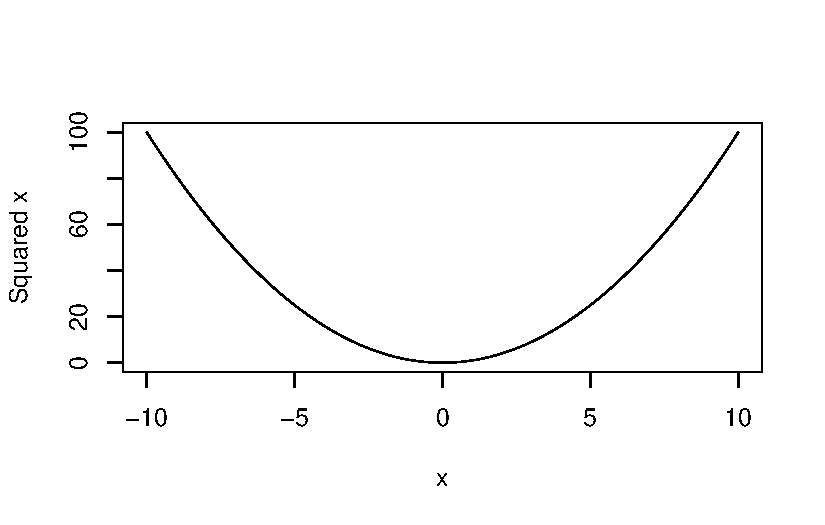
\includegraphics{wrangling1a_files/figure-pdf/curve-1.pdf}

}

\end{figure}

If some of the arguments are difficult to remember or what else could be
done with that function, we could use the \texttt{help} function. For
example, we can simply type \texttt{help(curve)} or \texttt{?curve} to
get help on the \texttt{curve} function:

\begin{tcolorbox}[enhanced jigsaw, coltitle=black, rightrule=.15mm, title=\textcolor{quarto-callout-tip-color}{\faLightbulb}\hspace{0.5em}{Tip}, bottomtitle=1mm, colbacktitle=quarto-callout-tip-color!10!white, left=2mm, titlerule=0mm, arc=.35mm, colframe=quarto-callout-tip-color-frame, colback=white, leftrule=.75mm, bottomrule=.15mm, opacitybacktitle=0.6, opacityback=0, toptitle=1mm, toprule=.15mm, breakable]

If you're uncertain about a function's precise name, two question marks
can assist in the search:

\end{tcolorbox}

\begin{Shaded}
\begin{Highlighting}[numbers=left,,]
\CommentTok{\# Searching for help if don\textquotesingle{}t know }
\CommentTok{\# the exact name of the function}
\NormalTok{??boxplot}
\end{Highlighting}
\end{Shaded}

\begin{enumerate}
\def\labelenumi{\arabic{enumi}.}
\setcounter{enumi}{6}
\tightlist
\item
  Creating Vectors
\end{enumerate}

Vectors are sequences of data elements of the same basic type. Here are
some methods to create them:

\begin{Shaded}
\begin{Highlighting}[numbers=left,,]
\CommentTok{\# Creating vectors in different ways}
\NormalTok{x3 }\OtherTok{\textless{}{-}} \FunctionTok{c}\NormalTok{(}\DecValTok{1}\NormalTok{, }\DecValTok{2}\NormalTok{, }\DecValTok{3}\NormalTok{, }\DecValTok{4}\NormalTok{, }\DecValTok{5}\NormalTok{)}
\FunctionTok{print}\NormalTok{(x3)}
\CommentTok{\#\textgreater{} [1] 1 2 3 4 5}

\NormalTok{x4 }\OtherTok{\textless{}{-}} \DecValTok{1}\SpecialCharTok{:}\DecValTok{7}
\FunctionTok{print}\NormalTok{(x4)}
\CommentTok{\#\textgreater{} [1] 1 2 3 4 5 6 7}

\NormalTok{x5 }\OtherTok{\textless{}{-}} \FunctionTok{seq}\NormalTok{(}\AttributeTok{from =} \DecValTok{0}\NormalTok{, }\AttributeTok{to =} \DecValTok{100}\NormalTok{, }\AttributeTok{by =} \DecValTok{10}\NormalTok{)}
\FunctionTok{print}\NormalTok{(x5)}
\CommentTok{\#\textgreater{}  [1]   0  10  20  30  40  50  60  70  80  90 100}

\NormalTok{x6 }\OtherTok{\textless{}{-}} \FunctionTok{seq}\NormalTok{(}\DecValTok{10}\NormalTok{, }\DecValTok{30}\NormalTok{, }\AttributeTok{length =} \DecValTok{7}\NormalTok{)}
\NormalTok{x6}
\CommentTok{\#\textgreater{} [1] 10.00000 13.33333 16.66667 20.00000 23.33333 26.66667 30.00000}
\end{Highlighting}
\end{Shaded}

\begin{enumerate}
\def\labelenumi{\arabic{enumi}.}
\setcounter{enumi}{7}
\tightlist
\item
  Plotting in R
\end{enumerate}

R provides numerous plotting capabilities. For instance, the plot
function can create scatter plots and line graphs:

\begin{Shaded}
\begin{Highlighting}[numbers=left,,]
\CommentTok{\# Scatter plot}
\FunctionTok{plot}\NormalTok{(x5, }\AttributeTok{type =} \StringTok{"p"}\NormalTok{, }\AttributeTok{main =} \StringTok{"Scatter plot"}\NormalTok{)}
\end{Highlighting}
\end{Shaded}

\begin{figure}[H]

{\centering 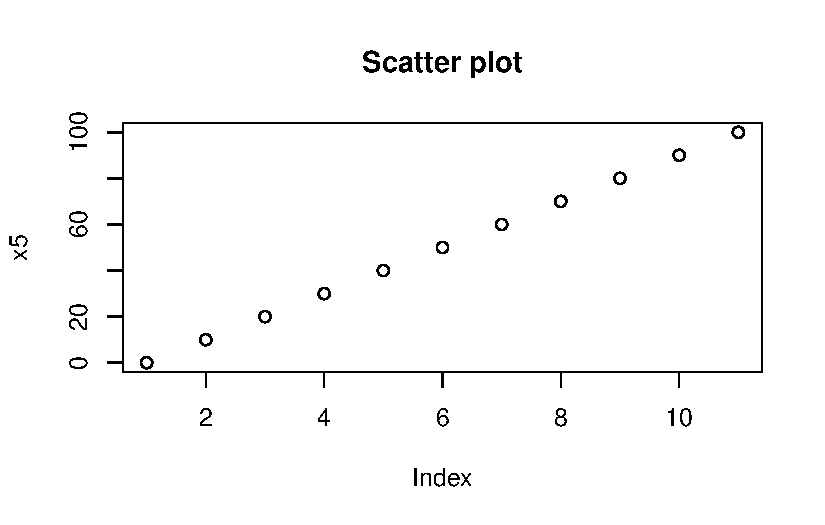
\includegraphics{wrangling1a_files/figure-pdf/plot2-1.pdf}

}

\end{figure}

\begin{Shaded}
\begin{Highlighting}[numbers=left,,]
\CommentTok{\# Line graph}
\FunctionTok{plot}\NormalTok{(}\AttributeTok{x =}\NormalTok{ x6, }\AttributeTok{y =}\NormalTok{ x6}\SpecialCharTok{\^{}}\DecValTok{2}\NormalTok{, }\AttributeTok{type =} \StringTok{"l"}\NormalTok{, }\AttributeTok{main =} \StringTok{"Line graph"}\NormalTok{)}
\end{Highlighting}
\end{Shaded}

\begin{figure}[H]

{\centering 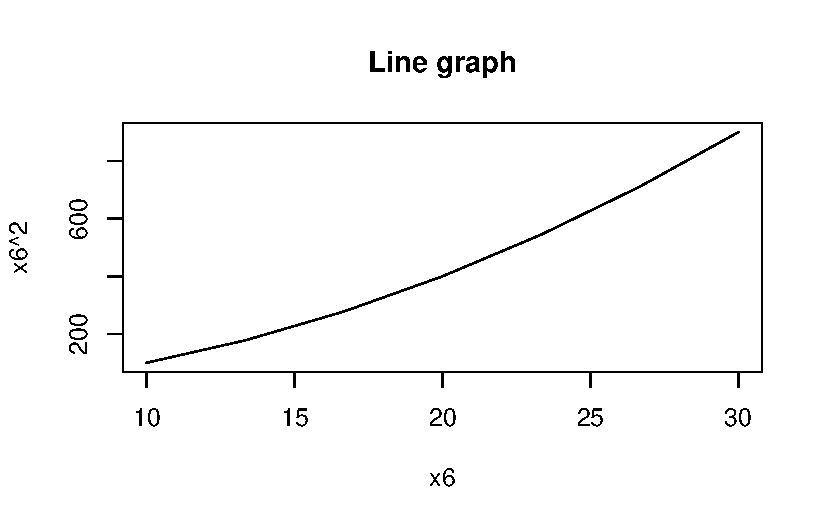
\includegraphics{wrangling1a_files/figure-pdf/plot3-1.pdf}

}

\end{figure}

\begin{enumerate}
\def\labelenumi{\arabic{enumi}.}
\setcounter{enumi}{8}
\tightlist
\item
  Character Vectors Apart from numeric values, R also allows for
  character vectors. For example, we can create a \texttt{sex} variable
  coded as females, males and other.
\end{enumerate}

\begin{Shaded}
\begin{Highlighting}[numbers=left,,]
\CommentTok{\# Character vector}
\NormalTok{sex }\OtherTok{\textless{}{-}} \FunctionTok{c}\NormalTok{(}\StringTok{"females"}\NormalTok{, }\StringTok{"males"}\NormalTok{, }\StringTok{"other"}\NormalTok{)}
\NormalTok{sex}
\CommentTok{\#\textgreater{} [1] "females" "males"   "other"}
\end{Highlighting}
\end{Shaded}

To determine a variable's type, use the mode function:

\begin{Shaded}
\begin{Highlighting}[numbers=left,,]
\CommentTok{\# Check data type}
\FunctionTok{mode}\NormalTok{(sex)}
\CommentTok{\#\textgreater{} [1] "character"}
\end{Highlighting}
\end{Shaded}

\hypertarget{package-management}{%
\subsection*{Package Management}\label{package-management}}
\addcontentsline{toc}{subsection}{Package Management}

Packages in R are collections of functions and datasets developed by the
community. They enhance the capability of R by adding new functions for
data analysis, visualization, data import, and more. Understanding how
to install and load packages is essential for effective R programming.

\begin{enumerate}
\def\labelenumi{\arabic{enumi}.}
\tightlist
\item
  Installing Packages from CRAN
\end{enumerate}

The CRAN is a major source of R packages. You can install them directly
from within R using the \texttt{install.packages()} function.

\begin{Shaded}
\begin{Highlighting}[numbers=left,,]
\CommentTok{\# Installing the \textquotesingle{}ggplot2\textquotesingle{} package}
\FunctionTok{install.packages}\NormalTok{(}\StringTok{"ggplot2"}\NormalTok{)}
\end{Highlighting}
\end{Shaded}

\begin{enumerate}
\def\labelenumi{\arabic{enumi}.}
\setcounter{enumi}{1}
\tightlist
\item
  Loading a Package
\end{enumerate}

After a package is installed, it must be loaded to use its functions.
This is done with the \texttt{library()} function.

\begin{Shaded}
\begin{Highlighting}[numbers=left,,]
\CommentTok{\# Loading the \textquotesingle{}ggplot2\textquotesingle{} package}
\FunctionTok{library}\NormalTok{(ggplot2)}
\end{Highlighting}
\end{Shaded}

You only need to install a package once, but you'll need to load it
every time you start a new R session and want to use its functions.

\begin{enumerate}
\def\labelenumi{\arabic{enumi}.}
\setcounter{enumi}{2}
\tightlist
\item
  Updating Packages
\end{enumerate}

R packages are frequently updated. To ensure you have the latest version
of a package, use the \texttt{update.packages()} function.

\begin{Shaded}
\begin{Highlighting}[numbers=left,,]
\CommentTok{\# Updating all installed packages}
\CommentTok{\# could be time consuming!}
\FunctionTok{update.packages}\NormalTok{(}\AttributeTok{ask =} \ConstantTok{FALSE}\NormalTok{)  }
\CommentTok{\# \textquotesingle{}ask = FALSE\textquotesingle{} updates all without asking for confirmation}
\end{Highlighting}
\end{Shaded}

\begin{enumerate}
\def\labelenumi{\arabic{enumi}.}
\setcounter{enumi}{3}
\tightlist
\item
  Listing Installed Packages
\end{enumerate}

You can view all the installed packages on your R setup using the
installed.packages() function.

\begin{Shaded}
\begin{Highlighting}[numbers=left,,]
\CommentTok{\# Listing installed packages}
\FunctionTok{installed.packages}\NormalTok{()[, }\StringTok{"Package"}\NormalTok{]}
\end{Highlighting}
\end{Shaded}

\begin{enumerate}
\def\labelenumi{\arabic{enumi}.}
\setcounter{enumi}{4}
\tightlist
\item
  Removing a Package
\end{enumerate}

If you no longer need a package, it can be removed using the
\texttt{remove.packages()} function.

\begin{Shaded}
\begin{Highlighting}[numbers=left,,]
\CommentTok{\# Removing the \textquotesingle{}ggplot2\textquotesingle{} package}
\FunctionTok{remove.packages}\NormalTok{(}\StringTok{"ggplot2"}\NormalTok{)}
\end{Highlighting}
\end{Shaded}

\begin{enumerate}
\def\labelenumi{\arabic{enumi}.}
\setcounter{enumi}{5}
\tightlist
\item
  Installing Packages from Other Sources
\end{enumerate}

While CRAN is the primary source, sometimes you might need to install
packages from GitHub or other repositories. The \texttt{devtools}
package provides a function for this.

\begin{Shaded}
\begin{Highlighting}[numbers=left,,]
\CommentTok{\# Installing devtools first}
\FunctionTok{install.packages}\NormalTok{(}\StringTok{"devtools"}\NormalTok{)}
\CommentTok{\# Loading devtools}
\FunctionTok{library}\NormalTok{(devtools)}
\CommentTok{\# Install a package from GitHub}
\CommentTok{\# https://github.com/ehsanx/simMSM}
\FunctionTok{install\_github}\NormalTok{(}\StringTok{"ehsanx/simMSM"}\NormalTok{)}
\end{Highlighting}
\end{Shaded}

When you are working on a project, it's a good practice to list and
install required packages at the beginning of your R script.

\hypertarget{video-content-optional}{%
\subsection*{Video content (optional)}\label{video-content-optional}}
\addcontentsline{toc}{subsection}{Video content (optional)}

\begin{tcolorbox}[enhanced jigsaw, coltitle=black, rightrule=.15mm, title=\textcolor{quarto-callout-tip-color}{\faLightbulb}\hspace{0.5em}{Tip}, bottomtitle=1mm, colbacktitle=quarto-callout-tip-color!10!white, left=2mm, titlerule=0mm, arc=.35mm, colframe=quarto-callout-tip-color-frame, colback=white, leftrule=.75mm, bottomrule=.15mm, opacitybacktitle=0.6, opacityback=0, toptitle=1mm, toprule=.15mm, breakable]

For those who prefer a video walkthrough, feel free to watch the video
below, which offers a description of an earlier version of the above
content.

\end{tcolorbox}

\hypertarget{data-types}{%
\chapter*{Data types}\label{data-types}}
\addcontentsline{toc}{chapter}{Data types}

\markboth{Data types}{Data types}

\hypertarget{matrix}{%
\subsection*{Matrix}\label{matrix}}
\addcontentsline{toc}{subsection}{Matrix}

\begin{tcolorbox}[enhanced jigsaw, coltitle=black, rightrule=.15mm, title=\textcolor{quarto-callout-tip-color}{\faLightbulb}\hspace{0.5em}{Tip}, bottomtitle=1mm, colbacktitle=quarto-callout-tip-color!10!white, left=2mm, titlerule=0mm, arc=.35mm, colframe=quarto-callout-tip-color-frame, colback=white, leftrule=.75mm, bottomrule=.15mm, opacitybacktitle=0.6, opacityback=0, toptitle=1mm, toprule=.15mm, breakable]

In R, matrices are two-dimensional rectangular data sets, which can be
created using the \texttt{matrix()} function. It's essential to remember
that all the elements of a matrix must be of the same type, such as all
numeric or all character.

\end{tcolorbox}

To construct a matrix, we often start with a vector and specify how we
want to reshape it. For instance:

\begin{Shaded}
\begin{Highlighting}[numbers=left,,]
\CommentTok{\# Matrix 1}
\NormalTok{x }\OtherTok{\textless{}{-}} \DecValTok{1}\SpecialCharTok{:}\DecValTok{10}
\NormalTok{matrix1 }\OtherTok{\textless{}{-}} \FunctionTok{matrix}\NormalTok{(x, }\AttributeTok{nrow =} \DecValTok{5}\NormalTok{, }\AttributeTok{ncol =} \DecValTok{2}\NormalTok{, }\AttributeTok{byrow =} \ConstantTok{TRUE}\NormalTok{)}
\NormalTok{matrix1}
\CommentTok{\#\textgreater{}      [,1] [,2]}
\CommentTok{\#\textgreater{} [1,]    1    2}
\CommentTok{\#\textgreater{} [2,]    3    4}
\CommentTok{\#\textgreater{} [3,]    5    6}
\CommentTok{\#\textgreater{} [4,]    7    8}
\CommentTok{\#\textgreater{} [5,]    9   10}
\end{Highlighting}
\end{Shaded}

Here, the vector x contains numbers from 1 to 10. We reshape it into a
matrix with 5 rows and 2 columns. The \texttt{byrow\ =\ TRUE} argument
means the matrix will be filled row-wise, with numbers from the vector.

Conversely, if you want the matrix to be filled column-wise, you'd set
\texttt{byrow\ =\ FALSE}:

\begin{Shaded}
\begin{Highlighting}[numbers=left,,]
\CommentTok{\# matrix 2}
\NormalTok{matrix2 }\OtherTok{\textless{}{-}} \FunctionTok{matrix}\NormalTok{(x, }\AttributeTok{nrow =} \DecValTok{5}\NormalTok{, }\AttributeTok{ncol =} \DecValTok{2}\NormalTok{, }\AttributeTok{byrow =} \ConstantTok{FALSE}\NormalTok{)}
\NormalTok{matrix2}
\CommentTok{\#\textgreater{}      [,1] [,2]}
\CommentTok{\#\textgreater{} [1,]    1    6}
\CommentTok{\#\textgreater{} [2,]    2    7}
\CommentTok{\#\textgreater{} [3,]    3    8}
\CommentTok{\#\textgreater{} [4,]    4    9}
\CommentTok{\#\textgreater{} [5,]    5   10}
\end{Highlighting}
\end{Shaded}

You can also combine or concatenate matrices. \texttt{cbind()} joins
matrices by columns while \texttt{rbind()} joins them by rows.

\begin{Shaded}
\begin{Highlighting}[numbers=left,,]
\CommentTok{\# Merging 2 matrices}
\FunctionTok{cbind}\NormalTok{(matrix1, matrix2)}
\CommentTok{\#\textgreater{}      [,1] [,2] [,3] [,4]}
\CommentTok{\#\textgreater{} [1,]    1    2    1    6}
\CommentTok{\#\textgreater{} [2,]    3    4    2    7}
\CommentTok{\#\textgreater{} [3,]    5    6    3    8}
\CommentTok{\#\textgreater{} [4,]    7    8    4    9}
\CommentTok{\#\textgreater{} [5,]    9   10    5   10}
\end{Highlighting}
\end{Shaded}

\begin{Shaded}
\begin{Highlighting}[numbers=left,,]
\CommentTok{\# Appending 2 matrices}
\FunctionTok{rbind}\NormalTok{(matrix1, matrix2)}
\CommentTok{\#\textgreater{}       [,1] [,2]}
\CommentTok{\#\textgreater{}  [1,]    1    2}
\CommentTok{\#\textgreater{}  [2,]    3    4}
\CommentTok{\#\textgreater{}  [3,]    5    6}
\CommentTok{\#\textgreater{}  [4,]    7    8}
\CommentTok{\#\textgreater{}  [5,]    9   10}
\CommentTok{\#\textgreater{}  [6,]    1    6}
\CommentTok{\#\textgreater{}  [7,]    2    7}
\CommentTok{\#\textgreater{}  [8,]    3    8}
\CommentTok{\#\textgreater{}  [9,]    4    9}
\CommentTok{\#\textgreater{} [10,]    5   10}
\end{Highlighting}
\end{Shaded}

\hypertarget{list}{%
\subsection*{List}\label{list}}
\addcontentsline{toc}{subsection}{List}

\begin{tcolorbox}[enhanced jigsaw, coltitle=black, rightrule=.15mm, title=\textcolor{quarto-callout-tip-color}{\faLightbulb}\hspace{0.5em}{Tip}, bottomtitle=1mm, colbacktitle=quarto-callout-tip-color!10!white, left=2mm, titlerule=0mm, arc=.35mm, colframe=quarto-callout-tip-color-frame, colback=white, leftrule=.75mm, bottomrule=.15mm, opacitybacktitle=0.6, opacityback=0, toptitle=1mm, toprule=.15mm, breakable]

In R, lists can be seen as a collection where you can store a variety of
different objects under a single name. This includes vectors, matrices,
or even other lists. It's very versatile because its components can be
of any type of R object.

\end{tcolorbox}

For instance:

\begin{Shaded}
\begin{Highlighting}[numbers=left,,]
\CommentTok{\# List of 2 matrices}
\NormalTok{list1 }\OtherTok{\textless{}{-}} \FunctionTok{list}\NormalTok{(matrix1, matrix2)}
\NormalTok{list1}
\CommentTok{\#\textgreater{} [[1]]}
\CommentTok{\#\textgreater{}      [,1] [,2]}
\CommentTok{\#\textgreater{} [1,]    1    2}
\CommentTok{\#\textgreater{} [2,]    3    4}
\CommentTok{\#\textgreater{} [3,]    5    6}
\CommentTok{\#\textgreater{} [4,]    7    8}
\CommentTok{\#\textgreater{} [5,]    9   10}
\CommentTok{\#\textgreater{} }
\CommentTok{\#\textgreater{} [[2]]}
\CommentTok{\#\textgreater{}      [,1] [,2]}
\CommentTok{\#\textgreater{} [1,]    1    6}
\CommentTok{\#\textgreater{} [2,]    2    7}
\CommentTok{\#\textgreater{} [3,]    3    8}
\CommentTok{\#\textgreater{} [4,]    4    9}
\CommentTok{\#\textgreater{} [5,]    5   10}
\end{Highlighting}
\end{Shaded}

Lists can also be expanded to include multiple items:

\begin{Shaded}
\begin{Highlighting}[numbers=left,,]
\NormalTok{x6 }\OtherTok{\textless{}{-}} \FunctionTok{seq}\NormalTok{(}\DecValTok{10}\NormalTok{, }\DecValTok{30}\NormalTok{, }\AttributeTok{length =} \DecValTok{7}\NormalTok{)}
\NormalTok{sex }\OtherTok{\textless{}{-}} \FunctionTok{c}\NormalTok{(}\StringTok{"females"}\NormalTok{, }\StringTok{"males"}\NormalTok{, }\StringTok{"other"}\NormalTok{)}
\CommentTok{\# Expanding list to include more items}
\NormalTok{list2 }\OtherTok{\textless{}{-}} \FunctionTok{list}\NormalTok{(list1, x6, sex, matrix1)}
\NormalTok{list2 }
\CommentTok{\#\textgreater{} [[1]]}
\CommentTok{\#\textgreater{} [[1]][[1]]}
\CommentTok{\#\textgreater{}      [,1] [,2]}
\CommentTok{\#\textgreater{} [1,]    1    2}
\CommentTok{\#\textgreater{} [2,]    3    4}
\CommentTok{\#\textgreater{} [3,]    5    6}
\CommentTok{\#\textgreater{} [4,]    7    8}
\CommentTok{\#\textgreater{} [5,]    9   10}
\CommentTok{\#\textgreater{} }
\CommentTok{\#\textgreater{} [[1]][[2]]}
\CommentTok{\#\textgreater{}      [,1] [,2]}
\CommentTok{\#\textgreater{} [1,]    1    6}
\CommentTok{\#\textgreater{} [2,]    2    7}
\CommentTok{\#\textgreater{} [3,]    3    8}
\CommentTok{\#\textgreater{} [4,]    4    9}
\CommentTok{\#\textgreater{} [5,]    5   10}
\CommentTok{\#\textgreater{} }
\CommentTok{\#\textgreater{} }
\CommentTok{\#\textgreater{} [[2]]}
\CommentTok{\#\textgreater{} [1] 10.00000 13.33333 16.66667 20.00000 23.33333 26.66667 30.00000}
\CommentTok{\#\textgreater{} }
\CommentTok{\#\textgreater{} [[3]]}
\CommentTok{\#\textgreater{} [1] "females" "males"   "other"  }
\CommentTok{\#\textgreater{} }
\CommentTok{\#\textgreater{} [[4]]}
\CommentTok{\#\textgreater{}      [,1] [,2]}
\CommentTok{\#\textgreater{} [1,]    1    2}
\CommentTok{\#\textgreater{} [2,]    3    4}
\CommentTok{\#\textgreater{} [3,]    5    6}
\CommentTok{\#\textgreater{} [4,]    7    8}
\CommentTok{\#\textgreater{} [5,]    9   10}
\end{Highlighting}
\end{Shaded}

Combining different types of data into a single matrix converts
everything to a character type:

\begin{Shaded}
\begin{Highlighting}[numbers=left,,]
\CommentTok{\# A matrix with numeric and character variables}
\NormalTok{id }\OtherTok{\textless{}{-}} \FunctionTok{c}\NormalTok{(}\DecValTok{1}\NormalTok{, }\DecValTok{2}\NormalTok{)}
\NormalTok{score }\OtherTok{\textless{}{-}} \FunctionTok{c}\NormalTok{(}\DecValTok{85}\NormalTok{, }\DecValTok{85}\NormalTok{)}
\NormalTok{sex }\OtherTok{\textless{}{-}} \FunctionTok{c}\NormalTok{(}\StringTok{"M"}\NormalTok{, }\StringTok{"F"}\NormalTok{)}
\NormalTok{new.matrix }\OtherTok{\textless{}{-}} \FunctionTok{cbind}\NormalTok{(id, score, sex)}
\NormalTok{new.matrix}
\CommentTok{\#\textgreater{}      id  score sex}
\CommentTok{\#\textgreater{} [1,] "1" "85"  "M"}
\CommentTok{\#\textgreater{} [2,] "2" "85"  "F"}
\end{Highlighting}
\end{Shaded}

To check the type of data in your matrix:

\begin{Shaded}
\begin{Highlighting}[numbers=left,,]
\FunctionTok{mode}\NormalTok{(new.matrix)}
\CommentTok{\#\textgreater{} [1] "character"}
\end{Highlighting}
\end{Shaded}

\hypertarget{data-frame}{%
\subsection*{Data frame}\label{data-frame}}
\addcontentsline{toc}{subsection}{Data frame}

\begin{tcolorbox}[enhanced jigsaw, coltitle=black, rightrule=.15mm, title=\textcolor{quarto-callout-tip-color}{\faLightbulb}\hspace{0.5em}{Tip}, bottomtitle=1mm, colbacktitle=quarto-callout-tip-color!10!white, left=2mm, titlerule=0mm, arc=.35mm, colframe=quarto-callout-tip-color-frame, colback=white, leftrule=.75mm, bottomrule=.15mm, opacitybacktitle=0.6, opacityback=0, toptitle=1mm, toprule=.15mm, breakable]

As we can see combining both numeric and character variables into a
matrix ended up with a matrix of character values. To keep the numeric
variables as numeric and character variables as character, we can use
the \texttt{data.frame} function.

\end{tcolorbox}

\begin{enumerate}
\def\labelenumi{\arabic{enumi}.}
\tightlist
\item
  Creating a data frame
\end{enumerate}

\marginnote{\begin{footnotesize}

A data frame is similar to a matrix but allows for columns of different
types (numeric, character, factor, etc.). It's a standard format for
storing data sets in R.

\end{footnotesize}}

\begin{Shaded}
\begin{Highlighting}[numbers=left,,]
\NormalTok{df }\OtherTok{\textless{}{-}} \FunctionTok{data.frame}\NormalTok{(id, score, sex)}
\NormalTok{df}
\CommentTok{\#\textgreater{}   id score sex}
\CommentTok{\#\textgreater{} 1  1    85   M}
\CommentTok{\#\textgreater{} 2  2    85   F}
\end{Highlighting}
\end{Shaded}

To check the mode or type of your data frame:

\begin{Shaded}
\begin{Highlighting}[numbers=left,,]
\FunctionTok{mode}\NormalTok{(df)}
\CommentTok{\#\textgreater{} [1] "list"}
\end{Highlighting}
\end{Shaded}

\begin{enumerate}
\def\labelenumi{\arabic{enumi}.}
\setcounter{enumi}{1}
\tightlist
\item
  Extract elements
\end{enumerate}

Data frames allow easy extraction and modification of specific elements.
For example, we can extract the values on the first row and first column
as follow:

\begin{Shaded}
\begin{Highlighting}[numbers=left,,]
\NormalTok{df[}\DecValTok{1}\NormalTok{,}\DecValTok{1}\NormalTok{]}
\CommentTok{\#\textgreater{} [1] 1}
\end{Highlighting}
\end{Shaded}

Similarly, the first column can be extracted as follows:

\begin{Shaded}
\begin{Highlighting}[numbers=left,,]
\NormalTok{df[,}\DecValTok{1}\NormalTok{]}
\CommentTok{\#\textgreater{} [1] 1 2}
\end{Highlighting}
\end{Shaded}

The first row can be extracted as follows:

\begin{Shaded}
\begin{Highlighting}[numbers=left,,]
\NormalTok{df[}\DecValTok{1}\NormalTok{,]}
\CommentTok{\#\textgreater{}   id score sex}
\CommentTok{\#\textgreater{} 1  1    85   M}
\end{Highlighting}
\end{Shaded}

\begin{enumerate}
\def\labelenumi{\arabic{enumi}.}
\setcounter{enumi}{2}
\tightlist
\item
  Modifying values
\end{enumerate}

We can edit the values in the data frame as well. For example, we can
change the score from 85 to 90 for the id 1:

\begin{Shaded}
\begin{Highlighting}[numbers=left,,]
\NormalTok{df}\SpecialCharTok{$}\NormalTok{score[df}\SpecialCharTok{$}\NormalTok{id }\SpecialCharTok{==} \DecValTok{1}\NormalTok{] }\OtherTok{\textless{}{-}} \DecValTok{90}
\NormalTok{df}
\CommentTok{\#\textgreater{}   id score sex}
\CommentTok{\#\textgreater{} 1  1    90   M}
\CommentTok{\#\textgreater{} 2  2    85   F}
\end{Highlighting}
\end{Shaded}

We can also change the name of the variables/columns:

\begin{Shaded}
\begin{Highlighting}[numbers=left,,]
\FunctionTok{colnames}\NormalTok{(df) }\OtherTok{\textless{}{-}} \FunctionTok{c}\NormalTok{(}\StringTok{"Studyid"}\NormalTok{, }\StringTok{"Grade"}\NormalTok{, }\StringTok{"Sex"}\NormalTok{)}
\NormalTok{df}
\CommentTok{\#\textgreater{}   Studyid Grade Sex}
\CommentTok{\#\textgreater{} 1       1    90   M}
\CommentTok{\#\textgreater{} 2       2    85   F}
\end{Highlighting}
\end{Shaded}

\begin{enumerate}
\def\labelenumi{\arabic{enumi}.}
\setcounter{enumi}{3}
\tightlist
\item
  Combining data frames
\end{enumerate}

We can also merge another data frame with the same variables using the
\texttt{rbind} function:

\begin{Shaded}
\begin{Highlighting}[numbers=left,,]
\CommentTok{\# Create a new dataset}
\NormalTok{df2 }\OtherTok{\textless{}{-}} \FunctionTok{data.frame}\NormalTok{(}\AttributeTok{Studyid =} \FunctionTok{c}\NormalTok{(}\DecValTok{10}\NormalTok{, }\DecValTok{15}\NormalTok{, }\DecValTok{50}\NormalTok{), }\AttributeTok{Grade =} \FunctionTok{c}\NormalTok{(}\DecValTok{75}\NormalTok{, }\DecValTok{90}\NormalTok{, }\DecValTok{65}\NormalTok{), }\AttributeTok{Sex =} \FunctionTok{c}\NormalTok{(}\StringTok{"F"}\NormalTok{, }\StringTok{"M"}\NormalTok{, }\StringTok{"M"}\NormalTok{))}

\CommentTok{\# Combining two data frames}
\NormalTok{df.new }\OtherTok{\textless{}{-}} \FunctionTok{rbind}\NormalTok{(df, df2)}

\CommentTok{\# Print the first 6 rows}
\FunctionTok{head}\NormalTok{(df.new)}
\CommentTok{\#\textgreater{}   Studyid Grade Sex}
\CommentTok{\#\textgreater{} 1       1    90   M}
\CommentTok{\#\textgreater{} 2       2    85   F}
\CommentTok{\#\textgreater{} 3      10    75   F}
\CommentTok{\#\textgreater{} 4      15    90   M}
\CommentTok{\#\textgreater{} 5      50    65   M}
\end{Highlighting}
\end{Shaded}

\begin{enumerate}
\def\labelenumi{\arabic{enumi}.}
\setcounter{enumi}{4}
\tightlist
\item
  Checking the dimensions
\end{enumerate}

To see the dimension of the data frame (i.e., number of rows and
columns), we can use the \texttt{dim} function:

\begin{Shaded}
\begin{Highlighting}[numbers=left,,]
\FunctionTok{dim}\NormalTok{(df.new)}
\CommentTok{\#\textgreater{} [1] 5 3}
\end{Highlighting}
\end{Shaded}

As we can see, we have 5 rows and 3 columns. We can use the
\texttt{nrow} and \texttt{ncol} functions respectively for the same
output:

\begin{Shaded}
\begin{Highlighting}[numbers=left,,]
\FunctionTok{nrow}\NormalTok{(df.new)}
\CommentTok{\#\textgreater{} [1] 5}
\FunctionTok{ncol}\NormalTok{(df.new)}
\CommentTok{\#\textgreater{} [1] 3}
\end{Highlighting}
\end{Shaded}

\hypertarget{automating-tasks-1}{%
\chapter*{Automating tasks}\label{automating-tasks-1}}
\addcontentsline{toc}{chapter}{Automating tasks}

\markboth{Automating tasks}{Automating tasks}

\hypertarget{repeating-a-task}{%
\subsection*{Repeating a task}\label{repeating-a-task}}
\addcontentsline{toc}{subsection}{Repeating a task}

\begin{tcolorbox}[enhanced jigsaw, coltitle=black, rightrule=.15mm, title=\textcolor{quarto-callout-tip-color}{\faLightbulb}\hspace{0.5em}{Tip}, bottomtitle=1mm, colbacktitle=quarto-callout-tip-color!10!white, left=2mm, titlerule=0mm, arc=.35mm, colframe=quarto-callout-tip-color-frame, colback=white, leftrule=.75mm, bottomrule=.15mm, opacitybacktitle=0.6, opacityback=0, toptitle=1mm, toprule=.15mm, breakable]

The \texttt{for} loop is a control flow statement in R that lets you
repeat a particular task multiple times. This repetition is based on a
sequence of numbers or values in a vector.

\end{tcolorbox}

Consider a simple real-life analogy: Imagine you are filling water in 10
bottles, one by one. Instead of doing it manually 10 times, you can set
a machine to do it in a loop until all 10 bottles are filled.

\begin{enumerate}
\def\labelenumi{\arabic{enumi}.}
\tightlist
\item
  Example 1
\end{enumerate}

\begin{Shaded}
\begin{Highlighting}[numbers=left,,]
\CommentTok{\# Looping and adding}
\NormalTok{k }\OtherTok{\textless{}{-}} \DecValTok{0}
\ControlFlowTok{for}\NormalTok{ (i }\ControlFlowTok{in} \DecValTok{1}\SpecialCharTok{:}\DecValTok{10}\NormalTok{)\{}
\NormalTok{  k }\OtherTok{\textless{}{-}}\NormalTok{ k }\SpecialCharTok{+} \DecValTok{5}
  \FunctionTok{print}\NormalTok{(k)}
\NormalTok{\}}
\CommentTok{\#\textgreater{} [1] 5}
\CommentTok{\#\textgreater{} [1] 10}
\CommentTok{\#\textgreater{} [1] 15}
\CommentTok{\#\textgreater{} [1] 20}
\CommentTok{\#\textgreater{} [1] 25}
\CommentTok{\#\textgreater{} [1] 30}
\CommentTok{\#\textgreater{} [1] 35}
\CommentTok{\#\textgreater{} [1] 40}
\CommentTok{\#\textgreater{} [1] 45}
\CommentTok{\#\textgreater{} [1] 50}
\end{Highlighting}
\end{Shaded}

Here, you're initiating a counter k at 0. With each iteration of the
loop (i.e., every time it ``runs''), 5 is added to k. After 10 cycles,
the loop will stop, but not before printing k in each cycle.

\begin{enumerate}
\def\labelenumi{\arabic{enumi}.}
\setcounter{enumi}{1}
\tightlist
\item
  Example 2
\end{enumerate}

We create a variable \texttt{x5} containing the values of 0, 10, 20, 30,
40, 50, 60, 70, 80, 90, and 100. Let us print the first 5 values using
the \texttt{for} loop function:

\begin{Shaded}
\begin{Highlighting}[numbers=left,,]
\NormalTok{x5 }\OtherTok{\textless{}{-}} \FunctionTok{seq}\NormalTok{(}\AttributeTok{from =} \DecValTok{0}\NormalTok{, }\AttributeTok{to =} \DecValTok{100}\NormalTok{, }\AttributeTok{by =} \DecValTok{10}\NormalTok{)}
\CommentTok{\# Looping through a vector}
\NormalTok{k }\OtherTok{\textless{}{-}} \DecValTok{1}\SpecialCharTok{:}\DecValTok{5}
\ControlFlowTok{for}\NormalTok{ (ii }\ControlFlowTok{in}\NormalTok{ k)\{}
  \FunctionTok{print}\NormalTok{(x5[ii])}
\NormalTok{\}}
\CommentTok{\#\textgreater{} [1] 0}
\CommentTok{\#\textgreater{} [1] 10}
\CommentTok{\#\textgreater{} [1] 20}
\CommentTok{\#\textgreater{} [1] 30}
\CommentTok{\#\textgreater{} [1] 40}
\end{Highlighting}
\end{Shaded}

This loop cycles through the first five values of a previously created
variable \texttt{x5} and prints them. Each value printed corresponds to
the positions 1 to 5 in \texttt{x5}.

\begin{enumerate}
\def\labelenumi{\arabic{enumi}.}
\setcounter{enumi}{2}
\tightlist
\item
  Example 3
\end{enumerate}

Let us use the \texttt{for} loop in a more complicated scenario. First,
we create a vector of numeric values and square it:

\begin{Shaded}
\begin{Highlighting}[numbers=left,,]
\CommentTok{\# Create a vector}
\NormalTok{k }\OtherTok{\textless{}{-}} \FunctionTok{c}\NormalTok{(}\DecValTok{1}\NormalTok{, }\DecValTok{3}\NormalTok{, }\DecValTok{6}\NormalTok{, }\DecValTok{2}\NormalTok{, }\DecValTok{0}\NormalTok{)}
\NormalTok{k}\SpecialCharTok{\^{}}\DecValTok{2}
\CommentTok{\#\textgreater{} [1]  1  9 36  4  0}
\end{Highlighting}
\end{Shaded}

This is just squaring each value in the vector \texttt{k}.

\begin{enumerate}
\def\labelenumi{\arabic{enumi}.}
\setcounter{enumi}{3}
\tightlist
\item
  Example 4
\end{enumerate}

We create the same vector of square values using the \texttt{for} loop
function. To do so, (i) we create a null object, (ii) use the loop for
each of the elements in the vector (k), (iii) square each of the
elements, and (iv) store each of the elements of the new vector. In the
example below, the length of k is 5, and the loop will run from the
first to the fifth element of k. Also, k.sq{[}1{]} is the first stored
value for squared-k, and k.sq{[}2{]} is the second stored value for
squared-k, and so on.

\begin{Shaded}
\begin{Highlighting}[numbers=left,,]
\CommentTok{\# Looping through a vector with function}
\NormalTok{k.sq }\OtherTok{\textless{}{-}} \ConstantTok{NULL}
\ControlFlowTok{for}\NormalTok{ (i }\ControlFlowTok{in} \DecValTok{1}\SpecialCharTok{:}\FunctionTok{length}\NormalTok{(k))\{}
\NormalTok{  k.sq[i] }\OtherTok{\textless{}{-}}\NormalTok{ k[i]}\SpecialCharTok{\^{}}\DecValTok{2}
\NormalTok{\}}

\CommentTok{\# Print the values}
\NormalTok{k.sq}
\CommentTok{\#\textgreater{} [1]  1  9 36  4  0}
\end{Highlighting}
\end{Shaded}

Here, we achieve the same result as the third example but use a for
loop. We prepare an empty object \texttt{k.sq} and then use the loop to
square each value in \texttt{k}, storing the result in \texttt{k.sq}.

\begin{enumerate}
\def\labelenumi{\arabic{enumi}.}
\setcounter{enumi}{4}
\tightlist
\item
  Example 5
\end{enumerate}

\begin{Shaded}
\begin{Highlighting}[numbers=left,,]
\NormalTok{df.new }\OtherTok{\textless{}{-}} \FunctionTok{data.frame}\NormalTok{(}
  \AttributeTok{Studyid =} \FunctionTok{c}\NormalTok{(}\DecValTok{1}\NormalTok{, }\DecValTok{2}\NormalTok{, }\DecValTok{10}\NormalTok{, }\DecValTok{15}\NormalTok{, }\DecValTok{50}\NormalTok{),}
  \AttributeTok{Grade =} \FunctionTok{c}\NormalTok{(}\DecValTok{90}\NormalTok{, }\DecValTok{85}\NormalTok{, }\DecValTok{75}\NormalTok{, }\DecValTok{90}\NormalTok{, }\DecValTok{65}\NormalTok{),}
  \AttributeTok{Sex =} \FunctionTok{c}\NormalTok{(}\StringTok{\textquotesingle{}M\textquotesingle{}}\NormalTok{, }\StringTok{\textquotesingle{}F\textquotesingle{}}\NormalTok{, }\StringTok{\textquotesingle{}F\textquotesingle{}}\NormalTok{, }\StringTok{\textquotesingle{}M\textquotesingle{}}\NormalTok{, }\StringTok{\textquotesingle{}M\textquotesingle{}}\NormalTok{)}
\NormalTok{)}
\CommentTok{\# Looping through a data frame}
\ControlFlowTok{for}\NormalTok{ (i }\ControlFlowTok{in} \DecValTok{1}\SpecialCharTok{:}\FunctionTok{nrow}\NormalTok{(df.new))\{}
  \FunctionTok{print}\NormalTok{(df.new[i,}\StringTok{"Sex"}\NormalTok{])}
\NormalTok{\}}
\CommentTok{\#\textgreater{} [1] "M"}
\CommentTok{\#\textgreater{} [1] "F"}
\CommentTok{\#\textgreater{} [1] "F"}
\CommentTok{\#\textgreater{} [1] "M"}
\CommentTok{\#\textgreater{} [1] "M"}
\end{Highlighting}
\end{Shaded}

This loop prints the ``Sex'' column value for each row in the df.new
data frame.

\hypertarget{functions}{%
\subsection*{Functions}\label{functions}}
\addcontentsline{toc}{subsection}{Functions}

\begin{tcolorbox}[enhanced jigsaw, coltitle=black, rightrule=.15mm, title=\textcolor{quarto-callout-tip-color}{\faLightbulb}\hspace{0.5em}{Tip}, bottomtitle=1mm, colbacktitle=quarto-callout-tip-color!10!white, left=2mm, titlerule=0mm, arc=.35mm, colframe=quarto-callout-tip-color-frame, colback=white, leftrule=.75mm, bottomrule=.15mm, opacitybacktitle=0.6, opacityback=0, toptitle=1mm, toprule=.15mm, breakable]

A function in R is a piece of code that can take inputs, process them,
and return an output. There are functions built into R, like
\texttt{mean()}, which calculates the average of a set of numbers.

\end{tcolorbox}

\begin{enumerate}
\def\labelenumi{\arabic{enumi}.}
\tightlist
\item
  Built-in function
\end{enumerate}

\begin{Shaded}
\begin{Highlighting}[numbers=left,,]
\CommentTok{\# Calculating a mean from a vector}
\NormalTok{Vector }\OtherTok{\textless{}{-}} \DecValTok{1}\SpecialCharTok{:}\DecValTok{100}
\FunctionTok{mean}\NormalTok{(Vector)}
\CommentTok{\#\textgreater{} [1] 50.5}
\end{Highlighting}
\end{Shaded}

Here, we're using the built-in \texttt{mean()} function to find the
average of numbers from 1 to 100.

\begin{enumerate}
\def\labelenumi{\arabic{enumi}.}
\setcounter{enumi}{1}
\tightlist
\item
  Custom-made function
\end{enumerate}

To understand how functions work, sometimes it's helpful to build our
own. Now we will create our own function to calculate the mean, where we
will use the following equation to calculate it:

\(\text{Mean} = \frac{\sum_{i=1}^{n} x_i}{n},\)

where \(x_1\), \(x_2\),\ldots, \(x_n\) are the values in the vector and
\(n\) is the sample size. Let us create the function for calculation the
mean:

This function, \texttt{mean.own}, calculates the average. We add up all
the numbers in a vector (\texttt{Sum\ \textless{}-\ sum(x)}) and divide
by the number of items in that vector
(\texttt{n\ \textless{}-\ length(x)}). The result is then returned.

\begin{Shaded}
\begin{Highlighting}[numbers=left,,]
\NormalTok{mean.own }\OtherTok{\textless{}{-}} \ControlFlowTok{function}\NormalTok{(x)\{}
\NormalTok{  Sum }\OtherTok{\textless{}{-}} \FunctionTok{sum}\NormalTok{(x)}
\NormalTok{  n }\OtherTok{\textless{}{-}} \FunctionTok{length}\NormalTok{(x)}
  \FunctionTok{return}\NormalTok{(Sum}\SpecialCharTok{/}\NormalTok{n)}
\NormalTok{\}}
\end{Highlighting}
\end{Shaded}

By using our custom-made function, we calculate the mean of numbers from
1 to 100, getting the same result as the built-in \texttt{mean()}
function.

\begin{Shaded}
\begin{Highlighting}[numbers=left,,]
\FunctionTok{mean.own}\NormalTok{(Vector)}
\CommentTok{\#\textgreater{} [1] 50.5}
\end{Highlighting}
\end{Shaded}

\hypertarget{video-content-optional-1}{%
\subsection*{Video content (optional)}\label{video-content-optional-1}}
\addcontentsline{toc}{subsection}{Video content (optional)}

\begin{tcolorbox}[enhanced jigsaw, coltitle=black, rightrule=.15mm, title=\textcolor{quarto-callout-tip-color}{\faLightbulb}\hspace{0.5em}{Tip}, bottomtitle=1mm, colbacktitle=quarto-callout-tip-color!10!white, left=2mm, titlerule=0mm, arc=.35mm, colframe=quarto-callout-tip-color-frame, colback=white, leftrule=.75mm, bottomrule=.15mm, opacitybacktitle=0.6, opacityback=0, toptitle=1mm, toprule=.15mm, breakable]

For those who prefer a video walkthrough, feel free to watch the video
below, which offers a description of an earlier version of the above
content.

\end{tcolorbox}

\hypertarget{importing-dataset-1}{%
\chapter*{Importing dataset}\label{importing-dataset-1}}
\addcontentsline{toc}{chapter}{Importing dataset}

\markboth{Importing dataset}{Importing dataset}

\hypertarget{introduction-to-data-importing}{%
\subsection*{Introduction to Data
Importing}\label{introduction-to-data-importing}}
\addcontentsline{toc}{subsection}{Introduction to Data Importing}

Before analyzing data in R, one of the first steps you'll typically
undertake is importing your dataset. R provides numerous methods to do
this, depending on the format of your dataset.

Datasets come in a variety of file formats, with .csv (Comma-Separated
Values) and .txt (Text file) being among the most common. While R's
interface offers manual ways to load these datasets, knowing how to code
this step ensures better reproducibility and automation.

\hypertarget{importing-.txt-files}{%
\subsection*{Importing .txt files}\label{importing-.txt-files}}
\addcontentsline{toc}{subsection}{Importing .txt files}

A .txt data file can be imported using the \texttt{read.table} function.
As an example, consider you have a dataset named grade in the specified
path.

Let's briefly glance at the file without concerning ourselves with its
formatting.

\begin{Shaded}
\begin{Highlighting}[numbers=left,,]
\CommentTok{\# Read and print the content of the TXT file}
\NormalTok{content }\OtherTok{\textless{}{-}} \FunctionTok{readLines}\NormalTok{(}\StringTok{"Data/wrangling/grade.txt"}\NormalTok{)}
\FunctionTok{cat}\NormalTok{(content, }\AttributeTok{sep =} \StringTok{"}\SpecialCharTok{\textbackslash{}n}\StringTok{"}\NormalTok{)}
\CommentTok{\#\textgreater{} Studyid Grade Sex}
\CommentTok{\#\textgreater{} 1    90   M}
\CommentTok{\#\textgreater{} 2    85   F}
\CommentTok{\#\textgreater{} 10    75   F}
\CommentTok{\#\textgreater{} 15    90   M}
\CommentTok{\#\textgreater{} 50    65   M}
\end{Highlighting}
\end{Shaded}

Using the \texttt{read.table} function, you can load this dataset in R
properly. It's important to specify \texttt{header\ =\ TRUE} if the
first row of your dataset contains variable names.

\begin{quote}
\textbf{Tip}: Always ensure the \texttt{header} argument matches the
structure of your dataset. If your dataset contains variable names, set
\texttt{header\ =\ TRUE}.
\end{quote}

\begin{Shaded}
\begin{Highlighting}[numbers=left,,]
\DocumentationTok{\#\# Read a text dataset}
\NormalTok{grade }\OtherTok{\textless{}{-}} \FunctionTok{read.table}\NormalTok{(}\StringTok{"Data/wrangling/grade.txt"}\NormalTok{, }\AttributeTok{header =} \ConstantTok{TRUE}\NormalTok{, }\AttributeTok{sep =} \StringTok{"}\SpecialCharTok{\textbackslash{}t}\StringTok{"}\NormalTok{, }\AttributeTok{quote =} \StringTok{"}\SpecialCharTok{\textbackslash{}"}\StringTok{"}\NormalTok{)}
\CommentTok{\# Display the first few rows of the dataset}
\FunctionTok{head}\NormalTok{(grade)}
\CommentTok{\#\textgreater{}   Studyid.Grade.Sex}
\CommentTok{\#\textgreater{} 1       1    90   M}
\CommentTok{\#\textgreater{} 2       2    85   F}
\CommentTok{\#\textgreater{} 3      10    75   F}
\CommentTok{\#\textgreater{} 4      15    90   M}
\CommentTok{\#\textgreater{} 5      50    65   M}
\end{Highlighting}
\end{Shaded}

\hypertarget{importing-.csv-files}{%
\subsection*{Importing .csv files}\label{importing-.csv-files}}
\addcontentsline{toc}{subsection}{Importing .csv files}

Similarly, .csv files can be loaded using the \texttt{read.csv}
function. Here's how you can load a .csv dataset named mpg:

\begin{Shaded}
\begin{Highlighting}[numbers=left,,]
\DocumentationTok{\#\# Read a csv dataset}
\NormalTok{mpg }\OtherTok{\textless{}{-}} \FunctionTok{read.csv}\NormalTok{(}\StringTok{"Data/wrangling/mpg.csv"}\NormalTok{, }\AttributeTok{header =} \ConstantTok{TRUE}\NormalTok{)}
\CommentTok{\# Display the first few rows of the dataset}
\FunctionTok{head}\NormalTok{(mpg)}
\CommentTok{\#\textgreater{}   manufacturer model displ year cyl      trans drv cty hwy fl   class}
\CommentTok{\#\textgreater{} 1         audi    a4   1.8 1999   4   auto(l5)   f  18  29  p compact}
\CommentTok{\#\textgreater{} 2         audi    a4   1.8 1999   4 manual(m5)   f  21  29  p compact}
\CommentTok{\#\textgreater{} 3         audi    a4   2.0 2008   4 manual(m6)   f  20  31  p compact}
\CommentTok{\#\textgreater{} 4         audi    a4   2.0 2008   4   auto(av)   f  21  30  p compact}
\CommentTok{\#\textgreater{} 5         audi    a4   2.8 1999   6   auto(l5)   f  16  26  p compact}
\CommentTok{\#\textgreater{} 6         audi    a4   2.8 1999   6 manual(m5)   f  18  26  p compact}
\end{Highlighting}
\end{Shaded}

While we've discussed two popular data formats, R can handle a plethora
of other formats. For further details, refer to Quick-R (2023). Notably,
some datasets come built-in with R packages, like the mpg dataset in the
ggplot2 package. To load such a dataset:

\begin{Shaded}
\begin{Highlighting}[numbers=left,,]
\FunctionTok{data}\NormalTok{(mpg, }\AttributeTok{package =} \StringTok{"ggplot2"}\NormalTok{)}
\FunctionTok{head}\NormalTok{(mpg)}
\CommentTok{\#\textgreater{} \# A tibble: 6 x 11}
\CommentTok{\#\textgreater{}   manufacturer model displ  year   cyl trans      drv     cty   hwy fl    class }
\CommentTok{\#\textgreater{}   \textless{}chr\textgreater{}        \textless{}chr\textgreater{} \textless{}dbl\textgreater{} \textless{}int\textgreater{} \textless{}int\textgreater{} \textless{}chr\textgreater{}      \textless{}chr\textgreater{} \textless{}int\textgreater{} \textless{}int\textgreater{} \textless{}chr\textgreater{} \textless{}chr\textgreater{} }
\CommentTok{\#\textgreater{} 1 audi         a4      1.8  1999     4 auto(l5)   f        18    29 p     compa\textasciitilde{}}
\CommentTok{\#\textgreater{} 2 audi         a4      1.8  1999     4 manual(m5) f        21    29 p     compa\textasciitilde{}}
\CommentTok{\#\textgreater{} 3 audi         a4      2    2008     4 manual(m6) f        20    31 p     compa\textasciitilde{}}
\CommentTok{\#\textgreater{} 4 audi         a4      2    2008     4 auto(av)   f        21    30 p     compa\textasciitilde{}}
\CommentTok{\#\textgreater{} 5 audi         a4      2.8  1999     6 auto(l5)   f        16    26 p     compa\textasciitilde{}}
\CommentTok{\#\textgreater{} 6 audi         a4      2.8  1999     6 manual(m5) f        18    26 p     compa\textasciitilde{}}
\end{Highlighting}
\end{Shaded}

To understand more about the variables and the dataset's structure, you
can consult the documentation:

\begin{Shaded}
\begin{Highlighting}[numbers=left,,]
\NormalTok{?mpg}
\end{Highlighting}
\end{Shaded}

\hypertarget{data-screening-and-understanding-your-dataset}{%
\subsection*{Data Screening and Understanding Your
Dataset}\label{data-screening-and-understanding-your-dataset}}
\addcontentsline{toc}{subsection}{Data Screening and Understanding Your
Dataset}

\texttt{dim()}, \texttt{nrow()}, \texttt{ncol()}, and \texttt{str()} are
incredibly handy functions when initially exploring your dataset.

Once your data is in R, the next logical step is to get familiar with
it. Knowing the dimensions of your dataset, types of variables, and the
first few entries can give you a quick sense of what you're dealing
with.

For instance, \texttt{str} (short for structure) is a concise way to
display information about your data. It reveals the type of each
variable, the first few entries, and the total number of observations:

\begin{Shaded}
\begin{Highlighting}[numbers=left,,]
\FunctionTok{str}\NormalTok{(mpg)}
\CommentTok{\#\textgreater{} tibble [234 x 11] (S3: tbl\_df/tbl/data.frame)}
\CommentTok{\#\textgreater{}  $ manufacturer: chr [1:234] "audi" "audi" "audi" "audi" ...}
\CommentTok{\#\textgreater{}  $ model       : chr [1:234] "a4" "a4" "a4" "a4" ...}
\CommentTok{\#\textgreater{}  $ displ       : num [1:234] 1.8 1.8 2 2 2.8 2.8 3.1 1.8 1.8 2 ...}
\CommentTok{\#\textgreater{}  $ year        : int [1:234] 1999 1999 2008 2008 1999 1999 2008 1999 1999 2008 ...}
\CommentTok{\#\textgreater{}  $ cyl         : int [1:234] 4 4 4 4 6 6 6 4 4 4 ...}
\CommentTok{\#\textgreater{}  $ trans       : chr [1:234] "auto(l5)" "manual(m5)" "manual(m6)" "auto(av)" ...}
\CommentTok{\#\textgreater{}  $ drv         : chr [1:234] "f" "f" "f" "f" ...}
\CommentTok{\#\textgreater{}  $ cty         : int [1:234] 18 21 20 21 16 18 18 18 16 20 ...}
\CommentTok{\#\textgreater{}  $ hwy         : int [1:234] 29 29 31 30 26 26 27 26 25 28 ...}
\CommentTok{\#\textgreater{}  $ fl          : chr [1:234] "p" "p" "p" "p" ...}
\CommentTok{\#\textgreater{}  $ class       : chr [1:234] "compact" "compact" "compact" "compact" ...}
\end{Highlighting}
\end{Shaded}

In summary, becoming proficient in data importing and initial screening
is a fundamental step in any data analysis process in R. It ensures that
subsequent stages of data manipulation and analysis are based on a clear
understanding of the dataset at hand.

\hypertarget{video-content-optional-2}{%
\subsection*{Video content (optional)}\label{video-content-optional-2}}
\addcontentsline{toc}{subsection}{Video content (optional)}

\begin{tcolorbox}[enhanced jigsaw, coltitle=black, rightrule=.15mm, title=\textcolor{quarto-callout-tip-color}{\faLightbulb}\hspace{0.5em}{Tip}, bottomtitle=1mm, colbacktitle=quarto-callout-tip-color!10!white, left=2mm, titlerule=0mm, arc=.35mm, colframe=quarto-callout-tip-color-frame, colback=white, leftrule=.75mm, bottomrule=.15mm, opacitybacktitle=0.6, opacityback=0, toptitle=1mm, toprule=.15mm, breakable]

For those who prefer a video walkthrough, feel free to watch the video
below, which offers a description of an earlier version of the above
content.

\end{tcolorbox}

\hypertarget{references}{%
\subsection*{References}\label{references}}
\addcontentsline{toc}{subsection}{References}

\hypertarget{data-manipulation-1}{%
\chapter*{Data manipulation}\label{data-manipulation-1}}
\addcontentsline{toc}{chapter}{Data manipulation}

\markboth{Data manipulation}{Data manipulation}

Data manipulation is a foundational skill for data analysis. This guide
introduces common methods for subsetting datasets, handling variable
types, creating summary tables, and dealing with missing values using R.

\hypertarget{load-dataset}{%
\subsection*{Load dataset}\label{load-dataset}}
\addcontentsline{toc}{subsection}{Load dataset}

Understanding the dataset's structure is the first step in data
manipulation. Here, we're using the \texttt{mpg} dataset, which provides
information on various car models:

\begin{Shaded}
\begin{Highlighting}[numbers=left,,]
\NormalTok{mpg }\OtherTok{\textless{}{-}} \FunctionTok{read.csv}\NormalTok{(}\StringTok{"Data/wrangling/mpg.csv"}\NormalTok{, }\AttributeTok{header =} \ConstantTok{TRUE}\NormalTok{)}
\end{Highlighting}
\end{Shaded}

\hypertarget{subset}{%
\subsection*{Subset}\label{subset}}
\addcontentsline{toc}{subsection}{Subset}

Often, you'll need to subset your data for analysis. Here, we'll explore
different methods to both drop unwanted variables and keep desired
observations.

\hypertarget{drop-variables}{%
\subsubsection*{Drop variables}\label{drop-variables}}
\addcontentsline{toc}{subsubsection}{Drop variables}

Sometimes, only part of the variables will be used in your analysis.
Therefore, you may want to drop the variables you do not need. There are
multiple ways to drop variables from a dataset. Below are two examples
without using any package and using the \texttt{dplyr} package.

\begin{tcolorbox}[enhanced jigsaw, coltitle=black, rightrule=.15mm, title=\textcolor{quarto-callout-tip-color}{\faLightbulb}\hspace{0.5em}{Tip}, bottomtitle=1mm, colbacktitle=quarto-callout-tip-color!10!white, left=2mm, titlerule=0mm, arc=.35mm, colframe=quarto-callout-tip-color-frame, colback=white, leftrule=.75mm, bottomrule=.15mm, opacitybacktitle=0.6, opacityback=0, toptitle=1mm, toprule=.15mm, breakable]

\textbf{Option 1: No package needed}

dataset.name{[}, c(the columns you want to KEEP){]}

\end{tcolorbox}

Say, we want to keep only three variables in the mpg dataset:
manufacturer, model and cyl. For Option 1 (without package), we can use
the following R codes to keep these three variables:

\begin{Shaded}
\begin{Highlighting}[numbers=left,,]
\NormalTok{mpg1 }\OtherTok{\textless{}{-}}\NormalTok{ mpg[, }\FunctionTok{c}\NormalTok{(}\StringTok{"manufacturer"}\NormalTok{, }\StringTok{"model"}\NormalTok{, }\StringTok{"cyl"}\NormalTok{)]}
\FunctionTok{head}\NormalTok{(mpg1)}
\CommentTok{\#\textgreater{}   manufacturer model cyl}
\CommentTok{\#\textgreater{} 1         audi    a4   4}
\CommentTok{\#\textgreater{} 2         audi    a4   4}
\CommentTok{\#\textgreater{} 3         audi    a4   4}
\CommentTok{\#\textgreater{} 4         audi    a4   4}
\CommentTok{\#\textgreater{} 5         audi    a4   6}
\CommentTok{\#\textgreater{} 6         audi    a4   6}
\end{Highlighting}
\end{Shaded}

Here \texttt{mpg1} is a new dataset containing only three variables
(manufacturer, model and cyl).

\begin{tcolorbox}[enhanced jigsaw, coltitle=black, rightrule=.15mm, title=\textcolor{quarto-callout-tip-color}{\faLightbulb}\hspace{0.5em}{Tip}, bottomtitle=1mm, colbacktitle=quarto-callout-tip-color!10!white, left=2mm, titlerule=0mm, arc=.35mm, colframe=quarto-callout-tip-color-frame, colback=white, leftrule=.75mm, bottomrule=.15mm, opacitybacktitle=0.6, opacityback=0, toptitle=1mm, toprule=.15mm, breakable]

\textbf{Option 2: use select in dplyr}

select(dataset.name, \ldots(columns names you want to KEEP))

\end{tcolorbox}

For Option 2, the \texttt{dplyr} package offers the \texttt{select}
function, which provides a more intuitive way to subset data.

\begin{Shaded}
\begin{Highlighting}[numbers=left,,]
\NormalTok{mpg2 }\OtherTok{\textless{}{-}} \FunctionTok{select}\NormalTok{(mpg, }\FunctionTok{c}\NormalTok{(}\StringTok{"manufacturer"}\NormalTok{, }\StringTok{"model"}\NormalTok{, }\StringTok{"cyl"}\NormalTok{))}
\FunctionTok{head}\NormalTok{(mpg2)}
\CommentTok{\#\textgreater{}   manufacturer model cyl}
\CommentTok{\#\textgreater{} 1         audi    a4   4}
\CommentTok{\#\textgreater{} 2         audi    a4   4}
\CommentTok{\#\textgreater{} 3         audi    a4   4}
\CommentTok{\#\textgreater{} 4         audi    a4   4}
\CommentTok{\#\textgreater{} 5         audi    a4   6}
\CommentTok{\#\textgreater{} 6         audi    a4   6}
\end{Highlighting}
\end{Shaded}

We can also exclude any variables from the dataset by using the minus
(-) sign with the \texttt{select} function. For example, we we want to
drop \texttt{trans}, \texttt{drv}, and \texttt{cty} from the
\texttt{mpg} dataset, we can use the following codes:

\begin{Shaded}
\begin{Highlighting}[numbers=left,,]
\NormalTok{mpg3 }\OtherTok{\textless{}{-}} \FunctionTok{select}\NormalTok{(mpg, }\SpecialCharTok{{-}}\FunctionTok{c}\NormalTok{(}\StringTok{"trans"}\NormalTok{, }\StringTok{"drv"}\NormalTok{, }\StringTok{"cty"}\NormalTok{))}
\FunctionTok{head}\NormalTok{(mpg3)}
\CommentTok{\#\textgreater{}   manufacturer model displ year cyl hwy fl   class}
\CommentTok{\#\textgreater{} 1         audi    a4   1.8 1999   4  29  p compact}
\CommentTok{\#\textgreater{} 2         audi    a4   1.8 1999   4  29  p compact}
\CommentTok{\#\textgreater{} 3         audi    a4   2.0 2008   4  31  p compact}
\CommentTok{\#\textgreater{} 4         audi    a4   2.0 2008   4  30  p compact}
\CommentTok{\#\textgreater{} 5         audi    a4   2.8 1999   6  26  p compact}
\CommentTok{\#\textgreater{} 6         audi    a4   2.8 1999   6  26  p compact}
\end{Highlighting}
\end{Shaded}

This \texttt{mpg3} is a new dataset from \texttt{mpg} after dropping
three variables (trans, drv, and cty).

\hypertarget{keep-observations}{%
\subsubsection*{Keep observations}\label{keep-observations}}
\addcontentsline{toc}{subsubsection}{Keep observations}

It often happens that we only want to investigate a subset of a
population which only requires a subset of our dataset. In this case, we
need to subset the dataset to meet certain requirements. Again, there
are multiple ways to do this task. Below is an example without a package
and with the \texttt{dplyr} package:

\begin{tcolorbox}[enhanced jigsaw, coltitle=black, rightrule=.15mm, title=\textcolor{quarto-callout-tip-color}{\faLightbulb}\hspace{0.5em}{Tip}, bottomtitle=1mm, colbacktitle=quarto-callout-tip-color!10!white, left=2mm, titlerule=0mm, arc=.35mm, colframe=quarto-callout-tip-color-frame, colback=white, leftrule=.75mm, bottomrule=.15mm, opacitybacktitle=0.6, opacityback=0, toptitle=1mm, toprule=.15mm, breakable]

\textbf{Option 1: No package needed}

dataset.name{[}the rows you want to KEEP, {]}

\end{tcolorbox}

\begin{tcolorbox}[enhanced jigsaw, coltitle=black, rightrule=.15mm, title=\textcolor{quarto-callout-tip-color}{\faLightbulb}\hspace{0.5em}{Tip}, bottomtitle=1mm, colbacktitle=quarto-callout-tip-color!10!white, left=2mm, titlerule=0mm, arc=.35mm, colframe=quarto-callout-tip-color-frame, colback=white, leftrule=.75mm, bottomrule=.15mm, opacitybacktitle=0.6, opacityback=0, toptitle=1mm, toprule=.15mm, breakable]

\textbf{Option 2: No package needed}

subset(dataset.name, \ldots(logical tests))

\end{tcolorbox}

\begin{tcolorbox}[enhanced jigsaw, coltitle=black, rightrule=.15mm, title=\textcolor{quarto-callout-tip-color}{\faLightbulb}\hspace{0.5em}{Tip}, bottomtitle=1mm, colbacktitle=quarto-callout-tip-color!10!white, left=2mm, titlerule=0mm, arc=.35mm, colframe=quarto-callout-tip-color-frame, colback=white, leftrule=.75mm, bottomrule=.15mm, opacitybacktitle=0.6, opacityback=0, toptitle=1mm, toprule=.15mm, breakable]

\textbf{Option 3: use select in dplyr}

filter(dataset.name, \ldots(logical tests))

\end{tcolorbox}

\begin{tcolorbox}[enhanced jigsaw, coltitle=black, rightrule=.15mm, title=\textcolor{quarto-callout-tip-color}{\faLightbulb}\hspace{0.5em}{Tip}, bottomtitle=1mm, colbacktitle=quarto-callout-tip-color!10!white, left=2mm, titlerule=0mm, arc=.35mm, colframe=quarto-callout-tip-color-frame, colback=white, leftrule=.75mm, bottomrule=.15mm, opacitybacktitle=0.6, opacityback=0, toptitle=1mm, toprule=.15mm, breakable]

Common logical tests are:

\begin{longtable}[]{@{}ll@{}}
\toprule\noalign{}
Syntax & Meaning \\
\midrule\noalign{}
\endhead
\bottomrule\noalign{}
\endlastfoot
X \textless(=) Y & Smaller (equal) than \\
X \textgreater(=) Y & Larger (equal) than \\
X == Y & Equal to \\
X != Y & Not equal to \\
is.na(X) & is NA/missing? \\
\end{longtable}

\end{tcolorbox}

Say, we want to keep the observations for which cars are manufactured in
2008. We can use the following R codes to do it:

\begin{Shaded}
\begin{Highlighting}[numbers=left,,]
\NormalTok{mpg4 }\OtherTok{\textless{}{-}}\NormalTok{ mpg[mpg}\SpecialCharTok{$}\NormalTok{year }\SpecialCharTok{==} \StringTok{"2008"}\NormalTok{,] }\CommentTok{\# Option 1}
\FunctionTok{head}\NormalTok{(mpg4)}
\CommentTok{\#\textgreater{}    manufacturer      model displ year cyl      trans drv cty hwy fl   class}
\CommentTok{\#\textgreater{} 3          audi         a4   2.0 2008   4 manual(m6)   f  20  31  p compact}
\CommentTok{\#\textgreater{} 4          audi         a4   2.0 2008   4   auto(av)   f  21  30  p compact}
\CommentTok{\#\textgreater{} 7          audi         a4   3.1 2008   6   auto(av)   f  18  27  p compact}
\CommentTok{\#\textgreater{} 10         audi a4 quattro   2.0 2008   4 manual(m6)   4  20  28  p compact}
\CommentTok{\#\textgreater{} 11         audi a4 quattro   2.0 2008   4   auto(s6)   4  19  27  p compact}
\CommentTok{\#\textgreater{} 14         audi a4 quattro   3.1 2008   6   auto(s6)   4  17  25  p compact}
\end{Highlighting}
\end{Shaded}

The following codes with the \texttt{subset} and \texttt{filter}
function will do the same:

\begin{Shaded}
\begin{Highlighting}[numbers=left,,]
\NormalTok{mpg5 }\OtherTok{\textless{}{-}} \FunctionTok{subset}\NormalTok{(mpg, year }\SpecialCharTok{==} \StringTok{"2008"}\NormalTok{) }\CommentTok{\# Option 1}
\FunctionTok{head}\NormalTok{(mpg5)}
\CommentTok{\#\textgreater{}    manufacturer      model displ year cyl      trans drv cty hwy fl   class}
\CommentTok{\#\textgreater{} 3          audi         a4   2.0 2008   4 manual(m6)   f  20  31  p compact}
\CommentTok{\#\textgreater{} 4          audi         a4   2.0 2008   4   auto(av)   f  21  30  p compact}
\CommentTok{\#\textgreater{} 7          audi         a4   3.1 2008   6   auto(av)   f  18  27  p compact}
\CommentTok{\#\textgreater{} 10         audi a4 quattro   2.0 2008   4 manual(m6)   4  20  28  p compact}
\CommentTok{\#\textgreater{} 11         audi a4 quattro   2.0 2008   4   auto(s6)   4  19  27  p compact}
\CommentTok{\#\textgreater{} 14         audi a4 quattro   3.1 2008   6   auto(s6)   4  17  25  p compact}
\end{Highlighting}
\end{Shaded}

\begin{Shaded}
\begin{Highlighting}[numbers=left,,]
\NormalTok{mpg6 }\OtherTok{\textless{}{-}} \FunctionTok{filter}\NormalTok{(mpg, year }\SpecialCharTok{==} \StringTok{"2008"}\NormalTok{) }\CommentTok{\# Option 3}
\FunctionTok{head}\NormalTok{(mpg6)}
\CommentTok{\#\textgreater{}   manufacturer      model displ year cyl      trans drv cty hwy fl   class}
\CommentTok{\#\textgreater{} 1         audi         a4   2.0 2008   4 manual(m6)   f  20  31  p compact}
\CommentTok{\#\textgreater{} 2         audi         a4   2.0 2008   4   auto(av)   f  21  30  p compact}
\CommentTok{\#\textgreater{} 3         audi         a4   3.1 2008   6   auto(av)   f  18  27  p compact}
\CommentTok{\#\textgreater{} 4         audi a4 quattro   2.0 2008   4 manual(m6)   4  20  28  p compact}
\CommentTok{\#\textgreater{} 5         audi a4 quattro   2.0 2008   4   auto(s6)   4  19  27  p compact}
\CommentTok{\#\textgreater{} 6         audi a4 quattro   3.1 2008   6   auto(s6)   4  17  25  p compact}
\end{Highlighting}
\end{Shaded}

The filter function can also work when you have multiple criteria (i.e.,
multiple logical tests) to satisfy. Here, we need Boolean operators to
connect different logical tests.

\begin{tcolorbox}[enhanced jigsaw, coltitle=black, rightrule=.15mm, title=\textcolor{quarto-callout-tip-color}{\faLightbulb}\hspace{0.5em}{Tip}, bottomtitle=1mm, colbacktitle=quarto-callout-tip-color!10!white, left=2mm, titlerule=0mm, arc=.35mm, colframe=quarto-callout-tip-color-frame, colback=white, leftrule=.75mm, bottomrule=.15mm, opacitybacktitle=0.6, opacityback=0, toptitle=1mm, toprule=.15mm, breakable]

Common boolean operators are:

\begin{longtable}[]{@{}ll@{}}
\toprule\noalign{}
Syntax & Meaning \\
\midrule\noalign{}
\endhead
\bottomrule\noalign{}
\endlastfoot
\& & and \\
\textbar{} & or \\
! & not \\
== & equals to \\
!= & not equal to \\
\textgreater{} & greater than \\
\textless{} & less than \\
\textgreater= & greater than or equal to \\
\textless= & less than or equal to \\
\end{longtable}

\end{tcolorbox}

Say, we want to keep the observations for 6 and 8 cylinders (cyl) and
engine displacement (displ) greater than or equal to 4 litres. We can
use the following codes to do the task:

\begin{Shaded}
\begin{Highlighting}[numbers=left,,]
\NormalTok{mpg7 }\OtherTok{\textless{}{-}} \FunctionTok{filter}\NormalTok{(mpg, cyl }\SpecialCharTok{\%in\%} \FunctionTok{c}\NormalTok{(}\StringTok{"6"}\NormalTok{,}\StringTok{"8"}\NormalTok{) }\SpecialCharTok{\&}\NormalTok{ displ }\SpecialCharTok{\textgreater{}=} \DecValTok{4}\NormalTok{)}
\FunctionTok{head}\NormalTok{(mpg7)}
\CommentTok{\#\textgreater{}   manufacturer              model displ year cyl    trans drv cty hwy fl}
\CommentTok{\#\textgreater{} 1         audi         a6 quattro   4.2 2008   8 auto(s6)   4  16  23  p}
\CommentTok{\#\textgreater{} 2    chevrolet c1500 suburban 2wd   5.3 2008   8 auto(l4)   r  14  20  r}
\CommentTok{\#\textgreater{} 3    chevrolet c1500 suburban 2wd   5.3 2008   8 auto(l4)   r  11  15  e}
\CommentTok{\#\textgreater{} 4    chevrolet c1500 suburban 2wd   5.3 2008   8 auto(l4)   r  14  20  r}
\CommentTok{\#\textgreater{} 5    chevrolet c1500 suburban 2wd   5.7 1999   8 auto(l4)   r  13  17  r}
\CommentTok{\#\textgreater{} 6    chevrolet c1500 suburban 2wd   6.0 2008   8 auto(l4)   r  12  17  r}
\CommentTok{\#\textgreater{}     class}
\CommentTok{\#\textgreater{} 1 midsize}
\CommentTok{\#\textgreater{} 2     suv}
\CommentTok{\#\textgreater{} 3     suv}
\CommentTok{\#\textgreater{} 4     suv}
\CommentTok{\#\textgreater{} 5     suv}
\CommentTok{\#\textgreater{} 6     suv}
\end{Highlighting}
\end{Shaded}

\marginnote{\begin{footnotesize}

The \texttt{\%in\%} operator is used to determine whether the values of
the first argument are present in the second argument.

\end{footnotesize}}

\hypertarget{handling-variable-types}{%
\subsubsection*{Handling Variable Types}\label{handling-variable-types}}
\addcontentsline{toc}{subsubsection}{Handling Variable Types}

\begin{tcolorbox}[enhanced jigsaw, coltitle=black, rightrule=.15mm, title=\textcolor{quarto-callout-tip-color}{\faLightbulb}\hspace{0.5em}{Tip}, bottomtitle=1mm, colbacktitle=quarto-callout-tip-color!10!white, left=2mm, titlerule=0mm, arc=.35mm, colframe=quarto-callout-tip-color-frame, colback=white, leftrule=.75mm, bottomrule=.15mm, opacitybacktitle=0.6, opacityback=0, toptitle=1mm, toprule=.15mm, breakable]

Most common types of variable in R are

\begin{itemize}
\tightlist
\item
  numbers,
\item
  factors and
\item
  strings(or character).
\end{itemize}

Understanding and manipulating these types are crucial for data
analysis.

\end{tcolorbox}

\begin{enumerate}
\def\labelenumi{\arabic{enumi}.}
\tightlist
\item
  Identifying Variable Type
\end{enumerate}

When we analyze the data, we usually just deal with numbers and factors.
If there are variables are strings, we could convert them to factors
using \textbf{as.factors(variable.name)}

\begin{Shaded}
\begin{Highlighting}[numbers=left,,]
\FunctionTok{mode}\NormalTok{(mpg}\SpecialCharTok{$}\NormalTok{trans)}
\CommentTok{\#\textgreater{} [1] "character"}
\end{Highlighting}
\end{Shaded}

\begin{Shaded}
\begin{Highlighting}[numbers=left,,]
\FunctionTok{str}\NormalTok{(mpg}\SpecialCharTok{$}\NormalTok{trans)}
\CommentTok{\#\textgreater{}  chr [1:234] "auto(l5)" "manual(m5)" "manual(m6)" "auto(av)" "auto(l5)" ...}
\end{Highlighting}
\end{Shaded}

\begin{enumerate}
\def\labelenumi{\arabic{enumi}.}
\setcounter{enumi}{1}
\tightlist
\item
  Converting Characters to Factors
\end{enumerate}

Sometimes, it's necessary to treat text data as categorical by
converting them into factors. \textbf{as.numeric()} converts other types
of variables to numbers. For a factor variable, we usually we want to
access the categories (or levels) it has. We can use a build-in function
to explore: \textbf{levels(variable.name)}

\begin{Shaded}
\begin{Highlighting}[numbers=left,,]
\CommentTok{\# no levels for character}
\FunctionTok{levels}\NormalTok{(mpg}\SpecialCharTok{$}\NormalTok{trans)}
\CommentTok{\#\textgreater{} NULL}
\end{Highlighting}
\end{Shaded}

\begin{Shaded}
\begin{Highlighting}[numbers=left,,]
\DocumentationTok{\#\# Ex check how many different trans the dataset has}
\NormalTok{mpg}\SpecialCharTok{$}\NormalTok{trans }\OtherTok{\textless{}{-}} \FunctionTok{as.factor}\NormalTok{(mpg}\SpecialCharTok{$}\NormalTok{trans)}
\FunctionTok{levels}\NormalTok{(mpg}\SpecialCharTok{$}\NormalTok{trans)}
\CommentTok{\#\textgreater{}  [1] "auto(av)"   "auto(l3)"   "auto(l4)"   "auto(l5)"   "auto(l6)"  }
\CommentTok{\#\textgreater{}  [6] "auto(s4)"   "auto(s5)"   "auto(s6)"   "manual(m5)" "manual(m6)"}
\end{Highlighting}
\end{Shaded}

The levels usually will be ordered alphabetically. The first level is
called ``baseline''. However, the users may/may not want to keep this
baseline and want to relevel/change the reference group. We can do it
using the \texttt{relevel} function:

\textbf{relevel(variable.name, ref=)}

\begin{Shaded}
\begin{Highlighting}[numbers=left,,]
\NormalTok{mpg}\SpecialCharTok{$}\NormalTok{trans }\OtherTok{\textless{}{-}} \FunctionTok{relevel}\NormalTok{(mpg}\SpecialCharTok{$}\NormalTok{trans, }\AttributeTok{ref =} \StringTok{"auto(s6)"}\NormalTok{)}
\FunctionTok{levels}\NormalTok{(mpg}\SpecialCharTok{$}\NormalTok{trans)}
\CommentTok{\#\textgreater{}  [1] "auto(s6)"   "auto(av)"   "auto(l3)"   "auto(l4)"   "auto(l5)"  }
\CommentTok{\#\textgreater{}  [6] "auto(l6)"   "auto(s4)"   "auto(s5)"   "manual(m5)" "manual(m6)"}
\FunctionTok{nlevels}\NormalTok{(mpg}\SpecialCharTok{$}\NormalTok{trans)}
\CommentTok{\#\textgreater{} [1] 10}
\end{Highlighting}
\end{Shaded}

\texttt{factor} function can be also used to combine factors. If the
user want to combine multiple factors to one factors

\begin{Shaded}
\begin{Highlighting}[numbers=left,,]
\DocumentationTok{\#\# EX re{-}group trans to "auto" and "manual"}
\FunctionTok{levels}\NormalTok{(mpg}\SpecialCharTok{$}\NormalTok{trans) }\OtherTok{\textless{}{-}} \FunctionTok{list}\NormalTok{(}\AttributeTok{auto =} \FunctionTok{c}\NormalTok{(}\StringTok{"auto(av)"}\NormalTok{, }\StringTok{"auto(l3)"}\NormalTok{, }\StringTok{"auto(l4)"}\NormalTok{, }\StringTok{"auto(l5)"}\NormalTok{, }\StringTok{"auto(l6)"}\NormalTok{, }
                                   \StringTok{"auto(s4)"}\NormalTok{, }\StringTok{"auto(s5)"}\NormalTok{, }\StringTok{"auto(s6)"}\NormalTok{), }
                          \AttributeTok{manual =} \FunctionTok{c}\NormalTok{(}\StringTok{"manual(m5)"}\NormalTok{, }\StringTok{"manual(m6)"}\NormalTok{))}
\FunctionTok{levels}\NormalTok{(mpg}\SpecialCharTok{$}\NormalTok{trans)}
\CommentTok{\#\textgreater{} [1] "auto"   "manual"}
\end{Highlighting}
\end{Shaded}

You can also change the order of all factors using the following code:
\textbf{factor(variable.name, levels = c(``new order''))}

\begin{Shaded}
\begin{Highlighting}[numbers=left,,]
\DocumentationTok{\#\# EX. Change the order of trans to manual}
\NormalTok{mpg}\SpecialCharTok{$}\NormalTok{trans }\OtherTok{\textless{}{-}} \FunctionTok{factor}\NormalTok{(mpg}\SpecialCharTok{$}\NormalTok{trans, }\AttributeTok{levels =} \FunctionTok{c}\NormalTok{(}\StringTok{"manual"}\NormalTok{, }\StringTok{"auto"}\NormalTok{))}
\FunctionTok{levels}\NormalTok{(mpg}\SpecialCharTok{$}\NormalTok{trans)}
\CommentTok{\#\textgreater{} [1] "manual" "auto"}
\end{Highlighting}
\end{Shaded}

\marginnote{\begin{footnotesize}

In R, the use of factors with multiple levels is primarily a memory
optimization strategy. While users may not directly see this, R assigns
internal numerical identifiers to each level, which is a more
memory-efficient way of handling such data. Unlike some other software
packages that generate multiple dummy variables to represent a single
variable, R's approach is generally more resource-efficient.

\end{footnotesize}}

\hypertarget{convert-continuous-variables-to-categorical-variables}{%
\subsubsection*{Convert continuous variables to categorical
variables}\label{convert-continuous-variables-to-categorical-variables}}
\addcontentsline{toc}{subsubsection}{Convert continuous variables to
categorical variables}

\begin{tcolorbox}[enhanced jigsaw, coltitle=black, rightrule=.15mm, title=\textcolor{quarto-callout-tip-color}{\faLightbulb}\hspace{0.5em}{Tip}, bottomtitle=1mm, colbacktitle=quarto-callout-tip-color!10!white, left=2mm, titlerule=0mm, arc=.35mm, colframe=quarto-callout-tip-color-frame, colback=white, leftrule=.75mm, bottomrule=.15mm, opacitybacktitle=0.6, opacityback=0, toptitle=1mm, toprule=.15mm, breakable]

\texttt{ifelse}, \texttt{cut}, \texttt{recode} all are helpful functions
to convert numerical variables to categorical variables.

\end{tcolorbox}

Let's see the summary of the cty variable first.

\begin{Shaded}
\begin{Highlighting}[numbers=left,,]
\FunctionTok{summary}\NormalTok{(mpg}\SpecialCharTok{$}\NormalTok{cty)}
\CommentTok{\#\textgreater{}    Min. 1st Qu.  Median    Mean 3rd Qu.    Max. }
\CommentTok{\#\textgreater{}    9.00   14.00   17.00   16.86   19.00   35.00}
\end{Highlighting}
\end{Shaded}

say, we may want to change continuous `cty' into groups 0-14, 15-18, and
18-40. Below is an example with the \texttt{cut} function.

\begin{Shaded}
\begin{Highlighting}[numbers=left,,]
\DocumentationTok{\#\# EX. change the cty into two categories (0,14], (14,18] and (18,40]}
\NormalTok{mpg}\SpecialCharTok{$}\NormalTok{cty.num }\OtherTok{\textless{}{-}} \FunctionTok{cut}\NormalTok{(mpg}\SpecialCharTok{$}\NormalTok{cty, }\FunctionTok{c}\NormalTok{(}\DecValTok{0}\NormalTok{, }\DecValTok{14}\NormalTok{, }\DecValTok{18}\NormalTok{, }\DecValTok{40}\NormalTok{), }\AttributeTok{right =} \ConstantTok{TRUE}\NormalTok{)}
\FunctionTok{table}\NormalTok{(mpg}\SpecialCharTok{$}\NormalTok{cty.num)}
\CommentTok{\#\textgreater{} }
\CommentTok{\#\textgreater{}  (0,14] (14,18] (18,40] }
\CommentTok{\#\textgreater{}      73      85      76}
\end{Highlighting}
\end{Shaded}

\begin{Shaded}
\begin{Highlighting}[numbers=left,,]
\DocumentationTok{\#\# Try this: do you see a difference?: [0,14), [14,18) and [18,40)}
\NormalTok{mpg}\SpecialCharTok{$}\NormalTok{cty.num2 }\OtherTok{\textless{}{-}} \FunctionTok{cut}\NormalTok{(mpg}\SpecialCharTok{$}\NormalTok{cty, }\FunctionTok{c}\NormalTok{(}\DecValTok{0}\NormalTok{, }\DecValTok{14}\NormalTok{, }\DecValTok{18}\NormalTok{, }\DecValTok{40}\NormalTok{), }\AttributeTok{right =} \ConstantTok{FALSE}\NormalTok{)}
\FunctionTok{table}\NormalTok{(mpg}\SpecialCharTok{$}\NormalTok{cty.num2)}
\CommentTok{\#\textgreater{} }
\CommentTok{\#\textgreater{}  [0,14) [14,18) [18,40) }
\CommentTok{\#\textgreater{}      54      78     102}
\end{Highlighting}
\end{Shaded}

\marginnote{\begin{footnotesize}

\texttt{{]}} stands for closed interval, i.e., right = TRUE. On the
other hand, \texttt{)} means open interval. Hence, there will be a huge
difference when setting right = TRUE vs.~right = FALSE

\end{footnotesize}}

\hypertarget{missing-value}{%
\subsection*{Missing value}\label{missing-value}}
\addcontentsline{toc}{subsection}{Missing value}

\begin{tcolorbox}[enhanced jigsaw, coltitle=black, rightrule=.15mm, title=\textcolor{quarto-callout-tip-color}{\faLightbulb}\hspace{0.5em}{Tip}, bottomtitle=1mm, colbacktitle=quarto-callout-tip-color!10!white, left=2mm, titlerule=0mm, arc=.35mm, colframe=quarto-callout-tip-color-frame, colback=white, leftrule=.75mm, bottomrule=.15mm, opacitybacktitle=0.6, opacityback=0, toptitle=1mm, toprule=.15mm, breakable]

Incomplete datasets can distort analysis. Identifying and managing these
missing values is thus crucial.

\end{tcolorbox}

We can check how many missing values we have by:
\textbf{table(is.na(variable.name))}

Let's us check whether the cty variable contains any missing values:

\begin{Shaded}
\begin{Highlighting}[numbers=left,,]
\FunctionTok{table}\NormalTok{(}\FunctionTok{is.na}\NormalTok{(mpg}\SpecialCharTok{$}\NormalTok{cty))}
\CommentTok{\#\textgreater{} }
\CommentTok{\#\textgreater{} FALSE }
\CommentTok{\#\textgreater{}   234}
\end{Highlighting}
\end{Shaded}

If you want to return all non-missing values, i.e., complete case
values: \textbf{na.omit(variable.name)}. For more extensive methods on
handling missing values, see subsequent tutorials.

\hypertarget{import-external-data-1}{%
\chapter*{Import external data}\label{import-external-data-1}}
\addcontentsline{toc}{chapter}{Import external data}

\markboth{Import external data}{Import external data}

\begin{Shaded}
\begin{Highlighting}[numbers=left,,]
\CommentTok{\# Load required packages}
\FunctionTok{library}\NormalTok{(dplyr)}
\FunctionTok{require}\NormalTok{(Hmisc)}
\end{Highlighting}
\end{Shaded}

When dealing with data analysis in R, it's common to need to import
external data. This tutorial will walk you through importing data in
different formats.

\hypertarget{csv-format-data}{%
\subsection*{CSV format data}\label{csv-format-data}}
\addcontentsline{toc}{subsection}{CSV format data}

CSV stands for ``Comma-Separated Values'' and it's a widely used format
for data. We'll be looking at the ``Employee Salaries - 2017'' dataset,
which contains salary information for permanent employees of Montgomery
County in 2017.

\marginnote{\begin{footnotesize}

\href{https://data.amerigeoss.org/it/dataset/employee-salaries-2017/resource/c6abf511-62fb-457d-b90b-e0d11a5e4ab8}{Employee
Salaries - 2017 data}

\end{footnotesize}}

\begin{tcolorbox}[enhanced jigsaw, coltitle=black, rightrule=.15mm, title=\textcolor{quarto-callout-tip-color}{\faLightbulb}\hspace{0.5em}{Tip}, bottomtitle=1mm, colbacktitle=quarto-callout-tip-color!10!white, left=2mm, titlerule=0mm, arc=.35mm, colframe=quarto-callout-tip-color-frame, colback=white, leftrule=.75mm, bottomrule=.15mm, opacitybacktitle=0.6, opacityback=0, toptitle=1mm, toprule=.15mm, breakable]

We'll be loading the \texttt{Employee\_Salaries\_-\_2017.csv} dataset
into R from its saved location at \texttt{Data/wrangling/}. Do note, the
directory path might vary for you based on where you've stored the
downloaded data.

\end{tcolorbox}

\begin{Shaded}
\begin{Highlighting}[numbers=left,,]
\NormalTok{data.download }\OtherTok{\textless{}{-}} \FunctionTok{read.csv}\NormalTok{(}\StringTok{"Data/wrangling/Employee\_Salaries\_{-}\_2017.csv"}\NormalTok{)}
\end{Highlighting}
\end{Shaded}

Here, the \texttt{read.csv} function reads the data from the CSV file
and stores it in a variable called \texttt{data.download}.

To understand the structure of our dataset, We can see the number of
rows and columns and the names of the columns/variables as follows:

\begin{Shaded}
\begin{Highlighting}[numbers=left,,]
\FunctionTok{dim}\NormalTok{(data.download) }\CommentTok{\# check dimension / row / column numbers}
\CommentTok{\#\textgreater{} [1] 9398   12}
\FunctionTok{nrow}\NormalTok{(data.download) }\CommentTok{\# check row numbers}
\CommentTok{\#\textgreater{} [1] 9398}
\FunctionTok{names}\NormalTok{(data.download) }\CommentTok{\# check column names}
\CommentTok{\#\textgreater{}  [1] "Full.Name"                "Gender"                  }
\CommentTok{\#\textgreater{}  [3] "Current.Annual.Salary"    "X2017.Gross.Pay.Received"}
\CommentTok{\#\textgreater{}  [5] "X2017.Overtime.Pay"       "Department"              }
\CommentTok{\#\textgreater{}  [7] "Department.Name"          "Division"                }
\CommentTok{\#\textgreater{}  [9] "Assignment.Category"      "Employee.Position.Title" }
\CommentTok{\#\textgreater{} [11] "Position.Under.Filled"    "Date.First.Hired"}
\end{Highlighting}
\end{Shaded}

\begin{tcolorbox}[enhanced jigsaw, coltitle=black, rightrule=.15mm, title=\textcolor{quarto-callout-tip-color}{\faLightbulb}\hspace{0.5em}{Tip}, bottomtitle=1mm, colbacktitle=quarto-callout-tip-color!10!white, left=2mm, titlerule=0mm, arc=.35mm, colframe=quarto-callout-tip-color-frame, colback=white, leftrule=.75mm, bottomrule=.15mm, opacitybacktitle=0.6, opacityback=0, toptitle=1mm, toprule=.15mm, breakable]

\texttt{head} shows the first 6 elements of an object, giving you a
sneak peek into the data you're dealing with, while \texttt{tail} shows
the last 6 elements.

\end{tcolorbox}

We can see the first see six rows of the dataset as follows:

\begin{Shaded}
\begin{Highlighting}[numbers=left,,]
\FunctionTok{head}\NormalTok{(data.download)}
\CommentTok{\#\textgreater{}            Full.Name Gender Current.Annual.Salary X2017.Gross.Pay.Received}
\CommentTok{\#\textgreater{} 1     Aarhus, Pam J.      F              70959.79                 71316.72}
\CommentTok{\#\textgreater{} 2   Aaron, Marsha M.      F             110359.00                108040.82}
\CommentTok{\#\textgreater{} 3 Ababio, Godfred A.      M              55950.24                 62575.19}
\CommentTok{\#\textgreater{} 4     Ababu, Essayas      M              95740.00                 96055.94}
\CommentTok{\#\textgreater{} 5 Abbamonte, Drew B.      M              74732.00                 98736.78}
\CommentTok{\#\textgreater{} 6 Abbasian, Takin M.      M              16451.50                  4547.10}
\CommentTok{\#\textgreater{}   X2017.Overtime.Pay Department                             Department.Name}
\CommentTok{\#\textgreater{} 1               0.00        POL                        Department of Police}
\CommentTok{\#\textgreater{} 2               0.00        HHS     Department of Health and Human Services}
\CommentTok{\#\textgreater{} 3            7649.19        COR               Correction and Rehabilitation}
\CommentTok{\#\textgreater{} 4               0.00        HCA Department of Housing and Community Affairs}
\CommentTok{\#\textgreater{} 5           23468.73        POL                        Department of Police}
\CommentTok{\#\textgreater{} 6              94.92        POL                        Department of Police}
\CommentTok{\#\textgreater{}                                                            Division}
\CommentTok{\#\textgreater{} 1 MSB Information Mgmt and Tech Division Records Management Section}
\CommentTok{\#\textgreater{} 2                     Adult Protective and Case Management Services}
\CommentTok{\#\textgreater{} 3                                        PRRS Facility and Security}
\CommentTok{\#\textgreater{} 4                                       Affordable Housing Programs}
\CommentTok{\#\textgreater{} 5                          PSB 6th District Special Assignment Team}
\CommentTok{\#\textgreater{} 6                                            MSB Personnel Division}
\CommentTok{\#\textgreater{}   Assignment.Category     Employee.Position.Title Position.Under.Filled}
\CommentTok{\#\textgreater{} 1    Fulltime{-}Regular Office Services Coordinator                      }
\CommentTok{\#\textgreater{} 2    Fulltime{-}Regular   Supervisory Social Worker                      }
\CommentTok{\#\textgreater{} 3    Fulltime{-}Regular      Resident Supervisor II                      }
\CommentTok{\#\textgreater{} 4    Fulltime{-}Regular     Planning Specialist III                      }
\CommentTok{\#\textgreater{} 5    Fulltime{-}Regular          Police Officer III                      }
\CommentTok{\#\textgreater{} 6    Parttime{-}Regular                Police Cadet                      }
\CommentTok{\#\textgreater{}   Date.First.Hired}
\CommentTok{\#\textgreater{} 1       09/22/1986}
\CommentTok{\#\textgreater{} 2       11/19/1989}
\CommentTok{\#\textgreater{} 3       05/05/2014}
\CommentTok{\#\textgreater{} 4       03/05/2007}
\CommentTok{\#\textgreater{} 5       07/16/2007}
\CommentTok{\#\textgreater{} 6       09/05/2017}
\end{Highlighting}
\end{Shaded}

Next, for learning purposes, let's artificially assign all male genders
in our dataset as missing:

\begin{Shaded}
\begin{Highlighting}[numbers=left,,]
\CommentTok{\# Assigning male gender as missing}
\NormalTok{data.download}\SpecialCharTok{$}\NormalTok{Gender[data.download}\SpecialCharTok{$}\NormalTok{Gender }\SpecialCharTok{==} \StringTok{"M"}\NormalTok{] }\OtherTok{\textless{}{-}} \ConstantTok{NA}
\FunctionTok{head}\NormalTok{(data.download)}
\CommentTok{\#\textgreater{}            Full.Name Gender Current.Annual.Salary X2017.Gross.Pay.Received}
\CommentTok{\#\textgreater{} 1     Aarhus, Pam J.      F              70959.79                 71316.72}
\CommentTok{\#\textgreater{} 2   Aaron, Marsha M.      F             110359.00                108040.82}
\CommentTok{\#\textgreater{} 3 Ababio, Godfred A.   \textless{}NA\textgreater{}              55950.24                 62575.19}
\CommentTok{\#\textgreater{} 4     Ababu, Essayas   \textless{}NA\textgreater{}              95740.00                 96055.94}
\CommentTok{\#\textgreater{} 5 Abbamonte, Drew B.   \textless{}NA\textgreater{}              74732.00                 98736.78}
\CommentTok{\#\textgreater{} 6 Abbasian, Takin M.   \textless{}NA\textgreater{}              16451.50                  4547.10}
\CommentTok{\#\textgreater{}   X2017.Overtime.Pay Department                             Department.Name}
\CommentTok{\#\textgreater{} 1               0.00        POL                        Department of Police}
\CommentTok{\#\textgreater{} 2               0.00        HHS     Department of Health and Human Services}
\CommentTok{\#\textgreater{} 3            7649.19        COR               Correction and Rehabilitation}
\CommentTok{\#\textgreater{} 4               0.00        HCA Department of Housing and Community Affairs}
\CommentTok{\#\textgreater{} 5           23468.73        POL                        Department of Police}
\CommentTok{\#\textgreater{} 6              94.92        POL                        Department of Police}
\CommentTok{\#\textgreater{}                                                            Division}
\CommentTok{\#\textgreater{} 1 MSB Information Mgmt and Tech Division Records Management Section}
\CommentTok{\#\textgreater{} 2                     Adult Protective and Case Management Services}
\CommentTok{\#\textgreater{} 3                                        PRRS Facility and Security}
\CommentTok{\#\textgreater{} 4                                       Affordable Housing Programs}
\CommentTok{\#\textgreater{} 5                          PSB 6th District Special Assignment Team}
\CommentTok{\#\textgreater{} 6                                            MSB Personnel Division}
\CommentTok{\#\textgreater{}   Assignment.Category     Employee.Position.Title Position.Under.Filled}
\CommentTok{\#\textgreater{} 1    Fulltime{-}Regular Office Services Coordinator                      }
\CommentTok{\#\textgreater{} 2    Fulltime{-}Regular   Supervisory Social Worker                      }
\CommentTok{\#\textgreater{} 3    Fulltime{-}Regular      Resident Supervisor II                      }
\CommentTok{\#\textgreater{} 4    Fulltime{-}Regular     Planning Specialist III                      }
\CommentTok{\#\textgreater{} 5    Fulltime{-}Regular          Police Officer III                      }
\CommentTok{\#\textgreater{} 6    Parttime{-}Regular                Police Cadet                      }
\CommentTok{\#\textgreater{}   Date.First.Hired}
\CommentTok{\#\textgreater{} 1       09/22/1986}
\CommentTok{\#\textgreater{} 2       11/19/1989}
\CommentTok{\#\textgreater{} 3       05/05/2014}
\CommentTok{\#\textgreater{} 4       03/05/2007}
\CommentTok{\#\textgreater{} 5       07/16/2007}
\CommentTok{\#\textgreater{} 6       09/05/2017}
\end{Highlighting}
\end{Shaded}

This chunk sets the Gender column's value to NA (missing) wherever the
gender is ``M''. This is a form of data manipulation, sometimes used to
handle missing or incorrect data. If you want to work with datasets that
exclude any missing values:

\begin{tcolorbox}[enhanced jigsaw, coltitle=black, rightrule=.15mm, title=\textcolor{quarto-callout-tip-color}{\faLightbulb}\hspace{0.5em}{Tip}, bottomtitle=1mm, colbacktitle=quarto-callout-tip-color!10!white, left=2mm, titlerule=0mm, arc=.35mm, colframe=quarto-callout-tip-color-frame, colback=white, leftrule=.75mm, bottomrule=.15mm, opacitybacktitle=0.6, opacityback=0, toptitle=1mm, toprule=.15mm, breakable]

\texttt{na.omit} and \texttt{complete.cases} are useful functions to to
create datasets with non-NA values

\end{tcolorbox}

\begin{Shaded}
\begin{Highlighting}[numbers=left,,]
\CommentTok{\# deleting/dropping missing components}
\NormalTok{data.download2 }\OtherTok{\textless{}{-}} \FunctionTok{na.omit}\NormalTok{(data.download)}
\FunctionTok{head}\NormalTok{(data.download2)}
\CommentTok{\#\textgreater{}                  Full.Name Gender Current.Annual.Salary}
\CommentTok{\#\textgreater{} 1           Aarhus, Pam J.      F              70959.79}
\CommentTok{\#\textgreater{} 2         Aaron, Marsha M.      F             110359.00}
\CommentTok{\#\textgreater{} 7        Abdalla, Eiman M.      F              63977.00}
\CommentTok{\#\textgreater{} 8   Abdelhamed, Shereen N.      F              53274.00}
\CommentTok{\#\textgreater{} 11 Abdul{-}Ghani, Hasinah J.      F              50576.93}
\CommentTok{\#\textgreater{} 14           Abebe, Emebet      F              22938.50}
\CommentTok{\#\textgreater{}    X2017.Gross.Pay.Received X2017.Overtime.Pay Department}
\CommentTok{\#\textgreater{} 1                  71316.72               0.00        POL}
\CommentTok{\#\textgreater{} 2                 108040.82               0.00        HHS}
\CommentTok{\#\textgreater{} 7                  62177.20             184.56        FIN}
\CommentTok{\#\textgreater{} 8                  50549.01            1872.92        POL}
\CommentTok{\#\textgreater{} 11                 51657.55             293.30        POL}
\CommentTok{\#\textgreater{} 14                 22001.04             135.76        HHS}
\CommentTok{\#\textgreater{}                            Department.Name}
\CommentTok{\#\textgreater{} 1                     Department of Police}
\CommentTok{\#\textgreater{} 2  Department of Health and Human Services}
\CommentTok{\#\textgreater{} 7                    Department of Finance}
\CommentTok{\#\textgreater{} 8                     Department of Police}
\CommentTok{\#\textgreater{} 11                    Department of Police}
\CommentTok{\#\textgreater{} 14 Department of Health and Human Services}
\CommentTok{\#\textgreater{}                                                             Division}
\CommentTok{\#\textgreater{} 1  MSB Information Mgmt and Tech Division Records Management Section}
\CommentTok{\#\textgreater{} 2                      Adult Protective and Case Management Services}
\CommentTok{\#\textgreater{} 7                                                 General Accounting}
\CommentTok{\#\textgreater{} 8                                            PSB 2nd District Patrol}
\CommentTok{\#\textgreater{} 11        FSB Traffic Division Automated Traffic Enforcement Section}
\CommentTok{\#\textgreater{} 14                                               Area Health Centers}
\CommentTok{\#\textgreater{}    Assignment.Category     Employee.Position.Title Position.Under.Filled}
\CommentTok{\#\textgreater{} 1     Fulltime{-}Regular Office Services Coordinator                      }
\CommentTok{\#\textgreater{} 2     Fulltime{-}Regular   Supervisory Social Worker                      }
\CommentTok{\#\textgreater{} 7     Fulltime{-}Regular      Accountant/Auditor III Accountant/Auditor II}
\CommentTok{\#\textgreater{} 8     Fulltime{-}Regular          Police Officer III      Police Officer I}
\CommentTok{\#\textgreater{} 11    Fulltime{-}Regular                 Police Aide                      }
\CommentTok{\#\textgreater{} 14    Parttime{-}Regular Community Services Aide III                      }
\CommentTok{\#\textgreater{}    Date.First.Hired}
\CommentTok{\#\textgreater{} 1        09/22/1986}
\CommentTok{\#\textgreater{} 2        11/19/1989}
\CommentTok{\#\textgreater{} 7        06/27/2016}
\CommentTok{\#\textgreater{} 8        01/09/2017}
\CommentTok{\#\textgreater{} 11       02/05/2007}
\CommentTok{\#\textgreater{} 14       05/01/2017}
\FunctionTok{dim}\NormalTok{(data.download2)}
\CommentTok{\#\textgreater{} [1] 3806   12}
\end{Highlighting}
\end{Shaded}

Here, na.omit is used to remove rows with any missing values. This can
be essential when preparing data for certain analyses.

Alternatively, we could have selected only females to drop all males:

\begin{Shaded}
\begin{Highlighting}[numbers=left,,]
\NormalTok{data.download3 }\OtherTok{\textless{}{-}} \FunctionTok{filter}\NormalTok{(data.download, Gender }\SpecialCharTok{!=} \StringTok{"M"}\NormalTok{)}
\FunctionTok{head}\NormalTok{(data.download3)}
\CommentTok{\#\textgreater{}                 Full.Name Gender Current.Annual.Salary X2017.Gross.Pay.Received}
\CommentTok{\#\textgreater{} 1          Aarhus, Pam J.      F              70959.79                 71316.72}
\CommentTok{\#\textgreater{} 2        Aaron, Marsha M.      F             110359.00                108040.82}
\CommentTok{\#\textgreater{} 3       Abdalla, Eiman M.      F              63977.00                 62177.20}
\CommentTok{\#\textgreater{} 4  Abdelhamed, Shereen N.      F              53274.00                 50549.01}
\CommentTok{\#\textgreater{} 5 Abdul{-}Ghani, Hasinah J.      F              50576.93                 51657.55}
\CommentTok{\#\textgreater{} 6           Abebe, Emebet      F              22938.50                 22001.04}
\CommentTok{\#\textgreater{}   X2017.Overtime.Pay Department                         Department.Name}
\CommentTok{\#\textgreater{} 1               0.00        POL                    Department of Police}
\CommentTok{\#\textgreater{} 2               0.00        HHS Department of Health and Human Services}
\CommentTok{\#\textgreater{} 3             184.56        FIN                   Department of Finance}
\CommentTok{\#\textgreater{} 4            1872.92        POL                    Department of Police}
\CommentTok{\#\textgreater{} 5             293.30        POL                    Department of Police}
\CommentTok{\#\textgreater{} 6             135.76        HHS Department of Health and Human Services}
\CommentTok{\#\textgreater{}                                                            Division}
\CommentTok{\#\textgreater{} 1 MSB Information Mgmt and Tech Division Records Management Section}
\CommentTok{\#\textgreater{} 2                     Adult Protective and Case Management Services}
\CommentTok{\#\textgreater{} 3                                                General Accounting}
\CommentTok{\#\textgreater{} 4                                           PSB 2nd District Patrol}
\CommentTok{\#\textgreater{} 5        FSB Traffic Division Automated Traffic Enforcement Section}
\CommentTok{\#\textgreater{} 6                                               Area Health Centers}
\CommentTok{\#\textgreater{}   Assignment.Category     Employee.Position.Title Position.Under.Filled}
\CommentTok{\#\textgreater{} 1    Fulltime{-}Regular Office Services Coordinator                      }
\CommentTok{\#\textgreater{} 2    Fulltime{-}Regular   Supervisory Social Worker                      }
\CommentTok{\#\textgreater{} 3    Fulltime{-}Regular      Accountant/Auditor III Accountant/Auditor II}
\CommentTok{\#\textgreater{} 4    Fulltime{-}Regular          Police Officer III      Police Officer I}
\CommentTok{\#\textgreater{} 5    Fulltime{-}Regular                 Police Aide                      }
\CommentTok{\#\textgreater{} 6    Parttime{-}Regular Community Services Aide III                      }
\CommentTok{\#\textgreater{}   Date.First.Hired}
\CommentTok{\#\textgreater{} 1       09/22/1986}
\CommentTok{\#\textgreater{} 2       11/19/1989}
\CommentTok{\#\textgreater{} 3       06/27/2016}
\CommentTok{\#\textgreater{} 4       01/09/2017}
\CommentTok{\#\textgreater{} 5       02/05/2007}
\CommentTok{\#\textgreater{} 6       05/01/2017}
\end{Highlighting}
\end{Shaded}

And to check the size of this new dataset:

\begin{Shaded}
\begin{Highlighting}[numbers=left,,]
\CommentTok{\# new dimension / row / column numbers}
\FunctionTok{dim}\NormalTok{(data.download3)}
\CommentTok{\#\textgreater{} [1] 3806   12}
\end{Highlighting}
\end{Shaded}

\hypertarget{sas-format-data}{%
\subsection*{SAS format data}\label{sas-format-data}}
\addcontentsline{toc}{subsection}{SAS format data}

\begin{tcolorbox}[enhanced jigsaw, coltitle=black, rightrule=.15mm, title=\textcolor{quarto-callout-tip-color}{\faLightbulb}\hspace{0.5em}{Tip}, bottomtitle=1mm, colbacktitle=quarto-callout-tip-color!10!white, left=2mm, titlerule=0mm, arc=.35mm, colframe=quarto-callout-tip-color-frame, colback=white, leftrule=.75mm, bottomrule=.15mm, opacitybacktitle=0.6, opacityback=0, toptitle=1mm, toprule=.15mm, breakable]

SAS is another data format, commonly used in professional statistics and
analytics.

\end{tcolorbox}

Let's explore importing a SAS dataset. We download a SAS formatted
dataset from the CDC website.

\begin{Shaded}
\begin{Highlighting}[numbers=left,,]
\NormalTok{NHANES1516data }\OtherTok{\textless{}{-}} \FunctionTok{sasxport.get}\NormalTok{(}\StringTok{"https://wwwn.cdc.gov/Nchs/Nhanes/2015{-}2016/DEMO\_I.XPT"}\NormalTok{)}
\CommentTok{\#\textgreater{} Processing SAS dataset DEMO\_I     ..}
\FunctionTok{dim}\NormalTok{(NHANES1516data) }\CommentTok{\# check dimension / row / column numbers}
\CommentTok{\#\textgreater{} [1] 9971   47}
\FunctionTok{nrow}\NormalTok{(NHANES1516data) }\CommentTok{\# check row numbers}
\CommentTok{\#\textgreater{} [1] 9971}
\FunctionTok{names}\NormalTok{(NHANES1516data)[}\DecValTok{1}\SpecialCharTok{:}\DecValTok{10}\NormalTok{] }\CommentTok{\# check first 10 names}
\CommentTok{\#\textgreater{}  [1] "seqn"     "sddsrvyr" "ridstatr" "riagendr" "ridageyr" "ridagemn"}
\CommentTok{\#\textgreater{}  [7] "ridreth1" "ridreth3" "ridexmon" "ridexagm"}
\end{Highlighting}
\end{Shaded}

The \texttt{sasxport.get} function retrieves the SAS dataset. The
following lines, just like before, help understand its structure.

To analyze some of the data:

\begin{Shaded}
\begin{Highlighting}[numbers=left,,]
\FunctionTok{table}\NormalTok{(NHANES1516data}\SpecialCharTok{$}\NormalTok{riagendr) }\CommentTok{\# tabulating gender variable}
\CommentTok{\#\textgreater{} }
\CommentTok{\#\textgreater{}    1    2 }
\CommentTok{\#\textgreater{} 4892 5079}
\end{Highlighting}
\end{Shaded}

\marginnote{\begin{footnotesize}

Verify these numbers from
\href{https://wwwn.cdc.gov/Nchs/Nhanes/2015-2016/DEMO_I.htm\#RIAGENDR}{CDC
website}

\end{footnotesize}}

This code creates a frequency table of the \texttt{riagendr} variable,
which represents gender.

\hypertarget{saving-working-dataset}{%
\subsection*{Saving working dataset}\label{saving-working-dataset}}
\addcontentsline{toc}{subsection}{Saving working dataset}

\begin{tcolorbox}[enhanced jigsaw, coltitle=black, rightrule=.15mm, title=\textcolor{quarto-callout-tip-color}{\faLightbulb}\hspace{0.5em}{Tip}, bottomtitle=1mm, colbacktitle=quarto-callout-tip-color!10!white, left=2mm, titlerule=0mm, arc=.35mm, colframe=quarto-callout-tip-color-frame, colback=white, leftrule=.75mm, bottomrule=.15mm, opacitybacktitle=0.6, opacityback=0, toptitle=1mm, toprule=.15mm, breakable]

Once you've made modifications or conducted some preliminary analysis,
it's important to save your dataset. We can save the dataset in a
different format, e.g., CSV, txt, or even R, SAS or other formats.

\end{tcolorbox}

We can save our working dataset in different formats. Say, we want to
save our \texttt{NHANES1516data} dataset in \texttt{csv} format. We can
use the \texttt{write.csv()} command:

\begin{Shaded}
\begin{Highlighting}[numbers=left,,]
\FunctionTok{write.csv}\NormalTok{(NHANES1516data, }\StringTok{"Data/wrangling/NHANES1516.csv"}\NormalTok{, }\AttributeTok{row.names =} \ConstantTok{FALSE}\NormalTok{)}
\end{Highlighting}
\end{Shaded}

We can also save the dataset in \texttt{R} format:

\begin{Shaded}
\begin{Highlighting}[numbers=left,,]
\FunctionTok{save}\NormalTok{(NHANES1516data, }\AttributeTok{file =} \StringTok{"Data/wrangling/NHANES1516.RData"}\NormalTok{)}
\end{Highlighting}
\end{Shaded}

\hypertarget{summary-tables-1}{%
\chapter*{Summary tables}\label{summary-tables-1}}
\addcontentsline{toc}{chapter}{Summary tables}

\markboth{Summary tables}{Summary tables}

Medical research and epidemiology often involve large, complex datasets.
Data summarization is a vital step that transforms these vast datasets
into concise, understandable insights. In medical contexts, these
summaries can highlight patterns, indicate data inconsistencies, and
guide further research. This tutorial will teach you how to use R to
efficiently summarize medical data.

In epidemiology and medical research, ``Table 1'' typically refers to
the first table in a research paper or report that provides descriptive
statistics of the study population. It offers a snapshot of the baseline
characteristics of the study groups, whether in a cohort study, clinical
trial, or any other study design.

\begin{Shaded}
\begin{Highlighting}[numbers=left,,]
\NormalTok{mpg }\OtherTok{\textless{}{-}} \FunctionTok{read.csv}\NormalTok{(}\StringTok{"Data/wrangling/mpg.csv"}\NormalTok{, }\AttributeTok{header =} \ConstantTok{TRUE}\NormalTok{)}
\DocumentationTok{\#\# Ex create a summary table between manufacturer and drv}
\FunctionTok{table}\NormalTok{(mpg}\SpecialCharTok{$}\NormalTok{drv, mpg}\SpecialCharTok{$}\NormalTok{manufacturer)}
\CommentTok{\#\textgreater{}    }
\CommentTok{\#\textgreater{}     audi chevrolet dodge ford honda hyundai jeep land rover lincoln mercury}
\CommentTok{\#\textgreater{}   4   11         4    26   13     0       0    8          4       0       4}
\CommentTok{\#\textgreater{}   f    7         5    11    0     9      14    0          0       0       0}
\CommentTok{\#\textgreater{}   r    0        10     0   12     0       0    0          0       3       0}
\CommentTok{\#\textgreater{}    }
\CommentTok{\#\textgreater{}     nissan pontiac subaru toyota volkswagen}
\CommentTok{\#\textgreater{}   4      4       0     14     15          0}
\CommentTok{\#\textgreater{}   f      9       5      0     19         27}
\CommentTok{\#\textgreater{}   r      0       0      0      0          0}
\end{Highlighting}
\end{Shaded}

The first line reads a CSV file. It uses the table() function to
generate a contingency table (cross-tabulation) between two categorical
variables: \texttt{drv} (drive) and \texttt{manufacturer}. It
essentially counts how many times each combination of drv and
manufacturer appears in the dataset.

\begin{Shaded}
\begin{Highlighting}[numbers=left,,]
\DocumentationTok{\#\# Get the percentage summary using prop.table}
\FunctionTok{prop.table}\NormalTok{(}\FunctionTok{table}\NormalTok{(mpg}\SpecialCharTok{$}\NormalTok{drv, mpg}\SpecialCharTok{$}\NormalTok{manufacturer), }\AttributeTok{margin =} \DecValTok{2}\NormalTok{)}
\CommentTok{\#\textgreater{}    }
\CommentTok{\#\textgreater{}          audi chevrolet     dodge      ford     honda   hyundai      jeep}
\CommentTok{\#\textgreater{}   4 0.6111111 0.2105263 0.7027027 0.5200000 0.0000000 0.0000000 1.0000000}
\CommentTok{\#\textgreater{}   f 0.3888889 0.2631579 0.2972973 0.0000000 1.0000000 1.0000000 0.0000000}
\CommentTok{\#\textgreater{}   r 0.0000000 0.5263158 0.0000000 0.4800000 0.0000000 0.0000000 0.0000000}
\CommentTok{\#\textgreater{}    }
\CommentTok{\#\textgreater{}     land rover   lincoln   mercury    nissan   pontiac    subaru    toyota}
\CommentTok{\#\textgreater{}   4  1.0000000 0.0000000 1.0000000 0.3076923 0.0000000 1.0000000 0.4411765}
\CommentTok{\#\textgreater{}   f  0.0000000 0.0000000 0.0000000 0.6923077 1.0000000 0.0000000 0.5588235}
\CommentTok{\#\textgreater{}   r  0.0000000 1.0000000 0.0000000 0.0000000 0.0000000 0.0000000 0.0000000}
\CommentTok{\#\textgreater{}    }
\CommentTok{\#\textgreater{}     volkswagen}
\CommentTok{\#\textgreater{}   4  0.0000000}
\CommentTok{\#\textgreater{}   f  1.0000000}
\CommentTok{\#\textgreater{}   r  0.0000000}
\DocumentationTok{\#\# margin = 1 sum across row, 2 across col}
\end{Highlighting}
\end{Shaded}

This code calculates the column-wise proportion (as percentages) for
each combination of \texttt{drv} and \texttt{manufacturer}. The
prop.table() function is used to compute the proportions. The
\texttt{margin\ =\ 2} argument indicates that the proportions are to be
computed across columns (\texttt{margin\ =\ 1} would compute them across
rows).

\hypertarget{tableone-package}{%
\subsection*{tableone package}\label{tableone-package}}
\addcontentsline{toc}{subsection}{tableone package}

\begin{tcolorbox}[enhanced jigsaw, coltitle=black, rightrule=.15mm, title=\textcolor{quarto-callout-tip-color}{\faLightbulb}\hspace{0.5em}{Tip}, bottomtitle=1mm, colbacktitle=quarto-callout-tip-color!10!white, left=2mm, titlerule=0mm, arc=.35mm, colframe=quarto-callout-tip-color-frame, colback=white, leftrule=.75mm, bottomrule=.15mm, opacitybacktitle=0.6, opacityback=0, toptitle=1mm, toprule=.15mm, breakable]

CreateTableOne function from tableone package could be a very useful
function to see the summary table. Type
\texttt{?tableone::CreateTableOne} to see for more details.

\end{tcolorbox}

This section introduces the tableone package, which offers the
\texttt{CreateTableOne} function. This function helps in creating
``Table 1'' type summary tables, commonly used in epidemiological
studies.

\begin{Shaded}
\begin{Highlighting}[numbers=left,,]
\FunctionTok{require}\NormalTok{(tableone)}
\CommentTok{\#\textgreater{} Loading required package: tableone}
\FunctionTok{CreateTableOne}\NormalTok{(}\AttributeTok{vars =} \FunctionTok{c}\NormalTok{(}\StringTok{"cyl"}\NormalTok{, }\StringTok{"drv"}\NormalTok{, }\StringTok{"hwy"}\NormalTok{, }\StringTok{"cty"}\NormalTok{), }\AttributeTok{data =}\NormalTok{ mpg, }
               \AttributeTok{strata =} \StringTok{"trans"}\NormalTok{, }\AttributeTok{includeNA =} \ConstantTok{TRUE}\NormalTok{, }\AttributeTok{test =} \ConstantTok{FALSE}\NormalTok{)}
\CommentTok{\#\textgreater{}                  Stratified by trans}
\CommentTok{\#\textgreater{}                   auto(av)       auto(l3)       auto(l4)      auto(l5)     }
\CommentTok{\#\textgreater{}   n                   5              2             83            39        }
\CommentTok{\#\textgreater{}   cyl (mean (SD))  5.20 (1.10)    4.00 (0.00)    6.14 (1.62)   6.56 (1.45) }
\CommentTok{\#\textgreater{}   drv (\%)                                                                  }
\CommentTok{\#\textgreater{}      4                0 (  0.0)      0 (  0.0)     34 (41.0)     29 (74.4) }
\CommentTok{\#\textgreater{}      f                5 (100.0)      2 (100.0)     37 (44.6)      8 (20.5) }
\CommentTok{\#\textgreater{}      r                0 (  0.0)      0 (  0.0)     12 (14.5)      2 ( 5.1) }
\CommentTok{\#\textgreater{}   hwy (mean (SD)) 27.80 (2.59)   27.00 (4.24)   21.96 (5.64)  20.72 (6.04) }
\CommentTok{\#\textgreater{}   cty (mean (SD)) 20.00 (2.00)   21.00 (4.24)   15.94 (3.98)  14.72 (3.49) }
\CommentTok{\#\textgreater{}                  Stratified by trans}
\CommentTok{\#\textgreater{}                   auto(l6)      auto(s4)      auto(s5)      auto(s6)     }
\CommentTok{\#\textgreater{}   n                   6             3             3            16        }
\CommentTok{\#\textgreater{}   cyl (mean (SD))  7.33 (1.03)   5.33 (2.31)   6.00 (2.00)   6.00 (1.59) }
\CommentTok{\#\textgreater{}   drv (\%)                                                                }
\CommentTok{\#\textgreater{}      4                2 (33.3)      2 (66.7)      1 (33.3)      7 (43.8) }
\CommentTok{\#\textgreater{}      f                2 (33.3)      1 (33.3)      2 (66.7)      8 (50.0) }
\CommentTok{\#\textgreater{}      r                2 (33.3)      0 ( 0.0)      0 ( 0.0)      1 ( 6.2) }
\CommentTok{\#\textgreater{}   hwy (mean (SD)) 20.00 (2.37)  25.67 (1.15)  25.33 (6.66)  25.19 (3.99) }
\CommentTok{\#\textgreater{}   cty (mean (SD)) 13.67 (1.86)  18.67 (2.31)  17.33 (5.03)  17.38 (3.22) }
\CommentTok{\#\textgreater{}                  Stratified by trans}
\CommentTok{\#\textgreater{}                   manual(m5)    manual(m6)   }
\CommentTok{\#\textgreater{}   n                  58            19        }
\CommentTok{\#\textgreater{}   cyl (mean (SD))  5.00 (1.30)   6.00 (1.76) }
\CommentTok{\#\textgreater{}   drv (\%)                                    }
\CommentTok{\#\textgreater{}      4               21 (36.2)      7 (36.8) }
\CommentTok{\#\textgreater{}      f               33 (56.9)      8 (42.1) }
\CommentTok{\#\textgreater{}      r                4 ( 6.9)      4 (21.1) }
\CommentTok{\#\textgreater{}   hwy (mean (SD)) 26.29 (5.99)  24.21 (5.75) }
\CommentTok{\#\textgreater{}   cty (mean (SD)) 19.26 (4.56)  16.89 (3.83)}
\end{Highlighting}
\end{Shaded}

The CreateTableOne function is used to create a summary table for the
variables \texttt{cyl,\ drv,\ hwy,\ and\ cty} from the \texttt{mpg}
dataset. The \texttt{strata\ =\ trans} argument means that the summary
is stratified by the trans variable. The \texttt{includeNA\ =\ TRUE}
argument means that missing values (NAs) are included in the summary.
The \texttt{test\ =\ FALSE} argument indicates that no statistical tests
should be applied to the data (often tests are used to compare groups in
the table).

\hypertarget{table1-package}{%
\subsection*{table1 package}\label{table1-package}}
\addcontentsline{toc}{subsection}{table1 package}

This section introduces another package, \texttt{table1}, which can also
be used to create ``Table 1'' type summary tables.

\begin{Shaded}
\begin{Highlighting}[numbers=left,,]
\FunctionTok{require}\NormalTok{(table1)}
\CommentTok{\#\textgreater{} Loading required package: table1}
\CommentTok{\#\textgreater{} }
\CommentTok{\#\textgreater{} Attaching package: \textquotesingle{}table1\textquotesingle{}}
\CommentTok{\#\textgreater{} The following objects are masked from \textquotesingle{}package:base\textquotesingle{}:}
\CommentTok{\#\textgreater{} }
\CommentTok{\#\textgreater{}     units, units\textless{}{-}}
\FunctionTok{table1}\NormalTok{(}\SpecialCharTok{\textasciitilde{}}\NormalTok{ cyl }\SpecialCharTok{+}\NormalTok{ drv }\SpecialCharTok{+}\NormalTok{ hwy }\SpecialCharTok{+}\NormalTok{ cty }\SpecialCharTok{|}\NormalTok{ trans, }\AttributeTok{data=}\NormalTok{mpg)}
\end{Highlighting}
\end{Shaded}

\begin{tabular}[t]{llllllllllll}
\toprule
  & auto(av) & auto(l3) & auto(l4) & auto(l5) & auto(l6) & auto(s4) & auto(s5) & auto(s6) & manual(m5) & manual(m6) & Overall\\
\midrule
 & (N=5) & (N=2) & (N=83) & (N=39) & (N=6) & (N=3) & (N=3) & (N=16) & (N=58) & (N=19) & (N=234)\\
\addlinespace[0.3em]
\multicolumn{12}{l}{\textbf{cyl}}\\
\hspace{1em}Mean (SD) & 5.20 (1.10) & 4.00 (0) & 6.14 (1.62) & 6.56 (1.45) & 7.33 (1.03) & 5.33 (2.31) & 6.00 (2.00) & 6.00 (1.59) & 5.00 (1.30) & 6.00 (1.76) & 5.89 (1.61)\\
\hspace{1em}Median [Min, Max] & 6.00 [4.00, 6.00] & 4.00 [4.00, 4.00] & 6.00 [4.00, 8.00] & 6.00 [4.00, 8.00] & 8.00 [6.00, 8.00] & 4.00 [4.00, 8.00] & 6.00 [4.00, 8.00] & 6.00 [4.00, 8.00] & 4.00 [4.00, 8.00] & 6.00 [4.00, 8.00] & 6.00 [4.00, 8.00]\\
\addlinespace[0.3em]
\multicolumn{12}{l}{\textbf{drv}}\\
\hspace{1em}f & 5 (100\%) & 2 (100\%) & 37 (44.6\%) & 8 (20.5\%) & 2 (33.3\%) & 1 (33.3\%) & 2 (66.7\%) & 8 (50.0\%) & 33 (56.9\%) & 8 (42.1\%) & 106 (45.3\%)\\
\hspace{1em}4 & 0 (0\%) & 0 (0\%) & 34 (41.0\%) & 29 (74.4\%) & 2 (33.3\%) & 2 (66.7\%) & 1 (33.3\%) & 7 (43.8\%) & 21 (36.2\%) & 7 (36.8\%) & 103 (44.0\%)\\
\hspace{1em}r & 0 (0\%) & 0 (0\%) & 12 (14.5\%) & 2 (5.1\%) & 2 (33.3\%) & 0 (0\%) & 0 (0\%) & 1 (6.3\%) & 4 (6.9\%) & 4 (21.1\%) & 25 (10.7\%)\\
\addlinespace[0.3em]
\multicolumn{12}{l}{\textbf{hwy}}\\
\hspace{1em}Mean (SD) & 27.8 (2.59) & 27.0 (4.24) & 22.0 (5.64) & 20.7 (6.04) & 20.0 (2.37) & 25.7 (1.15) & 25.3 (6.66) & 25.2 (3.99) & 26.3 (5.99) & 24.2 (5.75) & 23.4 (5.95)\\
\hspace{1em}Median [Min, Max] & 27.0 [25.0, 31.0] & 27.0 [24.0, 30.0] & 22.0 [14.0, 41.0] & 19.0 [12.0, 36.0] & 19.0 [18.0, 23.0] & 25.0 [25.0, 27.0] & 27.0 [18.0, 31.0] & 26.0 [18.0, 29.0] & 26.0 [16.0, 44.0] & 26.0 [12.0, 32.0] & 24.0 [12.0, 44.0]\\
\addlinespace[0.3em]
\multicolumn{12}{l}{\textbf{cty}}\\
\hspace{1em}Mean (SD) & 20.0 (2.00) & 21.0 (4.24) & 15.9 (3.98) & 14.7 (3.49) & 13.7 (1.86) & 18.7 (2.31) & 17.3 (5.03) & 17.4 (3.22) & 19.3 (4.56) & 16.9 (3.83) & 16.9 (4.26)\\
\hspace{1em}Median [Min, Max] & 19.0 [18.0, 23.0] & 21.0 [18.0, 24.0] & 16.0 [11.0, 29.0] & 14.0 [9.00, 25.0] & 13.0 [12.0, 16.0] & 20.0 [16.0, 20.0] & 18.0 [12.0, 22.0] & 17.0 [12.0, 22.0] & 19.0 [11.0, 35.0] & 16.0 [9.00, 23.0] & 17.0 [9.00, 35.0]\\
\bottomrule
\end{tabular}

The \texttt{table1()} function is used to generate a summary table for
the specified variables. The formula-like syntax
\texttt{(\textasciitilde{}\ cyl\ +\ drv\ +\ hwy\ +\ cty\ \textbar{}\ trans)}
indicates that the summary should be stratified by the \texttt{trans}
variable.

\hypertarget{r-markdown-1}{%
\chapter*{R Markdown}\label{r-markdown-1}}
\addcontentsline{toc}{chapter}{R Markdown}

\markboth{R Markdown}{R Markdown}

\begin{tcolorbox}[enhanced jigsaw, coltitle=black, rightrule=.15mm, title=\textcolor{quarto-callout-important-color}{\faExclamation}\hspace{0.5em}{Important}, bottomtitle=1mm, colbacktitle=quarto-callout-important-color!10!white, left=2mm, titlerule=0mm, arc=.35mm, colframe=quarto-callout-important-color-frame, colback=white, leftrule=.75mm, bottomrule=.15mm, opacitybacktitle=0.6, opacityback=0, toptitle=1mm, toprule=.15mm, breakable]

\textbf{Exercises in RMD}:

The exercises for this tutorial come in R Markdown format and are
provided as zip files in the relevant chapters
(\href{wranglingE.html}{W}, \href{accessingE.html}{A},
\href{surveydataE.html}{D}, \href{missingdataE.html}{M},
\href{propensityscoreE.html}{S}). This provides you the advantage of
seamlessly integrating code, outputs, and narrative text into a single
document. You can then easily ``knit'' (the process of converting your R
Markdown file into a finalized document) this file into various formats
like PDF or Word (DOC / DOCX), which are widely used for academic or
professional submissions. This makes it simpler for you to submit your
exercises in a neat, organized manner, without the hassle of copying
code or outputs from one platform and pasting them into another.

\end{tcolorbox}

\hypertarget{introduction}{%
\section*{Introduction}\label{introduction}}
\addcontentsline{toc}{section}{Introduction}

\markright{Introduction}

Welcome to this tutorial on working with RMD files in RStudio! RStudio
is an \textbf{IDE} that makes R programming easier and more efficient,
while R Markdown (RMD) is a file format that enables you to create
dynamic reports with R code and narrative text. Using R Markdown within
RStudio allows you to compile your analyses and reports into a single,
easily shareable document in multiple formats like HTML, PDF, or Word.

\marginnote{\begin{footnotesize}

RStudio is an Integrated Development Environment (IDE), which is a
software application that provides comprehensive facilities for software
development. An IDE typically includes a text editor, tools for building
and running code, and debugging utilities.

\end{footnotesize}}

\hypertarget{prerequisites}{%
\section*{Prerequisites}\label{prerequisites}}
\addcontentsline{toc}{section}{Prerequisites}

\markright{Prerequisites}

Before starting this tutorial, make sure you have both R and RStudio
installed on your computer, as explaied in an
\href{wrangling1a.html}{earlier tutorial}.

\hypertarget{knitting-rmd}{%
\section*{Knitting RMD}\label{knitting-rmd}}
\addcontentsline{toc}{section}{Knitting RMD}

\markright{Knitting RMD}

This document shows how to work with an RMD file. We can create dynamic
documents, e.g., a document with simple plain text combined with R code
and its outputs. Note that RMD files are designed to be used with the R
package \texttt{rmarkdown}. In RStudio IDE, the \texttt{rmarkdown}
package could be already installed.

\begin{Shaded}
\begin{Highlighting}[numbers=left,,]
\CommentTok{\# install.packages("rmarkdown")}
\end{Highlighting}
\end{Shaded}

\hypertarget{open-on-rstudio}{%
\subsection*{Open on RStudio}\label{open-on-rstudio}}
\addcontentsline{toc}{subsection}{Open on RStudio}

Let us open an RMD file in RStudio. From the file menu (on the side), we
can create a new RMD document. First, we need to click on the \texttt{+}
symbol to create a new file, as follows:

\begin{figure}

{\centering 
\includegraphics[width=0.6\textwidth,height=\textheight]{Images/wrangling/openrmd1.png}

}

\end{figure}

Second, we need to click \texttt{R\ markdown...} to create a new RMD
document as follows:

\begin{figure}

{\centering 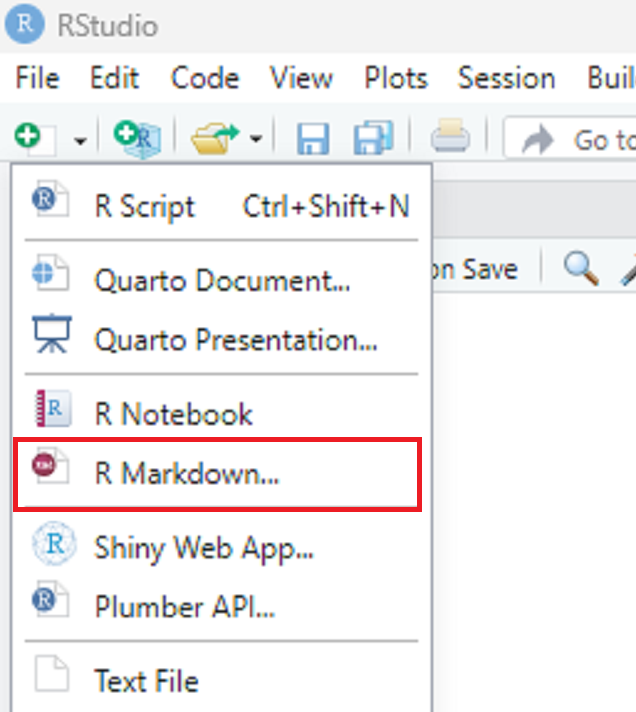
\includegraphics[width=0.6\textwidth,height=\textheight]{Images/wrangling/openrmd2.png}

}

\end{figure}

We will see a pop-up window as follows:

\begin{figure}

{\centering 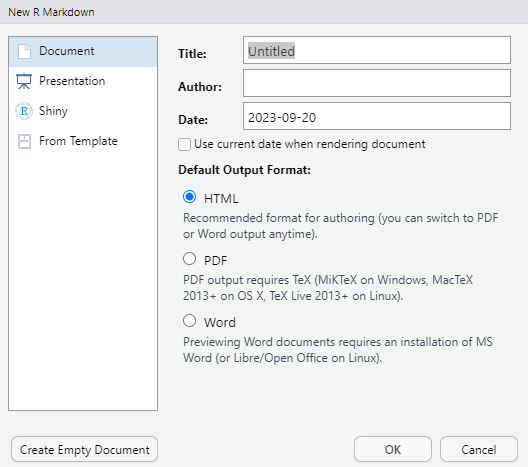
\includegraphics[width=0.7\textwidth,height=\textheight]{Images/wrangling/openrmd3.png}

}

\end{figure}

We can select whether we want to convert our RMD file to an
\texttt{HTML}, \texttt{PDF}, or a \texttt{Word} document. These options
can also be selected later. Let us select the default option (HTML) and
press OK. We will see the markdown file as shown in the picture below:

\begin{figure}

{\centering 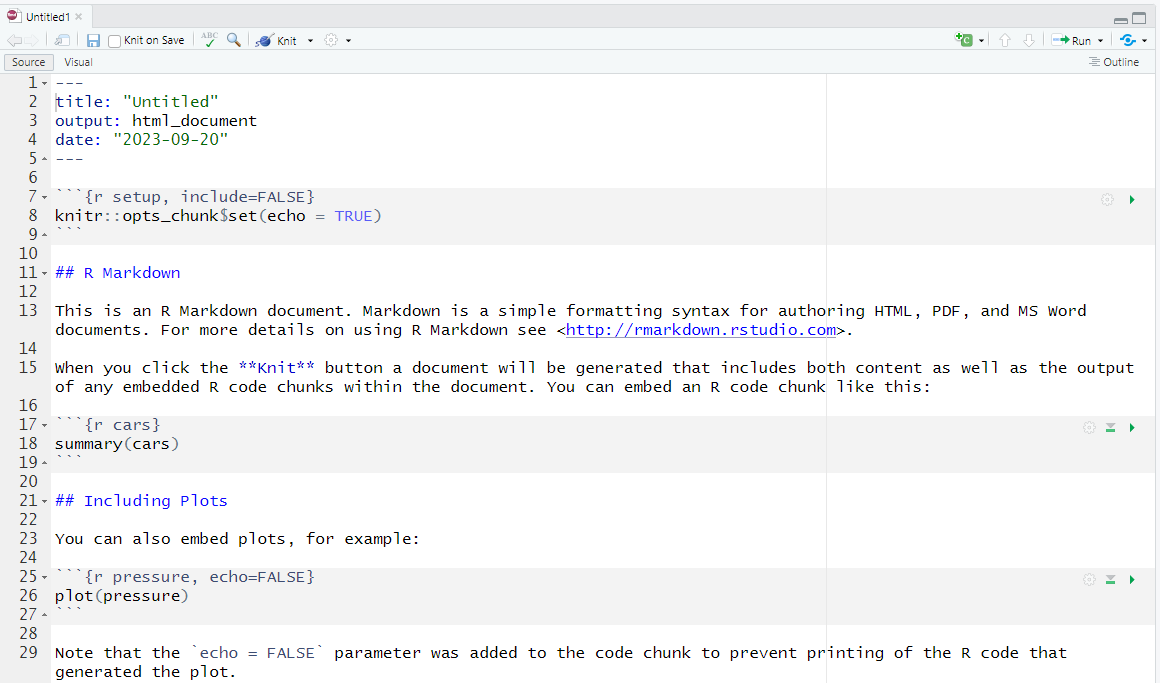
\includegraphics[width=0.9\textwidth,height=\textheight]{Images/wrangling/openrmd4.png}

}

\end{figure}

\hypertarget{knit}{%
\subsection*{Knit}\label{knit}}
\addcontentsline{toc}{subsection}{Knit}

We use the \texttt{knit} option to create a document (e.g., making a
PDF, HTML, or Word document) from the RMD file. Before knitting, we need
to save the file. Let us save the file as \textbf{working.RMD}. After
saving the file, we can knit it by clicking on the \texttt{knit} option,
as shown below:

\marginnote{\begin{footnotesize}

The term ``knit'' may sound a bit strange in the context of programming.
However, it aptly describes the process of combining your R code and
narrative text to produce a cohesive, final document. Think of it as
``weaving'' your code and text together into various output formats like
HTML, PDF, or Word.

\end{footnotesize}}

\begin{figure}

{\centering 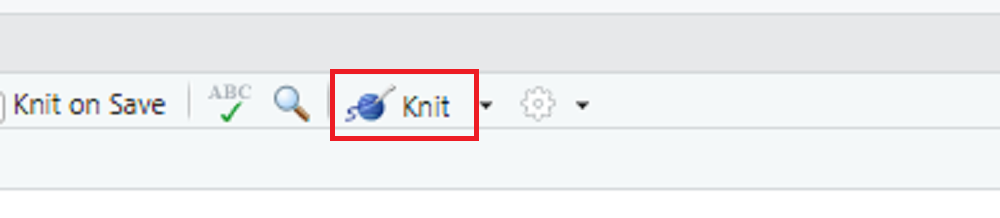
\includegraphics[width=0.9\textwidth,height=\textheight]{Images/wrangling/knit1.png}

}

\end{figure}

Once we knit the file, it will produce an \texttt{HTML} output, since
our default option was HTML.

\begin{figure}

{\centering 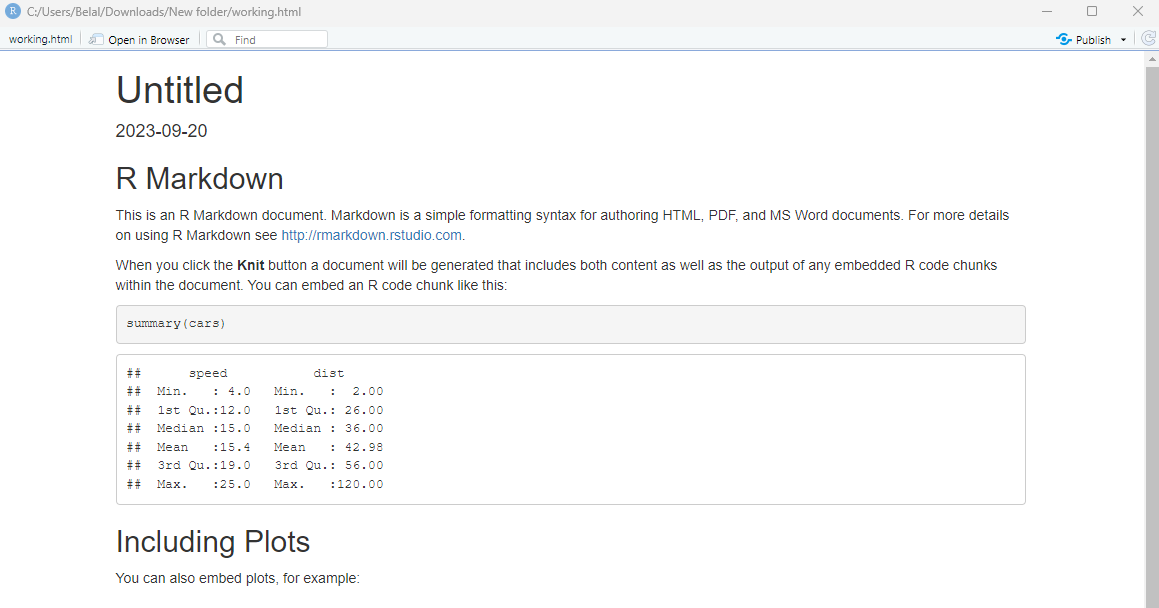
\includegraphics[width=0.9\textwidth,height=\textheight]{Images/wrangling/knit2.png}

}

\end{figure}

For formats other than \texttt{HTML} (e.g., \texttt{PDF} or
\texttt{Word}), we can click on the dropdown menu:

\begin{figure}

{\centering 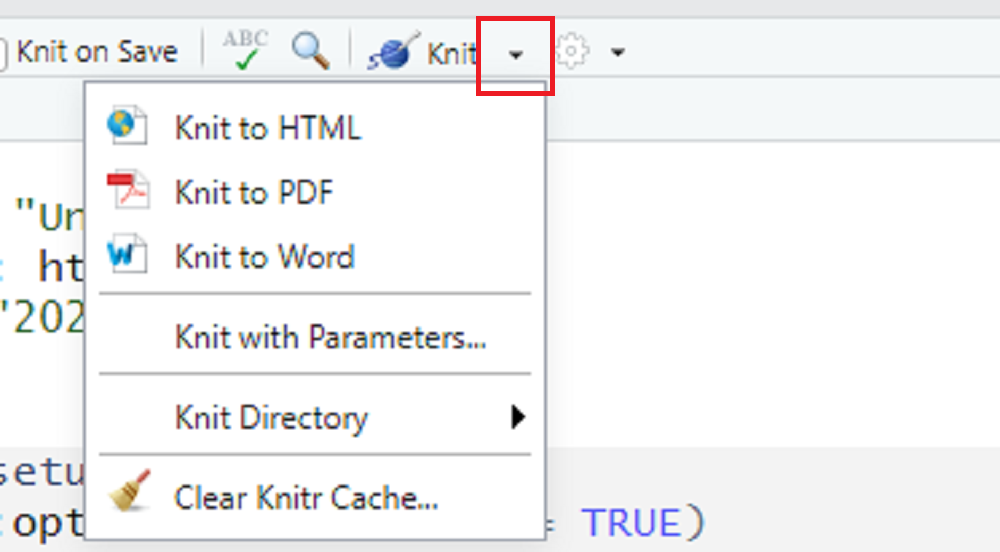
\includegraphics[width=0.8\textwidth,height=\textheight]{Images/wrangling/knit3.png}

}

\end{figure}

Let us select \texttt{Knit\ to\ Word} and knit it. Once the file is
rendered, RStudio will show us a preview of the output in a word file
and save the file in our \textbf{working directory}. We can also see
that \texttt{Word} is added as another output:

\marginnote{\begin{footnotesize}

When you're working in RStudio, all your files and outputs will be saved
in a `working directory.' This is simply the folder on your computer
where RStudio will look for files and save outputs. To find out what
your current working directory is, you can run the command
\texttt{getwd()} in the R console.

\end{footnotesize}}

\begin{figure}

{\centering 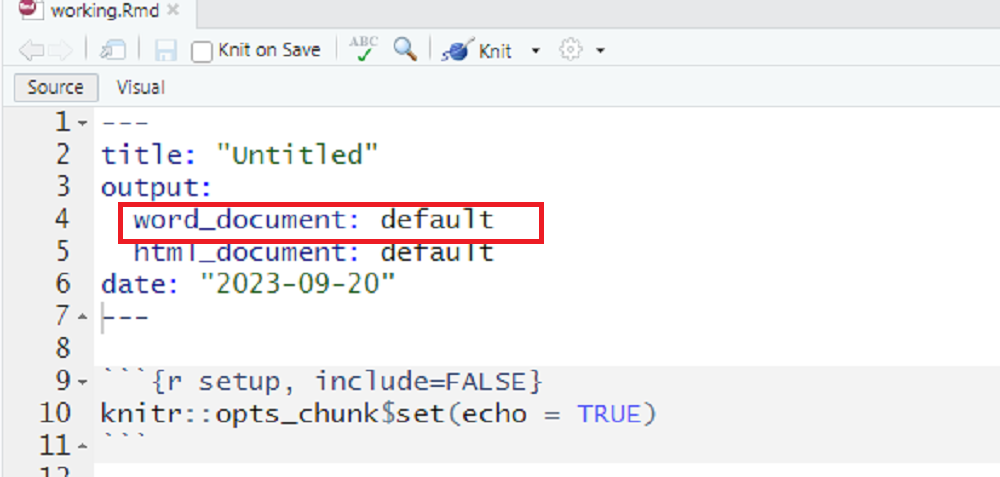
\includegraphics[width=0.8\textwidth,height=\textheight]{Images/wrangling/knit4.png}

}

\end{figure}

In the R terminal, we can see that a \texttt{Word} document is created,
which is stored in our working directory:

\begin{figure}

{\centering 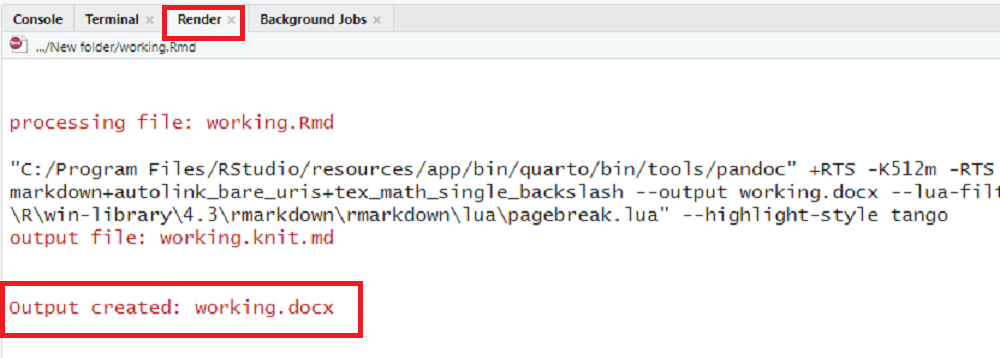
\includegraphics[width=0.9\textwidth,height=\textheight]{Images/wrangling/knit5.png}

}

\end{figure}

Similarly, we can create a pdf by clicking \texttt{Knit\ to\ PDF} option
from the \texttt{Knit} menu. However, we could see an error message as
follows:

\begin{figure}

{\centering 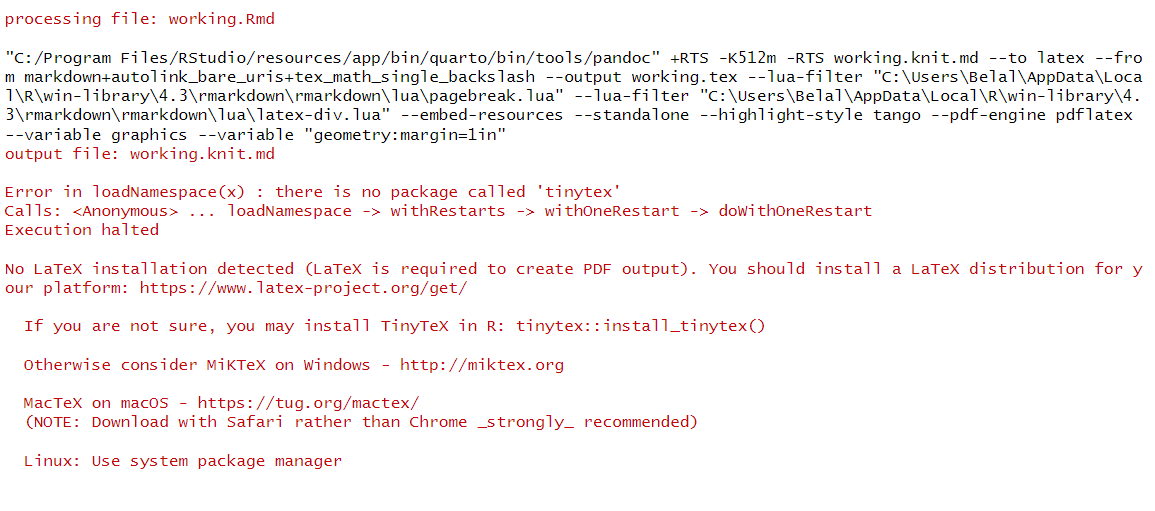
\includegraphics[width=0.9\textwidth,height=\textheight]{Images/wrangling/knit6.png}

}

\end{figure}

It is important to note that RStudio does not build PDF documents from
scratch. If we want to create PDF documents using RMD, we must have a
LaTeX distribution installed on our computer. There are several options
for LaTeX distributions, including MiKTeX, MacTeX, TeX Live, and so on.
However, the recommended option for R Markdown users is TinyTeX. We can
install TinyTeX using the R package \texttt{tinytex}. To install the
package, run the following command:
\texttt{install.packages("tinytex")}.

\marginnote{\begin{footnotesize}

LaTeX is a typesetting system commonly used for technical and scientific
documentation. It is required for converting R Markdown documents to PDF
format because it provides the text formatting commands that the
\texttt{rmarkdown} package uses behind the scenes.

\end{footnotesize}}

\begin{figure}

{\centering 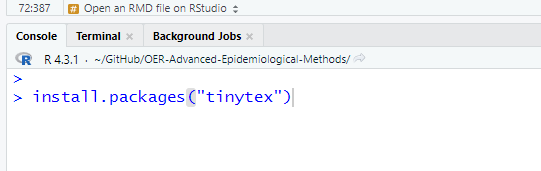
\includegraphics[width=0.8\textwidth,height=\textheight]{Images/wrangling/knit7.png}

}

\end{figure}

Once the \texttt{tinytex} package installation is complete, we can type
\texttt{tinytex::install\_tinytex()} to install the LaTeX distribution
on our computer.

\begin{figure}

{\centering 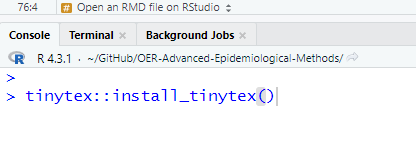
\includegraphics[width=0.8\textwidth,height=\textheight]{Images/wrangling/knit8.png}

}

\end{figure}

TinyTeX is a large package (\textasciitilde123 MB). The installation
time will vary depending on your machine. Once the installation is
complete, we can click \texttt{Knit\ to\ PDF}. Similar to the Word file,
RStudio will display a preview of the PDF output and save the PDF in our
working directory. We will also see that a PDF file has been created:

\begin{figure}

{\centering 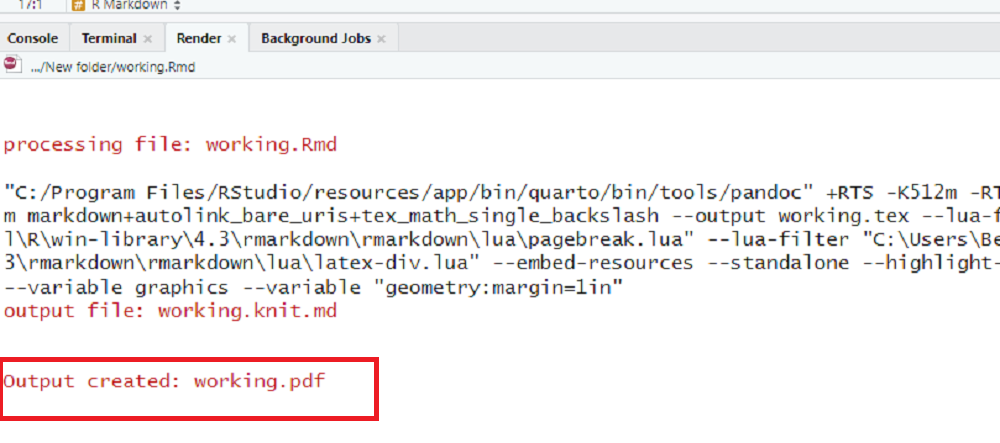
\includegraphics[width=0.9\textwidth,height=\textheight]{Images/wrangling/knit9.png}

}

\end{figure}

\hypertarget{working-with-rmd}{%
\subsection*{Working with RMD}\label{working-with-rmd}}
\addcontentsline{toc}{subsection}{Working with RMD}

Now we are ready to start writing plain text intermixed with embedded R
code. For plain text, we can use the whitespace:

\begin{figure}

{\centering 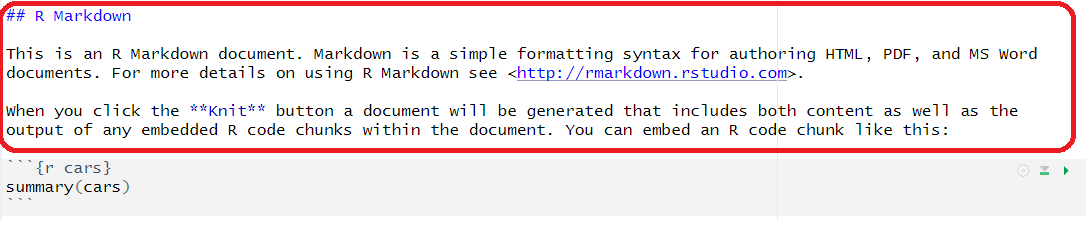
\includegraphics[width=0.9\textwidth,height=\textheight]{Images/wrangling/work1.png}

}

\end{figure}

On the other hand, to embed a chunk of R code into our report, we use R
code chunks. An R chunk surrounds the code with two lines that each
contain three backticks. After the first set of backticks, we include
\texttt{\{r\}}, which alerts \texttt{knitr} that we are going to include
a chunk of R code:

\marginnote{\begin{footnotesize}

Code chunks are segments of code that are contained within an R Markdown
document. They allow you to run R code within the document itself,
making your report dynamic and reproducible.

\end{footnotesize}}

\begin{figure}

{\centering 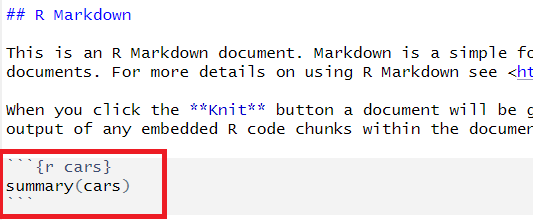
\includegraphics[width=0.8\textwidth,height=\textheight]{Images/wrangling/work2.png}

}

\end{figure}

Below are some codes:

\begin{figure}

{\centering 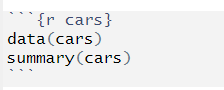
\includegraphics[width=0.45\textwidth,height=\textheight]{Images/wrangling/work3.png}

}

\end{figure}

We can knit the file to see the document, which will include plain text,
R code, and outputs from the R code. We can also see the output from a
code chunk without knitting the entire file. For example, we can click
the arrow on the right-hand side to execute the current code chunk:

\begin{figure}

{\centering 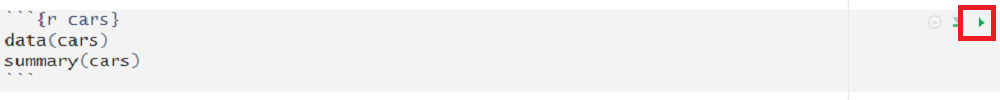
\includegraphics[width=0.9\textwidth,height=\textheight]{Images/wrangling/work4.png}

}

\end{figure}

Now we can see the following outputs:

\begin{figure}

{\centering 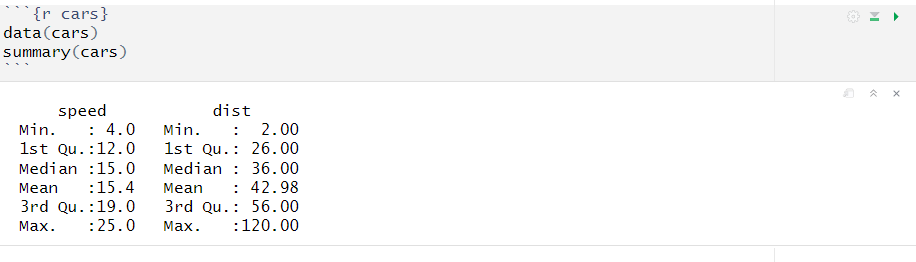
\includegraphics[width=0.9\textwidth,height=\textheight]{Images/wrangling/work5.png}

}

\end{figure}

Please also explore the drop down menu under \texttt{Run} to see the
further options, including run the current code chunk, run all code
chunk above, etc.

\begin{figure}

{\centering 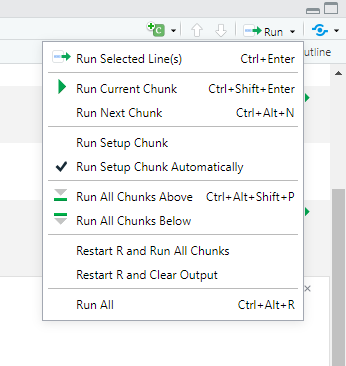
\includegraphics[width=0.7\textwidth,height=\textheight]{Images/wrangling/work6.png}

}

\end{figure}

To omit the code from the final report while still including the
results, add the argument \texttt{echo\ =\ FALSE}. This will place a
copy of the results into your report.

\marginnote{\begin{footnotesize}

Besides \texttt{echo\ =\ FALSE}, there are several other options you can
include in your code chunks to control their behavior, like
\texttt{eval\ =\ FALSE} if you don't want to evaluate the code, or
\texttt{message\ =\ FALSE} to hide messages. Take a look at the author's
page of comprehensive \href{https://yihui.name/knitr/options/}{list of
chunk options}.

\end{footnotesize}}

In the final report (e.g., Word or PDF), we often want to omit the code
and only show the outputs. To do this, we can add the argument
\texttt{echo\ =\ FALSE} in the R code chunk:

\begin{figure}

{\centering 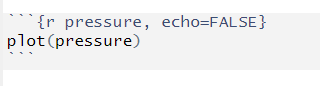
\includegraphics[width=0.5\textwidth,height=\textheight]{Images/wrangling/work7.png}

}

\end{figure}

The resulting output will look as follows:

\begin{figure}

{\centering 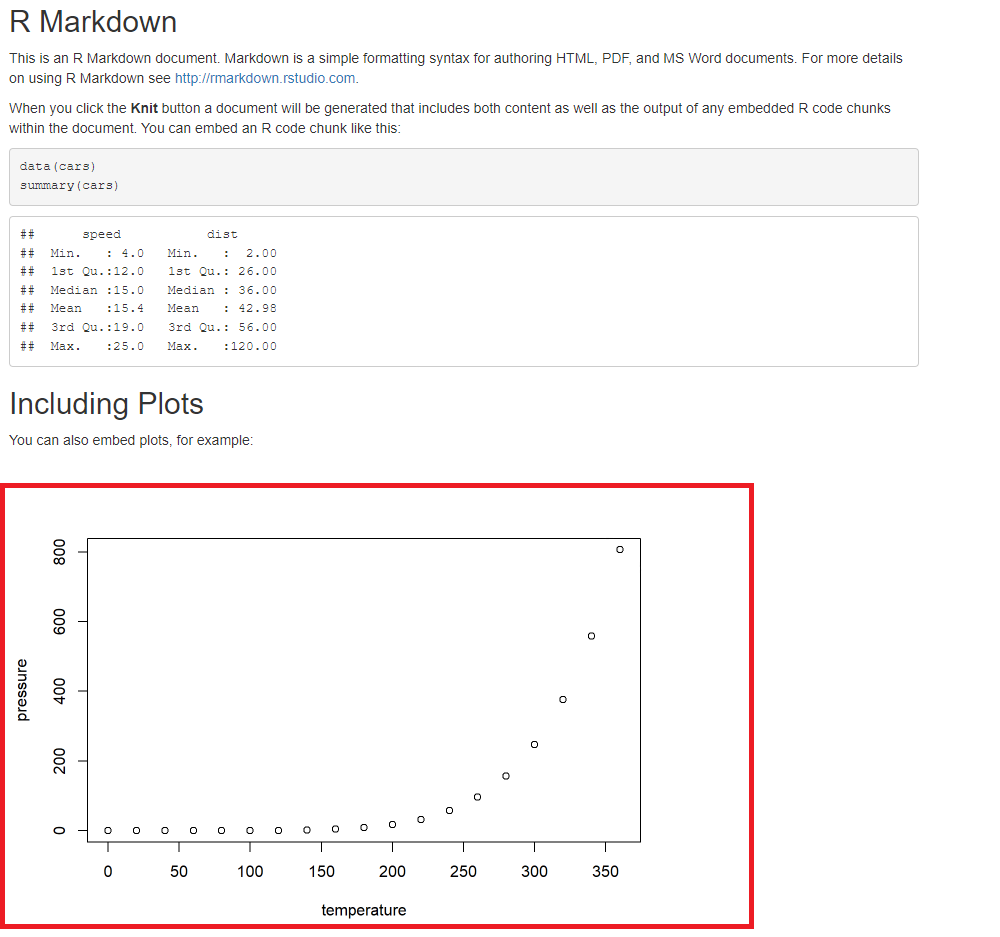
\includegraphics[width=0.9\textwidth,height=\textheight]{Images/wrangling/work8.png}

}

\end{figure}

\hypertarget{tips-and-troubleshooting}{%
\section*{Tips and Troubleshooting}\label{tips-and-troubleshooting}}
\addcontentsline{toc}{section}{Tips and Troubleshooting}

\markright{Tips and Troubleshooting}

\begin{itemize}
\tightlist
\item
  If the \texttt{knit} button is grayed out, make sure you have saved
  your RMD file first.
\item
  Encountering LaTeX errors? Make sure you've installed a LaTeX
  distribution like TinyTeX.
\end{itemize}

\begin{tcolorbox}[enhanced jigsaw, coltitle=black, rightrule=.15mm, title=\textcolor{quarto-callout-tip-color}{\faLightbulb}\hspace{0.5em}{Tip}, bottomtitle=1mm, colbacktitle=quarto-callout-tip-color!10!white, left=2mm, titlerule=0mm, arc=.35mm, colframe=quarto-callout-tip-color-frame, colback=white, leftrule=.75mm, bottomrule=.15mm, opacitybacktitle=0.6, opacityback=0, toptitle=1mm, toprule=.15mm, breakable]

The following links could also be useful if you want to learn more:

\begin{itemize}
\tightlist
\item
  \href{https://www.rstudio.com/wp-content/uploads/2015/02/rmarkdown-cheatsheet.pdf}{R
  Markdown Cheat Sheet}
\item
  \href{https://rmarkdown.rstudio.com/articles_intro.html}{Introduction
  to R Markdown}
\item
  \href{https://bookdown.org/yihui/rmarkdown/}{R Markdown: The
  Definitive Guide}
\item
  \href{https://epirhandbook.com/en/reports-with-r-markdown.html}{Reports
  with R Markdown}
\end{itemize}

\end{tcolorbox}

\hypertarget{video-content-optional-3}{%
\subsection*{Video content (optional)}\label{video-content-optional-3}}
\addcontentsline{toc}{subsection}{Video content (optional)}

\begin{tcolorbox}[enhanced jigsaw, coltitle=black, rightrule=.15mm, title=\textcolor{quarto-callout-tip-color}{\faLightbulb}\hspace{0.5em}{Tip}, bottomtitle=1mm, colbacktitle=quarto-callout-tip-color!10!white, left=2mm, titlerule=0mm, arc=.35mm, colframe=quarto-callout-tip-color-frame, colback=white, leftrule=.75mm, bottomrule=.15mm, opacitybacktitle=0.6, opacityback=0, toptitle=1mm, toprule=.15mm, breakable]

For those who prefer a video walkthrough, feel free to watch the video
below, which offers a description of an earlier version of the above
content.

\end{tcolorbox}

\hypertarget{r-functions-w}{%
\chapter*{R Functions (W)}\label{r-functions-w}}
\addcontentsline{toc}{chapter}{R Functions (W)}

\markboth{R Functions (W)}{R Functions (W)}

This review page provides an extensive list of R functions tailored for
data wrangling tasks that we have used in this chapter. Each function is
systematically described, highlighting its primary package source and
its specific utility.

To learn more about these functions, readers can:

\begin{enumerate}
\def\labelenumi{\arabic{enumi}.}
\item
  \textbf{Use R's Built-in Help System}: For each function, access its
  documentation by prefixing the function name with a question mark in
  the R console, e.g., \texttt{?as.factor}. This displays the function's
  manual page with descriptions, usage, and examples.
\item
  \textbf{Search Websites}: Simply
  \href{https://www.google.com/search?q=as.factor+in+R}{Google}, or
  visit the \href{https://cran.r-project.org/}{CRAN website} to search
  for specific function documentation. Websites like
  \href{https://stackoverflow.com/}{Stack Overflow} and
  \href{https://community.rstudio.com/}{RStudio Community} often have
  discussions related to R functions.
\item
  \textbf{Tutorials and Online Courses}: Platforms like DataCamp,
  Coursera, and edX offer R courses that cover many functions in depth.
  Also there are examples of dedicated R tutorial websites that you
  might find useful. One example is
  \href{https://ehsanx.github.io/intro2R/}{``Introduction to R for
  health data analysis''} by Ehsan Karim, An Hoang and Qu.
\item
  \textbf{Books}: There are numerous R programming books, such as
  \href{https://r4ds.had.co.nz/}{``R for Data Science''} by Hadley
  Wickham and \href{https://nostarch.com/artofr.htm}{``The Art of R
  Programming''} by Norman Matloff.
\item
  \textbf{Workshops and Webinars}: Institutions and organizations
  occasionally offer R programming workshops or webinars.
\end{enumerate}

Whenever in doubt, exploring existing resources can be highly
beneficial.

\begin{longtable}[]{@{}lll@{}}
\toprule\noalign{}
Function\_name & Package\_name & Use \\
\midrule\noalign{}
\endhead
\bottomrule\noalign{}
\endlastfoot
as.factor & base & Converts a variable to factors. `as.factor` is a
wrapper for the `factor` function. \\
cbind & base & Merges matrices. \\
CreateTableOne & tableone & Creates a frequency table. \\
data.frame & base & Creates a dataset with both numeric and character
variables. Requires unique column names and equal length for all
variables. \\
dim & base & Returns the dimensions of a data frame (rows x columns). \\
filter & dplyr & Subsets a dataset by selecting a sub-population. \\
function & base & Used to define custom functions, e.g., for calculating
standard deviation. \\
head & base & Displays the first six elements of an object (e.g., a
dataset). `tail` displays the last six. \\
is.na & base & Checks for missing values in a variable. \\
levels & base & Displays the levels of a factor variable. \\
list & base & Stores vectors, matrices, or lists of differing types. \\
mode & base & Determines the type of a variable. \\
na.omit & base/stats & Removes all rows with missing values from a
dataset. \\
names & base & Displays names of objects, e.g., variable names of a data
frame. \\
nlevels & base & Shows the number of levels in a factor variable. \\
nrow & base & Returns the dimensions of a data frame. `nrow` gives row
count and `ncol` gives column count. \\
plot & base/graphics & Draws scatter plots or line graphs. \\
print & base & Prints the output to console. \\
prop.table & base & Displays percentage summary for a table. \\
rbind & base & Appends matrices row-wise. \\
read.csv & base/utils & Reads data from a CSV file. \\
relevel & base/stats & Changes the reference group of a factor
variable. \\
sasxport.get & Hmisc & Loads data in the SAS format. \\
save & base & Saves R objects, such as datasets. \\
select & dplyr & Selects specified variables from a dataset. \\
set.seed & base & Sets a seed for random number generation ensuring
reproducibility. \\
str & base/utils & Displays the structure of a dataset, including data
type of variables. \\
subset & base, dplyr & Subsets a dataset by selecting a
sub-population. \\
summary & base & Provides a summary of an object, like variable
statistics. \\
table & base & Displays frequency counts for a variable. \\
write.csv & base/utils & Saves a data frame to a CSV file in a specified
directory. \\
\end{longtable}

\hypertarget{quiz-w}{%
\chapter*{Quiz (W)}\label{quiz-w}}
\addcontentsline{toc}{chapter}{Quiz (W)}

\markboth{Quiz (W)}{Quiz (W)}

\begin{enumerate}
\def\labelenumi{\arabic{enumi}.}
\tightlist
\item
  \textbf{Downloading the File:}

  \begin{itemize}
  \tightlist
  \item
    Navigate to the link: \href{Quiz/QuizWrangling.Rmd}{See here}.
  \item
    Right-click on the link and select ``Save link as\ldots{}'' from the
    dropdown menu.
  \item
    Alternatively click here for downloading the quizzes.
  \item
    Choose a destination folder on your computer where you'd like to
    save the file (e.g., Desktop). \textbf{Remember this location}, as
    you'll need to navigate to it later.
  \end{itemize}
\item
  \textbf{Setting Up RStudio:}

  \begin{itemize}
  \tightlist
  \item
    If you don't have RStudio installed, see the download link in
    \href{wrangling1a.html}{here}.
  \item
    Launch RStudio after installing.
  \end{itemize}
\item
  \textbf{Installing Necessary R Packages:}

  \begin{itemize}
  \item
    Before running the R Markdown file, ensure you have the required
    packages. In RStudio's console (located at the bottom left by
    default), enter the following commands to install them:

\begin{Shaded}
\begin{Highlighting}[numbers=left,,]
\FunctionTok{install.packages}\NormalTok{(}\StringTok{"learnr"}\NormalTok{)}
\FunctionTok{install.packages}\NormalTok{(}\StringTok{"xfun"}\NormalTok{)}
\end{Highlighting}
\end{Shaded}
  \end{itemize}
\item
  \textbf{Opening and Running the File:}

  \begin{itemize}
  \tightlist
  \item
    In RStudio, go to \texttt{File} \textgreater{}
    \texttt{Open\ File...}.
  \item
    Navigate to the folder where you saved the \texttt{Rmd} file and
    select it to open.
  \item
    Once the file is open in RStudio, you'll see a ``Run Document''
    button (green) at the top of the script editor. Click on it to run
    the R Markdown Quiz file.
  \end{itemize}
\end{enumerate}

\hypertarget{exercise-w}{%
\chapter*{Exercise (W)}\label{exercise-w}}
\addcontentsline{toc}{chapter}{Exercise (W)}

\markboth{Exercise (W)}{Exercise (W)}

\begin{tcolorbox}[enhanced jigsaw, coltitle=black, rightrule=.15mm, title=\textcolor{quarto-callout-tip-color}{\faLightbulb}\hspace{0.5em}{Tip}, bottomtitle=1mm, colbacktitle=quarto-callout-tip-color!10!white, left=2mm, titlerule=0mm, arc=.35mm, colframe=quarto-callout-tip-color-frame, colback=white, leftrule=.75mm, bottomrule=.15mm, opacitybacktitle=0.6, opacityback=0, toptitle=1mm, toprule=.15mm, breakable]

You can download all of the related files in a zip file
\textbf{wranglingEx.zip} from
\href{https://github.com/ehsanx/EpiMethods/tree/main/LabExercises/}{Github
folder} folder, or just by clicking this link
\href{https://github.com/ehsanx/EpiMethods/raw/main/LabExercises/wranglingEx.zip}{directly}.

\begin{itemize}
\tightlist
\item
  Navigate to the GitHub folder (above link) where the ZIP file is
  located.
\item
  Click on the file name (above zip file) to open its preview window.
\item
  Click on the Download button to download the file. If you can't see
  the Download button, click on ``Download Raw File'' link that should
  appear on the page.
\end{itemize}

\end{tcolorbox}

\hypertarget{problem-statement}{%
\section*{Problem Statement}\label{problem-statement}}
\addcontentsline{toc}{section}{Problem Statement}

\markright{Problem Statement}

Use the functions we learned in Lab 1 to complete Lab 1 Exercise. We
will use Right Heart Catheterization Dataset saved in the folder named
`Data/wrangling/'. The variable list and description can be accessed
from
\href{https://biostat.app.vumc.org/wiki/pub/Main/DataSets/rhc.html}{Vanderbilt
Biostatistics website}.

A paper you can access the original table from
\href{https://jamanetwork-com.ezproxy.library.ubc.ca/journals/jama/fullarticle/407990}{this
paper} (\href{https://pubmed.ncbi.nlm.nih.gov/8782638/}{doi:
10.1001/jama.1996.03540110043030}). We have modified the table and
corrected some issues. Please knit your file once you finished and
submit the knitted file \textbf{ONLY}.

\begin{Shaded}
\begin{Highlighting}[numbers=left,,]
\CommentTok{\# Load required packages}
\FunctionTok{library}\NormalTok{(dplyr)}
\FunctionTok{library}\NormalTok{(tableone)}
\end{Highlighting}
\end{Shaded}

\begin{Shaded}
\begin{Highlighting}[numbers=left,,]
\CommentTok{\# Data import: name it rhc}
\CommentTok{\#rhc \textless{}{-} ...("Data/wrangling/rhc.csv", ...)}
\end{Highlighting}
\end{Shaded}

\hypertarget{part-a-basic-manipulation-60}{%
\subsection*{Part (a) Basic Manipulation
{[}60\%{]}}\label{part-a-basic-manipulation-60}}
\addcontentsline{toc}{subsection}{Part (a) Basic Manipulation
{[}60\%{]}}

\begin{enumerate}
\def\labelenumi{(\Roman{enumi})}
\tightlist
\item
  Continuous to Categories: Change the Age variable into categories
  below 50, 50 to below 60, 60 to below 70, 70 to below 80, 80 and above
  {[}Hint: the \texttt{cut} function could be helpful{]}
\end{enumerate}

\begin{enumerate}
\def\labelenumi{(\Roman{enumi})}
\setcounter{enumi}{1}
\tightlist
\item
  Re-order: Re-order the levels of race to white, black and other
\end{enumerate}

\begin{enumerate}
\def\labelenumi{(\Roman{enumi})}
\setcounter{enumi}{2}
\tightlist
\item
  Set reference: Change the reference category for gender to Male
\end{enumerate}

\begin{enumerate}
\def\labelenumi{(\Roman{enumi})}
\setcounter{enumi}{3}
\tightlist
\item
  Count levels: Check how many levels does the variable ``cat1''
  (Primary disease category) have? Regroup the levels for disease
  categories to ``ARF'',``CHF'',``MOSF'',``Other''. {[}Hint: the
  \texttt{nlevels} and \texttt{list} functions could be helpful{]}
\end{enumerate}

\begin{enumerate}
\def\labelenumi{(\Alph{enumi})}
\setcounter{enumi}{21}
\tightlist
\item
  Rename levels: Rename the levels of ``ca'' (Cancer) to
  ``Metastatic'',``None'' and ``Localized (Yes)'', then re-order the
  levels to ``None'',``Localized (Yes)'' and ``Metastatic''
\end{enumerate}

\begin{enumerate}
\def\labelenumi{(\Roman{enumi})}
\setcounter{enumi}{5}
\tightlist
\item
  comorbidities:
\end{enumerate}

\begin{itemize}
\tightlist
\item
  create a new variable called ``numcom'' to count number of
  comorbidities illness for each person (12 categories) {[}Hint: the
  \texttt{rowSums} command could be helpful{]},
\item
  report maximim and minimum values of numcom:
\end{itemize}

\begin{enumerate}
\def\labelenumi{(\Roman{enumi})}
\setcounter{enumi}{6}
\tightlist
\item
  Anlaytic data: Create a dataset that has only the following variables
\end{enumerate}

\begin{itemize}
\tightlist
\item
  ``age'', ``sex'', ``race'',``cat1'', ``ca'', ``dnr1'', ``aps1'',
  ``surv2md1'', ``numcom'', ``adld3p'', ``das2d3pc'', ``temp1'',
  ``hrt1'', ``meanbp1'', ``resp1'', ``wblc1'', ``pafi1'', ``paco21'',
  ``ph1'', ``crea1'', ``alb1'', ``scoma1'', ``swang1'', and
\item
  name it rhc2.
\end{itemize}

\hypertarget{part-b-table-1-20}{%
\subsection*{Part (b) Table 1 {[}20\%{]}}\label{part-b-table-1-20}}
\addcontentsline{toc}{subsection}{Part (b) Table 1 {[}20\%{]}}

\begin{enumerate}
\def\labelenumi{(\roman{enumi})}
\tightlist
\item
  Re-produce the sample table from the rhc2 data (see the Table that was
  provided with this assignment). In your table, the variables should be
  ordered as the same as the sample. Please re-level or re-order the
  levels if needed. {[}Hint: the \texttt{tableone} package might be
  useful{]}
\end{enumerate}

\begin{enumerate}
\def\labelenumi{(\roman{enumi})}
\setcounter{enumi}{1}
\tightlist
\item
  Table 1 for subset
\end{enumerate}

Produce a similar table as part (b) but with only male sex and ARF
primary disease category (cat1). Add the overall column in the same
table. {[}Hint: \texttt{filter} command could be useful{]}

\hypertarget{part-c-considering-eligibility-criteria-20}{%
\subsection*{Part (c) Considering eligibility criteria
{[}20\%{]}}\label{part-c-considering-eligibility-criteria-20}}
\addcontentsline{toc}{subsection}{Part (c) Considering eligibility
criteria {[}20\%{]}}

Produce a similar table as part (b.i) but only for the subjects who meet
all of the following eligibility criteria: (i) age is equal to or above
50, (ii) age is below 80 (iii) Glasgow Coma Score is below 61 and (iv)
Primary disease categories are either ARF or MOSF. {[}Hint:
\texttt{droplevels.data.frame} can be a useful function{]}

\hypertarget{optional-1-missing-values}{%
\subsection*{Optional 1: Missing
values}\label{optional-1-missing-values}}
\addcontentsline{toc}{subsection}{Optional 1: Missing values}

\begin{enumerate}
\def\labelenumi{(\Roman{enumi})}
\tightlist
\item
  Any variables included in rhc2 data had missing values? Name that
  variable. {[}Hint: \texttt{apply} function could be helpful{]}
\end{enumerate}

\begin{enumerate}
\def\labelenumi{(\Roman{enumi})}
\setcounter{enumi}{1}
\tightlist
\item
  Count how many NAs does that variable have?
\end{enumerate}

\begin{enumerate}
\def\labelenumi{(\Roman{enumi})}
\setcounter{enumi}{2}
\tightlist
\item
  Produce a table 1 for a complete case data (no missing observations)
  stratified by \texttt{swang1}.
\end{enumerate}

\hypertarget{optional-2-calculating-variance-of-a-sample}{%
\subsection*{Optional 2: Calculating variance of a
sample}\label{optional-2-calculating-variance-of-a-sample}}
\addcontentsline{toc}{subsection}{Optional 2: Calculating variance of a
sample}

Write a \texttt{function} for Bessel's correction to calculate an
unbiased estimate of the population variance from a finite sample (a
vector of 100 observations, consisting of numbers from 1 to 100).

\begin{Shaded}
\begin{Highlighting}[numbers=left,,]
\NormalTok{Vector }\OtherTok{\textless{}{-}} \DecValTok{1}\SpecialCharTok{:}\DecValTok{100}

\CommentTok{\#variance.est \textless{}{-} function(?)\{?\}}

\CommentTok{\#variance.est(Vector)}
\end{Highlighting}
\end{Shaded}

Hint: Take a closer look at the functions, loops and algorithms shown in
lab materials. Use a \texttt{for\ loop}, utilizing the following
pseudocode of the
\href{https://en.wikipedia.org/wiki/Algorithms_for_calculating_variance}{algorithm}:

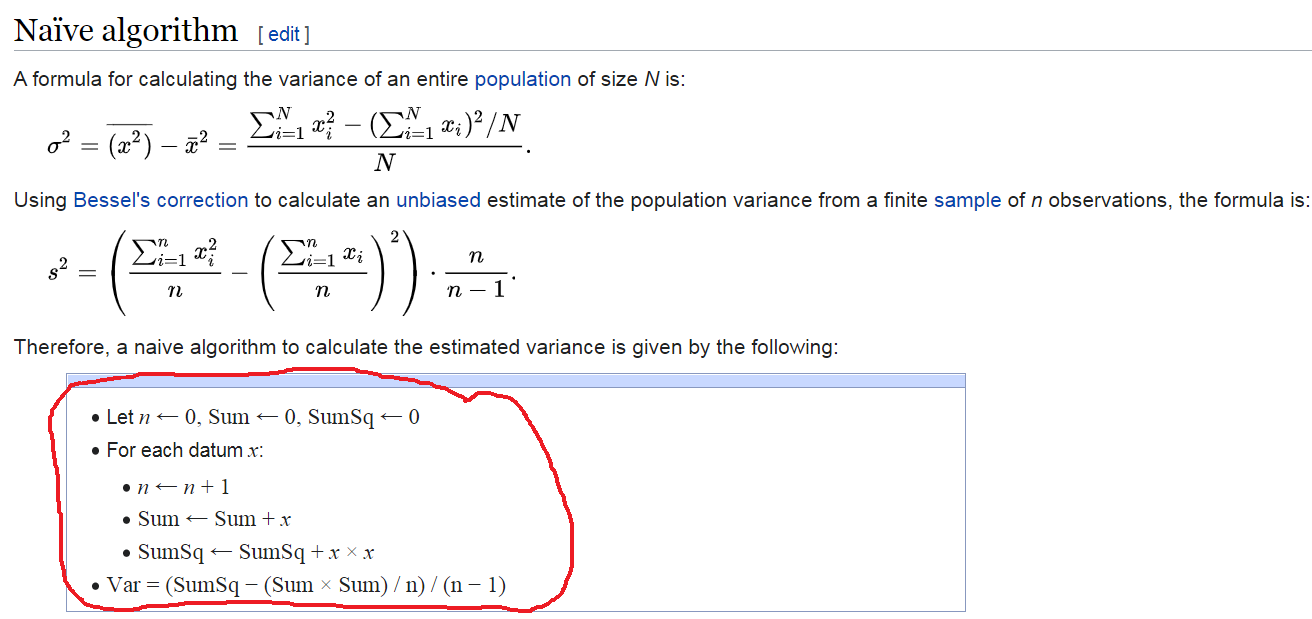
\includegraphics[width=0.9\textwidth,height=\textheight]{Images/wrangling/algorithm.png}

Verify that estimated variance with the following variance function
output in R:

\begin{Shaded}
\begin{Highlighting}[numbers=left,,]
\FunctionTok{var}\NormalTok{(Vector)}
\CommentTok{\#\textgreater{} [1] 841.6667}
\end{Highlighting}
\end{Shaded}

\part{Data accessing}

\hypertarget{background-1}{%
\section*{Background}\label{background-1}}
\addcontentsline{toc}{section}{Background}

\markright{Background}

Surveys serve as a pivotal tool for collecting and evaluating
health-related information on a national scale. More often than not,
it's the governmental bodies that take the lead in gathering this data.
Recognizing the value of this information, many governments not only
compile and analyze these datasets but also ensure they are accessible
to the public, especially for research purposes. In this guide, we will
delve into an array of survey methodologies, provide illustrative
examples, and guide you through the process of downloading pertinent
data from both Canadian and American repositories. To make this more
tangible, we will conclude with a hands-on example, showcasing how to
replicate findings from an academic paper that leveraged one of these
publicly available datasets.

\marginnote{\begin{footnotesize}

Dedicating a chapter to accessing and downloading nationally
representative survey datasets is pivotal for a hands-on epidemiological
tutorial. These datasets, often rich in information and reflective of
diverse populations, serve as the backbone for real-world analysis. By
guiding learners on how to obtain these datasets, the book ensures that
they not only grasp theoretical concepts but also gain practical
experience working with authentic, large-scale data. This approach
bridges the gap between theory and practice, allowing readers to apply
learned techniques on datasets that mirror real-world complexities,
thereby enhancing the relevance and applicability of their analytical
skills.

\end{footnotesize}}

\begin{tcolorbox}[enhanced jigsaw, coltitle=black, rightrule=.15mm, title=\textcolor{quarto-callout-important-color}{\faExclamation}\hspace{0.5em}{Important}, bottomtitle=1mm, colbacktitle=quarto-callout-important-color!10!white, left=2mm, titlerule=0mm, arc=.35mm, colframe=quarto-callout-important-color-frame, colback=white, leftrule=.75mm, bottomrule=.15mm, opacitybacktitle=0.6, opacityback=0, toptitle=1mm, toprule=.15mm, breakable]

\textbf{Datasets}:

All of the datasets used in this tutorial can be accessed from
\href{https://github.com/ehsanx/EpiMethods/tree/main/Data/accessing}{this
GitHub repository folder}

\end{tcolorbox}

\hypertarget{overview-of-tutorials-1}{%
\section*{Overview of tutorials}\label{overview-of-tutorials-1}}
\addcontentsline{toc}{section}{Overview of tutorials}

\markright{Overview of tutorials}

\hypertarget{survey-data-sources}{%
\subsection*{\texorpdfstring{\href{accessing1.html}{Survey data
sources}}{Survey data sources}}\label{survey-data-sources}}
\addcontentsline{toc}{subsection}{\href{accessing1.html}{Survey data
sources}}

The tutorial lists primary complex survey data sources, including the
Canadian Community Health Survey and National Health and Nutrition
Examination Survey, with several offering dedicated R packages for data
access.

\hypertarget{descriptions-of-data-sources}{%
\subsection*{\texorpdfstring{\href{accessing1i.html}{Descriptions of
data
sources}}{Descriptions of data sources}}\label{descriptions-of-data-sources}}
\addcontentsline{toc}{subsection}{\href{accessing1i.html}{Descriptions
of data sources}}

This tutorial provides comprehensive instructions on how to import and
process health survey datasets, specifically focusing on the Canadian
Community Health Survey (CCHS), National Health and Nutrition
Examination Survey (NHANES), and National Health Interview Survey
(NHIS).

\hypertarget{importing-cchs-to-r}{%
\subsection*{\texorpdfstring{\href{accessing2.html}{Importing CCHS to
R}}{Importing CCHS to R}}\label{importing-cchs-to-r}}
\addcontentsline{toc}{subsection}{\href{accessing2.html}{Importing CCHS
to R}}

The section provides detailed steps for importing the Canadian Community
Health Survey dataset from the UBC library into RStudio, with processing
options using SAS, the free software PSPP, and directly in R.

\hypertarget{importing-nhanes-to-r}{%
\subsection*{\texorpdfstring{\href{accessing3.html}{Importing NHANES to
R}}{Importing NHANES to R}}\label{importing-nhanes-to-r}}
\addcontentsline{toc}{subsection}{\href{accessing3.html}{Importing
NHANES to R}}

The tutorial guides users on how to access and import the NHANES dataset
from the CDC website into RStudio, detailing the dataset's structure and
providing methods both manually and using an R package.

\hypertarget{reproducing-results}{%
\subsection*{\texorpdfstring{\href{accessing4.html}{Reproducing
results}}{Reproducing results}}\label{reproducing-results}}
\addcontentsline{toc}{subsection}{\href{accessing4.html}{Reproducing
results}}

The tutorial guides users through accessing, processing, and analyzing
NHANES data to reproduce the results from a referenced article using R
code.

\hypertarget{importing-nhis-to-r}{%
\subsection*{\texorpdfstring{\href{accessing5.html}{Importing NHIS to
R}}{Importing NHIS to R}}\label{importing-nhis-to-r}}
\addcontentsline{toc}{subsection}{\href{accessing5.html}{Importing NHIS
to R}}

This chapter serves as a tutorial on accessing and importing the
National Health Interview Survey (NHIS) dataset from the US Centers for
Disease Control and Prevention (CDC) website into RStudio. The NHIS is
an annual cross-sectional survey managed by the CDC, offering insights
into population disease prevalence, disability extent, and utilization
of health care services. The data files are available in various
formats, including ASCII, CSV, and SAS. Users can combine datasets from
different years; however, tracing the same individual across cycles is
not feasible. The chapter provides step-by-step guidance on downloading
the NHIS dataset, particularly the `Adult' data from 2021, verifying the
imported data, and merging datasets within the same survey cycle using
the unique household identifier.

\begin{tcolorbox}[enhanced jigsaw, coltitle=black, rightrule=.15mm, title=\textcolor{quarto-callout-note-color}{\faInfo}\hspace{0.5em}{Note}, bottomtitle=1mm, colbacktitle=quarto-callout-note-color!10!white, left=2mm, titlerule=0mm, arc=.35mm, colframe=quarto-callout-note-color-frame, colback=white, leftrule=.75mm, bottomrule=.15mm, opacitybacktitle=0.6, opacityback=0, toptitle=1mm, toprule=.15mm, breakable]

\textbf{What is Coming Next}:

The subsequent chapter on \href{researchquestion.html}{Research
Questions} serves as a valuable guide for constructing an
analytics-driven data set tailored to your specific research queries. It
will cover crucial aspects such as the types of variables to collect and
how to set eligibility criteria, followed by approaches to data analysis
based on your research questions. It's important to note that research
questions can fall into two main categories: predictive or causal. For a
deeper understanding of variable selection and analytical tools suited
to these types of questions, the chapters on the
\href{confounding.html}{Roles of Variables} and
\href{predictivefactors.html}{Predictive Models} offer insightful
guidance.

\end{tcolorbox}

\begin{tcolorbox}[enhanced jigsaw, coltitle=black, rightrule=.15mm, title=\textcolor{quarto-callout-warning-color}{\faExclamationTriangle}\hspace{0.5em}{Warning}, bottomtitle=1mm, colbacktitle=quarto-callout-warning-color!10!white, left=2mm, titlerule=0mm, arc=.35mm, colframe=quarto-callout-warning-color-frame, colback=white, leftrule=.75mm, bottomrule=.15mm, opacitybacktitle=0.6, opacityback=0, toptitle=1mm, toprule=.15mm, breakable]

\textbf{Bug Report}:

Fill out \href{https://forms.gle/YSwuiebtb1E9wjHu9}{this form} to report
any issues with the tutorial.

\end{tcolorbox}

\hypertarget{concepts-a}{%
\chapter*{Concepts (A)}\label{concepts-a}}
\addcontentsline{toc}{chapter}{Concepts (A)}

\markboth{Concepts (A)}{Concepts (A)}

\hypertarget{model-based-approach}{%
\section*{Model-based approach}\label{model-based-approach}}
\addcontentsline{toc}{section}{Model-based approach}

\markright{Model-based approach}

The model-based approach to statistical analysis is heavily reliant on
the specification of a probability model for data generation, typically
assuming that data come from an infinite population that follows a
specific distribution, such as the Normal distribution. Inferences about
the population, including point estimates and hypothesis testing, are
made based on how well the sample data fit these model assumptions.

\hypertarget{design-based-approach}{%
\section*{Design-based approach}\label{design-based-approach}}
\addcontentsline{toc}{section}{Design-based approach}

\markright{Design-based approach}

The design-based approach emphasizes the use of sampling methods and the
design of the study itself to make inferences about a real/finite
population. The design-based approach takes into account the actual
structure of the data collection process to make inferences, ensuring
that each unit in the population has a known and often non-zero chance
of being included in the sample, thus addressing the potential biases
and variance issues arising from the sampling design. This approach is
critical in understanding and analyzing data from surveys with complex
designs, including those with stratification, clustering, and weighting.

\hypertarget{reading-list}{%
\section*{Reading list}\label{reading-list}}
\addcontentsline{toc}{section}{Reading list}

\markright{Reading list}

Key reference:

\begin{itemize}
\tightlist
\item
  (Heeringa, West, and Berglund 2017) (chapter 2)
\end{itemize}

Optional reading:

\begin{itemize}
\tightlist
\item
  (Lumley 2011) (chapter 1)
\item
  (Vittinghoff et al. 2011) (chapter 12)
\item
  (Bilder and Loughin 2014) (section 6.3)
\end{itemize}

\hypertarget{lecture-videos}{%
\section*{Lecture Videos}\label{lecture-videos}}
\addcontentsline{toc}{section}{Lecture Videos}

\markright{Lecture Videos}

\begin{tcolorbox}[enhanced jigsaw, coltitle=black, rightrule=.15mm, title=\textcolor{quarto-callout-tip-color}{\faLightbulb}\hspace{0.5em}{Model-based approach}, bottomtitle=1mm, colbacktitle=quarto-callout-tip-color!10!white, left=2mm, titlerule=0mm, arc=.35mm, colframe=quarto-callout-tip-color-frame, colback=white, leftrule=.75mm, bottomrule=.15mm, opacitybacktitle=0.6, opacityback=0, toptitle=1mm, toprule=.15mm, breakable]

Review materials from pre-requisite statistics courses (optional)

\end{tcolorbox}

\begin{tcolorbox}[enhanced jigsaw, coltitle=black, rightrule=.15mm, title=\textcolor{quarto-callout-tip-color}{\faLightbulb}\hspace{0.5em}{Design-based approach}, bottomtitle=1mm, colbacktitle=quarto-callout-tip-color!10!white, left=2mm, titlerule=0mm, arc=.35mm, colframe=quarto-callout-tip-color-frame, colback=white, leftrule=.75mm, bottomrule=.15mm, opacitybacktitle=0.6, opacityback=0, toptitle=1mm, toprule=.15mm, breakable]

What is included in this lecture:

\begin{itemize}
\tightlist
\item
  Model-based approach review: 0:00
\item
  Design-based approach: 1:15
\item
  Types of sampling techniques 6:46
\item
  Statistical inference 8:25
\item
  NHANES 12:02
\item
  Survey weight 20:40
\item
  CCHS download 23:45
\item
  NHANES download 24:50
\item
  NHANES sampling design 27:24
\item
  How to find NHANES data from CDC website 27:42
\end{itemize}

The timestamps are also included in the YouTube video description.

\end{tcolorbox}

\hypertarget{lecture-slides}{%
\section*{Lecture Slides}\label{lecture-slides}}
\addcontentsline{toc}{section}{Lecture Slides}

\markright{Lecture Slides}

\hypertarget{links}{%
\section*{Links}\label{links}}
\addcontentsline{toc}{section}{Links}

\markright{Links}

\begin{itemize}
\tightlist
\item
  \href{https://docs.google.com/presentation/d/1hpmABr_63Nm89RXH09riUiKa9SVRZEV4kJHQbqnbHTA/edit?usp=sharing}{Google
  Slides}
\item
  \href{slides/designNHANES.pdf}{PDF Slides}
\item
  \href{https://ehsanx.github.io/SPPH504007SurveyData/docs/tab-3.html}{Model-based
  approach} (Review/optional content)
\item
  \href{https://ehsanx.github.io/SPPH504007SurveyData/docs/design-based-approach.html}{Design-based
  approach}
\end{itemize}

\hypertarget{references-1}{%
\section*{References}\label{references-1}}
\addcontentsline{toc}{section}{References}

\markright{References}

\hypertarget{survey-data-sources-1}{%
\chapter*{Survey data sources}\label{survey-data-sources-1}}
\addcontentsline{toc}{chapter}{Survey data sources}

\markboth{Survey data sources}{Survey data sources}

The tutorial discusses complex survey data and highlights potential data
sources. Key datasets with survey features include the Canadian
Community Health Survey (CCHS), the National Health and Nutrition
Examination Survey (NHANES), and the European Social Survey (ESS), among
others. Many of these sources, like NHANES and ESS, have specific R
packages for data retrieval. In addition, there are other data sources
such as the Vanderbilt Biostatistics Datasets and the World Bank Open
Data, with the latter also offering dedicated R packages for data
access.

\hypertarget{dataset-with-survey-features}{%
\subsection*{Dataset with survey
features}\label{dataset-with-survey-features}}
\addcontentsline{toc}{subsection}{Dataset with survey features}

\begin{itemize}
\tightlist
\item
  Canadian Community Health Survey - Annual Component
  \href{https://www150.statcan.gc.ca/n1/en/catalogue/11-625-X}{CCHS}

  \begin{itemize}
  \tightlist
  \item
    Download link \href{http://dvn.library.ubc.ca/}{UBC library}
  \end{itemize}
\item
  National Health and Nutrition Examination Survey
  \href{https://www.cdc.gov/nchs/nhanes/index.htm}{NHANES}

  \begin{itemize}
  \tightlist
  \item
    R packages to download data:
    \href{https://cran.r-project.org/web/packages/nhanesA/vignettes/Introducing_nhanesA.html}{nhanesA},
    \href{https://cran.r-project.org/web/packages/RNHANES/vignettes/introduction.html}{RNHANES}
  \end{itemize}
\item
  National Longitudinal Study of Adolescent to Adult Health {[}Add
  Health{]}, 1994-2008
  \href{http://www.icpsr.umich.edu/icpsrweb/DSDR/studies/21600}{ICPSR
  21600}
\item
  European Social Survey
  \href{http://www.europeansocialsurvey.org/}{ESS}

  \begin{itemize}
  \tightlist
  \item
    R package to download data:
    \href{https://cran.r-project.org/web/packages/essurvey/vignettes/intro_ess.html}{essurvey}
  \end{itemize}
\item
  Behavioral Risk Factor Surveillance System
  \href{https://www.cdc.gov/brfss/data_documentation/index.htm}{BRFSS}
\item
  Bureau of Economic Analysis \href{http://www.bea.gov/}{BEA}
\item
  US National Vital Statistics System
  \href{https://www.cdc.gov/nchs/nvss/vsrr.htm}{NVSS}
\item
  Demographic and Health Surveys
  \href{https://dhsprogram.com/data/available-datasets.cfm}{DHS}
\end{itemize}

\hypertarget{others}{%
\subsection*{Others}\label{others}}
\addcontentsline{toc}{subsection}{Others}

\begin{itemize}
\tightlist
\item
  Vanderbilt Biostatistics Datasets
  \href{https://biostat.app.vumc.org/wiki/Main/DataSets}{link}
\item
  World Bank Open Data \href{https://data.worldbank.org/}{WBOD}

  \begin{itemize}
  \tightlist
  \item
    R packages to download data:
    \href{https://cran.r-project.org/web/packages/wbstats/vignettes/wbstats.html}{wbstats},
    \href{https://cran.r-project.org/web/packages/WDI/index.html}{WDI}
  \end{itemize}
\end{itemize}

\hypertarget{descriptions}{%
\chapter*{Descriptions}\label{descriptions}}
\addcontentsline{toc}{chapter}{Descriptions}

\markboth{Descriptions}{Descriptions}

This tutorial introduces CCHS as a cross-sectional survey that collects
health-related data and discusses its objectives and data usage.
Additionally, it highlights the survey's evolution and redesigns. For
NHANES, the tutorial covers the importance of the dataset, its sampling
procedures, history, data files, and documents. It also discusses how to
combine data from different cycles, handle missing data, and deal with
outliers. NHIS, another CDC-supported survey, is briefly introduced as a
source of annual health-related data.

\hypertarget{cchs}{%
\subsection*{CCHS}\label{cchs}}
\addcontentsline{toc}{subsection}{CCHS}

\hypertarget{overview}{%
\subsubsection*{Overview}\label{overview}}
\addcontentsline{toc}{subsubsection}{Overview}

CCHS is a cross-sectional survey that collects vital health-related
data, including health status, healthcare utilization, and health
determinants, from the Canadian population. Available in both official
languages, this survey relies on a substantial sample size to provide
reliable estimates at various geographical levels every two years.

\hypertarget{objectives-of-the-cchs}{%
\subsubsection*{Objectives of the CCHS}\label{objectives-of-the-cchs}}
\addcontentsline{toc}{subsubsection}{Objectives of the CCHS}

The CCHS has four primary objectives: supporting health surveillance
programs at national, provincial, and intra-provincial levels; offering
a single data source for health research on small populations and rare
characteristics; providing timely and easily accessible information to a
diverse user community; and maintaining flexibility to address emerging
health issues within the population.

\hypertarget{data-products-and-usage}{%
\subsubsection*{Data Products and Usage}\label{data-products-and-usage}}
\addcontentsline{toc}{subsubsection}{Data Products and Usage}

The CCHS generates annual microdata files and combines two years of data
for analysis. Users can also combine data from different years to study
specific populations or rare characteristics. The data is primarily used
for health surveillance and population health research, benefiting
federal and provincial health departments, social service agencies,
government bodies, and researchers from various fields. Non-profit
health organizations and the media also utilize CCHS results to raise
awareness about health concerns.

\hypertarget{evolution-and-redesigns}{%
\subsubsection*{Evolution and Redesigns}\label{evolution-and-redesigns}}
\addcontentsline{toc}{subsubsection}{Evolution and Redesigns}

The CCHS started collecting data in 2001, transitioning to annual data
collection in 2007 with a sample size adjustment to 65,000 respondents
per year. It has undergone two significant redesigns to enhance its
utility. The 2015 redesign updated sampling methods, adopted a new
sample frame, modernized health content, and reviewed the target
population. In 2022, the survey underwent another redesign, further
updating content and transitioning to an online electronic questionnaire
(EQ) for direct self-reporting by selected respondents. Both redesigns
involved extensive consultations with stakeholders, including federal,
provincial, and territorial partners, health region authorities, and
academics.

\hypertarget{nhanes}{%
\subsection*{NHANES}\label{nhanes}}
\addcontentsline{toc}{subsection}{NHANES}

This section covers

\begin{enumerate}
\def\labelenumi{\arabic{enumi}.}
\tightlist
\item
  Introduction to the NHANES dataset, highlighting its significance in
  evaluating the health and nutritional status of U.S. adults and
  children.
\item
  Sampling Procedure details, explaining the multi-stage sampling
  strategy and emphasizing the importance of using survey features like
  weights, strata, and primary sampling units for population-level
  estimates.
\item
  Survey History with a visualization representing different NHANES
  survey cycles.
\item
  NHANES Data Files and Documents:
\end{enumerate}

\begin{itemize}
\tightlist
\item
  Explains the data's file format, mostly in SAS transport file format
  (.xpt).
\item
  Breaks down the NHANES components, which include demographics,
  dietary, examination, laboratory, and questionnaire data.
\item
  Provides guidelines on combining data from different cycles and
  handling missing data or outliers.
\end{itemize}

\hypertarget{overview-1}{%
\subsubsection*{Overview}\label{overview-1}}
\addcontentsline{toc}{subsubsection}{Overview}

National Center for Health Statistics (NCHS) conducts National Health
and Nutrition Examination Survey (NHANES) (CDC,NCHS 2023). These surveys
are designed to evaluate the health and nutritional status of U.S.
adults and children. These surveys are being administered in two-year
cycles or intervals starting from 1999-2000. Prior to 1999, a number of
surveys were conducted (e.g., NHANES III), but in our discussion, we
will mostly restrict our discussions to continuous NHANES (e.g., NHANES
1999-2000 to NHANES 2017-2018).

\marginnote{\begin{footnotesize}

CDC,NCHS (2023)

\end{footnotesize}}

\hypertarget{sampling-procedure}{%
\subsubsection*{Sampling Procedure:}\label{sampling-procedure}}
\addcontentsline{toc}{subsubsection}{Sampling Procedure:}

It is a probabilistic sample (we know probability of getting selected
for all individuals). This sample is unlikely to be representative of
the entire population, as some under/oversampling occurs (unlike SRS),
and samples may be dependent (due to proximity of some samples). For
example, household with the following characteristics may be oversampled
in NHANES, e.g., African Americans, Mexican Americans, Low income White
Americans, Persons age 60+ years.

\marginnote{\begin{footnotesize}

Sampling Procedure:

\begin{itemize}
\tightlist
\item
  not obtained via simple random sample
\item
  multistage sample designs
\item
  A sample weight is assigned to each sample person where weight = the
  number of people in the target population represented by that sample
  person in NHANES
\end{itemize}

\end{footnotesize}}

NHANES used multistage sample designs:

\begin{itemize}
\tightlist
\item
  Stage 1: PSU/clusters = geographically contiguous counties. 50 states
  - divided into \textasciitilde3100 counties. Each PSU is assigned to a
  strata (e.g., urban/rural or PSU size etc.). The counties are
  randomly/PPS selected using a 2-per-stratum design. Complex sample
  variance estimation requires PSU + strata (masking involved).
\item
  Stage 2: each selected county is broken into segments (with at least
  \textasciitilde50-100 housing units). Segments are randomly/PPS
  selected.
\item
  Stage 3: each selected segment is divided into households. Households
  are randomly selected.
\item
  Stage 4: Within each sampled household, an individual is randomly
  selected.
\end{itemize}

\marginnote{\begin{footnotesize}

To obtain population-level estimate, we must utilize the survey features
(weights, strata, PSU/cluster)

\end{footnotesize}}

\hypertarget{survey-history}{%
\subsubsection*{Survey history}\label{survey-history}}
\addcontentsline{toc}{subsubsection}{Survey history}

Overall NHANES survey history

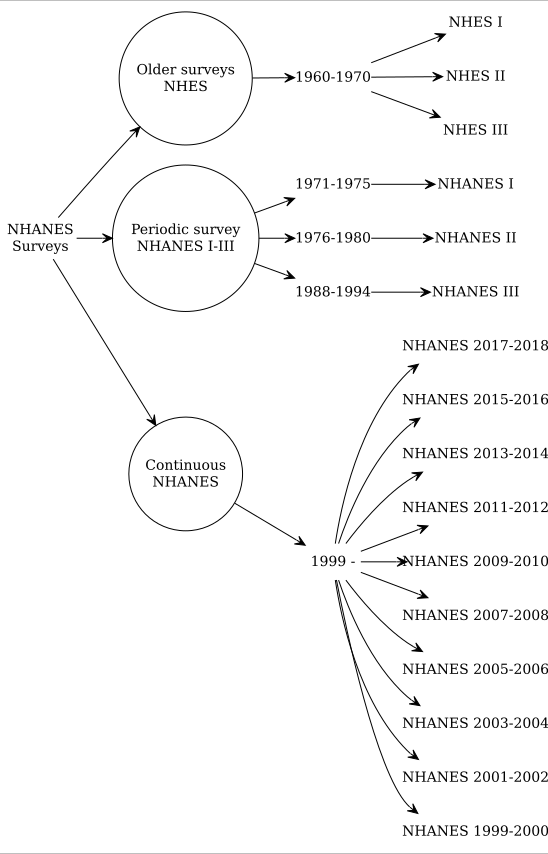
\includegraphics[width=0.75\textwidth,height=\textheight]{Images/accessing/g1.png}

\hypertarget{nhanes-datafile-and-documents}{%
\subsubsection*{NHANES datafile and
documents}\label{nhanes-datafile-and-documents}}
\addcontentsline{toc}{subsubsection}{NHANES datafile and documents}

\hypertarget{file-format}{%
\paragraph*{File format}\label{file-format}}
\addcontentsline{toc}{paragraph}{File format}

The Continuous NHANES files are stored in the NHANES website as SAS
transport file formats (.xpt). You can import this data in any
statistical package that supports this file format.

\hypertarget{continuous-nhanes-components}{%
\paragraph*{Continuous NHANES
Components}\label{continuous-nhanes-components}}
\addcontentsline{toc}{paragraph}{Continuous NHANES Components}

Continuous NHANES components separated to reduce the amount of time to
download and documentation size:

\marginnote{\begin{footnotesize}

\href{https://wwwn.cdc.gov/nchs/nhanes/tutorials/default.aspx?CDC_AA_refVal=https\%3A\%2F\%2Fwww.cdc.gov\%2Fnchs\%2Ftutorials\%2Findex.htm}{NHANES
Tutorials}

\end{footnotesize}}

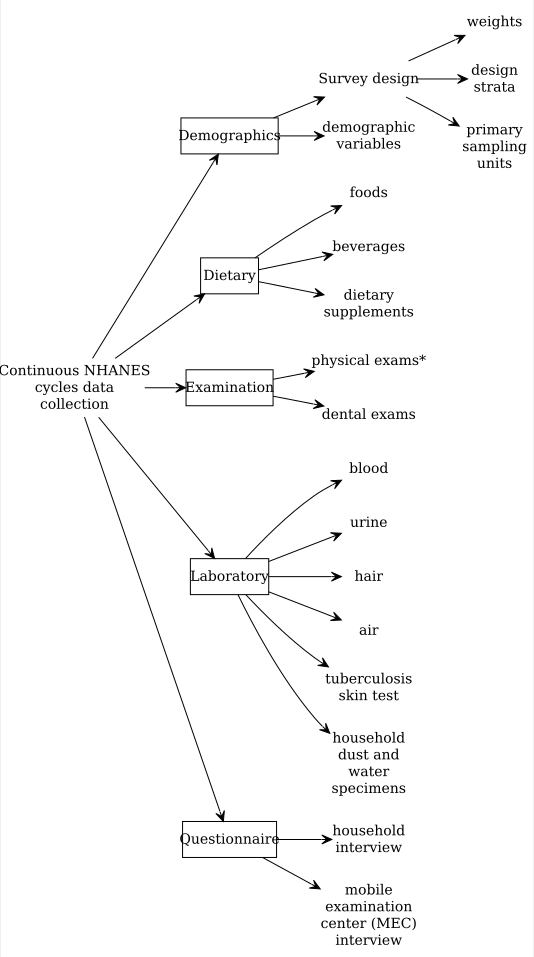
\includegraphics[width=0.75\textwidth,height=\textheight]{Images/accessing/g2.png}

\marginnote{\begin{footnotesize}

Broadly, continuous NHANES data are available in 5 categories:

\begin{itemize}
\tightlist
\item
  Demographics
\item
  Dietary
\item
  Examination
\item
  Laboratory
\item
  Questionnaire
\end{itemize}

\end{footnotesize}}

\hypertarget{combining-data}{%
\paragraph*{Combining data}\label{combining-data}}
\addcontentsline{toc}{paragraph}{Combining data}

\hypertarget{different-cycles}{%
\subparagraph*{Different cycles}\label{different-cycles}}
\addcontentsline{toc}{subparagraph}{Different cycles}

It is possible to combine datasets from different years/cycles together
in NHANES. However, NHANES is a cross-sectional data, and identification
of the same person accross different cycles is not possible in the
public release datasets. For appending data from different cycles,
please make sure that the variable names/labels are the same/identical
in years under consideration (in some years, names and labels do
change).

\marginnote{\begin{footnotesize}

The following data have not been released on the NHANES website as
public release files due to confidentiality concerns:

\begin{itemize}
\tightlist
\item
  adolescent data on alcohol use
\item
  smoking
\item
  sexual behavior
\item
  reproductive health and drug use
\end{itemize}

\end{footnotesize}}

\hypertarget{within-the-same-cycle}{%
\subparagraph*{Within the same cycle}\label{within-the-same-cycle}}
\addcontentsline{toc}{subparagraph}{Within the same cycle}

Within NHANES datasets in a given cycle, each sampled person has an
unique identifier sequence number (variable \texttt{SEQN}).

\hypertarget{missing-data-and-outliers}{%
\paragraph*{Missing data and outliers}\label{missing-data-and-outliers}}
\addcontentsline{toc}{paragraph}{Missing data and outliers}

CDC (2023) recommends:

\marginnote{\begin{footnotesize}

CDC (2023)

\end{footnotesize}}

Key points on NHANESd data analysis and missing data handling:

\begin{enumerate}
\def\labelenumi{\arabic{enumi}.}
\tightlist
\item
  If less than 10\% of your data for a variable are missing, it's
  generally acceptable to proceed with your analysis without further
  evaluation or adjustment. However, when more than 10\% of data is
  missing, assess if the missing values are evenly distributed across
  socio-demographic characteristics. Consider options like imputation or
  adjusted weights if necessary.
\item
  Identify and treat `refusal' or `do not know' responses as missing
  data to prevent distorted results in statistical analyses. Recode
  these responses as missing values, using either a period (.) for
  numeric variables or a blank for character variables.
\item
  Be cautious about outliers with exceptionally large weights, as they
  can significantly impact your estimates. Analysts should decide
  whether to include or exclude these influential outliers from the
  analysis, taking into account their potential impact on results.
\end{enumerate}

\hypertarget{nhanes-documents}{%
\paragraph*{NHANES documents}\label{nhanes-documents}}
\addcontentsline{toc}{paragraph}{NHANES documents}

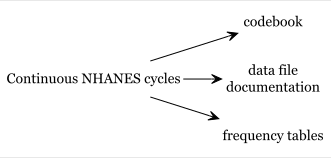
\includegraphics[width=0.65\textwidth,height=\textheight]{Images/accessing/g3.png}

\marginnote{\begin{footnotesize}

The following websites could be helpful: - For more information about
\href{https://wwwn.cdc.gov/nchs/nhanes/tutorials/module2.aspx}{NHANES
design}.

\begin{itemize}
\tightlist
\item
  Visit \href{https://wwwn.cdc.gov/Nchs/Nhanes/search/}{US CDC} website
  and do a variable keyword search based on your research interest
  (e.g., arthritis).
\end{itemize}

\end{footnotesize}}

\hypertarget{nhis}{%
\subsection*{NHIS}\label{nhis}}
\addcontentsline{toc}{subsection}{NHIS}

Like NHANES, National Health Interview Survey (NHIS) is supported by the
CDC and is a large-scale multi-stage cross-sectional survey. The NHIS
survey includes information on population disease prevalence, extent of
disability, and use of health care services. In contrast to the NHANES
that provides data every 2 years, NHIS provides data annually.

\marginnote{\begin{footnotesize}

To obtain population-level estimate, we must utilize the survey features
(weights, strata, PSU/cluster)

\end{footnotesize}}

\hypertarget{references-2}{%
\subsection*{References}\label{references-2}}
\addcontentsline{toc}{subsection}{References}

\hypertarget{importing-cchs-to-r-1}{%
\chapter*{Importing CCHS to R}\label{importing-cchs-to-r-1}}
\addcontentsline{toc}{chapter}{Importing CCHS to R}

\markboth{Importing CCHS to R}{Importing CCHS to R}

\hypertarget{overview-2}{%
\subsection*{Overview}\label{overview-2}}
\addcontentsline{toc}{subsection}{Overview}

This section provides comprehensive instructions on how to import the
Canadian Community Health Survey (CCHS) dataset from the UBC library
site to the RStudio environment. The process starts with downloading the
CCHS data from the UBC library site and includes step-by-step visual
guides for each stage. Three primary options are provided to process and
format the data:

\begin{enumerate}
\def\labelenumi{\arabic{enumi}.}
\tightlist
\item
  Using the commercial software SAS.
\item
  Utilizing the free software PSPP, an alternative to SPSS.
\item
  Directly processing the data in R.
\end{enumerate}

For each option, users are guided on how to download, install, access,
read, save, and check the dataset. The objective is to help users
acquire, visualize, and manipulate the CCHS dataset seamlessly using
various software applications.

\hypertarget{downloading-cchs-data-from-ubc}{%
\subsection*{Downloading CCHS data from
UBC}\label{downloading-cchs-data-from-ubc}}
\addcontentsline{toc}{subsection}{Downloading CCHS data from UBC}

\begin{itemize}
\tightlist
\item
  \textbf{Step 1}: Go to
  \href{http://dvn.library.ubc.ca}{dvn.library.ubc.ca}, and press
  `log-in'
\end{itemize}


\includegraphics[width=0.65\textwidth,height=\textheight]{Images/accessing/abacusX1.png}

\begin{itemize}
\tightlist
\item
  \textbf{Step 2}: Select `UBC' from the dropdown menu
\end{itemize}

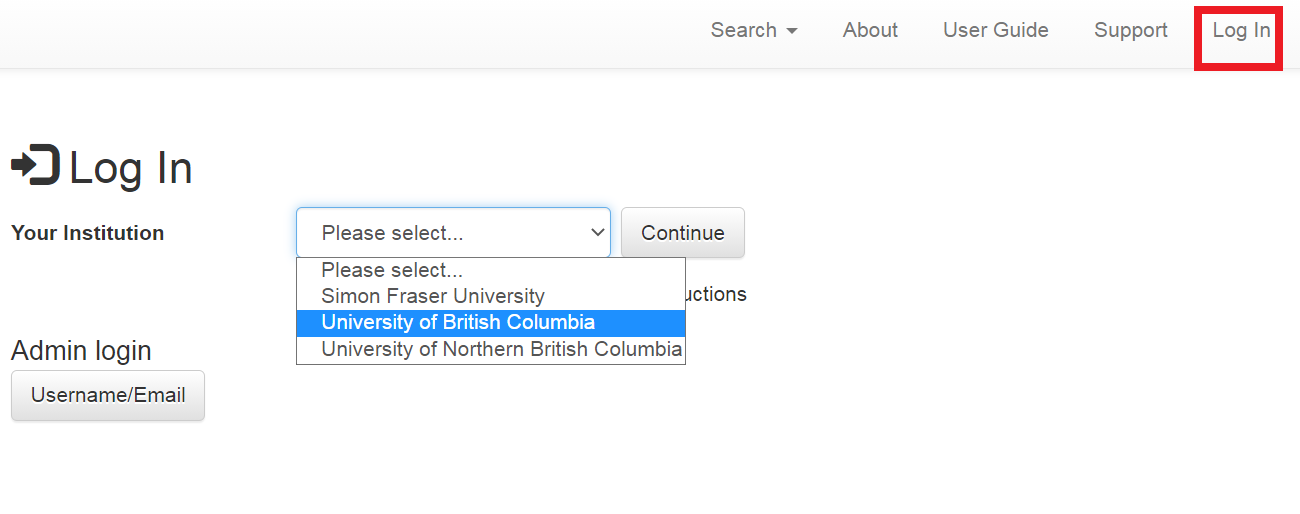
\includegraphics[width=0.65\textwidth,height=\textheight]{Images/accessing/abacusX2.png}

\begin{itemize}
\tightlist
\item
  \textbf{Step 3}: Enter your CWL or UBC library authentication
  information
\end{itemize}

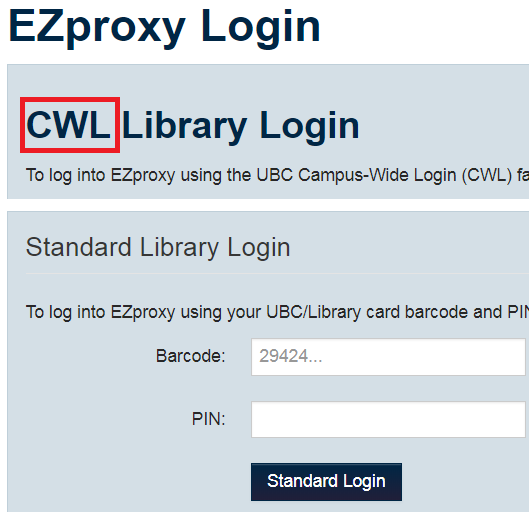
\includegraphics[width=0.65\textwidth,height=\textheight]{Images/accessing/abacus3.png}

\begin{itemize}
\tightlist
\item
  \textbf{Step 4}: Once you log-in, search the term `cchs' in the
  search-box
\end{itemize}

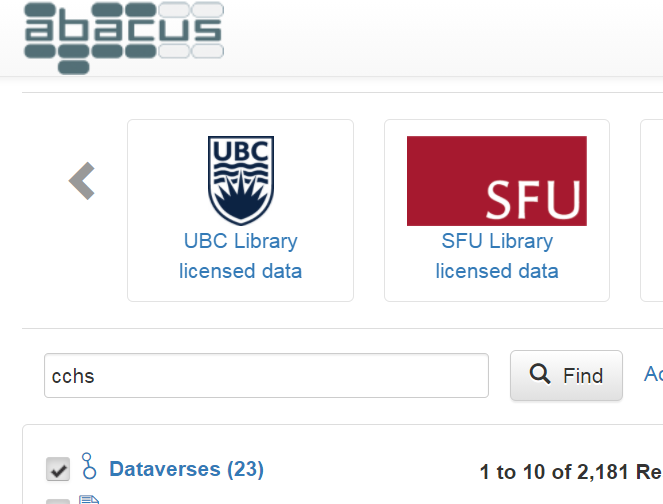
\includegraphics[width=0.65\textwidth,height=\textheight]{Images/accessing/abacusX4.png}

\begin{itemize}
\tightlist
\item
  \textbf{Step 5}: For illustrative purposes, let us work with the Cycle
  3.1 of the CCHS dataset from the list of results. In that case, type
  `cchs 3.1'
\end{itemize}

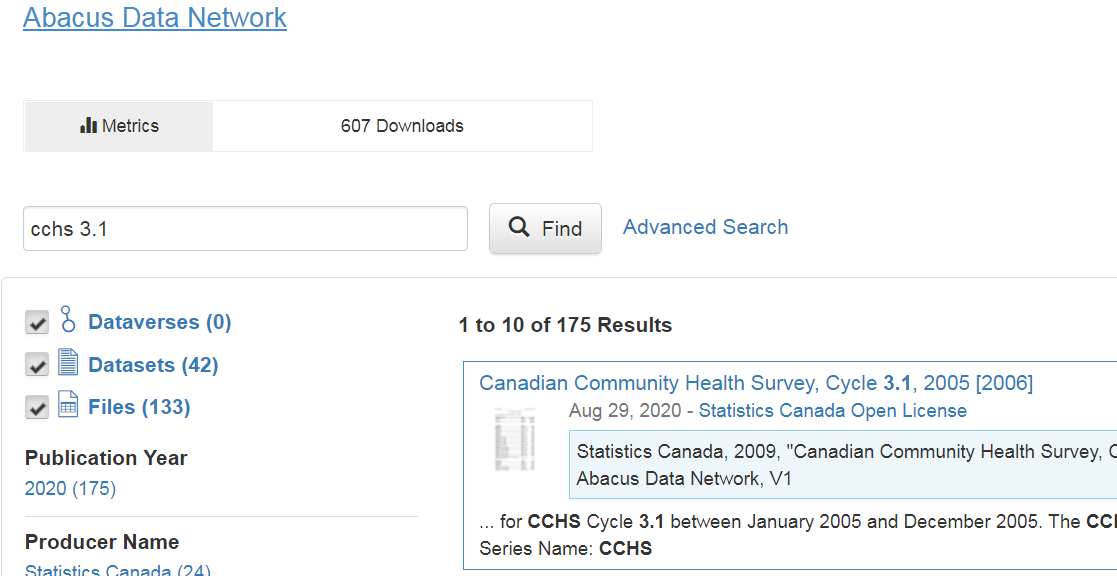
\includegraphics[width=0.65\textwidth,height=\textheight]{Images/accessing/abacusX5.png}

\begin{itemize}
\tightlist
\item
  \textbf{Step 6}: CCHS Cycle 3.1 information
\end{itemize}

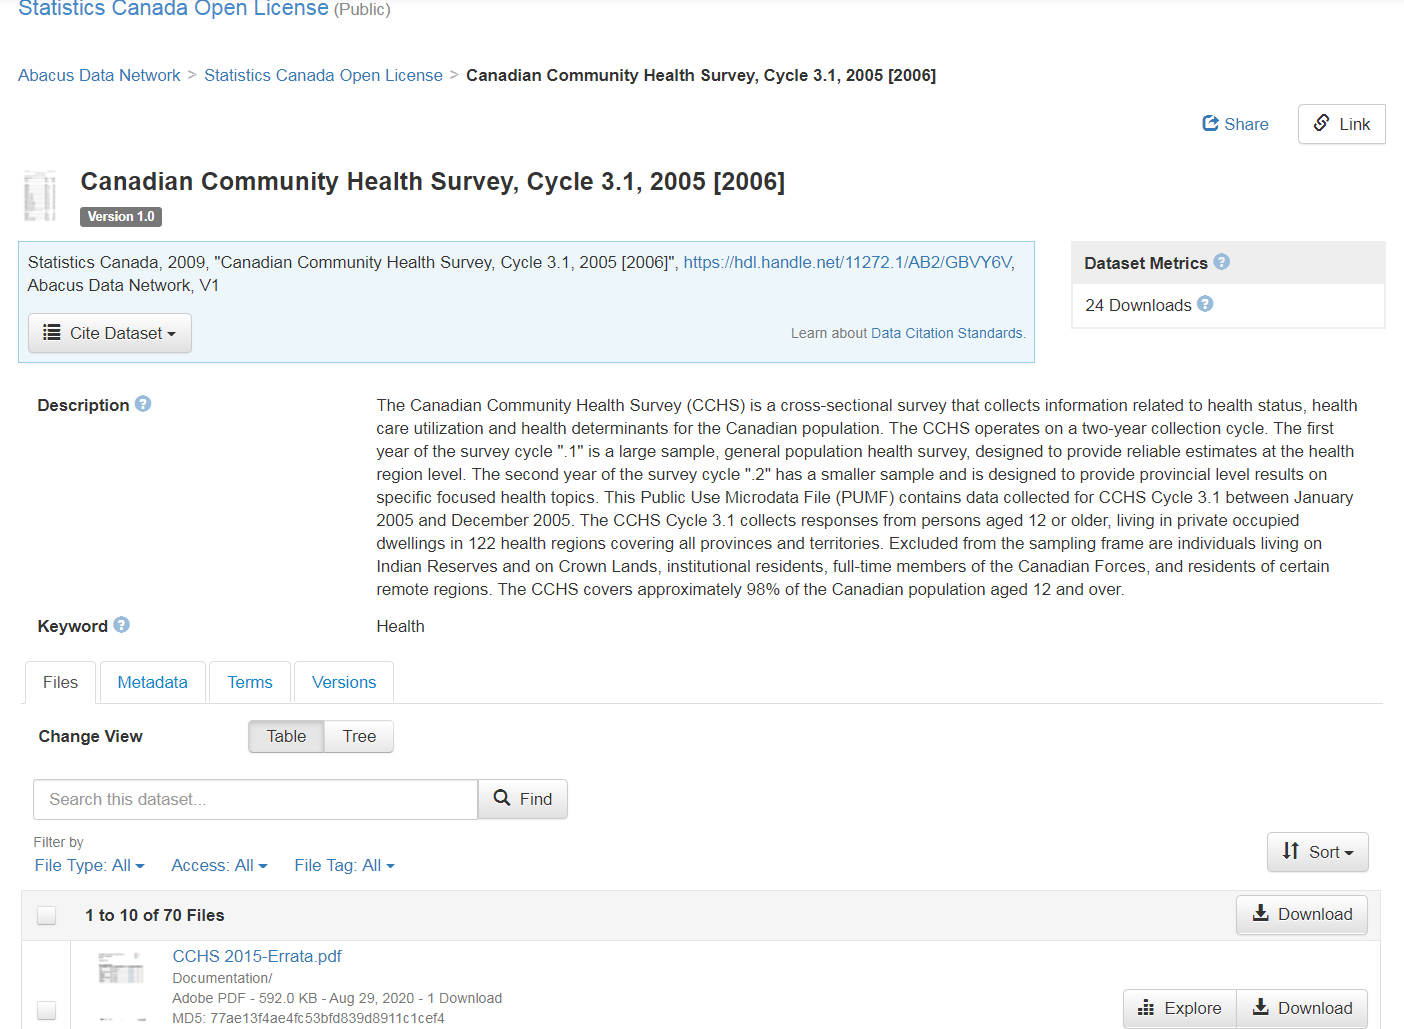
\includegraphics[width=0.65\textwidth,height=\textheight]{Images/accessing/abacus6X.png}

\begin{itemize}
\tightlist
\item
  \textbf{Step 7}: Choose the `Data: CD' from the menu
\end{itemize}

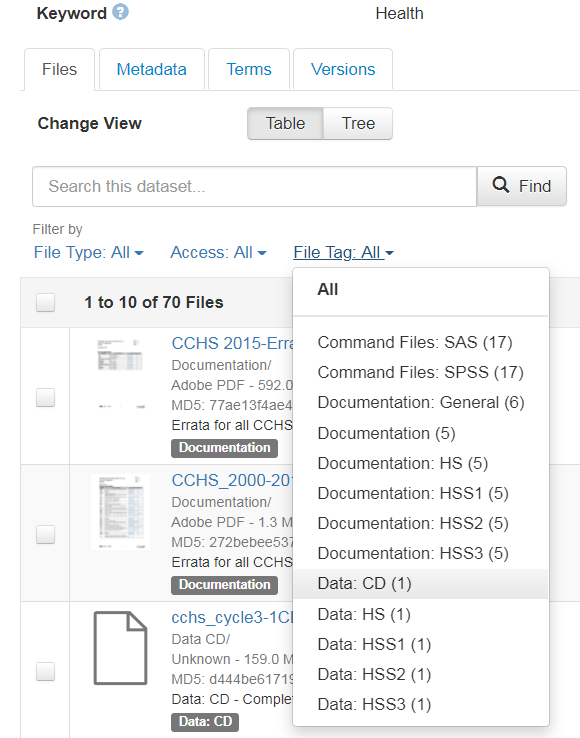
\includegraphics[width=0.65\textwidth,height=\textheight]{Images/accessing/abacusX7.png}

\begin{itemize}
\tightlist
\item
  \textbf{Step 8}: Download the entire data (about 159 MB) as a zip file
\end{itemize}

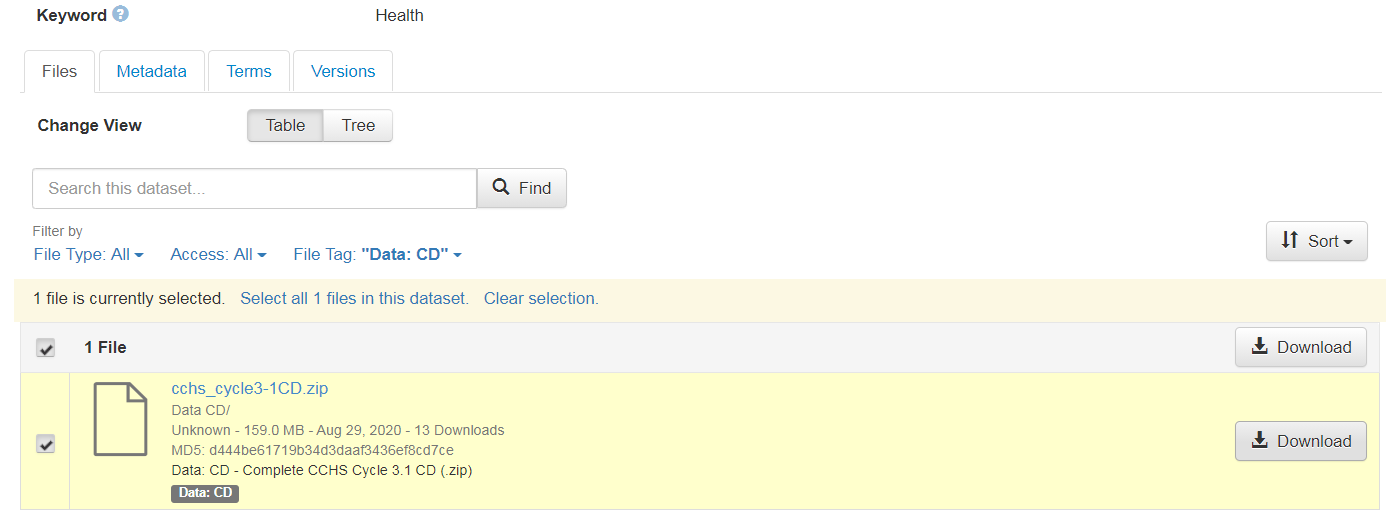
\includegraphics[width=0.65\textwidth,height=\textheight]{Images/accessing/abacusX8.png}

\begin{itemize}
\tightlist
\item
  \textbf{Step 9}: Accept the `terms of use'
\end{itemize}

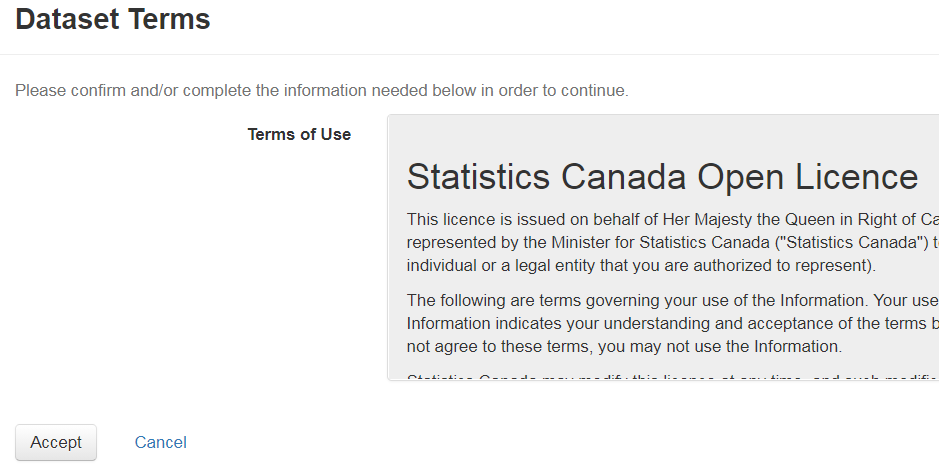
\includegraphics[width=0.65\textwidth,height=\textheight]{Images/accessing/abacusX9.png}

\begin{itemize}
\tightlist
\item
  \textbf{Step 10}: Select a directory to download the zip file. The
  path of the download directory is important (we need to use this
  \texttt{path} exactly later). For example, below we are in
  \texttt{"C:\textbackslash{}CCHS\textbackslash{}"} folder, but we will
  create a ``Data'' folder there, so that the download path is
  \texttt{"C:\textbackslash{}CCHS\textbackslash{}Data\textbackslash{}"}.
\end{itemize}

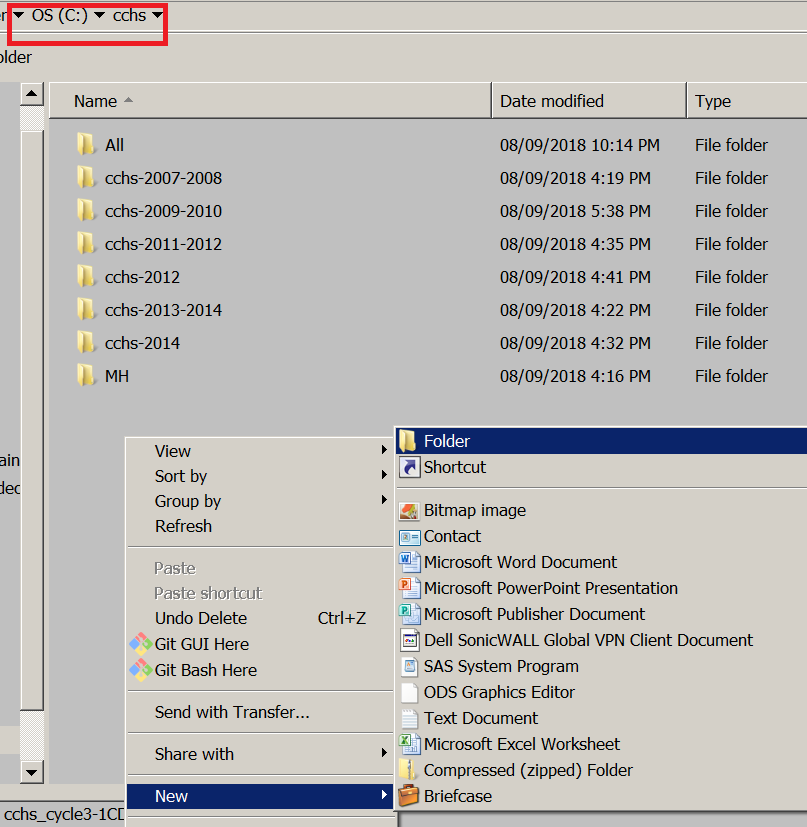
\includegraphics[width=0.65\textwidth,height=\textheight]{Images/accessing/abacusX10.png}

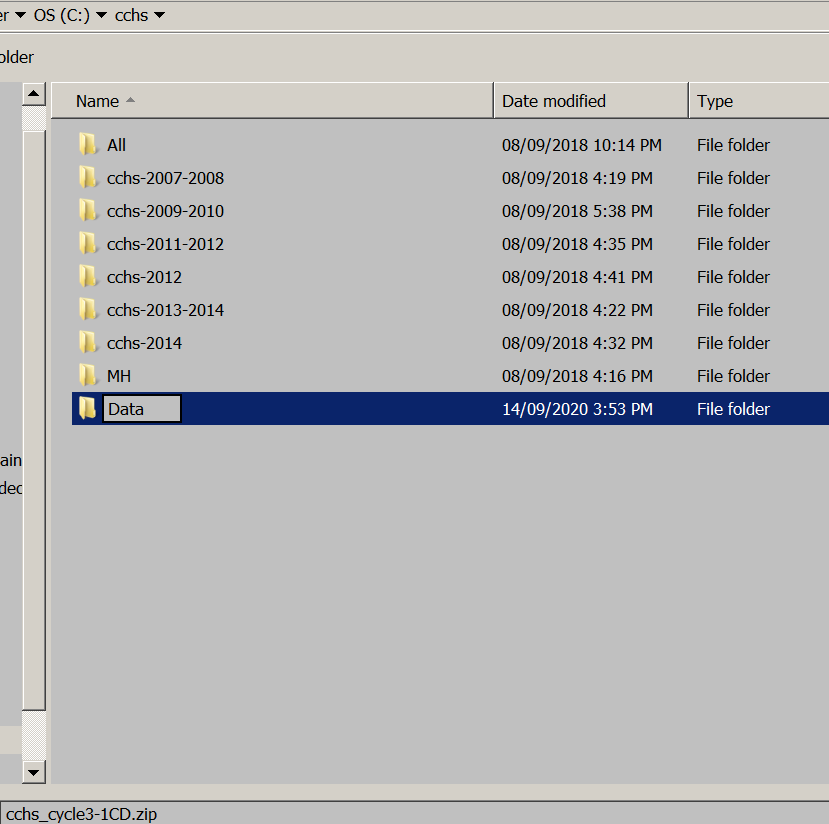
\includegraphics[width=0.65\textwidth,height=\textheight]{Images/accessing/abacusX10b.png}

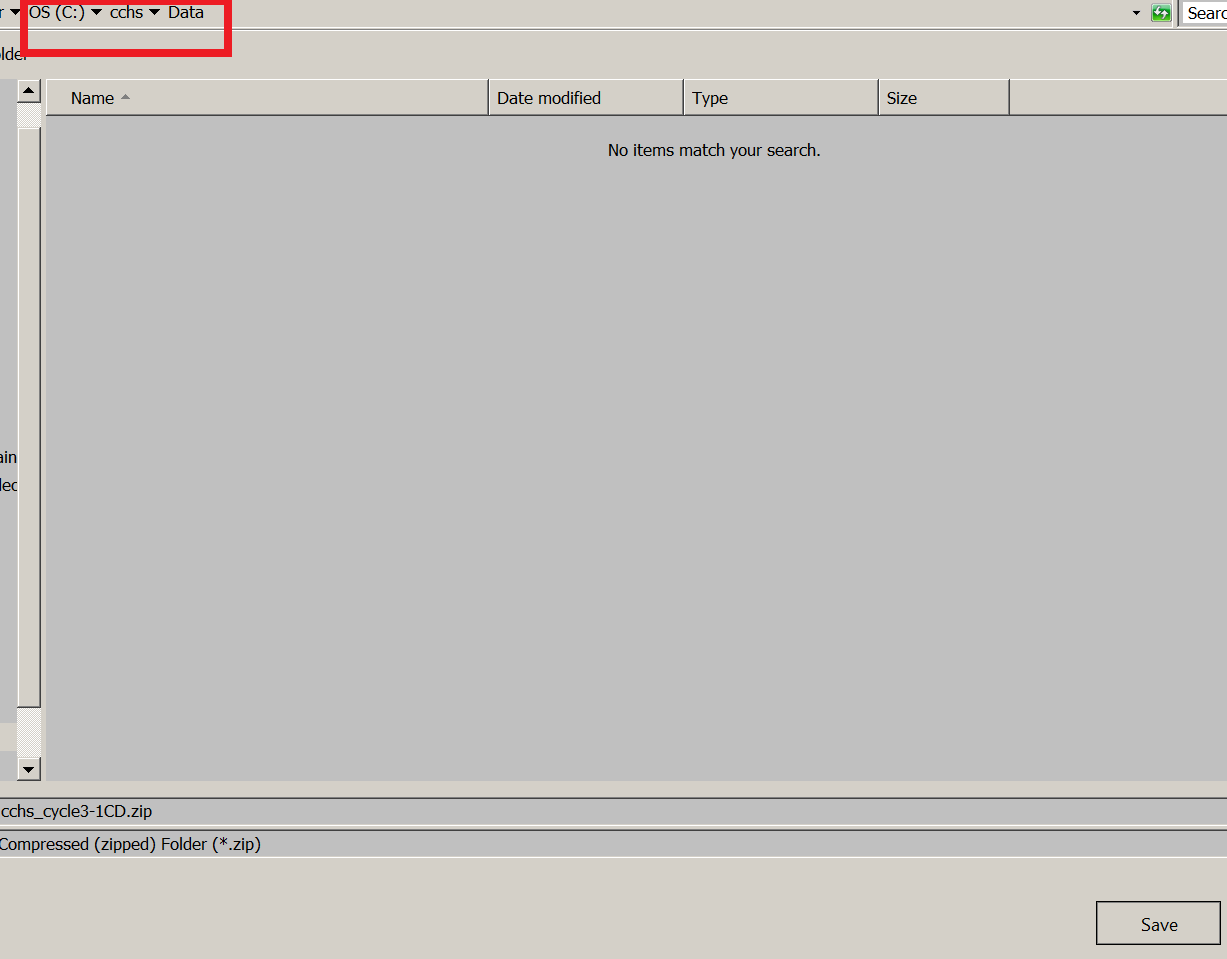
\includegraphics[width=0.65\textwidth,height=\textheight]{Images/accessing/abacusX10c.png}

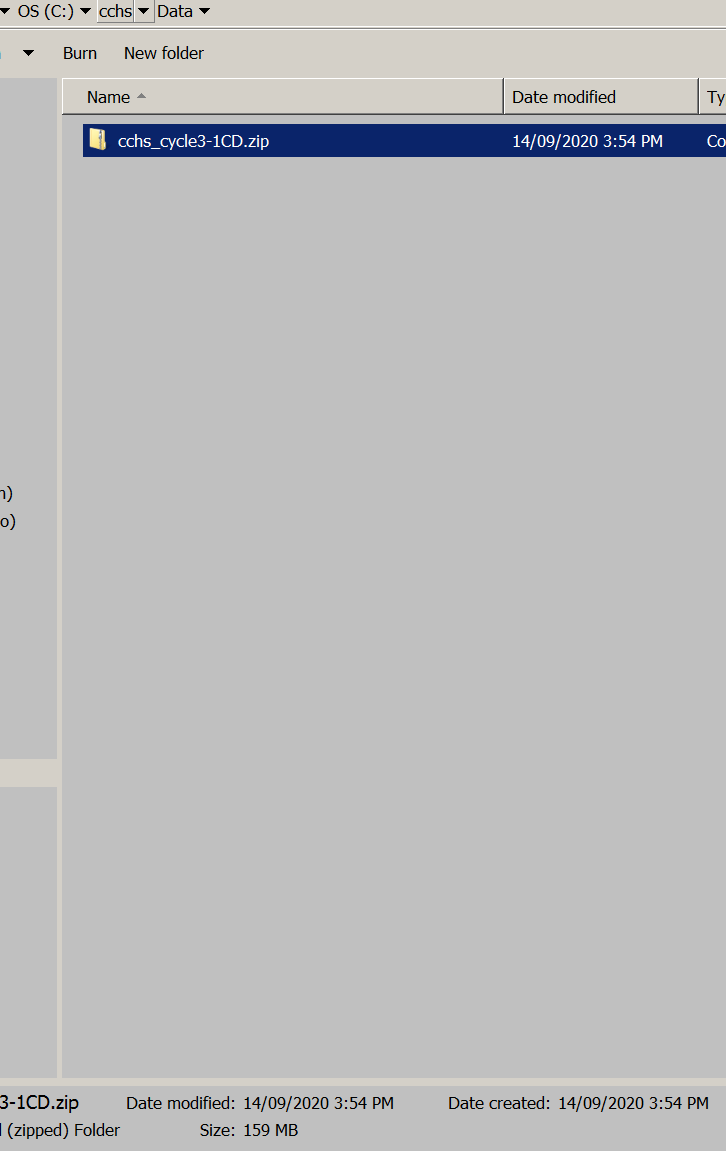
\includegraphics[width=0.65\textwidth,height=\textheight]{Images/accessing/abacusX10d.png}

\begin{itemize}
\tightlist
\item
  \textbf{Step 11}: Extract the zip file
\end{itemize}

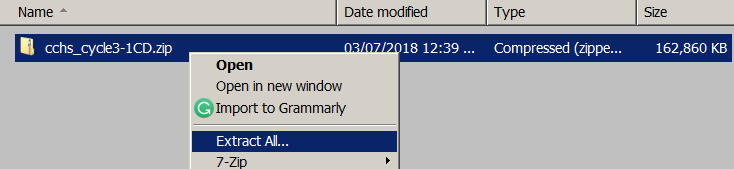
\includegraphics[width=0.65\textwidth,height=\textheight]{Images/accessing/abacus11.png}

\begin{itemize}
\tightlist
\item
  \textbf{Step 12}: Be patient with the extraction
\end{itemize}

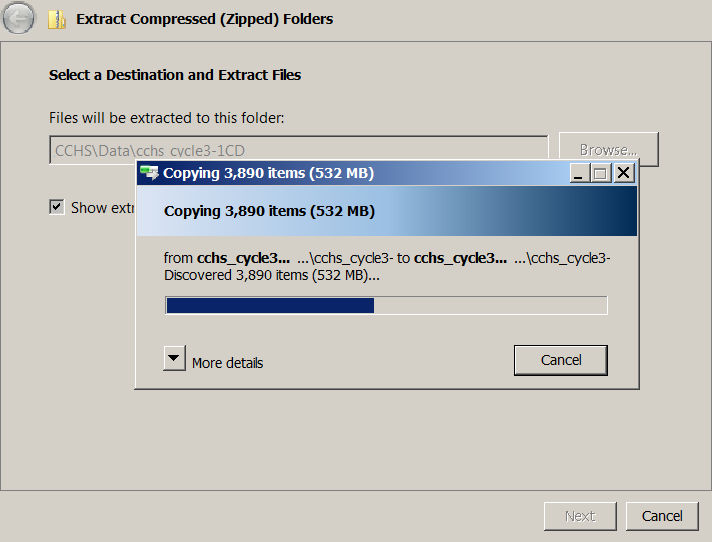
\includegraphics[width=0.65\textwidth,height=\textheight]{Images/accessing/abacus12.png}

\begin{itemize}
\tightlist
\item
  \textbf{Step 13}: Once extraction is complete, take a look at the
  folders inside. You will see that there is a folder named `SAS\_SPSS'
\end{itemize}

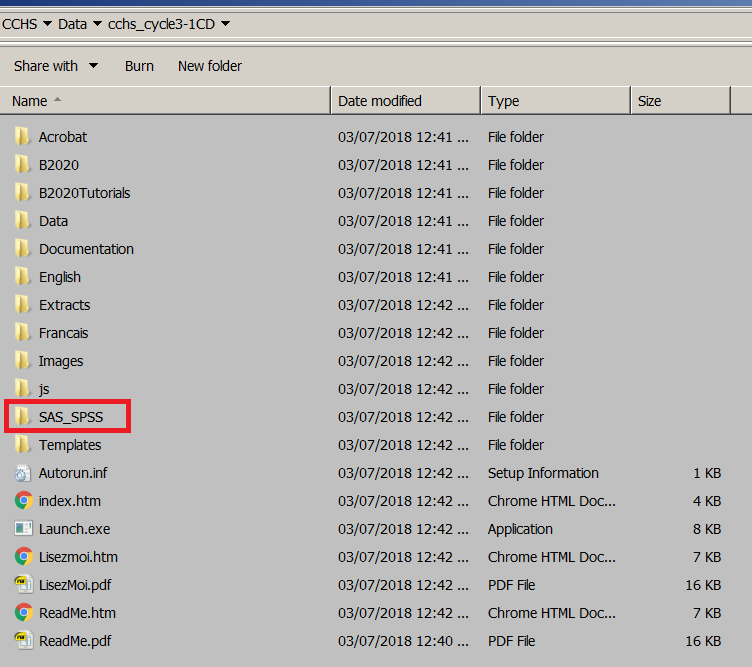
\includegraphics[width=0.65\textwidth,height=\textheight]{Images/accessing/abacus13.png}

\hypertarget{reading-and-formatting-the-data}{%
\subsection*{Reading and Formatting the
data}\label{reading-and-formatting-the-data}}
\addcontentsline{toc}{subsection}{Reading and Formatting the data}

\hypertarget{option-1-processing-data-using-sas}{%
\subsubsection*{Option 1: Processing data using
SAS}\label{option-1-processing-data-using-sas}}
\addcontentsline{toc}{subsubsection}{Option 1: Processing data using
SAS}

SAS is a commercial software. You may be able to get access to
educational version. In case you don't have access to it, later we
outline how to use free packages to read these datasets.

\begin{itemize}
\tightlist
\item
  \textbf{Step 1}: Inside that `SAS\_SPSS' folder, find the file
  \emph{hs\_pfe.sas}. It is a long file, but we are going to work on
  part of it. First thing we want to do it to change all the directory
  names to where you have unzipped the downloaded file (for example,
  here the zip file was extracted to C:/CCHS/Data/cchs\_cycle3-1CD/). We
  only need the first part of the code (as shown below; only related to
  data `hs'). Delete the rest of the codes for now. The resulting code
  should like like this:
\end{itemize}

\begin{Shaded}
\begin{Highlighting}[numbers=left,,]
\NormalTok{\%include }\StringTok{"C:\textbackslash{}CCHS\textbackslash{}Data\textbackslash{}cchs\_cycle3{-}1CD\textbackslash{}SAS\_SPSS\textbackslash{}Layouts\textbackslash{}hs\textbackslash{}hs\_pfe.sas"}\NormalTok{;}

\NormalTok{data hs;}
\NormalTok{        \%let datafid}\OtherTok{=}\StringTok{"C:\textbackslash{}CCHS\textbackslash{}Data\textbackslash{}cchs\_cycle3{-}1CD\textbackslash{}Data\textbackslash{}hs.txt"}\NormalTok{;}
\NormalTok{        \%include }\StringTok{"C:\textbackslash{}CCHS\textbackslash{}Data\textbackslash{}cchs\_cycle3{-}1CD\textbackslash{}SAS\_SPSS\textbackslash{}Layouts\textbackslash{}hs\textbackslash{}hs\_i.sas"}\NormalTok{;}
\NormalTok{        \%include }\StringTok{"C:\textbackslash{}CCHS\textbackslash{}Data\textbackslash{}cchs\_cycle3{-}1CD\textbackslash{}SAS\_SPSS\textbackslash{}Layouts\textbackslash{}hs\textbackslash{}hs\_fmt.sas"}\NormalTok{;}
\NormalTok{        \%include }\StringTok{"C:\textbackslash{}CCHS\textbackslash{}Data\textbackslash{}cchs\_cycle3{-}1CD\textbackslash{}SAS\_SPSS\textbackslash{}Layouts\textbackslash{}hs\textbackslash{}hs\_lbe.sas"}\NormalTok{;}
\NormalTok{run;}
\end{Highlighting}
\end{Shaded}

Once the modifications are done, submit the codes in SAS. Note that, the
name of the data is `hs'.

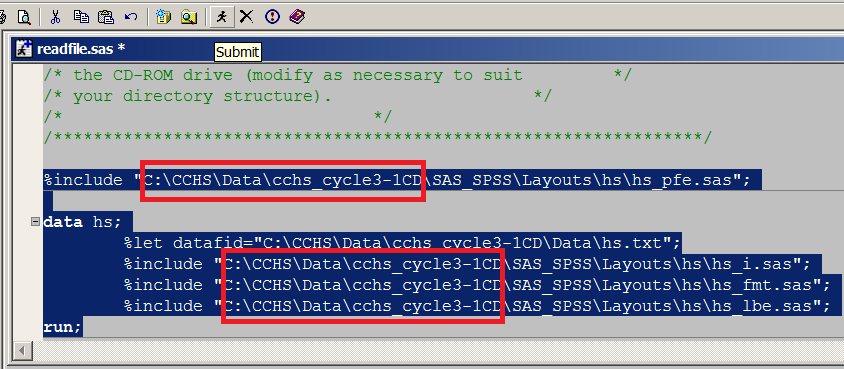
\includegraphics[width=0.65\textwidth,height=\textheight]{Images/accessing/abacus14.png}

\begin{itemize}
\tightlist
\item
  \textbf{Step 2}: Once you submit the code, you can check the log
  window in SAS to see how the code submission went. It should tell you
  how many observations and variables were read.
\end{itemize}

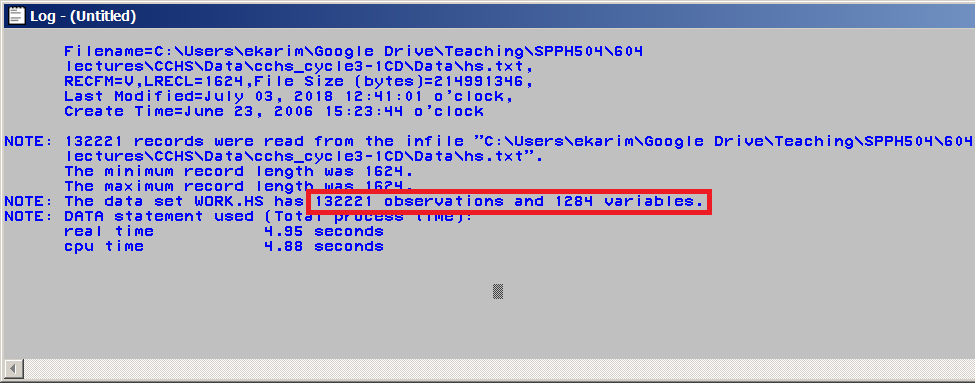
\includegraphics[width=0.65\textwidth,height=\textheight]{Images/accessing/abacus15.png}

\begin{itemize}
\tightlist
\item
  \textbf{Step 3}: If you one to view the dataset, you can go to
  `Explorer' window within SAS.
\end{itemize}

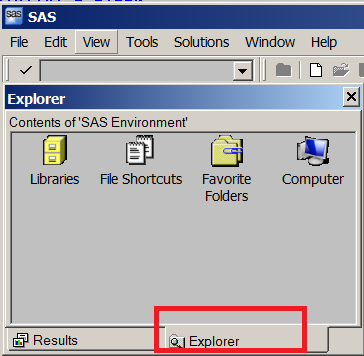
\includegraphics[width=0.65\textwidth,height=\textheight]{Images/accessing/abacus16.png}

\begin{itemize}
\tightlist
\item
  \textbf{Step 4}: Generally, if you haven't specified where to load the
  files, SAS will by default save the data into a library called `Work'
\end{itemize}

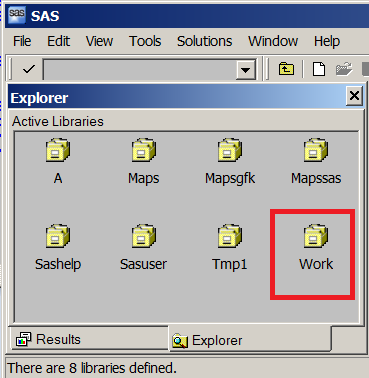
\includegraphics[width=0.65\textwidth,height=\textheight]{Images/accessing/abacus17.png}

\begin{itemize}
\tightlist
\item
  \textbf{Step 5}: Open that folder, and you will be able to find the
  dataset `Hs'.
\end{itemize}

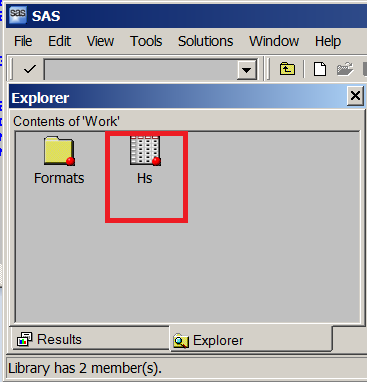
\includegraphics[width=0.65\textwidth,height=\textheight]{Images/accessing/abacus18.png}

\begin{itemize}
\tightlist
\item
  \textbf{Step 6}: Right click on the data, and click `open' to view the
  datafile.
\end{itemize}

\includegraphics[width=0.65\textwidth,height=\textheight]{Images/accessing/abacus19.png}

\begin{itemize}
\tightlist
\item
  \textbf{Step 7}: To export the data into a CSV format data (so that we
  can read this data into other software packages), ckick `Menu'.
\end{itemize}

\includegraphics[width=0.65\textwidth,height=\textheight]{Images/accessing/abacus20.png}

\begin{itemize}
\tightlist
\item
  \textbf{Step 8}: then press `Export Data'.
\end{itemize}

\includegraphics[width=0.65\textwidth,height=\textheight]{Images/accessing/abacus21.png}

\begin{itemize}
\tightlist
\item
  \textbf{Step 9}: choose the library and the data.
\end{itemize}

\includegraphics[width=0.65\textwidth,height=\textheight]{Images/accessing/abacus22.png}

\begin{itemize}
\tightlist
\item
  \textbf{Step 10}: choose the format in which you may want to save the
  existing data.
\end{itemize}

\includegraphics[width=0.65\textwidth,height=\textheight]{Images/accessing/abacus23.png}

\begin{itemize}
\tightlist
\item
  \textbf{Step 11}: also specify where you want to save the csv file and
  the name of that file (e.g., cchs3.csv).
\end{itemize}

\includegraphics[width=0.65\textwidth,height=\textheight]{Images/accessing/abacus24.png}

\begin{itemize}
\tightlist
\item
  \textbf{Step 12}: go to that directory to see the file cchs3.csv
\end{itemize}

\includegraphics[width=0.65\textwidth,height=\textheight]{Images/accessing/abacus25.png}

\begin{itemize}
\tightlist
\item
  \textbf{Step 13}: If you want to save the file in SAS format, you can
  do so by writing the following sas code into the `Editor' window. Here
  we are saving the data Hs within the Work library in to a data called
  cchs3 within the SASLib library. Note that, the directory name has to
  be where you want to save the output file.
\end{itemize}

\begin{Shaded}
\begin{Highlighting}[numbers=left,,]
\NormalTok{LIBNAME SASLib }\StringTok{"C:\textbackslash{}CCHS\textbackslash{}Data"}\NormalTok{;}
\NormalTok{DATA SASLib.cchs3;}
\NormalTok{    set Work.Hs;}
\NormalTok{run;}
\end{Highlighting}
\end{Shaded}

Submit these codes into SAS:

\includegraphics[width=0.65\textwidth,height=\textheight]{Images/accessing/abacus26.png}

\begin{itemize}
\tightlist
\item
  \textbf{Step 13}: go to that directory to see the file cchs3.sas7dbat
\end{itemize}

\includegraphics[width=0.65\textwidth,height=\textheight]{Images/accessing/abacus27.png}

\hypertarget{option-2-processing-data-using-pspp-free}{%
\subsubsection*{Option 2: Processing data using PSPP
(Free)}\label{option-2-processing-data-using-pspp-free}}
\addcontentsline{toc}{subsubsection}{Option 2: Processing data using
PSPP (Free)}

PSPP is a free package; alternative to commercial software SPSS. We can
use the same SPSS codes to read the datafile into PSPP, and save.

\begin{itemize}
\tightlist
\item
  \textbf{Step 1}: Get the free PSPP software from the website:
  \href{http://www.gnu.org/software/pspp/}{www.gnu.org/software/pspp/}
\end{itemize}

PSPP is available for GNU/Hurd, GNU/Linux, Darwin (Mac OS X), OpenBSD,
NetBSD, FreeBSD, and Windows

\includegraphics[width=0.65\textwidth,height=\textheight]{Images/accessing/abacus30.png}

For windows, download appropriate version.

\includegraphics[width=0.65\textwidth,height=\textheight]{Images/accessing/psppdownload0.png}

Download the file

\includegraphics[width=0.25\textwidth,height=\textheight]{Images/accessing/psppdownload.png}

Install

\includegraphics[width=0.65\textwidth,height=\textheight]{Images/accessing/psppinstall.png}

\includegraphics[width=0.65\textwidth,height=\textheight]{Images/accessing/psppinstall2.png}

\includegraphics[width=0.65\textwidth,height=\textheight]{Images/accessing/psppinstall3.png}

Click the icon shorcut after installing

\includegraphics[width=0.25\textwidth,height=\textheight]{Images/accessing/psppicon.png}

\begin{itemize}
\tightlist
\item
  \textbf{Step 2}: Open PSPP
\end{itemize}

\includegraphics[width=0.65\textwidth,height=\textheight]{Images/accessing/abacus31.png}

\begin{itemize}
\tightlist
\item
  \textbf{Step 3}: Go to `file' menu and click `open'
\end{itemize}

\includegraphics[width=0.65\textwidth,height=\textheight]{Images/accessing/abacus32.png}

\begin{itemize}
\tightlist
\item
  \textbf{Step 4}: Specify the \emph{readfile.sps} file from the
  `SAS\_SPSS' folder.
\end{itemize}

\includegraphics[width=0.65\textwidth,height=\textheight]{Images/accessing/abacus33.png}

You will see the following file:

\includegraphics[width=0.65\textwidth,height=\textheight]{Images/accessing/abacusX33.png}

\begin{itemize}
\tightlist
\item
  \textbf{Step 5}: Similar to before, change the directories as
  appropriate. Get rid of the extra lines of codes. Resulting codes are
  as follows (you can copy and replace the code in the file with the
  following codes):
\end{itemize}

\begin{Shaded}
\begin{Highlighting}[numbers=left,,]
\NormalTok{file handle infile}\SpecialCharTok{/}\NormalTok{name }\OtherTok{=} \StringTok{\textquotesingle{}C:\textbackslash{}CCHS\textbackslash{}Data\textbackslash{}cchs\_cycle3{-}1CD\textbackslash{}DATA\textbackslash{}hs.txt\textquotesingle{}}\NormalTok{.}
\NormalTok{data list file }\OtherTok{=}\NormalTok{ infile notable}\SpecialCharTok{/}\NormalTok{.}
\NormalTok{include file }\OtherTok{=} \StringTok{"C:\textbackslash{}CCHS\textbackslash{}Data\textbackslash{}cchs\_cycle3{-}1CD\textbackslash{}SAS\_SPSS\textbackslash{}Layouts\textbackslash{}hs\textbackslash{}hs\_i.sps"}\NormalTok{.}
\NormalTok{include file }\OtherTok{=} \StringTok{"C:\textbackslash{}CCHS\textbackslash{}Data\textbackslash{}cchs\_cycle3{-}1CD\textbackslash{}SAS\_SPSS\textbackslash{}Layouts\textbackslash{}hs\textbackslash{}hsvale.sps"}\NormalTok{.}
\NormalTok{include file }\OtherTok{=} \StringTok{"C:\textbackslash{}CCHS\textbackslash{}Data\textbackslash{}cchs\_cycle3{-}1CD\textbackslash{}SAS\_SPSS\textbackslash{}Layouts\textbackslash{}hs\textbackslash{}hsvare.sps"}\NormalTok{.}
\NormalTok{include file }\OtherTok{=} \StringTok{"C:\textbackslash{}CCHS\textbackslash{}Data\textbackslash{}cchs\_cycle3{-}1CD\textbackslash{}SAS\_SPSS\textbackslash{}Layouts\textbackslash{}hs\textbackslash{}hsmiss.sps"}\NormalTok{.}
\NormalTok{execute.}
\end{Highlighting}
\end{Shaded}

\includegraphics[width=0.65\textwidth,height=\textheight]{Images/accessing/abacusX34.png}

For Mac users, it should be as follows (e.g., \texttt{username} should
be your user name, if you are saving under the path
\texttt{"/Users/username/CCHS/Data/"}):

\begin{Shaded}
\begin{Highlighting}[numbers=left,,]
\NormalTok{file handle infile}\SpecialCharTok{/}\NormalTok{name }\OtherTok{=}\StringTok{"/Users/username/CCHS/Data/cchs\_cycle3{-}1CD/Data/hs.txt"}\NormalTok{.}
\NormalTok{data list file }\OtherTok{=}\NormalTok{ infile notable}\SpecialCharTok{/}\NormalTok{.}
\NormalTok{include file }\OtherTok{=} \StringTok{"/Users/username/CCHS/Data/cchs\_cycle3{-}1CD/SAS\_SPSS/Layouts/hs/hs\_i.sps"}\NormalTok{.}
\NormalTok{include file }\OtherTok{=} \StringTok{"/Users/username/CCHS/Data/cchs\_cycle3{-}1CD/SAS\_SPSS/Layouts/hs/hsvale.sps"}\NormalTok{.}
\NormalTok{include file }\OtherTok{=} \StringTok{"/Users/username/CCHS/Data/cchs\_cycle3{-}1CD/SAS\_SPSS/Layouts/hs/hsvare.sps"}\NormalTok{.}
\NormalTok{include file }\OtherTok{=} \StringTok{"/Users/username/CCHS/Data/cchs\_cycle3{-}1CD/SAS\_SPSS/Layouts/hs/hsmiss.sps"}\NormalTok{.}

\NormalTok{execute.}
\end{Highlighting}
\end{Shaded}

\begin{itemize}
\tightlist
\item
  \textbf{Step 6}: Run the codes.
\end{itemize}

\includegraphics[width=0.65\textwidth,height=\textheight]{Images/accessing/abacus35.png}

\begin{itemize}
\tightlist
\item
  \textbf{Step 7}: This is a large data, and will take some time to load
  the data into the PSPP data editor. \textbf{Be patient}.
\end{itemize}

\includegraphics[width=0.65\textwidth,height=\textheight]{Images/accessing/waitX.png}

Once loading is complete, it will show the `output' and `data view'.

\includegraphics[width=0.65\textwidth,height=\textheight]{Images/accessing/abacusNew.png}

\includegraphics[width=0.65\textwidth,height=\textheight]{Images/accessing/abacus36.png}

Note that, you will get error message, if your files were not in the
correct path. In our example, the path was
\texttt{"C:\textbackslash{}CCHS\textbackslash{}Data\textbackslash{}"}
for the zip file content (see the previous steps).

\begin{itemize}
\tightlist
\item
  \textbf{Step 7}: You can also check the `variable view'.
\end{itemize}

\includegraphics[width=0.65\textwidth,height=\textheight]{Images/accessing/abacus37.png}

\begin{itemize}
\tightlist
\item
  \textbf{Step 8}: Save the data by clicking `File' and then `save as
  \ldots{}'
\end{itemize}

\includegraphics[width=0.65\textwidth,height=\textheight]{Images/accessing/abacus38.png}

\begin{itemize}
\tightlist
\item
  \textbf{Step 9}: Specify the name of the datafile and the location /
  folder to save the data file.
\end{itemize}

\includegraphics[width=0.65\textwidth,height=\textheight]{Images/accessing/abacus39.png}

\begin{itemize}
\tightlist
\item
  \textbf{Step 10}: See the SAV file saved in the directory.
\end{itemize}

\includegraphics[width=0.65\textwidth,height=\textheight]{Images/accessing/abacus40.png}

\begin{itemize}
\tightlist
\item
  \textbf{Step 11}: To save CSV format data, use the following syntax.
\end{itemize}

\begin{Shaded}
\begin{Highlighting}[numbers=left,,]
\NormalTok{SAVE TRANSLATE}
  \SpecialCharTok{/}\NormalTok{OUTFILE}\OtherTok{=}\StringTok{"C:/CCHS/Data/cchs3b.csv"}  
  \SpecialCharTok{/}\NormalTok{TYPE}\OtherTok{=}\NormalTok{CSV}
  \SpecialCharTok{/}\NormalTok{FIELDNAMES      }
  \SpecialCharTok{/}\NormalTok{CELLS}\OtherTok{=}\NormalTok{VALUES.}
\end{Highlighting}
\end{Shaded}

Note that, for categorical data, you can either save values or labels.
For our purpose, we prefer values, and hence saved with values here.

\includegraphics[width=0.65\textwidth,height=\textheight]{Images/accessing/abacus41.png}

\begin{itemize}
\tightlist
\item
  \textbf{Step 12}: See the CSV file saved in the directory extracted
  from PSPP.
\end{itemize}

\includegraphics[width=0.65\textwidth,height=\textheight]{Images/accessing/abacus42.png}

\hypertarget{option-3-processing-data-using-spss}{%
\subsubsection*{Option 3: Processing data using
SPSS}\label{option-3-processing-data-using-spss}}
\addcontentsline{toc}{subsubsection}{Option 3: Processing data using
SPSS}

Log into \href{https://ubc.onthehub.com}{ubc.onthehub.com} to download
SPSS. With your CWL account, UBC students should be able to download it.
UBC
\href{https://it.ubc.ca/services/desktop-print-services/software-licensing/spss}{IT
website for SPSS} says:

\texttt{The\ SPSS\ software\ license\ with\ UBC\ specifies\ that\ SPSS\ must\ only\ be\ used\ by\ UBC\ Faculty,\ Students,\ and\ Research\ Staff\ and\ only\ for\ Teaching\ and\ non-commercial\ Research\ purposes\ related\ to\ UBC.}

Both network (for UBC owened devices) or standalone / home versions (for
non-UBC owened devices) should be available. Once downloaded, same
process of importing CCHS data in PSPP can also be applied on SPSS (same
syntax files should work). Let me know if that is not the case.

\hypertarget{processing-data-in-r}{%
\subsection*{Processing data in R}\label{processing-data-in-r}}
\addcontentsline{toc}{subsection}{Processing data in R}

\hypertarget{download-software}{%
\subsubsection*{Download software}\label{download-software}}
\addcontentsline{toc}{subsubsection}{Download software}

\begin{itemize}
\tightlist
\item
  \textbf{Step 1}: Download either `R' from CRAN
  \href{https://www.r-project.org/}{www.r-project.org} or `R open' from
  Microsoft
  \href{https://mran.microsoft.com/open}{mran.microsoft.com/open}
\end{itemize}

\includegraphics[width=0.65\textwidth,height=\textheight]{Images/accessing/R03.png}

\includegraphics[width=0.65\textwidth,height=\textheight]{Images/accessing/R01.png}

\begin{itemize}
\tightlist
\item
  \textbf{Step 2}: Download RStudio from
  \href{https://www.rstudio.com/}{www.rstudio.com/}
\end{itemize}

\includegraphics[width=0.65\textwidth,height=\textheight]{Images/accessing/R02.png}

\begin{itemize}
\tightlist
\item
  \textbf{Step 3}: Open RStudio
\end{itemize}

\includegraphics[width=0.65\textwidth,height=\textheight]{Images/accessing/R04.png}

\hypertarget{import-export-and-load-data-into-r}{%
\subsubsection*{Import, export and load data into
R}\label{import-export-and-load-data-into-r}}
\addcontentsline{toc}{subsubsection}{Import, export and load data into
R}

\begin{itemize}
\tightlist
\item
  \textbf{Step 1}: Set working directory
\end{itemize}

\begin{Shaded}
\begin{Highlighting}[numbers=left,,]
\FunctionTok{setwd}\NormalTok{(}\StringTok{"C:/CCHS/Data/"}\NormalTok{) }\CommentTok{\# or something appropriate}
\end{Highlighting}
\end{Shaded}

\begin{itemize}
\tightlist
\item
  \textbf{Step 2}: Read the dataset created from PSPP with cell values.
  We can also do a small check to see if the cell values are visible.
  For example, we choose a variable `CCCE\_05A', and tabulate it.
\end{itemize}

\begin{Shaded}
\begin{Highlighting}[numbers=left,,]
\NormalTok{Hs }\OtherTok{\textless{}{-}} \FunctionTok{read.csv}\NormalTok{(}\StringTok{"cchs3b.csv"}\NormalTok{, }\AttributeTok{header =} \ConstantTok{TRUE}\NormalTok{)}
\FunctionTok{table}\NormalTok{(Hs}\SpecialCharTok{$}\NormalTok{CCCE\_05A)}
\end{Highlighting}
\end{Shaded}

\includegraphics[width=0.65\textwidth,height=\textheight]{Images/accessing/abacus46.png}

\begin{itemize}
\tightlist
\item
  \textbf{Step 3}: Save the RData file from R into a folder
  \texttt{SurveyData}:
\end{itemize}

\begin{Shaded}
\begin{Highlighting}[numbers=left,,]
\FunctionTok{save}\NormalTok{(Hs, }\AttributeTok{file =} \StringTok{"SurveyData/cchs3.RData"}\NormalTok{)}
\end{Highlighting}
\end{Shaded}

\begin{itemize}
\tightlist
\item
  \textbf{Step 4}: See the RData file saved in the directory extracted
  from R.
\end{itemize}

\includegraphics[width=0.65\textwidth,height=\textheight]{Images/accessing/abacus43.png}

\begin{itemize}
\tightlist
\item
  \textbf{Step 5}: Close R / RStudio and restart it. Environment window
  within RStudio should be empty.
\end{itemize}

\includegraphics[width=0.65\textwidth,height=\textheight]{Images/accessing/abacus44.png}

\begin{itemize}
\tightlist
\item
  \textbf{Step 6}: Load the saved RData into R. Environment window
  within RStudio should have `Hs' dataset.
\end{itemize}

\begin{Shaded}
\begin{Highlighting}[numbers=left,,]
\FunctionTok{load}\NormalTok{(}\StringTok{"SurveyData/cchs3.RData"}\NormalTok{)}
\end{Highlighting}
\end{Shaded}

\includegraphics[width=0.65\textwidth,height=\textheight]{Images/accessing/abacus45.png}

\hypertarget{importing-nhanes-to-r-1}{%
\chapter*{Importing NHANES to R}\label{importing-nhanes-to-r-1}}
\addcontentsline{toc}{chapter}{Importing NHANES to R}

\markboth{Importing NHANES to R}{Importing NHANES to R}

This tutorial provides comprehensive instructions on accessing the
National Health and Nutrition Examination Survey (NHANES) dataset from
the US Centers for Disease Control and Prevention (CDC) website and
importing it into the RStudio environment. It covers accessing NHANES
Data:

\begin{itemize}
\tightlist
\item
  Directly from the CDC website: A step-by-step guide with accompanying
  images, illustrating how to navigate the CDC website, download the
  data, and interpret the accompanying codebook.
\item
  Using R packages, specifically the nhanesA package: A concise guide on
  how to download and get summaries of the NHANES data using this R
  package.
\end{itemize}

\begin{Shaded}
\begin{Highlighting}[numbers=left,,]
\CommentTok{\# Load required packages}
\CommentTok{\#devtools::install\_github("warnes/SASxport")}
\FunctionTok{library}\NormalTok{(SASxport)}
\FunctionTok{library}\NormalTok{(foreign)}
\FunctionTok{library}\NormalTok{(nhanesA)}
\FunctionTok{library}\NormalTok{(knitr)}
\FunctionTok{require}\NormalTok{(DiagrammeR)}
\FunctionTok{require}\NormalTok{(DiagrammeRsvg)}
\FunctionTok{require}\NormalTok{(rsvg)}
\FunctionTok{library}\NormalTok{(magrittr)}
\FunctionTok{library}\NormalTok{(svglite)}
\FunctionTok{library}\NormalTok{(png)}
\NormalTok{use.saved.chche }\OtherTok{\textless{}{-}} \ConstantTok{TRUE}
\end{Highlighting}
\end{Shaded}

\marginnote{\begin{footnotesize}

Before installing a package from GitHub, it's better to check whether
you installed the right version of
\href{https://cran.r-project.org/bin/windows/Rtools/}{Rtools}

\end{footnotesize}}

\hypertarget{accessing-nhanes-data-directly-from-the-cdc-website}{%
\subsection*{Accessing NHANES Data Directly from the CDC
website}\label{accessing-nhanes-data-directly-from-the-cdc-website}}
\addcontentsline{toc}{subsection}{Accessing NHANES Data Directly from
the CDC website}

In the following example, we will see how to download `Demographics'
data, and check associated variable in that dataset.

\includegraphics[width=0.65\textwidth,height=\textheight]{Images/accessing/n15.png}

\marginnote{\begin{footnotesize}

NHANES 1999-2000 and onward survey datasets are publicly available at
\href{https://wwwn.cdc.gov/nchs/nhanes/}{wwwn.cdc.gov/nchs/nhanes/}

\end{footnotesize}}

\begin{itemize}
\tightlist
\item
  \textbf{Step 1}: Say, for example, we are interested about the NHANES
  2015-2016 survey. Clicking the associated link in the above Figure
  gets us to the page for the corresponding cycle (see below).
\end{itemize}

\includegraphics[width=0.65\textwidth,height=\textheight]{Images/accessing/n15demo.png}

\begin{itemize}
\tightlist
\item
  \textbf{Step 2}: There are various types of data available for this
  survey. Let's explore the demographic information from this cycle.
  These data are mostly available in the form of SAS \texttt{XPT} format
  (see below).
\end{itemize}

\includegraphics[width=0.65\textwidth,height=\textheight]{Images/accessing/xptsasdata.png}

\begin{itemize}
\tightlist
\item
  \textbf{Step 3}: We can download the XPT data in the local PC folder
  and read the data into R as as follows:
\end{itemize}

\begin{Shaded}
\begin{Highlighting}[numbers=left,,]
\NormalTok{DEMO }\OtherTok{\textless{}{-}} \FunctionTok{read.xport}\NormalTok{(}\StringTok{"Data/accessing/DEMO\_I.XPT"}\NormalTok{)}
\end{Highlighting}
\end{Shaded}

\begin{itemize}
\tightlist
\item
  \textbf{Step 4}: Once data is imported in RStudio, we will see the
  \texttt{DEMO} object listed under data window (see below):
\end{itemize}

\includegraphics[width=0.65\textwidth,height=\textheight]{Images/accessing/rdata.png}

\begin{itemize}
\tightlist
\item
  \textbf{Step 5}: We can also check the variable names in this
  \texttt{DEMO} dataset as follows:
\end{itemize}

\begin{Shaded}
\begin{Highlighting}[numbers=left,,]
\FunctionTok{names}\NormalTok{(DEMO)}
\CommentTok{\#\textgreater{}  [1] "SEQN"     "SDDSRVYR" "RIDSTATR" "RIAGENDR" "RIDAGEYR" "RIDAGEMN"}
\CommentTok{\#\textgreater{}  [7] "RIDRETH1" "RIDRETH3" "RIDEXMON" "RIDEXAGM" "DMQMILIZ" "DMQADFC" }
\CommentTok{\#\textgreater{} [13] "DMDBORN4" "DMDCITZN" "DMDYRSUS" "DMDEDUC3" "DMDEDUC2" "DMDMARTL"}
\CommentTok{\#\textgreater{} [19] "RIDEXPRG" "SIALANG"  "SIAPROXY" "SIAINTRP" "FIALANG"  "FIAPROXY"}
\CommentTok{\#\textgreater{} [25] "FIAINTRP" "MIALANG"  "MIAPROXY" "MIAINTRP" "AIALANGA" "DMDHHSIZ"}
\CommentTok{\#\textgreater{} [31] "DMDFMSIZ" "DMDHHSZA" "DMDHHSZB" "DMDHHSZE" "DMDHRGND" "DMDHRAGE"}
\CommentTok{\#\textgreater{} [37] "DMDHRBR4" "DMDHREDU" "DMDHRMAR" "DMDHSEDU" "WTINT2YR" "WTMEC2YR"}
\CommentTok{\#\textgreater{} [43] "SDMVPSU"  "SDMVSTRA" "INDHHIN2" "INDFMIN2" "INDFMPIR"}
\end{Highlighting}
\end{Shaded}

\begin{itemize}
\tightlist
\item
  \textbf{Step 6}: We can open the data in RStudio in the dataview
  window (by clicking the \texttt{DEMO} data from the data window). The
  next Figure shows only a few columns and rows from this large dataset.
  Note that there are some values marked as ``NA'', which represents
  missing values.
\end{itemize}

\includegraphics[width=0.99\textwidth,height=\textheight]{Images/accessing/dataview.png}

\begin{itemize}
\tightlist
\item
  \textbf{Step 7}: There is a column name associated with each column,
  e.g., \texttt{DMDHSEDU} in the first column in the above Figure. To
  understand what the column names mean in this Figure, we need to take
  a look at the codebook. To access codebook, click the
  \texttt{\textquotesingle{}DEMO\textbar{}Doc\textquotesingle{}} link
  (in step 2). This will show the data documentation and associated
  codebook (see the next Figure).
\end{itemize}

\includegraphics[width=0.65\textwidth,height=\textheight]{Images/accessing/toc.png}

\begin{itemize}
\tightlist
\item
  \textbf{Step 8}: We can see a link for the column or variable
  \texttt{DMDHSEDU} in the table of content (in the above Figure).
  Clicking that link will provide us further information about what this
  variable means (see the next Figure).
\end{itemize}

\includegraphics[width=0.85\textwidth,height=\textheight]{Images/accessing/DMDHSEDU.png}

\begin{itemize}
\tightlist
\item
  \textbf{Step 9}: We can assess if the numbers reported under count and
  cumulative (from the above Figure) matches with what we get from the
  \texttt{DEMO} data we just imported (particularly, for the
  \texttt{DMDHSEDU} variable):
\end{itemize}

\begin{Shaded}
\begin{Highlighting}[numbers=left,,]
\FunctionTok{table}\NormalTok{(DEMO}\SpecialCharTok{$}\NormalTok{DMDHSEDU) }\CommentTok{\# Frequency table}
\CommentTok{\#\textgreater{} }
\CommentTok{\#\textgreater{}    1    2    3    4    5    7    9 }
\CommentTok{\#\textgreater{}  619  511  980 1462 1629    2   23}
\FunctionTok{cumsum}\NormalTok{(}\FunctionTok{table}\NormalTok{(DEMO}\SpecialCharTok{$}\NormalTok{DMDHSEDU)) }\CommentTok{\# Cumulative frequency table}
\CommentTok{\#\textgreater{}    1    2    3    4    5    7    9 }
\CommentTok{\#\textgreater{}  619 1130 2110 3572 5201 5203 5226}
\FunctionTok{length}\NormalTok{(}\FunctionTok{is.na}\NormalTok{(DEMO}\SpecialCharTok{$}\NormalTok{DMDHSEDU)) }\CommentTok{\# Number of non{-}NA observations}
\CommentTok{\#\textgreater{} [1] 9971}
\end{Highlighting}
\end{Shaded}

\hypertarget{accessing-nhanes-data-using-r-packages}{%
\subsection*{Accessing NHANES Data Using R
Packages}\label{accessing-nhanes-data-using-r-packages}}
\addcontentsline{toc}{subsection}{Accessing NHANES Data Using R
Packages}

\hypertarget{nhanesa-package}{%
\subsubsection*{nhanesA package}\label{nhanesa-package}}
\addcontentsline{toc}{subsubsection}{nhanesA package}

\begin{Shaded}
\begin{Highlighting}[numbers=left,,]
\FunctionTok{library}\NormalTok{(nhanesA)}
\end{Highlighting}
\end{Shaded}

\begin{tcolorbox}[enhanced jigsaw, coltitle=black, rightrule=.15mm, title=\textcolor{quarto-callout-tip-color}{\faLightbulb}\hspace{0.5em}{Tip}, bottomtitle=1mm, colbacktitle=quarto-callout-tip-color!10!white, left=2mm, titlerule=0mm, arc=.35mm, colframe=quarto-callout-tip-color-frame, colback=white, leftrule=.75mm, bottomrule=.15mm, opacitybacktitle=0.6, opacityback=0, toptitle=1mm, toprule=.15mm, breakable]

R package \texttt{nhanesA} provides a convenient way to download and
analyze NHANES survey data.

\end{tcolorbox}

\marginnote{\begin{footnotesize}

RNHANES (Susmann 2016) is another packages for downloading the NHANES
data easily.

\end{footnotesize}}

\begin{itemize}
\tightlist
\item
  \textbf{Step 1}: Witin the CDC website, NHANES data are available in 5
  categories

  \begin{itemize}
  \tightlist
  \item
    Demographics (\texttt{DEMO})
  \item
    Dietary (\texttt{DIET})
  \item
    Examination (\texttt{EXAM})
  \item
    Laboratory (\texttt{LAB})
  \item
    Questionnaire (\texttt{Q})
  \end{itemize}
\end{itemize}

To get a list of available variables within a data file, we run the
following command (e.g., we check variable names within \texttt{DEMO}
data):

\begin{Shaded}
\begin{Highlighting}[numbers=left,,]
\FunctionTok{nhanesTables}\NormalTok{(}\AttributeTok{data\_group=}\StringTok{\textquotesingle{}DEMO\textquotesingle{}}\NormalTok{, }\AttributeTok{year=}\DecValTok{2015}\NormalTok{)}
\CommentTok{\#\textgreater{}   Data.File.Name                    Data.File.Description}
\CommentTok{\#\textgreater{} 1         DEMO\_I Demographic Variables and Sample Weights}
\end{Highlighting}
\end{Shaded}

\begin{itemize}
\tightlist
\item
  \textbf{Step 2}: We can obtain the summaries of the downloaded data as
  follows (see below):
\end{itemize}

\begin{Shaded}
\begin{Highlighting}[numbers=left,,]
\NormalTok{demo }\OtherTok{\textless{}{-}} \FunctionTok{nhanes}\NormalTok{(}\StringTok{\textquotesingle{}DEMO\_I\textquotesingle{}}\NormalTok{)}
\FunctionTok{names}\NormalTok{(demo)}
\CommentTok{\#\textgreater{}  [1] "SEQN"     "SDDSRVYR" "RIDSTATR" "RIAGENDR" "RIDAGEYR" "RIDAGEMN"}
\CommentTok{\#\textgreater{}  [7] "RIDRETH1" "RIDRETH3" "RIDEXMON" "RIDEXAGM" "DMQMILIZ" "DMQADFC" }
\CommentTok{\#\textgreater{} [13] "DMDBORN4" "DMDCITZN" "DMDYRSUS" "DMDEDUC3" "DMDEDUC2" "DMDMARTL"}
\CommentTok{\#\textgreater{} [19] "RIDEXPRG" "SIALANG"  "SIAPROXY" "SIAINTRP" "FIALANG"  "FIAPROXY"}
\CommentTok{\#\textgreater{} [25] "FIAINTRP" "MIALANG"  "MIAPROXY" "MIAINTRP" "AIALANGA" "DMDHHSIZ"}
\CommentTok{\#\textgreater{} [31] "DMDFMSIZ" "DMDHHSZA" "DMDHHSZB" "DMDHHSZE" "DMDHRGND" "DMDHRAGE"}
\CommentTok{\#\textgreater{} [37] "DMDHRBR4" "DMDHREDU" "DMDHRMAR" "DMDHSEDU" "WTINT2YR" "WTMEC2YR"}
\CommentTok{\#\textgreater{} [43] "SDMVPSU"  "SDMVSTRA" "INDHHIN2" "INDFMIN2" "INDFMPIR"}
\FunctionTok{table}\NormalTok{(demo}\SpecialCharTok{$}\NormalTok{DMDHSEDU) }\CommentTok{\# Frequency table}
\CommentTok{\#\textgreater{} }
\CommentTok{\#\textgreater{}    1    2    3    4    5    7    9 }
\CommentTok{\#\textgreater{}  619  511  980 1462 1629    2   23}
\FunctionTok{cumsum}\NormalTok{(}\FunctionTok{table}\NormalTok{(demo}\SpecialCharTok{$}\NormalTok{DMDHSEDU)) }\CommentTok{\# Cumulative frequency table}
\CommentTok{\#\textgreater{}    1    2    3    4    5    7    9 }
\CommentTok{\#\textgreater{}  619 1130 2110 3572 5201 5203 5226}
\FunctionTok{length}\NormalTok{(}\FunctionTok{is.na}\NormalTok{(demo}\SpecialCharTok{$}\NormalTok{DMDHSEDU)) }\CommentTok{\# Number of non{-}NA observations}
\CommentTok{\#\textgreater{} [1] 9971}
\end{Highlighting}
\end{Shaded}

\hypertarget{references-3}{%
\subsection*{References}\label{references-3}}
\addcontentsline{toc}{subsection}{References}

\hypertarget{reproducing-results-1}{%
\chapter*{Reproducing results}\label{reproducing-results-1}}
\addcontentsline{toc}{chapter}{Reproducing results}

\markboth{Reproducing results}{Reproducing results}

The section instructs on reproducing the results from a specific
article, detailing the eligibility criteria and variables of interest,
guiding the user through accessing, merging, and filtering relevant
NHANES data, and then recoding and comparing the results to ensure they
match with the original article's findings, all supported with visual
aids and R code examples.

\hypertarget{example-article}{%
\subsection*{Example article}\label{example-article}}
\addcontentsline{toc}{subsection}{Example article}

Let us use the article by Flegal et al. (2016) as our reference.
\href{https://jamanetwork.com/journals/jama/fullarticle/2526639}{DOI:10.1001/jama.2016.6458}.

\marginnote{\begin{footnotesize}

Flegal et al. (2016)

\end{footnotesize}}

\hypertarget{task}{%
\subsubsection*{Task}\label{task}}
\addcontentsline{toc}{subsubsection}{Task}

Objectives are to

\begin{enumerate}
\def\labelenumi{(\arabic{enumi})}
\tightlist
\item
  Learn how to download and select pertinent NHANES data
\item
  Understand the importance of cleaning and transforming the data
\item
  Reproduce findings from an existing research paper using NHANES data
\end{enumerate}

Our specific task in this tutorial is to \textbf{reproduce the numbers
reported in Table 1} from this article.

\hypertarget{eligibility-criteria}{%
\subsubsection*{Eligibility criteria}\label{eligibility-criteria}}
\addcontentsline{toc}{subsubsection}{Eligibility criteria}

Methods section from this article says:

\begin{itemize}
\tightlist
\item
  ``For adults aged 20 years or older, obesity was defined according to
  clinical guidelines.''
\item
  ``Pregnant women were excluded from analysis.''
\item
  ``Participant age was grouped into categories of 20 to 39 years, 40 to
  59 years, and 60 years and older.''
\item
  Table 1 title says NHANES 2013-2014 was used.
\end{itemize}

\hypertarget{variables-of-interest}{%
\subsubsection*{Variables of interest}\label{variables-of-interest}}
\addcontentsline{toc}{subsubsection}{Variables of interest}

Before diving into NHANES, take some time to comprehend its structure.
Detailed documentation provides crucial information about variables, age
categories, and other specifics.

Variables of interest:

\begin{itemize}
\tightlist
\item
  \texttt{age} (eligibility and stratifying variable)
\item
  \texttt{sex} (stratifying variable)
\item
  \texttt{race} (stratifying variable)
\item
  \texttt{pregnancy\ status} (eligibility)
\item
  \texttt{obesity/BMI\ status} (main variable of interest for the paper)
\end{itemize}

\hypertarget{searching-for-necessary-variables}{%
\subsubsection*{Searching for necessary
variables}\label{searching-for-necessary-variables}}
\addcontentsline{toc}{subsubsection}{Searching for necessary variables}

Search these variables using the NHANES variable keyword search within
the 2013-14 cycle:
\href{https://wwwn.cdc.gov/nchs/nhanes/search/default.aspx}{cdc.gov/nchs/nhanes/search/}

\begin{itemize}
\tightlist
\item
  Below is an example for BMI variable search:
\end{itemize}

\includegraphics[width=0.95\textwidth,height=\textheight]{Images/accessing/bmi.png}

\begin{itemize}
\tightlist
\item
  Identifying the component: Note that H is the index for 2013-14 cycle
  as seen in the picture:
\end{itemize}

\includegraphics[width=0.95\textwidth,height=\textheight]{Images/accessing/bmi2.png}

\begin{itemize}
\tightlist
\item
  Identifying the variable:
\end{itemize}

\includegraphics[width=0.95\textwidth,height=\textheight]{Images/accessing/bmi3.png}

\begin{itemize}
\tightlist
\item
  Rest of the variables all coming from demographic component
\end{itemize}

\includegraphics[width=0.8\textwidth,height=\textheight]{Images/accessing/demo.png}

\hypertarget{downloading-relevant-variables}{%
\subsection*{Downloading relevant
variables}\label{downloading-relevant-variables}}
\addcontentsline{toc}{subsection}{Downloading relevant variables}

You can download NHANES data directly from their website or use a
package that allows easy access to NHANES data sets. For this tutorial,
we'll be downloading data specifically from the 2013-2014 cycle,
focusing on demographics and BMI metrics.

NHANES data often comes coded numerically for various categories, making
it less straightforward to understand. Use the available translation
functions to convert these codes into meaningful categories, easing the
data interpretation process.

\hypertarget{demographic-data}{%
\subsubsection*{Demographic data}\label{demographic-data}}
\addcontentsline{toc}{subsubsection}{Demographic data}

For the demographic data, we will use the \texttt{DEMO\_H} file, where
the index \texttt{H} represents the 2013-14 cycle.

\marginnote{\begin{footnotesize}

Index \texttt{H} represents NHANES 2013-14 cycle

\end{footnotesize}}

\begin{tcolorbox}[enhanced jigsaw, coltitle=black, rightrule=.15mm, title=\textcolor{quarto-callout-tip-color}{\faLightbulb}\hspace{0.5em}{Tip}, bottomtitle=1mm, colbacktitle=quarto-callout-tip-color!10!white, left=2mm, titlerule=0mm, arc=.35mm, colframe=quarto-callout-tip-color-frame, colback=white, leftrule=.75mm, bottomrule=.15mm, opacitybacktitle=0.6, opacityback=0, toptitle=1mm, toprule=.15mm, breakable]

We use the \texttt{nhanes} function to download a NHANES datafile and
\texttt{nhanesTranslate} function to encode the categorical variables to
match with the CDC website.

\end{tcolorbox}

\begin{Shaded}
\begin{Highlighting}[numbers=left,,]
\FunctionTok{library}\NormalTok{(nhanesA)}
\NormalTok{demo13 }\OtherTok{\textless{}{-}} \FunctionTok{nhanes}\NormalTok{(}\StringTok{\textquotesingle{}DEMO\_H\textquotesingle{}}\NormalTok{)}
\NormalTok{Demo13 }\OtherTok{\textless{}{-}} \FunctionTok{nhanesTranslate}\NormalTok{(}\StringTok{\textquotesingle{}DEMO\_H\textquotesingle{}}\NormalTok{, }\FunctionTok{names}\NormalTok{(demo13), }\AttributeTok{data=}\NormalTok{demo13)}
\CommentTok{\#\textgreater{} No translation table is available for SEQN}
\CommentTok{\#\textgreater{} Translated columns: RIDSTATR RIAGENDR RIDRETH1 RIDRETH3 RIDEXMON DMQMILIZ DMQADFC DMDBORN4 DMDCITZN DMDYRSUS DMDEDUC3 DMDEDUC2 DMDMARTL RIDEXPRG SIALANG SIAPROXY SIAINTRP FIALANG FIAPROXY FIAINTRP MIALANG MIAPROXY MIAINTRP AIALANGA DMDHHSIZ DMDFMSIZ DMDHHSZA DMDHHSZB DMDHHSZE DMDHRGND DMDHRBR4 DMDHREDU DMDHRMAR DMDHSEDU INDHHIN2 INDFMIN2}
\end{Highlighting}
\end{Shaded}

\hypertarget{examination-data}{%
\subsubsection*{Examination data}\label{examination-data}}
\addcontentsline{toc}{subsubsection}{Examination data}

We are using same H index for BMI.

\begin{Shaded}
\begin{Highlighting}[numbers=left,,]
\NormalTok{exam13 }\OtherTok{\textless{}{-}} \FunctionTok{nhanes}\NormalTok{(}\StringTok{\textquotesingle{}BMX\_H\textquotesingle{}}\NormalTok{)}
\NormalTok{Exam13 }\OtherTok{\textless{}{-}} \FunctionTok{nhanesTranslate}\NormalTok{(}\StringTok{\textquotesingle{}BMX\_H\textquotesingle{}}\NormalTok{, }\FunctionTok{names}\NormalTok{(exam13), }\AttributeTok{data=}\NormalTok{exam13)}
\CommentTok{\#\textgreater{} No translation table is available for SEQN}
\CommentTok{\#\textgreater{} Translated columns: BMDSTATS BMIWT BMIHT BMDBMIC BMDSADCM}
\end{Highlighting}
\end{Shaded}

See all the column names in the data

\begin{Shaded}
\begin{Highlighting}[numbers=left,,]
\FunctionTok{names}\NormalTok{(Demo13)}
\CommentTok{\#\textgreater{}  [1] "SEQN"     "SDDSRVYR" "RIDSTATR" "RIAGENDR" "RIDAGEYR" "RIDAGEMN"}
\CommentTok{\#\textgreater{}  [7] "RIDRETH1" "RIDRETH3" "RIDEXMON" "RIDEXAGM" "DMQMILIZ" "DMQADFC" }
\CommentTok{\#\textgreater{} [13] "DMDBORN4" "DMDCITZN" "DMDYRSUS" "DMDEDUC3" "DMDEDUC2" "DMDMARTL"}
\CommentTok{\#\textgreater{} [19] "RIDEXPRG" "SIALANG"  "SIAPROXY" "SIAINTRP" "FIALANG"  "FIAPROXY"}
\CommentTok{\#\textgreater{} [25] "FIAINTRP" "MIALANG"  "MIAPROXY" "MIAINTRP" "AIALANGA" "DMDHHSIZ"}
\CommentTok{\#\textgreater{} [31] "DMDFMSIZ" "DMDHHSZA" "DMDHHSZB" "DMDHHSZE" "DMDHRGND" "DMDHRAGE"}
\CommentTok{\#\textgreater{} [37] "DMDHRBR4" "DMDHREDU" "DMDHRMAR" "DMDHSEDU" "WTINT2YR" "WTMEC2YR"}
\CommentTok{\#\textgreater{} [43] "SDMVPSU"  "SDMVSTRA" "INDHHIN2" "INDFMIN2" "INDFMPIR"}
\FunctionTok{names}\NormalTok{(Exam13)}
\CommentTok{\#\textgreater{}  [1] "SEQN"     "BMDSTATS" "BMXWT"    "BMIWT"    "BMXRECUM" "BMIRECUM"}
\CommentTok{\#\textgreater{}  [7] "BMXHEAD"  "BMIHEAD"  "BMXHT"    "BMIHT"    "BMXBMI"   "BMDBMIC" }
\CommentTok{\#\textgreater{} [13] "BMXLEG"   "BMILEG"   "BMXARML"  "BMIARML"  "BMXARMC"  "BMIARMC" }
\CommentTok{\#\textgreater{} [19] "BMXWAIST" "BMIWAIST" "BMXSAD1"  "BMXSAD2"  "BMXSAD3"  "BMXSAD4" }
\CommentTok{\#\textgreater{} [25] "BMDAVSAD" "BMDSADCM"}
\end{Highlighting}
\end{Shaded}

\hypertarget{retain-only-useful-variables}{%
\subsection*{Retain only useful
variables}\label{retain-only-useful-variables}}
\addcontentsline{toc}{subsection}{Retain only useful variables}

\begin{Shaded}
\begin{Highlighting}[numbers=left,,]
\NormalTok{demo13select }\OtherTok{\textless{}{-}}\NormalTok{ Demo13[}\FunctionTok{c}\NormalTok{(}\StringTok{"SEQN"}\NormalTok{, }\CommentTok{\# Respondent sequence number}
                         \StringTok{"RIDEXPRG"}\NormalTok{, }\CommentTok{\# Pregnancy status at exam}
                         \StringTok{"RIAGENDR"}\NormalTok{, }\CommentTok{\# Gender}
                         \StringTok{"RIDAGEYR"}\NormalTok{, }\CommentTok{\# Age in years at screening}
                         \StringTok{"RIDRETH3"}\NormalTok{)]  }\CommentTok{\# Race/Hispanic origin w/ NH Asian}
\NormalTok{exam13select }\OtherTok{\textless{}{-}}\NormalTok{ Exam13[}\FunctionTok{c}\NormalTok{(}\StringTok{"SEQN"}\NormalTok{, }\CommentTok{\# Respondent sequence number}
                         \StringTok{"BMXBMI"}\NormalTok{)] }\CommentTok{\# Body Mass Index (kg/m**2)}
\end{Highlighting}
\end{Shaded}

\hypertarget{quick-look-at-the-data}{%
\subsection*{Quick look at the data}\label{quick-look-at-the-data}}
\addcontentsline{toc}{subsection}{Quick look at the data}

\begin{Shaded}
\begin{Highlighting}[numbers=left,,]
\FunctionTok{head}\NormalTok{(demo13select)}
\CommentTok{\#\textgreater{}    SEQN RIDEXPRG RIAGENDR RIDAGEYR           RIDRETH3}
\CommentTok{\#\textgreater{} 1 73557     \textless{}NA\textgreater{}     Male       69 Non{-}Hispanic Black}
\CommentTok{\#\textgreater{} 2 73558     \textless{}NA\textgreater{}     Male       54 Non{-}Hispanic White}
\CommentTok{\#\textgreater{} 3 73559     \textless{}NA\textgreater{}     Male       72 Non{-}Hispanic White}
\CommentTok{\#\textgreater{} 4 73560     \textless{}NA\textgreater{}     Male        9 Non{-}Hispanic White}
\CommentTok{\#\textgreater{} 5 73561     \textless{}NA\textgreater{}   Female       73 Non{-}Hispanic White}
\CommentTok{\#\textgreater{} 6 73562     \textless{}NA\textgreater{}     Male       56   Mexican American}
\FunctionTok{head}\NormalTok{(exam13select)}
\CommentTok{\#\textgreater{}    SEQN BMXBMI}
\CommentTok{\#\textgreater{} 1 73557   26.7}
\CommentTok{\#\textgreater{} 2 73558   28.6}
\CommentTok{\#\textgreater{} 3 73559   28.9}
\CommentTok{\#\textgreater{} 4 73560   17.1}
\CommentTok{\#\textgreater{} 5 73561   19.7}
\CommentTok{\#\textgreater{} 6 73562   41.7}
\end{Highlighting}
\end{Shaded}

\hypertarget{merge-data}{%
\subsection*{Merge data}\label{merge-data}}
\addcontentsline{toc}{subsection}{Merge data}

You might find that the demographic data and BMI data are in separate
files. In that case, you'll need to combine them using a common ID
variable. Make sure the data aligns correctly during this process.

Use the ID variable \texttt{SEQN} to merge both data:

\marginnote{\begin{footnotesize}

Within NHANES datasets in a given cycle, each person has an unique
identifier number (variable name \texttt{SEQN}). We can use this
\texttt{SEQN} variable to merge their data.

\end{footnotesize}}

\begin{Shaded}
\begin{Highlighting}[numbers=left,,]
\NormalTok{merged.data }\OtherTok{\textless{}{-}} \FunctionTok{merge}\NormalTok{(demo13select, exam13select, }\AttributeTok{by =} \FunctionTok{c}\NormalTok{(}\StringTok{"SEQN"}\NormalTok{), }\AttributeTok{all=}\ConstantTok{TRUE}\NormalTok{)}
\FunctionTok{head}\NormalTok{(merged.data)}
\CommentTok{\#\textgreater{}    SEQN RIDEXPRG RIAGENDR RIDAGEYR           RIDRETH3 BMXBMI}
\CommentTok{\#\textgreater{} 1 73557     \textless{}NA\textgreater{}     Male       69 Non{-}Hispanic Black   26.7}
\CommentTok{\#\textgreater{} 2 73558     \textless{}NA\textgreater{}     Male       54 Non{-}Hispanic White   28.6}
\CommentTok{\#\textgreater{} 3 73559     \textless{}NA\textgreater{}     Male       72 Non{-}Hispanic White   28.9}
\CommentTok{\#\textgreater{} 4 73560     \textless{}NA\textgreater{}     Male        9 Non{-}Hispanic White   17.1}
\CommentTok{\#\textgreater{} 5 73561     \textless{}NA\textgreater{}   Female       73 Non{-}Hispanic White   19.7}
\CommentTok{\#\textgreater{} 6 73562     \textless{}NA\textgreater{}     Male       56   Mexican American   41.7}
\FunctionTok{dim}\NormalTok{(merged.data)}
\CommentTok{\#\textgreater{} [1] 10175     6}
\NormalTok{merged.data}\SpecialCharTok{$}\NormalTok{SEQN }\OtherTok{\textless{}{-}} \ConstantTok{NULL}
\end{Highlighting}
\end{Shaded}

\hypertarget{investigate-merged-data}{%
\subsection*{Investigate merged data}\label{investigate-merged-data}}
\addcontentsline{toc}{subsection}{Investigate merged data}

Let's check whether any missing data available.

\begin{Shaded}
\begin{Highlighting}[numbers=left,,]
\FunctionTok{require}\NormalTok{(tableone)}
\CommentTok{\#\textgreater{} Loading required package: tableone}
\NormalTok{tab\_nhanes }\OtherTok{\textless{}{-}} \FunctionTok{CreateTableOne}\NormalTok{(}\AttributeTok{data=}\NormalTok{merged.data, }\AttributeTok{includeNA =} \ConstantTok{TRUE}\NormalTok{)}
\FunctionTok{print}\NormalTok{(tab\_nhanes, }\AttributeTok{showAllLevels =} \ConstantTok{TRUE}\NormalTok{)}
\CommentTok{\#\textgreater{}                       }
\CommentTok{\#\textgreater{}                        level                            Overall      }
\CommentTok{\#\textgreater{}   n                                                     10175        }
\CommentTok{\#\textgreater{}   RIDEXPRG (\%)         Yes, positive lab pregnancy test    65 ( 0.6) }
\CommentTok{\#\textgreater{}                        The participant was not pregnant  1150 (11.3) }
\CommentTok{\#\textgreater{}                        Cannot ascertain if the particip    94 ( 0.9) }
\CommentTok{\#\textgreater{}                        \textless{}NA\textgreater{}                              8866 (87.1) }
\CommentTok{\#\textgreater{}   RIAGENDR (\%)         Male                              5003 (49.2) }
\CommentTok{\#\textgreater{}                        Female                            5172 (50.8) }
\CommentTok{\#\textgreater{}   RIDAGEYR (mean (SD))                                  31.48 (24.42)}
\CommentTok{\#\textgreater{}   RIDRETH3 (\%)         Mexican American                  1730 (17.0) }
\CommentTok{\#\textgreater{}                        Other Hispanic                     960 ( 9.4) }
\CommentTok{\#\textgreater{}                        Non{-}Hispanic White                3674 (36.1) }
\CommentTok{\#\textgreater{}                        Non{-}Hispanic Black                2267 (22.3) }
\CommentTok{\#\textgreater{}                        Non{-}Hispanic Asian                1074 (10.6) }
\CommentTok{\#\textgreater{}                        Other Race {-} Including Multi{-}Rac   470 ( 4.6) }
\CommentTok{\#\textgreater{}   BMXBMI (mean (SD))                                    25.68 (7.96)}
\end{Highlighting}
\end{Shaded}

As we can see, the \texttt{RIDEXPRG} variable contains a huge amount of
missing information.

\begin{Shaded}
\begin{Highlighting}[numbers=left,,]
\FunctionTok{summary}\NormalTok{(merged.data}\SpecialCharTok{$}\NormalTok{BMXBMI)}
\CommentTok{\#\textgreater{}    Min. 1st Qu.  Median    Mean 3rd Qu.    Max.    NA\textquotesingle{}s }
\CommentTok{\#\textgreater{}   12.10   19.70   24.70   25.68   30.20   82.90    1120}
\end{Highlighting}
\end{Shaded}

BMI also contains many missing values.

\hypertarget{applying-eligibility-criteria}{%
\subsection*{Applying eligibility
criteria}\label{applying-eligibility-criteria}}
\addcontentsline{toc}{subsection}{Applying eligibility criteria}

We subset the data using criteria similar to the JAMA paper by Flegal et
al. (2016) (see above)

\marginnote{\begin{footnotesize}

Flegal et al. (2016)

\end{footnotesize}}

\begin{Shaded}
\begin{Highlighting}[numbers=left,,]
\CommentTok{\# No missing BMI}
\NormalTok{analytic.data1 }\OtherTok{\textless{}{-}} \FunctionTok{subset}\NormalTok{(merged.data, }\SpecialCharTok{!}\FunctionTok{is.na}\NormalTok{(BMXBMI)) }
\FunctionTok{dim}\NormalTok{(analytic.data1)}
\CommentTok{\#\textgreater{} [1] 9055    5}

\CommentTok{\# Age \textgreater{}= 20}
\NormalTok{analytic.data2 }\OtherTok{\textless{}{-}} \FunctionTok{subset}\NormalTok{(analytic.data1, RIDAGEYR }\SpecialCharTok{\textgreater{}=} \DecValTok{20}\NormalTok{) }
\FunctionTok{dim}\NormalTok{(analytic.data2)}
\CommentTok{\#\textgreater{} [1] 5520    5}


\FunctionTok{table}\NormalTok{(analytic.data2}\SpecialCharTok{$}\NormalTok{RIDEXPRG,}\AttributeTok{useNA =} \StringTok{"always"}\NormalTok{)}
\CommentTok{\#\textgreater{} }
\CommentTok{\#\textgreater{} Yes, positive lab pregnancy test The participant was not pregnant }
\CommentTok{\#\textgreater{}                               65                             1143 }
\CommentTok{\#\textgreater{} Cannot ascertain if the particip                             \textless{}NA\textgreater{} }
\CommentTok{\#\textgreater{}                               44                             4268}
\CommentTok{\# Pregnant women excluded}
\NormalTok{analytic.data3 }\OtherTok{\textless{}{-}} \FunctionTok{subset}\NormalTok{(analytic.data2,  }\FunctionTok{is.na}\NormalTok{(RIDEXPRG) }\SpecialCharTok{|}\NormalTok{ RIDEXPRG }\SpecialCharTok{!=} 
                           \StringTok{"Yes, positive lab pregnancy test"}\NormalTok{)}
\FunctionTok{dim}\NormalTok{(analytic.data3)}
\CommentTok{\#\textgreater{} [1] 5455    5}
\end{Highlighting}
\end{Shaded}

\hypertarget{recoding-variables}{%
\subsection*{Recoding variables}\label{recoding-variables}}
\addcontentsline{toc}{subsection}{Recoding variables}

Recode similar to the JAMA paper by Flegal et al. (2016) (see above)

\marginnote{\begin{footnotesize}

Flegal et al. (2016)

\end{footnotesize}}

\begin{Shaded}
\begin{Highlighting}[numbers=left,,]
\NormalTok{analytic.data3}\SpecialCharTok{$}\NormalTok{AgeCat}\OtherTok{\textless{}{-}}\FunctionTok{cut}\NormalTok{(analytic.data3}\SpecialCharTok{$}\NormalTok{RIDAGEYR, }\FunctionTok{c}\NormalTok{(}\DecValTok{0}\NormalTok{,}\DecValTok{20}\NormalTok{,}\DecValTok{40}\NormalTok{,}\DecValTok{60}\NormalTok{,}\ConstantTok{Inf}\NormalTok{), }
                           \AttributeTok{right =} \ConstantTok{FALSE}\NormalTok{)}
\NormalTok{analytic.data3}\SpecialCharTok{$}\NormalTok{Gender }\OtherTok{\textless{}{-}}\NormalTok{ car}\SpecialCharTok{::}\FunctionTok{recode}\NormalTok{(analytic.data3}\SpecialCharTok{$}\NormalTok{RIAGENDR, }
                                \StringTok{"\textquotesingle{}1\textquotesingle{}=\textquotesingle{}Male\textquotesingle{}; \textquotesingle{}2\textquotesingle{}=\textquotesingle{}Female\textquotesingle{}"}\NormalTok{)}
\FunctionTok{table}\NormalTok{(analytic.data3}\SpecialCharTok{$}\NormalTok{Gender,}\AttributeTok{useNA =} \StringTok{"always"}\NormalTok{)}
\CommentTok{\#\textgreater{} }
\CommentTok{\#\textgreater{} Female   Male   \textless{}NA\textgreater{} }
\CommentTok{\#\textgreater{}   2817   2638      0}
\NormalTok{analytic.data3}\SpecialCharTok{$}\NormalTok{Race }\OtherTok{\textless{}{-}}\NormalTok{ car}\SpecialCharTok{::}\FunctionTok{recode}\NormalTok{(analytic.data3}\SpecialCharTok{$}\NormalTok{RIDRETH3,}
                                \StringTok{"c(\textquotesingle{}Mexican American\textquotesingle{},}
\StringTok{                                \textquotesingle{}Other Hispanic\textquotesingle{})=\textquotesingle{}Hispanic\textquotesingle{};}
\StringTok{                                \textquotesingle{}Non{-}Hispanic White\textquotesingle{}=\textquotesingle{}White\textquotesingle{};}
\StringTok{                                \textquotesingle{}Non{-}Hispanic Black\textquotesingle{}=\textquotesingle{}Black\textquotesingle{};}
\StringTok{                                \textquotesingle{}Non{-}Hispanic Asian\textquotesingle{}=\textquotesingle{}Asian\textquotesingle{};}
\StringTok{                                else=NA"}\NormalTok{)}
\NormalTok{analytic.data3}\SpecialCharTok{$}\NormalTok{Race }\OtherTok{\textless{}{-}} \FunctionTok{factor}\NormalTok{(analytic.data3}\SpecialCharTok{$}\NormalTok{Race, }\AttributeTok{levels =} 
                                \FunctionTok{c}\NormalTok{(}\StringTok{\textquotesingle{}White\textquotesingle{}}\NormalTok{, }\StringTok{\textquotesingle{}Black\textquotesingle{}}\NormalTok{, }\StringTok{\textquotesingle{}Asian\textquotesingle{}}\NormalTok{, }\StringTok{\textquotesingle{}Hispanic\textquotesingle{}}\NormalTok{))}
\end{Highlighting}
\end{Shaded}

\hypertarget{reproducing-table-1}{%
\subsection*{Reproducing Table 1}\label{reproducing-table-1}}
\addcontentsline{toc}{subsection}{Reproducing Table 1}

Cross-reference the variable names with the NHANES data dictionary to
ensure they align with your research questions.

Let's now compare our table with with the Table 1 in the article:

\begin{Shaded}
\begin{Highlighting}[numbers=left,,]
\CommentTok{\# Dataset for males}
\NormalTok{analytic.data3m }\OtherTok{\textless{}{-}} \FunctionTok{subset}\NormalTok{(analytic.data3, Gender }\SpecialCharTok{==} \StringTok{"Male"}\NormalTok{)}

\DocumentationTok{\#\# Dataset for females}
\NormalTok{analytic.data3f }\OtherTok{\textless{}{-}} \FunctionTok{subset}\NormalTok{(analytic.data3,  Gender }\SpecialCharTok{==} \StringTok{"Female"}\NormalTok{)}

\CommentTok{\# Frequency table by age and gender}
\FunctionTok{with}\NormalTok{(analytic.data3, }\FunctionTok{table}\NormalTok{(AgeCat,Gender))}
\CommentTok{\#\textgreater{}           Gender}
\CommentTok{\#\textgreater{} AgeCat     Female Male}
\CommentTok{\#\textgreater{}   [0,20)        0    0}
\CommentTok{\#\textgreater{}   [20,40)     901  909}
\CommentTok{\#\textgreater{}   [40,60)     999  897}
\CommentTok{\#\textgreater{}   [60,Inf)    917  832}
\FunctionTok{apply}\NormalTok{(}\FunctionTok{with}\NormalTok{(analytic.data3, }\FunctionTok{table}\NormalTok{(AgeCat,Gender)),}\DecValTok{1}\NormalTok{,sum)}
\CommentTok{\#\textgreater{}   [0,20)  [20,40)  [40,60) [60,Inf) }
\CommentTok{\#\textgreater{}        0     1810     1896     1749}

\CommentTok{\# Frequency table by age and race}
\FunctionTok{with}\NormalTok{(analytic.data3, }\FunctionTok{table}\NormalTok{(AgeCat,Race))}
\CommentTok{\#\textgreater{}           Race}
\CommentTok{\#\textgreater{} AgeCat     White Black Asian Hispanic}
\CommentTok{\#\textgreater{}   [0,20)       0     0     0        0}
\CommentTok{\#\textgreater{}   [20,40)    734   362   216      412}
\CommentTok{\#\textgreater{}   [40,60)    759   383   251      449}
\CommentTok{\#\textgreater{}   [60,Inf)   850   370   156      353}

\CommentTok{\# Frequency table by age and race for males}
\FunctionTok{with}\NormalTok{(analytic.data3m, }\FunctionTok{table}\NormalTok{(AgeCat,Race))}
\CommentTok{\#\textgreater{}           Race}
\CommentTok{\#\textgreater{} AgeCat     White Black Asian Hispanic}
\CommentTok{\#\textgreater{}   [0,20)       0     0     0        0}
\CommentTok{\#\textgreater{}   [20,40)    386   182   106      189}
\CommentTok{\#\textgreater{}   [40,60)    360   179   120      215}
\CommentTok{\#\textgreater{}   [60,Inf)   384   195    74      169}

\CommentTok{\# Frequency table by age and race for females}
\FunctionTok{with}\NormalTok{(analytic.data3f, }\FunctionTok{table}\NormalTok{(AgeCat,Race))}
\CommentTok{\#\textgreater{}           Race}
\CommentTok{\#\textgreater{} AgeCat     White Black Asian Hispanic}
\CommentTok{\#\textgreater{}   [0,20)       0     0     0        0}
\CommentTok{\#\textgreater{}   [20,40)    348   180   110      223}
\CommentTok{\#\textgreater{}   [40,60)    399   204   131      234}
\CommentTok{\#\textgreater{}   [60,Inf)   466   175    82      184}
\end{Highlighting}
\end{Shaded}

As we can see, our frequencies exactly match with Table 1 in the
article.

\marginnote{\begin{footnotesize}

Also see (Dhana 2023) for a tidyverse solution

\end{footnotesize}}

\begin{tcolorbox}[enhanced jigsaw, coltitle=black, rightrule=.15mm, title=\textcolor{quarto-callout-tip-color}{\faLightbulb}\hspace{0.5em}{Tip}, bottomtitle=1mm, colbacktitle=quarto-callout-tip-color!10!white, left=2mm, titlerule=0mm, arc=.35mm, colframe=quarto-callout-tip-color-frame, colback=white, leftrule=.75mm, bottomrule=.15mm, opacitybacktitle=0.6, opacityback=0, toptitle=1mm, toprule=.15mm, breakable]

If your research aims to make population-level inferences, ensure that
you also download sampling weights, stratum and cluster variables. These
aren't mandatory for basic analysis but are crucial for population-level
conclusions. We will explore more about this in the
\href{surveydata.html}{survey data analysis} chapter.

\end{tcolorbox}

\hypertarget{references-4}{%
\section*{References}\label{references-4}}
\addcontentsline{toc}{section}{References}

\markright{References}

\hypertarget{importing-nhis-to-r-1}{%
\chapter*{Importing NHIS to R}\label{importing-nhis-to-r-1}}
\addcontentsline{toc}{chapter}{Importing NHIS to R}

\markboth{Importing NHIS to R}{Importing NHIS to R}

This tutorial provides instructions on accessing the National Health
Interview Survey (NHIS) dataset from the US Centers for Disease Control
and Prevention (CDC) website and importing it into the RStudio
environment.

\hypertarget{nhis-datafile-and-documents}{%
\subsection*{NHIS datafile and
documents}\label{nhis-datafile-and-documents}}
\addcontentsline{toc}{subsection}{NHIS datafile and documents}

The NHIS files are stored in the NHIS website in different formats. You
can import this data in any statistical package that supports these file
formats, e.g., ASCII, CSV, SAS.

\marginnote{\begin{footnotesize}

\href{https://www.cdc.gov/nchs/nhis/data-questionnaires-documentation.htm}{NHIS
Data, Questionnaires and Related Documentation}

\end{footnotesize}}

\marginnote{\begin{footnotesize}

In the recent NHIS (2019 or later), data are available in 5 categories:

\begin{itemize}
\tightlist
\item
  Interview data for adults
\item
  Interview data for children
\item
  Imputed income for adults
\item
  Imputed income for children
\item
  Paradata
\end{itemize}

\end{footnotesize}}

\marginnote{\begin{footnotesize}

In the earlier NHIS (before 2019), data are available in 8 categories:

\begin{itemize}
\tightlist
\item
  Family file
\item
  Household file
\item
  Person file
\item
  Child file
\item
  Adult file
\item
  Imputed income
\item
  Functioning and disability
\item
  Paradata
\end{itemize}

\end{footnotesize}}

\hypertarget{combining-data-1}{%
\subsubsection*{Combining data}\label{combining-data-1}}
\addcontentsline{toc}{subsubsection}{Combining data}

\hypertarget{different-cycles-1}{%
\paragraph*{Different cycles}\label{different-cycles-1}}
\addcontentsline{toc}{paragraph}{Different cycles}

It is possible to combine datasets from different years/cycles together
in NHIS. Similar to NHANES, identification of the same person in NHIS
across different cycles is not possible in the public release datasets.
For appending data from different cycles, please make sure that the
variable names/labels are the same/identical in years under
consideration (in some years, names and labels do change).

\hypertarget{within-the-same-cycle-1}{%
\paragraph*{Within the same cycle}\label{within-the-same-cycle-1}}
\addcontentsline{toc}{paragraph}{Within the same cycle}

Within NHIS datasets in a given cycle, each sampled person has a
household number (\texttt{HHX}), family number (\texttt{FMX}), and a
person number within family (\texttt{FPX}). We can create a unique
identifier based on these three variables and merge the datasets.

\hypertarget{accessing-nhis-data}{%
\subsection*{Accessing NHIS Data}\label{accessing-nhis-data}}
\addcontentsline{toc}{subsection}{Accessing NHIS Data}

\marginnote{\begin{footnotesize}

NHIS survey datasets are publicly available at
\url{https://www.cdc.gov/nchs/nhis/}

\end{footnotesize}}

Unlike NHANES where a R package is available to download the dataset,
NHIS datasets need to be downloaded directly from the CDC website. In
the following example, we will see how to download `Adult' data from
\href{https://www.cdc.gov/nchs/nhis/2021nhis.htm}{2021 NHIS}, and check
associated variable in that dataset.

\includegraphics[width=1\textwidth,height=\textheight]{Images/accessing/nhis1.png}

\begin{itemize}
\tightlist
\item
  \textbf{Step 1}: Say, for example, we are interested to download the
  adult dataset in the CSV format:
\end{itemize}

\includegraphics[width=0.65\textwidth,height=\textheight]{Images/accessing/nhis2.png}

\begin{itemize}
\tightlist
\item
  \textbf{Step 2}: We can download the data in the local PC folder,
  unzip it, and then read the data into R as as follows:
\end{itemize}

\begin{Shaded}
\begin{Highlighting}[numbers=left,,]
\NormalTok{adult21 }\OtherTok{\textless{}{-}} \FunctionTok{read.csv}\NormalTok{(}\StringTok{"Data/accessing/adult21.csv"}\NormalTok{, }\AttributeTok{header =}\NormalTok{ T)}
\end{Highlighting}
\end{Shaded}

\begin{itemize}
\tightlist
\item
  \textbf{Step 3}: Once data is imported in RStudio, we will see the
  \texttt{adult21} object listed under data window (see below):
\end{itemize}

\includegraphics[width=0.65\textwidth,height=\textheight]{Images/accessing/nhis3.png}

\begin{itemize}
\tightlist
\item
  \textbf{Step 4}: We can check the variable names in this
  \texttt{adult21} dataset using the \texttt{names} function.
\end{itemize}

\begin{Shaded}
\begin{Highlighting}[numbers=left,,]
\FunctionTok{names}\NormalTok{(adult21)}
\end{Highlighting}
\end{Shaded}

\begin{itemize}
\tightlist
\item
  \textbf{Step 5}: We can check how many unique adults are in this
  \texttt{adult21} dataset. Note that the \texttt{HHX} variable in the
  dataset is the unique household identifier, where only one adult per
  household was selected for interview. We can use this \texttt{HHX}
  variable to merge adult datafile with other datafiles (e.g., child
  data).
\end{itemize}

\begin{Shaded}
\begin{Highlighting}[numbers=left,,]
\FunctionTok{length}\NormalTok{(}\FunctionTok{unique}\NormalTok{(adult21}\SpecialCharTok{$}\NormalTok{HHX))}
\CommentTok{\#\textgreater{} [1] 29482}
\end{Highlighting}
\end{Shaded}

\begin{itemize}
\tightlist
\item
  \textbf{Step 6}: We can open the data in RStudio in the dataview
  window (by clicking the \texttt{adult21} data from the data window).
  The next Figure shows only a few columns and rows from this large
  dataset. Note that there are some values marked as ``NA'', which
  represents missing values.
\end{itemize}

\includegraphics[width=0.99\textwidth,height=\textheight]{Images/accessing/nhis4.png}

\begin{itemize}
\tightlist
\item
  \textbf{Step 7}: To understand what the column names mean in this
  Figure, we need to take a look at the codebook, which is also
  available on the CDC website:
\end{itemize}

\includegraphics[width=0.65\textwidth,height=\textheight]{Images/accessing/nhis5.png}

\begin{itemize}
\tightlist
\item
  \textbf{Step 8}: We can see a check for the column or variables, e.g.,
  \texttt{REGION}, in the codebook:
\end{itemize}

\includegraphics[width=1\textwidth,height=\textheight]{Images/accessing/nhis6.png}

\begin{itemize}
\tightlist
\item
  \textbf{Step 9}: We can assess if the numbers reported under count
  matches with what we get from the \texttt{adult21} data we just
  imported (particularly, for the \texttt{REGION} variable):
\end{itemize}

\begin{Shaded}
\begin{Highlighting}[numbers=left,,]
\CommentTok{\# Frequency table}
\FunctionTok{table}\NormalTok{(adult21}\SpecialCharTok{$}\NormalTok{REGION, }\AttributeTok{useNA =} \StringTok{"always"}\NormalTok{) }
\CommentTok{\#\textgreater{} }
\CommentTok{\#\textgreater{}     1     2     3     4  \textless{}NA\textgreater{} }
\CommentTok{\#\textgreater{}  4775  6327 10731  7649     0}
\end{Highlighting}
\end{Shaded}

Similarly, we can download the child data and open it in R:

\begin{Shaded}
\begin{Highlighting}[numbers=left,,]
\NormalTok{child21 }\OtherTok{\textless{}{-}} \FunctionTok{read.csv}\NormalTok{(}\StringTok{"Data/accessing/child21.csv"}\NormalTok{, }\AttributeTok{header =}\NormalTok{ T)}
\end{Highlighting}
\end{Shaded}

\includegraphics[width=0.65\textwidth,height=\textheight]{Images/accessing/nhis_child1.png}

Let's check how many unique children are in this \texttt{child21}
dataset:

\begin{Shaded}
\begin{Highlighting}[numbers=left,,]
\FunctionTok{length}\NormalTok{(}\FunctionTok{unique}\NormalTok{(child21}\SpecialCharTok{$}\NormalTok{HHX))}
\CommentTok{\#\textgreater{} [1] 8261}
\end{Highlighting}
\end{Shaded}

Now let's check for the column or variables, e.g., \texttt{SEX\_C}, in
the codebook:

\includegraphics[width=1\textwidth,height=\textheight]{Images/accessing/nhis_child2.png}

We can assess if the numbers reported under count matches with what we
get from the \texttt{child21} data we just imported:

\begin{Shaded}
\begin{Highlighting}[numbers=left,,]
\CommentTok{\# Frequency table}
\FunctionTok{table}\NormalTok{(child21}\SpecialCharTok{$}\NormalTok{SEX\_C, }\AttributeTok{useNA =} \StringTok{"always"}\NormalTok{) }
\CommentTok{\#\textgreater{} }
\CommentTok{\#\textgreater{}    1    2    7 \textless{}NA\textgreater{} }
\CommentTok{\#\textgreater{} 4257 4002    2    0}
\end{Highlighting}
\end{Shaded}

\hypertarget{merging-within-the-same-cycle}{%
\subsection*{Merging within the same
cycle}\label{merging-within-the-same-cycle}}
\addcontentsline{toc}{subsection}{Merging within the same cycle}

\begin{tcolorbox}[enhanced jigsaw, coltitle=black, rightrule=.15mm, title=\textcolor{quarto-callout-note-color}{\faInfo}\hspace{0.5em}{Note}, bottomtitle=1mm, colbacktitle=quarto-callout-note-color!10!white, left=2mm, titlerule=0mm, arc=.35mm, colframe=quarto-callout-note-color-frame, colback=white, leftrule=.75mm, bottomrule=.15mm, opacitybacktitle=0.6, opacityback=0, toptitle=1mm, toprule=.15mm, breakable]

We can use \texttt{HHX} variable to merge different datafiles within the
same survey cycle.

\end{tcolorbox}

As mentioned earlier, \texttt{HHX} variable in the dataset is the unique
household identifier. We can use this \texttt{HHX} variable to merge
different datafiles within the same survey cycle. Say, we are interested
in merging child age (AGEP\_C) and sex (SEX\_C) variables with the adult
datafile. We can use the \texttt{merge} function as follows:

\begin{Shaded}
\begin{Highlighting}[numbers=left,,]
\NormalTok{dat }\OtherTok{\textless{}{-}} \FunctionTok{merge}\NormalTok{(adult21, child21[,}\FunctionTok{c}\NormalTok{(}\StringTok{"HHX"}\NormalTok{, }\StringTok{"AGEP\_C"}\NormalTok{, }\StringTok{"SEX\_C"}\NormalTok{)], }\AttributeTok{by =} \StringTok{"HHX"}\NormalTok{, }\AttributeTok{all =}\NormalTok{ T)}
\end{Highlighting}
\end{Shaded}

\includegraphics[width=0.65\textwidth,height=\textheight]{Images/accessing/nhis_child3.png}

As we can see, there are data from 30,673 unique households, suggesting
that not all children are sampled from the same household of sampled
adults.

\begin{Shaded}
\begin{Highlighting}[numbers=left,,]
\FunctionTok{length}\NormalTok{(}\FunctionTok{unique}\NormalTok{(dat}\SpecialCharTok{$}\NormalTok{HHX))}
\CommentTok{\#\textgreater{} [1] 30673}
\end{Highlighting}
\end{Shaded}

\hypertarget{table-1}{%
\subsection*{Table 1}\label{table-1}}
\addcontentsline{toc}{subsection}{Table 1}

Now we will use the \texttt{adult21} dataset to create Table 1 with
utilizing survey features (i.e., psu, strata, and weights). For that,
let us create/recode some variables:

\begin{Shaded}
\begin{Highlighting}[numbers=left,,]
\CommentTok{\# Heart attack}
\NormalTok{adult21}\SpecialCharTok{$}\NormalTok{heart.attack }\OtherTok{\textless{}{-}}\NormalTok{ car}\SpecialCharTok{::}\FunctionTok{recode}\NormalTok{(adult21}\SpecialCharTok{$}\NormalTok{MIEV\_A, }\StringTok{" 2 = \textquotesingle{}No\textquotesingle{}; 1 = \textquotesingle{}Yes\textquotesingle{}; else = NA"}\NormalTok{, }
                                \AttributeTok{levels =} \FunctionTok{c}\NormalTok{(}\StringTok{"No"}\NormalTok{, }\StringTok{"Yes"}\NormalTok{), }\AttributeTok{as.factor =}\NormalTok{ T)}
\FunctionTok{table}\NormalTok{(adult21}\SpecialCharTok{$}\NormalTok{heart.attack, }\AttributeTok{useNA =} \StringTok{"always"}\NormalTok{)}
\CommentTok{\#\textgreater{} }
\CommentTok{\#\textgreater{}    No   Yes  \textless{}NA\textgreater{} }
\CommentTok{\#\textgreater{} 28378  1078    26}

\CommentTok{\# Diabetes}
\NormalTok{adult21}\SpecialCharTok{$}\NormalTok{diabetes }\OtherTok{\textless{}{-}}\NormalTok{ car}\SpecialCharTok{::}\FunctionTok{recode}\NormalTok{(adult21}\SpecialCharTok{$}\NormalTok{DIBEV\_A, }\StringTok{" 2 = \textquotesingle{}No\textquotesingle{}; 1 = \textquotesingle{}Yes\textquotesingle{}; else = NA"}\NormalTok{, }
                            \AttributeTok{levels =} \FunctionTok{c}\NormalTok{(}\StringTok{"No"}\NormalTok{, }\StringTok{"Yes"}\NormalTok{), }\AttributeTok{as.factor =}\NormalTok{ T)}
\FunctionTok{table}\NormalTok{(adult21}\SpecialCharTok{$}\NormalTok{diabetes, }\AttributeTok{useNA =} \StringTok{"always"}\NormalTok{)}
\CommentTok{\#\textgreater{} }
\CommentTok{\#\textgreater{}    No   Yes  \textless{}NA\textgreater{} }
\CommentTok{\#\textgreater{} 26318  3134    30}

\CommentTok{\# Sex}
\NormalTok{adult21}\SpecialCharTok{$}\NormalTok{sex }\OtherTok{\textless{}{-}}\NormalTok{ car}\SpecialCharTok{::}\FunctionTok{recode}\NormalTok{(adult21}\SpecialCharTok{$}\NormalTok{SEX\_A, }\StringTok{" \textquotesingle{}1\textquotesingle{}=\textquotesingle{}Male\textquotesingle{}; \textquotesingle{}2\textquotesingle{}=\textquotesingle{}Female\textquotesingle{}; else=NA"}\NormalTok{, }
                       \AttributeTok{levels =} \FunctionTok{c}\NormalTok{(}\StringTok{"Female"}\NormalTok{, }\StringTok{"Male"}\NormalTok{), }\AttributeTok{as.factor =}\NormalTok{ T)}
\FunctionTok{table}\NormalTok{(adult21}\SpecialCharTok{$}\NormalTok{sex, }\AttributeTok{useNA =} \StringTok{"always"}\NormalTok{)}
\CommentTok{\#\textgreater{} }
\CommentTok{\#\textgreater{} Female   Male   \textless{}NA\textgreater{} }
\CommentTok{\#\textgreater{}  16102  13378      2}

\CommentTok{\# Pseudo{-}PSU}
\NormalTok{adult21}\SpecialCharTok{$}\NormalTok{psu }\OtherTok{\textless{}{-}}\NormalTok{ adult21}\SpecialCharTok{$}\NormalTok{PPSU}
\NormalTok{adult21}\SpecialCharTok{$}\NormalTok{psu }\OtherTok{\textless{}{-}} \FunctionTok{as.factor}\NormalTok{(adult21}\SpecialCharTok{$}\NormalTok{psu)}
\FunctionTok{table}\NormalTok{(adult21}\SpecialCharTok{$}\NormalTok{psu, }\AttributeTok{useNA =} \StringTok{"always"}\NormalTok{)}
\CommentTok{\#\textgreater{} }
\CommentTok{\#\textgreater{}    1    2    3    4    5    6    7    8    9   10   11   12   13   14   15   16 }
\CommentTok{\#\textgreater{} 1952 1599 1141  792  669  461  549  662  629  840  521  359  491  421  405  346 }
\CommentTok{\#\textgreater{}   17   18   19   20   21   22   23   24   25   26   27   28   29   30   31   32 }
\CommentTok{\#\textgreater{}  156  221  348  531  596  656  588  593  383  647  374  294  218   57  310  334 }
\CommentTok{\#\textgreater{}   33   34   35   36   37   38   39   40   41   42   43   44   45   46   47   48 }
\CommentTok{\#\textgreater{}  269  369  410  447  180  279  263   85   70  208  175  224  302  270  396  376 }
\CommentTok{\#\textgreater{}   49   50   51   52   53   54   55   56   57   58   59   60   61   62   63   64 }
\CommentTok{\#\textgreater{}  202  240  303  253  349  249   75   67  257  203  234  327  410  364  252  247 }
\CommentTok{\#\textgreater{}   65   66   67   68   72   73   74   75   76   77   78   79   80   81   82   87 }
\CommentTok{\#\textgreater{}  199  149   96   22   65   42  108  131   37   41   31   28   50   46   64   31 }
\CommentTok{\#\textgreater{}   89   90   91   92   93   97   98   99  100  101  102  103  104  108  109  110 }
\CommentTok{\#\textgreater{}   81   28  132  170   64   86   45   32  144  128  129  171  117   63   48   13 }
\CommentTok{\#\textgreater{}  114  127  128  134  139  140  150  151  152  153 \textless{}NA\textgreater{} }
\CommentTok{\#\textgreater{}   54   44   10   29   69   18   46   50   49   24    0}

\CommentTok{\# Pseudo{-}stratum}
\NormalTok{adult21}\SpecialCharTok{$}\NormalTok{strata }\OtherTok{\textless{}{-}}\NormalTok{ adult21}\SpecialCharTok{$}\NormalTok{PSTRAT}
\NormalTok{adult21}\SpecialCharTok{$}\NormalTok{strata }\OtherTok{\textless{}{-}} \FunctionTok{as.factor}\NormalTok{(adult21}\SpecialCharTok{$}\NormalTok{strata)}
\FunctionTok{table}\NormalTok{(adult21}\SpecialCharTok{$}\NormalTok{strata, }\AttributeTok{useNA =} \StringTok{"always"}\NormalTok{)}
\CommentTok{\#\textgreater{} }
\CommentTok{\#\textgreater{}  100  101  102  103  104  105  106  107  108  109  110  111  112  113  114  115 }
\CommentTok{\#\textgreater{}  736  714  589  480  499  605  733  748  757  629  623  614  158  914  386  603 }
\CommentTok{\#\textgreater{}  116  117  118  119  120  121  122  123  124  125  126  127  128  129  130  131 }
\CommentTok{\#\textgreater{}  192  678  661  842  549  510  606  306  517  385  633  418  265  801  449  558 }
\CommentTok{\#\textgreater{}  132  133  134  135  136  137  138  139  140  141  142  143  144  145  146  147 }
\CommentTok{\#\textgreater{}  558  563  434  532  595  576  494  370  644  485  460  738  625  368  412  650 }
\CommentTok{\#\textgreater{}  148  149  150  151 \textless{}NA\textgreater{} }
\CommentTok{\#\textgreater{}  672  531  556 1061    0}

\CommentTok{\# Sampling weight}
\NormalTok{adult21}\SpecialCharTok{$}\NormalTok{sweight }\OtherTok{\textless{}{-}}\NormalTok{ adult21}\SpecialCharTok{$}\NormalTok{WTFA}
\FunctionTok{summary}\NormalTok{(adult21}\SpecialCharTok{$}\NormalTok{sweight)}
\CommentTok{\#\textgreater{}    Min. 1st Qu.  Median    Mean 3rd Qu.    Max. }
\CommentTok{\#\textgreater{}   793.2  4698.3  7402.6  8586.9 10671.1 71378.0}

\CommentTok{\# Drop the missing values associated with Heart attack, Diabetes, Sex}
\NormalTok{dat.analytic }\OtherTok{\textless{}{-}}\NormalTok{ adult21[}\FunctionTok{complete.cases}\NormalTok{(adult21}\SpecialCharTok{$}\NormalTok{heart.attack),]}
\NormalTok{dat.analytic }\OtherTok{\textless{}{-}}\NormalTok{ dat.analytic[}\FunctionTok{complete.cases}\NormalTok{(dat.analytic}\SpecialCharTok{$}\NormalTok{diabetes),]}
\NormalTok{dat.analytic }\OtherTok{\textless{}{-}}\NormalTok{ dat.analytic[}\FunctionTok{complete.cases}\NormalTok{(dat.analytic}\SpecialCharTok{$}\NormalTok{sex),]}
\FunctionTok{dim}\NormalTok{(dat.analytic)}
\CommentTok{\#\textgreater{} [1] 29435   628}
\end{Highlighting}
\end{Shaded}

First, we will create the survey design. Second, we will report Table 1
with heart attack and sex variable, stratified by diabetes.

\begin{Shaded}
\begin{Highlighting}[numbers=left,,]
\FunctionTok{library}\NormalTok{(tableone)}
\FunctionTok{library}\NormalTok{(survey)}

\CommentTok{\# Indicator in the full data}
\NormalTok{adult21}\SpecialCharTok{$}\NormalTok{indicator }\OtherTok{\textless{}{-}} \DecValTok{1}
\NormalTok{adult21}\SpecialCharTok{$}\NormalTok{indicator[adult21}\SpecialCharTok{$}\NormalTok{HHX }\SpecialCharTok{\%in\%}\NormalTok{ dat.analytic}\SpecialCharTok{$}\NormalTok{HHX] }\OtherTok{\textless{}{-}} \DecValTok{0}
\FunctionTok{table}\NormalTok{(adult21}\SpecialCharTok{$}\NormalTok{indicator)}
\CommentTok{\#\textgreater{} }
\CommentTok{\#\textgreater{}     0     1 }
\CommentTok{\#\textgreater{} 29435    47}

\CommentTok{\# Survey design}
\NormalTok{w.design }\OtherTok{\textless{}{-}} \FunctionTok{svydesign}\NormalTok{(}\AttributeTok{id =} \SpecialCharTok{\textasciitilde{}}\NormalTok{psu, }\AttributeTok{strata =} \SpecialCharTok{\textasciitilde{}}\NormalTok{strata, }\AttributeTok{weights =} \SpecialCharTok{\textasciitilde{}}\NormalTok{sweight, }\AttributeTok{data =}\NormalTok{ adult21, }\AttributeTok{nest =}\NormalTok{ T)}

\CommentTok{\# Subset}
\NormalTok{w.design0 }\OtherTok{\textless{}{-}} \FunctionTok{subset}\NormalTok{(w.design, indicator }\SpecialCharTok{==} \DecValTok{0}\NormalTok{)}

\CommentTok{\# Table 1}
\NormalTok{tab1 }\OtherTok{\textless{}{-}} \FunctionTok{svyCreateTableOne}\NormalTok{(}\AttributeTok{var =} \FunctionTok{c}\NormalTok{(}\StringTok{"heart.attack"}\NormalTok{, }\StringTok{"sex"}\NormalTok{), }\AttributeTok{strata=} \StringTok{"diabetes"}\NormalTok{, }
                          \AttributeTok{data =}\NormalTok{ w.design0, }\AttributeTok{test =} \ConstantTok{FALSE}\NormalTok{)}
\FunctionTok{print}\NormalTok{(tab1)}
\CommentTok{\#\textgreater{}                         Stratified by diabetes}
\CommentTok{\#\textgreater{}                          No                  Yes               }
\CommentTok{\#\textgreater{}   n                      228524605.2         24325386.4        }
\CommentTok{\#\textgreater{}   heart.attack = Yes (\%)   5335722.7 ( 2.3)   2358175.6 ( 9.7) }
\CommentTok{\#\textgreater{}   sex = Male (\%)         109610086.2 (48.0)  12510287.1 (51.4)}
\end{Highlighting}
\end{Shaded}

\hypertarget{regression-analysis}{%
\subsection*{Regression analysis}\label{regression-analysis}}
\addcontentsline{toc}{subsection}{Regression analysis}

Let's run a regression analysis with utilizing survey features.

\begin{Shaded}
\begin{Highlighting}[numbers=left,,]
\FunctionTok{library}\NormalTok{(Publish)}

\CommentTok{\# Design{-}adjusted logistic}
\NormalTok{fit1 }\OtherTok{\textless{}{-}} \FunctionTok{svyglm}\NormalTok{(}\FunctionTok{I}\NormalTok{(heart.attack }\SpecialCharTok{==} \StringTok{"Yes"}\NormalTok{) }\SpecialCharTok{\textasciitilde{}}\NormalTok{ diabetes }\SpecialCharTok{+}\NormalTok{ sex, }\AttributeTok{design =}\NormalTok{ w.design0, }\AttributeTok{family =}\NormalTok{ binomial)}
\FunctionTok{publish}\NormalTok{(fit1)}
\CommentTok{\#\textgreater{}  Variable  Units OddsRatio       CI.95 p{-}value }
\CommentTok{\#\textgreater{}  diabetes     No       Ref                     }
\CommentTok{\#\textgreater{}              Yes      4.42 [3.76;5.21]  \textless{}1e{-}04 }
\CommentTok{\#\textgreater{}       sex Female       Ref                     }
\CommentTok{\#\textgreater{}             Male      2.04 [1.75;2.39]  \textless{}1e{-}04}
\end{Highlighting}
\end{Shaded}

\hypertarget{r-functions-a}{%
\chapter*{R Functions (A)}\label{r-functions-a}}
\addcontentsline{toc}{chapter}{R Functions (A)}

\markboth{R Functions (A)}{R Functions (A)}

The section introduces a set of R functions useful for accessing and
processing complex survey data, providing their descriptions and the
packages they belong to.

\begin{longtable}[]{@{}lll@{}}
\toprule\noalign{}
Function\_name & Package\_name & Description \\
\midrule\noalign{}
\endhead
\bottomrule\noalign{}
\endlastfoot
apply & base & Applies a function over an array or matrix. \\
cut & base & Converts a numeric variable to a factor variable. \\
merge & base/data.table & Merges multiple datasets. \\
names & base & Retrieves the names of an object. \\
nhanes & nhanesA & Downloads a NHANES datafile. \\
nhanesTables & nhanesA & Lists available variables within a datafile. \\
nhanesTranslate & nhanesA & Encodes categorical variables to match with
certain standards, e.g., CDC website. \\
recode & car & Recodes a variable. \\
\end{longtable}

For more information, visit the resources mentioned
\href{wranglingF.html}{earlier}.

\hypertarget{quiz-a}{%
\chapter*{Quiz (A)}\label{quiz-a}}
\addcontentsline{toc}{chapter}{Quiz (A)}

\markboth{Quiz (A)}{Quiz (A)}

\begin{enumerate}
\def\labelenumi{\arabic{enumi}.}
\tightlist
\item
  \textbf{Downloading the File:}

  \begin{itemize}
  \tightlist
  \item
    Navigate to the link: \href{Quiz/QuizAccessing.Rmd}{See here}.
  \item
    Right-click on the link and select ``Save link as\ldots{}'' from the
    dropdown menu.
  \item
    Alternatively click here for downloading the quizzes.
  \item
    Choose a destination folder on your computer where you'd like to
    save the file (e.g., Desktop). \textbf{Remember this location}, as
    you'll need to navigate to it later.
  \end{itemize}
\item
  \textbf{Setting Up RStudio:}

  \begin{itemize}
  \tightlist
  \item
    If you don't have RStudio installed, see the download link in
    \href{wrangling1a.html}{here}.
  \item
    Launch RStudio after installing.
  \end{itemize}
\item
  \textbf{Installing Necessary R Packages:}

  \begin{itemize}
  \item
    Before running the R Markdown file, ensure you have the required
    packages. In RStudio's console (located at the bottom left by
    default), enter the following commands to install them:

\begin{Shaded}
\begin{Highlighting}[numbers=left,,]
\FunctionTok{install.packages}\NormalTok{(}\StringTok{"learnr"}\NormalTok{)}
\FunctionTok{install.packages}\NormalTok{(}\StringTok{"xfun"}\NormalTok{)}
\end{Highlighting}
\end{Shaded}
  \end{itemize}
\item
  \textbf{Opening and Running the File:}

  \begin{itemize}
  \tightlist
  \item
    In RStudio, go to \texttt{File} \textgreater{}
    \texttt{Open\ File...}.
  \item
    Navigate to the folder where you saved the \texttt{Rmd} file and
    select it to open.
  \item
    Once the file is open in RStudio, you'll see a ``Run Document''
    button (green) at the top of the script editor. Click on it to run
    the R Markdown Quiz file.
  \end{itemize}
\end{enumerate}

\hypertarget{exercise-a}{%
\chapter*{Exercise (A)}\label{exercise-a}}
\addcontentsline{toc}{chapter}{Exercise (A)}

\markboth{Exercise (A)}{Exercise (A)}

\begin{tcolorbox}[enhanced jigsaw, coltitle=black, rightrule=.15mm, title=\textcolor{quarto-callout-tip-color}{\faLightbulb}\hspace{0.5em}{Tip}, bottomtitle=1mm, colbacktitle=quarto-callout-tip-color!10!white, left=2mm, titlerule=0mm, arc=.35mm, colframe=quarto-callout-tip-color-frame, colback=white, leftrule=.75mm, bottomrule=.15mm, opacitybacktitle=0.6, opacityback=0, toptitle=1mm, toprule=.15mm, breakable]

You can download all of the related files in a zip file
\textbf{accessingEx.zip} from
\href{https://github.com/ehsanx/EpiMethods/tree/main/LabExercises/}{Github
folder}, or just by clicking this link
\href{https://github.com/ehsanx/EpiMethods/raw/main/LabExercises/accessingEx.zip}{directly}.

\begin{itemize}
\tightlist
\item
  Navigate to the GitHub folder (above link) where the ZIP file is
  located.
\item
  Click on the file name (above zip file) to open its preview window.
\item
  Click on the Download button to download the file. If you can't see
  the Download button, click on ``Download Raw File'' link that should
  appear on the page.
\end{itemize}

\end{tcolorbox}

\hypertarget{problem-statement-1}{%
\section*{Problem Statement}\label{problem-statement-1}}
\addcontentsline{toc}{section}{Problem Statement}

\markright{Problem Statement}

We will use the article by Palis, Marchand, and Oviedo-Joekes (2020),
\href{https://www.researchgate.net/profile/Heather_Palis/publication/323136807_The_relationship_between_sense_of_community_belonging_and_self-rated_mental_health_among_Canadians_with_mental_or_substance_use_disorders/links/5a96ff210f7e9ba42974c0dd/The-relationship-between-sense-of-community-belonging-and-self-rated-mental-health-among-Canadians-with-mental-or-substance-use-disorders.pdf}{DOI:
10.1080/09638237.2018.1437602}.

\begin{itemize}
\tightlist
\item
  Download the
  \href{https://gsg.uottawa.ca/data/teaching/escc-cchs/fmgd_pumf/2012/cchs_mh_topical_index.pdf}{CCHS
  MH topical index}
\item
  Download the
  \href{https://gsg.uottawa.ca/data/teaching/escc-cchs/fmgd_pumf/2012/cchs_mh_datadictionary.pdf}{CCHS
  MH Data Dictionary}
\end{itemize}

\hypertarget{question-i-60-grade}{%
\section*{Question I: {[}60\% grade{]}}\label{question-i-60-grade}}
\addcontentsline{toc}{section}{Question I: {[}60\% grade{]}}

\markright{Question I: {[}60\% grade{]}}

\hypertarget{a-importing-dataset}{%
\subsection*{1(a) Importing dataset}\label{a-importing-dataset}}
\addcontentsline{toc}{subsection}{1(a) Importing dataset}

\begin{Shaded}
\begin{Highlighting}[numbers=left,,]
\CommentTok{\# Importing dataset}
\FunctionTok{load}\NormalTok{(}\StringTok{"Data/accessing/cchsMH.RData"}\NormalTok{) }
\end{Highlighting}
\end{Shaded}

\hypertarget{b-subsetting-according-to-eligibility}{%
\subsection*{1(b) Subsetting according to
eligibility}\label{b-subsetting-according-to-eligibility}}
\addcontentsline{toc}{subsection}{1(b) Subsetting according to
eligibility}

Subset the dataset according to the eligibility criteria / restriction
specified in the paper

\begin{itemize}
\item
  Identify the variable needed for eligibility criteria
\item
  Identify the outcome variable
\item
  Identify the explanatory variable
\item
  Identify the potential confounders
\item
  Identify the survey weight variable
\item
  \textbf{Hint}

  \begin{enumerate}
  \def\labelenumi{\arabic{enumi}.}
  \tightlist
  \item
    Read
  \end{enumerate}

  \begin{itemize}
  \tightlist
  \item
    the first paragraph of \textbf{Analytic sample} (page 2) for the
    eligibility criteria, and
  \item
    first and second paragraphs of \textbf{Study variables} for rest of
    the variables,
  \item
    third paragraph of the \textbf{Statistical analyses} for the survey
    weights variable.
  \end{itemize}

  \begin{enumerate}
  \def\labelenumi{\arabic{enumi}.}
  \setcounter{enumi}{1}
  \tightlist
  \item
    eligibility criteria was determined based on \textbf{one} variable.
    Only work with `YES' category.
  \item
    Outcome variable has a category `NOT STATED', but for our analysis,
    we will omit anyone associated with this category.
  \item
    For explanatory variable, we have categories such as DON'T KNOW,
    REFUSAL and NOT STATED. We will not use these categories (omit
    anyone with these categories).
  \item
    There were \textbf{five} potential confounders.
  \item
    Potentially useful functions:
  \end{enumerate}

  \begin{itemize}
  \tightlist
  \item
    \href{https://www.rdocumentation.org/packages/base/versions/3.6.2/topics/match}{\%in\%}
  \item
    \href{https://www.rdocumentation.org/packages/base/versions/3.6.2/topics/levels}{levels}
  \item
    \href{https://rdrr.io/cran/car/man/recode.html}{recode}
  \item
    \href{https://www.rdocumentation.org/packages/base/versions/3.6.2/topics/subset}{subset}
  \item
    \href{https://www.rdocumentation.org/packages/base/versions/3.6.2/topics/factor}{as.factor}
  \item
    \href{https://www.rdocumentation.org/packages/stats/versions/3.6.2/topics/relevel}{relevel}
  \end{itemize}

  or
  \href{https://ehsanx.github.io/intro2R/data-analysis-with-dplyr.html}{dplyr
  ways}:

  \begin{itemize}
  \tightlist
  \item
    \href{https://www.rdocumentation.org/packages/dplyr/versions/0.7.8/topics/filter}{filter}
  \item
    \href{https://www.rdocumentation.org/packages/dplyr/versions/0.7.8/topics/select}{select}
  \end{itemize}
\end{itemize}

\begin{Shaded}
\begin{Highlighting}[numbers=left,,]
\CommentTok{\# your code here}
\end{Highlighting}
\end{Shaded}

\hypertarget{c-retaining-necessary-variables}{%
\subsection*{1(c) Retaining necessary
variables}\label{c-retaining-necessary-variables}}
\addcontentsline{toc}{subsection}{1(c) Retaining necessary variables}

In the dataset, retain only the variables associated with outcome
measure, explanatory variable, potential confounders and survey weight

\begin{Shaded}
\begin{Highlighting}[numbers=left,,]
\CommentTok{\# your code here}
\end{Highlighting}
\end{Shaded}

\hypertarget{d-creating-analytic-dataset}{%
\subsection*{1(d) Creating analytic
dataset}\label{d-creating-analytic-dataset}}
\addcontentsline{toc}{subsection}{1(d) Creating analytic dataset}

\begin{itemize}
\tightlist
\item
  Assign missing values for categories such as DON'T KNOW, REFUSAL and
  NOT STATED.
\item
  `recode' the variables as shown in Table 1 (choose any function of
  your choice). Here is an example (but feel free to use other
  functions. In R there are many other ways to do this same task):
\end{itemize}

\begin{Shaded}
\begin{Highlighting}[numbers=left,,]
\DocumentationTok{\#\# your code here}
\CommentTok{\# levels(your.data.frame$your.age.variable) \textless{}{-} }
\CommentTok{\#   list("15 to 24 years" = c("15 TO 19 YEARS", "20 TO 24 YEARS"),}
\CommentTok{\#        "25 to 34 years" = c("25 TO 29 YEARS", "30 TO 34 YEARS"),}
\CommentTok{\#        "35 to 44 years" = c("35 TO 39 YEARS", "40 TO 44 YEARS"),}
\CommentTok{\#        "45 to 54 years" = c("45 TO 49 YEARS", "50 TO 54 YEARS"),}
\CommentTok{\#        "55 to 64 years" = c("55 TO 59 YEARS", "60 TO 64 YEARS"),}
\CommentTok{\#        "65 years or older" = c("65 TO 69 YEARS", "70 TO 74 YEARS", }
\CommentTok{\#        "75 TO 79 YEARS", "80 YEARS OR MORE"))}
\end{Highlighting}
\end{Shaded}

\hypertarget{e-number-of-columns-and-variable-names}{%
\subsection*{1(e) Number of columns and variable
names}\label{e-number-of-columns-and-variable-names}}
\addcontentsline{toc}{subsection}{1(e) Number of columns and variable
names}

report the number of columns in your analytic dataset, and the variable
names.

\begin{Shaded}
\begin{Highlighting}[numbers=left,,]
\CommentTok{\# your code here}
\end{Highlighting}
\end{Shaded}

\hypertarget{question-ii-20-grade}{%
\section*{Question II: {[}20\% grade{]}}\label{question-ii-20-grade}}
\addcontentsline{toc}{section}{Question II: {[}20\% grade{]}}

\markright{Question II: {[}20\% grade{]}}

\hypertarget{a-table-1}{%
\subsection*{2(a) Table 1}\label{a-table-1}}
\addcontentsline{toc}{subsection}{2(a) Table 1}

Reproduce Table 1 presented in the above paper (omit the `Main source of
income' variable). If necessary, drop other variables from the analytic
dataset that are not presented in Table 1.

The table you produce should report numbers as follows:

\begin{longtable}[]{@{}
  >{\raggedright\arraybackslash}p{(\columnwidth - 8\tabcolsep) * \real{0.2500}}
  >{\raggedright\arraybackslash}p{(\columnwidth - 8\tabcolsep) * \real{0.1806}}
  >{\raggedright\arraybackslash}p{(\columnwidth - 8\tabcolsep) * \real{0.1806}}
  >{\raggedright\arraybackslash}p{(\columnwidth - 8\tabcolsep) * \real{0.1806}}
  >{\raggedright\arraybackslash}p{(\columnwidth - 8\tabcolsep) * \real{0.2083}}@{}}
\toprule\noalign{}
\begin{minipage}[b]{\linewidth}\raggedright
Self-rated Mental Health Variable
\end{minipage} & \begin{minipage}[b]{\linewidth}\raggedright
Total n(\%)
\end{minipage} & \begin{minipage}[b]{\linewidth}\raggedright
Poor or Fair n(\%)
\end{minipage} & \begin{minipage}[b]{\linewidth}\raggedright
Good n(\%)
\end{minipage} & \begin{minipage}[b]{\linewidth}\raggedright
Very good or excellent n(\%)
\end{minipage} \\
\midrule\noalign{}
\endhead
\bottomrule\noalign{}
\endlastfoot
\textbf{Study sample} & 2628 (100) & 1002 (38.1) & 885 (33.7) & 741
(28.2) \\
\textbf{Community belonging} & & & & \\
- Very weak & 480 (18.3) & 282 (28.1) & 118 (13.3)a & 80 (10.8)a \\
- Somewhat weak & 857 (32.6) & 358 (35.7) & 309 (34.9) & 190 (25.6) \\
- Somewhat strong & 1005 (38.2) & 288 (28.7) & 362 (40.9) & 355
(47.9) \\
- Very strong & 286 (10.9) & 74 (7.4)a & 96 (10.8)a & 116 (15.7)a \\
\textbf{Sex} & & & & \\
- Females & 1407 (53.5) & 616 (61.5) & 487 (55.0) & 304 (41.0) \\
- Males & 1221 (46.5) & 386 (38.5) & 398 (45.0) & 437 (59.0) \\
\textbf{Age group} & & & & \\
- 15 to 24 years & 740 (28.2) & 191 (19.1) & 264 (29.8) & 285 (38.5) \\
- 25 to 34 years & 475 (18.1) & 141 (14.1) & 167 (18.9) & 167 (22.5) \\
- 35 to 44 years & 393 (15.0) & 185 (18.5) & 119 (13.4)a & 89 (12.0)a \\
- 45 to 54 years & 438 (16.6) & 220 (22.0) & 139 (15.7) & 79 (10.7)a \\
- 55 to 64 years & 379 (14.4) & 198 (19.7) & 113 (12.8)a & 68 (9.2)a \\
- 65 years or older & 203 (7.7) & 67 (6.6)a & 83 (8.4)a & 53 (7.1)b \\
\textbf{Race/Ethnicity} & & & & \\
- Non-white & 458 (17.4) & 184 (18.4) & 140 (15.8) & 134 (18.1) \\
- White & 2170 (82.6) & 818 (81.6) & 745 (84.2) & 607 (81.9) \\
\textbf{Main source of income} & & & & \\
- Employment Income\^{}d & 1054 (40.1) & 289 (28.8) & 386 (43.6) & 379
(51.1) \\
- Worker's Compensation\^{}e & 160 (6.1) & 91 (9.1)a & 44 (5.0)b & 25
(3.4)c \\
- Senior Benefits\^{}f & 134 (5.1) & 57 (5.7)a & 42 (4.7)b & 35 (4.7) \\
- Other\^{}g & 184 (7.0) & 82 (8.2)a & 60 (6.8)a & 42 (5.7)b \\
- Not applicable\^{}h & 851 (32.4) & 402 (40.1) & 263 (29.7) & 186
(25.1) \\
- Not Stated\^{}i & 245 (9.3) & 81 (8.1)a & 90 (10.2)a & 74 (10.0) \\
\end{longtable}

\(^a\) Coefficient of variation between 16.6 and 25.0\%. \(^b\)
Coefficient of variation between 25.1 and 33.3\%. \(^c\) Coefficient of
variation \textgreater{} 33.3\%. \(^d\) Employment Income:
Wages/salaries or self-employment. \(^e\) Worker's compensation:
Employment insurance or worker's compensation or social
assistance/welfare. \(^f\) Senior Benefits: Benefits from Canada or
Quebec Pension Plan or job related retirement pensions, superannuation
and annuities or RRSP/RRIF of Old Age Security and Guaranteed Income
Supplement. \(^g\) Other: Dividends/interest or child tax benefit or
child support or alimony or other or no income. \(^h\) Not applicable:
Respondents who live in a household with only one person. The income
variable ``main source of personal income'' is applicable only to those
that live in a household of more than one person. \(^i\) Not Stated:
Question was not answered (don't know, refusal, not stated). -
\textbf{Hint} - You can produce 1 table with total, and another table
stratified by the necessary variable.

\begin{Shaded}
\begin{Highlighting}[numbers=left,,]
\CommentTok{\# your code here}
\FunctionTok{require}\NormalTok{(tableone)}
\end{Highlighting}
\end{Shaded}

\hypertarget{question-iii-20-grade}{%
\section*{Question III: {[}20\% grade{]}}\label{question-iii-20-grade}}
\addcontentsline{toc}{section}{Question III: {[}20\% grade{]}}

\markright{Question III: {[}20\% grade{]}}

\hypertarget{a-subset}{%
\subsection*{3(a) Subset}\label{a-subset}}
\addcontentsline{toc}{subsection}{3(a) Subset}

Subset the dataset excluding `Very good or excellent' responses from the
self-rated mental health variable

\begin{Shaded}
\begin{Highlighting}[numbers=left,,]
\CommentTok{\# your code here}
\end{Highlighting}
\end{Shaded}

\hypertarget{b-recode}{%
\subsection*{3(b) Recode}\label{b-recode}}
\addcontentsline{toc}{subsection}{3(b) Recode}

Recode self-rated mental health variable and make it a binary variable:
`Good' vs.~`Poor' (simplifying category labels only). Convert that
variable to a factor variable with `Poor' being the reference level.

\begin{Shaded}
\begin{Highlighting}[numbers=left,,]
\CommentTok{\# your code here}
\end{Highlighting}
\end{Shaded}

\hypertarget{c-regression}{%
\subsection*{3(c) Regression}\label{c-regression}}
\addcontentsline{toc}{subsection}{3(c) Regression}

Run a logistic regression model for finding the relationship between
community belonging (Reference: Very weak) and self-rated mental health
(Reference: Poor) among respondents with mental or substance use
disorders. Adjust the model for three confounders: sex, age, and
race/ethnicity.

\begin{Shaded}
\begin{Highlighting}[numbers=left,,]
\CommentTok{\# your code here}
\end{Highlighting}
\end{Shaded}

\hypertarget{d-reporting-odds-ratio}{%
\subsection*{3(d) Reporting odds ratio}\label{d-reporting-odds-ratio}}
\addcontentsline{toc}{subsection}{3(d) Reporting odds ratio}

Report the odds ratios and associated confidence intervals (use Publish
package).

\begin{Shaded}
\begin{Highlighting}[numbers=left,,]
\FunctionTok{require}\NormalTok{(Publish)}
\CommentTok{\# your code here}
\end{Highlighting}
\end{Shaded}

\part{Research questions}

\hypertarget{background-2}{%
\section*{Background}\label{background-2}}
\addcontentsline{toc}{section}{Background}

\markright{Background}

When we are starting a research project, one of the first steps is to
clearly define your research topic or question. We will primarily focus
on two types of research questions:

\begin{enumerate}
\def\labelenumi{(\alph{enumi})}
\tightlist
\item
  predictive (predictors predicting one outcome)
\item
  associational or causal (association between an outcome and an
  exposure, adjusting for confounders and risk factors for the outcome).
\end{enumerate}

\begin{tcolorbox}[enhanced jigsaw, coltitle=black, rightrule=.15mm, title=\textcolor{quarto-callout-important-color}{\faExclamation}\hspace{0.5em}{Important}, bottomtitle=1mm, colbacktitle=quarto-callout-important-color!10!white, left=2mm, titlerule=0mm, arc=.35mm, colframe=quarto-callout-important-color-frame, colback=white, leftrule=.75mm, bottomrule=.15mm, opacitybacktitle=0.6, opacityback=0, toptitle=1mm, toprule=.15mm, breakable]

\textbf{Datasets}:

All of the datasets used in this tutorial can be accessed from
\href{https://github.com/ehsanx/EpiMethods/tree/main/Data/researchquestion}{this
GitHub repository folder}

\end{tcolorbox}

\hypertarget{overview-of-tutorials-2}{%
\section*{Overview of tutorials}\label{overview-of-tutorials-2}}
\addcontentsline{toc}{section}{Overview of tutorials}

\markright{Overview of tutorials}

\hypertarget{predictive-questions}{%
\subsection*{Predictive questions}\label{predictive-questions}}
\addcontentsline{toc}{subsection}{Predictive questions}

\marginnote{\begin{footnotesize}

In this chapter, we have embarked on a journey to understand the nuances
of different research questions, laying the groundwork for the topics
that lie ahead. As we move forward, the next chapter will delve deeper
into the challenges associated with \href{confounding.html}{causal
questions}. We will explore the complexities of causal associations and
discuss the optimal types of variables to include in adjustment models
for accurate treatment effect estimation. Following that, we will
transition to a chapter dedicated entirely to
\href{predictivefactors.html}{predictive} questions, shedding light on
their unique attributes and the methodologies best suited for addressing
them. Join us as we navigate these intricate terrains of research
inquiry.

\end{footnotesize}}

The \href{researchquestion1.html}{first tutorial} serves to educate the
user on how to utilize the RHC dataset to answer a \textbf{predictive}
research question: developing a prediction model for the length of stay.
The tutorial equips users with the skills to clean and process raw data,
transforming it into an analyzable format, and introduces concepts that
will be foundational for subsequent analysis.

The second tutorial (\href{researchquestion2a.html}{part a for
downloading} and \href{researchquestion2b.html}{part b for analyzing})
provides an in-depth guide on how to build a \textbf{predictive} model
for Diastolic blood pressure using the NHANES dataset for the years
2013-14.

\hypertarget{causal-questions}{%
\subsection*{Causal questions}\label{causal-questions}}
\addcontentsline{toc}{subsection}{Causal questions}

The \href{researchquestion3.html}{third tutorial} aims to guide a study
on the relationship between Osteoarthritis (OA) and cardiovascular
diseases (CVD) among Canadian adults from 2001-2005. Utilizing the
Canadian Community Health Survey (CCHS) cycle 1.1-3.1, the study intends
to explore whether OA \textbf{increases} (more accurately, whether
\textbf{associated} with) the risk of developing CVD.

The NHANES dataset was analyzed in this
\href{researchquestion4.html}{forth tutorial} to explore the
relationship between health predictors and cholesterol levels
(\textbf{association/causal}). After refining the survey design and
handling missing data, regression models were built using varying
predictors. Standard error computations and p-values were derived,
adjusting for the survey's unique structure.

\begin{tcolorbox}[enhanced jigsaw, coltitle=black, rightrule=.15mm, title=\textcolor{quarto-callout-tip-color}{\faLightbulb}\hspace{0.5em}{Tip}, bottomtitle=1mm, colbacktitle=quarto-callout-tip-color!10!white, left=2mm, titlerule=0mm, arc=.35mm, colframe=quarto-callout-tip-color-frame, colback=white, leftrule=.75mm, bottomrule=.15mm, opacitybacktitle=0.6, opacityback=0, toptitle=1mm, toprule=.15mm, breakable]

\textbf{Optional Content}:

You will find that some sections conclude with an optional video
walkthrough that demonstrates the code. Keep in mind that the content
might have been updated since these videos were recorded. Watching these
videos is optional.

\end{tcolorbox}

\begin{tcolorbox}[enhanced jigsaw, coltitle=black, rightrule=.15mm, title=\textcolor{quarto-callout-warning-color}{\faExclamationTriangle}\hspace{0.5em}{Warning}, bottomtitle=1mm, colbacktitle=quarto-callout-warning-color!10!white, left=2mm, titlerule=0mm, arc=.35mm, colframe=quarto-callout-warning-color-frame, colback=white, leftrule=.75mm, bottomrule=.15mm, opacitybacktitle=0.6, opacityback=0, toptitle=1mm, toprule=.15mm, breakable]

\textbf{Bug Report}:

Fill out \href{https://forms.gle/YSwuiebtb1E9wjHu9}{this form} to report
any issues with the tutorial.

\end{tcolorbox}

\textbf{Reference}

\hypertarget{concepts-q}{%
\chapter*{Concepts (Q)}\label{concepts-q}}
\addcontentsline{toc}{chapter}{Concepts (Q)}

\markboth{Concepts (Q)}{Concepts (Q)}

According to Thabane et al., there is a structured approach to do this,
primarily using the PICOT and FINER frameworks.

\marginnote{\begin{footnotesize}

Thabane et al. (2009)

\end{footnotesize}}

\hypertarget{picot-framework}{%
\section*{PICOT Framework}\label{picot-framework}}
\addcontentsline{toc}{section}{PICOT Framework}

\markright{PICOT Framework}

The PICOT framework helps to structure a specific and clear research
question by focusing on five key elements:

\begin{table}
\centering
\begin{tabular}{l|l|l}
\hline
Element & Description & Example\\
\hline
P & Population of Interest: Who is the target group you are studying? & US adults\\
\hline
I & Intervention: What is the main action, treatment, or variable you're looking at? & Effect of having rheumatoid arthritis\\
\hline
C & Comparison: Are you comparing the intervention against a control group or usual care? & People without rheumatoid arthritis\\
\hline
O & Outcome of Interest: What specifically do you want to measure? & Rate of cardiovascular diseases\\
\hline
T & Time Frame: Over what time period will your study take place? & 1999–2018\\
\hline
\end{tabular}
\end{table}

\marginnote{\begin{footnotesize}

Research Question: ``In US adults, does having rheumatoid arthritis,
compared to those without rheumatoid arthritis, affect the rate of
cardiovascular diseases during 1999--2018?'' based on Hossain et al.
(2022): \href{https://doi.org/10.1016/j.annepidem.2022.03.005}{DOI:
10.1016/j.annepidem.2022.03.005}

\end{footnotesize}}

\hypertarget{finer-criteria}{%
\section*{FINER Criteria}\label{finer-criteria}}
\addcontentsline{toc}{section}{FINER Criteria}

\markright{FINER Criteria}

Once we have formulated your research question with the help of the
PICOT elements, we should evaluate it using the FINER criteria:

\begin{table}

\caption{FINER Criteria}
\centering
\begin{tabular}[t]{l|l}
\hline
Element & Description\\
\hline
F & Feasible: Is it possible to conduct this research with available resources?\\
\hline
I & Interesting: Is the research question intriguing to the scientific community?\\
\hline
N & Novel: Is the question original and not already thoroughly researched?\\
\hline
E & Ethical: Is the research ethically sound?\\
\hline
R & Relevant: Is the research currently needed or will it fill a gap in existing knowledge?\\
\hline
\end{tabular}
\end{table}

The key takeaway is: Use the PICOT and FINER frameworks to guide you in
framing a compelling, ethical, and achievable research question.

\hypertarget{sap}{%
\section*{SAP}\label{sap}}
\addcontentsline{toc}{section}{SAP}

\markright{SAP}

A Statistical Analysis Plan (SAP), also referred to as a Data Analysis
Plan (DAP) or Reporting Analysis Plan (RAP), is an integral part of
research, particularly in randomized controlled trials (RCTs) (Kahan et
al. 2020), but also in observational studies (Hiemstra et al. 2019).
Here are a few reasons why it is beneficial to pre-plan the SAP for an
observational study:

\begin{enumerate}
\def\labelenumi{\arabic{enumi}.}
\tightlist
\item
  Pre-planning an SAP helps define the specific analytical strategies
  and methods that will be used to answer the research questions. It
  outlines the techniques for handling data, including
\end{enumerate}

\begin{itemize}
\tightlist
\item
  the treatment of missing data, outliers,
\item
  the use of statistical tests, and
\item
  confounding adjustment techniques.
\end{itemize}

\begin{enumerate}
\def\labelenumi{\arabic{enumi}.}
\setcounter{enumi}{1}
\tightlist
\item
  By detailing the analysis plan before the data is examined,
  researchers ensure transparency and reduce the risk of data dredging
  or p-hacking.
\item
  Confounding is a more pronounced issue in observational studies.
  Strategies for addressing confounding need to be more elaborate and
  explicit in observational studies.
\end{enumerate}

\marginnote{\begin{footnotesize}

Refer to the
\href{https://ehsanx.github.io/Scientific-Writing-for-Health-Research/research-question.html}{`Scientific
Writing for Health Research' book chapter} for more details and examples
for PICOT, FINER and Statistical Analysis Plan (SAP).

\end{footnotesize}}

\begin{tcolorbox}[enhanced jigsaw, coltitle=black, rightrule=.15mm, title=\textcolor{quarto-callout-note-color}{\faInfo}\hspace{0.5em}{Note}, bottomtitle=1mm, colbacktitle=quarto-callout-note-color!10!white, left=2mm, titlerule=0mm, arc=.35mm, colframe=quarto-callout-note-color-frame, colback=white, leftrule=.75mm, bottomrule=.15mm, opacitybacktitle=0.6, opacityback=0, toptitle=1mm, toprule=.15mm, breakable]

We include 2 types of tutorials that emphasize the critical steps of
\textbf{data preparation} and analysis tailored to specific research
questions, cosidering the PICOT framework. They underscore the
importance of refining and cleaning datasets to ensure their suitability
for rigorous analytical procedures. The analyses, while rooted in
distinct methodologies, converge on the common goal of deriving
meaningful insights and ensuring the integrity and validity of the
results obtained from the processed analytical data.

\end{tcolorbox}

\marginnote{\begin{footnotesize}

\textbf{Data preparation}: Merging, reformatting and recategorizing
essential variables to create a dataset suitable for analysis, aligning
it with the study's objectives.

\end{footnotesize}}

\hypertarget{lecture-videos-1}{%
\section*{Lecture Videos}\label{lecture-videos-1}}
\addcontentsline{toc}{section}{Lecture Videos}

\markright{Lecture Videos}

\begin{tcolorbox}[enhanced jigsaw, coltitle=black, rightrule=.15mm, title=\textcolor{quarto-callout-tip-color}{\faLightbulb}\hspace{0.5em}{PICOT and FINER}, bottomtitle=1mm, colbacktitle=quarto-callout-tip-color!10!white, left=2mm, titlerule=0mm, arc=.35mm, colframe=quarto-callout-tip-color-frame, colback=white, leftrule=.75mm, bottomrule=.15mm, opacitybacktitle=0.6, opacityback=0, toptitle=1mm, toprule=.15mm, breakable]

What is included in this lecture:

\begin{itemize}
\tightlist
\item
  References 0:53
\item
  How to get an idea about a Research Question? 1:05
\item
  Why the question need to be good? 2:41
\item
  A framework for defining a research question 5:17
\item
  Think hard about the `Outcome' 14:40
\item
  Is this research doable? 17:57
\item
  Overall Roadmap 19:57
\item
  Other Reference (optional) 21:27
\end{itemize}

The timestamps are also included in the YouTube video description.

\end{tcolorbox}

\begin{tcolorbox}[enhanced jigsaw, coltitle=black, rightrule=.15mm, title=\textcolor{quarto-callout-tip-color}{\faLightbulb}\hspace{0.5em}{SAP}, bottomtitle=1mm, colbacktitle=quarto-callout-tip-color!10!white, left=2mm, titlerule=0mm, arc=.35mm, colframe=quarto-callout-tip-color-frame, colback=white, leftrule=.75mm, bottomrule=.15mm, opacitybacktitle=0.6, opacityback=0, toptitle=1mm, toprule=.15mm, breakable]

What is included in this lecture:

\begin{itemize}
\tightlist
\item
  SAP 0:03
\item
  SAP example from a RCT 1:31
\item
  SAP example from an observational study 4:40
\item
  Code book 15:35
\end{itemize}

The timestamps are also included in the YouTube video description.

\end{tcolorbox}

\hypertarget{lecture-slides-1}{%
\section*{Lecture Slides}\label{lecture-slides-1}}
\addcontentsline{toc}{section}{Lecture Slides}

\markright{Lecture Slides}

\hypertarget{links-1}{%
\section*{Links}\label{links-1}}
\addcontentsline{toc}{section}{Links}

\markright{Links}

\begin{itemize}
\tightlist
\item
  \href{https://docs.google.com/presentation/d/1rZj_o6lBBqwlt4q26tNNXHSqyJMH7sdsHPkhFUG7tbo/edit?usp=sharing}{Google
  Slides}
\item
  \href{slides/researchQ.pdf}{PDF Slides}
\end{itemize}

\hypertarget{references-5}{%
\section*{References}\label{references-5}}
\addcontentsline{toc}{section}{References}

\markright{References}

\hypertarget{predictive-question-1}{%
\chapter*{Predictive question-1}\label{predictive-question-1}}
\addcontentsline{toc}{chapter}{Predictive question-1}

\markboth{Predictive question-1}{Predictive question-1}

\begin{Shaded}
\begin{Highlighting}[numbers=left,,]
\CommentTok{\# Load required packages}
\FunctionTok{require}\NormalTok{(tableone)}
\FunctionTok{require}\NormalTok{(Publish)}
\FunctionTok{require}\NormalTok{(MatchIt)}
\FunctionTok{require}\NormalTok{(cobalt)}
\FunctionTok{require}\NormalTok{(ggplot2)}
\end{Highlighting}
\end{Shaded}

\hypertarget{working-with-a-predictive-question-using-rhc}{%
\subsection*{Working with a Predictive question using
RHC}\label{working-with-a-predictive-question-using-rhc}}
\addcontentsline{toc}{subsection}{Working with a Predictive question
using RHC}

This tutorial delves into processing and understanding the RHC dataset,
which pertains to patients in the intensive care unit. The dataset is
particularly centered around the implications of using right heart
catheterization (RHC) in the early phases of care, with a focus on
comparing two patient groups: those who received the RHC procedure and
those who did not. The key outcome being analyzed is the 30-day survival
rate. We will use this as an example to explain how to work with a
predictive research question to build the analytic data.

\marginnote{\begin{footnotesize}

\href{https://search.r-project.org/CRAN/refmans/ATbounds/html/RHC.html}{Link
for the RHC dataset}

\end{footnotesize}}

(Connors et al. 1996) published an article in
\href{https://jamanetwork.com/journals/jama}{JAMA}. The article is about
managing or guiding therapy for the critically ill patients in the
intensive care unit. They considered a number of
\textbf{health-outcomes} such as

\begin{itemize}
\tightlist
\item
  \emph{length of stay} (hospital stay; measured continuously)
\item
  \emph{death} within certain period (death at any time up to 180 Days;
  measured as a binary variable)
\end{itemize}

The original article was concerned about the association of right heart
catheterization \emph{(RHC)} use during the first 24 hours of care in
the intensive care unit and the health-outcomes mentioned above.

But we will use this data as a case study for our \textbf{prediction
modelling}. Traditional PICOT framework is designed primarily for
clinical questions related to interventions, so when applying it to
other areas like predictive modeling, some creative adaptation is
needed.

\begin{longtable}[]{@{}
  >{\raggedright\arraybackslash}p{(\columnwidth - 2\tabcolsep) * \real{0.1111}}
  >{\raggedright\arraybackslash}p{(\columnwidth - 2\tabcolsep) * \real{0.8889}}@{}}
\toprule\noalign{}
\begin{minipage}[b]{\linewidth}\raggedright
Aspect
\end{minipage} & \begin{minipage}[b]{\linewidth}\raggedright
Description
\end{minipage} \\
\midrule\noalign{}
\endhead
\bottomrule\noalign{}
\endlastfoot
\textbf{P} & Patients who are critically ill \\
\textbf{I} & Not applicable, as we are dealing with a prediction model
here \\
\textbf{C} & Not applicable, as we are dealing with a prediction model
here \\
\textbf{O} & in-hospital mortality \\
\textbf{T} & Between 1989 to 1994 (see the JAMA paper) \\
\end{longtable}

\marginnote{\begin{footnotesize}

We are interested in developing a prediction model for the length of
stay.

\end{footnotesize}}

\hypertarget{data-download}{%
\subsection*{Data download}\label{data-download}}
\addcontentsline{toc}{subsection}{Data download}

Data is freely available from
\href{https://hbiostat.org/data/}{Vanderbilt Biostatistics}, variable
list is available \href{https://hbiostat.org/data/repo/rhc.html}{here},
and the article is freely available from
\href{https://www.researchgate.net/profile/Neal-Dawson/publication/236311165_The_Effectiveness_of_Right_Heart_Catheterization_in_the_Initial_Care_of_Critically_III_Patients/links/00b4951fbfa1e051c1000000/The-Effectiveness-of-Right-Heart-Catheterization-in-the-Initial-Care-of-Critically-III-Patients.pdf?_sg\%5B0\%5D=w-YI1LtI2m34BhMjYD0VGHX5aKtQK5GC0LPU6kGK-_DtVUlZEYOa7_3mMfXk4kxuk0kkbv17Az5L_wNnXBrLnA.cxps1WB76ZpE9eh5Jec453LXKtQ43wuYJ387_IkhN7ZyqQpnMH19d5QsQjdkAz0unUi-vBbjV9HVdx0kvP9K_Q.roLHhvXmlNj_o0ZyC9Ka5c1zj3W4kOJkxuthqWjtSIbB7feq5Am4P47RlHjT0ukvWHAWFaPol2f58a_0v9azaw\&_sg\%5B1\%5D=BjoiK5iqNKf-0ZsH38KwJJ4oUxNRQdVgxfyBeVp_c5Y1WEEspsEwnD1MXeDteXf4y5gsDvAKL-fwqzhoYP1OsiKWDDlX3ccFYn6yASd9oKKq.cxps1WB76ZpE9eh5Jec453LXKtQ43wuYJ387_IkhN7ZyqQpnMH19d5QsQjdkAz0unUi-vBbjV9HVdx0kvP9K_Q.roLHhvXmlNj_o0ZyC9Ka5c1zj3W4kOJkxuthqWjtSIbB7feq5Am4P47RlHjT0ukvWHAWFaPol2f58a_0v9azaw\&_iepl=}{researchgate}.

\marginnote{\begin{footnotesize}

\href{https://hbiostat.org/data/}{RHC Data} amd search for right heart
catheterization dataset

\end{footnotesize}}

\marginnote{\begin{footnotesize}

\href{https://hbiostat.org/data/repo/rhc.html}{Variable list}

\end{footnotesize}}

\marginnote{\begin{footnotesize}

\href{https://www.researchgate.net/profile/Neal-Dawson/publication/236311165_The_Effectiveness_of_Right_Heart_Catheterization_in_the_Initial_Care_of_Critically_III_Patients/links/00b4951fbfa1e051c1000000/The-Effectiveness-of-Right-Heart-Catheterization-in-the-Initial-Care-of-Critically-III-Patients.pdf?_sg\%5B0\%5D=w-YI1LtI2m34BhMjYD0VGHX5aKtQK5GC0LPU6kGK-_DtVUlZEYOa7_3mMfXk4kxuk0kkbv17Az5L_wNnXBrLnA.cxps1WB76ZpE9eh5Jec453LXKtQ43wuYJ387_IkhN7ZyqQpnMH19d5QsQjdkAz0unUi-vBbjV9HVdx0kvP9K_Q.roLHhvXmlNj_o0ZyC9Ka5c1zj3W4kOJkxuthqWjtSIbB7feq5Am4P47RlHjT0ukvWHAWFaPol2f58a_0v9azaw\&_sg\%5B1\%5D=BjoiK5iqNKf-0ZsH38KwJJ4oUxNRQdVgxfyBeVp_c5Y1WEEspsEwnD1MXeDteXf4y5gsDvAKL-fwqzhoYP1OsiKWDDlX3ccFYn6yASd9oKKq.cxps1WB76ZpE9eh5Jec453LXKtQ43wuYJ387_IkhN7ZyqQpnMH19d5QsQjdkAz0unUi-vBbjV9HVdx0kvP9K_Q.roLHhvXmlNj_o0ZyC9Ka5c1zj3W4kOJkxuthqWjtSIbB7feq5Am4P47RlHjT0ukvWHAWFaPol2f58a_0v9azaw\&_iepl=}{Article}

\end{footnotesize}}

Let us download the dataset and save it for later use.

\begin{Shaded}
\begin{Highlighting}[numbers=left,,]
\CommentTok{\# Load the dataset}
\NormalTok{ObsData }\OtherTok{\textless{}{-}} \FunctionTok{read.csv}\NormalTok{(}\StringTok{"https://hbiostat.org/data/repo/rhc.csv"}\NormalTok{, }\AttributeTok{header =} \ConstantTok{TRUE}\NormalTok{)}

\CommentTok{\# Save the dataset}
\FunctionTok{saveRDS}\NormalTok{(ObsData, }\AttributeTok{file =} \StringTok{"Data/researchquestion/rhc.RDS"}\NormalTok{)}
\end{Highlighting}
\end{Shaded}

\hypertarget{creating-analytic-data}{%
\subsection*{Creating analytic data}\label{creating-analytic-data}}
\addcontentsline{toc}{subsection}{Creating analytic data}

Now, we show the process of preparing analytic data, so that the
variables generally match with the way the authors were coded in the
original article. Below we show the process of creating the analytic
data.

\hypertarget{add-column-for-outcome-length-of-stay}{%
\subsubsection*{Add column for outcome: length of
stay}\label{add-column-for-outcome-length-of-stay}}
\addcontentsline{toc}{subsubsection}{Add column for outcome: length of
stay}

\begin{Shaded}
\begin{Highlighting}[numbers=left,,]
\CommentTok{\# Length.of.Stay = date of discharge {-} study admission date}
\NormalTok{ObsData}\SpecialCharTok{$}\NormalTok{Length.of.Stay }\OtherTok{\textless{}{-}}\NormalTok{ ObsData}\SpecialCharTok{$}\NormalTok{dschdte }\SpecialCharTok{{-}}\NormalTok{ ObsData}\SpecialCharTok{$}\NormalTok{sadmdte}

\CommentTok{\# Length.of.Stay = date of death {-} study admission date if date of discharge not available}
\NormalTok{ObsData}\SpecialCharTok{$}\NormalTok{Length.of.Stay[}\FunctionTok{is.na}\NormalTok{(ObsData}\SpecialCharTok{$}\NormalTok{Length.of.Stay)] }\OtherTok{\textless{}{-}} 
\NormalTok{  ObsData}\SpecialCharTok{$}\NormalTok{dthdte[}\FunctionTok{is.na}\NormalTok{(ObsData}\SpecialCharTok{$}\NormalTok{Length.of.Stay)] }\SpecialCharTok{{-}} 
\NormalTok{  ObsData}\SpecialCharTok{$}\NormalTok{sadmdte[}\FunctionTok{is.na}\NormalTok{(ObsData}\SpecialCharTok{$}\NormalTok{Length.of.Stay)]}
\end{Highlighting}
\end{Shaded}

\hypertarget{recoding-column-for-outcome-death}{%
\subsubsection*{Recoding column for outcome:
death}\label{recoding-column-for-outcome-death}}
\addcontentsline{toc}{subsubsection}{Recoding column for outcome: death}

\begin{tcolorbox}[enhanced jigsaw, coltitle=black, rightrule=.15mm, title=\textcolor{quarto-callout-tip-color}{\faLightbulb}\hspace{0.5em}{Tip}, bottomtitle=1mm, colbacktitle=quarto-callout-tip-color!10!white, left=2mm, titlerule=0mm, arc=.35mm, colframe=quarto-callout-tip-color-frame, colback=white, leftrule=.75mm, bottomrule=.15mm, opacitybacktitle=0.6, opacityback=0, toptitle=1mm, toprule=.15mm, breakable]

Here we use the \texttt{ifelse} function to create a categorical
variable. Other related functions are \texttt{cut}, \texttt{car}.

\end{tcolorbox}

Let us recode our outcome variable as a binary variable:

\begin{Shaded}
\begin{Highlighting}[numbers=left,,]
\NormalTok{ObsData}\SpecialCharTok{$}\NormalTok{death }\OtherTok{\textless{}{-}} \FunctionTok{ifelse}\NormalTok{(ObsData}\SpecialCharTok{$}\NormalTok{death }\SpecialCharTok{==} \StringTok{"Yes"}\NormalTok{, }\DecValTok{1}\NormalTok{, }\DecValTok{0}\NormalTok{)}
\end{Highlighting}
\end{Shaded}

\hypertarget{remove-unnecessary-outcomes}{%
\subsubsection*{Remove unnecessary
outcomes}\label{remove-unnecessary-outcomes}}
\addcontentsline{toc}{subsubsection}{Remove unnecessary outcomes}

Our next task is to remove unnecessary outcomes:

\begin{tcolorbox}[enhanced jigsaw, coltitle=black, rightrule=.15mm, title=\textcolor{quarto-callout-tip-color}{\faLightbulb}\hspace{0.5em}{Tip}, bottomtitle=1mm, colbacktitle=quarto-callout-tip-color!10!white, left=2mm, titlerule=0mm, arc=.35mm, colframe=quarto-callout-tip-color-frame, colback=white, leftrule=.75mm, bottomrule=.15mm, opacitybacktitle=0.6, opacityback=0, toptitle=1mm, toprule=.15mm, breakable]

There are multiple ways to drop variables from a dataset. E.g., without
using any package and using the \texttt{select} function from the dplyr
package.

\end{tcolorbox}

\begin{Shaded}
\begin{Highlighting}[numbers=left,,]
\NormalTok{ObsData }\OtherTok{\textless{}{-}}\NormalTok{ dplyr}\SpecialCharTok{::}\FunctionTok{select}\NormalTok{(ObsData, }\SpecialCharTok{!}\FunctionTok{c}\NormalTok{(dthdte, lstctdte, dschdte, }
\NormalTok{                            t3d30, dth30, surv2md1))}
\end{Highlighting}
\end{Shaded}

\hypertarget{remove-unnecessary-and-problematic-variables}{%
\subsubsection*{Remove unnecessary and problematic
variables}\label{remove-unnecessary-and-problematic-variables}}
\addcontentsline{toc}{subsubsection}{Remove unnecessary and problematic
variables}

Now we will drop unnecessary and problematic variables:

\begin{Shaded}
\begin{Highlighting}[numbers=left,,]
\NormalTok{ObsData }\OtherTok{\textless{}{-}}\NormalTok{ dplyr}\SpecialCharTok{::}\FunctionTok{select}\NormalTok{(ObsData, }\SpecialCharTok{!}\FunctionTok{c}\NormalTok{(sadmdte, ptid, X, adld3p, urin1, cat2))}
\end{Highlighting}
\end{Shaded}

\hypertarget{basic-data-cleanup}{%
\subsubsection*{Basic data cleanup}\label{basic-data-cleanup}}
\addcontentsline{toc}{subsubsection}{Basic data cleanup}

Now we will do some basic cleanup.

\begin{tcolorbox}[enhanced jigsaw, coltitle=black, rightrule=.15mm, title=\textcolor{quarto-callout-tip-color}{\faLightbulb}\hspace{0.5em}{Tip}, bottomtitle=1mm, colbacktitle=quarto-callout-tip-color!10!white, left=2mm, titlerule=0mm, arc=.35mm, colframe=quarto-callout-tip-color-frame, colback=white, leftrule=.75mm, bottomrule=.15mm, opacitybacktitle=0.6, opacityback=0, toptitle=1mm, toprule=.15mm, breakable]

We an use the \texttt{lapply} function to convert all categorical
variables to factors at once. Not that a similar function to
\texttt{lapply} is \texttt{sapply}. The main difference is that sapply
attempts to convert the result into a vector or matrix, while lapply
returns a list.

\end{tcolorbox}

\begin{Shaded}
\begin{Highlighting}[numbers=left,,]
\CommentTok{\# convert all categorical variables to factors}
\NormalTok{factors }\OtherTok{\textless{}{-}} \FunctionTok{c}\NormalTok{(}\StringTok{"cat1"}\NormalTok{, }\StringTok{"ca"}\NormalTok{, }\StringTok{"death"}\NormalTok{, }\StringTok{"cardiohx"}\NormalTok{, }\StringTok{"chfhx"}\NormalTok{, }
             \StringTok{"dementhx"}\NormalTok{, }\StringTok{"psychhx"}\NormalTok{, }\StringTok{"chrpulhx"}\NormalTok{, }\StringTok{"renalhx"}\NormalTok{, }
             \StringTok{"liverhx"}\NormalTok{, }\StringTok{"gibledhx"}\NormalTok{, }\StringTok{"malighx"}\NormalTok{, }\StringTok{"immunhx"}\NormalTok{, }
             \StringTok{"transhx"}\NormalTok{, }\StringTok{"amihx"}\NormalTok{, }\StringTok{"sex"}\NormalTok{, }\StringTok{"dnr1"}\NormalTok{, }\StringTok{"ninsclas"}\NormalTok{, }
             \StringTok{"resp"}\NormalTok{, }\StringTok{"card"}\NormalTok{, }\StringTok{"neuro"}\NormalTok{, }\StringTok{"gastr"}\NormalTok{, }\StringTok{"renal"}\NormalTok{, }\StringTok{"meta"}\NormalTok{, }
             \StringTok{"hema"}\NormalTok{, }\StringTok{"seps"}\NormalTok{, }\StringTok{"trauma"}\NormalTok{, }\StringTok{"ortho"}\NormalTok{, }\StringTok{"race"}\NormalTok{, }
             \StringTok{"income"}\NormalTok{)}
\NormalTok{ObsData[factors] }\OtherTok{\textless{}{-}} \FunctionTok{lapply}\NormalTok{(ObsData[factors], as.factor)}

\CommentTok{\# convert RHC.use (RHC vs. No RHC) to a binary variable}
\NormalTok{ObsData}\SpecialCharTok{$}\NormalTok{RHC.use }\OtherTok{\textless{}{-}} \FunctionTok{ifelse}\NormalTok{(ObsData}\SpecialCharTok{$}\NormalTok{swang1 }\SpecialCharTok{==} \StringTok{"RHC"}\NormalTok{, }\DecValTok{1}\NormalTok{, }\DecValTok{0}\NormalTok{)}
\NormalTok{ObsData }\OtherTok{\textless{}{-}}\NormalTok{ dplyr}\SpecialCharTok{::}\FunctionTok{select}\NormalTok{(ObsData, }\SpecialCharTok{!}\NormalTok{swang1)}

\CommentTok{\# Categorize the variables to match with the original paper}
\NormalTok{ObsData}\SpecialCharTok{$}\NormalTok{age }\OtherTok{\textless{}{-}} \FunctionTok{cut}\NormalTok{(ObsData}\SpecialCharTok{$}\NormalTok{age, }\AttributeTok{breaks=}\FunctionTok{c}\NormalTok{(}\SpecialCharTok{{-}}\ConstantTok{Inf}\NormalTok{, }\DecValTok{50}\NormalTok{, }\DecValTok{60}\NormalTok{, }\DecValTok{70}\NormalTok{, }\DecValTok{80}\NormalTok{, }\ConstantTok{Inf}\NormalTok{),}
                   \AttributeTok{right=}\ConstantTok{FALSE}\NormalTok{)}
\NormalTok{ObsData}\SpecialCharTok{$}\NormalTok{race }\OtherTok{\textless{}{-}} \FunctionTok{factor}\NormalTok{(ObsData}\SpecialCharTok{$}\NormalTok{race, }\AttributeTok{levels=}\FunctionTok{c}\NormalTok{(}\StringTok{"white"}\NormalTok{,}\StringTok{"black"}\NormalTok{,}\StringTok{"other"}\NormalTok{))}
\NormalTok{ObsData}\SpecialCharTok{$}\NormalTok{sex }\OtherTok{\textless{}{-}} \FunctionTok{as.factor}\NormalTok{(ObsData}\SpecialCharTok{$}\NormalTok{sex)}
\NormalTok{ObsData}\SpecialCharTok{$}\NormalTok{sex }\OtherTok{\textless{}{-}} \FunctionTok{relevel}\NormalTok{(ObsData}\SpecialCharTok{$}\NormalTok{sex, }\AttributeTok{ref =} \StringTok{"Male"}\NormalTok{)}
\NormalTok{ObsData}\SpecialCharTok{$}\NormalTok{cat1 }\OtherTok{\textless{}{-}} \FunctionTok{as.factor}\NormalTok{(ObsData}\SpecialCharTok{$}\NormalTok{cat1)}
\FunctionTok{levels}\NormalTok{(ObsData}\SpecialCharTok{$}\NormalTok{cat1) }\OtherTok{\textless{}{-}} \FunctionTok{c}\NormalTok{(}\StringTok{"ARF"}\NormalTok{,}\StringTok{"CHF"}\NormalTok{,}\StringTok{"Other"}\NormalTok{,}\StringTok{"Other"}\NormalTok{,}\StringTok{"Other"}\NormalTok{,}
                          \StringTok{"Other"}\NormalTok{,}\StringTok{"Other"}\NormalTok{,}\StringTok{"MOSF"}\NormalTok{,}\StringTok{"MOSF"}\NormalTok{)}
\NormalTok{ObsData}\SpecialCharTok{$}\NormalTok{ca }\OtherTok{\textless{}{-}} \FunctionTok{as.factor}\NormalTok{(ObsData}\SpecialCharTok{$}\NormalTok{ca)}
\FunctionTok{levels}\NormalTok{(ObsData}\SpecialCharTok{$}\NormalTok{ca) }\OtherTok{\textless{}{-}} \FunctionTok{c}\NormalTok{(}\StringTok{"Metastatic"}\NormalTok{,}\StringTok{"None"}\NormalTok{,}\StringTok{"Localized (Yes)"}\NormalTok{)}
\NormalTok{ObsData}\SpecialCharTok{$}\NormalTok{ca }\OtherTok{\textless{}{-}} \FunctionTok{factor}\NormalTok{(ObsData}\SpecialCharTok{$}\NormalTok{ca, }\AttributeTok{levels=}\FunctionTok{c}\NormalTok{(}\StringTok{"None"}\NormalTok{, }\StringTok{"Localized (Yes)"}\NormalTok{,}
                                          \StringTok{"Metastatic"}\NormalTok{))}
\end{Highlighting}
\end{Shaded}

\hypertarget{rename-variables}{%
\subsubsection*{Rename variables}\label{rename-variables}}
\addcontentsline{toc}{subsubsection}{Rename variables}

\begin{Shaded}
\begin{Highlighting}[numbers=left,,]
\CommentTok{\# Rename the variables}
\FunctionTok{names}\NormalTok{(ObsData) }\OtherTok{\textless{}{-}} \FunctionTok{c}\NormalTok{(}\StringTok{"Disease.category"}\NormalTok{, }\StringTok{"Cancer"}\NormalTok{, }\StringTok{"Death"}\NormalTok{, }\StringTok{"Cardiovascular"}\NormalTok{, }
                    \StringTok{"Congestive.HF"}\NormalTok{, }\StringTok{"Dementia"}\NormalTok{, }\StringTok{"Psychiatric"}\NormalTok{, }\StringTok{"Pulmonary"}\NormalTok{, }
                    \StringTok{"Renal"}\NormalTok{, }\StringTok{"Hepatic"}\NormalTok{, }\StringTok{"GI.Bleed"}\NormalTok{, }\StringTok{"Tumor"}\NormalTok{, }
                    \StringTok{"Immunosupperssion"}\NormalTok{, }\StringTok{"Transfer.hx"}\NormalTok{, }\StringTok{"MI"}\NormalTok{, }\StringTok{"age"}\NormalTok{, }\StringTok{"sex"}\NormalTok{, }
                    \StringTok{"edu"}\NormalTok{, }\StringTok{"DASIndex"}\NormalTok{, }\StringTok{"APACHE.score"}\NormalTok{, }\StringTok{"Glasgow.Coma.Score"}\NormalTok{, }
                    \StringTok{"blood.pressure"}\NormalTok{, }\StringTok{"WBC"}\NormalTok{, }\StringTok{"Heart.rate"}\NormalTok{, }\StringTok{"Respiratory.rate"}\NormalTok{, }
                    \StringTok{"Temperature"}\NormalTok{, }\StringTok{"PaO2vs.FIO2"}\NormalTok{, }\StringTok{"Albumin"}\NormalTok{, }\StringTok{"Hematocrit"}\NormalTok{, }
                    \StringTok{"Bilirubin"}\NormalTok{, }\StringTok{"Creatinine"}\NormalTok{, }\StringTok{"Sodium"}\NormalTok{, }\StringTok{"Potassium"}\NormalTok{, }\StringTok{"PaCo2"}\NormalTok{, }
                    \StringTok{"PH"}\NormalTok{, }\StringTok{"Weight"}\NormalTok{, }\StringTok{"DNR.status"}\NormalTok{, }\StringTok{"Medical.insurance"}\NormalTok{, }
                    \StringTok{"Respiratory.Diag"}\NormalTok{, }\StringTok{"Cardiovascular.Diag"}\NormalTok{, }
                    \StringTok{"Neurological.Diag"}\NormalTok{, }\StringTok{"Gastrointestinal.Diag"}\NormalTok{, }\StringTok{"Renal.Diag"}\NormalTok{,}
                    \StringTok{"Metabolic.Diag"}\NormalTok{, }\StringTok{"Hematologic.Diag"}\NormalTok{, }\StringTok{"Sepsis.Diag"}\NormalTok{, }
                    \StringTok{"Trauma.Diag"}\NormalTok{, }\StringTok{"Orthopedic.Diag"}\NormalTok{, }\StringTok{"race"}\NormalTok{, }\StringTok{"income"}\NormalTok{, }
                    \StringTok{"Length.of.Stay"}\NormalTok{, }\StringTok{"RHC.use"}\NormalTok{)}

\CommentTok{\# Save the dataset}
\FunctionTok{saveRDS}\NormalTok{(ObsData, }\AttributeTok{file =} \StringTok{"Data/researchquestion/rhcAnalytic.RDS"}\NormalTok{)}
\end{Highlighting}
\end{Shaded}

\hypertarget{notations}{%
\subsection*{Notations}\label{notations}}
\addcontentsline{toc}{subsection}{Notations}

let us introduce with some notations:

\begin{longtable}[]{@{}ll@{}}
\toprule\noalign{}
Notations & Example in RHC study \\
\midrule\noalign{}
\endhead
\bottomrule\noalign{}
\endlastfoot
\(Y_1\): Observed outcome & length of stay \\
\(Y_2\): Observed outcome & death within 3 months \\
\(L\): Covariates & See below \\
\end{longtable}

\hypertarget{basic-data-exploration}{%
\subsection*{Basic data exploration}\label{basic-data-exploration}}
\addcontentsline{toc}{subsection}{Basic data exploration}

\hypertarget{dimension}{%
\subsubsection*{Dimension}\label{dimension}}
\addcontentsline{toc}{subsubsection}{Dimension}

Let us the how many rows and columns we have:

\begin{Shaded}
\begin{Highlighting}[numbers=left,,]
\FunctionTok{dim}\NormalTok{(ObsData)}
\CommentTok{\#\textgreater{} [1] 5735   52}
\end{Highlighting}
\end{Shaded}

\hypertarget{comprehensive-summary}{%
\subsubsection*{Comprehensive summary}\label{comprehensive-summary}}
\addcontentsline{toc}{subsubsection}{Comprehensive summary}

Let us see the summary statistics of the variables:

\begin{tcolorbox}[enhanced jigsaw, coltitle=black, rightrule=.15mm, title=\textcolor{quarto-callout-tip-color}{\faLightbulb}\hspace{0.5em}{Tip}, bottomtitle=1mm, colbacktitle=quarto-callout-tip-color!10!white, left=2mm, titlerule=0mm, arc=.35mm, colframe=quarto-callout-tip-color-frame, colback=white, leftrule=.75mm, bottomrule=.15mm, opacitybacktitle=0.6, opacityback=0, toptitle=1mm, toprule=.15mm, breakable]

To see the comprehensive summary of the variables, we can use the
\texttt{skim} function form skimr package or \texttt{describe} function
from rms package

\end{tcolorbox}

\begin{Shaded}
\begin{Highlighting}[numbers=left,,]
\FunctionTok{require}\NormalTok{(skimr)}
\CommentTok{\#\textgreater{} Loading required package: skimr}
\CommentTok{\#\textgreater{} Warning: package \textquotesingle{}skimr\textquotesingle{} was built under R version 4.2.3}
\FunctionTok{skim}\NormalTok{(ObsData)}
\end{Highlighting}
\end{Shaded}

\begin{longtable}[]{@{}ll@{}}
\caption{Data summary}\tabularnewline
\toprule\noalign{}
\endfirsthead
\endhead
\bottomrule\noalign{}
\endlastfoot
Name & ObsData \\
Number of rows & 5735 \\
Number of columns & 52 \\
\_\_\_\_\_\_\_\_\_\_\_\_\_\_\_\_\_\_\_\_\_\_\_ & \\
Column type frequency: & \\
factor & 31 \\
numeric & 21 \\
\_\_\_\_\_\_\_\_\_\_\_\_\_\_\_\_\_\_\_\_\_\_\_\_ & \\
Group variables & None \\
\end{longtable}

\textbf{Variable type: factor}

\begin{longtable}[]{@{}
  >{\raggedright\arraybackslash}p{(\columnwidth - 10\tabcolsep) * \real{0.2095}}
  >{\raggedleft\arraybackslash}p{(\columnwidth - 10\tabcolsep) * \real{0.0952}}
  >{\raggedleft\arraybackslash}p{(\columnwidth - 10\tabcolsep) * \real{0.1333}}
  >{\raggedright\arraybackslash}p{(\columnwidth - 10\tabcolsep) * \real{0.0762}}
  >{\raggedleft\arraybackslash}p{(\columnwidth - 10\tabcolsep) * \real{0.0857}}
  >{\raggedright\arraybackslash}p{(\columnwidth - 10\tabcolsep) * \real{0.4000}}@{}}
\toprule\noalign{}
\begin{minipage}[b]{\linewidth}\raggedright
skim\_variable
\end{minipage} & \begin{minipage}[b]{\linewidth}\raggedleft
n\_missing
\end{minipage} & \begin{minipage}[b]{\linewidth}\raggedleft
complete\_rate
\end{minipage} & \begin{minipage}[b]{\linewidth}\raggedright
ordered
\end{minipage} & \begin{minipage}[b]{\linewidth}\raggedleft
n\_unique
\end{minipage} & \begin{minipage}[b]{\linewidth}\raggedright
top\_counts
\end{minipage} \\
\midrule\noalign{}
\endhead
\bottomrule\noalign{}
\endlastfoot
Disease.category & 0 & 1 & FALSE & 4 & ARF: 2490, MOS: 1626, Oth: 1163,
CHF: 456 \\
Cancer & 0 & 1 & FALSE & 3 & Non: 4379, Loc: 972, Met: 384 \\
Death & 0 & 1 & FALSE & 2 & 1: 3722, 0: 2013 \\
Cardiovascular & 0 & 1 & FALSE & 2 & 0: 4722, 1: 1013 \\
Congestive.HF & 0 & 1 & FALSE & 2 & 0: 4714, 1: 1021 \\
Dementia & 0 & 1 & FALSE & 2 & 0: 5171, 1: 564 \\
Psychiatric & 0 & 1 & FALSE & 2 & 0: 5349, 1: 386 \\
Pulmonary & 0 & 1 & FALSE & 2 & 0: 4646, 1: 1089 \\
Renal & 0 & 1 & FALSE & 2 & 0: 5480, 1: 255 \\
Hepatic & 0 & 1 & FALSE & 2 & 0: 5334, 1: 401 \\
GI.Bleed & 0 & 1 & FALSE & 2 & 0: 5550, 1: 185 \\
Tumor & 0 & 1 & FALSE & 2 & 0: 4419, 1: 1316 \\
Immunosupperssion & 0 & 1 & FALSE & 2 & 0: 4192, 1: 1543 \\
Transfer.hx & 0 & 1 & FALSE & 2 & 0: 5073, 1: 662 \\
MI & 0 & 1 & FALSE & 2 & 0: 5535, 1: 200 \\
age & 0 & 1 & FALSE & 5 & {[}-I: 1424, {[}60: 1389, {[}70: 1338, {[}50:
917 \\
sex & 0 & 1 & FALSE & 2 & Mal: 3192, Fem: 2543 \\
DNR.status & 0 & 1 & FALSE & 2 & No: 5081, Yes: 654 \\
Medical.insurance & 0 & 1 & FALSE & 6 & Pri: 1698, Med: 1458, Pri: 1236,
Med: 647 \\
Respiratory.Diag & 0 & 1 & FALSE & 2 & No: 3622, Yes: 2113 \\
Cardiovascular.Diag & 0 & 1 & FALSE & 2 & No: 3804, Yes: 1931 \\
Neurological.Diag & 0 & 1 & FALSE & 2 & No: 5042, Yes: 693 \\
Gastrointestinal.Diag & 0 & 1 & FALSE & 2 & No: 4793, Yes: 942 \\
Renal.Diag & 0 & 1 & FALSE & 2 & No: 5440, Yes: 295 \\
Metabolic.Diag & 0 & 1 & FALSE & 2 & No: 5470, Yes: 265 \\
Hematologic.Diag & 0 & 1 & FALSE & 2 & No: 5381, Yes: 354 \\
Sepsis.Diag & 0 & 1 & FALSE & 2 & No: 4704, Yes: 1031 \\
Trauma.Diag & 0 & 1 & FALSE & 2 & No: 5683, Yes: 52 \\
Orthopedic.Diag & 0 & 1 & FALSE & 2 & No: 5728, Yes: 7 \\
race & 0 & 1 & FALSE & 3 & whi: 4460, bla: 920, oth: 355 \\
income & 0 & 1 & FALSE & 4 & Und: 3226, \$11: 1165, \$25: 893,
\textgreater{} \$: 451 \\
\end{longtable}

\textbf{Variable type: numeric}

\begin{longtable}[]{@{}
  >{\raggedright\arraybackslash}p{(\columnwidth - 20\tabcolsep) * \real{0.1939}}
  >{\raggedleft\arraybackslash}p{(\columnwidth - 20\tabcolsep) * \real{0.1020}}
  >{\raggedleft\arraybackslash}p{(\columnwidth - 20\tabcolsep) * \real{0.1429}}
  >{\raggedleft\arraybackslash}p{(\columnwidth - 20\tabcolsep) * \real{0.0714}}
  >{\raggedleft\arraybackslash}p{(\columnwidth - 20\tabcolsep) * \real{0.0714}}
  >{\raggedleft\arraybackslash}p{(\columnwidth - 20\tabcolsep) * \real{0.0714}}
  >{\raggedleft\arraybackslash}p{(\columnwidth - 20\tabcolsep) * \real{0.0714}}
  >{\raggedleft\arraybackslash}p{(\columnwidth - 20\tabcolsep) * \real{0.0714}}
  >{\raggedleft\arraybackslash}p{(\columnwidth - 20\tabcolsep) * \real{0.0714}}
  >{\raggedleft\arraybackslash}p{(\columnwidth - 20\tabcolsep) * \real{0.0714}}
  >{\raggedright\arraybackslash}p{(\columnwidth - 20\tabcolsep) * \real{0.0612}}@{}}
\toprule\noalign{}
\begin{minipage}[b]{\linewidth}\raggedright
skim\_variable
\end{minipage} & \begin{minipage}[b]{\linewidth}\raggedleft
n\_missing
\end{minipage} & \begin{minipage}[b]{\linewidth}\raggedleft
complete\_rate
\end{minipage} & \begin{minipage}[b]{\linewidth}\raggedleft
mean
\end{minipage} & \begin{minipage}[b]{\linewidth}\raggedleft
sd
\end{minipage} & \begin{minipage}[b]{\linewidth}\raggedleft
p0
\end{minipage} & \begin{minipage}[b]{\linewidth}\raggedleft
p25
\end{minipage} & \begin{minipage}[b]{\linewidth}\raggedleft
p50
\end{minipage} & \begin{minipage}[b]{\linewidth}\raggedleft
p75
\end{minipage} & \begin{minipage}[b]{\linewidth}\raggedleft
p100
\end{minipage} & \begin{minipage}[b]{\linewidth}\raggedright
hist
\end{minipage} \\
\midrule\noalign{}
\endhead
\bottomrule\noalign{}
\endlastfoot
edu & 0 & 1 & 11.68 & 3.15 & 0.00 & 10.00 & 12.00 & 13.00 & 30.00 &
▁▇▃▁▁ \\
DASIndex & 0 & 1 & 20.50 & 5.32 & 11.00 & 16.06 & 19.75 & 23.43 & 33.00
& ▃▇▆▂▃ \\
APACHE.score & 0 & 1 & 54.67 & 19.96 & 3.00 & 41.00 & 54.00 & 67.00 &
147.00 & ▂▇▅▁▁ \\
Glasgow.Coma.Score & 0 & 1 & 21.00 & 30.27 & 0.00 & 0.00 & 0.00 & 41.00
& 100.00 & ▇▂▂▁▁ \\
blood.pressure & 0 & 1 & 78.52 & 38.05 & 0.00 & 50.00 & 63.00 & 115.00 &
259.00 & ▆▇▆▁▁ \\
WBC & 0 & 1 & 15.65 & 11.87 & 0.00 & 8.40 & 14.10 & 20.05 & 192.00 &
▇▁▁▁▁ \\
Heart.rate & 0 & 1 & 115.18 & 41.24 & 0.00 & 97.00 & 124.00 & 141.00 &
250.00 & ▁▂▇▂▁ \\
Respiratory.rate & 0 & 1 & 28.09 & 14.08 & 0.00 & 14.00 & 30.00 & 38.00
& 100.00 & ▅▇▂▁▁ \\
Temperature & 0 & 1 & 37.62 & 1.77 & 27.00 & 36.09 & 38.09 & 39.00 &
43.00 & ▁▁▅▇▁ \\
PaO2vs.FIO2 & 0 & 1 & 222.27 & 114.95 & 11.60 & 133.31 & 202.50 & 316.62
& 937.50 & ▇▇▁▁▁ \\
Albumin & 0 & 1 & 3.09 & 0.78 & 0.30 & 2.60 & 3.50 & 3.50 & 29.00 &
▇▁▁▁▁ \\
Hematocrit & 0 & 1 & 31.87 & 8.36 & 2.00 & 26.10 & 30.00 & 36.30 & 66.19
& ▁▆▇▃▁ \\
Bilirubin & 0 & 1 & 2.27 & 4.80 & 0.10 & 0.80 & 1.01 & 1.40 & 58.20 &
▇▁▁▁▁ \\
Creatinine & 0 & 1 & 2.13 & 2.05 & 0.10 & 1.00 & 1.50 & 2.40 & 25.10 &
▇▁▁▁▁ \\
Sodium & 0 & 1 & 136.77 & 7.66 & 101.00 & 132.00 & 136.00 & 142.00 &
178.00 & ▁▂▇▁▁ \\
Potassium & 0 & 1 & 4.07 & 1.03 & 1.10 & 3.40 & 3.80 & 4.60 & 11.90 &
▂▇▁▁▁ \\
PaCo2 & 0 & 1 & 38.75 & 13.18 & 1.00 & 31.00 & 37.00 & 42.00 & 156.00 &
▃▇▁▁▁ \\
PH & 0 & 1 & 7.39 & 0.11 & 6.58 & 7.34 & 7.40 & 7.46 & 7.77 & ▁▁▂▇▁ \\
Weight & 0 & 1 & 67.83 & 29.06 & 0.00 & 56.30 & 70.00 & 83.70 & 244.00 &
▂▇▁▁▁ \\
Length.of.Stay & 0 & 1 & 21.56 & 25.87 & 2.00 & 7.00 & 14.00 & 25.00 &
394.00 & ▇▁▁▁▁ \\
RHC.use & 0 & 1 & 0.38 & 0.49 & 0.00 & 0.00 & 0.00 & 1.00 & 1.00 &
▇▁▁▁▅ \\
\end{longtable}

\hypertarget{predictive-vs.-causal-models}{%
\subsection*{Predictive vs.~causal
models}\label{predictive-vs.-causal-models}}
\addcontentsline{toc}{subsection}{Predictive vs.~causal models}

The focus of current document is predictive models (e.g., predicting a
health outcome).

\includegraphics[width=0.5\textwidth,height=\textheight]{Images/researchquestion/dagpred.png}

The original article by Connors et al. (1996) focused on the association
of

\marginnote{\begin{footnotesize}

Connors et al. (1996)

\end{footnotesize}}

\begin{itemize}
\tightlist
\item
  right heart catheterization \emph{(RHC)} use during the first 24 hours
  of care in the intensive care unit (exposure of primary interest) and
\item
  the health-outcomes (such as length of stay).
\end{itemize}

\includegraphics[width=0.5\textwidth,height=\textheight]{Images/researchquestion/dagci.png}

Then the PICOT table changes as follows:

\begin{longtable}[]{@{}ll@{}}
\toprule\noalign{}
Aspect & Description \\
\midrule\noalign{}
\endhead
\bottomrule\noalign{}
\endlastfoot
\textbf{P} & Patients who are critically ill \\
\textbf{I} & Receiving a right heart catheterization (RHC) \\
\textbf{C} & Not receiving a right heart catheterization (RHC) \\
\textbf{O} & length of stay \\
\textbf{T} & Between 1989 to 1994 (see the JAMA paper) \\
\end{longtable}

\hypertarget{video-content-optional-4}{%
\subsection*{Video content (optional)}\label{video-content-optional-4}}
\addcontentsline{toc}{subsection}{Video content (optional)}

\begin{tcolorbox}[enhanced jigsaw, coltitle=black, rightrule=.15mm, title=\textcolor{quarto-callout-tip-color}{\faLightbulb}\hspace{0.5em}{Tip}, bottomtitle=1mm, colbacktitle=quarto-callout-tip-color!10!white, left=2mm, titlerule=0mm, arc=.35mm, colframe=quarto-callout-tip-color-frame, colback=white, leftrule=.75mm, bottomrule=.15mm, opacitybacktitle=0.6, opacityback=0, toptitle=1mm, toprule=.15mm, breakable]

For those who prefer a video walkthrough, feel free to watch the video
below, which offers a description of an earlier version of the above
content.

\end{tcolorbox}

\hypertarget{references-6}{%
\subsection*{References}\label{references-6}}
\addcontentsline{toc}{subsection}{References}

\hypertarget{predictive-question-2a}{%
\chapter*{Predictive question-2a}\label{predictive-question-2a}}
\addcontentsline{toc}{chapter}{Predictive question-2a}

\markboth{Predictive question-2a}{Predictive question-2a}

\hypertarget{working-with-a-predictive-question-using-nhanes}{%
\subsection*{Working with a Predictive question using
NHANES}\label{working-with-a-predictive-question-using-nhanes}}
\addcontentsline{toc}{subsection}{Working with a Predictive question
using NHANES}

\textbf{Part 1: Identify, download and merge necessary data}:

The tutorial focuses on building a predictive model for Diastolic blood
pressure in the U.S. population for the years 2013-14. It provides a
step-by-step guide on how to use R for data manipulation and analysis,
covering the initial setup of the R environment, identification of
relevant covariates like age, sex, and lifestyle factors, and methods to
search and import these variables from the NHANES dataset. Following
data importation, subsets of relevant variables are merged into a single
analytic dataset, which is then saved for future research. The tutorial
also includes an exercise.

\hypertarget{example-article-1}{%
\subsection*{Example article}\label{example-article-1}}
\addcontentsline{toc}{subsection}{Example article}

Let us use the article by Li et al. (2020) as our reference.
\href{https://www.nature.com/articles/s41371-019-0224-9.pdf}{DOI:10.1038/s41371-019-0224-9}.

\marginnote{\begin{footnotesize}

(Li et al. 2020)

\end{footnotesize}}

\hypertarget{video-content-optional-5}{%
\subsection*{Video content (optional)}\label{video-content-optional-5}}
\addcontentsline{toc}{subsection}{Video content (optional)}

\begin{tcolorbox}[enhanced jigsaw, coltitle=black, rightrule=.15mm, title=\textcolor{quarto-callout-tip-color}{\faLightbulb}\hspace{0.5em}{Tip}, bottomtitle=1mm, colbacktitle=quarto-callout-tip-color!10!white, left=2mm, titlerule=0mm, arc=.35mm, colframe=quarto-callout-tip-color-frame, colback=white, leftrule=.75mm, bottomrule=.15mm, opacitybacktitle=0.6, opacityback=0, toptitle=1mm, toprule=.15mm, breakable]

For those who prefer a video walkthrough, feel free to watch the video
below, which offers a description of an earlier version of the content.

\end{tcolorbox}

\hypertarget{research-question}{%
\subsection*{Research question}\label{research-question}}
\addcontentsline{toc}{subsection}{Research question}

Building a predictive model for \texttt{Diastolic\ blood\ pressure} from
2013-14 NHANES data. Here we are only interested about explaining the
outcome (\texttt{Diastolic\ blood\ pressure}).

\begin{longtable}[]{@{}ll@{}}
\toprule\noalign{}
PICOT element & Description \\
\midrule\noalign{}
\endhead
\bottomrule\noalign{}
\endlastfoot
P & US \\
I & - \\
C & - \\
O & Diastolic blood pressure \\
T & 2013-14 \\
- & - \\
\end{longtable}

Covariates under consideration (that are known to influence this
outcome) based on the literature (e.g., try
\href{https://www.nature.com/articles/s41371-019-0224-9.pdf}{this
paper}; see Table 1):

\begin{itemize}
\tightlist
\item
  sex
\item
  age
\item
  race
\item
  marital status
\item
  Systolic blood pressure
\item
  smoking
\item
  alcohol
\end{itemize}

We will also extract additional survey features: - weights, - strata, -
cluster

But how do we know where to search these variables?

\hypertarget{searching-for-useful-variables-and-datasets}{%
\subsection*{Searching for useful variables and
datasets}\label{searching-for-useful-variables-and-datasets}}
\addcontentsline{toc}{subsection}{Searching for useful variables and
datasets}

R can do some preliminary searches:

\hypertarget{find-suffix-for-the-year}{%
\subsubsection*{Find suffix for the
year}\label{find-suffix-for-the-year}}
\addcontentsline{toc}{subsubsection}{Find suffix for the year}

First, we need to identify the correct suffix for the data year.

\texttt{nhanesTables} function enables quick display of all available
tables in survey groups:

\begin{itemize}
\tightlist
\item
  DEMOGRAPHICS: \texttt{DEMO}
\item
  DIETARY: \texttt{DIET}
\item
  EXAMINATION: \texttt{EXAM}
\item
  LABORATORY: \texttt{LAB}
\item
  QUESTIONNAIRE: \texttt{Q}
\end{itemize}

\begin{Shaded}
\begin{Highlighting}[numbers=left,,]
\CommentTok{\# ?nhanesTables}
\FunctionTok{nhanesTables}\NormalTok{(}\AttributeTok{data\_group=}\StringTok{\textquotesingle{}DEMO\textquotesingle{}}\NormalTok{, }\AttributeTok{year=}\DecValTok{2013}\NormalTok{)}
\CommentTok{\#\textgreater{}   Data.File.Name                    Data.File.Description}
\CommentTok{\#\textgreater{} 1         DEMO\_H Demographic Variables and Sample Weights}
\CommentTok{\# nicer tables}
\FunctionTok{kable}\NormalTok{(}\FunctionTok{nhanesTables}\NormalTok{(}\AttributeTok{data\_group=}\StringTok{\textquotesingle{}DEMO\textquotesingle{}}\NormalTok{, }\AttributeTok{year=}\DecValTok{2013}\NormalTok{))}
\end{Highlighting}
\end{Shaded}

\begin{longtable}[]{@{}ll@{}}
\toprule\noalign{}
Data.File.Name & Data.File.Description \\
\midrule\noalign{}
\endhead
\bottomrule\noalign{}
\endlastfoot
DEMO\_H & Demographic Variables and Sample Weights \\
\end{longtable}

\texttt{H} is assigned for 2013-2014.

\begin{Shaded}
\begin{Highlighting}[numbers=left,,]
\FunctionTok{kable}\NormalTok{(}\FunctionTok{nhanesTables}\NormalTok{(}\AttributeTok{data\_group=}\StringTok{\textquotesingle{}EXAM\textquotesingle{}}\NormalTok{, }\AttributeTok{year=}\DecValTok{2013}\NormalTok{))}
\end{Highlighting}
\end{Shaded}

\begin{longtable}[]{@{}
  >{\raggedright\arraybackslash}p{(\columnwidth - 2\tabcolsep) * \real{0.1852}}
  >{\raggedright\arraybackslash}p{(\columnwidth - 2\tabcolsep) * \real{0.8148}}@{}}
\toprule\noalign{}
\begin{minipage}[b]{\linewidth}\raggedright
Data.File.Name
\end{minipage} & \begin{minipage}[b]{\linewidth}\raggedright
Data.File.Description
\end{minipage} \\
\midrule\noalign{}
\endhead
\bottomrule\noalign{}
\endlastfoot
BPX\_H & Blood Pressure \\
DXXSPN\_H & Dual-Energy X-ray Absorptiometry - Spine \\
DXXFEM\_H & Dual-Energy X-ray Absorptiometry - Femur \\
DXXVFA\_H & Dual-Energy X-ray Absorptiometry - Vertebral Fracture
Assessment \\
BMX\_H & Body Measures \\
DXXFRX\_H & Dual-Energy X-ray Absorptiometry - FRAX Score \\
CSX\_H & Taste \& Smell \\
MGX\_H & Muscle Strength - Grip Test \\
OHXDEN\_H & Oral Health - Dentition \\
OHXPER\_H & Oral Health - Periodontal \\
OHXREF\_H & Oral Health - Recommendation of Care \\
FLXCLN\_H & Fluorosis - Clinical \\
DXXAAC\_H & Dual-Energy X-ray Absorptiometry - Abdominal Aortic
Calcification \\
DXXT4\_H & Dual-Energy X-ray Absorptiometry - T4 Vertebrae Morphology \\
DXXT5\_H & Dual-Energy X-ray Absorptiometry - T5 Vertebrae Morphology \\
DXXT6\_H & Dual-Energy X-ray Absorptiometry - T6 Vertebrae Morphology \\
DXXT7\_H & Dual-Energy X-ray Absorptiometry - T7 Vertebrae Morphology \\
DXXT8\_H & Dual-Energy X-ray Absorptiometry - T8 Vertebrae Morphology \\
DXXT9\_H & Dual-Energy X-ray Absorptiometry - T9 Vertebrae Morphology \\
DXXT10\_H & Dual-Energy X-ray Absorptiometry - T10 Vertebrae
Morphology \\
DXXT11\_H & Dual-Energy X-ray Absorptiometry - T11 Vertebrae
Morphology \\
DXXT12\_H & Dual-Energy X-ray Absorptiometry - T12 Vertebrae
Morphology \\
DXXL1\_H & Dual-Energy X-ray Absorptiometry - L1 Vertebrae Morphology \\
DXXL2\_H & Dual-Energy X-ray Absorptiometry - L2 Vertebrae Morphology \\
DXXL3\_H & Dual-Energy X-ray Absorptiometry - L3 Vertebrae Morphology \\
DXXL4\_H & Dual-Energy X-ray Absorptiometry - L4 Vertebrae Morphology \\
DXX\_H & Dual-Energy X-ray Absorptiometry - Whole Body \\
PAXDAY\_H & Physical Activity Monitor - Day \\
PAXHD\_H & Physical Activity Monitor - Header \\
PAXHR\_H & Physical Activity Monitor - Hour \\
PAXMIN\_H & Physical Activity Monitor - Minute \\
DXXAG\_H & Dual-Energy X-ray Absorptiometry - Android/Gynoid
Measurements \\
\end{longtable}

\begin{Shaded}
\begin{Highlighting}[numbers=left,,]
\CommentTok{\# Also try other datasets}
\CommentTok{\# nhanesTables(data\_group=\textquotesingle{}DIET\textquotesingle{}, year=2013)}
\end{Highlighting}
\end{Shaded}

\begin{Shaded}
\begin{Highlighting}[numbers=left,,]
\CommentTok{\# nhanesTables(data\_group=\textquotesingle{}LAB\textquotesingle{}, year=2013)}
\end{Highlighting}
\end{Shaded}

\begin{Shaded}
\begin{Highlighting}[numbers=left,,]
\CommentTok{\# nhanesTables(data\_group=\textquotesingle{}Q\textquotesingle{}, year=2013)}
\CommentTok{\# what happens when you change year to 2014 or 2015. }
\CommentTok{\# Try both and compare the outcome.}
\end{Highlighting}
\end{Shaded}

\hypertarget{look-up-variable-names}{%
\subsubsection*{Look up variable names}\label{look-up-variable-names}}
\addcontentsline{toc}{subsubsection}{Look up variable names}

Once we have the table names, we need to find out which variables in
those tables are useful for us.

NHANES
\href{https://wwwn.cdc.gov/nchs/nhanes/search/default.aspx}{Variable
Keyword Search}

\texttt{nhanesTableVars} enables quick display of table variables and
their definitions:

\begin{Shaded}
\begin{Highlighting}[numbers=left,,]
\CommentTok{\# ?nhanesTableVars}
\FunctionTok{nhanesTableVars}\NormalTok{(}\AttributeTok{data\_group=}\StringTok{\textquotesingle{}DEMO\textquotesingle{}}\NormalTok{, }\AttributeTok{nh\_table=}\StringTok{\textquotesingle{}DEMO\_H\textquotesingle{}}\NormalTok{, }\AttributeTok{namesonly =} \ConstantTok{TRUE}\NormalTok{)}
\CommentTok{\#\textgreater{}  [1] "AIALANGA" "DMDBORN4" "DMDCITZN" "DMDEDUC2" "DMDEDUC3" "DMDFMSIZ"}
\CommentTok{\#\textgreater{}  [7] "DMDHHSIZ" "DMDHHSZA" "DMDHHSZB" "DMDHHSZE" "DMDHRAGE" "DMDHRBR4"}
\CommentTok{\#\textgreater{} [13] "DMDHREDU" "DMDHRGND" "DMDHRMAR" "DMDHSEDU" "DMDMARTL" "DMDYRSUS"}
\CommentTok{\#\textgreater{} [19] "DMQADFC"  "DMQMILIZ" "FIAINTRP" "FIALANG"  "FIAPROXY" "INDFMIN2"}
\CommentTok{\#\textgreater{} [25] "INDFMPIR" "INDHHIN2" "MIAINTRP" "MIALANG"  "MIAPROXY" "RIAGENDR"}
\CommentTok{\#\textgreater{} [31] "RIDAGEMN" "RIDAGEYR" "RIDEXAGM" "RIDEXMON" "RIDEXPRG" "RIDRETH1"}
\CommentTok{\#\textgreater{} [37] "RIDRETH3" "RIDSTATR" "SDDSRVYR" "SDMVPSU"  "SDMVSTRA" "SEQN"    }
\CommentTok{\#\textgreater{} [43] "SIAINTRP" "SIALANG"  "SIAPROXY" "WTINT2YR" "WTMEC2YR"}
\FunctionTok{kable}\NormalTok{(}\FunctionTok{nhanesTableVars}\NormalTok{(}\AttributeTok{data\_group=}\StringTok{\textquotesingle{}DEMO\textquotesingle{}}\NormalTok{, }\AttributeTok{nh\_table=}\StringTok{\textquotesingle{}DEMO\_H\textquotesingle{}}\NormalTok{, }\AttributeTok{namesonly =} \ConstantTok{FALSE}\NormalTok{))}
\end{Highlighting}
\end{Shaded}

\begin{longtable}[]{@{}
  >{\raggedright\arraybackslash}p{(\columnwidth - 2\tabcolsep) * \real{0.1217}}
  >{\raggedright\arraybackslash}p{(\columnwidth - 2\tabcolsep) * \real{0.8783}}@{}}
\toprule\noalign{}
\begin{minipage}[b]{\linewidth}\raggedright
Variable.Name
\end{minipage} & \begin{minipage}[b]{\linewidth}\raggedright
Variable.Description
\end{minipage} \\
\midrule\noalign{}
\endhead
\bottomrule\noalign{}
\endlastfoot
AIALANGA & Language of the MEC ACASI Interview Instrument \\
DMDBORN4 & In what country \{were you/was SP\} born? \\
DMDCITZN & \{Are you/Is SP\} a citizen of the United States?
{[}Information about citizenship is being collected by \\
DMDEDUC2 & What is the highest grade or level of school \{you have/SP
has\} completed or the highest degree \{you \\
DMDEDUC3 & What is the highest grade or level of school \{you have/SP
has\} completed or the highest degree \{you \\
DMDFMSIZ & Total number of people in the Family \\
DMDHHSIZ & Total number of people in the Household \\
DMDHHSZA & Number of children aged 5 years or younger in the
household \\
DMDHHSZB & Number of children aged 6-17 years old in the household \\
DMDHHSZE & Number of adults aged 60 years or older in the household \\
DMDHRAGE & HH reference person's age in years \\
DMDHRBR4 & HH reference person's country of birth \\
DMDHREDU & HH reference person's education level \\
DMDHRGND & HH reference person's gender \\
DMDHRMAR & HH reference person's marital status \\
DMDHSEDU & HH reference person's spouse's education level \\
DMDMARTL & Marital status \\
DMDYRSUS & Length of time the participant has been in the US. \\
DMQADFC & Did \{you/SP\} ever serve in a foreign country during a time
of armed conflict or on a humanitarian or \\
DMQMILIZ & \{Have you/Has SP\} ever served on active duty in the U.S.
Armed Forces, military Reserves, or Nationa \\
FIAINTRP & Was an interpreter used to conduct the Family interview? \\
FIALANG & Language of the Family Interview Instrument \\
FIAPROXY & Was a Proxy respondent used in conducting the Family
Interview? \\
INDFMIN2 & Total family income (reported as a range value in dollars) \\
INDFMPIR & A ratio of family income to poverty guidelines. \\
INDHHIN2 & Total household income (reported as a range value in
dollars) \\
MIAINTRP & Was an interpreter used to conduct the MEC CAPI interview? \\
MIALANG & Language of the MEC CAPI Interview Instrument \\
MIAPROXY & Was a Proxy respondent used in conducting the MEC CAPI
Interview? \\
RIAGENDR & Gender of the participant. \\
RIDAGEMN & Age in months of the participant at the time of screening.
Reported for persons aged 24 months or yo \\
RIDAGEYR & Age in years of the participant at the time of screening.
Individuals 80 and over are topcoded at 80 \\
RIDEXAGM & Age in months of the participant at the time of examination.
Reported for persons aged 19 years or y \\
RIDEXMON & Six month time period when the examination was performed -
two categories: November 1 through April \\
RIDEXPRG & Pregnancy status for females between 20 and 44 years of age
at the time of MEC exam. \\
RIDRETH1 & Recode of reported race and Hispanic origin information \\
RIDRETH3 & Recode of reported race and Hispanic origin information, with
Non-Hispanic Asian Category \\
RIDSTATR & Interview and examination status of the participant. \\
SDDSRVYR & Data release cycle \\
SDMVPSU & Masked variance unit pseudo-PSU variable for variance
estimation \\
SDMVSTRA & Masked variance unit pseudo-stratum variable for variance
estimation \\
SEQN & Respondent sequence number. \\
SIAINTRP & Was an interpreter used to conduct the Sample Person (SP)
interview? \\
SIALANG & Language of the Sample Person Interview Instrument \\
SIAPROXY & Was a Proxy respondent used in conducting the Sample Person
(SP) interview? \\
WTINT2YR & Full sample 2 year interview weight. \\
WTMEC2YR & Full sample 2 year MEC exam weight. \\
\end{longtable}

\begin{Shaded}
\begin{Highlighting}[numbers=left,,]
\CommentTok{\# https://wwwn.cdc.gov/nchs/nhanes/2013{-}2014/DEMO\_H.htm}
\end{Highlighting}
\end{Shaded}

\href{https://wwwn.cdc.gov/nchs/nhanes/Search/DataPage.aspx?Component=Demographics\&CycleBeginYear=2013}{NHANES
2013-2014 Demographics Data}

Displays a list of variables in the specified NHANES table:

\begin{Shaded}
\begin{Highlighting}[numbers=left,,]
\FunctionTok{nhanesTableVars}\NormalTok{(}\AttributeTok{data\_group=}\StringTok{\textquotesingle{}EXAM\textquotesingle{}}\NormalTok{, }\AttributeTok{nh\_table=}\StringTok{\textquotesingle{}BPX\_H\textquotesingle{}}\NormalTok{)}
\CommentTok{\#\textgreater{}    Variable.Name                                          Variable.Description}
\CommentTok{\#\textgreater{} 1         BPAARM                                                 Arm selected:}
\CommentTok{\#\textgreater{} 2         BPACSZ                               Cuff size (cm) (width X length)}
\CommentTok{\#\textgreater{} 3         BPAEN1                                Enhancement used first reading}
\CommentTok{\#\textgreater{} 4         BPAEN2                               Enhancement used second reading}
\CommentTok{\#\textgreater{} 5         BPAEN3                                Enhancement used third reading}
\CommentTok{\#\textgreater{} 6         BPAEN4                               Enhancement used fourth reading}
\CommentTok{\#\textgreater{} 7         BPXCHR                                     60 sec HR (30 sec HR * 2)}
\CommentTok{\#\textgreater{} 8         BPXDI1              Diastolic:  Blood pressure (first reading) mm Hg}
\CommentTok{\#\textgreater{} 9         BPXDI2              Diastolic: Blood pressure (second reading) mm Hg}
\CommentTok{\#\textgreater{} 10        BPXDI3               Diastolic: Blood pressure (third reading) mm Hg}
\CommentTok{\#\textgreater{} 11        BPXDI4 Diastolic: Blood pressure (fourth reading if necessary) mm Hg}
\CommentTok{\#\textgreater{} 12        BPXML1                         MIL: maximum inflation levels (mm Hg)}
\CommentTok{\#\textgreater{} 13        BPXPLS                             60 sec. pulse (30 sec. pulse * 2)}
\CommentTok{\#\textgreater{} 14        BPXPTY                                                    Pulse type}
\CommentTok{\#\textgreater{} 15       BPXPULS                                   Pulse regular or irregular?}
\CommentTok{\#\textgreater{} 16        BPXSY1               Systolic:  Blood pressure (first reading) mm Hg}
\CommentTok{\#\textgreater{} 17        BPXSY2              Systolic:  Blood pressure (second reading) mm Hg}
\CommentTok{\#\textgreater{} 18        BPXSY3               Systolic:  Blood pressure (third reading) mm Hg}
\CommentTok{\#\textgreater{} 19        BPXSY4 Systolic:  Blood pressure (fourth reading if necessary) mm Hg}
\CommentTok{\#\textgreater{} 20      PEASCCT1                                        Blood Pressure Comment}
\CommentTok{\#\textgreater{} 21      PEASCST1                                         Blood Pressure Status}
\CommentTok{\#\textgreater{} 22      PEASCTM1                                Blood Pressure Time in Seconds}
\CommentTok{\#\textgreater{} 23          SEQN                                   Respondent sequence number.}
\CommentTok{\# https://wwwn.cdc.gov/nchs/nhanes/2013{-}2014/BPX\_H.htm}
\end{Highlighting}
\end{Shaded}

\href{https://wwwn.cdc.gov/nchs/nhanes/Search/DataPage.aspx?Component=Examination\&CycleBeginYear=2013}{NHANES
2013-2014 Examination Data}

\hypertarget{importing-and-subsetting-the-dataset}{%
\subsection*{Importing and Subsetting the
dataset}\label{importing-and-subsetting-the-dataset}}
\addcontentsline{toc}{subsection}{Importing and Subsetting the dataset}

Objective is to retain only the useful variables. We will start by
importing only the demographic variables that we need.

\hypertarget{demographics}{%
\subsubsection*{Demographics}\label{demographics}}
\addcontentsline{toc}{subsubsection}{Demographics}

\href{https://wwwn.cdc.gov/Nchs/Nhanes/2013-2014/DEMO_H.htm}{NHANES
2013-2014 Demographic Variables and Sample Weights (DEMO\_H)}

Take a look at \texttt{Target} for each variables.

What is the difference between

\begin{itemize}
\tightlist
\item
  \texttt{WTINT2YR}: 0 missing
\item
  \texttt{WTMEC2YR}: Missing 0, Not MEC Examined 362
\end{itemize}

\begin{Shaded}
\begin{Highlighting}[numbers=left,,]
\NormalTok{demo }\OtherTok{\textless{}{-}} \FunctionTok{nhanes}\NormalTok{(}\StringTok{\textquotesingle{}DEMO\_H\textquotesingle{}}\NormalTok{) }\CommentTok{\# Both males and females 0 YEARS {-} 150 YEARS}
\FunctionTok{names}\NormalTok{(demo)}
\CommentTok{\#\textgreater{}  [1] "SEQN"     "SDDSRVYR" "RIDSTATR" "RIAGENDR" "RIDAGEYR" "RIDAGEMN"}
\CommentTok{\#\textgreater{}  [7] "RIDRETH1" "RIDRETH3" "RIDEXMON" "RIDEXAGM" "DMQMILIZ" "DMQADFC" }
\CommentTok{\#\textgreater{} [13] "DMDBORN4" "DMDCITZN" "DMDYRSUS" "DMDEDUC3" "DMDEDUC2" "DMDMARTL"}
\CommentTok{\#\textgreater{} [19] "RIDEXPRG" "SIALANG"  "SIAPROXY" "SIAINTRP" "FIALANG"  "FIAPROXY"}
\CommentTok{\#\textgreater{} [25] "FIAINTRP" "MIALANG"  "MIAPROXY" "MIAINTRP" "AIALANGA" "DMDHHSIZ"}
\CommentTok{\#\textgreater{} [31] "DMDFMSIZ" "DMDHHSZA" "DMDHHSZB" "DMDHHSZE" "DMDHRGND" "DMDHRAGE"}
\CommentTok{\#\textgreater{} [37] "DMDHRBR4" "DMDHREDU" "DMDHRMAR" "DMDHSEDU" "WTINT2YR" "WTMEC2YR"}
\CommentTok{\#\textgreater{} [43] "SDMVPSU"  "SDMVSTRA" "INDHHIN2" "INDFMIN2" "INDFMPIR"}
\NormalTok{demo1 }\OtherTok{\textless{}{-}}\NormalTok{ demo[}\FunctionTok{c}\NormalTok{(}\StringTok{"SEQN"}\NormalTok{, }\CommentTok{\# Respondent sequence number}
                \StringTok{"RIAGENDR"}\NormalTok{, }\CommentTok{\# gender}
                \StringTok{"RIDAGEYR"}\NormalTok{, }\CommentTok{\# Age in years at screening}
                \StringTok{"RIDRETH3"}\NormalTok{, }\CommentTok{\# Race/Hispanic origin w/ NH Asian}
                \StringTok{"DMDMARTL"}\NormalTok{, }\CommentTok{\# Marital status: 20 YEARS {-} 150 YEARS}
                \StringTok{"WTINT2YR"}\NormalTok{, }\StringTok{"WTMEC2YR"}\NormalTok{, }\CommentTok{\#  Full sample 2 year weights}
                \StringTok{"SDMVPSU"}\NormalTok{, }\CommentTok{\# Masked variance pseudo{-}PSU}
                \StringTok{"SDMVSTRA"}\NormalTok{)] }\CommentTok{\# Masked variance pseudo{-}stratum}
\NormalTok{demo\_vars }\OtherTok{\textless{}{-}} \FunctionTok{names}\NormalTok{(demo1) }
\NormalTok{demo2 }\OtherTok{\textless{}{-}} \FunctionTok{nhanesTranslate}\NormalTok{(}\StringTok{\textquotesingle{}DEMO\_H\textquotesingle{}}\NormalTok{, demo\_vars, }\AttributeTok{data=}\NormalTok{demo1)}
\CommentTok{\#\textgreater{} No translation table is available for SEQN}
\CommentTok{\#\textgreater{} Translated columns: RIAGENDR RIDRETH3 DMDMARTL}
\end{Highlighting}
\end{Shaded}

\begin{Shaded}
\begin{Highlighting}[numbers=left,,]
\FunctionTok{head}\NormalTok{(demo2}\SpecialCharTok{$}\NormalTok{SEQN)}
\CommentTok{\#\textgreater{} [1] 73557 73558 73559 73560 73561 73562}
\FunctionTok{head}\NormalTok{(demo2)}
\CommentTok{\#\textgreater{}    SEQN RIAGENDR RIDAGEYR           RIDRETH3  DMDMARTL WTINT2YR WTMEC2YR}
\CommentTok{\#\textgreater{} 1 73557     Male       69 Non{-}Hispanic Black Separated 13281.24 13481.04}
\CommentTok{\#\textgreater{} 2 73558     Male       54 Non{-}Hispanic White   Married 23682.06 24471.77}
\CommentTok{\#\textgreater{} 3 73559     Male       72 Non{-}Hispanic White   Married 57214.80 57193.29}
\CommentTok{\#\textgreater{} 4 73560     Male        9 Non{-}Hispanic White      \textless{}NA\textgreater{} 55201.18 55766.51}
\CommentTok{\#\textgreater{} 5 73561   Female       73 Non{-}Hispanic White   Married 63709.67 65541.87}
\CommentTok{\#\textgreater{} 6 73562     Male       56   Mexican American  Divorced 24978.14 25344.99}
\CommentTok{\#\textgreater{}   SDMVPSU SDMVSTRA}
\CommentTok{\#\textgreater{} 1       1      112}
\CommentTok{\#\textgreater{} 2       1      108}
\CommentTok{\#\textgreater{} 3       1      109}
\CommentTok{\#\textgreater{} 4       2      109}
\CommentTok{\#\textgreater{} 5       2      116}
\CommentTok{\#\textgreater{} 6       1      111}
\end{Highlighting}
\end{Shaded}

\hypertarget{blood-pressure}{%
\subsubsection*{Blood pressure}\label{blood-pressure}}
\addcontentsline{toc}{subsubsection}{Blood pressure}

Next, we focus on the blood pressure readings.

\href{https://wwwn.cdc.gov/Nchs/Nhanes/2013-2014/BPX_H.htm}{NHANES
2013-2014 Blood Pressure (BPX\_H)}

Take a look at \texttt{Target} and missing for each variables. For
example,

\texttt{BPXDI1} - Diastolic: Blood pres (1st rdg) mm Hg - Target:Both
males and females 8 YEARS - 150 YEARS - Missing 2641

\texttt{BPXSY1} - Systolic: Blood pres (1st rdg) mm Hg - Target:Both
males and females 8 YEARS - 150 YEARS - Missing 2641

\begin{Shaded}
\begin{Highlighting}[numbers=left,,]
\NormalTok{bpx }\OtherTok{\textless{}{-}} \FunctionTok{nhanes}\NormalTok{(}\StringTok{\textquotesingle{}BPX\_H\textquotesingle{}}\NormalTok{)}
\FunctionTok{names}\NormalTok{(bpx)}
\CommentTok{\#\textgreater{}  [1] "SEQN"     "PEASCST1" "PEASCTM1" "PEASCCT1" "BPXCHR"   "BPAARM"  }
\CommentTok{\#\textgreater{}  [7] "BPACSZ"   "BPXPLS"   "BPXPULS"  "BPXPTY"   "BPXML1"   "BPXSY1"  }
\CommentTok{\#\textgreater{} [13] "BPXDI1"   "BPAEN1"   "BPXSY2"   "BPXDI2"   "BPAEN2"   "BPXSY3"  }
\CommentTok{\#\textgreater{} [19] "BPXDI3"   "BPAEN3"   "BPXSY4"   "BPXDI4"   "BPAEN4"}
\NormalTok{bpx1 }\OtherTok{\textless{}{-}}\NormalTok{ bpx[}\FunctionTok{c}\NormalTok{(}\StringTok{"SEQN"}\NormalTok{, }\CommentTok{\# Respondent sequence number}
             \StringTok{"BPXDI1"}\NormalTok{, }\CommentTok{\# Diastolic: Blood pres (1st rdg) mm Hg}
             \StringTok{"BPXSY1"}\NormalTok{)] }\CommentTok{\# Systolic: Blood pres (1st rdg) mm Hg}
\NormalTok{bpx\_vars }\OtherTok{\textless{}{-}} \FunctionTok{names}\NormalTok{(bpx1)}
\NormalTok{bpx2 }\OtherTok{\textless{}{-}} \FunctionTok{nhanesTranslate}\NormalTok{(}\StringTok{\textquotesingle{}BPX\_H\textquotesingle{}}\NormalTok{, bpx\_vars, }\AttributeTok{data=}\NormalTok{bpx1)}
\CommentTok{\#\textgreater{} No translation table is available for SEQN}
\CommentTok{\#\textgreater{} Warning in nhanesTranslate("BPX\_H", bpx\_vars, data = bpx1): No columns were}
\CommentTok{\#\textgreater{} translated}
\FunctionTok{head}\NormalTok{(bpx2)}
\CommentTok{\#\textgreater{}    SEQN BPXDI1 BPXSY1}
\CommentTok{\#\textgreater{} 1 73557     72    122}
\CommentTok{\#\textgreater{} 2 73558     62    156}
\CommentTok{\#\textgreater{} 3 73559     90    140}
\CommentTok{\#\textgreater{} 4 73560     38    108}
\CommentTok{\#\textgreater{} 5 73561     86    136}
\CommentTok{\#\textgreater{} 6 73562     84    160}
\end{Highlighting}
\end{Shaded}

\hypertarget{smoking}{%
\subsubsection*{Smoking}\label{smoking}}
\addcontentsline{toc}{subsubsection}{Smoking}

Now, let's consider smoking data.

\href{https://wwwn.cdc.gov/Nchs/Nhanes/2013-2014/SMQ_H.htm}{NHANES
2013-2014 Smoking - Cigarette Use (SMQ\_H)}

\texttt{SMQ040} - Do you now smoke cigarettes - Target:Both males and
females 18 YEARS - 150 YEARS - Missing 4589

\begin{Shaded}
\begin{Highlighting}[numbers=left,,]
\NormalTok{smq }\OtherTok{\textless{}{-}} \FunctionTok{nhanes}\NormalTok{(}\StringTok{\textquotesingle{}SMQ\_H\textquotesingle{}}\NormalTok{)}
\NormalTok{smq1 }\OtherTok{\textless{}{-}}\NormalTok{ smq[}\FunctionTok{c}\NormalTok{(}\StringTok{"SEQN"}\NormalTok{, }\CommentTok{\# Respondent sequence number}
             \StringTok{"SMQ040"}\NormalTok{)] }\CommentTok{\# Do you now smoke cigarettes?: 18 YEARS {-} 150 YEARS}
\NormalTok{smq\_vars }\OtherTok{\textless{}{-}} \FunctionTok{names}\NormalTok{(smq1)}
\NormalTok{smq2 }\OtherTok{\textless{}{-}} \FunctionTok{nhanesTranslate}\NormalTok{(}\StringTok{\textquotesingle{}SMQ\_I\textquotesingle{}}\NormalTok{, smq\_vars, }\AttributeTok{data=}\NormalTok{smq1)}
\CommentTok{\#\textgreater{} No translation table is available for SEQN}
\CommentTok{\#\textgreater{} Translated columns: SMQ040}
\FunctionTok{head}\NormalTok{(smq2)}
\CommentTok{\#\textgreater{}    SEQN     SMQ040}
\CommentTok{\#\textgreater{} 1 73557 Not at all}
\CommentTok{\#\textgreater{} 2 73558  Some days}
\CommentTok{\#\textgreater{} 3 73559 Not at all}
\CommentTok{\#\textgreater{} 4 73561       \textless{}NA\textgreater{}}
\CommentTok{\#\textgreater{} 5 73562 Not at all}
\CommentTok{\#\textgreater{} 6 73564       \textless{}NA\textgreater{}}
\end{Highlighting}
\end{Shaded}

Other options for \texttt{smoking} variable candidates could be

\begin{itemize}
\tightlist
\item
  \texttt{SMD641} - \# days smoked cigs during past 30 days
\item
  \texttt{SMD650} - Avg \# cigarettes/day during past 30 days
\item
  \texttt{SMQ621} - Cigarettes smoked in entire life
\end{itemize}

Which of these variables are more towards describing what you are
thinking as a smoking variable?

\hypertarget{alcohol}{%
\subsubsection*{Alcohol}\label{alcohol}}
\addcontentsline{toc}{subsubsection}{Alcohol}

Finally, we will import data about alcohol consumption.

\href{https://wwwn.cdc.gov/Nchs/Nhanes/2013-2014/ALQ_H.htm}{NHANES
2013-2014 Alcohol Use (ALQ\_H)}

\texttt{ALQ130} - Avg no alcoholic drinks/day - past 12 mos -
Target:Both males and females 18 YEARS - 150 YEARS - Missing 2328

\begin{Shaded}
\begin{Highlighting}[numbers=left,,]
\NormalTok{alq }\OtherTok{\textless{}{-}} \FunctionTok{nhanes}\NormalTok{(}\StringTok{\textquotesingle{}ALQ\_H\textquotesingle{}}\NormalTok{)}
\NormalTok{alq1 }\OtherTok{\textless{}{-}}\NormalTok{ alq[}\FunctionTok{c}\NormalTok{(}\StringTok{"SEQN"}\NormalTok{, }\CommentTok{\# Respondent sequence number}
              \StringTok{"ALQ130"}\NormalTok{)] }\CommentTok{\# Avg \# alcoholic drinks/day {-} past 12 mos }
              \CommentTok{\# 18 YEARS {-} 150 YEARS}
\NormalTok{alq\_vars }\OtherTok{\textless{}{-}} \FunctionTok{names}\NormalTok{(alq1)}
\NormalTok{alq2 }\OtherTok{\textless{}{-}} \FunctionTok{nhanesTranslate}\NormalTok{(}\StringTok{\textquotesingle{}ALQ\_H\textquotesingle{}}\NormalTok{, alq\_vars, }\AttributeTok{data=}\NormalTok{alq1)}
\CommentTok{\#\textgreater{} No translation table is available for SEQN}
\CommentTok{\#\textgreater{} Warning in nhanesTranslate("ALQ\_H", alq\_vars, data = alq1): No columns were}
\CommentTok{\#\textgreater{} translated}
\FunctionTok{head}\NormalTok{(alq2)}
\CommentTok{\#\textgreater{}    SEQN ALQ130}
\CommentTok{\#\textgreater{} 1 73557      1}
\CommentTok{\#\textgreater{} 2 73558      4}
\CommentTok{\#\textgreater{} 3 73559     NA}
\CommentTok{\#\textgreater{} 4 73561     NA}
\CommentTok{\#\textgreater{} 5 73562      1}
\CommentTok{\#\textgreater{} 6 73564      1}
\end{Highlighting}
\end{Shaded}

\hypertarget{merging-all-the-datasets}{%
\subsection*{Merging all the datasets}\label{merging-all-the-datasets}}
\addcontentsline{toc}{subsection}{Merging all the datasets}

\hypertarget{one-by-one}{%
\subsubsection*{one-by-one}\label{one-by-one}}
\addcontentsline{toc}{subsubsection}{one-by-one}

Now, we need to combine all these individual datasets into one for our
analysis.

\begin{Shaded}
\begin{Highlighting}[numbers=left,,]
\NormalTok{analytic.data0 }\OtherTok{\textless{}{-}} \FunctionTok{merge}\NormalTok{(demo2, bpx2, }\AttributeTok{by =} \FunctionTok{c}\NormalTok{(}\StringTok{"SEQN"}\NormalTok{), }\AttributeTok{all=}\ConstantTok{TRUE}\NormalTok{)}
\FunctionTok{head}\NormalTok{(analytic.data0)}
\CommentTok{\#\textgreater{}    SEQN RIAGENDR RIDAGEYR           RIDRETH3  DMDMARTL WTINT2YR WTMEC2YR}
\CommentTok{\#\textgreater{} 1 73557     Male       69 Non{-}Hispanic Black Separated 13281.24 13481.04}
\CommentTok{\#\textgreater{} 2 73558     Male       54 Non{-}Hispanic White   Married 23682.06 24471.77}
\CommentTok{\#\textgreater{} 3 73559     Male       72 Non{-}Hispanic White   Married 57214.80 57193.29}
\CommentTok{\#\textgreater{} 4 73560     Male        9 Non{-}Hispanic White      \textless{}NA\textgreater{} 55201.18 55766.51}
\CommentTok{\#\textgreater{} 5 73561   Female       73 Non{-}Hispanic White   Married 63709.67 65541.87}
\CommentTok{\#\textgreater{} 6 73562     Male       56   Mexican American  Divorced 24978.14 25344.99}
\CommentTok{\#\textgreater{}   SDMVPSU SDMVSTRA BPXDI1 BPXSY1}
\CommentTok{\#\textgreater{} 1       1      112     72    122}
\CommentTok{\#\textgreater{} 2       1      108     62    156}
\CommentTok{\#\textgreater{} 3       1      109     90    140}
\CommentTok{\#\textgreater{} 4       2      109     38    108}
\CommentTok{\#\textgreater{} 5       2      116     86    136}
\CommentTok{\#\textgreater{} 6       1      111     84    160}
\FunctionTok{dim}\NormalTok{(analytic.data0)}
\CommentTok{\#\textgreater{} [1] 10175    11}
\NormalTok{analytic.data1 }\OtherTok{\textless{}{-}} \FunctionTok{merge}\NormalTok{(analytic.data0, smq2, }\AttributeTok{by =} \FunctionTok{c}\NormalTok{(}\StringTok{"SEQN"}\NormalTok{), }\AttributeTok{all=}\ConstantTok{TRUE}\NormalTok{)}
\FunctionTok{head}\NormalTok{(analytic.data1)}
\CommentTok{\#\textgreater{}    SEQN RIAGENDR RIDAGEYR           RIDRETH3  DMDMARTL WTINT2YR WTMEC2YR}
\CommentTok{\#\textgreater{} 1 73557     Male       69 Non{-}Hispanic Black Separated 13281.24 13481.04}
\CommentTok{\#\textgreater{} 2 73558     Male       54 Non{-}Hispanic White   Married 23682.06 24471.77}
\CommentTok{\#\textgreater{} 3 73559     Male       72 Non{-}Hispanic White   Married 57214.80 57193.29}
\CommentTok{\#\textgreater{} 4 73560     Male        9 Non{-}Hispanic White      \textless{}NA\textgreater{} 55201.18 55766.51}
\CommentTok{\#\textgreater{} 5 73561   Female       73 Non{-}Hispanic White   Married 63709.67 65541.87}
\CommentTok{\#\textgreater{} 6 73562     Male       56   Mexican American  Divorced 24978.14 25344.99}
\CommentTok{\#\textgreater{}   SDMVPSU SDMVSTRA BPXDI1 BPXSY1     SMQ040}
\CommentTok{\#\textgreater{} 1       1      112     72    122 Not at all}
\CommentTok{\#\textgreater{} 2       1      108     62    156  Some days}
\CommentTok{\#\textgreater{} 3       1      109     90    140 Not at all}
\CommentTok{\#\textgreater{} 4       2      109     38    108       \textless{}NA\textgreater{}}
\CommentTok{\#\textgreater{} 5       2      116     86    136       \textless{}NA\textgreater{}}
\CommentTok{\#\textgreater{} 6       1      111     84    160 Not at all}
\FunctionTok{dim}\NormalTok{(analytic.data1)}
\CommentTok{\#\textgreater{} [1] 10175    12}
\NormalTok{analytic.data2 }\OtherTok{\textless{}{-}} \FunctionTok{merge}\NormalTok{(analytic.data1, alq2, }\AttributeTok{by =} \FunctionTok{c}\NormalTok{(}\StringTok{"SEQN"}\NormalTok{), }\AttributeTok{all=}\ConstantTok{TRUE}\NormalTok{)}
\FunctionTok{head}\NormalTok{(analytic.data2)}
\CommentTok{\#\textgreater{}    SEQN RIAGENDR RIDAGEYR           RIDRETH3  DMDMARTL WTINT2YR WTMEC2YR}
\CommentTok{\#\textgreater{} 1 73557     Male       69 Non{-}Hispanic Black Separated 13281.24 13481.04}
\CommentTok{\#\textgreater{} 2 73558     Male       54 Non{-}Hispanic White   Married 23682.06 24471.77}
\CommentTok{\#\textgreater{} 3 73559     Male       72 Non{-}Hispanic White   Married 57214.80 57193.29}
\CommentTok{\#\textgreater{} 4 73560     Male        9 Non{-}Hispanic White      \textless{}NA\textgreater{} 55201.18 55766.51}
\CommentTok{\#\textgreater{} 5 73561   Female       73 Non{-}Hispanic White   Married 63709.67 65541.87}
\CommentTok{\#\textgreater{} 6 73562     Male       56   Mexican American  Divorced 24978.14 25344.99}
\CommentTok{\#\textgreater{}   SDMVPSU SDMVSTRA BPXDI1 BPXSY1     SMQ040 ALQ130}
\CommentTok{\#\textgreater{} 1       1      112     72    122 Not at all      1}
\CommentTok{\#\textgreater{} 2       1      108     62    156  Some days      4}
\CommentTok{\#\textgreater{} 3       1      109     90    140 Not at all     NA}
\CommentTok{\#\textgreater{} 4       2      109     38    108       \textless{}NA\textgreater{}     NA}
\CommentTok{\#\textgreater{} 5       2      116     86    136       \textless{}NA\textgreater{}     NA}
\CommentTok{\#\textgreater{} 6       1      111     84    160 Not at all      1}
\FunctionTok{dim}\NormalTok{(analytic.data2)}
\CommentTok{\#\textgreater{} [1] 10175    13}
\end{Highlighting}
\end{Shaded}

\hypertarget{all-at-once}{%
\subsubsection*{All at once}\label{all-at-once}}
\addcontentsline{toc}{subsubsection}{All at once}

Alternatively, you can merge all datasets at once.

\begin{Shaded}
\begin{Highlighting}[numbers=left,,]
\FunctionTok{require}\NormalTok{(plyr)}
\CommentTok{\#\textgreater{} Loading required package: plyr}
\NormalTok{analytic.data }\OtherTok{\textless{}{-}} \FunctionTok{join\_all}\NormalTok{(}\FunctionTok{list}\NormalTok{(demo2, bpx2, smq2, alq2), }\AttributeTok{by =} \StringTok{"SEQN"}\NormalTok{, }\AttributeTok{type=}\StringTok{\textquotesingle{}full\textquotesingle{}}\NormalTok{)}
\FunctionTok{head}\NormalTok{(analytic.data)}
\CommentTok{\#\textgreater{}    SEQN RIAGENDR RIDAGEYR           RIDRETH3  DMDMARTL WTINT2YR WTMEC2YR}
\CommentTok{\#\textgreater{} 1 73557     Male       69 Non{-}Hispanic Black Separated 13281.24 13481.04}
\CommentTok{\#\textgreater{} 2 73558     Male       54 Non{-}Hispanic White   Married 23682.06 24471.77}
\CommentTok{\#\textgreater{} 3 73559     Male       72 Non{-}Hispanic White   Married 57214.80 57193.29}
\CommentTok{\#\textgreater{} 4 73560     Male        9 Non{-}Hispanic White      \textless{}NA\textgreater{} 55201.18 55766.51}
\CommentTok{\#\textgreater{} 5 73561   Female       73 Non{-}Hispanic White   Married 63709.67 65541.87}
\CommentTok{\#\textgreater{} 6 73562     Male       56   Mexican American  Divorced 24978.14 25344.99}
\CommentTok{\#\textgreater{}   SDMVPSU SDMVSTRA BPXDI1 BPXSY1     SMQ040 ALQ130}
\CommentTok{\#\textgreater{} 1       1      112     72    122 Not at all      1}
\CommentTok{\#\textgreater{} 2       1      108     62    156  Some days      4}
\CommentTok{\#\textgreater{} 3       1      109     90    140 Not at all     NA}
\CommentTok{\#\textgreater{} 4       2      109     38    108       \textless{}NA\textgreater{}     NA}
\CommentTok{\#\textgreater{} 5       2      116     86    136       \textless{}NA\textgreater{}     NA}
\CommentTok{\#\textgreater{} 6       1      111     84    160 Not at all      1}
\FunctionTok{dim}\NormalTok{(analytic.data)}
\CommentTok{\#\textgreater{} [1] 10175    13}
\end{Highlighting}
\end{Shaded}

\hypertarget{saving-data-for-later-use}{%
\section*{Saving data for later use}\label{saving-data-for-later-use}}
\addcontentsline{toc}{section}{Saving data for later use}

\markright{Saving data for later use}

It's a good practice to save your data for future reference.

\begin{Shaded}
\begin{Highlighting}[numbers=left,,]
\FunctionTok{save}\NormalTok{(analytic.data, }\AttributeTok{file=}\StringTok{"Data/researchquestion/Analytic2013.RData"}\NormalTok{) }
\end{Highlighting}
\end{Shaded}

\hypertarget{exercise-try-yourself}{%
\section*{Exercise (try yourself)}\label{exercise-try-yourself}}
\addcontentsline{toc}{section}{Exercise (try yourself)}

\markright{Exercise (try yourself)}

Follow the steps in the exercise section to deepen your understanding
and broaden the analysis.

\begin{enumerate}
\def\labelenumi{\arabic{enumi}.}
\tightlist
\item
  The following variables were not included in the above analysis, that
  were included in
  \href{https://www.nature.com/articles/s41371-019-0224-9.pdf}{this
  paper}: try including them and then create the new analytic data:
\end{enumerate}

\begin{itemize}
\tightlist
\item
  education level
\item
  poverty income ratio
\item
  Sodium intake (mg)
\item
  Potassium intake (mg)
\end{itemize}

\begin{enumerate}
\def\labelenumi{\arabic{enumi}.}
\setcounter{enumi}{1}
\tightlist
\item
  Download the NHANES 2015-2016 and append with the NHANES 2013-2014
  analytic data with same variables.
\end{enumerate}

\hypertarget{references-7}{%
\section*{References}\label{references-7}}
\addcontentsline{toc}{section}{References}

\markright{References}

\hypertarget{predictive-question-2b}{%
\chapter*{Predictive question-2b}\label{predictive-question-2b}}
\addcontentsline{toc}{chapter}{Predictive question-2b}

\markboth{Predictive question-2b}{Predictive question-2b}

\hypertarget{working-with-a-predictive-question-using-nhanes-1}{%
\subsection*{Working with a Predictive question using
NHANES}\label{working-with-a-predictive-question-using-nhanes-1}}
\addcontentsline{toc}{subsection}{Working with a Predictive question
using NHANES}

\textbf{Part 2: Analysis of downloaded data}:

This tutorial provides a comprehensive guide to NHANES data preparation
and initial analysis using R. The tutorial covers topics such as loading
dataset, variable recoding, data summary statistics, and various types
of regression analyses, including bivariate and multivariate models. It
also delves into dealing with missing data, first by omitting NA values
for a complete case analysis and then using a simple imputation method.
The guide is designed to walk the reader through each step of data
manipulation and analysis, with a focus on avoiding common pitfalls in
statistical analysis.

\hypertarget{example-article-2}{%
\subsection*{Example article}\label{example-article-2}}
\addcontentsline{toc}{subsection}{Example article}

We are continuing to use the article by Li et al. (2020) as our
reference.
\href{https://www.nature.com/articles/s41371-019-0224-9.pdf}{DOI:10.1038/s41371-019-0224-9}.

\marginnote{\begin{footnotesize}

(Li et al. 2020)

\end{footnotesize}}

\hypertarget{video-content-optional-6}{%
\subsection*{Video content (optional)}\label{video-content-optional-6}}
\addcontentsline{toc}{subsection}{Video content (optional)}

\begin{tcolorbox}[enhanced jigsaw, coltitle=black, rightrule=.15mm, title=\textcolor{quarto-callout-tip-color}{\faLightbulb}\hspace{0.5em}{Tip}, bottomtitle=1mm, colbacktitle=quarto-callout-tip-color!10!white, left=2mm, titlerule=0mm, arc=.35mm, colframe=quarto-callout-tip-color-frame, colback=white, leftrule=.75mm, bottomrule=.15mm, opacitybacktitle=0.6, opacityback=0, toptitle=1mm, toprule=.15mm, breakable]

For those who prefer a video walkthrough, feel free to watch the video
below, which offers a description of an earlier version of the content.

\end{tcolorbox}

\hypertarget{loading-saved-data}{%
\subsection*{Loading saved data}\label{loading-saved-data}}
\addcontentsline{toc}{subsection}{Loading saved data}

The following code chunk loads an RData file named that was saved in the
previous step. The RData file typically contains saved R objects like
data frames, lists, etc.

\begin{Shaded}
\begin{Highlighting}[numbers=left,,]
\FunctionTok{load}\NormalTok{(}\StringTok{"Data/researchquestion/Analytic2013.RData"}\NormalTok{)}
\end{Highlighting}
\end{Shaded}

The following code lists all the objects in the current workspace.

\begin{Shaded}
\begin{Highlighting}[numbers=left,,]
\FunctionTok{ls}\NormalTok{()}
\CommentTok{\#\textgreater{} [1] "analytic.data"   "has\_annotations"}
\end{Highlighting}
\end{Shaded}

The following shows the column names of the \texttt{analytic.data} data
frame.

\begin{Shaded}
\begin{Highlighting}[numbers=left,,]
\FunctionTok{names}\NormalTok{(analytic.data)}
\CommentTok{\#\textgreater{}  [1] "SEQN"     "RIAGENDR" "RIDAGEYR" "RIDRETH3" "DMDMARTL" "WTINT2YR"}
\CommentTok{\#\textgreater{}  [7] "WTMEC2YR" "SDMVPSU"  "SDMVSTRA" "BPXDI1"   "BPXSY1"   "SMQ040"  }
\CommentTok{\#\textgreater{} [13] "ALQ130"}
\end{Highlighting}
\end{Shaded}

The following provides summary statistics for the column \texttt{BPXDI1}
in the \texttt{analytic.data} data frame.

\begin{Shaded}
\begin{Highlighting}[numbers=left,,]
\FunctionTok{summary}\NormalTok{(analytic.data}\SpecialCharTok{$}\NormalTok{BPXDI1)}
\CommentTok{\#\textgreater{}    Min. 1st Qu.  Median    Mean 3rd Qu.    Max.    NA\textquotesingle{}s }
\CommentTok{\#\textgreater{}    0.00   58.00   66.00   65.77   76.00  122.00    3003}
\end{Highlighting}
\end{Shaded}

\hypertarget{target}{%
\subsection*{Target}\label{target}}
\addcontentsline{toc}{subsection}{Target}

First, we need to understand the data well. What is the common support
in all of the population?

\begin{longtable}[]{@{}ll@{}}
\toprule\noalign{}
Variable & Target \\
\midrule\noalign{}
\endhead
\bottomrule\noalign{}
\endlastfoot
SEQN & Both males and females 0 YEARS - 150 YEARS \\
RIAGENDR & Both males and females 0 YEARS - 150 YEARS \\
RIDAGEYR & Both males and females 0 YEARS - 150 YEARS \\
RIDRETH3 & Both males and females 0 YEARS - 150 YEARS \\
DMDMARTL & Both males and females 20 YEARS - 150 YEARS \\
WTINT2YR & Both males and females 0 YEARS - 150 YEARS \\
WTMEC2YR & Both males and females 0 YEARS - 150 YEARS \\
SDMVPSU & Both males and females 0 YEARS - 150 YEARS \\
SDMVSTRA & Both males and females 0 YEARS - 150 YEARS \\
BPXDI1 & Both males and females 8 YEARS - 150 YEARS \\
BPXSY1 & Both males and females 8 YEARS - 150 YEARS \\
SMQ040 & Both males and females 18 YEARS - 150 YEARS \\
ALQ130 & Both males and females 18 YEARS - 150 YEARS \\
- & - \\
\end{longtable}

Both males and females 20 YEARS - 150 YEARS. The study should be
restricted to age 20 and +.

\hypertarget{recode-and-univariate-summary}{%
\subsection*{Recode and Univariate
summary}\label{recode-and-univariate-summary}}
\addcontentsline{toc}{subsection}{Recode and Univariate summary}

\hypertarget{blood-pressure-1}{%
\subsubsection*{Blood pressure}\label{blood-pressure-1}}
\addcontentsline{toc}{subsubsection}{Blood pressure}

\begin{Shaded}
\begin{Highlighting}[numbers=left,,]
\FunctionTok{require}\NormalTok{(car)}
\FunctionTok{summary}\NormalTok{(analytic.data}\SpecialCharTok{$}\NormalTok{BPXSY1)}
\CommentTok{\#\textgreater{}    Min. 1st Qu.  Median    Mean 3rd Qu.    Max.    NA\textquotesingle{}s }
\CommentTok{\#\textgreater{}    66.0   106.0   116.0   118.1   128.0   228.0    3003}
\FunctionTok{summary}\NormalTok{(analytic.data}\SpecialCharTok{$}\NormalTok{BPXDI1)}
\CommentTok{\#\textgreater{}    Min. 1st Qu.  Median    Mean 3rd Qu.    Max.    NA\textquotesingle{}s }
\CommentTok{\#\textgreater{}    0.00   58.00   66.00   65.77   76.00  122.00    3003}
\CommentTok{\# what is 0 blood pressure?}
\CommentTok{\# change all 0 to NA}
\NormalTok{analytic.data}\SpecialCharTok{$}\NormalTok{BPXDI1 }\OtherTok{\textless{}{-}} \FunctionTok{recode}\NormalTok{(analytic.data}\SpecialCharTok{$}\NormalTok{BPXDI1, }\StringTok{"0=NA"}\NormalTok{) }
\end{Highlighting}
\end{Shaded}

\begin{Shaded}
\begin{Highlighting}[numbers=left,,]
\CommentTok{\#create a new variable}
\NormalTok{analytic.data}\SpecialCharTok{$}\NormalTok{blood.pressure }\OtherTok{\textless{}{-}}\NormalTok{ analytic.data}\SpecialCharTok{$}\NormalTok{BPXDI1 }
\end{Highlighting}
\end{Shaded}

\begin{Shaded}
\begin{Highlighting}[numbers=left,,]
\CommentTok{\# delete old variable}
\NormalTok{analytic.data}\SpecialCharTok{$}\NormalTok{BPXDI1 }\OtherTok{\textless{}{-}} \ConstantTok{NULL}
\end{Highlighting}
\end{Shaded}

\begin{Shaded}
\begin{Highlighting}[numbers=left,,]
\CommentTok{\# check summary}
\FunctionTok{summary}\NormalTok{(analytic.data}\SpecialCharTok{$}\NormalTok{blood.pressure)}
\CommentTok{\#\textgreater{}    Min. 1st Qu.  Median    Mean 3rd Qu.    Max.    NA\textquotesingle{}s }
\CommentTok{\#\textgreater{}    4.00   58.00   68.00   66.54   76.00  122.00    3086}
\end{Highlighting}
\end{Shaded}

\hypertarget{race}{%
\subsubsection*{Race}\label{race}}
\addcontentsline{toc}{subsubsection}{Race}

The \texttt{RIDRETH3} column is recoded to simplify racial categories.

\begin{Shaded}
\begin{Highlighting}[numbers=left,,]
\NormalTok{analytic.data}\SpecialCharTok{$}\NormalTok{RIDRETH3 }\OtherTok{\textless{}{-}} \FunctionTok{recode}\NormalTok{(analytic.data}\SpecialCharTok{$}\NormalTok{RIDRETH3, }
                                 \StringTok{"c(\textquotesingle{}Non{-}Hispanic Asian\textquotesingle{},\textquotesingle{}Other Race {-} Including Multi{-}Rac\textquotesingle{})=\textquotesingle{}Other race\textquotesingle{}"}\NormalTok{)}
\NormalTok{analytic.data}\SpecialCharTok{$}\NormalTok{race }\OtherTok{\textless{}{-}}\NormalTok{ analytic.data}\SpecialCharTok{$}\NormalTok{RIDRETH3}
\NormalTok{analytic.data}\SpecialCharTok{$}\NormalTok{RIDRETH3 }\OtherTok{\textless{}{-}} \ConstantTok{NULL}
\FunctionTok{table}\NormalTok{(analytic.data}\SpecialCharTok{$}\NormalTok{race,}\AttributeTok{useNA=}\StringTok{"always"}\NormalTok{)}
\CommentTok{\#\textgreater{} }
\CommentTok{\#\textgreater{}   Mexican American Non{-}Hispanic Black Non{-}Hispanic White     Other Hispanic }
\CommentTok{\#\textgreater{}               1730               2267               3674                960 }
\CommentTok{\#\textgreater{}         Other race               \textless{}NA\textgreater{} }
\CommentTok{\#\textgreater{}               1544                  0}
\end{Highlighting}
\end{Shaded}

\hypertarget{age-centering}{%
\subsubsection*{Age (centering)}\label{age-centering}}
\addcontentsline{toc}{subsubsection}{Age (centering)}

Age values are centered around the mean age for those who are 20 years
or older.

\begin{Shaded}
\begin{Highlighting}[numbers=left,,]
\FunctionTok{summary}\NormalTok{(analytic.data}\SpecialCharTok{$}\NormalTok{RIDAGEYR)}
\CommentTok{\#\textgreater{}    Min. 1st Qu.  Median    Mean 3rd Qu.    Max. }
\CommentTok{\#\textgreater{}    0.00   10.00   26.00   31.48   52.00   80.00}
\NormalTok{centre.adult }\OtherTok{\textless{}{-}} \FunctionTok{mean}\NormalTok{(analytic.data}\SpecialCharTok{$}\NormalTok{RIDAGEYR[analytic.data}\SpecialCharTok{$}\NormalTok{RIDAGEYR }\SpecialCharTok{\textgreater{}=} \DecValTok{20}\NormalTok{], }\AttributeTok{na.rm =} \ConstantTok{TRUE}\NormalTok{)}
\NormalTok{centre.adult}
\CommentTok{\#\textgreater{} [1] 49.11111}
\CommentTok{\# This is actually not the correct mean age. Guess why?}
\CommentTok{\# Hint: see the NHANES data dictionary for age variable.}
\NormalTok{analytic.data}\SpecialCharTok{$}\NormalTok{RIDAGEYRc }\OtherTok{\textless{}{-}}\NormalTok{ analytic.data}\SpecialCharTok{$}\NormalTok{RIDAGEYR }\SpecialCharTok{{-}}\NormalTok{ centre.adult}
\NormalTok{analytic.data}\SpecialCharTok{$}\NormalTok{age.centred }\OtherTok{\textless{}{-}}\NormalTok{ analytic.data}\SpecialCharTok{$}\NormalTok{RIDAGEYRc}
\NormalTok{analytic.data}\SpecialCharTok{$}\NormalTok{RIDAGEYRc }\OtherTok{\textless{}{-}} \ConstantTok{NULL}
\FunctionTok{summary}\NormalTok{(analytic.data}\SpecialCharTok{$}\NormalTok{age.centred)}
\CommentTok{\#\textgreater{}    Min. 1st Qu.  Median    Mean 3rd Qu.    Max. }
\CommentTok{\#\textgreater{} {-}49.111 {-}39.111 {-}23.111 {-}17.627   2.889  30.889}
\end{Highlighting}
\end{Shaded}

\hypertarget{gender}{%
\subsubsection*{Gender}\label{gender}}
\addcontentsline{toc}{subsubsection}{Gender}

A new column \texttt{gender} is created for gender details.

\begin{Shaded}
\begin{Highlighting}[numbers=left,,]
\NormalTok{analytic.data}\SpecialCharTok{$}\NormalTok{gender }\OtherTok{\textless{}{-}}\NormalTok{ analytic.data}\SpecialCharTok{$}\NormalTok{RIAGENDR}
\NormalTok{analytic.data}\SpecialCharTok{$}\NormalTok{RIAGENDR }\OtherTok{\textless{}{-}} \ConstantTok{NULL}
\FunctionTok{table}\NormalTok{(analytic.data}\SpecialCharTok{$}\NormalTok{gender, }\AttributeTok{useNA =} \StringTok{"always"}\NormalTok{)}
\CommentTok{\#\textgreater{} }
\CommentTok{\#\textgreater{}   Male Female   \textless{}NA\textgreater{} }
\CommentTok{\#\textgreater{}   5003   5172      0}
\end{Highlighting}
\end{Shaded}

\hypertarget{marital-status}{%
\subsubsection*{Marital status}\label{marital-status}}
\addcontentsline{toc}{subsubsection}{Marital status}

The marital status is simplified.

\begin{Shaded}
\begin{Highlighting}[numbers=left,,]
\FunctionTok{summary}\NormalTok{(analytic.data}\SpecialCharTok{$}\NormalTok{DMDMARTL)}
\CommentTok{\#\textgreater{}             Married             Widowed            Divorced           Separated }
\CommentTok{\#\textgreater{}                2965                 436                 659                 177 }
\CommentTok{\#\textgreater{}       Never married Living with partner             Refused          Don\textquotesingle{}t Know }
\CommentTok{\#\textgreater{}                1112                 417                   2                   1 }
\CommentTok{\#\textgreater{}                NA\textquotesingle{}s }
\CommentTok{\#\textgreater{}                4406}
\NormalTok{analytic.data}\SpecialCharTok{$}\NormalTok{DMDMARTL }\OtherTok{\textless{}{-}} \FunctionTok{recode}\NormalTok{(analytic.data}\SpecialCharTok{$}\NormalTok{DMDMARTL, }
                                 \StringTok{"c(\textquotesingle{}Widowed\textquotesingle{},\textquotesingle{}Divorced\textquotesingle{},\textquotesingle{}Separated\textquotesingle{})=\textquotesingle{}Previously married\textquotesingle{};}
\StringTok{                                 c(\textquotesingle{}Living with partner\textquotesingle{},\textquotesingle{}Married\textquotesingle{})=\textquotesingle{}Married\textquotesingle{}; }
\StringTok{                                 \textquotesingle{}Never married\textquotesingle{} = \textquotesingle{}Never married\textquotesingle{};}
\StringTok{                                 else=NA"}\NormalTok{)}
\CommentTok{\# what happened to 77 and 99? Hint: else}
\NormalTok{analytic.data}\SpecialCharTok{$}\NormalTok{marital }\OtherTok{\textless{}{-}}\NormalTok{ analytic.data}\SpecialCharTok{$}\NormalTok{DMDMARTL }
\NormalTok{analytic.data}\SpecialCharTok{$}\NormalTok{DMDMARTL }\OtherTok{\textless{}{-}} \ConstantTok{NULL}
\FunctionTok{table}\NormalTok{(analytic.data}\SpecialCharTok{$}\NormalTok{marital, }\AttributeTok{useNA =} \StringTok{"always"}\NormalTok{)}
\CommentTok{\#\textgreater{} }
\CommentTok{\#\textgreater{}            Married      Never married Previously married               \textless{}NA\textgreater{} }
\CommentTok{\#\textgreater{}               3382               1112               1272               4409}
\end{Highlighting}
\end{Shaded}

\hypertarget{alcohol-1}{%
\subsubsection*{Alcohol}\label{alcohol-1}}
\addcontentsline{toc}{subsubsection}{Alcohol}

For Alcohol, codes like 777 and 999 are converted to \texttt{NA}.

\begin{Shaded}
\begin{Highlighting}[numbers=left,,]
\FunctionTok{summary}\NormalTok{(analytic.data}\SpecialCharTok{$}\NormalTok{ALQ130)}
\CommentTok{\#\textgreater{}    Min. 1st Qu.  Median    Mean 3rd Qu.    Max.    NA\textquotesingle{}s }
\CommentTok{\#\textgreater{}   1.000   1.000   2.000   3.511   3.000 999.000    6579}
\CommentTok{\# what is  777 and 999? See NHANES data dictionary.}
\CommentTok{\# Refused and Don\textquotesingle{}t know}
\NormalTok{analytic.data}\SpecialCharTok{$}\NormalTok{ALQ130[analytic.data}\SpecialCharTok{$}\NormalTok{ALQ130 }\SpecialCharTok{==} \DecValTok{999}\NormalTok{] }\OtherTok{\textless{}{-}} \ConstantTok{NA}
\NormalTok{analytic.data}\SpecialCharTok{$}\NormalTok{ALQ130[analytic.data}\SpecialCharTok{$}\NormalTok{ALQ130 }\SpecialCharTok{==} \DecValTok{777}\NormalTok{] }\OtherTok{\textless{}{-}} \ConstantTok{NA}
\NormalTok{analytic.data}\SpecialCharTok{$}\NormalTok{alcohol }\OtherTok{\textless{}{-}}\NormalTok{ analytic.data}\SpecialCharTok{$}\NormalTok{ALQ130}
\NormalTok{analytic.data}\SpecialCharTok{$}\NormalTok{ALQ130 }\OtherTok{\textless{}{-}} \ConstantTok{NULL}
\FunctionTok{table}\NormalTok{(analytic.data}\SpecialCharTok{$}\NormalTok{alcohol, }\AttributeTok{useNA =} \StringTok{"always"}\NormalTok{)}
\CommentTok{\#\textgreater{} }
\CommentTok{\#\textgreater{}    1    2    3    4    5    6    7    8    9   10   11   12   13   14   15   16 }
\CommentTok{\#\textgreater{} 1280 1002  536  283  154  156   23   54    4   28    4   43    5    2    6    4 }
\CommentTok{\#\textgreater{}   18   20   24   25 \textless{}NA\textgreater{} }
\CommentTok{\#\textgreater{}    3    4    1    1 6582}
\end{Highlighting}
\end{Shaded}

\hypertarget{smoking-1}{%
\subsubsection*{Smoking}\label{smoking-1}}
\addcontentsline{toc}{subsubsection}{Smoking}

Similar to alcohol, unusual codes are converted to \texttt{NA}.

\begin{Shaded}
\begin{Highlighting}[numbers=left,,]
\FunctionTok{summary}\NormalTok{(analytic.data}\SpecialCharTok{$}\NormalTok{SMQ040)}
\CommentTok{\#\textgreater{}  Every day  Some days Not at all       NA\textquotesingle{}s }
\CommentTok{\#\textgreater{}        992        240       1347       7596}
\CommentTok{\# what is  7 and 9? See NHANES data dictionary.}
\CommentTok{\# Refused and Don\textquotesingle{}t know}
\NormalTok{analytic.data}\SpecialCharTok{$}\NormalTok{SMQ040[analytic.data}\SpecialCharTok{$}\NormalTok{SMQ040 }\SpecialCharTok{==} \DecValTok{9}\NormalTok{] }\OtherTok{\textless{}{-}} \ConstantTok{NA}
\NormalTok{analytic.data}\SpecialCharTok{$}\NormalTok{SMQ040[analytic.data}\SpecialCharTok{$}\NormalTok{SMQ040 }\SpecialCharTok{==} \DecValTok{7}\NormalTok{] }\OtherTok{\textless{}{-}} \ConstantTok{NA}
\NormalTok{analytic.data}\SpecialCharTok{$}\NormalTok{smoke }\OtherTok{\textless{}{-}}\NormalTok{ analytic.data}\SpecialCharTok{$}\NormalTok{SMQ040}
\NormalTok{analytic.data}\SpecialCharTok{$}\NormalTok{SMQ040 }\OtherTok{\textless{}{-}} \ConstantTok{NULL}
\FunctionTok{table}\NormalTok{(analytic.data}\SpecialCharTok{$}\NormalTok{smoke, }\AttributeTok{useNA =} \StringTok{"always"}\NormalTok{)}
\CommentTok{\#\textgreater{} }
\CommentTok{\#\textgreater{}  Every day  Some days Not at all       \textless{}NA\textgreater{} }
\CommentTok{\#\textgreater{}        992        240       1347       7596}
\end{Highlighting}
\end{Shaded}

\hypertarget{renaming}{%
\subsection*{Renaming}\label{renaming}}
\addcontentsline{toc}{subsection}{Renaming}

Columns in the data frame are renamed for better readability.

\begin{Shaded}
\begin{Highlighting}[numbers=left,,]
\FunctionTok{names}\NormalTok{(analytic.data)}
\CommentTok{\#\textgreater{}  [1] "SEQN"           "RIDAGEYR"       "WTINT2YR"       "WTMEC2YR"      }
\CommentTok{\#\textgreater{}  [5] "SDMVPSU"        "SDMVSTRA"       "BPXSY1"         "blood.pressure"}
\CommentTok{\#\textgreater{}  [9] "race"           "age.centred"    "gender"         "marital"       }
\CommentTok{\#\textgreater{} [13] "alcohol"        "smoke"}
\end{Highlighting}
\end{Shaded}

Order is important.

\begin{Shaded}
\begin{Highlighting}[numbers=left,,]
\FunctionTok{names}\NormalTok{(analytic.data) }\OtherTok{\textless{}{-}} \FunctionTok{c}\NormalTok{(}\StringTok{"id"}\NormalTok{, }\StringTok{"age"}\NormalTok{, }\StringTok{"w.all"}\NormalTok{, }\StringTok{"w.MEC"}\NormalTok{, }\StringTok{"PSU"}\NormalTok{, }\StringTok{"STRATA"}\NormalTok{, }
                          \StringTok{"systolic"}\NormalTok{, }\StringTok{"diastolic"}\NormalTok{, }\StringTok{"race"}\NormalTok{, }\StringTok{"age.centred"}\NormalTok{, }
                          \StringTok{"gender"}\NormalTok{, }\StringTok{"marital"}\NormalTok{, }\StringTok{"alcohol"}\NormalTok{, }\StringTok{"smoke"}\NormalTok{)}
\end{Highlighting}
\end{Shaded}

\begin{Shaded}
\begin{Highlighting}[numbers=left,,]
\FunctionTok{names}\NormalTok{(analytic.data)}
\CommentTok{\#\textgreater{}  [1] "id"          "age"         "w.all"       "w.MEC"       "PSU"        }
\CommentTok{\#\textgreater{}  [6] "STRATA"      "systolic"    "diastolic"   "race"        "age.centred"}
\CommentTok{\#\textgreater{} [11] "gender"      "marital"     "alcohol"     "smoke"}
\end{Highlighting}
\end{Shaded}

\hypertarget{subsetting-to-avoid-zero-cells}{%
\subsection*{Subsetting to avoid
zero-cells}\label{subsetting-to-avoid-zero-cells}}
\addcontentsline{toc}{subsection}{Subsetting to avoid zero-cells}

A new age category (\texttt{age.cat}) is created to segregate the data.
Remember that, the target for marital status component was
\texttt{20\ YEARS\ -\ 150\ YEARS}.

\begin{Shaded}
\begin{Highlighting}[numbers=left,,]
\FunctionTok{summary}\NormalTok{(analytic.data}\SpecialCharTok{$}\NormalTok{age)}
\CommentTok{\#\textgreater{}    Min. 1st Qu.  Median    Mean 3rd Qu.    Max. }
\CommentTok{\#\textgreater{}    0.00   10.00   26.00   31.48   52.00   80.00}
\end{Highlighting}
\end{Shaded}

\begin{Shaded}
\begin{Highlighting}[numbers=left,,]
\NormalTok{analytic.data}\SpecialCharTok{$}\NormalTok{age.cat }\OtherTok{\textless{}{-}} \FunctionTok{cut}\NormalTok{(analytic.data}\SpecialCharTok{$}\NormalTok{age, }\AttributeTok{breaks =} \FunctionTok{c}\NormalTok{(}\SpecialCharTok{{-}}\ConstantTok{Inf}\NormalTok{, }\DecValTok{20}\NormalTok{,}\DecValTok{50}\NormalTok{,}\SpecialCharTok{+}\ConstantTok{Inf}\NormalTok{), }\AttributeTok{right =} \ConstantTok{FALSE}\NormalTok{)}
\end{Highlighting}
\end{Shaded}

\begin{Shaded}
\begin{Highlighting}[numbers=left,,]
\FunctionTok{table}\NormalTok{(analytic.data}\SpecialCharTok{$}\NormalTok{age.cat)}
\CommentTok{\#\textgreater{} }
\CommentTok{\#\textgreater{} [{-}Inf,20)   [20,50) [50, Inf) }
\CommentTok{\#\textgreater{}      4406      2989      2780}
\end{Highlighting}
\end{Shaded}

\begin{Shaded}
\begin{Highlighting}[numbers=left,,]
\FunctionTok{summary}\NormalTok{(analytic.data}\SpecialCharTok{$}\NormalTok{alcohol)}
\CommentTok{\#\textgreater{}    Min. 1st Qu.  Median    Mean 3rd Qu.    Max.    NA\textquotesingle{}s }
\CommentTok{\#\textgreater{}    1.00    1.00    2.00    2.68    3.00   25.00    6582}
\end{Highlighting}
\end{Shaded}

\begin{Shaded}
\begin{Highlighting}[numbers=left,,]
\FunctionTok{table}\NormalTok{(analytic.data}\SpecialCharTok{$}\NormalTok{age.cat, analytic.data}\SpecialCharTok{$}\NormalTok{marital)}
\CommentTok{\#\textgreater{}            }
\CommentTok{\#\textgreater{}             Married Never married Previously married}
\CommentTok{\#\textgreater{}   [{-}Inf,20)       0             0                  0}
\CommentTok{\#\textgreater{}   [20,50)      1771           890                327}
\CommentTok{\#\textgreater{}   [50, Inf)    1611           222                945}
\end{Highlighting}
\end{Shaded}

\begin{Shaded}
\begin{Highlighting}[numbers=left,,]
\FunctionTok{dim}\NormalTok{(analytic.data)}
\CommentTok{\#\textgreater{} [1] 10175    15}
\NormalTok{analytic.data1 }\OtherTok{\textless{}{-}} \FunctionTok{subset}\NormalTok{(analytic.data , }\SpecialCharTok{!}\FunctionTok{is.na}\NormalTok{(age) }\SpecialCharTok{\&}\NormalTok{ age }\SpecialCharTok{\textgreater{}=} \DecValTok{20}\NormalTok{)}
\FunctionTok{dim}\NormalTok{(analytic.data1)}
\CommentTok{\#\textgreater{} [1] 5769   15}
\end{Highlighting}
\end{Shaded}

\textbf{Note}: This subsetting is problematic for further survey data
analysis. We will learn to work with this subsetting correctly later.

\begin{Shaded}
\begin{Highlighting}[numbers=left,,]
\NormalTok{analytic.data1}\SpecialCharTok{$}\NormalTok{age }\OtherTok{\textless{}{-}}\ConstantTok{NULL}
\end{Highlighting}
\end{Shaded}

\hypertarget{summary}{%
\subsection*{Summary}\label{summary}}
\addcontentsline{toc}{subsection}{Summary}

This part provides various summary statistics for the processed data.

\hypertarget{univariate-summary-for-the-complete-case}{%
\subsubsection*{Univariate summary for the complete
case}\label{univariate-summary-for-the-complete-case}}
\addcontentsline{toc}{subsubsection}{Univariate summary for the complete
case}

\begin{Shaded}
\begin{Highlighting}[numbers=left,,]
\FunctionTok{summary}\NormalTok{(analytic.data1}\SpecialCharTok{$}\NormalTok{diastolic)}
\CommentTok{\#\textgreater{}    Min. 1st Qu.  Median    Mean 3rd Qu.    Max.    NA\textquotesingle{}s }
\CommentTok{\#\textgreater{}     4.0    62.0    70.0    70.3    78.0   122.0     686}
\end{Highlighting}
\end{Shaded}

\begin{Shaded}
\begin{Highlighting}[numbers=left,,]
\FunctionTok{table}\NormalTok{(analytic.data1}\SpecialCharTok{$}\NormalTok{race,}\AttributeTok{useNA =} \StringTok{"always"}\NormalTok{)}
\CommentTok{\#\textgreater{} }
\CommentTok{\#\textgreater{}   Mexican American Non{-}Hispanic Black Non{-}Hispanic White     Other Hispanic }
\CommentTok{\#\textgreater{}                767               1177               2472                508 }
\CommentTok{\#\textgreater{}         Other race               \textless{}NA\textgreater{} }
\CommentTok{\#\textgreater{}                845                  0}
\end{Highlighting}
\end{Shaded}

\begin{Shaded}
\begin{Highlighting}[numbers=left,,]
\FunctionTok{summary}\NormalTok{(analytic.data1}\SpecialCharTok{$}\NormalTok{age.centred)}
\CommentTok{\#\textgreater{}    Min. 1st Qu.  Median    Mean 3rd Qu.    Max. }
\CommentTok{\#\textgreater{} {-}29.111 {-}15.111  {-}1.111   0.000  13.889  30.889}
\end{Highlighting}
\end{Shaded}

\begin{Shaded}
\begin{Highlighting}[numbers=left,,]
\FunctionTok{table}\NormalTok{(analytic.data1}\SpecialCharTok{$}\NormalTok{gender,}\AttributeTok{useNA =} \StringTok{"always"}\NormalTok{)}
\CommentTok{\#\textgreater{} }
\CommentTok{\#\textgreater{}   Male Female   \textless{}NA\textgreater{} }
\CommentTok{\#\textgreater{}   2758   3011      0}
\end{Highlighting}
\end{Shaded}

\begin{Shaded}
\begin{Highlighting}[numbers=left,,]
\FunctionTok{table}\NormalTok{(analytic.data1}\SpecialCharTok{$}\NormalTok{marital,}\AttributeTok{useNA =} \StringTok{"always"}\NormalTok{)}
\CommentTok{\#\textgreater{} }
\CommentTok{\#\textgreater{}            Married      Never married Previously married               \textless{}NA\textgreater{} }
\CommentTok{\#\textgreater{}               3382               1112               1272                  3}
\end{Highlighting}
\end{Shaded}

\hypertarget{saving-for-further-use}{%
\section*{Saving for further use}\label{saving-for-further-use}}
\addcontentsline{toc}{section}{Saving for further use}

\markright{Saving for further use}

\begin{Shaded}
\begin{Highlighting}[numbers=left,,]
\FunctionTok{save}\NormalTok{(analytic.data1, }\AttributeTok{file =} \StringTok{"Data/researchquestion/NHANESanalytic.Rdata"}\NormalTok{)}
\end{Highlighting}
\end{Shaded}

\hypertarget{regression-summary-optional}{%
\section*{Regression summary
(Optional)}\label{regression-summary-optional}}
\addcontentsline{toc}{section}{Regression summary (Optional)}

\markright{Regression summary (Optional)}

\marginnote{\begin{footnotesize}

This is optional content for this chapter. Later in
\href{confounding.html}{confounding} and
\href{predictivefactors.html}{predictive factor} chapters, we will learn
more about adjustment.

\end{footnotesize}}

Different General Linear Models (GLMs) are fit for diastolic blood
pressure using variables like gender, marital status, etc.

\hypertarget{bivariate-regression-summary-missing-values-included}{%
\subsection*{Bivariate Regression summary (missing values
included)}\label{bivariate-regression-summary-missing-values-included}}
\addcontentsline{toc}{subsection}{Bivariate Regression summary (missing
values included)}

\begin{Shaded}
\begin{Highlighting}[numbers=left,,]
\NormalTok{fit1g }\OtherTok{\textless{}{-}} \FunctionTok{glm}\NormalTok{(diastolic }\SpecialCharTok{\textasciitilde{}}\NormalTok{ gender, }\AttributeTok{data=}\NormalTok{analytic.data1)}
\FunctionTok{summary}\NormalTok{(fit1g)}
\CommentTok{\#\textgreater{} }
\CommentTok{\#\textgreater{} Call:}
\CommentTok{\#\textgreater{} glm(formula = diastolic \textasciitilde{} gender, data = analytic.data1)}
\CommentTok{\#\textgreater{} }
\CommentTok{\#\textgreater{} Deviance Residuals: }
\CommentTok{\#\textgreater{}     Min       1Q   Median       3Q      Max  }
\CommentTok{\#\textgreater{} {-}67.579   {-}7.091    0.421    6.909   50.421  }
\CommentTok{\#\textgreater{} }
\CommentTok{\#\textgreater{} Coefficients:}
\CommentTok{\#\textgreater{}              Estimate Std. Error t value Pr(\textgreater{}|t|)    }
\CommentTok{\#\textgreater{} (Intercept)   71.5789     0.2352 304.299  \textless{} 2e{-}16 ***}
\CommentTok{\#\textgreater{} genderFemale  {-}2.4880     0.3278  {-}7.591 3.76e{-}14 ***}
\CommentTok{\#\textgreater{} {-}{-}{-}}
\CommentTok{\#\textgreater{} Signif. codes:  0 \textquotesingle{}***\textquotesingle{} 0.001 \textquotesingle{}**\textquotesingle{} 0.01 \textquotesingle{}*\textquotesingle{} 0.05 \textquotesingle{}.\textquotesingle{} 0.1 \textquotesingle{} \textquotesingle{} 1}
\CommentTok{\#\textgreater{} }
\CommentTok{\#\textgreater{} (Dispersion parameter for gaussian family taken to be 136.3911)}
\CommentTok{\#\textgreater{} }
\CommentTok{\#\textgreater{}     Null deviance: 700862  on 5082  degrees of freedom}
\CommentTok{\#\textgreater{} Residual deviance: 693003  on 5081  degrees of freedom}
\CommentTok{\#\textgreater{}   (686 observations deleted due to missingness)}
\CommentTok{\#\textgreater{} AIC: 39415}
\CommentTok{\#\textgreater{} }
\CommentTok{\#\textgreater{} Number of Fisher Scoring iterations: 2}
\end{Highlighting}
\end{Shaded}

\begin{Shaded}
\begin{Highlighting}[numbers=left,,]
\NormalTok{fit1m }\OtherTok{\textless{}{-}} \FunctionTok{glm}\NormalTok{(diastolic }\SpecialCharTok{\textasciitilde{}}\NormalTok{ marital, }\AttributeTok{data=}\NormalTok{analytic.data1)}
\FunctionTok{summary}\NormalTok{(fit1m)}
\CommentTok{\#\textgreater{} }
\CommentTok{\#\textgreater{} Call:}
\CommentTok{\#\textgreater{} glm(formula = diastolic \textasciitilde{} marital, data = analytic.data1)}
\CommentTok{\#\textgreater{} }
\CommentTok{\#\textgreater{} Deviance Residuals: }
\CommentTok{\#\textgreater{}     Min       1Q   Median       3Q      Max  }
\CommentTok{\#\textgreater{} {-}66.750   {-}6.838    1.162    7.250   51.250  }
\CommentTok{\#\textgreater{} }
\CommentTok{\#\textgreater{} Coefficients:}
\CommentTok{\#\textgreater{}                           Estimate Std. Error t value Pr(\textgreater{}|t|)    }
\CommentTok{\#\textgreater{} (Intercept)                70.7500     0.2138 330.901  \textless{} 2e{-}16 ***}
\CommentTok{\#\textgreater{} maritalNever married       {-}1.9116     0.4316  {-}4.429 9.69e{-}06 ***}
\CommentTok{\#\textgreater{} maritalPreviously married  {-}0.3953     0.4140  {-}0.955     0.34    }
\CommentTok{\#\textgreater{} {-}{-}{-}}
\CommentTok{\#\textgreater{} Signif. codes:  0 \textquotesingle{}***\textquotesingle{} 0.001 \textquotesingle{}**\textquotesingle{} 0.01 \textquotesingle{}*\textquotesingle{} 0.05 \textquotesingle{}.\textquotesingle{} 0.1 \textquotesingle{} \textquotesingle{} 1}
\CommentTok{\#\textgreater{} }
\CommentTok{\#\textgreater{} (Dispersion parameter for gaussian family taken to be 137.5101)}
\CommentTok{\#\textgreater{} }
\CommentTok{\#\textgreater{}     Null deviance: 700840  on 5079  degrees of freedom}
\CommentTok{\#\textgreater{} Residual deviance: 698139  on 5077  degrees of freedom}
\CommentTok{\#\textgreater{}   (689 observations deleted due to missingness)}
\CommentTok{\#\textgreater{} AIC: 39434}
\CommentTok{\#\textgreater{} }
\CommentTok{\#\textgreater{} Number of Fisher Scoring iterations: 2}
\end{Highlighting}
\end{Shaded}

\begin{Shaded}
\begin{Highlighting}[numbers=left,,]
\FunctionTok{str}\NormalTok{(analytic.data1)}
\CommentTok{\#\textgreater{} \textquotesingle{}data.frame\textquotesingle{}:    5769 obs. of  14 variables:}
\CommentTok{\#\textgreater{}  $ id         : num  73557 73558 73559 73561 73562 ...}
\CommentTok{\#\textgreater{}  $ w.all      : num  13281 23682 57215 63710 24978 ...}
\CommentTok{\#\textgreater{}  $ w.MEC      : num  13481 24472 57193 65542 25345 ...}
\CommentTok{\#\textgreater{}  $ PSU        : num  1 1 1 2 1 1 2 1 2 2 ...}
\CommentTok{\#\textgreater{}  $ STRATA     : num  112 108 109 116 111 114 106 112 112 113 ...}
\CommentTok{\#\textgreater{}  $ systolic   : num  122 156 140 136 160 118 NA 128 140 106 ...}
\CommentTok{\#\textgreater{}  $ diastolic  : num  72 62 90 86 84 80 NA 74 78 60 ...}
\CommentTok{\#\textgreater{}  $ race       : Factor w/ 5 levels "Mexican American",..: 2 3 3 3 1 3 4 3 3 3 ...}
\CommentTok{\#\textgreater{}  $ age.centred: num  19.89 4.89 22.89 23.89 6.89 ...}
\CommentTok{\#\textgreater{}  $ gender     : Factor w/ 2 levels "Male","Female": 1 1 1 2 1 2 1 2 1 2 ...}
\CommentTok{\#\textgreater{}  $ marital    : Factor w/ 3 levels "Married","Never married",..: 3 1 1 1 3 3 1 3 3 2 ...}
\CommentTok{\#\textgreater{}  $ alcohol    : num  1 4 NA NA 1 1 NA 1 3 2 ...}
\CommentTok{\#\textgreater{}  $ smoke      : Factor w/ 3 levels "Every day","Some days",..: 3 2 3 NA 3 NA 3 1 1 NA ...}
\CommentTok{\#\textgreater{}  $ age.cat    : Factor w/ 3 levels "[{-}Inf,20)","[20,50)",..: 3 3 3 3 3 3 2 3 3 2 ...}
\NormalTok{fit13 }\OtherTok{\textless{}{-}} \FunctionTok{glm}\NormalTok{(diastolic }\SpecialCharTok{\textasciitilde{}}\NormalTok{ gender}\SpecialCharTok{+}\NormalTok{age.centred}\SpecialCharTok{+}\NormalTok{race}\SpecialCharTok{+}\NormalTok{marital}\SpecialCharTok{+}\NormalTok{systolic}\SpecialCharTok{+}\NormalTok{smoke}\SpecialCharTok{+}\NormalTok{alcohol, }\AttributeTok{data=}\NormalTok{analytic.data1)}
\FunctionTok{summary}\NormalTok{(fit13)}
\CommentTok{\#\textgreater{} }
\CommentTok{\#\textgreater{} Call:}
\CommentTok{\#\textgreater{} glm(formula = diastolic \textasciitilde{} gender + age.centred + race + marital + }
\CommentTok{\#\textgreater{}     systolic + smoke + alcohol, data = analytic.data1)}
\CommentTok{\#\textgreater{} }
\CommentTok{\#\textgreater{} Deviance Residuals: }
\CommentTok{\#\textgreater{}     Min       1Q   Median       3Q      Max  }
\CommentTok{\#\textgreater{} {-}75.142   {-}6.090    0.811    7.074   33.512  }
\CommentTok{\#\textgreater{} }
\CommentTok{\#\textgreater{} Coefficients:}
\CommentTok{\#\textgreater{}                           Estimate Std. Error t value Pr(\textgreater{}|t|)    }
\CommentTok{\#\textgreater{} (Intercept)               30.92372    2.44895  12.627  \textless{} 2e{-}16 ***}
\CommentTok{\#\textgreater{} genderFemale              {-}0.34850    0.59830  {-}0.582 0.560325    }
\CommentTok{\#\textgreater{} age.centred               {-}0.13638    0.02142  {-}6.367 2.56e{-}10 ***}
\CommentTok{\#\textgreater{} raceNon{-}Hispanic Black     1.44736    1.11246   1.301 0.193443    }
\CommentTok{\#\textgreater{} raceNon{-}Hispanic White     0.59565    0.96117   0.620 0.535540    }
\CommentTok{\#\textgreater{} raceOther Hispanic         1.07369    1.29793   0.827 0.408234    }
\CommentTok{\#\textgreater{} raceOther race             2.02908    1.22998   1.650 0.099216 .  }
\CommentTok{\#\textgreater{} maritalNever married      {-}2.92801    0.79123  {-}3.701 0.000223 ***}
\CommentTok{\#\textgreater{} maritalPreviously married  0.44754    0.71911   0.622 0.533804    }
\CommentTok{\#\textgreater{} systolic                   0.31071    0.01763  17.624  \textless{} 2e{-}16 ***}
\CommentTok{\#\textgreater{} smokeSome days            {-}0.42177    0.97853  {-}0.431 0.666513    }
\CommentTok{\#\textgreater{} smokeNot at all            0.01796    0.65159   0.028 0.978008    }
\CommentTok{\#\textgreater{} alcohol                    0.17287    0.10994   1.572 0.116060    }
\CommentTok{\#\textgreater{} {-}{-}{-}}
\CommentTok{\#\textgreater{} Signif. codes:  0 \textquotesingle{}***\textquotesingle{} 0.001 \textquotesingle{}**\textquotesingle{} 0.01 \textquotesingle{}*\textquotesingle{} 0.05 \textquotesingle{}.\textquotesingle{} 0.1 \textquotesingle{} \textquotesingle{} 1}
\CommentTok{\#\textgreater{} }
\CommentTok{\#\textgreater{} (Dispersion parameter for gaussian family taken to be 117.7142)}
\CommentTok{\#\textgreater{} }
\CommentTok{\#\textgreater{}     Null deviance: 219477  on 1515  degrees of freedom}
\CommentTok{\#\textgreater{} Residual deviance: 176924  on 1503  degrees of freedom}
\CommentTok{\#\textgreater{}   (4253 observations deleted due to missingness)}
\CommentTok{\#\textgreater{} AIC: 11546}
\CommentTok{\#\textgreater{} }
\CommentTok{\#\textgreater{} Number of Fisher Scoring iterations: 2}
\end{Highlighting}
\end{Shaded}

\hypertarget{check-missingness-optional}{%
\section*{Check missingness
(optional)}\label{check-missingness-optional}}
\addcontentsline{toc}{section}{Check missingness (optional)}

\markright{Check missingness (optional)}

\marginnote{\begin{footnotesize}

A subsequent \href{missingdata.html}{chapter} will delve into the
additional factors that impact how we handle missing data.

\end{footnotesize}}

The \texttt{plot\_missing()} function from the \texttt{DataExplorer}
package is used to plot missing data.

\begin{Shaded}
\begin{Highlighting}[numbers=left,,]
\FunctionTok{require}\NormalTok{(DataExplorer)}
\FunctionTok{plot\_missing}\NormalTok{(analytic.data1)}
\end{Highlighting}
\end{Shaded}

\begin{figure}[H]

{\centering \includegraphics{researchquestion2b_files/figure-pdf/unnamed-chunk-34-1.pdf}

}

\end{figure}

\begin{Shaded}
\begin{Highlighting}[numbers=left,,]
\FunctionTok{require}\NormalTok{(}\StringTok{"tableone"}\NormalTok{)}
\NormalTok{vars }\OtherTok{=} \FunctionTok{c}\NormalTok{(}\StringTok{"systolic"}\NormalTok{, }\StringTok{"smoke"}\NormalTok{, }\StringTok{"diastolic"}\NormalTok{, }\StringTok{"race"}\NormalTok{, }
                       \StringTok{"age.centred"}\NormalTok{, }\StringTok{"gender"}\NormalTok{, }\StringTok{"marital"}\NormalTok{, }\StringTok{"alcohol"}\NormalTok{)}
\FunctionTok{CreateTableOne}\NormalTok{(}\AttributeTok{data =}\NormalTok{ analytic.data1, }\AttributeTok{includeNA =} \ConstantTok{TRUE}\NormalTok{, }
               \AttributeTok{vars =}\NormalTok{ vars)}
\CommentTok{\#\textgreater{}                          }
\CommentTok{\#\textgreater{}                           Overall       }
\CommentTok{\#\textgreater{}   n                         5769        }
\CommentTok{\#\textgreater{}   systolic (mean (SD))    123.16 (18.12)}
\CommentTok{\#\textgreater{}   smoke (\%)                             }
\CommentTok{\#\textgreater{}      Every day               965 (16.7) }
\CommentTok{\#\textgreater{}      Some days               229 ( 4.0) }
\CommentTok{\#\textgreater{}      Not at all             1336 (23.2) }
\CommentTok{\#\textgreater{}      NA                     3239 (56.1) }
\CommentTok{\#\textgreater{}   diastolic (mean (SD))    70.30 (11.74)}
\CommentTok{\#\textgreater{}   race (\%)                              }
\CommentTok{\#\textgreater{}      Mexican American        767 (13.3) }
\CommentTok{\#\textgreater{}      Non{-}Hispanic Black     1177 (20.4) }
\CommentTok{\#\textgreater{}      Non{-}Hispanic White     2472 (42.8) }
\CommentTok{\#\textgreater{}      Other Hispanic          508 ( 8.8) }
\CommentTok{\#\textgreater{}      Other race              845 (14.6) }
\CommentTok{\#\textgreater{}   age.centred (mean (SD))   0.00 (17.56)}
\CommentTok{\#\textgreater{}   gender = Female (\%)       3011 (52.2) }
\CommentTok{\#\textgreater{}   marital (\%)                           }
\CommentTok{\#\textgreater{}      Married                3382 (58.6) }
\CommentTok{\#\textgreater{}      Never married          1112 (19.3) }
\CommentTok{\#\textgreater{}      Previously married     1272 (22.0) }
\CommentTok{\#\textgreater{}      NA                        3 ( 0.1) }
\CommentTok{\#\textgreater{}   alcohol (mean (SD))       2.65 (2.34)}
\end{Highlighting}
\end{Shaded}

\hypertarget{setting-correct-variable-types}{%
\subsection*{Setting correct variable
types}\label{setting-correct-variable-types}}
\addcontentsline{toc}{subsection}{Setting correct variable types}

The variables are explicitly set to either numeric or factor types.

\textbf{Note}: In case any of the variables types are wrong, your table
1 output will be wrong. Better to be sure about what type of variable
you want them to be (numeric or factor). For example, \texttt{systolic}
should be numeric. Is it defined that way?

\begin{Shaded}
\begin{Highlighting}[numbers=left,,]
\FunctionTok{mode}\NormalTok{(analytic.data1}\SpecialCharTok{$}\NormalTok{systolic)}
\CommentTok{\#\textgreater{} [1] "numeric"}
\end{Highlighting}
\end{Shaded}

In case it wasn't (often they can get converted to character), then here
is the solution:

\begin{Shaded}
\begin{Highlighting}[numbers=left,,]
\CommentTok{\# solution 1: one{-}by{-}one}
\NormalTok{analytic.data1}\SpecialCharTok{$}\NormalTok{systolic }\OtherTok{\textless{}{-}} \FunctionTok{as.numeric}\NormalTok{(}\FunctionTok{as.character}\NormalTok{(analytic.data1}\SpecialCharTok{$}\NormalTok{systolic))}
\FunctionTok{summary}\NormalTok{(analytic.data1}\SpecialCharTok{$}\NormalTok{systolic)}
\CommentTok{\#\textgreater{}    Min. 1st Qu.  Median    Mean 3rd Qu.    Max.    NA\textquotesingle{}s }
\CommentTok{\#\textgreater{}    66.0   110.0   120.0   123.2   134.0   228.0     658}
\end{Highlighting}
\end{Shaded}

\begin{Shaded}
\begin{Highlighting}[numbers=left,,]
\CommentTok{\# solution 2: fixing all variable types at once}
\NormalTok{numeric.names }\OtherTok{\textless{}{-}} \FunctionTok{c}\NormalTok{(}\StringTok{"systolic"}\NormalTok{, }\StringTok{"diastolic"}\NormalTok{, }\StringTok{"age.centred"}\NormalTok{, }\StringTok{"alcohol"}\NormalTok{)}
\NormalTok{factor.names }\OtherTok{\textless{}{-}}\NormalTok{ vars[}\SpecialCharTok{!}\NormalTok{vars }\SpecialCharTok{\%in\%}\NormalTok{ numeric.names]}
\NormalTok{factor.names}
\CommentTok{\#\textgreater{} [1] "smoke"   "race"    "gender"  "marital"}
\NormalTok{analytic.data1[,factor.names] }\OtherTok{\textless{}{-}} \FunctionTok{lapply}\NormalTok{(analytic.data1[,factor.names] , factor)}
\NormalTok{analytic.data1[numeric.names] }\OtherTok{\textless{}{-}} \FunctionTok{apply}\NormalTok{(}\AttributeTok{X =}\NormalTok{ analytic.data1[numeric.names],}
                                       \AttributeTok{MARGIN =} \DecValTok{2}\NormalTok{, }\AttributeTok{FUN =}\ControlFlowTok{function}\NormalTok{ (x) }
                                         \FunctionTok{as.numeric}\NormalTok{(}\FunctionTok{as.character}\NormalTok{(x)))}
\FunctionTok{levels}\NormalTok{(analytic.data1}\SpecialCharTok{$}\NormalTok{marital)}
\CommentTok{\#\textgreater{} [1] "Married"            "Never married"      "Previously married"}
\FunctionTok{CreateTableOne}\NormalTok{(}\AttributeTok{data =}\NormalTok{ analytic.data1, }\AttributeTok{includeNA =} \ConstantTok{TRUE}\NormalTok{, }
               \AttributeTok{vars =}\NormalTok{ vars)}
\CommentTok{\#\textgreater{}                          }
\CommentTok{\#\textgreater{}                           Overall       }
\CommentTok{\#\textgreater{}   n                         5769        }
\CommentTok{\#\textgreater{}   systolic (mean (SD))    123.16 (18.12)}
\CommentTok{\#\textgreater{}   smoke (\%)                             }
\CommentTok{\#\textgreater{}      Every day               965 (16.7) }
\CommentTok{\#\textgreater{}      Some days               229 ( 4.0) }
\CommentTok{\#\textgreater{}      Not at all             1336 (23.2) }
\CommentTok{\#\textgreater{}      NA                     3239 (56.1) }
\CommentTok{\#\textgreater{}   diastolic (mean (SD))    70.30 (11.74)}
\CommentTok{\#\textgreater{}   race (\%)                              }
\CommentTok{\#\textgreater{}      Mexican American        767 (13.3) }
\CommentTok{\#\textgreater{}      Non{-}Hispanic Black     1177 (20.4) }
\CommentTok{\#\textgreater{}      Non{-}Hispanic White     2472 (42.8) }
\CommentTok{\#\textgreater{}      Other Hispanic          508 ( 8.8) }
\CommentTok{\#\textgreater{}      Other race              845 (14.6) }
\CommentTok{\#\textgreater{}   age.centred (mean (SD))   0.00 (17.56)}
\CommentTok{\#\textgreater{}   gender = Female (\%)       3011 (52.2) }
\CommentTok{\#\textgreater{}   marital (\%)                           }
\CommentTok{\#\textgreater{}      Married                3382 (58.6) }
\CommentTok{\#\textgreater{}      Never married          1112 (19.3) }
\CommentTok{\#\textgreater{}      Previously married     1272 (22.0) }
\CommentTok{\#\textgreater{}      NA                        3 ( 0.1) }
\CommentTok{\#\textgreater{}   alcohol (mean (SD))       2.65 (2.34)}
\end{Highlighting}
\end{Shaded}

\hypertarget{complete-case-analysis}{%
\subsection*{Complete case analysis}\label{complete-case-analysis}}
\addcontentsline{toc}{subsection}{Complete case analysis}

Removes all rows containing \texttt{NA}.

\begin{Shaded}
\begin{Highlighting}[numbers=left,,]
\FunctionTok{dim}\NormalTok{(analytic.data1)}
\CommentTok{\#\textgreater{} [1] 5769   14}
\NormalTok{analytic.data2 }\OtherTok{\textless{}{-}} \FunctionTok{as.data.frame}\NormalTok{(}\FunctionTok{na.omit}\NormalTok{(analytic.data1))}
\FunctionTok{dim}\NormalTok{(analytic.data2)}
\CommentTok{\#\textgreater{} [1] 1516   14}
\FunctionTok{plot\_missing}\NormalTok{(analytic.data2)}
\end{Highlighting}
\end{Shaded}

\begin{figure}[H]

{\centering \includegraphics{researchquestion2b_files/figure-pdf/unnamed-chunk-39-1.pdf}

}

\end{figure}

\begin{Shaded}
\begin{Highlighting}[numbers=left,,]
\FunctionTok{CreateTableOne}\NormalTok{(}\AttributeTok{data =}\NormalTok{ analytic.data2, }\AttributeTok{includeNA =} \ConstantTok{TRUE}\NormalTok{, }
               \AttributeTok{vars =}\NormalTok{ vars)}
\CommentTok{\#\textgreater{}                          }
\CommentTok{\#\textgreater{}                           Overall       }
\CommentTok{\#\textgreater{}   n                         1516        }
\CommentTok{\#\textgreater{}   systolic (mean (SD))    123.29 (17.58)}
\CommentTok{\#\textgreater{}   smoke (\%)                             }
\CommentTok{\#\textgreater{}      Every day               590 (38.9) }
\CommentTok{\#\textgreater{}      Some days               159 (10.5) }
\CommentTok{\#\textgreater{}      Not at all              767 (50.6) }
\CommentTok{\#\textgreater{}   diastolic (mean (SD))    70.11 (12.04)}
\CommentTok{\#\textgreater{}   race (\%)                              }
\CommentTok{\#\textgreater{}      Mexican American        162 (10.7) }
\CommentTok{\#\textgreater{}      Non{-}Hispanic Black      292 (19.3) }
\CommentTok{\#\textgreater{}      Non{-}Hispanic White      778 (51.3) }
\CommentTok{\#\textgreater{}      Other Hispanic          126 ( 8.3) }
\CommentTok{\#\textgreater{}      Other race              158 (10.4) }
\CommentTok{\#\textgreater{}   age.centred (mean (SD))  {-}0.76 (16.71)}
\CommentTok{\#\textgreater{}   gender = Female (\%)        626 (41.3) }
\CommentTok{\#\textgreater{}   marital (\%)                           }
\CommentTok{\#\textgreater{}      Married                 858 (56.6) }
\CommentTok{\#\textgreater{}      Never married           300 (19.8) }
\CommentTok{\#\textgreater{}      Previously married      358 (23.6) }
\CommentTok{\#\textgreater{}   alcohol (mean (SD))       3.15 (2.76)}
\CommentTok{\# For categorical variables, try to see if }
\CommentTok{\# any categories have 0\% or 100\% frequency.}
\CommentTok{\# If yes, those may create problem in further analysis.}
\end{Highlighting}
\end{Shaded}

\begin{Shaded}
\begin{Highlighting}[numbers=left,,]
\NormalTok{fit23 }\OtherTok{\textless{}{-}} \FunctionTok{glm}\NormalTok{(diastolic }\SpecialCharTok{\textasciitilde{}}\NormalTok{ gender}\SpecialCharTok{+}\NormalTok{age.centred}\SpecialCharTok{+}\NormalTok{race}\SpecialCharTok{+}\NormalTok{marital}\SpecialCharTok{+}\NormalTok{systolic}\SpecialCharTok{+}\NormalTok{smoke}\SpecialCharTok{+}\NormalTok{alcohol, }\AttributeTok{data=}\NormalTok{analytic.data2)}
\FunctionTok{require}\NormalTok{(Publish)}
\FunctionTok{publish}\NormalTok{(fit23)}
\CommentTok{\#\textgreater{}     Variable              Units Coefficient         CI.95     p{-}value }
\CommentTok{\#\textgreater{}  (Intercept)                          30.92 [26.12;35.72]     \textless{} 1e{-}04 }
\CommentTok{\#\textgreater{}       gender               Male         Ref                           }
\CommentTok{\#\textgreater{}                          Female       {-}0.35  [{-}1.52;0.82]   0.5603254 }
\CommentTok{\#\textgreater{}  age.centred                          {-}0.14 [{-}0.18;{-}0.09]     \textless{} 1e{-}04 }
\CommentTok{\#\textgreater{}         race   Mexican American         Ref                           }
\CommentTok{\#\textgreater{}              Non{-}Hispanic Black        1.45  [{-}0.73;3.63]   0.1934428 }
\CommentTok{\#\textgreater{}              Non{-}Hispanic White        0.60  [{-}1.29;2.48]   0.5355396 }
\CommentTok{\#\textgreater{}                  Other Hispanic        1.07  [{-}1.47;3.62]   0.4082336 }
\CommentTok{\#\textgreater{}                      Other race        2.03  [{-}0.38;4.44]   0.0992165 }
\CommentTok{\#\textgreater{}      marital            Married         Ref                           }
\CommentTok{\#\textgreater{}                   Never married       {-}2.93 [{-}4.48;{-}1.38]   0.0002229 }
\CommentTok{\#\textgreater{}              Previously married        0.45  [{-}0.96;1.86]   0.5338035 }
\CommentTok{\#\textgreater{}     systolic                           0.31   [0.28;0.35]     \textless{} 1e{-}04 }
\CommentTok{\#\textgreater{}        smoke          Every day         Ref                           }
\CommentTok{\#\textgreater{}                       Some days       {-}0.42  [{-}2.34;1.50]   0.6665127 }
\CommentTok{\#\textgreater{}                      Not at all        0.02  [{-}1.26;1.30]   0.9780080 }
\CommentTok{\#\textgreater{}      alcohol                           0.17  [{-}0.04;0.39]   0.1160603}
\end{Highlighting}
\end{Shaded}

\hypertarget{imputed-data}{%
\subsection*{Imputed data}\label{imputed-data}}
\addcontentsline{toc}{subsection}{Imputed data}

We will learn about proper missing data analysis at a latter class.
Currently, we will do a simple (but rather controversial) single
imputation. In here we are simply using a random sampling to impute
(probably the worst method, but we are just filling in some gaps for
now).

\begin{Shaded}
\begin{Highlighting}[numbers=left,,]
\FunctionTok{require}\NormalTok{(mice)}
\NormalTok{imputation1 }\OtherTok{\textless{}{-}} \FunctionTok{mice}\NormalTok{(analytic.data1,}
                   \AttributeTok{method =} \StringTok{"sample"}\NormalTok{,  }
                   \AttributeTok{m =} \DecValTok{1}\NormalTok{, }\CommentTok{\# Number of multiple imputations. }
                   \AttributeTok{maxit =} \DecValTok{1} \CommentTok{\# Number of iteration; mostly useful for convergence}
\NormalTok{                   )}
\CommentTok{\#\textgreater{} }
\CommentTok{\#\textgreater{}  iter imp variable}
\CommentTok{\#\textgreater{}   1   1  systolic  diastolic  marital  alcohol  smoke}
\CommentTok{\#\textgreater{} Warning: Number of logged events: 5}
\NormalTok{analytic.data.imputation1 }\OtherTok{\textless{}{-}} \FunctionTok{complete}\NormalTok{(imputation1)}
\FunctionTok{dim}\NormalTok{(analytic.data.imputation1)}
\CommentTok{\#\textgreater{} [1] 5769   14}
\FunctionTok{str}\NormalTok{(analytic.data.imputation1)}
\CommentTok{\#\textgreater{} \textquotesingle{}data.frame\textquotesingle{}:    5769 obs. of  14 variables:}
\CommentTok{\#\textgreater{}  $ id         : num  73557 73558 73559 73561 73562 ...}
\CommentTok{\#\textgreater{}  $ w.all      : num  13281 23682 57215 63710 24978 ...}
\CommentTok{\#\textgreater{}  $ w.MEC      : num  13481 24472 57193 65542 25345 ...}
\CommentTok{\#\textgreater{}  $ PSU        : num  1 1 1 2 1 1 2 1 2 2 ...}
\CommentTok{\#\textgreater{}  $ STRATA     : num  112 108 109 116 111 114 106 112 112 113 ...}
\CommentTok{\#\textgreater{}  $ systolic   : num  122 156 140 136 160 118 126 128 140 106 ...}
\CommentTok{\#\textgreater{}  $ diastolic  : num  72 62 90 86 84 80 58 74 78 60 ...}
\CommentTok{\#\textgreater{}  $ race       : Factor w/ 5 levels "Mexican American",..: 2 3 3 3 1 3 4 3 3 3 ...}
\CommentTok{\#\textgreater{}  $ age.centred: num  19.89 4.89 22.89 23.89 6.89 ...}
\CommentTok{\#\textgreater{}  $ gender     : Factor w/ 2 levels "Male","Female": 1 1 1 2 1 2 1 2 1 2 ...}
\CommentTok{\#\textgreater{}  $ marital    : Factor w/ 3 levels "Married","Never married",..: 3 1 1 1 3 3 1 3 3 2 ...}
\CommentTok{\#\textgreater{}  $ alcohol    : num  1 4 3 2 1 1 1 1 3 2 ...}
\CommentTok{\#\textgreater{}  $ smoke      : Factor w/ 3 levels "Every day","Some days",..: 3 2 3 3 3 2 3 1 1 1 ...}
\CommentTok{\#\textgreater{}  $ age.cat    : Factor w/ 3 levels "[{-}Inf,20)","[20,50)",..: 3 3 3 3 3 3 2 3 3 2 ...}
\FunctionTok{plot\_missing}\NormalTok{(analytic.data.imputation1)}
\end{Highlighting}
\end{Shaded}

\begin{figure}[H]

{\centering \includegraphics{researchquestion2b_files/figure-pdf/unnamed-chunk-42-1.pdf}

}

\end{figure}

\begin{Shaded}
\begin{Highlighting}[numbers=left,,]
\FunctionTok{CreateTableOne}\NormalTok{(}\AttributeTok{data =}\NormalTok{ analytic.data.imputation1, }\AttributeTok{includeNA =} \ConstantTok{TRUE}\NormalTok{,}
               \AttributeTok{vars =}\NormalTok{ vars)}
\CommentTok{\#\textgreater{}                          }
\CommentTok{\#\textgreater{}                           Overall       }
\CommentTok{\#\textgreater{}   n                         5769        }
\CommentTok{\#\textgreater{}   systolic (mean (SD))    123.09 (18.03)}
\CommentTok{\#\textgreater{}   smoke (\%)                             }
\CommentTok{\#\textgreater{}      Every day              2264 (39.2) }
\CommentTok{\#\textgreater{}      Some days               502 ( 8.7) }
\CommentTok{\#\textgreater{}      Not at all             3003 (52.1) }
\CommentTok{\#\textgreater{}   diastolic (mean (SD))    70.25 (11.73)}
\CommentTok{\#\textgreater{}   race (\%)                              }
\CommentTok{\#\textgreater{}      Mexican American        767 (13.3) }
\CommentTok{\#\textgreater{}      Non{-}Hispanic Black     1177 (20.4) }
\CommentTok{\#\textgreater{}      Non{-}Hispanic White     2472 (42.8) }
\CommentTok{\#\textgreater{}      Other Hispanic          508 ( 8.8) }
\CommentTok{\#\textgreater{}      Other race              845 (14.6) }
\CommentTok{\#\textgreater{}   age.centred (mean (SD))   0.00 (17.56)}
\CommentTok{\#\textgreater{}   gender = Female (\%)       3011 (52.2) }
\CommentTok{\#\textgreater{}   marital (\%)                           }
\CommentTok{\#\textgreater{}      Married                3384 (58.7) }
\CommentTok{\#\textgreater{}      Never married          1113 (19.3) }
\CommentTok{\#\textgreater{}      Previously married     1272 (22.0) }
\CommentTok{\#\textgreater{}   alcohol (mean (SD))       2.70 (2.45)}
\CommentTok{\# For categorical variables, try to see if }
\CommentTok{\# any categories have 0\% or 100\% frequency.}
\CommentTok{\# If yes, those may create problem in further analysis.}
\end{Highlighting}
\end{Shaded}

\begin{Shaded}
\begin{Highlighting}[numbers=left,,]
\NormalTok{fit23i }\OtherTok{\textless{}{-}} \FunctionTok{glm}\NormalTok{(diastolic }\SpecialCharTok{\textasciitilde{}}\NormalTok{ gender}\SpecialCharTok{+}\NormalTok{age.centred}\SpecialCharTok{+}\NormalTok{race}\SpecialCharTok{+}\NormalTok{marital}\SpecialCharTok{+}\NormalTok{systolic}\SpecialCharTok{+}\NormalTok{smoke}\SpecialCharTok{+}\NormalTok{alcohol, }\AttributeTok{data=}\NormalTok{analytic.data.imputation1)}
\FunctionTok{publish}\NormalTok{(fit23i)}
\CommentTok{\#\textgreater{}     Variable              Units Coefficient         CI.95     p{-}value }
\CommentTok{\#\textgreater{}  (Intercept)                          39.34 [36.96;41.71]     \textless{} 1e{-}04 }
\CommentTok{\#\textgreater{}       gender               Male         Ref                           }
\CommentTok{\#\textgreater{}                          Female       {-}1.20 [{-}1.78;{-}0.62]     \textless{} 1e{-}04 }
\CommentTok{\#\textgreater{}  age.centred                          {-}0.11 [{-}0.13;{-}0.09]     \textless{} 1e{-}04 }
\CommentTok{\#\textgreater{}         race   Mexican American         Ref                           }
\CommentTok{\#\textgreater{}              Non{-}Hispanic Black        1.15   [0.15;2.16]   0.0249894 }
\CommentTok{\#\textgreater{}              Non{-}Hispanic White        0.64  [{-}0.25;1.53]   0.1559519 }
\CommentTok{\#\textgreater{}                  Other Hispanic        0.42  [{-}0.80;1.64]   0.4979327 }
\CommentTok{\#\textgreater{}                      Other race        1.98   [0.91;3.05]   0.0002799 }
\CommentTok{\#\textgreater{}      marital            Married         Ref                           }
\CommentTok{\#\textgreater{}                   Never married       {-}2.44 [{-}3.23;{-}1.64]     \textless{} 1e{-}04 }
\CommentTok{\#\textgreater{}              Previously married       {-}0.02  [{-}0.75;0.72]   0.9674608 }
\CommentTok{\#\textgreater{}     systolic                           0.25   [0.24;0.27]     \textless{} 1e{-}04 }
\CommentTok{\#\textgreater{}        smoke          Every day         Ref                           }
\CommentTok{\#\textgreater{}                       Some days       {-}0.16  [{-}1.21;0.89]   0.7647294 }
\CommentTok{\#\textgreater{}                      Not at all       {-}0.16  [{-}0.76;0.44]   0.5979819 }
\CommentTok{\#\textgreater{}      alcohol                          {-}0.01  [{-}0.12;0.11]   0.9298114}
\end{Highlighting}
\end{Shaded}

We see some changes in the estimates. After imputing compared to
complete case analysis, any changes dramatic (e.g., changing
conclusion)?

\marginnote{\begin{footnotesize}

Additional factors come into play when dealing with complex survey
datasets; these will be explored in a subsequent
\href{surveydata.html}{chapter}.

\end{footnotesize}}

\begin{Shaded}
\begin{Highlighting}[numbers=left,,]
\FunctionTok{require}\NormalTok{(jtools)}
\FunctionTok{require}\NormalTok{(ggstance)}
\FunctionTok{require}\NormalTok{(broom.mixed)}
\FunctionTok{require}\NormalTok{(huxtable)}
\FunctionTok{export\_summs}\NormalTok{(fit23, fit23i)}
\end{Highlighting}
\end{Shaded}

 
  \providecommand{\huxb}[2]{\arrayrulecolor[RGB]{#1}\global\arrayrulewidth=#2pt}
  \providecommand{\huxvb}[2]{\color[RGB]{#1}\vrule width #2pt}
  \providecommand{\huxtpad}[1]{\rule{0pt}{#1}}
  \providecommand{\huxbpad}[1]{\rule[-#1]{0pt}{#1}}

\begin{table}[ht]
\begin{centerbox}
\begin{threeparttable}
 
\setlength{\tabcolsep}{0pt}
\begin{tabular}{l l l}


\hhline{>{\huxb{0, 0, 0}{0.8}}->{\huxb{0, 0, 0}{0.8}}->{\huxb{0, 0, 0}{0.8}}-}
\arrayrulecolor{black}

\multicolumn{1}{!{\huxvb{0, 0, 0}{0}}c!{\huxvb{0, 0, 0}{0}}}{\huxtpad{6pt + 1em}\centering \hspace{6pt}  \hspace{6pt}\huxbpad{6pt}} &
\multicolumn{1}{c!{\huxvb{0, 0, 0}{0}}}{\huxtpad{6pt + 1em}\centering \hspace{6pt} Model 1 \hspace{6pt}\huxbpad{6pt}} &
\multicolumn{1}{c!{\huxvb{0, 0, 0}{0}}}{\huxtpad{6pt + 1em}\centering \hspace{6pt} Model 2 \hspace{6pt}\huxbpad{6pt}} \tabularnewline[-0.5pt]


\hhline{>{\huxb{255, 255, 255}{0.4}}->{\huxb{0, 0, 0}{0.4}}->{\huxb{0, 0, 0}{0.4}}-}
\arrayrulecolor{black}

\multicolumn{1}{!{\huxvb{0, 0, 0}{0}}l!{\huxvb{0, 0, 0}{0}}}{\huxtpad{6pt + 1em}\raggedright \hspace{6pt} (Intercept) \hspace{6pt}\huxbpad{6pt}} &
\multicolumn{1}{r!{\huxvb{0, 0, 0}{0}}}{\huxtpad{6pt + 1em}\raggedleft \hspace{6pt} 30.92 *** \hspace{6pt}\huxbpad{6pt}} &
\multicolumn{1}{r!{\huxvb{0, 0, 0}{0}}}{\huxtpad{6pt + 1em}\raggedleft \hspace{6pt} 39.34 *** \hspace{6pt}\huxbpad{6pt}} \tabularnewline[-0.5pt]


\hhline{}
\arrayrulecolor{black}

\multicolumn{1}{!{\huxvb{0, 0, 0}{0}}l!{\huxvb{0, 0, 0}{0}}}{\huxtpad{6pt + 1em}\raggedright \hspace{6pt}  \hspace{6pt}\huxbpad{6pt}} &
\multicolumn{1}{r!{\huxvb{0, 0, 0}{0}}}{\huxtpad{6pt + 1em}\raggedleft \hspace{6pt} (2.45)\hphantom{0}\hphantom{0}\hphantom{0} \hspace{6pt}\huxbpad{6pt}} &
\multicolumn{1}{r!{\huxvb{0, 0, 0}{0}}}{\huxtpad{6pt + 1em}\raggedleft \hspace{6pt} (1.21)\hphantom{0}\hphantom{0}\hphantom{0} \hspace{6pt}\huxbpad{6pt}} \tabularnewline[-0.5pt]


\hhline{}
\arrayrulecolor{black}

\multicolumn{1}{!{\huxvb{0, 0, 0}{0}}l!{\huxvb{0, 0, 0}{0}}}{\huxtpad{6pt + 1em}\raggedright \hspace{6pt} genderFemale \hspace{6pt}\huxbpad{6pt}} &
\multicolumn{1}{r!{\huxvb{0, 0, 0}{0}}}{\huxtpad{6pt + 1em}\raggedleft \hspace{6pt} -0.35\hphantom{0}\hphantom{0}\hphantom{0}\hphantom{0} \hspace{6pt}\huxbpad{6pt}} &
\multicolumn{1}{r!{\huxvb{0, 0, 0}{0}}}{\huxtpad{6pt + 1em}\raggedleft \hspace{6pt} -1.20 *** \hspace{6pt}\huxbpad{6pt}} \tabularnewline[-0.5pt]


\hhline{}
\arrayrulecolor{black}

\multicolumn{1}{!{\huxvb{0, 0, 0}{0}}l!{\huxvb{0, 0, 0}{0}}}{\huxtpad{6pt + 1em}\raggedright \hspace{6pt}  \hspace{6pt}\huxbpad{6pt}} &
\multicolumn{1}{r!{\huxvb{0, 0, 0}{0}}}{\huxtpad{6pt + 1em}\raggedleft \hspace{6pt} (0.60)\hphantom{0}\hphantom{0}\hphantom{0} \hspace{6pt}\huxbpad{6pt}} &
\multicolumn{1}{r!{\huxvb{0, 0, 0}{0}}}{\huxtpad{6pt + 1em}\raggedleft \hspace{6pt} (0.30)\hphantom{0}\hphantom{0}\hphantom{0} \hspace{6pt}\huxbpad{6pt}} \tabularnewline[-0.5pt]


\hhline{}
\arrayrulecolor{black}

\multicolumn{1}{!{\huxvb{0, 0, 0}{0}}l!{\huxvb{0, 0, 0}{0}}}{\huxtpad{6pt + 1em}\raggedright \hspace{6pt} age.centred \hspace{6pt}\huxbpad{6pt}} &
\multicolumn{1}{r!{\huxvb{0, 0, 0}{0}}}{\huxtpad{6pt + 1em}\raggedleft \hspace{6pt} -0.14 *** \hspace{6pt}\huxbpad{6pt}} &
\multicolumn{1}{r!{\huxvb{0, 0, 0}{0}}}{\huxtpad{6pt + 1em}\raggedleft \hspace{6pt} -0.11 *** \hspace{6pt}\huxbpad{6pt}} \tabularnewline[-0.5pt]


\hhline{}
\arrayrulecolor{black}

\multicolumn{1}{!{\huxvb{0, 0, 0}{0}}l!{\huxvb{0, 0, 0}{0}}}{\huxtpad{6pt + 1em}\raggedright \hspace{6pt}  \hspace{6pt}\huxbpad{6pt}} &
\multicolumn{1}{r!{\huxvb{0, 0, 0}{0}}}{\huxtpad{6pt + 1em}\raggedleft \hspace{6pt} (0.02)\hphantom{0}\hphantom{0}\hphantom{0} \hspace{6pt}\huxbpad{6pt}} &
\multicolumn{1}{r!{\huxvb{0, 0, 0}{0}}}{\huxtpad{6pt + 1em}\raggedleft \hspace{6pt} (0.01)\hphantom{0}\hphantom{0}\hphantom{0} \hspace{6pt}\huxbpad{6pt}} \tabularnewline[-0.5pt]


\hhline{}
\arrayrulecolor{black}

\multicolumn{1}{!{\huxvb{0, 0, 0}{0}}l!{\huxvb{0, 0, 0}{0}}}{\huxtpad{6pt + 1em}\raggedright \hspace{6pt} raceNon-Hispanic Black \hspace{6pt}\huxbpad{6pt}} &
\multicolumn{1}{r!{\huxvb{0, 0, 0}{0}}}{\huxtpad{6pt + 1em}\raggedleft \hspace{6pt} 1.45\hphantom{0}\hphantom{0}\hphantom{0}\hphantom{0} \hspace{6pt}\huxbpad{6pt}} &
\multicolumn{1}{r!{\huxvb{0, 0, 0}{0}}}{\huxtpad{6pt + 1em}\raggedleft \hspace{6pt} 1.15 *\hphantom{0}\hphantom{0} \hspace{6pt}\huxbpad{6pt}} \tabularnewline[-0.5pt]


\hhline{}
\arrayrulecolor{black}

\multicolumn{1}{!{\huxvb{0, 0, 0}{0}}l!{\huxvb{0, 0, 0}{0}}}{\huxtpad{6pt + 1em}\raggedright \hspace{6pt}  \hspace{6pt}\huxbpad{6pt}} &
\multicolumn{1}{r!{\huxvb{0, 0, 0}{0}}}{\huxtpad{6pt + 1em}\raggedleft \hspace{6pt} (1.11)\hphantom{0}\hphantom{0}\hphantom{0} \hspace{6pt}\huxbpad{6pt}} &
\multicolumn{1}{r!{\huxvb{0, 0, 0}{0}}}{\huxtpad{6pt + 1em}\raggedleft \hspace{6pt} (0.51)\hphantom{0}\hphantom{0}\hphantom{0} \hspace{6pt}\huxbpad{6pt}} \tabularnewline[-0.5pt]


\hhline{}
\arrayrulecolor{black}

\multicolumn{1}{!{\huxvb{0, 0, 0}{0}}l!{\huxvb{0, 0, 0}{0}}}{\huxtpad{6pt + 1em}\raggedright \hspace{6pt} raceNon-Hispanic White \hspace{6pt}\huxbpad{6pt}} &
\multicolumn{1}{r!{\huxvb{0, 0, 0}{0}}}{\huxtpad{6pt + 1em}\raggedleft \hspace{6pt} 0.60\hphantom{0}\hphantom{0}\hphantom{0}\hphantom{0} \hspace{6pt}\huxbpad{6pt}} &
\multicolumn{1}{r!{\huxvb{0, 0, 0}{0}}}{\huxtpad{6pt + 1em}\raggedleft \hspace{6pt} 0.64\hphantom{0}\hphantom{0}\hphantom{0}\hphantom{0} \hspace{6pt}\huxbpad{6pt}} \tabularnewline[-0.5pt]


\hhline{}
\arrayrulecolor{black}

\multicolumn{1}{!{\huxvb{0, 0, 0}{0}}l!{\huxvb{0, 0, 0}{0}}}{\huxtpad{6pt + 1em}\raggedright \hspace{6pt}  \hspace{6pt}\huxbpad{6pt}} &
\multicolumn{1}{r!{\huxvb{0, 0, 0}{0}}}{\huxtpad{6pt + 1em}\raggedleft \hspace{6pt} (0.96)\hphantom{0}\hphantom{0}\hphantom{0} \hspace{6pt}\huxbpad{6pt}} &
\multicolumn{1}{r!{\huxvb{0, 0, 0}{0}}}{\huxtpad{6pt + 1em}\raggedleft \hspace{6pt} (0.45)\hphantom{0}\hphantom{0}\hphantom{0} \hspace{6pt}\huxbpad{6pt}} \tabularnewline[-0.5pt]


\hhline{}
\arrayrulecolor{black}

\multicolumn{1}{!{\huxvb{0, 0, 0}{0}}l!{\huxvb{0, 0, 0}{0}}}{\huxtpad{6pt + 1em}\raggedright \hspace{6pt} raceOther Hispanic \hspace{6pt}\huxbpad{6pt}} &
\multicolumn{1}{r!{\huxvb{0, 0, 0}{0}}}{\huxtpad{6pt + 1em}\raggedleft \hspace{6pt} 1.07\hphantom{0}\hphantom{0}\hphantom{0}\hphantom{0} \hspace{6pt}\huxbpad{6pt}} &
\multicolumn{1}{r!{\huxvb{0, 0, 0}{0}}}{\huxtpad{6pt + 1em}\raggedleft \hspace{6pt} 0.42\hphantom{0}\hphantom{0}\hphantom{0}\hphantom{0} \hspace{6pt}\huxbpad{6pt}} \tabularnewline[-0.5pt]


\hhline{}
\arrayrulecolor{black}

\multicolumn{1}{!{\huxvb{0, 0, 0}{0}}l!{\huxvb{0, 0, 0}{0}}}{\huxtpad{6pt + 1em}\raggedright \hspace{6pt}  \hspace{6pt}\huxbpad{6pt}} &
\multicolumn{1}{r!{\huxvb{0, 0, 0}{0}}}{\huxtpad{6pt + 1em}\raggedleft \hspace{6pt} (1.30)\hphantom{0}\hphantom{0}\hphantom{0} \hspace{6pt}\huxbpad{6pt}} &
\multicolumn{1}{r!{\huxvb{0, 0, 0}{0}}}{\huxtpad{6pt + 1em}\raggedleft \hspace{6pt} (0.62)\hphantom{0}\hphantom{0}\hphantom{0} \hspace{6pt}\huxbpad{6pt}} \tabularnewline[-0.5pt]


\hhline{}
\arrayrulecolor{black}

\multicolumn{1}{!{\huxvb{0, 0, 0}{0}}l!{\huxvb{0, 0, 0}{0}}}{\huxtpad{6pt + 1em}\raggedright \hspace{6pt} raceOther race \hspace{6pt}\huxbpad{6pt}} &
\multicolumn{1}{r!{\huxvb{0, 0, 0}{0}}}{\huxtpad{6pt + 1em}\raggedleft \hspace{6pt} 2.03\hphantom{0}\hphantom{0}\hphantom{0}\hphantom{0} \hspace{6pt}\huxbpad{6pt}} &
\multicolumn{1}{r!{\huxvb{0, 0, 0}{0}}}{\huxtpad{6pt + 1em}\raggedleft \hspace{6pt} 1.98 *** \hspace{6pt}\huxbpad{6pt}} \tabularnewline[-0.5pt]


\hhline{}
\arrayrulecolor{black}

\multicolumn{1}{!{\huxvb{0, 0, 0}{0}}l!{\huxvb{0, 0, 0}{0}}}{\huxtpad{6pt + 1em}\raggedright \hspace{6pt}  \hspace{6pt}\huxbpad{6pt}} &
\multicolumn{1}{r!{\huxvb{0, 0, 0}{0}}}{\huxtpad{6pt + 1em}\raggedleft \hspace{6pt} (1.23)\hphantom{0}\hphantom{0}\hphantom{0} \hspace{6pt}\huxbpad{6pt}} &
\multicolumn{1}{r!{\huxvb{0, 0, 0}{0}}}{\huxtpad{6pt + 1em}\raggedleft \hspace{6pt} (0.54)\hphantom{0}\hphantom{0}\hphantom{0} \hspace{6pt}\huxbpad{6pt}} \tabularnewline[-0.5pt]


\hhline{}
\arrayrulecolor{black}

\multicolumn{1}{!{\huxvb{0, 0, 0}{0}}l!{\huxvb{0, 0, 0}{0}}}{\huxtpad{6pt + 1em}\raggedright \hspace{6pt} maritalNever married \hspace{6pt}\huxbpad{6pt}} &
\multicolumn{1}{r!{\huxvb{0, 0, 0}{0}}}{\huxtpad{6pt + 1em}\raggedleft \hspace{6pt} -2.93 *** \hspace{6pt}\huxbpad{6pt}} &
\multicolumn{1}{r!{\huxvb{0, 0, 0}{0}}}{\huxtpad{6pt + 1em}\raggedleft \hspace{6pt} -2.44 *** \hspace{6pt}\huxbpad{6pt}} \tabularnewline[-0.5pt]


\hhline{}
\arrayrulecolor{black}

\multicolumn{1}{!{\huxvb{0, 0, 0}{0}}l!{\huxvb{0, 0, 0}{0}}}{\huxtpad{6pt + 1em}\raggedright \hspace{6pt}  \hspace{6pt}\huxbpad{6pt}} &
\multicolumn{1}{r!{\huxvb{0, 0, 0}{0}}}{\huxtpad{6pt + 1em}\raggedleft \hspace{6pt} (0.79)\hphantom{0}\hphantom{0}\hphantom{0} \hspace{6pt}\huxbpad{6pt}} &
\multicolumn{1}{r!{\huxvb{0, 0, 0}{0}}}{\huxtpad{6pt + 1em}\raggedleft \hspace{6pt} (0.41)\hphantom{0}\hphantom{0}\hphantom{0} \hspace{6pt}\huxbpad{6pt}} \tabularnewline[-0.5pt]


\hhline{}
\arrayrulecolor{black}

\multicolumn{1}{!{\huxvb{0, 0, 0}{0}}l!{\huxvb{0, 0, 0}{0}}}{\huxtpad{6pt + 1em}\raggedright \hspace{6pt} maritalPreviously married \hspace{6pt}\huxbpad{6pt}} &
\multicolumn{1}{r!{\huxvb{0, 0, 0}{0}}}{\huxtpad{6pt + 1em}\raggedleft \hspace{6pt} 0.45\hphantom{0}\hphantom{0}\hphantom{0}\hphantom{0} \hspace{6pt}\huxbpad{6pt}} &
\multicolumn{1}{r!{\huxvb{0, 0, 0}{0}}}{\huxtpad{6pt + 1em}\raggedleft \hspace{6pt} -0.02\hphantom{0}\hphantom{0}\hphantom{0}\hphantom{0} \hspace{6pt}\huxbpad{6pt}} \tabularnewline[-0.5pt]


\hhline{}
\arrayrulecolor{black}

\multicolumn{1}{!{\huxvb{0, 0, 0}{0}}l!{\huxvb{0, 0, 0}{0}}}{\huxtpad{6pt + 1em}\raggedright \hspace{6pt}  \hspace{6pt}\huxbpad{6pt}} &
\multicolumn{1}{r!{\huxvb{0, 0, 0}{0}}}{\huxtpad{6pt + 1em}\raggedleft \hspace{6pt} (0.72)\hphantom{0}\hphantom{0}\hphantom{0} \hspace{6pt}\huxbpad{6pt}} &
\multicolumn{1}{r!{\huxvb{0, 0, 0}{0}}}{\huxtpad{6pt + 1em}\raggedleft \hspace{6pt} (0.38)\hphantom{0}\hphantom{0}\hphantom{0} \hspace{6pt}\huxbpad{6pt}} \tabularnewline[-0.5pt]


\hhline{}
\arrayrulecolor{black}

\multicolumn{1}{!{\huxvb{0, 0, 0}{0}}l!{\huxvb{0, 0, 0}{0}}}{\huxtpad{6pt + 1em}\raggedright \hspace{6pt} systolic \hspace{6pt}\huxbpad{6pt}} &
\multicolumn{1}{r!{\huxvb{0, 0, 0}{0}}}{\huxtpad{6pt + 1em}\raggedleft \hspace{6pt} 0.31 *** \hspace{6pt}\huxbpad{6pt}} &
\multicolumn{1}{r!{\huxvb{0, 0, 0}{0}}}{\huxtpad{6pt + 1em}\raggedleft \hspace{6pt} 0.25 *** \hspace{6pt}\huxbpad{6pt}} \tabularnewline[-0.5pt]


\hhline{}
\arrayrulecolor{black}

\multicolumn{1}{!{\huxvb{0, 0, 0}{0}}l!{\huxvb{0, 0, 0}{0}}}{\huxtpad{6pt + 1em}\raggedright \hspace{6pt}  \hspace{6pt}\huxbpad{6pt}} &
\multicolumn{1}{r!{\huxvb{0, 0, 0}{0}}}{\huxtpad{6pt + 1em}\raggedleft \hspace{6pt} (0.02)\hphantom{0}\hphantom{0}\hphantom{0} \hspace{6pt}\huxbpad{6pt}} &
\multicolumn{1}{r!{\huxvb{0, 0, 0}{0}}}{\huxtpad{6pt + 1em}\raggedleft \hspace{6pt} (0.01)\hphantom{0}\hphantom{0}\hphantom{0} \hspace{6pt}\huxbpad{6pt}} \tabularnewline[-0.5pt]


\hhline{}
\arrayrulecolor{black}

\multicolumn{1}{!{\huxvb{0, 0, 0}{0}}l!{\huxvb{0, 0, 0}{0}}}{\huxtpad{6pt + 1em}\raggedright \hspace{6pt} smokeSome days \hspace{6pt}\huxbpad{6pt}} &
\multicolumn{1}{r!{\huxvb{0, 0, 0}{0}}}{\huxtpad{6pt + 1em}\raggedleft \hspace{6pt} -0.42\hphantom{0}\hphantom{0}\hphantom{0}\hphantom{0} \hspace{6pt}\huxbpad{6pt}} &
\multicolumn{1}{r!{\huxvb{0, 0, 0}{0}}}{\huxtpad{6pt + 1em}\raggedleft \hspace{6pt} -0.16\hphantom{0}\hphantom{0}\hphantom{0}\hphantom{0} \hspace{6pt}\huxbpad{6pt}} \tabularnewline[-0.5pt]


\hhline{}
\arrayrulecolor{black}

\multicolumn{1}{!{\huxvb{0, 0, 0}{0}}l!{\huxvb{0, 0, 0}{0}}}{\huxtpad{6pt + 1em}\raggedright \hspace{6pt}  \hspace{6pt}\huxbpad{6pt}} &
\multicolumn{1}{r!{\huxvb{0, 0, 0}{0}}}{\huxtpad{6pt + 1em}\raggedleft \hspace{6pt} (0.98)\hphantom{0}\hphantom{0}\hphantom{0} \hspace{6pt}\huxbpad{6pt}} &
\multicolumn{1}{r!{\huxvb{0, 0, 0}{0}}}{\huxtpad{6pt + 1em}\raggedleft \hspace{6pt} (0.54)\hphantom{0}\hphantom{0}\hphantom{0} \hspace{6pt}\huxbpad{6pt}} \tabularnewline[-0.5pt]


\hhline{}
\arrayrulecolor{black}

\multicolumn{1}{!{\huxvb{0, 0, 0}{0}}l!{\huxvb{0, 0, 0}{0}}}{\huxtpad{6pt + 1em}\raggedright \hspace{6pt} smokeNot at all \hspace{6pt}\huxbpad{6pt}} &
\multicolumn{1}{r!{\huxvb{0, 0, 0}{0}}}{\huxtpad{6pt + 1em}\raggedleft \hspace{6pt} 0.02\hphantom{0}\hphantom{0}\hphantom{0}\hphantom{0} \hspace{6pt}\huxbpad{6pt}} &
\multicolumn{1}{r!{\huxvb{0, 0, 0}{0}}}{\huxtpad{6pt + 1em}\raggedleft \hspace{6pt} -0.16\hphantom{0}\hphantom{0}\hphantom{0}\hphantom{0} \hspace{6pt}\huxbpad{6pt}} \tabularnewline[-0.5pt]


\hhline{}
\arrayrulecolor{black}

\multicolumn{1}{!{\huxvb{0, 0, 0}{0}}l!{\huxvb{0, 0, 0}{0}}}{\huxtpad{6pt + 1em}\raggedright \hspace{6pt}  \hspace{6pt}\huxbpad{6pt}} &
\multicolumn{1}{r!{\huxvb{0, 0, 0}{0}}}{\huxtpad{6pt + 1em}\raggedleft \hspace{6pt} (0.65)\hphantom{0}\hphantom{0}\hphantom{0} \hspace{6pt}\huxbpad{6pt}} &
\multicolumn{1}{r!{\huxvb{0, 0, 0}{0}}}{\huxtpad{6pt + 1em}\raggedleft \hspace{6pt} (0.31)\hphantom{0}\hphantom{0}\hphantom{0} \hspace{6pt}\huxbpad{6pt}} \tabularnewline[-0.5pt]


\hhline{}
\arrayrulecolor{black}

\multicolumn{1}{!{\huxvb{0, 0, 0}{0}}l!{\huxvb{0, 0, 0}{0}}}{\huxtpad{6pt + 1em}\raggedright \hspace{6pt} alcohol \hspace{6pt}\huxbpad{6pt}} &
\multicolumn{1}{r!{\huxvb{0, 0, 0}{0}}}{\huxtpad{6pt + 1em}\raggedleft \hspace{6pt} 0.17\hphantom{0}\hphantom{0}\hphantom{0}\hphantom{0} \hspace{6pt}\huxbpad{6pt}} &
\multicolumn{1}{r!{\huxvb{0, 0, 0}{0}}}{\huxtpad{6pt + 1em}\raggedleft \hspace{6pt} -0.01\hphantom{0}\hphantom{0}\hphantom{0}\hphantom{0} \hspace{6pt}\huxbpad{6pt}} \tabularnewline[-0.5pt]


\hhline{}
\arrayrulecolor{black}

\multicolumn{1}{!{\huxvb{0, 0, 0}{0}}l!{\huxvb{0, 0, 0}{0}}}{\huxtpad{6pt + 1em}\raggedright \hspace{6pt}  \hspace{6pt}\huxbpad{6pt}} &
\multicolumn{1}{r!{\huxvb{0, 0, 0}{0}}}{\huxtpad{6pt + 1em}\raggedleft \hspace{6pt} (0.11)\hphantom{0}\hphantom{0}\hphantom{0} \hspace{6pt}\huxbpad{6pt}} &
\multicolumn{1}{r!{\huxvb{0, 0, 0}{0}}}{\huxtpad{6pt + 1em}\raggedleft \hspace{6pt} (0.06)\hphantom{0}\hphantom{0}\hphantom{0} \hspace{6pt}\huxbpad{6pt}} \tabularnewline[-0.5pt]


\hhline{>{\huxb{255, 255, 255}{0.4}}->{\huxb{0, 0, 0}{0.4}}->{\huxb{0, 0, 0}{0.4}}-}
\arrayrulecolor{black}

\multicolumn{1}{!{\huxvb{0, 0, 0}{0}}l!{\huxvb{0, 0, 0}{0}}}{\huxtpad{6pt + 1em}\raggedright \hspace{6pt} N \hspace{6pt}\huxbpad{6pt}} &
\multicolumn{1}{r!{\huxvb{0, 0, 0}{0}}}{\huxtpad{6pt + 1em}\raggedleft \hspace{6pt} 1516\hphantom{0}\hphantom{0}\hphantom{0}\hphantom{0}\hphantom{0}\hphantom{0}\hphantom{0} \hspace{6pt}\huxbpad{6pt}} &
\multicolumn{1}{r!{\huxvb{0, 0, 0}{0}}}{\huxtpad{6pt + 1em}\raggedleft \hspace{6pt} 5769\hphantom{0}\hphantom{0}\hphantom{0}\hphantom{0}\hphantom{0}\hphantom{0}\hphantom{0} \hspace{6pt}\huxbpad{6pt}} \tabularnewline[-0.5pt]


\hhline{}
\arrayrulecolor{black}

\multicolumn{1}{!{\huxvb{0, 0, 0}{0}}l!{\huxvb{0, 0, 0}{0}}}{\huxtpad{6pt + 1em}\raggedright \hspace{6pt} AIC \hspace{6pt}\huxbpad{6pt}} &
\multicolumn{1}{r!{\huxvb{0, 0, 0}{0}}}{\huxtpad{6pt + 1em}\raggedleft \hspace{6pt} 11545.85\hphantom{0}\hphantom{0}\hphantom{0}\hphantom{0} \hspace{6pt}\huxbpad{6pt}} &
\multicolumn{1}{r!{\huxvb{0, 0, 0}{0}}}{\huxtpad{6pt + 1em}\raggedleft \hspace{6pt} 43925.63\hphantom{0}\hphantom{0}\hphantom{0}\hphantom{0} \hspace{6pt}\huxbpad{6pt}} \tabularnewline[-0.5pt]


\hhline{}
\arrayrulecolor{black}

\multicolumn{1}{!{\huxvb{0, 0, 0}{0}}l!{\huxvb{0, 0, 0}{0}}}{\huxtpad{6pt + 1em}\raggedright \hspace{6pt} BIC \hspace{6pt}\huxbpad{6pt}} &
\multicolumn{1}{r!{\huxvb{0, 0, 0}{0}}}{\huxtpad{6pt + 1em}\raggedleft \hspace{6pt} 11620.38\hphantom{0}\hphantom{0}\hphantom{0}\hphantom{0} \hspace{6pt}\huxbpad{6pt}} &
\multicolumn{1}{r!{\huxvb{0, 0, 0}{0}}}{\huxtpad{6pt + 1em}\raggedleft \hspace{6pt} 44018.87\hphantom{0}\hphantom{0}\hphantom{0}\hphantom{0} \hspace{6pt}\huxbpad{6pt}} \tabularnewline[-0.5pt]


\hhline{}
\arrayrulecolor{black}

\multicolumn{1}{!{\huxvb{0, 0, 0}{0}}l!{\huxvb{0, 0, 0}{0}}}{\huxtpad{6pt + 1em}\raggedright \hspace{6pt} Pseudo R2 \hspace{6pt}\huxbpad{6pt}} &
\multicolumn{1}{r!{\huxvb{0, 0, 0}{0}}}{\huxtpad{6pt + 1em}\raggedleft \hspace{6pt} 0.19\hphantom{0}\hphantom{0}\hphantom{0}\hphantom{0} \hspace{6pt}\huxbpad{6pt}} &
\multicolumn{1}{r!{\huxvb{0, 0, 0}{0}}}{\huxtpad{6pt + 1em}\raggedleft \hspace{6pt} 0.14\hphantom{0}\hphantom{0}\hphantom{0}\hphantom{0} \hspace{6pt}\huxbpad{6pt}} \tabularnewline[-0.5pt]


\hhline{>{\huxb{0, 0, 0}{0.8}}->{\huxb{0, 0, 0}{0.8}}->{\huxb{0, 0, 0}{0.8}}-}
\arrayrulecolor{black}

\multicolumn{3}{!{\huxvb{0, 0, 0}{0}}l!{\huxvb{0, 0, 0}{0}}}{\huxtpad{6pt + 1em}\raggedright \hspace{6pt}  *** p $<$ 0.001;  ** p $<$ 0.01;  * p $<$ 0.05. \hspace{6pt}\huxbpad{6pt}} \tabularnewline[-0.5pt]


\hhline{}
\arrayrulecolor{black}
\end{tabular}
\end{threeparttable}\par\end{centerbox}

\end{table}
 

\begin{Shaded}
\begin{Highlighting}[numbers=left,,]
\FunctionTok{plot\_summs}\NormalTok{(fit23, fit23i)}
\end{Highlighting}
\end{Shaded}

\begin{figure}[H]

{\centering \includegraphics{researchquestion2b_files/figure-pdf/unnamed-chunk-45-1.pdf}

}

\end{figure}

\begin{Shaded}
\begin{Highlighting}[numbers=left,,]
\CommentTok{\# plot\_summs(fit23, fit23i, plot.distributions = TRUE)}
\end{Highlighting}
\end{Shaded}

\hypertarget{exercise-try-yourself-1}{%
\section*{Exercise (try yourself)}\label{exercise-try-yourself-1}}
\addcontentsline{toc}{section}{Exercise (try yourself)}

\markright{Exercise (try yourself)}

In this lab, we have done multiple steps that could be improved. One of
them was single imputation by random sampling. What other ad hoc method
you could use to impute the factor variables?

\hypertarget{references-8}{%
\section*{References}\label{references-8}}
\addcontentsline{toc}{section}{References}

\markright{References}

\hypertarget{causal-question-1}{%
\chapter*{Causal question-1}\label{causal-question-1}}
\addcontentsline{toc}{chapter}{Causal question-1}

\markboth{Causal question-1}{Causal question-1}

\hypertarget{working-with-a-predictive-question-using-cchs}{%
\subsection*{Working with a Predictive question using
CCHS}\label{working-with-a-predictive-question-using-cchs}}
\addcontentsline{toc}{subsection}{Working with a Predictive question
using CCHS}

\hypertarget{load-data}{%
\subsection*{Load data}\label{load-data}}
\addcontentsline{toc}{subsection}{Load data}

We download and process the data in the same was as shown
\href{accessing2.html}{earlier}, and reuse the data for the following
tutorial.

\begin{Shaded}
\begin{Highlighting}[numbers=left,,]
\FunctionTok{load}\NormalTok{(}\AttributeTok{file =} \StringTok{"Data/researchquestion/cchsc1.RData"}\NormalTok{)}
\FunctionTok{load}\NormalTok{(}\AttributeTok{file =} \StringTok{"Data/researchquestion/cchsc2.RData"}\NormalTok{)}
\FunctionTok{load}\NormalTok{(}\AttributeTok{file =} \StringTok{"Data/researchquestion/cchsc3.RData"}\NormalTok{)}
\FunctionTok{ls}\NormalTok{() }\CommentTok{\# see list of objects available}
\CommentTok{\#\textgreater{} [1] "c1"              "c2"              "c3"              "has\_annotations"}
\CommentTok{\#\textgreater{} [5] "use.saved.chche"}
\FunctionTok{dim}\NormalTok{(c1) }\CommentTok{\# Dimensions of CCHS 1.1}
\CommentTok{\#\textgreater{} [1] 130880    117}
\FunctionTok{dim}\NormalTok{(c2) }\CommentTok{\# Dimensions of CCHS 2.1}
\CommentTok{\#\textgreater{} [1] 134072    112}
\FunctionTok{dim}\NormalTok{(c3) }\CommentTok{\# Dimensions of CCHS 3.1}
\CommentTok{\#\textgreater{} [1] 132221    112}
\end{Highlighting}
\end{Shaded}

\hypertarget{aim}{%
\subsection*{Aim}\label{aim}}
\addcontentsline{toc}{subsection}{Aim}

Rheumatic diseases may cause acute or chronic inflammation. Such
systemic inflammation could increase the risk of cardiovascular diseases
(CVD). However, Osteoarthritis (OA) is not so well explored in
association with CVD. The aim of the current study is to examine the
association between OA and CVD among Canadian adults.

\hypertarget{example-article-3}{%
\subsection*{Example article}\label{example-article-3}}
\addcontentsline{toc}{subsection}{Example article}

We are going to use the article by Rahman et al. (2013) as our
reference.
\href{https://bmjopen.bmj.com/content/3/5/e002624}{DOI:10.1136/bmjopen-2013-002624}.

\marginnote{\begin{footnotesize}

(Rahman et al. 2013)

We will revisit this question and data again in the
\href{surveydata1.html}{survey data} chapter.

\end{footnotesize}}

\hypertarget{picot}{%
\subsubsection*{PICOT}\label{picot}}
\addcontentsline{toc}{subsubsection}{PICOT}

\begin{itemize}
\item
  Target population: Canadian adults
\item
  Outcome (\(Y\)): CVD (Heart disease)
\item
  Exposure group (\(A\)): OA
\item
  Control group: People without OA
\item
  Time line: From 2001 - 2005
\item
  From the literature, we have identified some factors to be useful in
  exploring this \(A-Y\) relationship:

\begin{verbatim}
- age, 
- sex, 
- income, 
- ethnicity,
- obesity,
- exercise,
- smoking,
- diets (Proxied by fruit and vegetable consumption),
- pain medication use,
- hypertension,
- cholesterol (Proxied by Diabetes and Chronic obstructive pulmonary disease /COPD),
- Additionally we have considered education level. 
\end{verbatim}
\end{itemize}

\hypertarget{why-this-time-frame}{%
\subsubsection*{Why this time frame?}\label{why-this-time-frame}}
\addcontentsline{toc}{subsubsection}{Why this time frame?}

In CCHS cycle 1.1-3.1, there was a question `What type of arthritis?' -
which resulted in responses such as

\begin{itemize}
\tightlist
\item
  Rheumatoid arthritis,
\item
  OA,
\item
  other,
\item
  unknown.
\end{itemize}

This question was crucial in identifying OA patients. However, in later
years, that question was omitted. Hence, for this practical reason, we
restricted out analysis in CCHS cycle 1.1-3.1 (2001-2005).

\hypertarget{creating-analytic-data-1}{%
\subsection*{Creating Analytic Data}\label{creating-analytic-data-1}}
\addcontentsline{toc}{subsection}{Creating Analytic Data}

\hypertarget{identify-relevant-factors}{%
\subsubsection*{Identify Relevant
factors}\label{identify-relevant-factors}}
\addcontentsline{toc}{subsubsection}{Identify Relevant factors}

From the literature, we identify variables that are associated with
either the outcome and/or the exposure. We have to be cautious about the
variables that are only related to exposures only (a topic for later).

Generally try to include basic demographics (e.g., age, sex, education
etc. are the usual suspects) at this stage even if we do not have a
strong indication from the literature that those variables are highly
associated with the outcome or the exposure.

\begin{longtable}[]{@{}
  >{\raggedright\arraybackslash}p{(\columnwidth - 6\tabcolsep) * \real{0.2222}}
  >{\raggedright\arraybackslash}p{(\columnwidth - 6\tabcolsep) * \real{0.2222}}
  >{\raggedright\arraybackslash}p{(\columnwidth - 6\tabcolsep) * \real{0.2222}}
  >{\raggedright\arraybackslash}p{(\columnwidth - 6\tabcolsep) * \real{0.3333}}@{}}
\toprule\noalign{}
\begin{minipage}[b]{\linewidth}\raggedright
Variable name
\end{minipage} & \begin{minipage}[b]{\linewidth}\raggedright
Variable
\end{minipage} & \begin{minipage}[b]{\linewidth}\raggedright
Type
\end{minipage} & \begin{minipage}[b]{\linewidth}\raggedright
Categories
\end{minipage} \\
\midrule\noalign{}
\endhead
\bottomrule\noalign{}
\endlastfoot
OA & Exposure & Binary & \\
CVD & Outcome & Binary & \\
Age & Covariate & Category & 20-39; 40-49; 50-59; 60-64 \\
Sex & Covariate & Binary & Men; Women \\
Income & Covariate & Category & \textless30k; 30k-49k; 50k-79k; 80k+ \\
Cultural/racial origin & Covariate & Binary & White; Visible minority \\
BMI & Covariate & Category & Underweight; Normal; Overweight; Obese \\
Physical activity & Covariate & Category & Active; Moderate; Inactive \\
Smoking & Covariate & Category & Non-smoker; Currently; Former \\
Fruit/vegetable consumption & Covariate & Category & 0-3; 4-6 ; 6+
servings daily \\
Pain medication use & Covariate & Binary & \\
Hypertension & Covariate & Binary & \\
COPD & Covariate & Binary & \\
Diabetes & Covariate & Binary & \\
Education & Covariate & Category & \textless2ndary; 2ndary graduate;
Post2ndary+; Post2ndary grad \\
Weight & Sampling weights & Continuous & \\
\end{longtable}

\hypertarget{variables-under-consideration}{%
\subsubsection*{Variables under
consideration}\label{variables-under-consideration}}
\addcontentsline{toc}{subsubsection}{Variables under consideration}

Find out whether we have the variables collected / measured / asked in
the surveys. If not asked, try to find out whether there is a proxy
variable that was collected / measured / asked in the surveys.

For example, we did not have a question / variable related to a
particular topic (e.g., say, cholesterol, which is known to be
associated with our outcome), try to collect some variables that could
be used as proxies (e.g., COPD, Diabetes).

Note that the variable names are generally different in different
cycles.

\begin{longtable}[]{@{}llll@{}}
\toprule\noalign{}
Variable name & CCHS 1.1 & CCHS 2.1 & CCHS 3.1 \\
\midrule\noalign{}
\endhead
\bottomrule\noalign{}
\endlastfoot
Arthritis & CCCA\_051 & CCCC\_051 & CCCE\_051 \\
Kind of arthritis (for OA) & CCCA\_05A & CCCC\_05A & CCCE\_05A \\
Heart disease (CVD) & CCCA\_121 & CCCC\_121 & CCCE\_121 \\
Age & DHHAGAGE & DHHCGAGE & DHHEGAGE \\
Sex & DHHA\_SEX & DHHC\_SEX & DHHE\_SEX \\
Household income & INCAGHH & INCCGHH & INCEGHH \\
Cultural/racial origin & SDCAGRAC & SDCCGRAC & SDCEGCGT \\
BMI (Score) & HWTAGBMI & HWTCGBMI & HWTEGBMI \\
BMI (Category) & HWTAGSW & HWTCGISW & HWTEGISW \\
Physical activity & PACADPAI & PACCDPAI & PACEDPAI \\
Smoking status (Type of smoker) & SMKADSTY & SMKCDSTY & SMKEDSTY \\
Fruits/vegetables consumption & FVCADTOT & FVCCDTOT & FVCEDTOT \\
Pain med use & DRGA\_1A & MEDC\_1A & MEDE\_1A \\
Hypertension & CCCA\_071 & CCCC\_071 & CCCE\_071 \\
Has emphysema or COPD & CCCA\_91B & CCCC\_91B & CCCE\_91F \\
Diabetes & CCCA\_101 & CCCC\_101 & CCCE\_101 \\
Education & EDUADR04 & EDUCDR04 & EDUEDR04 \\
Survey weights & WTSAM & WTSC\_M & WTSE\_M \\
\end{longtable}

\hypertarget{subset-the-data}{%
\subsubsection*{Subset the data}\label{subset-the-data}}
\addcontentsline{toc}{subsubsection}{Subset the data}

\begin{Shaded}
\begin{Highlighting}[numbers=left,,]
\CommentTok{\# Restrict the dataset with variables of interest only}
\NormalTok{var.names1 }\OtherTok{\textless{}{-}} \FunctionTok{c}\NormalTok{(}\StringTok{"CCCA\_051"}\NormalTok{, }\StringTok{"CCCA\_05A"}\NormalTok{, }\StringTok{"CCCA\_121"}\NormalTok{, }\StringTok{"DHHAGAGE"}\NormalTok{, }
               \StringTok{"DHHA\_SEX"}\NormalTok{, }\StringTok{"INCAGHH"}\NormalTok{, }\StringTok{"SDCAGRAC"}\NormalTok{, }\StringTok{"HWTAGBMI"}\NormalTok{, }
               \StringTok{"HWTAGSW"}\NormalTok{, }\StringTok{"PACADPAI"}\NormalTok{, }\StringTok{"SMKADSTY"}\NormalTok{, }\StringTok{"FVCADTOT"}\NormalTok{, }
               \StringTok{"DRGA\_1A"}\NormalTok{, }\StringTok{"CCCA\_071"}\NormalTok{, }\StringTok{"CCCA\_91B"}\NormalTok{, }\StringTok{"CCCA\_101"}\NormalTok{,  }
               \StringTok{"EDUADR04"}\NormalTok{, }\StringTok{"WTSAM"}\NormalTok{)}
\NormalTok{cc11 }\OtherTok{\textless{}{-}}\NormalTok{ c1[var.names1]}
\FunctionTok{dim}\NormalTok{(cc11)}
\CommentTok{\#\textgreater{} [1] 130880     18}
\FunctionTok{table}\NormalTok{(cc11}\SpecialCharTok{$}\NormalTok{CCCA\_051)}
\CommentTok{\#\textgreater{} }
\CommentTok{\#\textgreater{}            YES             NO NOT APPLICABLE     DON\textquotesingle{}T KNOW        REFUSAL }
\CommentTok{\#\textgreater{}          24511         106231              0            110              3 }
\CommentTok{\#\textgreater{}     NOT STATED }
\CommentTok{\#\textgreater{}             25}
\NormalTok{var.names2 }\OtherTok{\textless{}{-}} \FunctionTok{c}\NormalTok{(}\StringTok{"CCCC\_051"}\NormalTok{, }\StringTok{"CCCC\_05A"}\NormalTok{, }\StringTok{"CCCC\_121"}\NormalTok{, }\StringTok{"DHHCGAGE"}\NormalTok{, }
               \StringTok{"DHHC\_SEX"}\NormalTok{, }\StringTok{"INCCGHH"}\NormalTok{, }\StringTok{"SDCCGRAC"}\NormalTok{, }\StringTok{"HWTCGBMI"}\NormalTok{, }
               \StringTok{"HWTCGISW"}\NormalTok{, }\StringTok{"PACCDPAI"}\NormalTok{, }\StringTok{"SMKCDSTY"}\NormalTok{, }\StringTok{"FVCCDTOT"}\NormalTok{, }
               \StringTok{"MEDC\_1A"}\NormalTok{, }\StringTok{"CCCC\_071"}\NormalTok{, }\StringTok{"CCCC\_91B"}\NormalTok{, }\StringTok{"CCCC\_101"}\NormalTok{, }
               \StringTok{"EDUCDR04"}\NormalTok{, }\StringTok{"WTSC\_M"}\NormalTok{)}
\NormalTok{cc21 }\OtherTok{\textless{}{-}}\NormalTok{ c2[var.names2]}
\FunctionTok{dim}\NormalTok{(cc21)}
\CommentTok{\#\textgreater{} [1] 134072     18}
\FunctionTok{table}\NormalTok{(cc21}\SpecialCharTok{$}\NormalTok{CCCC\_051)}
\CommentTok{\#\textgreater{} }
\CommentTok{\#\textgreater{}            YES             NO NOT APPLICABLE     DON\textquotesingle{}T KNOW        REFUSAL }
\CommentTok{\#\textgreater{}          29293         104530              0            208             11 }
\CommentTok{\#\textgreater{}     NOT STATED }
\CommentTok{\#\textgreater{}             30}
\NormalTok{var.names3 }\OtherTok{\textless{}{-}} \FunctionTok{c}\NormalTok{(}\StringTok{"CCCE\_051"}\NormalTok{, }\StringTok{"CCCE\_05A"}\NormalTok{, }\StringTok{"CCCE\_121"}\NormalTok{, }\StringTok{"DHHEGAGE"}\NormalTok{, }
               \StringTok{"DHHE\_SEX"}\NormalTok{, }\StringTok{"INCEGHH"}\NormalTok{, }\StringTok{"SDCEGCGT"}\NormalTok{, }\StringTok{"HWTEGBMI"}\NormalTok{, }
               \StringTok{"HWTEGISW"}\NormalTok{, }\StringTok{"PACEDPAI"}\NormalTok{, }\StringTok{"SMKEDSTY"}\NormalTok{, }\StringTok{"FVCEDTOT"}\NormalTok{, }
               \StringTok{"MEDE\_1A"}\NormalTok{, }\StringTok{"CCCE\_071"}\NormalTok{, }\StringTok{"CCCE\_91F"}\NormalTok{, }\StringTok{"CCCE\_101"}\NormalTok{,  }
               \StringTok{"EDUEDR04"}\NormalTok{, }\StringTok{"WTSE\_M"}\NormalTok{)}
\NormalTok{cc31 }\OtherTok{\textless{}{-}}\NormalTok{ c3[var.names3]}
\FunctionTok{dim}\NormalTok{(cc31)}
\CommentTok{\#\textgreater{} [1] 132221     18}
\FunctionTok{table}\NormalTok{(cc31}\SpecialCharTok{$}\NormalTok{CCCE\_051)}
\CommentTok{\#\textgreater{} }
\CommentTok{\#\textgreater{}            YES             NO NOT APPLICABLE     DON\textquotesingle{}T KNOW        REFUSAL }
\CommentTok{\#\textgreater{}          28221         103781              0            191              4 }
\CommentTok{\#\textgreater{}     NOT STATED }
\CommentTok{\#\textgreater{}             24}
\end{Highlighting}
\end{Shaded}

\hypertarget{combine-3-cycle-datasets}{%
\subsubsection*{Combine 3 cycle
datasets}\label{combine-3-cycle-datasets}}
\addcontentsline{toc}{subsubsection}{Combine 3 cycle datasets}

We want to combine data from three different cycles in order to get more
subjects in our data. For that, we will have to stack/append data from
three different cycles. In order to do so, we need to make the names
exarctly the same. E.g., for BMI category, we will rename all 3
variables: \texttt{HWTAGSW} (from cycle 1), \texttt{HWTCGISW} (from
cycle 2) and \texttt{HWTEGISW} (from cycle 3) to \texttt{bmicat}.

Generally I prefer smaller cases for names, but that's just my coding
preference.

\hypertarget{making-variable-names-the-same}{%
\paragraph*{Making variable names the
same}\label{making-variable-names-the-same}}
\addcontentsline{toc}{paragraph}{Making variable names the same}

\begin{Shaded}
\begin{Highlighting}[numbers=left,,]
\NormalTok{new.var.names }\OtherTok{\textless{}{-}} \FunctionTok{c}\NormalTok{(}\StringTok{"arthritis"}\NormalTok{, }\StringTok{"arthritis.kind"}\NormalTok{, }\StringTok{"CVD"}\NormalTok{, }\StringTok{"age"}\NormalTok{, }
               \StringTok{"sex"}\NormalTok{, }\StringTok{"income"}\NormalTok{, }\StringTok{"race"}\NormalTok{, }\StringTok{"bmi"}\NormalTok{, }
               \StringTok{"bmicat"}\NormalTok{, }\StringTok{"phyact"}\NormalTok{, }\StringTok{"smoke"}\NormalTok{, }\StringTok{"fruit"}\NormalTok{, }
               \StringTok{"painmed"}\NormalTok{, }\StringTok{"ht"}\NormalTok{, }\StringTok{"copd"}\NormalTok{, }\StringTok{"diab"}\NormalTok{,  }
               \StringTok{"edu"}\NormalTok{, }\StringTok{"weight"}\NormalTok{)}
\FunctionTok{names}\NormalTok{(cc11) }\OtherTok{\textless{}{-}} \FunctionTok{names}\NormalTok{(cc21) }\OtherTok{\textless{}{-}} \FunctionTok{names}\NormalTok{(cc31) }\OtherTok{\textless{}{-}}\NormalTok{ new.var.names}

\FunctionTok{table}\NormalTok{(cc11}\SpecialCharTok{$}\NormalTok{arthritis)}
\CommentTok{\#\textgreater{} }
\CommentTok{\#\textgreater{}            YES             NO NOT APPLICABLE     DON\textquotesingle{}T KNOW        REFUSAL }
\CommentTok{\#\textgreater{}          24511         106231              0            110              3 }
\CommentTok{\#\textgreater{}     NOT STATED }
\CommentTok{\#\textgreater{}             25}
\FunctionTok{table}\NormalTok{(cc21}\SpecialCharTok{$}\NormalTok{arthritis)}
\CommentTok{\#\textgreater{} }
\CommentTok{\#\textgreater{}            YES             NO NOT APPLICABLE     DON\textquotesingle{}T KNOW        REFUSAL }
\CommentTok{\#\textgreater{}          29293         104530              0            208             11 }
\CommentTok{\#\textgreater{}     NOT STATED }
\CommentTok{\#\textgreater{}             30}
\FunctionTok{table}\NormalTok{(cc31}\SpecialCharTok{$}\NormalTok{arthritis)}
\CommentTok{\#\textgreater{} }
\CommentTok{\#\textgreater{}            YES             NO NOT APPLICABLE     DON\textquotesingle{}T KNOW        REFUSAL }
\CommentTok{\#\textgreater{}          28221         103781              0            191              4 }
\CommentTok{\#\textgreater{}     NOT STATED }
\CommentTok{\#\textgreater{}             24}
\end{Highlighting}
\end{Shaded}

\hypertarget{notice-the-difference-in-categorization}{%
\paragraph*{Notice the difference in
categorization}\label{notice-the-difference-in-categorization}}
\addcontentsline{toc}{paragraph}{Notice the difference in
categorization}

Note that, not only the names of the variables are different, sometimes,
the categorization labels are also different. Note the BMI (Category) in
the three cycles: \texttt{HWTAGSW} from cycle 1:

\includegraphics[width=0.65\textwidth,height=\textheight]{Images/researchquestion/bmicat1.png}

\texttt{HWTCGISW} from cycle 2:

\includegraphics[width=0.65\textwidth,height=\textheight]{Images/researchquestion/bmicat2.png}

\texttt{HWTEGISW} from cycle 3:

\includegraphics[width=0.65\textwidth,height=\textheight]{Images/researchquestion/bmicat3.png}

\begin{Shaded}
\begin{Highlighting}[numbers=left,,]
\FunctionTok{table}\NormalTok{(cc11}\SpecialCharTok{$}\NormalTok{bmicat)}
\CommentTok{\#\textgreater{} }
\CommentTok{\#\textgreater{}    UNDERWEIGHT ACCEPT. WEIGHT     OVERWEIGHT NOT APPLICABLE     NOT STATED }
\CommentTok{\#\textgreater{}           6040          35404          44730          42866           1840}
\FunctionTok{table}\NormalTok{(cc21}\SpecialCharTok{$}\NormalTok{bmicat)}
\CommentTok{\#\textgreater{} }
\CommentTok{\#\textgreater{}    UNDERWEIGHT  NORMAL WEIGHT     OVERWEIGHT          OBESE NOT APPLICABLE }
\CommentTok{\#\textgreater{}           2384          49334          39972          19778          18524 }
\CommentTok{\#\textgreater{}     DON\textquotesingle{}T KNOW        REFUSAL     NOT STATED }
\CommentTok{\#\textgreater{}              0              0           4080}
\FunctionTok{table}\NormalTok{(cc31}\SpecialCharTok{$}\NormalTok{bmicat)}
\CommentTok{\#\textgreater{} }
\CommentTok{\#\textgreater{}    UNDERWEIGHT  NORMAL WEIGHT     OVERWEIGHT          OBESE NOT APPLICABLE }
\CommentTok{\#\textgreater{}           2918          51970          40082          20817          12317 }
\CommentTok{\#\textgreater{}     DON\textquotesingle{}T KNOW        REFUSAL     NOT STATED }
\CommentTok{\#\textgreater{}              0              0           4117}
\end{Highlighting}
\end{Shaded}

In cycle 1.1, the second response (code 2) label was named as
``Acceptable weight'' where as in cycles 2.1 and 3.1 it was named as
``Normal weight''. Also ``obese'' category was not present in cycle 1.1.

Similarly look for age categories:

\includegraphics[width=0.65\textwidth,height=\textheight]{Images/researchquestion/age1.png}

\includegraphics[width=0.65\textwidth,height=\textheight]{Images/researchquestion/age2.png}

\includegraphics[width=0.65\textwidth,height=\textheight]{Images/researchquestion/age3.png}

Similarly look for income categories:

\includegraphics[width=0.65\textwidth,height=\textheight]{Images/researchquestion/income1.png}

\includegraphics[width=0.65\textwidth,height=\textheight]{Images/researchquestion/income2.png}

\includegraphics[width=0.65\textwidth,height=\textheight]{Images/researchquestion/income3.png}

Therefore, we need to recode the variable value labels carefully.

\hypertarget{appending}{%
\paragraph*{Appending}\label{appending}}
\addcontentsline{toc}{paragraph}{Appending}

Below we append all the three cycles of data:

\begin{Shaded}
\begin{Highlighting}[numbers=left,,]
\NormalTok{cc123a }\OtherTok{\textless{}{-}} \FunctionTok{rbind}\NormalTok{(cc11,cc21,cc31)}
\end{Highlighting}
\end{Shaded}

\hypertarget{subsetting-according-to-eligibility-criteria}{%
\subsection*{Subsetting according to eligibility
criteria}\label{subsetting-according-to-eligibility-criteria}}
\addcontentsline{toc}{subsection}{Subsetting according to eligibility
criteria}

\hypertarget{criteria-1-control-group}{%
\subsubsection*{Criteria 1: control
group}\label{criteria-1-control-group}}
\addcontentsline{toc}{subsubsection}{Criteria 1: control group}

Exposure group is people with osteoarthritis. The control group is
people who do not have osteoarthritis.

In cycle 1, there were 2 related questions: - Do you have arthritis or
rheumatism excluding fibromyalgia? (variable \texttt{arthritis}) - What
kind of arthritis do you have? (variable \texttt{arthritis.kind})

\begin{Shaded}
\begin{Highlighting}[numbers=left,,]
\FunctionTok{table}\NormalTok{(cc123a}\SpecialCharTok{$}\NormalTok{arthritis)}
\CommentTok{\#\textgreater{} }
\CommentTok{\#\textgreater{}            YES             NO NOT APPLICABLE     DON\textquotesingle{}T KNOW        REFUSAL }
\CommentTok{\#\textgreater{}          82025         314542              0            509             18 }
\CommentTok{\#\textgreater{}     NOT STATED }
\CommentTok{\#\textgreater{}             79}
\FunctionTok{table}\NormalTok{(cc123a}\SpecialCharTok{$}\NormalTok{arthritis.kind)}
\CommentTok{\#\textgreater{} }
\CommentTok{\#\textgreater{} RHEUMATOID ARTH  OSTEOARTHRITIS           OTHER  NOT APPLICABLE      DON\textquotesingle{}T KNOW }
\CommentTok{\#\textgreater{}           19099           40943            7305          314542           12354 }
\CommentTok{\#\textgreater{}         REFUSAL      NOT STATED      RHEUMATISM }
\CommentTok{\#\textgreater{}             215             619            2096}
\FunctionTok{dim}\NormalTok{(cc123a)}
\CommentTok{\#\textgreater{} [1] 397173     18}
\end{Highlighting}
\end{Shaded}

In the control group, we do not want to put people with other types of
arthritis.

\begin{Shaded}
\begin{Highlighting}[numbers=left,,]
\NormalTok{c123sub1 }\OtherTok{\textless{}{-}} \FunctionTok{subset}\NormalTok{(cc123a, arthritis.kind }\SpecialCharTok{==} \StringTok{"OSTEOARTHRITIS"} \SpecialCharTok{|} 
\NormalTok{                    arthritis.kind }\SpecialCharTok{==} \StringTok{"NOT APPLICABLE"}\NormalTok{ )}
\FunctionTok{dim}\NormalTok{(c123sub1)}
\CommentTok{\#\textgreater{} [1] 355485     18}
\FunctionTok{table}\NormalTok{(c123sub1}\SpecialCharTok{$}\NormalTok{arthritis.kind)}
\CommentTok{\#\textgreater{} }
\CommentTok{\#\textgreater{} RHEUMATOID ARTH  OSTEOARTHRITIS           OTHER  NOT APPLICABLE      DON\textquotesingle{}T KNOW }
\CommentTok{\#\textgreater{}               0           40943               0          314542               0 }
\CommentTok{\#\textgreater{}         REFUSAL      NOT STATED      RHEUMATISM }
\CommentTok{\#\textgreater{}               0               0               0}
\FunctionTok{table}\NormalTok{(c123sub1}\SpecialCharTok{$}\NormalTok{arthritis)}
\CommentTok{\#\textgreater{} }
\CommentTok{\#\textgreater{}            YES             NO NOT APPLICABLE     DON\textquotesingle{}T KNOW        REFUSAL }
\CommentTok{\#\textgreater{}          40943         314542              0              0              0 }
\CommentTok{\#\textgreater{}     NOT STATED }
\CommentTok{\#\textgreater{}              0}
\FunctionTok{require}\NormalTok{(car)}
\CommentTok{\#\textgreater{} Loading required package: car}
\CommentTok{\#\textgreater{} Loading required package: carData}
\NormalTok{c123sub1}\SpecialCharTok{$}\NormalTok{arthritis.kind }\OtherTok{\textless{}{-}} \FunctionTok{recode}\NormalTok{(c123sub1}\SpecialCharTok{$}\NormalTok{arthritis.kind, }
                        \StringTok{"\textquotesingle{}OSTEOARTHRITIS\textquotesingle{}=\textquotesingle{}OA\textquotesingle{};}
\StringTok{                         \textquotesingle{}NOT APPLICABLE\textquotesingle{}=\textquotesingle{}Control\textquotesingle{};}
\StringTok{                         else=NA"}\NormalTok{,}
                         \AttributeTok{as.factor =} \ConstantTok{FALSE}\NormalTok{)}
\FunctionTok{table}\NormalTok{(c123sub1}\SpecialCharTok{$}\NormalTok{arthritis.kind, }\AttributeTok{useNA =} \StringTok{"always"}\NormalTok{)}
\CommentTok{\#\textgreater{} }
\CommentTok{\#\textgreater{} Control      OA    \textless{}NA\textgreater{} }
\CommentTok{\#\textgreater{}  314542   40943       0}
\NormalTok{c123sub1}\SpecialCharTok{$}\NormalTok{OA }\OtherTok{\textless{}{-}}\NormalTok{ c123sub1}\SpecialCharTok{$}\NormalTok{arthritis.kind}
\NormalTok{c123sub1}\SpecialCharTok{$}\NormalTok{arthritis.kind }\OtherTok{\textless{}{-}} \ConstantTok{NULL}
\NormalTok{c123sub1}\SpecialCharTok{$}\NormalTok{arthritis }\OtherTok{\textless{}{-}} \ConstantTok{NULL}
\end{Highlighting}
\end{Shaded}

\hypertarget{criteria-2-retain-valid-responses-for-outcome}{%
\subsubsection*{Criteria 2: retain valid responses for
outcome}\label{criteria-2-retain-valid-responses-for-outcome}}
\addcontentsline{toc}{subsubsection}{Criteria 2: retain valid responses
for outcome}

\begin{Shaded}
\begin{Highlighting}[numbers=left,,]
\FunctionTok{table}\NormalTok{(c123sub1}\SpecialCharTok{$}\NormalTok{CVD)}
\CommentTok{\#\textgreater{} }
\CommentTok{\#\textgreater{}            YES             NO NOT APPLICABLE     DON\textquotesingle{}T KNOW        REFUSAL }
\CommentTok{\#\textgreater{}          19177         336021              0            252             35 }
\CommentTok{\#\textgreater{}     NOT STATED }
\CommentTok{\#\textgreater{}              0}
\NormalTok{c123sub2 }\OtherTok{\textless{}{-}} \FunctionTok{subset}\NormalTok{(c123sub1, CVD }\SpecialCharTok{==} \StringTok{"YES"} \SpecialCharTok{|}\NormalTok{ CVD }\SpecialCharTok{==} \StringTok{"NO"}\NormalTok{)}
\FunctionTok{table}\NormalTok{(c123sub2}\SpecialCharTok{$}\NormalTok{CVD)}
\CommentTok{\#\textgreater{} }
\CommentTok{\#\textgreater{}            YES             NO NOT APPLICABLE     DON\textquotesingle{}T KNOW        REFUSAL }
\CommentTok{\#\textgreater{}          19177         336021              0              0              0 }
\CommentTok{\#\textgreater{}     NOT STATED }
\CommentTok{\#\textgreater{}              0}
\FunctionTok{dim}\NormalTok{(c123sub2)}
\CommentTok{\#\textgreater{} [1] 355198     17}
\NormalTok{c123sub2}\SpecialCharTok{$}\NormalTok{CVD }\OtherTok{\textless{}{-}} \FunctionTok{recode}\NormalTok{(c123sub2}\SpecialCharTok{$}\NormalTok{CVD, }
                        \StringTok{"\textquotesingle{}YES\textquotesingle{}=\textquotesingle{}event\textquotesingle{};}
\StringTok{                         \textquotesingle{}NO\textquotesingle{}=\textquotesingle{}0 event\textquotesingle{};}
\StringTok{                         else=NA"}\NormalTok{,}
                         \AttributeTok{as.factor =} \ConstantTok{FALSE}\NormalTok{)}
\FunctionTok{table}\NormalTok{(c123sub2}\SpecialCharTok{$}\NormalTok{CVD, }\AttributeTok{useNA =} \StringTok{"always"}\NormalTok{)}
\CommentTok{\#\textgreater{} }
\CommentTok{\#\textgreater{} 0 event   event    \textless{}NA\textgreater{} }
\CommentTok{\#\textgreater{}  336021   19177       0}
\end{Highlighting}
\end{Shaded}

\hypertarget{criteria-3-is-there-a-zero-cell}{%
\subsubsection*{Criteria 3: Is there a zero
cell?}\label{criteria-3-is-there-a-zero-cell}}
\addcontentsline{toc}{subsubsection}{Criteria 3: Is there a zero cell?}

Check out `Universe' for all the variables under consideration. Is there
a possibility that cross-tabulation of some of the categories will
produce zero?

For example, the `Universe' for BMI or BMI category includes
`Respondents aged 20 to 64'.

\includegraphics[width=0.65\textwidth,height=\textheight]{Images/researchquestion/bmi1.png}

Therefore, we will not have BMI from anyone aged less than 20 or over
64.

\begin{Shaded}
\begin{Highlighting}[numbers=left,,]
\FunctionTok{table}\NormalTok{(c123sub2}\SpecialCharTok{$}\NormalTok{bmicat, c123sub2}\SpecialCharTok{$}\NormalTok{age)[,}\DecValTok{1}\SpecialCharTok{:}\DecValTok{2}\NormalTok{]}
\CommentTok{\#\textgreater{}                 }
\CommentTok{\#\textgreater{}                  12 TO 14 YEARS 15 TO 19 YEARS}
\CommentTok{\#\textgreater{}   UNDERWEIGHT                 0              0}
\CommentTok{\#\textgreater{}   ACCEPT. WEIGHT              0              0}
\CommentTok{\#\textgreater{}   OVERWEIGHT                  0              0}
\CommentTok{\#\textgreater{}   NOT APPLICABLE          19934          21891}
\CommentTok{\#\textgreater{}   NOT STATED                  0              0}
\CommentTok{\#\textgreater{}   NORMAL WEIGHT               0              0}
\CommentTok{\#\textgreater{}   OBESE                       0              0}
\CommentTok{\#\textgreater{}   DON\textquotesingle{}T KNOW                  0              0}
\CommentTok{\#\textgreater{}   REFUSAL                     0              0}
\CommentTok{\# Note the categories of bmicat (duplicate categories) }
\end{Highlighting}
\end{Shaded}

Also, we check the prevalence of OA and CVD for subjects less than 20
years of age: not a lot of people (still potential for a sensitivity
analysis).

\begin{Shaded}
\begin{Highlighting}[numbers=left,,]
\FunctionTok{table}\NormalTok{(c123sub2}\SpecialCharTok{$}\NormalTok{OA, c123sub2}\SpecialCharTok{$}\NormalTok{age)}
\CommentTok{\#\textgreater{}          }
\CommentTok{\#\textgreater{}           12 TO 14 YEARS 15 TO 19 YEARS 20 TO 24 YEARS 25 TO 29 YEARS}
\CommentTok{\#\textgreater{}   Control          19927          21795          21303          25490}
\CommentTok{\#\textgreater{}   OA                   7             96            191            345}
\CommentTok{\#\textgreater{}          }
\CommentTok{\#\textgreater{}           30 TO 34 YEARS 35 TO 39 YEARS 40 TO 44 YEARS 45 TO 49 YEARS}
\CommentTok{\#\textgreater{}   Control          28851          30359          30267          25302}
\CommentTok{\#\textgreater{}   OA                 595           1027           1639           2482}
\CommentTok{\#\textgreater{}          }
\CommentTok{\#\textgreater{}           50 TO 54 YEARS 55 TO 59 YEARS 60 TO 64 YEARS 65 TO 69 YEARS}
\CommentTok{\#\textgreater{}   Control          23670          20036          15751          13024}
\CommentTok{\#\textgreater{}   OA                3988           4991           5093           5257}
\CommentTok{\#\textgreater{}          }
\CommentTok{\#\textgreater{}           70 TO 74 YEARS 75 TO 79 YEARS 80 YEARS OR MORE NOT APPLICABLE}
\CommentTok{\#\textgreater{}   Control          11011           8426             9127              0}
\CommentTok{\#\textgreater{}   OA                5236           4671             5227              0}
\CommentTok{\#\textgreater{}          }
\CommentTok{\#\textgreater{}           DON\textquotesingle{}T KNOW REFUSAL NOT STATED 15 TO 17 YEARS 18 TO 19 YEARS}
\CommentTok{\#\textgreater{}   Control          0       0          0           6084           3907}
\CommentTok{\#\textgreater{}   OA               0       0          0              8             15}
\FunctionTok{table}\NormalTok{(c123sub2}\SpecialCharTok{$}\NormalTok{CVD, c123sub2}\SpecialCharTok{$}\NormalTok{age)}
\CommentTok{\#\textgreater{}          }
\CommentTok{\#\textgreater{}           12 TO 14 YEARS 15 TO 19 YEARS 20 TO 24 YEARS 25 TO 29 YEARS}
\CommentTok{\#\textgreater{}   0 event          19853          21776          21354          25670}
\CommentTok{\#\textgreater{}   event               81            115            140            165}
\CommentTok{\#\textgreater{}          }
\CommentTok{\#\textgreater{}           30 TO 34 YEARS 35 TO 39 YEARS 40 TO 44 YEARS 45 TO 49 YEARS}
\CommentTok{\#\textgreater{}   0 event          29237          31090          31378          27049}
\CommentTok{\#\textgreater{}   event              209            296            528            735}
\CommentTok{\#\textgreater{}          }
\CommentTok{\#\textgreater{}           50 TO 54 YEARS 55 TO 59 YEARS 60 TO 64 YEARS 65 TO 69 YEARS}
\CommentTok{\#\textgreater{}   0 event          26506          23290          18762          15789}
\CommentTok{\#\textgreater{}   event             1152           1737           2082           2492}
\CommentTok{\#\textgreater{}          }
\CommentTok{\#\textgreater{}           70 TO 74 YEARS 75 TO 79 YEARS 80 YEARS OR MORE NOT APPLICABLE}
\CommentTok{\#\textgreater{}   0 event          13375          10229            10703              0}
\CommentTok{\#\textgreater{}   event             2872           2868             3651              0}
\CommentTok{\#\textgreater{}          }
\CommentTok{\#\textgreater{}           DON\textquotesingle{}T KNOW REFUSAL NOT STATED 15 TO 17 YEARS 18 TO 19 YEARS}
\CommentTok{\#\textgreater{}   0 event          0       0          0           6066           3894}
\CommentTok{\#\textgreater{}   event            0       0          0             26             28}
\end{Highlighting}
\end{Shaded}

Accordingly, we will restrict our analysis (and aim) to adult target
population only (age 20 and +). For that, first, recode the age
variable, and then exclude the \texttt{teen} category.

\begin{Shaded}
\begin{Highlighting}[numbers=left,,]
\CommentTok{\# CCHS cycle 1.1 has: \textquotesingle{}15 TO 19 YEARS\textquotesingle{}}
\CommentTok{\# Other cycles have: \textquotesingle{}15 TO 17 YEARS\textquotesingle{}, \textquotesingle{}18 TO 19 YEARS\textquotesingle{}}
\NormalTok{c123sub2}\SpecialCharTok{$}\NormalTok{age }\OtherTok{\textless{}{-}} \FunctionTok{recode}\NormalTok{(c123sub2}\SpecialCharTok{$}\NormalTok{age, }
                        \StringTok{"c(\textquotesingle{}12 TO 14 YEARS\textquotesingle{},\textquotesingle{}15 TO 19 YEARS\textquotesingle{},}
\StringTok{                         \textquotesingle{}15 TO 17 YEARS\textquotesingle{}, \textquotesingle{}18 TO 19 YEARS\textquotesingle{})=\textquotesingle{}teen\textquotesingle{};}
\StringTok{                         c(\textquotesingle{}20 TO 24 YEARS\textquotesingle{},\textquotesingle{}25 TO 29 YEARS\textquotesingle{},}
\StringTok{                           \textquotesingle{}30 TO 34 YEARS\textquotesingle{},\textquotesingle{}35 TO 39 YEARS\textquotesingle{})=\textquotesingle{}20{-}39 years\textquotesingle{};}
\StringTok{                         c(\textquotesingle{}40 TO 44 YEARS\textquotesingle{},\textquotesingle{}45 TO 49 YEARS\textquotesingle{})=\textquotesingle{}40{-}49 years\textquotesingle{};}
\StringTok{                         c(\textquotesingle{}50 TO 54 YEARS\textquotesingle{},\textquotesingle{}55 TO 59 YEARS\textquotesingle{})=\textquotesingle{}50{-}59 years\textquotesingle{};}
\StringTok{                         c(\textquotesingle{}60 TO 64 YEARS\textquotesingle{})=\textquotesingle{}60{-}64 years\textquotesingle{};   }
\StringTok{                         else=\textquotesingle{}65 years and over\textquotesingle{}"}\NormalTok{,}
                         \AttributeTok{as.factor =} \ConstantTok{FALSE}\NormalTok{)}
\FunctionTok{table}\NormalTok{(c123sub2}\SpecialCharTok{$}\NormalTok{age)}
\CommentTok{\#\textgreater{} }
\CommentTok{\#\textgreater{}       20{-}39 years       40{-}49 years       50{-}59 years       60{-}64 years }
\CommentTok{\#\textgreater{}            108161             59690             52685             20844 }
\CommentTok{\#\textgreater{} 65 years and over              teen }
\CommentTok{\#\textgreater{}             61979             51839}
\FunctionTok{dim}\NormalTok{(c123sub2)}
\CommentTok{\#\textgreater{} [1] 355198     17}
\NormalTok{c123sub3 }\OtherTok{\textless{}{-}} \FunctionTok{subset}\NormalTok{(c123sub2, age }\SpecialCharTok{!=} \StringTok{\textquotesingle{}teen\textquotesingle{}} \SpecialCharTok{\&}\NormalTok{ age }\SpecialCharTok{!=} \StringTok{\textquotesingle{}65 years and over\textquotesingle{}}\NormalTok{)}
\FunctionTok{table}\NormalTok{(c123sub3}\SpecialCharTok{$}\NormalTok{age, }\AttributeTok{useNA =} \StringTok{"always"}\NormalTok{)}
\CommentTok{\#\textgreater{} }
\CommentTok{\#\textgreater{} 20{-}39 years 40{-}49 years 50{-}59 years 60{-}64 years        \textless{}NA\textgreater{} }
\CommentTok{\#\textgreater{}      108161       59690       52685       20844           0}
\FunctionTok{dim}\NormalTok{(c123sub3)}
\CommentTok{\#\textgreater{} [1] 241380     17}
\end{Highlighting}
\end{Shaded}

\hypertarget{criteria-4-assign-missing-to-the-invalid-covariate-responses}{%
\subsubsection*{Criteria 4: Assign missing to the invalid covariate
responses}\label{criteria-4-assign-missing-to-the-invalid-covariate-responses}}
\addcontentsline{toc}{subsubsection}{Criteria 4: Assign missing to the
invalid covariate responses}

\begin{Shaded}
\begin{Highlighting}[numbers=left,,]
\CommentTok{\# sex}
\FunctionTok{table}\NormalTok{(c123sub3}\SpecialCharTok{$}\NormalTok{sex)}
\CommentTok{\#\textgreater{} }
\CommentTok{\#\textgreater{}           MALE         FEMALE NOT APPLICABLE     NOT STATED     DON\textquotesingle{}T KNOW }
\CommentTok{\#\textgreater{}         114104         127276              0              0              0 }
\CommentTok{\#\textgreater{}        REFUSAL }
\CommentTok{\#\textgreater{}              0}
\NormalTok{c123sub3}\SpecialCharTok{$}\NormalTok{sex }\OtherTok{\textless{}{-}}\NormalTok{ car}\SpecialCharTok{::}\FunctionTok{recode}\NormalTok{(c123sub3}\SpecialCharTok{$}\NormalTok{sex, }
                        \StringTok{"\textquotesingle{}MALE\textquotesingle{}=\textquotesingle{}Male\textquotesingle{};}
\StringTok{                         \textquotesingle{}FEMALE\textquotesingle{} = \textquotesingle{}Female\textquotesingle{};}
\StringTok{                         else = NA"}\NormalTok{,  }
                         \AttributeTok{as.factor =} \ConstantTok{FALSE}\NormalTok{)}
\FunctionTok{table}\NormalTok{(c123sub3}\SpecialCharTok{$}\NormalTok{sex, }\AttributeTok{useNA =} \StringTok{"always"}\NormalTok{)}
\CommentTok{\#\textgreater{} }
\CommentTok{\#\textgreater{} Female   Male   \textless{}NA\textgreater{} }
\CommentTok{\#\textgreater{} 127276 114104      0}
\CommentTok{\# Race}
\FunctionTok{table}\NormalTok{(c123sub3}\SpecialCharTok{$}\NormalTok{race)}
\CommentTok{\#\textgreater{} }
\CommentTok{\#\textgreater{}            WHITE VISIBLE MINORITY   NOT APPLICABLE       NOT STATED }
\CommentTok{\#\textgreater{}           210307            25840                0             5233 }
\CommentTok{\#\textgreater{}       DON\textquotesingle{}T KNOW          REFUSAL }
\CommentTok{\#\textgreater{}                0                0}
\NormalTok{c123sub3}\SpecialCharTok{$}\NormalTok{race }\OtherTok{\textless{}{-}}\NormalTok{ car}\SpecialCharTok{::}\FunctionTok{recode}\NormalTok{(c123sub3}\SpecialCharTok{$}\NormalTok{race, }
                        \StringTok{"\textquotesingle{}WHITE\textquotesingle{}=\textquotesingle{}White\textquotesingle{};}
\StringTok{                         \textquotesingle{}VISIBLE MINORITY\textquotesingle{} = \textquotesingle{}Non{-}white\textquotesingle{};}
\StringTok{                         else = NA"}\NormalTok{,  }
                         \AttributeTok{as.factor =} \ConstantTok{FALSE}\NormalTok{)}
\FunctionTok{table}\NormalTok{(c123sub3}\SpecialCharTok{$}\NormalTok{race, }\AttributeTok{useNA =} \StringTok{"always"}\NormalTok{)}
\CommentTok{\#\textgreater{} }
\CommentTok{\#\textgreater{} Non{-}white     White      \textless{}NA\textgreater{} }
\CommentTok{\#\textgreater{}     25840    210307      5233}

\CommentTok{\# income}
\FunctionTok{table}\NormalTok{(c123sub3}\SpecialCharTok{$}\NormalTok{income)}
\CommentTok{\#\textgreater{} }
\CommentTok{\#\textgreater{}        NO INCOME LESS THAN 15,000  $15,000{-}$29,999  $30,000{-}$49,999 }
\CommentTok{\#\textgreater{}             5953             6985            29888            49496 }
\CommentTok{\#\textgreater{}  $50,000{-}$79,999  $80,000 OR MORE   NOT APPLICABLE       NOT STATED }
\CommentTok{\#\textgreater{}            61093            57056                0            25730 }
\CommentTok{\#\textgreater{}       DON\textquotesingle{}T KNOW          REFUSAL   NO OR \textless{}$15,000 }
\CommentTok{\#\textgreater{}                0                0             5179}
\CommentTok{\# cycle 1.1 has: \textquotesingle{}NO INCOME\textquotesingle{},\textquotesingle{}LESS THAN 15,000\textquotesingle{}}
\CommentTok{\# Other cycles have: \textquotesingle{}NO OR \textless{}$15,000\textquotesingle{}}
\NormalTok{c123sub3}\SpecialCharTok{$}\NormalTok{income }\OtherTok{\textless{}{-}}\NormalTok{ car}\SpecialCharTok{::}\FunctionTok{recode}\NormalTok{(c123sub3}\SpecialCharTok{$}\NormalTok{income, }
                        \StringTok{"c(\textquotesingle{}NO OR \textless{}$15,000\textquotesingle{}, \textquotesingle{}NO INCOME\textquotesingle{},\textquotesingle{}LESS THAN 15,000\textquotesingle{},}
\StringTok{                           \textquotesingle{}$15,000{-}$29,999\textquotesingle{})=\textquotesingle{}$29,999 or less\textquotesingle{};}
\StringTok{                           \textquotesingle{}$30,000{-}$49,999\textquotesingle{} = \textquotesingle{}$30,000{-}$49,999\textquotesingle{};}
\StringTok{                           \textquotesingle{}$50,000{-}$79,999\textquotesingle{} = \textquotesingle{}$50,000{-}$79,999\textquotesingle{};}
\StringTok{                           \textquotesingle{}$80,000 OR MORE\textquotesingle{} = \textquotesingle{}$80,000 or more\textquotesingle{};}
\StringTok{                           else = NA"}\NormalTok{,  }
                          \AttributeTok{as.factor =} \ConstantTok{FALSE}\NormalTok{)}
\FunctionTok{table}\NormalTok{(c123sub3}\SpecialCharTok{$}\NormalTok{income, }\AttributeTok{useNA =} \StringTok{"always"}\NormalTok{)}
\CommentTok{\#\textgreater{} }
\CommentTok{\#\textgreater{} $29,999 or less $30,000{-}$49,999 $50,000{-}$79,999 $80,000 or more            \textless{}NA\textgreater{} }
\CommentTok{\#\textgreater{}           48005           49496           61093           57056           25730}
\CommentTok{\# BMI}
\FunctionTok{table}\NormalTok{(c123sub3}\SpecialCharTok{$}\NormalTok{bmicat)}
\CommentTok{\#\textgreater{} }
\CommentTok{\#\textgreater{}    UNDERWEIGHT ACCEPT. WEIGHT     OVERWEIGHT NOT APPLICABLE     NOT STATED }
\CommentTok{\#\textgreater{}           8964          33100          93107           1038           7577 }
\CommentTok{\#\textgreater{}  NORMAL WEIGHT          OBESE     DON\textquotesingle{}T KNOW        REFUSAL }
\CommentTok{\#\textgreater{}          70278          27316              0              0}
\NormalTok{c123sub3}\SpecialCharTok{$}\NormalTok{bmicat }\OtherTok{\textless{}{-}}\NormalTok{ car}\SpecialCharTok{::}\FunctionTok{recode}\NormalTok{(c123sub3}\SpecialCharTok{$}\NormalTok{bmicat, }
                        \StringTok{"\textquotesingle{}UNDERWEIGHT\textquotesingle{}=\textquotesingle{}Underweight\textquotesingle{};}
\StringTok{                         c(\textquotesingle{}ACCEPT. WEIGHT\textquotesingle{},\textquotesingle{}NORMAL WEIGHT\textquotesingle{})=\textquotesingle{}Normal\textquotesingle{};}
\StringTok{                         c(\textquotesingle{}OVERWEIGHT\textquotesingle{},\textquotesingle{}OBESE\textquotesingle{}) = \textquotesingle{}Overweight\textquotesingle{};}
\StringTok{                         else = NA"}\NormalTok{,  }
                         \AttributeTok{as.factor =} \ConstantTok{FALSE}\NormalTok{)}
\FunctionTok{table}\NormalTok{(c123sub3}\SpecialCharTok{$}\NormalTok{bmicat, }\AttributeTok{useNA =} \StringTok{"always"}\NormalTok{)}
\CommentTok{\#\textgreater{} }
\CommentTok{\#\textgreater{}      Normal  Overweight Underweight        \textless{}NA\textgreater{} }
\CommentTok{\#\textgreater{}      103378      120423        8964        8615}
\NormalTok{c123sub3}\SpecialCharTok{$}\NormalTok{bmi }\OtherTok{\textless{}{-}} \ConstantTok{NULL} \CommentTok{\# no need of the original BMI values}
\CommentTok{\# physical activity}
\FunctionTok{table}\NormalTok{(c123sub3}\SpecialCharTok{$}\NormalTok{phyact)}
\CommentTok{\#\textgreater{} }
\CommentTok{\#\textgreater{}         ACTIVE       MODERATE       INACTIVE NOT APPLICABLE     NOT STATED }
\CommentTok{\#\textgreater{}          57033          60164         117516              0           6667 }
\CommentTok{\#\textgreater{}     DON\textquotesingle{}T KNOW        REFUSAL }
\CommentTok{\#\textgreater{}              0              0}
\NormalTok{c123sub3}\SpecialCharTok{$}\NormalTok{phyact }\OtherTok{\textless{}{-}}\NormalTok{ car}\SpecialCharTok{::}\FunctionTok{recode}\NormalTok{(c123sub3}\SpecialCharTok{$}\NormalTok{phyact,}
                        \StringTok{"\textquotesingle{}ACTIVE\textquotesingle{}=\textquotesingle{}Active\textquotesingle{};}
\StringTok{                         \textquotesingle{}MODERATE\textquotesingle{} = \textquotesingle{}Moderate\textquotesingle{};}
\StringTok{                         \textquotesingle{}INACTIVE\textquotesingle{} = \textquotesingle{}Inactive\textquotesingle{};}
\StringTok{                         else = NA"}\NormalTok{,}
                         \AttributeTok{as.factor =} \ConstantTok{FALSE}\NormalTok{)}
\FunctionTok{table}\NormalTok{(c123sub3}\SpecialCharTok{$}\NormalTok{phyact, }\AttributeTok{useNA =} \StringTok{"always"}\NormalTok{)}
\CommentTok{\#\textgreater{} }
\CommentTok{\#\textgreater{}   Active Inactive Moderate     \textless{}NA\textgreater{} }
\CommentTok{\#\textgreater{}    57033   117516    60164     6667}
\CommentTok{\# smoking}
\FunctionTok{table}\NormalTok{(c123sub3}\SpecialCharTok{$}\NormalTok{smoke)}
\CommentTok{\#\textgreater{} }
\CommentTok{\#\textgreater{}            DAILY       OCCASIONAL ALWAYS OCCASION.     FORMER DAILY }
\CommentTok{\#\textgreater{}            58747             8175             4399            59722 }
\CommentTok{\#\textgreater{} FORMER OCCASION.     NEVER SMOKED   NOT APPLICABLE       NOT STATED }
\CommentTok{\#\textgreater{}            38123            71397                0              817 }
\CommentTok{\#\textgreater{}       DON\textquotesingle{}T KNOW          REFUSAL }
\CommentTok{\#\textgreater{}                0                0}
\NormalTok{c123sub3}\SpecialCharTok{$}\NormalTok{smoke }\OtherTok{\textless{}{-}}\NormalTok{ car}\SpecialCharTok{::}\FunctionTok{recode}\NormalTok{(c123sub3}\SpecialCharTok{$}\NormalTok{smoke,}
                        \StringTok{"c(\textquotesingle{}DAILY\textquotesingle{},\textquotesingle{}OCCASIONAL\textquotesingle{},}
\StringTok{                           \textquotesingle{}ALWAYS OCCASION.\textquotesingle{})=\textquotesingle{}Current smoker\textquotesingle{};}
\StringTok{                         c(\textquotesingle{}FORMER DAILY\textquotesingle{},\textquotesingle{}FORMER OCCASION.\textquotesingle{},}
\StringTok{                           \textquotesingle{}ALWAYS OCCASION.\textquotesingle{}) = \textquotesingle{}Former smoker\textquotesingle{};}
\StringTok{                         \textquotesingle{}NEVER SMOKED\textquotesingle{} = \textquotesingle{}Never smoker\textquotesingle{};}
\StringTok{                         else = NA"}\NormalTok{,}
                         \AttributeTok{as.factor =} \ConstantTok{FALSE}\NormalTok{)}
\FunctionTok{table}\NormalTok{(c123sub3}\SpecialCharTok{$}\NormalTok{smoke, }\AttributeTok{useNA =} \StringTok{"always"}\NormalTok{)}
\CommentTok{\#\textgreater{} }
\CommentTok{\#\textgreater{} Current smoker  Former smoker   Never smoker           \textless{}NA\textgreater{} }
\CommentTok{\#\textgreater{}          71321          97845          71397            817}
\CommentTok{\# fruit and vegetable consumption}
\FunctionTok{str}\NormalTok{(c123sub3}\SpecialCharTok{$}\NormalTok{fruit)}
\CommentTok{\#\textgreater{}  Factor w/ 303 levels "0","0.1","0.2",..: 42 67 39 61 51 51 48 41 17 27 ...}
\NormalTok{c123sub3}\SpecialCharTok{$}\NormalTok{fruit.cont }\OtherTok{\textless{}{-}}\NormalTok{ c123sub3}\SpecialCharTok{$}\NormalTok{fruit}
\NormalTok{c123sub3}\SpecialCharTok{$}\NormalTok{fruit2 }\OtherTok{\textless{}{-}} \FunctionTok{as.numeric}\NormalTok{(}\FunctionTok{as.character}\NormalTok{(c123sub3}\SpecialCharTok{$}\NormalTok{fruit))}
\CommentTok{\#\textgreater{} Warning: NAs introduced by coercion}
\CommentTok{\# Note: do not use as.numeric(c123sub3$fruit)}
\FunctionTok{summary}\NormalTok{(c123sub3}\SpecialCharTok{$}\NormalTok{fruit2)}
\CommentTok{\#\textgreater{}    Min. 1st Qu.  Median    Mean 3rd Qu.    Max.    NA\textquotesingle{}s }
\CommentTok{\#\textgreater{}    0.00    2.90    4.10    4.63    5.90   64.30   42987}
\NormalTok{c123sub3}\SpecialCharTok{$}\NormalTok{fruit2 }\OtherTok{\textless{}{-}} \FunctionTok{cut}\NormalTok{(c123sub3}\SpecialCharTok{$}\NormalTok{fruit2,}
                      \AttributeTok{breaks =} \FunctionTok{c}\NormalTok{(}\DecValTok{0}\NormalTok{,}\DecValTok{3}\NormalTok{,}\DecValTok{6}\NormalTok{,}\ConstantTok{Inf}\NormalTok{),}
                      \AttributeTok{right =} \ConstantTok{TRUE}\NormalTok{,}
                      \AttributeTok{labels =} \FunctionTok{c}\NormalTok{(}\StringTok{"0{-}3 daily serving"}\NormalTok{, }
                                 \StringTok{"4{-}6 daily serving"}\NormalTok{, }
                                 \StringTok{"6+ daily serving"}\NormalTok{))}
\FunctionTok{table}\NormalTok{(c123sub3}\SpecialCharTok{$}\NormalTok{fruit2, }\AttributeTok{useNA =} \StringTok{"always"}\NormalTok{)}
\CommentTok{\#\textgreater{} }
\CommentTok{\#\textgreater{} 0{-}3 daily serving 4{-}6 daily serving  6+ daily serving              \textless{}NA\textgreater{} }
\CommentTok{\#\textgreater{}             56256             96177             45861             43086}
\NormalTok{c123sub3}\SpecialCharTok{$}\NormalTok{fruit }\OtherTok{\textless{}{-}}\NormalTok{ c123sub3}\SpecialCharTok{$}\NormalTok{fruit2}
\NormalTok{c123sub3}\SpecialCharTok{$}\NormalTok{fruit2 }\OtherTok{\textless{}{-}} \ConstantTok{NULL}
\CommentTok{\# pain medication}
\FunctionTok{table}\NormalTok{(c123sub3}\SpecialCharTok{$}\NormalTok{painmed)}
\CommentTok{\#\textgreater{} }
\CommentTok{\#\textgreater{}            YES             NO NOT APPLICABLE     DON\textquotesingle{}T KNOW        REFUSAL }
\CommentTok{\#\textgreater{}          25743          11141         204323             32             13 }
\CommentTok{\#\textgreater{}     NOT STATED }
\CommentTok{\#\textgreater{}            128}
\NormalTok{c123sub3}\SpecialCharTok{$}\NormalTok{painmed }\OtherTok{\textless{}{-}}\NormalTok{ car}\SpecialCharTok{::}\FunctionTok{recode}\NormalTok{(c123sub3}\SpecialCharTok{$}\NormalTok{painmed,}
                        \StringTok{"\textquotesingle{}YES\textquotesingle{}=\textquotesingle{}Yes\textquotesingle{};}
\StringTok{                         \textquotesingle{}NO\textquotesingle{} = \textquotesingle{}No\textquotesingle{};}
\StringTok{                         else = NA"}\NormalTok{,}
                         \AttributeTok{as.factor =} \ConstantTok{FALSE}\NormalTok{)}
\FunctionTok{table}\NormalTok{(c123sub3}\SpecialCharTok{$}\NormalTok{painmed, }\AttributeTok{useNA =} \StringTok{"always"}\NormalTok{)}
\CommentTok{\#\textgreater{} }
\CommentTok{\#\textgreater{}     No    Yes   \textless{}NA\textgreater{} }
\CommentTok{\#\textgreater{}  11141  25743 204496}
\CommentTok{\# hypertension}
\FunctionTok{table}\NormalTok{(c123sub3}\SpecialCharTok{$}\NormalTok{ht)}
\CommentTok{\#\textgreater{} }
\CommentTok{\#\textgreater{}            YES             NO NOT APPLICABLE     DON\textquotesingle{}T KNOW        REFUSAL }
\CommentTok{\#\textgreater{}          27592         213432              0            331             25 }
\CommentTok{\#\textgreater{}     NOT STATED }
\CommentTok{\#\textgreater{}              0}
\NormalTok{c123sub3}\SpecialCharTok{$}\NormalTok{ht }\OtherTok{\textless{}{-}}\NormalTok{ car}\SpecialCharTok{::}\FunctionTok{recode}\NormalTok{(c123sub3}\SpecialCharTok{$}\NormalTok{ht,}
                        \StringTok{"\textquotesingle{}YES\textquotesingle{}=\textquotesingle{}Yes\textquotesingle{};}
\StringTok{                         \textquotesingle{}NO\textquotesingle{} = \textquotesingle{}No\textquotesingle{};}
\StringTok{                         else = NA"}\NormalTok{,}
                         \AttributeTok{as.factor =} \ConstantTok{FALSE}\NormalTok{)}
\FunctionTok{table}\NormalTok{(c123sub3}\SpecialCharTok{$}\NormalTok{ht, }\AttributeTok{useNA =} \StringTok{"always"}\NormalTok{)}
\CommentTok{\#\textgreater{} }
\CommentTok{\#\textgreater{}     No    Yes   \textless{}NA\textgreater{} }
\CommentTok{\#\textgreater{} 213432  27592    356}
\CommentTok{\# COPD}
\FunctionTok{table}\NormalTok{(c123sub3}\SpecialCharTok{$}\NormalTok{copd)}
\CommentTok{\#\textgreater{} }
\CommentTok{\#\textgreater{}            YES             NO NOT APPLICABLE     DON\textquotesingle{}T KNOW        REFUSAL }
\CommentTok{\#\textgreater{}           1353         192608          47329             70              0 }
\CommentTok{\#\textgreater{}     NOT STATED }
\CommentTok{\#\textgreater{}             20}
\NormalTok{c123sub3}\SpecialCharTok{$}\NormalTok{copd }\OtherTok{\textless{}{-}}\NormalTok{ car}\SpecialCharTok{::}\FunctionTok{recode}\NormalTok{(c123sub3}\SpecialCharTok{$}\NormalTok{copd,}
                        \StringTok{"\textquotesingle{}YES\textquotesingle{}=\textquotesingle{}Yes\textquotesingle{};}
\StringTok{                         \textquotesingle{}NO\textquotesingle{} = \textquotesingle{}No\textquotesingle{};}
\StringTok{                         else = NA"}\NormalTok{,}
                         \AttributeTok{as.factor =} \ConstantTok{FALSE}\NormalTok{)}
\FunctionTok{table}\NormalTok{(c123sub3}\SpecialCharTok{$}\NormalTok{copd, }\AttributeTok{useNA =} \StringTok{"always"}\NormalTok{)}
\CommentTok{\#\textgreater{} }
\CommentTok{\#\textgreater{}     No    Yes   \textless{}NA\textgreater{} }
\CommentTok{\#\textgreater{} 192608   1353  47419}
\CommentTok{\# Diabetes}
\FunctionTok{table}\NormalTok{(c123sub3}\SpecialCharTok{$}\NormalTok{diab)}
\CommentTok{\#\textgreater{} }
\CommentTok{\#\textgreater{}            YES             NO NOT APPLICABLE     DON\textquotesingle{}T KNOW        REFUSAL }
\CommentTok{\#\textgreater{}           8811         232486              0             81              2 }
\CommentTok{\#\textgreater{}     NOT STATED }
\CommentTok{\#\textgreater{}              0}
\NormalTok{c123sub3}\SpecialCharTok{$}\NormalTok{diab }\OtherTok{\textless{}{-}}\NormalTok{ car}\SpecialCharTok{::}\FunctionTok{recode}\NormalTok{(c123sub3}\SpecialCharTok{$}\NormalTok{diab,}
                        \StringTok{"\textquotesingle{}YES\textquotesingle{}=\textquotesingle{}Yes\textquotesingle{};}
\StringTok{                         \textquotesingle{}NO\textquotesingle{} = \textquotesingle{}No\textquotesingle{};}
\StringTok{                         else = NA"}\NormalTok{,}
                         \AttributeTok{as.factor =} \ConstantTok{FALSE}\NormalTok{)}
\FunctionTok{table}\NormalTok{(c123sub3}\SpecialCharTok{$}\NormalTok{diab, }\AttributeTok{useNA =} \StringTok{"always"}\NormalTok{)}
\CommentTok{\#\textgreater{} }
\CommentTok{\#\textgreater{}     No    Yes   \textless{}NA\textgreater{} }
\CommentTok{\#\textgreater{} 232486   8811     83}
\CommentTok{\# Education}
\FunctionTok{table}\NormalTok{(c123sub3}\SpecialCharTok{$}\NormalTok{edu)}
\CommentTok{\#\textgreater{} }
\CommentTok{\#\textgreater{} \textless{} THAN SECONDARY  SECONDARY GRAD.  OTHER POST{-}SEC.  POST{-}SEC. GRAD. }
\CommentTok{\#\textgreater{}            37775            44376            19273           136031 }
\CommentTok{\#\textgreater{}   NOT APPLICABLE       NOT STATED       DON\textquotesingle{}T KNOW          REFUSAL }
\CommentTok{\#\textgreater{}                0             3925                0                0}
\NormalTok{c123sub3}\SpecialCharTok{$}\NormalTok{edu }\OtherTok{\textless{}{-}}\NormalTok{ car}\SpecialCharTok{::}\FunctionTok{recode}\NormalTok{(c123sub3}\SpecialCharTok{$}\NormalTok{edu,}
                        \StringTok{"\textquotesingle{}\textless{} THAN SECONDARY\textquotesingle{}=\textquotesingle{}\textless{} 2ndary\textquotesingle{};}
\StringTok{                         \textquotesingle{}SECONDARY GRAD.\textquotesingle{} = \textquotesingle{}2nd grad.\textquotesingle{};}
\StringTok{                         \textquotesingle{}POST{-}SEC. GRAD.\textquotesingle{} = \textquotesingle{}Post{-}2nd grad.\textquotesingle{};}
\StringTok{                         \textquotesingle{}OTHER POST{-}SEC.\textquotesingle{} = \textquotesingle{}Other 2nd grad.\textquotesingle{};}
\StringTok{                         else = NA"}\NormalTok{,}
                         \AttributeTok{as.factor =} \ConstantTok{FALSE}\NormalTok{)}
\FunctionTok{table}\NormalTok{(c123sub3}\SpecialCharTok{$}\NormalTok{edu, }\AttributeTok{useNA =} \StringTok{"always"}\NormalTok{)}
\CommentTok{\#\textgreater{} }
\CommentTok{\#\textgreater{}        \textless{} 2ndary       2nd grad. Other 2nd grad.  Post{-}2nd grad.            \textless{}NA\textgreater{} }
\CommentTok{\#\textgreater{}           37775           44376           19273          136031            3925}
\end{Highlighting}
\end{Shaded}

\hypertarget{naive-analysis-of-combined-3-cycles}{%
\section*{Naive Analysis of combined 3
cycles}\label{naive-analysis-of-combined-3-cycles}}
\addcontentsline{toc}{section}{Naive Analysis of combined 3 cycles}

\markright{Naive Analysis of combined 3 cycles}

In the current analysis, we will simply consider all of the variables
under consideration as `confounders', and include in our analysis. Later
we will perform a refined analysis.

\hypertarget{summary-of-the-analytic-data}{%
\subsection*{Summary of the analytic
data}\label{summary-of-the-analytic-data}}
\addcontentsline{toc}{subsection}{Summary of the analytic data}

\hypertarget{including-missing-values}{%
\subsubsection*{Including missing
values}\label{including-missing-values}}
\addcontentsline{toc}{subsubsection}{Including missing values}

\begin{Shaded}
\begin{Highlighting}[numbers=left,,]
\FunctionTok{dim}\NormalTok{(c123sub3)}
\CommentTok{\#\textgreater{} [1] 241380     17}
\NormalTok{analytic }\OtherTok{\textless{}{-}}\NormalTok{ c123sub3}
\FunctionTok{dim}\NormalTok{(analytic)}
\CommentTok{\#\textgreater{} [1] 241380     17}

\FunctionTok{require}\NormalTok{(}\StringTok{"tableone"}\NormalTok{)}
\CommentTok{\#\textgreater{} Loading required package: tableone}
\FunctionTok{CreateTableOne}\NormalTok{(}\AttributeTok{vars =} \FunctionTok{c}\NormalTok{(}\StringTok{"CVD"}\NormalTok{, }\StringTok{"age"}\NormalTok{, }
               \StringTok{"sex"}\NormalTok{, }\StringTok{"income"}\NormalTok{, }\StringTok{"race"}\NormalTok{, }
               \StringTok{"bmicat"}\NormalTok{, }\StringTok{"phyact"}\NormalTok{, }\StringTok{"smoke"}\NormalTok{, }\StringTok{"fruit"}\NormalTok{, }
               \StringTok{"painmed"}\NormalTok{, }\StringTok{"ht"}\NormalTok{, }\StringTok{"copd"}\NormalTok{, }\StringTok{"diab"}\NormalTok{, }\StringTok{"edu"}\NormalTok{),}
               \AttributeTok{data =}\NormalTok{ analytic, }\AttributeTok{includeNA =} \ConstantTok{TRUE}\NormalTok{)}
\CommentTok{\#\textgreater{}                       }
\CommentTok{\#\textgreater{}                        Overall       }
\CommentTok{\#\textgreater{}   n                    241380        }
\CommentTok{\#\textgreater{}   CVD = event (\%)        7044 ( 2.9) }
\CommentTok{\#\textgreater{}   age (\%)                            }
\CommentTok{\#\textgreater{}      20{-}39 years       108161 (44.8) }
\CommentTok{\#\textgreater{}      40{-}49 years        59690 (24.7) }
\CommentTok{\#\textgreater{}      50{-}59 years        52685 (21.8) }
\CommentTok{\#\textgreater{}      60{-}64 years        20844 ( 8.6) }
\CommentTok{\#\textgreater{}   sex = Male (\%)       114104 (47.3) }
\CommentTok{\#\textgreater{}   income (\%)                         }
\CommentTok{\#\textgreater{}      $29,999 or less    48005 (19.9) }
\CommentTok{\#\textgreater{}      $30,000{-}$49,999    49496 (20.5) }
\CommentTok{\#\textgreater{}      $50,000{-}$79,999    61093 (25.3) }
\CommentTok{\#\textgreater{}      $80,000 or more    57056 (23.6) }
\CommentTok{\#\textgreater{}      NA                 25730 (10.7) }
\CommentTok{\#\textgreater{}   race (\%)                           }
\CommentTok{\#\textgreater{}      Non{-}white          25840 (10.7) }
\CommentTok{\#\textgreater{}      White             210307 (87.1) }
\CommentTok{\#\textgreater{}      NA                  5233 ( 2.2) }
\CommentTok{\#\textgreater{}   bmicat (\%)                         }
\CommentTok{\#\textgreater{}      Normal            103378 (42.8) }
\CommentTok{\#\textgreater{}      Overweight        120423 (49.9) }
\CommentTok{\#\textgreater{}      Underweight         8964 ( 3.7) }
\CommentTok{\#\textgreater{}      NA                  8615 ( 3.6) }
\CommentTok{\#\textgreater{}   phyact (\%)                         }
\CommentTok{\#\textgreater{}      Active             57033 (23.6) }
\CommentTok{\#\textgreater{}      Inactive          117516 (48.7) }
\CommentTok{\#\textgreater{}      Moderate           60164 (24.9) }
\CommentTok{\#\textgreater{}      NA                  6667 ( 2.8) }
\CommentTok{\#\textgreater{}   smoke (\%)                          }
\CommentTok{\#\textgreater{}      Current smoker     71321 (29.5) }
\CommentTok{\#\textgreater{}      Former smoker      97845 (40.5) }
\CommentTok{\#\textgreater{}      Never smoker       71397 (29.6) }
\CommentTok{\#\textgreater{}      NA                   817 ( 0.3) }
\CommentTok{\#\textgreater{}   fruit (\%)                          }
\CommentTok{\#\textgreater{}      0{-}3 daily serving  56256 (23.3) }
\CommentTok{\#\textgreater{}      4{-}6 daily serving  96177 (39.8) }
\CommentTok{\#\textgreater{}      6+ daily serving   45861 (19.0) }
\CommentTok{\#\textgreater{}      NA                 43086 (17.8) }
\CommentTok{\#\textgreater{}   painmed (\%)                        }
\CommentTok{\#\textgreater{}      No                 11141 ( 4.6) }
\CommentTok{\#\textgreater{}      Yes                25743 (10.7) }
\CommentTok{\#\textgreater{}      NA                204496 (84.7) }
\CommentTok{\#\textgreater{}   ht (\%)                             }
\CommentTok{\#\textgreater{}      No                213432 (88.4) }
\CommentTok{\#\textgreater{}      Yes                27592 (11.4) }
\CommentTok{\#\textgreater{}      NA                   356 ( 0.1) }
\CommentTok{\#\textgreater{}   copd (\%)                           }
\CommentTok{\#\textgreater{}      No                192608 (79.8) }
\CommentTok{\#\textgreater{}      Yes                 1353 ( 0.6) }
\CommentTok{\#\textgreater{}      NA                 47419 (19.6) }
\CommentTok{\#\textgreater{}   diab (\%)                           }
\CommentTok{\#\textgreater{}      No                232486 (96.3) }
\CommentTok{\#\textgreater{}      Yes                 8811 ( 3.7) }
\CommentTok{\#\textgreater{}      NA                    83 ( 0.0) }
\CommentTok{\#\textgreater{}   edu (\%)                            }
\CommentTok{\#\textgreater{}      \textless{} 2ndary           37775 (15.6) }
\CommentTok{\#\textgreater{}      2nd grad.          44376 (18.4) }
\CommentTok{\#\textgreater{}      Other 2nd grad.    19273 ( 8.0) }
\CommentTok{\#\textgreater{}      Post{-}2nd grad.    136031 (56.4) }
\CommentTok{\#\textgreater{}      NA                  3925 ( 1.6)}
\FunctionTok{CreateTableOne}\NormalTok{(}\AttributeTok{vars =} \FunctionTok{c}\NormalTok{(}\StringTok{"CVD"}\NormalTok{, }\StringTok{"age"}\NormalTok{, }
               \StringTok{"sex"}\NormalTok{, }\StringTok{"income"}\NormalTok{, }\StringTok{"race"}\NormalTok{,}
               \StringTok{"bmicat"}\NormalTok{, }\StringTok{"phyact"}\NormalTok{, }\StringTok{"smoke"}\NormalTok{, }\StringTok{"fruit"}\NormalTok{, }
               \StringTok{"painmed"}\NormalTok{, }\StringTok{"ht"}\NormalTok{, }\StringTok{"copd"}\NormalTok{, }\StringTok{"diab"}\NormalTok{, }\StringTok{"edu"}\NormalTok{),}
               \AttributeTok{data =}\NormalTok{ analytic, }\AttributeTok{strata =} \StringTok{"OA"}\NormalTok{, }\AttributeTok{includeNA =} \ConstantTok{TRUE}\NormalTok{)}
\CommentTok{\#\textgreater{}                       Stratified by OA}
\CommentTok{\#\textgreater{}                        Control        OA            p      test}
\CommentTok{\#\textgreater{}   n                    221029         20351                    }
\CommentTok{\#\textgreater{}   CVD = event (\%)        5429 ( 2.5)   1615 ( 7.9)  \textless{}0.001     }
\CommentTok{\#\textgreater{}   age (\%)                                           \textless{}0.001     }
\CommentTok{\#\textgreater{}      20{-}39 years       106003 (48.0)   2158 (10.6)             }
\CommentTok{\#\textgreater{}      40{-}49 years        55569 (25.1)   4121 (20.2)             }
\CommentTok{\#\textgreater{}      50{-}59 years        43706 (19.8)   8979 (44.1)             }
\CommentTok{\#\textgreater{}      60{-}64 years        15751 ( 7.1)   5093 (25.0)             }
\CommentTok{\#\textgreater{}   sex = Male (\%)       107729 (48.7)   6375 (31.3)  \textless{}0.001     }
\CommentTok{\#\textgreater{}   income (\%)                                        \textless{}0.001     }
\CommentTok{\#\textgreater{}      $29,999 or less    42019 (19.0)   5986 (29.4)             }
\CommentTok{\#\textgreater{}      $30,000{-}$49,999    45090 (20.4)   4406 (21.7)             }
\CommentTok{\#\textgreater{}      $50,000{-}$79,999    56754 (25.7)   4339 (21.3)             }
\CommentTok{\#\textgreater{}      $80,000 or more    53637 (24.3)   3419 (16.8)             }
\CommentTok{\#\textgreater{}      NA                 23529 (10.6)   2201 (10.8)             }
\CommentTok{\#\textgreater{}   race (\%)                                          \textless{}0.001     }
\CommentTok{\#\textgreater{}      Non{-}white          24681 (11.2)   1159 ( 5.7)             }
\CommentTok{\#\textgreater{}      White             191513 (86.6)  18794 (92.3)             }
\CommentTok{\#\textgreater{}      NA                  4835 ( 2.2)    398 ( 2.0)             }
\CommentTok{\#\textgreater{}   bmicat (\%)                                        \textless{}0.001     }
\CommentTok{\#\textgreater{}      Normal             96697 (43.7)   6681 (32.8)             }
\CommentTok{\#\textgreater{}      Overweight        107871 (48.8)  12552 (61.7)             }
\CommentTok{\#\textgreater{}      Underweight         8490 ( 3.8)    474 ( 2.3)             }
\CommentTok{\#\textgreater{}      NA                  7971 ( 3.6)    644 ( 3.2)             }
\CommentTok{\#\textgreater{}   phyact (\%)                                        \textless{}0.001     }
\CommentTok{\#\textgreater{}      Active             52942 (24.0)   4091 (20.1)             }
\CommentTok{\#\textgreater{}      Inactive          106580 (48.2)  10936 (53.7)             }
\CommentTok{\#\textgreater{}      Moderate           55222 (25.0)   4942 (24.3)             }
\CommentTok{\#\textgreater{}      NA                  6285 ( 2.8)    382 ( 1.9)             }
\CommentTok{\#\textgreater{}   smoke (\%)                                         \textless{}0.001     }
\CommentTok{\#\textgreater{}      Current smoker     65398 (29.6)   5923 (29.1)             }
\CommentTok{\#\textgreater{}      Former smoker      88210 (39.9)   9635 (47.3)             }
\CommentTok{\#\textgreater{}      Never smoker       66663 (30.2)   4734 (23.3)             }
\CommentTok{\#\textgreater{}      NA                   758 ( 0.3)     59 ( 0.3)             }
\CommentTok{\#\textgreater{}   fruit (\%)                                         \textless{}0.001     }
\CommentTok{\#\textgreater{}      0{-}3 daily serving  52140 (23.6)   4116 (20.2)             }
\CommentTok{\#\textgreater{}      4{-}6 daily serving  87951 (39.8)   8226 (40.4)             }
\CommentTok{\#\textgreater{}      6+ daily serving   41606 (18.8)   4255 (20.9)             }
\CommentTok{\#\textgreater{}      NA                 39332 (17.8)   3754 (18.4)             }
\CommentTok{\#\textgreater{}   painmed (\%)                                       \textless{}0.001     }
\CommentTok{\#\textgreater{}      No                 10624 ( 4.8)    517 ( 2.5)             }
\CommentTok{\#\textgreater{}      Yes                23084 (10.4)   2659 (13.1)             }
\CommentTok{\#\textgreater{}      NA                187321 (84.7)  17175 (84.4)             }
\CommentTok{\#\textgreater{}   ht (\%)                                            \textless{}0.001     }
\CommentTok{\#\textgreater{}      No                198550 (89.8)  14882 (73.1)             }
\CommentTok{\#\textgreater{}      Yes                22142 (10.0)   5450 (26.8)             }
\CommentTok{\#\textgreater{}      NA                   337 ( 0.2)     19 ( 0.1)             }
\CommentTok{\#\textgreater{}   copd (\%)                                          \textless{}0.001     }
\CommentTok{\#\textgreater{}      No                173224 (78.4)  19384 (95.2)             }
\CommentTok{\#\textgreater{}      Yes                  938 ( 0.4)    415 ( 2.0)             }
\CommentTok{\#\textgreater{}      NA                 46867 (21.2)    552 ( 2.7)             }
\CommentTok{\#\textgreater{}   diab (\%)                                          \textless{}0.001     }
\CommentTok{\#\textgreater{}      No                213910 (96.8)  18576 (91.3)             }
\CommentTok{\#\textgreater{}      Yes                 7046 ( 3.2)   1765 ( 8.7)             }
\CommentTok{\#\textgreater{}      NA                    73 ( 0.0)     10 ( 0.0)             }
\CommentTok{\#\textgreater{}   edu (\%)                                           \textless{}0.001     }
\CommentTok{\#\textgreater{}      \textless{} 2ndary           32884 (14.9)   4891 (24.0)             }
\CommentTok{\#\textgreater{}      2nd grad.          40950 (18.5)   3426 (16.8)             }
\CommentTok{\#\textgreater{}      Other 2nd grad.    17808 ( 8.1)   1465 ( 7.2)             }
\CommentTok{\#\textgreater{}      Post{-}2nd grad.    125772 (56.9)  10259 (50.4)             }
\CommentTok{\#\textgreater{}      NA                  3615 ( 1.6)    310 ( 1.5)}
\FunctionTok{require}\NormalTok{(DataExplorer)}
\CommentTok{\#\textgreater{} Loading required package: DataExplorer}
\FunctionTok{plot\_missing}\NormalTok{(analytic)}
\end{Highlighting}
\end{Shaded}

\begin{figure}[H]

{\centering \includegraphics{researchquestion3_files/figure-pdf/analytic0-1.pdf}

}

\end{figure}

Let us investigate why pain medication has so much missing

\includegraphics[width=0.8\textwidth,height=\textheight]{Images/researchquestion/pain1.png}

\includegraphics[width=0.8\textwidth,height=\textheight]{Images/researchquestion/pain2.png}

\includegraphics[width=0.8\textwidth,height=\textheight]{Images/researchquestion/pain3.png}

Optional content respondent (cycle 3.1):

\includegraphics[width=0.8\textwidth,height=\textheight]{Images/researchquestion/optional3.png}

In cycle 2.1, only 21,755 out of 134,072 responded to optional
medication component.

\hypertarget{complete-case-analysis-1}{%
\subsubsection*{Complete case analysis}\label{complete-case-analysis-1}}
\addcontentsline{toc}{subsubsection}{Complete case analysis}

\begin{Shaded}
\begin{Highlighting}[numbers=left,,]
\FunctionTok{dim}\NormalTok{(c123sub3)}
\CommentTok{\#\textgreater{} [1] 241380     17}
\NormalTok{analytic2 }\OtherTok{\textless{}{-}} \FunctionTok{as.data.frame}\NormalTok{(}\FunctionTok{na.omit}\NormalTok{(c123sub3))}
\FunctionTok{dim}\NormalTok{(analytic2)}
\CommentTok{\#\textgreater{} [1] 21623    17}


\NormalTok{tab1 }\OtherTok{\textless{}{-}} \FunctionTok{CreateTableOne}\NormalTok{(}\AttributeTok{vars =} \FunctionTok{c}\NormalTok{(}\StringTok{"CVD"}\NormalTok{, }\StringTok{"age"}\NormalTok{, }
               \StringTok{"sex"}\NormalTok{, }\StringTok{"income"}\NormalTok{, }\StringTok{"race"}\NormalTok{, }
               \StringTok{"bmicat"}\NormalTok{, }\StringTok{"phyact"}\NormalTok{, }\StringTok{"smoke"}\NormalTok{, }\StringTok{"fruit"}\NormalTok{, }
               \StringTok{"painmed"}\NormalTok{, }\StringTok{"ht"}\NormalTok{, }\StringTok{"copd"}\NormalTok{, }\StringTok{"diab"}\NormalTok{, }\StringTok{"edu"}\NormalTok{),}
               \AttributeTok{data =}\NormalTok{ analytic2, }\AttributeTok{includeNA =} \ConstantTok{TRUE}\NormalTok{)}
\FunctionTok{print}\NormalTok{(tab1, }\AttributeTok{showAllLevels =} \ConstantTok{TRUE}\NormalTok{)}
\CommentTok{\#\textgreater{}              }
\CommentTok{\#\textgreater{}               level             Overall      }
\CommentTok{\#\textgreater{}   n                             21623        }
\CommentTok{\#\textgreater{}   CVD (\%)     0 event           20917 (96.7) }
\CommentTok{\#\textgreater{}               event               706 ( 3.3) }
\CommentTok{\#\textgreater{}   age (\%)     20{-}39 years        7119 (32.9) }
\CommentTok{\#\textgreater{}               40{-}49 years        7024 (32.5) }
\CommentTok{\#\textgreater{}               50{-}59 years        5457 (25.2) }
\CommentTok{\#\textgreater{}               60{-}64 years        2023 ( 9.4) }
\CommentTok{\#\textgreater{}   sex (\%)     Female            10982 (50.8) }
\CommentTok{\#\textgreater{}               Male              10641 (49.2) }
\CommentTok{\#\textgreater{}   income (\%)  $29,999 or less    4054 (18.7) }
\CommentTok{\#\textgreater{}               $30,000{-}$49,999    4461 (20.6) }
\CommentTok{\#\textgreater{}               $50,000{-}$79,999    6600 (30.5) }
\CommentTok{\#\textgreater{}               $80,000 or more    6508 (30.1) }
\CommentTok{\#\textgreater{}   race (\%)    Non{-}white          2488 (11.5) }
\CommentTok{\#\textgreater{}               White             19135 (88.5) }
\CommentTok{\#\textgreater{}   bmicat (\%)  Normal             8993 (41.6) }
\CommentTok{\#\textgreater{}               Overweight        11739 (54.3) }
\CommentTok{\#\textgreater{}               Underweight         891 ( 4.1) }
\CommentTok{\#\textgreater{}   phyact (\%)  Active             5502 (25.4) }
\CommentTok{\#\textgreater{}               Inactive          10495 (48.5) }
\CommentTok{\#\textgreater{}               Moderate           5626 (26.0) }
\CommentTok{\#\textgreater{}   smoke (\%)   Current smoker     5887 (27.2) }
\CommentTok{\#\textgreater{}               Former smoker      9368 (43.3) }
\CommentTok{\#\textgreater{}               Never smoker       6368 (29.5) }
\CommentTok{\#\textgreater{}   fruit (\%)   0{-}3 daily serving  5806 (26.9) }
\CommentTok{\#\textgreater{}               4{-}6 daily serving 10730 (49.6) }
\CommentTok{\#\textgreater{}               6+ daily serving   5087 (23.5) }
\CommentTok{\#\textgreater{}   painmed (\%) No                 6197 (28.7) }
\CommentTok{\#\textgreater{}               Yes               15426 (71.3) }
\CommentTok{\#\textgreater{}   ht (\%)      No                19014 (87.9) }
\CommentTok{\#\textgreater{}               Yes                2609 (12.1) }
\CommentTok{\#\textgreater{}   copd (\%)    No                21475 (99.3) }
\CommentTok{\#\textgreater{}               Yes                 148 ( 0.7) }
\CommentTok{\#\textgreater{}   diab (\%)    No                20760 (96.0) }
\CommentTok{\#\textgreater{}               Yes                 863 ( 4.0) }
\CommentTok{\#\textgreater{}   edu (\%)     \textless{} 2ndary           2998 (13.9) }
\CommentTok{\#\textgreater{}               2nd grad.          4605 (21.3) }
\CommentTok{\#\textgreater{}               Other 2nd grad.    1509 ( 7.0) }
\CommentTok{\#\textgreater{}               Post{-}2nd grad.    12511 (57.9)}
\NormalTok{tab1b }\OtherTok{\textless{}{-}} \FunctionTok{CreateTableOne}\NormalTok{(}\AttributeTok{vars =} \FunctionTok{c}\NormalTok{(}\StringTok{"CVD"}\NormalTok{, }\StringTok{"age"}\NormalTok{, }
               \StringTok{"sex"}\NormalTok{, }\StringTok{"income"}\NormalTok{, }\StringTok{"race"}\NormalTok{,}
               \StringTok{"bmicat"}\NormalTok{, }\StringTok{"phyact"}\NormalTok{, }\StringTok{"smoke"}\NormalTok{, }\StringTok{"fruit"}\NormalTok{, }
               \StringTok{"painmed"}\NormalTok{, }\StringTok{"ht"}\NormalTok{, }\StringTok{"copd"}\NormalTok{, }\StringTok{"diab"}\NormalTok{, }\StringTok{"edu"}\NormalTok{),}
               \AttributeTok{data =}\NormalTok{ analytic2, }\AttributeTok{strata =} \StringTok{"OA"}\NormalTok{, }\AttributeTok{includeNA =} \ConstantTok{TRUE}\NormalTok{)}
\FunctionTok{print}\NormalTok{(tab1b, }\AttributeTok{showAllLevels =} \ConstantTok{TRUE}\NormalTok{)}
\CommentTok{\#\textgreater{}              Stratified by OA}
\CommentTok{\#\textgreater{}               level             Control       OA           p      test}
\CommentTok{\#\textgreater{}   n                             19459         2164                    }
\CommentTok{\#\textgreater{}   CVD (\%)     0 event           18917 (97.2)  2000 (92.4)  \textless{}0.001     }
\CommentTok{\#\textgreater{}               event               542 ( 2.8)   164 ( 7.6)             }
\CommentTok{\#\textgreater{}   age (\%)     20{-}39 years        6915 (35.5)   204 ( 9.4)  \textless{}0.001     }
\CommentTok{\#\textgreater{}               40{-}49 years        6515 (33.5)   509 (23.5)             }
\CommentTok{\#\textgreater{}               50{-}59 years        4504 (23.1)   953 (44.0)             }
\CommentTok{\#\textgreater{}               60{-}64 years        1525 ( 7.8)   498 (23.0)             }
\CommentTok{\#\textgreater{}   sex (\%)     Female             9521 (48.9)  1461 (67.5)  \textless{}0.001     }
\CommentTok{\#\textgreater{}               Male               9938 (51.1)   703 (32.5)             }
\CommentTok{\#\textgreater{}   income (\%)  $29,999 or less    3413 (17.5)   641 (29.6)  \textless{}0.001     }
\CommentTok{\#\textgreater{}               $30,000{-}$49,999    3968 (20.4)   493 (22.8)             }
\CommentTok{\#\textgreater{}               $50,000{-}$79,999    6023 (31.0)   577 (26.7)             }
\CommentTok{\#\textgreater{}               $80,000 or more    6055 (31.1)   453 (20.9)             }
\CommentTok{\#\textgreater{}   race (\%)    Non{-}white          2370 (12.2)   118 ( 5.5)  \textless{}0.001     }
\CommentTok{\#\textgreater{}               White             17089 (87.8)  2046 (94.5)             }
\CommentTok{\#\textgreater{}   bmicat (\%)  Normal             8277 (42.5)   716 (33.1)  \textless{}0.001     }
\CommentTok{\#\textgreater{}               Overweight        10356 (53.2)  1383 (63.9)             }
\CommentTok{\#\textgreater{}               Underweight         826 ( 4.2)    65 ( 3.0)             }
\CommentTok{\#\textgreater{}   phyact (\%)  Active             4986 (25.6)   516 (23.8)   0.190     }
\CommentTok{\#\textgreater{}               Inactive           9417 (48.4)  1078 (49.8)             }
\CommentTok{\#\textgreater{}               Moderate           5056 (26.0)   570 (26.3)             }
\CommentTok{\#\textgreater{}   smoke (\%)   Current smoker     5247 (27.0)   640 (29.6)  \textless{}0.001     }
\CommentTok{\#\textgreater{}               Former smoker      8363 (43.0)  1005 (46.4)             }
\CommentTok{\#\textgreater{}               Never smoker       5849 (30.1)   519 (24.0)             }
\CommentTok{\#\textgreater{}   fruit (\%)   0{-}3 daily serving  5290 (27.2)   516 (23.8)  \textless{}0.001     }
\CommentTok{\#\textgreater{}               4{-}6 daily serving  9686 (49.8)  1044 (48.2)             }
\CommentTok{\#\textgreater{}               6+ daily serving   4483 (23.0)   604 (27.9)             }
\CommentTok{\#\textgreater{}   painmed (\%) No                 5859 (30.1)   338 (15.6)  \textless{}0.001     }
\CommentTok{\#\textgreater{}               Yes               13600 (69.9)  1826 (84.4)             }
\CommentTok{\#\textgreater{}   ht (\%)      No                17356 (89.2)  1658 (76.6)  \textless{}0.001     }
\CommentTok{\#\textgreater{}               Yes                2103 (10.8)   506 (23.4)             }
\CommentTok{\#\textgreater{}   copd (\%)    No                19359 (99.5)  2116 (97.8)  \textless{}0.001     }
\CommentTok{\#\textgreater{}               Yes                 100 ( 0.5)    48 ( 2.2)             }
\CommentTok{\#\textgreater{}   diab (\%)    No                18751 (96.4)  2009 (92.8)  \textless{}0.001     }
\CommentTok{\#\textgreater{}               Yes                 708 ( 3.6)   155 ( 7.2)             }
\CommentTok{\#\textgreater{}   edu (\%)     \textless{} 2ndary           2527 (13.0)   471 (21.8)  \textless{}0.001     }
\CommentTok{\#\textgreater{}               2nd grad.          4173 (21.4)   432 (20.0)             }
\CommentTok{\#\textgreater{}               Other 2nd grad.    1364 ( 7.0)   145 ( 6.7)             }
\CommentTok{\#\textgreater{}               Post{-}2nd grad.    11395 (58.6)  1116 (51.6)}
\end{Highlighting}
\end{Shaded}

\hypertarget{save-data-for-later}{%
\section*{Save data for later}\label{save-data-for-later}}
\addcontentsline{toc}{section}{Save data for later}

\markright{Save data for later}

\begin{Shaded}
\begin{Highlighting}[numbers=left,,]
\FunctionTok{save}\NormalTok{(analytic, analytic2, cc123a, }\AttributeTok{file =} \StringTok{"Data/researchquestion/OA123CVD.RData"}\NormalTok{)}
\end{Highlighting}
\end{Shaded}

\hypertarget{references-9}{%
\section*{References}\label{references-9}}
\addcontentsline{toc}{section}{References}

\markright{References}

\hypertarget{causal-question-2}{%
\chapter*{Causal question-2}\label{causal-question-2}}
\addcontentsline{toc}{chapter}{Causal question-2}

\markboth{Causal question-2}{Causal question-2}

\hypertarget{working-with-a-causal-question-using-nhanes}{%
\subsection*{Working with a causal question using
NHANES}\label{working-with-a-causal-question-using-nhanes}}
\addcontentsline{toc}{subsection}{Working with a causal question using
NHANES}

We are interested in exploring the relationship between diabetes (binary
exposure variable defined as whether the doctor ever told the
participant has diabetes) and cholesterol (binary outcome variable
defined as whether total cholesterol is more than 200 mg/dL). Below is
the PICOT:

\begin{longtable}[]{@{}ll@{}}
\toprule\noalign{}
PICOT element & Description \\
\midrule\noalign{}
\endhead
\bottomrule\noalign{}
\endlastfoot
P & US adults \\
I & Diabetes \\
C & No diabetes \\
O & Total cholesterol \textgreater{} 200 mg/dL \\
T & 2017--2018 \\
\end{longtable}

First, we will prepare the analytic dataset from NHANES 2017--2018.

Second, we will work with subset of data to assess the association
between diabetes and cholesterol, and to get proper SE and 95\% CI for
the estimate. We emphasize the correct usage of the survey's design
features (correct handling of survey design elements, such as
stratification, clustering, and weighting) to obtain accurate
population-level estimates.

\begin{Shaded}
\begin{Highlighting}[numbers=left,,]
\CommentTok{\# Load required packages}
\FunctionTok{require}\NormalTok{(SASxport)}
\FunctionTok{require}\NormalTok{(DiagrammeR)}
\FunctionTok{require}\NormalTok{(DiagrammeRsvg)}
\FunctionTok{require}\NormalTok{(rsvg)}
\FunctionTok{library}\NormalTok{(magrittr)}
\FunctionTok{library}\NormalTok{(svglite)}
\FunctionTok{library}\NormalTok{(png)}
\FunctionTok{require}\NormalTok{(nhanesA)}
\FunctionTok{require}\NormalTok{(survey)}
\FunctionTok{require}\NormalTok{(Publish)}
\FunctionTok{require}\NormalTok{(jtools)}
\end{Highlighting}
\end{Shaded}

\hypertarget{steps-for-creating-analytic-dataset}{%
\subsection*{Steps for creating analytic
dataset}\label{steps-for-creating-analytic-dataset}}
\addcontentsline{toc}{subsection}{Steps for creating analytic dataset}

We will combine multiple components (e.g., demographic, blood pressure)
using the unique identifier to create our analytic dataset.

\marginnote{\begin{footnotesize}

Within NHANES datasets in a given cycle, each sampled person has an
unique identifier sequence number (variable SEQN).

\end{footnotesize}}

\hypertarget{download-and-subsetting-to-retain-only-the-useful-variables}{%
\subsubsection*{Download and Subsetting to retain only the useful
variables}\label{download-and-subsetting-to-retain-only-the-useful-variables}}
\addcontentsline{toc}{subsubsection}{Download and Subsetting to retain
only the useful variables}

Search literature for the relevant variables, and then see if some of
them are available in the NHANES data.

\marginnote{\begin{footnotesize}

Peters, Fabian, and Levy (2014)

\end{footnotesize}}

An an example, let us assume that variables listed in the following
figures are known to be useful. Then we will try to indentify, in which
NHANES component we have these variables.

\marginnote{\begin{footnotesize}

Refer to the earlier \href{accessing3.html}{chapter} to get a more
detailed understanding of how we search for variables within NHANES.

\end{footnotesize}}

\includegraphics[width=0.75\textwidth,height=\textheight]{Images/accessing/overallnhanesplan.png}

\marginnote{\begin{footnotesize}

NHANES Data Components:

\begin{itemize}
\tightlist
\item
  Demographic (variables like age, gender, income, etc.)
\item
  Blood Pressure (Diastolic and Systolic pressure)
\item
  Body Measures (BMI, Waist Circumference, etc.)
\item
  Smoking Status (Current smoker or not)
\item
  Cholesterol (Total cholesterol in different units)
\item
  Biochemistry Profile (Triglycerides, Uric acid, etc.)
\item
  Physical Activity (Vigorous work and recreational activities)
\item
  Diabetes (Whether the respondent has been told by a doctor that they
  have diabetes)
\end{itemize}

\end{footnotesize}}

\textbf{Demographic component}:

\begin{Shaded}
\begin{Highlighting}[numbers=left,,]
\NormalTok{demo }\OtherTok{\textless{}{-}} \FunctionTok{nhanes}\NormalTok{(}\StringTok{\textquotesingle{}DEMO\_J\textquotesingle{}}\NormalTok{) }\CommentTok{\# Both males and females 0 YEARS {-} 150 YEARS}
\NormalTok{demo }\OtherTok{\textless{}{-}}\NormalTok{ demo[}\FunctionTok{c}\NormalTok{(}\StringTok{"SEQN"}\NormalTok{, }\CommentTok{\# Respondent sequence number}
                 \StringTok{"RIAGENDR"}\NormalTok{, }\CommentTok{\# gender}
                 \StringTok{"RIDAGEYR"}\NormalTok{, }\CommentTok{\# Age in years at screening}
                 \StringTok{"DMDBORN4"}\NormalTok{, }\CommentTok{\# Country of birth}
                 \StringTok{"RIDRETH3"}\NormalTok{, }\CommentTok{\# Race/Hispanic origin w/ NH Asian}
                 \StringTok{"DMDEDUC3"}\NormalTok{, }\CommentTok{\# Education level {-} Children/Youth 6{-}19}
                 \StringTok{"DMDEDUC2"}\NormalTok{, }\CommentTok{\# Education level {-} Adults 20+}
                 \StringTok{"DMDMARTL"}\NormalTok{, }\CommentTok{\# Marital status: 20 YEARS {-} 150 YEARS}
                 \StringTok{"INDHHIN2"}\NormalTok{, }\CommentTok{\# Total household income}
                 \StringTok{"WTMEC2YR"}\NormalTok{, }\StringTok{"SDMVPSU"}\NormalTok{, }\StringTok{"SDMVSTRA"}\NormalTok{)]}
\NormalTok{demo\_vars }\OtherTok{\textless{}{-}} \FunctionTok{names}\NormalTok{(demo) }\CommentTok{\# nhanesTableVars(\textquotesingle{}DEMO\textquotesingle{}, \textquotesingle{}DEMO\_J\textquotesingle{}, namesonly=TRUE)}
\NormalTok{demo1 }\OtherTok{\textless{}{-}} \FunctionTok{nhanesTranslate}\NormalTok{(}\StringTok{\textquotesingle{}DEMO\_J\textquotesingle{}}\NormalTok{, demo\_vars, }\AttributeTok{data=}\NormalTok{demo)}
\CommentTok{\#\textgreater{} No translation table is available for SEQN}
\CommentTok{\#\textgreater{} Translated columns: RIAGENDR DMDBORN4 RIDRETH3 DMDEDUC3 DMDEDUC2 DMDMARTL INDHHIN2}
\end{Highlighting}
\end{Shaded}

\textbf{Blood pressure component}:

\begin{Shaded}
\begin{Highlighting}[numbers=left,,]
\NormalTok{bpx }\OtherTok{\textless{}{-}} \FunctionTok{nhanes}\NormalTok{(}\StringTok{\textquotesingle{}BPX\_J\textquotesingle{}}\NormalTok{)}
\NormalTok{bpx }\OtherTok{\textless{}{-}}\NormalTok{ bpx[}\FunctionTok{c}\NormalTok{(}\StringTok{"SEQN"}\NormalTok{, }\CommentTok{\# Respondent sequence number}
             \StringTok{"BPXDI1"}\NormalTok{, }\CommentTok{\#Diastolic: Blood pres (1st rdg) mm Hg}
             \StringTok{"BPXSY1"} \CommentTok{\# Systolic: Blood pres (1st rdg) mm Hg}
\NormalTok{             )]}
\NormalTok{bpx\_vars }\OtherTok{\textless{}{-}} \FunctionTok{names}\NormalTok{(bpx) }
\NormalTok{bpx1 }\OtherTok{\textless{}{-}} \FunctionTok{nhanesTranslate}\NormalTok{(}\StringTok{\textquotesingle{}BPX\_J\textquotesingle{}}\NormalTok{, bpx\_vars, }\AttributeTok{data=}\NormalTok{bpx)}
\CommentTok{\#\textgreater{} No translation table is available for SEQN}
\CommentTok{\#\textgreater{} Warning in nhanesTranslate("BPX\_J", bpx\_vars, data = bpx): No columns were}
\CommentTok{\#\textgreater{} translated}
\end{Highlighting}
\end{Shaded}

\textbf{Body measure component}:

\begin{Shaded}
\begin{Highlighting}[numbers=left,,]
\NormalTok{bmi }\OtherTok{\textless{}{-}} \FunctionTok{nhanes}\NormalTok{(}\StringTok{\textquotesingle{}BMX\_J\textquotesingle{}}\NormalTok{)}
\NormalTok{bmi }\OtherTok{\textless{}{-}}\NormalTok{ bmi[}\FunctionTok{c}\NormalTok{(}\StringTok{"SEQN"}\NormalTok{, }\CommentTok{\# Respondent sequence number}
               \StringTok{"BMXWT"}\NormalTok{, }\CommentTok{\# Weight (kg) }
               \StringTok{"BMXHT"}\NormalTok{, }\CommentTok{\# Standing Height (cm)}
               \StringTok{"BMXBMI"}\NormalTok{, }\CommentTok{\# Body Mass Index (kg/m**2): 2 YEARS {-} 150 YEARS}
               \CommentTok{\#"BMDBMIC", \# BMI Category {-} Children/Youth \# 2 YEARS {-} 19 YEARS}
               \StringTok{"BMXWAIST"} \CommentTok{\# Waist Circumference (cm): 2 YEARS {-} 150 YEARS}
\NormalTok{               )]}
\NormalTok{bmi\_vars }\OtherTok{\textless{}{-}} \FunctionTok{names}\NormalTok{(bmi) }
\NormalTok{bmi1 }\OtherTok{\textless{}{-}} \FunctionTok{nhanesTranslate}\NormalTok{(}\StringTok{\textquotesingle{}BMX\_J\textquotesingle{}}\NormalTok{, bmi\_vars, }\AttributeTok{data=}\NormalTok{bmi)}
\CommentTok{\#\textgreater{} No translation table is available for SEQN}
\CommentTok{\#\textgreater{} Warning in nhanesTranslate("BMX\_J", bmi\_vars, data = bmi): No columns were}
\CommentTok{\#\textgreater{} translated}
\end{Highlighting}
\end{Shaded}

\textbf{Smoking component}:

\begin{Shaded}
\begin{Highlighting}[numbers=left,,]
\NormalTok{smq }\OtherTok{\textless{}{-}} \FunctionTok{nhanes}\NormalTok{(}\StringTok{\textquotesingle{}SMQ\_J\textquotesingle{}}\NormalTok{)}
\NormalTok{smq }\OtherTok{\textless{}{-}}\NormalTok{ smq[}\FunctionTok{c}\NormalTok{(}\StringTok{"SEQN"}\NormalTok{, }\CommentTok{\# Respondent sequence number}
               \StringTok{"SMQ040"} \CommentTok{\# Do you now smoke cigarettes?: 18 YEARS {-} 150 YEARS}
\NormalTok{               )]}
\NormalTok{smq\_vars }\OtherTok{\textless{}{-}} \FunctionTok{names}\NormalTok{(smq) }
\NormalTok{smq1 }\OtherTok{\textless{}{-}} \FunctionTok{nhanesTranslate}\NormalTok{(}\StringTok{\textquotesingle{}SMQ\_J\textquotesingle{}}\NormalTok{, smq\_vars, }\AttributeTok{data=}\NormalTok{smq)}
\CommentTok{\#\textgreater{} No translation table is available for SEQN}
\CommentTok{\#\textgreater{} Translated columns: SMQ040}
\end{Highlighting}
\end{Shaded}

\begin{Shaded}
\begin{Highlighting}[numbers=left,,]
\CommentTok{\# alq \textless{}{-} nhanes(\textquotesingle{}ALQ\_J\textquotesingle{})}
\CommentTok{\# alq \textless{}{-} alq[c("SEQN", \# Respondent sequence number}
\CommentTok{\#                "ALQ130" \# Avg \# alcoholic drinks/day {-} past 12 mos}
\CommentTok{\#                \# 18 YEARS {-} 150 YEARS}
\CommentTok{\#                )]}
\CommentTok{\# alq\_vars \textless{}{-} names(alq) }
\CommentTok{\# alq1 \textless{}{-} nhanesTranslate(\textquotesingle{}ALQ\_J\textquotesingle{}, alq\_vars, data=alq)}
\end{Highlighting}
\end{Shaded}

\textbf{Cholesterol component}:

\begin{Shaded}
\begin{Highlighting}[numbers=left,,]
\NormalTok{chl }\OtherTok{\textless{}{-}} \FunctionTok{nhanes}\NormalTok{(}\StringTok{\textquotesingle{}TCHOL\_J\textquotesingle{}}\NormalTok{) }\CommentTok{\# 6 YEARS {-} 150 YEARS}
\NormalTok{chl }\OtherTok{\textless{}{-}}\NormalTok{ chl[}\FunctionTok{c}\NormalTok{(}\StringTok{"SEQN"}\NormalTok{, }\CommentTok{\# Respondent sequence number}
               \StringTok{"LBXTC"}\NormalTok{, }\CommentTok{\# Total Cholesterol (mg/dL)}
               \StringTok{"LBDTCSI"} \CommentTok{\# Total Cholesterol (mmol/L)}
\NormalTok{               )]}
\NormalTok{chl\_vars }\OtherTok{\textless{}{-}} \FunctionTok{names}\NormalTok{(chl) }
\NormalTok{chl1 }\OtherTok{\textless{}{-}} \FunctionTok{nhanesTranslate}\NormalTok{(}\StringTok{\textquotesingle{}TCHOL\_J\textquotesingle{}}\NormalTok{, chl\_vars, }\AttributeTok{data=}\NormalTok{chl)}
\CommentTok{\#\textgreater{} No translation table is available for SEQN}
\CommentTok{\#\textgreater{} Warning in nhanesTranslate("TCHOL\_J", chl\_vars, data = chl): No columns were}
\CommentTok{\#\textgreater{} translated}
\end{Highlighting}
\end{Shaded}

\textbf{Biochemistry Profile component}:

\begin{Shaded}
\begin{Highlighting}[numbers=left,,]
\NormalTok{tri }\OtherTok{\textless{}{-}} \FunctionTok{nhanes}\NormalTok{(}\StringTok{\textquotesingle{}BIOPRO\_J\textquotesingle{}}\NormalTok{) }\CommentTok{\# 12 YEARS {-} 150 YEARS}
\NormalTok{tri }\OtherTok{\textless{}{-}}\NormalTok{ tri[}\FunctionTok{c}\NormalTok{(}\StringTok{"SEQN"}\NormalTok{, }\CommentTok{\# Respondent sequence number}
               \StringTok{"LBXSTR"}\NormalTok{, }\CommentTok{\# Triglycerides, refrig serum (mg/dL)}
               \StringTok{"LBXSUA"}\NormalTok{, }\CommentTok{\# Uric acid}
               \StringTok{"LBXSTP"}\NormalTok{, }\CommentTok{\# total Protein (g/dL)}
               \StringTok{"LBXSTB"}\NormalTok{, }\CommentTok{\# Total Bilirubin (mg/dL)}
               \StringTok{"LBXSPH"}\NormalTok{, }\CommentTok{\# Phosphorus (mg/dL)}
               \StringTok{"LBXSNASI"}\NormalTok{, }\CommentTok{\# Sodium (mmol/L)}
               \StringTok{"LBXSKSI"}\NormalTok{, }\CommentTok{\# Potassium (mmol/L)}
               \StringTok{"LBXSGB"}\NormalTok{, }\CommentTok{\# Globulin (g/dL)}
               \StringTok{"LBXSCA"} \CommentTok{\# Total Calcium (mg/dL)}
\NormalTok{               )]}
\NormalTok{tri\_vars }\OtherTok{\textless{}{-}} \FunctionTok{names}\NormalTok{(tri) }
\NormalTok{tri1 }\OtherTok{\textless{}{-}} \FunctionTok{nhanesTranslate}\NormalTok{(}\StringTok{\textquotesingle{}BIOPRO\_J\textquotesingle{}}\NormalTok{, tri\_vars, }\AttributeTok{data=}\NormalTok{tri)}
\CommentTok{\#\textgreater{} No translation table is available for SEQN}
\CommentTok{\#\textgreater{} Warning in nhanesTranslate("BIOPRO\_J", tri\_vars, data = tri): No columns were}
\CommentTok{\#\textgreater{} translated}
\end{Highlighting}
\end{Shaded}

\textbf{Physical activity component}:

\begin{Shaded}
\begin{Highlighting}[numbers=left,,]
\NormalTok{paq }\OtherTok{\textless{}{-}} \FunctionTok{nhanes}\NormalTok{(}\StringTok{\textquotesingle{}PAQ\_J\textquotesingle{}}\NormalTok{)}
\NormalTok{paq }\OtherTok{\textless{}{-}}\NormalTok{ paq[}\FunctionTok{c}\NormalTok{(}\StringTok{"SEQN"}\NormalTok{, }\CommentTok{\# Respondent sequence number}
               \StringTok{"PAQ605"}\NormalTok{, }\CommentTok{\# Vigorous work activity }
               \StringTok{"PAQ650"} \CommentTok{\# Vigorous recreational activities}
\NormalTok{               )]}
\NormalTok{paq\_vars }\OtherTok{\textless{}{-}} \FunctionTok{names}\NormalTok{(paq) }
\NormalTok{paq1 }\OtherTok{\textless{}{-}} \FunctionTok{nhanesTranslate}\NormalTok{(}\StringTok{\textquotesingle{}PAQ\_J\textquotesingle{}}\NormalTok{, paq\_vars, }\AttributeTok{data=}\NormalTok{paq)}
\CommentTok{\#\textgreater{} No translation table is available for SEQN}
\CommentTok{\#\textgreater{} Translated columns: PAQ605 PAQ650}
\end{Highlighting}
\end{Shaded}

\textbf{Diabetes component}:

\begin{Shaded}
\begin{Highlighting}[numbers=left,,]
\NormalTok{diq }\OtherTok{\textless{}{-}} \FunctionTok{nhanes}\NormalTok{(}\StringTok{\textquotesingle{}DIQ\_J\textquotesingle{}}\NormalTok{)}
\NormalTok{diq }\OtherTok{\textless{}{-}}\NormalTok{ diq[}\FunctionTok{c}\NormalTok{(}\StringTok{"SEQN"}\NormalTok{, }\CommentTok{\# Respondent sequence number}
               \StringTok{"DIQ010"} \CommentTok{\# Doctor told you have diabetes}
\NormalTok{               )]}
\NormalTok{diq\_vars }\OtherTok{\textless{}{-}} \FunctionTok{names}\NormalTok{(diq) }
\NormalTok{diq1 }\OtherTok{\textless{}{-}} \FunctionTok{nhanesTranslate}\NormalTok{(}\StringTok{\textquotesingle{}DIQ\_J\textquotesingle{}}\NormalTok{, diq\_vars, }\AttributeTok{data=}\NormalTok{diq)}
\CommentTok{\#\textgreater{} No translation table is available for SEQN}
\CommentTok{\#\textgreater{} Translated columns: DIQ010}
\end{Highlighting}
\end{Shaded}

\hypertarget{merging-all-the-datasets-1}{%
\subsubsection*{Merging all the
datasets}\label{merging-all-the-datasets-1}}
\addcontentsline{toc}{subsubsection}{Merging all the datasets}

\begin{tcolorbox}[enhanced jigsaw, coltitle=black, rightrule=.15mm, title=\textcolor{quarto-callout-tip-color}{\faLightbulb}\hspace{0.5em}{Tip}, bottomtitle=1mm, colbacktitle=quarto-callout-tip-color!10!white, left=2mm, titlerule=0mm, arc=.35mm, colframe=quarto-callout-tip-color-frame, colback=white, leftrule=.75mm, bottomrule=.15mm, opacitybacktitle=0.6, opacityback=0, toptitle=1mm, toprule=.15mm, breakable]

We can use the \texttt{merge} or \texttt{Reduce} function to combine the
datasets

\end{tcolorbox}

\begin{Shaded}
\begin{Highlighting}[numbers=left,,]
\NormalTok{analytic.data7 }\OtherTok{\textless{}{-}} \FunctionTok{Reduce}\NormalTok{(}\ControlFlowTok{function}\NormalTok{(x,y) }\FunctionTok{merge}\NormalTok{(x,y,}\AttributeTok{by=}\StringTok{"SEQN"}\NormalTok{,}\AttributeTok{all=}\ConstantTok{TRUE}\NormalTok{) ,}
       \FunctionTok{list}\NormalTok{(demo1,bpx1,bmi1,smq1,chl1,tri1,paq1,diq1))}
\FunctionTok{dim}\NormalTok{(analytic.data7)}
\CommentTok{\#\textgreater{} [1] 9254   33}
\end{Highlighting}
\end{Shaded}

\marginnote{\begin{footnotesize}

All these datasets are merged into one analytic dataset using the SEQN
as the key. This can be done either all at once using the
\texttt{Reduce} function or one by one (using \texttt{merge} once at a
time).

\end{footnotesize}}

\begin{Shaded}
\begin{Highlighting}[numbers=left,,]
\CommentTok{\# Merging one by one}
\CommentTok{\# analytic.data0 \textless{}{-} merge(demo1, bpx1, by = c("SEQN"), all=TRUE)}
\CommentTok{\# analytic.data1 \textless{}{-} merge(analytic.data0, bmi1, by = c("SEQN"), all=TRUE)}
\CommentTok{\# analytic.data2 \textless{}{-} merge(analytic.data1, smq1, by = c("SEQN"), all=TRUE)}
\CommentTok{\# analytic.data3 \textless{}{-} merge(analytic.data2, alq1, by = c("SEQN"), all=TRUE)}
\CommentTok{\# analytic.data4 \textless{}{-} merge(analytic.data3, chl1, by = c("SEQN"), all=TRUE)}
\CommentTok{\# analytic.data5 \textless{}{-} merge(analytic.data4, tri1, by = c("SEQN"), all=TRUE)}
\CommentTok{\# analytic.data6 \textless{}{-} merge(analytic.data5, paq1, by = c("SEQN"), all=TRUE)}
\CommentTok{\# analytic.data7 \textless{}{-} merge(analytic.data6, diq1, by = c("SEQN"), all=TRUE)}
\CommentTok{\# dim(analytic.data7)}
\end{Highlighting}
\end{Shaded}

\hypertarget{check-target-population-and-avoid-zero-cell-cross-tabulation}{%
\subsubsection*{Check Target population and avoid zero-cell
cross-tabulation}\label{check-target-population-and-avoid-zero-cell-cross-tabulation}}
\addcontentsline{toc}{subsubsection}{Check Target population and avoid
zero-cell cross-tabulation}

\marginnote{\begin{footnotesize}

The dataset is then filtered to only include adults (20 years and older)
and avoid zero-cell cross-tabulation.

\end{footnotesize}}

See that marital status variable was restricted to 20 YEARS - 150 YEARS.

\begin{Shaded}
\begin{Highlighting}[numbers=left,,]
\FunctionTok{str}\NormalTok{(analytic.data7)}
\CommentTok{\#\textgreater{} \textquotesingle{}data.frame\textquotesingle{}:    9254 obs. of  33 variables:}
\CommentTok{\#\textgreater{}  $ SEQN    : num  93703 93704 93705 93706 93707 ...}
\CommentTok{\#\textgreater{}  $ RIAGENDR: Factor w/ 2 levels "Male","Female": 2 1 2 1 1 2 2 2 1 1 ...}
\CommentTok{\#\textgreater{}  $ RIDAGEYR: num  2 2 66 18 13 66 75 0 56 18 ...}
\CommentTok{\#\textgreater{}  $ DMDBORN4: Factor w/ 4 levels "Born in 50 US states or Washingt",..: 1 1 1 1 1 2 1 1 2 2 ...}
\CommentTok{\#\textgreater{}  $ RIDRETH3: Factor w/ 6 levels "Mexican American",..: 5 3 4 5 6 5 4 3 5 1 ...}
\CommentTok{\#\textgreater{}  $ DMDEDUC3: Factor w/ 17 levels "Never attended / kindergarten on",..: NA NA NA 16 7 NA NA NA NA 13 ...}
\CommentTok{\#\textgreater{}  $ DMDEDUC2: Factor w/ 7 levels "Less than 9th grade",..: NA NA 2 NA NA 1 4 NA 5 NA ...}
\CommentTok{\#\textgreater{}  $ DMDMARTL: Factor w/ 7 levels "Married","Widowed",..: NA NA 3 NA NA 1 2 NA 1 NA ...}
\CommentTok{\#\textgreater{}  $ INDHHIN2: Factor w/ 16 levels "$ 0 to $ 4,999",..: 14 14 3 NA 10 6 2 14 14 4 ...}
\CommentTok{\#\textgreater{}  $ WTMEC2YR: num  8540 42567 8338 8723 7065 ...}
\CommentTok{\#\textgreater{}  $ SDMVPSU : num  2 1 2 2 1 2 1 1 2 2 ...}
\CommentTok{\#\textgreater{}  $ SDMVSTRA: num  145 143 145 134 138 138 136 134 134 147 ...}
\CommentTok{\#\textgreater{}  $ BPXDI1  : num  NA NA NA 74 38 NA 66 NA 68 68 ...}
\CommentTok{\#\textgreater{}  $ BPXSY1  : num  NA NA NA 112 128 NA 120 NA 108 112 ...}
\CommentTok{\#\textgreater{}  $ BMXWT   : num  13.7 13.9 79.5 66.3 45.4 53.5 88.8 10.2 62.1 58.9 ...}
\CommentTok{\#\textgreater{}  $ BMXHT   : num  88.6 94.2 158.3 175.7 158.4 ...}
\CommentTok{\#\textgreater{}  $ BMXBMI  : num  17.5 15.7 31.7 21.5 18.1 23.7 38.9 NA 21.3 19.7 ...}
\CommentTok{\#\textgreater{}  $ BMXWAIST: num  48.2 50 101.8 79.3 64.1 ...}
\CommentTok{\#\textgreater{}  $ SMQ040  : Factor w/ 3 levels "Every day","Some days",..: NA NA 3 NA NA NA 1 NA NA 2 ...}
\CommentTok{\#\textgreater{}  $ LBXTC   : num  NA NA 157 148 189 209 176 NA 238 182 ...}
\CommentTok{\#\textgreater{}  $ LBDTCSI : num  NA NA 4.06 3.83 4.89 5.4 4.55 NA 6.15 4.71 ...}
\CommentTok{\#\textgreater{}  $ LBXSTR  : num  NA NA 95 92 110 72 132 NA 59 124 ...}
\CommentTok{\#\textgreater{}  $ LBXSUA  : num  NA NA 5.8 8 5.5 4.5 6.2 NA 4.2 5.8 ...}
\CommentTok{\#\textgreater{}  $ LBXSTP  : num  NA NA 7.3 7.1 8 7.1 7 NA 7.1 8.1 ...}
\CommentTok{\#\textgreater{}  $ LBXSTB  : num  NA NA 0.6 0.7 0.7 0.5 0.3 NA 0.3 0.8 ...}
\CommentTok{\#\textgreater{}  $ LBXSPH  : num  NA NA 4 4 4.3 3.3 3.5 NA 3.4 5.1 ...}
\CommentTok{\#\textgreater{}  $ LBXSNASI: num  NA NA 141 144 137 144 141 NA 140 141 ...}
\CommentTok{\#\textgreater{}  $ LBXSKSI : num  NA NA 4 4.4 3.3 4.4 4.1 NA 4.9 4.3 ...}
\CommentTok{\#\textgreater{}  $ LBXSGB  : num  NA NA 2.9 2.7 2.8 3.2 3.3 NA 3.1 3.3 ...}
\CommentTok{\#\textgreater{}  $ LBXSCA  : num  NA NA 9.2 9.6 10.1 9.5 9.9 NA 9.4 9.6 ...}
\CommentTok{\#\textgreater{}  $ PAQ605  : Factor w/ 3 levels "Yes","No","Don\textquotesingle{}t know": NA NA 2 2 NA 2 2 NA 2 1 ...}
\CommentTok{\#\textgreater{}  $ PAQ650  : Factor w/ 2 levels "Yes","No": NA NA 2 2 NA 2 2 NA 1 1 ...}
\CommentTok{\#\textgreater{}  $ DIQ010  : Factor w/ 4 levels "Yes","No","Borderline",..: 2 2 2 2 2 3 2 NA 2 2 ...}
\FunctionTok{head}\NormalTok{(analytic.data7)}
\CommentTok{\#\textgreater{}    SEQN RIAGENDR RIDAGEYR                         DMDBORN4}
\CommentTok{\#\textgreater{} 1 93703   Female        2 Born in 50 US states or Washingt}
\CommentTok{\#\textgreater{} 2 93704     Male        2 Born in 50 US states or Washingt}
\CommentTok{\#\textgreater{} 3 93705   Female       66 Born in 50 US states or Washingt}
\CommentTok{\#\textgreater{} 4 93706     Male       18 Born in 50 US states or Washingt}
\CommentTok{\#\textgreater{} 5 93707     Male       13 Born in 50 US states or Washingt}
\CommentTok{\#\textgreater{} 6 93708   Female       66                           Others}
\CommentTok{\#\textgreater{}                           RIDRETH3              DMDEDUC3}
\CommentTok{\#\textgreater{} 1               Non{-}Hispanic Asian                  \textless{}NA\textgreater{}}
\CommentTok{\#\textgreater{} 2               Non{-}Hispanic White                  \textless{}NA\textgreater{}}
\CommentTok{\#\textgreater{} 3               Non{-}Hispanic Black                  \textless{}NA\textgreater{}}
\CommentTok{\#\textgreater{} 4               Non{-}Hispanic Asian More than high school}
\CommentTok{\#\textgreater{} 5 Other Race {-} Including Multi{-}Rac             6th grade}
\CommentTok{\#\textgreater{} 6               Non{-}Hispanic Asian                  \textless{}NA\textgreater{}}
\CommentTok{\#\textgreater{}                           DMDEDUC2 DMDMARTL           INDHHIN2  WTMEC2YR}
\CommentTok{\#\textgreater{} 1                             \textless{}NA\textgreater{}     \textless{}NA\textgreater{}  $100,000 and Over  8539.731}
\CommentTok{\#\textgreater{} 2                             \textless{}NA\textgreater{}     \textless{}NA\textgreater{}  $100,000 and Over 42566.615}
\CommentTok{\#\textgreater{} 3 9{-}11th grade (Includes 12th grad Divorced $10,000 to $14,999  8338.420}
\CommentTok{\#\textgreater{} 4                             \textless{}NA\textgreater{}     \textless{}NA\textgreater{}               \textless{}NA\textgreater{}  8723.440}
\CommentTok{\#\textgreater{} 5                             \textless{}NA\textgreater{}     \textless{}NA\textgreater{} $65,000 to $74,999  7064.610}
\CommentTok{\#\textgreater{} 6              Less than 9th grade  Married $25,000 to $34,999 14372.489}
\CommentTok{\#\textgreater{}   SDMVPSU SDMVSTRA BPXDI1 BPXSY1 BMXWT BMXHT BMXBMI BMXWAIST     SMQ040 LBXTC}
\CommentTok{\#\textgreater{} 1       2      145     NA     NA  13.7  88.6   17.5     48.2       \textless{}NA\textgreater{}    NA}
\CommentTok{\#\textgreater{} 2       1      143     NA     NA  13.9  94.2   15.7     50.0       \textless{}NA\textgreater{}    NA}
\CommentTok{\#\textgreater{} 3       2      145     NA     NA  79.5 158.3   31.7    101.8 Not at all   157}
\CommentTok{\#\textgreater{} 4       2      134     74    112  66.3 175.7   21.5     79.3       \textless{}NA\textgreater{}   148}
\CommentTok{\#\textgreater{} 5       1      138     38    128  45.4 158.4   18.1     64.1       \textless{}NA\textgreater{}   189}
\CommentTok{\#\textgreater{} 6       2      138     NA     NA  53.5 150.2   23.7     88.2       \textless{}NA\textgreater{}   209}
\CommentTok{\#\textgreater{}   LBDTCSI LBXSTR LBXSUA LBXSTP LBXSTB LBXSPH LBXSNASI LBXSKSI LBXSGB LBXSCA}
\CommentTok{\#\textgreater{} 1      NA     NA     NA     NA     NA     NA       NA      NA     NA     NA}
\CommentTok{\#\textgreater{} 2      NA     NA     NA     NA     NA     NA       NA      NA     NA     NA}
\CommentTok{\#\textgreater{} 3    4.06     95    5.8    7.3    0.6    4.0      141     4.0    2.9    9.2}
\CommentTok{\#\textgreater{} 4    3.83     92    8.0    7.1    0.7    4.0      144     4.4    2.7    9.6}
\CommentTok{\#\textgreater{} 5    4.89    110    5.5    8.0    0.7    4.3      137     3.3    2.8   10.1}
\CommentTok{\#\textgreater{} 6    5.40     72    4.5    7.1    0.5    3.3      144     4.4    3.2    9.5}
\CommentTok{\#\textgreater{}   PAQ605 PAQ650     DIQ010}
\CommentTok{\#\textgreater{} 1   \textless{}NA\textgreater{}   \textless{}NA\textgreater{}         No}
\CommentTok{\#\textgreater{} 2   \textless{}NA\textgreater{}   \textless{}NA\textgreater{}         No}
\CommentTok{\#\textgreater{} 3     No     No         No}
\CommentTok{\#\textgreater{} 4     No     No         No}
\CommentTok{\#\textgreater{} 5   \textless{}NA\textgreater{}   \textless{}NA\textgreater{}         No}
\CommentTok{\#\textgreater{} 6     No     No Borderline}
\FunctionTok{summary}\NormalTok{(analytic.data7}\SpecialCharTok{$}\NormalTok{RIDAGEYR)}
\CommentTok{\#\textgreater{}    Min. 1st Qu.  Median    Mean 3rd Qu.    Max. }
\CommentTok{\#\textgreater{}    0.00   11.00   31.00   34.33   58.00   80.00}
\end{Highlighting}
\end{Shaded}

\begin{Shaded}
\begin{Highlighting}[numbers=left,,]
\FunctionTok{dim}\NormalTok{(analytic.data7)}
\CommentTok{\#\textgreater{} [1] 9254   33}
\NormalTok{analytic.data8 }\OtherTok{\textless{}{-}}\NormalTok{ analytic.data7}
\NormalTok{analytic.data8}\SpecialCharTok{$}\NormalTok{RIDAGEYR[analytic.data8}\SpecialCharTok{$}\NormalTok{RIDAGEYR }\SpecialCharTok{\textless{}} \DecValTok{20}\NormalTok{] }\OtherTok{\textless{}{-}} \ConstantTok{NA}
\CommentTok{\#analytic.data8 \textless{}{-} subset(analytic.data7, RIDAGEYR \textgreater{}= 20)}
\FunctionTok{dim}\NormalTok{(analytic.data8)}
\CommentTok{\#\textgreater{} [1] 9254   33}
\end{Highlighting}
\end{Shaded}

Get rid of variables where target was less than 20 years of age
accordingly.

\begin{Shaded}
\begin{Highlighting}[numbers=left,,]
\NormalTok{analytic.data8}\SpecialCharTok{$}\NormalTok{DMDEDUC3 }\OtherTok{\textless{}{-}} \ConstantTok{NULL} \CommentTok{\# not relevant for adults}
\CommentTok{\#analytic.data8$BMDBMIC \textless{}{-} NULL \# not relevant for adults}
\end{Highlighting}
\end{Shaded}

\hypertarget{get-rid-of-invalid-responses}{%
\subsubsection*{Get rid of invalid
responses}\label{get-rid-of-invalid-responses}}
\addcontentsline{toc}{subsubsection}{Get rid of invalid responses}

\marginnote{\begin{footnotesize}

Variables that have ``Don't Know'' or ``Refused'' as responses are set
to NA, effectively getting rid of invalid responses.

\end{footnotesize}}

\begin{Shaded}
\begin{Highlighting}[numbers=left,,]
\NormalTok{factor.names }\OtherTok{\textless{}{-}} \FunctionTok{c}\NormalTok{(}\StringTok{"RIAGENDR"}\NormalTok{,}\StringTok{"DMDBORN4"}\NormalTok{,}\StringTok{"RIDRETH3"}\NormalTok{,}
                  \StringTok{"DMDEDUC2"}\NormalTok{,}\StringTok{"DMDMARTL"}\NormalTok{,}\StringTok{"INDHHIN2"}\NormalTok{, }
                  \StringTok{"SMQ040"}\NormalTok{, }\StringTok{"PAQ605"}\NormalTok{, }\StringTok{"PAQ650"}\NormalTok{, }\StringTok{"DIQ010"}\NormalTok{)}
\NormalTok{numeric.names }\OtherTok{\textless{}{-}} \FunctionTok{c}\NormalTok{(}\StringTok{"SEQN"}\NormalTok{,}\StringTok{"RIDAGEYR"}\NormalTok{,}\StringTok{"WTMEC2YR"}\NormalTok{,}
                   \StringTok{"SDMVPSU"}\NormalTok{, }\StringTok{"SDMVSTRA"}\NormalTok{,}
                   \StringTok{"BPXDI1"}\NormalTok{, }\StringTok{"BPXSY1"}\NormalTok{, }\StringTok{"BMXWT"}\NormalTok{, }\StringTok{"BMXHT"}\NormalTok{,}
                   \StringTok{"BMXBMI"}\NormalTok{, }\StringTok{"BMXWAIST"}\NormalTok{,}
                   \StringTok{"ALQ130"}\NormalTok{, }\StringTok{"LBXTC"}\NormalTok{, }\StringTok{"LBDTCSI"}\NormalTok{, }
                   \StringTok{"LBXSTR"}\NormalTok{, }\StringTok{"LBXSUA"}\NormalTok{, }\StringTok{"LBXSTP"}\NormalTok{, }\StringTok{"LBXSTB"}\NormalTok{, }
                   \StringTok{"LBXSPH"}\NormalTok{, }\StringTok{"LBXSNASI"}\NormalTok{, }\StringTok{"LBXSKSI"}\NormalTok{,}
                   \StringTok{"LBXSGB"}\NormalTok{,}\StringTok{"LBXSCA"}\NormalTok{)}
\NormalTok{analytic.data8[factor.names] }\OtherTok{\textless{}{-}} \FunctionTok{apply}\NormalTok{(}\AttributeTok{X =}\NormalTok{ analytic.data8[factor.names], }
                                      \AttributeTok{MARGIN =} \DecValTok{2}\NormalTok{, }\AttributeTok{FUN =}\NormalTok{ as.factor)}
\CommentTok{\# analytic.data8[numeric.names] \textless{}{-} apply(X = analytic.data8[numeric.names], }
\CommentTok{\#                                        MARGIN = 2, FUN = }
\CommentTok{\#                                          function (x) as.numeric(as.character(x)))}
\end{Highlighting}
\end{Shaded}

\begin{Shaded}
\begin{Highlighting}[numbers=left,,]
\NormalTok{analytic.data9 }\OtherTok{\textless{}{-}}\NormalTok{ analytic.data8}
\NormalTok{analytic.data9}\SpecialCharTok{$}\NormalTok{DMDBORN4[analytic.data9}\SpecialCharTok{$}\NormalTok{DMDBORN4 }\SpecialCharTok{==} \StringTok{"Don\textquotesingle{}t Know"}\NormalTok{] }\OtherTok{\textless{}{-}} \ConstantTok{NA}
\CommentTok{\#analytic.data9 \textless{}{-} subset(analytic.data8, DMDBORN4 != "Don\textquotesingle{}t Know")}
\FunctionTok{dim}\NormalTok{(analytic.data9)}
\CommentTok{\#\textgreater{} [1] 9254   32}

\NormalTok{analytic.data10 }\OtherTok{\textless{}{-}}\NormalTok{ analytic.data9}
\NormalTok{analytic.data10}\SpecialCharTok{$}\NormalTok{DMDEDUC2[analytic.data10}\SpecialCharTok{$}\NormalTok{DMDEDUC2 }\SpecialCharTok{==} \StringTok{"Don\textquotesingle{}t Know"}\NormalTok{] }\OtherTok{\textless{}{-}} \ConstantTok{NA}
\CommentTok{\#analytic.data10 \textless{}{-} subset(analytic.data9, DMDEDUC2 != "Don\textquotesingle{}t Know")}
\FunctionTok{dim}\NormalTok{(analytic.data10)}
\CommentTok{\#\textgreater{} [1] 9254   32}

\NormalTok{analytic.data11 }\OtherTok{\textless{}{-}}\NormalTok{ analytic.data10}
\NormalTok{analytic.data11}\SpecialCharTok{$}\NormalTok{DMDMARTL[analytic.data11}\SpecialCharTok{$}\NormalTok{DMDMARTL }\SpecialCharTok{==} \StringTok{"Don\textquotesingle{}t Know"}\NormalTok{] }\OtherTok{\textless{}{-}} \ConstantTok{NA}
\NormalTok{analytic.data11}\SpecialCharTok{$}\NormalTok{DMDMARTL[analytic.data11}\SpecialCharTok{$}\NormalTok{DMDMARTL }\SpecialCharTok{==} \StringTok{"Refused"}\NormalTok{] }\OtherTok{\textless{}{-}} \ConstantTok{NA}
\CommentTok{\# analytic.data11 \textless{}{-} subset(analytic.data10, DMDMARTL != "Don\textquotesingle{}t Know" \& DMDMARTL != "Refused")}
\FunctionTok{dim}\NormalTok{(analytic.data11)}
\CommentTok{\#\textgreater{} [1] 9254   32}


\NormalTok{analytic.data12 }\OtherTok{\textless{}{-}}\NormalTok{ analytic.data11}
\NormalTok{analytic.data12}\SpecialCharTok{$}\NormalTok{INDHHIN2[analytic.data12}\SpecialCharTok{$}\NormalTok{INDHHIN2 }\SpecialCharTok{==} \StringTok{"Don\textquotesingle{}t Know"}\NormalTok{] }\OtherTok{\textless{}{-}} \ConstantTok{NA}
\NormalTok{analytic.data12}\SpecialCharTok{$}\NormalTok{INDHHIN2[analytic.data12}\SpecialCharTok{$}\NormalTok{INDHHIN2 }\SpecialCharTok{==} \StringTok{"Refused"}\NormalTok{] }\OtherTok{\textless{}{-}} \ConstantTok{NA}
\NormalTok{analytic.data12}\SpecialCharTok{$}\NormalTok{INDHHIN2[analytic.data12}\SpecialCharTok{$}\NormalTok{INDHHIN2 }\SpecialCharTok{==} \StringTok{"Under $20,000"}\NormalTok{] }\OtherTok{\textless{}{-}} \ConstantTok{NA}
\NormalTok{analytic.data12}\SpecialCharTok{$}\NormalTok{INDHHIN2[analytic.data12}\SpecialCharTok{$}\NormalTok{INDHHIN2 }\SpecialCharTok{==} \StringTok{"$20,000 and Over"}\NormalTok{] }\OtherTok{\textless{}{-}} \ConstantTok{NA}
\CommentTok{\# analytic.data12 \textless{}{-} subset(analytic.data11, INDHHIN2 != "Don\textquotesingle{}t know" \& INDHHIN2 !=  "Refused" \& INDHHIN2 != "Under $20,000" \& INDHHIN2 != "$20,000 and Over" )}
\FunctionTok{dim}\NormalTok{(analytic.data12)}
\CommentTok{\#\textgreater{} [1] 9254   32}

\CommentTok{\#analytic.data11 \textless{}{-} subset(analytic.data10, ALQ130 != 777 \& ALQ130 != 999 )}
\CommentTok{\#dim(analytic.data11) \# this are listed as NA anyway}

\NormalTok{analytic.data13 }\OtherTok{\textless{}{-}}\NormalTok{ analytic.data12}
\NormalTok{analytic.data13}\SpecialCharTok{$}\NormalTok{PAQ605[analytic.data13}\SpecialCharTok{$}\NormalTok{PAQ605 }\SpecialCharTok{==} \StringTok{"Don\textquotesingle{}t know"}\NormalTok{] }\OtherTok{\textless{}{-}} \ConstantTok{NA}
\NormalTok{analytic.data13}\SpecialCharTok{$}\NormalTok{PAQ605[analytic.data13}\SpecialCharTok{$}\NormalTok{PAQ605 }\SpecialCharTok{==} \StringTok{"Refused"}\NormalTok{] }\OtherTok{\textless{}{-}} \ConstantTok{NA}
\CommentTok{\# analytic.data13 \textless{}{-} subset(analytic.data12, PAQ605 != "Don\textquotesingle{}t know" \& PAQ605 != "Refused")}
\FunctionTok{dim}\NormalTok{(analytic.data13)}
\CommentTok{\#\textgreater{} [1] 9254   32}

\NormalTok{analytic.data14 }\OtherTok{\textless{}{-}}\NormalTok{ analytic.data13}
\NormalTok{analytic.data14}\SpecialCharTok{$}\NormalTok{PAQ650[analytic.data14}\SpecialCharTok{$}\NormalTok{PAQ650 }\SpecialCharTok{==} \StringTok{"Don\textquotesingle{}t know"}\NormalTok{] }\OtherTok{\textless{}{-}} \ConstantTok{NA}
\NormalTok{analytic.data14}\SpecialCharTok{$}\NormalTok{PAQ650[analytic.data14}\SpecialCharTok{$}\NormalTok{PAQ650 }\SpecialCharTok{==} \StringTok{"Refused"}\NormalTok{] }\OtherTok{\textless{}{-}} \ConstantTok{NA}
\CommentTok{\# analytic.data14 \textless{}{-} subset(analytic.data13, PAQ650 != "Don\textquotesingle{}t Know" \& PAQ650 != "Refused")}
\FunctionTok{dim}\NormalTok{(analytic.data14)}
\CommentTok{\#\textgreater{} [1] 9254   32}

\NormalTok{analytic.data15 }\OtherTok{\textless{}{-}}\NormalTok{ analytic.data14}
\NormalTok{analytic.data15}\SpecialCharTok{$}\NormalTok{DIQ010[analytic.data15}\SpecialCharTok{$}\NormalTok{DIQ010 }\SpecialCharTok{==} \StringTok{"Don\textquotesingle{}t know"}\NormalTok{] }\OtherTok{\textless{}{-}} \ConstantTok{NA}
\NormalTok{analytic.data15}\SpecialCharTok{$}\NormalTok{DIQ010[analytic.data15}\SpecialCharTok{$}\NormalTok{DIQ010 }\SpecialCharTok{==} \StringTok{"Refused"}\NormalTok{] }\OtherTok{\textless{}{-}} \ConstantTok{NA}
\CommentTok{\# analytic.data15 \textless{}{-} subset(analytic.data14, DIQ010 != "Don\textquotesingle{}t Know" \& DIQ010 != "Refused")}
\FunctionTok{dim}\NormalTok{(analytic.data15)}
\CommentTok{\#\textgreater{} [1] 9254   32}


\CommentTok{\# analytic.data15$ALQ130[analytic.data15$ALQ130 \textgreater{} 100] \textless{}{-} NA}
\CommentTok{\# summary(analytic.data15$ALQ130)}
\FunctionTok{table}\NormalTok{(analytic.data15}\SpecialCharTok{$}\NormalTok{SMQ040,}\AttributeTok{useNA =} \StringTok{"always"}\NormalTok{)}
\CommentTok{\#\textgreater{} }
\CommentTok{\#\textgreater{}  Every day Not at all  Some days       \textless{}NA\textgreater{} }
\CommentTok{\#\textgreater{}        805       1338        216       6895}
\FunctionTok{table}\NormalTok{(analytic.data15}\SpecialCharTok{$}\NormalTok{PAQ605,}\AttributeTok{useNA =} \StringTok{"always"}\NormalTok{)}
\CommentTok{\#\textgreater{} }
\CommentTok{\#\textgreater{}   No  Yes \textless{}NA\textgreater{} }
\CommentTok{\#\textgreater{} 4461 1389 3404}
\FunctionTok{table}\NormalTok{(analytic.data15}\SpecialCharTok{$}\NormalTok{PAQ650,}\AttributeTok{useNA =} \StringTok{"always"}\NormalTok{)}
\CommentTok{\#\textgreater{} }
\CommentTok{\#\textgreater{}   No  Yes \textless{}NA\textgreater{} }
\CommentTok{\#\textgreater{} 4422 1434 3398}
\FunctionTok{table}\NormalTok{(analytic.data15}\SpecialCharTok{$}\NormalTok{PAQ650,}\AttributeTok{useNA =} \StringTok{"always"}\NormalTok{)}
\CommentTok{\#\textgreater{} }
\CommentTok{\#\textgreater{}   No  Yes \textless{}NA\textgreater{} }
\CommentTok{\#\textgreater{} 4422 1434 3398}
\end{Highlighting}
\end{Shaded}

\hypertarget{recode-values}{%
\subsubsection*{Recode values}\label{recode-values}}
\addcontentsline{toc}{subsubsection}{Recode values}

Let us recode the variables using the \texttt{recode} function:

\begin{Shaded}
\begin{Highlighting}[numbers=left,,]
\FunctionTok{require}\NormalTok{(car)}
\CommentTok{\#\textgreater{} Loading required package: car}
\CommentTok{\#\textgreater{} Loading required package: carData}
\NormalTok{analytic.data15}\SpecialCharTok{$}\NormalTok{RIDRETH3 }\OtherTok{\textless{}{-}} \FunctionTok{recode}\NormalTok{(analytic.data15}\SpecialCharTok{$}\NormalTok{RIDRETH3, }
                            \StringTok{"c(\textquotesingle{}Mexican American\textquotesingle{},\textquotesingle{}Other Hispanic\textquotesingle{})=\textquotesingle{}Hispanic\textquotesingle{}; }
\StringTok{                            \textquotesingle{}Non{-}Hispanic White\textquotesingle{}=\textquotesingle{}White\textquotesingle{}; }
\StringTok{                            \textquotesingle{}Non{-}Hispanic Black\textquotesingle{}=\textquotesingle{}Black\textquotesingle{};}
\StringTok{                            c(\textquotesingle{}Non{-}Hispanic Asian\textquotesingle{},}
\StringTok{                               \textquotesingle{}Other Race {-} Including Multi{-}Rac\textquotesingle{})=\textquotesingle{}Other\textquotesingle{};}
\StringTok{                               else=NA"}\NormalTok{)}
\NormalTok{analytic.data15}\SpecialCharTok{$}\NormalTok{DMDEDUC2 }\OtherTok{\textless{}{-}} \FunctionTok{recode}\NormalTok{(analytic.data15}\SpecialCharTok{$}\NormalTok{DMDEDUC2, }
                            \StringTok{"c(\textquotesingle{}Some college or AA degree\textquotesingle{},}
\StringTok{                             \textquotesingle{}College graduate or above\textquotesingle{})=\textquotesingle{}College\textquotesingle{}; }
\StringTok{                            c(\textquotesingle{}9{-}11th grade (Includes 12th grad\textquotesingle{}, }
\StringTok{                              \textquotesingle{}High school graduate/GED or equi\textquotesingle{})}
\StringTok{                               =\textquotesingle{}High.School\textquotesingle{}; }
\StringTok{                            \textquotesingle{}Less than 9th grade\textquotesingle{}=\textquotesingle{}School\textquotesingle{};}
\StringTok{                               else=NA"}\NormalTok{)}
\NormalTok{analytic.data15}\SpecialCharTok{$}\NormalTok{DMDMARTL }\OtherTok{\textless{}{-}} \FunctionTok{recode}\NormalTok{(analytic.data15}\SpecialCharTok{$}\NormalTok{DMDMARTL, }
                            \StringTok{"c(\textquotesingle{}Divorced\textquotesingle{},\textquotesingle{}Separated\textquotesingle{},\textquotesingle{}Widowed\textquotesingle{})}
\StringTok{                                =\textquotesingle{}Previously.married\textquotesingle{}; }
\StringTok{                            c(\textquotesingle{}Living with partner\textquotesingle{}, \textquotesingle{}Married\textquotesingle{})}
\StringTok{                                =\textquotesingle{}Married\textquotesingle{}; }
\StringTok{                            \textquotesingle{}Never married\textquotesingle{}=\textquotesingle{}Never.married\textquotesingle{};}
\StringTok{                               else=NA"}\NormalTok{)}
\NormalTok{analytic.data15}\SpecialCharTok{$}\NormalTok{INDHHIN2 }\OtherTok{\textless{}{-}} \FunctionTok{recode}\NormalTok{(analytic.data15}\SpecialCharTok{$}\NormalTok{INDHHIN2, }
                            \StringTok{"c(\textquotesingle{}$ 0 to $ 4,999\textquotesingle{}, \textquotesingle{}$ 5,000 to $ 9,999\textquotesingle{}, }
\StringTok{                                 \textquotesingle{}$10,000 to $14,999\textquotesingle{}, \textquotesingle{}$15,000 to $19,999\textquotesingle{}, }
\StringTok{                                 \textquotesingle{}$20,000 to $24,999\textquotesingle{})=\textquotesingle{}\textless{}25k\textquotesingle{};}
\StringTok{                            c(\textquotesingle{}$25,000 to $34,999\textquotesingle{}, \textquotesingle{}$35,000 to $44,999\textquotesingle{}, }
\StringTok{                                 \textquotesingle{}$45,000 to $54,999\textquotesingle{}) = \textquotesingle{}Between.25kto54k\textquotesingle{};}
\StringTok{                            c(\textquotesingle{}$55,000 to $64,999\textquotesingle{}, \textquotesingle{}$65,000 to $74,999\textquotesingle{},}
\StringTok{                                 \textquotesingle{}$75,000 to $99,999\textquotesingle{})=\textquotesingle{}Between.55kto99k\textquotesingle{};}
\StringTok{                            \textquotesingle{}$100,000 and Over\textquotesingle{}= \textquotesingle{}Over100k\textquotesingle{};}
\StringTok{                               else=NA"}\NormalTok{)}
\NormalTok{analytic.data15}\SpecialCharTok{$}\NormalTok{SMQ040 }\OtherTok{\textless{}{-}} \FunctionTok{recode}\NormalTok{(analytic.data15}\SpecialCharTok{$}\NormalTok{SMQ040, }
                            \StringTok{"\textquotesingle{}Every day\textquotesingle{}=\textquotesingle{}Every.day\textquotesingle{};}
\StringTok{                            \textquotesingle{}Not at all\textquotesingle{}=\textquotesingle{}Not.at.all\textquotesingle{};}
\StringTok{                            \textquotesingle{}Some days\textquotesingle{}=\textquotesingle{}Some.days\textquotesingle{};}
\StringTok{                               else=NA"}\NormalTok{)}
\NormalTok{analytic.data15}\SpecialCharTok{$}\NormalTok{DIQ010 }\OtherTok{\textless{}{-}} \FunctionTok{recode}\NormalTok{(analytic.data15}\SpecialCharTok{$}\NormalTok{DIQ010, }
                            \StringTok{"\textquotesingle{}No\textquotesingle{}=\textquotesingle{}No\textquotesingle{};}
\StringTok{                            c(\textquotesingle{}Yes\textquotesingle{}, \textquotesingle{}Borderline\textquotesingle{})=\textquotesingle{}Yes\textquotesingle{};}
\StringTok{                               else=NA"}\NormalTok{)}
\end{Highlighting}
\end{Shaded}

\marginnote{\begin{footnotesize}

Data types for various variables are set correctly; for instance, factor
variables are converted to factor data types, and numeric variables to
numeric data types.

\end{footnotesize}}

\hypertarget{check-missingness}{%
\subsubsection*{Check missingness}\label{check-missingness}}
\addcontentsline{toc}{subsubsection}{Check missingness}

\begin{tcolorbox}[enhanced jigsaw, coltitle=black, rightrule=.15mm, title=\textcolor{quarto-callout-tip-color}{\faLightbulb}\hspace{0.5em}{Tip}, bottomtitle=1mm, colbacktitle=quarto-callout-tip-color!10!white, left=2mm, titlerule=0mm, arc=.35mm, colframe=quarto-callout-tip-color-frame, colback=white, leftrule=.75mm, bottomrule=.15mm, opacitybacktitle=0.6, opacityback=0, toptitle=1mm, toprule=.15mm, breakable]

We can use the \texttt{plot\_missing} function to plot the profile of
missing values, e.g., the percentage of missing per variable

\end{tcolorbox}

\begin{Shaded}
\begin{Highlighting}[numbers=left,,]
\FunctionTok{require}\NormalTok{(DataExplorer)}
\CommentTok{\#\textgreater{} Loading required package: DataExplorer}
\FunctionTok{plot\_missing}\NormalTok{(analytic.data15)}
\end{Highlighting}
\end{Shaded}

\begin{figure}[H]

{\centering \includegraphics{researchquestion4_files/figure-pdf/missing1-1.pdf}

}

\end{figure}

\marginnote{\begin{footnotesize}

A subsequent \href{missingdata.html}{chapter} will delve into the
additional factors that impact how we handle missing data.

\end{footnotesize}}

\hypertarget{check-data-summaries}{%
\subsubsection*{Check data summaries}\label{check-data-summaries}}
\addcontentsline{toc}{subsubsection}{Check data summaries}

\begin{Shaded}
\begin{Highlighting}[numbers=left,,]
\FunctionTok{names}\NormalTok{(analytic.data15)}
\CommentTok{\#\textgreater{}  [1] "SEQN"     "RIAGENDR" "RIDAGEYR" "DMDBORN4" "RIDRETH3" "DMDEDUC2"}
\CommentTok{\#\textgreater{}  [7] "DMDMARTL" "INDHHIN2" "WTMEC2YR" "SDMVPSU"  "SDMVSTRA" "BPXDI1"  }
\CommentTok{\#\textgreater{} [13] "BPXSY1"   "BMXWT"    "BMXHT"    "BMXBMI"   "BMXWAIST" "SMQ040"  }
\CommentTok{\#\textgreater{} [19] "LBXTC"    "LBDTCSI"  "LBXSTR"   "LBXSUA"   "LBXSTP"   "LBXSTB"  }
\CommentTok{\#\textgreater{} [25] "LBXSPH"   "LBXSNASI" "LBXSKSI"  "LBXSGB"   "LBXSCA"   "PAQ605"  }
\CommentTok{\#\textgreater{} [31] "PAQ650"   "DIQ010"}
\FunctionTok{names}\NormalTok{(analytic.data15) }\OtherTok{\textless{}{-}} \FunctionTok{c}\NormalTok{(}\StringTok{"ID"}\NormalTok{, }\StringTok{"gender"}\NormalTok{, }\StringTok{"age"}\NormalTok{, }\StringTok{"born"}\NormalTok{, }\StringTok{"race"}\NormalTok{, }\StringTok{"education"}\NormalTok{, }
\StringTok{"married"}\NormalTok{, }\StringTok{"income"}\NormalTok{, }\StringTok{"weight"}\NormalTok{, }\StringTok{"psu"}\NormalTok{, }\StringTok{"strata"}\NormalTok{, }\StringTok{"diastolicBP"}\NormalTok{, }
\StringTok{"systolicBP"}\NormalTok{, }\StringTok{"bodyweight"}\NormalTok{, }\StringTok{"bodyheight"}\NormalTok{, }\StringTok{"bmi"}\NormalTok{, }\StringTok{"waist"}\NormalTok{, }\StringTok{"smoke"}\NormalTok{, }
\StringTok{"cholesterol"}\NormalTok{, }\StringTok{"cholesterolM2"}\NormalTok{, }\StringTok{"triglycerides"}\NormalTok{, }
\StringTok{"uric.acid"}\NormalTok{, }\StringTok{"protein"}\NormalTok{, }\StringTok{"bilirubin"}\NormalTok{, }\StringTok{"phosphorus"}\NormalTok{, }\StringTok{"sodium"}\NormalTok{, }
\StringTok{"potassium"}\NormalTok{, }\StringTok{"globulin"}\NormalTok{, }\StringTok{"calcium"}\NormalTok{, }\StringTok{"physical.work"}\NormalTok{, }
\StringTok{"physical.recreational"}\NormalTok{,}\StringTok{"diabetes"}\NormalTok{)}
\FunctionTok{require}\NormalTok{(}\StringTok{"tableone"}\NormalTok{)}
\CommentTok{\#\textgreater{} Loading required package: tableone}
\FunctionTok{CreateTableOne}\NormalTok{(}\AttributeTok{data =}\NormalTok{ analytic.data15, }\AttributeTok{includeNA =} \ConstantTok{TRUE}\NormalTok{)}
\CommentTok{\#\textgreater{}                                      }
\CommentTok{\#\textgreater{}                                       Overall            }
\CommentTok{\#\textgreater{}   n                                       9254           }
\CommentTok{\#\textgreater{}   ID (mean (SD))                      98329.50 (2671.54) }
\CommentTok{\#\textgreater{}   gender = Male (\%)                       4557 (49.2)    }
\CommentTok{\#\textgreater{}   age (mean (SD))                        51.50 (17.81)   }
\CommentTok{\#\textgreater{}   born (\%)                                               }
\CommentTok{\#\textgreater{}      Born in 50 US states or Washingt     7303 (78.9)    }
\CommentTok{\#\textgreater{}      Others                               1948 (21.1)    }
\CommentTok{\#\textgreater{}      Refused                                 2 ( 0.0)    }
\CommentTok{\#\textgreater{}      NA                                      1 ( 0.0)    }
\CommentTok{\#\textgreater{}   race (\%)                                               }
\CommentTok{\#\textgreater{}      Black                                2115 (22.9)    }
\CommentTok{\#\textgreater{}      Hispanic                             2187 (23.6)    }
\CommentTok{\#\textgreater{}      Other                                1802 (19.5)    }
\CommentTok{\#\textgreater{}      White                                3150 (34.0)    }
\CommentTok{\#\textgreater{}   education (\%)                                          }
\CommentTok{\#\textgreater{}      College                              3114 (33.7)    }
\CommentTok{\#\textgreater{}      High.School                          1963 (21.2)    }
\CommentTok{\#\textgreater{}      School                                479 ( 5.2)    }
\CommentTok{\#\textgreater{}      NA                                   3698 (40.0)    }
\CommentTok{\#\textgreater{}   married (\%)                                            }
\CommentTok{\#\textgreater{}      Married                              3252 (35.1)    }
\CommentTok{\#\textgreater{}      Never.married                        1006 (10.9)    }
\CommentTok{\#\textgreater{}      Previously.married                   1305 (14.1)    }
\CommentTok{\#\textgreater{}      NA                                   3691 (39.9)    }
\CommentTok{\#\textgreater{}   income (\%)                                             }
\CommentTok{\#\textgreater{}      \textless{}25k                                 1998 (21.6)    }
\CommentTok{\#\textgreater{}      Between.25kto54k                     2460 (26.6)    }
\CommentTok{\#\textgreater{}      Between.55kto99k                     1843 (19.9)    }
\CommentTok{\#\textgreater{}      Over100k                             1624 (17.5)    }
\CommentTok{\#\textgreater{}      NA                                   1329 (14.4)    }
\CommentTok{\#\textgreater{}   weight (mean (SD))                  34670.71 (43344.00)}
\CommentTok{\#\textgreater{}   psu (mean (SD))                         1.52 (0.50)    }
\CommentTok{\#\textgreater{}   strata (mean (SD))                    140.97 (4.20)    }
\CommentTok{\#\textgreater{}   diastolicBP (mean (SD))                67.84 (16.36)   }
\CommentTok{\#\textgreater{}   systolicBP (mean (SD))                121.33 (19.98)   }
\CommentTok{\#\textgreater{}   bodyweight (mean (SD))                 65.14 (32.89)   }
\CommentTok{\#\textgreater{}   bodyheight (mean (SD))                156.59 (22.26)   }
\CommentTok{\#\textgreater{}   bmi (mean (SD))                        26.58 (8.26)    }
\CommentTok{\#\textgreater{}   waist (mean (SD))                      89.93 (22.81)   }
\CommentTok{\#\textgreater{}   smoke (\%)                                              }
\CommentTok{\#\textgreater{}      Every.day                             805 ( 8.7)    }
\CommentTok{\#\textgreater{}      Not.at.all                           1338 (14.5)    }
\CommentTok{\#\textgreater{}      Some.days                             216 ( 2.3)    }
\CommentTok{\#\textgreater{}      NA                                   6895 (74.5)    }
\CommentTok{\#\textgreater{}   cholesterol (mean (SD))               179.89 (40.60)   }
\CommentTok{\#\textgreater{}   cholesterolM2 (mean (SD))               4.65 (1.05)    }
\CommentTok{\#\textgreater{}   triglycerides (mean (SD))             137.44 (109.13)  }
\CommentTok{\#\textgreater{}   uric.acid (mean (SD))                   5.40 (1.48)    }
\CommentTok{\#\textgreater{}   protein (mean (SD))                     7.17 (0.44)    }
\CommentTok{\#\textgreater{}   bilirubin (mean (SD))                   0.46 (0.28)    }
\CommentTok{\#\textgreater{}   phosphorus (mean (SD))                  3.66 (0.59)    }
\CommentTok{\#\textgreater{}   sodium (mean (SD))                    140.32 (2.75)    }
\CommentTok{\#\textgreater{}   potassium (mean (SD))                   4.09 (0.36)    }
\CommentTok{\#\textgreater{}   globulin (mean (SD))                    3.09 (0.43)    }
\CommentTok{\#\textgreater{}   calcium (mean (SD))                     9.32 (0.37)    }
\CommentTok{\#\textgreater{}   physical.work (\%)                                      }
\CommentTok{\#\textgreater{}      No                                   4461 (48.2)    }
\CommentTok{\#\textgreater{}      Yes                                  1389 (15.0)    }
\CommentTok{\#\textgreater{}      NA                                   3404 (36.8)    }
\CommentTok{\#\textgreater{}   physical.recreational (\%)                              }
\CommentTok{\#\textgreater{}      No                                   4422 (47.8)    }
\CommentTok{\#\textgreater{}      Yes                                  1434 (15.5)    }
\CommentTok{\#\textgreater{}      NA                                   3398 (36.7)    }
\CommentTok{\#\textgreater{}   diabetes (\%)                                           }
\CommentTok{\#\textgreater{}      No                                   7816 (84.5)    }
\CommentTok{\#\textgreater{}      Yes                                  1077 (11.6)    }
\CommentTok{\#\textgreater{}      NA                                    361 ( 3.9)}
\end{Highlighting}
\end{Shaded}

\hypertarget{create-complete-case-data-for-now}{%
\subsubsection*{Create complete case data (for
now)}\label{create-complete-case-data-for-now}}
\addcontentsline{toc}{subsubsection}{Create complete case data (for
now)}

\begin{Shaded}
\begin{Highlighting}[numbers=left,,]
\NormalTok{analytic.with.miss }\OtherTok{\textless{}{-}}\NormalTok{ analytic.data15}
\NormalTok{analytic.with.miss}\SpecialCharTok{$}\NormalTok{cholesterol.bin }\OtherTok{\textless{}{-}} \FunctionTok{ifelse}\NormalTok{(analytic.with.miss}\SpecialCharTok{$}\NormalTok{cholesterol }\SpecialCharTok{\textless{}}\DecValTok{200}\NormalTok{, }\DecValTok{1}\NormalTok{,}\DecValTok{0}\NormalTok{)}
\NormalTok{analytic }\OtherTok{\textless{}{-}} \FunctionTok{as.data.frame}\NormalTok{(}\FunctionTok{na.omit}\NormalTok{(analytic.with.miss))}
\FunctionTok{dim}\NormalTok{(analytic)}
\CommentTok{\#\textgreater{} [1] 1562   33}
\end{Highlighting}
\end{Shaded}

\hypertarget{creating-table-1-from-the-complete-case-data}{%
\subsubsection*{Creating Table 1 from the complete case
data}\label{creating-table-1-from-the-complete-case-data}}
\addcontentsline{toc}{subsubsection}{Creating Table 1 from the complete
case data}

\begin{Shaded}
\begin{Highlighting}[numbers=left,,]
\FunctionTok{require}\NormalTok{(}\StringTok{"tableone"}\NormalTok{)}
\FunctionTok{CreateTableOne}\NormalTok{(}\AttributeTok{data =}\NormalTok{ analytic, }\AttributeTok{includeNA =} \ConstantTok{TRUE}\NormalTok{)}
\CommentTok{\#\textgreater{}                                  }
\CommentTok{\#\textgreater{}                                   Overall            }
\CommentTok{\#\textgreater{}   n                                   1562           }
\CommentTok{\#\textgreater{}   ID (mean (SD))                  98344.21 (2697.76) }
\CommentTok{\#\textgreater{}   gender = Male (\%)                    959 (61.4)    }
\CommentTok{\#\textgreater{}   age (mean (SD))                    53.18 (17.18)   }
\CommentTok{\#\textgreater{}   born = Others (\%)                    299 (19.1)    }
\CommentTok{\#\textgreater{}   race (\%)                                           }
\CommentTok{\#\textgreater{}      Black                             324 (20.7)    }
\CommentTok{\#\textgreater{}      Hispanic                          284 (18.2)    }
\CommentTok{\#\textgreater{}      Other                             228 (14.6)    }
\CommentTok{\#\textgreater{}      White                             726 (46.5)    }
\CommentTok{\#\textgreater{}   education (\%)                                      }
\CommentTok{\#\textgreater{}      College                           806 (51.6)    }
\CommentTok{\#\textgreater{}      High.School                       658 (42.1)    }
\CommentTok{\#\textgreater{}      School                             98 ( 6.3)    }
\CommentTok{\#\textgreater{}   married (\%)                                        }
\CommentTok{\#\textgreater{}      Married                           921 (59.0)    }
\CommentTok{\#\textgreater{}      Never.married                     228 (14.6)    }
\CommentTok{\#\textgreater{}      Previously.married                413 (26.4)    }
\CommentTok{\#\textgreater{}   income (\%)                                         }
\CommentTok{\#\textgreater{}      \textless{}25k                              484 (31.0)    }
\CommentTok{\#\textgreater{}      Between.25kto54k                  520 (33.3)    }
\CommentTok{\#\textgreater{}      Between.55kto99k                  331 (21.2)    }
\CommentTok{\#\textgreater{}      Over100k                          227 (14.5)    }
\CommentTok{\#\textgreater{}   weight (mean (SD))              48538.53 (54106.24)}
\CommentTok{\#\textgreater{}   psu (mean (SD))                     1.48 (0.50)    }
\CommentTok{\#\textgreater{}   strata (mean (SD))                141.18 (4.07)    }
\CommentTok{\#\textgreater{}   diastolicBP (mean (SD))            72.06 (14.17)   }
\CommentTok{\#\textgreater{}   systolicBP (mean (SD))            127.06 (19.11)   }
\CommentTok{\#\textgreater{}   bodyweight (mean (SD))             85.66 (22.41)   }
\CommentTok{\#\textgreater{}   bodyheight (mean (SD))            168.96 (9.30)    }
\CommentTok{\#\textgreater{}   bmi (mean (SD))                    29.96 (7.33)    }
\CommentTok{\#\textgreater{}   waist (mean (SD))                 102.98 (17.15)   }
\CommentTok{\#\textgreater{}   smoke (\%)                                          }
\CommentTok{\#\textgreater{}      Every.day                         530 (33.9)    }
\CommentTok{\#\textgreater{}      Not.at.all                        903 (57.8)    }
\CommentTok{\#\textgreater{}      Some.days                         129 ( 8.3)    }
\CommentTok{\#\textgreater{}   cholesterol (mean (SD))           188.77 (43.51)   }
\CommentTok{\#\textgreater{}   cholesterolM2 (mean (SD))           4.88 (1.13)    }
\CommentTok{\#\textgreater{}   triglycerides (mean (SD))         154.71 (123.00)  }
\CommentTok{\#\textgreater{}   uric.acid (mean (SD))               5.62 (1.53)    }
\CommentTok{\#\textgreater{}   protein (mean (SD))                 7.09 (0.43)    }
\CommentTok{\#\textgreater{}   bilirubin (mean (SD))               0.46 (0.27)    }
\CommentTok{\#\textgreater{}   phosphorus (mean (SD))              3.53 (0.54)    }
\CommentTok{\#\textgreater{}   sodium (mean (SD))                140.14 (2.83)    }
\CommentTok{\#\textgreater{}   potassium (mean (SD))               4.10 (0.38)    }
\CommentTok{\#\textgreater{}   globulin (mean (SD))                3.03 (0.44)    }
\CommentTok{\#\textgreater{}   calcium (mean (SD))                 9.29 (0.37)    }
\CommentTok{\#\textgreater{}   physical.work = Yes (\%)              476 (30.5)    }
\CommentTok{\#\textgreater{}   physical.recreational = Yes (\%)      290 (18.6)    }
\CommentTok{\#\textgreater{}   diabetes = Yes (\%)                   330 (21.1)    }
\CommentTok{\#\textgreater{}   cholesterol.bin (mean (SD))         0.63 (0.48)}
\end{Highlighting}
\end{Shaded}

\marginnote{\begin{footnotesize}

Additional factors come into play when dealing with complex survey
datasets; these will be explored in a subsequent
\href{surveydata.html}{chapter}.

\end{footnotesize}}

\hypertarget{saving-data}{%
\subsection*{Saving data}\label{saving-data}}
\addcontentsline{toc}{subsection}{Saving data}

\begin{Shaded}
\begin{Highlighting}[numbers=left,,]
\CommentTok{\# getwd()}
\FunctionTok{save}\NormalTok{(analytic.with.miss, analytic, }\AttributeTok{file=}\StringTok{"Data/researchquestion/NHANES17.RData"}\NormalTok{)}
\end{Highlighting}
\end{Shaded}

\hypertarget{references-10}{%
\subsection*{References}\label{references-10}}
\addcontentsline{toc}{subsection}{References}

\hypertarget{r-functions-q}{%
\chapter*{R functions (Q)}\label{r-functions-q}}
\addcontentsline{toc}{chapter}{R functions (Q)}

\markboth{R functions (Q)}{R functions (Q)}

The list of new R functions introduced in this \emph{Research question}
lab component are below:

\begin{longtable}[]{@{}lll@{}}
\toprule\noalign{}
Function\_name & Package\_name & Use \\
\midrule\noalign{}
\endhead
\bottomrule\noalign{}
\endlastfoot
as.data.frame & base & To force an object to a data frame \\
as.formula & base/stats & To specify a model formula, e.g., formula for
an outcome model \\
confint & base/stats & To estimate the confidence interval for model
parameters \\
degf & survey & To see the degrees of freedom for a survey design
object \\
describe & DescTools & To see the summary statistics of variables \\
exp & base & Exponentials \\
lapply & base & To apply a function over a list, e.g., to see the
summary of a list of variables or to convert a list of categorical
variables to factor variables. A similar function is `sapply`. lapply
and sapply have the same functionality. The main difference is that
sapply attempts to convert the result into a vector or matrix, while
lapply returns a list. \\
length & base & To see the length of an object, e.g., number of
elements/observations of a variable \\
plot\_missing & DataExplorer & To plot the profile of missing values,
e.g., the percentage of missing per variable \\
publish & Publish & To show/publish regression tables \\
Reduce & base & To combine multiple objects, e.g., datasets \\
round & base & To round numeric values \\
saveRDS & base & To save a single R object. Similarly, readDRS will read
an R object \\
skim & skimr & To see the summary statistics of variables \\
svydesign & survey & To create a design for the survey data analysis \\
svyglm & survey & To run design-adjusted generalized linear models \\
unique & base & To see the number of unique elements \\
weights & base/stats & To extract model weights, e.g., see the weights
from a pre-specified survey design \\
\end{longtable}

For more information, visit the resources mentioned
\href{wranglingF.html}{earlier}.

\hypertarget{quiz-q}{%
\chapter*{Quiz (Q)}\label{quiz-q}}
\addcontentsline{toc}{chapter}{Quiz (Q)}

\markboth{Quiz (Q)}{Quiz (Q)}

\begin{enumerate}
\def\labelenumi{\arabic{enumi}.}
\tightlist
\item
  \textbf{Downloading the File:}

  \begin{itemize}
  \tightlist
  \item
    Navigate to the link: \href{Quiz/quizResearchQuestion.Rmd}{See
    here}.
  \item
    Right-click on the link and select ``Save link as\ldots{}'' from the
    dropdown menu.
  \item
    Alternatively click here for downloading the quizzes.
  \item
    Choose a destination folder on your computer where you'd like to
    save the file (e.g., Desktop). \textbf{Remember this location}, as
    you'll need to navigate to it later.
  \end{itemize}
\item
  \textbf{Setting Up RStudio:}

  \begin{itemize}
  \tightlist
  \item
    If you don't have RStudio installed, see the download link in
    \href{wrangling1a.html}{here}.
  \item
    Launch RStudio after installing.
  \end{itemize}
\item
  \textbf{Installing Necessary R Packages:}

  \begin{itemize}
  \item
    Before running the R Markdown file, ensure you have the required
    packages. In RStudio's console (located at the bottom left by
    default), enter the following commands to install them:

\begin{Shaded}
\begin{Highlighting}[numbers=left,,]
\FunctionTok{install.packages}\NormalTok{(}\StringTok{"learnr"}\NormalTok{)}
\FunctionTok{install.packages}\NormalTok{(}\StringTok{"xfun"}\NormalTok{)}
\end{Highlighting}
\end{Shaded}
  \end{itemize}
\item
  \textbf{Opening and Running the File:}

  \begin{itemize}
  \tightlist
  \item
    In RStudio, go to \texttt{File} \textgreater{}
    \texttt{Open\ File...}.
  \item
    Navigate to the folder where you saved the \texttt{Rmd} file and
    select it to open.
  \item
    Once the file is open in RStudio, you'll see a ``Run Document''
    button (green) at the top of the script editor. Click on it to run
    the R Markdown Quiz file.
  \end{itemize}
\end{enumerate}

\part{Causal roles}

\hypertarget{background-3}{%
\section*{Background}\label{background-3}}
\addcontentsline{toc}{section}{Background}

\markright{Background}

This chapter delves deep into the intricate issues surrounding
\textbf{causal associations}, particularly confounding, mediation, and
other related biases. In this comprehensive series of tutorials, various
aspects of confounding and bias are explored through the lens of
Directed Acyclic Graphs (DAGs). Initially, the tutorials guide you
through the process of generating large datasets based on these DAGs.
They then delve into how the inclusion of different types of variables
in adjustment models can skew estimates of treatment effects. We use the
R package \texttt{simcausal} in these tutorials to derive empirical
estimates from a large dataset.

\marginnote{\begin{footnotesize}

In the preceding chapter, we delved into the various types of
\href{researchquestion.html}{research questions}, distinguishing between
causal and predictive inquiries. This current chapter focuses primarily
on the challenges and intricacies associated with causal questions.
Specifically, we will explore which types of variables are most
appropriate to incorporate into adjustment models when aiming to
estimate treatment effects accurately. In contrast, the subsequent
chapter will shift its emphasis towards
\href{predictivefactors.html}{predictive} questions, providing insights
into their unique characteristics and considerations.

\end{footnotesize}}

\begin{tcolorbox}[enhanced jigsaw, coltitle=black, rightrule=.15mm, title=\textcolor{quarto-callout-important-color}{\faExclamation}\hspace{0.5em}{Important}, bottomtitle=1mm, colbacktitle=quarto-callout-important-color!10!white, left=2mm, titlerule=0mm, arc=.35mm, colframe=quarto-callout-important-color-frame, colback=white, leftrule=.75mm, bottomrule=.15mm, opacitybacktitle=0.6, opacityback=0, toptitle=1mm, toprule=.15mm, breakable]

\textbf{Datasets}:

We use the R package \texttt{simcausal} in these tutorials to derive
empirical estimates from a large simulated dataset. The simulation is
based on data generation based on specified DAGs.

\end{tcolorbox}

\marginnote{\begin{footnotesize}

Directed Acyclic Graphs (DAGs) are powerful tools in the realm of causal
inference. They are a type of graphical representation used to depict
causal relationships between variables. This visual representation of
the causal structure among variables makes it easier to understand and
communicate complex causal relationships. They provide a visual
framework to understand, represent, and analyze complex causal
relationships, ensuring that researchers make informed decisions when
trying to answer causal questions.

\end{footnotesize}}

\hypertarget{overview-of-tutorials-3}{%
\section*{Overview of tutorials}\label{overview-of-tutorials-3}}
\addcontentsline{toc}{section}{Overview of tutorials}

\markright{Overview of tutorials}

\hypertarget{confounding}{%
\subsection*{\texorpdfstring{\href{confounding1.html}{Confounding}}{Confounding}}\label{confounding}}
\addcontentsline{toc}{subsection}{\href{confounding1.html}{Confounding}}

The first tutorial provides a thorough exploration of confounding, with
a particular focus on its impact on treatment effect estimates in large
datasets. It emphasizes the importance of properly adjusting for
confounders to arrive at accurate estimates.

\hypertarget{mediator}{%
\subsection*{\texorpdfstring{\href{confounding2.html}{Mediator}}{Mediator}}\label{mediator}}
\addcontentsline{toc}{subsection}{\href{confounding2.html}{Mediator}}

This tutorial focuses on the role of mediator variables in estimating
treatment effects. It assesses how adjusting for the mediator influences
the estimated treatment effect, exploring both scenarios where the true
treatment effect is either non-null or null.

\hypertarget{collider}{%
\subsection*{\texorpdfstring{\href{confounding3.html}{Collider}}{Collider}}\label{collider}}
\addcontentsline{toc}{subsection}{\href{confounding3.html}{Collider}}

This tutorial serves as a practical guide for understanding how the
inclusion of colliders can affect the estimation of treatment effects in
causal models.

\hypertarget{z-bias}{%
\subsection*{\texorpdfstring{\href{confounding4.html}{Z-bias}}{Z-bias}}\label{z-bias}}
\addcontentsline{toc}{subsection}{\href{confounding4.html}{Z-bias}}

This tutorial explores the concept of Z-bias, a phenomenon that can lead
to misleading estimates of treatment effects in observational studies.
It demonstrates how failing to properly adjust or not adjust for
instrumental variables can result in biased estimates and compares these
with the true treatment effect.

\hypertarget{collapsibility}{%
\subsection*{\texorpdfstring{\href{confounding5.html}{Collapsibility}}{Collapsibility}}\label{collapsibility}}
\addcontentsline{toc}{subsection}{\href{confounding5.html}{Collapsibility}}

This tutorial provides a detailed guide on calculating marginal
probabilities and measures of association, including Risk Difference
(RD), Risk Ratio (RR), and Odds Ratio (OR). It examines the impact of
adjusting for various covariates on these measures, highlighting the
concept of ``collapsibility.''

\hypertarget{change-in-estimate}{%
\subsection*{\texorpdfstring{\href{confounding6.html}{Change-in-estimate}}{Change-in-estimate}}\label{change-in-estimate}}
\addcontentsline{toc}{subsection}{\href{confounding6.html}{Change-in-estimate}}

This tutorial focuses on the ``Change-in-estimate'' concept to
understand the impact of various variables on measures of effect. For
both continuous and binary outcomes, the tutorial reveals that adding a
confounder to the model alters the true treatment effect estimate.
Conversely, including a variable that is not a confounder but is a pure
risk factor can either change or not change the effect estimate,
depending on the type of outcome involved. This nuanced approach aids in
understanding how different roles of variables can influence results and
interpretations in causal inference.

\begin{tcolorbox}[enhanced jigsaw, coltitle=black, rightrule=.15mm, title=\textcolor{quarto-callout-tip-color}{\faLightbulb}\hspace{0.5em}{Tip}, bottomtitle=1mm, colbacktitle=quarto-callout-tip-color!10!white, left=2mm, titlerule=0mm, arc=.35mm, colframe=quarto-callout-tip-color-frame, colback=white, leftrule=.75mm, bottomrule=.15mm, opacitybacktitle=0.6, opacityback=0, toptitle=1mm, toprule=.15mm, breakable]

\textbf{Optional Content}:

You'll find that some sections conclude with an optional video
walkthrough that demonstrates the code. Keep in mind that the content
might have been updated since these videos were recorded. Watching these
videos is optional.

\end{tcolorbox}

\begin{tcolorbox}[enhanced jigsaw, coltitle=black, rightrule=.15mm, title=\textcolor{quarto-callout-warning-color}{\faExclamationTriangle}\hspace{0.5em}{Warning}, bottomtitle=1mm, colbacktitle=quarto-callout-warning-color!10!white, left=2mm, titlerule=0mm, arc=.35mm, colframe=quarto-callout-warning-color-frame, colback=white, leftrule=.75mm, bottomrule=.15mm, opacitybacktitle=0.6, opacityback=0, toptitle=1mm, toprule=.15mm, breakable]

\textbf{Bug Report}:

Fill out \href{https://forms.gle/YSwuiebtb1E9wjHu9}{this form} to report
any issues with the tutorial.

\end{tcolorbox}

\hypertarget{concepts-r}{%
\chapter*{Concepts (R)}\label{concepts-r}}
\addcontentsline{toc}{chapter}{Concepts (R)}

\markboth{Concepts (R)}{Concepts (R)}

\hypertarget{confounding-1}{%
\section*{Confounding}\label{confounding-1}}
\addcontentsline{toc}{section}{Confounding}

\markright{Confounding}

Confounding is a pervasive concern in epidemiology, especially in
observational studies focusing on causality. Epidemiologists need to
carefully select confounders to avoid biased results due to third
factors affecting the relationship between exposure and outcome.
Commonly used methods for selecting confounders, such as
change-in-estimator or solely relying on p-value-based statistical
methods, may be inadequate or even problematic.

Epidemiologists need a more formalized system for confounder selection,
incorporating causal diagrams and counterfactual reasoning. This
includes an understanding of the underlying causal relationships and the
potential impacts of different variables on the observed association.
Understanding the temporal order and causal pathways is crucial for
accurate confounder control.

However, it is possible that epidemiologists may lack comprehensive
knowledge about the causal roles of all variables and hence may need to
resort to empirical criteria such as the disjunctive cause criterion, or
other variable selection methods such as machine learning approaches.
While these methods can provide more sophisticated analyses and help
address the high dimensionality and complex structures of modern
epidemiological data, epidemiologists need to understand how these
approaches function, along with their benefits and limitations, to avoid
introducing additional bias into the analysis.

\hypertarget{reading-list-1}{%
\section*{Reading list}\label{reading-list-1}}
\addcontentsline{toc}{section}{Reading list}

\markright{Reading list}

Key reference:

\begin{itemize}
\tightlist
\item
  (VanderWeele 2019)
\end{itemize}

Optional reading:

\begin{itemize}
\tightlist
\item
  (Tennant et al. 2021)
\item
  (Wright 1921)
\item
  (Greenland, Pearl, and Robins 1999a)
\item
  (Lederer et al. 2019)
\item
  (Etminan, Collins, and Mansournia 2020)
\item
  (Heinze, Wallisch, and Dunkler 2018)
\end{itemize}

\hypertarget{lecture-videos-2}{%
\section*{Lecture Videos}\label{lecture-videos-2}}
\addcontentsline{toc}{section}{Lecture Videos}

\markright{Lecture Videos}

\begin{tcolorbox}[enhanced jigsaw, coltitle=black, rightrule=.15mm, title=\textcolor{quarto-callout-tip-color}{\faLightbulb}\hspace{0.5em}{Potential outcome framework}, bottomtitle=1mm, colbacktitle=quarto-callout-tip-color!10!white, left=2mm, titlerule=0mm, arc=.35mm, colframe=quarto-callout-tip-color-frame, colback=white, leftrule=.75mm, bottomrule=.15mm, opacitybacktitle=0.6, opacityback=0, toptitle=1mm, toprule=.15mm, breakable]

What is included in this lecture:

\begin{itemize}
\tightlist
\item
  0:00 Introduction
\item
  0:16 Notations
\item
  2:40 Treatment Effect
\item
  6:13 Real-world Problem of the counterfactual definition
\item
  9:44 Real-world Solution in Observational Setting
\end{itemize}

The timestamps are also included in the YouTube video description.

\end{tcolorbox}

\begin{tcolorbox}[enhanced jigsaw, coltitle=black, rightrule=.15mm, title=\textcolor{quarto-callout-tip-color}{\faLightbulb}\hspace{0.5em}{DAG}, bottomtitle=1mm, colbacktitle=quarto-callout-tip-color!10!white, left=2mm, titlerule=0mm, arc=.35mm, colframe=quarto-callout-tip-color-frame, colback=white, leftrule=.75mm, bottomrule=.15mm, opacitybacktitle=0.6, opacityback=0, toptitle=1mm, toprule=.15mm, breakable]

Lecture video split into 3 parts

\end{tcolorbox}

\begin{tcolorbox}[enhanced jigsaw, coltitle=black, rightrule=.15mm, title=\textcolor{quarto-callout-tip-color}{\faLightbulb}\hspace{0.5em}{Empirical criteria}, bottomtitle=1mm, colbacktitle=quarto-callout-tip-color!10!white, left=2mm, titlerule=0mm, arc=.35mm, colframe=quarto-callout-tip-color-frame, colback=white, leftrule=.75mm, bottomrule=.15mm, opacitybacktitle=0.6, opacityback=0, toptitle=1mm, toprule=.15mm, breakable]

When complete knowledge of DAG is unavailable

\end{tcolorbox}

\begin{tcolorbox}[enhanced jigsaw, coltitle=black, rightrule=.15mm, title=\textcolor{quarto-callout-tip-color}{\faLightbulb}\hspace{0.5em}{Modelling criteria for variable selection}, bottomtitle=1mm, colbacktitle=quarto-callout-tip-color!10!white, left=2mm, titlerule=0mm, arc=.35mm, colframe=quarto-callout-tip-color-frame, colback=white, leftrule=.75mm, bottomrule=.15mm, opacitybacktitle=0.6, opacityback=0, toptitle=1mm, toprule=.15mm, breakable]

Most of these modelling criteria work when we are only dealing with
confounders (some important ones, and some less so), or maybe risk
factors of the outcomes. But no mediators, or colliders.

\end{tcolorbox}

\hypertarget{lecture-slides-2}{%
\section*{Lecture Slides}\label{lecture-slides-2}}
\addcontentsline{toc}{section}{Lecture Slides}

\markright{Lecture Slides}

\hypertarget{links-2}{%
\section*{Links}\label{links-2}}
\addcontentsline{toc}{section}{Links}

\markright{Links}

\begin{itemize}
\tightlist
\item
  \href{https://docs.google.com/presentation/d/1q1Q_memf2MbCSFtYVQP26BDaKz_jAOHCYicxc4t2DrM/edit?usp=sharing}{Google
  Slides}
\item
  \href{slides/Confounder.pdf}{PDF Slides}
\end{itemize}

\hypertarget{references-11}{%
\section*{References}\label{references-11}}
\addcontentsline{toc}{section}{References}

\markright{References}

\hypertarget{confounding-2}{%
\chapter*{Confounding}\label{confounding-2}}
\addcontentsline{toc}{chapter}{Confounding}

\markboth{Confounding}{Confounding}

This tutorial aims to delve into the role of confounding variables in
data analysis, especially in the context of big data. We will examine
each of these using simulations built on Directed Acyclic Graphs (DAGs).
The objective is to understand whether a simple regression adjusting for
the confounder variable can correctly estimate treatment effects in such
a large sample.

\begin{Shaded}
\begin{Highlighting}[numbers=left,,]
\CommentTok{\# devtools::install\_github(\textquotesingle{}osofr/simcausal\textquotesingle{})}
\FunctionTok{require}\NormalTok{(simcausal)}
\end{Highlighting}
\end{Shaded}

Big data: \textbf{What if we had 1,000,000 (one million) observations?}
Would that give us true result? Let's try to answer that using DAGs.

Let us consider

\begin{itemize}
\tightlist
\item
  L is continuous variable
\item
  A is binary treatment
\item
  Y is continuous outcome
\end{itemize}

\hypertarget{non-null-effect}{%
\subsection*{Non-null effect}\label{non-null-effect}}
\addcontentsline{toc}{subsection}{Non-null effect}

\begin{itemize}
\tightlist
\item
  True treatment effect = 1.3
\end{itemize}

\hypertarget{data-generating-process}{%
\subsubsection*{Data generating process}\label{data-generating-process}}
\addcontentsline{toc}{subsubsection}{Data generating process}

To perform the lab, we'll need the \texttt{simcausal} R package. This
package may not be available on CRAN but can be installed from the
author's GitHub page.

\begin{Shaded}
\begin{Highlighting}[numbers=left,,]
\FunctionTok{require}\NormalTok{(simcausal)}
\NormalTok{D }\OtherTok{\textless{}{-}} \FunctionTok{DAG.empty}\NormalTok{()}
\NormalTok{D }\OtherTok{\textless{}{-}}\NormalTok{ D }\SpecialCharTok{+} 
  \FunctionTok{node}\NormalTok{(}\StringTok{"L"}\NormalTok{, }\AttributeTok{distr =} \StringTok{"rnorm"}\NormalTok{, }\AttributeTok{mean =} \DecValTok{10}\NormalTok{, }\AttributeTok{sd =} \DecValTok{1}\NormalTok{) }\SpecialCharTok{+} 
  \FunctionTok{node}\NormalTok{(}\StringTok{"A"}\NormalTok{, }\AttributeTok{distr =} \StringTok{"rbern"}\NormalTok{, }\AttributeTok{prob =} \FunctionTok{plogis}\NormalTok{(}\SpecialCharTok{{-}}\DecValTok{10} \SpecialCharTok{+} \FloatTok{1.1}\SpecialCharTok{*}\NormalTok{L)) }\SpecialCharTok{+}
  \FunctionTok{node}\NormalTok{(}\StringTok{"Y"}\NormalTok{, }\AttributeTok{distr =} \StringTok{"rnorm"}\NormalTok{, }\AttributeTok{mean =} \FloatTok{0.5} \SpecialCharTok{*}\NormalTok{ L }\SpecialCharTok{+} \FloatTok{1.3} \SpecialCharTok{*}\NormalTok{ A, }\AttributeTok{sd =}\NormalTok{ .}\DecValTok{1}\NormalTok{)}
\NormalTok{Dset }\OtherTok{\textless{}{-}} \FunctionTok{set.DAG}\NormalTok{(D)}
\end{Highlighting}
\end{Shaded}

\hypertarget{generate-dag}{%
\subsubsection*{Generate DAG}\label{generate-dag}}
\addcontentsline{toc}{subsubsection}{Generate DAG}

\begin{Shaded}
\begin{Highlighting}[numbers=left,,]
\FunctionTok{plotDAG}\NormalTok{(Dset, }\AttributeTok{xjitter =} \FloatTok{0.1}\NormalTok{, }\AttributeTok{yjitter =}\NormalTok{ .}\DecValTok{9}\NormalTok{,}
        \AttributeTok{edge\_attrs =} \FunctionTok{list}\NormalTok{(}\AttributeTok{width =} \FloatTok{0.5}\NormalTok{, }\AttributeTok{arrow.width =} \FloatTok{0.4}\NormalTok{, }\AttributeTok{arrow.size =} \FloatTok{0.7}\NormalTok{),}
        \AttributeTok{vertex\_attrs =} \FunctionTok{list}\NormalTok{(}\AttributeTok{size =} \DecValTok{12}\NormalTok{, }\AttributeTok{label.cex =} \FloatTok{0.8}\NormalTok{))}
\CommentTok{\#\textgreater{} using the following vertex attributes:}
\CommentTok{\#\textgreater{} 120.8NAdarkbluenone0}
\CommentTok{\#\textgreater{} using the following edge attributes:}
\CommentTok{\#\textgreater{} 0.50.40.7black1}
\end{Highlighting}
\end{Shaded}

\begin{figure}[H]

{\centering \includegraphics{confounding1_files/figure-pdf/dag1-1.pdf}

}

\end{figure}

\hypertarget{generate-data}{%
\subsubsection*{Generate Data}\label{generate-data}}
\addcontentsline{toc}{subsubsection}{Generate Data}

\begin{Shaded}
\begin{Highlighting}[numbers=left,,]
\FunctionTok{require}\NormalTok{(simcausal)}
\NormalTok{Obs.Data }\OtherTok{\textless{}{-}} \FunctionTok{sim}\NormalTok{(}\AttributeTok{DAG =}\NormalTok{ Dset, }\AttributeTok{n =} \DecValTok{1000000}\NormalTok{, }\AttributeTok{rndseed =} \DecValTok{123}\NormalTok{)}
\FunctionTok{head}\NormalTok{(Obs.Data)}
\CommentTok{\#\textgreater{}   ID         L A        Y}
\CommentTok{\#\textgreater{} 1  1  9.439524 1 6.165097}
\CommentTok{\#\textgreater{} 2  2  9.769823 1 6.040117}
\CommentTok{\#\textgreater{} 3  3 11.558708 1 7.121178}
\CommentTok{\#\textgreater{} 4  4 10.070508 0 4.943313}
\CommentTok{\#\textgreater{} 5  5 10.129288 1 6.438245}
\CommentTok{\#\textgreater{} 6  6 11.715065 1 7.073990}
\end{Highlighting}
\end{Shaded}

\hypertarget{estimate-effect}{%
\subsubsection*{Estimate effect}\label{estimate-effect}}
\addcontentsline{toc}{subsubsection}{Estimate effect}

\begin{Shaded}
\begin{Highlighting}[numbers=left,,]
\CommentTok{\# Not adjusted for L}
\NormalTok{fit0 }\OtherTok{\textless{}{-}} \FunctionTok{glm}\NormalTok{(Y }\SpecialCharTok{\textasciitilde{}}\NormalTok{ A, }\AttributeTok{family=}\StringTok{"gaussian"}\NormalTok{, }\AttributeTok{data=}\NormalTok{Obs.Data)}
\FunctionTok{round}\NormalTok{(}\FunctionTok{coef}\NormalTok{(fit0),}\DecValTok{2}\NormalTok{)}
\CommentTok{\#\textgreater{} (Intercept)           A }
\CommentTok{\#\textgreater{}        4.69        1.75}

\CommentTok{\# Adjusted for L}
\NormalTok{fit }\OtherTok{\textless{}{-}} \FunctionTok{glm}\NormalTok{(Y }\SpecialCharTok{\textasciitilde{}}\NormalTok{ A }\SpecialCharTok{+}\NormalTok{ L, }\AttributeTok{family=}\StringTok{"gaussian"}\NormalTok{, }\AttributeTok{data=}\NormalTok{Obs.Data)}
\FunctionTok{round}\NormalTok{(}\FunctionTok{coef}\NormalTok{(fit),}\DecValTok{2}\NormalTok{)}
\CommentTok{\#\textgreater{} (Intercept)           A           L }
\CommentTok{\#\textgreater{}         0.0         1.3         0.5}
\end{Highlighting}
\end{Shaded}

\begin{tcolorbox}[enhanced jigsaw, coltitle=black, rightrule=.15mm, title=\textcolor{quarto-callout-important-color}{\faExclamation}\hspace{0.5em}{Important}, bottomtitle=1mm, colbacktitle=quarto-callout-important-color!10!white, left=2mm, titlerule=0mm, arc=.35mm, colframe=quarto-callout-important-color-frame, colback=white, leftrule=.75mm, bottomrule=.15mm, opacitybacktitle=0.6, opacityback=0, toptitle=1mm, toprule=.15mm, breakable]

In this case, our true treatment effect is 1.3. When we estimate the
relationship between A and Y without adjusting for L, we obtain an
estimated effect of 1.75. However, this is not the true effect. The true
treatment effect of 1.3 is recovered when we adjust for L.

\end{tcolorbox}

\hypertarget{null-effect}{%
\subsection*{Null effect}\label{null-effect}}
\addcontentsline{toc}{subsection}{Null effect}

\begin{itemize}
\tightlist
\item
  True treatment effect = 0
\end{itemize}

\hypertarget{data-generating-process-1}{%
\subsubsection*{Data generating
process}\label{data-generating-process-1}}
\addcontentsline{toc}{subsubsection}{Data generating process}

\begin{Shaded}
\begin{Highlighting}[numbers=left,,]
\FunctionTok{require}\NormalTok{(simcausal)}
\NormalTok{D }\OtherTok{\textless{}{-}} \FunctionTok{DAG.empty}\NormalTok{()}
\NormalTok{D }\OtherTok{\textless{}{-}}\NormalTok{ D }\SpecialCharTok{+} 
  \FunctionTok{node}\NormalTok{(}\StringTok{"L"}\NormalTok{, }\AttributeTok{distr =} \StringTok{"rnorm"}\NormalTok{, }\AttributeTok{mean =} \DecValTok{10}\NormalTok{, }\AttributeTok{sd =} \DecValTok{1}\NormalTok{) }\SpecialCharTok{+} 
  \FunctionTok{node}\NormalTok{(}\StringTok{"A"}\NormalTok{, }\AttributeTok{distr =} \StringTok{"rbern"}\NormalTok{, }\AttributeTok{prob =} \FunctionTok{plogis}\NormalTok{(}\SpecialCharTok{{-}}\DecValTok{10} \SpecialCharTok{+} \FloatTok{1.1}\SpecialCharTok{*}\NormalTok{L)) }\SpecialCharTok{+}
  \FunctionTok{node}\NormalTok{(}\StringTok{"Y"}\NormalTok{, }\AttributeTok{distr =} \StringTok{"rnorm"}\NormalTok{, }\AttributeTok{mean =} \FloatTok{0.5} \SpecialCharTok{*}\NormalTok{ L, }\AttributeTok{sd =}\NormalTok{ .}\DecValTok{1}\NormalTok{)}
\NormalTok{Dset }\OtherTok{\textless{}{-}} \FunctionTok{set.DAG}\NormalTok{(D)}
\end{Highlighting}
\end{Shaded}

\hypertarget{generate-dag-1}{%
\subsubsection*{Generate DAG}\label{generate-dag-1}}
\addcontentsline{toc}{subsubsection}{Generate DAG}

\begin{Shaded}
\begin{Highlighting}[numbers=left,,]
\FunctionTok{plotDAG}\NormalTok{(Dset, }\AttributeTok{xjitter =} \FloatTok{0.1}\NormalTok{, }\AttributeTok{yjitter =}\NormalTok{ .}\DecValTok{9}\NormalTok{,}
        \AttributeTok{edge\_attrs =} \FunctionTok{list}\NormalTok{(}\AttributeTok{width =} \FloatTok{0.5}\NormalTok{, }\AttributeTok{arrow.width =} \FloatTok{0.4}\NormalTok{, }\AttributeTok{arrow.size =} \FloatTok{0.7}\NormalTok{),}
        \AttributeTok{vertex\_attrs =} \FunctionTok{list}\NormalTok{(}\AttributeTok{size =} \DecValTok{12}\NormalTok{, }\AttributeTok{label.cex =} \FloatTok{0.8}\NormalTok{))}
\end{Highlighting}
\end{Shaded}

\begin{figure}[H]

{\centering \includegraphics{confounding1_files/figure-pdf/dag2-1.pdf}

}

\end{figure}

\hypertarget{generate-data-1}{%
\subsubsection*{Generate Data}\label{generate-data-1}}
\addcontentsline{toc}{subsubsection}{Generate Data}

\begin{Shaded}
\begin{Highlighting}[numbers=left,,]
\FunctionTok{require}\NormalTok{(simcausal)}
\NormalTok{Obs.Data }\OtherTok{\textless{}{-}} \FunctionTok{sim}\NormalTok{(}\AttributeTok{DAG =}\NormalTok{ Dset, }\AttributeTok{n =} \DecValTok{1000000}\NormalTok{, }\AttributeTok{rndseed =} \DecValTok{123}\NormalTok{)}
\FunctionTok{head}\NormalTok{(Obs.Data)}
\CommentTok{\#\textgreater{}   ID         L A        Y}
\CommentTok{\#\textgreater{} 1  1  9.439524 1 4.865097}
\CommentTok{\#\textgreater{} 2  2  9.769823 1 4.740117}
\CommentTok{\#\textgreater{} 3  3 11.558708 1 5.821178}
\CommentTok{\#\textgreater{} 4  4 10.070508 0 4.943313}
\CommentTok{\#\textgreater{} 5  5 10.129288 1 5.138245}
\CommentTok{\#\textgreater{} 6  6 11.715065 1 5.773990}
\end{Highlighting}
\end{Shaded}

\hypertarget{estimate-effect-1}{%
\subsubsection*{Estimate effect}\label{estimate-effect-1}}
\addcontentsline{toc}{subsubsection}{Estimate effect}

\begin{Shaded}
\begin{Highlighting}[numbers=left,,]
\CommentTok{\# Not adjusted for L}
\NormalTok{fit0 }\OtherTok{\textless{}{-}} \FunctionTok{glm}\NormalTok{(Y }\SpecialCharTok{\textasciitilde{}}\NormalTok{ A, }\AttributeTok{family =} \StringTok{"gaussian"}\NormalTok{, }\AttributeTok{data =}\NormalTok{ Obs.Data)}
\FunctionTok{round}\NormalTok{(}\FunctionTok{coef}\NormalTok{(fit0),}\DecValTok{2}\NormalTok{)}
\CommentTok{\#\textgreater{} (Intercept)           A }
\CommentTok{\#\textgreater{}        4.69        0.45}

\CommentTok{\# Adjusted for L}
\NormalTok{fit }\OtherTok{\textless{}{-}} \FunctionTok{glm}\NormalTok{(Y }\SpecialCharTok{\textasciitilde{}}\NormalTok{ A }\SpecialCharTok{+}\NormalTok{ L, }\AttributeTok{family =} \StringTok{"gaussian"}\NormalTok{, }\AttributeTok{data =}\NormalTok{ Obs.Data)}
\FunctionTok{round}\NormalTok{(}\FunctionTok{coef}\NormalTok{(fit),}\DecValTok{2}\NormalTok{)}
\CommentTok{\#\textgreater{} (Intercept)           A           L }
\CommentTok{\#\textgreater{}         0.0         0.0         0.5}
\end{Highlighting}
\end{Shaded}

\begin{tcolorbox}[enhanced jigsaw, coltitle=black, rightrule=.15mm, title=\textcolor{quarto-callout-important-color}{\faExclamation}\hspace{0.5em}{Important}, bottomtitle=1mm, colbacktitle=quarto-callout-important-color!10!white, left=2mm, titlerule=0mm, arc=.35mm, colframe=quarto-callout-important-color-frame, colback=white, leftrule=.75mm, bottomrule=.15mm, opacitybacktitle=0.6, opacityback=0, toptitle=1mm, toprule=.15mm, breakable]

In this second scenario, the true treatment effect is zero. There is no
arrow from A to Y in the DAG, but L remains a common cause for both.
Upon analyzing the data without adjusting for L, we observe an induced
correlation between A and Y. This correlation disappears, confirming the
true null effect, when we adjust for L.

\end{tcolorbox}

\hypertarget{video-content-optional-7}{%
\subsection*{Video content (optional)}\label{video-content-optional-7}}
\addcontentsline{toc}{subsection}{Video content (optional)}

\begin{tcolorbox}[enhanced jigsaw, coltitle=black, rightrule=.15mm, title=\textcolor{quarto-callout-tip-color}{\faLightbulb}\hspace{0.5em}{Tip}, bottomtitle=1mm, colbacktitle=quarto-callout-tip-color!10!white, left=2mm, titlerule=0mm, arc=.35mm, colframe=quarto-callout-tip-color-frame, colback=white, leftrule=.75mm, bottomrule=.15mm, opacitybacktitle=0.6, opacityback=0, toptitle=1mm, toprule=.15mm, breakable]

For those who prefer a video walkthrough, feel free to watch the video
below, which offers a description of an earlier version of the above
content.

\end{tcolorbox}

\hypertarget{mediator-1}{%
\chapter*{Mediator}\label{mediator-1}}
\addcontentsline{toc}{chapter}{Mediator}

\markboth{Mediator}{Mediator}

Mediators play a crucial role in understanding how a treatment variable
affects an outcome. A mediator variable lies in the pathway between the
treatment and outcome, essentially transmitting or explaining the effect
of the treatment variable. In this expanded tutorial, we'll delve into
more details based on the lecture, specifically focusing on the true
direct and indirect effects when a mediator is present.

\begin{Shaded}
\begin{Highlighting}[numbers=left,,]
\CommentTok{\# Load required packages}
\FunctionTok{library}\NormalTok{(simcausal)}
\end{Highlighting}
\end{Shaded}

Let us consider

\begin{itemize}
\tightlist
\item
  M is continuous variable
\item
  A is binary treatment
\item
  Y is continuous outcome
\end{itemize}

\hypertarget{non-null-effect-1}{%
\subsection*{Non-null effect}\label{non-null-effect-1}}
\addcontentsline{toc}{subsection}{Non-null effect}

\begin{itemize}
\tightlist
\item
  True treatment effect = 1.3
\end{itemize}

Our true treatment effect is 1.3, and the mediator variable's effect on
the outcome Y is 0.5. It's important to differentiate between these
effects.

\hypertarget{data-generating-process-2}{%
\subsubsection*{Data generating
process}\label{data-generating-process-2}}
\addcontentsline{toc}{subsubsection}{Data generating process}

\begin{Shaded}
\begin{Highlighting}[numbers=left,,]
\FunctionTok{require}\NormalTok{(simcausal)}
\NormalTok{D }\OtherTok{\textless{}{-}} \FunctionTok{DAG.empty}\NormalTok{()}
\NormalTok{D }\OtherTok{\textless{}{-}}\NormalTok{ D }\SpecialCharTok{+} 
  \FunctionTok{node}\NormalTok{(}\StringTok{"A"}\NormalTok{, }\AttributeTok{distr =} \StringTok{"rbern"}\NormalTok{, }\AttributeTok{prob =} \FunctionTok{plogis}\NormalTok{(}\SpecialCharTok{{-}}\DecValTok{10}\NormalTok{)) }\SpecialCharTok{+}
  \FunctionTok{node}\NormalTok{(}\StringTok{"M"}\NormalTok{, }\AttributeTok{distr =} \StringTok{"rnorm"}\NormalTok{, }\AttributeTok{mean =} \DecValTok{10} \SpecialCharTok{+} \FloatTok{0.9} \SpecialCharTok{*}\NormalTok{ A, }\AttributeTok{sd =} \DecValTok{1}\NormalTok{) }\SpecialCharTok{+} 
  \FunctionTok{node}\NormalTok{(}\StringTok{"Y"}\NormalTok{, }\AttributeTok{distr =} \StringTok{"rnorm"}\NormalTok{, }\AttributeTok{mean =} \FloatTok{0.5} \SpecialCharTok{*}\NormalTok{ M }\SpecialCharTok{+} \FloatTok{1.3} \SpecialCharTok{*}\NormalTok{ A, }\AttributeTok{sd =}\NormalTok{ .}\DecValTok{1}\NormalTok{)}
\NormalTok{Dset }\OtherTok{\textless{}{-}} \FunctionTok{set.DAG}\NormalTok{(D)}
\end{Highlighting}
\end{Shaded}

\hypertarget{generate-dag-2}{%
\subsubsection*{Generate DAG}\label{generate-dag-2}}
\addcontentsline{toc}{subsubsection}{Generate DAG}

\begin{Shaded}
\begin{Highlighting}[numbers=left,,]
\FunctionTok{plotDAG}\NormalTok{(Dset, }\AttributeTok{xjitter =} \FloatTok{0.1}\NormalTok{, }\AttributeTok{yjitter =}\NormalTok{ .}\DecValTok{9}\NormalTok{,}
        \AttributeTok{edge\_attrs =} \FunctionTok{list}\NormalTok{(}\AttributeTok{width =} \FloatTok{0.5}\NormalTok{, }\AttributeTok{arrow.width =} \FloatTok{0.4}\NormalTok{, }\AttributeTok{arrow.size =} \FloatTok{0.7}\NormalTok{),}
        \AttributeTok{vertex\_attrs =} \FunctionTok{list}\NormalTok{(}\AttributeTok{size =} \DecValTok{12}\NormalTok{, }\AttributeTok{label.cex =} \FloatTok{0.8}\NormalTok{))}
\end{Highlighting}
\end{Shaded}

\begin{figure}[H]

{\centering \includegraphics{confounding2_files/figure-pdf/dag-1.pdf}

}

\end{figure}

\hypertarget{generate-data-2}{%
\subsubsection*{Generate Data}\label{generate-data-2}}
\addcontentsline{toc}{subsubsection}{Generate Data}

\begin{Shaded}
\begin{Highlighting}[numbers=left,,]
\FunctionTok{require}\NormalTok{(simcausal)}
\NormalTok{Obs.Data }\OtherTok{\textless{}{-}} \FunctionTok{sim}\NormalTok{(}\AttributeTok{DAG =}\NormalTok{ Dset, }\AttributeTok{n =} \DecValTok{1000000}\NormalTok{, }\AttributeTok{rndseed =} \DecValTok{123}\NormalTok{)}
\FunctionTok{head}\NormalTok{(Obs.Data)}
\CommentTok{\#\textgreater{}   ID A         M        Y}
\CommentTok{\#\textgreater{} 1  1 0 10.262000 5.276335}
\CommentTok{\#\textgreater{} 2  2 0  8.479041 4.094726}
\CommentTok{\#\textgreater{} 3  3 0 10.236628 5.160138}
\CommentTok{\#\textgreater{} 4  4 0 10.660304 5.238211}
\CommentTok{\#\textgreater{} 5  5 0  9.785994 4.966598}
\CommentTok{\#\textgreater{} 6  6 0 10.192827 5.012871}
\end{Highlighting}
\end{Shaded}

\hypertarget{estimate-effect-2}{%
\subsubsection*{Estimate effect}\label{estimate-effect-2}}
\addcontentsline{toc}{subsubsection}{Estimate effect}

\begin{Shaded}
\begin{Highlighting}[numbers=left,,]
\CommentTok{\# Not adjusted for M}
\NormalTok{fit0 }\OtherTok{\textless{}{-}} \FunctionTok{glm}\NormalTok{(Y }\SpecialCharTok{\textasciitilde{}}\NormalTok{ A, }\AttributeTok{family=}\StringTok{"gaussian"}\NormalTok{, }\AttributeTok{data=}\NormalTok{Obs.Data)}
\FunctionTok{round}\NormalTok{(}\FunctionTok{coef}\NormalTok{(fit0),}\DecValTok{2}\NormalTok{)}
\CommentTok{\#\textgreater{} (Intercept)           A }
\CommentTok{\#\textgreater{}        5.00        1.69}

\CommentTok{\# Adjusted for M}
\NormalTok{fit }\OtherTok{\textless{}{-}} \FunctionTok{glm}\NormalTok{(Y }\SpecialCharTok{\textasciitilde{}}\NormalTok{ A }\SpecialCharTok{+}\NormalTok{ M, }\AttributeTok{family=}\StringTok{"gaussian"}\NormalTok{, }\AttributeTok{data=}\NormalTok{Obs.Data)}
\FunctionTok{round}\NormalTok{(}\FunctionTok{coef}\NormalTok{(fit),}\DecValTok{2}\NormalTok{)}
\CommentTok{\#\textgreater{} (Intercept)           A           M }
\CommentTok{\#\textgreater{}         0.0         1.3         0.5}
\end{Highlighting}
\end{Shaded}

\begin{tcolorbox}[enhanced jigsaw, coltitle=black, rightrule=.15mm, title=\textcolor{quarto-callout-important-color}{\faExclamation}\hspace{0.5em}{Important}, bottomtitle=1mm, colbacktitle=quarto-callout-important-color!10!white, left=2mm, titlerule=0mm, arc=.35mm, colframe=quarto-callout-important-color-frame, colback=white, leftrule=.75mm, bottomrule=.15mm, opacitybacktitle=0.6, opacityback=0, toptitle=1mm, toprule=.15mm, breakable]

You might notice a total effect that could differ from the true effects.
In the lecture example, a crude association showed an effect of 1.69,
which is the total effect combining both direct and indirect pathways.

Upon adjusting for M, the coefficients will show you the direct effect
of A on Y and the indirect effect through M. These should align closely
with our true effects: a direct effect of 1.3 and an indirect effect of
0.5.

In this expanded tutorial, we've shown how essential it is to consider
mediator variables when estimating treatment effects. We've also
illustrated how adjusting for mediators allows you to differentiate
between true direct and indirect effects, thereby reducing the risk of
drawing incorrect conclusions from your data.

\end{tcolorbox}

\hypertarget{null-effect-1}{%
\subsection*{Null effect}\label{null-effect-1}}
\addcontentsline{toc}{subsection}{Null effect}

\begin{itemize}
\tightlist
\item
  True treatment effect = 0
\end{itemize}

\hypertarget{data-generating-process-3}{%
\subsubsection*{Data generating
process}\label{data-generating-process-3}}
\addcontentsline{toc}{subsubsection}{Data generating process}

\begin{Shaded}
\begin{Highlighting}[numbers=left,,]
\FunctionTok{require}\NormalTok{(simcausal)}
\NormalTok{D }\OtherTok{\textless{}{-}} \FunctionTok{DAG.empty}\NormalTok{()}
\NormalTok{D }\OtherTok{\textless{}{-}}\NormalTok{ D }\SpecialCharTok{+} 
  \FunctionTok{node}\NormalTok{(}\StringTok{"A"}\NormalTok{, }\AttributeTok{distr =} \StringTok{"rbern"}\NormalTok{, }\AttributeTok{prob =} \FunctionTok{plogis}\NormalTok{(}\SpecialCharTok{{-}}\DecValTok{10}\NormalTok{)) }\SpecialCharTok{+}
  \FunctionTok{node}\NormalTok{(}\StringTok{"M"}\NormalTok{, }\AttributeTok{distr =} \StringTok{"rnorm"}\NormalTok{, }\AttributeTok{mean =} \DecValTok{10} \SpecialCharTok{+} \FloatTok{0.9} \SpecialCharTok{*}\NormalTok{ A, }\AttributeTok{sd =} \DecValTok{1}\NormalTok{) }\SpecialCharTok{+} 
  \FunctionTok{node}\NormalTok{(}\StringTok{"Y"}\NormalTok{, }\AttributeTok{distr =} \StringTok{"rnorm"}\NormalTok{, }\AttributeTok{mean =} \FloatTok{0.5} \SpecialCharTok{*}\NormalTok{ M, }\AttributeTok{sd =}\NormalTok{ .}\DecValTok{1}\NormalTok{)}
\NormalTok{Dset }\OtherTok{\textless{}{-}} \FunctionTok{set.DAG}\NormalTok{(D)}
\end{Highlighting}
\end{Shaded}

\hypertarget{generate-dag-3}{%
\subsubsection*{Generate DAG}\label{generate-dag-3}}
\addcontentsline{toc}{subsubsection}{Generate DAG}

\begin{Shaded}
\begin{Highlighting}[numbers=left,,]
\FunctionTok{plotDAG}\NormalTok{(Dset, }\AttributeTok{xjitter =} \FloatTok{0.1}\NormalTok{, }\AttributeTok{yjitter =}\NormalTok{ .}\DecValTok{9}\NormalTok{,}
        \AttributeTok{edge\_attrs =} \FunctionTok{list}\NormalTok{(}\AttributeTok{width =} \FloatTok{0.5}\NormalTok{, }\AttributeTok{arrow.width =} \FloatTok{0.4}\NormalTok{, }\AttributeTok{arrow.size =} \FloatTok{0.7}\NormalTok{),}
        \AttributeTok{vertex\_attrs =} \FunctionTok{list}\NormalTok{(}\AttributeTok{size =} \DecValTok{12}\NormalTok{, }\AttributeTok{label.cex =} \FloatTok{0.8}\NormalTok{))}
\end{Highlighting}
\end{Shaded}

\begin{figure}[H]

{\centering \includegraphics{confounding2_files/figure-pdf/dag0-1.pdf}

}

\end{figure}

\hypertarget{generate-data-3}{%
\subsubsection*{Generate Data}\label{generate-data-3}}
\addcontentsline{toc}{subsubsection}{Generate Data}

\begin{Shaded}
\begin{Highlighting}[numbers=left,,]
\FunctionTok{require}\NormalTok{(simcausal)}
\NormalTok{Obs.Data }\OtherTok{\textless{}{-}} \FunctionTok{sim}\NormalTok{(}\AttributeTok{DAG =}\NormalTok{ Dset, }\AttributeTok{n =} \DecValTok{1000000}\NormalTok{, }\AttributeTok{rndseed =} \DecValTok{123}\NormalTok{)}
\FunctionTok{head}\NormalTok{(Obs.Data)}
\CommentTok{\#\textgreater{}   ID A         M        Y}
\CommentTok{\#\textgreater{} 1  1 0 10.262000 5.276335}
\CommentTok{\#\textgreater{} 2  2 0  8.479041 4.094726}
\CommentTok{\#\textgreater{} 3  3 0 10.236628 5.160138}
\CommentTok{\#\textgreater{} 4  4 0 10.660304 5.238211}
\CommentTok{\#\textgreater{} 5  5 0  9.785994 4.966598}
\CommentTok{\#\textgreater{} 6  6 0 10.192827 5.012871}
\end{Highlighting}
\end{Shaded}

\hypertarget{estimate-effect-3}{%
\subsubsection*{Estimate effect}\label{estimate-effect-3}}
\addcontentsline{toc}{subsubsection}{Estimate effect}

\begin{Shaded}
\begin{Highlighting}[numbers=left,,]
\CommentTok{\# Not adjusted for M}
\NormalTok{fit0 }\OtherTok{\textless{}{-}} \FunctionTok{glm}\NormalTok{(Y }\SpecialCharTok{\textasciitilde{}}\NormalTok{ A, }\AttributeTok{family=}\StringTok{"gaussian"}\NormalTok{, }\AttributeTok{data=}\NormalTok{Obs.Data)}
\FunctionTok{round}\NormalTok{(}\FunctionTok{coef}\NormalTok{(fit0),}\DecValTok{2}\NormalTok{)}
\CommentTok{\#\textgreater{} (Intercept)           A }
\CommentTok{\#\textgreater{}        5.00        0.39}

\CommentTok{\# Adjusted for M}
\NormalTok{fit }\OtherTok{\textless{}{-}} \FunctionTok{glm}\NormalTok{(Y }\SpecialCharTok{\textasciitilde{}}\NormalTok{ A }\SpecialCharTok{+}\NormalTok{ M, }\AttributeTok{family=}\StringTok{"gaussian"}\NormalTok{, }\AttributeTok{data=}\NormalTok{Obs.Data)}
\FunctionTok{round}\NormalTok{(}\FunctionTok{coef}\NormalTok{(fit),}\DecValTok{2}\NormalTok{)}
\CommentTok{\#\textgreater{} (Intercept)           A           M }
\CommentTok{\#\textgreater{}         0.0         0.0         0.5}
\end{Highlighting}
\end{Shaded}

\begin{tcolorbox}[enhanced jigsaw, coltitle=black, rightrule=.15mm, title=\textcolor{quarto-callout-important-color}{\faExclamation}\hspace{0.5em}{Important}, bottomtitle=1mm, colbacktitle=quarto-callout-important-color!10!white, left=2mm, titlerule=0mm, arc=.35mm, colframe=quarto-callout-important-color-frame, colback=white, leftrule=.75mm, bottomrule=.15mm, opacitybacktitle=0.6, opacityback=0, toptitle=1mm, toprule=.15mm, breakable]

\textbf{Total Effect}: If you want to measure the ``total effect'' of a
treatment on an outcome, then you typically don't adjust for the
mediator. The reason is that the total effect captures both the direct
effect of the treatment on the outcome and the indirect effect through
the mediator.

\textbf{Direct and Indirect Effects}: If you want to separate out the
direct and indirect effects, then you would adjust for the mediator. In
essence, when you control for the mediator, what remains is the direct
effect of the treatment on the outcome.

\textbf{Linearity and Decomposition}: In linear models with continuous
outcomes, it is more straightforward to decompose total effects into
direct and indirect effects. The mathematics get more complicated in
non-linear models or when dealing with non-continuous outcomes.

\end{tcolorbox}

\hypertarget{collider-1}{%
\chapter*{Collider}\label{collider-1}}
\addcontentsline{toc}{chapter}{Collider}

\markboth{Collider}{Collider}

In causal inference, understanding the role of colliders is crucial. A
collider is a variable that is a common effect of two or more variables.
Adjusting for a collider can introduce bias into your estimates.

\begin{Shaded}
\begin{Highlighting}[numbers=left,,]
\CommentTok{\# Load required packages}
\FunctionTok{library}\NormalTok{(simcausal)}
\end{Highlighting}
\end{Shaded}

In a DAG, a collider is a variable influenced by two or more other
variables. In our case, L is a collider because it is affected by both A
(the treatment) and Y (the outcome). When you adjust for a collider like
L, you could introduce bias into your estimates, as demonstrated in the
examples below.

Let us consider

\begin{itemize}
\tightlist
\item
  L is continuous variable
\item
  A is binary treatment
\item
  Y is continuous outcome
\end{itemize}

\hypertarget{non-null-effect-2}{%
\subsection*{Non-null effect}\label{non-null-effect-2}}
\addcontentsline{toc}{subsection}{Non-null effect}

\begin{itemize}
\tightlist
\item
  True treatment effect = 1.3
\end{itemize}

\hypertarget{data-generating-process-4}{%
\subsubsection*{Data generating
process}\label{data-generating-process-4}}
\addcontentsline{toc}{subsubsection}{Data generating process}

\begin{Shaded}
\begin{Highlighting}[numbers=left,,]
\NormalTok{D }\OtherTok{\textless{}{-}} \FunctionTok{DAG.empty}\NormalTok{()}
\NormalTok{D }\OtherTok{\textless{}{-}}\NormalTok{ D }\SpecialCharTok{+} 
  \FunctionTok{node}\NormalTok{(}\StringTok{"A"}\NormalTok{, }\AttributeTok{distr =} \StringTok{"rbern"}\NormalTok{, }\AttributeTok{prob =} \FunctionTok{plogis}\NormalTok{(}\SpecialCharTok{{-}}\DecValTok{10}\NormalTok{)) }\SpecialCharTok{+}
  \FunctionTok{node}\NormalTok{(}\StringTok{"Y"}\NormalTok{, }\AttributeTok{distr =} \StringTok{"rnorm"}\NormalTok{, }\AttributeTok{mean =} \FloatTok{1.3} \SpecialCharTok{*}\NormalTok{ A, }\AttributeTok{sd =}\NormalTok{ .}\DecValTok{1}\NormalTok{) }\SpecialCharTok{+}
  \FunctionTok{node}\NormalTok{(}\StringTok{"L"}\NormalTok{, }\AttributeTok{distr =} \StringTok{"rnorm"}\NormalTok{, }\AttributeTok{mean =} \DecValTok{10} \SpecialCharTok{*}\NormalTok{ Y }\SpecialCharTok{+} \FloatTok{1.3} \SpecialCharTok{*}\NormalTok{ A, }\AttributeTok{sd =} \DecValTok{1}\NormalTok{)}
\NormalTok{Dset }\OtherTok{\textless{}{-}} \FunctionTok{set.DAG}\NormalTok{(D)}
\end{Highlighting}
\end{Shaded}

\hypertarget{generate-dag-4}{%
\subsubsection*{Generate DAG}\label{generate-dag-4}}
\addcontentsline{toc}{subsubsection}{Generate DAG}

\begin{Shaded}
\begin{Highlighting}[numbers=left,,]
\FunctionTok{plotDAG}\NormalTok{(Dset, }\AttributeTok{xjitter =} \FloatTok{0.1}\NormalTok{, }\AttributeTok{yjitter =}\NormalTok{ .}\DecValTok{9}\NormalTok{,}
        \AttributeTok{edge\_attrs =} \FunctionTok{list}\NormalTok{(}\AttributeTok{width =} \FloatTok{0.5}\NormalTok{, }\AttributeTok{arrow.width =} \FloatTok{0.4}\NormalTok{, }\AttributeTok{arrow.size =} \FloatTok{0.7}\NormalTok{),}
        \AttributeTok{vertex\_attrs =} \FunctionTok{list}\NormalTok{(}\AttributeTok{size =} \DecValTok{12}\NormalTok{, }\AttributeTok{label.cex =} \FloatTok{0.8}\NormalTok{))}
\end{Highlighting}
\end{Shaded}

\begin{figure}[H]

{\centering \includegraphics{confounding3_files/figure-pdf/dag3-1.pdf}

}

\end{figure}

\hypertarget{generate-data-4}{%
\subsubsection*{Generate data}\label{generate-data-4}}
\addcontentsline{toc}{subsubsection}{Generate data}

\begin{Shaded}
\begin{Highlighting}[numbers=left,,]
\FunctionTok{require}\NormalTok{(simcausal)}
\NormalTok{Obs.Data }\OtherTok{\textless{}{-}} \FunctionTok{sim}\NormalTok{(}\AttributeTok{DAG =}\NormalTok{ Dset, }\AttributeTok{n =} \DecValTok{1000000}\NormalTok{, }\AttributeTok{rndseed =} \DecValTok{123}\NormalTok{)}
\FunctionTok{head}\NormalTok{(Obs.Data)}
\CommentTok{\#\textgreater{}   ID A           Y          L}
\CommentTok{\#\textgreater{} 1  1 0  0.02620001  1.7153509}
\CommentTok{\#\textgreater{} 2  2 0 {-}0.15209594 {-}2.9689005}
\CommentTok{\#\textgreater{} 3  3 0  0.02366280  0.6548666}
\CommentTok{\#\textgreater{} 4  4 0  0.06603038 {-}0.2591076}
\CommentTok{\#\textgreater{} 5  5 0 {-}0.02140063  0.5220096}
\CommentTok{\#\textgreater{} 6  6 0  0.01928270 {-}0.6426011}
\end{Highlighting}
\end{Shaded}

\hypertarget{estimate-effect-4}{%
\subsubsection*{Estimate effect}\label{estimate-effect-4}}
\addcontentsline{toc}{subsubsection}{Estimate effect}

\begin{Shaded}
\begin{Highlighting}[numbers=left,,]
\CommentTok{\# Not adjusted for L}
\NormalTok{fit0 }\OtherTok{\textless{}{-}} \FunctionTok{glm}\NormalTok{(Y }\SpecialCharTok{\textasciitilde{}}\NormalTok{ A, }\AttributeTok{family=}\StringTok{"gaussian"}\NormalTok{, }\AttributeTok{data=}\NormalTok{Obs.Data)}
\FunctionTok{round}\NormalTok{(}\FunctionTok{coef}\NormalTok{(fit0),}\DecValTok{2}\NormalTok{)}
\CommentTok{\#\textgreater{} (Intercept)           A }
\CommentTok{\#\textgreater{}        0.00        1.29}

\CommentTok{\# Adjusted for L}
\NormalTok{fit }\OtherTok{\textless{}{-}} \FunctionTok{glm}\NormalTok{(Y }\SpecialCharTok{\textasciitilde{}}\NormalTok{ A }\SpecialCharTok{+}\NormalTok{ L, }\AttributeTok{family=}\StringTok{"gaussian"}\NormalTok{, }\AttributeTok{data=}\NormalTok{Obs.Data)}
\FunctionTok{round}\NormalTok{(}\FunctionTok{coef}\NormalTok{(fit),}\DecValTok{2}\NormalTok{)}
\CommentTok{\#\textgreater{} (Intercept)           A           L }
\CommentTok{\#\textgreater{}        0.00        0.58        0.05}
\end{Highlighting}
\end{Shaded}

\begin{tcolorbox}[enhanced jigsaw, coltitle=black, rightrule=.15mm, title=\textcolor{quarto-callout-important-color}{\faExclamation}\hspace{0.5em}{Important}, bottomtitle=1mm, colbacktitle=quarto-callout-important-color!10!white, left=2mm, titlerule=0mm, arc=.35mm, colframe=quarto-callout-important-color-frame, colback=white, leftrule=.75mm, bottomrule=.15mm, opacitybacktitle=0.6, opacityback=0, toptitle=1mm, toprule=.15mm, breakable]

When not adjusting for L, we recover the true effect close to 1.3.
Adjusting for L introduces bias, making the estimate unreliable.

\end{tcolorbox}

\hypertarget{null-effect-2}{%
\subsection*{Null effect}\label{null-effect-2}}
\addcontentsline{toc}{subsection}{Null effect}

\begin{itemize}
\tightlist
\item
  True treatment effect = 0
\end{itemize}

\hypertarget{data-generating-process-5}{%
\subsubsection*{Data generating
process}\label{data-generating-process-5}}
\addcontentsline{toc}{subsubsection}{Data generating process}

\begin{Shaded}
\begin{Highlighting}[numbers=left,,]
\NormalTok{D }\OtherTok{\textless{}{-}} \FunctionTok{DAG.empty}\NormalTok{()}
\NormalTok{D }\OtherTok{\textless{}{-}}\NormalTok{ D }\SpecialCharTok{+} 
  \FunctionTok{node}\NormalTok{(}\StringTok{"A"}\NormalTok{, }\AttributeTok{distr =} \StringTok{"rbern"}\NormalTok{, }\AttributeTok{prob =} \FunctionTok{plogis}\NormalTok{(}\SpecialCharTok{{-}}\DecValTok{10}\NormalTok{)) }\SpecialCharTok{+}
  \FunctionTok{node}\NormalTok{(}\StringTok{"Y"}\NormalTok{, }\AttributeTok{distr =} \StringTok{"rnorm"}\NormalTok{, }\AttributeTok{mean =} \DecValTok{0}\NormalTok{, }\AttributeTok{sd =}\NormalTok{ .}\DecValTok{1}\NormalTok{) }\SpecialCharTok{+}
  \FunctionTok{node}\NormalTok{(}\StringTok{"L"}\NormalTok{, }\AttributeTok{distr =} \StringTok{"rnorm"}\NormalTok{, }\AttributeTok{mean =} \DecValTok{10} \SpecialCharTok{*}\NormalTok{ Y }\SpecialCharTok{+} \FloatTok{1.3} \SpecialCharTok{*}\NormalTok{ A, }\AttributeTok{sd =} \DecValTok{1}\NormalTok{)}
\NormalTok{Dset }\OtherTok{\textless{}{-}} \FunctionTok{set.DAG}\NormalTok{(D)}
\end{Highlighting}
\end{Shaded}

\hypertarget{generate-dag-5}{%
\subsubsection*{Generate DAG}\label{generate-dag-5}}
\addcontentsline{toc}{subsubsection}{Generate DAG}

\begin{Shaded}
\begin{Highlighting}[numbers=left,,]
\FunctionTok{plotDAG}\NormalTok{(Dset, }\AttributeTok{xjitter =} \FloatTok{0.1}\NormalTok{, }\AttributeTok{yjitter =}\NormalTok{ .}\DecValTok{9}\NormalTok{,}
        \AttributeTok{edge\_attrs =} \FunctionTok{list}\NormalTok{(}\AttributeTok{width =} \FloatTok{0.5}\NormalTok{, }\AttributeTok{arrow.width =} \FloatTok{0.4}\NormalTok{, }\AttributeTok{arrow.size =} \FloatTok{0.7}\NormalTok{),}
        \AttributeTok{vertex\_attrs =} \FunctionTok{list}\NormalTok{(}\AttributeTok{size =} \DecValTok{12}\NormalTok{, }\AttributeTok{label.cex =} \FloatTok{0.8}\NormalTok{))}
\end{Highlighting}
\end{Shaded}

\begin{figure}[H]

{\centering \includegraphics{confounding3_files/figure-pdf/dag4-1.pdf}

}

\end{figure}

\hypertarget{generate-data-5}{%
\subsubsection*{Generate data}\label{generate-data-5}}
\addcontentsline{toc}{subsubsection}{Generate data}

\begin{Shaded}
\begin{Highlighting}[numbers=left,,]
\FunctionTok{require}\NormalTok{(simcausal)}
\NormalTok{Obs.Data }\OtherTok{\textless{}{-}} \FunctionTok{sim}\NormalTok{(}\AttributeTok{DAG =}\NormalTok{ Dset, }\AttributeTok{n =} \DecValTok{1000000}\NormalTok{, }\AttributeTok{rndseed =} \DecValTok{123}\NormalTok{)}
\FunctionTok{head}\NormalTok{(Obs.Data)}
\CommentTok{\#\textgreater{}   ID A           Y          L}
\CommentTok{\#\textgreater{} 1  1 0  0.02620001  1.7153509}
\CommentTok{\#\textgreater{} 2  2 0 {-}0.15209594 {-}2.9689005}
\CommentTok{\#\textgreater{} 3  3 0  0.02366280  0.6548666}
\CommentTok{\#\textgreater{} 4  4 0  0.06603038 {-}0.2591076}
\CommentTok{\#\textgreater{} 5  5 0 {-}0.02140063  0.5220096}
\CommentTok{\#\textgreater{} 6  6 0  0.01928270 {-}0.6426011}
\end{Highlighting}
\end{Shaded}

\hypertarget{estimate-effect-5}{%
\subsubsection*{Estimate effect}\label{estimate-effect-5}}
\addcontentsline{toc}{subsubsection}{Estimate effect}

\begin{Shaded}
\begin{Highlighting}[numbers=left,,]
\CommentTok{\# Not adjusted for L}
\NormalTok{fit0 }\OtherTok{\textless{}{-}} \FunctionTok{glm}\NormalTok{(Y }\SpecialCharTok{\textasciitilde{}}\NormalTok{ A, }\AttributeTok{family=}\StringTok{"gaussian"}\NormalTok{, }\AttributeTok{data=}\NormalTok{Obs.Data)}
\FunctionTok{round}\NormalTok{(}\FunctionTok{coef}\NormalTok{(fit0),}\DecValTok{2}\NormalTok{)}
\CommentTok{\#\textgreater{} (Intercept)           A }
\CommentTok{\#\textgreater{}        0.00       {-}0.01}

\CommentTok{\# Adjusted for L}
\NormalTok{fit }\OtherTok{\textless{}{-}} \FunctionTok{glm}\NormalTok{(Y }\SpecialCharTok{\textasciitilde{}}\NormalTok{ A }\SpecialCharTok{+}\NormalTok{ L, }\AttributeTok{family=}\StringTok{"gaussian"}\NormalTok{, }\AttributeTok{data=}\NormalTok{Obs.Data)}
\FunctionTok{round}\NormalTok{(}\FunctionTok{coef}\NormalTok{(fit),}\DecValTok{2}\NormalTok{)}
\CommentTok{\#\textgreater{} (Intercept)           A           L }
\CommentTok{\#\textgreater{}        0.00       {-}0.07        0.05}
\end{Highlighting}
\end{Shaded}

\begin{tcolorbox}[enhanced jigsaw, coltitle=black, rightrule=.15mm, title=\textcolor{quarto-callout-important-color}{\faExclamation}\hspace{0.5em}{Important}, bottomtitle=1mm, colbacktitle=quarto-callout-important-color!10!white, left=2mm, titlerule=0mm, arc=.35mm, colframe=quarto-callout-important-color-frame, colback=white, leftrule=.75mm, bottomrule=.15mm, opacitybacktitle=0.6, opacityback=0, toptitle=1mm, toprule=.15mm, breakable]

When the true effect is null, not adjusting for L shows an estimate
close to zero. Adjusting for L moves the estimate away from the null
value, introducing bias.

\end{tcolorbox}

Even 1,000,000 observations were not enough to recover true treatment
effect! But we are close enough.

\hypertarget{z-bias-1}{%
\chapter*{Z-bias}\label{z-bias-1}}
\addcontentsline{toc}{chapter}{Z-bias}

\markboth{Z-bias}{Z-bias}

Z-bias occurs in the context of causal inference, specifically when
using instrumental variables to estimate causal effects. Instrumental
variables (IVs) are used to isolate the variation in the treatment
variable that is unrelated to the confounding factors, thus providing a
pathway to estimate causal effects.

\begin{Shaded}
\begin{Highlighting}[numbers=left,,]
\CommentTok{\# Load required packages}
\FunctionTok{library}\NormalTok{(simcausal)}
\end{Highlighting}
\end{Shaded}

\hypertarget{continuous-y}{%
\subsection*{Continuous Y}\label{continuous-y}}
\addcontentsline{toc}{subsection}{Continuous Y}

\begin{itemize}
\tightlist
\item
  U is unmeasured continuous variable
\item
  Z is an instrumental variable
\item
  A is binary treatment
\item
  Y is continuous outcome
\end{itemize}

\hypertarget{non-null-effect-3}{%
\subsubsection*{Non-null effect}\label{non-null-effect-3}}
\addcontentsline{toc}{subsubsection}{Non-null effect}

\begin{itemize}
\tightlist
\item
  True treatment effect = 1.3
\end{itemize}

\hypertarget{data-generating-process-6}{%
\paragraph*{Data generating process}\label{data-generating-process-6}}
\addcontentsline{toc}{paragraph}{Data generating process}

\begin{Shaded}
\begin{Highlighting}[numbers=left,,]
\FunctionTok{require}\NormalTok{(simcausal)}
\NormalTok{D }\OtherTok{\textless{}{-}} \FunctionTok{DAG.empty}\NormalTok{()}
\NormalTok{D }\OtherTok{\textless{}{-}}\NormalTok{ D }\SpecialCharTok{+} 
  \FunctionTok{node}\NormalTok{(}\StringTok{"age"}\NormalTok{, }\AttributeTok{distr =} \StringTok{"rnorm"}\NormalTok{, }\AttributeTok{mean =} \DecValTok{2}\NormalTok{, }\AttributeTok{sd =} \DecValTok{1}\NormalTok{) }\SpecialCharTok{+} 
  \FunctionTok{node}\NormalTok{(}\StringTok{"gender"}\NormalTok{, }\AttributeTok{distr =} \StringTok{"rbern"}\NormalTok{, }\AttributeTok{prob =} \FunctionTok{plogis}\NormalTok{(}\FloatTok{0.25}\NormalTok{)) }\SpecialCharTok{+}
  \FunctionTok{node}\NormalTok{(}\StringTok{"education"}\NormalTok{, }\AttributeTok{distr =} \StringTok{"rbern"}\NormalTok{, }\AttributeTok{prob =} \FunctionTok{plogis}\NormalTok{(}\DecValTok{3} \SpecialCharTok{+} \DecValTok{5}\SpecialCharTok{*}\NormalTok{ age)) }\SpecialCharTok{+}
  \FunctionTok{node}\NormalTok{(}\StringTok{"diet"}\NormalTok{, }\AttributeTok{distr =} \StringTok{"rbern"}\NormalTok{, }\AttributeTok{prob =} \FunctionTok{plogis}\NormalTok{(}\DecValTok{13} \SpecialCharTok{+} \DecValTok{7} \SpecialCharTok{*}\NormalTok{ education)) }\SpecialCharTok{+}
  \FunctionTok{node}\NormalTok{(}\StringTok{"income"}\NormalTok{, }\AttributeTok{distr =} \StringTok{"rbern"}\NormalTok{, }\AttributeTok{prob =} \FunctionTok{plogis}\NormalTok{(}\DecValTok{2} \SpecialCharTok{+} \FloatTok{1.4} \SpecialCharTok{*}\NormalTok{ education }\SpecialCharTok{+} \DecValTok{2} \SpecialCharTok{*}\NormalTok{ age)) }\SpecialCharTok{+}
  \FunctionTok{node}\NormalTok{(}\StringTok{"smoking"}\NormalTok{, }\AttributeTok{distr =} \StringTok{"rbern"}\NormalTok{, }\AttributeTok{prob =} \FunctionTok{plogis}\NormalTok{(}\DecValTok{1} \SpecialCharTok{+} \FloatTok{1.2} \SpecialCharTok{*}\NormalTok{ gender }\SpecialCharTok{+} \DecValTok{2} \SpecialCharTok{*}\NormalTok{ age)) }\SpecialCharTok{+}
  \FunctionTok{node}\NormalTok{(}\StringTok{"hypertension"}\NormalTok{, }\AttributeTok{distr =} \StringTok{"rnorm"}\NormalTok{, }\AttributeTok{mean =} \DecValTok{3} \SpecialCharTok{*}\NormalTok{ diet }\SpecialCharTok{+} \FloatTok{1.3} \SpecialCharTok{*}\NormalTok{ age }\SpecialCharTok{+} \DecValTok{2} \SpecialCharTok{*}\NormalTok{ smoking }\SpecialCharTok{+} \FloatTok{0.5} \SpecialCharTok{*}\NormalTok{ gender, }\AttributeTok{sd =}\NormalTok{ .}\DecValTok{1}\NormalTok{)}
\NormalTok{Dset }\OtherTok{\textless{}{-}} \FunctionTok{set.DAG}\NormalTok{(D)}
\end{Highlighting}
\end{Shaded}

\hypertarget{generate-dag-6}{%
\paragraph*{Generate DAG}\label{generate-dag-6}}
\addcontentsline{toc}{paragraph}{Generate DAG}

\begin{Shaded}
\begin{Highlighting}[numbers=left,,]
\FunctionTok{plotDAG}\NormalTok{(Dset, }\AttributeTok{xjitter =} \FloatTok{0.1}\NormalTok{, }\AttributeTok{yjitter =}\NormalTok{ .}\DecValTok{9}\NormalTok{,}
        \AttributeTok{edge\_attrs =} \FunctionTok{list}\NormalTok{(}\AttributeTok{width =} \FloatTok{0.5}\NormalTok{, }\AttributeTok{arrow.width =} \FloatTok{0.4}\NormalTok{, }\AttributeTok{arrow.size =} \FloatTok{0.7}\NormalTok{),}
        \AttributeTok{vertex\_attrs =} \FunctionTok{list}\NormalTok{(}\AttributeTok{size =} \DecValTok{12}\NormalTok{, }\AttributeTok{label.cex =} \FloatTok{0.8}\NormalTok{))}
\end{Highlighting}
\end{Shaded}

\begin{figure}[H]

{\centering \includegraphics{confounding4_files/figure-pdf/dag10-1.pdf}

}

\end{figure}

\hypertarget{generate-data-6}{%
\paragraph*{Generate Data}\label{generate-data-6}}
\addcontentsline{toc}{paragraph}{Generate Data}

\begin{Shaded}
\begin{Highlighting}[numbers=left,,]
\FunctionTok{require}\NormalTok{(simcausal)}
\NormalTok{Obs.Data }\OtherTok{\textless{}{-}} \FunctionTok{sim}\NormalTok{(}\AttributeTok{DAG =}\NormalTok{ Dset, }\AttributeTok{n =} \DecValTok{1000000}\NormalTok{, }\AttributeTok{rndseed =} \DecValTok{123}\NormalTok{)}
\FunctionTok{head}\NormalTok{(Obs.Data)}
\CommentTok{\#\textgreater{}   ID      age gender education diet income smoking hypertension}
\CommentTok{\#\textgreater{} 1  1 1.439524      1         1    1      1       1     7.337567}
\CommentTok{\#\textgreater{} 2  2 1.769823      1         1    1      1       1     7.795008}
\CommentTok{\#\textgreater{} 3  3 3.558708      0         1    1      1       1     9.789988}
\CommentTok{\#\textgreater{} 4  4 2.070508      0         1    1      1       1     7.784983}
\CommentTok{\#\textgreater{} 5  5 2.129288      1         1    1      1       1     8.222064}
\CommentTok{\#\textgreater{} 6  6 3.715065      0         1    1      1       1     9.873938}
\end{Highlighting}
\end{Shaded}

\hypertarget{estimate-effect-6}{%
\paragraph*{Estimate effect}\label{estimate-effect-6}}
\addcontentsline{toc}{paragraph}{Estimate effect}

\begin{Shaded}
\begin{Highlighting}[numbers=left,,]
\NormalTok{Obs.Data}\SpecialCharTok{$}\NormalTok{income }\OtherTok{\textless{}{-}} \FunctionTok{as.factor}\NormalTok{(Obs.Data}\SpecialCharTok{$}\NormalTok{income)}
\CommentTok{\# True data generating mechanism }
\CommentTok{\# (unattainable as U is unmeasured)}
\NormalTok{fit0 }\OtherTok{\textless{}{-}} \FunctionTok{glm}\NormalTok{(hypertension }\SpecialCharTok{\textasciitilde{}}\NormalTok{ diet }\SpecialCharTok{+}\NormalTok{ age }\SpecialCharTok{+}\NormalTok{ smoking }\SpecialCharTok{+}\NormalTok{ gender, }\AttributeTok{family=}\StringTok{"gaussian"}\NormalTok{, }\AttributeTok{data=}\NormalTok{Obs.Data)}
\FunctionTok{round}\NormalTok{(}\FunctionTok{coef}\NormalTok{(fit0),}\DecValTok{2}\NormalTok{)}
\CommentTok{\#\textgreater{} (Intercept)        diet         age     smoking      gender }
\CommentTok{\#\textgreater{}  {-}2024169.9   2024172.9         1.3         2.0         0.5}

\FunctionTok{require}\NormalTok{(Publish)}
\NormalTok{fit1 }\OtherTok{\textless{}{-}} \FunctionTok{glm}\NormalTok{(hypertension }\SpecialCharTok{\textasciitilde{}}\NormalTok{ diet }\SpecialCharTok{+}\NormalTok{ age }\SpecialCharTok{+}\NormalTok{ smoking}\SpecialCharTok{*}\NormalTok{income }\SpecialCharTok{+}\NormalTok{ gender, }\AttributeTok{family=}\StringTok{"gaussian"}\NormalTok{, }\AttributeTok{data=}\NormalTok{Obs.Data)}
\FunctionTok{publish}\NormalTok{(fit1)}
\CommentTok{\#\textgreater{}            Variable Units Coefficient                     CI.95  p{-}value }
\CommentTok{\#\textgreater{}         (Intercept)       {-}2024807.39 [{-}13733931.24;9684316.46]   0.7347 }
\CommentTok{\#\textgreater{}                diet        2024810.39 [{-}9684313.46;13733934.24]   0.7347 }
\CommentTok{\#\textgreater{}                 age              1.30               [1.30;1.30]   \textless{}1e{-}04 }
\CommentTok{\#\textgreater{}              gender              0.50               [0.50;0.50]   \textless{}1e{-}04 }
\CommentTok{\#\textgreater{}  smoking: income(0)              2.00               [1.99;2.00]   \textless{}1e{-}04 }
\CommentTok{\#\textgreater{}  smoking: income(1)              2.00               [2.00;2.00]   \textless{}1e{-}04}
\end{Highlighting}
\end{Shaded}

\hypertarget{binary-y}{%
\subsection*{Binary Y}\label{binary-y}}
\addcontentsline{toc}{subsection}{Binary Y}

\begin{itemize}
\tightlist
\item
  U is unmeasured continuous variable
\item
  Z is an instrumental variable
\item
  A is binary treatment
\item
  Y is binary outcome
\end{itemize}

\hypertarget{non-null-effect-4}{%
\subsubsection*{Non-null effect}\label{non-null-effect-4}}
\addcontentsline{toc}{subsubsection}{Non-null effect}

\begin{itemize}
\tightlist
\item
  True treatment effect = 1.3
\end{itemize}

\hypertarget{data-generating-process-7}{%
\paragraph*{Data generating process}\label{data-generating-process-7}}
\addcontentsline{toc}{paragraph}{Data generating process}

\begin{Shaded}
\begin{Highlighting}[numbers=left,,]
\FunctionTok{require}\NormalTok{(simcausal)}
\NormalTok{D }\OtherTok{\textless{}{-}} \FunctionTok{DAG.empty}\NormalTok{()}
\NormalTok{D }\OtherTok{\textless{}{-}}\NormalTok{ D }\SpecialCharTok{+} 
  \FunctionTok{node}\NormalTok{(}\StringTok{"U"}\NormalTok{, }\AttributeTok{distr =} \StringTok{"rnorm"}\NormalTok{, }\AttributeTok{mean =} \DecValTok{2}\NormalTok{, }\AttributeTok{sd =} \DecValTok{1}\NormalTok{) }\SpecialCharTok{+} 
  \FunctionTok{node}\NormalTok{(}\StringTok{"Z"}\NormalTok{, }\AttributeTok{distr =} \StringTok{"rnorm"}\NormalTok{, }\AttributeTok{mean =} \DecValTok{2}\NormalTok{, }\AttributeTok{sd =} \DecValTok{1}\NormalTok{) }\SpecialCharTok{+} 
  \FunctionTok{node}\NormalTok{(}\StringTok{"A"}\NormalTok{, }\AttributeTok{distr =} \StringTok{"rbern"}\NormalTok{, }\AttributeTok{prob =} \FunctionTok{plogis}\NormalTok{(}\SpecialCharTok{{-}}\DecValTok{1} \SpecialCharTok{+} \DecValTok{2}\SpecialCharTok{*}\NormalTok{U }\SpecialCharTok{+} \DecValTok{2}\SpecialCharTok{*}\NormalTok{Z)) }\SpecialCharTok{+}
  \FunctionTok{node}\NormalTok{(}\StringTok{"Y"}\NormalTok{, }\AttributeTok{distr =} \StringTok{"rbern"}\NormalTok{, }\AttributeTok{prob =} \FunctionTok{plogis}\NormalTok{(}\SpecialCharTok{{-}}\DecValTok{1} \SpecialCharTok{+} \DecValTok{3} \SpecialCharTok{*}\NormalTok{ U }\SpecialCharTok{+} \FloatTok{1.3} \SpecialCharTok{*}\NormalTok{ A))}
\NormalTok{Dset }\OtherTok{\textless{}{-}} \FunctionTok{set.DAG}\NormalTok{(D)}
\end{Highlighting}
\end{Shaded}

\hypertarget{generate-dag-7}{%
\paragraph*{Generate DAG}\label{generate-dag-7}}
\addcontentsline{toc}{paragraph}{Generate DAG}

\begin{Shaded}
\begin{Highlighting}[numbers=left,,]
\FunctionTok{plotDAG}\NormalTok{(Dset, }\AttributeTok{xjitter =} \FloatTok{0.1}\NormalTok{, }\AttributeTok{yjitter =}\NormalTok{ .}\DecValTok{9}\NormalTok{,}
        \AttributeTok{edge\_attrs =} \FunctionTok{list}\NormalTok{(}\AttributeTok{width =} \FloatTok{0.5}\NormalTok{, }\AttributeTok{arrow.width =} \FloatTok{0.4}\NormalTok{, }\AttributeTok{arrow.size =} \FloatTok{0.7}\NormalTok{),}
        \AttributeTok{vertex\_attrs =} \FunctionTok{list}\NormalTok{(}\AttributeTok{size =} \DecValTok{12}\NormalTok{, }\AttributeTok{label.cex =} \FloatTok{0.8}\NormalTok{))}
\end{Highlighting}
\end{Shaded}

\begin{figure}[H]

{\centering \includegraphics{confounding4_files/figure-pdf/dag11-1.pdf}

}

\end{figure}

\hypertarget{generate-data-7}{%
\paragraph*{Generate Data}\label{generate-data-7}}
\addcontentsline{toc}{paragraph}{Generate Data}

\begin{Shaded}
\begin{Highlighting}[numbers=left,,]
\FunctionTok{require}\NormalTok{(simcausal)}
\NormalTok{Obs.Data }\OtherTok{\textless{}{-}} \FunctionTok{sim}\NormalTok{(}\AttributeTok{DAG =}\NormalTok{ Dset, }\AttributeTok{n =} \DecValTok{1000000}\NormalTok{, }\AttributeTok{rndseed =} \DecValTok{123}\NormalTok{)}
\FunctionTok{head}\NormalTok{(Obs.Data)}
\CommentTok{\#\textgreater{}   ID        U         Z A Y}
\CommentTok{\#\textgreater{} 1  1 1.439524 0.9919293 1 1}
\CommentTok{\#\textgreater{} 2  2 1.769823 3.3549394 1 1}
\CommentTok{\#\textgreater{} 3  3 3.558708 1.5310251 1 1}
\CommentTok{\#\textgreater{} 4  4 2.070508 3.4681936 1 1}
\CommentTok{\#\textgreater{} 5  5 2.129288 2.4425564 1 1}
\CommentTok{\#\textgreater{} 6  6 3.715065 2.1462031 1 1}
\end{Highlighting}
\end{Shaded}

\hypertarget{estimate-effect-7}{%
\paragraph*{Estimate effect}\label{estimate-effect-7}}
\addcontentsline{toc}{paragraph}{Estimate effect}

\begin{Shaded}
\begin{Highlighting}[numbers=left,,]
\CommentTok{\# True data generating mechanism (unattainable as U is unmeasured)}
\NormalTok{fit0 }\OtherTok{\textless{}{-}} \FunctionTok{glm}\NormalTok{(Y }\SpecialCharTok{\textasciitilde{}}\NormalTok{ A }\SpecialCharTok{+}\NormalTok{ U, }\AttributeTok{family=}\StringTok{"binomial"}\NormalTok{, }\AttributeTok{data=}\NormalTok{Obs.Data)}
\FunctionTok{round}\NormalTok{(}\FunctionTok{coef}\NormalTok{(fit0),}\DecValTok{2}\NormalTok{)}
\CommentTok{\#\textgreater{} (Intercept)           A           U }
\CommentTok{\#\textgreater{}       {-}0.99        1.30        3.01}

\CommentTok{\# Unadjusted effect (Z not controlled)}
\NormalTok{fit1 }\OtherTok{\textless{}{-}} \FunctionTok{glm}\NormalTok{(Y }\SpecialCharTok{\textasciitilde{}}\NormalTok{ A, }\AttributeTok{family=}\StringTok{"binomial"}\NormalTok{, }\AttributeTok{data=}\NormalTok{Obs.Data)}
\FunctionTok{round}\NormalTok{(}\FunctionTok{coef}\NormalTok{(fit1),}\DecValTok{2}\NormalTok{)}
\CommentTok{\#\textgreater{} (Intercept)           A }
\CommentTok{\#\textgreater{}        0.40        3.02}

\CommentTok{\# Bias fit 1}
\FunctionTok{coef}\NormalTok{(fit1)[}\StringTok{"A"}\NormalTok{] }\SpecialCharTok{{-}} \FloatTok{1.3}
\CommentTok{\#\textgreater{}        A }
\CommentTok{\#\textgreater{} 1.716482}

\CommentTok{\# Adjusted effect (Z  controlled)}
\NormalTok{fit2 }\OtherTok{\textless{}{-}} \FunctionTok{glm}\NormalTok{(Y }\SpecialCharTok{\textasciitilde{}}\NormalTok{ A }\SpecialCharTok{+}\NormalTok{ Z, }\AttributeTok{family=}\StringTok{"binomial"}\NormalTok{, }\AttributeTok{data=}\NormalTok{Obs.Data)}
\FunctionTok{round}\NormalTok{(}\FunctionTok{coef}\NormalTok{(fit2),}\DecValTok{2}\NormalTok{)}
\CommentTok{\#\textgreater{} (Intercept)           A           Z }
\CommentTok{\#\textgreater{}        0.51        3.29       {-}0.18}

\CommentTok{\# Bias from fit 2}
\FunctionTok{coef}\NormalTok{(fit2)[}\StringTok{"A"}\NormalTok{] }\SpecialCharTok{{-}} \FloatTok{1.3}
\CommentTok{\#\textgreater{}        A }
\CommentTok{\#\textgreater{} 1.991396}
\end{Highlighting}
\end{Shaded}

\hypertarget{collapsibility-1}{%
\chapter*{Collapsibility}\label{collapsibility-1}}
\addcontentsline{toc}{chapter}{Collapsibility}

\markboth{Collapsibility}{Collapsibility}

Explanation of collapsibility property of an estimate (RD, RR and OR:
conditional or marginal) in absence of confounding

\begin{Shaded}
\begin{Highlighting}[numbers=left,,]
\CommentTok{\# Load required packages}
\FunctionTok{library}\NormalTok{(simcausal)}
\FunctionTok{library}\NormalTok{(tableone)}
\FunctionTok{library}\NormalTok{(Publish)}
\FunctionTok{library}\NormalTok{(lawstat)}
\end{Highlighting}
\end{Shaded}

\hypertarget{data-generating-process-8}{%
\subsection*{Data generating process}\label{data-generating-process-8}}
\addcontentsline{toc}{subsection}{Data generating process}

\begin{Shaded}
\begin{Highlighting}[numbers=left,,]
\FunctionTok{require}\NormalTok{(simcausal)}
\NormalTok{D }\OtherTok{\textless{}{-}} \FunctionTok{DAG.empty}\NormalTok{()}
\NormalTok{D }\OtherTok{\textless{}{-}}\NormalTok{ D }\SpecialCharTok{+} 
  \FunctionTok{node}\NormalTok{(}\StringTok{"gender"}\NormalTok{, }\AttributeTok{distr =} \StringTok{"rbern"}\NormalTok{, }
       \AttributeTok{prob =} \FloatTok{0.7}\NormalTok{) }\SpecialCharTok{+}
  \FunctionTok{node}\NormalTok{(}\StringTok{"age"}\NormalTok{, }\AttributeTok{distr =} \StringTok{"rnorm"}\NormalTok{, }
       \AttributeTok{mean =} \DecValTok{2}\NormalTok{, }\AttributeTok{sd =} \DecValTok{4}\NormalTok{) }\SpecialCharTok{+}
  \FunctionTok{node}\NormalTok{(}\StringTok{"smoking"}\NormalTok{, }\AttributeTok{distr =} \StringTok{"rbern"}\NormalTok{, }
       \AttributeTok{prob =} \FunctionTok{plogis}\NormalTok{(.}\DecValTok{1}\NormalTok{)) }\SpecialCharTok{+}
  \FunctionTok{node}\NormalTok{(}\StringTok{"hypertension"}\NormalTok{, }\AttributeTok{distr =} \StringTok{"rbern"}\NormalTok{, }
       \AttributeTok{prob =} \FunctionTok{plogis}\NormalTok{(}\DecValTok{1} \SpecialCharTok{+} \FunctionTok{log}\NormalTok{(}\FloatTok{3.5}\NormalTok{) }\SpecialCharTok{*}\NormalTok{ smoking }
                     \SpecialCharTok{+} \FunctionTok{log}\NormalTok{(.}\DecValTok{1}\NormalTok{) }\SpecialCharTok{*}\NormalTok{ gender  }
                       \SpecialCharTok{+} \FunctionTok{log}\NormalTok{(}\DecValTok{7}\NormalTok{) }\SpecialCharTok{*}\NormalTok{ age))}
\NormalTok{Dset }\OtherTok{\textless{}{-}} \FunctionTok{set.DAG}\NormalTok{(D)}
\end{Highlighting}
\end{Shaded}

\hypertarget{generate-dag-8}{%
\subsubsection*{Generate DAG}\label{generate-dag-8}}
\addcontentsline{toc}{subsubsection}{Generate DAG}

\begin{Shaded}
\begin{Highlighting}[numbers=left,,]
\FunctionTok{plotDAG}\NormalTok{(Dset, }\AttributeTok{xjitter =} \FloatTok{0.1}\NormalTok{, }\AttributeTok{yjitter =}\NormalTok{ .}\DecValTok{9}\NormalTok{,}
        \AttributeTok{edge\_attrs =} \FunctionTok{list}\NormalTok{(}\AttributeTok{width =} \FloatTok{0.5}\NormalTok{, }\AttributeTok{arrow.width =} \FloatTok{0.4}\NormalTok{, }\AttributeTok{arrow.size =} \FloatTok{0.7}\NormalTok{),}
        \AttributeTok{vertex\_attrs =} \FunctionTok{list}\NormalTok{(}\AttributeTok{size =} \DecValTok{12}\NormalTok{, }\AttributeTok{label.cex =} \FloatTok{0.8}\NormalTok{))}
\end{Highlighting}
\end{Shaded}

\begin{figure}[H]

{\centering \includegraphics{confounding5_files/figure-pdf/dag5-1.pdf}

}

\end{figure}

\hypertarget{generate-data-8}{%
\subsubsection*{Generate Data}\label{generate-data-8}}
\addcontentsline{toc}{subsubsection}{Generate Data}

\begin{Shaded}
\begin{Highlighting}[numbers=left,,]
\NormalTok{Obs.Data }\OtherTok{\textless{}{-}} \FunctionTok{sim}\NormalTok{(}\AttributeTok{DAG =}\NormalTok{ Dset, }\AttributeTok{n =} \DecValTok{100000}\NormalTok{, }\AttributeTok{rndseed =} \DecValTok{123}\NormalTok{)}
\FunctionTok{head}\NormalTok{(Obs.Data)}
\CommentTok{\#\textgreater{}   ID gender        age smoking hypertension}
\CommentTok{\#\textgreater{} 1  1      1  3.0383589       0            1}
\CommentTok{\#\textgreater{} 2  2      0  5.6700429       1            1}
\CommentTok{\#\textgreater{} 3  3      1 {-}0.8892734       0            0}
\CommentTok{\#\textgreater{} 4  4      0 {-}1.2331361       1            1}
\CommentTok{\#\textgreater{} 5  5      0  1.4345919       0            1}
\CommentTok{\#\textgreater{} 6  6      1 11.0280538       1            1}
\end{Highlighting}
\end{Shaded}

\hypertarget{balance-check}{%
\subsubsection*{Balance check}\label{balance-check}}
\addcontentsline{toc}{subsubsection}{Balance check}

\begin{Shaded}
\begin{Highlighting}[numbers=left,,]
\FunctionTok{require}\NormalTok{(tableone)}
\FunctionTok{CreateTableOne}\NormalTok{(}\AttributeTok{data =}\NormalTok{ Obs.Data, }
               \AttributeTok{strata =} \StringTok{"smoking"}\NormalTok{, }
               \AttributeTok{vars =} \FunctionTok{c}\NormalTok{(}\StringTok{"gender"}\NormalTok{, }\StringTok{"age"}\NormalTok{))}
\CommentTok{\#\textgreater{}                     Stratified by smoking}
\CommentTok{\#\textgreater{}                      0            1            p      test}
\CommentTok{\#\textgreater{}   n                  47720        52280                   }
\CommentTok{\#\textgreater{}   gender (mean (SD))  0.70 (0.46)  0.70 (0.46)  0.403     }
\CommentTok{\#\textgreater{}   age (mean (SD))     2.02 (4.02)  2.01 (4.00)  0.690}
\end{Highlighting}
\end{Shaded}

\hypertarget{conditional-and-crude-rd}{%
\subsection*{Conditional and crude RD}\label{conditional-and-crude-rd}}
\addcontentsline{toc}{subsection}{Conditional and crude RD}

\hypertarget{full-list-of-risk-factors-for-outcome-2-variables}{%
\subsubsection*{Full list of risk factors for outcome (2
variables)}\label{full-list-of-risk-factors-for-outcome-2-variables}}
\addcontentsline{toc}{subsubsection}{Full list of risk factors for
outcome (2 variables)}

\begin{Shaded}
\begin{Highlighting}[numbers=left,,]
\DocumentationTok{\#\# RD}
\FunctionTok{require}\NormalTok{(Publish)}
\NormalTok{fitx0 }\OtherTok{\textless{}{-}} \FunctionTok{glm}\NormalTok{(hypertension }\SpecialCharTok{\textasciitilde{}}\NormalTok{ smoking }\SpecialCharTok{+}\NormalTok{ gender }\SpecialCharTok{+}\NormalTok{ age, }
             \AttributeTok{family=}\FunctionTok{gaussian}\NormalTok{(}\AttributeTok{link =} \StringTok{"identity"}\NormalTok{), }\AttributeTok{data=}\NormalTok{Obs.Data)}
\FunctionTok{publish}\NormalTok{(fitx0, }\AttributeTok{print =} \ConstantTok{FALSE}\NormalTok{, }\AttributeTok{confint.method =} \StringTok{"robust"}\NormalTok{, }
        \AttributeTok{pvalue.method =} \StringTok{"robust"}\NormalTok{)}\SpecialCharTok{$}\NormalTok{regressionTable[}\DecValTok{2}\NormalTok{,]}
\CommentTok{\#\textgreater{}   Variable Units Coefficient       CI.95 p{-}value}
\CommentTok{\#\textgreater{} 2  smoking              0.06 [0.05;0.06] \textless{} 1e{-}04}
\end{Highlighting}
\end{Shaded}

Ref:

\begin{itemize}
\tightlist
\item
  (Naimi and Whitcomb 2020) (``For the risk difference, one may use a
  GLM with a Gaussian (i.e., normal) distribution and identity link
  function, or, equivalently, an ordinary least squares estimator
  \ldots robust variance estimator (or bootstrap) should be used to
  obtain valid standard errors.'')
\end{itemize}

\hypertarget{strtatum-specific-2-variables}{%
\subsubsection*{Strtatum specific (2
variables)}\label{strtatum-specific-2-variables}}
\addcontentsline{toc}{subsubsection}{Strtatum specific (2 variables)}

\begin{Shaded}
\begin{Highlighting}[numbers=left,,]
\NormalTok{fitx1 }\OtherTok{\textless{}{-}} \FunctionTok{glm}\NormalTok{(hypertension }\SpecialCharTok{\textasciitilde{}}\NormalTok{ smoking, }\AttributeTok{family=}\FunctionTok{gaussian}\NormalTok{(}\AttributeTok{link =} \StringTok{"identity"}\NormalTok{), }
             \AttributeTok{data=}\FunctionTok{subset}\NormalTok{(Obs.Data, gender }\SpecialCharTok{==} \DecValTok{1} \SpecialCharTok{\&}\NormalTok{ age }\SpecialCharTok{\textless{}} \DecValTok{2}\NormalTok{))}
\FunctionTok{publish}\NormalTok{(fitx1, }\AttributeTok{print =} \ConstantTok{FALSE}\NormalTok{, }\AttributeTok{confint.method =} \StringTok{"robust"}\NormalTok{, }
        \AttributeTok{pvalue.method =} \StringTok{"robust"}\NormalTok{)}\SpecialCharTok{$}\NormalTok{regressionTable[}\DecValTok{2}\NormalTok{,]}
\CommentTok{\#\textgreater{}   Variable Units Coefficient       CI.95 p{-}value}
\CommentTok{\#\textgreater{} 2  smoking              0.11 [0.10;0.12] \textless{} 1e{-}04}

\NormalTok{fitx2 }\OtherTok{\textless{}{-}} \FunctionTok{glm}\NormalTok{(hypertension }\SpecialCharTok{\textasciitilde{}}\NormalTok{ smoking, }\AttributeTok{family=}\FunctionTok{gaussian}\NormalTok{(}\AttributeTok{link =} \StringTok{"identity"}\NormalTok{), }
             \AttributeTok{data=}\FunctionTok{subset}\NormalTok{(Obs.Data, gender }\SpecialCharTok{==} \DecValTok{0} \SpecialCharTok{\&}\NormalTok{ age }\SpecialCharTok{\textless{}} \DecValTok{2}\NormalTok{))}
\FunctionTok{publish}\NormalTok{(fitx2, }\AttributeTok{print =} \ConstantTok{FALSE}\NormalTok{, }\AttributeTok{confint.method =} \StringTok{"robust"}\NormalTok{, }
        \AttributeTok{pvalue.method =} \StringTok{"robust"}\NormalTok{)}\SpecialCharTok{$}\NormalTok{regressionTable[}\DecValTok{2}\NormalTok{,]}
\CommentTok{\#\textgreater{}   Variable Units Coefficient       CI.95 p{-}value}
\CommentTok{\#\textgreater{} 2  smoking              0.10 [0.08;0.12] \textless{} 1e{-}04}

\NormalTok{fitx3 }\OtherTok{\textless{}{-}} \FunctionTok{glm}\NormalTok{(hypertension }\SpecialCharTok{\textasciitilde{}}\NormalTok{ smoking, }\AttributeTok{family=}\FunctionTok{gaussian}\NormalTok{(}\AttributeTok{link =} \StringTok{"identity"}\NormalTok{), }
             \AttributeTok{data=}\FunctionTok{subset}\NormalTok{(Obs.Data, gender }\SpecialCharTok{==} \DecValTok{1} \SpecialCharTok{\&}\NormalTok{ age }\SpecialCharTok{\textgreater{}=} \DecValTok{2}\NormalTok{))}
\FunctionTok{publish}\NormalTok{(fitx3, }\AttributeTok{print =} \ConstantTok{FALSE}\NormalTok{, }\AttributeTok{confint.method =} \StringTok{"robust"}\NormalTok{, }
        \AttributeTok{pvalue.method =} \StringTok{"robust"}\NormalTok{)}\SpecialCharTok{$}\NormalTok{regressionTable[}\DecValTok{2}\NormalTok{,]}
\CommentTok{\#\textgreater{}   Variable Units Coefficient       CI.95 p{-}value}
\CommentTok{\#\textgreater{} 2  smoking              0.01 [0.00;0.01] \textless{} 1e{-}04}

\NormalTok{fitx4 }\OtherTok{\textless{}{-}} \FunctionTok{glm}\NormalTok{(hypertension }\SpecialCharTok{\textasciitilde{}}\NormalTok{ smoking, }\AttributeTok{family=}\FunctionTok{gaussian}\NormalTok{(}\AttributeTok{link =} \StringTok{"identity"}\NormalTok{), }
             \AttributeTok{data=}\FunctionTok{subset}\NormalTok{(Obs.Data, gender }\SpecialCharTok{==} \DecValTok{0} \SpecialCharTok{\&}\NormalTok{ age }\SpecialCharTok{\textgreater{}=} \DecValTok{2}\NormalTok{))}
\FunctionTok{publish}\NormalTok{(fitx4, }\AttributeTok{print =} \ConstantTok{FALSE}\NormalTok{, }\AttributeTok{confint.method =} \StringTok{"robust"}\NormalTok{, }
        \AttributeTok{pvalue.method =} \StringTok{"robust"}\NormalTok{)}\SpecialCharTok{$}\NormalTok{regressionTable[}\DecValTok{2}\NormalTok{,]}
\CommentTok{\#\textgreater{}   Variable Units Coefficient        CI.95  p{-}value}
\CommentTok{\#\textgreater{} 2  smoking              0.00 [{-}0.00;0.00]   0.3754}
\end{Highlighting}
\end{Shaded}

Unweighted mean from all strata (for simplicity, 2 variables)

\begin{Shaded}
\begin{Highlighting}[numbers=left,,]
\FunctionTok{round}\NormalTok{(}\FunctionTok{mean}\NormalTok{(}\FunctionTok{c}\NormalTok{(}\FunctionTok{coef}\NormalTok{(fitx1)[}\StringTok{"smoking"}\NormalTok{],}
             \FunctionTok{coef}\NormalTok{(fitx2)[}\StringTok{"smoking"}\NormalTok{],}
             \FunctionTok{coef}\NormalTok{(fitx3)[}\StringTok{"smoking"}\NormalTok{],}
             \FunctionTok{coef}\NormalTok{(fitx4)[}\StringTok{"smoking"}\NormalTok{])),}\DecValTok{2}\NormalTok{)}
\CommentTok{\#\textgreater{} [1] 0.05}
\end{Highlighting}
\end{Shaded}

\hypertarget{partial-list-of-risk-factors-for-outcome-1-variable}{%
\subsubsection*{Partial list of risk factors for outcome (1
variable)}\label{partial-list-of-risk-factors-for-outcome-1-variable}}
\addcontentsline{toc}{subsubsection}{Partial list of risk factors for
outcome (1 variable)}

\begin{Shaded}
\begin{Highlighting}[numbers=left,,]
\NormalTok{fitx0 }\OtherTok{\textless{}{-}} \FunctionTok{glm}\NormalTok{(hypertension }\SpecialCharTok{\textasciitilde{}}\NormalTok{ smoking }\SpecialCharTok{+}\NormalTok{ gender, }
             \AttributeTok{family=}\FunctionTok{gaussian}\NormalTok{(}\AttributeTok{link =} \StringTok{"identity"}\NormalTok{), }\AttributeTok{data=}\NormalTok{Obs.Data)}
\FunctionTok{publish}\NormalTok{(fitx0, }\AttributeTok{print =} \ConstantTok{FALSE}\NormalTok{, }\AttributeTok{confint.method =} \StringTok{"robust"}\NormalTok{, }
        \AttributeTok{pvalue.method =} \StringTok{"robust"}\NormalTok{)}\SpecialCharTok{$}\NormalTok{regressionTable[}\DecValTok{2}\NormalTok{,]}
\CommentTok{\#\textgreater{}   Variable Units Coefficient       CI.95 p{-}value}
\CommentTok{\#\textgreater{} 2  smoking              0.05 [0.05;0.06] \textless{} 1e{-}04}
\end{Highlighting}
\end{Shaded}

\hypertarget{strtatum-specific-1-variable}{%
\subsubsection*{Strtatum specific (1
variable)}\label{strtatum-specific-1-variable}}
\addcontentsline{toc}{subsubsection}{Strtatum specific (1 variable)}

\begin{Shaded}
\begin{Highlighting}[numbers=left,,]
\NormalTok{fitx1 }\OtherTok{\textless{}{-}} \FunctionTok{glm}\NormalTok{(hypertension }\SpecialCharTok{\textasciitilde{}}\NormalTok{ smoking, }\AttributeTok{family=}\FunctionTok{gaussian}\NormalTok{(}\AttributeTok{link =} \StringTok{"identity"}\NormalTok{), }
             \AttributeTok{data=}\FunctionTok{subset}\NormalTok{(Obs.Data, gender }\SpecialCharTok{==} \DecValTok{1}\NormalTok{))}
\FunctionTok{publish}\NormalTok{(fitx1, }\AttributeTok{print =} \ConstantTok{FALSE}\NormalTok{, }\AttributeTok{confint.method =} \StringTok{"robust"}\NormalTok{, }
        \AttributeTok{pvalue.method =} \StringTok{"robust"}\NormalTok{)}\SpecialCharTok{$}\NormalTok{regressionTable[}\DecValTok{2}\NormalTok{,]}
\CommentTok{\#\textgreater{}   Variable Units Coefficient       CI.95 p{-}value}
\CommentTok{\#\textgreater{} 2  smoking              0.06 [0.05;0.07] \textless{} 1e{-}04}

\NormalTok{fitx2 }\OtherTok{\textless{}{-}} \FunctionTok{glm}\NormalTok{(hypertension }\SpecialCharTok{\textasciitilde{}}\NormalTok{ smoking, }\AttributeTok{family=}\FunctionTok{gaussian}\NormalTok{(}\AttributeTok{link =} \StringTok{"identity"}\NormalTok{), }
             \AttributeTok{data=}\FunctionTok{subset}\NormalTok{(Obs.Data, gender }\SpecialCharTok{==} \DecValTok{0}\NormalTok{))}
\FunctionTok{publish}\NormalTok{(fitx2, }\AttributeTok{print =} \ConstantTok{FALSE}\NormalTok{, }\AttributeTok{confint.method =} \StringTok{"robust"}\NormalTok{, }
        \AttributeTok{pvalue.method =} \StringTok{"robust"}\NormalTok{)}\SpecialCharTok{$}\NormalTok{regressionTable[}\DecValTok{2}\NormalTok{,]}
\CommentTok{\#\textgreater{}   Variable Units Coefficient       CI.95 p{-}value}
\CommentTok{\#\textgreater{} 2  smoking              0.05 [0.04;0.06] \textless{} 1e{-}04}
\end{Highlighting}
\end{Shaded}

Unweighted mean from all strata (for simplicity, 1 variables)

\begin{Shaded}
\begin{Highlighting}[numbers=left,,]
\FunctionTok{round}\NormalTok{(}\FunctionTok{mean}\NormalTok{(}\FunctionTok{c}\NormalTok{(}\FunctionTok{coef}\NormalTok{(fitx1)[}\StringTok{"smoking"}\NormalTok{],}
             \FunctionTok{coef}\NormalTok{(fitx2)[}\StringTok{"smoking"}\NormalTok{])),}\DecValTok{2}\NormalTok{)}
\CommentTok{\#\textgreater{} [1] 0.05}
\end{Highlighting}
\end{Shaded}

\hypertarget{crude-in-absence-of-confounding}{%
\subsubsection*{Crude (in absence of
confounding)}\label{crude-in-absence-of-confounding}}
\addcontentsline{toc}{subsubsection}{Crude (in absence of confounding)}

\begin{Shaded}
\begin{Highlighting}[numbers=left,,]
\NormalTok{fitx0 }\OtherTok{\textless{}{-}} \FunctionTok{glm}\NormalTok{(hypertension }\SpecialCharTok{\textasciitilde{}}\NormalTok{ smoking, }
             \AttributeTok{family=}\FunctionTok{gaussian}\NormalTok{(}\AttributeTok{link =} \StringTok{"identity"}\NormalTok{), }\AttributeTok{data=}\NormalTok{Obs.Data)}
\FunctionTok{publish}\NormalTok{(fitx0, }\AttributeTok{print =} \ConstantTok{FALSE}\NormalTok{, }\AttributeTok{confint.method =} \StringTok{"robust"}\NormalTok{, }
        \AttributeTok{pvalue.method =} \StringTok{"robust"}\NormalTok{)}\SpecialCharTok{$}\NormalTok{regressionTable[}\DecValTok{2}\NormalTok{,]}
\CommentTok{\#\textgreater{}   Variable Units Coefficient       CI.95 p{-}value}
\CommentTok{\#\textgreater{} 2  smoking              0.05 [0.05;0.06] \textless{} 1e{-}04}
\end{Highlighting}
\end{Shaded}

\hypertarget{conditional-and-crude-rr}{%
\subsection*{Conditional and crude RR}\label{conditional-and-crude-rr}}
\addcontentsline{toc}{subsection}{Conditional and crude RR}

Ref:

\begin{itemize}
\tightlist
\item
  (Naimi and Whitcomb 2020) (``For the risk ratio, one may use a GLM
  with a Poisson distribution and log link function \ldots. one should
  use the robust (or sandwich) variance estimator to obtain valid
  standard errors (the bootstrap can also be used)'').
\end{itemize}

\hypertarget{full-list-of-risk-factors-for-outcome-2-variables-1}{%
\subsubsection*{Full list of risk factors for outcome (2
variables)}\label{full-list-of-risk-factors-for-outcome-2-variables-1}}
\addcontentsline{toc}{subsubsection}{Full list of risk factors for
outcome (2 variables)}

\begin{Shaded}
\begin{Highlighting}[numbers=left,,]
\NormalTok{fitx0 }\OtherTok{\textless{}{-}} \FunctionTok{glm}\NormalTok{(hypertension }\SpecialCharTok{\textasciitilde{}}\NormalTok{ smoking }\SpecialCharTok{+}\NormalTok{ gender }\SpecialCharTok{+}\NormalTok{ age, }
             \AttributeTok{family=}\FunctionTok{poisson}\NormalTok{(}\AttributeTok{link =} \StringTok{"log"}\NormalTok{), }\AttributeTok{data=}\NormalTok{Obs.Data)}
\FunctionTok{publish}\NormalTok{(fitx0, }\AttributeTok{print =} \ConstantTok{FALSE}\NormalTok{, }\AttributeTok{confint.method =} \StringTok{"robust"}\NormalTok{, }
        \AttributeTok{pvalue.method =} \StringTok{"robust"}\NormalTok{)}\SpecialCharTok{$}\NormalTok{regressionTable[}\DecValTok{1}\NormalTok{,]}
\CommentTok{\#\textgreater{}   Variable Units HazardRatio       CI.95 p{-}value}
\CommentTok{\#\textgreater{} 1  smoking              1.08 [1.08;1.09] \textless{} 1e{-}04}
\end{Highlighting}
\end{Shaded}

\hypertarget{strtatum-specific-2-variables-1}{%
\subsubsection*{Strtatum specific (2
variables)}\label{strtatum-specific-2-variables-1}}
\addcontentsline{toc}{subsubsection}{Strtatum specific (2 variables)}

\begin{Shaded}
\begin{Highlighting}[numbers=left,,]
\NormalTok{fitx1 }\OtherTok{\textless{}{-}} \FunctionTok{glm}\NormalTok{(hypertension }\SpecialCharTok{\textasciitilde{}}\NormalTok{ smoking, }
             \AttributeTok{family=}\FunctionTok{poisson}\NormalTok{(}\AttributeTok{link =} \StringTok{"log"}\NormalTok{), }
             \AttributeTok{data=}\FunctionTok{subset}\NormalTok{(Obs.Data, gender }\SpecialCharTok{==} \DecValTok{1} \SpecialCharTok{\&}\NormalTok{ age }\SpecialCharTok{\textless{}} \DecValTok{2}\NormalTok{))}
\FunctionTok{publish}\NormalTok{(fitx1, }\AttributeTok{print =} \ConstantTok{FALSE}\NormalTok{, }\AttributeTok{confint.method =} \StringTok{"robust"}\NormalTok{, }
        \AttributeTok{pvalue.method =} \StringTok{"robust"}\NormalTok{)}\SpecialCharTok{$}\NormalTok{regressionTable[}\DecValTok{1}\NormalTok{,]}
\CommentTok{\#\textgreater{}   Variable Units HazardRatio       CI.95 p{-}value}
\CommentTok{\#\textgreater{} 1  smoking              1.41 [1.36;1.45] \textless{} 1e{-}04}

\NormalTok{fitx2 }\OtherTok{\textless{}{-}} \FunctionTok{glm}\NormalTok{(hypertension }\SpecialCharTok{\textasciitilde{}}\NormalTok{ smoking, }
             \AttributeTok{family=}\FunctionTok{poisson}\NormalTok{(}\AttributeTok{link =} \StringTok{"log"}\NormalTok{), }
             \AttributeTok{data=}\FunctionTok{subset}\NormalTok{(Obs.Data, gender }\SpecialCharTok{==} \DecValTok{0} \SpecialCharTok{\&}\NormalTok{ age }\SpecialCharTok{\textless{}} \DecValTok{2}\NormalTok{))}
\FunctionTok{publish}\NormalTok{(fitx2, }\AttributeTok{print =} \ConstantTok{FALSE}\NormalTok{, }\AttributeTok{confint.method =} \StringTok{"robust"}\NormalTok{, }
        \AttributeTok{pvalue.method =} \StringTok{"robust"}\NormalTok{)}\SpecialCharTok{$}\NormalTok{regressionTable[}\DecValTok{1}\NormalTok{,]}
\CommentTok{\#\textgreater{}   Variable Units HazardRatio       CI.95 p{-}value}
\CommentTok{\#\textgreater{} 1  smoking              1.21 [1.17;1.25] \textless{} 1e{-}04}

\NormalTok{fitx3 }\OtherTok{\textless{}{-}} \FunctionTok{glm}\NormalTok{(hypertension }\SpecialCharTok{\textasciitilde{}}\NormalTok{ smoking, }
             \AttributeTok{family=}\FunctionTok{poisson}\NormalTok{(}\AttributeTok{link =} \StringTok{"log"}\NormalTok{), }
             \AttributeTok{data=}\FunctionTok{subset}\NormalTok{(Obs.Data, gender }\SpecialCharTok{==} \DecValTok{1} \SpecialCharTok{\&}\NormalTok{ age }\SpecialCharTok{\textgreater{}=} \DecValTok{2}\NormalTok{))}
\FunctionTok{publish}\NormalTok{(fitx3, }\AttributeTok{print =} \ConstantTok{FALSE}\NormalTok{, }\AttributeTok{confint.method =} \StringTok{"robust"}\NormalTok{, }
        \AttributeTok{pvalue.method =} \StringTok{"robust"}\NormalTok{)}\SpecialCharTok{$}\NormalTok{regressionTable[}\DecValTok{1}\NormalTok{,]}
\CommentTok{\#\textgreater{}   Variable Units HazardRatio       CI.95 p{-}value}
\CommentTok{\#\textgreater{} 1  smoking              1.01 [1.00;1.01] \textless{} 1e{-}04}

\NormalTok{fitx4 }\OtherTok{\textless{}{-}} \FunctionTok{glm}\NormalTok{(hypertension }\SpecialCharTok{\textasciitilde{}}\NormalTok{ smoking, }
             \AttributeTok{family=}\FunctionTok{poisson}\NormalTok{(}\AttributeTok{link =} \StringTok{"log"}\NormalTok{), }
             \AttributeTok{data=}\FunctionTok{subset}\NormalTok{(Obs.Data, gender }\SpecialCharTok{==} \DecValTok{0} \SpecialCharTok{\&}\NormalTok{ age }\SpecialCharTok{\textgreater{}=} \DecValTok{2}\NormalTok{))}
\FunctionTok{publish}\NormalTok{(fitx4, }\AttributeTok{print =} \ConstantTok{FALSE}\NormalTok{, }\AttributeTok{confint.method =} \StringTok{"robust"}\NormalTok{, }
        \AttributeTok{pvalue.method =} \StringTok{"robust"}\NormalTok{)}\SpecialCharTok{$}\NormalTok{regressionTable[}\DecValTok{1}\NormalTok{,]}
\CommentTok{\#\textgreater{}   Variable Units HazardRatio       CI.95  p{-}value}
\CommentTok{\#\textgreater{} 1  smoking              1.00 [1.00;1.00]   0.3754}
\end{Highlighting}
\end{Shaded}

Unweighted mean from all strata (for simplicity, 2 variables)

\begin{Shaded}
\begin{Highlighting}[numbers=left,,]
\FunctionTok{mean}\NormalTok{(}\FunctionTok{exp}\NormalTok{(}\FunctionTok{c}\NormalTok{(}\FunctionTok{coef}\NormalTok{(fitx1)[}\StringTok{"smoking"}\NormalTok{],}
           \FunctionTok{coef}\NormalTok{(fitx2)[}\StringTok{"smoking"}\NormalTok{],}
           \FunctionTok{coef}\NormalTok{(fitx3)[}\StringTok{"smoking"}\NormalTok{],}
           \FunctionTok{coef}\NormalTok{(fitx4)[}\StringTok{"smoking"}\NormalTok{])))}
\CommentTok{\#\textgreater{} [1] 1.156387}
\end{Highlighting}
\end{Shaded}

\hypertarget{partial-list-of-risk-factors-for-outcome-1-variable-1}{%
\subsubsection*{Partial list of risk factors for outcome (1
variable)}\label{partial-list-of-risk-factors-for-outcome-1-variable-1}}
\addcontentsline{toc}{subsubsection}{Partial list of risk factors for
outcome (1 variable)}

\begin{Shaded}
\begin{Highlighting}[numbers=left,,]
\NormalTok{fitx0 }\OtherTok{\textless{}{-}} \FunctionTok{glm}\NormalTok{(hypertension }\SpecialCharTok{\textasciitilde{}}\NormalTok{ smoking }\SpecialCharTok{+}\NormalTok{ gender, }
             \AttributeTok{family=}\FunctionTok{poisson}\NormalTok{(}\AttributeTok{link =} \StringTok{"log"}\NormalTok{), }\AttributeTok{data=}\NormalTok{Obs.Data)}
\FunctionTok{publish}\NormalTok{(fitx0, }\AttributeTok{print =} \ConstantTok{FALSE}\NormalTok{, }\AttributeTok{confint.method =} \StringTok{"robust"}\NormalTok{, }
        \AttributeTok{pvalue.method =} \StringTok{"robust"}\NormalTok{)}\SpecialCharTok{$}\NormalTok{regressionTable[}\DecValTok{1}\NormalTok{,]}
\CommentTok{\#\textgreater{}   Variable Units HazardRatio       CI.95 p{-}value}
\CommentTok{\#\textgreater{} 1  smoking              1.08 [1.07;1.09] \textless{} 1e{-}04}
\end{Highlighting}
\end{Shaded}

\hypertarget{strtatum-specific-1-variable-1}{%
\subsubsection*{Strtatum specific (1
variable)}\label{strtatum-specific-1-variable-1}}
\addcontentsline{toc}{subsubsection}{Strtatum specific (1 variable)}

\begin{Shaded}
\begin{Highlighting}[numbers=left,,]
\NormalTok{fitx1 }\OtherTok{\textless{}{-}} \FunctionTok{glm}\NormalTok{(hypertension }\SpecialCharTok{\textasciitilde{}}\NormalTok{ smoking, }
             \AttributeTok{family=}\FunctionTok{poisson}\NormalTok{(}\AttributeTok{link =} \StringTok{"log"}\NormalTok{), }
             \AttributeTok{data=}\FunctionTok{subset}\NormalTok{(Obs.Data, gender }\SpecialCharTok{==} \DecValTok{1}\NormalTok{))}
\FunctionTok{publish}\NormalTok{(fitx1, }\AttributeTok{print =} \ConstantTok{FALSE}\NormalTok{, }\AttributeTok{confint.method =} \StringTok{"robust"}\NormalTok{, }
        \AttributeTok{pvalue.method =} \StringTok{"robust"}\NormalTok{)}\SpecialCharTok{$}\NormalTok{regressionTable[}\DecValTok{1}\NormalTok{,]}
\CommentTok{\#\textgreater{}   Variable Units HazardRatio       CI.95 p{-}value}
\CommentTok{\#\textgreater{} 1  smoking              1.09 [1.08;1.10] \textless{} 1e{-}04}
\NormalTok{fitx2 }\OtherTok{\textless{}{-}} \FunctionTok{glm}\NormalTok{(hypertension }\SpecialCharTok{\textasciitilde{}}\NormalTok{ smoking, }
             \AttributeTok{family=}\FunctionTok{poisson}\NormalTok{(}\AttributeTok{link =} \StringTok{"log"}\NormalTok{), }
             \AttributeTok{data=}\FunctionTok{subset}\NormalTok{(Obs.Data, gender }\SpecialCharTok{==} \DecValTok{0}\NormalTok{))}
\FunctionTok{publish}\NormalTok{(fitx2, }\AttributeTok{print =} \ConstantTok{FALSE}\NormalTok{, }\AttributeTok{confint.method =} \StringTok{"robust"}\NormalTok{, }
        \AttributeTok{pvalue.method =} \StringTok{"robust"}\NormalTok{)}\SpecialCharTok{$}\NormalTok{regressionTable[}\DecValTok{1}\NormalTok{,]}
\CommentTok{\#\textgreater{}   Variable Units HazardRatio       CI.95 p{-}value}
\CommentTok{\#\textgreater{} 1  smoking              1.06 [1.05;1.08] \textless{} 1e{-}04}
\end{Highlighting}
\end{Shaded}

Unweighted mean from all strata (for simplicity, 1 variable)

\begin{Shaded}
\begin{Highlighting}[numbers=left,,]
\FunctionTok{mean}\NormalTok{(}\FunctionTok{exp}\NormalTok{(}\FunctionTok{c}\NormalTok{(}\FunctionTok{coef}\NormalTok{(fitx1)[}\StringTok{"smoking"}\NormalTok{],}
           \FunctionTok{coef}\NormalTok{(fitx2)[}\StringTok{"smoking"}\NormalTok{])))}
\CommentTok{\#\textgreater{} [1] 1.077402}
\end{Highlighting}
\end{Shaded}

\hypertarget{crude-in-absence-of-confounding-1}{%
\subsubsection*{Crude (in absence of
confounding)}\label{crude-in-absence-of-confounding-1}}
\addcontentsline{toc}{subsubsection}{Crude (in absence of confounding)}

\begin{Shaded}
\begin{Highlighting}[numbers=left,,]
\NormalTok{fitx0 }\OtherTok{\textless{}{-}} \FunctionTok{glm}\NormalTok{(hypertension }\SpecialCharTok{\textasciitilde{}}\NormalTok{ smoking, }
             \AttributeTok{family=}\FunctionTok{poisson}\NormalTok{(}\AttributeTok{link =} \StringTok{"log"}\NormalTok{), }\AttributeTok{data=}\NormalTok{Obs.Data)}
\FunctionTok{publish}\NormalTok{(fitx0, }\AttributeTok{print =} \ConstantTok{FALSE}\NormalTok{, }\AttributeTok{confint.method =} \StringTok{"robust"}\NormalTok{, }
        \AttributeTok{pvalue.method =} \StringTok{"robust"}\NormalTok{)}\SpecialCharTok{$}\NormalTok{regressionTable[}\DecValTok{1}\NormalTok{,]}
\CommentTok{\#\textgreater{}   Variable Units HazardRatio       CI.95 p{-}value}
\CommentTok{\#\textgreater{} 1  smoking              1.08 [1.07;1.09] \textless{} 1e{-}04}
\end{Highlighting}
\end{Shaded}

\hypertarget{conditional-and-crude-or}{%
\subsection*{Conditional and crude OR}\label{conditional-and-crude-or}}
\addcontentsline{toc}{subsection}{Conditional and crude OR}

\hypertarget{full-list-of-risk-factors-for-outcome-2-variables-2}{%
\subsubsection*{Full list of risk factors for outcome (2
variables)}\label{full-list-of-risk-factors-for-outcome-2-variables-2}}
\addcontentsline{toc}{subsubsection}{Full list of risk factors for
outcome (2 variables)}

\begin{Shaded}
\begin{Highlighting}[numbers=left,,]
\NormalTok{fitx0 }\OtherTok{\textless{}{-}} \FunctionTok{glm}\NormalTok{(hypertension }\SpecialCharTok{\textasciitilde{}}\NormalTok{ smoking }\SpecialCharTok{+}\NormalTok{ gender }\SpecialCharTok{+}\NormalTok{ age, }\AttributeTok{family=}\FunctionTok{binomial}\NormalTok{(}\AttributeTok{link =} \StringTok{"logit"}\NormalTok{), }\AttributeTok{data=}\NormalTok{Obs.Data)}
\FunctionTok{publish}\NormalTok{(fitx0, }\AttributeTok{print =} \ConstantTok{FALSE}\NormalTok{, }\AttributeTok{confint.method =} \StringTok{"robust"}\NormalTok{, }\AttributeTok{pvalue.method =} \StringTok{"robust"}\NormalTok{)}\SpecialCharTok{$}\NormalTok{regressionTable[}\DecValTok{1}\NormalTok{,]}
\CommentTok{\#\textgreater{}   Variable Units OddsRatio       CI.95 p{-}value}
\CommentTok{\#\textgreater{} 1  smoking            3.37 [3.17;3.58] \textless{} 1e{-}04}
\end{Highlighting}
\end{Shaded}

\hypertarget{strtatum-specific-2-variables-2}{%
\subsubsection*{Strtatum specific (2
variables)}\label{strtatum-specific-2-variables-2}}
\addcontentsline{toc}{subsubsection}{Strtatum specific (2 variables)}

\begin{Shaded}
\begin{Highlighting}[numbers=left,,]
\NormalTok{fitx1 }\OtherTok{\textless{}{-}} \FunctionTok{glm}\NormalTok{(hypertension }\SpecialCharTok{\textasciitilde{}}\NormalTok{ smoking, }
             \AttributeTok{family=}\FunctionTok{binomial}\NormalTok{(}\AttributeTok{link =} \StringTok{"logit"}\NormalTok{), }
             \AttributeTok{data=}\FunctionTok{subset}\NormalTok{(Obs.Data, gender }\SpecialCharTok{==} \DecValTok{1} \SpecialCharTok{\&}\NormalTok{ age }\SpecialCharTok{\textless{}} \DecValTok{2}\NormalTok{))}
\FunctionTok{publish}\NormalTok{(fitx1, }\AttributeTok{print =} \ConstantTok{FALSE}\NormalTok{, }\AttributeTok{confint.method =} \StringTok{"robust"}\NormalTok{, }
        \AttributeTok{pvalue.method =} \StringTok{"robust"}\NormalTok{)}\SpecialCharTok{$}\NormalTok{regressionTable[}\DecValTok{1}\NormalTok{,]}
\CommentTok{\#\textgreater{}   Variable Units OddsRatio       CI.95 p{-}value}
\CommentTok{\#\textgreater{} 1  smoking            1.65 [1.57;1.73] \textless{} 1e{-}04}

\NormalTok{fitx2 }\OtherTok{\textless{}{-}} \FunctionTok{glm}\NormalTok{(hypertension }\SpecialCharTok{\textasciitilde{}}\NormalTok{ smoking, }
             \AttributeTok{family=}\FunctionTok{binomial}\NormalTok{(}\AttributeTok{link =} \StringTok{"logit"}\NormalTok{), }
             \AttributeTok{data=}\FunctionTok{subset}\NormalTok{(Obs.Data, gender }\SpecialCharTok{==} \DecValTok{0} \SpecialCharTok{\&}\NormalTok{ age }\SpecialCharTok{\textless{}} \DecValTok{2}\NormalTok{))}
\FunctionTok{publish}\NormalTok{(fitx2, }\AttributeTok{print =} \ConstantTok{FALSE}\NormalTok{, }\AttributeTok{confint.method =} \StringTok{"robust"}\NormalTok{, }
        \AttributeTok{pvalue.method =} \StringTok{"robust"}\NormalTok{)}\SpecialCharTok{$}\NormalTok{regressionTable[}\DecValTok{1}\NormalTok{,]}
\CommentTok{\#\textgreater{}   Variable Units OddsRatio       CI.95 p{-}value}
\CommentTok{\#\textgreater{} 1  smoking            1.49 [1.40;1.59] \textless{} 1e{-}04}

\NormalTok{fitx3 }\OtherTok{\textless{}{-}} \FunctionTok{glm}\NormalTok{(hypertension }\SpecialCharTok{\textasciitilde{}}\NormalTok{ smoking, }
             \AttributeTok{family=}\FunctionTok{binomial}\NormalTok{(}\AttributeTok{link =} \StringTok{"logit"}\NormalTok{), }
             \AttributeTok{data=}\FunctionTok{subset}\NormalTok{(Obs.Data, gender }\SpecialCharTok{==} \DecValTok{1} \SpecialCharTok{\&}\NormalTok{ age }\SpecialCharTok{\textgreater{}=} \DecValTok{2}\NormalTok{))}
\FunctionTok{publish}\NormalTok{(fitx3, }\AttributeTok{print =} \ConstantTok{FALSE}\NormalTok{, }\AttributeTok{confint.method =} \StringTok{"robust"}\NormalTok{, }
        \AttributeTok{pvalue.method =} \StringTok{"robust"}\NormalTok{)}\SpecialCharTok{$}\NormalTok{regressionTable[}\DecValTok{1}\NormalTok{,]}
\CommentTok{\#\textgreater{}   Variable Units OddsRatio       CI.95 p{-}value}
\CommentTok{\#\textgreater{} 1  smoking            3.45 [2.49;4.77] \textless{} 1e{-}04}

\NormalTok{fitx4 }\OtherTok{\textless{}{-}} \FunctionTok{glm}\NormalTok{(hypertension }\SpecialCharTok{\textasciitilde{}}\NormalTok{ smoking, }
             \AttributeTok{family=}\FunctionTok{binomial}\NormalTok{(}\AttributeTok{link =} \StringTok{"logit"}\NormalTok{), }
             \AttributeTok{data=}\FunctionTok{subset}\NormalTok{(Obs.Data, gender }\SpecialCharTok{==} \DecValTok{0} \SpecialCharTok{\&}\NormalTok{ age }\SpecialCharTok{\textgreater{}=} \DecValTok{2}\NormalTok{))}
\FunctionTok{publish}\NormalTok{(fitx4, }\AttributeTok{print =} \ConstantTok{FALSE}\NormalTok{, }\AttributeTok{confint.method =} \StringTok{"robust"}\NormalTok{, }
        \AttributeTok{pvalue.method =} \StringTok{"robust"}\NormalTok{)}\SpecialCharTok{$}\NormalTok{regressionTable[}\DecValTok{1}\NormalTok{,]}
\CommentTok{\#\textgreater{}   Variable Units OddsRatio        CI.95  p{-}value}
\CommentTok{\#\textgreater{} 1  smoking            2.14 [0.39;11.66]   0.3811}
\end{Highlighting}
\end{Shaded}

Unweighted mean from all strata (for simplicity, 2 variables)

\begin{Shaded}
\begin{Highlighting}[numbers=left,,]
\FunctionTok{mean}\NormalTok{(}\FunctionTok{exp}\NormalTok{(}\FunctionTok{c}\NormalTok{(}\FunctionTok{coef}\NormalTok{(fitx1)[}\StringTok{"smoking"}\NormalTok{],}
           \FunctionTok{coef}\NormalTok{(fitx2)[}\StringTok{"smoking"}\NormalTok{],}
           \FunctionTok{coef}\NormalTok{(fitx3)[}\StringTok{"smoking"}\NormalTok{],}
           \FunctionTok{coef}\NormalTok{(fitx4)[}\StringTok{"smoking"}\NormalTok{])))}
\CommentTok{\#\textgreater{} [1] 2.180804}
\end{Highlighting}
\end{Shaded}

\hypertarget{partial-list-of-risk-factors-for-outcome-1-variable-2}{%
\subsubsection*{Partial list of risk factors for outcome (1
variable)}\label{partial-list-of-risk-factors-for-outcome-1-variable-2}}
\addcontentsline{toc}{subsubsection}{Partial list of risk factors for
outcome (1 variable)}

\begin{Shaded}
\begin{Highlighting}[numbers=left,,]
\NormalTok{fitx0 }\OtherTok{\textless{}{-}} \FunctionTok{glm}\NormalTok{(hypertension }\SpecialCharTok{\textasciitilde{}}\NormalTok{ smoking }\SpecialCharTok{+}\NormalTok{ gender, }
             \AttributeTok{family=}\FunctionTok{binomial}\NormalTok{(}\AttributeTok{link =} \StringTok{"logit"}\NormalTok{), }\AttributeTok{data=}\NormalTok{Obs.Data)}
\FunctionTok{publish}\NormalTok{(fitx0, }\AttributeTok{print =} \ConstantTok{FALSE}\NormalTok{, }\AttributeTok{confint.method =} \StringTok{"robust"}\NormalTok{, }
        \AttributeTok{pvalue.method =} \StringTok{"robust"}\NormalTok{)}\SpecialCharTok{$}\NormalTok{regressionTable[}\DecValTok{1}\NormalTok{,]}
\CommentTok{\#\textgreater{}   Variable Units OddsRatio       CI.95 p{-}value}
\CommentTok{\#\textgreater{} 1  smoking            1.29 [1.26;1.33] \textless{} 1e{-}04}
\end{Highlighting}
\end{Shaded}

\hypertarget{strtatum-specific-1-variable-2}{%
\subsubsection*{Strtatum specific (1
variable)}\label{strtatum-specific-1-variable-2}}
\addcontentsline{toc}{subsubsection}{Strtatum specific (1 variable)}

\begin{Shaded}
\begin{Highlighting}[numbers=left,,]
\NormalTok{fitx1 }\OtherTok{\textless{}{-}} \FunctionTok{glm}\NormalTok{(hypertension }\SpecialCharTok{\textasciitilde{}}\NormalTok{ smoking, }
             \AttributeTok{family=}\FunctionTok{binomial}\NormalTok{(}\AttributeTok{link =} \StringTok{"logit"}\NormalTok{), }
             \AttributeTok{data=}\FunctionTok{subset}\NormalTok{(Obs.Data, gender }\SpecialCharTok{==} \DecValTok{1}\NormalTok{))}
\FunctionTok{publish}\NormalTok{(fitx1, }\AttributeTok{print =} \ConstantTok{FALSE}\NormalTok{, }\AttributeTok{confint.method =} \StringTok{"robust"}\NormalTok{,}
        \AttributeTok{pvalue.method =} \StringTok{"robust"}\NormalTok{)}\SpecialCharTok{$}\NormalTok{regressionTable[}\DecValTok{1}\NormalTok{,]}
\CommentTok{\#\textgreater{}   Variable Units OddsRatio       CI.95 p{-}value}
\CommentTok{\#\textgreater{} 1  smoking            1.29 [1.25;1.34] \textless{} 1e{-}04}

\NormalTok{fitx2 }\OtherTok{\textless{}{-}} \FunctionTok{glm}\NormalTok{(hypertension }\SpecialCharTok{\textasciitilde{}}\NormalTok{ smoking, }
             \AttributeTok{family=}\FunctionTok{binomial}\NormalTok{(}\AttributeTok{link =} \StringTok{"logit"}\NormalTok{), }
             \AttributeTok{data=}\FunctionTok{subset}\NormalTok{(Obs.Data, gender }\SpecialCharTok{==} \DecValTok{0}\NormalTok{))}
\FunctionTok{publish}\NormalTok{(fitx2, }\AttributeTok{print =} \ConstantTok{FALSE}\NormalTok{, }\AttributeTok{confint.method =} \StringTok{"robust"}\NormalTok{, }
        \AttributeTok{pvalue.method =} \StringTok{"robust"}\NormalTok{)}\SpecialCharTok{$}\NormalTok{regressionTable[}\DecValTok{1}\NormalTok{,]}
\CommentTok{\#\textgreater{}   Variable Units OddsRatio       CI.95 p{-}value}
\CommentTok{\#\textgreater{} 1  smoking            1.29 [1.22;1.36] \textless{} 1e{-}04}
\end{Highlighting}
\end{Shaded}

Unweighted mean from all strata (for simplicity, 1 variable)

\begin{Shaded}
\begin{Highlighting}[numbers=left,,]
\FunctionTok{mean}\NormalTok{(}\FunctionTok{exp}\NormalTok{(}\FunctionTok{c}\NormalTok{(}\FunctionTok{coef}\NormalTok{(fitx1)[}\StringTok{"smoking"}\NormalTok{],}
           \FunctionTok{coef}\NormalTok{(fitx2)[}\StringTok{"smoking"}\NormalTok{])))}
\CommentTok{\#\textgreater{} [1] 1.290429}
\end{Highlighting}
\end{Shaded}

\hypertarget{mantel-haenszel-adjusted-ors-with-1-variable}{%
\subsubsection*{Mantel-Haenszel adjusted ORs with 1
variable}\label{mantel-haenszel-adjusted-ors-with-1-variable}}
\addcontentsline{toc}{subsubsection}{Mantel-Haenszel adjusted ORs with 1
variable}

\begin{Shaded}
\begin{Highlighting}[numbers=left,,]
\NormalTok{tabx }\OtherTok{\textless{}{-}} \FunctionTok{xtabs}\NormalTok{( }\SpecialCharTok{\textasciitilde{}}\NormalTok{ hypertension }\SpecialCharTok{+}\NormalTok{ smoking }\SpecialCharTok{+}\NormalTok{ gender, }\AttributeTok{data =}\NormalTok{ Obs.Data)}
\FunctionTok{ftable}\NormalTok{(tabx)    }
\CommentTok{\#\textgreater{}                      gender     0     1}
\CommentTok{\#\textgreater{} hypertension smoking                   }
\CommentTok{\#\textgreater{} 0            0               3788 12401}
\CommentTok{\#\textgreater{}              1               3400 11504}
\CommentTok{\#\textgreater{} 1            0              10547 20984}
\CommentTok{\#\textgreater{}              1              12178 25198}
\CommentTok{\# require(samplesizeCMH)}
\CommentTok{\# apply(tabx, 3, odds.ratio)}

\FunctionTok{library}\NormalTok{(lawstat)}
\FunctionTok{cmh.test}\NormalTok{(tabx)}
\CommentTok{\#\textgreater{} }
\CommentTok{\#\textgreater{}  Cochran{-}Mantel{-}Haenszel Chi{-}square Test}
\CommentTok{\#\textgreater{} }
\CommentTok{\#\textgreater{} data:  tabx}
\CommentTok{\#\textgreater{} CMH statistic = NA, df = 1.0000, p{-}value = NA, MH Estimate = 1.2924,}
\CommentTok{\#\textgreater{} Pooled Odd Ratio = 1.2876, Odd Ratio of level 1 = 1.2864, Odd Ratio of}
\CommentTok{\#\textgreater{} level 2 = 1.2945}
\CommentTok{\# mantelhaen.test(tabx, exact = TRUE)}
\end{Highlighting}
\end{Shaded}

\hypertarget{crude-in-absence-of-confounding-2}{%
\subsubsection*{Crude (in absence of
confounding)}\label{crude-in-absence-of-confounding-2}}
\addcontentsline{toc}{subsubsection}{Crude (in absence of confounding)}

\begin{Shaded}
\begin{Highlighting}[numbers=left,,]
\NormalTok{fitx0 }\OtherTok{\textless{}{-}} \FunctionTok{glm}\NormalTok{(hypertension }\SpecialCharTok{\textasciitilde{}}\NormalTok{ smoking, }
             \AttributeTok{family=}\FunctionTok{binomial}\NormalTok{(}\AttributeTok{link =} \StringTok{"logit"}\NormalTok{), }\AttributeTok{data=}\NormalTok{Obs.Data)}
\FunctionTok{publish}\NormalTok{(fitx0, }\AttributeTok{print =} \ConstantTok{FALSE}\NormalTok{, }\AttributeTok{confint.method =} \StringTok{"robust"}\NormalTok{, }
        \AttributeTok{pvalue.method =} \StringTok{"robust"}\NormalTok{)}\SpecialCharTok{$}\NormalTok{regressionTable[}\DecValTok{1}\NormalTok{,]}
\CommentTok{\#\textgreater{}   Variable Units OddsRatio       CI.95 p{-}value}
\CommentTok{\#\textgreater{} 1  smoking            1.29 [1.25;1.32] \textless{} 1e{-}04}
\end{Highlighting}
\end{Shaded}

\hypertarget{marginal-rd-rr-and-or}{%
\subsection*{Marginal RD, RR and OR}\label{marginal-rd-rr-and-or}}
\addcontentsline{toc}{subsection}{Marginal RD, RR and OR}

Below we show a procedure for calculating marginal probabilities \(p_1\)
(for treated) and \(p_0\) (for untreated).

\hypertarget{adjustment-of-2-variables}{%
\subsubsection*{Adjustment of 2
variables}\label{adjustment-of-2-variables}}
\addcontentsline{toc}{subsubsection}{Adjustment of 2 variables}

\begin{Shaded}
\begin{Highlighting}[numbers=left,,]
\NormalTok{fitx3 }\OtherTok{\textless{}{-}} \FunctionTok{glm}\NormalTok{(hypertension }\SpecialCharTok{\textasciitilde{}}\NormalTok{ smoking }\SpecialCharTok{+}\NormalTok{ gender }\SpecialCharTok{+}\NormalTok{ age, }
             \AttributeTok{family=}\FunctionTok{binomial}\NormalTok{(}\AttributeTok{link =} \StringTok{"logit"}\NormalTok{), }\AttributeTok{data=}\NormalTok{Obs.Data)}
\NormalTok{Obs.Data.all.tx }\OtherTok{\textless{}{-}}\NormalTok{ Obs.Data}
\NormalTok{Obs.Data.all.tx}\SpecialCharTok{$}\NormalTok{smoking }\OtherTok{\textless{}{-}} \DecValTok{1}
\NormalTok{p1 }\OtherTok{\textless{}{-}} \FunctionTok{mean}\NormalTok{(}\FunctionTok{predict}\NormalTok{(fitx3, }
                   \AttributeTok{newdata =}\NormalTok{ Obs.Data.all.tx, }\AttributeTok{type =} \StringTok{"response"}\NormalTok{))}
\NormalTok{Obs.Data.all.utx }\OtherTok{\textless{}{-}}\NormalTok{ Obs.Data}
\NormalTok{Obs.Data.all.utx}\SpecialCharTok{$}\NormalTok{smoking }\OtherTok{\textless{}{-}} \DecValTok{0}
\NormalTok{p0 }\OtherTok{\textless{}{-}} \FunctionTok{mean}\NormalTok{(}\FunctionTok{predict}\NormalTok{(fitx3, }
                   \AttributeTok{newdata =}\NormalTok{ Obs.Data.all.utx, }\AttributeTok{type =} \StringTok{"response"}\NormalTok{))}

\NormalTok{RDm }\OtherTok{\textless{}{-}}\NormalTok{ p1 }\SpecialCharTok{{-}}\NormalTok{ p0}
\NormalTok{RRm }\OtherTok{\textless{}{-}}\NormalTok{ p1 }\SpecialCharTok{/}\NormalTok{ p0}
\NormalTok{ORm }\OtherTok{\textless{}{-}}\NormalTok{ (p1 }\SpecialCharTok{/}\NormalTok{ (}\DecValTok{1}\SpecialCharTok{{-}}\NormalTok{p1)) }\SpecialCharTok{/}\NormalTok{ (p0 }\SpecialCharTok{/}\NormalTok{ (}\DecValTok{1}\SpecialCharTok{{-}}\NormalTok{p0))}
\NormalTok{ORc }\OtherTok{\textless{}{-}} \FunctionTok{as.numeric}\NormalTok{(}\FunctionTok{exp}\NormalTok{(}\FunctionTok{coef}\NormalTok{(fitx3)[}\StringTok{"smoking"}\NormalTok{]))}
\NormalTok{RRz }\OtherTok{\textless{}{-}}\NormalTok{ ORm }\SpecialCharTok{/}\NormalTok{ ((}\DecValTok{1}\SpecialCharTok{{-}}\NormalTok{p0) }\SpecialCharTok{+}\NormalTok{ p0 }\SpecialCharTok{*}\NormalTok{ ORm) }\CommentTok{\# Zhang and Yu (1998)}
\FunctionTok{cat}\NormalTok{(}\StringTok{"RD marginal = "}\NormalTok{, }\FunctionTok{round}\NormalTok{(RDm,}\DecValTok{2}\NormalTok{), }
    \StringTok{"}\SpecialCharTok{\textbackslash{}n}\StringTok{RR marginal = "}\NormalTok{, }\FunctionTok{round}\NormalTok{(RRm,}\DecValTok{2}\NormalTok{), }
    \StringTok{"}\SpecialCharTok{\textbackslash{}n}\StringTok{OR marginal = "}\NormalTok{, }\FunctionTok{round}\NormalTok{(ORm,}\DecValTok{2}\NormalTok{), }
    \StringTok{"}\SpecialCharTok{\textbackslash{}n}\StringTok{OR conditional = "}\NormalTok{, }\FunctionTok{round}\NormalTok{(ORc,}\DecValTok{2}\NormalTok{), }
    \StringTok{"}\SpecialCharTok{\textbackslash{}n}\StringTok{RR (ZY)= "}\NormalTok{, }\FunctionTok{round}\NormalTok{(RRz,}\DecValTok{2}\NormalTok{))}
\CommentTok{\#\textgreater{} RD marginal =  0.05 }
\CommentTok{\#\textgreater{} RR marginal =  1.08 }
\CommentTok{\#\textgreater{} OR marginal =  1.29 }
\CommentTok{\#\textgreater{} OR conditional =  3.37 }
\CommentTok{\#\textgreater{} RR (ZY)=  1.08}
\end{Highlighting}
\end{Shaded}

\hypertarget{adjustment-of-1-variable}{%
\subsubsection*{Adjustment of 1
variable}\label{adjustment-of-1-variable}}
\addcontentsline{toc}{subsubsection}{Adjustment of 1 variable}

\begin{Shaded}
\begin{Highlighting}[numbers=left,,]
\NormalTok{fitx2 }\OtherTok{\textless{}{-}} \FunctionTok{glm}\NormalTok{(hypertension }\SpecialCharTok{\textasciitilde{}}\NormalTok{ smoking }\SpecialCharTok{+}\NormalTok{ gender, }
             \AttributeTok{family=}\FunctionTok{binomial}\NormalTok{(}\AttributeTok{link =} \StringTok{"logit"}\NormalTok{), }\AttributeTok{data=}\NormalTok{Obs.Data)}
\NormalTok{Obs.Data.all.tx }\OtherTok{\textless{}{-}}\NormalTok{ Obs.Data}
\NormalTok{Obs.Data.all.tx}\SpecialCharTok{$}\NormalTok{smoking }\OtherTok{\textless{}{-}} \DecValTok{1}
\NormalTok{p1 }\OtherTok{\textless{}{-}} \FunctionTok{mean}\NormalTok{(}\FunctionTok{predict}\NormalTok{(fitx2, }
                   \AttributeTok{newdata =}\NormalTok{ Obs.Data.all.tx, }\AttributeTok{type =} \StringTok{"response"}\NormalTok{))}
\NormalTok{Obs.Data.all.utx }\OtherTok{\textless{}{-}}\NormalTok{ Obs.Data}
\NormalTok{Obs.Data.all.utx}\SpecialCharTok{$}\NormalTok{smoking }\OtherTok{\textless{}{-}} \DecValTok{0}
\NormalTok{p0 }\OtherTok{\textless{}{-}} \FunctionTok{mean}\NormalTok{(}\FunctionTok{predict}\NormalTok{(fitx2, }
                   \AttributeTok{newdata =}\NormalTok{ Obs.Data.all.utx, }\AttributeTok{type =} \StringTok{"response"}\NormalTok{))}

\NormalTok{RDm }\OtherTok{\textless{}{-}}\NormalTok{ p1 }\SpecialCharTok{{-}}\NormalTok{ p0}
\NormalTok{RRm }\OtherTok{\textless{}{-}}\NormalTok{ p1 }\SpecialCharTok{/}\NormalTok{ p0}
\NormalTok{ORm }\OtherTok{\textless{}{-}}\NormalTok{ (p1 }\SpecialCharTok{/}\NormalTok{ (}\DecValTok{1}\SpecialCharTok{{-}}\NormalTok{p1)) }\SpecialCharTok{/}\NormalTok{ (p0 }\SpecialCharTok{/}\NormalTok{ (}\DecValTok{1}\SpecialCharTok{{-}}\NormalTok{p0))}
\NormalTok{ORc }\OtherTok{\textless{}{-}} \FunctionTok{as.numeric}\NormalTok{(}\FunctionTok{exp}\NormalTok{(}\FunctionTok{coef}\NormalTok{(fitx2)[}\StringTok{"smoking"}\NormalTok{]))}
\NormalTok{RRz }\OtherTok{\textless{}{-}}\NormalTok{ ORm }\SpecialCharTok{/}\NormalTok{ ((}\DecValTok{1}\SpecialCharTok{{-}}\NormalTok{p0) }\SpecialCharTok{+}\NormalTok{ p0 }\SpecialCharTok{*}\NormalTok{ ORm) }\CommentTok{\# Zhang and Yu (1998)}
\FunctionTok{cat}\NormalTok{(}\StringTok{"RD marginal = "}\NormalTok{, }\FunctionTok{round}\NormalTok{(RDm,}\DecValTok{2}\NormalTok{), }
    \StringTok{"}\SpecialCharTok{\textbackslash{}n}\StringTok{RR marginal = "}\NormalTok{, }\FunctionTok{round}\NormalTok{(RRm,}\DecValTok{2}\NormalTok{), }
    \StringTok{"}\SpecialCharTok{\textbackslash{}n}\StringTok{OR marginal = "}\NormalTok{, }\FunctionTok{round}\NormalTok{(ORm,}\DecValTok{2}\NormalTok{), }
    \StringTok{"}\SpecialCharTok{\textbackslash{}n}\StringTok{OR conditional = "}\NormalTok{, }\FunctionTok{round}\NormalTok{(ORc,}\DecValTok{2}\NormalTok{), }
    \StringTok{"}\SpecialCharTok{\textbackslash{}n}\StringTok{RR (ZY)= "}\NormalTok{, }\FunctionTok{round}\NormalTok{(RRz,}\DecValTok{2}\NormalTok{))}
\CommentTok{\#\textgreater{} RD marginal =  0.05 }
\CommentTok{\#\textgreater{} RR marginal =  1.08 }
\CommentTok{\#\textgreater{} OR marginal =  1.29 }
\CommentTok{\#\textgreater{} OR conditional =  1.29 }
\CommentTok{\#\textgreater{} RR (ZY)=  1.08}
\end{Highlighting}
\end{Shaded}

\hypertarget{no-adjustment}{%
\subsubsection*{No adjustment}\label{no-adjustment}}
\addcontentsline{toc}{subsubsection}{No adjustment}

\begin{Shaded}
\begin{Highlighting}[numbers=left,,]
\NormalTok{fitx1 }\OtherTok{\textless{}{-}} \FunctionTok{glm}\NormalTok{(hypertension }\SpecialCharTok{\textasciitilde{}}\NormalTok{ smoking, }
             \AttributeTok{family=}\FunctionTok{binomial}\NormalTok{(}\AttributeTok{link =} \StringTok{"logit"}\NormalTok{), }\AttributeTok{data=}\NormalTok{Obs.Data)}
\NormalTok{Obs.Data.all.tx }\OtherTok{\textless{}{-}}\NormalTok{ Obs.Data}
\NormalTok{Obs.Data.all.tx}\SpecialCharTok{$}\NormalTok{smoking }\OtherTok{\textless{}{-}} \DecValTok{1}
\NormalTok{p1 }\OtherTok{\textless{}{-}} \FunctionTok{mean}\NormalTok{(}\FunctionTok{predict}\NormalTok{(fitx0, }
                   \AttributeTok{newdata =}\NormalTok{ Obs.Data.all.tx, }\AttributeTok{type =} \StringTok{"response"}\NormalTok{))}
\NormalTok{Obs.Data.all.utx }\OtherTok{\textless{}{-}}\NormalTok{ Obs.Data}
\NormalTok{Obs.Data.all.utx}\SpecialCharTok{$}\NormalTok{smoking }\OtherTok{\textless{}{-}} \DecValTok{0}
\NormalTok{p0 }\OtherTok{\textless{}{-}} \FunctionTok{mean}\NormalTok{(}\FunctionTok{predict}\NormalTok{(fitx0, }
                   \AttributeTok{newdata =}\NormalTok{ Obs.Data.all.utx, }\AttributeTok{type =} \StringTok{"response"}\NormalTok{))}

\NormalTok{RDm }\OtherTok{\textless{}{-}}\NormalTok{ p1 }\SpecialCharTok{{-}}\NormalTok{ p0}
\NormalTok{RRm }\OtherTok{\textless{}{-}}\NormalTok{ p1 }\SpecialCharTok{/}\NormalTok{ p0}
\NormalTok{ORm }\OtherTok{\textless{}{-}}\NormalTok{ (p1 }\SpecialCharTok{/}\NormalTok{ (}\DecValTok{1}\SpecialCharTok{{-}}\NormalTok{p1)) }\SpecialCharTok{/}\NormalTok{ (p0 }\SpecialCharTok{/}\NormalTok{ (}\DecValTok{1}\SpecialCharTok{{-}}\NormalTok{p0))}
\NormalTok{ORc }\OtherTok{\textless{}{-}} \FunctionTok{as.numeric}\NormalTok{(}\FunctionTok{exp}\NormalTok{(}\FunctionTok{coef}\NormalTok{(fitx1)[}\StringTok{"smoking"}\NormalTok{]))}
\NormalTok{RRz }\OtherTok{\textless{}{-}}\NormalTok{ ORm }\SpecialCharTok{/}\NormalTok{ ((}\DecValTok{1}\SpecialCharTok{{-}}\NormalTok{p0) }\SpecialCharTok{+}\NormalTok{ p0 }\SpecialCharTok{*}\NormalTok{ ORm) }\CommentTok{\# Zhang and Yu (1998)}
\FunctionTok{cat}\NormalTok{(}\StringTok{"RD marginal = "}\NormalTok{, }\FunctionTok{round}\NormalTok{(RDm,}\DecValTok{2}\NormalTok{), }
    \StringTok{"}\SpecialCharTok{\textbackslash{}n}\StringTok{RR marginal = "}\NormalTok{, }\FunctionTok{round}\NormalTok{(RRm,}\DecValTok{2}\NormalTok{), }
    \StringTok{"}\SpecialCharTok{\textbackslash{}n}\StringTok{OR marginal = "}\NormalTok{, }\FunctionTok{round}\NormalTok{(ORm,}\DecValTok{2}\NormalTok{), }
    \StringTok{"}\SpecialCharTok{\textbackslash{}n}\StringTok{OR conditional = "}\NormalTok{, }\FunctionTok{round}\NormalTok{(ORc,}\DecValTok{2}\NormalTok{), }
    \StringTok{"}\SpecialCharTok{\textbackslash{}n}\StringTok{RR (ZY)= "}\NormalTok{, }\FunctionTok{round}\NormalTok{(RRz,}\DecValTok{2}\NormalTok{))}
\CommentTok{\#\textgreater{} RD marginal =  0.05 }
\CommentTok{\#\textgreater{} RR marginal =  1.08 }
\CommentTok{\#\textgreater{} OR marginal =  1.29 }
\CommentTok{\#\textgreater{} OR conditional =  1.29 }
\CommentTok{\#\textgreater{} RR (ZY)=  1.08}
\end{Highlighting}
\end{Shaded}

Bootstrap could be used to estimate confidence intervals.

Ref:

\begin{itemize}
\tightlist
\item
  (Kleinman and Norton 2009) (``this paper demonstrates how to move from
  a nonlinear model to estimates of marginal effects that are quantified
  as the adjusted risk ratio or adjusted risk difference'')
\item
  (Austin 2010) (``clinically meaningful measures of treatment effect
  using logistic regression model'')
\item
  (Luijken et al. 2022) (``marginal odds ratio'')
\item
  (Muller and MacLehose 2014) (``marginal standardization'')
\item
  (Greenland 2004) (``standardized / population-averaged'')
\item
  (Bieler et al. 2010) (``standardized /population-averaged risk from
  the logistic model'')
\end{itemize}

\hypertarget{summary-1}{%
\subsection*{Summary}\label{summary-1}}
\addcontentsline{toc}{subsection}{Summary}

Here are the summary of the results based on a scenario where
confounding was absent:

\begin{longtable}[]{@{}
  >{\raggedright\arraybackslash}p{(\columnwidth - 6\tabcolsep) * \real{0.2817}}
  >{\raggedright\arraybackslash}p{(\columnwidth - 6\tabcolsep) * \real{0.2394}}
  >{\raggedright\arraybackslash}p{(\columnwidth - 6\tabcolsep) * \real{0.2394}}
  >{\raggedright\arraybackslash}p{(\columnwidth - 6\tabcolsep) * \real{0.2394}}@{}}
\toprule\noalign{}
\begin{minipage}[b]{\linewidth}\raggedright
Modelling strategy
\end{minipage} & \begin{minipage}[b]{\linewidth}\raggedright
RD (conditional)
\end{minipage} & \begin{minipage}[b]{\linewidth}\raggedright
RR (conditional)
\end{minipage} & \begin{minipage}[b]{\linewidth}\raggedright
OR (conditional)
\end{minipage} \\
\midrule\noalign{}
\endhead
\bottomrule\noalign{}
\endlastfoot
age + gender in regression & 0.06 {[}0.05;0.06{]} & 1.08 {[}1.08;1.09{]}
& 3.37 {[}3.17;3.58{]} \\
stratified by age and gender (mean) & 0.05 (\emph{0.11, 0.1,0.01,0}) &
1.16 (\emph{1.41, 1.21, 1.01,1}) & 2.18 (unweighted; \emph{1.65, 1.49,
3.45, 2.14}) \\
gender in regression & 0.05 {[}0.05;0.06{]} & 1.08 {[}1.07;1.09{]} &
1.29 {[}1.26;1.33{]} \\
stratified by gender (mean) & 0.05 (\emph{0.6,0.5}) & 1.08 (\emph{1.09,
1.06}) & 1.29 (\emph{1.29, 1.29}; \textbf{M-H} 1.29) \\
\textbf{Marginal estimates} & & & \\
crude & 0.05 {[}0.05;0.06{]} & 1.08 {[}1.07;1.09{]} & 1.29
{[}1.25;1.32{]} \\
Based on marginal probabilities (any variable combination) & 0.05 & 1.08
& 1.29 \\
\end{longtable}

Let us assume we have a regression of hypertension (\(Y\)), smoking
(\(A\)) and a risk factor for outcome, gender (\(L\)). Then let us set
up 2 regression models:

\begin{itemize}
\tightlist
\item
  1st regression model is \(Y \sim \beta \times A + \alpha \times L\).
  Here we are conditioning on gender (\(L\)).
\item
  2nd regression model is \(Y \sim \beta' \times A\)
\end{itemize}

Then regression is collapsible for \(\beta\) over \(L\) if
\(\beta = \beta'\) from the 2nd regression omitting \(L\).
\(\beta \ne \beta'\) would mean non-collapsibility. A measure of
association (say, risk difference) is collapsible if the marginal
measure of association is equal to a weighted average of the
stratum-specific measures of association. Non-collapsibility is also
knows as Simpson's Paradox (in absence of confoinding of course): a
statistical phenomenon where an association between two factors (say,
hypertension and smoking) in a population (we are talking about marginal
estimate here) is different than the associations of same relationship
in subpopulations (conditional on some other factor, say, age; hence
talking about conditional estimates).

Odds ratio can be non-collapsible. It can produce different treatment
effect estimate for different covariate adjustment sets (see our above
example of when adjusting form age and sex vs.~when adjusting none).
This is true even in the absence of confounding. However, according to
our definition here, OR is collapsible when we consider gender in the
adjustment set.

Note that, OR non-collapsibility is a consequence of the fact that it is
estimated via a logit link function (nonlinearity of the logistic
transformation).

Ref:

\begin{itemize}
\tightlist
\item
  (Greenland, Pearl, and Robins 1999b)
\item
  (Mansournia and Greenland 2015)
\end{itemize}

\hypertarget{video-content-optional-8}{%
\subsection*{Video content (optional)}\label{video-content-optional-8}}
\addcontentsline{toc}{subsection}{Video content (optional)}

\begin{tcolorbox}[enhanced jigsaw, coltitle=black, rightrule=.15mm, title=\textcolor{quarto-callout-tip-color}{\faLightbulb}\hspace{0.5em}{Tip}, bottomtitle=1mm, colbacktitle=quarto-callout-tip-color!10!white, left=2mm, titlerule=0mm, arc=.35mm, colframe=quarto-callout-tip-color-frame, colback=white, leftrule=.75mm, bottomrule=.15mm, opacitybacktitle=0.6, opacityback=0, toptitle=1mm, toprule=.15mm, breakable]

For those who prefer a video walkthrough, feel free to watch the video
below, which offers a description of an earlier version of the above
content.

\end{tcolorbox}

\hypertarget{references-12}{%
\subsection*{References}\label{references-12}}
\addcontentsline{toc}{subsection}{References}

\hypertarget{change-in-estimate-1}{%
\chapter*{Change-in-estimate}\label{change-in-estimate-1}}
\addcontentsline{toc}{chapter}{Change-in-estimate}

\markboth{Change-in-estimate}{Change-in-estimate}

Use of Change-in-estimate for various measures of effects (RD and OR,
and impact of collapsibility vs non-collapsibility in absence of
confounding).

\begin{Shaded}
\begin{Highlighting}[numbers=left,,]
\CommentTok{\# Load required packages}
\FunctionTok{library}\NormalTok{(simcausal)}
\end{Highlighting}
\end{Shaded}

\hypertarget{adjusting-for-a-variable-that-is-a-confounder}{%
\section*{Adjusting for a variable that is a
confounder}\label{adjusting-for-a-variable-that-is-a-confounder}}
\addcontentsline{toc}{section}{Adjusting for a variable that is a
confounder}

\markright{Adjusting for a variable that is a confounder}

\hypertarget{continuous-outcome}{%
\subsection*{Continuous Outcome}\label{continuous-outcome}}
\addcontentsline{toc}{subsection}{Continuous Outcome}

\begin{itemize}
\tightlist
\item
  True treatment effect = 1.3
\end{itemize}

\hypertarget{data-generating-process-9}{%
\subsubsection*{Data generating
process}\label{data-generating-process-9}}
\addcontentsline{toc}{subsubsection}{Data generating process}

\begin{Shaded}
\begin{Highlighting}[numbers=left,,]
\FunctionTok{require}\NormalTok{(simcausal)}
\NormalTok{D }\OtherTok{\textless{}{-}} \FunctionTok{DAG.empty}\NormalTok{()}
\NormalTok{D }\OtherTok{\textless{}{-}}\NormalTok{ D }\SpecialCharTok{+} 
  \FunctionTok{node}\NormalTok{(}\StringTok{"L"}\NormalTok{, }\AttributeTok{distr =} \StringTok{"rnorm"}\NormalTok{, }\AttributeTok{mean =} \DecValTok{0}\NormalTok{, }\AttributeTok{sd =} \DecValTok{1}\NormalTok{) }\SpecialCharTok{+} 
  \FunctionTok{node}\NormalTok{(}\StringTok{"A"}\NormalTok{, }\AttributeTok{distr =} \StringTok{"rnorm"}\NormalTok{, }\AttributeTok{mean =} \DecValTok{0} \SpecialCharTok{+}\NormalTok{ L, }\AttributeTok{sd =} \DecValTok{1}\NormalTok{) }\SpecialCharTok{+} 
  \FunctionTok{node}\NormalTok{(}\StringTok{"P"}\NormalTok{, }\AttributeTok{distr =} \StringTok{"rbern"}\NormalTok{, }\AttributeTok{prob =} \FunctionTok{plogis}\NormalTok{(}\SpecialCharTok{{-}}\DecValTok{10}\NormalTok{)) }\SpecialCharTok{+} 
  \FunctionTok{node}\NormalTok{(}\StringTok{"Y"}\NormalTok{, }\AttributeTok{distr =} \StringTok{"rnorm"}\NormalTok{, }\AttributeTok{mean =} \FloatTok{1.1} \SpecialCharTok{*}\NormalTok{ L }\SpecialCharTok{+} \FloatTok{1.3} \SpecialCharTok{*}\NormalTok{ A, }\AttributeTok{sd =}\NormalTok{ .}\DecValTok{1}\NormalTok{)}
\NormalTok{Dset }\OtherTok{\textless{}{-}} \FunctionTok{set.DAG}\NormalTok{(D)}
\end{Highlighting}
\end{Shaded}

\hypertarget{generate-dag-9}{%
\subsubsection*{Generate DAG}\label{generate-dag-9}}
\addcontentsline{toc}{subsubsection}{Generate DAG}

\begin{Shaded}
\begin{Highlighting}[numbers=left,,]
\FunctionTok{plotDAG}\NormalTok{(Dset, }\AttributeTok{xjitter =} \FloatTok{0.1}\NormalTok{, }\AttributeTok{yjitter =}\NormalTok{ .}\DecValTok{9}\NormalTok{,}
        \AttributeTok{edge\_attrs =} \FunctionTok{list}\NormalTok{(}\AttributeTok{width =} \FloatTok{0.5}\NormalTok{, }\AttributeTok{arrow.width =} \FloatTok{0.4}\NormalTok{, }\AttributeTok{arrow.size =} \FloatTok{0.7}\NormalTok{),}
        \AttributeTok{vertex\_attrs =} \FunctionTok{list}\NormalTok{(}\AttributeTok{size =} \DecValTok{12}\NormalTok{, }\AttributeTok{label.cex =} \FloatTok{0.8}\NormalTok{))}
\end{Highlighting}
\end{Shaded}

\begin{figure}[H]

{\centering \includegraphics{confounding6_files/figure-pdf/dag20-1.pdf}

}

\end{figure}

\hypertarget{generate-data-9}{%
\subsubsection*{Generate Data}\label{generate-data-9}}
\addcontentsline{toc}{subsubsection}{Generate Data}

\begin{Shaded}
\begin{Highlighting}[numbers=left,,]
\FunctionTok{require}\NormalTok{(simcausal)}
\NormalTok{Obs.Data }\OtherTok{\textless{}{-}} \FunctionTok{sim}\NormalTok{(}\AttributeTok{DAG =}\NormalTok{ Dset, }\AttributeTok{n =} \DecValTok{1000000}\NormalTok{, }\AttributeTok{rndseed =} \DecValTok{123}\NormalTok{)}
\FunctionTok{head}\NormalTok{(Obs.Data)}
\CommentTok{\#\textgreater{}   ID           L          A P         Y}
\CommentTok{\#\textgreater{} 1  1 {-}0.56047565 {-}1.5685464 0 {-}2.606463}
\CommentTok{\#\textgreater{} 2  2 {-}0.23017749  1.1247619 0  1.091131}
\CommentTok{\#\textgreater{} 3  3  1.55870831  1.0897334 0  3.218627}
\CommentTok{\#\textgreater{} 4  4  0.07050839  1.5387020 0  2.068111}
\CommentTok{\#\textgreater{} 5  5  0.12928774  0.5718442 0  1.032429}
\CommentTok{\#\textgreater{} 6  6  1.71506499  1.8612681 0  4.201175}
\end{Highlighting}
\end{Shaded}

\hypertarget{estimate-effect-beta-coef}{%
\subsubsection*{Estimate effect
(beta-coef)}\label{estimate-effect-beta-coef}}
\addcontentsline{toc}{subsubsection}{Estimate effect (beta-coef)}

\begin{Shaded}
\begin{Highlighting}[numbers=left,,]
\NormalTok{fit }\OtherTok{\textless{}{-}} \FunctionTok{glm}\NormalTok{(Y }\SpecialCharTok{\textasciitilde{}}\NormalTok{ A, }\AttributeTok{family=}\StringTok{"gaussian"}\NormalTok{, }\AttributeTok{data=}\NormalTok{Obs.Data)}
\FunctionTok{round}\NormalTok{(}\FunctionTok{coef}\NormalTok{(fit),}\DecValTok{2}\NormalTok{)}
\CommentTok{\#\textgreater{} (Intercept)           A }
\CommentTok{\#\textgreater{}        0.00        1.85}

\NormalTok{fit2 }\OtherTok{\textless{}{-}} \FunctionTok{glm}\NormalTok{(Y }\SpecialCharTok{\textasciitilde{}}\NormalTok{ A }\SpecialCharTok{+}\NormalTok{ L, }\AttributeTok{family=}\StringTok{"gaussian"}\NormalTok{, }\AttributeTok{data=}\NormalTok{Obs.Data)}
\FunctionTok{round}\NormalTok{(}\FunctionTok{coef}\NormalTok{(fit2),}\DecValTok{2}\NormalTok{)}
\CommentTok{\#\textgreater{} (Intercept)           A           L }
\CommentTok{\#\textgreater{}         0.0         1.3         1.1}
\end{Highlighting}
\end{Shaded}

Including a variable that is a confounder (L) in the model changes
effect estimate (1.3).

\hypertarget{binary-outcome}{%
\subsection*{Binary Outcome}\label{binary-outcome}}
\addcontentsline{toc}{subsection}{Binary Outcome}

\begin{itemize}
\tightlist
\item
  True treatment effect = 1.3
\end{itemize}

\hypertarget{data-generating-process-10}{%
\subsubsection*{Data generating
process}\label{data-generating-process-10}}
\addcontentsline{toc}{subsubsection}{Data generating process}

\begin{Shaded}
\begin{Highlighting}[numbers=left,,]
\FunctionTok{require}\NormalTok{(simcausal)}
\NormalTok{D }\OtherTok{\textless{}{-}} \FunctionTok{DAG.empty}\NormalTok{()}
\NormalTok{D }\OtherTok{\textless{}{-}}\NormalTok{ D }\SpecialCharTok{+} 
  \FunctionTok{node}\NormalTok{(}\StringTok{"L"}\NormalTok{, }\AttributeTok{distr =} \StringTok{"rnorm"}\NormalTok{, }\AttributeTok{mean =} \DecValTok{0}\NormalTok{, }\AttributeTok{sd =} \DecValTok{1}\NormalTok{) }\SpecialCharTok{+} 
  \FunctionTok{node}\NormalTok{(}\StringTok{"A"}\NormalTok{, }\AttributeTok{distr =} \StringTok{"rnorm"}\NormalTok{, }\AttributeTok{mean =} \DecValTok{0} \SpecialCharTok{+}\NormalTok{ L, }\AttributeTok{sd =} \DecValTok{1}\NormalTok{) }\SpecialCharTok{+} 
  \FunctionTok{node}\NormalTok{(}\StringTok{"P"}\NormalTok{, }\AttributeTok{distr =} \StringTok{"rbern"}\NormalTok{, }\AttributeTok{prob =} \FunctionTok{plogis}\NormalTok{(}\SpecialCharTok{{-}}\DecValTok{10}\NormalTok{)) }\SpecialCharTok{+} 
  \CommentTok{\# node("M", distr = "rnorm", mean = P + 0.5 * A, sd = 1) + }
  \FunctionTok{node}\NormalTok{(}\StringTok{"Y"}\NormalTok{, }\AttributeTok{distr =} \StringTok{"rbern"}\NormalTok{, }\AttributeTok{prob =} \FunctionTok{plogis}\NormalTok{( }\FloatTok{1.1} \SpecialCharTok{*}\NormalTok{ L }\SpecialCharTok{+} \FloatTok{1.3} \SpecialCharTok{*}\NormalTok{ A)) }
\NormalTok{Dset }\OtherTok{\textless{}{-}} \FunctionTok{set.DAG}\NormalTok{(D)}
\CommentTok{\#\textgreater{} ...automatically assigning order attribute to some nodes...}
\CommentTok{\#\textgreater{} node L, order:1}
\CommentTok{\#\textgreater{} node A, order:2}
\CommentTok{\#\textgreater{} node P, order:3}
\CommentTok{\#\textgreater{} node Y, order:4}
\end{Highlighting}
\end{Shaded}

\hypertarget{generate-dag-10}{%
\subsubsection*{Generate DAG}\label{generate-dag-10}}
\addcontentsline{toc}{subsubsection}{Generate DAG}

\begin{Shaded}
\begin{Highlighting}[numbers=left,,]
\FunctionTok{plotDAG}\NormalTok{(Dset, }\AttributeTok{xjitter =} \FloatTok{0.1}\NormalTok{, }\AttributeTok{yjitter =}\NormalTok{ .}\DecValTok{9}\NormalTok{,}
        \AttributeTok{edge\_attrs =} \FunctionTok{list}\NormalTok{(}\AttributeTok{width =} \FloatTok{0.5}\NormalTok{, }\AttributeTok{arrow.width =} \FloatTok{0.4}\NormalTok{, }\AttributeTok{arrow.size =} \FloatTok{0.7}\NormalTok{),}
        \AttributeTok{vertex\_attrs =} \FunctionTok{list}\NormalTok{(}\AttributeTok{size =} \DecValTok{12}\NormalTok{, }\AttributeTok{label.cex =} \FloatTok{0.8}\NormalTok{))}
\CommentTok{\#\textgreater{} using the following vertex attributes:}
\CommentTok{\#\textgreater{} 120.8NAdarkbluenone0}
\CommentTok{\#\textgreater{} using the following edge attributes:}
\CommentTok{\#\textgreater{} 0.50.40.7black1}
\end{Highlighting}
\end{Shaded}

\begin{figure}[H]

{\centering \includegraphics{confounding6_files/figure-pdf/dag21-1.pdf}

}

\end{figure}

\hypertarget{generate-data-10}{%
\subsubsection*{Generate Data}\label{generate-data-10}}
\addcontentsline{toc}{subsubsection}{Generate Data}

\begin{Shaded}
\begin{Highlighting}[numbers=left,,]
\FunctionTok{require}\NormalTok{(simcausal)}
\NormalTok{Obs.Data }\OtherTok{\textless{}{-}} \FunctionTok{sim}\NormalTok{(}\AttributeTok{DAG =}\NormalTok{ Dset, }\AttributeTok{n =} \DecValTok{1000000}\NormalTok{, }\AttributeTok{rndseed =} \DecValTok{123}\NormalTok{)}
\FunctionTok{head}\NormalTok{(Obs.Data)}
\CommentTok{\#\textgreater{}   ID           L          A P Y}
\CommentTok{\#\textgreater{} 1  1 {-}0.56047565 {-}1.5685464 0 0}
\CommentTok{\#\textgreater{} 2  2 {-}0.23017749  1.1247619 0 1}
\CommentTok{\#\textgreater{} 3  3  1.55870831  1.0897334 0 1}
\CommentTok{\#\textgreater{} 4  4  0.07050839  1.5387020 0 1}
\CommentTok{\#\textgreater{} 5  5  0.12928774  0.5718442 0 0}
\CommentTok{\#\textgreater{} 6  6  1.71506499  1.8612681 0 1}
\end{Highlighting}
\end{Shaded}

\hypertarget{estimate-effect-or}{%
\subsubsection*{Estimate effect (OR)}\label{estimate-effect-or}}
\addcontentsline{toc}{subsubsection}{Estimate effect (OR)}

\begin{Shaded}
\begin{Highlighting}[numbers=left,,]
\NormalTok{fit }\OtherTok{\textless{}{-}} \FunctionTok{glm}\NormalTok{(Y }\SpecialCharTok{\textasciitilde{}}\NormalTok{ A, }\AttributeTok{family=}\FunctionTok{binomial}\NormalTok{(}\AttributeTok{link =} \StringTok{"logit"}\NormalTok{), }\AttributeTok{data=}\NormalTok{Obs.Data)}
\FunctionTok{round}\NormalTok{(}\FunctionTok{coef}\NormalTok{(fit),}\DecValTok{2}\NormalTok{)}
\CommentTok{\#\textgreater{} (Intercept)           A }
\CommentTok{\#\textgreater{}        0.00        1.68}

\NormalTok{fit2 }\OtherTok{\textless{}{-}} \FunctionTok{glm}\NormalTok{(Y }\SpecialCharTok{\textasciitilde{}}\NormalTok{ A }\SpecialCharTok{+}\NormalTok{ L, }\AttributeTok{family=}\FunctionTok{binomial}\NormalTok{(}\AttributeTok{link =} \StringTok{"logit"}\NormalTok{), }\AttributeTok{data=}\NormalTok{Obs.Data)}
\FunctionTok{round}\NormalTok{(}\FunctionTok{coef}\NormalTok{(fit2),}\DecValTok{2}\NormalTok{)}
\CommentTok{\#\textgreater{} (Intercept)           A           L }
\CommentTok{\#\textgreater{}         0.0         1.3         1.1}
\end{Highlighting}
\end{Shaded}

Including a variable that is a confounder (L) in the model changes
effect estimate (1.3).

\hypertarget{adjusting-for-a-variable-that-is-not-a-confounder-simplified}{%
\section*{Adjusting for a variable that is not a confounder
(simplified)}\label{adjusting-for-a-variable-that-is-not-a-confounder-simplified}}
\addcontentsline{toc}{section}{Adjusting for a variable that is not a
confounder (simplified)}

\markright{Adjusting for a variable that is not a confounder
(simplified)}

\hypertarget{continuous-outcome-1}{%
\subsection*{Continuous Outcome}\label{continuous-outcome-1}}
\addcontentsline{toc}{subsection}{Continuous Outcome}

\begin{itemize}
\tightlist
\item
  True treatment effect = 1.3
\end{itemize}

\hypertarget{data-generating-process-11}{%
\subsubsection*{Data generating
process}\label{data-generating-process-11}}
\addcontentsline{toc}{subsubsection}{Data generating process}

\begin{Shaded}
\begin{Highlighting}[numbers=left,,]
\FunctionTok{require}\NormalTok{(simcausal)}
\NormalTok{D }\OtherTok{\textless{}{-}} \FunctionTok{DAG.empty}\NormalTok{()}
\NormalTok{D }\OtherTok{\textless{}{-}}\NormalTok{ D }\SpecialCharTok{+} 
    \FunctionTok{node}\NormalTok{(}\StringTok{"A"}\NormalTok{, }\AttributeTok{distr =} \StringTok{"rnorm"}\NormalTok{, }\AttributeTok{mean =} \DecValTok{0}\NormalTok{, }\AttributeTok{sd =} \DecValTok{1}\NormalTok{) }\SpecialCharTok{+} 
  \FunctionTok{node}\NormalTok{(}\StringTok{"P"}\NormalTok{, }\AttributeTok{distr =} \StringTok{"rbern"}\NormalTok{, }\AttributeTok{prob =} \FunctionTok{plogis}\NormalTok{(}\SpecialCharTok{{-}}\DecValTok{10}\NormalTok{)) }\SpecialCharTok{+} 
  \CommentTok{\# node("M", distr = "rnorm", mean = P + 0.5 * A, sd = 1) + }
  \FunctionTok{node}\NormalTok{(}\StringTok{"R"}\NormalTok{, }\AttributeTok{distr =} \StringTok{"rnorm"}\NormalTok{, }\AttributeTok{mean =} \DecValTok{0}\NormalTok{, }\AttributeTok{sd =} \DecValTok{1}\NormalTok{) }\SpecialCharTok{+} 
  \FunctionTok{node}\NormalTok{(}\StringTok{"Y"}\NormalTok{, }\AttributeTok{distr =} \StringTok{"rnorm"}\NormalTok{, }\AttributeTok{mean =} \FloatTok{1.1} \SpecialCharTok{*}\NormalTok{ R }\SpecialCharTok{+} \FloatTok{1.3} \SpecialCharTok{*}\NormalTok{ A, }\AttributeTok{sd =}\NormalTok{ .}\DecValTok{1}\NormalTok{)}
\NormalTok{Dset }\OtherTok{\textless{}{-}} \FunctionTok{set.DAG}\NormalTok{(D)}
\CommentTok{\#\textgreater{} ...automatically assigning order attribute to some nodes...}
\CommentTok{\#\textgreater{} node A, order:1}
\CommentTok{\#\textgreater{} node P, order:2}
\CommentTok{\#\textgreater{} node R, order:3}
\CommentTok{\#\textgreater{} node Y, order:4}
\end{Highlighting}
\end{Shaded}

\hypertarget{generate-dag-11}{%
\subsubsection*{Generate DAG}\label{generate-dag-11}}
\addcontentsline{toc}{subsubsection}{Generate DAG}

\begin{Shaded}
\begin{Highlighting}[numbers=left,,]
\FunctionTok{plotDAG}\NormalTok{(Dset, }\AttributeTok{xjitter =} \FloatTok{0.1}\NormalTok{, }\AttributeTok{yjitter =}\NormalTok{ .}\DecValTok{9}\NormalTok{,}
        \AttributeTok{edge\_attrs =} \FunctionTok{list}\NormalTok{(}\AttributeTok{width =} \FloatTok{0.5}\NormalTok{, }\AttributeTok{arrow.width =} \FloatTok{0.4}\NormalTok{, }\AttributeTok{arrow.size =} \FloatTok{0.7}\NormalTok{),}
        \AttributeTok{vertex\_attrs =} \FunctionTok{list}\NormalTok{(}\AttributeTok{size =} \DecValTok{12}\NormalTok{, }\AttributeTok{label.cex =} \FloatTok{0.8}\NormalTok{))}
\CommentTok{\#\textgreater{} using the following vertex attributes:}
\CommentTok{\#\textgreater{} 120.8NAdarkbluenone0}
\CommentTok{\#\textgreater{} using the following edge attributes:}
\CommentTok{\#\textgreater{} 0.50.40.7black1}
\end{Highlighting}
\end{Shaded}

\begin{figure}[H]

{\centering \includegraphics{confounding6_files/figure-pdf/dag22-1.pdf}

}

\end{figure}

\hypertarget{generate-data-11}{%
\subsubsection*{Generate Data}\label{generate-data-11}}
\addcontentsline{toc}{subsubsection}{Generate Data}

\begin{Shaded}
\begin{Highlighting}[numbers=left,,]
\FunctionTok{require}\NormalTok{(simcausal)}
\NormalTok{Obs.Data }\OtherTok{\textless{}{-}} \FunctionTok{sim}\NormalTok{(}\AttributeTok{DAG =}\NormalTok{ Dset, }\AttributeTok{n =} \DecValTok{1000000}\NormalTok{, }\AttributeTok{rndseed =} \DecValTok{123}\NormalTok{)}
\FunctionTok{head}\NormalTok{(Obs.Data)}
\CommentTok{\#\textgreater{}   ID           A P          R          Y}
\CommentTok{\#\textgreater{} 1  1 {-}0.56047565 0  1.4533508  0.9192381}
\CommentTok{\#\textgreater{} 2  2 {-}0.23017749 0 {-}1.4479411 {-}2.0098302}
\CommentTok{\#\textgreater{} 3  3  1.55870831 0  0.4182387  2.5737773}
\CommentTok{\#\textgreater{} 4  4  0.07050839 0 {-}0.9194114 {-}0.9294528}
\CommentTok{\#\textgreater{} 5  5  0.12928774 0  0.7360159  1.1245064}
\CommentTok{\#\textgreater{} 6  6  1.71506499 0 {-}0.8354281  1.2055689}
\end{Highlighting}
\end{Shaded}

\hypertarget{estimate-effect-beta-coef-1}{%
\subsubsection*{Estimate effect
(beta-coef)}\label{estimate-effect-beta-coef-1}}
\addcontentsline{toc}{subsubsection}{Estimate effect (beta-coef)}

\begin{Shaded}
\begin{Highlighting}[numbers=left,,]
\NormalTok{fit }\OtherTok{\textless{}{-}} \FunctionTok{glm}\NormalTok{(Y }\SpecialCharTok{\textasciitilde{}}\NormalTok{ A, }\AttributeTok{family=}\StringTok{"gaussian"}\NormalTok{, }\AttributeTok{data=}\NormalTok{Obs.Data)}
\FunctionTok{round}\NormalTok{(}\FunctionTok{coef}\NormalTok{(fit),}\DecValTok{2}\NormalTok{)}
\CommentTok{\#\textgreater{} (Intercept)           A }
\CommentTok{\#\textgreater{}         0.0         1.3}

\NormalTok{fit2 }\OtherTok{\textless{}{-}} \FunctionTok{glm}\NormalTok{(Y }\SpecialCharTok{\textasciitilde{}}\NormalTok{ A }\SpecialCharTok{+}\NormalTok{ R, }\AttributeTok{family=}\StringTok{"gaussian"}\NormalTok{, }\AttributeTok{data=}\NormalTok{Obs.Data)}
\FunctionTok{round}\NormalTok{(}\FunctionTok{coef}\NormalTok{(fit2),}\DecValTok{2}\NormalTok{)}
\CommentTok{\#\textgreater{} (Intercept)           A           R }
\CommentTok{\#\textgreater{}         0.0         1.3         1.1}
\end{Highlighting}
\end{Shaded}

Including a variable that is not a confounder (R is a pure risk factor
for the outcome Y) in the model does not change effect estimate (1.3).

\hypertarget{binary-outcome-1}{%
\subsection*{Binary Outcome}\label{binary-outcome-1}}
\addcontentsline{toc}{subsection}{Binary Outcome}

\begin{itemize}
\tightlist
\item
  True treatment effect = 1.3
\end{itemize}

\hypertarget{data-generating-process-12}{%
\subsubsection*{Data generating
process}\label{data-generating-process-12}}
\addcontentsline{toc}{subsubsection}{Data generating process}

\begin{Shaded}
\begin{Highlighting}[numbers=left,,]
\FunctionTok{require}\NormalTok{(simcausal)}
\NormalTok{D }\OtherTok{\textless{}{-}} \FunctionTok{DAG.empty}\NormalTok{()}
\NormalTok{D }\OtherTok{\textless{}{-}}\NormalTok{ D }\SpecialCharTok{+} 
  \FunctionTok{node}\NormalTok{(}\StringTok{"A"}\NormalTok{, }\AttributeTok{distr =} \StringTok{"rnorm"}\NormalTok{, }\AttributeTok{mean =} \DecValTok{0}\NormalTok{, }\AttributeTok{sd =} \DecValTok{1}\NormalTok{) }\SpecialCharTok{+} 
  \FunctionTok{node}\NormalTok{(}\StringTok{"P"}\NormalTok{, }\AttributeTok{distr =} \StringTok{"rbern"}\NormalTok{, }\AttributeTok{prob =} \FunctionTok{plogis}\NormalTok{(}\SpecialCharTok{{-}}\DecValTok{10}\NormalTok{)) }\SpecialCharTok{+} 
  \CommentTok{\# node("M", distr = "rnorm", mean = P + 0.5 * A, sd = 1) + }
  \FunctionTok{node}\NormalTok{(}\StringTok{"R"}\NormalTok{, }\AttributeTok{distr =} \StringTok{"rnorm"}\NormalTok{, }\AttributeTok{mean =} \DecValTok{0}\NormalTok{, }\AttributeTok{sd =} \DecValTok{1}\NormalTok{) }\SpecialCharTok{+} 
  \FunctionTok{node}\NormalTok{(}\StringTok{"Y"}\NormalTok{, }\AttributeTok{distr =} \StringTok{"rbern"}\NormalTok{, }\AttributeTok{prob =} \FunctionTok{plogis}\NormalTok{(}\FloatTok{1.1} \SpecialCharTok{*}\NormalTok{ R }\SpecialCharTok{+} \FloatTok{1.3} \SpecialCharTok{*}\NormalTok{ A)) }
\NormalTok{Dset }\OtherTok{\textless{}{-}} \FunctionTok{set.DAG}\NormalTok{(D)}
\CommentTok{\#\textgreater{} ...automatically assigning order attribute to some nodes...}
\CommentTok{\#\textgreater{} node A, order:1}
\CommentTok{\#\textgreater{} node P, order:2}
\CommentTok{\#\textgreater{} node R, order:3}
\CommentTok{\#\textgreater{} node Y, order:4}
\end{Highlighting}
\end{Shaded}

\hypertarget{generate-dag-12}{%
\subsubsection*{Generate DAG}\label{generate-dag-12}}
\addcontentsline{toc}{subsubsection}{Generate DAG}

\begin{Shaded}
\begin{Highlighting}[numbers=left,,]
\FunctionTok{plotDAG}\NormalTok{(Dset, }\AttributeTok{xjitter =} \FloatTok{0.1}\NormalTok{, }\AttributeTok{yjitter =}\NormalTok{ .}\DecValTok{9}\NormalTok{,}
        \AttributeTok{edge\_attrs =} \FunctionTok{list}\NormalTok{(}\AttributeTok{width =} \FloatTok{0.5}\NormalTok{, }\AttributeTok{arrow.width =} \FloatTok{0.4}\NormalTok{, }\AttributeTok{arrow.size =} \FloatTok{0.7}\NormalTok{),}
        \AttributeTok{vertex\_attrs =} \FunctionTok{list}\NormalTok{(}\AttributeTok{size =} \DecValTok{12}\NormalTok{, }\AttributeTok{label.cex =} \FloatTok{0.8}\NormalTok{))}
\CommentTok{\#\textgreater{} using the following vertex attributes:}
\CommentTok{\#\textgreater{} 120.8NAdarkbluenone0}
\CommentTok{\#\textgreater{} using the following edge attributes:}
\CommentTok{\#\textgreater{} 0.50.40.7black1}
\end{Highlighting}
\end{Shaded}

\begin{figure}[H]

{\centering \includegraphics{confounding6_files/figure-pdf/dag23-1.pdf}

}

\end{figure}

\hypertarget{generate-data-12}{%
\subsubsection*{Generate Data}\label{generate-data-12}}
\addcontentsline{toc}{subsubsection}{Generate Data}

\begin{Shaded}
\begin{Highlighting}[numbers=left,,]
\FunctionTok{require}\NormalTok{(simcausal)}
\NormalTok{Obs.Data }\OtherTok{\textless{}{-}} \FunctionTok{sim}\NormalTok{(}\AttributeTok{DAG =}\NormalTok{ Dset, }\AttributeTok{n =} \DecValTok{1000000}\NormalTok{, }\AttributeTok{rndseed =} \DecValTok{123}\NormalTok{)}
\FunctionTok{head}\NormalTok{(Obs.Data)}
\CommentTok{\#\textgreater{}   ID           A P          R Y}
\CommentTok{\#\textgreater{} 1  1 {-}0.56047565 0  1.4533508 1}
\CommentTok{\#\textgreater{} 2  2 {-}0.23017749 0 {-}1.4479411 0}
\CommentTok{\#\textgreater{} 3  3  1.55870831 0  0.4182387 1}
\CommentTok{\#\textgreater{} 4  4  0.07050839 0 {-}0.9194114 1}
\CommentTok{\#\textgreater{} 5  5  0.12928774 0  0.7360159 0}
\CommentTok{\#\textgreater{} 6  6  1.71506499 0 {-}0.8354281 0}
\end{Highlighting}
\end{Shaded}

\hypertarget{estimate-effect-or-1}{%
\subsubsection*{Estimate effect (OR)}\label{estimate-effect-or-1}}
\addcontentsline{toc}{subsubsection}{Estimate effect (OR)}

\begin{Shaded}
\begin{Highlighting}[numbers=left,,]
\NormalTok{fit }\OtherTok{\textless{}{-}} \FunctionTok{glm}\NormalTok{(Y }\SpecialCharTok{\textasciitilde{}}\NormalTok{ A, }\AttributeTok{family=}\FunctionTok{binomial}\NormalTok{(}\AttributeTok{link =} \StringTok{"logit"}\NormalTok{), }\AttributeTok{data=}\NormalTok{Obs.Data)}
\FunctionTok{round}\NormalTok{(}\FunctionTok{coef}\NormalTok{(fit),}\DecValTok{2}\NormalTok{)}
\CommentTok{\#\textgreater{} (Intercept)           A }
\CommentTok{\#\textgreater{}        0.00        1.06}

\NormalTok{fit2 }\OtherTok{\textless{}{-}} \FunctionTok{glm}\NormalTok{(Y }\SpecialCharTok{\textasciitilde{}}\NormalTok{ A }\SpecialCharTok{+}\NormalTok{ R, }\AttributeTok{family=}\FunctionTok{binomial}\NormalTok{(}\AttributeTok{link =} \StringTok{"logit"}\NormalTok{), }\AttributeTok{data=}\NormalTok{Obs.Data)}
\FunctionTok{round}\NormalTok{(}\FunctionTok{coef}\NormalTok{(fit2),}\DecValTok{2}\NormalTok{)}
\CommentTok{\#\textgreater{} (Intercept)           A           R }
\CommentTok{\#\textgreater{}         0.0         1.3         1.1}
\end{Highlighting}
\end{Shaded}

Including a variable that is not a confounder (R is a pure risk factor
for the outcome Y) in the model changes effect estimate (1.3).

\hypertarget{adjusting-for-a-variable-that-is-not-a-confounder-complex}{%
\section*{Adjusting for a variable that is not a confounder
(Complex)}\label{adjusting-for-a-variable-that-is-not-a-confounder-complex}}
\addcontentsline{toc}{section}{Adjusting for a variable that is not a
confounder (Complex)}

\markright{Adjusting for a variable that is not a confounder (Complex)}

\hypertarget{continuous-outcome-2}{%
\subsection*{Continuous Outcome}\label{continuous-outcome-2}}
\addcontentsline{toc}{subsection}{Continuous Outcome}

\begin{itemize}
\tightlist
\item
  True treatment effect = 1.3
\end{itemize}

\hypertarget{data-generating-process-13}{%
\subsubsection*{Data generating
process}\label{data-generating-process-13}}
\addcontentsline{toc}{subsubsection}{Data generating process}

\begin{Shaded}
\begin{Highlighting}[numbers=left,,]
\FunctionTok{require}\NormalTok{(simcausal)}
\NormalTok{D }\OtherTok{\textless{}{-}} \FunctionTok{DAG.empty}\NormalTok{()}
\NormalTok{D }\OtherTok{\textless{}{-}}\NormalTok{ D }\SpecialCharTok{+} 
    \FunctionTok{node}\NormalTok{(}\StringTok{"A"}\NormalTok{, }\AttributeTok{distr =} \StringTok{"rnorm"}\NormalTok{, }\AttributeTok{mean =} \DecValTok{0}\NormalTok{, }\AttributeTok{sd =} \DecValTok{1}\NormalTok{) }\SpecialCharTok{+} 
  \FunctionTok{node}\NormalTok{(}\StringTok{"P"}\NormalTok{, }\AttributeTok{distr =} \StringTok{"rbern"}\NormalTok{, }\AttributeTok{prob =} \FunctionTok{plogis}\NormalTok{(}\SpecialCharTok{{-}}\DecValTok{10}\NormalTok{)) }\SpecialCharTok{+} 
  \FunctionTok{node}\NormalTok{(}\StringTok{"M"}\NormalTok{, }\AttributeTok{distr =} \StringTok{"rnorm"}\NormalTok{, }\AttributeTok{mean =}\NormalTok{ P }\SpecialCharTok{+} \FloatTok{0.5} \SpecialCharTok{*}\NormalTok{ A, }\AttributeTok{sd =} \DecValTok{1}\NormalTok{) }\SpecialCharTok{+} 
  \FunctionTok{node}\NormalTok{(}\StringTok{"R"}\NormalTok{, }\AttributeTok{distr =} \StringTok{"rnorm"}\NormalTok{, }\AttributeTok{mean =} \DecValTok{0}\NormalTok{, }\AttributeTok{sd =} \DecValTok{1}\NormalTok{) }\SpecialCharTok{+} 
  \FunctionTok{node}\NormalTok{(}\StringTok{"Y"}\NormalTok{, }\AttributeTok{distr =} \StringTok{"rnorm"}\NormalTok{, }\AttributeTok{mean =} \FloatTok{0.5} \SpecialCharTok{*}\NormalTok{ M }\SpecialCharTok{+} \FloatTok{1.1} \SpecialCharTok{*}\NormalTok{ R }\SpecialCharTok{+} \FloatTok{1.3} \SpecialCharTok{*}\NormalTok{ A, }\AttributeTok{sd =}\NormalTok{ .}\DecValTok{1}\NormalTok{)}
\NormalTok{Dset }\OtherTok{\textless{}{-}} \FunctionTok{set.DAG}\NormalTok{(D)}
\CommentTok{\#\textgreater{} ...automatically assigning order attribute to some nodes...}
\CommentTok{\#\textgreater{} node A, order:1}
\CommentTok{\#\textgreater{} node P, order:2}
\CommentTok{\#\textgreater{} node M, order:3}
\CommentTok{\#\textgreater{} node R, order:4}
\CommentTok{\#\textgreater{} node Y, order:5}
\end{Highlighting}
\end{Shaded}

\hypertarget{generate-dag-13}{%
\subsubsection*{Generate DAG}\label{generate-dag-13}}
\addcontentsline{toc}{subsubsection}{Generate DAG}

\begin{Shaded}
\begin{Highlighting}[numbers=left,,]
\FunctionTok{plotDAG}\NormalTok{(Dset, }\AttributeTok{xjitter =} \FloatTok{0.1}\NormalTok{, }\AttributeTok{yjitter =}\NormalTok{ .}\DecValTok{9}\NormalTok{,}
        \AttributeTok{edge\_attrs =} \FunctionTok{list}\NormalTok{(}\AttributeTok{width =} \FloatTok{0.5}\NormalTok{, }\AttributeTok{arrow.width =} \FloatTok{0.4}\NormalTok{, }\AttributeTok{arrow.size =} \FloatTok{0.7}\NormalTok{),}
        \AttributeTok{vertex\_attrs =} \FunctionTok{list}\NormalTok{(}\AttributeTok{size =} \DecValTok{12}\NormalTok{, }\AttributeTok{label.cex =} \FloatTok{0.8}\NormalTok{))}
\CommentTok{\#\textgreater{} using the following vertex attributes:}
\CommentTok{\#\textgreater{} 120.8NAdarkbluenone0}
\CommentTok{\#\textgreater{} using the following edge attributes:}
\CommentTok{\#\textgreater{} 0.50.40.7black1}
\end{Highlighting}
\end{Shaded}

\begin{figure}[H]

{\centering \includegraphics{confounding6_files/figure-pdf/dag24-1.pdf}

}

\end{figure}

\hypertarget{generate-data-13}{%
\subsubsection*{Generate Data}\label{generate-data-13}}
\addcontentsline{toc}{subsubsection}{Generate Data}

\begin{Shaded}
\begin{Highlighting}[numbers=left,,]
\FunctionTok{require}\NormalTok{(simcausal)}
\NormalTok{Obs.Data }\OtherTok{\textless{}{-}} \FunctionTok{sim}\NormalTok{(}\AttributeTok{DAG =}\NormalTok{ Dset, }\AttributeTok{n =} \DecValTok{1000000}\NormalTok{, }\AttributeTok{rndseed =} \DecValTok{123}\NormalTok{)}
\FunctionTok{head}\NormalTok{(Obs.Data)}
\CommentTok{\#\textgreater{}   ID           A P           M           R          Y}
\CommentTok{\#\textgreater{} 1  1 {-}0.56047565 0  1.17311294  0.49170637  0.4103007}
\CommentTok{\#\textgreater{} 2  2 {-}0.23017749 0 {-}1.56302981 {-}1.17864299 {-}2.3797737}
\CommentTok{\#\textgreater{} 3  3  1.55870831 0  1.19759283  0.87393920  3.5823197}
\CommentTok{\#\textgreater{} 4  4  0.07050839 0 {-}0.88415718 {-}0.09761158 {-}0.5322484}
\CommentTok{\#\textgreater{} 5  5  0.12928774 0  0.80065978  1.46814830  2.2160066}
\CommentTok{\#\textgreater{} 6  6  1.71506499 0  0.02210438 {-}1.05044636  1.1270274}
\end{Highlighting}
\end{Shaded}

\hypertarget{estimate-effect-beta-coef-2}{%
\subsubsection*{Estimate effect
(beta-coef)}\label{estimate-effect-beta-coef-2}}
\addcontentsline{toc}{subsubsection}{Estimate effect (beta-coef)}

\begin{Shaded}
\begin{Highlighting}[numbers=left,,]
\NormalTok{fit }\OtherTok{\textless{}{-}} \FunctionTok{glm}\NormalTok{(Y }\SpecialCharTok{\textasciitilde{}}\NormalTok{ A }\SpecialCharTok{+}\NormalTok{ M, }\AttributeTok{family=}\StringTok{"gaussian"}\NormalTok{, }\AttributeTok{data=}\NormalTok{Obs.Data)}
\FunctionTok{round}\NormalTok{(}\FunctionTok{coef}\NormalTok{(fit),}\DecValTok{2}\NormalTok{)}
\CommentTok{\#\textgreater{} (Intercept)           A           M }
\CommentTok{\#\textgreater{}         0.0         1.3         0.5}

\NormalTok{fit2 }\OtherTok{\textless{}{-}} \FunctionTok{glm}\NormalTok{(Y }\SpecialCharTok{\textasciitilde{}}\NormalTok{ A }\SpecialCharTok{+}\NormalTok{ M }\SpecialCharTok{+}\NormalTok{ R, }\AttributeTok{family=}\StringTok{"gaussian"}\NormalTok{, }\AttributeTok{data=}\NormalTok{Obs.Data)}
\FunctionTok{round}\NormalTok{(}\FunctionTok{coef}\NormalTok{(fit2),}\DecValTok{2}\NormalTok{)}
\CommentTok{\#\textgreater{} (Intercept)           A           M           R }
\CommentTok{\#\textgreater{}         0.0         1.3         0.5         1.1}
\end{Highlighting}
\end{Shaded}

Including a variable that is not a confounder (R is a pure risk factor
for the outcome Y) in the model does not change effect estimate (1.3).

\hypertarget{binary-outcome-2}{%
\subsection*{Binary Outcome}\label{binary-outcome-2}}
\addcontentsline{toc}{subsection}{Binary Outcome}

\begin{itemize}
\tightlist
\item
  True treatment effect = 1.3
\end{itemize}

\hypertarget{data-generating-process-14}{%
\subsubsection*{Data generating
process}\label{data-generating-process-14}}
\addcontentsline{toc}{subsubsection}{Data generating process}

\begin{Shaded}
\begin{Highlighting}[numbers=left,,]
\FunctionTok{require}\NormalTok{(simcausal)}
\NormalTok{D }\OtherTok{\textless{}{-}} \FunctionTok{DAG.empty}\NormalTok{()}
\NormalTok{D }\OtherTok{\textless{}{-}}\NormalTok{ D }\SpecialCharTok{+} 
  \FunctionTok{node}\NormalTok{(}\StringTok{"A"}\NormalTok{, }\AttributeTok{distr =} \StringTok{"rnorm"}\NormalTok{, }\AttributeTok{mean =} \DecValTok{0}\NormalTok{, }\AttributeTok{sd =} \DecValTok{1}\NormalTok{) }\SpecialCharTok{+} 
  \FunctionTok{node}\NormalTok{(}\StringTok{"P"}\NormalTok{, }\AttributeTok{distr =} \StringTok{"rbern"}\NormalTok{, }\AttributeTok{prob =} \FunctionTok{plogis}\NormalTok{(}\SpecialCharTok{{-}}\DecValTok{10}\NormalTok{)) }\SpecialCharTok{+} 
  \FunctionTok{node}\NormalTok{(}\StringTok{"M"}\NormalTok{, }\AttributeTok{distr =} \StringTok{"rnorm"}\NormalTok{, }\AttributeTok{mean =}\NormalTok{ P }\SpecialCharTok{+} \FloatTok{0.5} \SpecialCharTok{*}\NormalTok{ A, }\AttributeTok{sd =} \DecValTok{1}\NormalTok{) }\SpecialCharTok{+} 
  \FunctionTok{node}\NormalTok{(}\StringTok{"R"}\NormalTok{, }\AttributeTok{distr =} \StringTok{"rnorm"}\NormalTok{, }\AttributeTok{mean =} \DecValTok{0}\NormalTok{, }\AttributeTok{sd =} \DecValTok{1}\NormalTok{) }\SpecialCharTok{+} 
  \FunctionTok{node}\NormalTok{(}\StringTok{"Y"}\NormalTok{, }\AttributeTok{distr =} \StringTok{"rbern"}\NormalTok{, }\AttributeTok{prob =} \FunctionTok{plogis}\NormalTok{(}\FloatTok{0.5} \SpecialCharTok{*}\NormalTok{ M }\SpecialCharTok{+} \FloatTok{1.1} \SpecialCharTok{*}\NormalTok{ R }\SpecialCharTok{+} \FloatTok{1.3} \SpecialCharTok{*}\NormalTok{ A)) }
\NormalTok{Dset }\OtherTok{\textless{}{-}} \FunctionTok{set.DAG}\NormalTok{(D)}
\CommentTok{\#\textgreater{} ...automatically assigning order attribute to some nodes...}
\CommentTok{\#\textgreater{} node A, order:1}
\CommentTok{\#\textgreater{} node P, order:2}
\CommentTok{\#\textgreater{} node M, order:3}
\CommentTok{\#\textgreater{} node R, order:4}
\CommentTok{\#\textgreater{} node Y, order:5}
\end{Highlighting}
\end{Shaded}

\hypertarget{generate-dag-14}{%
\subsubsection*{Generate DAG}\label{generate-dag-14}}
\addcontentsline{toc}{subsubsection}{Generate DAG}

\begin{Shaded}
\begin{Highlighting}[numbers=left,,]
\FunctionTok{plotDAG}\NormalTok{(Dset, }\AttributeTok{xjitter =} \FloatTok{0.1}\NormalTok{, }\AttributeTok{yjitter =}\NormalTok{ .}\DecValTok{9}\NormalTok{,}
        \AttributeTok{edge\_attrs =} \FunctionTok{list}\NormalTok{(}\AttributeTok{width =} \FloatTok{0.5}\NormalTok{, }\AttributeTok{arrow.width =} \FloatTok{0.4}\NormalTok{, }\AttributeTok{arrow.size =} \FloatTok{0.7}\NormalTok{),}
        \AttributeTok{vertex\_attrs =} \FunctionTok{list}\NormalTok{(}\AttributeTok{size =} \DecValTok{12}\NormalTok{, }\AttributeTok{label.cex =} \FloatTok{0.8}\NormalTok{))}
\CommentTok{\#\textgreater{} using the following vertex attributes:}
\CommentTok{\#\textgreater{} 120.8NAdarkbluenone0}
\CommentTok{\#\textgreater{} using the following edge attributes:}
\CommentTok{\#\textgreater{} 0.50.40.7black1}
\end{Highlighting}
\end{Shaded}

\begin{figure}[H]

{\centering \includegraphics{confounding6_files/figure-pdf/dag25-1.pdf}

}

\end{figure}

\hypertarget{generate-data-14}{%
\subsubsection*{Generate Data}\label{generate-data-14}}
\addcontentsline{toc}{subsubsection}{Generate Data}

\begin{Shaded}
\begin{Highlighting}[numbers=left,,]
\FunctionTok{require}\NormalTok{(simcausal)}
\NormalTok{Obs.Data }\OtherTok{\textless{}{-}} \FunctionTok{sim}\NormalTok{(}\AttributeTok{DAG =}\NormalTok{ Dset, }\AttributeTok{n =} \DecValTok{1000000}\NormalTok{, }\AttributeTok{rndseed =} \DecValTok{123}\NormalTok{)}
\FunctionTok{head}\NormalTok{(Obs.Data)}
\CommentTok{\#\textgreater{}   ID           A P           M           R Y}
\CommentTok{\#\textgreater{} 1  1 {-}0.56047565 0  1.17311294  0.49170637 1}
\CommentTok{\#\textgreater{} 2  2 {-}0.23017749 0 {-}1.56302981 {-}1.17864299 1}
\CommentTok{\#\textgreater{} 3  3  1.55870831 0  1.19759283  0.87393920 1}
\CommentTok{\#\textgreater{} 4  4  0.07050839 0 {-}0.88415718 {-}0.09761158 1}
\CommentTok{\#\textgreater{} 5  5  0.12928774 0  0.80065978  1.46814830 1}
\CommentTok{\#\textgreater{} 6  6  1.71506499 0  0.02210438 {-}1.05044636 1}
\end{Highlighting}
\end{Shaded}

\hypertarget{estimate-effect-or-2}{%
\subsubsection*{Estimate effect (OR)}\label{estimate-effect-or-2}}
\addcontentsline{toc}{subsubsection}{Estimate effect (OR)}

\begin{Shaded}
\begin{Highlighting}[numbers=left,,]
\NormalTok{fit }\OtherTok{\textless{}{-}} \FunctionTok{glm}\NormalTok{(Y }\SpecialCharTok{\textasciitilde{}}\NormalTok{ A }\SpecialCharTok{+}\NormalTok{ M, }\AttributeTok{family=}\FunctionTok{binomial}\NormalTok{(}\AttributeTok{link =} \StringTok{"logit"}\NormalTok{), }\AttributeTok{data=}\NormalTok{Obs.Data)}
\FunctionTok{round}\NormalTok{(}\FunctionTok{coef}\NormalTok{(fit),}\DecValTok{2}\NormalTok{)}
\CommentTok{\#\textgreater{} (Intercept)           A           M }
\CommentTok{\#\textgreater{}        0.00        1.06        0.41}

\NormalTok{fit2 }\OtherTok{\textless{}{-}} \FunctionTok{glm}\NormalTok{(Y }\SpecialCharTok{\textasciitilde{}}\NormalTok{ A }\SpecialCharTok{+}\NormalTok{ M }\SpecialCharTok{+}\NormalTok{ R, }\AttributeTok{family=}\FunctionTok{binomial}\NormalTok{(}\AttributeTok{link =} \StringTok{"logit"}\NormalTok{), }\AttributeTok{data=}\NormalTok{Obs.Data)}
\FunctionTok{round}\NormalTok{(}\FunctionTok{coef}\NormalTok{(fit2),}\DecValTok{2}\NormalTok{)}
\CommentTok{\#\textgreater{} (Intercept)           A           M           R }
\CommentTok{\#\textgreater{}        0.00        1.29        0.50        1.10}
\end{Highlighting}
\end{Shaded}

Including a variable that is not a confounder (R is a pure risk factor
for the outcome Y) in the model changes effect estimate (1.3).

\hypertarget{video-content-optional-9}{%
\subsection*{Video content (optional)}\label{video-content-optional-9}}
\addcontentsline{toc}{subsection}{Video content (optional)}

\begin{tcolorbox}[enhanced jigsaw, coltitle=black, rightrule=.15mm, title=\textcolor{quarto-callout-tip-color}{\faLightbulb}\hspace{0.5em}{Tip}, bottomtitle=1mm, colbacktitle=quarto-callout-tip-color!10!white, left=2mm, titlerule=0mm, arc=.35mm, colframe=quarto-callout-tip-color-frame, colback=white, leftrule=.75mm, bottomrule=.15mm, opacitybacktitle=0.6, opacityback=0, toptitle=1mm, toprule=.15mm, breakable]

For those who prefer a video walkthrough, feel free to watch the video
below, which offers a description of an earlier version of the above
content.

\end{tcolorbox}

\hypertarget{effect-modifier}{%
\chapter*{Effect modifier}\label{effect-modifier}}
\addcontentsline{toc}{chapter}{Effect modifier}

\markboth{Effect modifier}{Effect modifier}

\textbf{Effect modification} and \textbf{interaction} are two distinct
concepts in epidemiology. Effect modification occurs when the causal
effect of an exposure (A) on an outcome (Y) varies based on the levels
of a third factor (B).

In this scenario, the association between the exposure and the outcome
differs within the strata of a second exposure, which acts as the effect
modifier. For instance, the impact of alcohol (A) on oral cancer (Y)
might differ based on tobacco smoking (B).

On the other hand, interaction refers to the joint causal effect of two
exposures (A and B) on an outcome (Y). It examines how the combination
of multiple exposures influences the outcome, such as the combined
effect of alcohol (A) and tobacco smoking (B) on oral cancer (Y).

In essence, while effect modification looks at how a third factor
influences the relationship between an exposure and an outcome,
interaction focuses on the combined effect of two exposures on the
outcome.

\begin{tcolorbox}[enhanced jigsaw, coltitle=black, rightrule=.15mm, title=\textcolor{quarto-callout-important-color}{\faExclamation}\hspace{0.5em}{Important}, bottomtitle=1mm, colbacktitle=quarto-callout-important-color!10!white, left=2mm, titlerule=0mm, arc=.35mm, colframe=quarto-callout-important-color-frame, colback=white, leftrule=.75mm, bottomrule=.15mm, opacitybacktitle=0.6, opacityback=0, toptitle=1mm, toprule=.15mm, breakable]

To revisit or deepen your grasp of these two concepts, consider
reviewing this \href{https://ehsanx.github.io/interaction/}{external
tutorial}.

\end{tcolorbox}

\hypertarget{reading-list-2}{%
\section*{Reading list}\label{reading-list-2}}
\addcontentsline{toc}{section}{Reading list}

\markright{Reading list}

Key reference: (VanderWeele 2009)

\hypertarget{video-content}{%
\section*{Video content}\label{video-content}}
\addcontentsline{toc}{section}{Video content}

\markright{Video content}

\begin{tcolorbox}[enhanced jigsaw, coltitle=black, rightrule=.15mm, title=\textcolor{quarto-callout-tip-color}{\faLightbulb}\hspace{0.5em}{Effect modification vs.~interaction}, bottomtitle=1mm, colbacktitle=quarto-callout-tip-color!10!white, left=2mm, titlerule=0mm, arc=.35mm, colframe=quarto-callout-tip-color-frame, colback=white, leftrule=.75mm, bottomrule=.15mm, opacitybacktitle=0.6, opacityback=0, toptitle=1mm, toprule=.15mm, breakable]

\end{tcolorbox}

\hypertarget{lecture-slides-3}{%
\section*{Lecture Slides}\label{lecture-slides-3}}
\addcontentsline{toc}{section}{Lecture Slides}

\markright{Lecture Slides}

\hypertarget{links-3}{%
\section*{Links}\label{links-3}}
\addcontentsline{toc}{section}{Links}

\markright{Links}

\begin{itemize}
\tightlist
\item
  \href{https://docs.google.com/presentation/d/1q-RTYkiQV8tCbn71BGL3V11jjlGgq1oBfZwavLuWOks/edit?usp=sharing}{Google
  Slides}
\item
  \href{slides/interaction.pdf}{PDF Slides}
\end{itemize}

\hypertarget{references-13}{%
\section*{References}\label{references-13}}
\addcontentsline{toc}{section}{References}

\markright{References}

\hypertarget{table-2-fallacy}{%
\chapter*{Table 2 fallacy}\label{table-2-fallacy}}
\addcontentsline{toc}{chapter}{Table 2 fallacy}

\markboth{Table 2 fallacy}{Table 2 fallacy}

The ``Table 2 Fallacy'' in epidemiology refers to the misleading
practice of presenting multiple adjusted effect estimates from a single
statistical model in one table, often resulting in misinterpretation.
This occurs when researchers report both the primary exposure's effects
and secondary exposures' (often an adjustment variable for the primary
exposure) effects without adequately distinguishing between the types of
effects or considering the causal relationships among variables.

This idea highlights the potential for misunderstanding in interpreting
the effects of various exposures on an outcome when they are reported
together, leading to confusion over the nature and magnitude of the
relationships and possibly influencing the design and interpretation of
further studies (Westreich and Greenland 2013). The fallacy demonstrates
the need for careful consideration of the types of effects estimated and
reported in statistical models, urging researchers to be clear about the
distinctions and implications of controlled direct effects, total
effects, and the presence of confounding or mediating variables.

\hypertarget{reading-list-3}{%
\section*{Reading list}\label{reading-list-3}}
\addcontentsline{toc}{section}{Reading list}

\markright{Reading list}

Key reference: (Westreich and Greenland 2013)

\hypertarget{video-content-1}{%
\section*{Video content}\label{video-content-1}}
\addcontentsline{toc}{section}{Video content}

\markright{Video content}

\begin{tcolorbox}[enhanced jigsaw, coltitle=black, rightrule=.15mm, title=\textcolor{quarto-callout-tip-color}{\faLightbulb}\hspace{0.5em}{Table 2 fallacy}, bottomtitle=1mm, colbacktitle=quarto-callout-tip-color!10!white, left=2mm, titlerule=0mm, arc=.35mm, colframe=quarto-callout-tip-color-frame, colback=white, leftrule=.75mm, bottomrule=.15mm, opacitybacktitle=0.6, opacityback=0, toptitle=1mm, toprule=.15mm, breakable]

\end{tcolorbox}

\hypertarget{lecture-slides-4}{%
\section*{Lecture Slides}\label{lecture-slides-4}}
\addcontentsline{toc}{section}{Lecture Slides}

\markright{Lecture Slides}

\hypertarget{links-4}{%
\section*{Links}\label{links-4}}
\addcontentsline{toc}{section}{Links}

\markright{Links}

\begin{itemize}
\tightlist
\item
  \href{https://docs.google.com/presentation/d/1XL3CXHfWpzFtawJmTsLG0ypbf-vKvZJWTM7-QJ5fohw/edit?usp=sharing}{Google
  Slides}
\item
  \href{slides/table2.pdf}{PDF Slides}
\item
  \href{https://dagitty.net/learn/graphs/table2-fallacy.html}{External
  link from dagitty}
\end{itemize}

\hypertarget{references-14}{%
\section*{References}\label{references-14}}
\addcontentsline{toc}{section}{References}

\markright{References}

\hypertarget{r-functions-r}{%
\chapter*{R functions (R)}\label{r-functions-r}}
\addcontentsline{toc}{chapter}{R functions (R)}

\markboth{R functions (R)}{R functions (R)}

The list of new R functions introduced in this \emph{Confounding and
bias} lab component are below:

\begin{longtable}[]{@{}lll@{}}
\toprule\noalign{}
Function\_name & Package\_name & Use \\
\midrule\noalign{}
\endhead
\bottomrule\noalign{}
\endlastfoot
cmh.test & lawstat & To conduct the Mantel-Haenszel Chi-square test \\
DAG.empty & simcausal & To initialize an empty DAG \\
ftable & base/stats & To create a flat contingency table \\
plotDAG & simcausal & To visualize a DAG \\
set.DAG & simcausal & To create a DAG \\
sim & simcausal & To simulate data using a DAG \\
\end{longtable}

\hypertarget{quiz-r}{%
\chapter*{Quiz (R)}\label{quiz-r}}
\addcontentsline{toc}{chapter}{Quiz (R)}

\markboth{Quiz (R)}{Quiz (R)}

\begin{enumerate}
\def\labelenumi{\arabic{enumi}.}
\tightlist
\item
  \textbf{Downloading the File:}

  \begin{itemize}
  \tightlist
  \item
    Navigate to the link: \href{Quiz/quizConfounding.Rmd}{See here}.
  \item
    Right-click on the link and select ``Save link as\ldots{}'' from the
    dropdown menu.
  \item
    Alternatively click here for downloading the quizzes.
  \item
    Choose a destination folder on your computer where you'd like to
    save the file (e.g., Desktop). \textbf{Remember this location}, as
    you'll need to navigate to it later.
  \end{itemize}
\item
  \textbf{Setting Up RStudio:}

  \begin{itemize}
  \tightlist
  \item
    If you don't have RStudio installed, see the download link in
    \href{wrangling1a.html}{here}.
  \item
    Launch RStudio after installing.
  \end{itemize}
\item
  \textbf{Installing Necessary R Packages:}

  \begin{itemize}
  \item
    Before running the R Markdown file, ensure you have the required
    packages. In RStudio's console (located at the bottom left by
    default), enter the following commands to install them:

\begin{Shaded}
\begin{Highlighting}[numbers=left,,]
\FunctionTok{install.packages}\NormalTok{(}\StringTok{"learnr"}\NormalTok{)}
\FunctionTok{install.packages}\NormalTok{(}\StringTok{"xfun"}\NormalTok{)}
\end{Highlighting}
\end{Shaded}
  \end{itemize}
\item
  \textbf{Opening and Running the File:}

  \begin{itemize}
  \tightlist
  \item
    In RStudio, go to \texttt{File} \textgreater{}
    \texttt{Open\ File...}.
  \item
    Navigate to the folder where you saved the \texttt{Rmd} file and
    select it to open.
  \item
    Once the file is open in RStudio, you'll see a ``Run Document''
    button (green) at the top of the script editor. Click on it to run
    the R Markdown Quiz file.
  \end{itemize}
\end{enumerate}

\part{Prediction ideas}

\hypertarget{background-4}{%
\section*{Background}\label{background-4}}
\addcontentsline{toc}{section}{Background}

\markright{Background}

The chapter provides a comprehensive guide to prediction modeling for
cholesterol levels, focusing on the challenges and solutions involved in
building robust prediction models. It begins by addressing the issue of
collinearity among predictors and progresses to cover the intricacies of
modeling both continuous and binary outcomes. Special attention is given
to diagnosing and preventing model overfitting through various
techniques such as data splitting and cross-validation. Advanced topics
in model validation like bootstrapping are also explored. The
overarching theme is to equip data analysts with the tools and methods
needed to build, assess, and improve predictive models while addressing
common challenges like collinearity and overfitting.

\marginnote{\begin{footnotesize}

As we've journeyed through the previous chapters, we've gained a
comprehensive understanding of various
\href{researchquestion.html}{research questions}, particularly
distinguishing between causal and predictive inquiries. While the prior
chapter delved into the intricacies of \href{confounding.html}{causal
questions} and the challenges they present, this chapter shifts the
spotlight to the realm of prediction. Predictive questions have their
own set of complexities and methodologies, distinct from those of causal
inquiries. Here, we'll explore the art and science of making accurate
predictions, understanding the factors that influence them, and the
tools and techniques best suited for predictive analysis.

Furthermore, this chapter serves as a precursor to our upcoming
exploration of \href{machinelearning.html}{machine learning}. While
prediction provides the foundation, machine learning offers advanced
tools and algorithms to refine and enhance our predictive capabilities.
By building on the foundational knowledge from the preceding chapters
and setting the stage for the machine learning chapter, we aim to
provide a holistic view of how prediction and machine learning
intertwine in the broader landscape of research inquiry.

\end{footnotesize}}

\begin{tcolorbox}[enhanced jigsaw, coltitle=black, rightrule=.15mm, title=\textcolor{quarto-callout-important-color}{\faExclamation}\hspace{0.5em}{Important}, bottomtitle=1mm, colbacktitle=quarto-callout-important-color!10!white, left=2mm, titlerule=0mm, arc=.35mm, colframe=quarto-callout-important-color-frame, colback=white, leftrule=.75mm, bottomrule=.15mm, opacitybacktitle=0.6, opacityback=0, toptitle=1mm, toprule=.15mm, breakable]

\textbf{Datasets}:

All of the datasets used in this tutorial can be accessed from
\href{https://github.com/ehsanx/EpiMethods/tree/main/Data/predictivefactors}{this
GitHub repository folder}

\end{tcolorbox}

\hypertarget{overview-of-tutorials-4}{%
\section*{Overview of tutorials}\label{overview-of-tutorials-4}}
\addcontentsline{toc}{section}{Overview of tutorials}

\markright{Overview of tutorials}

\hypertarget{identify-collinear-predictors}{%
\subsection*{\texorpdfstring{\href{predictivefactors1.html}{Identify
collinear
predictors}}{Identify collinear predictors}}\label{identify-collinear-predictors}}
\addcontentsline{toc}{subsection}{\href{predictivefactors1.html}{Identify
collinear predictors}}

This tutorial focuses on identifying collinear predictors in a dataset
related to cholesterol levels from the NHANES 2015 collection. The
tutorial guides you through summarizing its structure, and applying
methods for variable clustering to detect collinear predictors. The
tutorial is practical for data analysts aiming to improve model accuracy
by identifying and addressing redundant variables.

\hypertarget{explore-relationships-for-continuous-outcome-variable}{%
\subsection*{\texorpdfstring{\href{predictivefactors2.html}{Explore
relationships for continuous outcome
variable}}{Explore relationships for continuous outcome variable}}\label{explore-relationships-for-continuous-outcome-variable}}
\addcontentsline{toc}{subsection}{\href{predictivefactors2.html}{Explore
relationships for continuous outcome variable}}

This comprehensive tutorial walks you through the process of analyzing a
dataset on cholesterol levels, focusing on exploring relationships for a
continuous outcome variable. It starts by generating a correlation plot.
Multiple methods for examining descriptive associations are provided,
including stratification by key predictors. The tutorial also covers
linear regression modeling, diagnosing data issues like outliers and
leverage, and refitting the model after cleaning the data. Additionally,
the tutorial delves into more complex modeling techniques like
polynomial regression and multiple covariates, and addresses issues of
collinearity using Variance Inflation Factors (VIF).

\hypertarget{explore-relationships-for-binary-outcome-variable}{%
\subsection*{\texorpdfstring{\href{predictivefactors3.html}{Explore
relationships for binary outcome
variable}}{Explore relationships for binary outcome variable}}\label{explore-relationships-for-binary-outcome-variable}}
\addcontentsline{toc}{subsection}{\href{predictivefactors3.html}{Explore
relationships for binary outcome variable}}

A binary outcome variable is created to classify cholesterol levels as
`healthy' or `unhealthy'. This transformed variable is then modeled
using logistic regression. Various predictors including demographic
variables, vital statistics, and other health parameters are considered
in the model. The performance of the model is evaluated using Variance
Inflation Factor (VIF) for multicollinearity and Area Under the Curve
(AUC) for classification accuracy. Two models are fitted, and their
respective AUCs are calculated to assess the predictive power.

\hypertarget{overfitting-and-performance}{%
\subsection*{\texorpdfstring{\href{predictivefactors4.html}{Overfitting
and
performance}}{Overfitting and performance}}\label{overfitting-and-performance}}
\addcontentsline{toc}{subsection}{\href{predictivefactors4.html}{Overfitting
and performance}}

The tutorial focus is on addressing overfitting and assessing model
performance. A linear regression model is fitted using a comprehensive
set of predictors. Various statistical metrics such as the design matrix
dimensions, Sum of Squares for Error (SSE), Total Sum of Squares (SST),
R-squared (R2), Root Mean Square Error (RMSE), and Adjusted R2 are
calculated to evaluate the model's predictive power and fit. Functions
are also created to streamline the calculation of these metrics,
allowing for more dynamic and customizable performance assessment. One
such function, perform, encapsulates the entire process, outputting key
performance indicators including R2, adjusted R2, and RMSE, and it can
be applied to new data sets for validation.

\hypertarget{data-spliting}{%
\subsection*{\texorpdfstring{\href{predictivefactors5.html}{Data
spliting}}{Data spliting}}\label{data-spliting}}
\addcontentsline{toc}{subsection}{\href{predictivefactors5.html}{Data
spliting}}

The tutorial focuses on splitting data into training and testing sets to
prevent model overfitting. We allocate approximately 70\% of the data to
the training set and the remaining 30\% to the test set. The linear
regression model is then fitted using the training data. Performance
metrics are extracted using the previously defined perform function,
which is applied not only to the training and test sets but also to the
entire dataset for comprehensive performance evaluation. This data
splitting approach allows for more robust model validation by assessing
how well the model generalizes to unseen data.

\hypertarget{cross-vaildation}{%
\subsection*{\texorpdfstring{\href{predictivefactors6.html}{Cross-vaildation}}{Cross-vaildation}}\label{cross-vaildation}}
\addcontentsline{toc}{subsection}{\href{predictivefactors6.html}{Cross-vaildation}}

The tutorial outlines the process of implementing k-fold
cross-validation to validate a linear regression model's performance,
aiming to predict cholesterol levels. The dataset is divided into 5
folds, by turn used as training (to fit the model), and test sets (used
for prediction and performance evaluation). Performance metrics such as
R-squared are calculated for each fold. The process can also be
automated , which helps in fitting the model across all folds and
summarizing the results, including calculating the mean and standard
deviation of the R-squared values to understand the model's consistency
and reliability.

\hypertarget{bootstrap}{%
\subsection*{\texorpdfstring{\href{predictivefactors7.html}{Bootstrap}}{Bootstrap}}\label{bootstrap}}
\addcontentsline{toc}{subsection}{\href{predictivefactors7.html}{Bootstrap}}

The tutorial outlines methods for implementing various bootstrapping
techniques in statistical analysis. It demonstrates resampling methods
using vectors and matrices. The idea of bootstrapping is emphasized as a
useful technique for estimating the standard deviation (SD) of a
statistic (e.g., mean), when the distribution of the data is unknown.
This SD is then used to calculate confidence intervals. Different
variations of bootstrap methods, such as ``boot,'' ``boot632,'' and
``Optimism corrected bootstrap,'' are demonstrated for linear regression
and logistic regression models. They are used to obtain performance
metrics like R-squared for regression models and the Receiver Operating
Characteristic (ROC) curve for classification models. The tutorial also
includes an example of calculating the Brier Score. The examples aim to
offer various strategies for model evaluation, from the basics of
resampling a vector to applying complex methods like `Optimism corrected
bootstrap' on real-world data.

\begin{tcolorbox}[enhanced jigsaw, coltitle=black, rightrule=.15mm, title=\textcolor{quarto-callout-tip-color}{\faLightbulb}\hspace{0.5em}{Tip}, bottomtitle=1mm, colbacktitle=quarto-callout-tip-color!10!white, left=2mm, titlerule=0mm, arc=.35mm, colframe=quarto-callout-tip-color-frame, colback=white, leftrule=.75mm, bottomrule=.15mm, opacitybacktitle=0.6, opacityback=0, toptitle=1mm, toprule=.15mm, breakable]

\textbf{Optional Content}:

You'll find that some sections conclude with an optional video
walkthrough that demonstrates the code. Keep in mind that the content
might have been updated since these videos were recorded. Watching these
videos is optional.

\end{tcolorbox}

\begin{tcolorbox}[enhanced jigsaw, coltitle=black, rightrule=.15mm, title=\textcolor{quarto-callout-warning-color}{\faExclamationTriangle}\hspace{0.5em}{Warning}, bottomtitle=1mm, colbacktitle=quarto-callout-warning-color!10!white, left=2mm, titlerule=0mm, arc=.35mm, colframe=quarto-callout-warning-color-frame, colback=white, leftrule=.75mm, bottomrule=.15mm, opacitybacktitle=0.6, opacityback=0, toptitle=1mm, toprule=.15mm, breakable]

\textbf{Bug Report}:

Fill out \href{https://forms.gle/YSwuiebtb1E9wjHu9}{this form} to report
any issues with the tutorial.

\end{tcolorbox}

\hypertarget{collinear-predictors}{%
\chapter*{Collinear predictors}\label{collinear-predictors}}
\addcontentsline{toc}{chapter}{Collinear predictors}

\markboth{Collinear predictors}{Collinear predictors}

In this tutorial, we'll continue with the data analysis. We'll focus on
an analysis of an NHANES data. This data contains over 1200 observations
and 33 variables. These variables come in various types: numeric,
categorical, and binary. Our primary goal is to fit a linear regression
model to predict cholesterol levels.

\begin{Shaded}
\begin{Highlighting}[numbers=left,,]
\CommentTok{\# Load required packages}
\FunctionTok{library}\NormalTok{(rms)}
\FunctionTok{library}\NormalTok{(Hmisc)}
\end{Highlighting}
\end{Shaded}

\hypertarget{load-data-1}{%
\subsection*{Load data}\label{load-data-1}}
\addcontentsline{toc}{subsection}{Load data}

Let us load the dataset and see structure of the variables:

\begin{Shaded}
\begin{Highlighting}[numbers=left,,]
\FunctionTok{load}\NormalTok{(}\AttributeTok{file =} \StringTok{"Data/predictivefactors/cholesterolNHANES15.RData"}\NormalTok{)}
\CommentTok{\#head(analytic)}
\FunctionTok{str}\NormalTok{(analytic)}
\CommentTok{\#\textgreater{} \textquotesingle{}data.frame\textquotesingle{}:    1267 obs. of  33 variables:}
\CommentTok{\#\textgreater{}  $ ID                   : num  83732 83733 83741 83747 83750 ...}
\CommentTok{\#\textgreater{}  $ gender               : chr  "Male" "Male" "Male" "Male" ...}
\CommentTok{\#\textgreater{}  $ age                  : num  62 53 22 46 45 30 60 69 24 70 ...}
\CommentTok{\#\textgreater{}  $ born                 : chr  "Born in 50 US states or Washingt" "Others" "Born in 50 US states or Washingt" "Others" ...}
\CommentTok{\#\textgreater{}  $ race                 : chr  "White" "White" "Black" "White" ...}
\CommentTok{\#\textgreater{}  $ education            : chr  "College" "High.School" "College" "College" ...}
\CommentTok{\#\textgreater{}  $ married              : chr  "Married" "Previously.married" "Never.married" "Married" ...}
\CommentTok{\#\textgreater{}  $ income               : chr  "Between.55kto99k" "\textless{}25k" "Between.25kto54k" "\textless{}25k" ...}
\CommentTok{\#\textgreater{}  $ weight               : num  135630 25282 39353 35674 97002 ...}
\CommentTok{\#\textgreater{}  $ psu                  : num  1 1 2 1 1 1 1 2 1 2 ...}
\CommentTok{\#\textgreater{}  $ strata               : num  125 125 128 121 125 124 128 120 130 132 ...}
\CommentTok{\#\textgreater{}  $ diastolicBP          : num  70 88 70 94 70 50 74 70 72 54 ...}
\CommentTok{\#\textgreater{}  $ systolicBP           : num  128 146 110 144 116 104 142 146 126 144 ...}
\CommentTok{\#\textgreater{}  $ bodyweight           : num  94.8 90.4 76.6 86.2 76.2 71.2 75.6 84 89.2 81.7 ...}
\CommentTok{\#\textgreater{}  $ bodyheight           : num  184 171 165 177 178 ...}
\CommentTok{\#\textgreater{}  $ bmi                  : num  27.8 30.8 28 27.6 24.1 26.6 35.9 31 26.9 27 ...}
\CommentTok{\#\textgreater{}  $ waist                : num  101.1 107.9 86.6 104.3 90.1 ...}
\CommentTok{\#\textgreater{}  $ smoke                : chr  "Not.at.all" "Every.day" "Some.days" "Every.day" ...}
\CommentTok{\#\textgreater{}  $ alcohol              : num  1 6 8 1 3 2 1 1 2 2 ...}
\CommentTok{\#\textgreater{}  $ cholesterol          : num  173 265 164 242 181 184 205 287 126 192 ...}
\CommentTok{\#\textgreater{}  $ cholesterolM2        : num  4.47 6.85 4.24 6.26 4.68 4.76 5.3 7.42 3.26 4.97 ...}
\CommentTok{\#\textgreater{}  $ triglycerides        : num  158 170 77 497 63 62 169 245 95 64 ...}
\CommentTok{\#\textgreater{}  $ uric.acid            : num  4.2 7 6 6.5 5.4 5.5 5.1 4.3 7.6 7.1 ...}
\CommentTok{\#\textgreater{}  $ protein              : num  7.5 7.4 7.4 6.8 7.4 6.7 7.4 6.8 7.3 7.2 ...}
\CommentTok{\#\textgreater{}  $ bilirubin            : num  0.5 0.6 0.2 0.5 0.7 0.8 0.4 0.6 1.2 1.2 ...}
\CommentTok{\#\textgreater{}  $ phosphorus           : num  4.7 4.4 5.3 3.6 3.9 3.4 3.9 4.4 3.2 3 ...}
\CommentTok{\#\textgreater{}  $ sodium               : num  136 140 139 138 138 136 139 140 140 139 ...}
\CommentTok{\#\textgreater{}  $ potassium            : num  4.3 4.55 4.16 4.27 3.91 3.97 3.99 4.25 3.8 4.63 ...}
\CommentTok{\#\textgreater{}  $ globulin             : num  2.9 2.9 3 2.6 2.8 2.5 3.2 2.3 2.7 2.6 ...}
\CommentTok{\#\textgreater{}  $ calcium              : num  9.8 9.8 9.3 9.3 9.3 9.4 9.6 9.6 9.6 9.6 ...}
\CommentTok{\#\textgreater{}  $ physical.work        : chr  "No" "No" "No" "No" ...}
\CommentTok{\#\textgreater{}  $ physical.recreational: chr  "No" "No" "Yes" "No" ...}
\CommentTok{\#\textgreater{}  $ diabetes             : chr  "Yes" "No" "No" "No" ...}
\CommentTok{\#\textgreater{}  {-} attr(*, "na.action")= \textquotesingle{}omit\textquotesingle{} Named int [1:3739] 3 4 5 6 8 9 13 14 15 16 ...}
\CommentTok{\#\textgreater{}   ..{-} attr(*, "names")= chr [1:3739] "3" "4" "5" "6" ...}
\end{Highlighting}
\end{Shaded}

\hypertarget{describe-the-data}{%
\subsection*{Describe the data}\label{describe-the-data}}
\addcontentsline{toc}{subsection}{Describe the data}

\begin{Shaded}
\begin{Highlighting}[numbers=left,,]
\FunctionTok{require}\NormalTok{(rms)}
\FunctionTok{describe}\NormalTok{(analytic) }
\CommentTok{\#\textgreater{} analytic }
\CommentTok{\#\textgreater{} }
\CommentTok{\#\textgreater{}  33  Variables      1267  Observations}
\CommentTok{\#\textgreater{} {-}{-}{-}{-}{-}{-}{-}{-}{-}{-}{-}{-}{-}{-}{-}{-}{-}{-}{-}{-}{-}{-}{-}{-}{-}{-}{-}{-}{-}{-}{-}{-}{-}{-}{-}{-}{-}{-}{-}{-}{-}{-}{-}{-}{-}{-}{-}{-}{-}{-}{-}{-}{-}{-}{-}{-}{-}{-}{-}{-}{-}{-}{-}{-}{-}{-}{-}{-}{-}{-}{-}{-}{-}{-}{-}{-}{-}{-}{-}{-}}
\CommentTok{\#\textgreater{} ID }
\CommentTok{\#\textgreater{}        n  missing distinct     Info     Mean      Gmd      .05      .10 }
\CommentTok{\#\textgreater{}     1267        0     1267        1    88660     3366    84250    84687 }
\CommentTok{\#\textgreater{}      .25      .50      .75      .90      .95 }
\CommentTok{\#\textgreater{}    86019    88692    91252    92670    93089 }
\CommentTok{\#\textgreater{} }
\CommentTok{\#\textgreater{} lowest : 83732 83733 83741 83747 83750, highest: 93617 93633 93643 93659 93685}
\CommentTok{\#\textgreater{} {-}{-}{-}{-}{-}{-}{-}{-}{-}{-}{-}{-}{-}{-}{-}{-}{-}{-}{-}{-}{-}{-}{-}{-}{-}{-}{-}{-}{-}{-}{-}{-}{-}{-}{-}{-}{-}{-}{-}{-}{-}{-}{-}{-}{-}{-}{-}{-}{-}{-}{-}{-}{-}{-}{-}{-}{-}{-}{-}{-}{-}{-}{-}{-}{-}{-}{-}{-}{-}{-}{-}{-}{-}{-}{-}{-}{-}{-}{-}{-}}
\CommentTok{\#\textgreater{} gender }
\CommentTok{\#\textgreater{}        n  missing distinct }
\CommentTok{\#\textgreater{}     1267        0        2 }
\CommentTok{\#\textgreater{}                         }
\CommentTok{\#\textgreater{} Value      Female   Male}
\CommentTok{\#\textgreater{} Frequency     496    771}
\CommentTok{\#\textgreater{} Proportion  0.391  0.609}
\CommentTok{\#\textgreater{} {-}{-}{-}{-}{-}{-}{-}{-}{-}{-}{-}{-}{-}{-}{-}{-}{-}{-}{-}{-}{-}{-}{-}{-}{-}{-}{-}{-}{-}{-}{-}{-}{-}{-}{-}{-}{-}{-}{-}{-}{-}{-}{-}{-}{-}{-}{-}{-}{-}{-}{-}{-}{-}{-}{-}{-}{-}{-}{-}{-}{-}{-}{-}{-}{-}{-}{-}{-}{-}{-}{-}{-}{-}{-}{-}{-}{-}{-}{-}{-}}
\CommentTok{\#\textgreater{} age }
\CommentTok{\#\textgreater{}        n  missing distinct     Info     Mean      Gmd      .05      .10 }
\CommentTok{\#\textgreater{}     1267        0       61        1    49.91    19.18       24       27 }
\CommentTok{\#\textgreater{}      .25      .50      .75      .90      .95 }
\CommentTok{\#\textgreater{}       36       51       63       72       78 }
\CommentTok{\#\textgreater{} }
\CommentTok{\#\textgreater{} lowest : 20 21 22 23 24, highest: 76 77 78 79 80}
\CommentTok{\#\textgreater{} {-}{-}{-}{-}{-}{-}{-}{-}{-}{-}{-}{-}{-}{-}{-}{-}{-}{-}{-}{-}{-}{-}{-}{-}{-}{-}{-}{-}{-}{-}{-}{-}{-}{-}{-}{-}{-}{-}{-}{-}{-}{-}{-}{-}{-}{-}{-}{-}{-}{-}{-}{-}{-}{-}{-}{-}{-}{-}{-}{-}{-}{-}{-}{-}{-}{-}{-}{-}{-}{-}{-}{-}{-}{-}{-}{-}{-}{-}{-}{-}}
\CommentTok{\#\textgreater{} born }
\CommentTok{\#\textgreater{}        n  missing distinct }
\CommentTok{\#\textgreater{}     1267        0        2 }
\CommentTok{\#\textgreater{}                                                                             }
\CommentTok{\#\textgreater{} Value      Born in 50 US states or Washingt                           Others}
\CommentTok{\#\textgreater{} Frequency                               991                              276}
\CommentTok{\#\textgreater{} Proportion                            0.782                            0.218}
\CommentTok{\#\textgreater{} {-}{-}{-}{-}{-}{-}{-}{-}{-}{-}{-}{-}{-}{-}{-}{-}{-}{-}{-}{-}{-}{-}{-}{-}{-}{-}{-}{-}{-}{-}{-}{-}{-}{-}{-}{-}{-}{-}{-}{-}{-}{-}{-}{-}{-}{-}{-}{-}{-}{-}{-}{-}{-}{-}{-}{-}{-}{-}{-}{-}{-}{-}{-}{-}{-}{-}{-}{-}{-}{-}{-}{-}{-}{-}{-}{-}{-}{-}{-}{-}}
\CommentTok{\#\textgreater{} race }
\CommentTok{\#\textgreater{}        n  missing distinct }
\CommentTok{\#\textgreater{}     1267        0        4 }
\CommentTok{\#\textgreater{}                                               }
\CommentTok{\#\textgreater{} Value         Black Hispanic    Other    White}
\CommentTok{\#\textgreater{} Frequency       246      337      132      552}
\CommentTok{\#\textgreater{} Proportion    0.194    0.266    0.104    0.436}
\CommentTok{\#\textgreater{} {-}{-}{-}{-}{-}{-}{-}{-}{-}{-}{-}{-}{-}{-}{-}{-}{-}{-}{-}{-}{-}{-}{-}{-}{-}{-}{-}{-}{-}{-}{-}{-}{-}{-}{-}{-}{-}{-}{-}{-}{-}{-}{-}{-}{-}{-}{-}{-}{-}{-}{-}{-}{-}{-}{-}{-}{-}{-}{-}{-}{-}{-}{-}{-}{-}{-}{-}{-}{-}{-}{-}{-}{-}{-}{-}{-}{-}{-}{-}{-}}
\CommentTok{\#\textgreater{} education }
\CommentTok{\#\textgreater{}        n  missing distinct }
\CommentTok{\#\textgreater{}     1267        0        3 }
\CommentTok{\#\textgreater{}                                               }
\CommentTok{\#\textgreater{} Value          College High.School      School}
\CommentTok{\#\textgreater{} Frequency          648         523          96}
\CommentTok{\#\textgreater{} Proportion       0.511       0.413       0.076}
\CommentTok{\#\textgreater{} {-}{-}{-}{-}{-}{-}{-}{-}{-}{-}{-}{-}{-}{-}{-}{-}{-}{-}{-}{-}{-}{-}{-}{-}{-}{-}{-}{-}{-}{-}{-}{-}{-}{-}{-}{-}{-}{-}{-}{-}{-}{-}{-}{-}{-}{-}{-}{-}{-}{-}{-}{-}{-}{-}{-}{-}{-}{-}{-}{-}{-}{-}{-}{-}{-}{-}{-}{-}{-}{-}{-}{-}{-}{-}{-}{-}{-}{-}{-}{-}}
\CommentTok{\#\textgreater{} married }
\CommentTok{\#\textgreater{}        n  missing distinct }
\CommentTok{\#\textgreater{}     1267        0        3 }
\CommentTok{\#\textgreater{}                                                                    }
\CommentTok{\#\textgreater{} Value                 Married      Never.married Previously.married}
\CommentTok{\#\textgreater{} Frequency                 751                226                290}
\CommentTok{\#\textgreater{} Proportion              0.593              0.178              0.229}
\CommentTok{\#\textgreater{} {-}{-}{-}{-}{-}{-}{-}{-}{-}{-}{-}{-}{-}{-}{-}{-}{-}{-}{-}{-}{-}{-}{-}{-}{-}{-}{-}{-}{-}{-}{-}{-}{-}{-}{-}{-}{-}{-}{-}{-}{-}{-}{-}{-}{-}{-}{-}{-}{-}{-}{-}{-}{-}{-}{-}{-}{-}{-}{-}{-}{-}{-}{-}{-}{-}{-}{-}{-}{-}{-}{-}{-}{-}{-}{-}{-}{-}{-}{-}{-}}
\CommentTok{\#\textgreater{} income }
\CommentTok{\#\textgreater{}        n  missing distinct }
\CommentTok{\#\textgreater{}     1267        0        4 }
\CommentTok{\#\textgreater{}                                                                               }
\CommentTok{\#\textgreater{} Value                  \textless{}25k Between.25kto54k Between.55kto99k         Over100k}
\CommentTok{\#\textgreater{} Frequency               344              435              297              191}
\CommentTok{\#\textgreater{} Proportion            0.272            0.343            0.234            0.151}
\CommentTok{\#\textgreater{} {-}{-}{-}{-}{-}{-}{-}{-}{-}{-}{-}{-}{-}{-}{-}{-}{-}{-}{-}{-}{-}{-}{-}{-}{-}{-}{-}{-}{-}{-}{-}{-}{-}{-}{-}{-}{-}{-}{-}{-}{-}{-}{-}{-}{-}{-}{-}{-}{-}{-}{-}{-}{-}{-}{-}{-}{-}{-}{-}{-}{-}{-}{-}{-}{-}{-}{-}{-}{-}{-}{-}{-}{-}{-}{-}{-}{-}{-}{-}{-}}
\CommentTok{\#\textgreater{} weight }
\CommentTok{\#\textgreater{}        n  missing distinct     Info     Mean      Gmd      .05      .10 }
\CommentTok{\#\textgreater{}     1267        0     1184        1    48904    44337     9158    11549 }
\CommentTok{\#\textgreater{}      .25      .50      .75      .90      .95 }
\CommentTok{\#\textgreater{}    19540    30335    63822   121803   151546 }
\CommentTok{\#\textgreater{} }
\CommentTok{\#\textgreater{} lowest :   5470.041   5948.955   6197.660   6480.947   6703.837}
\CommentTok{\#\textgreater{} highest: 203562.855 207197.232 213611.345 218138.797 224891.623}
\CommentTok{\#\textgreater{} {-}{-}{-}{-}{-}{-}{-}{-}{-}{-}{-}{-}{-}{-}{-}{-}{-}{-}{-}{-}{-}{-}{-}{-}{-}{-}{-}{-}{-}{-}{-}{-}{-}{-}{-}{-}{-}{-}{-}{-}{-}{-}{-}{-}{-}{-}{-}{-}{-}{-}{-}{-}{-}{-}{-}{-}{-}{-}{-}{-}{-}{-}{-}{-}{-}{-}{-}{-}{-}{-}{-}{-}{-}{-}{-}{-}{-}{-}{-}{-}}
\CommentTok{\#\textgreater{} psu }
\CommentTok{\#\textgreater{}        n  missing distinct     Info     Mean      Gmd }
\CommentTok{\#\textgreater{}     1267        0        2     0.75    1.493   0.5003 }
\CommentTok{\#\textgreater{}                       }
\CommentTok{\#\textgreater{} Value          1     2}
\CommentTok{\#\textgreater{} Frequency    642   625}
\CommentTok{\#\textgreater{} Proportion 0.507 0.493}
\CommentTok{\#\textgreater{} {-}{-}{-}{-}{-}{-}{-}{-}{-}{-}{-}{-}{-}{-}{-}{-}{-}{-}{-}{-}{-}{-}{-}{-}{-}{-}{-}{-}{-}{-}{-}{-}{-}{-}{-}{-}{-}{-}{-}{-}{-}{-}{-}{-}{-}{-}{-}{-}{-}{-}{-}{-}{-}{-}{-}{-}{-}{-}{-}{-}{-}{-}{-}{-}{-}{-}{-}{-}{-}{-}{-}{-}{-}{-}{-}{-}{-}{-}{-}{-}}
\CommentTok{\#\textgreater{} strata }
\CommentTok{\#\textgreater{}        n  missing distinct     Info     Mean      Gmd      .05      .10 }
\CommentTok{\#\textgreater{}     1267        0       15    0.994    126.3    4.792      120      121 }
\CommentTok{\#\textgreater{}      .25      .50      .75      .90      .95 }
\CommentTok{\#\textgreater{}      123      126      130      132      133 }
\CommentTok{\#\textgreater{} }
\CommentTok{\#\textgreater{} lowest : 119 120 121 122 123, highest: 129 130 131 132 133}
\CommentTok{\#\textgreater{}                                                                             }
\CommentTok{\#\textgreater{} Value        119   120   121   122   123   124   125   126   127   128   129}
\CommentTok{\#\textgreater{} Frequency     47    74   118    63    77    66   114   104   107    65    53}
\CommentTok{\#\textgreater{} Proportion 0.037 0.058 0.093 0.050 0.061 0.052 0.090 0.082 0.084 0.051 0.042}
\CommentTok{\#\textgreater{}                                   }
\CommentTok{\#\textgreater{} Value        130   131   132   133}
\CommentTok{\#\textgreater{} Frequency     99   120    95    65}
\CommentTok{\#\textgreater{} Proportion 0.078 0.095 0.075 0.051}
\CommentTok{\#\textgreater{} {-}{-}{-}{-}{-}{-}{-}{-}{-}{-}{-}{-}{-}{-}{-}{-}{-}{-}{-}{-}{-}{-}{-}{-}{-}{-}{-}{-}{-}{-}{-}{-}{-}{-}{-}{-}{-}{-}{-}{-}{-}{-}{-}{-}{-}{-}{-}{-}{-}{-}{-}{-}{-}{-}{-}{-}{-}{-}{-}{-}{-}{-}{-}{-}{-}{-}{-}{-}{-}{-}{-}{-}{-}{-}{-}{-}{-}{-}{-}{-}}
\CommentTok{\#\textgreater{} diastolicBP }
\CommentTok{\#\textgreater{}        n  missing distinct     Info     Mean      Gmd      .05      .10 }
\CommentTok{\#\textgreater{}     1267        0       41    0.997    70.37    13.99       52       54 }
\CommentTok{\#\textgreater{}      .25      .50      .75      .90      .95 }
\CommentTok{\#\textgreater{}       62       70       78       86       92 }
\CommentTok{\#\textgreater{} }
\CommentTok{\#\textgreater{} lowest :   0  26  34  38  40, highest: 104 106 108 110 112}
\CommentTok{\#\textgreater{} {-}{-}{-}{-}{-}{-}{-}{-}{-}{-}{-}{-}{-}{-}{-}{-}{-}{-}{-}{-}{-}{-}{-}{-}{-}{-}{-}{-}{-}{-}{-}{-}{-}{-}{-}{-}{-}{-}{-}{-}{-}{-}{-}{-}{-}{-}{-}{-}{-}{-}{-}{-}{-}{-}{-}{-}{-}{-}{-}{-}{-}{-}{-}{-}{-}{-}{-}{-}{-}{-}{-}{-}{-}{-}{-}{-}{-}{-}{-}{-}}
\CommentTok{\#\textgreater{} systolicBP }
\CommentTok{\#\textgreater{}        n  missing distinct     Info     Mean      Gmd      .05      .10 }
\CommentTok{\#\textgreater{}     1267        0       56    0.998    126.5     19.3    102.0    106.0 }
\CommentTok{\#\textgreater{}      .25      .50      .75      .90      .95 }
\CommentTok{\#\textgreater{}    114.0    124.0    136.0    148.8    160.0 }
\CommentTok{\#\textgreater{} }
\CommentTok{\#\textgreater{} lowest :  84  88  90  92  94, highest: 194 196 206 218 236}
\CommentTok{\#\textgreater{} {-}{-}{-}{-}{-}{-}{-}{-}{-}{-}{-}{-}{-}{-}{-}{-}{-}{-}{-}{-}{-}{-}{-}{-}{-}{-}{-}{-}{-}{-}{-}{-}{-}{-}{-}{-}{-}{-}{-}{-}{-}{-}{-}{-}{-}{-}{-}{-}{-}{-}{-}{-}{-}{-}{-}{-}{-}{-}{-}{-}{-}{-}{-}{-}{-}{-}{-}{-}{-}{-}{-}{-}{-}{-}{-}{-}{-}{-}{-}{-}}
\CommentTok{\#\textgreater{} bodyweight }
\CommentTok{\#\textgreater{}        n  missing distinct     Info     Mean      Gmd      .05      .10 }
\CommentTok{\#\textgreater{}     1267        0      615        1    84.95    23.56    56.29    61.10 }
\CommentTok{\#\textgreater{}      .25      .50      .75      .90      .95 }
\CommentTok{\#\textgreater{}    69.70    81.40    97.00   113.44   127.47 }
\CommentTok{\#\textgreater{} }
\CommentTok{\#\textgreater{} lowest :  39.7  39.8  40.7  42.6  42.7, highest: 161.9 166.3 175.7 175.9 178.4}
\CommentTok{\#\textgreater{} {-}{-}{-}{-}{-}{-}{-}{-}{-}{-}{-}{-}{-}{-}{-}{-}{-}{-}{-}{-}{-}{-}{-}{-}{-}{-}{-}{-}{-}{-}{-}{-}{-}{-}{-}{-}{-}{-}{-}{-}{-}{-}{-}{-}{-}{-}{-}{-}{-}{-}{-}{-}{-}{-}{-}{-}{-}{-}{-}{-}{-}{-}{-}{-}{-}{-}{-}{-}{-}{-}{-}{-}{-}{-}{-}{-}{-}{-}{-}{-}}
\CommentTok{\#\textgreater{} bodyheight }
\CommentTok{\#\textgreater{}        n  missing distinct     Info     Mean      Gmd      .05      .10 }
\CommentTok{\#\textgreater{}     1267        0      376        1    169.2    10.66    153.8    157.0 }
\CommentTok{\#\textgreater{}      .25      .50      .75      .90      .95 }
\CommentTok{\#\textgreater{}    162.6    169.3    176.2    181.1    184.2 }
\CommentTok{\#\textgreater{} }
\CommentTok{\#\textgreater{} lowest : 143.8 144.2 145.2 145.9 146.2, highest: 194.6 195.1 195.6 198.4 201.0}
\CommentTok{\#\textgreater{} {-}{-}{-}{-}{-}{-}{-}{-}{-}{-}{-}{-}{-}{-}{-}{-}{-}{-}{-}{-}{-}{-}{-}{-}{-}{-}{-}{-}{-}{-}{-}{-}{-}{-}{-}{-}{-}{-}{-}{-}{-}{-}{-}{-}{-}{-}{-}{-}{-}{-}{-}{-}{-}{-}{-}{-}{-}{-}{-}{-}{-}{-}{-}{-}{-}{-}{-}{-}{-}{-}{-}{-}{-}{-}{-}{-}{-}{-}{-}{-}}
\CommentTok{\#\textgreater{} bmi }
\CommentTok{\#\textgreater{}        n  missing distinct     Info     Mean      Gmd      .05      .10 }
\CommentTok{\#\textgreater{}     1267        0      284        1    29.58    7.403    20.60    22.06 }
\CommentTok{\#\textgreater{}      .25      .50      .75      .90      .95 }
\CommentTok{\#\textgreater{}    24.80    28.60    33.30    38.24    42.00 }
\CommentTok{\#\textgreater{} }
\CommentTok{\#\textgreater{} lowest : 16.3 17.5 17.6 17.7 17.9, highest: 57.2 57.6 59.4 60.7 64.5}
\CommentTok{\#\textgreater{} {-}{-}{-}{-}{-}{-}{-}{-}{-}{-}{-}{-}{-}{-}{-}{-}{-}{-}{-}{-}{-}{-}{-}{-}{-}{-}{-}{-}{-}{-}{-}{-}{-}{-}{-}{-}{-}{-}{-}{-}{-}{-}{-}{-}{-}{-}{-}{-}{-}{-}{-}{-}{-}{-}{-}{-}{-}{-}{-}{-}{-}{-}{-}{-}{-}{-}{-}{-}{-}{-}{-}{-}{-}{-}{-}{-}{-}{-}{-}{-}}
\CommentTok{\#\textgreater{} waist }
\CommentTok{\#\textgreater{}        n  missing distinct     Info     Mean      Gmd      .05      .10 }
\CommentTok{\#\textgreater{}     1267        0      544        1    101.8    18.47     77.1     81.4 }
\CommentTok{\#\textgreater{}      .25      .50      .75      .90      .95 }
\CommentTok{\#\textgreater{}     90.5    100.3    111.2    122.8    132.5 }
\CommentTok{\#\textgreater{} }
\CommentTok{\#\textgreater{} lowest :  65.0  65.5  66.5  68.2  68.7, highest: 159.2 159.8 160.2 160.5 161.5}
\CommentTok{\#\textgreater{} {-}{-}{-}{-}{-}{-}{-}{-}{-}{-}{-}{-}{-}{-}{-}{-}{-}{-}{-}{-}{-}{-}{-}{-}{-}{-}{-}{-}{-}{-}{-}{-}{-}{-}{-}{-}{-}{-}{-}{-}{-}{-}{-}{-}{-}{-}{-}{-}{-}{-}{-}{-}{-}{-}{-}{-}{-}{-}{-}{-}{-}{-}{-}{-}{-}{-}{-}{-}{-}{-}{-}{-}{-}{-}{-}{-}{-}{-}{-}{-}}
\CommentTok{\#\textgreater{} smoke }
\CommentTok{\#\textgreater{}        n  missing distinct }
\CommentTok{\#\textgreater{}     1267        0        3 }
\CommentTok{\#\textgreater{}                                            }
\CommentTok{\#\textgreater{} Value       Every.day Not.at.all  Some.days}
\CommentTok{\#\textgreater{} Frequency         448        665        154}
\CommentTok{\#\textgreater{} Proportion      0.354      0.525      0.122}
\CommentTok{\#\textgreater{} {-}{-}{-}{-}{-}{-}{-}{-}{-}{-}{-}{-}{-}{-}{-}{-}{-}{-}{-}{-}{-}{-}{-}{-}{-}{-}{-}{-}{-}{-}{-}{-}{-}{-}{-}{-}{-}{-}{-}{-}{-}{-}{-}{-}{-}{-}{-}{-}{-}{-}{-}{-}{-}{-}{-}{-}{-}{-}{-}{-}{-}{-}{-}{-}{-}{-}{-}{-}{-}{-}{-}{-}{-}{-}{-}{-}{-}{-}{-}{-}}
\CommentTok{\#\textgreater{} alcohol }
\CommentTok{\#\textgreater{}        n  missing distinct     Info     Mean      Gmd      .05      .10 }
\CommentTok{\#\textgreater{}     1267        0       14    0.952    3.109    2.419        1        1 }
\CommentTok{\#\textgreater{}      .25      .50      .75      .90      .95 }
\CommentTok{\#\textgreater{}        1        2        4        6        8 }
\CommentTok{\#\textgreater{} }
\CommentTok{\#\textgreater{} lowest :  1  2  3  4  5, highest: 10 11 12 14 15}
\CommentTok{\#\textgreater{}                                                                             }
\CommentTok{\#\textgreater{} Value          1     2     3     4     5     6     7     8     9    10    11}
\CommentTok{\#\textgreater{} Frequency    336   371   189   106    79    95    10    26     4    20     1}
\CommentTok{\#\textgreater{} Proportion 0.265 0.293 0.149 0.084 0.062 0.075 0.008 0.021 0.003 0.016 0.001}
\CommentTok{\#\textgreater{}                             }
\CommentTok{\#\textgreater{} Value         12    14    15}
\CommentTok{\#\textgreater{} Frequency     23     1     6}
\CommentTok{\#\textgreater{} Proportion 0.018 0.001 0.005}
\CommentTok{\#\textgreater{} {-}{-}{-}{-}{-}{-}{-}{-}{-}{-}{-}{-}{-}{-}{-}{-}{-}{-}{-}{-}{-}{-}{-}{-}{-}{-}{-}{-}{-}{-}{-}{-}{-}{-}{-}{-}{-}{-}{-}{-}{-}{-}{-}{-}{-}{-}{-}{-}{-}{-}{-}{-}{-}{-}{-}{-}{-}{-}{-}{-}{-}{-}{-}{-}{-}{-}{-}{-}{-}{-}{-}{-}{-}{-}{-}{-}{-}{-}{-}{-}}
\CommentTok{\#\textgreater{} cholesterol }
\CommentTok{\#\textgreater{}        n  missing distinct     Info     Mean      Gmd      .05      .10 }
\CommentTok{\#\textgreater{}     1267        0      203        1    193.1    47.47    132.0    142.0 }
\CommentTok{\#\textgreater{}      .25      .50      .75      .90      .95 }
\CommentTok{\#\textgreater{}    162.5    191.0    217.0    248.0    268.0 }
\CommentTok{\#\textgreater{} }
\CommentTok{\#\textgreater{} lowest :  81  93  97 100 101, highest: 345 348 349 358 545}
\CommentTok{\#\textgreater{} {-}{-}{-}{-}{-}{-}{-}{-}{-}{-}{-}{-}{-}{-}{-}{-}{-}{-}{-}{-}{-}{-}{-}{-}{-}{-}{-}{-}{-}{-}{-}{-}{-}{-}{-}{-}{-}{-}{-}{-}{-}{-}{-}{-}{-}{-}{-}{-}{-}{-}{-}{-}{-}{-}{-}{-}{-}{-}{-}{-}{-}{-}{-}{-}{-}{-}{-}{-}{-}{-}{-}{-}{-}{-}{-}{-}{-}{-}{-}{-}}
\CommentTok{\#\textgreater{} cholesterolM2 }
\CommentTok{\#\textgreater{}        n  missing distinct     Info     Mean      Gmd      .05      .10 }
\CommentTok{\#\textgreater{}     1267        0      203        1    4.994    1.228    3.410    3.670 }
\CommentTok{\#\textgreater{}      .25      .50      .75      .90      .95 }
\CommentTok{\#\textgreater{}    4.205    4.940    5.610    6.410    6.930 }
\CommentTok{\#\textgreater{} }
\CommentTok{\#\textgreater{} lowest :  2.09  2.40  2.51  2.59  2.61, highest:  8.92  9.00  9.03  9.26 14.09}
\CommentTok{\#\textgreater{} {-}{-}{-}{-}{-}{-}{-}{-}{-}{-}{-}{-}{-}{-}{-}{-}{-}{-}{-}{-}{-}{-}{-}{-}{-}{-}{-}{-}{-}{-}{-}{-}{-}{-}{-}{-}{-}{-}{-}{-}{-}{-}{-}{-}{-}{-}{-}{-}{-}{-}{-}{-}{-}{-}{-}{-}{-}{-}{-}{-}{-}{-}{-}{-}{-}{-}{-}{-}{-}{-}{-}{-}{-}{-}{-}{-}{-}{-}{-}{-}}
\CommentTok{\#\textgreater{} triglycerides }
\CommentTok{\#\textgreater{}        n  missing distinct     Info     Mean      Gmd      .05      .10 }
\CommentTok{\#\textgreater{}     1267        0      361        1    165.8    124.1     48.0     59.0 }
\CommentTok{\#\textgreater{}      .25      .50      .75      .90      .95 }
\CommentTok{\#\textgreater{}     84.0    127.0    201.5    309.0    396.6 }
\CommentTok{\#\textgreater{} }
\CommentTok{\#\textgreater{} lowest :   18   21   24   25   31, highest:  964 1020 1157 1253 3061}
\CommentTok{\#\textgreater{} {-}{-}{-}{-}{-}{-}{-}{-}{-}{-}{-}{-}{-}{-}{-}{-}{-}{-}{-}{-}{-}{-}{-}{-}{-}{-}{-}{-}{-}{-}{-}{-}{-}{-}{-}{-}{-}{-}{-}{-}{-}{-}{-}{-}{-}{-}{-}{-}{-}{-}{-}{-}{-}{-}{-}{-}{-}{-}{-}{-}{-}{-}{-}{-}{-}{-}{-}{-}{-}{-}{-}{-}{-}{-}{-}{-}{-}{-}{-}{-}}
\CommentTok{\#\textgreater{} uric.acid }
\CommentTok{\#\textgreater{}        n  missing distinct     Info     Mean      Gmd      .05      .10 }
\CommentTok{\#\textgreater{}     1267        0       84        1    5.598    1.626     3.43     3.80 }
\CommentTok{\#\textgreater{}      .25      .50      .75      .90      .95 }
\CommentTok{\#\textgreater{}     4.60     5.50     6.50     7.40     8.00 }
\CommentTok{\#\textgreater{} }
\CommentTok{\#\textgreater{} lowest :  1.6  2.2  2.3  2.4  2.5, highest: 10.2 10.3 11.7 12.2 18.0}
\CommentTok{\#\textgreater{} {-}{-}{-}{-}{-}{-}{-}{-}{-}{-}{-}{-}{-}{-}{-}{-}{-}{-}{-}{-}{-}{-}{-}{-}{-}{-}{-}{-}{-}{-}{-}{-}{-}{-}{-}{-}{-}{-}{-}{-}{-}{-}{-}{-}{-}{-}{-}{-}{-}{-}{-}{-}{-}{-}{-}{-}{-}{-}{-}{-}{-}{-}{-}{-}{-}{-}{-}{-}{-}{-}{-}{-}{-}{-}{-}{-}{-}{-}{-}{-}}
\CommentTok{\#\textgreater{} protein }
\CommentTok{\#\textgreater{}        n  missing distinct     Info     Mean      Gmd      .05      .10 }
\CommentTok{\#\textgreater{}     1267        0       32    0.995    7.126   0.5095      6.4      6.6 }
\CommentTok{\#\textgreater{}      .25      .50      .75      .90      .95 }
\CommentTok{\#\textgreater{}      6.8      7.1      7.4      7.7      7.9 }
\CommentTok{\#\textgreater{} }
\CommentTok{\#\textgreater{} lowest : 5.7 5.8 5.9 6.0 6.1, highest: 8.4 8.5 8.6 8.8 9.0}
\CommentTok{\#\textgreater{} {-}{-}{-}{-}{-}{-}{-}{-}{-}{-}{-}{-}{-}{-}{-}{-}{-}{-}{-}{-}{-}{-}{-}{-}{-}{-}{-}{-}{-}{-}{-}{-}{-}{-}{-}{-}{-}{-}{-}{-}{-}{-}{-}{-}{-}{-}{-}{-}{-}{-}{-}{-}{-}{-}{-}{-}{-}{-}{-}{-}{-}{-}{-}{-}{-}{-}{-}{-}{-}{-}{-}{-}{-}{-}{-}{-}{-}{-}{-}{-}}
\CommentTok{\#\textgreater{} bilirubin }
\CommentTok{\#\textgreater{}        n  missing distinct     Info     Mean      Gmd      .05      .10 }
\CommentTok{\#\textgreater{}     1267        0       31    0.984   0.5467   0.2949      0.2      0.2 }
\CommentTok{\#\textgreater{}      .25      .50      .75      .90      .95 }
\CommentTok{\#\textgreater{}      0.4      0.5      0.7      0.9      1.0 }
\CommentTok{\#\textgreater{} }
\CommentTok{\#\textgreater{} lowest : 0.00 0.01 0.02 0.03 0.04, highest: 1.80 2.00 2.10 2.60 3.30}
\CommentTok{\#\textgreater{} {-}{-}{-}{-}{-}{-}{-}{-}{-}{-}{-}{-}{-}{-}{-}{-}{-}{-}{-}{-}{-}{-}{-}{-}{-}{-}{-}{-}{-}{-}{-}{-}{-}{-}{-}{-}{-}{-}{-}{-}{-}{-}{-}{-}{-}{-}{-}{-}{-}{-}{-}{-}{-}{-}{-}{-}{-}{-}{-}{-}{-}{-}{-}{-}{-}{-}{-}{-}{-}{-}{-}{-}{-}{-}{-}{-}{-}{-}{-}{-}}
\CommentTok{\#\textgreater{} phosphorus }
\CommentTok{\#\textgreater{}        n  missing distinct     Info     Mean      Gmd      .05      .10 }
\CommentTok{\#\textgreater{}     1267        0       37    0.996    3.642    0.593      2.8      3.0 }
\CommentTok{\#\textgreater{}      .25      .50      .75      .90      .95 }
\CommentTok{\#\textgreater{}      3.3      3.6      4.0      4.3      4.5 }
\CommentTok{\#\textgreater{} }
\CommentTok{\#\textgreater{} lowest : 1.8 2.0 2.2 2.3 2.4, highest: 5.2 5.3 5.4 5.6 6.1}
\CommentTok{\#\textgreater{} {-}{-}{-}{-}{-}{-}{-}{-}{-}{-}{-}{-}{-}{-}{-}{-}{-}{-}{-}{-}{-}{-}{-}{-}{-}{-}{-}{-}{-}{-}{-}{-}{-}{-}{-}{-}{-}{-}{-}{-}{-}{-}{-}{-}{-}{-}{-}{-}{-}{-}{-}{-}{-}{-}{-}{-}{-}{-}{-}{-}{-}{-}{-}{-}{-}{-}{-}{-}{-}{-}{-}{-}{-}{-}{-}{-}{-}{-}{-}{-}}
\CommentTok{\#\textgreater{} sodium }
\CommentTok{\#\textgreater{}        n  missing distinct     Info     Mean      Gmd      .05      .10 }
\CommentTok{\#\textgreater{}     1267        0       20    0.977    138.5    2.383      135      136 }
\CommentTok{\#\textgreater{}      .25      .50      .75      .90      .95 }
\CommentTok{\#\textgreater{}      137      139      140      141      142 }
\CommentTok{\#\textgreater{} }
\CommentTok{\#\textgreater{} lowest : 124 126 129 130 131, highest: 142 143 144 146 148}
\CommentTok{\#\textgreater{}                                                                             }
\CommentTok{\#\textgreater{} Value        124   126   129   130   131   132   133   134   135   136   137}
\CommentTok{\#\textgreater{} Frequency      1     1     1     1     5     4    11    23    46    93   176}
\CommentTok{\#\textgreater{} Proportion 0.001 0.001 0.001 0.001 0.004 0.003 0.009 0.018 0.036 0.073 0.139}
\CommentTok{\#\textgreater{}                                                                 }
\CommentTok{\#\textgreater{} Value        138   139   140   141   142   143   144   146   148}
\CommentTok{\#\textgreater{} Frequency    235   260   206   112    55    29     6     1     1}
\CommentTok{\#\textgreater{} Proportion 0.185 0.205 0.163 0.088 0.043 0.023 0.005 0.001 0.001}
\CommentTok{\#\textgreater{} {-}{-}{-}{-}{-}{-}{-}{-}{-}{-}{-}{-}{-}{-}{-}{-}{-}{-}{-}{-}{-}{-}{-}{-}{-}{-}{-}{-}{-}{-}{-}{-}{-}{-}{-}{-}{-}{-}{-}{-}{-}{-}{-}{-}{-}{-}{-}{-}{-}{-}{-}{-}{-}{-}{-}{-}{-}{-}{-}{-}{-}{-}{-}{-}{-}{-}{-}{-}{-}{-}{-}{-}{-}{-}{-}{-}{-}{-}{-}{-}}
\CommentTok{\#\textgreater{} potassium }
\CommentTok{\#\textgreater{}        n  missing distinct     Info     Mean      Gmd      .05      .10 }
\CommentTok{\#\textgreater{}     1267        0      175        1    3.985   0.3725     3.45     3.57 }
\CommentTok{\#\textgreater{}      .25      .50      .75      .90      .95 }
\CommentTok{\#\textgreater{}     3.78     3.98     4.19     4.40     4.54 }
\CommentTok{\#\textgreater{} }
\CommentTok{\#\textgreater{} lowest : 2.60 2.92 2.96 3.07 3.09, highest: 5.15 5.21 5.36 5.37 5.51}
\CommentTok{\#\textgreater{} {-}{-}{-}{-}{-}{-}{-}{-}{-}{-}{-}{-}{-}{-}{-}{-}{-}{-}{-}{-}{-}{-}{-}{-}{-}{-}{-}{-}{-}{-}{-}{-}{-}{-}{-}{-}{-}{-}{-}{-}{-}{-}{-}{-}{-}{-}{-}{-}{-}{-}{-}{-}{-}{-}{-}{-}{-}{-}{-}{-}{-}{-}{-}{-}{-}{-}{-}{-}{-}{-}{-}{-}{-}{-}{-}{-}{-}{-}{-}{-}}
\CommentTok{\#\textgreater{} globulin }
\CommentTok{\#\textgreater{}        n  missing distinct     Info     Mean      Gmd      .05      .10 }
\CommentTok{\#\textgreater{}     1267        0       29    0.994    2.799   0.4536      2.2      2.3 }
\CommentTok{\#\textgreater{}      .25      .50      .75      .90      .95 }
\CommentTok{\#\textgreater{}      2.5      2.8      3.0      3.3      3.5 }
\CommentTok{\#\textgreater{} }
\CommentTok{\#\textgreater{} lowest : 1.6 1.8 1.9 2.0 2.1, highest: 4.1 4.2 4.3 4.5 5.5}
\CommentTok{\#\textgreater{} {-}{-}{-}{-}{-}{-}{-}{-}{-}{-}{-}{-}{-}{-}{-}{-}{-}{-}{-}{-}{-}{-}{-}{-}{-}{-}{-}{-}{-}{-}{-}{-}{-}{-}{-}{-}{-}{-}{-}{-}{-}{-}{-}{-}{-}{-}{-}{-}{-}{-}{-}{-}{-}{-}{-}{-}{-}{-}{-}{-}{-}{-}{-}{-}{-}{-}{-}{-}{-}{-}{-}{-}{-}{-}{-}{-}{-}{-}{-}{-}}
\CommentTok{\#\textgreater{} calcium }
\CommentTok{\#\textgreater{}        n  missing distinct     Info     Mean      Gmd      .05      .10 }
\CommentTok{\#\textgreater{}     1267        0       25    0.991    9.335   0.3786      8.8      8.9 }
\CommentTok{\#\textgreater{}      .25      .50      .75      .90      .95 }
\CommentTok{\#\textgreater{}      9.1      9.3      9.6      9.7      9.9 }
\CommentTok{\#\textgreater{} }
\CommentTok{\#\textgreater{} lowest :  8.4  8.5  8.6  8.7  8.8, highest: 10.4 10.5 10.7 11.0 11.1}
\CommentTok{\#\textgreater{} {-}{-}{-}{-}{-}{-}{-}{-}{-}{-}{-}{-}{-}{-}{-}{-}{-}{-}{-}{-}{-}{-}{-}{-}{-}{-}{-}{-}{-}{-}{-}{-}{-}{-}{-}{-}{-}{-}{-}{-}{-}{-}{-}{-}{-}{-}{-}{-}{-}{-}{-}{-}{-}{-}{-}{-}{-}{-}{-}{-}{-}{-}{-}{-}{-}{-}{-}{-}{-}{-}{-}{-}{-}{-}{-}{-}{-}{-}{-}{-}}
\CommentTok{\#\textgreater{} physical.work }
\CommentTok{\#\textgreater{}        n  missing distinct }
\CommentTok{\#\textgreater{}     1267        0        2 }
\CommentTok{\#\textgreater{}                       }
\CommentTok{\#\textgreater{} Value         No   Yes}
\CommentTok{\#\textgreater{} Frequency    895   372}
\CommentTok{\#\textgreater{} Proportion 0.706 0.294}
\CommentTok{\#\textgreater{} {-}{-}{-}{-}{-}{-}{-}{-}{-}{-}{-}{-}{-}{-}{-}{-}{-}{-}{-}{-}{-}{-}{-}{-}{-}{-}{-}{-}{-}{-}{-}{-}{-}{-}{-}{-}{-}{-}{-}{-}{-}{-}{-}{-}{-}{-}{-}{-}{-}{-}{-}{-}{-}{-}{-}{-}{-}{-}{-}{-}{-}{-}{-}{-}{-}{-}{-}{-}{-}{-}{-}{-}{-}{-}{-}{-}{-}{-}{-}{-}}
\CommentTok{\#\textgreater{} physical.recreational }
\CommentTok{\#\textgreater{}        n  missing distinct }
\CommentTok{\#\textgreater{}     1267        0        2 }
\CommentTok{\#\textgreater{}                       }
\CommentTok{\#\textgreater{} Value         No   Yes}
\CommentTok{\#\textgreater{} Frequency   1002   265}
\CommentTok{\#\textgreater{} Proportion 0.791 0.209}
\CommentTok{\#\textgreater{} {-}{-}{-}{-}{-}{-}{-}{-}{-}{-}{-}{-}{-}{-}{-}{-}{-}{-}{-}{-}{-}{-}{-}{-}{-}{-}{-}{-}{-}{-}{-}{-}{-}{-}{-}{-}{-}{-}{-}{-}{-}{-}{-}{-}{-}{-}{-}{-}{-}{-}{-}{-}{-}{-}{-}{-}{-}{-}{-}{-}{-}{-}{-}{-}{-}{-}{-}{-}{-}{-}{-}{-}{-}{-}{-}{-}{-}{-}{-}{-}}
\CommentTok{\#\textgreater{} diabetes }
\CommentTok{\#\textgreater{}        n  missing distinct }
\CommentTok{\#\textgreater{}     1267        0        2 }
\CommentTok{\#\textgreater{}                     }
\CommentTok{\#\textgreater{} Value        No  Yes}
\CommentTok{\#\textgreater{} Frequency  1064  203}
\CommentTok{\#\textgreater{} Proportion 0.84 0.16}
\CommentTok{\#\textgreater{} {-}{-}{-}{-}{-}{-}{-}{-}{-}{-}{-}{-}{-}{-}{-}{-}{-}{-}{-}{-}{-}{-}{-}{-}{-}{-}{-}{-}{-}{-}{-}{-}{-}{-}{-}{-}{-}{-}{-}{-}{-}{-}{-}{-}{-}{-}{-}{-}{-}{-}{-}{-}{-}{-}{-}{-}{-}{-}{-}{-}{-}{-}{-}{-}{-}{-}{-}{-}{-}{-}{-}{-}{-}{-}{-}{-}{-}{-}{-}{-}}
\end{Highlighting}
\end{Shaded}

\hypertarget{collinearity}{%
\subsection*{Collinearity}\label{collinearity}}
\addcontentsline{toc}{subsection}{Collinearity}

Avoiding collinear variables can result in a more interpretable, stable,
and efficient predictive model. Collinearity refers to a situation in
which two or more predictor variables in a multiple regression model are
highly correlated, meaning that one can be linearly predicted from the
others with substantial accuracy. Collinearity poses several issues for
predictive analysis:

\textbf{Reduced Interpretability}: When predictor variables are highly
correlated, it becomes challenging to isolate the impact of individual
predictors on the response variable. In other words, it is difficult to
determine which predictor is genuinely influential in explaining
variance in the response variable. This reduces the interpretability of
the model.

\textbf{Unstable Coefficients}: Collinearity can lead to inflated
standard errors of the regression coefficients. This means that the
coefficients can be very sensitive to small changes in the data, making
the model unstable and less generalizable to new, unseen data.

\textbf{Overfitting}: When predictors are collinear, the model is more
likely to fit to the noise in the data rather than the actual signal.
This is a manifestation of overfitting, where the model becomes too
complex and captures random noise. Overfit models will perform poorly on
new, unseen data.

\textbf{Inefficiency}: Including redundant variables (collinear
variables) does not add additional information to the model. This could
be inefficient, especially when dealing with large datasets, as it
increases computational costs without improving model performance.

\hypertarget{multicollinearity-diagnostics}{%
\subsubsection*{Multicollinearity
Diagnostics}\label{multicollinearity-diagnostics}}
\addcontentsline{toc}{subsubsection}{Multicollinearity Diagnostics}

Several techniques are available for diagnosing multicollinearity,
including:

\begin{itemize}
\tightlist
\item
  Variance Inflation Factor (VIF)
\item
  Eigenvalues and Eigenvectors of the correlation/covariance matrix
\item
  Pairwise correlation matrices
\end{itemize}

\hypertarget{remedies}{%
\subsubsection*{Remedies}\label{remedies}}
\addcontentsline{toc}{subsubsection}{Remedies}

Some common ways to handle collinearity include:

\begin{itemize}
\tightlist
\item
  Removing one of the correlated predictors
\item
  Combining correlated predictors into a single composite predictor
\item
  Using regularization techniques like Ridge Regression, which can help
  handle collinearity by adding a penalty term
\end{itemize}

\hypertarget{identify-collinear-predictors-1}{%
\subsection*{Identify collinear
predictors}\label{identify-collinear-predictors-1}}
\addcontentsline{toc}{subsection}{Identify collinear predictors}

\begin{tcolorbox}[enhanced jigsaw, coltitle=black, rightrule=.15mm, title=\textcolor{quarto-callout-tip-color}{\faLightbulb}\hspace{0.5em}{Tip}, bottomtitle=1mm, colbacktitle=quarto-callout-tip-color!10!white, left=2mm, titlerule=0mm, arc=.35mm, colframe=quarto-callout-tip-color-frame, colback=white, leftrule=.75mm, bottomrule=.15mm, opacitybacktitle=0.6, opacityback=0, toptitle=1mm, toprule=.15mm, breakable]

We can also use \texttt{hclust} and \texttt{varclus} or variable
clustering, i.e., to identify collinear predictors

\end{tcolorbox}

\marginnote{\begin{footnotesize}

\texttt{hclust} is the hierarchical clustering function where default is
squared Spearman correlation coefficients to detect monotonic but
nonlinear relationships.

\end{footnotesize}}

\begin{Shaded}
\begin{Highlighting}[numbers=left,,]
\FunctionTok{require}\NormalTok{(Hmisc)}
\NormalTok{sel.names }\OtherTok{\textless{}{-}} \FunctionTok{c}\NormalTok{(}\StringTok{"gender"}\NormalTok{, }\StringTok{"age"}\NormalTok{, }\StringTok{"born"}\NormalTok{, }\StringTok{"race"}\NormalTok{, }\StringTok{"education"}\NormalTok{, }\StringTok{"married"}\NormalTok{, }
               \StringTok{"income"}\NormalTok{, }\StringTok{"diastolicBP"}\NormalTok{, }\StringTok{"systolicBP"}\NormalTok{, }
               \StringTok{"bodyweight"}\NormalTok{, }\StringTok{"bodyheight"}\NormalTok{, }\StringTok{"bmi"}\NormalTok{, }\StringTok{"waist"}\NormalTok{, }\StringTok{"smoke"}\NormalTok{, }\StringTok{"alcohol"}\NormalTok{, }
               \StringTok{"cholesterol"}\NormalTok{, }\StringTok{"triglycerides"}\NormalTok{, }\StringTok{"uric.acid"}\NormalTok{, }
               \StringTok{"protein"}\NormalTok{, }\StringTok{"bilirubin"}\NormalTok{, }\StringTok{"phosphorus"}\NormalTok{, }\StringTok{"sodium"}\NormalTok{, }\StringTok{"potassium"}\NormalTok{, }
               \StringTok{"globulin"}\NormalTok{, }\StringTok{"calcium"}\NormalTok{, }\StringTok{"physical.work"}\NormalTok{, }\StringTok{"physical.recreational"}\NormalTok{, }
               \StringTok{"diabetes"}\NormalTok{)}
\NormalTok{var.cluster }\OtherTok{\textless{}{-}} \FunctionTok{varclus}\NormalTok{(}\SpecialCharTok{\textasciitilde{}}\NormalTok{., }\AttributeTok{data =}\NormalTok{ analytic[sel.names])}
\CommentTok{\# var.cluster}
\FunctionTok{plot}\NormalTok{(var.cluster)}
\end{Highlighting}
\end{Shaded}

\begin{figure}[H]

{\centering \includegraphics{predictivefactors1_files/figure-pdf/collinear-1.pdf}

}

\end{figure}

\hypertarget{video-content-optional-10}{%
\subsection*{Video content (optional)}\label{video-content-optional-10}}
\addcontentsline{toc}{subsection}{Video content (optional)}

\begin{tcolorbox}[enhanced jigsaw, coltitle=black, rightrule=.15mm, title=\textcolor{quarto-callout-tip-color}{\faLightbulb}\hspace{0.5em}{Tip}, bottomtitle=1mm, colbacktitle=quarto-callout-tip-color!10!white, left=2mm, titlerule=0mm, arc=.35mm, colframe=quarto-callout-tip-color-frame, colback=white, leftrule=.75mm, bottomrule=.15mm, opacitybacktitle=0.6, opacityback=0, toptitle=1mm, toprule=.15mm, breakable]

For those who prefer a video walkthrough, feel free to watch the video
below, which offers a description of an earlier version of the above
content.

\end{tcolorbox}

\hypertarget{continuous-outcome-3}{%
\chapter*{Continuous outcome}\label{continuous-outcome-3}}
\addcontentsline{toc}{chapter}{Continuous outcome}

\markboth{Continuous outcome}{Continuous outcome}

Let us focus on issues related to predictive modeling for continuous
outcomes in 4 steps:

\begin{itemize}
\item
  Diagnosis Phase: Identifies outliers, leverage points, and residuals
  that could affect the model.
\item
  Cleaning Phase: Deletes problematic data based on predefined
  conditions.
\item
  Modeling Phase: Various models are fitted including polynomial models
  and a comprehensive model with multiple predictors.
\item
  Colinearity Check: A rule of thumb is used to check for
  multicollinearity in the comprehensive model, and problematic
  variables are flagged.
\end{itemize}

\hypertarget{explore-relationships-for-continuous-outcome-variable-1}{%
\subsection*{Explore relationships for continuous outcome
variable}\label{explore-relationships-for-continuous-outcome-variable-1}}
\addcontentsline{toc}{subsection}{Explore relationships for continuous
outcome variable}

First, load several R packages for statistical modeling, data
manipulation, and visualization.

\begin{Shaded}
\begin{Highlighting}[numbers=left,,]
\CommentTok{\# Load required packages}
\FunctionTok{library}\NormalTok{(rms)}
\FunctionTok{library}\NormalTok{(Hmisc)}
\FunctionTok{library}\NormalTok{(dplyr)}
\FunctionTok{library}\NormalTok{(Publish)}
\FunctionTok{library}\NormalTok{(car)}
\FunctionTok{library}\NormalTok{(corrplot)}
\FunctionTok{library}\NormalTok{(olsrr)}
\end{Highlighting}
\end{Shaded}

\hypertarget{load-data-2}{%
\subsubsection*{Load data}\label{load-data-2}}
\addcontentsline{toc}{subsubsection}{Load data}

Here, a dataset is loaded into the R environment from an RData file.

\begin{Shaded}
\begin{Highlighting}[numbers=left,,]
\FunctionTok{load}\NormalTok{(}\AttributeTok{file =} \StringTok{"Data/predictivefactors/cholesterolNHANES15.RData"}\NormalTok{)}
\end{Highlighting}
\end{Shaded}

\hypertarget{correlation-plot}{%
\subsubsection*{Correlation plot}\label{correlation-plot}}
\addcontentsline{toc}{subsubsection}{Correlation plot}

\begin{tcolorbox}[enhanced jigsaw, coltitle=black, rightrule=.15mm, title=\textcolor{quarto-callout-tip-color}{\faLightbulb}\hspace{0.5em}{Tip}, bottomtitle=1mm, colbacktitle=quarto-callout-tip-color!10!white, left=2mm, titlerule=0mm, arc=.35mm, colframe=quarto-callout-tip-color-frame, colback=white, leftrule=.75mm, bottomrule=.15mm, opacitybacktitle=0.6, opacityback=0, toptitle=1mm, toprule=.15mm, breakable]

We can use the \texttt{cor} function to see the correlation between
numeric variables and then use the \texttt{corrplot} function to plot
the \texttt{cor} object. The plot helps in understanding the linear or
nonlinear relationships between different numerical variables.

\end{tcolorbox}

\begin{Shaded}
\begin{Highlighting}[numbers=left,,]
\FunctionTok{require}\NormalTok{(corrplot)}
\NormalTok{numeric.names }\OtherTok{\textless{}{-}} \FunctionTok{c}\NormalTok{(}\StringTok{"age"}\NormalTok{, }\StringTok{"diastolicBP"}\NormalTok{, }\StringTok{"systolicBP"}\NormalTok{, }
                   \StringTok{"bodyweight"}\NormalTok{, }\StringTok{"bodyheight"}\NormalTok{, }\StringTok{"bmi"}\NormalTok{, }\StringTok{"waist"}\NormalTok{, }\StringTok{"alcohol"}\NormalTok{, }
                   \StringTok{"cholesterol"}\NormalTok{, }\StringTok{"triglycerides"}\NormalTok{, }\StringTok{"uric.acid"}\NormalTok{, }
                   \StringTok{"protein"}\NormalTok{, }\StringTok{"bilirubin"}\NormalTok{, }\StringTok{"phosphorus"}\NormalTok{, }\StringTok{"sodium"}\NormalTok{, }\StringTok{"potassium"}\NormalTok{, }
                   \StringTok{"globulin"}\NormalTok{, }\StringTok{"calcium"}\NormalTok{)}
\NormalTok{correlationMatrix }\OtherTok{\textless{}{-}} \FunctionTok{cor}\NormalTok{(analytic[numeric.names])}
\NormalTok{mat.num }\OtherTok{\textless{}{-}} \FunctionTok{round}\NormalTok{(correlationMatrix,}\DecValTok{2}\NormalTok{)}
\NormalTok{mat.num[mat.num}\SpecialCharTok{\textgreater{}}\FloatTok{0.8} \SpecialCharTok{\&}\NormalTok{ mat.num }\SpecialCharTok{\textless{}} \DecValTok{1}\NormalTok{]}
\CommentTok{\#\textgreater{} [1] 0.89 0.90 0.89 0.91 0.90 0.91}
\FunctionTok{corrplot}\NormalTok{(correlationMatrix, }\AttributeTok{method=}\StringTok{"number"}\NormalTok{, }\AttributeTok{type=}\StringTok{"upper"}\NormalTok{)}
\end{Highlighting}
\end{Shaded}

\begin{figure}[H]

{\centering \includegraphics{predictivefactors2_files/figure-pdf/corr-1.pdf}

}

\end{figure}

\hypertarget{examine-descriptive-associations}{%
\subsubsection*{Examine descriptive
associations}\label{examine-descriptive-associations}}
\addcontentsline{toc}{subsubsection}{Examine descriptive associations}

Let us examine the descriptive associations with the dependent variable
by stratifying separately by key predictors

\begin{tcolorbox}[enhanced jigsaw, coltitle=black, rightrule=.15mm, title=\textcolor{quarto-callout-tip-color}{\faLightbulb}\hspace{0.5em}{Tip}, bottomtitle=1mm, colbacktitle=quarto-callout-tip-color!10!white, left=2mm, titlerule=0mm, arc=.35mm, colframe=quarto-callout-tip-color-frame, colback=white, leftrule=.75mm, bottomrule=.15mm, opacitybacktitle=0.6, opacityback=0, toptitle=1mm, toprule=.15mm, breakable]

There are multiple ways to examine the descriptive associations by
strata/groups, e.g., \texttt{summarize}, \texttt{aggregate},
\texttt{describeBy}, \texttt{tapply}, \texttt{summary}

\end{tcolorbox}

The code calculates and explores various ways to describe the
cholesterol levels, stratified by key predictors such as gender.

\begin{Shaded}
\begin{Highlighting}[numbers=left,,]
\FunctionTok{mean}\NormalTok{(analytic}\SpecialCharTok{$}\NormalTok{cholesterol)}
\CommentTok{\#\textgreater{} [1] 193.1002}

\CommentTok{\# Process 1}
\FunctionTok{mean}\NormalTok{(analytic}\SpecialCharTok{$}\NormalTok{cholesterol[analytic}\SpecialCharTok{$}\NormalTok{gender }\SpecialCharTok{==} \StringTok{"Male"}\NormalTok{])}
\CommentTok{\#\textgreater{} [1] 190.7626}
\FunctionTok{mean}\NormalTok{(analytic}\SpecialCharTok{$}\NormalTok{cholesterol[analytic}\SpecialCharTok{$}\NormalTok{gender }\SpecialCharTok{==} \StringTok{"Female"}\NormalTok{])}
\CommentTok{\#\textgreater{} [1] 196.7339}

\CommentTok{\# Process 2}
\FunctionTok{library}\NormalTok{(dplyr)}
\NormalTok{analytic }\SpecialCharTok{\%\textgreater{}\%}
  \FunctionTok{group\_by}\NormalTok{(gender) }\SpecialCharTok{\%\textgreater{}\%}
  \FunctionTok{summarize}\NormalTok{(}\AttributeTok{mean.ch=}\FunctionTok{mean}\NormalTok{(cholesterol), }\AttributeTok{.groups =} \StringTok{\textquotesingle{}drop\textquotesingle{}}\NormalTok{) }
\CommentTok{\#\textgreater{} \# A tibble: 2 x 2}
\CommentTok{\#\textgreater{}   gender mean.ch}
\CommentTok{\#\textgreater{}   \textless{}chr\textgreater{}    \textless{}dbl\textgreater{}}
\CommentTok{\#\textgreater{} 1 Female    197.}
\CommentTok{\#\textgreater{} 2 Male      191.}

\CommentTok{\# process 3}
\FunctionTok{with}\NormalTok{(analytic, }\FunctionTok{aggregate}\NormalTok{( analytic}\SpecialCharTok{$}\NormalTok{cholesterol, }\AttributeTok{by=}\FunctionTok{list}\NormalTok{(gender) , }\AttributeTok{FUN=}\NormalTok{summary))}
\CommentTok{\#\textgreater{}   Group.1   x.Min. x.1st Qu. x.Median   x.Mean x.3rd Qu.   x.Max.}
\CommentTok{\#\textgreater{} 1  Female 100.0000  166.7500 194.5000 196.7339  220.2500 358.0000}
\CommentTok{\#\textgreater{} 2    Male  81.0000  161.0000 188.0000 190.7626  215.0000 545.0000}

\CommentTok{\# process 4}
\NormalTok{psych}\SpecialCharTok{::}\FunctionTok{describeBy}\NormalTok{(analytic}\SpecialCharTok{$}\NormalTok{cholesterol, analytic}\SpecialCharTok{$}\NormalTok{gender)}
\CommentTok{\#\textgreater{} }
\CommentTok{\#\textgreater{}  Descriptive statistics by group }
\CommentTok{\#\textgreater{} group: Female}
\CommentTok{\#\textgreater{}    vars   n   mean    sd median trimmed   mad min max range skew kurtosis   se}
\CommentTok{\#\textgreater{} X1    1 496 196.73 43.26  194.5  194.44 40.77 100 358   258 0.57     0.56 1.94}
\CommentTok{\#\textgreater{} {-}{-}{-}{-}{-}{-}{-}{-}{-}{-}{-}{-}{-}{-}{-}{-}{-}{-}{-}{-}{-}{-}{-}{-}{-}{-}{-}{-}{-}{-}{-}{-}{-}{-}{-}{-}{-}{-}{-}{-}{-}{-}{-}{-}{-}{-}{-}{-}{-}{-}{-}{-}{-}{-}{-}{-}{-}{-}{-}{-} }
\CommentTok{\#\textgreater{} group: Male}
\CommentTok{\#\textgreater{}    vars   n   mean    sd median trimmed   mad min max range skew kurtosis   se}
\CommentTok{\#\textgreater{} X1    1 771 190.76 43.06    188  188.54 40.03  81 545   464  1.1     5.76 1.55}

\CommentTok{\# process 5}
\FunctionTok{tapply}\NormalTok{(analytic}\SpecialCharTok{$}\NormalTok{cholesterol, analytic}\SpecialCharTok{$}\NormalTok{gender, summary)}
\CommentTok{\#\textgreater{} $Female}
\CommentTok{\#\textgreater{}    Min. 1st Qu.  Median    Mean 3rd Qu.    Max. }
\CommentTok{\#\textgreater{}   100.0   166.8   194.5   196.7   220.2   358.0 }
\CommentTok{\#\textgreater{} }
\CommentTok{\#\textgreater{} $Male}
\CommentTok{\#\textgreater{}    Min. 1st Qu.  Median    Mean 3rd Qu.    Max. }
\CommentTok{\#\textgreater{}    81.0   161.0   188.0   190.8   215.0   545.0}

\CommentTok{\# A general process}
\NormalTok{sel.names }\OtherTok{\textless{}{-}} \FunctionTok{c}\NormalTok{(}\StringTok{"gender"}\NormalTok{, }\StringTok{"age"}\NormalTok{, }\StringTok{"born"}\NormalTok{, }\StringTok{"race"}\NormalTok{, }\StringTok{"education"}\NormalTok{, }\StringTok{"married"}\NormalTok{, }
               \StringTok{"income"}\NormalTok{, }\StringTok{"diastolicBP"}\NormalTok{, }\StringTok{"systolicBP"}\NormalTok{, }
               \StringTok{"bodyweight"}\NormalTok{, }\StringTok{"bodyheight"}\NormalTok{, }\StringTok{"bmi"}\NormalTok{, }\StringTok{"waist"}\NormalTok{, }\StringTok{"smoke"}\NormalTok{, }\StringTok{"alcohol"}\NormalTok{, }
               \StringTok{"cholesterol"}\NormalTok{, }\StringTok{"triglycerides"}\NormalTok{, }\StringTok{"uric.acid"}\NormalTok{, }
               \StringTok{"protein"}\NormalTok{, }\StringTok{"bilirubin"}\NormalTok{, }\StringTok{"phosphorus"}\NormalTok{, }\StringTok{"sodium"}\NormalTok{, }\StringTok{"potassium"}\NormalTok{, }
               \StringTok{"globulin"}\NormalTok{, }\StringTok{"calcium"}\NormalTok{, }\StringTok{"physical.work"}\NormalTok{, }\StringTok{"physical.recreational"}\NormalTok{, }
               \StringTok{"diabetes"}\NormalTok{)}
\NormalTok{var.summ }\OtherTok{\textless{}{-}} \FunctionTok{summary}\NormalTok{(cholesterol}\SpecialCharTok{\textasciitilde{}}\NormalTok{ ., }\AttributeTok{data =}\NormalTok{ analytic[sel.names])}
\NormalTok{var.summ}
\CommentTok{\#\textgreater{} cholesterol      N= 1267  }
\CommentTok{\#\textgreater{} }
\CommentTok{\#\textgreater{} +{-}{-}{-}{-}{-}{-}{-}{-}{-}{-}{-}{-}{-}{-}{-}{-}{-}{-}{-}{-}{-}+{-}{-}{-}{-}{-}{-}{-}{-}{-}{-}{-}{-}{-}{-}{-}{-}{-}{-}{-}{-}{-}{-}{-}{-}{-}{-}{-}{-}{-}{-}{-}{-}+{-}{-}{-}{-}+{-}{-}{-}{-}{-}{-}{-}{-}{-}{-}{-}+}
\CommentTok{\#\textgreater{} |                     |                                |   N|cholesterol|}
\CommentTok{\#\textgreater{} +{-}{-}{-}{-}{-}{-}{-}{-}{-}{-}{-}{-}{-}{-}{-}{-}{-}{-}{-}{-}{-}+{-}{-}{-}{-}{-}{-}{-}{-}{-}{-}{-}{-}{-}{-}{-}{-}{-}{-}{-}{-}{-}{-}{-}{-}{-}{-}{-}{-}{-}{-}{-}{-}+{-}{-}{-}{-}+{-}{-}{-}{-}{-}{-}{-}{-}{-}{-}{-}+}
\CommentTok{\#\textgreater{} |               gender|                          Female| 496|   196.7339|}
\CommentTok{\#\textgreater{} |                     |                            Male| 771|   190.7626|}
\CommentTok{\#\textgreater{} +{-}{-}{-}{-}{-}{-}{-}{-}{-}{-}{-}{-}{-}{-}{-}{-}{-}{-}{-}{-}{-}+{-}{-}{-}{-}{-}{-}{-}{-}{-}{-}{-}{-}{-}{-}{-}{-}{-}{-}{-}{-}{-}{-}{-}{-}{-}{-}{-}{-}{-}{-}{-}{-}+{-}{-}{-}{-}+{-}{-}{-}{-}{-}{-}{-}{-}{-}{-}{-}+}
\CommentTok{\#\textgreater{} |                  age|                         [20,37)| 342|   182.4854|}
\CommentTok{\#\textgreater{} |                     |                         [37,52)| 313|   200.1661|}
\CommentTok{\#\textgreater{} |                     |                         [52,64)| 315|   199.7873|}
\CommentTok{\#\textgreater{} |                     |                         [64,80]| 297|   190.7845|}
\CommentTok{\#\textgreater{} +{-}{-}{-}{-}{-}{-}{-}{-}{-}{-}{-}{-}{-}{-}{-}{-}{-}{-}{-}{-}{-}+{-}{-}{-}{-}{-}{-}{-}{-}{-}{-}{-}{-}{-}{-}{-}{-}{-}{-}{-}{-}{-}{-}{-}{-}{-}{-}{-}{-}{-}{-}{-}{-}+{-}{-}{-}{-}+{-}{-}{-}{-}{-}{-}{-}{-}{-}{-}{-}+}
\CommentTok{\#\textgreater{} |                 born|Born in 50 US states or Washingt| 991|   190.9253|}
\CommentTok{\#\textgreater{} |                     |                          Others| 276|   200.9094|}
\CommentTok{\#\textgreater{} +{-}{-}{-}{-}{-}{-}{-}{-}{-}{-}{-}{-}{-}{-}{-}{-}{-}{-}{-}{-}{-}+{-}{-}{-}{-}{-}{-}{-}{-}{-}{-}{-}{-}{-}{-}{-}{-}{-}{-}{-}{-}{-}{-}{-}{-}{-}{-}{-}{-}{-}{-}{-}{-}+{-}{-}{-}{-}+{-}{-}{-}{-}{-}{-}{-}{-}{-}{-}{-}+}
\CommentTok{\#\textgreater{} |                 race|                           Black| 246|   187.3740|}
\CommentTok{\#\textgreater{} |                     |                        Hispanic| 337|   193.5490|}
\CommentTok{\#\textgreater{} |                     |                           Other| 132|   191.8561|}
\CommentTok{\#\textgreater{} |                     |                           White| 552|   195.6757|}
\CommentTok{\#\textgreater{} +{-}{-}{-}{-}{-}{-}{-}{-}{-}{-}{-}{-}{-}{-}{-}{-}{-}{-}{-}{-}{-}+{-}{-}{-}{-}{-}{-}{-}{-}{-}{-}{-}{-}{-}{-}{-}{-}{-}{-}{-}{-}{-}{-}{-}{-}{-}{-}{-}{-}{-}{-}{-}{-}+{-}{-}{-}{-}+{-}{-}{-}{-}{-}{-}{-}{-}{-}{-}{-}+}
\CommentTok{\#\textgreater{} |            education|                         College| 648|   192.5478|}
\CommentTok{\#\textgreater{} |                     |                     High.School| 523|   193.4532|}
\CommentTok{\#\textgreater{} |                     |                          School|  96|   194.9062|}
\CommentTok{\#\textgreater{} +{-}{-}{-}{-}{-}{-}{-}{-}{-}{-}{-}{-}{-}{-}{-}{-}{-}{-}{-}{-}{-}+{-}{-}{-}{-}{-}{-}{-}{-}{-}{-}{-}{-}{-}{-}{-}{-}{-}{-}{-}{-}{-}{-}{-}{-}{-}{-}{-}{-}{-}{-}{-}{-}+{-}{-}{-}{-}+{-}{-}{-}{-}{-}{-}{-}{-}{-}{-}{-}+}
\CommentTok{\#\textgreater{} |              married|                         Married| 751|   194.0306|}
\CommentTok{\#\textgreater{} |                     |                   Never.married| 226|   182.8761|}
\CommentTok{\#\textgreater{} |                     |              Previously.married| 290|   198.6586|}
\CommentTok{\#\textgreater{} +{-}{-}{-}{-}{-}{-}{-}{-}{-}{-}{-}{-}{-}{-}{-}{-}{-}{-}{-}{-}{-}+{-}{-}{-}{-}{-}{-}{-}{-}{-}{-}{-}{-}{-}{-}{-}{-}{-}{-}{-}{-}{-}{-}{-}{-}{-}{-}{-}{-}{-}{-}{-}{-}+{-}{-}{-}{-}+{-}{-}{-}{-}{-}{-}{-}{-}{-}{-}{-}+}
\CommentTok{\#\textgreater{} |               income|                            \textless{}25k| 344|   191.9564|}
\CommentTok{\#\textgreater{} |                     |                Between.25kto54k| 435|   191.9310|}
\CommentTok{\#\textgreater{} |                     |                Between.55kto99k| 297|   195.7508|}
\CommentTok{\#\textgreater{} |                     |                        Over100k| 191|   193.7016|}
\CommentTok{\#\textgreater{} +{-}{-}{-}{-}{-}{-}{-}{-}{-}{-}{-}{-}{-}{-}{-}{-}{-}{-}{-}{-}{-}+{-}{-}{-}{-}{-}{-}{-}{-}{-}{-}{-}{-}{-}{-}{-}{-}{-}{-}{-}{-}{-}{-}{-}{-}{-}{-}{-}{-}{-}{-}{-}{-}+{-}{-}{-}{-}+{-}{-}{-}{-}{-}{-}{-}{-}{-}{-}{-}+}
\CommentTok{\#\textgreater{} |          diastolicBP|                        [ 0, 64)| 336|   186.7649|}
\CommentTok{\#\textgreater{} |                     |                        [64, 72)| 321|   189.3458|}
\CommentTok{\#\textgreater{} |                     |                        [72, 80)| 319|   195.7085|}
\CommentTok{\#\textgreater{} |                     |                        [80,112]| 291|   201.6976|}
\CommentTok{\#\textgreater{} +{-}{-}{-}{-}{-}{-}{-}{-}{-}{-}{-}{-}{-}{-}{-}{-}{-}{-}{-}{-}{-}+{-}{-}{-}{-}{-}{-}{-}{-}{-}{-}{-}{-}{-}{-}{-}{-}{-}{-}{-}{-}{-}{-}{-}{-}{-}{-}{-}{-}{-}{-}{-}{-}+{-}{-}{-}{-}+{-}{-}{-}{-}{-}{-}{-}{-}{-}{-}{-}+}
\CommentTok{\#\textgreater{} |           systolicBP|                       [ 84,116)| 340|   186.2765|}
\CommentTok{\#\textgreater{} |                     |                       [116,126)| 317|   190.6372|}
\CommentTok{\#\textgreater{} |                     |                       [126,138)| 335|   196.9881|}
\CommentTok{\#\textgreater{} |                     |                       [138,236]| 275|   199.6400|}
\CommentTok{\#\textgreater{} +{-}{-}{-}{-}{-}{-}{-}{-}{-}{-}{-}{-}{-}{-}{-}{-}{-}{-}{-}{-}{-}+{-}{-}{-}{-}{-}{-}{-}{-}{-}{-}{-}{-}{-}{-}{-}{-}{-}{-}{-}{-}{-}{-}{-}{-}{-}{-}{-}{-}{-}{-}{-}{-}+{-}{-}{-}{-}+{-}{-}{-}{-}{-}{-}{-}{-}{-}{-}{-}+}
\CommentTok{\#\textgreater{} |           bodyweight|                    [39.7, 69.8)| 319|   193.8903|}
\CommentTok{\#\textgreater{} |                     |                    [69.8, 81.5)| 316|   197.1424|}
\CommentTok{\#\textgreater{} |                     |                    [81.5, 97.2)| 317|   192.4984|}
\CommentTok{\#\textgreater{} |                     |                    [97.2,178.4]| 315|   188.8508|}
\CommentTok{\#\textgreater{} +{-}{-}{-}{-}{-}{-}{-}{-}{-}{-}{-}{-}{-}{-}{-}{-}{-}{-}{-}{-}{-}+{-}{-}{-}{-}{-}{-}{-}{-}{-}{-}{-}{-}{-}{-}{-}{-}{-}{-}{-}{-}{-}{-}{-}{-}{-}{-}{-}{-}{-}{-}{-}{-}+{-}{-}{-}{-}+{-}{-}{-}{-}{-}{-}{-}{-}{-}{-}{-}+}
\CommentTok{\#\textgreater{} |           bodyheight|                       [144,163)| 317|   198.7003|}
\CommentTok{\#\textgreater{} |                     |                       [163,169)| 320|   193.7750|}
\CommentTok{\#\textgreater{} |                     |                       [169,176)| 314|   189.8790|}
\CommentTok{\#\textgreater{} |                     |                       [176,201]| 316|   190.0000|}
\CommentTok{\#\textgreater{} +{-}{-}{-}{-}{-}{-}{-}{-}{-}{-}{-}{-}{-}{-}{-}{-}{-}{-}{-}{-}{-}+{-}{-}{-}{-}{-}{-}{-}{-}{-}{-}{-}{-}{-}{-}{-}{-}{-}{-}{-}{-}{-}{-}{-}{-}{-}{-}{-}{-}{-}{-}{-}{-}+{-}{-}{-}{-}+{-}{-}{-}{-}{-}{-}{-}{-}{-}{-}{-}+}
\CommentTok{\#\textgreater{} |                  bmi|                     [16.3,24.9)| 322|   188.8043|}
\CommentTok{\#\textgreater{} |                     |                     [24.9,28.7)| 315|   198.5016|}
\CommentTok{\#\textgreater{} |                     |                     [28.7,33.4)| 317|   197.5016|}
\CommentTok{\#\textgreater{} |                     |                     [33.4,64.5]| 313|   187.6262|}
\CommentTok{\#\textgreater{} +{-}{-}{-}{-}{-}{-}{-}{-}{-}{-}{-}{-}{-}{-}{-}{-}{-}{-}{-}{-}{-}+{-}{-}{-}{-}{-}{-}{-}{-}{-}{-}{-}{-}{-}{-}{-}{-}{-}{-}{-}{-}{-}{-}{-}{-}{-}{-}{-}{-}{-}{-}{-}{-}+{-}{-}{-}{-}+{-}{-}{-}{-}{-}{-}{-}{-}{-}{-}{-}+}
\CommentTok{\#\textgreater{} |                waist|                   [ 65.0, 90.7)| 320|   188.9688|}
\CommentTok{\#\textgreater{} |                     |                   [ 90.7,100.4)| 315|   199.6413|}
\CommentTok{\#\textgreater{} |                     |                   [100.4,111.3)| 316|   197.3892|}
\CommentTok{\#\textgreater{} |                     |                   [111.3,161.5]| 316|   186.4747|}
\CommentTok{\#\textgreater{} +{-}{-}{-}{-}{-}{-}{-}{-}{-}{-}{-}{-}{-}{-}{-}{-}{-}{-}{-}{-}{-}+{-}{-}{-}{-}{-}{-}{-}{-}{-}{-}{-}{-}{-}{-}{-}{-}{-}{-}{-}{-}{-}{-}{-}{-}{-}{-}{-}{-}{-}{-}{-}{-}+{-}{-}{-}{-}+{-}{-}{-}{-}{-}{-}{-}{-}{-}{-}{-}+}
\CommentTok{\#\textgreater{} |                smoke|                       Every.day| 448|   191.5938|}
\CommentTok{\#\textgreater{} |                     |                      Not.at.all| 665|   194.6451|}
\CommentTok{\#\textgreater{} |                     |                       Some.days| 154|   190.8117|}
\CommentTok{\#\textgreater{} +{-}{-}{-}{-}{-}{-}{-}{-}{-}{-}{-}{-}{-}{-}{-}{-}{-}{-}{-}{-}{-}+{-}{-}{-}{-}{-}{-}{-}{-}{-}{-}{-}{-}{-}{-}{-}{-}{-}{-}{-}{-}{-}{-}{-}{-}{-}{-}{-}{-}{-}{-}{-}{-}+{-}{-}{-}{-}+{-}{-}{-}{-}{-}{-}{-}{-}{-}{-}{-}+}
\CommentTok{\#\textgreater{} |              alcohol|                               1| 336|   191.0387|}
\CommentTok{\#\textgreater{} |                     |                               2| 371|   192.0809|}
\CommentTok{\#\textgreater{} |                     |                          [3, 5)| 295|   195.9356|}
\CommentTok{\#\textgreater{} |                     |                          [5,15]| 265|   193.9849|}
\CommentTok{\#\textgreater{} +{-}{-}{-}{-}{-}{-}{-}{-}{-}{-}{-}{-}{-}{-}{-}{-}{-}{-}{-}{-}{-}+{-}{-}{-}{-}{-}{-}{-}{-}{-}{-}{-}{-}{-}{-}{-}{-}{-}{-}{-}{-}{-}{-}{-}{-}{-}{-}{-}{-}{-}{-}{-}{-}+{-}{-}{-}{-}+{-}{-}{-}{-}{-}{-}{-}{-}{-}{-}{-}+}
\CommentTok{\#\textgreater{} |        triglycerides|                      [ 18,  85)| 320|   172.2344|}
\CommentTok{\#\textgreater{} |                     |                      [ 85, 128)| 319|   185.6834|}
\CommentTok{\#\textgreater{} |                     |                      [128, 203)| 314|   199.4140|}
\CommentTok{\#\textgreater{} |                     |                      [203,3061]| 314|   215.5860|}
\CommentTok{\#\textgreater{} +{-}{-}{-}{-}{-}{-}{-}{-}{-}{-}{-}{-}{-}{-}{-}{-}{-}{-}{-}{-}{-}+{-}{-}{-}{-}{-}{-}{-}{-}{-}{-}{-}{-}{-}{-}{-}{-}{-}{-}{-}{-}{-}{-}{-}{-}{-}{-}{-}{-}{-}{-}{-}{-}+{-}{-}{-}{-}+{-}{-}{-}{-}{-}{-}{-}{-}{-}{-}{-}+}
\CommentTok{\#\textgreater{} |            uric.acid|                      [1.6, 4.7)| 348|   188.9310|}
\CommentTok{\#\textgreater{} |                     |                      [4.7, 5.6)| 305|   191.8033|}
\CommentTok{\#\textgreater{} |                     |                      [5.6, 6.6)| 307|   195.7720|}
\CommentTok{\#\textgreater{} |                     |                      [6.6,18.0]| 307|   196.4430|}
\CommentTok{\#\textgreater{} +{-}{-}{-}{-}{-}{-}{-}{-}{-}{-}{-}{-}{-}{-}{-}{-}{-}{-}{-}{-}{-}+{-}{-}{-}{-}{-}{-}{-}{-}{-}{-}{-}{-}{-}{-}{-}{-}{-}{-}{-}{-}{-}{-}{-}{-}{-}{-}{-}{-}{-}{-}{-}{-}+{-}{-}{-}{-}+{-}{-}{-}{-}{-}{-}{-}{-}{-}{-}{-}+}
\CommentTok{\#\textgreater{} |              protein|                       [5.7,6.9)| 336|   189.8631|}
\CommentTok{\#\textgreater{} |                     |                       [6.9,7.2)| 328|   192.3201|}
\CommentTok{\#\textgreater{} |                     |                       [7.2,7.5)| 310|   193.4258|}
\CommentTok{\#\textgreater{} |                     |                       [7.5,9.0]| 293|   197.3413|}
\CommentTok{\#\textgreater{} +{-}{-}{-}{-}{-}{-}{-}{-}{-}{-}{-}{-}{-}{-}{-}{-}{-}{-}{-}{-}{-}+{-}{-}{-}{-}{-}{-}{-}{-}{-}{-}{-}{-}{-}{-}{-}{-}{-}{-}{-}{-}{-}{-}{-}{-}{-}{-}{-}{-}{-}{-}{-}{-}+{-}{-}{-}{-}+{-}{-}{-}{-}{-}{-}{-}{-}{-}{-}{-}+}
\CommentTok{\#\textgreater{} |            bilirubin|                       [0.0,0.5)| 506|   195.7391|}
\CommentTok{\#\textgreater{} |                     |                             0.5| 212|   192.2264|}
\CommentTok{\#\textgreater{} |                     |                       [0.6,0.8)| 310|   192.0645|}
\CommentTok{\#\textgreater{} |                     |                       [0.8,3.3]| 239|   189.6318|}
\CommentTok{\#\textgreater{} +{-}{-}{-}{-}{-}{-}{-}{-}{-}{-}{-}{-}{-}{-}{-}{-}{-}{-}{-}{-}{-}+{-}{-}{-}{-}{-}{-}{-}{-}{-}{-}{-}{-}{-}{-}{-}{-}{-}{-}{-}{-}{-}{-}{-}{-}{-}{-}{-}{-}{-}{-}{-}{-}+{-}{-}{-}{-}+{-}{-}{-}{-}{-}{-}{-}{-}{-}{-}{-}+}
\CommentTok{\#\textgreater{} |           phosphorus|                       [1.8,3.4)| 362|   188.0387|}
\CommentTok{\#\textgreater{} |                     |                       [3.4,3.7)| 309|   192.5405|}
\CommentTok{\#\textgreater{} |                     |                       [3.7,4.1)| 323|   195.5542|}
\CommentTok{\#\textgreater{} |                     |                       [4.1,6.1]| 273|   197.5421|}
\CommentTok{\#\textgreater{} +{-}{-}{-}{-}{-}{-}{-}{-}{-}{-}{-}{-}{-}{-}{-}{-}{-}{-}{-}{-}{-}+{-}{-}{-}{-}{-}{-}{-}{-}{-}{-}{-}{-}{-}{-}{-}{-}{-}{-}{-}{-}{-}{-}{-}{-}{-}{-}{-}{-}{-}{-}{-}{-}+{-}{-}{-}{-}+{-}{-}{-}{-}{-}{-}{-}{-}{-}{-}{-}+}
\CommentTok{\#\textgreater{} |               sodium|                       [124,138)| 362|   191.9420|}
\CommentTok{\#\textgreater{} |                     |                       [138,140)| 495|   194.2929|}
\CommentTok{\#\textgreater{} |                     |                             140| 206|   191.7864|}
\CommentTok{\#\textgreater{} |                     |                       [141,148]| 204|   193.5882|}
\CommentTok{\#\textgreater{} +{-}{-}{-}{-}{-}{-}{-}{-}{-}{-}{-}{-}{-}{-}{-}{-}{-}{-}{-}{-}{-}+{-}{-}{-}{-}{-}{-}{-}{-}{-}{-}{-}{-}{-}{-}{-}{-}{-}{-}{-}{-}{-}{-}{-}{-}{-}{-}{-}{-}{-}{-}{-}{-}+{-}{-}{-}{-}+{-}{-}{-}{-}{-}{-}{-}{-}{-}{-}{-}+}
\CommentTok{\#\textgreater{} |            potassium|                     [2.60,3.79)| 320|   191.5375|}
\CommentTok{\#\textgreater{} |                     |                     [3.79,3.99)| 328|   192.3628|}
\CommentTok{\#\textgreater{} |                     |                     [3.99,4.20)| 308|   196.9643|}
\CommentTok{\#\textgreater{} |                     |                     [4.20,5.51]| 311|   191.6592|}
\CommentTok{\#\textgreater{} +{-}{-}{-}{-}{-}{-}{-}{-}{-}{-}{-}{-}{-}{-}{-}{-}{-}{-}{-}{-}{-}+{-}{-}{-}{-}{-}{-}{-}{-}{-}{-}{-}{-}{-}{-}{-}{-}{-}{-}{-}{-}{-}{-}{-}{-}{-}{-}{-}{-}{-}{-}{-}{-}+{-}{-}{-}{-}+{-}{-}{-}{-}{-}{-}{-}{-}{-}{-}{-}+}
\CommentTok{\#\textgreater{} |             globulin|                       [1.6,2.6)| 350|   189.9429|}
\CommentTok{\#\textgreater{} |                     |                       [2.6,2.9)| 388|   199.0052|}
\CommentTok{\#\textgreater{} |                     |                       [2.9,3.1)| 230|   193.3783|}
\CommentTok{\#\textgreater{} |                     |                       [3.1,5.5]| 299|   188.9197|}
\CommentTok{\#\textgreater{} +{-}{-}{-}{-}{-}{-}{-}{-}{-}{-}{-}{-}{-}{-}{-}{-}{-}{-}{-}{-}{-}+{-}{-}{-}{-}{-}{-}{-}{-}{-}{-}{-}{-}{-}{-}{-}{-}{-}{-}{-}{-}{-}{-}{-}{-}{-}{-}{-}{-}{-}{-}{-}{-}+{-}{-}{-}{-}+{-}{-}{-}{-}{-}{-}{-}{-}{-}{-}{-}+}
\CommentTok{\#\textgreater{} |              calcium|                      [8.4, 9.2)| 371|   186.0323|}
\CommentTok{\#\textgreater{} |                     |                      [9.2, 9.4)| 294|   188.3605|}
\CommentTok{\#\textgreater{} |                     |                      [9.4, 9.7)| 395|   197.4430|}
\CommentTok{\#\textgreater{} |                     |                      [9.7,11.1]| 207|   204.2126|}
\CommentTok{\#\textgreater{} +{-}{-}{-}{-}{-}{-}{-}{-}{-}{-}{-}{-}{-}{-}{-}{-}{-}{-}{-}{-}{-}+{-}{-}{-}{-}{-}{-}{-}{-}{-}{-}{-}{-}{-}{-}{-}{-}{-}{-}{-}{-}{-}{-}{-}{-}{-}{-}{-}{-}{-}{-}{-}{-}+{-}{-}{-}{-}+{-}{-}{-}{-}{-}{-}{-}{-}{-}{-}{-}+}
\CommentTok{\#\textgreater{} |        physical.work|                              No| 895|   194.0078|}
\CommentTok{\#\textgreater{} |                     |                             Yes| 372|   190.9167|}
\CommentTok{\#\textgreater{} +{-}{-}{-}{-}{-}{-}{-}{-}{-}{-}{-}{-}{-}{-}{-}{-}{-}{-}{-}{-}{-}+{-}{-}{-}{-}{-}{-}{-}{-}{-}{-}{-}{-}{-}{-}{-}{-}{-}{-}{-}{-}{-}{-}{-}{-}{-}{-}{-}{-}{-}{-}{-}{-}+{-}{-}{-}{-}+{-}{-}{-}{-}{-}{-}{-}{-}{-}{-}{-}+}
\CommentTok{\#\textgreater{} |physical.recreational|                              No|1002|   193.5359|}
\CommentTok{\#\textgreater{} |                     |                             Yes| 265|   191.4528|}
\CommentTok{\#\textgreater{} +{-}{-}{-}{-}{-}{-}{-}{-}{-}{-}{-}{-}{-}{-}{-}{-}{-}{-}{-}{-}{-}+{-}{-}{-}{-}{-}{-}{-}{-}{-}{-}{-}{-}{-}{-}{-}{-}{-}{-}{-}{-}{-}{-}{-}{-}{-}{-}{-}{-}{-}{-}{-}{-}+{-}{-}{-}{-}+{-}{-}{-}{-}{-}{-}{-}{-}{-}{-}{-}+}
\CommentTok{\#\textgreater{} |             diabetes|                              No|1064|   194.8036|}
\CommentTok{\#\textgreater{} |                     |                             Yes| 203|   184.1724|}
\CommentTok{\#\textgreater{} +{-}{-}{-}{-}{-}{-}{-}{-}{-}{-}{-}{-}{-}{-}{-}{-}{-}{-}{-}{-}{-}+{-}{-}{-}{-}{-}{-}{-}{-}{-}{-}{-}{-}{-}{-}{-}{-}{-}{-}{-}{-}{-}{-}{-}{-}{-}{-}{-}{-}{-}{-}{-}{-}+{-}{-}{-}{-}+{-}{-}{-}{-}{-}{-}{-}{-}{-}{-}{-}+}
\CommentTok{\#\textgreater{} |              Overall|                                |1267|   193.1002|}
\CommentTok{\#\textgreater{} +{-}{-}{-}{-}{-}{-}{-}{-}{-}{-}{-}{-}{-}{-}{-}{-}{-}{-}{-}{-}{-}+{-}{-}{-}{-}{-}{-}{-}{-}{-}{-}{-}{-}{-}{-}{-}{-}{-}{-}{-}{-}{-}{-}{-}{-}{-}{-}{-}{-}{-}{-}{-}{-}+{-}{-}{-}{-}+{-}{-}{-}{-}{-}{-}{-}{-}{-}{-}{-}+}
\FunctionTok{plot}\NormalTok{(var.summ)}
\end{Highlighting}
\end{Shaded}

\begin{figure}[H]

{\centering \includegraphics{predictivefactors2_files/figure-pdf/desc-1.pdf}

}

\end{figure}

\begin{Shaded}
\begin{Highlighting}[numbers=left,,]

\FunctionTok{summary}\NormalTok{(analytic}\SpecialCharTok{$}\NormalTok{diastolicBP)}
\CommentTok{\#\textgreater{}    Min. 1st Qu.  Median    Mean 3rd Qu.    Max. }
\CommentTok{\#\textgreater{}    0.00   62.00   70.00   70.37   78.00  112.00}

\NormalTok{analytic}\SpecialCharTok{$}\NormalTok{diastolicBP[analytic}\SpecialCharTok{$}\NormalTok{diastolicBP }\SpecialCharTok{==} \DecValTok{0}\NormalTok{] }\OtherTok{\textless{}{-}} \ConstantTok{NA}

\CommentTok{\# Bivariate Summaries Computed Separately by a Series of Predictors}
\NormalTok{var.summ2 }\OtherTok{\textless{}{-}} \FunctionTok{spearman2}\NormalTok{(cholesterol}\SpecialCharTok{\textasciitilde{}}\NormalTok{ ., }\AttributeTok{data =}\NormalTok{ analytic[sel.names])}
\FunctionTok{plot}\NormalTok{(var.summ2)}
\end{Highlighting}
\end{Shaded}

\begin{figure}[H]

{\centering \includegraphics{predictivefactors2_files/figure-pdf/desc-2.pdf}

}

\end{figure}

\hypertarget{regression-linear-regression}{%
\subsubsection*{Regression: Linear
regression}\label{regression-linear-regression}}
\addcontentsline{toc}{subsubsection}{Regression: Linear regression}

A linear regression model is fitted to explore the association between
cholesterol levels and triglycerides. Various summary statistics are
also generated for the model.

\begin{tcolorbox}[enhanced jigsaw, coltitle=black, rightrule=.15mm, title=\textcolor{quarto-callout-tip-color}{\faLightbulb}\hspace{0.5em}{Tip}, bottomtitle=1mm, colbacktitle=quarto-callout-tip-color!10!white, left=2mm, titlerule=0mm, arc=.35mm, colframe=quarto-callout-tip-color-frame, colback=white, leftrule=.75mm, bottomrule=.15mm, opacitybacktitle=0.6, opacityback=0, toptitle=1mm, toprule=.15mm, breakable]

We use \texttt{lm} function to fit the linear regression

\end{tcolorbox}

\begin{Shaded}
\begin{Highlighting}[numbers=left,,]
\CommentTok{\# set up formula with just 1 variable}
\NormalTok{formula0 }\OtherTok{\textless{}{-}} \FunctionTok{as.formula}\NormalTok{(}\StringTok{"cholesterol\textasciitilde{}triglycerides"}\NormalTok{)}

\CommentTok{\# fitting regression on the analytic2 data}
\NormalTok{fit0 }\OtherTok{\textless{}{-}} \FunctionTok{lm}\NormalTok{(formula0,}\AttributeTok{data =}\NormalTok{ analytic2)}

\CommentTok{\# extract results}
\FunctionTok{summary}\NormalTok{(fit0)}
\CommentTok{\#\textgreater{} }
\CommentTok{\#\textgreater{} Call:}
\CommentTok{\#\textgreater{} lm(formula = formula0, data = analytic2)}
\CommentTok{\#\textgreater{} }
\CommentTok{\#\textgreater{} Residuals:}
\CommentTok{\#\textgreater{}      Min       1Q   Median       3Q      Max }
\CommentTok{\#\textgreater{} {-}111.651  {-}26.157   {-}2.661   22.549  166.752 }
\CommentTok{\#\textgreater{} }
\CommentTok{\#\textgreater{} Coefficients:}
\CommentTok{\#\textgreater{}                Estimate Std. Error t value Pr(\textgreater{}|t|)    }
\CommentTok{\#\textgreater{} (Intercept)   1.716e+02  1.127e+00  152.23   \textless{}2e{-}16 ***}
\CommentTok{\#\textgreater{} triglycerides 1.275e{-}01  5.456e{-}03   23.37   \textless{}2e{-}16 ***}
\CommentTok{\#\textgreater{} {-}{-}{-}}
\CommentTok{\#\textgreater{} Signif. codes:  0 \textquotesingle{}***\textquotesingle{} 0.001 \textquotesingle{}**\textquotesingle{} 0.01 \textquotesingle{}*\textquotesingle{} 0.05 \textquotesingle{}.\textquotesingle{} 0.1 \textquotesingle{} \textquotesingle{} 1}
\CommentTok{\#\textgreater{} }
\CommentTok{\#\textgreater{} Residual standard error: 37.38 on 2632 degrees of freedom}
\CommentTok{\#\textgreater{} Multiple R{-}squared:  0.1718, Adjusted R{-}squared:  0.1715 }
\CommentTok{\#\textgreater{} F{-}statistic:   546 on 1 and 2632 DF,  p{-}value: \textless{} 2.2e{-}16}

\CommentTok{\# extract just the coefficients/estimates}
\FunctionTok{coef}\NormalTok{(fit0)}
\CommentTok{\#\textgreater{}   (Intercept) triglycerides }
\CommentTok{\#\textgreater{}   171.6147531     0.1274909}

\CommentTok{\# extract confidence intervals}
\FunctionTok{confint}\NormalTok{(fit0)}
\CommentTok{\#\textgreater{}                     2.5 \%      97.5 \%}
\CommentTok{\#\textgreater{} (Intercept)   169.4042284 173.8252779}
\CommentTok{\#\textgreater{} triglycerides   0.1167919   0.1381899}

\CommentTok{\# residual plots}
\FunctionTok{layout}\NormalTok{(}\FunctionTok{matrix}\NormalTok{(}\DecValTok{1}\SpecialCharTok{:}\DecValTok{6}\NormalTok{, }\AttributeTok{byrow =}\NormalTok{ T, }\AttributeTok{ncol =} \DecValTok{3}\NormalTok{))}
\FunctionTok{plot}\NormalTok{(fit0, }\AttributeTok{which =} \DecValTok{1}\SpecialCharTok{:}\DecValTok{6}\NormalTok{)}
\end{Highlighting}
\end{Shaded}

\begin{figure}[H]

{\centering \includegraphics{predictivefactors2_files/figure-pdf/lm-1.pdf}

}

\end{figure}

\hypertarget{diagnosis}{%
\subsubsection*{Diagnosis}\label{diagnosis}}
\addcontentsline{toc}{subsubsection}{Diagnosis}

\hypertarget{identifying-problematic-data}{%
\paragraph*{Identifying problematic
data}\label{identifying-problematic-data}}
\addcontentsline{toc}{paragraph}{Identifying problematic data}

\textbf{Outliers}: We can begin by plotting cholesterol against
triglycerides to visualize any potential outliers. We can then identify
data points where triglycerides are high.

\textbf{Leverage}: It calculates and plots leverage points. Leverage
points that have values greater than 0.05 are isolated for inspection.

\textbf{Residuals}: Studentized residuals are computed for each data
point to identify potential outliers. Those with values less than -5 are
identified.

\begin{Shaded}
\begin{Highlighting}[numbers=left,,]
\FunctionTok{require}\NormalTok{(olsrr)}
\CommentTok{\# Outlier}
\FunctionTok{plot}\NormalTok{(cholesterol }\SpecialCharTok{\textasciitilde{}}\NormalTok{ triglycerides, }\AttributeTok{data =}\NormalTok{ analytic2)}
\end{Highlighting}
\end{Shaded}

\begin{figure}[H]

{\centering \includegraphics{predictivefactors2_files/figure-pdf/diag-1.pdf}

}

\end{figure}

\begin{Shaded}
\begin{Highlighting}[numbers=left,,]
\FunctionTok{subset}\NormalTok{(analytic2, triglycerides }\SpecialCharTok{\textgreater{}} \DecValTok{1500}\NormalTok{)}
\CommentTok{\#\textgreater{}         ID gender age                             born  race education married}
\CommentTok{\#\textgreater{} 4287 88018   Male  48 Born in 50 US states or Washingt White   College Married}
\CommentTok{\#\textgreater{} 4845 88576   Male  33 Born in 50 US states or Washingt Black   College Married}
\CommentTok{\#\textgreater{}                income    weight psu strata diastolicBP systolicBP bodyweight}
\CommentTok{\#\textgreater{} 4287         Over100k 166919.97   2    121          78        128       90.4}
\CommentTok{\#\textgreater{} 4845 Between.55kto99k  25026.18   2    129          64        120      103.6}
\CommentTok{\#\textgreater{}      bodyheight  bmi waist alcohol cholesterol cholesterolM2 triglycerides}
\CommentTok{\#\textgreater{} 4287      181.1 27.6  96.5       2         545         14.09          3061}
\CommentTok{\#\textgreater{} 4845      179.9 32.0 108.0       1         433         11.20          1605}
\CommentTok{\#\textgreater{}      uric.acid protein bilirubin phosphorus sodium potassium globulin calcium}
\CommentTok{\#\textgreater{} 4287       5.3     6.7       0.5        3.1    134      4.16      2.5     9.1}
\CommentTok{\#\textgreater{} 4845       6.5     7.7       0.8        3.5    133      3.69      3.1    10.2}
\CommentTok{\#\textgreater{}      physical.work physical.recreational diabetes}
\CommentTok{\#\textgreater{} 4287           Yes                   Yes       No}
\CommentTok{\#\textgreater{} 4845            No                   Yes      Yes}

\CommentTok{\# leverage}
\FunctionTok{ols\_plot\_resid\_lev}\NormalTok{(fit0)}
\end{Highlighting}
\end{Shaded}

\begin{figure}[H]

{\centering \includegraphics{predictivefactors2_files/figure-pdf/diag-2.pdf}

}

\end{figure}

\begin{Shaded}
\begin{Highlighting}[numbers=left,,]
\NormalTok{analytic2}\SpecialCharTok{$}\NormalTok{lev }\OtherTok{\textless{}{-}} \FunctionTok{hat}\NormalTok{(}\FunctionTok{model.matrix}\NormalTok{(fit0))}
\FunctionTok{plot}\NormalTok{(analytic2}\SpecialCharTok{$}\NormalTok{lev)}
\end{Highlighting}
\end{Shaded}

\begin{figure}[H]

{\centering \includegraphics{predictivefactors2_files/figure-pdf/diag-3.pdf}

}

\end{figure}

\begin{Shaded}
\begin{Highlighting}[numbers=left,,]
\FunctionTok{summary}\NormalTok{(analytic2}\SpecialCharTok{$}\NormalTok{lev)}
\CommentTok{\#\textgreater{}      Min.   1st Qu.    Median      Mean   3rd Qu.      Max. }
\CommentTok{\#\textgreater{} 0.0003796 0.0004062 0.0004773 0.0007593 0.0005831 0.1800021}
\FunctionTok{which}\NormalTok{(analytic2}\SpecialCharTok{$}\NormalTok{lev }\SpecialCharTok{\textgreater{}} \FloatTok{0.05}\NormalTok{)}
\CommentTok{\#\textgreater{} [1] 1102}
\FunctionTok{subset}\NormalTok{(analytic2, lev }\SpecialCharTok{\textgreater{}} \FloatTok{0.05}\NormalTok{)}
\CommentTok{\#\textgreater{}         ID gender age                             born  race education married}
\CommentTok{\#\textgreater{} 4287 88018   Male  48 Born in 50 US states or Washingt White   College Married}
\CommentTok{\#\textgreater{}        income weight psu strata diastolicBP systolicBP bodyweight bodyheight}
\CommentTok{\#\textgreater{} 4287 Over100k 166920   2    121          78        128       90.4      181.1}
\CommentTok{\#\textgreater{}       bmi waist alcohol cholesterol cholesterolM2 triglycerides uric.acid}
\CommentTok{\#\textgreater{} 4287 27.6  96.5       2         545         14.09          3061       5.3}
\CommentTok{\#\textgreater{}      protein bilirubin phosphorus sodium potassium globulin calcium}
\CommentTok{\#\textgreater{} 4287     6.7       0.5        3.1    134      4.16      2.5     9.1}
\CommentTok{\#\textgreater{}      physical.work physical.recreational diabetes       lev}
\CommentTok{\#\textgreater{} 4287           Yes                   Yes       No 0.1800021}

\CommentTok{\# Residual}
\NormalTok{analytic2}\SpecialCharTok{$}\NormalTok{rstudent.values }\OtherTok{\textless{}{-}} \FunctionTok{rstudent}\NormalTok{(fit0)}
\FunctionTok{plot}\NormalTok{(analytic2}\SpecialCharTok{$}\NormalTok{rstudent.values)}
\end{Highlighting}
\end{Shaded}

\begin{figure}[H]

{\centering \includegraphics{predictivefactors2_files/figure-pdf/diag-4.pdf}

}

\end{figure}

\begin{Shaded}
\begin{Highlighting}[numbers=left,,]
\FunctionTok{which}\NormalTok{(analytic2}\SpecialCharTok{$}\NormalTok{rstudent.values }\SpecialCharTok{\textless{}} \SpecialCharTok{{-}}\DecValTok{5}\NormalTok{)}
\CommentTok{\#\textgreater{} integer(0)}
\CommentTok{\# Heteroskedasticity: Test for constant variance}
\CommentTok{\#ols\_test\_breusch\_pagan(fit0, rhs = TRUE)}
\end{Highlighting}
\end{Shaded}

\hypertarget{deleting-suspicious-data}{%
\paragraph*{Deleting suspicious data}\label{deleting-suspicious-data}}
\addcontentsline{toc}{paragraph}{Deleting suspicious data}

We then delete observations based on two conditions: triglycerides
\textgreater{} 1500 and leverage \textgreater{} 0.05.

\begin{Shaded}
\begin{Highlighting}[numbers=left,,]
\CommentTok{\# condition 1: triglycerides above 1500 needs deleting}
\NormalTok{analytic2b }\OtherTok{\textless{}{-}} \FunctionTok{subset}\NormalTok{(analytic2, triglycerides }\SpecialCharTok{\textless{}} \DecValTok{1500}\NormalTok{)}
\FunctionTok{dim}\NormalTok{(analytic2b)}
\CommentTok{\#\textgreater{} [1] 2632   34}

\CommentTok{\# condition 2: leverage above 0.05 needs deleting}
\NormalTok{analytic3 }\OtherTok{\textless{}{-}} \FunctionTok{subset}\NormalTok{(analytic2b, lev }\SpecialCharTok{\textless{}} \FloatTok{0.05}\NormalTok{)}
\FunctionTok{dim}\NormalTok{(analytic3)}
\CommentTok{\#\textgreater{} [1] 2632   34}

\CommentTok{\# Check how many observations are deleted}
\FunctionTok{nrow}\NormalTok{(analytic2)}\SpecialCharTok{{-}}\FunctionTok{nrow}\NormalTok{(analytic3)}
\CommentTok{\#\textgreater{} [1] 2}
\end{Highlighting}
\end{Shaded}

\hypertarget{refitting-in-cleaned-data}{%
\paragraph*{Refitting in cleaned data}\label{refitting-in-cleaned-data}}
\addcontentsline{toc}{paragraph}{Refitting in cleaned data}

We refit the linear model on this cleaned data, and diagnostic plots are
generated.

\begin{Shaded}
\begin{Highlighting}[numbers=left,,]
\DocumentationTok{\#\#\# Re{-}fit in data analytic3 (without problematic data)}
\NormalTok{formula0}
\CommentTok{\#\textgreater{} cholesterol \textasciitilde{} triglycerides}
\NormalTok{fit0 }\OtherTok{\textless{}{-}} \FunctionTok{lm}\NormalTok{(formula0,}\AttributeTok{data =}\NormalTok{ analytic3)}

\FunctionTok{require}\NormalTok{(Publish)}
\FunctionTok{publish}\NormalTok{(fit0)}
\CommentTok{\#\textgreater{}       Variable Units Coefficient           CI.95 p{-}value }
\CommentTok{\#\textgreater{}    (Intercept)            171.74 [169.37;174.11] \textless{} 1e{-}04 }
\CommentTok{\#\textgreater{}  triglycerides              0.13     [0.11;0.14] \textless{} 1e{-}04}
\FunctionTok{layout}\NormalTok{(}\FunctionTok{matrix}\NormalTok{(}\DecValTok{1}\SpecialCharTok{:}\DecValTok{6}\NormalTok{, }\AttributeTok{byrow =}\NormalTok{ T, }\AttributeTok{ncol =} \DecValTok{3}\NormalTok{))}
\FunctionTok{plot}\NormalTok{(fit0, }\AttributeTok{which =} \DecValTok{1}\SpecialCharTok{:}\DecValTok{6}\NormalTok{)}
\end{Highlighting}
\end{Shaded}

\begin{figure}[H]

{\centering \includegraphics{predictivefactors2_files/figure-pdf/refit1-1.pdf}

}

\end{figure}

\begin{Shaded}
\begin{Highlighting}[numbers=left,,]

\FunctionTok{require}\NormalTok{(car)}
\CommentTok{\# component+residual plot or partial{-}residual plot}
\FunctionTok{crPlots}\NormalTok{(fit0)}
\end{Highlighting}
\end{Shaded}

\begin{figure}[H]

{\centering \includegraphics{predictivefactors2_files/figure-pdf/refit1-2.pdf}

}

\end{figure}

\hypertarget{polynomial-order-2}{%
\paragraph*{polynomial order 2}\label{polynomial-order-2}}
\addcontentsline{toc}{paragraph}{polynomial order 2}

We fit polynomial models of orders 2 and 3 to explore non-linear
relationships between cholesterol and triglycerides.

\begin{Shaded}
\begin{Highlighting}[numbers=left,,]
\NormalTok{formula1 }\OtherTok{\textless{}{-}} \FunctionTok{as.formula}\NormalTok{(}\StringTok{"cholesterol\textasciitilde{}poly(triglycerides,2)"}\NormalTok{)}
\NormalTok{formula1 }\OtherTok{\textless{}{-}} \FunctionTok{as.formula}\NormalTok{(}\StringTok{"cholesterol\textasciitilde{}triglycerides\^{}2"}\NormalTok{)}
\NormalTok{fit1 }\OtherTok{\textless{}{-}} \FunctionTok{lm}\NormalTok{(formula1,}\AttributeTok{data =}\NormalTok{ analytic3)}
\FunctionTok{publish}\NormalTok{(fit1)}
\CommentTok{\#\textgreater{}       Variable Units Coefficient           CI.95 p{-}value }
\CommentTok{\#\textgreater{}    (Intercept)            171.74 [169.37;174.11] \textless{} 1e{-}04 }
\CommentTok{\#\textgreater{}  triglycerides              0.13     [0.11;0.14] \textless{} 1e{-}04}

\CommentTok{\# Partial Residual Plots}
\FunctionTok{crPlots}\NormalTok{(fit1)}
\end{Highlighting}
\end{Shaded}

\begin{figure}[H]

{\centering \includegraphics{predictivefactors2_files/figure-pdf/refit2-1.pdf}

}

\end{figure}

\begin{Shaded}
\begin{Highlighting}[numbers=left,,]

\CommentTok{\# compare fit0 and fit1 models}
\FunctionTok{anova}\NormalTok{(fit0,fit1)}
\CommentTok{\#\textgreater{} Analysis of Variance Table}
\CommentTok{\#\textgreater{} }
\CommentTok{\#\textgreater{} Model 1: cholesterol \textasciitilde{} triglycerides}
\CommentTok{\#\textgreater{} Model 2: cholesterol \textasciitilde{} triglycerides\^{}2}
\CommentTok{\#\textgreater{}   Res.Df     RSS Df Sum of Sq F Pr(\textgreater{}F)}
\CommentTok{\#\textgreater{} 1   2630 3673461                      }
\CommentTok{\#\textgreater{} 2   2630 3673461  0         0}
\end{Highlighting}
\end{Shaded}

\hypertarget{polynomial-order-3}{%
\paragraph*{polynomial order 3}\label{polynomial-order-3}}
\addcontentsline{toc}{paragraph}{polynomial order 3}

\begin{Shaded}
\begin{Highlighting}[numbers=left,,]
\CommentTok{\# Fit a polynomial of order 3}
\NormalTok{formula2 }\OtherTok{\textless{}{-}} \FunctionTok{as.formula}\NormalTok{(}\StringTok{"cholesterol\textasciitilde{}poly(triglycerides,3)"}\NormalTok{)}
\NormalTok{formula2 }\OtherTok{\textless{}{-}} \FunctionTok{as.formula}\NormalTok{(}\StringTok{"cholesterol\textasciitilde{}triglycerides\^{}3"}\NormalTok{)}
\NormalTok{fit2 }\OtherTok{\textless{}{-}} \FunctionTok{lm}\NormalTok{(formula2,}\AttributeTok{data =}\NormalTok{ analytic3)}
\FunctionTok{publish}\NormalTok{(fit2)}
\CommentTok{\#\textgreater{}       Variable Units Coefficient           CI.95 p{-}value }
\CommentTok{\#\textgreater{}    (Intercept)            171.74 [169.37;174.11] \textless{} 1e{-}04 }
\CommentTok{\#\textgreater{}  triglycerides              0.13     [0.11;0.14] \textless{} 1e{-}04}

\CommentTok{\# Partial Residual Plots}
\FunctionTok{crPlots}\NormalTok{(fit2)}
\end{Highlighting}
\end{Shaded}

\begin{figure}[H]

{\centering \includegraphics{predictivefactors2_files/figure-pdf/refit3-1.pdf}

}

\end{figure}

\begin{Shaded}
\begin{Highlighting}[numbers=left,,]

\CommentTok{\# compare fit1 and fit2 models}
\FunctionTok{anova}\NormalTok{(fit1,fit2)}
\CommentTok{\#\textgreater{} Analysis of Variance Table}
\CommentTok{\#\textgreater{} }
\CommentTok{\#\textgreater{} Model 1: cholesterol \textasciitilde{} triglycerides\^{}2}
\CommentTok{\#\textgreater{} Model 2: cholesterol \textasciitilde{} triglycerides\^{}3}
\CommentTok{\#\textgreater{}   Res.Df     RSS Df Sum of Sq F Pr(\textgreater{}F)}
\CommentTok{\#\textgreater{} 1   2630 3673461                      }
\CommentTok{\#\textgreater{} 2   2630 3673461  0         0}
\end{Highlighting}
\end{Shaded}

\hypertarget{multiple-covariates}{%
\paragraph*{Multiple covariates}\label{multiple-covariates}}
\addcontentsline{toc}{paragraph}{Multiple covariates}

We add more covariates.

\begin{Shaded}
\begin{Highlighting}[numbers=left,,]
\CommentTok{\# include everything!}
\NormalTok{formula3 }\OtherTok{\textless{}{-}} \FunctionTok{as.formula}\NormalTok{(}\StringTok{"cholesterol\textasciitilde{}gender + age + born + }
\StringTok{             race + education + married + }
\StringTok{             income + diastolicBP + systolicBP + }
\StringTok{             bmi + bodyweight + bodyheight + waist +  }
\StringTok{             triglycerides + uric.acid + }
\StringTok{             protein + bilirubin + phosphorus + sodium + potassium + }
\StringTok{             globulin + calcium + physical.work + physical.recreational + }
\StringTok{             diabetes"}\NormalTok{)}
\NormalTok{fit3 }\OtherTok{\textless{}{-}} \FunctionTok{lm}\NormalTok{(formula3, }\AttributeTok{data =}\NormalTok{ analytic3)}
\FunctionTok{publish}\NormalTok{(fit3)}
\CommentTok{\#\textgreater{}               Variable                            Units Coefficient           CI.95     p{-}value }
\CommentTok{\#\textgreater{}            (Intercept)                                       280.02 [133.42;426.62]   0.0001852 }
\CommentTok{\#\textgreater{}                 gender                           Female         Ref                             }
\CommentTok{\#\textgreater{}                                                    Male      {-}11.99  [{-}16.41;{-}7.57]     \textless{} 1e{-}04 }
\CommentTok{\#\textgreater{}                    age                                         0.35     [0.23;0.47]     \textless{} 1e{-}04 }
\CommentTok{\#\textgreater{}                   born Born in 50 US states or Washingt         Ref                             }
\CommentTok{\#\textgreater{}                                                  Others        7.52    [3.68;11.36]   0.0001270 }
\CommentTok{\#\textgreater{}                   race                            Black         Ref                             }
\CommentTok{\#\textgreater{}                                                Hispanic       {-}6.15  [{-}10.87;{-}1.44]   0.0106253 }
\CommentTok{\#\textgreater{}                                                   Other       {-}5.37   [{-}10.92;0.18]   0.0579281 }
\CommentTok{\#\textgreater{}                                                   White       {-}0.95    [{-}5.21;3.30]   0.6603698 }
\CommentTok{\#\textgreater{}              education                          College         Ref                             }
\CommentTok{\#\textgreater{}                                             High.School        2.90    [{-}0.28;6.08]   0.0743132 }
\CommentTok{\#\textgreater{}                                                  School       {-}2.54    [{-}8.61;3.54]   0.4134016 }
\CommentTok{\#\textgreater{}                married                          Married         Ref                             }
\CommentTok{\#\textgreater{}                                           Never.married       {-}5.72   [{-}9.63;{-}1.81]   0.0041887 }
\CommentTok{\#\textgreater{}                                      Previously.married        0.31    [{-}3.54;4.17]   0.8730460 }
\CommentTok{\#\textgreater{}                 income                             \textless{}25k         Ref                             }
\CommentTok{\#\textgreater{}                                        Between.25kto54k       {-}0.97    [{-}4.87;2.93]   0.6261315 }
\CommentTok{\#\textgreater{}                                        Between.55kto99k        2.29    [{-}1.98;6.56]   0.2928564 }
\CommentTok{\#\textgreater{}                                                Over100k        2.44    [{-}2.27;7.14]   0.3099380 }
\CommentTok{\#\textgreater{}            diastolicBP                                         0.38     [0.25;0.50]     \textless{} 1e{-}04 }
\CommentTok{\#\textgreater{}             systolicBP                                         0.02    [{-}0.08;0.12]   0.6668119 }
\CommentTok{\#\textgreater{}                    bmi                                        {-}2.55   [{-}4.29;{-}0.81]   0.0041392 }
\CommentTok{\#\textgreater{}             bodyweight                                         0.82     [0.19;1.45]   0.0105518 }
\CommentTok{\#\textgreater{}             bodyheight                                        {-}0.89   [{-}1.55;{-}0.24]   0.0074286 }
\CommentTok{\#\textgreater{}                  waist                                        {-}0.02    [{-}0.29;0.26]   0.9020424 }
\CommentTok{\#\textgreater{}          triglycerides                                         0.12     [0.11;0.14]     \textless{} 1e{-}04 }
\CommentTok{\#\textgreater{}              uric.acid                                         1.27     [0.08;2.47]   0.0369190 }
\CommentTok{\#\textgreater{}                protein                                         4.99   [{-}0.77;10.74]   0.0897748 }
\CommentTok{\#\textgreater{}              bilirubin                                        {-}5.43  [{-}10.53;{-}0.33]   0.0370512 }
\CommentTok{\#\textgreater{}             phosphorus                                        {-}0.18    [{-}2.81;2.45]   0.8939361 }
\CommentTok{\#\textgreater{}                 sodium                                        {-}0.97   [{-}1.66;{-}0.29]   0.0052516 }
\CommentTok{\#\textgreater{}              potassium                                         1.04    [{-}3.44;5.52]   0.6487979 }
\CommentTok{\#\textgreater{}               globulin                                        {-}2.25    [{-}8.22;3.71]   0.4591138 }
\CommentTok{\#\textgreater{}                calcium                                        12.02    [6.98;17.07]     \textless{} 1e{-}04 }
\CommentTok{\#\textgreater{}          physical.work                               No         Ref                             }
\CommentTok{\#\textgreater{}                                                     Yes       {-}0.45    [{-}3.68;2.79]   0.7858787 }
\CommentTok{\#\textgreater{}  physical.recreational                               No         Ref                             }
\CommentTok{\#\textgreater{}                                                     Yes        1.35    [{-}1.94;4.65]   0.4210703 }
\CommentTok{\#\textgreater{}               diabetes                               No         Ref                             }
\CommentTok{\#\textgreater{}                                                     Yes      {-}19.11 [{-}23.37;{-}14.85]     \textless{} 1e{-}04}
\end{Highlighting}
\end{Shaded}

\hypertarget{colinearity}{%
\paragraph*{Colinearity}\label{colinearity}}
\addcontentsline{toc}{paragraph}{Colinearity}

We finally check for multicollinearity among predictors using the
Variance Inflation Factor (VIF).

\marginnote{\begin{footnotesize}

Rule of thumb: variables with VIF \textgreater{} 4 needs further
investigation

\end{footnotesize}}

\begin{Shaded}
\begin{Highlighting}[numbers=left,,]
\NormalTok{car}\SpecialCharTok{::}\FunctionTok{vif}\NormalTok{(fit3)}
\CommentTok{\#\textgreater{}                             GVIF Df GVIF\^{}(1/(2*Df))}
\CommentTok{\#\textgreater{} gender                  2.694171  1        1.641393}
\CommentTok{\#\textgreater{} age                     2.164388  1        1.471186}
\CommentTok{\#\textgreater{} born                    1.611478  1        1.269440}
\CommentTok{\#\textgreater{} race                    2.463445  3        1.162137}
\CommentTok{\#\textgreater{} education               1.435876  2        1.094660}
\CommentTok{\#\textgreater{} married                 1.481141  2        1.103187}
\CommentTok{\#\textgreater{} income                  1.402249  3        1.057964}
\CommentTok{\#\textgreater{} diastolicBP             1.271126  1        1.127442}
\CommentTok{\#\textgreater{} systolicBP              1.594986  1        1.262928}
\CommentTok{\#\textgreater{} bmi                    81.811969  1        9.044997}
\CommentTok{\#\textgreater{} bodyweight            101.102349  1       10.054966}
\CommentTok{\#\textgreater{} bodyheight             21.863188  1        4.675809}
\CommentTok{\#\textgreater{} waist                  11.913719  1        3.451626}
\CommentTok{\#\textgreater{} triglycerides           1.219331  1        1.104233}
\CommentTok{\#\textgreater{} uric.acid               1.603290  1        1.266211}
\CommentTok{\#\textgreater{} protein                 3.622385  1        1.903256}
\CommentTok{\#\textgreater{} bilirubin               1.185035  1        1.088593}
\CommentTok{\#\textgreater{} phosphorus              1.116982  1        1.056874}
\CommentTok{\#\textgreater{} sodium                  1.120920  1        1.058735}
\CommentTok{\#\textgreater{} potassium               1.178381  1        1.085533}
\CommentTok{\#\textgreater{} globulin                3.371211  1        1.836086}
\CommentTok{\#\textgreater{} calcium                 1.591677  1        1.261617}
\CommentTok{\#\textgreater{} physical.work           1.087315  1        1.042744}
\CommentTok{\#\textgreater{} physical.recreational   1.226830  1        1.107624}
\CommentTok{\#\textgreater{} diabetes                1.210715  1        1.100325}
\NormalTok{collinearity }\OtherTok{\textless{}{-}} \FunctionTok{ols\_vif\_tol}\NormalTok{(fit3)}
\NormalTok{collinearity}
\CommentTok{\#\textgreater{}                    Variables   Tolerance        VIF}
\CommentTok{\#\textgreater{} 1                 genderMale 0.371171648   2.694171}
\CommentTok{\#\textgreater{} 2                        age 0.462024352   2.164388}
\CommentTok{\#\textgreater{} 3                 bornOthers 0.620548521   1.611478}
\CommentTok{\#\textgreater{} 4               raceHispanic 0.398271889   2.510848}
\CommentTok{\#\textgreater{} 5                  raceOther 0.514996433   1.941761}
\CommentTok{\#\textgreater{} 6                  raceWhite 0.418431280   2.389879}
\CommentTok{\#\textgreater{} 7       educationHigh.School 0.818384646   1.221919}
\CommentTok{\#\textgreater{} 8            educationSchool 0.752526988   1.328856}
\CommentTok{\#\textgreater{} 9       marriedNever.married 0.760566978   1.314809}
\CommentTok{\#\textgreater{} 10 marriedPreviously.married 0.805388372   1.241637}
\CommentTok{\#\textgreater{} 11    incomeBetween.25kto54k 0.547265531   1.827267}
\CommentTok{\#\textgreater{} 12    incomeBetween.55kto99k 0.528356768   1.892661}
\CommentTok{\#\textgreater{} 13            incomeOver100k 0.485459308   2.059905}
\CommentTok{\#\textgreater{} 14               diastolicBP 0.786704109   1.271126}
\CommentTok{\#\textgreater{} 15                systolicBP 0.626964572   1.594986}
\CommentTok{\#\textgreater{} 16                       bmi 0.012223150  81.811969}
\CommentTok{\#\textgreater{} 17                bodyweight 0.009890967 101.102349}
\CommentTok{\#\textgreater{} 18                bodyheight 0.045738984  21.863188}
\CommentTok{\#\textgreater{} 19                     waist 0.083936847  11.913719}
\CommentTok{\#\textgreater{} 20             triglycerides 0.820121824   1.219331}
\CommentTok{\#\textgreater{} 21                 uric.acid 0.623717352   1.603290}
\CommentTok{\#\textgreater{} 22                   protein 0.276061222   3.622385}
\CommentTok{\#\textgreater{} 23                 bilirubin 0.843856689   1.185035}
\CommentTok{\#\textgreater{} 24                phosphorus 0.895269366   1.116982}
\CommentTok{\#\textgreater{} 25                    sodium 0.892124045   1.120920}
\CommentTok{\#\textgreater{} 26                 potassium 0.848621797   1.178381}
\CommentTok{\#\textgreater{} 27                  globulin 0.296629287   3.371211}
\CommentTok{\#\textgreater{} 28                   calcium 0.628268255   1.591677}
\CommentTok{\#\textgreater{} 29          physical.workYes 0.919696951   1.087315}
\CommentTok{\#\textgreater{} 30  physical.recreationalYes 0.815108557   1.226830}
\CommentTok{\#\textgreater{} 31               diabetesYes 0.825958210   1.210715}

\CommentTok{\# VIF \textgreater{} 4}
\NormalTok{collinearity[collinearity}\SpecialCharTok{$}\NormalTok{VIF}\SpecialCharTok{\textgreater{}}\DecValTok{4}\NormalTok{,]}
\CommentTok{\#\textgreater{}     Variables   Tolerance       VIF}
\CommentTok{\#\textgreater{} 16        bmi 0.012223150  81.81197}
\CommentTok{\#\textgreater{} 17 bodyweight 0.009890967 101.10235}
\CommentTok{\#\textgreater{} 18 bodyheight 0.045738984  21.86319}
\CommentTok{\#\textgreater{} 19      waist 0.083936847  11.91372}
\end{Highlighting}
\end{Shaded}

\begin{Shaded}
\begin{Highlighting}[numbers=left,,]
\NormalTok{formula4 }\OtherTok{\textless{}{-}} \FunctionTok{as.formula}\NormalTok{(}\StringTok{"cholesterol\textasciitilde{}gender + age + born + }
\StringTok{             race + education + married + }
\StringTok{             income + diastolicBP + systolicBP + }
\StringTok{             bmi + \# bodyweight + bodyheight + waist +  }
\StringTok{             triglycerides + uric.acid + }
\StringTok{             protein + bilirubin + phosphorus + sodium + potassium + }
\StringTok{             globulin + calcium + physical.work + physical.recreational + }
\StringTok{             diabetes"}\NormalTok{)}
\NormalTok{fit4 }\OtherTok{\textless{}{-}} \FunctionTok{lm}\NormalTok{(formula4, }\AttributeTok{data =}\NormalTok{ analytic3)}
\FunctionTok{publish}\NormalTok{(fit4)}
\CommentTok{\#\textgreater{}               Variable                            Units Coefficient           CI.95    p{-}value }
\CommentTok{\#\textgreater{}            (Intercept)                                       136.87  [34.96;238.79]   0.008533 }
\CommentTok{\#\textgreater{}                 gender                           Female         Ref                            }
\CommentTok{\#\textgreater{}                                                    Male      {-}13.06  [{-}16.60;{-}9.53]    \textless{} 1e{-}04 }
\CommentTok{\#\textgreater{}                    age                                         0.35     [0.24;0.46]    \textless{} 1e{-}04 }
\CommentTok{\#\textgreater{}                   born Born in 50 US states or Washingt         Ref                            }
\CommentTok{\#\textgreater{}                                                  Others        7.88    [4.06;11.69]    \textless{} 1e{-}04 }
\CommentTok{\#\textgreater{}                   race                            Black         Ref                            }
\CommentTok{\#\textgreater{}                                                Hispanic       {-}5.79  [{-}10.34;{-}1.24]   0.012740 }
\CommentTok{\#\textgreater{}                                                   Other       {-}4.88   [{-}10.33;0.57]   0.079497 }
\CommentTok{\#\textgreater{}                                                   White       {-}0.85    [{-}5.02;3.33]   0.690720 }
\CommentTok{\#\textgreater{}              education                          College         Ref                            }
\CommentTok{\#\textgreater{}                                             High.School        2.85    [{-}0.32;6.02]   0.078008 }
\CommentTok{\#\textgreater{}                                                  School       {-}2.45    [{-}8.49;3.60]   0.427694 }
\CommentTok{\#\textgreater{}                married                          Married         Ref                            }
\CommentTok{\#\textgreater{}                                           Never.married       {-}5.74   [{-}9.65;{-}1.83]   0.004088 }
\CommentTok{\#\textgreater{}                                      Previously.married        0.34    [{-}3.52;4.20]   0.861981 }
\CommentTok{\#\textgreater{}                 income                             \textless{}25k         Ref                            }
\CommentTok{\#\textgreater{}                                        Between.25kto54k       {-}0.87    [{-}4.77;3.03]   0.663123 }
\CommentTok{\#\textgreater{}                                        Between.55kto99k        2.46    [{-}1.79;6.71]   0.256585 }
\CommentTok{\#\textgreater{}                                                Over100k        2.63    [{-}2.07;7.32]   0.272886 }
\CommentTok{\#\textgreater{}            diastolicBP                                         0.37     [0.25;0.50]    \textless{} 1e{-}04 }
\CommentTok{\#\textgreater{}             systolicBP                                         0.03    [{-}0.07;0.13]   0.544971 }
\CommentTok{\#\textgreater{}                    bmi                                        {-}0.31   [{-}0.54;{-}0.08]   0.009302 }
\CommentTok{\#\textgreater{}          triglycerides                                         0.12     [0.11;0.14]    \textless{} 1e{-}04 }
\CommentTok{\#\textgreater{}              uric.acid                                         1.36     [0.16;2.55]   0.025926 }
\CommentTok{\#\textgreater{}                protein                                         4.77   [{-}0.98;10.51]   0.104059 }
\CommentTok{\#\textgreater{}              bilirubin                                        {-}6.06  [{-}11.14;{-}0.98]   0.019519 }
\CommentTok{\#\textgreater{}             phosphorus                                        {-}0.08    [{-}2.71;2.55]   0.954561 }
\CommentTok{\#\textgreater{}                 sodium                                        {-}1.03   [{-}1.71;{-}0.35]   0.003175 }
\CommentTok{\#\textgreater{}              potassium                                         0.89    [{-}3.58;5.37]   0.695615 }
\CommentTok{\#\textgreater{}               globulin                                        {-}2.20    [{-}8.15;3.75]   0.469150 }
\CommentTok{\#\textgreater{}                calcium                                        12.20    [7.16;17.25]    \textless{} 1e{-}04 }
\CommentTok{\#\textgreater{}          physical.work                               No         Ref                            }
\CommentTok{\#\textgreater{}                                                     Yes       {-}0.44    [{-}3.68;2.80]   0.790297 }
\CommentTok{\#\textgreater{}  physical.recreational                               No         Ref                            }
\CommentTok{\#\textgreater{}                                                     Yes        1.24    [{-}2.03;4.51]   0.457666 }
\CommentTok{\#\textgreater{}               diabetes                               No         Ref                            }
\CommentTok{\#\textgreater{}                                                     Yes      {-}19.03 [{-}23.26;{-}14.80]    \textless{} 1e{-}04}

\CommentTok{\# check if there is still any problematic variable}
\CommentTok{\# with high collinearity problem}
\NormalTok{collinearity }\OtherTok{\textless{}{-}} \FunctionTok{ols\_vif\_tol}\NormalTok{(fit4)}
\NormalTok{collinearity[collinearity}\SpecialCharTok{$}\NormalTok{VIF}\SpecialCharTok{\textgreater{}}\DecValTok{4}\NormalTok{,]}
\CommentTok{\#\textgreater{} [1] Variables Tolerance VIF      }
\CommentTok{\#\textgreater{} \textless{}0 rows\textgreater{} (or 0{-}length row.names)}
\end{Highlighting}
\end{Shaded}

\hypertarget{save-data}{%
\subsection*{Save data}\label{save-data}}
\addcontentsline{toc}{subsection}{Save data}

\begin{Shaded}
\begin{Highlighting}[numbers=left,,]
\FunctionTok{save.image}\NormalTok{(}\AttributeTok{file =} \StringTok{"Data/predictivefactors/cholesterolNHANES15part1.RData"}\NormalTok{)}
\end{Highlighting}
\end{Shaded}

\hypertarget{binary-outcome-3}{%
\chapter*{Binary outcome}\label{binary-outcome-3}}
\addcontentsline{toc}{chapter}{Binary outcome}

\markboth{Binary outcome}{Binary outcome}

We focuse on statistical analysis and modeling of a binary outcome,
cholesterol levels that are categorized as either ``healthy'' or
``unhealthy.''

\hypertarget{explore-relationships-for-binary-outcome-variable-1}{%
\subsection*{Explore relationships for binary outcome
variable}\label{explore-relationships-for-binary-outcome-variable-1}}
\addcontentsline{toc}{subsection}{Explore relationships for binary
outcome variable}

\begin{verbatim}
#> Loading required package: Hmisc
#> Loading required package: lattice
#> Loading required package: survival
#> Loading required package: Formula
#> Loading required package: ggplot2
#> 
#> Attaching package: 'Hmisc'
#> The following objects are masked from 'package:base':
#> 
#>     format.pval, units
#> Loading required package: SparseM
#> 
#> Attaching package: 'SparseM'
#> The following object is masked from 'package:base':
#> 
#>     backsolve
#> Loading required package: prodlim
#> Loading required package: carData
#> 
#> Attaching package: 'car'
#> The following objects are masked from 'package:rms':
#> 
#>     Predict, vif
#> Type 'citation("pROC")' for a citation.
#> 
#> Attaching package: 'pROC'
#> The following objects are masked from 'package:stats':
#> 
#>     cov, smooth, var
\end{verbatim}

\hypertarget{load-data-3}{%
\subsubsection*{Load data}\label{load-data-3}}
\addcontentsline{toc}{subsubsection}{Load data}

\begin{Shaded}
\begin{Highlighting}[numbers=left,,]
\FunctionTok{load}\NormalTok{(}\AttributeTok{file =} \StringTok{"Data/predictivefactors/cholesterolNHANES15part1.RData"}\NormalTok{)}
\end{Highlighting}
\end{Shaded}

\hypertarget{creating-binary-variable}{%
\subsubsection*{Creating binary
variable}\label{creating-binary-variable}}
\addcontentsline{toc}{subsubsection}{Creating binary variable}

\textbf{Binary categorization}: The cholesterol variable is converted
into a binary outcome (``healthy'' or ``unhealthy'') using the
\texttt{ifelse} function based on a threshold value of 200.

\textbf{Re-leveling}: The reference category for the binary variable is
changed to ``unhealthy.''

\begin{Shaded}
\begin{Highlighting}[numbers=left,,]
\CommentTok{\# Binary variable}
\NormalTok{analytic3}\SpecialCharTok{$}\NormalTok{cholesterol.bin }\OtherTok{\textless{}{-}} \FunctionTok{ifelse}\NormalTok{(analytic3}\SpecialCharTok{$}\NormalTok{cholesterol }\SpecialCharTok{\textless{}} \DecValTok{200}\NormalTok{, }\StringTok{"healthy"}\NormalTok{, }\StringTok{"unhealthy"}\NormalTok{)}
\FunctionTok{table}\NormalTok{(analytic3}\SpecialCharTok{$}\NormalTok{cholesterol.bin)}
\CommentTok{\#\textgreater{} }
\CommentTok{\#\textgreater{}   healthy unhealthy }
\CommentTok{\#\textgreater{}      1586      1046}

\CommentTok{\# Changing the reference category}
\NormalTok{analytic3}\SpecialCharTok{$}\NormalTok{cholesterol.bin }\OtherTok{\textless{}{-}} \FunctionTok{as.factor}\NormalTok{(analytic3}\SpecialCharTok{$}\NormalTok{cholesterol.bin)}
\NormalTok{analytic3}\SpecialCharTok{$}\NormalTok{cholesterol.bin }\OtherTok{\textless{}{-}} \FunctionTok{relevel}\NormalTok{(analytic3}\SpecialCharTok{$}\NormalTok{cholesterol.bin, }\AttributeTok{ref =} \StringTok{"unhealthy"}\NormalTok{)}
\FunctionTok{table}\NormalTok{(analytic3}\SpecialCharTok{$}\NormalTok{cholesterol.bin)}
\CommentTok{\#\textgreater{} }
\CommentTok{\#\textgreater{} unhealthy   healthy }
\CommentTok{\#\textgreater{}      1046      1586}
\end{Highlighting}
\end{Shaded}

\hypertarget{modelling-data}{%
\subsubsection*{Modelling data}\label{modelling-data}}
\addcontentsline{toc}{subsubsection}{Modelling data}

A logistic regression is fitted to predict the binary cholesterol
outcome from multiple predictor variables.

\begin{tcolorbox}[enhanced jigsaw, coltitle=black, rightrule=.15mm, title=\textcolor{quarto-callout-tip-color}{\faLightbulb}\hspace{0.5em}{Tip}, bottomtitle=1mm, colbacktitle=quarto-callout-tip-color!10!white, left=2mm, titlerule=0mm, arc=.35mm, colframe=quarto-callout-tip-color-frame, colback=white, leftrule=.75mm, bottomrule=.15mm, opacitybacktitle=0.6, opacityback=0, toptitle=1mm, toprule=.15mm, breakable]

We use the \texttt{glm} function to run generalized linear models. The
default family is gaussian with identity link. Setting binomial family
with logit link (logit link is default for binomial family) means
fitting logistic regression.

\end{tcolorbox}

\begin{Shaded}
\begin{Highlighting}[numbers=left,,]
\CommentTok{\# Regression model}
\NormalTok{formula5x }\OtherTok{\textless{}{-}} \FunctionTok{as.formula}\NormalTok{(}\StringTok{"cholesterol.bin\textasciitilde{}gender + age + born + }
\StringTok{             race + education + married + }
\StringTok{             income + diastolicBP + systolicBP + }
\StringTok{             bmi + bodyweight + bodyheight + waist +  }
\StringTok{             triglycerides + uric.acid + }
\StringTok{             protein + bilirubin + phosphorus + sodium + potassium + }
\StringTok{             globulin + calcium + physical.work + physical.recreational + }
\StringTok{             diabetes"}\NormalTok{)}

\CommentTok{\# Summary}
\NormalTok{fit5x }\OtherTok{\textless{}{-}} \FunctionTok{glm}\NormalTok{(formula5x, }\AttributeTok{family =} \FunctionTok{binomial}\NormalTok{(), }\AttributeTok{data =}\NormalTok{ analytic3)}
\FunctionTok{publish}\NormalTok{(fit5x)}
\CommentTok{\#\textgreater{}               Variable                            Units OddsRatio       CI.95    p{-}value }
\CommentTok{\#\textgreater{}                 gender                           Female       Ref                        }
\CommentTok{\#\textgreater{}                                                    Male      1.68 [1.27;2.23]   0.000313 }
\CommentTok{\#\textgreater{}                    age                                       0.97 [0.97;0.98]    \textless{} 1e{-}04 }
\CommentTok{\#\textgreater{}                   born Born in 50 US states or Washingt       Ref                        }
\CommentTok{\#\textgreater{}                                                  Others      0.69 [0.54;0.88]   0.002636 }
\CommentTok{\#\textgreater{}                   race                            Black       Ref                        }
\CommentTok{\#\textgreater{}                                                Hispanic      1.29 [0.95;1.75]   0.107104 }
\CommentTok{\#\textgreater{}                                                   Other      1.24 [0.87;1.79]   0.234062 }
\CommentTok{\#\textgreater{}                                                   White      1.10 [0.83;1.44]   0.505147 }
\CommentTok{\#\textgreater{}              education                          College       Ref                        }
\CommentTok{\#\textgreater{}                                             High.School      0.84 [0.68;1.02]   0.082168 }
\CommentTok{\#\textgreater{}                                                  School      1.23 [0.84;1.82]   0.292070 }
\CommentTok{\#\textgreater{}                married                          Married       Ref                        }
\CommentTok{\#\textgreater{}                                           Never.married      1.29 [1.00;1.67]   0.052969 }
\CommentTok{\#\textgreater{}                                      Previously.married      0.89 [0.70;1.13]   0.345688 }
\CommentTok{\#\textgreater{}                 income                             \textless{}25k       Ref                        }
\CommentTok{\#\textgreater{}                                        Between.25kto54k      1.01 [0.78;1.29]   0.957537 }
\CommentTok{\#\textgreater{}                                        Between.55kto99k      0.90 [0.69;1.19]   0.462854 }
\CommentTok{\#\textgreater{}                                                Over100k      0.90 [0.66;1.21]   0.472137 }
\CommentTok{\#\textgreater{}            diastolicBP                                       0.98 [0.97;0.98]    \textless{} 1e{-}04 }
\CommentTok{\#\textgreater{}             systolicBP                                       1.01 [1.00;1.01]   0.029513 }
\CommentTok{\#\textgreater{}                    bmi                                       1.11 [0.99;1.24]   0.065627 }
\CommentTok{\#\textgreater{}             bodyweight                                       0.96 [0.92;1.00]   0.045338 }
\CommentTok{\#\textgreater{}             bodyheight                                       1.05 [1.00;1.09]   0.030995 }
\CommentTok{\#\textgreater{}                  waist                                       1.01 [0.99;1.02]   0.464825 }
\CommentTok{\#\textgreater{}          triglycerides                                       0.99 [0.99;0.99]    \textless{} 1e{-}04 }
\CommentTok{\#\textgreater{}              uric.acid                                       0.96 [0.89;1.03]   0.273792 }
\CommentTok{\#\textgreater{}                protein                                       0.61 [0.42;0.89]   0.009192 }
\CommentTok{\#\textgreater{}              bilirubin                                       1.19 [0.86;1.66]   0.292632 }
\CommentTok{\#\textgreater{}             phosphorus                                       0.96 [0.81;1.13]   0.610931 }
\CommentTok{\#\textgreater{}                 sodium                                       1.06 [1.02;1.11]   0.007980 }
\CommentTok{\#\textgreater{}              potassium                                       0.95 [0.71;1.26]   0.729218 }
\CommentTok{\#\textgreater{}               globulin                                       1.38 [0.94;2.01]   0.101667 }
\CommentTok{\#\textgreater{}                calcium                                       0.64 [0.47;0.89]   0.007026 }
\CommentTok{\#\textgreater{}          physical.work                               No       Ref                        }
\CommentTok{\#\textgreater{}                                                     Yes      0.91 [0.74;1.12]   0.392539 }
\CommentTok{\#\textgreater{}  physical.recreational                               No       Ref                        }
\CommentTok{\#\textgreater{}                                                     Yes      1.05 [0.85;1.29]   0.681388 }
\CommentTok{\#\textgreater{}               diabetes                               No       Ref                        }
\CommentTok{\#\textgreater{}                                                     Yes      2.68 [2.02;3.56]    \textless{} 1e{-}04}

\CommentTok{\# VIF}
\NormalTok{car}\SpecialCharTok{::}\FunctionTok{vif}\NormalTok{(fit5x)}
\CommentTok{\#\textgreater{}                             GVIF Df GVIF\^{}(1/(2*Df))}
\CommentTok{\#\textgreater{} gender                  2.735258  1        1.653862}
\CommentTok{\#\textgreater{} age                     2.121098  1        1.456399}
\CommentTok{\#\textgreater{} born                    1.664094  1        1.289998}
\CommentTok{\#\textgreater{} race                    2.585539  3        1.171544}
\CommentTok{\#\textgreater{} education               1.458430  2        1.098933}
\CommentTok{\#\textgreater{} married                 1.432595  2        1.094034}
\CommentTok{\#\textgreater{} income                  1.426911  3        1.061043}
\CommentTok{\#\textgreater{} diastolicBP             1.297308  1        1.138994}
\CommentTok{\#\textgreater{} systolicBP              1.614374  1        1.270580}
\CommentTok{\#\textgreater{} bmi                    81.928815  1        9.051454}
\CommentTok{\#\textgreater{} bodyweight            103.125772  1       10.155086}
\CommentTok{\#\textgreater{} bodyheight             22.647853  1        4.758976}
\CommentTok{\#\textgreater{} waist                  11.493710  1        3.390237}
\CommentTok{\#\textgreater{} triglycerides           1.258340  1        1.121758}
\CommentTok{\#\textgreater{} uric.acid               1.636512  1        1.279262}
\CommentTok{\#\textgreater{} protein                 3.684816  1        1.919587}
\CommentTok{\#\textgreater{} bilirubin               1.186181  1        1.089119}
\CommentTok{\#\textgreater{} phosphorus              1.117915  1        1.057315}
\CommentTok{\#\textgreater{} sodium                  1.123193  1        1.059808}
\CommentTok{\#\textgreater{} potassium               1.181358  1        1.086903}
\CommentTok{\#\textgreater{} globulin                3.427401  1        1.851324}
\CommentTok{\#\textgreater{} calcium                 1.543019  1        1.242183}
\CommentTok{\#\textgreater{} physical.work           1.090958  1        1.044490}
\CommentTok{\#\textgreater{} physical.recreational   1.218558  1        1.103883}
\CommentTok{\#\textgreater{} diabetes                1.212365  1        1.101074}
\end{Highlighting}
\end{Shaded}

\hypertarget{auc}{%
\subsubsection*{AUC}\label{auc}}
\addcontentsline{toc}{subsubsection}{AUC}

The Area Under the Receiver Operating Characteristic (ROC) Curve (AUC)
is calculated to assess the model's predictive performance. Let us
measure the accuracy for classification models \texttt{fit5x}.

\begin{tcolorbox}[enhanced jigsaw, coltitle=black, rightrule=.15mm, title=\textcolor{quarto-callout-tip-color}{\faLightbulb}\hspace{0.5em}{Tip}, bottomtitle=1mm, colbacktitle=quarto-callout-tip-color!10!white, left=2mm, titlerule=0mm, arc=.35mm, colframe=quarto-callout-tip-color-frame, colback=white, leftrule=.75mm, bottomrule=.15mm, opacitybacktitle=0.6, opacityback=0, toptitle=1mm, toprule=.15mm, breakable]

We can use the \texttt{roc} function to build a ROC curve and
\texttt{auc} function to calculate the AUC (are under the ROC curve)
value.

\end{tcolorbox}

\begin{Shaded}
\begin{Highlighting}[numbers=left,,]
\FunctionTok{require}\NormalTok{(pROC)}
\NormalTok{pred.y }\OtherTok{\textless{}{-}} \FunctionTok{predict}\NormalTok{(fit5x, }\AttributeTok{type =} \StringTok{"response"}\NormalTok{)}
\NormalTok{rocobj }\OtherTok{\textless{}{-}} \FunctionTok{roc}\NormalTok{(analytic3}\SpecialCharTok{$}\NormalTok{cholesterol.bin, pred.y)}
\CommentTok{\#\textgreater{} Setting levels: control = unhealthy, case = healthy}
\CommentTok{\#\textgreater{} Setting direction: controls \textless{} cases}
\NormalTok{rocobj}
\CommentTok{\#\textgreater{} }
\CommentTok{\#\textgreater{} Call:}
\CommentTok{\#\textgreater{} roc.default(response = analytic3$cholesterol.bin, predictor = pred.y)}
\CommentTok{\#\textgreater{} }
\CommentTok{\#\textgreater{} Data: pred.y in 1046 controls (analytic3$cholesterol.bin unhealthy) \textless{} 1586 cases (analytic3$cholesterol.bin healthy).}
\CommentTok{\#\textgreater{} Area under the curve: 0.7411}

\FunctionTok{auc}\NormalTok{(rocobj)}
\CommentTok{\#\textgreater{} Area under the curve: 0.7411}
\end{Highlighting}
\end{Shaded}

\hypertarget{re-modelling}{%
\subsubsection*{Re-modelling}\label{re-modelling}}
\addcontentsline{toc}{subsubsection}{Re-modelling}

Let us re-fit the model and measure the AUC. VIF is calculated again for
this new model.

\begin{Shaded}
\begin{Highlighting}[numbers=left,,]
\NormalTok{formula5 }\OtherTok{\textless{}{-}} \FunctionTok{as.formula}\NormalTok{(}\StringTok{"cholesterol.bin\textasciitilde{}gender + age + born + }
\StringTok{             race + education + married + }
\StringTok{             income + diastolicBP + systolicBP + }
\StringTok{             bmi +}
\StringTok{             triglycerides + uric.acid + }
\StringTok{             protein + bilirubin + phosphorus + sodium + potassium + }
\StringTok{             globulin + calcium + physical.work + physical.recreational + }
\StringTok{             diabetes"}\NormalTok{)}
\NormalTok{fit5 }\OtherTok{\textless{}{-}} \FunctionTok{glm}\NormalTok{(formula5, }\AttributeTok{family =} \FunctionTok{binomial}\NormalTok{(), }\AttributeTok{data =}\NormalTok{ analytic3)}
\FunctionTok{publish}\NormalTok{(fit5)}
\CommentTok{\#\textgreater{}               Variable                            Units OddsRatio       CI.95    p{-}value }
\CommentTok{\#\textgreater{}                 gender                           Female       Ref                        }
\CommentTok{\#\textgreater{}                                                    Male      1.86 [1.48;2.33]    \textless{} 1e{-}04 }
\CommentTok{\#\textgreater{}                    age                                       0.97 [0.97;0.98]    \textless{} 1e{-}04 }
\CommentTok{\#\textgreater{}                   born Born in 50 US states or Washingt       Ref                        }
\CommentTok{\#\textgreater{}                                                  Others      0.67 [0.52;0.85]   0.001233 }
\CommentTok{\#\textgreater{}                   race                            Black       Ref                        }
\CommentTok{\#\textgreater{}                                                Hispanic      1.26 [0.94;1.69]   0.128165 }
\CommentTok{\#\textgreater{}                                                   Other      1.21 [0.85;1.73]   0.284083 }
\CommentTok{\#\textgreater{}                                                   White      1.11 [0.85;1.45]   0.460652 }
\CommentTok{\#\textgreater{}              education                          College       Ref                        }
\CommentTok{\#\textgreater{}                                             High.School      0.84 [0.68;1.02]   0.083806 }
\CommentTok{\#\textgreater{}                                                  School      1.22 [0.83;1.80]   0.305514 }
\CommentTok{\#\textgreater{}                married                          Married       Ref                        }
\CommentTok{\#\textgreater{}                                           Never.married      1.29 [1.00;1.68]   0.049983 }
\CommentTok{\#\textgreater{}                                      Previously.married      0.89 [0.70;1.13]   0.339401 }
\CommentTok{\#\textgreater{}                 income                             \textless{}25k       Ref                        }
\CommentTok{\#\textgreater{}                                        Between.25kto54k      1.00 [0.78;1.28]   0.999445 }
\CommentTok{\#\textgreater{}                                        Between.55kto99k      0.90 [0.68;1.17]   0.425427 }
\CommentTok{\#\textgreater{}                                                Over100k      0.89 [0.66;1.20]   0.447012 }
\CommentTok{\#\textgreater{}            diastolicBP                                       0.98 [0.97;0.99]    \textless{} 1e{-}04 }
\CommentTok{\#\textgreater{}             systolicBP                                       1.01 [1.00;1.01]   0.042769 }
\CommentTok{\#\textgreater{}                    bmi                                       1.01 [0.99;1.02]   0.496430 }
\CommentTok{\#\textgreater{}          triglycerides                                       0.99 [0.99;0.99]    \textless{} 1e{-}04 }
\CommentTok{\#\textgreater{}              uric.acid                                       0.96 [0.89;1.03]   0.242942 }
\CommentTok{\#\textgreater{}                protein                                       0.62 [0.43;0.89]   0.010343 }
\CommentTok{\#\textgreater{}              bilirubin                                       1.24 [0.89;1.72]   0.203993 }
\CommentTok{\#\textgreater{}             phosphorus                                       0.95 [0.80;1.12]   0.539847 }
\CommentTok{\#\textgreater{}                 sodium                                       1.06 [1.02;1.11]   0.006777 }
\CommentTok{\#\textgreater{}              potassium                                       0.96 [0.72;1.28]   0.790080 }
\CommentTok{\#\textgreater{}               globulin                                       1.37 [0.94;2.00]   0.102430 }
\CommentTok{\#\textgreater{}                calcium                                       0.64 [0.46;0.88]   0.005772 }
\CommentTok{\#\textgreater{}          physical.work                               No       Ref                        }
\CommentTok{\#\textgreater{}                                                     Yes      0.91 [0.74;1.12]   0.382281 }
\CommentTok{\#\textgreater{}  physical.recreational                               No       Ref                        }
\CommentTok{\#\textgreater{}                                                     Yes      1.04 [0.85;1.29]   0.682962 }
\CommentTok{\#\textgreater{}               diabetes                               No       Ref                        }
\CommentTok{\#\textgreater{}                                                     Yes      2.69 [2.03;3.57]    \textless{} 1e{-}04}

\CommentTok{\# VIF}
\NormalTok{car}\SpecialCharTok{::}\FunctionTok{vif}\NormalTok{(fit5)}
\CommentTok{\#\textgreater{}                           GVIF Df GVIF\^{}(1/(2*Df))}
\CommentTok{\#\textgreater{} gender                1.749947  1        1.322856}
\CommentTok{\#\textgreater{} age                   1.850160  1        1.360206}
\CommentTok{\#\textgreater{} born                  1.640947  1        1.280994}
\CommentTok{\#\textgreater{} race                  2.345460  3        1.152669}
\CommentTok{\#\textgreater{} education             1.430721  2        1.093676}
\CommentTok{\#\textgreater{} married               1.432015  2        1.093923}
\CommentTok{\#\textgreater{} income                1.409064  3        1.058819}
\CommentTok{\#\textgreater{} diastolicBP           1.289411  1        1.135523}
\CommentTok{\#\textgreater{} systolicBP            1.605248  1        1.266984}
\CommentTok{\#\textgreater{} bmi                   1.477795  1        1.215646}
\CommentTok{\#\textgreater{} triglycerides         1.246395  1        1.116421}
\CommentTok{\#\textgreater{} uric.acid             1.624039  1        1.274378}
\CommentTok{\#\textgreater{} protein               3.648367  1        1.910070}
\CommentTok{\#\textgreater{} bilirubin             1.177643  1        1.085193}
\CommentTok{\#\textgreater{} phosphorus            1.114298  1        1.055603}
\CommentTok{\#\textgreater{} sodium                1.117463  1        1.057101}
\CommentTok{\#\textgreater{} potassium             1.176914  1        1.084857}
\CommentTok{\#\textgreater{} globulin              3.395946  1        1.842809}
\CommentTok{\#\textgreater{} calcium               1.542486  1        1.241969}
\CommentTok{\#\textgreater{} physical.work         1.089742  1        1.043907}
\CommentTok{\#\textgreater{} physical.recreational 1.197719  1        1.094404}
\CommentTok{\#\textgreater{} diabetes              1.200402  1        1.095629}
\end{Highlighting}
\end{Shaded}

The AUC for this new model is also calculated.

\begin{Shaded}
\begin{Highlighting}[numbers=left,,]
\DocumentationTok{\#\#\#\# AUC}
\NormalTok{pred.y }\OtherTok{\textless{}{-}} \FunctionTok{predict}\NormalTok{(fit5, }\AttributeTok{type =} \StringTok{"response"}\NormalTok{)}
\NormalTok{rocobj }\OtherTok{\textless{}{-}} \FunctionTok{roc}\NormalTok{(analytic3}\SpecialCharTok{$}\NormalTok{cholesterol.bin, pred.y)}
\CommentTok{\#\textgreater{} Setting levels: control = unhealthy, case = healthy}
\CommentTok{\#\textgreater{} Setting direction: controls \textless{} cases}
\NormalTok{rocobj}
\CommentTok{\#\textgreater{} }
\CommentTok{\#\textgreater{} Call:}
\CommentTok{\#\textgreater{} roc.default(response = analytic3$cholesterol.bin, predictor = pred.y)}
\CommentTok{\#\textgreater{} }
\CommentTok{\#\textgreater{} Data: pred.y in 1046 controls (analytic3$cholesterol.bin unhealthy) \textless{} 1586 cases (analytic3$cholesterol.bin healthy).}
\CommentTok{\#\textgreater{} Area under the curve: 0.7406}
\FunctionTok{auc}\NormalTok{(rocobj)}
\CommentTok{\#\textgreater{} Area under the curve: 0.7406}
\end{Highlighting}
\end{Shaded}

\hypertarget{save-data-1}{%
\subsection*{Save data}\label{save-data-1}}
\addcontentsline{toc}{subsection}{Save data}

\begin{Shaded}
\begin{Highlighting}[numbers=left,,]
\FunctionTok{save.image}\NormalTok{(}\AttributeTok{file =} \StringTok{"Data/predictivefactors/cholesterolNHANES15part2.RData"}\NormalTok{)}
\end{Highlighting}
\end{Shaded}

\hypertarget{references-15}{%
\subsection*{References}\label{references-15}}
\addcontentsline{toc}{subsection}{References}

\hypertarget{overfitting-and-performance-1}{%
\chapter*{Overfitting and
performance}\label{overfitting-and-performance-1}}
\addcontentsline{toc}{chapter}{Overfitting and performance}

\markboth{Overfitting and performance}{Overfitting and performance}

The following tutorial extends the work from the previous lab and
focuses on understanding overfitting, evaluating performance, and
function writing in the context of linear modeling for a continuous
outcome variable, cholesterol levels.

\begin{Shaded}
\begin{Highlighting}[numbers=left,,]
\CommentTok{\# Load required packages}
\FunctionTok{library}\NormalTok{(caret)}
\FunctionTok{library}\NormalTok{(knitr)}
\FunctionTok{library}\NormalTok{(Publish)}
\FunctionTok{library}\NormalTok{(car)}
\end{Highlighting}
\end{Shaded}

\hypertarget{load-data-4}{%
\subsection*{Load data}\label{load-data-4}}
\addcontentsline{toc}{subsection}{Load data}

Load the data saved at the end of previous part of the lab.

\begin{Shaded}
\begin{Highlighting}[numbers=left,,]
\FunctionTok{load}\NormalTok{(}\AttributeTok{file=}\StringTok{"Data/predictivefactors/cholesterolNHANES15part2.RData"}\NormalTok{)}
\end{Highlighting}
\end{Shaded}

Now we will fit the final model that we decided at the end of previous
part of the lab.

\begin{Shaded}
\begin{Highlighting}[numbers=left,,]
\NormalTok{formula4 }\OtherTok{\textless{}{-}} \FunctionTok{as.formula}\NormalTok{(}\StringTok{"cholesterol\textasciitilde{}gender + age + born + }
\StringTok{             race + education + married + }
\StringTok{             income + diastolicBP + systolicBP + }
\StringTok{             bmi +}
\StringTok{             triglycerides + uric.acid + }
\StringTok{             protein + bilirubin + phosphorus + sodium + potassium + }
\StringTok{             globulin + calcium + physical.work + physical.recreational + }
\StringTok{             diabetes"}\NormalTok{)}
\NormalTok{formula4}
\CommentTok{\#\textgreater{} cholesterol \textasciitilde{} gender + age + born + race + education + married + }
\CommentTok{\#\textgreater{}     income + diastolicBP + systolicBP + bmi + triglycerides + }
\CommentTok{\#\textgreater{}     uric.acid + protein + bilirubin + phosphorus + sodium + potassium + }
\CommentTok{\#\textgreater{}     globulin + calcium + physical.work + physical.recreational + }
\CommentTok{\#\textgreater{}     diabetes}
\NormalTok{fit4 }\OtherTok{\textless{}{-}} \FunctionTok{lm}\NormalTok{(formula4, }\AttributeTok{data =}\NormalTok{ analytic3)}
\FunctionTok{summary}\NormalTok{(fit4)}
\CommentTok{\#\textgreater{} }
\CommentTok{\#\textgreater{} Call:}
\CommentTok{\#\textgreater{} lm(formula = formula4, data = analytic3)}
\CommentTok{\#\textgreater{} }
\CommentTok{\#\textgreater{} Residuals:}
\CommentTok{\#\textgreater{}      Min       1Q   Median       3Q      Max }
\CommentTok{\#\textgreater{} {-}115.465  {-}23.695   {-}2.598   20.017  177.264 }
\CommentTok{\#\textgreater{} }
\CommentTok{\#\textgreater{} Coefficients:}
\CommentTok{\#\textgreater{}                             Estimate Std. Error t value Pr(\textgreater{}|t|)    }
\CommentTok{\#\textgreater{} (Intercept)               136.871606  51.998527   2.632  0.00853 ** }
\CommentTok{\#\textgreater{} genderMale                {-}13.064857   1.802099  {-}7.250 5.48e{-}13 ***}
\CommentTok{\#\textgreater{} age                         0.351838   0.056116   6.270 4.22e{-}10 ***}
\CommentTok{\#\textgreater{} bornOthers                  7.877420   1.947498   4.045 5.39e{-}05 ***}
\CommentTok{\#\textgreater{} raceHispanic               {-}5.790547   2.323010  {-}2.493  0.01274 *  }
\CommentTok{\#\textgreater{} raceOther                  {-}4.879882   2.781673  {-}1.754  0.07950 .  }
\CommentTok{\#\textgreater{} raceWhite                  {-}0.847635   2.130149  {-}0.398  0.69072    }
\CommentTok{\#\textgreater{} educationHigh.School        2.851633   1.617435   1.763  0.07801 .  }
\CommentTok{\#\textgreater{} educationSchool            {-}2.446765   3.084409  {-}0.793  0.42769    }
\CommentTok{\#\textgreater{} marriedNever.married       {-}5.739509   1.997152  {-}2.874  0.00409 ** }
\CommentTok{\#\textgreater{} marriedPreviously.married   0.342206   1.968165   0.174  0.86198    }
\CommentTok{\#\textgreater{} incomeBetween.25kto54k     {-}0.867063   1.990253  {-}0.436  0.66312    }
\CommentTok{\#\textgreater{} incomeBetween.55kto99k      2.462130   2.169757   1.135  0.25658    }
\CommentTok{\#\textgreater{} incomeOver100k              2.626046   2.394560   1.097  0.27289    }
\CommentTok{\#\textgreater{} diastolicBP                 0.374971   0.062238   6.025 1.93e{-}09 ***}
\CommentTok{\#\textgreater{} systolicBP                  0.029976   0.049515   0.605  0.54497    }
\CommentTok{\#\textgreater{} bmi                        {-}0.309530   0.118927  {-}2.603  0.00930 ** }
\CommentTok{\#\textgreater{} triglycerides               0.124806   0.006427  19.419  \textless{} 2e{-}16 ***}
\CommentTok{\#\textgreater{} uric.acid                   1.357242   0.609012   2.229  0.02593 *  }
\CommentTok{\#\textgreater{} protein                     4.767008   2.931636   1.626  0.10406    }
\CommentTok{\#\textgreater{} bilirubin                  {-}6.060791   2.593508  {-}2.337  0.01952 *  }
\CommentTok{\#\textgreater{} phosphorus                 {-}0.076472   1.341957  {-}0.057  0.95456    }
\CommentTok{\#\textgreater{} sodium                     {-}1.026686   0.347679  {-}2.953  0.00318 ** }
\CommentTok{\#\textgreater{} potassium                   0.893507   2.283488   0.391  0.69561    }
\CommentTok{\#\textgreater{} globulin                   {-}2.198037   3.036091  {-}0.724  0.46915    }
\CommentTok{\#\textgreater{} calcium                    12.202366   2.574400   4.740 2.25e{-}06 ***}
\CommentTok{\#\textgreater{} physical.workYes           {-}0.439108   1.651078  {-}0.266  0.79030    }
\CommentTok{\#\textgreater{} physical.recreationalYes    1.238756   1.667670   0.743  0.45767    }
\CommentTok{\#\textgreater{} diabetesYes               {-}19.032748   2.158825  {-}8.816  \textless{} 2e{-}16 ***}
\CommentTok{\#\textgreater{} {-}{-}{-}}
\CommentTok{\#\textgreater{} Signif. codes:  0 \textquotesingle{}***\textquotesingle{} 0.001 \textquotesingle{}**\textquotesingle{} 0.01 \textquotesingle{}*\textquotesingle{} 0.05 \textquotesingle{}.\textquotesingle{} 0.1 \textquotesingle{} \textquotesingle{} 1}
\CommentTok{\#\textgreater{} }
\CommentTok{\#\textgreater{} Residual standard error: 35.22 on 2603 degrees of freedom}
\CommentTok{\#\textgreater{} Multiple R{-}squared:  0.2415, Adjusted R{-}squared:  0.2334 }
\CommentTok{\#\textgreater{} F{-}statistic: 29.61 on 28 and 2603 DF,  p{-}value: \textless{} 2.2e{-}16}
\end{Highlighting}
\end{Shaded}

\hypertarget{design-matrix}{%
\subsection*{Design Matrix}\label{design-matrix}}
\addcontentsline{toc}{subsection}{Design Matrix}

Expands factors to a set of dummy variables.

\begin{tcolorbox}[enhanced jigsaw, coltitle=black, rightrule=.15mm, title=\textcolor{quarto-callout-tip-color}{\faLightbulb}\hspace{0.5em}{Tip}, bottomtitle=1mm, colbacktitle=quarto-callout-tip-color!10!white, left=2mm, titlerule=0mm, arc=.35mm, colframe=quarto-callout-tip-color-frame, colback=white, leftrule=.75mm, bottomrule=.15mm, opacitybacktitle=0.6, opacityback=0, toptitle=1mm, toprule=.15mm, breakable]

We can use the \texttt{model.matrix} function to construct a
design/model matrix, such as expand factor variables to a matrix of
dummy variable

\end{tcolorbox}

The dimensions of the model matrix are obtained, and the total number of
model parameters (\texttt{p}) is calculated.

\begin{Shaded}
\begin{Highlighting}[numbers=left,,]
\FunctionTok{head}\NormalTok{(}\FunctionTok{model.matrix}\NormalTok{(fit4))}
\CommentTok{\#\textgreater{}    (Intercept) genderMale age bornOthers raceHispanic raceOther raceWhite}
\CommentTok{\#\textgreater{} 1            1          1  62          0            0         0         1}
\CommentTok{\#\textgreater{} 2            1          1  53          1            0         0         1}
\CommentTok{\#\textgreater{} 4            1          0  56          0            0         0         1}
\CommentTok{\#\textgreater{} 5            1          0  42          0            0         0         0}
\CommentTok{\#\textgreater{} 10           1          1  22          0            0         0         0}
\CommentTok{\#\textgreater{} 11           1          0  32          1            1         0         0}
\CommentTok{\#\textgreater{}    educationHigh.School educationSchool marriedNever.married}
\CommentTok{\#\textgreater{} 1                     0               0                    0}
\CommentTok{\#\textgreater{} 2                     1               0                    0}
\CommentTok{\#\textgreater{} 4                     0               0                    0}
\CommentTok{\#\textgreater{} 5                     0               0                    0}
\CommentTok{\#\textgreater{} 10                    0               0                    1}
\CommentTok{\#\textgreater{} 11                    0               0                    0}
\CommentTok{\#\textgreater{}    marriedPreviously.married incomeBetween.25kto54k incomeBetween.55kto99k}
\CommentTok{\#\textgreater{} 1                          0                      0                      1}
\CommentTok{\#\textgreater{} 2                          1                      0                      0}
\CommentTok{\#\textgreater{} 4                          0                      0                      1}
\CommentTok{\#\textgreater{} 5                          1                      1                      0}
\CommentTok{\#\textgreater{} 10                         0                      1                      0}
\CommentTok{\#\textgreater{} 11                         0                      1                      0}
\CommentTok{\#\textgreater{}    incomeOver100k diastolicBP systolicBP  bmi triglycerides uric.acid protein}
\CommentTok{\#\textgreater{} 1               0          70        128 27.8           158       4.2     7.5}
\CommentTok{\#\textgreater{} 2               0          88        146 30.8           170       7.0     7.4}
\CommentTok{\#\textgreater{} 4               0          72        132 42.4            93       5.4     6.1}
\CommentTok{\#\textgreater{} 5               0          70        100 20.3            52       3.3     7.7}
\CommentTok{\#\textgreater{} 10              0          70        110 28.0            77       6.0     7.4}
\CommentTok{\#\textgreater{} 11              0          70        120 28.2           295       5.2     7.4}
\CommentTok{\#\textgreater{}    bilirubin phosphorus sodium potassium globulin calcium physical.workYes}
\CommentTok{\#\textgreater{} 1        0.5        4.7    136      4.30      2.9     9.8                0}
\CommentTok{\#\textgreater{} 2        0.6        4.4    140      4.55      2.9     9.8                0}
\CommentTok{\#\textgreater{} 4        0.3        3.8    141      4.08      2.3     8.9                0}
\CommentTok{\#\textgreater{} 5        0.3        3.2    136      3.50      3.4     9.3                0}
\CommentTok{\#\textgreater{} 10       0.2        5.3    139      4.16      3.0     9.3                0}
\CommentTok{\#\textgreater{} 11       0.4        3.1    138      4.31      2.9    10.3                0}
\CommentTok{\#\textgreater{}    physical.recreationalYes diabetesYes}
\CommentTok{\#\textgreater{} 1                         0           1}
\CommentTok{\#\textgreater{} 2                         0           0}
\CommentTok{\#\textgreater{} 4                         0           0}
\CommentTok{\#\textgreater{} 5                         0           0}
\CommentTok{\#\textgreater{} 10                        1           0}
\CommentTok{\#\textgreater{} 11                        0           0}

\CommentTok{\# Dimension of the model matrix}
\FunctionTok{dim}\NormalTok{(}\FunctionTok{model.matrix}\NormalTok{(fit4))}
\CommentTok{\#\textgreater{} [1] 2632   29}

\CommentTok{\# Number of parameters = intercept + slopes}
\NormalTok{p }\OtherTok{\textless{}{-}} \FunctionTok{dim}\NormalTok{(}\FunctionTok{model.matrix}\NormalTok{(fit4))[}\DecValTok{2}\NormalTok{] }
\NormalTok{p}
\CommentTok{\#\textgreater{} [1] 29}
\end{Highlighting}
\end{Shaded}

\hypertarget{check-prediction}{%
\subsection*{Check prediction}\label{check-prediction}}
\addcontentsline{toc}{subsection}{Check prediction}

The observed and predicted cholesterol values are summarized.

\begin{Shaded}
\begin{Highlighting}[numbers=left,,]
\NormalTok{obs.y }\OtherTok{\textless{}{-}}\NormalTok{ analytic3}\SpecialCharTok{$}\NormalTok{cholesterol}
\FunctionTok{summary}\NormalTok{(obs.y)}
\CommentTok{\#\textgreater{}    Min. 1st Qu.  Median    Mean 3rd Qu.    Max. }
\CommentTok{\#\textgreater{}    81.0   163.0   189.0   191.5   216.0   362.0}

\CommentTok{\# Predict the above fit on analytic3 data}
\NormalTok{pred.y }\OtherTok{\textless{}{-}} \FunctionTok{predict}\NormalTok{(fit4, analytic3)}
\FunctionTok{summary}\NormalTok{(pred.y)}
\CommentTok{\#\textgreater{}    Min. 1st Qu.  Median    Mean 3rd Qu.    Max. }
\CommentTok{\#\textgreater{}   136.3   178.2   189.4   191.5   202.4   337.6}
\NormalTok{n }\OtherTok{\textless{}{-}} \FunctionTok{length}\NormalTok{(pred.y)}
\NormalTok{n}
\CommentTok{\#\textgreater{} [1] 2632}
\FunctionTok{plot}\NormalTok{(obs.y,pred.y)}
\FunctionTok{lines}\NormalTok{(}\FunctionTok{lowess}\NormalTok{(obs.y,pred.y), }\AttributeTok{col =} \StringTok{"red"}\NormalTok{)}
\end{Highlighting}
\end{Shaded}

\begin{figure}[H]

{\centering \includegraphics{predictivefactors4_files/figure-pdf/pred-1.pdf}

}

\end{figure}

\begin{Shaded}
\begin{Highlighting}[numbers=left,,]

\CommentTok{\# Prediction on a new data: fictitious.data}
\FunctionTok{str}\NormalTok{(fictitious.data)}
\CommentTok{\#\textgreater{} \textquotesingle{}data.frame\textquotesingle{}:    4121 obs. of  33 variables:}
\CommentTok{\#\textgreater{}  $ ID                   : num  83732 83733 83734 83735 83736 ...}
\CommentTok{\#\textgreater{}  $ gender               : chr  "Male" "Male" "Male" "Female" ...}
\CommentTok{\#\textgreater{}  $ age                  : num  62 53 78 56 42 72 22 32 56 46 ...}
\CommentTok{\#\textgreater{}  $ born                 : chr  "Born in 50 US states or Washingt" "Others" "Born in 50 US states or Washingt" "Born in 50 US states or Washingt" ...}
\CommentTok{\#\textgreater{}  $ race                 : chr  "White" "White" "White" "White" ...}
\CommentTok{\#\textgreater{}  $ education            : chr  "College" "High.School" "High.School" "College" ...}
\CommentTok{\#\textgreater{}  $ married              : chr  "Married" "Previously.married" "Married" "Married" ...}
\CommentTok{\#\textgreater{}  $ income               : chr  "Between.55kto99k" "\textless{}25k" "\textless{}25k" "Between.55kto99k" ...}
\CommentTok{\#\textgreater{}  $ weight               : num  135630 25282 12576 102079 18235 ...}
\CommentTok{\#\textgreater{}  $ psu                  : num  1 1 1 1 2 1 2 1 2 1 ...}
\CommentTok{\#\textgreater{}  $ strata               : num  125 125 131 131 126 128 128 125 126 121 ...}
\CommentTok{\#\textgreater{}  $ diastolicBP          : num  70 88 46 72 70 58 70 70 116 94 ...}
\CommentTok{\#\textgreater{}  $ systolicBP           : num  128 146 138 132 100 116 110 120 178 144 ...}
\CommentTok{\#\textgreater{}  $ bodyweight           : num  94.8 90.4 83.4 109.8 55.2 ...}
\CommentTok{\#\textgreater{}  $ bodyheight           : num  184 171 170 161 165 ...}
\CommentTok{\#\textgreater{}  $ bmi                  : num  27.8 30.8 28.8 42.4 20.3 28.6 28 28.2 33.6 27.6 ...}
\CommentTok{\#\textgreater{}  $ waist                : num  101.1 107.9 116.5 110.1 80.4 ...}
\CommentTok{\#\textgreater{}  $ smoke                : chr  "Not.at.all" "Every.day" "Not.at.all" "Not.at.all" ...}
\CommentTok{\#\textgreater{}  $ alcohol              : num  1 6 0 1 1 0 8 1 0 1 ...}
\CommentTok{\#\textgreater{}  $ cholesterol          : num  173 265 229 174 204 190 164 190 145 242 ...}
\CommentTok{\#\textgreater{}  $ cholesterolM2        : num  4.47 6.85 5.92 4.5 5.28 4.91 4.24 4.91 3.75 6.26 ...}
\CommentTok{\#\textgreater{}  $ triglycerides        : num  158 170 299 93 52 52 77 295 121 497 ...}
\CommentTok{\#\textgreater{}  $ uric.acid            : num  4.2 7 7.3 5.4 3.3 4.9 6 5.2 4.8 6.5 ...}
\CommentTok{\#\textgreater{}  $ protein              : num  7.5 7.4 7.3 6.1 7.7 7.1 7.4 7.4 6.9 6.8 ...}
\CommentTok{\#\textgreater{}  $ bilirubin            : num  0.5 0.6 0.5 0.3 0.3 0.5 0.2 0.4 0.4 0.5 ...}
\CommentTok{\#\textgreater{}  $ phosphorus           : num  4.7 4.4 3.6 3.8 3.2 3.7 5.3 3.1 4.1 3.6 ...}
\CommentTok{\#\textgreater{}  $ sodium               : num  136 140 140 141 136 140 139 138 140 138 ...}
\CommentTok{\#\textgreater{}  $ potassium            : num  4.3 4.55 4.7 4.08 3.5 4.2 4.16 4.31 4.5 4.27 ...}
\CommentTok{\#\textgreater{}  $ globulin             : num  2.9 2.9 2.8 2.3 3.4 3 3 2.9 2.9 2.6 ...}
\CommentTok{\#\textgreater{}  $ calcium              : num  9.8 9.8 9.7 8.9 9.3 9.3 9.3 10.3 9.5 9.3 ...}
\CommentTok{\#\textgreater{}  $ physical.work        : chr  "No" "No" "No" "No" ...}
\CommentTok{\#\textgreater{}  $ physical.recreational: chr  "No" "No" "No" "No" ...}
\CommentTok{\#\textgreater{}  $ diabetes             : chr  "Yes" "No" "Yes" "No" ...}
\CommentTok{\#\textgreater{}  {-} attr(*, "na.action")= \textquotesingle{}omit\textquotesingle{} Named int [1:885] 16 30 39 48 50 58 61 65 67 68 ...}
\CommentTok{\#\textgreater{}   ..{-} attr(*, "names")= chr [1:885] "27" "68" "90" "112" ...}
\NormalTok{pred.y.new1 }\OtherTok{\textless{}{-}} \FunctionTok{predict}\NormalTok{(fit4, fictitious.data)}
\FunctionTok{summary}\NormalTok{(pred.y.new1)}
\CommentTok{\#\textgreater{}    Min. 1st Qu.  Median    Mean 3rd Qu.    Max. }
\CommentTok{\#\textgreater{}   128.7   178.9   190.6   192.5   203.3   557.4}
\end{Highlighting}
\end{Shaded}

\hypertarget{measuring-prediction-error}{%
\subsection*{Measuring prediction
error}\label{measuring-prediction-error}}
\addcontentsline{toc}{subsection}{Measuring prediction error}

Continuous outcomes

\hypertarget{r2}{%
\subsubsection*{R2}\label{r2}}
\addcontentsline{toc}{subsubsection}{R2}

The Sum of Squares of Errors (SSE) and the Total Sum of Squares (SST)
are calculated. The proportion of variance explained by the model is
then calculated as R2.

\marginnote{\begin{footnotesize}

See Wikipedia (2023a)

\end{footnotesize}}

\begin{Shaded}
\begin{Highlighting}[numbers=left,,]
\CommentTok{\# Find SSE}
\NormalTok{SSE }\OtherTok{\textless{}{-}} \FunctionTok{sum}\NormalTok{( (obs.y }\SpecialCharTok{{-}}\NormalTok{ pred.y)}\SpecialCharTok{\^{}}\DecValTok{2}\NormalTok{ )}
\NormalTok{SSE}
\CommentTok{\#\textgreater{} [1] 3228460}

\CommentTok{\# Find SST}
\NormalTok{mean.obs.y }\OtherTok{\textless{}{-}} \FunctionTok{mean}\NormalTok{(obs.y)}
\NormalTok{SST }\OtherTok{\textless{}{-}} \FunctionTok{sum}\NormalTok{( (obs.y }\SpecialCharTok{{-}}\NormalTok{ mean.obs.y)}\SpecialCharTok{\^{}}\DecValTok{2}\NormalTok{ )}
\NormalTok{SST}
\CommentTok{\#\textgreater{} [1] 4256586}

\CommentTok{\# Find R2}
\NormalTok{R}\FloatTok{.2} \OtherTok{\textless{}{-}} \DecValTok{1}\SpecialCharTok{{-}}\NormalTok{ SSE}\SpecialCharTok{/}\NormalTok{SST}
\NormalTok{R}\FloatTok{.2}
\CommentTok{\#\textgreater{} [1] 0.2415378}

\FunctionTok{require}\NormalTok{(caret)}
\FunctionTok{R2}\NormalTok{(pred.y, obs.y)}
\CommentTok{\#\textgreater{} [1] 0.2415378}
\end{Highlighting}
\end{Shaded}

\hypertarget{rmse}{%
\subsubsection*{RMSE}\label{rmse}}
\addcontentsline{toc}{subsubsection}{RMSE}

The Root Mean Square Error is calculated to measure the average
magnitude of the errors between predicted and observed values.

\marginnote{\begin{footnotesize}

See Wikipedia (2023d)

\end{footnotesize}}

\begin{Shaded}
\begin{Highlighting}[numbers=left,,]
\CommentTok{\# Find RMSE}
\NormalTok{Rmse }\OtherTok{\textless{}{-}} \FunctionTok{sqrt}\NormalTok{(SSE}\SpecialCharTok{/}\NormalTok{(n}\SpecialCharTok{{-}}\NormalTok{p)) }
\NormalTok{Rmse}
\CommentTok{\#\textgreater{} [1] 35.21767}

\FunctionTok{RMSE}\NormalTok{(pred.y, obs.y)}
\CommentTok{\#\textgreater{} [1] 35.02311}
\end{Highlighting}
\end{Shaded}

\hypertarget{adj-r2}{%
\subsubsection*{Adj R2}\label{adj-r2}}
\addcontentsline{toc}{subsubsection}{Adj R2}

It provides a measure of how well the model generalizes and adjusts R2
based on the number of predictors.

\marginnote{\begin{footnotesize}

See Wikipedia (2023a)

\end{footnotesize}}

\begin{Shaded}
\begin{Highlighting}[numbers=left,,]
\CommentTok{\# Find adj R2}
\NormalTok{adjR2 }\OtherTok{\textless{}{-}} \DecValTok{1}\SpecialCharTok{{-}}\NormalTok{(}\DecValTok{1}\SpecialCharTok{{-}}\NormalTok{R}\FloatTok{.2}\NormalTok{)}\SpecialCharTok{*}\NormalTok{((n}\DecValTok{{-}1}\NormalTok{)}\SpecialCharTok{/}\NormalTok{(n}\SpecialCharTok{{-}}\NormalTok{p))}
\NormalTok{adjR2}
\CommentTok{\#\textgreater{} [1] 0.2333791}
\end{Highlighting}
\end{Shaded}

\hypertarget{writing-function}{%
\subsection*{Writing function}\label{writing-function}}
\addcontentsline{toc}{subsection}{Writing function}

\hypertarget{syntax-for-writing-functions}{%
\subsubsection*{Syntax for Writing
Functions}\label{syntax-for-writing-functions}}
\addcontentsline{toc}{subsubsection}{Syntax for Writing Functions}

\begin{Shaded}
\begin{Highlighting}[numbers=left,,]
\NormalTok{func\_name }\OtherTok{\textless{}{-}} \ControlFlowTok{function}\NormalTok{ (argument) \{}
\NormalTok{  A statement or multiple lines of statements}
  \FunctionTok{return}\NormalTok{(output)}
\NormalTok{\}}
\end{Highlighting}
\end{Shaded}

\hypertarget{example-of-a-simple-function}{%
\subsubsection*{Example of a simple
function}\label{example-of-a-simple-function}}
\addcontentsline{toc}{subsubsection}{Example of a simple function}

\begin{Shaded}
\begin{Highlighting}[numbers=left,,]
\NormalTok{f1 }\OtherTok{\textless{}{-}} \ControlFlowTok{function}\NormalTok{(a,b)\{}
\NormalTok{  result }\OtherTok{\textless{}{-}}\NormalTok{ a }\SpecialCharTok{+}\NormalTok{ b}
  \FunctionTok{return}\NormalTok{(result)}
\NormalTok{\}}
\FunctionTok{f1}\NormalTok{(}\AttributeTok{a=}\DecValTok{1}\NormalTok{,}\AttributeTok{b=}\DecValTok{3}\NormalTok{)}
\CommentTok{\#\textgreater{} [1] 4}
\FunctionTok{f1}\NormalTok{(}\AttributeTok{a=}\DecValTok{1}\NormalTok{,}\AttributeTok{b=}\DecValTok{6}\NormalTok{)}
\CommentTok{\#\textgreater{} [1] 7}
\CommentTok{\# setting default values}
\NormalTok{f1 }\OtherTok{\textless{}{-}} \ControlFlowTok{function}\NormalTok{(}\AttributeTok{a=}\DecValTok{1}\NormalTok{,}\AttributeTok{b=}\DecValTok{1}\NormalTok{)\{}
\NormalTok{  result }\OtherTok{\textless{}{-}}\NormalTok{ a }\SpecialCharTok{+}\NormalTok{ b}
  \FunctionTok{return}\NormalTok{(result)}
\NormalTok{\}}
\FunctionTok{f1}\NormalTok{()}
\CommentTok{\#\textgreater{} [1] 2}
\FunctionTok{f1}\NormalTok{(}\AttributeTok{b =} \DecValTok{10}\NormalTok{)}
\CommentTok{\#\textgreater{} [1] 11}
\end{Highlighting}
\end{Shaded}

\hypertarget{a-bit-more-complicated}{%
\subsubsection*{A bit more complicated}\label{a-bit-more-complicated}}
\addcontentsline{toc}{subsubsection}{A bit more complicated}

\begin{Shaded}
\begin{Highlighting}[numbers=left,,]
\CommentTok{\# one argument}
\NormalTok{model.fit }\OtherTok{\textless{}{-}} \ControlFlowTok{function}\NormalTok{(data.for.fitting)\{}
\NormalTok{  formulax }\OtherTok{\textless{}{-}} \FunctionTok{as.formula}\NormalTok{(}\StringTok{"cholesterol\textasciitilde{}gender + age + born"}\NormalTok{)}
\NormalTok{  fitx }\OtherTok{\textless{}{-}} \FunctionTok{lm}\NormalTok{(formulax, }\AttributeTok{data =}\NormalTok{ data.for.fitting)}
\NormalTok{  result }\OtherTok{\textless{}{-}} \FunctionTok{coef}\NormalTok{(fitx)}
  \FunctionTok{return}\NormalTok{(result)}
\NormalTok{\}}
\FunctionTok{model.fit}\NormalTok{(}\AttributeTok{data.for.fitting=}\NormalTok{analytic)}
\CommentTok{\#\textgreater{} (Intercept)  genderMale         age  bornOthers }
\CommentTok{\#\textgreater{} 184.3131838  {-}7.8095595   0.2225745  11.1557140}
\FunctionTok{model.fit}\NormalTok{(}\AttributeTok{data.for.fitting=}\NormalTok{analytic3)}
\CommentTok{\#\textgreater{} (Intercept)  genderMale         age  bornOthers }
\CommentTok{\#\textgreater{} 176.1286576  {-}4.8256829   0.3375009   7.7186190}
\end{Highlighting}
\end{Shaded}

\begin{Shaded}
\begin{Highlighting}[numbers=left,,]
\CommentTok{\# adding one more argument: digits}
\NormalTok{model.fit }\OtherTok{\textless{}{-}} \ControlFlowTok{function}\NormalTok{(data.for.fitting, }\AttributeTok{digits=}\DecValTok{2}\NormalTok{)\{}
\NormalTok{  formulax }\OtherTok{\textless{}{-}} \FunctionTok{as.formula}\NormalTok{(}\StringTok{"cholesterol\textasciitilde{}gender + age + born"}\NormalTok{)}
\NormalTok{  fitx }\OtherTok{\textless{}{-}} \FunctionTok{lm}\NormalTok{(formulax, }\AttributeTok{data =}\NormalTok{ data.for.fitting)}
\NormalTok{  result }\OtherTok{\textless{}{-}} \FunctionTok{coef}\NormalTok{(fitx)}
\NormalTok{  result }\OtherTok{\textless{}{-}} \FunctionTok{round}\NormalTok{(result,digits)}
  \FunctionTok{return}\NormalTok{(result)}
\NormalTok{\}}
\FunctionTok{model.fit}\NormalTok{(}\AttributeTok{data.for.fitting=}\NormalTok{analytic)}
\CommentTok{\#\textgreater{} (Intercept)  genderMale         age  bornOthers }
\CommentTok{\#\textgreater{}      184.31       {-}7.81        0.22       11.16}
\FunctionTok{model.fit}\NormalTok{(}\AttributeTok{data.for.fitting=}\NormalTok{analytic3)}
\CommentTok{\#\textgreater{} (Intercept)  genderMale         age  bornOthers }
\CommentTok{\#\textgreater{}      176.13       {-}4.83        0.34        7.72}
\end{Highlighting}
\end{Shaded}

\hypertarget{function-that-gives-performance-measures}{%
\subsubsection*{Function that gives performance
measures}\label{function-that-gives-performance-measures}}
\addcontentsline{toc}{subsubsection}{Function that gives performance
measures}

let us create a function that will give us the performance measures:

\begin{Shaded}
\begin{Highlighting}[numbers=left,,]
\NormalTok{perform }\OtherTok{\textless{}{-}} \ControlFlowTok{function}\NormalTok{(new.data,}
\NormalTok{                    model.fit,}\AttributeTok{model.formula=}\ConstantTok{NULL}\NormalTok{, }
                    \AttributeTok{y.name =} \StringTok{"Y"}\NormalTok{,}
                    \AttributeTok{digits=}\DecValTok{3}\NormalTok{)\{}
  \CommentTok{\# data dimension}
\NormalTok{  p }\OtherTok{\textless{}{-}} \FunctionTok{dim}\NormalTok{(}\FunctionTok{model.matrix}\NormalTok{(model.fit))[}\DecValTok{2}\NormalTok{]}
  
  \CommentTok{\# predicted value}
\NormalTok{  pred.y }\OtherTok{\textless{}{-}} \FunctionTok{predict}\NormalTok{(model.fit, new.data)}
  
  \CommentTok{\# sample size}
\NormalTok{  n }\OtherTok{\textless{}{-}} \FunctionTok{length}\NormalTok{(pred.y)}
  
  \CommentTok{\# outcome}
\NormalTok{  new.data.y }\OtherTok{\textless{}{-}} \FunctionTok{as.numeric}\NormalTok{(new.data[,y.name])}
  
  \CommentTok{\# R2}
\NormalTok{  R2 }\OtherTok{\textless{}{-}}\NormalTok{ caret}\SpecialCharTok{:::}\FunctionTok{R2}\NormalTok{(pred.y, new.data.y)}
  
  \CommentTok{\# adj R2 using alternate formula}
\NormalTok{  df.residual }\OtherTok{\textless{}{-}}\NormalTok{ n}\SpecialCharTok{{-}}\NormalTok{p}
\NormalTok{  adjR2 }\OtherTok{\textless{}{-}} \DecValTok{1}\SpecialCharTok{{-}}\NormalTok{(}\DecValTok{1}\SpecialCharTok{{-}}\NormalTok{R2)}\SpecialCharTok{*}\NormalTok{((n}\DecValTok{{-}1}\NormalTok{)}\SpecialCharTok{/}\NormalTok{df.residual)}
  
  \CommentTok{\# RMSE}
\NormalTok{  RMSE }\OtherTok{\textless{}{-}}\NormalTok{  caret}\SpecialCharTok{:::}\FunctionTok{RMSE}\NormalTok{(pred.y, new.data.y)}
  
  \CommentTok{\# combine all of the results}
\NormalTok{  res }\OtherTok{\textless{}{-}} \FunctionTok{round}\NormalTok{(}\FunctionTok{cbind}\NormalTok{(n,p,R2,adjR2,RMSE),digits)}
  
  \CommentTok{\# returning object}
  \FunctionTok{return}\NormalTok{(res)}
\NormalTok{\}}
\FunctionTok{perform}\NormalTok{(}\AttributeTok{new.data =}\NormalTok{ analytic3, }\AttributeTok{y.name =} \StringTok{"cholesterol"}\NormalTok{, }\AttributeTok{model.fit =}\NormalTok{ fit4)}
\CommentTok{\#\textgreater{}         n  p    R2 adjR2   RMSE}
\CommentTok{\#\textgreater{} [1,] 2632 29 0.242 0.233 35.023}
\end{Highlighting}
\end{Shaded}

\hypertarget{references-16}{%
\subsection*{References}\label{references-16}}
\addcontentsline{toc}{subsection}{References}

\hypertarget{data-spliting-1}{%
\chapter*{Data spliting}\label{data-spliting-1}}
\addcontentsline{toc}{chapter}{Data spliting}

\markboth{Data spliting}{Data spliting}

This tutorial is focused on a crucial aspect of model building:
splitting your data into training and test sets to avoid overfitting.
Overfitting occurs when your model learns the noise in the data, rather
than the underlying trend. As a result, the model performs well on the
training data but poorly on new, unseen data. To mitigate this, you
often split your data.

\hypertarget{load-data-anf-files}{%
\subsection*{Load data anf files}\label{load-data-anf-files}}
\addcontentsline{toc}{subsection}{Load data anf files}

Initially, several libraries are loaded to facilitate data manipulation
and analysis.

\begin{Shaded}
\begin{Highlighting}[numbers=left,,]
\CommentTok{\# Load required packages}
\FunctionTok{library}\NormalTok{(caret)}
\FunctionTok{library}\NormalTok{(knitr)}
\FunctionTok{library}\NormalTok{(Publish)}
\FunctionTok{library}\NormalTok{(car)}
\FunctionTok{library}\NormalTok{(DescTools)}
\end{Highlighting}
\end{Shaded}

Then, previously saved data related to cholesterol and other factors is
loaded for further use.

\begin{Shaded}
\begin{Highlighting}[numbers=left,,]
\FunctionTok{load}\NormalTok{(}\AttributeTok{file=}\StringTok{"Data/predictivefactors/cholesterolNHANES15part2.RData"}\NormalTok{)}
\end{Highlighting}
\end{Shaded}

\hypertarget{data-spliting-to-avoid-model-overfitting}{%
\subsection*{Data spliting to avoid model
overfitting}\label{data-spliting-to-avoid-model-overfitting}}
\addcontentsline{toc}{subsection}{Data spliting to avoid model
overfitting}

You start by setting a random seed to ensure that the random splitting
of data is reproducible. A specified function is then used to partition
the data, taking as arguments the outcome variable (cholesterol level in
this case) and the percentage of data that you want to allocate to the
training set (70\% in this example).

\marginnote{\begin{footnotesize}

KDnuggets (2023)

\end{footnotesize}}

\marginnote{\begin{footnotesize}

Kuhn (2023b)

\end{footnotesize}}

\begin{tcolorbox}[enhanced jigsaw, coltitle=black, rightrule=.15mm, title=\textcolor{quarto-callout-tip-color}{\faLightbulb}\hspace{0.5em}{Tip}, bottomtitle=1mm, colbacktitle=quarto-callout-tip-color!10!white, left=2mm, titlerule=0mm, arc=.35mm, colframe=quarto-callout-tip-color-frame, colback=white, leftrule=.75mm, bottomrule=.15mm, opacitybacktitle=0.6, opacityback=0, toptitle=1mm, toprule=.15mm, breakable]

We can use the \texttt{createDataPartition} function to split a dataset
into training and testing datasets. The function will return the row
indices that should go into the training set. These indices are stored
in a variable, and its dimensions are displayed to provide an
understanding of the size of the training set that will be created.
Additionally, you can calculate what 70\% of your entire dataset would
look like to verify the approximation of the training data size, as well
as what the remaining 30\% (for the test set) would look like.

\end{tcolorbox}

\begin{Shaded}
\begin{Highlighting}[numbers=left,,]
\CommentTok{\# Using a seed to randomize in a reproducible way }
\FunctionTok{set.seed}\NormalTok{(}\DecValTok{123}\NormalTok{)}
\NormalTok{split }\OtherTok{\textless{}{-}} \FunctionTok{createDataPartition}\NormalTok{(}\AttributeTok{y =}\NormalTok{ analytic3}\SpecialCharTok{$}\NormalTok{cholesterol, }\AttributeTok{p =} \FloatTok{0.7}\NormalTok{, }\AttributeTok{list =} \ConstantTok{FALSE}\NormalTok{)}
\FunctionTok{str}\NormalTok{(split)}
\CommentTok{\#\textgreater{}  int [1:1844, 1] 3 4 5 8 9 13 14 16 20 21 ...}
\CommentTok{\#\textgreater{}  {-} attr(*, "dimnames")=List of 2}
\CommentTok{\#\textgreater{}   ..$ : NULL}
\CommentTok{\#\textgreater{}   ..$ : chr "Resample1"}
\FunctionTok{dim}\NormalTok{(split)}
\CommentTok{\#\textgreater{} [1] 1844    1}

\CommentTok{\# Approximate train data}
\FunctionTok{dim}\NormalTok{(analytic3)}\SpecialCharTok{*}\NormalTok{.}\DecValTok{7} 
\CommentTok{\#\textgreater{} [1] 1842.4   24.5}

\CommentTok{\# Approximate test data}
\FunctionTok{dim}\NormalTok{(analytic3)}\SpecialCharTok{*}\NormalTok{(}\DecValTok{1}\FloatTok{{-}.7}\NormalTok{) }
\CommentTok{\#\textgreater{} [1] 789.6  10.5}
\end{Highlighting}
\end{Shaded}

\hypertarget{split-the-data}{%
\subsubsection*{Split the data}\label{split-the-data}}
\addcontentsline{toc}{subsubsection}{Split the data}

After determining how to partition the data, the next step is to
actually create the training and test datasets. The indices are used to
subset the original dataset into these two new datasets. The dimensions
of each dataset are displayed to confirm their sizes.

\begin{Shaded}
\begin{Highlighting}[numbers=left,,]
\CommentTok{\# Create train data}
\NormalTok{train.data }\OtherTok{\textless{}{-}}\NormalTok{ analytic3[split,]}
\FunctionTok{dim}\NormalTok{(train.data)}
\CommentTok{\#\textgreater{} [1] 1844   35}

\CommentTok{\# Create test data}
\NormalTok{test.data }\OtherTok{\textless{}{-}}\NormalTok{ analytic3[}\SpecialCharTok{{-}}\NormalTok{split,]}
\FunctionTok{dim}\NormalTok{(test.data)}
\CommentTok{\#\textgreater{} [1] 788  35}
\end{Highlighting}
\end{Shaded}

Our next task is to fit the model (e.g., linear regression) on the
training set and evaluate the performance on the test set.

\hypertarget{train-the-model}{%
\subsubsection*{Train the model}\label{train-the-model}}
\addcontentsline{toc}{subsubsection}{Train the model}

Once the training dataset is created, you can proceed to train the model
using the training data. A previously defined formula containing the
predictor variables is used in a linear regression model. After fitting
the model, a summary is generated to display key statistics that help in
evaluating the model's performance.

\begin{Shaded}
\begin{Highlighting}[numbers=left,,]
\NormalTok{formula4}
\CommentTok{\#\textgreater{} cholesterol \textasciitilde{} gender + age + born + race + education + married + }
\CommentTok{\#\textgreater{}     income + diastolicBP + systolicBP + bmi + triglycerides + }
\CommentTok{\#\textgreater{}     uric.acid + protein + bilirubin + phosphorus + sodium + potassium + }
\CommentTok{\#\textgreater{}     globulin + calcium + physical.work + physical.recreational + }
\CommentTok{\#\textgreater{}     diabetes}
\NormalTok{fit4.train1 }\OtherTok{\textless{}{-}} \FunctionTok{lm}\NormalTok{(formula4, }\AttributeTok{data =}\NormalTok{ train.data)}
\FunctionTok{summary}\NormalTok{(fit4.train1)}
\CommentTok{\#\textgreater{} }
\CommentTok{\#\textgreater{} Call:}
\CommentTok{\#\textgreater{} lm(formula = formula4, data = train.data)}
\CommentTok{\#\textgreater{} }
\CommentTok{\#\textgreater{} Residuals:}
\CommentTok{\#\textgreater{}     Min      1Q  Median      3Q     Max }
\CommentTok{\#\textgreater{} {-}91.973 {-}23.719  {-}1.563  20.586 178.542 }
\CommentTok{\#\textgreater{} }
\CommentTok{\#\textgreater{} Coefficients:}
\CommentTok{\#\textgreater{}                             Estimate Std. Error t value Pr(\textgreater{}|t|)    }
\CommentTok{\#\textgreater{} (Intercept)                72.716792  59.916086   1.214  0.22504    }
\CommentTok{\#\textgreater{} genderMale                {-}11.293629   2.136545  {-}5.286 1.40e{-}07 ***}
\CommentTok{\#\textgreater{} age                         0.306235   0.066376   4.614 4.23e{-}06 ***}
\CommentTok{\#\textgreater{} bornOthers                  7.220858   2.300658   3.139  0.00172 ** }
\CommentTok{\#\textgreater{} raceHispanic               {-}6.727473   2.709718  {-}2.483  0.01313 *  }
\CommentTok{\#\textgreater{} raceOther                  {-}4.865771   3.237066  {-}1.503  0.13298    }
\CommentTok{\#\textgreater{} raceWhite                  {-}1.468522   2.494981  {-}0.589  0.55621    }
\CommentTok{\#\textgreater{} educationHigh.School        1.626097   1.920289   0.847  0.39722    }
\CommentTok{\#\textgreater{} educationSchool            {-}4.853095   3.585185  {-}1.354  0.17602    }
\CommentTok{\#\textgreater{} marriedNever.married       {-}5.298265   2.332033  {-}2.272  0.02321 *  }
\CommentTok{\#\textgreater{} marriedPreviously.married   1.202448   2.305191   0.522  0.60199    }
\CommentTok{\#\textgreater{} incomeBetween.25kto54k     {-}1.736495   2.360385  {-}0.736  0.46202    }
\CommentTok{\#\textgreater{} incomeBetween.55kto99k      0.170505   2.565896   0.066  0.94703    }
\CommentTok{\#\textgreater{} incomeOver100k              1.712359   2.860226   0.599  0.54946    }
\CommentTok{\#\textgreater{} diastolicBP                 0.355813   0.074380   4.784 1.86e{-}06 ***}
\CommentTok{\#\textgreater{} systolicBP                  0.037464   0.059848   0.626  0.53140    }
\CommentTok{\#\textgreater{} bmi                        {-}0.282881   0.139160  {-}2.033  0.04222 *  }
\CommentTok{\#\textgreater{} triglycerides               0.123797   0.007613  16.261  \textless{} 2e{-}16 ***}
\CommentTok{\#\textgreater{} uric.acid                   1.006499   0.712871   1.412  0.15815    }
\CommentTok{\#\textgreater{} protein                     1.721623   3.468969   0.496  0.61975    }
\CommentTok{\#\textgreater{} bilirubin                  {-}6.143411   3.006858  {-}2.043  0.04118 *  }
\CommentTok{\#\textgreater{} phosphorus                  0.093824   1.575489   0.060  0.95252    }
\CommentTok{\#\textgreater{} sodium                     {-}0.604286   0.400694  {-}1.508  0.13170    }
\CommentTok{\#\textgreater{} potassium                  {-}0.583525   2.715189  {-}0.215  0.82986    }
\CommentTok{\#\textgreater{} globulin                   {-}0.278970   3.614404  {-}0.077  0.93849    }
\CommentTok{\#\textgreater{} calcium                    15.679677   3.054968   5.133 3.17e{-}07 ***}
\CommentTok{\#\textgreater{} physical.workYes           {-}1.099540   1.960321  {-}0.561  0.57494    }
\CommentTok{\#\textgreater{} physical.recreationalYes    0.834737   1.953960   0.427  0.66928    }
\CommentTok{\#\textgreater{} diabetesYes               {-}19.932101   2.580138  {-}7.725 1.83e{-}14 ***}
\CommentTok{\#\textgreater{} {-}{-}{-}}
\CommentTok{\#\textgreater{} Signif. codes:  0 \textquotesingle{}***\textquotesingle{} 0.001 \textquotesingle{}**\textquotesingle{} 0.01 \textquotesingle{}*\textquotesingle{} 0.05 \textquotesingle{}.\textquotesingle{} 0.1 \textquotesingle{} \textquotesingle{} 1}
\CommentTok{\#\textgreater{} }
\CommentTok{\#\textgreater{} Residual standard error: 34.68 on 1815 degrees of freedom}
\CommentTok{\#\textgreater{} Multiple R{-}squared:  0.2433, Adjusted R{-}squared:  0.2316 }
\CommentTok{\#\textgreater{} F{-}statistic: 20.84 on 28 and 1815 DF,  p{-}value: \textless{} 2.2e{-}16}
\end{Highlighting}
\end{Shaded}

\hypertarget{extract-performance-measures}{%
\subsubsection*{Extract performance
measures}\label{extract-performance-measures}}
\addcontentsline{toc}{subsubsection}{Extract performance measures}

You can use a saved function to measure the performance of the trained
model. The function will return performance metrics like R-squared,
RMSE, etc. This function is applied not just on the training data but
also on the test data, the full dataset, and a separate, fictitious
dataset.

\begin{tcolorbox}[enhanced jigsaw, coltitle=black, rightrule=.15mm, title=\textcolor{quarto-callout-tip-color}{\faLightbulb}\hspace{0.5em}{Tip}, bottomtitle=1mm, colbacktitle=quarto-callout-tip-color!10!white, left=2mm, titlerule=0mm, arc=.35mm, colframe=quarto-callout-tip-color-frame, colback=white, leftrule=.75mm, bottomrule=.15mm, opacitybacktitle=0.6, opacityback=0, toptitle=1mm, toprule=.15mm, breakable]

Below we use the \texttt{perform} function that we saved to evaluate the
model performances

\end{tcolorbox}

\begin{Shaded}
\begin{Highlighting}[numbers=left,,]
\FunctionTok{perform}\NormalTok{(}\AttributeTok{new.data =}\NormalTok{ train.data,}\AttributeTok{y.name =} \StringTok{"cholesterol"}\NormalTok{, }\AttributeTok{model.fit =}\NormalTok{ fit4.train1)}
\CommentTok{\#\textgreater{}         n  p df.residual     SSE     SST    R2 adjR2  sigma   logLik      AIC}
\CommentTok{\#\textgreater{} [1,] 1844 29        1815 2182509 2884109 0.243 0.232 34.677 {-}9140.98 18341.96}
\CommentTok{\#\textgreater{}           BIC}
\CommentTok{\#\textgreater{} [1,] 18507.55}
\FunctionTok{perform}\NormalTok{(}\AttributeTok{new.data =}\NormalTok{ test.data,}\AttributeTok{y.name =} \StringTok{"cholesterol"}\NormalTok{, }\AttributeTok{model.fit =}\NormalTok{ fit4.train1)}
\CommentTok{\#\textgreater{}        n  p df.residual     SSE     SST    R2 adjR2  sigma    logLik      AIC}
\CommentTok{\#\textgreater{} [1,] 788 29         759 1057454 1372214 0.229 0.201 37.326 {-}3955.936 7971.873}
\CommentTok{\#\textgreater{}           BIC}
\CommentTok{\#\textgreater{} [1,] 8111.958}
\FunctionTok{perform}\NormalTok{(}\AttributeTok{new.data =}\NormalTok{ analytic3,}\AttributeTok{y.name =} \StringTok{"cholesterol"}\NormalTok{, }\AttributeTok{model.fit =}\NormalTok{ fit4.train1)}
\CommentTok{\#\textgreater{}         n  p df.residual     SSE     SST    R2 adjR2 sigma    logLik      AIC}
\CommentTok{\#\textgreater{} [1,] 2632 29        2603 3239962 4256586 0.239 0.231 35.28 {-}13098.82 26257.64}
\CommentTok{\#\textgreater{}           BIC}
\CommentTok{\#\textgreater{} [1,] 26433.91}
\FunctionTok{perform}\NormalTok{(}\AttributeTok{new.data =}\NormalTok{ fictitious.data,}\AttributeTok{y.name =} \StringTok{"cholesterol"}\NormalTok{, }\AttributeTok{model.fit =}\NormalTok{ fit4.train1)}
\CommentTok{\#\textgreater{}         n  p df.residual     SSE     SST    R2 adjR2  sigma    logLik      AIC}
\CommentTok{\#\textgreater{} [1,] 4121 29        4092 5306559 6912485 0.232 0.227 36.011 {-}20601.92 41263.84}
\CommentTok{\#\textgreater{}           BIC}
\CommentTok{\#\textgreater{} [1,] 41453.55}
\end{Highlighting}
\end{Shaded}

Evaluating the model's performance on the test data provides insights
into how well the model will generalize to new, unseen data. Comparing
the performance metrics across different datasets can give you a robust
view of your model's predictive power and reliability.

\marginnote{\begin{footnotesize}

For more on model training and tuning, see Kuhn (2023c)

\end{footnotesize}}

\hypertarget{references-17}{%
\subsection*{References}\label{references-17}}
\addcontentsline{toc}{subsection}{References}

\hypertarget{cross-validation}{%
\chapter*{Cross-validation}\label{cross-validation}}
\addcontentsline{toc}{chapter}{Cross-validation}

\markboth{Cross-validation}{Cross-validation}

Cross-validation is another important technique used to assess the
performance of machine learning models and mitigate the risk of
overfitting. This tutorial focuses on k-fold cross-validation as a
strategy to obtain a more generalized and robust assessment of the
model's performance. It shows both manual calculations for individual
folds and an automated approach using the caret package. This ensures
that you aren't simply fitting your model well to a specific subset of
your data but are achieving good performance in a general sense.

\begin{Shaded}
\begin{Highlighting}[numbers=left,,]
\CommentTok{\# Load required packages}
\FunctionTok{library}\NormalTok{(caret)}
\FunctionTok{library}\NormalTok{(knitr)}
\FunctionTok{library}\NormalTok{(Publish)}
\FunctionTok{library}\NormalTok{(car)}
\FunctionTok{library}\NormalTok{(DescTools)}
\end{Highlighting}
\end{Shaded}

\hypertarget{load-data-5}{%
\subsection*{Load data}\label{load-data-5}}
\addcontentsline{toc}{subsection}{Load data}

Load the data saved at the end of previous part of the lab.

\begin{Shaded}
\begin{Highlighting}[numbers=left,,]
\FunctionTok{load}\NormalTok{(}\AttributeTok{file=}\StringTok{"Data/predictivefactors/cholesterolNHANES15part2.RData"}\NormalTok{)}
\end{Highlighting}
\end{Shaded}

\hypertarget{k-fold-cross-vaildation}{%
\subsection*{k-fold cross-vaildation}\label{k-fold-cross-vaildation}}
\addcontentsline{toc}{subsection}{k-fold cross-vaildation}

\marginnote{\begin{footnotesize}

See Wikipedia (2023b)

\end{footnotesize}}

We can set the number of folds to 5 (k = 5). A random seed is used for
reproducibility. We use the function \texttt{createFolds} to create the
folds. The data is divided based on the cholesterol levels, with each
fold having approximately equal numbers of data points. The resulting
structure contains training indices for each fold.

We can also examine the approximate size of training and test sets for
each fold. The dimensions are displayed to understand the partitioning,
and you can examine the length of indices in each fold to confirm the
size of the training sets.

\begin{Shaded}
\begin{Highlighting}[numbers=left,,]
\NormalTok{k }\OtherTok{=} \DecValTok{5}
\FunctionTok{dim}\NormalTok{(analytic3)}
\CommentTok{\#\textgreater{} [1] 2632   35}
\FunctionTok{set.seed}\NormalTok{(}\DecValTok{567}\NormalTok{)}

\CommentTok{\# Create folds (based on the outcome)}
\NormalTok{folds }\OtherTok{\textless{}{-}} \FunctionTok{createFolds}\NormalTok{(analytic3}\SpecialCharTok{$}\NormalTok{cholesterol, }\AttributeTok{k =}\NormalTok{ k, }\AttributeTok{list =} \ConstantTok{TRUE}\NormalTok{, }
                     \AttributeTok{returnTrain =} \ConstantTok{TRUE}\NormalTok{)}
\FunctionTok{mode}\NormalTok{(folds)}
\CommentTok{\#\textgreater{} [1] "list"}

\CommentTok{\# Approximate training data size}
\FunctionTok{dim}\NormalTok{(analytic3)}\SpecialCharTok{*}\DecValTok{4}\SpecialCharTok{/}\DecValTok{5}
\CommentTok{\#\textgreater{} [1] 2105.6   28.0}

\CommentTok{\# Approximate test data size}
\FunctionTok{dim}\NormalTok{(analytic3)}\SpecialCharTok{/}\DecValTok{5}  
\CommentTok{\#\textgreater{} [1] 526.4   7.0}

\FunctionTok{length}\NormalTok{(folds[[}\DecValTok{1}\NormalTok{]])}
\CommentTok{\#\textgreater{} [1] 2105}
\FunctionTok{length}\NormalTok{(folds[[}\DecValTok{2}\NormalTok{]])}
\CommentTok{\#\textgreater{} [1] 2107}
\FunctionTok{length}\NormalTok{(folds[[}\DecValTok{3}\NormalTok{]])}
\CommentTok{\#\textgreater{} [1] 2106}
\FunctionTok{length}\NormalTok{(folds[[}\DecValTok{4}\NormalTok{]])}
\CommentTok{\#\textgreater{} [1] 2105}
\FunctionTok{length}\NormalTok{(folds[[}\DecValTok{5}\NormalTok{]])}
\CommentTok{\#\textgreater{} [1] 2105}

\FunctionTok{str}\NormalTok{(folds[[}\DecValTok{1}\NormalTok{]])}
\CommentTok{\#\textgreater{}  int [1:2105] 1 3 5 6 8 10 11 12 13 14 ...}
\FunctionTok{str}\NormalTok{(folds[[}\DecValTok{2}\NormalTok{]])}
\CommentTok{\#\textgreater{}  int [1:2107] 1 2 3 4 5 6 7 8 9 12 ...}
\FunctionTok{str}\NormalTok{(folds[[}\DecValTok{3}\NormalTok{]])}
\CommentTok{\#\textgreater{}  int [1:2106] 2 4 5 7 8 9 10 11 12 14 ...}
\FunctionTok{str}\NormalTok{(folds[[}\DecValTok{4}\NormalTok{]])}
\CommentTok{\#\textgreater{}  int [1:2105] 1 2 3 4 6 7 8 9 10 11 ...}
\FunctionTok{str}\NormalTok{(folds[[}\DecValTok{5}\NormalTok{]])}
\CommentTok{\#\textgreater{}  int [1:2105] 1 2 3 4 5 6 7 9 10 11 ...}
\end{Highlighting}
\end{Shaded}

\hypertarget{calculation-for-fold-1}{%
\subsubsection*{Calculation for Fold 1}\label{calculation-for-fold-1}}
\addcontentsline{toc}{subsubsection}{Calculation for Fold 1}

The first fold is used as an example. The indices for the training data
in the first fold are extracted and used to subset the main data set
into training and test sets for that fold. Then a linear regression
model is fitted using the training data, and predictions are made on the
test set. The model's performance is evaluated using the same
performance function as before.

\begin{Shaded}
\begin{Highlighting}[numbers=left,,]
\NormalTok{fold.index }\OtherTok{\textless{}{-}} \DecValTok{1}
\NormalTok{fold1.train.ids }\OtherTok{\textless{}{-}}\NormalTok{ folds[[fold.index]]}
\FunctionTok{head}\NormalTok{(fold1.train.ids)}
\CommentTok{\#\textgreater{} [1]  1  3  5  6  8 10}

\NormalTok{fold1.train }\OtherTok{\textless{}{-}}\NormalTok{ analytic3[fold1.train.ids,]}
\NormalTok{fold1.test }\OtherTok{\textless{}{-}}\NormalTok{ analytic3[}\SpecialCharTok{{-}}\NormalTok{fold1.train.ids,]}
\NormalTok{formula4}
\CommentTok{\#\textgreater{} cholesterol \textasciitilde{} gender + age + born + race + education + married + }
\CommentTok{\#\textgreater{}     income + diastolicBP + systolicBP + bmi + triglycerides + }
\CommentTok{\#\textgreater{}     uric.acid + protein + bilirubin + phosphorus + sodium + potassium + }
\CommentTok{\#\textgreater{}     globulin + calcium + physical.work + physical.recreational + }
\CommentTok{\#\textgreater{}     diabetes}

\NormalTok{model.fit }\OtherTok{\textless{}{-}} \FunctionTok{lm}\NormalTok{(formula4, }\AttributeTok{data =}\NormalTok{ fold1.train)}
\NormalTok{predictions }\OtherTok{\textless{}{-}} \FunctionTok{predict}\NormalTok{(model.fit, }\AttributeTok{newdata =}\NormalTok{ fold1.test)}

\FunctionTok{perform}\NormalTok{(}\AttributeTok{new.data=}\NormalTok{fold1.test, }\AttributeTok{y.name =} \StringTok{"cholesterol"}\NormalTok{, }\AttributeTok{model.fit =}\NormalTok{ model.fit)}
\CommentTok{\#\textgreater{}        n  p df.residual      SSE      SST    R2 adjR2  sigma    logLik      AIC}
\CommentTok{\#\textgreater{} [1,] 527 29         498 637317.5 830983.2 0.233  0.19 35.774 {-}2618.471 5296.942}
\CommentTok{\#\textgreater{}           BIC}
\CommentTok{\#\textgreater{} [1,] 5424.958}
\end{Highlighting}
\end{Shaded}

\hypertarget{calculation-for-fold-2}{%
\subsubsection*{Calculation for Fold 2}\label{calculation-for-fold-2}}
\addcontentsline{toc}{subsubsection}{Calculation for Fold 2}

The same process is repeated for the second fold. This way, you can
manually evaluate how the model performs on different subsets of the
data, making the performance assessment more robust.

\begin{Shaded}
\begin{Highlighting}[numbers=left,,]
\NormalTok{fold.index }\OtherTok{\textless{}{-}} \DecValTok{2}
\NormalTok{fold1.train.ids }\OtherTok{\textless{}{-}}\NormalTok{ folds[[fold.index]]}
\FunctionTok{head}\NormalTok{(fold1.train.ids)}
\CommentTok{\#\textgreater{} [1] 1 2 3 4 5 6}

\NormalTok{fold1.train }\OtherTok{\textless{}{-}}\NormalTok{ analytic3[fold1.train.ids,]}
\NormalTok{fold1.test }\OtherTok{\textless{}{-}}\NormalTok{ analytic3[}\SpecialCharTok{{-}}\NormalTok{fold1.train.ids,]}

\NormalTok{model.fit }\OtherTok{\textless{}{-}} \FunctionTok{lm}\NormalTok{(formula4, }\AttributeTok{data =}\NormalTok{ fold1.train)}

\NormalTok{predictions }\OtherTok{\textless{}{-}} \FunctionTok{predict}\NormalTok{(model.fit, }\AttributeTok{newdata =}\NormalTok{ fold1.test)}
\FunctionTok{perform}\NormalTok{(}\AttributeTok{new.data=}\NormalTok{fold1.test, }\AttributeTok{y.name =} \StringTok{"cholesterol"}\NormalTok{, }\AttributeTok{model.fit =}\NormalTok{ model.fit)}
\CommentTok{\#\textgreater{}        n  p df.residual    SSE      SST    R2 adjR2  sigma    logLik      AIC}
\CommentTok{\#\textgreater{} [1,] 525 29         496 615243 785326.6 0.217 0.172 35.219 {-}2600.282 5260.564}
\CommentTok{\#\textgreater{}           BIC}
\CommentTok{\#\textgreater{} [1,] 5388.466}
\end{Highlighting}
\end{Shaded}

\hypertarget{using-caret-package-to-automate}{%
\subsubsection*{Using caret package to
automate}\label{using-caret-package-to-automate}}
\addcontentsline{toc}{subsubsection}{Using caret package to automate}

\marginnote{\begin{footnotesize}

See Kuhn (2023c)

\end{footnotesize}}

Instead of manually running the process for each fold, the caret package
can be used to automate k-fold cross-validation. A control object is set
up specifying that 5-fold cross-validation should be used. Then, the
train function from the caret package can be used to fit the linear
regression model on each fold.

After fitting, you can access summary results for each fold in the
resampling results. This summary provides performance metrics such as
R-squared for each fold. You can calculate the mean and standard
deviation of these metrics to get an overall sense of the model's
performance.

Additionally, an adjusted R-squared can be calculated to consider the
number of predictors in the model, giving a more accurate sense of the
model's explanatory power when you have multiple predictors.

\begin{Shaded}
\begin{Highlighting}[numbers=left,,]
\CommentTok{\# Using Caret package}
\FunctionTok{set.seed}\NormalTok{(}\DecValTok{567}\NormalTok{)}

\CommentTok{\# make a 5{-}fold CV}
\NormalTok{ctrl}\OtherTok{\textless{}{-}}\FunctionTok{trainControl}\NormalTok{(}\AttributeTok{method =} \StringTok{"cv"}\NormalTok{,}\AttributeTok{number =} \DecValTok{5}\NormalTok{)}

\CommentTok{\# fit the model with formula = formula4}
\CommentTok{\# use training method lm}
\NormalTok{fit4.cv}\OtherTok{\textless{}{-}}\FunctionTok{train}\NormalTok{(formula4, }\AttributeTok{trControl =}\NormalTok{ ctrl,}
               \AttributeTok{data =}\NormalTok{ analytic3, }\AttributeTok{method =} \StringTok{"lm"}\NormalTok{)}
\NormalTok{fit4.cv}
\CommentTok{\#\textgreater{} Linear Regression }
\CommentTok{\#\textgreater{} }
\CommentTok{\#\textgreater{} 2632 samples}
\CommentTok{\#\textgreater{}   22 predictor}
\CommentTok{\#\textgreater{} }
\CommentTok{\#\textgreater{} No pre{-}processing}
\CommentTok{\#\textgreater{} Resampling: Cross{-}Validated (5 fold) }
\CommentTok{\#\textgreater{} Summary of sample sizes: 2106, 2105, 2106, 2105, 2106 }
\CommentTok{\#\textgreater{} Resampling results:}
\CommentTok{\#\textgreater{} }
\CommentTok{\#\textgreater{}   RMSE      Rsquared   MAE     }
\CommentTok{\#\textgreater{}   35.62758  0.2194187  27.85731}
\CommentTok{\#\textgreater{} }
\CommentTok{\#\textgreater{} Tuning parameter \textquotesingle{}intercept\textquotesingle{} was held constant at a value of TRUE}

\CommentTok{\# extract results from each test data }
\NormalTok{summary.res }\OtherTok{\textless{}{-}}\NormalTok{ fit4.cv}\SpecialCharTok{$}\NormalTok{resample}
\NormalTok{summary.res}
\CommentTok{\#\textgreater{}       RMSE  Rsquared      MAE Resample}
\CommentTok{\#\textgreater{} 1 36.85337 0.2050676 28.48951    Fold1}
\CommentTok{\#\textgreater{} 2 34.99024 0.2660231 27.57746    Fold2}
\CommentTok{\#\textgreater{} 3 35.25756 0.2056371 26.85106    Fold3}
\CommentTok{\#\textgreater{} 4 35.48300 0.1979601 28.44168    Fold4}
\CommentTok{\#\textgreater{} 5 35.55372 0.2224055 27.92683    Fold5}
\FunctionTok{mean}\NormalTok{(fit4.cv}\SpecialCharTok{$}\NormalTok{resample}\SpecialCharTok{$}\NormalTok{Rsquared)}
\CommentTok{\#\textgreater{} [1] 0.2194187}
\FunctionTok{sd}\NormalTok{(fit4.cv}\SpecialCharTok{$}\NormalTok{resample}\SpecialCharTok{$}\NormalTok{Rsquared)}
\CommentTok{\#\textgreater{} [1] 0.02755561}

\CommentTok{\# \# extract adj R2}
\CommentTok{\# k \textless{}{-} 5}
\CommentTok{\# p \textless{}{-} 2}
\CommentTok{\# n \textless{}{-} round(nrow(analytic3)/k)}
\CommentTok{\# summary.res$adjR2 \textless{}{-} 1{-}(1{-}fit4.cv$resample$Rsquared)*((n{-}1)/(n{-}p))}
\CommentTok{\# summary.res}
\end{Highlighting}
\end{Shaded}

\hypertarget{references-18}{%
\subsection*{References}\label{references-18}}
\addcontentsline{toc}{subsection}{References}

\hypertarget{bootstrap-1}{%
\chapter*{Bootstrap}\label{bootstrap-1}}
\addcontentsline{toc}{chapter}{Bootstrap}

\markboth{Bootstrap}{Bootstrap}

The tutorial is on bootstrapping methods, mainly using R. Bootstrapping
is a resampling technique used to estimate the sampling distribution of
a statistic by repeatedly sampling, with replacement, from the observed
data points. It is a way to quantify the uncertainty associated with a
given estimator or statistical measure, such as the mean, median,
variance, or correlation coefficient, among others. Bootstrapping is
widely applicable and very straightforward to implement, which has made
it a popular choice for statistical inference when analytical solutions
are not available or are difficult to derive.

\begin{tcolorbox}[enhanced jigsaw, coltitle=black, rightrule=.15mm, title=\textcolor{quarto-callout-important-color}{\faExclamation}\hspace{0.5em}{Important}, bottomtitle=1mm, colbacktitle=quarto-callout-important-color!10!white, left=2mm, titlerule=0mm, arc=.35mm, colframe=quarto-callout-important-color-frame, colback=white, leftrule=.75mm, bottomrule=.15mm, opacitybacktitle=0.6, opacityback=0, toptitle=1mm, toprule=.15mm, breakable]

Bootstrapping is a powerful statistical tool for making inferences by
empirically estimating the sampling distribution of a statistic. It is
especially useful when the underlying distribution is unknown or when an
analytical solution is difficult to obtain.

\end{tcolorbox}

\begin{Shaded}
\begin{Highlighting}[numbers=left,,]
\CommentTok{\# Load required packages}
\FunctionTok{library}\NormalTok{(caret)}
\FunctionTok{library}\NormalTok{(knitr)}
\FunctionTok{library}\NormalTok{(Publish)}
\FunctionTok{library}\NormalTok{(car)}
\FunctionTok{library}\NormalTok{(DescTools)}
\end{Highlighting}
\end{Shaded}

\hypertarget{load-data-6}{%
\subsection*{Load data}\label{load-data-6}}
\addcontentsline{toc}{subsection}{Load data}

Load the data saved at the end of previous part of the lab.

\begin{Shaded}
\begin{Highlighting}[numbers=left,,]
\FunctionTok{load}\NormalTok{(}\AttributeTok{file=}\StringTok{"Data/predictivefactors/cholesterolNHANES15part2.RData"}\NormalTok{)}
\end{Highlighting}
\end{Shaded}

\hypertarget{resampling-a-vector}{%
\subsection*{Resampling a vector}\label{resampling-a-vector}}
\addcontentsline{toc}{subsection}{Resampling a vector}

Here, the document introduces basic resampling of a simple vector. The
code creates a new sample using the \texttt{sample} function with
replacement. It also discusses ``out-of-bag'' samples which are the
samples not chosen during the resampling.

\begin{Shaded}
\begin{Highlighting}[numbers=left,,]
\NormalTok{fake.data }\OtherTok{\textless{}{-}} \DecValTok{1}\SpecialCharTok{:}\DecValTok{5}
\NormalTok{fake.data}
\CommentTok{\#\textgreater{} [1] 1 2 3 4 5}
\end{Highlighting}
\end{Shaded}

\begin{Shaded}
\begin{Highlighting}[numbers=left,,]
\NormalTok{resampled.fake.data }\OtherTok{\textless{}{-}} \FunctionTok{sample}\NormalTok{(fake.data, }\AttributeTok{size =} \FunctionTok{length}\NormalTok{(fake.data), }\AttributeTok{replace =} \ConstantTok{TRUE}\NormalTok{)}
\NormalTok{resampled.fake.data}
\CommentTok{\#\textgreater{} [1] 2 5 4 2 3}

\NormalTok{selected.fake.data }\OtherTok{\textless{}{-}} \FunctionTok{unique}\NormalTok{(resampled.fake.data)}
\NormalTok{selected.fake.data}
\CommentTok{\#\textgreater{} [1] 2 5 4 3}

\NormalTok{fake.data[}\SpecialCharTok{!}\NormalTok{(fake.data }\SpecialCharTok{\%in\%}\NormalTok{ selected.fake.data)]}
\CommentTok{\#\textgreater{} [1] 1}
\end{Highlighting}
\end{Shaded}

The samples not selected are known as the out-of-bag samples

\begin{Shaded}
\begin{Highlighting}[numbers=left,,]
\NormalTok{B }\OtherTok{\textless{}{-}} \DecValTok{10}
\ControlFlowTok{for}\NormalTok{ (i }\ControlFlowTok{in} \DecValTok{1}\SpecialCharTok{:}\NormalTok{B)\{}
\NormalTok{  new.boot.sample }\OtherTok{\textless{}{-}} \FunctionTok{sample}\NormalTok{(fake.data, }\AttributeTok{size =} \FunctionTok{length}\NormalTok{(fake.data), }\AttributeTok{replace =} \ConstantTok{TRUE}\NormalTok{)}
  \FunctionTok{print}\NormalTok{(new.boot.sample)}
\NormalTok{\}}
\CommentTok{\#\textgreater{} [1] 4 4 3 4 4}
\CommentTok{\#\textgreater{} [1] 5 3 3 5 3}
\CommentTok{\#\textgreater{} [1] 5 2 5 3 2}
\CommentTok{\#\textgreater{} [1] 4 4 4 2 5}
\CommentTok{\#\textgreater{} [1] 3 5 2 5 3}
\CommentTok{\#\textgreater{} [1] 4 4 1 4 1}
\CommentTok{\#\textgreater{} [1] 3 1 4 3 5}
\CommentTok{\#\textgreater{} [1] 3 5 5 2 1}
\CommentTok{\#\textgreater{} [1] 2 1 1 5 1}
\CommentTok{\#\textgreater{} [1] 2 3 3 3 2}
\end{Highlighting}
\end{Shaded}

\hypertarget{calculating-sd-of-a-statistics}{%
\subsection*{Calculating SD of a
statistics}\label{calculating-sd-of-a-statistics}}
\addcontentsline{toc}{subsection}{Calculating SD of a statistics}

We introduce the concept of calculating confidence intervals (CIs) using
bootstrapping when the distribution of data is not known. It uses
resampling to create multiple bootstrap samples, then calculates means
and standard deviations (SD) for those samples.

Idea:

\begin{itemize}
\tightlist
\item
  Not sure about what distribution is appropriate to make inference?
\item
  If that is the case, calculating CI is hard.
\item
  resample and get a new bootstrap sample
\item
  calculate a statistic (say, mean) from that sample
\item
  find SD of those statistic (say, means)
\item
  Use those SD to calculate CI
\end{itemize}

\begin{Shaded}
\begin{Highlighting}[numbers=left,,]
\FunctionTok{mean}\NormalTok{(fake.data)}
\CommentTok{\#\textgreater{} [1] 3}
\NormalTok{B }\OtherTok{\textless{}{-}} \DecValTok{5}
\NormalTok{resamples }\OtherTok{\textless{}{-}} \FunctionTok{lapply}\NormalTok{(}\DecValTok{1}\SpecialCharTok{:}\NormalTok{B, }\ControlFlowTok{function}\NormalTok{(i) }\FunctionTok{sample}\NormalTok{(fake.data, }\AttributeTok{replace =} \ConstantTok{TRUE}\NormalTok{))}
\FunctionTok{str}\NormalTok{(resamples)}
\CommentTok{\#\textgreater{} List of 5}
\CommentTok{\#\textgreater{}  $ : int [1:5] 1 3 2 1 3}
\CommentTok{\#\textgreater{}  $ : int [1:5] 5 5 3 1 5}
\CommentTok{\#\textgreater{}  $ : int [1:5] 3 3 3 2 4}
\CommentTok{\#\textgreater{}  $ : int [1:5] 5 1 2 5 5}
\CommentTok{\#\textgreater{}  $ : int [1:5] 1 1 4 1 1}

\NormalTok{B.means }\OtherTok{\textless{}{-}} \FunctionTok{sapply}\NormalTok{(resamples, mean)}
\NormalTok{B.means}
\CommentTok{\#\textgreater{} [1] 2.0 3.8 3.0 3.6 1.6}
\FunctionTok{mean}\NormalTok{(B.means)}
\CommentTok{\#\textgreater{} [1] 2.8}

\CommentTok{\# SD of the distribution of means}
\FunctionTok{sd}\NormalTok{(B.means)}
\CommentTok{\#\textgreater{} [1] 0.969536}
\end{Highlighting}
\end{Shaded}

\begin{Shaded}
\begin{Highlighting}[numbers=left,,]
\FunctionTok{mean}\NormalTok{(fake.data)}
\CommentTok{\#\textgreater{} [1] 3}
\NormalTok{B }\OtherTok{\textless{}{-}} \DecValTok{200}
\NormalTok{resamples }\OtherTok{\textless{}{-}} \FunctionTok{lapply}\NormalTok{(}\DecValTok{1}\SpecialCharTok{:}\NormalTok{B, }\ControlFlowTok{function}\NormalTok{(i) }\FunctionTok{sample}\NormalTok{(fake.data, }\AttributeTok{replace =} \ConstantTok{TRUE}\NormalTok{))}
\CommentTok{\# str(resamples)}

\NormalTok{B.means }\OtherTok{\textless{}{-}} \FunctionTok{sapply}\NormalTok{(resamples, mean)}
\NormalTok{B.medians }\OtherTok{\textless{}{-}} \FunctionTok{sapply}\NormalTok{(resamples, median)}
\FunctionTok{mean}\NormalTok{(B.means)}
\CommentTok{\#\textgreater{} [1] 2.956}

\CommentTok{\# SD of the distribution of means}
\FunctionTok{sd}\NormalTok{(B.means)}
\CommentTok{\#\textgreater{} [1] 0.6647356}
\FunctionTok{mean}\NormalTok{(B.medians)}
\CommentTok{\#\textgreater{} [1] 2.89}
\FunctionTok{hist}\NormalTok{(B.means)}
\end{Highlighting}
\end{Shaded}

\begin{figure}[H]

{\centering \includegraphics{predictivefactors7_files/figure-pdf/sd2-1.pdf}

}

\end{figure}

\begin{Shaded}
\begin{Highlighting}[numbers=left,,]

\CommentTok{\# SD of the distribution of medians}
\FunctionTok{sd}\NormalTok{(B.medians)}
\CommentTok{\#\textgreater{} [1] 1.031124}
\FunctionTok{hist}\NormalTok{(B.medians)}
\end{Highlighting}
\end{Shaded}

\begin{figure}[H]

{\centering \includegraphics{predictivefactors7_files/figure-pdf/sd2-2.pdf}

}

\end{figure}

\hypertarget{resampling-a-data-or-matrix}{%
\subsection*{Resampling a data or
matrix}\label{resampling-a-data-or-matrix}}
\addcontentsline{toc}{subsection}{Resampling a data or matrix}

We show how to resample a data frame or a matrix, and how to identify
which rows have been selected and which haven't, introducing the concept
of ``out-of-bag samples'' for matrices.

\begin{Shaded}
\begin{Highlighting}[numbers=left,,]
\NormalTok{analytic.mini }\OtherTok{\textless{}{-}} \FunctionTok{head}\NormalTok{(analytic)}
\FunctionTok{kable}\NormalTok{(analytic.mini[,}\DecValTok{1}\SpecialCharTok{:}\DecValTok{3}\NormalTok{])}
\end{Highlighting}
\end{Shaded}

\begin{longtable}[]{@{}lrlr@{}}
\toprule\noalign{}
& ID & gender & age \\
\midrule\noalign{}
\endhead
\bottomrule\noalign{}
\endlastfoot
1 & 83732 & Male & 62 \\
2 & 83733 & Male & 53 \\
10 & 83741 & Male & 22 \\
16 & 83747 & Male & 46 \\
19 & 83750 & Male & 45 \\
21 & 83752 & Female & 30 \\
\end{longtable}

\begin{Shaded}
\begin{Highlighting}[numbers=left,,]
\NormalTok{analytic.boot }\OtherTok{\textless{}{-}}\NormalTok{ analytic.mini[}\FunctionTok{sample}\NormalTok{(}\AttributeTok{x =} \DecValTok{1}\SpecialCharTok{:}\FunctionTok{nrow}\NormalTok{(analytic.mini), }
                                      \AttributeTok{size =} \FunctionTok{nrow}\NormalTok{(analytic.mini), }
                                      \AttributeTok{replace =} \ConstantTok{TRUE}\NormalTok{), ]}
\FunctionTok{kable}\NormalTok{(analytic.boot[,}\DecValTok{1}\SpecialCharTok{:}\DecValTok{3}\NormalTok{])}
\end{Highlighting}
\end{Shaded}

\begin{longtable}[]{@{}lrlr@{}}
\toprule\noalign{}
& ID & gender & age \\
\midrule\noalign{}
\endhead
\bottomrule\noalign{}
\endlastfoot
2 & 83733 & Male & 53 \\
19 & 83750 & Male & 45 \\
19.1 & 83750 & Male & 45 \\
19.2 & 83750 & Male & 45 \\
10 & 83741 & Male & 22 \\
10.1 & 83741 & Male & 22 \\
\end{longtable}

\begin{Shaded}
\begin{Highlighting}[numbers=left,,]
\NormalTok{selected.subjects }\OtherTok{\textless{}{-}} \FunctionTok{unique}\NormalTok{(analytic.boot}\SpecialCharTok{$}\NormalTok{ID)}
\NormalTok{selected.subjects}
\CommentTok{\#\textgreater{} [1] 83733 83750 83741}

\CommentTok{\# out{-}of{-}bag samples}
\NormalTok{analytic.mini}\SpecialCharTok{$}\NormalTok{ID[}\SpecialCharTok{!}\NormalTok{(analytic.mini}\SpecialCharTok{$}\NormalTok{ID }\SpecialCharTok{\%in\%}\NormalTok{ selected.subjects)]}
\CommentTok{\#\textgreater{} [1] 83732 83747 83752}
\end{Highlighting}
\end{Shaded}

\begin{Shaded}
\begin{Highlighting}[numbers=left,,]
\NormalTok{analytic.boot }\OtherTok{\textless{}{-}}\NormalTok{ analytic.mini[}\FunctionTok{sample}\NormalTok{(}\AttributeTok{x =} \DecValTok{1}\SpecialCharTok{:}\FunctionTok{nrow}\NormalTok{(analytic.mini), }
                                      \AttributeTok{size =} \FunctionTok{nrow}\NormalTok{(analytic.mini), }
                                      \AttributeTok{replace =} \ConstantTok{TRUE}\NormalTok{), ]}
\FunctionTok{kable}\NormalTok{(analytic.boot[,}\DecValTok{1}\SpecialCharTok{:}\DecValTok{3}\NormalTok{])}
\end{Highlighting}
\end{Shaded}

\begin{longtable}[]{@{}lrlr@{}}
\toprule\noalign{}
& ID & gender & age \\
\midrule\noalign{}
\endhead
\bottomrule\noalign{}
\endlastfoot
21 & 83752 & Female & 30 \\
10 & 83741 & Male & 22 \\
19 & 83750 & Male & 45 \\
16 & 83747 & Male & 46 \\
2 & 83733 & Male & 53 \\
21.1 & 83752 & Female & 30 \\
\end{longtable}

\begin{Shaded}
\begin{Highlighting}[numbers=left,,]
\NormalTok{selected.subjects }\OtherTok{\textless{}{-}} \FunctionTok{unique}\NormalTok{(analytic.boot}\SpecialCharTok{$}\NormalTok{ID)}
\NormalTok{selected.subjects}
\CommentTok{\#\textgreater{} [1] 83752 83741 83750 83747 83733}

\CommentTok{\# out{-}of{-}bag samples}
\NormalTok{analytic.mini}\SpecialCharTok{$}\NormalTok{ID[}\SpecialCharTok{!}\NormalTok{(analytic.mini}\SpecialCharTok{$}\NormalTok{ID }\SpecialCharTok{\%in\%}\NormalTok{ selected.subjects)]}
\CommentTok{\#\textgreater{} [1] 83732}
\end{Highlighting}
\end{Shaded}

\hypertarget{the-caret-package-boot}{%
\subsection*{The caret package / boot}\label{the-caret-package-boot}}
\addcontentsline{toc}{subsection}{The caret package / boot}

Usually B = 200 or 500 is recommended, but we will do 50 for the lab (to
save time). We introduce the \texttt{trainControl} and \texttt{train}
functions from the caret package. It sets up a linear model and
demonstrates how bootstrapping can be done to estimate the variability
in R-squared, a measure of goodness-of-fit for the model.

\begin{Shaded}
\begin{Highlighting}[numbers=left,,]
\FunctionTok{set.seed}\NormalTok{(}\DecValTok{234}\NormalTok{)}
\NormalTok{ctrl}\OtherTok{\textless{}{-}}\FunctionTok{trainControl}\NormalTok{(}\AttributeTok{method =} \StringTok{"boot"}\NormalTok{, }\AttributeTok{number =} \DecValTok{50}\NormalTok{)}
\NormalTok{fit4.boot2}\OtherTok{\textless{}{-}}\FunctionTok{train}\NormalTok{(formula4, }\AttributeTok{trControl =}\NormalTok{ ctrl,}
                  \AttributeTok{data =}\NormalTok{ analytic3, }\AttributeTok{method =} \StringTok{"lm"}\NormalTok{)}
\NormalTok{fit4.boot2}
\CommentTok{\#\textgreater{} Linear Regression }
\CommentTok{\#\textgreater{} }
\CommentTok{\#\textgreater{} 2632 samples}
\CommentTok{\#\textgreater{}   22 predictor}
\CommentTok{\#\textgreater{} }
\CommentTok{\#\textgreater{} No pre{-}processing}
\CommentTok{\#\textgreater{} Resampling: Bootstrapped (50 reps) }
\CommentTok{\#\textgreater{} Summary of sample sizes: 2632, 2632, 2632, 2632, 2632, 2632, ... }
\CommentTok{\#\textgreater{} Resampling results:}
\CommentTok{\#\textgreater{} }
\CommentTok{\#\textgreater{}   RMSE      Rsquared  MAE     }
\CommentTok{\#\textgreater{}   35.58231  0.22375   27.77634}
\CommentTok{\#\textgreater{} }
\CommentTok{\#\textgreater{} Tuning parameter \textquotesingle{}intercept\textquotesingle{} was held constant at a value of TRUE}

\FunctionTok{head}\NormalTok{(fit4.boot2}\SpecialCharTok{$}\NormalTok{resample)}
\CommentTok{\#\textgreater{}       RMSE  Rsquared      MAE   Resample}
\CommentTok{\#\textgreater{} 1 35.94822 0.2065802 27.99081 Resample01}
\CommentTok{\#\textgreater{} 2 34.63989 0.2176692 26.94006 Resample02}
\CommentTok{\#\textgreater{} 3 36.09819 0.2067883 27.92833 Resample03}
\CommentTok{\#\textgreater{} 4 35.50718 0.2260809 27.05782 Resample04}
\CommentTok{\#\textgreater{} 5 35.07730 0.2161031 27.21376 Resample05}
\CommentTok{\#\textgreater{} 6 36.87788 0.2504643 28.70333 Resample06}
\FunctionTok{mean}\NormalTok{(fit4.boot2}\SpecialCharTok{$}\NormalTok{resample}\SpecialCharTok{$}\NormalTok{Rsquared)}
\CommentTok{\#\textgreater{} [1] 0.22375}
\FunctionTok{sd}\NormalTok{(fit4.boot2}\SpecialCharTok{$}\NormalTok{resample}\SpecialCharTok{$}\NormalTok{Rsquared)}
\CommentTok{\#\textgreater{} [1] 0.01693917}
\end{Highlighting}
\end{Shaded}

\hypertarget{method-boot632}{%
\subsection*{Method boot632}\label{method-boot632}}
\addcontentsline{toc}{subsection}{Method boot632}

A specific bootstrapping method called ``boot632'', which aims to reduce
bias but can provide unstable results if the sample size is small.

\begin{Shaded}
\begin{Highlighting}[numbers=left,,]
\NormalTok{ctrl}\OtherTok{\textless{}{-}}\FunctionTok{trainControl}\NormalTok{(}\AttributeTok{method =} \StringTok{"boot632"}\NormalTok{, }\AttributeTok{number =} \DecValTok{50}\NormalTok{)}
\NormalTok{fit4.boot2b}\OtherTok{\textless{}{-}}\FunctionTok{train}\NormalTok{(formula4, }\AttributeTok{trControl =}\NormalTok{ ctrl,}
                  \AttributeTok{data =}\NormalTok{ analytic3, }\AttributeTok{method =} \StringTok{"lm"}\NormalTok{)}
\NormalTok{fit4.boot2b}
\CommentTok{\#\textgreater{} Linear Regression }
\CommentTok{\#\textgreater{} }
\CommentTok{\#\textgreater{} 2632 samples}
\CommentTok{\#\textgreater{}   22 predictor}
\CommentTok{\#\textgreater{} }
\CommentTok{\#\textgreater{} No pre{-}processing}
\CommentTok{\#\textgreater{} Resampling: Bootstrapped (50 reps) }
\CommentTok{\#\textgreater{} Summary of sample sizes: 2632, 2632, 2632, 2632, 2632, 2632, ... }
\CommentTok{\#\textgreater{} Resampling results:}
\CommentTok{\#\textgreater{} }
\CommentTok{\#\textgreater{}   RMSE      Rsquared   MAE     }
\CommentTok{\#\textgreater{}   35.33279  0.2277843  27.58945}
\CommentTok{\#\textgreater{} }
\CommentTok{\#\textgreater{} Tuning parameter \textquotesingle{}intercept\textquotesingle{} was held constant at a value of TRUE}

\FunctionTok{head}\NormalTok{(fit4.boot2b}\SpecialCharTok{$}\NormalTok{resample)}
\CommentTok{\#\textgreater{}       RMSE  Rsquared      MAE   Resample}
\CommentTok{\#\textgreater{} 1 35.71916 0.2091238 27.79221 Resample01}
\CommentTok{\#\textgreater{} 2 36.03436 0.2088865 27.87216 Resample02}
\CommentTok{\#\textgreater{} 3 35.54895 0.2196406 27.77477 Resample03}
\CommentTok{\#\textgreater{} 4 34.96061 0.2374635 27.27394 Resample04}
\CommentTok{\#\textgreater{} 5 35.90109 0.2154780 28.11286 Resample05}
\CommentTok{\#\textgreater{} 6 35.84707 0.2395014 27.66055 Resample06}
\FunctionTok{mean}\NormalTok{(fit4.boot2b}\SpecialCharTok{$}\NormalTok{resample}\SpecialCharTok{$}\NormalTok{Rsquared)}
\CommentTok{\#\textgreater{} [1] 0.2197801}
\FunctionTok{sd}\NormalTok{(fit4.boot2b}\SpecialCharTok{$}\NormalTok{resample}\SpecialCharTok{$}\NormalTok{Rsquared)}
\CommentTok{\#\textgreater{} [1] 0.02259778}
\end{Highlighting}
\end{Shaded}

\hypertarget{method-boot632-for-stepwise}{%
\subsection*{Method boot632 for
stepwise}\label{method-boot632-for-stepwise}}
\addcontentsline{toc}{subsection}{Method boot632 for stepwise}

We discuss the use of stepwise regression models in conjunction with the
``boot632'' method. It highlights the trade-offs and explains that
models could be unstable depending on the data.

\hypertarget{a-stable-model}{%
\subsubsection*{A stable model}\label{a-stable-model}}
\addcontentsline{toc}{subsubsection}{A stable model}

\marginnote{\begin{footnotesize}

See Kuhn (2023a)

\end{footnotesize}}

Bias is reduced with 632 bootstrap, but may provide unstable results
with a small samples size.

\begin{Shaded}
\begin{Highlighting}[numbers=left,,]
\NormalTok{ctrl }\OtherTok{\textless{}{-}} \FunctionTok{trainControl}\NormalTok{(}\AttributeTok{method =} \StringTok{"boot632"}\NormalTok{, }\AttributeTok{number =} \DecValTok{50}\NormalTok{)}
\NormalTok{fit4.boot2b}\OtherTok{\textless{}{-}}\FunctionTok{train}\NormalTok{(formula4, }\AttributeTok{trControl =}\NormalTok{ ctrl,}
                  \AttributeTok{data =}\NormalTok{ analytic3, }\AttributeTok{method =} \StringTok{"lmStepAIC"}\NormalTok{, }\AttributeTok{trace =} \DecValTok{0}\NormalTok{)}
\NormalTok{fit4.boot2b}
\CommentTok{\#\textgreater{} Linear Regression with Stepwise Selection }
\CommentTok{\#\textgreater{} }
\CommentTok{\#\textgreater{} 2632 samples}
\CommentTok{\#\textgreater{}   22 predictor}
\CommentTok{\#\textgreater{} }
\CommentTok{\#\textgreater{} No pre{-}processing}
\CommentTok{\#\textgreater{} Resampling: Bootstrapped (50 reps) }
\CommentTok{\#\textgreater{} Summary of sample sizes: 2632, 2632, 2632, 2632, 2632, 2632, ... }
\CommentTok{\#\textgreater{} Resampling results:}
\CommentTok{\#\textgreater{} }
\CommentTok{\#\textgreater{}   RMSE      Rsquared   MAE     }
\CommentTok{\#\textgreater{}   35.34494  0.2293058  27.65063}

\FunctionTok{head}\NormalTok{(fit4.boot2b}\SpecialCharTok{$}\NormalTok{resample)}
\CommentTok{\#\textgreater{}       RMSE  Rsquared      MAE   Resample}
\CommentTok{\#\textgreater{} 1 35.42297 0.2571716 27.94171 Resample01}
\CommentTok{\#\textgreater{} 2 35.84409 0.2347763 28.07948 Resample02}
\CommentTok{\#\textgreater{} 3 35.90088 0.2271463 27.84382 Resample03}
\CommentTok{\#\textgreater{} 4 34.83679 0.2264647 27.53455 Resample04}
\CommentTok{\#\textgreater{} 5 35.17698 0.2093156 27.45790 Resample05}
\CommentTok{\#\textgreater{} 6 35.08153 0.1811553 27.56418 Resample06}
\FunctionTok{mean}\NormalTok{(fit4.boot2b}\SpecialCharTok{$}\NormalTok{resample}\SpecialCharTok{$}\NormalTok{Rsquared)}
\CommentTok{\#\textgreater{} [1] 0.2226174}
\FunctionTok{sd}\NormalTok{(fit4.boot2b}\SpecialCharTok{$}\NormalTok{resample}\SpecialCharTok{$}\NormalTok{Rsquared)}
\CommentTok{\#\textgreater{} [1] 0.01922833}
\end{Highlighting}
\end{Shaded}

\hypertarget{an-unstable-model}{%
\subsubsection*{An unstable model}\label{an-unstable-model}}
\addcontentsline{toc}{subsubsection}{An unstable model}

\begin{Shaded}
\begin{Highlighting}[numbers=left,,]
\NormalTok{ctrl}\OtherTok{\textless{}{-}}\FunctionTok{trainControl}\NormalTok{(}\AttributeTok{method =} \StringTok{"boot632"}\NormalTok{, }\AttributeTok{number =} \DecValTok{50}\NormalTok{)}

\CommentTok{\# formula3 includes collinear variables}
\NormalTok{fit4.boot2b}\OtherTok{\textless{}{-}}\FunctionTok{train}\NormalTok{(formula3, }\AttributeTok{trControl =}\NormalTok{ ctrl,}
                  \AttributeTok{data =}\NormalTok{ analytic3, }\AttributeTok{method =} \StringTok{"lmStepAIC"}\NormalTok{, }\AttributeTok{trace =} \DecValTok{0}\NormalTok{)}
\NormalTok{fit4.boot2b}
\CommentTok{\#\textgreater{} Linear Regression with Stepwise Selection }
\CommentTok{\#\textgreater{} }
\CommentTok{\#\textgreater{} 2632 samples}
\CommentTok{\#\textgreater{}   25 predictor}
\CommentTok{\#\textgreater{} }
\CommentTok{\#\textgreater{} No pre{-}processing}
\CommentTok{\#\textgreater{} Resampling: Bootstrapped (50 reps) }
\CommentTok{\#\textgreater{} Summary of sample sizes: 2632, 2632, 2632, 2632, 2632, 2632, ... }
\CommentTok{\#\textgreater{} Resampling results:}
\CommentTok{\#\textgreater{} }
\CommentTok{\#\textgreater{}   RMSE      Rsquared   MAE    }
\CommentTok{\#\textgreater{}   35.39802  0.2287758  27.6471}

\FunctionTok{head}\NormalTok{(fit4.boot2b}\SpecialCharTok{$}\NormalTok{resample)}
\CommentTok{\#\textgreater{}       RMSE  Rsquared      MAE   Resample}
\CommentTok{\#\textgreater{} 1 36.11835 0.2015042 27.87232 Resample01}
\CommentTok{\#\textgreater{} 2 36.05382 0.2255470 28.11558 Resample02}
\CommentTok{\#\textgreater{} 3 36.28309 0.2064684 28.44588 Resample03}
\CommentTok{\#\textgreater{} 4 35.64308 0.2076057 27.79977 Resample04}
\CommentTok{\#\textgreater{} 5 37.05636 0.2151877 28.77376 Resample05}
\CommentTok{\#\textgreater{} 6 34.96517 0.2257338 27.32477 Resample06}
\FunctionTok{mean}\NormalTok{(fit4.boot2b}\SpecialCharTok{$}\NormalTok{resample}\SpecialCharTok{$}\NormalTok{Rsquared)}
\CommentTok{\#\textgreater{} [1] 0.2205909}
\FunctionTok{sd}\NormalTok{(fit4.boot2b}\SpecialCharTok{$}\NormalTok{resample}\SpecialCharTok{$}\NormalTok{Rsquared)}
\CommentTok{\#\textgreater{} [1] 0.0176326}
\end{Highlighting}
\end{Shaded}

Note that SD should be higher for larger B.

\hypertarget{optimism-corrected-bootstrap}{%
\subsection*{Optimism corrected
bootstrap}\label{optimism-corrected-bootstrap}}
\addcontentsline{toc}{subsection}{Optimism corrected bootstrap}

We discuss a specific type of bootstrap called the ``Optimism corrected
bootstrap''. It's a way to adjust performance metrics for the optimism
that is often present when a model is tested on the data used to create
it.

\marginnote{\begin{footnotesize}

See Bondarenko and Consulting (2023)

\end{footnotesize}}

Steps:

\begin{itemize}
\tightlist
\item
  Fit a model M to entire data D and estimate predictive ability R2.
\item
  Iterate from b=1 to B:

  \begin{itemize}
  \tightlist
  \item
    Take a resample from the original data, and name it D.star
  \item
    Fit the bootstrap model M.stat to D.star and get predictive ability,
    R2.boot
  \item
    Use the bootstrap model M.star to get predictive ability on D,
    R2.fullData
  \end{itemize}
\item
  Optimism Opt is calculated as mean(R2.boot - R2.fullData)
\item
  Calculate optimism corrected performance as R2-Opt.
\end{itemize}

\begin{Shaded}
\begin{Highlighting}[numbers=left,,]
\NormalTok{R2.opt }\OtherTok{\textless{}{-}} \ControlFlowTok{function}\NormalTok{(data, fit, B, }\AttributeTok{y.name =} \StringTok{"cholesterol"}\NormalTok{)\{}
\NormalTok{  D }\OtherTok{\textless{}{-}}\NormalTok{ data}
\NormalTok{  y.index }\OtherTok{\textless{}{-}} \FunctionTok{which}\NormalTok{(}\FunctionTok{names}\NormalTok{(D)}\SpecialCharTok{==}\NormalTok{y.name)}
  
  \CommentTok{\# M is the model fit to entire data D}
\NormalTok{  M }\OtherTok{\textless{}{-}}\NormalTok{ fit}
\NormalTok{  pred.y }\OtherTok{\textless{}{-}} \FunctionTok{predict}\NormalTok{(M, D)}
\NormalTok{  n }\OtherTok{\textless{}{-}} \FunctionTok{length}\NormalTok{(pred.y)}
\NormalTok{  y }\OtherTok{\textless{}{-}} \FunctionTok{as.numeric}\NormalTok{(D[,y.index])}
  
  \CommentTok{\# estimate predictive ability R2.}
\NormalTok{  R2.app }\OtherTok{\textless{}{-}}\NormalTok{ caret}\SpecialCharTok{:::}\FunctionTok{R2}\NormalTok{(pred.y, y)}
  
  \CommentTok{\# create blank vectors to save results}
\NormalTok{  R2.boot }\OtherTok{\textless{}{-}} \FunctionTok{vector}\NormalTok{ (}\AttributeTok{mode =} \StringTok{"numeric"}\NormalTok{, }\AttributeTok{length =}\NormalTok{ B)}
\NormalTok{  R2.fullData }\OtherTok{\textless{}{-}} \FunctionTok{vector}\NormalTok{ (}\AttributeTok{mode =} \StringTok{"numeric"}\NormalTok{, }\AttributeTok{length =}\NormalTok{ B)}
\NormalTok{  opt }\OtherTok{\textless{}{-}} \FunctionTok{vector}\NormalTok{ (}\AttributeTok{mode =} \StringTok{"numeric"}\NormalTok{, }\AttributeTok{length =}\NormalTok{ B)}
  
  \CommentTok{\# Iterate from b=1 to B}
  \ControlFlowTok{for}\NormalTok{(i }\ControlFlowTok{in} \DecValTok{1}\SpecialCharTok{:}\NormalTok{B)\{    }
    \CommentTok{\# Take a resample from the original data, and name it D.star}
\NormalTok{    boot.index }\OtherTok{\textless{}{-}} \FunctionTok{sample}\NormalTok{(}\AttributeTok{x=}\FunctionTok{rownames}\NormalTok{(D), }\AttributeTok{size=}\FunctionTok{nrow}\NormalTok{(D), }\AttributeTok{replace=}\ConstantTok{TRUE}\NormalTok{)}
\NormalTok{    D.star }\OtherTok{\textless{}{-}}\NormalTok{ D[boot.index,]}
\NormalTok{    M.star }\OtherTok{\textless{}{-}} \FunctionTok{lm}\NormalTok{(}\FunctionTok{formula}\NormalTok{(M), }\AttributeTok{data =}\NormalTok{ D.star)}
    
    \CommentTok{\# Fit the bootstrap model M.stat to D.star and get predictive ability, R2.boot}
\NormalTok{    D.star}\SpecialCharTok{$}\NormalTok{pred.y }\OtherTok{\textless{}{-}} \FunctionTok{predict}\NormalTok{(M.star, }\AttributeTok{new.data =}\NormalTok{ D.star)}
\NormalTok{    y.index }\OtherTok{\textless{}{-}} \FunctionTok{which}\NormalTok{(}\FunctionTok{names}\NormalTok{(D.star)}\SpecialCharTok{==}\NormalTok{y.name)}
\NormalTok{    D.star}\SpecialCharTok{$}\NormalTok{y }\OtherTok{\textless{}{-}} \FunctionTok{as.numeric}\NormalTok{(D.star[,y.index])}
\NormalTok{    R2.boot[i] }\OtherTok{\textless{}{-}}\NormalTok{ caret}\SpecialCharTok{:::}\FunctionTok{R2}\NormalTok{(D.star}\SpecialCharTok{$}\NormalTok{pred.y, D.star}\SpecialCharTok{$}\NormalTok{y)}
    
    \CommentTok{\# Use the bootstrap model M.star to get predictive ability on D, R2\_fullData}
\NormalTok{    D}\SpecialCharTok{$}\NormalTok{pred.y }\OtherTok{\textless{}{-}} \FunctionTok{predict}\NormalTok{(M.star, }\AttributeTok{newdata=}\NormalTok{D)}
\NormalTok{    R2.fullData[i] }\OtherTok{\textless{}{-}}\NormalTok{ caret}\SpecialCharTok{:::}\FunctionTok{R2}\NormalTok{(D}\SpecialCharTok{$}\NormalTok{pred.y, y)}
    
    \CommentTok{\# Optimism Opt is calculated as R2.boot {-} R2.fullData}
\NormalTok{    opt[i] }\OtherTok{\textless{}{-}}\NormalTok{ R2.boot[i] }\SpecialCharTok{{-}}\NormalTok{ R2.fullData[i]}
\NormalTok{  \}}
\NormalTok{  boot.res }\OtherTok{\textless{}{-}} \FunctionTok{round}\NormalTok{(}\FunctionTok{cbind}\NormalTok{(R2.boot, R2.fullData,opt),}\DecValTok{2}\NormalTok{)}
  \CommentTok{\# Calculate optimism corrected performance as R2{-} mean(Opt).}
\NormalTok{  R2.oc }\OtherTok{\textless{}{-}}\NormalTok{ R2.app }\SpecialCharTok{{-}}\NormalTok{ (}\FunctionTok{sum}\NormalTok{(opt)}\SpecialCharTok{/}\NormalTok{B)}
  \FunctionTok{return}\NormalTok{(}\FunctionTok{list}\NormalTok{(}\AttributeTok{R2.oc=}\NormalTok{R2.oc,}\AttributeTok{R2.app=}\NormalTok{R2.app, }\AttributeTok{boot.res =}\NormalTok{ boot.res))}
\NormalTok{\}}

\NormalTok{R2x }\OtherTok{\textless{}{-}} \FunctionTok{R2.opt}\NormalTok{(}\AttributeTok{data =}\NormalTok{ analytic3, fit4, }\AttributeTok{B=}\DecValTok{50}\NormalTok{)}
\NormalTok{R2x}
\CommentTok{\#\textgreater{} $R2.oc}
\CommentTok{\#\textgreater{} [1] 0.2238703}
\CommentTok{\#\textgreater{} }
\CommentTok{\#\textgreater{} $R2.app}
\CommentTok{\#\textgreater{} [1] 0.2415378}
\CommentTok{\#\textgreater{} }
\CommentTok{\#\textgreater{} $boot.res}
\CommentTok{\#\textgreater{}       R2.boot R2.fullData   opt}
\CommentTok{\#\textgreater{}  [1,]    0.23        0.24 {-}0.01}
\CommentTok{\#\textgreater{}  [2,]    0.24        0.23  0.01}
\CommentTok{\#\textgreater{}  [3,]    0.26        0.24  0.03}
\CommentTok{\#\textgreater{}  [4,]    0.25        0.23  0.02}
\CommentTok{\#\textgreater{}  [5,]    0.26        0.24  0.02}
\CommentTok{\#\textgreater{}  [6,]    0.26        0.23  0.03}
\CommentTok{\#\textgreater{}  [7,]    0.21        0.24 {-}0.03}
\CommentTok{\#\textgreater{}  [8,]    0.25        0.23  0.02}
\CommentTok{\#\textgreater{}  [9,]    0.24        0.23  0.01}
\CommentTok{\#\textgreater{} [10,]    0.27        0.23  0.03}
\CommentTok{\#\textgreater{} [11,]    0.25        0.23  0.01}
\CommentTok{\#\textgreater{} [12,]    0.24        0.23  0.01}
\CommentTok{\#\textgreater{} [13,]    0.26        0.23  0.03}
\CommentTok{\#\textgreater{} [14,]    0.25        0.24  0.02}
\CommentTok{\#\textgreater{} [15,]    0.25        0.23  0.02}
\CommentTok{\#\textgreater{} [16,]    0.24        0.23  0.00}
\CommentTok{\#\textgreater{} [17,]    0.25        0.23  0.02}
\CommentTok{\#\textgreater{} [18,]    0.26        0.24  0.03}
\CommentTok{\#\textgreater{} [19,]    0.24        0.24  0.01}
\CommentTok{\#\textgreater{} [20,]    0.27        0.24  0.03}
\CommentTok{\#\textgreater{} [21,]    0.27        0.24  0.04}
\CommentTok{\#\textgreater{} [22,]    0.26        0.23  0.02}
\CommentTok{\#\textgreater{} [23,]    0.23        0.23  0.00}
\CommentTok{\#\textgreater{} [24,]    0.23        0.23  0.00}
\CommentTok{\#\textgreater{} [25,]    0.26        0.23  0.03}
\CommentTok{\#\textgreater{} [26,]    0.26        0.23  0.03}
\CommentTok{\#\textgreater{} [27,]    0.27        0.23  0.04}
\CommentTok{\#\textgreater{} [28,]    0.27        0.24  0.03}
\CommentTok{\#\textgreater{} [29,]    0.27        0.23  0.04}
\CommentTok{\#\textgreater{} [30,]    0.24        0.23  0.00}
\CommentTok{\#\textgreater{} [31,]    0.25        0.23  0.02}
\CommentTok{\#\textgreater{} [32,]    0.25        0.24  0.02}
\CommentTok{\#\textgreater{} [33,]    0.26        0.24  0.02}
\CommentTok{\#\textgreater{} [34,]    0.23        0.24  0.00}
\CommentTok{\#\textgreater{} [35,]    0.25        0.23  0.02}
\CommentTok{\#\textgreater{} [36,]    0.26        0.23  0.03}
\CommentTok{\#\textgreater{} [37,]    0.26        0.23  0.03}
\CommentTok{\#\textgreater{} [38,]    0.23        0.24  0.00}
\CommentTok{\#\textgreater{} [39,]    0.26        0.23  0.03}
\CommentTok{\#\textgreater{} [40,]    0.27        0.23  0.03}
\CommentTok{\#\textgreater{} [41,]    0.24        0.23  0.01}
\CommentTok{\#\textgreater{} [42,]    0.24        0.24  0.00}
\CommentTok{\#\textgreater{} [43,]    0.28        0.23  0.04}
\CommentTok{\#\textgreater{} [44,]    0.25        0.24  0.02}
\CommentTok{\#\textgreater{} [45,]    0.25        0.23  0.02}
\CommentTok{\#\textgreater{} [46,]    0.26        0.24  0.02}
\CommentTok{\#\textgreater{} [47,]    0.25        0.23  0.02}
\CommentTok{\#\textgreater{} [48,]    0.25        0.23  0.02}
\CommentTok{\#\textgreater{} [49,]    0.25        0.24  0.02}
\CommentTok{\#\textgreater{} [50,]    0.23        0.23 {-}0.01}
\end{Highlighting}
\end{Shaded}

\hypertarget{binary-outcome-4}{%
\subsection*{Binary outcome}\label{binary-outcome-4}}
\addcontentsline{toc}{subsection}{Binary outcome}

Here, bootstrapping and cross-validation are used for a logistic
regression model. It calculates the Area Under the Receiver Operating
Characteristic Curve (AUC-ROC), a measure for the performance of
classification models.

AUC from Receiver Operating Characteristic (ROC) = Measure of accuracy
for classification models.

AUC = 1 (perfect classification) AUC = 0.5 (random classification)

\begin{Shaded}
\begin{Highlighting}[numbers=left,,]
\FunctionTok{set.seed}\NormalTok{(}\DecValTok{234}\NormalTok{)}
\NormalTok{formula5}
\CommentTok{\#\textgreater{} cholesterol.bin \textasciitilde{} gender + age + born + race + education + married + }
\CommentTok{\#\textgreater{}     income + diastolicBP + systolicBP + bmi + triglycerides + }
\CommentTok{\#\textgreater{}     uric.acid + protein + bilirubin + phosphorus + sodium + potassium + }
\CommentTok{\#\textgreater{}     globulin + calcium + physical.work + physical.recreational + }
\CommentTok{\#\textgreater{}     diabetes}

\CommentTok{\# Bootstrap}
\NormalTok{ctrl}\OtherTok{\textless{}{-}}\FunctionTok{trainControl}\NormalTok{(}\AttributeTok{method =} \StringTok{"boot"}\NormalTok{, }
                   \AttributeTok{number =} \DecValTok{50}\NormalTok{, }
                   \AttributeTok{classProbs=}\ConstantTok{TRUE}\NormalTok{,}
                   \AttributeTok{summaryFunction =}\NormalTok{ twoClassSummary)}

\NormalTok{fit5.boot}\OtherTok{\textless{}{-}}\NormalTok{caret}\SpecialCharTok{::}\FunctionTok{train}\NormalTok{(formula5, }
                        \AttributeTok{trControl =}\NormalTok{ ctrl,}
                        \AttributeTok{data =}\NormalTok{ analytic3, }
                        \AttributeTok{method =} \StringTok{"glm"}\NormalTok{, }
                        \AttributeTok{family=}\StringTok{"binomial"}\NormalTok{,}
                        \AttributeTok{metric=}\StringTok{"ROC"}\NormalTok{)}
\NormalTok{fit5.boot}
\CommentTok{\#\textgreater{} Generalized Linear Model }
\CommentTok{\#\textgreater{} }
\CommentTok{\#\textgreater{} 2632 samples}
\CommentTok{\#\textgreater{}   22 predictor}
\CommentTok{\#\textgreater{}    2 classes: \textquotesingle{}unhealthy\textquotesingle{}, \textquotesingle{}healthy\textquotesingle{} }
\CommentTok{\#\textgreater{} }
\CommentTok{\#\textgreater{} No pre{-}processing}
\CommentTok{\#\textgreater{} Resampling: Bootstrapped (50 reps) }
\CommentTok{\#\textgreater{} Summary of sample sizes: 2632, 2632, 2632, 2632, 2632, 2632, ... }
\CommentTok{\#\textgreater{} Resampling results:}
\CommentTok{\#\textgreater{} }
\CommentTok{\#\textgreater{}   ROC        Sens       Spec     }
\CommentTok{\#\textgreater{}   0.7238856  0.4563417  0.8201976}
\FunctionTok{mean}\NormalTok{(fit5.boot}\SpecialCharTok{$}\NormalTok{resample}\SpecialCharTok{$}\NormalTok{ROC)}
\CommentTok{\#\textgreater{} [1] 0.7238856}
\FunctionTok{sd}\NormalTok{(fit5.boot}\SpecialCharTok{$}\NormalTok{resample}\SpecialCharTok{$}\NormalTok{ROC)}
\CommentTok{\#\textgreater{} [1] 0.01166374}

\CommentTok{\# CV}
\NormalTok{ctrl }\OtherTok{\textless{}{-}} \FunctionTok{trainControl}\NormalTok{(}\AttributeTok{method =} \StringTok{"cv"}\NormalTok{,}
                   \AttributeTok{number =} \DecValTok{5}\NormalTok{,}
                   \AttributeTok{classProbs =} \ConstantTok{TRUE}\NormalTok{, }
                   \AttributeTok{summaryFunction =}\NormalTok{ twoClassSummary)}

\NormalTok{fit5.cv }\OtherTok{\textless{}{-}} \FunctionTok{train}\NormalTok{(formula5, }
               \AttributeTok{trControl =}\NormalTok{ ctrl,}
               \AttributeTok{data =}\NormalTok{ analytic3, }
               \AttributeTok{method =} \StringTok{"glm"}\NormalTok{, }
               \AttributeTok{family=}\StringTok{"binomial"}\NormalTok{,}
               \AttributeTok{metric=}\StringTok{"ROC"}\NormalTok{)}
\NormalTok{fit5.cv}
\CommentTok{\#\textgreater{} Generalized Linear Model }
\CommentTok{\#\textgreater{} }
\CommentTok{\#\textgreater{} 2632 samples}
\CommentTok{\#\textgreater{}   22 predictor}
\CommentTok{\#\textgreater{}    2 classes: \textquotesingle{}unhealthy\textquotesingle{}, \textquotesingle{}healthy\textquotesingle{} }
\CommentTok{\#\textgreater{} }
\CommentTok{\#\textgreater{} No pre{-}processing}
\CommentTok{\#\textgreater{} Resampling: Cross{-}Validated (5 fold) }
\CommentTok{\#\textgreater{} Summary of sample sizes: 2106, 2106, 2105, 2105, 2106 }
\CommentTok{\#\textgreater{} Resampling results:}
\CommentTok{\#\textgreater{} }
\CommentTok{\#\textgreater{}   ROC        Sens       Spec     }
\CommentTok{\#\textgreater{}   0.7291594  0.4512144  0.8253358}
\NormalTok{fit5.cv}\SpecialCharTok{$}\NormalTok{resample}
\CommentTok{\#\textgreater{}         ROC      Sens      Spec Resample}
\CommentTok{\#\textgreater{} 1 0.6956364 0.4593301 0.7823344    Fold1}
\CommentTok{\#\textgreater{} 2 0.7217183 0.4114833 0.8422713    Fold2}
\CommentTok{\#\textgreater{} 3 0.7214511 0.4809524 0.8044164    Fold3}
\CommentTok{\#\textgreater{} 4 0.7383768 0.4354067 0.8427673    Fold4}
\CommentTok{\#\textgreater{} 5 0.7686143 0.4688995 0.8548896    Fold5}
\FunctionTok{mean}\NormalTok{(fit5.cv}\SpecialCharTok{$}\NormalTok{resample}\SpecialCharTok{$}\NormalTok{ROC)}
\CommentTok{\#\textgreater{} [1] 0.7291594}
\FunctionTok{sd}\NormalTok{(fit5.cv}\SpecialCharTok{$}\NormalTok{resample}\SpecialCharTok{$}\NormalTok{ROC)}
\CommentTok{\#\textgreater{} [1] 0.02683386}
\end{Highlighting}
\end{Shaded}

Brier Score is another metric for evaluating the performance of binary
classification models.

\begin{Shaded}
\begin{Highlighting}[numbers=left,,]
\FunctionTok{require}\NormalTok{(DescTools)}
\NormalTok{fit5 }\OtherTok{\textless{}{-}} \FunctionTok{glm}\NormalTok{(formula5, }\AttributeTok{family =} \FunctionTok{binomial}\NormalTok{(), }\AttributeTok{data =}\NormalTok{ analytic3)}
\FunctionTok{BrierScore}\NormalTok{(fit5)}
\CommentTok{\#\textgreater{} [1] 0.1998676}
\end{Highlighting}
\end{Shaded}

\hypertarget{video-content-optional-11}{%
\subsection*{Video content (optional)}\label{video-content-optional-11}}
\addcontentsline{toc}{subsection}{Video content (optional)}

\begin{tcolorbox}[enhanced jigsaw, coltitle=black, rightrule=.15mm, title=\textcolor{quarto-callout-tip-color}{\faLightbulb}\hspace{0.5em}{Tip}, bottomtitle=1mm, colbacktitle=quarto-callout-tip-color!10!white, left=2mm, titlerule=0mm, arc=.35mm, colframe=quarto-callout-tip-color-frame, colback=white, leftrule=.75mm, bottomrule=.15mm, opacitybacktitle=0.6, opacityback=0, toptitle=1mm, toprule=.15mm, breakable]

For those who prefer a video walkthrough, feel free to watch the video
below, which offers a description of an earlier version of the above
content.

\end{tcolorbox}

\hypertarget{references-19}{%
\subsection*{References}\label{references-19}}
\addcontentsline{toc}{subsection}{References}

\hypertarget{r-functions-p}{%
\chapter*{R functions (P)}\label{r-functions-p}}
\addcontentsline{toc}{chapter}{R functions (P)}

\markboth{R functions (P)}{R functions (P)}

The list of new R functions introduced in this \emph{Predictive factors}
lab component are below:

\begin{longtable}[]{@{}lll@{}}
\toprule\noalign{}
Function\_name & Package\_name & Use \\
\midrule\noalign{}
\endhead
\bottomrule\noalign{}
\endlastfoot
aggregate & base/stats & To see summary by groups, e.g., by gender \\
anova & base/stats & To compare models \\
auc & pROC & To compute the AUC (area under the ROC curve) value \\
BrierScore & DescTools & To calculate the Brier score \\
coef & base/stats & To see the coefficients of a fitted model \\
cor & base/stats & To see the correlation between numeric variables \\
corrplot & corrplot & To visualize a correlation matrix \\
createDataPartition & caret & To split a dataset into training and
testing sets \\
createFolds & caret & To create k folds based on the outcome variable \\
crPlots & car & To see partial residual plot \\
describeBy & psych & To see summary by groups, e.g., by gender \\
glm & base/stats & To run generalized linear models \\
group\_by & dplyr & To group by variables \\
hat & base/stats & To return a hat matrix \\
ifelse & base & To set an condition, e.g., creating a categorical
variable from a numerical variable based on a condition \\
kable & knitr & To create a nice table \\
layout & base/graphics & To specify plot arrangement \\
lines & base/graphics & To draw a line graph \\
lm & base/stats & To fit a linear regression \\
lowess & base/stats & To smooth a scatter plot \\
model.matrix & base/stats & To construct a design/model matrix, e.g., a
matrix with covariate values \\
ols\_plot\_resid\_lev & olsrr & To visualize the residuals vs leverage
plot \\
ols\_vif\_tol & olsrr & To calculate tolerance and variance inflation
factor \\
predict & base/stats & `predict` is a generic function that is used for
prediction, e.g., predicting probability of an event from a model \\
R2 & caret & To calculate the R-squared value \\
RMSE & caret & To calculate the RMSE value \\
roc & pROC & To build a ROC curve \\
sample & base & To take/draw random samples with or without
replacement \\
save.image & base & To save an R object \\
spearman2 & Hmisc & To compute the square of Spearman\textquotesingle s
rank correlation \\
summarize & dplyr & To see summary \\
tapply & base & To apply a function over an array, e.g., to see the
summary of a variable by gender \\
train & caret & To fit the model with tuning hyperparameters \\
trainControl & caret & To tune the hyperparameters, i.e., controlling
the parameters to train the model \\
varclus & Hmisc & We use the `varclus` function to identify collinear
predictors with cluster analysis \\
vif & car & To calculate variance inflation factor \\
which & base & To see which indices are TRUE \\
\end{longtable}

\hypertarget{quiz-p}{%
\chapter*{Quiz (P)}\label{quiz-p}}
\addcontentsline{toc}{chapter}{Quiz (P)}

\markboth{Quiz (P)}{Quiz (P)}

\begin{enumerate}
\def\labelenumi{\arabic{enumi}.}
\tightlist
\item
  \textbf{Downloading the File:}

  \begin{itemize}
  \tightlist
  \item
    Navigate to the link: \href{Quiz/quizPredictivefactors.Rmd}{See
    here}.
  \item
    Right-click on the link and select ``Save link as\ldots{}'' from the
    dropdown menu.
  \item
    Alternatively click here for downloading the quizzes.
  \item
    Choose a destination folder on your computer where you'd like to
    save the file (e.g., Desktop). \textbf{Remember this location}, as
    you'll need to navigate to it later.
  \end{itemize}
\item
  \textbf{Setting Up RStudio:}

  \begin{itemize}
  \tightlist
  \item
    If you don't have RStudio installed, see the download link in
    \href{wrangling1a.html}{here}.
  \item
    Launch RStudio after installing.
  \end{itemize}
\item
  \textbf{Installing Necessary R Packages:}

  \begin{itemize}
  \item
    Before running the R Markdown file, ensure you have the required
    packages. In RStudio's console (located at the bottom left by
    default), enter the following commands to install them:

\begin{Shaded}
\begin{Highlighting}[numbers=left,,]
\FunctionTok{install.packages}\NormalTok{(}\StringTok{"learnr"}\NormalTok{)}
\FunctionTok{install.packages}\NormalTok{(}\StringTok{"xfun"}\NormalTok{)}
\end{Highlighting}
\end{Shaded}
  \end{itemize}
\item
  \textbf{Opening and Running the File:}

  \begin{itemize}
  \tightlist
  \item
    In RStudio, go to \texttt{File} \textgreater{}
    \texttt{Open\ File...}.
  \item
    Navigate to the folder where you saved the \texttt{Rmd} file and
    select it to open.
  \item
    Once the file is open in RStudio, you'll see a ``Run Document''
    button (green) at the top of the script editor. Click on it to run
    the R Markdown Quiz file.
  \end{itemize}
\end{enumerate}

\part{Survey data analysis}

\hypertarget{background-5}{%
\section*{Background}\label{background-5}}
\addcontentsline{toc}{section}{Background}

\markright{Background}

The chapter consists of a series of tutorials focused on conducting
rigorous analyses of complex survey data, mainly using Canadian
Community Health Survey (CCHS) and National Health and Nutrition
Examination Survey (NHANES) datasets. The tutorials guide users through
various stages of survey data analysis: formulating research questions
via the PICOT framework, data preparation, quality assessment, and
handling missing data. They cover both bivariate and multivariable
statistical methods, such as logistic and linear regressions,
emphasizing the need to account for complex survey design elements like
weights, strata, and clusters to avoid biased estimates. Advanced
statistical techniques like backward elimination and interaction effect
assessments are also discussed. Predictive model performance is
evaluated using metrics like AIC, pseudo R-squared, and ROC curves,
along with specialized tests like Archer and Lemeshow Goodness of Fit.
The tutorials serve as a comprehensive guide for anyone looking to delve
deep into the intricacies of analyzing complex survey data effectively.

\marginnote{\begin{footnotesize}

The foundation we've built in understanding various
\href{researchquestion.html}{research questions}, especially the
distinction between \href{confounding.html}{causal} and
\href{predictivefactors.html}{predictive} inquiries, will be
instrumental in our next phase. Survey data, with its rich and diverse
information, often presents opportunities to address both causal and
predictive questions. By leveraging the knowledge we've garnered about
the intricacies of causality and the methodologies of prediction, we'll
be better equipped to extract meaningful insights from nationally
representative survey data. This holistic approach ensures that we not
only comprehend the underlying theories but also effectively apply them
in real-world contexts, making our analysis robust, relevant, and
impactful.

\end{footnotesize}}

\begin{tcolorbox}[enhanced jigsaw, coltitle=black, rightrule=.15mm, title=\textcolor{quarto-callout-important-color}{\faExclamation}\hspace{0.5em}{Important}, bottomtitle=1mm, colbacktitle=quarto-callout-important-color!10!white, left=2mm, titlerule=0mm, arc=.35mm, colframe=quarto-callout-important-color-frame, colback=white, leftrule=.75mm, bottomrule=.15mm, opacitybacktitle=0.6, opacityback=0, toptitle=1mm, toprule=.15mm, breakable]

\textbf{Datasets}:

All of the datasets used in this tutorial can be accessed from
\href{https://github.com/ehsanx/EpiMethods/tree/main/Data/surveydata}{this
GitHub repository folder}

\end{tcolorbox}

\hypertarget{overview-of-tutorials-5}{%
\section*{Overview of tutorials}\label{overview-of-tutorials-5}}
\addcontentsline{toc}{section}{Overview of tutorials}

\markright{Overview of tutorials}

\hypertarget{cchs-revisiting-picot}{%
\subsection*{\texorpdfstring{\href{surveydata1.html}{CCHS: Revisiting
PICOT}}{CCHS: Revisiting PICOT}}\label{cchs-revisiting-picot}}
\addcontentsline{toc}{subsection}{\href{surveydata1.html}{CCHS:
Revisiting PICOT}}

The tutorial focuses on revisiting a research question concerning the
relationship between osteoarthritis (OA) and cardiovascular disease
(CVD) in Canadian adults, utilizing data from the Canadian Community
Health Survey (CCHS) spanning from 2001 to 2005. The approach follows
the PICOT framework, which specifies the target population, outcome,
exposure and control groups, and timeline. The tutorial provides
detailed steps for data preparation and analysis, from loading the
necessary R packages to subsetting data based on a comprehensive set of
variables like age, sex, marital status, and income among others. The
variables are recoded into broader categories for easier analysis. The
tutorial then combines different cycles of CCHS data into one
comprehensive dataset. Potential confounders are also identified to
better understand the relationship between OA and CVD.

\hypertarget{cchs-assessing-data}{%
\subsection*{\texorpdfstring{\href{surveydata2.html}{CCHS: Assessing
data}}{CCHS: Assessing data}}\label{cchs-assessing-data}}
\addcontentsline{toc}{subsection}{\href{surveydata2.html}{CCHS:
Assessing data}}

This tutorial provides a comprehensive guide to data preparation and
quality assessment. It emphasizes the importance of checking for missing
data and visualizing it, creating summary tables to look for zero-cells
in variables, and generating frequency tables for various variables to
examine data distribution. Specific attention is given to the presence
of problematic variables. Data dictionaries from different cycles are
also consulted to ensure variable compatibility. After identifying and
modifying problematic data, the tutorial also explains how to set
appropriate reference levels for factors in the dataset and offers an
option to create a new dataset that excludes missing values (although
this is not generally recommended).

\hypertarget{cchs-bivariate-analysis}{%
\subsection*{\texorpdfstring{\href{surveydata3.html}{CCHS: Bivariate
analysis}}{CCHS: Bivariate analysis}}\label{cchs-bivariate-analysis}}
\addcontentsline{toc}{subsection}{\href{surveydata3.html}{CCHS:
Bivariate analysis}}

This tutorial outlines how to examine relationships between two
variables using R. The tutorial covers data preparation steps such as
accumulating survey weights across cycles. It also highlights the
handling of missing data and survey design specifications for weighted
analyses. Descriptive weighted statistics are generated in tables,
stratified by exposure and outcome, to provide insights for survey
weighted logistic regression analysis. Additionally, proportions and
design effects are calculated to account for the complex survey design's
impact on statistical estimates. The tutorial employs specialized
chi-square tests, such as, Rao-Scott and Thomas-Rao modifications, to
assess associations between variables, accounting for the survey's
complex design.

\hypertarget{cchs-regression-analysis}{%
\subsection*{\texorpdfstring{\href{surveydata4.html}{CCHS: Regression
analysis}}{CCHS: Regression analysis}}\label{cchs-regression-analysis}}
\addcontentsline{toc}{subsection}{\href{surveydata4.html}{CCHS:
Regression analysis}}

This tutorial offers a comprehensive guide on conducting complex
regression analyses on survey data using R. The tutorial starts by
conducting basic data checks. It then performs both simple and
multivariable logistic regression to explore the relationship between
cardiovascular disease and osteoarthritis. Model fit is assessed using
Akaike Information Criterion (AIC) and pseudo R-squared metrics.
Variable selection techniques such as backward elimination and stepwise
regression guided by AIC are applied to hone the model. The tutorial
also delves into assessing interaction effects among variables like age,
sex, and diabetes, incorporating significant interactions into the final
model.

\hypertarget{cchs-model-performance}{%
\subsection*{\texorpdfstring{\href{surveydata5.html}{CCHS: Model
performance}}{CCHS: Model performance}}\label{cchs-model-performance}}
\addcontentsline{toc}{subsection}{\href{surveydata5.html}{CCHS: Model
performance}}

The tutorial guides users through the process of evaluating logistic
regression models fitted to complex survey data in R, focusing primarily
on the Receiver Operating Characteristic (ROC) curves and Archer and
Lemeshow Goodness of Fit tests. It introduces a specialized function for
plotting ROC curves and calculating the Area Under the Curve (AUC) to
gauge the model's predictive accuracy, while taking survey weights into
account. Grading guidelines for AUC values are provided for model
discrimination quality. For model fit, the Archer and Lemeshow test is
used. The tutorial also covers additional functionalities for dealing
with strata and clusters in the survey data.

\hypertarget{nhanes-predicting-blood-pressure}{%
\subsection*{\texorpdfstring{\href{surveydata6.html}{NHANES: Predicting
blood
pressure}}{NHANES: Predicting blood pressure}}\label{nhanes-predicting-blood-pressure}}
\addcontentsline{toc}{subsection}{\href{surveydata6.html}{NHANES:
Predicting blood pressure}}

The tutorial provides a comprehensive guide for analyzing health survey
data with a focus on how demographic factors like race, age, gender, and
marital status relate to blood pressure levels using NHANES dataset. The
tutorial constructs both bivariate and multivariate regression models.
Additionally, the tutorial incorporates complex survey designs by
creating a new survey design object that factors in sampling weight,
strata, and clusters. It also generates box plots and summary statistics
to visualize variations in blood pressure across different demographic
groups, considering survey design. The tutorial emphasizes the
importance of accounting for survey design features to avoid biased
estimates and discusses the challenges of model overfitting and optimism
when shifting from inference to prediction, recommending
optimism-correction techniques.

\hypertarget{nhanes-predicting-cholesterol-level}{%
\subsection*{\texorpdfstring{\href{surveydata7.html}{NHANES: Predicting
cholesterol
level}}{NHANES: Predicting cholesterol level}}\label{nhanes-predicting-cholesterol-level}}
\addcontentsline{toc}{subsection}{\href{surveydata7.html}{NHANES:
Predicting cholesterol level}}

In the study using NHANES data, the goal was to predict cholesterol
levels in adults based on various predictors such as gender, country of
birth, race, education, marital status, income, BMI, and diabetes. The
data was filtered to include only adults 18 years and older, and
multiple statistical tests were conducted. Linear regression and
logistic regression models were fitted, with results suggesting an
association between gender and cholesterol level. Various statistical
tests, including Wald tests and backward elimination, were employed to
optimize the model. The study found that income was not a significant
predictor for cholesterol levels, and interaction terms did not improve
the model. Despite utilizing survey design features, the model had poor
discriminatory power. However, Archer-Lemeshow Goodness of Fit test
showed that the model fits the data well. The inclusion of age as an
additional predictor led to different odds ratios, and the AIC value
suggested that adding age improved the model.

\hypertarget{nhanes-properly-subsetting-a-design-object}{%
\subsection*{\texorpdfstring{\href{surveydata8.html}{NHANES: Properly
subsetting a design
object}}{NHANES: Properly subsetting a design object}}\label{nhanes-properly-subsetting-a-design-object}}
\addcontentsline{toc}{subsection}{\href{surveydata8.html}{NHANES:
Properly subsetting a design object}}

The tutorial provides a comprehensive guide on how to handle and analyze
a subset of complex survey data from the NHANES study using R. It begins
by checking for missing data. The focus is on subsetting data based on
complete information, emphasizing the importance of accounting for the
full complex survey design to obtain unbiased variance estimates.
Logistic regression is then run on this subset, with the tutorial
explicitly differentiating between correct and incorrect approaches to
consider the survey design. Finally, variable selection methods like
backward elimination are discussed to determine significant predictors,
emphasizing the retention of variables deemed important based on prior
research.

\begin{tcolorbox}[enhanced jigsaw, coltitle=black, rightrule=.15mm, title=\textcolor{quarto-callout-tip-color}{\faLightbulb}\hspace{0.5em}{Tip}, bottomtitle=1mm, colbacktitle=quarto-callout-tip-color!10!white, left=2mm, titlerule=0mm, arc=.35mm, colframe=quarto-callout-tip-color-frame, colback=white, leftrule=.75mm, bottomrule=.15mm, opacitybacktitle=0.6, opacityback=0, toptitle=1mm, toprule=.15mm, breakable]

\textbf{Optional Content}:

You'll find that some sections conclude with an optional video
walkthrough that demonstrates the code. Keep in mind that the content
might have been updated since these videos were recorded. Watching these
videos is optional.

\end{tcolorbox}

\begin{tcolorbox}[enhanced jigsaw, coltitle=black, rightrule=.15mm, title=\textcolor{quarto-callout-warning-color}{\faExclamationTriangle}\hspace{0.5em}{Warning}, bottomtitle=1mm, colbacktitle=quarto-callout-warning-color!10!white, left=2mm, titlerule=0mm, arc=.35mm, colframe=quarto-callout-warning-color-frame, colback=white, leftrule=.75mm, bottomrule=.15mm, opacitybacktitle=0.6, opacityback=0, toptitle=1mm, toprule=.15mm, breakable]

\textbf{Bug Report}:

Fill out \href{https://forms.gle/YSwuiebtb1E9wjHu9}{this form} to report
any issues with the tutorial.

\end{tcolorbox}

\hypertarget{cchs-revisiting-picot-1}{%
\chapter*{CCHS: Revisiting PICOT}\label{cchs-revisiting-picot-1}}
\addcontentsline{toc}{chapter}{CCHS: Revisiting PICOT}

\markboth{CCHS: Revisiting PICOT}{CCHS: Revisiting PICOT}

Welcome to this tutorial where we will examine the same research
question presented in the \href{researchquestion3.html}{Causal
question-1} tutorial. Our approach will be enriched this time by working
with a more comprehensive set of covariates. We will follow the
guidelines from the research article by Rahman et al. (2013)
\href{https://bmjopen.bmj.com/content/3/5/e002624}{DOI:10.1136/bmjopen-2013-002624}.
We will also will work properly with survey feature variables (e.g.,
sampling weights).

\marginnote{\begin{footnotesize}

(Rahman et al. 2013)

\end{footnotesize}}

\hypertarget{remembering-picot}{%
\subsection*{Remembering PICOT}\label{remembering-picot}}
\addcontentsline{toc}{subsection}{Remembering PICOT}

Before diving into the data, let's clarify and remember the research
parameters using the PICOT framework:

\begin{enumerate}
\def\labelenumi{(\arabic{enumi})}
\item
  \textbf{Target population}: Canadian adults (CCHS data)
\item
  \textbf{Outcome} (\(Y\)): CVD (Heart disease/Cardiovascular Disease)
\item
  \textbf{Exposure group} (\(A\)): Osteoarthritis (OA)
\item
  \textbf{Control group}: People without OA
\item
  \textbf{Timeline}: Data collected from 2001 to 2005
\end{enumerate}

In addition, we'll identify potential confounders based on literature to
better understand the relationship between exposure and outcome.

\hypertarget{creating-dataset}{%
\subsection*{Creating dataset}\label{creating-dataset}}
\addcontentsline{toc}{subsection}{Creating dataset}

To start, we'll load the required R packages:

\begin{Shaded}
\begin{Highlighting}[numbers=left,,]
\CommentTok{\# Load required packages}
\FunctionTok{library}\NormalTok{(survey)}
\FunctionTok{library}\NormalTok{(knitr)}
\FunctionTok{library}\NormalTok{(car)}
\end{Highlighting}
\end{Shaded}

\hypertarget{load-data-7}{%
\subsection*{Load data}\label{load-data-7}}
\addcontentsline{toc}{subsection}{Load data}

We'll be using CCHS data from various cycles. Use the following code to
load this data into your R environment:

\begin{Shaded}
\begin{Highlighting}[numbers=left,,]
\CommentTok{\# CCHS 1.1}
\FunctionTok{load}\NormalTok{(}\StringTok{"Data/surveydata/cchsc1.RData"}\NormalTok{)}

\CommentTok{\# CCHS 2.1}
\FunctionTok{load}\NormalTok{(}\StringTok{"Data/surveydata/cchsc2.RData"}\NormalTok{)}

\CommentTok{\# CCHS 3.1}
\FunctionTok{load}\NormalTok{(}\StringTok{"Data/surveydata/cchsc3.RData"}\NormalTok{)}

\CommentTok{\# objects loaded}
\FunctionTok{ls}\NormalTok{()}
\CommentTok{\#\textgreater{} [1] "c1"              "c2"              "c3"              "has\_annotations"}
\end{Highlighting}
\end{Shaded}

To check the dimensions of each data set:

\begin{Shaded}
\begin{Highlighting}[numbers=left,,]
\CommentTok{\# Dimensions}
\FunctionTok{dim}\NormalTok{(c1)}
\CommentTok{\#\textgreater{} [1] 130880    117}
\FunctionTok{dim}\NormalTok{(c2)}
\CommentTok{\#\textgreater{} [1] 134072    112}
\FunctionTok{dim}\NormalTok{(c3)}
\CommentTok{\#\textgreater{} [1] 132221    112}
\end{Highlighting}
\end{Shaded}

\hypertarget{subset-the-data-subset-variables}{%
\subsection*{Subset the data (subset
variables)}\label{subset-the-data-subset-variables}}
\addcontentsline{toc}{subsection}{Subset the data (subset variables)}

\hypertarget{understand-variable-coding}{%
\subsubsection*{Understand variable
coding}\label{understand-variable-coding}}
\addcontentsline{toc}{subsubsection}{Understand variable coding}

Before subsetting the data, we need to comprehend the variables used in
CCHS 3.1, which are described in detail in the official reference:

\begin{itemize}
\item
  page 60 in CCHS 3.1 guide (Canada 2005)
\item
  link for variable list: (Karim 2023)
\end{itemize}

A table mapping variable concepts across different CCHS cycles can be
found below.

\begin{longtable}[]{@{}
  >{\raggedright\arraybackslash}p{(\columnwidth - 6\tabcolsep) * \real{0.2917}}
  >{\raggedright\arraybackslash}p{(\columnwidth - 6\tabcolsep) * \real{0.2361}}
  >{\raggedright\arraybackslash}p{(\columnwidth - 6\tabcolsep) * \real{0.2361}}
  >{\raggedright\arraybackslash}p{(\columnwidth - 6\tabcolsep) * \real{0.2361}}@{}}
\toprule\noalign{}
\begin{minipage}[b]{\linewidth}\raggedright
\textbf{Variable Concept}
\end{minipage} & \begin{minipage}[b]{\linewidth}\raggedright
\textbf{CCHS 1.1}
\end{minipage} & \begin{minipage}[b]{\linewidth}\raggedright
\textbf{CCHS 2.1}
\end{minipage} & \begin{minipage}[b]{\linewidth}\raggedright
\textbf{CCHS 3.1}
\end{minipage} \\
\midrule\noalign{}
\endhead
\bottomrule\noalign{}
\endlastfoot
\textbf{Has heart disease} & CCCA\_121 & CCCC\_121 & CCCE\_121 \\
\textbf{Has arthritis or rheumatism} & CCCA\_051 & CCCC\_051 &
CCCE\_051 \\
\textbf{Kind of arthritis} & CCCA\_05A & CCCC\_05A & CCCE\_05A \\
\textbf{Age} & DHHAGAGE & DHHCGAGE & DHHEGAGE \\
\textbf{Sex} & DHHA\_SEX & DHHC\_SEX & DHHE\_SEX \\
\textbf{Marital Status} & DHHAGMS & DHHCGMS & DHHEGMS \\
\textbf{Cultural / racial origin} & SDCAGRAC & SDCCGRAC & SDCEGCGT \\
\textbf{Immigrant status} & SDCAFIMM & SDCCFIMM & SDCEFIMM \\
\textbf{Length of time in Canada since immigration} & SDCAGRES &
SDCCGRES & SDCEGRES \\
\textbf{Highest level of education - respondent} & EDUADR04 & EDUCDR04 &
EDUEDR04 \\
\textbf{Total household income from all sources} & INCAGHH & INCCGHH &
INCEGHH \\
\textbf{Body mass index} & HWTAGBMI & HWTCGBMI & HWTEGBMI \\
\textbf{Physical activity index} & PACADPAI & PACCDPAI & PACEDPAI \\
\textbf{Has a regular medical doctor} & TWDA\_5 & HCUC\_1AA &
HCUE\_1AA \\
\textbf{Self-perceived stress} & GENA\_07 & GENC\_07 & GENE\_07 \\
\textbf{Type of smoker} & SMKADSTY & SMKCDSTY & SMKEDSTY \\
\textbf{Type of drinker} & ALCADTYP & ALCCDTYP & ALCEDTYP \\
\textbf{Daily consumption - total fruits and vegetables} & FVCADTOT &
FVCCDTOT & FVCEDTOT \\
\textbf{Has high blood pressure} & CCCA\_071 & CCCC\_071 & CCCE\_071 \\
\textbf{Has emphysema or chronic obstructive pulmonary disease (COPD)} &
CCCA\_91B & CCCC\_91B & CCCE\_91F \\
\textbf{Has diabetes} & CCCA\_101 & CCCC\_101 & CCCE\_101 \\
\textbf{Province} & GEOAGPRV & GEOCGPRV & GEOEGPRV \\
\textbf{Sampling weight - master weight} & WTSAM & WTSC\_M & WTSE\_M \\
\end{longtable}

While most variables in CCHS 3.1 are universally applicable to `All
respondents,' there are some exceptions. For example:

\begin{itemize}
\item
  CCCE\_05A universe: (Kind of arthritis / rheumatism)
\item
  Respondents who answered CCCE\_051 = (1, 7 or 8) or CCCE\_011 = 8
\item
  CCCE\_051: All respondents
\item
  CCCE\_011: All respondents
\item
  SDCEGRES universe: (Length of time in Canada since immigration)

  \begin{itemize}
  \tightlist
  \item
    Respondents who answered SDCE\_2 = (2, 7 or 8) or SDCE\_1 = (97 or
    98)
  \item
    SDCE\_2 doesn't exist!
  \item
    (master file variable; not available in PUMF)
  \item
    Public Use Microdata File (PUMF)
  \item
    SDCE\_1 doesn't exist!
  \item
    (master file variable; not available in PUMF)
  \end{itemize}
\item
  HWTEGBMI universe: (Body Mass Index (BMI) / self-report)

  \begin{itemize}
  \tightlist
  \item
    All respondents excluding pregnant women (MAME\_037 = 1)

    \begin{itemize}
    \tightlist
    \item
      MAME\_037 doesn't exist!
    \item
      (master file variable; not available in PUMF)
    \end{itemize}
  \end{itemize}
\item
  GENE\_07 universe: (Self-perceived stress)

  \begin{itemize}
  \tightlist
  \item
    Respondents aged 15 and over
  \end{itemize}
\item
  CCCE\_91F universe: (Has chronic obstructive pulmonary disease)

  \begin{itemize}
  \tightlist
  \item
    Respondents aged 30 and over
  \end{itemize}
\item
  FVCEDTOT universe: (Daily consumption - total fruits and vegetables)

  \begin{itemize}
  \tightlist
  \item
    Respondents with FVCEFOPT = 1

    \begin{itemize}
    \tightlist
    \item
      FVCEFOPT: Optional module: Fruit and vegetable consumption - (F)
    \end{itemize}
  \end{itemize}
\end{itemize}

Ref:

\begin{itemize}
\item
  page 66 in CCHS 3.1 guide (Canada 2005)
\item
  Potential problematic variables:

  \begin{itemize}
  \tightlist
  \item
    Self-perceived stress
  \item
    Has chronic obstructive pulmonary disease / copd
  \item
    Daily consumption - total fruits and vegetables
  \end{itemize}
\end{itemize}

We will make decisions about these variables later: for now, let's keep
them.

\hypertarget{restrict-the-dataset-with-variables-of-interest-only}{%
\subsubsection*{Restrict the dataset with variables of interest
only}\label{restrict-the-dataset-with-variables-of-interest-only}}
\addcontentsline{toc}{subsubsection}{Restrict the dataset with variables
of interest only}

\hypertarget{cycle-1.1}{%
\paragraph*{Cycle 1.1}\label{cycle-1.1}}
\addcontentsline{toc}{paragraph}{Cycle 1.1}

\begin{itemize}
\tightlist
\item
  We define a vector of variable names \texttt{var.names1} that are of
  interest for the first cycle of the Canadian Community Health Survey
  (CCHS 1.1). These variables cover a range of topics such as heart
  disease, age, sex, etc.
\item
  Then we creates a new data frame \texttt{cc11} by subsetting the
  original data frame \texttt{c1} to include only the columns specified
  in \texttt{var.names1}.
\end{itemize}

\begin{Shaded}
\begin{Highlighting}[numbers=left,,]
\NormalTok{var.names1 }\OtherTok{\textless{}{-}} \FunctionTok{c}\NormalTok{(}\StringTok{"CCCA\_121"}\NormalTok{, }
                \StringTok{"CCCA\_051"}\NormalTok{, }
                \StringTok{"CCCA\_05A"}\NormalTok{, }
                \StringTok{"DHHAGAGE"}\NormalTok{, }
                \StringTok{"DHHA\_SEX"}\NormalTok{, }
                \StringTok{"DHHAGMS"}\NormalTok{, }
                \StringTok{"SDCAGRAC"}\NormalTok{, }
                \StringTok{"SDCAFIMM"}\NormalTok{, }
                \StringTok{"SDCAGRES"}\NormalTok{, }
                \StringTok{"EDUADR04"}\NormalTok{, }
                \StringTok{"INCAGHH"}\NormalTok{, }
                \StringTok{"HWTAGBMI"}\NormalTok{, }
                \StringTok{"PACADPAI"}\NormalTok{, }
                \StringTok{"TWDA\_5"}\NormalTok{, }
                \StringTok{"GENA\_07"}\NormalTok{, }
                \StringTok{"SMKADSTY"}\NormalTok{, }
                \StringTok{"ALCADTYP"}\NormalTok{, }
                \StringTok{"FVCADTOT"}\NormalTok{, }
                \StringTok{"CCCA\_071"}\NormalTok{,}
                \StringTok{"CCCA\_91B"}\NormalTok{,}
                \StringTok{"CCCA\_101"}\NormalTok{,}
                \StringTok{"GEOAGPRV"}\NormalTok{,}
                \StringTok{"WTSAM"}\NormalTok{)}
\NormalTok{cc11 }\OtherTok{\textless{}{-}}\NormalTok{ c1[var.names1]}
\FunctionTok{dim}\NormalTok{(cc11)}
\CommentTok{\#\textgreater{} [1] 130880     23}
\FunctionTok{table}\NormalTok{(cc11}\SpecialCharTok{$}\NormalTok{CCCA\_051)}
\CommentTok{\#\textgreater{} }
\CommentTok{\#\textgreater{}            YES             NO NOT APPLICABLE     DON\textquotesingle{}T KNOW        REFUSAL }
\CommentTok{\#\textgreater{}          24511         106231              0            110              3 }
\CommentTok{\#\textgreater{}     NOT STATED }
\CommentTok{\#\textgreater{}             25}
\end{Highlighting}
\end{Shaded}

The subsequent two code chunks do the same for CCHS 2.1 and CCHS 3.1,
respectively, resulting in new data frames \texttt{cc21} and
\texttt{cc31}.

\hypertarget{cycle-2.1}{%
\paragraph*{Cycle 2.1}\label{cycle-2.1}}
\addcontentsline{toc}{paragraph}{Cycle 2.1}

\begin{Shaded}
\begin{Highlighting}[numbers=left,,]
\NormalTok{var.names2 }\OtherTok{\textless{}{-}} \FunctionTok{c}\NormalTok{(}\StringTok{"CCCC\_121"}\NormalTok{, }
                \StringTok{"CCCC\_051"}\NormalTok{, }
                \StringTok{"CCCC\_05A"}\NormalTok{, }
                \StringTok{"DHHCGAGE"}\NormalTok{, }
                \StringTok{"DHHC\_SEX"}\NormalTok{, }
                \StringTok{"DHHCGMS"}\NormalTok{, }
                \StringTok{"SDCCGRAC"}\NormalTok{, }
                \StringTok{"SDCCFIMM"}\NormalTok{, }
                \StringTok{"SDCCGRES"}\NormalTok{, }
                \StringTok{"EDUCDR04"}\NormalTok{, }
                \StringTok{"INCCGHH"}\NormalTok{, }
                \StringTok{"HWTCGBMI"}\NormalTok{, }
                \StringTok{"PACCDPAI"}\NormalTok{, }
                \StringTok{"HCUC\_1AA"}\NormalTok{, }
                \StringTok{"GENC\_07"}\NormalTok{, }
                \StringTok{"SMKCDSTY"}\NormalTok{, }
                \StringTok{"ALCCDTYP"}\NormalTok{, }
                \StringTok{"FVCCDTOT"}\NormalTok{, }
                \StringTok{"CCCC\_071"}\NormalTok{,}
                \StringTok{"CCCC\_91B"}\NormalTok{,}
                \StringTok{"CCCC\_101"}\NormalTok{,}
                \StringTok{"GEOCGPRV"}\NormalTok{,}
                \StringTok{"WTSC\_M"}\NormalTok{)}
\NormalTok{cc21 }\OtherTok{\textless{}{-}}\NormalTok{ c2[var.names2]}
\FunctionTok{dim}\NormalTok{(cc21)}
\CommentTok{\#\textgreater{} [1] 134072     23}
\FunctionTok{table}\NormalTok{(cc21}\SpecialCharTok{$}\NormalTok{CCCC\_051)}
\CommentTok{\#\textgreater{} }
\CommentTok{\#\textgreater{}            YES             NO NOT APPLICABLE     DON\textquotesingle{}T KNOW        REFUSAL }
\CommentTok{\#\textgreater{}          29293         104530              0            208             11 }
\CommentTok{\#\textgreater{}     NOT STATED }
\CommentTok{\#\textgreater{}             30}
\end{Highlighting}
\end{Shaded}

\hypertarget{cycle-3.1}{%
\paragraph*{Cycle 3.1}\label{cycle-3.1}}
\addcontentsline{toc}{paragraph}{Cycle 3.1}

\begin{Shaded}
\begin{Highlighting}[numbers=left,,]
\NormalTok{var.names3 }\OtherTok{\textless{}{-}} \FunctionTok{c}\NormalTok{(}\StringTok{"CCCE\_121"}\NormalTok{, }
                \StringTok{"CCCE\_051"}\NormalTok{, }
                \StringTok{"CCCE\_05A"}\NormalTok{, }
                \StringTok{"DHHEGAGE"}\NormalTok{, }
                \StringTok{"DHHE\_SEX"}\NormalTok{, }
                \StringTok{"DHHEGMS"}\NormalTok{, }
                \StringTok{"SDCEGCGT"}\NormalTok{, }
                \StringTok{"SDCEFIMM"}\NormalTok{, }
                \StringTok{"SDCEGRES"}\NormalTok{, }
                \StringTok{"EDUEDR04"}\NormalTok{, }
                \StringTok{"INCEGHH"}\NormalTok{, }
                \StringTok{"HWTEGBMI"}\NormalTok{, }
                \StringTok{"PACEDPAI"}\NormalTok{, }
                \StringTok{"HCUE\_1AA"}\NormalTok{, }
                \StringTok{"GENE\_07"}\NormalTok{, }
                \StringTok{"SMKEDSTY"}\NormalTok{, }
                \StringTok{"ALCEDTYP"}\NormalTok{, }
                \StringTok{"FVCEDTOT"}\NormalTok{, }
                \StringTok{"CCCE\_071"}\NormalTok{, }
                \StringTok{"CCCE\_91F"}\NormalTok{, }
                \StringTok{"CCCE\_101"}\NormalTok{, }
                \StringTok{"GEOEGPRV"}\NormalTok{, }
                \StringTok{"WTSE\_M"}\NormalTok{)}
\NormalTok{cc31 }\OtherTok{\textless{}{-}}\NormalTok{ c3[var.names3]}
\FunctionTok{dim}\NormalTok{(cc31)}
\CommentTok{\#\textgreater{} [1] 132221     23}
\FunctionTok{table}\NormalTok{(cc31}\SpecialCharTok{$}\NormalTok{CCCE\_051)}
\CommentTok{\#\textgreater{} }
\CommentTok{\#\textgreater{}            YES             NO NOT APPLICABLE     DON\textquotesingle{}T KNOW        REFUSAL }
\CommentTok{\#\textgreater{}          28221         103781              0            191              4 }
\CommentTok{\#\textgreater{}     NOT STATED }
\CommentTok{\#\textgreater{}             24}
\end{Highlighting}
\end{Shaded}

\hypertarget{making-variable-names-the-same-1}{%
\subsection*{Making variable names the
same}\label{making-variable-names-the-same-1}}
\addcontentsline{toc}{subsection}{Making variable names the same}

We now create a new set of more readable and consistent variable names.

\begin{Shaded}
\begin{Highlighting}[numbers=left,,]
\NormalTok{new.var.names }\OtherTok{\textless{}{-}} \FunctionTok{c}\NormalTok{(}\StringTok{"CVD"}\NormalTok{, }
                   \StringTok{"arthritis"}\NormalTok{, }
                   \StringTok{"arthritis.kind"}\NormalTok{, }
                   \StringTok{"age"}\NormalTok{, }
                   \StringTok{"sex"}\NormalTok{, }
                   \StringTok{"married"}\NormalTok{, }
                   \StringTok{"race"}\NormalTok{, }
                   \StringTok{"immigration"}\NormalTok{, }
                   \StringTok{"recent.immigrant"}\NormalTok{, }
                   \StringTok{"edu"}\NormalTok{, }
                   \StringTok{"income"}\NormalTok{, }
                   \StringTok{"bmi"}\NormalTok{, }
                   \StringTok{"phyact"}\NormalTok{, }
                   \StringTok{"doctor"}\NormalTok{, }
                   \StringTok{"stress"}\NormalTok{, }
                   \StringTok{"smoke"}\NormalTok{, }
                   \StringTok{"drink"}\NormalTok{, }
                   \StringTok{"fruit"}\NormalTok{, }
                   \StringTok{"bp"}\NormalTok{, }
                   \StringTok{"copd"}\NormalTok{, }
                   \StringTok{"diab"}\NormalTok{,  }
                   \StringTok{"province"}\NormalTok{, }
                   \StringTok{"weight"}\NormalTok{)}
\FunctionTok{cbind}\NormalTok{(new.var.names, var.names1, var.names2, var.names3)}
\CommentTok{\#\textgreater{}       new.var.names      var.names1 var.names2 var.names3}
\CommentTok{\#\textgreater{}  [1,] "CVD"              "CCCA\_121" "CCCC\_121" "CCCE\_121"}
\CommentTok{\#\textgreater{}  [2,] "arthritis"        "CCCA\_051" "CCCC\_051" "CCCE\_051"}
\CommentTok{\#\textgreater{}  [3,] "arthritis.kind"   "CCCA\_05A" "CCCC\_05A" "CCCE\_05A"}
\CommentTok{\#\textgreater{}  [4,] "age"              "DHHAGAGE" "DHHCGAGE" "DHHEGAGE"}
\CommentTok{\#\textgreater{}  [5,] "sex"              "DHHA\_SEX" "DHHC\_SEX" "DHHE\_SEX"}
\CommentTok{\#\textgreater{}  [6,] "married"          "DHHAGMS"  "DHHCGMS"  "DHHEGMS" }
\CommentTok{\#\textgreater{}  [7,] "race"             "SDCAGRAC" "SDCCGRAC" "SDCEGCGT"}
\CommentTok{\#\textgreater{}  [8,] "immigration"      "SDCAFIMM" "SDCCFIMM" "SDCEFIMM"}
\CommentTok{\#\textgreater{}  [9,] "recent.immigrant" "SDCAGRES" "SDCCGRES" "SDCEGRES"}
\CommentTok{\#\textgreater{} [10,] "edu"              "EDUADR04" "EDUCDR04" "EDUEDR04"}
\CommentTok{\#\textgreater{} [11,] "income"           "INCAGHH"  "INCCGHH"  "INCEGHH" }
\CommentTok{\#\textgreater{} [12,] "bmi"              "HWTAGBMI" "HWTCGBMI" "HWTEGBMI"}
\CommentTok{\#\textgreater{} [13,] "phyact"           "PACADPAI" "PACCDPAI" "PACEDPAI"}
\CommentTok{\#\textgreater{} [14,] "doctor"           "TWDA\_5"   "HCUC\_1AA" "HCUE\_1AA"}
\CommentTok{\#\textgreater{} [15,] "stress"           "GENA\_07"  "GENC\_07"  "GENE\_07" }
\CommentTok{\#\textgreater{} [16,] "smoke"            "SMKADSTY" "SMKCDSTY" "SMKEDSTY"}
\CommentTok{\#\textgreater{} [17,] "drink"            "ALCADTYP" "ALCCDTYP" "ALCEDTYP"}
\CommentTok{\#\textgreater{} [18,] "fruit"            "FVCADTOT" "FVCCDTOT" "FVCEDTOT"}
\CommentTok{\#\textgreater{} [19,] "bp"               "CCCA\_071" "CCCC\_071" "CCCE\_071"}
\CommentTok{\#\textgreater{} [20,] "copd"             "CCCA\_91B" "CCCC\_91B" "CCCE\_91F"}
\CommentTok{\#\textgreater{} [21,] "diab"             "CCCA\_101" "CCCC\_101" "CCCE\_101"}
\CommentTok{\#\textgreater{} [22,] "province"         "GEOAGPRV" "GEOCGPRV" "GEOEGPRV"}
\CommentTok{\#\textgreater{} [23,] "weight"           "WTSAM"    "WTSC\_M"   "WTSE\_M"}
\FunctionTok{names}\NormalTok{(cc11) }\OtherTok{\textless{}{-}} \FunctionTok{names}\NormalTok{(cc21) }\OtherTok{\textless{}{-}} \FunctionTok{names}\NormalTok{(cc31) }\OtherTok{\textless{}{-}}\NormalTok{ new.var.names}

\FunctionTok{table}\NormalTok{(cc11}\SpecialCharTok{$}\NormalTok{arthritis)}
\CommentTok{\#\textgreater{} }
\CommentTok{\#\textgreater{}            YES             NO NOT APPLICABLE     DON\textquotesingle{}T KNOW        REFUSAL }
\CommentTok{\#\textgreater{}          24511         106231              0            110              3 }
\CommentTok{\#\textgreater{}     NOT STATED }
\CommentTok{\#\textgreater{}             25}
\FunctionTok{table}\NormalTok{(cc21}\SpecialCharTok{$}\NormalTok{arthritis)}
\CommentTok{\#\textgreater{} }
\CommentTok{\#\textgreater{}            YES             NO NOT APPLICABLE     DON\textquotesingle{}T KNOW        REFUSAL }
\CommentTok{\#\textgreater{}          29293         104530              0            208             11 }
\CommentTok{\#\textgreater{}     NOT STATED }
\CommentTok{\#\textgreater{}             30}
\FunctionTok{table}\NormalTok{(cc31}\SpecialCharTok{$}\NormalTok{arthritis)}
\CommentTok{\#\textgreater{} }
\CommentTok{\#\textgreater{}            YES             NO NOT APPLICABLE     DON\textquotesingle{}T KNOW        REFUSAL }
\CommentTok{\#\textgreater{}          28221         103781              0            191              4 }
\CommentTok{\#\textgreater{}     NOT STATED }
\CommentTok{\#\textgreater{}             24}

\NormalTok{cc11}\SpecialCharTok{$}\NormalTok{cycle }\OtherTok{\textless{}{-}} \DecValTok{11}
\NormalTok{cc21}\SpecialCharTok{$}\NormalTok{cycle }\OtherTok{\textless{}{-}} \DecValTok{21}
\NormalTok{cc31}\SpecialCharTok{$}\NormalTok{cycle }\OtherTok{\textless{}{-}} \DecValTok{31}
\end{Highlighting}
\end{Shaded}

\hypertarget{appending-1}{%
\subsection*{Appending}\label{appending-1}}
\addcontentsline{toc}{subsection}{Appending}

We now combine the data frames \texttt{cc11}, \texttt{cc21}, and
\texttt{cc31} by stacking them on top of each other.

\begin{Shaded}
\begin{Highlighting}[numbers=left,,]
\NormalTok{cc123a }\OtherTok{\textless{}{-}} \FunctionTok{rbind}\NormalTok{(cc11,cc21,cc31)}
\FunctionTok{dim}\NormalTok{(cc123a)}
\CommentTok{\#\textgreater{} [1] 397173     24}
\FunctionTok{names}\NormalTok{(cc123a)}
\CommentTok{\#\textgreater{}  [1] "CVD"              "arthritis"        "arthritis.kind"   "age"             }
\CommentTok{\#\textgreater{}  [5] "sex"              "married"          "race"             "immigration"     }
\CommentTok{\#\textgreater{}  [9] "recent.immigrant" "edu"              "income"           "bmi"             }
\CommentTok{\#\textgreater{} [13] "phyact"           "doctor"           "stress"           "smoke"           }
\CommentTok{\#\textgreater{} [17] "drink"            "fruit"            "bp"               "copd"            }
\CommentTok{\#\textgreater{} [21] "diab"             "province"         "weight"           "cycle"}
\NormalTok{cc123a}\SpecialCharTok{$}\NormalTok{ID }\OtherTok{\textless{}{-}} \DecValTok{1}\SpecialCharTok{:}\FunctionTok{nrow}\NormalTok{(cc123a)}
\end{Highlighting}
\end{Shaded}

\hypertarget{variables}{%
\subsection*{Variables}\label{variables}}
\addcontentsline{toc}{subsection}{Variables}

\hypertarget{sampling-weight}{%
\subsubsection*{Sampling weight}\label{sampling-weight}}
\addcontentsline{toc}{subsubsection}{Sampling weight}

We use the \texttt{summary} function to provide basic statistics (like
mean, median, min, max, etc.) for the \texttt{weight} column in the data
frame \texttt{cc123a}.

\begin{Shaded}
\begin{Highlighting}[numbers=left,,]
\FunctionTok{summary}\NormalTok{(cc123a}\SpecialCharTok{$}\NormalTok{weight)}
\CommentTok{\#\textgreater{}    Min. 1st Qu.  Median    Mean 3rd Qu.    Max. }
\CommentTok{\#\textgreater{}    1.17   65.28  126.63  200.09  243.21 7154.95}
\end{Highlighting}
\end{Shaded}

\hypertarget{exposure}{%
\subsubsection*{Exposure}\label{exposure}}
\addcontentsline{toc}{subsubsection}{Exposure}

This following chunk creates frequency tables for the `arthritis' and
`arthritis.kind' columns.

\begin{Shaded}
\begin{Highlighting}[numbers=left,,]
\FunctionTok{table}\NormalTok{(cc123a}\SpecialCharTok{$}\NormalTok{arthritis)}
\CommentTok{\#\textgreater{} }
\CommentTok{\#\textgreater{}            YES             NO NOT APPLICABLE     DON\textquotesingle{}T KNOW        REFUSAL }
\CommentTok{\#\textgreater{}          82025         314542              0            509             18 }
\CommentTok{\#\textgreater{}     NOT STATED }
\CommentTok{\#\textgreater{}             79}
\FunctionTok{table}\NormalTok{(cc123a}\SpecialCharTok{$}\NormalTok{arthritis.kind)}
\CommentTok{\#\textgreater{} }
\CommentTok{\#\textgreater{} RHEUMATOID ARTH  OSTEOARTHRITIS           OTHER  NOT APPLICABLE      DON\textquotesingle{}T KNOW }
\CommentTok{\#\textgreater{}           19099           40943            7305          314542           12354 }
\CommentTok{\#\textgreater{}         REFUSAL      NOT STATED      RHEUMATISM }
\CommentTok{\#\textgreater{}             215             619            2096}
\FunctionTok{sum}\NormalTok{(cc123a}\SpecialCharTok{$}\NormalTok{arthritis}\SpecialCharTok{==}\StringTok{"NO"}\NormalTok{)}
\CommentTok{\#\textgreater{} [1] 314542}
\FunctionTok{sum}\NormalTok{(cc123a}\SpecialCharTok{$}\NormalTok{arthritis.kind}\SpecialCharTok{==}\StringTok{"NOT APPLICABLE"}\NormalTok{)}
\CommentTok{\#\textgreater{} [1] 314542}
\end{Highlighting}
\end{Shaded}

We create the exposure variable with exposure status vs controls.

\begin{Shaded}
\begin{Highlighting}[numbers=left,,]
\NormalTok{c123sub1 }\OtherTok{\textless{}{-}}\NormalTok{ cc123a}
\NormalTok{c123sub1}\SpecialCharTok{$}\NormalTok{arthritis.kind }\OtherTok{\textless{}{-}}\NormalTok{ car}\SpecialCharTok{::}\FunctionTok{recode}\NormalTok{(c123sub1}\SpecialCharTok{$}\NormalTok{arthritis.kind, }
                            \StringTok{"\textquotesingle{}OSTEOARTHRITIS\textquotesingle{}=\textquotesingle{}OSTEOARTHRITIS\textquotesingle{};}
\StringTok{                            \textquotesingle{}NOT APPLICABLE\textquotesingle{} = \textquotesingle{}NOT APPLICABLE\textquotesingle{};}
\StringTok{                            else = NA"}\NormalTok{,  }
                            \AttributeTok{as.factor =} \ConstantTok{FALSE}\NormalTok{)}
\FunctionTok{table}\NormalTok{(c123sub1}\SpecialCharTok{$}\NormalTok{arthritis.kind, }\AttributeTok{useNA =} \StringTok{"always"}\NormalTok{)}
\CommentTok{\#\textgreater{} }
\CommentTok{\#\textgreater{} NOT APPLICABLE OSTEOARTHRITIS           \textless{}NA\textgreater{} }
\CommentTok{\#\textgreater{}         314542          40943          41688}
\end{Highlighting}
\end{Shaded}

\begin{Shaded}
\begin{Highlighting}[numbers=left,,]
\CommentTok{\# c123sub1 \textless{}{-} subset(cc123a, arthritis.kind == "OSTEOARTHRITIS" | }
\CommentTok{\#                      arthritis.kind == "NOT APPLICABLE" )}
\CommentTok{\# dim(c123sub1)}
\FunctionTok{table}\NormalTok{(c123sub1}\SpecialCharTok{$}\NormalTok{arthritis.kind)}
\CommentTok{\#\textgreater{} }
\CommentTok{\#\textgreater{} NOT APPLICABLE OSTEOARTHRITIS }
\CommentTok{\#\textgreater{}         314542          40943}
\FunctionTok{table}\NormalTok{(c123sub1}\SpecialCharTok{$}\NormalTok{arthritis)}
\CommentTok{\#\textgreater{} }
\CommentTok{\#\textgreater{}            YES             NO NOT APPLICABLE     DON\textquotesingle{}T KNOW        REFUSAL }
\CommentTok{\#\textgreater{}          82025         314542              0            509             18 }
\CommentTok{\#\textgreater{}     NOT STATED }
\CommentTok{\#\textgreater{}             79}
\FunctionTok{require}\NormalTok{(car)}
\NormalTok{c123sub1}\SpecialCharTok{$}\NormalTok{arthritis.kind }\OtherTok{\textless{}{-}}\NormalTok{ car}\SpecialCharTok{::}\FunctionTok{recode}\NormalTok{(c123sub1}\SpecialCharTok{$}\NormalTok{arthritis.kind, }
                                  \StringTok{"\textquotesingle{}OSTEOARTHRITIS\textquotesingle{}=\textquotesingle{}OA\textquotesingle{};}
\StringTok{                         \textquotesingle{}NOT APPLICABLE\textquotesingle{}=\textquotesingle{}Control\textquotesingle{};}
\StringTok{                         else=NA"}\NormalTok{, }\AttributeTok{as.factor =} \ConstantTok{FALSE}\NormalTok{)}
\FunctionTok{table}\NormalTok{(c123sub1}\SpecialCharTok{$}\NormalTok{arthritis.kind, }\AttributeTok{useNA =} \StringTok{"always"}\NormalTok{)}
\CommentTok{\#\textgreater{} }
\CommentTok{\#\textgreater{} Control      OA    \textless{}NA\textgreater{} }
\CommentTok{\#\textgreater{}  314542   40943   41688}
\NormalTok{c123sub1}\SpecialCharTok{$}\NormalTok{OA }\OtherTok{\textless{}{-}}\NormalTok{ c123sub1}\SpecialCharTok{$}\NormalTok{arthritis.kind}
\NormalTok{c123sub1}\SpecialCharTok{$}\NormalTok{arthritis.kind }\OtherTok{\textless{}{-}} \ConstantTok{NULL}
\NormalTok{c123sub1}\SpecialCharTok{$}\NormalTok{arthritis }\OtherTok{\textless{}{-}} \ConstantTok{NULL}
\FunctionTok{dim}\NormalTok{(c123sub1)}
\CommentTok{\#\textgreater{} [1] 397173     24}
\FunctionTok{dim}\NormalTok{(c123sub1)[}\DecValTok{1}\NormalTok{]}\SpecialCharTok{{-}}\FunctionTok{dim}\NormalTok{(cc123a)[}\DecValTok{1}\NormalTok{]}
\CommentTok{\#\textgreater{} [1] 0}
\end{Highlighting}
\end{Shaded}

\hypertarget{outcome}{%
\subsubsection*{Outcome}\label{outcome}}
\addcontentsline{toc}{subsubsection}{Outcome}

We create the outcome variable.

\begin{Shaded}
\begin{Highlighting}[numbers=left,,]
\NormalTok{c123sub2 }\OtherTok{\textless{}{-}}\NormalTok{ c123sub1}
\FunctionTok{table}\NormalTok{(c123sub2}\SpecialCharTok{$}\NormalTok{CVD)}
\CommentTok{\#\textgreater{} }
\CommentTok{\#\textgreater{}            YES             NO NOT APPLICABLE     DON\textquotesingle{}T KNOW        REFUSAL }
\CommentTok{\#\textgreater{}          25524         371121              0            399             50 }
\CommentTok{\#\textgreater{}     NOT STATED }
\CommentTok{\#\textgreater{}             79}
\NormalTok{c123sub2}\SpecialCharTok{$}\NormalTok{CVD }\OtherTok{\textless{}{-}}\NormalTok{ car}\SpecialCharTok{::}\FunctionTok{recode}\NormalTok{(c123sub2}\SpecialCharTok{$}\NormalTok{CVD, }
                            \StringTok{"\textquotesingle{}YES\textquotesingle{}=\textquotesingle{}YES\textquotesingle{};}
\StringTok{                            \textquotesingle{}NO\textquotesingle{} = \textquotesingle{}NO\textquotesingle{};}
\StringTok{                            else = NA"}\NormalTok{,  }
                            \AttributeTok{as.factor =} \ConstantTok{FALSE}\NormalTok{)}
\end{Highlighting}
\end{Shaded}

\begin{Shaded}
\begin{Highlighting}[numbers=left,,]
\CommentTok{\# table(c123sub1$CVD)}
\CommentTok{\# c123sub2 \textless{}{-} subset(c123sub1, CVD == "YES" | CVD == "NO")}
\CommentTok{\# table(c123sub2$CVD)}
\FunctionTok{dim}\NormalTok{(c123sub2)}
\CommentTok{\#\textgreater{} [1] 397173     24}
\NormalTok{c123sub2}\SpecialCharTok{$}\NormalTok{CVD }\OtherTok{\textless{}{-}}\NormalTok{ car}\SpecialCharTok{::}\FunctionTok{recode}\NormalTok{(c123sub2}\SpecialCharTok{$}\NormalTok{CVD, }
                       \StringTok{"\textquotesingle{}YES\textquotesingle{}=\textquotesingle{}event\textquotesingle{};}
\StringTok{                       \textquotesingle{}NO\textquotesingle{}=\textquotesingle{}no event\textquotesingle{};}
\StringTok{                       else=NA"}\NormalTok{,}
                       \AttributeTok{as.factor =} \ConstantTok{FALSE}\NormalTok{)}
\FunctionTok{table}\NormalTok{(c123sub2}\SpecialCharTok{$}\NormalTok{CVD, }\AttributeTok{useNA =} \StringTok{"always"}\NormalTok{)}
\CommentTok{\#\textgreater{} }
\CommentTok{\#\textgreater{}    event no event     \textless{}NA\textgreater{} }
\CommentTok{\#\textgreater{}    25524   371121      528}
\FunctionTok{dim}\NormalTok{(c123sub2)}
\CommentTok{\#\textgreater{} [1] 397173     24}
\FunctionTok{dim}\NormalTok{(c123sub2)[}\DecValTok{1}\NormalTok{]}\SpecialCharTok{{-}}\FunctionTok{dim}\NormalTok{(c123sub1)[}\DecValTok{1}\NormalTok{]}
\CommentTok{\#\textgreater{} [1] 0}
\end{Highlighting}
\end{Shaded}

\hypertarget{covariates}{%
\subsubsection*{Covariates}\label{covariates}}
\addcontentsline{toc}{subsubsection}{Covariates}

\hypertarget{age}{%
\paragraph*{age}\label{age}}
\addcontentsline{toc}{paragraph}{age}

Recodes the `age' column into broader age categories.

\begin{Shaded}
\begin{Highlighting}[numbers=left,,]
\NormalTok{c123sub2}\SpecialCharTok{$}\NormalTok{age }\OtherTok{\textless{}{-}}\NormalTok{ car}\SpecialCharTok{::}\FunctionTok{recode}\NormalTok{(c123sub2}\SpecialCharTok{$}\NormalTok{age, }
                       \StringTok{"c(\textquotesingle{}12 TO 14 YEARS\textquotesingle{},\textquotesingle{}15 TO 19 YEARS\textquotesingle{},}
\StringTok{                       \textquotesingle{}15 TO 17 YEARS\textquotesingle{}, \textquotesingle{}18 TO 19 YEARS\textquotesingle{})=\textquotesingle{}teen\textquotesingle{};}
\StringTok{                       c(\textquotesingle{}20 TO 24 YEARS\textquotesingle{},\textquotesingle{}25 TO 29 YEARS\textquotesingle{})=\textquotesingle{}20{-}29 years\textquotesingle{};}
\StringTok{                       c(\textquotesingle{}30 TO 34 YEARS\textquotesingle{},\textquotesingle{}35 TO 39 YEARS\textquotesingle{})=\textquotesingle{}30{-}39 years\textquotesingle{};}
\StringTok{                       c(\textquotesingle{}40 TO 44 YEARS\textquotesingle{},\textquotesingle{}45 TO 49 YEARS\textquotesingle{})=\textquotesingle{}40{-}49 years\textquotesingle{};}
\StringTok{                       c(\textquotesingle{}50 TO 54 YEARS\textquotesingle{},\textquotesingle{}55 TO 59 YEARS\textquotesingle{})=\textquotesingle{}50{-}59 years\textquotesingle{};}
\StringTok{                       c(\textquotesingle{}60 TO 64 YEARS\textquotesingle{})=\textquotesingle{}60{-}64 years\textquotesingle{};   }
\StringTok{                       else=\textquotesingle{}65 years and over\textquotesingle{}"}\NormalTok{,}
                       \AttributeTok{as.factor =} \ConstantTok{FALSE}\NormalTok{)}
\FunctionTok{table}\NormalTok{(c123sub2}\SpecialCharTok{$}\NormalTok{age)}
\CommentTok{\#\textgreater{} }
\CommentTok{\#\textgreater{}       20{-}29 years       30{-}39 years       40{-}49 years       50{-}59 years }
\CommentTok{\#\textgreater{}             48652             63810             65111             61035 }
\CommentTok{\#\textgreater{}       60{-}64 years 65 years and over              teen }
\CommentTok{\#\textgreater{}             25265             80913             52387}
\end{Highlighting}
\end{Shaded}

\begin{Shaded}
\begin{Highlighting}[numbers=left,,]
\NormalTok{c123sub3 }\OtherTok{\textless{}{-}}\NormalTok{ c123sub2}
\CommentTok{\# c123sub3$age[c123sub3$age == \textquotesingle{}teen\textquotesingle{}] \textless{}{-} NA}
\CommentTok{\# c123sub3$age[c123sub3$age == \textquotesingle{}65 years and over\textquotesingle{}] \textless{}{-} NA}
\end{Highlighting}
\end{Shaded}

\begin{Shaded}
\begin{Highlighting}[numbers=left,,]
\CommentTok{\# dim(c123sub2)}
\CommentTok{\# c123sub3 \textless{}{-} subset(c123sub2, age != \textquotesingle{}teen\textquotesingle{} \& age != \textquotesingle{}65 years and over\textquotesingle{})}
\FunctionTok{table}\NormalTok{(c123sub3}\SpecialCharTok{$}\NormalTok{age, }\AttributeTok{useNA =} \StringTok{"always"}\NormalTok{)}
\CommentTok{\#\textgreater{} }
\CommentTok{\#\textgreater{}       20{-}29 years       30{-}39 years       40{-}49 years       50{-}59 years }
\CommentTok{\#\textgreater{}             48652             63810             65111             61035 }
\CommentTok{\#\textgreater{}       60{-}64 years 65 years and over              teen              \textless{}NA\textgreater{} }
\CommentTok{\#\textgreater{}             25265             80913             52387                 0}
\FunctionTok{dim}\NormalTok{(c123sub3)}
\CommentTok{\#\textgreater{} [1] 397173     24}
\end{Highlighting}
\end{Shaded}

\hypertarget{sex}{%
\paragraph*{sex}\label{sex}}
\addcontentsline{toc}{paragraph}{sex}

Recodes `sex' to `Male' or `Female'.

\begin{Shaded}
\begin{Highlighting}[numbers=left,,]
\FunctionTok{table}\NormalTok{(c123sub3}\SpecialCharTok{$}\NormalTok{sex)}
\CommentTok{\#\textgreater{} }
\CommentTok{\#\textgreater{}           MALE         FEMALE NOT APPLICABLE     NOT STATED     DON\textquotesingle{}T KNOW }
\CommentTok{\#\textgreater{}         182523         214650              0              0              0 }
\CommentTok{\#\textgreater{}        REFUSAL }
\CommentTok{\#\textgreater{}              0}
\NormalTok{c123sub3}\SpecialCharTok{$}\NormalTok{sex }\OtherTok{\textless{}{-}}\NormalTok{ car}\SpecialCharTok{::}\FunctionTok{recode}\NormalTok{(c123sub3}\SpecialCharTok{$}\NormalTok{sex, }
                            \StringTok{"\textquotesingle{}MALE\textquotesingle{}=\textquotesingle{}Male\textquotesingle{};}
\StringTok{                            \textquotesingle{}FEMALE\textquotesingle{} = \textquotesingle{}Female\textquotesingle{};}
\StringTok{                            else = NA"}\NormalTok{,  }
                            \AttributeTok{as.factor =} \ConstantTok{FALSE}\NormalTok{)}
\FunctionTok{table}\NormalTok{(c123sub3}\SpecialCharTok{$}\NormalTok{sex, }\AttributeTok{useNA =} \StringTok{"always"}\NormalTok{)}
\CommentTok{\#\textgreater{} }
\CommentTok{\#\textgreater{} Female   Male   \textless{}NA\textgreater{} }
\CommentTok{\#\textgreater{} 214650 182523      0}
\end{Highlighting}
\end{Shaded}

\hypertarget{marital-status-1}{%
\paragraph*{marital status}\label{marital-status-1}}
\addcontentsline{toc}{paragraph}{marital status}

Recodes the `married' column into two categories: `not single' and
`single'.

\begin{Shaded}
\begin{Highlighting}[numbers=left,,]
\FunctionTok{table}\NormalTok{(c123sub3}\SpecialCharTok{$}\NormalTok{married)}
\CommentTok{\#\textgreater{} }
\CommentTok{\#\textgreater{}          MARRIED       COMMON{-}LAW    WIDOW/SEP/DIV           SINGLE }
\CommentTok{\#\textgreater{}           171304            30909            75885            78261 }
\CommentTok{\#\textgreater{}          REFUSAL       NOT STATED   NOT APPLICABLE       DON\textquotesingle{}T KNOW }
\CommentTok{\#\textgreater{}                0              661                0                0 }
\CommentTok{\#\textgreater{} SINGLE/NEVER MAR }
\CommentTok{\#\textgreater{}            40153}
\NormalTok{c123sub3}\SpecialCharTok{$}\NormalTok{married }\OtherTok{\textless{}{-}}\NormalTok{ car}\SpecialCharTok{::}\FunctionTok{recode}\NormalTok{(c123sub3}\SpecialCharTok{$}\NormalTok{married, }
                             \StringTok{"c(\textquotesingle{}MARRIED\textquotesingle{}, \textquotesingle{}COMMON{-}LAW\textquotesingle{})=\textquotesingle{}not single\textquotesingle{};}
\StringTok{                             c(\textquotesingle{}WIDOW/SEP/DIV\textquotesingle{}, \textquotesingle{}SINGLE\textquotesingle{}, \textquotesingle{}SINGLE/NEVER MAR\textquotesingle{}) = \textquotesingle{}single\textquotesingle{};}
\StringTok{                             else = NA"}\NormalTok{,  }
                             \AttributeTok{as.factor =} \ConstantTok{FALSE}\NormalTok{)}
\FunctionTok{table}\NormalTok{(c123sub3}\SpecialCharTok{$}\NormalTok{married, }\AttributeTok{useNA =} \StringTok{"always"}\NormalTok{)}
\CommentTok{\#\textgreater{} }
\CommentTok{\#\textgreater{} not single     single       \textless{}NA\textgreater{} }
\CommentTok{\#\textgreater{}     202213     194299        661}
\end{Highlighting}
\end{Shaded}

\hypertarget{race-1}{%
\paragraph*{race}\label{race-1}}
\addcontentsline{toc}{paragraph}{race}

Recodes `race' into `White' and `Non-white'.

\begin{Shaded}
\begin{Highlighting}[numbers=left,,]
\FunctionTok{table}\NormalTok{(c123sub3}\SpecialCharTok{$}\NormalTok{race)}
\CommentTok{\#\textgreater{} }
\CommentTok{\#\textgreater{}            WHITE VISIBLE MINORITY   NOT APPLICABLE       NOT STATED }
\CommentTok{\#\textgreater{}           349222            38641                0             9310 }
\CommentTok{\#\textgreater{}       DON\textquotesingle{}T KNOW          REFUSAL }
\CommentTok{\#\textgreater{}                0                0}
\NormalTok{c123sub3}\SpecialCharTok{$}\NormalTok{race }\OtherTok{\textless{}{-}}\NormalTok{ car}\SpecialCharTok{::}\FunctionTok{recode}\NormalTok{(c123sub3}\SpecialCharTok{$}\NormalTok{race, }
                             \StringTok{"\textquotesingle{}WHITE\textquotesingle{}=\textquotesingle{}White\textquotesingle{};}
\StringTok{                             \textquotesingle{}VISIBLE MINORITY\textquotesingle{} = \textquotesingle{}Non{-}white\textquotesingle{};}
\StringTok{                             else = NA"}\NormalTok{,  }
                             \AttributeTok{as.factor =} \ConstantTok{FALSE}\NormalTok{)}
\FunctionTok{table}\NormalTok{(c123sub3}\SpecialCharTok{$}\NormalTok{race, }\AttributeTok{useNA =} \StringTok{"always"}\NormalTok{)}
\CommentTok{\#\textgreater{} }
\CommentTok{\#\textgreater{} Non{-}white     White      \textless{}NA\textgreater{} }
\CommentTok{\#\textgreater{}     38641    349222      9310}
\end{Highlighting}
\end{Shaded}

\hypertarget{immigration}{%
\paragraph*{immigration}\label{immigration}}
\addcontentsline{toc}{paragraph}{immigration}

Creates a new column for immigration status based on the
`recent.immigrant' column, then removes the original column.

\begin{Shaded}
\begin{Highlighting}[numbers=left,,]
\FunctionTok{table}\NormalTok{(c123sub3}\SpecialCharTok{$}\NormalTok{recent.immigrant)}
\CommentTok{\#\textgreater{} }
\CommentTok{\#\textgreater{}     0 TO 9 YEARS 10 YEARS OR MORE   NOT APPLICABLE       NOT STATED }
\CommentTok{\#\textgreater{}            10644            26746           338078             7975 }
\CommentTok{\#\textgreater{}       DON\textquotesingle{}T KNOW          REFUSAL 10 OR MORE YEARS }
\CommentTok{\#\textgreater{}                0                0            13730}
\NormalTok{c123sub3}\SpecialCharTok{$}\NormalTok{immigrate }\OtherTok{\textless{}{-}}\NormalTok{ car}\SpecialCharTok{::}\FunctionTok{recode}\NormalTok{(c123sub3}\SpecialCharTok{$}\NormalTok{recent.immigrant,}
                            \StringTok{"\textquotesingle{}0 TO 9 YEARS\textquotesingle{}=\textquotesingle{}recent\textquotesingle{};}
\StringTok{                            \textquotesingle{}10 YEARS OR MORE\textquotesingle{} = \textquotesingle{}\textgreater{} 10 years\textquotesingle{};}
\StringTok{                            \textquotesingle{}NOT APPLICABLE\textquotesingle{} = \textquotesingle{}not immigrant\textquotesingle{};}
\StringTok{                            else = NA"}\NormalTok{,}
                            \AttributeTok{as.factor =} \ConstantTok{FALSE}\NormalTok{)}
\FunctionTok{table}\NormalTok{(c123sub3}\SpecialCharTok{$}\NormalTok{immigrate, }\AttributeTok{useNA =} \StringTok{"always"}\NormalTok{)}
\CommentTok{\#\textgreater{} }
\CommentTok{\#\textgreater{}    \textgreater{} 10 years not immigrant        recent          \textless{}NA\textgreater{} }
\CommentTok{\#\textgreater{}         26746        338078         10644         21705}
\NormalTok{c123sub3}\SpecialCharTok{$}\NormalTok{recent.immigrant }\OtherTok{\textless{}{-}} \ConstantTok{NULL}
\NormalTok{c123sub3}\SpecialCharTok{$}\NormalTok{immigration }\OtherTok{\textless{}{-}} \ConstantTok{NULL}
\end{Highlighting}
\end{Shaded}

\hypertarget{education}{%
\paragraph*{education}\label{education}}
\addcontentsline{toc}{paragraph}{education}

Recodes educational status into specified categories.

\begin{Shaded}
\begin{Highlighting}[numbers=left,,]
\FunctionTok{table}\NormalTok{(c123sub3}\SpecialCharTok{$}\NormalTok{edu)}
\CommentTok{\#\textgreater{} }
\CommentTok{\#\textgreater{} \textless{} THAN SECONDARY  SECONDARY GRAD.  OTHER POST{-}SEC.  POST{-}SEC. GRAD. }
\CommentTok{\#\textgreater{}           124425            64753            29000           171972 }
\CommentTok{\#\textgreater{}   NOT APPLICABLE       NOT STATED       DON\textquotesingle{}T KNOW          REFUSAL }
\CommentTok{\#\textgreater{}                0             7023                0                0}
\NormalTok{c123sub3}\SpecialCharTok{$}\NormalTok{edu }\OtherTok{\textless{}{-}}\NormalTok{ car}\SpecialCharTok{::}\FunctionTok{recode}\NormalTok{(c123sub3}\SpecialCharTok{$}\NormalTok{edu,}
                            \StringTok{"\textquotesingle{}\textless{} THAN SECONDARY\textquotesingle{}=\textquotesingle{}\textless{} 2ndary\textquotesingle{};}
\StringTok{                            \textquotesingle{}SECONDARY GRAD.\textquotesingle{} = \textquotesingle{}2nd grad.\textquotesingle{};}
\StringTok{                            \textquotesingle{}POST{-}SEC. GRAD.\textquotesingle{} = \textquotesingle{}Post{-}2nd grad.\textquotesingle{};}
\StringTok{                            \textquotesingle{}OTHER POST{-}SEC.\textquotesingle{} = \textquotesingle{}Other 2nd grad.\textquotesingle{};}
\StringTok{                            else = NA"}\NormalTok{,}
                            \AttributeTok{as.factor =} \ConstantTok{FALSE}\NormalTok{)}
\FunctionTok{table}\NormalTok{(c123sub3}\SpecialCharTok{$}\NormalTok{edu, }\AttributeTok{useNA =} \StringTok{"always"}\NormalTok{)}
\CommentTok{\#\textgreater{} }
\CommentTok{\#\textgreater{}        \textless{} 2ndary       2nd grad. Other 2nd grad.  Post{-}2nd grad.            \textless{}NA\textgreater{} }
\CommentTok{\#\textgreater{}          124425           64753           29000          171972            7023}
\end{Highlighting}
\end{Shaded}

\hypertarget{income}{%
\paragraph*{income}\label{income}}
\addcontentsline{toc}{paragraph}{income}

Recodes income levels into broader categories.

\begin{Shaded}
\begin{Highlighting}[numbers=left,,]
\FunctionTok{table}\NormalTok{(c123sub3}\SpecialCharTok{$}\NormalTok{income)}
\CommentTok{\#\textgreater{} }
\CommentTok{\#\textgreater{}        NO INCOME LESS THAN 15,000  $15,000{-}$29,999  $30,000{-}$49,999 }
\CommentTok{\#\textgreater{}            12636            14103            63766            77940 }
\CommentTok{\#\textgreater{}  $50,000{-}$79,999  $80,000 OR MORE   NOT APPLICABLE       NOT STATED }
\CommentTok{\#\textgreater{}            85108            75715                0            57079 }
\CommentTok{\#\textgreater{}       DON\textquotesingle{}T KNOW          REFUSAL   NO OR \textless{}$15,000 }
\CommentTok{\#\textgreater{}                0                0            10826}
\CommentTok{\# cycle 1.1 has: \textquotesingle{}NO INCOME\textquotesingle{},\textquotesingle{}LESS THAN 15,000\textquotesingle{}}
\CommentTok{\# Other cycles have: \textquotesingle{}NO OR \textless{}$15,000\textquotesingle{}}
\NormalTok{c123sub3}\SpecialCharTok{$}\NormalTok{income }\OtherTok{\textless{}{-}}\NormalTok{ car}\SpecialCharTok{::}\FunctionTok{recode}\NormalTok{(c123sub3}\SpecialCharTok{$}\NormalTok{income, }
                               \StringTok{"c(\textquotesingle{}NO OR \textless{}$15,000\textquotesingle{}, \textquotesingle{}NO INCOME\textquotesingle{},\textquotesingle{}LESS THAN 15,000\textquotesingle{},}
\StringTok{                               \textquotesingle{}$15,000{-}$29,999\textquotesingle{})=\textquotesingle{}$29,999 or less\textquotesingle{};}
\StringTok{                               \textquotesingle{}$30,000{-}$49,999\textquotesingle{} = \textquotesingle{}$30,000{-}$49,999\textquotesingle{};}
\StringTok{                               \textquotesingle{}$50,000{-}$79,999\textquotesingle{} = \textquotesingle{}$50,000{-}$79,999\textquotesingle{};}
\StringTok{                               \textquotesingle{}$80,000 OR MORE\textquotesingle{} = \textquotesingle{}$80,000 or more\textquotesingle{};}
\StringTok{                               else = NA"}\NormalTok{,  }
                               \AttributeTok{as.factor =} \ConstantTok{FALSE}\NormalTok{)}
\FunctionTok{table}\NormalTok{(c123sub3}\SpecialCharTok{$}\NormalTok{income, }\AttributeTok{useNA =} \StringTok{"always"}\NormalTok{)}
\CommentTok{\#\textgreater{} }
\CommentTok{\#\textgreater{} $29,999 or less $30,000{-}$49,999 $50,000{-}$79,999 $80,000 or more            \textless{}NA\textgreater{} }
\CommentTok{\#\textgreater{}          101331           77940           85108           75715           57079}
\end{Highlighting}
\end{Shaded}

\hypertarget{bmi}{%
\paragraph*{BMI}\label{bmi}}
\addcontentsline{toc}{paragraph}{BMI}

Converts `bmi' column values to numerical data and also categorizes it
based on the BMI value.

If you want to reuse the continuous variable later (usually a good idea
in statistical sense), keep a second copy of the variable.

\begin{Shaded}
\begin{Highlighting}[numbers=left,,]
\CommentTok{\# table(c123sub3$bmi)}
\FunctionTok{sum}\NormalTok{(c123sub3}\SpecialCharTok{$}\NormalTok{bmi}\SpecialCharTok{==}\StringTok{"NOT APPLICABLE"}\NormalTok{)}\SpecialCharTok{+}
  \FunctionTok{sum}\NormalTok{(c123sub3}\SpecialCharTok{$}\NormalTok{bmi}\SpecialCharTok{==}\StringTok{"REFUSAL"}\NormalTok{)}\SpecialCharTok{+}
  \FunctionTok{sum}\NormalTok{(c123sub3}\SpecialCharTok{$}\NormalTok{bmi}\SpecialCharTok{==}\StringTok{"NOT STATED"}\NormalTok{)}\SpecialCharTok{+}
  \FunctionTok{sum}\NormalTok{(c123sub3}\SpecialCharTok{$}\NormalTok{bmi}\SpecialCharTok{==}\StringTok{"DON\textquotesingle{}T KNOW"}\NormalTok{)}
\CommentTok{\#\textgreater{} [1] 72303}
\NormalTok{c123sub3}\SpecialCharTok{$}\NormalTok{bmi }\OtherTok{\textless{}{-}}\NormalTok{ car}\SpecialCharTok{::}\FunctionTok{recode}\NormalTok{(c123sub3}\SpecialCharTok{$}\NormalTok{bmi, }
                               \StringTok{\textquotesingle{}c("NOT APPLICABLE", "REFUSAL", "NOT STATED", "DON}\SpecialCharTok{\textbackslash{}\textquotesingle{}}\StringTok{T KNOW")=NA\textquotesingle{}}\NormalTok{,}
                               \AttributeTok{as.factor =} \ConstantTok{FALSE}\NormalTok{)}
\CommentTok{\#table(c123sub3$bmi, useNA = "always")}
\NormalTok{c123sub3}\SpecialCharTok{$}\NormalTok{bmi }\OtherTok{\textless{}{-}} \FunctionTok{as.numeric}\NormalTok{(}\FunctionTok{as.character}\NormalTok{(c123sub3}\SpecialCharTok{$}\NormalTok{bmi))}
\FunctionTok{summary}\NormalTok{(c123sub3}\SpecialCharTok{$}\NormalTok{bmi)}
\CommentTok{\#\textgreater{}    Min. 1st Qu.  Median    Mean 3rd Qu.    Max.    NA\textquotesingle{}s }
\CommentTok{\#\textgreater{}   11.91   22.47   25.30   25.86   28.50   57.90   72303}
\NormalTok{c123sub3}\SpecialCharTok{$}\NormalTok{bmi2 }\OtherTok{\textless{}{-}} \FunctionTok{cut}\NormalTok{(c123sub3}\SpecialCharTok{$}\NormalTok{bmi,}
                       \AttributeTok{breaks =} \FunctionTok{c}\NormalTok{(}\DecValTok{0}\NormalTok{,}\FloatTok{18.5}\NormalTok{,}\DecValTok{25}\NormalTok{,}\ConstantTok{Inf}\NormalTok{),}
                       \AttributeTok{right =} \ConstantTok{TRUE}\NormalTok{,}
                       \AttributeTok{labels =} \FunctionTok{c}\NormalTok{(}\StringTok{"Underweight"}\NormalTok{, }
                                  \StringTok{"healthy weight"}\NormalTok{, }
                                  \StringTok{"Overweight"}\NormalTok{))}
\NormalTok{c123sub3}\SpecialCharTok{$}\NormalTok{bmi }\OtherTok{\textless{}{-}}\NormalTok{ c123sub3}\SpecialCharTok{$}\NormalTok{bmi2}
\NormalTok{c123sub3}\SpecialCharTok{$}\NormalTok{bmi2 }\OtherTok{\textless{}{-}} \ConstantTok{NULL}
\FunctionTok{table}\NormalTok{(c123sub3}\SpecialCharTok{$}\NormalTok{bmi, }\AttributeTok{useNA =} \StringTok{"always"}\NormalTok{)}
\CommentTok{\#\textgreater{} }
\CommentTok{\#\textgreater{}    Underweight healthy weight     Overweight           \textless{}NA\textgreater{} }
\CommentTok{\#\textgreater{}          10116         148533         166221          72303}
\end{Highlighting}
\end{Shaded}

\hypertarget{physical-activity}{%
\paragraph*{physical activity}\label{physical-activity}}
\addcontentsline{toc}{paragraph}{physical activity}

Recodes physical activity levels.

\begin{Shaded}
\begin{Highlighting}[numbers=left,,]
\FunctionTok{table}\NormalTok{(c123sub3}\SpecialCharTok{$}\NormalTok{phyact)}
\CommentTok{\#\textgreater{} }
\CommentTok{\#\textgreater{}         ACTIVE       MODERATE       INACTIVE NOT APPLICABLE     NOT STATED }
\CommentTok{\#\textgreater{}          98571          93507         190739              0          14356 }
\CommentTok{\#\textgreater{}     DON\textquotesingle{}T KNOW        REFUSAL }
\CommentTok{\#\textgreater{}              0              0}
\NormalTok{c123sub3}\SpecialCharTok{$}\NormalTok{phyact }\OtherTok{\textless{}{-}}\NormalTok{ car}\SpecialCharTok{::}\FunctionTok{recode}\NormalTok{(c123sub3}\SpecialCharTok{$}\NormalTok{phyact,}
                               \StringTok{"\textquotesingle{}ACTIVE\textquotesingle{}=\textquotesingle{}Active\textquotesingle{};}
\StringTok{                               \textquotesingle{}MODERATE\textquotesingle{} = \textquotesingle{}Moderate\textquotesingle{};}
\StringTok{                               \textquotesingle{}INACTIVE\textquotesingle{} = \textquotesingle{}Inactive\textquotesingle{};}
\StringTok{                               else = NA"}\NormalTok{,}
                               \AttributeTok{as.factor =} \ConstantTok{FALSE}\NormalTok{)}
\FunctionTok{table}\NormalTok{(c123sub3}\SpecialCharTok{$}\NormalTok{phyact, }\AttributeTok{useNA =} \StringTok{"always"}\NormalTok{)}
\CommentTok{\#\textgreater{} }
\CommentTok{\#\textgreater{}   Active Inactive Moderate     \textless{}NA\textgreater{} }
\CommentTok{\#\textgreater{}    98571   190739    93507    14356}
\end{Highlighting}
\end{Shaded}

\hypertarget{doctor}{%
\paragraph*{doctor}\label{doctor}}
\addcontentsline{toc}{paragraph}{doctor}

Recodes whether someone has access to a doctor into `Yes' or `No'.

\begin{Shaded}
\begin{Highlighting}[numbers=left,,]
\FunctionTok{table}\NormalTok{(c123sub3}\SpecialCharTok{$}\NormalTok{doctor)}
\CommentTok{\#\textgreater{} }
\CommentTok{\#\textgreater{}            YES             NO NOT APPLICABLE     DON\textquotesingle{}T KNOW        REFUSAL }
\CommentTok{\#\textgreater{}         338105          58623              0            406             39 }
\CommentTok{\#\textgreater{}     NOT STATED }
\CommentTok{\#\textgreater{}              0}
\NormalTok{c123sub3}\SpecialCharTok{$}\NormalTok{doctor }\OtherTok{\textless{}{-}}\NormalTok{ car}\SpecialCharTok{::}\FunctionTok{recode}\NormalTok{(c123sub3}\SpecialCharTok{$}\NormalTok{doctor, }
                            \StringTok{"\textquotesingle{}YES\textquotesingle{}=\textquotesingle{}Yes\textquotesingle{};}
\StringTok{                            \textquotesingle{}NO\textquotesingle{} = \textquotesingle{}No\textquotesingle{};}
\StringTok{                            else = NA"}\NormalTok{,  }
                            \AttributeTok{as.factor =} \ConstantTok{FALSE}\NormalTok{)}
\FunctionTok{table}\NormalTok{(c123sub3}\SpecialCharTok{$}\NormalTok{doctor, }\AttributeTok{useNA =} \StringTok{"always"}\NormalTok{)}
\CommentTok{\#\textgreater{} }
\CommentTok{\#\textgreater{}     No    Yes   \textless{}NA\textgreater{} }
\CommentTok{\#\textgreater{}  58623 338105    445}
\end{Highlighting}
\end{Shaded}

\hypertarget{stress}{%
\paragraph*{stress}\label{stress}}
\addcontentsline{toc}{paragraph}{stress}

Recodes stress levels into `Not too stressed' or `stressed'.

\begin{Shaded}
\begin{Highlighting}[numbers=left,,]
\FunctionTok{table}\NormalTok{(c123sub3}\SpecialCharTok{$}\NormalTok{stress)}
\CommentTok{\#\textgreater{} }
\CommentTok{\#\textgreater{}     NOT AT ALL       NOT VERY          A BIT    QUITE A BIT      EXTREMELY }
\CommentTok{\#\textgreater{}          51020          89612         146112          68203          14094 }
\CommentTok{\#\textgreater{} NOT APPLICABLE     DON\textquotesingle{}T KNOW        REFUSAL     NOT STATED }
\CommentTok{\#\textgreater{}          26737           1244            145              6}
\NormalTok{c123sub3}\SpecialCharTok{$}\NormalTok{stress }\OtherTok{\textless{}{-}}\NormalTok{ car}\SpecialCharTok{::}\FunctionTok{recode}\NormalTok{(c123sub3}\SpecialCharTok{$}\NormalTok{stress,}
                              \StringTok{"c(\textquotesingle{}NOT AT ALL\textquotesingle{},\textquotesingle{}NOT VERY\textquotesingle{},\textquotesingle{}A BIT\textquotesingle{})=\textquotesingle{}Not too stressed\textquotesingle{};}
\StringTok{                              c(\textquotesingle{}QUITE A BIT\textquotesingle{},\textquotesingle{}EXTREMELY\textquotesingle{}) = \textquotesingle{}stressed\textquotesingle{};}
\StringTok{                              else = NA"}\NormalTok{,}
                              \AttributeTok{as.factor =} \ConstantTok{FALSE}\NormalTok{)}
\FunctionTok{table}\NormalTok{(c123sub3}\SpecialCharTok{$}\NormalTok{stress, }\AttributeTok{useNA =} \StringTok{"always"}\NormalTok{)}
\CommentTok{\#\textgreater{} }
\CommentTok{\#\textgreater{} Not too stressed         stressed             \textless{}NA\textgreater{} }
\CommentTok{\#\textgreater{}           286744            82297            28132}
\end{Highlighting}
\end{Shaded}

\hypertarget{smoking-2}{%
\paragraph*{smoking}\label{smoking-2}}
\addcontentsline{toc}{paragraph}{smoking}

Recodes smoking status into `Current smoker', `Former smoker', or `Never
smoker'.

\begin{Shaded}
\begin{Highlighting}[numbers=left,,]
\FunctionTok{table}\NormalTok{(c123sub3}\SpecialCharTok{$}\NormalTok{smoke)}
\CommentTok{\#\textgreater{} }
\CommentTok{\#\textgreater{}            DAILY       OCCASIONAL ALWAYS OCCASION.     FORMER DAILY }
\CommentTok{\#\textgreater{}            79878            10931             7043            99450 }
\CommentTok{\#\textgreater{} FORMER OCCASION.     NEVER SMOKED   NOT APPLICABLE       NOT STATED }
\CommentTok{\#\textgreater{}            58120           140017                0             1734 }
\CommentTok{\#\textgreater{}       DON\textquotesingle{}T KNOW          REFUSAL }
\CommentTok{\#\textgreater{}                0                0}
\NormalTok{c123sub3}\SpecialCharTok{$}\NormalTok{smoke }\OtherTok{\textless{}{-}}\NormalTok{ car}\SpecialCharTok{::}\FunctionTok{recode}\NormalTok{(c123sub3}\SpecialCharTok{$}\NormalTok{smoke,}
                              \StringTok{"c(\textquotesingle{}DAILY\textquotesingle{},\textquotesingle{}OCCASIONAL\textquotesingle{},}
\StringTok{                              \textquotesingle{}ALWAYS OCCASION.\textquotesingle{})=\textquotesingle{}Current smoker\textquotesingle{};}
\StringTok{                              c(\textquotesingle{}FORMER DAILY\textquotesingle{},\textquotesingle{}FORMER OCCASION.\textquotesingle{},}
\StringTok{                              \textquotesingle{}ALWAYS OCCASION.\textquotesingle{}) = \textquotesingle{}Former smoker\textquotesingle{};}
\StringTok{                              \textquotesingle{}NEVER SMOKED\textquotesingle{} = \textquotesingle{}Never smoker\textquotesingle{};}
\StringTok{                              else = NA"}\NormalTok{,}
                              \AttributeTok{as.factor =} \ConstantTok{FALSE}\NormalTok{)}
\FunctionTok{table}\NormalTok{(c123sub3}\SpecialCharTok{$}\NormalTok{smoke, }\AttributeTok{useNA =} \StringTok{"always"}\NormalTok{)}
\CommentTok{\#\textgreater{} }
\CommentTok{\#\textgreater{} Current smoker  Former smoker   Never smoker           \textless{}NA\textgreater{} }
\CommentTok{\#\textgreater{}          97852         157570         140017           1734}
\end{Highlighting}
\end{Shaded}

\hypertarget{alcohol-2}{%
\paragraph*{alcohol}\label{alcohol-2}}
\addcontentsline{toc}{paragraph}{alcohol}

Recodes drinking habits into `Current drinker', `Former driker', or
`Never drank'.

\begin{Shaded}
\begin{Highlighting}[numbers=left,,]
\FunctionTok{table}\NormalTok{(c123sub3}\SpecialCharTok{$}\NormalTok{drink)}
\CommentTok{\#\textgreater{} }
\CommentTok{\#\textgreater{} REGULAR DRINKER    OCC. DRINKER  FORMER DRINKER     NEVER DRANK  NOT APPLICABLE }
\CommentTok{\#\textgreater{}          219334           76399           55299           40670               0 }
\CommentTok{\#\textgreater{}      NOT STATED      DON\textquotesingle{}T KNOW         REFUSAL }
\CommentTok{\#\textgreater{}            5471               0               0}
\NormalTok{c123sub3}\SpecialCharTok{$}\NormalTok{drink }\OtherTok{\textless{}{-}}\NormalTok{ car}\SpecialCharTok{::}\FunctionTok{recode}\NormalTok{(c123sub3}\SpecialCharTok{$}\NormalTok{drink,}
                              \StringTok{"c(\textquotesingle{}REGULAR DRINKER\textquotesingle{},}
\StringTok{                              \textquotesingle{}OCC. DRINKER\textquotesingle{})=\textquotesingle{}Current drinker\textquotesingle{};}
\StringTok{                              c(\textquotesingle{}FORMER DRINKER\textquotesingle{}) = \textquotesingle{}Former driker\textquotesingle{};}
\StringTok{                              \textquotesingle{}NEVER DRANK\textquotesingle{} = \textquotesingle{}Never drank\textquotesingle{};}
\StringTok{                              else = NA"}\NormalTok{,}
                              \AttributeTok{as.factor =} \ConstantTok{FALSE}\NormalTok{)}
\FunctionTok{table}\NormalTok{(c123sub3}\SpecialCharTok{$}\NormalTok{drink, }\AttributeTok{useNA =} \StringTok{"always"}\NormalTok{)}
\CommentTok{\#\textgreater{} }
\CommentTok{\#\textgreater{} Current drinker   Former driker     Never drank            \textless{}NA\textgreater{} }
\CommentTok{\#\textgreater{}          295733           55299           40670            5471}
\end{Highlighting}
\end{Shaded}

\hypertarget{fruit-and-vegetable-consumption}{%
\paragraph*{fruit and vegetable
consumption}\label{fruit-and-vegetable-consumption}}
\addcontentsline{toc}{paragraph}{fruit and vegetable consumption}

Converts fruit and vegetable consumption to numerical values and then
categorizes it.

If you want to reuse the continuous variable later (usually a good idea
in statistical sense), keep a second copy of the variable.

\begin{Shaded}
\begin{Highlighting}[numbers=left,,]
\FunctionTok{str}\NormalTok{(c123sub3}\SpecialCharTok{$}\NormalTok{fruit)}
\CommentTok{\#\textgreater{}  Factor w/ 303 levels "0","0.1","0.2",..: 57 48 42 72 67 120 39 54 61 51 ...}
\CommentTok{\#c123sub3$fruit.cont \textless{}{-} c123sub3$fruit}
\NormalTok{c123sub3}\SpecialCharTok{$}\NormalTok{fruit2 }\OtherTok{\textless{}{-}} \FunctionTok{as.numeric}\NormalTok{(}\FunctionTok{as.character}\NormalTok{(c123sub3}\SpecialCharTok{$}\NormalTok{fruit))}
\CommentTok{\# Note: do not use as.numeric(c123sub3$fruit)}
\FunctionTok{summary}\NormalTok{(c123sub3}\SpecialCharTok{$}\NormalTok{fruit2)}
\CommentTok{\#\textgreater{}    Min. 1st Qu.  Median    Mean 3rd Qu.    Max.    NA\textquotesingle{}s }
\CommentTok{\#\textgreater{}    0.00    3.00    4.30    4.75    6.00   80.00   75347}
\NormalTok{c123sub3}\SpecialCharTok{$}\NormalTok{fruit2 }\OtherTok{\textless{}{-}} \FunctionTok{cut}\NormalTok{(c123sub3}\SpecialCharTok{$}\NormalTok{fruit2,}
                       \AttributeTok{breaks =} \FunctionTok{c}\NormalTok{(}\DecValTok{0}\NormalTok{,}\DecValTok{3}\NormalTok{,}\DecValTok{6}\NormalTok{,}\ConstantTok{Inf}\NormalTok{),}
                       \AttributeTok{right =} \ConstantTok{TRUE}\NormalTok{,}
                       \AttributeTok{labels =} \FunctionTok{c}\NormalTok{(}\StringTok{"0{-}3 daily serving"}\NormalTok{,}
                                  \StringTok{"4{-}6 daily serving"}\NormalTok{,}
                                  \StringTok{"6+ daily serving"}\NormalTok{))}
\FunctionTok{table}\NormalTok{(c123sub3}\SpecialCharTok{$}\NormalTok{fruit2, }\AttributeTok{useNA =} \StringTok{"always"}\NormalTok{)}
\CommentTok{\#\textgreater{} }
\CommentTok{\#\textgreater{} 0{-}3 daily serving 4{-}6 daily serving  6+ daily serving              \textless{}NA\textgreater{} }
\CommentTok{\#\textgreater{}             83441            159380             78857             75495}
\NormalTok{c123sub3}\SpecialCharTok{$}\NormalTok{fruit }\OtherTok{\textless{}{-}}\NormalTok{ c123sub3}\SpecialCharTok{$}\NormalTok{fruit2}
\NormalTok{c123sub3}\SpecialCharTok{$}\NormalTok{fruit2 }\OtherTok{\textless{}{-}} \ConstantTok{NULL}
\end{Highlighting}
\end{Shaded}

\hypertarget{hypertension}{%
\paragraph*{hypertension}\label{hypertension}}
\addcontentsline{toc}{paragraph}{hypertension}

The following chunk of code is concerned with recoding the blood
pressure column. The code also shows the distribution of the values
before and after recoding.

\begin{Shaded}
\begin{Highlighting}[numbers=left,,]
\FunctionTok{table}\NormalTok{(c123sub3}\SpecialCharTok{$}\NormalTok{bp)}
\CommentTok{\#\textgreater{} }
\CommentTok{\#\textgreater{}            YES             NO NOT APPLICABLE     DON\textquotesingle{}T KNOW        REFUSAL }
\CommentTok{\#\textgreater{}          68071         328164              0            793             66 }
\CommentTok{\#\textgreater{}     NOT STATED }
\CommentTok{\#\textgreater{}             79}
\NormalTok{c123sub3}\SpecialCharTok{$}\NormalTok{bp }\OtherTok{\textless{}{-}}\NormalTok{ car}\SpecialCharTok{::}\FunctionTok{recode}\NormalTok{(c123sub3}\SpecialCharTok{$}\NormalTok{bp,}
                           \StringTok{"\textquotesingle{}YES\textquotesingle{}=\textquotesingle{}Yes\textquotesingle{};}
\StringTok{                           \textquotesingle{}NO\textquotesingle{} = \textquotesingle{}No\textquotesingle{};}
\StringTok{                           else = NA"}\NormalTok{,}
                           \AttributeTok{as.factor =} \ConstantTok{FALSE}\NormalTok{)}
\FunctionTok{table}\NormalTok{(c123sub3}\SpecialCharTok{$}\NormalTok{bp, }\AttributeTok{useNA =} \StringTok{"always"}\NormalTok{)}
\CommentTok{\#\textgreater{} }
\CommentTok{\#\textgreater{}     No    Yes   \textless{}NA\textgreater{} }
\CommentTok{\#\textgreater{} 328164  68071    938}
\end{Highlighting}
\end{Shaded}

\hypertarget{copd}{%
\paragraph*{COPD}\label{copd}}
\addcontentsline{toc}{paragraph}{COPD}

The following chunk of code is concerned with recoding the COPD column.

\begin{Shaded}
\begin{Highlighting}[numbers=left,,]
\FunctionTok{table}\NormalTok{(c123sub3}\SpecialCharTok{$}\NormalTok{copd)}
\CommentTok{\#\textgreater{} }
\CommentTok{\#\textgreater{}            YES             NO NOT APPLICABLE     DON\textquotesingle{}T KNOW        REFUSAL }
\CommentTok{\#\textgreater{}           4508         291191         101039            329             26 }
\CommentTok{\#\textgreater{}     NOT STATED }
\CommentTok{\#\textgreater{}             80}
\NormalTok{c123sub3}\SpecialCharTok{$}\NormalTok{copd }\OtherTok{\textless{}{-}}\NormalTok{ car}\SpecialCharTok{::}\FunctionTok{recode}\NormalTok{(c123sub3}\SpecialCharTok{$}\NormalTok{copd,}
                             \StringTok{"\textquotesingle{}YES\textquotesingle{}=\textquotesingle{}Yes\textquotesingle{};}
\StringTok{                             \textquotesingle{}NO\textquotesingle{} = \textquotesingle{}No\textquotesingle{};}
\StringTok{                             else = NA"}\NormalTok{,}
                             \AttributeTok{as.factor =} \ConstantTok{FALSE}\NormalTok{)}
\FunctionTok{table}\NormalTok{(c123sub3}\SpecialCharTok{$}\NormalTok{copd, }\AttributeTok{useNA =} \StringTok{"always"}\NormalTok{)}
\CommentTok{\#\textgreater{} }
\CommentTok{\#\textgreater{}     No    Yes   \textless{}NA\textgreater{} }
\CommentTok{\#\textgreater{} 291191   4508 101474}
\end{Highlighting}
\end{Shaded}

\hypertarget{diabetes}{%
\paragraph*{Diabetes}\label{diabetes}}
\addcontentsline{toc}{paragraph}{Diabetes}

The following chunk of code is concerned with recoding the diabetes
column.

\begin{Shaded}
\begin{Highlighting}[numbers=left,,]
\FunctionTok{table}\NormalTok{(c123sub3}\SpecialCharTok{$}\NormalTok{diab)}
\CommentTok{\#\textgreater{} }
\CommentTok{\#\textgreater{}            YES             NO NOT APPLICABLE     DON\textquotesingle{}T KNOW        REFUSAL }
\CommentTok{\#\textgreater{}          22231         374589              0            236             38 }
\CommentTok{\#\textgreater{}     NOT STATED }
\CommentTok{\#\textgreater{}             79}
\NormalTok{c123sub3}\SpecialCharTok{$}\NormalTok{diab }\OtherTok{\textless{}{-}}\NormalTok{ car}\SpecialCharTok{::}\FunctionTok{recode}\NormalTok{(c123sub3}\SpecialCharTok{$}\NormalTok{diab,}
                             \StringTok{"\textquotesingle{}YES\textquotesingle{}=\textquotesingle{}Yes\textquotesingle{};}
\StringTok{                             \textquotesingle{}NO\textquotesingle{} = \textquotesingle{}No\textquotesingle{};}
\StringTok{                             else = NA"}\NormalTok{,}
                             \AttributeTok{as.factor =} \ConstantTok{FALSE}\NormalTok{)}
\FunctionTok{table}\NormalTok{(c123sub3}\SpecialCharTok{$}\NormalTok{diab, }\AttributeTok{useNA =} \StringTok{"always"}\NormalTok{)}
\CommentTok{\#\textgreater{} }
\CommentTok{\#\textgreater{}     No    Yes   \textless{}NA\textgreater{} }
\CommentTok{\#\textgreater{} 374589  22231    353}
\end{Highlighting}
\end{Shaded}

\hypertarget{north}{%
\paragraph*{North}\label{north}}
\addcontentsline{toc}{paragraph}{North}

This section is concerned with recoding the province column. It groups
provinces into ``North'' and ``South'' based on their names.

\begin{itemize}
\tightlist
\item
  Note that the category names might not exactly match with the data
  dictionary:

  \begin{itemize}
  \tightlist
  \item
    Particularly note two versions of \texttt{QUEBEC}
  \item
    \texttt{PEI} was written in short
  \item
    None in

    \begin{itemize}
    \tightlist
    \item
      DON'T KNOW
    \item
      REFUSAL
    \item
      NOT STATED
    \item
      NOT APPLICABLE
    \end{itemize}
  \end{itemize}
\end{itemize}

\begin{Shaded}
\begin{Highlighting}[numbers=left,,]
\NormalTok{c123sub3}\SpecialCharTok{$}\NormalTok{province.check }\OtherTok{\textless{}{-}}\NormalTok{ c123sub3}\SpecialCharTok{$}\NormalTok{province}
\FunctionTok{table}\NormalTok{(c123sub3}\SpecialCharTok{$}\NormalTok{province)}
\CommentTok{\#\textgreater{} }
\CommentTok{\#\textgreater{}     NEWFOUNDLAND              PEI      NOVA SCOTIA    NEW BRUNSWICK }
\CommentTok{\#\textgreater{}             7924             7744            15341            15025 }
\CommentTok{\#\textgreater{}        QU\textbackslash{}xc9BEC          ONTARIO         MANITOBA     SASKATCHEWAN }
\CommentTok{\#\textgreater{}            22012           123821            23454            23361 }
\CommentTok{\#\textgreater{}          ALBERTA BRITISH COLUMBIA YUKON/NWT/NUNAVT   NOT APPLICABLE }
\CommentTok{\#\textgreater{}            40127            49767             5064                0 }
\CommentTok{\#\textgreater{}       DON\textquotesingle{}T KNOW          REFUSAL       NOT STATED           QUEBEC }
\CommentTok{\#\textgreater{}                0                0                0            56764 }
\CommentTok{\#\textgreater{}      NFLD \& LAB.  YUKON/NWT/NUNA. }
\CommentTok{\#\textgreater{}             4111             2658}
\CommentTok{\# c123sub3$province \textless{}{-} car::recode(c123sub3$province,}
\CommentTok{\#                               "c(\textquotesingle{}YUKON/NWT/NUNAVT\textquotesingle{},\textquotesingle{}YUKON/NWT/NUNA.\textquotesingle{})=\textquotesingle{}North\textquotesingle{};}
\CommentTok{\#                               c(\textquotesingle{}NEWFOUNDLAND\textquotesingle{}, \textquotesingle{}PEI\textquotesingle{}, \textquotesingle{}NOVA SCOTIA\textquotesingle{}, \textquotesingle{}NEW BRUNSWICK\textquotesingle{}, }
\CommentTok{\# \textquotesingle{}QU?BEC\textquotesingle{}, \textquotesingle{}ONTARIO\textquotesingle{}, \textquotesingle{}MANITOBA\textquotesingle{}, \textquotesingle{}SASKATCHEWAN\textquotesingle{}, \textquotesingle{}ALBERTA\textquotesingle{}, }
\CommentTok{\# \textquotesingle{}BRITISH COLUMBIA\textquotesingle{}, \textquotesingle{}QUEBEC\textquotesingle{}, \textquotesingle{}NFLD \& LAB.\textquotesingle{}) = \textquotesingle{}South\textquotesingle{};}
\CommentTok{\#                               else = NA",}
\CommentTok{\#                               as.factor = FALSE)}
\NormalTok{c123sub3}\SpecialCharTok{$}\NormalTok{province }\OtherTok{\textless{}{-}}\NormalTok{ car}\SpecialCharTok{::}\FunctionTok{recode}\NormalTok{(c123sub3}\SpecialCharTok{$}\NormalTok{province,}
                              \StringTok{"c(\textquotesingle{}YUKON/NWT/NUNAVT\textquotesingle{},\textquotesingle{}YUKON/NWT/NUNA.\textquotesingle{})=\textquotesingle{}North\textquotesingle{};}
\StringTok{                              else = \textquotesingle{}South\textquotesingle{}"}\NormalTok{,}
                              \AttributeTok{as.factor =} \ConstantTok{FALSE}\NormalTok{)}
\FunctionTok{table}\NormalTok{(c123sub3}\SpecialCharTok{$}\NormalTok{province, }\AttributeTok{useNA =} \StringTok{"always"}\NormalTok{)}
\CommentTok{\#\textgreater{} }
\CommentTok{\#\textgreater{}  North  South   \textless{}NA\textgreater{} }
\CommentTok{\#\textgreater{}   7722 389451      0}
\end{Highlighting}
\end{Shaded}

\hypertarget{dimension-testing}{%
\paragraph*{Dimension testing}\label{dimension-testing}}
\addcontentsline{toc}{paragraph}{Dimension testing}

This chunk verifies the dimensions of the modified data frames and
performs some other operations like setting factors.

\begin{Shaded}
\begin{Highlighting}[numbers=left,,]
\NormalTok{save.c123sub3 }\OtherTok{\textless{}{-}}\NormalTok{ c123sub3}
\FunctionTok{names}\NormalTok{(c123sub3)}
\CommentTok{\#\textgreater{}  [1] "CVD"            "age"            "sex"            "married"       }
\CommentTok{\#\textgreater{}  [5] "race"           "edu"            "income"         "bmi"           }
\CommentTok{\#\textgreater{}  [9] "phyact"         "doctor"         "stress"         "smoke"         }
\CommentTok{\#\textgreater{} [13] "drink"          "fruit"          "bp"             "copd"          }
\CommentTok{\#\textgreater{} [17] "diab"           "province"       "weight"         "cycle"         }
\CommentTok{\#\textgreater{} [21] "ID"             "OA"             "immigrate"      "province.check"}
\CommentTok{\# c123sub3$phyact \textless{}{-} NULL}
\CommentTok{\# c123sub3$stress \textless{}{-} NULL}
\CommentTok{\# c123sub3$fruit \textless{}{-} NULL}
\CommentTok{\# c123sub3$copd \textless{}{-} NULL}
\CommentTok{\# c123sub3$province.check \textless{}{-} NULL}
\FunctionTok{dim}\NormalTok{(c123sub3)}
\CommentTok{\#\textgreater{} [1] 397173     24}
\FunctionTok{dim}\NormalTok{(c123sub2)[}\DecValTok{1}\NormalTok{]}\SpecialCharTok{{-}}\FunctionTok{dim}\NormalTok{(c123sub3)[}\DecValTok{1}\NormalTok{]}
\CommentTok{\#\textgreater{} [1] 0}
\NormalTok{analytic }\OtherTok{\textless{}{-}}\NormalTok{ c123sub3}
\FunctionTok{dim}\NormalTok{(analytic)}
\CommentTok{\#\textgreater{} [1] 397173     24}
\NormalTok{analytic}\SpecialCharTok{$}\NormalTok{cycle }\OtherTok{\textless{}{-}} \FunctionTok{as.factor}\NormalTok{(analytic}\SpecialCharTok{$}\NormalTok{cycle)}
\FunctionTok{names}\NormalTok{(analytic)}
\CommentTok{\#\textgreater{}  [1] "CVD"            "age"            "sex"            "married"       }
\CommentTok{\#\textgreater{}  [5] "race"           "edu"            "income"         "bmi"           }
\CommentTok{\#\textgreater{}  [9] "phyact"         "doctor"         "stress"         "smoke"         }
\CommentTok{\#\textgreater{} [13] "drink"          "fruit"          "bp"             "copd"          }
\CommentTok{\#\textgreater{} [17] "diab"           "province"       "weight"         "cycle"         }
\CommentTok{\#\textgreater{} [21] "ID"             "OA"             "immigrate"      "province.check"}
\end{Highlighting}
\end{Shaded}

\hypertarget{saving-data-1}{%
\subsection*{Saving data}\label{saving-data-1}}
\addcontentsline{toc}{subsection}{Saving data}

We save the data for future use:

\begin{Shaded}
\begin{Highlighting}[numbers=left,,]
\FunctionTok{save}\NormalTok{(cc123a, analytic, }\AttributeTok{file =} \StringTok{"Data/surveydata/cchs123.RData"}\NormalTok{)}
\end{Highlighting}
\end{Shaded}

\hypertarget{video-content-optional-12}{%
\subsection*{Video content (optional)}\label{video-content-optional-12}}
\addcontentsline{toc}{subsection}{Video content (optional)}

\begin{tcolorbox}[enhanced jigsaw, coltitle=black, rightrule=.15mm, title=\textcolor{quarto-callout-tip-color}{\faLightbulb}\hspace{0.5em}{Tip}, bottomtitle=1mm, colbacktitle=quarto-callout-tip-color!10!white, left=2mm, titlerule=0mm, arc=.35mm, colframe=quarto-callout-tip-color-frame, colback=white, leftrule=.75mm, bottomrule=.15mm, opacitybacktitle=0.6, opacityback=0, toptitle=1mm, toprule=.15mm, breakable]

For those who prefer a video walkthrough, feel free to watch the video
below, which offers a description of an earlier version of the above
content.

\end{tcolorbox}

\hypertarget{references-20}{%
\section*{References}\label{references-20}}
\addcontentsline{toc}{section}{References}

\markright{References}

\hypertarget{cchs-assessing-data-1}{%
\chapter*{CCHS: Assessing data}\label{cchs-assessing-data-1}}
\addcontentsline{toc}{chapter}{CCHS: Assessing data}

\markboth{CCHS: Assessing data}{CCHS: Assessing data}

Let us load all the necessary packages for data manipulation,
statistical analysis, and plotting.

\begin{Shaded}
\begin{Highlighting}[numbers=left,,]
\CommentTok{\# Load required packages}
\FunctionTok{library}\NormalTok{(survey)}
\FunctionTok{library}\NormalTok{(knitr)}
\FunctionTok{library}\NormalTok{(car)}
\FunctionTok{library}\NormalTok{(tableone)}
\FunctionTok{library}\NormalTok{(DataExplorer)}
\end{Highlighting}
\end{Shaded}

\hypertarget{load-data-8}{%
\subsection*{Load data}\label{load-data-8}}
\addcontentsline{toc}{subsection}{Load data}

Data loading that we saved earlier:

\begin{Shaded}
\begin{Highlighting}[numbers=left,,]
\FunctionTok{load}\NormalTok{(}\StringTok{"Data/surveydata/cchs123.RData"}\NormalTok{)}
\FunctionTok{ls}\NormalTok{()}
\CommentTok{\#\textgreater{} [1] "analytic"        "cc123a"          "has\_annotations"}
\end{Highlighting}
\end{Shaded}

\hypertarget{checking}{%
\subsection*{Checking}\label{checking}}
\addcontentsline{toc}{subsection}{Checking}

\hypertarget{check-the-data-for-missingness}{%
\subsubsection*{Check the data for
missingness}\label{check-the-data-for-missingness}}
\addcontentsline{toc}{subsubsection}{Check the data for missingness}

Checks the dimensions of the data and runs functions to explore missing
data, stratifying by some variables. Additionally, it plots the missing
data for visualization.

\begin{Shaded}
\begin{Highlighting}[numbers=left,,]
\FunctionTok{dim}\NormalTok{(analytic)}
\CommentTok{\#\textgreater{} [1] 397173     24}
\FunctionTok{require}\NormalTok{(}\StringTok{"tableone"}\NormalTok{)}
\CommentTok{\#CreateTableOne(data = analytic, includeNA = TRUE)}
\FunctionTok{CreateTableOne}\NormalTok{(}\AttributeTok{data =}\NormalTok{ analytic, }\AttributeTok{strata =} \StringTok{"CVD"}\NormalTok{, }\AttributeTok{includeNA =} \ConstantTok{TRUE}\NormalTok{)}
\CommentTok{\#\textgreater{}                       Stratified by CVD}
\CommentTok{\#\textgreater{}                        event                 no event              p      test}
\CommentTok{\#\textgreater{}   n                        25524                371121                        }
\CommentTok{\#\textgreater{}   CVD (\%)                                                             NaN     }
\CommentTok{\#\textgreater{}      event                 25524 (100.0)             0 (  0.0)                }
\CommentTok{\#\textgreater{}      no event                  0 (  0.0)        371121 (100.0)                }
\CommentTok{\#\textgreater{}      NA                        0 (  0.0)             0 (  0.0)                }
\CommentTok{\#\textgreater{}   age (\%)                                                          \textless{}0.001     }
\CommentTok{\#\textgreater{}      20{-}29 years             330 (  1.3)         48293 ( 13.0)                }
\CommentTok{\#\textgreater{}      30{-}39 years             580 (  2.3)         63194 ( 17.0)                }
\CommentTok{\#\textgreater{}      40{-}49 years            1498 (  5.9)         63549 ( 17.1)                }
\CommentTok{\#\textgreater{}      50{-}59 years            3635 ( 14.2)         57300 ( 15.4)                }
\CommentTok{\#\textgreater{}      60{-}64 years            2720 ( 10.7)         22497 (  6.1)                }
\CommentTok{\#\textgreater{}      65 years and over     16496 ( 64.6)         64198 ( 17.3)                }
\CommentTok{\#\textgreater{}      teen                    265 (  1.0)         52090 ( 14.0)                }
\CommentTok{\#\textgreater{}   sex = Male (\%)           12506 ( 49.0)        169776 ( 45.7)     \textless{}0.001     }
\CommentTok{\#\textgreater{}   married (\%)                                                      \textless{}0.001     }
\CommentTok{\#\textgreater{}      not single            13287 ( 52.1)        188687 ( 50.8)                }
\CommentTok{\#\textgreater{}      single                12207 ( 47.8)        181811 ( 49.0)                }
\CommentTok{\#\textgreater{}      NA                       30 (  0.1)           623 (  0.2)                }
\CommentTok{\#\textgreater{}   race (\%)                                                         \textless{}0.001     }
\CommentTok{\#\textgreater{}      Non{-}white              1276 (  5.0)         37323 ( 10.1)                }
\CommentTok{\#\textgreater{}      White                 23629 ( 92.6)        325178 ( 87.6)                }
\CommentTok{\#\textgreater{}      NA                      619 (  2.4)          8620 (  2.3)                }
\CommentTok{\#\textgreater{}   edu (\%)                                                          \textless{}0.001     }
\CommentTok{\#\textgreater{}      \textless{} 2ndary              11547 ( 45.2)        112678 ( 30.4)                }
\CommentTok{\#\textgreater{}      2nd grad.              3310 ( 13.0)         61355 ( 16.5)                }
\CommentTok{\#\textgreater{}      Other 2nd grad.        1323 (  5.2)         27643 (  7.4)                }
\CommentTok{\#\textgreater{}      Post{-}2nd grad.         8744 ( 34.3)        163052 ( 43.9)                }
\CommentTok{\#\textgreater{}      NA                      600 (  2.4)          6393 (  1.7)                }
\CommentTok{\#\textgreater{}   income (\%)                                                       \textless{}0.001     }
\CommentTok{\#\textgreater{}      $29,999 or less       11664 ( 45.7)         89506 ( 24.1)                }
\CommentTok{\#\textgreater{}      $30,000{-}$49,999        4871 ( 19.1)         72994 ( 19.7)                }
\CommentTok{\#\textgreater{}      $50,000{-}$79,999        3193 ( 12.5)         81861 ( 22.1)                }
\CommentTok{\#\textgreater{}      $80,000 or more        1905 (  7.5)         73768 ( 19.9)                }
\CommentTok{\#\textgreater{}      NA                     3891 ( 15.2)         52992 ( 14.3)                }
\CommentTok{\#\textgreater{}   bmi (\%)                                                          \textless{}0.001     }
\CommentTok{\#\textgreater{}      Underweight             504 (  2.0)          9600 (  2.6)                }
\CommentTok{\#\textgreater{}      healthy weight         7176 ( 28.1)        141200 ( 38.0)                }
\CommentTok{\#\textgreater{}      Overweight            12104 ( 47.4)        153887 ( 41.5)                }
\CommentTok{\#\textgreater{}      NA                     5740 ( 22.5)         66434 ( 17.9)                }
\CommentTok{\#\textgreater{}   phyact (\%)                                                       \textless{}0.001     }
\CommentTok{\#\textgreater{}      Active                 3642 ( 14.3)         94844 ( 25.6)                }
\CommentTok{\#\textgreater{}      Inactive              15494 ( 60.7)        174976 ( 47.1)                }
\CommentTok{\#\textgreater{}      Moderate               4928 ( 19.3)         88480 ( 23.8)                }
\CommentTok{\#\textgreater{}      NA                     1460 (  5.7)         12821 (  3.5)                }
\CommentTok{\#\textgreater{}   doctor (\%)                                                       \textless{}0.001     }
\CommentTok{\#\textgreater{}      No                     1134 (  4.4)         57425 ( 15.5)                }
\CommentTok{\#\textgreater{}      Yes                   24384 ( 95.5)        313282 ( 84.4)                }
\CommentTok{\#\textgreater{}      NA                        6 (  0.0)           414 (  0.1)                }
\CommentTok{\#\textgreater{}   stress (\%)                                                       \textless{}0.001     }
\CommentTok{\#\textgreater{}      Not too stressed      20041 ( 78.5)        266358 ( 71.8)                }
\CommentTok{\#\textgreater{}      stressed               5184 ( 20.3)         76986 ( 20.7)                }
\CommentTok{\#\textgreater{}      NA                      299 (  1.2)         27777 (  7.5)                }
\CommentTok{\#\textgreater{}   smoke (\%)                                                        \textless{}0.001     }
\CommentTok{\#\textgreater{}      Current smoker         4481 ( 17.6)         93253 ( 25.1)                }
\CommentTok{\#\textgreater{}      Former smoker         13927 ( 54.6)        143421 ( 38.6)                }
\CommentTok{\#\textgreater{}      Never smoker           6981 ( 27.4)        132891 ( 35.8)                }
\CommentTok{\#\textgreater{}      NA                      135 (  0.5)          1556 (  0.4)                }
\CommentTok{\#\textgreater{}   drink (\%)                                                        \textless{}0.001     }
\CommentTok{\#\textgreater{}      Current drinker       15852 ( 62.1)        279583 ( 75.3)                }
\CommentTok{\#\textgreater{}      Former driker          6820 ( 26.7)         48373 ( 13.0)                }
\CommentTok{\#\textgreater{}      Never drank            2421 (  9.5)         38195 ( 10.3)                }
\CommentTok{\#\textgreater{}      NA                      431 (  1.7)          4970 (  1.3)                }
\CommentTok{\#\textgreater{}   fruit (\%)                                                        \textless{}0.001     }
\CommentTok{\#\textgreater{}      0{-}3 daily serving      4284 ( 16.8)         79088 ( 21.3)                }
\CommentTok{\#\textgreater{}      4{-}6 daily serving     10527 ( 41.2)        148684 ( 40.1)                }
\CommentTok{\#\textgreater{}      6+ daily serving       5047 ( 19.8)         73729 ( 19.9)                }
\CommentTok{\#\textgreater{}      NA                     5666 ( 22.2)         69620 ( 18.8)                }
\CommentTok{\#\textgreater{}   bp (\%)                                                           \textless{}0.001     }
\CommentTok{\#\textgreater{}      No                    12611 ( 49.4)        315344 ( 85.0)                }
\CommentTok{\#\textgreater{}      Yes                   12857 ( 50.4)         55037 ( 14.8)                }
\CommentTok{\#\textgreater{}      NA                       56 (  0.2)           740 (  0.2)                }
\CommentTok{\#\textgreater{}   copd (\%)                                                         \textless{}0.001     }
\CommentTok{\#\textgreater{}      No                    23378 ( 91.6)        267481 ( 72.1)                }
\CommentTok{\#\textgreater{}      Yes                    1449 (  5.7)          3043 (  0.8)                }
\CommentTok{\#\textgreater{}      NA                      697 (  2.7)        100597 ( 27.1)                }
\CommentTok{\#\textgreater{}   diab (\%)                                                         \textless{}0.001     }
\CommentTok{\#\textgreater{}      No                    20461 ( 80.2)        353817 ( 95.3)                }
\CommentTok{\#\textgreater{}      Yes                    5038 ( 19.7)         17138 (  4.6)                }
\CommentTok{\#\textgreater{}      NA                       25 (  0.1)           166 (  0.0)                }
\CommentTok{\#\textgreater{}   province = South (\%)     25271 ( 99.0)        363659 ( 98.0)     \textless{}0.001     }
\CommentTok{\#\textgreater{}   weight (mean (SD))      152.58 (181.69)       203.40 (244.28)    \textless{}0.001     }
\CommentTok{\#\textgreater{}   cycle (\%)                                                        \textless{}0.001     }
\CommentTok{\#\textgreater{}      11                     7968 ( 31.2)        122798 ( 33.1)                }
\CommentTok{\#\textgreater{}      21                     9027 ( 35.4)        124838 ( 33.6)                }
\CommentTok{\#\textgreater{}      31                     8529 ( 33.4)        123485 ( 33.3)                }
\CommentTok{\#\textgreater{}   ID (mean (SD))       199839.07 (114705.35) 198466.74 (114661.51)  0.064     }
\CommentTok{\#\textgreater{}   OA (\%)                                                           \textless{}0.001     }
\CommentTok{\#\textgreater{}      Control               12655 ( 49.6)        301675 ( 81.3)                }
\CommentTok{\#\textgreater{}      OA                     6522 ( 25.6)         34346 (  9.3)                }
\CommentTok{\#\textgreater{}      NA                     6347 ( 24.9)         35100 (  9.5)                }
\CommentTok{\#\textgreater{}   immigrate (\%)                                                    \textless{}0.001     }
\CommentTok{\#\textgreater{}      \textgreater{} 10 years             2295 (  9.0)         24409 (  6.6)                }
\CommentTok{\#\textgreater{}      not immigrant         21342 ( 83.6)        316353 ( 85.2)                }
\CommentTok{\#\textgreater{}      recent                  159 (  0.6)         10476 (  2.8)                }
\CommentTok{\#\textgreater{}      NA                     1728 (  6.8)         19883 (  5.4)                }
\CommentTok{\#\textgreater{}   province.check (\%)                                                  NaN     }
\CommentTok{\#\textgreater{}      NEWFOUNDLAND            519 (  2.0)          7398 (  2.0)                }
\CommentTok{\#\textgreater{}      PEI                     567 (  2.2)          7172 (  1.9)                }
\CommentTok{\#\textgreater{}      NOVA SCOTIA            1308 (  5.1)         14015 (  3.8)                }
\CommentTok{\#\textgreater{}      NEW BRUNSWICK          1223 (  4.8)         13786 (  3.7)                }
\CommentTok{\#\textgreater{}      QU\textbackslash{}xc9BEC              1380 (  5.4)         20625 (  5.6)                }
\CommentTok{\#\textgreater{}      ONTARIO                8596 ( 33.7)        115053 ( 31.0)                }
\CommentTok{\#\textgreater{}      MANITOBA               1339 (  5.2)         22074 (  5.9)                }
\CommentTok{\#\textgreater{}      SASKATCHEWAN           1542 (  6.0)         21782 (  5.9)                }
\CommentTok{\#\textgreater{}      ALBERTA                1837 (  7.2)         38238 ( 10.3)                }
\CommentTok{\#\textgreater{}      BRITISH COLUMBIA       2847 ( 11.2)         46834 ( 12.6)                }
\CommentTok{\#\textgreater{}      YUKON/NWT/NUNAVT        173 (  0.7)          4884 (  1.3)                }
\CommentTok{\#\textgreater{}      NOT APPLICABLE            0 (  0.0)             0 (  0.0)                }
\CommentTok{\#\textgreater{}      DON\textquotesingle{}T KNOW                0 (  0.0)             0 (  0.0)                }
\CommentTok{\#\textgreater{}      REFUSAL                   0 (  0.0)             0 (  0.0)                }
\CommentTok{\#\textgreater{}      NOT STATED                0 (  0.0)             0 (  0.0)                }
\CommentTok{\#\textgreater{}      QUEBEC                 3839 ( 15.0)         52850 ( 14.2)                }
\CommentTok{\#\textgreater{}      NFLD \& LAB.             274 (  1.1)          3832 (  1.0)                }
\CommentTok{\#\textgreater{}      YUKON/NWT/NUNA.          80 (  0.3)          2578 (  0.7)}
\FunctionTok{CreateTableOne}\NormalTok{(}\AttributeTok{data =}\NormalTok{ analytic, }\AttributeTok{strata =} \StringTok{"OA"}\NormalTok{, }\AttributeTok{includeNA =} \ConstantTok{TRUE}\NormalTok{)}
\CommentTok{\#\textgreater{}                       Stratified by OA}
\CommentTok{\#\textgreater{}                        Control               OA                    p      test}
\CommentTok{\#\textgreater{}   n                       314542                 40943                        }
\CommentTok{\#\textgreater{}   CVD (\%)                                                          \textless{}0.001     }
\CommentTok{\#\textgreater{}      event                 12655 (  4.0)          6522 ( 15.9)                }
\CommentTok{\#\textgreater{}      no event             301675 ( 95.9)         34346 ( 83.9)                }
\CommentTok{\#\textgreater{}      NA                      212 (  0.1)            75 (  0.2)                }
\CommentTok{\#\textgreater{}   age (\%)                                                          \textless{}0.001     }
\CommentTok{\#\textgreater{}      20{-}29 years           46805 ( 14.9)           537 (  1.3)                }
\CommentTok{\#\textgreater{}      30{-}39 years           59233 ( 18.8)          1622 (  4.0)                }
\CommentTok{\#\textgreater{}      40{-}49 years           55598 ( 17.7)          4128 ( 10.1)                }
\CommentTok{\#\textgreater{}      50{-}59 years           43746 ( 13.9)          8994 ( 22.0)                }
\CommentTok{\#\textgreater{}      60{-}64 years           15772 (  5.0)          5100 ( 12.5)                }
\CommentTok{\#\textgreater{}      65 years and over     41661 ( 13.2)         20436 ( 49.9)                }
\CommentTok{\#\textgreater{}      teen                  51727 ( 16.4)           126 (  0.3)                }
\CommentTok{\#\textgreater{}   sex = Male (\%)          153889 ( 48.9)         11627 ( 28.4)     \textless{}0.001     }
\CommentTok{\#\textgreater{}   married (\%)                                                      \textless{}0.001     }
\CommentTok{\#\textgreater{}      not single           158065 ( 50.3)         21794 ( 53.2)                }
\CommentTok{\#\textgreater{}      single               155952 ( 49.6)         19099 ( 46.6)                }
\CommentTok{\#\textgreater{}      NA                      525 (  0.2)            50 (  0.1)                }
\CommentTok{\#\textgreater{}   race (\%)                                                         \textless{}0.001     }
\CommentTok{\#\textgreater{}      Non{-}white             34028 ( 10.8)          1803 (  4.4)                }
\CommentTok{\#\textgreater{}      White                273378 ( 86.9)         38241 ( 93.4)                }
\CommentTok{\#\textgreater{}      NA                     7136 (  2.3)           899 (  2.2)                }
\CommentTok{\#\textgreater{}   edu (\%)                                                          \textless{}0.001     }
\CommentTok{\#\textgreater{}      \textless{} 2ndary              92831 ( 29.5)         14539 ( 35.5)                }
\CommentTok{\#\textgreater{}      2nd grad.             52077 ( 16.6)          6291 ( 15.4)                }
\CommentTok{\#\textgreater{}      Other 2nd grad.       24099 (  7.7)          2484 (  6.1)                }
\CommentTok{\#\textgreater{}      Post{-}2nd grad.       140400 ( 44.6)         16887 ( 41.2)                }
\CommentTok{\#\textgreater{}      NA                     5135 (  1.6)           742 (  1.8)                }
\CommentTok{\#\textgreater{}   income (\%)                                                       \textless{}0.001     }
\CommentTok{\#\textgreater{}      $29,999 or less       68530 ( 21.8)         16233 ( 39.6)                }
\CommentTok{\#\textgreater{}      $30,000{-}$49,999       61697 ( 19.6)          8360 ( 20.4)                }
\CommentTok{\#\textgreater{}      $50,000{-}$79,999       72657 ( 23.1)          6348 ( 15.5)                }
\CommentTok{\#\textgreater{}      $80,000 or more       67458 ( 21.4)          4191 ( 10.2)                }
\CommentTok{\#\textgreater{}      NA                    44200 ( 14.1)          5811 ( 14.2)                }
\CommentTok{\#\textgreater{}   bmi (\%)                                                          \textless{}0.001     }
\CommentTok{\#\textgreater{}      Underweight            8660 (  2.8)           715 (  1.7)                }
\CommentTok{\#\textgreater{}      healthy weight       123416 ( 39.2)         12631 ( 30.9)                }
\CommentTok{\#\textgreater{}      Overweight           123898 ( 39.4)         20715 ( 50.6)                }
\CommentTok{\#\textgreater{}      NA                    58568 ( 18.6)          6882 ( 16.8)                }
\CommentTok{\#\textgreater{}   phyact (\%)                                                       \textless{}0.001     }
\CommentTok{\#\textgreater{}      Active                84269 ( 26.8)          6968 ( 17.0)                }
\CommentTok{\#\textgreater{}      Inactive             143058 ( 45.5)         23604 ( 57.7)                }
\CommentTok{\#\textgreater{}      Moderate              75703 ( 24.1)          9176 ( 22.4)                }
\CommentTok{\#\textgreater{}      NA                    11512 (  3.7)          1195 (  2.9)                }
\CommentTok{\#\textgreater{}   doctor (\%)                                                       \textless{}0.001     }
\CommentTok{\#\textgreater{}      No                    53335 ( 17.0)          2221 (  5.4)                }
\CommentTok{\#\textgreater{}      Yes                  260802 ( 82.9)         38717 ( 94.6)                }
\CommentTok{\#\textgreater{}      NA                      405 (  0.1)             5 (  0.0)                }
\CommentTok{\#\textgreater{}   stress (\%)                                                       \textless{}0.001     }
\CommentTok{\#\textgreater{}      Not too stressed     223212 ( 71.0)         31769 ( 77.6)                }
\CommentTok{\#\textgreater{}      stressed              63923 ( 20.3)          8998 ( 22.0)                }
\CommentTok{\#\textgreater{}      NA                    27407 (  8.7)           176 (  0.4)                }
\CommentTok{\#\textgreater{}   smoke (\%)                                                        \textless{}0.001     }
\CommentTok{\#\textgreater{}      Current smoker        79521 ( 25.3)          8087 ( 19.8)                }
\CommentTok{\#\textgreater{}      Former smoker        117745 ( 37.4)         20267 ( 49.5)                }
\CommentTok{\#\textgreater{}      Never smoker         116006 ( 36.9)         12428 ( 30.4)                }
\CommentTok{\#\textgreater{}      NA                     1270 (  0.4)           161 (  0.4)                }
\CommentTok{\#\textgreater{}   drink (\%)                                                        \textless{}0.001     }
\CommentTok{\#\textgreater{}      Current drinker      239223 ( 76.1)         28622 ( 69.9)                }
\CommentTok{\#\textgreater{}      Former driker         37042 ( 11.8)          8668 ( 21.2)                }
\CommentTok{\#\textgreater{}      Never drank           34185 ( 10.9)          3128 (  7.6)                }
\CommentTok{\#\textgreater{}      NA                     4092 (  1.3)           525 (  1.3)                }
\CommentTok{\#\textgreater{}   fruit (\%)                                                        \textless{}0.001     }
\CommentTok{\#\textgreater{}      0{-}3 daily serving     68629 ( 21.8)          6571 ( 16.0)                }
\CommentTok{\#\textgreater{}      4{-}6 daily serving    125177 ( 39.8)         17214 ( 42.0)                }
\CommentTok{\#\textgreater{}      6+ daily serving      62121 ( 19.7)          9123 ( 22.3)                }
\CommentTok{\#\textgreater{}      NA                    58615 ( 18.6)          8035 ( 19.6)                }
\CommentTok{\#\textgreater{}   bp (\%)                                                           \textless{}0.001     }
\CommentTok{\#\textgreater{}      No                   275443 ( 87.6)         25551 ( 62.4)                }
\CommentTok{\#\textgreater{}      Yes                   38442 ( 12.2)         15341 ( 37.5)                }
\CommentTok{\#\textgreater{}      NA                      657 (  0.2)            51 (  0.1)                }
\CommentTok{\#\textgreater{}   copd (\%)                                                         \textless{}0.001     }
\CommentTok{\#\textgreater{}      No                   213719 ( 67.9)         39007 ( 95.3)                }
\CommentTok{\#\textgreater{}      Yes                    2131 (  0.7)          1214 (  3.0)                }
\CommentTok{\#\textgreater{}      NA                    98692 ( 31.4)           722 (  1.8)                }
\CommentTok{\#\textgreater{}   diab (\%)                                                         \textless{}0.001     }
\CommentTok{\#\textgreater{}      No                   301943 ( 96.0)         36211 ( 88.4)                }
\CommentTok{\#\textgreater{}      Yes                   12442 (  4.0)          4705 ( 11.5)                }
\CommentTok{\#\textgreater{}      NA                      157 (  0.0)            27 (  0.1)                }
\CommentTok{\#\textgreater{}   province = South (\%)    307761 ( 97.8)         40507 ( 98.9)     \textless{}0.001     }
\CommentTok{\#\textgreater{}   weight (mean (SD))      211.50 (251.46)       159.00 (188.84)    \textless{}0.001     }
\CommentTok{\#\textgreater{}   cycle (\%)                                                        \textless{}0.001     }
\CommentTok{\#\textgreater{}      11                   106231 ( 33.8)         12052 ( 29.4)                }
\CommentTok{\#\textgreater{}      21                   104530 ( 33.2)         14750 ( 36.0)                }
\CommentTok{\#\textgreater{}      31                   103781 ( 33.0)         14141 ( 34.5)                }
\CommentTok{\#\textgreater{}   ID (mean (SD))       197003.20 (115147.95) 204459.43 (113014.25) \textless{}0.001     }
\CommentTok{\#\textgreater{}   OA (\%)                                                              NaN     }
\CommentTok{\#\textgreater{}      Control              314542 (100.0)             0 (  0.0)                }
\CommentTok{\#\textgreater{}      OA                        0 (  0.0)         40943 (100.0)                }
\CommentTok{\#\textgreater{}      NA                        0 (  0.0)             0 (  0.0)                }
\CommentTok{\#\textgreater{}   immigrate (\%)                                                    \textless{}0.001     }
\CommentTok{\#\textgreater{}      \textgreater{} 10 years            19385 (  6.2)          3622 (  8.8)                }
\CommentTok{\#\textgreater{}      not immigrant        268962 ( 85.5)         34509 ( 84.3)                }
\CommentTok{\#\textgreater{}      recent                10187 (  3.2)           151 (  0.4)                }
\CommentTok{\#\textgreater{}      NA                    16008 (  5.1)          2661 (  6.5)                }
\CommentTok{\#\textgreater{}   province.check (\%)                                                  NaN     }
\CommentTok{\#\textgreater{}      NEWFOUNDLAND           6315 (  2.0)           725 (  1.8)                }
\CommentTok{\#\textgreater{}      PEI                    5892 (  1.9)           817 (  2.0)                }
\CommentTok{\#\textgreater{}      NOVA SCOTIA           11081 (  3.5)          1880 (  4.6)                }
\CommentTok{\#\textgreater{}      NEW BRUNSWICK         11517 (  3.7)          1693 (  4.1)                }
\CommentTok{\#\textgreater{}      QU\textbackslash{}xc9BEC             19111 (  6.1)          2035 (  5.0)                }
\CommentTok{\#\textgreater{}      ONTARIO               95651 ( 30.4)         13669 ( 33.4)                }
\CommentTok{\#\textgreater{}      MANITOBA              18050 (  5.7)          2272 (  5.5)                }
\CommentTok{\#\textgreater{}      SASKATCHEWAN          17941 (  5.7)          2166 (  5.3)                }
\CommentTok{\#\textgreater{}      ALBERTA               32207 ( 10.2)          3608 (  8.8)                }
\CommentTok{\#\textgreater{}      BRITISH COLUMBIA      40034 ( 12.7)          4873 ( 11.9)                }
\CommentTok{\#\textgreater{}      YUKON/NWT/NUNAVT       4446 (  1.4)           273 (  0.7)                }
\CommentTok{\#\textgreater{}      NOT APPLICABLE            0 (  0.0)             0 (  0.0)                }
\CommentTok{\#\textgreater{}      DON\textquotesingle{}T KNOW                0 (  0.0)             0 (  0.0)                }
\CommentTok{\#\textgreater{}      REFUSAL                   0 (  0.0)             0 (  0.0)                }
\CommentTok{\#\textgreater{}      NOT STATED                0 (  0.0)             0 (  0.0)                }
\CommentTok{\#\textgreater{}      QUEBEC                46817 ( 14.9)          6366 ( 15.5)                }
\CommentTok{\#\textgreater{}      NFLD \& LAB.            3145 (  1.0)           403 (  1.0)                }
\CommentTok{\#\textgreater{}      YUKON/NWT/NUNA.        2335 (  0.7)           163 (  0.4)}

\FunctionTok{require}\NormalTok{(DataExplorer)}
\FunctionTok{plot\_missing}\NormalTok{(analytic)}
\end{Highlighting}
\end{Shaded}

\begin{figure}[H]

{\centering \includegraphics{surveydata2_files/figure-pdf/miss0-1.pdf}

}

\end{figure}

\hypertarget{look-for-zero-cells}{%
\subsubsection*{Look for zero-cells}\label{look-for-zero-cells}}
\addcontentsline{toc}{subsubsection}{Look for zero-cells}

Creates two new variables based on age groups and generates summary
tables. It also comments on the presence of `zero cells' in one of the
variables, which might require further handling.

\begin{Shaded}
\begin{Highlighting}[numbers=left,,]
\NormalTok{analytic}\SpecialCharTok{$}\NormalTok{age}\FloatTok{.65}\NormalTok{p }\OtherTok{\textless{}{-}}\NormalTok{ analytic}\SpecialCharTok{$}\NormalTok{age.teen }\OtherTok{\textless{}{-}} \DecValTok{0}
\NormalTok{analytic}\SpecialCharTok{$}\NormalTok{age.teen[analytic}\SpecialCharTok{$}\NormalTok{age }\SpecialCharTok{==} \StringTok{"teen"}\NormalTok{] }\OtherTok{\textless{}{-}} \DecValTok{1}
\NormalTok{analytic}\SpecialCharTok{$}\NormalTok{age}\FloatTok{.65}\NormalTok{p[analytic}\SpecialCharTok{$}\NormalTok{age }\SpecialCharTok{==} \StringTok{"65 years and over"}\NormalTok{] }\OtherTok{\textless{}{-}} \DecValTok{1}
\FunctionTok{CreateTableOne}\NormalTok{(}\AttributeTok{data =}\NormalTok{ analytic, }\AttributeTok{strata =} \StringTok{"age.teen"}\NormalTok{, }\AttributeTok{includeNA =} \ConstantTok{TRUE}\NormalTok{)}
\CommentTok{\#\textgreater{}                       Stratified by age.teen}
\CommentTok{\#\textgreater{}                        0                     1                     p      test}
\CommentTok{\#\textgreater{}   n                       344786                 52387                        }
\CommentTok{\#\textgreater{}   CVD (\%)                                                          \textless{}0.001     }
\CommentTok{\#\textgreater{}      event                 25259 ( 7.3)            265 (  0.5)                }
\CommentTok{\#\textgreater{}      no event             319031 (92.5)          52090 ( 99.4)                }
\CommentTok{\#\textgreater{}      NA                      496 ( 0.1)             32 (  0.1)                }
\CommentTok{\#\textgreater{}   age (\%)                                                          \textless{}0.001     }
\CommentTok{\#\textgreater{}      20{-}29 years           48652 (14.1)              0 (  0.0)                }
\CommentTok{\#\textgreater{}      30{-}39 years           63810 (18.5)              0 (  0.0)                }
\CommentTok{\#\textgreater{}      40{-}49 years           65111 (18.9)              0 (  0.0)                }
\CommentTok{\#\textgreater{}      50{-}59 years           61035 (17.7)              0 (  0.0)                }
\CommentTok{\#\textgreater{}      60{-}64 years           25265 ( 7.3)              0 (  0.0)                }
\CommentTok{\#\textgreater{}      65 years and over     80913 (23.5)              0 (  0.0)                }
\CommentTok{\#\textgreater{}      teen                      0 ( 0.0)          52387 (100.0)                }
\CommentTok{\#\textgreater{}   sex = Male (\%)          155980 (45.2)          26543 ( 50.7)     \textless{}0.001     }
\CommentTok{\#\textgreater{}   married (\%)                                                      \textless{}0.001     }
\CommentTok{\#\textgreater{}      not single           201528 (58.5)            685 (  1.3)                }
\CommentTok{\#\textgreater{}      single               142639 (41.4)          51660 ( 98.6)                }
\CommentTok{\#\textgreater{}      NA                      619 ( 0.2)             42 (  0.1)                }
\CommentTok{\#\textgreater{}   race (\%)                                                         \textless{}0.001     }
\CommentTok{\#\textgreater{}      Non{-}white             31107 ( 9.0)           7534 ( 14.4)                }
\CommentTok{\#\textgreater{}      White                305497 (88.6)          43725 ( 83.5)                }
\CommentTok{\#\textgreater{}      NA                     8182 ( 2.4)           1128 (  2.2)                }
\CommentTok{\#\textgreater{}   edu (\%)                                                          \textless{}0.001     }
\CommentTok{\#\textgreater{}      \textless{} 2ndary              83649 (24.3)          40776 ( 77.8)                }
\CommentTok{\#\textgreater{}      2nd grad.             59205 (17.2)           5548 ( 10.6)                }
\CommentTok{\#\textgreater{}      Other 2nd grad.       24580 ( 7.1)           4420 (  8.4)                }
\CommentTok{\#\textgreater{}      Post{-}2nd grad.       170707 (49.5)           1265 (  2.4)                }
\CommentTok{\#\textgreater{}      NA                     6645 ( 1.9)            378 (  0.7)                }
\CommentTok{\#\textgreater{}   income (\%)                                                       \textless{}0.001     }
\CommentTok{\#\textgreater{}      $29,999 or less       93630 (27.2)           7701 ( 14.7)                }
\CommentTok{\#\textgreater{}      $30,000{-}$49,999       69798 (20.2)           8142 ( 15.5)                }
\CommentTok{\#\textgreater{}      $50,000{-}$79,999       73596 (21.3)          11512 ( 22.0)                }
\CommentTok{\#\textgreater{}      $80,000 or more       63697 (18.5)          12018 ( 22.9)                }
\CommentTok{\#\textgreater{}      NA                    44065 (12.8)          13014 ( 24.8)                }
\CommentTok{\#\textgreater{}   bmi (\%)                                                          \textless{}0.001     }
\CommentTok{\#\textgreater{}      Underweight            7277 ( 2.1)           2839 (  5.4)                }
\CommentTok{\#\textgreater{}      healthy weight       138611 (40.2)           9922 ( 18.9)                }
\CommentTok{\#\textgreater{}      Overweight           163701 (47.5)           2520 (  4.8)                }
\CommentTok{\#\textgreater{}      NA                    35197 (10.2)          37106 ( 70.8)                }
\CommentTok{\#\textgreater{}   phyact (\%)                                                       \textless{}0.001     }
\CommentTok{\#\textgreater{}      Active                74738 (21.7)          23833 ( 45.5)                }
\CommentTok{\#\textgreater{}      Inactive             176573 (51.2)          14166 ( 27.0)                }
\CommentTok{\#\textgreater{}      Moderate              82158 (23.8)          11349 ( 21.7)                }
\CommentTok{\#\textgreater{}      NA                    11317 ( 3.3)           3039 (  5.8)                }
\CommentTok{\#\textgreater{}   doctor (\%)                                                       \textless{}0.001     }
\CommentTok{\#\textgreater{}      No                    49874 (14.5)           8749 ( 16.7)                }
\CommentTok{\#\textgreater{}      Yes                  294763 (85.5)          43342 ( 82.7)                }
\CommentTok{\#\textgreater{}      NA                      149 ( 0.0)            296 (  0.6)                }
\CommentTok{\#\textgreater{}   stress (\%)                                                       \textless{}0.001     }
\CommentTok{\#\textgreater{}      Not too stressed     265391 (77.0)          21353 ( 40.8)                }
\CommentTok{\#\textgreater{}      stressed              78044 (22.6)           4253 (  8.1)                }
\CommentTok{\#\textgreater{}      NA                     1351 ( 0.4)          26781 ( 51.1)                }
\CommentTok{\#\textgreater{}   smoke (\%)                                                        \textless{}0.001     }
\CommentTok{\#\textgreater{}      Current smoker        88986 (25.8)           8866 ( 16.9)                }
\CommentTok{\#\textgreater{}      Former smoker        150004 (43.5)           7566 ( 14.4)                }
\CommentTok{\#\textgreater{}      Never smoker         104332 (30.3)          35685 ( 68.1)                }
\CommentTok{\#\textgreater{}      NA                     1464 ( 0.4)            270 (  0.5)                }
\CommentTok{\#\textgreater{}   drink (\%)                                                        \textless{}0.001     }
\CommentTok{\#\textgreater{}      Current drinker      268269 (77.8)          27464 ( 52.4)                }
\CommentTok{\#\textgreater{}      Former driker         50929 (14.8)           4370 (  8.3)                }
\CommentTok{\#\textgreater{}      Never drank           20754 ( 6.0)          19916 ( 38.0)                }
\CommentTok{\#\textgreater{}      NA                     4834 ( 1.4)            637 (  1.2)                }
\CommentTok{\#\textgreater{}   fruit (\%)                                                        \textless{}0.001     }
\CommentTok{\#\textgreater{}      0{-}3 daily serving     72392 (21.0)          11049 ( 21.1)                }
\CommentTok{\#\textgreater{}      4{-}6 daily serving    139753 (40.5)          19627 ( 37.5)                }
\CommentTok{\#\textgreater{}      6+ daily serving      66831 (19.4)          12026 ( 23.0)                }
\CommentTok{\#\textgreater{}      NA                    65810 (19.1)           9685 ( 18.5)                }
\CommentTok{\#\textgreater{}   bp (\%)                                                           \textless{}0.001     }
\CommentTok{\#\textgreater{}      No                   276318 (80.1)          51846 ( 99.0)                }
\CommentTok{\#\textgreater{}      Yes                   67763 (19.7)            308 (  0.6)                }
\CommentTok{\#\textgreater{}      NA                      705 ( 0.2)            233 (  0.4)                }
\CommentTok{\#\textgreater{}   copd (\%)                                                         \textless{}0.001     }
\CommentTok{\#\textgreater{}      No                   291191 (84.5)              0 (  0.0)                }
\CommentTok{\#\textgreater{}      Yes                    4508 ( 1.3)              0 (  0.0)                }
\CommentTok{\#\textgreater{}      NA                    49087 (14.2)          52387 (100.0)                }
\CommentTok{\#\textgreater{}   diab (\%)                                                         \textless{}0.001     }
\CommentTok{\#\textgreater{}      No                   322448 (93.5)          52141 ( 99.5)                }
\CommentTok{\#\textgreater{}      Yes                   22032 ( 6.4)            199 (  0.4)                }
\CommentTok{\#\textgreater{}      NA                      306 ( 0.1)             47 (  0.1)                }
\CommentTok{\#\textgreater{}   province = South (\%)    338450 (98.2)          51001 ( 97.4)     \textless{}0.001     }
\CommentTok{\#\textgreater{}   weight (mean (SD))      201.76 (245.97)       189.09 (205.24)    \textless{}0.001     }
\CommentTok{\#\textgreater{}   cycle (\%)                                                        \textless{}0.001     }
\CommentTok{\#\textgreater{}      11                   113323 (32.9)          17557 ( 33.5)                }
\CommentTok{\#\textgreater{}      21                   115548 (33.5)          18524 ( 35.4)                }
\CommentTok{\#\textgreater{}      31                   115915 (33.6)          16306 ( 31.1)                }
\CommentTok{\#\textgreater{}   ID (mean (SD))       199143.77 (114810.36) 194922.59 (113553.38) \textless{}0.001     }
\CommentTok{\#\textgreater{}   OA (\%)                                                           \textless{}0.001     }
\CommentTok{\#\textgreater{}      Control              262815 (76.2)          51727 ( 98.7)                }
\CommentTok{\#\textgreater{}      OA                    40817 (11.8)            126 (  0.2)                }
\CommentTok{\#\textgreater{}      NA                    41154 (11.9)            534 (  1.0)                }
\CommentTok{\#\textgreater{}   immigrate (\%)                                                    \textless{}0.001     }
\CommentTok{\#\textgreater{}      \textgreater{} 10 years            25976 ( 7.5)            770 (  1.5)                }
\CommentTok{\#\textgreater{}      not immigrant        289651 (84.0)          48427 ( 92.4)                }
\CommentTok{\#\textgreater{}      recent                 8710 ( 2.5)           1934 (  3.7)                }
\CommentTok{\#\textgreater{}      NA                    20449 ( 5.9)           1256 (  2.4)                }
\CommentTok{\#\textgreater{}   province.check (\%)                                                  NaN     }
\CommentTok{\#\textgreater{}      NEWFOUNDLAND           6646 ( 1.9)           1278 (  2.4)                }
\CommentTok{\#\textgreater{}      PEI                    6802 ( 2.0)            942 (  1.8)                }
\CommentTok{\#\textgreater{}      NOVA SCOTIA           13337 ( 3.9)           2004 (  3.8)                }
\CommentTok{\#\textgreater{}      NEW BRUNSWICK         13057 ( 3.8)           1968 (  3.8)                }
\CommentTok{\#\textgreater{}      QU\textbackslash{}xc9BEC             19186 ( 5.6)           2826 (  5.4)                }
\CommentTok{\#\textgreater{}      ONTARIO              107768 (31.3)          16053 ( 30.6)                }
\CommentTok{\#\textgreater{}      MANITOBA              20362 ( 5.9)           3092 (  5.9)                }
\CommentTok{\#\textgreater{}      SASKATCHEWAN          20160 ( 5.8)           3201 (  6.1)                }
\CommentTok{\#\textgreater{}      ALBERTA               34293 ( 9.9)           5834 ( 11.1)                }
\CommentTok{\#\textgreater{}      BRITISH COLUMBIA      43431 (12.6)           6336 ( 12.1)                }
\CommentTok{\#\textgreater{}      YUKON/NWT/NUNAVT       4170 ( 1.2)            894 (  1.7)                }
\CommentTok{\#\textgreater{}      NOT APPLICABLE            0 ( 0.0)              0 (  0.0)                }
\CommentTok{\#\textgreater{}      DON\textquotesingle{}T KNOW                0 ( 0.0)              0 (  0.0)                }
\CommentTok{\#\textgreater{}      REFUSAL                   0 ( 0.0)              0 (  0.0)                }
\CommentTok{\#\textgreater{}      NOT STATED                0 ( 0.0)              0 (  0.0)                }
\CommentTok{\#\textgreater{}      QUEBEC                49806 (14.4)           6958 ( 13.3)                }
\CommentTok{\#\textgreater{}      NFLD \& LAB.            3602 ( 1.0)            509 (  1.0)                }
\CommentTok{\#\textgreater{}      YUKON/NWT/NUNA.        2166 ( 0.6)            492 (  0.9)                }
\CommentTok{\#\textgreater{}   age.teen (mean (SD))      0.00 (0.00)           1.00 (0.00)      \textless{}0.001     }
\CommentTok{\#\textgreater{}   age.65p (mean (SD))       0.23 (0.42)           0.00 (0.00)      \textless{}0.001}
\CommentTok{\# copd has zero cells}
\CommentTok{\# analytic$age[analytic$age == \textquotesingle{}teen\textquotesingle{}] \textless{}{-} NA (will set this if we use copd)}
\end{Highlighting}
\end{Shaded}

\begin{Shaded}
\begin{Highlighting}[numbers=left,,]
\FunctionTok{CreateTableOne}\NormalTok{(}\AttributeTok{data =}\NormalTok{ analytic, }\AttributeTok{strata =} \StringTok{"age.65p"}\NormalTok{, }\AttributeTok{includeNA =} \ConstantTok{TRUE}\NormalTok{)}
\CommentTok{\#\textgreater{}                       Stratified by age.65p}
\CommentTok{\#\textgreater{}                        0                     1                     p      test}
\CommentTok{\#\textgreater{}   n                       316260                 80913                        }
\CommentTok{\#\textgreater{}   CVD (\%)                                                          \textless{}0.001     }
\CommentTok{\#\textgreater{}      event                  9028 ( 2.9)          16496 ( 20.4)                }
\CommentTok{\#\textgreater{}      no event             306923 (97.0)          64198 ( 79.3)                }
\CommentTok{\#\textgreater{}      NA                      309 ( 0.1)            219 (  0.3)                }
\CommentTok{\#\textgreater{}   age (\%)                                                          \textless{}0.001     }
\CommentTok{\#\textgreater{}      20{-}29 years           48652 (15.4)              0 (  0.0)                }
\CommentTok{\#\textgreater{}      30{-}39 years           63810 (20.2)              0 (  0.0)                }
\CommentTok{\#\textgreater{}      40{-}49 years           65111 (20.6)              0 (  0.0)                }
\CommentTok{\#\textgreater{}      50{-}59 years           61035 (19.3)              0 (  0.0)                }
\CommentTok{\#\textgreater{}      60{-}64 years           25265 ( 8.0)              0 (  0.0)                }
\CommentTok{\#\textgreater{}      65 years and over         0 ( 0.0)          80913 (100.0)                }
\CommentTok{\#\textgreater{}      teen                  52387 (16.6)              0 (  0.0)                }
\CommentTok{\#\textgreater{}   sex = Male (\%)          150152 (47.5)          32371 ( 40.0)     \textless{}0.001     }
\CommentTok{\#\textgreater{}   married (\%)                                                      \textless{}0.001     }
\CommentTok{\#\textgreater{}      not single           163660 (51.7)          38553 ( 47.6)                }
\CommentTok{\#\textgreater{}      single               152077 (48.1)          42222 ( 52.2)                }
\CommentTok{\#\textgreater{}      NA                      523 ( 0.2)            138 (  0.2)                }
\CommentTok{\#\textgreater{}   race (\%)                                                         \textless{}0.001     }
\CommentTok{\#\textgreater{}      Non{-}white             35329 (11.2)           3312 (  4.1)                }
\CommentTok{\#\textgreater{}      White                274000 (86.6)          75222 ( 93.0)                }
\CommentTok{\#\textgreater{}      NA                     6931 ( 2.2)           2379 (  2.9)                }
\CommentTok{\#\textgreater{}   edu (\%)                                                          \textless{}0.001     }
\CommentTok{\#\textgreater{}      \textless{} 2ndary              84832 (26.8)          39593 ( 48.9)                }
\CommentTok{\#\textgreater{}      2nd grad.             53974 (17.1)          10779 ( 13.3)                }
\CommentTok{\#\textgreater{}      Other 2nd grad.       25305 ( 8.0)           3695 (  4.6)                }
\CommentTok{\#\textgreater{}      Post{-}2nd grad.       147385 (46.6)          24587 ( 30.4)                }
\CommentTok{\#\textgreater{}      NA                     4764 ( 1.5)           2259 (  2.8)                }
\CommentTok{\#\textgreater{}   income (\%)                                                       \textless{}0.001     }
\CommentTok{\#\textgreater{}      $29,999 or less       62513 (19.8)          38818 ( 48.0)                }
\CommentTok{\#\textgreater{}      $30,000{-}$49,999       62296 (19.7)          15644 ( 19.3)                }
\CommentTok{\#\textgreater{}      $50,000{-}$79,999       77283 (24.4)           7825 (  9.7)                }
\CommentTok{\#\textgreater{}      $80,000 or more       72566 (22.9)           3149 (  3.9)                }
\CommentTok{\#\textgreater{}      NA                    41602 (13.2)          15477 ( 19.1)                }
\CommentTok{\#\textgreater{}   bmi (\%)                                                          \textless{}0.001     }
\CommentTok{\#\textgreater{}      Underweight            8588 ( 2.7)           1528 (  1.9)                }
\CommentTok{\#\textgreater{}      healthy weight       124932 (39.5)          23601 ( 29.2)                }
\CommentTok{\#\textgreater{}      Overweight           136225 (43.1)          29996 ( 37.1)                }
\CommentTok{\#\textgreater{}      NA                    46515 (14.7)          25788 ( 31.9)                }
\CommentTok{\#\textgreater{}   phyact (\%)                                                       \textless{}0.001     }
\CommentTok{\#\textgreater{}      Active                85384 (27.0)          13187 ( 16.3)                }
\CommentTok{\#\textgreater{}      Inactive             144019 (45.5)          46720 ( 57.7)                }
\CommentTok{\#\textgreater{}      Moderate              76602 (24.2)          16905 ( 20.9)                }
\CommentTok{\#\textgreater{}      NA                    10255 ( 3.2)           4101 (  5.1)                }
\CommentTok{\#\textgreater{}   doctor (\%)                                                       \textless{}0.001     }
\CommentTok{\#\textgreater{}      No                    53972 (17.1)           4651 (  5.7)                }
\CommentTok{\#\textgreater{}      Yes                  261866 (82.8)          76239 ( 94.2)                }
\CommentTok{\#\textgreater{}      NA                      422 ( 0.1)             23 (  0.0)                }
\CommentTok{\#\textgreater{}   stress (\%)                                                       \textless{}0.001     }
\CommentTok{\#\textgreater{}      Not too stressed     215454 (68.1)          71290 ( 88.1)                }
\CommentTok{\#\textgreater{}      stressed              73402 (23.2)           8895 ( 11.0)                }
\CommentTok{\#\textgreater{}      NA                    27404 ( 8.7)            728 (  0.9)                }
\CommentTok{\#\textgreater{}   smoke (\%)                                                        \textless{}0.001     }
\CommentTok{\#\textgreater{}      Current smoker        88068 (27.8)           9784 ( 12.1)                }
\CommentTok{\#\textgreater{}      Former smoker        115111 (36.4)          42459 ( 52.5)                }
\CommentTok{\#\textgreater{}      Never smoker         111879 (35.4)          28138 ( 34.8)                }
\CommentTok{\#\textgreater{}      NA                     1202 ( 0.4)            532 (  0.7)                }
\CommentTok{\#\textgreater{}   drink (\%)                                                        \textless{}0.001     }
\CommentTok{\#\textgreater{}      Current drinker      245156 (77.5)          50577 ( 62.5)                }
\CommentTok{\#\textgreater{}      Former driker         35401 (11.2)          19898 ( 24.6)                }
\CommentTok{\#\textgreater{}      Never drank           31888 (10.1)           8782 ( 10.9)                }
\CommentTok{\#\textgreater{}      NA                     3815 ( 1.2)           1656 (  2.0)                }
\CommentTok{\#\textgreater{}   fruit (\%)                                                        \textless{}0.001     }
\CommentTok{\#\textgreater{}      0{-}3 daily serving     72908 (23.1)          10533 ( 13.0)                }
\CommentTok{\#\textgreater{}      4{-}6 daily serving    124621 (39.4)          34759 ( 43.0)                }
\CommentTok{\#\textgreater{}      6+ daily serving      61855 (19.6)          17002 ( 21.0)                }
\CommentTok{\#\textgreater{}      NA                    56876 (18.0)          18619 ( 23.0)                }
\CommentTok{\#\textgreater{}   bp (\%)                                                           \textless{}0.001     }
\CommentTok{\#\textgreater{}      No                   282174 (89.2)          45990 ( 56.8)                }
\CommentTok{\#\textgreater{}      Yes                   33346 (10.5)          34725 ( 42.9)                }
\CommentTok{\#\textgreater{}      NA                      740 ( 0.2)            198 (  0.2)                }
\CommentTok{\#\textgreater{}   copd (\%)                                                         \textless{}0.001     }
\CommentTok{\#\textgreater{}      No                   213221 (67.4)          77970 ( 96.4)                }
\CommentTok{\#\textgreater{}      Yes                    1791 ( 0.6)           2717 (  3.4)                }
\CommentTok{\#\textgreater{}      NA                   101248 (32.0)            226 (  0.3)                }
\CommentTok{\#\textgreater{}   diab (\%)                                                         \textless{}0.001     }
\CommentTok{\#\textgreater{}      No                   305027 (96.4)          69562 ( 86.0)                }
\CommentTok{\#\textgreater{}      Yes                   10974 ( 3.5)          11257 ( 13.9)                }
\CommentTok{\#\textgreater{}      NA                      259 ( 0.1)             94 (  0.1)                }
\CommentTok{\#\textgreater{}   province = South (\%)    309016 (97.7)          80435 ( 99.4)     \textless{}0.001     }
\CommentTok{\#\textgreater{}   weight (mean (SD))      215.36 (255.33)       140.38 (160.88)    \textless{}0.001     }
\CommentTok{\#\textgreater{}   cycle (\%)                                                        \textless{}0.001     }
\CommentTok{\#\textgreater{}      11                   106647 (33.7)          24233 ( 29.9)                }
\CommentTok{\#\textgreater{}      21                   105506 (33.4)          28566 ( 35.3)                }
\CommentTok{\#\textgreater{}      31                   104107 (32.9)          28114 ( 34.7)                }
\CommentTok{\#\textgreater{}   ID (mean (SD))       197072.98 (115035.66) 204504.77 (112956.66) \textless{}0.001     }
\CommentTok{\#\textgreater{}   OA (\%)                                                           \textless{}0.001     }
\CommentTok{\#\textgreater{}      Control              272881 (86.3)          41661 ( 51.5)                }
\CommentTok{\#\textgreater{}      OA                    20507 ( 6.5)          20436 ( 25.3)                }
\CommentTok{\#\textgreater{}      NA                    22872 ( 7.2)          18816 ( 23.3)                }
\CommentTok{\#\textgreater{}   immigrate (\%)                                                    \textless{}0.001     }
\CommentTok{\#\textgreater{}      \textgreater{} 10 years            17607 ( 5.6)           9139 ( 11.3)                }
\CommentTok{\#\textgreater{}      not immigrant        273622 (86.5)          64456 ( 79.7)                }
\CommentTok{\#\textgreater{}      recent                10325 ( 3.3)            319 (  0.4)                }
\CommentTok{\#\textgreater{}      NA                    14706 ( 4.6)           6999 (  8.7)                }
\CommentTok{\#\textgreater{}   province.check (\%)                                                  NaN     }
\CommentTok{\#\textgreater{}      NEWFOUNDLAND           6665 ( 2.1)           1259 (  1.6)                }
\CommentTok{\#\textgreater{}      PEI                    5993 ( 1.9)           1751 (  2.2)                }
\CommentTok{\#\textgreater{}      NOVA SCOTIA           11896 ( 3.8)           3445 (  4.3)                }
\CommentTok{\#\textgreater{}      NEW BRUNSWICK         11856 ( 3.7)           3169 (  3.9)                }
\CommentTok{\#\textgreater{}      QU\textbackslash{}xc9BEC             18128 ( 5.7)           3884 (  4.8)                }
\CommentTok{\#\textgreater{}      ONTARIO               97660 (30.9)          26161 ( 32.3)                }
\CommentTok{\#\textgreater{}      MANITOBA              17967 ( 5.7)           5487 (  6.8)                }
\CommentTok{\#\textgreater{}      SASKATCHEWAN          17507 ( 5.5)           5854 (  7.2)                }
\CommentTok{\#\textgreater{}      ALBERTA               33445 (10.6)           6682 (  8.3)                }
\CommentTok{\#\textgreater{}      BRITISH COLUMBIA      39394 (12.5)          10373 ( 12.8)                }
\CommentTok{\#\textgreater{}      YUKON/NWT/NUNAVT       4765 ( 1.5)            299 (  0.4)                }
\CommentTok{\#\textgreater{}      NOT APPLICABLE            0 ( 0.0)              0 (  0.0)                }
\CommentTok{\#\textgreater{}      DON\textquotesingle{}T KNOW                0 ( 0.0)              0 (  0.0)                }
\CommentTok{\#\textgreater{}      REFUSAL                   0 ( 0.0)              0 (  0.0)                }
\CommentTok{\#\textgreater{}      NOT STATED                0 ( 0.0)              0 (  0.0)                }
\CommentTok{\#\textgreater{}      QUEBEC                45226 (14.3)          11538 ( 14.3)                }
\CommentTok{\#\textgreater{}      NFLD \& LAB.            3279 ( 1.0)            832 (  1.0)                }
\CommentTok{\#\textgreater{}      YUKON/NWT/NUNA.        2479 ( 0.8)            179 (  0.2)                }
\CommentTok{\#\textgreater{}   age.teen (mean (SD))      0.17 (0.37)           0.00 (0.00)      \textless{}0.001     }
\CommentTok{\#\textgreater{}   age.65p (mean (SD))       0.00 (0.00)           1.00 (0.00)      \textless{}0.001}
\NormalTok{analytic}\SpecialCharTok{$}\NormalTok{age}\FloatTok{.65}\NormalTok{p }\OtherTok{\textless{}{-}}\NormalTok{ analytic}\SpecialCharTok{$}\NormalTok{age.teen }\OtherTok{\textless{}{-}} \ConstantTok{NULL}
\end{Highlighting}
\end{Shaded}

Produces frequency tables for multiple variable combinations to check
the distribution of the data and identify issues.

\begin{Shaded}
\begin{Highlighting}[numbers=left,,]
\FunctionTok{table}\NormalTok{(analytic}\SpecialCharTok{$}\NormalTok{province.check,analytic}\SpecialCharTok{$}\NormalTok{fruit)}
\CommentTok{\#\textgreater{}                   }
\CommentTok{\#\textgreater{}                    0{-}3 daily serving 4{-}6 daily serving 6+ daily serving}
\CommentTok{\#\textgreater{}   NEWFOUNDLAND                  2991              3401             1237}
\CommentTok{\#\textgreater{}   PEI                           2280              3654             1506}
\CommentTok{\#\textgreater{}   NOVA SCOTIA                   3089              4804             1974}
\CommentTok{\#\textgreater{}   NEW BRUNSWICK                 2989              4730             1880}
\CommentTok{\#\textgreater{}   QU\textbackslash{}xc9BEC                     5568             10502             5786}
\CommentTok{\#\textgreater{}   ONTARIO                      28752             59466            30746}
\CommentTok{\#\textgreater{}   MANITOBA                      4561              7669             3095}
\CommentTok{\#\textgreater{}   SASKATCHEWAN                  4173              7390             3003}
\CommentTok{\#\textgreater{}   ALBERTA                      10828             18901             8251}
\CommentTok{\#\textgreater{}   BRITISH COLUMBIA             10726             24422            12390}
\CommentTok{\#\textgreater{}   YUKON/NWT/NUNAVT              1829              2045             1023}
\CommentTok{\#\textgreater{}   NOT APPLICABLE                   0                 0                0}
\CommentTok{\#\textgreater{}   DON\textquotesingle{}T KNOW                       0                 0                0}
\CommentTok{\#\textgreater{}   REFUSAL                          0                 0                0}
\CommentTok{\#\textgreater{}   NOT STATED                       0                 0                0}
\CommentTok{\#\textgreater{}   QUEBEC                        5655             12396             7966}
\CommentTok{\#\textgreater{}   NFLD \& LAB.                      0                 0                0}
\CommentTok{\#\textgreater{}   YUKON/NWT/NUNA.                  0                 0                0}
\FunctionTok{table}\NormalTok{(analytic}\SpecialCharTok{$}\NormalTok{age)}
\CommentTok{\#\textgreater{} }
\CommentTok{\#\textgreater{}       20{-}29 years       30{-}39 years       40{-}49 years       50{-}59 years }
\CommentTok{\#\textgreater{}             48652             63810             65111             61035 }
\CommentTok{\#\textgreater{}       60{-}64 years 65 years and over              teen }
\CommentTok{\#\textgreater{}             25265             80913             52387}
\FunctionTok{table}\NormalTok{(analytic}\SpecialCharTok{$}\NormalTok{copd, analytic}\SpecialCharTok{$}\NormalTok{age)}
\CommentTok{\#\textgreater{}      }
\CommentTok{\#\textgreater{}       20{-}29 years 30{-}39 years 40{-}49 years 50{-}59 years 60{-}64 years}
\CommentTok{\#\textgreater{}   No            0       63645       64735       60203       24638}
\CommentTok{\#\textgreater{}   Yes           0         117         320         768         586}
\CommentTok{\#\textgreater{}      }
\CommentTok{\#\textgreater{}       65 years and over  teen}
\CommentTok{\#\textgreater{}   No              77970     0}
\CommentTok{\#\textgreater{}   Yes              2717     0}
\FunctionTok{table}\NormalTok{(analytic}\SpecialCharTok{$}\NormalTok{stress, analytic}\SpecialCharTok{$}\NormalTok{age) }
\CommentTok{\#\textgreater{}                   }
\CommentTok{\#\textgreater{}                    20{-}29 years 30{-}39 years 40{-}49 years 50{-}59 years 60{-}64 years}
\CommentTok{\#\textgreater{}   Not too stressed       37117       45494       45316       45226       20948}
\CommentTok{\#\textgreater{}   stressed               11472       18197       19639       15623        4218}
\CommentTok{\#\textgreater{}                   }
\CommentTok{\#\textgreater{}                    65 years and over  teen}
\CommentTok{\#\textgreater{}   Not too stressed             71290 21353}
\CommentTok{\#\textgreater{}   stressed                      8895  4253}
\end{Highlighting}
\end{Shaded}

\begin{itemize}
\tightlist
\item
  universe 15 + is not an issue for \texttt{stress} as age starts from
  20
\item
  \texttt{copd} is problematic!
\end{itemize}

Creates tables to look at the distribution of a specific variable across
different cycles (time periods) of the survey. Notes differences and
issues.

\begin{itemize}
\tightlist
\item
  \texttt{fruit} variable measured in an \textbf{optional component}
  (not available in all cycles)
\end{itemize}

\begin{Shaded}
\begin{Highlighting}[numbers=left,,]
\FunctionTok{table}\NormalTok{(analytic}\SpecialCharTok{$}\NormalTok{province.check[analytic}\SpecialCharTok{$}\NormalTok{cycle}\SpecialCharTok{==}\DecValTok{11}\NormalTok{],}
\NormalTok{      analytic}\SpecialCharTok{$}\NormalTok{fruit[analytic}\SpecialCharTok{$}\NormalTok{cycle}\SpecialCharTok{==}\DecValTok{11}\NormalTok{])}
\CommentTok{\#\textgreater{}                   }
\CommentTok{\#\textgreater{}                    0{-}3 daily serving 4{-}6 daily serving 6+ daily serving}
\CommentTok{\#\textgreater{}   NEWFOUNDLAND                  1512              1643              689}
\CommentTok{\#\textgreater{}   PEI                           1084              1738              773}
\CommentTok{\#\textgreater{}   NOVA SCOTIA                   1732              2500             1036}
\CommentTok{\#\textgreater{}   NEW BRUNSWICK                 1663              2363              934}
\CommentTok{\#\textgreater{}   QU\textbackslash{}xc9BEC                     5568             10502             5786}
\CommentTok{\#\textgreater{}   ONTARIO                      10437             19478             8809}
\CommentTok{\#\textgreater{}   MANITOBA                      2604              4214             1526}
\CommentTok{\#\textgreater{}   SASKATCHEWAN                  2386              3957             1387}
\CommentTok{\#\textgreater{}   ALBERTA                       4391              7050             2664}
\CommentTok{\#\textgreater{}   BRITISH COLUMBIA              4321              9350             4278}
\CommentTok{\#\textgreater{}   YUKON/NWT/NUNAVT               999              1014              448}
\CommentTok{\#\textgreater{}   NOT APPLICABLE                   0                 0                0}
\CommentTok{\#\textgreater{}   DON\textquotesingle{}T KNOW                       0                 0                0}
\CommentTok{\#\textgreater{}   REFUSAL                          0                 0                0}
\CommentTok{\#\textgreater{}   NOT STATED                       0                 0                0}
\CommentTok{\#\textgreater{}   QUEBEC                           0                 0                0}
\CommentTok{\#\textgreater{}   NFLD \& LAB.                      0                 0                0}
\CommentTok{\#\textgreater{}   YUKON/NWT/NUNA.                  0                 0                0}
\end{Highlighting}
\end{Shaded}

\begin{Shaded}
\begin{Highlighting}[numbers=left,,]
\FunctionTok{table}\NormalTok{(analytic}\SpecialCharTok{$}\NormalTok{province.check[analytic}\SpecialCharTok{$}\NormalTok{cycle}\SpecialCharTok{==}\DecValTok{21}\NormalTok{],}
\NormalTok{      analytic}\SpecialCharTok{$}\NormalTok{fruit[analytic}\SpecialCharTok{$}\NormalTok{cycle}\SpecialCharTok{==}\DecValTok{21}\NormalTok{])}
\CommentTok{\#\textgreater{}                   }
\CommentTok{\#\textgreater{}                    0{-}3 daily serving 4{-}6 daily serving 6+ daily serving}
\CommentTok{\#\textgreater{}   NEWFOUNDLAND                  1479              1758              548}
\CommentTok{\#\textgreater{}   PEI                            615               947              344}
\CommentTok{\#\textgreater{}   NOVA SCOTIA                   1357              2304              938}
\CommentTok{\#\textgreater{}   NEW BRUNSWICK                 1326              2367              946}
\CommentTok{\#\textgreater{}   QU\textbackslash{}xc9BEC                        0                 0                0}
\CommentTok{\#\textgreater{}   ONTARIO                       9365             20356            10933}
\CommentTok{\#\textgreater{}   MANITOBA                      1957              3455             1569}
\CommentTok{\#\textgreater{}   SASKATCHEWAN                  1787              3433             1616}
\CommentTok{\#\textgreater{}   ALBERTA                       3326              6376             3046}
\CommentTok{\#\textgreater{}   BRITISH COLUMBIA              3186              7727             4224}
\CommentTok{\#\textgreater{}   YUKON/NWT/NUNAVT               830              1031              575}
\CommentTok{\#\textgreater{}   NOT APPLICABLE                   0                 0                0}
\CommentTok{\#\textgreater{}   DON\textquotesingle{}T KNOW                       0                 0                0}
\CommentTok{\#\textgreater{}   REFUSAL                          0                 0                0}
\CommentTok{\#\textgreater{}   NOT STATED                       0                 0                0}
\CommentTok{\#\textgreater{}   QUEBEC                        5655             12396             7966}
\CommentTok{\#\textgreater{}   NFLD \& LAB.                      0                 0                0}
\CommentTok{\#\textgreater{}   YUKON/NWT/NUNA.                  0                 0                0}
\CommentTok{\# a different QUEBEC spelling used}
\end{Highlighting}
\end{Shaded}

\begin{Shaded}
\begin{Highlighting}[numbers=left,,]
\FunctionTok{table}\NormalTok{(analytic}\SpecialCharTok{$}\NormalTok{province.check[analytic}\SpecialCharTok{$}\NormalTok{cycle}\SpecialCharTok{==}\DecValTok{31}\NormalTok{],}
\NormalTok{      analytic}\SpecialCharTok{$}\NormalTok{fruit[analytic}\SpecialCharTok{$}\NormalTok{cycle}\SpecialCharTok{==}\DecValTok{31}\NormalTok{])}
\CommentTok{\#\textgreater{}                   }
\CommentTok{\#\textgreater{}                    0{-}3 daily serving 4{-}6 daily serving 6+ daily serving}
\CommentTok{\#\textgreater{}   NEWFOUNDLAND                     0                 0                0}
\CommentTok{\#\textgreater{}   PEI                            581               969              389}
\CommentTok{\#\textgreater{}   NOVA SCOTIA                      0                 0                0}
\CommentTok{\#\textgreater{}   NEW BRUNSWICK                    0                 0                0}
\CommentTok{\#\textgreater{}   QU\textbackslash{}xc9BEC                        0                 0                0}
\CommentTok{\#\textgreater{}   ONTARIO                       8950             19632            11004}
\CommentTok{\#\textgreater{}   MANITOBA                         0                 0                0}
\CommentTok{\#\textgreater{}   SASKATCHEWAN                     0                 0                0}
\CommentTok{\#\textgreater{}   ALBERTA                       3111              5475             2541}
\CommentTok{\#\textgreater{}   BRITISH COLUMBIA              3219              7345             3888}
\CommentTok{\#\textgreater{}   YUKON/NWT/NUNAVT                 0                 0                0}
\CommentTok{\#\textgreater{}   NOT APPLICABLE                   0                 0                0}
\CommentTok{\#\textgreater{}   DON\textquotesingle{}T KNOW                       0                 0                0}
\CommentTok{\#\textgreater{}   REFUSAL                          0                 0                0}
\CommentTok{\#\textgreater{}   NOT STATED                       0                 0                0}
\CommentTok{\#\textgreater{}   QUEBEC                           0                 0                0}
\CommentTok{\#\textgreater{}   NFLD \& LAB.                      0                 0                0}
\CommentTok{\#\textgreater{}   YUKON/NWT/NUNA.                  0                 0                0}
\CommentTok{\# The real problem!}
\end{Highlighting}
\end{Shaded}

\begin{itemize}
\tightlist
\item
  Look at data dictionaries in all cycles

  \begin{itemize}
  \tightlist
  \item
    cycle 1.1 FVCADTOT Universe: All respondents
  \item
    cycle 2.1 FVCCDTOT Universe: All respondents
  \item
    cycle 3.1 FVCEDTOT Universe: Respondents with FVCEFOPT = 1
  \end{itemize}
\end{itemize}

Below we delete or modify problematic data, and removes unnecessary
variables. Checks the dimensions before and after data cleanup.

\begin{Shaded}
\begin{Highlighting}[numbers=left,,]
\FunctionTok{dim}\NormalTok{(analytic)}
\CommentTok{\#\textgreater{} [1] 397173     24}
\NormalTok{analytic1 }\OtherTok{\textless{}{-}}\NormalTok{ analytic}
\CommentTok{\# analytic1$South[analytic1$province.check == "NFLD \& LAB."] \textless{}{-} NA}
\CommentTok{\# analytic1$South[analytic1$province.check == "YUKON/NWT/NUNA."] \textless{}{-} NA}
\CommentTok{\# analytic1 \textless{}{-} subset(analytic, province.check != "NFLD \& LAB." \& }
\CommentTok{\#                       province.check != "YUKON/NWT/NUNA." )}
\FunctionTok{dim}\NormalTok{(analytic1)}
\CommentTok{\#\textgreater{} [1] 397173     24}

\NormalTok{analytic1}\SpecialCharTok{$}\NormalTok{copd }\OtherTok{\textless{}{-}} \ConstantTok{NULL} \CommentTok{\# will bring this later for missing data analysis}
\CommentTok{\# CreateTableOne(data = analytic1, strata = "OA", includeNA = TRUE)}
\CommentTok{\# analytic1 \textless{}{-} droplevels.data.frame(analytic1)}
\NormalTok{analytic1}\SpecialCharTok{$}\NormalTok{province.check }\OtherTok{\textless{}{-}} \ConstantTok{NULL} \CommentTok{\# we already have simplified province variable}
\CommentTok{\# CreateTableOne(data = analytic1, strata = "OA", includeNA = TRUE)}
\end{Highlighting}
\end{Shaded}

\hypertarget{set-appropriate-reference}{%
\subsubsection*{Set appropriate
reference}\label{set-appropriate-reference}}
\addcontentsline{toc}{subsubsection}{Set appropriate reference}

Save the original data (with missing values)!

\begin{Shaded}
\begin{Highlighting}[numbers=left,,]
\NormalTok{analytic.miss }\OtherTok{\textless{}{-}}\NormalTok{ analytic1}
\end{Highlighting}
\end{Shaded}

Relevels factors in the dataset so that a specific level is set as the
reference level. This is often needed for statistical analysis.

\begin{Shaded}
\begin{Highlighting}[numbers=left,,]
\NormalTok{analytic.miss}\SpecialCharTok{$}\NormalTok{smoke }\OtherTok{\textless{}{-}} \FunctionTok{relevel}\NormalTok{(}\FunctionTok{as.factor}\NormalTok{(analytic.miss}\SpecialCharTok{$}\NormalTok{smoke), }\AttributeTok{ref=}\StringTok{\textquotesingle{}Never smoker\textquotesingle{}}\NormalTok{)}
\NormalTok{analytic.miss}\SpecialCharTok{$}\NormalTok{drink }\OtherTok{\textless{}{-}} \FunctionTok{relevel}\NormalTok{(}\FunctionTok{as.factor}\NormalTok{(analytic.miss}\SpecialCharTok{$}\NormalTok{drink), }\AttributeTok{ref=}\StringTok{\textquotesingle{}Never drank\textquotesingle{}}\NormalTok{)}
\NormalTok{analytic.miss}\SpecialCharTok{$}\NormalTok{province }\OtherTok{\textless{}{-}} \FunctionTok{relevel}\NormalTok{(}\FunctionTok{as.factor}\NormalTok{(analytic.miss}\SpecialCharTok{$}\NormalTok{province), }\AttributeTok{ref=}\StringTok{\textquotesingle{}South\textquotesingle{}}\NormalTok{)}
\NormalTok{analytic.miss}\SpecialCharTok{$}\NormalTok{immigrate }\OtherTok{\textless{}{-}} \FunctionTok{relevel}\NormalTok{(}\FunctionTok{as.factor}\NormalTok{(analytic.miss}\SpecialCharTok{$}\NormalTok{immigrate), }\AttributeTok{ref=}\StringTok{\textquotesingle{}not immigrant\textquotesingle{}}\NormalTok{)}
\end{Highlighting}
\end{Shaded}

\hypertarget{complete-data-options}{%
\subsubsection*{Complete data options}\label{complete-data-options}}
\addcontentsline{toc}{subsubsection}{Complete data options}

Creates a new dataset that omits all rows containing any missing values.
This is generally not recommended for most data analysis, as it can
introduce bias.

\begin{Shaded}
\begin{Highlighting}[numbers=left,,]
\CommentTok{\# Wrong thing to do for survey data analysis!!}
\NormalTok{analytic2 }\OtherTok{\textless{}{-}} \FunctionTok{as.data.frame}\NormalTok{(}\FunctionTok{na.omit}\NormalTok{(analytic1)) }
\FunctionTok{dim}\NormalTok{(analytic2)}
\CommentTok{\#\textgreater{} [1] 185613     22}
\CommentTok{\# tab1 \textless{}{-} CreateTableOne(data = analytic2, strata = "OA", includeNA = TRUE)}
\CommentTok{\# print(tab1, test=FALSE, showAllLevels = TRUE)}
\end{Highlighting}
\end{Shaded}

\hypertarget{saving-dataset}{%
\subsection*{Saving dataset}\label{saving-dataset}}
\addcontentsline{toc}{subsection}{Saving dataset}

Let us check the dimensions of multiple data objects and then save them
to a file for future use.

\begin{Shaded}
\begin{Highlighting}[numbers=left,,]
\FunctionTok{dim}\NormalTok{(cc123a)}
\CommentTok{\#\textgreater{} [1] 397173     25}
\FunctionTok{dim}\NormalTok{(analytic)}
\CommentTok{\#\textgreater{} [1] 397173     24}
\FunctionTok{dim}\NormalTok{(analytic.miss)}
\CommentTok{\#\textgreater{} [1] 397173     22}
\FunctionTok{dim}\NormalTok{(analytic2)}
\CommentTok{\#\textgreater{} [1] 185613     22}
\FunctionTok{save}\NormalTok{(analytic.miss, analytic2, }\AttributeTok{file =} \StringTok{"Data/surveydata/cchs123b.RData"}\NormalTok{)}
\end{Highlighting}
\end{Shaded}

\hypertarget{video-content-optional-13}{%
\subsection*{Video content (optional)}\label{video-content-optional-13}}
\addcontentsline{toc}{subsection}{Video content (optional)}

\begin{tcolorbox}[enhanced jigsaw, coltitle=black, rightrule=.15mm, title=\textcolor{quarto-callout-tip-color}{\faLightbulb}\hspace{0.5em}{Tip}, bottomtitle=1mm, colbacktitle=quarto-callout-tip-color!10!white, left=2mm, titlerule=0mm, arc=.35mm, colframe=quarto-callout-tip-color-frame, colback=white, leftrule=.75mm, bottomrule=.15mm, opacitybacktitle=0.6, opacityback=0, toptitle=1mm, toprule=.15mm, breakable]

For those who prefer a video walkthrough, feel free to watch the video
below, which offers a description of an earlier version of the above
content.

\end{tcolorbox}

\hypertarget{cchs-bivariate-analysis-1}{%
\chapter*{CCHS: Bivariate analysis}\label{cchs-bivariate-analysis-1}}
\addcontentsline{toc}{chapter}{CCHS: Bivariate analysis}

\markboth{CCHS: Bivariate analysis}{CCHS: Bivariate analysis}

The following tutorial is performing bivariate analysis on our CCHS
analytic dataset to examine relationships between two variables
(association question).

We load several R packages required for bivariate analysis, statistical
tests, and data visualization.

\begin{Shaded}
\begin{Highlighting}[numbers=left,,]
\CommentTok{\# Load required packages}
\FunctionTok{library}\NormalTok{(survey)}
\FunctionTok{library}\NormalTok{(knitr)}
\FunctionTok{library}\NormalTok{(car)}
\FunctionTok{library}\NormalTok{(tableone)}
\FunctionTok{library}\NormalTok{(DataExplorer)}
\FunctionTok{library}\NormalTok{(Publish)}
\FunctionTok{library}\NormalTok{(ROCR)}
\FunctionTok{library}\NormalTok{(WeightedROC)}
\FunctionTok{library}\NormalTok{(jtools)}
\end{Highlighting}
\end{Shaded}

\hypertarget{load-data-9}{%
\subsection*{Load data}\label{load-data-9}}
\addcontentsline{toc}{subsection}{Load data}

We load the dataset into the R environment and lists all available
variables and objects.

\begin{Shaded}
\begin{Highlighting}[numbers=left,,]
\FunctionTok{load}\NormalTok{(}\StringTok{"Data/surveydata/cchs123b.RData"}\NormalTok{)}
\FunctionTok{ls}\NormalTok{()}
\CommentTok{\#\textgreater{} [1] "analytic.miss"   "analytic2"       "has\_annotations"}
\end{Highlighting}
\end{Shaded}

\hypertarget{preparing-data}{%
\subsection*{Preparing data}\label{preparing-data}}
\addcontentsline{toc}{subsection}{Preparing data}

\hypertarget{weights}{%
\subsubsection*{Weights}\label{weights}}
\addcontentsline{toc}{subsubsection}{Weights}

Here, the weights of survey respondents are accumulated, to account for
the combination of different cycles of the data.

\begin{Shaded}
\begin{Highlighting}[numbers=left,,]
\NormalTok{analytic.miss}\SpecialCharTok{$}\NormalTok{weight }\OtherTok{\textless{}{-}}\NormalTok{ analytic.miss}\SpecialCharTok{$}\NormalTok{weight}\SpecialCharTok{/}\DecValTok{3} \CommentTok{\# 3 cycles combined}
\end{Highlighting}
\end{Shaded}

\hypertarget{fixing-variable-types}{%
\subsubsection*{Fixing variable types}\label{fixing-variable-types}}
\addcontentsline{toc}{subsubsection}{Fixing variable types}

We convert several variables to categorical or ``factor'' types, which
are better suited for some statistical analysis when variables have
categories.

\begin{Shaded}
\begin{Highlighting}[numbers=left,,]
\NormalTok{var.names }\OtherTok{\textless{}{-}} \FunctionTok{c}\NormalTok{(}\StringTok{"CVD"}\NormalTok{, }\StringTok{"age"}\NormalTok{, }\StringTok{"sex"}\NormalTok{, }\StringTok{"married"}\NormalTok{, }\StringTok{"race"}\NormalTok{, }\StringTok{"edu"}\NormalTok{, }\StringTok{"income"}\NormalTok{, }\StringTok{"bmi"}\NormalTok{, }
               \StringTok{"phyact"}\NormalTok{, }\StringTok{"doctor"}\NormalTok{, }\StringTok{"stress"}\NormalTok{, }\StringTok{"smoke"}\NormalTok{, }\StringTok{"drink"}\NormalTok{, }\StringTok{"fruit"}\NormalTok{, }\StringTok{"bp"}\NormalTok{, }
               \StringTok{"diab"}\NormalTok{, }\StringTok{"province"}\NormalTok{, }\StringTok{"OA"}\NormalTok{, }\StringTok{"immigrate"}\NormalTok{)}
\NormalTok{analytic.miss[var.names] }\OtherTok{\textless{}{-}} \FunctionTok{lapply}\NormalTok{(analytic.miss[var.names] , factor)}
\FunctionTok{str}\NormalTok{(analytic.miss)}
\CommentTok{\#\textgreater{} \textquotesingle{}data.frame\textquotesingle{}:    397173 obs. of  22 variables:}
\CommentTok{\#\textgreater{}  $ CVD      : Factor w/ 2 levels "event","no event": 1 2 2 2 2 2 2 2 2 2 ...}
\CommentTok{\#\textgreater{}  $ age      : Factor w/ 7 levels "20{-}29 years",..: 6 6 2 6 1 6 3 7 1 1 ...}
\CommentTok{\#\textgreater{}  $ sex      : Factor w/ 2 levels "Female","Male": 1 1 2 1 1 2 2 2 1 2 ...}
\CommentTok{\#\textgreater{}  $ married  : Factor w/ 2 levels "not single","single": 2 2 1 2 2 1 1 2 2 2 ...}
\CommentTok{\#\textgreater{}  $ race     : Factor w/ 2 levels "Non{-}white","White": 2 2 2 2 2 2 2 2 2 2 ...}
\CommentTok{\#\textgreater{}  $ edu      : Factor w/ 4 levels "\textless{} 2ndary","2nd grad.",..: 2 4 4 4 4 4 4 1 4 4 ...}
\CommentTok{\#\textgreater{}  $ income   : Factor w/ 4 levels "$29,999 or less",..: 1 1 4 1 2 2 1 1 NA 4 ...}
\CommentTok{\#\textgreater{}  $ bmi      : Factor w/ 3 levels "Underweight",..: NA NA 2 NA 2 NA 3 NA 2 3 ...}
\CommentTok{\#\textgreater{}  $ phyact   : Factor w/ 3 levels "Active","Inactive",..: 2 2 2 2 2 2 1 1 2 3 ...}
\CommentTok{\#\textgreater{}  $ doctor   : Factor w/ 2 levels "No","Yes": 2 2 2 2 2 2 2 2 2 2 ...}
\CommentTok{\#\textgreater{}  $ stress   : Factor w/ 2 levels "Not too stressed",..: 1 1 2 1 1 1 1 NA 1 1 ...}
\CommentTok{\#\textgreater{}  $ smoke    : Factor w/ 3 levels "Never smoker",..: 3 1 3 3 2 2 3 1 2 2 ...}
\CommentTok{\#\textgreater{}  $ drink    : Factor w/ 3 levels "Never drank",..: 2 1 2 2 2 2 3 1 2 2 ...}
\CommentTok{\#\textgreater{}  $ fruit    : Factor w/ 3 levels "0{-}3 daily serving",..: 2 2 2 3 3 3 2 2 2 2 ...}
\CommentTok{\#\textgreater{}  $ bp       : Factor w/ 2 levels "No","Yes": 1 1 1 1 1 1 1 1 1 1 ...}
\CommentTok{\#\textgreater{}  $ diab     : Factor w/ 2 levels "No","Yes": 1 1 1 1 1 1 1 1 1 1 ...}
\CommentTok{\#\textgreater{}  $ province : Factor w/ 2 levels "South","North": 1 1 1 1 1 1 1 1 1 1 ...}
\CommentTok{\#\textgreater{}  $ weight   : num  47.6 23.8 56.1 23.8 65.4 ...}
\CommentTok{\#\textgreater{}  $ cycle    : Factor w/ 3 levels "11","21","31": 1 1 1 1 1 1 1 1 1 1 ...}
\CommentTok{\#\textgreater{}  $ ID       : int  1 2 3 4 5 6 7 8 9 10 ...}
\CommentTok{\#\textgreater{}  $ OA       : Factor w/ 2 levels "Control","OA": 1 1 1 1 1 1 1 1 1 1 ...}
\CommentTok{\#\textgreater{}  $ immigrate: Factor w/ 3 levels "not immigrant",..: 1 1 3 1 1 1 1 1 1 1 ...}
\end{Highlighting}
\end{Shaded}

The code identifies rows where data is missing and labels them for later
analyses.

\begin{Shaded}
\begin{Highlighting}[numbers=left,,]
\NormalTok{analytic.miss}\SpecialCharTok{$}\NormalTok{miss }\OtherTok{\textless{}{-}} \DecValTok{1}
\FunctionTok{head}\NormalTok{(analytic.miss}\SpecialCharTok{$}\NormalTok{ID) }\CommentTok{\# full data}
\CommentTok{\#\textgreater{} [1] 1 2 3 4 5 6}
\FunctionTok{head}\NormalTok{(analytic2}\SpecialCharTok{$}\NormalTok{ID) }\CommentTok{\# complete case}
\CommentTok{\#\textgreater{} [1]  3  5  7 10 11 13}
\FunctionTok{head}\NormalTok{(analytic.miss}\SpecialCharTok{$}\NormalTok{ID[analytic.miss}\SpecialCharTok{$}\NormalTok{ID }\SpecialCharTok{\%in\%}\NormalTok{ analytic2}\SpecialCharTok{$}\NormalTok{ID])}
\CommentTok{\#\textgreater{} [1]  3  5  7 10 11 13}
\NormalTok{analytic.miss}\SpecialCharTok{$}\NormalTok{miss[analytic.miss}\SpecialCharTok{$}\NormalTok{ID }\SpecialCharTok{\%in\%}\NormalTok{ analytic2}\SpecialCharTok{$}\NormalTok{ID] }\OtherTok{\textless{}{-}} \DecValTok{0}
\FunctionTok{table}\NormalTok{(analytic.miss}\SpecialCharTok{$}\NormalTok{miss)}
\CommentTok{\#\textgreater{} }
\CommentTok{\#\textgreater{}      0      1 }
\CommentTok{\#\textgreater{} 185613 211560}
\end{Highlighting}
\end{Shaded}

\hypertarget{setting-design}{%
\subsection*{Setting Design}\label{setting-design}}
\addcontentsline{toc}{subsection}{Setting Design}

The code sets up the survey design, specifying weights (but no specific
clustering and stratification, as they are unavailable for CCHS public
access data), for use in survey-weighted analyses.

\begin{Shaded}
\begin{Highlighting}[numbers=left,,]
\FunctionTok{require}\NormalTok{(survey)}
\FunctionTok{summary}\NormalTok{(analytic.miss}\SpecialCharTok{$}\NormalTok{weight)}
\CommentTok{\#\textgreater{}    Min. 1st Qu.  Median    Mean 3rd Qu.    Max. }
\CommentTok{\#\textgreater{}    0.39   21.76   42.21   66.70   81.07 2384.98}
\NormalTok{w.design0 }\OtherTok{\textless{}{-}} \FunctionTok{svydesign}\NormalTok{(}\AttributeTok{id=}\SpecialCharTok{\textasciitilde{}}\DecValTok{1}\NormalTok{, }\AttributeTok{weights=}\SpecialCharTok{\textasciitilde{}}\NormalTok{weight, }
                      \AttributeTok{data=}\NormalTok{analytic.miss)}
\FunctionTok{summary}\NormalTok{(}\FunctionTok{weights}\NormalTok{(w.design0))}
\CommentTok{\#\textgreater{}    Min. 1st Qu.  Median    Mean 3rd Qu.    Max. }
\CommentTok{\#\textgreater{}    0.39   21.76   42.21   66.70   81.07 2384.98}
\FunctionTok{sd}\NormalTok{(}\FunctionTok{weights}\NormalTok{(w.design0))}
\CommentTok{\#\textgreater{} [1] 80.34263}
\end{Highlighting}
\end{Shaded}

This creates a subset of the data where there are no missing values.
Note that subset was done to the design object \texttt{w.design0}, not
the data \texttt{analytic.miss}.

\begin{Shaded}
\begin{Highlighting}[numbers=left,,]
\NormalTok{w.design }\OtherTok{\textless{}{-}} \FunctionTok{subset}\NormalTok{(w.design0, miss }\SpecialCharTok{==} \DecValTok{0}\NormalTok{)}
\FunctionTok{summary}\NormalTok{(}\FunctionTok{weights}\NormalTok{(w.design))}
\CommentTok{\#\textgreater{}    Min. 1st Qu.  Median    Mean 3rd Qu.    Max. }
\CommentTok{\#\textgreater{}    0.39   23.85   45.98   71.54   87.30 2384.98}
\FunctionTok{sd}\NormalTok{(}\FunctionTok{weights}\NormalTok{(w.design))}
\CommentTok{\#\textgreater{} [1] 84.97819}
\end{Highlighting}
\end{Shaded}

\hypertarget{bivariate-analysis}{%
\subsection*{Bivariate analysis}\label{bivariate-analysis}}
\addcontentsline{toc}{subsection}{Bivariate analysis}

\hypertarget{table-1-weighted}{%
\subsubsection*{Table 1 (weighted)}\label{table-1-weighted}}
\addcontentsline{toc}{subsubsection}{Table 1 (weighted)}

\hypertarget{stratified-by-exposure}{%
\paragraph*{Stratified by exposure}\label{stratified-by-exposure}}
\addcontentsline{toc}{paragraph}{Stratified by exposure}

These tables contain descriptive statistics, stratified by different
categories. They can be useful for understanding how variables relate to
the exposure or outcome in the data.

\begin{Shaded}
\begin{Highlighting}[numbers=left,,]
\FunctionTok{require}\NormalTok{(tableone)}
\NormalTok{var.names }\OtherTok{\textless{}{-}} \FunctionTok{c}\NormalTok{(}\StringTok{"CVD"}\NormalTok{, }\StringTok{"age"}\NormalTok{, }\StringTok{"sex"}\NormalTok{, }\StringTok{"married"}\NormalTok{, }\StringTok{"race"}\NormalTok{, }\StringTok{"edu"}\NormalTok{, }\StringTok{"income"}\NormalTok{, }\StringTok{"bmi"}\NormalTok{, }
               \StringTok{"phyact"}\NormalTok{, }\StringTok{"doctor"}\NormalTok{, }\StringTok{"stress"}\NormalTok{, }\StringTok{"smoke"}\NormalTok{, }\StringTok{"drink"}\NormalTok{, }\StringTok{"fruit"}\NormalTok{, }\StringTok{"bp"}\NormalTok{, }
               \StringTok{"diab"}\NormalTok{, }\StringTok{"province"}\NormalTok{, }\StringTok{"immigrate"}\NormalTok{) }\CommentTok{\# exclude "OA"}
\CommentTok{\# tab1 \textless{}{-} CreateTableOne(var = var.names, strata= "OA", data=analytic.miss, test = TRUE)}
\CommentTok{\# print(tab1)}
\NormalTok{tab2 }\OtherTok{\textless{}{-}} \FunctionTok{svyCreateTableOne}\NormalTok{(}\AttributeTok{var =}\NormalTok{ var.names, }\AttributeTok{strata=} \StringTok{"OA"}\NormalTok{, }
                          \AttributeTok{data=}\NormalTok{w.design, }\AttributeTok{test =} \ConstantTok{TRUE}\NormalTok{)}
\FunctionTok{print}\NormalTok{(tab2)}
\CommentTok{\#\textgreater{}                        Stratified by OA}
\CommentTok{\#\textgreater{}                         Control            OA                p      test}
\CommentTok{\#\textgreater{}   n                     12124961.5         1153392.2                    }
\CommentTok{\#\textgreater{}   CVD = no event (\%)    11786450.6 (97.2)  1020965.5 (88.5)  \textless{}0.001     }
\CommentTok{\#\textgreater{}   age (\%)                                                    \textless{}0.001     }
\CommentTok{\#\textgreater{}      20{-}29 years         2668880.8 (22.0)    28317.5 ( 2.5)             }
\CommentTok{\#\textgreater{}      30{-}39 years         3009426.7 (24.8)    77159.3 ( 6.7)             }
\CommentTok{\#\textgreater{}      40{-}49 years         3108300.9 (25.6)   211515.1 (18.3)             }
\CommentTok{\#\textgreater{}      50{-}59 years         1900845.3 (15.7)   350264.7 (30.4)             }
\CommentTok{\#\textgreater{}      60{-}64 years          546041.8 ( 4.5)   163724.7 (14.2)             }
\CommentTok{\#\textgreater{}      65 years and over    624706.7 ( 5.2)   322033.4 (27.9)             }
\CommentTok{\#\textgreater{}      teen                 266759.3 ( 2.2)      377.4 ( 0.0)             }
\CommentTok{\#\textgreater{}   sex = Male (\%)         6374765.5 (52.6)   379850.5 (32.9)  \textless{}0.001     }
\CommentTok{\#\textgreater{}   married = single (\%)   4120611.0 (34.0)   367647.7 (31.9)  \textless{}0.001     }
\CommentTok{\#\textgreater{}   race = White (\%)      10312228.2 (85.0)  1081778.6 (93.8)  \textless{}0.001     }
\CommentTok{\#\textgreater{}   edu (\%)                                                    \textless{}0.001     }
\CommentTok{\#\textgreater{}      \textless{} 2ndary            1752318.3 (14.5)   309652.8 (26.8)             }
\CommentTok{\#\textgreater{}      2nd grad.           2314713.1 (19.1)   203437.5 (17.6)             }
\CommentTok{\#\textgreater{}      Other 2nd grad.     1078645.2 ( 8.9)    79255.1 ( 6.9)             }
\CommentTok{\#\textgreater{}      Post{-}2nd grad.      6979284.9 (57.6)   561046.8 (48.6)             }
\CommentTok{\#\textgreater{}   income (\%)                                                 \textless{}0.001     }
\CommentTok{\#\textgreater{}      $29,999 or less     2051640.6 (16.9)   353862.9 (30.7)             }
\CommentTok{\#\textgreater{}      $30,000{-}$49,999     2436063.7 (20.1)   272484.1 (23.6)             }
\CommentTok{\#\textgreater{}      $50,000{-}$79,999     3495902.5 (28.8)   275115.8 (23.9)             }
\CommentTok{\#\textgreater{}      $80,000 or more     4141354.6 (34.2)   251929.4 (21.8)             }
\CommentTok{\#\textgreater{}   bmi (\%)                                                    \textless{}0.001     }
\CommentTok{\#\textgreater{}      Underweight          346004.9 ( 2.9)    22064.6 ( 1.9)             }
\CommentTok{\#\textgreater{}      healthy weight      6019004.1 (49.6)   431570.2 (37.4)             }
\CommentTok{\#\textgreater{}      Overweight          5759952.5 (47.5)   699757.4 (60.7)             }
\CommentTok{\#\textgreater{}   phyact (\%)                                                 \textless{}0.001     }
\CommentTok{\#\textgreater{}      Active              3037314.2 (25.1)   216879.5 (18.8)             }
\CommentTok{\#\textgreater{}      Inactive            5982492.3 (49.3)   647856.2 (56.2)             }
\CommentTok{\#\textgreater{}      Moderate            3105154.9 (25.6)   288656.5 (25.0)             }
\CommentTok{\#\textgreater{}   doctor = Yes (\%)      10087473.8 (83.2)  1090763.9 (94.6)  \textless{}0.001     }
\CommentTok{\#\textgreater{}   stress = stressed (\%)  3123770.9 (25.8)   301895.2 (26.2)   0.420     }
\CommentTok{\#\textgreater{}   smoke (\%)                                                  \textless{}0.001     }
\CommentTok{\#\textgreater{}      Never smoker        4043479.9 (33.3)   320323.7 (27.8)             }
\CommentTok{\#\textgreater{}      Current smoker      3219168.6 (26.5)   275835.7 (23.9)             }
\CommentTok{\#\textgreater{}      Former smoker       4862313.0 (40.1)   557232.7 (48.3)             }
\CommentTok{\#\textgreater{}   drink (\%)                                                  \textless{}0.001     }
\CommentTok{\#\textgreater{}      Never drank          678435.7 ( 5.6)    66085.0 ( 5.7)             }
\CommentTok{\#\textgreater{}      Current drinker    10297713.4 (84.9)   887808.2 (77.0)             }
\CommentTok{\#\textgreater{}      Former driker       1148812.3 ( 9.5)   199498.9 (17.3)             }
\CommentTok{\#\textgreater{}   fruit (\%)                                                  \textless{}0.001     }
\CommentTok{\#\textgreater{}      0{-}3 daily serving   3214156.0 (26.5)   236483.8 (20.5)             }
\CommentTok{\#\textgreater{}      4{-}6 daily serving   6001124.3 (49.5)   588323.8 (51.0)             }
\CommentTok{\#\textgreater{}      6+ daily serving    2909681.1 (24.0)   328584.5 (28.5)             }
\CommentTok{\#\textgreater{}   bp = Yes (\%)           1212548.2 (10.0)   347269.8 (30.1)  \textless{}0.001     }
\CommentTok{\#\textgreater{}   diab = Yes (\%)          377876.2 ( 3.1)   104541.0 ( 9.1)  \textless{}0.001     }
\CommentTok{\#\textgreater{}   province = North (\%)     27124.3 ( 0.2)     1825.1 ( 0.2)  \textless{}0.001     }
\CommentTok{\#\textgreater{}   immigrate (\%)                                              \textless{}0.001     }
\CommentTok{\#\textgreater{}      not immigrant       9898636.6 (81.6)   994682.5 (86.2)             }
\CommentTok{\#\textgreater{}      \textgreater{} 10 years          1384672.6 (11.4)   146879.8 (12.7)             }
\CommentTok{\#\textgreater{}      recent               841652.3 ( 6.9)    11829.8 ( 1.0)}
\end{Highlighting}
\end{Shaded}

\hypertarget{stratified-by-outcome}{%
\paragraph*{Stratified by outcome}\label{stratified-by-outcome}}
\addcontentsline{toc}{paragraph}{Stratified by outcome}

This table is generally useful for logistic regression analysis

\begin{Shaded}
\begin{Highlighting}[numbers=left,,]
\NormalTok{var.names }\OtherTok{\textless{}{-}} \FunctionTok{c}\NormalTok{(}\StringTok{"OA"}\NormalTok{, }\StringTok{"age"}\NormalTok{, }\StringTok{"sex"}\NormalTok{, }\StringTok{"married"}\NormalTok{, }\StringTok{"race"}\NormalTok{, }\StringTok{"edu"}\NormalTok{, }\StringTok{"income"}\NormalTok{, }\StringTok{"bmi"}\NormalTok{, }
               \StringTok{"phyact"}\NormalTok{, }\StringTok{"doctor"}\NormalTok{, }\StringTok{"stress"}\NormalTok{, }\StringTok{"smoke"}\NormalTok{, }\StringTok{"drink"}\NormalTok{, }\StringTok{"fruit"}\NormalTok{, }\StringTok{"bp"}\NormalTok{, }
               \StringTok{"diab"}\NormalTok{, }\StringTok{"province"}\NormalTok{, }\StringTok{"immigrate"}\NormalTok{) }\CommentTok{\# exclude "CVD"}
\NormalTok{tab3 }\OtherTok{\textless{}{-}} \FunctionTok{svyCreateTableOne}\NormalTok{(}\AttributeTok{var =}\NormalTok{ var.names, }\AttributeTok{strata=} \StringTok{"CVD"}\NormalTok{, }\AttributeTok{data=}\NormalTok{w.design, }\AttributeTok{test =} \ConstantTok{TRUE}\NormalTok{)}
\FunctionTok{print}\NormalTok{(tab3)}
\CommentTok{\#\textgreater{}                        Stratified by CVD}
\CommentTok{\#\textgreater{}                         event            no event           p      test}
\CommentTok{\#\textgreater{}   n                     470937.5         12807416.1                    }
\CommentTok{\#\textgreater{}   OA = OA (\%)           132426.7 (28.1)   1020965.5 ( 8.0)  \textless{}0.001     }
\CommentTok{\#\textgreater{}   age (\%)                                                   \textless{}0.001     }
\CommentTok{\#\textgreater{}      20{-}29 years         14966.0 ( 3.2)   2682232.3 (20.9)             }
\CommentTok{\#\textgreater{}      30{-}39 years         24105.5 ( 5.1)   3062480.5 (23.9)             }
\CommentTok{\#\textgreater{}      40{-}49 years         63520.1 (13.5)   3256296.0 (25.4)             }
\CommentTok{\#\textgreater{}      50{-}59 years        122613.0 (26.0)   2128497.0 (16.6)             }
\CommentTok{\#\textgreater{}      60{-}64 years         72328.3 (15.4)    637438.1 ( 5.0)             }
\CommentTok{\#\textgreater{}      65 years and over  172742.2 (36.7)    773997.8 ( 6.0)             }
\CommentTok{\#\textgreater{}      teen                  662.3 ( 0.1)    266474.4 ( 2.1)             }
\CommentTok{\#\textgreater{}   sex = Male (\%)        267743.8 (56.9)   6486872.2 (50.6)  \textless{}0.001     }
\CommentTok{\#\textgreater{}   married = single (\%)  143747.0 (30.5)   4344511.8 (33.9)  \textless{}0.001     }
\CommentTok{\#\textgreater{}   race = White (\%)      434591.6 (92.3)  10959415.2 (85.6)  \textless{}0.001     }
\CommentTok{\#\textgreater{}   edu (\%)                                                   \textless{}0.001     }
\CommentTok{\#\textgreater{}      \textless{} 2ndary           147338.4 (31.3)   1914632.6 (14.9)             }
\CommentTok{\#\textgreater{}      2nd grad.           77705.6 (16.5)   2440445.0 (19.1)             }
\CommentTok{\#\textgreater{}      Other 2nd grad.     30921.3 ( 6.6)   1126979.0 ( 8.8)             }
\CommentTok{\#\textgreater{}      Post{-}2nd grad.     214972.2 (45.6)   7325359.4 (57.2)             }
\CommentTok{\#\textgreater{}   income (\%)                                                \textless{}0.001     }
\CommentTok{\#\textgreater{}      $29,999 or less    164929.4 (35.0)   2240574.2 (17.5)             }
\CommentTok{\#\textgreater{}      $30,000{-}$49,999    109988.2 (23.4)   2598559.6 (20.3)             }
\CommentTok{\#\textgreater{}      $50,000{-}$79,999    103091.1 (21.9)   3667927.1 (28.6)             }
\CommentTok{\#\textgreater{}      $80,000 or more     92928.7 (19.7)   4300355.3 (33.6)             }
\CommentTok{\#\textgreater{}   bmi (\%)                                                   \textless{}0.001     }
\CommentTok{\#\textgreater{}      Underweight          8844.4 ( 1.9)    359225.0 ( 2.8)             }
\CommentTok{\#\textgreater{}      healthy weight     173475.1 (36.8)   6277099.2 (49.0)             }
\CommentTok{\#\textgreater{}      Overweight         288617.9 (61.3)   6171091.9 (48.2)             }
\CommentTok{\#\textgreater{}   phyact (\%)                                                \textless{}0.001     }
\CommentTok{\#\textgreater{}      Active              85140.3 (18.1)   3169053.4 (24.7)             }
\CommentTok{\#\textgreater{}      Inactive           274968.8 (58.4)   6355379.7 (49.6)             }
\CommentTok{\#\textgreater{}      Moderate           110828.4 (23.5)   3282983.0 (25.6)             }
\CommentTok{\#\textgreater{}   doctor = Yes (\%)      445493.3 (94.6)  10732744.5 (83.8)  \textless{}0.001     }
\CommentTok{\#\textgreater{}   stress = stressed (\%) 113282.5 (24.1)   3312383.7 (25.9)   0.023     }
\CommentTok{\#\textgreater{}   smoke (\%)                                                 \textless{}0.001     }
\CommentTok{\#\textgreater{}      Never smoker       119434.6 (25.4)   4244368.9 (33.1)             }
\CommentTok{\#\textgreater{}      Current smoker      97328.0 (20.7)   3397676.3 (26.5)             }
\CommentTok{\#\textgreater{}      Former smoker      254174.9 (54.0)   5165370.9 (40.3)             }
\CommentTok{\#\textgreater{}   drink (\%)                                                 \textless{}0.001     }
\CommentTok{\#\textgreater{}      Never drank         29444.3 ( 6.3)    715076.4 ( 5.6)             }
\CommentTok{\#\textgreater{}      Current drinker    344405.1 (73.1)  10841116.6 (84.6)             }
\CommentTok{\#\textgreater{}      Former driker       97088.1 (20.6)   1251223.1 ( 9.8)             }
\CommentTok{\#\textgreater{}   fruit (\%)                                                  0.001     }
\CommentTok{\#\textgreater{}      0{-}3 daily serving  111803.5 (23.7)   3338836.3 (26.1)             }
\CommentTok{\#\textgreater{}      4{-}6 daily serving  233403.5 (49.6)   6356044.7 (49.6)             }
\CommentTok{\#\textgreater{}      6+ daily serving   125730.4 (26.7)   3112535.1 (24.3)             }
\CommentTok{\#\textgreater{}   bp = Yes (\%)          209257.0 (44.4)   1350561.0 (10.5)  \textless{}0.001     }
\CommentTok{\#\textgreater{}   diab = Yes (\%)         78762.9 (16.7)    403654.4 ( 3.2)  \textless{}0.001     }
\CommentTok{\#\textgreater{}   province = North (\%)     702.8 ( 0.1)     28246.6 ( 0.2)   0.005     }
\CommentTok{\#\textgreater{}   immigrate (\%)                                             \textless{}0.001     }
\CommentTok{\#\textgreater{}      not immigrant      389553.0 (82.7)  10503766.2 (82.0)             }
\CommentTok{\#\textgreater{}      \textgreater{} 10 years          69008.0 (14.7)   1462544.4 (11.4)             }
\CommentTok{\#\textgreater{}      recent              12376.5 ( 2.6)    841105.5 ( 6.6)}
\end{Highlighting}
\end{Shaded}

How did they calculate the p-values? Hint: \texttt{svychisq} (see
below).

\hypertarget{proportions-and-design-effect}{%
\subsubsection*{Proportions and Design
Effect}\label{proportions-and-design-effect}}
\addcontentsline{toc}{subsubsection}{Proportions and Design Effect}

This part computes proportions and design effects, which help understand
the influence of the sampling design on the estimated statistics.

\begin{Shaded}
\begin{Highlighting}[numbers=left,,]
\FunctionTok{require}\NormalTok{(survey)}
\CommentTok{\# Computing survey statistics on subsets of a survey defined by factor(s).}
\NormalTok{fit0a }\OtherTok{\textless{}{-}} \FunctionTok{svyby}\NormalTok{(}\SpecialCharTok{\textasciitilde{}}\NormalTok{CVD,}\SpecialCharTok{\textasciitilde{}}\NormalTok{OA,}\AttributeTok{design=}\NormalTok{w.design, svymean,}\AttributeTok{deff=}\ConstantTok{TRUE}\NormalTok{)}
\NormalTok{fit0a}
\CommentTok{\#\textgreater{}              OA   CVDevent CVDno event  se.CVDevent se.CVDno event}
\CommentTok{\#\textgreater{} Control Control 0.02791851   0.9720815 0.0005622009   0.0005622009}
\CommentTok{\#\textgreater{} OA           OA 0.11481495   0.8851851 0.0032372797   0.0032372797}
\CommentTok{\#\textgreater{}         DEff.CVDevent DEff.CVDno event}
\CommentTok{\#\textgreater{} Control      1.939714         1.939714}
\CommentTok{\#\textgreater{} OA           2.239419         2.239419}
\FunctionTok{confint}\NormalTok{(fit0a)}
\CommentTok{\#\textgreater{}                          2.5 \%    97.5 \%}
\CommentTok{\#\textgreater{} Control:CVDevent    0.02681661 0.0290204}
\CommentTok{\#\textgreater{} OA:CVDevent         0.10847000 0.1211599}
\CommentTok{\#\textgreater{} Control:CVDno event 0.97097960 0.9731834}
\CommentTok{\#\textgreater{} OA:CVDno event      0.87884010 0.8915300}
\CommentTok{\# 7.45\% OA patients estimated to have CVD event.}
\CommentTok{\# 95\% CI:  (0.067, 0.0816)}
\end{Highlighting}
\end{Shaded}

Let

\begin{itemize}
\tightlist
\item
  \(\theta\) = parameter (population slope) and\\
\item
  \(\hat(\theta)\) = statistic (estimated slope).
\end{itemize}

\(b = \frac{\sum[w (y_i-\bar{y}) (x_i-\bar{x})]}{\sum[w (x_i-\bar{x})^2]}\)

DE = Effect of complex survey on the SEs, relative to a SRS of equal
size.

\begin{itemize}
\tightlist
\item
  \(D^2(\hat{\theta}) = \frac{Var(\hat{\theta})_{Complex Survey}}{Var(\hat{\theta})_{SRS}}\)
\item
  \(D^2(\hat{\theta}) = \frac{SE(\hat{\theta})^2_{Complex Survey}}{SE(\hat{\theta})^2_{SRS}}\)
\end{itemize}

Note:

\begin{enumerate}
\def\labelenumi{\arabic{enumi}.}
\tightlist
\item
  SE increases as value of weight increases (CCHS).
\item
  NHANES has more things to worry about (strata, PSU)
\end{enumerate}

DEFF = 2 means that the variance of the sample proportion, when choosing
the sample by complex survey sampling, is nearly 2 times as large as the
variance of the same estimator under simple random sampling/SRS.

\begin{Shaded}
\begin{Highlighting}[numbers=left,,]
\NormalTok{fit0b }\OtherTok{\textless{}{-}} \FunctionTok{svyby}\NormalTok{(}\SpecialCharTok{\textasciitilde{}}\NormalTok{CVD,}\SpecialCharTok{\textasciitilde{}}\NormalTok{diab,}\AttributeTok{design=}\NormalTok{w.design, svymean,}\AttributeTok{deff=}\ConstantTok{TRUE}\NormalTok{)}
\NormalTok{fit0b}
\CommentTok{\#\textgreater{}     diab   CVDevent CVDno event  se.CVDevent se.CVDno event DEff.CVDevent}
\CommentTok{\#\textgreater{} No    No 0.03064837   0.9693516 0.0005536175   0.0005536175      1.853271}
\CommentTok{\#\textgreater{} Yes  Yes 0.16326711   0.8367329 0.0064671407   0.0064671407      2.635026}
\CommentTok{\#\textgreater{}     DEff.CVDno event}
\CommentTok{\#\textgreater{} No          1.853271}
\CommentTok{\#\textgreater{} Yes         2.635026}
\FunctionTok{confint}\NormalTok{(fit0b)}
\CommentTok{\#\textgreater{}                     2.5 \%     97.5 \%}
\CommentTok{\#\textgreater{} No:CVDevent     0.0295633 0.03173344}
\CommentTok{\#\textgreater{} Yes:CVDevent    0.1505917 0.17594247}
\CommentTok{\#\textgreater{} No:CVDno event  0.9682666 0.97043670}
\CommentTok{\#\textgreater{} Yes:CVDno event 0.8240575 0.84940825}
\end{Highlighting}
\end{Shaded}

\hypertarget{testing-association}{%
\subsubsection*{Testing association}\label{testing-association}}
\addcontentsline{toc}{subsubsection}{Testing association}

Here, Chi-square tests are conducted to test the association between
different variables. Two variants of the test are used: Rao-Scott and
Thomas-Rao modifications. These adaptations are used when the data come
from a complex survey design.

\begin{itemize}
\tightlist
\item
  Tests for hypothesis

  \begin{itemize}
  \tightlist
  \item
    Rao-Scott modifications (chi-sq)
  \item
    Thomas-Rao modifications (F)
  \end{itemize}
\end{itemize}

\begin{Shaded}
\begin{Highlighting}[numbers=left,,]
\CommentTok{\# Rao{-}Scott modifications (chi{-}sq)}
\FunctionTok{svychisq}\NormalTok{(}\SpecialCharTok{\textasciitilde{}}\NormalTok{CVD}\SpecialCharTok{+}\NormalTok{OA,}\AttributeTok{design=}\NormalTok{w.design, }\AttributeTok{statistic=}\StringTok{"Chisq"}\NormalTok{)}
\CommentTok{\#\textgreater{} }
\CommentTok{\#\textgreater{}  Pearson\textquotesingle{}s X\^{}2: Rao \& Scott adjustment}
\CommentTok{\#\textgreater{} }
\CommentTok{\#\textgreater{} data:  svychisq(\textasciitilde{}CVD + OA, design = w.design, statistic = "Chisq")}
\CommentTok{\#\textgreater{} X{-}squared = 3249.7, df = 1, p{-}value \textless{} 2.2e{-}16}

\CommentTok{\# Thomas{-}Rao modifications (F)}
\FunctionTok{svychisq}\NormalTok{(}\SpecialCharTok{\textasciitilde{}}\NormalTok{CVD}\SpecialCharTok{+}\NormalTok{OA,}\AttributeTok{design=}\NormalTok{w.design, }\AttributeTok{statistic=}\StringTok{"F"}\NormalTok{) }
\CommentTok{\#\textgreater{} }
\CommentTok{\#\textgreater{}  Pearson\textquotesingle{}s X\^{}2: Rao \& Scott adjustment}
\CommentTok{\#\textgreater{} }
\CommentTok{\#\textgreater{} data:  svychisq(\textasciitilde{}CVD + OA, design = w.design, statistic = "F")}
\CommentTok{\#\textgreater{} F = 1863, ndf = 1, ddf = 185612, p{-}value \textless{} 2.2e{-}16}

\CommentTok{\# Both provide strong evidence to reject the null hypothesis.}
\CommentTok{\# Conclusion: there is a significant (at 5\%) association }
\CommentTok{\# between CVD prevalence and OA.}
\FunctionTok{svychisq}\NormalTok{(}\SpecialCharTok{\textasciitilde{}}\NormalTok{CVD}\SpecialCharTok{+}\NormalTok{fruit,}\AttributeTok{design=}\NormalTok{w.design, }\AttributeTok{statistic=}\StringTok{"F"}\NormalTok{) }
\CommentTok{\#\textgreater{} }
\CommentTok{\#\textgreater{}  Pearson\textquotesingle{}s X\^{}2: Rao \& Scott adjustment}
\CommentTok{\#\textgreater{} }
\CommentTok{\#\textgreater{} data:  svychisq(\textasciitilde{}CVD + fruit, design = w.design, statistic = "F")}
\CommentTok{\#\textgreater{} F = 7.1241, ndf = 1.9758e+00, ddf = 3.6673e+05, p{-}value = 0.0008503}
\FunctionTok{svychisq}\NormalTok{(}\SpecialCharTok{\textasciitilde{}}\NormalTok{CVD}\SpecialCharTok{+}\NormalTok{province,}\AttributeTok{design=}\NormalTok{w.design, }\AttributeTok{statistic=}\StringTok{"Chisq"}\NormalTok{) }
\CommentTok{\#\textgreater{} }
\CommentTok{\#\textgreater{}  Pearson\textquotesingle{}s X\^{}2: Rao \& Scott adjustment}
\CommentTok{\#\textgreater{} }
\CommentTok{\#\textgreater{} data:  svychisq(\textasciitilde{}CVD + province, design = w.design, statistic = "Chisq")}
\CommentTok{\#\textgreater{} X{-}squared = 1.4848, df = 1, p{-}value = 0.00492}
\end{Highlighting}
\end{Shaded}

\hypertarget{saving-data-2}{%
\subsection*{Saving data}\label{saving-data-2}}
\addcontentsline{toc}{subsection}{Saving data}

Finally, the dataset, along with any new variables or subsets created
during the analysis, is saved for future use.

\begin{Shaded}
\begin{Highlighting}[numbers=left,,]
\FunctionTok{save}\NormalTok{(w.design, analytic.miss, analytic2, }\AttributeTok{file =} \StringTok{"Data/surveydata/cchs123w.RData"}\NormalTok{)}
\end{Highlighting}
\end{Shaded}

\hypertarget{video-content-optional-14}{%
\subsection*{Video content (optional)}\label{video-content-optional-14}}
\addcontentsline{toc}{subsection}{Video content (optional)}

\begin{tcolorbox}[enhanced jigsaw, coltitle=black, rightrule=.15mm, title=\textcolor{quarto-callout-tip-color}{\faLightbulb}\hspace{0.5em}{Tip}, bottomtitle=1mm, colbacktitle=quarto-callout-tip-color!10!white, left=2mm, titlerule=0mm, arc=.35mm, colframe=quarto-callout-tip-color-frame, colback=white, leftrule=.75mm, bottomrule=.15mm, opacitybacktitle=0.6, opacityback=0, toptitle=1mm, toprule=.15mm, breakable]

For those who prefer a video walkthrough, feel free to watch the video
below, which offers a description of an earlier version of the above
content.

\end{tcolorbox}

\hypertarget{cchs-regression}{%
\chapter*{CCHS: Regression}\label{cchs-regression}}
\addcontentsline{toc}{chapter}{CCHS: Regression}

\markboth{CCHS: Regression}{CCHS: Regression}

This tutorial is for a complex data analysis, specifically using
regression techniques to analyze survey data.

Loads necessary R packages for the analysis

\begin{Shaded}
\begin{Highlighting}[numbers=left,,]
\CommentTok{\# Load required packages}
\FunctionTok{library}\NormalTok{(survey)}
\FunctionTok{library}\NormalTok{(knitr)}
\FunctionTok{library}\NormalTok{(car)}
\FunctionTok{library}\NormalTok{(tableone)}
\FunctionTok{library}\NormalTok{(DataExplorer)}
\FunctionTok{library}\NormalTok{(Publish)}
\FunctionTok{library}\NormalTok{(ROCR)}
\FunctionTok{library}\NormalTok{(WeightedROC)}
\FunctionTok{library}\NormalTok{(jtools)}
\FunctionTok{library}\NormalTok{(MASS)}
\end{Highlighting}
\end{Shaded}

\hypertarget{load-data-10}{%
\subsection*{Load data}\label{load-data-10}}
\addcontentsline{toc}{subsection}{Load data}

Loads a dataset and provides some quick data checks, like the dimensions
and summary of weights.

\begin{Shaded}
\begin{Highlighting}[numbers=left,,]
\FunctionTok{load}\NormalTok{(}\StringTok{"Data/surveydata/cchs123w.RData"}\NormalTok{)}
\FunctionTok{ls}\NormalTok{()}
\CommentTok{\#\textgreater{} [1] "analytic.miss"   "analytic2"       "has\_annotations" "w.design"}
\FunctionTok{dim}\NormalTok{(analytic.miss)}
\CommentTok{\#\textgreater{} [1] 397173     23}
\FunctionTok{dim}\NormalTok{(analytic2)}
\CommentTok{\#\textgreater{} [1] 185613     22}
\FunctionTok{summary}\NormalTok{(}\FunctionTok{weights}\NormalTok{(w.design))}
\CommentTok{\#\textgreater{}    Min. 1st Qu.  Median    Mean 3rd Qu.    Max. }
\CommentTok{\#\textgreater{}    0.39   23.85   45.98   71.54   87.30 2384.98}
\end{Highlighting}
\end{Shaded}

\hypertarget{logistic-for-complex-survey}{%
\subsection*{Logistic for complex
survey}\label{logistic-for-complex-survey}}
\addcontentsline{toc}{subsection}{Logistic for complex survey}

Performs a simple logistic regression using the complex survey data,
focusing on the relationship between cardiovascular disease and
osteoarthritis.

\begin{Shaded}
\begin{Highlighting}[numbers=left,,]
\NormalTok{formula0 }\OtherTok{\textless{}{-}} \FunctionTok{as.formula}\NormalTok{(}\FunctionTok{I}\NormalTok{(CVD}\SpecialCharTok{==}\StringTok{"event"}\NormalTok{) }\SpecialCharTok{\textasciitilde{}}\NormalTok{ OA)}

\DocumentationTok{\#\# Crude regression}
\NormalTok{fit2 }\OtherTok{\textless{}{-}} \FunctionTok{svyglm}\NormalTok{(formula0, }
              \AttributeTok{design =}\NormalTok{ w.design, }
              \AttributeTok{family =} \FunctionTok{binomial}\NormalTok{(logit))}
\FunctionTok{require}\NormalTok{(Publish)}
\FunctionTok{publish}\NormalTok{(fit2)}
\CommentTok{\#\textgreater{}  Variable   Units OddsRatio       CI.95 p{-}value }
\CommentTok{\#\textgreater{}        OA Control       Ref                     }
\CommentTok{\#\textgreater{}                OA      4.52 [4.19;4.87]  \textless{}1e{-}04}
\end{Highlighting}
\end{Shaded}

\hypertarget{multivariable-analysis}{%
\subsection*{Multivariable analysis}\label{multivariable-analysis}}
\addcontentsline{toc}{subsection}{Multivariable analysis}

Runs a more complex logistic regression model, adding multiple
covariates to better understand the relationship.

\begin{Shaded}
\begin{Highlighting}[numbers=left,,]
\NormalTok{formula1 }\OtherTok{\textless{}{-}} \FunctionTok{as.formula}\NormalTok{(}\FunctionTok{I}\NormalTok{(CVD}\SpecialCharTok{==}\StringTok{"event"}\NormalTok{) }\SpecialCharTok{\textasciitilde{}}\NormalTok{ OA }\SpecialCharTok{+}\NormalTok{ age }\SpecialCharTok{+}\NormalTok{ sex }\SpecialCharTok{+}\NormalTok{ married }\SpecialCharTok{+}\NormalTok{ race }\SpecialCharTok{+} 
\NormalTok{              edu }\SpecialCharTok{+}\NormalTok{ income }\SpecialCharTok{+}\NormalTok{ bmi }\SpecialCharTok{+}\NormalTok{ phyact }\SpecialCharTok{+}\NormalTok{ doctor }\SpecialCharTok{+}\NormalTok{ stress }\SpecialCharTok{+} 
\NormalTok{              smoke }\SpecialCharTok{+}\NormalTok{ drink }\SpecialCharTok{+}\NormalTok{ fruit }\SpecialCharTok{+}\NormalTok{ bp }\SpecialCharTok{+}\NormalTok{ diab }\SpecialCharTok{+}\NormalTok{ province }\SpecialCharTok{+}\NormalTok{ immigrate)}

\NormalTok{fit3 }\OtherTok{\textless{}{-}} \FunctionTok{svyglm}\NormalTok{(formula1, }
              \AttributeTok{design =}\NormalTok{ w.design, }
              \AttributeTok{family =} \FunctionTok{binomial}\NormalTok{(logit))}
\FunctionTok{publish}\NormalTok{(fit3)}
\CommentTok{\#\textgreater{}   Variable             Units OddsRatio         CI.95     p{-}value }
\CommentTok{\#\textgreater{}         OA           Control       Ref                           }
\CommentTok{\#\textgreater{}                           OA      1.52   [1.40;1.66]     \textless{} 1e{-}04 }
\CommentTok{\#\textgreater{}        age       20{-}29 years       Ref                           }
\CommentTok{\#\textgreater{}                  30{-}39 years      1.29   [0.98;1.69]   0.0707636 }
\CommentTok{\#\textgreater{}                  40{-}49 years      2.74   [2.17;3.47]     \textless{} 1e{-}04 }
\CommentTok{\#\textgreater{}                  50{-}59 years      6.24   [4.97;7.83]     \textless{} 1e{-}04 }
\CommentTok{\#\textgreater{}                  60{-}64 years      9.71  [7.68;12.29]     \textless{} 1e{-}04 }
\CommentTok{\#\textgreater{}            65 years and over     15.85 [12.57;20.00]     \textless{} 1e{-}04 }
\CommentTok{\#\textgreater{}                         teen      0.46   [0.20;1.07]   0.0707295 }
\CommentTok{\#\textgreater{}        sex            Female       Ref                           }
\CommentTok{\#\textgreater{}                         Male      1.73   [1.60;1.88]     \textless{} 1e{-}04 }
\CommentTok{\#\textgreater{}    married        not single       Ref                           }
\CommentTok{\#\textgreater{}                       single      0.97   [0.90;1.05]   0.5209444 }
\CommentTok{\#\textgreater{}       race         Non{-}white       Ref                           }
\CommentTok{\#\textgreater{}                        White      1.44   [1.19;1.75]   0.0002219 }
\CommentTok{\#\textgreater{}        edu          \textless{} 2ndary       Ref                           }
\CommentTok{\#\textgreater{}                    2nd grad.      0.90   [0.80;1.00]   0.0512330 }
\CommentTok{\#\textgreater{}              Other 2nd grad.      0.97   [0.83;1.13]   0.6737665 }
\CommentTok{\#\textgreater{}               Post{-}2nd grad.      0.93   [0.85;1.02]   0.1016562 }
\CommentTok{\#\textgreater{}     income   $29,999 or less       Ref                           }
\CommentTok{\#\textgreater{}              $30,000{-}$49,999      0.74   [0.67;0.81]     \textless{} 1e{-}04 }
\CommentTok{\#\textgreater{}              $50,000{-}$79,999      0.64   [0.58;0.72]     \textless{} 1e{-}04 }
\CommentTok{\#\textgreater{}              $80,000 or more      0.58   [0.51;0.66]     \textless{} 1e{-}04 }
\CommentTok{\#\textgreater{}        bmi       Underweight       Ref                           }
\CommentTok{\#\textgreater{}               healthy weight      0.86   [0.67;1.10]   0.2350526 }
\CommentTok{\#\textgreater{}                   Overweight      0.88   [0.69;1.12]   0.3033213 }
\CommentTok{\#\textgreater{}     phyact            Active       Ref                           }
\CommentTok{\#\textgreater{}                     Inactive      1.21   [1.10;1.34]   0.0001345 }
\CommentTok{\#\textgreater{}                     Moderate      1.08   [0.97;1.21]   0.1771985 }
\CommentTok{\#\textgreater{}     doctor                No       Ref                           }
\CommentTok{\#\textgreater{}                          Yes      1.75   [1.49;2.06]     \textless{} 1e{-}04 }
\CommentTok{\#\textgreater{}     stress  Not too stressed       Ref                           }
\CommentTok{\#\textgreater{}                     stressed      1.30   [1.18;1.42]     \textless{} 1e{-}04 }
\CommentTok{\#\textgreater{}      smoke      Never smoker       Ref                           }
\CommentTok{\#\textgreater{}               Current smoker      1.18   [1.05;1.32]   0.0050518 }
\CommentTok{\#\textgreater{}                Former smoker      1.21   [1.11;1.33]     \textless{} 1e{-}04 }
\CommentTok{\#\textgreater{}      drink       Never drank       Ref                           }
\CommentTok{\#\textgreater{}              Current drinker      0.82   [0.68;0.98]   0.0290605 }
\CommentTok{\#\textgreater{}                Former driker      1.13   [0.93;1.36]   0.2133779 }
\CommentTok{\#\textgreater{}      fruit 0{-}3 daily serving       Ref                           }
\CommentTok{\#\textgreater{}            4{-}6 daily serving      0.94   [0.86;1.03]   0.1758214 }
\CommentTok{\#\textgreater{}             6+ daily serving      1.09   [0.97;1.23]   0.1311029 }
\CommentTok{\#\textgreater{}         bp                No       Ref                           }
\CommentTok{\#\textgreater{}                          Yes      2.35   [2.16;2.55]     \textless{} 1e{-}04 }
\CommentTok{\#\textgreater{}       diab                No       Ref                           }
\CommentTok{\#\textgreater{}                          Yes      1.86   [1.66;2.07]     \textless{} 1e{-}04 }
\CommentTok{\#\textgreater{}   province             South       Ref                           }
\CommentTok{\#\textgreater{}                        North      1.21   [0.90;1.62]   0.2103030 }
\CommentTok{\#\textgreater{}  immigrate     not immigrant       Ref                           }
\CommentTok{\#\textgreater{}                   \textgreater{} 10 years      1.02   [0.89;1.16]   0.8057243 }
\CommentTok{\#\textgreater{}                       recent      1.06   [0.73;1.53]   0.7651069}
\end{Highlighting}
\end{Shaded}

\hypertarget{model-fit-assessment}{%
\subsubsection*{Model fit assessment}\label{model-fit-assessment}}
\addcontentsline{toc}{subsubsection}{Model fit assessment}

\hypertarget{variability-explained}{%
\subsubsection*{Variability explained}\label{variability-explained}}
\addcontentsline{toc}{subsubsection}{Variability explained}

Pseudo-R-square values indicate how much of the total variability in the
outcomes is explainable by the fitted model (analogous to R-square)

\begin{enumerate}
\def\labelenumi{\arabic{enumi}.}
\tightlist
\item
  Cox/Snell (never reaches max 1)
\item
  Nagelkerke R-square (scaled to max 1)
\end{enumerate}

\begin{itemize}
\tightlist
\item
  The larger Cox \& Snell estimate is the better the model.
\item
  These Pseudo-R-square values should be interpreted with caution (if
  not ignored).
\item
  They offer little confidence in interpreting the model fit.
\item
  Survey weighted version of them are available.
\item
  Not trivial to decide which statistic to use under complex surveys.
\end{itemize}

Evaluates the model fit using Akaike Information Criterion (AIC) and
pseudo R-squared metrics.

\begin{Shaded}
\begin{Highlighting}[numbers=left,,]
\NormalTok{fit3 }\OtherTok{\textless{}{-}} \FunctionTok{svyglm}\NormalTok{(formula1, }
              \AttributeTok{design =}\NormalTok{ w.design, }
              \AttributeTok{family =} \FunctionTok{quasibinomial}\NormalTok{(logit)) }\CommentTok{\# publish does not work}
\FunctionTok{AIC}\NormalTok{(fit3) }
\CommentTok{\#\textgreater{}        eff.p          AIC     deltabar }
\CommentTok{\#\textgreater{}    67.752064 45362.706032     2.053093}

\CommentTok{\# AIC for survey weighted regressions}
\FunctionTok{psrsq}\NormalTok{(fit3, }\AttributeTok{method =} \StringTok{"Cox{-}Snell"}\NormalTok{)}
\CommentTok{\#\textgreater{} [1] 0.06091896}
\FunctionTok{psrsq}\NormalTok{(fit3, }\AttributeTok{method =} \StringTok{"Nagelkerke"}\NormalTok{)}
\CommentTok{\#\textgreater{} [1] 0.2307586}
\CommentTok{\# Nagelkerke and Cox{-}Snell pseudo{-}rsquared statistics}
\end{Highlighting}
\end{Shaded}

\hypertarget{backward-elimination}{%
\subsection*{Backward Elimination}\label{backward-elimination}}
\addcontentsline{toc}{subsection}{Backward Elimination}

\begin{itemize}
\tightlist
\item
  Model comparisons

  \begin{itemize}
  \tightlist
  \item
    LRT-aprroximation
  \item
    Wald-based
  \end{itemize}
\end{itemize}

\hypertarget{checking-one-by-one}{%
\subsubsection*{Checking one by one}\label{checking-one-by-one}}
\addcontentsline{toc}{subsubsection}{Checking one by one}

Checks the significance of each variable one by one and removes those
that are not statistically significant.

\begin{Shaded}
\begin{Highlighting}[numbers=left,,]
\FunctionTok{round}\NormalTok{(}\FunctionTok{sort}\NormalTok{(}\FunctionTok{summary}\NormalTok{(fit3)}\SpecialCharTok{$}\NormalTok{coef[,}\StringTok{"Pr(\textgreater{}|t|)"}\NormalTok{]),}\DecValTok{2}\NormalTok{)}
\CommentTok{\#\textgreater{}            (Intercept)   age65 years and over                  bpYes }
\CommentTok{\#\textgreater{}                   0.00                   0.00                   0.00 }
\CommentTok{\#\textgreater{}         age60{-}64 years         age50{-}59 years                sexMale }
\CommentTok{\#\textgreater{}                   0.00                   0.00                   0.00 }
\CommentTok{\#\textgreater{}                diabYes                   OAOA  income$80,000 or more }
\CommentTok{\#\textgreater{}                   0.00                   0.00                   0.00 }
\CommentTok{\#\textgreater{}         age40{-}49 years  income$50,000{-}$79,999              doctorYes }
\CommentTok{\#\textgreater{}                   0.00                   0.00                   0.00 }
\CommentTok{\#\textgreater{}  income$30,000{-}$49,999         stressstressed     smokeFormer smoker }
\CommentTok{\#\textgreater{}                   0.00                   0.00                   0.00 }
\CommentTok{\#\textgreater{}         phyactInactive              raceWhite    smokeCurrent smoker }
\CommentTok{\#\textgreater{}                   0.00                   0.00                   0.01 }
\CommentTok{\#\textgreater{}   drinkCurrent drinker           edu2nd grad.                ageteen }
\CommentTok{\#\textgreater{}                   0.03                   0.05                   0.07 }
\CommentTok{\#\textgreater{}         age30{-}39 years      eduPost{-}2nd grad.  fruit6+ daily serving }
\CommentTok{\#\textgreater{}                   0.07                   0.10                   0.13 }
\CommentTok{\#\textgreater{} fruit4{-}6 daily serving         phyactModerate          provinceNorth }
\CommentTok{\#\textgreater{}                   0.18                   0.18                   0.21 }
\CommentTok{\#\textgreater{}     drinkFormer driker      bmihealthy weight          bmiOverweight }
\CommentTok{\#\textgreater{}                   0.21                   0.24                   0.30 }
\CommentTok{\#\textgreater{}          marriedsingle     eduOther 2nd grad.        immigraterecent }
\CommentTok{\#\textgreater{}                   0.52                   0.67                   0.77 }
\CommentTok{\#\textgreater{}    immigrate\textgreater{} 10 years }
\CommentTok{\#\textgreater{}                   0.81}
\CommentTok{\# bmiOverweight is associated with largest p{-}value}
\CommentTok{\# but what about other categories?}

\FunctionTok{regTermTest}\NormalTok{(fit3,}\SpecialCharTok{\textasciitilde{}}\NormalTok{bmi) }\CommentTok{\# coef of all bmi cat = 0}
\CommentTok{\#\textgreater{} Wald test for bmi}
\CommentTok{\#\textgreater{}  in svyglm(formula = formula1, design = w.design, family = quasibinomial(logit))}
\CommentTok{\#\textgreater{} F =  0.7591291  on  2  and  185579  df: p= 0.46808}
\NormalTok{fit4 }\OtherTok{\textless{}{-}} \FunctionTok{update}\NormalTok{(fit3, .}\SpecialCharTok{\textasciitilde{}}\NormalTok{. }\SpecialCharTok{{-}}\NormalTok{bmi) }

\FunctionTok{anova}\NormalTok{(fit3, fit4)}
\CommentTok{\#\textgreater{} Working (Rao{-}Scott+F) LRT for bmi}
\CommentTok{\#\textgreater{}  in svyglm(formula = formula1, design = w.design, family = quasibinomial(logit))}
\CommentTok{\#\textgreater{} Working 2logLR =  1.424634 p= 0.49071 }
\CommentTok{\#\textgreater{} (scale factors:  1.1 0.93 );  denominator df= 185579}
\CommentTok{\# high p{-}value (in both wald and Anova) makes it more likely that you should exclude bmi}
\FunctionTok{AIC}\NormalTok{(fit3,fit4) }
\CommentTok{\#\textgreater{}         eff.p      AIC deltabar}
\CommentTok{\#\textgreater{} [1,] 67.75206 45362.71 2.053093}
\CommentTok{\#\textgreater{} [2,] 64.30460 45358.26 2.074342}
\FunctionTok{round}\NormalTok{(}\FunctionTok{sort}\NormalTok{(}\FunctionTok{summary}\NormalTok{(fit4)}\SpecialCharTok{$}\NormalTok{coef[,}\StringTok{"Pr(\textgreater{}|t|)"}\NormalTok{]),}\DecValTok{2}\NormalTok{)}
\CommentTok{\#\textgreater{}            (Intercept)   age65 years and over                  bpYes }
\CommentTok{\#\textgreater{}                   0.00                   0.00                   0.00 }
\CommentTok{\#\textgreater{}         age60{-}64 years         age50{-}59 years                sexMale }
\CommentTok{\#\textgreater{}                   0.00                   0.00                   0.00 }
\CommentTok{\#\textgreater{}                diabYes                   OAOA  income$80,000 or more }
\CommentTok{\#\textgreater{}                   0.00                   0.00                   0.00 }
\CommentTok{\#\textgreater{}         age40{-}49 years  income$50,000{-}$79,999              doctorYes }
\CommentTok{\#\textgreater{}                   0.00                   0.00                   0.00 }
\CommentTok{\#\textgreater{}  income$30,000{-}$49,999         stressstressed     smokeFormer smoker }
\CommentTok{\#\textgreater{}                   0.00                   0.00                   0.00 }
\CommentTok{\#\textgreater{}         phyactInactive              raceWhite    smokeCurrent smoker }
\CommentTok{\#\textgreater{}                   0.00                   0.00                   0.00 }
\CommentTok{\#\textgreater{}   drinkCurrent drinker           edu2nd grad.         age30{-}39 years }
\CommentTok{\#\textgreater{}                   0.03                   0.05                   0.07 }
\CommentTok{\#\textgreater{}                ageteen      eduPost{-}2nd grad.  fruit6+ daily serving }
\CommentTok{\#\textgreater{}                   0.07                   0.10                   0.13 }
\CommentTok{\#\textgreater{} fruit4{-}6 daily serving         phyactModerate          provinceNorth }
\CommentTok{\#\textgreater{}                   0.17                   0.17                   0.21 }
\CommentTok{\#\textgreater{}     drinkFormer driker          marriedsingle     eduOther 2nd grad. }
\CommentTok{\#\textgreater{}                   0.21                   0.53                   0.67 }
\CommentTok{\#\textgreater{}        immigraterecent    immigrate\textgreater{} 10 years }
\CommentTok{\#\textgreater{}                   0.76                   0.81}
\end{Highlighting}
\end{Shaded}

\hypertarget{using-aic-to-automate}{%
\subsubsection*{Using AIC to automate}\label{using-aic-to-automate}}
\addcontentsline{toc}{subsubsection}{Using AIC to automate}

Uses stepwise regression guided by AIC to automatically select the most
important variables.

\begin{Shaded}
\begin{Highlighting}[numbers=left,,]
\FunctionTok{require}\NormalTok{(MASS)}
\NormalTok{formula1b }\OtherTok{\textless{}{-}} \FunctionTok{as.formula}\NormalTok{(}\FunctionTok{I}\NormalTok{(CVD}\SpecialCharTok{==}\StringTok{"event"}\NormalTok{) }\SpecialCharTok{\textasciitilde{}}\NormalTok{ OA }\SpecialCharTok{+}\NormalTok{ age }\SpecialCharTok{+}\NormalTok{ sex)}
\NormalTok{fit1b }\OtherTok{\textless{}{-}} \FunctionTok{svyglm}\NormalTok{(formula1b, }
              \AttributeTok{design =}\NormalTok{ w.design, }
              \AttributeTok{family =} \FunctionTok{binomial}\NormalTok{(logit))}
\NormalTok{fit5 }\OtherTok{\textless{}{-}} \FunctionTok{stepAIC}\NormalTok{(fit1b, }\AttributeTok{direction =} \StringTok{"backward"}\NormalTok{)}
\CommentTok{\#\textgreater{} Start:  AIC=47384.51}
\CommentTok{\#\textgreater{} I(CVD == "event") \textasciitilde{} OA + age + sex}
\CommentTok{\#\textgreater{} }
\CommentTok{\#\textgreater{}        Df Deviance   AIC}
\CommentTok{\#\textgreater{} \textless{}none\textgreater{}       47353 47385}
\CommentTok{\#\textgreater{} {-} sex   1    47634 47658}
\CommentTok{\#\textgreater{} {-} OA    1    47679 47702}
\CommentTok{\#\textgreater{} {-} age   6    54414 54291}
\end{Highlighting}
\end{Shaded}

\begin{Shaded}
\begin{Highlighting}[numbers=left,,]
\FunctionTok{publish}\NormalTok{(fit5)}
\CommentTok{\#\textgreater{}  Variable             Units OddsRatio         CI.95   p{-}value }
\CommentTok{\#\textgreater{}        OA           Control       Ref                         }
\CommentTok{\#\textgreater{}                          OA      1.81   [1.66;1.97]   \textless{} 1e{-}04 }
\CommentTok{\#\textgreater{}       age       20{-}29 years       Ref                         }
\CommentTok{\#\textgreater{}                 30{-}39 years      1.40   [1.07;1.84]   0.01374 }
\CommentTok{\#\textgreater{}                 40{-}49 years      3.39   [2.69;4.27]   \textless{} 1e{-}04 }
\CommentTok{\#\textgreater{}                 50{-}59 years      9.42  [7.55;11.76]   \textless{} 1e{-}04 }
\CommentTok{\#\textgreater{}                 60{-}64 years     17.78 [14.22;22.23]   \textless{} 1e{-}04 }
\CommentTok{\#\textgreater{}           65 years and over     33.82 [27.26;41.97]   \textless{} 1e{-}04 }
\CommentTok{\#\textgreater{}                        teen      0.45   [0.20;1.02]   0.05462 }
\CommentTok{\#\textgreater{}       sex            Female       Ref                         }
\CommentTok{\#\textgreater{}                        Male      1.57   [1.46;1.69]   \textless{} 1e{-}04}
\FunctionTok{round}\NormalTok{(}\FunctionTok{sort}\NormalTok{(}\FunctionTok{summary}\NormalTok{(fit5)}\SpecialCharTok{$}\NormalTok{coef[,}\StringTok{"Pr(\textgreater{}|t|)"}\NormalTok{]),}\DecValTok{2}\NormalTok{)}
\CommentTok{\#\textgreater{}          (Intercept) age65 years and over       age60{-}64 years }
\CommentTok{\#\textgreater{}                 0.00                 0.00                 0.00 }
\CommentTok{\#\textgreater{}       age50{-}59 years                 OAOA              sexMale }
\CommentTok{\#\textgreater{}                 0.00                 0.00                 0.00 }
\CommentTok{\#\textgreater{}       age40{-}49 years       age30{-}39 years              ageteen }
\CommentTok{\#\textgreater{}                 0.00                 0.01                 0.05}
\end{Highlighting}
\end{Shaded}

\hypertarget{using-aic-but-keeping-importants}{%
\subsubsection*{Using AIC, but keeping
importants}\label{using-aic-but-keeping-importants}}
\addcontentsline{toc}{subsubsection}{Using AIC, but keeping importants}

Similar to the previous step but ensures certain important variables
remain in the model.

\begin{Shaded}
\begin{Highlighting}[numbers=left,,]
\NormalTok{formula1c }\OtherTok{\textless{}{-}} \FunctionTok{as.formula}\NormalTok{(}\FunctionTok{I}\NormalTok{(CVD}\SpecialCharTok{==}\StringTok{"event"}\NormalTok{) }\SpecialCharTok{\textasciitilde{}}\NormalTok{ OA }\SpecialCharTok{+}\NormalTok{ age }\SpecialCharTok{+}\NormalTok{ sex }\SpecialCharTok{+}\NormalTok{ married }\SpecialCharTok{+}\NormalTok{ race }\SpecialCharTok{+}
\NormalTok{                         edu }\SpecialCharTok{+}\NormalTok{ income }\SpecialCharTok{+}\NormalTok{ bmi }\SpecialCharTok{+}\NormalTok{ phyact }\SpecialCharTok{+}\NormalTok{ fruit }\SpecialCharTok{+}\NormalTok{ bp }\SpecialCharTok{+}\NormalTok{ diab }\SpecialCharTok{+} 
\NormalTok{                         doctor }\SpecialCharTok{+}\NormalTok{ stress }\SpecialCharTok{+}\NormalTok{ smoke }\SpecialCharTok{+}\NormalTok{ drink }\SpecialCharTok{+}\NormalTok{ province }\SpecialCharTok{+}\NormalTok{ immigrate)}
\NormalTok{scope }\OtherTok{\textless{}{-}} \FunctionTok{list}\NormalTok{(}\AttributeTok{upper =} \SpecialCharTok{\textasciitilde{}}\NormalTok{ OA }\SpecialCharTok{+}\NormalTok{ age }\SpecialCharTok{+}\NormalTok{ sex }\SpecialCharTok{+}\NormalTok{ married }\SpecialCharTok{+}\NormalTok{ race }\SpecialCharTok{+}
\NormalTok{                         edu }\SpecialCharTok{+}\NormalTok{ income }\SpecialCharTok{+}\NormalTok{ bmi }\SpecialCharTok{+}\NormalTok{ phyact }\SpecialCharTok{+}\NormalTok{ fruit }\SpecialCharTok{+}\NormalTok{ bp }\SpecialCharTok{+}\NormalTok{ diab }\SpecialCharTok{+} 
\NormalTok{                         doctor }\SpecialCharTok{+}\NormalTok{ stress }\SpecialCharTok{+}\NormalTok{ smoke }\SpecialCharTok{+}\NormalTok{ drink }\SpecialCharTok{+}\NormalTok{ province }\SpecialCharTok{+}\NormalTok{ immigrate,}
              \AttributeTok{lower =} \SpecialCharTok{\textasciitilde{}}\NormalTok{ OA }\SpecialCharTok{+}\NormalTok{ age }\SpecialCharTok{+}\NormalTok{ sex }\SpecialCharTok{+}\NormalTok{ married }\SpecialCharTok{+}\NormalTok{ race }\SpecialCharTok{+}
\NormalTok{                         edu }\SpecialCharTok{+}\NormalTok{ income }\SpecialCharTok{+}\NormalTok{ bmi }\SpecialCharTok{+}\NormalTok{ phyact }\SpecialCharTok{+}\NormalTok{ fruit }\SpecialCharTok{+}\NormalTok{ bp }\SpecialCharTok{+}\NormalTok{ diab)}

\NormalTok{fit1c }\OtherTok{\textless{}{-}} \FunctionTok{svyglm}\NormalTok{(formula1c, }\AttributeTok{design =}\NormalTok{ w.design, }\AttributeTok{family =} \FunctionTok{binomial}\NormalTok{(logit))}

\NormalTok{fitstep }\OtherTok{\textless{}{-}} \FunctionTok{step}\NormalTok{(fit1c, }\AttributeTok{scope =}\NormalTok{ scope, }\AttributeTok{trace =} \ConstantTok{FALSE}\NormalTok{, }\AttributeTok{k =} \DecValTok{2}\NormalTok{, }\AttributeTok{direction =} \StringTok{"backward"}\NormalTok{)}
\CommentTok{\# k = 2 gives the genuine AIC}
\end{Highlighting}
\end{Shaded}

\begin{Shaded}
\begin{Highlighting}[numbers=left,,]
\FunctionTok{publish}\NormalTok{(fitstep)}
\CommentTok{\#\textgreater{}  Variable             Units OddsRatio         CI.95     p{-}value }
\CommentTok{\#\textgreater{}        OA           Control       Ref                           }
\CommentTok{\#\textgreater{}                          OA      1.52   [1.40;1.66]     \textless{} 1e{-}04 }
\CommentTok{\#\textgreater{}       age       20{-}29 years       Ref                           }
\CommentTok{\#\textgreater{}                 30{-}39 years      1.29   [0.98;1.70]   0.0697699 }
\CommentTok{\#\textgreater{}                 40{-}49 years      2.74   [2.17;3.47]     \textless{} 1e{-}04 }
\CommentTok{\#\textgreater{}                 50{-}59 years      6.24   [4.97;7.83]     \textless{} 1e{-}04 }
\CommentTok{\#\textgreater{}                 60{-}64 years      9.71  [7.68;12.28]     \textless{} 1e{-}04 }
\CommentTok{\#\textgreater{}           65 years and over     15.85 [12.57;19.98]     \textless{} 1e{-}04 }
\CommentTok{\#\textgreater{}                        teen      0.46   [0.20;1.07]   0.0705660 }
\CommentTok{\#\textgreater{}       sex            Female       Ref                           }
\CommentTok{\#\textgreater{}                        Male      1.73   [1.60;1.88]     \textless{} 1e{-}04 }
\CommentTok{\#\textgreater{}   married        not single       Ref                           }
\CommentTok{\#\textgreater{}                      single      0.97   [0.90;1.05]   0.5042496 }
\CommentTok{\#\textgreater{}      race         Non{-}white       Ref                           }
\CommentTok{\#\textgreater{}                       White      1.41   [1.18;1.70]   0.0001986 }
\CommentTok{\#\textgreater{}       edu          \textless{} 2ndary       Ref                           }
\CommentTok{\#\textgreater{}                   2nd grad.      0.90   [0.80;1.00]   0.0524940 }
\CommentTok{\#\textgreater{}             Other 2nd grad.      0.97   [0.83;1.13]   0.6732446 }
\CommentTok{\#\textgreater{}              Post{-}2nd grad.      0.93   [0.85;1.02]   0.1045975 }
\CommentTok{\#\textgreater{}    income   $29,999 or less       Ref                           }
\CommentTok{\#\textgreater{}             $30,000{-}$49,999      0.74   [0.67;0.81]     \textless{} 1e{-}04 }
\CommentTok{\#\textgreater{}             $50,000{-}$79,999      0.64   [0.58;0.72]     \textless{} 1e{-}04 }
\CommentTok{\#\textgreater{}             $80,000 or more      0.58   [0.51;0.66]     \textless{} 1e{-}04 }
\CommentTok{\#\textgreater{}       bmi       Underweight       Ref                           }
\CommentTok{\#\textgreater{}              healthy weight      0.86   [0.67;1.10]   0.2316915 }
\CommentTok{\#\textgreater{}                  Overweight      0.88   [0.69;1.12]   0.2982852 }
\CommentTok{\#\textgreater{}    phyact            Active       Ref                           }
\CommentTok{\#\textgreater{}                    Inactive      1.22   [1.10;1.34]   0.0001227 }
\CommentTok{\#\textgreater{}                    Moderate      1.08   [0.97;1.21]   0.1754422 }
\CommentTok{\#\textgreater{}     fruit 0{-}3 daily serving       Ref                           }
\CommentTok{\#\textgreater{}           4{-}6 daily serving      0.94   [0.86;1.03]   0.1807666 }
\CommentTok{\#\textgreater{}            6+ daily serving      1.09   [0.97;1.23]   0.1295281 }
\CommentTok{\#\textgreater{}        bp                No       Ref                           }
\CommentTok{\#\textgreater{}                         Yes      2.35   [2.16;2.55]     \textless{} 1e{-}04 }
\CommentTok{\#\textgreater{}      diab                No       Ref                           }
\CommentTok{\#\textgreater{}                         Yes      1.85   [1.66;2.07]     \textless{} 1e{-}04 }
\CommentTok{\#\textgreater{}    doctor                No       Ref                           }
\CommentTok{\#\textgreater{}                         Yes      1.75   [1.49;2.05]     \textless{} 1e{-}04 }
\CommentTok{\#\textgreater{}    stress  Not too stressed       Ref                           }
\CommentTok{\#\textgreater{}                    stressed      1.30   [1.18;1.42]     \textless{} 1e{-}04 }
\CommentTok{\#\textgreater{}     smoke      Never smoker       Ref                           }
\CommentTok{\#\textgreater{}              Current smoker      1.17   [1.05;1.31]   0.0053412 }
\CommentTok{\#\textgreater{}               Former smoker      1.21   [1.10;1.33]     \textless{} 1e{-}04 }
\CommentTok{\#\textgreater{}     drink       Never drank       Ref                           }
\CommentTok{\#\textgreater{}             Current drinker      0.82   [0.68;0.98]   0.0254942 }
\CommentTok{\#\textgreater{}               Former driker      1.12   [0.93;1.36]   0.2205315}
\FunctionTok{round}\NormalTok{(}\FunctionTok{sort}\NormalTok{(}\FunctionTok{summary}\NormalTok{(fitstep)}\SpecialCharTok{$}\NormalTok{coef[,}\StringTok{"Pr(\textgreater{}|t|)"}\NormalTok{]),}\DecValTok{2}\NormalTok{)}
\CommentTok{\#\textgreater{}            (Intercept)   age65 years and over                  bpYes }
\CommentTok{\#\textgreater{}                   0.00                   0.00                   0.00 }
\CommentTok{\#\textgreater{}         age60{-}64 years         age50{-}59 years                sexMale }
\CommentTok{\#\textgreater{}                   0.00                   0.00                   0.00 }
\CommentTok{\#\textgreater{}                diabYes                   OAOA  income$80,000 or more }
\CommentTok{\#\textgreater{}                   0.00                   0.00                   0.00 }
\CommentTok{\#\textgreater{}         age40{-}49 years  income$50,000{-}$79,999              doctorYes }
\CommentTok{\#\textgreater{}                   0.00                   0.00                   0.00 }
\CommentTok{\#\textgreater{}  income$30,000{-}$49,999         stressstressed     smokeFormer smoker }
\CommentTok{\#\textgreater{}                   0.00                   0.00                   0.00 }
\CommentTok{\#\textgreater{}         phyactInactive              raceWhite    smokeCurrent smoker }
\CommentTok{\#\textgreater{}                   0.00                   0.00                   0.01 }
\CommentTok{\#\textgreater{}   drinkCurrent drinker           edu2nd grad.         age30{-}39 years }
\CommentTok{\#\textgreater{}                   0.03                   0.05                   0.07 }
\CommentTok{\#\textgreater{}                ageteen      eduPost{-}2nd grad.  fruit6+ daily serving }
\CommentTok{\#\textgreater{}                   0.07                   0.10                   0.13 }
\CommentTok{\#\textgreater{}         phyactModerate fruit4{-}6 daily serving     drinkFormer driker }
\CommentTok{\#\textgreater{}                   0.18                   0.18                   0.22 }
\CommentTok{\#\textgreater{}      bmihealthy weight          bmiOverweight          marriedsingle }
\CommentTok{\#\textgreater{}                   0.23                   0.30                   0.50 }
\CommentTok{\#\textgreater{}     eduOther 2nd grad. }
\CommentTok{\#\textgreater{}                   0.67}
\end{Highlighting}
\end{Shaded}

\hypertarget{assess-interactions}{%
\subsubsection*{Assess interactions}\label{assess-interactions}}
\addcontentsline{toc}{subsubsection}{Assess interactions}

Check biologically interesting ones.

\hypertarget{check-one-by-one}{%
\paragraph*{Check one by one}\label{check-one-by-one}}
\addcontentsline{toc}{paragraph}{Check one by one}

Checks if there is a significant interaction effect between `age' and
`sex'.

\begin{Shaded}
\begin{Highlighting}[numbers=left,,]
\NormalTok{fit8a }\OtherTok{\textless{}{-}} \FunctionTok{update}\NormalTok{(fitstep, .}\SpecialCharTok{\textasciitilde{}}\NormalTok{. }\SpecialCharTok{+} \FunctionTok{interaction}\NormalTok{(age,sex))}
\FunctionTok{anova}\NormalTok{(fitstep, fit8a) }\CommentTok{\# keep interaction}
\CommentTok{\#\textgreater{} Working (Rao{-}Scott+F) LRT for interaction(age, sex)}
\CommentTok{\#\textgreater{}  in svyglm(formula = I(CVD == "event") \textasciitilde{} OA + age + sex + married + }
\CommentTok{\#\textgreater{}     race + edu + income + bmi + phyact + fruit + bp + diab + }
\CommentTok{\#\textgreater{}     doctor + stress + smoke + drink + interaction(age, sex), }
\CommentTok{\#\textgreater{}     design = w.design, family = binomial(logit))}
\CommentTok{\#\textgreater{} Working 2logLR =  40.16528 p= 1.2167e{-}06 }
\CommentTok{\#\textgreater{} (scale factors:  1.3 1.2 1.2 0.93 0.78 0.71 );  denominator df= 185576}
\end{Highlighting}
\end{Shaded}

Checks if there is a significant interaction effect between `sex' and
`diabetes'.

\begin{Shaded}
\begin{Highlighting}[numbers=left,,]
\NormalTok{fit8b }\OtherTok{\textless{}{-}} \FunctionTok{update}\NormalTok{(fitstep, .}\SpecialCharTok{\textasciitilde{}}\NormalTok{. }\SpecialCharTok{+} \FunctionTok{interaction}\NormalTok{(sex,diab))}
\FunctionTok{anova}\NormalTok{(fitstep, fit8b) }\CommentTok{\# Do not keep this interaction}
\CommentTok{\#\textgreater{} Working (Rao{-}Scott+F) LRT for interaction(sex, diab)}
\CommentTok{\#\textgreater{}  in svyglm(formula = I(CVD == "event") \textasciitilde{} OA + age + sex + married + }
\CommentTok{\#\textgreater{}     race + edu + income + bmi + phyact + fruit + bp + diab + }
\CommentTok{\#\textgreater{}     doctor + stress + smoke + drink + interaction(sex, diab), }
\CommentTok{\#\textgreater{}     design = w.design, family = binomial(logit))}
\CommentTok{\#\textgreater{} Working 2logLR =  0.4591456 p= 0.49597 }
\CommentTok{\#\textgreater{} df=1;  denominator df= 185581}
\end{Highlighting}
\end{Shaded}

Checks if there is a significant interaction effect between `BMI' and
`diabetes'.

\begin{Shaded}
\begin{Highlighting}[numbers=left,,]
\NormalTok{fit8c }\OtherTok{\textless{}{-}} \FunctionTok{update}\NormalTok{(fitstep, .}\SpecialCharTok{\textasciitilde{}}\NormalTok{. }\SpecialCharTok{+} \FunctionTok{interaction}\NormalTok{(bmi,diab))}
\FunctionTok{anova}\NormalTok{(fitstep, fit8c) }\CommentTok{\# keep this interaction}
\CommentTok{\#\textgreater{} Working (Rao{-}Scott+F) LRT for interaction(bmi, diab)}
\CommentTok{\#\textgreater{}  in svyglm(formula = I(CVD == "event") \textasciitilde{} OA + age + sex + married + }
\CommentTok{\#\textgreater{}     race + edu + income + bmi + phyact + fruit + bp + diab + }
\CommentTok{\#\textgreater{}     doctor + stress + smoke + drink + interaction(bmi, diab), }
\CommentTok{\#\textgreater{}     design = w.design, family = binomial(logit))}
\CommentTok{\#\textgreater{} Working 2logLR =  7.92727 p= 0.02533 }
\CommentTok{\#\textgreater{} (scale factors:  1.4 0.6 );  denominator df= 185580}
\end{Highlighting}
\end{Shaded}

\hypertarget{add-all-significant-interactions-in-1-model}{%
\paragraph*{Add all significant interactions in 1
model}\label{add-all-significant-interactions-in-1-model}}
\addcontentsline{toc}{paragraph}{Add all significant interactions in 1
model}

Updates the model to include significant interaction terms.

Note that we have 0 effect modifier, 2 interactions

\begin{Shaded}
\begin{Highlighting}[numbers=left,,]
\NormalTok{fit9 }\OtherTok{\textless{}{-}} \FunctionTok{update}\NormalTok{(fitstep, .}\SpecialCharTok{\textasciitilde{}}\NormalTok{. }\SpecialCharTok{+} \FunctionTok{interaction}\NormalTok{(age,sex) }\SpecialCharTok{+} \FunctionTok{interaction}\NormalTok{(bmi,diab))}
\FunctionTok{require}\NormalTok{(jtools)}
\FunctionTok{summ}\NormalTok{(fit9, }\AttributeTok{confint =} \ConstantTok{TRUE}\NormalTok{, }\AttributeTok{digits =} \DecValTok{3}\NormalTok{)}
\end{Highlighting}
\end{Shaded}

\begin{table}[!h]
\centering
\begin{tabular}{lr}
\toprule
\cellcolor{gray!6}{Observations} & \cellcolor{gray!6}{185613}\\
Dependent variable & I(CVD == "event")\\
\cellcolor{gray!6}{Type} & \cellcolor{gray!6}{Survey-weighted generalized linear model}\\
Family & binomial\\
\cellcolor{gray!6}{Link} & \cellcolor{gray!6}{logit}\\
\bottomrule
\end{tabular}
\end{table} \begin{table}[!h]
\centering
\begin{tabular}{lr}
\toprule
\cellcolor{gray!6}{Pseudo-R² (Cragg-Uhler)} & \cellcolor{gray!6}{0.233}\\
Pseudo-R² (McFadden) & 0.207\\
\cellcolor{gray!6}{AIC} & \cellcolor{gray!6}{41548.160}\\
\bottomrule
\end{tabular}
\end{table} \begin{table}[!h]
\centering
\begin{threeparttable}
\begin{tabular}{lrrrrr}
\toprule
  & Est. & 2.5\% & 97.5\% & t val. & p\\
\midrule
\cellcolor{gray!6}{(Intercept)} & \cellcolor{gray!6}{-5.590} & \cellcolor{gray!6}{-6.046} & \cellcolor{gray!6}{-5.135} & \cellcolor{gray!6}{-24.069} & \cellcolor{gray!6}{0.000}\\
OAOA & 0.438 & 0.352 & 0.523 & 10.043 & 0.000\\
\cellcolor{gray!6}{age30-39 years} & \cellcolor{gray!6}{0.299} & \cellcolor{gray!6}{-0.118} & \cellcolor{gray!6}{0.717} & \cellcolor{gray!6}{1.405} & \cellcolor{gray!6}{0.160}\\
age40-49 years & 1.158 & 0.794 & 1.522 & 6.236 & 0.000\\
\cellcolor{gray!6}{age50-59 years} & \cellcolor{gray!6}{2.181} & \cellcolor{gray!6}{1.831} & \cellcolor{gray!6}{2.531} & \cellcolor{gray!6}{12.212} & \cellcolor{gray!6}{0.000}\\
\addlinespace
age60-64 years & 2.619 & 2.263 & 2.976 & 14.395 & 0.000\\
\cellcolor{gray!6}{age65 years and over} & \cellcolor{gray!6}{3.033} & \cellcolor{gray!6}{2.680} & \cellcolor{gray!6}{3.387} & \cellcolor{gray!6}{16.833} & \cellcolor{gray!6}{0.000}\\
ageteen & -0.695 & -1.704 & 0.314 & -1.350 & 0.177\\
\cellcolor{gray!6}{sexMale} & \cellcolor{gray!6}{-0.028} & \cellcolor{gray!6}{-0.447} & \cellcolor{gray!6}{0.390} & \cellcolor{gray!6}{-0.133} & \cellcolor{gray!6}{0.895}\\
marriedsingle & -0.016 & -0.096 & 0.064 & -0.382 & 0.703\\
\addlinespace
\cellcolor{gray!6}{raceWhite} & \cellcolor{gray!6}{0.348} & \cellcolor{gray!6}{0.165} & \cellcolor{gray!6}{0.531} & \cellcolor{gray!6}{3.724} & \cellcolor{gray!6}{0.000}\\
edu2nd grad. & -0.107 & -0.217 & 0.003 & -1.906 & 0.057\\
\cellcolor{gray!6}{eduOther 2nd grad.} & \cellcolor{gray!6}{-0.039} & \cellcolor{gray!6}{-0.192} & \cellcolor{gray!6}{0.114} & \cellcolor{gray!6}{-0.498} & \cellcolor{gray!6}{0.618}\\
eduPost-2nd grad. & -0.081 & -0.173 & 0.010 & -1.746 & 0.081\\
\cellcolor{gray!6}{income\$30,000-\$49,999} & \cellcolor{gray!6}{-0.304} & \cellcolor{gray!6}{-0.400} & \cellcolor{gray!6}{-0.208} & \cellcolor{gray!6}{-6.215} & \cellcolor{gray!6}{0.000}\\
\addlinespace
income\$50,000-\$79,999 & -0.444 & -0.552 & -0.336 & -8.034 & 0.000\\
\cellcolor{gray!6}{income\$80,000 or more} & \cellcolor{gray!6}{-0.555} & \cellcolor{gray!6}{-0.684} & \cellcolor{gray!6}{-0.426} & \cellcolor{gray!6}{-8.424} & \cellcolor{gray!6}{0.000}\\
bmihealthy weight & -1.406 & -2.677 & -0.135 & -2.167 & 0.030\\
\cellcolor{gray!6}{bmiOverweight} & \cellcolor{gray!6}{-1.110} & \cellcolor{gray!6}{-2.375} & \cellcolor{gray!6}{0.154} & \cellcolor{gray!6}{-1.721} & \cellcolor{gray!6}{0.085}\\
phyactInactive & 0.194 & 0.094 & 0.293 & 3.817 & 0.000\\
\addlinespace
\cellcolor{gray!6}{phyactModerate} & \cellcolor{gray!6}{0.077} & \cellcolor{gray!6}{-0.034} & \cellcolor{gray!6}{0.187} & \cellcolor{gray!6}{1.353} & \cellcolor{gray!6}{0.176}\\
fruit4-6 daily serving & -0.062 & -0.155 & 0.031 & -1.313 & 0.189\\
\cellcolor{gray!6}{fruit6+ daily serving} & \cellcolor{gray!6}{0.094} & \cellcolor{gray!6}{-0.023} & \cellcolor{gray!6}{0.211} & \cellcolor{gray!6}{1.579} & \cellcolor{gray!6}{0.114}\\
bpYes & 0.861 & 0.778 & 0.944 & 20.354 & 0.000\\
\cellcolor{gray!6}{diabYes} & \cellcolor{gray!6}{1.745} & \cellcolor{gray!6}{0.462} & \cellcolor{gray!6}{3.027} & \cellcolor{gray!6}{2.667} & \cellcolor{gray!6}{0.008}\\
\addlinespace
doctorYes & 0.535 & 0.372 & 0.697 & 6.447 & 0.000\\
\cellcolor{gray!6}{stressstressed} & \cellcolor{gray!6}{0.256} & \cellcolor{gray!6}{0.164} & \cellcolor{gray!6}{0.347} & \cellcolor{gray!6}{5.483} & \cellcolor{gray!6}{0.000}\\
smokeCurrent smoker & 0.152 & 0.039 & 0.266 & 2.628 & 0.009\\
\cellcolor{gray!6}{smokeFormer smoker} & \cellcolor{gray!6}{0.177} & \cellcolor{gray!6}{0.082} & \cellcolor{gray!6}{0.272} & \cellcolor{gray!6}{3.654} & \cellcolor{gray!6}{0.000}\\
drinkCurrent drinker & -0.205 & -0.381 & -0.029 & -2.277 & 0.023\\
\addlinespace
\cellcolor{gray!6}{drinkFormer driker} & \cellcolor{gray!6}{0.116} & \cellcolor{gray!6}{-0.072} & \cellcolor{gray!6}{0.303} & \cellcolor{gray!6}{1.210} & \cellcolor{gray!6}{0.226}\\
interaction(age, sex)30-39 years.Female & -0.083 & -0.622 & 0.457 & -0.300 & 0.764\\
\cellcolor{gray!6}{interaction(age, sex)40-49 years.Female} & \cellcolor{gray!6}{-0.302} & \cellcolor{gray!6}{-0.766} & \cellcolor{gray!6}{0.161} & \cellcolor{gray!6}{-1.278} & \cellcolor{gray!6}{0.201}\\
interaction(age, sex)50-59 years.Female & -0.810 & -1.258 & -0.362 & -3.543 & 0.000\\
\cellcolor{gray!6}{interaction(age, sex)60-64 years.Female} & \cellcolor{gray!6}{-0.787} & \cellcolor{gray!6}{-1.237} & \cellcolor{gray!6}{-0.337} & \cellcolor{gray!6}{-3.428} & \cellcolor{gray!6}{0.001}\\
\addlinespace
interaction(age, sex)65 years and over.Female & -0.603 & -1.035 & -0.170 & -2.733 & 0.006\\
\cellcolor{gray!6}{interaction(age, sex)teen.Female} & \cellcolor{gray!6}{-0.129} & \cellcolor{gray!6}{-1.806} & \cellcolor{gray!6}{1.548} & \cellcolor{gray!6}{-0.151} & \cellcolor{gray!6}{0.880}\\
interaction(bmi, diab)healthy weight.No & 1.380 & 0.085 & 2.675 & 2.089 & 0.037\\
\cellcolor{gray!6}{interaction(bmi, diab)Overweight.No} & \cellcolor{gray!6}{1.085} & \cellcolor{gray!6}{-0.204} & \cellcolor{gray!6}{2.373} & \cellcolor{gray!6}{1.650} & \cellcolor{gray!6}{0.099}\\
\bottomrule
\end{tabular}
\begin{tablenotes}
\item Standard errors: Robust
\end{tablenotes}
\end{threeparttable}
\end{table}

\begin{Shaded}
\begin{Highlighting}[numbers=left,,]
\NormalTok{fit9 }\OtherTok{\textless{}{-}} \FunctionTok{update}\NormalTok{(fitstep, .}\SpecialCharTok{\textasciitilde{}}\NormalTok{. }\SpecialCharTok{+}\NormalTok{ age}\SpecialCharTok{:}\NormalTok{sex }\SpecialCharTok{+}\NormalTok{ bmi}\SpecialCharTok{:}\NormalTok{diab)}
\FunctionTok{publish}\NormalTok{(fit9)}
\CommentTok{\#\textgreater{}                                            Variable             Units OddsRatio         CI.95     p{-}value }
\CommentTok{\#\textgreater{}                                                  OA           Control       Ref                           }
\CommentTok{\#\textgreater{}                                                                    OA      1.55   [1.42;1.69]     \textless{} 1e{-}04 }
\CommentTok{\#\textgreater{}                                             married        not single       Ref                           }
\CommentTok{\#\textgreater{}                                                                single      0.98   [0.91;1.07]   0.7026897 }
\CommentTok{\#\textgreater{}                                                race         Non{-}white       Ref                           }
\CommentTok{\#\textgreater{}                                                                 White      1.42   [1.18;1.70]   0.0001960 }
\CommentTok{\#\textgreater{}                                                 edu          \textless{} 2ndary       Ref                           }
\CommentTok{\#\textgreater{}                                                             2nd grad.      0.90   [0.81;1.00]   0.0566536 }
\CommentTok{\#\textgreater{}                                                       Other 2nd grad.      0.96   [0.83;1.12]   0.6183383 }
\CommentTok{\#\textgreater{}                                                        Post{-}2nd grad.      0.92   [0.84;1.01]   0.0807393 }
\CommentTok{\#\textgreater{}                                              income   $29,999 or less       Ref                           }
\CommentTok{\#\textgreater{}                                                       $30,000{-}$49,999      0.74   [0.67;0.81]     \textless{} 1e{-}04 }
\CommentTok{\#\textgreater{}                                                       $50,000{-}$79,999      0.64   [0.58;0.71]     \textless{} 1e{-}04 }
\CommentTok{\#\textgreater{}                                                       $80,000 or more      0.57   [0.50;0.65]     \textless{} 1e{-}04 }
\CommentTok{\#\textgreater{}                                              phyact            Active       Ref                           }
\CommentTok{\#\textgreater{}                                                              Inactive      1.21   [1.10;1.34]   0.0001349 }
\CommentTok{\#\textgreater{}                                                              Moderate      1.08   [0.97;1.21]   0.1760803 }
\CommentTok{\#\textgreater{}                                               fruit 0{-}3 daily serving       Ref                           }
\CommentTok{\#\textgreater{}                                                     4{-}6 daily serving      0.94   [0.86;1.03]   0.1892549 }
\CommentTok{\#\textgreater{}                                                      6+ daily serving      1.10   [0.98;1.23]   0.1142759 }
\CommentTok{\#\textgreater{}                                                  bp                No       Ref                           }
\CommentTok{\#\textgreater{}                                                                   Yes      2.37   [2.18;2.57]     \textless{} 1e{-}04 }
\CommentTok{\#\textgreater{}                                              doctor                No       Ref                           }
\CommentTok{\#\textgreater{}                                                                   Yes      1.71   [1.45;2.01]     \textless{} 1e{-}04 }
\CommentTok{\#\textgreater{}                                              stress  Not too stressed       Ref                           }
\CommentTok{\#\textgreater{}                                                              stressed      1.29   [1.18;1.42]     \textless{} 1e{-}04 }
\CommentTok{\#\textgreater{}                                               smoke      Never smoker       Ref                           }
\CommentTok{\#\textgreater{}                                                        Current smoker      1.16   [1.04;1.30]   0.0085960 }
\CommentTok{\#\textgreater{}                                                         Former smoker      1.19   [1.09;1.31]   0.0002579 }
\CommentTok{\#\textgreater{}                                               drink       Never drank       Ref                           }
\CommentTok{\#\textgreater{}                                                       Current drinker      0.81   [0.68;0.97]   0.0227934 }
\CommentTok{\#\textgreater{}                                                         Former driker      1.12   [0.93;1.35]   0.2264702 }
\CommentTok{\#\textgreater{}               age(20{-}29 years): sex(Male vs Female)                        0.97   [0.64;1.48]   0.8945322 }
\CommentTok{\#\textgreater{}               age(30{-}39 years): sex(Male vs Female)                        1.06   [0.75;1.49]   0.7583565 }
\CommentTok{\#\textgreater{}               age(40{-}49 years): sex(Male vs Female)                        1.32   [1.07;1.62]   0.0091527 }
\CommentTok{\#\textgreater{}               age(50{-}59 years): sex(Male vs Female)                        2.18   [1.85;2.58]     \textless{} 1e{-}04 }
\CommentTok{\#\textgreater{}               age(60{-}64 years): sex(Male vs Female)                        2.14   [1.80;2.53]     \textless{} 1e{-}04 }
\CommentTok{\#\textgreater{}         age(65 years and over): sex(Male vs Female)                        1.78   [1.58;1.99]     \textless{} 1e{-}04 }
\CommentTok{\#\textgreater{}                      age(teen): sex(Male vs Female)                        1.11   [0.22;5.62]   0.9033924 }
\CommentTok{\#\textgreater{}        sex(Female): age(30{-}39 years vs 20{-}29 years)                        1.24   [0.87;1.77]   0.2276609 }
\CommentTok{\#\textgreater{}        sex(Female): age(40{-}49 years vs 20{-}29 years)                        2.35   [1.75;3.16]     \textless{} 1e{-}04 }
\CommentTok{\#\textgreater{}        sex(Female): age(50{-}59 years vs 20{-}29 years)                        3.94   [2.95;5.27]     \textless{} 1e{-}04 }
\CommentTok{\#\textgreater{}        sex(Female): age(60{-}64 years vs 20{-}29 years)                        6.25   [4.66;8.39]     \textless{} 1e{-}04 }
\CommentTok{\#\textgreater{}  sex(Female): age(65 years and over vs 20{-}29 years)                       11.37  [8.60;15.02]     \textless{} 1e{-}04 }
\CommentTok{\#\textgreater{}               sex(Female): age(teen vs 20{-}29 years)                        0.44   [0.11;1.69]   0.2320840 }
\CommentTok{\#\textgreater{}          sex(Male): age(30{-}39 years vs 20{-}29 years)                        1.35   [0.89;2.05]   0.1599938 }
\CommentTok{\#\textgreater{}          sex(Male): age(40{-}49 years vs 20{-}29 years)                        3.18   [2.21;4.58]     \textless{} 1e{-}04 }
\CommentTok{\#\textgreater{}          sex(Male): age(50{-}59 years vs 20{-}29 years)                        8.85  [6.24;12.56]     \textless{} 1e{-}04 }
\CommentTok{\#\textgreater{}          sex(Male): age(60{-}64 years vs 20{-}29 years)                       13.73  [9.61;19.61]     \textless{} 1e{-}04 }
\CommentTok{\#\textgreater{}    sex(Male): age(65 years and over vs 20{-}29 years)                       20.77 [14.59;29.57]     \textless{} 1e{-}04 }
\CommentTok{\#\textgreater{}                 sex(Male): age(teen vs 20{-}29 years)                        0.50   [0.18;1.37]   0.1769155 }
\CommentTok{\#\textgreater{}                   bmi(Underweight): diab(Yes vs No)                        5.72  [1.59;20.63]   0.0076561 }
\CommentTok{\#\textgreater{}                bmi(healthy weight): diab(Yes vs No)                        1.44   [1.19;1.75]   0.0002221 }
\CommentTok{\#\textgreater{}                    bmi(Overweight): diab(Yes vs No)                        1.93   [1.70;2.20]     \textless{} 1e{-}04 }
\CommentTok{\#\textgreater{}        diab(No): bmi(healthy weight vs Underweight)                        0.97   [0.76;1.25]   0.8394972 }
\CommentTok{\#\textgreater{}            diab(No): bmi(Overweight vs Underweight)                        0.97   [0.76;1.25]   0.8400722 }
\CommentTok{\#\textgreater{}       diab(Yes): bmi(healthy weight vs Underweight)                        0.25   [0.07;0.87]   0.0302066 }
\CommentTok{\#\textgreater{}           diab(Yes): bmi(Overweight vs Underweight)                        0.33   [0.09;1.17]   0.0852377}
\end{Highlighting}
\end{Shaded}

\begin{Shaded}
\begin{Highlighting}[numbers=left,,]
\NormalTok{basic.model }\OtherTok{\textless{}{-}} \FunctionTok{eval}\NormalTok{(fit5}\SpecialCharTok{$}\NormalTok{call[[}\DecValTok{2}\NormalTok{]])}
\NormalTok{basic.model}
\CommentTok{\#\textgreater{} I(CVD == "event") \textasciitilde{} OA + age + sex}
\CommentTok{\#\textgreater{} attr(,"variables")}
\CommentTok{\#\textgreater{} list(I(CVD == "event"), OA, age, sex)}
\CommentTok{\#\textgreater{} attr(,"factors")}
\CommentTok{\#\textgreater{}                   OA age sex}
\CommentTok{\#\textgreater{} I(CVD == "event")  0   0   0}
\CommentTok{\#\textgreater{} OA                 1   0   0}
\CommentTok{\#\textgreater{} age                0   1   0}
\CommentTok{\#\textgreater{} sex                0   0   1}
\CommentTok{\#\textgreater{} attr(,"term.labels")}
\CommentTok{\#\textgreater{} [1] "OA"  "age" "sex"}
\CommentTok{\#\textgreater{} attr(,"order")}
\CommentTok{\#\textgreater{} [1] 1 1 1}
\CommentTok{\#\textgreater{} attr(,"intercept")}
\CommentTok{\#\textgreater{} [1] 1}
\CommentTok{\#\textgreater{} attr(,"response")}
\CommentTok{\#\textgreater{} [1] 1}
\CommentTok{\#\textgreater{} attr(,".Environment")}
\CommentTok{\#\textgreater{} \textless{}environment: R\_GlobalEnv\textgreater{}}
\CommentTok{\#\textgreater{} attr(,"predvars")}
\CommentTok{\#\textgreater{} list(I(CVD == "event"), OA, age, sex)}
\CommentTok{\#\textgreater{} attr(,"dataClasses")}
\CommentTok{\#\textgreater{} I(CVD == "event")                OA               age               sex }
\CommentTok{\#\textgreater{}         "logical"          "factor"          "factor"          "factor" }
\CommentTok{\#\textgreater{}         (weights) }
\CommentTok{\#\textgreater{}         "numeric"}

\NormalTok{aic.int.model }\OtherTok{\textless{}{-}} \FunctionTok{eval}\NormalTok{(fit9}\SpecialCharTok{$}\NormalTok{call[[}\DecValTok{2}\NormalTok{]])}
\NormalTok{aic.int.model}
\CommentTok{\#\textgreater{} I(CVD == "event") \textasciitilde{} OA + age + sex + married + race + edu + income + }
\CommentTok{\#\textgreater{}     bmi + phyact + fruit + bp + diab + doctor + stress + smoke + }
\CommentTok{\#\textgreater{}     drink + age:sex + bmi:diab}
\end{Highlighting}
\end{Shaded}

\hypertarget{saving-data-3}{%
\subsection*{Saving data}\label{saving-data-3}}
\addcontentsline{toc}{subsection}{Saving data}

Saves the final regression models for future use.

\begin{Shaded}
\begin{Highlighting}[numbers=left,,]
\FunctionTok{save}\NormalTok{(basic.model, aic.int.model, }\AttributeTok{file =} \StringTok{"Data/surveydata/cchs123w2.RData"}\NormalTok{)}
\end{Highlighting}
\end{Shaded}

\hypertarget{video-content-optional-15}{%
\subsection*{Video content (optional)}\label{video-content-optional-15}}
\addcontentsline{toc}{subsection}{Video content (optional)}

\begin{tcolorbox}[enhanced jigsaw, coltitle=black, rightrule=.15mm, title=\textcolor{quarto-callout-tip-color}{\faLightbulb}\hspace{0.5em}{Tip}, bottomtitle=1mm, colbacktitle=quarto-callout-tip-color!10!white, left=2mm, titlerule=0mm, arc=.35mm, colframe=quarto-callout-tip-color-frame, colback=white, leftrule=.75mm, bottomrule=.15mm, opacitybacktitle=0.6, opacityback=0, toptitle=1mm, toprule=.15mm, breakable]

For those who prefer a video walkthrough, feel free to watch the video
below, which offers a description of an earlier version of the above
content.

\end{tcolorbox}

\hypertarget{cchs-performance}{%
\chapter*{CCHS: Performance}\label{cchs-performance}}
\addcontentsline{toc}{chapter}{CCHS: Performance}

\markboth{CCHS: Performance}{CCHS: Performance}

The tutorial outlines the process for evaluating the performance of
logistic regression models fitted to complex survey data using R. It
focuses on two major aspects: creating Receiver Operating Characteristic
(ROC) curves and conducting Archer and Lemeshow Goodness of Fit tests.
Here AUC is a measure to evaluate the predictive accuracy of the model,
and Archer and Lemeshow test is a statistical test to evaluate how well
your model fits the observed data.

We start by importing the required R packages.

\begin{Shaded}
\begin{Highlighting}[numbers=left,,]
\CommentTok{\# Load required packages}
\FunctionTok{library}\NormalTok{(survey)}
\FunctionTok{library}\NormalTok{(ROCR)}
\FunctionTok{library}\NormalTok{(WeightedROC)}
\end{Highlighting}
\end{Shaded}

\hypertarget{load-data-11}{%
\subsection*{Load data}\label{load-data-11}}
\addcontentsline{toc}{subsection}{Load data}

It loads two datasets from the specified paths.

\begin{Shaded}
\begin{Highlighting}[numbers=left,,]
\FunctionTok{load}\NormalTok{(}\StringTok{"Data/surveydata/cchs123w.RData"}\NormalTok{)}
\FunctionTok{load}\NormalTok{(}\StringTok{"Data/surveydata/cchs123w2.RData"}\NormalTok{)}
\FunctionTok{ls}\NormalTok{()}
\CommentTok{\#\textgreater{} [1] "aic.int.model"   "analytic.miss"   "analytic2"       "basic.model"    }
\CommentTok{\#\textgreater{} [5] "has\_annotations" "w.design"}
\FunctionTok{dim}\NormalTok{(analytic.miss)}
\CommentTok{\#\textgreater{} [1] 397173     23}
\FunctionTok{dim}\NormalTok{(analytic2)}
\CommentTok{\#\textgreater{} [1] 185613     22}
\end{Highlighting}
\end{Shaded}

Three different logistic regression models are fitted to the data:

\begin{Shaded}
\begin{Highlighting}[numbers=left,,]
\FunctionTok{library}\NormalTok{(survey)}
\NormalTok{simple.model }\OtherTok{\textless{}{-}} \FunctionTok{as.formula}\NormalTok{(}\FunctionTok{I}\NormalTok{(CVD}\SpecialCharTok{==}\StringTok{"event"}\NormalTok{) }\SpecialCharTok{\textasciitilde{}}\NormalTok{ OA)}
\NormalTok{fit0 }\OtherTok{\textless{}{-}} \FunctionTok{svyglm}\NormalTok{(simple.model,}
              \AttributeTok{design =}\NormalTok{ w.design,}
              \AttributeTok{family =} \FunctionTok{binomial}\NormalTok{(logit))}
\CommentTok{\#\textgreater{} Warning in eval(family$initialize): non{-}integer \#successes in a binomial glm!}

\NormalTok{basic.model}
\CommentTok{\#\textgreater{} I(CVD == "event") \textasciitilde{} OA + age + sex}
\CommentTok{\#\textgreater{} attr(,"variables")}
\CommentTok{\#\textgreater{} list(I(CVD == "event"), OA, age, sex)}
\CommentTok{\#\textgreater{} attr(,"factors")}
\CommentTok{\#\textgreater{}                   OA age sex}
\CommentTok{\#\textgreater{} I(CVD == "event")  0   0   0}
\CommentTok{\#\textgreater{} OA                 1   0   0}
\CommentTok{\#\textgreater{} age                0   1   0}
\CommentTok{\#\textgreater{} sex                0   0   1}
\CommentTok{\#\textgreater{} attr(,"term.labels")}
\CommentTok{\#\textgreater{} [1] "OA"  "age" "sex"}
\CommentTok{\#\textgreater{} attr(,"order")}
\CommentTok{\#\textgreater{} [1] 1 1 1}
\CommentTok{\#\textgreater{} attr(,"intercept")}
\CommentTok{\#\textgreater{} [1] 1}
\CommentTok{\#\textgreater{} attr(,"response")}
\CommentTok{\#\textgreater{} [1] 1}
\CommentTok{\#\textgreater{} attr(,".Environment")}
\CommentTok{\#\textgreater{} \textless{}environment: R\_GlobalEnv\textgreater{}}
\CommentTok{\#\textgreater{} attr(,"predvars")}
\CommentTok{\#\textgreater{} list(I(CVD == "event"), OA, age, sex)}
\CommentTok{\#\textgreater{} attr(,"dataClasses")}
\CommentTok{\#\textgreater{} I(CVD == "event")                OA               age               sex }
\CommentTok{\#\textgreater{}         "logical"          "factor"          "factor"          "factor" }
\CommentTok{\#\textgreater{}         (weights) }
\CommentTok{\#\textgreater{}         "numeric"}
\NormalTok{fit5 }\OtherTok{\textless{}{-}} \FunctionTok{svyglm}\NormalTok{(basic.model,}
              \AttributeTok{design =}\NormalTok{ w.design,}
              \AttributeTok{family =} \FunctionTok{binomial}\NormalTok{(logit))}
\CommentTok{\#\textgreater{} Warning in eval(family$initialize): non{-}integer \#successes in a binomial glm!}

\NormalTok{aic.int.model}
\CommentTok{\#\textgreater{} I(CVD == "event") \textasciitilde{} OA + age + sex + married + race + edu + income + }
\CommentTok{\#\textgreater{}     bmi + phyact + fruit + bp + diab + doctor + stress + smoke + }
\CommentTok{\#\textgreater{}     drink + age:sex + bmi:diab}
\NormalTok{fit9 }\OtherTok{\textless{}{-}} \FunctionTok{svyglm}\NormalTok{(aic.int.model,}
              \AttributeTok{design =}\NormalTok{ w.design,}
              \AttributeTok{family =} \FunctionTok{binomial}\NormalTok{(logit))}
\CommentTok{\#\textgreater{} Warning in eval(family$initialize): non{-}integer \#successes in a binomial glm!}
\end{Highlighting}
\end{Shaded}

\hypertarget{model-performance}{%
\subsection*{Model performance}\label{model-performance}}
\addcontentsline{toc}{subsection}{Model performance}

\hypertarget{roc-curve}{%
\subsubsection*{ROC curve}\label{roc-curve}}
\addcontentsline{toc}{subsubsection}{ROC curve}

This section defines a function, \texttt{svyROCw}, to plot the ROC
curves and calculate the area under the curve (AUC). The function can
handle both weighted and unweighted survey data.

\begin{itemize}
\tightlist
\item
  The appropriateness of the fitted logistic regression model needs to
  be examined before it is accepted for use.
\item
  Plotting the pairs of - sensitivities vs - 1-specificities on a
  scatter plot provides a Receiver Operating Characteristic (ROC) curve.
\item
  The area under the ROC curve = AUC / C-statistic.
\item
  ROC/AUC should consider weights for complex surveys.
\end{itemize}

Grading Guidelines for AUC values:

\begin{itemize}
\tightlist
\item
  0.90-1.0 excellent discrimination (unusual)
\item
  0.80-0.90 good discrimination
\item
  0.70-0.80 fair discrimination
\item
  0.60-0.70 poor discrimination
\item
  0.50-0.60 failed discrimination
\end{itemize}

\begin{Shaded}
\begin{Highlighting}[numbers=left,,]
\FunctionTok{require}\NormalTok{(ROCR)}
\CommentTok{\# WeightedROC may not be on cran for all R versions}
\CommentTok{\# devtools::install\_github("tdhock/WeightedROC")}

\FunctionTok{library}\NormalTok{(WeightedROC)}
\NormalTok{svyROCw }\OtherTok{\textless{}{-}} \ControlFlowTok{function}\NormalTok{(}\AttributeTok{fit=}\NormalTok{fit,}\AttributeTok{outcome=}\NormalTok{analytic2}\SpecialCharTok{$}\NormalTok{CVD}\SpecialCharTok{==}\StringTok{"event"}\NormalTok{, }\AttributeTok{weight =} \ConstantTok{NULL}\NormalTok{)\{}
  \CommentTok{\# ROC curve for}
  \CommentTok{\# Survey Data with Logistic Regression}
  \ControlFlowTok{if}\NormalTok{ (}\FunctionTok{is.null}\NormalTok{(weight))\{ }\CommentTok{\# require(ROCR)}
\NormalTok{    prob }\OtherTok{\textless{}{-}} \FunctionTok{predict}\NormalTok{(fit, }\AttributeTok{type =} \StringTok{"response"}\NormalTok{)}
\NormalTok{  pred }\OtherTok{\textless{}{-}} \FunctionTok{prediction}\NormalTok{(}\FunctionTok{as.vector}\NormalTok{(prob), outcome)}
\NormalTok{  perf }\OtherTok{\textless{}{-}} \FunctionTok{performance}\NormalTok{(pred, }\StringTok{"tpr"}\NormalTok{, }\StringTok{"fpr"}\NormalTok{)}
\NormalTok{  auc }\OtherTok{\textless{}{-}} \FunctionTok{performance}\NormalTok{(pred, }\AttributeTok{measure =} \StringTok{"auc"}\NormalTok{)}
\NormalTok{  auc }\OtherTok{\textless{}{-}}\NormalTok{ auc}\SpecialCharTok{@}\NormalTok{y.values[[}\DecValTok{1}\NormalTok{]]}
\NormalTok{  roc.data }\OtherTok{\textless{}{-}} \FunctionTok{data.frame}\NormalTok{(}\AttributeTok{fpr =} \FunctionTok{unlist}\NormalTok{(perf}\SpecialCharTok{@}\NormalTok{x.values), }\AttributeTok{tpr =} \FunctionTok{unlist}\NormalTok{(perf}\SpecialCharTok{@}\NormalTok{y.values), }
      \AttributeTok{model =} \StringTok{"Logistic"}\NormalTok{)}
  \FunctionTok{with}\NormalTok{(}\AttributeTok{data =}\NormalTok{ roc.data,}\FunctionTok{plot}\NormalTok{(fpr, tpr, }\AttributeTok{type=}\StringTok{"l"}\NormalTok{, }\AttributeTok{xlim=}\FunctionTok{c}\NormalTok{(}\DecValTok{0}\NormalTok{,}\DecValTok{1}\NormalTok{), }\AttributeTok{ylim=}\FunctionTok{c}\NormalTok{(}\DecValTok{0}\NormalTok{,}\DecValTok{1}\NormalTok{), }\AttributeTok{lwd=}\DecValTok{1}\NormalTok{,}
     \AttributeTok{xlab=}\StringTok{"1 {-} specificity"}\NormalTok{, }\AttributeTok{ylab=}\StringTok{"Sensitivity"}\NormalTok{,}
     \AttributeTok{main =} \FunctionTok{paste}\NormalTok{(}\StringTok{"AUC = "}\NormalTok{, }\FunctionTok{round}\NormalTok{(auc,}\DecValTok{3}\NormalTok{))))}
  \FunctionTok{mtext}\NormalTok{(}\StringTok{"Unweighted ROC"}\NormalTok{)}
  \FunctionTok{abline}\NormalTok{(}\DecValTok{0}\NormalTok{,}\DecValTok{1}\NormalTok{, }\AttributeTok{lty=}\DecValTok{2}\NormalTok{)}
\NormalTok{  \} }\ControlFlowTok{else}\NormalTok{ \{ }\CommentTok{\# library(WeightedROC)}
\NormalTok{    outcome }\OtherTok{\textless{}{-}} \FunctionTok{as.numeric}\NormalTok{(outcome)}
\NormalTok{  pred }\OtherTok{\textless{}{-}} \FunctionTok{predict}\NormalTok{(fit, }\AttributeTok{type =} \StringTok{"response"}\NormalTok{)}
\NormalTok{  tp.fp }\OtherTok{\textless{}{-}} \FunctionTok{WeightedROC}\NormalTok{(pred, outcome, weight)}
\NormalTok{  auc }\OtherTok{\textless{}{-}} \FunctionTok{WeightedAUC}\NormalTok{(tp.fp)}
  \FunctionTok{with}\NormalTok{(}\AttributeTok{data =}\NormalTok{ tp.fp,}\FunctionTok{plot}\NormalTok{(FPR, TPR, }\AttributeTok{type=}\StringTok{"l"}\NormalTok{, }\AttributeTok{xlim=}\FunctionTok{c}\NormalTok{(}\DecValTok{0}\NormalTok{,}\DecValTok{1}\NormalTok{), }\AttributeTok{ylim=}\FunctionTok{c}\NormalTok{(}\DecValTok{0}\NormalTok{,}\DecValTok{1}\NormalTok{), }\AttributeTok{lwd=}\DecValTok{1}\NormalTok{,}
     \AttributeTok{xlab=}\StringTok{"1 {-} specificity"}\NormalTok{, }\AttributeTok{ylab=}\StringTok{"Sensitivity"}\NormalTok{,}
     \AttributeTok{main =} \FunctionTok{paste}\NormalTok{(}\StringTok{"AUC = "}\NormalTok{, }\FunctionTok{round}\NormalTok{(auc,}\DecValTok{3}\NormalTok{))))}
  \FunctionTok{abline}\NormalTok{(}\DecValTok{0}\NormalTok{,}\DecValTok{1}\NormalTok{, }\AttributeTok{lty=}\DecValTok{2}\NormalTok{)}
  \FunctionTok{mtext}\NormalTok{(}\StringTok{"Weighted ROC"}\NormalTok{)}
\NormalTok{  \}}
\NormalTok{\}}
\end{Highlighting}
\end{Shaded}

\begin{Shaded}
\begin{Highlighting}[numbers=left,,]
\FunctionTok{summary}\NormalTok{(analytic2}\SpecialCharTok{$}\NormalTok{weight)}
\CommentTok{\#\textgreater{}    Min. 1st Qu.  Median    Mean 3rd Qu.    Max. }
\CommentTok{\#\textgreater{}    1.17   71.56  137.95  214.61  261.91 7154.95}
\NormalTok{analytic2}\SpecialCharTok{$}\NormalTok{corrected.weight }\OtherTok{\textless{}{-}} \FunctionTok{weights}\NormalTok{(w.design)}
\FunctionTok{summary}\NormalTok{(analytic2}\SpecialCharTok{$}\NormalTok{corrected.weight)}
\CommentTok{\#\textgreater{}    Min. 1st Qu.  Median    Mean 3rd Qu.    Max. }
\CommentTok{\#\textgreater{}    0.39   23.85   45.98   71.54   87.30 2384.98}
\FunctionTok{svyROCw}\NormalTok{(}\AttributeTok{fit=}\NormalTok{fit0,}\AttributeTok{outcome=}\NormalTok{analytic2}\SpecialCharTok{$}\NormalTok{CVD}\SpecialCharTok{==}\StringTok{"event"}\NormalTok{, }\AttributeTok{weight =}\NormalTok{ analytic2}\SpecialCharTok{$}\NormalTok{corrected.weight)}
\end{Highlighting}
\end{Shaded}

\begin{figure}[H]

{\centering \includegraphics{surveydata5_files/figure-pdf/auc2-1.pdf}

}

\end{figure}

\begin{Shaded}
\begin{Highlighting}[numbers=left,,]
\FunctionTok{svyROCw}\NormalTok{(}\AttributeTok{fit=}\NormalTok{fit5,}\AttributeTok{outcome=}\NormalTok{analytic2}\SpecialCharTok{$}\NormalTok{CVD}\SpecialCharTok{==}\StringTok{"event"}\NormalTok{, }\AttributeTok{weight =}\NormalTok{ analytic2}\SpecialCharTok{$}\NormalTok{corrected.weight)}
\end{Highlighting}
\end{Shaded}

\begin{figure}[H]

{\centering \includegraphics{surveydata5_files/figure-pdf/auc2-2.pdf}

}

\end{figure}

\begin{Shaded}
\begin{Highlighting}[numbers=left,,]
\FunctionTok{svyROCw}\NormalTok{(}\AttributeTok{fit=}\NormalTok{fit9,}\AttributeTok{outcome=}\NormalTok{analytic2}\SpecialCharTok{$}\NormalTok{CVD}\SpecialCharTok{==}\StringTok{"event"}\NormalTok{, }\AttributeTok{weight =}\NormalTok{ analytic2}\SpecialCharTok{$}\NormalTok{corrected.weight)}
\end{Highlighting}
\end{Shaded}

\begin{figure}[H]

{\centering \includegraphics{surveydata5_files/figure-pdf/auc2-3.pdf}

}

\end{figure}

\begin{Shaded}
\begin{Highlighting}[numbers=left,,]
\CommentTok{\# This function does not take in to account of strata/cluster}
\end{Highlighting}
\end{Shaded}

\hypertarget{archer-and-lemeshow-test}{%
\subsubsection*{Archer and Lemeshow
test}\label{archer-and-lemeshow-test}}
\addcontentsline{toc}{subsubsection}{Archer and Lemeshow test}

This test helps to evaluate how well the model fits the data. A Goodness
of Fit (GOF) function \texttt{AL.gof} is defined. If the p-value from
this test is greater than a certain threshold (e.g., 0.05), the model
fit is considered acceptable.

\begin{itemize}
\tightlist
\item
  Hosmer Lemeshow-type tests are most useful as a very crude way to
  screen for fit problems, and should not be taken as a definitive
  diagnostic of a `good' fit.

  \begin{itemize}
  \tightlist
  \item
    problem in small sample size
  \item
    Dependent on G (group)
  \end{itemize}
\item
  Archer and Lemeshow (2006) extended the standard Hosmer and Lemeshow
  GOF test for complex surveys.
\item
  After fitting the survey weighted logistic regression, the F-adjusted
  mean residual goodness-of-fit test could suggest

  \begin{itemize}
  \tightlist
  \item
    no evidence of lack of fit (if P-value \textgreater{} a reasonable
    cut-point, e.g., 0.05)
  \item
    evidence of lack of fit (if P-value \textless{} a reasonable
    cut-point, e.g., 0.05)
  \end{itemize}
\end{itemize}

\begin{Shaded}
\begin{Highlighting}[numbers=left,,]
\NormalTok{AL.gof }\OtherTok{\textless{}{-}} \ControlFlowTok{function}\NormalTok{(}\AttributeTok{fit=}\NormalTok{fit, }\AttributeTok{data =}\NormalTok{ analytic2, }
                   \AttributeTok{weight =} \StringTok{"corrected.weight"}\NormalTok{)\{}
  \CommentTok{\# Archer{-}Lemeshow Goodness of Fit Test for}
  \CommentTok{\# Survey Data with Logistic Regression}
\NormalTok{  r }\OtherTok{\textless{}{-}} \FunctionTok{residuals}\NormalTok{(fit, }\AttributeTok{type=}\StringTok{"response"}\NormalTok{) }
\NormalTok{  f}\OtherTok{\textless{}{-}}\FunctionTok{fitted}\NormalTok{(fit) }
\NormalTok{  breaks.g }\OtherTok{\textless{}{-}} \FunctionTok{c}\NormalTok{(}\SpecialCharTok{{-}}\ConstantTok{Inf}\NormalTok{, }\FunctionTok{quantile}\NormalTok{(f,  (}\DecValTok{1}\SpecialCharTok{:}\DecValTok{9}\NormalTok{)}\SpecialCharTok{/}\DecValTok{10}\NormalTok{), }\ConstantTok{Inf}\NormalTok{)}
\NormalTok{  breaks.g }\OtherTok{\textless{}{-}}\NormalTok{ breaks.g }\SpecialCharTok{+} \FunctionTok{seq\_along}\NormalTok{(breaks.g) }\SpecialCharTok{*}\NormalTok{ .Machine}\SpecialCharTok{$}\NormalTok{double.eps}
\NormalTok{  g}\OtherTok{\textless{}{-}} \FunctionTok{cut}\NormalTok{(f, breaks.g)}
\NormalTok{  data2g }\OtherTok{\textless{}{-}} \FunctionTok{cbind}\NormalTok{(data,r,g)}
\NormalTok{  newdesign }\OtherTok{\textless{}{-}} \FunctionTok{svydesign}\NormalTok{(}\AttributeTok{id=}\SpecialCharTok{\textasciitilde{}}\DecValTok{1}\NormalTok{, }
                         \AttributeTok{weights=}\FunctionTok{as.formula}\NormalTok{(}\FunctionTok{paste0}\NormalTok{(}\StringTok{"\textasciitilde{}"}\NormalTok{,weight)), }
                        \AttributeTok{data=}\NormalTok{data2g)}
\NormalTok{  decilemodel}\OtherTok{\textless{}{-}} \FunctionTok{svyglm}\NormalTok{(r}\SpecialCharTok{\textasciitilde{}}\NormalTok{g, }\AttributeTok{design=}\NormalTok{newdesign) }
\NormalTok{  res }\OtherTok{\textless{}{-}} \FunctionTok{regTermTest}\NormalTok{(decilemodel, }\SpecialCharTok{\textasciitilde{}}\NormalTok{g)}
  \FunctionTok{return}\NormalTok{(res) }
\NormalTok{\}}
\end{Highlighting}
\end{Shaded}

\begin{Shaded}
\begin{Highlighting}[numbers=left,,]
\FunctionTok{AL.gof}\NormalTok{(fit0, analytic2, }\AttributeTok{weight =}\StringTok{"corrected.weight"}\NormalTok{)}
\CommentTok{\#\textgreater{} Wald test for g}
\CommentTok{\#\textgreater{}  in svyglm(formula = r \textasciitilde{} g, design = newdesign)}
\CommentTok{\#\textgreater{} F =  2.819403e{-}22  on  1  and  185611  df: p= 1}
\FunctionTok{AL.gof}\NormalTok{(fit5, analytic2, }\AttributeTok{weight =}\StringTok{"corrected.weight"}\NormalTok{)}
\CommentTok{\#\textgreater{} Wald test for g}
\CommentTok{\#\textgreater{}  in svyglm(formula = r \textasciitilde{} g, design = newdesign)}
\CommentTok{\#\textgreater{} F =  2.795204  on  8  and  185604  df: p= 0.0042898}
\FunctionTok{AL.gof}\NormalTok{(fit9, analytic2, }\AttributeTok{weight =} \StringTok{"corrected.weight"}\NormalTok{)}
\CommentTok{\#\textgreater{} Wald test for g}
\CommentTok{\#\textgreater{}  in svyglm(formula = r \textasciitilde{} g, design = newdesign)}
\CommentTok{\#\textgreater{} F =  2.650332  on  9  and  185603  df: p= 0.0045417}
\end{Highlighting}
\end{Shaded}

\hypertarget{additional-function}{%
\subsubsection*{Additional function}\label{additional-function}}
\addcontentsline{toc}{subsubsection}{Additional function}

If the survey data contains strata and cluster, then the following
function will be useful:

\begin{Shaded}
\begin{Highlighting}[numbers=left,,]
\NormalTok{AL.gof2 }\OtherTok{\textless{}{-}} \ControlFlowTok{function}\NormalTok{(}\AttributeTok{fit=}\NormalTok{fit7, }\AttributeTok{data =}\NormalTok{ analytic, }
                   \AttributeTok{weight =} \StringTok{"corrected.weight"}\NormalTok{, }\AttributeTok{psu =} \StringTok{"psu"}\NormalTok{, }\AttributeTok{strata=} \StringTok{"strata"}\NormalTok{)\{}
  \CommentTok{\# Archer{-}Lemeshow Goodness of Fit Test for}
  \CommentTok{\# Survey Data with Logistic Regression}
\NormalTok{  r }\OtherTok{\textless{}{-}} \FunctionTok{residuals}\NormalTok{(fit, }\AttributeTok{type=}\StringTok{"response"}\NormalTok{) }
\NormalTok{  f}\OtherTok{\textless{}{-}}\FunctionTok{fitted}\NormalTok{(fit) }
\NormalTok{  breaks.g }\OtherTok{\textless{}{-}} \FunctionTok{c}\NormalTok{(}\SpecialCharTok{{-}}\ConstantTok{Inf}\NormalTok{, }\FunctionTok{quantile}\NormalTok{(f,  (}\DecValTok{1}\SpecialCharTok{:}\DecValTok{9}\NormalTok{)}\SpecialCharTok{/}\DecValTok{10}\NormalTok{), }\ConstantTok{Inf}\NormalTok{)}
\NormalTok{  breaks.g }\OtherTok{\textless{}{-}}\NormalTok{ breaks.g }\SpecialCharTok{+} \FunctionTok{seq\_along}\NormalTok{(breaks.g) }\SpecialCharTok{*}\NormalTok{ .Machine}\SpecialCharTok{$}\NormalTok{double.eps}
\NormalTok{  g}\OtherTok{\textless{}{-}} \FunctionTok{cut}\NormalTok{(f, breaks.g)}
\NormalTok{  data2g }\OtherTok{\textless{}{-}} \FunctionTok{cbind}\NormalTok{(data,r,g)}
\NormalTok{  newdesign }\OtherTok{\textless{}{-}} \FunctionTok{svydesign}\NormalTok{(}\AttributeTok{id=}\FunctionTok{as.formula}\NormalTok{(}\FunctionTok{paste0}\NormalTok{(}\StringTok{"\textasciitilde{}"}\NormalTok{,psu)),}
                         \AttributeTok{strata=}\FunctionTok{as.formula}\NormalTok{(}\FunctionTok{paste0}\NormalTok{(}\StringTok{"\textasciitilde{}"}\NormalTok{,strata)),}
                         \AttributeTok{weights=}\FunctionTok{as.formula}\NormalTok{(}\FunctionTok{paste0}\NormalTok{(}\StringTok{"\textasciitilde{}"}\NormalTok{,weight)), }
                        \AttributeTok{data=}\NormalTok{data2g, }\AttributeTok{nest =} \ConstantTok{TRUE}\NormalTok{)}
\NormalTok{  decilemodel}\OtherTok{\textless{}{-}} \FunctionTok{svyglm}\NormalTok{(r}\SpecialCharTok{\textasciitilde{}}\NormalTok{g, }\AttributeTok{design=}\NormalTok{newdesign) }
\NormalTok{  res }\OtherTok{\textless{}{-}} \FunctionTok{regTermTest}\NormalTok{(decilemodel, }\SpecialCharTok{\textasciitilde{}}\NormalTok{g)}
  \FunctionTok{return}\NormalTok{(res) }
\NormalTok{\}}
\end{Highlighting}
\end{Shaded}

\hypertarget{video-content-optional-16}{%
\subsection*{Video content (optional)}\label{video-content-optional-16}}
\addcontentsline{toc}{subsection}{Video content (optional)}

\begin{tcolorbox}[enhanced jigsaw, coltitle=black, rightrule=.15mm, title=\textcolor{quarto-callout-tip-color}{\faLightbulb}\hspace{0.5em}{Tip}, bottomtitle=1mm, colbacktitle=quarto-callout-tip-color!10!white, left=2mm, titlerule=0mm, arc=.35mm, colframe=quarto-callout-tip-color-frame, colback=white, leftrule=.75mm, bottomrule=.15mm, opacitybacktitle=0.6, opacityback=0, toptitle=1mm, toprule=.15mm, breakable]

For those who prefer a video walkthrough, feel free to watch the video
below, which offers a description of an earlier version of the above
content.

\end{tcolorbox}

\hypertarget{nhanes-blood-pressure}{%
\chapter*{NHANES: Blood Pressure}\label{nhanes-blood-pressure}}
\addcontentsline{toc}{chapter}{NHANES: Blood Pressure}

\markboth{NHANES: Blood Pressure}{NHANES: Blood Pressure}

The tutorial aims to guide the user through the process of analyzing
health survey data, focusing specifically on the relationship between
various demographic factors and blood pressure levels.

Required packages are imported for data manipulation and statistical
analysis.

\begin{Shaded}
\begin{Highlighting}[numbers=left,,]
\CommentTok{\# Load required packages}
\FunctionTok{library}\NormalTok{(survey)}
\end{Highlighting}
\end{Shaded}

\hypertarget{load-data-12}{%
\subsection*{Load data}\label{load-data-12}}
\addcontentsline{toc}{subsection}{Load data}

NHANES survey data is loaded into the workspace.

\begin{Shaded}
\begin{Highlighting}[numbers=left,,]
\FunctionTok{load}\NormalTok{(}\AttributeTok{file =} \StringTok{"Data/surveydata/NHANESsample.Rdata"}\NormalTok{)}
\FunctionTok{ls}\NormalTok{()}
\CommentTok{\#\textgreater{} [1] "analytic.data"   "has\_annotations"}
\end{Highlighting}
\end{Shaded}

\hypertarget{regression-summary}{%
\subsection*{Regression summary}\label{regression-summary}}
\addcontentsline{toc}{subsection}{Regression summary}

\hypertarget{bivariate-regression}{%
\subsubsection*{Bivariate Regression}\label{bivariate-regression}}
\addcontentsline{toc}{subsubsection}{Bivariate Regression}

Four separate models are constructed to explore the relationship between
blood pressure and individual demographic variables like race, age,
gender, and marital status.

\begin{Shaded}
\begin{Highlighting}[numbers=left,,]
\FunctionTok{summary}\NormalTok{(fit1r }\OtherTok{\textless{}{-}} \FunctionTok{glm}\NormalTok{(blood.pressure }\SpecialCharTok{\textasciitilde{}}\NormalTok{ race, }\AttributeTok{data=}\NormalTok{analytic.data))}
\CommentTok{\#\textgreater{} }
\CommentTok{\#\textgreater{} Call:}
\CommentTok{\#\textgreater{} glm(formula = blood.pressure \textasciitilde{} race, data = analytic.data)}
\CommentTok{\#\textgreater{} }
\CommentTok{\#\textgreater{} Deviance Residuals: }
\CommentTok{\#\textgreater{}     Min       1Q   Median       3Q      Max  }
\CommentTok{\#\textgreater{} {-}66.501   {-}8.437    0.217    8.400   53.563  }
\CommentTok{\#\textgreater{} }
\CommentTok{\#\textgreater{} Coefficients:}
\CommentTok{\#\textgreater{}                        Estimate Std. Error t value Pr(\textgreater{}|t|)    }
\CommentTok{\#\textgreater{} (Intercept)             65.4408     0.3566 183.528  \textless{} 2e{-}16 ***}
\CommentTok{\#\textgreater{} raceNon{-}Hispanic Black   2.1594     0.4891   4.415 1.02e{-}05 ***}
\CommentTok{\#\textgreater{} raceNon{-}Hispanic White   0.9957     0.4498   2.214   0.0269 *  }
\CommentTok{\#\textgreater{} raceOther Hispanic       0.3422     0.5553   0.616   0.5378    }
\CommentTok{\#\textgreater{} raceOther race           3.0601     0.5326   5.746 9.54e{-}09 ***}
\CommentTok{\#\textgreater{} {-}{-}{-}}
\CommentTok{\#\textgreater{} Signif. codes:  0 \textquotesingle{}***\textquotesingle{} 0.001 \textquotesingle{}**\textquotesingle{} 0.01 \textquotesingle{}*\textquotesingle{} 0.05 \textquotesingle{}.\textquotesingle{} 0.1 \textquotesingle{} \textquotesingle{} 1}
\CommentTok{\#\textgreater{} }
\CommentTok{\#\textgreater{} (Dispersion parameter for gaussian family taken to be 168.7193)}
\CommentTok{\#\textgreater{} }
\CommentTok{\#\textgreater{}     Null deviance: 1202625  on 7086  degrees of freedom}
\CommentTok{\#\textgreater{} Residual deviance: 1194870  on 7082  degrees of freedom}
\CommentTok{\#\textgreater{}   (2884 observations deleted due to missingness)}
\CommentTok{\#\textgreater{} AIC: 56463}
\CommentTok{\#\textgreater{} }
\CommentTok{\#\textgreater{} Number of Fisher Scoring iterations: 2}
\end{Highlighting}
\end{Shaded}

\begin{Shaded}
\begin{Highlighting}[numbers=left,,]
\FunctionTok{summary}\NormalTok{(fit1a }\OtherTok{\textless{}{-}} \FunctionTok{glm}\NormalTok{(blood.pressure }\SpecialCharTok{\textasciitilde{}}\NormalTok{ age.centred, }\AttributeTok{data=}\NormalTok{analytic.data))}
\CommentTok{\#\textgreater{} }
\CommentTok{\#\textgreater{} Call:}
\CommentTok{\#\textgreater{} glm(formula = blood.pressure \textasciitilde{} age.centred, data = analytic.data)}
\CommentTok{\#\textgreater{} }
\CommentTok{\#\textgreater{} Deviance Residuals: }
\CommentTok{\#\textgreater{}     Min       1Q   Median       3Q      Max  }
\CommentTok{\#\textgreater{} {-}59.275   {-}8.046    0.366    8.083   54.057  }
\CommentTok{\#\textgreater{} }
\CommentTok{\#\textgreater{} Coefficients:}
\CommentTok{\#\textgreater{}              Estimate Std. Error t value Pr(\textgreater{}|t|)    }
\CommentTok{\#\textgreater{} (Intercept) 68.297917   0.158325   431.4   \textless{}2e{-}16 ***}
\CommentTok{\#\textgreater{} age.centred  0.179501   0.006623    27.1   \textless{}2e{-}16 ***}
\CommentTok{\#\textgreater{} {-}{-}{-}}
\CommentTok{\#\textgreater{} Signif. codes:  0 \textquotesingle{}***\textquotesingle{} 0.001 \textquotesingle{}**\textquotesingle{} 0.01 \textquotesingle{}*\textquotesingle{} 0.05 \textquotesingle{}.\textquotesingle{} 0.1 \textquotesingle{} \textquotesingle{} 1}
\CommentTok{\#\textgreater{} }
\CommentTok{\#\textgreater{} (Dispersion parameter for gaussian family taken to be 153.7967)}
\CommentTok{\#\textgreater{} }
\CommentTok{\#\textgreater{}     Null deviance: 1202625  on 7086  degrees of freedom}
\CommentTok{\#\textgreater{} Residual deviance: 1089649  on 7085  degrees of freedom}
\CommentTok{\#\textgreater{}   (2884 observations deleted due to missingness)}
\CommentTok{\#\textgreater{} AIC: 55804}
\CommentTok{\#\textgreater{} }
\CommentTok{\#\textgreater{} Number of Fisher Scoring iterations: 2}
\end{Highlighting}
\end{Shaded}

\begin{Shaded}
\begin{Highlighting}[numbers=left,,]
\FunctionTok{summary}\NormalTok{(fit1g }\OtherTok{\textless{}{-}} \FunctionTok{glm}\NormalTok{(blood.pressure }\SpecialCharTok{\textasciitilde{}}\NormalTok{ gender, }\AttributeTok{data=}\NormalTok{analytic.data))}
\CommentTok{\#\textgreater{} }
\CommentTok{\#\textgreater{} Call:}
\CommentTok{\#\textgreater{} glm(formula = blood.pressure \textasciitilde{} gender, data = analytic.data)}
\CommentTok{\#\textgreater{} }
\CommentTok{\#\textgreater{} Deviance Residuals: }
\CommentTok{\#\textgreater{}     Min       1Q   Median       3Q      Max  }
\CommentTok{\#\textgreater{} {-}63.998   {-}7.998    0.002    8.514   54.002  }
\CommentTok{\#\textgreater{} }
\CommentTok{\#\textgreater{} Coefficients:}
\CommentTok{\#\textgreater{}              Estimate Std. Error t value Pr(\textgreater{}|t|)    }
\CommentTok{\#\textgreater{} (Intercept)   67.4863     0.2210 305.409  \textless{} 2e{-}16 ***}
\CommentTok{\#\textgreater{} genderFemale  {-}1.4885     0.3091  {-}4.816  1.5e{-}06 ***}
\CommentTok{\#\textgreater{} {-}{-}{-}}
\CommentTok{\#\textgreater{} Signif. codes:  0 \textquotesingle{}***\textquotesingle{} 0.001 \textquotesingle{}**\textquotesingle{} 0.01 \textquotesingle{}*\textquotesingle{} 0.05 \textquotesingle{}.\textquotesingle{} 0.1 \textquotesingle{} \textquotesingle{} 1}
\CommentTok{\#\textgreater{} }
\CommentTok{\#\textgreater{} (Dispersion parameter for gaussian family taken to be 169.1886)}
\CommentTok{\#\textgreater{} }
\CommentTok{\#\textgreater{}     Null deviance: 1202625  on 7086  degrees of freedom}
\CommentTok{\#\textgreater{} Residual deviance: 1198702  on 7085  degrees of freedom}
\CommentTok{\#\textgreater{}   (2884 observations deleted due to missingness)}
\CommentTok{\#\textgreater{} AIC: 56480}
\CommentTok{\#\textgreater{} }
\CommentTok{\#\textgreater{} Number of Fisher Scoring iterations: 2}
\end{Highlighting}
\end{Shaded}

\begin{Shaded}
\begin{Highlighting}[numbers=left,,]
\FunctionTok{summary}\NormalTok{(fit1m }\OtherTok{\textless{}{-}} \FunctionTok{glm}\NormalTok{(blood.pressure }\SpecialCharTok{\textasciitilde{}}\NormalTok{ marital, }\AttributeTok{data=}\NormalTok{analytic.data))}
\CommentTok{\#\textgreater{} }
\CommentTok{\#\textgreater{} Call:}
\CommentTok{\#\textgreater{} glm(formula = blood.pressure \textasciitilde{} marital, data = analytic.data)}
\CommentTok{\#\textgreater{} }
\CommentTok{\#\textgreater{} Deviance Residuals: }
\CommentTok{\#\textgreater{}     Min       1Q   Median       3Q      Max  }
\CommentTok{\#\textgreater{} {-}55.664   {-}7.625   {-}0.593    7.407   50.336  }
\CommentTok{\#\textgreater{} }
\CommentTok{\#\textgreater{} Coefficients:}
\CommentTok{\#\textgreater{}                           Estimate Std. Error t value Pr(\textgreater{}|t|)    }
\CommentTok{\#\textgreater{} (Intercept)                70.5934     0.2129 331.648   \textless{}2e{-}16 ***}
\CommentTok{\#\textgreater{} maritalNever married       {-}0.9293     0.4430  {-}2.098   0.0360 *  }
\CommentTok{\#\textgreater{} maritalPreviously married  {-}0.9689     0.4200  {-}2.307   0.0211 *  }
\CommentTok{\#\textgreater{} {-}{-}{-}}
\CommentTok{\#\textgreater{} Signif. codes:  0 \textquotesingle{}***\textquotesingle{} 0.001 \textquotesingle{}**\textquotesingle{} 0.01 \textquotesingle{}*\textquotesingle{} 0.05 \textquotesingle{}.\textquotesingle{} 0.1 \textquotesingle{} \textquotesingle{} 1}
\CommentTok{\#\textgreater{} }
\CommentTok{\#\textgreater{} (Dispersion parameter for gaussian family taken to be 141.0891)}
\CommentTok{\#\textgreater{} }
\CommentTok{\#\textgreater{}     Null deviance: 723763  on 5124  degrees of freedom}
\CommentTok{\#\textgreater{} Residual deviance: 722658  on 5122  degrees of freedom}
\CommentTok{\#\textgreater{}   (4846 observations deleted due to missingness)}
\CommentTok{\#\textgreater{} AIC: 39915}
\CommentTok{\#\textgreater{} }
\CommentTok{\#\textgreater{} Number of Fisher Scoring iterations: 2}
\end{Highlighting}
\end{Shaded}

\hypertarget{multivariate-regression}{%
\subsubsection*{Multivariate Regression}\label{multivariate-regression}}
\addcontentsline{toc}{subsubsection}{Multivariate Regression}

A more comprehensive model is built, combining all the aforementioned
demographic factors to predict blood pressure.

\begin{Shaded}
\begin{Highlighting}[numbers=left,,]
\FunctionTok{summary}\NormalTok{(fit1 }\OtherTok{\textless{}{-}} \FunctionTok{glm}\NormalTok{(blood.pressure }\SpecialCharTok{\textasciitilde{}}\NormalTok{ race }\SpecialCharTok{+}\NormalTok{ age.centred }\SpecialCharTok{+}\NormalTok{ gender }\SpecialCharTok{+}\NormalTok{ marital, }\AttributeTok{data=}\NormalTok{analytic.data))}
\CommentTok{\#\textgreater{} }
\CommentTok{\#\textgreater{} Call:}
\CommentTok{\#\textgreater{} glm(formula = blood.pressure \textasciitilde{} race + age.centred + gender + }
\CommentTok{\#\textgreater{}     marital, data = analytic.data)}
\CommentTok{\#\textgreater{} }
\CommentTok{\#\textgreater{} Deviance Residuals: }
\CommentTok{\#\textgreater{}     Min       1Q   Median       3Q      Max  }
\CommentTok{\#\textgreater{} {-}58.794   {-}7.601   {-}0.159    7.409   52.141  }
\CommentTok{\#\textgreater{} }
\CommentTok{\#\textgreater{} Coefficients:}
\CommentTok{\#\textgreater{}                            Estimate Std. Error t value Pr(\textgreater{}|t|)    }
\CommentTok{\#\textgreater{} (Intercept)               70.879238   0.436140 162.515  \textless{} 2e{-}16 ***}
\CommentTok{\#\textgreater{} raceNon{-}Hispanic Black     2.632298   0.539123   4.883 1.08e{-}06 ***}
\CommentTok{\#\textgreater{} raceNon{-}Hispanic White     0.432023   0.486314   0.888 0.374389    }
\CommentTok{\#\textgreater{} raceOther Hispanic         0.042382   0.596004   0.071 0.943313    }
\CommentTok{\#\textgreater{} raceOther race             2.854707   0.576021   4.956 7.43e{-}07 ***}
\CommentTok{\#\textgreater{} age.centred               {-}0.039408   0.010467  {-}3.765 0.000168 ***}
\CommentTok{\#\textgreater{} genderFemale              {-}2.728473   0.332506  {-}8.206 2.87e{-}16 ***}
\CommentTok{\#\textgreater{} maritalNever married      {-}1.786003   0.468287  {-}3.814 0.000138 ***}
\CommentTok{\#\textgreater{} maritalPreviously married  0.001345   0.439870   0.003 0.997560    }
\CommentTok{\#\textgreater{} {-}{-}{-}}
\CommentTok{\#\textgreater{} Signif. codes:  0 \textquotesingle{}***\textquotesingle{} 0.001 \textquotesingle{}**\textquotesingle{} 0.01 \textquotesingle{}*\textquotesingle{} 0.05 \textquotesingle{}.\textquotesingle{} 0.1 \textquotesingle{} \textquotesingle{} 1}
\CommentTok{\#\textgreater{} }
\CommentTok{\#\textgreater{} (Dispersion parameter for gaussian family taken to be 137.6355)}
\CommentTok{\#\textgreater{} }
\CommentTok{\#\textgreater{}     Null deviance: 723763  on 5124  degrees of freedom}
\CommentTok{\#\textgreater{} Residual deviance: 704143  on 5116  degrees of freedom}
\CommentTok{\#\textgreater{}   (4846 observations deleted due to missingness)}
\CommentTok{\#\textgreater{} AIC: 39794}
\CommentTok{\#\textgreater{} }
\CommentTok{\#\textgreater{} Number of Fisher Scoring iterations: 2}
\end{Highlighting}
\end{Shaded}

\hypertarget{including-survey-features}{%
\subsection*{Including survey
features}\label{including-survey-features}}
\addcontentsline{toc}{subsection}{Including survey features}

The tutorial takes into account the complex survey design by creating a
new survey design object (based on survey features such as, sampling
weight, strata and cluster).

\begin{Shaded}
\begin{Highlighting}[numbers=left,,]
\FunctionTok{require}\NormalTok{(survey)}
\NormalTok{analytic.design }\OtherTok{\textless{}{-}} \FunctionTok{svydesign}\NormalTok{(}\AttributeTok{strata=}\SpecialCharTok{\textasciitilde{}}\NormalTok{SDMVSTRA, }\AttributeTok{id=}\SpecialCharTok{\textasciitilde{}}\NormalTok{SDMVPSU, }\AttributeTok{weights=}\SpecialCharTok{\textasciitilde{}}\NormalTok{WTMEC2YR, }\AttributeTok{data=}\NormalTok{analytic.data, }\AttributeTok{nest=}\ConstantTok{TRUE}\NormalTok{)}
\end{Highlighting}
\end{Shaded}

Box plots and summary statistics are generated to visualize how blood
pressure varies across different demographic groups, considering the
survey weights and design.

\begin{Shaded}
\begin{Highlighting}[numbers=left,,]
\FunctionTok{svyboxplot}\NormalTok{(blood.pressure}\SpecialCharTok{\textasciitilde{}}\NormalTok{race, }\AttributeTok{design =}\NormalTok{ analytic.design, }\AttributeTok{col=}\StringTok{"grey"}\NormalTok{, }
           \AttributeTok{ylab=}\StringTok{"Blood Pressure"}\NormalTok{, }
           \AttributeTok{xlab =}\StringTok{"Race"}\NormalTok{)}
\end{Highlighting}
\end{Shaded}

\begin{figure}[H]

{\centering \includegraphics{surveydata6_files/figure-pdf/survey2-1.pdf}

}

\end{figure}

\begin{Shaded}
\begin{Highlighting}[numbers=left,,]
\FunctionTok{svyby}\NormalTok{(}\SpecialCharTok{\textasciitilde{}}\NormalTok{blood.pressure, }\AttributeTok{by=}\SpecialCharTok{\textasciitilde{}}\NormalTok{race, }\AttributeTok{design =}\NormalTok{ analytic.design, }\AttributeTok{na.rm=}\ConstantTok{TRUE}\NormalTok{, }\AttributeTok{ci=}\ConstantTok{TRUE}\NormalTok{, svymean)}
\CommentTok{\#\textgreater{}                                  race blood.pressure        se}
\CommentTok{\#\textgreater{} Mexican American     Mexican American       66.61500 0.2756435}
\CommentTok{\#\textgreater{} Non{-}Hispanic Black Non{-}Hispanic Black       68.66411 0.6794312}
\CommentTok{\#\textgreater{} Non{-}Hispanic White Non{-}Hispanic White       68.53319 0.4619354}
\CommentTok{\#\textgreater{} Other Hispanic         Other Hispanic       66.81714 0.8128909}
\CommentTok{\#\textgreater{} Other race                 Other race       69.22413 0.4280046}
\FunctionTok{svyboxplot}\NormalTok{(blood.pressure}\SpecialCharTok{\textasciitilde{}}\NormalTok{gender, }\AttributeTok{design =}\NormalTok{ analytic.design, }\AttributeTok{col=}\StringTok{"grey"}\NormalTok{, }
           \AttributeTok{ylab=}\StringTok{"Blood Pressure"}\NormalTok{, }
           \AttributeTok{xlab =}\StringTok{"Gender"}\NormalTok{)}
\end{Highlighting}
\end{Shaded}

\begin{figure}[H]

{\centering \includegraphics{surveydata6_files/figure-pdf/survey2-2.pdf}

}

\end{figure}

\begin{Shaded}
\begin{Highlighting}[numbers=left,,]
\FunctionTok{svyby}\NormalTok{ (}\SpecialCharTok{\textasciitilde{}}\NormalTok{blood.pressure, }\AttributeTok{by=}\SpecialCharTok{\textasciitilde{}}\NormalTok{gender, }\AttributeTok{design =}\NormalTok{ analytic.design, }\AttributeTok{na.rm=}\ConstantTok{TRUE}\NormalTok{, }\AttributeTok{ci=}\ConstantTok{TRUE}\NormalTok{, svymean)}
\CommentTok{\#\textgreater{}        gender blood.pressure        se}
\CommentTok{\#\textgreater{} Male     Male       69.28980 0.4552303}
\CommentTok{\#\textgreater{} Female Female       67.38015 0.4446360}
\FunctionTok{svyboxplot}\NormalTok{(blood.pressure}\SpecialCharTok{\textasciitilde{}}\NormalTok{marital, }\AttributeTok{design =}\NormalTok{ analytic.design, }\AttributeTok{col=}\StringTok{"grey"}\NormalTok{, }
           \AttributeTok{ylab=}\StringTok{"Blood Pressure"}\NormalTok{, }
           \AttributeTok{xlab =}\StringTok{"Marital Status"}\NormalTok{)}
\end{Highlighting}
\end{Shaded}

\begin{figure}[H]

{\centering \includegraphics{surveydata6_files/figure-pdf/survey2-3.pdf}

}

\end{figure}

\begin{Shaded}
\begin{Highlighting}[numbers=left,,]
\FunctionTok{svyby}\NormalTok{ (}\SpecialCharTok{\textasciitilde{}}\NormalTok{blood.pressure, }\AttributeTok{by=}\SpecialCharTok{\textasciitilde{}}\NormalTok{marital, }\AttributeTok{design =}\NormalTok{ analytic.design, }\AttributeTok{na.rm=}\ConstantTok{TRUE}\NormalTok{, }\AttributeTok{ci=}\ConstantTok{TRUE}\NormalTok{, svymean)}
\CommentTok{\#\textgreater{}                               marital blood.pressure        se}
\CommentTok{\#\textgreater{} Married                       Married       70.82622 0.4978471}
\CommentTok{\#\textgreater{} Never married           Never married       69.62996 0.5592240}
\CommentTok{\#\textgreater{} Previously married Previously married       70.32240 0.5233053}
\end{Highlighting}
\end{Shaded}

\hypertarget{bivariate-regression-1}{%
\subsubsection*{Bivariate Regression}\label{bivariate-regression-1}}
\addcontentsline{toc}{subsubsection}{Bivariate Regression}

New regression models are constructed using the survey design object to
understand how each demographic variable impacts blood pressure while
taking survey features into consideration.

\begin{Shaded}
\begin{Highlighting}[numbers=left,,]
\FunctionTok{require}\NormalTok{(survey)}
\FunctionTok{summary}\NormalTok{(fit1r }\OtherTok{\textless{}{-}} \FunctionTok{svyglm}\NormalTok{(blood.pressure }\SpecialCharTok{\textasciitilde{}}\NormalTok{ race, }\AttributeTok{design=}\NormalTok{analytic.design))}
\CommentTok{\#\textgreater{} }
\CommentTok{\#\textgreater{} Call:}
\CommentTok{\#\textgreater{} svyglm(formula = blood.pressure \textasciitilde{} race, design = analytic.design)}
\CommentTok{\#\textgreater{} }
\CommentTok{\#\textgreater{} Survey design:}
\CommentTok{\#\textgreater{} svydesign(strata = \textasciitilde{}SDMVSTRA, id = \textasciitilde{}SDMVPSU, weights = \textasciitilde{}WTMEC2YR, }
\CommentTok{\#\textgreater{}     data = analytic.data, nest = TRUE)}
\CommentTok{\#\textgreater{} }
\CommentTok{\#\textgreater{} Coefficients:}
\CommentTok{\#\textgreater{}                        Estimate Std. Error t value Pr(\textgreater{}|t|)    }
\CommentTok{\#\textgreater{} (Intercept)             66.6150     0.2756 241.671  \textless{} 2e{-}16 ***}
\CommentTok{\#\textgreater{} raceNon{-}Hispanic Black   2.0491     0.6144   3.335 0.006650 ** }
\CommentTok{\#\textgreater{} raceNon{-}Hispanic White   1.9182     0.4269   4.493 0.000912 ***}
\CommentTok{\#\textgreater{} raceOther Hispanic       0.2021     0.7825   0.258 0.800928    }
\CommentTok{\#\textgreater{} raceOther race           2.6091     0.3998   6.527 4.27e{-}05 ***}
\CommentTok{\#\textgreater{} {-}{-}{-}}
\CommentTok{\#\textgreater{} Signif. codes:  0 \textquotesingle{}***\textquotesingle{} 0.001 \textquotesingle{}**\textquotesingle{} 0.01 \textquotesingle{}*\textquotesingle{} 0.05 \textquotesingle{}.\textquotesingle{} 0.1 \textquotesingle{} \textquotesingle{} 1}
\CommentTok{\#\textgreater{} }
\CommentTok{\#\textgreater{} (Dispersion parameter for gaussian family taken to be 179.8689)}
\CommentTok{\#\textgreater{} }
\CommentTok{\#\textgreater{} Number of Fisher Scoring iterations: 2}
\end{Highlighting}
\end{Shaded}

\begin{Shaded}
\begin{Highlighting}[numbers=left,,]
\FunctionTok{summary}\NormalTok{(fit1a }\OtherTok{\textless{}{-}} \FunctionTok{svyglm}\NormalTok{(blood.pressure }\SpecialCharTok{\textasciitilde{}}\NormalTok{ age.centred, }\AttributeTok{design=}\NormalTok{analytic.design))}
\CommentTok{\#\textgreater{} }
\CommentTok{\#\textgreater{} Call:}
\CommentTok{\#\textgreater{} svyglm(formula = blood.pressure \textasciitilde{} age.centred, design = analytic.design)}
\CommentTok{\#\textgreater{} }
\CommentTok{\#\textgreater{} Survey design:}
\CommentTok{\#\textgreater{} svydesign(strata = \textasciitilde{}SDMVSTRA, id = \textasciitilde{}SDMVPSU, weights = \textasciitilde{}WTMEC2YR, }
\CommentTok{\#\textgreater{}     data = analytic.data, nest = TRUE)}
\CommentTok{\#\textgreater{} }
\CommentTok{\#\textgreater{} Coefficients:}
\CommentTok{\#\textgreater{}             Estimate Std. Error t value Pr(\textgreater{}|t|)    }
\CommentTok{\#\textgreater{} (Intercept) 69.25489    0.47091  147.07  \textless{} 2e{-}16 ***}
\CommentTok{\#\textgreater{} age.centred  0.15142    0.01503   10.08  8.5e{-}08 ***}
\CommentTok{\#\textgreater{} {-}{-}{-}}
\CommentTok{\#\textgreater{} Signif. codes:  0 \textquotesingle{}***\textquotesingle{} 0.001 \textquotesingle{}**\textquotesingle{} 0.01 \textquotesingle{}*\textquotesingle{} 0.05 \textquotesingle{}.\textquotesingle{} 0.1 \textquotesingle{} \textquotesingle{} 1}
\CommentTok{\#\textgreater{} }
\CommentTok{\#\textgreater{} (Dispersion parameter for gaussian family taken to be 169.12)}
\CommentTok{\#\textgreater{} }
\CommentTok{\#\textgreater{} Number of Fisher Scoring iterations: 2}
\end{Highlighting}
\end{Shaded}

\begin{Shaded}
\begin{Highlighting}[numbers=left,,]
\FunctionTok{summary}\NormalTok{(fit1g }\OtherTok{\textless{}{-}} \FunctionTok{svyglm}\NormalTok{(blood.pressure }\SpecialCharTok{\textasciitilde{}}\NormalTok{ gender, }\AttributeTok{design=}\NormalTok{analytic.design))}
\CommentTok{\#\textgreater{} }
\CommentTok{\#\textgreater{} Call:}
\CommentTok{\#\textgreater{} svyglm(formula = blood.pressure \textasciitilde{} gender, design = analytic.design)}
\CommentTok{\#\textgreater{} }
\CommentTok{\#\textgreater{} Survey design:}
\CommentTok{\#\textgreater{} svydesign(strata = \textasciitilde{}SDMVSTRA, id = \textasciitilde{}SDMVPSU, weights = \textasciitilde{}WTMEC2YR, }
\CommentTok{\#\textgreater{}     data = analytic.data, nest = TRUE)}
\CommentTok{\#\textgreater{} }
\CommentTok{\#\textgreater{} Coefficients:}
\CommentTok{\#\textgreater{}              Estimate Std. Error t value Pr(\textgreater{}|t|)    }
\CommentTok{\#\textgreater{} (Intercept)   69.2898     0.4552 152.208  \textless{} 2e{-}16 ***}
\CommentTok{\#\textgreater{} genderFemale  {-}1.9096     0.4233  {-}4.511 0.000488 ***}
\CommentTok{\#\textgreater{} {-}{-}{-}}
\CommentTok{\#\textgreater{} Signif. codes:  0 \textquotesingle{}***\textquotesingle{} 0.001 \textquotesingle{}**\textquotesingle{} 0.01 \textquotesingle{}*\textquotesingle{} 0.05 \textquotesingle{}.\textquotesingle{} 0.1 \textquotesingle{} \textquotesingle{} 1}
\CommentTok{\#\textgreater{} }
\CommentTok{\#\textgreater{} (Dispersion parameter for gaussian family taken to be 179.4491)}
\CommentTok{\#\textgreater{} }
\CommentTok{\#\textgreater{} Number of Fisher Scoring iterations: 2}
\end{Highlighting}
\end{Shaded}

\begin{Shaded}
\begin{Highlighting}[numbers=left,,]
\FunctionTok{summary}\NormalTok{(fit1m }\OtherTok{\textless{}{-}} \FunctionTok{svyglm}\NormalTok{(blood.pressure }\SpecialCharTok{\textasciitilde{}}\NormalTok{ marital, }\AttributeTok{design=}\NormalTok{analytic.design))}
\CommentTok{\#\textgreater{} }
\CommentTok{\#\textgreater{} Call:}
\CommentTok{\#\textgreater{} svyglm(formula = blood.pressure \textasciitilde{} marital, design = analytic.design)}
\CommentTok{\#\textgreater{} }
\CommentTok{\#\textgreater{} Survey design:}
\CommentTok{\#\textgreater{} svydesign(strata = \textasciitilde{}SDMVSTRA, id = \textasciitilde{}SDMVPSU, weights = \textasciitilde{}WTMEC2YR, }
\CommentTok{\#\textgreater{}     data = analytic.data, nest = TRUE)}
\CommentTok{\#\textgreater{} }
\CommentTok{\#\textgreater{} Coefficients:}
\CommentTok{\#\textgreater{}                           Estimate Std. Error t value Pr(\textgreater{}|t|)    }
\CommentTok{\#\textgreater{} (Intercept)                70.8262     0.4978 142.265   \textless{}2e{-}16 ***}
\CommentTok{\#\textgreater{} maritalNever married       {-}1.1963     0.5482  {-}2.182   0.0481 *  }
\CommentTok{\#\textgreater{} maritalPreviously married  {-}0.5038     0.4258  {-}1.183   0.2579    }
\CommentTok{\#\textgreater{} {-}{-}{-}}
\CommentTok{\#\textgreater{} Signif. codes:  0 \textquotesingle{}***\textquotesingle{} 0.001 \textquotesingle{}**\textquotesingle{} 0.01 \textquotesingle{}*\textquotesingle{} 0.05 \textquotesingle{}.\textquotesingle{} 0.1 \textquotesingle{} \textquotesingle{} 1}
\CommentTok{\#\textgreater{} }
\CommentTok{\#\textgreater{} (Dispersion parameter for gaussian family taken to be 175.0038)}
\CommentTok{\#\textgreater{} }
\CommentTok{\#\textgreater{} Number of Fisher Scoring iterations: 2}
\end{Highlighting}
\end{Shaded}

\hypertarget{multivariate-regression-1}{%
\subsubsection*{Multivariate
Regression}\label{multivariate-regression-1}}
\addcontentsline{toc}{subsubsection}{Multivariate Regression}

A final, more complex model is fitted, which includes multiple
demographic variables and also considers the survey design.

\begin{Shaded}
\begin{Highlighting}[numbers=left,,]
\NormalTok{analytic.design2 }\OtherTok{\textless{}{-}} \FunctionTok{svydesign}\NormalTok{(}\AttributeTok{strata=}\SpecialCharTok{\textasciitilde{}}\NormalTok{SDMVSTRA, }\AttributeTok{id=}\SpecialCharTok{\textasciitilde{}}\NormalTok{SDMVPSU, }\AttributeTok{weights=}\SpecialCharTok{\textasciitilde{}}\NormalTok{WTMEC2YR, }\AttributeTok{data=}\NormalTok{analytic.data, }\AttributeTok{nest=}\ConstantTok{TRUE}\NormalTok{)}
\FunctionTok{summary}\NormalTok{(fit1 }\OtherTok{\textless{}{-}} \FunctionTok{svyglm}\NormalTok{(blood.pressure }\SpecialCharTok{\textasciitilde{}}\NormalTok{ race }\SpecialCharTok{+}\NormalTok{ age.centred }\SpecialCharTok{+}\NormalTok{ gender }\SpecialCharTok{+}\NormalTok{ marital, }\AttributeTok{design=}\NormalTok{analytic.design2))}
\CommentTok{\#\textgreater{} }
\CommentTok{\#\textgreater{} Call:}
\CommentTok{\#\textgreater{} svyglm(formula = blood.pressure \textasciitilde{} race + age.centred + gender + }
\CommentTok{\#\textgreater{}     marital, design = analytic.design2)}
\CommentTok{\#\textgreater{} }
\CommentTok{\#\textgreater{} Survey design:}
\CommentTok{\#\textgreater{} svydesign(strata = \textasciitilde{}SDMVSTRA, id = \textasciitilde{}SDMVPSU, weights = \textasciitilde{}WTMEC2YR, }
\CommentTok{\#\textgreater{}     data = analytic.data, nest = TRUE)}
\CommentTok{\#\textgreater{} }
\CommentTok{\#\textgreater{} Coefficients:}
\CommentTok{\#\textgreater{}                           Estimate Std. Error t value Pr(\textgreater{}|t|)    }
\CommentTok{\#\textgreater{} (Intercept)               71.14686    0.37976 187.348 3.26e{-}14 ***}
\CommentTok{\#\textgreater{} raceNon{-}Hispanic Black     2.30248    0.84786   2.716 0.029953 *  }
\CommentTok{\#\textgreater{} raceNon{-}Hispanic White     1.08919    0.35921   3.032 0.019055 *  }
\CommentTok{\#\textgreater{} raceOther Hispanic         0.07339    1.20016   0.061 0.952947    }
\CommentTok{\#\textgreater{} raceOther race             2.11590    0.45579   4.642 0.002363 ** }
\CommentTok{\#\textgreater{} age.centred               {-}0.02223    0.01566  {-}1.419 0.198767    }
\CommentTok{\#\textgreater{} genderFemale              {-}2.91901    0.43979  {-}6.637 0.000294 ***}
\CommentTok{\#\textgreater{} maritalNever married      {-}1.74002    0.48086  {-}3.619 0.008526 ** }
\CommentTok{\#\textgreater{} maritalPreviously married  0.22443    0.45139   0.497 0.634278    }
\CommentTok{\#\textgreater{} {-}{-}{-}}
\CommentTok{\#\textgreater{} Signif. codes:  0 \textquotesingle{}***\textquotesingle{} 0.001 \textquotesingle{}**\textquotesingle{} 0.01 \textquotesingle{}*\textquotesingle{} 0.05 \textquotesingle{}.\textquotesingle{} 0.1 \textquotesingle{} \textquotesingle{} 1}
\CommentTok{\#\textgreater{} }
\CommentTok{\#\textgreater{} (Dispersion parameter for gaussian family taken to be 171.5455)}
\CommentTok{\#\textgreater{} }
\CommentTok{\#\textgreater{} Number of Fisher Scoring iterations: 2}
\end{Highlighting}
\end{Shaded}

\hypertarget{a-note-about-predictive-models}{%
\section*{A note about Predictive
models}\label{a-note-about-predictive-models}}
\addcontentsline{toc}{section}{A note about Predictive models}

\markright{A note about Predictive models}

In statistical analyses involving survey data, it's crucial to account
for the survey's design features. These features can include sampling
weights, stratification, and clustering, among others. Ignoring these
could lead to biased estimates and incorrect conclusions. In the
tutorial you mentioned, such survey design features are considered,
making the analysis more robust and reliable in terms of inference.

However, when the goal shifts from inference to prediction, additional
challenges come into play. Specifically, the model may perform well on
the data used to fit it (the ``training'' data) but not generalize well
to new, unseen data. This discrepancy between training performance and
generalization to new data is often referred to as ``overfitting,'' and
the optimism of the model refers to the extent to which it overestimates
its predictive performance on new data based on its performance on the
training data.

Optimism-correction techniques are methodologies designed to address
this issue. They allow you to evaluate how well your model is likely to
perform on new data, not just the data you used to build it. Methods for
optimism correction often involve techniques like cross-validation,
bootstrapping, or specialized types of model validation that help in
estimating the `true' predictive performance of the model. Some of these
techniques were discussed in the
\href{predictivefactors.html}{predictive modelling} chapter.

\hypertarget{video-content-optional-17}{%
\subsection*{Video content (optional)}\label{video-content-optional-17}}
\addcontentsline{toc}{subsection}{Video content (optional)}

\begin{tcolorbox}[enhanced jigsaw, coltitle=black, rightrule=.15mm, title=\textcolor{quarto-callout-tip-color}{\faLightbulb}\hspace{0.5em}{Tip}, bottomtitle=1mm, colbacktitle=quarto-callout-tip-color!10!white, left=2mm, titlerule=0mm, arc=.35mm, colframe=quarto-callout-tip-color-frame, colback=white, leftrule=.75mm, bottomrule=.15mm, opacitybacktitle=0.6, opacityback=0, toptitle=1mm, toprule=.15mm, breakable]

For those who prefer a video walkthrough, feel free to watch the video
below, which offers a description of an earlier version of the above
content.

\end{tcolorbox}

\hypertarget{nhanes-cholesterol}{%
\chapter*{NHANES: Cholesterol}\label{nhanes-cholesterol}}
\addcontentsline{toc}{chapter}{NHANES: Cholesterol}

\markboth{NHANES: Cholesterol}{NHANES: Cholesterol}

\begin{Shaded}
\begin{Highlighting}[numbers=left,,]
\CommentTok{\# Load required packages}
\FunctionTok{library}\NormalTok{(survey)}
\FunctionTok{library}\NormalTok{(Publish)}
\FunctionTok{library}\NormalTok{(tableone)}
\FunctionTok{library}\NormalTok{(ROCR)}
\FunctionTok{library}\NormalTok{(WeightedROC)}
\FunctionTok{library}\NormalTok{(jtools)}
\FunctionTok{library}\NormalTok{(dplyr)}
\end{Highlighting}
\end{Shaded}

\hypertarget{preprocessing}{%
\subsection*{Preprocessing}\label{preprocessing}}
\addcontentsline{toc}{subsection}{Preprocessing}

\hypertarget{analytic-data-set}{%
\subsubsection*{Analytic data set}\label{analytic-data-set}}
\addcontentsline{toc}{subsubsection}{Analytic data set}

We will use \texttt{cholesterolNHANES15part1.RData} in this prediction
goal question (predicting cholesterol in adults).

For this exercise, we are assuming that:

\begin{itemize}
\item
  outcome: cholesterol
\item
  predictors:

  \begin{itemize}
  \tightlist
  \item
    gender
  \item
    whether born in US
  \item
    race
  \item
    education
  \item
    whether married
  \item
    income level
  \item
    BMI
  \item
    whether has diabetes
  \end{itemize}
\item
  survey features:

  \begin{itemize}
  \tightlist
  \item
    survey weights
  \item
    strata
  \item
    cluster/PSU; where strata is nested within clusters
  \end{itemize}

  -- restrict to those participants who are of 18 years of age or older
\end{itemize}

\begin{Shaded}
\begin{Highlighting}[numbers=left,,]
\FunctionTok{load}\NormalTok{(}\StringTok{"Data/surveydata/cholesterolNHANES15part1.rdata"}\NormalTok{) }\CommentTok{\#Loading the dataset}
\FunctionTok{ls}\NormalTok{()}
\CommentTok{\#\textgreater{}  [1] "analytic"           "analytic.with.miss" "analytic1"         }
\CommentTok{\#\textgreater{}  [4] "analytic2"          "analytic2b"         "analytic3"         }
\CommentTok{\#\textgreater{}  [7] "collinearity"       "correlationMatrix"  "diff.boot"         }
\CommentTok{\#\textgreater{} [10] "extract.boot.fun"   "extract.fit"        "extract.lm.fun"    }
\CommentTok{\#\textgreater{} [13] "fictitious.data"    "fit0"               "fit1"              }
\CommentTok{\#\textgreater{} [16] "fit2"               "fit3"               "fit4"              }
\CommentTok{\#\textgreater{} [19] "fit5"               "formula0"           "formula1"          }
\CommentTok{\#\textgreater{} [22] "formula2"           "formula3"           "formula4"          }
\CommentTok{\#\textgreater{} [25] "formula5"           "has\_annotations"    "k.folds"           }
\CommentTok{\#\textgreater{} [28] "numeric.names"      "perform"            "pred.y"            }
\CommentTok{\#\textgreater{} [31] "rocobj"             "sel.names"          "var.cluster"       }
\CommentTok{\#\textgreater{} [34] "var.summ"           "var.summ2"}
\end{Highlighting}
\end{Shaded}

\hypertarget{retaining-only-useful-variables}{%
\subsubsection*{Retaining only useful
variables}\label{retaining-only-useful-variables}}
\addcontentsline{toc}{subsubsection}{Retaining only useful variables}

\begin{Shaded}
\begin{Highlighting}[numbers=left,,]
\CommentTok{\# Data dimensions}
\FunctionTok{dim}\NormalTok{(analytic)}
\CommentTok{\#\textgreater{} [1] 1267   33}

\CommentTok{\# Variable names}
\FunctionTok{names}\NormalTok{(analytic)}
\CommentTok{\#\textgreater{}  [1] "ID"                    "gender"                "age"                  }
\CommentTok{\#\textgreater{}  [4] "born"                  "race"                  "education"            }
\CommentTok{\#\textgreater{}  [7] "married"               "income"                "weight"               }
\CommentTok{\#\textgreater{} [10] "psu"                   "strata"                "diastolicBP"          }
\CommentTok{\#\textgreater{} [13] "systolicBP"            "bodyweight"            "bodyheight"           }
\CommentTok{\#\textgreater{} [16] "bmi"                   "waist"                 "smoke"                }
\CommentTok{\#\textgreater{} [19] "alcohol"               "cholesterol"           "cholesterolM2"        }
\CommentTok{\#\textgreater{} [22] "triglycerides"         "uric.acid"             "protein"              }
\CommentTok{\#\textgreater{} [25] "bilirubin"             "phosphorus"            "sodium"               }
\CommentTok{\#\textgreater{} [28] "potassium"             "globulin"              "calcium"              }
\CommentTok{\#\textgreater{} [31] "physical.work"         "physical.recreational" "diabetes"}

\CommentTok{\#Subsetting dataset with variables needed:}
\FunctionTok{require}\NormalTok{(dplyr)}
\NormalTok{anadata }\OtherTok{\textless{}{-}} \FunctionTok{select}\NormalTok{(analytic, }
\NormalTok{                  cholesterol, }\CommentTok{\#outcome}
\NormalTok{                  gender, age, born, race, education, married, income, bmi, diabetes, }\CommentTok{\#predictors}
\NormalTok{                  weight, psu, strata) }\CommentTok{\#survey features}

\CommentTok{\# new data sizes}
\FunctionTok{dim}\NormalTok{(anadata)}
\CommentTok{\#\textgreater{} [1] 1267   13}

\CommentTok{\# retained variable names}
\FunctionTok{names}\NormalTok{(anadata)}
\CommentTok{\#\textgreater{}  [1] "cholesterol" "gender"      "age"         "born"        "race"       }
\CommentTok{\#\textgreater{}  [6] "education"   "married"     "income"      "bmi"         "diabetes"   }
\CommentTok{\#\textgreater{} [11] "weight"      "psu"         "strata"}

\CommentTok{\#Restricting to participants who are 18 or older}
\FunctionTok{summary}\NormalTok{(anadata}\SpecialCharTok{$}\NormalTok{age) }\CommentTok{\#The age range is already 20{-}80}
\CommentTok{\#\textgreater{}    Min. 1st Qu.  Median    Mean 3rd Qu.    Max. }
\CommentTok{\#\textgreater{}   20.00   36.00   51.00   49.91   63.00   80.00}

\CommentTok{\#Recoding the born variable}
\FunctionTok{table}\NormalTok{(anadata}\SpecialCharTok{$}\NormalTok{born, }\AttributeTok{useNA =} \StringTok{"always"}\NormalTok{)}
\CommentTok{\#\textgreater{} }
\CommentTok{\#\textgreater{} Born in 50 US states or Washingt                           Others }
\CommentTok{\#\textgreater{}                              991                              276 }
\CommentTok{\#\textgreater{}                             \textless{}NA\textgreater{} }
\CommentTok{\#\textgreater{}                                0}
\FunctionTok{levels}\NormalTok{(anadata}\SpecialCharTok{$}\NormalTok{born)}
\CommentTok{\#\textgreater{} NULL}
\NormalTok{anadata}\SpecialCharTok{$}\NormalTok{born }\OtherTok{\textless{}{-}}\NormalTok{ car}\SpecialCharTok{::}\FunctionTok{recode}\NormalTok{(anadata}\SpecialCharTok{$}\NormalTok{born,}
                            \StringTok{"\textquotesingle{}Born in 50 US states or Washingt\textquotesingle{} = \textquotesingle{}Born.in.US\textquotesingle{};}
\StringTok{                            \textquotesingle{}Others\textquotesingle{} = \textquotesingle{}Others\textquotesingle{};}
\StringTok{                            else=NA"}\NormalTok{)}
\FunctionTok{table}\NormalTok{(anadata}\SpecialCharTok{$}\NormalTok{born, }\AttributeTok{useNA =} \StringTok{"always"}\NormalTok{)}
\CommentTok{\#\textgreater{} }
\CommentTok{\#\textgreater{} Born.in.US     Others       \textless{}NA\textgreater{} }
\CommentTok{\#\textgreater{}        991        276          0}
\end{Highlighting}
\end{Shaded}

\hypertarget{checking-the-data-for-missing}{%
\subsubsection*{Checking the data for
missing}\label{checking-the-data-for-missing}}
\addcontentsline{toc}{subsubsection}{Checking the data for missing}

\begin{Shaded}
\begin{Highlighting}[numbers=left,,]
\FunctionTok{require}\NormalTok{(DataExplorer)}
\FunctionTok{plot\_missing}\NormalTok{(anadata) }\CommentTok{\#no missing data}
\end{Highlighting}
\end{Shaded}

\begin{figure}[H]

{\centering \includegraphics{surveydata7_files/figure-pdf/miss0-1.pdf}

}

\end{figure}

\hypertarget{preparing-factor-and-continuous-variables-appropriately}{%
\subsubsection*{Preparing factor and continuous variables
appropriately}\label{preparing-factor-and-continuous-variables-appropriately}}
\addcontentsline{toc}{subsubsection}{Preparing factor and continuous
variables appropriately}

\begin{Shaded}
\begin{Highlighting}[numbers=left,,]
\NormalTok{vars }\OtherTok{=} \FunctionTok{c}\NormalTok{(}\StringTok{"cholesterol"}\NormalTok{, }\StringTok{"gender"}\NormalTok{, }\StringTok{"born"}\NormalTok{, }\StringTok{"race"}\NormalTok{, }\StringTok{"education"}\NormalTok{, }
         \StringTok{"married"}\NormalTok{, }\StringTok{"income"}\NormalTok{, }\StringTok{"bmi"}\NormalTok{, }\StringTok{"diabetes"}\NormalTok{)}
\NormalTok{numeric.names }\OtherTok{\textless{}{-}} \FunctionTok{c}\NormalTok{(}\StringTok{"cholesterol"}\NormalTok{, }\StringTok{"bmi"}\NormalTok{)}
\NormalTok{factor.names }\OtherTok{\textless{}{-}}\NormalTok{ vars[}\SpecialCharTok{!}\NormalTok{vars }\SpecialCharTok{\%in\%}\NormalTok{ numeric.names] }

\NormalTok{anadata[factor.names] }\OtherTok{\textless{}{-}} \FunctionTok{apply}\NormalTok{(}\AttributeTok{X =}\NormalTok{ anadata[factor.names],}
                               \AttributeTok{MARGIN =} \DecValTok{2}\NormalTok{, }\AttributeTok{FUN =}\NormalTok{ as.factor)}

\NormalTok{anadata[numeric.names] }\OtherTok{\textless{}{-}} \FunctionTok{apply}\NormalTok{(}\AttributeTok{X =}\NormalTok{ anadata[numeric.names],}
                                \AttributeTok{MARGIN =} \DecValTok{2}\NormalTok{, }\AttributeTok{FUN =}\ControlFlowTok{function}\NormalTok{ (x) }
                                  \FunctionTok{as.numeric}\NormalTok{(}\FunctionTok{as.character}\NormalTok{(x)))}
\end{Highlighting}
\end{Shaded}

\hypertarget{table-1-1}{%
\subsubsection*{Table 1}\label{table-1-1}}
\addcontentsline{toc}{subsubsection}{Table 1}

\begin{Shaded}
\begin{Highlighting}[numbers=left,,]
\FunctionTok{library}\NormalTok{(tableone)}
\NormalTok{tab1 }\OtherTok{\textless{}{-}} \FunctionTok{CreateTableOne}\NormalTok{(}\AttributeTok{data =}\NormalTok{ anadata, }\AttributeTok{includeNA =} \ConstantTok{TRUE}\NormalTok{, }\AttributeTok{vars =}\NormalTok{ vars)}
\FunctionTok{print}\NormalTok{(tab1, }\AttributeTok{showAllLevels =} \ConstantTok{TRUE}\NormalTok{,  }\AttributeTok{varLabels =} \ConstantTok{TRUE}\NormalTok{)}
\CommentTok{\#\textgreater{}                          }
\CommentTok{\#\textgreater{}                           level              Overall       }
\CommentTok{\#\textgreater{}   n                                            1267        }
\CommentTok{\#\textgreater{}   cholesterol (mean (SD))                    193.10 (43.22)}
\CommentTok{\#\textgreater{}   gender (\%)              Female                496 (39.1) }
\CommentTok{\#\textgreater{}                           Male                  771 (60.9) }
\CommentTok{\#\textgreater{}   born (\%)                Born.in.US            991 (78.2) }
\CommentTok{\#\textgreater{}                           Others                276 (21.8) }
\CommentTok{\#\textgreater{}   race (\%)                Black                 246 (19.4) }
\CommentTok{\#\textgreater{}                           Hispanic              337 (26.6) }
\CommentTok{\#\textgreater{}                           Other                 132 (10.4) }
\CommentTok{\#\textgreater{}                           White                 552 (43.6) }
\CommentTok{\#\textgreater{}   education (\%)           College               648 (51.1) }
\CommentTok{\#\textgreater{}                           High.School           523 (41.3) }
\CommentTok{\#\textgreater{}                           School                 96 ( 7.6) }
\CommentTok{\#\textgreater{}   married (\%)             Married               751 (59.3) }
\CommentTok{\#\textgreater{}                           Never.married         226 (17.8) }
\CommentTok{\#\textgreater{}                           Previously.married    290 (22.9) }
\CommentTok{\#\textgreater{}   income (\%)              \textless{}25k                  344 (27.2) }
\CommentTok{\#\textgreater{}                           Between.25kto54k      435 (34.3) }
\CommentTok{\#\textgreater{}                           Between.55kto99k      297 (23.4) }
\CommentTok{\#\textgreater{}                           Over100k              191 (15.1) }
\CommentTok{\#\textgreater{}   bmi (mean (SD))                             29.58 (6.84) }
\CommentTok{\#\textgreater{}   diabetes (\%)            No                   1064 (84.0) }
\CommentTok{\#\textgreater{}                           Yes                   203 (16.0)}
\end{Highlighting}
\end{Shaded}

\hypertarget{linear-regression-when-cholesterol-is-continuous}{%
\subsection*{Linear regression when cholesterol is
continuous}\label{linear-regression-when-cholesterol-is-continuous}}
\addcontentsline{toc}{subsection}{Linear regression when cholesterol is
continuous}

Fit a linear regression, and report the VIFs.

\begin{Shaded}
\begin{Highlighting}[numbers=left,,]
\CommentTok{\#Fitting initial regression}

\NormalTok{fit0 }\OtherTok{\textless{}{-}} \FunctionTok{lm}\NormalTok{(cholesterol }\SpecialCharTok{\textasciitilde{}}\NormalTok{ gender }\SpecialCharTok{+}\NormalTok{ born }\SpecialCharTok{+}\NormalTok{ race }\SpecialCharTok{+}\NormalTok{ education }\SpecialCharTok{+}
\NormalTok{              married }\SpecialCharTok{+}\NormalTok{ income }\SpecialCharTok{+}\NormalTok{ bmi }\SpecialCharTok{+}\NormalTok{ diabetes,}
            \AttributeTok{data =}\NormalTok{ anadata)}

\FunctionTok{library}\NormalTok{(Publish)}
\FunctionTok{publish}\NormalTok{(fit0)}
\CommentTok{\#\textgreater{}     Variable              Units Coefficient           CI.95    p{-}value }
\CommentTok{\#\textgreater{}  (Intercept)                         198.90 [184.82;212.97]    \textless{} 1e{-}04 }
\CommentTok{\#\textgreater{}       gender             Female         Ref                            }
\CommentTok{\#\textgreater{}                            Male       {-}6.82  [{-}11.76;{-}1.89]   0.006854 }
\CommentTok{\#\textgreater{}         born         Born.in.US         Ref                            }
\CommentTok{\#\textgreater{}                          Others       15.65    [8.54;22.75]    \textless{} 1e{-}04 }
\CommentTok{\#\textgreater{}         race              Black         Ref                            }
\CommentTok{\#\textgreater{}                        Hispanic       {-}2.75   [{-}10.61;5.10]   0.492333 }
\CommentTok{\#\textgreater{}                           Other       {-}3.95   [{-}13.61;5.72]   0.423740 }
\CommentTok{\#\textgreater{}                           White        5.36   [{-}1.20;11.92]   0.109403 }
\CommentTok{\#\textgreater{}    education            College         Ref                            }
\CommentTok{\#\textgreater{}                     High.School        3.51    [{-}1.61;8.63]   0.179871 }
\CommentTok{\#\textgreater{}                          School        0.31   [{-}9.63;10.24]   0.951841 }
\CommentTok{\#\textgreater{}      married            Married         Ref                            }
\CommentTok{\#\textgreater{}                   Never.married      {-}11.05  [{-}17.67;{-}4.44]   0.001082 }
\CommentTok{\#\textgreater{}              Previously.married        4.72   [{-}1.43;10.86]   0.132468 }
\CommentTok{\#\textgreater{}       income               \textless{}25k         Ref                            }
\CommentTok{\#\textgreater{}                Between.25kto54k       {-}0.48    [{-}6.72;5.75]   0.879480 }
\CommentTok{\#\textgreater{}                Between.55kto99k        3.41   [{-}3.60;10.43]   0.340491 }
\CommentTok{\#\textgreater{}                        Over100k        2.24   [{-}6.02;10.51]   0.595131 }
\CommentTok{\#\textgreater{}          bmi                          {-}0.21    [{-}0.56;0.15]   0.257105 }
\CommentTok{\#\textgreater{}     diabetes                 No         Ref                            }
\CommentTok{\#\textgreater{}                             Yes      {-}10.61  [{-}17.21;{-}4.02]   0.001652}

\CommentTok{\#Checking VIFs}
\NormalTok{car}\SpecialCharTok{::}\FunctionTok{vif}\NormalTok{(fit0) }
\CommentTok{\#\textgreater{}               GVIF Df GVIF\^{}(1/(2*Df))}
\CommentTok{\#\textgreater{} gender    1.065810  1        1.032381}
\CommentTok{\#\textgreater{} born      1.578258  1        1.256288}
\CommentTok{\#\textgreater{} race      1.684064  3        1.090753}
\CommentTok{\#\textgreater{} education 1.280113  2        1.063683}
\CommentTok{\#\textgreater{} married   1.225520  2        1.052156}
\CommentTok{\#\textgreater{} income    1.277005  3        1.041595}
\CommentTok{\#\textgreater{} bmi       1.086953  1        1.042570}
\CommentTok{\#\textgreater{} diabetes  1.073619  1        1.036156}
\end{Highlighting}
\end{Shaded}

All VIFs are small.

\hypertarget{test-of-association-when-cholesterol-is-binary}{%
\subsection*{Test of association when cholesterol is
binary}\label{test-of-association-when-cholesterol-is-binary}}
\addcontentsline{toc}{subsection}{Test of association when cholesterol
is binary}

Dichotomize the outcome such that cholesterol\textless200 is labeled as
`healthy'; otherwise label it as `unhealthy', and name it
`cholesterol.bin'. Test the association between this binary variable and
gender.

\begin{Shaded}
\begin{Highlighting}[numbers=left,,]
\CommentTok{\#Creating binary variable for cholesterol}
\NormalTok{anadata}\SpecialCharTok{$}\NormalTok{cholesterol.bin }\OtherTok{\textless{}{-}} \FunctionTok{ifelse}\NormalTok{(anadata}\SpecialCharTok{$}\NormalTok{cholesterol }\SpecialCharTok{\textless{}}\DecValTok{200}\NormalTok{, }\StringTok{"healthy"}\NormalTok{, }\StringTok{"unhealthy"}\NormalTok{)}
\CommentTok{\#If cholesterol is \textless{}200, then "healthy", if not, "unhealthy"}

\FunctionTok{table}\NormalTok{(anadata}\SpecialCharTok{$}\NormalTok{cholesterol.bin)}
\CommentTok{\#\textgreater{} }
\CommentTok{\#\textgreater{}   healthy unhealthy }
\CommentTok{\#\textgreater{}       738       529}
\NormalTok{anadata}\SpecialCharTok{$}\NormalTok{cholesterol.bin }\OtherTok{\textless{}{-}} \FunctionTok{as.factor}\NormalTok{(anadata}\SpecialCharTok{$}\NormalTok{cholesterol.bin)}
\NormalTok{anadata}\SpecialCharTok{$}\NormalTok{cholesterol.bin }\OtherTok{\textless{}{-}} \FunctionTok{relevel}\NormalTok{(anadata}\SpecialCharTok{$}\NormalTok{cholesterol.bin, }\AttributeTok{ref =} \StringTok{"unhealthy"}\NormalTok{)}
\end{Highlighting}
\end{Shaded}

\hypertarget{test-of-association-between-cholesterol-and-gender-no-survey-features}{%
\subsubsection*{Test of association between cholesterol and gender (no
survey
features)}\label{test-of-association-between-cholesterol-and-gender-no-survey-features}}
\addcontentsline{toc}{subsubsection}{Test of association between
cholesterol and gender (no survey features)}

\begin{Shaded}
\begin{Highlighting}[numbers=left,,]
\CommentTok{\# Simple Chi{-}square testing}
\NormalTok{chisq.chol.gen }\OtherTok{\textless{}{-}} \FunctionTok{chisq.test}\NormalTok{(anadata}\SpecialCharTok{$}\NormalTok{cholesterol.bin, anadata}\SpecialCharTok{$}\NormalTok{gender)}
\NormalTok{chisq.chol.gen}
\CommentTok{\#\textgreater{} }
\CommentTok{\#\textgreater{}  Pearson\textquotesingle{}s Chi{-}squared test with Yates\textquotesingle{} continuity correction}
\CommentTok{\#\textgreater{} }
\CommentTok{\#\textgreater{} data:  anadata$cholesterol.bin and anadata$gender}
\CommentTok{\#\textgreater{} X{-}squared = 5.1321, df = 1, p{-}value = 0.02349}
\end{Highlighting}
\end{Shaded}

\hypertarget{setting-up-survey-design}{%
\subsubsection*{Setting up survey
design}\label{setting-up-survey-design}}
\addcontentsline{toc}{subsubsection}{Setting up survey design}

\begin{Shaded}
\begin{Highlighting}[numbers=left,,]
\FunctionTok{require}\NormalTok{(survey)}
\FunctionTok{summary}\NormalTok{(anadata}\SpecialCharTok{$}\NormalTok{weight)}
\CommentTok{\#\textgreater{}    Min. 1st Qu.  Median    Mean 3rd Qu.    Max. }
\CommentTok{\#\textgreater{}    5470   19540   30335   48904   63822  224892}
\NormalTok{w.design }\OtherTok{\textless{}{-}} \FunctionTok{svydesign}\NormalTok{(}\AttributeTok{id =} \SpecialCharTok{\textasciitilde{}}\NormalTok{psu, }\AttributeTok{weights =} \SpecialCharTok{\textasciitilde{}}\NormalTok{weight, }\AttributeTok{strata =} \SpecialCharTok{\textasciitilde{}}\NormalTok{strata,}
                      \AttributeTok{nest =} \ConstantTok{TRUE}\NormalTok{, }\AttributeTok{data =}\NormalTok{ anadata)}
\FunctionTok{summary}\NormalTok{(}\FunctionTok{weights}\NormalTok{(w.design))}
\CommentTok{\#\textgreater{}    Min. 1st Qu.  Median    Mean 3rd Qu.    Max. }
\CommentTok{\#\textgreater{}    5470   19540   30335   48904   63822  224892}
\end{Highlighting}
\end{Shaded}

\hypertarget{test-of-association-accounting-for-survey-design}{%
\subsubsection*{Test of association accounting for survey
design}\label{test-of-association-accounting-for-survey-design}}
\addcontentsline{toc}{subsubsection}{Test of association accounting for
survey design}

\begin{Shaded}
\begin{Highlighting}[numbers=left,,]
\CommentTok{\#Rao{-}Scott modifications (chi{-}sq)}
\FunctionTok{svychisq}\NormalTok{(}\SpecialCharTok{\textasciitilde{}}\NormalTok{cholesterol.bin }\SpecialCharTok{+}\NormalTok{ gender, }\AttributeTok{design =}\NormalTok{ w.design, }\AttributeTok{statistic =} \StringTok{"Chisq"}\NormalTok{)}
\CommentTok{\#\textgreater{} }
\CommentTok{\#\textgreater{}  Pearson\textquotesingle{}s X\^{}2: Rao \& Scott adjustment}
\CommentTok{\#\textgreater{} }
\CommentTok{\#\textgreater{} data:  svychisq(\textasciitilde{}cholesterol.bin + gender, design = w.design, statistic = "Chisq")}
\CommentTok{\#\textgreater{} X{-}squared = 11.092, df = 1, p{-}value = 0.02365}

\CommentTok{\#Thomas{-}Rao modifications (F)}
\FunctionTok{svychisq}\NormalTok{(}\SpecialCharTok{\textasciitilde{}}\NormalTok{cholesterol.bin }\SpecialCharTok{+}\NormalTok{ gender, }\AttributeTok{design =}\NormalTok{ w.design, }\AttributeTok{statistic =} \StringTok{"F"}\NormalTok{) }
\CommentTok{\#\textgreater{} }
\CommentTok{\#\textgreater{}  Pearson\textquotesingle{}s X\^{}2: Rao \& Scott adjustment}
\CommentTok{\#\textgreater{} }
\CommentTok{\#\textgreater{} data:  svychisq(\textasciitilde{}cholesterol.bin + gender, design = w.design, statistic = "F")}
\CommentTok{\#\textgreater{} F = 5.1205, ndf = 1, ddf = 15, p{-}value = 0.03891}
\end{Highlighting}
\end{Shaded}

All three tests indicate strong evidence to reject the H0. There seems
to be an association between gender and cholesterol level
(healthy/unhealthy)

\hypertarget{table-1-2}{%
\subsection*{Table 1}\label{table-1-2}}
\addcontentsline{toc}{subsection}{Table 1}

Create a Table 1 (summarizing the covariates) stratified by the binary
outcome: cholesterol.bin, utilizing the above survey features.

\begin{Shaded}
\begin{Highlighting}[numbers=left,,]
\CommentTok{\# Creating Table 1 stratified by binary outcome (cholesterol)}
\CommentTok{\# Using the survey features}

\NormalTok{vars2 }\OtherTok{=} \FunctionTok{c}\NormalTok{(}\StringTok{"gender"}\NormalTok{, }\StringTok{"born"}\NormalTok{, }\StringTok{"race"}\NormalTok{, }\StringTok{"education"}\NormalTok{, }
         \StringTok{"married"}\NormalTok{, }\StringTok{"income"}\NormalTok{, }\StringTok{"bmi"}\NormalTok{, }\StringTok{"diabetes"}\NormalTok{)}


\NormalTok{kableone }\OtherTok{\textless{}{-}} \ControlFlowTok{function}\NormalTok{(x, ...) \{}
  \FunctionTok{capture.output}\NormalTok{(x }\OtherTok{\textless{}{-}} \FunctionTok{print}\NormalTok{(x, }\AttributeTok{showAllLevels=} \ConstantTok{TRUE}\NormalTok{, }\AttributeTok{padColnames =} \ConstantTok{TRUE}\NormalTok{, }\AttributeTok{insertLevel =} \ConstantTok{TRUE}\NormalTok{))}
\NormalTok{  knitr}\SpecialCharTok{::}\FunctionTok{kable}\NormalTok{(x, ...)}
\NormalTok{\}}
\FunctionTok{kableone}\NormalTok{(}\FunctionTok{svyCreateTableOne}\NormalTok{(}\AttributeTok{var =}\NormalTok{ vars2, }\AttributeTok{strata=} \StringTok{"cholesterol.bin"}\NormalTok{, }\AttributeTok{data=}\NormalTok{w.design, }\AttributeTok{test =} \ConstantTok{TRUE}\NormalTok{)) }
\end{Highlighting}
\end{Shaded}

\begin{longtable}[]{@{}
  >{\raggedright\arraybackslash}p{(\columnwidth - 10\tabcolsep) * \real{0.1951}}
  >{\raggedright\arraybackslash}p{(\columnwidth - 10\tabcolsep) * \real{0.2317}}
  >{\raggedright\arraybackslash}p{(\columnwidth - 10\tabcolsep) * \real{0.2195}}
  >{\raggedright\arraybackslash}p{(\columnwidth - 10\tabcolsep) * \real{0.2195}}
  >{\raggedright\arraybackslash}p{(\columnwidth - 10\tabcolsep) * \real{0.0732}}
  >{\raggedright\arraybackslash}p{(\columnwidth - 10\tabcolsep) * \real{0.0610}}@{}}
\toprule\noalign{}
\begin{minipage}[b]{\linewidth}\raggedright
\end{minipage} & \begin{minipage}[b]{\linewidth}\raggedright
level
\end{minipage} & \begin{minipage}[b]{\linewidth}\raggedright
unhealthy
\end{minipage} & \begin{minipage}[b]{\linewidth}\raggedright
healthy
\end{minipage} & \begin{minipage}[b]{\linewidth}\raggedright
p
\end{minipage} & \begin{minipage}[b]{\linewidth}\raggedright
test
\end{minipage} \\
\midrule\noalign{}
\endhead
\bottomrule\noalign{}
\endlastfoot
n & & 27369732.3 & 34591444.0 & & \\
gender (\%) & Female & 13573865.5 (49.6) & 13917447.5 (40.2) & 0.039
& \\
& Male & 13795866.8 (50.4) & 20673996.5 (59.8) & & \\
born (\%) & Born.in.US & 23772751.7 (86.9) & 31532673.3 (91.2) & 0.028
& \\
& Others & 3596980.6 (13.1) & 3058770.7 ( 8.8) & & \\
race (\%) & Black & 1832118.3 ( 6.7) & 3696893.4 (10.7) & 0.015 & \\
& Hispanic & 3263992.3 (11.9) & 3921344.6 (11.3) & & \\
& Other & 1887156.6 ( 6.9) & 2601870.3 ( 7.5) & & \\
& White & 20386465.2 (74.5) & 24371335.7 (70.5) & & \\
education (\%) & College & 15855712.5 (57.9) & 20945710.7 (60.6) & 0.522
& \\
& High.School & 10615218.7 (38.8) & 12434827.2 (35.9) & & \\
& School & 898801.1 ( 3.3) & 1210906.1 ( 3.5) & & \\
married (\%) & Married & 17489306.2 (63.9) & 21170020.0 (61.2) & 0.005
& \\
& Never.married & 3086474.4 (11.3) & 7175237.2 (20.7) & & \\
& Previously.married & 6793951.8 (24.8) & 6246186.8 (18.1) & & \\
income (\%) & \textless25k & 4760281.8 (17.4) & 6364208.6 (18.4) & 0.915
& \\
& Between.25kto54k & 8682481.6 (31.7) & 10786198.6 (31.2) & & \\
& Between.55kto99k & 6939847.0 (25.4) & 9190388.2 (26.6) & & \\
& Over100k & 6987121.9 (25.5) & 8250648.6 (23.9) & & \\
bmi (mean (SD)) & & 29.35 (6.13) & 29.64 (7.05) & 0.593 & \\
diabetes (\%) & No & 25080412.0 (91.6) & 30006523.6 (86.7) & 0.012 & \\
& Yes & 2289320.3 ( 8.4) & 4584920.4 (13.3) & & \\
\end{longtable}

\hypertarget{logistic-regression-model}{%
\subsection*{Logistic regression
model}\label{logistic-regression-model}}
\addcontentsline{toc}{subsection}{Logistic regression model}

Run a logistic regression model using the same variables, utilizing the
survey features. Report the corresponding odds ratios and the 95\%
confidence intervals.

\begin{Shaded}
\begin{Highlighting}[numbers=left,,]
\NormalTok{formula1 }\OtherTok{\textless{}{-}} \FunctionTok{as.formula}\NormalTok{(}\FunctionTok{I}\NormalTok{(cholesterol.bin}\SpecialCharTok{==}\StringTok{"unhealthy"}\NormalTok{) }\SpecialCharTok{\textasciitilde{}}\NormalTok{ gender }\SpecialCharTok{+}\NormalTok{ born }\SpecialCharTok{+}
\NormalTok{                         race }\SpecialCharTok{+}\NormalTok{ education }\SpecialCharTok{+}\NormalTok{ married }\SpecialCharTok{+}\NormalTok{ income }\SpecialCharTok{+}\NormalTok{ bmi }\SpecialCharTok{+}
\NormalTok{                         diabetes)}

\NormalTok{fit1 }\OtherTok{\textless{}{-}} \FunctionTok{svyglm}\NormalTok{(formula1,}
               \AttributeTok{design =}\NormalTok{ w.design, }
               \AttributeTok{family =} \FunctionTok{binomial}\NormalTok{(}\AttributeTok{link =} \StringTok{"logit"}\NormalTok{))}

\FunctionTok{publish}\NormalTok{(fit1)}
\CommentTok{\#\textgreater{}   Variable              Units OddsRatio       CI.95  p{-}value }
\CommentTok{\#\textgreater{}     gender             Female       Ref                      }
\CommentTok{\#\textgreater{}                          Male      0.70 [0.49;0.98]   0.2866 }
\CommentTok{\#\textgreater{}       born         Born.in.US       Ref                      }
\CommentTok{\#\textgreater{}                        Others      2.10 [1.41;3.13]   0.1707 }
\CommentTok{\#\textgreater{}       race              Black       Ref                      }
\CommentTok{\#\textgreater{}                      Hispanic      1.15 [0.80;1.67]   0.5871 }
\CommentTok{\#\textgreater{}                         Other      1.11 [0.69;1.80]   0.7406 }
\CommentTok{\#\textgreater{}                         White      1.46 [1.00;2.14]   0.3003 }
\CommentTok{\#\textgreater{}  education            College       Ref                      }
\CommentTok{\#\textgreater{}                   High.School      1.21 [0.96;1.52]   0.3563 }
\CommentTok{\#\textgreater{}                        School      0.86 [0.52;1.43]   0.6712 }
\CommentTok{\#\textgreater{}    married            Married       Ref                      }
\CommentTok{\#\textgreater{}                 Never.married      0.54 [0.32;0.90]   0.2526 }
\CommentTok{\#\textgreater{}            Previously.married      1.31 [0.92;1.87]   0.3704 }
\CommentTok{\#\textgreater{}     income               \textless{}25k       Ref                      }
\CommentTok{\#\textgreater{}              Between.25kto54k      1.03 [0.61;1.73]   0.9408 }
\CommentTok{\#\textgreater{}              Between.55kto99k      1.02 [0.66;1.56]   0.9525 }
\CommentTok{\#\textgreater{}                      Over100k      1.12 [0.73;1.72]   0.6920 }
\CommentTok{\#\textgreater{}        bmi                         1.00 [0.97;1.03]   0.9361 }
\CommentTok{\#\textgreater{}   diabetes                 No       Ref                      }
\CommentTok{\#\textgreater{}                           Yes      0.62 [0.41;0.95]   0.2720}
\end{Highlighting}
\end{Shaded}

\hypertarget{wald-test-survey-version}{%
\subsection*{Wald test (survey
version)}\label{wald-test-survey-version}}
\addcontentsline{toc}{subsection}{Wald test (survey version)}

Perform a Wald test (survey version) to test the null hypothesis that
all coefficients associated with the income variable are zero, and
interpret.

\begin{Shaded}
\begin{Highlighting}[numbers=left,,]
\CommentTok{\#Testing the H0 that all coefficients associated with the income variable are zero}
\FunctionTok{regTermTest}\NormalTok{(fit1, }\SpecialCharTok{\textasciitilde{}}\NormalTok{income)}
\CommentTok{\#\textgreater{} Wald test for income}
\CommentTok{\#\textgreater{}  in svyglm(formula = formula1, design = w.design, family = binomial(link = "logit"))}
\CommentTok{\#\textgreater{} F =  0.1050099  on  3  and  1  df: p= 0.94611}
\end{Highlighting}
\end{Shaded}

The Wald test here gives a large p-value; We do not have evidence to
reject the H0 of coefficient being 0. If the coefficient for income
variable is 0, this means that the outcome in the model (cholesterol) is
not affected by income. This suggests that removing income from the
model does not statistically improve the model fit. So we can remove
income variable from the model.

\hypertarget{backward-elimination-1}{%
\subsection*{Backward elimination}\label{backward-elimination-1}}
\addcontentsline{toc}{subsection}{Backward elimination}

Run a backward elimination (using the AIC criteria) on the above
logistic regression fit (keeping important variables gender, race, bmi,
diabetes in the model), and report the odds ratios and the 95\%
confidence intervals from the resulting final logistic regression fit.

\begin{Shaded}
\begin{Highlighting}[numbers=left,,]
\CommentTok{\#Running backward elimination based on AIC}
\FunctionTok{require}\NormalTok{(MASS)}
\NormalTok{scope }\OtherTok{\textless{}{-}} \FunctionTok{list}\NormalTok{(}\AttributeTok{upper =} \SpecialCharTok{\textasciitilde{}}\NormalTok{ gender }\SpecialCharTok{+}\NormalTok{ born }\SpecialCharTok{+}\NormalTok{ race }\SpecialCharTok{+}\NormalTok{ education }\SpecialCharTok{+} 
\NormalTok{                married }\SpecialCharTok{+}\NormalTok{ income }\SpecialCharTok{+}\NormalTok{ bmi }\SpecialCharTok{+}\NormalTok{ diabetes,}
              \AttributeTok{lower =} \SpecialCharTok{\textasciitilde{}}\NormalTok{ gender }\SpecialCharTok{+}\NormalTok{ race }\SpecialCharTok{+}\NormalTok{ bmi }\SpecialCharTok{+}\NormalTok{ diabetes)}

\NormalTok{fit3 }\OtherTok{\textless{}{-}} \FunctionTok{step}\NormalTok{(fit1, }\AttributeTok{scope =}\NormalTok{ scope, }\AttributeTok{trace =} \ConstantTok{FALSE}\NormalTok{,}
                \AttributeTok{k =} \DecValTok{2}\NormalTok{, }\AttributeTok{direction =} \StringTok{"backward"}\NormalTok{)}

\CommentTok{\#Odds Ratios}
\FunctionTok{publish}\NormalTok{(fit3)}
\CommentTok{\#\textgreater{}  Variable              Units OddsRatio       CI.95   p{-}value }
\CommentTok{\#\textgreater{}    gender             Female       Ref                       }
\CommentTok{\#\textgreater{}                         Male      0.71 [0.51;0.98]   0.08558 }
\CommentTok{\#\textgreater{}      born         Born.in.US       Ref                       }
\CommentTok{\#\textgreater{}                       Others      2.01 [1.37;2.96]   0.01184 }
\CommentTok{\#\textgreater{}      race              Black       Ref                       }
\CommentTok{\#\textgreater{}                     Hispanic      1.15 [0.81;1.65]   0.46785 }
\CommentTok{\#\textgreater{}                        Other      1.11 [0.68;1.81]   0.69539 }
\CommentTok{\#\textgreater{}                        White      1.46 [0.99;2.17]   0.10469 }
\CommentTok{\#\textgreater{}   married            Married       Ref                       }
\CommentTok{\#\textgreater{}                Never.married      0.54 [0.32;0.90]   0.05770 }
\CommentTok{\#\textgreater{}           Previously.married      1.30 [0.93;1.80]   0.17125 }
\CommentTok{\#\textgreater{}       bmi                         1.00 [0.97;1.03]   0.95146 }
\CommentTok{\#\textgreater{}  diabetes                 No       Ref                       }
\CommentTok{\#\textgreater{}                          Yes      0.61 [0.40;0.91]   0.05445}
\end{Highlighting}
\end{Shaded}

Born and married are also found to be useful on top of gender + race +
bmi + diabetes.

\hypertarget{interaction-terms}{%
\subsection*{Interaction terms}\label{interaction-terms}}
\addcontentsline{toc}{subsection}{Interaction terms}

Checking interaction terms

-- gender and whether married

-- gender and whether born in the US

-- gender and diabetes

-- whether married and diabetes

\begin{Shaded}
\begin{Highlighting}[numbers=left,,]
\CommentTok{\#gender and married}
\NormalTok{fit4 }\OtherTok{\textless{}{-}} \FunctionTok{update}\NormalTok{(fit3, .}\SpecialCharTok{\textasciitilde{}}\NormalTok{. }\SpecialCharTok{+} \FunctionTok{interaction}\NormalTok{(gender, married))}
\FunctionTok{anova}\NormalTok{(fit3, fit4)}
\CommentTok{\#\textgreater{} Working (Rao{-}Scott+F) LRT for interaction(gender, married)}
\CommentTok{\#\textgreater{}  in svyglm(formula = I(cholesterol.bin == "unhealthy") \textasciitilde{} gender + }
\CommentTok{\#\textgreater{}     born + race + married + bmi + diabetes + interaction(gender, }
\CommentTok{\#\textgreater{}     married), design = w.design, family = binomial(link = "logit"))}
\CommentTok{\#\textgreater{} Working 2logLR =  0.7461308 p= 0.70903 }
\CommentTok{\#\textgreater{} (scale factors:  1.1 0.93 );  denominator df= 4}
\end{Highlighting}
\end{Shaded}

Do not include interaction term

\begin{Shaded}
\begin{Highlighting}[numbers=left,,]
\CommentTok{\#gender and born in us}
\NormalTok{fit5 }\OtherTok{\textless{}{-}} \FunctionTok{update}\NormalTok{(fit3, .}\SpecialCharTok{\textasciitilde{}}\NormalTok{. }\SpecialCharTok{+} \FunctionTok{interaction}\NormalTok{(gender, born))}
\FunctionTok{anova}\NormalTok{(fit3, fit5)}
\CommentTok{\#\textgreater{} Working (Rao{-}Scott+F) LRT for interaction(gender, born)}
\CommentTok{\#\textgreater{}  in svyglm(formula = I(cholesterol.bin == "unhealthy") \textasciitilde{} gender + }
\CommentTok{\#\textgreater{}     born + race + married + bmi + diabetes + interaction(gender, }
\CommentTok{\#\textgreater{}     born), design = w.design, family = binomial(link = "logit"))}
\CommentTok{\#\textgreater{} Working 2logLR =  0.4635299 p= 0.52441 }
\CommentTok{\#\textgreater{} df=1;  denominator df= 5}
\end{Highlighting}
\end{Shaded}

Do not include interaction term

\begin{Shaded}
\begin{Highlighting}[numbers=left,,]
\CommentTok{\#gender and diabetes}
\NormalTok{fit6 }\OtherTok{\textless{}{-}} \FunctionTok{update}\NormalTok{(fit3, .}\SpecialCharTok{\textasciitilde{}}\NormalTok{. }\SpecialCharTok{+} \FunctionTok{interaction}\NormalTok{(gender, diabetes))}
\FunctionTok{anova}\NormalTok{(fit3, fit6)}
\CommentTok{\#\textgreater{} Working (Rao{-}Scott+F) LRT for interaction(gender, diabetes)}
\CommentTok{\#\textgreater{}  in svyglm(formula = I(cholesterol.bin == "unhealthy") \textasciitilde{} gender + }
\CommentTok{\#\textgreater{}     born + race + married + bmi + diabetes + interaction(gender, }
\CommentTok{\#\textgreater{}     diabetes), design = w.design, family = binomial(link = "logit"))}
\CommentTok{\#\textgreater{} Working 2logLR =  1.222596 p= 0.32211 }
\CommentTok{\#\textgreater{} df=1;  denominator df= 5}
\end{Highlighting}
\end{Shaded}

Do not include interaction term

\begin{Shaded}
\begin{Highlighting}[numbers=left,,]
\CommentTok{\#married and diabetes}
\NormalTok{fit7 }\OtherTok{\textless{}{-}} \FunctionTok{update}\NormalTok{(fit3, .}\SpecialCharTok{\textasciitilde{}}\NormalTok{. }\SpecialCharTok{+} \FunctionTok{interaction}\NormalTok{(married, diabetes))}
\FunctionTok{anova}\NormalTok{(fit3, fit7)}
\CommentTok{\#\textgreater{} Working (Rao{-}Scott+F) LRT for interaction(married, diabetes)}
\CommentTok{\#\textgreater{}  in svyglm(formula = I(cholesterol.bin == "unhealthy") \textasciitilde{} gender + }
\CommentTok{\#\textgreater{}     born + race + married + bmi + diabetes + interaction(married, }
\CommentTok{\#\textgreater{}     diabetes), design = w.design, family = binomial(link = "logit"))}
\CommentTok{\#\textgreater{} Working 2logLR =  0.3207507 p= 0.84547 }
\CommentTok{\#\textgreater{} (scale factors:  1.4 0.62 );  denominator df= 4}
\end{Highlighting}
\end{Shaded}

Do not include interaction term

None of the interaction terms are improving the model fit.

\hypertarget{auc-1}{%
\subsection*{AUC}\label{auc-1}}
\addcontentsline{toc}{subsection}{AUC}

Report AUC of the final model (only using weight argument) and
interpret.

AUC of the final model (only using weight argument) and interpret

\begin{Shaded}
\begin{Highlighting}[numbers=left,,]
\FunctionTok{require}\NormalTok{(ROCR)}
\CommentTok{\# WeightedROC may not be on cran for all R versions}
\CommentTok{\# devtools::install\_github("tdhock/WeightedROC")}

\FunctionTok{library}\NormalTok{(WeightedROC)}
\NormalTok{svyROCw }\OtherTok{\textless{}{-}} \ControlFlowTok{function}\NormalTok{(}\AttributeTok{fit =}\NormalTok{ fit3, }\AttributeTok{outcome =}\NormalTok{ anadata}\SpecialCharTok{$}\NormalTok{cholesterol.bin }\SpecialCharTok{==} \StringTok{"unhealthy"}\NormalTok{, }\AttributeTok{weight =}\NormalTok{ anadata}\SpecialCharTok{$}\NormalTok{weight)\{}
  \ControlFlowTok{if}\NormalTok{ (}\FunctionTok{is.null}\NormalTok{(weight))\{ }\CommentTok{\# require(ROCR)}
\NormalTok{    prob }\OtherTok{\textless{}{-}} \FunctionTok{predict}\NormalTok{(fit, }\AttributeTok{type =} \StringTok{"response"}\NormalTok{)}
\NormalTok{  pred }\OtherTok{\textless{}{-}} \FunctionTok{prediction}\NormalTok{(}\FunctionTok{as.vector}\NormalTok{(prob), outcome)}
\NormalTok{  perf }\OtherTok{\textless{}{-}} \FunctionTok{performance}\NormalTok{(pred, }\StringTok{"tpr"}\NormalTok{, }\StringTok{"fpr"}\NormalTok{)}
\NormalTok{  auc }\OtherTok{\textless{}{-}} \FunctionTok{performance}\NormalTok{(pred, }\AttributeTok{measure =} \StringTok{"auc"}\NormalTok{)}
\NormalTok{  auc }\OtherTok{\textless{}{-}}\NormalTok{ auc}\SpecialCharTok{@}\NormalTok{y.values[[}\DecValTok{1}\NormalTok{]]}
\NormalTok{  roc.data }\OtherTok{\textless{}{-}} \FunctionTok{data.frame}\NormalTok{(}\AttributeTok{fpr =} \FunctionTok{unlist}\NormalTok{(perf}\SpecialCharTok{@}\NormalTok{x.values), }\AttributeTok{tpr =} \FunctionTok{unlist}\NormalTok{(perf}\SpecialCharTok{@}\NormalTok{y.values), }
      \AttributeTok{model =} \StringTok{"Logistic"}\NormalTok{)}
  \FunctionTok{with}\NormalTok{(}\AttributeTok{data =}\NormalTok{ roc.data,}\FunctionTok{plot}\NormalTok{(fpr, tpr, }\AttributeTok{type=}\StringTok{"l"}\NormalTok{, }\AttributeTok{xlim=}\FunctionTok{c}\NormalTok{(}\DecValTok{0}\NormalTok{,}\DecValTok{1}\NormalTok{), }\AttributeTok{ylim=}\FunctionTok{c}\NormalTok{(}\DecValTok{0}\NormalTok{,}\DecValTok{1}\NormalTok{), }\AttributeTok{lwd=}\DecValTok{1}\NormalTok{,}
     \AttributeTok{xlab=}\StringTok{"1 {-} specificity"}\NormalTok{, }\AttributeTok{ylab=}\StringTok{"Sensitivity"}\NormalTok{,}
     \AttributeTok{main =} \FunctionTok{paste}\NormalTok{(}\StringTok{"AUC = "}\NormalTok{, }\FunctionTok{round}\NormalTok{(auc,}\DecValTok{3}\NormalTok{))))}
  \FunctionTok{mtext}\NormalTok{(}\StringTok{"Unweighted ROC"}\NormalTok{)}
  \FunctionTok{abline}\NormalTok{(}\DecValTok{0}\NormalTok{,}\DecValTok{1}\NormalTok{, }\AttributeTok{lty=}\DecValTok{2}\NormalTok{)}
\NormalTok{  \} }\ControlFlowTok{else}\NormalTok{ \{ }
\NormalTok{    outcome }\OtherTok{\textless{}{-}} \FunctionTok{as.numeric}\NormalTok{(outcome)}
\NormalTok{  pred }\OtherTok{\textless{}{-}} \FunctionTok{predict}\NormalTok{(fit, }\AttributeTok{type =} \StringTok{"response"}\NormalTok{)}
\NormalTok{  tp.fp }\OtherTok{\textless{}{-}} \FunctionTok{WeightedROC}\NormalTok{(pred, outcome, weight)}
\NormalTok{  auc }\OtherTok{\textless{}{-}} \FunctionTok{WeightedAUC}\NormalTok{(tp.fp)}
  \FunctionTok{with}\NormalTok{(}\AttributeTok{data =}\NormalTok{ tp.fp,}\FunctionTok{plot}\NormalTok{(FPR, TPR, }\AttributeTok{type=}\StringTok{"l"}\NormalTok{, }\AttributeTok{xlim=}\FunctionTok{c}\NormalTok{(}\DecValTok{0}\NormalTok{,}\DecValTok{1}\NormalTok{), }\AttributeTok{ylim=}\FunctionTok{c}\NormalTok{(}\DecValTok{0}\NormalTok{,}\DecValTok{1}\NormalTok{), }\AttributeTok{lwd=}\DecValTok{1}\NormalTok{,}
     \AttributeTok{xlab=}\StringTok{"1 {-} specificity"}\NormalTok{, }\AttributeTok{ylab=}\StringTok{"Sensitivity"}\NormalTok{,}
     \AttributeTok{main =} \FunctionTok{paste}\NormalTok{(}\StringTok{"AUC = "}\NormalTok{, }\FunctionTok{round}\NormalTok{(auc,}\DecValTok{3}\NormalTok{))))}
  \FunctionTok{abline}\NormalTok{(}\DecValTok{0}\NormalTok{,}\DecValTok{1}\NormalTok{, }\AttributeTok{lty=}\DecValTok{2}\NormalTok{)}
  \FunctionTok{mtext}\NormalTok{(}\StringTok{"Weighted ROC"}\NormalTok{)}
\NormalTok{  \}}
\NormalTok{\}}
\FunctionTok{svyROCw}\NormalTok{(}\AttributeTok{fit =}\NormalTok{ fit3, }\AttributeTok{outcome =}\NormalTok{ anadata}\SpecialCharTok{$}\NormalTok{cholesterol.bin }\SpecialCharTok{==} \StringTok{"unhealthy"}\NormalTok{, }\AttributeTok{weight =}\NormalTok{ anadata}\SpecialCharTok{$}\NormalTok{weight)}
\end{Highlighting}
\end{Shaded}

\begin{figure}[H]

{\centering \includegraphics{surveydata7_files/figure-pdf/auc-1.pdf}

}

\end{figure}

The area under the curve in the final model is 0.611, using the survey
weighted ROC. The AUC of 0.611 indicates that this model has poor
discrimination.

\hypertarget{archer-lemeshow-goodness-of-fit}{%
\subsection*{Archer-Lemeshow Goodness of
fit}\label{archer-lemeshow-goodness-of-fit}}
\addcontentsline{toc}{subsection}{Archer-Lemeshow Goodness of fit}

Report Archer-Lemeshow Goodness of fit test and interpret (utilizing all
the survey features).

\begin{Shaded}
\begin{Highlighting}[numbers=left,,]
\CommentTok{\#Archer{-}Lemeshow Goodness of fit test utilizing all survey features}
\NormalTok{AL.gof2 }\OtherTok{\textless{}{-}} \ControlFlowTok{function}\NormalTok{(}\AttributeTok{fit =}\NormalTok{ fit3, }\AttributeTok{data =}\NormalTok{ anadata, }
                   \AttributeTok{weight =} \StringTok{"weight"}\NormalTok{, }\AttributeTok{psu =} \StringTok{"psu"}\NormalTok{, }\AttributeTok{strata =} \StringTok{"strata"}\NormalTok{)\{}
\NormalTok{  r }\OtherTok{\textless{}{-}} \FunctionTok{residuals}\NormalTok{(fit, }\AttributeTok{type =} \StringTok{"response"}\NormalTok{) }
\NormalTok{  f}\OtherTok{\textless{}{-}}\FunctionTok{fitted}\NormalTok{(fit) }
\NormalTok{  breaks.g }\OtherTok{\textless{}{-}} \FunctionTok{c}\NormalTok{(}\SpecialCharTok{{-}}\ConstantTok{Inf}\NormalTok{, }\FunctionTok{quantile}\NormalTok{(f, (}\DecValTok{1}\SpecialCharTok{:}\DecValTok{9}\NormalTok{)}\SpecialCharTok{/}\DecValTok{10}\NormalTok{), }\ConstantTok{Inf}\NormalTok{)}
\NormalTok{  breaks.g }\OtherTok{\textless{}{-}}\NormalTok{ breaks.g }\SpecialCharTok{+} \FunctionTok{seq\_along}\NormalTok{(breaks.g) }\SpecialCharTok{*}\NormalTok{ .Machine}\SpecialCharTok{$}\NormalTok{double.eps}
\NormalTok{  g}\OtherTok{\textless{}{-}} \FunctionTok{cut}\NormalTok{(f, breaks.g)}
\NormalTok{  data2g }\OtherTok{\textless{}{-}} \FunctionTok{cbind}\NormalTok{(data,r,g)}
\NormalTok{  newdesign }\OtherTok{\textless{}{-}} \FunctionTok{svydesign}\NormalTok{(}\AttributeTok{id=}\FunctionTok{as.formula}\NormalTok{(}\FunctionTok{paste0}\NormalTok{(}\StringTok{"\textasciitilde{}"}\NormalTok{,psu)),}
                         \AttributeTok{strata=}\FunctionTok{as.formula}\NormalTok{(}\FunctionTok{paste0}\NormalTok{(}\StringTok{"\textasciitilde{}"}\NormalTok{,strata)),}
                         \AttributeTok{weights=}\FunctionTok{as.formula}\NormalTok{(}\FunctionTok{paste0}\NormalTok{(}\StringTok{"\textasciitilde{}"}\NormalTok{,weight)), }
                         \AttributeTok{data=}\NormalTok{data2g, }\AttributeTok{nest =} \ConstantTok{TRUE}\NormalTok{)}
\NormalTok{  decilemodel }\OtherTok{\textless{}{-}} \FunctionTok{svyglm}\NormalTok{(r}\SpecialCharTok{\textasciitilde{}}\NormalTok{g, }\AttributeTok{design=}\NormalTok{newdesign) }
\NormalTok{  res }\OtherTok{\textless{}{-}} \FunctionTok{regTermTest}\NormalTok{(decilemodel, }\SpecialCharTok{\textasciitilde{}}\NormalTok{g)}
  \FunctionTok{return}\NormalTok{(res) }
\NormalTok{\}}

\FunctionTok{AL.gof2}\NormalTok{(fit3, anadata, }\AttributeTok{weight =} \StringTok{"weight"}\NormalTok{, }\AttributeTok{psu =} \StringTok{"psu"}\NormalTok{, }\AttributeTok{strata =} \StringTok{"strata"}\NormalTok{)}
\CommentTok{\#\textgreater{} Wald test for g}
\CommentTok{\#\textgreater{}  in svyglm(formula = r \textasciitilde{} g, design = newdesign)}
\CommentTok{\#\textgreater{} F =  0.7569326  on  9  and  6  df: p= 0.66075}
\end{Highlighting}
\end{Shaded}

Archer and Lemeshow GoF test was used to test the fit of this model. The
p-value of 0.3043, which is greater than 0.05. This means that there is
no evidence of lack of fit to this model.

\hypertarget{add-age-as-a-predictor-for-linear-regression}{%
\subsection*{\texorpdfstring{Add \texttt{age} as a predictor for linear
regression}{Add age as a predictor for linear regression}}\label{add-age-as-a-predictor-for-linear-regression}}
\addcontentsline{toc}{subsection}{Add \texttt{age} as a predictor for
linear regression}

Fit another logistic regression (similar to Q1) with the above-mentioned
predictors (as obtained in Q7) and age, utilizing the survey features.
What difference do you see from the previous fit results?

\begin{Shaded}
\begin{Highlighting}[numbers=left,,]
\NormalTok{aic.int.model }\OtherTok{\textless{}{-}} \FunctionTok{eval}\NormalTok{(fit3}\SpecialCharTok{$}\NormalTok{call[[}\DecValTok{2}\NormalTok{]])}
\NormalTok{aic.int.model}
\CommentTok{\#\textgreater{} I(cholesterol.bin == "unhealthy") \textasciitilde{} gender + born + race + married + }
\CommentTok{\#\textgreater{}     bmi + diabetes}

\NormalTok{formula3 }\OtherTok{\textless{}{-}} \FunctionTok{as.formula}\NormalTok{(cholesterol.bin }\SpecialCharTok{\textasciitilde{}}\NormalTok{ gender }\SpecialCharTok{+}\NormalTok{ born }\SpecialCharTok{+}\NormalTok{ race }\SpecialCharTok{+}\NormalTok{ married }\SpecialCharTok{+}\NormalTok{ bmi }\SpecialCharTok{+}\NormalTok{ diabetes }\SpecialCharTok{+}\NormalTok{ age)}
\NormalTok{fit9 }\OtherTok{\textless{}{-}} \FunctionTok{svyglm}\NormalTok{(formula3,}
               \AttributeTok{design =}\NormalTok{ w.design,}
               \AttributeTok{family =} \FunctionTok{binomial}\NormalTok{(}\AttributeTok{link=}\StringTok{"logit"}\NormalTok{))}
\FunctionTok{summary}\NormalTok{(fit9)}
\CommentTok{\#\textgreater{} }
\CommentTok{\#\textgreater{} Call:}
\CommentTok{\#\textgreater{} svyglm(formula = formula3, design = w.design, family = binomial(link = "logit"))}
\CommentTok{\#\textgreater{} }
\CommentTok{\#\textgreater{} Survey design:}
\CommentTok{\#\textgreater{} svydesign(id = \textasciitilde{}psu, weights = \textasciitilde{}weight, strata = \textasciitilde{}strata, nest = TRUE, }
\CommentTok{\#\textgreater{}     data = anadata)}
\CommentTok{\#\textgreater{} }
\CommentTok{\#\textgreater{} Coefficients:}
\CommentTok{\#\textgreater{}                             Estimate Std. Error t value Pr(\textgreater{}|t|)  }
\CommentTok{\#\textgreater{} (Intercept)                1.0657919  0.6260889   1.702   0.1494  }
\CommentTok{\#\textgreater{} genderMale                 0.3821902  0.1703394   2.244   0.0749 .}
\CommentTok{\#\textgreater{} bornOthers                {-}0.6912102  0.2026407  {-}3.411   0.0190 *}
\CommentTok{\#\textgreater{} raceHispanic              {-}0.2442019  0.1823190  {-}1.339   0.2381  }
\CommentTok{\#\textgreater{} raceOther                 {-}0.1570271  0.2306208  {-}0.681   0.5262  }
\CommentTok{\#\textgreater{} raceWhite                 {-}0.3638735  0.2029676  {-}1.793   0.1330  }
\CommentTok{\#\textgreater{} marriedNever.married       0.4029107  0.2637962   1.527   0.1872  }
\CommentTok{\#\textgreater{} marriedPreviously.married {-}0.2096009  0.1620478  {-}1.293   0.2524  }
\CommentTok{\#\textgreater{} bmi                       {-}0.0002237  0.0134117  {-}0.017   0.9873  }
\CommentTok{\#\textgreater{} diabetesYes                0.6534019  0.2456333   2.660   0.0449 *}
\CommentTok{\#\textgreater{} age                       {-}0.0151364  0.0042038  {-}3.601   0.0155 *}
\CommentTok{\#\textgreater{} {-}{-}{-}}
\CommentTok{\#\textgreater{} Signif. codes:  0 \textquotesingle{}***\textquotesingle{} 0.001 \textquotesingle{}**\textquotesingle{} 0.01 \textquotesingle{}*\textquotesingle{} 0.05 \textquotesingle{}.\textquotesingle{} 0.1 \textquotesingle{} \textquotesingle{} 1}
\CommentTok{\#\textgreater{} }
\CommentTok{\#\textgreater{} (Dispersion parameter for binomial family taken to be 1.000456)}
\CommentTok{\#\textgreater{} }
\CommentTok{\#\textgreater{} Number of Fisher Scoring iterations: 4}
\FunctionTok{publish}\NormalTok{(fit9)}
\CommentTok{\#\textgreater{}  Variable              Units OddsRatio       CI.95   p{-}value }
\CommentTok{\#\textgreater{}    gender             Female       Ref                       }
\CommentTok{\#\textgreater{}                         Male      1.47 [1.05;2.05]   0.07487 }
\CommentTok{\#\textgreater{}      born         Born.in.US       Ref                       }
\CommentTok{\#\textgreater{}                       Others      0.50 [0.34;0.75]   0.01902 }
\CommentTok{\#\textgreater{}      race              Black       Ref                       }
\CommentTok{\#\textgreater{}                     Hispanic      0.78 [0.55;1.12]   0.23809 }
\CommentTok{\#\textgreater{}                        Other      0.85 [0.54;1.34]   0.52619 }
\CommentTok{\#\textgreater{}                        White      0.69 [0.47;1.03]   0.13299 }
\CommentTok{\#\textgreater{}   married            Married       Ref                       }
\CommentTok{\#\textgreater{}                Never.married      1.50 [0.89;2.51]   0.18721 }
\CommentTok{\#\textgreater{}           Previously.married      0.81 [0.59;1.11]   0.25238 }
\CommentTok{\#\textgreater{}       bmi                         1.00 [0.97;1.03]   0.98734 }
\CommentTok{\#\textgreater{}  diabetes                 No       Ref                       }
\CommentTok{\#\textgreater{}                          Yes      1.92 [1.19;3.11]   0.04488 }
\CommentTok{\#\textgreater{}       age                         0.98 [0.98;0.99]   0.01553}
\end{Highlighting}
\end{Shaded}

\hypertarget{comparing-with-previous-model-fit}{%
\subsection*{Comparing with previous model
fit}\label{comparing-with-previous-model-fit}}
\addcontentsline{toc}{subsection}{Comparing with previous model fit}

\begin{Shaded}
\begin{Highlighting}[numbers=left,,]
\FunctionTok{publish}\NormalTok{(fit3)}
\CommentTok{\#\textgreater{}  Variable              Units OddsRatio       CI.95   p{-}value }
\CommentTok{\#\textgreater{}    gender             Female       Ref                       }
\CommentTok{\#\textgreater{}                         Male      0.71 [0.51;0.98]   0.08558 }
\CommentTok{\#\textgreater{}      born         Born.in.US       Ref                       }
\CommentTok{\#\textgreater{}                       Others      2.01 [1.37;2.96]   0.01184 }
\CommentTok{\#\textgreater{}      race              Black       Ref                       }
\CommentTok{\#\textgreater{}                     Hispanic      1.15 [0.81;1.65]   0.46785 }
\CommentTok{\#\textgreater{}                        Other      1.11 [0.68;1.81]   0.69539 }
\CommentTok{\#\textgreater{}                        White      1.46 [0.99;2.17]   0.10469 }
\CommentTok{\#\textgreater{}   married            Married       Ref                       }
\CommentTok{\#\textgreater{}                Never.married      0.54 [0.32;0.90]   0.05770 }
\CommentTok{\#\textgreater{}           Previously.married      1.30 [0.93;1.80]   0.17125 }
\CommentTok{\#\textgreater{}       bmi                         1.00 [0.97;1.03]   0.95146 }
\CommentTok{\#\textgreater{}  diabetes                 No       Ref                       }
\CommentTok{\#\textgreater{}                          Yes      0.61 [0.40;0.91]   0.05445}
\FunctionTok{publish}\NormalTok{(fit9)}
\CommentTok{\#\textgreater{}  Variable              Units OddsRatio       CI.95   p{-}value }
\CommentTok{\#\textgreater{}    gender             Female       Ref                       }
\CommentTok{\#\textgreater{}                         Male      1.47 [1.05;2.05]   0.07487 }
\CommentTok{\#\textgreater{}      born         Born.in.US       Ref                       }
\CommentTok{\#\textgreater{}                       Others      0.50 [0.34;0.75]   0.01902 }
\CommentTok{\#\textgreater{}      race              Black       Ref                       }
\CommentTok{\#\textgreater{}                     Hispanic      0.78 [0.55;1.12]   0.23809 }
\CommentTok{\#\textgreater{}                        Other      0.85 [0.54;1.34]   0.52619 }
\CommentTok{\#\textgreater{}                        White      0.69 [0.47;1.03]   0.13299 }
\CommentTok{\#\textgreater{}   married            Married       Ref                       }
\CommentTok{\#\textgreater{}                Never.married      1.50 [0.89;2.51]   0.18721 }
\CommentTok{\#\textgreater{}           Previously.married      0.81 [0.59;1.11]   0.25238 }
\CommentTok{\#\textgreater{}       bmi                         1.00 [0.97;1.03]   0.98734 }
\CommentTok{\#\textgreater{}  diabetes                 No       Ref                       }
\CommentTok{\#\textgreater{}                          Yes      1.92 [1.19;3.11]   0.04488 }
\CommentTok{\#\textgreater{}       age                         0.98 [0.98;0.99]   0.01553}
\FunctionTok{AIC}\NormalTok{(fit3)}
\CommentTok{\#\textgreater{}       eff.p         AIC    deltabar }
\CommentTok{\#\textgreater{}   11.121795 1706.792543    1.235755}
\FunctionTok{AIC}\NormalTok{(fit9)}
\CommentTok{\#\textgreater{}      eff.p        AIC   deltabar }
\CommentTok{\#\textgreater{}   12.14310 1694.15974    1.21431}
\end{Highlighting}
\end{Shaded}

\hypertarget{video-content-optional-18}{%
\subsection*{Video content (optional)}\label{video-content-optional-18}}
\addcontentsline{toc}{subsection}{Video content (optional)}

\begin{tcolorbox}[enhanced jigsaw, coltitle=black, rightrule=.15mm, title=\textcolor{quarto-callout-tip-color}{\faLightbulb}\hspace{0.5em}{Tip}, bottomtitle=1mm, colbacktitle=quarto-callout-tip-color!10!white, left=2mm, titlerule=0mm, arc=.35mm, colframe=quarto-callout-tip-color-frame, colback=white, leftrule=.75mm, bottomrule=.15mm, opacitybacktitle=0.6, opacityback=0, toptitle=1mm, toprule=.15mm, breakable]

For those who prefer a video walkthrough, feel free to watch the video
below, which offers a description of an earlier version of the above
content.

\end{tcolorbox}

\hypertarget{nhanes-subsetting}{%
\chapter*{NHANES: Subsetting}\label{nhanes-subsetting}}
\addcontentsline{toc}{chapter}{NHANES: Subsetting}

\markboth{NHANES: Subsetting}{NHANES: Subsetting}

The tutorial demonstrates how to work with subset of complex survey
data, specifically focusing on an NHANES example.

The required packages are loaded.

\begin{Shaded}
\begin{Highlighting}[numbers=left,,]
\CommentTok{\# Load required packages}
\FunctionTok{library}\NormalTok{(survey)}
\FunctionTok{library}\NormalTok{(Publish)}
\FunctionTok{library}\NormalTok{(DataExplorer)}
\end{Highlighting}
\end{Shaded}

\hypertarget{load-data-13}{%
\subsection*{Load data}\label{load-data-13}}
\addcontentsline{toc}{subsection}{Load data}

Survey data is loaded into the R environment.

\begin{Shaded}
\begin{Highlighting}[numbers=left,,]
\FunctionTok{load}\NormalTok{(}\StringTok{"Data/surveydata/NHANES17.RData"}\NormalTok{)}
\FunctionTok{ls}\NormalTok{()}
\CommentTok{\#\textgreater{} [1] "analytic"           "analytic.with.miss" "has\_annotations"}
\end{Highlighting}
\end{Shaded}

\hypertarget{check-missingness-1}{%
\subsection*{Check missingness}\label{check-missingness-1}}
\addcontentsline{toc}{subsection}{Check missingness}

A subset of variables is selected, and the presence of missing data is
visualized.

\begin{Shaded}
\begin{Highlighting}[numbers=left,,]
\NormalTok{Vars }\OtherTok{\textless{}{-}} \FunctionTok{c}\NormalTok{(}\StringTok{"ID"}\NormalTok{, }
          \StringTok{"weight"}\NormalTok{, }
          \StringTok{"psu"}\NormalTok{, }
          \StringTok{"strata"}\NormalTok{, }
          \StringTok{"gender"}\NormalTok{, }
          \StringTok{"born"}\NormalTok{, }
          \StringTok{"race"}\NormalTok{, }
          \StringTok{"bmi"}\NormalTok{, }
          \StringTok{"cholesterol"}\NormalTok{, }
          \StringTok{"diabetes"}\NormalTok{)}
\NormalTok{analytic.full.data }\OtherTok{\textless{}{-}}\NormalTok{ analytic.with.miss[,Vars]}
\end{Highlighting}
\end{Shaded}

A new variable is also created to categorize cholesterol levels as
``healthy'' or ``unhealthy.''

\begin{Shaded}
\begin{Highlighting}[numbers=left,,]
\NormalTok{analytic.full.data}\SpecialCharTok{$}\NormalTok{cholesterol.bin }\OtherTok{\textless{}{-}} \FunctionTok{ifelse}\NormalTok{(analytic.full.data}\SpecialCharTok{$}\NormalTok{cholesterol }\SpecialCharTok{\textless{}}\DecValTok{200}\NormalTok{, }\StringTok{"healthy"}\NormalTok{, }\StringTok{"unhealthy"}\NormalTok{)}
\NormalTok{analytic.full.data}\SpecialCharTok{$}\NormalTok{cholesterol }\OtherTok{\textless{}{-}} \ConstantTok{NULL}

\FunctionTok{require}\NormalTok{(DataExplorer)}
\FunctionTok{plot\_missing}\NormalTok{(analytic.full.data)}
\end{Highlighting}
\end{Shaded}

\begin{figure}[H]

{\centering \includegraphics{surveydata8_files/figure-pdf/miss02jkfh-1.pdf}

}

\end{figure}

\hypertarget{subsetting-complex-survey-data}{%
\subsection*{Subsetting Complex Survey
data}\label{subsetting-complex-survey-data}}
\addcontentsline{toc}{subsection}{Subsetting Complex Survey data}

We are subsetting based on whether the subjects have missing observation
(e.g., only retaining those with complete information). This is often an
eligibility criteria in studies. In missing data analysis, we will learn
more about more appropriate approaches.

\begin{Shaded}
\begin{Highlighting}[numbers=left,,]
\FunctionTok{dim}\NormalTok{(analytic.full.data)}
\CommentTok{\#\textgreater{} [1] 9254   10}
\FunctionTok{head}\NormalTok{(analytic.full.data}\SpecialCharTok{$}\NormalTok{ID) }\CommentTok{\# full data}
\CommentTok{\#\textgreater{} [1] 93703 93704 93705 93706 93707 93708}
\NormalTok{analytic.complete.case.only }\OtherTok{\textless{}{-}} \FunctionTok{as.data.frame}\NormalTok{(}\FunctionTok{na.omit}\NormalTok{(analytic.full.data))}
\FunctionTok{dim}\NormalTok{(analytic.complete.case.only)}
\CommentTok{\#\textgreater{} [1] 6636   10}
\FunctionTok{head}\NormalTok{(analytic.complete.case.only}\SpecialCharTok{$}\NormalTok{ID) }\CommentTok{\# complete case}
\CommentTok{\#\textgreater{} [1] 93705 93706 93707 93708 93709 93711}
\FunctionTok{head}\NormalTok{(analytic.full.data}\SpecialCharTok{$}\NormalTok{ID[analytic.full.data}\SpecialCharTok{$}\NormalTok{ID }\SpecialCharTok{\%in\%}\NormalTok{ analytic.complete.case.only}\SpecialCharTok{$}\NormalTok{ID])}
\CommentTok{\#\textgreater{} [1] 93705 93706 93707 93708 93709 93711}
\end{Highlighting}
\end{Shaded}

Below we show how to identify who has missing observations vs not based
on full (\texttt{analytic.full.data}) and complete case
(\texttt{analytic.complete.case.only}) data. See Heeringa et al (2010)
book page 114 (section 4.5.3 ``Preparation for Subclass analyses'') and
also page 218 (section 7.5.4 ``appropriate analysis: incorporating all
Sample Design Features''). This is done for 2 reasons:

\begin{itemize}
\tightlist
\item
  full complex survey design structure is taken into account, so that
  variance estimation is done correctly. If one or more PSU were
  excluded because none of the complete cases were observed in those
  PSU, the sub-population (complete cases) will not have complete
  information of how many PSU were actually present in the original
  complex design. Then in the population, a reduced number of PSUs would
  be used to calculate variance (number of SPU is a component of the
  variance calculation formula, see equation (5.2) in Heeringa et al
  (2010) textbook. Same is true for strata.), and will result in a
  wrong/biased variance estimate. Also see West et al.~doi:
  10.1177/1536867X0800800404
\item
  size of sub-population (here, those with complete cases) is recognized
  as a random variable; not just a fixed size.
\end{itemize}

\begin{Shaded}
\begin{Highlighting}[numbers=left,,]
\CommentTok{\# assign missing indicator}
\NormalTok{analytic.full.data}\SpecialCharTok{$}\NormalTok{miss }\OtherTok{\textless{}{-}} \DecValTok{1} 
\CommentTok{\# assign missing indicator = 0 if the observation is available}
\NormalTok{analytic.full.data}\SpecialCharTok{$}\NormalTok{miss[analytic.full.data}\SpecialCharTok{$}\NormalTok{ID }\SpecialCharTok{\%in\%}\NormalTok{ analytic.complete.case.only}\SpecialCharTok{$}\NormalTok{ID] }\OtherTok{\textless{}{-}} \DecValTok{0}
\end{Highlighting}
\end{Shaded}

\begin{Shaded}
\begin{Highlighting}[numbers=left,,]
\FunctionTok{table}\NormalTok{(analytic.full.data}\SpecialCharTok{$}\NormalTok{miss)}
\CommentTok{\#\textgreater{} }
\CommentTok{\#\textgreater{}    0    1 }
\CommentTok{\#\textgreater{} 6636 2618}
\CommentTok{\# IDs not in complete case data}
\FunctionTok{head}\NormalTok{(analytic.full.data}\SpecialCharTok{$}\NormalTok{ID[analytic.full.data}\SpecialCharTok{$}\NormalTok{miss}\SpecialCharTok{==}\DecValTok{1}\NormalTok{])}
\CommentTok{\#\textgreater{} [1] 93703 93704 93710 93720 93724 93725}
\CommentTok{\# IDs in complete case data}
\FunctionTok{head}\NormalTok{(analytic.full.data}\SpecialCharTok{$}\NormalTok{ID[analytic.full.data}\SpecialCharTok{$}\NormalTok{miss}\SpecialCharTok{==}\DecValTok{0}\NormalTok{])}
\CommentTok{\#\textgreater{} [1] 93705 93706 93707 93708 93709 93711}
\end{Highlighting}
\end{Shaded}

\hypertarget{logistic-regression-on-sub-population}{%
\subsection*{Logistic regression on
sub-population}\label{logistic-regression-on-sub-population}}
\addcontentsline{toc}{subsection}{Logistic regression on sub-population}

A logistic regression model is run on the subset of data that has no
missing values. Here, it distinguishes between correct and incorrect
approaches to account for the complex survey design.

\begin{Shaded}
\begin{Highlighting}[numbers=left,,]
\FunctionTok{require}\NormalTok{(survey)}
\FunctionTok{require}\NormalTok{(Publish)}
\NormalTok{model.formula }\OtherTok{\textless{}{-}} \FunctionTok{as.formula}\NormalTok{(}\StringTok{"I(cholesterol.bin==\textquotesingle{}healthy\textquotesingle{})\textasciitilde{}}
\StringTok{                            diabetes+gender+born+race+bmi"}\NormalTok{)}
\end{Highlighting}
\end{Shaded}

\hypertarget{wrong-approach}{%
\subsubsection*{Wrong approach}\label{wrong-approach}}
\addcontentsline{toc}{subsubsection}{Wrong approach}

\begin{Shaded}
\begin{Highlighting}[numbers=left,,]
\NormalTok{w.design.wrong }\OtherTok{\textless{}{-}} \FunctionTok{svydesign}\NormalTok{(}\AttributeTok{ids=}\SpecialCharTok{\textasciitilde{}}\NormalTok{psu, }
                       \AttributeTok{weights=}\SpecialCharTok{\textasciitilde{}}\NormalTok{weight, }
                       \AttributeTok{strata=}\SpecialCharTok{\textasciitilde{}}\NormalTok{strata,}
                       \AttributeTok{data =}\NormalTok{ analytic.complete.case.only, }\CommentTok{\#wrong!!}
                       \AttributeTok{nest =} \ConstantTok{TRUE}\NormalTok{)}
\end{Highlighting}
\end{Shaded}

\hypertarget{correct-approach}{%
\subsubsection*{Correct approach}\label{correct-approach}}
\addcontentsline{toc}{subsubsection}{Correct approach}

\begin{Shaded}
\begin{Highlighting}[numbers=left,,]
\NormalTok{w.design0 }\OtherTok{\textless{}{-}} \FunctionTok{svydesign}\NormalTok{(}\AttributeTok{ids=}\SpecialCharTok{\textasciitilde{}}\NormalTok{psu, }
                       \AttributeTok{weights=}\SpecialCharTok{\textasciitilde{}}\NormalTok{weight, }
                       \AttributeTok{strata=}\SpecialCharTok{\textasciitilde{}}\NormalTok{strata,}
                       \AttributeTok{data =}\NormalTok{ analytic.full.data, }
                       \AttributeTok{nest =} \ConstantTok{TRUE}\NormalTok{)}

\CommentTok{\# retain only those that have complete observation / no missing}
\NormalTok{w.design }\OtherTok{\textless{}{-}} \FunctionTok{subset}\NormalTok{(w.design0, miss }\SpecialCharTok{==} \DecValTok{0}\NormalTok{)}\CommentTok{\# this is the subset design}
\end{Highlighting}
\end{Shaded}

\hypertarget{full-model}{%
\subsubsection*{Full model}\label{full-model}}
\addcontentsline{toc}{subsubsection}{Full model}

\begin{Shaded}
\begin{Highlighting}[numbers=left,,]
\NormalTok{fit }\OtherTok{\textless{}{-}} \FunctionTok{svyglm}\NormalTok{(model.formula, }\AttributeTok{family =}\NormalTok{ quasibinomial, }
              \AttributeTok{design =}\NormalTok{ w.design) }\CommentTok{\# subset design}
\FunctionTok{publish}\NormalTok{(fit)}
\CommentTok{\#\textgreater{}  Variable                            Units Coefficient           CI.95     p{-}value }
\CommentTok{\#\textgreater{}  diabetes                               No         Ref                             }
\CommentTok{\#\textgreater{}                                        Yes        0.38     [0.20;0.57]   0.0049202 }
\CommentTok{\#\textgreater{}    gender                           Female         Ref                             }
\CommentTok{\#\textgreater{}                                       Male        0.22     [0.03;0.40]   0.0568343 }
\CommentTok{\#\textgreater{}      born Born in 50 US states or Washingt         Ref                             }
\CommentTok{\#\textgreater{}                                     Others       {-}0.66   [{-}0.84;{-}0.47]   0.0002304 }
\CommentTok{\#\textgreater{}                                    Refused      {-}12.26 [{-}13.65;{-}10.88]     \textless{} 1e{-}04 }
\CommentTok{\#\textgreater{}      race                            Black         Ref                             }
\CommentTok{\#\textgreater{}                                   Hispanic        0.20    [{-}0.08;0.47]   0.2075536 }
\CommentTok{\#\textgreater{}                                      Other       {-}0.17    [{-}0.38;0.03]   0.1439474 }
\CommentTok{\#\textgreater{}                                      White       {-}0.37   [{-}0.66;{-}0.09]   0.0355030 }
\CommentTok{\#\textgreater{}       bmi                                        {-}0.04   [{-}0.05;{-}0.02]   0.0007697}
\end{Highlighting}
\end{Shaded}

\hypertarget{variable-selection}{%
\subsection*{Variable selection}\label{variable-selection}}
\addcontentsline{toc}{subsection}{Variable selection}

Finally, we discuss variable selection methods. We employ backward
elimination to determine which variables are significant predictors
while retaining an important variable in the model. If unsure about
usefulness of some (gender, born, race, bmi) variables in predicting the
outcome, check via backward elimination while keeping important variable
(diabetes, say, that has been established in the literature) in the
model

\begin{Shaded}
\begin{Highlighting}[numbers=left,,]
\NormalTok{model.formula }\OtherTok{\textless{}{-}} \FunctionTok{as.formula}\NormalTok{(}\StringTok{"I(cholesterol.bin==\textquotesingle{}healthy\textquotesingle{})\textasciitilde{}}
\StringTok{                            diabetes+gender+born+race+bmi"}\NormalTok{)}

\NormalTok{scope }\OtherTok{\textless{}{-}} \FunctionTok{list}\NormalTok{(}\AttributeTok{upper =} \SpecialCharTok{\textasciitilde{}}\NormalTok{ diabetes}\SpecialCharTok{+}\NormalTok{gender}\SpecialCharTok{+}\NormalTok{born}\SpecialCharTok{+}\NormalTok{race}\SpecialCharTok{+}\NormalTok{bmi, }\AttributeTok{lower =} \SpecialCharTok{\textasciitilde{}}\NormalTok{ diabetes)}

\NormalTok{fit }\OtherTok{\textless{}{-}} \FunctionTok{svyglm}\NormalTok{(model.formula, }\AttributeTok{design=}\NormalTok{w.design, }\CommentTok{\# subset design}
              \AttributeTok{family=}\NormalTok{quasibinomial)}

\NormalTok{fitstep }\OtherTok{\textless{}{-}} \FunctionTok{step}\NormalTok{(fit,  }\AttributeTok{scope =}\NormalTok{ scope, }\AttributeTok{trace =} \ConstantTok{FALSE}\NormalTok{, }\AttributeTok{direction =} \StringTok{"backward"}\NormalTok{)}
\FunctionTok{publish}\NormalTok{(fitstep) }\CommentTok{\# final model}
\CommentTok{\#\textgreater{}  Variable                            Units Coefficient           CI.95     p{-}value }
\CommentTok{\#\textgreater{}  diabetes                               No         Ref                             }
\CommentTok{\#\textgreater{}                                        Yes        0.38     [0.20;0.57]   0.0049202 }
\CommentTok{\#\textgreater{}    gender                           Female         Ref                             }
\CommentTok{\#\textgreater{}                                       Male        0.22     [0.03;0.40]   0.0568343 }
\CommentTok{\#\textgreater{}      born Born in 50 US states or Washingt         Ref                             }
\CommentTok{\#\textgreater{}                                     Others       {-}0.66   [{-}0.84;{-}0.47]   0.0002304 }
\CommentTok{\#\textgreater{}                                    Refused      {-}12.26 [{-}13.65;{-}10.88]     \textless{} 1e{-}04 }
\CommentTok{\#\textgreater{}      race                            Black         Ref                             }
\CommentTok{\#\textgreater{}                                   Hispanic        0.20    [{-}0.08;0.47]   0.2075536 }
\CommentTok{\#\textgreater{}                                      Other       {-}0.17    [{-}0.38;0.03]   0.1439474 }
\CommentTok{\#\textgreater{}                                      White       {-}0.37   [{-}0.66;{-}0.09]   0.0355030 }
\CommentTok{\#\textgreater{}       bmi                                        {-}0.04   [{-}0.05;{-}0.02]   0.0007697}
\end{Highlighting}
\end{Shaded}

Also see (Stata 2023) for further details.

\hypertarget{video-content-optional-19}{%
\subsection*{Video content (optional)}\label{video-content-optional-19}}
\addcontentsline{toc}{subsection}{Video content (optional)}

\begin{tcolorbox}[enhanced jigsaw, coltitle=black, rightrule=.15mm, title=\textcolor{quarto-callout-tip-color}{\faLightbulb}\hspace{0.5em}{Tip}, bottomtitle=1mm, colbacktitle=quarto-callout-tip-color!10!white, left=2mm, titlerule=0mm, arc=.35mm, colframe=quarto-callout-tip-color-frame, colback=white, leftrule=.75mm, bottomrule=.15mm, opacitybacktitle=0.6, opacityback=0, toptitle=1mm, toprule=.15mm, breakable]

For those who prefer a video walkthrough, feel free to watch the video
below, which offers a description of an earlier version of the above
content.

\end{tcolorbox}

\hypertarget{references-21}{%
\subsection*{References}\label{references-21}}
\addcontentsline{toc}{subsection}{References}

\hypertarget{r-functions-d}{%
\chapter*{R functions (D)}\label{r-functions-d}}
\addcontentsline{toc}{chapter}{R functions (D)}

\markboth{R functions (D)}{R functions (D)}

The list of new R functions introduced in this \emph{Survey data
analysis} lab component are below:

\begin{longtable}[]{@{}lll@{}}
\toprule\noalign{}
Function\_name & Package\_name & Use \\
\midrule\noalign{}
\endhead
\bottomrule\noalign{}
\endlastfoot
AIC & base/stats & To extract the AIC value of a model \\
as.character & base & To create a character vector \\
as.numeric & base & To create a numeric vector \\
eval & base & To evaluate an expression \\
fitted & base/stats & To extract fitted values of a model \\
ls & base & To see the list of objects \\
psrsq & survey & To compute the Nagelkerke and Cox-Snell pseudo
R-squared statistics for survey data \\
regTermTest & survey & To test for an additional variable in a
regression model \\
residuals & base/stats & To extract residuals of a model \\
stepAIC & MASS & To choose a model by stepwise AIC \\
step & base/stats & To choose a model by stepwise AIC but it can keep
the pre-specified variables in the model \\
summ & jtools & To show/publish regression tables \\
svyboxplot & survey & To produce a box plot for survey data \\
svyby & survey & To see the summary statistics for a survey design \\
svychisq & survey & To test the bivariate assocaition between two
categorical variables for survey data \\
svyCreateTableOne & tableone & To create a frequency table with a survey
design \\
svydesign & survey & To create a design for the survey data analysis \\
svyglm & survey & To run design-adjusted generalized linear models \\
update & base/stats & To update and re-fit a regression model \\
\end{longtable}

\hypertarget{quiz-d}{%
\chapter*{Quiz (D)}\label{quiz-d}}
\addcontentsline{toc}{chapter}{Quiz (D)}

\markboth{Quiz (D)}{Quiz (D)}

\begin{enumerate}
\def\labelenumi{\arabic{enumi}.}
\tightlist
\item
  \textbf{Downloading the File:}

  \begin{itemize}
  \tightlist
  \item
    Navigate to the link: \href{Quiz/quizSurveydata.Rmd}{See here}.
  \item
    Right-click on the link and select ``Save link as\ldots{}'' from the
    dropdown menu.
  \item
    Alternatively click here for downloading the quizzes.
  \item
    Choose a destination folder on your computer where you'd like to
    save the file (e.g., Desktop). \textbf{Remember this location}, as
    you'll need to navigate to it later.
  \end{itemize}
\item
  \textbf{Setting Up RStudio:}

  \begin{itemize}
  \tightlist
  \item
    If you don't have RStudio installed, see the download link in
    \href{wrangling1a.html}{here}.
  \item
    Launch RStudio after installing.
  \end{itemize}
\item
  \textbf{Installing Necessary R Packages:}

  \begin{itemize}
  \item
    Before running the R Markdown file, ensure you have the required
    packages. In RStudio's console (located at the bottom left by
    default), enter the following commands to install them:

\begin{Shaded}
\begin{Highlighting}[numbers=left,,]
\FunctionTok{install.packages}\NormalTok{(}\StringTok{"learnr"}\NormalTok{)}
\FunctionTok{install.packages}\NormalTok{(}\StringTok{"xfun"}\NormalTok{)}
\end{Highlighting}
\end{Shaded}
  \end{itemize}
\item
  \textbf{Opening and Running the File:}

  \begin{itemize}
  \tightlist
  \item
    In RStudio, go to \texttt{File} \textgreater{}
    \texttt{Open\ File...}.
  \item
    Navigate to the folder where you saved the \texttt{Rmd} file and
    select it to open.
  \item
    Once the file is open in RStudio, you'll see a ``Run Document''
    button (green) at the top of the script editor. Click on it to run
    the R Markdown Quiz file.
  \end{itemize}
\end{enumerate}

\hypertarget{exercise-d}{%
\chapter*{Exercise (D)}\label{exercise-d}}
\addcontentsline{toc}{chapter}{Exercise (D)}

\markboth{Exercise (D)}{Exercise (D)}

\begin{tcolorbox}[enhanced jigsaw, coltitle=black, rightrule=.15mm, title=\textcolor{quarto-callout-tip-color}{\faLightbulb}\hspace{0.5em}{Tip}, bottomtitle=1mm, colbacktitle=quarto-callout-tip-color!10!white, left=2mm, titlerule=0mm, arc=.35mm, colframe=quarto-callout-tip-color-frame, colback=white, leftrule=.75mm, bottomrule=.15mm, opacitybacktitle=0.6, opacityback=0, toptitle=1mm, toprule=.15mm, breakable]

You can download all of the related files in a zip file
\textbf{surveydataEx.zip} from
\href{https://github.com/ehsanx/EpiMethods/tree/main/LabExercises/}{Github
folder}, or just by clicking this link
\href{https://github.com/ehsanx/EpiMethods/raw/main/LabExercises/surveydataEx.zip}{directly}.

\begin{itemize}
\tightlist
\item
  Navigate to the GitHub folder (above link) where the ZIP file is
  located.
\item
  Click on the file name (above zip file) to open its preview window.
\item
  Click on the Download button to download the file. If you can't see
  the Download button, click on ``Download Raw File'' link that should
  appear on the page.
\end{itemize}

\end{tcolorbox}

\hypertarget{problem-statement-2}{%
\section*{Problem Statement}\label{problem-statement-2}}
\addcontentsline{toc}{section}{Problem Statement}

\markright{Problem Statement}

We will revisit the article by
\href{https://jamanetwork.com/journals/jama/article-abstract/2526639}{Flegal
et al.~(2016)}. Our primary aim this time is to execute the survey data
analysis more rigorously, specifically by incorporating essential survey
features into our analysis.

\marginnote{\begin{footnotesize}

This is the same article that we discussed in our
\href{accessing4.html}{data access} chapter!

\end{footnotesize}}

We will reproduce some results from the article. The authors used NHANES
2013-14 dataset to create their main analytic dataset. The dataset
contains 10,175 subjects with 12 relevant variables:

\begin{itemize}
\tightlist
\item
  SEQN: Respondent sequence number
\item
  RIDAGEYR: Age in years at screening
\item
  RIAGENDR: Gender
\item
  DMDEDUC2: Education level
\item
  RIDRETH3: Race/ethnicity
\item
  RIDEXPRG: Pregnancy status at exam
\item
  WTINT2YR: Full sample 2 year weights
\item
  SDMVPSU: Masked variance pseudo-PSU
\item
  SDMVSTRA: Masked variance pseudo-stratum
\item
  BMXBMI: Body mass index in kg/m**2
\item
  SMQ020: Whether smoked at least 100 cigarettes in life
\item
  SMQ040: Current status of smoking (Do you now smoke cigarettes?)
\end{itemize}

\hypertarget{question-1-creating-data-and-table}{%
\section*{Question 1: Creating data and
table}\label{question-1-creating-data-and-table}}
\addcontentsline{toc}{section}{Question 1: Creating data and table}

\markright{Question 1: Creating data and table}

\hypertarget{a-importing-dataset-1}{%
\subsection*{1(a) Importing dataset}\label{a-importing-dataset-1}}
\addcontentsline{toc}{subsection}{1(a) Importing dataset}

\begin{Shaded}
\begin{Highlighting}[numbers=left,,]
\CommentTok{\# you have to download the data in the same folder}
\FunctionTok{load}\NormalTok{(}\StringTok{"Data/surveydata/Flegal2016.RData"}\NormalTok{)}
\FunctionTok{ls}\NormalTok{()}
\CommentTok{\#\textgreater{} [1] "dat.full"        "has\_annotations"}
\FunctionTok{names}\NormalTok{(dat.full)}
\CommentTok{\#\textgreater{}  [1] "SEQN"     "RIDAGEYR" "RIAGENDR" "DMDEDUC2" "RIDRETH3" "RIDEXPRG"}
\CommentTok{\#\textgreater{}  [7] "WTINT2YR" "SDMVPSU"  "SDMVSTRA" "BMXBMI"   "SMQ020"   "SMQ040"}
\end{Highlighting}
\end{Shaded}

\hypertarget{b-subsetting-according-to-eligibility-1}{%
\subsection*{1(b) Subsetting according to
eligibility}\label{b-subsetting-according-to-eligibility-1}}
\addcontentsline{toc}{subsection}{1(b) Subsetting according to
eligibility}

Subset the dataset according to the eligibility criteria described in
the second paragraph of the \texttt{Methods} section.

\begin{itemize}
\tightlist
\item
  Hint: The authors restricted their study to

  \begin{itemize}
  \tightlist
  \item
    adults aged 20 years and more,
  \item
    non-missing body mass index, and
  \item
    non-pregnant.
  \end{itemize}
\end{itemize}

Your analytic sample size should be 5,455, as described in the first
sentence in the \texttt{Results} section.

\begin{Shaded}
\begin{Highlighting}[numbers=left,,]
\CommentTok{\# 20+}
\NormalTok{dat.analytic }\OtherTok{\textless{}{-}} \FunctionTok{subset}\NormalTok{(dat.full, RIDAGEYR}\SpecialCharTok{\textgreater{}=}\DecValTok{20}\NormalTok{) }\CommentTok{\# N = 5,769}

\CommentTok{\# Non{-}missing outcome}
\NormalTok{dat.analytic }\OtherTok{\textless{}{-}} \FunctionTok{subset}\NormalTok{(dat.analytic, }\SpecialCharTok{!}\FunctionTok{is.na}\NormalTok{(BMXBMI)) }\CommentTok{\# N = 5,520}

\CommentTok{\# Non{-}pregnant}
\NormalTok{dat.analytic }\OtherTok{\textless{}{-}} \FunctionTok{subset}\NormalTok{(dat.analytic, }\FunctionTok{is.na}\NormalTok{(RIDEXPRG) }\SpecialCharTok{|}\NormalTok{ RIDEXPRG }\SpecialCharTok{!=} 
                         \StringTok{"Yes, positive lab pregnancy test"}\NormalTok{) }\CommentTok{\# N = 5,455}

\FunctionTok{dim}\NormalTok{(dat.analytic)}
\CommentTok{\#\textgreater{} [1] 5455   12}
\end{Highlighting}
\end{Shaded}

\hypertarget{c-reproduce-table-1}{%
\subsection*{1(c) Reproduce Table 1}\label{c-reproduce-table-1}}
\addcontentsline{toc}{subsection}{1(c) Reproduce Table 1}

Reproduce Table 1 of the article.

\begin{itemize}
\item
  Hint 1: The authors reported unweighted frequencies, and thus, survey
  features should not be utilized to answer this question. Please be
  advised to order the categories as shown in the table.
  \texttt{tableone} package could be helpful.
\item
  Hint 2: the authors did not show the results for the \texttt{Other}
  race category. But in your table, you could include all race
  categories.
\end{itemize}

\begin{Shaded}
\begin{Highlighting}[numbers=left,,]
\FunctionTok{library}\NormalTok{(tableone)}

\NormalTok{dat }\OtherTok{\textless{}{-}}\NormalTok{ dat.analytic}

\CommentTok{\# Age}
\NormalTok{dat}\SpecialCharTok{$}\NormalTok{age }\OtherTok{\textless{}{-}} \FunctionTok{cut}\NormalTok{(dat}\SpecialCharTok{$}\NormalTok{RIDAGEYR, }\FunctionTok{c}\NormalTok{(}\DecValTok{20}\NormalTok{, }\DecValTok{40}\NormalTok{, }\DecValTok{60}\NormalTok{, }\ConstantTok{Inf}\NormalTok{), }\AttributeTok{right =} \ConstantTok{FALSE}\NormalTok{)}

\CommentTok{\# Gender}
\NormalTok{dat}\SpecialCharTok{$}\NormalTok{gender }\OtherTok{\textless{}{-}}\NormalTok{ dat}\SpecialCharTok{$}\NormalTok{RIAGENDR}

\CommentTok{\# Race/Hispanic origin group}
\NormalTok{dat}\SpecialCharTok{$}\NormalTok{race }\OtherTok{\textless{}{-}}\NormalTok{ dat}\SpecialCharTok{$}\NormalTok{RIDRETH3}
\NormalTok{dat}\SpecialCharTok{$}\NormalTok{race }\OtherTok{\textless{}{-}}\NormalTok{ car}\SpecialCharTok{::}\FunctionTok{recode}\NormalTok{(dat}\SpecialCharTok{$}\NormalTok{race, }\StringTok{" \textquotesingle{}Non{-}Hispanic White\textquotesingle{}=\textquotesingle{}White\textquotesingle{}; \textquotesingle{}Non{-}Hispanic Black\textquotesingle{}=}
\StringTok{                        \textquotesingle{}Black\textquotesingle{}; \textquotesingle{}Non{-}Hispanic Asian\textquotesingle{}=\textquotesingle{}Asian\textquotesingle{}; c(\textquotesingle{}Mexican American\textquotesingle{},}
\StringTok{                        \textquotesingle{}Other Hispanic\textquotesingle{})=\textquotesingle{}Hispanic\textquotesingle{}; \textquotesingle{}Other Race {-} Including Multi{-}Rac\textquotesingle{}=}
\StringTok{                        \textquotesingle{}Other\textquotesingle{}; else=NA"}\NormalTok{, }\AttributeTok{levels =} \FunctionTok{c}\NormalTok{(}\StringTok{"White"}\NormalTok{, }\StringTok{"Black"}\NormalTok{, }\StringTok{"Asian"}\NormalTok{,}
                                                      \StringTok{"Hispanic"}\NormalTok{, }\StringTok{"Other"}\NormalTok{))}

\CommentTok{\# Table 1: Overall }
\NormalTok{tab11 }\OtherTok{\textless{}{-}} \FunctionTok{CreateTableOne}\NormalTok{(}\AttributeTok{vars =} \StringTok{"age"}\NormalTok{, }\AttributeTok{strata =} \StringTok{"race"}\NormalTok{, }\AttributeTok{data =}\NormalTok{ dat, }\AttributeTok{test =}\NormalTok{ F, }
                        \AttributeTok{addOverall =}\NormalTok{ T)}

\CommentTok{\# Table 1: Male}
\NormalTok{tab12 }\OtherTok{\textless{}{-}} \FunctionTok{CreateTableOne}\NormalTok{(}\AttributeTok{vars =} \StringTok{"age"}\NormalTok{, }\AttributeTok{strata =} \StringTok{"race"}\NormalTok{, }\AttributeTok{test =}\NormalTok{ F, }\AttributeTok{addOverall =}\NormalTok{ T, }
                        \AttributeTok{data =} \FunctionTok{subset}\NormalTok{(dat, gender }\SpecialCharTok{==} \StringTok{"Male"}\NormalTok{))}

\CommentTok{\# Table 1: Female}
\NormalTok{tab13 }\OtherTok{\textless{}{-}} \FunctionTok{CreateTableOne}\NormalTok{(}\AttributeTok{vars =} \StringTok{"age"}\NormalTok{, }\AttributeTok{strata =} \StringTok{"race"}\NormalTok{, }\AttributeTok{test =}\NormalTok{ F, }\AttributeTok{addOverall =}\NormalTok{ T,}
                        \AttributeTok{data =} \FunctionTok{subset}\NormalTok{(dat, gender }\SpecialCharTok{==} \StringTok{"Female"}\NormalTok{))}

\CommentTok{\# Reproducing Table 1}
\NormalTok{tab1a }\OtherTok{\textless{}{-}} \FunctionTok{list}\NormalTok{(}\AttributeTok{Overall =}\NormalTok{ tab11, }\AttributeTok{Male =}\NormalTok{ tab12, }\AttributeTok{Female =}\NormalTok{ tab13)}
\FunctionTok{print}\NormalTok{(tab1a, }\AttributeTok{format =} \StringTok{"f"}\NormalTok{) }\CommentTok{\# Showing only frequencies }
\CommentTok{\#\textgreater{} $Overall}
\CommentTok{\#\textgreater{}              Stratified by race}
\CommentTok{\#\textgreater{}               Overall White Black Asian Hispanic Other}
\CommentTok{\#\textgreater{}   n           5455    2343  1115  623   1214     160  }
\CommentTok{\#\textgreater{}   age                                                 }
\CommentTok{\#\textgreater{}      [20,40)  1810     734   362  216    412      86  }
\CommentTok{\#\textgreater{}      [40,60)  1896     759   383  251    449      54  }
\CommentTok{\#\textgreater{}      [60,Inf) 1749     850   370  156    353      20  }
\CommentTok{\#\textgreater{} }
\CommentTok{\#\textgreater{} $Male}
\CommentTok{\#\textgreater{}              Stratified by race}
\CommentTok{\#\textgreater{}               Overall White Black Asian Hispanic Other}
\CommentTok{\#\textgreater{}   n           2638    1130  556   300   573      79   }
\CommentTok{\#\textgreater{}   age                                                 }
\CommentTok{\#\textgreater{}      [20,40)   909     386  182   106   189      46   }
\CommentTok{\#\textgreater{}      [40,60)   897     360  179   120   215      23   }
\CommentTok{\#\textgreater{}      [60,Inf)  832     384  195    74   169      10   }
\CommentTok{\#\textgreater{} }
\CommentTok{\#\textgreater{} $Female}
\CommentTok{\#\textgreater{}              Stratified by race}
\CommentTok{\#\textgreater{}               Overall White Black Asian Hispanic Other}
\CommentTok{\#\textgreater{}   n           2817    1213  559   323   641      81   }
\CommentTok{\#\textgreater{}   age                                                 }
\CommentTok{\#\textgreater{}      [20,40)   901     348  180   110   223      40   }
\CommentTok{\#\textgreater{}      [40,60)   999     399  204   131   234      31   }
\CommentTok{\#\textgreater{}      [60,Inf)  917     466  175    82   184      10}
\end{Highlighting}
\end{Shaded}

\hypertarget{question-2}{%
\section*{Question 2}\label{question-2}}
\addcontentsline{toc}{section}{Question 2}

\markright{Question 2}

\hypertarget{a-reproduce-table-1-with-survey-features-15-grade}{%
\subsection*{2(a) Reproduce Table 1 with survey features {[}15\%
grade{]}}\label{a-reproduce-table-1-with-survey-features-15-grade}}
\addcontentsline{toc}{subsection}{2(a) Reproduce Table 1 with survey
features {[}15\% grade{]}}

Not in this article but in many other articles, you would see \texttt{n}
comes from the analytic sample and \texttt{\%} comes from the survey
design that accounts for survey features such as strata, clusters and
survey weights. In Question 1, you see how n comes from the analytic
sample. Your task for Question 2(a) is to create \% part of the Table 1
with survey features, i.e., \% should come from the survey design that
accounts for strata, clusters and survey weights.

\begin{itemize}
\item
  Hint 1: Subset the design, not the sample. If you have generated a
  variable in your analytic dataset (based on eligibility), that
  variable should also be present in the full dataset.
\item
  Hint 2: Generate age, gender, and race variable in your full data
  (codes shown in Question 1 could be helpful).
\item
  Hint 3: Subset the design.
\item
  Hint 4: Reproduce Table 1 with the design. \texttt{svyCreateTableOne}
  could be a helpful function.
\end{itemize}

\begin{Shaded}
\begin{Highlighting}[numbers=left,,]
\DocumentationTok{\#\# Create all variables in the full data}
\CommentTok{\# Age}
\NormalTok{dat.full}\SpecialCharTok{$}\NormalTok{age }\OtherTok{\textless{}{-}} \FunctionTok{cut}\NormalTok{(dat.full}\SpecialCharTok{$}\NormalTok{RIDAGEYR, }\FunctionTok{c}\NormalTok{(}\DecValTok{20}\NormalTok{, }\DecValTok{40}\NormalTok{, }\DecValTok{60}\NormalTok{, }\ConstantTok{Inf}\NormalTok{), }\AttributeTok{right =} \ConstantTok{FALSE}\NormalTok{)}

\CommentTok{\# Gender}
\NormalTok{dat.full}\SpecialCharTok{$}\NormalTok{gender }\OtherTok{\textless{}{-}}\NormalTok{ dat.full}\SpecialCharTok{$}\NormalTok{RIAGENDR}

\CommentTok{\# Race/Hispanic origin group}
\NormalTok{dat.full}\SpecialCharTok{$}\NormalTok{race }\OtherTok{\textless{}{-}}\NormalTok{ dat.full}\SpecialCharTok{$}\NormalTok{RIDRETH3}
\NormalTok{dat.full}\SpecialCharTok{$}\NormalTok{race }\OtherTok{\textless{}{-}}\NormalTok{ car}\SpecialCharTok{::}\FunctionTok{recode}\NormalTok{(dat.full}\SpecialCharTok{$}\NormalTok{race, }\StringTok{" \textquotesingle{}Non{-}Hispanic White\textquotesingle{}=\textquotesingle{}White\textquotesingle{}; }
\StringTok{                             \textquotesingle{}Non{-}Hispanic Black\textquotesingle{}=\textquotesingle{}Black\textquotesingle{}; \textquotesingle{}Non{-}Hispanic Asian\textquotesingle{}=\textquotesingle{}Asian\textquotesingle{}; }
\StringTok{                             c(\textquotesingle{}Mexican American\textquotesingle{},\textquotesingle{}Other Hispanic\textquotesingle{})=\textquotesingle{}Hispanic\textquotesingle{}; }
\StringTok{                             \textquotesingle{}Other Race {-} Including Multi{-}Rac\textquotesingle{}=\textquotesingle{}Other\textquotesingle{}; }
\StringTok{                             else=NA"}\NormalTok{, }\AttributeTok{levels =} \FunctionTok{c}\NormalTok{(}\StringTok{"White"}\NormalTok{, }\StringTok{"Black"}\NormalTok{, }\StringTok{"Asian"}\NormalTok{,}
                                                  \StringTok{"Hispanic"}\NormalTok{, }\StringTok{"Other"}\NormalTok{))}

\DocumentationTok{\#\# Subset the design}
\CommentTok{\# your codes here}


\DocumentationTok{\#\# Table 1 }
\CommentTok{\# your codes here}

\CommentTok{\#print(tab1b, format = "p") \# Showing only percentages  }
\end{Highlighting}
\end{Shaded}

\hypertarget{b-reproduce-table-3-50-grade}{%
\subsection*{2(b) Reproduce Table 3 {[}50\%
grade{]}}\label{b-reproduce-table-3-50-grade}}
\addcontentsline{toc}{subsection}{2(b) Reproduce Table 3 {[}50\%
grade{]}}

Reproduce the first column of Table 3 of the article (i.e., among men,
explore the relationship between obesity and four predictors shown in
the table).

\begin{itemize}
\item
  Hint 1: If necessary, re-level or re-order the levels. Use
  \texttt{Publish} package to report the estimates.
\item
  Hint 2: Subset the design, not the sample. If you have generated a
  variable in your analytic dataset (based on eligibility), that
  variable should also be present in the full dataset.
\item
  Hint 3: The authors used SAS to produce the results vs.~We are using
  R. The estimates could be slightly different (in second decimal point)
  from the estimates presented in Table 3, but they should be
  approximately similar.
\item
  Hint 4: You need to generate two variables, \texttt{smoking\ status}
  and \texttt{education}. The unweighted frequencies should be matched
  with the frequencies in eTable 1 and eTable 2.
\end{itemize}

Your odds ratios could be look like as follows:

\includegraphics[width=0.7\textwidth,height=\textheight]{Images/surveydata/tab3exs.png}

\begin{Shaded}
\begin{Highlighting}[numbers=left,,]
\DocumentationTok{\#\# Recode Obese, Smoking status, Education {-} work on full data}
\CommentTok{\# your codes here}


\DocumentationTok{\#\# Set up the survey design}
\CommentTok{\# your codes here}


\DocumentationTok{\#\# Reproduce Table 3 {-} column 1}
\CommentTok{\# your codes here}
\end{Highlighting}
\end{Shaded}

\hypertarget{c-model-selection-25-grade}{%
\subsection*{2(c) Model selection {[}25\%
grade{]}}\label{c-model-selection-25-grade}}
\addcontentsline{toc}{subsection}{2(c) Model selection {[}25\% grade{]}}

From the literature, you know that \texttt{age} and \texttt{race} needs
to be adjusted in the model, but you are not sure about \texttt{smoking}
and \texttt{education}. Run an AIC based backward selection process to
figure out whether you want to add \texttt{smoking} or
\texttt{education}, or both in the final model in 2(b). What is your
conclusion {[}Expected answer: one short sentence{]}?

\begin{itemize}
\item
  Hint 1: You need to make sure your design (that is based on
  eligibility) is free from missing values. Even after applying
  eligibility criteria, you may have some missing values on multiple
  variables (see eTable 1 and eTable 2). This is especially important
  for model selection process.
\item
  Hint 2: Work with the analytic data, keep only the relevant variables,
  and then remove missing values. Finally, subset the design and then
  select your final model.
\end{itemize}

\begin{Shaded}
\begin{Highlighting}[numbers=left,,]
\DocumentationTok{\#\# Recode Obese, Smoking status, Education {-} work on analytic data}
\CommentTok{\# your codes here}


\DocumentationTok{\#\# Remove missing values {-} work on analytic data}
\CommentTok{\# your codes here}


\DocumentationTok{\#\# Set up the survey design}
\CommentTok{\# your codes here}


\DocumentationTok{\#\# Model selection }
\CommentTok{\# your codes here}
\end{Highlighting}
\end{Shaded}

\hypertarget{d-testing-for-interactions-10-grade}{%
\subsection*{2(d) Testing for interactions {[}10\%
grade{]}}\label{d-testing-for-interactions-10-grade}}
\addcontentsline{toc}{subsection}{2(d) Testing for interactions {[}10\%
grade{]}}

Check whether the interaction between \texttt{age} and \texttt{smoking}
should be added in the 2(b) model (yes or no answer required, along with
the code and p-value):

\begin{Shaded}
\begin{Highlighting}[numbers=left,,]
\CommentTok{\# your codes here}
\end{Highlighting}
\end{Shaded}

\part{Missing data analysis}

\hypertarget{background-6}{%
\section*{Background}\label{background-6}}
\addcontentsline{toc}{section}{Background}

\markright{Background}

The chapter provides a comprehensive guide on missing data analysis,
emphasizing various imputation techniques to address data gaps. It
begins by introducing the concept of imputation and the different types
of missing data: MCAR, MAR, and MNAR. The tutorial then delves into
multiple imputation methods for complex survey data, highlighting the
importance of visualizing missing data patterns, creating multiple
imputed datasets, and pooling results for a consolidated analysis. The
challenges of imputing dependent and exposure variables are addressed,
with a focus on the benefits of using auxiliary variables. The guide
also explores the estimation of model performance in datasets with
missing values, using metrics like the AUC and the Archer-Lemeshow test.
Special attention is given to handling subpopulations with missing
observations, testing the MCAR assumption empirically, and understanding
effect modification within multiple imputation.

\marginnote{\begin{footnotesize}

In the vast landscape of \href{surveydata.html}{survey data analysis},
one challenge consistently emerges as both a hurdle and an opportunity:
missing data. As we delve into this chapter, we'll confront the
often-encountered issue of incomplete or absent data points in survey
datasets. Missing data isn't just a challenge; it's an invitation to
refine our analytical techniques. This chapter will equip you with the
tools and methodologies to handle missing data adeptly, ensuring that
our survey data analysis remains robust and reliable.

\end{footnotesize}}

\begin{tcolorbox}[enhanced jigsaw, coltitle=black, rightrule=.15mm, title=\textcolor{quarto-callout-important-color}{\faExclamation}\hspace{0.5em}{Important}, bottomtitle=1mm, colbacktitle=quarto-callout-important-color!10!white, left=2mm, titlerule=0mm, arc=.35mm, colframe=quarto-callout-important-color-frame, colback=white, leftrule=.75mm, bottomrule=.15mm, opacitybacktitle=0.6, opacityback=0, toptitle=1mm, toprule=.15mm, breakable]

\textbf{Datasets}:

All of the datasets used in this tutorial can be accessed from
\href{https://github.com/ehsanx/EpiMethods/tree/main/Data/missingdata}{this
GitHub repository folder}

\end{tcolorbox}

\hypertarget{overview-of-tutorials-6}{%
\section*{Overview of tutorials}\label{overview-of-tutorials-6}}
\addcontentsline{toc}{section}{Overview of tutorials}

\markright{Overview of tutorials}

\hypertarget{missing-data-and-imputation}{%
\subsection*{\texorpdfstring{\href{missingdata1.html}{Missing data and
imputation}}{Missing data and imputation}}\label{missing-data-and-imputation}}
\addcontentsline{toc}{subsection}{\href{missingdata1.html}{Missing data
and imputation}}

Imputation is a technique used to replace missing data with substituted
values. In health research, missing data is a common issue, and
imputation helps in ensuring datasets are complete, leading to more
accurate analyses. There are three types of missing data: Missing
Completely at Random (MCAR), Missing at Random (MAR), and Missing Not at
Random (MNAR). The type of missingness determines how the missing data
should be handled. Various single imputation methods, such as mean
imputation, regression imputation, and predictive mean matching, are
used based on the nature of the missing data. Multiple imputation is a
process where the incomplete dataset is imputed multiple times, and the
results are pooled together for more accurate analyses. Variable
selection is crucial when analyzing missing data, and methods like
majority, stack, and Wald are used to determine the best model. It's
also essential to assess the impact of missing values on model fitting
(convergence and diagnostics) to ensure the reliability of the results.

\hypertarget{multiple-imputation-in-complex-survey-data}{%
\subsection*{\texorpdfstring{\href{missingdata2.html}{Multiple
imputation in complex survey
data}}{Multiple imputation in complex survey data}}\label{multiple-imputation-in-complex-survey-data}}
\addcontentsline{toc}{subsection}{\href{missingdata2.html}{Multiple
imputation in complex survey data}}

In the tutorial involve understanding how to assess the missing data
patterns and visualize to understand the extent of missingness. Multiple
imputations are then performed to address the missing data, creating
multiple versions of the dataset with varying imputations. After
imputation, new variables are created or modified for analysis, and the
integrity of the imputed data is checked both visually. The tutorial
also emphasizes the importance of combining multiple imputed datasets
for analysis. Logistic regression is applied to the imputed datasets,
and the results are pooled to get a single set of estimates. The
tutorial concludes with a variable selection process to identify the
most relevant variables for the model.

\hypertarget{multiple-imputation-then-deletion-mid}{%
\subsection*{\texorpdfstring{\href{missingdata2.html}{Multiple
imputation then deletion
(MID)}}{Multiple imputation then deletion (MID)}}\label{multiple-imputation-then-deletion-mid}}
\addcontentsline{toc}{subsection}{\href{missingdata2.html}{Multiple
imputation then deletion (MID)}}

This tutorial emphasizes the challenges of imputing dependent and
exposure variables. The tutorial underscores the potential benefits of
using auxiliary variables in the imputation process. While traditional
Multiple Imputation (MI) and MID can yield similar results, MID is
particularly advantageous when there's a significant percentage of
missing values in the outcome variable. The tutorial walks through the
process of data loading, identifying missing values, performing standard
imputations, and adding missing indicators. Subsequent steps involve
structuring the data for survey design, fitting statistical models to
each imputed dataset, and pooling the results for a consolidated
analysis. The final stages focus on calculating and presenting odds
ratios to interpret the relationships between variables.

\hypertarget{model-performance-from-multiple-imputed-datasets}{%
\subsection*{\texorpdfstring{\href{missingdata4.html}{Model performance
from multiple imputed
datasets}}{Model performance from multiple imputed datasets}}\label{model-performance-from-multiple-imputed-datasets}}
\addcontentsline{toc}{subsection}{\href{missingdata4.html}{Model
performance from multiple imputed datasets}}

In the context of survey data analysis, the provided tutorial outlines
the process of estimating model performance, particularly when dealing
with weighted data that has missing values. The focus is about
estimating treatment effects, both individually and in a pooled manner.
Model performance is gauged using the Area Under the Curve (AUC) and the
Archer-Lemeshow (AL) test. This is done for models with and without
interactions. The results provide insights into the model's accuracy and
fit, with the AUC offering a measure of the model's discriminative
ability and the AL test indicating the model's goodness of fit to the
data. The appendix provides a closer look at the user-defined functions
used throughout the analysis.

\hypertarget{dealing-with-subpopulations-with-missing-observations}{%
\subsection*{\texorpdfstring{\href{missingdata5.html}{Dealing with
subpopulations with missing
observations}}{Dealing with subpopulations with missing observations}}\label{dealing-with-subpopulations-with-missing-observations}}
\addcontentsline{toc}{subsection}{\href{missingdata5.html}{Dealing with
subpopulations with missing observations}}

The primary objective is to showcase how to handle missing data analysis
with multiple imputation in the backdrop of complex surveys,
particularly when we are interested in subpopulations. The process
involves working with the analytic data, imputing missing values from
this dataset, accounting for ineligible subjects from the complete data,
and reincorporating these ineligible subjects into the imputed datasets.
This ensures that the survey's features can be utilized and the design
subsetted accordingly. After importing and inspecting the dataset, the
analysis subsets the data based on eligibility criteria, imputes missing
values, and prepares the survey design. The subsequent steps involve
design-adjusted logistic regression and pooling of estimates using
Rubin's rule.

\hypertarget{testing-mcar-assumption-empirically-in-the-data}{%
\subsection*{\texorpdfstring{\href{missingdata6.html}{Testing MCAR
assumption empirically in the
data}}{Testing MCAR assumption empirically in the data}}\label{testing-mcar-assumption-empirically-in-the-data}}
\addcontentsline{toc}{subsection}{\href{missingdata6.html}{Testing MCAR
assumption empirically in the data}}

The tutorial discusses the process of testing for Missing Completely At
Random (MCAR) in datasets. Initially, essential packages are loaded to
facilitate the analysis. A DAG is defined to represent the causal
relationships between dataset variables, and this DAG is used to
simulate a dataset. The DAG is then visualized, and the simulated
dataset undergoes random data omission to mimic MCAR scenarios. Various
visualizations, such as margin plots, are employed to understand the
distribution of missing values in relation to other variables. Little's
MCAR test, a statistical method, is applied to determine if the data is
indeed MCAR. The test's limitations are also discussed. Additionally,
tests for multivariate normality and homoscedasticity are conducted. In
a subsequent section, data is intentionally set to missing based on a
specific rule, and similar analyses and visualizations are performed to
understand the nature of this missingness.

\hypertarget{effect-modification-within-multiple-imputation}{%
\subsection*{\texorpdfstring{\href{missingdata7.html}{Effect
modification within multiple
imputation}}{Effect modification within multiple imputation}}\label{effect-modification-within-multiple-imputation}}
\addcontentsline{toc}{subsection}{\href{missingdata7.html}{Effect
modification within multiple imputation}}

The tutorial delves into the intricacies of effect modification within
the realm of survey data analysis. A dataset is comprising several
imputed datasets is used. The primary objective is to investigate how
two specific variables interact in predicting a particular outcome. To
this end, logistic regression models are constructed for each level of a
categorical variable. Emphasis is placed on the significance of Odds
Ratios (ORs) in interpreting these interactions. Subsequently, simple
slopes analyses are performed for each imputed dataset, shedding light
on the relationship between the predictor and the outcome at distinct
levels of a moderating variable. The outcomes from each imputed dataset
are then pooled to offer a comprehensive understanding of the effect
modification.

\begin{tcolorbox}[enhanced jigsaw, coltitle=black, rightrule=.15mm, title=\textcolor{quarto-callout-tip-color}{\faLightbulb}\hspace{0.5em}{Tip}, bottomtitle=1mm, colbacktitle=quarto-callout-tip-color!10!white, left=2mm, titlerule=0mm, arc=.35mm, colframe=quarto-callout-tip-color-frame, colback=white, leftrule=.75mm, bottomrule=.15mm, opacitybacktitle=0.6, opacityback=0, toptitle=1mm, toprule=.15mm, breakable]

\textbf{Optional Content}:

You'll find that some sections conclude with an optional video
walkthrough that demonstrates the code. Keep in mind that the content
might have been updated since these videos were recorded. Watching these
videos is optional.

\end{tcolorbox}

\begin{tcolorbox}[enhanced jigsaw, coltitle=black, rightrule=.15mm, title=\textcolor{quarto-callout-warning-color}{\faExclamationTriangle}\hspace{0.5em}{Warning}, bottomtitle=1mm, colbacktitle=quarto-callout-warning-color!10!white, left=2mm, titlerule=0mm, arc=.35mm, colframe=quarto-callout-warning-color-frame, colback=white, leftrule=.75mm, bottomrule=.15mm, opacitybacktitle=0.6, opacityback=0, toptitle=1mm, toprule=.15mm, breakable]

\textbf{Bug Report}:

Fill out \href{https://forms.gle/YSwuiebtb1E9wjHu9}{this form} to report
any issues with the tutorial.

\end{tcolorbox}

\hypertarget{imputation}{%
\chapter*{Imputation}\label{imputation}}
\addcontentsline{toc}{chapter}{Imputation}

\markboth{Imputation}{Imputation}

\hypertarget{what-is-imputation}{%
\subsection*{What is imputation?}\label{what-is-imputation}}
\addcontentsline{toc}{subsection}{What is imputation?}

Imputation is the process of replacing missing data with substituted
values. In health research, it's common to have missing data. This
tutorial teaches you how to handle and replace these missing values
using the mice package in R.

\hypertarget{why-is-imputation-important}{%
\subsection*{Why is imputation
important?}\label{why-is-imputation-important}}
\addcontentsline{toc}{subsection}{Why is imputation important?}

Missing data can lead to biased or incorrect results. Imputation helps
in making the dataset complete, which can lead to more accurate
analyses.

\hypertarget{key-reference}{%
\subsection*{Key reference}\label{key-reference}}
\addcontentsline{toc}{subsection}{Key reference}

In this discussion, our primary guide and source of information is the
work titled ``Flexible Imputation of Missing Data'' by Stef van Buuren,
denoted here as (Van Buuren 2018). This book is an invaluable resource
for anyone looking to delve deeper into the intricacies of handling
missing data, especially in the context of statistical analyses. Below
we also cited the relevant section numbers.

First, you need to load the necessary libraries:

\begin{Shaded}
\begin{Highlighting}[numbers=left,,]
\CommentTok{\# Load required packages}
\FunctionTok{library}\NormalTok{(mice)}
\FunctionTok{library}\NormalTok{(DataExplorer)}
\FunctionTok{library}\NormalTok{(VIM)}
\FunctionTok{library}\NormalTok{(mitools)}
\end{Highlighting}
\end{Shaded}

\hypertarget{type-of-missing-data}{%
\subsection*{Type of missing data}\label{type-of-missing-data}}
\addcontentsline{toc}{subsection}{Type of missing data}

\begin{itemize}
\tightlist
\item
  Ref: (Van Buuren 2018), Section 1.2
\end{itemize}

In this section, we are going to introduce three types of missing data
that we will encounter in data analysis.

\begin{enumerate}
\def\labelenumi{\arabic{enumi}.}
\tightlist
\item
  \textbf{Missing Completely at Random (MCAR)}:
\end{enumerate}

The reason data is missing is completely random and not related to any
measured or unmeasured variables. It's often an unrealistic assumption.

\begin{enumerate}
\def\labelenumi{\arabic{enumi}.}
\setcounter{enumi}{1}
\tightlist
\item
  \textbf{Missing at Random (MAR)}:
\end{enumerate}

The missing data is related to variables that are observed.

\begin{enumerate}
\def\labelenumi{\arabic{enumi}.}
\setcounter{enumi}{2}
\tightlist
\item
  \textbf{Missing Not at Random (MNAR)}:
\end{enumerate}

The missing data is related to variables that are not observed.

\hypertarget{why-does-missingness-type-matter}{%
\subsection*{Why does missingness type
matter?}\label{why-does-missingness-type-matter}}
\addcontentsline{toc}{subsection}{Why does missingness type matter?}

The type of missingness affects how you handle the missing data:

\begin{itemize}
\tightlist
\item
  If data is MCAR, you can still analyze the complete cases without
  introducing bias.
\item
  If data is MAR, you can use imputation to replace the missing values.
\item
  If data is MNAR, it's challenging to address, and estimates will
  likely be biased. We could do some sensitivity analyses to check the
  impact.
\end{itemize}

\hypertarget{video-content-optional-20}{%
\subsection*{Video content (optional)}\label{video-content-optional-20}}
\addcontentsline{toc}{subsection}{Video content (optional)}

\begin{tcolorbox}[enhanced jigsaw, coltitle=black, rightrule=.15mm, title=\textcolor{quarto-callout-tip-color}{\faLightbulb}\hspace{0.5em}{Tip}, bottomtitle=1mm, colbacktitle=quarto-callout-tip-color!10!white, left=2mm, titlerule=0mm, arc=.35mm, colframe=quarto-callout-tip-color-frame, colback=white, leftrule=.75mm, bottomrule=.15mm, opacitybacktitle=0.6, opacityback=0, toptitle=1mm, toprule=.15mm, breakable]

For those who prefer a video walkthrough, feel free to watch the video
below, which offers a description of an earlier version of the above
content.

\end{tcolorbox}

\hypertarget{data-imputation}{%
\subsection*{Data imputation}\label{data-imputation}}
\addcontentsline{toc}{subsection}{Data imputation}

\hypertarget{getting-to-know-the-data}{%
\subsubsection*{Getting to know the
data}\label{getting-to-know-the-data}}
\addcontentsline{toc}{subsubsection}{Getting to know the data}

Before imputing, you should understand the data. The tutorial uses the
\texttt{analytic.with.miss} dataset from NHANES. Various plots and
functions are used to inspect the missing data pattern and relationships
between variables.

\begin{tcolorbox}[enhanced jigsaw, coltitle=black, rightrule=.15mm, title=\textcolor{quarto-callout-important-color}{\faExclamation}\hspace{0.5em}{Important}, bottomtitle=1mm, colbacktitle=quarto-callout-important-color!10!white, left=2mm, titlerule=0mm, arc=.35mm, colframe=quarto-callout-important-color-frame, colback=white, leftrule=.75mm, bottomrule=.15mm, opacitybacktitle=0.6, opacityback=0, toptitle=1mm, toprule=.15mm, breakable]

\begin{enumerate}
\def\labelenumi{\arabic{enumi}.}
\item
  Take a look here for those who are interested in how the
  \href{https://ehsanx.github.io/SurveyDataAnalysis/}{analytic data} was
  created.
\item
  For the purposes of this lab, we are just going to treat the data as
  SRS, and not going to deal with intricacies of survey data analysis.
\end{enumerate}

\end{tcolorbox}

\begin{Shaded}
\begin{Highlighting}[numbers=left,,]
\FunctionTok{require}\NormalTok{(VIM)}
\FunctionTok{load}\NormalTok{(}\StringTok{"Data/missingdata/NHANES17.RData"}\NormalTok{)}
\NormalTok{NHANES17s }\OtherTok{\textless{}{-}}\NormalTok{ analytic.with.miss[}\DecValTok{1}\SpecialCharTok{:}\DecValTok{30}\NormalTok{,}\FunctionTok{c}\NormalTok{(}\StringTok{"age"}\NormalTok{, }\StringTok{"bmi"}\NormalTok{, }\StringTok{"cholesterol"}\NormalTok{,}\StringTok{"diastolicBP"}\NormalTok{)]}
\NormalTok{NHANES17s}
\CommentTok{\#\textgreater{}    age  bmi cholesterol diastolicBP}
\CommentTok{\#\textgreater{} 1   NA 17.5          NA          NA}
\CommentTok{\#\textgreater{} 2   NA 15.7          NA          NA}
\CommentTok{\#\textgreater{} 3   66 31.7         157          NA}
\CommentTok{\#\textgreater{} 4   NA 21.5         148          74}
\CommentTok{\#\textgreater{} 5   NA 18.1         189          38}
\CommentTok{\#\textgreater{} 6   66 23.7         209          NA}
\CommentTok{\#\textgreater{} 7   75 38.9         176          66}
\CommentTok{\#\textgreater{} 8   NA   NA          NA          NA}
\CommentTok{\#\textgreater{} 9   56 21.3         238          68}
\CommentTok{\#\textgreater{} 10  NA 19.7         182          68}
\CommentTok{\#\textgreater{} 11  67 23.5         184          70}
\CommentTok{\#\textgreater{} 12  54 39.9         230          NA}
\CommentTok{\#\textgreater{} 13  71 22.5         180          60}
\CommentTok{\#\textgreater{} 14  61 30.7         225          72}
\CommentTok{\#\textgreater{} 15  22 24.5         213          62}
\CommentTok{\#\textgreater{} 16  45 22.0         152          88}
\CommentTok{\#\textgreater{} 17  NA 26.0          97          62}
\CommentTok{\#\textgreater{} 18  NA   NA          NA          NA}
\CommentTok{\#\textgreater{} 19  60 35.9         122          68}
\CommentTok{\#\textgreater{} 20  60 23.8         184          68}
\CommentTok{\#\textgreater{} 21  64 22.4         202          72}
\CommentTok{\#\textgreater{} 22  NA 14.7          NA          NA}
\CommentTok{\#\textgreater{} 23  NA 16.1          NA          NA}
\CommentTok{\#\textgreater{} 24  67 31.1         176          52}
\CommentTok{\#\textgreater{} 25  70 23.9         167          NA}
\CommentTok{\#\textgreater{} 26  53 33.4         143          74}
\CommentTok{\#\textgreater{} 27  42 27.6         165          86}
\CommentTok{\#\textgreater{} 28  57 28.6         221          74}
\CommentTok{\#\textgreater{} 29  20 27.6         153          54}
\CommentTok{\#\textgreater{} 30  72 21.3          NA          76}
\NormalTok{NHANES17s[}\FunctionTok{complete.cases}\NormalTok{(NHANES17s),]}
\CommentTok{\#\textgreater{}    age  bmi cholesterol diastolicBP}
\CommentTok{\#\textgreater{} 7   75 38.9         176          66}
\CommentTok{\#\textgreater{} 9   56 21.3         238          68}
\CommentTok{\#\textgreater{} 11  67 23.5         184          70}
\CommentTok{\#\textgreater{} 13  71 22.5         180          60}
\CommentTok{\#\textgreater{} 14  61 30.7         225          72}
\CommentTok{\#\textgreater{} 15  22 24.5         213          62}
\CommentTok{\#\textgreater{} 16  45 22.0         152          88}
\CommentTok{\#\textgreater{} 19  60 35.9         122          68}
\CommentTok{\#\textgreater{} 20  60 23.8         184          68}
\CommentTok{\#\textgreater{} 21  64 22.4         202          72}
\CommentTok{\#\textgreater{} 24  67 31.1         176          52}
\CommentTok{\#\textgreater{} 26  53 33.4         143          74}
\CommentTok{\#\textgreater{} 27  42 27.6         165          86}
\CommentTok{\#\textgreater{} 28  57 28.6         221          74}
\CommentTok{\#\textgreater{} 29  20 27.6         153          54}
\FunctionTok{md.pattern}\NormalTok{(NHANES17s) }
\end{Highlighting}
\end{Shaded}

\begin{figure}[H]

{\centering \includegraphics{missingdata1_files/figure-pdf/load-1.pdf}

}

\end{figure}

\begin{verbatim}
#>    bmi cholesterol age diastolicBP   
#> 15   1           1   1           1  0
#> 4    1           1   1           0  1
#> 4    1           1   0           1  1
#> 1    1           0   1           1  1
#> 4    1           0   0           0  3
#> 2    0           0   0           0  4
#>      2           7  10          10 29
# Inspect the missing data pattern (each row = pattern)
# possible missingness (0,1) pattern and counts
# last col = missing counts for each variables
# last row = how many variable values missing in the row
# First col: Frequency of the pattern 
# e,g, 2 cases missing for bmi

require(DataExplorer)
plot_missing(NHANES17s)
\end{verbatim}

\begin{figure}[H]

{\centering \includegraphics{missingdata1_files/figure-pdf/load-2.pdf}

}

\end{figure}

\begin{Shaded}
\begin{Highlighting}[numbers=left,,]
\CommentTok{\# check the missingness}

\FunctionTok{require}\NormalTok{(VIM)}
\FunctionTok{marginplot}\NormalTok{(NHANES17s[, }\FunctionTok{c}\NormalTok{(}\StringTok{"diastolicBP"}\NormalTok{, }\StringTok{"bmi"}\NormalTok{)])}
\end{Highlighting}
\end{Shaded}

\begin{figure}[H]

{\centering \includegraphics{missingdata1_files/figure-pdf/load-3.pdf}

}

\end{figure}

\begin{Shaded}
\begin{Highlighting}[numbers=left,,]
\FunctionTok{marginplot}\NormalTok{(NHANES17s[, }\FunctionTok{c}\NormalTok{(}\StringTok{"diastolicBP"}\NormalTok{, }\StringTok{"cholesterol"}\NormalTok{)])}
\end{Highlighting}
\end{Shaded}

\begin{figure}[H]

{\centering \includegraphics{missingdata1_files/figure-pdf/load-4.pdf}

}

\end{figure}

\begin{Shaded}
\begin{Highlighting}[numbers=left,,]
\FunctionTok{marginplot}\NormalTok{(NHANES17s[, }\FunctionTok{c}\NormalTok{(}\StringTok{"cholesterol"}\NormalTok{, }\StringTok{"bmi"}\NormalTok{)])}
\end{Highlighting}
\end{Shaded}

\begin{figure}[H]

{\centering \includegraphics{missingdata1_files/figure-pdf/load-5.pdf}

}

\end{figure}

\begin{Shaded}
\begin{Highlighting}[numbers=left,,]
\CommentTok{\# distribution of observed data given the other variable is observed}
\CommentTok{\# for MCAR, blue and red box plots should be similar}
\end{Highlighting}
\end{Shaded}

\hypertarget{single-imputation}{%
\subsubsection*{Single imputation}\label{single-imputation}}
\addcontentsline{toc}{subsubsection}{Single imputation}

\begin{itemize}
\tightlist
\item
  Ref: (Van Buuren 2018), Section 1.3
\end{itemize}

Impute NA only once. Below are some examples (Van Buuren and
Groothuis-Oudshoorn 2011):

\hypertarget{mean-imputation}{%
\paragraph*{Mean imputation}\label{mean-imputation}}
\addcontentsline{toc}{paragraph}{Mean imputation}

\begin{itemize}
\tightlist
\item
  Ref: (Van Buuren 2018), Section 1.3.3, and (Buuren and
  Groothuis-Oudshoorn 2010)
\end{itemize}

Mean imputation is a straightforward method where missing values in a
dataset are replaced with the mean of the observed values. While it's
simple and intuitive, this approach can reduce the overall variability
of the data, leading to an underestimation of variance. This can be
problematic in statistical analyses where understanding data spread is
crucial.

\begin{Shaded}
\begin{Highlighting}[numbers=left,,]
\CommentTok{\# Replace missing values by mean }
\NormalTok{imputation1 }\OtherTok{\textless{}{-}} \FunctionTok{mice}\NormalTok{(NHANES17s, }
                   \AttributeTok{method =} \StringTok{"mean"}\NormalTok{, }\CommentTok{\# Replace by mean of the other values}
                   \AttributeTok{m =} \DecValTok{1}\NormalTok{, }\CommentTok{\# Number of multiple imputations. }
                   \AttributeTok{maxit =} \DecValTok{1}\NormalTok{) }\CommentTok{\# Number of iteration; mostly useful for convergence}
\CommentTok{\#\textgreater{} }
\CommentTok{\#\textgreater{}  iter imp variable}
\CommentTok{\#\textgreater{}   1   1  age  bmi  cholesterol  diastolicBP}
\NormalTok{imputation1}\SpecialCharTok{$}\NormalTok{imp}
\CommentTok{\#\textgreater{} $age}
\CommentTok{\#\textgreater{}       1}
\CommentTok{\#\textgreater{} 1  57.4}
\CommentTok{\#\textgreater{} 2  57.4}
\CommentTok{\#\textgreater{} 4  57.4}
\CommentTok{\#\textgreater{} 5  57.4}
\CommentTok{\#\textgreater{} 8  57.4}
\CommentTok{\#\textgreater{} 10 57.4}
\CommentTok{\#\textgreater{} 17 57.4}
\CommentTok{\#\textgreater{} 18 57.4}
\CommentTok{\#\textgreater{} 22 57.4}
\CommentTok{\#\textgreater{} 23 57.4}
\CommentTok{\#\textgreater{} }
\CommentTok{\#\textgreater{} $bmi}
\CommentTok{\#\textgreater{}           1}
\CommentTok{\#\textgreater{} 8  25.12857}
\CommentTok{\#\textgreater{} 18 25.12857}
\CommentTok{\#\textgreater{} }
\CommentTok{\#\textgreater{} $cholesterol}
\CommentTok{\#\textgreater{}           1}
\CommentTok{\#\textgreater{} 1  178.8261}
\CommentTok{\#\textgreater{} 2  178.8261}
\CommentTok{\#\textgreater{} 8  178.8261}
\CommentTok{\#\textgreater{} 18 178.8261}
\CommentTok{\#\textgreater{} 22 178.8261}
\CommentTok{\#\textgreater{} 23 178.8261}
\CommentTok{\#\textgreater{} 30 178.8261}
\CommentTok{\#\textgreater{} }
\CommentTok{\#\textgreater{} $diastolicBP}
\CommentTok{\#\textgreater{}       1}
\CommentTok{\#\textgreater{} 1  67.6}
\CommentTok{\#\textgreater{} 2  67.6}
\CommentTok{\#\textgreater{} 3  67.6}
\CommentTok{\#\textgreater{} 6  67.6}
\CommentTok{\#\textgreater{} 8  67.6}
\CommentTok{\#\textgreater{} 12 67.6}
\CommentTok{\#\textgreater{} 18 67.6}
\CommentTok{\#\textgreater{} 22 67.6}
\CommentTok{\#\textgreater{} 23 67.6}
\CommentTok{\#\textgreater{} 25 67.6}
\FunctionTok{complete}\NormalTok{(imputation1, }\AttributeTok{action =} \DecValTok{1}\NormalTok{) }\CommentTok{\# this is a function from mice}
\CommentTok{\#\textgreater{}     age      bmi cholesterol diastolicBP}
\CommentTok{\#\textgreater{} 1  57.4 17.50000    178.8261        67.6}
\CommentTok{\#\textgreater{} 2  57.4 15.70000    178.8261        67.6}
\CommentTok{\#\textgreater{} 3  66.0 31.70000    157.0000        67.6}
\CommentTok{\#\textgreater{} 4  57.4 21.50000    148.0000        74.0}
\CommentTok{\#\textgreater{} 5  57.4 18.10000    189.0000        38.0}
\CommentTok{\#\textgreater{} 6  66.0 23.70000    209.0000        67.6}
\CommentTok{\#\textgreater{} 7  75.0 38.90000    176.0000        66.0}
\CommentTok{\#\textgreater{} 8  57.4 25.12857    178.8261        67.6}
\CommentTok{\#\textgreater{} 9  56.0 21.30000    238.0000        68.0}
\CommentTok{\#\textgreater{} 10 57.4 19.70000    182.0000        68.0}
\CommentTok{\#\textgreater{} 11 67.0 23.50000    184.0000        70.0}
\CommentTok{\#\textgreater{} 12 54.0 39.90000    230.0000        67.6}
\CommentTok{\#\textgreater{} 13 71.0 22.50000    180.0000        60.0}
\CommentTok{\#\textgreater{} 14 61.0 30.70000    225.0000        72.0}
\CommentTok{\#\textgreater{} 15 22.0 24.50000    213.0000        62.0}
\CommentTok{\#\textgreater{} 16 45.0 22.00000    152.0000        88.0}
\CommentTok{\#\textgreater{} 17 57.4 26.00000     97.0000        62.0}
\CommentTok{\#\textgreater{} 18 57.4 25.12857    178.8261        67.6}
\CommentTok{\#\textgreater{} 19 60.0 35.90000    122.0000        68.0}
\CommentTok{\#\textgreater{} 20 60.0 23.80000    184.0000        68.0}
\CommentTok{\#\textgreater{} 21 64.0 22.40000    202.0000        72.0}
\CommentTok{\#\textgreater{} 22 57.4 14.70000    178.8261        67.6}
\CommentTok{\#\textgreater{} 23 57.4 16.10000    178.8261        67.6}
\CommentTok{\#\textgreater{} 24 67.0 31.10000    176.0000        52.0}
\CommentTok{\#\textgreater{} 25 70.0 23.90000    167.0000        67.6}
\CommentTok{\#\textgreater{} 26 53.0 33.40000    143.0000        74.0}
\CommentTok{\#\textgreater{} 27 42.0 27.60000    165.0000        86.0}
\CommentTok{\#\textgreater{} 28 57.0 28.60000    221.0000        74.0}
\CommentTok{\#\textgreater{} 29 20.0 27.60000    153.0000        54.0}
\CommentTok{\#\textgreater{} 30 72.0 21.30000    178.8261        76.0}
\CommentTok{\# there is another function in tidyr with the same name!}
\CommentTok{\# use mice::complete() to avoid conflict}
\DocumentationTok{\#\# the imputed dataset}
\end{Highlighting}
\end{Shaded}

\hypertarget{regression-imputation}{%
\paragraph*{Regression Imputation}\label{regression-imputation}}
\addcontentsline{toc}{paragraph}{Regression Imputation}

\begin{itemize}
\tightlist
\item
  Ref: (Van Buuren 2018), Section 1.3.4
\end{itemize}

Regression imputation offers a more nuanced approach, especially when
dealing with interrelated variables. By building a regression model
using observed data, missing values are predicted based on the
relationships between variables. This method can provide more accurate
estimates for missing values by leveraging the inherent correlations
within the data, making it a preferred choice in many scenarios over
mean imputation.

\(Y \sim X\)

\(age \sim bmi + cholesterol + diastolicBP\)

\begin{Shaded}
\begin{Highlighting}[numbers=left,,]
\NormalTok{imputation2 }\OtherTok{\textless{}{-}} \FunctionTok{mice}\NormalTok{(NHANES17s, }
            \AttributeTok{method =} \StringTok{"norm.predict"}\NormalTok{, }\CommentTok{\# regression imputation}
            \AttributeTok{seed =} \DecValTok{1}\NormalTok{,}
            \AttributeTok{m =} \DecValTok{1}\NormalTok{, }
            \AttributeTok{print =} \ConstantTok{FALSE}\NormalTok{)}

\CommentTok{\# look at all imputed values}
\NormalTok{imputation2}\SpecialCharTok{$}\NormalTok{imp}
\CommentTok{\#\textgreater{} $age}
\CommentTok{\#\textgreater{}           1}
\CommentTok{\#\textgreater{} 1  55.32215}
\CommentTok{\#\textgreater{} 2  54.99604}
\CommentTok{\#\textgreater{} 4  55.65437}
\CommentTok{\#\textgreater{} 5  53.68539}
\CommentTok{\#\textgreater{} 8  56.70424}
\CommentTok{\#\textgreater{} 10 55.79329}
\CommentTok{\#\textgreater{} 17 54.38372}
\CommentTok{\#\textgreater{} 18 56.70422}
\CommentTok{\#\textgreater{} 22 54.81486}
\CommentTok{\#\textgreater{} 23 55.06851}
\CommentTok{\#\textgreater{} }
\CommentTok{\#\textgreater{} $bmi}
\CommentTok{\#\textgreater{}           1}
\CommentTok{\#\textgreater{} 8  25.12857}
\CommentTok{\#\textgreater{} 18 25.12857}
\CommentTok{\#\textgreater{} }
\CommentTok{\#\textgreater{} $cholesterol}
\CommentTok{\#\textgreater{}           1}
\CommentTok{\#\textgreater{} 1  183.3772}
\CommentTok{\#\textgreater{} 2  184.2347}
\CommentTok{\#\textgreater{} 8  179.7431}
\CommentTok{\#\textgreater{} 18 179.7431}
\CommentTok{\#\textgreater{} 22 184.7111}
\CommentTok{\#\textgreater{} 23 184.0442}
\CommentTok{\#\textgreater{} 30 183.4399}
\CommentTok{\#\textgreater{} }
\CommentTok{\#\textgreater{} $diastolicBP}
\CommentTok{\#\textgreater{}           1}
\CommentTok{\#\textgreater{} 1  66.48453}
\CommentTok{\#\textgreater{} 2  66.24254}
\CommentTok{\#\textgreater{} 3  68.82463}
\CommentTok{\#\textgreater{} 6  67.47980}
\CommentTok{\#\textgreater{} 8  67.51011}
\CommentTok{\#\textgreater{} 12 68.91318}
\CommentTok{\#\textgreater{} 18 67.51011}
\CommentTok{\#\textgreater{} 22 66.10810}
\CommentTok{\#\textgreater{} 23 66.29631}
\CommentTok{\#\textgreater{} 25 67.93401}

\CommentTok{\# examine the correlation between age and bmi before and after imputation}
\NormalTok{fit1 }\OtherTok{\textless{}{-}} \FunctionTok{lm}\NormalTok{(age }\SpecialCharTok{\textasciitilde{}}\NormalTok{ bmi, NHANES17s) }

\FunctionTok{summary}\NormalTok{(fit1) }\DocumentationTok{\#\# original data}
\CommentTok{\#\textgreater{} }
\CommentTok{\#\textgreater{} Call:}
\CommentTok{\#\textgreater{} lm(formula = age \textasciitilde{} bmi, data = NHANES17s)}
\CommentTok{\#\textgreater{} }
\CommentTok{\#\textgreater{} Residuals:}
\CommentTok{\#\textgreater{}     Min      1Q  Median      3Q     Max }
\CommentTok{\#\textgreater{} {-}37.383  {-}5.194   3.168   9.444  15.965 }
\CommentTok{\#\textgreater{} }
\CommentTok{\#\textgreater{} Coefficients:}
\CommentTok{\#\textgreater{}             Estimate Std. Error t value Pr(\textgreater{}|t|)   }
\CommentTok{\#\textgreater{} (Intercept)  53.3482    17.1585   3.109  0.00606 **}
\CommentTok{\#\textgreater{} bmi           0.1462     0.6063   0.241  0.81219   }
\CommentTok{\#\textgreater{} {-}{-}{-}}
\CommentTok{\#\textgreater{} Signif. codes:  0 \textquotesingle{}***\textquotesingle{} 0.001 \textquotesingle{}**\textquotesingle{} 0.01 \textquotesingle{}*\textquotesingle{} 0.05 \textquotesingle{}.\textquotesingle{} 0.1 \textquotesingle{} \textquotesingle{} 1}
\CommentTok{\#\textgreater{} }
\CommentTok{\#\textgreater{} Residual standard error: 15.51 on 18 degrees of freedom}
\CommentTok{\#\textgreater{}   (10 observations deleted due to missingness)}
\CommentTok{\#\textgreater{} Multiple R{-}squared:  0.003219,   Adjusted R{-}squared:  {-}0.05216 }
\CommentTok{\#\textgreater{} F{-}statistic: 0.05814 on 1 and 18 DF,  p{-}value: 0.8122}
\FunctionTok{sqrt}\NormalTok{(}\FunctionTok{summary}\NormalTok{(fit1)}\SpecialCharTok{$}\NormalTok{r.squared)}
\CommentTok{\#\textgreater{} [1] 0.05674047}

\NormalTok{fit2 }\OtherTok{\textless{}{-}} \FunctionTok{lm}\NormalTok{(age }\SpecialCharTok{\textasciitilde{}}\NormalTok{ bmi, mice}\SpecialCharTok{::}\FunctionTok{complete}\NormalTok{(imputation2)) }
\FunctionTok{summary}\NormalTok{(fit2) }\DocumentationTok{\#\# imputed complete data}
\CommentTok{\#\textgreater{} }
\CommentTok{\#\textgreater{} Call:}
\CommentTok{\#\textgreater{} lm(formula = age \textasciitilde{} bmi, data = mice::complete(imputation2))}
\CommentTok{\#\textgreater{} }
\CommentTok{\#\textgreater{} Residuals:}
\CommentTok{\#\textgreater{}     Min      1Q  Median      3Q     Max }
\CommentTok{\#\textgreater{} {-}37.152  {-}1.407   0.000   8.026  15.989 }
\CommentTok{\#\textgreater{} }
\CommentTok{\#\textgreater{} Coefficients:}
\CommentTok{\#\textgreater{}             Estimate Std. Error t value Pr(\textgreater{}|t|)    }
\CommentTok{\#\textgreater{} (Intercept)  52.1516     9.2485   5.639 4.86e{-}06 ***}
\CommentTok{\#\textgreater{} bmi           0.1812     0.3568   0.508    0.616    }
\CommentTok{\#\textgreater{} {-}{-}{-}}
\CommentTok{\#\textgreater{} Signif. codes:  0 \textquotesingle{}***\textquotesingle{} 0.001 \textquotesingle{}**\textquotesingle{} 0.01 \textquotesingle{}*\textquotesingle{} 0.05 \textquotesingle{}.\textquotesingle{} 0.1 \textquotesingle{} \textquotesingle{} 1}
\CommentTok{\#\textgreater{} }
\CommentTok{\#\textgreater{} Residual standard error: 12.45 on 28 degrees of freedom}
\CommentTok{\#\textgreater{} Multiple R{-}squared:  0.009127,   Adjusted R{-}squared:  {-}0.02626 }
\CommentTok{\#\textgreater{} F{-}statistic: 0.2579 on 1 and 28 DF,  p{-}value: 0.6155}
\FunctionTok{sqrt}\NormalTok{(}\FunctionTok{summary}\NormalTok{(fit2)}\SpecialCharTok{$}\NormalTok{r.squared)}
\CommentTok{\#\textgreater{} [1] 0.09553283}
\DocumentationTok{\#\# Relationship become stronger before imputation. }
\CommentTok{\# with(data=NHANES17s, cor(age, bmi, use = "complete.obs"))}

\FunctionTok{with}\NormalTok{(}\AttributeTok{data=}\NormalTok{NHANES17s, }\FunctionTok{cor}\NormalTok{(age, bmi, }\AttributeTok{use =} \StringTok{"pairwise.complete.obs"}\NormalTok{))}
\CommentTok{\#\textgreater{} [1] 0.05674047}
\FunctionTok{with}\NormalTok{(}\AttributeTok{data =}\NormalTok{ mice}\SpecialCharTok{::}\FunctionTok{complete}\NormalTok{(imputation2), }\FunctionTok{cor}\NormalTok{(age, bmi))}
\CommentTok{\#\textgreater{} [1] 0.09553283}
\end{Highlighting}
\end{Shaded}

\hypertarget{stochastic-regression-imputation}{%
\paragraph*{Stochastic regression
imputation}\label{stochastic-regression-imputation}}
\addcontentsline{toc}{paragraph}{Stochastic regression imputation}

\begin{itemize}
\tightlist
\item
  Ref: (Van Buuren 2018), Section 1.3.5
\end{itemize}

Regression imputation, while powerful, has an inherent limitation. When
it employs the fitted model to predict missing values, it does so
without incorporating the error terms. This means that the imputed
values are precisely on the regression line, leading to an overly
perfect fit. As a result, the natural variability present in real-world
data is not captured, causing the imputed dataset to exhibit biased
correlations and reduced variance. Essentially, the data becomes too
``clean,'' and this lack of variability can mislead subsequent analyses,
making them overly optimistic or even erroneous.

Recognizing this limitation, stochastic regression imputation was
introduced as an enhancement. Instead of merely using the fitted model,
it adds a randomly drawn error term during the imputation process. This
error term reintroduces the natural variability that the original
regression imputation method missed. By doing so, the imputed values are
scattered around the regression line, more accurately reflecting the
true correlations and distributions in the dataset. This method,
therefore, offers a more realistic representation of the data, ensuring
that subsequent analyses are grounded in a dataset that mirrors genuine
variability and relationships.

\(Y \sim X + e\)

\(age \sim bmi + cholesterol + diastolicBP + error\)

\begin{Shaded}
\begin{Highlighting}[numbers=left,,]
\NormalTok{imputation3 }\OtherTok{\textless{}{-}} \FunctionTok{mice}\NormalTok{(NHANES17s, }\AttributeTok{method =} \StringTok{"norm.nob"}\NormalTok{, }\CommentTok{\# stochastic regression imputation}
                    \AttributeTok{m =} \DecValTok{1}\NormalTok{, }\AttributeTok{maxit =} \DecValTok{1}\NormalTok{, }\AttributeTok{seed =} \DecValTok{504}\NormalTok{, }\AttributeTok{print =} \ConstantTok{FALSE}\NormalTok{)}

\CommentTok{\# look at all imputed values}
\NormalTok{imputation3}\SpecialCharTok{$}\NormalTok{imp}
\CommentTok{\#\textgreater{} $age}
\CommentTok{\#\textgreater{}           1}
\CommentTok{\#\textgreater{} 1  79.59513}
\CommentTok{\#\textgreater{} 2  53.94601}
\CommentTok{\#\textgreater{} 4  73.76486}
\CommentTok{\#\textgreater{} 5  43.69817}
\CommentTok{\#\textgreater{} 8  49.70112}
\CommentTok{\#\textgreater{} 10 43.81002}
\CommentTok{\#\textgreater{} 17 29.72590}
\CommentTok{\#\textgreater{} 18 61.15172}
\CommentTok{\#\textgreater{} 22 58.75506}
\CommentTok{\#\textgreater{} 23 78.39545}
\CommentTok{\#\textgreater{} }
\CommentTok{\#\textgreater{} $bmi}
\CommentTok{\#\textgreater{}           1}
\CommentTok{\#\textgreater{} 8  27.53270}
\CommentTok{\#\textgreater{} 18 31.52568}
\CommentTok{\#\textgreater{} }
\CommentTok{\#\textgreater{} $cholesterol}
\CommentTok{\#\textgreater{}           1}
\CommentTok{\#\textgreater{} 1  252.2928}
\CommentTok{\#\textgreater{} 2  209.7680}
\CommentTok{\#\textgreater{} 8  169.2450}
\CommentTok{\#\textgreater{} 18 107.7585}
\CommentTok{\#\textgreater{} 22 181.8617}
\CommentTok{\#\textgreater{} 23 239.9008}
\CommentTok{\#\textgreater{} 30 131.8489}
\CommentTok{\#\textgreater{} }
\CommentTok{\#\textgreater{} $diastolicBP}
\CommentTok{\#\textgreater{}           1}
\CommentTok{\#\textgreater{} 1  75.02181}
\CommentTok{\#\textgreater{} 2  44.45935}
\CommentTok{\#\textgreater{} 3  86.69637}
\CommentTok{\#\textgreater{} 6  60.54256}
\CommentTok{\#\textgreater{} 8  63.80884}
\CommentTok{\#\textgreater{} 12 60.03311}
\CommentTok{\#\textgreater{} 18 73.94575}
\CommentTok{\#\textgreater{} 22 36.70323}
\CommentTok{\#\textgreater{} 23 73.95647}
\CommentTok{\#\textgreater{} 25 65.84012}
\CommentTok{\#mice::complete(imputation3)}

\CommentTok{\# examine the correlation between age and bmi before and after imputation}
\NormalTok{fit1 }\OtherTok{\textless{}{-}} \FunctionTok{lm}\NormalTok{(age }\SpecialCharTok{\textasciitilde{}}\NormalTok{ bmi, NHANES17s) }
\FunctionTok{summary}\NormalTok{(fit1) }
\CommentTok{\#\textgreater{} }
\CommentTok{\#\textgreater{} Call:}
\CommentTok{\#\textgreater{} lm(formula = age \textasciitilde{} bmi, data = NHANES17s)}
\CommentTok{\#\textgreater{} }
\CommentTok{\#\textgreater{} Residuals:}
\CommentTok{\#\textgreater{}     Min      1Q  Median      3Q     Max }
\CommentTok{\#\textgreater{} {-}37.383  {-}5.194   3.168   9.444  15.965 }
\CommentTok{\#\textgreater{} }
\CommentTok{\#\textgreater{} Coefficients:}
\CommentTok{\#\textgreater{}             Estimate Std. Error t value Pr(\textgreater{}|t|)   }
\CommentTok{\#\textgreater{} (Intercept)  53.3482    17.1585   3.109  0.00606 **}
\CommentTok{\#\textgreater{} bmi           0.1462     0.6063   0.241  0.81219   }
\CommentTok{\#\textgreater{} {-}{-}{-}}
\CommentTok{\#\textgreater{} Signif. codes:  0 \textquotesingle{}***\textquotesingle{} 0.001 \textquotesingle{}**\textquotesingle{} 0.01 \textquotesingle{}*\textquotesingle{} 0.05 \textquotesingle{}.\textquotesingle{} 0.1 \textquotesingle{} \textquotesingle{} 1}
\CommentTok{\#\textgreater{} }
\CommentTok{\#\textgreater{} Residual standard error: 15.51 on 18 degrees of freedom}
\CommentTok{\#\textgreater{}   (10 observations deleted due to missingness)}
\CommentTok{\#\textgreater{} Multiple R{-}squared:  0.003219,   Adjusted R{-}squared:  {-}0.05216 }
\CommentTok{\#\textgreater{} F{-}statistic: 0.05814 on 1 and 18 DF,  p{-}value: 0.8122}
\NormalTok{fit3 }\OtherTok{\textless{}{-}} \FunctionTok{lm}\NormalTok{(age }\SpecialCharTok{\textasciitilde{}}\NormalTok{ bmi, mice}\SpecialCharTok{::}\FunctionTok{complete}\NormalTok{(imputation3)) }
\FunctionTok{summary}\NormalTok{(fit3)}
\CommentTok{\#\textgreater{} }
\CommentTok{\#\textgreater{} Call:}
\CommentTok{\#\textgreater{} lm(formula = age \textasciitilde{} bmi, data = mice::complete(imputation3))}
\CommentTok{\#\textgreater{} }
\CommentTok{\#\textgreater{} Residuals:}
\CommentTok{\#\textgreater{}     Min      1Q  Median      3Q     Max }
\CommentTok{\#\textgreater{} {-}37.089  {-}6.691   3.183  10.104  21.288 }
\CommentTok{\#\textgreater{} }
\CommentTok{\#\textgreater{} Coefficients:}
\CommentTok{\#\textgreater{}             Estimate Std. Error t value Pr(\textgreater{}|t|)    }
\CommentTok{\#\textgreater{} (Intercept)  60.4173    11.4671   5.269 1.33e{-}05 ***}
\CommentTok{\#\textgreater{} bmi          {-}0.1206     0.4371  {-}0.276    0.785    }
\CommentTok{\#\textgreater{} {-}{-}{-}}
\CommentTok{\#\textgreater{} Signif. codes:  0 \textquotesingle{}***\textquotesingle{} 0.001 \textquotesingle{}**\textquotesingle{} 0.01 \textquotesingle{}*\textquotesingle{} 0.05 \textquotesingle{}.\textquotesingle{} 0.1 \textquotesingle{} \textquotesingle{} 1}
\CommentTok{\#\textgreater{} }
\CommentTok{\#\textgreater{} Residual standard error: 15.53 on 28 degrees of freedom}
\CommentTok{\#\textgreater{} Multiple R{-}squared:  0.002712,   Adjusted R{-}squared:  {-}0.03291 }
\CommentTok{\#\textgreater{} F{-}statistic: 0.07614 on 1 and 28 DF,  p{-}value: 0.7846}
\DocumentationTok{\#\# Fitted coefficients of bmi are much closer before and after imputation}
\CommentTok{\# with(data=NHANES17s, cor(age, bmi, use = "complete.obs"))}

\FunctionTok{with}\NormalTok{(}\AttributeTok{data=}\NormalTok{NHANES17s, }\FunctionTok{cor}\NormalTok{(age, bmi, }\AttributeTok{use =} \StringTok{"pairwise.complete.obs"}\NormalTok{))}
\CommentTok{\#\textgreater{} [1] 0.05674047}
\FunctionTok{with}\NormalTok{(}\AttributeTok{data =}\NormalTok{ mice}\SpecialCharTok{::}\FunctionTok{complete}\NormalTok{(imputation3), }\FunctionTok{cor}\NormalTok{(age, bmi))}
\CommentTok{\#\textgreater{} [1] {-}0.05207502}
\CommentTok{\# see the direction change?}
\end{Highlighting}
\end{Shaded}

\hypertarget{predictive-mean-matching}{%
\paragraph*{Predictive mean matching}\label{predictive-mean-matching}}
\addcontentsline{toc}{paragraph}{Predictive mean matching}

Predictive Mean Matching (PMM) is an advanced imputation technique that
aims to provide more realistic imputations for missing data. Let's break
it down:

In this context, we're trying to fill in missing values for the variable
`age'. To do this, we use other variables like `bmi', `cholesterol', and
`diastolicBP' to predict `age'. First, a regression model is run using
the available data to estimate the relationship between `age' and the
predictor variables. From this model, we get a coefficient, which is
then adjusted slightly to introduce some randomness. Using this adjusted
coefficient, we predict the missing `age' values for all subjects. For
example, if `subject 19' has a missing age value, we might predict it to
be 45.5 years. Instead of using this predicted value directly, we look
for other subjects who have actual age values and whose predicted ages
are close to 45.5 years. From these subjects, one is randomly chosen,
and their real age is used as the imputed value for `subject 19'. In
this way, PMM ensures that the imputed values are based on real,
observed data from the dataset.

\begin{tcolorbox}[enhanced jigsaw, coltitle=black, rightrule=.15mm, title=\textcolor{quarto-callout-tip-color}{\faLightbulb}\hspace{0.5em}{Tip}, bottomtitle=1mm, colbacktitle=quarto-callout-tip-color!10!white, left=2mm, titlerule=0mm, arc=.35mm, colframe=quarto-callout-tip-color-frame, colback=white, leftrule=.75mm, bottomrule=.15mm, opacitybacktitle=0.6, opacityback=0, toptitle=1mm, toprule=.15mm, breakable]

\begin{itemize}
\tightlist
\item
  Assume \(Y\) = \texttt{age}, a variable with some missing values.
  \(X\) (say, \texttt{bmi}, \texttt{cholesterol}, \texttt{diastolicBP})
  are predictors of \(Y\).
\item
  Estimate beta coef \(\beta\) from complete case running
  \(Y \sim X + e\)
\item
  generate new \(\beta* \sim Normal(b,se_b)\).
\item
  using \(\beta*\), predict new \(\hat{Y}\) \texttt{predicted\ age} for
  all subjects (those with missing and observed \texttt{age}):

  \begin{itemize}
  \tightlist
  \item
    If \texttt{subject\ 19} (say) has missing values in \texttt{age}
    variable, find out his \texttt{predicted\ age} \(\hat{Y}\) (say,
    45.5).
  \item
    Find others subjects, \texttt{subjects\ 2,\ 15,\ 24} (say) who has
    their \texttt{age} measured and their predicted age \(\hat{Y}\)
    (say, \texttt{predicted\ ages} 43.9,45.7,46.1 with real ages
    43,45,46 respectively) are close to \texttt{subject\ 19} (predicted
    age 45.5).
  \item
    Randomly select \texttt{subject\ 2} with real/observed age 43, and
    impute 43 for \texttt{subject\ 19}'s missing age.
  \end{itemize}
\end{itemize}

\end{tcolorbox}

The strength of PMM lies in its approach. Instead of imputing a
potentially artificial value based on a prediction, it imputes a real,
observed value from the dataset. This ensures that the imputed data
retains the original data's characteristics and doesn't introduce any
unrealistic values. It offers a safeguard against extrapolation,
ensuring that the imputed values are always within the plausible range
of the dataset.

\begin{Shaded}
\begin{Highlighting}[numbers=left,,]
\NormalTok{imputation3b }\OtherTok{\textless{}{-}} \FunctionTok{mice}\NormalTok{(NHANES17s, }\AttributeTok{method =} \StringTok{"pmm"}\NormalTok{, }
                    \AttributeTok{m =} \DecValTok{1}\NormalTok{, }\AttributeTok{maxit =} \DecValTok{1}\NormalTok{,}
                    \AttributeTok{seed =} \DecValTok{504}\NormalTok{, }\AttributeTok{print =} \ConstantTok{FALSE}\NormalTok{)}
\FunctionTok{with}\NormalTok{(}\AttributeTok{data=}\NormalTok{NHANES17s, }\FunctionTok{cor}\NormalTok{(age, bmi, }\AttributeTok{use =} \StringTok{"pairwise.complete.obs"}\NormalTok{))}
\CommentTok{\#\textgreater{} [1] 0.05674047}
\FunctionTok{with}\NormalTok{(}\AttributeTok{data =}\NormalTok{ mice}\SpecialCharTok{::}\FunctionTok{complete}\NormalTok{(imputation3b), }\FunctionTok{cor}\NormalTok{(age, bmi))}
\CommentTok{\#\textgreater{} [1] {-}0.08029207}
\end{Highlighting}
\end{Shaded}

\hypertarget{video-content-optional-21}{%
\paragraph*{Video content (optional)}\label{video-content-optional-21}}
\addcontentsline{toc}{paragraph}{Video content (optional)}

\begin{tcolorbox}[enhanced jigsaw, coltitle=black, rightrule=.15mm, title=\textcolor{quarto-callout-tip-color}{\faLightbulb}\hspace{0.5em}{Tip}, bottomtitle=1mm, colbacktitle=quarto-callout-tip-color!10!white, left=2mm, titlerule=0mm, arc=.35mm, colframe=quarto-callout-tip-color-frame, colback=white, leftrule=.75mm, bottomrule=.15mm, opacitybacktitle=0.6, opacityback=0, toptitle=1mm, toprule=.15mm, breakable]

For those who prefer a video walkthrough, feel free to watch the video
below, which offers a description of an earlier version of the above
content.

\end{tcolorbox}

\hypertarget{multiple-imputation-and-workflow}{%
\subsubsection*{Multiple imputation and
workflow}\label{multiple-imputation-and-workflow}}
\addcontentsline{toc}{subsubsection}{Multiple imputation and workflow}

\begin{itemize}
\tightlist
\item
  Ref: (Van Buuren 2018), Sections 1.4 and 5.1
\item
  Ref: (Buuren and Groothuis-Oudshoorn 2010)
\end{itemize}

We have learned different methods of imputation. In this section, we
will introduce how to incorporate the data imputation into data
analysis. In multiple imputation data analysis, three steps will be
taken:

\begin{itemize}
\tightlist
\item
  \textbf{Step 0: Set imputation model}: Before starting the imputation
  process, it's crucial to determine the appropriate imputation model
  based on the nature of the missing data and the relationships between
  variables. This model will guide how the missing values are estimated.
  For instance, if the data is missing at random, a linear regression
  model might be used for continuous data, while logistic regression
  might be used for binary data. The choice of model can significantly
  impact the quality of the imputed data, so it's essential to
  understand the underlying mechanisms causing the missingness and
  select a model accordingly.
\item
  \textbf{Step 1: The incomplete dataset will be imputed \(m\) times}:
  In this step, the incomplete dataset is imputed multiple times,
  resulting in \(m\) different ``complete'' datasets. The reason for
  creating multiple datasets is to capture the uncertainty around the
  missing values. Each of these datasets will have slightly different
  imputed values, reflecting the variability and uncertainty in the
  imputation process. The number of imputations, \(m\), is typically
  chosen based on the percentage of missing data and the desired level
  of accuracy. Common choices for \(m\) range from 5 to 50, but more
  imputations provide more accurate results, especially when the
  percentage of missing data is high.
\item
  \textbf{Step 2: Each \(m\) complete datasets will be analyzed
  separately by standard analysis (e.g., regression model)}: Once the
  \(m\) complete datasets are generated, each one is analyzed separately
  using standard statistical methods. For example, if the research
  question involves understanding the relationship between two
  variables, a regression model might be applied to each dataset. This
  step produces \(m\) sets of analysis results, one for each imputed
  dataset.
\item
  \textbf{Step 3: The analysis results will be pooled / aggregated
  together by Rubin's rules (1987)}: The final step involves combining
  the results from the \(m\) separate analyses into a single set of
  results. This is done using Rubin's rules (1987), which provide a way
  to aggregate the estimates and adjust for the variability between the
  imputed datasets. The pooled results give a more accurate and robust
  estimate than analyzing a single imputed dataset. Rubin's rules ensure
  that the combined results reflect both the within-imputation
  variability (the variability in results from analyzing each dataset
  separately) and the between-imputation variability (the differences in
  results across the imputed datasets).
\end{itemize}

\hypertarget{step-0}{%
\paragraph*{Step 0}\label{step-0}}
\addcontentsline{toc}{paragraph}{Step 0}

\emph{Set imputation model}:

\begin{Shaded}
\begin{Highlighting}[numbers=left,,]
\NormalTok{ini }\OtherTok{\textless{}{-}} \FunctionTok{mice}\NormalTok{(}\AttributeTok{data =}\NormalTok{ NHANES17s, }\AttributeTok{maxit =} \DecValTok{0}\NormalTok{, }\AttributeTok{print =} \ConstantTok{FALSE}\NormalTok{)}
\NormalTok{pred }\OtherTok{\textless{}{-}}\NormalTok{ ini}\SpecialCharTok{$}\NormalTok{pred}
\NormalTok{pred}
\CommentTok{\#\textgreater{}             age bmi cholesterol diastolicBP}
\CommentTok{\#\textgreater{} age           0   1           1           1}
\CommentTok{\#\textgreater{} bmi           1   0           1           1}
\CommentTok{\#\textgreater{} cholesterol   1   1           0           1}
\CommentTok{\#\textgreater{} diastolicBP   1   1           1           0}
\CommentTok{\# A value of 1 indicates that column variables (say, bmi, cholesterol, diastolicBP) }
\CommentTok{\# are used as a predictor to impute the a row variable (say, age).}
\NormalTok{pred[,}\StringTok{"diastolicBP"}\NormalTok{] }\OtherTok{\textless{}{-}} \DecValTok{0} 
\CommentTok{\# if you believe \textquotesingle{}diastolicBP\textquotesingle{} should not be a predictor in any imputation model}
\NormalTok{pred}
\CommentTok{\#\textgreater{}             age bmi cholesterol diastolicBP}
\CommentTok{\#\textgreater{} age           0   1           1           0}
\CommentTok{\#\textgreater{} bmi           1   0           1           0}
\CommentTok{\#\textgreater{} cholesterol   1   1           0           0}
\CommentTok{\#\textgreater{} diastolicBP   1   1           1           0}
\CommentTok{\# for cholesterol: bmi and age used to predict cholesterol (diastolicBP is not a predictor)}
\CommentTok{\# for diastolicBP: bmi, age and cholesterol used to predict diastolicBP }
\CommentTok{\# (diastolicBP itself is not a predictor) }
\end{Highlighting}
\end{Shaded}

\emph{Set imputation method}:

See Table 1 of (Van Buuren and Groothuis-Oudshoorn 2011).

\begin{Shaded}
\begin{Highlighting}[numbers=left,,]
\NormalTok{meth }\OtherTok{\textless{}{-}}\NormalTok{ ini}\SpecialCharTok{$}\NormalTok{meth}
\NormalTok{meth}
\CommentTok{\#\textgreater{}         age         bmi cholesterol diastolicBP }
\CommentTok{\#\textgreater{}       "pmm"       "pmm"       "pmm"       "pmm"}
\CommentTok{\# pmm is generally a good method, }
\CommentTok{\# but let\textquotesingle{}s see how to work with other methods}
\CommentTok{\# just as an example.}
\CommentTok{\# Specifying imputation method:}
\NormalTok{meth[}\StringTok{"bmi"}\NormalTok{] }\OtherTok{\textless{}{-}} \StringTok{"mean"} 
\CommentTok{\# for BMI: no predictor used in mean method }
\CommentTok{\# (only average of observed bmi)}
\NormalTok{meth[}\StringTok{"cholesterol"}\NormalTok{] }\OtherTok{\textless{}{-}} \StringTok{"norm.predict"} 
\NormalTok{meth[}\StringTok{"diastolicBP"}\NormalTok{] }\OtherTok{\textless{}{-}} \StringTok{"norm.nob"}
\NormalTok{meth}
\CommentTok{\#\textgreater{}            age            bmi    cholesterol    diastolicBP }
\CommentTok{\#\textgreater{}          "pmm"         "mean" "norm.predict"     "norm.nob"}
\end{Highlighting}
\end{Shaded}

\emph{Set imputation model based on correlation alone}:

\begin{Shaded}
\begin{Highlighting}[numbers=left,,]
\NormalTok{predictor.selection }\OtherTok{\textless{}{-}} \FunctionTok{quickpred}\NormalTok{(NHANES17s, }
                                 \AttributeTok{mincor=}\FloatTok{0.1}\NormalTok{, }\CommentTok{\# absolute correlation }
                                 \AttributeTok{minpuc=}\FloatTok{0.1}\NormalTok{) }\CommentTok{\# proportion of usable cases}
\NormalTok{predictor.selection}
\CommentTok{\#\textgreater{}             age bmi cholesterol diastolicBP}
\CommentTok{\#\textgreater{} age           0   1           1           1}
\CommentTok{\#\textgreater{} bmi           0   0           0           0}
\CommentTok{\#\textgreater{} cholesterol   1   1           0           1}
\CommentTok{\#\textgreater{} diastolicBP   1   1           1           0}
\end{Highlighting}
\end{Shaded}

\hypertarget{step-1}{%
\paragraph*{Step 1}\label{step-1}}
\addcontentsline{toc}{paragraph}{Step 1}

\begin{Shaded}
\begin{Highlighting}[numbers=left,,]
\CommentTok{\# Step 1 Impute the incomplete data m=10 times}
\NormalTok{imputation4 }\OtherTok{\textless{}{-}} \FunctionTok{mice}\NormalTok{(}\AttributeTok{data=}\NormalTok{NHANES17s, }
                    \AttributeTok{seed=}\DecValTok{504}\NormalTok{,}
                    \AttributeTok{method =}\NormalTok{ meth,}
                    \AttributeTok{predictorMatrix =}\NormalTok{ predictor.selection,}
                    \AttributeTok{m=}\DecValTok{10}\NormalTok{, }\CommentTok{\# imputation will be done 10 times (i.e., 10 imputed datasets)}
                    \AttributeTok{maxit=}\DecValTok{3}\NormalTok{)}
\CommentTok{\#\textgreater{} }
\CommentTok{\#\textgreater{}  iter imp variable}
\CommentTok{\#\textgreater{}   1   1  age  bmi  cholesterol  diastolicBP}
\CommentTok{\#\textgreater{}   1   2  age  bmi  cholesterol  diastolicBP}
\CommentTok{\#\textgreater{}   1   3  age  bmi  cholesterol  diastolicBP}
\CommentTok{\#\textgreater{}   1   4  age  bmi  cholesterol  diastolicBP}
\CommentTok{\#\textgreater{}   1   5  age  bmi  cholesterol  diastolicBP}
\CommentTok{\#\textgreater{}   1   6  age  bmi  cholesterol  diastolicBP}
\CommentTok{\#\textgreater{}   1   7  age  bmi  cholesterol  diastolicBP}
\CommentTok{\#\textgreater{}   1   8  age  bmi  cholesterol  diastolicBP}
\CommentTok{\#\textgreater{}   1   9  age  bmi  cholesterol  diastolicBP}
\CommentTok{\#\textgreater{}   1   10  age  bmi  cholesterol  diastolicBP}
\CommentTok{\#\textgreater{}   2   1  age  bmi  cholesterol  diastolicBP}
\CommentTok{\#\textgreater{}   2   2  age  bmi  cholesterol  diastolicBP}
\CommentTok{\#\textgreater{}   2   3  age  bmi  cholesterol  diastolicBP}
\CommentTok{\#\textgreater{}   2   4  age  bmi  cholesterol  diastolicBP}
\CommentTok{\#\textgreater{}   2   5  age  bmi  cholesterol  diastolicBP}
\CommentTok{\#\textgreater{}   2   6  age  bmi  cholesterol  diastolicBP}
\CommentTok{\#\textgreater{}   2   7  age  bmi  cholesterol  diastolicBP}
\CommentTok{\#\textgreater{}   2   8  age  bmi  cholesterol  diastolicBP}
\CommentTok{\#\textgreater{}   2   9  age  bmi  cholesterol  diastolicBP}
\CommentTok{\#\textgreater{}   2   10  age  bmi  cholesterol  diastolicBP}
\CommentTok{\#\textgreater{}   3   1  age  bmi  cholesterol  diastolicBP}
\CommentTok{\#\textgreater{}   3   2  age  bmi  cholesterol  diastolicBP}
\CommentTok{\#\textgreater{}   3   3  age  bmi  cholesterol  diastolicBP}
\CommentTok{\#\textgreater{}   3   4  age  bmi  cholesterol  diastolicBP}
\CommentTok{\#\textgreater{}   3   5  age  bmi  cholesterol  diastolicBP}
\CommentTok{\#\textgreater{}   3   6  age  bmi  cholesterol  diastolicBP}
\CommentTok{\#\textgreater{}   3   7  age  bmi  cholesterol  diastolicBP}
\CommentTok{\#\textgreater{}   3   8  age  bmi  cholesterol  diastolicBP}
\CommentTok{\#\textgreater{}   3   9  age  bmi  cholesterol  diastolicBP}
\CommentTok{\#\textgreater{}   3   10  age  bmi  cholesterol  diastolicBP}
\NormalTok{imputation4}\SpecialCharTok{$}\NormalTok{pred}
\CommentTok{\#\textgreater{}             age bmi cholesterol diastolicBP}
\CommentTok{\#\textgreater{} age           0   1           1           1}
\CommentTok{\#\textgreater{} bmi           0   0           0           0}
\CommentTok{\#\textgreater{} cholesterol   1   1           0           1}
\CommentTok{\#\textgreater{} diastolicBP   1   1           1           0}
\DocumentationTok{\#\# look at the variables used for imputation}
\NormalTok{mice}\SpecialCharTok{::}\FunctionTok{complete}\NormalTok{(imputation4, }\AttributeTok{action =} \DecValTok{1}\NormalTok{) }\CommentTok{\# 1 imputed data  }
\CommentTok{\#\textgreater{}    age      bmi cholesterol diastolicBP}
\CommentTok{\#\textgreater{} 1   70 17.50000    181.4426    83.04193}
\CommentTok{\#\textgreater{} 2   72 15.70000    186.7818    74.75594}
\CommentTok{\#\textgreater{} 3   66 31.70000    157.0000    76.19325}
\CommentTok{\#\textgreater{} 4   75 21.50000    148.0000    74.00000}
\CommentTok{\#\textgreater{} 5   66 18.10000    189.0000    38.00000}
\CommentTok{\#\textgreater{} 6   66 23.70000    209.0000    60.21363}
\CommentTok{\#\textgreater{} 7   75 38.90000    176.0000    66.00000}
\CommentTok{\#\textgreater{} 8   66 25.12857    176.2946    79.70841}
\CommentTok{\#\textgreater{} 9   56 21.30000    238.0000    68.00000}
\CommentTok{\#\textgreater{} 10  70 19.70000    182.0000    68.00000}
\CommentTok{\#\textgreater{} 11  67 23.50000    184.0000    70.00000}
\CommentTok{\#\textgreater{} 12  54 39.90000    230.0000    70.54754}
\CommentTok{\#\textgreater{} 13  71 22.50000    180.0000    60.00000}
\CommentTok{\#\textgreater{} 14  61 30.70000    225.0000    72.00000}
\CommentTok{\#\textgreater{} 15  22 24.50000    213.0000    62.00000}
\CommentTok{\#\textgreater{} 16  45 22.00000    152.0000    88.00000}
\CommentTok{\#\textgreater{} 17  67 26.00000     97.0000    62.00000}
\CommentTok{\#\textgreater{} 18  66 25.12857    177.7121    68.60771}
\CommentTok{\#\textgreater{} 19  60 35.90000    122.0000    68.00000}
\CommentTok{\#\textgreater{} 20  60 23.80000    184.0000    68.00000}
\CommentTok{\#\textgreater{} 21  64 22.40000    202.0000    72.00000}
\CommentTok{\#\textgreater{} 22  66 14.70000    181.8733    52.65007}
\CommentTok{\#\textgreater{} 23  66 16.10000    184.4578    65.22749}
\CommentTok{\#\textgreater{} 24  67 31.10000    176.0000    52.00000}
\CommentTok{\#\textgreater{} 25  70 23.90000    167.0000    59.15340}
\CommentTok{\#\textgreater{} 26  53 33.40000    143.0000    74.00000}
\CommentTok{\#\textgreater{} 27  42 27.60000    165.0000    86.00000}
\CommentTok{\#\textgreater{} 28  57 28.60000    221.0000    74.00000}
\CommentTok{\#\textgreater{} 29  20 27.60000    153.0000    54.00000}
\CommentTok{\#\textgreater{} 30  72 21.30000    182.5833    76.00000}
\NormalTok{all }\OtherTok{\textless{}{-}}\NormalTok{ mice}\SpecialCharTok{::}\FunctionTok{complete}\NormalTok{(imputation4, }\AttributeTok{action=}\StringTok{"long"}\NormalTok{) }\CommentTok{\# combine all 5 imputed datasets}
\FunctionTok{dim}\NormalTok{(all)}
\CommentTok{\#\textgreater{} [1] 300   6}
\FunctionTok{head}\NormalTok{(all)}
\CommentTok{\#\textgreater{}   .imp .id age  bmi cholesterol diastolicBP}
\CommentTok{\#\textgreater{} 1    1   1  70 17.5    181.4426    83.04193}
\CommentTok{\#\textgreater{} 2    1   2  72 15.7    186.7818    74.75594}
\CommentTok{\#\textgreater{} 3    1   3  66 31.7    157.0000    76.19325}
\CommentTok{\#\textgreater{} 4    1   4  75 21.5    148.0000    74.00000}
\CommentTok{\#\textgreater{} 5    1   5  66 18.1    189.0000    38.00000}
\CommentTok{\#\textgreater{} 6    1   6  66 23.7    209.0000    60.21363}
\DocumentationTok{\#\# you can change the way of displaying the data}
\NormalTok{data\_hori }\OtherTok{\textless{}{-}}\NormalTok{ mice}\SpecialCharTok{::}\FunctionTok{complete}\NormalTok{(imputation4, }\AttributeTok{action=}\StringTok{"broad"}\NormalTok{) }\CommentTok{\# display five imputations horizontally}
\CommentTok{\#\textgreater{} New names:}
\CommentTok{\#\textgreater{} * \textasciigrave{}age\textasciigrave{} {-}\textgreater{} \textasciigrave{}age...1\textasciigrave{}}
\CommentTok{\#\textgreater{} * \textasciigrave{}bmi\textasciigrave{} {-}\textgreater{} \textasciigrave{}bmi...2\textasciigrave{}}
\CommentTok{\#\textgreater{} * \textasciigrave{}cholesterol\textasciigrave{} {-}\textgreater{} \textasciigrave{}cholesterol...3\textasciigrave{}}
\CommentTok{\#\textgreater{} * \textasciigrave{}diastolicBP\textasciigrave{} {-}\textgreater{} \textasciigrave{}diastolicBP...4\textasciigrave{}}
\CommentTok{\#\textgreater{} * \textasciigrave{}age\textasciigrave{} {-}\textgreater{} \textasciigrave{}age...5\textasciigrave{}}
\CommentTok{\#\textgreater{} * \textasciigrave{}bmi\textasciigrave{} {-}\textgreater{} \textasciigrave{}bmi...6\textasciigrave{}}
\CommentTok{\#\textgreater{} * \textasciigrave{}cholesterol\textasciigrave{} {-}\textgreater{} \textasciigrave{}cholesterol...7\textasciigrave{}}
\CommentTok{\#\textgreater{} * \textasciigrave{}diastolicBP\textasciigrave{} {-}\textgreater{} \textasciigrave{}diastolicBP...8\textasciigrave{}}
\CommentTok{\#\textgreater{} * \textasciigrave{}age\textasciigrave{} {-}\textgreater{} \textasciigrave{}age...9\textasciigrave{}}
\CommentTok{\#\textgreater{} * \textasciigrave{}bmi\textasciigrave{} {-}\textgreater{} \textasciigrave{}bmi...10\textasciigrave{}}
\CommentTok{\#\textgreater{} * \textasciigrave{}cholesterol\textasciigrave{} {-}\textgreater{} \textasciigrave{}cholesterol...11\textasciigrave{}}
\CommentTok{\#\textgreater{} * \textasciigrave{}diastolicBP\textasciigrave{} {-}\textgreater{} \textasciigrave{}diastolicBP...12\textasciigrave{}}
\CommentTok{\#\textgreater{} * \textasciigrave{}age\textasciigrave{} {-}\textgreater{} \textasciigrave{}age...13\textasciigrave{}}
\CommentTok{\#\textgreater{} * \textasciigrave{}bmi\textasciigrave{} {-}\textgreater{} \textasciigrave{}bmi...14\textasciigrave{}}
\CommentTok{\#\textgreater{} * \textasciigrave{}cholesterol\textasciigrave{} {-}\textgreater{} \textasciigrave{}cholesterol...15\textasciigrave{}}
\CommentTok{\#\textgreater{} * \textasciigrave{}diastolicBP\textasciigrave{} {-}\textgreater{} \textasciigrave{}diastolicBP...16\textasciigrave{}}
\CommentTok{\#\textgreater{} * \textasciigrave{}age\textasciigrave{} {-}\textgreater{} \textasciigrave{}age...17\textasciigrave{}}
\CommentTok{\#\textgreater{} * \textasciigrave{}bmi\textasciigrave{} {-}\textgreater{} \textasciigrave{}bmi...18\textasciigrave{}}
\CommentTok{\#\textgreater{} * \textasciigrave{}cholesterol\textasciigrave{} {-}\textgreater{} \textasciigrave{}cholesterol...19\textasciigrave{}}
\CommentTok{\#\textgreater{} * \textasciigrave{}diastolicBP\textasciigrave{} {-}\textgreater{} \textasciigrave{}diastolicBP...20\textasciigrave{}}
\CommentTok{\#\textgreater{} * \textasciigrave{}age\textasciigrave{} {-}\textgreater{} \textasciigrave{}age...21\textasciigrave{}}
\CommentTok{\#\textgreater{} * \textasciigrave{}bmi\textasciigrave{} {-}\textgreater{} \textasciigrave{}bmi...22\textasciigrave{}}
\CommentTok{\#\textgreater{} * \textasciigrave{}cholesterol\textasciigrave{} {-}\textgreater{} \textasciigrave{}cholesterol...23\textasciigrave{}}
\CommentTok{\#\textgreater{} * \textasciigrave{}diastolicBP\textasciigrave{} {-}\textgreater{} \textasciigrave{}diastolicBP...24\textasciigrave{}}
\CommentTok{\#\textgreater{} * \textasciigrave{}age\textasciigrave{} {-}\textgreater{} \textasciigrave{}age...25\textasciigrave{}}
\CommentTok{\#\textgreater{} * \textasciigrave{}bmi\textasciigrave{} {-}\textgreater{} \textasciigrave{}bmi...26\textasciigrave{}}
\CommentTok{\#\textgreater{} * \textasciigrave{}cholesterol\textasciigrave{} {-}\textgreater{} \textasciigrave{}cholesterol...27\textasciigrave{}}
\CommentTok{\#\textgreater{} * \textasciigrave{}diastolicBP\textasciigrave{} {-}\textgreater{} \textasciigrave{}diastolicBP...28\textasciigrave{}}
\CommentTok{\#\textgreater{} * \textasciigrave{}age\textasciigrave{} {-}\textgreater{} \textasciigrave{}age...29\textasciigrave{}}
\CommentTok{\#\textgreater{} * \textasciigrave{}bmi\textasciigrave{} {-}\textgreater{} \textasciigrave{}bmi...30\textasciigrave{}}
\CommentTok{\#\textgreater{} * \textasciigrave{}cholesterol\textasciigrave{} {-}\textgreater{} \textasciigrave{}cholesterol...31\textasciigrave{}}
\CommentTok{\#\textgreater{} * \textasciigrave{}diastolicBP\textasciigrave{} {-}\textgreater{} \textasciigrave{}diastolicBP...32\textasciigrave{}}
\CommentTok{\#\textgreater{} * \textasciigrave{}age\textasciigrave{} {-}\textgreater{} \textasciigrave{}age...33\textasciigrave{}}
\CommentTok{\#\textgreater{} * \textasciigrave{}bmi\textasciigrave{} {-}\textgreater{} \textasciigrave{}bmi...34\textasciigrave{}}
\CommentTok{\#\textgreater{} * \textasciigrave{}cholesterol\textasciigrave{} {-}\textgreater{} \textasciigrave{}cholesterol...35\textasciigrave{}}
\CommentTok{\#\textgreater{} * \textasciigrave{}diastolicBP\textasciigrave{} {-}\textgreater{} \textasciigrave{}diastolicBP...36\textasciigrave{}}
\CommentTok{\#\textgreater{} * \textasciigrave{}age\textasciigrave{} {-}\textgreater{} \textasciigrave{}age...37\textasciigrave{}}
\CommentTok{\#\textgreater{} * \textasciigrave{}bmi\textasciigrave{} {-}\textgreater{} \textasciigrave{}bmi...38\textasciigrave{}}
\CommentTok{\#\textgreater{} * \textasciigrave{}cholesterol\textasciigrave{} {-}\textgreater{} \textasciigrave{}cholesterol...39\textasciigrave{}}
\CommentTok{\#\textgreater{} * \textasciigrave{}diastolicBP\textasciigrave{} {-}\textgreater{} \textasciigrave{}diastolicBP...40\textasciigrave{}}

\FunctionTok{dim}\NormalTok{(data\_hori)}
\CommentTok{\#\textgreater{} [1] 30 40}
\FunctionTok{head}\NormalTok{(data\_hori)}
\CommentTok{\#\textgreater{}   age.1 bmi.1 cholesterol.1 diastolicBP.1 age.2 bmi.2 cholesterol.2}
\CommentTok{\#\textgreater{} 1    70  17.5      181.4426      83.04193    53  17.5      182.5155}
\CommentTok{\#\textgreater{} 2    72  15.7      186.7818      74.75594    53  15.7      184.2733}
\CommentTok{\#\textgreater{} 3    66  31.7      157.0000      76.19325    66  31.7      157.0000}
\CommentTok{\#\textgreater{} 4    75  21.5      148.0000      74.00000    72  21.5      148.0000}
\CommentTok{\#\textgreater{} 5    66  18.1      189.0000      38.00000    64  18.1      189.0000}
\CommentTok{\#\textgreater{} 6    66  23.7      209.0000      60.21363    66  23.7      209.0000}
\CommentTok{\#\textgreater{}   diastolicBP.2 age.3 bmi.3 cholesterol.3 diastolicBP.3 age.4 bmi.4}
\CommentTok{\#\textgreater{} 1      46.75843    61  17.5      186.8438      57.28721    60  17.5}
\CommentTok{\#\textgreater{} 2      63.10549    57  15.7      187.5062      58.23018    20  15.7}
\CommentTok{\#\textgreater{} 3      68.71696    66  31.7      157.0000      60.52996    66  31.7}
\CommentTok{\#\textgreater{} 4      74.00000    67  21.5      148.0000      74.00000    61  21.5}
\CommentTok{\#\textgreater{} 5      38.00000    54  18.1      189.0000      38.00000    20  18.1}
\CommentTok{\#\textgreater{} 6      70.44802    66  23.7      209.0000      84.12647    66  23.7}
\CommentTok{\#\textgreater{}   cholesterol.4 diastolicBP.4 age.5 bmi.5 cholesterol.5 diastolicBP.5 age.6}
\CommentTok{\#\textgreater{} 1      184.4672      55.46444    20  17.5      162.9816      55.71490    72}
\CommentTok{\#\textgreater{} 2      184.5120      37.90855    22  15.7      166.5841      69.72937    56}
\CommentTok{\#\textgreater{} 3      157.0000      75.44561    66  31.7      157.0000      59.98014    66}
\CommentTok{\#\textgreater{} 4      148.0000      74.00000    22  21.5      148.0000      74.00000    75}
\CommentTok{\#\textgreater{} 5      189.0000      38.00000    57  18.1      189.0000      38.00000    72}
\CommentTok{\#\textgreater{} 6      209.0000      57.53259    66  23.7      209.0000      86.92689    66}
\CommentTok{\#\textgreater{}   bmi.6 cholesterol.6 diastolicBP.6 age.7 bmi.7 cholesterol.7 diastolicBP.7}
\CommentTok{\#\textgreater{} 1  17.5      187.0681      69.35847    75  17.5      180.3150      60.59233}
\CommentTok{\#\textgreater{} 2  15.7      180.1763      68.08071    54  15.7      183.9833      91.04843}
\CommentTok{\#\textgreater{} 3  31.7      157.0000      53.82798    66  31.7      157.0000      62.76216}
\CommentTok{\#\textgreater{} 4  21.5      148.0000      74.00000    71  21.5      148.0000      74.00000}
\CommentTok{\#\textgreater{} 5  18.1      189.0000      38.00000    54  18.1      189.0000      38.00000}
\CommentTok{\#\textgreater{} 6  23.7      209.0000      76.06660    66  23.7      209.0000      63.70664}
\CommentTok{\#\textgreater{}   age.8 bmi.8 cholesterol.8 diastolicBP.8 age.9 bmi.9 cholesterol.9}
\CommentTok{\#\textgreater{} 1    42  17.5      182.0559      85.89369    71  17.5      181.8780}
\CommentTok{\#\textgreater{} 2    57  15.7      183.0995      61.45652    20  15.7      190.0688}
\CommentTok{\#\textgreater{} 3    66  31.7      157.0000      77.78881    66  31.7      157.0000}
\CommentTok{\#\textgreater{} 4    61  21.5      148.0000      74.00000    60  21.5      148.0000}
\CommentTok{\#\textgreater{} 5    57  18.1      189.0000      38.00000    70  18.1      189.0000}
\CommentTok{\#\textgreater{} 6    66  23.7      209.0000      73.99950    66  23.7      209.0000}
\CommentTok{\#\textgreater{}   diastolicBP.9 age.10 bmi.10 cholesterol.10 diastolicBP.10}
\CommentTok{\#\textgreater{} 1      71.72672     67   17.5       184.5682       53.77248}
\CommentTok{\#\textgreater{} 2      56.14070     22   15.7       182.6369       73.79396}
\CommentTok{\#\textgreater{} 3      62.31531     66   31.7       157.0000       64.19636}
\CommentTok{\#\textgreater{} 4      74.00000     64   21.5       148.0000       74.00000}
\CommentTok{\#\textgreater{} 5      38.00000     71   18.1       189.0000       38.00000}
\CommentTok{\#\textgreater{} 6      56.64013     66   23.7       209.0000       60.45355}

\DocumentationTok{\#\# Compare means of each imputed dataset}
\FunctionTok{colMeans}\NormalTok{(data\_hori)}
\CommentTok{\#\textgreater{}          age.1          bmi.1  cholesterol.1  diastolicBP.1          age.2 }
\CommentTok{\#\textgreater{}       61.06667       25.12857      179.47152       68.06998       58.20000 }
\CommentTok{\#\textgreater{}          bmi.2  cholesterol.2  diastolicBP.2          age.3          bmi.3 }
\CommentTok{\#\textgreater{}       25.12857      179.71210       66.61289       57.40000       25.12857 }
\CommentTok{\#\textgreater{}  cholesterol.3  diastolicBP.3          age.4          bmi.4  cholesterol.4 }
\CommentTok{\#\textgreater{}      180.28681       68.77854       54.86667       25.12857      179.58873 }
\CommentTok{\#\textgreater{}  diastolicBP.4          age.5          bmi.5  cholesterol.5  diastolicBP.5 }
\CommentTok{\#\textgreater{}       66.13461       52.80000       25.12857      179.35478       66.74254 }
\CommentTok{\#\textgreater{}          age.6          bmi.6  cholesterol.6  diastolicBP.6          age.7 }
\CommentTok{\#\textgreater{}       60.00000       25.12857      179.22499       66.76592       58.43333 }
\CommentTok{\#\textgreater{}          bmi.7  cholesterol.7  diastolicBP.7          age.8          bmi.8 }
\CommentTok{\#\textgreater{}       25.12857      178.99900       66.82760       56.20000       25.12857 }
\CommentTok{\#\textgreater{}  cholesterol.8  diastolicBP.8          age.9          bmi.9  cholesterol.9 }
\CommentTok{\#\textgreater{}      179.63656       67.31160       59.06667       25.12857      179.58295 }
\CommentTok{\#\textgreater{}  diastolicBP.9         age.10         bmi.10 cholesterol.10 diastolicBP.10 }
\CommentTok{\#\textgreater{}       66.37078       55.63333       25.12857      179.69042       67.60832}
\end{Highlighting}
\end{Shaded}

\hypertarget{step-2}{%
\paragraph*{Step 2}\label{step-2}}
\addcontentsline{toc}{paragraph}{Step 2}

\begin{Shaded}
\begin{Highlighting}[numbers=left,,]
\NormalTok{imputation4}
\CommentTok{\#\textgreater{} Class: mids}
\CommentTok{\#\textgreater{} Number of multiple imputations:  10 }
\CommentTok{\#\textgreater{} Imputation methods:}
\CommentTok{\#\textgreater{}            age            bmi    cholesterol    diastolicBP }
\CommentTok{\#\textgreater{}          "pmm"         "mean" "norm.predict"     "norm.nob" }
\CommentTok{\#\textgreater{} PredictorMatrix:}
\CommentTok{\#\textgreater{}             age bmi cholesterol diastolicBP}
\CommentTok{\#\textgreater{} age           0   1           1           1}
\CommentTok{\#\textgreater{} bmi           0   0           0           0}
\CommentTok{\#\textgreater{} cholesterol   1   1           0           1}
\CommentTok{\#\textgreater{} diastolicBP   1   1           1           0}
\end{Highlighting}
\end{Shaded}

\begin{Shaded}
\begin{Highlighting}[numbers=left,,]
\NormalTok{imputation4[[}\DecValTok{1}\NormalTok{]]}
\CommentTok{\#\textgreater{}    age  bmi cholesterol diastolicBP}
\CommentTok{\#\textgreater{} 1   NA 17.5          NA          NA}
\CommentTok{\#\textgreater{} 2   NA 15.7          NA          NA}
\CommentTok{\#\textgreater{} 3   66 31.7         157          NA}
\CommentTok{\#\textgreater{} 4   NA 21.5         148          74}
\CommentTok{\#\textgreater{} 5   NA 18.1         189          38}
\CommentTok{\#\textgreater{} 6   66 23.7         209          NA}
\CommentTok{\#\textgreater{} 7   75 38.9         176          66}
\CommentTok{\#\textgreater{} 8   NA   NA          NA          NA}
\CommentTok{\#\textgreater{} 9   56 21.3         238          68}
\CommentTok{\#\textgreater{} 10  NA 19.7         182          68}
\CommentTok{\#\textgreater{} 11  67 23.5         184          70}
\CommentTok{\#\textgreater{} 12  54 39.9         230          NA}
\CommentTok{\#\textgreater{} 13  71 22.5         180          60}
\CommentTok{\#\textgreater{} 14  61 30.7         225          72}
\CommentTok{\#\textgreater{} 15  22 24.5         213          62}
\CommentTok{\#\textgreater{} 16  45 22.0         152          88}
\CommentTok{\#\textgreater{} 17  NA 26.0          97          62}
\CommentTok{\#\textgreater{} 18  NA   NA          NA          NA}
\CommentTok{\#\textgreater{} 19  60 35.9         122          68}
\CommentTok{\#\textgreater{} 20  60 23.8         184          68}
\CommentTok{\#\textgreater{} 21  64 22.4         202          72}
\CommentTok{\#\textgreater{} 22  NA 14.7          NA          NA}
\CommentTok{\#\textgreater{} 23  NA 16.1          NA          NA}
\CommentTok{\#\textgreater{} 24  67 31.1         176          52}
\CommentTok{\#\textgreater{} 25  70 23.9         167          NA}
\CommentTok{\#\textgreater{} 26  53 33.4         143          74}
\CommentTok{\#\textgreater{} 27  42 27.6         165          86}
\CommentTok{\#\textgreater{} 28  57 28.6         221          74}
\CommentTok{\#\textgreater{} 29  20 27.6         153          54}
\CommentTok{\#\textgreater{} 30  72 21.3          NA          76}
\end{Highlighting}
\end{Shaded}

\begin{Shaded}
\begin{Highlighting}[numbers=left,,]
\NormalTok{mice}\SpecialCharTok{::}\FunctionTok{complete}\NormalTok{(imputation4, }\AttributeTok{action =} \DecValTok{1}\NormalTok{)}
\CommentTok{\#\textgreater{}    age      bmi cholesterol diastolicBP}
\CommentTok{\#\textgreater{} 1   70 17.50000    181.4426    83.04193}
\CommentTok{\#\textgreater{} 2   72 15.70000    186.7818    74.75594}
\CommentTok{\#\textgreater{} 3   66 31.70000    157.0000    76.19325}
\CommentTok{\#\textgreater{} 4   75 21.50000    148.0000    74.00000}
\CommentTok{\#\textgreater{} 5   66 18.10000    189.0000    38.00000}
\CommentTok{\#\textgreater{} 6   66 23.70000    209.0000    60.21363}
\CommentTok{\#\textgreater{} 7   75 38.90000    176.0000    66.00000}
\CommentTok{\#\textgreater{} 8   66 25.12857    176.2946    79.70841}
\CommentTok{\#\textgreater{} 9   56 21.30000    238.0000    68.00000}
\CommentTok{\#\textgreater{} 10  70 19.70000    182.0000    68.00000}
\CommentTok{\#\textgreater{} 11  67 23.50000    184.0000    70.00000}
\CommentTok{\#\textgreater{} 12  54 39.90000    230.0000    70.54754}
\CommentTok{\#\textgreater{} 13  71 22.50000    180.0000    60.00000}
\CommentTok{\#\textgreater{} 14  61 30.70000    225.0000    72.00000}
\CommentTok{\#\textgreater{} 15  22 24.50000    213.0000    62.00000}
\CommentTok{\#\textgreater{} 16  45 22.00000    152.0000    88.00000}
\CommentTok{\#\textgreater{} 17  67 26.00000     97.0000    62.00000}
\CommentTok{\#\textgreater{} 18  66 25.12857    177.7121    68.60771}
\CommentTok{\#\textgreater{} 19  60 35.90000    122.0000    68.00000}
\CommentTok{\#\textgreater{} 20  60 23.80000    184.0000    68.00000}
\CommentTok{\#\textgreater{} 21  64 22.40000    202.0000    72.00000}
\CommentTok{\#\textgreater{} 22  66 14.70000    181.8733    52.65007}
\CommentTok{\#\textgreater{} 23  66 16.10000    184.4578    65.22749}
\CommentTok{\#\textgreater{} 24  67 31.10000    176.0000    52.00000}
\CommentTok{\#\textgreater{} 25  70 23.90000    167.0000    59.15340}
\CommentTok{\#\textgreater{} 26  53 33.40000    143.0000    74.00000}
\CommentTok{\#\textgreater{} 27  42 27.60000    165.0000    86.00000}
\CommentTok{\#\textgreater{} 28  57 28.60000    221.0000    74.00000}
\CommentTok{\#\textgreater{} 29  20 27.60000    153.0000    54.00000}
\CommentTok{\#\textgreater{} 30  72 21.30000    182.5833    76.00000}
\end{Highlighting}
\end{Shaded}

\begin{Shaded}
\begin{Highlighting}[numbers=left,,]
\NormalTok{mice}\SpecialCharTok{::}\FunctionTok{complete}\NormalTok{(imputation4, }\AttributeTok{action =} \DecValTok{10}\NormalTok{)}
\CommentTok{\#\textgreater{}    age      bmi cholesterol diastolicBP}
\CommentTok{\#\textgreater{} 1   67 17.50000    184.5682    53.77248}
\CommentTok{\#\textgreater{} 2   22 15.70000    182.6369    73.79396}
\CommentTok{\#\textgreater{} 3   66 31.70000    157.0000    64.19636}
\CommentTok{\#\textgreater{} 4   64 21.50000    148.0000    74.00000}
\CommentTok{\#\textgreater{} 5   71 18.10000    189.0000    38.00000}
\CommentTok{\#\textgreater{} 6   66 23.70000    209.0000    60.45355}
\CommentTok{\#\textgreater{} 7   75 38.90000    176.0000    66.00000}
\CommentTok{\#\textgreater{} 8   71 25.12857    180.9696    81.81115}
\CommentTok{\#\textgreater{} 9   56 21.30000    238.0000    68.00000}
\CommentTok{\#\textgreater{} 10  22 19.70000    182.0000    68.00000}
\CommentTok{\#\textgreater{} 11  67 23.50000    184.0000    70.00000}
\CommentTok{\#\textgreater{} 12  54 39.90000    230.0000    78.04885}
\CommentTok{\#\textgreater{} 13  71 22.50000    180.0000    60.00000}
\CommentTok{\#\textgreater{} 14  61 30.70000    225.0000    72.00000}
\CommentTok{\#\textgreater{} 15  22 24.50000    213.0000    62.00000}
\CommentTok{\#\textgreater{} 16  45 22.00000    152.0000    88.00000}
\CommentTok{\#\textgreater{} 17  56 26.00000     97.0000    62.00000}
\CommentTok{\#\textgreater{} 18  57 25.12857    179.3458    85.12129}
\CommentTok{\#\textgreater{} 19  60 35.90000    122.0000    68.00000}
\CommentTok{\#\textgreater{} 20  60 23.80000    184.0000    68.00000}
\CommentTok{\#\textgreater{} 21  64 22.40000    202.0000    72.00000}
\CommentTok{\#\textgreater{} 22  20 14.70000    183.0146    57.66811}
\CommentTok{\#\textgreater{} 23  71 16.10000    184.8780    62.76266}
\CommentTok{\#\textgreater{} 24  67 31.10000    176.0000    52.00000}
\CommentTok{\#\textgreater{} 25  70 23.90000    167.0000    58.62128}
\CommentTok{\#\textgreater{} 26  53 33.40000    143.0000    74.00000}
\CommentTok{\#\textgreater{} 27  42 27.60000    165.0000    86.00000}
\CommentTok{\#\textgreater{} 28  57 28.60000    221.0000    74.00000}
\CommentTok{\#\textgreater{} 29  20 27.60000    153.0000    54.00000}
\CommentTok{\#\textgreater{} 30  72 21.30000    182.2995    76.00000}
\end{Highlighting}
\end{Shaded}

\begin{Shaded}
\begin{Highlighting}[numbers=left,,]
\CommentTok{\# Step 2 Analyze the imputed data}
\NormalTok{fit4 }\OtherTok{\textless{}{-}} \FunctionTok{with}\NormalTok{(}\AttributeTok{data =}\NormalTok{ imputation4, }\AttributeTok{exp =} \FunctionTok{lm}\NormalTok{(cholesterol }\SpecialCharTok{\textasciitilde{}}\NormalTok{ age }\SpecialCharTok{+}\NormalTok{ bmi }\SpecialCharTok{+}\NormalTok{ diastolicBP))}
\DocumentationTok{\#\# fit model with each of 10 datasets separately}
\NormalTok{fit4}
\CommentTok{\#\textgreater{} call :}
\CommentTok{\#\textgreater{} with.mids(data = imputation4, expr = lm(cholesterol \textasciitilde{} age + bmi + }
\CommentTok{\#\textgreater{}     diastolicBP))}
\CommentTok{\#\textgreater{} }
\CommentTok{\#\textgreater{} call1 :}
\CommentTok{\#\textgreater{} mice(data = NHANES17s, m = 10, method = meth, predictorMatrix = predictor.selection, }
\CommentTok{\#\textgreater{}     maxit = 3, seed = 504)}
\CommentTok{\#\textgreater{} }
\CommentTok{\#\textgreater{} nmis :}
\CommentTok{\#\textgreater{}         age         bmi cholesterol diastolicBP }
\CommentTok{\#\textgreater{}          10           2           7          10 }
\CommentTok{\#\textgreater{} }
\CommentTok{\#\textgreater{} analyses :}
\CommentTok{\#\textgreater{} [[1]]}
\CommentTok{\#\textgreater{} }
\CommentTok{\#\textgreater{} Call:}
\CommentTok{\#\textgreater{} lm(formula = cholesterol \textasciitilde{} age + bmi + diastolicBP)}
\CommentTok{\#\textgreater{} }
\CommentTok{\#\textgreater{} Coefficients:}
\CommentTok{\#\textgreater{} (Intercept)          age          bmi  diastolicBP  }
\CommentTok{\#\textgreater{}   210.68650     {-}0.19085     {-}0.52112     {-}0.09498  }
\CommentTok{\#\textgreater{} }
\CommentTok{\#\textgreater{} }
\CommentTok{\#\textgreater{} [[2]]}
\CommentTok{\#\textgreater{} }
\CommentTok{\#\textgreater{} Call:}
\CommentTok{\#\textgreater{} lm(formula = cholesterol \textasciitilde{} age + bmi + diastolicBP)}
\CommentTok{\#\textgreater{} }
\CommentTok{\#\textgreater{} Coefficients:}
\CommentTok{\#\textgreater{} (Intercept)          age          bmi  diastolicBP  }
\CommentTok{\#\textgreater{}   185.56395      0.06366     {-}0.49154      0.04196  }
\CommentTok{\#\textgreater{} }
\CommentTok{\#\textgreater{} }
\CommentTok{\#\textgreater{} [[3]]}
\CommentTok{\#\textgreater{} }
\CommentTok{\#\textgreater{} Call:}
\CommentTok{\#\textgreater{} lm(formula = cholesterol \textasciitilde{} age + bmi + diastolicBP)}
\CommentTok{\#\textgreater{} }
\CommentTok{\#\textgreater{} Coefficients:}
\CommentTok{\#\textgreater{} (Intercept)          age          bmi  diastolicBP  }
\CommentTok{\#\textgreater{}   188.01460     {-}0.07922     {-}0.52325      0.14493  }
\CommentTok{\#\textgreater{} }
\CommentTok{\#\textgreater{} }
\CommentTok{\#\textgreater{} [[4]]}
\CommentTok{\#\textgreater{} }
\CommentTok{\#\textgreater{} Call:}
\CommentTok{\#\textgreater{} lm(formula = cholesterol \textasciitilde{} age + bmi + diastolicBP)}
\CommentTok{\#\textgreater{} }
\CommentTok{\#\textgreater{} Coefficients:}
\CommentTok{\#\textgreater{} (Intercept)          age          bmi  diastolicBP  }
\CommentTok{\#\textgreater{}    210.2814       0.1096      {-}0.4602      {-}0.3802  }
\CommentTok{\#\textgreater{} }
\CommentTok{\#\textgreater{} }
\CommentTok{\#\textgreater{} [[5]]}
\CommentTok{\#\textgreater{} }
\CommentTok{\#\textgreater{} Call:}
\CommentTok{\#\textgreater{} lm(formula = cholesterol \textasciitilde{} age + bmi + diastolicBP)}
\CommentTok{\#\textgreater{} }
\CommentTok{\#\textgreater{} Coefficients:}
\CommentTok{\#\textgreater{} (Intercept)          age          bmi  diastolicBP  }
\CommentTok{\#\textgreater{}    167.8965       0.7171      {-}0.7613      {-}0.1090  }
\CommentTok{\#\textgreater{} }
\CommentTok{\#\textgreater{} }
\CommentTok{\#\textgreater{} [[6]]}
\CommentTok{\#\textgreater{} }
\CommentTok{\#\textgreater{} Call:}
\CommentTok{\#\textgreater{} lm(formula = cholesterol \textasciitilde{} age + bmi + diastolicBP)}
\CommentTok{\#\textgreater{} }
\CommentTok{\#\textgreater{} Coefficients:}
\CommentTok{\#\textgreater{} (Intercept)          age          bmi  diastolicBP  }
\CommentTok{\#\textgreater{}    187.4324       0.1727      {-}0.3452      {-}0.1482  }
\CommentTok{\#\textgreater{} }
\CommentTok{\#\textgreater{} }
\CommentTok{\#\textgreater{} [[7]]}
\CommentTok{\#\textgreater{} }
\CommentTok{\#\textgreater{} Call:}
\CommentTok{\#\textgreater{} lm(formula = cholesterol \textasciitilde{} age + bmi + diastolicBP)}
\CommentTok{\#\textgreater{} }
\CommentTok{\#\textgreater{} Coefficients:}
\CommentTok{\#\textgreater{} (Intercept)          age          bmi  diastolicBP  }
\CommentTok{\#\textgreater{}   203.45344     {-}0.22713     {-}0.37039     {-}0.02806  }
\CommentTok{\#\textgreater{} }
\CommentTok{\#\textgreater{} }
\CommentTok{\#\textgreater{} [[8]]}
\CommentTok{\#\textgreater{} }
\CommentTok{\#\textgreater{} Call:}
\CommentTok{\#\textgreater{} lm(formula = cholesterol \textasciitilde{} age + bmi + diastolicBP)}
\CommentTok{\#\textgreater{} }
\CommentTok{\#\textgreater{} Coefficients:}
\CommentTok{\#\textgreater{} (Intercept)          age          bmi  diastolicBP  }
\CommentTok{\#\textgreater{}  213.721570    {-}0.003491    {-}0.517870    {-}0.310132  }
\CommentTok{\#\textgreater{} }
\CommentTok{\#\textgreater{} }
\CommentTok{\#\textgreater{} [[9]]}
\CommentTok{\#\textgreater{} }
\CommentTok{\#\textgreater{} Call:}
\CommentTok{\#\textgreater{} lm(formula = cholesterol \textasciitilde{} age + bmi + diastolicBP)}
\CommentTok{\#\textgreater{} }
\CommentTok{\#\textgreater{} Coefficients:}
\CommentTok{\#\textgreater{} (Intercept)          age          bmi  diastolicBP  }
\CommentTok{\#\textgreater{}   205.74248     {-}0.16224     {-}0.46983     {-}0.07188  }
\CommentTok{\#\textgreater{} }
\CommentTok{\#\textgreater{} }
\CommentTok{\#\textgreater{} [[10]]}
\CommentTok{\#\textgreater{} }
\CommentTok{\#\textgreater{} Call:}
\CommentTok{\#\textgreater{} lm(formula = cholesterol \textasciitilde{} age + bmi + diastolicBP)}
\CommentTok{\#\textgreater{} }
\CommentTok{\#\textgreater{} Coefficients:}
\CommentTok{\#\textgreater{} (Intercept)          age          bmi  diastolicBP  }
\CommentTok{\#\textgreater{}    181.2751       0.0698      {-}0.5425       0.1208}
\end{Highlighting}
\end{Shaded}

\hypertarget{step-3}{%
\paragraph*{Step 3}\label{step-3}}
\addcontentsline{toc}{paragraph}{Step 3}

\hypertarget{understanding-the-pooled-results}{%
\subparagraph*{Understanding the pooled
results}\label{understanding-the-pooled-results}}
\addcontentsline{toc}{subparagraph}{Understanding the pooled results}

We will show the result of entire pool later. First we want to show the
pooled results for the \texttt{age} variable only an an example.

\begin{Shaded}
\begin{Highlighting}[numbers=left,,]
\FunctionTok{require}\NormalTok{(dplyr)}
\NormalTok{res10 }\OtherTok{\textless{}{-}} \FunctionTok{summary}\NormalTok{(fit4) }\SpecialCharTok{\%\textgreater{}\%}\NormalTok{ as\_tibble }\SpecialCharTok{\%\textgreater{}\%} \FunctionTok{print}\NormalTok{(}\AttributeTok{n=}\DecValTok{40}\NormalTok{)}
\CommentTok{\#\textgreater{} \# A tibble: 40 x 6}
\CommentTok{\#\textgreater{}    term         estimate std.error statistic   p.value  nobs}
\CommentTok{\#\textgreater{}    \textless{}chr\textgreater{}           \textless{}dbl\textgreater{}     \textless{}dbl\textgreater{}     \textless{}dbl\textgreater{}     \textless{}dbl\textgreater{} \textless{}int\textgreater{}}
\CommentTok{\#\textgreater{}  1 (Intercept) 211.         53.6     3.93    0.000561     30}
\CommentTok{\#\textgreater{}  2 age          {-}0.191       0.452  {-}0.422   0.676        30}
\CommentTok{\#\textgreater{}  3 bmi          {-}0.521       0.943  {-}0.553   0.585        30}
\CommentTok{\#\textgreater{}  4 diastolicBP  {-}0.0950      0.563  {-}0.169   0.867        30}
\CommentTok{\#\textgreater{}  5 (Intercept) 186.         47.9     3.88    0.000644     30}
\CommentTok{\#\textgreater{}  6 age           0.0637      0.459   0.139   0.891        30}
\CommentTok{\#\textgreater{}  7 bmi          {-}0.492       0.939  {-}0.524   0.605        30}
\CommentTok{\#\textgreater{}  8 diastolicBP   0.0420      0.533   0.0787  0.938        30}
\CommentTok{\#\textgreater{}  9 (Intercept) 188.         48.9     3.85    0.000694     30}
\CommentTok{\#\textgreater{} 10 age          {-}0.0792      0.470  {-}0.169   0.867        30}
\CommentTok{\#\textgreater{} 11 bmi          {-}0.523       0.926  {-}0.565   0.577        30}
\CommentTok{\#\textgreater{} 12 diastolicBP   0.145       0.547   0.265   0.793        30}
\CommentTok{\#\textgreater{} 13 (Intercept) 210.         38.6     5.44    0.0000105    30}
\CommentTok{\#\textgreater{} 14 age           0.110       0.372   0.295   0.771        30}
\CommentTok{\#\textgreater{} 15 bmi          {-}0.460       0.950  {-}0.485   0.632        30}
\CommentTok{\#\textgreater{} 16 diastolicBP  {-}0.380       0.534  {-}0.712   0.483        30}
\CommentTok{\#\textgreater{} 17 (Intercept) 168.         39.6     4.24    0.000253     30}
\CommentTok{\#\textgreater{} 18 age           0.717       0.299   2.39    0.0241       30}
\CommentTok{\#\textgreater{} 19 bmi          {-}0.761       0.898  {-}0.848   0.404        30}
\CommentTok{\#\textgreater{} 20 diastolicBP  {-}0.109       0.500  {-}0.218   0.829        30}
\CommentTok{\#\textgreater{} 21 (Intercept) 187.         57.1     3.28    0.00294      30}
\CommentTok{\#\textgreater{} 22 age           0.173       0.437   0.395   0.696        30}
\CommentTok{\#\textgreater{} 23 bmi          {-}0.345       0.943  {-}0.366   0.717        30}
\CommentTok{\#\textgreater{} 24 diastolicBP  {-}0.148       0.569  {-}0.260   0.797        30}
\CommentTok{\#\textgreater{} 25 (Intercept) 203.         48.5     4.20    0.000278     30}
\CommentTok{\#\textgreater{} 26 age          {-}0.227       0.390  {-}0.583   0.565        30}
\CommentTok{\#\textgreater{} 27 bmi          {-}0.370       0.921  {-}0.402   0.691        30}
\CommentTok{\#\textgreater{} 28 diastolicBP  {-}0.0281      0.536  {-}0.0523  0.959        30}
\CommentTok{\#\textgreater{} 29 (Intercept) 214.         51.5     4.15    0.000313     30}
\CommentTok{\#\textgreater{} 30 age          {-}0.00349     0.450  {-}0.00776 0.994        30}
\CommentTok{\#\textgreater{} 31 bmi          {-}0.518       0.927  {-}0.559   0.581        30}
\CommentTok{\#\textgreater{} 32 diastolicBP  {-}0.310       0.525  {-}0.590   0.560        30}
\CommentTok{\#\textgreater{} 33 (Intercept) 206.         47.8     4.30    0.000213     30}
\CommentTok{\#\textgreater{} 34 age          {-}0.162       0.392  {-}0.414   0.682        30}
\CommentTok{\#\textgreater{} 35 bmi          {-}0.470       0.921  {-}0.510   0.614        30}
\CommentTok{\#\textgreater{} 36 diastolicBP  {-}0.0719      0.523  {-}0.137   0.892        30}
\CommentTok{\#\textgreater{} 37 (Intercept) 181.         44.4     4.08    0.000379     30}
\CommentTok{\#\textgreater{} 38 age           0.0698      0.353   0.198   0.845        30}
\CommentTok{\#\textgreater{} 39 bmi          {-}0.543       0.970  {-}0.559   0.581        30}
\CommentTok{\#\textgreater{} 40 diastolicBP   0.121       0.558   0.216   0.830        30}
\NormalTok{m10 }\OtherTok{\textless{}{-}}\NormalTok{ res10[res10}\SpecialCharTok{$}\NormalTok{term }\SpecialCharTok{==} \StringTok{"age"}\NormalTok{,]}
\NormalTok{m10}
\CommentTok{\#\textgreater{} \# A tibble: 10 x 6}
\CommentTok{\#\textgreater{}    term  estimate std.error statistic p.value  nobs}
\CommentTok{\#\textgreater{}    \textless{}chr\textgreater{}    \textless{}dbl\textgreater{}     \textless{}dbl\textgreater{}     \textless{}dbl\textgreater{}   \textless{}dbl\textgreater{} \textless{}int\textgreater{}}
\CommentTok{\#\textgreater{}  1 age   {-}0.191       0.452  {-}0.422    0.676     30}
\CommentTok{\#\textgreater{}  2 age    0.0637      0.459   0.139    0.891     30}
\CommentTok{\#\textgreater{}  3 age   {-}0.0792      0.470  {-}0.169    0.867     30}
\CommentTok{\#\textgreater{}  4 age    0.110       0.372   0.295    0.771     30}
\CommentTok{\#\textgreater{}  5 age    0.717       0.299   2.39     0.0241    30}
\CommentTok{\#\textgreater{}  6 age    0.173       0.437   0.395    0.696     30}
\CommentTok{\#\textgreater{}  7 age   {-}0.227       0.390  {-}0.583    0.565     30}
\CommentTok{\#\textgreater{}  8 age   {-}0.00349     0.450  {-}0.00776  0.994     30}
\CommentTok{\#\textgreater{}  9 age   {-}0.162       0.392  {-}0.414    0.682     30}
\CommentTok{\#\textgreater{} 10 age    0.0698      0.353   0.198    0.845     30}
\end{Highlighting}
\end{Shaded}

Let us describe the components of a pool for the \texttt{age} variable
only:

\begin{Shaded}
\begin{Highlighting}[numbers=left,,]
\NormalTok{m.number }\OtherTok{\textless{}{-}} \DecValTok{10}
\CommentTok{\# estimate = pooled estimate }
\CommentTok{\# = sum of (m “beta{-}hat” estimates) / m (mean of m estimated statistics)}
\NormalTok{estimate }\OtherTok{\textless{}{-}} \FunctionTok{mean}\NormalTok{(m10}\SpecialCharTok{$}\NormalTok{estimate)}
\NormalTok{estimate}
\CommentTok{\#\textgreater{} [1] 0.04699243}
\CommentTok{\# ubar = sum of (m variance[beta] estimates) / m }
\CommentTok{\# = within{-}imputation variance (mean of estimated variances)}
\NormalTok{ubar.var }\OtherTok{\textless{}{-}} \FunctionTok{mean}\NormalTok{(m10}\SpecialCharTok{$}\NormalTok{std.error}\SpecialCharTok{\^{}}\DecValTok{2}\NormalTok{)}
\NormalTok{ubar.var}
\CommentTok{\#\textgreater{} [1] 0.1686837}
\CommentTok{\# b =  variance of (m “beta{-}hat” estimates) }
\CommentTok{\# = between{-}imputation variance }
\CommentTok{\# (degree to which estimated statistic / }
\CommentTok{\# “beta{-}hat” varies across m imputed datasets). }
\CommentTok{\# This b is not available for single imputation when m = 1.}
\NormalTok{b.var }\OtherTok{\textless{}{-}} \FunctionTok{var}\NormalTok{(m10}\SpecialCharTok{$}\NormalTok{estimate)}
\NormalTok{b.var}
\CommentTok{\#\textgreater{} [1] 0.07372796}
\CommentTok{\# t = ubar + b + b/m = total variance according to Rubin’s rules }
\CommentTok{\# (within{-}imputation \& between imputation variation)}
\NormalTok{t.var }\OtherTok{\textless{}{-}}\NormalTok{ ubar.var }\SpecialCharTok{+}\NormalTok{ b.var }\SpecialCharTok{+}\NormalTok{ b.var}\SpecialCharTok{/}\NormalTok{m.number}
\NormalTok{t.var}
\CommentTok{\#\textgreater{} [1] 0.2497845}
\CommentTok{\# riv = relative increase in variance}
\NormalTok{riv }\OtherTok{=}\NormalTok{ (b.var }\SpecialCharTok{+}\NormalTok{ b.var}\SpecialCharTok{/}\NormalTok{m.number)}\SpecialCharTok{/}\NormalTok{ubar.var}
\NormalTok{riv}
\CommentTok{\#\textgreater{} [1] 0.4807859}
\CommentTok{\# lambda = proportion of variance to due nonresponse}
\NormalTok{lambda }\OtherTok{=}\NormalTok{ (b.var }\SpecialCharTok{+}\NormalTok{ b.var}\SpecialCharTok{/}\NormalTok{m.number)}\SpecialCharTok{/}\NormalTok{t.var}
\NormalTok{lambda}
\CommentTok{\#\textgreater{} [1] 0.3246829}
\CommentTok{\# df (approximate for large sample without correction)}
\NormalTok{df.large.sample }\OtherTok{\textless{}{-}}\NormalTok{ (m.number }\SpecialCharTok{{-}} \DecValTok{1}\NormalTok{)}\SpecialCharTok{/}\NormalTok{lambda}\SpecialCharTok{\^{}}\DecValTok{2}
\NormalTok{df.large.sample}
\CommentTok{\#\textgreater{} [1] 85.37359}
\CommentTok{\# df (hypothetical complete data)}
\NormalTok{dfcom }\OtherTok{\textless{}{-}}\NormalTok{ m10}\SpecialCharTok{$}\NormalTok{nobs[}\DecValTok{1}\NormalTok{] }\SpecialCharTok{{-}} \DecValTok{4} \CommentTok{\# n = 30, \# parameters = 4}
\NormalTok{dfcom}
\CommentTok{\#\textgreater{} [1] 26}
\CommentTok{\# df (Barnard{-}Rubin correction)}
\NormalTok{df.obs }\OtherTok{\textless{}{-}}\NormalTok{ (dfcom }\SpecialCharTok{+} \DecValTok{1}\NormalTok{)}\SpecialCharTok{/}\NormalTok{(dfcom }\SpecialCharTok{+} \DecValTok{3}\NormalTok{) }\SpecialCharTok{*}\NormalTok{ dfcom }\SpecialCharTok{*}\NormalTok{ (}\DecValTok{1} \SpecialCharTok{{-}}\NormalTok{ lambda)}
\NormalTok{df.c }\OtherTok{\textless{}{-}}\NormalTok{ df.large.sample }\SpecialCharTok{*}\NormalTok{ df.obs}\SpecialCharTok{/}\NormalTok{(df.large.sample }\SpecialCharTok{+}\NormalTok{ df.obs)}
\NormalTok{df.c}
\CommentTok{\#\textgreater{} [1] 13.72019}
\CommentTok{\# fmi = fraction of missing information per parameter}
\NormalTok{fmi }\OtherTok{=}\NormalTok{ (riv }\SpecialCharTok{+} \DecValTok{2}\SpecialCharTok{/}\NormalTok{(df.large.sample }\SpecialCharTok{+}\DecValTok{3}\NormalTok{)) }\SpecialCharTok{/}\NormalTok{ (}\DecValTok{1} \SpecialCharTok{+}\NormalTok{ riv)}
\NormalTok{fmi }\CommentTok{\# based on large sample approximation}
\CommentTok{\#\textgreater{} [1] 0.3399662}
\NormalTok{fmi }\OtherTok{=}\NormalTok{ (riv }\SpecialCharTok{+} \DecValTok{2}\SpecialCharTok{/}\NormalTok{(df.c }\SpecialCharTok{+}\DecValTok{3}\NormalTok{)) }\SpecialCharTok{/}\NormalTok{ (}\DecValTok{1} \SpecialCharTok{+}\NormalTok{ riv)}
\NormalTok{fmi }\CommentTok{\# Barnard{-}Rubin correction}
\CommentTok{\#\textgreater{} [1] 0.4054616}
\end{Highlighting}
\end{Shaded}

\hypertarget{pooled-estimate}{%
\subparagraph*{Pooled estimate}\label{pooled-estimate}}
\addcontentsline{toc}{subparagraph}{Pooled estimate}

Compare above results with the pooled table from \texttt{mice} below.
Note that \texttt{df} is based on Barnard-Rubin correction and
\texttt{fmi} value is calculated based on that corrected \texttt{df}.

\begin{Shaded}
\begin{Highlighting}[numbers=left,,]
\CommentTok{\# Step 3 pool the analysis results}
\NormalTok{est1 }\OtherTok{\textless{}{-}}\NormalTok{ mice}\SpecialCharTok{::}\FunctionTok{pool}\NormalTok{(fit4)}
\DocumentationTok{\#\# pool all estimated together using Rubin\textquotesingle{}s rule }
\NormalTok{est1}
\end{Highlighting}
\end{Shaded}

\texttt{Class:\ mipo\ \ \ \ m\ =\ 10} (transposed version to accommodate
space)

\begin{longtable}[]{@{}lllll@{}}
\toprule\noalign{}
Term & (Intercept) & age & bmi & diastolicBP \\
\midrule\noalign{}
\endhead
\bottomrule\noalign{}
\endlastfoot
m & 10 & 10 & 10 & 10 \\
Estimate & 195.40679314 & 0.04699243 & -0.50032666 & -0.08347279 \\
\(\bar{u}\) & 2313.6362339 & 0.1686837 & 0.8722547 & 0.2909291 \\
b & 237.04075365 & 0.07372796 & 0.01274940 & 0.02857675 \\
t & 2574.3810629 & 0.2497845 & 0.8862790 & 0.3223635 \\
df\_com & 26 & 26 & 26 & 26 \\
df & 21.22870 & 13.72019 & 23.80807 & 21.35356 \\
RIV & 0.11269915 & 0.48078595 & 0.01607826 & 0.10804843 \\
\(\lambda\) & 0.10128447 & 0.32468295 & 0.01582384 & 0.09751237 \\
FMI & 0.17547051 & 0.40546159 & 0.08924771 & 0.17162783 \\
\end{longtable}

Here:

\begin{itemize}
\tightlist
\item
  dfcom = df for complete data
\item
  df = df with Barnard-Rubin correction
\end{itemize}

\hypertarget{video-content-optional-22}{%
\paragraph*{Video content (optional)}\label{video-content-optional-22}}
\addcontentsline{toc}{paragraph}{Video content (optional)}

\begin{tcolorbox}[enhanced jigsaw, coltitle=black, rightrule=.15mm, title=\textcolor{quarto-callout-tip-color}{\faLightbulb}\hspace{0.5em}{Tip}, bottomtitle=1mm, colbacktitle=quarto-callout-tip-color!10!white, left=2mm, titlerule=0mm, arc=.35mm, colframe=quarto-callout-tip-color-frame, colback=white, leftrule=.75mm, bottomrule=.15mm, opacitybacktitle=0.6, opacityback=0, toptitle=1mm, toprule=.15mm, breakable]

For those who prefer a video walkthrough, feel free to watch the video
below, which offers a description of an earlier version of the above
content.

\end{tcolorbox}

\hypertarget{special-case-variable-selection}{%
\subsection*{Special case: Variable
selection}\label{special-case-variable-selection}}
\addcontentsline{toc}{subsection}{Special case: Variable selection}

\hypertarget{variable-selection-in-analyzing-missing-data}{%
\subsubsection*{Variable selection in analyzing missing
data}\label{variable-selection-in-analyzing-missing-data}}
\addcontentsline{toc}{subsubsection}{Variable selection in analyzing
missing data}

\begin{itemize}
\tightlist
\item
  Ref: (Van Buuren 2018), Section 5.4
\end{itemize}

The common workflow for analyzing missing data are (as mentioned above):

\begin{enumerate}
\def\labelenumi{\arabic{enumi}.}
\item
  Imputing the data \(m\) times
\item
  Analyzing the \(m\) dataset
\item
  Pool all analysis together
\end{enumerate}

We could apply variable selection in step 2, especially when we have no
idea what is the best model to analyze the data. Howevere, it may become
challenging when we pull all data together. With different dataset, the
final model may or may not be the same.

We present the three method of variable selection on each imputed
dataset presented by Buuren:

\begin{enumerate}
\def\labelenumi{\arabic{enumi}.}
\tightlist
\item
  Majority: perform the model selection separately with m dataset and
  choose the variables that appears at least m/2 times
\item
  Stack: combine m datasets into a single dataset, and perform variable
  selection on this dataset
\item
  Wald (Rubin's rule): model selection was performed at model fitting
  step and combine the estimates using Rubin's rules. This is considered
  as gold standard.
\end{enumerate}

\hypertarget{majority-using-nhanes17s}{%
\paragraph*{Majority using NHANES17s}\label{majority-using-nhanes17s}}
\addcontentsline{toc}{paragraph}{Majority using NHANES17s}

\begin{Shaded}
\begin{Highlighting}[numbers=left,,]
\NormalTok{data }\OtherTok{\textless{}{-}}\NormalTok{ NHANES17s}
\NormalTok{imp }\OtherTok{\textless{}{-}} \FunctionTok{mice}\NormalTok{(data, }\AttributeTok{seed =} \DecValTok{504}\NormalTok{, }\AttributeTok{m =} \DecValTok{100}\NormalTok{, }\AttributeTok{print =} \ConstantTok{FALSE}\NormalTok{)}
\DocumentationTok{\#\# Multiple imputation with 100 imputations, resulting in 100 imputed datasets}
\NormalTok{scope0 }\OtherTok{\textless{}{-}} \FunctionTok{list}\NormalTok{(}\AttributeTok{upper =} \SpecialCharTok{\textasciitilde{}}\NormalTok{ age }\SpecialCharTok{+}\NormalTok{ bmi }\SpecialCharTok{+}\NormalTok{ cholesterol, }\AttributeTok{lower =} \SpecialCharTok{\textasciitilde{}}\DecValTok{1}\NormalTok{)}
\NormalTok{expr }\OtherTok{\textless{}{-}} \FunctionTok{expression}\NormalTok{(f1 }\OtherTok{\textless{}{-}} \FunctionTok{lm}\NormalTok{(diastolicBP }\SpecialCharTok{\textasciitilde{}}\NormalTok{ age),}
\NormalTok{                   f2 }\OtherTok{\textless{}{-}} \FunctionTok{step}\NormalTok{(f1, }\AttributeTok{scope =}\NormalTok{ scope0, }\AttributeTok{trace =} \ConstantTok{FALSE}\NormalTok{))}
\NormalTok{fit5 }\OtherTok{\textless{}{-}} \FunctionTok{with}\NormalTok{(imp, expr)}

\DocumentationTok{\#\# apply stepwise on each of the imputed dataset separately}
\NormalTok{formulas }\OtherTok{\textless{}{-}} \FunctionTok{lapply}\NormalTok{(fit5}\SpecialCharTok{$}\NormalTok{analyses, formula)}
\DocumentationTok{\#\# fit5$analyses returns the selection result for each imputed dataset}
\NormalTok{terms }\OtherTok{\textless{}{-}} \FunctionTok{lapply}\NormalTok{(formulas, terms)}
\NormalTok{votes }\OtherTok{\textless{}{-}} \FunctionTok{unlist}\NormalTok{(}\FunctionTok{lapply}\NormalTok{(terms, labels))}
\DocumentationTok{\#\# look at the terms on each models}
\FunctionTok{table}\NormalTok{(votes)}
\CommentTok{\#\textgreater{} votes}
\CommentTok{\#\textgreater{}         age         bmi cholesterol }
\CommentTok{\#\textgreater{}           6          12           1}
\end{Highlighting}
\end{Shaded}

\begin{Shaded}
\begin{Highlighting}[numbers=left,,]
\DocumentationTok{\#\# Set up the stepwise variable selection, from null model to full model}
\NormalTok{scope }\OtherTok{\textless{}{-}} \FunctionTok{list}\NormalTok{(}\AttributeTok{upper =} \SpecialCharTok{\textasciitilde{}}\NormalTok{ age }\SpecialCharTok{+}\NormalTok{ bmi }\SpecialCharTok{+}\NormalTok{ cholesterol, }\AttributeTok{lower =} \SpecialCharTok{\textasciitilde{}}\NormalTok{ age)}

\DocumentationTok{\#\# Set up the stepwise variable selection, from important only model to full model}
\NormalTok{expr }\OtherTok{\textless{}{-}} \FunctionTok{expression}\NormalTok{(f1 }\OtherTok{\textless{}{-}} \FunctionTok{lm}\NormalTok{(diastolicBP }\SpecialCharTok{\textasciitilde{}}\NormalTok{ age),}
\NormalTok{                   f2 }\OtherTok{\textless{}{-}} \FunctionTok{step}\NormalTok{(f1, }\AttributeTok{scope =}\NormalTok{ scope, }\AttributeTok{trace =} \ConstantTok{FALSE}\NormalTok{))}
\NormalTok{fit5 }\OtherTok{\textless{}{-}} \FunctionTok{with}\NormalTok{(imp, expr)}
\DocumentationTok{\#\# apply stepwise on each of the imputed dataset separately}
\NormalTok{formulas }\OtherTok{\textless{}{-}} \FunctionTok{lapply}\NormalTok{(fit5}\SpecialCharTok{$}\NormalTok{analyses, formula)}
\DocumentationTok{\#\# fit5$analyses returns the selection result for each imputed dataset}
\NormalTok{terms }\OtherTok{\textless{}{-}} \FunctionTok{lapply}\NormalTok{(formulas, terms)}
\NormalTok{votes }\OtherTok{\textless{}{-}} \FunctionTok{unlist}\NormalTok{(}\FunctionTok{lapply}\NormalTok{(terms, labels))}
\DocumentationTok{\#\# look at the terms on each models}
\FunctionTok{table}\NormalTok{(votes)}
\CommentTok{\#\textgreater{} votes}
\CommentTok{\#\textgreater{}         age         bmi cholesterol }
\CommentTok{\#\textgreater{}         100          11           1}
\end{Highlighting}
\end{Shaded}

\hypertarget{stack-using-nhanes17s}{%
\paragraph*{Stack using NHANES17s}\label{stack-using-nhanes17s}}
\addcontentsline{toc}{paragraph}{Stack using NHANES17s}

\begin{Shaded}
\begin{Highlighting}[numbers=left,,]
\NormalTok{Stack.data }\OtherTok{\textless{}{-}}\NormalTok{ mice}\SpecialCharTok{::}\FunctionTok{complete}\NormalTok{(imp, }\AttributeTok{action=}\StringTok{"long"}\NormalTok{)}
\FunctionTok{head}\NormalTok{(Stack.data)}
\CommentTok{\#\textgreater{}   .imp .id age  bmi cholesterol diastolicBP}
\CommentTok{\#\textgreater{} 1    1   1  64 17.5         153          62}
\CommentTok{\#\textgreater{} 2    1   2  67 15.7         152          60}
\CommentTok{\#\textgreater{} 3    1   3  66 31.7         157          70}
\CommentTok{\#\textgreater{} 4    1   4  67 21.5         148          74}
\CommentTok{\#\textgreater{} 5    1   5  72 18.1         189          38}
\CommentTok{\#\textgreater{} 6    1   6  66 23.7         209          54}
\FunctionTok{tail}\NormalTok{(Stack.data)}
\CommentTok{\#\textgreater{}      .imp .id age  bmi cholesterol diastolicBP}
\CommentTok{\#\textgreater{} 2995  100  25  70 23.9         167          68}
\CommentTok{\#\textgreater{} 2996  100  26  53 33.4         143          74}
\CommentTok{\#\textgreater{} 2997  100  27  42 27.6         165          86}
\CommentTok{\#\textgreater{} 2998  100  28  57 28.6         221          74}
\CommentTok{\#\textgreater{} 2999  100  29  20 27.6         153          54}
\CommentTok{\#\textgreater{} 3000  100  30  72 21.3         152          76}
\NormalTok{fitx }\OtherTok{\textless{}{-}} \FunctionTok{lm}\NormalTok{(diastolicBP }\SpecialCharTok{\textasciitilde{}}\NormalTok{ age }\SpecialCharTok{+}\NormalTok{ bmi }\SpecialCharTok{+}\NormalTok{ cholesterol, }\AttributeTok{data =}\NormalTok{ Stack.data)}
\NormalTok{fity }\OtherTok{\textless{}{-}} \FunctionTok{step}\NormalTok{(fitx, }\AttributeTok{scope =}\NormalTok{ scope0, }\AttributeTok{trace =} \ConstantTok{FALSE}\NormalTok{)}
\FunctionTok{require}\NormalTok{(Publish)}
\CommentTok{\#\textgreater{} Loading required package: Publish}
\CommentTok{\#\textgreater{} Loading required package: prodlim}
\FunctionTok{publish}\NormalTok{(fity)}
\CommentTok{\#\textgreater{}     Variable Units Coefficient         CI.95 p{-}value }
\CommentTok{\#\textgreater{}  (Intercept)             63.70 [62.12;65.28] \textless{} 1e{-}04 }
\CommentTok{\#\textgreater{}          bmi              0.14   [0.08;0.20] \textless{} 1e{-}04}
\end{Highlighting}
\end{Shaded}

\hypertarget{wald-using-nhanes17s}{%
\paragraph*{Wald using NHANES17s}\label{wald-using-nhanes17s}}
\addcontentsline{toc}{paragraph}{Wald using NHANES17s}

\begin{Shaded}
\begin{Highlighting}[numbers=left,,]
\CommentTok{\# m = 100}
\NormalTok{fit7 }\OtherTok{\textless{}{-}} \FunctionTok{with}\NormalTok{(}\AttributeTok{data=}\NormalTok{imp, }\AttributeTok{expr=}\FunctionTok{lm}\NormalTok{(diastolicBP }\SpecialCharTok{\textasciitilde{}} \DecValTok{1}\NormalTok{))}
\FunctionTok{names}\NormalTok{(fit7)}
\CommentTok{\#\textgreater{} [1] "call"     "call1"    "nmis"     "analyses"}
\NormalTok{fit7}\SpecialCharTok{$}\NormalTok{analyses[[}\DecValTok{1}\NormalTok{]]}
\CommentTok{\#\textgreater{} }
\CommentTok{\#\textgreater{} Call:}
\CommentTok{\#\textgreater{} lm(formula = diastolicBP \textasciitilde{} 1)}
\CommentTok{\#\textgreater{} }
\CommentTok{\#\textgreater{} Coefficients:}
\CommentTok{\#\textgreater{} (Intercept)  }
\CommentTok{\#\textgreater{}       68.47}
\NormalTok{fit7}\SpecialCharTok{$}\NormalTok{analyses[[}\DecValTok{100}\NormalTok{]]}
\CommentTok{\#\textgreater{} }
\CommentTok{\#\textgreater{} Call:}
\CommentTok{\#\textgreater{} lm(formula = diastolicBP \textasciitilde{} 1)}
\CommentTok{\#\textgreater{} }
\CommentTok{\#\textgreater{} Coefficients:}
\CommentTok{\#\textgreater{} (Intercept)  }
\CommentTok{\#\textgreater{}       65.47}
\NormalTok{fit8 }\OtherTok{\textless{}{-}} \FunctionTok{with}\NormalTok{(}\AttributeTok{data=}\NormalTok{imp, }\AttributeTok{expr=}\FunctionTok{lm}\NormalTok{(diastolicBP }\SpecialCharTok{\textasciitilde{}}\NormalTok{ bmi))}
\NormalTok{fit8}\SpecialCharTok{$}\NormalTok{analyses[[}\DecValTok{45}\NormalTok{]]}
\CommentTok{\#\textgreater{} }
\CommentTok{\#\textgreater{} Call:}
\CommentTok{\#\textgreater{} lm(formula = diastolicBP \textasciitilde{} bmi)}
\CommentTok{\#\textgreater{} }
\CommentTok{\#\textgreater{} Coefficients:}
\CommentTok{\#\textgreater{} (Intercept)          bmi  }
\CommentTok{\#\textgreater{}    63.93092      0.09209}
\NormalTok{fit8}\SpecialCharTok{$}\NormalTok{analyses[[}\DecValTok{99}\NormalTok{]]}
\CommentTok{\#\textgreater{} }
\CommentTok{\#\textgreater{} Call:}
\CommentTok{\#\textgreater{} lm(formula = diastolicBP \textasciitilde{} bmi)}
\CommentTok{\#\textgreater{} }
\CommentTok{\#\textgreater{} Coefficients:}
\CommentTok{\#\textgreater{} (Intercept)          bmi  }
\CommentTok{\#\textgreater{}    68.34740      0.01797}
\CommentTok{\# The D1{-}statistics is the multivariate Wald test.}
\NormalTok{stat }\OtherTok{\textless{}{-}} \FunctionTok{D1}\NormalTok{(fit8, fit7)}
\DocumentationTok{\#\# use Wald test to see if we should add bmi into the model}
\NormalTok{stat}
\CommentTok{\#\textgreater{}    test statistic df1      df2 dfcom   p.value       riv}
\CommentTok{\#\textgreater{}  1 \textasciitilde{}\textasciitilde{} 2 0.1215668   1 22.70437    28 0.7305539 0.5550013}
\CommentTok{\# which indicates that adding bmi into our model might not be useful}
\end{Highlighting}
\end{Shaded}

\begin{Shaded}
\begin{Highlighting}[numbers=left,,]
\NormalTok{fit9 }\OtherTok{\textless{}{-}} \FunctionTok{with}\NormalTok{(}\AttributeTok{data=}\NormalTok{imp, }\AttributeTok{expr=}\FunctionTok{lm}\NormalTok{(diastolicBP }\SpecialCharTok{\textasciitilde{}}\NormalTok{ age }\SpecialCharTok{+}\NormalTok{ bmi))}
\NormalTok{stat }\OtherTok{\textless{}{-}} \FunctionTok{D1}\NormalTok{(fit9, fit8)}
\DocumentationTok{\#\# use Wald test to see if we should add age into the model}
\NormalTok{stat}
\CommentTok{\#\textgreater{}    test   statistic df1      df2 dfcom   p.value       riv}
\CommentTok{\#\textgreater{}  1 \textasciitilde{}\textasciitilde{} 2 0.006608523   1 22.46746    27 0.9359289 0.4545242}
\CommentTok{\# which indicates that adding age into our model might not be useful}
\end{Highlighting}
\end{Shaded}

\begin{Shaded}
\begin{Highlighting}[numbers=left,,]
\NormalTok{fit10 }\OtherTok{\textless{}{-}} \FunctionTok{with}\NormalTok{(}\AttributeTok{data=}\NormalTok{imp, }\AttributeTok{expr=}\FunctionTok{lm}\NormalTok{(diastolicBP }\SpecialCharTok{\textasciitilde{}}\NormalTok{ age }\SpecialCharTok{+}\NormalTok{ bmi }\SpecialCharTok{+}\NormalTok{ cholesterol))}
\NormalTok{stat }\OtherTok{\textless{}{-}} \FunctionTok{D1}\NormalTok{(fit10, fit9)}
\DocumentationTok{\#\# use Wald test to see if we should add cholesterol into the model}
\NormalTok{stat}
\CommentTok{\#\textgreater{}    test    statistic df1      df2 dfcom   p.value       riv}
\CommentTok{\#\textgreater{}  1 \textasciitilde{}\textasciitilde{} 2 0.0003547819   1 22.14158    26 0.9851409 0.3615345}
\CommentTok{\# which indicates that adding cholesterol into our model might not be useful}
\end{Highlighting}
\end{Shaded}

Try \texttt{method="likelihood"} as well.

\begin{Shaded}
\begin{Highlighting}[numbers=left,,]
\NormalTok{stat }\OtherTok{\textless{}{-}} \FunctionTok{pool.compare}\NormalTok{(fit10, fit7, }\AttributeTok{method =} \StringTok{"likelihood"}\NormalTok{, }\AttributeTok{data=}\NormalTok{imp)}
\DocumentationTok{\#\# test to see if we should add all 3 variables into the model}
\NormalTok{stat}\SpecialCharTok{$}\NormalTok{pvalue}
\CommentTok{\#\textgreater{} [1] 0.9432629}
\CommentTok{\# which indicates that adding none of the variables into our model might be useful}
\end{Highlighting}
\end{Shaded}

\hypertarget{video-content-optional-23}{%
\paragraph*{Video content (optional)}\label{video-content-optional-23}}
\addcontentsline{toc}{paragraph}{Video content (optional)}

\begin{tcolorbox}[enhanced jigsaw, coltitle=black, rightrule=.15mm, title=\textcolor{quarto-callout-tip-color}{\faLightbulb}\hspace{0.5em}{Tip}, bottomtitle=1mm, colbacktitle=quarto-callout-tip-color!10!white, left=2mm, titlerule=0mm, arc=.35mm, colframe=quarto-callout-tip-color-frame, colback=white, leftrule=.75mm, bottomrule=.15mm, opacitybacktitle=0.6, opacityback=0, toptitle=1mm, toprule=.15mm, breakable]

For those who prefer a video walkthrough, feel free to watch the video
below, which offers a description of an earlier version of the above
content.

\end{tcolorbox}

\hypertarget{assess-the-impact-of-missing-values-in-model-fitting}{%
\subsubsection*{Assess the impact of missing values in model
fitting}\label{assess-the-impact-of-missing-values-in-model-fitting}}
\addcontentsline{toc}{subsubsection}{Assess the impact of missing values
in model fitting}

When working with datasets, missing values are a common challenge. These
gaps in data can introduce biases and uncertainties, especially when we
try to fit models to the data. To address this, researchers often use
imputation methods to fill in the missing values based on the observed
information. However, imputation itself can introduce uncertainties.
Therefore, it's essential to assess the impact of these missing values
on model fitting. Buuren, as referenced in (Van Buuren 2018) Section
5.4.3, provides methods to do this. Out of the four methods presented by
Buuren, the following two are the most commonly used:

\begin{enumerate}
\def\labelenumi{\arabic{enumi}.}
\item
  Multiple imputation with more number of imputations (i.e., 200).
  Perform variable selection on each imputed dataset. The differences
  are attributed to the missing values
\item
  Bootstrapping the data from a single imputed dataset and do variable
  selection for each bootstrapping sample. We could evaluate sampling
  variation using this method
\end{enumerate}

\hypertarget{bootstrap-using-nhanes17s}{%
\paragraph*{Bootstrap using NHANES17s}\label{bootstrap-using-nhanes17s}}
\addcontentsline{toc}{paragraph}{Bootstrap using NHANES17s}

\begin{Shaded}
\begin{Highlighting}[numbers=left,,]
\NormalTok{impx }\OtherTok{\textless{}{-}} \FunctionTok{mice}\NormalTok{(NHANES17s, }\AttributeTok{seed =} \DecValTok{504}\NormalTok{, }\AttributeTok{m=}\DecValTok{1}\NormalTok{, }\AttributeTok{print=}\ConstantTok{FALSE}\NormalTok{)}
\NormalTok{completedata }\OtherTok{\textless{}{-}}\NormalTok{ mice}\SpecialCharTok{::}\FunctionTok{complete}\NormalTok{(impx)}
  
\FunctionTok{set.seed}\NormalTok{(}\DecValTok{504}\NormalTok{) }
\NormalTok{votes }\OtherTok{\textless{}{-}}\FunctionTok{c}\NormalTok{()}
\NormalTok{formula0 }\OtherTok{\textless{}{-}} \FunctionTok{as.formula}\NormalTok{(}\StringTok{"diastolicBP \textasciitilde{} age + bmi + cholesterol"}\NormalTok{)}
\NormalTok{scope }\OtherTok{\textless{}{-}} \FunctionTok{list}\NormalTok{(}\AttributeTok{upper =} \SpecialCharTok{\textasciitilde{}}\NormalTok{ age }\SpecialCharTok{+}\NormalTok{ bmi }\SpecialCharTok{+}\NormalTok{ cholesterol, }\AttributeTok{lower =} \SpecialCharTok{\textasciitilde{}}\NormalTok{ age)}

\ControlFlowTok{for}\NormalTok{ (i }\ControlFlowTok{in} \DecValTok{1}\SpecialCharTok{:}\DecValTok{200}\NormalTok{)\{}
\NormalTok{     ind }\OtherTok{\textless{}{-}} \FunctionTok{sample}\NormalTok{(}\DecValTok{1}\SpecialCharTok{:}\FunctionTok{nrow}\NormalTok{(completedata),}\AttributeTok{replace =} \ConstantTok{TRUE}\NormalTok{)}
\NormalTok{     newdata }\OtherTok{\textless{}{-}}\NormalTok{ completedata[ind,]}
\NormalTok{     full.model }\OtherTok{\textless{}{-}} \FunctionTok{glm}\NormalTok{(formula0, }\AttributeTok{data =}\NormalTok{ newdata)}
\NormalTok{     f2 }\OtherTok{\textless{}{-}}\NormalTok{ MASS}\SpecialCharTok{::}\FunctionTok{stepAIC}\NormalTok{(full.model, }
                   \AttributeTok{scope =}\NormalTok{ scope, }\AttributeTok{trace =} \ConstantTok{FALSE}\NormalTok{)}
\NormalTok{     formulas }\OtherTok{\textless{}{-}} \FunctionTok{as.formula}\NormalTok{(f2)}
\NormalTok{     temp }\OtherTok{\textless{}{-}} \FunctionTok{unlist}\NormalTok{(}\FunctionTok{labels}\NormalTok{(}\FunctionTok{terms}\NormalTok{(formulas)))}
\NormalTok{     votes }\OtherTok{\textless{}{-}} \FunctionTok{c}\NormalTok{(votes,temp)}
\NormalTok{ \}}
 \FunctionTok{table}\NormalTok{(votes)}
\CommentTok{\#\textgreater{} votes}
\CommentTok{\#\textgreater{}         age         bmi cholesterol }
\CommentTok{\#\textgreater{}         200          59          17}
 \DocumentationTok{\#\# among 200 bootstrap samples how many times that each }
 \DocumentationTok{\#\# variable appears in the final model. Models have different}
 \DocumentationTok{\#\# variables are attributed to sampling variation}
\end{Highlighting}
\end{Shaded}

\hypertarget{convergence-and-diagnostics}{%
\subsection*{Convergence and
diagnostics}\label{convergence-and-diagnostics}}
\addcontentsline{toc}{subsection}{Convergence and diagnostics}

\hypertarget{convergence}{%
\subsubsection*{Convergence}\label{convergence}}
\addcontentsline{toc}{subsubsection}{Convergence}

\begin{itemize}
\item
  Ref: (Van Buuren 2018), Section 6.5.2
\item
  \textbf{MCMC Algorithm in MICE}: The MICE package implements a MCMC
  algorithm for imputation. The coefficients should be converged and
  irrelevant to the order which variable is imputed first.
\item
  \textbf{Understanding pattern}: For convergence to be achieved, these
  chains should mix well with each other, meaning their paths should
  overlap and crisscross freely. If they show distinct, separate trends
  or paths, it indicates a lack of convergence, suggesting that the
  imputation may not be reliable.
\item
  \textbf{Visualizing Convergence}: We could plot the imputation object
  to see the streams.
\end{itemize}

\begin{Shaded}
\begin{Highlighting}[numbers=left,,]
\DocumentationTok{\#\# Recall the imputation we have done before}
\NormalTok{imputation5 }\OtherTok{\textless{}{-}} \FunctionTok{mice}\NormalTok{(NHANES17s, }\AttributeTok{seed =} \DecValTok{504}\NormalTok{, }
                   \AttributeTok{m=}\DecValTok{10}\NormalTok{,}
                   \AttributeTok{maxit =} \DecValTok{5}\NormalTok{,}
                   \AttributeTok{print=}\ConstantTok{FALSE}\NormalTok{) }
\FunctionTok{plot}\NormalTok{(imputation5)}
\end{Highlighting}
\end{Shaded}

\begin{figure}[H]

{\centering \includegraphics{missingdata1_files/figure-pdf/convergence-1.pdf}

}

\end{figure}

\begin{figure}[H]

{\centering \includegraphics{missingdata1_files/figure-pdf/convergence-2.pdf}

}

\end{figure}

\begin{Shaded}
\begin{Highlighting}[numbers=left,,]
\DocumentationTok{\#\# We hope to see no pattern in the trace lines}
\DocumentationTok{\#\# Sometimes to comfirm this we may want to run with more iterations}
\NormalTok{imputation5\_2 }\OtherTok{\textless{}{-}} \FunctionTok{mice}\NormalTok{(NHANES17s, }\AttributeTok{seed =} \DecValTok{504}\NormalTok{, }
                    \AttributeTok{m=}\DecValTok{10}\NormalTok{,}
                    \AttributeTok{maxit =} \DecValTok{50}\NormalTok{,}
                    \AttributeTok{print=}\ConstantTok{FALSE}\NormalTok{) }
\FunctionTok{plot}\NormalTok{(imputation5\_2)}
\end{Highlighting}
\end{Shaded}

\begin{figure}[H]

{\centering \includegraphics{missingdata1_files/figure-pdf/convergence-3.pdf}

}

\end{figure}

\begin{figure}[H]

{\centering \includegraphics{missingdata1_files/figure-pdf/convergence-4.pdf}

}

\end{figure}

\hypertarget{diagnostics}{%
\subsubsection*{Diagnostics}\label{diagnostics}}
\addcontentsline{toc}{subsubsection}{Diagnostics}

\begin{itemize}
\tightlist
\item
  Ref: (Van Buuren 2018), Section 6.6
\end{itemize}

Model diagnostics plays a pivotal role in ensuring the robustness and
accuracy of model fitting. Particularly in the realm of missing value
imputations, where observed data serves as the foundation for estimating
absent values, it becomes imperative to rigorously assess the imputation
process. A straightforward diagnostic technique involves comparing the
distributions of the observed data with the imputed values, especially
when segmented or conditioned based on the variables that originally had
missing entries. This comparison helps in discerning any discrepancies
or biases introduced during the imputation, ensuring that the filled
values align well with the inherent patterns of the observed data.

\begin{Shaded}
\begin{Highlighting}[numbers=left,,]
\DocumentationTok{\#\# We could compare the imputed and observed data using Density plots}
\FunctionTok{densityplot}\NormalTok{(imputation5, }\AttributeTok{layout =} \FunctionTok{c}\NormalTok{(}\DecValTok{2}\NormalTok{, }\DecValTok{2}\NormalTok{))}
\end{Highlighting}
\end{Shaded}

\begin{figure}[H]

{\centering \includegraphics{missingdata1_files/figure-pdf/diagnostics-1.pdf}

}

\end{figure}

\begin{Shaded}
\begin{Highlighting}[numbers=left,,]
\NormalTok{imputation5\_3 }\OtherTok{\textless{}{-}} \FunctionTok{mice}\NormalTok{(NHANES17s, }\AttributeTok{seed =} \DecValTok{504}\NormalTok{, }
                    \AttributeTok{m=}\DecValTok{50}\NormalTok{,}
                    \AttributeTok{maxit =} \DecValTok{50}\NormalTok{,}
                    \AttributeTok{print=}\ConstantTok{FALSE}\NormalTok{)}
\FunctionTok{densityplot}\NormalTok{(imputation5\_3)}
\end{Highlighting}
\end{Shaded}

\begin{figure}[H]

{\centering \includegraphics{missingdata1_files/figure-pdf/diagnostics-2.pdf}

}

\end{figure}

\begin{Shaded}
\begin{Highlighting}[numbers=left,,]
\DocumentationTok{\#\# a subjective judgment on whether you think if there is significant discrepancy}
\FunctionTok{bwplot}\NormalTok{(imputation5, age }\SpecialCharTok{+}\NormalTok{ bmi }\SpecialCharTok{+}\NormalTok{ cholesterol }\SpecialCharTok{+}\NormalTok{diastolicBP }\SpecialCharTok{\textasciitilde{}}\NormalTok{ .imp, }\AttributeTok{layout =} \FunctionTok{c}\NormalTok{(}\DecValTok{2}\NormalTok{, }\DecValTok{2}\NormalTok{))}
\end{Highlighting}
\end{Shaded}

\begin{figure}[H]

{\centering \includegraphics{missingdata1_files/figure-pdf/diagnostics-3.pdf}

}

\end{figure}

\begin{Shaded}
\begin{Highlighting}[numbers=left,,]
\FunctionTok{bwplot}\NormalTok{(imputation5\_3)}
\end{Highlighting}
\end{Shaded}

\begin{figure}[H]

{\centering \includegraphics{missingdata1_files/figure-pdf/diagnostics-4.pdf}

}

\end{figure}

\begin{Shaded}
\begin{Highlighting}[numbers=left,,]
\DocumentationTok{\#\# Plot a box plot to compare the imputed and observed values}
\end{Highlighting}
\end{Shaded}

\hypertarget{video-content-optional-24}{%
\subsubsection*{Video content
(optional)}\label{video-content-optional-24}}
\addcontentsline{toc}{subsubsection}{Video content (optional)}

\begin{tcolorbox}[enhanced jigsaw, coltitle=black, rightrule=.15mm, title=\textcolor{quarto-callout-tip-color}{\faLightbulb}\hspace{0.5em}{Tip}, bottomtitle=1mm, colbacktitle=quarto-callout-tip-color!10!white, left=2mm, titlerule=0mm, arc=.35mm, colframe=quarto-callout-tip-color-frame, colback=white, leftrule=.75mm, bottomrule=.15mm, opacitybacktitle=0.6, opacityback=0, toptitle=1mm, toprule=.15mm, breakable]

For those who prefer a video walkthrough, feel free to watch the video
below, which offers a description of an earlier version of the above
content.

\end{tcolorbox}

\hypertarget{references-22}{%
\subsection*{References}\label{references-22}}
\addcontentsline{toc}{subsection}{References}

\hypertarget{imputation-in-nhanes}{%
\chapter*{Imputation in NHANES}\label{imputation-in-nhanes}}
\addcontentsline{toc}{chapter}{Imputation in NHANES}

\markboth{Imputation in NHANES}{Imputation in NHANES}

This tutorial provides a comprehensive guide on handling and analyzing
complex survey data with missing values. In analyzing complex survey
data, a distinct approach is required compared to handling regular
datasets. Specifically, the intricacies of survey design necessitate the
consideration of primary sampling units/cluster, sampling weights, and
stratification factors. These elements ensure that the analysis
accurately reflects the survey's design and the underlying population
structure. Recognizing and incorporating these factors is crucial for
obtaining valid and representative insights from the data. As we delve
into this tutorial, we'll explore how to effectively integrate these
components into our missing data analysis process.

\hypertarget{complex-survey-data}{%
\subsection*{Complex Survey data}\label{complex-survey-data}}
\addcontentsline{toc}{subsection}{Complex Survey data}

In the initial chunk, we load all the necessary libraries that will be
used throughout the tutorial. These libraries provide functions and
tools for data exploration, visualization, imputation, and analysis.

\begin{Shaded}
\begin{Highlighting}[numbers=left,,]
\CommentTok{\# Load required packages}
\FunctionTok{library}\NormalTok{(mice)}
\FunctionTok{library}\NormalTok{(DataExplorer)}
\FunctionTok{library}\NormalTok{(VIM)}
\FunctionTok{library}\NormalTok{(jtools)}
\FunctionTok{library}\NormalTok{(survey)}
\FunctionTok{library}\NormalTok{(mitools)}
\end{Highlighting}
\end{Shaded}

Next, we load a dataset that contains survey data with some missing
values. We then select specific columns or variables from this dataset
that we are interested in analyzing. To understand the extent and
pattern of missingness in our data, we visualize it and display the
missing data pattern.

\begin{Shaded}
\begin{Highlighting}[numbers=left,,]
\FunctionTok{load}\NormalTok{(}\StringTok{"Data/missingdata/NHANES17.RData"}\NormalTok{)}

\NormalTok{Vars }\OtherTok{\textless{}{-}} \FunctionTok{c}\NormalTok{(}\StringTok{"ID"}\NormalTok{, }\StringTok{"weight"}\NormalTok{, }\StringTok{"psu"}\NormalTok{, }\StringTok{"strata"}\NormalTok{, }
          \StringTok{"gender"}\NormalTok{, }\StringTok{"born"}\NormalTok{, }\StringTok{"race"}\NormalTok{, }
          \StringTok{"bmi"}\NormalTok{, }\StringTok{"cholesterol"}\NormalTok{, }\StringTok{"diabetes"}\NormalTok{)}
\NormalTok{analyticx }\OtherTok{\textless{}{-}}\NormalTok{ analytic.with.miss[,Vars]}
\FunctionTok{plot\_missing}\NormalTok{(analyticx)}
\end{Highlighting}
\end{Shaded}

\begin{figure}[H]

{\centering \includegraphics{missingdata2_files/figure-pdf/load-1.pdf}

}

\end{figure}

\begin{Shaded}
\begin{Highlighting}[numbers=left,,]
\FunctionTok{md.pattern}\NormalTok{(analyticx)}
\end{Highlighting}
\end{Shaded}

\begin{figure}[H]

{\centering \includegraphics{missingdata2_files/figure-pdf/load-2.pdf}

}

\end{figure}

\begin{verbatim}
#>      ID weight psu strata gender race born diabetes  bmi cholesterol     
#> 6636  1      1   1      1      1    1    1        1    1           1    0
#> 1364  1      1   1      1      1    1    1        1    1           0    1
#> 97    1      1   1      1      1    1    1        1    0           1    1
#> 795   1      1   1      1      1    1    1        1    0           0    2
#> 4     1      1   1      1      1    1    1        0    1           1    1
#> 357   1      1   1      1      1    1    1        0    0           0    3
#> 1     1      1   1      1      1    1    0        1    1           1    1
#>       0      0   0      0      0    0    1      361 1249        2516 4127
\end{verbatim}

\hypertarget{imputing}{%
\subsection*{Imputing}\label{imputing}}
\addcontentsline{toc}{subsection}{Imputing}

In the following chunk, we address the missing data by performing
multiple imputations. This means that instead of filling in each missing
value with a single estimate, we create multiple versions (datasets)
where each missing value is filled in differently based on a specified
algorithm. This helps in capturing the uncertainty around the missing
values. The chunk sets up the parameters for multiple imputations,
ensuring reproducibility and efficiency, and then performs the
imputations on the dataset with missing values.

\begin{Shaded}
\begin{Highlighting}[numbers=left,,]
\CommentTok{\# imputation \textless{}{-} mice(analyticx, m=5, maxit=5, seed = 504007)}
\FunctionTok{set.seed}\NormalTok{(}\DecValTok{504}\NormalTok{)}
\NormalTok{imputation }\OtherTok{\textless{}{-}} \FunctionTok{parlmice}\NormalTok{(analyticx, }\AttributeTok{m=}\DecValTok{5}\NormalTok{, }\AttributeTok{maxit=}\DecValTok{5}\NormalTok{, }\AttributeTok{cluster.seed=}\DecValTok{504007}\NormalTok{)}
\CommentTok{\#\textgreater{} Warning: \textquotesingle{}parlmice\textquotesingle{} is deprecated.}
\CommentTok{\#\textgreater{} Use \textquotesingle{}futuremice\textquotesingle{} instead.}
\CommentTok{\#\textgreater{} See help("Deprecated")}
\end{Highlighting}
\end{Shaded}

\begin{itemize}
\tightlist
\item
  \textbf{Data Input}: The primary input for the imputation function is
  the dataset with missing values. This dataset is what we aim to
  impute.
\item
  \textbf{Number of Imputations}: The option \texttt{m=5} indicates that
  we want to create 5 different imputed datasets. Each of these datasets
  will have the missing values filled in slightly differently, based on
  the underlying imputation algorithm and the randomness introduced.
\item
  \textbf{Maximum Iterations}: The imputation process is iterative,
  meaning it refines its estimates over several rounds. The option
  \texttt{maxit=5} specifies that the algorithm should run for a maximum
  of 5 iterations. This helps in achieving more accurate imputations,
  especially when the missing data mechanism is complex.
\item
  \textbf{Setting Seed}: In computational processes that involve
  randomness, it's often useful to set a ``seed'' value. This ensures
  that the random processes are reproducible. If you run the imputation
  multiple times with the same seed, you'll get the same results each
  time. Two seed values are set in the chunk: one using the general
  \texttt{set.seed()} function and another specifically for the
  imputation function as \texttt{cluster.seed}.
\item
  \textbf{Parallel Processing}: The function \texttt{parlmice} used for
  imputation indicates that the imputations are done in parallel. This
  means that instead of imputing one dataset after the other, the
  function tries to impute multiple datasets simultaneously (if the
  computational resources allow). This can speed up the process,
  especially when dealing with large datasets or when creating many
  imputed datasets.
\end{itemize}

\hypertarget{create-new-variable}{%
\subsection*{Create new variable}\label{create-new-variable}}
\addcontentsline{toc}{subsection}{Create new variable}

After imputation, we might want to create new variables or modify
existing ones to better suit our analysis. Here, we transform one of the
variables into a binary category based on a threshold. This can help in
simplifying the analysis or making the results more interpretable.

\begin{Shaded}
\begin{Highlighting}[numbers=left,,]
\NormalTok{impdata }\OtherTok{\textless{}{-}} \FunctionTok{complete}\NormalTok{(imputation, }\AttributeTok{action=}\StringTok{"long"}\NormalTok{) }\CommentTok{\#stacked data}
\NormalTok{impdata}\SpecialCharTok{$}\NormalTok{cholesterol.bin }\OtherTok{\textless{}{-}} \FunctionTok{ifelse}\NormalTok{(impdata}\SpecialCharTok{$}\NormalTok{cholesterol }\SpecialCharTok{\textless{}} \DecValTok{200}\NormalTok{, }\StringTok{"healthy"}\NormalTok{, }\StringTok{"unhealthy"}\NormalTok{)}
\NormalTok{impdata}\SpecialCharTok{$}\NormalTok{cholesterol.bin }\OtherTok{\textless{}{-}} \FunctionTok{as.factor}\NormalTok{(impdata}\SpecialCharTok{$}\NormalTok{cholesterol.bin)}
\FunctionTok{dim}\NormalTok{(impdata)}
\CommentTok{\#\textgreater{} [1] 46270    13}
\FunctionTok{head}\NormalTok{(impdata)}
\CommentTok{\#\textgreater{}   .imp .id    ID    weight psu strata gender                             born}
\CommentTok{\#\textgreater{} 1    1   1 93703  8539.731   2    145 Female Born in 50 US states or Washingt}
\CommentTok{\#\textgreater{} 2    1   2 93704 42566.615   1    143   Male Born in 50 US states or Washingt}
\CommentTok{\#\textgreater{} 3    1   3 93705  8338.420   2    145 Female Born in 50 US states or Washingt}
\CommentTok{\#\textgreater{} 4    1   4 93706  8723.440   2    134   Male Born in 50 US states or Washingt}
\CommentTok{\#\textgreater{} 5    1   5 93707  7064.610   1    138   Male Born in 50 US states or Washingt}
\CommentTok{\#\textgreater{} 6    1   6 93708 14372.489   2    138 Female                           Others}
\CommentTok{\#\textgreater{}    race  bmi cholesterol diabetes cholesterol.bin}
\CommentTok{\#\textgreater{} 1 Other 17.5         160       No         healthy}
\CommentTok{\#\textgreater{} 2 White 15.7         186       No         healthy}
\CommentTok{\#\textgreater{} 3 Black 31.7         157       No         healthy}
\CommentTok{\#\textgreater{} 4 Other 21.5         148       No         healthy}
\CommentTok{\#\textgreater{} 5 Other 18.1         189       No         healthy}
\CommentTok{\#\textgreater{} 6 Other 23.7         209      Yes       unhealthy}
\end{Highlighting}
\end{Shaded}

\hypertarget{checking-the-data}{%
\subsection*{Checking the data}\label{checking-the-data}}
\addcontentsline{toc}{subsection}{Checking the data}

After imputation, it's crucial to ensure that the imputed data maintains
the integrity and structure of the original dataset. The following
chunks are designed to help you visually and programmatically inspect
the imputed data.

\textbf{Visual Inspection of Missing Data}:

In this chunk, we visually inspect the imputed datasets to see if there
are any remaining missing values. We specifically look at the first two
imputed datasets. Visualization tools like these can quickly show if the
imputation process was successful in filling all missing values.

\begin{Shaded}
\begin{Highlighting}[numbers=left,,]
\FunctionTok{plot\_missing}\NormalTok{(}\FunctionTok{subset}\NormalTok{(impdata, }\AttributeTok{subset=}\NormalTok{.imp}\SpecialCharTok{==}\DecValTok{1}\NormalTok{))}
\end{Highlighting}
\end{Shaded}

\begin{figure}[H]

{\centering \includegraphics{missingdata2_files/figure-pdf/check1-1.pdf}

}

\end{figure}

\begin{Shaded}
\begin{Highlighting}[numbers=left,,]
\FunctionTok{plot\_missing}\NormalTok{(}\FunctionTok{subset}\NormalTok{(impdata, }\AttributeTok{subset=}\NormalTok{.imp}\SpecialCharTok{==}\DecValTok{2}\NormalTok{))}
\end{Highlighting}
\end{Shaded}

\begin{figure}[H]

{\centering \includegraphics{missingdata2_files/figure-pdf/check1-2.pdf}

}

\end{figure}

\textbf{Comparing Original and Imputed Data (First Imputed Dataset)}:

\begin{itemize}
\tightlist
\item
  In this chunk, we focus on the first imputed dataset. We extract this
  dataset and display the initial entries to get a sense of the data.
\item
  We then remove any remaining missing values (if any) and display the
  initial entries of this complete dataset.
\item
  Next, we compare the IDs (or unique identifiers) of the entries in the
  complete dataset with the original dataset to see which entries had
  missing values.
\item
  We then create a new variable that indicates whether an entry had
  missing values or not and tabulate this information.
\end{itemize}

\begin{Shaded}
\begin{Highlighting}[numbers=left,,]
\NormalTok{analytic.miss1 }\OtherTok{\textless{}{-}} \FunctionTok{subset}\NormalTok{(impdata, }\AttributeTok{subset=}\NormalTok{.imp}\SpecialCharTok{==}\DecValTok{1}\NormalTok{)}
\FunctionTok{head}\NormalTok{(analytic.miss1}\SpecialCharTok{$}\NormalTok{ID) }\CommentTok{\# full data}
\CommentTok{\#\textgreater{} [1] 93703 93704 93705 93706 93707 93708}

\NormalTok{analytic1 }\OtherTok{\textless{}{-}} \FunctionTok{as.data.frame}\NormalTok{(}\FunctionTok{na.omit}\NormalTok{(analytic.miss1))}
\FunctionTok{head}\NormalTok{(analytic1}\SpecialCharTok{$}\NormalTok{ID) }\CommentTok{\# complete case}
\CommentTok{\#\textgreater{} [1] 93703 93704 93705 93706 93707 93708}

\FunctionTok{head}\NormalTok{(analytic.miss1}\SpecialCharTok{$}\NormalTok{ID[analytic.miss1}\SpecialCharTok{$}\NormalTok{ID }\SpecialCharTok{\%in\%}\NormalTok{ analytic1}\SpecialCharTok{$}\NormalTok{ID])}
\CommentTok{\#\textgreater{} [1] 93703 93704 93705 93706 93707 93708}

\NormalTok{analytic.miss1}\SpecialCharTok{$}\NormalTok{miss }\OtherTok{\textless{}{-}} \DecValTok{1}
\NormalTok{analytic.miss1}\SpecialCharTok{$}\NormalTok{miss[analytic.miss1}\SpecialCharTok{$}\NormalTok{ID }\SpecialCharTok{\%in\%}\NormalTok{ analytic1}\SpecialCharTok{$}\NormalTok{ID] }\OtherTok{\textless{}{-}} \DecValTok{0}
\FunctionTok{table}\NormalTok{(analytic.miss1}\SpecialCharTok{$}\NormalTok{miss)}
\CommentTok{\#\textgreater{} }
\CommentTok{\#\textgreater{}    0    1 }
\CommentTok{\#\textgreater{} 8892  362}

\FunctionTok{head}\NormalTok{(analytic.miss1}\SpecialCharTok{$}\NormalTok{ID[analytic.miss1}\SpecialCharTok{$}\NormalTok{miss}\SpecialCharTok{==}\DecValTok{1}\NormalTok{])}
\CommentTok{\#\textgreater{} [1] 93710 93748 93786 93854 93865 93934}
\FunctionTok{tail}\NormalTok{(analytic.miss1}\SpecialCharTok{$}\NormalTok{ID[analytic.miss1}\SpecialCharTok{$}\NormalTok{miss}\SpecialCharTok{==}\DecValTok{1}\NormalTok{])}
\CommentTok{\#\textgreater{} [1] 102840 102862 102919 102927 102928 102942}
\end{Highlighting}
\end{Shaded}

\textbf{Comparing Original and Imputed Data (Second Imputed Dataset)}:

The this chunk is similar to the above but focuses on the second imputed
dataset. We perform the same steps: extracting the dataset, removing
missing values, comparing IDs, and creating a variable to indicate
missingness.

\begin{Shaded}
\begin{Highlighting}[numbers=left,,]
\NormalTok{analytic.miss2 }\OtherTok{\textless{}{-}} \FunctionTok{subset}\NormalTok{(impdata, }\AttributeTok{subset=}\NormalTok{.imp}\SpecialCharTok{==}\DecValTok{2}\NormalTok{)}
\FunctionTok{head}\NormalTok{(analytic.miss2}\SpecialCharTok{$}\NormalTok{ID) }\CommentTok{\# full data}
\CommentTok{\#\textgreater{} [1] 93703 93704 93705 93706 93707 93708}

\NormalTok{analytic2 }\OtherTok{\textless{}{-}} \FunctionTok{as.data.frame}\NormalTok{(}\FunctionTok{na.omit}\NormalTok{(analytic.miss2))}
\FunctionTok{head}\NormalTok{(analytic2}\SpecialCharTok{$}\NormalTok{ID) }\CommentTok{\# complete case}
\CommentTok{\#\textgreater{} [1] 93703 93704 93705 93706 93707 93708}

\FunctionTok{head}\NormalTok{(analytic.miss2}\SpecialCharTok{$}\NormalTok{ID[analytic.miss2}\SpecialCharTok{$}\NormalTok{ID }\SpecialCharTok{\%in\%}\NormalTok{ analytic2}\SpecialCharTok{$}\NormalTok{ID])}
\CommentTok{\#\textgreater{} [1] 93703 93704 93705 93706 93707 93708}

\NormalTok{analytic.miss2}\SpecialCharTok{$}\NormalTok{miss }\OtherTok{\textless{}{-}} \DecValTok{1}
\NormalTok{analytic.miss2}\SpecialCharTok{$}\NormalTok{miss[analytic.miss2}\SpecialCharTok{$}\NormalTok{ID }\SpecialCharTok{\%in\%}\NormalTok{ analytic2}\SpecialCharTok{$}\NormalTok{ID] }\OtherTok{\textless{}{-}} \DecValTok{0}
\FunctionTok{table}\NormalTok{(analytic.miss2}\SpecialCharTok{$}\NormalTok{miss)}
\CommentTok{\#\textgreater{} }
\CommentTok{\#\textgreater{}    0    1 }
\CommentTok{\#\textgreater{} 8892  362}

\FunctionTok{head}\NormalTok{(analytic.miss1}\SpecialCharTok{$}\NormalTok{ID[analytic.miss1}\SpecialCharTok{$}\NormalTok{miss}\SpecialCharTok{==}\DecValTok{1}\NormalTok{])}
\CommentTok{\#\textgreater{} [1] 93710 93748 93786 93854 93865 93934}
\FunctionTok{tail}\NormalTok{(analytic.miss1}\SpecialCharTok{$}\NormalTok{ID[analytic.miss1}\SpecialCharTok{$}\NormalTok{miss}\SpecialCharTok{==}\DecValTok{1}\NormalTok{])}
\CommentTok{\#\textgreater{} [1] 102840 102862 102919 102927 102928 102942}
\end{Highlighting}
\end{Shaded}

\textbf{Aggregating Missingness Information Across All Imputed
Datasets}:

\begin{itemize}
\tightlist
\item
  In the fourth chunk, we aim to consolidate the missingness information
  across all imputed datasets. We initialize a variable in the main
  dataset to indicate missingness.
\item
  We then loop through each of the imputed datasets and update the main
  dataset's missingness variable based on the missingness information
  from each imputed dataset. This gives us a consolidated view of which
  entries had missing values across all imputed datasets.
\end{itemize}

\begin{Shaded}
\begin{Highlighting}[numbers=left,,]
\NormalTok{impdata}\SpecialCharTok{$}\NormalTok{miss}\OtherTok{\textless{}{-}}\DecValTok{1}
\NormalTok{m }\OtherTok{\textless{}{-}} \DecValTok{5}
\ControlFlowTok{for}\NormalTok{ (i }\ControlFlowTok{in} \DecValTok{1}\SpecialCharTok{:}\NormalTok{m)\{}
\NormalTok{  impdata}\SpecialCharTok{$}\NormalTok{miss[impdata}\SpecialCharTok{$}\NormalTok{.imp }\SpecialCharTok{==}\NormalTok{ i] }\OtherTok{\textless{}{-}}\NormalTok{ analytic.miss2}\SpecialCharTok{$}\NormalTok{miss}
  \FunctionTok{print}\NormalTok{(}\FunctionTok{table}\NormalTok{(impdata}\SpecialCharTok{$}\NormalTok{miss[impdata}\SpecialCharTok{$}\NormalTok{.imp }\SpecialCharTok{==}\NormalTok{ i]))}
\NormalTok{\}}
\CommentTok{\#\textgreater{} }
\CommentTok{\#\textgreater{}    0    1 }
\CommentTok{\#\textgreater{} 8892  362 }
\CommentTok{\#\textgreater{} }
\CommentTok{\#\textgreater{}    0    1 }
\CommentTok{\#\textgreater{} 8892  362 }
\CommentTok{\#\textgreater{} }
\CommentTok{\#\textgreater{}    0    1 }
\CommentTok{\#\textgreater{} 8892  362 }
\CommentTok{\#\textgreater{} }
\CommentTok{\#\textgreater{}    0    1 }
\CommentTok{\#\textgreater{} 8892  362 }
\CommentTok{\#\textgreater{} }
\CommentTok{\#\textgreater{}    0    1 }
\CommentTok{\#\textgreater{} 8892  362}
\end{Highlighting}
\end{Shaded}

\hypertarget{combining-data-2}{%
\subsection*{Combining data}\label{combining-data-2}}
\addcontentsline{toc}{subsection}{Combining data}

Since we have multiple versions of the imputed dataset, we need a way to
combine them for analysis. In the next chunks, we use a method to merge
these datasets into a single list, making it easier to apply subsequent
analyses on all datasets simultaneously.

\begin{Shaded}
\begin{Highlighting}[numbers=left,,]
\FunctionTok{library}\NormalTok{(mitools) }
\NormalTok{allImputations }\OtherTok{\textless{}{-}} \FunctionTok{imputationList}\NormalTok{(}\FunctionTok{list}\NormalTok{(}
  \FunctionTok{subset}\NormalTok{(impdata, }\AttributeTok{subset=}\NormalTok{.imp}\SpecialCharTok{==}\DecValTok{1}\NormalTok{),}
  \FunctionTok{subset}\NormalTok{(impdata, }\AttributeTok{subset=}\NormalTok{.imp}\SpecialCharTok{==}\DecValTok{2}\NormalTok{),}
  \FunctionTok{subset}\NormalTok{(impdata, }\AttributeTok{subset=}\NormalTok{.imp}\SpecialCharTok{==}\DecValTok{3}\NormalTok{),}
  \FunctionTok{subset}\NormalTok{(impdata, }\AttributeTok{subset=}\NormalTok{.imp}\SpecialCharTok{==}\DecValTok{4}\NormalTok{), }
  \FunctionTok{subset}\NormalTok{(impdata, }\AttributeTok{subset=}\NormalTok{.imp}\SpecialCharTok{==}\DecValTok{5}\NormalTok{)))}
\FunctionTok{str}\NormalTok{(allImputations)}
\CommentTok{\#\textgreater{} List of 2}
\CommentTok{\#\textgreater{}  $ imputations:List of 5}
\CommentTok{\#\textgreater{}   ..$ :\textquotesingle{}data.frame\textquotesingle{}: 9254 obs. of  14 variables:}
\CommentTok{\#\textgreater{}   .. ..$ .imp           : int [1:9254] 1 1 1 1 1 1 1 1 1 1 ...}
\CommentTok{\#\textgreater{}   .. ..$ .id            : int [1:9254] 1 2 3 4 5 6 7 8 9 10 ...}
\CommentTok{\#\textgreater{}   .. ..$ ID             : int [1:9254] 93703 93704 93705 93706 93707 93708 93709 93710 93711 93712 ...}
\CommentTok{\#\textgreater{}   .. ..$ weight         : num [1:9254] 8540 42567 8338 8723 7065 ...}
\CommentTok{\#\textgreater{}   .. ..$ psu            : Factor w/ 2 levels "1","2": 2 1 2 2 1 2 1 1 2 2 ...}
\CommentTok{\#\textgreater{}   .. ..$ strata         : Factor w/ 15 levels "134","135","136",..: 12 10 12 1 5 5 3 1 1 14 ...}
\CommentTok{\#\textgreater{}   .. ..$ gender         : chr [1:9254] "Female" "Male" "Female" "Male" ...}
\CommentTok{\#\textgreater{}   .. ..$ born           : chr [1:9254] "Born in 50 US states or Washingt" "Born in 50 US states or Washingt" "Born in 50 US states or Washingt" "Born in 50 US states or Washingt" ...}
\CommentTok{\#\textgreater{}   .. ..$ race           : chr [1:9254] "Other" "White" "Black" "Other" ...}
\CommentTok{\#\textgreater{}   .. ..$ bmi            : num [1:9254] 17.5 15.7 31.7 21.5 18.1 23.7 38.9 18.3 21.3 19.7 ...}
\CommentTok{\#\textgreater{}   .. ..$ cholesterol    : int [1:9254] 160 186 157 148 189 209 176 162 238 182 ...}
\CommentTok{\#\textgreater{}   .. ..$ diabetes       : chr [1:9254] "No" "No" "No" "No" ...}
\CommentTok{\#\textgreater{}   .. ..$ cholesterol.bin: Factor w/ 2 levels "healthy","unhealthy": 1 1 1 1 1 2 1 1 2 1 ...}
\CommentTok{\#\textgreater{}   .. ..$ miss           : num [1:9254] 0 0 0 0 0 0 0 1 0 0 ...}
\CommentTok{\#\textgreater{}   ..$ :\textquotesingle{}data.frame\textquotesingle{}: 9254 obs. of  14 variables:}
\CommentTok{\#\textgreater{}   .. ..$ .imp           : int [1:9254] 2 2 2 2 2 2 2 2 2 2 ...}
\CommentTok{\#\textgreater{}   .. ..$ .id            : int [1:9254] 1 2 3 4 5 6 7 8 9 10 ...}
\CommentTok{\#\textgreater{}   .. ..$ ID             : int [1:9254] 93703 93704 93705 93706 93707 93708 93709 93710 93711 93712 ...}
\CommentTok{\#\textgreater{}   .. ..$ weight         : num [1:9254] 8540 42567 8338 8723 7065 ...}
\CommentTok{\#\textgreater{}   .. ..$ psu            : Factor w/ 2 levels "1","2": 2 1 2 2 1 2 1 1 2 2 ...}
\CommentTok{\#\textgreater{}   .. ..$ strata         : Factor w/ 15 levels "134","135","136",..: 12 10 12 1 5 5 3 1 1 14 ...}
\CommentTok{\#\textgreater{}   .. ..$ gender         : chr [1:9254] "Female" "Male" "Female" "Male" ...}
\CommentTok{\#\textgreater{}   .. ..$ born           : chr [1:9254] "Born in 50 US states or Washingt" "Born in 50 US states or Washingt" "Born in 50 US states or Washingt" "Born in 50 US states or Washingt" ...}
\CommentTok{\#\textgreater{}   .. ..$ race           : chr [1:9254] "Other" "White" "Black" "Other" ...}
\CommentTok{\#\textgreater{}   .. ..$ bmi            : num [1:9254] 17.5 15.7 31.7 21.5 18.1 23.7 38.9 44.8 21.3 19.7 ...}
\CommentTok{\#\textgreater{}   .. ..$ cholesterol    : int [1:9254] 107 153 157 148 189 209 176 195 238 182 ...}
\CommentTok{\#\textgreater{}   .. ..$ diabetes       : chr [1:9254] "No" "No" "No" "No" ...}
\CommentTok{\#\textgreater{}   .. ..$ cholesterol.bin: Factor w/ 2 levels "healthy","unhealthy": 1 1 1 1 1 2 1 1 2 1 ...}
\CommentTok{\#\textgreater{}   .. ..$ miss           : num [1:9254] 0 0 0 0 0 0 0 1 0 0 ...}
\CommentTok{\#\textgreater{}   ..$ :\textquotesingle{}data.frame\textquotesingle{}: 9254 obs. of  14 variables:}
\CommentTok{\#\textgreater{}   .. ..$ .imp           : int [1:9254] 3 3 3 3 3 3 3 3 3 3 ...}
\CommentTok{\#\textgreater{}   .. ..$ .id            : int [1:9254] 1 2 3 4 5 6 7 8 9 10 ...}
\CommentTok{\#\textgreater{}   .. ..$ ID             : int [1:9254] 93703 93704 93705 93706 93707 93708 93709 93710 93711 93712 ...}
\CommentTok{\#\textgreater{}   .. ..$ weight         : num [1:9254] 8540 42567 8338 8723 7065 ...}
\CommentTok{\#\textgreater{}   .. ..$ psu            : Factor w/ 2 levels "1","2": 2 1 2 2 1 2 1 1 2 2 ...}
\CommentTok{\#\textgreater{}   .. ..$ strata         : Factor w/ 15 levels "134","135","136",..: 12 10 12 1 5 5 3 1 1 14 ...}
\CommentTok{\#\textgreater{}   .. ..$ gender         : chr [1:9254] "Female" "Male" "Female" "Male" ...}
\CommentTok{\#\textgreater{}   .. ..$ born           : chr [1:9254] "Born in 50 US states or Washingt" "Born in 50 US states or Washingt" "Born in 50 US states or Washingt" "Born in 50 US states or Washingt" ...}
\CommentTok{\#\textgreater{}   .. ..$ race           : chr [1:9254] "Other" "White" "Black" "Other" ...}
\CommentTok{\#\textgreater{}   .. ..$ bmi            : num [1:9254] 17.5 15.7 31.7 21.5 18.1 23.7 38.9 13.6 21.3 19.7 ...}
\CommentTok{\#\textgreater{}   .. ..$ cholesterol    : int [1:9254] 153 110 157 148 189 209 176 141 238 182 ...}
\CommentTok{\#\textgreater{}   .. ..$ diabetes       : chr [1:9254] "No" "No" "No" "No" ...}
\CommentTok{\#\textgreater{}   .. ..$ cholesterol.bin: Factor w/ 2 levels "healthy","unhealthy": 1 1 1 1 1 2 1 1 2 1 ...}
\CommentTok{\#\textgreater{}   .. ..$ miss           : num [1:9254] 0 0 0 0 0 0 0 1 0 0 ...}
\CommentTok{\#\textgreater{}   ..$ :\textquotesingle{}data.frame\textquotesingle{}: 9254 obs. of  14 variables:}
\CommentTok{\#\textgreater{}   .. ..$ .imp           : int [1:9254] 4 4 4 4 4 4 4 4 4 4 ...}
\CommentTok{\#\textgreater{}   .. ..$ .id            : int [1:9254] 1 2 3 4 5 6 7 8 9 10 ...}
\CommentTok{\#\textgreater{}   .. ..$ ID             : int [1:9254] 93703 93704 93705 93706 93707 93708 93709 93710 93711 93712 ...}
\CommentTok{\#\textgreater{}   .. ..$ weight         : num [1:9254] 8540 42567 8338 8723 7065 ...}
\CommentTok{\#\textgreater{}   .. ..$ psu            : Factor w/ 2 levels "1","2": 2 1 2 2 1 2 1 1 2 2 ...}
\CommentTok{\#\textgreater{}   .. ..$ strata         : Factor w/ 15 levels "134","135","136",..: 12 10 12 1 5 5 3 1 1 14 ...}
\CommentTok{\#\textgreater{}   .. ..$ gender         : chr [1:9254] "Female" "Male" "Female" "Male" ...}
\CommentTok{\#\textgreater{}   .. ..$ born           : chr [1:9254] "Born in 50 US states or Washingt" "Born in 50 US states or Washingt" "Born in 50 US states or Washingt" "Born in 50 US states or Washingt" ...}
\CommentTok{\#\textgreater{}   .. ..$ race           : chr [1:9254] "Other" "White" "Black" "Other" ...}
\CommentTok{\#\textgreater{}   .. ..$ bmi            : num [1:9254] 17.5 15.7 31.7 21.5 18.1 23.7 38.9 19.2 21.3 19.7 ...}
\CommentTok{\#\textgreater{}   .. ..$ cholesterol    : int [1:9254] 160 159 157 148 189 209 176 196 238 182 ...}
\CommentTok{\#\textgreater{}   .. ..$ diabetes       : chr [1:9254] "No" "No" "No" "No" ...}
\CommentTok{\#\textgreater{}   .. ..$ cholesterol.bin: Factor w/ 2 levels "healthy","unhealthy": 1 1 1 1 1 2 1 1 2 1 ...}
\CommentTok{\#\textgreater{}   .. ..$ miss           : num [1:9254] 0 0 0 0 0 0 0 1 0 0 ...}
\CommentTok{\#\textgreater{}   ..$ :\textquotesingle{}data.frame\textquotesingle{}: 9254 obs. of  14 variables:}
\CommentTok{\#\textgreater{}   .. ..$ .imp           : int [1:9254] 5 5 5 5 5 5 5 5 5 5 ...}
\CommentTok{\#\textgreater{}   .. ..$ .id            : int [1:9254] 1 2 3 4 5 6 7 8 9 10 ...}
\CommentTok{\#\textgreater{}   .. ..$ ID             : int [1:9254] 93703 93704 93705 93706 93707 93708 93709 93710 93711 93712 ...}
\CommentTok{\#\textgreater{}   .. ..$ weight         : num [1:9254] 8540 42567 8338 8723 7065 ...}
\CommentTok{\#\textgreater{}   .. ..$ psu            : Factor w/ 2 levels "1","2": 2 1 2 2 1 2 1 1 2 2 ...}
\CommentTok{\#\textgreater{}   .. ..$ strata         : Factor w/ 15 levels "134","135","136",..: 12 10 12 1 5 5 3 1 1 14 ...}
\CommentTok{\#\textgreater{}   .. ..$ gender         : chr [1:9254] "Female" "Male" "Female" "Male" ...}
\CommentTok{\#\textgreater{}   .. ..$ born           : chr [1:9254] "Born in 50 US states or Washingt" "Born in 50 US states or Washingt" "Born in 50 US states or Washingt" "Born in 50 US states or Washingt" ...}
\CommentTok{\#\textgreater{}   .. ..$ race           : chr [1:9254] "Other" "White" "Black" "Other" ...}
\CommentTok{\#\textgreater{}   .. ..$ bmi            : num [1:9254] 17.5 15.7 31.7 21.5 18.1 23.7 38.9 26 21.3 19.7 ...}
\CommentTok{\#\textgreater{}   .. ..$ cholesterol    : int [1:9254] 132 198 157 148 189 209 176 255 238 182 ...}
\CommentTok{\#\textgreater{}   .. ..$ diabetes       : chr [1:9254] "No" "No" "No" "No" ...}
\CommentTok{\#\textgreater{}   .. ..$ cholesterol.bin: Factor w/ 2 levels "healthy","unhealthy": 1 1 1 1 1 2 1 2 2 1 ...}
\CommentTok{\#\textgreater{}   .. ..$ miss           : num [1:9254] 0 0 0 0 0 0 0 1 0 0 ...}
\CommentTok{\#\textgreater{}  $ call       : language imputationList(list(subset(impdata, subset = .imp == 1), subset(impdata,      subset = .imp == 2), subset(impdata| \_\_truncated\_\_ ...}
\CommentTok{\#\textgreater{}  {-} attr(*, "class")= chr "imputationList"}
\end{Highlighting}
\end{Shaded}

\hypertarget{combining-data-efficiently}{%
\subsection*{Combining data
efficiently}\label{combining-data-efficiently}}
\addcontentsline{toc}{subsection}{Combining data efficiently}

\begin{Shaded}
\begin{Highlighting}[numbers=left,,]
\NormalTok{m }\OtherTok{\textless{}{-}} \DecValTok{5}
\FunctionTok{set.seed}\NormalTok{(}\DecValTok{123}\NormalTok{)}
\NormalTok{allImputations }\OtherTok{\textless{}{-}}  \FunctionTok{imputationList}\NormalTok{(}\FunctionTok{lapply}\NormalTok{(}\DecValTok{1}\SpecialCharTok{:}\NormalTok{m, }
                                         \ControlFlowTok{function}\NormalTok{(n)  }
                                           \FunctionTok{subset}\NormalTok{(impdata, }\AttributeTok{subset=}\NormalTok{.imp}\SpecialCharTok{==}\NormalTok{n)))}
                                           \CommentTok{\#mice::complete(imputation, action = n)))}
\FunctionTok{summary}\NormalTok{(allImputations)}
\CommentTok{\#\textgreater{}             Length Class  Mode}
\CommentTok{\#\textgreater{} imputations 5      {-}none{-} list}
\CommentTok{\#\textgreater{} call        2      {-}none{-} call}
\FunctionTok{str}\NormalTok{(allImputations)}
\CommentTok{\#\textgreater{} List of 2}
\CommentTok{\#\textgreater{}  $ imputations:List of 5}
\CommentTok{\#\textgreater{}   ..$ :\textquotesingle{}data.frame\textquotesingle{}: 9254 obs. of  14 variables:}
\CommentTok{\#\textgreater{}   .. ..$ .imp           : int [1:9254] 1 1 1 1 1 1 1 1 1 1 ...}
\CommentTok{\#\textgreater{}   .. ..$ .id            : int [1:9254] 1 2 3 4 5 6 7 8 9 10 ...}
\CommentTok{\#\textgreater{}   .. ..$ ID             : int [1:9254] 93703 93704 93705 93706 93707 93708 93709 93710 93711 93712 ...}
\CommentTok{\#\textgreater{}   .. ..$ weight         : num [1:9254] 8540 42567 8338 8723 7065 ...}
\CommentTok{\#\textgreater{}   .. ..$ psu            : Factor w/ 2 levels "1","2": 2 1 2 2 1 2 1 1 2 2 ...}
\CommentTok{\#\textgreater{}   .. ..$ strata         : Factor w/ 15 levels "134","135","136",..: 12 10 12 1 5 5 3 1 1 14 ...}
\CommentTok{\#\textgreater{}   .. ..$ gender         : chr [1:9254] "Female" "Male" "Female" "Male" ...}
\CommentTok{\#\textgreater{}   .. ..$ born           : chr [1:9254] "Born in 50 US states or Washingt" "Born in 50 US states or Washingt" "Born in 50 US states or Washingt" "Born in 50 US states or Washingt" ...}
\CommentTok{\#\textgreater{}   .. ..$ race           : chr [1:9254] "Other" "White" "Black" "Other" ...}
\CommentTok{\#\textgreater{}   .. ..$ bmi            : num [1:9254] 17.5 15.7 31.7 21.5 18.1 23.7 38.9 18.3 21.3 19.7 ...}
\CommentTok{\#\textgreater{}   .. ..$ cholesterol    : int [1:9254] 160 186 157 148 189 209 176 162 238 182 ...}
\CommentTok{\#\textgreater{}   .. ..$ diabetes       : chr [1:9254] "No" "No" "No" "No" ...}
\CommentTok{\#\textgreater{}   .. ..$ cholesterol.bin: Factor w/ 2 levels "healthy","unhealthy": 1 1 1 1 1 2 1 1 2 1 ...}
\CommentTok{\#\textgreater{}   .. ..$ miss           : num [1:9254] 0 0 0 0 0 0 0 1 0 0 ...}
\CommentTok{\#\textgreater{}   ..$ :\textquotesingle{}data.frame\textquotesingle{}: 9254 obs. of  14 variables:}
\CommentTok{\#\textgreater{}   .. ..$ .imp           : int [1:9254] 2 2 2 2 2 2 2 2 2 2 ...}
\CommentTok{\#\textgreater{}   .. ..$ .id            : int [1:9254] 1 2 3 4 5 6 7 8 9 10 ...}
\CommentTok{\#\textgreater{}   .. ..$ ID             : int [1:9254] 93703 93704 93705 93706 93707 93708 93709 93710 93711 93712 ...}
\CommentTok{\#\textgreater{}   .. ..$ weight         : num [1:9254] 8540 42567 8338 8723 7065 ...}
\CommentTok{\#\textgreater{}   .. ..$ psu            : Factor w/ 2 levels "1","2": 2 1 2 2 1 2 1 1 2 2 ...}
\CommentTok{\#\textgreater{}   .. ..$ strata         : Factor w/ 15 levels "134","135","136",..: 12 10 12 1 5 5 3 1 1 14 ...}
\CommentTok{\#\textgreater{}   .. ..$ gender         : chr [1:9254] "Female" "Male" "Female" "Male" ...}
\CommentTok{\#\textgreater{}   .. ..$ born           : chr [1:9254] "Born in 50 US states or Washingt" "Born in 50 US states or Washingt" "Born in 50 US states or Washingt" "Born in 50 US states or Washingt" ...}
\CommentTok{\#\textgreater{}   .. ..$ race           : chr [1:9254] "Other" "White" "Black" "Other" ...}
\CommentTok{\#\textgreater{}   .. ..$ bmi            : num [1:9254] 17.5 15.7 31.7 21.5 18.1 23.7 38.9 44.8 21.3 19.7 ...}
\CommentTok{\#\textgreater{}   .. ..$ cholesterol    : int [1:9254] 107 153 157 148 189 209 176 195 238 182 ...}
\CommentTok{\#\textgreater{}   .. ..$ diabetes       : chr [1:9254] "No" "No" "No" "No" ...}
\CommentTok{\#\textgreater{}   .. ..$ cholesterol.bin: Factor w/ 2 levels "healthy","unhealthy": 1 1 1 1 1 2 1 1 2 1 ...}
\CommentTok{\#\textgreater{}   .. ..$ miss           : num [1:9254] 0 0 0 0 0 0 0 1 0 0 ...}
\CommentTok{\#\textgreater{}   ..$ :\textquotesingle{}data.frame\textquotesingle{}: 9254 obs. of  14 variables:}
\CommentTok{\#\textgreater{}   .. ..$ .imp           : int [1:9254] 3 3 3 3 3 3 3 3 3 3 ...}
\CommentTok{\#\textgreater{}   .. ..$ .id            : int [1:9254] 1 2 3 4 5 6 7 8 9 10 ...}
\CommentTok{\#\textgreater{}   .. ..$ ID             : int [1:9254] 93703 93704 93705 93706 93707 93708 93709 93710 93711 93712 ...}
\CommentTok{\#\textgreater{}   .. ..$ weight         : num [1:9254] 8540 42567 8338 8723 7065 ...}
\CommentTok{\#\textgreater{}   .. ..$ psu            : Factor w/ 2 levels "1","2": 2 1 2 2 1 2 1 1 2 2 ...}
\CommentTok{\#\textgreater{}   .. ..$ strata         : Factor w/ 15 levels "134","135","136",..: 12 10 12 1 5 5 3 1 1 14 ...}
\CommentTok{\#\textgreater{}   .. ..$ gender         : chr [1:9254] "Female" "Male" "Female" "Male" ...}
\CommentTok{\#\textgreater{}   .. ..$ born           : chr [1:9254] "Born in 50 US states or Washingt" "Born in 50 US states or Washingt" "Born in 50 US states or Washingt" "Born in 50 US states or Washingt" ...}
\CommentTok{\#\textgreater{}   .. ..$ race           : chr [1:9254] "Other" "White" "Black" "Other" ...}
\CommentTok{\#\textgreater{}   .. ..$ bmi            : num [1:9254] 17.5 15.7 31.7 21.5 18.1 23.7 38.9 13.6 21.3 19.7 ...}
\CommentTok{\#\textgreater{}   .. ..$ cholesterol    : int [1:9254] 153 110 157 148 189 209 176 141 238 182 ...}
\CommentTok{\#\textgreater{}   .. ..$ diabetes       : chr [1:9254] "No" "No" "No" "No" ...}
\CommentTok{\#\textgreater{}   .. ..$ cholesterol.bin: Factor w/ 2 levels "healthy","unhealthy": 1 1 1 1 1 2 1 1 2 1 ...}
\CommentTok{\#\textgreater{}   .. ..$ miss           : num [1:9254] 0 0 0 0 0 0 0 1 0 0 ...}
\CommentTok{\#\textgreater{}   ..$ :\textquotesingle{}data.frame\textquotesingle{}: 9254 obs. of  14 variables:}
\CommentTok{\#\textgreater{}   .. ..$ .imp           : int [1:9254] 4 4 4 4 4 4 4 4 4 4 ...}
\CommentTok{\#\textgreater{}   .. ..$ .id            : int [1:9254] 1 2 3 4 5 6 7 8 9 10 ...}
\CommentTok{\#\textgreater{}   .. ..$ ID             : int [1:9254] 93703 93704 93705 93706 93707 93708 93709 93710 93711 93712 ...}
\CommentTok{\#\textgreater{}   .. ..$ weight         : num [1:9254] 8540 42567 8338 8723 7065 ...}
\CommentTok{\#\textgreater{}   .. ..$ psu            : Factor w/ 2 levels "1","2": 2 1 2 2 1 2 1 1 2 2 ...}
\CommentTok{\#\textgreater{}   .. ..$ strata         : Factor w/ 15 levels "134","135","136",..: 12 10 12 1 5 5 3 1 1 14 ...}
\CommentTok{\#\textgreater{}   .. ..$ gender         : chr [1:9254] "Female" "Male" "Female" "Male" ...}
\CommentTok{\#\textgreater{}   .. ..$ born           : chr [1:9254] "Born in 50 US states or Washingt" "Born in 50 US states or Washingt" "Born in 50 US states or Washingt" "Born in 50 US states or Washingt" ...}
\CommentTok{\#\textgreater{}   .. ..$ race           : chr [1:9254] "Other" "White" "Black" "Other" ...}
\CommentTok{\#\textgreater{}   .. ..$ bmi            : num [1:9254] 17.5 15.7 31.7 21.5 18.1 23.7 38.9 19.2 21.3 19.7 ...}
\CommentTok{\#\textgreater{}   .. ..$ cholesterol    : int [1:9254] 160 159 157 148 189 209 176 196 238 182 ...}
\CommentTok{\#\textgreater{}   .. ..$ diabetes       : chr [1:9254] "No" "No" "No" "No" ...}
\CommentTok{\#\textgreater{}   .. ..$ cholesterol.bin: Factor w/ 2 levels "healthy","unhealthy": 1 1 1 1 1 2 1 1 2 1 ...}
\CommentTok{\#\textgreater{}   .. ..$ miss           : num [1:9254] 0 0 0 0 0 0 0 1 0 0 ...}
\CommentTok{\#\textgreater{}   ..$ :\textquotesingle{}data.frame\textquotesingle{}: 9254 obs. of  14 variables:}
\CommentTok{\#\textgreater{}   .. ..$ .imp           : int [1:9254] 5 5 5 5 5 5 5 5 5 5 ...}
\CommentTok{\#\textgreater{}   .. ..$ .id            : int [1:9254] 1 2 3 4 5 6 7 8 9 10 ...}
\CommentTok{\#\textgreater{}   .. ..$ ID             : int [1:9254] 93703 93704 93705 93706 93707 93708 93709 93710 93711 93712 ...}
\CommentTok{\#\textgreater{}   .. ..$ weight         : num [1:9254] 8540 42567 8338 8723 7065 ...}
\CommentTok{\#\textgreater{}   .. ..$ psu            : Factor w/ 2 levels "1","2": 2 1 2 2 1 2 1 1 2 2 ...}
\CommentTok{\#\textgreater{}   .. ..$ strata         : Factor w/ 15 levels "134","135","136",..: 12 10 12 1 5 5 3 1 1 14 ...}
\CommentTok{\#\textgreater{}   .. ..$ gender         : chr [1:9254] "Female" "Male" "Female" "Male" ...}
\CommentTok{\#\textgreater{}   .. ..$ born           : chr [1:9254] "Born in 50 US states or Washingt" "Born in 50 US states or Washingt" "Born in 50 US states or Washingt" "Born in 50 US states or Washingt" ...}
\CommentTok{\#\textgreater{}   .. ..$ race           : chr [1:9254] "Other" "White" "Black" "Other" ...}
\CommentTok{\#\textgreater{}   .. ..$ bmi            : num [1:9254] 17.5 15.7 31.7 21.5 18.1 23.7 38.9 26 21.3 19.7 ...}
\CommentTok{\#\textgreater{}   .. ..$ cholesterol    : int [1:9254] 132 198 157 148 189 209 176 255 238 182 ...}
\CommentTok{\#\textgreater{}   .. ..$ diabetes       : chr [1:9254] "No" "No" "No" "No" ...}
\CommentTok{\#\textgreater{}   .. ..$ cholesterol.bin: Factor w/ 2 levels "healthy","unhealthy": 1 1 1 1 1 2 1 2 2 1 ...}
\CommentTok{\#\textgreater{}   .. ..$ miss           : num [1:9254] 0 0 0 0 0 0 0 1 0 0 ...}
\CommentTok{\#\textgreater{}  $ call       : language imputationList(lapply(1:m, function(n) subset(impdata, subset = .imp ==      n)))}
\CommentTok{\#\textgreater{}  {-} attr(*, "class")= chr "imputationList"}
\end{Highlighting}
\end{Shaded}

\hypertarget{logistic-regression}{%
\subsection*{Logistic regression}\label{logistic-regression}}
\addcontentsline{toc}{subsection}{Logistic regression}

With our imputed datasets ready, we proceed to fit a statistical model.
Here, we use logistic regression as an example. We fit the model to each
imputed dataset separately and then extract relevant statistics like
odds ratios and confidence intervals.

\begin{Shaded}
\begin{Highlighting}[numbers=left,,]
\FunctionTok{require}\NormalTok{(jtools)}
\FunctionTok{require}\NormalTok{(survey)}
\NormalTok{data.list }\OtherTok{\textless{}{-}} \FunctionTok{vector}\NormalTok{(}\StringTok{"list"}\NormalTok{, m)}
\NormalTok{model.formula }\OtherTok{\textless{}{-}} \FunctionTok{as.formula}\NormalTok{(}\StringTok{"I(cholesterol.bin==\textquotesingle{}healthy\textquotesingle{})\textasciitilde{}diabetes+gender+born+race+bmi"}\NormalTok{)}
\end{Highlighting}
\end{Shaded}

\begin{Shaded}
\begin{Highlighting}[numbers=left,,]
\FunctionTok{summary}\NormalTok{(allImputations}\SpecialCharTok{$}\NormalTok{imputations[[}\DecValTok{1}\NormalTok{]]}\SpecialCharTok{$}\NormalTok{weight)}
\CommentTok{\#\textgreater{}    Min. 1st Qu.  Median    Mean 3rd Qu.    Max. }
\CommentTok{\#\textgreater{}       0   12347   21060   34671   37562  419763}
\FunctionTok{sum}\NormalTok{(allImputations}\SpecialCharTok{$}\NormalTok{imputations[[}\DecValTok{1}\NormalTok{]]}\SpecialCharTok{$}\NormalTok{weight}\SpecialCharTok{==}\DecValTok{0}\NormalTok{)}
\CommentTok{\#\textgreater{} [1] 550}
\NormalTok{w.design0 }\OtherTok{\textless{}{-}} \FunctionTok{svydesign}\NormalTok{(}\AttributeTok{ids=}\SpecialCharTok{\textasciitilde{}}\NormalTok{psu, }\AttributeTok{weights=}\SpecialCharTok{\textasciitilde{}}\NormalTok{weight, }\AttributeTok{strata=}\SpecialCharTok{\textasciitilde{}}\NormalTok{strata,}
                           \AttributeTok{data =}\NormalTok{ allImputations, }\AttributeTok{nest =} \ConstantTok{TRUE}\NormalTok{)}
\NormalTok{w.design }\OtherTok{\textless{}{-}} \FunctionTok{subset}\NormalTok{(w.design0, miss }\SpecialCharTok{==} \DecValTok{0}\NormalTok{)}
\NormalTok{fits }\OtherTok{\textless{}{-}} \FunctionTok{with}\NormalTok{(w.design, }\FunctionTok{svyglm}\NormalTok{(model.formula, }\AttributeTok{family=}\NormalTok{quasibinomial))}
\CommentTok{\#\textgreater{} Warning in summary.glm(g): observations with zero weight not used for}
\CommentTok{\#\textgreater{} calculating dispersion}
\CommentTok{\#\textgreater{} Warning in summary.glm(glm.object): observations with zero weight not used for}
\CommentTok{\#\textgreater{} calculating dispersion}
\CommentTok{\#\textgreater{} Warning in summary.glm(g): observations with zero weight not used for}
\CommentTok{\#\textgreater{} calculating dispersion}
\CommentTok{\#\textgreater{} Warning in summary.glm(glm.object): observations with zero weight not used for}
\CommentTok{\#\textgreater{} calculating dispersion}
\CommentTok{\#\textgreater{} Warning in summary.glm(g): observations with zero weight not used for}
\CommentTok{\#\textgreater{} calculating dispersion}
\CommentTok{\#\textgreater{} Warning in summary.glm(glm.object): observations with zero weight not used for}
\CommentTok{\#\textgreater{} calculating dispersion}
\CommentTok{\#\textgreater{} Warning in summary.glm(g): observations with zero weight not used for}
\CommentTok{\#\textgreater{} calculating dispersion}
\CommentTok{\#\textgreater{} Warning in summary.glm(glm.object): observations with zero weight not used for}
\CommentTok{\#\textgreater{} calculating dispersion}
\CommentTok{\#\textgreater{} Warning in summary.glm(g): observations with zero weight not used for}
\CommentTok{\#\textgreater{} calculating dispersion}
\CommentTok{\#\textgreater{} Warning in summary.glm(glm.object): observations with zero weight not used for}
\CommentTok{\#\textgreater{} calculating dispersion}
\CommentTok{\# Estimate from first data}
\FunctionTok{exp}\NormalTok{(}\FunctionTok{coef}\NormalTok{(fits[[}\DecValTok{1}\NormalTok{]]))[}\DecValTok{2}\NormalTok{]}
\CommentTok{\#\textgreater{} diabetesYes }
\CommentTok{\#\textgreater{}    1.409246}
\FunctionTok{exp}\NormalTok{(}\FunctionTok{confint}\NormalTok{(fits[[}\DecValTok{1}\NormalTok{]]))[}\DecValTok{2}\NormalTok{,]}
\CommentTok{\#\textgreater{}    2.5 \%   97.5 \% }
\CommentTok{\#\textgreater{} 1.129997 1.757503}
\CommentTok{\# Estimate from second data}
\FunctionTok{exp}\NormalTok{(}\FunctionTok{coef}\NormalTok{(fits[[}\DecValTok{2}\NormalTok{]]))[}\DecValTok{2}\NormalTok{]}
\CommentTok{\#\textgreater{} diabetesYes }
\CommentTok{\#\textgreater{}    1.437951}
\FunctionTok{exp}\NormalTok{(}\FunctionTok{confint}\NormalTok{(fits[[}\DecValTok{2}\NormalTok{]]))[}\DecValTok{2}\NormalTok{,]}
\CommentTok{\#\textgreater{}    2.5 \%   97.5 \% }
\CommentTok{\#\textgreater{} 1.171160 1.765518}
\end{Highlighting}
\end{Shaded}

\hypertarget{pooled-averaged-estimates}{%
\subsection*{Pooled / averaged
estimates}\label{pooled-averaged-estimates}}
\addcontentsline{toc}{subsection}{Pooled / averaged estimates}

After analyzing each imputed dataset separately, we need to combine the
results to get a single set of estimates. This is done using a method
that pools the results, taking into account the variability between the
different imputed datasets.

\begin{Shaded}
\begin{Highlighting}[numbers=left,,]
\NormalTok{pooled.estimates }\OtherTok{\textless{}{-}} \FunctionTok{MIcombine}\NormalTok{(fits)}
\NormalTok{sum.pooled }\OtherTok{\textless{}{-}} \FunctionTok{summary}\NormalTok{(pooled.estimates)}
\CommentTok{\#\textgreater{} Multiple imputation results:}
\CommentTok{\#\textgreater{}       with(w.design, svyglm(model.formula, family = quasibinomial))}
\CommentTok{\#\textgreater{}       MIcombine.default(fits)}
\CommentTok{\#\textgreater{}                   results          se        (lower       upper) missInfo}
\CommentTok{\#\textgreater{} (Intercept)    2.13514754 0.236310332   1.667691110   2.60260397     19 \%}
\CommentTok{\#\textgreater{} diabetesYes    0.35209050 0.089197557   0.177261457   0.52691955      1 \%}
\CommentTok{\#\textgreater{} genderMale     0.17677460 0.088502097   0.003168621   0.35038058      5 \%}
\CommentTok{\#\textgreater{} bornOthers    {-}0.59642404 0.096782869  {-}0.786797572  {-}0.40605051     11 \%}
\CommentTok{\#\textgreater{} bornRefused  {-}12.33262819 0.708505945 {-}13.721274703 {-}10.94398169      0 \%}
\CommentTok{\#\textgreater{} raceHispanic   0.13913500 0.142910787  {-}0.141238429   0.41950842      6 \%}
\CommentTok{\#\textgreater{} raceOther     {-}0.17347602 0.105412185  {-}0.380201753   0.03324971      5 \%}
\CommentTok{\#\textgreater{} raceWhite     {-}0.35812104 0.134733737  {-}0.622240268  {-}0.09400181      2 \%}
\CommentTok{\#\textgreater{} bmi           {-}0.04011243 0.006523474  {-}0.053037557  {-}0.02718730     20 \%}
\FunctionTok{exp}\NormalTok{(sum.pooled[,}\DecValTok{1}\NormalTok{])}
\CommentTok{\#\textgreater{} [1] 8.458294e+00 1.422037e+00 1.193362e+00 5.507777e{-}01 4.405626e{-}06}
\CommentTok{\#\textgreater{} [6] 1.149279e+00 8.407373e{-}01 6.989885e{-}01 9.606814e{-}01}
\NormalTok{OR }\OtherTok{\textless{}{-}} \FunctionTok{round}\NormalTok{(}\FunctionTok{exp}\NormalTok{(pooled.estimates}\SpecialCharTok{$}\NormalTok{coefficients),}\DecValTok{2}\NormalTok{) }
\NormalTok{OR }\OtherTok{\textless{}{-}} \FunctionTok{as.data.frame}\NormalTok{(OR)}
\NormalTok{CI }\OtherTok{\textless{}{-}} \FunctionTok{round}\NormalTok{(}\FunctionTok{exp}\NormalTok{(}\FunctionTok{confint}\NormalTok{(pooled.estimates)),}\DecValTok{2}\NormalTok{)}
\NormalTok{sig }\OtherTok{\textless{}{-}}\NormalTok{ (CI[,}\DecValTok{1}\NormalTok{] }\SpecialCharTok{\textless{}} \DecValTok{1} \SpecialCharTok{\&}\NormalTok{ CI[,}\DecValTok{2}\NormalTok{] }\SpecialCharTok{\textgreater{}} \DecValTok{1}\NormalTok{)}
\NormalTok{sig }\OtherTok{\textless{}{-}} \FunctionTok{ifelse}\NormalTok{(sig}\SpecialCharTok{==}\ConstantTok{FALSE}\NormalTok{, }\StringTok{"*"}\NormalTok{, }\StringTok{""}\NormalTok{)}
\NormalTok{OR }\OtherTok{\textless{}{-}} \FunctionTok{cbind}\NormalTok{(OR,CI,sig)}
\NormalTok{OR}
\CommentTok{\#\textgreater{}                OR 2.5 \% 97.5 \% sig}
\CommentTok{\#\textgreater{} (Intercept)  8.46  5.32  13.44   *}
\CommentTok{\#\textgreater{} diabetesYes  1.42  1.19   1.69   *}
\CommentTok{\#\textgreater{} genderMale   1.19  1.00   1.42   *}
\CommentTok{\#\textgreater{} bornOthers   0.55  0.46   0.67   *}
\CommentTok{\#\textgreater{} bornRefused  0.00  0.00   0.00   *}
\CommentTok{\#\textgreater{} raceHispanic 1.15  0.87   1.52    }
\CommentTok{\#\textgreater{} raceOther    0.84  0.68   1.03    }
\CommentTok{\#\textgreater{} raceWhite    0.70  0.54   0.91   *}
\CommentTok{\#\textgreater{} bmi          0.96  0.95   0.97   *}
\end{Highlighting}
\end{Shaded}

\hypertarget{step-by-step-example}{%
\subsection*{Step-by-step example}\label{step-by-step-example}}
\addcontentsline{toc}{subsection}{Step-by-step example}

This segment offers a hands-on approach to understanding the imputation
process. Here's a breakdown:

\begin{enumerate}
\def\labelenumi{\arabic{enumi}.}
\tightlist
\item
  \textbf{Fitting Models to Individual Imputed Datasets}:

  \begin{itemize}
  \tightlist
  \item
    A list is initialized to store the results of models fitted to each
    imputed dataset.
  \item
    For every dataset, the specific imputed data is extracted.
  \item
    A survey design is established, considering factors like primary
    sampling units, stratification, and weights. This ensures the
    analysis aligns with the survey's design.
  \item
    This design is then refined to only consider complete data entries.
  \item
    A logistic regression model is then applied to this refined data.
  \item
    The results of this modeling are stored and displayed for review.
  \end{itemize}
\item
  \textbf{Pooling Results from All Models}:

  \begin{itemize}
  \tightlist
  \item
    After individual analysis, the next step is to combine or `pool'
    these results.
  \item
    A special function is used to merge the results from all the models.
    This function accounts for variations between datasets and offers a
    combined estimate.
  \item
    A summary of this combined data is then displayed, offering insights
    like coefficients, standard errors, and more. Another version of
    this summary, focusing on log-effects, is also presented for deeper
    insights.
  \end{itemize}
\end{enumerate}

\begin{Shaded}
\begin{Highlighting}[numbers=left,,]
\NormalTok{fits2 }\OtherTok{\textless{}{-}} \FunctionTok{vector}\NormalTok{(}\StringTok{"list"}\NormalTok{, m)}
\ControlFlowTok{for}\NormalTok{ (i }\ControlFlowTok{in} \DecValTok{1}\SpecialCharTok{:}\NormalTok{m) \{}
\NormalTok{  analytic.i }\OtherTok{\textless{}{-}}\NormalTok{ allImputations}\SpecialCharTok{$}\NormalTok{imputations[[i]]}
\NormalTok{  w.design0.i }\OtherTok{\textless{}{-}} \FunctionTok{svydesign}\NormalTok{(}\AttributeTok{id=}\SpecialCharTok{\textasciitilde{}}\NormalTok{psu, }\AttributeTok{strata=}\SpecialCharTok{\textasciitilde{}}\NormalTok{strata, }\AttributeTok{weights=}\SpecialCharTok{\textasciitilde{}}\NormalTok{weight,}
                        \AttributeTok{data=}\NormalTok{analytic.i, }\AttributeTok{nest =} \ConstantTok{TRUE}\NormalTok{)}
\NormalTok{  w.design.i }\OtherTok{\textless{}{-}} \FunctionTok{subset}\NormalTok{(w.design0.i, miss }\SpecialCharTok{==} \DecValTok{0}\NormalTok{)}
\NormalTok{  fit }\OtherTok{\textless{}{-}} \FunctionTok{svyglm}\NormalTok{(model.formula, }\AttributeTok{design=}\NormalTok{w.design.i, }
                \AttributeTok{family =} \FunctionTok{quasibinomial}\NormalTok{(}\StringTok{"logit"}\NormalTok{))}
  \FunctionTok{print}\NormalTok{(}\FunctionTok{summ}\NormalTok{(fit))}
\NormalTok{  fits2[[i]] }\OtherTok{\textless{}{-}}\NormalTok{ fit}
\NormalTok{\}}
\CommentTok{\#\textgreater{} Warning in summary.glm(g): observations with zero weight not used for}
\CommentTok{\#\textgreater{} calculating dispersion}
\CommentTok{\#\textgreater{} Warning in summary.glm(glm.object): observations with zero weight not used for}
\CommentTok{\#\textgreater{} calculating dispersion}
\CommentTok{\#\textgreater{} MODEL INFO:}
\CommentTok{\#\textgreater{} Observations: 8892}
\CommentTok{\#\textgreater{} Dependent Variable: I(cholesterol.bin == "healthy")}
\CommentTok{\#\textgreater{} Type: Analysis of complex survey design }
\CommentTok{\#\textgreater{}  Family: quasibinomial }
\CommentTok{\#\textgreater{}  Link function: logit }
\CommentTok{\#\textgreater{} }
\CommentTok{\#\textgreater{} MODEL FIT:}
\CommentTok{\#\textgreater{} Pseudo{-}R² (Cragg{-}Uhler) = 0.05}
\CommentTok{\#\textgreater{} Pseudo{-}R² (McFadden) = 0.03}
\CommentTok{\#\textgreater{} AIC =  NA }
\CommentTok{\#\textgreater{} }
\CommentTok{\#\textgreater{} {-}{-}{-}{-}{-}{-}{-}{-}{-}{-}{-}{-}{-}{-}{-}{-}{-}{-}{-}{-}{-}{-}{-}{-}{-}{-}{-}{-}{-}{-}{-}{-}{-}{-}{-}{-}{-}{-}{-}{-}{-}{-}{-}{-}{-}{-}{-}{-}{-}{-}}
\CommentTok{\#\textgreater{}                        Est.   S.E.   t val.      p}
\CommentTok{\#\textgreater{} {-}{-}{-}{-}{-}{-}{-}{-}{-}{-}{-}{-}{-}{-}{-}{-}{-}{-} {-}{-}{-}{-}{-}{-}{-}{-} {-}{-}{-}{-}{-}{-} {-}{-}{-}{-}{-}{-}{-}{-} {-}{-}{-}{-}{-}{-}}
\CommentTok{\#\textgreater{} (Intercept)            2.26   0.20    11.32   0.00}
\CommentTok{\#\textgreater{} diabetesYes            0.34   0.09     3.67   0.01}
\CommentTok{\#\textgreater{} genderMale             0.17   0.09     1.88   0.10}
\CommentTok{\#\textgreater{} bornOthers            {-}0.62   0.10    {-}6.36   0.00}
\CommentTok{\#\textgreater{} bornRefused          {-}12.35   0.70   {-}17.63   0.00}
\CommentTok{\#\textgreater{} raceHispanic           0.18   0.14     1.27   0.25}
\CommentTok{\#\textgreater{} raceOther             {-}0.20   0.11    {-}1.77   0.12}
\CommentTok{\#\textgreater{} raceWhite             {-}0.38   0.13    {-}2.83   0.03}
\CommentTok{\#\textgreater{} bmi                   {-}0.04   0.01    {-}7.92   0.00}
\CommentTok{\#\textgreater{} {-}{-}{-}{-}{-}{-}{-}{-}{-}{-}{-}{-}{-}{-}{-}{-}{-}{-}{-}{-}{-}{-}{-}{-}{-}{-}{-}{-}{-}{-}{-}{-}{-}{-}{-}{-}{-}{-}{-}{-}{-}{-}{-}{-}{-}{-}{-}{-}{-}{-}}
\CommentTok{\#\textgreater{} }
\CommentTok{\#\textgreater{} Estimated dispersion parameter = 0.99}
\CommentTok{\#\textgreater{} Warning in summary.glm(g): observations with zero weight not used for}
\CommentTok{\#\textgreater{} calculating dispersion}

\CommentTok{\#\textgreater{} Warning in summary.glm(g): observations with zero weight not used for}
\CommentTok{\#\textgreater{} calculating dispersion}
\CommentTok{\#\textgreater{} MODEL INFO:}
\CommentTok{\#\textgreater{} Observations: 8892}
\CommentTok{\#\textgreater{} Dependent Variable: I(cholesterol.bin == "healthy")}
\CommentTok{\#\textgreater{} Type: Analysis of complex survey design }
\CommentTok{\#\textgreater{}  Family: quasibinomial }
\CommentTok{\#\textgreater{}  Link function: logit }
\CommentTok{\#\textgreater{} }
\CommentTok{\#\textgreater{} MODEL FIT:}
\CommentTok{\#\textgreater{} Pseudo{-}R² (Cragg{-}Uhler) = 0.05}
\CommentTok{\#\textgreater{} Pseudo{-}R² (McFadden) = 0.03}
\CommentTok{\#\textgreater{} AIC =  NA }
\CommentTok{\#\textgreater{} }
\CommentTok{\#\textgreater{} {-}{-}{-}{-}{-}{-}{-}{-}{-}{-}{-}{-}{-}{-}{-}{-}{-}{-}{-}{-}{-}{-}{-}{-}{-}{-}{-}{-}{-}{-}{-}{-}{-}{-}{-}{-}{-}{-}{-}{-}{-}{-}{-}{-}{-}{-}{-}{-}{-}{-}}
\CommentTok{\#\textgreater{}                        Est.   S.E.   t val.      p}
\CommentTok{\#\textgreater{} {-}{-}{-}{-}{-}{-}{-}{-}{-}{-}{-}{-}{-}{-}{-}{-}{-}{-} {-}{-}{-}{-}{-}{-}{-}{-} {-}{-}{-}{-}{-}{-} {-}{-}{-}{-}{-}{-}{-}{-} {-}{-}{-}{-}{-}{-}}
\CommentTok{\#\textgreater{} (Intercept)            2.08   0.23     9.17   0.00}
\CommentTok{\#\textgreater{} diabetesYes            0.36   0.09     4.19   0.00}
\CommentTok{\#\textgreater{} genderMale             0.20   0.08     2.49   0.04}
\CommentTok{\#\textgreater{} bornOthers            {-}0.63   0.08    {-}7.41   0.00}
\CommentTok{\#\textgreater{} bornRefused          {-}12.33   0.71   {-}17.25   0.00}
\CommentTok{\#\textgreater{} raceHispanic           0.13   0.14     0.95   0.37}
\CommentTok{\#\textgreater{} raceOther             {-}0.16   0.10    {-}1.57   0.16}
\CommentTok{\#\textgreater{} raceWhite             {-}0.37   0.14    {-}2.71   0.03}
\CommentTok{\#\textgreater{} bmi                   {-}0.04   0.01    {-}6.05   0.00}
\CommentTok{\#\textgreater{} {-}{-}{-}{-}{-}{-}{-}{-}{-}{-}{-}{-}{-}{-}{-}{-}{-}{-}{-}{-}{-}{-}{-}{-}{-}{-}{-}{-}{-}{-}{-}{-}{-}{-}{-}{-}{-}{-}{-}{-}{-}{-}{-}{-}{-}{-}{-}{-}{-}{-}}
\CommentTok{\#\textgreater{} }
\CommentTok{\#\textgreater{} Estimated dispersion parameter = 1}
\CommentTok{\#\textgreater{} Warning in summary.glm(g): observations with zero weight not used for}
\CommentTok{\#\textgreater{} calculating dispersion}

\CommentTok{\#\textgreater{} Warning in summary.glm(g): observations with zero weight not used for}
\CommentTok{\#\textgreater{} calculating dispersion}
\CommentTok{\#\textgreater{} MODEL INFO:}
\CommentTok{\#\textgreater{} Observations: 8892}
\CommentTok{\#\textgreater{} Dependent Variable: I(cholesterol.bin == "healthy")}
\CommentTok{\#\textgreater{} Type: Analysis of complex survey design }
\CommentTok{\#\textgreater{}  Family: quasibinomial }
\CommentTok{\#\textgreater{}  Link function: logit }
\CommentTok{\#\textgreater{} }
\CommentTok{\#\textgreater{} MODEL FIT:}
\CommentTok{\#\textgreater{} Pseudo{-}R² (Cragg{-}Uhler) = 0.04}
\CommentTok{\#\textgreater{} Pseudo{-}R² (McFadden) = 0.02}
\CommentTok{\#\textgreater{} AIC =  NA }
\CommentTok{\#\textgreater{} }
\CommentTok{\#\textgreater{} {-}{-}{-}{-}{-}{-}{-}{-}{-}{-}{-}{-}{-}{-}{-}{-}{-}{-}{-}{-}{-}{-}{-}{-}{-}{-}{-}{-}{-}{-}{-}{-}{-}{-}{-}{-}{-}{-}{-}{-}{-}{-}{-}{-}{-}{-}{-}{-}{-}{-}}
\CommentTok{\#\textgreater{}                        Est.   S.E.   t val.      p}
\CommentTok{\#\textgreater{} {-}{-}{-}{-}{-}{-}{-}{-}{-}{-}{-}{-}{-}{-}{-}{-}{-}{-} {-}{-}{-}{-}{-}{-}{-}{-} {-}{-}{-}{-}{-}{-} {-}{-}{-}{-}{-}{-}{-}{-} {-}{-}{-}{-}{-}{-}}
\CommentTok{\#\textgreater{} (Intercept)            2.03   0.22     9.22   0.00}
\CommentTok{\#\textgreater{} diabetesYes            0.35   0.08     4.30   0.00}
\CommentTok{\#\textgreater{} genderMale             0.17   0.09     1.88   0.10}
\CommentTok{\#\textgreater{} bornOthers            {-}0.56   0.08    {-}7.21   0.00}
\CommentTok{\#\textgreater{} bornRefused          {-}12.30   0.70   {-}17.49   0.00}
\CommentTok{\#\textgreater{} raceHispanic           0.10   0.13     0.76   0.47}
\CommentTok{\#\textgreater{} raceOther             {-}0.19   0.10    {-}1.81   0.11}
\CommentTok{\#\textgreater{} raceWhite             {-}0.34   0.13    {-}2.59   0.04}
\CommentTok{\#\textgreater{} bmi                   {-}0.04   0.01    {-}6.58   0.00}
\CommentTok{\#\textgreater{} {-}{-}{-}{-}{-}{-}{-}{-}{-}{-}{-}{-}{-}{-}{-}{-}{-}{-}{-}{-}{-}{-}{-}{-}{-}{-}{-}{-}{-}{-}{-}{-}{-}{-}{-}{-}{-}{-}{-}{-}{-}{-}{-}{-}{-}{-}{-}{-}{-}{-}}
\CommentTok{\#\textgreater{} }
\CommentTok{\#\textgreater{} Estimated dispersion parameter = 0.99}
\CommentTok{\#\textgreater{} Warning in summary.glm(g): observations with zero weight not used for}
\CommentTok{\#\textgreater{} calculating dispersion}

\CommentTok{\#\textgreater{} Warning in summary.glm(g): observations with zero weight not used for}
\CommentTok{\#\textgreater{} calculating dispersion}
\CommentTok{\#\textgreater{} MODEL INFO:}
\CommentTok{\#\textgreater{} Observations: 8892}
\CommentTok{\#\textgreater{} Dependent Variable: I(cholesterol.bin == "healthy")}
\CommentTok{\#\textgreater{} Type: Analysis of complex survey design }
\CommentTok{\#\textgreater{}  Family: quasibinomial }
\CommentTok{\#\textgreater{}  Link function: logit }
\CommentTok{\#\textgreater{} }
\CommentTok{\#\textgreater{} MODEL FIT:}
\CommentTok{\#\textgreater{} Pseudo{-}R² (Cragg{-}Uhler) = 0.05}
\CommentTok{\#\textgreater{} Pseudo{-}R² (McFadden) = 0.03}
\CommentTok{\#\textgreater{} AIC =  NA }
\CommentTok{\#\textgreater{} }
\CommentTok{\#\textgreater{} {-}{-}{-}{-}{-}{-}{-}{-}{-}{-}{-}{-}{-}{-}{-}{-}{-}{-}{-}{-}{-}{-}{-}{-}{-}{-}{-}{-}{-}{-}{-}{-}{-}{-}{-}{-}{-}{-}{-}{-}{-}{-}{-}{-}{-}{-}{-}{-}{-}{-}}
\CommentTok{\#\textgreater{}                        Est.   S.E.   t val.      p}
\CommentTok{\#\textgreater{} {-}{-}{-}{-}{-}{-}{-}{-}{-}{-}{-}{-}{-}{-}{-}{-}{-}{-} {-}{-}{-}{-}{-}{-}{-}{-} {-}{-}{-}{-}{-}{-} {-}{-}{-}{-}{-}{-}{-}{-} {-}{-}{-}{-}{-}{-}}
\CommentTok{\#\textgreater{} (Intercept)            2.18   0.21    10.57   0.00}
\CommentTok{\#\textgreater{} diabetesYes            0.36   0.09     3.75   0.01}
\CommentTok{\#\textgreater{} genderMale             0.16   0.09     1.78   0.12}
\CommentTok{\#\textgreater{} bornOthers            {-}0.57   0.10    {-}5.98   0.00}
\CommentTok{\#\textgreater{} bornRefused          {-}12.35   0.71   {-}17.32   0.00}
\CommentTok{\#\textgreater{} raceHispanic           0.12   0.14     0.83   0.43}
\CommentTok{\#\textgreater{} raceOther             {-}0.16   0.10    {-}1.61   0.15}
\CommentTok{\#\textgreater{} raceWhite             {-}0.34   0.13    {-}2.55   0.04}
\CommentTok{\#\textgreater{} bmi                   {-}0.04   0.01    {-}7.11   0.00}
\CommentTok{\#\textgreater{} {-}{-}{-}{-}{-}{-}{-}{-}{-}{-}{-}{-}{-}{-}{-}{-}{-}{-}{-}{-}{-}{-}{-}{-}{-}{-}{-}{-}{-}{-}{-}{-}{-}{-}{-}{-}{-}{-}{-}{-}{-}{-}{-}{-}{-}{-}{-}{-}{-}{-}}
\CommentTok{\#\textgreater{} }
\CommentTok{\#\textgreater{} Estimated dispersion parameter = 0.99}
\CommentTok{\#\textgreater{} Warning in summary.glm(g): observations with zero weight not used for}
\CommentTok{\#\textgreater{} calculating dispersion}

\CommentTok{\#\textgreater{} Warning in summary.glm(g): observations with zero weight not used for}
\CommentTok{\#\textgreater{} calculating dispersion}
\CommentTok{\#\textgreater{} MODEL INFO:}
\CommentTok{\#\textgreater{} Observations: 8892}
\CommentTok{\#\textgreater{} Dependent Variable: I(cholesterol.bin == "healthy")}
\CommentTok{\#\textgreater{} Type: Analysis of complex survey design }
\CommentTok{\#\textgreater{}  Family: quasibinomial }
\CommentTok{\#\textgreater{}  Link function: logit }
\CommentTok{\#\textgreater{} }
\CommentTok{\#\textgreater{} MODEL FIT:}
\CommentTok{\#\textgreater{} Pseudo{-}R² (Cragg{-}Uhler) = 0.05}
\CommentTok{\#\textgreater{} Pseudo{-}R² (McFadden) = 0.03}
\CommentTok{\#\textgreater{} AIC =  NA }
\CommentTok{\#\textgreater{} }
\CommentTok{\#\textgreater{} {-}{-}{-}{-}{-}{-}{-}{-}{-}{-}{-}{-}{-}{-}{-}{-}{-}{-}{-}{-}{-}{-}{-}{-}{-}{-}{-}{-}{-}{-}{-}{-}{-}{-}{-}{-}{-}{-}{-}{-}{-}{-}{-}{-}{-}{-}{-}{-}{-}{-}}
\CommentTok{\#\textgreater{}                        Est.   S.E.   t val.      p}
\CommentTok{\#\textgreater{} {-}{-}{-}{-}{-}{-}{-}{-}{-}{-}{-}{-}{-}{-}{-}{-}{-}{-} {-}{-}{-}{-}{-}{-}{-}{-} {-}{-}{-}{-}{-}{-} {-}{-}{-}{-}{-}{-}{-}{-} {-}{-}{-}{-}{-}{-}}
\CommentTok{\#\textgreater{} (Intercept)            2.12   0.22     9.67   0.00}
\CommentTok{\#\textgreater{} diabetesYes            0.35   0.09     4.02   0.01}
\CommentTok{\#\textgreater{} genderMale             0.19   0.08     2.30   0.06}
\CommentTok{\#\textgreater{} bornOthers            {-}0.60   0.10    {-}6.06   0.00}
\CommentTok{\#\textgreater{} bornRefused          {-}12.33   0.71   {-}17.40   0.00}
\CommentTok{\#\textgreater{} raceHispanic           0.17   0.14     1.20   0.27}
\CommentTok{\#\textgreater{} raceOther             {-}0.17   0.10    {-}1.64   0.14}
\CommentTok{\#\textgreater{} raceWhite             {-}0.36   0.13    {-}2.78   0.03}
\CommentTok{\#\textgreater{} bmi                   {-}0.04   0.01    {-}6.65   0.00}
\CommentTok{\#\textgreater{} {-}{-}{-}{-}{-}{-}{-}{-}{-}{-}{-}{-}{-}{-}{-}{-}{-}{-}{-}{-}{-}{-}{-}{-}{-}{-}{-}{-}{-}{-}{-}{-}{-}{-}{-}{-}{-}{-}{-}{-}{-}{-}{-}{-}{-}{-}{-}{-}{-}{-}}
\CommentTok{\#\textgreater{} }
\CommentTok{\#\textgreater{} Estimated dispersion parameter = 0.99}
\end{Highlighting}
\end{Shaded}

\begin{Shaded}
\begin{Highlighting}[numbers=left,,]
\NormalTok{pooled.estimates }\OtherTok{\textless{}{-}} \FunctionTok{MIcombine}\NormalTok{(fits2)}
\FunctionTok{summary}\NormalTok{(pooled.estimates)}
\CommentTok{\#\textgreater{} Multiple imputation results:}
\CommentTok{\#\textgreater{}       MIcombine.default(fits2)}
\CommentTok{\#\textgreater{}                   results          se        (lower       upper) missInfo}
\CommentTok{\#\textgreater{} (Intercept)    2.13514754 0.236310332   1.667691110   2.60260397     19 \%}
\CommentTok{\#\textgreater{} diabetesYes    0.35209050 0.089197557   0.177261457   0.52691955      1 \%}
\CommentTok{\#\textgreater{} genderMale     0.17677460 0.088502097   0.003168621   0.35038058      5 \%}
\CommentTok{\#\textgreater{} bornOthers    {-}0.59642404 0.096782869  {-}0.786797572  {-}0.40605051     11 \%}
\CommentTok{\#\textgreater{} bornRefused  {-}12.33262819 0.708505945 {-}13.721274703 {-}10.94398169      0 \%}
\CommentTok{\#\textgreater{} raceHispanic   0.13913500 0.142910787  {-}0.141238429   0.41950842      6 \%}
\CommentTok{\#\textgreater{} raceOther     {-}0.17347602 0.105412185  {-}0.380201753   0.03324971      5 \%}
\CommentTok{\#\textgreater{} raceWhite     {-}0.35812104 0.134733737  {-}0.622240268  {-}0.09400181      2 \%}
\CommentTok{\#\textgreater{} bmi           {-}0.04011243 0.006523474  {-}0.053037557  {-}0.02718730     20 \%}
\FunctionTok{summary}\NormalTok{(pooled.estimates,}\AttributeTok{logeffect=}\ConstantTok{TRUE}\NormalTok{, }\AttributeTok{digits =} \DecValTok{2}\NormalTok{)}
\CommentTok{\#\textgreater{} Multiple imputation results:}
\CommentTok{\#\textgreater{}       MIcombine.default(fits2)}
\CommentTok{\#\textgreater{}              results      se  (lower  upper) missInfo}
\CommentTok{\#\textgreater{} (Intercept)  8.5e+00 2.0e+00 5.3e+00 1.3e+01     19 \%}
\CommentTok{\#\textgreater{} diabetesYes  1.4e+00 1.3e{-}01 1.2e+00 1.7e+00      1 \%}
\CommentTok{\#\textgreater{} genderMale   1.2e+00 1.1e{-}01 1.0e+00 1.4e+00      5 \%}
\CommentTok{\#\textgreater{} bornOthers   5.5e{-}01 5.3e{-}02 4.6e{-}01 6.7e{-}01     11 \%}
\CommentTok{\#\textgreater{} bornRefused  4.4e{-}06 3.1e{-}06 1.1e{-}06 1.8e{-}05      0 \%}
\CommentTok{\#\textgreater{} raceHispanic 1.1e+00 1.6e{-}01 8.7e{-}01 1.5e+00      6 \%}
\CommentTok{\#\textgreater{} raceOther    8.4e{-}01 8.9e{-}02 6.8e{-}01 1.0e+00      5 \%}
\CommentTok{\#\textgreater{} raceWhite    7.0e{-}01 9.4e{-}02 5.4e{-}01 9.1e{-}01      2 \%}
\CommentTok{\#\textgreater{} bmi          9.6e{-}01 6.3e{-}03 9.5e{-}01 9.7e{-}01     20 \%}
\end{Highlighting}
\end{Shaded}

\hypertarget{variable-selection-1}{%
\subsection*{Variable selection}\label{variable-selection-1}}
\addcontentsline{toc}{subsection}{Variable selection}

Sometimes, not all variables in the dataset are relevant for our
analysis. In the final chunks, we apply a method to select the most
relevant variables for our model. This can help in simplifying the model
and improving its interpretability.

\begin{Shaded}
\begin{Highlighting}[numbers=left,,]
\FunctionTok{require}\NormalTok{(jtools)}
\FunctionTok{require}\NormalTok{(survey)}
\NormalTok{data.list }\OtherTok{\textless{}{-}} \FunctionTok{vector}\NormalTok{(}\StringTok{"list"}\NormalTok{, m)}
\NormalTok{model.formula }\OtherTok{\textless{}{-}} \FunctionTok{as.formula}\NormalTok{(}\StringTok{"cholesterol\textasciitilde{}diabetes+gender+born+race+bmi"}\NormalTok{)}
\NormalTok{scope }\OtherTok{\textless{}{-}} \FunctionTok{list}\NormalTok{(}\AttributeTok{upper =} \SpecialCharTok{\textasciitilde{}}\NormalTok{ diabetes}\SpecialCharTok{+}\NormalTok{gender}\SpecialCharTok{+}\NormalTok{born}\SpecialCharTok{+}\NormalTok{race}\SpecialCharTok{+}\NormalTok{bmi,}
              \AttributeTok{lower =} \SpecialCharTok{\textasciitilde{}}\NormalTok{ diabetes)}
\ControlFlowTok{for}\NormalTok{ (i }\ControlFlowTok{in} \DecValTok{1}\SpecialCharTok{:}\NormalTok{m) \{}
\NormalTok{  analytic.i }\OtherTok{\textless{}{-}}\NormalTok{ allImputations}\SpecialCharTok{$}\NormalTok{imputations[[i]]}
\NormalTok{  w.design0.i }\OtherTok{\textless{}{-}} \FunctionTok{svydesign}\NormalTok{(}\AttributeTok{id=}\SpecialCharTok{\textasciitilde{}}\NormalTok{psu, }\AttributeTok{strata=}\SpecialCharTok{\textasciitilde{}}\NormalTok{strata, }\AttributeTok{weights=}\SpecialCharTok{\textasciitilde{}}\NormalTok{weight,}
                        \AttributeTok{data=}\NormalTok{analytic.i, }\AttributeTok{nest =} \ConstantTok{TRUE}\NormalTok{)}
\NormalTok{  w.design.i }\OtherTok{\textless{}{-}} \FunctionTok{subset}\NormalTok{(w.design0.i, miss }\SpecialCharTok{==} \DecValTok{0}\NormalTok{)}
\NormalTok{  fit }\OtherTok{\textless{}{-}} \FunctionTok{svyglm}\NormalTok{(model.formula, }\AttributeTok{design=}\NormalTok{w.design.i)}
\NormalTok{  fitstep }\OtherTok{\textless{}{-}} \FunctionTok{step}\NormalTok{(fit, }\AttributeTok{scope =}\NormalTok{ scope, }\AttributeTok{trace =} \ConstantTok{FALSE}\NormalTok{,}
                              \AttributeTok{direction =} \StringTok{"backward"}\NormalTok{)}
\NormalTok{  data.list[[i]] }\OtherTok{\textless{}{-}}\NormalTok{ fitstep}
\NormalTok{\}}
\CommentTok{\#\textgreater{} Warning in summary.glm(g): observations with zero weight not used for}
\CommentTok{\#\textgreater{} calculating dispersion}
\CommentTok{\#\textgreater{} Warning in summary.glm(glm.object): observations with zero weight not used for}
\CommentTok{\#\textgreater{} calculating dispersion}
\CommentTok{\#\textgreater{} Warning in summary.glm(g): observations with zero weight not used for}
\CommentTok{\#\textgreater{} calculating dispersion}
\CommentTok{\#\textgreater{} Warning in summary.glm(glm.object): observations with zero weight not used for}
\CommentTok{\#\textgreater{} calculating dispersion}
\CommentTok{\#\textgreater{} Warning in summary.glm(g): observations with zero weight not used for}
\CommentTok{\#\textgreater{} calculating dispersion}
\CommentTok{\#\textgreater{} Warning in summary.glm(glm.object): observations with zero weight not used for}
\CommentTok{\#\textgreater{} calculating dispersion}
\CommentTok{\#\textgreater{} Warning in summary.glm(g): observations with zero weight not used for}
\CommentTok{\#\textgreater{} calculating dispersion}
\CommentTok{\#\textgreater{} Warning in summary.glm(glm.object): observations with zero weight not used for}
\CommentTok{\#\textgreater{} calculating dispersion}
\CommentTok{\#\textgreater{} Warning in summary.glm(g): observations with zero weight not used for}
\CommentTok{\#\textgreater{} calculating dispersion}
\CommentTok{\#\textgreater{} Warning in summary.glm(glm.object): observations with zero weight not used for}
\CommentTok{\#\textgreater{} calculating dispersion}
\end{Highlighting}
\end{Shaded}

Check out the variables selected

\begin{Shaded}
\begin{Highlighting}[numbers=left,,]
\NormalTok{x }\OtherTok{\textless{}{-}} \FunctionTok{all.vars}\NormalTok{(}\FunctionTok{formula}\NormalTok{(fit))}
\ControlFlowTok{for}\NormalTok{ (i }\ControlFlowTok{in} \DecValTok{1}\SpecialCharTok{:}\NormalTok{m) x }\OtherTok{\textless{}{-}} \FunctionTok{c}\NormalTok{(x, }\FunctionTok{all.vars}\NormalTok{(}\FunctionTok{formula}\NormalTok{(data.list[[i]])))}
\FunctionTok{table}\NormalTok{(x)}\SpecialCharTok{{-}}\DecValTok{1}
\CommentTok{\#\textgreater{} x}
\CommentTok{\#\textgreater{}         bmi        born cholesterol    diabetes      gender        race }
\CommentTok{\#\textgreater{}           5           5           5           5           5           5}
\end{Highlighting}
\end{Shaded}

\hypertarget{video-content-optional-25}{%
\subsubsection*{Video content
(optional)}\label{video-content-optional-25}}
\addcontentsline{toc}{subsubsection}{Video content (optional)}

\begin{tcolorbox}[enhanced jigsaw, coltitle=black, rightrule=.15mm, title=\textcolor{quarto-callout-tip-color}{\faLightbulb}\hspace{0.5em}{Tip}, bottomtitle=1mm, colbacktitle=quarto-callout-tip-color!10!white, left=2mm, titlerule=0mm, arc=.35mm, colframe=quarto-callout-tip-color-frame, colback=white, leftrule=.75mm, bottomrule=.15mm, opacitybacktitle=0.6, opacityback=0, toptitle=1mm, toprule=.15mm, breakable]

For those who prefer a video walkthrough, feel free to watch the video
below, which offers a description of an earlier version of the above
content.

\end{tcolorbox}

\begin{tcolorbox}[enhanced jigsaw, coltitle=black, rightrule=.15mm, title=\textcolor{quarto-callout-tip-color}{\faLightbulb}\hspace{0.5em}{Tip}, bottomtitle=1mm, colbacktitle=quarto-callout-tip-color!10!white, left=2mm, titlerule=0mm, arc=.35mm, colframe=quarto-callout-tip-color-frame, colback=white, leftrule=.75mm, bottomrule=.15mm, opacitybacktitle=0.6, opacityback=0, toptitle=1mm, toprule=.15mm, breakable]

For those who prefer a video walkthrough, feel free to watch the video
below, which offers a description of an earlier version of the above
content.

\end{tcolorbox}

\hypertarget{missing-in-outcome}{%
\chapter*{Missing in outcome}\label{missing-in-outcome}}
\addcontentsline{toc}{chapter}{Missing in outcome}

\markboth{Missing in outcome}{Missing in outcome}

This section provides a theoretical background on the concept of
Multiple Imputation and then Deletion (MID). It highlights the
challenges of imputing dependent and exposure variables and introduces
the idea of using auxiliary variables to aid imputation. The section
also contrasts the results of traditional MI with MID, especially when
the number of imputed datasets is high.

\begin{itemize}
\tightlist
\item
  Often researchers are reluctant to impute values in the
  \textbf{dependent variable} (and exposure variable). Particularly, for
  dependent variable, imputation might not help too much.
\item
  However, if you have a good \textbf{auxiliary variable} (e.g.,
  strongly correlated predictor, that are not used in the main
  analysis), often multiple imputation method can help. Use of auxiliary
  variables is one of the greatest strengths of MI methods.
\item
  MI algorithm generally do not have any special treatment for dependent
  variable in its original form, and hence \textbf{ignoring dependent
  variable completely} may not be a good idea in many scenarios.
\item
  Multiple imputation followed by deletion of imputed outcomes is known
  as \textbf{MID}. This is very popular, especially when you have high
  percentage missing values in the outcome variable (e.g., 20\%-50\%).
  For low missing \% in outcome, the advantage can be minimal.
\item
  We are extending this idea to deletion of \textbf{imputed exposures}
  as well (researchers are often reluctant to impute primary exposure of
  interest).
\item
  Original MI and MID may result in similar results when m
  (\textbf{number of imputed datasets}) is higher.
\end{itemize}

\hypertarget{data}{%
\subsection*{Data}\label{data}}
\addcontentsline{toc}{subsection}{Data}

In the initial chunk, we load several packages that provide functions
and tools necessary for the subsequent analysis. These packages
facilitate multiple imputation, data visualization, and statistical
modeling among other tasks.

\begin{Shaded}
\begin{Highlighting}[numbers=left,,]
\CommentTok{\# Load required packages}
\FunctionTok{library}\NormalTok{(mice)}
\FunctionTok{library}\NormalTok{(DataExplorer)}
\FunctionTok{library}\NormalTok{(VIM)}
\FunctionTok{library}\NormalTok{(jtools)}
\FunctionTok{library}\NormalTok{(survey)}
\FunctionTok{library}\NormalTok{(mitools)}
\end{Highlighting}
\end{Shaded}

We load the necessary data:

\begin{Shaded}
\begin{Highlighting}[numbers=left,,]
\FunctionTok{load}\NormalTok{(}\StringTok{"Data/missingdata/NHANES17.RData"}\NormalTok{)}
\end{Highlighting}
\end{Shaded}

The data is briefly inspected to understand its structure. An identifier
column is added to uniquely identify each row or observation in the
dataset.

\begin{Shaded}
\begin{Highlighting}[numbers=left,,]
\FunctionTok{require}\NormalTok{(mice)}
\NormalTok{nhanes2}
\CommentTok{\#\textgreater{}      age  bmi  hyp chl}
\CommentTok{\#\textgreater{} 1  20{-}39   NA \textless{}NA\textgreater{}  NA}
\CommentTok{\#\textgreater{} 2  40{-}59 22.7   no 187}
\CommentTok{\#\textgreater{} 3  20{-}39   NA   no 187}
\CommentTok{\#\textgreater{} 4  60{-}99   NA \textless{}NA\textgreater{}  NA}
\CommentTok{\#\textgreater{} 5  20{-}39 20.4   no 113}
\CommentTok{\#\textgreater{} 6  60{-}99   NA \textless{}NA\textgreater{} 184}
\CommentTok{\#\textgreater{} 7  20{-}39 22.5   no 118}
\CommentTok{\#\textgreater{} 8  20{-}39 30.1   no 187}
\CommentTok{\#\textgreater{} 9  40{-}59 22.0   no 238}
\CommentTok{\#\textgreater{} 10 40{-}59   NA \textless{}NA\textgreater{}  NA}
\CommentTok{\#\textgreater{} 11 20{-}39   NA \textless{}NA\textgreater{}  NA}
\CommentTok{\#\textgreater{} 12 40{-}59   NA \textless{}NA\textgreater{}  NA}
\CommentTok{\#\textgreater{} 13 60{-}99 21.7   no 206}
\CommentTok{\#\textgreater{} 14 40{-}59 28.7  yes 204}
\CommentTok{\#\textgreater{} 15 20{-}39 29.6   no  NA}
\CommentTok{\#\textgreater{} 16 20{-}39   NA \textless{}NA\textgreater{}  NA}
\CommentTok{\#\textgreater{} 17 60{-}99 27.2  yes 284}
\CommentTok{\#\textgreater{} 18 40{-}59 26.3  yes 199}
\CommentTok{\#\textgreater{} 19 20{-}39 35.3   no 218}
\CommentTok{\#\textgreater{} 20 60{-}99 25.5  yes  NA}
\CommentTok{\#\textgreater{} 21 20{-}39   NA \textless{}NA\textgreater{}  NA}
\CommentTok{\#\textgreater{} 22 20{-}39 33.2   no 229}
\CommentTok{\#\textgreater{} 23 20{-}39 27.5   no 131}
\CommentTok{\#\textgreater{} 24 60{-}99 24.9   no  NA}
\CommentTok{\#\textgreater{} 25 40{-}59 27.4   no 186}
\NormalTok{nhanes2}\SpecialCharTok{$}\NormalTok{id }\OtherTok{\textless{}{-}} \DecValTok{1}\SpecialCharTok{:}\FunctionTok{nrow}\NormalTok{(nhanes2)}
\NormalTok{nhanes2}
\CommentTok{\#\textgreater{}      age  bmi  hyp chl id}
\CommentTok{\#\textgreater{} 1  20{-}39   NA \textless{}NA\textgreater{}  NA  1}
\CommentTok{\#\textgreater{} 2  40{-}59 22.7   no 187  2}
\CommentTok{\#\textgreater{} 3  20{-}39   NA   no 187  3}
\CommentTok{\#\textgreater{} 4  60{-}99   NA \textless{}NA\textgreater{}  NA  4}
\CommentTok{\#\textgreater{} 5  20{-}39 20.4   no 113  5}
\CommentTok{\#\textgreater{} 6  60{-}99   NA \textless{}NA\textgreater{} 184  6}
\CommentTok{\#\textgreater{} 7  20{-}39 22.5   no 118  7}
\CommentTok{\#\textgreater{} 8  20{-}39 30.1   no 187  8}
\CommentTok{\#\textgreater{} 9  40{-}59 22.0   no 238  9}
\CommentTok{\#\textgreater{} 10 40{-}59   NA \textless{}NA\textgreater{}  NA 10}
\CommentTok{\#\textgreater{} 11 20{-}39   NA \textless{}NA\textgreater{}  NA 11}
\CommentTok{\#\textgreater{} 12 40{-}59   NA \textless{}NA\textgreater{}  NA 12}
\CommentTok{\#\textgreater{} 13 60{-}99 21.7   no 206 13}
\CommentTok{\#\textgreater{} 14 40{-}59 28.7  yes 204 14}
\CommentTok{\#\textgreater{} 15 20{-}39 29.6   no  NA 15}
\CommentTok{\#\textgreater{} 16 20{-}39   NA \textless{}NA\textgreater{}  NA 16}
\CommentTok{\#\textgreater{} 17 60{-}99 27.2  yes 284 17}
\CommentTok{\#\textgreater{} 18 40{-}59 26.3  yes 199 18}
\CommentTok{\#\textgreater{} 19 20{-}39 35.3   no 218 19}
\CommentTok{\#\textgreater{} 20 60{-}99 25.5  yes  NA 20}
\CommentTok{\#\textgreater{} 21 20{-}39   NA \textless{}NA\textgreater{}  NA 21}
\CommentTok{\#\textgreater{} 22 20{-}39 33.2   no 229 22}
\CommentTok{\#\textgreater{} 23 20{-}39 27.5   no 131 23}
\CommentTok{\#\textgreater{} 24 60{-}99 24.9   no  NA 24}
\CommentTok{\#\textgreater{} 25 40{-}59 27.4   no 186 25}
\end{Highlighting}
\end{Shaded}

\hypertarget{outcome-and-exposure-has-missing}{%
\subsection*{Outcome and exposure has
missing}\label{outcome-and-exposure-has-missing}}
\addcontentsline{toc}{subsection}{Outcome and exposure has missing}

This chunk focuses on identifying which rows have missing values in both
the outcome and exposure variables. The outcome and exposure variables
are crucial for the analysis, so understanding where they are missing is
essential.

\begin{Shaded}
\begin{Highlighting}[numbers=left,,]
\CommentTok{\# assume outcome = bmi and exposure = chl }
\NormalTok{nhanes2.excludingYA }\OtherTok{\textless{}{-}} \FunctionTok{subset}\NormalTok{(nhanes2, }\SpecialCharTok{!}\FunctionTok{is.na}\NormalTok{(bmi) }\SpecialCharTok{\&} \SpecialCharTok{!}\FunctionTok{is.na}\NormalTok{(chl) )}
\NormalTok{nhanes2.excludingYA }\CommentTok{\# data without missing A and Y}
\CommentTok{\#\textgreater{}      age  bmi hyp chl id}
\CommentTok{\#\textgreater{} 2  40{-}59 22.7  no 187  2}
\CommentTok{\#\textgreater{} 5  20{-}39 20.4  no 113  5}
\CommentTok{\#\textgreater{} 7  20{-}39 22.5  no 118  7}
\CommentTok{\#\textgreater{} 8  20{-}39 30.1  no 187  8}
\CommentTok{\#\textgreater{} 9  40{-}59 22.0  no 238  9}
\CommentTok{\#\textgreater{} 13 60{-}99 21.7  no 206 13}
\CommentTok{\#\textgreater{} 14 40{-}59 28.7 yes 204 14}
\CommentTok{\#\textgreater{} 17 60{-}99 27.2 yes 284 17}
\CommentTok{\#\textgreater{} 18 40{-}59 26.3 yes 199 18}
\CommentTok{\#\textgreater{} 19 20{-}39 35.3  no 218 19}
\CommentTok{\#\textgreater{} 22 20{-}39 33.2  no 229 22}
\CommentTok{\#\textgreater{} 23 20{-}39 27.5  no 131 23}
\CommentTok{\#\textgreater{} 25 40{-}59 27.4  no 186 25}
\CommentTok{\# identify ids of subjects with missing A \& Y }
\NormalTok{nhanes2.excludingYA}\SpecialCharTok{$}\NormalTok{id}
\CommentTok{\#\textgreater{}  [1]  2  5  7  8  9 13 14 17 18 19 22 23 25}
\end{Highlighting}
\end{Shaded}

\hypertarget{impute-as-usual}{%
\subsection*{Impute as usual}\label{impute-as-usual}}
\addcontentsline{toc}{subsection}{Impute as usual}

Using the entire dataset, missing values are imputed. This is done by
first initializing an imputation model and then performing the
imputation to create multiple datasets where missing values are filled
in. The result is a list of datasets with imputed values. That means, we
impute Y and A for now, as well as other covariates with missing values.

\begin{Shaded}
\begin{Highlighting}[numbers=left,,]
\CommentTok{\# use full data to impute }
\NormalTok{ini }\OtherTok{\textless{}{-}} \FunctionTok{mice}\NormalTok{(nhanes2, }\AttributeTok{pri =} \ConstantTok{FALSE}\NormalTok{)}
\NormalTok{ini}\SpecialCharTok{$}\NormalTok{method}
\CommentTok{\#\textgreater{}      age      bmi      hyp      chl       id }
\CommentTok{\#\textgreater{}       ""    "pmm" "logreg"    "pmm"       ""}
\NormalTok{pred }\OtherTok{\textless{}{-}}\NormalTok{ ini}\SpecialCharTok{$}\NormalTok{predictorMatrix}
\NormalTok{pred}
\CommentTok{\#\textgreater{}     age bmi hyp chl id}
\CommentTok{\#\textgreater{} age   0   1   1   1  1}
\CommentTok{\#\textgreater{} bmi   1   0   1   1  1}
\CommentTok{\#\textgreater{} hyp   1   1   0   1  1}
\CommentTok{\#\textgreater{} chl   1   1   1   0  1}
\CommentTok{\#\textgreater{} id    1   1   1   1  0}
\NormalTok{pred[,}\StringTok{"id"}\NormalTok{] }\OtherTok{\textless{}{-}} \DecValTok{0} \CommentTok{\# as this is not a predictor}
\NormalTok{m }\OtherTok{\textless{}{-}} \DecValTok{5}
\NormalTok{imp }\OtherTok{\textless{}{-}} \FunctionTok{mice}\NormalTok{(}\AttributeTok{data=}\NormalTok{nhanes2, }\AttributeTok{m=}\NormalTok{m, }\AttributeTok{maxit=}\DecValTok{3}\NormalTok{, }\AttributeTok{seed=}\DecValTok{504007}\NormalTok{)}
\CommentTok{\#\textgreater{} }
\CommentTok{\#\textgreater{}  iter imp variable}
\CommentTok{\#\textgreater{}   1   1  bmi  hyp  chl}
\CommentTok{\#\textgreater{}   1   2  bmi  hyp  chl}
\CommentTok{\#\textgreater{}   1   3  bmi  hyp  chl}
\CommentTok{\#\textgreater{}   1   4  bmi  hyp  chl}
\CommentTok{\#\textgreater{}   1   5  bmi  hyp  chl}
\CommentTok{\#\textgreater{}   2   1  bmi  hyp  chl}
\CommentTok{\#\textgreater{}   2   2  bmi  hyp  chl}
\CommentTok{\#\textgreater{}   2   3  bmi  hyp  chl}
\CommentTok{\#\textgreater{}   2   4  bmi  hyp  chl}
\CommentTok{\#\textgreater{}   2   5  bmi  hyp  chl}
\CommentTok{\#\textgreater{}   3   1  bmi  hyp  chl}
\CommentTok{\#\textgreater{}   3   2  bmi  hyp  chl}
\CommentTok{\#\textgreater{}   3   3  bmi  hyp  chl}
\CommentTok{\#\textgreater{}   3   4  bmi  hyp  chl}
\CommentTok{\#\textgreater{}   3   5  bmi  hyp  chl}
\CommentTok{\# list format in m data}
\NormalTok{impdata }\OtherTok{\textless{}{-}}\NormalTok{ mice}\SpecialCharTok{::}\FunctionTok{complete}\NormalTok{(imp, }\AttributeTok{action =} \StringTok{"all"}\NormalTok{)}
\NormalTok{impdata }\CommentTok{\# all IDs are present}
\CommentTok{\#\textgreater{} $\textasciigrave{}1\textasciigrave{}}
\CommentTok{\#\textgreater{}      age  bmi hyp chl id}
\CommentTok{\#\textgreater{} 1  20{-}39 20.4  no 187  1}
\CommentTok{\#\textgreater{} 2  40{-}59 22.7  no 187  2}
\CommentTok{\#\textgreater{} 3  20{-}39 27.4  no 187  3}
\CommentTok{\#\textgreater{} 4  60{-}99 25.5 yes 204  4}
\CommentTok{\#\textgreater{} 5  20{-}39 20.4  no 113  5}
\CommentTok{\#\textgreater{} 6  60{-}99 22.5 yes 184  6}
\CommentTok{\#\textgreater{} 7  20{-}39 22.5  no 118  7}
\CommentTok{\#\textgreater{} 8  20{-}39 30.1  no 187  8}
\CommentTok{\#\textgreater{} 9  40{-}59 22.0  no 238  9}
\CommentTok{\#\textgreater{} 10 40{-}59 20.4  no 199 10}
\CommentTok{\#\textgreater{} 11 20{-}39 27.5  no 199 11}
\CommentTok{\#\textgreater{} 12 40{-}59 26.3  no 284 12}
\CommentTok{\#\textgreater{} 13 60{-}99 21.7  no 206 13}
\CommentTok{\#\textgreater{} 14 40{-}59 28.7 yes 204 14}
\CommentTok{\#\textgreater{} 15 20{-}39 29.6  no 187 15}
\CommentTok{\#\textgreater{} 16 20{-}39 35.3 yes 204 16}
\CommentTok{\#\textgreater{} 17 60{-}99 27.2 yes 284 17}
\CommentTok{\#\textgreater{} 18 40{-}59 26.3 yes 199 18}
\CommentTok{\#\textgreater{} 19 20{-}39 35.3  no 218 19}
\CommentTok{\#\textgreater{} 20 60{-}99 25.5 yes 284 20}
\CommentTok{\#\textgreater{} 21 20{-}39 35.3 yes 184 21}
\CommentTok{\#\textgreater{} 22 20{-}39 33.2  no 229 22}
\CommentTok{\#\textgreater{} 23 20{-}39 27.5  no 131 23}
\CommentTok{\#\textgreater{} 24 60{-}99 24.9  no 218 24}
\CommentTok{\#\textgreater{} 25 40{-}59 27.4  no 186 25}
\CommentTok{\#\textgreater{} }
\CommentTok{\#\textgreater{} $\textasciigrave{}2\textasciigrave{}}
\CommentTok{\#\textgreater{}      age  bmi hyp chl id}
\CommentTok{\#\textgreater{} 1  20{-}39 28.7 yes 238  1}
\CommentTok{\#\textgreater{} 2  40{-}59 22.7  no 187  2}
\CommentTok{\#\textgreater{} 3  20{-}39 30.1  no 187  3}
\CommentTok{\#\textgreater{} 4  60{-}99 22.5 yes 218  4}
\CommentTok{\#\textgreater{} 5  20{-}39 20.4  no 113  5}
\CommentTok{\#\textgreater{} 6  60{-}99 20.4 yes 184  6}
\CommentTok{\#\textgreater{} 7  20{-}39 22.5  no 118  7}
\CommentTok{\#\textgreater{} 8  20{-}39 30.1  no 187  8}
\CommentTok{\#\textgreater{} 9  40{-}59 22.0  no 238  9}
\CommentTok{\#\textgreater{} 10 40{-}59 22.5 yes 238 10}
\CommentTok{\#\textgreater{} 11 20{-}39 26.3 yes 118 11}
\CommentTok{\#\textgreater{} 12 40{-}59 20.4  no 199 12}
\CommentTok{\#\textgreater{} 13 60{-}99 21.7  no 206 13}
\CommentTok{\#\textgreater{} 14 40{-}59 28.7 yes 204 14}
\CommentTok{\#\textgreater{} 15 20{-}39 29.6  no 187 15}
\CommentTok{\#\textgreater{} 16 20{-}39 24.9  no 238 16}
\CommentTok{\#\textgreater{} 17 60{-}99 27.2 yes 284 17}
\CommentTok{\#\textgreater{} 18 40{-}59 26.3 yes 199 18}
\CommentTok{\#\textgreater{} 19 20{-}39 35.3  no 218 19}
\CommentTok{\#\textgreater{} 20 60{-}99 25.5 yes 218 20}
\CommentTok{\#\textgreater{} 21 20{-}39 27.5  no 187 21}
\CommentTok{\#\textgreater{} 22 20{-}39 33.2  no 229 22}
\CommentTok{\#\textgreater{} 23 20{-}39 27.5  no 131 23}
\CommentTok{\#\textgreater{} 24 60{-}99 24.9  no 218 24}
\CommentTok{\#\textgreater{} 25 40{-}59 27.4  no 186 25}
\CommentTok{\#\textgreater{} }
\CommentTok{\#\textgreater{} $\textasciigrave{}3\textasciigrave{}}
\CommentTok{\#\textgreater{}      age  bmi hyp chl id}
\CommentTok{\#\textgreater{} 1  20{-}39 25.5  no 229  1}
\CommentTok{\#\textgreater{} 2  40{-}59 22.7  no 187  2}
\CommentTok{\#\textgreater{} 3  20{-}39 22.0  no 187  3}
\CommentTok{\#\textgreater{} 4  60{-}99 20.4  no 199  4}
\CommentTok{\#\textgreater{} 5  20{-}39 20.4  no 113  5}
\CommentTok{\#\textgreater{} 6  60{-}99 22.7  no 184  6}
\CommentTok{\#\textgreater{} 7  20{-}39 22.5  no 118  7}
\CommentTok{\#\textgreater{} 8  20{-}39 30.1  no 187  8}
\CommentTok{\#\textgreater{} 9  40{-}59 22.0  no 238  9}
\CommentTok{\#\textgreater{} 10 40{-}59 27.4  no 184 10}
\CommentTok{\#\textgreater{} 11 20{-}39 30.1  no 238 11}
\CommentTok{\#\textgreater{} 12 40{-}59 22.0  no 186 12}
\CommentTok{\#\textgreater{} 13 60{-}99 21.7  no 206 13}
\CommentTok{\#\textgreater{} 14 40{-}59 28.7 yes 204 14}
\CommentTok{\#\textgreater{} 15 20{-}39 29.6  no 229 15}
\CommentTok{\#\textgreater{} 16 20{-}39 22.0  no 118 16}
\CommentTok{\#\textgreater{} 17 60{-}99 27.2 yes 284 17}
\CommentTok{\#\textgreater{} 18 40{-}59 26.3 yes 199 18}
\CommentTok{\#\textgreater{} 19 20{-}39 35.3  no 218 19}
\CommentTok{\#\textgreater{} 20 60{-}99 25.5 yes 218 20}
\CommentTok{\#\textgreater{} 21 20{-}39 29.6  no 131 21}
\CommentTok{\#\textgreater{} 22 20{-}39 33.2  no 229 22}
\CommentTok{\#\textgreater{} 23 20{-}39 27.5  no 131 23}
\CommentTok{\#\textgreater{} 24 60{-}99 24.9  no 218 24}
\CommentTok{\#\textgreater{} 25 40{-}59 27.4  no 186 25}
\CommentTok{\#\textgreater{} }
\CommentTok{\#\textgreater{} $\textasciigrave{}4\textasciigrave{}}
\CommentTok{\#\textgreater{}      age  bmi hyp chl id}
\CommentTok{\#\textgreater{} 1  20{-}39 24.9  no 187  1}
\CommentTok{\#\textgreater{} 2  40{-}59 22.7  no 187  2}
\CommentTok{\#\textgreater{} 3  20{-}39 27.4  no 187  3}
\CommentTok{\#\textgreater{} 4  60{-}99 24.9 yes 206  4}
\CommentTok{\#\textgreater{} 5  20{-}39 20.4  no 113  5}
\CommentTok{\#\textgreater{} 6  60{-}99 22.5  no 184  6}
\CommentTok{\#\textgreater{} 7  20{-}39 22.5  no 118  7}
\CommentTok{\#\textgreater{} 8  20{-}39 30.1  no 187  8}
\CommentTok{\#\textgreater{} 9  40{-}59 22.0  no 238  9}
\CommentTok{\#\textgreater{} 10 40{-}59 26.3 yes 187 10}
\CommentTok{\#\textgreater{} 11 20{-}39 29.6  no 229 11}
\CommentTok{\#\textgreater{} 12 40{-}59 27.4  no 204 12}
\CommentTok{\#\textgreater{} 13 60{-}99 21.7  no 206 13}
\CommentTok{\#\textgreater{} 14 40{-}59 28.7 yes 204 14}
\CommentTok{\#\textgreater{} 15 20{-}39 29.6  no 186 15}
\CommentTok{\#\textgreater{} 16 20{-}39 35.3  no 184 16}
\CommentTok{\#\textgreater{} 17 60{-}99 27.2 yes 284 17}
\CommentTok{\#\textgreater{} 18 40{-}59 26.3 yes 199 18}
\CommentTok{\#\textgreater{} 19 20{-}39 35.3  no 218 19}
\CommentTok{\#\textgreater{} 20 60{-}99 25.5 yes 199 20}
\CommentTok{\#\textgreater{} 21 20{-}39 27.5  no 187 21}
\CommentTok{\#\textgreater{} 22 20{-}39 33.2  no 229 22}
\CommentTok{\#\textgreater{} 23 20{-}39 27.5  no 131 23}
\CommentTok{\#\textgreater{} 24 60{-}99 24.9  no 284 24}
\CommentTok{\#\textgreater{} 25 40{-}59 27.4  no 186 25}
\CommentTok{\#\textgreater{} }
\CommentTok{\#\textgreater{} $\textasciigrave{}5\textasciigrave{}}
\CommentTok{\#\textgreater{}      age  bmi hyp chl id}
\CommentTok{\#\textgreater{} 1  20{-}39 27.2  no 238  1}
\CommentTok{\#\textgreater{} 2  40{-}59 22.7  no 187  2}
\CommentTok{\#\textgreater{} 3  20{-}39 24.9  no 187  3}
\CommentTok{\#\textgreater{} 4  60{-}99 20.4  no 229  4}
\CommentTok{\#\textgreater{} 5  20{-}39 20.4  no 113  5}
\CommentTok{\#\textgreater{} 6  60{-}99 21.7  no 184  6}
\CommentTok{\#\textgreater{} 7  20{-}39 22.5  no 118  7}
\CommentTok{\#\textgreater{} 8  20{-}39 30.1  no 187  8}
\CommentTok{\#\textgreater{} 9  40{-}59 22.0  no 238  9}
\CommentTok{\#\textgreater{} 10 40{-}59 20.4 yes 187 10}
\CommentTok{\#\textgreater{} 11 20{-}39 25.5  no 118 11}
\CommentTok{\#\textgreater{} 12 40{-}59 21.7  no 187 12}
\CommentTok{\#\textgreater{} 13 60{-}99 21.7  no 206 13}
\CommentTok{\#\textgreater{} 14 40{-}59 28.7 yes 204 14}
\CommentTok{\#\textgreater{} 15 20{-}39 29.6  no 199 15}
\CommentTok{\#\textgreater{} 16 20{-}39 27.5  no 187 16}
\CommentTok{\#\textgreater{} 17 60{-}99 27.2 yes 284 17}
\CommentTok{\#\textgreater{} 18 40{-}59 26.3 yes 199 18}
\CommentTok{\#\textgreater{} 19 20{-}39 35.3  no 218 19}
\CommentTok{\#\textgreater{} 20 60{-}99 25.5 yes 206 20}
\CommentTok{\#\textgreater{} 21 20{-}39 33.2  no 206 21}
\CommentTok{\#\textgreater{} 22 20{-}39 33.2  no 229 22}
\CommentTok{\#\textgreater{} 23 20{-}39 27.5  no 131 23}
\CommentTok{\#\textgreater{} 24 60{-}99 24.9  no 204 24}
\CommentTok{\#\textgreater{} 25 40{-}59 27.4  no 186 25}
\CommentTok{\#\textgreater{} }
\CommentTok{\#\textgreater{} attr(,"class")}
\CommentTok{\#\textgreater{} [1] "mild" "list"}
\end{Highlighting}
\end{Shaded}

\hypertarget{include-a-missing-indicator-y-a}{%
\subsection*{Include a missing indicator (Y \&
A)}\label{include-a-missing-indicator-y-a}}
\addcontentsline{toc}{subsection}{Include a missing indicator (Y \& A)}

For each imputed dataset, a new column is added to indicate whether the
outcome and exposure variables were originally missing. This ``missing
indicator'' column will be used later to subset the data.

\begin{Shaded}
\begin{Highlighting}[numbers=left,,]
\CommentTok{\# Define formula (making binary Y)}
\NormalTok{formula }\OtherTok{\textless{}{-}} \FunctionTok{as.formula}\NormalTok{(}\StringTok{"I(bmi\textgreater{}25) \textasciitilde{} chl + hyp"}\NormalTok{)}
\NormalTok{data.list }\OtherTok{\textless{}{-}} \FunctionTok{vector}\NormalTok{(}\StringTok{"list"}\NormalTok{, m)}
\CommentTok{\# subset the data without Y and A\textquotesingle{}s that had missing values}
\CommentTok{\# and record those subset data}
\ControlFlowTok{for}\NormalTok{ (i }\ControlFlowTok{in} \DecValTok{1}\SpecialCharTok{:}\NormalTok{m) \{}
\NormalTok{  analytic.i }\OtherTok{\textless{}{-}}\NormalTok{ impdata[[i]]}
\NormalTok{  analytic.i}\SpecialCharTok{$}\NormalTok{miss }\OtherTok{\textless{}{-}} \DecValTok{1}
\NormalTok{  analytic.i}\SpecialCharTok{$}\NormalTok{miss[analytic.i}\SpecialCharTok{$}\NormalTok{id }\SpecialCharTok{\%in\%}\NormalTok{ nhanes2.excludingYA}\SpecialCharTok{$}\NormalTok{id] }\OtherTok{\textless{}{-}} \DecValTok{0}
\NormalTok{  data.list[[i]] }\OtherTok{\textless{}{-}}\NormalTok{ analytic.i}
\NormalTok{\}}
\NormalTok{data.list  }\CommentTok{\# only relevant IDs are present}
\CommentTok{\#\textgreater{} [[1]]}
\CommentTok{\#\textgreater{}      age  bmi hyp chl id miss}
\CommentTok{\#\textgreater{} 1  20{-}39 20.4  no 187  1    1}
\CommentTok{\#\textgreater{} 2  40{-}59 22.7  no 187  2    0}
\CommentTok{\#\textgreater{} 3  20{-}39 27.4  no 187  3    1}
\CommentTok{\#\textgreater{} 4  60{-}99 25.5 yes 204  4    1}
\CommentTok{\#\textgreater{} 5  20{-}39 20.4  no 113  5    0}
\CommentTok{\#\textgreater{} 6  60{-}99 22.5 yes 184  6    1}
\CommentTok{\#\textgreater{} 7  20{-}39 22.5  no 118  7    0}
\CommentTok{\#\textgreater{} 8  20{-}39 30.1  no 187  8    0}
\CommentTok{\#\textgreater{} 9  40{-}59 22.0  no 238  9    0}
\CommentTok{\#\textgreater{} 10 40{-}59 20.4  no 199 10    1}
\CommentTok{\#\textgreater{} 11 20{-}39 27.5  no 199 11    1}
\CommentTok{\#\textgreater{} 12 40{-}59 26.3  no 284 12    1}
\CommentTok{\#\textgreater{} 13 60{-}99 21.7  no 206 13    0}
\CommentTok{\#\textgreater{} 14 40{-}59 28.7 yes 204 14    0}
\CommentTok{\#\textgreater{} 15 20{-}39 29.6  no 187 15    1}
\CommentTok{\#\textgreater{} 16 20{-}39 35.3 yes 204 16    1}
\CommentTok{\#\textgreater{} 17 60{-}99 27.2 yes 284 17    0}
\CommentTok{\#\textgreater{} 18 40{-}59 26.3 yes 199 18    0}
\CommentTok{\#\textgreater{} 19 20{-}39 35.3  no 218 19    0}
\CommentTok{\#\textgreater{} 20 60{-}99 25.5 yes 284 20    1}
\CommentTok{\#\textgreater{} 21 20{-}39 35.3 yes 184 21    1}
\CommentTok{\#\textgreater{} 22 20{-}39 33.2  no 229 22    0}
\CommentTok{\#\textgreater{} 23 20{-}39 27.5  no 131 23    0}
\CommentTok{\#\textgreater{} 24 60{-}99 24.9  no 218 24    1}
\CommentTok{\#\textgreater{} 25 40{-}59 27.4  no 186 25    0}
\CommentTok{\#\textgreater{} }
\CommentTok{\#\textgreater{} [[2]]}
\CommentTok{\#\textgreater{}      age  bmi hyp chl id miss}
\CommentTok{\#\textgreater{} 1  20{-}39 28.7 yes 238  1    1}
\CommentTok{\#\textgreater{} 2  40{-}59 22.7  no 187  2    0}
\CommentTok{\#\textgreater{} 3  20{-}39 30.1  no 187  3    1}
\CommentTok{\#\textgreater{} 4  60{-}99 22.5 yes 218  4    1}
\CommentTok{\#\textgreater{} 5  20{-}39 20.4  no 113  5    0}
\CommentTok{\#\textgreater{} 6  60{-}99 20.4 yes 184  6    1}
\CommentTok{\#\textgreater{} 7  20{-}39 22.5  no 118  7    0}
\CommentTok{\#\textgreater{} 8  20{-}39 30.1  no 187  8    0}
\CommentTok{\#\textgreater{} 9  40{-}59 22.0  no 238  9    0}
\CommentTok{\#\textgreater{} 10 40{-}59 22.5 yes 238 10    1}
\CommentTok{\#\textgreater{} 11 20{-}39 26.3 yes 118 11    1}
\CommentTok{\#\textgreater{} 12 40{-}59 20.4  no 199 12    1}
\CommentTok{\#\textgreater{} 13 60{-}99 21.7  no 206 13    0}
\CommentTok{\#\textgreater{} 14 40{-}59 28.7 yes 204 14    0}
\CommentTok{\#\textgreater{} 15 20{-}39 29.6  no 187 15    1}
\CommentTok{\#\textgreater{} 16 20{-}39 24.9  no 238 16    1}
\CommentTok{\#\textgreater{} 17 60{-}99 27.2 yes 284 17    0}
\CommentTok{\#\textgreater{} 18 40{-}59 26.3 yes 199 18    0}
\CommentTok{\#\textgreater{} 19 20{-}39 35.3  no 218 19    0}
\CommentTok{\#\textgreater{} 20 60{-}99 25.5 yes 218 20    1}
\CommentTok{\#\textgreater{} 21 20{-}39 27.5  no 187 21    1}
\CommentTok{\#\textgreater{} 22 20{-}39 33.2  no 229 22    0}
\CommentTok{\#\textgreater{} 23 20{-}39 27.5  no 131 23    0}
\CommentTok{\#\textgreater{} 24 60{-}99 24.9  no 218 24    1}
\CommentTok{\#\textgreater{} 25 40{-}59 27.4  no 186 25    0}
\CommentTok{\#\textgreater{} }
\CommentTok{\#\textgreater{} [[3]]}
\CommentTok{\#\textgreater{}      age  bmi hyp chl id miss}
\CommentTok{\#\textgreater{} 1  20{-}39 25.5  no 229  1    1}
\CommentTok{\#\textgreater{} 2  40{-}59 22.7  no 187  2    0}
\CommentTok{\#\textgreater{} 3  20{-}39 22.0  no 187  3    1}
\CommentTok{\#\textgreater{} 4  60{-}99 20.4  no 199  4    1}
\CommentTok{\#\textgreater{} 5  20{-}39 20.4  no 113  5    0}
\CommentTok{\#\textgreater{} 6  60{-}99 22.7  no 184  6    1}
\CommentTok{\#\textgreater{} 7  20{-}39 22.5  no 118  7    0}
\CommentTok{\#\textgreater{} 8  20{-}39 30.1  no 187  8    0}
\CommentTok{\#\textgreater{} 9  40{-}59 22.0  no 238  9    0}
\CommentTok{\#\textgreater{} 10 40{-}59 27.4  no 184 10    1}
\CommentTok{\#\textgreater{} 11 20{-}39 30.1  no 238 11    1}
\CommentTok{\#\textgreater{} 12 40{-}59 22.0  no 186 12    1}
\CommentTok{\#\textgreater{} 13 60{-}99 21.7  no 206 13    0}
\CommentTok{\#\textgreater{} 14 40{-}59 28.7 yes 204 14    0}
\CommentTok{\#\textgreater{} 15 20{-}39 29.6  no 229 15    1}
\CommentTok{\#\textgreater{} 16 20{-}39 22.0  no 118 16    1}
\CommentTok{\#\textgreater{} 17 60{-}99 27.2 yes 284 17    0}
\CommentTok{\#\textgreater{} 18 40{-}59 26.3 yes 199 18    0}
\CommentTok{\#\textgreater{} 19 20{-}39 35.3  no 218 19    0}
\CommentTok{\#\textgreater{} 20 60{-}99 25.5 yes 218 20    1}
\CommentTok{\#\textgreater{} 21 20{-}39 29.6  no 131 21    1}
\CommentTok{\#\textgreater{} 22 20{-}39 33.2  no 229 22    0}
\CommentTok{\#\textgreater{} 23 20{-}39 27.5  no 131 23    0}
\CommentTok{\#\textgreater{} 24 60{-}99 24.9  no 218 24    1}
\CommentTok{\#\textgreater{} 25 40{-}59 27.4  no 186 25    0}
\CommentTok{\#\textgreater{} }
\CommentTok{\#\textgreater{} [[4]]}
\CommentTok{\#\textgreater{}      age  bmi hyp chl id miss}
\CommentTok{\#\textgreater{} 1  20{-}39 24.9  no 187  1    1}
\CommentTok{\#\textgreater{} 2  40{-}59 22.7  no 187  2    0}
\CommentTok{\#\textgreater{} 3  20{-}39 27.4  no 187  3    1}
\CommentTok{\#\textgreater{} 4  60{-}99 24.9 yes 206  4    1}
\CommentTok{\#\textgreater{} 5  20{-}39 20.4  no 113  5    0}
\CommentTok{\#\textgreater{} 6  60{-}99 22.5  no 184  6    1}
\CommentTok{\#\textgreater{} 7  20{-}39 22.5  no 118  7    0}
\CommentTok{\#\textgreater{} 8  20{-}39 30.1  no 187  8    0}
\CommentTok{\#\textgreater{} 9  40{-}59 22.0  no 238  9    0}
\CommentTok{\#\textgreater{} 10 40{-}59 26.3 yes 187 10    1}
\CommentTok{\#\textgreater{} 11 20{-}39 29.6  no 229 11    1}
\CommentTok{\#\textgreater{} 12 40{-}59 27.4  no 204 12    1}
\CommentTok{\#\textgreater{} 13 60{-}99 21.7  no 206 13    0}
\CommentTok{\#\textgreater{} 14 40{-}59 28.7 yes 204 14    0}
\CommentTok{\#\textgreater{} 15 20{-}39 29.6  no 186 15    1}
\CommentTok{\#\textgreater{} 16 20{-}39 35.3  no 184 16    1}
\CommentTok{\#\textgreater{} 17 60{-}99 27.2 yes 284 17    0}
\CommentTok{\#\textgreater{} 18 40{-}59 26.3 yes 199 18    0}
\CommentTok{\#\textgreater{} 19 20{-}39 35.3  no 218 19    0}
\CommentTok{\#\textgreater{} 20 60{-}99 25.5 yes 199 20    1}
\CommentTok{\#\textgreater{} 21 20{-}39 27.5  no 187 21    1}
\CommentTok{\#\textgreater{} 22 20{-}39 33.2  no 229 22    0}
\CommentTok{\#\textgreater{} 23 20{-}39 27.5  no 131 23    0}
\CommentTok{\#\textgreater{} 24 60{-}99 24.9  no 284 24    1}
\CommentTok{\#\textgreater{} 25 40{-}59 27.4  no 186 25    0}
\CommentTok{\#\textgreater{} }
\CommentTok{\#\textgreater{} [[5]]}
\CommentTok{\#\textgreater{}      age  bmi hyp chl id miss}
\CommentTok{\#\textgreater{} 1  20{-}39 27.2  no 238  1    1}
\CommentTok{\#\textgreater{} 2  40{-}59 22.7  no 187  2    0}
\CommentTok{\#\textgreater{} 3  20{-}39 24.9  no 187  3    1}
\CommentTok{\#\textgreater{} 4  60{-}99 20.4  no 229  4    1}
\CommentTok{\#\textgreater{} 5  20{-}39 20.4  no 113  5    0}
\CommentTok{\#\textgreater{} 6  60{-}99 21.7  no 184  6    1}
\CommentTok{\#\textgreater{} 7  20{-}39 22.5  no 118  7    0}
\CommentTok{\#\textgreater{} 8  20{-}39 30.1  no 187  8    0}
\CommentTok{\#\textgreater{} 9  40{-}59 22.0  no 238  9    0}
\CommentTok{\#\textgreater{} 10 40{-}59 20.4 yes 187 10    1}
\CommentTok{\#\textgreater{} 11 20{-}39 25.5  no 118 11    1}
\CommentTok{\#\textgreater{} 12 40{-}59 21.7  no 187 12    1}
\CommentTok{\#\textgreater{} 13 60{-}99 21.7  no 206 13    0}
\CommentTok{\#\textgreater{} 14 40{-}59 28.7 yes 204 14    0}
\CommentTok{\#\textgreater{} 15 20{-}39 29.6  no 199 15    1}
\CommentTok{\#\textgreater{} 16 20{-}39 27.5  no 187 16    1}
\CommentTok{\#\textgreater{} 17 60{-}99 27.2 yes 284 17    0}
\CommentTok{\#\textgreater{} 18 40{-}59 26.3 yes 199 18    0}
\CommentTok{\#\textgreater{} 19 20{-}39 35.3  no 218 19    0}
\CommentTok{\#\textgreater{} 20 60{-}99 25.5 yes 206 20    1}
\CommentTok{\#\textgreater{} 21 20{-}39 33.2  no 206 21    1}
\CommentTok{\#\textgreater{} 22 20{-}39 33.2  no 229 22    0}
\CommentTok{\#\textgreater{} 23 20{-}39 27.5  no 131 23    0}
\CommentTok{\#\textgreater{} 24 60{-}99 24.9  no 204 24    1}
\CommentTok{\#\textgreater{} 25 40{-}59 27.4  no 186 25    0}
\CommentTok{\# record the fits from each data}
\end{Highlighting}
\end{Shaded}

\hypertarget{design-subset-and-fit}{%
\subsection*{Design, subset and fit}\label{design-subset-and-fit}}
\addcontentsline{toc}{subsection}{Design, subset and fit}

For each imputed dataset, a statistical model is fitted. Before fitting,
the data is structured to account for survey design features. Only rows
without originally missing outcome and exposure values are used for
model fitting. The results of the model fitting for each dataset are
stored for later analysis.

\begin{Shaded}
\begin{Highlighting}[numbers=left,,]
\FunctionTok{require}\NormalTok{(survey)}
\NormalTok{fit.list }\OtherTok{\textless{}{-}} \FunctionTok{vector}\NormalTok{(}\StringTok{"list"}\NormalTok{, }\DecValTok{5}\NormalTok{)}
\ControlFlowTok{for}\NormalTok{ (i }\ControlFlowTok{in} \DecValTok{1}\SpecialCharTok{:}\NormalTok{m) \{}
\NormalTok{  analytic.i }\OtherTok{\textless{}{-}}\NormalTok{ data.list[[i]]}
  \CommentTok{\# assigning survey features = 1}
\NormalTok{  w.design0 }\OtherTok{\textless{}{-}} \FunctionTok{svydesign}\NormalTok{(}\AttributeTok{id=}\SpecialCharTok{\textasciitilde{}}\DecValTok{1}\NormalTok{, }\AttributeTok{weights=}\SpecialCharTok{\textasciitilde{}}\DecValTok{1}\NormalTok{,}
                        \AttributeTok{data=}\NormalTok{analytic.i)}
\NormalTok{  w.design }\OtherTok{\textless{}{-}} \FunctionTok{subset}\NormalTok{(w.design0, miss }\SpecialCharTok{==} \DecValTok{0}\NormalTok{)}
\NormalTok{  fit }\OtherTok{\textless{}{-}} \FunctionTok{svyglm}\NormalTok{(formula, }\AttributeTok{design=}\NormalTok{w.design, }\AttributeTok{family=}\NormalTok{binomial)}
\NormalTok{  fit.list[[i]] }\OtherTok{\textless{}{-}}\NormalTok{  fit}
\NormalTok{\}}
\end{Highlighting}
\end{Shaded}

\hypertarget{pooled-results}{%
\subsection*{Pooled results}\label{pooled-results}}
\addcontentsline{toc}{subsection}{Pooled results}

After fitting models to each imputed dataset, the results are combined
or ``pooled''. This pooled result provides a more robust estimate by
considering the variability across the imputed datasets.

\begin{Shaded}
\begin{Highlighting}[numbers=left,,]
\FunctionTok{require}\NormalTok{(mitools)}
\NormalTok{pooled.estimates }\OtherTok{\textless{}{-}} \FunctionTok{MIcombine}\NormalTok{(fit.list)}
\NormalTok{pooled.estimates}
\CommentTok{\#\textgreater{} Multiple imputation results:}
\CommentTok{\#\textgreater{}       MIcombine.default(fit.list)}
\CommentTok{\#\textgreater{}                  results         se}
\CommentTok{\#\textgreater{} (Intercept) {-}1.769918773 2.73723080}
\CommentTok{\#\textgreater{} chl          0.009747869 0.01499608}
\CommentTok{\#\textgreater{} hypyes      18.128613035 1.05775401}

\CommentTok{\# or you can do it this way}
\NormalTok{betas}\OtherTok{\textless{}{-}}\FunctionTok{MIextract}\NormalTok{(fit.list,}\AttributeTok{fun=}\NormalTok{coef)}
\NormalTok{vars}\OtherTok{\textless{}{-}}\FunctionTok{MIextract}\NormalTok{(fit.list, }\AttributeTok{fun=}\NormalTok{vcov)}
\FunctionTok{summary}\NormalTok{(}\FunctionTok{MIcombine}\NormalTok{(betas,vars))}
\CommentTok{\#\textgreater{} Multiple imputation results:}
\CommentTok{\#\textgreater{}       MIcombine.default(betas, vars)}
\CommentTok{\#\textgreater{}                  results         se      (lower      upper) missInfo}
\CommentTok{\#\textgreater{} (Intercept) {-}1.769918773 2.73723080 {-}7.13479255  3.59495501      0 \%}
\CommentTok{\#\textgreater{} chl          0.009747869 0.01499608 {-}0.01964391  0.03913964      0 \%}
\CommentTok{\#\textgreater{} hypyes      18.128613035 1.05775401 16.05545326 20.20177281      0 \%}

\CommentTok{\# report beta coef}
\NormalTok{sum.pooled }\OtherTok{\textless{}{-}} \FunctionTok{summary}\NormalTok{(pooled.estimates, }\AttributeTok{digits =} \DecValTok{2}\NormalTok{)}
\CommentTok{\#\textgreater{} Multiple imputation results:}
\CommentTok{\#\textgreater{}       MIcombine.default(fit.list)}
\CommentTok{\#\textgreater{}             results    se (lower upper) missInfo}
\CommentTok{\#\textgreater{} (Intercept) {-}1.7699 2.737  {-}7.13  3.595      0 \%}
\CommentTok{\#\textgreater{} chl          0.0097 0.015  {-}0.02  0.039      0 \%}
\CommentTok{\#\textgreater{} hypyes      18.1286 1.058  16.06 20.202      0 \%}
\NormalTok{sum.pooled}
\CommentTok{\#\textgreater{}                  results         se      (lower      upper) missInfo}
\CommentTok{\#\textgreater{} (Intercept) {-}1.769918773 2.73723080 {-}7.13479255  3.59495501      0 \%}
\CommentTok{\#\textgreater{} chl          0.009747869 0.01499608 {-}0.01964391  0.03913964      0 \%}
\CommentTok{\#\textgreater{} hypyes      18.128613035 1.05775401 16.05545326 20.20177281      0 \%}
\end{Highlighting}
\end{Shaded}

\hypertarget{report-or}{%
\subsection*{Report OR}\label{report-or}}
\addcontentsline{toc}{subsection}{Report OR}

The pooled results are further processed to calculate and report odds
ratios, which provide insights into the relationships between variables
in the context of logistic regression.

\begin{Shaded}
\begin{Highlighting}[numbers=left,,]
\NormalTok{sum.pooled.OR }\OtherTok{\textless{}{-}} \FunctionTok{summary}\NormalTok{(pooled.estimates, }\AttributeTok{logeffect=}\ConstantTok{TRUE}\NormalTok{, }\AttributeTok{digits =} \DecValTok{2}\NormalTok{)}
\CommentTok{\#\textgreater{} Multiple imputation results:}
\CommentTok{\#\textgreater{}       MIcombine.default(fit.list)}
\CommentTok{\#\textgreater{}             results      se  (lower  upper) missInfo}
\CommentTok{\#\textgreater{} (Intercept) 1.7e{-}01 4.7e{-}01 8.0e{-}04 3.6e+01      0 \%}
\CommentTok{\#\textgreater{} chl         1.0e+00 1.5e{-}02 9.8e{-}01 1.0e+00      0 \%}
\CommentTok{\#\textgreater{} hypyes      7.5e+07 7.9e+07 9.4e+06 5.9e+08      0 \%}
\NormalTok{sum.pooled.OR}
\CommentTok{\#\textgreater{}                  results           se       (lower       upper) missInfo}
\CommentTok{\#\textgreater{} (Intercept) 1.703468e{-}01 4.662786e{-}01 7.968911e{-}04 3.641406e+01      0 \%}
\CommentTok{\#\textgreater{} chl         1.009796e+00 1.514297e{-}02 9.805478e{-}01 1.039916e+00      0 \%}
\CommentTok{\#\textgreater{} hypyes      7.467180e+07 7.898439e+07 9.392793e+06 5.936336e+08      0 \%}
\end{Highlighting}
\end{Shaded}

Using publish package may be possible, but requires complicated process.
Look for \texttt{publish.MIresult} (but this can be complicated).

\hypertarget{performance-with-na}{%
\chapter*{Performance with NA}\label{performance-with-na}}
\addcontentsline{toc}{chapter}{Performance with NA}

\markboth{Performance with NA}{Performance with NA}

This is a tutorial of how to estimate model performance while analyzing
survey data with missing values (for predictive goals).

\begin{Shaded}
\begin{Highlighting}[numbers=left,,]
\CommentTok{\# Load required packages}
\FunctionTok{library}\NormalTok{(survey)}
\FunctionTok{library}\NormalTok{(ROCR)}
\FunctionTok{library}\NormalTok{(WeightedROC)}
\end{Highlighting}
\end{Shaded}

\hypertarget{useful-functions}{%
\subsection*{Useful functions}\label{useful-functions}}
\addcontentsline{toc}{subsection}{Useful functions}

\begin{Shaded}
\begin{Highlighting}[numbers=left,,]
\NormalTok{knitr}\SpecialCharTok{::}\NormalTok{opts\_chunk}\SpecialCharTok{$}\FunctionTok{set}\NormalTok{(}\AttributeTok{echo =} \ConstantTok{TRUE}\NormalTok{)}
\NormalTok{svyROCw3 }\OtherTok{\textless{}{-}} \ControlFlowTok{function}\NormalTok{(}\AttributeTok{fit=}\NormalTok{fit7,}\AttributeTok{outcome=}\NormalTok{analytic2}\SpecialCharTok{$}\NormalTok{CVD}\SpecialCharTok{==}\StringTok{"event"}\NormalTok{, }\AttributeTok{weight =} \ConstantTok{NULL}\NormalTok{,}\AttributeTok{plot=}\ConstantTok{FALSE}\NormalTok{)\{}
  \CommentTok{\# ROC curve for}
  \CommentTok{\# Survey Data with Logistic Regression}
  \ControlFlowTok{if}\NormalTok{ (}\FunctionTok{is.null}\NormalTok{(weight))\{ }\CommentTok{\# require(ROCR)}
\NormalTok{    prob }\OtherTok{\textless{}{-}} \FunctionTok{predict}\NormalTok{(fit, }\AttributeTok{type =} \StringTok{"response"}\NormalTok{)}
\NormalTok{  pred }\OtherTok{\textless{}{-}} \FunctionTok{prediction}\NormalTok{(}\FunctionTok{as.vector}\NormalTok{(prob), outcome)}
\NormalTok{  perf }\OtherTok{\textless{}{-}} \FunctionTok{performance}\NormalTok{(pred, }\StringTok{"tpr"}\NormalTok{, }\StringTok{"fpr"}\NormalTok{)}
\NormalTok{  auc }\OtherTok{\textless{}{-}} \FunctionTok{performance}\NormalTok{(pred, }\AttributeTok{measure =} \StringTok{"auc"}\NormalTok{)}
\NormalTok{  auc }\OtherTok{\textless{}{-}}\NormalTok{ auc}\SpecialCharTok{@}\NormalTok{y.values[[}\DecValTok{1}\NormalTok{]]}
  \ControlFlowTok{if}\NormalTok{ (plot }\SpecialCharTok{==} \ConstantTok{TRUE}\NormalTok{)\{}
\NormalTok{    roc.data }\OtherTok{\textless{}{-}} \FunctionTok{data.frame}\NormalTok{(}\AttributeTok{fpr =} \FunctionTok{unlist}\NormalTok{(perf}\SpecialCharTok{@}\NormalTok{x.values), }\AttributeTok{tpr =} \FunctionTok{unlist}\NormalTok{(perf}\SpecialCharTok{@}\NormalTok{y.values), }
      \AttributeTok{model =} \StringTok{"Logistic"}\NormalTok{)}
    \FunctionTok{with}\NormalTok{(}\AttributeTok{data =}\NormalTok{ roc.data,}\FunctionTok{plot}\NormalTok{(fpr, tpr, }\AttributeTok{type=}\StringTok{"l"}\NormalTok{, }\AttributeTok{xlim=}\FunctionTok{c}\NormalTok{(}\DecValTok{0}\NormalTok{,}\DecValTok{1}\NormalTok{), }\AttributeTok{ylim=}\FunctionTok{c}\NormalTok{(}\DecValTok{0}\NormalTok{,}\DecValTok{1}\NormalTok{), }\AttributeTok{lwd=}\DecValTok{1}\NormalTok{,}
     \AttributeTok{xlab=}\StringTok{"1 {-} specificity"}\NormalTok{, }\AttributeTok{ylab=}\StringTok{"Sensitivity"}\NormalTok{,}
     \AttributeTok{main =} \FunctionTok{paste}\NormalTok{(}\StringTok{"AUC = "}\NormalTok{, }\FunctionTok{round}\NormalTok{(auc,}\DecValTok{3}\NormalTok{))))}
  \FunctionTok{mtext}\NormalTok{(}\StringTok{"Unweighted ROC"}\NormalTok{)}
  \FunctionTok{abline}\NormalTok{(}\DecValTok{0}\NormalTok{,}\DecValTok{1}\NormalTok{, }\AttributeTok{lty=}\DecValTok{2}\NormalTok{)}
\NormalTok{  \}}
\NormalTok{  \} }\ControlFlowTok{else}\NormalTok{ \{ }\CommentTok{\# library(WeightedROC)}
\NormalTok{    outcome }\OtherTok{\textless{}{-}} \FunctionTok{as.numeric}\NormalTok{(outcome)}
\NormalTok{  pred }\OtherTok{\textless{}{-}} \FunctionTok{predict}\NormalTok{(fit, }\AttributeTok{type =} \StringTok{"response"}\NormalTok{)}
\NormalTok{  tp.fp }\OtherTok{\textless{}{-}} \FunctionTok{WeightedROC}\NormalTok{(pred, outcome, weight)}
\NormalTok{  auc }\OtherTok{\textless{}{-}} \FunctionTok{WeightedAUC}\NormalTok{(tp.fp)}
  \ControlFlowTok{if}\NormalTok{ (plot }\SpecialCharTok{==} \ConstantTok{TRUE}\NormalTok{)\{}
    \FunctionTok{with}\NormalTok{(}\AttributeTok{data =}\NormalTok{ tp.fp,}\FunctionTok{plot}\NormalTok{(FPR, TPR, }\AttributeTok{type=}\StringTok{"l"}\NormalTok{, }\AttributeTok{xlim=}\FunctionTok{c}\NormalTok{(}\DecValTok{0}\NormalTok{,}\DecValTok{1}\NormalTok{), }\AttributeTok{ylim=}\FunctionTok{c}\NormalTok{(}\DecValTok{0}\NormalTok{,}\DecValTok{1}\NormalTok{), }\AttributeTok{lwd=}\DecValTok{1}\NormalTok{,}
     \AttributeTok{xlab=}\StringTok{"1 {-} specificity"}\NormalTok{, }\AttributeTok{ylab=}\StringTok{"Sensitivity"}\NormalTok{,}
     \AttributeTok{main =} \FunctionTok{paste}\NormalTok{(}\StringTok{"AUC = "}\NormalTok{, }\FunctionTok{round}\NormalTok{(auc,}\DecValTok{3}\NormalTok{))))}
  \FunctionTok{abline}\NormalTok{(}\DecValTok{0}\NormalTok{,}\DecValTok{1}\NormalTok{, }\AttributeTok{lty=}\DecValTok{2}\NormalTok{)}
  \FunctionTok{mtext}\NormalTok{(}\StringTok{"Weighted ROC"}\NormalTok{)}
\NormalTok{  \}}
\NormalTok{  \}}
  \FunctionTok{return}\NormalTok{(auc)}
\NormalTok{\}}
\NormalTok{AL.gof3 }\OtherTok{\textless{}{-}} \ControlFlowTok{function}\NormalTok{(}\AttributeTok{fit=}\NormalTok{fit7, }\AttributeTok{data =}\NormalTok{ analytic2, }\AttributeTok{weight =} \StringTok{"weight"}\NormalTok{, }\AttributeTok{psu =} \StringTok{"psu"}\NormalTok{, }\AttributeTok{strata=} \StringTok{"strata"}\NormalTok{)\{}
  \CommentTok{\# Archer{-}Lemeshow Goodness of Fit Test for}
  \CommentTok{\# Survey Data with Logistic Regression}
\NormalTok{  r }\OtherTok{\textless{}{-}} \FunctionTok{residuals}\NormalTok{(fit, }\AttributeTok{type=}\StringTok{"response"}\NormalTok{) }
\NormalTok{  f}\OtherTok{\textless{}{-}}\FunctionTok{fitted}\NormalTok{(fit) }
\NormalTok{  breaks.g }\OtherTok{\textless{}{-}} \FunctionTok{c}\NormalTok{(}\SpecialCharTok{{-}}\ConstantTok{Inf}\NormalTok{, }\FunctionTok{quantile}\NormalTok{(f,  (}\DecValTok{1}\SpecialCharTok{:}\DecValTok{9}\NormalTok{)}\SpecialCharTok{/}\DecValTok{10}\NormalTok{), }\ConstantTok{Inf}\NormalTok{)}
\NormalTok{  breaks.g }\OtherTok{\textless{}{-}}\NormalTok{ breaks.g }\SpecialCharTok{+} \FunctionTok{seq\_along}\NormalTok{(breaks.g) }\SpecialCharTok{*}\NormalTok{ .Machine}\SpecialCharTok{$}\NormalTok{double.eps}
\NormalTok{  g}\OtherTok{\textless{}{-}} \FunctionTok{cut}\NormalTok{(f, breaks.g)}
\NormalTok{  data2g }\OtherTok{\textless{}{-}} \FunctionTok{cbind}\NormalTok{(data,r,g)}
  \ControlFlowTok{if}\NormalTok{ (}\FunctionTok{is.null}\NormalTok{(psu))\{}
\NormalTok{    newdesign }\OtherTok{\textless{}{-}} \FunctionTok{svydesign}\NormalTok{(}\AttributeTok{id=}\SpecialCharTok{\textasciitilde{}}\DecValTok{1}\NormalTok{,}
                         \AttributeTok{weights=}\FunctionTok{as.formula}\NormalTok{(}\FunctionTok{paste0}\NormalTok{(}\StringTok{"\textasciitilde{}"}\NormalTok{,weight)), }
                        \AttributeTok{data=}\NormalTok{data2g, }\AttributeTok{nest =} \ConstantTok{TRUE}\NormalTok{)}
\NormalTok{  \}}
  \ControlFlowTok{if}\NormalTok{ (}\SpecialCharTok{!}\FunctionTok{is.null}\NormalTok{(psu)) \{}
\NormalTok{    newdesign }\OtherTok{\textless{}{-}} \FunctionTok{svydesign}\NormalTok{(}\AttributeTok{id=}\FunctionTok{as.formula}\NormalTok{(}\FunctionTok{paste0}\NormalTok{(}\StringTok{"\textasciitilde{}"}\NormalTok{,psu)),}
                         \AttributeTok{strata=}\FunctionTok{as.formula}\NormalTok{(}\FunctionTok{paste0}\NormalTok{(}\StringTok{"\textasciitilde{}"}\NormalTok{,strata)),}
                         \AttributeTok{weights=}\FunctionTok{as.formula}\NormalTok{(}\FunctionTok{paste0}\NormalTok{(}\StringTok{"\textasciitilde{}"}\NormalTok{,weight)), }
                        \AttributeTok{data=}\NormalTok{data2g, }\AttributeTok{nest =} \ConstantTok{TRUE}\NormalTok{)}
\NormalTok{  \}}
\NormalTok{  decilemodel}\OtherTok{\textless{}{-}} \FunctionTok{svyglm}\NormalTok{(r}\SpecialCharTok{\textasciitilde{}}\NormalTok{g, }\AttributeTok{design=}\NormalTok{newdesign) }
\NormalTok{  res }\OtherTok{\textless{}{-}} \FunctionTok{regTermTest}\NormalTok{(decilemodel, }\SpecialCharTok{\textasciitilde{}}\NormalTok{g)}
  \FunctionTok{return}\NormalTok{(}\FunctionTok{as.numeric}\NormalTok{(res}\SpecialCharTok{$}\NormalTok{p)) }
\NormalTok{\}}
\end{Highlighting}
\end{Shaded}

\hypertarget{load-imputed-5-sets-of-data}{%
\subsection*{Load imputed 5 sets of
data}\label{load-imputed-5-sets-of-data}}
\addcontentsline{toc}{subsection}{Load imputed 5 sets of data}

Saved at the end of Lab 6 part 2.

\begin{Shaded}
\begin{Highlighting}[numbers=left,,]
\CommentTok{\# Saved from last lab}
\FunctionTok{load}\NormalTok{(}\StringTok{"Data/missingdata/missOA123CVDnorth.RData"}\NormalTok{)}
\FunctionTok{str}\NormalTok{(allImputations)}
\CommentTok{\#\textgreater{} List of 2}
\CommentTok{\#\textgreater{}  $ imputations:List of 5}
\CommentTok{\#\textgreater{}   ..$ :\textquotesingle{}data.frame\textquotesingle{}: 135448 obs. of  19 variables:}
\CommentTok{\#\textgreater{}   .. ..$ .imp   : int [1:135448] 1 1 1 1 1 1 1 1 1 1 ...}
\CommentTok{\#\textgreater{}   .. ..$ .id    : int [1:135448] 1 2 3 4 5 6 7 8 9 10 ...}
\CommentTok{\#\textgreater{}   .. ..$ CVD    : Factor w/ 2 levels "0 event","event": 1 1 1 1 1 1 1 1 1 1 ...}
\CommentTok{\#\textgreater{}   .. ..$ age    : Factor w/ 4 levels "20{-}39 years",..: 1 2 1 2 3 1 3 2 1 2 ...}
\CommentTok{\#\textgreater{}   .. ..$ sex    : Factor w/ 2 levels "Female","Male": 2 2 1 2 2 2 1 1 1 1 ...}
\CommentTok{\#\textgreater{}   .. ..$ income : Factor w/ 4 levels "$29,999 or less",..: 4 1 3 4 2 2 1 4 4 3 ...}
\CommentTok{\#\textgreater{}   .. ..$ race   : Factor w/ 2 levels "Non{-}white","White": 2 2 2 2 2 2 2 2 2 2 ...}
\CommentTok{\#\textgreater{}   .. ..$ bmicat : Factor w/ 3 levels "Normal","Overweight",..: 1 2 1 1 2 1 2 2 3 2 ...}
\CommentTok{\#\textgreater{}   .. ..$ phyact : Factor w/ 3 levels "Active","Inactive",..: 2 1 2 2 3 3 2 1 2 2 ...}
\CommentTok{\#\textgreater{}   .. ..$ smoke  : Factor w/ 3 levels "Current smoker",..: 2 2 2 2 2 3 2 2 3 3 ...}
\CommentTok{\#\textgreater{}   .. ..$ fruit  : Factor w/ 3 levels "0{-}3 daily serving",..: 2 2 2 2 2 1 2 3 3 2 ...}
\CommentTok{\#\textgreater{}   .. ..$ painmed: Factor w/ 2 levels "No","Yes": 2 1 2 1 1 2 2 2 2 2 ...}
\CommentTok{\#\textgreater{}   .. ..$ ht     : Factor w/ 2 levels "No","Yes": 1 1 1 1 1 1 2 1 1 1 ...}
\CommentTok{\#\textgreater{}   .. ..$ copd   : Factor w/ 2 levels "No","Yes": 1 1 1 1 1 1 1 1 1 1 ...}
\CommentTok{\#\textgreater{}   .. ..$ diab   : Factor w/ 2 levels "No","Yes": 1 1 1 1 1 1 1 1 1 1 ...}
\CommentTok{\#\textgreater{}   .. ..$ edu    : Factor w/ 4 levels "\textless{} 2ndary","2nd grad.",..: 4 4 4 4 2 4 1 4 4 4 ...}
\CommentTok{\#\textgreater{}   .. ..$ weight : num [1:135448] 56.1 56.1 39.2 44 59.9 ...}
\CommentTok{\#\textgreater{}   .. ..$ OA     : Factor w/ 2 levels "Control","OA": 1 1 1 1 1 1 1 1 1 1 ...}
\CommentTok{\#\textgreater{}   .. ..$ ID     : int [1:135448] 1 3 6 7 12 13 14 16 20 21 ...}
\CommentTok{\#\textgreater{}   ..$ :\textquotesingle{}data.frame\textquotesingle{}: 135448 obs. of  19 variables:}
\CommentTok{\#\textgreater{}   .. ..$ .imp   : int [1:135448] 2 2 2 2 2 2 2 2 2 2 ...}
\CommentTok{\#\textgreater{}   .. ..$ .id    : int [1:135448] 1 2 3 4 5 6 7 8 9 10 ...}
\CommentTok{\#\textgreater{}   .. ..$ CVD    : Factor w/ 2 levels "0 event","event": 1 1 1 1 1 1 1 1 1 1 ...}
\CommentTok{\#\textgreater{}   .. ..$ age    : Factor w/ 4 levels "20{-}39 years",..: 1 2 1 2 3 1 3 2 1 2 ...}
\CommentTok{\#\textgreater{}   .. ..$ sex    : Factor w/ 2 levels "Female","Male": 2 2 1 2 2 2 1 1 1 1 ...}
\CommentTok{\#\textgreater{}   .. ..$ income : Factor w/ 4 levels "$29,999 or less",..: 4 1 3 4 2 2 1 4 4 3 ...}
\CommentTok{\#\textgreater{}   .. ..$ race   : Factor w/ 2 levels "Non{-}white","White": 2 2 2 2 2 2 2 2 2 2 ...}
\CommentTok{\#\textgreater{}   .. ..$ bmicat : Factor w/ 3 levels "Normal","Overweight",..: 1 2 1 1 2 1 2 2 3 2 ...}
\CommentTok{\#\textgreater{}   .. ..$ phyact : Factor w/ 3 levels "Active","Inactive",..: 2 1 2 2 3 3 2 1 2 2 ...}
\CommentTok{\#\textgreater{}   .. ..$ smoke  : Factor w/ 3 levels "Current smoker",..: 2 2 2 2 2 3 2 2 3 3 ...}
\CommentTok{\#\textgreater{}   .. ..$ fruit  : Factor w/ 3 levels "0{-}3 daily serving",..: 2 2 2 2 2 1 2 3 3 2 ...}
\CommentTok{\#\textgreater{}   .. ..$ painmed: Factor w/ 2 levels "No","Yes": 2 2 2 2 2 1 2 2 2 2 ...}
\CommentTok{\#\textgreater{}   .. ..$ ht     : Factor w/ 2 levels "No","Yes": 1 1 1 1 1 1 2 1 1 1 ...}
\CommentTok{\#\textgreater{}   .. ..$ copd   : Factor w/ 2 levels "No","Yes": 1 1 1 1 1 1 1 1 1 1 ...}
\CommentTok{\#\textgreater{}   .. ..$ diab   : Factor w/ 2 levels "No","Yes": 1 1 1 1 1 1 1 1 1 1 ...}
\CommentTok{\#\textgreater{}   .. ..$ edu    : Factor w/ 4 levels "\textless{} 2ndary","2nd grad.",..: 4 4 4 4 2 4 1 4 4 4 ...}
\CommentTok{\#\textgreater{}   .. ..$ weight : num [1:135448] 56.1 56.1 39.2 44 59.9 ...}
\CommentTok{\#\textgreater{}   .. ..$ OA     : Factor w/ 2 levels "Control","OA": 1 1 1 1 1 1 1 1 1 1 ...}
\CommentTok{\#\textgreater{}   .. ..$ ID     : int [1:135448] 1 3 6 7 12 13 14 16 20 21 ...}
\CommentTok{\#\textgreater{}   ..$ :\textquotesingle{}data.frame\textquotesingle{}: 135448 obs. of  19 variables:}
\CommentTok{\#\textgreater{}   .. ..$ .imp   : int [1:135448] 3 3 3 3 3 3 3 3 3 3 ...}
\CommentTok{\#\textgreater{}   .. ..$ .id    : int [1:135448] 1 2 3 4 5 6 7 8 9 10 ...}
\CommentTok{\#\textgreater{}   .. ..$ CVD    : Factor w/ 2 levels "0 event","event": 1 1 1 1 1 1 1 1 1 1 ...}
\CommentTok{\#\textgreater{}   .. ..$ age    : Factor w/ 4 levels "20{-}39 years",..: 1 2 1 2 3 1 3 2 1 2 ...}
\CommentTok{\#\textgreater{}   .. ..$ sex    : Factor w/ 2 levels "Female","Male": 2 2 1 2 2 2 1 1 1 1 ...}
\CommentTok{\#\textgreater{}   .. ..$ income : Factor w/ 4 levels "$29,999 or less",..: 4 1 3 4 2 2 1 4 4 3 ...}
\CommentTok{\#\textgreater{}   .. ..$ race   : Factor w/ 2 levels "Non{-}white","White": 2 2 2 2 2 2 2 2 2 2 ...}
\CommentTok{\#\textgreater{}   .. ..$ bmicat : Factor w/ 3 levels "Normal","Overweight",..: 1 2 1 1 2 1 2 2 3 2 ...}
\CommentTok{\#\textgreater{}   .. ..$ phyact : Factor w/ 3 levels "Active","Inactive",..: 2 1 2 2 3 3 2 1 2 2 ...}
\CommentTok{\#\textgreater{}   .. ..$ smoke  : Factor w/ 3 levels "Current smoker",..: 2 2 2 2 2 3 2 2 3 3 ...}
\CommentTok{\#\textgreater{}   .. ..$ fruit  : Factor w/ 3 levels "0{-}3 daily serving",..: 2 2 2 2 2 1 2 3 3 2 ...}
\CommentTok{\#\textgreater{}   .. ..$ painmed: Factor w/ 2 levels "No","Yes": 2 2 2 1 2 2 2 2 2 2 ...}
\CommentTok{\#\textgreater{}   .. ..$ ht     : Factor w/ 2 levels "No","Yes": 1 1 1 1 1 1 2 1 1 1 ...}
\CommentTok{\#\textgreater{}   .. ..$ copd   : Factor w/ 2 levels "No","Yes": 1 1 1 1 1 1 1 1 1 1 ...}
\CommentTok{\#\textgreater{}   .. ..$ diab   : Factor w/ 2 levels "No","Yes": 1 1 1 1 1 1 1 1 1 1 ...}
\CommentTok{\#\textgreater{}   .. ..$ edu    : Factor w/ 4 levels "\textless{} 2ndary","2nd grad.",..: 4 4 4 4 2 4 1 4 4 4 ...}
\CommentTok{\#\textgreater{}   .. ..$ weight : num [1:135448] 56.1 56.1 39.2 44 59.9 ...}
\CommentTok{\#\textgreater{}   .. ..$ OA     : Factor w/ 2 levels "Control","OA": 1 1 1 1 1 1 1 1 1 1 ...}
\CommentTok{\#\textgreater{}   .. ..$ ID     : int [1:135448] 1 3 6 7 12 13 14 16 20 21 ...}
\CommentTok{\#\textgreater{}   ..$ :\textquotesingle{}data.frame\textquotesingle{}: 135448 obs. of  19 variables:}
\CommentTok{\#\textgreater{}   .. ..$ .imp   : int [1:135448] 4 4 4 4 4 4 4 4 4 4 ...}
\CommentTok{\#\textgreater{}   .. ..$ .id    : int [1:135448] 1 2 3 4 5 6 7 8 9 10 ...}
\CommentTok{\#\textgreater{}   .. ..$ CVD    : Factor w/ 2 levels "0 event","event": 1 1 1 1 1 1 1 1 1 1 ...}
\CommentTok{\#\textgreater{}   .. ..$ age    : Factor w/ 4 levels "20{-}39 years",..: 1 2 1 2 3 1 3 2 1 2 ...}
\CommentTok{\#\textgreater{}   .. ..$ sex    : Factor w/ 2 levels "Female","Male": 2 2 1 2 2 2 1 1 1 1 ...}
\CommentTok{\#\textgreater{}   .. ..$ income : Factor w/ 4 levels "$29,999 or less",..: 4 1 3 4 2 2 1 4 4 3 ...}
\CommentTok{\#\textgreater{}   .. ..$ race   : Factor w/ 2 levels "Non{-}white","White": 2 2 2 2 2 2 2 2 2 2 ...}
\CommentTok{\#\textgreater{}   .. ..$ bmicat : Factor w/ 3 levels "Normal","Overweight",..: 1 2 1 1 2 1 2 2 3 2 ...}
\CommentTok{\#\textgreater{}   .. ..$ phyact : Factor w/ 3 levels "Active","Inactive",..: 2 1 2 2 3 3 2 1 2 2 ...}
\CommentTok{\#\textgreater{}   .. ..$ smoke  : Factor w/ 3 levels "Current smoker",..: 2 2 2 2 2 3 2 2 3 3 ...}
\CommentTok{\#\textgreater{}   .. ..$ fruit  : Factor w/ 3 levels "0{-}3 daily serving",..: 2 2 2 2 2 1 2 3 3 2 ...}
\CommentTok{\#\textgreater{}   .. ..$ painmed: Factor w/ 2 levels "No","Yes": 2 2 2 2 1 1 2 1 2 2 ...}
\CommentTok{\#\textgreater{}   .. ..$ ht     : Factor w/ 2 levels "No","Yes": 1 1 1 1 1 1 2 1 1 1 ...}
\CommentTok{\#\textgreater{}   .. ..$ copd   : Factor w/ 2 levels "No","Yes": 1 1 1 1 1 1 1 1 1 1 ...}
\CommentTok{\#\textgreater{}   .. ..$ diab   : Factor w/ 2 levels "No","Yes": 1 1 1 1 1 1 1 1 1 1 ...}
\CommentTok{\#\textgreater{}   .. ..$ edu    : Factor w/ 4 levels "\textless{} 2ndary","2nd grad.",..: 4 4 4 4 2 4 1 4 4 4 ...}
\CommentTok{\#\textgreater{}   .. ..$ weight : num [1:135448] 56.1 56.1 39.2 44 59.9 ...}
\CommentTok{\#\textgreater{}   .. ..$ OA     : Factor w/ 2 levels "Control","OA": 1 1 1 1 1 1 1 1 1 1 ...}
\CommentTok{\#\textgreater{}   .. ..$ ID     : int [1:135448] 1 3 6 7 12 13 14 16 20 21 ...}
\CommentTok{\#\textgreater{}   ..$ :\textquotesingle{}data.frame\textquotesingle{}: 135448 obs. of  19 variables:}
\CommentTok{\#\textgreater{}   .. ..$ .imp   : int [1:135448] 5 5 5 5 5 5 5 5 5 5 ...}
\CommentTok{\#\textgreater{}   .. ..$ .id    : int [1:135448] 1 2 3 4 5 6 7 8 9 10 ...}
\CommentTok{\#\textgreater{}   .. ..$ CVD    : Factor w/ 2 levels "0 event","event": 1 1 1 1 1 1 1 1 1 1 ...}
\CommentTok{\#\textgreater{}   .. ..$ age    : Factor w/ 4 levels "20{-}39 years",..: 1 2 1 2 3 1 3 2 1 2 ...}
\CommentTok{\#\textgreater{}   .. ..$ sex    : Factor w/ 2 levels "Female","Male": 2 2 1 2 2 2 1 1 1 1 ...}
\CommentTok{\#\textgreater{}   .. ..$ income : Factor w/ 4 levels "$29,999 or less",..: 4 1 3 4 2 2 1 4 4 3 ...}
\CommentTok{\#\textgreater{}   .. ..$ race   : Factor w/ 2 levels "Non{-}white","White": 2 2 2 2 2 2 2 2 2 2 ...}
\CommentTok{\#\textgreater{}   .. ..$ bmicat : Factor w/ 3 levels "Normal","Overweight",..: 1 2 1 1 2 1 2 2 3 2 ...}
\CommentTok{\#\textgreater{}   .. ..$ phyact : Factor w/ 3 levels "Active","Inactive",..: 2 1 2 2 3 3 2 1 2 2 ...}
\CommentTok{\#\textgreater{}   .. ..$ smoke  : Factor w/ 3 levels "Current smoker",..: 2 2 2 2 2 3 2 2 3 3 ...}
\CommentTok{\#\textgreater{}   .. ..$ fruit  : Factor w/ 3 levels "0{-}3 daily serving",..: 2 2 2 2 2 1 2 3 3 2 ...}
\CommentTok{\#\textgreater{}   .. ..$ painmed: Factor w/ 2 levels "No","Yes": 1 1 2 2 2 2 1 2 2 2 ...}
\CommentTok{\#\textgreater{}   .. ..$ ht     : Factor w/ 2 levels "No","Yes": 1 1 1 1 1 1 2 1 1 1 ...}
\CommentTok{\#\textgreater{}   .. ..$ copd   : Factor w/ 2 levels "No","Yes": 1 1 1 1 1 1 1 1 1 1 ...}
\CommentTok{\#\textgreater{}   .. ..$ diab   : Factor w/ 2 levels "No","Yes": 1 1 1 1 1 1 1 1 1 1 ...}
\CommentTok{\#\textgreater{}   .. ..$ edu    : Factor w/ 4 levels "\textless{} 2ndary","2nd grad.",..: 4 4 4 4 2 4 1 4 4 4 ...}
\CommentTok{\#\textgreater{}   .. ..$ weight : num [1:135448] 56.1 56.1 39.2 44 59.9 ...}
\CommentTok{\#\textgreater{}   .. ..$ OA     : Factor w/ 2 levels "Control","OA": 1 1 1 1 1 1 1 1 1 1 ...}
\CommentTok{\#\textgreater{}   .. ..$ ID     : int [1:135448] 1 3 6 7 12 13 14 16 20 21 ...}
\CommentTok{\#\textgreater{}  $ call       : language imputationList(list(subset(impdata, subset = .imp == 1), subset(impdata,      subset = .imp == 2), subset(impdata| \_\_truncated\_\_ ...}
\CommentTok{\#\textgreater{}  {-} attr(*, "class")= chr "imputationList"}
\end{Highlighting}
\end{Shaded}

\hypertarget{estimating-treatment-effect}{%
\subsection*{Estimating treatment
effect}\label{estimating-treatment-effect}}
\addcontentsline{toc}{subsection}{Estimating treatment effect}

\hypertarget{individual-beta-estimates}{%
\subsubsection*{Individual beta
estimates}\label{individual-beta-estimates}}
\addcontentsline{toc}{subsubsection}{Individual beta estimates}

\begin{Shaded}
\begin{Highlighting}[numbers=left,,]
\FunctionTok{library}\NormalTok{(survey)}
\NormalTok{w.design }\OtherTok{\textless{}{-}} \FunctionTok{svydesign}\NormalTok{(}\AttributeTok{ids=}\SpecialCharTok{\textasciitilde{}}\DecValTok{1}\NormalTok{, }\AttributeTok{weights=}\SpecialCharTok{\textasciitilde{}}\NormalTok{weight,}
                           \AttributeTok{data =}\NormalTok{ allImputations)}
\NormalTok{model.formula }\OtherTok{\textless{}{-}} \FunctionTok{as.formula}\NormalTok{(}\StringTok{"I(CVD==\textquotesingle{}event\textquotesingle{}) \textasciitilde{} OA + age + sex +}
\StringTok{                            income + race + painmed + ht +}
\StringTok{                            copd + diab + OA:painmed +}
\StringTok{                            age:copd + sex:copd"}\NormalTok{)}
\NormalTok{estimates }\OtherTok{\textless{}{-}} \FunctionTok{with}\NormalTok{(w.design, }\FunctionTok{svyglm}\NormalTok{(model.formula, }\AttributeTok{family=}\NormalTok{quasibinomial))}
\NormalTok{estimates}
\CommentTok{\#\textgreater{} [[1]]}
\CommentTok{\#\textgreater{} Independent Sampling design (with replacement)}
\CommentTok{\#\textgreater{} svydesign(ids = ids, probs = probs, strata = strata, variables = variables, }
\CommentTok{\#\textgreater{}     fpc = fpc, nest = nest, check.strata = check.strata, weights = weights, }
\CommentTok{\#\textgreater{}     data = d, pps = pps, ...)}
\CommentTok{\#\textgreater{} }
\CommentTok{\#\textgreater{} Call:  svyglm(formula = model.formula, design = .design, family = quasibinomial)}
\CommentTok{\#\textgreater{} }
\CommentTok{\#\textgreater{} Coefficients:}
\CommentTok{\#\textgreater{}            (Intercept)                    OAOA          age40{-}49 years  }
\CommentTok{\#\textgreater{}                {-}5.6809                  1.1063                  0.7911  }
\CommentTok{\#\textgreater{}         age50{-}59 years          age60{-}64 years                 sexMale  }
\CommentTok{\#\textgreater{}                 1.6233                  2.0076                  0.6278  }
\CommentTok{\#\textgreater{}  income$30,000{-}$49,999   income$50,000{-}$79,999   income$80,000 or more  }
\CommentTok{\#\textgreater{}                {-}0.4347                 {-}0.6031                 {-}0.6805  }
\CommentTok{\#\textgreater{}              raceWhite              painmedYes                   htYes  }
\CommentTok{\#\textgreater{}                 0.2136                  0.8277                  1.0344  }
\CommentTok{\#\textgreater{}                copdYes                 diabYes         OAOA:painmedYes  }
\CommentTok{\#\textgreater{}                 1.9143                  0.8166                 {-}0.8183  }
\CommentTok{\#\textgreater{} age40{-}49 years:copdYes  age50{-}59 years:copdYes  age60{-}64 years:copdYes  }
\CommentTok{\#\textgreater{}                {-}1.1404                 {-}0.7286                 {-}0.9360  }
\CommentTok{\#\textgreater{}        sexMale:copdYes  }
\CommentTok{\#\textgreater{}                 0.6167  }
\CommentTok{\#\textgreater{} }
\CommentTok{\#\textgreater{} Degrees of Freedom: 135447 Total (i.e. Null);  135429 Residual}
\CommentTok{\#\textgreater{} Null Deviance:       36680 }
\CommentTok{\#\textgreater{} Residual Deviance: 31100     AIC: NA}
\CommentTok{\#\textgreater{} }
\CommentTok{\#\textgreater{} [[2]]}
\CommentTok{\#\textgreater{} Independent Sampling design (with replacement)}
\CommentTok{\#\textgreater{} svydesign(ids = ids, probs = probs, strata = strata, variables = variables, }
\CommentTok{\#\textgreater{}     fpc = fpc, nest = nest, check.strata = check.strata, weights = weights, }
\CommentTok{\#\textgreater{}     data = d, pps = pps, ...)}
\CommentTok{\#\textgreater{} }
\CommentTok{\#\textgreater{} Call:  svyglm(formula = model.formula, design = .design, family = quasibinomial)}
\CommentTok{\#\textgreater{} }
\CommentTok{\#\textgreater{} Coefficients:}
\CommentTok{\#\textgreater{}            (Intercept)                    OAOA          age40{-}49 years  }
\CommentTok{\#\textgreater{}                {-}5.4837                  0.8766                  0.7781  }
\CommentTok{\#\textgreater{}         age50{-}59 years          age60{-}64 years                 sexMale  }
\CommentTok{\#\textgreater{}                 1.6090                  1.9901                  0.6083  }
\CommentTok{\#\textgreater{}  income$30,000{-}$49,999   income$50,000{-}$79,999   income$80,000 or more  }
\CommentTok{\#\textgreater{}                {-}0.4415                 {-}0.5969                 {-}0.6840  }
\CommentTok{\#\textgreater{}              raceWhite              painmedYes                   htYes  }
\CommentTok{\#\textgreater{}                 0.2374                  0.5877                  1.0413  }
\CommentTok{\#\textgreater{}                copdYes                 diabYes         OAOA:painmedYes  }
\CommentTok{\#\textgreater{}                 1.8837                  0.8054                 {-}0.5388  }
\CommentTok{\#\textgreater{} age40{-}49 years:copdYes  age50{-}59 years:copdYes  age60{-}64 years:copdYes  }
\CommentTok{\#\textgreater{}                {-}1.1303                 {-}0.6944                 {-}0.8545  }
\CommentTok{\#\textgreater{}        sexMale:copdYes  }
\CommentTok{\#\textgreater{}                 0.5857  }
\CommentTok{\#\textgreater{} }
\CommentTok{\#\textgreater{} Degrees of Freedom: 135447 Total (i.e. Null);  135429 Residual}
\CommentTok{\#\textgreater{} Null Deviance:       36680 }
\CommentTok{\#\textgreater{} Residual Deviance: 31260     AIC: NA}
\CommentTok{\#\textgreater{} }
\CommentTok{\#\textgreater{} [[3]]}
\CommentTok{\#\textgreater{} Independent Sampling design (with replacement)}
\CommentTok{\#\textgreater{} svydesign(ids = ids, probs = probs, strata = strata, variables = variables, }
\CommentTok{\#\textgreater{}     fpc = fpc, nest = nest, check.strata = check.strata, weights = weights, }
\CommentTok{\#\textgreater{}     data = d, pps = pps, ...)}
\CommentTok{\#\textgreater{} }
\CommentTok{\#\textgreater{} Call:  svyglm(formula = model.formula, design = .design, family = quasibinomial)}
\CommentTok{\#\textgreater{} }
\CommentTok{\#\textgreater{} Coefficients:}
\CommentTok{\#\textgreater{}            (Intercept)                    OAOA          age40{-}49 years  }
\CommentTok{\#\textgreater{}                {-}5.6365                  1.0389                  0.7815  }
\CommentTok{\#\textgreater{}         age50{-}59 years          age60{-}64 years                 sexMale  }
\CommentTok{\#\textgreater{}                 1.6140                  1.9986                  0.6180  }
\CommentTok{\#\textgreater{}  income$30,000{-}$49,999   income$50,000{-}$79,999   income$80,000 or more  }
\CommentTok{\#\textgreater{}                {-}0.4334                 {-}0.5945                 {-}0.6843  }
\CommentTok{\#\textgreater{}              raceWhite              painmedYes                   htYes  }
\CommentTok{\#\textgreater{}                 0.2042                  0.7963                  1.0386  }
\CommentTok{\#\textgreater{}                copdYes                 diabYes         OAOA:painmedYes  }
\CommentTok{\#\textgreater{}                 1.9468                  0.8020                 {-}0.7330  }
\CommentTok{\#\textgreater{} age40{-}49 years:copdYes  age50{-}59 years:copdYes  age60{-}64 years:copdYes  }
\CommentTok{\#\textgreater{}                {-}1.1185                 {-}0.7775                 {-}0.9414  }
\CommentTok{\#\textgreater{}        sexMale:copdYes  }
\CommentTok{\#\textgreater{}                 0.5548  }
\CommentTok{\#\textgreater{} }
\CommentTok{\#\textgreater{} Degrees of Freedom: 135447 Total (i.e. Null);  135429 Residual}
\CommentTok{\#\textgreater{} Null Deviance:       36680 }
\CommentTok{\#\textgreater{} Residual Deviance: 31130     AIC: NA}
\CommentTok{\#\textgreater{} }
\CommentTok{\#\textgreater{} [[4]]}
\CommentTok{\#\textgreater{} Independent Sampling design (with replacement)}
\CommentTok{\#\textgreater{} svydesign(ids = ids, probs = probs, strata = strata, variables = variables, }
\CommentTok{\#\textgreater{}     fpc = fpc, nest = nest, check.strata = check.strata, weights = weights, }
\CommentTok{\#\textgreater{}     data = d, pps = pps, ...)}
\CommentTok{\#\textgreater{} }
\CommentTok{\#\textgreater{} Call:  svyglm(formula = model.formula, design = .design, family = quasibinomial)}
\CommentTok{\#\textgreater{} }
\CommentTok{\#\textgreater{} Coefficients:}
\CommentTok{\#\textgreater{}            (Intercept)                    OAOA          age40{-}49 years  }
\CommentTok{\#\textgreater{}                {-}5.6811                  1.2937                  0.7838  }
\CommentTok{\#\textgreater{}         age50{-}59 years          age60{-}64 years                 sexMale  }
\CommentTok{\#\textgreater{}                 1.6248                  2.0097                  0.6285  }
\CommentTok{\#\textgreater{}  income$30,000{-}$49,999   income$50,000{-}$79,999   income$80,000 or more  }
\CommentTok{\#\textgreater{}                {-}0.4431                 {-}0.6012                 {-}0.6877  }
\CommentTok{\#\textgreater{}              raceWhite              painmedYes                   htYes  }
\CommentTok{\#\textgreater{}                 0.2325                  0.8179                  1.0401  }
\CommentTok{\#\textgreater{}                copdYes                 diabYes         OAOA:painmedYes  }
\CommentTok{\#\textgreater{}                 1.9368                  0.8022                 {-}1.0624  }
\CommentTok{\#\textgreater{} age40{-}49 years:copdYes  age50{-}59 years:copdYes  age60{-}64 years:copdYes  }
\CommentTok{\#\textgreater{}                {-}1.0381                 {-}0.7407                 {-}0.9356  }
\CommentTok{\#\textgreater{}        sexMale:copdYes  }
\CommentTok{\#\textgreater{}                 0.5422  }
\CommentTok{\#\textgreater{} }
\CommentTok{\#\textgreater{} Degrees of Freedom: 135447 Total (i.e. Null);  135429 Residual}
\CommentTok{\#\textgreater{} Null Deviance:       36680 }
\CommentTok{\#\textgreater{} Residual Deviance: 31100     AIC: NA}
\CommentTok{\#\textgreater{} }
\CommentTok{\#\textgreater{} [[5]]}
\CommentTok{\#\textgreater{} Independent Sampling design (with replacement)}
\CommentTok{\#\textgreater{} svydesign(ids = ids, probs = probs, strata = strata, variables = variables, }
\CommentTok{\#\textgreater{}     fpc = fpc, nest = nest, check.strata = check.strata, weights = weights, }
\CommentTok{\#\textgreater{}     data = d, pps = pps, ...)}
\CommentTok{\#\textgreater{} }
\CommentTok{\#\textgreater{} Call:  svyglm(formula = model.formula, design = .design, family = quasibinomial)}
\CommentTok{\#\textgreater{} }
\CommentTok{\#\textgreater{} Coefficients:}
\CommentTok{\#\textgreater{}            (Intercept)                    OAOA          age40{-}49 years  }
\CommentTok{\#\textgreater{}                {-}5.4487                  0.7569                  0.7752  }
\CommentTok{\#\textgreater{}         age50{-}59 years          age60{-}64 years                 sexMale  }
\CommentTok{\#\textgreater{}                 1.6021                  1.9847                  0.6107  }
\CommentTok{\#\textgreater{}  income$30,000{-}$49,999   income$50,000{-}$79,999   income$80,000 or more  }
\CommentTok{\#\textgreater{}                {-}0.4393                 {-}0.5977                 {-}0.6788  }
\CommentTok{\#\textgreater{}              raceWhite              painmedYes                   htYes  }
\CommentTok{\#\textgreater{}                 0.2351                  0.5457                  1.0421  }
\CommentTok{\#\textgreater{}                copdYes                 diabYes         OAOA:painmedYes  }
\CommentTok{\#\textgreater{}                 1.9235                  0.8057                 {-}0.3884  }
\CommentTok{\#\textgreater{} age40{-}49 years:copdYes  age50{-}59 years:copdYes  age60{-}64 years:copdYes  }
\CommentTok{\#\textgreater{}                {-}1.1275                 {-}0.7370                 {-}0.9152  }
\CommentTok{\#\textgreater{}        sexMale:copdYes  }
\CommentTok{\#\textgreater{}                 0.5871  }
\CommentTok{\#\textgreater{} }
\CommentTok{\#\textgreater{} Degrees of Freedom: 135447 Total (i.e. Null);  135429 Residual}
\CommentTok{\#\textgreater{} Null Deviance:       36680 }
\CommentTok{\#\textgreater{} Residual Deviance: 31290     AIC: NA}
\CommentTok{\#\textgreater{} }
\CommentTok{\#\textgreater{} attr(,"call")}
\CommentTok{\#\textgreater{} with(w.design, svyglm(model.formula, family = quasibinomial))}
\end{Highlighting}
\end{Shaded}

\hypertarget{pooled-averaged-estimates-for-beta-and-or}{%
\subsubsection*{Pooled / averaged estimates for beta and
OR}\label{pooled-averaged-estimates-for-beta-and-or}}
\addcontentsline{toc}{subsubsection}{Pooled / averaged estimates for
beta and OR}

\begin{Shaded}
\begin{Highlighting}[numbers=left,,]
\FunctionTok{library}\NormalTok{(}\StringTok{"mitools"}\NormalTok{)}
\NormalTok{pooled.estimates }\OtherTok{\textless{}{-}} \FunctionTok{MIcombine}\NormalTok{(estimates)}
\NormalTok{pooled.estimates}
\CommentTok{\#\textgreater{} Multiple imputation results:}
\CommentTok{\#\textgreater{}       with(w.design, svyglm(model.formula, family = quasibinomial))}
\CommentTok{\#\textgreater{}       MIcombine.default(estimates)}
\CommentTok{\#\textgreater{}                           results         se}
\CommentTok{\#\textgreater{} (Intercept)            {-}5.5861842 0.19239878}
\CommentTok{\#\textgreater{} OAOA                    1.0144758 0.27097789}
\CommentTok{\#\textgreater{} age40{-}49 years          0.7819429 0.10165218}
\CommentTok{\#\textgreater{} age50{-}59 years          1.6146502 0.09905167}
\CommentTok{\#\textgreater{} age60{-}64 years          1.9981358 0.10380099}
\CommentTok{\#\textgreater{} sexMale                 0.6186653 0.05484262}
\CommentTok{\#\textgreater{} income$30,000{-}$49,999  {-}0.4383959 0.06787453}
\CommentTok{\#\textgreater{} income$50,000{-}$79,999  {-}0.5987066 0.06593903}
\CommentTok{\#\textgreater{} income$80,000 or more  {-}0.6830429 0.06907307}
\CommentTok{\#\textgreater{} raceWhite               0.2245784 0.10567063}
\CommentTok{\#\textgreater{} painmedYes              0.7150386 0.16508180}
\CommentTok{\#\textgreater{} htYes                   1.0393147 0.05522682}
\CommentTok{\#\textgreater{} copdYes                 1.9210219 0.65240500}
\CommentTok{\#\textgreater{} diabYes                 0.8063590 0.08169615}
\CommentTok{\#\textgreater{} OAOA:painmedYes        {-}0.7081707 0.32575000}
\CommentTok{\#\textgreater{} age40{-}49 years:copdYes {-}1.1109564 0.69441469}
\CommentTok{\#\textgreater{} age50{-}59 years:copdYes {-}0.7356335 0.67352566}
\CommentTok{\#\textgreater{} age60{-}64 years:copdYes {-}0.9165474 0.65626790}
\CommentTok{\#\textgreater{} sexMale:copdYes         0.5772949 0.30888502}

\NormalTok{sum.pooled }\OtherTok{\textless{}{-}} \FunctionTok{summary}\NormalTok{(pooled.estimates,}\AttributeTok{logeffect=}\ConstantTok{TRUE}\NormalTok{, }\AttributeTok{digits =} \DecValTok{2}\NormalTok{)}
\CommentTok{\#\textgreater{} Multiple imputation results:}
\CommentTok{\#\textgreater{}       with(w.design, svyglm(model.formula, family = quasibinomial))}
\CommentTok{\#\textgreater{}       MIcombine.default(estimates)}
\CommentTok{\#\textgreater{}                        results      se (lower  upper) missInfo}
\CommentTok{\#\textgreater{} (Intercept)             0.0037 0.00072 0.0025  0.0056     45 \%}
\CommentTok{\#\textgreater{} OAOA                    2.7579 0.74733 1.4778  5.1469     76 \%}
\CommentTok{\#\textgreater{} age40{-}49 years          2.1857 0.22218 1.7909  2.6676      0 \%}
\CommentTok{\#\textgreater{} age50{-}59 years          5.0261 0.49785 4.1392  6.1031      1 \%}
\CommentTok{\#\textgreater{} age60{-}64 years          7.3753 0.76556 6.0175  9.0394      1 \%}
\CommentTok{\#\textgreater{} sexMale                 1.8564 0.10181 1.6672  2.0672      4 \%}
\CommentTok{\#\textgreater{} income$30,000{-}$49,999   0.6451 0.04378 0.5647  0.7369      0 \%}
\CommentTok{\#\textgreater{} income$50,000{-}$79,999   0.5495 0.03623 0.4829  0.6253      0 \%}
\CommentTok{\#\textgreater{} income$80,000 or more   0.5051 0.03489 0.4411  0.5783      0 \%}
\CommentTok{\#\textgreater{} raceWhite               1.2518 0.13228 1.0176  1.5399      2 \%}
\CommentTok{\#\textgreater{} painmedYes              2.0443 0.33747 1.3628  3.0664     86 \%}
\CommentTok{\#\textgreater{} htYes                   2.8273 0.15614 2.5372  3.1505      0 \%}
\CommentTok{\#\textgreater{} copdYes                 6.8279 4.45458 1.9009 24.5255      0 \%}
\CommentTok{\#\textgreater{} diabYes                 2.2397 0.18298 1.9083  2.6287      1 \%}
\CommentTok{\#\textgreater{} OAOA:painmedYes         0.4925 0.16045 0.2275  1.0663     81 \%}
\CommentTok{\#\textgreater{} age40{-}49 years:copdYes  0.3292 0.22863 0.0844  1.2841      0 \%}
\CommentTok{\#\textgreater{} age50{-}59 years:copdYes  0.4792 0.32275 0.1280  1.7940      0 \%}
\CommentTok{\#\textgreater{} age60{-}64 years:copdYes  0.3999 0.26244 0.1105  1.4473      0 \%}
\CommentTok{\#\textgreater{} sexMale:copdYes         1.7812 0.55019 0.9723  3.2632      1 \%}
\NormalTok{sum.pooled}
\CommentTok{\#\textgreater{}                            results           se      (lower       upper)}
\CommentTok{\#\textgreater{} (Intercept)            0.003749307 0.0007213621 0.002521474  0.005575035}
\CommentTok{\#\textgreater{} OAOA                   2.757917293 0.7473346089 1.477812451  5.146869475}
\CommentTok{\#\textgreater{} age40{-}49 years         2.185714763 0.2221826634 1.790880131  2.667598431}
\CommentTok{\#\textgreater{} age50{-}59 years         5.026129638 0.4978465465 4.139210342  6.103091424}
\CommentTok{\#\textgreater{} age60{-}64 years         7.375294204 0.7655628729 6.017543434  9.039397089}
\CommentTok{\#\textgreater{} sexMale                1.856448612 0.1018124982 1.667183736  2.067199538}
\CommentTok{\#\textgreater{} income$30,000{-}$49,999  0.645070326 0.0437838454 0.564718199  0.736855526}
\CommentTok{\#\textgreater{} income$50,000{-}$79,999  0.549521954 0.0362349439 0.482900282  0.625334856}
\CommentTok{\#\textgreater{} income$80,000 or more  0.505077756 0.0348872707 0.441126323  0.578300423}
\CommentTok{\#\textgreater{} raceWhite              1.251794895 0.1322779501 1.017586096  1.539909463}
\CommentTok{\#\textgreater{} painmedYes             2.044265556 0.3374710393 1.362836413  3.066414738}
\CommentTok{\#\textgreater{} htYes                  2.827278767 0.1561416172 2.537226797  3.150489043}
\CommentTok{\#\textgreater{} copdYes                6.827932558 4.4545773482 1.900905879 24.525497836}
\CommentTok{\#\textgreater{} diabYes                2.239738282 0.1829779905 1.908343389  2.628681819}
\CommentTok{\#\textgreater{} OAOA:painmedYes        0.492544363 0.1604463252 0.227516338  1.066296826}
\CommentTok{\#\textgreater{} age40{-}49 years:copdYes 0.329243929 0.2286318203 0.084416559  1.284126781}
\CommentTok{\#\textgreater{} age50{-}59 years:copdYes 0.479201771 0.3227546865 0.128000420  1.794012369}
\CommentTok{\#\textgreater{} age60{-}64 years:copdYes 0.399897335 0.2624397832 0.110491796  1.447328067}
\CommentTok{\#\textgreater{} sexMale:copdYes        1.781213579 0.5501901952 0.972261649  3.263238672}
\CommentTok{\#\textgreater{}                        missInfo}
\CommentTok{\#\textgreater{} (Intercept)                45 \%}
\CommentTok{\#\textgreater{} OAOA                       76 \%}
\CommentTok{\#\textgreater{} age40{-}49 years              0 \%}
\CommentTok{\#\textgreater{} age50{-}59 years              1 \%}
\CommentTok{\#\textgreater{} age60{-}64 years              1 \%}
\CommentTok{\#\textgreater{} sexMale                     4 \%}
\CommentTok{\#\textgreater{} income$30,000{-}$49,999       0 \%}
\CommentTok{\#\textgreater{} income$50,000{-}$79,999       0 \%}
\CommentTok{\#\textgreater{} income$80,000 or more       0 \%}
\CommentTok{\#\textgreater{} raceWhite                   2 \%}
\CommentTok{\#\textgreater{} painmedYes                 86 \%}
\CommentTok{\#\textgreater{} htYes                       0 \%}
\CommentTok{\#\textgreater{} copdYes                     0 \%}
\CommentTok{\#\textgreater{} diabYes                     1 \%}
\CommentTok{\#\textgreater{} OAOA:painmedYes            81 \%}
\CommentTok{\#\textgreater{} age40{-}49 years:copdYes      0 \%}
\CommentTok{\#\textgreater{} age50{-}59 years:copdYes      0 \%}
\CommentTok{\#\textgreater{} age60{-}64 years:copdYes      0 \%}
\CommentTok{\#\textgreater{} sexMale:copdYes             1 \%}
\end{Highlighting}
\end{Shaded}

\hypertarget{estimating-model-performance-auc-and-al}{%
\subsection*{Estimating model performance (AUC and
AL)}\label{estimating-model-performance-auc-and-al}}
\addcontentsline{toc}{subsection}{Estimating model performance (AUC and
AL)}

\hypertarget{individual-auc-estimates-with-interactions}{%
\subsubsection*{Individual AUC estimates (with
interactions)}\label{individual-auc-estimates-with-interactions}}
\addcontentsline{toc}{subsubsection}{Individual AUC estimates (with
interactions)}

\begin{Shaded}
\begin{Highlighting}[numbers=left,,]
\FunctionTok{library}\NormalTok{(ROCR)}
\FunctionTok{library}\NormalTok{(WeightedROC)}
\NormalTok{model.formula }\OtherTok{\textless{}{-}} \FunctionTok{as.formula}\NormalTok{(}\StringTok{"I(CVD==\textquotesingle{}event\textquotesingle{}) \textasciitilde{} OA + age + sex +}
\StringTok{                            income + race + painmed + ht +}
\StringTok{                            copd + diab + OA:painmed +}
\StringTok{                            age:copd + sex:copd"}\NormalTok{)}
\NormalTok{AL.scalar }\OtherTok{\textless{}{-}}\NormalTok{ AUC.scalar }\OtherTok{\textless{}{-}} \FunctionTok{vector}\NormalTok{(}\StringTok{"list"}\NormalTok{, }\DecValTok{5}\NormalTok{)}
\ControlFlowTok{for}\NormalTok{ (i }\ControlFlowTok{in} \DecValTok{1}\SpecialCharTok{:}\DecValTok{5}\NormalTok{) \{}
\NormalTok{  analytic.i }\OtherTok{\textless{}{-}}\NormalTok{ allImputations}\SpecialCharTok{$}\NormalTok{imputations[[i]]}
\NormalTok{  w.design }\OtherTok{\textless{}{-}} \FunctionTok{svydesign}\NormalTok{(}\AttributeTok{id=}\SpecialCharTok{\textasciitilde{}}\DecValTok{1}\NormalTok{, }\AttributeTok{weights=}\SpecialCharTok{\textasciitilde{}}\NormalTok{weight,}
                        \AttributeTok{data=}\NormalTok{analytic.i)}
\NormalTok{  model.fit }\OtherTok{\textless{}{-}} \FunctionTok{svyglm}\NormalTok{(model.formula, }\AttributeTok{design=}\NormalTok{w.design, }\AttributeTok{family=}\NormalTok{quasibinomial)}
\NormalTok{  auc }\OtherTok{\textless{}{-}} \FunctionTok{svyROCw3}\NormalTok{(}\AttributeTok{fit=}\NormalTok{model.fit,}\AttributeTok{outcome=}\NormalTok{w.design}\SpecialCharTok{$}\NormalTok{variables}\SpecialCharTok{$}\NormalTok{CVD}\SpecialCharTok{==}\StringTok{\textquotesingle{}event\textquotesingle{}}\NormalTok{, }
                  \AttributeTok{weight =}\NormalTok{ w.design}\SpecialCharTok{$}\NormalTok{variables}\SpecialCharTok{$}\NormalTok{weight, }\AttributeTok{plot =} \ConstantTok{FALSE}\NormalTok{)}
  
\NormalTok{  AL }\OtherTok{\textless{}{-}} \FunctionTok{AL.gof3}\NormalTok{(}\AttributeTok{fit=}\NormalTok{model.fit, }\AttributeTok{data =}\NormalTok{ analytic.i, }
                   \AttributeTok{weight =} \StringTok{"weight"}\NormalTok{, }
                   \AttributeTok{psu =} \ConstantTok{NULL}\NormalTok{, }
                   \AttributeTok{strata=} \ConstantTok{NULL}\NormalTok{)}
\NormalTok{  AL.scalar[[i]] }\OtherTok{\textless{}{-}}\NormalTok{ AL}
\NormalTok{  AUC.scalar[[i]] }\OtherTok{\textless{}{-}}\NormalTok{ auc }
  \FunctionTok{cat}\NormalTok{(}\StringTok{"AUC calculated for data"}\NormalTok{, i, }\StringTok{"}\SpecialCharTok{\textbackslash{}n}\StringTok{"}\NormalTok{)}
\NormalTok{\}}
\CommentTok{\#\textgreater{} AUC calculated for data 1 }
\CommentTok{\#\textgreater{} AUC calculated for data 2 }
\CommentTok{\#\textgreater{} AUC calculated for data 3 }
\CommentTok{\#\textgreater{} AUC calculated for data 4 }
\CommentTok{\#\textgreater{} AUC calculated for data 5}
\FunctionTok{str}\NormalTok{(AUC.scalar)}
\CommentTok{\#\textgreater{} List of 5}
\CommentTok{\#\textgreater{}  $ : num 0.8}
\CommentTok{\#\textgreater{}  $ : num 0.795}
\CommentTok{\#\textgreater{}  $ : num 0.798}
\CommentTok{\#\textgreater{}  $ : num 0.8}
\CommentTok{\#\textgreater{}  $ : num 0.794}
\NormalTok{AL.scalar}
\CommentTok{\#\textgreater{} [[1]]}
\CommentTok{\#\textgreater{} [1] 0.01243738}
\CommentTok{\#\textgreater{} }
\CommentTok{\#\textgreater{} [[2]]}
\CommentTok{\#\textgreater{} [1] 0.5471927}
\CommentTok{\#\textgreater{} }
\CommentTok{\#\textgreater{} [[3]]}
\CommentTok{\#\textgreater{} [1] 0.13081}
\CommentTok{\#\textgreater{} }
\CommentTok{\#\textgreater{} [[4]]}
\CommentTok{\#\textgreater{} [1] 0.644286}
\CommentTok{\#\textgreater{} }
\CommentTok{\#\textgreater{} [[5]]}
\CommentTok{\#\textgreater{} [1] 0.6049137}
\end{Highlighting}
\end{Shaded}

\hypertarget{averaged-estimates-for-auc-with-interactions}{%
\subsubsection*{Averaged estimates for AUC (with
interactions)}\label{averaged-estimates-for-auc-with-interactions}}
\addcontentsline{toc}{subsubsection}{Averaged estimates for AUC (with
interactions)}

\begin{Shaded}
\begin{Highlighting}[numbers=left,,]
\CommentTok{\# summary of AUC}
\FunctionTok{mean}\NormalTok{(}\FunctionTok{unlist}\NormalTok{(AUC.scalar))}
\CommentTok{\#\textgreater{} [1] 0.7973746}
\FunctionTok{sd}\NormalTok{(}\FunctionTok{unlist}\NormalTok{(AUC.scalar))}
\CommentTok{\#\textgreater{} [1] 0.002688964}
\FunctionTok{round}\NormalTok{(}\FunctionTok{range}\NormalTok{(}\FunctionTok{unlist}\NormalTok{(AUC.scalar)),}\DecValTok{3}\NormalTok{)}
\CommentTok{\#\textgreater{} [1] 0.794 0.800}
\CommentTok{\# p{-}values (from AL) by majority}
\FunctionTok{sum}\NormalTok{(AL.scalar}\SpecialCharTok{\textgreater{}}\FloatTok{0.05}\NormalTok{)}
\CommentTok{\#\textgreater{} [1] 4}
\end{Highlighting}
\end{Shaded}

\hypertarget{model-performance-without-interactions}{%
\subsection*{Model performance without
interactions}\label{model-performance-without-interactions}}
\addcontentsline{toc}{subsection}{Model performance without
interactions}

\hypertarget{individual-auc-estimates-al-p-values}{%
\subsubsection*{Individual AUC estimates / AL
p-values}\label{individual-auc-estimates-al-p-values}}
\addcontentsline{toc}{subsubsection}{Individual AUC estimates / AL
p-values}

\begin{Shaded}
\begin{Highlighting}[numbers=left,,]
\FunctionTok{library}\NormalTok{(ROCR)}
\FunctionTok{library}\NormalTok{(WeightedROC)}
\NormalTok{AL.scalar }\OtherTok{\textless{}{-}}\NormalTok{ AUC.scalar }\OtherTok{\textless{}{-}} \FunctionTok{vector}\NormalTok{(}\StringTok{"list"}\NormalTok{, }\DecValTok{5}\NormalTok{)}
\NormalTok{model.formula }\OtherTok{\textless{}{-}} \FunctionTok{as.formula}\NormalTok{(}\StringTok{"I(CVD==\textquotesingle{}event\textquotesingle{}) \textasciitilde{} OA + age + sex +}
\StringTok{                            income + race + painmed + ht +}
\StringTok{                            copd + diab"}\NormalTok{)}
\ControlFlowTok{for}\NormalTok{ (i }\ControlFlowTok{in} \DecValTok{1}\SpecialCharTok{:}\DecValTok{5}\NormalTok{) \{}
\NormalTok{  analytic.i }\OtherTok{\textless{}{-}}\NormalTok{ allImputations}\SpecialCharTok{$}\NormalTok{imputations[[i]]}
\NormalTok{  w.design }\OtherTok{\textless{}{-}} \FunctionTok{svydesign}\NormalTok{(}\AttributeTok{id=}\SpecialCharTok{\textasciitilde{}}\DecValTok{1}\NormalTok{, }\AttributeTok{weights=}\SpecialCharTok{\textasciitilde{}}\NormalTok{weight,}
                        \AttributeTok{data=}\NormalTok{analytic.i)}
\NormalTok{  model.fit }\OtherTok{\textless{}{-}} \FunctionTok{svyglm}\NormalTok{(model.formula, }\AttributeTok{design=}\NormalTok{w.design, }\AttributeTok{family=}\NormalTok{quasibinomial)}
\NormalTok{  auc }\OtherTok{\textless{}{-}} \FunctionTok{svyROCw3}\NormalTok{(}\AttributeTok{fit=}\NormalTok{model.fit,}\AttributeTok{outcome=}\NormalTok{w.design}\SpecialCharTok{$}\NormalTok{variables}\SpecialCharTok{$}\NormalTok{CVD}\SpecialCharTok{==}\StringTok{\textquotesingle{}event\textquotesingle{}}\NormalTok{, }
                  \AttributeTok{weight =}\NormalTok{ w.design}\SpecialCharTok{$}\NormalTok{variables}\SpecialCharTok{$}\NormalTok{weight, }\AttributeTok{plot =} \ConstantTok{FALSE}\NormalTok{)}
  
\NormalTok{  AL }\OtherTok{\textless{}{-}} \FunctionTok{AL.gof3}\NormalTok{(}\AttributeTok{fit=}\NormalTok{model.fit, }\AttributeTok{data =}\NormalTok{ analytic.i, }
                   \AttributeTok{weight =} \StringTok{"weight"}\NormalTok{, }
                   \AttributeTok{psu =} \ConstantTok{NULL}\NormalTok{, }
                   \AttributeTok{strata=} \ConstantTok{NULL}\NormalTok{)}
\NormalTok{  AL.scalar[[i]] }\OtherTok{\textless{}{-}}\NormalTok{ AL}
\NormalTok{  AUC.scalar[[i]] }\OtherTok{\textless{}{-}}\NormalTok{ auc }
  \FunctionTok{cat}\NormalTok{(}\StringTok{"AUC calculated for data"}\NormalTok{, i, }\StringTok{"}\SpecialCharTok{\textbackslash{}n}\StringTok{"}\NormalTok{)}
\NormalTok{\}}
\CommentTok{\#\textgreater{} AUC calculated for data 1 }
\CommentTok{\#\textgreater{} AUC calculated for data 2 }
\CommentTok{\#\textgreater{} AUC calculated for data 3 }
\CommentTok{\#\textgreater{} AUC calculated for data 4 }
\CommentTok{\#\textgreater{} AUC calculated for data 5}
\FunctionTok{str}\NormalTok{(AUC.scalar)}
\CommentTok{\#\textgreater{} List of 5}
\CommentTok{\#\textgreater{}  $ : num 0.798}
\CommentTok{\#\textgreater{}  $ : num 0.794}
\CommentTok{\#\textgreater{}  $ : num 0.797}
\CommentTok{\#\textgreater{}  $ : num 0.798}
\CommentTok{\#\textgreater{}  $ : num 0.794}
\NormalTok{AL.scalar}
\CommentTok{\#\textgreater{} [[1]]}
\CommentTok{\#\textgreater{} [1] 0.01839624}
\CommentTok{\#\textgreater{} }
\CommentTok{\#\textgreater{} [[2]]}
\CommentTok{\#\textgreater{} [1] 0.2836256}
\CommentTok{\#\textgreater{} }
\CommentTok{\#\textgreater{} [[3]]}
\CommentTok{\#\textgreater{} [1] 0.02439659}
\CommentTok{\#\textgreater{} }
\CommentTok{\#\textgreater{} [[4]]}
\CommentTok{\#\textgreater{} [1] 0.8333214}
\CommentTok{\#\textgreater{} }
\CommentTok{\#\textgreater{} [[5]]}
\CommentTok{\#\textgreater{} [1] 0.2050434}
\end{Highlighting}
\end{Shaded}

\hypertarget{averaged-estimates-for-auc-majority-of-al-p-values}{%
\subsubsection*{Averaged estimates for AUC / majority of AL
p-values}\label{averaged-estimates-for-auc-majority-of-al-p-values}}
\addcontentsline{toc}{subsubsection}{Averaged estimates for AUC /
majority of AL p-values}

\begin{Shaded}
\begin{Highlighting}[numbers=left,,]
\CommentTok{\# summary of AUC}
\FunctionTok{mean}\NormalTok{(}\FunctionTok{unlist}\NormalTok{(AUC.scalar))}
\CommentTok{\#\textgreater{} [1] 0.7964061}
\FunctionTok{sd}\NormalTok{(}\FunctionTok{unlist}\NormalTok{(AUC.scalar))}
\CommentTok{\#\textgreater{} [1] 0.002002636}
\FunctionTok{round}\NormalTok{(}\FunctionTok{range}\NormalTok{(}\FunctionTok{unlist}\NormalTok{(AUC.scalar)),}\DecValTok{3}\NormalTok{)}
\CommentTok{\#\textgreater{} [1] 0.794 0.798}
\CommentTok{\# p{-}values (from AL) by majority}
\FunctionTok{sum}\NormalTok{(AL.scalar}\SpecialCharTok{\textgreater{}}\FloatTok{0.05}\NormalTok{)}
\CommentTok{\#\textgreater{} [1] 3}
\end{Highlighting}
\end{Shaded}

\hypertarget{appendix}{%
\subsection*{Appendix}\label{appendix}}
\addcontentsline{toc}{subsection}{Appendix}

User-written \texttt{svyROCw3} and \texttt{AL.gof3} functions

\begin{Shaded}
\begin{Highlighting}[numbers=left,,]
\NormalTok{svyROCw3}
\CommentTok{\#\textgreater{} function(fit=fit7,outcome=analytic2$CVD=="event", weight = NULL,plot=FALSE)\{}
\CommentTok{\#\textgreater{}   \# ROC curve for}
\CommentTok{\#\textgreater{}   \# Survey Data with Logistic Regression}
\CommentTok{\#\textgreater{}   if (is.null(weight))\{ \# require(ROCR)}
\CommentTok{\#\textgreater{}     prob \textless{}{-} predict(fit, type = "response")}
\CommentTok{\#\textgreater{}   pred \textless{}{-} prediction(as.vector(prob), outcome)}
\CommentTok{\#\textgreater{}   perf \textless{}{-} performance(pred, "tpr", "fpr")}
\CommentTok{\#\textgreater{}   auc \textless{}{-} performance(pred, measure = "auc")}
\CommentTok{\#\textgreater{}   auc \textless{}{-} auc@y.values[[1]]}
\CommentTok{\#\textgreater{}   if (plot == TRUE)\{}
\CommentTok{\#\textgreater{}     roc.data \textless{}{-} data.frame(fpr = unlist(perf@x.values), tpr = unlist(perf@y.values), }
\CommentTok{\#\textgreater{}       model = "Logistic")}
\CommentTok{\#\textgreater{}     with(data = roc.data,plot(fpr, tpr, type="l", xlim=c(0,1), ylim=c(0,1), lwd=1,}
\CommentTok{\#\textgreater{}      xlab="1 {-} specificity", ylab="Sensitivity",}
\CommentTok{\#\textgreater{}      main = paste("AUC = ", round(auc,3))))}
\CommentTok{\#\textgreater{}   mtext("Unweighted ROC")}
\CommentTok{\#\textgreater{}   abline(0,1, lty=2)}
\CommentTok{\#\textgreater{}   \}}
\CommentTok{\#\textgreater{}   \} else \{ \# library(WeightedROC)}
\CommentTok{\#\textgreater{}     outcome \textless{}{-} as.numeric(outcome)}
\CommentTok{\#\textgreater{}   pred \textless{}{-} predict(fit, type = "response")}
\CommentTok{\#\textgreater{}   tp.fp \textless{}{-} WeightedROC(pred, outcome, weight)}
\CommentTok{\#\textgreater{}   auc \textless{}{-} WeightedAUC(tp.fp)}
\CommentTok{\#\textgreater{}   if (plot == TRUE)\{}
\CommentTok{\#\textgreater{}     with(data = tp.fp,plot(FPR, TPR, type="l", xlim=c(0,1), ylim=c(0,1), lwd=1,}
\CommentTok{\#\textgreater{}      xlab="1 {-} specificity", ylab="Sensitivity",}
\CommentTok{\#\textgreater{}      main = paste("AUC = ", round(auc,3))))}
\CommentTok{\#\textgreater{}   abline(0,1, lty=2)}
\CommentTok{\#\textgreater{}   mtext("Weighted ROC")}
\CommentTok{\#\textgreater{}   \}}
\CommentTok{\#\textgreater{}   \}}
\CommentTok{\#\textgreater{}   return(auc)}
\CommentTok{\#\textgreater{} \}}
\CommentTok{\#\textgreater{} \textless{}bytecode: 0x000002235cbbdfd8\textgreater{}}
\NormalTok{AL.gof3}
\CommentTok{\#\textgreater{} function(fit=fit7, data = analytic2, weight = "weight", psu = "psu", strata= "strata")\{}
\CommentTok{\#\textgreater{}   \# Archer{-}Lemeshow Goodness of Fit Test for}
\CommentTok{\#\textgreater{}   \# Survey Data with Logistic Regression}
\CommentTok{\#\textgreater{}   r \textless{}{-} residuals(fit, type="response") }
\CommentTok{\#\textgreater{}   f\textless{}{-}fitted(fit) }
\CommentTok{\#\textgreater{}   breaks.g \textless{}{-} c({-}Inf, quantile(f,  (1:9)/10), Inf)}
\CommentTok{\#\textgreater{}   breaks.g \textless{}{-} breaks.g + seq\_along(breaks.g) * .Machine$double.eps}
\CommentTok{\#\textgreater{}   g\textless{}{-} cut(f, breaks.g)}
\CommentTok{\#\textgreater{}   data2g \textless{}{-} cbind(data,r,g)}
\CommentTok{\#\textgreater{}   if (is.null(psu))\{}
\CommentTok{\#\textgreater{}     newdesign \textless{}{-} svydesign(id=\textasciitilde{}1,}
\CommentTok{\#\textgreater{}                          weights=as.formula(paste0("\textasciitilde{}",weight)), }
\CommentTok{\#\textgreater{}                         data=data2g, nest = TRUE)}
\CommentTok{\#\textgreater{}   \}}
\CommentTok{\#\textgreater{}   if (!is.null(psu)) \{}
\CommentTok{\#\textgreater{}     newdesign \textless{}{-} svydesign(id=as.formula(paste0("\textasciitilde{}",psu)),}
\CommentTok{\#\textgreater{}                          strata=as.formula(paste0("\textasciitilde{}",strata)),}
\CommentTok{\#\textgreater{}                          weights=as.formula(paste0("\textasciitilde{}",weight)), }
\CommentTok{\#\textgreater{}                         data=data2g, nest = TRUE)}
\CommentTok{\#\textgreater{}   \}}
\CommentTok{\#\textgreater{}   decilemodel\textless{}{-} svyglm(r\textasciitilde{}g, design=newdesign) }
\CommentTok{\#\textgreater{}   res \textless{}{-} regTermTest(decilemodel, \textasciitilde{}g)}
\CommentTok{\#\textgreater{}   return(as.numeric(res$p)) }
\CommentTok{\#\textgreater{} \}}
\CommentTok{\#\textgreater{} \textless{}bytecode: 0x000002235d1f0ea8\textgreater{}}
\end{Highlighting}
\end{Shaded}

\hypertarget{subpopulations}{%
\chapter*{Subpopulations}\label{subpopulations}}
\addcontentsline{toc}{chapter}{Subpopulations}

\markboth{Subpopulations}{Subpopulations}

This tutorial demonstrates how to manage missing data in complex surveys
using multiple imputation, focusing on specific subpopulations defined
by the study's eligibility criteria.

\hypertarget{purpose}{%
\subsection*{Purpose}\label{purpose}}
\addcontentsline{toc}{subsection}{Purpose}

Let us we are interested in exploring the relationship between
\textbf{rheumatoid arthritis} and \textbf{cardiovascular disease} (CVD)
among US adults aged 20 years or more. For that, we will use NHANES
2017--2018 dataset, which follows a complex survey design.

\marginnote{\begin{footnotesize}

In this tutorial, we used a similar approach to the one in a published
article by Hossain et al. (2022), but we used less data (restricted to
only 2017--2018) to speed up the analysis.
\href{https://pubmed.ncbi.nlm.nih.gov/35301105/}{Ref link}.

\end{footnotesize}}

The purpose of this example is to \emph{demonstrate how to do the
missing data analysis with multiple imputation in the context of complex
surveys}.

The main idea is:

\begin{itemize}
\tightlist
\item
  working with the analytic data
\item
  imputing missing values based on that analytic dataset
\item
  keep count of the ineligible subjects from the full data who are not
  included in the analytic data
\item
  adding those ineligible subjects back in the imputed datasets, so that
  we can utilize the survey features and subset the design.
\end{itemize}

\begin{Shaded}
\begin{Highlighting}[numbers=left,,]
\CommentTok{\# Load required packages}
\FunctionTok{library}\NormalTok{(dplyr)}
\FunctionTok{library}\NormalTok{(kableExtra)}
\FunctionTok{library}\NormalTok{(tableone)}
\FunctionTok{library}\NormalTok{(survey)}
\FunctionTok{library}\NormalTok{(Publish)}
\FunctionTok{library}\NormalTok{(DataExplorer)}
\FunctionTok{library}\NormalTok{(mice)}
\FunctionTok{library}\NormalTok{(mitools)}
\end{Highlighting}
\end{Shaded}

Let us import the dataset:

\begin{Shaded}
\begin{Highlighting}[numbers=left,,]
\FunctionTok{load}\NormalTok{(}\StringTok{"Data/missingdata/MIexample.RData"}\NormalTok{)}
\FunctionTok{ls}\NormalTok{()}
\CommentTok{\#\textgreater{} [1] "dat.full"        "has\_annotations"}
\end{Highlighting}
\end{Shaded}

\begin{Shaded}
\begin{Highlighting}[numbers=left,,]
\FunctionTok{dim}\NormalTok{(dat.full)}
\CommentTok{\#\textgreater{} [1] 9254   15}
\FunctionTok{head}\NormalTok{(dat.full)}
\CommentTok{\#\textgreater{}   studyid survey.weight psu strata  cvd rheumatoid age    sex}
\CommentTok{\#\textgreater{} 1   93703      9246.492   2    145 \textless{}NA\textgreater{}       \textless{}NA\textgreater{}   2 Female}
\CommentTok{\#\textgreater{} 2   93704     37338.768   1    143 \textless{}NA\textgreater{}       \textless{}NA\textgreater{}   2   Male}
\CommentTok{\#\textgreater{} 3   93705      8614.571   2    145   No        Yes  66 Female}
\CommentTok{\#\textgreater{} 4   93706      8548.633   2    134 \textless{}NA\textgreater{}       \textless{}NA\textgreater{}  18   Male}
\CommentTok{\#\textgreater{} 5   93707      6769.345   1    138 \textless{}NA\textgreater{}       \textless{}NA\textgreater{}  13   Male}
\CommentTok{\#\textgreater{} 6   93708     13329.451   2    138   No       \textless{}NA\textgreater{}  66 Female}
\CommentTok{\#\textgreater{}               education   race             income  bmi         smoking  htn}
\CommentTok{\#\textgreater{} 1                  \textless{}NA\textgreater{} Others   $75,000 and Over 17.5            \textless{}NA\textgreater{} \textless{}NA\textgreater{}}
\CommentTok{\#\textgreater{} 2                  \textless{}NA\textgreater{}  White   $75,000 and Over 15.7            \textless{}NA\textgreater{} \textless{}NA\textgreater{}}
\CommentTok{\#\textgreater{} 3 Less than high school  Black  less than $20,000 31.7 Previous smoker  Yes}
\CommentTok{\#\textgreater{} 4                  \textless{}NA\textgreater{} Others               \textless{}NA\textgreater{} 21.5    Never smoker   No}
\CommentTok{\#\textgreater{} 5                  \textless{}NA\textgreater{} Others $20,000 to $74,999 18.1            \textless{}NA\textgreater{}  Yes}
\CommentTok{\#\textgreater{} 6 Less than high school Others $20,000 to $74,999 23.7    Never smoker  Yes}
\CommentTok{\#\textgreater{}   diabetes}
\CommentTok{\#\textgreater{} 1       No}
\CommentTok{\#\textgreater{} 2       No}
\CommentTok{\#\textgreater{} 3       No}
\CommentTok{\#\textgreater{} 4       No}
\CommentTok{\#\textgreater{} 5       No}
\CommentTok{\#\textgreater{} 6       No}
\end{Highlighting}
\end{Shaded}

The dataset (\texttt{dat.full}) contains 9,254 subjects with 15
variables:

\textbf{Survey information}

\begin{itemize}
\tightlist
\item
  \texttt{studyid}: Respondent sequence number
\item
  \texttt{survey.weight}: Full sample 2 year interview weight
\item
  \texttt{psu}: Masked pseudo PSU
\item
  \texttt{strata}: Masked pseudo strata
\end{itemize}

\textbf{Outcome variable}

\begin{itemize}
\tightlist
\item
  \texttt{cvd}: Whether having cardiovascular disease
\end{itemize}

\textbf{Exposure variable}

\begin{itemize}
\tightlist
\item
  \texttt{rheumatoid}: Whether having rheumatoid arthritis
\end{itemize}

\textbf{Covariates}

\begin{itemize}
\tightlist
\item
  \texttt{age}: age in years at screening
\item
  \texttt{sex}
\item
  \texttt{education}
\item
  \texttt{race}: Race/Ethnicity
\item
  \texttt{income}: Family income in \$
\item
  \texttt{bmi}: Body Mass Index in kg/m\(^2\)
\item
  \texttt{smoking}: Smoking status
\item
  \texttt{htn}: Having hypertension
\item
  \texttt{diabetes}: Having diabetes
\end{itemize}

\hypertarget{analytic-dataset}{%
\subsection*{Analytic dataset}\label{analytic-dataset}}
\addcontentsline{toc}{subsection}{Analytic dataset}

\hypertarget{subsetting-according-to-eligibility}{%
\subsubsection*{Subsetting according to
eligibility}\label{subsetting-according-to-eligibility}}
\addcontentsline{toc}{subsubsection}{Subsetting according to
eligibility}

Let us create an analytic dataset for

\begin{itemize}
\tightlist
\item
  adults aged 20 years or more
\item
  without missing values in outcome (cvd) or exposure (rheumatoid
  arthritis).
\end{itemize}

\begin{Shaded}
\begin{Highlighting}[numbers=left,,]
\CommentTok{\# Drop \textless{} 20 years}
\NormalTok{dat.with.miss }\OtherTok{\textless{}{-}} \FunctionTok{subset}\NormalTok{(dat.full, age }\SpecialCharTok{\textgreater{}=} \DecValTok{20}\NormalTok{)}

\CommentTok{\# Frequency for outcome and exposure }
\FunctionTok{table}\NormalTok{(dat.with.miss}\SpecialCharTok{$}\NormalTok{cvd, }\AttributeTok{useNA =} \StringTok{"always"}\NormalTok{) }\CommentTok{\# 6 missing}
\CommentTok{\#\textgreater{} }
\CommentTok{\#\textgreater{}   No  Yes \textless{}NA\textgreater{} }
\CommentTok{\#\textgreater{} 4872  691    6}
\FunctionTok{table}\NormalTok{(dat.with.miss}\SpecialCharTok{$}\NormalTok{rheumatoid, }\AttributeTok{useNA =} \StringTok{"always"}\NormalTok{) }\CommentTok{\# 1375 missing}
\CommentTok{\#\textgreater{} }
\CommentTok{\#\textgreater{}   No  Yes \textless{}NA\textgreater{} }
\CommentTok{\#\textgreater{} 3857  337 1375}

\CommentTok{\# Drop missing in outcome and exposure {-} dataset with missing values only in covariates}
\NormalTok{dat.analytic }\OtherTok{\textless{}{-}}\NormalTok{ dat.with.miss[}\FunctionTok{complete.cases}\NormalTok{(dat.with.miss}\SpecialCharTok{$}\NormalTok{cvd),]}
\NormalTok{dat.analytic }\OtherTok{\textless{}{-}}\NormalTok{ dat.analytic[}\FunctionTok{complete.cases}\NormalTok{(dat.analytic}\SpecialCharTok{$}\NormalTok{rheumatoid),]}
\FunctionTok{nrow}\NormalTok{(dat.analytic)}
\CommentTok{\#\textgreater{} [1] 4191}
\end{Highlighting}
\end{Shaded}

As we can see, we have 4,191 participants aged 20 years or more without
missing values in outcome or exposure. Let us count the ineligible
subjects from the full data and create an indicator variable.

\begin{Shaded}
\begin{Highlighting}[numbers=left,,]
\NormalTok{dat.full}\SpecialCharTok{$}\NormalTok{ineligible }\OtherTok{\textless{}{-}} \DecValTok{1}
\NormalTok{dat.full}\SpecialCharTok{$}\NormalTok{ineligible[dat.full}\SpecialCharTok{$}\NormalTok{studyid }\SpecialCharTok{\%in\%}\NormalTok{ dat.analytic}\SpecialCharTok{$}\NormalTok{studyid] }\OtherTok{\textless{}{-}} \DecValTok{0}
\FunctionTok{table}\NormalTok{(dat.full}\SpecialCharTok{$}\NormalTok{ineligible, }\AttributeTok{useNA =} \StringTok{"always"}\NormalTok{)}
\CommentTok{\#\textgreater{} }
\CommentTok{\#\textgreater{}    0    1 \textless{}NA\textgreater{} }
\CommentTok{\#\textgreater{} 4191 5063    0}
\end{Highlighting}
\end{Shaded}

We have 4,191 eligible and 5,063 ineligible subjects based on the
eligibility criteria.

\textbf{General strategy of solution}:

\begin{itemize}
\tightlist
\item
  We will build the imputation model on 4,191 eligible subjects, and
\item
  later we will include 5,063 ineligible subjects in the data so that we
  can utilize survey features.
\end{itemize}

\hypertarget{table-1-3}{%
\subsubsection*{Table 1}\label{table-1-3}}
\addcontentsline{toc}{subsubsection}{Table 1}

Let us see the summary statistics, i.e., create Table 1 stratified by
outcome (cvd). Before that, we will categorize \texttt{age} and recode
\texttt{rheumatoid}:

\begin{Shaded}
\begin{Highlighting}[numbers=left,,]
\CommentTok{\# Categorical age}
\NormalTok{dat.analytic}\SpecialCharTok{$}\NormalTok{age.cat }\OtherTok{\textless{}{-}} \FunctionTok{with}\NormalTok{(dat.analytic, }\FunctionTok{ifelse}\NormalTok{(age }\SpecialCharTok{\textgreater{}=} \DecValTok{20} \SpecialCharTok{\&}\NormalTok{ age }\SpecialCharTok{\textless{}} \DecValTok{50}\NormalTok{, }\StringTok{"20{-}49"}\NormalTok{, }
                                  \FunctionTok{ifelse}\NormalTok{(age }\SpecialCharTok{\textgreater{}=} \DecValTok{50} \SpecialCharTok{\&}\NormalTok{ age }\SpecialCharTok{\textless{}} \DecValTok{65}\NormalTok{, }\StringTok{"50{-}64"}\NormalTok{, }\StringTok{"65+"}\NormalTok{)))}
\NormalTok{dat.analytic}\SpecialCharTok{$}\NormalTok{age.cat }\OtherTok{\textless{}{-}} \FunctionTok{factor}\NormalTok{(dat.analytic}\SpecialCharTok{$}\NormalTok{age.cat, }\AttributeTok{levels =} \FunctionTok{c}\NormalTok{(}\StringTok{"20{-}49"}\NormalTok{, }\StringTok{"50{-}64"}\NormalTok{, }\StringTok{"65+"}\NormalTok{))}
\FunctionTok{table}\NormalTok{(dat.analytic}\SpecialCharTok{$}\NormalTok{age.cat, }\AttributeTok{useNA =} \StringTok{"always"}\NormalTok{)}
\CommentTok{\#\textgreater{} }
\CommentTok{\#\textgreater{} 20{-}49 50{-}64   65+  \textless{}NA\textgreater{} }
\CommentTok{\#\textgreater{}  2280  1097   814     0}

\CommentTok{\# Recode rheumatoid to arthritis}
\NormalTok{dat.analytic}\SpecialCharTok{$}\NormalTok{arthritis }\OtherTok{\textless{}{-}}\NormalTok{ car}\SpecialCharTok{::}\FunctionTok{recode}\NormalTok{(dat.analytic}\SpecialCharTok{$}\NormalTok{rheumatoid, }\StringTok{" \textquotesingle{}No\textquotesingle{} = \textquotesingle{}No arthritis\textquotesingle{};}
\StringTok{                                      \textquotesingle{}Yes\textquotesingle{} = \textquotesingle{}Rheumatoid arthritis\textquotesingle{} "}\NormalTok{, }\AttributeTok{as.factor =}\NormalTok{ T)}
\FunctionTok{table}\NormalTok{(dat.analytic}\SpecialCharTok{$}\NormalTok{arthritis, }\AttributeTok{useNA =} \StringTok{"always"}\NormalTok{)}
\CommentTok{\#\textgreater{} }
\CommentTok{\#\textgreater{}         No arthritis Rheumatoid arthritis                 \textless{}NA\textgreater{} }
\CommentTok{\#\textgreater{}                 3854                  337                    0}

\CommentTok{\# Keep only relevant variables}
\NormalTok{vars }\OtherTok{\textless{}{-}}  \FunctionTok{c}\NormalTok{(}\StringTok{"studyid"}\NormalTok{, }\StringTok{"survey.weight"}\NormalTok{, }\StringTok{"psu"}\NormalTok{, }\StringTok{"strata"}\NormalTok{, }\StringTok{"cvd"}\NormalTok{, }\StringTok{"arthritis"}\NormalTok{, }\StringTok{"age.cat"}\NormalTok{, }
           \StringTok{"sex"}\NormalTok{, }\StringTok{"education"}\NormalTok{, }\StringTok{"race"}\NormalTok{, }\StringTok{"income"}\NormalTok{, }\StringTok{"bmi"}\NormalTok{, }\StringTok{"smoking"}\NormalTok{, }\StringTok{"htn"}\NormalTok{, }\StringTok{"diabetes"}\NormalTok{)}
\NormalTok{dat.analytic2 }\OtherTok{\textless{}{-}}\NormalTok{ dat.analytic[, vars]}
\end{Highlighting}
\end{Shaded}

\begin{Shaded}
\begin{Highlighting}[numbers=left,,]
\CommentTok{\# Create Table 1}
\NormalTok{vars }\OtherTok{\textless{}{-}} \FunctionTok{c}\NormalTok{(}\StringTok{"arthritis"}\NormalTok{, }\StringTok{"age.cat"}\NormalTok{, }\StringTok{"sex"}\NormalTok{, }\StringTok{"education"}\NormalTok{, }\StringTok{"race"}\NormalTok{, }\StringTok{"income"}\NormalTok{, }\StringTok{"bmi"}\NormalTok{, }\StringTok{"smoking"}\NormalTok{,}
          \StringTok{"htn"}\NormalTok{, }\StringTok{"diabetes"}\NormalTok{)}
\NormalTok{tab1 }\OtherTok{\textless{}{-}} \FunctionTok{CreateTableOne}\NormalTok{(}\AttributeTok{vars =}\NormalTok{ vars, }\AttributeTok{strata =} \StringTok{"cvd"}\NormalTok{, }\AttributeTok{data =}\NormalTok{ dat.analytic2, }\AttributeTok{includeNA =}\NormalTok{ F,}
                       \AttributeTok{addOverall =}\NormalTok{ T, }\AttributeTok{test =}\NormalTok{ F)}
\FunctionTok{print}\NormalTok{(tab1, }\AttributeTok{format =} \StringTok{"f"}\NormalTok{, }\AttributeTok{showAllLevels =}\NormalTok{ T)}
\CommentTok{\#\textgreater{}                  Stratified by cvd}
\CommentTok{\#\textgreater{}                   level                     Overall      No          }
\CommentTok{\#\textgreater{}   n                                          4191         3823       }
\CommentTok{\#\textgreater{}   arthritis       No arthritis               3854         3580       }
\CommentTok{\#\textgreater{}                   Rheumatoid arthritis        337          243       }
\CommentTok{\#\textgreater{}   age.cat         20{-}49                      2280         2240       }
\CommentTok{\#\textgreater{}                   50{-}64                      1097          979       }
\CommentTok{\#\textgreater{}                   65+                         814          604       }
\CommentTok{\#\textgreater{}   sex             Male                       2126         1884       }
\CommentTok{\#\textgreater{}                   Female                     2065         1939       }
\CommentTok{\#\textgreater{}   education       Less than high school       828          728       }
\CommentTok{\#\textgreater{}                   High school                2292         2094       }
\CommentTok{\#\textgreater{}                   College graduate or above  1063          993       }
\CommentTok{\#\textgreater{}   race            White                      1275         1113       }
\CommentTok{\#\textgreater{}                   Black                       998          898       }
\CommentTok{\#\textgreater{}                   Hispanic                   1015          958       }
\CommentTok{\#\textgreater{}                   Others                      903          854       }
\CommentTok{\#\textgreater{}   income          less than $20,000           659          557       }
\CommentTok{\#\textgreater{}                   $20,000 to $74,999         1967         1796       }
\CommentTok{\#\textgreater{}                   $75,000 and Over           1143         1079       }
\CommentTok{\#\textgreater{}   bmi (mean (SD))                           29.28 (7.19) 29.20 (7.18)}
\CommentTok{\#\textgreater{}   smoking         Never smoker               2570         2427       }
\CommentTok{\#\textgreater{}                   Previous smoker             882          726       }
\CommentTok{\#\textgreater{}                   Current smoker              739          670       }
\CommentTok{\#\textgreater{}   htn             No                         1424         1380       }
\CommentTok{\#\textgreater{}                   Yes                        2415         2107       }
\CommentTok{\#\textgreater{}   diabetes        No                         3622         3396       }
\CommentTok{\#\textgreater{}                   Yes                         566          424       }
\CommentTok{\#\textgreater{}                  Stratified by cvd}
\CommentTok{\#\textgreater{}                   Yes         }
\CommentTok{\#\textgreater{}   n                 368       }
\CommentTok{\#\textgreater{}   arthritis         274       }
\CommentTok{\#\textgreater{}                      94       }
\CommentTok{\#\textgreater{}   age.cat            40       }
\CommentTok{\#\textgreater{}                     118       }
\CommentTok{\#\textgreater{}                     210       }
\CommentTok{\#\textgreater{}   sex               242       }
\CommentTok{\#\textgreater{}                     126       }
\CommentTok{\#\textgreater{}   education         100       }
\CommentTok{\#\textgreater{}                     198       }
\CommentTok{\#\textgreater{}                      70       }
\CommentTok{\#\textgreater{}   race              162       }
\CommentTok{\#\textgreater{}                     100       }
\CommentTok{\#\textgreater{}                      57       }
\CommentTok{\#\textgreater{}                      49       }
\CommentTok{\#\textgreater{}   income            102       }
\CommentTok{\#\textgreater{}                     171       }
\CommentTok{\#\textgreater{}                      64       }
\CommentTok{\#\textgreater{}   bmi (mean (SD)) 30.09 (7.29)}
\CommentTok{\#\textgreater{}   smoking           143       }
\CommentTok{\#\textgreater{}                     156       }
\CommentTok{\#\textgreater{}                      69       }
\CommentTok{\#\textgreater{}   htn                44       }
\CommentTok{\#\textgreater{}                     308       }
\CommentTok{\#\textgreater{}   diabetes          226       }
\CommentTok{\#\textgreater{}                     142}
\end{Highlighting}
\end{Shaded}

\hypertarget{check-missingness-using-a-plot}{%
\subsubsection*{Check missingness using a
plot}\label{check-missingness-using-a-plot}}
\addcontentsline{toc}{subsubsection}{Check missingness using a plot}

Now we will see the percentage of missing values in the variables.

\begin{Shaded}
\begin{Highlighting}[numbers=left,,]
\NormalTok{DataExplorer}\SpecialCharTok{::}\FunctionTok{plot\_missing}\NormalTok{(dat.analytic2)}
\end{Highlighting}
\end{Shaded}

\begin{figure}[H]

{\centering \includegraphics[width=0.8\textwidth,height=\textheight]{missingdata5_files/figure-pdf/miss0-1.pdf}

}

\end{figure}

We have about 10\% missing values in income, followed by hypertension
(8.4\%), bmi (6.8\%), education (0.2\%), and diabetes (0.1\%).

\hypertarget{dealing-with-missing-values-in-covariates}{%
\subsection*{Dealing with missing values in
covariates}\label{dealing-with-missing-values-in-covariates}}
\addcontentsline{toc}{subsection}{Dealing with missing values in
covariates}

\begin{itemize}
\tightlist
\item
  Now we will perform multiple imputation to deal with missing values
  only in covariates. We will use the \texttt{dat.analytic2} dataset
  that contains missing values in the covariates but no missing values
  in the outcome or exposure.
\item
  For this exercise, we will consider 5 imputed datasets, 3 iterations,
  and the predictive mean matching method for bmi and income.

  \begin{itemize}
  \tightlist
  \item
    We have already set up the data such that the variables are of
    appropriate types, e.g., numeric bmi, factor age, sex, and so on.
  \item
    We will use the strata variable as an auxiliary variable in the
    imputation model but not the survey weight or PSU variable.
  \item
    Now we will set up the initial model and set up the methods and
    predictor matrix before imputing 5 datasets.
  \end{itemize}
\end{itemize}

\hypertarget{step-0-set-up-the-imputation-model}{%
\subsubsection*{Step 0: Set up the imputation
model}\label{step-0-set-up-the-imputation-model}}
\addcontentsline{toc}{subsubsection}{Step 0: Set up the imputation
model}

\begin{Shaded}
\begin{Highlighting}[numbers=left,,]
\CommentTok{\# Step 0: Set imputation model}
\NormalTok{ini }\OtherTok{\textless{}{-}} \FunctionTok{mice}\NormalTok{(}\AttributeTok{data =}\NormalTok{ dat.analytic2, }\AttributeTok{maxit =} \DecValTok{0}\NormalTok{, }\AttributeTok{print =} \ConstantTok{FALSE}\NormalTok{)}
\NormalTok{pred }\OtherTok{\textless{}{-}}\NormalTok{ ini}\SpecialCharTok{$}\NormalTok{pred}

\CommentTok{\# Use the strata variable as an auxiliary variable in the imputation model}
\NormalTok{pred[}\StringTok{"strata"}\NormalTok{,] }\OtherTok{\textless{}{-}} \DecValTok{0}

\CommentTok{\# Do not use survey weight or PSU variable as auxiliary variables}
\NormalTok{pred[,}\StringTok{"studyid"}\NormalTok{] }\OtherTok{\textless{}{-}}\NormalTok{ pred[}\StringTok{"studyid"}\NormalTok{,] }\OtherTok{\textless{}{-}} \DecValTok{0}
\NormalTok{pred[,}\StringTok{"psu"}\NormalTok{] }\OtherTok{\textless{}{-}}\NormalTok{ pred[}\StringTok{"psu"}\NormalTok{,] }\OtherTok{\textless{}{-}} \DecValTok{0}
\NormalTok{pred[,}\StringTok{"survey.weight"}\NormalTok{] }\OtherTok{\textless{}{-}}\NormalTok{ pred[}\StringTok{"survey.weight"}\NormalTok{,] }\OtherTok{\textless{}{-}} \DecValTok{0}

\CommentTok{\# Set imputation method}
\NormalTok{meth }\OtherTok{\textless{}{-}}\NormalTok{ ini}\SpecialCharTok{$}\NormalTok{meth}
\NormalTok{meth[}\StringTok{"bmi"}\NormalTok{] }\OtherTok{\textless{}{-}} \StringTok{"pmm"}
\NormalTok{meth[}\StringTok{"income"}\NormalTok{] }\OtherTok{\textless{}{-}} \StringTok{"pmm"}
\NormalTok{meth}
\CommentTok{\#\textgreater{}       studyid survey.weight           psu        strata           cvd }
\CommentTok{\#\textgreater{}            ""            ""            ""            ""            "" }
\CommentTok{\#\textgreater{}     arthritis       age.cat           sex     education          race }
\CommentTok{\#\textgreater{}            ""            ""            ""     "polyreg"            "" }
\CommentTok{\#\textgreater{}        income           bmi       smoking           htn      diabetes }
\CommentTok{\#\textgreater{}         "pmm"         "pmm"            ""      "logreg"      "logreg"}
\end{Highlighting}
\end{Shaded}

\begin{itemize}
\tightlist
\item
  There is no missing for studyid, survey.weight, psu, strata, cvd,
  arthritis, age, sex, race, smoking. Hence, no method is assigned for
  these variables.
\item
  For education, \texttt{polyreg} (Polytomous logistic regression) will
  be used.
\item
  Similarly, we will use \texttt{pmm} (Predictive mean matching) for
  bmi, income and used \texttt{logreg} (Logistic regression) for htn,
  diabetes.
\end{itemize}

\hypertarget{step-1-imputing-missing-values-using-mice}{%
\subsubsection*{Step 1: Imputing missing values using
mice}\label{step-1-imputing-missing-values-using-mice}}
\addcontentsline{toc}{subsubsection}{Step 1: Imputing missing values
using mice}

\hypertarget{imputing-dataset-for-eligible-subjects}{%
\paragraph*{1.1 Imputing dataset for eligible
subjects}\label{imputing-dataset-for-eligible-subjects}}
\addcontentsline{toc}{paragraph}{1.1 Imputing dataset for eligible
subjects}

\begin{Shaded}
\begin{Highlighting}[numbers=left,,]
\CommentTok{\# Step 1: impute the incomplete data}
\NormalTok{imputation }\OtherTok{\textless{}{-}} \FunctionTok{mice}\NormalTok{(}\AttributeTok{data =}\NormalTok{ dat.analytic2,}
                   \AttributeTok{seed =} \DecValTok{123}\NormalTok{,}
                   \AttributeTok{predictorMatrix =}\NormalTok{ pred,}
                   \AttributeTok{method =}\NormalTok{ meth,}
                   \AttributeTok{m =} \DecValTok{5}\NormalTok{,}
                   \AttributeTok{maxit =} \DecValTok{3}\NormalTok{,}
                   \AttributeTok{print =} \ConstantTok{FALSE}\NormalTok{)}
\end{Highlighting}
\end{Shaded}

Now we will combine m = 5 datasets and create a stacked dataset. This
dataset should contain 5*4,191 = 20,955 rows.

\begin{Shaded}
\begin{Highlighting}[numbers=left,,]
\NormalTok{impdata }\OtherTok{\textless{}{-}}\NormalTok{ mice}\SpecialCharTok{::}\FunctionTok{complete}\NormalTok{(imputation, }\AttributeTok{action=}\StringTok{"long"}\NormalTok{)}

\FunctionTok{table}\NormalTok{(impdata}\SpecialCharTok{$}\NormalTok{age.cat)}
\CommentTok{\#\textgreater{} }
\CommentTok{\#\textgreater{} 20{-}49 50{-}64   65+ }
\CommentTok{\#\textgreater{} 11400  5485  4070}
\end{Highlighting}
\end{Shaded}

Note that age has no missing values, and everyone is above 20.

\begin{Shaded}
\begin{Highlighting}[numbers=left,,]
\CommentTok{\#Remove .id variable from the model as it was created in an intermediate step}
\NormalTok{impdata}\SpecialCharTok{$}\NormalTok{.id }\OtherTok{\textless{}{-}} \ConstantTok{NULL}

\CommentTok{\# Create an indicator of eligible subjects }
\NormalTok{impdata}\SpecialCharTok{$}\NormalTok{ineligible }\OtherTok{\textless{}{-}} \DecValTok{0}

\CommentTok{\# Number of subjects}
\FunctionTok{nrow}\NormalTok{(impdata)}
\CommentTok{\#\textgreater{} [1] 20955}
\end{Highlighting}
\end{Shaded}

Let's see whether there is any missing value after imputation:

\begin{Shaded}
\begin{Highlighting}[numbers=left,,]
\NormalTok{DataExplorer}\SpecialCharTok{::}\FunctionTok{plot\_missing}\NormalTok{(impdata)}
\end{Highlighting}
\end{Shaded}

\begin{figure}[H]

{\centering \includegraphics{missingdata5_files/figure-pdf/step1d-1.pdf}

}

\end{figure}

\begin{itemize}
\tightlist
\item
  There is no missing value after imputation.
\item
  As we can see, there is an additional variable (\texttt{.imp}) in the
  imputed dataset. This \texttt{.imp} goes from 1 to m = 5, indicating
  the first to the fifth imputed datasets.
\end{itemize}

\hypertarget{preparing-dataset-for-ineligible-subjects}{%
\paragraph*{1.2 Preparing dataset for ineligible
subjects}\label{preparing-dataset-for-ineligible-subjects}}
\addcontentsline{toc}{paragraph}{1.2 Preparing dataset for ineligible
subjects}

The next task is adding the \textbf{ineligible subjects} in the imputed
datasets, so that we can set up the survey design on the full dataset
and then subset the design.

\begin{Shaded}
\begin{Highlighting}[numbers=left,,]
\CommentTok{\# Number of ineligible subjects}
\CommentTok{\#dat.full$ineligible \textless{}{-} 1}
\CommentTok{\#dat.full$ineligible[dat.full$studyid \%in\% dat.analytic$studyid] \textless{}{-} 0}
\FunctionTok{table}\NormalTok{(dat.full}\SpecialCharTok{$}\NormalTok{ineligible, }\AttributeTok{useNA =} \StringTok{"always"}\NormalTok{)}
\CommentTok{\#\textgreater{} }
\CommentTok{\#\textgreater{}    0    1 \textless{}NA\textgreater{} }
\CommentTok{\#\textgreater{} 4191 5063    0}
\end{Highlighting}
\end{Shaded}

Now we will subset the data for ineligible subjects and create
\texttt{m\ =\ 5} copies.

\begin{Shaded}
\begin{Highlighting}[numbers=left,,]
\CommentTok{\# Subset for ineligible}
\NormalTok{dat.ineligible }\OtherTok{\textless{}{-}} \FunctionTok{subset}\NormalTok{(dat.full, ineligible }\SpecialCharTok{==} \DecValTok{1}\NormalTok{)}

\CommentTok{\# Create m = 5 datasets with .imp 1 to m = 5}
\NormalTok{dat31 }\OtherTok{\textless{}{-}}\NormalTok{ dat.ineligible; dat31}\SpecialCharTok{$}\NormalTok{.imp }\OtherTok{\textless{}{-}} \DecValTok{1}
\NormalTok{dat32 }\OtherTok{\textless{}{-}}\NormalTok{ dat.ineligible; dat32}\SpecialCharTok{$}\NormalTok{.imp }\OtherTok{\textless{}{-}} \DecValTok{2}
\NormalTok{dat33 }\OtherTok{\textless{}{-}}\NormalTok{ dat.ineligible; dat33}\SpecialCharTok{$}\NormalTok{.imp }\OtherTok{\textless{}{-}} \DecValTok{3}
\NormalTok{dat34 }\OtherTok{\textless{}{-}}\NormalTok{ dat.ineligible; dat34}\SpecialCharTok{$}\NormalTok{.imp }\OtherTok{\textless{}{-}} \DecValTok{4}
\NormalTok{dat35 }\OtherTok{\textless{}{-}}\NormalTok{ dat.ineligible; dat35}\SpecialCharTok{$}\NormalTok{.imp }\OtherTok{\textless{}{-}} \DecValTok{5}
\end{Highlighting}
\end{Shaded}

The next step is combining ineligible datasets. Before merging the
\texttt{stacked\ dataset\ for\ ineligible\ subjects} to the
\texttt{imputed\ stacked\ dataset\ for\ eligible\ subjects,} we must
ensure the variable names are the same.

\begin{Shaded}
\begin{Highlighting}[numbers=left,,]
\CommentTok{\# Stacked data for ineligible subjects}
\NormalTok{dat.ineligible.stacked }\OtherTok{\textless{}{-}} \FunctionTok{rbind}\NormalTok{(dat31, dat32, dat33, dat34, dat35)}
\end{Highlighting}
\end{Shaded}

We should have missing value in this ineligible part of the data:

\begin{Shaded}
\begin{Highlighting}[numbers=left,,]
\NormalTok{DataExplorer}\SpecialCharTok{::}\FunctionTok{plot\_missing}\NormalTok{(dat.ineligible.stacked)}
\end{Highlighting}
\end{Shaded}

\begin{figure}[H]

{\centering \includegraphics{missingdata5_files/figure-pdf/step1h-1.pdf}

}

\end{figure}

\hypertarget{combining-eligible-imputed-and-ineligible-unimputed-subjects}{%
\paragraph*{1.3 Combining eligible (imputed) and ineligible (unimputed)
subjects}\label{combining-eligible-imputed-and-ineligible-unimputed-subjects}}
\addcontentsline{toc}{paragraph}{1.3 Combining eligible (imputed) and
ineligible (unimputed) subjects}

\begin{Shaded}
\begin{Highlighting}[numbers=left,,]
\FunctionTok{names}\NormalTok{(impdata)}
\CommentTok{\#\textgreater{}  [1] ".imp"          "studyid"       "survey.weight" "psu"          }
\CommentTok{\#\textgreater{}  [5] "strata"        "cvd"           "arthritis"     "age.cat"      }
\CommentTok{\#\textgreater{}  [9] "sex"           "education"     "race"          "income"       }
\CommentTok{\#\textgreater{} [13] "bmi"           "smoking"       "htn"           "diabetes"     }
\CommentTok{\#\textgreater{} [17] "ineligible"}
\end{Highlighting}
\end{Shaded}

\begin{Shaded}
\begin{Highlighting}[numbers=left,,]
\FunctionTok{names}\NormalTok{(dat.ineligible.stacked)}
\CommentTok{\#\textgreater{}  [1] "studyid"       "survey.weight" "psu"           "strata"       }
\CommentTok{\#\textgreater{}  [5] "cvd"           "rheumatoid"    "age"           "sex"          }
\CommentTok{\#\textgreater{}  [9] "education"     "race"          "income"        "bmi"          }
\CommentTok{\#\textgreater{} [13] "smoking"       "htn"           "diabetes"      "ineligible"   }
\CommentTok{\#\textgreater{} [17] ".imp"}
\end{Highlighting}
\end{Shaded}

As we can see, the variable names are different in the two datasets.
Particularly, \texttt{arthritis} and \texttt{age.cat} variables are not
available in the \texttt{dat.ineligible.stacked} dataset. Now we will
recode these variables in the same format as done for \texttt{impdata}:

\begin{Shaded}
\begin{Highlighting}[numbers=left,,]
\CommentTok{\# Categorical age}
\FunctionTok{summary}\NormalTok{(dat.ineligible.stacked}\SpecialCharTok{$}\NormalTok{age)}
\CommentTok{\#\textgreater{}    Min. 1st Qu.  Median    Mean 3rd Qu.    Max. }
\CommentTok{\#\textgreater{}    0.00    5.00   12.00   23.25   41.00   80.00}
\NormalTok{dat.ineligible.stacked}\SpecialCharTok{$}\NormalTok{age.cat }\OtherTok{\textless{}{-}} \FunctionTok{with}\NormalTok{(dat.ineligible.stacked, }
                                       \FunctionTok{ifelse}\NormalTok{(age }\SpecialCharTok{\textgreater{}=} \DecValTok{20} \SpecialCharTok{\&}\NormalTok{ age }\SpecialCharTok{\textless{}} \DecValTok{50}\NormalTok{, }\StringTok{"20{-}49"}\NormalTok{, }
                                              \FunctionTok{ifelse}\NormalTok{(age }\SpecialCharTok{\textgreater{}=} \DecValTok{50} \SpecialCharTok{\&}\NormalTok{ age }\SpecialCharTok{\textless{}} \DecValTok{65}\NormalTok{, }\StringTok{"50{-}64"}\NormalTok{, }
                                                    \FunctionTok{ifelse}\NormalTok{(age }\SpecialCharTok{\textgreater{}=} \DecValTok{65}\NormalTok{, }\StringTok{"65+"}\NormalTok{, }\ConstantTok{NA}\NormalTok{))))}
\NormalTok{dat.ineligible.stacked}\SpecialCharTok{$}\NormalTok{age.cat }\OtherTok{\textless{}{-}} \FunctionTok{factor}\NormalTok{(dat.ineligible.stacked}\SpecialCharTok{$}\NormalTok{age.cat, }
                                         \AttributeTok{levels =} \FunctionTok{c}\NormalTok{(}\StringTok{"20{-}49"}\NormalTok{, }\StringTok{"50{-}64"}\NormalTok{, }\StringTok{"65+"}\NormalTok{))}
\end{Highlighting}
\end{Shaded}

Note that, we are assigning anyone with less than 20 age as missing.

\begin{Shaded}
\begin{Highlighting}[numbers=left,,]
\FunctionTok{table}\NormalTok{(dat.ineligible.stacked}\SpecialCharTok{$}\NormalTok{age.cat, }\AttributeTok{useNA =} \StringTok{"always"}\NormalTok{)}
\CommentTok{\#\textgreater{} }
\CommentTok{\#\textgreater{} 20{-}49 50{-}64   65+  \textless{}NA\textgreater{} }
\CommentTok{\#\textgreater{}  1100  2360  3430 18425}
\CommentTok{\# Recode arthritis}
\NormalTok{dat.ineligible.stacked}\SpecialCharTok{$}\NormalTok{arthritis }\OtherTok{\textless{}{-}}\NormalTok{ car}\SpecialCharTok{::}\FunctionTok{recode}\NormalTok{(dat.ineligible.stacked}\SpecialCharTok{$}\NormalTok{rheumatoid, }
                                                \StringTok{" \textquotesingle{}No\textquotesingle{} = \textquotesingle{}No arthritis\textquotesingle{}; \textquotesingle{}Yes\textquotesingle{} = }
\StringTok{                                                \textquotesingle{}Rheumatoid arthritis\textquotesingle{} "}\NormalTok{, }\AttributeTok{as.factor =}\NormalTok{ T)}
\end{Highlighting}
\end{Shaded}

Note: In the above step, we could also create two variables with missing
values rather than recoding. The reason is that we will subset the
design; no matter whether we recode or create missing values for
ineligible, the only information we need from ineligible subjects is
their survey features when creating the design.

The next step is to combine these two datasets (\texttt{impdata} and
\texttt{dat.ineligible.stacked}).

\begin{Shaded}
\begin{Highlighting}[numbers=left,,]
\CommentTok{\# Variable names in the imputed dataset}
\NormalTok{vars }\OtherTok{\textless{}{-}} \FunctionTok{names}\NormalTok{(impdata) }

\CommentTok{\# Set up the dataset for ineligible {-} same variables as impdata}
\NormalTok{dat.ineligible.stacked }\OtherTok{\textless{}{-}}\NormalTok{ dat.ineligible.stacked[, vars]}
\end{Highlighting}
\end{Shaded}

Now we will merge ineligible and eligible subjects to make the full
dataset of 5 \(\times\) 9,254 = 46,270 subjects.

\begin{Shaded}
\begin{Highlighting}[numbers=left,,]
\NormalTok{impdata2 }\OtherTok{\textless{}{-}} \FunctionTok{rbind}\NormalTok{(impdata, dat.ineligible.stacked)}
\NormalTok{impdata2 }\OtherTok{\textless{}{-}}\NormalTok{ impdata2[}\FunctionTok{order}\NormalTok{(impdata2}\SpecialCharTok{$}\NormalTok{.imp, impdata2}\SpecialCharTok{$}\NormalTok{studyid),]}
\FunctionTok{dim}\NormalTok{(impdata2)}
\CommentTok{\#\textgreater{} [1] 46270    17}
\end{Highlighting}
\end{Shaded}

\hypertarget{prepating-survey-design-and-subpopulation-of-eligible}{%
\paragraph*{1.4 Prepating Survey design and subpopulation of
eligible}\label{prepating-survey-design-and-subpopulation-of-eligible}}
\addcontentsline{toc}{paragraph}{1.4 Prepating Survey design and
subpopulation of eligible}

The next step is to create the design on full dataset {[}with eligible
(imputed) and ineligible (unimputed) subjects{]} of 5 \(\times\) 9,254 =
46,270 subjects and subset the design for 5 \(\times\) 4,716 = 23,580
subjects.

\begin{Shaded}
\begin{Highlighting}[numbers=left,,]
\NormalTok{m }\OtherTok{\textless{}{-}} \DecValTok{5}
\NormalTok{allImputations }\OtherTok{\textless{}{-}} \FunctionTok{imputationList}\NormalTok{(}\FunctionTok{lapply}\NormalTok{(}\DecValTok{1}\SpecialCharTok{:}\NormalTok{m, }\ControlFlowTok{function}\NormalTok{(n) }\FunctionTok{subset}\NormalTok{(impdata2, }\AttributeTok{subset=}\NormalTok{.imp}\SpecialCharTok{==}\NormalTok{n)))}

\CommentTok{\# Step 2: Survey data analysis}
\NormalTok{w.design0 }\OtherTok{\textless{}{-}} \FunctionTok{svydesign}\NormalTok{(}\AttributeTok{ids =} \SpecialCharTok{\textasciitilde{}}\NormalTok{psu, }
                       \AttributeTok{weights =} \SpecialCharTok{\textasciitilde{}}\NormalTok{survey.weight, }
                       \AttributeTok{strata =} \SpecialCharTok{\textasciitilde{}}\NormalTok{strata,}
                      \AttributeTok{data =}\NormalTok{ allImputations, }
                      \AttributeTok{nest =} \ConstantTok{TRUE}\NormalTok{) }\CommentTok{\# Design on full data}
\NormalTok{w.design }\OtherTok{\textless{}{-}} \FunctionTok{subset}\NormalTok{(w.design0, ineligible }\SpecialCharTok{==} \DecValTok{0}\NormalTok{) }\CommentTok{\# Subset the design}
\end{Highlighting}
\end{Shaded}

We can see the length of the subsetted design:

\begin{Shaded}
\begin{Highlighting}[numbers=left,,]
\FunctionTok{dim}\NormalTok{(w.design)}
\CommentTok{\#\textgreater{} [1] 4191   17    5}
\end{Highlighting}
\end{Shaded}

The subsetted design contains 4,191 subjects with 17 variables and 5
imputed datasets. Now we will run the design-adjusted logistic
regression on and pool the estimate using Rubin's rule:

\hypertarget{step-2-design-adjusted-regression-analysis}{%
\subsubsection*{Step 2: Design adjusted regression
analysis}\label{step-2-design-adjusted-regression-analysis}}
\addcontentsline{toc}{subsubsection}{Step 2: Design adjusted regression
analysis}

\begin{Shaded}
\begin{Highlighting}[numbers=left,,]
\CommentTok{\# Design{-}adjusted logistic regression}
\NormalTok{fit }\OtherTok{\textless{}{-}} \FunctionTok{with}\NormalTok{(w.design, }\FunctionTok{svyglm}\NormalTok{(}\FunctionTok{I}\NormalTok{(cvd }\SpecialCharTok{==} \StringTok{"Yes"}\NormalTok{) }\SpecialCharTok{\textasciitilde{}}\NormalTok{ arthritis }\SpecialCharTok{+}\NormalTok{ age.cat }\SpecialCharTok{+}\NormalTok{ sex }\SpecialCharTok{+}\NormalTok{ education }\SpecialCharTok{+} 
\NormalTok{                               race }\SpecialCharTok{+}\NormalTok{ income }\SpecialCharTok{+}\NormalTok{ bmi }\SpecialCharTok{+}\NormalTok{ smoking }\SpecialCharTok{+}\NormalTok{ htn }\SpecialCharTok{+}\NormalTok{ diabetes, }
                             \AttributeTok{family =}\NormalTok{ quasibinomial))}
\NormalTok{res }\OtherTok{\textless{}{-}} \FunctionTok{exp}\NormalTok{(}\FunctionTok{as.data.frame}\NormalTok{(}\FunctionTok{cbind}\NormalTok{(}\FunctionTok{coef}\NormalTok{(fit[[}\DecValTok{1}\NormalTok{]]),}
      \FunctionTok{coef}\NormalTok{(fit[[}\DecValTok{2}\NormalTok{]]),}
      \FunctionTok{coef}\NormalTok{(fit[[}\DecValTok{3}\NormalTok{]]),}
      \FunctionTok{coef}\NormalTok{(fit[[}\DecValTok{4}\NormalTok{]]),}
      \FunctionTok{coef}\NormalTok{(fit[[}\DecValTok{5}\NormalTok{]]))))}
\FunctionTok{names}\NormalTok{(res) }\OtherTok{\textless{}{-}} \FunctionTok{paste}\NormalTok{(}\StringTok{"OR from m ="}\NormalTok{, }\DecValTok{1}\SpecialCharTok{:}\DecValTok{5}\NormalTok{)}
\FunctionTok{round}\NormalTok{(}\FunctionTok{t}\NormalTok{(res),}\DecValTok{2}\NormalTok{)}
\CommentTok{\#\textgreater{}               (Intercept) arthritisRheumatoid arthritis age.cat50{-}64 age.cat65+}
\CommentTok{\#\textgreater{} OR from m = 1        0.02                          2.03         4.71      13.08}
\CommentTok{\#\textgreater{} OR from m = 2        0.02                          2.04         4.74      13.21}
\CommentTok{\#\textgreater{} OR from m = 3        0.02                          2.12         4.58      11.88}
\CommentTok{\#\textgreater{} OR from m = 4        0.02                          2.10         4.59      12.45}
\CommentTok{\#\textgreater{} OR from m = 5        0.02                          2.07         4.47      12.25}
\CommentTok{\#\textgreater{}               sexFemale educationHigh school educationCollege graduate or above}
\CommentTok{\#\textgreater{} OR from m = 1      0.46                 0.75                               0.75}
\CommentTok{\#\textgreater{} OR from m = 2      0.45                 0.76                               0.79}
\CommentTok{\#\textgreater{} OR from m = 3      0.47                 0.71                               0.70}
\CommentTok{\#\textgreater{} OR from m = 4      0.46                 0.70                               0.71}
\CommentTok{\#\textgreater{} OR from m = 5      0.45                 0.75                               0.77}
\CommentTok{\#\textgreater{}               raceBlack raceHispanic raceOthers income$20,000 to $74,999}
\CommentTok{\#\textgreater{} OR from m = 1      0.96         0.54       0.86                     0.48}
\CommentTok{\#\textgreater{} OR from m = 2      0.97         0.54       0.88                     0.48}
\CommentTok{\#\textgreater{} OR from m = 3      0.98         0.54       0.85                     0.54}
\CommentTok{\#\textgreater{} OR from m = 4      0.96         0.53       0.86                     0.51}
\CommentTok{\#\textgreater{} OR from m = 5      0.99         0.55       0.87                     0.53}
\CommentTok{\#\textgreater{}               income$75,000 and Over  bmi smokingPrevious smoker}
\CommentTok{\#\textgreater{} OR from m = 1                   0.33 1.02                   1.55}
\CommentTok{\#\textgreater{} OR from m = 2                   0.32 1.03                   1.55}
\CommentTok{\#\textgreater{} OR from m = 3                   0.36 1.01                   1.59}
\CommentTok{\#\textgreater{} OR from m = 4                   0.34 1.02                   1.56}
\CommentTok{\#\textgreater{} OR from m = 5                   0.34 1.02                   1.55}
\CommentTok{\#\textgreater{}               smokingCurrent smoker htnYes diabetesYes}
\CommentTok{\#\textgreater{} OR from m = 1                  1.43   1.35        3.01}
\CommentTok{\#\textgreater{} OR from m = 2                  1.47   1.30        3.01}
\CommentTok{\#\textgreater{} OR from m = 3                  1.45   1.48        3.13}
\CommentTok{\#\textgreater{} OR from m = 4                  1.44   1.46        3.03}
\CommentTok{\#\textgreater{} OR from m = 5                  1.45   1.47        3.05}
\end{Highlighting}
\end{Shaded}

\hypertarget{step-3-pooling-estimates}{%
\subsubsection*{Step 3: Pooling
estimates}\label{step-3-pooling-estimates}}
\addcontentsline{toc}{subsubsection}{Step 3: Pooling estimates}

\begin{Shaded}
\begin{Highlighting}[numbers=left,,]
\CommentTok{\# Step 3: Pooled estimates}
\NormalTok{pooled.estimates }\OtherTok{\textless{}{-}} \FunctionTok{MIcombine}\NormalTok{(fit)}
\NormalTok{OR }\OtherTok{\textless{}{-}} \FunctionTok{round}\NormalTok{(}\FunctionTok{exp}\NormalTok{(pooled.estimates}\SpecialCharTok{$}\NormalTok{coefficients), }\DecValTok{2}\NormalTok{)}
\NormalTok{OR }\OtherTok{\textless{}{-}} \FunctionTok{as.data.frame}\NormalTok{(OR)}
\NormalTok{CI }\OtherTok{\textless{}{-}} \FunctionTok{round}\NormalTok{(}\FunctionTok{exp}\NormalTok{(}\FunctionTok{confint}\NormalTok{(pooled.estimates)), }\DecValTok{2}\NormalTok{)}
\NormalTok{OR }\OtherTok{\textless{}{-}} \FunctionTok{cbind}\NormalTok{(OR, CI)}
\NormalTok{OR}
\CommentTok{\#\textgreater{}                                       OR 2.5 \% 97.5 \%}
\CommentTok{\#\textgreater{} (Intercept)                         0.02  0.01   0.05}
\CommentTok{\#\textgreater{} arthritisRheumatoid arthritis       2.07  1.27   3.38}
\CommentTok{\#\textgreater{} age.cat50{-}64                        4.62  2.41   8.85}
\CommentTok{\#\textgreater{} age.cat65+                         12.56  7.60  20.76}
\CommentTok{\#\textgreater{} sexFemale                           0.46  0.35   0.61}
\CommentTok{\#\textgreater{} educationHigh school                0.73  0.42   1.28}
\CommentTok{\#\textgreater{} educationCollege graduate or above  0.74  0.41   1.33}
\CommentTok{\#\textgreater{} raceBlack                           0.97  0.67   1.42}
\CommentTok{\#\textgreater{} raceHispanic                        0.54  0.28   1.03}
\CommentTok{\#\textgreater{} raceOthers                          0.86  0.44   1.69}
\CommentTok{\#\textgreater{} income$20,000 to $74,999            0.51  0.33   0.77}
\CommentTok{\#\textgreater{} income$75,000 and Over              0.34  0.21   0.53}
\CommentTok{\#\textgreater{} bmi                                 1.02  0.99   1.05}
\CommentTok{\#\textgreater{} smokingPrevious smoker              1.56  1.22   2.00}
\CommentTok{\#\textgreater{} smokingCurrent smoker               1.45  1.02   2.04}
\CommentTok{\#\textgreater{} htnYes                              1.41  0.78   2.54}
\CommentTok{\#\textgreater{} diabetesYes                         3.05  1.98   4.70}
\end{Highlighting}
\end{Shaded}

\hypertarget{conclusion}{%
\subsection*{Conclusion}\label{conclusion}}
\addcontentsline{toc}{subsection}{Conclusion}

Among US adults aged 20 years or more, the odds of CVD was approximately
twice among those with rheumatoid arthritis than no arthritis.

\hypertarget{references-23}{%
\subsection*{References}\label{references-23}}
\addcontentsline{toc}{subsection}{References}

\hypertarget{mcar-tests}{%
\chapter*{MCAR tests}\label{mcar-tests}}
\addcontentsline{toc}{chapter}{MCAR tests}

\markboth{MCAR tests}{MCAR tests}

MCAR tests are essential tools in the data analysis process. They help
researchers understand the nature of missingness in their datasets,
guide appropriate imputation strategies, and ensure the validity and
reliability of statistical analyses.

\hypertarget{mcar-data}{%
\subsection*{MCAR data}\label{mcar-data}}
\addcontentsline{toc}{subsection}{MCAR data}

In the initial chunk, several packages are loaded. These packages
provide functions and tools necessary for the subsequent analysis,
including multiple imputation, statistical modeling, and data
visualization.

\begin{Shaded}
\begin{Highlighting}[numbers=left,,]
\CommentTok{\# Load required packages}
\FunctionTok{require}\NormalTok{(mice)}
\FunctionTok{require}\NormalTok{(mitools)}
\FunctionTok{require}\NormalTok{(survey)}
\FunctionTok{require}\NormalTok{(remotes)}
\FunctionTok{require}\NormalTok{(simcausal)}
\end{Highlighting}
\end{Shaded}

\hypertarget{data-generating-process-15}{%
\subsubsection*{Data generating
process}\label{data-generating-process-15}}
\addcontentsline{toc}{subsubsection}{Data generating process}

A Directed Acyclic Graph (DAG) is defined, which represents a causal
model of how different variables in the dataset relate to each other.
This DAG is used to simulate data based on the relationships defined. We
generate \texttt{L} as a function of \texttt{P} and \texttt{B}.

\begin{Shaded}
\begin{Highlighting}[numbers=left,,]
\FunctionTok{require}\NormalTok{(simcausal)}
\NormalTok{D }\OtherTok{\textless{}{-}} \FunctionTok{DAG.empty}\NormalTok{()}
\NormalTok{D }\OtherTok{\textless{}{-}}\NormalTok{ D }\SpecialCharTok{+} 
  \FunctionTok{node}\NormalTok{(}\StringTok{"B"}\NormalTok{, }\AttributeTok{distr =} \StringTok{"rnorm"}\NormalTok{, }\AttributeTok{mean =} \DecValTok{0}\NormalTok{, }\AttributeTok{sd =} \DecValTok{1}\NormalTok{) }\SpecialCharTok{+}
  \FunctionTok{node}\NormalTok{(}\StringTok{"P"}\NormalTok{, }\AttributeTok{distr =} \StringTok{"rnorm"}\NormalTok{, }\AttributeTok{mean =} \DecValTok{0}\NormalTok{, }\AttributeTok{sd =}\NormalTok{ .}\DecValTok{7}\NormalTok{) }\SpecialCharTok{+}
  \FunctionTok{node}\NormalTok{(}\StringTok{"L"}\NormalTok{, }\AttributeTok{distr =} \StringTok{"rnorm"}\NormalTok{, }\AttributeTok{mean =} \DecValTok{2} \SpecialCharTok{+} \DecValTok{2} \SpecialCharTok{*}\NormalTok{ P }\SpecialCharTok{+} \DecValTok{3} \SpecialCharTok{*}\NormalTok{ B, }\AttributeTok{sd =} \DecValTok{3}\NormalTok{) }\SpecialCharTok{+} 
  \FunctionTok{node}\NormalTok{(}\StringTok{"A"}\NormalTok{, }\AttributeTok{distr =} \StringTok{"rnorm"}\NormalTok{, }\AttributeTok{mean =} \FloatTok{0.5} \SpecialCharTok{+}\NormalTok{ L }\SpecialCharTok{+} \DecValTok{2} \SpecialCharTok{*}\NormalTok{ P, }\AttributeTok{sd =} \DecValTok{1}\NormalTok{) }\SpecialCharTok{+} 
  \FunctionTok{node}\NormalTok{(}\StringTok{"Y"}\NormalTok{, }\AttributeTok{distr =} \StringTok{"rnorm"}\NormalTok{, }\AttributeTok{mean =} \FloatTok{1.1} \SpecialCharTok{*}\NormalTok{ L }\SpecialCharTok{+} \FloatTok{1.3} \SpecialCharTok{*}\NormalTok{ A }\SpecialCharTok{+}\NormalTok{ B }\SpecialCharTok{+} \DecValTok{2} \SpecialCharTok{*}\NormalTok{ P, }\AttributeTok{sd =}\NormalTok{ .}\DecValTok{5}\NormalTok{)}
\NormalTok{Dset }\OtherTok{\textless{}{-}} \FunctionTok{set.DAG}\NormalTok{(D)}
\end{Highlighting}
\end{Shaded}

\hypertarget{generate-dag-15}{%
\subsubsection*{Generate DAG}\label{generate-dag-15}}
\addcontentsline{toc}{subsubsection}{Generate DAG}

The previously defined DAG is visualized, providing a graphical
representation of the relationships between variables.

\begin{Shaded}
\begin{Highlighting}[numbers=left,,]
\FunctionTok{plotDAG}\NormalTok{(Dset, }\AttributeTok{xjitter =} \FloatTok{0.1}\NormalTok{, }\AttributeTok{yjitter =}\NormalTok{ .}\DecValTok{9}\NormalTok{,}
        \AttributeTok{edge\_attrs =} \FunctionTok{list}\NormalTok{(}\AttributeTok{width =} \FloatTok{0.5}\NormalTok{, }\AttributeTok{arrow.width =} \FloatTok{0.4}\NormalTok{, }\AttributeTok{arrow.size =} \FloatTok{0.7}\NormalTok{),}
        \AttributeTok{vertex\_attrs =} \FunctionTok{list}\NormalTok{(}\AttributeTok{size =} \DecValTok{12}\NormalTok{, }\AttributeTok{label.cex =} \FloatTok{0.8}\NormalTok{))}
\end{Highlighting}
\end{Shaded}

\begin{figure}[H]

{\centering \includegraphics{missingdata6_files/figure-pdf/dag0-1.pdf}

}

\end{figure}

\hypertarget{generate-data-15}{%
\subsubsection*{Generate Data}\label{generate-data-15}}
\addcontentsline{toc}{subsubsection}{Generate Data}

Using the DAG, a dataset is simulated. This dataset will be used for
subsequent analysis.

\begin{Shaded}
\begin{Highlighting}[numbers=left,,]
\NormalTok{Obs.Data }\OtherTok{\textless{}{-}} \FunctionTok{sim}\NormalTok{(}\AttributeTok{DAG =}\NormalTok{ Dset, }\AttributeTok{n =} \DecValTok{10000}\NormalTok{, }\AttributeTok{rndseed =} \DecValTok{123}\NormalTok{)}
\FunctionTok{head}\NormalTok{(Obs.Data)}
\CommentTok{\#\textgreater{}   ID           B          P          L          A          Y}
\CommentTok{\#\textgreater{} 1  1 {-}0.56047565  1.6595077  1.1286981  4.7541070  10.421710}
\CommentTok{\#\textgreater{} 2  2 {-}0.23017749 {-}0.1167684  0.4142118  0.9388224   1.573070}
\CommentTok{\#\textgreater{} 3  3  1.55870831  0.6488730  1.6633266  2.9227600   8.231805}
\CommentTok{\#\textgreater{} 4  4  0.07050839 {-}0.3977062 {-}3.5873099 {-}5.0617852 {-}11.283620}
\CommentTok{\#\textgreater{} 5  5  0.12928774  0.1575631 {-}0.5908993  1.1248743   1.907822}
\CommentTok{\#\textgreater{} 6  6  1.71506499  0.7923901  3.7331116  5.8016423  14.839085}
\NormalTok{Obs.Data.original }\OtherTok{\textless{}{-}}\NormalTok{ Obs.Data}
\end{Highlighting}
\end{Shaded}

\hypertarget{randomly-set-some-data-to-missing}{%
\subsubsection*{Randomly set some data to
missing}\label{randomly-set-some-data-to-missing}}
\addcontentsline{toc}{subsubsection}{Randomly set some data to missing}

Some values in the dataset are randomly set to missing (i.e., randomly
assign some L values to missing). This simulates a scenario where data
might be missing completely at random (MCAR).

\begin{Shaded}
\begin{Highlighting}[numbers=left,,]
\FunctionTok{set.seed}\NormalTok{(}\DecValTok{123}\NormalTok{)}
\NormalTok{Obs.Data}\SpecialCharTok{$}\NormalTok{L[}\FunctionTok{sample}\NormalTok{(}\DecValTok{1}\SpecialCharTok{:}\FunctionTok{length}\NormalTok{(Obs.Data}\SpecialCharTok{$}\NormalTok{L), }\AttributeTok{size =} \DecValTok{1000}\NormalTok{)] }\OtherTok{\textless{}{-}} \ConstantTok{NA}
\FunctionTok{summary}\NormalTok{(Obs.Data}\SpecialCharTok{$}\NormalTok{L)}
\CommentTok{\#\textgreater{}    Min. 1st Qu.  Median    Mean 3rd Qu.    Max.    NA\textquotesingle{}s }
\CommentTok{\#\textgreater{} {-}17.116  {-}1.096   1.896   1.968   4.996  20.129    1000}
\end{Highlighting}
\end{Shaded}

The missing data patterns in the dataset are visualized. This helps in
understanding which variables have missing values and how they might be
related.

\begin{Shaded}
\begin{Highlighting}[numbers=left,,]
\FunctionTok{require}\NormalTok{(VIM)}
\NormalTok{res }\OtherTok{\textless{}{-}} \FunctionTok{aggr}\NormalTok{(Obs.Data, }\AttributeTok{plot =} \ConstantTok{FALSE}\NormalTok{)}
\FunctionTok{plot}\NormalTok{(res, }\AttributeTok{numbers =} \ConstantTok{TRUE}\NormalTok{, }\AttributeTok{prop =} \ConstantTok{FALSE}\NormalTok{)}
\end{Highlighting}
\end{Shaded}

\begin{figure}[H]

{\centering \includegraphics{missingdata6_files/figure-pdf/pattern0-1.pdf}

}

\end{figure}

\hypertarget{visualize-via-margin-plots}{%
\subsubsection*{Visualize via margin
plots}\label{visualize-via-margin-plots}}
\addcontentsline{toc}{subsubsection}{Visualize via margin plots}

Margin plots are used to compare the distributions of variables when a
particular variable is missing versus when it is observed. This provides
insights into how missingness might be related to the values of other
variables.

\begin{itemize}
\tightlist
\item
  The red boxplot depicts the distribution of a variable in the data
  where \textbf{L has a missing value}.
\item
  The blue boxplot depicts the distribution of the values of a variable
  in the data where \textbf{L has an observed value}.
\item
  \textbf{Same median and spread (range) may mean no difference in the
  distribution}.
\end{itemize}

\begin{Shaded}
\begin{Highlighting}[numbers=left,,]
\FunctionTok{marginplot}\NormalTok{(Obs.Data[,}\FunctionTok{c}\NormalTok{(}\StringTok{"L"}\NormalTok{, }\StringTok{"P"}\NormalTok{)])}
\end{Highlighting}
\end{Shaded}

\begin{figure}[H]

{\centering \includegraphics{missingdata6_files/figure-pdf/plot0p-1.pdf}

}

\end{figure}

\begin{Shaded}
\begin{Highlighting}[numbers=left,,]
\FunctionTok{marginplot}\NormalTok{(Obs.Data[,}\FunctionTok{c}\NormalTok{(}\StringTok{"L"}\NormalTok{, }\StringTok{"B"}\NormalTok{)])}
\end{Highlighting}
\end{Shaded}

\begin{figure}[H]

{\centering \includegraphics{missingdata6_files/figure-pdf/plot0b-1.pdf}

}

\end{figure}

\begin{Shaded}
\begin{Highlighting}[numbers=left,,]
\FunctionTok{marginplot}\NormalTok{(Obs.Data[,}\FunctionTok{c}\NormalTok{(}\StringTok{"L"}\NormalTok{, }\StringTok{"A"}\NormalTok{)])}
\end{Highlighting}
\end{Shaded}

\begin{figure}[H]

{\centering \includegraphics{missingdata6_files/figure-pdf/plot0a-1.pdf}

}

\end{figure}

\begin{Shaded}
\begin{Highlighting}[numbers=left,,]
\FunctionTok{marginplot}\NormalTok{(Obs.Data[,}\FunctionTok{c}\NormalTok{(}\StringTok{"L"}\NormalTok{, }\StringTok{"Y"}\NormalTok{)])}
\end{Highlighting}
\end{Shaded}

\begin{figure}[H]

{\centering \includegraphics{missingdata6_files/figure-pdf/plot0y-1.pdf}

}

\end{figure}

\hypertarget{littles-mcar-test}{%
\subsubsection*{Little's MCAR test}\label{littles-mcar-test}}
\addcontentsline{toc}{subsubsection}{Little's MCAR test}

A statistical test is conducted to determine if data is missing entirely
at random (MCAR). The outcome of this test offers a deeper understanding
of the reasons behind the missing data.

Little's 1988 chi-squared test evaluates if data is MCAR by checking for
significant differences in the means of various missing-value patterns
(Little 1988). Based on the test's statistic and p-value, we can infer
if the data is MCAR. The null hypothesis for this test is that the data
is MCAR.

\begin{itemize}
\tightlist
\item
  The essence of this test is to compare means across groups with
  different missing data patterns. It uses a likelihood ratio test and
  assumes the data follows a multivariate normal distribution.
\item
  If this test is rejected (indicated by a low p-value or a high
  statistic), it suggests the data might not be MCAR.
\end{itemize}

However, this test has several limitations (rdrr 2023):

\begin{itemize}
\tightlist
\item
  The test doesn't pinpoint which specific variables don't adhere to
  MCAR, meaning it doesn't highlight potential variables associated with
  missingness.
\item
  It assumes multivariate normality. If this assumption isn't met,
  especially with non-normal or categorical variables, the test might
  not be reliable unless there's a large sample size.
\item
  The test assumes that all missing data patterns have the same
  covariance matrix. This means it can't detect deviations from MCAR
  that are based on covariance, especially if the data is Missing at
  Random (MAR) or Missing Not at Random (MNAR).
\item
  Research has shown that Little's MCAR test might have low power,
  especially when few variables don't follow MCAR, the association
  between the data and its missingness is weak, or if the data is MNAR.
\item
  The test can only reject the MCAR assumption but can't confirm it. A
  non-significant result doesn't necessarily confirm that the data is
  MCAR.
\item
  Even if the test result is significant, it doesn't rule out the
  possibility of the data being MNAR.
\end{itemize}

\begin{Shaded}
\begin{Highlighting}[numbers=left,,]
\FunctionTok{require}\NormalTok{(naniar)}
\FunctionTok{mcar\_test}\NormalTok{(Obs.Data)}
\CommentTok{\#\textgreater{} \# A tibble: 1 x 4}
\CommentTok{\#\textgreater{}   statistic    df p.value missing.patterns}
\CommentTok{\#\textgreater{}       \textless{}dbl\textgreater{} \textless{}dbl\textgreater{}   \textless{}dbl\textgreater{}            \textless{}int\textgreater{}}
\CommentTok{\#\textgreater{} 1      2.60     5   0.761                2}

\FunctionTok{require}\NormalTok{(misty)}
\FunctionTok{na.test}\NormalTok{(Obs.Data)}
\CommentTok{\#\textgreater{}  Little\textquotesingle{}s MCAR Test}
\CommentTok{\#\textgreater{} }
\CommentTok{\#\textgreater{}       n nIncomp nPattern chi2 df  pval }
\CommentTok{\#\textgreater{}   10000    1000        2 2.60  5 0.761}
\end{Highlighting}
\end{Shaded}

\hypertarget{mcar-and-normality-test}{%
\subsubsection*{MCAR and normality test}\label{mcar-and-normality-test}}
\addcontentsline{toc}{subsubsection}{MCAR and normality test}

Hawkins, in 1981, introduced a method to assess both multivariate
normality and the consistency in variances, known as homoscedasticity.
This method not only checks for consistent variances but also for mean
equality (Hawkins 1981).

In 2010, Jamshidian and Jalal suggested a technique to compare
covariances among groups with the same missing data patterns. They
utilized the Hawkins test for data assumed to be normal and a
non-parametric approach for other data types (Jamshidian and Jalal
2010).

The following package (Jamshidian and Jalal 2010) tests multivariate
normality and homoscedasticity in the context of missing data.

\begin{Shaded}
\begin{Highlighting}[numbers=left,,]
\CommentTok{\#library(devtools)}
\CommentTok{\#install\_github("cran/MissMech")}
\FunctionTok{library}\NormalTok{(MissMech)}
\NormalTok{test.result }\OtherTok{\textless{}{-}} \FunctionTok{TestMCARNormality}\NormalTok{(}\AttributeTok{data =}\NormalTok{ Obs.Data)}
\NormalTok{test.result}
\CommentTok{\#\textgreater{} Call:}
\CommentTok{\#\textgreater{} TestMCARNormality(data = Obs.Data)}
\CommentTok{\#\textgreater{} }
\CommentTok{\#\textgreater{} Number of Patterns:  2 }
\CommentTok{\#\textgreater{} }
\CommentTok{\#\textgreater{} Total number of cases used in the analysis:  10000 }
\CommentTok{\#\textgreater{} }
\CommentTok{\#\textgreater{}  Pattern(s) used:}
\CommentTok{\#\textgreater{}           ID   B   P    L   A   Y   Number of cases}
\CommentTok{\#\textgreater{} group.1    1   1   1   NA   1   1              1000}
\CommentTok{\#\textgreater{} group.2    1   1   1    1   1   1              9000}
\CommentTok{\#\textgreater{} }
\CommentTok{\#\textgreater{} }
\CommentTok{\#\textgreater{}     Test of normality and Homoscedasticity:}
\CommentTok{\#\textgreater{}   {-}{-}{-}{-}{-}{-}{-}{-}{-}{-}{-}{-}{-}{-}{-}{-}{-}{-}{-}{-}{-}{-}{-}{-}{-}{-}{-}{-}{-}{-}{-}{-}{-}{-}{-}{-}{-}{-}{-}{-}{-}{-}{-}}
\CommentTok{\#\textgreater{} }
\CommentTok{\#\textgreater{} Hawkins Test:}
\CommentTok{\#\textgreater{} }
\CommentTok{\#\textgreater{}     P{-}value for the Hawkins test of normality and homoscedasticity:  1.749746e{-}15 }
\CommentTok{\#\textgreater{} }
\CommentTok{\#\textgreater{}     Either the test of multivariate normality or homoscedasticity (or both) is rejected.}
\CommentTok{\#\textgreater{}     Provided that normality can be assumed, the hypothesis of MCAR is }
\CommentTok{\#\textgreater{}     rejected at 0.05 significance level. }
\CommentTok{\#\textgreater{} }
\CommentTok{\#\textgreater{} Non{-}Parametric Test:}
\CommentTok{\#\textgreater{} }
\CommentTok{\#\textgreater{}     P{-}value for the non{-}parametric test of homoscedasticity:  0.4019219 }
\CommentTok{\#\textgreater{} }
\CommentTok{\#\textgreater{}     Reject Normality at 0.05 significance level.}
\CommentTok{\#\textgreater{}     There is not sufficient evidence to reject MCAR at 0.05 significance level.}
\FunctionTok{summary}\NormalTok{(test.result)}
\CommentTok{\#\textgreater{} }
\CommentTok{\#\textgreater{} Number of imputation:  1 }
\CommentTok{\#\textgreater{} }
\CommentTok{\#\textgreater{} Number of Patterns:  2 }
\CommentTok{\#\textgreater{} }
\CommentTok{\#\textgreater{} Total number of cases used in the analysis:  10000 }
\CommentTok{\#\textgreater{} }
\CommentTok{\#\textgreater{}  Pattern(s) used:}
\CommentTok{\#\textgreater{}           ID   B   P    L   A   Y   Number of cases}
\CommentTok{\#\textgreater{} group.1    1   1   1   NA   1   1              1000}
\CommentTok{\#\textgreater{} group.2    1   1   1    1   1   1              9000}
\CommentTok{\#\textgreater{} }
\CommentTok{\#\textgreater{} }
\CommentTok{\#\textgreater{}     Test of normality and Homoscedasticity:}
\CommentTok{\#\textgreater{}   {-}{-}{-}{-}{-}{-}{-}{-}{-}{-}{-}{-}{-}{-}{-}{-}{-}{-}{-}{-}{-}{-}{-}{-}{-}{-}{-}{-}{-}{-}{-}{-}{-}{-}{-}{-}{-}{-}{-}{-}{-}{-}{-}}
\CommentTok{\#\textgreater{} }
\CommentTok{\#\textgreater{} Hawkins Test:}
\CommentTok{\#\textgreater{} }
\CommentTok{\#\textgreater{}     P{-}value for the Hawkins test of normality and homoscedasticity:  1.749746e{-}15 }
\CommentTok{\#\textgreater{} }
\CommentTok{\#\textgreater{} Non{-}Parametric Test:}
\CommentTok{\#\textgreater{} }
\CommentTok{\#\textgreater{}     P{-}value for the non{-}parametric test of homoscedasticity:  0.4019219}
\end{Highlighting}
\end{Shaded}

\begin{Shaded}
\begin{Highlighting}[numbers=left,,]
\FunctionTok{png}\NormalTok{(}\StringTok{"E:/GitHub/EpiMethods/Images/missingdata/boxplot.png"}\NormalTok{, }\AttributeTok{width =} \DecValTok{600}\NormalTok{, }\AttributeTok{height =} \DecValTok{600}\NormalTok{)}
\FunctionTok{boxplot}\NormalTok{(test.result)}
\FunctionTok{dev.off}\NormalTok{()}
\end{Highlighting}
\end{Shaded}

\begin{Shaded}
\begin{Highlighting}[numbers=left,,]
\FunctionTok{boxplot}\NormalTok{(test.result)}
\end{Highlighting}
\end{Shaded}

\includegraphics[width=8.33333in,height=\textheight]{Images/missingdata/boxplot.png}

\hypertarget{non-mcar-data}{%
\subsection*{Non-MCAR data}\label{non-mcar-data}}
\addcontentsline{toc}{subsection}{Non-MCAR data}

\hypertarget{set-some-data-to-missing-based-on-a-rule}{%
\subsubsection*{Set some data to missing based on a
rule}\label{set-some-data-to-missing-based-on-a-rule}}
\addcontentsline{toc}{subsubsection}{Set some data to missing based on a
rule}

In this section, the original dataset is restored. Then, for a specific
column, any value greater than a certain threshold is set to `missing'.
A summary of this column is then provided to understand the distribution
of missing values.

\begin{Shaded}
\begin{Highlighting}[numbers=left,,]
\NormalTok{Obs.Data }\OtherTok{\textless{}{-}}\NormalTok{ Obs.Data.original}
\NormalTok{Obs.Data}\SpecialCharTok{$}\NormalTok{L[Obs.Data}\SpecialCharTok{$}\NormalTok{L }\SpecialCharTok{\textgreater{}} \FloatTok{7.79}\NormalTok{] }\OtherTok{\textless{}{-}} \ConstantTok{NA}
\FunctionTok{summary}\NormalTok{(Obs.Data}\SpecialCharTok{$}\NormalTok{L)}
\CommentTok{\#\textgreater{}    Min. 1st Qu.  Median    Mean 3rd Qu.    Max.    NA\textquotesingle{}s }
\CommentTok{\#\textgreater{} {-}17.116  {-}1.482   1.330   1.050   3.954   7.787    1035}
\end{Highlighting}
\end{Shaded}

The dataset's missing data patterns are visualized. This visualization
helps in understanding which data points are missing and their
distribution across the dataset.

\begin{Shaded}
\begin{Highlighting}[numbers=left,,]
\NormalTok{res }\OtherTok{\textless{}{-}} \FunctionTok{aggr}\NormalTok{(Obs.Data, }\AttributeTok{plot =} \ConstantTok{FALSE}\NormalTok{)}
\FunctionTok{plot}\NormalTok{(res, }\AttributeTok{numbers =} \ConstantTok{TRUE}\NormalTok{, }\AttributeTok{prop =} \ConstantTok{FALSE}\NormalTok{)}
\end{Highlighting}
\end{Shaded}

\begin{figure}[H]

{\centering \includegraphics{missingdata6_files/figure-pdf/plot1-1.pdf}

}

\end{figure}

\hypertarget{visualize-via-margin-plots-1}{%
\subsubsection*{Visualize via margin
plots}\label{visualize-via-margin-plots-1}}
\addcontentsline{toc}{subsubsection}{Visualize via margin plots}

Margin plots are used to visualize the relationship between two
variables, especially when one of them has missing values. Here, the
relationship of a specific column with missing values is visualized
against other columns in the dataset. This helps in understanding how
the missingness in one variable might relate to other variables.

\begin{Shaded}
\begin{Highlighting}[numbers=left,,]
\FunctionTok{marginplot}\NormalTok{(Obs.Data[,}\FunctionTok{c}\NormalTok{(}\StringTok{"L"}\NormalTok{, }\StringTok{"P"}\NormalTok{)])}
\end{Highlighting}
\end{Shaded}

\begin{figure}[H]

{\centering \includegraphics{missingdata6_files/figure-pdf/plot2-1.pdf}

}

\end{figure}

\begin{Shaded}
\begin{Highlighting}[numbers=left,,]
\FunctionTok{marginplot}\NormalTok{(Obs.Data[,}\FunctionTok{c}\NormalTok{(}\StringTok{"L"}\NormalTok{, }\StringTok{"B"}\NormalTok{)])}
\end{Highlighting}
\end{Shaded}

\begin{figure}[H]

{\centering \includegraphics{missingdata6_files/figure-pdf/plot2-2.pdf}

}

\end{figure}

\begin{Shaded}
\begin{Highlighting}[numbers=left,,]
\FunctionTok{marginplot}\NormalTok{(Obs.Data[,}\FunctionTok{c}\NormalTok{(}\StringTok{"L"}\NormalTok{, }\StringTok{"A"}\NormalTok{)])}
\end{Highlighting}
\end{Shaded}

\begin{figure}[H]

{\centering \includegraphics{missingdata6_files/figure-pdf/plot2-3.pdf}

}

\end{figure}

\begin{Shaded}
\begin{Highlighting}[numbers=left,,]
\FunctionTok{marginplot}\NormalTok{(Obs.Data[,}\FunctionTok{c}\NormalTok{(}\StringTok{"L"}\NormalTok{, }\StringTok{"Y"}\NormalTok{)])}
\end{Highlighting}
\end{Shaded}

\begin{figure}[H]

{\centering \includegraphics{missingdata6_files/figure-pdf/plot2-4.pdf}

}

\end{figure}

\hypertarget{littles-mcar-test-1}{%
\subsubsection*{Little's MCAR test}\label{littles-mcar-test-1}}
\addcontentsline{toc}{subsubsection}{Little's MCAR test}

Little's MCAR test is applied to the dataset to check if the data is
missing completely at random. This test provides a statistic and a
p-value to determine the nature of missingness in the data.

\begin{Shaded}
\begin{Highlighting}[numbers=left,,]
\FunctionTok{mcar\_test}\NormalTok{(Obs.Data)}
\CommentTok{\#\textgreater{} \# A tibble: 1 x 4}
\CommentTok{\#\textgreater{}   statistic    df p.value missing.patterns}
\CommentTok{\#\textgreater{}       \textless{}dbl\textgreater{} \textless{}dbl\textgreater{}   \textless{}dbl\textgreater{}            \textless{}int\textgreater{}}
\CommentTok{\#\textgreater{} 1     3511.     5       0                2}
\FunctionTok{na.test}\NormalTok{(Obs.Data)}
\CommentTok{\#\textgreater{}  Little\textquotesingle{}s MCAR Test}
\CommentTok{\#\textgreater{} }
\CommentTok{\#\textgreater{}       n nIncomp nPattern    chi2 df  pval }
\CommentTok{\#\textgreater{}   10000    1035        2 3511.08  5 0.000}
\end{Highlighting}
\end{Shaded}

\hypertarget{mcar-and-normality-test-1}{%
\subsubsection*{MCAR and normality
test}\label{mcar-and-normality-test-1}}
\addcontentsline{toc}{subsubsection}{MCAR and normality test}

A test is conducted to check if the data follows a multivariate normal
distribution and if the variances across different groups are consistent
(homoscedasticity). The results of this test, along with a summary and a
boxplot visualization, are provided to understand the distribution and
characteristics of the data.

\begin{Shaded}
\begin{Highlighting}[numbers=left,,]
\NormalTok{test.result }\OtherTok{\textless{}{-}} \FunctionTok{TestMCARNormality}\NormalTok{(}\AttributeTok{data =}\NormalTok{ Obs.Data)}
\NormalTok{test.result}
\CommentTok{\#\textgreater{} Call:}
\CommentTok{\#\textgreater{} TestMCARNormality(data = Obs.Data)}
\CommentTok{\#\textgreater{} }
\CommentTok{\#\textgreater{} Number of Patterns:  2 }
\CommentTok{\#\textgreater{} }
\CommentTok{\#\textgreater{} Total number of cases used in the analysis:  10000 }
\CommentTok{\#\textgreater{} }
\CommentTok{\#\textgreater{}  Pattern(s) used:}
\CommentTok{\#\textgreater{}           ID   B   P    L   A   Y   Number of cases}
\CommentTok{\#\textgreater{} group.1    1   1   1    1   1   1              8965}
\CommentTok{\#\textgreater{} group.2    1   1   1   NA   1   1              1035}
\CommentTok{\#\textgreater{} }
\CommentTok{\#\textgreater{} }
\CommentTok{\#\textgreater{}     Test of normality and Homoscedasticity:}
\CommentTok{\#\textgreater{}   {-}{-}{-}{-}{-}{-}{-}{-}{-}{-}{-}{-}{-}{-}{-}{-}{-}{-}{-}{-}{-}{-}{-}{-}{-}{-}{-}{-}{-}{-}{-}{-}{-}{-}{-}{-}{-}{-}{-}{-}{-}{-}{-}}
\CommentTok{\#\textgreater{} }
\CommentTok{\#\textgreater{} Hawkins Test:}
\CommentTok{\#\textgreater{} }
\CommentTok{\#\textgreater{}     P{-}value for the Hawkins test of normality and homoscedasticity:  2.401873e{-}30 }
\CommentTok{\#\textgreater{} }
\CommentTok{\#\textgreater{}     Either the test of multivariate normality or homoscedasticity (or both) is rejected.}
\CommentTok{\#\textgreater{}     Provided that normality can be assumed, the hypothesis of MCAR is }
\CommentTok{\#\textgreater{}     rejected at 0.05 significance level. }
\CommentTok{\#\textgreater{} }
\CommentTok{\#\textgreater{} Non{-}Parametric Test:}
\CommentTok{\#\textgreater{} }
\CommentTok{\#\textgreater{}     P{-}value for the non{-}parametric test of homoscedasticity:  0 }
\CommentTok{\#\textgreater{} }
\CommentTok{\#\textgreater{}     Hypothesis of MCAR is rejected at  0.05 significance level.}
\CommentTok{\#\textgreater{}     The multivariate normality test is inconclusive.}
\FunctionTok{summary}\NormalTok{(test.result)}
\CommentTok{\#\textgreater{} }
\CommentTok{\#\textgreater{} Number of imputation:  1 }
\CommentTok{\#\textgreater{} }
\CommentTok{\#\textgreater{} Number of Patterns:  2 }
\CommentTok{\#\textgreater{} }
\CommentTok{\#\textgreater{} Total number of cases used in the analysis:  10000 }
\CommentTok{\#\textgreater{} }
\CommentTok{\#\textgreater{}  Pattern(s) used:}
\CommentTok{\#\textgreater{}           ID   B   P    L   A   Y   Number of cases}
\CommentTok{\#\textgreater{} group.1    1   1   1    1   1   1              8965}
\CommentTok{\#\textgreater{} group.2    1   1   1   NA   1   1              1035}
\CommentTok{\#\textgreater{} }
\CommentTok{\#\textgreater{} }
\CommentTok{\#\textgreater{}     Test of normality and Homoscedasticity:}
\CommentTok{\#\textgreater{}   {-}{-}{-}{-}{-}{-}{-}{-}{-}{-}{-}{-}{-}{-}{-}{-}{-}{-}{-}{-}{-}{-}{-}{-}{-}{-}{-}{-}{-}{-}{-}{-}{-}{-}{-}{-}{-}{-}{-}{-}{-}{-}{-}}
\CommentTok{\#\textgreater{} }
\CommentTok{\#\textgreater{} Hawkins Test:}
\CommentTok{\#\textgreater{} }
\CommentTok{\#\textgreater{}     P{-}value for the Hawkins test of normality and homoscedasticity:  2.401873e{-}30 }
\CommentTok{\#\textgreater{} }
\CommentTok{\#\textgreater{} Non{-}Parametric Test:}
\CommentTok{\#\textgreater{} }
\CommentTok{\#\textgreater{}     P{-}value for the non{-}parametric test of homoscedasticity:  0}
\end{Highlighting}
\end{Shaded}

\begin{Shaded}
\begin{Highlighting}[numbers=left,,]
\FunctionTok{png}\NormalTok{(}\StringTok{"E:/GitHub/EpiMethods/Images/missingdata/boxplot1.png"}\NormalTok{, }\AttributeTok{width =} \DecValTok{600}\NormalTok{, }\AttributeTok{height =} \DecValTok{600}\NormalTok{)}
\FunctionTok{boxplot}\NormalTok{(test.result)}
\FunctionTok{dev.off}\NormalTok{()}
\end{Highlighting}
\end{Shaded}

\begin{Shaded}
\begin{Highlighting}[numbers=left,,]
\FunctionTok{boxplot}\NormalTok{(test.result)}
\end{Highlighting}
\end{Shaded}

\includegraphics[width=8.33333in,height=\textheight]{Images/missingdata/boxplot1.png}

\hypertarget{effect-modification}{%
\chapter*{Effect modification}\label{effect-modification}}
\addcontentsline{toc}{chapter}{Effect modification}

\markboth{Effect modification}{Effect modification}

In this tutorial, we delve into the concept of effect modification.

\begin{tcolorbox}[enhanced jigsaw, coltitle=black, rightrule=.15mm, title=\textcolor{quarto-callout-important-color}{\faExclamation}\hspace{0.5em}{Important}, bottomtitle=1mm, colbacktitle=quarto-callout-important-color!10!white, left=2mm, titlerule=0mm, arc=.35mm, colframe=quarto-callout-important-color-frame, colback=white, leftrule=.75mm, bottomrule=.15mm, opacitybacktitle=0.6, opacityback=0, toptitle=1mm, toprule=.15mm, breakable]

We discussed about effect modification in an
\href{confounding7.html}{earlier tutorial}.

\end{tcolorbox}

We start by loading the necessary packages that will aid in the
analysis. We also define a function \texttt{tidy.pool\_mi} to streamline
the pooling process for multiple imputation results.

\begin{Shaded}
\begin{Highlighting}[numbers=left,,]
\CommentTok{\# Load required packages}
\FunctionTok{library}\NormalTok{(survey)}
\FunctionTok{require}\NormalTok{(interactions)}
\FunctionTok{require}\NormalTok{(mitools)}
\FunctionTok{require}\NormalTok{(mice)}
\FunctionTok{require}\NormalTok{(miceadds)}
\FunctionTok{library}\NormalTok{(modelsummary)}

\NormalTok{tidy.pool\_mi }\OtherTok{\textless{}{-}} \ControlFlowTok{function}\NormalTok{(x, ...) \{}
\NormalTok{  msg }\OtherTok{\textless{}{-}} \FunctionTok{capture.output}\NormalTok{(out }\OtherTok{\textless{}{-}} \FunctionTok{summary}\NormalTok{(x, ...))}
\NormalTok{  out}\SpecialCharTok{$}\NormalTok{term }\OtherTok{\textless{}{-}} \FunctionTok{row.names}\NormalTok{(out)}
  \FunctionTok{colnames}\NormalTok{(out) }\OtherTok{\textless{}{-}} \FunctionTok{c}\NormalTok{(}\StringTok{"estimate"}\NormalTok{, }\StringTok{"std.error"}\NormalTok{, }\StringTok{"statistic"}\NormalTok{, }\StringTok{"p.value"}\NormalTok{,}
                     \StringTok{"conf.low"}\NormalTok{, }\StringTok{"conf.high"}\NormalTok{, }\StringTok{"miss"}\NormalTok{, }\StringTok{"term"}\NormalTok{)}
  \FunctionTok{return}\NormalTok{(out)}
\NormalTok{\}}
\end{Highlighting}
\end{Shaded}

\hypertarget{data-1}{%
\subsection*{Data}\label{data-1}}
\addcontentsline{toc}{subsection}{Data}

We load a dataset named \texttt{smi}. This dataset is a list of multiple
imputed datasets, which is evident from the structure and the way we
access its elements.

\begin{Shaded}
\begin{Highlighting}[numbers=left,,]
\FunctionTok{require}\NormalTok{(mitools)}
\FunctionTok{data}\NormalTok{(smi)}
\FunctionTok{length}\NormalTok{(smi)}
\CommentTok{\#\textgreater{} [1] 2}
\FunctionTok{length}\NormalTok{(smi[[}\DecValTok{1}\NormalTok{]])}
\CommentTok{\#\textgreater{} [1] 5}
\FunctionTok{head}\NormalTok{(smi[[}\DecValTok{1}\NormalTok{]][[}\DecValTok{1}\NormalTok{]])}
\CommentTok{\#\textgreater{}       id wave mmetro parsmk         drkfre         alcdos alcdhi           smk}
\CommentTok{\#\textgreater{} 1 920006    1      1      0    Non drinker    Non drinker      0 non/ex{-}smoker}
\CommentTok{\#\textgreater{} 2 920006    2      1      0    Non drinker    Non drinker      0 non/ex{-}smoker}
\CommentTok{\#\textgreater{} 3 920006    3      1      0    Non drinker    Non drinker      0 non/ex{-}smoker}
\CommentTok{\#\textgreater{} 4 920006    4      1      0    Non drinker    Non drinker      0 non/ex{-}smoker}
\CommentTok{\#\textgreater{} 5 920006    5      1      0    Non drinker    Non drinker      0 non/ex{-}smoker}
\CommentTok{\#\textgreater{} 6 920006    6      1      0 not in last wk not in last wk      0 non/ex{-}smoker}
\CommentTok{\#\textgreater{}   cistot mdrkfre sex drinkreg}
\CommentTok{\#\textgreater{} 1      0       0   1    FALSE}
\CommentTok{\#\textgreater{} 2      0       0   1    FALSE}
\CommentTok{\#\textgreater{} 3      0       0   1    FALSE}
\CommentTok{\#\textgreater{} 4      1       0   1    FALSE}
\CommentTok{\#\textgreater{} 5      4       0   1    FALSE}
\CommentTok{\#\textgreater{} 6      3       0   1    FALSE}
\end{Highlighting}
\end{Shaded}

\hypertarget{model-with-interaction-and-ors}{%
\subsection*{Model with interaction and
ORs}\label{model-with-interaction-and-ors}}
\addcontentsline{toc}{subsection}{Model with interaction and ORs}

We're interested in understanding how the variable \texttt{wave}
interacts with \texttt{sex} in predicting \texttt{drinkreg}. We fit two
logistic regression models, one for each level of the \texttt{sex}
variable, to understand this interaction. \texttt{wave} is exposure
here.

For effect modifier sex = 0

\begin{Shaded}
\begin{Highlighting}[numbers=left,,]
\NormalTok{models }\OtherTok{\textless{}{-}} \FunctionTok{with}\NormalTok{(smi, }\FunctionTok{glm}\NormalTok{(drinkreg}\SpecialCharTok{\textasciitilde{}}\NormalTok{ wave }\SpecialCharTok{+}\NormalTok{ sex }\SpecialCharTok{+}\NormalTok{ wave}\SpecialCharTok{*}\NormalTok{sex, }\AttributeTok{family =} \FunctionTok{binomial}\NormalTok{()))}
\FunctionTok{summary}\NormalTok{(}\FunctionTok{pool}\NormalTok{(models, }\AttributeTok{rule =} \StringTok{"rubin1987"}\NormalTok{), }\AttributeTok{conf.int =} \ConstantTok{TRUE}\NormalTok{, }\AttributeTok{exponentiate =} \ConstantTok{TRUE}\NormalTok{)[}\DecValTok{2}\NormalTok{,]}
\CommentTok{\#\textgreater{}   term estimate  std.error statistic       df      p.value   2.5 \%   97.5 \%}
\CommentTok{\#\textgreater{} 2 wave 1.271952 0.06587423  3.651693 234.4974 0.0003212903 1.11714 1.448217}
\end{Highlighting}
\end{Shaded}

For effect modifier sex = 1 (just changing reference)

\begin{Shaded}
\begin{Highlighting}[numbers=left,,]
\NormalTok{models2}\OtherTok{\textless{}{-}}\FunctionTok{with}\NormalTok{(smi, }\FunctionTok{glm}\NormalTok{(drinkreg}\SpecialCharTok{\textasciitilde{}}\NormalTok{ wave }\SpecialCharTok{+} \FunctionTok{I}\NormalTok{(sex}\SpecialCharTok{==}\DecValTok{0}\NormalTok{) }\SpecialCharTok{+}\NormalTok{ wave}\SpecialCharTok{*}\FunctionTok{I}\NormalTok{(sex}\SpecialCharTok{==}\DecValTok{0}\NormalTok{),}\AttributeTok{family=}\FunctionTok{binomial}\NormalTok{()))}
\FunctionTok{summary}\NormalTok{(}\FunctionTok{pool}\NormalTok{(models2, }\AttributeTok{rule =} \StringTok{"rubin1987"}\NormalTok{),}\AttributeTok{conf.int =} \ConstantTok{TRUE}\NormalTok{, }\AttributeTok{exponentiate =} \ConstantTok{TRUE}\NormalTok{)[}\DecValTok{2}\NormalTok{,]}
\CommentTok{\#\textgreater{}   term estimate  std.error statistic       df      p.value    2.5 \%   97.5 \%}
\CommentTok{\#\textgreater{} 2 wave 1.225438 0.05876369   3.45959 240.3053 0.0006399352 1.091487 1.375828}
\end{Highlighting}
\end{Shaded}

\begin{itemize}
\tightlist
\item
  Notice the ORs for \texttt{wave} in the above 2 analyses. These are
  basically our target.
\item
  For proper survey data analysis, you will have to work with design and
  make sure you subset your subpopulation (those eligible)
  appropriately.
\end{itemize}

\hypertarget{simple-slopes-analyses}{%
\subsection*{Simple slopes analyses}\label{simple-slopes-analyses}}
\addcontentsline{toc}{subsection}{Simple slopes analyses}

We perform a simple slopes analysis for each imputed dataset. This
analysis helps in understanding the relationship between the predictor
and the outcome at specific levels of the moderator.

\begin{Shaded}
\begin{Highlighting}[numbers=left,,]
\NormalTok{a1 }\OtherTok{\textless{}{-}} \FunctionTok{sim\_slopes}\NormalTok{(models[[}\DecValTok{1}\NormalTok{]], }\AttributeTok{pred =}\NormalTok{ wave, }\AttributeTok{modx =}\NormalTok{ sex)}
\NormalTok{a2 }\OtherTok{\textless{}{-}} \FunctionTok{sim\_slopes}\NormalTok{(models[[}\DecValTok{2}\NormalTok{]], }\AttributeTok{pred =}\NormalTok{ wave, }\AttributeTok{modx =}\NormalTok{ sex)}
\NormalTok{a3 }\OtherTok{\textless{}{-}} \FunctionTok{sim\_slopes}\NormalTok{(models[[}\DecValTok{3}\NormalTok{]], }\AttributeTok{pred =}\NormalTok{ wave, }\AttributeTok{modx =}\NormalTok{ sex)}
\NormalTok{a4 }\OtherTok{\textless{}{-}} \FunctionTok{sim\_slopes}\NormalTok{(models[[}\DecValTok{4}\NormalTok{]], }\AttributeTok{pred =}\NormalTok{ wave, }\AttributeTok{modx =}\NormalTok{ sex)}
\NormalTok{a5 }\OtherTok{\textless{}{-}} \FunctionTok{sim\_slopes}\NormalTok{(models[[}\DecValTok{5}\NormalTok{]], }\AttributeTok{pred =}\NormalTok{ wave, }\AttributeTok{modx =}\NormalTok{ sex)}
\end{Highlighting}
\end{Shaded}

After obtaining the results from each imputed dataset, we pool them to
get a consolidated result. This is done separately for each level of the
\texttt{sex} variable.

\hypertarget{pooled-results-for-sex-0}{%
\subsection*{Pooled results for sex =
0}\label{pooled-results-for-sex-0}}
\addcontentsline{toc}{subsection}{Pooled results for sex = 0}

\begin{Shaded}
\begin{Highlighting}[numbers=left,,]
\CommentTok{\# For sex = 0}
\NormalTok{ef.lev }\OtherTok{\textless{}{-}} \DecValTok{1}
\NormalTok{est }\OtherTok{\textless{}{-}} \FunctionTok{c}\NormalTok{(a1}\SpecialCharTok{$}\NormalTok{slopes}\SpecialCharTok{$}\NormalTok{Est.[ef.lev],}
\NormalTok{         a2}\SpecialCharTok{$}\NormalTok{slopes}\SpecialCharTok{$}\NormalTok{Est.[ef.lev],}
\NormalTok{         a3}\SpecialCharTok{$}\NormalTok{slopes}\SpecialCharTok{$}\NormalTok{Est.[ef.lev],}
\NormalTok{         a4}\SpecialCharTok{$}\NormalTok{slopes}\SpecialCharTok{$}\NormalTok{Est.[ef.lev],}
\NormalTok{         a5}\SpecialCharTok{$}\NormalTok{slopes}\SpecialCharTok{$}\NormalTok{Est.[ef.lev])}
\NormalTok{se }\OtherTok{\textless{}{-}} \FunctionTok{c}\NormalTok{(a1}\SpecialCharTok{$}\NormalTok{slopes}\SpecialCharTok{$}\NormalTok{S.E.[ef.lev],}
\NormalTok{        a2}\SpecialCharTok{$}\NormalTok{slopes}\SpecialCharTok{$}\NormalTok{S.E.[ef.lev],}
\NormalTok{        a3}\SpecialCharTok{$}\NormalTok{slopes}\SpecialCharTok{$}\NormalTok{S.E.[ef.lev],}
\NormalTok{        a4}\SpecialCharTok{$}\NormalTok{slopes}\SpecialCharTok{$}\NormalTok{S.E.[ef.lev],}
\NormalTok{        a5}\SpecialCharTok{$}\NormalTok{slopes}\SpecialCharTok{$}\NormalTok{S.E.[ef.lev])}
\NormalTok{vr }\OtherTok{\textless{}{-}}\NormalTok{ se}\SpecialCharTok{\^{}}\DecValTok{2}
\NormalTok{OR }\OtherTok{\textless{}{-}} \FunctionTok{exp}\NormalTok{(est)}
\NormalTok{OR.se }\OtherTok{\textless{}{-}}\NormalTok{ OR }\SpecialCharTok{*}\NormalTok{ se}
\NormalTok{OR.v }\OtherTok{\textless{}{-}}\NormalTok{ OR.se}\SpecialCharTok{\^{}}\DecValTok{2}

\NormalTok{mod\_pooled }\OtherTok{\textless{}{-}}\NormalTok{ miceadds}\SpecialCharTok{::}\FunctionTok{pool\_mi}\NormalTok{(}\AttributeTok{qhat=}\NormalTok{OR, }\AttributeTok{u=}\NormalTok{OR.v)}
\FunctionTok{tidy.pool\_mi}\NormalTok{(mod\_pooled)}
\CommentTok{\#\textgreater{}   estimate  std.error statistic      p.value conf.low conf.high   miss term}
\CommentTok{\#\textgreater{} 1 1.272164 0.08386552  15.16909 6.987679e{-}39 1.107118   1.43721 12.2 \%    1}
\FunctionTok{summary}\NormalTok{(}\FunctionTok{MIcombine}\NormalTok{(}\FunctionTok{as.list}\NormalTok{(OR), }\FunctionTok{as.list}\NormalTok{(OR.v)))}
\CommentTok{\#\textgreater{} Multiple imputation results:}
\CommentTok{\#\textgreater{}       MIcombine.default(as.list(OR), as.list(OR.v))}
\CommentTok{\#\textgreater{}    results         se   (lower  upper) missInfo}
\CommentTok{\#\textgreater{} 1 1.272164 0.08386552 1.107118 1.43721     12 \%}
\end{Highlighting}
\end{Shaded}

\hypertarget{pooled-results-for-sex-1}{%
\subsection*{Pooled results for sex =
1}\label{pooled-results-for-sex-1}}
\addcontentsline{toc}{subsection}{Pooled results for sex = 1}

\begin{Shaded}
\begin{Highlighting}[numbers=left,,]
\CommentTok{\# For sex = 1}
\NormalTok{ef.lev }\OtherTok{\textless{}{-}} \DecValTok{2}
\NormalTok{est }\OtherTok{\textless{}{-}} \FunctionTok{c}\NormalTok{(a1}\SpecialCharTok{$}\NormalTok{slopes}\SpecialCharTok{$}\NormalTok{Est.[ef.lev],}
\NormalTok{         a2}\SpecialCharTok{$}\NormalTok{slopes}\SpecialCharTok{$}\NormalTok{Est.[ef.lev],}
\NormalTok{         a3}\SpecialCharTok{$}\NormalTok{slopes}\SpecialCharTok{$}\NormalTok{Est.[ef.lev],}
\NormalTok{         a4}\SpecialCharTok{$}\NormalTok{slopes}\SpecialCharTok{$}\NormalTok{Est.[ef.lev],}
\NormalTok{         a5}\SpecialCharTok{$}\NormalTok{slopes}\SpecialCharTok{$}\NormalTok{Est.[ef.lev])}
\NormalTok{se }\OtherTok{\textless{}{-}} \FunctionTok{c}\NormalTok{(a1}\SpecialCharTok{$}\NormalTok{slopes}\SpecialCharTok{$}\NormalTok{S.E.[ef.lev],}
\NormalTok{        a2}\SpecialCharTok{$}\NormalTok{slopes}\SpecialCharTok{$}\NormalTok{S.E.[ef.lev],}
\NormalTok{        a3}\SpecialCharTok{$}\NormalTok{slopes}\SpecialCharTok{$}\NormalTok{S.E.[ef.lev],}
\NormalTok{        a4}\SpecialCharTok{$}\NormalTok{slopes}\SpecialCharTok{$}\NormalTok{S.E.[ef.lev],}
\NormalTok{        a5}\SpecialCharTok{$}\NormalTok{slopes}\SpecialCharTok{$}\NormalTok{S.E.[ef.lev])}
\NormalTok{vr }\OtherTok{\textless{}{-}}\NormalTok{ se}\SpecialCharTok{\^{}}\DecValTok{2}
\NormalTok{OR }\OtherTok{\textless{}{-}} \FunctionTok{exp}\NormalTok{(est)}
\NormalTok{OR.se }\OtherTok{\textless{}{-}}\NormalTok{ OR }\SpecialCharTok{*}\NormalTok{ se}
\NormalTok{OR.v }\OtherTok{\textless{}{-}}\NormalTok{ OR.se}\SpecialCharTok{\^{}}\DecValTok{2}

\NormalTok{mod\_pooled }\OtherTok{\textless{}{-}}\NormalTok{ miceadds}\SpecialCharTok{::}\FunctionTok{pool\_mi}\NormalTok{(}\AttributeTok{qhat=}\NormalTok{OR, }\AttributeTok{u=}\NormalTok{OR.v)}
\FunctionTok{tidy.pool\_mi}\NormalTok{(mod\_pooled)}
\CommentTok{\#\textgreater{}   estimate  std.error statistic      p.value conf.low conf.high   miss term}
\CommentTok{\#\textgreater{} 1 1.225598 0.07204679  17.01113 2.282427e{-}46 1.083838  1.367357 11.9 \%    1}
\FunctionTok{summary}\NormalTok{(}\FunctionTok{MIcombine}\NormalTok{(}\FunctionTok{as.list}\NormalTok{(OR), }\FunctionTok{as.list}\NormalTok{(OR.v)))}
\CommentTok{\#\textgreater{} Multiple imputation results:}
\CommentTok{\#\textgreater{}       MIcombine.default(as.list(OR), as.list(OR.v))}
\CommentTok{\#\textgreater{}    results         se   (lower   upper) missInfo}
\CommentTok{\#\textgreater{} 1 1.225598 0.07204679 1.083838 1.367357     12 \%}
\end{Highlighting}
\end{Shaded}

\hypertarget{r-functions-m}{%
\chapter*{R functions (M)}\label{r-functions-m}}
\addcontentsline{toc}{chapter}{R functions (M)}

\markboth{R functions (M)}{R functions (M)}

The list of new R functions introduced in this \emph{Missing data
analysis} lab component are below:

\begin{longtable}[]{@{}lll@{}}
\toprule\noalign{}
Function\_name & Package\_name & Use \\
\midrule\noalign{}
\endhead
\bottomrule\noalign{}
\endlastfoot
aggr & VIM & To calculate/plot the missing values in the variables \\
boxplot & base/graphics & To produce a box plot \\
bwplot & mice & To produce box plot to compare the imputed and observed
values \\
colMeans & base & To compute the column-wise mean, i.e., mean for each
variable/column \\
complete & mice & To extract the imputed dataset \\
complete.cases & base/stats & To select the complete cases, i.e.,
observations without missing values \\
D1 & mice & To conduct the multivariate Wald test with D1-statistic \\
densityplot & mice & To produce desnsity plots \\
expression & base & To set/create an expression \\
imputationList & mice & To combine multiple imputed datasets \\
marginplot & VIM & To draw a scatterplot with additional information
when there are missing values \\
mcar\_test & naniar & To conduct Little\textquotesingle s MCAR test \\
md.pattern & mice & To see the pattern of the missing data \\
mice & mice & To impute missing data where the argument m represents the
number of multiple imputation \\
MIcombine & mitools & To combine/pool the results using
Rubin\textquotesingle s rule \\
MIextract & mitools & To extract parameters from a list of outputs \\
na.test & misty & To conduct Little\textquotesingle s MCAR test \\
parlmice & mice & To run `mice` function in parallel, i.e., parallel
computing of mice \\
plot\_missing & DataExplorer & To plot the profile of missing values,
e.g., the percentage of missing per variable \\
pool & mice & To pool the results using Rubin\textquotesingle s rule \\
pool.compare & mice & To compare two nested models \\
pool\_mi & miceadds & To combine/pool the results using
Rubin\textquotesingle s rule \\
quickpred & mice & To set imputation model based on the correlation \\
sim\_slopes & interactions & To perform simple slope analyses \\
TestMCARNormality & MissMech & To test multivariate normality and
homoscedasticity in the context of missing data \\
unlist & base & To convert a list to a vector \\
\end{longtable}

\hypertarget{quiz-m}{%
\chapter*{Quiz (M)}\label{quiz-m}}
\addcontentsline{toc}{chapter}{Quiz (M)}

\markboth{Quiz (M)}{Quiz (M)}

\begin{enumerate}
\def\labelenumi{\arabic{enumi}.}
\tightlist
\item
  \textbf{Downloading the File:}

  \begin{itemize}
  \tightlist
  \item
    Navigate to the link: \href{Quiz/quizMissingdata.Rmd}{See here}.
  \item
    Right-click on the link and select ``Save link as\ldots{}'' from the
    dropdown menu.
  \item
    Alternatively click here for downloading the quizzes.
  \item
    Choose a destination folder on your computer where you'd like to
    save the file (e.g., Desktop). \textbf{Remember this location}, as
    you'll need to navigate to it later.
  \end{itemize}
\item
  \textbf{Setting Up RStudio:}

  \begin{itemize}
  \tightlist
  \item
    If you don't have RStudio installed, see the download link in
    \href{wrangling1a.html}{here}.
  \item
    Launch RStudio after installing.
  \end{itemize}
\item
  \textbf{Installing Necessary R Packages:}

  \begin{itemize}
  \item
    Before running the R Markdown file, ensure you have the required
    packages. In RStudio's console (located at the bottom left by
    default), enter the following commands to install them:

\begin{Shaded}
\begin{Highlighting}[numbers=left,,]
\FunctionTok{install.packages}\NormalTok{(}\StringTok{"learnr"}\NormalTok{)}
\FunctionTok{install.packages}\NormalTok{(}\StringTok{"xfun"}\NormalTok{)}
\end{Highlighting}
\end{Shaded}
  \end{itemize}
\item
  \textbf{Opening and Running the File:}

  \begin{itemize}
  \tightlist
  \item
    In RStudio, go to \texttt{File} \textgreater{}
    \texttt{Open\ File...}.
  \item
    Navigate to the folder where you saved the \texttt{Rmd} file and
    select it to open.
  \item
    Once the file is open in RStudio, you'll see a ``Run Document''
    button (green) at the top of the script editor. Click on it to run
    the R Markdown Quiz file.
  \end{itemize}
\end{enumerate}

\hypertarget{exercise-m}{%
\chapter*{Exercise (M)}\label{exercise-m}}
\addcontentsline{toc}{chapter}{Exercise (M)}

\markboth{Exercise (M)}{Exercise (M)}

\begin{tcolorbox}[enhanced jigsaw, coltitle=black, rightrule=.15mm, title=\textcolor{quarto-callout-tip-color}{\faLightbulb}\hspace{0.5em}{Tip}, bottomtitle=1mm, colbacktitle=quarto-callout-tip-color!10!white, left=2mm, titlerule=0mm, arc=.35mm, colframe=quarto-callout-tip-color-frame, colback=white, leftrule=.75mm, bottomrule=.15mm, opacitybacktitle=0.6, opacityback=0, toptitle=1mm, toprule=.15mm, breakable]

You can download all of the related files in a zip file
\textbf{missingdataEx.zip} from
\href{https://github.com/ehsanx/EpiMethods/tree/main/LabExercises/}{Github
folder}, or just by clicking this link
\href{https://github.com/ehsanx/EpiMethods/raw/main/LabExercises/missingdataEx.zip}{directly}.

\begin{itemize}
\tightlist
\item
  Navigate to the GitHub folder (above link) where the ZIP file is
  located.
\item
  Click on the file name (above zip file) to open its preview window.
\item
  Click on the Download button to download the file. If you can't see
  the Download button, click on ``Download Raw File'' link that should
  appear on the page.
\end{itemize}

\end{tcolorbox}

\hypertarget{problem-statement-3}{%
\section*{Problem Statement}\label{problem-statement-3}}
\addcontentsline{toc}{section}{Problem Statement}

\markright{Problem Statement}

We will use the article by
\href{https://doi.org/10.1016/j.ypmed.2021.106426}{Williams AR,
Wilson-Genderson M, Thomson MD. (2021)}

We will reproduce some results from the article. The authors used NHANES
2015-16 and 2017-18 datasets to create their analytic dataset. The
combined dataset contains 19,225 subjects with 20 relevant variables for
this exercise:

\textbf{Survey information}

\begin{itemize}
\tightlist
\item
  id: Respondent sequence number
\item
  survey.weight: Full sample 4 year interview weight
\item
  psu: Masked pseudo PSU
\item
  strata: Masked pseudo strata (strata is nested within PSU)
\end{itemize}

\textbf{4 Outcome variables}

\begin{itemize}
\tightlist
\item
  weight.loss.behavior: doing lifestyle behavior changes - controlling
  or losing weight
\item
  exercise.behavior: doing lifestyle behavior changes - increasing
  exercise
\item
  salt.behavior: doing lifestyle behavior changes - reducing salt in
  diet
\item
  fat.behavior: doing lifestyle behavior changes - reducing fat in diet
\end{itemize}

\textbf{4 predictors (i.e., exposure variables)}

\begin{itemize}
\tightlist
\item
  weight.loss.advice: told by a doctor or health professional - to
  control/lose weight
\item
  exercise.advice: told by a doctor or health professional - to exercise
\item
  salt.advice: told by a doctor or health professional - to reduce salt
  in diet
\item
  fat.advice: told by a doctor or health professional - to reduce
  fat/calories
\end{itemize}

\textbf{Confounders and other variables}

\begin{itemize}
\tightlist
\item
  gender: Gender
\item
  age: Age in years at screening
\item
  income: The ratio of family income to federal poverty level
\item
  race: Race/Ethnicity
\item
  bmi: Body Mass Index in kg/m\(^2\)
\item
  comorbidity: Comorbidity index
\item
  DIQ010: Self-report to have been informed by a provider to have
  diabetes
\item
  BPQ020: Self-report to have been informed by a provider to have
  hypertension
\end{itemize}

\hypertarget{question-1-analytic-dataset}{%
\section*{Question 1: Analytic
dataset}\label{question-1-analytic-dataset}}
\addcontentsline{toc}{section}{Question 1: Analytic dataset}

\markright{Question 1: Analytic dataset}

\hypertarget{a-importing-dataset-2}{%
\subsection*{1(a) Importing dataset}\label{a-importing-dataset-2}}
\addcontentsline{toc}{subsection}{1(a) Importing dataset}

\begin{Shaded}
\begin{Highlighting}[numbers=left,,]
\CommentTok{\# download the data in the same folder}
\FunctionTok{load}\NormalTok{(}\StringTok{"Data/missingdata/Williams2021.RData"}\NormalTok{)}
\end{Highlighting}
\end{Shaded}

\hypertarget{b-subsetting-according-to-eligibility-2}{%
\subsection*{1(b) Subsetting according to
eligibility}\label{b-subsetting-according-to-eligibility-2}}
\addcontentsline{toc}{subsection}{1(b) Subsetting according to
eligibility}

Create a dataset with missing values in outcomes, predictors, and
confounders. As shown in Figure 1, the sample size should be 4,746.

\begin{Shaded}
\begin{Highlighting}[numbers=left,,]
\CommentTok{\# Drop \textless{} 18 years}
\NormalTok{dat }\OtherTok{\textless{}{-}}\NormalTok{ dat.full}
\NormalTok{dat }\OtherTok{\textless{}{-}}\NormalTok{ dat[dat}\SpecialCharTok{$}\NormalTok{age }\SpecialCharTok{\textgreater{}=} \DecValTok{18}\NormalTok{,] }

\CommentTok{\# Eligibility}
\NormalTok{dat }\OtherTok{\textless{}{-}}\NormalTok{ dat[dat}\SpecialCharTok{$}\NormalTok{DIQ010}\SpecialCharTok{==}\StringTok{"Yes"} \SpecialCharTok{|}\NormalTok{ dat}\SpecialCharTok{$}\NormalTok{BPQ020}\SpecialCharTok{==}\StringTok{"Yes"}\NormalTok{,] }

\CommentTok{\# Dataset with missing values in outcomes, predictors, and confounders}
\NormalTok{dat.with.miss }\OtherTok{\textless{}{-}}\NormalTok{ dat}
\FunctionTok{nrow}\NormalTok{(dat.with.miss) }\CommentTok{\# N = 4,746}
\CommentTok{\#\textgreater{} [1] 4746}
\end{Highlighting}
\end{Shaded}

\hypertarget{c-dataset-with-missing-values-only-in-confounders}{%
\subsection*{1(c) Dataset with missing values only in
confounders}\label{c-dataset-with-missing-values-only-in-confounders}}
\addcontentsline{toc}{subsection}{1(c) Dataset with missing values only
in confounders}

Create a dataset with missing values in only in confounders. There
should not be any missing values in the outcomes or predictors. As shown
in Figure 1, the sample size should be 4,716.

\begin{itemize}
\tightlist
\item
  Hint: there are four outcome variables and four predictors in this
  paper. Read the ``Self-reported behavior change and receipt of
  advice'' paragraph.
\end{itemize}

\begin{Shaded}
\begin{Highlighting}[numbers=left,,]
\NormalTok{dat }\OtherTok{\textless{}{-}}\NormalTok{ dat.with.miss}

\CommentTok{\# Drop missing or don\textquotesingle{}t know outcomes }
\NormalTok{dat }\OtherTok{\textless{}{-}}\NormalTok{ dat[}\FunctionTok{complete.cases}\NormalTok{(dat}\SpecialCharTok{$}\NormalTok{weight.loss.behavior),]}
\NormalTok{dat }\OtherTok{\textless{}{-}}\NormalTok{ dat[}\FunctionTok{complete.cases}\NormalTok{(dat}\SpecialCharTok{$}\NormalTok{exercise.behavior),]}
\NormalTok{dat }\OtherTok{\textless{}{-}}\NormalTok{ dat[}\FunctionTok{complete.cases}\NormalTok{(dat}\SpecialCharTok{$}\NormalTok{salt.behavior),]}
\NormalTok{dat }\OtherTok{\textless{}{-}}\NormalTok{ dat[}\FunctionTok{complete.cases}\NormalTok{(dat}\SpecialCharTok{$}\NormalTok{fat.behavior),]}

\CommentTok{\# Drop missing or don\textquotesingle{}t know predictors}
\NormalTok{dat }\OtherTok{\textless{}{-}}\NormalTok{ dat[}\FunctionTok{complete.cases}\NormalTok{(dat}\SpecialCharTok{$}\NormalTok{weight.loss.advice),]}
\NormalTok{dat }\OtherTok{\textless{}{-}}\NormalTok{ dat[}\FunctionTok{complete.cases}\NormalTok{(dat}\SpecialCharTok{$}\NormalTok{exercise.advice),]}
\NormalTok{dat }\OtherTok{\textless{}{-}}\NormalTok{ dat[}\FunctionTok{complete.cases}\NormalTok{(dat}\SpecialCharTok{$}\NormalTok{salt.advice),]}
\NormalTok{dat }\OtherTok{\textless{}{-}}\NormalTok{ dat[}\FunctionTok{complete.cases}\NormalTok{(dat}\SpecialCharTok{$}\NormalTok{fat.advice),] }

\CommentTok{\# Dataset without missing in outcomes and predictors but missing in confounders }
\NormalTok{dat.with.miss2 }\OtherTok{\textless{}{-}}\NormalTok{ dat}
\FunctionTok{nrow}\NormalTok{(dat.with.miss2) }\CommentTok{\# N = 4,716}
\CommentTok{\#\textgreater{} [1] 4716}
\end{Highlighting}
\end{Shaded}

\hypertarget{d-reproduce-table-1}{%
\subsection*{1(d) Reproduce Table 1}\label{d-reproduce-table-1}}
\addcontentsline{toc}{subsection}{1(d) Reproduce Table 1}

Create the first column of Table 1 of the article.

\begin{itemize}
\item
  Hint 1: The authors reported unweighted frequencies, and thus, survey
  features should not be utilized to answer this question. Use
  \texttt{tableone} package.
\item
  Hint 2: You may need to generate the \texttt{Condition} variable.
\item
  Hint 3: \texttt{age} and \texttt{comorbidity} are numerical variables.
  \texttt{tableone} package gives mean (SD) for numerical variables by
  default. For this exercise, instead of reporting the frequency, you
  could report the mean (SD) for \texttt{age} and \texttt{comorbidity}.
\end{itemize}

\begin{Shaded}
\begin{Highlighting}[numbers=left,,]
\NormalTok{dat }\OtherTok{\textless{}{-}}\NormalTok{ dat.with.miss2}

\CommentTok{\# Create the condition variable}
\NormalTok{dat}\SpecialCharTok{$}\NormalTok{condition }\OtherTok{\textless{}{-}} \ConstantTok{NA}
\NormalTok{dat}\SpecialCharTok{$}\NormalTok{condition[dat}\SpecialCharTok{$}\NormalTok{BPQ020 }\SpecialCharTok{==} \StringTok{"Yes"}\NormalTok{] }\OtherTok{\textless{}{-}} \StringTok{"Hypertension Only"}
\NormalTok{dat}\SpecialCharTok{$}\NormalTok{condition[dat}\SpecialCharTok{$}\NormalTok{DIQ010 }\SpecialCharTok{==} \StringTok{"Yes"}\NormalTok{] }\OtherTok{\textless{}{-}} \StringTok{"Diabetes Only"}
\NormalTok{dat}\SpecialCharTok{$}\NormalTok{condition[dat}\SpecialCharTok{$}\NormalTok{BPQ020 }\SpecialCharTok{==} \StringTok{"Yes"} \SpecialCharTok{\&}\NormalTok{ dat}\SpecialCharTok{$}\NormalTok{DIQ010 }\SpecialCharTok{==} \StringTok{"Yes"}\NormalTok{] }\OtherTok{\textless{}{-}} \StringTok{"Both"}
\NormalTok{dat}\SpecialCharTok{$}\NormalTok{condition }\OtherTok{\textless{}{-}} \FunctionTok{factor}\NormalTok{(dat}\SpecialCharTok{$}\NormalTok{condition, }\AttributeTok{levels=}\FunctionTok{c}\NormalTok{(}\StringTok{"Hypertension Only"}\NormalTok{, }\StringTok{"Diabetes Only"}\NormalTok{,}
                                                \StringTok{"Both"}\NormalTok{))}
\FunctionTok{table}\NormalTok{(dat}\SpecialCharTok{$}\NormalTok{condition, }\AttributeTok{useNA =} \StringTok{"always"}\NormalTok{)}
\CommentTok{\#\textgreater{} }
\CommentTok{\#\textgreater{} Hypertension Only     Diabetes Only              Both              \textless{}NA\textgreater{} }
\CommentTok{\#\textgreater{}              3004               533              1179                 0}
\end{Highlighting}
\end{Shaded}

\begin{Shaded}
\begin{Highlighting}[numbers=left,,]
\CommentTok{\# First column of Table 1}
\NormalTok{vars }\OtherTok{\textless{}{-}} \FunctionTok{c}\NormalTok{(}\StringTok{"gender"}\NormalTok{, }\StringTok{"age"}\NormalTok{, }\StringTok{"income"}\NormalTok{, }\StringTok{"race"}\NormalTok{, }\StringTok{"bmi"}\NormalTok{, }\StringTok{"condition"}\NormalTok{, }\StringTok{"comorbidity"}\NormalTok{)}
\NormalTok{tab1 }\OtherTok{\textless{}{-}} \FunctionTok{CreateTableOne}\NormalTok{(}\AttributeTok{vars =}\NormalTok{ vars, }\AttributeTok{data =}\NormalTok{ dat, }\AttributeTok{includeNA =}\NormalTok{ F)}
\FunctionTok{print}\NormalTok{(tab1, }\AttributeTok{format =} \StringTok{"f"}\NormalTok{)}
\CommentTok{\#\textgreater{}                          }
\CommentTok{\#\textgreater{}                           Overall      }
\CommentTok{\#\textgreater{}   n                        4716        }
\CommentTok{\#\textgreater{}   gender = Male            2332        }
\CommentTok{\#\textgreater{}   age (mean (SD))         59.94 (14.96)}
\CommentTok{\#\textgreater{}   income                               }
\CommentTok{\#\textgreater{}      \textless{}100\%                  881        }
\CommentTok{\#\textgreater{}      100{-}199\%              1193        }
\CommentTok{\#\textgreater{}      200{-}299\%               672        }
\CommentTok{\#\textgreater{}      300{-}399\%               424        }
\CommentTok{\#\textgreater{}      400+\%                  930        }
\CommentTok{\#\textgreater{}   race                                 }
\CommentTok{\#\textgreater{}      Hispanic              1161        }
\CommentTok{\#\textgreater{}      Non{-}Hispanic white    1630        }
\CommentTok{\#\textgreater{}      Non{-}Hispanic black    1239        }
\CommentTok{\#\textgreater{}      Others                 686        }
\CommentTok{\#\textgreater{}   bmi                                  }
\CommentTok{\#\textgreater{}      Reference              753        }
\CommentTok{\#\textgreater{}      Overweight            1372        }
\CommentTok{\#\textgreater{}      Obese                 2287        }
\CommentTok{\#\textgreater{}   condition                            }
\CommentTok{\#\textgreater{}      Hypertension Only     3004        }
\CommentTok{\#\textgreater{}      Diabetes Only          533        }
\CommentTok{\#\textgreater{}      Both                  1179        }
\CommentTok{\#\textgreater{}   comorbidity (mean (SD))  1.29 (1.45)}
\end{Highlighting}
\end{Shaded}

\hypertarget{question-2-dealing-with-missing-values-in-confoudners-100-grade}{%
\section*{Question 2: Dealing with missing values in confoudners
{[}100\%
grade{]}}\label{question-2-dealing-with-missing-values-in-confoudners-100-grade}}
\addcontentsline{toc}{section}{Question 2: Dealing with missing values
in confoudners {[}100\% grade{]}}

\markright{Question 2: Dealing with missing values in confoudners
{[}100\% grade{]}}

\hypertarget{a-check-missingness-using-a-plot}{%
\subsection*{2(a) Check missingness using a
plot}\label{a-check-missingness-using-a-plot}}
\addcontentsline{toc}{subsection}{2(a) Check missingness using a plot}

In the dataset created in 1(c), use a plot to check missingness. In the
plot, include only the outcome variables, predictors, and confounders.

\begin{itemize}
\tightlist
\item
  Hint 1: There are four outcome variables and four predictor variables
  used in the study.
\item
  Hint 2: The authors considered the following confounders: gender, age,
  income, race, bmi, condition, and comorbidity.
\end{itemize}

\begin{Shaded}
\begin{Highlighting}[numbers=left,,]
\CommentTok{\# Create the condition variable in the analytic dataset}
\NormalTok{dat.with.miss2}\SpecialCharTok{$}\NormalTok{condition[dat.with.miss2}\SpecialCharTok{$}\NormalTok{BPQ020 }\SpecialCharTok{==} \StringTok{"Yes"}\NormalTok{] }\OtherTok{\textless{}{-}} \StringTok{"Hypertension Only"}
\NormalTok{dat.with.miss2}\SpecialCharTok{$}\NormalTok{condition[dat.with.miss2}\SpecialCharTok{$}\NormalTok{DIQ010 }\SpecialCharTok{==} \StringTok{"Yes"}\NormalTok{] }\OtherTok{\textless{}{-}} \StringTok{"Diabetes Only"}
\NormalTok{dat.with.miss2}\SpecialCharTok{$}\NormalTok{condition[dat.with.miss2}\SpecialCharTok{$}\NormalTok{BPQ020 }\SpecialCharTok{==} \StringTok{"Yes"} \SpecialCharTok{\&} 
\NormalTok{                          dat.with.miss2}\SpecialCharTok{$}\NormalTok{DIQ010 }\SpecialCharTok{==} \StringTok{"Yes"}\NormalTok{] }\OtherTok{\textless{}{-}} \StringTok{"Both"}
\NormalTok{dat.with.miss2}\SpecialCharTok{$}\NormalTok{condition }\OtherTok{\textless{}{-}} \FunctionTok{factor}\NormalTok{(dat.with.miss2}\SpecialCharTok{$}\NormalTok{condition, }
                                  \AttributeTok{levels=}\FunctionTok{c}\NormalTok{(}\StringTok{"Hypertension Only"}\NormalTok{, }\StringTok{"Diabetes Only"}\NormalTok{, }\StringTok{"Both"}\NormalTok{))}

\CommentTok{\# Variables of interest}
\NormalTok{vars }\OtherTok{\textless{}{-}} \FunctionTok{c}\NormalTok{(}
  \CommentTok{\# Outcome}
  \StringTok{"weight.loss.behavior"}\NormalTok{, }\StringTok{"exercise.behavior"}\NormalTok{, }\StringTok{"salt.behavior"}\NormalTok{, }\StringTok{"fat.behavior"}\NormalTok{,}
  
  \CommentTok{\#Predictors}
  \StringTok{"weight.loss.advice"}\NormalTok{, }\StringTok{"exercise.advice"}\NormalTok{, }\StringTok{"salt.advice"}\NormalTok{, }\StringTok{"fat.advice"}\NormalTok{,}
   
  \CommentTok{\# Confounders       }
  \StringTok{"gender"}\NormalTok{, }\StringTok{"age"}\NormalTok{, }\StringTok{"income"}\NormalTok{, }\StringTok{"race"}\NormalTok{, }\StringTok{"bmi"}\NormalTok{, }\StringTok{"condition"}\NormalTok{, }\StringTok{"comorbidity"}\NormalTok{)}

\CommentTok{\# Plot missing values using DataExplorer}
\FunctionTok{plot\_missing}\NormalTok{(dat.with.miss2[,vars])}
\end{Highlighting}
\end{Shaded}

\begin{figure}[H]

{\centering \includegraphics{missingdataE_files/figure-pdf/unnamed-chunk-6-1.pdf}

}

\end{figure}

\hypertarget{b-reproduce-table-3-multiple-imputation}{%
\subsection*{2(b) Reproduce Table 3: Multiple
imputation}\label{b-reproduce-table-3-multiple-imputation}}
\addcontentsline{toc}{subsection}{2(b) Reproduce Table 3: Multiple
imputation}

Perform multiple imputations to deal with missing values only in
confounders. Use the dataset created in Dataset with missing values only
in confounders (\texttt{dat.with.miss2}). Consider 5 imputed datasets, 5
iterations, and fit the design-adjusted logistic regression in all of
the 5 imputed datasets. Obtain the pooled adjusted odds ratio with the
95\% confidence intervals. In this case, consider only one outcome and
one predictor that are related to lose weights, i.e., create only the
\textbf{first column of Table 3}.

\begin{itemize}
\tightlist
\item
  Hint 1: Setup the data such that the variables are of appropriate
  types. \texttt{lapply} function could be helpful.
\item
  Hint 2: Relevel the confounders as shown in Table 3.
\item
  Hint 3: Use the strata variable as an auxiliary variable in the
  imputation model, but not the survey weight or PSU variable.
\item
  Hint 4: Consider predictive mean matching method for bmi and
  comorbidity variable in the imputation model.
\item
  Hint 5: Set your seed to 123.
\item
  Hint 6: Remove any subject ID variable from the imputation model, if
  created in an intermediate step.
\item
  Hint 7: The point and interval estimates could be slightly different
  than shown in Table 3. But they should very close.
\item
  Hint 8: Remember to keep count of the ineligible subjects from the
  full data, and consider adding them back in the imputed datasets (so
  that all the weight, strata and cluster information are available in
  the design).
\end{itemize}

\begin{Shaded}
\begin{Highlighting}[numbers=left,,]
\DocumentationTok{\#\# Setup the data such that the variables are of appropriate types}
\NormalTok{factor.names }\OtherTok{\textless{}{-}} \FunctionTok{c}\NormalTok{(}\StringTok{"weight.loss.behavior"}\NormalTok{, }\StringTok{"exercise.behavior"}\NormalTok{, }\StringTok{"salt.behavior"}\NormalTok{, }
                  \StringTok{"fat.behavior"}\NormalTok{, }\StringTok{"weight.loss.advice"}\NormalTok{, }\StringTok{"exercise.advice"}\NormalTok{, }
                  \StringTok{"salt.advice"}\NormalTok{, }\StringTok{"fat.advice"}\NormalTok{, }\StringTok{"gender"}\NormalTok{, }\StringTok{"income"}\NormalTok{, }\StringTok{"race"}\NormalTok{, }\StringTok{"bmi"}\NormalTok{, }
                  \StringTok{"condition"}\NormalTok{)}
\CommentTok{\# your codes }


\DocumentationTok{\#\# Change the reference categories}
\CommentTok{\# your codes}


\DocumentationTok{\#\# Imputation model set up}
\CommentTok{\# your codes}


\DocumentationTok{\#\# Regression analysis}
\CommentTok{\# your codes}


\DocumentationTok{\#\# Pooled estimates}
\CommentTok{\# your codes}
\end{Highlighting}
\end{Shaded}

\hypertarget{question-3-dealing-with-missing-values-in-outcome-predictor-and-confoudners-optional}{%
\section*{Question 3: Dealing with missing values in outcome, predictor,
and confoudners
{[}optional{]}}\label{question-3-dealing-with-missing-values-in-outcome-predictor-and-confoudners-optional}}
\addcontentsline{toc}{section}{Question 3: Dealing with missing values
in outcome, predictor, and confoudners {[}optional{]}}

\markright{Question 3: Dealing with missing values in outcome,
predictor, and confoudners {[}optional{]}}

Perform multiple imputations to deal with missing values only in
outcome, predictor, confounders. Use the Multiple Imputation then
deletion (MID) approach. Use the dataset created in Subsetting according
to eligibility (\texttt{dat.with.miss}). Consider 5 imputed datasets, 5
iterations, and fit the design-adjusted logistic regression in all of
the 5 imputed datasets. Obtain the pooled adjusted odds ratio with the
95\% confidence intervals. In this case, consider only one outcome and
one predictor that are related to reduce fat/calories, i.e., create only
the \textbf{fourth column of Table 3}.

\begin{itemize}
\tightlist
\item
  Hint 1: Setup the data such that the variables are of appropriate
  types.
\item
  Hint 2: Relevel the confounders as shown in Table 3.
\item
  Hint 3: Use the strata variable as an auxiliary variable in the
  imputation model, but not the survey weight or PSU variable.
\item
  Hint 4: Include all 4 outcomes and 4 predictors in your imputation
  model.
\item
  Hint 5: Consider predictive mean matching method for bmi and
  comorbidity variable in the imputation model.
\item
  Hint 6: Set your seed to 123.
\item
  Hint 7: Remove any subject ID variable from the imputation model, if
  created in an intermediate step.
\item
  Hint 8: The point and interval estimates could be slightly different
  than shown in Table 3. But they should very close.
\item
  Hint 9: Remember to keep count of the ineligible subjects from the
  full data, and consider adding them back in the imputed datasets (so
  that all the weight, strata and cluster information are available in
  the design).
\end{itemize}

\begin{Shaded}
\begin{Highlighting}[numbers=left,,]
\DocumentationTok{\#\# Create a missing indicator so that MID can be applied}
\CommentTok{\# your codes here}

\DocumentationTok{\#\# MID}
\CommentTok{\# your codes here}
\end{Highlighting}
\end{Shaded}

\part{Propensity score}

\hypertarget{background-7}{%
\section*{Background}\label{background-7}}
\addcontentsline{toc}{section}{Background}

\markright{Background}

This chapter provides a comprehensive set of tutorials that guide
readers through various methodologies of Propensity Score Matching (PSM)
and Multiple Imputation (MI) using R, with practical applications using
datasets like the Canadian Community Health Survey (CCHS) and the
National Health and Nutrition Examination Survey (NHANES). The tutorials
explore different scenarios and methodologies in handling and analyzing
data, particularly focusing on estimating treatment effects and managing
missing data. They delve into specific examples, such as exploring the
relationship between Osteoarthritis (OA) and Cardiovascular Disease
(CVD), and between Body Mass Index (BMI) and diabetes, while emphasizing
the importance of accurate data handling, variable management, and
robust analysis through PSM and MI. The tutorials are meticulously
structured, providing step-by-step guides, code snippets, and thorough
explanations, ensuring that readers can comprehend and replicate the
processes in their research, thereby enhancing the reliability and
robustness of their analyses, especially in the presence of missing
data.

\marginnote{\begin{footnotesize}

Stepping into this chapter, we are diving deeper into the world of
\href{surveydata.html}{survey data analysis}, exploring how to combine
propensity score matching (PSM) and strategies for handling missing
data. PSM helps us balance our data, making sure our study groups are
comparable, while managing \href{missingdata.html}{missing data} ensures
our results are as accurate as possible. In the upcoming tutorials, we
will weave through the steps of using PSM while also dealing with the
gaps in our data, ensuring our analyses are solid and dependable. So,
this chapter is not just a next step, but a leap into a more advanced
exploration, blending matching methods with careful data handling
strategies.

\end{footnotesize}}

\begin{tcolorbox}[enhanced jigsaw, coltitle=black, rightrule=.15mm, title=\textcolor{quarto-callout-note-color}{\faInfo}\hspace{0.5em}{Note}, bottomtitle=1mm, colbacktitle=quarto-callout-note-color!10!white, left=2mm, titlerule=0mm, arc=.35mm, colframe=quarto-callout-note-color-frame, colback=white, leftrule=.75mm, bottomrule=.15mm, opacitybacktitle=0.6, opacityback=0, toptitle=1mm, toprule=.15mm, breakable]

Should you find yourself seeking a refresher on PSM, we invite you to
revisit our \href{https://ehsanx.github.io/psw/}{dedicated/external
tutorial}, which elucidates PSM within a non-survey data analysis
context. This resource not only provides a foundational understanding
but also serves as a comprehensive guide through the nuanced steps of
PSM. Additionally,
\href{https://ehsanx.github.io/psm/extensions.html}{our external
discussion} page offers a succinct summary of the tutorial and
thoughtfully extends the conversation into more intricate directions,
exploring the complexities and advanced applications of PSM (propensity
score weighting, categorical and continuous exposure). Both resources
are crafted to enhance your understanding and application of PSM,
ensuring a robust and informed approach to your data analysis journey

\end{tcolorbox}

\begin{tcolorbox}[enhanced jigsaw, coltitle=black, rightrule=.15mm, title=\textcolor{quarto-callout-important-color}{\faExclamation}\hspace{0.5em}{Important}, bottomtitle=1mm, colbacktitle=quarto-callout-important-color!10!white, left=2mm, titlerule=0mm, arc=.35mm, colframe=quarto-callout-important-color-frame, colback=white, leftrule=.75mm, bottomrule=.15mm, opacitybacktitle=0.6, opacityback=0, toptitle=1mm, toprule=.15mm, breakable]

\textbf{Datasets}:

All of the datasets used in this tutorial can be accessed from
\href{https://github.com/ehsanx/EpiMethods/tree/main/Data/propensityscore}{this
GitHub repository folder}

\end{tcolorbox}

\hypertarget{overview-of-tutorials-7}{%
\section*{Overview of tutorials}\label{overview-of-tutorials-7}}
\addcontentsline{toc}{section}{Overview of tutorials}

\markright{Overview of tutorials}

\hypertarget{covariate-matching-using-cchs-example-of-oa-cvd}{%
\subsection*{\texorpdfstring{\href{propensityscore1.html}{Covariate
matching using CCHS: example of
OA-CVD}}{Covariate matching using CCHS: example of OA-CVD}}\label{covariate-matching-using-cchs-example-of-oa-cvd}}
\addcontentsline{toc}{subsection}{\href{propensityscore1.html}{Covariate
matching using CCHS: example of OA-CVD}}

The tutorial illustrate a comprehensive data analysis workflow using R,
focusing on matching methods to estimate treatment effects with the CCHS
data. Initially, we conduct data pre-processing steps to handle
categorical variables and missing data. Subsequent sections delve into
setting up design objects for survey-weighted analyses and conducting
preliminary analyses to explore variable distributions and treatment
effects. The core of the analysis involves implementing matching
techniques, starting with a single variable and progressively including
more variables to refine the matching. Various matching scenarios are
explored, each followed by logistic regression models to estimate
treatment effects.

\hypertarget{propensity-score-matching-using-cchs-revisiting-example-of-oa-cvd}{%
\subsection*{\texorpdfstring{\href{propensityscore2.html}{Propensity
score matching using CCHS: revisiting example of
OA-CVD}}{Propensity score matching using CCHS: revisiting example of OA-CVD}}\label{propensity-score-matching-using-cchs-revisiting-example-of-oa-cvd}}
\addcontentsline{toc}{subsection}{\href{propensityscore2.html}{Propensity
score matching using CCHS: revisiting example of OA-CVD}}

The tutorial provides a thorough walkthrough of implementing Propensity
Score Matching (PSM) in R, specifically in the context of an OA - CVD
health study from the CCHS. PSM is utilized to mitigate bias from
confounding variables in observational studies by pairing treated and
control units with analogous propensity scores. The guide underscores
that PSM is iterative, often requiring refinement of the matching
strategy to achieve satisfactory covariate balance in the matched
sample. Various strategies for estimating treatment effects in the
matched sample are explored, each with distinct assumptions and
implications. The tutorial also delves into different matching
strategies, such as nearest-neighbor matching with and without calipers,
matching with different ratios, and matching with replacement, all while
emphasizing the importance of assessing and re-assessing covariate
balance at each step using both graphical and numerical methods.

\hypertarget{propensity-score-matching-using-nhanes-example-of-oa---cvd}{%
\subsection*{\texorpdfstring{\href{propensityscore3.html}{Propensity
score matching using NHANES: example of OA -
CVD}}{Propensity score matching using NHANES: example of OA - CVD}}\label{propensity-score-matching-using-nhanes-example-of-oa---cvd}}
\addcontentsline{toc}{subsection}{\href{propensityscore3.html}{Propensity
score matching using NHANES: example of OA - CVD}}

The provided text outlines methodologies for conducting PSM using the
NHANES dataset, with a particular emphasis on handling survey design and
weights in the analysis. Three distinct approaches, attributed to
Zanutto (2006), DuGoff et al.~(2014), and Austin et al.~(2018), are
delineated, each with a structured four-step process: 1) specifying the
propensity score model, 2) matching treated and untreated subjects based
on estimated propensity scores, 3) comparing baseline characteristics
between matched groups, and 4) estimating treatment effects using the
matched sample. The procedures utilize various R packages and functions
to manipulate data, visualize missing data patterns, format variables,
and perform analyses, ensuring that survey weights and design are
appropriately considered to avoid bias in population-level effect
estimates. The text underscores the importance of incorporating survey
design into at least propensity score outcome analysis (e.g., during
step 4: treatment effect estimation), as neglecting survey weights can
significantly impact the estimates of population-level effects.

\hypertarget{propensity-score-matching-using-nhanes-example-of-bmi---diabetes}{%
\subsection*{\texorpdfstring{\href{propensityscore4.html}{Propensity
score matching using NHANES: example of BMI -
diabetes}}{Propensity score matching using NHANES: example of BMI - diabetes}}\label{propensity-score-matching-using-nhanes-example-of-bmi---diabetes}}
\addcontentsline{toc}{subsection}{\href{propensityscore4.html}{Propensity
score matching using NHANES: example of BMI - diabetes}}

The tutorial provides a comprehensive guide on implementing PSM in R,
utilizing the NHANES dataset, with a specific focus on diabetes as an
outcome and body mass index (BMI) as an exposure variable. The
methodology encompasses ensuring accurate and reproducible results in
PSM. The tutorial, again, meticulously follows three distinct approaches
for PSM, as recommended by Zanutto (2006), DuGoff et al.~(2014), and
Austin et al.~(2018), each providing a unique perspective on handling
and analyzing variables within the propensity score model. Notably, the
tutorial introduces a nuanced approach to variable handling, model
specifications, and matching steps, ensuring a thorough understanding of
implementing PSM with varied methodologies. Furthermore, the tutorial
introduces a ``double adjustment'' step in each approach, providing a
robust estimate of the treatment effect while adjusting for covariates,
thereby offering readers a holistic view on conducting PSM with a
different set of variables and methodologies in the analysis steps.

\hypertarget{propensity-score-matching-using-nhanes-when-some-variables-have-missing-observations}{%
\subsection*{\texorpdfstring{\href{propensityscore5.html}{Propensity
score matching using NHANES when some variables have missing
observations}}{Propensity score matching using NHANES when some variables have missing observations}}\label{propensity-score-matching-using-nhanes-when-some-variables-have-missing-observations}}
\addcontentsline{toc}{subsection}{\href{propensityscore5.html}{Propensity
score matching using NHANES when some variables have missing
observations}}

This tutorial offers a clear and straightforward guide on how to use
Propensity Score Matching (PSM) and Multiple Imputation (MI) in R, using
the NHANES dataset for practical illustration. The main goal is to
explore the relationship between ``diabetes'' (outcome) and being ``born
in the US'' (exposure), while effectively managing missing data through
MI. The first part of the tutorial, focusing on logistic regression,
explains how to perform multiple imputations, fit a logistic regression
model to all imputed datasets, and then obtain pooled Odds Ratios (OR)
and 95\% confidence intervals. Following this, the PSM analysis section
carefully applies the PSM method, following Zanutto E. L. (2006), to all
imputed datasets, and presents the pooled OR estimates and 95\%
confidence intervals. The tutorial emphasizes the crucial role of
managing missing data through multiple imputation and provides a
detailed, step-by-step guide, including code and thorough explanations,
to ensure a deep understanding and ability to replicate the PSM with MI
process in epidemiological research. This resource is invaluable for
researchers and data analysts looking to strengthen their analyses when
dealing with missing data.

\begin{tcolorbox}[enhanced jigsaw, coltitle=black, rightrule=.15mm, title=\textcolor{quarto-callout-tip-color}{\faLightbulb}\hspace{0.5em}{Tip}, bottomtitle=1mm, colbacktitle=quarto-callout-tip-color!10!white, left=2mm, titlerule=0mm, arc=.35mm, colframe=quarto-callout-tip-color-frame, colback=white, leftrule=.75mm, bottomrule=.15mm, opacitybacktitle=0.6, opacityback=0, toptitle=1mm, toprule=.15mm, breakable]

\textbf{Optional Content}:

You'll find that some sections conclude with an optional video
walkthrough that demonstrates the code. Keep in mind that the content
might have been updated since these videos were recorded. Watching these
videos is optional.

\end{tcolorbox}

\begin{tcolorbox}[enhanced jigsaw, coltitle=black, rightrule=.15mm, title=\textcolor{quarto-callout-warning-color}{\faExclamationTriangle}\hspace{0.5em}{Warning}, bottomtitle=1mm, colbacktitle=quarto-callout-warning-color!10!white, left=2mm, titlerule=0mm, arc=.35mm, colframe=quarto-callout-warning-color-frame, colback=white, leftrule=.75mm, bottomrule=.15mm, opacitybacktitle=0.6, opacityback=0, toptitle=1mm, toprule=.15mm, breakable]

\textbf{Bug Report}:

Fill out \href{https://forms.gle/YSwuiebtb1E9wjHu9}{this form} to report
any issues with the tutorial.

\end{tcolorbox}

\hypertarget{exact-matching-cchs}{%
\chapter*{Exact Matching (CCHS)}\label{exact-matching-cchs}}
\addcontentsline{toc}{chapter}{Exact Matching (CCHS)}

\markboth{Exact Matching (CCHS)}{Exact Matching (CCHS)}

In the following code chunk, we load the necessary R libraries for our
analysis. \texttt{MatchIt} is used for matching methods to find
comparable control units, \texttt{tableone} for creating Table 1 to
describe baseline characteristics, \texttt{Publish} for generating
readable output of regression analysis, and \texttt{survey} for
analyzing complex survey samples.

\begin{Shaded}
\begin{Highlighting}[numbers=left,,]
\CommentTok{\# Load required packages}
\FunctionTok{library}\NormalTok{(MatchIt)}
\FunctionTok{require}\NormalTok{(tableone)}
\FunctionTok{require}\NormalTok{(Publish)}
\FunctionTok{require}\NormalTok{(survey)}
\end{Highlighting}
\end{Shaded}

\hypertarget{load-data-14}{%
\subsection*{Load data}\label{load-data-14}}
\addcontentsline{toc}{subsection}{Load data}

In the following code chunk, we load the CCHS dataset which is related
to the Canadian Community Health Survey (CCHS). We then use
\texttt{ls()} to list all objects in the workspace and \texttt{str} to
display the structure of the data frame, providing a quick overview of
the data and checking for any character variables.

\begin{Shaded}
\begin{Highlighting}[numbers=left,,]
\FunctionTok{load}\NormalTok{(}\StringTok{"Data/propensityscore/cchs123b.RData"}\NormalTok{)}
\FunctionTok{ls}\NormalTok{()}
\CommentTok{\#\textgreater{} [1] "analytic.miss"   "analytic2"       "has\_annotations"}
\FunctionTok{str}\NormalTok{(analytic.miss) }\CommentTok{\# is there any character variable?}
\CommentTok{\#\textgreater{} \textquotesingle{}data.frame\textquotesingle{}:    397173 obs. of  22 variables:}
\CommentTok{\#\textgreater{}  $ CVD      : chr  "event" "no event" "no event" "no event" ...}
\CommentTok{\#\textgreater{}  $ age      : chr  "65 years and over" "65 years and over" "30{-}39 years" "65 years and over" ...}
\CommentTok{\#\textgreater{}  $ sex      : chr  "Female" "Female" "Male" "Female" ...}
\CommentTok{\#\textgreater{}  $ married  : chr  "single" "single" "not single" "single" ...}
\CommentTok{\#\textgreater{}  $ race     : chr  "White" "White" "White" "White" ...}
\CommentTok{\#\textgreater{}  $ edu      : chr  "2nd grad." "Post{-}2nd grad." "Post{-}2nd grad." "Post{-}2nd grad." ...}
\CommentTok{\#\textgreater{}  $ income   : chr  "$29,999 or less" "$29,999 or less" "$80,000 or more" "$29,999 or less" ...}
\CommentTok{\#\textgreater{}  $ bmi      : Factor w/ 3 levels "Underweight",..: NA NA 2 NA 2 NA 3 NA 2 3 ...}
\CommentTok{\#\textgreater{}  $ phyact   : chr  "Inactive" "Inactive" "Inactive" "Inactive" ...}
\CommentTok{\#\textgreater{}  $ doctor   : chr  "Yes" "Yes" "Yes" "Yes" ...}
\CommentTok{\#\textgreater{}  $ stress   : chr  "Not too stressed" "Not too stressed" "stressed" "Not too stressed" ...}
\CommentTok{\#\textgreater{}  $ smoke    : Factor w/ 3 levels "Never smoker",..: 3 1 3 3 2 2 3 1 2 2 ...}
\CommentTok{\#\textgreater{}  $ drink    : Factor w/ 3 levels "Never drank",..: 2 1 2 2 2 2 3 1 2 2 ...}
\CommentTok{\#\textgreater{}  $ fruit    : Factor w/ 3 levels "0{-}3 daily serving",..: 2 2 2 3 3 3 2 2 2 2 ...}
\CommentTok{\#\textgreater{}  $ bp       : chr  "No" "No" "No" "No" ...}
\CommentTok{\#\textgreater{}  $ diab     : chr  "No" "No" "No" "No" ...}
\CommentTok{\#\textgreater{}  $ province : Factor w/ 2 levels "South","North": 1 1 1 1 1 1 1 1 1 1 ...}
\CommentTok{\#\textgreater{}  $ weight   : num  142.8 71.4 168.3 71.4 196.1 ...}
\CommentTok{\#\textgreater{}  $ cycle    : Factor w/ 3 levels "11","21","31": 1 1 1 1 1 1 1 1 1 1 ...}
\CommentTok{\#\textgreater{}  $ ID       : int  1 2 3 4 5 6 7 8 9 10 ...}
\CommentTok{\#\textgreater{}  $ OA       : chr  "Control" "Control" "Control" "Control" ...}
\CommentTok{\#\textgreater{}  $ immigrate: Factor w/ 3 levels "not immigrant",..: 1 1 3 1 1 1 1 1 1 1 ...}
\end{Highlighting}
\end{Shaded}

\hypertarget{data-pre-pocessing}{%
\subsection*{Data pre-pocessing}\label{data-pre-pocessing}}
\addcontentsline{toc}{subsection}{Data pre-pocessing}

In the following code chunk, we define a vector containing the names of
variables of interest that needs to be converted to factor variables. We
then convert these variables to factors, ensuring they are treated as
categorical in subsequent analyses. We also \texttt{recode} the
Osteoarthritis (OA) variable into a numeric binary format and display
the frequency table of OA before and after the transformation.

\begin{Shaded}
\begin{Highlighting}[numbers=left,,]
\NormalTok{var.names }\OtherTok{\textless{}{-}} \FunctionTok{c}\NormalTok{(}\StringTok{"age"}\NormalTok{, }\StringTok{"sex"}\NormalTok{, }\StringTok{"stress"}\NormalTok{, }\StringTok{"married"}\NormalTok{, }\StringTok{"income"}\NormalTok{, }\StringTok{"race"}\NormalTok{, }
               \StringTok{"bmi"}\NormalTok{, }\StringTok{"phyact"}\NormalTok{, }\StringTok{"smoke"}\NormalTok{, }\StringTok{"doctor"}\NormalTok{, }\StringTok{"drink"}\NormalTok{, }\StringTok{"bp"}\NormalTok{, }\StringTok{"province"}\NormalTok{,}
               \StringTok{"immigrate"}\NormalTok{, }\StringTok{"fruit"}\NormalTok{, }\StringTok{"diab"}\NormalTok{, }\StringTok{"edu"}\NormalTok{, }\StringTok{"CVD"}\NormalTok{, }\StringTok{"OA"}\NormalTok{)}
\NormalTok{analytic.miss[var.names] }\OtherTok{\textless{}{-}} \FunctionTok{lapply}\NormalTok{(analytic.miss[var.names] , factor)}
\FunctionTok{table}\NormalTok{(analytic.miss}\SpecialCharTok{$}\NormalTok{OA)}
\CommentTok{\#\textgreater{} }
\CommentTok{\#\textgreater{} Control      OA }
\CommentTok{\#\textgreater{}  314542   40943}
\NormalTok{analytic.miss}\SpecialCharTok{$}\NormalTok{OA }\OtherTok{\textless{}{-}} \FunctionTok{as.numeric}\NormalTok{(analytic.miss}\SpecialCharTok{$}\NormalTok{OA}\SpecialCharTok{==}\StringTok{"OA"}\NormalTok{) }
\FunctionTok{table}\NormalTok{(analytic.miss}\SpecialCharTok{$}\NormalTok{OA)}
\CommentTok{\#\textgreater{} }
\CommentTok{\#\textgreater{}      0      1 }
\CommentTok{\#\textgreater{} 314542  40943}
\end{Highlighting}
\end{Shaded}

\hypertarget{identify-subjects-with-missing}{%
\subsection*{Identify subjects with
missing}\label{identify-subjects-with-missing}}
\addcontentsline{toc}{subsection}{Identify subjects with missing}

In the following code chunk, we create a new variable \texttt{miss} and
initially assign all its values to 1 in the full dataset (that contains
some missing observations). We then adjust this assignment by setting
miss to 0 for observations that are also present in another complete
case dataset. That means any row with \texttt{miss} equal to 0 means
that row has no missing observations. Finally, we display the frequency
table of the miss variable to check the number of missing and
non-missing observations.

\begin{Shaded}
\begin{Highlighting}[numbers=left,,]
\NormalTok{analytic.miss}\SpecialCharTok{$}\NormalTok{miss }\OtherTok{\textless{}{-}} \DecValTok{1}
\FunctionTok{head}\NormalTok{(analytic.miss}\SpecialCharTok{$}\NormalTok{ID) }\CommentTok{\# full data}
\CommentTok{\#\textgreater{} [1] 1 2 3 4 5 6}
\FunctionTok{head}\NormalTok{(analytic2}\SpecialCharTok{$}\NormalTok{ID) }\CommentTok{\# complete case}
\CommentTok{\#\textgreater{} [1]  3  5  7 10 11 13}
\FunctionTok{head}\NormalTok{(analytic.miss}\SpecialCharTok{$}\NormalTok{ID[analytic.miss}\SpecialCharTok{$}\NormalTok{ID }\SpecialCharTok{\%in\%}\NormalTok{ analytic2}\SpecialCharTok{$}\NormalTok{ID])}
\CommentTok{\#\textgreater{} [1]  3  5  7 10 11 13}
\CommentTok{\# if associated with complete case, assign miss \textless{}{-} 0}
\NormalTok{analytic.miss}\SpecialCharTok{$}\NormalTok{miss[analytic.miss}\SpecialCharTok{$}\NormalTok{ID }\SpecialCharTok{\%in\%}\NormalTok{ analytic2}\SpecialCharTok{$}\NormalTok{ID] }\OtherTok{\textless{}{-}} \DecValTok{0}
\FunctionTok{table}\NormalTok{(analytic.miss}\SpecialCharTok{$}\NormalTok{miss)}
\CommentTok{\#\textgreater{} }
\CommentTok{\#\textgreater{}      0      1 }
\CommentTok{\#\textgreater{} 185613 211560}
\end{Highlighting}
\end{Shaded}

\hypertarget{setting-design-1}{%
\subsection*{Setting Design}\label{setting-design-1}}
\addcontentsline{toc}{subsection}{Setting Design}

\hypertarget{unconditional-design}{%
\subsubsection*{Unconditional design}\label{unconditional-design}}
\addcontentsline{toc}{subsubsection}{Unconditional design}

In the following code chunk, we explore the summary of the weight
variable and establish an unconditional survey design object
\texttt{w.design0} using the \texttt{svydesign} function, which will be
used for subsequent survey-weighted analyses. We then explore the
summary, standard deviation, and sum of the weights within our design
object.

\begin{Shaded}
\begin{Highlighting}[numbers=left,,]
\FunctionTok{summary}\NormalTok{(analytic.miss}\SpecialCharTok{$}\NormalTok{weight)}
\CommentTok{\#\textgreater{}    Min. 1st Qu.  Median    Mean 3rd Qu.    Max. }
\CommentTok{\#\textgreater{}    1.17   65.28  126.63  200.09  243.21 7154.95}
\NormalTok{w.design0 }\OtherTok{\textless{}{-}} \FunctionTok{svydesign}\NormalTok{(}\AttributeTok{id=}\SpecialCharTok{\textasciitilde{}}\DecValTok{1}\NormalTok{, }\AttributeTok{weights=}\SpecialCharTok{\textasciitilde{}}\NormalTok{weight, }
                      \AttributeTok{data=}\NormalTok{analytic.miss)}
\FunctionTok{summary}\NormalTok{(}\FunctionTok{weights}\NormalTok{(w.design0))}
\CommentTok{\#\textgreater{}    Min. 1st Qu.  Median    Mean 3rd Qu.    Max. }
\CommentTok{\#\textgreater{}    1.17   65.28  126.63  200.09  243.21 7154.95}
\FunctionTok{sd}\NormalTok{(}\FunctionTok{weights}\NormalTok{(w.design0))}
\CommentTok{\#\textgreater{} [1] 241.0279}
\FunctionTok{sum}\NormalTok{(}\FunctionTok{weights}\NormalTok{(w.design0))}
\CommentTok{\#\textgreater{} [1] 79468929}
\end{Highlighting}
\end{Shaded}

\hypertarget{conditioning-the-design}{%
\subsubsection*{Conditioning the design}\label{conditioning-the-design}}
\addcontentsline{toc}{subsubsection}{Conditioning the design}

In the following code chunk, we create a new survey design object
\texttt{w.design} by subsetting \texttt{w.design0} to only include
observations without missing data \texttt{(miss\ ==\ 0)}. We then
explore the summary, standard deviation, and sum of the weights within
this new design object.

\begin{Shaded}
\begin{Highlighting}[numbers=left,,]
\NormalTok{w.design }\OtherTok{\textless{}{-}} \FunctionTok{subset}\NormalTok{(w.design0, miss }\SpecialCharTok{==} \DecValTok{0}\NormalTok{)}
\FunctionTok{summary}\NormalTok{(}\FunctionTok{weights}\NormalTok{(w.design))}
\CommentTok{\#\textgreater{}    Min. 1st Qu.  Median    Mean 3rd Qu.    Max. }
\CommentTok{\#\textgreater{}    1.17   71.56  137.95  214.61  261.91 7154.95}
\FunctionTok{sd}\NormalTok{(}\FunctionTok{weights}\NormalTok{(w.design))}
\CommentTok{\#\textgreater{} [1] 254.9346}
\FunctionTok{sum}\NormalTok{(}\FunctionTok{weights}\NormalTok{(w.design))}
\CommentTok{\#\textgreater{} [1] 39835061}
\end{Highlighting}
\end{Shaded}

\hypertarget{subset-data-more}{%
\subsubsection*{Subset data (more!)}\label{subset-data-more}}
\addcontentsline{toc}{subsubsection}{Subset data (more!)}

We subset the data for fast results (less computation). We will only
work with cycle 1.1, and the people from Northern provinces in Canada.

\begin{Shaded}
\begin{Highlighting}[numbers=left,,]
\NormalTok{w.design1 }\OtherTok{\textless{}{-}} \FunctionTok{subset}\NormalTok{(w.design, cycle }\SpecialCharTok{==} \DecValTok{11} \SpecialCharTok{\&}\NormalTok{ province }\SpecialCharTok{==} \StringTok{"North"}\NormalTok{)}
\FunctionTok{sum}\NormalTok{(}\FunctionTok{weights}\NormalTok{(w.design1))}
\CommentTok{\#\textgreater{} [1] 42786.28}
\end{Highlighting}
\end{Shaded}

\hypertarget{priliminary-analysis}{%
\subsection*{Priliminary analysis}\label{priliminary-analysis}}
\addcontentsline{toc}{subsection}{Priliminary analysis}

\hypertarget{table-1-4}{%
\subsubsection*{Table 1}\label{table-1-4}}
\addcontentsline{toc}{subsubsection}{Table 1}

In the following code chunk, we define a new variable vector
\texttt{var.names} and create a categorical table using
\texttt{svyCreateCatTable} to explore the distribution of \texttt{age}
and \texttt{sex} across strata of \texttt{OA} within our subsetted
design object \texttt{w.design1}. We then print the table with
standardized mean differences (SMD) to assess the balance of these
variables across strata.

\begin{Shaded}
\begin{Highlighting}[numbers=left,,]
\NormalTok{var.names }\OtherTok{\textless{}{-}} \FunctionTok{c}\NormalTok{(}\StringTok{"age"}\NormalTok{, }\StringTok{"sex"}\NormalTok{)}
\NormalTok{tab0 }\OtherTok{\textless{}{-}} \FunctionTok{svyCreateCatTable}\NormalTok{(}\AttributeTok{var =}\NormalTok{ var.names, }\AttributeTok{strata=} \StringTok{"OA"}\NormalTok{, }\AttributeTok{data=}\NormalTok{w.design1,}\AttributeTok{test=}\ConstantTok{FALSE}\NormalTok{)}
\FunctionTok{print}\NormalTok{(tab0, }\AttributeTok{smd =} \ConstantTok{TRUE}\NormalTok{)}
\CommentTok{\#\textgreater{}                       Stratified by OA}
\CommentTok{\#\textgreater{}                        0               1              SMD   }
\CommentTok{\#\textgreater{}   n                    40691.2         2095.1               }
\CommentTok{\#\textgreater{}   age (\%)                                              1.084}
\CommentTok{\#\textgreater{}      20{-}29 years       10889.4 (26.8)   120.9 ( 5.8)        }
\CommentTok{\#\textgreater{}      30{-}39 years       12251.7 (30.1)   237.8 (11.3)        }
\CommentTok{\#\textgreater{}      40{-}49 years       11094.0 (27.3)   572.7 (27.3)        }
\CommentTok{\#\textgreater{}      50{-}59 years        5346.6 (13.1)  1092.4 (52.1)        }
\CommentTok{\#\textgreater{}      60{-}64 years        1109.4 ( 2.7)    71.4 ( 3.4)        }
\CommentTok{\#\textgreater{}      65 years and over     0.0 ( 0.0)     0.0 ( 0.0)        }
\CommentTok{\#\textgreater{}      teen                  0.0 ( 0.0)     0.0 ( 0.0)        }
\CommentTok{\#\textgreater{}   sex = Male (\%)       20824.6 (51.2)  1050.8 (50.2)   0.020}
\end{Highlighting}
\end{Shaded}

\hypertarget{treatment-effect}{%
\subsubsection*{Treatment effect}\label{treatment-effect}}
\addcontentsline{toc}{subsubsection}{Treatment effect}

In the following code chunk, we fit a logistic regression model using
\texttt{svyglm} to estimate the effect of \texttt{OA} and other
covariates on the binary outcome \texttt{CVD} (cardiovascular disease).
We then use \texttt{publish} to display the results in a readable
format.

\begin{Shaded}
\begin{Highlighting}[numbers=left,,]
\NormalTok{fit.outcome }\OtherTok{\textless{}{-}} \FunctionTok{svyglm}\NormalTok{(}\FunctionTok{I}\NormalTok{(CVD}\SpecialCharTok{==}\StringTok{"event"}\NormalTok{) }\SpecialCharTok{\textasciitilde{}}\NormalTok{ OA }\SpecialCharTok{+}\NormalTok{ age }\SpecialCharTok{+}\NormalTok{ sex }\SpecialCharTok{+}\NormalTok{ stress }\SpecialCharTok{+}\NormalTok{ married }\SpecialCharTok{+} 
\NormalTok{                         income }\SpecialCharTok{+}\NormalTok{ race }\SpecialCharTok{+}\NormalTok{ bmi }\SpecialCharTok{+}\NormalTok{ phyact }\SpecialCharTok{+}\NormalTok{ smoke }\SpecialCharTok{+}
\NormalTok{                         immigrate }\SpecialCharTok{+}\NormalTok{ fruit }\SpecialCharTok{+}\NormalTok{ diab }\SpecialCharTok{+}\NormalTok{ edu,}
                   \AttributeTok{design =}\NormalTok{ w.design1,}
                   \AttributeTok{family =} \FunctionTok{binomial}\NormalTok{(logit))}
\CommentTok{\#\textgreater{} Warning in eval(family$initialize): non{-}integer \#successes in a binomial glm!}
\FunctionTok{publish}\NormalTok{(fit.outcome)}
\CommentTok{\#\textgreater{}   Variable             Units OddsRatio         CI.95    p{-}value }
\CommentTok{\#\textgreater{}         OA                        0.89   [0.17;4.59]   0.887411 }
\CommentTok{\#\textgreater{}        age       20{-}29 years       Ref                          }
\CommentTok{\#\textgreater{}                  30{-}39 years      2.62  [0.29;23.43]   0.389521 }
\CommentTok{\#\textgreater{}                  40{-}49 years      4.89  [0.59;40.73]   0.142280 }
\CommentTok{\#\textgreater{}                  50{-}59 years     17.95 [2.59;124.68]   0.003550 }
\CommentTok{\#\textgreater{}                  60{-}64 years     23.95 [3.41;168.27]   0.001439 }
\CommentTok{\#\textgreater{}        sex            Female       Ref                          }
\CommentTok{\#\textgreater{}                         Male      1.32   [0.64;2.71]   0.456222 }
\CommentTok{\#\textgreater{}     stress  Not too stressed       Ref                          }
\CommentTok{\#\textgreater{}                     stressed      0.54   [0.21;1.39]   0.198815 }
\CommentTok{\#\textgreater{}    married        not single       Ref                          }
\CommentTok{\#\textgreater{}                       single      0.75   [0.31;1.80]   0.513807 }
\CommentTok{\#\textgreater{}     income   $29,999 or less       Ref                          }
\CommentTok{\#\textgreater{}              $30,000{-}$49,999      0.72   [0.24;2.16]   0.556703 }
\CommentTok{\#\textgreater{}              $50,000{-}$79,999      0.95   [0.27;3.40]   0.939104 }
\CommentTok{\#\textgreater{}              $80,000 or more      0.47   [0.10;2.15]   0.332557 }
\CommentTok{\#\textgreater{}       race         Non{-}white       Ref                          }
\CommentTok{\#\textgreater{}                        White      0.33   [0.11;0.94]   0.038131 }
\CommentTok{\#\textgreater{}        bmi       Underweight       Ref                          }
\CommentTok{\#\textgreater{}               healthy weight      0.29   [0.03;3.20]   0.310237 }
\CommentTok{\#\textgreater{}                   Overweight      0.44   [0.04;4.77]   0.503130 }
\CommentTok{\#\textgreater{}     phyact            Active       Ref                          }
\CommentTok{\#\textgreater{}                     Inactive      0.84   [0.30;2.40]   0.751345 }
\CommentTok{\#\textgreater{}                     Moderate      1.02   [0.32;3.27]   0.979528 }
\CommentTok{\#\textgreater{}      smoke      Never smoker       Ref                          }
\CommentTok{\#\textgreater{}               Current smoker      0.98   [0.26;3.76]   0.981454 }
\CommentTok{\#\textgreater{}                Former smoker      0.71   [0.18;2.71]   0.612518 }
\CommentTok{\#\textgreater{}  immigrate     not immigrant       Ref                          }
\CommentTok{\#\textgreater{}                   \textgreater{} 10 years      0.14   [0.03;0.78]   0.025010 }
\CommentTok{\#\textgreater{}                       recent      0.00   [0.00;0.00]    \textless{} 1e{-}04 }
\CommentTok{\#\textgreater{}      fruit 0{-}3 daily serving       Ref                          }
\CommentTok{\#\textgreater{}            4{-}6 daily serving      1.15   [0.52;2.56]   0.725722 }
\CommentTok{\#\textgreater{}             6+ daily serving      0.68   [0.17;2.71]   0.583752 }
\CommentTok{\#\textgreater{}       diab                No       Ref                          }
\CommentTok{\#\textgreater{}                          Yes      3.08  [0.93;10.23]   0.066677 }
\CommentTok{\#\textgreater{}        edu          \textless{} 2ndary       Ref                          }
\CommentTok{\#\textgreater{}                    2nd grad.      4.12  [0.87;19.43]   0.074178 }
\CommentTok{\#\textgreater{}              Other 2nd grad.      3.04  [0.63;14.67]   0.167135 }
\CommentTok{\#\textgreater{}               Post{-}2nd grad.      3.00  [0.82;10.98]   0.096939}
\end{Highlighting}
\end{Shaded}

\hypertarget{matching-estimating-treatment-effect}{%
\subsection*{Matching: Estimating treatment
effect}\label{matching-estimating-treatment-effect}}
\addcontentsline{toc}{subsection}{Matching: Estimating treatment effect}

Going back to the data (\textbf{not working on design here while
matching})

In the following code chunk, we create a new dataset by omitting
\texttt{NA} values from \texttt{analytic.miss} and converting it to a
data frame. We then create a subset \texttt{analytic11n} which includes
only observations from cycle 1.1 and the Northern provinces. We display
the dimensions of this subset, as well as frequency tables of
\texttt{OA} and a cross-tabulation of \texttt{OA} and \texttt{age} to
understand the distribution of our target variable and a key covariate.

\begin{Shaded}
\begin{Highlighting}[numbers=left,,]
\CommentTok{\# Create the dataset without design features}
\NormalTok{analytic2 }\OtherTok{\textless{}{-}} \FunctionTok{as.data.frame}\NormalTok{(}\FunctionTok{na.omit}\NormalTok{(analytic.miss))}
\NormalTok{analytic11n }\OtherTok{\textless{}{-}} \FunctionTok{subset}\NormalTok{(analytic2, cycle }\SpecialCharTok{==} \DecValTok{11} \SpecialCharTok{\&}\NormalTok{ province }\SpecialCharTok{==} \StringTok{"North"}\NormalTok{)}
\FunctionTok{dim}\NormalTok{(analytic11n)}
\CommentTok{\#\textgreater{} [1] 1424   23}
\FunctionTok{table}\NormalTok{(analytic11n}\SpecialCharTok{$}\NormalTok{OA)}
\CommentTok{\#\textgreater{} }
\CommentTok{\#\textgreater{}    0    1 }
\CommentTok{\#\textgreater{} 1357   67}
\FunctionTok{table}\NormalTok{(analytic11n}\SpecialCharTok{$}\NormalTok{OA,analytic11n}\SpecialCharTok{$}\NormalTok{age)}
\CommentTok{\#\textgreater{}    }
\CommentTok{\#\textgreater{}     20{-}29 years 30{-}39 years 40{-}49 years 50{-}59 years 60{-}64 years}
\CommentTok{\#\textgreater{}   0         345         432         358         177          45}
\CommentTok{\#\textgreater{}   1           4          11          18          31           3}
\CommentTok{\#\textgreater{}    }
\CommentTok{\#\textgreater{}     65 years and over teen}
\CommentTok{\#\textgreater{}   0                 0    0}
\CommentTok{\#\textgreater{}   1                 0    0}
\end{Highlighting}
\end{Shaded}

\hypertarget{matching-by-1-matching-variable}{%
\subsubsection*{Matching by 1 matching
variable}\label{matching-by-1-matching-variable}}
\addcontentsline{toc}{subsubsection}{Matching by 1 matching variable}

In the following code chunk, we perform exact matching using a single
variable, \texttt{age}. We define the matching formula and apply the
\texttt{matchit} function to create matched sets of treated and control
units. The resulting \texttt{matching.obj} object is displayed to
summarize the matching results.

\begin{Shaded}
\begin{Highlighting}[numbers=left,,]
\NormalTok{match.formula }\OtherTok{\textless{}{-}} \FunctionTok{as.formula}\NormalTok{(}\StringTok{"OA \textasciitilde{} age"}\NormalTok{)}
\NormalTok{matching.obj }\OtherTok{\textless{}{-}} \FunctionTok{matchit}\NormalTok{(match.formula,}
                        \AttributeTok{data =}\NormalTok{ analytic11n,}
                        \AttributeTok{method =} \StringTok{"exact"}\NormalTok{)}
\NormalTok{matching.obj}
\CommentTok{\#\textgreater{} A matchit object}
\CommentTok{\#\textgreater{}  {-} method: Exact matching}
\CommentTok{\#\textgreater{}  {-} number of obs.: 1424 (original), 1424 (matched)}
\CommentTok{\#\textgreater{}  {-} target estimand: ATT}
\CommentTok{\#\textgreater{}  {-} covariates: age}
\end{Highlighting}
\end{Shaded}

\hypertarget{matching-by-2-matching-variables}{%
\subsubsection*{Matching by 2 matching
variables}\label{matching-by-2-matching-variables}}
\addcontentsline{toc}{subsubsection}{Matching by 2 matching variables}

In the following code chunk, we extend the matching to include two
variables, \texttt{age} and \texttt{sex}. We create a new variable
\texttt{var.comb} that concatenates these two variables and display its
frequency table and the number of unique combinations. We then perform
exact matching using both variables and display the resulting object.

\begin{Shaded}
\begin{Highlighting}[numbers=left,,]
\NormalTok{var.comb }\OtherTok{\textless{}{-}} \FunctionTok{do.call}\NormalTok{(}\StringTok{\textquotesingle{}paste0\textquotesingle{}}\NormalTok{, }
\NormalTok{                    analytic11n[, }\FunctionTok{c}\NormalTok{(}\StringTok{\textquotesingle{}age\textquotesingle{}}\NormalTok{, }\StringTok{\textquotesingle{}sex\textquotesingle{}}\NormalTok{)])}
\FunctionTok{table}\NormalTok{(var.comb)}
\CommentTok{\#\textgreater{} var.comb}
\CommentTok{\#\textgreater{} 20{-}29 yearsFemale   20{-}29 yearsMale 30{-}39 yearsFemale   30{-}39 yearsMale }
\CommentTok{\#\textgreater{}               184               165               220               223 }
\CommentTok{\#\textgreater{} 40{-}49 yearsFemale   40{-}49 yearsMale 50{-}59 yearsFemale   50{-}59 yearsMale }
\CommentTok{\#\textgreater{}               187               189               101               107 }
\CommentTok{\#\textgreater{} 60{-}64 yearsFemale   60{-}64 yearsMale }
\CommentTok{\#\textgreater{}                24                24}
\FunctionTok{length}\NormalTok{(}\FunctionTok{table}\NormalTok{(var.comb))}
\CommentTok{\#\textgreater{} [1] 10}
\NormalTok{match.formula }\OtherTok{\textless{}{-}} \FunctionTok{as.formula}\NormalTok{(}\StringTok{"OA \textasciitilde{} age + sex"}\NormalTok{)}
\NormalTok{matching.obj }\OtherTok{\textless{}{-}} \FunctionTok{matchit}\NormalTok{(match.formula,}
                        \AttributeTok{data =}\NormalTok{ analytic11n,}
                        \AttributeTok{method =} \StringTok{"exact"}\NormalTok{)}
\NormalTok{matching.obj}
\CommentTok{\#\textgreater{} A matchit object}
\CommentTok{\#\textgreater{}  {-} method: Exact matching}
\CommentTok{\#\textgreater{}  {-} number of obs.: 1424 (original), 1424 (matched)}
\CommentTok{\#\textgreater{}  {-} target estimand: ATT}
\CommentTok{\#\textgreater{}  {-} covariates: age, sex}
\end{Highlighting}
\end{Shaded}

\hypertarget{matching-by-3-matching-variables}{%
\subsubsection*{Matching by 3 matching
variables}\label{matching-by-3-matching-variables}}
\addcontentsline{toc}{subsubsection}{Matching by 3 matching variables}

In the following code chunk, we further extend the matching to include
three variables: \texttt{age}, \texttt{sex}, and \texttt{stress}. We
explore the unique combinations of these variables and their
distribution across levels of \texttt{OA}. We then perform exact
matching using these three variables and display the resulting object.

\begin{Shaded}
\begin{Highlighting}[numbers=left,,]
\NormalTok{var.comb }\OtherTok{\textless{}{-}} \FunctionTok{do.call}\NormalTok{(}\StringTok{\textquotesingle{}paste0\textquotesingle{}}\NormalTok{, }
\NormalTok{                    analytic11n[, }\FunctionTok{c}\NormalTok{(}\StringTok{\textquotesingle{}age\textquotesingle{}}\NormalTok{, }\StringTok{\textquotesingle{}sex\textquotesingle{}}\NormalTok{, }\StringTok{\textquotesingle{}stress\textquotesingle{}}\NormalTok{)])}
\FunctionTok{table}\NormalTok{(var.comb)}
\CommentTok{\#\textgreater{} var.comb}
\CommentTok{\#\textgreater{} 20{-}29 yearsFemaleNot too stressed         20{-}29 yearsFemalestressed }
\CommentTok{\#\textgreater{}                               157                                27 }
\CommentTok{\#\textgreater{}   20{-}29 yearsMaleNot too stressed           20{-}29 yearsMalestressed }
\CommentTok{\#\textgreater{}                               147                                18 }
\CommentTok{\#\textgreater{} 30{-}39 yearsFemaleNot too stressed         30{-}39 yearsFemalestressed }
\CommentTok{\#\textgreater{}                               170                                50 }
\CommentTok{\#\textgreater{}   30{-}39 yearsMaleNot too stressed           30{-}39 yearsMalestressed }
\CommentTok{\#\textgreater{}                               183                                40 }
\CommentTok{\#\textgreater{} 40{-}49 yearsFemaleNot too stressed         40{-}49 yearsFemalestressed }
\CommentTok{\#\textgreater{}                               142                                45 }
\CommentTok{\#\textgreater{}   40{-}49 yearsMaleNot too stressed           40{-}49 yearsMalestressed }
\CommentTok{\#\textgreater{}                               141                                48 }
\CommentTok{\#\textgreater{} 50{-}59 yearsFemaleNot too stressed         50{-}59 yearsFemalestressed }
\CommentTok{\#\textgreater{}                                72                                29 }
\CommentTok{\#\textgreater{}   50{-}59 yearsMaleNot too stressed           50{-}59 yearsMalestressed }
\CommentTok{\#\textgreater{}                                78                                29 }
\CommentTok{\#\textgreater{} 60{-}64 yearsFemaleNot too stressed         60{-}64 yearsFemalestressed }
\CommentTok{\#\textgreater{}                                18                                 6 }
\CommentTok{\#\textgreater{}   60{-}64 yearsMaleNot too stressed           60{-}64 yearsMalestressed }
\CommentTok{\#\textgreater{}                                20                                 4}
\FunctionTok{length}\NormalTok{(}\FunctionTok{table}\NormalTok{(var.comb))}
\CommentTok{\#\textgreater{} [1] 20}
\FunctionTok{table}\NormalTok{(var.comb,analytic11n}\SpecialCharTok{$}\NormalTok{OA)}
\CommentTok{\#\textgreater{}                                    }
\CommentTok{\#\textgreater{} var.comb                              0   1}
\CommentTok{\#\textgreater{}   20{-}29 yearsFemaleNot too stressed 156   1}
\CommentTok{\#\textgreater{}   20{-}29 yearsFemalestressed          27   0}
\CommentTok{\#\textgreater{}   20{-}29 yearsMaleNot too stressed   144   3}
\CommentTok{\#\textgreater{}   20{-}29 yearsMalestressed            18   0}
\CommentTok{\#\textgreater{}   30{-}39 yearsFemaleNot too stressed 168   2}
\CommentTok{\#\textgreater{}   30{-}39 yearsFemalestressed          49   1}
\CommentTok{\#\textgreater{}   30{-}39 yearsMaleNot too stressed   178   5}
\CommentTok{\#\textgreater{}   30{-}39 yearsMalestressed            37   3}
\CommentTok{\#\textgreater{}   40{-}49 yearsFemaleNot too stressed 130  12}
\CommentTok{\#\textgreater{}   40{-}49 yearsFemalestressed          42   3}
\CommentTok{\#\textgreater{}   40{-}49 yearsMaleNot too stressed   138   3}
\CommentTok{\#\textgreater{}   40{-}49 yearsMalestressed            48   0}
\CommentTok{\#\textgreater{}   50{-}59 yearsFemaleNot too stressed  65   7}
\CommentTok{\#\textgreater{}   50{-}59 yearsFemalestressed          22   7}
\CommentTok{\#\textgreater{}   50{-}59 yearsMaleNot too stressed    67  11}
\CommentTok{\#\textgreater{}   50{-}59 yearsMalestressed            23   6}
\CommentTok{\#\textgreater{}   60{-}64 yearsFemaleNot too stressed  17   1}
\CommentTok{\#\textgreater{}   60{-}64 yearsFemalestressed           5   1}
\CommentTok{\#\textgreater{}   60{-}64 yearsMaleNot too stressed    19   1}
\CommentTok{\#\textgreater{}   60{-}64 yearsMalestressed             4   0}
\NormalTok{match.formula }\OtherTok{\textless{}{-}} \FunctionTok{as.formula}\NormalTok{(}\StringTok{"OA \textasciitilde{} age + sex + stress"}\NormalTok{)}
\NormalTok{matching.obj }\OtherTok{\textless{}{-}} \FunctionTok{matchit}\NormalTok{(match.formula,}
                        \AttributeTok{data =}\NormalTok{ analytic11n,}
                        \AttributeTok{method =} \StringTok{"exact"}\NormalTok{)}
\NormalTok{matching.obj}
\CommentTok{\#\textgreater{} A matchit object}
\CommentTok{\#\textgreater{}  {-} method: Exact matching}
\CommentTok{\#\textgreater{}  {-} number of obs.: 1424 (original), 1327 (matched)}
\CommentTok{\#\textgreater{}  {-} target estimand: ATT}
\CommentTok{\#\textgreater{}  {-} covariates: age, sex, stress}
\end{Highlighting}
\end{Shaded}

\hypertarget{matching-by-4-matching-variables}{%
\subsubsection*{Matching by 4 matching
variables}\label{matching-by-4-matching-variables}}
\addcontentsline{toc}{subsubsection}{Matching by 4 matching variables}

The process of matching by 4 variables involves creating combinations of
the 4 variables, exploring their distributions, and performing exact
matching.

\begin{Shaded}
\begin{Highlighting}[numbers=left,,]
\NormalTok{var.comb }\OtherTok{\textless{}{-}} \FunctionTok{do.call}\NormalTok{(}\StringTok{\textquotesingle{}paste0\textquotesingle{}}\NormalTok{, }
\NormalTok{                    analytic11n[, }\FunctionTok{c}\NormalTok{(}\StringTok{\textquotesingle{}age\textquotesingle{}}\NormalTok{, }\StringTok{\textquotesingle{}sex\textquotesingle{}}\NormalTok{,}
                                    \StringTok{\textquotesingle{}stress\textquotesingle{}}\NormalTok{,}\StringTok{\textquotesingle{}income\textquotesingle{}}\NormalTok{)])}
\CommentTok{\#table(var.comb)}
\FunctionTok{length}\NormalTok{(}\FunctionTok{table}\NormalTok{(var.comb))}
\CommentTok{\#\textgreater{} [1] 76}
\NormalTok{match.formula }\OtherTok{\textless{}{-}} \FunctionTok{as.formula}\NormalTok{(}\StringTok{"OA \textasciitilde{} age + sex + stress + income"}\NormalTok{)}
\NormalTok{matching.obj }\OtherTok{\textless{}{-}} \FunctionTok{matchit}\NormalTok{(match.formula,}
                        \AttributeTok{data =}\NormalTok{ analytic11n,}
                        \AttributeTok{method =} \StringTok{"exact"}\NormalTok{)}
\NormalTok{matching.obj}
\CommentTok{\#\textgreater{} A matchit object}
\CommentTok{\#\textgreater{}  {-} method: Exact matching}
\CommentTok{\#\textgreater{}  {-} number of obs.: 1424 (original), 900 (matched)}
\CommentTok{\#\textgreater{}  {-} target estimand: ATT}
\CommentTok{\#\textgreater{}  {-} covariates: age, sex, stress, income}
\end{Highlighting}
\end{Shaded}

\hypertarget{matching-by-5-matching-variables}{%
\subsubsection*{Matching by 5 matching
variables}\label{matching-by-5-matching-variables}}
\addcontentsline{toc}{subsubsection}{Matching by 5 matching variables}

\begin{Shaded}
\begin{Highlighting}[numbers=left,,]
\NormalTok{var.comb }\OtherTok{\textless{}{-}} \FunctionTok{do.call}\NormalTok{(}\StringTok{\textquotesingle{}paste0\textquotesingle{}}\NormalTok{, }
\NormalTok{                    analytic11n[, }\FunctionTok{c}\NormalTok{(}\StringTok{\textquotesingle{}age\textquotesingle{}}\NormalTok{, }\StringTok{\textquotesingle{}sex\textquotesingle{}}\NormalTok{,}
                                    \StringTok{\textquotesingle{}stress\textquotesingle{}}\NormalTok{,}\StringTok{\textquotesingle{}income\textquotesingle{}}\NormalTok{,}\StringTok{\textquotesingle{}race\textquotesingle{}}\NormalTok{)])}
\FunctionTok{length}\NormalTok{(}\FunctionTok{table}\NormalTok{(var.comb))}
\CommentTok{\#\textgreater{} [1] 146}
\NormalTok{match.formula }\OtherTok{\textless{}{-}} \FunctionTok{as.formula}\NormalTok{(}\StringTok{"OA \textasciitilde{} age + sex + stress + income + race"}\NormalTok{)}
\NormalTok{matching.obj }\OtherTok{\textless{}{-}} \FunctionTok{matchit}\NormalTok{(match.formula,}
                        \AttributeTok{data =}\NormalTok{ analytic11n,}
                        \AttributeTok{method =} \StringTok{"exact"}\NormalTok{)}
\NormalTok{matching.obj}
\CommentTok{\#\textgreater{} A matchit object}
\CommentTok{\#\textgreater{}  {-} method: Exact matching}
\CommentTok{\#\textgreater{}  {-} number of obs.: 1424 (original), 616 (matched)}
\CommentTok{\#\textgreater{}  {-} target estimand: ATT}
\CommentTok{\#\textgreater{}  {-} covariates: age, sex, stress, income, race}
\end{Highlighting}
\end{Shaded}

\hypertarget{matching-by-6-matching-variables}{%
\subsubsection*{Matching by 6 matching
variables}\label{matching-by-6-matching-variables}}
\addcontentsline{toc}{subsubsection}{Matching by 6 matching variables}

\begin{Shaded}
\begin{Highlighting}[numbers=left,,]
\NormalTok{var.comb }\OtherTok{\textless{}{-}} \FunctionTok{do.call}\NormalTok{(}\StringTok{\textquotesingle{}paste0\textquotesingle{}}\NormalTok{, }
\NormalTok{                    analytic11n[, }\FunctionTok{c}\NormalTok{(}\StringTok{\textquotesingle{}age\textquotesingle{}}\NormalTok{, }\StringTok{\textquotesingle{}sex\textquotesingle{}}\NormalTok{,}
                                    \StringTok{\textquotesingle{}stress\textquotesingle{}}\NormalTok{,}\StringTok{\textquotesingle{}income\textquotesingle{}}\NormalTok{,}\StringTok{\textquotesingle{}race\textquotesingle{}}\NormalTok{,}\StringTok{\textquotesingle{}edu\textquotesingle{}}\NormalTok{)])}
\FunctionTok{length}\NormalTok{(}\FunctionTok{table}\NormalTok{(var.comb))}
\CommentTok{\#\textgreater{} [1] 354}
\NormalTok{match.formula }\OtherTok{\textless{}{-}} \FunctionTok{as.formula}\NormalTok{(}\StringTok{"OA \textasciitilde{} age + sex + stress + income + race + edu"}\NormalTok{)}
\NormalTok{matching.obj }\OtherTok{\textless{}{-}} \FunctionTok{matchit}\NormalTok{(match.formula,}
                        \AttributeTok{data =}\NormalTok{ analytic11n,}
                        \AttributeTok{method =} \StringTok{"exact"}\NormalTok{)}
\NormalTok{matching.obj}
\CommentTok{\#\textgreater{} A matchit object}
\CommentTok{\#\textgreater{}  {-} method: Exact matching}
\CommentTok{\#\textgreater{}  {-} number of obs.: 1424 (original), 399 (matched)}
\CommentTok{\#\textgreater{}  {-} target estimand: ATT}
\CommentTok{\#\textgreater{}  {-} covariates: age, sex, stress, income, race, edu}
\NormalTok{OACVD.match}\FloatTok{.11}\NormalTok{n }\OtherTok{\textless{}{-}} \FunctionTok{match.data}\NormalTok{(matching.obj)}
\NormalTok{var.names }\OtherTok{\textless{}{-}} \FunctionTok{c}\NormalTok{(}\StringTok{"age"}\NormalTok{, }\StringTok{"sex"}\NormalTok{, }\StringTok{"stress"}\NormalTok{, }\StringTok{"income"}\NormalTok{, }\StringTok{"race"}\NormalTok{, }\StringTok{"edu"}\NormalTok{)}
\NormalTok{tab1 }\OtherTok{\textless{}{-}} \FunctionTok{CreateCatTable}\NormalTok{(}\AttributeTok{var =}\NormalTok{ var.names, }\AttributeTok{strata=} \StringTok{"OA"}\NormalTok{, }\AttributeTok{data=}\NormalTok{OACVD.match}\FloatTok{.11}\NormalTok{n,}\AttributeTok{test=}\ConstantTok{FALSE}\NormalTok{)}
\FunctionTok{print}\NormalTok{(tab1, }\AttributeTok{smd =} \ConstantTok{TRUE}\NormalTok{)}
\CommentTok{\#\textgreater{}                        Stratified by OA}
\CommentTok{\#\textgreater{}                         0           1          SMD   }
\CommentTok{\#\textgreater{}   n                     337         62               }
\CommentTok{\#\textgreater{}   age (\%)                                       0.565}
\CommentTok{\#\textgreater{}      20{-}29 years         63 (18.7)   4 ( 6.5)        }
\CommentTok{\#\textgreater{}      30{-}39 years         61 (18.1)  11 (17.7)        }
\CommentTok{\#\textgreater{}      40{-}49 years        127 (37.7)  17 (27.4)        }
\CommentTok{\#\textgreater{}      50{-}59 years         82 (24.3)  28 (45.2)        }
\CommentTok{\#\textgreater{}      60{-}64 years          4 ( 1.2)   2 ( 3.2)        }
\CommentTok{\#\textgreater{}      65 years and over    0 ( 0.0)   0 ( 0.0)        }
\CommentTok{\#\textgreater{}      teen                 0 ( 0.0)   0 ( 0.0)        }
\CommentTok{\#\textgreater{}   sex = Male (\%)        211 (62.6)  29 (46.8)   0.322}
\CommentTok{\#\textgreater{}   stress = stressed (\%)  42 (12.5)  17 (27.4)   0.381}
\CommentTok{\#\textgreater{}   income (\%)                                    0.115}
\CommentTok{\#\textgreater{}      $29,999 or less     69 (20.5)  11 (17.7)        }
\CommentTok{\#\textgreater{}      $30,000{-}$49,999     57 (16.9)  13 (21.0)        }
\CommentTok{\#\textgreater{}      $50,000{-}$79,999     69 (20.5)  12 (19.4)        }
\CommentTok{\#\textgreater{}      $80,000 or more    142 (42.1)  26 (41.9)        }
\CommentTok{\#\textgreater{}   race = White (\%)      242 (71.8)  43 (69.4)   0.054}
\CommentTok{\#\textgreater{}   edu (\%)                                       0.146}
\CommentTok{\#\textgreater{}      \textless{} 2ndary            73 (21.7)  11 (17.7)        }
\CommentTok{\#\textgreater{}      2nd grad.            5 ( 1.5)   2 ( 3.2)        }
\CommentTok{\#\textgreater{}      Other 2nd grad.      0 ( 0.0)   0 ( 0.0)        }
\CommentTok{\#\textgreater{}      Post{-}2nd grad.     259 (76.9)  49 (79.0)}
\end{Highlighting}
\end{Shaded}

\hypertarget{treatment-effect-1}{%
\subsection*{Treatment effect}\label{treatment-effect-1}}
\addcontentsline{toc}{subsection}{Treatment effect}

\hypertarget{convert-data-to-design}{%
\subsubsection*{Convert data to design}\label{convert-data-to-design}}
\addcontentsline{toc}{subsubsection}{Convert data to design}

In the following code chunk, we create a new variable matched in the
\texttt{analytic.miss} dataset to indicate whether an observation was
included in the matched dataset \texttt{OACVD.match.11n}. We then create
a new survey design object \texttt{w.design.m} that includes only the
matched observations for subsequent analyses.

\begin{Shaded}
\begin{Highlighting}[numbers=left,,]
\NormalTok{analytic.miss}\SpecialCharTok{$}\NormalTok{matched }\OtherTok{\textless{}{-}} \DecValTok{0}
\FunctionTok{length}\NormalTok{(analytic.miss}\SpecialCharTok{$}\NormalTok{ID) }\CommentTok{\# full data}
\CommentTok{\#\textgreater{} [1] 397173}
\FunctionTok{length}\NormalTok{(OACVD.match}\FloatTok{.11}\NormalTok{n}\SpecialCharTok{$}\NormalTok{ID) }\CommentTok{\# matched data}
\CommentTok{\#\textgreater{} [1] 399}
\FunctionTok{length}\NormalTok{(analytic.miss}\SpecialCharTok{$}\NormalTok{ID[analytic.miss}\SpecialCharTok{$}\NormalTok{ID }\SpecialCharTok{\%in\%}\NormalTok{ OACVD.match}\FloatTok{.11}\NormalTok{n}\SpecialCharTok{$}\NormalTok{ID])}
\CommentTok{\#\textgreater{} [1] 399}
\NormalTok{analytic.miss}\SpecialCharTok{$}\NormalTok{matched[analytic.miss}\SpecialCharTok{$}\NormalTok{ID }\SpecialCharTok{\%in\%}\NormalTok{ OACVD.match}\FloatTok{.11}\NormalTok{n}\SpecialCharTok{$}\NormalTok{ID] }\OtherTok{\textless{}{-}} \DecValTok{1}
\FunctionTok{table}\NormalTok{(analytic.miss}\SpecialCharTok{$}\NormalTok{matched)}
\CommentTok{\#\textgreater{} }
\CommentTok{\#\textgreater{}      0      1 }
\CommentTok{\#\textgreater{} 396774    399}
\NormalTok{w.design0 }\OtherTok{\textless{}{-}} \FunctionTok{svydesign}\NormalTok{(}\AttributeTok{id=}\SpecialCharTok{\textasciitilde{}}\DecValTok{1}\NormalTok{, }\AttributeTok{weights=}\SpecialCharTok{\textasciitilde{}}\NormalTok{weight, }
                      \AttributeTok{data=}\NormalTok{analytic.miss)}
\NormalTok{w.design.m }\OtherTok{\textless{}{-}} \FunctionTok{subset}\NormalTok{(w.design0, matched }\SpecialCharTok{==} \DecValTok{1}\NormalTok{)}
\end{Highlighting}
\end{Shaded}

\hypertarget{outcome-analysis}{%
\subsubsection*{Outcome analysis}\label{outcome-analysis}}
\addcontentsline{toc}{subsubsection}{Outcome analysis}

The subsequent code chunks involve fitting logistic regression models to
estimate the treatment effect, both in a crude and adjusted manner,
respectively. The models are fitted using the matched survey design
object and the results are displayed in a readable format.

\hypertarget{crude}{%
\paragraph*{Crude}\label{crude}}
\addcontentsline{toc}{paragraph}{Crude}

\begin{Shaded}
\begin{Highlighting}[numbers=left,,]
\NormalTok{fit.outcome }\OtherTok{\textless{}{-}} \FunctionTok{svyglm}\NormalTok{(}\FunctionTok{I}\NormalTok{(CVD}\SpecialCharTok{==}\StringTok{"event"}\NormalTok{) }\SpecialCharTok{\textasciitilde{}}\NormalTok{ OA,}
                   \AttributeTok{design =}\NormalTok{ w.design.m,}
                   \AttributeTok{family =} \FunctionTok{binomial}\NormalTok{(logit))}
\CommentTok{\#\textgreater{} Warning in eval(family$initialize): non{-}integer \#successes in a binomial glm!}
\FunctionTok{publish}\NormalTok{(fit.outcome)}
\CommentTok{\#\textgreater{}  Variable Units OddsRatio        CI.95  p{-}value }
\CommentTok{\#\textgreater{}        OA            3.14 [0.80;12.40]   0.1025}
\end{Highlighting}
\end{Shaded}

\hypertarget{adjusted}{%
\paragraph*{Adjusted}\label{adjusted}}
\addcontentsline{toc}{paragraph}{Adjusted}

\begin{Shaded}
\begin{Highlighting}[numbers=left,,]
\NormalTok{fit.outcome }\OtherTok{\textless{}{-}} \FunctionTok{svyglm}\NormalTok{(}\FunctionTok{I}\NormalTok{(CVD}\SpecialCharTok{==}\StringTok{"event"}\NormalTok{) }\SpecialCharTok{\textasciitilde{}}\NormalTok{ OA }\SpecialCharTok{+} 
\NormalTok{                        age }\SpecialCharTok{+}\NormalTok{ sex }\SpecialCharTok{+}\NormalTok{ stress }\SpecialCharTok{+}\NormalTok{ income }\SpecialCharTok{+}\NormalTok{ race }\SpecialCharTok{+}\NormalTok{ edu,}
                   \AttributeTok{design =}\NormalTok{ w.design.m,}
                   \AttributeTok{family =} \FunctionTok{binomial}\NormalTok{(logit))}
\CommentTok{\#\textgreater{} Warning in eval(family$initialize): non{-}integer \#successes in a binomial glm!}
\CommentTok{\#\textgreater{} Warning: glm.fit: fitted probabilities numerically 0 or 1 occurred}
\FunctionTok{publish}\NormalTok{(fit.outcome)}
\CommentTok{\#\textgreater{}  Variable            Units    OddsRatio                        CI.95   p{-}value }
\CommentTok{\#\textgreater{}        OA                          2.04                 [0.34;12.16]   0.43593 }
\CommentTok{\#\textgreater{}       age      20{-}29 years          Ref                                        }
\CommentTok{\#\textgreater{}                30{-}39 years         0.54                  [0.08;3.51]   0.51962 }
\CommentTok{\#\textgreater{}                40{-}49 years  30148597.83    [7758796.64;117149345.85]   \textless{} 1e{-}04 }
\CommentTok{\#\textgreater{}                50{-}59 years  63290825.92   [12589874.04;318170669.03]   \textless{} 1e{-}04 }
\CommentTok{\#\textgreater{}                60{-}64 years         0.31                  [0.01;9.33]   0.49735 }
\CommentTok{\#\textgreater{}       sex           Female          Ref                                        }
\CommentTok{\#\textgreater{}                       Male         1.58                  [0.29;8.62]   0.59729 }
\CommentTok{\#\textgreater{}    stress Not too stressed          Ref                                        }
\CommentTok{\#\textgreater{}                   stressed         0.15                  [0.01;1.80]   0.13666 }
\CommentTok{\#\textgreater{}    income  $29,999 or less          Ref                                        }
\CommentTok{\#\textgreater{}            $30,000{-}$49,999         0.20                  [0.01;3.84]   0.28640 }
\CommentTok{\#\textgreater{}            $50,000{-}$79,999         0.20                  [0.02;1.95]   0.16543 }
\CommentTok{\#\textgreater{}            $80,000 or more         0.08                  [0.01;0.68]   0.02122 }
\CommentTok{\#\textgreater{}      race        Non{-}white          Ref                                        }
\CommentTok{\#\textgreater{}                      White         1.02                  [0.11;9.45]   0.98723 }
\CommentTok{\#\textgreater{}       edu         \textless{} 2ndary          Ref                                        }
\CommentTok{\#\textgreater{}                  2nd grad. 845233463.16 [44642866.24;16002995941.97]   \textless{} 1e{-}04 }
\CommentTok{\#\textgreater{}             Post{-}2nd grad.  69867459.11    [9660580.05;505296971.72]   \textless{} 1e{-}04}
\end{Highlighting}
\end{Shaded}

\hypertarget{questions-for-the-students}{%
\subsubsection*{Questions for the
students}\label{questions-for-the-students}}
\addcontentsline{toc}{subsubsection}{Questions for the students}

\begin{itemize}
\tightlist
\item
  Look at all the ORs. Some of them are VERY high. Why?
\item
  Look at the CI in the above table. Some of them are Inf. Why?
\item
  Should we match matching variables in the regression?
\end{itemize}

\hypertarget{matching-by-a-lot-of-variables}{%
\subsection*{Matching by a lot of
variables}\label{matching-by-a-lot-of-variables}}
\addcontentsline{toc}{subsection}{Matching by a lot of variables}

The code chunks involve performing matching using a large number of
variables and estimating the treatment effect using the matched data.
The process involves creating matched datasets, converting them to
survey design objects, and fitting logistic regression models.

\hypertarget{matching-part-in-data}{%
\subsubsection*{Matching part in data}\label{matching-part-in-data}}
\addcontentsline{toc}{subsubsection}{Matching part in data}

\begin{Shaded}
\begin{Highlighting}[numbers=left,,]
\NormalTok{match.formula }\OtherTok{\textless{}{-}} \FunctionTok{as.formula}\NormalTok{(}\StringTok{"OA \textasciitilde{} age + sex + stress + married + }
\StringTok{                         income + race + bmi + phyact + smoke +}
\StringTok{                         immigrate + fruit + diab + edu"}\NormalTok{)}
\NormalTok{matching.obj2 }\OtherTok{\textless{}{-}} \FunctionTok{matchit}\NormalTok{(match.formula,}
                        \AttributeTok{data =}\NormalTok{ analytic11n,}
                        \AttributeTok{method =} \StringTok{"exact"}\NormalTok{)}
\NormalTok{matching.obj2}
\CommentTok{\#\textgreater{} A matchit object}
\CommentTok{\#\textgreater{}  {-} method: Exact matching}
\CommentTok{\#\textgreater{}  {-} number of obs.: 1424 (original), 22 (matched)}
\CommentTok{\#\textgreater{}  {-} target estimand: ATT}
\CommentTok{\#\textgreater{}  {-} covariates: age, sex, stress, married, income, race, bmi, phyact, smoke, immigrate, fruit, diab, edu}
\NormalTok{OACVD.match}\FloatTok{.11}\NormalTok{n2 }\OtherTok{\textless{}{-}} \FunctionTok{match.data}\NormalTok{(matching.obj2)}
\NormalTok{var.names }\OtherTok{\textless{}{-}} \FunctionTok{c}\NormalTok{(}\StringTok{"age"}\NormalTok{, }\StringTok{"sex"}\NormalTok{, }\StringTok{"stress"}\NormalTok{, }\StringTok{"married"}\NormalTok{, }\StringTok{"income"}\NormalTok{, }\StringTok{"race"}\NormalTok{, }
               \StringTok{"bmi"}\NormalTok{, }\StringTok{"phyact"}\NormalTok{, }\StringTok{"smoke"}\NormalTok{, }\StringTok{"immigrate"}\NormalTok{, }\StringTok{"fruit"}\NormalTok{, }\StringTok{"diab"}\NormalTok{, }\StringTok{"edu"}\NormalTok{)}
\NormalTok{tab2 }\OtherTok{\textless{}{-}} \FunctionTok{CreateCatTable}\NormalTok{(}\AttributeTok{var =}\NormalTok{ var.names, }\AttributeTok{strata=} \StringTok{"OA"}\NormalTok{, }\AttributeTok{data=}\NormalTok{OACVD.match}\FloatTok{.11}\NormalTok{n2,}\AttributeTok{test=}\ConstantTok{FALSE}\NormalTok{)}
\FunctionTok{print}\NormalTok{(tab2, }\AttributeTok{smd =} \ConstantTok{TRUE}\NormalTok{)}
\CommentTok{\#\textgreater{}                        Stratified by OA}
\CommentTok{\#\textgreater{}                         0          1          SMD   }
\CommentTok{\#\textgreater{}   n                     11         11               }
\CommentTok{\#\textgreater{}   age (\%)                                     \textless{}0.001}
\CommentTok{\#\textgreater{}      20{-}29 years         3 (27.3)   3 (27.3)        }
\CommentTok{\#\textgreater{}      30{-}39 years         1 ( 9.1)   1 ( 9.1)        }
\CommentTok{\#\textgreater{}      40{-}49 years         4 (36.4)   4 (36.4)        }
\CommentTok{\#\textgreater{}      50{-}59 years         3 (27.3)   3 (27.3)        }
\CommentTok{\#\textgreater{}      60{-}64 years         0 ( 0.0)   0 ( 0.0)        }
\CommentTok{\#\textgreater{}      65 years and over   0 ( 0.0)   0 ( 0.0)        }
\CommentTok{\#\textgreater{}      teen                0 ( 0.0)   0 ( 0.0)        }
\CommentTok{\#\textgreater{}   sex = Male (\%)         6 (54.5)   6 (54.5)  \textless{}0.001}
\CommentTok{\#\textgreater{}   stress = stressed (\%)  1 ( 9.1)   1 ( 9.1)  \textless{}0.001}
\CommentTok{\#\textgreater{}   married = single (\%)   3 (27.3)   3 (27.3)  \textless{}0.001}
\CommentTok{\#\textgreater{}   income (\%)                                  \textless{}0.001}
\CommentTok{\#\textgreater{}      $29,999 or less     1 ( 9.1)   1 ( 9.1)        }
\CommentTok{\#\textgreater{}      $30,000{-}$49,999     2 (18.2)   2 (18.2)        }
\CommentTok{\#\textgreater{}      $50,000{-}$79,999     2 (18.2)   2 (18.2)        }
\CommentTok{\#\textgreater{}      $80,000 or more     6 (54.5)   6 (54.5)        }
\CommentTok{\#\textgreater{}   race = White (\%)      10 (90.9)  10 (90.9)  \textless{}0.001}
\CommentTok{\#\textgreater{}   bmi (\%)                                     \textless{}0.001}
\CommentTok{\#\textgreater{}      Underweight         0 ( 0.0)   0 ( 0.0)        }
\CommentTok{\#\textgreater{}      healthy weight      4 (36.4)   4 (36.4)        }
\CommentTok{\#\textgreater{}      Overweight          7 (63.6)   7 (63.6)        }
\CommentTok{\#\textgreater{}   phyact (\%)                                  \textless{}0.001}
\CommentTok{\#\textgreater{}      Active              3 (27.3)   3 (27.3)        }
\CommentTok{\#\textgreater{}      Inactive            5 (45.5)   5 (45.5)        }
\CommentTok{\#\textgreater{}      Moderate            3 (27.3)   3 (27.3)        }
\CommentTok{\#\textgreater{}   smoke (\%)                                   \textless{}0.001}
\CommentTok{\#\textgreater{}      Never smoker        3 (27.3)   3 (27.3)        }
\CommentTok{\#\textgreater{}      Current smoker      2 (18.2)   2 (18.2)        }
\CommentTok{\#\textgreater{}      Former smoker       6 (54.5)   6 (54.5)        }
\CommentTok{\#\textgreater{}   immigrate (\%)                               \textless{}0.001}
\CommentTok{\#\textgreater{}      not immigrant      10 (90.9)  10 (90.9)        }
\CommentTok{\#\textgreater{}      \textgreater{} 10 years          1 ( 9.1)   1 ( 9.1)        }
\CommentTok{\#\textgreater{}      recent              0 ( 0.0)   0 ( 0.0)        }
\CommentTok{\#\textgreater{}   fruit (\%)                                   \textless{}0.001}
\CommentTok{\#\textgreater{}      0{-}3 daily serving   3 (27.3)   3 (27.3)        }
\CommentTok{\#\textgreater{}      4{-}6 daily serving   6 (54.5)   6 (54.5)        }
\CommentTok{\#\textgreater{}      6+ daily serving    2 (18.2)   2 (18.2)        }
\CommentTok{\#\textgreater{}   diab = Yes (\%)         0 ( 0.0)   0 ( 0.0)  \textless{}0.001}
\CommentTok{\#\textgreater{}   edu (\%)                                     \textless{}0.001}
\CommentTok{\#\textgreater{}      \textless{} 2ndary            1 ( 9.1)   1 ( 9.1)        }
\CommentTok{\#\textgreater{}      2nd grad.           0 ( 0.0)   0 ( 0.0)        }
\CommentTok{\#\textgreater{}      Other 2nd grad.     0 ( 0.0)   0 ( 0.0)        }
\CommentTok{\#\textgreater{}      Post{-}2nd grad.     10 (90.9)  10 (90.9)}
\end{Highlighting}
\end{Shaded}

\hypertarget{treatment-effect-estimation-in-design}{%
\subsubsection*{Treatment effect estimation in
design}\label{treatment-effect-estimation-in-design}}
\addcontentsline{toc}{subsubsection}{Treatment effect estimation in
design}

\hypertarget{create-design}{%
\paragraph*{Create design}\label{create-design}}
\addcontentsline{toc}{paragraph}{Create design}

\begin{Shaded}
\begin{Highlighting}[numbers=left,,]
\NormalTok{analytic.miss}\SpecialCharTok{$}\NormalTok{matched2 }\OtherTok{\textless{}{-}} \DecValTok{0}
\FunctionTok{length}\NormalTok{(analytic.miss}\SpecialCharTok{$}\NormalTok{ID) }\CommentTok{\# full data}
\CommentTok{\#\textgreater{} [1] 397173}
\FunctionTok{length}\NormalTok{(OACVD.match}\FloatTok{.11}\NormalTok{n2}\SpecialCharTok{$}\NormalTok{ID) }\CommentTok{\# matched data}
\CommentTok{\#\textgreater{} [1] 22}
\FunctionTok{length}\NormalTok{(analytic.miss}\SpecialCharTok{$}\NormalTok{ID[analytic.miss}\SpecialCharTok{$}\NormalTok{ID }\SpecialCharTok{\%in\%}\NormalTok{ OACVD.match}\FloatTok{.11}\NormalTok{n2}\SpecialCharTok{$}\NormalTok{ID])}
\CommentTok{\#\textgreater{} [1] 22}
\NormalTok{analytic.miss}\SpecialCharTok{$}\NormalTok{matched2[analytic.miss}\SpecialCharTok{$}\NormalTok{ID }\SpecialCharTok{\%in\%}\NormalTok{ OACVD.match}\FloatTok{.11}\NormalTok{n2}\SpecialCharTok{$}\NormalTok{ID] }\OtherTok{\textless{}{-}} \DecValTok{1}
\FunctionTok{table}\NormalTok{(analytic.miss}\SpecialCharTok{$}\NormalTok{matched2)}
\CommentTok{\#\textgreater{} }
\CommentTok{\#\textgreater{}      0      1 }
\CommentTok{\#\textgreater{} 397151     22}
\NormalTok{w.design0 }\OtherTok{\textless{}{-}} \FunctionTok{svydesign}\NormalTok{(}\AttributeTok{id=}\SpecialCharTok{\textasciitilde{}}\DecValTok{1}\NormalTok{, }\AttributeTok{weights=}\SpecialCharTok{\textasciitilde{}}\NormalTok{weight, }
                      \AttributeTok{data=}\NormalTok{analytic.miss)}
\NormalTok{w.design.m2 }\OtherTok{\textless{}{-}} \FunctionTok{subset}\NormalTok{(w.design0, matched2 }\SpecialCharTok{==} \DecValTok{1}\NormalTok{)}
\end{Highlighting}
\end{Shaded}

\hypertarget{outcome-analysis-1}{%
\paragraph*{outcome analysis}\label{outcome-analysis-1}}
\addcontentsline{toc}{paragraph}{outcome analysis}

\begin{Shaded}
\begin{Highlighting}[numbers=left,,]
\NormalTok{fit.outcome }\OtherTok{\textless{}{-}} \FunctionTok{svyglm}\NormalTok{(}\FunctionTok{I}\NormalTok{(CVD}\SpecialCharTok{==}\StringTok{"event"}\NormalTok{) }\SpecialCharTok{\textasciitilde{}}\NormalTok{ OA }\SpecialCharTok{+}\NormalTok{ age }\SpecialCharTok{+}\NormalTok{ sex }\SpecialCharTok{+}\NormalTok{ stress }\SpecialCharTok{+}\NormalTok{ married }\SpecialCharTok{+}
\NormalTok{                         income }\SpecialCharTok{+}\NormalTok{ race }\SpecialCharTok{+}\NormalTok{ bmi }\SpecialCharTok{+}\NormalTok{ phyact }\SpecialCharTok{+}\NormalTok{ smoke }\SpecialCharTok{+}
\NormalTok{                         immigrate }\SpecialCharTok{+}\NormalTok{ fruit }\SpecialCharTok{+}\NormalTok{ diab }\SpecialCharTok{+}\NormalTok{ edu,}
                   \AttributeTok{design =}\NormalTok{ w.design.m2,}
                   \AttributeTok{family =} \FunctionTok{binomial}\NormalTok{(logit))}
\FunctionTok{publish}\NormalTok{(fit.outcome)}
\CommentTok{\# Error in \textasciigrave{}contrasts\textless{}{-}\textasciigrave{}(\textasciigrave{}*tmp*\textasciigrave{}, value = contr.funs[1 + isOF[nn]]) : }
\CommentTok{\#   contrasts can be applied only to factors with 2 or more levels}
\end{Highlighting}
\end{Shaded}

\hypertarget{questions-for-the-students-1}{%
\paragraph*{Questions for the
students}\label{questions-for-the-students-1}}
\addcontentsline{toc}{paragraph}{Questions for the students}

\begin{itemize}
\tightlist
\item
  Why the above model not fitting?
\end{itemize}

\hypertarget{save-data-for-later-use}{%
\subsection*{Save data for later use}\label{save-data-for-later-use}}
\addcontentsline{toc}{subsection}{Save data for later use}

\begin{Shaded}
\begin{Highlighting}[numbers=left,,]
\FunctionTok{save}\NormalTok{(analytic11n, analytic2, analytic.miss, }\AttributeTok{file=}\StringTok{"Data/propensityscore/cchs123c.RData"}\NormalTok{)}
\end{Highlighting}
\end{Shaded}

\hypertarget{video-content-optional-26}{%
\subsection*{Video content (optional)}\label{video-content-optional-26}}
\addcontentsline{toc}{subsection}{Video content (optional)}

\begin{tcolorbox}[enhanced jigsaw, coltitle=black, rightrule=.15mm, title=\textcolor{quarto-callout-tip-color}{\faLightbulb}\hspace{0.5em}{Tip}, bottomtitle=1mm, colbacktitle=quarto-callout-tip-color!10!white, left=2mm, titlerule=0mm, arc=.35mm, colframe=quarto-callout-tip-color-frame, colback=white, leftrule=.75mm, bottomrule=.15mm, opacitybacktitle=0.6, opacityback=0, toptitle=1mm, toprule=.15mm, breakable]

For those who prefer a video walkthrough, feel free to watch the video
below, which offers a description of an earlier version of the above
content.

\end{tcolorbox}

\hypertarget{psm-in-oa-cvd-cchs}{%
\chapter*{PSM in OA-CVD (CCHS)}\label{psm-in-oa-cvd-cchs}}
\addcontentsline{toc}{chapter}{PSM in OA-CVD (CCHS)}

\markboth{PSM in OA-CVD (CCHS)}{PSM in OA-CVD (CCHS)}

This tutorial is a comprehensive guide on implementing Propensity Score
Matching (PSM) using R, particularly focusing on a OA - CVD health study
from the Canadian Community Health Survey (CCHS). This PSM method is
used to reduce bias due to confounding variables in observational
studies by matching treated and control units with similar propensity
scores. The tutorial illustrates that PSM is an iterative process, where
researchers may need to refine their matching strategy to achieve
satisfactory balance in the matched sample. Different strategies for
estimating the treatment effect in the matched sample are explored, each
with its own assumptions and implications.

\hypertarget{load-packages}{%
\subsection*{Load packages}\label{load-packages}}
\addcontentsline{toc}{subsection}{Load packages}

At first, various R packages are loaded to utilize their functions for
data manipulation, statistical analysis, and visualization.

\begin{Shaded}
\begin{Highlighting}[numbers=left,,]
\CommentTok{\# Load required packages}
\FunctionTok{library}\NormalTok{(MatchIt)}
\FunctionTok{require}\NormalTok{(tableone)}
\FunctionTok{require}\NormalTok{(survey)}
\FunctionTok{require}\NormalTok{(cobalt)}
\FunctionTok{require}\NormalTok{(Publish)}
\FunctionTok{require}\NormalTok{(optmatch)}
\end{Highlighting}
\end{Shaded}

\hypertarget{load-data-15}{%
\subsection*{Load data}\label{load-data-15}}
\addcontentsline{toc}{subsection}{Load data}

The dataset is loaded into the R environment. Variables are renamed to
avoid conflicts in subsequent analyses.

\begin{Shaded}
\begin{Highlighting}[numbers=left,,]
\FunctionTok{load}\NormalTok{(}\AttributeTok{file=}\StringTok{"Data/propensityscore/cchs123c.RData"}\NormalTok{)}
\FunctionTok{head}\NormalTok{(analytic11n)}
\CommentTok{\#\textgreater{}            CVD         age    sex    married      race             edu}
\CommentTok{\#\textgreater{} 17838 no event 30{-}39 years Female     single Non{-}white Other 2nd grad.}
\CommentTok{\#\textgreater{} 17839 no event 30{-}39 years Female     single     White  Post{-}2nd grad.}
\CommentTok{\#\textgreater{} 17842    event 50{-}59 years Female not single Non{-}white        \textless{} 2ndary}
\CommentTok{\#\textgreater{} 17844 no event 30{-}39 years Female not single Non{-}white  Post{-}2nd grad.}
\CommentTok{\#\textgreater{} 17846 no event 30{-}39 years   Male     single     White  Post{-}2nd grad.}
\CommentTok{\#\textgreater{} 17847 no event 30{-}39 years   Male     single     White  Post{-}2nd grad.}
\CommentTok{\#\textgreater{}                income            bmi   phyact doctor           stress}
\CommentTok{\#\textgreater{} 17838 $50,000{-}$79,999 healthy weight Inactive    Yes Not too stressed}
\CommentTok{\#\textgreater{} 17839 $50,000{-}$79,999 healthy weight Moderate     No Not too stressed}
\CommentTok{\#\textgreater{} 17842 $80,000 or more healthy weight Inactive     No Not too stressed}
\CommentTok{\#\textgreater{} 17844 $80,000 or more healthy weight Inactive    Yes Not too stressed}
\CommentTok{\#\textgreater{} 17846 $30,000{-}$49,999     Overweight Inactive     No Not too stressed}
\CommentTok{\#\textgreater{} 17847 $50,000{-}$79,999     Overweight Inactive    Yes Not too stressed}
\CommentTok{\#\textgreater{}                smoke           drink             fruit  bp diab province weight}
\CommentTok{\#\textgreater{} 17838 Current smoker Current drinker 0{-}3 daily serving  No   No    North  20.66}
\CommentTok{\#\textgreater{} 17839 Current smoker Current drinker 4{-}6 daily serving  No   No    North  15.06}
\CommentTok{\#\textgreater{} 17842   Never smoker     Never drank  6+ daily serving Yes   No    North  74.04}
\CommentTok{\#\textgreater{} 17844  Former smoker Current drinker 4{-}6 daily serving  No   No    North  30.47}
\CommentTok{\#\textgreater{} 17846   Never smoker Current drinker 0{-}3 daily serving  No   No    North  12.10}
\CommentTok{\#\textgreater{} 17847 Current smoker Current drinker  6+ daily serving  No   No    North  16.90}
\CommentTok{\#\textgreater{}       cycle    ID OA     immigrate miss}
\CommentTok{\#\textgreater{} 17838    11 17838  0 not immigrant    0}
\CommentTok{\#\textgreater{} 17839    11 17839  0 not immigrant    0}
\CommentTok{\#\textgreater{} 17842    11 17842  0 not immigrant    0}
\CommentTok{\#\textgreater{} 17844    11 17844  0 not immigrant    0}
\CommentTok{\#\textgreater{} 17846    11 17846  0 not immigrant    0}
\CommentTok{\#\textgreater{} 17847    11 17847  0 not immigrant    0}

\CommentTok{\# later we will create another variable called weights}
\CommentTok{\# hence to avoid any conflict/ambiguity,}
\CommentTok{\# renaming weight variable to survey.weight}
\NormalTok{analytic.miss}\SpecialCharTok{$}\NormalTok{survey.weight }\OtherTok{\textless{}{-}}\NormalTok{ analytic.miss}\SpecialCharTok{$}\NormalTok{weight}
\NormalTok{analytic11n}\SpecialCharTok{$}\NormalTok{survey.weight }\OtherTok{\textless{}{-}}\NormalTok{ analytic11n}\SpecialCharTok{$}\NormalTok{weight}
\NormalTok{analytic.miss}\SpecialCharTok{$}\NormalTok{weight }\OtherTok{\textless{}{-}}\NormalTok{ analytic11n}\SpecialCharTok{$}\NormalTok{weight }\OtherTok{\textless{}{-}} \ConstantTok{NULL}
\end{Highlighting}
\end{Shaded}

\hypertarget{analysis}{%
\subsection*{Analysis}\label{analysis}}
\addcontentsline{toc}{subsection}{Analysis}

We are going to apply propensity score analysis (Matching) in our OA -
CVD problem from CCHS. For computation considerations, we will only work
with cycle 1.1, and the people from Northern provinces in Canada
(\texttt{analytic11n} data).

\hypertarget{step-1-1}{%
\subsection*{Step 1}\label{step-1-1}}
\addcontentsline{toc}{subsection}{Step 1}

\hypertarget{specify-ps}{%
\subsubsection*{Specify PS}\label{specify-ps}}
\addcontentsline{toc}{subsubsection}{Specify PS}

A logistic regression model formula is specified to calculate the
propensity scores (PS), which is the probability of receiving the
treatment given the observed covariates.

\begin{Shaded}
\begin{Highlighting}[numbers=left,,]
\NormalTok{ps.formula }\OtherTok{\textless{}{-}} \FunctionTok{as.formula}\NormalTok{(}\StringTok{"OA \textasciitilde{} age + sex + stress + married + }
\StringTok{                         income + race + bmi + phyact + smoke +}
\StringTok{                        doctor + drink + bp + }
\StringTok{                         immigrate + fruit + diab + edu"}\NormalTok{)}
\NormalTok{var.names }\OtherTok{\textless{}{-}} \FunctionTok{c}\NormalTok{(}\StringTok{"age"}\NormalTok{, }\StringTok{"sex"}\NormalTok{, }\StringTok{"stress"}\NormalTok{, }\StringTok{"married"}\NormalTok{, }
               \StringTok{"income"}\NormalTok{, }\StringTok{"race"}\NormalTok{, }\StringTok{"bmi"}\NormalTok{, }\StringTok{"phyact"}\NormalTok{, }\StringTok{"smoke"}\NormalTok{, }
               \StringTok{"doctor"}\NormalTok{, }\StringTok{"drink"}\NormalTok{, }\StringTok{"bp"}\NormalTok{, }
               \StringTok{"immigrate"}\NormalTok{, }\StringTok{"fruit"}\NormalTok{, }\StringTok{"diab"}\NormalTok{, }\StringTok{"edu"}\NormalTok{)}
\end{Highlighting}
\end{Shaded}

\hypertarget{fit-model}{%
\subsubsection*{Fit model}\label{fit-model}}
\addcontentsline{toc}{subsubsection}{Fit model}

The software fits the PS model using a logistic regression by default.
This package actually performs step 1 and 2 with one command
\texttt{matchit}.

Look at the website for arguments of matchit (RDocumentation 2023){]}.
It looks like this

\begin{Shaded}
\begin{Highlighting}[numbers=left,,]
\FunctionTok{matchit}\NormalTok{(formula, data, }\AttributeTok{model=}\StringTok{"logit"}\NormalTok{, }\AttributeTok{discard=}\DecValTok{0}\NormalTok{, }\AttributeTok{reestimate=}\ConstantTok{FALSE}\NormalTok{, }\AttributeTok{nearest=}\ConstantTok{TRUE}\NormalTok{,}
                 \AttributeTok{replace=}\ConstantTok{FALSE}\NormalTok{, }\AttributeTok{m.order=}\DecValTok{2}\NormalTok{, }\AttributeTok{ratio=}\DecValTok{1}\NormalTok{, }\AttributeTok{caliper=}\DecValTok{0}\NormalTok{, }\AttributeTok{calclosest=}\ConstantTok{FALSE}\NormalTok{,}
                 \AttributeTok{subclass=}\DecValTok{0}\NormalTok{, }\AttributeTok{sub.by=}\StringTok{"treat"}\NormalTok{, }\AttributeTok{mahvars=}\ConstantTok{NULL}\NormalTok{, }\AttributeTok{exact=}\ConstantTok{FALSE}\NormalTok{, }\AttributeTok{counter=}\ConstantTok{TRUE}\NormalTok{, }\AttributeTok{full=}\ConstantTok{FALSE}\NormalTok{, }\AttributeTok{full.options=}\FunctionTok{list}\NormalTok{(),...)}
\end{Highlighting}
\end{Shaded}

\begin{tcolorbox}[enhanced jigsaw, coltitle=black, rightrule=.15mm, title=\textcolor{quarto-callout-tip-color}{\faLightbulb}\hspace{0.5em}{Tip}, bottomtitle=1mm, colbacktitle=quarto-callout-tip-color!10!white, left=2mm, titlerule=0mm, arc=.35mm, colframe=quarto-callout-tip-color-frame, colback=white, leftrule=.75mm, bottomrule=.15mm, opacitybacktitle=0.6, opacityback=0, toptitle=1mm, toprule=.15mm, breakable]

\textbf{Nearest-Neighbor Matching}:

Nearest-neighbor matching is a widely used technique in PSM to pair
treated and control units based on the proximity of their propensity
scores. It is straightforward and computationally efficient, making it a
popular choice in many applications of PSM. Nearest-neighbor matching is
often termed a ``greedy'' algorithm because it matches units in order,
without considering the global distribution of propensity scores. Once a
match is made, it is not revisited, even if a later unit would have been
a better match. The method seeks to minimize bias by creating closely
matched pairs but can increase variance if the pool of potential matches
is reduced too much (e.g., using a very narrow caliper). It is essential
to ensure that there is a common support region where the distributions
of propensity scores for treated and control units overlap, ensuring
comparability.

\end{tcolorbox}

\hypertarget{step-2-1}{%
\subsection*{Step 2}\label{step-2-1}}
\addcontentsline{toc}{subsection}{Step 2}

\hypertarget{match-subjects-by-ps}{%
\subsubsection*{Match subjects by PS}\label{match-subjects-by-ps}}
\addcontentsline{toc}{subsubsection}{Match subjects by PS}

We are going to match using a Nearest neighbor algorithm. This is a
greedy matching algorithm. Note that we are not even defining any
caliper.

\begin{tcolorbox}[enhanced jigsaw, coltitle=black, rightrule=.15mm, title=\textcolor{quarto-callout-tip-color}{\faLightbulb}\hspace{0.5em}{Tip}, bottomtitle=1mm, colbacktitle=quarto-callout-tip-color!10!white, left=2mm, titlerule=0mm, arc=.35mm, colframe=quarto-callout-tip-color-frame, colback=white, leftrule=.75mm, bottomrule=.15mm, opacitybacktitle=0.6, opacityback=0, toptitle=1mm, toprule=.15mm, breakable]

\textbf{Caliper}:

In the context of PSM, a caliper is a predefined maximum allowable
difference between the propensity scores of matched units. Essentially,
it sets a threshold for how dissimilar matched units can be in terms of
their propensity scores. When a caliper is used, a treated unit is only
matched with a control unit if the absolute difference in their
propensity scores is less than or equal to the specified caliper width.
The caliper is used to avoid bad matches and thereby minimize bias in
the estimated treatment effect. The size of the caliper is crucial. Too
wide a caliper may allow poor matches, while too narrow a caliper may
result in many units going unmatched. Implementing a caliper involves a
trade-off between bias and efficiency. Using a caliper reduces bias by
avoiding poor matches but may increase variance by reducing the number
of matched pairs available for analysis. Therefore, the use of a caliper
in PSM is a strategic decision to enhance the quality of matches and
thereby improve the validity of causal inferences drawn from
observational data. It is a practical tool to ensure that matched units
are sufficiently similar in terms of their propensity scores, reducing
the likelihood of bias due to poor matches.

\end{tcolorbox}

\begin{Shaded}
\begin{Highlighting}[numbers=left,,]
\CommentTok{\# set seed}
\FunctionTok{set.seed}\NormalTok{(}\DecValTok{123}\NormalTok{)}
\CommentTok{\# match}
\NormalTok{matching.obj }\OtherTok{\textless{}{-}} \FunctionTok{matchit}\NormalTok{(ps.formula,}
                        \AttributeTok{data =}\NormalTok{ analytic11n,}
                        \AttributeTok{method =} \StringTok{"nearest"}\NormalTok{,}
                        \AttributeTok{ratio =} \DecValTok{1}\NormalTok{)}
\CommentTok{\# see how many matched}
\NormalTok{matching.obj}
\CommentTok{\#\textgreater{} A matchit object}
\CommentTok{\#\textgreater{}  {-} method: 1:1 nearest neighbor matching without replacement}
\CommentTok{\#\textgreater{}  {-} distance: Propensity score}
\CommentTok{\#\textgreater{}              {-} estimated with logistic regression}
\CommentTok{\#\textgreater{}  {-} number of obs.: 1424 (original), 134 (matched)}
\CommentTok{\#\textgreater{}  {-} target estimand: ATT}
\CommentTok{\#\textgreater{}  {-} covariates: age, sex, stress, married, income, race, bmi, phyact, smoke, doctor, drink, bp, immigrate, fruit, diab, edu}
\CommentTok{\# create the "matched"" data}
\NormalTok{OACVD.match }\OtherTok{\textless{}{-}} \FunctionTok{match.data}\NormalTok{(matching.obj)}
\CommentTok{\# see the dimension}
\FunctionTok{dim}\NormalTok{(analytic11n)}
\CommentTok{\#\textgreater{} [1] 1424   23}
\FunctionTok{dim}\NormalTok{(OACVD.match)}
\CommentTok{\#\textgreater{} [1] 134  26}
\end{Highlighting}
\end{Shaded}

Let's try to understand how this is working.

\hypertarget{extract-matched-ids}{%
\subsubsection*{Extract matched IDs}\label{extract-matched-ids}}
\addcontentsline{toc}{subsubsection}{Extract matched IDs}

\begin{Shaded}
\begin{Highlighting}[numbers=left,,]
\NormalTok{m.mat}\OtherTok{\textless{}{-}}\NormalTok{matching.obj}\SpecialCharTok{$}\NormalTok{match.matrix}
\FunctionTok{head}\NormalTok{(m.mat)}
\CommentTok{\#\textgreater{}       [,1]    }
\CommentTok{\#\textgreater{} 17864 "96719" }
\CommentTok{\#\textgreater{} 17921 "17846" }
\CommentTok{\#\textgreater{} 18191 "97168" }
\CommentTok{\#\textgreater{} 18256 "111999"}
\CommentTok{\#\textgreater{} 18264 "17989" }
\CommentTok{\#\textgreater{} 18383 "108197"}
\end{Highlighting}
\end{Shaded}

\hypertarget{extract-the-matched-treated-ids}{%
\subsubsection*{Extract the matched treated
IDs}\label{extract-the-matched-treated-ids}}
\addcontentsline{toc}{subsubsection}{Extract the matched treated IDs}

\begin{Shaded}
\begin{Highlighting}[numbers=left,,]
\NormalTok{treated.id}\OtherTok{\textless{}{-}}\FunctionTok{as.numeric}\NormalTok{(}\FunctionTok{row.names}\NormalTok{(m.mat))}
\NormalTok{treated.id }\CommentTok{\# basically row names}
\CommentTok{\#\textgreater{}  [1]  17864  17921  18191  18256  18264  18383  18389  18475  39105  96344}
\CommentTok{\#\textgreater{} [11]  96364  96407  96424  96460  96484  96571  96582  96625  96632  96641}
\CommentTok{\#\textgreater{} [21]  96657  96686  96693  96696  96705  96734  96795  96840  96913  97027}
\CommentTok{\#\textgreater{} [31]  97065  97125 108178 108183 108185 108192 111809 111813 111856 111859}
\CommentTok{\#\textgreater{} [41] 111895 111896 111920 111942 112014 112026 112046 112083 112086 112114}
\CommentTok{\#\textgreater{} [51] 112122 112151 112167 112189 112197 112215 112232 112245 112275 112284}
\CommentTok{\#\textgreater{} [61] 112289 112290 112300 112325 112375 126477 126522}
\end{Highlighting}
\end{Shaded}

\hypertarget{extract-the-matched-untreated-ids}{%
\subsubsection*{Extract the matched untreated
IDs}\label{extract-the-matched-untreated-ids}}
\addcontentsline{toc}{subsubsection}{Extract the matched untreated IDs}

\begin{Shaded}
\begin{Highlighting}[numbers=left,,]
\NormalTok{untreated.id }\OtherTok{\textless{}{-}} \FunctionTok{as.numeric}\NormalTok{(m.mat)}
\NormalTok{untreated.id }\CommentTok{\# basically row names}
\CommentTok{\#\textgreater{}  [1]  96719  17846  97168 111999  17989 108197 112384  17909 126561 111880}
\CommentTok{\#\textgreater{} [11] 112184  18117  96865  18120  97023 112379  97017 126562  96356 126470}
\CommentTok{\#\textgreater{} [21] 126385  96374  18203  18262  96972 111924  96354  96983  18235  96882}
\CommentTok{\#\textgreater{} [31] 112054  18321  18426 112349  38996 126516 111814 112087  96569 111932}
\CommentTok{\#\textgreater{} [41] 126539  18315  96665  18225 112052 112324 112165  18329  96609 126376}
\CommentTok{\#\textgreater{} [51]  96474 126570 126547 126343  96680  96558 111931  96718  96533 111823}
\CommentTok{\#\textgreater{} [61] 112177  17953  17904 111908 111962  96644  96576}
\end{Highlighting}
\end{Shaded}

\hypertarget{extract-the-matched-treated-data}{%
\subsubsection*{Extract the matched treated
data}\label{extract-the-matched-treated-data}}
\addcontentsline{toc}{subsubsection}{Extract the matched treated data}

\begin{Shaded}
\begin{Highlighting}[numbers=left,,]
\NormalTok{tx }\OtherTok{\textless{}{-}}\NormalTok{ analytic11n[}\FunctionTok{rownames}\NormalTok{(analytic11n) }\SpecialCharTok{\%in\%}\NormalTok{ treated.id,]}
\FunctionTok{head}\NormalTok{(tx[}\FunctionTok{c}\NormalTok{(}\StringTok{"OA"}\NormalTok{, }\StringTok{"CVD"}\NormalTok{, }\StringTok{"sex"}\NormalTok{, }\StringTok{"age"}\NormalTok{, }\StringTok{"race"}\NormalTok{, }\StringTok{"edu"}\NormalTok{)])}
\CommentTok{\#\textgreater{}       OA      CVD    sex         age      race            edu}
\CommentTok{\#\textgreater{} 17864  1 no event Female 40{-}49 years Non{-}white       \textless{} 2ndary}
\CommentTok{\#\textgreater{} 17921  1 no event Female 30{-}39 years     White Post{-}2nd grad.}
\CommentTok{\#\textgreater{} 18191  1 no event Female 40{-}49 years Non{-}white       \textless{} 2ndary}
\CommentTok{\#\textgreater{} 18256  1 no event   Male 30{-}39 years Non{-}white Post{-}2nd grad.}
\CommentTok{\#\textgreater{} 18264  1 no event   Male 20{-}29 years Non{-}white       \textless{} 2ndary}
\CommentTok{\#\textgreater{} 18383  1 no event   Male 30{-}39 years Non{-}white       \textless{} 2ndary}
\end{Highlighting}
\end{Shaded}

\hypertarget{extract-the-matched-untreated-data}{%
\subsubsection*{Extract the matched untreated
data}\label{extract-the-matched-untreated-data}}
\addcontentsline{toc}{subsubsection}{Extract the matched untreated data}

\begin{Shaded}
\begin{Highlighting}[numbers=left,,]
\NormalTok{utx }\OtherTok{\textless{}{-}}\NormalTok{ analytic11n[}\FunctionTok{rownames}\NormalTok{(analytic11n) }\SpecialCharTok{\%in\%}\NormalTok{ untreated.id,]}
\FunctionTok{head}\NormalTok{(utx[}\FunctionTok{c}\NormalTok{(}\StringTok{"OA"}\NormalTok{, }\StringTok{"CVD"}\NormalTok{, }\StringTok{"sex"}\NormalTok{, }\StringTok{"age"}\NormalTok{, }\StringTok{"race"}\NormalTok{, }\StringTok{"edu"}\NormalTok{)])}
\CommentTok{\#\textgreater{}       OA      CVD    sex         age      race            edu}
\CommentTok{\#\textgreater{} 17846  0 no event   Male 30{-}39 years     White Post{-}2nd grad.}
\CommentTok{\#\textgreater{} 17904  0 no event Female 40{-}49 years Non{-}white       \textless{} 2ndary}
\CommentTok{\#\textgreater{} 17909  0 no event Female 20{-}29 years     White Post{-}2nd grad.}
\CommentTok{\#\textgreater{} 17953  0 no event   Male 20{-}29 years     White Post{-}2nd grad.}
\CommentTok{\#\textgreater{} 17989  0    event   Male 30{-}39 years Non{-}white      2nd grad.}
\CommentTok{\#\textgreater{} 18117  0 no event Female 60{-}64 years Non{-}white       \textless{} 2ndary}
\end{Highlighting}
\end{Shaded}

\hypertarget{extract-the-matched-data-altogether}{%
\subsubsection*{Extract the matched data
altogether}\label{extract-the-matched-data-altogether}}
\addcontentsline{toc}{subsubsection}{Extract the matched data
altogether}

Simply using \texttt{match.data} is enough (as done earlier).

\begin{Shaded}
\begin{Highlighting}[numbers=left,,]
\NormalTok{OACVD.match }\OtherTok{\textless{}{-}} \FunctionTok{match.data}\NormalTok{(matching.obj)}
\end{Highlighting}
\end{Shaded}

\hypertarget{assign-match-id}{%
\subsubsection*{Assign match ID}\label{assign-match-id}}
\addcontentsline{toc}{subsubsection}{Assign match ID}

\begin{Shaded}
\begin{Highlighting}[numbers=left,,]
\NormalTok{OACVD.match}\SpecialCharTok{$}\NormalTok{match.ID }\OtherTok{\textless{}{-}} \ConstantTok{NA}
\NormalTok{OACVD.match}\SpecialCharTok{$}\NormalTok{match.ID[}\FunctionTok{rownames}\NormalTok{(OACVD.match) }\SpecialCharTok{\%in\%}\NormalTok{ treated.id] }\OtherTok{\textless{}{-}} \DecValTok{1}\SpecialCharTok{:}\FunctionTok{length}\NormalTok{(treated.id)}
\NormalTok{OACVD.match}\SpecialCharTok{$}\NormalTok{match.ID[}\FunctionTok{rownames}\NormalTok{(OACVD.match) }\SpecialCharTok{\%in\%}\NormalTok{ untreated.id] }\OtherTok{\textless{}{-}} \DecValTok{1}\SpecialCharTok{:}\FunctionTok{length}\NormalTok{(untreated.id)}
\FunctionTok{table}\NormalTok{(OACVD.match}\SpecialCharTok{$}\NormalTok{match.ID)}
\CommentTok{\#\textgreater{} }
\CommentTok{\#\textgreater{}  1  2  3  4  5  6  7  8  9 10 11 12 13 14 15 16 17 18 19 20 21 22 23 24 25 26 }
\CommentTok{\#\textgreater{}  2  2  2  2  2  2  2  2  2  2  2  2  2  2  2  2  2  2  2  2  2  2  2  2  2  2 }
\CommentTok{\#\textgreater{} 27 28 29 30 31 32 33 34 35 36 37 38 39 40 41 42 43 44 45 46 47 48 49 50 51 52 }
\CommentTok{\#\textgreater{}  2  2  2  2  2  2  2  2  2  2  2  2  2  2  2  2  2  2  2  2  2  2  2  2  2  2 }
\CommentTok{\#\textgreater{} 53 54 55 56 57 58 59 60 61 62 63 64 65 66 67 }
\CommentTok{\#\textgreater{}  2  2  2  2  2  2  2  2  2  2  2  2  2  2  2}
\end{Highlighting}
\end{Shaded}

Take a look at individual matches for the first match

\begin{Shaded}
\begin{Highlighting}[numbers=left,,]
\FunctionTok{na.omit}\NormalTok{(OACVD.match[OACVD.match}\SpecialCharTok{$}\NormalTok{match.ID }\SpecialCharTok{==} \DecValTok{1}\NormalTok{,])}
\CommentTok{\#\textgreater{}            CVD         age    sex    married      race            edu}
\CommentTok{\#\textgreater{} 17846 no event 30{-}39 years   Male     single     White Post{-}2nd grad.}
\CommentTok{\#\textgreater{} 17864 no event 40{-}49 years Female not single Non{-}white       \textless{} 2ndary}
\CommentTok{\#\textgreater{}                income        bmi   phyact doctor           stress}
\CommentTok{\#\textgreater{} 17846 $30,000{-}$49,999 Overweight Inactive     No Not too stressed}
\CommentTok{\#\textgreater{} 17864 $30,000{-}$49,999 Overweight Inactive    Yes         stressed}
\CommentTok{\#\textgreater{}                smoke           drink             fruit bp diab province cycle}
\CommentTok{\#\textgreater{} 17846   Never smoker Current drinker 0{-}3 daily serving No   No    North    11}
\CommentTok{\#\textgreater{} 17864 Current smoker Current drinker 4{-}6 daily serving No   No    North    11}
\CommentTok{\#\textgreater{}          ID OA     immigrate miss survey.weight   distance weights subclass}
\CommentTok{\#\textgreater{} 17846 17846  0 not immigrant    0         12.10 0.01854076       1       46}
\CommentTok{\#\textgreater{} 17864 17864  1 not immigrant    0         38.23 0.18190027       1       30}
\CommentTok{\#\textgreater{}       match.ID}
\CommentTok{\#\textgreater{} 17846        1}
\CommentTok{\#\textgreater{} 17864        1}
\end{Highlighting}
\end{Shaded}

Take a look at individual matches for the second match

\begin{Shaded}
\begin{Highlighting}[numbers=left,,]
\FunctionTok{na.omit}\NormalTok{(OACVD.match[OACVD.match}\SpecialCharTok{$}\NormalTok{match.ID }\SpecialCharTok{==} \DecValTok{2}\NormalTok{,])}
\CommentTok{\#\textgreater{}            CVD         age    sex    married      race            edu}
\CommentTok{\#\textgreater{} 17904 no event 40{-}49 years Female not single Non{-}white       \textless{} 2ndary}
\CommentTok{\#\textgreater{} 17921 no event 30{-}39 years Female     single     White Post{-}2nd grad.}
\CommentTok{\#\textgreater{}                income        bmi   phyact doctor           stress}
\CommentTok{\#\textgreater{} 17904 $30,000{-}$49,999 Overweight Inactive    Yes Not too stressed}
\CommentTok{\#\textgreater{} 17921 $29,999 or less Overweight Inactive     No         stressed}
\CommentTok{\#\textgreater{}                smoke           drink             fruit  bp diab province cycle}
\CommentTok{\#\textgreater{} 17904 Current smoker   Former driker 0{-}3 daily serving Yes   No    North    11}
\CommentTok{\#\textgreater{} 17921   Never smoker Current drinker 0{-}3 daily serving  No   No    North    11}
\CommentTok{\#\textgreater{}          ID OA     immigrate miss survey.weight   distance weights subclass}
\CommentTok{\#\textgreater{} 17904 17904  0 not immigrant    0         52.04 0.06783228       1       25}
\CommentTok{\#\textgreater{} 17921 17921  1 not immigrant    0         15.88 0.01857417       1       46}
\CommentTok{\#\textgreater{}       match.ID}
\CommentTok{\#\textgreater{} 17904        2}
\CommentTok{\#\textgreater{} 17921        2}
\end{Highlighting}
\end{Shaded}

\hypertarget{step-3-1}{%
\subsection*{Step 3}\label{step-3-1}}
\addcontentsline{toc}{subsection}{Step 3}

Both graphical and numerical methods are used to assess the quality of
the matches and the balance of covariates in the matched sample.

\hypertarget{examining-ps-graphically}{%
\subsubsection*{Examining PS
graphically}\label{examining-ps-graphically}}
\addcontentsline{toc}{subsubsection}{Examining PS graphically}

Visually inspect the PS and assess the balance of covariates in the
matched sample. Various plots are generated to visualize the
distribution of PS across treatment groups and to check the balance of
covariates before and after matching.

\hypertarget{matchit-package}{%
\subsubsection*{matchit package}\label{matchit-package}}
\addcontentsline{toc}{subsubsection}{matchit package}

\begin{Shaded}
\begin{Highlighting}[numbers=left,,]
\CommentTok{\# plot(matching.obj) \# covariate balance}
\FunctionTok{plot}\NormalTok{(matching.obj, }\AttributeTok{type =} \StringTok{"jitter"}\NormalTok{) }\CommentTok{\# propensity score locations}
\end{Highlighting}
\end{Shaded}

\begin{figure}[H]

{\centering \includegraphics{propensityscore2_files/figure-pdf/step3-1.pdf}

}

\end{figure}

\begin{verbatim}
#> [1] "To identify the units, use first mouse button; to stop, use second."
#> integer(0)
plot(matching.obj, type = "hist") #check matched treated vs matched control
\end{verbatim}

\begin{figure}[H]

{\centering \includegraphics{propensityscore2_files/figure-pdf/step3-2.pdf}

}

\end{figure}

\begin{Shaded}
\begin{Highlighting}[numbers=left,,]
\NormalTok{summrize.output }\OtherTok{\textless{}{-}} \FunctionTok{summary}\NormalTok{(matching.obj, }\AttributeTok{standardize =} \ConstantTok{TRUE}\NormalTok{)}
\FunctionTok{plot}\NormalTok{(summrize.output)}
\end{Highlighting}
\end{Shaded}

\begin{figure}[H]

{\centering \includegraphics{propensityscore2_files/figure-pdf/step3-3.pdf}

}

\end{figure}

\hypertarget{overalp-check}{%
\subsubsection*{Overalp check}\label{overalp-check}}
\addcontentsline{toc}{subsubsection}{Overalp check}

\begin{Shaded}
\begin{Highlighting}[numbers=left,,]
\CommentTok{\# plot propensity scores by exposure group}
\FunctionTok{plot}\NormalTok{(}\FunctionTok{density}\NormalTok{(OACVD.match}\SpecialCharTok{$}\NormalTok{distance[OACVD.match}\SpecialCharTok{$}\NormalTok{OA}\SpecialCharTok{==}\DecValTok{1}\NormalTok{]), }
     \AttributeTok{col =} \StringTok{"red"}\NormalTok{, }\AttributeTok{main =} \StringTok{""}\NormalTok{)}
\FunctionTok{lines}\NormalTok{(}\FunctionTok{density}\NormalTok{(OACVD.match}\SpecialCharTok{$}\NormalTok{distance[OACVD.match}\SpecialCharTok{$}\NormalTok{OA}\SpecialCharTok{==}\DecValTok{0}\NormalTok{]), }
      \AttributeTok{col =} \StringTok{"blue"}\NormalTok{, }\AttributeTok{lty =} \DecValTok{2}\NormalTok{)}
\FunctionTok{legend}\NormalTok{(}\StringTok{"topright"}\NormalTok{, }\FunctionTok{c}\NormalTok{(}\StringTok{"Non{-}arthritis"}\NormalTok{,}\StringTok{"OA"}\NormalTok{), }
       \AttributeTok{col =} \FunctionTok{c}\NormalTok{(}\StringTok{"red"}\NormalTok{, }\StringTok{"blue"}\NormalTok{), }\AttributeTok{lty=}\DecValTok{1}\SpecialCharTok{:}\DecValTok{2}\NormalTok{)}
\end{Highlighting}
\end{Shaded}

\begin{figure}[H]

{\centering \includegraphics{propensityscore2_files/figure-pdf/step3b-1.pdf}

}

\end{figure}

\hypertarget{cobalt-package}{%
\subsubsection*{cobalt package}\label{cobalt-package}}
\addcontentsline{toc}{subsubsection}{cobalt package}

Overlap check in a more convenient way

\begin{Shaded}
\begin{Highlighting}[numbers=left,,]
\CommentTok{\# different badwidth}
\FunctionTok{bal.plot}\NormalTok{(matching.obj, }\AttributeTok{var.name =} \StringTok{"distance"}\NormalTok{)}
\end{Highlighting}
\end{Shaded}

\begin{figure}[H]

{\centering \includegraphics{propensityscore2_files/figure-pdf/step3c-1.pdf}

}

\end{figure}

\hypertarget{look-at-the-data}{%
\subsubsection*{Look at the data}\label{look-at-the-data}}
\addcontentsline{toc}{subsubsection}{Look at the data}

\begin{Shaded}
\begin{Highlighting}[numbers=left,,]
\CommentTok{\# what is distance variable here?}
\FunctionTok{head}\NormalTok{(OACVD.match)}
\CommentTok{\#\textgreater{}            CVD         age    sex    married      race            edu}
\CommentTok{\#\textgreater{} 17846 no event 30{-}39 years   Male     single     White Post{-}2nd grad.}
\CommentTok{\#\textgreater{} 17864 no event 40{-}49 years Female not single Non{-}white       \textless{} 2ndary}
\CommentTok{\#\textgreater{} 17904 no event 40{-}49 years Female not single Non{-}white       \textless{} 2ndary}
\CommentTok{\#\textgreater{} 17909 no event 20{-}29 years Female not single     White Post{-}2nd grad.}
\CommentTok{\#\textgreater{} 17921 no event 30{-}39 years Female     single     White Post{-}2nd grad.}
\CommentTok{\#\textgreater{} 17953 no event 20{-}29 years   Male not single     White Post{-}2nd grad.}
\CommentTok{\#\textgreater{}                income        bmi   phyact doctor           stress}
\CommentTok{\#\textgreater{} 17846 $30,000{-}$49,999 Overweight Inactive     No Not too stressed}
\CommentTok{\#\textgreater{} 17864 $30,000{-}$49,999 Overweight Inactive    Yes         stressed}
\CommentTok{\#\textgreater{} 17904 $30,000{-}$49,999 Overweight Inactive    Yes Not too stressed}
\CommentTok{\#\textgreater{} 17909 $80,000 or more Overweight Inactive    Yes Not too stressed}
\CommentTok{\#\textgreater{} 17921 $29,999 or less Overweight Inactive     No         stressed}
\CommentTok{\#\textgreater{} 17953 $50,000{-}$79,999 Overweight Moderate     No Not too stressed}
\CommentTok{\#\textgreater{}                smoke           drink             fruit  bp diab province cycle}
\CommentTok{\#\textgreater{} 17846   Never smoker Current drinker 0{-}3 daily serving  No   No    North    11}
\CommentTok{\#\textgreater{} 17864 Current smoker Current drinker 4{-}6 daily serving  No   No    North    11}
\CommentTok{\#\textgreater{} 17904 Current smoker   Former driker 0{-}3 daily serving Yes   No    North    11}
\CommentTok{\#\textgreater{} 17909   Never smoker Current drinker 4{-}6 daily serving  No   No    North    11}
\CommentTok{\#\textgreater{} 17921   Never smoker Current drinker 0{-}3 daily serving  No   No    North    11}
\CommentTok{\#\textgreater{} 17953   Never smoker Current drinker 0{-}3 daily serving  No   No    North    11}
\CommentTok{\#\textgreater{}          ID OA     immigrate miss survey.weight   distance weights subclass}
\CommentTok{\#\textgreater{} 17846 17846  0 not immigrant    0         12.10 0.01854076       1       46}
\CommentTok{\#\textgreater{} 17864 17864  1 not immigrant    0         38.23 0.18190027       1       30}
\CommentTok{\#\textgreater{} 17904 17904  0 not immigrant    0         52.04 0.06783228       1       25}
\CommentTok{\#\textgreater{} 17909 17909  0 not immigrant    0         33.23 0.03126371       1       36}
\CommentTok{\#\textgreater{} 17921 17921  1 not immigrant    0         15.88 0.01857417       1       46}
\CommentTok{\#\textgreater{} 17953 17953  0 not immigrant    0         26.91 0.00467081       1       24}
\CommentTok{\#\textgreater{}       match.ID}
\CommentTok{\#\textgreater{} 17846        1}
\CommentTok{\#\textgreater{} 17864        1}
\CommentTok{\#\textgreater{} 17904        2}
\CommentTok{\#\textgreater{} 17909        3}
\CommentTok{\#\textgreater{} 17921        2}
\CommentTok{\#\textgreater{} 17953        4}
\end{Highlighting}
\end{Shaded}

\hypertarget{numerical-values-of-ps}{%
\subsubsection*{Numerical values of PS}\label{numerical-values-of-ps}}
\addcontentsline{toc}{subsubsection}{Numerical values of PS}

\begin{Shaded}
\begin{Highlighting}[numbers=left,,]
\FunctionTok{summary}\NormalTok{(OACVD.match}\SpecialCharTok{$}\NormalTok{distance)}
\CommentTok{\#\textgreater{}     Min.  1st Qu.   Median     Mean  3rd Qu.     Max. }
\CommentTok{\#\textgreater{} 0.004671 0.044834 0.099094 0.138969 0.200576 0.611166}
\FunctionTok{by}\NormalTok{(OACVD.match}\SpecialCharTok{$}\NormalTok{distance, OACVD.match}\SpecialCharTok{$}\NormalTok{OA, summary)}
\CommentTok{\#\textgreater{} OACVD.match$OA: 0}
\CommentTok{\#\textgreater{}     Min.  1st Qu.   Median     Mean  3rd Qu.     Max. }
\CommentTok{\#\textgreater{} 0.004671 0.047344 0.099215 0.135042 0.199279 0.418206 }
\CommentTok{\#\textgreater{} {-}{-}{-}{-}{-}{-}{-}{-}{-}{-}{-}{-}{-}{-}{-}{-}{-}{-}{-}{-}{-}{-}{-}{-}{-}{-}{-}{-}{-}{-}{-}{-}{-}{-}{-}{-}{-}{-}{-}{-}{-}{-}{-}{-}{-}{-}{-}{-}{-}{-}{-}{-}{-}{-}{-}{-}{-}{-}{-}{-} }
\CommentTok{\#\textgreater{} OACVD.match$OA: 1}
\CommentTok{\#\textgreater{}     Min.  1st Qu.   Median     Mean  3rd Qu.     Max. }
\CommentTok{\#\textgreater{} 0.004671 0.047346 0.098973 0.142897 0.198741 0.611166}
\end{Highlighting}
\end{Shaded}

\hypertarget{question-for-the-students}{%
\subsubsection*{Question for the
students}\label{question-for-the-students}}
\addcontentsline{toc}{subsubsection}{Question for the students}

\begin{itemize}
\tightlist
\item
  Are you happy with the matching after reviewing the plots?
\end{itemize}

\hypertarget{covariate-balance-in-matched-sample}{%
\subsubsection*{Covariate balance in matched
sample}\label{covariate-balance-in-matched-sample}}
\addcontentsline{toc}{subsubsection}{Covariate balance in matched
sample}

Covariate balance is assessed numerically using standardized mean
differences (SMD).

\begin{tcolorbox}[enhanced jigsaw, coltitle=black, rightrule=.15mm, title=\textcolor{quarto-callout-tip-color}{\faLightbulb}\hspace{0.5em}{Tip}, bottomtitle=1mm, colbacktitle=quarto-callout-tip-color!10!white, left=2mm, titlerule=0mm, arc=.35mm, colframe=quarto-callout-tip-color-frame, colback=white, leftrule=.75mm, bottomrule=.15mm, opacitybacktitle=0.6, opacityback=0, toptitle=1mm, toprule=.15mm, breakable]

\textbf{Standardized mean differences}: SMD is a versatile and widely
used statistical measure that facilitates the comparison of groups in
research by providing a scale-free metric of difference and balance. In
the context of propensity score matching, achieving low SMD values for
covariates after matching is crucial to ensuring the validity of causal
inferences drawn from the matched sample.

Benifits:

\begin{itemize}
\tightlist
\item
  SMD is not influenced by the scale of the measured variable, making it
  suitable for comparing the balance of different variables measured on
  different scales.
\item
  Unlike hypothesis testing, SMD is not affected by sample size, making
  it a reliable measure for assessing balance in matched samples.
\end{itemize}

\end{tcolorbox}

\begin{Shaded}
\begin{Highlighting}[numbers=left,,]
\NormalTok{tab1 }\OtherTok{\textless{}{-}} \FunctionTok{CreateTableOne}\NormalTok{(}\AttributeTok{strata =} \StringTok{"OA"}\NormalTok{, }\AttributeTok{data =}\NormalTok{ OACVD.match, }
                       \AttributeTok{test =} \ConstantTok{FALSE}\NormalTok{, }\AttributeTok{vars =}\NormalTok{ var.names)}
\FunctionTok{print}\NormalTok{(tab1, }\AttributeTok{smd =} \ConstantTok{TRUE}\NormalTok{)}
\CommentTok{\#\textgreater{}                        Stratified by OA}
\CommentTok{\#\textgreater{}                         0          1          SMD   }
\CommentTok{\#\textgreater{}   n                     67         67               }
\CommentTok{\#\textgreater{}   age (\%)                                      0.190}
\CommentTok{\#\textgreater{}      20{-}29 years         4 ( 6.0)   4 ( 6.0)        }
\CommentTok{\#\textgreater{}      30{-}39 years        16 (23.9)  11 (16.4)        }
\CommentTok{\#\textgreater{}      40{-}49 years        16 (23.9)  18 (26.9)        }
\CommentTok{\#\textgreater{}      50{-}59 years        28 (41.8)  31 (46.3)        }
\CommentTok{\#\textgreater{}      60{-}64 years         3 ( 4.5)   3 ( 4.5)        }
\CommentTok{\#\textgreater{}      65 years and over   0 ( 0.0)   0 ( 0.0)        }
\CommentTok{\#\textgreater{}      teen                0 ( 0.0)   0 ( 0.0)        }
\CommentTok{\#\textgreater{}   sex = Male (\%)        28 (41.8)  32 (47.8)   0.120}
\CommentTok{\#\textgreater{}   stress = stressed (\%) 20 (29.9)  21 (31.3)   0.032}
\CommentTok{\#\textgreater{}   married = single (\%)  22 (32.8)  23 (34.3)   0.032}
\CommentTok{\#\textgreater{}   income (\%)                                   0.183}
\CommentTok{\#\textgreater{}      $29,999 or less    11 (16.4)  13 (19.4)        }
\CommentTok{\#\textgreater{}      $30,000{-}$49,999    19 (28.4)  15 (22.4)        }
\CommentTok{\#\textgreater{}      $50,000{-}$79,999    14 (20.9)  12 (17.9)        }
\CommentTok{\#\textgreater{}      $80,000 or more    23 (34.3)  27 (40.3)        }
\CommentTok{\#\textgreater{}   race = White (\%)      43 (64.2)  44 (65.7)   0.031}
\CommentTok{\#\textgreater{}   bmi (\%)                                     \textless{}0.001}
\CommentTok{\#\textgreater{}      Underweight         0 ( 0.0)   0 ( 0.0)        }
\CommentTok{\#\textgreater{}      healthy weight     18 (26.9)  18 (26.9)        }
\CommentTok{\#\textgreater{}      Overweight         49 (73.1)  49 (73.1)        }
\CommentTok{\#\textgreater{}   phyact (\%)                                   0.041}
\CommentTok{\#\textgreater{}      Active             16 (23.9)  16 (23.9)        }
\CommentTok{\#\textgreater{}      Inactive           40 (59.7)  39 (58.2)        }
\CommentTok{\#\textgreater{}      Moderate           11 (16.4)  12 (17.9)        }
\CommentTok{\#\textgreater{}   smoke (\%)                                    0.258}
\CommentTok{\#\textgreater{}      Never smoker       14 (20.9)   9 (13.4)        }
\CommentTok{\#\textgreater{}      Current smoker     20 (29.9)  27 (40.3)        }
\CommentTok{\#\textgreater{}      Former smoker      33 (49.3)  31 (46.3)        }
\CommentTok{\#\textgreater{}   doctor = Yes (\%)      51 (76.1)  47 (70.1)   0.135}
\CommentTok{\#\textgreater{}   drink (\%)                                    0.116}
\CommentTok{\#\textgreater{}      Never drank         2 ( 3.0)   2 ( 3.0)        }
\CommentTok{\#\textgreater{}      Current drinker    54 (80.6)  51 (76.1)        }
\CommentTok{\#\textgreater{}      Former driker      11 (16.4)  14 (20.9)        }
\CommentTok{\#\textgreater{}   bp = Yes (\%)           7 (10.4)   5 ( 7.5)   0.105}
\CommentTok{\#\textgreater{}   immigrate (\%)                                0.180}
\CommentTok{\#\textgreater{}      not immigrant      64 (95.5)  61 (91.0)        }
\CommentTok{\#\textgreater{}      \textgreater{} 10 years          3 ( 4.5)   6 ( 9.0)        }
\CommentTok{\#\textgreater{}      recent              0 ( 0.0)   0 ( 0.0)        }
\CommentTok{\#\textgreater{}   fruit (\%)                                    0.146}
\CommentTok{\#\textgreater{}      0{-}3 daily serving  19 (28.4)  19 (28.4)        }
\CommentTok{\#\textgreater{}      4{-}6 daily serving  28 (41.8)  32 (47.8)        }
\CommentTok{\#\textgreater{}      6+ daily serving   20 (29.9)  16 (23.9)        }
\CommentTok{\#\textgreater{}   diab = Yes (\%)         1 ( 1.5)   4 ( 6.0)   0.238}
\CommentTok{\#\textgreater{}   edu (\%)                                      0.105}
\CommentTok{\#\textgreater{}      \textless{} 2ndary           14 (20.9)  13 (19.4)        }
\CommentTok{\#\textgreater{}      2nd grad.           1 ( 1.5)   2 ( 3.0)        }
\CommentTok{\#\textgreater{}      Other 2nd grad.     1 ( 1.5)   1 ( 1.5)        }
\CommentTok{\#\textgreater{}      Post{-}2nd grad.     51 (76.1)  51 (76.1)}
\end{Highlighting}
\end{Shaded}

\hypertarget{question-for-the-students-1}{%
\subsubsection*{Question for the
students}\label{question-for-the-students-1}}
\addcontentsline{toc}{subsubsection}{Question for the students}

\begin{itemize}
\tightlist
\item
  All SMD \textless{} 0.20?
\end{itemize}

\hypertarget{other-balance-measures}{%
\subsubsection*{Other balance measures}\label{other-balance-measures}}
\addcontentsline{toc}{subsubsection}{Other balance measures}

\hypertarget{individual-categories}{%
\paragraph*{Individual categories}\label{individual-categories}}
\addcontentsline{toc}{paragraph}{Individual categories}

If you want to check balance at each category (not very useful in
general situations). We are generally interested if the variables are
balanced or not (not categories).

\begin{Shaded}
\begin{Highlighting}[numbers=left,,]
\NormalTok{baltab }\OtherTok{\textless{}{-}} \FunctionTok{bal.tab}\NormalTok{(matching.obj)}
\NormalTok{baltab}
\CommentTok{\#\textgreater{} Call}
\CommentTok{\#\textgreater{}  matchit(formula = ps.formula, data = analytic11n, method = "nearest", }
\CommentTok{\#\textgreater{}     ratio = 1)}
\CommentTok{\#\textgreater{} }
\CommentTok{\#\textgreater{} Balance Measures}
\CommentTok{\#\textgreater{}                             Type Diff.Adj}
\CommentTok{\#\textgreater{} distance                Distance   0.0597}
\CommentTok{\#\textgreater{} age\_20{-}29 years           Binary   0.0000}
\CommentTok{\#\textgreater{} age\_30{-}39 years           Binary  {-}0.0746}
\CommentTok{\#\textgreater{} age\_40{-}49 years           Binary   0.0299}
\CommentTok{\#\textgreater{} age\_50{-}59 years           Binary   0.0448}
\CommentTok{\#\textgreater{} age\_60{-}64 years           Binary   0.0000}
\CommentTok{\#\textgreater{} sex\_Male                  Binary   0.0597}
\CommentTok{\#\textgreater{} stress\_stressed           Binary   0.0149}
\CommentTok{\#\textgreater{} married\_single            Binary   0.0149}
\CommentTok{\#\textgreater{} income\_$29,999 or less    Binary   0.0299}
\CommentTok{\#\textgreater{} income\_$30,000{-}$49,999    Binary  {-}0.0597}
\CommentTok{\#\textgreater{} income\_$50,000{-}$79,999    Binary  {-}0.0299}
\CommentTok{\#\textgreater{} income\_$80,000 or more    Binary   0.0597}
\CommentTok{\#\textgreater{} race\_White                Binary   0.0149}
\CommentTok{\#\textgreater{} bmi\_Underweight           Binary   0.0000}
\CommentTok{\#\textgreater{} bmi\_healthy weight        Binary   0.0000}
\CommentTok{\#\textgreater{} bmi\_Overweight            Binary   0.0000}
\CommentTok{\#\textgreater{} phyact\_Active             Binary   0.0000}
\CommentTok{\#\textgreater{} phyact\_Inactive           Binary  {-}0.0149}
\CommentTok{\#\textgreater{} phyact\_Moderate           Binary   0.0149}
\CommentTok{\#\textgreater{} smoke\_Never smoker        Binary  {-}0.0746}
\CommentTok{\#\textgreater{} smoke\_Current smoker      Binary   0.1045}
\CommentTok{\#\textgreater{} smoke\_Former smoker       Binary  {-}0.0299}
\CommentTok{\#\textgreater{} doctor\_Yes                Binary  {-}0.0597}
\CommentTok{\#\textgreater{} drink\_Never drank         Binary   0.0000}
\CommentTok{\#\textgreater{} drink\_Current drinker     Binary  {-}0.0448}
\CommentTok{\#\textgreater{} drink\_Former driker       Binary   0.0448}
\CommentTok{\#\textgreater{} bp\_Yes                    Binary  {-}0.0299}
\CommentTok{\#\textgreater{} immigrate\_not immigrant   Binary  {-}0.0448}
\CommentTok{\#\textgreater{} immigrate\_\textgreater{} 10 years      Binary   0.0448}
\CommentTok{\#\textgreater{} immigrate\_recent          Binary   0.0000}
\CommentTok{\#\textgreater{} fruit\_0{-}3 daily serving   Binary   0.0000}
\CommentTok{\#\textgreater{} fruit\_4{-}6 daily serving   Binary   0.0597}
\CommentTok{\#\textgreater{} fruit\_6+ daily serving    Binary  {-}0.0597}
\CommentTok{\#\textgreater{} diab\_Yes                  Binary   0.0448}
\CommentTok{\#\textgreater{} edu\_\textless{} 2ndary              Binary  {-}0.0149}
\CommentTok{\#\textgreater{} edu\_2nd grad.             Binary   0.0149}
\CommentTok{\#\textgreater{} edu\_Other 2nd grad.       Binary   0.0000}
\CommentTok{\#\textgreater{} edu\_Post{-}2nd grad.        Binary   0.0000}
\CommentTok{\#\textgreater{} }
\CommentTok{\#\textgreater{} Sample sizes}
\CommentTok{\#\textgreater{}           Control Treated}
\CommentTok{\#\textgreater{} All          1357      67}
\CommentTok{\#\textgreater{} Matched        67      67}
\CommentTok{\#\textgreater{} Unmatched    1290       0}
\end{Highlighting}
\end{Shaded}

\hypertarget{individual-plots}{%
\paragraph*{Individual plots}\label{individual-plots}}
\addcontentsline{toc}{paragraph}{Individual plots}

You could plot each variables individually

\begin{Shaded}
\begin{Highlighting}[numbers=left,,]
\FunctionTok{bal.plot}\NormalTok{(matching.obj, }\AttributeTok{var.name =} \StringTok{"income"}\NormalTok{)}
\end{Highlighting}
\end{Shaded}

\begin{figure}[H]

{\centering \includegraphics{propensityscore2_files/figure-pdf/step3h-1.pdf}

}

\end{figure}

\begin{Shaded}
\begin{Highlighting}[numbers=left,,]
\FunctionTok{bal.plot}\NormalTok{(matching.obj, }\AttributeTok{var.name =} \StringTok{"age"}\NormalTok{)}
\end{Highlighting}
\end{Shaded}

\begin{figure}[H]

{\centering \includegraphics{propensityscore2_files/figure-pdf/step3h-2.pdf}

}

\end{figure}

\begin{Shaded}
\begin{Highlighting}[numbers=left,,]
\FunctionTok{bal.plot}\NormalTok{(matching.obj, }\AttributeTok{var.name =} \StringTok{"race"}\NormalTok{)}
\end{Highlighting}
\end{Shaded}

\begin{figure}[H]

{\centering \includegraphics{propensityscore2_files/figure-pdf/step3h-3.pdf}

}

\end{figure}

\begin{Shaded}
\begin{Highlighting}[numbers=left,,]
\FunctionTok{bal.plot}\NormalTok{(matching.obj, }\AttributeTok{var.name =} \StringTok{"diab"}\NormalTok{)}
\end{Highlighting}
\end{Shaded}

\begin{figure}[H]

{\centering \includegraphics{propensityscore2_files/figure-pdf/step3h-4.pdf}

}

\end{figure}

\begin{Shaded}
\begin{Highlighting}[numbers=left,,]
\FunctionTok{bal.plot}\NormalTok{(matching.obj, }\AttributeTok{var.name =} \StringTok{"immigrate"}\NormalTok{)}
\end{Highlighting}
\end{Shaded}

\begin{figure}[H]

{\centering \includegraphics{propensityscore2_files/figure-pdf/step3h-5.pdf}

}

\end{figure}

\hypertarget{love-plot}{%
\paragraph*{Love plot}\label{love-plot}}
\addcontentsline{toc}{paragraph}{Love plot}

\begin{Shaded}
\begin{Highlighting}[numbers=left,,]
\CommentTok{\# Individual categories again}
\FunctionTok{love.plot}\NormalTok{(baltab, }\AttributeTok{threshold =}\NormalTok{ .}\DecValTok{2}\NormalTok{)}
\CommentTok{\#\textgreater{} Warning: Unadjusted values are missing. This can occur when un = FALSE and}
\CommentTok{\#\textgreater{} quick = TRUE in the original call to bal.tab().}
\CommentTok{\#\textgreater{} Warning: Standardized mean differences and raw mean differences are present in the same plot. }
\CommentTok{\#\textgreater{} Use the \textquotesingle{}stars\textquotesingle{} argument to distinguish between them and appropriately label the x{-}axis.}
\end{Highlighting}
\end{Shaded}

\begin{figure}[H]

{\centering \includegraphics{propensityscore2_files/figure-pdf/loveplot-1.pdf}

}

\end{figure}

\hypertarget{repeat-of-step-1-3-again}{%
\subsection*{Repeat of Step 1-3 again}\label{repeat-of-step-1-3-again}}
\addcontentsline{toc}{subsection}{Repeat of Step 1-3 again}

Covariate balance is reassessed in each step to ensure the quality of
the match.

\hypertarget{add-caliper}{%
\subsubsection*{Add caliper}\label{add-caliper}}
\addcontentsline{toc}{subsubsection}{Add caliper}

The matching process is repeated, this time introducing a caliper to
ensure that matches are only made within a specified range of PS.

\begin{Shaded}
\begin{Highlighting}[numbers=left,,]
\NormalTok{logitPS }\OtherTok{\textless{}{-}}  \SpecialCharTok{{-}}\FunctionTok{log}\NormalTok{(}\DecValTok{1}\SpecialCharTok{/}\NormalTok{OACVD.match}\SpecialCharTok{$}\NormalTok{distance }\SpecialCharTok{{-}} \DecValTok{1}\NormalTok{) }
\CommentTok{\# logit of the propensity score}
\NormalTok{.}\DecValTok{2}\SpecialCharTok{*}\FunctionTok{sd}\NormalTok{(logitPS) }\CommentTok{\# suggested in the literature}
\CommentTok{\#\textgreater{} [1] 0.2334615}


\CommentTok{\# Step 1 and 2}
\NormalTok{matching.obj }\OtherTok{\textless{}{-}} \FunctionTok{matchit}\NormalTok{(ps.formula,}
                        \AttributeTok{data =}\NormalTok{ analytic11n,}
                        \AttributeTok{method =} \StringTok{"nearest"}\NormalTok{,}
                        \AttributeTok{ratio =} \DecValTok{1}\NormalTok{,}
                        \AttributeTok{caliper =}\NormalTok{ .}\DecValTok{2}\SpecialCharTok{*}\FunctionTok{sd}\NormalTok{(logitPS))}
\CommentTok{\# see how many matched}
\NormalTok{matching.obj}
\CommentTok{\#\textgreater{} A matchit object}
\CommentTok{\#\textgreater{}  {-} method: 1:1 nearest neighbor matching without replacement}
\CommentTok{\#\textgreater{}  {-} distance: Propensity score [caliper]}
\CommentTok{\#\textgreater{}              {-} estimated with logistic regression}
\CommentTok{\#\textgreater{}  {-} caliper: \textless{}distance\textgreater{} (0.015)}
\CommentTok{\#\textgreater{}  {-} number of obs.: 1424 (original), 128 (matched)}
\CommentTok{\#\textgreater{}  {-} target estimand: ATT}
\CommentTok{\#\textgreater{}  {-} covariates: age, sex, stress, married, income, race, bmi, phyact, smoke, doctor, drink, bp, immigrate, fruit, diab, edu}
\NormalTok{OACVD.match }\OtherTok{\textless{}{-}} \FunctionTok{match.data}\NormalTok{(matching.obj)}
\end{Highlighting}
\end{Shaded}

\begin{Shaded}
\begin{Highlighting}[numbers=left,,]
\CommentTok{\# Step 3}
\FunctionTok{by}\NormalTok{(OACVD.match}\SpecialCharTok{$}\NormalTok{distance, OACVD.match}\SpecialCharTok{$}\NormalTok{OA, summary)}
\CommentTok{\#\textgreater{} OACVD.match$OA: 0}
\CommentTok{\#\textgreater{}     Min.  1st Qu.   Median     Mean  3rd Qu.     Max. }
\CommentTok{\#\textgreater{} 0.004671 0.041740 0.094963 0.124665 0.184103 0.418206 }
\CommentTok{\#\textgreater{} {-}{-}{-}{-}{-}{-}{-}{-}{-}{-}{-}{-}{-}{-}{-}{-}{-}{-}{-}{-}{-}{-}{-}{-}{-}{-}{-}{-}{-}{-}{-}{-}{-}{-}{-}{-}{-}{-}{-}{-}{-}{-}{-}{-}{-}{-}{-}{-}{-}{-}{-}{-}{-}{-}{-}{-}{-}{-}{-}{-} }
\CommentTok{\#\textgreater{} OACVD.match$OA: 1}
\CommentTok{\#\textgreater{}     Min.  1st Qu.   Median     Mean  3rd Qu.     Max. }
\CommentTok{\#\textgreater{} 0.004671 0.041694 0.095089 0.125262 0.183739 0.424895}
\NormalTok{tab1 }\OtherTok{\textless{}{-}} \FunctionTok{CreateTableOne}\NormalTok{(}\AttributeTok{strata =} \StringTok{"OA"}\NormalTok{, }\AttributeTok{data =}\NormalTok{ OACVD.match, }
                       \AttributeTok{test =} \ConstantTok{FALSE}\NormalTok{, }\AttributeTok{vars =}\NormalTok{ var.names)}
\FunctionTok{print}\NormalTok{(tab1, }\AttributeTok{smd =} \ConstantTok{TRUE}\NormalTok{)}
\CommentTok{\#\textgreater{}                        Stratified by OA}
\CommentTok{\#\textgreater{}                         0          1          SMD   }
\CommentTok{\#\textgreater{}   n                     64         64               }
\CommentTok{\#\textgreater{}   age (\%)                                      0.196}
\CommentTok{\#\textgreater{}      20{-}29 years         4 ( 6.2)   4 ( 6.2)        }
\CommentTok{\#\textgreater{}      30{-}39 years        16 (25.0)  11 (17.2)        }
\CommentTok{\#\textgreater{}      40{-}49 years        16 (25.0)  18 (28.1)        }
\CommentTok{\#\textgreater{}      50{-}59 years        25 (39.1)  28 (43.8)        }
\CommentTok{\#\textgreater{}      60{-}64 years         3 ( 4.7)   3 ( 4.7)        }
\CommentTok{\#\textgreater{}      65 years and over   0 ( 0.0)   0 ( 0.0)        }
\CommentTok{\#\textgreater{}      teen                0 ( 0.0)   0 ( 0.0)        }
\CommentTok{\#\textgreater{}   sex = Male (\%)        27 (42.2)  30 (46.9)   0.094}
\CommentTok{\#\textgreater{}   stress = stressed (\%) 18 (28.1)  18 (28.1)  \textless{}0.001}
\CommentTok{\#\textgreater{}   married = single (\%)  21 (32.8)  23 (35.9)   0.066}
\CommentTok{\#\textgreater{}   income (\%)                                   0.204}
\CommentTok{\#\textgreater{}      $29,999 or less    11 (17.2)  13 (20.3)        }
\CommentTok{\#\textgreater{}      $30,000{-}$49,999    19 (29.7)  14 (21.9)        }
\CommentTok{\#\textgreater{}      $50,000{-}$79,999    13 (20.3)  12 (18.8)        }
\CommentTok{\#\textgreater{}      $80,000 or more    21 (32.8)  25 (39.1)        }
\CommentTok{\#\textgreater{}   race = White (\%)      40 (62.5)  42 (65.6)   0.065}
\CommentTok{\#\textgreater{}   bmi (\%)                                     \textless{}0.001}
\CommentTok{\#\textgreater{}      Underweight         0 ( 0.0)   0 ( 0.0)        }
\CommentTok{\#\textgreater{}      healthy weight     18 (28.1)  18 (28.1)        }
\CommentTok{\#\textgreater{}      Overweight         46 (71.9)  46 (71.9)        }
\CommentTok{\#\textgreater{}   phyact (\%)                                   0.096}
\CommentTok{\#\textgreater{}      Active             14 (21.9)  16 (25.0)        }
\CommentTok{\#\textgreater{}      Inactive           39 (60.9)  36 (56.2)        }
\CommentTok{\#\textgreater{}      Moderate           11 (17.2)  12 (18.8)        }
\CommentTok{\#\textgreater{}   smoke (\%)                                    0.267}
\CommentTok{\#\textgreater{}      Never smoker       14 (21.9)   9 (14.1)        }
\CommentTok{\#\textgreater{}      Current smoker     19 (29.7)  26 (40.6)        }
\CommentTok{\#\textgreater{}      Former smoker      31 (48.4)  29 (45.3)        }
\CommentTok{\#\textgreater{}   doctor = Yes (\%)      48 (75.0)  44 (68.8)   0.139}
\CommentTok{\#\textgreater{}   drink (\%)                                    0.123}
\CommentTok{\#\textgreater{}      Never drank         2 ( 3.1)   2 ( 3.1)        }
\CommentTok{\#\textgreater{}      Current drinker    52 (81.2)  49 (76.6)        }
\CommentTok{\#\textgreater{}      Former driker      10 (15.6)  13 (20.3)        }
\CommentTok{\#\textgreater{}   bp = Yes (\%)           7 (10.9)   5 ( 7.8)   0.107}
\CommentTok{\#\textgreater{}   immigrate (\%)                                0.260}
\CommentTok{\#\textgreater{}      not immigrant      62 (96.9)  58 (90.6)        }
\CommentTok{\#\textgreater{}      \textgreater{} 10 years          2 ( 3.1)   6 ( 9.4)        }
\CommentTok{\#\textgreater{}      recent              0 ( 0.0)   0 ( 0.0)        }
\CommentTok{\#\textgreater{}   fruit (\%)                                    0.116}
\CommentTok{\#\textgreater{}      0{-}3 daily serving  19 (29.7)  19 (29.7)        }
\CommentTok{\#\textgreater{}      4{-}6 daily serving  27 (42.2)  30 (46.9)        }
\CommentTok{\#\textgreater{}      6+ daily serving   18 (28.1)  15 (23.4)        }
\CommentTok{\#\textgreater{}   diab = Yes (\%)         0 ( 0.0)   3 ( 4.7)   0.314}
\CommentTok{\#\textgreater{}   edu (\%)                                      0.108}
\CommentTok{\#\textgreater{}      \textless{} 2ndary           14 (21.9)  13 (20.3)        }
\CommentTok{\#\textgreater{}      2nd grad.           1 ( 1.6)   2 ( 3.1)        }
\CommentTok{\#\textgreater{}      Other 2nd grad.     1 ( 1.6)   1 ( 1.6)        }
\CommentTok{\#\textgreater{}      Post{-}2nd grad.     48 (75.0)  48 (75.0)}
\end{Highlighting}
\end{Shaded}

\hypertarget{question-for-the-students-2}{%
\subsubsection*{Question for the
students}\label{question-for-the-students-2}}
\addcontentsline{toc}{subsubsection}{Question for the students}

\begin{itemize}
\tightlist
\item
  Did all of the SMDs decrease?
\end{itemize}

\hypertarget{look-at-the-data-1}{%
\subsubsection*{Look at the data}\label{look-at-the-data-1}}
\addcontentsline{toc}{subsubsection}{Look at the data}

\begin{Shaded}
\begin{Highlighting}[numbers=left,,]
\CommentTok{\# what is weights variable for pair matching?}
\FunctionTok{head}\NormalTok{(OACVD.match)}
\CommentTok{\#\textgreater{}            CVD         age    sex    married      race            edu}
\CommentTok{\#\textgreater{} 17846 no event 30{-}39 years   Male     single     White Post{-}2nd grad.}
\CommentTok{\#\textgreater{} 17864 no event 40{-}49 years Female not single Non{-}white       \textless{} 2ndary}
\CommentTok{\#\textgreater{} 17904 no event 40{-}49 years Female not single Non{-}white       \textless{} 2ndary}
\CommentTok{\#\textgreater{} 17909 no event 20{-}29 years Female not single     White Post{-}2nd grad.}
\CommentTok{\#\textgreater{} 17921 no event 30{-}39 years Female     single     White Post{-}2nd grad.}
\CommentTok{\#\textgreater{} 17953 no event 20{-}29 years   Male not single     White Post{-}2nd grad.}
\CommentTok{\#\textgreater{}                income        bmi   phyact doctor           stress}
\CommentTok{\#\textgreater{} 17846 $30,000{-}$49,999 Overweight Inactive     No Not too stressed}
\CommentTok{\#\textgreater{} 17864 $30,000{-}$49,999 Overweight Inactive    Yes         stressed}
\CommentTok{\#\textgreater{} 17904 $30,000{-}$49,999 Overweight Inactive    Yes Not too stressed}
\CommentTok{\#\textgreater{} 17909 $80,000 or more Overweight Inactive    Yes Not too stressed}
\CommentTok{\#\textgreater{} 17921 $29,999 or less Overweight Inactive     No         stressed}
\CommentTok{\#\textgreater{} 17953 $50,000{-}$79,999 Overweight Moderate     No Not too stressed}
\CommentTok{\#\textgreater{}                smoke           drink             fruit  bp diab province cycle}
\CommentTok{\#\textgreater{} 17846   Never smoker Current drinker 0{-}3 daily serving  No   No    North    11}
\CommentTok{\#\textgreater{} 17864 Current smoker Current drinker 4{-}6 daily serving  No   No    North    11}
\CommentTok{\#\textgreater{} 17904 Current smoker   Former driker 0{-}3 daily serving Yes   No    North    11}
\CommentTok{\#\textgreater{} 17909   Never smoker Current drinker 4{-}6 daily serving  No   No    North    11}
\CommentTok{\#\textgreater{} 17921   Never smoker Current drinker 0{-}3 daily serving  No   No    North    11}
\CommentTok{\#\textgreater{} 17953   Never smoker Current drinker 0{-}3 daily serving  No   No    North    11}
\CommentTok{\#\textgreater{}          ID OA     immigrate miss survey.weight   distance weights subclass}
\CommentTok{\#\textgreater{} 17846 17846  0 not immigrant    0         12.10 0.01854076       1       46}
\CommentTok{\#\textgreater{} 17864 17864  1 not immigrant    0         38.23 0.18190027       1       30}
\CommentTok{\#\textgreater{} 17904 17904  0 not immigrant    0         52.04 0.06783228       1       25}
\CommentTok{\#\textgreater{} 17909 17909  0 not immigrant    0         33.23 0.03126371       1       36}
\CommentTok{\#\textgreater{} 17921 17921  1 not immigrant    0         15.88 0.01857417       1       46}
\CommentTok{\#\textgreater{} 17953 17953  0 not immigrant    0         26.91 0.00467081       1       24}
\FunctionTok{summary}\NormalTok{(OACVD.match}\SpecialCharTok{$}\NormalTok{weights)}
\CommentTok{\#\textgreater{}    Min. 1st Qu.  Median    Mean 3rd Qu.    Max. }
\CommentTok{\#\textgreater{}       1       1       1       1       1       1}
\end{Highlighting}
\end{Shaded}

\hypertarget{step-4}{%
\subsection*{Step 4}\label{step-4}}
\addcontentsline{toc}{subsection}{Step 4}

\hypertarget{estimate-treatment-effect-for-matched-data}{%
\subsubsection*{Estimate treatment effect for matched
data}\label{estimate-treatment-effect-for-matched-data}}
\addcontentsline{toc}{subsubsection}{Estimate treatment effect for
matched data}

Different models (e.g., unconditional logistic regression, survey
design) are fitted to estimate the treatment effect in the matched
sample.

\hypertarget{unconditional-logistic}{%
\subsubsection*{Unconditional logistic}\label{unconditional-logistic}}
\addcontentsline{toc}{subsubsection}{Unconditional logistic}

\begin{Shaded}
\begin{Highlighting}[numbers=left,,]
\CommentTok{\# Wrong model for population!!}
\NormalTok{outcome.model }\OtherTok{\textless{}{-}} \FunctionTok{glm}\NormalTok{(CVD }\SpecialCharTok{\textasciitilde{}}\NormalTok{ OA, }\AttributeTok{data =}\NormalTok{ OACVD.match, }\AttributeTok{family =} \FunctionTok{binomial}\NormalTok{())}
\FunctionTok{publish}\NormalTok{(outcome.model)}
\CommentTok{\#\textgreater{}  Variable Units OddsRatio       CI.95  p{-}value }
\CommentTok{\#\textgreater{}        OA            0.48 [0.09;2.74]   0.4119}
\end{Highlighting}
\end{Shaded}

\hypertarget{survey-design}{%
\subsubsection*{Survey design}\label{survey-design}}
\addcontentsline{toc}{subsubsection}{Survey design}

\hypertarget{convert-data-to-design-1}{%
\paragraph*{Convert data to design}\label{convert-data-to-design-1}}
\addcontentsline{toc}{paragraph}{Convert data to design}

The matched data is converted to a survey design object to account for
the matched pairs in the analysis.

\begin{Shaded}
\begin{Highlighting}[numbers=left,,]
\NormalTok{analytic.miss}\SpecialCharTok{$}\NormalTok{matched }\OtherTok{\textless{}{-}} \DecValTok{0}
\FunctionTok{length}\NormalTok{(analytic.miss}\SpecialCharTok{$}\NormalTok{ID) }\CommentTok{\# full data}
\CommentTok{\#\textgreater{} [1] 397173}
\FunctionTok{length}\NormalTok{(OACVD.match}\SpecialCharTok{$}\NormalTok{ID) }\CommentTok{\# matched data}
\CommentTok{\#\textgreater{} [1] 128}
\FunctionTok{length}\NormalTok{(analytic.miss}\SpecialCharTok{$}\NormalTok{ID[analytic.miss}\SpecialCharTok{$}\NormalTok{ID }\SpecialCharTok{\%in\%}\NormalTok{ OACVD.match}\SpecialCharTok{$}\NormalTok{ID])}
\CommentTok{\#\textgreater{} [1] 128}
\NormalTok{analytic.miss}\SpecialCharTok{$}\NormalTok{matched[analytic.miss}\SpecialCharTok{$}\NormalTok{ID }\SpecialCharTok{\%in\%}\NormalTok{ OACVD.match}\SpecialCharTok{$}\NormalTok{ID] }\OtherTok{\textless{}{-}} \DecValTok{1}
\FunctionTok{table}\NormalTok{(analytic.miss}\SpecialCharTok{$}\NormalTok{matched)}
\CommentTok{\#\textgreater{} }
\CommentTok{\#\textgreater{}      0      1 }
\CommentTok{\#\textgreater{} 397045    128}
\NormalTok{w.design0 }\OtherTok{\textless{}{-}} \FunctionTok{svydesign}\NormalTok{(}\AttributeTok{id=}\SpecialCharTok{\textasciitilde{}}\DecValTok{1}\NormalTok{, }\AttributeTok{weights=}\SpecialCharTok{\textasciitilde{}}\NormalTok{survey.weight, }
                      \AttributeTok{data=}\NormalTok{analytic.miss)}
\NormalTok{w.design.m }\OtherTok{\textless{}{-}} \FunctionTok{subset}\NormalTok{(w.design0, matched }\SpecialCharTok{==} \DecValTok{1}\NormalTok{)}
\end{Highlighting}
\end{Shaded}

\hypertarget{balance-in-matched-population}{%
\paragraph*{Balance in matched
population?}\label{balance-in-matched-population}}
\addcontentsline{toc}{paragraph}{Balance in matched population?}

\begin{Shaded}
\begin{Highlighting}[numbers=left,,]
\NormalTok{tab1 }\OtherTok{\textless{}{-}} \FunctionTok{svyCreateTableOne}\NormalTok{(}\AttributeTok{strata =} \StringTok{"OA"}\NormalTok{, }\AttributeTok{data =}\NormalTok{ w.design.m, }
                       \AttributeTok{test =} \ConstantTok{FALSE}\NormalTok{, }\AttributeTok{vars =}\NormalTok{ var.names)}
\FunctionTok{print}\NormalTok{(tab1, }\AttributeTok{smd =} \ConstantTok{TRUE}\NormalTok{)}
\CommentTok{\#\textgreater{}                        Stratified by OA}
\CommentTok{\#\textgreater{}                         0              1              SMD   }
\CommentTok{\#\textgreater{}   n                     1783.6         2002.1               }
\CommentTok{\#\textgreater{}   age (\%)                                              0.307}
\CommentTok{\#\textgreater{}      20{-}29 years         131.0 ( 7.3)   120.9 ( 6.0)        }
\CommentTok{\#\textgreater{}      30{-}39 years         388.0 (21.8)   237.8 (11.9)        }
\CommentTok{\#\textgreater{}      40{-}49 years         518.3 (29.1)   572.7 (28.6)        }
\CommentTok{\#\textgreater{}      50{-}59 years         680.1 (38.1)   999.3 (49.9)        }
\CommentTok{\#\textgreater{}      60{-}64 years          66.1 ( 3.7)    71.4 ( 3.6)        }
\CommentTok{\#\textgreater{}      65 years and over     0.0 ( 0.0)     0.0 ( 0.0)        }
\CommentTok{\#\textgreater{}      teen                  0.0 ( 0.0)     0.0 ( 0.0)        }
\CommentTok{\#\textgreater{}   sex = Male (\%)         852.4 (47.8)   985.1 (49.2)   0.028}
\CommentTok{\#\textgreater{}   stress = stressed (\%)  544.6 (30.5)   531.8 (26.6)   0.088}
\CommentTok{\#\textgreater{}   married = single (\%)   419.8 (23.5)   427.5 (21.4)   0.052}
\CommentTok{\#\textgreater{}   income (\%)                                           0.222}
\CommentTok{\#\textgreater{}      $29,999 or less     266.6 (14.9)   352.4 (17.6)        }
\CommentTok{\#\textgreater{}      $30,000{-}$49,999     462.8 (25.9)   348.8 (17.4)        }
\CommentTok{\#\textgreater{}      $50,000{-}$79,999     298.6 (16.7)   315.7 (15.8)        }
\CommentTok{\#\textgreater{}      $80,000 or more     755.5 (42.4)   985.2 (49.2)        }
\CommentTok{\#\textgreater{}   race = White (\%)      1129.2 (63.3)  1364.9 (68.2)   0.103}
\CommentTok{\#\textgreater{}   bmi (\%)                                              0.045}
\CommentTok{\#\textgreater{}      Underweight           0.0 ( 0.0)     0.0 ( 0.0)        }
\CommentTok{\#\textgreater{}      healthy weight      483.3 (27.1)   583.3 (29.1)        }
\CommentTok{\#\textgreater{}      Overweight         1300.2 (72.9)  1418.8 (70.9)        }
\CommentTok{\#\textgreater{}   phyact (\%)                                           0.054}
\CommentTok{\#\textgreater{}      Active              448.0 (25.1)   493.9 (24.7)        }
\CommentTok{\#\textgreater{}      Inactive           1075.2 (60.3)  1176.6 (58.8)        }
\CommentTok{\#\textgreater{}      Moderate            260.3 (14.6)   331.5 (16.6)        }
\CommentTok{\#\textgreater{}   smoke (\%)                                            0.288}
\CommentTok{\#\textgreater{}      Never smoker        400.2 (22.4)   265.8 (13.3)        }
\CommentTok{\#\textgreater{}      Current smoker      548.8 (30.8)   836.6 (41.8)        }
\CommentTok{\#\textgreater{}      Former smoker       834.6 (46.8)   899.6 (44.9)        }
\CommentTok{\#\textgreater{}   doctor = Yes (\%)      1376.0 (77.1)  1430.1 (71.4)   0.131}
\CommentTok{\#\textgreater{}   drink (\%)                                            0.194}
\CommentTok{\#\textgreater{}      Never drank          44.0 ( 2.5)   112.6 ( 5.6)        }
\CommentTok{\#\textgreater{}      Current drinker    1464.1 (82.1)  1510.6 (75.5)        }
\CommentTok{\#\textgreater{}      Former driker       275.4 (15.4)   378.9 (18.9)        }
\CommentTok{\#\textgreater{}   bp = Yes (\%)           166.6 ( 9.3)   153.5 ( 7.7)   0.060}
\CommentTok{\#\textgreater{}   immigrate (\%)                                        0.235}
\CommentTok{\#\textgreater{}      not immigrant      1694.8 (95.0)  1774.1 (88.6)        }
\CommentTok{\#\textgreater{}      \textgreater{} 10 years           88.8 ( 5.0)   228.0 (11.4)        }
\CommentTok{\#\textgreater{}      recent                0.0 ( 0.0)     0.0 ( 0.0)        }
\CommentTok{\#\textgreater{}   fruit (\%)                                            0.293}
\CommentTok{\#\textgreater{}      0{-}3 daily serving   426.1 (23.9)   480.8 (24.0)        }
\CommentTok{\#\textgreater{}      4{-}6 daily serving   748.1 (41.9)  1082.3 (54.1)        }
\CommentTok{\#\textgreater{}      6+ daily serving    609.4 (34.2)   439.0 (21.9)        }
\CommentTok{\#\textgreater{}   diab = Yes (\%)           0.0 ( 0.0)    83.6 ( 4.2)   0.295}
\CommentTok{\#\textgreater{}   edu (\%)                                              0.172}
\CommentTok{\#\textgreater{}      \textless{} 2ndary            324.9 (18.2)   342.8 (17.1)        }
\CommentTok{\#\textgreater{}      2nd grad.            18.8 ( 1.1)    47.6 ( 2.4)        }
\CommentTok{\#\textgreater{}      Other 2nd grad.      15.2 ( 0.9)    52.2 ( 2.6)        }
\CommentTok{\#\textgreater{}      Post{-}2nd grad.     1424.7 (79.9)  1559.4 (77.9)}
\end{Highlighting}
\end{Shaded}

\hypertarget{outcome-analysis-2}{%
\paragraph*{Outcome analysis}\label{outcome-analysis-2}}
\addcontentsline{toc}{paragraph}{Outcome analysis}

\begin{Shaded}
\begin{Highlighting}[numbers=left,,]
\NormalTok{fit.design }\OtherTok{\textless{}{-}} \FunctionTok{svyglm}\NormalTok{(CVD }\SpecialCharTok{\textasciitilde{}}\NormalTok{ OA, }\AttributeTok{design =}\NormalTok{ w.design.m, }
       \AttributeTok{family =} \FunctionTok{binomial}\NormalTok{(logit))}
\CommentTok{\#\textgreater{} Warning in eval(family$initialize): non{-}integer \#successes in a binomial glm!}
\FunctionTok{publish}\NormalTok{(fit.design)}
\CommentTok{\#\textgreater{}  Variable Units OddsRatio       CI.95  p{-}value }
\CommentTok{\#\textgreater{}        OA            0.50 [0.08;3.09]   0.4535}
\end{Highlighting}
\end{Shaded}

\hypertarget{matched-data-with-increase-ratio}{%
\subsection*{Matched data with increase
ratio}\label{matched-data-with-increase-ratio}}
\addcontentsline{toc}{subsection}{Matched data with increase ratio}

The matching process is repeated with a different ratio (e.g., 1:5) to
explore how changing the ratio affects the covariate balance and
treatment effect estimation.

\begin{Shaded}
\begin{Highlighting}[numbers=left,,]
\CommentTok{\# Step 1 and 2}
\NormalTok{matching.obj }\OtherTok{\textless{}{-}} \FunctionTok{matchit}\NormalTok{(ps.formula,}
                        \AttributeTok{data =}\NormalTok{ analytic11n,}
                        \AttributeTok{method =} \StringTok{"nearest"}\NormalTok{,}
                        \AttributeTok{ratio =} \DecValTok{5}\NormalTok{,}
                        \AttributeTok{caliper =} \FloatTok{0.2}\NormalTok{)}
\CommentTok{\# see how many matched}
\NormalTok{matching.obj}
\CommentTok{\#\textgreater{} A matchit object}
\CommentTok{\#\textgreater{}  {-} method: 5:1 nearest neighbor matching without replacement}
\CommentTok{\#\textgreater{}  {-} distance: Propensity score [caliper]}
\CommentTok{\#\textgreater{}              {-} estimated with logistic regression}
\CommentTok{\#\textgreater{}  {-} caliper: \textless{}distance\textgreater{} (0.013)}
\CommentTok{\#\textgreater{}  {-} number of obs.: 1424 (original), 349 (matched)}
\CommentTok{\#\textgreater{}  {-} target estimand: ATT}
\CommentTok{\#\textgreater{}  {-} covariates: age, sex, stress, married, income, race, bmi, phyact, smoke, doctor, drink, bp, immigrate, fruit, diab, edu}
\NormalTok{OACVD.match }\OtherTok{\textless{}{-}} \FunctionTok{match.data}\NormalTok{(matching.obj)}
\CommentTok{\# Step 3}
\FunctionTok{by}\NormalTok{(OACVD.match}\SpecialCharTok{$}\NormalTok{distance, OACVD.match}\SpecialCharTok{$}\NormalTok{OA, summary)}
\CommentTok{\#\textgreater{} OACVD.match$OA: 0}
\CommentTok{\#\textgreater{}     Min.  1st Qu.   Median     Mean  3rd Qu.     Max. }
\CommentTok{\#\textgreater{} 0.004643 0.039181 0.084421 0.101576 0.146403 0.418206 }
\CommentTok{\#\textgreater{} {-}{-}{-}{-}{-}{-}{-}{-}{-}{-}{-}{-}{-}{-}{-}{-}{-}{-}{-}{-}{-}{-}{-}{-}{-}{-}{-}{-}{-}{-}{-}{-}{-}{-}{-}{-}{-}{-}{-}{-}{-}{-}{-}{-}{-}{-}{-}{-}{-}{-}{-}{-}{-}{-}{-}{-}{-}{-}{-}{-} }
\CommentTok{\#\textgreater{} OACVD.match$OA: 1}
\CommentTok{\#\textgreater{}     Min.  1st Qu.   Median     Mean  3rd Qu.     Max. }
\CommentTok{\#\textgreater{} 0.004671 0.041694 0.095089 0.125262 0.183739 0.424895}
\NormalTok{tab1 }\OtherTok{\textless{}{-}} \FunctionTok{CreateTableOne}\NormalTok{(}\AttributeTok{strata =} \StringTok{"OA"}\NormalTok{, }\AttributeTok{data =}\NormalTok{ OACVD.match, }
                       \AttributeTok{test =} \ConstantTok{FALSE}\NormalTok{, }\AttributeTok{vars =}\NormalTok{ var.names)}
\FunctionTok{print}\NormalTok{(tab1, }\AttributeTok{smd =} \ConstantTok{TRUE}\NormalTok{)}
\CommentTok{\#\textgreater{}                        Stratified by OA}
\CommentTok{\#\textgreater{}                         0           1          SMD   }
\CommentTok{\#\textgreater{}   n                     285         64               }
\CommentTok{\#\textgreater{}   age (\%)                                       0.217}
\CommentTok{\#\textgreater{}      20{-}29 years         24 ( 8.4)   4 ( 6.2)        }
\CommentTok{\#\textgreater{}      30{-}39 years         59 (20.7)  11 (17.2)        }
\CommentTok{\#\textgreater{}      40{-}49 years         94 (33.0)  18 (28.1)        }
\CommentTok{\#\textgreater{}      50{-}59 years         98 (34.4)  28 (43.8)        }
\CommentTok{\#\textgreater{}      60{-}64 years         10 ( 3.5)   3 ( 4.7)        }
\CommentTok{\#\textgreater{}      65 years and over    0 ( 0.0)   0 ( 0.0)        }
\CommentTok{\#\textgreater{}      teen                 0 ( 0.0)   0 ( 0.0)        }
\CommentTok{\#\textgreater{}   sex = Male (\%)        132 (46.3)  30 (46.9)   0.011}
\CommentTok{\#\textgreater{}   stress = stressed (\%)  81 (28.4)  18 (28.1)   0.007}
\CommentTok{\#\textgreater{}   married = single (\%)   91 (31.9)  23 (35.9)   0.085}
\CommentTok{\#\textgreater{}   income (\%)                                    0.065}
\CommentTok{\#\textgreater{}      $29,999 or less     64 (22.5)  13 (20.3)        }
\CommentTok{\#\textgreater{}      $30,000{-}$49,999     65 (22.8)  14 (21.9)        }
\CommentTok{\#\textgreater{}      $50,000{-}$79,999     51 (17.9)  12 (18.8)        }
\CommentTok{\#\textgreater{}      $80,000 or more    105 (36.8)  25 (39.1)        }
\CommentTok{\#\textgreater{}   race = White (\%)      169 (59.3)  42 (65.6)   0.131}
\CommentTok{\#\textgreater{}   bmi (\%)                                       0.097}
\CommentTok{\#\textgreater{}      Underweight          0 ( 0.0)   0 ( 0.0)        }
\CommentTok{\#\textgreater{}      healthy weight      68 (23.9)  18 (28.1)        }
\CommentTok{\#\textgreater{}      Overweight         217 (76.1)  46 (71.9)        }
\CommentTok{\#\textgreater{}   phyact (\%)                                    0.136}
\CommentTok{\#\textgreater{}      Active              57 (20.0)  16 (25.0)        }
\CommentTok{\#\textgreater{}      Inactive           178 (62.5)  36 (56.2)        }
\CommentTok{\#\textgreater{}      Moderate            50 (17.5)  12 (18.8)        }
\CommentTok{\#\textgreater{}   smoke (\%)                                     0.097}
\CommentTok{\#\textgreater{}      Never smoker        46 (16.1)   9 (14.1)        }
\CommentTok{\#\textgreater{}      Current smoker     123 (43.2)  26 (40.6)        }
\CommentTok{\#\textgreater{}      Former smoker      116 (40.7)  29 (45.3)        }
\CommentTok{\#\textgreater{}   doctor = Yes (\%)      183 (64.2)  44 (68.8)   0.096}
\CommentTok{\#\textgreater{}   drink (\%)                                     0.051}
\CommentTok{\#\textgreater{}      Never drank         10 ( 3.5)   2 ( 3.1)        }
\CommentTok{\#\textgreater{}      Current drinker    212 (74.4)  49 (76.6)        }
\CommentTok{\#\textgreater{}      Former driker       63 (22.1)  13 (20.3)        }
\CommentTok{\#\textgreater{}   bp = Yes (\%)           22 ( 7.7)   5 ( 7.8)   0.003}
\CommentTok{\#\textgreater{}   immigrate (\%)                                 0.100}
\CommentTok{\#\textgreater{}      not immigrant      266 (93.3)  58 (90.6)        }
\CommentTok{\#\textgreater{}      \textgreater{} 10 years          19 ( 6.7)   6 ( 9.4)        }
\CommentTok{\#\textgreater{}      recent               0 ( 0.0)   0 ( 0.0)        }
\CommentTok{\#\textgreater{}   fruit (\%)                                     0.149}
\CommentTok{\#\textgreater{}      0{-}3 daily serving  104 (36.5)  19 (29.7)        }
\CommentTok{\#\textgreater{}      4{-}6 daily serving  124 (43.5)  30 (46.9)        }
\CommentTok{\#\textgreater{}      6+ daily serving    57 (20.0)  15 (23.4)        }
\CommentTok{\#\textgreater{}   diab = Yes (\%)         12 ( 4.2)   3 ( 4.7)   0.023}
\CommentTok{\#\textgreater{}   edu (\%)                                       0.137}
\CommentTok{\#\textgreater{}      \textless{} 2ndary            67 (23.5)  13 (20.3)        }
\CommentTok{\#\textgreater{}      2nd grad.            9 ( 3.2)   2 ( 3.1)        }
\CommentTok{\#\textgreater{}      Other 2nd grad.      9 ( 3.2)   1 ( 1.6)        }
\CommentTok{\#\textgreater{}      Post{-}2nd grad.     200 (70.2)  48 (75.0)}
\end{Highlighting}
\end{Shaded}

\hypertarget{question-for-the-students-3}{%
\paragraph*{Question for the
students}\label{question-for-the-students-3}}
\addcontentsline{toc}{paragraph}{Question for the students}

\begin{itemize}
\tightlist
\item
  Did all of the SMDs decrease?
\end{itemize}

\hypertarget{look-at-the-data-2}{%
\paragraph*{Look at the data}\label{look-at-the-data-2}}
\addcontentsline{toc}{paragraph}{Look at the data}

\begin{Shaded}
\begin{Highlighting}[numbers=left,,]
\CommentTok{\# what is weights variable now for 1:5 ratio?}
\FunctionTok{head}\NormalTok{(OACVD.match)}
\CommentTok{\#\textgreater{}            CVD         age    sex    married      race            edu}
\CommentTok{\#\textgreater{} 17846 no event 30{-}39 years   Male     single     White Post{-}2nd grad.}
\CommentTok{\#\textgreater{} 17847 no event 30{-}39 years   Male     single     White Post{-}2nd grad.}
\CommentTok{\#\textgreater{} 17848    event 40{-}49 years   Male not single Non{-}white Post{-}2nd grad.}
\CommentTok{\#\textgreater{} 17852 no event 40{-}49 years   Male     single     White Post{-}2nd grad.}
\CommentTok{\#\textgreater{} 17863 no event 50{-}59 years Female not single Non{-}white       \textless{} 2ndary}
\CommentTok{\#\textgreater{} 17864 no event 40{-}49 years Female not single Non{-}white       \textless{} 2ndary}
\CommentTok{\#\textgreater{}                income        bmi   phyact doctor           stress}
\CommentTok{\#\textgreater{} 17846 $30,000{-}$49,999 Overweight Inactive     No Not too stressed}
\CommentTok{\#\textgreater{} 17847 $50,000{-}$79,999 Overweight Inactive    Yes Not too stressed}
\CommentTok{\#\textgreater{} 17848 $30,000{-}$49,999 Overweight   Active     No         stressed}
\CommentTok{\#\textgreater{} 17852 $50,000{-}$79,999 Overweight Moderate    Yes Not too stressed}
\CommentTok{\#\textgreater{} 17863 $29,999 or less Overweight Inactive     No Not too stressed}
\CommentTok{\#\textgreater{} 17864 $30,000{-}$49,999 Overweight Inactive    Yes         stressed}
\CommentTok{\#\textgreater{}                smoke           drink             fruit bp diab province cycle}
\CommentTok{\#\textgreater{} 17846   Never smoker Current drinker 0{-}3 daily serving No   No    North    11}
\CommentTok{\#\textgreater{} 17847 Current smoker Current drinker  6+ daily serving No   No    North    11}
\CommentTok{\#\textgreater{} 17848 Current smoker Current drinker 0{-}3 daily serving No   No    North    11}
\CommentTok{\#\textgreater{} 17852  Former smoker Current drinker 4{-}6 daily serving No   No    North    11}
\CommentTok{\#\textgreater{} 17863 Current smoker     Never drank 0{-}3 daily serving No   No    North    11}
\CommentTok{\#\textgreater{} 17864 Current smoker Current drinker 4{-}6 daily serving No   No    North    11}
\CommentTok{\#\textgreater{}          ID OA     immigrate miss survey.weight   distance  weights subclass}
\CommentTok{\#\textgreater{} 17846 17846  0 not immigrant    0         12.10 0.01854076 0.890625       46}
\CommentTok{\#\textgreater{} 17847 17847  0 not immigrant    0         16.90 0.05730827 0.890625       41}
\CommentTok{\#\textgreater{} 17848 17848  0 not immigrant    0         39.28 0.08589902 0.890625       63}
\CommentTok{\#\textgreater{} 17852 17852  0 not immigrant    0         12.52 0.05208657 0.890625       12}
\CommentTok{\#\textgreater{} 17863 17863  0 not immigrant    0         34.98 0.09000168 0.890625       43}
\CommentTok{\#\textgreater{} 17864 17864  1 not immigrant    0         38.23 0.18190027 1.000000       30}
\FunctionTok{summary}\NormalTok{(OACVD.match}\SpecialCharTok{$}\NormalTok{weights)}
\CommentTok{\#\textgreater{}    Min. 1st Qu.  Median    Mean 3rd Qu.    Max. }
\CommentTok{\#\textgreater{}  0.8906  0.8906  0.8906  1.0000  0.8906  4.4531}
\end{Highlighting}
\end{Shaded}

\hypertarget{combining-matching-weights}{%
\subsubsection*{Combining matching
weights}\label{combining-matching-weights}}
\addcontentsline{toc}{subsubsection}{Combining matching weights}

Different approaches to incorporating weights (e.g., matching weights,
survey weights) are explored.

\hypertarget{not-incorporating-matching-weights}{%
\subsubsection*{Not incorporating matching
weights}\label{not-incorporating-matching-weights}}
\addcontentsline{toc}{subsubsection}{Not incorporating matching weights}

\begin{Shaded}
\begin{Highlighting}[numbers=left,,]
\NormalTok{analytic.miss}\SpecialCharTok{$}\NormalTok{matched }\OtherTok{\textless{}{-}} \DecValTok{0}
\FunctionTok{length}\NormalTok{(analytic.miss}\SpecialCharTok{$}\NormalTok{ID) }\CommentTok{\# full data}
\CommentTok{\#\textgreater{} [1] 397173}
\FunctionTok{length}\NormalTok{(OACVD.match}\SpecialCharTok{$}\NormalTok{ID) }\CommentTok{\# matched data}
\CommentTok{\#\textgreater{} [1] 349}
\FunctionTok{length}\NormalTok{(analytic.miss}\SpecialCharTok{$}\NormalTok{ID[analytic.miss}\SpecialCharTok{$}\NormalTok{ID }\SpecialCharTok{\%in\%}\NormalTok{ OACVD.match}\SpecialCharTok{$}\NormalTok{ID])}
\CommentTok{\#\textgreater{} [1] 349}
\NormalTok{analytic.miss}\SpecialCharTok{$}\NormalTok{matched[analytic.miss}\SpecialCharTok{$}\NormalTok{ID }\SpecialCharTok{\%in\%}\NormalTok{ OACVD.match}\SpecialCharTok{$}\NormalTok{ID] }\OtherTok{\textless{}{-}} \DecValTok{1}
\FunctionTok{table}\NormalTok{(analytic.miss}\SpecialCharTok{$}\NormalTok{matched)}
\CommentTok{\#\textgreater{} }
\CommentTok{\#\textgreater{}      0      1 }
\CommentTok{\#\textgreater{} 396824    349}
\NormalTok{w.design0 }\OtherTok{\textless{}{-}} \FunctionTok{svydesign}\NormalTok{(}\AttributeTok{id=}\SpecialCharTok{\textasciitilde{}}\DecValTok{1}\NormalTok{, }\AttributeTok{weights=}\SpecialCharTok{\textasciitilde{}}\NormalTok{survey.weight, }
                      \AttributeTok{data=}\NormalTok{analytic.miss)}
\NormalTok{w.design.m }\OtherTok{\textless{}{-}} \FunctionTok{subset}\NormalTok{(w.design0, matched }\SpecialCharTok{==} \DecValTok{1}\NormalTok{)}
\end{Highlighting}
\end{Shaded}

\begin{Shaded}
\begin{Highlighting}[numbers=left,,]
\NormalTok{fit.design }\OtherTok{\textless{}{-}} \FunctionTok{svyglm}\NormalTok{(CVD }\SpecialCharTok{\textasciitilde{}}\NormalTok{ OA, }\AttributeTok{design =}\NormalTok{ w.design.m, }
       \AttributeTok{family =} \FunctionTok{binomial}\NormalTok{(logit))}
\CommentTok{\#\textgreater{} Warning in eval(family$initialize): non{-}integer \#successes in a binomial glm!}
\FunctionTok{publish}\NormalTok{(fit.design)}
\CommentTok{\#\textgreater{}  Variable Units OddsRatio       CI.95 p{-}value }
\CommentTok{\#\textgreater{}        OA            0.79 [0.23;2.80]   0.721}
\end{Highlighting}
\end{Shaded}

\hypertarget{incorporating-matching-weights}{%
\paragraph*{Incorporating matching
weights}\label{incorporating-matching-weights}}
\addcontentsline{toc}{paragraph}{Incorporating matching weights}

\begin{Shaded}
\begin{Highlighting}[numbers=left,,]
\NormalTok{analytic.miss}\SpecialCharTok{$}\NormalTok{matched }\OtherTok{\textless{}{-}} \DecValTok{0}
\FunctionTok{length}\NormalTok{(analytic.miss}\SpecialCharTok{$}\NormalTok{ID) }\CommentTok{\# full data}
\CommentTok{\#\textgreater{} [1] 397173}
\FunctionTok{length}\NormalTok{(OACVD.match}\SpecialCharTok{$}\NormalTok{ID) }\CommentTok{\# matched data}
\CommentTok{\#\textgreater{} [1] 349}
\FunctionTok{length}\NormalTok{(analytic.miss}\SpecialCharTok{$}\NormalTok{ID[analytic.miss}\SpecialCharTok{$}\NormalTok{ID }\SpecialCharTok{\%in\%}\NormalTok{ OACVD.match}\SpecialCharTok{$}\NormalTok{ID])}
\CommentTok{\#\textgreater{} [1] 349}
\NormalTok{analytic.miss}\SpecialCharTok{$}\NormalTok{matched[analytic.miss}\SpecialCharTok{$}\NormalTok{ID }\SpecialCharTok{\%in\%}\NormalTok{ OACVD.match}\SpecialCharTok{$}\NormalTok{ID] }\OtherTok{\textless{}{-}} \DecValTok{1}
\FunctionTok{table}\NormalTok{(analytic.miss}\SpecialCharTok{$}\NormalTok{matched)}
\CommentTok{\#\textgreater{} }
\CommentTok{\#\textgreater{}      0      1 }
\CommentTok{\#\textgreater{} 396824    349}
\end{Highlighting}
\end{Shaded}

\begin{Shaded}
\begin{Highlighting}[numbers=left,,]
\CommentTok{\# multiply with matching (ratio) weights with survey weights}
\NormalTok{analytic.miss}\SpecialCharTok{$}\NormalTok{combined.weight }\OtherTok{\textless{}{-}} \DecValTok{0}
\NormalTok{analytic.miss}\SpecialCharTok{$}\NormalTok{combined.weight[analytic.miss}\SpecialCharTok{$}\NormalTok{ID }\SpecialCharTok{\%in\%}\NormalTok{ OACVD.match}\SpecialCharTok{$}\NormalTok{ID] }\OtherTok{\textless{}{-}}
\NormalTok{  OACVD.match}\SpecialCharTok{$}\NormalTok{weights}\SpecialCharTok{*}\NormalTok{OACVD.match}\SpecialCharTok{$}\NormalTok{survey.weight}
\NormalTok{w.design0 }\OtherTok{\textless{}{-}} \FunctionTok{svydesign}\NormalTok{(}\AttributeTok{id=}\SpecialCharTok{\textasciitilde{}}\DecValTok{1}\NormalTok{, }\AttributeTok{weights=}\SpecialCharTok{\textasciitilde{}}\NormalTok{combined.weight, }
                      \AttributeTok{data=}\NormalTok{analytic.miss)}
\NormalTok{w.design.m }\OtherTok{\textless{}{-}} \FunctionTok{subset}\NormalTok{(w.design0, matched }\SpecialCharTok{==} \DecValTok{1}\NormalTok{)}
\end{Highlighting}
\end{Shaded}

\begin{Shaded}
\begin{Highlighting}[numbers=left,,]
\NormalTok{fit.design }\OtherTok{\textless{}{-}} \FunctionTok{svyglm}\NormalTok{(}\FunctionTok{I}\NormalTok{(CVD}\SpecialCharTok{==}\StringTok{"event"}\NormalTok{) }\SpecialCharTok{\textasciitilde{}}\NormalTok{ OA, }\AttributeTok{design =}\NormalTok{ w.design.m, }
       \AttributeTok{family =} \FunctionTok{binomial}\NormalTok{(logit))}
\CommentTok{\#\textgreater{} Warning in eval(family$initialize): non{-}integer \#successes in a binomial glm!}
\FunctionTok{publish}\NormalTok{(fit.design)}
\CommentTok{\#\textgreater{}  Variable Units OddsRatio       CI.95  p{-}value }
\CommentTok{\#\textgreater{}        OA            1.14 [0.32;4.07]   0.8409}
\end{Highlighting}
\end{Shaded}

\hypertarget{matched-with-replacement}{%
\subsubsection*{Matched with
replacement}\label{matched-with-replacement}}
\addcontentsline{toc}{subsubsection}{Matched with replacement}

Matching is performed with replacement, allowing control units to be
used in more than one match.

\begin{Shaded}
\begin{Highlighting}[numbers=left,,]
\CommentTok{\# Step 1 and 2}
\NormalTok{matching.obj }\OtherTok{\textless{}{-}} \FunctionTok{matchit}\NormalTok{(ps.formula,}
                        \AttributeTok{data =}\NormalTok{ analytic11n,}
                        \AttributeTok{method =} \StringTok{"nearest"}\NormalTok{,}
                        \AttributeTok{ratio =} \DecValTok{5}\NormalTok{,}
                        \AttributeTok{caliper =} \FloatTok{0.2}\NormalTok{,}
                        \AttributeTok{replace =} \ConstantTok{TRUE}\NormalTok{)}
\CommentTok{\# see how many matched}
\NormalTok{matching.obj}
\CommentTok{\#\textgreater{} A matchit object}
\CommentTok{\#\textgreater{}  {-} method: 5:1 nearest neighbor matching with replacement}
\CommentTok{\#\textgreater{}  {-} distance: Propensity score [caliper]}
\CommentTok{\#\textgreater{}              {-} estimated with logistic regression}
\CommentTok{\#\textgreater{}  {-} caliper: \textless{}distance\textgreater{} (0.013)}
\CommentTok{\#\textgreater{}  {-} number of obs.: 1424 (original), 308 (matched)}
\CommentTok{\#\textgreater{}  {-} target estimand: ATT}
\CommentTok{\#\textgreater{}  {-} covariates: age, sex, stress, married, income, race, bmi, phyact, smoke, doctor, drink, bp, immigrate, fruit, diab, edu}
\NormalTok{OACVD.match }\OtherTok{\textless{}{-}} \FunctionTok{match.data}\NormalTok{(matching.obj)}
\CommentTok{\# Step 3}
\FunctionTok{by}\NormalTok{(OACVD.match}\SpecialCharTok{$}\NormalTok{distance, OACVD.match}\SpecialCharTok{$}\NormalTok{OA, summary)}
\CommentTok{\#\textgreater{} OACVD.match$OA: 0}
\CommentTok{\#\textgreater{}     Min.  1st Qu.   Median     Mean  3rd Qu.     Max. }
\CommentTok{\#\textgreater{} 0.004643 0.034244 0.067224 0.100845 0.148958 0.418206 }
\CommentTok{\#\textgreater{} {-}{-}{-}{-}{-}{-}{-}{-}{-}{-}{-}{-}{-}{-}{-}{-}{-}{-}{-}{-}{-}{-}{-}{-}{-}{-}{-}{-}{-}{-}{-}{-}{-}{-}{-}{-}{-}{-}{-}{-}{-}{-}{-}{-}{-}{-}{-}{-}{-}{-}{-}{-}{-}{-}{-}{-}{-}{-}{-}{-} }
\CommentTok{\#\textgreater{} OACVD.match$OA: 1}
\CommentTok{\#\textgreater{}     Min.  1st Qu.   Median     Mean  3rd Qu.     Max. }
\CommentTok{\#\textgreater{} 0.004671 0.042322 0.097877 0.129743 0.189255 0.424895}
\NormalTok{tab1 }\OtherTok{\textless{}{-}} \FunctionTok{CreateTableOne}\NormalTok{(}\AttributeTok{strata =} \StringTok{"OA"}\NormalTok{, }\AttributeTok{data =}\NormalTok{ OACVD.match, }
                       \AttributeTok{test =} \ConstantTok{FALSE}\NormalTok{, }\AttributeTok{vars =}\NormalTok{ var.names)}
\FunctionTok{print}\NormalTok{(tab1, }\AttributeTok{smd =} \ConstantTok{TRUE}\NormalTok{)}
\CommentTok{\#\textgreater{}                        Stratified by OA}
\CommentTok{\#\textgreater{}                         0           1          SMD   }
\CommentTok{\#\textgreater{}   n                     243         65               }
\CommentTok{\#\textgreater{}   age (\%)                                       0.266}
\CommentTok{\#\textgreater{}      20{-}29 years         22 ( 9.1)   4 ( 6.2)        }
\CommentTok{\#\textgreater{}      30{-}39 years         57 (23.5)  11 (16.9)        }
\CommentTok{\#\textgreater{}      40{-}49 years         74 (30.5)  18 (27.7)        }
\CommentTok{\#\textgreater{}      50{-}59 years         82 (33.7)  29 (44.6)        }
\CommentTok{\#\textgreater{}      60{-}64 years          8 ( 3.3)   3 ( 4.6)        }
\CommentTok{\#\textgreater{}      65 years and over    0 ( 0.0)   0 ( 0.0)        }
\CommentTok{\#\textgreater{}      teen                 0 ( 0.0)   0 ( 0.0)        }
\CommentTok{\#\textgreater{}   sex = Male (\%)        113 (46.5)  31 (47.7)   0.024}
\CommentTok{\#\textgreater{}   stress = stressed (\%)  67 (27.6)  19 (29.2)   0.037}
\CommentTok{\#\textgreater{}   married = single (\%)   75 (30.9)  23 (35.4)   0.096}
\CommentTok{\#\textgreater{}   income (\%)                                    0.079}
\CommentTok{\#\textgreater{}      $29,999 or less     53 (21.8)  13 (20.0)        }
\CommentTok{\#\textgreater{}      $30,000{-}$49,999     57 (23.5)  14 (21.5)        }
\CommentTok{\#\textgreater{}      $50,000{-}$79,999     44 (18.1)  12 (18.5)        }
\CommentTok{\#\textgreater{}      $80,000 or more     89 (36.6)  26 (40.0)        }
\CommentTok{\#\textgreater{}   race = White (\%)      146 (60.1)  42 (64.6)   0.094}
\CommentTok{\#\textgreater{}   bmi (\%)                                       0.088}
\CommentTok{\#\textgreater{}      Underweight          0 ( 0.0)   0 ( 0.0)        }
\CommentTok{\#\textgreater{}      healthy weight      58 (23.9)  18 (27.7)        }
\CommentTok{\#\textgreater{}      Overweight         185 (76.1)  47 (72.3)        }
\CommentTok{\#\textgreater{}   phyact (\%)                                    0.160}
\CommentTok{\#\textgreater{}      Active              45 (18.5)  16 (24.6)        }
\CommentTok{\#\textgreater{}      Inactive           155 (63.8)  37 (56.9)        }
\CommentTok{\#\textgreater{}      Moderate            43 (17.7)  12 (18.5)        }
\CommentTok{\#\textgreater{}   smoke (\%)                                     0.095}
\CommentTok{\#\textgreater{}      Never smoker        40 (16.5)   9 (13.8)        }
\CommentTok{\#\textgreater{}      Current smoker     101 (41.6)  26 (40.0)        }
\CommentTok{\#\textgreater{}      Former smoker      102 (42.0)  30 (46.2)        }
\CommentTok{\#\textgreater{}   doctor = Yes (\%)      152 (62.6)  45 (69.2)   0.141}
\CommentTok{\#\textgreater{}   drink (\%)                                     0.059}
\CommentTok{\#\textgreater{}      Never drank          9 ( 3.7)   2 ( 3.1)        }
\CommentTok{\#\textgreater{}      Current drinker    181 (74.5)  50 (76.9)        }
\CommentTok{\#\textgreater{}      Former driker       53 (21.8)  13 (20.0)        }
\CommentTok{\#\textgreater{}   bp = Yes (\%)           19 ( 7.8)   5 ( 7.7)   0.005}
\CommentTok{\#\textgreater{}   immigrate (\%)                                 0.115}
\CommentTok{\#\textgreater{}      not immigrant      228 (93.8)  59 (90.8)        }
\CommentTok{\#\textgreater{}      \textgreater{} 10 years          15 ( 6.2)   6 ( 9.2)        }
\CommentTok{\#\textgreater{}      recent               0 ( 0.0)   0 ( 0.0)        }
\CommentTok{\#\textgreater{}   fruit (\%)                                     0.147}
\CommentTok{\#\textgreater{}      0{-}3 daily serving   87 (35.8)  19 (29.2)        }
\CommentTok{\#\textgreater{}      4{-}6 daily serving  109 (44.9)  31 (47.7)        }
\CommentTok{\#\textgreater{}      6+ daily serving    47 (19.3)  15 (23.1)        }
\CommentTok{\#\textgreater{}   diab = Yes (\%)         11 ( 4.5)   3 ( 4.6)   0.004}
\CommentTok{\#\textgreater{}   edu (\%)                                       0.175}
\CommentTok{\#\textgreater{}      \textless{} 2ndary            58 (23.9)  13 (20.0)        }
\CommentTok{\#\textgreater{}      2nd grad.            8 ( 3.3)   2 ( 3.1)        }
\CommentTok{\#\textgreater{}      Other 2nd grad.      9 ( 3.7)   1 ( 1.5)        }
\CommentTok{\#\textgreater{}      Post{-}2nd grad.     168 (69.1)  49 (75.4)}
\end{Highlighting}
\end{Shaded}

\hypertarget{question-for-the-students-4}{%
\subsubsection*{Question for the
students}\label{question-for-the-students-4}}
\addcontentsline{toc}{subsubsection}{Question for the students}

\begin{itemize}
\tightlist
\item
  Did all of the SMDs decrease?
\end{itemize}

\hypertarget{look-at-the-data-3}{%
\subsubsection*{Look at the data}\label{look-at-the-data-3}}
\addcontentsline{toc}{subsubsection}{Look at the data}

\begin{Shaded}
\begin{Highlighting}[numbers=left,,]
\CommentTok{\# what is weights variable now for 1:5 ratio?}
\FunctionTok{head}\NormalTok{(OACVD.match)}
\CommentTok{\#\textgreater{}            CVD         age    sex    married      race            edu}
\CommentTok{\#\textgreater{} 17846 no event 30{-}39 years   Male     single     White Post{-}2nd grad.}
\CommentTok{\#\textgreater{} 17847 no event 30{-}39 years   Male     single     White Post{-}2nd grad.}
\CommentTok{\#\textgreater{} 17852 no event 40{-}49 years   Male     single     White Post{-}2nd grad.}
\CommentTok{\#\textgreater{} 17863 no event 50{-}59 years Female not single Non{-}white       \textless{} 2ndary}
\CommentTok{\#\textgreater{} 17864 no event 40{-}49 years Female not single Non{-}white       \textless{} 2ndary}
\CommentTok{\#\textgreater{} 17904 no event 40{-}49 years Female not single Non{-}white       \textless{} 2ndary}
\CommentTok{\#\textgreater{}                income        bmi   phyact doctor           stress}
\CommentTok{\#\textgreater{} 17846 $30,000{-}$49,999 Overweight Inactive     No Not too stressed}
\CommentTok{\#\textgreater{} 17847 $50,000{-}$79,999 Overweight Inactive    Yes Not too stressed}
\CommentTok{\#\textgreater{} 17852 $50,000{-}$79,999 Overweight Moderate    Yes Not too stressed}
\CommentTok{\#\textgreater{} 17863 $29,999 or less Overweight Inactive     No Not too stressed}
\CommentTok{\#\textgreater{} 17864 $30,000{-}$49,999 Overweight Inactive    Yes         stressed}
\CommentTok{\#\textgreater{} 17904 $30,000{-}$49,999 Overweight Inactive    Yes Not too stressed}
\CommentTok{\#\textgreater{}                smoke           drink             fruit  bp diab province cycle}
\CommentTok{\#\textgreater{} 17846   Never smoker Current drinker 0{-}3 daily serving  No   No    North    11}
\CommentTok{\#\textgreater{} 17847 Current smoker Current drinker  6+ daily serving  No   No    North    11}
\CommentTok{\#\textgreater{} 17852  Former smoker Current drinker 4{-}6 daily serving  No   No    North    11}
\CommentTok{\#\textgreater{} 17863 Current smoker     Never drank 0{-}3 daily serving  No   No    North    11}
\CommentTok{\#\textgreater{} 17864 Current smoker Current drinker 4{-}6 daily serving  No   No    North    11}
\CommentTok{\#\textgreater{} 17904 Current smoker   Former driker 0{-}3 daily serving Yes   No    North    11}
\CommentTok{\#\textgreater{}          ID OA     immigrate miss survey.weight   distance   weights}
\CommentTok{\#\textgreater{} 17846 17846  0 not immigrant    0         12.10 0.01854076 0.7476923}
\CommentTok{\#\textgreater{} 17847 17847  0 not immigrant    0         16.90 0.05730827 0.7476923}
\CommentTok{\#\textgreater{} 17852 17852  0 not immigrant    0         12.52 0.05208657 1.4953846}
\CommentTok{\#\textgreater{} 17863 17863  0 not immigrant    0         34.98 0.09000168 0.7476923}
\CommentTok{\#\textgreater{} 17864 17864  1 not immigrant    0         38.23 0.18190027 1.0000000}
\CommentTok{\#\textgreater{} 17904 17904  0 not immigrant    0         52.04 0.06783228 0.7476923}
\FunctionTok{summary}\NormalTok{(OACVD.match}\SpecialCharTok{$}\NormalTok{weights)}
\CommentTok{\#\textgreater{}    Min. 1st Qu.  Median    Mean 3rd Qu.    Max. }
\CommentTok{\#\textgreater{}  0.7477  0.7477  0.7477  1.0000  1.0000  7.4769}
\end{Highlighting}
\end{Shaded}

\hypertarget{survey-design-1}{%
\subsubsection*{Survey design}\label{survey-design-1}}
\addcontentsline{toc}{subsubsection}{Survey design}

The matched data is converted into a survey design object, and the
treatment effect is estimated while accounting for the complex survey
design.

\begin{Shaded}
\begin{Highlighting}[numbers=left,,]
\NormalTok{analytic.miss}\SpecialCharTok{$}\NormalTok{matched }\OtherTok{\textless{}{-}} \DecValTok{0}
\FunctionTok{length}\NormalTok{(analytic.miss}\SpecialCharTok{$}\NormalTok{ID) }\CommentTok{\# full data}
\CommentTok{\#\textgreater{} [1] 397173}
\FunctionTok{length}\NormalTok{(OACVD.match}\SpecialCharTok{$}\NormalTok{ID) }\CommentTok{\# matched data}
\CommentTok{\#\textgreater{} [1] 308}
\FunctionTok{length}\NormalTok{(analytic.miss}\SpecialCharTok{$}\NormalTok{ID[analytic.miss}\SpecialCharTok{$}\NormalTok{ID }\SpecialCharTok{\%in\%}\NormalTok{ OACVD.match}\SpecialCharTok{$}\NormalTok{ID])}
\CommentTok{\#\textgreater{} [1] 308}
\NormalTok{analytic.miss}\SpecialCharTok{$}\NormalTok{matched[analytic.miss}\SpecialCharTok{$}\NormalTok{ID }\SpecialCharTok{\%in\%}\NormalTok{ OACVD.match}\SpecialCharTok{$}\NormalTok{ID] }\OtherTok{\textless{}{-}} \DecValTok{1}
\FunctionTok{table}\NormalTok{(analytic.miss}\SpecialCharTok{$}\NormalTok{matched)}
\CommentTok{\#\textgreater{} }
\CommentTok{\#\textgreater{}      0      1 }
\CommentTok{\#\textgreater{} 396865    308}
\end{Highlighting}
\end{Shaded}

\begin{Shaded}
\begin{Highlighting}[numbers=left,,]
\CommentTok{\# multiply with matching (ratio) weights with survey weights}
\NormalTok{analytic.miss}\SpecialCharTok{$}\NormalTok{combined.weight }\OtherTok{\textless{}{-}} \DecValTok{0}
\NormalTok{analytic.miss}\SpecialCharTok{$}\NormalTok{combined.weight[analytic.miss}\SpecialCharTok{$}\NormalTok{ID }\SpecialCharTok{\%in\%}\NormalTok{ OACVD.match}\SpecialCharTok{$}\NormalTok{ID] }\OtherTok{\textless{}{-}}
\NormalTok{  OACVD.match}\SpecialCharTok{$}\NormalTok{weights}\SpecialCharTok{*}\NormalTok{OACVD.match}\SpecialCharTok{$}\NormalTok{survey.weight}
\NormalTok{w.design0 }\OtherTok{\textless{}{-}} \FunctionTok{svydesign}\NormalTok{(}\AttributeTok{id=}\SpecialCharTok{\textasciitilde{}}\DecValTok{1}\NormalTok{, }\AttributeTok{weights=}\SpecialCharTok{\textasciitilde{}}\NormalTok{combined.weight, }
                      \AttributeTok{data=}\NormalTok{analytic.miss)}
\NormalTok{w.design.m }\OtherTok{\textless{}{-}} \FunctionTok{subset}\NormalTok{(w.design0, matched }\SpecialCharTok{==} \DecValTok{1}\NormalTok{)}
\end{Highlighting}
\end{Shaded}

\begin{Shaded}
\begin{Highlighting}[numbers=left,,]
\NormalTok{fit.design }\OtherTok{\textless{}{-}} \FunctionTok{svyglm}\NormalTok{(}\FunctionTok{I}\NormalTok{(CVD}\SpecialCharTok{==}\StringTok{"event"}\NormalTok{) }\SpecialCharTok{\textasciitilde{}}\NormalTok{ OA, }\AttributeTok{design =}\NormalTok{ w.design.m, }
       \AttributeTok{family =} \FunctionTok{binomial}\NormalTok{(logit))}
\CommentTok{\#\textgreater{} Warning in eval(family$initialize): non{-}integer \#successes in a binomial glm!}
\FunctionTok{publish}\NormalTok{(fit.design)}
\CommentTok{\#\textgreater{}  Variable Units OddsRatio       CI.95  p{-}value }
\CommentTok{\#\textgreater{}        OA            0.99 [0.26;3.73]   0.9932}
\end{Highlighting}
\end{Shaded}

\hypertarget{video-content-optional-27}{%
\subsection*{Video content (optional)}\label{video-content-optional-27}}
\addcontentsline{toc}{subsection}{Video content (optional)}

\begin{tcolorbox}[enhanced jigsaw, coltitle=black, rightrule=.15mm, title=\textcolor{quarto-callout-tip-color}{\faLightbulb}\hspace{0.5em}{Tip}, bottomtitle=1mm, colbacktitle=quarto-callout-tip-color!10!white, left=2mm, titlerule=0mm, arc=.35mm, colframe=quarto-callout-tip-color-frame, colback=white, leftrule=.75mm, bottomrule=.15mm, opacitybacktitle=0.6, opacityback=0, toptitle=1mm, toprule=.15mm, breakable]

For those who prefer a video walkthrough, feel free to watch the video
below, which offers a description of an earlier version of the above
content.

\end{tcolorbox}

\hypertarget{psm-in-oa-cvd-us}{%
\chapter*{PSM in OA-CVD (US)}\label{psm-in-oa-cvd-us}}
\addcontentsline{toc}{chapter}{PSM in OA-CVD (US)}

\markboth{PSM in OA-CVD (US)}{PSM in OA-CVD (US)}

\hypertarget{pre-processing}{%
\subsection*{Pre-processing}\label{pre-processing}}
\addcontentsline{toc}{subsection}{Pre-processing}

\hypertarget{load-data-16}{%
\subsubsection*{Load data}\label{load-data-16}}
\addcontentsline{toc}{subsubsection}{Load data}

Load the dataset and inspect its structure and variables.

\begin{Shaded}
\begin{Highlighting}[numbers=left,,]
\FunctionTok{load}\NormalTok{(}\AttributeTok{file=}\StringTok{"Data/propensityscore/NHANES17.RData"}\NormalTok{) }
\FunctionTok{ls}\NormalTok{()}
\CommentTok{\#\textgreater{} [1] "analytic"           "analytic.with.miss" "has\_annotations"}
\end{Highlighting}
\end{Shaded}

Visualize missing data patterns.

\begin{Shaded}
\begin{Highlighting}[numbers=left,,]
\FunctionTok{library}\NormalTok{(dplyr)}
\CommentTok{\#\textgreater{} }
\CommentTok{\#\textgreater{} Attaching package: \textquotesingle{}dplyr\textquotesingle{}}
\CommentTok{\#\textgreater{} The following objects are masked from \textquotesingle{}package:data.table\textquotesingle{}:}
\CommentTok{\#\textgreater{} }
\CommentTok{\#\textgreater{}     between, first, last}
\CommentTok{\#\textgreater{} The following objects are masked from \textquotesingle{}package:stats\textquotesingle{}:}
\CommentTok{\#\textgreater{} }
\CommentTok{\#\textgreater{}     filter, lag}
\CommentTok{\#\textgreater{} The following objects are masked from \textquotesingle{}package:base\textquotesingle{}:}
\CommentTok{\#\textgreater{} }
\CommentTok{\#\textgreater{}     intersect, setdiff, setequal, union}
\NormalTok{analytic.with.miss }\OtherTok{\textless{}{-}}\NormalTok{ dplyr}\SpecialCharTok{::}\FunctionTok{select}\NormalTok{(analytic.with.miss, }
\NormalTok{                  cholesterol, }\CommentTok{\#outcome}
\NormalTok{                  gender, age, born, race, education, }
\NormalTok{                  married, income, bmi, diabetes, }\CommentTok{\#predictors}
\NormalTok{                  weight, psu, strata) }\CommentTok{\#survey features}

\FunctionTok{dim}\NormalTok{(analytic.with.miss)}
\CommentTok{\#\textgreater{} [1] 9254   13}
\FunctionTok{str}\NormalTok{(analytic.with.miss)}
\CommentTok{\#\textgreater{} \textquotesingle{}data.frame\textquotesingle{}:    9254 obs. of  13 variables:}
\CommentTok{\#\textgreater{}  $ cholesterol: \textquotesingle{}labelled\textquotesingle{} int  NA NA 157 148 189 209 176 NA 238 182 ...}
\CommentTok{\#\textgreater{}   ..{-} attr(*, "label")= chr "Total Cholesterol (mg/dL)"}
\CommentTok{\#\textgreater{}  $ gender     : chr  "Female" "Male" "Female" "Male" ...}
\CommentTok{\#\textgreater{}  $ age        : \textquotesingle{}labelled\textquotesingle{} int  NA NA 66 NA NA 66 75 NA 56 NA ...}
\CommentTok{\#\textgreater{}   ..{-} attr(*, "label")= chr "Age in years at screening"}
\CommentTok{\#\textgreater{}  $ born       : chr  "Born in 50 US states or Washingt" "Born in 50 US states or Washingt" "Born in 50 US states or Washingt" "Born in 50 US states or Washingt" ...}
\CommentTok{\#\textgreater{}  $ race       : chr  "Other" "White" "Black" "Other" ...}
\CommentTok{\#\textgreater{}  $ education  : chr  NA NA "High.School" NA ...}
\CommentTok{\#\textgreater{}  $ married    : chr  NA NA "Previously.married" NA ...}
\CommentTok{\#\textgreater{}  $ income     : chr  "Over100k" "Over100k" "\textless{}25k" NA ...}
\CommentTok{\#\textgreater{}  $ bmi        : \textquotesingle{}labelled\textquotesingle{} num  17.5 15.7 31.7 21.5 18.1 23.7 38.9 NA 21.3 19.7 ...}
\CommentTok{\#\textgreater{}   ..{-} attr(*, "label")= chr "Body Mass Index (kg/m**2)"}
\CommentTok{\#\textgreater{}  $ diabetes   : chr  "No" "No" "No" "No" ...}
\CommentTok{\#\textgreater{}  $ weight     : \textquotesingle{}labelled\textquotesingle{} num  8540 42567 8338 8723 7065 ...}
\CommentTok{\#\textgreater{}   ..{-} attr(*, "label")= chr "Full sample 2 year MEC exam weight"}
\CommentTok{\#\textgreater{}  $ psu        : Factor w/ 2 levels "1","2": 2 1 2 2 1 2 1 1 2 2 ...}
\CommentTok{\#\textgreater{}  $ strata     : Factor w/ 15 levels "134","135","136",..: 12 10 12 1 5 5 3 1 1 14 ...}
\FunctionTok{names}\NormalTok{(analytic.with.miss)}
\CommentTok{\#\textgreater{}  [1] "cholesterol" "gender"      "age"         "born"        "race"       }
\CommentTok{\#\textgreater{}  [6] "education"   "married"     "income"      "bmi"         "diabetes"   }
\CommentTok{\#\textgreater{} [11] "weight"      "psu"         "strata"}

\FunctionTok{library}\NormalTok{(DataExplorer)}
\FunctionTok{plot\_missing}\NormalTok{(analytic.with.miss)}
\end{Highlighting}
\end{Shaded}

\begin{figure}[H]

{\centering \includegraphics{propensityscore3_files/figure-pdf/mplot-1.pdf}

}

\end{figure}

\hypertarget{formatting-variables}{%
\subsubsection*{Formatting variables}\label{formatting-variables}}
\addcontentsline{toc}{subsubsection}{Formatting variables}

Rename variables to avoid conflicts. Recode variables into binary or
categorical as needed. Ensure variable types (factor, numeric) are
appropriate.

\begin{Shaded}
\begin{Highlighting}[numbers=left,,]
\CommentTok{\# to avaoid any confusion later}
\CommentTok{\# rename weight variable as weights }
\CommentTok{\# is reserved for matching weights}
\NormalTok{analytic.with.miss}\SpecialCharTok{$}\NormalTok{survey.weight }\OtherTok{\textless{}{-}}\NormalTok{ analytic.with.miss}\SpecialCharTok{$}\NormalTok{weight}
\NormalTok{analytic.with.miss}\SpecialCharTok{$}\NormalTok{weight }\OtherTok{\textless{}{-}} \ConstantTok{NULL}

\CommentTok{\#Creating binary variable for cholesterol}
\NormalTok{analytic.with.miss}\SpecialCharTok{$}\NormalTok{cholesterol.bin }\OtherTok{\textless{}{-}} \FunctionTok{ifelse}\NormalTok{(analytic.with.miss}\SpecialCharTok{$}\NormalTok{cholesterol }\SpecialCharTok{\textless{}}\DecValTok{200}\NormalTok{, }
                                             \DecValTok{1}\NormalTok{, }\CommentTok{\#"healthy",}
                                             \DecValTok{0}\NormalTok{) }\CommentTok{\#"unhealthy")}
\CommentTok{\# exposure recoding}
\NormalTok{analytic.with.miss}\SpecialCharTok{$}\NormalTok{diabetes }\OtherTok{\textless{}{-}} \FunctionTok{ifelse}\NormalTok{(analytic.with.miss}\SpecialCharTok{$}\NormalTok{diabetes }\SpecialCharTok{==} \StringTok{"Yes"}\NormalTok{, }\DecValTok{1}\NormalTok{, }\DecValTok{0}\NormalTok{)}

\CommentTok{\# ID}
\NormalTok{analytic.with.miss}\SpecialCharTok{$}\NormalTok{ID }\OtherTok{\textless{}{-}} \DecValTok{1}\SpecialCharTok{:}\FunctionTok{nrow}\NormalTok{(analytic.with.miss)}

\CommentTok{\# covariates}
\NormalTok{analytic.with.miss}\SpecialCharTok{$}\NormalTok{born }\OtherTok{\textless{}{-}} \FunctionTok{ifelse}\NormalTok{(analytic.with.miss}\SpecialCharTok{$}\NormalTok{born }\SpecialCharTok{==} \StringTok{"Other"}\NormalTok{, }
                                             \DecValTok{0}\NormalTok{,}
                                             \DecValTok{1}\NormalTok{)}

\NormalTok{vars }\OtherTok{=} \FunctionTok{c}\NormalTok{(}\StringTok{"gender"}\NormalTok{, }\StringTok{"race"}\NormalTok{, }\StringTok{"education"}\NormalTok{, }
         \StringTok{"married"}\NormalTok{, }\StringTok{"income"}\NormalTok{, }\StringTok{"bmi"}\NormalTok{)}

\NormalTok{numeric.names }\OtherTok{\textless{}{-}} \FunctionTok{c}\NormalTok{(}\StringTok{"cholesterol"}\NormalTok{, }\StringTok{"bmi"}\NormalTok{)}
\NormalTok{factor.names }\OtherTok{\textless{}{-}}\NormalTok{ vars[}\SpecialCharTok{!}\NormalTok{vars }\SpecialCharTok{\%in\%}\NormalTok{ numeric.names] }

\NormalTok{analytic.with.miss[factor.names] }\OtherTok{\textless{}{-}} \FunctionTok{apply}\NormalTok{(}\AttributeTok{X =}\NormalTok{ analytic.with.miss[factor.names],}
                               \AttributeTok{MARGIN =} \DecValTok{2}\NormalTok{, }\AttributeTok{FUN =}\NormalTok{ as.factor)}

\NormalTok{analytic.with.miss[numeric.names] }\OtherTok{\textless{}{-}} \FunctionTok{apply}\NormalTok{(}\AttributeTok{X =}\NormalTok{ analytic.with.miss[numeric.names],}
                                \AttributeTok{MARGIN =} \DecValTok{2}\NormalTok{, }\AttributeTok{FUN =}\ControlFlowTok{function}\NormalTok{ (x) }
                                  \FunctionTok{as.numeric}\NormalTok{(}\FunctionTok{as.character}\NormalTok{(x)))}
\NormalTok{analytic.with.miss}\SpecialCharTok{$}\NormalTok{income }\OtherTok{\textless{}{-}} \FunctionTok{factor}\NormalTok{(analytic.with.miss}\SpecialCharTok{$}\NormalTok{income, }
                                    \AttributeTok{ordered =} \ConstantTok{TRUE}\NormalTok{, }
                                \AttributeTok{levels =} \FunctionTok{c}\NormalTok{(}\StringTok{"\textless{}25k"}\NormalTok{, }\StringTok{"Between.25kto54k"}\NormalTok{, }
                                           \StringTok{"Between.55kto99k"}\NormalTok{, }
                                           \StringTok{"Over100k"}\NormalTok{))}

\CommentTok{\# features}
\FunctionTok{table}\NormalTok{(analytic.with.miss}\SpecialCharTok{$}\NormalTok{strata)}
\CommentTok{\#\textgreater{} }
\CommentTok{\#\textgreater{} 134 135 136 137 138 139 140 141 142 143 144 145 146 147 148 }
\CommentTok{\#\textgreater{} 510 638 695 554 605 653 612 693 735 551 689 609 604 596 510}
\FunctionTok{table}\NormalTok{(analytic.with.miss}\SpecialCharTok{$}\NormalTok{psu)}
\CommentTok{\#\textgreater{} }
\CommentTok{\#\textgreater{}    1    2 }
\CommentTok{\#\textgreater{} 4464 4790}
\FunctionTok{table}\NormalTok{(analytic.with.miss}\SpecialCharTok{$}\NormalTok{strata,analytic.with.miss}\SpecialCharTok{$}\NormalTok{psu)}
\CommentTok{\#\textgreater{}      }
\CommentTok{\#\textgreater{}         1   2}
\CommentTok{\#\textgreater{}   134 215 295}
\CommentTok{\#\textgreater{}   135 316 322}
\CommentTok{\#\textgreater{}   136 320 375}
\CommentTok{\#\textgreater{}   137 306 248}
\CommentTok{\#\textgreater{}   138 308 297}
\CommentTok{\#\textgreater{}   139 278 375}
\CommentTok{\#\textgreater{}   140 315 297}
\CommentTok{\#\textgreater{}   141 282 411}
\CommentTok{\#\textgreater{}   142 349 386}
\CommentTok{\#\textgreater{}   143 232 319}
\CommentTok{\#\textgreater{}   144 351 338}
\CommentTok{\#\textgreater{}   145 339 270}
\CommentTok{\#\textgreater{}   146 277 327}
\CommentTok{\#\textgreater{}   147 335 261}
\CommentTok{\#\textgreater{}   148 241 269}

\CommentTok{\# impute}
\CommentTok{\# require(mice)}
\CommentTok{\# imputation1 \textless{}{-} mice(analytic.with.miss, seed = 123,}
\CommentTok{\#                    m = 1, \# Number of multiple imputations. }
\CommentTok{\#                    maxit = 10 \# Number of iteration; mostly useful for convergence}
\CommentTok{\#                    )}
\CommentTok{\# analytic.with.miss \textless{}{-} complete(imputation1)}
\CommentTok{\# plot\_missing(analytic.with.miss)}
\end{Highlighting}
\end{Shaded}

\hypertarget{complete-case-data}{%
\subsubsection*{Complete case data}\label{complete-case-data}}
\addcontentsline{toc}{subsubsection}{Complete case data}

Create a dataset (\texttt{analytic.data}) without \texttt{NA} values for
analysis. This is done for simplified analysis, but this approach has
it's own challenges. In a next tutorial, we will appropriately deal with
missing observations in a propensity score modelling.

\begin{Shaded}
\begin{Highlighting}[numbers=left,,]
\FunctionTok{dim}\NormalTok{(analytic.with.miss)}
\CommentTok{\#\textgreater{} [1] 9254   15}
\NormalTok{analytic.data }\OtherTok{\textless{}{-}} \FunctionTok{as.data.frame}\NormalTok{(}\FunctionTok{na.omit}\NormalTok{(analytic.with.miss))}
\FunctionTok{dim}\NormalTok{(analytic.data) }\CommentTok{\# complete case}
\CommentTok{\#\textgreater{} [1] 4167   15}
\end{Highlighting}
\end{Shaded}

\hypertarget{zanutto-2006}{%
\subsection*{Zanutto (2006)}\label{zanutto-2006}}
\addcontentsline{toc}{subsection}{Zanutto (2006)}

\begin{itemize}
\tightlist
\item
  Ref: (Zanutto 2006)
\end{itemize}

\hypertarget{video-content-optional-28}{%
\subsubsection*{Video content
(optional)}\label{video-content-optional-28}}
\addcontentsline{toc}{subsubsection}{Video content (optional)}

\begin{tcolorbox}[enhanced jigsaw, coltitle=black, rightrule=.15mm, title=\textcolor{quarto-callout-tip-color}{\faLightbulb}\hspace{0.5em}{Tip}, bottomtitle=1mm, colbacktitle=quarto-callout-tip-color!10!white, left=2mm, titlerule=0mm, arc=.35mm, colframe=quarto-callout-tip-color-frame, colback=white, leftrule=.75mm, bottomrule=.15mm, opacitybacktitle=0.6, opacityback=0, toptitle=1mm, toprule=.15mm, breakable]

For those who prefer a video walkthrough, feel free to watch the video
below, which offers a description of an earlier version of the above
content.

\end{tcolorbox}

\hypertarget{set-seed}{%
\subsubsection*{Set seed}\label{set-seed}}
\addcontentsline{toc}{subsubsection}{Set seed}

\begin{Shaded}
\begin{Highlighting}[numbers=left,,]
\FunctionTok{set.seed}\NormalTok{(}\DecValTok{123}\NormalTok{)}
\end{Highlighting}
\end{Shaded}

\begin{itemize}
\tightlist
\item
  ``it is not necessary to use survey-weighted estimation for the
  propensity score model''
\end{itemize}

Propensity score analysis in 4 steps:

\hypertarget{step-1-2}{%
\subsubsection*{Step 1}\label{step-1-2}}
\addcontentsline{toc}{subsubsection}{Step 1}

Specify the propensity score model to estimate propensity scores

\begin{Shaded}
\begin{Highlighting}[numbers=left,,]
\NormalTok{ps.formula }\OtherTok{\textless{}{-}} \FunctionTok{as.formula}\NormalTok{(diabetes }\SpecialCharTok{\textasciitilde{}}\NormalTok{ gender }\SpecialCharTok{+}\NormalTok{ born }\SpecialCharTok{+}
\NormalTok{                         race }\SpecialCharTok{+}\NormalTok{ education }\SpecialCharTok{+}\NormalTok{ married }\SpecialCharTok{+}\NormalTok{ income }\SpecialCharTok{+}\NormalTok{ bmi)}
\end{Highlighting}
\end{Shaded}

\hypertarget{step-2-2}{%
\subsubsection*{Step 2}\label{step-2-2}}
\addcontentsline{toc}{subsubsection}{Step 2}

Match treated and untreated subjects on the estimated propensity scores.
Perform nearest-neighbor matching using the propensity scores. Visualize
the distribution of propensity scores before and after matching.

\begin{Shaded}
\begin{Highlighting}[numbers=left,,]
\FunctionTok{require}\NormalTok{(MatchIt)}
\FunctionTok{set.seed}\NormalTok{(}\DecValTok{123}\NormalTok{)}
\CommentTok{\# This function fits propensity score model (using logistic }
\CommentTok{\# regression as above) when specified distance = \textquotesingle{}logit\textquotesingle{}}
\CommentTok{\# performs nearest{-}neighbor (NN) matching, }
\CommentTok{\# without replacement }
\CommentTok{\# with caliper = .2*SD of propensity score  }
\CommentTok{\# within which to draw control units }
\CommentTok{\# with 1:1 ratio (pair{-}matching)}
\NormalTok{match.obj }\OtherTok{\textless{}{-}} \FunctionTok{matchit}\NormalTok{(ps.formula, }\AttributeTok{data =}\NormalTok{ analytic.data,}
                     \AttributeTok{distance =} \StringTok{\textquotesingle{}logit\textquotesingle{}}\NormalTok{, }
                     \AttributeTok{method =} \StringTok{"nearest"}\NormalTok{, }
                     \AttributeTok{replace=}\ConstantTok{FALSE}\NormalTok{,}
                     \AttributeTok{caliper =}\NormalTok{ .}\DecValTok{2}\NormalTok{, }
                     \AttributeTok{ratio =} \DecValTok{1}\NormalTok{)}
\CommentTok{\# see matchit function options here}
\CommentTok{\# https://www.rdocumentation.org/packages/MatchIt/versions/1.0{-}1/topics/matchit}
\NormalTok{analytic.data}\SpecialCharTok{$}\NormalTok{PS }\OtherTok{\textless{}{-}}\NormalTok{ match.obj}\SpecialCharTok{$}\NormalTok{distance}
\FunctionTok{summary}\NormalTok{(match.obj}\SpecialCharTok{$}\NormalTok{distance)}
\CommentTok{\#\textgreater{}    Min. 1st Qu.  Median    Mean 3rd Qu.    Max. }
\CommentTok{\#\textgreater{} 0.02901 0.12255 0.17658 0.18982 0.23876 0.82164}
\FunctionTok{plot}\NormalTok{(match.obj, }\AttributeTok{type =} \StringTok{"jitter"}\NormalTok{)}
\end{Highlighting}
\end{Shaded}

\begin{figure}[H]

{\centering \includegraphics{propensityscore3_files/figure-pdf/Zanstep2-1.pdf}

}

\end{figure}

\begin{verbatim}
#> [1] "To identify the units, use first mouse button; to stop, use second."
#> integer(0)
plot(match.obj, type = "hist")
\end{verbatim}

\begin{figure}[H]

{\centering \includegraphics{propensityscore3_files/figure-pdf/Zanstep2-2.pdf}

}

\end{figure}

\begin{Shaded}
\begin{Highlighting}[numbers=left,,]
\FunctionTok{tapply}\NormalTok{(analytic.data}\SpecialCharTok{$}\NormalTok{PS, analytic.data}\SpecialCharTok{$}\NormalTok{diabetes, summary)}
\CommentTok{\#\textgreater{} $\textasciigrave{}0\textasciigrave{}}
\CommentTok{\#\textgreater{}    Min. 1st Qu.  Median    Mean 3rd Qu.    Max. }
\CommentTok{\#\textgreater{} 0.02901 0.11509 0.16687 0.17949 0.22816 0.75968 }
\CommentTok{\#\textgreater{} }
\CommentTok{\#\textgreater{} $\textasciigrave{}1\textasciigrave{}}
\CommentTok{\#\textgreater{}    Min. 1st Qu.  Median    Mean 3rd Qu.    Max. }
\CommentTok{\#\textgreater{} 0.04793 0.16489 0.21300 0.23395 0.27768 0.82164}
\CommentTok{\# check how many matched}
\NormalTok{match.obj}
\CommentTok{\#\textgreater{} A matchit object}
\CommentTok{\#\textgreater{}  {-} method: 1:1 nearest neighbor matching without replacement}
\CommentTok{\#\textgreater{}  {-} distance: Propensity score [caliper]}
\CommentTok{\#\textgreater{}              {-} estimated with logistic regression}
\CommentTok{\#\textgreater{}  {-} caliper: \textless{}distance\textgreater{} (0.019)}
\CommentTok{\#\textgreater{}  {-} number of obs.: 4167 (original), 1564 (matched)}
\CommentTok{\#\textgreater{}  {-} target estimand: ATT}
\CommentTok{\#\textgreater{}  {-} covariates: gender, born, race, education, married, income, bmi}
\CommentTok{\# extract matched data}
\NormalTok{matched.data }\OtherTok{\textless{}{-}} \FunctionTok{match.data}\NormalTok{(match.obj)}
\end{Highlighting}
\end{Shaded}

\hypertarget{step-3-2}{%
\subsubsection*{Step 3}\label{step-3-2}}
\addcontentsline{toc}{subsubsection}{Step 3}

compare the similarity of baseline characteristics between treated and
untreated subjects in a the propensity score-matched sample. In this
case, we will compare SMD \textless{} 0.2 or not.

\begin{Shaded}
\begin{Highlighting}[numbers=left,,]
\FunctionTok{require}\NormalTok{(tableone)}
\NormalTok{baselinevars }\OtherTok{\textless{}{-}} \FunctionTok{c}\NormalTok{(}\StringTok{"gender"}\NormalTok{, }\StringTok{"born"}\NormalTok{, }\StringTok{"race"}\NormalTok{, }\StringTok{"education"}\NormalTok{, }
                  \StringTok{"married"}\NormalTok{, }\StringTok{"income"}\NormalTok{, }\StringTok{"bmi"}\NormalTok{)}
\NormalTok{tab1 }\OtherTok{\textless{}{-}} \FunctionTok{CreateTableOne}\NormalTok{(}\AttributeTok{strata =} \StringTok{"diabetes"}\NormalTok{, }\AttributeTok{vars =}\NormalTok{ baselinevars,}
                       \AttributeTok{data =}\NormalTok{ analytic.data, }\AttributeTok{test =} \ConstantTok{FALSE}\NormalTok{)}
\FunctionTok{print}\NormalTok{(tab1, }\AttributeTok{smd =} \ConstantTok{TRUE}\NormalTok{)}
\CommentTok{\#\textgreater{}                        Stratified by diabetes}
\CommentTok{\#\textgreater{}                         0             1             SMD   }
\CommentTok{\#\textgreater{}   n                      3376           791               }
\CommentTok{\#\textgreater{}   gender = Male (\%)      1578 (46.7)    434 (54.9)   0.163}
\CommentTok{\#\textgreater{}   born (mean (SD))       1.00 (0.00)   1.00 (0.00)  \textless{}0.001}
\CommentTok{\#\textgreater{}   race (\%)                                           0.060}
\CommentTok{\#\textgreater{}      Black                728 (21.6)    183 (23.1)        }
\CommentTok{\#\textgreater{}      Hispanic             727 (21.5)    170 (21.5)        }
\CommentTok{\#\textgreater{}      Other                642 (19.0)    159 (20.1)        }
\CommentTok{\#\textgreater{}      White               1279 (37.9)    279 (35.3)        }
\CommentTok{\#\textgreater{}   education (\%)                                      0.185}
\CommentTok{\#\textgreater{}      College             1992 (59.0)    415 (52.5)        }
\CommentTok{\#\textgreater{}      High.School         1174 (34.8)    290 (36.7)        }
\CommentTok{\#\textgreater{}      School               210 ( 6.2)     86 (10.9)        }
\CommentTok{\#\textgreater{}   married (\%)                                        0.316}
\CommentTok{\#\textgreater{}      Married             2027 (60.0)    488 (61.7)        }
\CommentTok{\#\textgreater{}      Never.married        631 (18.7)     70 ( 8.8)        }
\CommentTok{\#\textgreater{}      Previously.married   718 (21.3)    233 (29.5)        }
\CommentTok{\#\textgreater{}   income (\%)                                         0.092}
\CommentTok{\#\textgreater{}      \textless{}25k                 830 (24.6)    225 (28.4)        }
\CommentTok{\#\textgreater{}      Between.25kto54k    1064 (31.5)    244 (30.8)        }
\CommentTok{\#\textgreater{}      Between.55kto99k     778 (23.0)    173 (21.9)        }
\CommentTok{\#\textgreater{}      Over100k             704 (20.9)    149 (18.8)        }
\CommentTok{\#\textgreater{}   bmi (mean (SD))       29.29 (7.11)  32.31 (8.03)   0.399}
\end{Highlighting}
\end{Shaded}

\begin{Shaded}
\begin{Highlighting}[numbers=left,,]
\NormalTok{tab1m }\OtherTok{\textless{}{-}} \FunctionTok{CreateTableOne}\NormalTok{(}\AttributeTok{strata =} \StringTok{"diabetes"}\NormalTok{, }\AttributeTok{vars =}\NormalTok{ baselinevars, }
                        \AttributeTok{data =}\NormalTok{ matched.data, }\AttributeTok{test =} \ConstantTok{FALSE}\NormalTok{)}
\FunctionTok{print}\NormalTok{(tab1m, }\AttributeTok{smd =} \ConstantTok{TRUE}\NormalTok{)}
\CommentTok{\#\textgreater{}                        Stratified by diabetes}
\CommentTok{\#\textgreater{}                         0             1             SMD   }
\CommentTok{\#\textgreater{}   n                       782           782               }
\CommentTok{\#\textgreater{}   gender = Male (\%)       422 (54.0)    430 (55.0)   0.021}
\CommentTok{\#\textgreater{}   born (mean (SD))       1.00 (0.00)   1.00 (0.00)  \textless{}0.001}
\CommentTok{\#\textgreater{}   race (\%)                                           0.068}
\CommentTok{\#\textgreater{}      Black                180 (23.0)    179 (22.9)        }
\CommentTok{\#\textgreater{}      Hispanic             151 (19.3)    170 (21.7)        }
\CommentTok{\#\textgreater{}      Other                171 (21.9)    156 (19.9)        }
\CommentTok{\#\textgreater{}      White                280 (35.8)    277 (35.4)        }
\CommentTok{\#\textgreater{}   education (\%)                                      0.077}
\CommentTok{\#\textgreater{}      College              441 (56.4)    411 (52.6)        }
\CommentTok{\#\textgreater{}      High.School          262 (33.5)    286 (36.6)        }
\CommentTok{\#\textgreater{}      School                79 (10.1)     85 (10.9)        }
\CommentTok{\#\textgreater{}   married (\%)                                        0.044}
\CommentTok{\#\textgreater{}      Married              502 (64.2)    486 (62.1)        }
\CommentTok{\#\textgreater{}      Never.married         63 ( 8.1)     69 ( 8.8)        }
\CommentTok{\#\textgreater{}      Previously.married   217 (27.7)    227 (29.0)        }
\CommentTok{\#\textgreater{}   income (\%)                                         0.065}
\CommentTok{\#\textgreater{}      \textless{}25k                 202 (25.8)    218 (27.9)        }
\CommentTok{\#\textgreater{}      Between.25kto54k     236 (30.2)    244 (31.2)        }
\CommentTok{\#\textgreater{}      Between.55kto99k     187 (23.9)    171 (21.9)        }
\CommentTok{\#\textgreater{}      Over100k             157 (20.1)    149 (19.1)        }
\CommentTok{\#\textgreater{}   bmi (mean (SD))       32.12 (8.29)  32.05 (7.58)   0.009}
\end{Highlighting}
\end{Shaded}

\hypertarget{step-4-1}{%
\subsubsection*{Step 4}\label{step-4-1}}
\addcontentsline{toc}{subsubsection}{Step 4}

Estimate the effect of treatment on outcomes using propensity
score-matched sample. Use the matched sample to estimate the treatment
effect, considering survey design.

Incorporating the survey design into both linear regression and
propensity score analysis is crucial. Neglecting the survey weights can
significantly impact the estimates, altering the representation of
population-level effects.

\begin{Shaded}
\begin{Highlighting}[numbers=left,,]
\FunctionTok{require}\NormalTok{(survey)}
\CommentTok{\# setup the design with survey features}
\NormalTok{analytic.with.miss}\SpecialCharTok{$}\NormalTok{matched }\OtherTok{\textless{}{-}} \DecValTok{0}
\FunctionTok{length}\NormalTok{(analytic.with.miss}\SpecialCharTok{$}\NormalTok{ID) }\CommentTok{\# full data}
\CommentTok{\#\textgreater{} [1] 9254}
\FunctionTok{length}\NormalTok{(matched.data}\SpecialCharTok{$}\NormalTok{ID) }\CommentTok{\# matched data}
\CommentTok{\#\textgreater{} [1] 1564}
\FunctionTok{length}\NormalTok{(analytic.with.miss}\SpecialCharTok{$}\NormalTok{ID[analytic.with.miss}\SpecialCharTok{$}\NormalTok{ID }\SpecialCharTok{\%in\%}\NormalTok{ matched.data}\SpecialCharTok{$}\NormalTok{ID])}
\CommentTok{\#\textgreater{} [1] 1564}
\NormalTok{analytic.with.miss}\SpecialCharTok{$}\NormalTok{matched[analytic.with.miss}\SpecialCharTok{$}\NormalTok{ID }\SpecialCharTok{\%in\%}\NormalTok{ matched.data}\SpecialCharTok{$}\NormalTok{ID] }\OtherTok{\textless{}{-}} \DecValTok{1}
\FunctionTok{table}\NormalTok{(analytic.with.miss}\SpecialCharTok{$}\NormalTok{matched)}
\CommentTok{\#\textgreater{} }
\CommentTok{\#\textgreater{}    0    1 }
\CommentTok{\#\textgreater{} 7690 1564}
\NormalTok{w.design0 }\OtherTok{\textless{}{-}} \FunctionTok{svydesign}\NormalTok{(}\AttributeTok{strata=}\SpecialCharTok{\textasciitilde{}}\NormalTok{strata, }\AttributeTok{id=}\SpecialCharTok{\textasciitilde{}}\NormalTok{psu, }\AttributeTok{weights=}\SpecialCharTok{\textasciitilde{}}\NormalTok{survey.weight, }
                      \AttributeTok{data=}\NormalTok{analytic.with.miss, }\AttributeTok{nest=}\ConstantTok{TRUE}\NormalTok{)}
\NormalTok{w.design.m }\OtherTok{\textless{}{-}} \FunctionTok{subset}\NormalTok{(w.design0, matched }\SpecialCharTok{==} \DecValTok{1}\NormalTok{)}
\end{Highlighting}
\end{Shaded}

\begin{Shaded}
\begin{Highlighting}[numbers=left,,]
\NormalTok{out.formula }\OtherTok{\textless{}{-}} \FunctionTok{as.formula}\NormalTok{(cholesterol.bin }\SpecialCharTok{\textasciitilde{}}\NormalTok{ diabetes)}
\NormalTok{sfit }\OtherTok{\textless{}{-}} \FunctionTok{svyglm}\NormalTok{(out.formula,}\AttributeTok{family=}\FunctionTok{binomial}\NormalTok{(logit), }\AttributeTok{design =}\NormalTok{ w.design.m)}
\CommentTok{\#\textgreater{} Warning in eval(family$initialize): non{-}integer \#successes in a binomial glm!}
\FunctionTok{require}\NormalTok{(jtools)}
\FunctionTok{summ}\NormalTok{(sfit, }\AttributeTok{exp =} \ConstantTok{TRUE}\NormalTok{, }\AttributeTok{confint =} \ConstantTok{TRUE}\NormalTok{)}
\end{Highlighting}
\end{Shaded}

\begin{table}[!h]
\centering
\begin{tabular}{lr}
\toprule
\cellcolor{gray!6}{Observations} & \cellcolor{gray!6}{1564}\\
Dependent variable & cholesterol.bin\\
\cellcolor{gray!6}{Type} & \cellcolor{gray!6}{Survey-weighted generalized linear model}\\
Family & binomial\\
\cellcolor{gray!6}{Link} & \cellcolor{gray!6}{logit}\\
\bottomrule
\end{tabular}
\end{table} \begin{table}[!h]
\centering
\begin{tabular}{lr}
\toprule
\cellcolor{gray!6}{Pseudo-R² (Cragg-Uhler)} & \cellcolor{gray!6}{0.02}\\
Pseudo-R² (McFadden) & 0.01\\
\cellcolor{gray!6}{AIC} & \cellcolor{gray!6}{1924.27}\\
\bottomrule
\end{tabular}
\end{table} \begin{table}[!h]
\centering
\begin{threeparttable}
\begin{tabular}{lrrrrr}
\toprule
  & exp(Est.) & 2.5\% & 97.5\% & t val. & p\\
\midrule
\cellcolor{gray!6}{(Intercept)} & \cellcolor{gray!6}{1.34} & \cellcolor{gray!6}{0.98} & \cellcolor{gray!6}{1.83} & \cellcolor{gray!6}{1.84} & \cellcolor{gray!6}{0.09}\\
diabetes & 1.67 & 1.17 & 2.37 & 2.84 & 0.01\\
\bottomrule
\end{tabular}
\begin{tablenotes}
\item Standard errors: Robust
\end{tablenotes}
\end{threeparttable}
\end{table}

\hypertarget{dugoff-et-al.-2014}{%
\subsection*{DuGoff et al.~(2014)}\label{dugoff-et-al.-2014}}
\addcontentsline{toc}{subsection}{DuGoff et al.~(2014)}

\begin{itemize}
\tightlist
\item
  Ref: (DuGoff, Schuler, and Stuart 2014)
\end{itemize}

Propensity score analysis in 4 steps (PATT)

\hypertarget{video-content-optional-29}{%
\subsubsection*{Video content
(optional)}\label{video-content-optional-29}}
\addcontentsline{toc}{subsubsection}{Video content (optional)}

\begin{tcolorbox}[enhanced jigsaw, coltitle=black, rightrule=.15mm, title=\textcolor{quarto-callout-tip-color}{\faLightbulb}\hspace{0.5em}{Tip}, bottomtitle=1mm, colbacktitle=quarto-callout-tip-color!10!white, left=2mm, titlerule=0mm, arc=.35mm, colframe=quarto-callout-tip-color-frame, colback=white, leftrule=.75mm, bottomrule=.15mm, opacitybacktitle=0.6, opacityback=0, toptitle=1mm, toprule=.15mm, breakable]

For those who prefer a video walkthrough, feel free to watch the video
below, which offers a description of an earlier version of the above
content.

\end{tcolorbox}

\hypertarget{step-1-3}{%
\subsubsection*{Step 1}\label{step-1-3}}
\addcontentsline{toc}{subsubsection}{Step 1}

Specify the propensity score model to estimate propensity scores.
Similar to Zanutto but includes additional covariates in the model.

\begin{Shaded}
\begin{Highlighting}[numbers=left,,]
\CommentTok{\# response = exposure variable}
\CommentTok{\# independent variables = baseline covariates}
\NormalTok{ps.formula }\OtherTok{\textless{}{-}} \FunctionTok{as.formula}\NormalTok{(diabetes }\SpecialCharTok{\textasciitilde{}}\NormalTok{ gender }\SpecialCharTok{+}\NormalTok{ born }\SpecialCharTok{+}\NormalTok{ race }\SpecialCharTok{+}\NormalTok{ education }\SpecialCharTok{+} 
\NormalTok{                            married }\SpecialCharTok{+}\NormalTok{ income }\SpecialCharTok{+}\NormalTok{ bmi}\SpecialCharTok{+}
\NormalTok{                           psu}\SpecialCharTok{+}\NormalTok{strata}\SpecialCharTok{+}\NormalTok{survey.weight)}
\end{Highlighting}
\end{Shaded}

\hypertarget{step-2-3}{%
\subsubsection*{Step 2}\label{step-2-3}}
\addcontentsline{toc}{subsubsection}{Step 2}

Match treated and untreated subjects on the estimated propensity scores

\begin{Shaded}
\begin{Highlighting}[numbers=left,,]
\FunctionTok{require}\NormalTok{(MatchIt)}
\FunctionTok{set.seed}\NormalTok{(}\DecValTok{123}\NormalTok{)}
\NormalTok{match.obj }\OtherTok{\textless{}{-}} \FunctionTok{matchit}\NormalTok{(ps.formula, }\AttributeTok{data =}\NormalTok{ analytic.data,}
                     \AttributeTok{distance =} \StringTok{\textquotesingle{}logit\textquotesingle{}}\NormalTok{, }
                     \AttributeTok{method =} \StringTok{"nearest"}\NormalTok{, }
                     \AttributeTok{replace=}\ConstantTok{FALSE}\NormalTok{,}
                     \AttributeTok{caliper =}\NormalTok{ .}\DecValTok{2}\NormalTok{, }
                     \AttributeTok{ratio =} \DecValTok{1}\NormalTok{)}
\NormalTok{analytic.data}\SpecialCharTok{$}\NormalTok{PS }\OtherTok{\textless{}{-}}\NormalTok{ match.obj}\SpecialCharTok{$}\NormalTok{distance}
\FunctionTok{summary}\NormalTok{(match.obj}\SpecialCharTok{$}\NormalTok{distance)}
\CommentTok{\#\textgreater{}    Min. 1st Qu.  Median    Mean 3rd Qu.    Max. }
\CommentTok{\#\textgreater{} 0.00363 0.11341 0.17509 0.18982 0.24765 0.80853}
\FunctionTok{plot}\NormalTok{(match.obj, }\AttributeTok{type =} \StringTok{"jitter"}\NormalTok{)}
\end{Highlighting}
\end{Shaded}

\begin{figure}[H]

{\centering \includegraphics{propensityscore3_files/figure-pdf/Dugstep2-1.pdf}

}

\end{figure}

\begin{verbatim}
#> [1] "To identify the units, use first mouse button; to stop, use second."
#> integer(0)
plot(match.obj, type = "hist")
\end{verbatim}

\begin{figure}[H]

{\centering \includegraphics{propensityscore3_files/figure-pdf/Dugstep2-2.pdf}

}

\end{figure}

\begin{Shaded}
\begin{Highlighting}[numbers=left,,]
\FunctionTok{tapply}\NormalTok{(analytic.data}\SpecialCharTok{$}\NormalTok{PS, analytic.data}\SpecialCharTok{$}\NormalTok{diabetes, summary)}
\CommentTok{\#\textgreater{} $\textasciigrave{}0\textasciigrave{}}
\CommentTok{\#\textgreater{}    Min. 1st Qu.  Median    Mean 3rd Qu.    Max. }
\CommentTok{\#\textgreater{} 0.00363 0.10394 0.16243 0.17690 0.23461 0.73143 }
\CommentTok{\#\textgreater{} }
\CommentTok{\#\textgreater{} $\textasciigrave{}1\textasciigrave{}}
\CommentTok{\#\textgreater{}    Min. 1st Qu.  Median    Mean 3rd Qu.    Max. }
\CommentTok{\#\textgreater{} 0.01182 0.17245 0.22748 0.24500 0.29948 0.80853}
\CommentTok{\# check how many matched}
\NormalTok{match.obj}
\CommentTok{\#\textgreater{} A matchit object}
\CommentTok{\#\textgreater{}  {-} method: 1:1 nearest neighbor matching without replacement}
\CommentTok{\#\textgreater{}  {-} distance: Propensity score [caliper]}
\CommentTok{\#\textgreater{}              {-} estimated with logistic regression}
\CommentTok{\#\textgreater{}  {-} caliper: \textless{}distance\textgreater{} (0.021)}
\CommentTok{\#\textgreater{}  {-} number of obs.: 4167 (original), 1570 (matched)}
\CommentTok{\#\textgreater{}  {-} target estimand: ATT}
\CommentTok{\#\textgreater{}  {-} covariates: gender, born, race, education, married, income, bmi, psu, strata, survey.weight}
\CommentTok{\# extract matched data}
\NormalTok{matched.data }\OtherTok{\textless{}{-}} \FunctionTok{match.data}\NormalTok{(match.obj)}
\end{Highlighting}
\end{Shaded}

\hypertarget{step-3-3}{%
\subsubsection*{Step 3}\label{step-3-3}}
\addcontentsline{toc}{subsubsection}{Step 3}

Compare the similarity of baseline characteristics between treated and
untreated subjects in a the propensity score-matched sample. In this
case, we will compare SMD \textless{} 0.2 or not.

\begin{Shaded}
\begin{Highlighting}[numbers=left,,]
\FunctionTok{require}\NormalTok{(tableone)}
\NormalTok{baselinevars }\OtherTok{\textless{}{-}} \FunctionTok{c}\NormalTok{(}\StringTok{"gender"}\NormalTok{, }\StringTok{"born"}\NormalTok{, }\StringTok{"race"}\NormalTok{, }\StringTok{"education"}\NormalTok{, }
                  \StringTok{"married"}\NormalTok{, }\StringTok{"income"}\NormalTok{, }\StringTok{"bmi"}\NormalTok{, }
                  \StringTok{"psu"}\NormalTok{, }\StringTok{"strata"}\NormalTok{, }\StringTok{"survey.weight"}\NormalTok{)}
\NormalTok{matched.data}\SpecialCharTok{$}\NormalTok{survey.weight }\OtherTok{\textless{}{-}} \FunctionTok{as.numeric}\NormalTok{(}\FunctionTok{as.character}\NormalTok{(matched.data}\SpecialCharTok{$}\NormalTok{survey.weight))}
\NormalTok{matched.data}\SpecialCharTok{$}\NormalTok{strata }\OtherTok{\textless{}{-}} \FunctionTok{as.numeric}\NormalTok{(}\FunctionTok{as.character}\NormalTok{(matched.data}\SpecialCharTok{$}\NormalTok{strata))}
\NormalTok{tab1m }\OtherTok{\textless{}{-}} \FunctionTok{CreateTableOne}\NormalTok{(}\AttributeTok{strata =} \StringTok{"diabetes"}\NormalTok{, }\AttributeTok{vars =}\NormalTok{ baselinevars, }
                        \AttributeTok{data =}\NormalTok{ matched.data, }\AttributeTok{test =} \ConstantTok{FALSE}\NormalTok{)}
\FunctionTok{print}\NormalTok{(tab1m, }\AttributeTok{smd =} \ConstantTok{TRUE}\NormalTok{)}
\CommentTok{\#\textgreater{}                            Stratified by diabetes}
\CommentTok{\#\textgreater{}                             0                   1                   SMD   }
\CommentTok{\#\textgreater{}   n                              785                 785                  }
\CommentTok{\#\textgreater{}   gender = Male (\%)              433 (55.2)          431 (54.9)      0.005}
\CommentTok{\#\textgreater{}   born (mean (SD))              1.00 (0.00)         1.00 (0.00)     \textless{}0.001}
\CommentTok{\#\textgreater{}   race (\%)                                                           0.048}
\CommentTok{\#\textgreater{}      Black                       193 (24.6)          180 (22.9)           }
\CommentTok{\#\textgreater{}      Hispanic                    163 (20.8)          170 (21.7)           }
\CommentTok{\#\textgreater{}      Other                       163 (20.8)          158 (20.1)           }
\CommentTok{\#\textgreater{}      White                       266 (33.9)          277 (35.3)           }
\CommentTok{\#\textgreater{}   education (\%)                                                      0.032}
\CommentTok{\#\textgreater{}      College                     403 (51.3)          412 (52.5)           }
\CommentTok{\#\textgreater{}      High.School                 300 (38.2)          288 (36.7)           }
\CommentTok{\#\textgreater{}      School                       82 (10.4)           85 (10.8)           }
\CommentTok{\#\textgreater{}   married (\%)                                                        0.030}
\CommentTok{\#\textgreater{}      Married                     473 (60.3)          484 (61.7)           }
\CommentTok{\#\textgreater{}      Never.married                71 ( 9.0)           70 ( 8.9)           }
\CommentTok{\#\textgreater{}      Previously.married          241 (30.7)          231 (29.4)           }
\CommentTok{\#\textgreater{}   income (\%)                                                         0.035}
\CommentTok{\#\textgreater{}      \textless{}25k                        232 (29.6)          222 (28.3)           }
\CommentTok{\#\textgreater{}      Between.25kto54k            236 (30.1)          242 (30.8)           }
\CommentTok{\#\textgreater{}      Between.55kto99k            176 (22.4)          173 (22.0)           }
\CommentTok{\#\textgreater{}      Over100k                    141 (18.0)          148 (18.9)           }
\CommentTok{\#\textgreater{}   bmi (mean (SD))              31.92 (8.33)        32.09 (7.52)      0.020}
\CommentTok{\#\textgreater{}   psu = 2 (\%)                    382 (48.7)          394 (50.2)      0.031}
\CommentTok{\#\textgreater{}   strata (mean (SD))          140.84 (4.24)       140.97 (4.23)      0.031}
\CommentTok{\#\textgreater{}   survey.weight (mean (SD)) 35647.01 (37699.98) 35596.81 (45212.82)  0.001}
\end{Highlighting}
\end{Shaded}

\hypertarget{step-4-2}{%
\subsubsection*{Step 4}\label{step-4-2}}
\addcontentsline{toc}{subsubsection}{Step 4}

Estimate the effect of treatment on outcomes using propensity
score-matched sample

\begin{Shaded}
\begin{Highlighting}[numbers=left,,]
\CommentTok{\# setup the design with survey features}
\NormalTok{analytic.with.miss}\SpecialCharTok{$}\NormalTok{matched }\OtherTok{\textless{}{-}} \DecValTok{0}
\FunctionTok{length}\NormalTok{(analytic.with.miss}\SpecialCharTok{$}\NormalTok{ID) }\CommentTok{\# full data}
\CommentTok{\#\textgreater{} [1] 9254}
\FunctionTok{length}\NormalTok{(matched.data}\SpecialCharTok{$}\NormalTok{ID) }\CommentTok{\# matched data}
\CommentTok{\#\textgreater{} [1] 1570}
\FunctionTok{length}\NormalTok{(analytic.with.miss}\SpecialCharTok{$}\NormalTok{ID[analytic.with.miss}\SpecialCharTok{$}\NormalTok{ID }\SpecialCharTok{\%in\%}\NormalTok{ matched.data}\SpecialCharTok{$}\NormalTok{ID])}
\CommentTok{\#\textgreater{} [1] 1570}
\NormalTok{analytic.with.miss}\SpecialCharTok{$}\NormalTok{matched[analytic.with.miss}\SpecialCharTok{$}\NormalTok{ID }\SpecialCharTok{\%in\%}\NormalTok{ matched.data}\SpecialCharTok{$}\NormalTok{ID] }\OtherTok{\textless{}{-}} \DecValTok{1}
\FunctionTok{table}\NormalTok{(analytic.with.miss}\SpecialCharTok{$}\NormalTok{matched)}
\CommentTok{\#\textgreater{} }
\CommentTok{\#\textgreater{}    0    1 }
\CommentTok{\#\textgreater{} 7684 1570}
\NormalTok{w.design0 }\OtherTok{\textless{}{-}} \FunctionTok{svydesign}\NormalTok{(}\AttributeTok{strata=}\SpecialCharTok{\textasciitilde{}}\NormalTok{strata, }\AttributeTok{id=}\SpecialCharTok{\textasciitilde{}}\NormalTok{psu, }\AttributeTok{weights=}\SpecialCharTok{\textasciitilde{}}\NormalTok{survey.weight, }
                      \AttributeTok{data=}\NormalTok{analytic.with.miss, }\AttributeTok{nest=}\ConstantTok{TRUE}\NormalTok{)}
\NormalTok{w.design.m }\OtherTok{\textless{}{-}} \FunctionTok{subset}\NormalTok{(w.design0, matched }\SpecialCharTok{==} \DecValTok{1}\NormalTok{)}
\end{Highlighting}
\end{Shaded}

\begin{Shaded}
\begin{Highlighting}[numbers=left,,]
\NormalTok{out.formula }\OtherTok{\textless{}{-}} \FunctionTok{as.formula}\NormalTok{(cholesterol.bin }\SpecialCharTok{\textasciitilde{}}\NormalTok{ diabetes)}
\NormalTok{sfit }\OtherTok{\textless{}{-}} \FunctionTok{svyglm}\NormalTok{(out.formula,}\AttributeTok{family=}\NormalTok{binomial, }\AttributeTok{design =}\NormalTok{ w.design.m)}
\CommentTok{\#\textgreater{} Warning in eval(family$initialize): non{-}integer \#successes in a binomial glm!}
\FunctionTok{require}\NormalTok{(jtools)}
\FunctionTok{summ}\NormalTok{(sfit, }\AttributeTok{exp =} \ConstantTok{TRUE}\NormalTok{, }\AttributeTok{confint =} \ConstantTok{TRUE}\NormalTok{)}
\end{Highlighting}
\end{Shaded}

\begin{table}[!h]
\centering
\begin{tabular}{lr}
\toprule
\cellcolor{gray!6}{Observations} & \cellcolor{gray!6}{1570}\\
Dependent variable & cholesterol.bin\\
\cellcolor{gray!6}{Type} & \cellcolor{gray!6}{Survey-weighted generalized linear model}\\
Family & binomial\\
\cellcolor{gray!6}{Link} & \cellcolor{gray!6}{logit}\\
\bottomrule
\end{tabular}
\end{table} \begin{table}[!h]
\centering
\begin{tabular}{lr}
\toprule
\cellcolor{gray!6}{Pseudo-R² (Cragg-Uhler)} & \cellcolor{gray!6}{0.01}\\
Pseudo-R² (McFadden) & 0.00\\
\cellcolor{gray!6}{AIC} & \cellcolor{gray!6}{1918.09}\\
\bottomrule
\end{tabular}
\end{table} \begin{table}[!h]
\centering
\begin{threeparttable}
\begin{tabular}{lrrrrr}
\toprule
  & exp(Est.) & 2.5\% & 97.5\% & t val. & p\\
\midrule
\cellcolor{gray!6}{(Intercept)} & \cellcolor{gray!6}{1.69} & \cellcolor{gray!6}{1.33} & \cellcolor{gray!6}{2.15} & \cellcolor{gray!6}{4.24} & \cellcolor{gray!6}{0.00}\\
diabetes & 1.32 & 0.99 & 1.77 & 1.86 & 0.08\\
\bottomrule
\end{tabular}
\begin{tablenotes}
\item Standard errors: Robust
\end{tablenotes}
\end{threeparttable}
\end{table}

\hypertarget{austin-et-al.-2018}{%
\subsection*{Austin et al.~(2018)}\label{austin-et-al.-2018}}
\addcontentsline{toc}{subsection}{Austin et al.~(2018)}

\begin{itemize}
\tightlist
\item
  Ref: (Austin, Jembere, and Chiu 2018)
\end{itemize}

Propensity score analysis in 4 steps (PATT)

\hypertarget{video-content-optional-30}{%
\subsubsection*{Video content
(optional)}\label{video-content-optional-30}}
\addcontentsline{toc}{subsubsection}{Video content (optional)}

\begin{tcolorbox}[enhanced jigsaw, coltitle=black, rightrule=.15mm, title=\textcolor{quarto-callout-tip-color}{\faLightbulb}\hspace{0.5em}{Tip}, bottomtitle=1mm, colbacktitle=quarto-callout-tip-color!10!white, left=2mm, titlerule=0mm, arc=.35mm, colframe=quarto-callout-tip-color-frame, colback=white, leftrule=.75mm, bottomrule=.15mm, opacitybacktitle=0.6, opacityback=0, toptitle=1mm, toprule=.15mm, breakable]

For those who prefer a video walkthrough, feel free to watch the video
below, which offers a description of an earlier version of the above
content.

\end{tcolorbox}

\hypertarget{step-1-4}{%
\subsubsection*{Step 1}\label{step-1-4}}
\addcontentsline{toc}{subsubsection}{Step 1}

Specify the propensity score model to estimate propensity scores. Use
survey logistic regression to account for survey design in propensity
score estimation.

\begin{Shaded}
\begin{Highlighting}[numbers=left,,]
\CommentTok{\# response = exposure variable}
\CommentTok{\# independent variables = baseline covariates}
\NormalTok{ps.formula }\OtherTok{\textless{}{-}} \FunctionTok{as.formula}\NormalTok{(diabetes }\SpecialCharTok{\textasciitilde{}}\NormalTok{ gender }\SpecialCharTok{+}\NormalTok{ born }\SpecialCharTok{+}\NormalTok{ race }\SpecialCharTok{+}\NormalTok{ education }\SpecialCharTok{+} 
\NormalTok{                            married }\SpecialCharTok{+}\NormalTok{ income }\SpecialCharTok{+}\NormalTok{ bmi)}
\FunctionTok{require}\NormalTok{(survey)}
\NormalTok{analytic.design }\OtherTok{\textless{}{-}} \FunctionTok{svydesign}\NormalTok{(}\AttributeTok{id=}\SpecialCharTok{\textasciitilde{}}\NormalTok{psu,}\AttributeTok{weights=}\SpecialCharTok{\textasciitilde{}}\NormalTok{survey.weight, }
                             \AttributeTok{strata=}\SpecialCharTok{\textasciitilde{}}\NormalTok{strata,}
                             \AttributeTok{data=}\NormalTok{analytic.data, }\AttributeTok{nest=}\ConstantTok{TRUE}\NormalTok{)}
\NormalTok{ps.fit }\OtherTok{\textless{}{-}} \FunctionTok{svyglm}\NormalTok{(ps.formula, }\AttributeTok{design=}\NormalTok{analytic.design, }\AttributeTok{family=}\NormalTok{quasibinomial)}
\NormalTok{analytic.data}\SpecialCharTok{$}\NormalTok{PS }\OtherTok{\textless{}{-}} \FunctionTok{fitted}\NormalTok{(ps.fit)}
\FunctionTok{summary}\NormalTok{(analytic.data}\SpecialCharTok{$}\NormalTok{PS)}
\CommentTok{\#\textgreater{}    Min. 1st Qu.  Median    Mean 3rd Qu.    Max. }
\CommentTok{\#\textgreater{} 0.01352 0.08788 0.13399 0.15120 0.19285 0.86375}
\end{Highlighting}
\end{Shaded}

\hypertarget{step-2-4}{%
\subsubsection*{Step 2}\label{step-2-4}}
\addcontentsline{toc}{subsubsection}{Step 2}

Match treated and untreated subjects on the estimated propensity scores.
Two methods are explored: using the \texttt{Matching} package and the
\texttt{MatchIt} package.

\begin{Shaded}
\begin{Highlighting}[numbers=left,,]
\FunctionTok{require}\NormalTok{(Matching)}
\CommentTok{\#\textgreater{} Loading required package: Matching}
\CommentTok{\#\textgreater{} Warning: package \textquotesingle{}Matching\textquotesingle{} was built under R version 4.2.3}
\CommentTok{\#\textgreater{} Loading required package: MASS}
\CommentTok{\#\textgreater{} }
\CommentTok{\#\textgreater{} Attaching package: \textquotesingle{}MASS\textquotesingle{}}
\CommentTok{\#\textgreater{} The following object is masked from \textquotesingle{}package:dplyr\textquotesingle{}:}
\CommentTok{\#\textgreater{} }
\CommentTok{\#\textgreater{}     select}
\CommentTok{\#\textgreater{} \#\# }
\CommentTok{\#\textgreater{} \#\#  Matching (Version 4.10{-}14, Build Date: 2023{-}09{-}13)}
\CommentTok{\#\textgreater{} \#\#  See https://www.jsekhon.com for additional documentation.}
\CommentTok{\#\textgreater{} \#\#  Please cite software as:}
\CommentTok{\#\textgreater{} \#\#   Jasjeet S. Sekhon. 2011. \textasciigrave{}\textasciigrave{}Multivariate and Propensity Score Matching}
\CommentTok{\#\textgreater{} \#\#   Software with Automated Balance Optimization: The Matching package for R.\textquotesingle{}\textquotesingle{}}
\CommentTok{\#\textgreater{} \#\#   Journal of Statistical Software, 42(7): 1{-}52. }
\CommentTok{\#\textgreater{} \#\#}
\NormalTok{match.obj2 }\OtherTok{\textless{}{-}} \FunctionTok{Match}\NormalTok{(}\AttributeTok{Y=}\NormalTok{analytic.data}\SpecialCharTok{$}\NormalTok{cholesterol, }
                    \AttributeTok{Tr=}\NormalTok{analytic.data}\SpecialCharTok{$}\NormalTok{diabetes, }
                    \AttributeTok{X=}\NormalTok{analytic.data}\SpecialCharTok{$}\NormalTok{PS, }
                    \AttributeTok{M=}\DecValTok{1}\NormalTok{, }
                    \AttributeTok{estimand =} \StringTok{"ATT"}\NormalTok{,}
                    \AttributeTok{replace=}\ConstantTok{FALSE}\NormalTok{, }
                    \AttributeTok{caliper =} \FloatTok{0.2}\NormalTok{)}
\FunctionTok{summary}\NormalTok{(match.obj2)}
\CommentTok{\#\textgreater{} }
\CommentTok{\#\textgreater{} Estimate...  {-}15.287 }
\CommentTok{\#\textgreater{} SE.........  2.118 }
\CommentTok{\#\textgreater{} T{-}stat.....  {-}7.2175 }
\CommentTok{\#\textgreater{} p.val......  5.2958e{-}13 }
\CommentTok{\#\textgreater{} }
\CommentTok{\#\textgreater{} Original number of observations..............  4167 }
\CommentTok{\#\textgreater{} Original number of treated obs...............  791 }
\CommentTok{\#\textgreater{} Matched number of observations...............  781 }
\CommentTok{\#\textgreater{} Matched number of observations  (unweighted).  781 }
\CommentTok{\#\textgreater{} }
\CommentTok{\#\textgreater{} Caliper (SDs)........................................   0.2 }
\CommentTok{\#\textgreater{} Number of obs dropped by \textquotesingle{}exact\textquotesingle{} or \textquotesingle{}caliper\textquotesingle{}  10}
\NormalTok{matched.data2 }\OtherTok{\textless{}{-}}\NormalTok{ analytic.data[}\FunctionTok{c}\NormalTok{(match.obj2}\SpecialCharTok{$}\NormalTok{index.treated, }
\NormalTok{                                 match.obj2}\SpecialCharTok{$}\NormalTok{index.control),]}
\FunctionTok{dim}\NormalTok{(matched.data2)}
\CommentTok{\#\textgreater{} [1] 1562   16}
\end{Highlighting}
\end{Shaded}

\begin{Shaded}
\begin{Highlighting}[numbers=left,,]
\FunctionTok{require}\NormalTok{(MatchIt)}
\FunctionTok{set.seed}\NormalTok{(}\DecValTok{123}\NormalTok{)}
\NormalTok{match.obj }\OtherTok{\textless{}{-}} \FunctionTok{matchit}\NormalTok{(ps.formula, }\AttributeTok{data =}\NormalTok{ analytic.data,}
                     \AttributeTok{distance =}\NormalTok{ analytic.data}\SpecialCharTok{$}\NormalTok{PS, }
                     \AttributeTok{method =} \StringTok{"nearest"}\NormalTok{, }
                     \AttributeTok{replace=}\ConstantTok{FALSE}\NormalTok{,}
                     \AttributeTok{caliper =}\NormalTok{ .}\DecValTok{2}\NormalTok{, }
                     \AttributeTok{ratio =} \DecValTok{1}\NormalTok{)}
\NormalTok{analytic.data}\SpecialCharTok{$}\NormalTok{PS }\OtherTok{\textless{}{-}}\NormalTok{ match.obj}\SpecialCharTok{$}\NormalTok{distance}
\FunctionTok{summary}\NormalTok{(match.obj}\SpecialCharTok{$}\NormalTok{distance)}
\CommentTok{\#\textgreater{}    Min. 1st Qu.  Median    Mean 3rd Qu.    Max. }
\CommentTok{\#\textgreater{} 0.01352 0.08788 0.13399 0.15120 0.19285 0.86375}
\FunctionTok{plot}\NormalTok{(match.obj, }\AttributeTok{type =} \StringTok{"jitter"}\NormalTok{)}
\end{Highlighting}
\end{Shaded}

\begin{figure}[H]

{\centering \includegraphics{propensityscore3_files/figure-pdf/Ausstep2b-1.pdf}

}

\end{figure}

\begin{verbatim}
#> [1] "To identify the units, use first mouse button; to stop, use second."
#> integer(0)
plot(match.obj, type = "hist")
\end{verbatim}

\begin{figure}[H]

{\centering \includegraphics{propensityscore3_files/figure-pdf/Ausstep2b-2.pdf}

}

\end{figure}

\begin{Shaded}
\begin{Highlighting}[numbers=left,,]
\FunctionTok{tapply}\NormalTok{(analytic.data}\SpecialCharTok{$}\NormalTok{PS, analytic.data}\SpecialCharTok{$}\NormalTok{diabetes, summary)}
\CommentTok{\#\textgreater{} $\textasciigrave{}0\textasciigrave{}}
\CommentTok{\#\textgreater{}    Min. 1st Qu.  Median    Mean 3rd Qu.    Max. }
\CommentTok{\#\textgreater{} 0.01352 0.08182 0.12644 0.14119 0.18267 0.75047 }
\CommentTok{\#\textgreater{} }
\CommentTok{\#\textgreater{} $\textasciigrave{}1\textasciigrave{}}
\CommentTok{\#\textgreater{}    Min. 1st Qu.  Median    Mean 3rd Qu.    Max. }
\CommentTok{\#\textgreater{} 0.02352 0.12362 0.16998 0.19389 0.23171 0.86375}
\CommentTok{\# check how many matched}
\NormalTok{match.obj}
\CommentTok{\#\textgreater{} A matchit object}
\CommentTok{\#\textgreater{}  {-} method: 1:1 nearest neighbor matching without replacement}
\CommentTok{\#\textgreater{}  {-} distance: User{-}defined [caliper]}
\CommentTok{\#\textgreater{}  {-} caliper: \textless{}distance\textgreater{} (0.019)}
\CommentTok{\#\textgreater{}  {-} number of obs.: 4167 (original), 1568 (matched)}
\CommentTok{\#\textgreater{}  {-} target estimand: ATT}
\CommentTok{\#\textgreater{}  {-} covariates: gender, born, race, education, married, income, bmi}
\CommentTok{\# extract matched data}
\NormalTok{matched.data2 }\OtherTok{\textless{}{-}} \FunctionTok{match.data}\NormalTok{(match.obj)}
\FunctionTok{dim}\NormalTok{(matched.data2)}
\CommentTok{\#\textgreater{} [1] 1568   19}
\end{Highlighting}
\end{Shaded}

\hypertarget{step-3-4}{%
\subsubsection*{Step 3}\label{step-3-4}}
\addcontentsline{toc}{subsubsection}{Step 3}

Compare the similarity of baseline characteristics between treated and
untreated subjects in a the propensity score-matched sample. In this
case, we will compare SMD \textless{} 0.2 or not.

\begin{Shaded}
\begin{Highlighting}[numbers=left,,]
\NormalTok{baselinevars }\OtherTok{\textless{}{-}} \FunctionTok{c}\NormalTok{(}\StringTok{"gender"}\NormalTok{, }\StringTok{"born"}\NormalTok{, }\StringTok{"race"}\NormalTok{, }\StringTok{"education"}\NormalTok{, }
                  \StringTok{"married"}\NormalTok{, }\StringTok{"income"}\NormalTok{, }\StringTok{"bmi"}\NormalTok{)}
\NormalTok{tab1m }\OtherTok{\textless{}{-}} \FunctionTok{CreateTableOne}\NormalTok{(}\AttributeTok{strata =} \StringTok{"diabetes"}\NormalTok{, }
                           \AttributeTok{vars =}\NormalTok{ baselinevars,}
                           \AttributeTok{data =}\NormalTok{ matched.data2, }\AttributeTok{test =} \ConstantTok{FALSE}\NormalTok{)}
\FunctionTok{print}\NormalTok{(tab1m, }\AttributeTok{smd =} \ConstantTok{TRUE}\NormalTok{)}
\CommentTok{\#\textgreater{}                        Stratified by diabetes}
\CommentTok{\#\textgreater{}                         0             1             SMD   }
\CommentTok{\#\textgreater{}   n                       784           784               }
\CommentTok{\#\textgreater{}   gender = Male (\%)       405 (51.7)    431 (55.0)   0.067}
\CommentTok{\#\textgreater{}   born (mean (SD))       1.00 (0.00)   1.00 (0.00)  \textless{}0.001}
\CommentTok{\#\textgreater{}   race (\%)                                           0.134}
\CommentTok{\#\textgreater{}      Black                163 (20.8)    182 (23.2)        }
\CommentTok{\#\textgreater{}      Hispanic             139 (17.7)    170 (21.7)        }
\CommentTok{\#\textgreater{}      Other                171 (21.8)    157 (20.0)        }
\CommentTok{\#\textgreater{}      White                311 (39.7)    275 (35.1)        }
\CommentTok{\#\textgreater{}   education (\%)                                      0.040}
\CommentTok{\#\textgreater{}      College              428 (54.6)    413 (52.7)        }
\CommentTok{\#\textgreater{}      High.School          274 (34.9)    288 (36.7)        }
\CommentTok{\#\textgreater{}      School                82 (10.5)     83 (10.6)        }
\CommentTok{\#\textgreater{}   married (\%)                                        0.070}
\CommentTok{\#\textgreater{}      Married              509 (64.9)    485 (61.9)        }
\CommentTok{\#\textgreater{}      Never.married         59 ( 7.5)     70 ( 8.9)        }
\CommentTok{\#\textgreater{}      Previously.married   216 (27.6)    229 (29.2)        }
\CommentTok{\#\textgreater{}   income (\%)                                         0.063}
\CommentTok{\#\textgreater{}      \textless{}25k                 220 (28.1)    220 (28.1)        }
\CommentTok{\#\textgreater{}      Between.25kto54k     226 (28.8)    242 (30.9)        }
\CommentTok{\#\textgreater{}      Between.55kto99k     192 (24.5)    173 (22.1)        }
\CommentTok{\#\textgreater{}      Over100k             146 (18.6)    149 (19.0)        }
\CommentTok{\#\textgreater{}   bmi (mean (SD))       31.93 (8.16)  32.11 (7.61)   0.023}
\end{Highlighting}
\end{Shaded}

\hypertarget{step-4-3}{%
\subsubsection*{Step 4}\label{step-4-3}}
\addcontentsline{toc}{subsubsection}{Step 4}

Estimate the effect of treatment on outcomes using propensity
score-matched sample.

\begin{Shaded}
\begin{Highlighting}[numbers=left,,]
\CommentTok{\# setup the design with survey features}
\NormalTok{analytic.with.miss}\SpecialCharTok{$}\NormalTok{matched }\OtherTok{\textless{}{-}} \DecValTok{0}
\FunctionTok{length}\NormalTok{(analytic.with.miss}\SpecialCharTok{$}\NormalTok{ID) }\CommentTok{\# full data}
\CommentTok{\#\textgreater{} [1] 9254}
\FunctionTok{length}\NormalTok{(matched.data2}\SpecialCharTok{$}\NormalTok{ID) }\CommentTok{\# matched data}
\CommentTok{\#\textgreater{} [1] 1568}
\FunctionTok{length}\NormalTok{(analytic.with.miss}\SpecialCharTok{$}\NormalTok{ID[analytic.with.miss}\SpecialCharTok{$}\NormalTok{ID }\SpecialCharTok{\%in\%}\NormalTok{ matched.data2}\SpecialCharTok{$}\NormalTok{ID])}
\CommentTok{\#\textgreater{} [1] 1568}
\NormalTok{analytic.with.miss}\SpecialCharTok{$}\NormalTok{matched[analytic.with.miss}\SpecialCharTok{$}\NormalTok{ID }\SpecialCharTok{\%in\%}\NormalTok{ matched.data2}\SpecialCharTok{$}\NormalTok{ID] }\OtherTok{\textless{}{-}} \DecValTok{1}
\FunctionTok{table}\NormalTok{(analytic.with.miss}\SpecialCharTok{$}\NormalTok{matched)}
\CommentTok{\#\textgreater{} }
\CommentTok{\#\textgreater{}    0    1 }
\CommentTok{\#\textgreater{} 7686 1568}
\NormalTok{w.design0 }\OtherTok{\textless{}{-}} \FunctionTok{svydesign}\NormalTok{(}\AttributeTok{strata=}\SpecialCharTok{\textasciitilde{}}\NormalTok{strata, }\AttributeTok{id=}\SpecialCharTok{\textasciitilde{}}\NormalTok{psu, }\AttributeTok{weights=}\SpecialCharTok{\textasciitilde{}}\NormalTok{survey.weight, }
                      \AttributeTok{data=}\NormalTok{analytic.with.miss, }\AttributeTok{nest=}\ConstantTok{TRUE}\NormalTok{)}
\NormalTok{w.design.m2 }\OtherTok{\textless{}{-}} \FunctionTok{subset}\NormalTok{(w.design0, matched }\SpecialCharTok{==} \DecValTok{1}\NormalTok{)}
\end{Highlighting}
\end{Shaded}

\begin{Shaded}
\begin{Highlighting}[numbers=left,,]
\NormalTok{out.formula }\OtherTok{\textless{}{-}} \FunctionTok{as.formula}\NormalTok{(cholesterol.bin }\SpecialCharTok{\textasciitilde{}}\NormalTok{ diabetes)}
\NormalTok{sfit }\OtherTok{\textless{}{-}} \FunctionTok{svyglm}\NormalTok{(out.formula,}\AttributeTok{family=}\NormalTok{binomial, }\AttributeTok{design =}\NormalTok{ w.design.m2)}
\CommentTok{\#\textgreater{} Warning in eval(family$initialize): non{-}integer \#successes in a binomial glm!}

\FunctionTok{require}\NormalTok{(jtools)}
\FunctionTok{summ}\NormalTok{(sfit, }\AttributeTok{exp =} \ConstantTok{TRUE}\NormalTok{, }\AttributeTok{confint =} \ConstantTok{TRUE}\NormalTok{)}
\end{Highlighting}
\end{Shaded}

\begin{table}[!h]
\centering
\begin{tabular}{lr}
\toprule
\cellcolor{gray!6}{Observations} & \cellcolor{gray!6}{1568}\\
Dependent variable & cholesterol.bin\\
\cellcolor{gray!6}{Type} & \cellcolor{gray!6}{Survey-weighted generalized linear model}\\
Family & binomial\\
\cellcolor{gray!6}{Link} & \cellcolor{gray!6}{logit}\\
\bottomrule
\end{tabular}
\end{table} \begin{table}[!h]
\centering
\begin{tabular}{lr}
\toprule
\cellcolor{gray!6}{Pseudo-R² (Cragg-Uhler)} & \cellcolor{gray!6}{0.01}\\
Pseudo-R² (McFadden) & 0.01\\
\cellcolor{gray!6}{AIC} & \cellcolor{gray!6}{1918.99}\\
\bottomrule
\end{tabular}
\end{table} \begin{table}[!h]
\centering
\begin{threeparttable}
\begin{tabular}{lrrrrr}
\toprule
  & exp(Est.) & 2.5\% & 97.5\% & t val. & p\\
\midrule
\cellcolor{gray!6}{(Intercept)} & \cellcolor{gray!6}{1.47} & \cellcolor{gray!6}{1.13} & \cellcolor{gray!6}{1.91} & \cellcolor{gray!6}{2.88} & \cellcolor{gray!6}{0.01}\\
diabetes & 1.51 & 1.20 & 1.89 & 3.58 & 0.00\\
\bottomrule
\end{tabular}
\begin{tablenotes}
\item Standard errors: Robust
\end{tablenotes}
\end{threeparttable}
\end{table}

\hypertarget{psm-in-bmi-diabetes}{%
\chapter*{PSM in BMI-diabetes}\label{psm-in-bmi-diabetes}}
\addcontentsline{toc}{chapter}{PSM in BMI-diabetes}

\markboth{PSM in BMI-diabetes}{PSM in BMI-diabetes}

\hypertarget{propensity-analysis-problem}{%
\subsection*{Propensity analysis
problem}\label{propensity-analysis-problem}}
\addcontentsline{toc}{subsection}{Propensity analysis problem}

\begin{itemize}
\tightlist
\item
  Perform a \textbf{propensity score matching} (pair matching, without
  replacement, using SMD cut-point 0.2, may adjust for imbalanced and/or
  all covariates in the outcome model, if any) analysis as per the
  following recommendations

  \begin{itemize}
  \tightlist
  \item
    (Zanutto 2006)
  \item
    (DuGoff, Schuler, and Stuart 2014)
  \item
    (Austin, Jembere, and Chiu 2018)
  \end{itemize}
\end{itemize}

\hypertarget{dataset}{%
\subsubsection*{Dataset}\label{dataset}}
\addcontentsline{toc}{subsubsection}{Dataset}

\begin{itemize}
\tightlist
\item
  The following modified NHANES dataset

  \begin{itemize}
  \tightlist
  \item
    NHANES15lab5.RData
  \end{itemize}
\item
  use the data set ``analytic.with.miss'' within this file.

  \begin{itemize}
  \tightlist
  \item
    for obtaining the final treatment effect estimates, you can omit
    missing values, but only after creating the design (e.g., subset the
    design, not the data itself directly).
  \end{itemize}
\end{itemize}

\hypertarget{variables-1}{%
\subsubsection*{Variables}\label{variables-1}}
\addcontentsline{toc}{subsubsection}{Variables}

\begin{itemize}
\tightlist
\item
  Outcome: diabetes

  \begin{itemize}
  \tightlist
  \item
    `No' as the reference category
  \end{itemize}
\item
  Exposure: bmi

  \begin{itemize}
  \tightlist
  \item
    convert to binary with \textgreater25 vs.~\textless= 25,
  \item
    with \textgreater{} 25 as the reference category
  \end{itemize}
\item
  Confounder list:

  \begin{itemize}
  \tightlist
  \item
    gender
  \item
    age

    \begin{itemize}
    \tightlist
    \item
      assume continuous
    \end{itemize}
  \item
    race
  \item
    income
  \item
    education
  \item
    married
  \item
    cholesterol
  \item
    diastolicBP
  \item
    systolicBP
  \end{itemize}
\item
  Mediator:

  \begin{itemize}
  \tightlist
  \item
    physical.work

    \begin{itemize}
    \tightlist
    \item
      `No' as the reference category
    \end{itemize}
  \end{itemize}
\item
  Survey features

  \begin{itemize}
  \tightlist
  \item
    psu
  \item
    strata
  \item
    weight
  \end{itemize}
\end{itemize}

\hypertarget{pre-processing-1}{%
\subsection*{Pre-processing}\label{pre-processing-1}}
\addcontentsline{toc}{subsection}{Pre-processing}

\hypertarget{load-data-17}{%
\subsubsection*{Load data}\label{load-data-17}}
\addcontentsline{toc}{subsubsection}{Load data}

\begin{Shaded}
\begin{Highlighting}[numbers=left,,]
\FunctionTok{load}\NormalTok{(}\AttributeTok{file=}\StringTok{"Data/propensityscore/NHANES15lab5.RData"}\NormalTok{)}
\end{Highlighting}
\end{Shaded}

\hypertarget{variable-summary}{%
\subsubsection*{Variable summary}\label{variable-summary}}
\addcontentsline{toc}{subsubsection}{Variable summary}

\begin{Shaded}
\begin{Highlighting}[numbers=left,,]
\CommentTok{\# Exposure}
\NormalTok{analytic.with.miss}\SpecialCharTok{$}\NormalTok{bmi }\OtherTok{\textless{}{-}} \FunctionTok{with}\NormalTok{(analytic.with.miss, }
                                   \FunctionTok{ifelse}\NormalTok{(bmi}\SpecialCharTok{\textgreater{}}\DecValTok{25}\NormalTok{, }\StringTok{"Overweight"}\NormalTok{, }
                                          \FunctionTok{ifelse}\NormalTok{(bmi}\SpecialCharTok{\textless{}=}\DecValTok{25}\NormalTok{, }\StringTok{"Not overweight"}\NormalTok{, }\ConstantTok{NA}\NormalTok{)))}
\NormalTok{analytic.with.miss}\SpecialCharTok{$}\NormalTok{bmi }\OtherTok{\textless{}{-}} \FunctionTok{as.factor}\NormalTok{(analytic.with.miss}\SpecialCharTok{$}\NormalTok{bmi)}
\NormalTok{analytic.with.miss}\SpecialCharTok{$}\NormalTok{bmi }\OtherTok{\textless{}{-}} \FunctionTok{relevel}\NormalTok{(analytic.with.miss}\SpecialCharTok{$}\NormalTok{bmi, }\AttributeTok{ref =} \StringTok{"Overweight"}\NormalTok{)}

\CommentTok{\# Drop unnecessary variables }
\NormalTok{analytic.with.miss}\SpecialCharTok{$}\NormalTok{born }\OtherTok{\textless{}{-}} \ConstantTok{NULL}
\NormalTok{analytic.with.miss}\SpecialCharTok{$}\NormalTok{physical.work }\OtherTok{\textless{}{-}} \ConstantTok{NULL}

\CommentTok{\# Rename the weight variable into interview.weight}
\FunctionTok{names}\NormalTok{(analytic.with.miss)[}\FunctionTok{names}\NormalTok{(analytic.with.miss) }\SpecialCharTok{==} \StringTok{"weight"}\NormalTok{] }\OtherTok{\textless{}{-}} \StringTok{"interview.weight"}
\end{Highlighting}
\end{Shaded}

\hypertarget{reproducibility}{%
\subsubsection*{Reproducibility}\label{reproducibility}}
\addcontentsline{toc}{subsubsection}{Reproducibility}

\begin{Shaded}
\begin{Highlighting}[numbers=left,,]
\FunctionTok{set.seed}\NormalTok{(}\DecValTok{504}\NormalTok{)}
\end{Highlighting}
\end{Shaded}

\hypertarget{approach-by-zanutto-2006}{%
\subsection*{Approach by Zanutto
(2006)}\label{approach-by-zanutto-2006}}
\addcontentsline{toc}{subsection}{Approach by Zanutto (2006)}

\hypertarget{step-1-5}{%
\subsubsection*{Step 1}\label{step-1-5}}
\addcontentsline{toc}{subsubsection}{Step 1}

\begin{Shaded}
\begin{Highlighting}[numbers=left,,]
\CommentTok{\# Specify the PS model to estimate propensity scores}
\NormalTok{ps.formula }\OtherTok{\textless{}{-}} \FunctionTok{as.formula}\NormalTok{(}\FunctionTok{I}\NormalTok{(bmi}\SpecialCharTok{==}\StringTok{"Not overweight"}\NormalTok{) }\SpecialCharTok{\textasciitilde{}}\NormalTok{ gender }\SpecialCharTok{+}\NormalTok{ age }\SpecialCharTok{+}\NormalTok{ race }\SpecialCharTok{+}\NormalTok{ income }\SpecialCharTok{+}\NormalTok{ education }\SpecialCharTok{+} 
\NormalTok{                           married }\SpecialCharTok{+}\NormalTok{ cholesterol }\SpecialCharTok{+}\NormalTok{ diastolicBP }\SpecialCharTok{+}\NormalTok{ systolicBP)}
\end{Highlighting}
\end{Shaded}

\hypertarget{step-2-5}{%
\subsubsection*{Step 2}\label{step-2-5}}
\addcontentsline{toc}{subsubsection}{Step 2}

\begin{Shaded}
\begin{Highlighting}[numbers=left,,]
\FunctionTok{require}\NormalTok{(MatchIt)}
\CommentTok{\# Complete data for matching}
\NormalTok{analytic.data }\OtherTok{\textless{}{-}}\NormalTok{ analytic.with.miss[}\FunctionTok{complete.cases}\NormalTok{(analytic.with.miss),]}

\CommentTok{\# Create a missing variable in the original dataset}
\NormalTok{analytic.with.miss}\SpecialCharTok{$}\NormalTok{miss }\OtherTok{\textless{}{-}} \DecValTok{1}
\NormalTok{analytic.with.miss}\SpecialCharTok{$}\NormalTok{miss[analytic.with.miss}\SpecialCharTok{$}\NormalTok{ID }\SpecialCharTok{\%in\%}\NormalTok{ analytic.data}\SpecialCharTok{$}\NormalTok{ID] }\OtherTok{\textless{}{-}} \DecValTok{0}

\CommentTok{\# Propensity scores}
\NormalTok{ps.fit }\OtherTok{\textless{}{-}} \FunctionTok{glm}\NormalTok{(ps.formula, }\AttributeTok{data =}\NormalTok{ analytic.data, }\AttributeTok{family =} \FunctionTok{binomial}\NormalTok{(}\StringTok{"logit"}\NormalTok{))}
\NormalTok{analytic.data}\SpecialCharTok{$}\NormalTok{PS }\OtherTok{\textless{}{-}} \FunctionTok{predict}\NormalTok{(ps.fit, }\AttributeTok{type =} \StringTok{"response"}\NormalTok{, }\AttributeTok{newdata =}\NormalTok{ analytic.data)}

\CommentTok{\# Caliper fixing to 0.2*sd(logit of PS)}
\NormalTok{caliper }\OtherTok{\textless{}{-}} \FloatTok{0.2}\SpecialCharTok{*}\FunctionTok{sd}\NormalTok{(}\FunctionTok{log}\NormalTok{(analytic.data}\SpecialCharTok{$}\NormalTok{PS}\SpecialCharTok{/}\NormalTok{(}\DecValTok{1}\SpecialCharTok{{-}}\NormalTok{analytic.data}\SpecialCharTok{$}\NormalTok{PS)))}

\CommentTok{\# Match exposed and unexposed subjects }
\NormalTok{match.obj }\OtherTok{\textless{}{-}} \FunctionTok{matchit}\NormalTok{(ps.formula, }\AttributeTok{data =}\NormalTok{ analytic.data,}
                     \AttributeTok{distance =}\NormalTok{ analytic.data}\SpecialCharTok{$}\NormalTok{PS, }
                     \AttributeTok{method =} \StringTok{"nearest"}\NormalTok{, }
                     \AttributeTok{replace =} \ConstantTok{FALSE}\NormalTok{,}
                     \AttributeTok{caliper =}\NormalTok{ caliper, }
                     \AttributeTok{ratio =} \DecValTok{1}\NormalTok{)}
\NormalTok{analytic.data}\SpecialCharTok{$}\NormalTok{PS }\OtherTok{\textless{}{-}}\NormalTok{ match.obj}\SpecialCharTok{$}\NormalTok{distance}

\CommentTok{\# Extract matched data}
\NormalTok{matched.data }\OtherTok{\textless{}{-}} \FunctionTok{match.data}\NormalTok{(match.obj) }
\end{Highlighting}
\end{Shaded}

\hypertarget{step-3-5}{%
\subsubsection*{Step 3}\label{step-3-5}}
\addcontentsline{toc}{subsubsection}{Step 3}

\begin{Shaded}
\begin{Highlighting}[numbers=left,,]
\CommentTok{\# Balance checking}
\NormalTok{cov }\OtherTok{\textless{}{-}} \FunctionTok{c}\NormalTok{(}\StringTok{"gender"}\NormalTok{, }\StringTok{"age"}\NormalTok{, }\StringTok{"race"}\NormalTok{, }\StringTok{"income"}\NormalTok{, }
         \StringTok{"education"}\NormalTok{, }\StringTok{"married"}\NormalTok{, }\StringTok{"cholesterol"}\NormalTok{, }
         \StringTok{"diastolicBP"}\NormalTok{, }\StringTok{"systolicBP"}\NormalTok{)}

\NormalTok{tab1m }\OtherTok{\textless{}{-}} \FunctionTok{CreateTableOne}\NormalTok{(}\AttributeTok{strata =} \StringTok{"bmi"}\NormalTok{, }\AttributeTok{vars =}\NormalTok{ cov, }\AttributeTok{data =}\NormalTok{ matched.data, }\AttributeTok{test =}\NormalTok{ F)}
\FunctionTok{print}\NormalTok{(tab1m, }\AttributeTok{smd =} \ConstantTok{TRUE}\NormalTok{)}
\CommentTok{\#\textgreater{}                          Stratified by bmi}
\CommentTok{\#\textgreater{}                           Overweight     Not overweight SMD   }
\CommentTok{\#\textgreater{}   n                         2047           2047               }
\CommentTok{\#\textgreater{}   gender = Male (\%)          987 (48.2)     993 (48.5)   0.006}
\CommentTok{\#\textgreater{}   age (mean (SD))          46.96 (17.55)  46.35 (17.64)  0.035}
\CommentTok{\#\textgreater{}   race (\%)                                               0.041}
\CommentTok{\#\textgreater{}      Black                   452 (22.1)     424 (20.7)        }
\CommentTok{\#\textgreater{}      Hispanic                558 (27.3)     584 (28.5)        }
\CommentTok{\#\textgreater{}      Other                   328 (16.0)     338 (16.5)        }
\CommentTok{\#\textgreater{}      White                   709 (34.6)     701 (34.2)        }
\CommentTok{\#\textgreater{}   income (\%)                                             0.042}
\CommentTok{\#\textgreater{}      \textless{}25k                    537 (26.2)     509 (24.9)        }
\CommentTok{\#\textgreater{}      Between.25kto54k        670 (32.7)     661 (32.3)        }
\CommentTok{\#\textgreater{}      Between.55kto99k        472 (23.1)     484 (23.6)        }
\CommentTok{\#\textgreater{}      Over100k                368 (18.0)     393 (19.2)        }
\CommentTok{\#\textgreater{}   education (\%)                                          0.023}
\CommentTok{\#\textgreater{}      College                1199 (58.6)    1202 (58.7)        }
\CommentTok{\#\textgreater{}      High.School             667 (32.6)     652 (31.9)        }
\CommentTok{\#\textgreater{}      School                  181 ( 8.8)     193 ( 9.4)        }
\CommentTok{\#\textgreater{}   married (\%)                                            0.036}
\CommentTok{\#\textgreater{}      Married                1215 (59.4)    1243 (60.7)        }
\CommentTok{\#\textgreater{}      Never.married           402 (19.6)     374 (18.3)        }
\CommentTok{\#\textgreater{}      Previously.married      430 (21.0)     430 (21.0)        }
\CommentTok{\#\textgreater{}   cholesterol (mean (SD)) 176.45 (39.57) 174.62 (38.70)  0.047}
\CommentTok{\#\textgreater{}   diastolicBP (mean (SD))  64.97 (13.65)  64.19 (13.47)  0.057}
\CommentTok{\#\textgreater{}   systolicBP (mean (SD))  118.07 (15.23) 116.19 (17.60)  0.114}
\end{Highlighting}
\end{Shaded}

All SMDs are less than your specified cut-point? If yes, that indicates
that there is good covariate balancing.

\hypertarget{step-4-4}{%
\subsubsection*{Step 4}\label{step-4-4}}
\addcontentsline{toc}{subsubsection}{Step 4}

\begin{Shaded}
\begin{Highlighting}[numbers=left,,]
\FunctionTok{require}\NormalTok{(survey)}
\CommentTok{\# Setup the design with survey features}
\NormalTok{analytic.with.miss}\SpecialCharTok{$}\NormalTok{matched }\OtherTok{\textless{}{-}} \DecValTok{0}
\NormalTok{analytic.with.miss}\SpecialCharTok{$}\NormalTok{matched[analytic.with.miss}\SpecialCharTok{$}\NormalTok{ID }\SpecialCharTok{\%in\%}\NormalTok{ matched.data}\SpecialCharTok{$}\NormalTok{ID] }\OtherTok{\textless{}{-}} \DecValTok{1}

\CommentTok{\# Survey setup for full data}
\NormalTok{w.design0 }\OtherTok{\textless{}{-}} \FunctionTok{svydesign}\NormalTok{(}\AttributeTok{strata =} \SpecialCharTok{\textasciitilde{}}\NormalTok{strata, }\AttributeTok{id =} \SpecialCharTok{\textasciitilde{}}\NormalTok{psu, }\AttributeTok{weights =} \SpecialCharTok{\textasciitilde{}}\NormalTok{interview.weight, }
                      \AttributeTok{data =}\NormalTok{ analytic.with.miss, }\AttributeTok{nest =} \ConstantTok{TRUE}\NormalTok{)}

\CommentTok{\# Subset matched data}
\NormalTok{w.design.m }\OtherTok{\textless{}{-}} \FunctionTok{subset}\NormalTok{(w.design0, matched }\SpecialCharTok{==} \DecValTok{1}\NormalTok{)}

\CommentTok{\# Outcome model}
\NormalTok{out.formula }\OtherTok{\textless{}{-}} \FunctionTok{as.formula}\NormalTok{(}\FunctionTok{I}\NormalTok{(diabetes }\SpecialCharTok{==} \StringTok{"Yes"}\NormalTok{) }\SpecialCharTok{\textasciitilde{}}\NormalTok{ bmi)}
\NormalTok{fit }\OtherTok{\textless{}{-}} \FunctionTok{svyglm}\NormalTok{(out.formula, }\AttributeTok{design =}\NormalTok{ w.design.m, }\AttributeTok{family =} \FunctionTok{binomial}\NormalTok{(}\StringTok{"logit"}\NormalTok{))}
\FunctionTok{require}\NormalTok{(jtools)}
\FunctionTok{summ}\NormalTok{(fit, }\AttributeTok{exp =} \ConstantTok{TRUE}\NormalTok{, }\AttributeTok{confint =} \ConstantTok{TRUE}\NormalTok{, }\AttributeTok{digits =} \DecValTok{3}\NormalTok{)}
\end{Highlighting}
\end{Shaded}

\begin{table}[!h]
\centering
\begin{tabular}{lr}
\toprule
\cellcolor{gray!6}{Observations} & \cellcolor{gray!6}{4094}\\
Dependent variable & I(diabetes == "Yes")\\
\cellcolor{gray!6}{Type} & \cellcolor{gray!6}{Survey-weighted generalized linear model}\\
Family & binomial\\
\cellcolor{gray!6}{Link} & \cellcolor{gray!6}{logit}\\
\bottomrule
\end{tabular}
\end{table} \begin{table}[!h]
\centering
\begin{tabular}{lr}
\toprule
\cellcolor{gray!6}{Pseudo-R² (Cragg-Uhler)} & \cellcolor{gray!6}{0.071}\\
Pseudo-R² (McFadden) & 0.054\\
\cellcolor{gray!6}{AIC} & \cellcolor{gray!6}{2336.725}\\
\bottomrule
\end{tabular}
\end{table} \begin{table}[!h]
\centering
\begin{threeparttable}
\begin{tabular}{lrrrrr}
\toprule
  & exp(Est.) & 2.5\% & 97.5\% & t val. & p\\
\midrule
\cellcolor{gray!6}{(Intercept)} & \cellcolor{gray!6}{0.165} & \cellcolor{gray!6}{0.141} & \cellcolor{gray!6}{0.195} & \cellcolor{gray!6}{-21.678} & \cellcolor{gray!6}{0.000}\\
bmiNot overweight & 0.245 & 0.173 & 0.346 & -7.980 & 0.000\\
\bottomrule
\end{tabular}
\begin{tablenotes}
\item Standard errors: Robust
\end{tablenotes}
\end{threeparttable}
\end{table}

\hypertarget{double-adjustment}{%
\subsubsection*{Double adjustment}\label{double-adjustment}}
\addcontentsline{toc}{subsubsection}{Double adjustment}

\begin{Shaded}
\begin{Highlighting}[numbers=left,,]
\FunctionTok{library}\NormalTok{(survey)}
\CommentTok{\# Outcome model with covariates adjustment}
\NormalTok{fit.DA }\OtherTok{\textless{}{-}} \FunctionTok{svyglm}\NormalTok{(}\FunctionTok{I}\NormalTok{(diabetes }\SpecialCharTok{==} \StringTok{"Yes"}\NormalTok{) }\SpecialCharTok{\textasciitilde{}}\NormalTok{ bmi }\SpecialCharTok{+}\NormalTok{ gender }\SpecialCharTok{+}\NormalTok{ age }\SpecialCharTok{+}\NormalTok{ race }\SpecialCharTok{+}\NormalTok{ income }\SpecialCharTok{+} 
\NormalTok{                 education }\SpecialCharTok{+}\NormalTok{ married }\SpecialCharTok{+}\NormalTok{ cholesterol }\SpecialCharTok{+}\NormalTok{ diastolicBP }\SpecialCharTok{+}\NormalTok{ systolicBP, }
               \AttributeTok{design =}\NormalTok{ w.design.m, }\AttributeTok{family =} \FunctionTok{binomial}\NormalTok{(}\StringTok{"logit"}\NormalTok{))}
\FunctionTok{summ}\NormalTok{(fit.DA, }\AttributeTok{exp =} \ConstantTok{TRUE}\NormalTok{, }\AttributeTok{confint =} \ConstantTok{TRUE}\NormalTok{, }\AttributeTok{digits =} \DecValTok{3}\NormalTok{)}
\end{Highlighting}
\end{Shaded}

\begin{table}[!h]
\centering
\begin{tabular}{lr}
\toprule
\cellcolor{gray!6}{Observations} & \cellcolor{gray!6}{4094}\\
Dependent variable & I(diabetes == "Yes")\\
\cellcolor{gray!6}{Type} & \cellcolor{gray!6}{Survey-weighted generalized linear model}\\
Family & binomial\\
\cellcolor{gray!6}{Link} & \cellcolor{gray!6}{logit}\\
\bottomrule
\end{tabular}
\end{table} \begin{table}[!h]
\centering
\begin{tabular}{lr}
\toprule
\cellcolor{gray!6}{Pseudo-R² (Cragg-Uhler)} & \cellcolor{gray!6}{0.212}\\
Pseudo-R² (McFadden) & 0.166\\
\cellcolor{gray!6}{AIC} & \cellcolor{gray!6}{2063.466}\\
\bottomrule
\end{tabular}
\end{table} \begin{table}[!h]
\centering
\begin{threeparttable}
\begin{tabular}{lrrrrr}
\toprule
  & exp(Est.) & 2.5\% & 97.5\% & t val. & p\\
\midrule
\cellcolor{gray!6}{(Intercept)} & \cellcolor{gray!6}{0.045} & \cellcolor{gray!6}{0.010} & \cellcolor{gray!6}{0.199} & \cellcolor{gray!6}{-4.101} & \cellcolor{gray!6}{NA}\\
bmiNot overweight & 0.235 & 0.159 & 0.348 & -7.219 & NA\\
\cellcolor{gray!6}{genderMale} & \cellcolor{gray!6}{1.317} & \cellcolor{gray!6}{1.082} & \cellcolor{gray!6}{1.604} & \cellcolor{gray!6}{2.740} & \cellcolor{gray!6}{NA}\\
age & 1.051 & 1.044 & 1.059 & 13.280 & NA\\
\cellcolor{gray!6}{raceHispanic} & \cellcolor{gray!6}{0.896} & \cellcolor{gray!6}{0.649} & \cellcolor{gray!6}{1.237} & \cellcolor{gray!6}{-0.665} & \cellcolor{gray!6}{NA}\\
\addlinespace
raceOther & 1.158 & 0.565 & 2.374 & 0.401 & NA\\
\cellcolor{gray!6}{raceWhite} & \cellcolor{gray!6}{0.778} & \cellcolor{gray!6}{0.507} & \cellcolor{gray!6}{1.193} & \cellcolor{gray!6}{-1.152} & \cellcolor{gray!6}{NA}\\
incomeBetween.25kto54k & 0.830 & 0.551 & 1.251 & -0.889 & NA\\
\cellcolor{gray!6}{incomeBetween.55kto99k} & \cellcolor{gray!6}{0.872} & \cellcolor{gray!6}{0.621} & \cellcolor{gray!6}{1.224} & \cellcolor{gray!6}{-0.794} & \cellcolor{gray!6}{NA}\\
incomeOver100k & 0.669 & 0.418 & 1.072 & -1.669 & NA\\
\addlinespace
\cellcolor{gray!6}{educationHigh.School} & \cellcolor{gray!6}{0.948} & \cellcolor{gray!6}{0.733} & \cellcolor{gray!6}{1.225} & \cellcolor{gray!6}{-0.408} & \cellcolor{gray!6}{NA}\\
educationSchool & 0.872 & 0.448 & 1.695 & -0.405 & NA\\
\cellcolor{gray!6}{marriedNever.married} & \cellcolor{gray!6}{1.055} & \cellcolor{gray!6}{0.677} & \cellcolor{gray!6}{1.646} & \cellcolor{gray!6}{0.237} & \cellcolor{gray!6}{NA}\\
marriedPreviously.married & 0.849 & 0.534 & 1.348 & -0.694 & NA\\
\cellcolor{gray!6}{cholesterol} & \cellcolor{gray!6}{0.991} & \cellcolor{gray!6}{0.986} & \cellcolor{gray!6}{0.995} & \cellcolor{gray!6}{-3.810} & \cellcolor{gray!6}{NA}\\
\addlinespace
diastolicBP & 1.005 & 0.992 & 1.018 & 0.749 & NA\\
\cellcolor{gray!6}{systolicBP} & \cellcolor{gray!6}{1.003} & \cellcolor{gray!6}{0.993} & \cellcolor{gray!6}{1.012} & \cellcolor{gray!6}{0.559} & \cellcolor{gray!6}{NA}\\
\bottomrule
\end{tabular}
\begin{tablenotes}
\item Standard errors: Robust
\end{tablenotes}
\end{threeparttable}
\end{table}

\hypertarget{approach-by-dugoff-et-al.-2014}{%
\subsection*{Approach by DuGoff et
al.~(2014)}\label{approach-by-dugoff-et-al.-2014}}
\addcontentsline{toc}{subsection}{Approach by DuGoff et al.~(2014)}

\hypertarget{step-1-6}{%
\subsubsection*{Step 1}\label{step-1-6}}
\addcontentsline{toc}{subsubsection}{Step 1}

\begin{Shaded}
\begin{Highlighting}[numbers=left,,]
\CommentTok{\# Specify the PS model to estimate propensity scores}
\NormalTok{ps.formula2 }\OtherTok{\textless{}{-}} \FunctionTok{as.formula}\NormalTok{(}\FunctionTok{I}\NormalTok{(bmi }\SpecialCharTok{==} \StringTok{"Not overweight"}\NormalTok{) }\SpecialCharTok{\textasciitilde{}}\NormalTok{ gender }\SpecialCharTok{+}\NormalTok{ age }\SpecialCharTok{+}\NormalTok{ race }\SpecialCharTok{+}\NormalTok{ income }\SpecialCharTok{+}\NormalTok{ education }\SpecialCharTok{+} 
\NormalTok{                           married }\SpecialCharTok{+}\NormalTok{ cholesterol }\SpecialCharTok{+}\NormalTok{ diastolicBP }\SpecialCharTok{+}\NormalTok{ systolicBP }\SpecialCharTok{+} 
\NormalTok{                           psu }\SpecialCharTok{+}\NormalTok{ strata }\SpecialCharTok{+}\NormalTok{ interview.weight)}
\end{Highlighting}
\end{Shaded}

\hypertarget{step-2-6}{%
\subsubsection*{Step 2}\label{step-2-6}}
\addcontentsline{toc}{subsubsection}{Step 2}

\begin{Shaded}
\begin{Highlighting}[numbers=left,,]
\CommentTok{\# Propensity scores}
\NormalTok{ps.fit2 }\OtherTok{\textless{}{-}} \FunctionTok{glm}\NormalTok{(ps.formula2, }\AttributeTok{data =}\NormalTok{ analytic.data, }\AttributeTok{family =} \FunctionTok{binomial}\NormalTok{(}\StringTok{"logit"}\NormalTok{))}
\NormalTok{analytic.data}\SpecialCharTok{$}\NormalTok{PS2 }\OtherTok{\textless{}{-}} \FunctionTok{fitted}\NormalTok{(ps.fit2)}

\CommentTok{\# Caliper fixing to 0.2*sd(logit of PS)}
\NormalTok{caliper2 }\OtherTok{\textless{}{-}} \FloatTok{0.2}\SpecialCharTok{*}\FunctionTok{sd}\NormalTok{(}\FunctionTok{log}\NormalTok{(analytic.data}\SpecialCharTok{$}\NormalTok{PS2}\SpecialCharTok{/}\NormalTok{(}\DecValTok{1}\SpecialCharTok{{-}}\NormalTok{analytic.data}\SpecialCharTok{$}\NormalTok{PS2)))}

\CommentTok{\# Match exposed and unexposed subjects }
\FunctionTok{set.seed}\NormalTok{(}\DecValTok{504}\NormalTok{)}
\NormalTok{match.obj2 }\OtherTok{\textless{}{-}} \FunctionTok{matchit}\NormalTok{(ps.formula2, }\AttributeTok{data =}\NormalTok{ analytic.data,}
                     \AttributeTok{distance =}\NormalTok{ analytic.data}\SpecialCharTok{$}\NormalTok{PS2, }
                     \AttributeTok{method =} \StringTok{"nearest"}\NormalTok{, }
                     \AttributeTok{replace =} \ConstantTok{FALSE}\NormalTok{,}
                     \AttributeTok{caliper =}\NormalTok{ caliper2, }
                     \AttributeTok{ratio =} \DecValTok{1}\NormalTok{)}
\NormalTok{analytic.data}\SpecialCharTok{$}\NormalTok{PS2 }\OtherTok{\textless{}{-}}\NormalTok{ match.obj2}\SpecialCharTok{$}\NormalTok{distance}

\CommentTok{\# Extract matched data}
\NormalTok{matched.data2 }\OtherTok{\textless{}{-}} \FunctionTok{match.data}\NormalTok{(match.obj2) }
\end{Highlighting}
\end{Shaded}

\hypertarget{step-3-6}{%
\subsubsection*{Step 3}\label{step-3-6}}
\addcontentsline{toc}{subsubsection}{Step 3}

\begin{Shaded}
\begin{Highlighting}[numbers=left,,]
\CommentTok{\# Balance checking}
\NormalTok{cov2 }\OtherTok{\textless{}{-}} \FunctionTok{c}\NormalTok{(}\StringTok{"gender"}\NormalTok{, }\StringTok{"age"}\NormalTok{, }\StringTok{"race"}\NormalTok{, }\StringTok{"income"}\NormalTok{, }
          \StringTok{"education"}\NormalTok{, }\StringTok{"married"}\NormalTok{, }\StringTok{"cholesterol"}\NormalTok{, }
         \StringTok{"diastolicBP"}\NormalTok{, }\StringTok{"systolicBP"}\NormalTok{, }
         \StringTok{"psu"}\NormalTok{, }\StringTok{"strata"}\NormalTok{, }\StringTok{"interview.weight"}\NormalTok{)}

\NormalTok{tab1m2 }\OtherTok{\textless{}{-}} \FunctionTok{CreateTableOne}\NormalTok{(}\AttributeTok{strata =} \StringTok{"bmi"}\NormalTok{, }\AttributeTok{vars =}\NormalTok{ cov2, }\AttributeTok{data =}\NormalTok{ matched.data2, }\AttributeTok{test =}\NormalTok{ F)}
\FunctionTok{print}\NormalTok{(tab1m2, }\AttributeTok{smd =} \ConstantTok{TRUE}\NormalTok{)}
\CommentTok{\#\textgreater{}                               Stratified by bmi}
\CommentTok{\#\textgreater{}                                Overweight          Not overweight      SMD   }
\CommentTok{\#\textgreater{}   n                                2037                2037                  }
\CommentTok{\#\textgreater{}   gender = Male (\%)                 991 (48.6)          985 (48.4)      0.006}
\CommentTok{\#\textgreater{}   age (mean (SD))                 47.10 (17.50)       46.41 (17.72)     0.039}
\CommentTok{\#\textgreater{}   race (\%)                                                              0.044}
\CommentTok{\#\textgreater{}      Black                          453 (22.2)          438 (21.5)           }
\CommentTok{\#\textgreater{}      Hispanic                       553 (27.1)          579 (28.4)           }
\CommentTok{\#\textgreater{}      Other                          324 (15.9)          342 (16.8)           }
\CommentTok{\#\textgreater{}      White                          707 (34.7)          678 (33.3)           }
\CommentTok{\#\textgreater{}   income (\%)                                                            0.023}
\CommentTok{\#\textgreater{}      \textless{}25k                           522 (25.6)          522 (25.6)           }
\CommentTok{\#\textgreater{}      Between.25kto54k               679 (33.3)          662 (32.5)           }
\CommentTok{\#\textgreater{}      Between.55kto99k               471 (23.1)          473 (23.2)           }
\CommentTok{\#\textgreater{}      Over100k                       365 (17.9)          380 (18.7)           }
\CommentTok{\#\textgreater{}   education (\%)                                                         0.007}
\CommentTok{\#\textgreater{}      College                       1199 (58.9)         1192 (58.5)           }
\CommentTok{\#\textgreater{}      High.School                    644 (31.6)          648 (31.8)           }
\CommentTok{\#\textgreater{}      School                         194 ( 9.5)          197 ( 9.7)           }
\CommentTok{\#\textgreater{}   married (\%)                                                           0.018}
\CommentTok{\#\textgreater{}      Married                       1209 (59.4)         1224 (60.1)           }
\CommentTok{\#\textgreater{}      Never.married                  395 (19.4)          394 (19.3)           }
\CommentTok{\#\textgreater{}      Previously.married             433 (21.3)          419 (20.6)           }
\CommentTok{\#\textgreater{}   cholesterol (mean (SD))        176.73 (39.68)      174.82 (38.77)     0.049}
\CommentTok{\#\textgreater{}   diastolicBP (mean (SD))         65.16 (13.49)       64.39 (13.22)     0.057}
\CommentTok{\#\textgreater{}   systolicBP (mean (SD))         118.27 (15.07)      116.33 (17.57)     0.119}
\CommentTok{\#\textgreater{}   psu (mean (SD))                  1.49 (0.50)         1.49 (0.50)      0.008}
\CommentTok{\#\textgreater{}   strata (mean (SD))             126.39 (4.16)       126.27 (4.29)      0.029}
\CommentTok{\#\textgreater{}   interview.weight (mean (SD)) 38621.02 (34640.92) 37195.99 (36180.33)  0.040}
\end{Highlighting}
\end{Shaded}

All SMDs are less than your specified cut-point? If yes, that indicates
that there is good covariate balancing.

\hypertarget{step-4-5}{%
\subsubsection*{Step 4}\label{step-4-5}}
\addcontentsline{toc}{subsubsection}{Step 4}

\begin{Shaded}
\begin{Highlighting}[numbers=left,,]
\CommentTok{\# Setup the design with survey features}
\NormalTok{analytic.with.miss}\SpecialCharTok{$}\NormalTok{matched2 }\OtherTok{\textless{}{-}} \DecValTok{0}
\NormalTok{analytic.with.miss}\SpecialCharTok{$}\NormalTok{matched2[analytic.with.miss}\SpecialCharTok{$}\NormalTok{ID }\SpecialCharTok{\%in\%}\NormalTok{ matched.data2}\SpecialCharTok{$}\NormalTok{ID] }\OtherTok{\textless{}{-}} \DecValTok{1}

\CommentTok{\# Survey setup for full data}
\NormalTok{w.design02 }\OtherTok{\textless{}{-}} \FunctionTok{svydesign}\NormalTok{(}\AttributeTok{strata =} \SpecialCharTok{\textasciitilde{}}\NormalTok{strata, }\AttributeTok{id =} \SpecialCharTok{\textasciitilde{}}\NormalTok{psu, }\AttributeTok{weights =} \SpecialCharTok{\textasciitilde{}}\NormalTok{interview.weight, }
                       \AttributeTok{data =}\NormalTok{ analytic.with.miss, }\AttributeTok{nest =} \ConstantTok{TRUE}\NormalTok{)}

\CommentTok{\# Subset matched data}
\NormalTok{w.design.m2 }\OtherTok{\textless{}{-}} \FunctionTok{subset}\NormalTok{(w.design02, matched2 }\SpecialCharTok{==} \DecValTok{1}\NormalTok{)}

\CommentTok{\# Outcome model}
\NormalTok{out.formula }\OtherTok{\textless{}{-}} \FunctionTok{as.formula}\NormalTok{(}\FunctionTok{I}\NormalTok{(diabetes }\SpecialCharTok{==} \StringTok{"Yes"}\NormalTok{) }\SpecialCharTok{\textasciitilde{}}\NormalTok{ bmi)}
\NormalTok{fit2 }\OtherTok{\textless{}{-}} \FunctionTok{svyglm}\NormalTok{(out.formula, }\AttributeTok{design =}\NormalTok{ w.design.m2, }\AttributeTok{family =} \FunctionTok{binomial}\NormalTok{(}\StringTok{"logit"}\NormalTok{))}
\FunctionTok{summ}\NormalTok{(fit2, }\AttributeTok{exp =} \ConstantTok{TRUE}\NormalTok{, }\AttributeTok{confint =} \ConstantTok{TRUE}\NormalTok{, }\AttributeTok{digits =} \DecValTok{3}\NormalTok{)}
\end{Highlighting}
\end{Shaded}

\begin{table}[!h]
\centering
\begin{tabular}{lr}
\toprule
\cellcolor{gray!6}{Observations} & \cellcolor{gray!6}{4074}\\
Dependent variable & I(diabetes == "Yes")\\
\cellcolor{gray!6}{Type} & \cellcolor{gray!6}{Survey-weighted generalized linear model}\\
Family & binomial\\
\cellcolor{gray!6}{Link} & \cellcolor{gray!6}{logit}\\
\bottomrule
\end{tabular}
\end{table} \begin{table}[!h]
\centering
\begin{tabular}{lr}
\toprule
\cellcolor{gray!6}{Pseudo-R² (Cragg-Uhler)} & \cellcolor{gray!6}{0.083}\\
Pseudo-R² (McFadden) & 0.063\\
\cellcolor{gray!6}{AIC} & \cellcolor{gray!6}{2322.836}\\
\bottomrule
\end{tabular}
\end{table} \begin{table}[!h]
\centering
\begin{threeparttable}
\begin{tabular}{lrrrrr}
\toprule
  & exp(Est.) & 2.5\% & 97.5\% & t val. & p\\
\midrule
\cellcolor{gray!6}{(Intercept)} & \cellcolor{gray!6}{0.174} & \cellcolor{gray!6}{0.149} & \cellcolor{gray!6}{0.202} & \cellcolor{gray!6}{-22.325} & \cellcolor{gray!6}{0.000}\\
bmiNot overweight & 0.221 & 0.163 & 0.299 & -9.749 & 0.000\\
\bottomrule
\end{tabular}
\begin{tablenotes}
\item Standard errors: Robust
\end{tablenotes}
\end{threeparttable}
\end{table}

\hypertarget{double-adjustment-1}{%
\subsubsection*{Double adjustment}\label{double-adjustment-1}}
\addcontentsline{toc}{subsubsection}{Double adjustment}

\begin{Shaded}
\begin{Highlighting}[numbers=left,,]
\CommentTok{\# Outcome model with covariates adjustment}
\NormalTok{fit2.DA }\OtherTok{\textless{}{-}} \FunctionTok{svyglm}\NormalTok{(}\FunctionTok{I}\NormalTok{(diabetes }\SpecialCharTok{==} \StringTok{"Yes"}\NormalTok{) }\SpecialCharTok{\textasciitilde{}}\NormalTok{ bmi }\SpecialCharTok{+}\NormalTok{ gender }\SpecialCharTok{+}\NormalTok{ age }\SpecialCharTok{+}\NormalTok{ race }\SpecialCharTok{+}\NormalTok{ income }\SpecialCharTok{+} 
\NormalTok{                 education }\SpecialCharTok{+}\NormalTok{ married }\SpecialCharTok{+}\NormalTok{ cholesterol }\SpecialCharTok{+}\NormalTok{ diastolicBP }\SpecialCharTok{+}\NormalTok{ systolicBP, }
               \AttributeTok{design =}\NormalTok{ w.design.m, }\AttributeTok{family =} \FunctionTok{binomial}\NormalTok{(}\StringTok{"logit"}\NormalTok{))}
\FunctionTok{summ}\NormalTok{(fit2.DA, }\AttributeTok{exp =} \ConstantTok{TRUE}\NormalTok{, }\AttributeTok{confint =} \ConstantTok{TRUE}\NormalTok{, }\AttributeTok{digits =} \DecValTok{3}\NormalTok{)}
\end{Highlighting}
\end{Shaded}

\begin{table}[!h]
\centering
\begin{tabular}{lr}
\toprule
\cellcolor{gray!6}{Observations} & \cellcolor{gray!6}{4094}\\
Dependent variable & I(diabetes == "Yes")\\
\cellcolor{gray!6}{Type} & \cellcolor{gray!6}{Survey-weighted generalized linear model}\\
Family & binomial\\
\cellcolor{gray!6}{Link} & \cellcolor{gray!6}{logit}\\
\bottomrule
\end{tabular}
\end{table} \begin{table}[!h]
\centering
\begin{tabular}{lr}
\toprule
\cellcolor{gray!6}{Pseudo-R² (Cragg-Uhler)} & \cellcolor{gray!6}{0.212}\\
Pseudo-R² (McFadden) & 0.166\\
\cellcolor{gray!6}{AIC} & \cellcolor{gray!6}{2063.466}\\
\bottomrule
\end{tabular}
\end{table} \begin{table}[!h]
\centering
\begin{threeparttable}
\begin{tabular}{lrrrrr}
\toprule
  & exp(Est.) & 2.5\% & 97.5\% & t val. & p\\
\midrule
\cellcolor{gray!6}{(Intercept)} & \cellcolor{gray!6}{0.045} & \cellcolor{gray!6}{0.010} & \cellcolor{gray!6}{0.199} & \cellcolor{gray!6}{-4.101} & \cellcolor{gray!6}{NA}\\
bmiNot overweight & 0.235 & 0.159 & 0.348 & -7.219 & NA\\
\cellcolor{gray!6}{genderMale} & \cellcolor{gray!6}{1.317} & \cellcolor{gray!6}{1.082} & \cellcolor{gray!6}{1.604} & \cellcolor{gray!6}{2.740} & \cellcolor{gray!6}{NA}\\
age & 1.051 & 1.044 & 1.059 & 13.280 & NA\\
\cellcolor{gray!6}{raceHispanic} & \cellcolor{gray!6}{0.896} & \cellcolor{gray!6}{0.649} & \cellcolor{gray!6}{1.237} & \cellcolor{gray!6}{-0.665} & \cellcolor{gray!6}{NA}\\
\addlinespace
raceOther & 1.158 & 0.565 & 2.374 & 0.401 & NA\\
\cellcolor{gray!6}{raceWhite} & \cellcolor{gray!6}{0.778} & \cellcolor{gray!6}{0.507} & \cellcolor{gray!6}{1.193} & \cellcolor{gray!6}{-1.152} & \cellcolor{gray!6}{NA}\\
incomeBetween.25kto54k & 0.830 & 0.551 & 1.251 & -0.889 & NA\\
\cellcolor{gray!6}{incomeBetween.55kto99k} & \cellcolor{gray!6}{0.872} & \cellcolor{gray!6}{0.621} & \cellcolor{gray!6}{1.224} & \cellcolor{gray!6}{-0.794} & \cellcolor{gray!6}{NA}\\
incomeOver100k & 0.669 & 0.418 & 1.072 & -1.669 & NA\\
\addlinespace
\cellcolor{gray!6}{educationHigh.School} & \cellcolor{gray!6}{0.948} & \cellcolor{gray!6}{0.733} & \cellcolor{gray!6}{1.225} & \cellcolor{gray!6}{-0.408} & \cellcolor{gray!6}{NA}\\
educationSchool & 0.872 & 0.448 & 1.695 & -0.405 & NA\\
\cellcolor{gray!6}{marriedNever.married} & \cellcolor{gray!6}{1.055} & \cellcolor{gray!6}{0.677} & \cellcolor{gray!6}{1.646} & \cellcolor{gray!6}{0.237} & \cellcolor{gray!6}{NA}\\
marriedPreviously.married & 0.849 & 0.534 & 1.348 & -0.694 & NA\\
\cellcolor{gray!6}{cholesterol} & \cellcolor{gray!6}{0.991} & \cellcolor{gray!6}{0.986} & \cellcolor{gray!6}{0.995} & \cellcolor{gray!6}{-3.810} & \cellcolor{gray!6}{NA}\\
\addlinespace
diastolicBP & 1.005 & 0.992 & 1.018 & 0.749 & NA\\
\cellcolor{gray!6}{systolicBP} & \cellcolor{gray!6}{1.003} & \cellcolor{gray!6}{0.993} & \cellcolor{gray!6}{1.012} & \cellcolor{gray!6}{0.559} & \cellcolor{gray!6}{NA}\\
\bottomrule
\end{tabular}
\begin{tablenotes}
\item Standard errors: Robust
\end{tablenotes}
\end{threeparttable}
\end{table}

\begin{tcolorbox}[enhanced jigsaw, coltitle=black, rightrule=.15mm, title=\textcolor{quarto-callout-tip-color}{\faLightbulb}\hspace{0.5em}{Tip}, bottomtitle=1mm, colbacktitle=quarto-callout-tip-color!10!white, left=2mm, titlerule=0mm, arc=.35mm, colframe=quarto-callout-tip-color-frame, colback=white, leftrule=.75mm, bottomrule=.15mm, opacitybacktitle=0.6, opacityback=0, toptitle=1mm, toprule=.15mm, breakable]

\textbf{Double adjustment}:

Double adjustment in PSM can offer an additional layer of control for
confounding and enhance the robustness of treatment effect estimates.
The primary goal of double adjustment is to further minimize bias in the
estimated treatment effect, especially when the propensity score model
may not fully balance all covariates across treatment groups. in this
approach, The propensity score is estimated, typically using logistic
regression, where the treatment assignment is regressed on observed
covariates. Units (e.g., individuals) in the treatment group are matched
with units in the control group based on their propensity scores. This
aims to create comparable groups and balance observed covariates across
treatment and control groups. After matching, an \emph{outcome model is
fitted to estimate the treatment effect while additionally adjusting for
the same covariates used in the propensity score model}. This second
adjustment in the outcome model is what constitutes the ``double'' in
``double adjustment.''

However, it should be applied thoughtfully, with careful consideration
of model specification, covariate selection, and underlying assumptions
to ensure valid and reliable results. Always consider the specific
context of the study and consult statistical guidelines or experts when
applying advanced methods like double adjustment in PSM.

\end{tcolorbox}

\hypertarget{approach-by-austin-et-al.-2018}{%
\subsection*{Approach by Austin et
al.~(2018)}\label{approach-by-austin-et-al.-2018}}
\addcontentsline{toc}{subsection}{Approach by Austin et al.~(2018)}

\hypertarget{step-1-7}{%
\subsubsection*{Step 1}\label{step-1-7}}
\addcontentsline{toc}{subsubsection}{Step 1}

\begin{Shaded}
\begin{Highlighting}[numbers=left,,]
\CommentTok{\# Specify the PS model to estimate propensity scores}
\NormalTok{ps.formula3 }\OtherTok{\textless{}{-}} \FunctionTok{as.formula}\NormalTok{(}\FunctionTok{I}\NormalTok{(bmi }\SpecialCharTok{==} \StringTok{"Not overweight"}\NormalTok{) }\SpecialCharTok{\textasciitilde{}}\NormalTok{ gender }\SpecialCharTok{+}\NormalTok{ age }\SpecialCharTok{+}\NormalTok{ race }\SpecialCharTok{+}\NormalTok{ income }\SpecialCharTok{+}\NormalTok{ education }\SpecialCharTok{+} 
\NormalTok{                           married }\SpecialCharTok{+}\NormalTok{ cholesterol }\SpecialCharTok{+}\NormalTok{ diastolicBP }\SpecialCharTok{+}\NormalTok{ systolicBP)}

\CommentTok{\# Survey design}
\FunctionTok{require}\NormalTok{(survey)}
\NormalTok{analytic.design }\OtherTok{\textless{}{-}} \FunctionTok{svydesign}\NormalTok{(}\AttributeTok{id =} \SpecialCharTok{\textasciitilde{}}\NormalTok{psu, }\AttributeTok{weights =} \SpecialCharTok{\textasciitilde{}}\NormalTok{interview.weight, }\AttributeTok{strata =} \SpecialCharTok{\textasciitilde{}}\NormalTok{strata,}
                             \AttributeTok{data =}\NormalTok{ analytic.data, }\AttributeTok{nest =} \ConstantTok{TRUE}\NormalTok{)}
\end{Highlighting}
\end{Shaded}

\hypertarget{step-2-7}{%
\subsubsection*{Step 2}\label{step-2-7}}
\addcontentsline{toc}{subsubsection}{Step 2}

\begin{Shaded}
\begin{Highlighting}[numbers=left,,]
\CommentTok{\# Propensity scores}
\NormalTok{ps.fit3 }\OtherTok{\textless{}{-}} \FunctionTok{svyglm}\NormalTok{(ps.formula3, }\AttributeTok{design =}\NormalTok{ analytic.design, }\AttributeTok{family =} \FunctionTok{binomial}\NormalTok{(}\StringTok{"logit"}\NormalTok{))}
\NormalTok{analytic.data}\SpecialCharTok{$}\NormalTok{PS3 }\OtherTok{\textless{}{-}} \FunctionTok{fitted}\NormalTok{(ps.fit3)}

\CommentTok{\# Caliper fixing to 0.2*sd(logit of PS)}
\NormalTok{caliper3 }\OtherTok{\textless{}{-}} \FloatTok{0.2}\SpecialCharTok{*}\FunctionTok{sd}\NormalTok{(}\FunctionTok{log}\NormalTok{(analytic.data}\SpecialCharTok{$}\NormalTok{PS3}\SpecialCharTok{/}\NormalTok{(}\DecValTok{1}\SpecialCharTok{{-}}\NormalTok{analytic.data}\SpecialCharTok{$}\NormalTok{PS3)))}

\CommentTok{\# Match exposed and unexposed subjects }
\FunctionTok{set.seed}\NormalTok{(}\DecValTok{504}\NormalTok{)}
\NormalTok{match.obj3 }\OtherTok{\textless{}{-}} \FunctionTok{matchit}\NormalTok{(ps.formula, }\AttributeTok{data =}\NormalTok{ analytic.data,}
                     \AttributeTok{distance =}\NormalTok{ analytic.data}\SpecialCharTok{$}\NormalTok{PS3, }
                     \AttributeTok{method =} \StringTok{"nearest"}\NormalTok{, }
                     \AttributeTok{replace =} \ConstantTok{FALSE}\NormalTok{,}
                     \AttributeTok{caliper =}\NormalTok{ caliper3, }
                     \AttributeTok{ratio =} \DecValTok{1}\NormalTok{)}
\NormalTok{analytic.data}\SpecialCharTok{$}\NormalTok{PS3 }\OtherTok{\textless{}{-}}\NormalTok{ match.obj3}\SpecialCharTok{$}\NormalTok{distance}

\CommentTok{\# Extract matched data}
\NormalTok{matched.data3 }\OtherTok{\textless{}{-}} \FunctionTok{match.data}\NormalTok{(match.obj3) }
\end{Highlighting}
\end{Shaded}

\hypertarget{step-3-7}{%
\subsubsection*{Step 3}\label{step-3-7}}
\addcontentsline{toc}{subsubsection}{Step 3}

\begin{Shaded}
\begin{Highlighting}[numbers=left,,]
\CommentTok{\# Balance checking}
\NormalTok{cov }\OtherTok{\textless{}{-}} \FunctionTok{c}\NormalTok{(}\StringTok{"gender"}\NormalTok{, }\StringTok{"age"}\NormalTok{, }\StringTok{"race"}\NormalTok{, }\StringTok{"income"}\NormalTok{, }
         \StringTok{"education"}\NormalTok{, }\StringTok{"married"}\NormalTok{, }\StringTok{"cholesterol"}\NormalTok{, }
         \StringTok{"diastolicBP"}\NormalTok{, }\StringTok{"systolicBP"}\NormalTok{)}

\NormalTok{tab1m3 }\OtherTok{\textless{}{-}} \FunctionTok{CreateTableOne}\NormalTok{(}\AttributeTok{strata =} \StringTok{"bmi"}\NormalTok{, }\AttributeTok{vars =}\NormalTok{ cov, }\AttributeTok{data =}\NormalTok{ matched.data3, }\AttributeTok{test =}\NormalTok{ F)}
\FunctionTok{print}\NormalTok{(tab1m3, }\AttributeTok{smd =} \ConstantTok{TRUE}\NormalTok{)}
\CommentTok{\#\textgreater{}                          Stratified by bmi}
\CommentTok{\#\textgreater{}                           Overweight     Not overweight SMD   }
\CommentTok{\#\textgreater{}   n                         2029           2029               }
\CommentTok{\#\textgreater{}   gender = Male (\%)          917 (45.2)    1009 (49.7)   0.091}
\CommentTok{\#\textgreater{}   age (mean (SD))          47.20 (17.50)  46.26 (17.62)  0.054}
\CommentTok{\#\textgreater{}   race (\%)                                               0.071}
\CommentTok{\#\textgreater{}      Black                   443 (21.8)     416 (20.5)        }
\CommentTok{\#\textgreater{}      Hispanic                552 (27.2)     583 (28.7)        }
\CommentTok{\#\textgreater{}      Other                   313 (15.4)     351 (17.3)        }
\CommentTok{\#\textgreater{}      White                   721 (35.5)     679 (33.5)        }
\CommentTok{\#\textgreater{}   income (\%)                                             0.067}
\CommentTok{\#\textgreater{}      \textless{}25k                    528 (26.0)     506 (24.9)        }
\CommentTok{\#\textgreater{}      Between.25kto54k        688 (33.9)     656 (32.3)        }
\CommentTok{\#\textgreater{}      Between.55kto99k        439 (21.6)     495 (24.4)        }
\CommentTok{\#\textgreater{}      Over100k                374 (18.4)     372 (18.3)        }
\CommentTok{\#\textgreater{}   education (\%)                                          0.034}
\CommentTok{\#\textgreater{}      College                1165 (57.4)    1186 (58.5)        }
\CommentTok{\#\textgreater{}      High.School             654 (32.2)     653 (32.2)        }
\CommentTok{\#\textgreater{}      School                  210 (10.3)     190 ( 9.4)        }
\CommentTok{\#\textgreater{}   married (\%)                                            0.026}
\CommentTok{\#\textgreater{}      Married                1216 (59.9)    1231 (60.7)        }
\CommentTok{\#\textgreater{}      Never.married           396 (19.5)     375 (18.5)        }
\CommentTok{\#\textgreater{}      Previously.married      417 (20.6)     423 (20.8)        }
\CommentTok{\#\textgreater{}   cholesterol (mean (SD)) 176.62 (38.32) 175.13 (38.65)  0.039}
\CommentTok{\#\textgreater{}   diastolicBP (mean (SD))  65.02 (13.44)  64.48 (13.37)  0.041}
\CommentTok{\#\textgreater{}   systolicBP (mean (SD))  117.98 (15.46) 116.37 (17.62)  0.097}
\end{Highlighting}
\end{Shaded}

All SMDs are less than your specified cut-point? If yes, that indicates
that there is good covariate balancing.

\hypertarget{step-4-6}{%
\subsubsection*{Step 4}\label{step-4-6}}
\addcontentsline{toc}{subsubsection}{Step 4}

\begin{Shaded}
\begin{Highlighting}[numbers=left,,]
\CommentTok{\# Setup the design with survey features}
\NormalTok{analytic.with.miss}\SpecialCharTok{$}\NormalTok{matched3 }\OtherTok{\textless{}{-}} \DecValTok{0}
\NormalTok{analytic.with.miss}\SpecialCharTok{$}\NormalTok{matched3[analytic.with.miss}\SpecialCharTok{$}\NormalTok{ID }\SpecialCharTok{\%in\%}\NormalTok{ matched.data3}\SpecialCharTok{$}\NormalTok{ID] }\OtherTok{\textless{}{-}} \DecValTok{1}

\CommentTok{\# Survey setup for full data}
\NormalTok{w.design03 }\OtherTok{\textless{}{-}} \FunctionTok{svydesign}\NormalTok{(}\AttributeTok{strata =} \SpecialCharTok{\textasciitilde{}}\NormalTok{strata, }\AttributeTok{id =} \SpecialCharTok{\textasciitilde{}}\NormalTok{psu, }\AttributeTok{weights =} \SpecialCharTok{\textasciitilde{}}\NormalTok{interview.weight, }
                       \AttributeTok{data =}\NormalTok{ analytic.with.miss, }\AttributeTok{nest =} \ConstantTok{TRUE}\NormalTok{)}

\CommentTok{\# Subset matched data}
\NormalTok{w.design.m3 }\OtherTok{\textless{}{-}} \FunctionTok{subset}\NormalTok{(w.design03, matched3 }\SpecialCharTok{==} \DecValTok{1}\NormalTok{)}

\CommentTok{\# Outcome model}
\NormalTok{out.formula }\OtherTok{\textless{}{-}} \FunctionTok{as.formula}\NormalTok{(}\FunctionTok{I}\NormalTok{(diabetes }\SpecialCharTok{==} \StringTok{"Yes"}\NormalTok{) }\SpecialCharTok{\textasciitilde{}}\NormalTok{ bmi)}
\NormalTok{fit3 }\OtherTok{\textless{}{-}} \FunctionTok{svyglm}\NormalTok{(out.formula, }\AttributeTok{design =}\NormalTok{ w.design.m3, }\AttributeTok{family =} \FunctionTok{binomial}\NormalTok{(}\StringTok{"logit"}\NormalTok{))}
\FunctionTok{summ}\NormalTok{(fit3, }\AttributeTok{exp =} \ConstantTok{TRUE}\NormalTok{, }\AttributeTok{confint =} \ConstantTok{TRUE}\NormalTok{, }\AttributeTok{digits =} \DecValTok{3}\NormalTok{)}
\end{Highlighting}
\end{Shaded}

\begin{table}[!h]
\centering
\begin{tabular}{lr}
\toprule
\cellcolor{gray!6}{Observations} & \cellcolor{gray!6}{4058}\\
Dependent variable & I(diabetes == "Yes")\\
\cellcolor{gray!6}{Type} & \cellcolor{gray!6}{Survey-weighted generalized linear model}\\
Family & binomial\\
\cellcolor{gray!6}{Link} & \cellcolor{gray!6}{logit}\\
\bottomrule
\end{tabular}
\end{table} \begin{table}[!h]
\centering
\begin{tabular}{lr}
\toprule
\cellcolor{gray!6}{Pseudo-R² (Cragg-Uhler)} & \cellcolor{gray!6}{0.071}\\
Pseudo-R² (McFadden) & 0.054\\
\cellcolor{gray!6}{AIC} & \cellcolor{gray!6}{2364.398}\\
\bottomrule
\end{tabular}
\end{table} \begin{table}[!h]
\centering
\begin{threeparttable}
\begin{tabular}{lrrrrr}
\toprule
  & exp(Est.) & 2.5\% & 97.5\% & t val. & p\\
\midrule
\cellcolor{gray!6}{(Intercept)} & \cellcolor{gray!6}{0.169} & \cellcolor{gray!6}{0.142} & \cellcolor{gray!6}{0.202} & \cellcolor{gray!6}{-19.891} & \cellcolor{gray!6}{0.000}\\
bmiNot overweight & 0.244 & 0.178 & 0.334 & -8.825 & 0.000\\
\bottomrule
\end{tabular}
\begin{tablenotes}
\item Standard errors: Robust
\end{tablenotes}
\end{threeparttable}
\end{table}

\hypertarget{double-adjustment-2}{%
\subsubsection*{Double adjustment}\label{double-adjustment-2}}
\addcontentsline{toc}{subsubsection}{Double adjustment}

\begin{Shaded}
\begin{Highlighting}[numbers=left,,]
\CommentTok{\# Outcome model with covariates adjustment}
\NormalTok{fit3.DA }\OtherTok{\textless{}{-}} \FunctionTok{svyglm}\NormalTok{(}\FunctionTok{I}\NormalTok{(diabetes }\SpecialCharTok{==} \StringTok{"Yes"}\NormalTok{) }\SpecialCharTok{\textasciitilde{}}\NormalTok{ bmi }\SpecialCharTok{+}\NormalTok{ gender }\SpecialCharTok{+}\NormalTok{ age }\SpecialCharTok{+}\NormalTok{ race }\SpecialCharTok{+}\NormalTok{ income }\SpecialCharTok{+} 
\NormalTok{                 education }\SpecialCharTok{+}\NormalTok{ married }\SpecialCharTok{+}\NormalTok{ cholesterol }\SpecialCharTok{+}\NormalTok{ diastolicBP }\SpecialCharTok{+}\NormalTok{ systolicBP, }
               \AttributeTok{design =}\NormalTok{ w.design.m, }\AttributeTok{family =} \FunctionTok{binomial}\NormalTok{(}\StringTok{"logit"}\NormalTok{))}
\FunctionTok{summ}\NormalTok{(fit3.DA, }\AttributeTok{exp =} \ConstantTok{TRUE}\NormalTok{, }\AttributeTok{confint =} \ConstantTok{TRUE}\NormalTok{, }\AttributeTok{digits =} \DecValTok{3}\NormalTok{)}
\end{Highlighting}
\end{Shaded}

\begin{table}[!h]
\centering
\begin{tabular}{lr}
\toprule
\cellcolor{gray!6}{Observations} & \cellcolor{gray!6}{4094}\\
Dependent variable & I(diabetes == "Yes")\\
\cellcolor{gray!6}{Type} & \cellcolor{gray!6}{Survey-weighted generalized linear model}\\
Family & binomial\\
\cellcolor{gray!6}{Link} & \cellcolor{gray!6}{logit}\\
\bottomrule
\end{tabular}
\end{table} \begin{table}[!h]
\centering
\begin{tabular}{lr}
\toprule
\cellcolor{gray!6}{Pseudo-R² (Cragg-Uhler)} & \cellcolor{gray!6}{0.212}\\
Pseudo-R² (McFadden) & 0.166\\
\cellcolor{gray!6}{AIC} & \cellcolor{gray!6}{2063.466}\\
\bottomrule
\end{tabular}
\end{table} \begin{table}[!h]
\centering
\begin{threeparttable}
\begin{tabular}{lrrrrr}
\toprule
  & exp(Est.) & 2.5\% & 97.5\% & t val. & p\\
\midrule
\cellcolor{gray!6}{(Intercept)} & \cellcolor{gray!6}{0.045} & \cellcolor{gray!6}{0.010} & \cellcolor{gray!6}{0.199} & \cellcolor{gray!6}{-4.101} & \cellcolor{gray!6}{NA}\\
bmiNot overweight & 0.235 & 0.159 & 0.348 & -7.219 & NA\\
\cellcolor{gray!6}{genderMale} & \cellcolor{gray!6}{1.317} & \cellcolor{gray!6}{1.082} & \cellcolor{gray!6}{1.604} & \cellcolor{gray!6}{2.740} & \cellcolor{gray!6}{NA}\\
age & 1.051 & 1.044 & 1.059 & 13.280 & NA\\
\cellcolor{gray!6}{raceHispanic} & \cellcolor{gray!6}{0.896} & \cellcolor{gray!6}{0.649} & \cellcolor{gray!6}{1.237} & \cellcolor{gray!6}{-0.665} & \cellcolor{gray!6}{NA}\\
\addlinespace
raceOther & 1.158 & 0.565 & 2.374 & 0.401 & NA\\
\cellcolor{gray!6}{raceWhite} & \cellcolor{gray!6}{0.778} & \cellcolor{gray!6}{0.507} & \cellcolor{gray!6}{1.193} & \cellcolor{gray!6}{-1.152} & \cellcolor{gray!6}{NA}\\
incomeBetween.25kto54k & 0.830 & 0.551 & 1.251 & -0.889 & NA\\
\cellcolor{gray!6}{incomeBetween.55kto99k} & \cellcolor{gray!6}{0.872} & \cellcolor{gray!6}{0.621} & \cellcolor{gray!6}{1.224} & \cellcolor{gray!6}{-0.794} & \cellcolor{gray!6}{NA}\\
incomeOver100k & 0.669 & 0.418 & 1.072 & -1.669 & NA\\
\addlinespace
\cellcolor{gray!6}{educationHigh.School} & \cellcolor{gray!6}{0.948} & \cellcolor{gray!6}{0.733} & \cellcolor{gray!6}{1.225} & \cellcolor{gray!6}{-0.408} & \cellcolor{gray!6}{NA}\\
educationSchool & 0.872 & 0.448 & 1.695 & -0.405 & NA\\
\cellcolor{gray!6}{marriedNever.married} & \cellcolor{gray!6}{1.055} & \cellcolor{gray!6}{0.677} & \cellcolor{gray!6}{1.646} & \cellcolor{gray!6}{0.237} & \cellcolor{gray!6}{NA}\\
marriedPreviously.married & 0.849 & 0.534 & 1.348 & -0.694 & NA\\
\cellcolor{gray!6}{cholesterol} & \cellcolor{gray!6}{0.991} & \cellcolor{gray!6}{0.986} & \cellcolor{gray!6}{0.995} & \cellcolor{gray!6}{-3.810} & \cellcolor{gray!6}{NA}\\
\addlinespace
diastolicBP & 1.005 & 0.992 & 1.018 & 0.749 & NA\\
\cellcolor{gray!6}{systolicBP} & \cellcolor{gray!6}{1.003} & \cellcolor{gray!6}{0.993} & \cellcolor{gray!6}{1.012} & \cellcolor{gray!6}{0.559} & \cellcolor{gray!6}{NA}\\
\bottomrule
\end{tabular}
\begin{tablenotes}
\item Standard errors: Robust
\end{tablenotes}
\end{threeparttable}
\end{table}

\hypertarget{references-24}{%
\section*{References}\label{references-24}}
\addcontentsline{toc}{section}{References}

\markright{References}

\hypertarget{psm-with-mi}{%
\chapter*{PSM with MI}\label{psm-with-mi}}
\addcontentsline{toc}{chapter}{PSM with MI}

\markboth{PSM with MI}{PSM with MI}

The tutorial provides a detailed walkthrough of implementing Propensity
Score Matching (PSM) combined with Multiple Imputation (MI) in a
statistical analysis, focusing on handling missing data and mitigating
bias in observational studies.

The initial chunk is dedicated to loading various R packages that will
be utilized throughout the tutorial. These libraries provide functions
and tools that facilitate data manipulation, statistical modeling,
visualization, and more.

\begin{Shaded}
\begin{Highlighting}[numbers=left,,]
\CommentTok{\# Load required packages}
\FunctionTok{library}\NormalTok{(MatchIt)}
\FunctionTok{require}\NormalTok{(tableone)}
\FunctionTok{require}\NormalTok{(survey)}
\FunctionTok{require}\NormalTok{(cobalt)}
\FunctionTok{require}\NormalTok{(Publish)}
\FunctionTok{require}\NormalTok{(optmatch)}
\FunctionTok{require}\NormalTok{(data.table)}
\FunctionTok{require}\NormalTok{(jtools)}
\FunctionTok{require}\NormalTok{(ggstance)}
\FunctionTok{require}\NormalTok{(DataExplorer)}
\FunctionTok{require}\NormalTok{(mitools)}
\FunctionTok{library}\NormalTok{(kableExtra)}
\FunctionTok{library}\NormalTok{(mice)}
\end{Highlighting}
\end{Shaded}

\hypertarget{problem-statement-4}{%
\subsection*{Problem Statement}\label{problem-statement-4}}
\addcontentsline{toc}{subsection}{Problem Statement}

\hypertarget{logistic-regression-1}{%
\subsubsection*{Logistic regression}\label{logistic-regression-1}}
\addcontentsline{toc}{subsubsection}{Logistic regression}

\begin{itemize}
\item
  Perform multiple imputation to deal with missing values; with 3
  imputed datasets, 5 iterations,
\item
  fit \textbf{survey featured logistic regression} in all of the 3
  imputed datasets, and
\item
  obtain the pooled OR (adjusted) and the corresponding 95\% confidence
  intervals.
\item
  Hints

  \begin{itemize}
  \tightlist
  \item
    Use the \textbf{covariates} (listed below) in the imputation model.
  \item
    \textbf{Imputation model covariates} can be different than the
    original analysis covariates. You are encouraged to use variables in
    the imputation model that can be predictive of the variables with
    missing observations. In this example, we use the strata variable as
    an \textbf{auxiliary variable} in the imputation model, but not the
    survey weight or PSU variable.
  \item
    Also the \textbf{imputation model specification} can be modified.
    For example, we use \textbf{pmm} method for bmi in the imputation
    model.
  \item
    Remove any subject ID variable from the imputation model, if created
    in an intermediate step. Indeed ID variables should not be in the
    imputation model, if they are \textbf{not predictive} of the
    variables with missing observations.
  \end{itemize}
\end{itemize}

\begin{tcolorbox}[enhanced jigsaw, coltitle=black, rightrule=.15mm, title=\textcolor{quarto-callout-tip-color}{\faLightbulb}\hspace{0.5em}{Tip}, bottomtitle=1mm, colbacktitle=quarto-callout-tip-color!10!white, left=2mm, titlerule=0mm, arc=.35mm, colframe=quarto-callout-tip-color-frame, colback=white, leftrule=.75mm, bottomrule=.15mm, opacitybacktitle=0.6, opacityback=0, toptitle=1mm, toprule=.15mm, breakable]

\textbf{Predictive Mean Matching}:

The ``Predictive Mean Matching'' (PMM) method in Multiple Imputation
(MI) is a widely used technique to handle missing data, particularly
well-suited for continuous variables. PMM operates by first creating a
predictive model for the variable with missing data, using observed
values from other variables in the dataset. For each missing value, PMM
identifies a set of observed values with predicted scores that are close
to the predicted score for the missing value, derived from the
predictive model. Then, instead of imputing a predicted score directly,
PMM randomly selects one of the observed values from this set and
assigns it as the imputed value. This method retains the original
distribution of the imputed variable since it only uses observed values
for imputation, and it also tends to preserve relationships between
variables. PMM is particularly advantageous when the normality
assumption of the imputed variable is questionable, providing a robust
and practical approach to managing missing data in various research
contexts.

\end{tcolorbox}

\hypertarget{propensity-score-matching-zanutto-2006}{%
\subsubsection*{Propensity score matching (Zanutto,
2006)}\label{propensity-score-matching-zanutto-2006}}
\addcontentsline{toc}{subsubsection}{Propensity score matching (Zanutto,
2006)}

\begin{itemize}
\tightlist
\item
  Use the \textbf{propensity score matching as per Zanutto E. L.
  (2006)}'s recommendation in all of the imputed datasets.
\item
  Report the pooled OR estimates (adjusted) and corresponding 95\%
  confidence intervals (adjusted OR).
\end{itemize}

\hypertarget{data-and-variables}{%
\subsection*{Data and variables}\label{data-and-variables}}
\addcontentsline{toc}{subsection}{Data and variables}

\hypertarget{analytic-data}{%
\subsubsection*{Analytic data}\label{analytic-data}}
\addcontentsline{toc}{subsubsection}{Analytic data}

The analytic dataset is saved as NHANES17.RData.

\hypertarget{variables-2}{%
\subsubsection*{Variables}\label{variables-2}}
\addcontentsline{toc}{subsubsection}{Variables}

We are primarily interested in outcome \textbf{diabetes} and exposure
\textbf{whether born in the US (born)}.

Variables under consideration:

\begin{itemize}
\tightlist
\item
  survey features

  \begin{itemize}
  \tightlist
  \item
    PSU
  \item
    strata
  \item
    survey weight
  \end{itemize}
\item
  Covariates

  \begin{itemize}
  \tightlist
  \item
    race
  \item
    age
  \item
    marriage
  \item
    education
  \item
    gender
  \item
    BMI
  \item
    systolic blood pressure
  \end{itemize}
\end{itemize}

\hypertarget{pre-processing-2}{%
\subsubsection*{Pre-processing}\label{pre-processing-2}}
\addcontentsline{toc}{subsubsection}{Pre-processing}

The data is loaded and variables of interest are identified.

\begin{Shaded}
\begin{Highlighting}[numbers=left,,]
\FunctionTok{load}\NormalTok{(}\AttributeTok{file=}\StringTok{"Data/propensityscore/NHANES17.RData"}\NormalTok{) }\CommentTok{\# read data}
\FunctionTok{ls}\NormalTok{()}
\CommentTok{\#\textgreater{} [1] "analytic"           "analytic.with.miss" "has\_annotations"}
\FunctionTok{dim}\NormalTok{(analytic.with.miss)}
\CommentTok{\#\textgreater{} [1] 9254   34}
\NormalTok{vars }\OtherTok{\textless{}{-}} \FunctionTok{c}\NormalTok{(}\StringTok{"ID"}\NormalTok{, }\CommentTok{\# ID}
          \StringTok{"psu"}\NormalTok{, }\StringTok{"strata"}\NormalTok{, }\StringTok{"weight"}\NormalTok{, }\CommentTok{\# Survey features }
          \StringTok{"race"}\NormalTok{, }\StringTok{"age"}\NormalTok{, }\StringTok{"married"}\NormalTok{,}\StringTok{"education"}\NormalTok{,}\StringTok{"gender"}\NormalTok{,}\StringTok{"bmi"}\NormalTok{,}\StringTok{"systolicBP"}\NormalTok{, }\CommentTok{\# Covariates}
          \StringTok{"born"}\NormalTok{, }\CommentTok{\# Exposure}
          \StringTok{"diabetes"}\NormalTok{) }\CommentTok{\# Outcome}
\end{Highlighting}
\end{Shaded}

\hypertarget{subset-the-dataset}{%
\subsubsection*{Subset the dataset}\label{subset-the-dataset}}
\addcontentsline{toc}{subsubsection}{Subset the dataset}

The dataset is then subsetted to retain only the relevant variables,
ensuring that subsequent analyses are focused and computationally
efficient.

\begin{Shaded}
\begin{Highlighting}[numbers=left,,]
\NormalTok{dat.with.miss }\OtherTok{\textless{}{-}}\NormalTok{ analytic.with.miss[,vars]}
\FunctionTok{dim}\NormalTok{(analytic.with.miss)}
\CommentTok{\#\textgreater{} [1] 9254   34}
\end{Highlighting}
\end{Shaded}

\hypertarget{inspect-weights}{%
\subsubsection*{Inspect weights}\label{inspect-weights}}
\addcontentsline{toc}{subsubsection}{Inspect weights}

The weights of the observations are inspected and adjusted to avoid
issues in subsequent analyses.

\begin{Shaded}
\begin{Highlighting}[numbers=left,,]
\FunctionTok{summary}\NormalTok{(dat.with.miss}\SpecialCharTok{$}\NormalTok{weight)}
\CommentTok{\#\textgreater{}    Min. 1st Qu.  Median    Mean 3rd Qu.    Max. }
\CommentTok{\#\textgreater{}       0   12347   21060   34671   37562  419763}
\CommentTok{\# weight = 0 would create problem in the analysis}
\CommentTok{\# ad{-}hoc solution to 0 weight problem}
\NormalTok{dat.with.miss}\SpecialCharTok{$}\NormalTok{weight[dat.with.miss}\SpecialCharTok{$}\NormalTok{weight }\SpecialCharTok{==} \DecValTok{0}\NormalTok{] }\OtherTok{\textless{}{-}} \FloatTok{0.00000001}
\end{Highlighting}
\end{Shaded}

\hypertarget{recode-the-exposure-variable}{%
\subsubsection*{Recode the exposure
variable}\label{recode-the-exposure-variable}}
\addcontentsline{toc}{subsubsection}{Recode the exposure variable}

The exposure variable is recoded for clarity and ease of interpretation
in results.

\begin{Shaded}
\begin{Highlighting}[numbers=left,,]
\NormalTok{dat.with.miss}\SpecialCharTok{$}\NormalTok{born }\OtherTok{\textless{}{-}}\NormalTok{ car}\SpecialCharTok{::}\FunctionTok{recode}\NormalTok{(dat.with.miss}\SpecialCharTok{$}\NormalTok{born, }
\AttributeTok{recodes =} \StringTok{" \textquotesingle{}Born in 50 US states or Washingt\textquotesingle{} = }
\StringTok{\textquotesingle{}Born in US\textquotesingle{}; \textquotesingle{}Others\textquotesingle{} = \textquotesingle{}Others\textquotesingle{}; else = NA "}\NormalTok{ )}
\NormalTok{dat.with.miss}\SpecialCharTok{$}\NormalTok{born }\OtherTok{\textless{}{-}} \FunctionTok{factor}\NormalTok{(dat.with.miss}\SpecialCharTok{$}\NormalTok{born, }\AttributeTok{levels =} \FunctionTok{c}\NormalTok{(}\StringTok{"Born in US"}\NormalTok{, }\StringTok{"Others"}\NormalTok{))}
\end{Highlighting}
\end{Shaded}

\hypertarget{variable-types}{%
\subsubsection*{variable types}\label{variable-types}}
\addcontentsline{toc}{subsubsection}{variable types}

Variable types are set, ensuring that each variable is treated
appropriately in the analyses.

\begin{Shaded}
\begin{Highlighting}[numbers=left,,]
\NormalTok{factor.names }\OtherTok{\textless{}{-}} \FunctionTok{c}\NormalTok{(}\StringTok{"race"}\NormalTok{, }\StringTok{"married"}\NormalTok{, }\StringTok{"education"}\NormalTok{, }\StringTok{"gender"}\NormalTok{, }\StringTok{"diabetes"}\NormalTok{)}
\NormalTok{dat.with.miss[,factor.names] }\OtherTok{\textless{}{-}} \FunctionTok{lapply}\NormalTok{(dat.with.miss[,factor.names], factor)}
\end{Highlighting}
\end{Shaded}

\hypertarget{inspect-extent-of-missing-data-problem}{%
\subsubsection*{Inspect extent of missing data
problem}\label{inspect-extent-of-missing-data-problem}}
\addcontentsline{toc}{subsubsection}{Inspect extent of missing data
problem}

A visualization is generated to explore the extent and pattern of
missing data in the dataset, which informs the strategy for handling
them.

\begin{Shaded}
\begin{Highlighting}[numbers=left,,]
\FunctionTok{require}\NormalTok{(DataExplorer)}
\FunctionTok{plot\_missing}\NormalTok{(dat.with.miss)}
\end{Highlighting}
\end{Shaded}

\begin{figure}[H]

{\centering \includegraphics{propensityscore5_files/figure-pdf/plot-1.pdf}

}

\end{figure}

Note that, \textbf{multiple imputation then delete} (MID) approach can
be applied if the outcome had some missing values. Due to the small
number of missingness, MICE may not impute the outcomes BTW.

\begin{tcolorbox}[enhanced jigsaw, coltitle=black, rightrule=.15mm, title=\textcolor{quarto-callout-tip-color}{\faLightbulb}\hspace{0.5em}{Tip}, bottomtitle=1mm, colbacktitle=quarto-callout-tip-color!10!white, left=2mm, titlerule=0mm, arc=.35mm, colframe=quarto-callout-tip-color-frame, colback=white, leftrule=.75mm, bottomrule=.15mm, opacitybacktitle=0.6, opacityback=0, toptitle=1mm, toprule=.15mm, breakable]

\textbf{Multiple imputation then delete (MID)}:

MID is a specific approach used in the context of multiple imputation
(MI) when dealing with missing outcome data. All missing values,
including those in the outcome variable, are imputed to create several
complete datasets. In subsequent analyses, the imputed values for the
outcome variable are deleted, so that only observed outcome values are
analyzed. Each dataset (with observed outcome values and imputed
predictor values) is analyzed separately, and results are pooled to
provide a single estimate.

\end{tcolorbox}

\hypertarget{logistic-regression-2}{%
\subsection*{Logistic regression}\label{logistic-regression-2}}
\addcontentsline{toc}{subsection}{Logistic regression}

\hypertarget{initialization}{%
\subsubsection*{Initialization}\label{initialization}}
\addcontentsline{toc}{subsubsection}{Initialization}

The MI process is initialized, setting up the framework for subsequent
imputations.

\begin{Shaded}
\begin{Highlighting}[numbers=left,,]
\NormalTok{imputation }\OtherTok{\textless{}{-}} \FunctionTok{mice}\NormalTok{(}\AttributeTok{data =}\NormalTok{ dat.with.miss, }\AttributeTok{maxit =} \DecValTok{0}\NormalTok{, }\AttributeTok{print =} \ConstantTok{FALSE}\NormalTok{)}
\end{Highlighting}
\end{Shaded}

\hypertarget{setting-imputation-model-covariates}{%
\subsubsection*{Setting imputation model
covariates}\label{setting-imputation-model-covariates}}
\addcontentsline{toc}{subsubsection}{Setting imputation model
covariates}

The predictor matrix is adjusted to specify which variables will be used
to predict missing values in the imputation model. Setting strata as
auxiliary variable:

\begin{Shaded}
\begin{Highlighting}[numbers=left,,]
\NormalTok{pred }\OtherTok{\textless{}{-}}\NormalTok{ imputation}\SpecialCharTok{$}\NormalTok{pred}
\NormalTok{pred}
\CommentTok{\#\textgreater{}            ID psu strata weight race age married education gender bmi}
\CommentTok{\#\textgreater{} ID          0   1      1      1    1   1       1         1      1   1}
\CommentTok{\#\textgreater{} psu         1   0      1      1    1   1       1         1      1   1}
\CommentTok{\#\textgreater{} strata      1   1      0      1    1   1       1         1      1   1}
\CommentTok{\#\textgreater{} weight      1   1      1      0    1   1       1         1      1   1}
\CommentTok{\#\textgreater{} race        1   1      1      1    0   1       1         1      1   1}
\CommentTok{\#\textgreater{} age         1   1      1      1    1   0       1         1      1   1}
\CommentTok{\#\textgreater{} married     1   1      1      1    1   1       0         1      1   1}
\CommentTok{\#\textgreater{} education   1   1      1      1    1   1       1         0      1   1}
\CommentTok{\#\textgreater{} gender      1   1      1      1    1   1       1         1      0   1}
\CommentTok{\#\textgreater{} bmi         1   1      1      1    1   1       1         1      1   0}
\CommentTok{\#\textgreater{} systolicBP  1   1      1      1    1   1       1         1      1   1}
\CommentTok{\#\textgreater{} born        1   1      1      1    1   1       1         1      1   1}
\CommentTok{\#\textgreater{} diabetes    1   1      1      1    1   1       1         1      1   1}
\CommentTok{\#\textgreater{}            systolicBP born diabetes}
\CommentTok{\#\textgreater{} ID                  1    1        1}
\CommentTok{\#\textgreater{} psu                 1    1        1}
\CommentTok{\#\textgreater{} strata              1    1        1}
\CommentTok{\#\textgreater{} weight              1    1        1}
\CommentTok{\#\textgreater{} race                1    1        1}
\CommentTok{\#\textgreater{} age                 1    1        1}
\CommentTok{\#\textgreater{} married             1    1        1}
\CommentTok{\#\textgreater{} education           1    1        1}
\CommentTok{\#\textgreater{} gender              1    1        1}
\CommentTok{\#\textgreater{} bmi                 1    1        1}
\CommentTok{\#\textgreater{} systolicBP          0    1        1}
\CommentTok{\#\textgreater{} born                1    0        1}
\CommentTok{\#\textgreater{} diabetes            1    1        0}
\NormalTok{pred[,}\StringTok{"ID"}\NormalTok{] }\OtherTok{\textless{}{-}}\NormalTok{ pred[}\StringTok{"ID"}\NormalTok{,] }\OtherTok{\textless{}{-}} \DecValTok{0}
\NormalTok{pred[,}\StringTok{"psu"}\NormalTok{] }\OtherTok{\textless{}{-}}\NormalTok{ pred[}\StringTok{"psu"}\NormalTok{,] }\OtherTok{\textless{}{-}} \DecValTok{0}
\NormalTok{pred[,}\StringTok{"weight"}\NormalTok{] }\OtherTok{\textless{}{-}}\NormalTok{ pred[}\StringTok{"weight"}\NormalTok{,] }\OtherTok{\textless{}{-}} \DecValTok{0}
\NormalTok{pred[}\StringTok{"strata"}\NormalTok{,] }\OtherTok{\textless{}{-}} \DecValTok{0}
\NormalTok{pred}
\CommentTok{\#\textgreater{}            ID psu strata weight race age married education gender bmi}
\CommentTok{\#\textgreater{} ID          0   0      0      0    0   0       0         0      0   0}
\CommentTok{\#\textgreater{} psu         0   0      0      0    0   0       0         0      0   0}
\CommentTok{\#\textgreater{} strata      0   0      0      0    0   0       0         0      0   0}
\CommentTok{\#\textgreater{} weight      0   0      0      0    0   0       0         0      0   0}
\CommentTok{\#\textgreater{} race        0   0      1      0    0   1       1         1      1   1}
\CommentTok{\#\textgreater{} age         0   0      1      0    1   0       1         1      1   1}
\CommentTok{\#\textgreater{} married     0   0      1      0    1   1       0         1      1   1}
\CommentTok{\#\textgreater{} education   0   0      1      0    1   1       1         0      1   1}
\CommentTok{\#\textgreater{} gender      0   0      1      0    1   1       1         1      0   1}
\CommentTok{\#\textgreater{} bmi         0   0      1      0    1   1       1         1      1   0}
\CommentTok{\#\textgreater{} systolicBP  0   0      1      0    1   1       1         1      1   1}
\CommentTok{\#\textgreater{} born        0   0      1      0    1   1       1         1      1   1}
\CommentTok{\#\textgreater{} diabetes    0   0      1      0    1   1       1         1      1   1}
\CommentTok{\#\textgreater{}            systolicBP born diabetes}
\CommentTok{\#\textgreater{} ID                  0    0        0}
\CommentTok{\#\textgreater{} psu                 0    0        0}
\CommentTok{\#\textgreater{} strata              0    0        0}
\CommentTok{\#\textgreater{} weight              0    0        0}
\CommentTok{\#\textgreater{} race                1    1        1}
\CommentTok{\#\textgreater{} age                 1    1        1}
\CommentTok{\#\textgreater{} married             1    1        1}
\CommentTok{\#\textgreater{} education           1    1        1}
\CommentTok{\#\textgreater{} gender              1    1        1}
\CommentTok{\#\textgreater{} bmi                 1    1        1}
\CommentTok{\#\textgreater{} systolicBP          0    1        1}
\CommentTok{\#\textgreater{} born                1    0        1}
\CommentTok{\#\textgreater{} diabetes            1    1        0}
\end{Highlighting}
\end{Shaded}

\hypertarget{setting-imputation-model-specification}{%
\subsubsection*{Setting imputation model
specification}\label{setting-imputation-model-specification}}
\addcontentsline{toc}{subsubsection}{Setting imputation model
specification}

The method for imputing a particular variable is specified (e.g., using
Predictive Mean Matching). Here, we add \texttt{pmm} for bmi:

\begin{Shaded}
\begin{Highlighting}[numbers=left,,]
\NormalTok{meth }\OtherTok{\textless{}{-}}\NormalTok{ imputation}\SpecialCharTok{$}\NormalTok{meth}
\NormalTok{meth[}\StringTok{"bmi"}\NormalTok{] }\OtherTok{\textless{}{-}} \StringTok{"pmm"}
\end{Highlighting}
\end{Shaded}

\hypertarget{impute-incomplete-data}{%
\subsubsection*{Impute incomplete data}\label{impute-incomplete-data}}
\addcontentsline{toc}{subsubsection}{Impute incomplete data}

Multiple datasets are imputed, each providing a different ``guess'' at
the missing values, based on observed data. We are imputing m = 3 times.

\begin{Shaded}
\begin{Highlighting}[numbers=left,,]
\NormalTok{imputation }\OtherTok{\textless{}{-}} \FunctionTok{mice}\NormalTok{(}\AttributeTok{data =}\NormalTok{ dat.with.miss, }
                   \AttributeTok{seed =} \DecValTok{123}\NormalTok{, }
                   \AttributeTok{predictorMatrix =}\NormalTok{ pred,}
                   \AttributeTok{method =}\NormalTok{ meth, }
                   \AttributeTok{m =} \DecValTok{3}\NormalTok{, }
                   \AttributeTok{maxit =} \DecValTok{5}\NormalTok{, }
                   \AttributeTok{print =} \ConstantTok{FALSE}\NormalTok{)}
\NormalTok{impdata }\OtherTok{\textless{}{-}}\NormalTok{ mice}\SpecialCharTok{::}\FunctionTok{complete}\NormalTok{(imputation, }\AttributeTok{action=}\StringTok{"long"}\NormalTok{)}
\NormalTok{impdata}\SpecialCharTok{$}\NormalTok{.id }\OtherTok{\textless{}{-}} \ConstantTok{NULL}
\NormalTok{m }\OtherTok{\textless{}{-}} \DecValTok{3}
\FunctionTok{set.seed}\NormalTok{(}\DecValTok{123}\NormalTok{)}
\NormalTok{allImputations }\OtherTok{\textless{}{-}}  \FunctionTok{imputationList}\NormalTok{(}\FunctionTok{lapply}\NormalTok{(}\DecValTok{1}\SpecialCharTok{:}\NormalTok{m, }
                                         \ControlFlowTok{function}\NormalTok{(n)}
                                           \FunctionTok{subset}\NormalTok{(impdata, }
                                                  \AttributeTok{subset=}\NormalTok{.imp}\SpecialCharTok{==}\NormalTok{n)))}
\FunctionTok{str}\NormalTok{(allImputations)}
\CommentTok{\#\textgreater{} List of 2}
\CommentTok{\#\textgreater{}  $ imputations:List of 3}
\CommentTok{\#\textgreater{}   ..$ :\textquotesingle{}data.frame\textquotesingle{}: 9254 obs. of  14 variables:}
\CommentTok{\#\textgreater{}   .. ..$ .imp      : int [1:9254] 1 1 1 1 1 1 1 1 1 1 ...}
\CommentTok{\#\textgreater{}   .. ..$ ID        : int [1:9254] 93703 93704 93705 93706 93707 93708 93709 93710 93711 93712 ...}
\CommentTok{\#\textgreater{}   .. ..$ psu       : Factor w/ 2 levels "1","2": 2 1 2 2 1 2 1 1 2 2 ...}
\CommentTok{\#\textgreater{}   .. ..$ strata    : Factor w/ 15 levels "134","135","136",..: 12 10 12 1 5 5 3 1 1 14 ...}
\CommentTok{\#\textgreater{}   .. ..$ weight    : num [1:9254] 8540 42567 8338 8723 7065 ...}
\CommentTok{\#\textgreater{}   .. ..$ race      : Factor w/ 4 levels "Black","Hispanic",..: 3 4 1 3 3 3 1 4 3 2 ...}
\CommentTok{\#\textgreater{}   .. ..$ age       : int [1:9254] 57 46 66 50 23 66 75 49 56 36 ...}
\CommentTok{\#\textgreater{}   .. ..$ married   : Factor w/ 3 levels "Married","Never.married",..: 1 1 3 1 2 1 3 3 1 1 ...}
\CommentTok{\#\textgreater{}   .. ..$ education : Factor w/ 3 levels "College","High.School",..: 1 2 2 1 1 3 1 2 1 3 ...}
\CommentTok{\#\textgreater{}   .. ..$ gender    : Factor w/ 2 levels "Female","Male": 1 2 1 2 2 1 1 1 2 2 ...}
\CommentTok{\#\textgreater{}   .. ..$ bmi       : num [1:9254] 17.5 15.7 31.7 21.5 18.1 23.7 38.9 31.2 21.3 19.7 ...}
\CommentTok{\#\textgreater{}   .. ..$ systolicBP: int [1:9254] 108 96 200 112 128 124 120 122 108 112 ...}
\CommentTok{\#\textgreater{}   .. ..$ born      : Factor w/ 2 levels "Born in US","Others": 1 1 1 1 1 2 1 1 2 2 ...}
\CommentTok{\#\textgreater{}   .. ..$ diabetes  : Factor w/ 2 levels "No","Yes": 1 1 1 1 1 2 1 1 1 1 ...}
\CommentTok{\#\textgreater{}   ..$ :\textquotesingle{}data.frame\textquotesingle{}: 9254 obs. of  14 variables:}
\CommentTok{\#\textgreater{}   .. ..$ .imp      : int [1:9254] 2 2 2 2 2 2 2 2 2 2 ...}
\CommentTok{\#\textgreater{}   .. ..$ ID        : int [1:9254] 93703 93704 93705 93706 93707 93708 93709 93710 93711 93712 ...}
\CommentTok{\#\textgreater{}   .. ..$ psu       : Factor w/ 2 levels "1","2": 2 1 2 2 1 2 1 1 2 2 ...}
\CommentTok{\#\textgreater{}   .. ..$ strata    : Factor w/ 15 levels "134","135","136",..: 12 10 12 1 5 5 3 1 1 14 ...}
\CommentTok{\#\textgreater{}   .. ..$ weight    : num [1:9254] 8540 42567 8338 8723 7065 ...}
\CommentTok{\#\textgreater{}   .. ..$ race      : Factor w/ 4 levels "Black","Hispanic",..: 3 4 1 3 3 3 1 4 3 2 ...}
\CommentTok{\#\textgreater{}   .. ..$ age       : int [1:9254] 24 49 66 32 34 66 75 80 56 28 ...}
\CommentTok{\#\textgreater{}   .. ..$ married   : Factor w/ 3 levels "Married","Never.married",..: 2 1 3 2 1 1 3 3 1 2 ...}
\CommentTok{\#\textgreater{}   .. ..$ education : Factor w/ 3 levels "College","High.School",..: 1 1 2 1 2 3 1 1 1 1 ...}
\CommentTok{\#\textgreater{}   .. ..$ gender    : Factor w/ 2 levels "Female","Male": 1 2 1 2 2 1 1 1 2 2 ...}
\CommentTok{\#\textgreater{}   .. ..$ bmi       : num [1:9254] 17.5 15.7 31.7 21.5 18.1 23.7 38.9 24.9 21.3 19.7 ...}
\CommentTok{\#\textgreater{}   .. ..$ systolicBP: int [1:9254] 102 104 136 112 128 120 120 120 108 112 ...}
\CommentTok{\#\textgreater{}   .. ..$ born      : Factor w/ 2 levels "Born in US","Others": 1 1 1 1 1 2 1 1 2 2 ...}
\CommentTok{\#\textgreater{}   .. ..$ diabetes  : Factor w/ 2 levels "No","Yes": 1 1 1 1 1 2 1 1 1 1 ...}
\CommentTok{\#\textgreater{}   ..$ :\textquotesingle{}data.frame\textquotesingle{}: 9254 obs. of  14 variables:}
\CommentTok{\#\textgreater{}   .. ..$ .imp      : int [1:9254] 3 3 3 3 3 3 3 3 3 3 ...}
\CommentTok{\#\textgreater{}   .. ..$ ID        : int [1:9254] 93703 93704 93705 93706 93707 93708 93709 93710 93711 93712 ...}
\CommentTok{\#\textgreater{}   .. ..$ psu       : Factor w/ 2 levels "1","2": 2 1 2 2 1 2 1 1 2 2 ...}
\CommentTok{\#\textgreater{}   .. ..$ strata    : Factor w/ 15 levels "134","135","136",..: 12 10 12 1 5 5 3 1 1 14 ...}
\CommentTok{\#\textgreater{}   .. ..$ weight    : num [1:9254] 8540 42567 8338 8723 7065 ...}
\CommentTok{\#\textgreater{}   .. ..$ race      : Factor w/ 4 levels "Black","Hispanic",..: 3 4 1 3 3 3 1 4 3 2 ...}
\CommentTok{\#\textgreater{}   .. ..$ age       : int [1:9254] 47 71 66 71 45 66 75 37 56 47 ...}
\CommentTok{\#\textgreater{}   .. ..$ married   : Factor w/ 3 levels "Married","Never.married",..: 1 1 3 1 1 1 3 1 1 1 ...}
\CommentTok{\#\textgreater{}   .. ..$ education : Factor w/ 3 levels "College","High.School",..: 1 1 2 1 1 3 1 1 1 2 ...}
\CommentTok{\#\textgreater{}   .. ..$ gender    : Factor w/ 2 levels "Female","Male": 1 2 1 2 2 1 1 1 2 2 ...}
\CommentTok{\#\textgreater{}   .. ..$ bmi       : num [1:9254] 17.5 15.7 31.7 21.5 18.1 23.7 38.9 15.9 21.3 19.7 ...}
\CommentTok{\#\textgreater{}   .. ..$ systolicBP: int [1:9254] 100 114 162 112 128 166 120 116 108 112 ...}
\CommentTok{\#\textgreater{}   .. ..$ born      : Factor w/ 2 levels "Born in US","Others": 1 1 1 1 1 2 1 1 2 2 ...}
\CommentTok{\#\textgreater{}   .. ..$ diabetes  : Factor w/ 2 levels "No","Yes": 1 1 1 1 1 2 1 1 1 1 ...}
\CommentTok{\#\textgreater{}  $ call       : language imputationList(lapply(1:m, function(n) subset(impdata, subset = .imp ==      n)))}
\CommentTok{\#\textgreater{}  {-} attr(*, "class")= chr "imputationList"}
\end{Highlighting}
\end{Shaded}

\hypertarget{design}{%
\subsubsection*{Design}\label{design}}
\addcontentsline{toc}{subsubsection}{Design}

A survey design object is created, ensuring that subsequent analyses
appropriately account for the survey design.

\begin{Shaded}
\begin{Highlighting}[numbers=left,,]
\NormalTok{w.design }\OtherTok{\textless{}{-}} \FunctionTok{svydesign}\NormalTok{(}\AttributeTok{ids =} \SpecialCharTok{\textasciitilde{}}\NormalTok{psu, }\AttributeTok{weights =} \SpecialCharTok{\textasciitilde{}}\NormalTok{weight, }\AttributeTok{strata =} \SpecialCharTok{\textasciitilde{}}\NormalTok{strata,}
                      \AttributeTok{data =}\NormalTok{ allImputations, }\AttributeTok{nest =} \ConstantTok{TRUE}\NormalTok{)}
\end{Highlighting}
\end{Shaded}

\hypertarget{survey-data-analysis}{%
\subsubsection*{Survey data analysis}\label{survey-data-analysis}}
\addcontentsline{toc}{subsubsection}{Survey data analysis}

A logistic regression model is fitted to each imputed dataset.

\begin{Shaded}
\begin{Highlighting}[numbers=left,,]
\NormalTok{model.formula }\OtherTok{\textless{}{-}} \FunctionTok{as.formula}\NormalTok{(}\FunctionTok{I}\NormalTok{(diabetes }\SpecialCharTok{==} \StringTok{\textquotesingle{}Yes\textquotesingle{}}\NormalTok{) }\SpecialCharTok{\textasciitilde{}} 
\NormalTok{                              born }\SpecialCharTok{+}\NormalTok{ race }\SpecialCharTok{+}\NormalTok{ age }\SpecialCharTok{+}\NormalTok{ married }\SpecialCharTok{+} 
\NormalTok{                              education }\SpecialCharTok{+}\NormalTok{ gender }\SpecialCharTok{+}\NormalTok{ bmi }\SpecialCharTok{+}\NormalTok{ systolicBP)}
\NormalTok{fit.from.logistic }\OtherTok{\textless{}{-}} \FunctionTok{with}\NormalTok{(w.design, }\FunctionTok{svyglm}\NormalTok{(model.formula, }\AttributeTok{family =} \FunctionTok{binomial}\NormalTok{(}\StringTok{"logit"}\NormalTok{)))}
\CommentTok{\#\textgreater{} Warning in eval(family$initialize): non{-}integer \#successes in a binomial glm!}

\CommentTok{\#\textgreater{} Warning in eval(family$initialize): non{-}integer \#successes in a binomial glm!}

\CommentTok{\#\textgreater{} Warning in eval(family$initialize): non{-}integer \#successes in a binomial glm!}
\end{Highlighting}
\end{Shaded}

\hypertarget{pooled-estimates}{%
\subsubsection*{Pooled estimates}\label{pooled-estimates}}
\addcontentsline{toc}{subsubsection}{Pooled estimates}

Results from models across all imputed datasets are pooled to provide a
single estimate, accounting for the uncertainty due to missing data.

\begin{Shaded}
\begin{Highlighting}[numbers=left,,]
\NormalTok{pooled.estimates }\OtherTok{\textless{}{-}} \FunctionTok{MIcombine}\NormalTok{(fit.from.logistic)}
\FunctionTok{summary}\NormalTok{(pooled.estimates, }\AttributeTok{digits =} \DecValTok{2}\NormalTok{, }\AttributeTok{logeffect=}\ConstantTok{TRUE}\NormalTok{)}
\CommentTok{\#\textgreater{} Multiple imputation results:}
\CommentTok{\#\textgreater{}       with(w.design, svyglm(model.formula, family = binomial("logit")))}
\CommentTok{\#\textgreater{}       MIcombine.default(fit.from.logistic)}
\CommentTok{\#\textgreater{}                           results      se  (lower  upper) missInfo}
\CommentTok{\#\textgreater{} (Intercept)               0.00013 7.5e{-}05 3.9e{-}05 0.00041     22 \%}
\CommentTok{\#\textgreater{} bornOthers                1.44729 2.7e{-}01 1.0e+00 2.07384      0 \%}
\CommentTok{\#\textgreater{} raceHispanic              0.81619 1.1e{-}01 6.3e{-}01 1.05882      0 \%}
\CommentTok{\#\textgreater{} raceOther                 1.43817 2.6e{-}01 1.0e+00 2.04954      3 \%}
\CommentTok{\#\textgreater{} raceWhite                 0.86411 1.3e{-}01 6.5e{-}01 1.14994      3 \%}
\CommentTok{\#\textgreater{} age                       1.06157 3.6e{-}03 1.1e+00 1.06874      6 \%}
\CommentTok{\#\textgreater{} marriedNever.married      0.83242 1.6e{-}01 5.7e{-}01 1.20809     10 \%}
\CommentTok{\#\textgreater{} marriedPreviously.married 0.88401 1.1e{-}01 6.8e{-}01 1.14163     11 \%}
\CommentTok{\#\textgreater{} educationHigh.School      1.16331 1.9e{-}01 8.4e{-}01 1.60803      0 \%}
\CommentTok{\#\textgreater{} educationSchool           1.41943 2.4e{-}01 1.0e+00 1.98397      7 \%}
\CommentTok{\#\textgreater{} genderMale                1.53458 1.8e{-}01 1.2e+00 1.94217      3 \%}
\CommentTok{\#\textgreater{} bmi                       1.10597 1.2e{-}02 1.1e+00 1.12956      1 \%}
\CommentTok{\#\textgreater{} systolicBP                1.00325 3.2e{-}03 1.0e+00 1.01001     39 \%}
\NormalTok{OR }\OtherTok{\textless{}{-}} \FunctionTok{round}\NormalTok{(}\FunctionTok{exp}\NormalTok{(pooled.estimates}\SpecialCharTok{$}\NormalTok{coefficients), }\DecValTok{2}\NormalTok{) }
\NormalTok{OR }\OtherTok{\textless{}{-}} \FunctionTok{as.data.frame}\NormalTok{(OR)}
\NormalTok{CI }\OtherTok{\textless{}{-}} \FunctionTok{round}\NormalTok{(}\FunctionTok{exp}\NormalTok{(}\FunctionTok{confint}\NormalTok{(pooled.estimates)), }\DecValTok{2}\NormalTok{)}
\NormalTok{OR }\OtherTok{\textless{}{-}} \FunctionTok{cbind}\NormalTok{(OR, CI)}
\NormalTok{OR[}\DecValTok{2}\NormalTok{,]}
\CommentTok{\#\textgreater{}              OR 2.5 \% 97.5 \%}
\CommentTok{\#\textgreater{} bornOthers 1.45  1.01   2.07}
\end{Highlighting}
\end{Shaded}

\hypertarget{propensity-score-matching-analysis}{%
\subsection*{Propensity score matching
analysis}\label{propensity-score-matching-analysis}}
\addcontentsline{toc}{subsection}{Propensity score matching analysis}

\hypertarget{initialization-1}{%
\subsubsection*{Initialization}\label{initialization-1}}
\addcontentsline{toc}{subsubsection}{Initialization}

The MI process is re-initialized to facilitate PSM in the context of MI.

\begin{Shaded}
\begin{Highlighting}[numbers=left,,]
\NormalTok{imputation }\OtherTok{\textless{}{-}} \FunctionTok{mice}\NormalTok{(}\AttributeTok{data =}\NormalTok{ dat.with.miss, }\AttributeTok{maxit =} \DecValTok{0}\NormalTok{, }\AttributeTok{print =} \ConstantTok{FALSE}\NormalTok{)}
\NormalTok{impdata }\OtherTok{\textless{}{-}}\NormalTok{ mice}\SpecialCharTok{::}\FunctionTok{complete}\NormalTok{(imputation, }\AttributeTok{action=}\StringTok{"long"}\NormalTok{)}
\NormalTok{m }\OtherTok{\textless{}{-}} \DecValTok{3}
\NormalTok{allImputations }\OtherTok{\textless{}{-}} \FunctionTok{imputationList}\NormalTok{(}\FunctionTok{lapply}\NormalTok{(}\DecValTok{1}\SpecialCharTok{:}\NormalTok{m, }
                                        \ControlFlowTok{function}\NormalTok{(n) }
                                          \FunctionTok{subset}\NormalTok{(impdata, }
                                                 \AttributeTok{subset=}\NormalTok{.imp}\SpecialCharTok{==}\NormalTok{n)))}
\end{Highlighting}
\end{Shaded}

\hypertarget{zanutto-e.-l.-2006-under-multiple-imputation}{%
\subsubsection*{Zanutto E. L. (2006) under multiple
imputation}\label{zanutto-e.-l.-2006-under-multiple-imputation}}
\addcontentsline{toc}{subsubsection}{Zanutto E. L. (2006) under multiple
imputation}

\begin{tcolorbox}[enhanced jigsaw, coltitle=black, rightrule=.15mm, title=\textcolor{quarto-callout-tip-color}{\faLightbulb}\hspace{0.5em}{Tip}, bottomtitle=1mm, colbacktitle=quarto-callout-tip-color!10!white, left=2mm, titlerule=0mm, arc=.35mm, colframe=quarto-callout-tip-color-frame, colback=white, leftrule=.75mm, bottomrule=.15mm, opacitybacktitle=0.6, opacityback=0, toptitle=1mm, toprule=.15mm, breakable]

An iterative process is performed within each imputed dataset, which
involves:

\begin{enumerate}
\def\labelenumi{\arabic{enumi}.}
\tightlist
\item
  Estimating propensity scores.
\item
  Matching treated and untreated subjects based on these scores.
\item
  Extracting matched data and checking the balance of covariates across
  matched groups.
\item
  Fitting outcome models to the survey weighted matched data and
  estimating treatment effects.
\end{enumerate}

\end{tcolorbox}

Notice that we are performing multi-step process within MI

\begin{Shaded}
\begin{Highlighting}[numbers=left,,]
\NormalTok{match.statm }\OtherTok{\textless{}{-}}\NormalTok{ SMDm }\OtherTok{\textless{}{-}}\NormalTok{ tab1m }\OtherTok{\textless{}{-}} \FunctionTok{vector}\NormalTok{(}\StringTok{"list"}\NormalTok{, m) }
\NormalTok{fit.from.PS }\OtherTok{\textless{}{-}} \FunctionTok{vector}\NormalTok{(}\StringTok{"list"}\NormalTok{, m)}

\ControlFlowTok{for}\NormalTok{ (i }\ControlFlowTok{in} \DecValTok{1}\SpecialCharTok{:}\NormalTok{m) \{}
\NormalTok{  analytic.i }\OtherTok{\textless{}{-}}\NormalTok{ allImputations}\SpecialCharTok{$}\NormalTok{imputations[[i]]}
  \CommentTok{\# Rename the weight variable into survey.weight}
  \FunctionTok{names}\NormalTok{(analytic.i)[}\FunctionTok{names}\NormalTok{(analytic.i) }\SpecialCharTok{==} \StringTok{"weight"}\NormalTok{] }\OtherTok{\textless{}{-}} \StringTok{"survey.weight"}
  
  \CommentTok{\# Specify the PS model to estimate propensity scores}
\NormalTok{  ps.formula }\OtherTok{\textless{}{-}} \FunctionTok{as.formula}\NormalTok{(}\FunctionTok{I}\NormalTok{(born}\SpecialCharTok{==}\StringTok{"Others"}\NormalTok{) }\SpecialCharTok{\textasciitilde{}} 
\NormalTok{                             race }\SpecialCharTok{+}\NormalTok{ age }\SpecialCharTok{+}\NormalTok{ married }\SpecialCharTok{+}\NormalTok{ education }\SpecialCharTok{+} 
\NormalTok{                             gender }\SpecialCharTok{+}\NormalTok{ bmi }\SpecialCharTok{+}\NormalTok{ systolicBP)}

  \CommentTok{\# Propensity scores}
\NormalTok{  ps.fit }\OtherTok{\textless{}{-}} \FunctionTok{glm}\NormalTok{(ps.formula, }\AttributeTok{data =}\NormalTok{ analytic.i, }\AttributeTok{family =} \FunctionTok{binomial}\NormalTok{(}\StringTok{"logit"}\NormalTok{))}
\NormalTok{  analytic.i}\SpecialCharTok{$}\NormalTok{PS }\OtherTok{\textless{}{-}} \FunctionTok{fitted}\NormalTok{(ps.fit)}
  
  \CommentTok{\# Match exposed and unexposed subjects }
  \FunctionTok{set.seed}\NormalTok{(}\DecValTok{123}\NormalTok{)}
\NormalTok{  match.obj }\OtherTok{\textless{}{-}} \FunctionTok{matchit}\NormalTok{(ps.formula, }\AttributeTok{data =}\NormalTok{ analytic.i, }
                       \AttributeTok{distance =}\NormalTok{ analytic.i}\SpecialCharTok{$}\NormalTok{PS, }
                       \AttributeTok{method =} \StringTok{"nearest"}\NormalTok{, }
                       \AttributeTok{replace =} \ConstantTok{FALSE}\NormalTok{,}
                       \AttributeTok{caliper =} \FloatTok{0.2}\NormalTok{, }
                       \AttributeTok{ratio =} \DecValTok{1}\NormalTok{)}
\NormalTok{  match.statm[[i]] }\OtherTok{\textless{}{-}}\NormalTok{ match.obj}
\NormalTok{  analytic.i}\SpecialCharTok{$}\NormalTok{PS }\OtherTok{\textless{}{-}}\NormalTok{ match.obj}\SpecialCharTok{$}\NormalTok{distance}
  
  \CommentTok{\# Extract matched data}
\NormalTok{  matched.data }\OtherTok{\textless{}{-}} \FunctionTok{match.data}\NormalTok{(match.obj) }
  
  \CommentTok{\# Balance checking}
\NormalTok{  cov }\OtherTok{\textless{}{-}} \FunctionTok{c}\NormalTok{(}\StringTok{"race"}\NormalTok{, }\StringTok{"age"}\NormalTok{, }\StringTok{"married"}\NormalTok{, }\StringTok{"education"}\NormalTok{, }\StringTok{"gender"}\NormalTok{, }\StringTok{"bmi"}\NormalTok{, }\StringTok{"systolicBP"}\NormalTok{)}
  
\NormalTok{  tab1m[[i]] }\OtherTok{\textless{}{-}} \FunctionTok{CreateTableOne}\NormalTok{(}\AttributeTok{strata =} \StringTok{"born"}\NormalTok{, }
                               \AttributeTok{vars =}\NormalTok{ cov, }\AttributeTok{data =}\NormalTok{ matched.data, }
                               \AttributeTok{test =} \ConstantTok{FALSE}\NormalTok{, }\AttributeTok{smd =} \ConstantTok{TRUE}\NormalTok{)}
\NormalTok{  SMDm[[i]] }\OtherTok{\textless{}{-}} \FunctionTok{ExtractSmd}\NormalTok{(tab1m[[i]])}
  
  \CommentTok{\# Setup the design with survey features}
\NormalTok{  analytic.i}\SpecialCharTok{$}\NormalTok{matched }\OtherTok{\textless{}{-}} \DecValTok{0}
\NormalTok{  analytic.i}\SpecialCharTok{$}\NormalTok{matched[analytic.i}\SpecialCharTok{$}\NormalTok{ID }\SpecialCharTok{\%in\%}\NormalTok{ matched.data}\SpecialCharTok{$}\NormalTok{ID] }\OtherTok{\textless{}{-}} \DecValTok{1}
  
  \CommentTok{\# Survey setup for full data}
\NormalTok{  w.design0 }\OtherTok{\textless{}{-}} \FunctionTok{svydesign}\NormalTok{(}\AttributeTok{strata =} \SpecialCharTok{\textasciitilde{}}\NormalTok{strata, }\AttributeTok{id =} \SpecialCharTok{\textasciitilde{}}\NormalTok{psu, }\AttributeTok{weights =} \SpecialCharTok{\textasciitilde{}}\NormalTok{survey.weight, }
                         \AttributeTok{data =}\NormalTok{ analytic.i, }\AttributeTok{nest =} \ConstantTok{TRUE}\NormalTok{)}
  
  \CommentTok{\# Subset matched data}
\NormalTok{  w.design.m }\OtherTok{\textless{}{-}} \FunctionTok{subset}\NormalTok{(w.design0, matched }\SpecialCharTok{==} \DecValTok{1}\NormalTok{)}
  
  \CommentTok{\# Outcome model (double adjustment)}
\NormalTok{  out.formula }\OtherTok{\textless{}{-}} \FunctionTok{as.formula}\NormalTok{(}\FunctionTok{I}\NormalTok{(diabetes }\SpecialCharTok{==} \StringTok{"Yes"}\NormalTok{) }\SpecialCharTok{\textasciitilde{}} 
\NormalTok{                              born }\SpecialCharTok{+}\NormalTok{ race }\SpecialCharTok{+}\NormalTok{ age }\SpecialCharTok{+}\NormalTok{ married }\SpecialCharTok{+} 
\NormalTok{                              education }\SpecialCharTok{+}\NormalTok{ gender }\SpecialCharTok{+}\NormalTok{ bmi }\SpecialCharTok{+}\NormalTok{ systolicBP)}
\NormalTok{  fit.from.PS[[i]] }\OtherTok{\textless{}{-}} \FunctionTok{svyglm}\NormalTok{(out.formula, }\AttributeTok{design =}\NormalTok{ w.design.m, }
                     \AttributeTok{family =} \FunctionTok{quasibinomial}\NormalTok{(}\StringTok{"logit"}\NormalTok{))}
\NormalTok{\}}
\end{Highlighting}
\end{Shaded}

\hypertarget{check-matched-data}{%
\subsubsection*{Check matched data}\label{check-matched-data}}
\addcontentsline{toc}{subsubsection}{Check matched data}

The matched data is inspected to ensure that matching was successful and
appropriate.

\begin{Shaded}
\begin{Highlighting}[numbers=left,,]
\NormalTok{match.statm}
\CommentTok{\#\textgreater{} [[1]]}
\CommentTok{\#\textgreater{} A matchit object}
\CommentTok{\#\textgreater{}  {-} method: 1:1 nearest neighbor matching without replacement}
\CommentTok{\#\textgreater{}  {-} distance: User{-}defined [caliper]}
\CommentTok{\#\textgreater{}  {-} caliper: \textless{}distance\textgreater{} (0.044)}
\CommentTok{\#\textgreater{}  {-} number of obs.: 9254 (original), 3590 (matched)}
\CommentTok{\#\textgreater{}  {-} target estimand: ATT}
\CommentTok{\#\textgreater{}  {-} covariates: race, age, married, education, gender, bmi, systolicBP}
\CommentTok{\#\textgreater{} }
\CommentTok{\#\textgreater{} [[2]]}
\CommentTok{\#\textgreater{} A matchit object}
\CommentTok{\#\textgreater{}  {-} method: 1:1 nearest neighbor matching without replacement}
\CommentTok{\#\textgreater{}  {-} distance: User{-}defined [caliper]}
\CommentTok{\#\textgreater{}  {-} caliper: \textless{}distance\textgreater{} (0.044)}
\CommentTok{\#\textgreater{}  {-} number of obs.: 9254 (original), 3598 (matched)}
\CommentTok{\#\textgreater{}  {-} target estimand: ATT}
\CommentTok{\#\textgreater{}  {-} covariates: race, age, married, education, gender, bmi, systolicBP}
\CommentTok{\#\textgreater{} }
\CommentTok{\#\textgreater{} [[3]]}
\CommentTok{\#\textgreater{} A matchit object}
\CommentTok{\#\textgreater{}  {-} method: 1:1 nearest neighbor matching without replacement}
\CommentTok{\#\textgreater{}  {-} distance: User{-}defined [caliper]}
\CommentTok{\#\textgreater{}  {-} caliper: \textless{}distance\textgreater{} (0.044)}
\CommentTok{\#\textgreater{}  {-} number of obs.: 9254 (original), 3594 (matched)}
\CommentTok{\#\textgreater{}  {-} target estimand: ATT}
\CommentTok{\#\textgreater{}  {-} covariates: race, age, married, education, gender, bmi, systolicBP}
\end{Highlighting}
\end{Shaded}

\hypertarget{check-balance-in-matched-data}{%
\subsubsection*{Check balance in matched
data}\label{check-balance-in-matched-data}}
\addcontentsline{toc}{subsubsection}{Check balance in matched data}

The balance of covariates across matched groups is assessed to ensure
that matching has successfully reduced bias.

\begin{Shaded}
\begin{Highlighting}[numbers=left,,]
\NormalTok{SMDm}
\CommentTok{\#\textgreater{} [[1]]}
\CommentTok{\#\textgreater{}                 1 vs 2}
\CommentTok{\#\textgreater{} race       0.028883793}
\CommentTok{\#\textgreater{} age        0.033614763}
\CommentTok{\#\textgreater{} married    0.007318561}
\CommentTok{\#\textgreater{} education  0.117536503}
\CommentTok{\#\textgreater{} gender     0.040145831}
\CommentTok{\#\textgreater{} bmi        0.043350560}
\CommentTok{\#\textgreater{} systolicBP 0.054549772}
\CommentTok{\#\textgreater{} }
\CommentTok{\#\textgreater{} [[2]]}
\CommentTok{\#\textgreater{}                 1 vs 2}
\CommentTok{\#\textgreater{} race       0.019901420}
\CommentTok{\#\textgreater{} age        0.016267050}
\CommentTok{\#\textgreater{} married    0.017196043}
\CommentTok{\#\textgreater{} education  0.128811588}
\CommentTok{\#\textgreater{} gender     0.003338016}
\CommentTok{\#\textgreater{} bmi        0.057014434}
\CommentTok{\#\textgreater{} systolicBP 0.071553721}
\CommentTok{\#\textgreater{} }
\CommentTok{\#\textgreater{} [[3]]}
\CommentTok{\#\textgreater{}                1 vs 2}
\CommentTok{\#\textgreater{} race       0.04490482}
\CommentTok{\#\textgreater{} age        0.01959377}
\CommentTok{\#\textgreater{} married    0.03687394}
\CommentTok{\#\textgreater{} education  0.13301810}
\CommentTok{\#\textgreater{} gender     0.01225625}
\CommentTok{\#\textgreater{} bmi        0.03697878}
\CommentTok{\#\textgreater{} systolicBP 0.10025529}
\end{Highlighting}
\end{Shaded}

\hypertarget{pooled-estimate-1}{%
\subsection*{Pooled estimate}\label{pooled-estimate-1}}
\addcontentsline{toc}{subsection}{Pooled estimate}

Finally, the treatment effect estimates from the matched analyses across
all imputed datasets are pooled to provide a single, overall estimate,
ensuring that the final result appropriately accounts for the
uncertainty due to both the matching process and the imputation of
missing data.

\begin{Shaded}
\begin{Highlighting}[numbers=left,,]
\NormalTok{pooled.estimates }\OtherTok{\textless{}{-}} \FunctionTok{MIcombine}\NormalTok{(fit.from.PS)}
\FunctionTok{summary}\NormalTok{(pooled.estimates, }\AttributeTok{digits =} \DecValTok{2}\NormalTok{, }\AttributeTok{logeffect=}\ConstantTok{TRUE}\NormalTok{)}
\CommentTok{\#\textgreater{} Multiple imputation results:}
\CommentTok{\#\textgreater{}       MIcombine.default(fit.from.PS)}
\CommentTok{\#\textgreater{}                           results      se  (lower  upper) missInfo}
\CommentTok{\#\textgreater{} (Intercept)               8.9e{-}05 4.9e{-}05 0.00003 0.00026      8 \%}
\CommentTok{\#\textgreater{} bornOthers                2.0e+00 3.1e{-}01 1.47719 2.73325     16 \%}
\CommentTok{\#\textgreater{} raceHispanic              7.0e{-}01 1.7e{-}01 0.42593 1.15504     27 \%}
\CommentTok{\#\textgreater{} raceOther                 1.4e+00 4.1e{-}01 0.77209 2.53278     26 \%}
\CommentTok{\#\textgreater{} raceWhite                 4.9e{-}01 2.7e{-}01 0.15853 1.52308     28 \%}
\CommentTok{\#\textgreater{} age                       1.1e+00 4.6e{-}03 1.04472 1.06298      8 \%}
\CommentTok{\#\textgreater{} marriedNever.married      5.9e{-}01 2.0e{-}01 0.28824 1.18926     38 \%}
\CommentTok{\#\textgreater{} marriedPreviously.married 1.0e+00 2.5e{-}01 0.62417 1.64438     11 \%}
\CommentTok{\#\textgreater{} educationHigh.School      1.4e+00 3.0e{-}01 0.89403 2.10852      2 \%}
\CommentTok{\#\textgreater{} educationSchool           1.3e+00 3.4e{-}01 0.81042 2.21438      7 \%}
\CommentTok{\#\textgreater{} genderMale                1.3e+00 2.3e{-}01 0.86695 1.83880     31 \%}
\CommentTok{\#\textgreater{} bmi                       1.1e+00 1.1e{-}02 1.08062 1.12285      5 \%}
\CommentTok{\#\textgreater{} systolicBP                1.0e+00 3.0e{-}03 1.00314 1.01494      3 \%}
\NormalTok{OR }\OtherTok{\textless{}{-}} \FunctionTok{round}\NormalTok{(}\FunctionTok{exp}\NormalTok{(pooled.estimates}\SpecialCharTok{$}\NormalTok{coefficients), }\DecValTok{2}\NormalTok{) }
\NormalTok{OR }\OtherTok{\textless{}{-}} \FunctionTok{as.data.frame}\NormalTok{(OR)}
\NormalTok{CI }\OtherTok{\textless{}{-}} \FunctionTok{round}\NormalTok{(}\FunctionTok{exp}\NormalTok{(}\FunctionTok{confint}\NormalTok{(pooled.estimates)), }\DecValTok{2}\NormalTok{)}
\NormalTok{OR }\OtherTok{\textless{}{-}} \FunctionTok{cbind}\NormalTok{(OR, CI)}
\NormalTok{OR[}\DecValTok{2}\NormalTok{,]}
\CommentTok{\#\textgreater{}              OR 2.5 \% 97.5 \%}
\CommentTok{\#\textgreater{} bornOthers 2.01  1.48   2.72}
\end{Highlighting}
\end{Shaded}

\hypertarget{r-functions-s}{%
\chapter*{R functions (S)}\label{r-functions-s}}
\addcontentsline{toc}{chapter}{R functions (S)}

\markboth{R functions (S)}{R functions (S)}

The list of new R functions introduced in this \emph{Propensity score
analyis} lab component are below:

\begin{longtable}[]{@{}lll@{}}
\toprule\noalign{}
Function\_name & Package\_name & Use \\
\midrule\noalign{}
\endhead
\bottomrule\noalign{}
\endlastfoot
bal.plot & cobalt & To produce a overalp/balance plot for propensity
scoes \\
bal.tab & cobalt & To check the balance at each category of
covariates \\
CreateCatTable & tableone & To create a frequency table with categorical
variables only \\
do.call & base & To execute a function call \\
love.plot & cobalt & To plot the standardized mean differences at each
category of covariates \\
match.data & MatchIt & To extract the matched dataste from a matchit
object \\
matchit & MatchIt & To match an exposed/treated to m unexposed/controls.
The argument `ratio` determines the value of m. \\
rownames & base & Names of the rows \\
\end{longtable}

\hypertarget{quiz-s}{%
\chapter*{Quiz (S)}\label{quiz-s}}
\addcontentsline{toc}{chapter}{Quiz (S)}

\markboth{Quiz (S)}{Quiz (S)}

\begin{enumerate}
\def\labelenumi{\arabic{enumi}.}
\tightlist
\item
  \textbf{Downloading the File:}

  \begin{itemize}
  \tightlist
  \item
    Navigate to the link: \href{Quiz/quizPropensityscore.Rmd}{See here}.
  \item
    Right-click on the link and select ``Save link as\ldots{}'' from the
    dropdown menu.
  \item
    Alternatively click here for downloading the quizzes.
  \item
    Choose a destination folder on your computer where you'd like to
    save the file (e.g., Desktop). \textbf{Remember this location}, as
    you'll need to navigate to it later.
  \end{itemize}
\item
  \textbf{Setting Up RStudio:}

  \begin{itemize}
  \tightlist
  \item
    If you don't have RStudio installed, see the download link in
    \href{wrangling1a.html}{here}.
  \item
    Launch RStudio after installing.
  \end{itemize}
\item
  \textbf{Installing Necessary R Packages:}

  \begin{itemize}
  \item
    Before running the R Markdown file, ensure you have the required
    packages. In RStudio's console (located at the bottom left by
    default), enter the following commands to install them:

\begin{Shaded}
\begin{Highlighting}[numbers=left,,]
\FunctionTok{install.packages}\NormalTok{(}\StringTok{"learnr"}\NormalTok{)}
\FunctionTok{install.packages}\NormalTok{(}\StringTok{"xfun"}\NormalTok{)}
\end{Highlighting}
\end{Shaded}
  \end{itemize}
\item
  \textbf{Opening and Running the File:}

  \begin{itemize}
  \tightlist
  \item
    In RStudio, go to \texttt{File} \textgreater{}
    \texttt{Open\ File...}.
  \item
    Navigate to the folder where you saved the \texttt{Rmd} file and
    select it to open.
  \item
    Once the file is open in RStudio, you'll see a ``Run Document''
    button (green) at the top of the script editor. Click on it to run
    the R Markdown Quiz file.
  \end{itemize}
\end{enumerate}

\hypertarget{exercise-s}{%
\chapter*{Exercise (S)}\label{exercise-s}}
\addcontentsline{toc}{chapter}{Exercise (S)}

\markboth{Exercise (S)}{Exercise (S)}

\begin{tcolorbox}[enhanced jigsaw, coltitle=black, rightrule=.15mm, title=\textcolor{quarto-callout-tip-color}{\faLightbulb}\hspace{0.5em}{Tip}, bottomtitle=1mm, colbacktitle=quarto-callout-tip-color!10!white, left=2mm, titlerule=0mm, arc=.35mm, colframe=quarto-callout-tip-color-frame, colback=white, leftrule=.75mm, bottomrule=.15mm, opacitybacktitle=0.6, opacityback=0, toptitle=1mm, toprule=.15mm, breakable]

You can download all of the related files in a zip file
\textbf{propensityscoreEx.zip} from
\href{https://github.com/ehsanx/EpiMethods/tree/main/LabExercises/}{Github
folder}, or just by clicking this link
\href{https://github.com/ehsanx/EpiMethods/raw/main/LabExercises/propensityscoreEx.zip}{directly}.

\begin{itemize}
\tightlist
\item
  Navigate to the GitHub folder (above link) where the ZIP file is
  located.
\item
  Click on the file name (above zip file) to open its preview window.
\item
  Click on the Download button to download the file. If you can't see
  the Download button, click on ``Download Raw File'' link that should
  appear on the page.
\end{itemize}

\end{tcolorbox}

\hypertarget{problem-statement-5}{%
\section*{Problem Statement}\label{problem-statement-5}}
\addcontentsline{toc}{section}{Problem Statement}

\markright{Problem Statement}

We will use the article by \href{https://doi.org/10.1002/nau.24711}{Moon
et al.~(2021)}:

We will reproduce some results from the article. The authors aggregated
4 NHANES cycles 2005-12 to create their analytic dataset. The full
dataset contains 40,790 subjects with the following relevant variables
for this exercise:

\textbf{Survey information}

\begin{itemize}
\tightlist
\item
  SEQN: Respondent sequence number
\item
  strata: Masked pseudo strata (strata is nested within PSU)
\item
  psu: Masked pseudo PSU
\item
  survey.weight: Full sample 8 year interview weight divided by 4
\item
  survey.cycle: NHANES cycle
\end{itemize}

\textbf{Outcome variable}

\begin{itemize}
\tightlist
\item
  cvd: Cardiovascular disease
\end{itemize}

\textbf{Exposure}

\begin{itemize}
\tightlist
\item
  nocturia: Binary nocturia
\end{itemize}

\textbf{Confounders and other variables}

\begin{itemize}
\tightlist
\item
  age: Age in years at screening
\item
  gender: Gender
\item
  race: Race/Ethnicity
\item
  smoking: 100+ cigarettes in life
\item
  alcohol: Alcohol consumption (12+ drinks in 1 year)
\item
  sleep: Sleep duration, h
\item
  bmi: Body Mass Index in kg/m\(^2\)
\item
  systolic: Systolic blood pressure, mmHg
\item
  diastolic: Diastolic blood pressure, mmHg
\item
  tcholesterol: Total cholesterol, mg/dl
\item
  triglycerides: Triglycerides, mg/dl
\item
  hdl: HDL‐cholesterol, mg/dl
\item
  diabetes: Diabetes mellitus
\item
  hypertension: Hypertension
\end{itemize}

Two important \textbf{warnings} before we start:

\begin{itemize}
\item
  In this paper, there is insufficient information to create the
  analytic dataset. This is mainly because of not sufficiently defining
  the covariates and not explicitly explaining the inclusion/exclusion
  criteria.
\item
  The authors did incorrect analyses. For example, they didn't consider
  survey features. Since we will utilize survey features in our
  analysis, our results will likely be different than the results shown
  by the authors in Table 2.
\end{itemize}

\hypertarget{question-1-0-grade}{%
\section*{Question 1: {[}0\% grade{]}}\label{question-1-0-grade}}
\addcontentsline{toc}{section}{Question 1: {[}0\% grade{]}}

\markright{Question 1: {[}0\% grade{]}}

\hypertarget{a-importing-dataset-3}{%
\subsection*{1(a) Importing dataset}\label{a-importing-dataset-3}}
\addcontentsline{toc}{subsection}{1(a) Importing dataset}

\begin{Shaded}
\begin{Highlighting}[numbers=left,,]
\FunctionTok{load}\NormalTok{(}\AttributeTok{file =} \StringTok{"Data/propensityscore/Moon2021.RData"}\NormalTok{)}
\end{Highlighting}
\end{Shaded}

\hypertarget{b-subsetting-according-to-eligibility-3}{%
\subsection*{1(b) Subsetting according to
eligibility}\label{b-subsetting-according-to-eligibility-3}}
\addcontentsline{toc}{subsection}{1(b) Subsetting according to
eligibility}

\begin{Shaded}
\begin{Highlighting}[numbers=left,,]
\CommentTok{\# Age 20+}
\NormalTok{dat.analytic }\OtherTok{\textless{}{-}}\NormalTok{ dat.full[}\FunctionTok{complete.cases}\NormalTok{(dat.full}\SpecialCharTok{$}\NormalTok{age),]}

\CommentTok{\# Complete outcome and exposure information}
\NormalTok{dat.analytic }\OtherTok{\textless{}{-}}\NormalTok{ dat.analytic[}\FunctionTok{complete.cases}\NormalTok{(dat.analytic}\SpecialCharTok{$}\NormalTok{cvd),] }
\NormalTok{dat.analytic }\OtherTok{\textless{}{-}}\NormalTok{ dat.analytic[}\FunctionTok{complete.cases}\NormalTok{(dat.analytic}\SpecialCharTok{$}\NormalTok{nocturia),] }

\CommentTok{\# Keep important variables only}
\NormalTok{vars }\OtherTok{\textless{}{-}} \FunctionTok{c}\NormalTok{(}
  \CommentTok{\# Survey features}
  \StringTok{"SEQN"}\NormalTok{, }\StringTok{"strata"}\NormalTok{, }\StringTok{"psu"}\NormalTok{, }\StringTok{"survey.weight"}\NormalTok{, }
  
  \CommentTok{\# Survey cycle}
  \StringTok{"survey.cycle"}\NormalTok{, }
  
  \CommentTok{\# Binary exposure}
  \StringTok{"nocturia"}\NormalTok{,}
  
  \CommentTok{\# Outcome}
  \StringTok{"cvd"}\NormalTok{,}
  
  \CommentTok{\# Covariates}
  \StringTok{"age"}\NormalTok{, }\StringTok{"gender"}\NormalTok{, }\StringTok{"race"}\NormalTok{ , }\StringTok{"smoking"}\NormalTok{, }\StringTok{"alcohol"}\NormalTok{, }\StringTok{"sleep"}\NormalTok{, }\StringTok{"bmi"}\NormalTok{, }\StringTok{"diabetes"}\NormalTok{, }
  \StringTok{"hypertension"}\NormalTok{, }\StringTok{"tcholesterol"}\NormalTok{, }\StringTok{"triglycerides"}\NormalTok{, }\StringTok{"hdl"}\NormalTok{, }\StringTok{"systolic"}\NormalTok{, }\StringTok{"diastolic"}\NormalTok{)}

\NormalTok{dat.analytic }\OtherTok{\textless{}{-}}\NormalTok{ dat.analytic[,vars]}

\CommentTok{\# Complete case}
\NormalTok{dat.analytic }\OtherTok{\textless{}{-}} \FunctionTok{na.omit}\NormalTok{(dat.analytic) }\CommentTok{\#  N = 15,404 (numbers do not match with Fig 1)}
\FunctionTok{dim}\NormalTok{(dat.analytic)}
\CommentTok{\#\textgreater{} [1] 15404    21}
\end{Highlighting}
\end{Shaded}

\hypertarget{c-run-the-design-adjusted-logistic-regression}{%
\subsection*{1(c) Run the design-adjusted logistic
regression}\label{c-run-the-design-adjusted-logistic-regression}}
\addcontentsline{toc}{subsection}{1(c) Run the design-adjusted logistic
regression}

Create the first column of Table 2 of the article, i.e., explore the
relationship between binary nocturia and CVD among adults aged 20 years
and more. Adjust the model for age, gender, race, body mass index,
smoking status, alcohol consumption, sleep duration, hypertension,
diabetes mellitus, and survey cycles.

\begin{itemize}
\item
  Hint 1: the authors did not utilize the survey features (e.g., strata,
  psu, survey weights). But you should utilize the survey features to
  answer this question.
\item
  Hint 2: Adjust the model for age, gender, race, bmi, smoking, alcohol,
  sleep, tcholesterol, triglycerides, hdl, hypertension, diabetes, and
  survey cycle.
\item
  Hint 3: Use Publish package to report the odds ratio with the 95\% CI
  and p-value.
\end{itemize}

\begin{Shaded}
\begin{Highlighting}[numbers=left,,]
\CommentTok{\# Create an indicator variable in the full data}
\NormalTok{dat.full}\SpecialCharTok{$}\NormalTok{miss }\OtherTok{\textless{}{-}} \DecValTok{1}
\NormalTok{dat.full}\SpecialCharTok{$}\NormalTok{miss[dat.full}\SpecialCharTok{$}\NormalTok{SEQN }\SpecialCharTok{\%in\%}\NormalTok{ dat.analytic}\SpecialCharTok{$}\NormalTok{SEQN] }\OtherTok{\textless{}{-}} \DecValTok{0}

\CommentTok{\# Design setup}
\NormalTok{svy.design0 }\OtherTok{\textless{}{-}} \FunctionTok{svydesign}\NormalTok{(}\AttributeTok{strata =} \SpecialCharTok{\textasciitilde{}}\NormalTok{strata, }\AttributeTok{id =} \SpecialCharTok{\textasciitilde{}}\NormalTok{psu, }\AttributeTok{weights =} \SpecialCharTok{\textasciitilde{}}\NormalTok{survey.weight,}
                         \AttributeTok{data =}\NormalTok{ dat.full, }\AttributeTok{nest =} \ConstantTok{TRUE}\NormalTok{)}

\CommentTok{\# Subset the design}
\NormalTok{svy.design }\OtherTok{\textless{}{-}} \FunctionTok{subset}\NormalTok{(svy.design0, miss }\SpecialCharTok{==} \DecValTok{0}\NormalTok{)}

\CommentTok{\# Design{-}adjusted logistic}
\NormalTok{fit.logit }\OtherTok{\textless{}{-}} \FunctionTok{svyglm}\NormalTok{(}\FunctionTok{I}\NormalTok{(cvd }\SpecialCharTok{==} \StringTok{"Yes"}\NormalTok{) }\SpecialCharTok{\textasciitilde{}}\NormalTok{ nocturia }\SpecialCharTok{+}\NormalTok{ age }\SpecialCharTok{+}\NormalTok{ gender }\SpecialCharTok{+}\NormalTok{ race }\SpecialCharTok{+}\NormalTok{ bmi }\SpecialCharTok{+} 
\NormalTok{                      smoking }\SpecialCharTok{+}\NormalTok{ alcohol }\SpecialCharTok{+}\NormalTok{ sleep }\SpecialCharTok{+}\NormalTok{ tcholesterol }\SpecialCharTok{+}\NormalTok{ triglycerides }\SpecialCharTok{+} 
\NormalTok{                      hdl }\SpecialCharTok{+}\NormalTok{ hypertension }\SpecialCharTok{+}\NormalTok{ diabetes }\SpecialCharTok{+}\NormalTok{ survey.cycle, }
                    \AttributeTok{family =}\NormalTok{ binomial, }\AttributeTok{design =}\NormalTok{ svy.design)}
\FunctionTok{publish}\NormalTok{(fit.logit)}
\CommentTok{\#\textgreater{}       Variable              Units OddsRatio         CI.95     p{-}value }
\CommentTok{\#\textgreater{}       nocturia                 \textless{}2       Ref                           }
\CommentTok{\#\textgreater{}                                2+      1.44   [1.21;1.71]   0.0001496 }
\CommentTok{\#\textgreater{}            age            [20,40)       Ref                           }
\CommentTok{\#\textgreater{}                           [40,60)      4.21   [3.05;5.82]     \textless{} 1e{-}04 }
\CommentTok{\#\textgreater{}                           [60,80)     11.46  [7.89;16.64]     \textless{} 1e{-}04 }
\CommentTok{\#\textgreater{}                          [80,Inf)     25.28 [17.51;36.50]     \textless{} 1e{-}04 }
\CommentTok{\#\textgreater{}         gender               Male       Ref                           }
\CommentTok{\#\textgreater{}                            Female      0.68   [0.58;0.79]     \textless{} 1e{-}04 }
\CommentTok{\#\textgreater{}           race          Hispanics       Ref                           }
\CommentTok{\#\textgreater{}                Non{-}Hispanic White      1.32   [1.10;1.57]   0.0036168 }
\CommentTok{\#\textgreater{}                Non{-}Hispanic Black      1.15   [0.92;1.44]   0.2362499 }
\CommentTok{\#\textgreater{}                       Other races      1.55   [1.05;2.30]   0.0319116 }
\CommentTok{\#\textgreater{}            bmi                         1.02   [1.01;1.03]   0.0003273 }
\CommentTok{\#\textgreater{}        smoking                 No       Ref                           }
\CommentTok{\#\textgreater{}                               Yes      1.74   [1.46;2.07]     \textless{} 1e{-}04 }
\CommentTok{\#\textgreater{}        alcohol                 No       Ref                           }
\CommentTok{\#\textgreater{}                               Yes      0.92   [0.59;1.45]   0.7273627 }
\CommentTok{\#\textgreater{}          sleep                         0.96   [0.90;1.01]   0.1146287 }
\CommentTok{\#\textgreater{}   tcholesterol                         0.99   [0.99;0.99]     \textless{} 1e{-}04 }
\CommentTok{\#\textgreater{}  triglycerides                         1.00   [1.00;1.00]   0.4801803 }
\CommentTok{\#\textgreater{}            hdl                         0.99   [0.98;1.00]   0.0416900 }
\CommentTok{\#\textgreater{}   hypertension                 No       Ref                           }
\CommentTok{\#\textgreater{}                               Yes      2.73   [2.27;3.29]     \textless{} 1e{-}04 }
\CommentTok{\#\textgreater{}       diabetes                 No       Ref                           }
\CommentTok{\#\textgreater{}                               Yes      1.83   [1.51;2.22]     \textless{} 1e{-}04 }
\CommentTok{\#\textgreater{}   survey.cycle            2005{-}06       Ref                           }
\CommentTok{\#\textgreater{}                           2007{-}08      0.84   [0.65;1.07]   0.1644272 }
\CommentTok{\#\textgreater{}                           2009{-}10      0.91   [0.73;1.12]   0.3793696 }
\CommentTok{\#\textgreater{}                           2011{-}11      0.82   [0.68;0.99]   0.0398975}
\end{Highlighting}
\end{Shaded}

\hypertarget{question-2-propensity-score-matching-by-dugoff-et-al.-2014-50-grade}{%
\section*{Question 2: Propensity score matching by DuGoff et al.~(2014)
{[}50\%
grade{]}}\label{question-2-propensity-score-matching-by-dugoff-et-al.-2014-50-grade}}
\addcontentsline{toc}{section}{Question 2: Propensity score matching by
DuGoff et al.~(2014) {[}50\% grade{]}}

\markright{Question 2: Propensity score matching by DuGoff et al.~(2014)
{[}50\% grade{]}}

Create the second column of Table 2 (exploring the relationship between
binary nocturia and CVD; the same exposure and outcome used in Question
1) using the propensity score \textbf{1:1 matching} analysis as per
\href{https://pubmed.ncbi.nlm.nih.gov/23855598/}{DuGoff et al.~(2014)}
recommendations.

Please read the hints carefully:

\begin{itemize}
\item
  Hint 1: You should consider all four steps in the propensity score
  (PS) analysis:

  \begin{itemize}
  \item
    Step 1: Fit the PS model by considering survey features as
    covariates. Other covariates for the PS model are: age, gender,
    race, bmi, smoking, alcohol, sleep, tcholesterol, triglycerides,
    hdl, hypertension, diabetes, systolic, diastolic, and survey cycle.
  \item
    Step 2: Match an exposed subject (nocturia \(\ge2\) times) with a
    control subject (nocturia \textless2 times) without replacement
    within the caliper of 0.2 times the standard deviation of the logit
    of PS. Set your seed to 123.
  \item
    Step 3: Balance checking using SMD. Consider SMD \textless0.1 as a
    good covariate balancing.
  \item
    Step 4: Fit the outcome model on the matched data. If needed, adjust
    for imbalanced covariates in the outcome model. Report the odds
    ratio with a 95\% CI. For step 4, you should utilize the survey
    feature as the design (NOT covariates).
  \end{itemize}
\item
  Hint 2: Compare your results with the results reported by the authors.
  {[}Expected answer: 2-3 sentences{]}
\end{itemize}

\begin{Shaded}
\begin{Highlighting}[numbers=left,,]
\CommentTok{\# your codes here}
\end{Highlighting}
\end{Shaded}

\hypertarget{question-3-propensity-score-matching-by-austin-et-al.-2018-50-grade}{%
\section*{Question 3: Propensity score matching by Austin et al.~(2018)
{[}50\%
grade{]}}\label{question-3-propensity-score-matching-by-austin-et-al.-2018-50-grade}}
\addcontentsline{toc}{section}{Question 3: Propensity score matching by
Austin et al.~(2018) {[}50\% grade{]}}

\markright{Question 3: Propensity score matching by Austin et al.~(2018)
{[}50\% grade{]}}

Create the second column of Table 2 (exploring the relationship between
binary nocturia and CVD; the same exposure and outcome used in Questions
1 and 2) using the propensity score \textbf{1:4 matching} analysis as
per \href{https://www.ncbi.nlm.nih.gov/pmc/articles/PMC5843030/}{Austin
et al.~(2018)} recommendations.

Please read the hints carefully:

\begin{itemize}
\item
  Hint 1: You should consider all four steps in the propensity score
  (PS) analysis:

  \begin{itemize}
  \item
    Step 1: Fit the PS model by considering survey features as design,
    i.e., fit the design-adjusted PS model. Other covariates for the PS
    model are: age, gender, race, bmi, smoking, alcohol, sleep,
    tcholesterol, triglycerides, hdl, hypertension, diabetes, systolic,
    diastolic, and survey cycle.
  \item
    Step 2: Match an exposed subject (nocturia \(\ge2\) times) with 4
    control subjects (nocturia \textless2 times) with replacement within
    the caliper of 0.2 times the standard deviation of the logit of PS.
    Set your seed to 123.
  \item
    Step 3: Balance checking using SMD. Consider SMD \textless0.1 as a
    good covariate balancing. Remember, you need to multiply matching
    weights and survey weights to get survey-based estimates.
  \item
    Step 4: Fit the outcome model on the matched data. If needed, adjust
    for imbalanced covariates in the outcome model. Report the odds
    ratio with a 95\% CI. For step 4, you should utilize the survey
    feature as the design (NOT covariates).
  \end{itemize}
\item
  Hint 2: Compare the results with Question 2. What's the overall
  conclusion? {[}Expected answer: 2-3 sentences{]}
\end{itemize}

\begin{Shaded}
\begin{Highlighting}[numbers=left,,]
\CommentTok{\# your codes here}
\end{Highlighting}
\end{Shaded}

\part{Machine learning (ML)}

\hypertarget{background-8}{%
\section*{Background}\label{background-8}}
\addcontentsline{toc}{section}{Background}

\markright{Background}

The chapter encompasses a series of instructional content that
sequentially explores various facets of predictive modeling and machine
learning, connecting them with a \href{predictivefactors.html}{previous
chapter}. Beginning with a tutorial that revisits the application of
regression for predicting continuous outcomes, it underscores the
importance of understanding prediction error and overfitting, and
introduces foundational machine learning concepts. The subsequent
tutorial emphasizes the pivotal role of data splitting in predictive
modeling, illustrating how to partition data into training and test sets
and evaluate model performance across different data scenarios. Moving
forward, the concept of cross-validation is explored, detailing the
k-fold cross-validation method and demonstrating its implementation both
manually and using the caret package. Another tutorial navigates through
predicting binary outcomes using logistic regression, evaluating model
performance using various metrics, and employing k-fold
cross-validation.

The series then delves into supervised learning, exploring
regularization techniques, decision trees, and ensemble methods, while
employing various model evaluation metrics and cross-validation
techniques. Lastly, unsupervised learning is introduced with a focus on
the k-means clustering algorithm, discussing its implementation,
determining the optimal number of clusters, and addressing associated
challenges. Throughout, the tutorials provide practical examples, code
snippets, and visual aids, offering a comprehensive and applied
exploration of predictive modeling and machine learning concepts.

\begin{tcolorbox}[enhanced jigsaw, coltitle=black, rightrule=.15mm, title=\textcolor{quarto-callout-important-color}{\faExclamation}\hspace{0.5em}{Important}, bottomtitle=1mm, colbacktitle=quarto-callout-important-color!10!white, left=2mm, titlerule=0mm, arc=.35mm, colframe=quarto-callout-important-color-frame, colback=white, leftrule=.75mm, bottomrule=.15mm, opacitybacktitle=0.6, opacityback=0, toptitle=1mm, toprule=.15mm, breakable]

\textbf{Datasets}:

All of the datasets used in this tutorial can be accessed from
\href{https://github.com/ehsanx/EpiMethods/tree/main/Data/machinelearning}{this
GitHub repository folder}

\end{tcolorbox}

\hypertarget{key-references}{%
\section*{Key References}\label{key-references}}
\addcontentsline{toc}{section}{Key References}

\markright{Key References}

\begin{itemize}
\tightlist
\item
  (Bi et al. 2019)
\item
  (Liu et al. 2019)
\item
  (Kuhn et al. 2013)
\end{itemize}

Following ate optional but useful references

\begin{itemize}
\tightlist
\item
  (James et al. 2013)
\item
  (Vittinghoff et al. 2012)
\item
  (Ewout W. Steyerberg 2019)
\end{itemize}

\hypertarget{overview-of-tutorials-8}{%
\section*{Overview of tutorials}\label{overview-of-tutorials-8}}
\addcontentsline{toc}{section}{Overview of tutorials}

\markright{Overview of tutorials}

\hypertarget{revisiting-explore-relationships-for-continuous-outcomes}{%
\subsection*{\texorpdfstring{\href{machinelearning1.html}{Revisiting:
Explore Relationships for Continuous
Outcomes}}{Revisiting: Explore Relationships for Continuous Outcomes}}\label{revisiting-explore-relationships-for-continuous-outcomes}}
\addcontentsline{toc}{subsection}{\href{machinelearning1.html}{Revisiting:
Explore Relationships for Continuous Outcomes}}

In this tutorial, the focus is on utilizing regression to predict
continuous outcomes, specifically employing multiple linear regression
to construct an initial prediction model. The tutorial revisits
fundamental concepts related to prediction and introduces foundational
ideas pertinent to machine learning, all while using a distinct dataset
compared to previous tutorials. The process involves loading a dataset,
defining variables, and fitting a model using linear regression.
Subsequent sections delve into the creation of a design matrix,
obtaining predictions, and measuring prediction error through various
metrics like R\^{}2 and RMSE. The tutorial also addresses the critical
concept of overfitting, discussing its causes, consequences, and
potential solutions, such as internal and external validation methods.

\hypertarget{revisiting-data-spliting}{%
\subsection*{\texorpdfstring{\href{machinelearning2.html}{Revisiting:
Data
Spliting}}{Revisiting: Data Spliting}}\label{revisiting-data-spliting}}
\addcontentsline{toc}{subsection}{\href{machinelearning2.html}{Revisiting:
Data Spliting}}

This tutorial emphasizes the crucial concept of data splitting in the
context of predictive modeling and machine learning, utilizing a
different dataset than previous tutorials. The process begins with
loading a dataset and then strategically splitting it into training and
test subsets, ensuring a robust approach to model validation. A model is
trained using the training data, and its performance is evaluated using
various metrics, such as R\^{}2 and RMSE, through a custom function that
extracts these performance measures. This function facilitates the
evaluation of the model's predictive accuracy and fit by applying it to
different datasets (training, test, and the entire dataset), thereby
enabling a comprehensive understanding of the model's performance across
different data scenarios.

\hypertarget{revisiting-cross-vaildation}{%
\subsection*{\texorpdfstring{\href{machinelearning3.html}{Revisiting:
Cross-vaildation}}{Revisiting: Cross-vaildation}}\label{revisiting-cross-vaildation}}
\addcontentsline{toc}{subsection}{\href{machinelearning3.html}{Revisiting:
Cross-vaildation}}

This tutorial delves into the concept of cross-validation, a pivotal
technique in predictive modeling and machine learning, using a distinct
dataset for illustrative purposes. The process of k-fold
cross-validation is explored, wherein the data is partitioned into `k'
subsets, and the model is trained `k' times, each time using a different
subset as the test set and the remaining data as the training set. This
method is employed to assess the model's predictive performance and to
mitigate the risk of results being dependent on the initial data split.
The tutorial demonstrates both manual calculations for individual folds
and the utilization of the caret package to automate the
cross-validation process, thereby providing a comprehensive overview of
the method.

\hypertarget{revisiting-explore-relationships-for-binary-outcomes}{%
\subsection*{\texorpdfstring{\href{machinelearning4.html}{Revisiting:
Explore Relationships for Binary
Outcomes}}{Revisiting: Explore Relationships for Binary Outcomes}}\label{revisiting-explore-relationships-for-binary-outcomes}}
\addcontentsline{toc}{subsection}{\href{machinelearning4.html}{Revisiting:
Explore Relationships for Binary Outcomes}}

The tutorial navigates through the concept of predicting binary outcomes
using logistic regression, emphasizing the application of various model
evaluation metrics and methodologies in a machine learning context. It
begins by ensuring that the outcome variable is treated as a factor and
then proceeds to model fitting, where logistic regression is applied to
predict a binary outcome. The model's predictive performance is
evaluated using metrics like the Area Under the Curve (AUC) and the
Brier Score, which respectively assess the model's classification
accuracy and the mean squared difference between predicted probabilities
and the actual outcomes. Furthermore, the tutorial explores k-fold
cross-validation using the caret package, providing a robust method to
assess the model's predictive performance while avoiding overfitting. It
also touches upon variable selection using stepwise regression with the
Akaike Information Criterion (AIC) as a selection criterion.

\hypertarget{supervised-learning}{%
\subsection*{\texorpdfstring{\href{machinelearning5.html}{Supervised
Learning}}{Supervised Learning}}\label{supervised-learning}}
\addcontentsline{toc}{subsection}{\href{machinelearning5.html}{Supervised
Learning}}

This tutorial delves into the realm of supervised learning, exploring
beyond statistical regression and introducing various machine learning
methods tailored for both continuous and binary outcomes. The tutorial
explores different regularization techniques, such as LASSO, Ridge, and
Elastic Net, which are used to prevent overfitting by penalizing large
coefficients in regression models. It also introduces decision trees
(CART), which provide a flexible, hierarchical approach to modeling
data, and can automatically incorporate non-linear effects and
interactions. The tutorial further explores ensemble methods, which
combine predictions from multiple models to improve predictive accuracy.
Two types of ensemble methods are discussed: Type I, which trains the
same model on different samples of the data (e.g., bagging and
boosting), and Type II, which trains different models on the same data
(e.g., Super Learner). Various model evaluation metrics and
cross-validation techniques are utilized throughout to assess and
enhance the predictive performance of the models.

\hypertarget{unsupervised-learning}{%
\subsection*{\texorpdfstring{\href{machinelearning6.html}{Unsupervised
Learning}}{Unsupervised Learning}}\label{unsupervised-learning}}
\addcontentsline{toc}{subsection}{\href{machinelearning6.html}{Unsupervised
Learning}}

The tutorial introduces unsupervised learning, with a focus on
clustering, a technique that categorizes data into distinct groups based
on similarity without using predefined labels. The k-means clustering
algorithm is highlighted, which partitions data into k groups by
minimizing within-cluster variation, typically using the sum of squares
of Euclidean distances. The algorithm iteratively assigns data points to
clusters based on the mean of the data points in each cluster and
recalculates the cluster means until the cluster assignments no longer
change. Various examples illustrate how to apply k-means clustering to
different datasets and variable combinations. The tutorial also
discusses determining the optimal number of clusters, k, and addresses
challenges such as the influence of outliers and the sensitivity to the
initial assignment of cluster means.

\hypertarget{machine-learning-for-health-survey-data-using-nhis-data}{%
\subsection*{\texorpdfstring{\href{machinelearning6a.html}{Machine
Learning for Health Survey Data using NHIS
data}}{Machine Learning for Health Survey Data using NHIS data}}\label{machine-learning-for-health-survey-data-using-nhis-data}}
\addcontentsline{toc}{subsection}{\href{machinelearning6a.html}{Machine
Learning for Health Survey Data using NHIS data}}

This tutorial provides a step-by-step guide to fitting machine learning
models with health survey data, specifically using the National Health
Interview Survey (NHIS) 2016 dataset to predict high impact chronic pain
(HICP) among adults aged 65 years or older. The tutorial covers the use
of (1) LASSO and (2) random forest models with sampling weights for
population-level predictions. It also discusses the split-sample
approach for internal validation, though it acknowledges that
cross-validation and bootstrapping may be better alternatives. The
tutorial includes the exploration of the analytic dataset, weight
normalization, split-sample creation, defining regression formulas,
fitting LASSO models with optimal lambda, and evaluating model
performance with metrics such as AUC, calibration slope, and Brier
score. The same process is then repeated for fitting random forest
models, and a variable importance plot is generated to identify
influential predictors. Finally, a performance comparison table is
provided.

\hypertarget{replicate-results-from-a-published-article}{%
\subsection*{\texorpdfstring{\href{machinelearning6b.html}{Replicate
Results from a Published
Article}}{Replicate Results from a Published Article}}\label{replicate-results-from-a-published-article}}
\addcontentsline{toc}{subsection}{\href{machinelearning6b.html}{Replicate
Results from a Published Article}}

The tutorial guides users on implementing machine learning techniques
using health survey data, specifically for predicting high impact
chronic pain (HICP). It seeks to replicate results from a 2023 article,
which utilized the National Health Interview Survey (NHIS) 2016 dataset.
For simplicity, complete case data was used in this tutorial. In the
original research, the authors developed prediction models for HICP and
evaluated their performance within specific sociodemographic groups,
such as gender, age groups, and race/ethnicity. They adopted LASSO and
random forest models, applying 5-fold cross-validation. They also
factored in survey weights in both models to achieve population-level
predictions.

\begin{tcolorbox}[enhanced jigsaw, coltitle=black, rightrule=.15mm, title=\textcolor{quarto-callout-tip-color}{\faLightbulb}\hspace{0.5em}{Tip}, bottomtitle=1mm, colbacktitle=quarto-callout-tip-color!10!white, left=2mm, titlerule=0mm, arc=.35mm, colframe=quarto-callout-tip-color-frame, colback=white, leftrule=.75mm, bottomrule=.15mm, opacitybacktitle=0.6, opacityback=0, toptitle=1mm, toprule=.15mm, breakable]

\textbf{Optional Content}:

You'll find that some sections conclude with an optional video
walkthrough that demonstrates the code. Keep in mind that the content
might have been updated since these videos were recorded. Watching these
videos is optional.

\end{tcolorbox}

\begin{tcolorbox}[enhanced jigsaw, coltitle=black, rightrule=.15mm, title=\textcolor{quarto-callout-warning-color}{\faExclamationTriangle}\hspace{0.5em}{Warning}, bottomtitle=1mm, colbacktitle=quarto-callout-warning-color!10!white, left=2mm, titlerule=0mm, arc=.35mm, colframe=quarto-callout-warning-color-frame, colback=white, leftrule=.75mm, bottomrule=.15mm, opacitybacktitle=0.6, opacityback=0, toptitle=1mm, toprule=.15mm, breakable]

\textbf{Bug Report}:

Fill out \href{https://forms.gle/YSwuiebtb1E9wjHu9}{this form} to report
any issues with the tutorial.

\end{tcolorbox}

\hypertarget{references-25}{%
\subsection*{References}\label{references-25}}
\addcontentsline{toc}{subsection}{References}

\hypertarget{continuous-outcome-4}{%
\chapter*{Continuous outcome}\label{continuous-outcome-4}}
\addcontentsline{toc}{chapter}{Continuous outcome}

\markboth{Continuous outcome}{Continuous outcome}

\begin{tcolorbox}[enhanced jigsaw, coltitle=black, rightrule=.15mm, title=\textcolor{quarto-callout-important-color}{\faExclamation}\hspace{0.5em}{Important}, bottomtitle=1mm, colbacktitle=quarto-callout-important-color!10!white, left=2mm, titlerule=0mm, arc=.35mm, colframe=quarto-callout-important-color-frame, colback=white, leftrule=.75mm, bottomrule=.15mm, opacitybacktitle=0.6, opacityback=0, toptitle=1mm, toprule=.15mm, breakable]

This tutorial is very similar to one of the
\href{predictivefactors2.html}{previous tutorials}, but uses a different
data (we used \href{researchquestion1.html}{RHC data} here). We are
revisiting concepts related to \href{predictivefactors.html}{prediction}
before introducing ideas related to machine learning.

\end{tcolorbox}

In this chapter, we will talk about Regression that deals with
prediction of continuous outcomes. We will use multiple linear
regression to build the first prediction model.

\hypertarget{load-dataset-1}{%
\subsection*{Load dataset}\label{load-dataset-1}}
\addcontentsline{toc}{subsection}{Load dataset}

\begin{Shaded}
\begin{Highlighting}[numbers=left,,]
\NormalTok{ObsData }\OtherTok{\textless{}{-}} \FunctionTok{readRDS}\NormalTok{(}\AttributeTok{file =} \StringTok{"Data/machinelearning/rhcAnalytic.RDS"}\NormalTok{)}
\FunctionTok{head}\NormalTok{(ObsData)}
\CommentTok{\#\textgreater{}   Disease.category          Cancer Death Cardiovascular Congestive.HF Dementia}
\CommentTok{\#\textgreater{} 1            Other Localized (Yes)     0              0             0        0}
\CommentTok{\#\textgreater{} 2             MOSF            None     1              1             1        0}
\CommentTok{\#\textgreater{} 3             MOSF Localized (Yes)     0              0             0        0}
\CommentTok{\#\textgreater{} 4              ARF            None     1              0             0        0}
\CommentTok{\#\textgreater{} 5             MOSF            None     1              0             0        0}
\CommentTok{\#\textgreater{} 6            Other            None     0              0             1        0}
\CommentTok{\#\textgreater{}   Psychiatric Pulmonary Renal Hepatic GI.Bleed Tumor Immunosupperssion}
\CommentTok{\#\textgreater{} 1           0         1     0       0        0     1                 0}
\CommentTok{\#\textgreater{} 2           0         0     0       0        0     0                 1}
\CommentTok{\#\textgreater{} 3           0         0     0       0        0     1                 1}
\CommentTok{\#\textgreater{} 4           0         0     0       0        0     0                 1}
\CommentTok{\#\textgreater{} 5           0         0     0       0        0     0                 0}
\CommentTok{\#\textgreater{} 6           0         1     0       0        0     0                 0}
\CommentTok{\#\textgreater{}   Transfer.hx MI       age    sex       edu DASIndex APACHE.score}
\CommentTok{\#\textgreater{} 1           0  0   [70,80)   Male 12.000000 23.50000           46}
\CommentTok{\#\textgreater{} 2           1  0   [70,80) Female 12.000000 14.75195           50}
\CommentTok{\#\textgreater{} 3           0  0 [{-}Inf,50) Female 14.069916 18.13672           82}
\CommentTok{\#\textgreater{} 4           0  0   [70,80) Female  9.000000 22.92969           48}
\CommentTok{\#\textgreater{} 5           0  0   [60,70)   Male  9.945259 21.05078           72}
\CommentTok{\#\textgreater{} 6           0  0 [80, Inf) Female  8.000000 17.50000           38}
\CommentTok{\#\textgreater{}   Glasgow.Coma.Score blood.pressure         WBC Heart.rate Respiratory.rate}
\CommentTok{\#\textgreater{} 1                  0             41 22.09765620        124               10}
\CommentTok{\#\textgreater{} 2                  0             63 28.89843750        137               38}
\CommentTok{\#\textgreater{} 3                  0             57  0.04999542        130               40}
\CommentTok{\#\textgreater{} 4                  0             55 23.29687500         58               26}
\CommentTok{\#\textgreater{} 5                 41             65 29.69921880        125               27}
\CommentTok{\#\textgreater{} 6                  0            115 18.00000000        134               36}
\CommentTok{\#\textgreater{}   Temperature PaO2vs.FIO2  Albumin Hematocrit Bilirubin Creatinine Sodium}
\CommentTok{\#\textgreater{} 1    38.69531     68.0000 3.500000   58.00000 1.0097656  1.1999512    145}
\CommentTok{\#\textgreater{} 2    38.89844    218.3125 2.599609   32.50000 0.6999512  0.5999756    137}
\CommentTok{\#\textgreater{} 3    36.39844    275.5000 3.500000   21.09766 1.0097656  2.5996094    146}
\CommentTok{\#\textgreater{} 4    35.79688    156.6562 3.500000   26.29688 0.3999634  1.6999512    117}
\CommentTok{\#\textgreater{} 5    34.79688    478.0000 3.500000   24.00000 1.0097656  3.5996094    126}
\CommentTok{\#\textgreater{} 6    39.19531    184.1875 3.099609   30.50000 1.0097656  1.3999023    138}
\CommentTok{\#\textgreater{}   Potassium PaCo2       PH   Weight DNR.status  Medical.insurance}
\CommentTok{\#\textgreater{} 1  4.000000    40 7.359375 64.69995         No           Medicare}
\CommentTok{\#\textgreater{} 2  3.299805    34 7.329102 45.69998         No Private \& Medicare}
\CommentTok{\#\textgreater{} 3  2.899902    16 7.359375  0.00000         No            Private}
\CommentTok{\#\textgreater{} 4  5.799805    30 7.459961 54.59998         No Private \& Medicare}
\CommentTok{\#\textgreater{} 5  5.799805    17 7.229492 78.39996        Yes           Medicare}
\CommentTok{\#\textgreater{} 6  5.399414    68 7.299805 54.89999         No           Medicare}
\CommentTok{\#\textgreater{}   Respiratory.Diag Cardiovascular.Diag Neurological.Diag Gastrointestinal.Diag}
\CommentTok{\#\textgreater{} 1              Yes                 Yes                No                    No}
\CommentTok{\#\textgreater{} 2               No                  No                No                    No}
\CommentTok{\#\textgreater{} 3               No                 Yes                No                    No}
\CommentTok{\#\textgreater{} 4              Yes                  No                No                    No}
\CommentTok{\#\textgreater{} 5               No                 Yes                No                    No}
\CommentTok{\#\textgreater{} 6              Yes                  No                No                    No}
\CommentTok{\#\textgreater{}   Renal.Diag Metabolic.Diag Hematologic.Diag Sepsis.Diag Trauma.Diag}
\CommentTok{\#\textgreater{} 1         No             No               No          No          No}
\CommentTok{\#\textgreater{} 2         No             No               No         Yes          No}
\CommentTok{\#\textgreater{} 3         No             No               No          No          No}
\CommentTok{\#\textgreater{} 4         No             No               No          No          No}
\CommentTok{\#\textgreater{} 5         No             No               No          No          No}
\CommentTok{\#\textgreater{} 6         No             No               No          No          No}
\CommentTok{\#\textgreater{}   Orthopedic.Diag  race     income Length.of.Stay RHC.use}
\CommentTok{\#\textgreater{} 1              No white Under $11k              9       0}
\CommentTok{\#\textgreater{} 2              No white Under $11k             45       1}
\CommentTok{\#\textgreater{} 3              No white   $25{-}$50k             60       1}
\CommentTok{\#\textgreater{} 4              No white   $11{-}$25k             37       0}
\CommentTok{\#\textgreater{} 5              No white Under $11k              2       1}
\CommentTok{\#\textgreater{} 6              No white Under $11k              7       0}
\end{Highlighting}
\end{Shaded}

\hypertarget{prediction-for-length-of-stay}{%
\subsection*{Prediction for length of
stay}\label{prediction-for-length-of-stay}}
\addcontentsline{toc}{subsection}{Prediction for length of stay}

Now, we show the regression fitting when outcome is continuous (length
of stay).

\hypertarget{variables-3}{%
\subsubsection*{Variables}\label{variables-3}}
\addcontentsline{toc}{subsubsection}{Variables}

\begin{Shaded}
\begin{Highlighting}[numbers=left,,]
\NormalTok{baselinevars }\OtherTok{\textless{}{-}} \FunctionTok{names}\NormalTok{(dplyr}\SpecialCharTok{::}\FunctionTok{select}\NormalTok{(ObsData, }
                         \SpecialCharTok{!}\FunctionTok{c}\NormalTok{(Length.of.Stay,Death)))}
\NormalTok{baselinevars}
\CommentTok{\#\textgreater{}  [1] "Disease.category"      "Cancer"                "Cardiovascular"       }
\CommentTok{\#\textgreater{}  [4] "Congestive.HF"         "Dementia"              "Psychiatric"          }
\CommentTok{\#\textgreater{}  [7] "Pulmonary"             "Renal"                 "Hepatic"              }
\CommentTok{\#\textgreater{} [10] "GI.Bleed"              "Tumor"                 "Immunosupperssion"    }
\CommentTok{\#\textgreater{} [13] "Transfer.hx"           "MI"                    "age"                  }
\CommentTok{\#\textgreater{} [16] "sex"                   "edu"                   "DASIndex"             }
\CommentTok{\#\textgreater{} [19] "APACHE.score"          "Glasgow.Coma.Score"    "blood.pressure"       }
\CommentTok{\#\textgreater{} [22] "WBC"                   "Heart.rate"            "Respiratory.rate"     }
\CommentTok{\#\textgreater{} [25] "Temperature"           "PaO2vs.FIO2"           "Albumin"              }
\CommentTok{\#\textgreater{} [28] "Hematocrit"            "Bilirubin"             "Creatinine"           }
\CommentTok{\#\textgreater{} [31] "Sodium"                "Potassium"             "PaCo2"                }
\CommentTok{\#\textgreater{} [34] "PH"                    "Weight"                "DNR.status"           }
\CommentTok{\#\textgreater{} [37] "Medical.insurance"     "Respiratory.Diag"      "Cardiovascular.Diag"  }
\CommentTok{\#\textgreater{} [40] "Neurological.Diag"     "Gastrointestinal.Diag" "Renal.Diag"           }
\CommentTok{\#\textgreater{} [43] "Metabolic.Diag"        "Hematologic.Diag"      "Sepsis.Diag"          }
\CommentTok{\#\textgreater{} [46] "Trauma.Diag"           "Orthopedic.Diag"       "race"                 }
\CommentTok{\#\textgreater{} [49] "income"                "RHC.use"}
\end{Highlighting}
\end{Shaded}

\hypertarget{model}{%
\subsubsection*{Model}\label{model}}
\addcontentsline{toc}{subsubsection}{Model}

\begin{Shaded}
\begin{Highlighting}[numbers=left,,]
\CommentTok{\# adjust covariates}
\NormalTok{out.formula1 }\OtherTok{\textless{}{-}} \FunctionTok{as.formula}\NormalTok{(}\FunctionTok{paste}\NormalTok{(}\StringTok{"Length.of.Stay\textasciitilde{} "}\NormalTok{, }
                               \FunctionTok{paste}\NormalTok{(baselinevars, }
                                     \AttributeTok{collapse =} \StringTok{"+"}\NormalTok{)))}
\FunctionTok{saveRDS}\NormalTok{(out.formula1, }\AttributeTok{file =} \StringTok{"Data/machinelearning/form1.RDS"}\NormalTok{)}
\NormalTok{fit1 }\OtherTok{\textless{}{-}} \FunctionTok{lm}\NormalTok{(out.formula1, }\AttributeTok{data =}\NormalTok{ ObsData)}
\FunctionTok{require}\NormalTok{(Publish)}
\NormalTok{adj.fit1 }\OtherTok{\textless{}{-}} \FunctionTok{publish}\NormalTok{(fit1, }\AttributeTok{digits=}\DecValTok{1}\NormalTok{)}\SpecialCharTok{$}\NormalTok{regressionTable}
\end{Highlighting}
\end{Shaded}

\begin{Shaded}
\begin{Highlighting}[numbers=left,,]
\NormalTok{out.formula1}
\CommentTok{\#\textgreater{} Length.of.Stay \textasciitilde{} Disease.category + Cancer + Cardiovascular + }
\CommentTok{\#\textgreater{}     Congestive.HF + Dementia + Psychiatric + Pulmonary + Renal + }
\CommentTok{\#\textgreater{}     Hepatic + GI.Bleed + Tumor + Immunosupperssion + Transfer.hx + }
\CommentTok{\#\textgreater{}     MI + age + sex + edu + DASIndex + APACHE.score + Glasgow.Coma.Score + }
\CommentTok{\#\textgreater{}     blood.pressure + WBC + Heart.rate + Respiratory.rate + Temperature + }
\CommentTok{\#\textgreater{}     PaO2vs.FIO2 + Albumin + Hematocrit + Bilirubin + Creatinine + }
\CommentTok{\#\textgreater{}     Sodium + Potassium + PaCo2 + PH + Weight + DNR.status + Medical.insurance + }
\CommentTok{\#\textgreater{}     Respiratory.Diag + Cardiovascular.Diag + Neurological.Diag + }
\CommentTok{\#\textgreater{}     Gastrointestinal.Diag + Renal.Diag + Metabolic.Diag + Hematologic.Diag + }
\CommentTok{\#\textgreater{}     Sepsis.Diag + Trauma.Diag + Orthopedic.Diag + race + income + }
\CommentTok{\#\textgreater{}     RHC.use}
\NormalTok{adj.fit1}
\CommentTok{\#\textgreater{}                 Variable               Units Coefficient          CI.95 p{-}value}
\CommentTok{\#\textgreater{} 1            (Intercept)                           {-}76.8 [{-}139.4;{-}14.2]    \textless{}0.1}
\CommentTok{\#\textgreater{} 2       Disease.category                 ARF         Ref                       }
\CommentTok{\#\textgreater{} 3                                        CHF        {-}5.6    [{-}9.0;{-}2.2]    \textless{}0.1}
\CommentTok{\#\textgreater{} 4                                      Other        {-}4.4    [{-}6.5;{-}2.3]    \textless{}0.1}
\CommentTok{\#\textgreater{} 5                                       MOSF         2.9      [1.1;4.7]    \textless{}0.1}
\CommentTok{\#\textgreater{} 6                 Cancer                None         Ref                       }
\CommentTok{\#\textgreater{} 7                            Localized (Yes)        {-}7.8    [{-}15.7;0.1]    \textless{}0.1}
\CommentTok{\#\textgreater{} 8                                 Metastatic       {-}10.6   [{-}19.1;{-}2.1]    \textless{}0.1}
\CommentTok{\#\textgreater{} 9         Cardiovascular                   0         Ref                       }
\CommentTok{\#\textgreater{} 10                                         1         0.7     [{-}1.3;2.7]     0.5}
\CommentTok{\#\textgreater{} 11         Congestive.HF                   0         Ref                       }
\CommentTok{\#\textgreater{} 12                                         1        {-}1.8     [{-}3.9;0.4]     0.1}
\CommentTok{\#\textgreater{} 13              Dementia                   0         Ref                       }
\CommentTok{\#\textgreater{} 14                                         1        {-}1.3     [{-}3.6;1.1]     0.3}
\CommentTok{\#\textgreater{} 15           Psychiatric                   0         Ref                       }
\CommentTok{\#\textgreater{} 16                                         1        {-}0.5     [{-}3.1;2.2]     0.7}
\CommentTok{\#\textgreater{} 17             Pulmonary                   0         Ref                       }
\CommentTok{\#\textgreater{} 18                                         1         2.1      [0.1;4.0]    \textless{}0.1}
\CommentTok{\#\textgreater{} 19                 Renal                   0         Ref                       }
\CommentTok{\#\textgreater{} 20                                         1        {-}6.9   [{-}10.8;{-}3.1]    \textless{}0.1}
\CommentTok{\#\textgreater{} 21               Hepatic                   0         Ref                       }
\CommentTok{\#\textgreater{} 22                                         1        {-}1.5     [{-}5.1;2.1]     0.4}
\CommentTok{\#\textgreater{} 23              GI.Bleed                   0         Ref                       }
\CommentTok{\#\textgreater{} 24                                         1        {-}5.1    [{-}9.7;{-}0.5]    \textless{}0.1}
\CommentTok{\#\textgreater{} 25                 Tumor                   0         Ref                       }
\CommentTok{\#\textgreater{} 26                                         1         4.6    [{-}3.4;12.6]     0.3}
\CommentTok{\#\textgreater{} 27     Immunosupperssion                   0         Ref                       }
\CommentTok{\#\textgreater{} 28                                         1         0.1     [{-}1.4;1.7]     0.9}
\CommentTok{\#\textgreater{} 29           Transfer.hx                   0         Ref                       }
\CommentTok{\#\textgreater{} 30                                         1         1.2     [{-}0.9;3.2]     0.3}
\CommentTok{\#\textgreater{} 31                    MI                   0         Ref                       }
\CommentTok{\#\textgreater{} 32                                         1        {-}1.7     [{-}5.3;2.0]     0.4}
\CommentTok{\#\textgreater{} 33                   age           [{-}Inf,50)         Ref                       }
\CommentTok{\#\textgreater{} 34                                   [50,60)         0.1     [{-}2.0;2.3]     0.9}
\CommentTok{\#\textgreater{} 35                                   [60,70)        {-}0.4     [{-}2.5;1.7]     0.7}
\CommentTok{\#\textgreater{} 36                                   [70,80)        {-}1.1     [{-}3.6;1.4]     0.4}
\CommentTok{\#\textgreater{} 37                                 [80, Inf)        {-}2.8     [{-}5.7;0.2]    \textless{}0.1}
\CommentTok{\#\textgreater{} 38                   sex                Male         Ref                       }
\CommentTok{\#\textgreater{} 39                                    Female         0.8     [{-}0.6;2.2]     0.2}
\CommentTok{\#\textgreater{} 40                   edu                             0.0     [{-}0.2;0.3]     0.7}
\CommentTok{\#\textgreater{} 41              DASIndex                            {-}0.1     [{-}0.2;0.1]     0.4}
\CommentTok{\#\textgreater{} 42          APACHE.score                            {-}0.1    [{-}0.1;{-}0.0]    \textless{}0.1}
\CommentTok{\#\textgreater{} 43    Glasgow.Coma.Score                             0.0     [{-}0.0;0.0]     0.2}
\CommentTok{\#\textgreater{} 44        blood.pressure                            {-}0.0     [{-}0.0;0.0]     0.2}
\CommentTok{\#\textgreater{} 45                   WBC                             0.0     [{-}0.0;0.1]     0.2}
\CommentTok{\#\textgreater{} 46            Heart.rate                             0.0      [0.0;0.0]    \textless{}0.1}
\CommentTok{\#\textgreater{} 47      Respiratory.rate                            {-}0.0     [{-}0.1;0.1]     1.0}
\CommentTok{\#\textgreater{} 48           Temperature                             0.5      [0.1;0.9]    \textless{}0.1}
\CommentTok{\#\textgreater{} 49           PaO2vs.FIO2                            {-}0.0    [{-}0.0;{-}0.0]    \textless{}0.1}
\CommentTok{\#\textgreater{} 50               Albumin                            {-}2.6    [{-}3.5;{-}1.6]    \textless{}0.1}
\CommentTok{\#\textgreater{} 51            Hematocrit                            {-}0.2    [{-}0.3;{-}0.1]    \textless{}0.1}
\CommentTok{\#\textgreater{} 52             Bilirubin                            {-}0.1     [{-}0.3;0.1]     0.2}
\CommentTok{\#\textgreater{} 53            Creatinine                             0.5      [0.1;1.0]    \textless{}0.1}
\CommentTok{\#\textgreater{} 54                Sodium                             0.1      [0.0;0.2]    \textless{}0.1}
\CommentTok{\#\textgreater{} 55             Potassium                             0.3     [{-}0.3;1.0]     0.3}
\CommentTok{\#\textgreater{} 56                 PaCo2                             0.1      [0.0;0.2]    \textless{}0.1}
\CommentTok{\#\textgreater{} 57                    PH                            10.1     [2.2;17.9]    \textless{}0.1}
\CommentTok{\#\textgreater{} 58                Weight                             0.0     [{-}0.0;0.0]     1.0}
\CommentTok{\#\textgreater{} 59            DNR.status                  No         Ref                       }
\CommentTok{\#\textgreater{} 60                                       Yes        {-}8.0   [{-}10.1;{-}5.8]    \textless{}0.1}
\CommentTok{\#\textgreater{} 61     Medical.insurance            Medicaid         Ref                       }
\CommentTok{\#\textgreater{} 62                                  Medicare        {-}0.5     [{-}3.2;2.2]     0.7}
\CommentTok{\#\textgreater{} 63                       Medicare \& Medicaid        {-}2.4     [{-}5.8;0.9]     0.2}
\CommentTok{\#\textgreater{} 64                              No insurance        {-}1.8     [{-}5.2;1.6]     0.3}
\CommentTok{\#\textgreater{} 65                                   Private        {-}2.1     [{-}4.6;0.4]     0.1}
\CommentTok{\#\textgreater{} 66                        Private \& Medicare        {-}2.0     [{-}4.8;0.8]     0.2}
\CommentTok{\#\textgreater{} 67      Respiratory.Diag                  No         Ref                       }
\CommentTok{\#\textgreater{} 68                                       Yes         0.3     [{-}1.4;2.0]     0.7}
\CommentTok{\#\textgreater{} 69   Cardiovascular.Diag                  No         Ref                       }
\CommentTok{\#\textgreater{} 70                                       Yes         0.4     [{-}1.4;2.1]     0.7}
\CommentTok{\#\textgreater{} 71     Neurological.Diag                  No         Ref                       }
\CommentTok{\#\textgreater{} 72                                       Yes         3.5      [1.1;6.0]    \textless{}0.1}
\CommentTok{\#\textgreater{} 73 Gastrointestinal.Diag                  No         Ref                       }
\CommentTok{\#\textgreater{} 74                                       Yes         2.6      [0.3;4.8]    \textless{}0.1}
\CommentTok{\#\textgreater{} 75            Renal.Diag                  No         Ref                       }
\CommentTok{\#\textgreater{} 76                                       Yes         1.8     [{-}1.4;5.0]     0.3}
\CommentTok{\#\textgreater{} 77        Metabolic.Diag                  No         Ref                       }
\CommentTok{\#\textgreater{} 78                                       Yes        {-}1.2     [{-}4.3;2.0]     0.5}
\CommentTok{\#\textgreater{} 79      Hematologic.Diag                  No         Ref                       }
\CommentTok{\#\textgreater{} 80                                       Yes        {-}3.9    [{-}6.8;{-}0.9]    \textless{}0.1}
\CommentTok{\#\textgreater{} 81           Sepsis.Diag                  No         Ref                       }
\CommentTok{\#\textgreater{} 82                                       Yes         0.0     [{-}2.0;2.0]     1.0}
\CommentTok{\#\textgreater{} 83           Trauma.Diag                  No         Ref                       }
\CommentTok{\#\textgreater{} 84                                       Yes         1.1     [{-}5.9;8.2]     0.8}
\CommentTok{\#\textgreater{} 85       Orthopedic.Diag                  No         Ref                       }
\CommentTok{\#\textgreater{} 86                                       Yes         3.5   [{-}15.1;22.2]     0.7}
\CommentTok{\#\textgreater{} 87                  race               white         Ref                       }
\CommentTok{\#\textgreater{} 88                                     black        {-}1.1     [{-}3.1;0.8]     0.2}
\CommentTok{\#\textgreater{} 89                                     other         0.2     [{-}2.5;3.0]     0.9}
\CommentTok{\#\textgreater{} 90                income            $11{-}$25k         Ref                       }
\CommentTok{\#\textgreater{} 91                                  $25{-}$50k         2.5      [0.2;4.7]    \textless{}0.1}
\CommentTok{\#\textgreater{} 92                                    \textgreater{} $50k         0.4     [{-}2.4;3.3]     0.8}
\CommentTok{\#\textgreater{} 93                                Under $11k        {-}0.4     [{-}2.2;1.4]     0.6}
\CommentTok{\#\textgreater{} 94               RHC.use                             2.9      [1.4;4.4]    \textless{}0.1}
\end{Highlighting}
\end{Shaded}

\hypertarget{design-matrix-1}{%
\subsubsection*{Design Matrix}\label{design-matrix-1}}
\addcontentsline{toc}{subsubsection}{Design Matrix}

\begin{itemize}
\tightlist
\item
  Notations

  \begin{itemize}
  \tightlist
  \item
    n is number of observations
  \item
    p is number of covariates
  \end{itemize}
\end{itemize}

Expands factors to a set of dummy variables.

\begin{Shaded}
\begin{Highlighting}[numbers=left,,]
\FunctionTok{dim}\NormalTok{(ObsData)}
\CommentTok{\#\textgreater{} [1] 5735   52}
\FunctionTok{length}\NormalTok{(}\FunctionTok{attr}\NormalTok{(}\FunctionTok{terms}\NormalTok{(out.formula1), }\StringTok{"term.labels"}\NormalTok{))}
\CommentTok{\#\textgreater{} [1] 50}
\end{Highlighting}
\end{Shaded}

\begin{Shaded}
\begin{Highlighting}[numbers=left,,]
\FunctionTok{head}\NormalTok{(}\FunctionTok{model.matrix}\NormalTok{(fit1))}
\CommentTok{\#\textgreater{}   (Intercept) Disease.categoryCHF Disease.categoryOther Disease.categoryMOSF}
\CommentTok{\#\textgreater{} 1           1                   0                     1                    0}
\CommentTok{\#\textgreater{} 2           1                   0                     0                    1}
\CommentTok{\#\textgreater{} 3           1                   0                     0                    1}
\CommentTok{\#\textgreater{} 4           1                   0                     0                    0}
\CommentTok{\#\textgreater{} 5           1                   0                     0                    1}
\CommentTok{\#\textgreater{} 6           1                   0                     1                    0}
\CommentTok{\#\textgreater{}   CancerLocalized (Yes) CancerMetastatic Cardiovascular1 Congestive.HF1}
\CommentTok{\#\textgreater{} 1                     1                0               0              0}
\CommentTok{\#\textgreater{} 2                     0                0               1              1}
\CommentTok{\#\textgreater{} 3                     1                0               0              0}
\CommentTok{\#\textgreater{} 4                     0                0               0              0}
\CommentTok{\#\textgreater{} 5                     0                0               0              0}
\CommentTok{\#\textgreater{} 6                     0                0               0              1}
\CommentTok{\#\textgreater{}   Dementia1 Psychiatric1 Pulmonary1 Renal1 Hepatic1 GI.Bleed1 Tumor1}
\CommentTok{\#\textgreater{} 1         0            0          1      0        0         0      1}
\CommentTok{\#\textgreater{} 2         0            0          0      0        0         0      0}
\CommentTok{\#\textgreater{} 3         0            0          0      0        0         0      1}
\CommentTok{\#\textgreater{} 4         0            0          0      0        0         0      0}
\CommentTok{\#\textgreater{} 5         0            0          0      0        0         0      0}
\CommentTok{\#\textgreater{} 6         0            0          1      0        0         0      0}
\CommentTok{\#\textgreater{}   Immunosupperssion1 Transfer.hx1 MI1 age[50,60) age[60,70) age[70,80)}
\CommentTok{\#\textgreater{} 1                  0            0   0          0          0          1}
\CommentTok{\#\textgreater{} 2                  1            1   0          0          0          1}
\CommentTok{\#\textgreater{} 3                  1            0   0          0          0          0}
\CommentTok{\#\textgreater{} 4                  1            0   0          0          0          1}
\CommentTok{\#\textgreater{} 5                  0            0   0          0          1          0}
\CommentTok{\#\textgreater{} 6                  0            0   0          0          0          0}
\CommentTok{\#\textgreater{}   age[80, Inf) sexFemale       edu DASIndex APACHE.score Glasgow.Coma.Score}
\CommentTok{\#\textgreater{} 1            0         0 12.000000 23.50000           46                  0}
\CommentTok{\#\textgreater{} 2            0         1 12.000000 14.75195           50                  0}
\CommentTok{\#\textgreater{} 3            0         1 14.069916 18.13672           82                  0}
\CommentTok{\#\textgreater{} 4            0         1  9.000000 22.92969           48                  0}
\CommentTok{\#\textgreater{} 5            0         0  9.945259 21.05078           72                 41}
\CommentTok{\#\textgreater{} 6            1         1  8.000000 17.50000           38                  0}
\CommentTok{\#\textgreater{}   blood.pressure         WBC Heart.rate Respiratory.rate Temperature}
\CommentTok{\#\textgreater{} 1             41 22.09765620        124               10    38.69531}
\CommentTok{\#\textgreater{} 2             63 28.89843750        137               38    38.89844}
\CommentTok{\#\textgreater{} 3             57  0.04999542        130               40    36.39844}
\CommentTok{\#\textgreater{} 4             55 23.29687500         58               26    35.79688}
\CommentTok{\#\textgreater{} 5             65 29.69921880        125               27    34.79688}
\CommentTok{\#\textgreater{} 6            115 18.00000000        134               36    39.19531}
\CommentTok{\#\textgreater{}   PaO2vs.FIO2  Albumin Hematocrit Bilirubin Creatinine Sodium Potassium PaCo2}
\CommentTok{\#\textgreater{} 1     68.0000 3.500000   58.00000 1.0097656  1.1999512    145  4.000000    40}
\CommentTok{\#\textgreater{} 2    218.3125 2.599609   32.50000 0.6999512  0.5999756    137  3.299805    34}
\CommentTok{\#\textgreater{} 3    275.5000 3.500000   21.09766 1.0097656  2.5996094    146  2.899902    16}
\CommentTok{\#\textgreater{} 4    156.6562 3.500000   26.29688 0.3999634  1.6999512    117  5.799805    30}
\CommentTok{\#\textgreater{} 5    478.0000 3.500000   24.00000 1.0097656  3.5996094    126  5.799805    17}
\CommentTok{\#\textgreater{} 6    184.1875 3.099609   30.50000 1.0097656  1.3999023    138  5.399414    68}
\CommentTok{\#\textgreater{}         PH   Weight DNR.statusYes Medical.insuranceMedicare}
\CommentTok{\#\textgreater{} 1 7.359375 64.69995             0                         1}
\CommentTok{\#\textgreater{} 2 7.329102 45.69998             0                         0}
\CommentTok{\#\textgreater{} 3 7.359375  0.00000             0                         0}
\CommentTok{\#\textgreater{} 4 7.459961 54.59998             0                         0}
\CommentTok{\#\textgreater{} 5 7.229492 78.39996             1                         1}
\CommentTok{\#\textgreater{} 6 7.299805 54.89999             0                         1}
\CommentTok{\#\textgreater{}   Medical.insuranceMedicare \& Medicaid Medical.insuranceNo insurance}
\CommentTok{\#\textgreater{} 1                                    0                             0}
\CommentTok{\#\textgreater{} 2                                    0                             0}
\CommentTok{\#\textgreater{} 3                                    0                             0}
\CommentTok{\#\textgreater{} 4                                    0                             0}
\CommentTok{\#\textgreater{} 5                                    0                             0}
\CommentTok{\#\textgreater{} 6                                    0                             0}
\CommentTok{\#\textgreater{}   Medical.insurancePrivate Medical.insurancePrivate \& Medicare}
\CommentTok{\#\textgreater{} 1                        0                                   0}
\CommentTok{\#\textgreater{} 2                        0                                   1}
\CommentTok{\#\textgreater{} 3                        1                                   0}
\CommentTok{\#\textgreater{} 4                        0                                   1}
\CommentTok{\#\textgreater{} 5                        0                                   0}
\CommentTok{\#\textgreater{} 6                        0                                   0}
\CommentTok{\#\textgreater{}   Respiratory.DiagYes Cardiovascular.DiagYes Neurological.DiagYes}
\CommentTok{\#\textgreater{} 1                   1                      1                    0}
\CommentTok{\#\textgreater{} 2                   0                      0                    0}
\CommentTok{\#\textgreater{} 3                   0                      1                    0}
\CommentTok{\#\textgreater{} 4                   1                      0                    0}
\CommentTok{\#\textgreater{} 5                   0                      1                    0}
\CommentTok{\#\textgreater{} 6                   1                      0                    0}
\CommentTok{\#\textgreater{}   Gastrointestinal.DiagYes Renal.DiagYes Metabolic.DiagYes Hematologic.DiagYes}
\CommentTok{\#\textgreater{} 1                        0             0                 0                   0}
\CommentTok{\#\textgreater{} 2                        0             0                 0                   0}
\CommentTok{\#\textgreater{} 3                        0             0                 0                   0}
\CommentTok{\#\textgreater{} 4                        0             0                 0                   0}
\CommentTok{\#\textgreater{} 5                        0             0                 0                   0}
\CommentTok{\#\textgreater{} 6                        0             0                 0                   0}
\CommentTok{\#\textgreater{}   Sepsis.DiagYes Trauma.DiagYes Orthopedic.DiagYes raceblack raceother}
\CommentTok{\#\textgreater{} 1              0              0                  0         0         0}
\CommentTok{\#\textgreater{} 2              1              0                  0         0         0}
\CommentTok{\#\textgreater{} 3              0              0                  0         0         0}
\CommentTok{\#\textgreater{} 4              0              0                  0         0         0}
\CommentTok{\#\textgreater{} 5              0              0                  0         0         0}
\CommentTok{\#\textgreater{} 6              0              0                  0         0         0}
\CommentTok{\#\textgreater{}   income$25{-}$50k income\textgreater{} $50k incomeUnder $11k RHC.use}
\CommentTok{\#\textgreater{} 1              0            0                1       0}
\CommentTok{\#\textgreater{} 2              0            0                1       1}
\CommentTok{\#\textgreater{} 3              1            0                0       1}
\CommentTok{\#\textgreater{} 4              0            0                0       0}
\CommentTok{\#\textgreater{} 5              0            0                1       1}
\CommentTok{\#\textgreater{} 6              0            0                1       0}
\FunctionTok{dim}\NormalTok{(}\FunctionTok{model.matrix}\NormalTok{(fit1))}
\CommentTok{\#\textgreater{} [1] 5735   64}
\NormalTok{p }\OtherTok{\textless{}{-}} \FunctionTok{dim}\NormalTok{(}\FunctionTok{model.matrix}\NormalTok{(fit1))[}\DecValTok{2}\NormalTok{] }\CommentTok{\# intercept + slopes}
\NormalTok{p}
\CommentTok{\#\textgreater{} [1] 64}
\end{Highlighting}
\end{Shaded}

\hypertarget{obtain-prediction}{%
\subsubsection*{Obtain prediction}\label{obtain-prediction}}
\addcontentsline{toc}{subsubsection}{Obtain prediction}

\begin{Shaded}
\begin{Highlighting}[numbers=left,,]
\NormalTok{obs.y }\OtherTok{\textless{}{-}}\NormalTok{ ObsData}\SpecialCharTok{$}\NormalTok{Length.of.Stay}
\FunctionTok{summary}\NormalTok{(obs.y)}
\CommentTok{\#\textgreater{}    Min. 1st Qu.  Median    Mean 3rd Qu.    Max. }
\CommentTok{\#\textgreater{}    2.00    7.00   14.00   21.56   25.00  394.00}
\CommentTok{\# Predict the above fit on ObsData data}
\NormalTok{pred.y1 }\OtherTok{\textless{}{-}} \FunctionTok{predict}\NormalTok{(fit1, ObsData)}
\FunctionTok{summary}\NormalTok{(pred.y1)}
\CommentTok{\#\textgreater{}    Min. 1st Qu.  Median    Mean 3rd Qu.    Max. }
\CommentTok{\#\textgreater{}  {-}32.76   16.62   21.96   21.56   26.73   42.67}
\NormalTok{n }\OtherTok{\textless{}{-}} \FunctionTok{length}\NormalTok{(pred.y1)}
\NormalTok{n}
\CommentTok{\#\textgreater{} [1] 5735}
\FunctionTok{plot}\NormalTok{(obs.y,pred.y1)}
\FunctionTok{lines}\NormalTok{(}\FunctionTok{lowess}\NormalTok{(obs.y,pred.y1), }\AttributeTok{col =} \StringTok{"red"}\NormalTok{)}
\end{Highlighting}
\end{Shaded}

\begin{figure}[H]

{\centering \includegraphics{machinelearning1_files/figure-pdf/pred-1.pdf}

}

\end{figure}

\hypertarget{measuring-prediction-error-1}{%
\subsection*{Measuring prediction
error}\label{measuring-prediction-error-1}}
\addcontentsline{toc}{subsection}{Measuring prediction error}

\textbf{Prediction error} measures how well the model can predict the
outcome for new data that were \textbf{not} used in developing the
prediction model.

\begin{itemize}
\tightlist
\item
  Bias reduced for models with more variables
\item
  Unimportant variables lead to noise / variability
\item
  Bias variance trade-off / need penalization
\end{itemize}

\hypertarget{r2-1}{%
\subsubsection*{R2}\label{r2-1}}
\addcontentsline{toc}{subsubsection}{R2}

The provided information describes a statistical context involving a
dataset of \texttt{n} values, \(y_1, ..., y_n\) (referred to as \(y_i\)
or as a vector \(y = [y_1,...,y_n]^T\)), each paired with a fitted value
\(f_1,...,f_n\) (denoted as \(f_i\) or sometimes \(\hat{y_i}\), and as a
vector \(f\)). The residuals, represented as \(e_i\), are defined as the
differences between the observed and the fitted values: \$ e\_i = y\_i −
f\_i\$

The mean of the observed data is denoted by
\[ \bar{y} = \frac{1}{n}\sum_{i=1}^{n}y_i \]

The variability of the dataset can be quantified using two sums of
squares formulas: 1. \textbf{Residual Sum of Squares (SSres)} or
\texttt{SSE}: It quantifies the variance remaining in the data after
fitting a model, calculated as:
\[ SS_{res} = \sum_{i}(y_i - f_i)^2 = \sum_{i}e_i^2 \] 2. \textbf{Total
Sum of Squares (SStot)} or \texttt{SST}: It represents the total
variance in the observed data, calculated as:
\[ SS_{tot} = \sum_{i}(y_i - \bar{y})^2 \]

The \textbf{Coefficient of Determination (R²)} or \texttt{R.2}, which
provides a measure of how well the model's predictions match the
observed data, is defined as: \[ R^2 = 1 - \frac{SS_{res}}{SS_{tot}} \]

In the ideal scenario where the model fits the data perfectly, we have
\(SS_{res} = 0\) and thus \(R^2 = 1\). Conversely, a baseline model,
which always predicts the mean \(\bar{y}\) of the observed data, would
yield \(R^2 = 0\). Models performing worse than this baseline model
would result in a negative R² value. This metric is widely utilized in
regression analysis to evaluate model performance, where a higher R²
indicates a better fit of the model to the data.

\begin{Shaded}
\begin{Highlighting}[numbers=left,,]
\CommentTok{\# Find SSE}
\NormalTok{SSE }\OtherTok{\textless{}{-}} \FunctionTok{sum}\NormalTok{( (obs.y }\SpecialCharTok{{-}}\NormalTok{ pred.y1)}\SpecialCharTok{\^{}}\DecValTok{2}\NormalTok{ )}
\NormalTok{SSE}
\CommentTok{\#\textgreater{} [1] 3536398}
\CommentTok{\# Find SST}
\NormalTok{mean.obs.y }\OtherTok{\textless{}{-}} \FunctionTok{mean}\NormalTok{(obs.y)}
\NormalTok{SST }\OtherTok{\textless{}{-}} \FunctionTok{sum}\NormalTok{( (obs.y }\SpecialCharTok{{-}}\NormalTok{ mean.obs.y)}\SpecialCharTok{\^{}}\DecValTok{2}\NormalTok{ )}
\NormalTok{SST}
\CommentTok{\#\textgreater{} [1] 3836690}
\CommentTok{\# Find R2}
\NormalTok{R}\FloatTok{.2} \OtherTok{\textless{}{-}} \DecValTok{1}\SpecialCharTok{{-}}\NormalTok{ SSE}\SpecialCharTok{/}\NormalTok{SST}
\NormalTok{R}\FloatTok{.2}
\CommentTok{\#\textgreater{} [1] 0.07826832}
\FunctionTok{require}\NormalTok{(caret)}
\NormalTok{caret}\SpecialCharTok{::}\FunctionTok{R2}\NormalTok{(pred.y1, obs.y)}
\CommentTok{\#\textgreater{} [1] 0.07826832}
\end{Highlighting}
\end{Shaded}

\href{https://en.wikipedia.org/wiki/Coefficient_of_determination}{ref}

\hypertarget{rmse-1}{%
\subsubsection*{RMSE}\label{rmse-1}}
\addcontentsline{toc}{subsubsection}{RMSE}

\begin{Shaded}
\begin{Highlighting}[numbers=left,,]
\CommentTok{\# Find RMSE}
\NormalTok{Rmse }\OtherTok{\textless{}{-}} \FunctionTok{sqrt}\NormalTok{(SSE}\SpecialCharTok{/}\NormalTok{(n}\SpecialCharTok{{-}}\NormalTok{p)) }
\NormalTok{Rmse}
\CommentTok{\#\textgreater{} [1] 24.97185}
\NormalTok{caret}\SpecialCharTok{::}\FunctionTok{RMSE}\NormalTok{(pred.y1, obs.y)}
\CommentTok{\#\textgreater{} [1] 24.83212}
\end{Highlighting}
\end{Shaded}

See (Wikipedia 2023d)

\hypertarget{adj-r2-1}{%
\subsubsection*{Adj R2}\label{adj-r2-1}}
\addcontentsline{toc}{subsubsection}{Adj R2}

The \textbf{Adjusted R²} statistic modifies the \(R^2\) value to
counteract the automatic increase of \(R^2\) when extra explanatory
variables are added to a model, even if they do not improve the model
fit. This adjustment is crucial for ensuring that the metric offers a
reliable indication of the explanatory power of the model, especially in
multiple regression where several predictors are involved.

The commonly used formula is defined as:

\[
\bar{R}^{2} = 1 - \frac{SS_{\text{res}} / df_{\text{res}}}{SS_{\text{tot}} / df_{\text{tot}}}
\]

Where:

\begin{itemize}
\tightlist
\item
  \(SS_{\text{res}}\) and \(SS_{\text{tot}}\) represent the residual and
  total sums of squares respectively.
\item
  \(df_{\text{res}}\) and \(df_{\text{tot}}\) refer to the degrees of
  freedom of the residual and total sums of squares. Usually,
  \(df_{\text{res}} = n - p\) and \(df_{\text{tot}} = n - 1\), where:

  \begin{itemize}
  \tightlist
  \item
    \(n\) signifies the sample size.
  \item
    \(p\) denotes the number of variables in the model.
  \end{itemize}
\end{itemize}

This metric plays a vital role in model selection and safeguards against
overfitting by penalizing the inclusion of non-informative variables

The alternate formula is:

\[
\bar{R}^2 = 1 - (1 - R^2) \frac{n-1}{n-p-1}
\]

This formula modifies the \(R^2\) value, accounting for the number of
predictors and offering a more parsimonious model fit measure.

\begin{Shaded}
\begin{Highlighting}[numbers=left,,]
\CommentTok{\# Find adj R2}
\NormalTok{adjR2 }\OtherTok{\textless{}{-}} \DecValTok{1}\SpecialCharTok{{-}}\NormalTok{(}\DecValTok{1}\SpecialCharTok{{-}}\NormalTok{R}\FloatTok{.2}\NormalTok{)}\SpecialCharTok{*}\NormalTok{((n}\DecValTok{{-}1}\NormalTok{)}\SpecialCharTok{/}\NormalTok{(n}\SpecialCharTok{{-}}\NormalTok{p}\DecValTok{{-}1}\NormalTok{))}
\NormalTok{adjR2}
\CommentTok{\#\textgreater{} [1] 0.06786429}
\end{Highlighting}
\end{Shaded}

See (Wikipedia 2023a)

\hypertarget{overfitting-and-optimism}{%
\subsection*{Overfitting and Optimism}\label{overfitting-and-optimism}}
\addcontentsline{toc}{subsection}{Overfitting and Optimism}

\begin{itemize}
\tightlist
\item
  Model usually performs very well in the empirical data where the model
  was fitted in the same data (optimistic)
\item
  Model performs poorly in the new data (generalization is not as good)
\end{itemize}

\hypertarget{causes}{%
\subsubsection*{Causes}\label{causes}}
\addcontentsline{toc}{subsubsection}{Causes}

\begin{itemize}
\tightlist
\item
  Model determined by data at hand without expert opinion
\item
  Too many model parameters (\(age\), \(age^2\), \(age^3\)) / predictors
\item
  Too small dataset (training) / data too noisy
\end{itemize}

\hypertarget{consequences}{%
\subsubsection*{Consequences}\label{consequences}}
\addcontentsline{toc}{subsubsection}{Consequences}

\begin{itemize}
\tightlist
\item
  Overestimation of effects of predictors
\item
  Reduction in model performance in new observations
\end{itemize}

\hypertarget{proposed-solutions}{%
\subsubsection*{Proposed solutions}\label{proposed-solutions}}
\addcontentsline{toc}{subsubsection}{Proposed solutions}

We generally use procedures such as

\begin{itemize}
\tightlist
\item
  Internal validation

  \begin{itemize}
  \tightlist
  \item
    sample splitting
  \item
    cross-validation
  \item
    bootstrap
  \end{itemize}
\item
  External validation

  \begin{itemize}
  \tightlist
  \item
    Temporal
  \item
    Geographical
  \item
    Different data source to calculate same variable
  \item
    Different disease
  \end{itemize}
\end{itemize}

\hypertarget{video-content-optional-31}{%
\subsection*{Video content (optional)}\label{video-content-optional-31}}
\addcontentsline{toc}{subsection}{Video content (optional)}

\begin{tcolorbox}[enhanced jigsaw, coltitle=black, rightrule=.15mm, title=\textcolor{quarto-callout-tip-color}{\faLightbulb}\hspace{0.5em}{Tip}, bottomtitle=1mm, colbacktitle=quarto-callout-tip-color!10!white, left=2mm, titlerule=0mm, arc=.35mm, colframe=quarto-callout-tip-color-frame, colback=white, leftrule=.75mm, bottomrule=.15mm, opacitybacktitle=0.6, opacityback=0, toptitle=1mm, toprule=.15mm, breakable]

For those who prefer a video walkthrough, feel free to watch the video
below, which offers a description of an earlier version of the above
content.

\end{tcolorbox}

\hypertarget{references-26}{%
\subsection*{References}\label{references-26}}
\addcontentsline{toc}{subsection}{References}

\hypertarget{data-spliting-2}{%
\chapter*{Data spliting}\label{data-spliting-2}}
\addcontentsline{toc}{chapter}{Data spliting}

\markboth{Data spliting}{Data spliting}

\begin{tcolorbox}[enhanced jigsaw, coltitle=black, rightrule=.15mm, title=\textcolor{quarto-callout-important-color}{\faExclamation}\hspace{0.5em}{Important}, bottomtitle=1mm, colbacktitle=quarto-callout-important-color!10!white, left=2mm, titlerule=0mm, arc=.35mm, colframe=quarto-callout-important-color-frame, colback=white, leftrule=.75mm, bottomrule=.15mm, opacitybacktitle=0.6, opacityback=0, toptitle=1mm, toprule=.15mm, breakable]

This tutorial is very similar to one of the
\href{predictivefactors5.html}{previous tutorials}, but uses a different
data (we used \href{researchquestion1.html}{RHC data} here). We are
revisiting concepts related to \href{predictivefactors.html}{prediction}
before introducing ideas related to machine learning.

\end{tcolorbox}

\hypertarget{load-dataset-2}{%
\subsection*{Load dataset}\label{load-dataset-2}}
\addcontentsline{toc}{subsection}{Load dataset}

\begin{Shaded}
\begin{Highlighting}[numbers=left,,]
\NormalTok{ObsData }\OtherTok{\textless{}{-}} \FunctionTok{readRDS}\NormalTok{(}\AttributeTok{file =} \StringTok{"Data/machinelearning/rhcAnalytic.RDS"}\NormalTok{)}
\FunctionTok{head}\NormalTok{(ObsData)}
\CommentTok{\#\textgreater{}   Disease.category          Cancer Death Cardiovascular Congestive.HF Dementia}
\CommentTok{\#\textgreater{} 1            Other Localized (Yes)     0              0             0        0}
\CommentTok{\#\textgreater{} 2             MOSF            None     1              1             1        0}
\CommentTok{\#\textgreater{} 3             MOSF Localized (Yes)     0              0             0        0}
\CommentTok{\#\textgreater{} 4              ARF            None     1              0             0        0}
\CommentTok{\#\textgreater{} 5             MOSF            None     1              0             0        0}
\CommentTok{\#\textgreater{} 6            Other            None     0              0             1        0}
\CommentTok{\#\textgreater{}   Psychiatric Pulmonary Renal Hepatic GI.Bleed Tumor Immunosupperssion}
\CommentTok{\#\textgreater{} 1           0         1     0       0        0     1                 0}
\CommentTok{\#\textgreater{} 2           0         0     0       0        0     0                 1}
\CommentTok{\#\textgreater{} 3           0         0     0       0        0     1                 1}
\CommentTok{\#\textgreater{} 4           0         0     0       0        0     0                 1}
\CommentTok{\#\textgreater{} 5           0         0     0       0        0     0                 0}
\CommentTok{\#\textgreater{} 6           0         1     0       0        0     0                 0}
\CommentTok{\#\textgreater{}   Transfer.hx MI       age    sex       edu DASIndex APACHE.score}
\CommentTok{\#\textgreater{} 1           0  0   [70,80)   Male 12.000000 23.50000           46}
\CommentTok{\#\textgreater{} 2           1  0   [70,80) Female 12.000000 14.75195           50}
\CommentTok{\#\textgreater{} 3           0  0 [{-}Inf,50) Female 14.069916 18.13672           82}
\CommentTok{\#\textgreater{} 4           0  0   [70,80) Female  9.000000 22.92969           48}
\CommentTok{\#\textgreater{} 5           0  0   [60,70)   Male  9.945259 21.05078           72}
\CommentTok{\#\textgreater{} 6           0  0 [80, Inf) Female  8.000000 17.50000           38}
\CommentTok{\#\textgreater{}   Glasgow.Coma.Score blood.pressure         WBC Heart.rate Respiratory.rate}
\CommentTok{\#\textgreater{} 1                  0             41 22.09765620        124               10}
\CommentTok{\#\textgreater{} 2                  0             63 28.89843750        137               38}
\CommentTok{\#\textgreater{} 3                  0             57  0.04999542        130               40}
\CommentTok{\#\textgreater{} 4                  0             55 23.29687500         58               26}
\CommentTok{\#\textgreater{} 5                 41             65 29.69921880        125               27}
\CommentTok{\#\textgreater{} 6                  0            115 18.00000000        134               36}
\CommentTok{\#\textgreater{}   Temperature PaO2vs.FIO2  Albumin Hematocrit Bilirubin Creatinine Sodium}
\CommentTok{\#\textgreater{} 1    38.69531     68.0000 3.500000   58.00000 1.0097656  1.1999512    145}
\CommentTok{\#\textgreater{} 2    38.89844    218.3125 2.599609   32.50000 0.6999512  0.5999756    137}
\CommentTok{\#\textgreater{} 3    36.39844    275.5000 3.500000   21.09766 1.0097656  2.5996094    146}
\CommentTok{\#\textgreater{} 4    35.79688    156.6562 3.500000   26.29688 0.3999634  1.6999512    117}
\CommentTok{\#\textgreater{} 5    34.79688    478.0000 3.500000   24.00000 1.0097656  3.5996094    126}
\CommentTok{\#\textgreater{} 6    39.19531    184.1875 3.099609   30.50000 1.0097656  1.3999023    138}
\CommentTok{\#\textgreater{}   Potassium PaCo2       PH   Weight DNR.status  Medical.insurance}
\CommentTok{\#\textgreater{} 1  4.000000    40 7.359375 64.69995         No           Medicare}
\CommentTok{\#\textgreater{} 2  3.299805    34 7.329102 45.69998         No Private \& Medicare}
\CommentTok{\#\textgreater{} 3  2.899902    16 7.359375  0.00000         No            Private}
\CommentTok{\#\textgreater{} 4  5.799805    30 7.459961 54.59998         No Private \& Medicare}
\CommentTok{\#\textgreater{} 5  5.799805    17 7.229492 78.39996        Yes           Medicare}
\CommentTok{\#\textgreater{} 6  5.399414    68 7.299805 54.89999         No           Medicare}
\CommentTok{\#\textgreater{}   Respiratory.Diag Cardiovascular.Diag Neurological.Diag Gastrointestinal.Diag}
\CommentTok{\#\textgreater{} 1              Yes                 Yes                No                    No}
\CommentTok{\#\textgreater{} 2               No                  No                No                    No}
\CommentTok{\#\textgreater{} 3               No                 Yes                No                    No}
\CommentTok{\#\textgreater{} 4              Yes                  No                No                    No}
\CommentTok{\#\textgreater{} 5               No                 Yes                No                    No}
\CommentTok{\#\textgreater{} 6              Yes                  No                No                    No}
\CommentTok{\#\textgreater{}   Renal.Diag Metabolic.Diag Hematologic.Diag Sepsis.Diag Trauma.Diag}
\CommentTok{\#\textgreater{} 1         No             No               No          No          No}
\CommentTok{\#\textgreater{} 2         No             No               No         Yes          No}
\CommentTok{\#\textgreater{} 3         No             No               No          No          No}
\CommentTok{\#\textgreater{} 4         No             No               No          No          No}
\CommentTok{\#\textgreater{} 5         No             No               No          No          No}
\CommentTok{\#\textgreater{} 6         No             No               No          No          No}
\CommentTok{\#\textgreater{}   Orthopedic.Diag  race     income Length.of.Stay RHC.use}
\CommentTok{\#\textgreater{} 1              No white Under $11k              9       0}
\CommentTok{\#\textgreater{} 2              No white Under $11k             45       1}
\CommentTok{\#\textgreater{} 3              No white   $25{-}$50k             60       1}
\CommentTok{\#\textgreater{} 4              No white   $11{-}$25k             37       0}
\CommentTok{\#\textgreater{} 5              No white Under $11k              2       1}
\CommentTok{\#\textgreater{} 6              No white Under $11k              7       0}
\end{Highlighting}
\end{Shaded}

See (KDnuggets 2023; Kuhn 2023b)

\begin{Shaded}
\begin{Highlighting}[numbers=left,,]
\CommentTok{\# Using a seed to randomize in a reproducible way }
\FunctionTok{set.seed}\NormalTok{(}\DecValTok{123}\NormalTok{)}
\FunctionTok{require}\NormalTok{(caret)}
\NormalTok{split}\OtherTok{\textless{}{-}}\FunctionTok{createDataPartition}\NormalTok{(}\AttributeTok{y =}\NormalTok{ ObsData}\SpecialCharTok{$}\NormalTok{Length.of.Stay, }
                           \AttributeTok{p =} \FloatTok{0.7}\NormalTok{, }\AttributeTok{list =} \ConstantTok{FALSE}\NormalTok{)}
\FunctionTok{str}\NormalTok{(split)}
\CommentTok{\#\textgreater{}  int [1:4017, 1] 1 2 3 4 5 6 7 8 9 10 ...}
\CommentTok{\#\textgreater{}  {-} attr(*, "dimnames")=List of 2}
\CommentTok{\#\textgreater{}   ..$ : NULL}
\CommentTok{\#\textgreater{}   ..$ : chr "Resample1"}
\FunctionTok{dim}\NormalTok{(split)}
\CommentTok{\#\textgreater{} [1] 4017    1}
\FunctionTok{dim}\NormalTok{(ObsData)}\SpecialCharTok{*}\NormalTok{.}\DecValTok{7} \CommentTok{\# approximate train data}
\CommentTok{\#\textgreater{} [1] 4014.5   36.4}
\FunctionTok{dim}\NormalTok{(ObsData)}\SpecialCharTok{*}\NormalTok{(}\DecValTok{1}\FloatTok{{-}.7}\NormalTok{) }\CommentTok{\# approximate train data}
\CommentTok{\#\textgreater{} [1] 1720.5   15.6}
\end{Highlighting}
\end{Shaded}

\hypertarget{split-the-data-1}{%
\subsection*{Split the data}\label{split-the-data-1}}
\addcontentsline{toc}{subsection}{Split the data}

\begin{Shaded}
\begin{Highlighting}[numbers=left,,]
\CommentTok{\# create train data}
\NormalTok{train.data}\OtherTok{\textless{}{-}}\NormalTok{ObsData[split,]}
\FunctionTok{dim}\NormalTok{(train.data)}
\CommentTok{\#\textgreater{} [1] 4017   52}
\CommentTok{\# create test data}
\NormalTok{test.data}\OtherTok{\textless{}{-}}\NormalTok{ObsData[}\SpecialCharTok{{-}}\NormalTok{split,]}
\FunctionTok{dim}\NormalTok{(test.data)}
\CommentTok{\#\textgreater{} [1] 1718   52}
\end{Highlighting}
\end{Shaded}

\hypertarget{train-the-model-1}{%
\subsection*{Train the model}\label{train-the-model-1}}
\addcontentsline{toc}{subsection}{Train the model}

\begin{Shaded}
\begin{Highlighting}[numbers=left,,]
\NormalTok{out.formula1 }\OtherTok{\textless{}{-}} \FunctionTok{readRDS}\NormalTok{(}\AttributeTok{file =} \StringTok{"Data/machinelearning/form1.RDS"}\NormalTok{)}
\NormalTok{out.formula1}
\CommentTok{\#\textgreater{} Length.of.Stay \textasciitilde{} Disease.category + Cancer + Cardiovascular + }
\CommentTok{\#\textgreater{}     Congestive.HF + Dementia + Psychiatric + Pulmonary + Renal + }
\CommentTok{\#\textgreater{}     Hepatic + GI.Bleed + Tumor + Immunosupperssion + Transfer.hx + }
\CommentTok{\#\textgreater{}     MI + age + sex + edu + DASIndex + APACHE.score + Glasgow.Coma.Score + }
\CommentTok{\#\textgreater{}     blood.pressure + WBC + Heart.rate + Respiratory.rate + Temperature + }
\CommentTok{\#\textgreater{}     PaO2vs.FIO2 + Albumin + Hematocrit + Bilirubin + Creatinine + }
\CommentTok{\#\textgreater{}     Sodium + Potassium + PaCo2 + PH + Weight + DNR.status + Medical.insurance + }
\CommentTok{\#\textgreater{}     Respiratory.Diag + Cardiovascular.Diag + Neurological.Diag + }
\CommentTok{\#\textgreater{}     Gastrointestinal.Diag + Renal.Diag + Metabolic.Diag + Hematologic.Diag + }
\CommentTok{\#\textgreater{}     Sepsis.Diag + Trauma.Diag + Orthopedic.Diag + race + income + }
\CommentTok{\#\textgreater{}     RHC.use}
\NormalTok{fit.train1}\OtherTok{\textless{}{-}}\FunctionTok{lm}\NormalTok{(out.formula1, }\AttributeTok{data =}\NormalTok{ train.data)}
\CommentTok{\# summary(fit.train1)}
\end{Highlighting}
\end{Shaded}

\hypertarget{function-that-gives-performance-measures-1}{%
\subsection*{Function that gives performance
measures}\label{function-that-gives-performance-measures-1}}
\addcontentsline{toc}{subsection}{Function that gives performance
measures}

\begin{Shaded}
\begin{Highlighting}[numbers=left,,]
\NormalTok{perform }\OtherTok{\textless{}{-}} \ControlFlowTok{function}\NormalTok{(new.data,}
\NormalTok{                    model.fit,}\AttributeTok{model.formula=}\ConstantTok{NULL}\NormalTok{, }
                    \AttributeTok{y.name =} \StringTok{"Y"}\NormalTok{,}
                    \AttributeTok{digits=}\DecValTok{3}\NormalTok{)\{}
  \CommentTok{\# data dimension}
\NormalTok{  p }\OtherTok{\textless{}{-}} \FunctionTok{dim}\NormalTok{(}\FunctionTok{model.matrix}\NormalTok{(model.fit))[}\DecValTok{2}\NormalTok{]}
  \CommentTok{\# predicted value}
\NormalTok{  pred.y }\OtherTok{\textless{}{-}} \FunctionTok{predict}\NormalTok{(model.fit, new.data)}
  \CommentTok{\# sample size}
\NormalTok{  n }\OtherTok{\textless{}{-}} \FunctionTok{length}\NormalTok{(pred.y)}
  \CommentTok{\# outcome}
\NormalTok{  new.data.y }\OtherTok{\textless{}{-}} \FunctionTok{as.numeric}\NormalTok{(new.data[,y.name])}
  \CommentTok{\# R2}
\NormalTok{  R2 }\OtherTok{\textless{}{-}}\NormalTok{ caret}\SpecialCharTok{:::}\FunctionTok{R2}\NormalTok{(pred.y, new.data.y)}
  \CommentTok{\# adj R2 using alternate formula}
\NormalTok{  df.residual }\OtherTok{\textless{}{-}}\NormalTok{ n}\SpecialCharTok{{-}}\NormalTok{p}
\NormalTok{  adjR2 }\OtherTok{\textless{}{-}} \DecValTok{1}\SpecialCharTok{{-}}\NormalTok{(}\DecValTok{1}\SpecialCharTok{{-}}\NormalTok{R2)}\SpecialCharTok{*}\NormalTok{((n}\DecValTok{{-}1}\NormalTok{)}\SpecialCharTok{/}\NormalTok{df.residual)}
  \CommentTok{\# RMSE}
\NormalTok{  RMSE }\OtherTok{\textless{}{-}}\NormalTok{  caret}\SpecialCharTok{:::}\FunctionTok{RMSE}\NormalTok{(pred.y, new.data.y)}
  \CommentTok{\# combine all of the results}
\NormalTok{  res }\OtherTok{\textless{}{-}} \FunctionTok{round}\NormalTok{(}\FunctionTok{cbind}\NormalTok{(n,p,R2,adjR2,RMSE),digits)}
  \CommentTok{\# returning object}
  \FunctionTok{return}\NormalTok{(res)}
\NormalTok{\}}
\end{Highlighting}
\end{Shaded}

\hypertarget{extract-performance-measures-1}{%
\subsection*{Extract performance
measures}\label{extract-performance-measures-1}}
\addcontentsline{toc}{subsection}{Extract performance measures}

\begin{Shaded}
\begin{Highlighting}[numbers=left,,]
\FunctionTok{perform}\NormalTok{(}\AttributeTok{new.data=}\NormalTok{train.data,}
        \AttributeTok{y.name =} \StringTok{"Length.of.Stay"}\NormalTok{,}
        \AttributeTok{model.fit=}\NormalTok{fit.train1)}
\CommentTok{\#\textgreater{}         n  p    R2 adjR2   RMSE}
\CommentTok{\#\textgreater{} [1,] 4017 64 0.081 0.067 24.647}
\FunctionTok{perform}\NormalTok{(}\AttributeTok{new.data=}\NormalTok{test.data,}
        \AttributeTok{y.name =} \StringTok{"Length.of.Stay"}\NormalTok{,}
        \AttributeTok{model.fit=}\NormalTok{fit.train1)}
\CommentTok{\#\textgreater{}         n  p    R2 adjR2   RMSE}
\CommentTok{\#\textgreater{} [1,] 1718 64 0.056  0.02 25.488}
\FunctionTok{perform}\NormalTok{(}\AttributeTok{new.data=}\NormalTok{ObsData,}
        \AttributeTok{y.name =} \StringTok{"Length.of.Stay"}\NormalTok{,}
        \AttributeTok{model.fit=}\NormalTok{fit.train1)}
\CommentTok{\#\textgreater{}         n  p    R2 adjR2   RMSE}
\CommentTok{\#\textgreater{} [1,] 5735 64 0.073 0.063 24.902}
\end{Highlighting}
\end{Shaded}

\hypertarget{video-content-optional-32}{%
\subsection*{Video content (optional)}\label{video-content-optional-32}}
\addcontentsline{toc}{subsection}{Video content (optional)}

\begin{tcolorbox}[enhanced jigsaw, coltitle=black, rightrule=.15mm, title=\textcolor{quarto-callout-tip-color}{\faLightbulb}\hspace{0.5em}{Tip}, bottomtitle=1mm, colbacktitle=quarto-callout-tip-color!10!white, left=2mm, titlerule=0mm, arc=.35mm, colframe=quarto-callout-tip-color-frame, colback=white, leftrule=.75mm, bottomrule=.15mm, opacitybacktitle=0.6, opacityback=0, toptitle=1mm, toprule=.15mm, breakable]

For those who prefer a video walkthrough, feel free to watch the video
below, which offers a description of an earlier version of the above
content.

\end{tcolorbox}

\hypertarget{references-27}{%
\subsection*{References}\label{references-27}}
\addcontentsline{toc}{subsection}{References}

\hypertarget{cross-validation-1}{%
\chapter*{Cross-validation}\label{cross-validation-1}}
\addcontentsline{toc}{chapter}{Cross-validation}

\markboth{Cross-validation}{Cross-validation}

\begin{tcolorbox}[enhanced jigsaw, coltitle=black, rightrule=.15mm, title=\textcolor{quarto-callout-important-color}{\faExclamation}\hspace{0.5em}{Important}, bottomtitle=1mm, colbacktitle=quarto-callout-important-color!10!white, left=2mm, titlerule=0mm, arc=.35mm, colframe=quarto-callout-important-color-frame, colback=white, leftrule=.75mm, bottomrule=.15mm, opacitybacktitle=0.6, opacityback=0, toptitle=1mm, toprule=.15mm, breakable]

This tutorial is very similar to one of the
\href{predictivefactors6.html}{previous tutorials}, but uses a different
data (we used \href{researchquestion1.html}{RHC data} here). We are
revisiting concepts related to \href{predictivefactors.html}{prediction}
before introducing ideas related to machine learning.

\end{tcolorbox}

Now, we will describe the ideas of cross-validation.

\hypertarget{load-previously-saved-data}{%
\subsection*{Load previously saved
data}\label{load-previously-saved-data}}
\addcontentsline{toc}{subsection}{Load previously saved data}

\begin{Shaded}
\begin{Highlighting}[numbers=left,,]
\NormalTok{ObsData }\OtherTok{\textless{}{-}} \FunctionTok{readRDS}\NormalTok{(}\AttributeTok{file =} \StringTok{"Data/machinelearning/rhcAnalytic.RDS"}\NormalTok{)}
\NormalTok{out.formula1 }\OtherTok{\textless{}{-}} \FunctionTok{readRDS}\NormalTok{(}\AttributeTok{file =} \StringTok{"Data/machinelearning/form1.RDS"}\NormalTok{)}
\end{Highlighting}
\end{Shaded}

\hypertarget{k-fold-cross-vaildation-1}{%
\subsection*{k-fold cross-vaildation}\label{k-fold-cross-vaildation-1}}
\addcontentsline{toc}{subsection}{k-fold cross-vaildation}

See (Wikipedia 2023b)

\includegraphics[width=0.9\textwidth,height=\textheight]{Images/machinelearning/kf.png}

\begin{Shaded}
\begin{Highlighting}[numbers=left,,]
\NormalTok{k }\OtherTok{=} \DecValTok{5}
\FunctionTok{dim}\NormalTok{(ObsData)}
\CommentTok{\#\textgreater{} [1] 5735   52}
\FunctionTok{set.seed}\NormalTok{(}\DecValTok{567}\NormalTok{)}
\CommentTok{\# create folds (based on outcome)}
\NormalTok{folds }\OtherTok{\textless{}{-}} \FunctionTok{createFolds}\NormalTok{(ObsData}\SpecialCharTok{$}\NormalTok{Length.of.Stay, }\AttributeTok{k =}\NormalTok{ k, }
                     \AttributeTok{list =} \ConstantTok{TRUE}\NormalTok{, }\AttributeTok{returnTrain =} \ConstantTok{TRUE}\NormalTok{)}
\FunctionTok{mode}\NormalTok{(folds)}
\CommentTok{\#\textgreater{} [1] "list"}
\FunctionTok{dim}\NormalTok{(ObsData)}\SpecialCharTok{*}\DecValTok{4}\SpecialCharTok{/}\DecValTok{5} \CommentTok{\# approximate training data size}
\CommentTok{\#\textgreater{} [1] 4588.0   41.6}
\FunctionTok{dim}\NormalTok{(ObsData)}\SpecialCharTok{/}\DecValTok{5}  \CommentTok{\# approximate test data size}
\CommentTok{\#\textgreater{} [1] 1147.0   10.4}
\FunctionTok{length}\NormalTok{(folds[[}\DecValTok{1}\NormalTok{]])}
\CommentTok{\#\textgreater{} [1] 4588}
\FunctionTok{length}\NormalTok{(folds[[}\DecValTok{5}\NormalTok{]])}
\CommentTok{\#\textgreater{} [1] 4587}
\FunctionTok{str}\NormalTok{(folds[[}\DecValTok{1}\NormalTok{]])}
\CommentTok{\#\textgreater{}  int [1:4588] 1 2 4 6 7 8 9 10 11 13 ...}
\FunctionTok{str}\NormalTok{(folds[[}\DecValTok{5}\NormalTok{]])}
\CommentTok{\#\textgreater{}  int [1:4587] 1 3 5 6 7 8 10 11 12 13 ...}
\end{Highlighting}
\end{Shaded}

\hypertarget{calculation-for-fold-1-1}{%
\subsubsection*{Calculation for Fold 1}\label{calculation-for-fold-1-1}}
\addcontentsline{toc}{subsubsection}{Calculation for Fold 1}

\begin{Shaded}
\begin{Highlighting}[numbers=left,,]
\NormalTok{fold.index }\OtherTok{\textless{}{-}} \DecValTok{1}
\NormalTok{fold1.train.ids }\OtherTok{\textless{}{-}}\NormalTok{ folds[[fold.index]]}
\FunctionTok{head}\NormalTok{(fold1.train.ids)}
\CommentTok{\#\textgreater{} [1] 1 2 4 6 7 8}
\NormalTok{fold1.train }\OtherTok{\textless{}{-}}\NormalTok{ ObsData[fold1.train.ids,]}
\NormalTok{fold1.test }\OtherTok{\textless{}{-}}\NormalTok{ ObsData[}\SpecialCharTok{{-}}\NormalTok{fold1.train.ids,]}
\NormalTok{out.formula1}
\CommentTok{\#\textgreater{} Length.of.Stay \textasciitilde{} Disease.category + Cancer + Cardiovascular + }
\CommentTok{\#\textgreater{}     Congestive.HF + Dementia + Psychiatric + Pulmonary + Renal + }
\CommentTok{\#\textgreater{}     Hepatic + GI.Bleed + Tumor + Immunosupperssion + Transfer.hx + }
\CommentTok{\#\textgreater{}     MI + age + sex + edu + DASIndex + APACHE.score + Glasgow.Coma.Score + }
\CommentTok{\#\textgreater{}     blood.pressure + WBC + Heart.rate + Respiratory.rate + Temperature + }
\CommentTok{\#\textgreater{}     PaO2vs.FIO2 + Albumin + Hematocrit + Bilirubin + Creatinine + }
\CommentTok{\#\textgreater{}     Sodium + Potassium + PaCo2 + PH + Weight + DNR.status + Medical.insurance + }
\CommentTok{\#\textgreater{}     Respiratory.Diag + Cardiovascular.Diag + Neurological.Diag + }
\CommentTok{\#\textgreater{}     Gastrointestinal.Diag + Renal.Diag + Metabolic.Diag + Hematologic.Diag + }
\CommentTok{\#\textgreater{}     Sepsis.Diag + Trauma.Diag + Orthopedic.Diag + race + income + }
\CommentTok{\#\textgreater{}     RHC.use}
\NormalTok{model.fit }\OtherTok{\textless{}{-}} \FunctionTok{lm}\NormalTok{(out.formula1, }\AttributeTok{data =}\NormalTok{ fold1.train)}
\NormalTok{predictions }\OtherTok{\textless{}{-}} \FunctionTok{predict}\NormalTok{(model.fit, }
                       \AttributeTok{newdata =}\NormalTok{ fold1.test)}
\FunctionTok{perform}\NormalTok{(}\AttributeTok{new.data=}\NormalTok{fold1.test,}
        \AttributeTok{y.name =} \StringTok{"Length.of.Stay"}\NormalTok{,}
        \AttributeTok{model.fit=}\NormalTok{model.fit)}
\CommentTok{\#\textgreater{}         n  p    R2  adjR2  RMSE}
\CommentTok{\#\textgreater{} [1,] 1147 64 0.051 {-}0.004 24.86}
\end{Highlighting}
\end{Shaded}

\hypertarget{calculation-for-fold-2-1}{%
\subsubsection*{Calculation for Fold 2}\label{calculation-for-fold-2-1}}
\addcontentsline{toc}{subsubsection}{Calculation for Fold 2}

\begin{Shaded}
\begin{Highlighting}[numbers=left,,]
\NormalTok{fold.index }\OtherTok{\textless{}{-}} \DecValTok{2}
\NormalTok{fold1.train.ids }\OtherTok{\textless{}{-}}\NormalTok{ folds[[fold.index]]}
\FunctionTok{head}\NormalTok{(fold1.train.ids)}
\CommentTok{\#\textgreater{} [1] 2 3 4 5 6 7}
\NormalTok{fold1.train }\OtherTok{\textless{}{-}}\NormalTok{ ObsData[fold1.train.ids,]}
\NormalTok{fold1.test }\OtherTok{\textless{}{-}}\NormalTok{ ObsData[}\SpecialCharTok{{-}}\NormalTok{fold1.train.ids,]}
\NormalTok{model.fit }\OtherTok{\textless{}{-}} \FunctionTok{lm}\NormalTok{(out.formula1, }\AttributeTok{data =}\NormalTok{ fold1.train)}
\NormalTok{predictions }\OtherTok{\textless{}{-}} \FunctionTok{predict}\NormalTok{(model.fit, }
                       \AttributeTok{newdata =}\NormalTok{ fold1.test)}
\FunctionTok{perform}\NormalTok{(}\AttributeTok{new.data=}\NormalTok{fold1.test,}
        \AttributeTok{y.name =} \StringTok{"Length.of.Stay"}\NormalTok{,}
        \AttributeTok{model.fit=}\NormalTok{model.fit)}
\CommentTok{\#\textgreater{}         n  p    R2 adjR2   RMSE}
\CommentTok{\#\textgreater{} [1,] 1147 64 0.066 0.011 24.714}
\end{Highlighting}
\end{Shaded}

\hypertarget{using-caret-package-to-automate-1}{%
\subsection*{Using caret package to
automate}\label{using-caret-package-to-automate-1}}
\addcontentsline{toc}{subsection}{Using caret package to automate}

See (Kuhn 2023c)

\begin{Shaded}
\begin{Highlighting}[numbers=left,,]
\CommentTok{\# Using Caret package}
\FunctionTok{set.seed}\NormalTok{(}\DecValTok{504}\NormalTok{)}
\CommentTok{\# make a 5{-}fold CV}
\NormalTok{ctrl}\OtherTok{\textless{}{-}}\FunctionTok{trainControl}\NormalTok{(}\AttributeTok{method =} \StringTok{"cv"}\NormalTok{,}\AttributeTok{number =} \DecValTok{5}\NormalTok{)}
\CommentTok{\# fit the model with formula = out.formula1}
\CommentTok{\# use training method lm}
\NormalTok{fit.cv}\OtherTok{\textless{}{-}}\FunctionTok{train}\NormalTok{(out.formula1, }\AttributeTok{trControl =}\NormalTok{ ctrl,}
               \AttributeTok{data =}\NormalTok{ ObsData, }\AttributeTok{method =} \StringTok{"lm"}\NormalTok{)}
\NormalTok{fit.cv}
\CommentTok{\#\textgreater{} Linear Regression }
\CommentTok{\#\textgreater{} }
\CommentTok{\#\textgreater{} 5735 samples}
\CommentTok{\#\textgreater{}   50 predictor}
\CommentTok{\#\textgreater{} }
\CommentTok{\#\textgreater{} No pre{-}processing}
\CommentTok{\#\textgreater{} Resampling: Cross{-}Validated (5 fold) }
\CommentTok{\#\textgreater{} Summary of sample sizes: 4588, 4588, 4587, 4589, 4588 }
\CommentTok{\#\textgreater{} Resampling results:}
\CommentTok{\#\textgreater{} }
\CommentTok{\#\textgreater{}   RMSE      Rsquared    MAE     }
\CommentTok{\#\textgreater{}   25.05478  0.05980578  15.19515}
\CommentTok{\#\textgreater{} }
\CommentTok{\#\textgreater{} Tuning parameter \textquotesingle{}intercept\textquotesingle{} was held constant at a value of TRUE}
\CommentTok{\# extract results from each test data }
\NormalTok{summary.res }\OtherTok{\textless{}{-}}\NormalTok{ fit.cv}\SpecialCharTok{$}\NormalTok{resample}
\NormalTok{summary.res}
\CommentTok{\#\textgreater{}       RMSE   Rsquared      MAE Resample}
\CommentTok{\#\textgreater{} 1 22.45199 0.06463766 14.52080    Fold1}
\CommentTok{\#\textgreater{} 2 27.05869 0.06799916 15.29290    Fold2}
\CommentTok{\#\textgreater{} 3 27.65794 0.06034484 15.51895    Fold3}
\CommentTok{\#\textgreater{} 4 24.55357 0.03892546 15.47073    Fold4}
\CommentTok{\#\textgreater{} 5 23.55174 0.06712180 15.17238    Fold5}
\FunctionTok{mean}\NormalTok{(fit.cv}\SpecialCharTok{$}\NormalTok{resample}\SpecialCharTok{$}\NormalTok{Rsquared)}
\CommentTok{\#\textgreater{} [1] 0.05980578}
\FunctionTok{sd}\NormalTok{(fit.cv}\SpecialCharTok{$}\NormalTok{resample}\SpecialCharTok{$}\NormalTok{Rsquared)}
\CommentTok{\#\textgreater{} [1] 0.01204451}
\FunctionTok{mean}\NormalTok{(fit.cv}\SpecialCharTok{$}\NormalTok{resample}\SpecialCharTok{$}\NormalTok{RMSE)}
\CommentTok{\#\textgreater{} [1] 25.05478}
\FunctionTok{sd}\NormalTok{(fit.cv}\SpecialCharTok{$}\NormalTok{resample}\SpecialCharTok{$}\NormalTok{RMSE)}
\CommentTok{\#\textgreater{} [1] 2.240366}
\end{Highlighting}
\end{Shaded}

\hypertarget{video-content-optional-33}{%
\subsection*{Video content (optional)}\label{video-content-optional-33}}
\addcontentsline{toc}{subsection}{Video content (optional)}

\begin{tcolorbox}[enhanced jigsaw, coltitle=black, rightrule=.15mm, title=\textcolor{quarto-callout-tip-color}{\faLightbulb}\hspace{0.5em}{Tip}, bottomtitle=1mm, colbacktitle=quarto-callout-tip-color!10!white, left=2mm, titlerule=0mm, arc=.35mm, colframe=quarto-callout-tip-color-frame, colback=white, leftrule=.75mm, bottomrule=.15mm, opacitybacktitle=0.6, opacityback=0, toptitle=1mm, toprule=.15mm, breakable]

For those who prefer a video walkthrough, feel free to watch the video
below, which offers a description of an earlier version of the above
content.

\end{tcolorbox}

\hypertarget{references-28}{%
\subsection*{References}\label{references-28}}
\addcontentsline{toc}{subsection}{References}

\hypertarget{binary-outcome-5}{%
\chapter*{Binary outcome}\label{binary-outcome-5}}
\addcontentsline{toc}{chapter}{Binary outcome}

\markboth{Binary outcome}{Binary outcome}

\begin{tcolorbox}[enhanced jigsaw, coltitle=black, rightrule=.15mm, title=\textcolor{quarto-callout-important-color}{\faExclamation}\hspace{0.5em}{Important}, bottomtitle=1mm, colbacktitle=quarto-callout-important-color!10!white, left=2mm, titlerule=0mm, arc=.35mm, colframe=quarto-callout-important-color-frame, colback=white, leftrule=.75mm, bottomrule=.15mm, opacitybacktitle=0.6, opacityback=0, toptitle=1mm, toprule=.15mm, breakable]

This tutorial is very similar to one of the
\href{predictivefactors3.html}{previous tutorials}, but uses a different
data (we used \href{researchquestion1.html}{RHC data} here). We are
revisiting concepts related to \href{predictivefactors.html}{prediction}
before introducing ideas related to machine learning.

\end{tcolorbox}

In this chapter, we will talk about Regression that deals with
prediction of binary outcomes. We will use logistic regression to build
the first prediction model.

\hypertarget{read-previously-saved-data}{%
\subsection*{Read previously saved
data}\label{read-previously-saved-data}}
\addcontentsline{toc}{subsection}{Read previously saved data}

\begin{Shaded}
\begin{Highlighting}[numbers=left,,]
\NormalTok{ObsData }\OtherTok{\textless{}{-}} \FunctionTok{readRDS}\NormalTok{(}\AttributeTok{file =} \StringTok{"Data/machinelearning/rhcAnalytic.RDS"}\NormalTok{)}
\end{Highlighting}
\end{Shaded}

\hypertarget{outcome-levels-factor}{%
\subsection*{Outcome levels (factor)}\label{outcome-levels-factor}}
\addcontentsline{toc}{subsection}{Outcome levels (factor)}

\begin{itemize}
\tightlist
\item
  Label

  \begin{itemize}
  \tightlist
  \item
    Possible values of outcome
  \end{itemize}
\end{itemize}

\begin{Shaded}
\begin{Highlighting}[numbers=left,,]
\FunctionTok{levels}\NormalTok{(ObsData}\SpecialCharTok{$}\NormalTok{Death)}\OtherTok{=}\FunctionTok{c}\NormalTok{(}\StringTok{"No"}\NormalTok{,}\StringTok{"Yes"}\NormalTok{) }\CommentTok{\# this is useful for caret}
\CommentTok{\# ref: https://tinyurl.com/caretbin}
\FunctionTok{class}\NormalTok{(ObsData}\SpecialCharTok{$}\NormalTok{Death)}
\CommentTok{\#\textgreater{} [1] "factor"}
\FunctionTok{table}\NormalTok{(ObsData}\SpecialCharTok{$}\NormalTok{Death)}
\CommentTok{\#\textgreater{} }
\CommentTok{\#\textgreater{}   No  Yes }
\CommentTok{\#\textgreater{} 2013 3722}
\end{Highlighting}
\end{Shaded}

\hypertarget{measuring-prediction-error-2}{%
\subsection*{Measuring prediction
error}\label{measuring-prediction-error-2}}
\addcontentsline{toc}{subsection}{Measuring prediction error}

\begin{itemize}
\tightlist
\item
  Brier score

  \begin{itemize}
  \tightlist
  \item
    Brier score 0 means perfect prediction, and
  \item
    close to zero means better prediction,
  \item
    1 being the worst prediction.
  \item
    Less accurate forecasts get higher score in Brier score.
  \end{itemize}
\item
  AUC

  \begin{itemize}
  \tightlist
  \item
    The area under a ROC curve is called as a c statistics.
  \item
    c being 0.5 means random prediction and
  \item
    1 indicates perfect prediction
  \end{itemize}
\end{itemize}

\hypertarget{prediction-for-death}{%
\subsection*{Prediction for death}\label{prediction-for-death}}
\addcontentsline{toc}{subsection}{Prediction for death}

In this section, we show the regression fitting when outcome is binary
(death).

\hypertarget{variables-4}{%
\subsubsection*{Variables}\label{variables-4}}
\addcontentsline{toc}{subsubsection}{Variables}

\begin{Shaded}
\begin{Highlighting}[numbers=left,,]
\NormalTok{baselinevars }\OtherTok{\textless{}{-}} \FunctionTok{names}\NormalTok{(dplyr}\SpecialCharTok{::}\FunctionTok{select}\NormalTok{(ObsData, }
                         \SpecialCharTok{!}\FunctionTok{c}\NormalTok{(Length.of.Stay,Death)))}
\NormalTok{baselinevars}
\CommentTok{\#\textgreater{}  [1] "Disease.category"      "Cancer"                "Cardiovascular"       }
\CommentTok{\#\textgreater{}  [4] "Congestive.HF"         "Dementia"              "Psychiatric"          }
\CommentTok{\#\textgreater{}  [7] "Pulmonary"             "Renal"                 "Hepatic"              }
\CommentTok{\#\textgreater{} [10] "GI.Bleed"              "Tumor"                 "Immunosupperssion"    }
\CommentTok{\#\textgreater{} [13] "Transfer.hx"           "MI"                    "age"                  }
\CommentTok{\#\textgreater{} [16] "sex"                   "edu"                   "DASIndex"             }
\CommentTok{\#\textgreater{} [19] "APACHE.score"          "Glasgow.Coma.Score"    "blood.pressure"       }
\CommentTok{\#\textgreater{} [22] "WBC"                   "Heart.rate"            "Respiratory.rate"     }
\CommentTok{\#\textgreater{} [25] "Temperature"           "PaO2vs.FIO2"           "Albumin"              }
\CommentTok{\#\textgreater{} [28] "Hematocrit"            "Bilirubin"             "Creatinine"           }
\CommentTok{\#\textgreater{} [31] "Sodium"                "Potassium"             "PaCo2"                }
\CommentTok{\#\textgreater{} [34] "PH"                    "Weight"                "DNR.status"           }
\CommentTok{\#\textgreater{} [37] "Medical.insurance"     "Respiratory.Diag"      "Cardiovascular.Diag"  }
\CommentTok{\#\textgreater{} [40] "Neurological.Diag"     "Gastrointestinal.Diag" "Renal.Diag"           }
\CommentTok{\#\textgreater{} [43] "Metabolic.Diag"        "Hematologic.Diag"      "Sepsis.Diag"          }
\CommentTok{\#\textgreater{} [46] "Trauma.Diag"           "Orthopedic.Diag"       "race"                 }
\CommentTok{\#\textgreater{} [49] "income"                "RHC.use"}
\end{Highlighting}
\end{Shaded}

\hypertarget{model-1}{%
\subsubsection*{Model}\label{model-1}}
\addcontentsline{toc}{subsubsection}{Model}

\begin{Shaded}
\begin{Highlighting}[numbers=left,,]
\CommentTok{\# adjust covariates}
\NormalTok{out.formula2 }\OtherTok{\textless{}{-}} \FunctionTok{as.formula}\NormalTok{(}\FunctionTok{paste}\NormalTok{(}\StringTok{"Death\textasciitilde{} "}\NormalTok{, }\FunctionTok{paste}\NormalTok{(baselinevars, }\AttributeTok{collapse =} \StringTok{"+"}\NormalTok{)))}
\FunctionTok{saveRDS}\NormalTok{(out.formula2, }\AttributeTok{file =} \StringTok{"Data/machinelearning/form2.RDS"}\NormalTok{)}
\NormalTok{fit2 }\OtherTok{\textless{}{-}} \FunctionTok{glm}\NormalTok{(out.formula2, }\AttributeTok{data =}\NormalTok{ ObsData, }
            \AttributeTok{family =} \FunctionTok{binomial}\NormalTok{(}\AttributeTok{link =} \StringTok{"logit"}\NormalTok{))}
\FunctionTok{require}\NormalTok{(Publish)}
\NormalTok{adj.fit2 }\OtherTok{\textless{}{-}} \FunctionTok{publish}\NormalTok{(fit2, }\AttributeTok{digits=}\DecValTok{1}\NormalTok{)}\SpecialCharTok{$}\NormalTok{regressionTable}
\end{Highlighting}
\end{Shaded}

\begin{Shaded}
\begin{Highlighting}[numbers=left,,]
\NormalTok{out.formula2}
\CommentTok{\#\textgreater{} Death \textasciitilde{} Disease.category + Cancer + Cardiovascular + Congestive.HF + }
\CommentTok{\#\textgreater{}     Dementia + Psychiatric + Pulmonary + Renal + Hepatic + GI.Bleed + }
\CommentTok{\#\textgreater{}     Tumor + Immunosupperssion + Transfer.hx + MI + age + sex + }
\CommentTok{\#\textgreater{}     edu + DASIndex + APACHE.score + Glasgow.Coma.Score + blood.pressure + }
\CommentTok{\#\textgreater{}     WBC + Heart.rate + Respiratory.rate + Temperature + PaO2vs.FIO2 + }
\CommentTok{\#\textgreater{}     Albumin + Hematocrit + Bilirubin + Creatinine + Sodium + }
\CommentTok{\#\textgreater{}     Potassium + PaCo2 + PH + Weight + DNR.status + Medical.insurance + }
\CommentTok{\#\textgreater{}     Respiratory.Diag + Cardiovascular.Diag + Neurological.Diag + }
\CommentTok{\#\textgreater{}     Gastrointestinal.Diag + Renal.Diag + Metabolic.Diag + Hematologic.Diag + }
\CommentTok{\#\textgreater{}     Sepsis.Diag + Trauma.Diag + Orthopedic.Diag + race + income + }
\CommentTok{\#\textgreater{}     RHC.use}
\NormalTok{adj.fit2}
\CommentTok{\#\textgreater{}                 Variable               Units OddsRatio      CI.95 p{-}value}
\CommentTok{\#\textgreater{} 1       Disease.category                 ARF       Ref                   }
\CommentTok{\#\textgreater{} 2                                        CHF       1.0  [0.8;1.4]     0.8}
\CommentTok{\#\textgreater{} 3                                      Other       1.6  [1.3;2.0]    \textless{}0.1}
\CommentTok{\#\textgreater{} 4                                       MOSF       1.0  [0.9;1.2]     0.7}
\CommentTok{\#\textgreater{} 5                 Cancer                None       Ref                   }
\CommentTok{\#\textgreater{} 6                            Localized (Yes)       6.6 [2.2;19.4]    \textless{}0.1}
\CommentTok{\#\textgreater{} 7                                 Metastatic      26.4 [8.3;83.6]    \textless{}0.1}
\CommentTok{\#\textgreater{} 8         Cardiovascular                   0       Ref                   }
\CommentTok{\#\textgreater{} 9                                          1       1.3  [1.0;1.5]    \textless{}0.1}
\CommentTok{\#\textgreater{} 10         Congestive.HF                   0       Ref                   }
\CommentTok{\#\textgreater{} 11                                         1       1.6  [1.3;1.9]    \textless{}0.1}
\CommentTok{\#\textgreater{} 12              Dementia                   0       Ref                   }
\CommentTok{\#\textgreater{} 13                                         1       1.3  [1.0;1.6]    \textless{}0.1}
\CommentTok{\#\textgreater{} 14           Psychiatric                   0       Ref                   }
\CommentTok{\#\textgreater{} 15                                         1       0.9  [0.7;1.2]     0.6}
\CommentTok{\#\textgreater{} 16             Pulmonary                   0       Ref                   }
\CommentTok{\#\textgreater{} 17                                         1       1.0  [0.9;1.2]     0.7}
\CommentTok{\#\textgreater{} 18                 Renal                   0       Ref                   }
\CommentTok{\#\textgreater{} 19                                         1       1.3  [0.9;1.9]     0.2}
\CommentTok{\#\textgreater{} 20               Hepatic                   0       Ref                   }
\CommentTok{\#\textgreater{} 21                                         1       1.3  [0.9;1.8]     0.1}
\CommentTok{\#\textgreater{} 22              GI.Bleed                   0       Ref                   }
\CommentTok{\#\textgreater{} 23                                         1       1.2  [0.8;1.9]     0.3}
\CommentTok{\#\textgreater{} 24                 Tumor                   0       Ref                   }
\CommentTok{\#\textgreater{} 25                                         1       0.3  [0.1;0.9]    \textless{}0.1}
\CommentTok{\#\textgreater{} 26     Immunosupperssion                   0       Ref                   }
\CommentTok{\#\textgreater{} 27                                         1       1.2  [1.1;1.4]    \textless{}0.1}
\CommentTok{\#\textgreater{} 28           Transfer.hx                   0       Ref                   }
\CommentTok{\#\textgreater{} 29                                         1       0.8  [0.7;1.0]    \textless{}0.1}
\CommentTok{\#\textgreater{} 30                    MI                   0       Ref                   }
\CommentTok{\#\textgreater{} 31                                         1       0.8  [0.6;1.2]     0.3}
\CommentTok{\#\textgreater{} 32                   age           [{-}Inf,50)       Ref                   }
\CommentTok{\#\textgreater{} 33                                   [50,60)       1.4  [1.2;1.8]    \textless{}0.1}
\CommentTok{\#\textgreater{} 34                                   [60,70)       2.1  [1.7;2.5]    \textless{}0.1}
\CommentTok{\#\textgreater{} 35                                   [70,80)       2.1  [1.6;2.6]    \textless{}0.1}
\CommentTok{\#\textgreater{} 36                                 [80, Inf)       2.8  [2.1;3.8]    \textless{}0.1}
\CommentTok{\#\textgreater{} 37                   sex                Male       Ref                   }
\CommentTok{\#\textgreater{} 38                                    Female       0.8  [0.7;0.9]    \textless{}0.1}
\CommentTok{\#\textgreater{} 39                   edu                           1.0  [1.0;1.0]     0.4}
\CommentTok{\#\textgreater{} 40              DASIndex                           1.0  [0.9;1.0]    \textless{}0.1}
\CommentTok{\#\textgreater{} 41          APACHE.score                           1.0  [1.0;1.0]    \textless{}0.1}
\CommentTok{\#\textgreater{} 42    Glasgow.Coma.Score                           1.0  [1.0;1.0]    \textless{}0.1}
\CommentTok{\#\textgreater{} 43        blood.pressure                           1.0  [1.0;1.0]     0.4}
\CommentTok{\#\textgreater{} 44                   WBC                           1.0  [1.0;1.0]     0.2}
\CommentTok{\#\textgreater{} 45            Heart.rate                           1.0  [1.0;1.0]     0.7}
\CommentTok{\#\textgreater{} 46      Respiratory.rate                           1.0  [1.0;1.0]     0.8}
\CommentTok{\#\textgreater{} 47           Temperature                           0.9  [0.9;1.0]    \textless{}0.1}
\CommentTok{\#\textgreater{} 48           PaO2vs.FIO2                           1.0  [1.0;1.0]     0.3}
\CommentTok{\#\textgreater{} 49               Albumin                           1.0  [0.9;1.1]     0.6}
\CommentTok{\#\textgreater{} 50            Hematocrit                           1.0  [1.0;1.0]    \textless{}0.1}
\CommentTok{\#\textgreater{} 51             Bilirubin                           1.0  [1.0;1.1]    \textless{}0.1}
\CommentTok{\#\textgreater{} 52            Creatinine                           1.0  [1.0;1.0]     0.9}
\CommentTok{\#\textgreater{} 53                Sodium                           1.0  [1.0;1.0]     0.7}
\CommentTok{\#\textgreater{} 54             Potassium                           1.0  [0.9;1.1]     0.9}
\CommentTok{\#\textgreater{} 55                 PaCo2                           1.0  [1.0;1.0]     0.3}
\CommentTok{\#\textgreater{} 56                    PH                           1.1  [0.5;2.3]     0.9}
\CommentTok{\#\textgreater{} 57                Weight                           1.0  [1.0;1.0]    \textless{}0.1}
\CommentTok{\#\textgreater{} 58            DNR.status                  No       Ref                   }
\CommentTok{\#\textgreater{} 59                                       Yes       2.6  [2.0;3.3]    \textless{}0.1}
\CommentTok{\#\textgreater{} 60     Medical.insurance            Medicaid       Ref                   }
\CommentTok{\#\textgreater{} 61                                  Medicare       1.6  [1.2;2.0]    \textless{}0.1}
\CommentTok{\#\textgreater{} 62                       Medicare \& Medicaid       1.4  [1.0;1.9]    \textless{}0.1}
\CommentTok{\#\textgreater{} 63                              No insurance       1.5  [1.1;2.0]    \textless{}0.1}
\CommentTok{\#\textgreater{} 64                                   Private       1.3  [1.1;1.7]    \textless{}0.1}
\CommentTok{\#\textgreater{} 65                        Private \& Medicare       1.3  [1.0;1.7]    \textless{}0.1}
\CommentTok{\#\textgreater{} 66      Respiratory.Diag                  No       Ref                   }
\CommentTok{\#\textgreater{} 67                                       Yes       1.2  [1.0;1.4]    \textless{}0.1}
\CommentTok{\#\textgreater{} 68   Cardiovascular.Diag                  No       Ref                   }
\CommentTok{\#\textgreater{} 69                                       Yes       1.2  [1.0;1.4]    \textless{}0.1}
\CommentTok{\#\textgreater{} 70     Neurological.Diag                  No       Ref                   }
\CommentTok{\#\textgreater{} 71                                       Yes       1.5  [1.2;1.9]    \textless{}0.1}
\CommentTok{\#\textgreater{} 72 Gastrointestinal.Diag                  No       Ref                   }
\CommentTok{\#\textgreater{} 73                                       Yes       1.3  [1.1;1.6]    \textless{}0.1}
\CommentTok{\#\textgreater{} 74            Renal.Diag                  No       Ref                   }
\CommentTok{\#\textgreater{} 75                                       Yes       0.8  [0.6;1.1]     0.2}
\CommentTok{\#\textgreater{} 76        Metabolic.Diag                  No       Ref                   }
\CommentTok{\#\textgreater{} 77                                       Yes       1.0  [0.8;1.4]     0.8}
\CommentTok{\#\textgreater{} 78      Hematologic.Diag                  No       Ref                   }
\CommentTok{\#\textgreater{} 79                                       Yes       2.7  [2.0;3.8]    \textless{}0.1}
\CommentTok{\#\textgreater{} 80           Sepsis.Diag                  No       Ref                   }
\CommentTok{\#\textgreater{} 81                                       Yes       1.1  [0.9;1.4]     0.2}
\CommentTok{\#\textgreater{} 82           Trauma.Diag                  No       Ref                   }
\CommentTok{\#\textgreater{} 83                                       Yes       0.8  [0.4;1.4]     0.4}
\CommentTok{\#\textgreater{} 84       Orthopedic.Diag                  No       Ref                   }
\CommentTok{\#\textgreater{} 85                                       Yes       1.4  [0.2;8.1]     0.7}
\CommentTok{\#\textgreater{} 86                  race               white       Ref                   }
\CommentTok{\#\textgreater{} 87                                     black       1.0  [0.8;1.2]     0.9}
\CommentTok{\#\textgreater{} 88                                     other       1.1  [0.8;1.4]     0.7}
\CommentTok{\#\textgreater{} 89                income            $11{-}$25k       Ref                   }
\CommentTok{\#\textgreater{} 90                                  $25{-}$50k       0.8  [0.7;1.0]    \textless{}0.1}
\CommentTok{\#\textgreater{} 91                                    \textgreater{} $50k       0.8  [0.6;1.1]     0.2}
\CommentTok{\#\textgreater{} 92                                Under $11k       1.2  [1.0;1.4]    \textless{}0.1}
\CommentTok{\#\textgreater{} 93               RHC.use                           1.4  [1.2;1.6]    \textless{}0.1}
\end{Highlighting}
\end{Shaded}

\hypertarget{measuring-prediction-error-3}{%
\subsubsection*{Measuring prediction
error}\label{measuring-prediction-error-3}}
\addcontentsline{toc}{subsubsection}{Measuring prediction error}

\hypertarget{auc-2}{%
\paragraph*{AUC}\label{auc-2}}
\addcontentsline{toc}{paragraph}{AUC}

\begin{Shaded}
\begin{Highlighting}[numbers=left,,]
\FunctionTok{require}\NormalTok{(pROC)}
\CommentTok{\#\textgreater{} Loading required package: pROC}
\CommentTok{\#\textgreater{} Type \textquotesingle{}citation("pROC")\textquotesingle{} for a citation.}
\CommentTok{\#\textgreater{} }
\CommentTok{\#\textgreater{} Attaching package: \textquotesingle{}pROC\textquotesingle{}}
\CommentTok{\#\textgreater{} The following objects are masked from \textquotesingle{}package:stats\textquotesingle{}:}
\CommentTok{\#\textgreater{} }
\CommentTok{\#\textgreater{}     cov, smooth, var}
\NormalTok{obs.y2}\OtherTok{\textless{}{-}}\NormalTok{ObsData}\SpecialCharTok{$}\NormalTok{Death}
\NormalTok{pred.y2 }\OtherTok{\textless{}{-}} \FunctionTok{predict}\NormalTok{(fit2, }\AttributeTok{type =} \StringTok{"response"}\NormalTok{)}
\NormalTok{rocobj }\OtherTok{\textless{}{-}} \FunctionTok{roc}\NormalTok{(obs.y2, pred.y2)}
\CommentTok{\#\textgreater{} Setting levels: control = No, case = Yes}
\CommentTok{\#\textgreater{} Setting direction: controls \textless{} cases}
\NormalTok{rocobj}
\CommentTok{\#\textgreater{} }
\CommentTok{\#\textgreater{} Call:}
\CommentTok{\#\textgreater{} roc.default(response = obs.y2, predictor = pred.y2)}
\CommentTok{\#\textgreater{} }
\CommentTok{\#\textgreater{} Data: pred.y2 in 2013 controls (obs.y2 No) \textless{} 3722 cases (obs.y2 Yes).}
\CommentTok{\#\textgreater{} Area under the curve: 0.7682}
\FunctionTok{plot}\NormalTok{(rocobj)}
\end{Highlighting}
\end{Shaded}

\begin{figure}[H]

{\centering \includegraphics{machinelearning4_files/figure-pdf/auc1-1.pdf}

}

\end{figure}

\begin{Shaded}
\begin{Highlighting}[numbers=left,,]
\FunctionTok{auc}\NormalTok{(rocobj)}
\CommentTok{\#\textgreater{} Area under the curve: 0.7682}
\end{Highlighting}
\end{Shaded}

\hypertarget{brier-score}{%
\paragraph*{Brier Score}\label{brier-score}}
\addcontentsline{toc}{paragraph}{Brier Score}

\begin{Shaded}
\begin{Highlighting}[numbers=left,,]
\FunctionTok{require}\NormalTok{(DescTools)}
\CommentTok{\#\textgreater{} Loading required package: DescTools}
\FunctionTok{BrierScore}\NormalTok{(fit2)}
\CommentTok{\#\textgreater{} [1] 0.1812502}
\end{Highlighting}
\end{Shaded}

\hypertarget{cross-validation-using-caret}{%
\subsection*{Cross-validation using
caret}\label{cross-validation-using-caret}}
\addcontentsline{toc}{subsection}{Cross-validation using caret}

\hypertarget{basic-setup}{%
\subsection*{Basic setup}\label{basic-setup}}
\addcontentsline{toc}{subsection}{Basic setup}

\begin{Shaded}
\begin{Highlighting}[numbers=left,,]
\CommentTok{\# Using Caret package}
\FunctionTok{set.seed}\NormalTok{(}\DecValTok{504}\NormalTok{)}

\CommentTok{\# make a 5{-}fold CV}
\FunctionTok{require}\NormalTok{(caret)}
\CommentTok{\#\textgreater{} Loading required package: caret}
\CommentTok{\#\textgreater{} Loading required package: ggplot2}
\CommentTok{\#\textgreater{} Loading required package: lattice}
\CommentTok{\#\textgreater{} }
\CommentTok{\#\textgreater{} Attaching package: \textquotesingle{}caret\textquotesingle{}}
\CommentTok{\#\textgreater{} The following objects are masked from \textquotesingle{}package:DescTools\textquotesingle{}:}
\CommentTok{\#\textgreater{} }
\CommentTok{\#\textgreater{}     MAE, RMSE}
\NormalTok{ctrl}\OtherTok{\textless{}{-}}\FunctionTok{trainControl}\NormalTok{(}\AttributeTok{method =} \StringTok{"cv"}\NormalTok{, }\AttributeTok{number =} \DecValTok{5}\NormalTok{, }
                   \AttributeTok{classProbs =} \ConstantTok{TRUE}\NormalTok{,}
                   \AttributeTok{summaryFunction =}\NormalTok{ twoClassSummary)}

\CommentTok{\# fit the model with formula = out.formula2}
\CommentTok{\# use training method glm (have to specify family)}
\NormalTok{fit.cv.bin}\OtherTok{\textless{}{-}}\FunctionTok{train}\NormalTok{(out.formula2, }\AttributeTok{trControl =}\NormalTok{ ctrl,}
               \AttributeTok{data =}\NormalTok{ ObsData, }\AttributeTok{method =} \StringTok{"glm"}\NormalTok{,}
              \AttributeTok{family =} \FunctionTok{binomial}\NormalTok{(),}
              \AttributeTok{metric=}\StringTok{"ROC"}\NormalTok{)}
\NormalTok{fit.cv.bin}
\CommentTok{\#\textgreater{} Generalized Linear Model }
\CommentTok{\#\textgreater{} }
\CommentTok{\#\textgreater{} 5735 samples}
\CommentTok{\#\textgreater{}   50 predictor}
\CommentTok{\#\textgreater{}    2 classes: \textquotesingle{}No\textquotesingle{}, \textquotesingle{}Yes\textquotesingle{} }
\CommentTok{\#\textgreater{} }
\CommentTok{\#\textgreater{} No pre{-}processing}
\CommentTok{\#\textgreater{} Resampling: Cross{-}Validated (5 fold) }
\CommentTok{\#\textgreater{} Summary of sample sizes: 4587, 4589, 4587, 4589, 4588 }
\CommentTok{\#\textgreater{} Resampling results:}
\CommentTok{\#\textgreater{} }
\CommentTok{\#\textgreater{}   ROC        Sens       Spec     }
\CommentTok{\#\textgreater{}   0.7545115  0.4659618  0.8535653}
\end{Highlighting}
\end{Shaded}

\hypertarget{extract-results-from-each-test-data}{%
\subsubsection*{Extract results from each test
data}\label{extract-results-from-each-test-data}}
\addcontentsline{toc}{subsubsection}{Extract results from each test
data}

\begin{Shaded}
\begin{Highlighting}[numbers=left,,]
\NormalTok{summary.res }\OtherTok{\textless{}{-}}\NormalTok{ fit.cv.bin}\SpecialCharTok{$}\NormalTok{resample}
\NormalTok{summary.res}
\CommentTok{\#\textgreater{}         ROC      Sens      Spec Resample}
\CommentTok{\#\textgreater{} 1 0.7444835 0.4739454 0.8630872    Fold1}
\CommentTok{\#\textgreater{} 2 0.7544836 0.4502488 0.8561828    Fold2}
\CommentTok{\#\textgreater{} 3 0.7786734 0.4739454 0.8738255    Fold3}
\CommentTok{\#\textgreater{} 4 0.7350679 0.4626866 0.8373656    Fold4}
\CommentTok{\#\textgreater{} 5 0.7598488 0.4689826 0.8373656    Fold5}
\FunctionTok{mean}\NormalTok{(fit.cv.bin}\SpecialCharTok{$}\NormalTok{resample}\SpecialCharTok{$}\NormalTok{ROC)}
\CommentTok{\#\textgreater{} [1] 0.7545115}
\FunctionTok{sd}\NormalTok{(fit.cv.bin}\SpecialCharTok{$}\NormalTok{resample}\SpecialCharTok{$}\NormalTok{ROC)}
\CommentTok{\#\textgreater{} [1] 0.01651437}
\end{Highlighting}
\end{Shaded}

\hypertarget{more-options}{%
\subsubsection*{More options}\label{more-options}}
\addcontentsline{toc}{subsubsection}{More options}

\begin{Shaded}
\begin{Highlighting}[numbers=left,,]
\NormalTok{ctrl}\OtherTok{\textless{}{-}}\FunctionTok{trainControl}\NormalTok{(}\AttributeTok{method =} \StringTok{"cv"}\NormalTok{, }\AttributeTok{number =} \DecValTok{5}\NormalTok{, }
                   \AttributeTok{classProbs =} \ConstantTok{TRUE}\NormalTok{,}
                   \AttributeTok{summaryFunction =}\NormalTok{ twoClassSummary)}
\NormalTok{fit.cv.bin}\OtherTok{\textless{}{-}}\FunctionTok{train}\NormalTok{(out.formula2, }\AttributeTok{trControl =}\NormalTok{ ctrl,}
               \AttributeTok{data =}\NormalTok{ ObsData, }\AttributeTok{method =} \StringTok{"glm"}\NormalTok{,}
              \AttributeTok{family =} \FunctionTok{binomial}\NormalTok{(),}
              \AttributeTok{metric=}\StringTok{"ROC"}\NormalTok{,}
              \AttributeTok{preProc =} \FunctionTok{c}\NormalTok{(}\StringTok{"center"}\NormalTok{, }\StringTok{"scale"}\NormalTok{))}
\NormalTok{fit.cv.bin}
\CommentTok{\#\textgreater{} Generalized Linear Model }
\CommentTok{\#\textgreater{} }
\CommentTok{\#\textgreater{} 5735 samples}
\CommentTok{\#\textgreater{}   50 predictor}
\CommentTok{\#\textgreater{}    2 classes: \textquotesingle{}No\textquotesingle{}, \textquotesingle{}Yes\textquotesingle{} }
\CommentTok{\#\textgreater{} }
\CommentTok{\#\textgreater{} Pre{-}processing: centered (63), scaled (63) }
\CommentTok{\#\textgreater{} Resampling: Cross{-}Validated (5 fold) }
\CommentTok{\#\textgreater{} Summary of sample sizes: 4588, 4589, 4587, 4588, 4588 }
\CommentTok{\#\textgreater{} Resampling results:}
\CommentTok{\#\textgreater{} }
\CommentTok{\#\textgreater{}   ROC        Sens       Spec     }
\CommentTok{\#\textgreater{}   0.7548047  0.4629717  0.8530367}
\end{Highlighting}
\end{Shaded}

\hypertarget{variable-selection-2}{%
\subsection*{Variable selection}\label{variable-selection-2}}
\addcontentsline{toc}{subsection}{Variable selection}

We can also use stepwise regression that uses AIC as a criterion.

\begin{Shaded}
\begin{Highlighting}[numbers=left,,]
\FunctionTok{set.seed}\NormalTok{(}\DecValTok{504}\NormalTok{)}
\NormalTok{ctrl}\OtherTok{\textless{}{-}}\FunctionTok{trainControl}\NormalTok{(}\AttributeTok{method =} \StringTok{"cv"}\NormalTok{, }\AttributeTok{number =} \DecValTok{5}\NormalTok{, }
                   \AttributeTok{classProbs =} \ConstantTok{TRUE}\NormalTok{,}
                   \AttributeTok{summaryFunction =}\NormalTok{ twoClassSummary)}
\NormalTok{fit.cv.bin.aic}\OtherTok{\textless{}{-}}\FunctionTok{train}\NormalTok{(out.formula2, }\AttributeTok{trControl =}\NormalTok{ ctrl,}
               \AttributeTok{data =}\NormalTok{ ObsData, }\AttributeTok{method =} \StringTok{"glmStepAIC"}\NormalTok{,}
               \AttributeTok{direction =}\StringTok{"backward"}\NormalTok{,}
              \AttributeTok{family =} \FunctionTok{binomial}\NormalTok{(),}
              \AttributeTok{metric=}\StringTok{"ROC"}\NormalTok{)}
\end{Highlighting}
\end{Shaded}

\begin{Shaded}
\begin{Highlighting}[numbers=left,,]
\NormalTok{fit.cv.bin.aic}
\CommentTok{\#\textgreater{} Generalized Linear Model with Stepwise Feature Selection }
\CommentTok{\#\textgreater{} }
\CommentTok{\#\textgreater{} 5735 samples}
\CommentTok{\#\textgreater{}   50 predictor}
\CommentTok{\#\textgreater{}    2 classes: \textquotesingle{}No\textquotesingle{}, \textquotesingle{}Yes\textquotesingle{} }
\CommentTok{\#\textgreater{} }
\CommentTok{\#\textgreater{} No pre{-}processing}
\CommentTok{\#\textgreater{} Resampling: Cross{-}Validated (5 fold) }
\CommentTok{\#\textgreater{} Summary of sample sizes: 4587, 4589, 4587, 4589, 4588 }
\CommentTok{\#\textgreater{} Resampling results:}
\CommentTok{\#\textgreater{} }
\CommentTok{\#\textgreater{}   ROC        Sens      Spec     }
\CommentTok{\#\textgreater{}   0.7540424  0.464468  0.8562535}
\FunctionTok{summary}\NormalTok{(fit.cv.bin.aic)}
\CommentTok{\#\textgreater{} }
\CommentTok{\#\textgreater{} Call:}
\CommentTok{\#\textgreater{} NULL}
\CommentTok{\#\textgreater{} }
\CommentTok{\#\textgreater{} Deviance Residuals: }
\CommentTok{\#\textgreater{}     Min       1Q   Median       3Q      Max  }
\CommentTok{\#\textgreater{} {-}2.8626  {-}0.9960   0.5052   0.8638   1.9578  }
\CommentTok{\#\textgreater{} }
\CommentTok{\#\textgreater{} Coefficients:}
\CommentTok{\#\textgreater{}                                          Estimate Std. Error z value Pr(\textgreater{}|z|)}
\CommentTok{\#\textgreater{} (Intercept)                             1.0783624  0.7822168   1.379 0.168019}
\CommentTok{\#\textgreater{} Disease.categoryOther                   0.4495099  0.0919860   4.887 1.03e{-}06}
\CommentTok{\#\textgreater{} \textasciigrave{}CancerLocalized (Yes)\textasciigrave{}                 1.8942512  0.5501880   3.443 0.000575}
\CommentTok{\#\textgreater{} CancerMetastatic                        3.2703316  0.5858715   5.582 2.38e{-}08}
\CommentTok{\#\textgreater{} Cardiovascular1                         0.2386749  0.0939617   2.540 0.011081}
\CommentTok{\#\textgreater{} Congestive.HF1                          0.4539010  0.0971624   4.672 2.99e{-}06}
\CommentTok{\#\textgreater{} Dementia1                               0.2380213  0.1162903   2.047 0.040679}
\CommentTok{\#\textgreater{} Hepatic1                                0.3593093  0.1541762   2.331 0.019779}
\CommentTok{\#\textgreater{} Tumor1                                 {-}1.2455123  0.5542624  {-}2.247 0.024630}
\CommentTok{\#\textgreater{} Immunosupperssion1                      0.2174294  0.0730803   2.975 0.002928}
\CommentTok{\#\textgreater{} Transfer.hx1                           {-}0.1849029  0.0945679  {-}1.955 0.050555}
\CommentTok{\#\textgreater{} \textasciigrave{}age[50,60)\textasciigrave{}                            0.3621248  0.0984288   3.679 0.000234}
\CommentTok{\#\textgreater{} \textasciigrave{}age[60,70)\textasciigrave{}                            0.6941924  0.0968434   7.168 7.60e{-}13}
\CommentTok{\#\textgreater{} \textasciigrave{}age[70,80)\textasciigrave{}                            0.6804939  0.1126637   6.040 1.54e{-}09}
\CommentTok{\#\textgreater{} \textasciigrave{}age[80, Inf)\textasciigrave{}                          0.9833851  0.1410563   6.972 3.13e{-}12}
\CommentTok{\#\textgreater{} sexFemale                              {-}0.2805950  0.0653527  {-}4.294 1.76e{-}05}
\CommentTok{\#\textgreater{} DASIndex                               {-}0.0429272  0.0062191  {-}6.902 5.11e{-}12}
\CommentTok{\#\textgreater{} APACHE.score                            0.0174907  0.0020017   8.738  \textless{} 2e{-}16}
\CommentTok{\#\textgreater{} Glasgow.Coma.Score                      0.0093657  0.0012563   7.455 9.00e{-}14}
\CommentTok{\#\textgreater{} WBC                                     0.0044518  0.0030090   1.479 0.139009}
\CommentTok{\#\textgreater{} Temperature                            {-}0.0524703  0.0192757  {-}2.722 0.006487}
\CommentTok{\#\textgreater{} PaO2vs.FIO2                             0.0004741  0.0003054   1.552 0.120548}
\CommentTok{\#\textgreater{} Hematocrit                             {-}0.0154796  0.0041593  {-}3.722 0.000198}
\CommentTok{\#\textgreater{} Bilirubin                               0.0313087  0.0094004   3.331 0.000867}
\CommentTok{\#\textgreater{} Weight                                 {-}0.0031548  0.0011213  {-}2.813 0.004902}
\CommentTok{\#\textgreater{} DNR.statusYes                           0.9347360  0.1326924   7.044 1.86e{-}12}
\CommentTok{\#\textgreater{} Medical.insuranceMedicare               0.4764895  0.1257582   3.789 0.000151}
\CommentTok{\#\textgreater{} \textasciigrave{}Medical.insuranceMedicare \& Medicaid\textasciigrave{}  0.3364916  0.1584757   2.123 0.033729}
\CommentTok{\#\textgreater{} \textasciigrave{}Medical.insuranceNo insurance\textasciigrave{}         0.3711345  0.1568820   2.366 0.017996}
\CommentTok{\#\textgreater{} Medical.insurancePrivate                0.2632637  0.1139805   2.310 0.020903}
\CommentTok{\#\textgreater{} \textasciigrave{}Medical.insurancePrivate \& Medicare\textasciigrave{}   0.2819715  0.1313101   2.147 0.031764}
\CommentTok{\#\textgreater{} Respiratory.DiagYes                     0.1393974  0.0769026   1.813 0.069886}
\CommentTok{\#\textgreater{} Cardiovascular.DiagYes                  0.1804967  0.0836679   2.157 0.030982}
\CommentTok{\#\textgreater{} Neurological.DiagYes                    0.4320266  0.1189357   3.632 0.000281}
\CommentTok{\#\textgreater{} Gastrointestinal.DiagYes                0.2819563  0.1092206   2.582 0.009836}
\CommentTok{\#\textgreater{} Hematologic.DiagYes                     0.9734424  0.1651363   5.895 3.75e{-}09}
\CommentTok{\#\textgreater{} Sepsis.DiagYes                          0.1539651  0.0943235   1.632 0.102614}
\CommentTok{\#\textgreater{} \textasciigrave{}incomeUnder $11k\textasciigrave{}                      0.2151437  0.0689392   3.121 0.001804}
\CommentTok{\#\textgreater{} RHC.use                                 0.3552053  0.0713632   4.977 6.44e{-}07}
\CommentTok{\#\textgreater{}                                           }
\CommentTok{\#\textgreater{} (Intercept)                               }
\CommentTok{\#\textgreater{} Disease.categoryOther                  ***}
\CommentTok{\#\textgreater{} \textasciigrave{}CancerLocalized (Yes)\textasciigrave{}                ***}
\CommentTok{\#\textgreater{} CancerMetastatic                       ***}
\CommentTok{\#\textgreater{} Cardiovascular1                        *  }
\CommentTok{\#\textgreater{} Congestive.HF1                         ***}
\CommentTok{\#\textgreater{} Dementia1                              *  }
\CommentTok{\#\textgreater{} Hepatic1                               *  }
\CommentTok{\#\textgreater{} Tumor1                                 *  }
\CommentTok{\#\textgreater{} Immunosupperssion1                     ** }
\CommentTok{\#\textgreater{} Transfer.hx1                           .  }
\CommentTok{\#\textgreater{} \textasciigrave{}age[50,60)\textasciigrave{}                           ***}
\CommentTok{\#\textgreater{} \textasciigrave{}age[60,70)\textasciigrave{}                           ***}
\CommentTok{\#\textgreater{} \textasciigrave{}age[70,80)\textasciigrave{}                           ***}
\CommentTok{\#\textgreater{} \textasciigrave{}age[80, Inf)\textasciigrave{}                         ***}
\CommentTok{\#\textgreater{} sexFemale                              ***}
\CommentTok{\#\textgreater{} DASIndex                               ***}
\CommentTok{\#\textgreater{} APACHE.score                           ***}
\CommentTok{\#\textgreater{} Glasgow.Coma.Score                     ***}
\CommentTok{\#\textgreater{} WBC                                       }
\CommentTok{\#\textgreater{} Temperature                            ** }
\CommentTok{\#\textgreater{} PaO2vs.FIO2                               }
\CommentTok{\#\textgreater{} Hematocrit                             ***}
\CommentTok{\#\textgreater{} Bilirubin                              ***}
\CommentTok{\#\textgreater{} Weight                                 ** }
\CommentTok{\#\textgreater{} DNR.statusYes                          ***}
\CommentTok{\#\textgreater{} Medical.insuranceMedicare              ***}
\CommentTok{\#\textgreater{} \textasciigrave{}Medical.insuranceMedicare \& Medicaid\textasciigrave{} *  }
\CommentTok{\#\textgreater{} \textasciigrave{}Medical.insuranceNo insurance\textasciigrave{}        *  }
\CommentTok{\#\textgreater{} Medical.insurancePrivate               *  }
\CommentTok{\#\textgreater{} \textasciigrave{}Medical.insurancePrivate \& Medicare\textasciigrave{}  *  }
\CommentTok{\#\textgreater{} Respiratory.DiagYes                    .  }
\CommentTok{\#\textgreater{} Cardiovascular.DiagYes                 *  }
\CommentTok{\#\textgreater{} Neurological.DiagYes                   ***}
\CommentTok{\#\textgreater{} Gastrointestinal.DiagYes               ** }
\CommentTok{\#\textgreater{} Hematologic.DiagYes                    ***}
\CommentTok{\#\textgreater{} Sepsis.DiagYes                            }
\CommentTok{\#\textgreater{} \textasciigrave{}incomeUnder $11k\textasciigrave{}                     ** }
\CommentTok{\#\textgreater{} RHC.use                                ***}
\CommentTok{\#\textgreater{} {-}{-}{-}}
\CommentTok{\#\textgreater{} Signif. codes:  0 \textquotesingle{}***\textquotesingle{} 0.001 \textquotesingle{}**\textquotesingle{} 0.01 \textquotesingle{}*\textquotesingle{} 0.05 \textquotesingle{}.\textquotesingle{} 0.1 \textquotesingle{} \textquotesingle{} 1}
\CommentTok{\#\textgreater{} }
\CommentTok{\#\textgreater{} (Dispersion parameter for binomial family taken to be 1)}
\CommentTok{\#\textgreater{} }
\CommentTok{\#\textgreater{}     Null deviance: 7433.3  on 5734  degrees of freedom}
\CommentTok{\#\textgreater{} Residual deviance: 6198.0  on 5696  degrees of freedom}
\CommentTok{\#\textgreater{} AIC: 6276}
\CommentTok{\#\textgreater{} }
\CommentTok{\#\textgreater{} Number of Fisher Scoring iterations: 5}
\end{Highlighting}
\end{Shaded}

\hypertarget{video-content-optional-34}{%
\subsection*{Video content (optional)}\label{video-content-optional-34}}
\addcontentsline{toc}{subsection}{Video content (optional)}

\begin{tcolorbox}[enhanced jigsaw, coltitle=black, rightrule=.15mm, title=\textcolor{quarto-callout-tip-color}{\faLightbulb}\hspace{0.5em}{Tip}, bottomtitle=1mm, colbacktitle=quarto-callout-tip-color!10!white, left=2mm, titlerule=0mm, arc=.35mm, colframe=quarto-callout-tip-color-frame, colback=white, leftrule=.75mm, bottomrule=.15mm, opacitybacktitle=0.6, opacityback=0, toptitle=1mm, toprule=.15mm, breakable]

For those who prefer a video walkthrough, feel free to watch the video
below, which offers a description of an earlier version of the above
content.

\end{tcolorbox}

\hypertarget{supervised-learning-1}{%
\chapter*{Supervised learning}\label{supervised-learning-1}}
\addcontentsline{toc}{chapter}{Supervised learning}

\markboth{Supervised learning}{Supervised learning}

In this chapter, we will move beyond statistical regression, and
introduce some of the popular machine learning methods.

In the first code chunk, we load necessary R libraries that will be
utilized throughout the chapter for various machine learning methods and
data visualization.

\hypertarget{read-previously-saved-data-1}{%
\subsection*{Read previously saved
data}\label{read-previously-saved-data-1}}
\addcontentsline{toc}{subsection}{Read previously saved data}

The second chunk is dedicated to reading previously saved data and
formulas from specified file paths, ensuring that the dataset and
predefined formulas are available for subsequent analyses.

\begin{Shaded}
\begin{Highlighting}[numbers=left,,]
\NormalTok{ObsData }\OtherTok{\textless{}{-}} \FunctionTok{readRDS}\NormalTok{(}\AttributeTok{file =} \StringTok{"Data/machinelearning/rhcAnalytic.RDS"}\NormalTok{)}
\FunctionTok{levels}\NormalTok{(ObsData}\SpecialCharTok{$}\NormalTok{Death)}\OtherTok{=}\FunctionTok{c}\NormalTok{(}\StringTok{"No"}\NormalTok{,}\StringTok{"Yes"}\NormalTok{)}
\NormalTok{out.formula1 }\OtherTok{\textless{}{-}} \FunctionTok{readRDS}\NormalTok{(}\AttributeTok{file =} \StringTok{"Data/machinelearning/form1.RDS"}\NormalTok{)}
\NormalTok{out.formula2 }\OtherTok{\textless{}{-}} \FunctionTok{readRDS}\NormalTok{(}\AttributeTok{file =} \StringTok{"Data/machinelearning/form2.RDS"}\NormalTok{)}
\end{Highlighting}
\end{Shaded}

\hypertarget{continuous-outcome-5}{%
\subsection*{Continuous outcome}\label{continuous-outcome-5}}
\addcontentsline{toc}{subsection}{Continuous outcome}

\hypertarget{cross-validation-lasso}{%
\subsubsection*{Cross-validation LASSO}\label{cross-validation-lasso}}
\addcontentsline{toc}{subsubsection}{Cross-validation LASSO}

\includegraphics[width=5.46in,height=\textheight]{Images/machinelearning/enet.png}

In this code chunk, we implement a machine learning model training
process with a focus on utilizing cross-validation and tuning parameters
to optimize the model. Cross-validation is a technique used to assess
how well the model will generalize to an independent dataset by
partitioning the original dataset into a training set to train the
model, and a test set to evaluate it. Here, we specify that we are using
a particular type of cross-validation, denoted as ``cv'', and that we
will be creating 5 folds (or partitions) of the data, as indicated by
\texttt{number\ =\ 5}.

The model being trained is specified to use a method known as
``glmnet'', which is capable of performing lasso, ridge, and elastic net
regularization regressions. Tuning parameters are crucial in controlling
the behavior of our learning algorithm. In this instance, we specify
\texttt{lambda} and \texttt{alpha} as our tuning parameters, which
control the amount of regularization applied to the model and the mixing
percentage between lasso and ridge regression, respectively. The
\texttt{tuneGrid} argument is used to specify the exact values of
\texttt{alpha} and \texttt{lambda} that the model should consider during
training. The \texttt{verbose\ =\ FALSE} argument ensures that
additional model training details are not printed during the training
process. Finally, the trained model is stored in an object for further
examination and use.

\begin{Shaded}
\begin{Highlighting}[numbers=left,,]
\NormalTok{ctrl }\OtherTok{\textless{}{-}} \FunctionTok{trainControl}\NormalTok{(}\AttributeTok{method =} \StringTok{"cv"}\NormalTok{, }\AttributeTok{number =} \DecValTok{5}\NormalTok{)}
\NormalTok{fit.cv.con }\OtherTok{\textless{}{-}} \FunctionTok{train}\NormalTok{(out.formula1, }
                    \AttributeTok{trControl =}\NormalTok{ ctrl,}
                    \AttributeTok{data =}\NormalTok{ ObsData, }\AttributeTok{method =} \StringTok{"glmnet"}\NormalTok{,}
                    \AttributeTok{lambda=} \DecValTok{0}\NormalTok{,}
                    \AttributeTok{tuneGrid =} \FunctionTok{expand.grid}\NormalTok{(}\AttributeTok{alpha =} \DecValTok{1}\NormalTok{, }\AttributeTok{lambda =} \DecValTok{0}\NormalTok{),}
                    \AttributeTok{verbose =} \ConstantTok{FALSE}\NormalTok{)}
\NormalTok{fit.cv.con}
\CommentTok{\#\textgreater{} glmnet }
\CommentTok{\#\textgreater{} }
\CommentTok{\#\textgreater{} 5735 samples}
\CommentTok{\#\textgreater{}   50 predictor}
\CommentTok{\#\textgreater{} }
\CommentTok{\#\textgreater{} No pre{-}processing}
\CommentTok{\#\textgreater{} Resampling: Cross{-}Validated (5 fold) }
\CommentTok{\#\textgreater{} Summary of sample sizes: 4588, 4589, 4587, 4588, 4588 }
\CommentTok{\#\textgreater{} Resampling results:}
\CommentTok{\#\textgreater{} }
\CommentTok{\#\textgreater{}   RMSE      Rsquared    MAE     }
\CommentTok{\#\textgreater{}   25.10032  0.05691432  15.18983}
\CommentTok{\#\textgreater{} }
\CommentTok{\#\textgreater{} Tuning parameter \textquotesingle{}alpha\textquotesingle{} was held constant at a value of 1}
\CommentTok{\#\textgreater{} Tuning}
\CommentTok{\#\textgreater{}  parameter \textquotesingle{}lambda\textquotesingle{} was held constant at a value of 0}
\end{Highlighting}
\end{Shaded}

\hypertarget{cross-validation-ridge}{%
\subsubsection*{Cross-validation Ridge}\label{cross-validation-ridge}}
\addcontentsline{toc}{subsubsection}{Cross-validation Ridge}

Subsequent code chunks explore Ridge regression and Elastic Net,
employing similar methodologies but adjusting tuning parameters
accordingly.

\begin{Shaded}
\begin{Highlighting}[numbers=left,,]
\NormalTok{ctrl }\OtherTok{\textless{}{-}} \FunctionTok{trainControl}\NormalTok{(}\AttributeTok{method =} \StringTok{"cv"}\NormalTok{, }\AttributeTok{number =} \DecValTok{5}\NormalTok{)}
\NormalTok{fit.cv.con }\OtherTok{\textless{}{-}}\FunctionTok{train}\NormalTok{(out.formula1, }
                   \AttributeTok{trControl =}\NormalTok{ ctrl,}
                   \AttributeTok{data =}\NormalTok{ ObsData, }\AttributeTok{method =} \StringTok{"glmnet"}\NormalTok{,}
                   \AttributeTok{lambda=} \DecValTok{0}\NormalTok{,}
                   \AttributeTok{tuneGrid =} \FunctionTok{expand.grid}\NormalTok{(}\AttributeTok{alpha =} \DecValTok{0}\NormalTok{, }\AttributeTok{lambda =} \DecValTok{0}\NormalTok{),}
                   \AttributeTok{verbose =} \ConstantTok{FALSE}\NormalTok{)}
\NormalTok{fit.cv.con}
\CommentTok{\#\textgreater{} glmnet }
\CommentTok{\#\textgreater{} }
\CommentTok{\#\textgreater{} 5735 samples}
\CommentTok{\#\textgreater{}   50 predictor}
\CommentTok{\#\textgreater{} }
\CommentTok{\#\textgreater{} No pre{-}processing}
\CommentTok{\#\textgreater{} Resampling: Cross{-}Validated (5 fold) }
\CommentTok{\#\textgreater{} Summary of sample sizes: 4587, 4587, 4589, 4588, 4589 }
\CommentTok{\#\textgreater{} Resampling results:}
\CommentTok{\#\textgreater{} }
\CommentTok{\#\textgreater{}   RMSE      Rsquared    MAE     }
\CommentTok{\#\textgreater{}   25.08404  0.06102837  15.16965}
\CommentTok{\#\textgreater{} }
\CommentTok{\#\textgreater{} Tuning parameter \textquotesingle{}alpha\textquotesingle{} was held constant at a value of 0}
\CommentTok{\#\textgreater{} Tuning}
\CommentTok{\#\textgreater{}  parameter \textquotesingle{}lambda\textquotesingle{} was held constant at a value of 0}
\end{Highlighting}
\end{Shaded}

\hypertarget{binary-outcome-6}{%
\subsection*{Binary outcome}\label{binary-outcome-6}}
\addcontentsline{toc}{subsection}{Binary outcome}

\hypertarget{cross-validation-lasso-1}{%
\subsubsection*{Cross-validation LASSO}\label{cross-validation-lasso-1}}
\addcontentsline{toc}{subsubsection}{Cross-validation LASSO}

We then shift to binary outcomes, exploring LASSO and Ridge regression
with similar implementations but adjusting for the binary nature of the
outcome variable.

\begin{Shaded}
\begin{Highlighting}[numbers=left,,]
\NormalTok{ctrl}\OtherTok{\textless{}{-}}\FunctionTok{trainControl}\NormalTok{(}\AttributeTok{method =} \StringTok{"cv"}\NormalTok{, }\AttributeTok{number =} \DecValTok{5}\NormalTok{,}
                   \AttributeTok{classProbs =} \ConstantTok{TRUE}\NormalTok{,}
                   \AttributeTok{summaryFunction =}\NormalTok{ twoClassSummary)}
\NormalTok{fit.cv.bin}\OtherTok{\textless{}{-}}\FunctionTok{train}\NormalTok{(out.formula2, }
                  \AttributeTok{trControl =}\NormalTok{ ctrl,}
                  \AttributeTok{data =}\NormalTok{ ObsData, }
                  \AttributeTok{method =} \StringTok{"glmnet"}\NormalTok{,}
                  \AttributeTok{lambda=} \DecValTok{0}\NormalTok{,}
                  \AttributeTok{tuneGrid =} \FunctionTok{expand.grid}\NormalTok{(}\AttributeTok{alpha =} \DecValTok{1}\NormalTok{, }\AttributeTok{lambda =} \DecValTok{0}\NormalTok{),}
                  \AttributeTok{verbose =} \ConstantTok{FALSE}\NormalTok{,}
                  \AttributeTok{metric=}\StringTok{"ROC"}\NormalTok{)}
\NormalTok{fit.cv.bin}
\CommentTok{\#\textgreater{} glmnet }
\CommentTok{\#\textgreater{} }
\CommentTok{\#\textgreater{} 5735 samples}
\CommentTok{\#\textgreater{}   50 predictor}
\CommentTok{\#\textgreater{}    2 classes: \textquotesingle{}No\textquotesingle{}, \textquotesingle{}Yes\textquotesingle{} }
\CommentTok{\#\textgreater{} }
\CommentTok{\#\textgreater{} No pre{-}processing}
\CommentTok{\#\textgreater{} Resampling: Cross{-}Validated (5 fold) }
\CommentTok{\#\textgreater{} Summary of sample sizes: 4587, 4589, 4588, 4588, 4588 }
\CommentTok{\#\textgreater{} Resampling results:}
\CommentTok{\#\textgreater{} }
\CommentTok{\#\textgreater{}   ROC        Sens      Spec     }
\CommentTok{\#\textgreater{}   0.7556458  0.461499  0.8589496}
\CommentTok{\#\textgreater{} }
\CommentTok{\#\textgreater{} Tuning parameter \textquotesingle{}alpha\textquotesingle{} was held constant at a value of 1}
\CommentTok{\#\textgreater{} Tuning}
\CommentTok{\#\textgreater{}  parameter \textquotesingle{}lambda\textquotesingle{} was held constant at a value of 0}
\end{Highlighting}
\end{Shaded}

\begin{itemize}
\tightlist
\item
  Not okay to select variables from a shrinkage model, and then use them
  in a regular regression
\end{itemize}

\hypertarget{cross-validation-ridge-1}{%
\subsubsection*{Cross-validation Ridge}\label{cross-validation-ridge-1}}
\addcontentsline{toc}{subsubsection}{Cross-validation Ridge}

\begin{Shaded}
\begin{Highlighting}[numbers=left,,]
\NormalTok{ctrl}\OtherTok{\textless{}{-}}\FunctionTok{trainControl}\NormalTok{(}\AttributeTok{method =} \StringTok{"cv"}\NormalTok{, }\AttributeTok{number =} \DecValTok{5}\NormalTok{,}
                   \AttributeTok{classProbs =} \ConstantTok{TRUE}\NormalTok{,}
                   \AttributeTok{summaryFunction =}\NormalTok{ twoClassSummary)}
\NormalTok{fit.cv.bin}\OtherTok{\textless{}{-}}\FunctionTok{train}\NormalTok{(out.formula2, }\AttributeTok{trControl =}\NormalTok{ ctrl,}
               \AttributeTok{data =}\NormalTok{ ObsData, }\AttributeTok{method =} \StringTok{"glmnet"}\NormalTok{,}
               \AttributeTok{lambda=} \DecValTok{0}\NormalTok{,}
               \AttributeTok{tuneGrid =} \FunctionTok{expand.grid}\NormalTok{(}\AttributeTok{alpha =} \DecValTok{0}\NormalTok{,  }
                                      \AttributeTok{lambda =} \DecValTok{0}\NormalTok{),}
               \AttributeTok{verbose =} \ConstantTok{FALSE}\NormalTok{,}
               \AttributeTok{metric=}\StringTok{"ROC"}\NormalTok{)}
\NormalTok{fit.cv.bin}
\CommentTok{\#\textgreater{} glmnet }
\CommentTok{\#\textgreater{} }
\CommentTok{\#\textgreater{} 5735 samples}
\CommentTok{\#\textgreater{}   50 predictor}
\CommentTok{\#\textgreater{}    2 classes: \textquotesingle{}No\textquotesingle{}, \textquotesingle{}Yes\textquotesingle{} }
\CommentTok{\#\textgreater{} }
\CommentTok{\#\textgreater{} No pre{-}processing}
\CommentTok{\#\textgreater{} Resampling: Cross{-}Validated (5 fold) }
\CommentTok{\#\textgreater{} Summary of sample sizes: 4588, 4589, 4589, 4587, 4587 }
\CommentTok{\#\textgreater{} Resampling results:}
\CommentTok{\#\textgreater{} }
\CommentTok{\#\textgreater{}   ROC        Sens       Spec     }
\CommentTok{\#\textgreater{}   0.7563217  0.4659531  0.8538417}
\CommentTok{\#\textgreater{} }
\CommentTok{\#\textgreater{} Tuning parameter \textquotesingle{}alpha\textquotesingle{} was held constant at a value of 0}
\CommentTok{\#\textgreater{} Tuning}
\CommentTok{\#\textgreater{}  parameter \textquotesingle{}lambda\textquotesingle{} was held constant at a value of 0}
\end{Highlighting}
\end{Shaded}

\hypertarget{cross-validation-elastic-net}{%
\subsubsection*{Cross-validation Elastic
net}\label{cross-validation-elastic-net}}
\addcontentsline{toc}{subsubsection}{Cross-validation Elastic net}

\begin{itemize}
\tightlist
\item
  Alpha = mixing parameter
\item
  Lambda = regularization or tuning parameter
\item
  We can use \texttt{expand.grid} for model tuning
\end{itemize}

\begin{Shaded}
\begin{Highlighting}[numbers=left,,]
\NormalTok{ctrl}\OtherTok{\textless{}{-}}\FunctionTok{trainControl}\NormalTok{(}\AttributeTok{method =} \StringTok{"cv"}\NormalTok{, }\AttributeTok{number =} \DecValTok{5}\NormalTok{,}
                   \AttributeTok{classProbs =} \ConstantTok{TRUE}\NormalTok{,}
                   \AttributeTok{summaryFunction =}\NormalTok{ twoClassSummary)}
\NormalTok{fit.cv.bin}\OtherTok{\textless{}{-}}\FunctionTok{train}\NormalTok{(out.formula2, }\AttributeTok{trControl =}\NormalTok{ ctrl,}
               \AttributeTok{data =}\NormalTok{ ObsData, }\AttributeTok{method =} \StringTok{"glmnet"}\NormalTok{,}
               \AttributeTok{tuneGrid =} \FunctionTok{expand.grid}\NormalTok{(}\AttributeTok{alpha =} \FunctionTok{seq}\NormalTok{(}\FloatTok{0.1}\NormalTok{,.}\DecValTok{2}\NormalTok{,}\AttributeTok{by =} \FloatTok{0.05}\NormalTok{),  }
                                      \AttributeTok{lambda =} \FunctionTok{seq}\NormalTok{(}\FloatTok{0.05}\NormalTok{,}\FloatTok{0.3}\NormalTok{,}\AttributeTok{by =} \FloatTok{0.05}\NormalTok{)),}
               \AttributeTok{verbose =} \ConstantTok{FALSE}\NormalTok{,}
               \AttributeTok{metric=}\StringTok{"ROC"}\NormalTok{)}
\NormalTok{fit.cv.bin}
\CommentTok{\#\textgreater{} glmnet }
\CommentTok{\#\textgreater{} }
\CommentTok{\#\textgreater{} 5735 samples}
\CommentTok{\#\textgreater{}   50 predictor}
\CommentTok{\#\textgreater{}    2 classes: \textquotesingle{}No\textquotesingle{}, \textquotesingle{}Yes\textquotesingle{} }
\CommentTok{\#\textgreater{} }
\CommentTok{\#\textgreater{} No pre{-}processing}
\CommentTok{\#\textgreater{} Resampling: Cross{-}Validated (5 fold) }
\CommentTok{\#\textgreater{} Summary of sample sizes: 4587, 4588, 4588, 4589, 4588 }
\CommentTok{\#\textgreater{} Resampling results across tuning parameters:}
\CommentTok{\#\textgreater{} }
\CommentTok{\#\textgreater{}   alpha  lambda  ROC        Sens          Spec     }
\CommentTok{\#\textgreater{}   0.10   0.05    0.7512540  0.3641507105  0.8962892}
\CommentTok{\#\textgreater{}   0.10   0.10    0.7472327  0.2667777737  0.9387429}
\CommentTok{\#\textgreater{}   0.10   0.15    0.7423392  0.1748700665  0.9658811}
\CommentTok{\#\textgreater{}   0.10   0.20    0.7367765  0.0919040036  0.9862990}
\CommentTok{\#\textgreater{}   0.10   0.25    0.7306710  0.0248398207  0.9962384}
\CommentTok{\#\textgreater{}   0.10   0.30    0.7240627  0.0009950249  0.9997312}
\CommentTok{\#\textgreater{}   0.15   0.05    0.7501873  0.3442773724  0.9056939}
\CommentTok{\#\textgreater{}   0.15   0.10    0.7429037  0.2180894535  0.9521765}
\CommentTok{\#\textgreater{}   0.15   0.15    0.7338555  0.1043232967  0.9830757}
\CommentTok{\#\textgreater{}   0.15   0.20    0.7234855  0.0188783131  0.9962384}
\CommentTok{\#\textgreater{}   0.15   0.25    0.7162060  0.0000000000  0.9997312}
\CommentTok{\#\textgreater{}   0.15   0.30    0.7110072  0.0000000000  1.0000000}
\CommentTok{\#\textgreater{}   0.20   0.05    0.7483007  0.3268841895  0.9150981}
\CommentTok{\#\textgreater{}   0.20   0.10    0.7373304  0.1689073244  0.9669557}
\CommentTok{\#\textgreater{}   0.20   0.15    0.7231992  0.0397454415  0.9924782}
\CommentTok{\#\textgreater{}   0.20   0.20    0.7139636  0.0004975124  0.9997312}
\CommentTok{\#\textgreater{}   0.20   0.25    0.7072906  0.0000000000  1.0000000}
\CommentTok{\#\textgreater{}   0.20   0.30    0.6985762  0.0000000000  1.0000000}
\CommentTok{\#\textgreater{} }
\CommentTok{\#\textgreater{} ROC was used to select the optimal model using the largest value.}
\CommentTok{\#\textgreater{} The final values used for the model were alpha = 0.1 and lambda = 0.05.}
\FunctionTok{plot}\NormalTok{(fit.cv.bin)}
\end{Highlighting}
\end{Shaded}

\begin{figure}[H]

{\centering \includegraphics{machinelearning5_files/figure-pdf/cvbinenet-1.pdf}

}

\end{figure}

\hypertarget{decision-tree}{%
\subsubsection*{Decision tree}\label{decision-tree}}
\addcontentsline{toc}{subsubsection}{Decision tree}

Decision trees are then introduced and implemented, with visualizations
and evaluation metrics provided to assess their performance.

\begin{itemize}
\tightlist
\item
  Decision tree

  \begin{itemize}
  \tightlist
  \item
    Referred to as Classification and regression trees or CART
  \item
    Covers

    \begin{itemize}
    \tightlist
    \item
      Classification (categorical outcome)
    \item
      Regression (continuous outcome)
    \end{itemize}
  \item
    Flexible to incorporate non-linear effects automatically

    \begin{itemize}
    \tightlist
    \item
      No need to specify higher order terms / interactions
    \end{itemize}
  \item
    Unstable, prone to overfitting, suffers from high variance
  \end{itemize}
\end{itemize}

\hypertarget{simple-cart}{%
\paragraph*{Simple CART}\label{simple-cart}}
\addcontentsline{toc}{paragraph}{Simple CART}

\begin{Shaded}
\begin{Highlighting}[numbers=left,,]
\FunctionTok{require}\NormalTok{(rpart)}
\FunctionTok{summary}\NormalTok{(ObsData}\SpecialCharTok{$}\NormalTok{DASIndex) }\CommentTok{\# Duke Activity Status Index}
\CommentTok{\#\textgreater{}    Min. 1st Qu.  Median    Mean 3rd Qu.    Max. }
\CommentTok{\#\textgreater{}   11.00   16.06   19.75   20.50   23.43   33.00}
\NormalTok{cart.fit }\OtherTok{\textless{}{-}} \FunctionTok{rpart}\NormalTok{(Death}\SpecialCharTok{\textasciitilde{}}\NormalTok{DASIndex, }\AttributeTok{data =}\NormalTok{ ObsData)}
\FunctionTok{par}\NormalTok{(}\AttributeTok{mfrow =} \FunctionTok{c}\NormalTok{(}\DecValTok{1}\NormalTok{,}\DecValTok{1}\NormalTok{), }\AttributeTok{xpd =} \ConstantTok{NA}\NormalTok{)}
\FunctionTok{plot}\NormalTok{(cart.fit)}
\FunctionTok{text}\NormalTok{(cart.fit, }\AttributeTok{use.n =} \ConstantTok{TRUE}\NormalTok{)}
\end{Highlighting}
\end{Shaded}

\begin{figure}[H]

{\centering \includegraphics{machinelearning5_files/figure-pdf/cart-1.pdf}

}

\end{figure}

\begin{Shaded}
\begin{Highlighting}[numbers=left,,]
\FunctionTok{print}\NormalTok{(cart.fit)}
\CommentTok{\#\textgreater{} n= 5735 }
\CommentTok{\#\textgreater{} }
\CommentTok{\#\textgreater{} node), split, n, loss, yval, (yprob)}
\CommentTok{\#\textgreater{}       * denotes terminal node}
\CommentTok{\#\textgreater{} }
\CommentTok{\#\textgreater{} 1) root 5735 2013 Yes (0.3510026 0.6489974)  }
\CommentTok{\#\textgreater{}   2) DASIndex\textgreater{}=24.92383 1143  514 No (0.5503062 0.4496938)  }
\CommentTok{\#\textgreater{}     4) DASIndex\textgreater{}=29.14648 561  199 No (0.6452763 0.3547237) *}
\CommentTok{\#\textgreater{}     5) DASIndex\textless{} 29.14648 582  267 Yes (0.4587629 0.5412371) *}
\CommentTok{\#\textgreater{}   3) DASIndex\textless{} 24.92383 4592 1384 Yes (0.3013937 0.6986063) *}
\FunctionTok{require}\NormalTok{(rattle)}
\FunctionTok{require}\NormalTok{(rpart.plot)}
\FunctionTok{require}\NormalTok{(RColorBrewer)}
\FunctionTok{fancyRpartPlot}\NormalTok{(cart.fit, }\AttributeTok{caption =} \ConstantTok{NULL}\NormalTok{)}
\end{Highlighting}
\end{Shaded}

\begin{figure}[H]

{\centering \includegraphics{machinelearning5_files/figure-pdf/cart-2.pdf}

}

\end{figure}

\hypertarget{auc-3}{%
\subparagraph*{AUC}\label{auc-3}}
\addcontentsline{toc}{subparagraph}{AUC}

\begin{Shaded}
\begin{Highlighting}[numbers=left,,]
\FunctionTok{require}\NormalTok{(pROC)}
\CommentTok{\#\textgreater{} Loading required package: pROC}
\CommentTok{\#\textgreater{} Type \textquotesingle{}citation("pROC")\textquotesingle{} for a citation.}
\CommentTok{\#\textgreater{} }
\CommentTok{\#\textgreater{} Attaching package: \textquotesingle{}pROC\textquotesingle{}}
\CommentTok{\#\textgreater{} The following objects are masked from \textquotesingle{}package:stats\textquotesingle{}:}
\CommentTok{\#\textgreater{} }
\CommentTok{\#\textgreater{}     cov, smooth, var}
\NormalTok{obs.y2}\OtherTok{\textless{}{-}}\NormalTok{ObsData}\SpecialCharTok{$}\NormalTok{Death}
\NormalTok{pred.y2 }\OtherTok{\textless{}{-}} \FunctionTok{as.numeric}\NormalTok{(}\FunctionTok{predict}\NormalTok{(cart.fit, }\AttributeTok{type =} \StringTok{"prob"}\NormalTok{)[, }\DecValTok{2}\NormalTok{])}
\NormalTok{rocobj }\OtherTok{\textless{}{-}} \FunctionTok{roc}\NormalTok{(obs.y2, pred.y2)}
\CommentTok{\#\textgreater{} Setting levels: control = No, case = Yes}
\CommentTok{\#\textgreater{} Setting direction: controls \textless{} cases}
\NormalTok{rocobj}
\CommentTok{\#\textgreater{} }
\CommentTok{\#\textgreater{} Call:}
\CommentTok{\#\textgreater{} roc.default(response = obs.y2, predictor = pred.y2)}
\CommentTok{\#\textgreater{} }
\CommentTok{\#\textgreater{} Data: pred.y2 in 2013 controls (obs.y2 No) \textless{} 3722 cases (obs.y2 Yes).}
\CommentTok{\#\textgreater{} Area under the curve: 0.5912}
\FunctionTok{plot}\NormalTok{(rocobj)}
\end{Highlighting}
\end{Shaded}

\begin{figure}[H]

{\centering \includegraphics{machinelearning5_files/figure-pdf/auc1-1.pdf}

}

\end{figure}

\begin{Shaded}
\begin{Highlighting}[numbers=left,,]
\FunctionTok{auc}\NormalTok{(rocobj)}
\CommentTok{\#\textgreater{} Area under the curve: 0.5912}
\end{Highlighting}
\end{Shaded}

\hypertarget{complex-cart}{%
\paragraph*{Complex CART}\label{complex-cart}}
\addcontentsline{toc}{paragraph}{Complex CART}

More variables

\begin{Shaded}
\begin{Highlighting}[numbers=left,,]
\NormalTok{out.formula2}
\CommentTok{\#\textgreater{} Death \textasciitilde{} Disease.category + Cancer + Cardiovascular + Congestive.HF + }
\CommentTok{\#\textgreater{}     Dementia + Psychiatric + Pulmonary + Renal + Hepatic + GI.Bleed + }
\CommentTok{\#\textgreater{}     Tumor + Immunosupperssion + Transfer.hx + MI + age + sex + }
\CommentTok{\#\textgreater{}     edu + DASIndex + APACHE.score + Glasgow.Coma.Score + blood.pressure + }
\CommentTok{\#\textgreater{}     WBC + Heart.rate + Respiratory.rate + Temperature + PaO2vs.FIO2 + }
\CommentTok{\#\textgreater{}     Albumin + Hematocrit + Bilirubin + Creatinine + Sodium + }
\CommentTok{\#\textgreater{}     Potassium + PaCo2 + PH + Weight + DNR.status + Medical.insurance + }
\CommentTok{\#\textgreater{}     Respiratory.Diag + Cardiovascular.Diag + Neurological.Diag + }
\CommentTok{\#\textgreater{}     Gastrointestinal.Diag + Renal.Diag + Metabolic.Diag + Hematologic.Diag + }
\CommentTok{\#\textgreater{}     Sepsis.Diag + Trauma.Diag + Orthopedic.Diag + race + income + }
\CommentTok{\#\textgreater{}     RHC.use}
\FunctionTok{require}\NormalTok{(rpart)}
\NormalTok{cart.fit }\OtherTok{\textless{}{-}} \FunctionTok{rpart}\NormalTok{(out.formula2, }\AttributeTok{data =}\NormalTok{ ObsData)}
\end{Highlighting}
\end{Shaded}

\hypertarget{cart-variable-importance}{%
\paragraph*{CART Variable importance}\label{cart-variable-importance}}
\addcontentsline{toc}{paragraph}{CART Variable importance}

\begin{Shaded}
\begin{Highlighting}[numbers=left,,]
\NormalTok{cart.fit}\SpecialCharTok{$}\NormalTok{variable.importance}
\CommentTok{\#\textgreater{}            DASIndex              Cancer               Tumor                 age }
\CommentTok{\#\textgreater{}         123.2102455          33.4559400          32.5418433          24.0804860 }
\CommentTok{\#\textgreater{}   Medical.insurance                 WBC                 edu Cardiovascular.Diag }
\CommentTok{\#\textgreater{}          14.5199953           5.6673997           3.7441554           3.6449371 }
\CommentTok{\#\textgreater{}          Heart.rate      Cardiovascular         Trauma.Diag               PaCo2 }
\CommentTok{\#\textgreater{}           3.4059248           3.1669125           0.5953098           0.2420672 }
\CommentTok{\#\textgreater{}           Potassium              Sodium             Albumin }
\CommentTok{\#\textgreater{}           0.2420672           0.2420672           0.1984366}
\end{Highlighting}
\end{Shaded}

\hypertarget{auc-4}{%
\subparagraph*{AUC}\label{auc-4}}
\addcontentsline{toc}{subparagraph}{AUC}

\begin{Shaded}
\begin{Highlighting}[numbers=left,,]
\FunctionTok{require}\NormalTok{(pROC)}
\NormalTok{obs.y2}\OtherTok{\textless{}{-}}\NormalTok{ObsData}\SpecialCharTok{$}\NormalTok{Death}
\NormalTok{pred.y2 }\OtherTok{\textless{}{-}} \FunctionTok{as.numeric}\NormalTok{(}\FunctionTok{predict}\NormalTok{(cart.fit, }\AttributeTok{type =} \StringTok{"prob"}\NormalTok{)[, }\DecValTok{2}\NormalTok{])}
\NormalTok{rocobj }\OtherTok{\textless{}{-}} \FunctionTok{roc}\NormalTok{(obs.y2, pred.y2)}
\CommentTok{\#\textgreater{} Setting levels: control = No, case = Yes}
\CommentTok{\#\textgreater{} Setting direction: controls \textless{} cases}
\NormalTok{rocobj}
\CommentTok{\#\textgreater{} }
\CommentTok{\#\textgreater{} Call:}
\CommentTok{\#\textgreater{} roc.default(response = obs.y2, predictor = pred.y2)}
\CommentTok{\#\textgreater{} }
\CommentTok{\#\textgreater{} Data: pred.y2 in 2013 controls (obs.y2 No) \textless{} 3722 cases (obs.y2 Yes).}
\CommentTok{\#\textgreater{} Area under the curve: 0.5981}
\FunctionTok{plot}\NormalTok{(rocobj)}
\end{Highlighting}
\end{Shaded}

\begin{figure}[H]

{\centering \includegraphics{machinelearning5_files/figure-pdf/auc2-1.pdf}

}

\end{figure}

\begin{Shaded}
\begin{Highlighting}[numbers=left,,]
\FunctionTok{auc}\NormalTok{(rocobj)}
\CommentTok{\#\textgreater{} Area under the curve: 0.5981}
\end{Highlighting}
\end{Shaded}

\hypertarget{cross-validation-cart}{%
\paragraph*{Cross-validation CART}\label{cross-validation-cart}}
\addcontentsline{toc}{paragraph}{Cross-validation CART}

\begin{Shaded}
\begin{Highlighting}[numbers=left,,]
\FunctionTok{set.seed}\NormalTok{(}\DecValTok{504}\NormalTok{)}
\FunctionTok{require}\NormalTok{(caret)}
\NormalTok{ctrl}\OtherTok{\textless{}{-}}\FunctionTok{trainControl}\NormalTok{(}\AttributeTok{method =} \StringTok{"cv"}\NormalTok{, }\AttributeTok{number =} \DecValTok{5}\NormalTok{, }
                   \AttributeTok{classProbs =} \ConstantTok{TRUE}\NormalTok{,}
                   \AttributeTok{summaryFunction =}\NormalTok{ twoClassSummary)}
\CommentTok{\# fit the model with formula = out.formula2}
\NormalTok{fit.cv.bin}\OtherTok{\textless{}{-}}\FunctionTok{train}\NormalTok{(out.formula2, }\AttributeTok{trControl =}\NormalTok{ ctrl,}
               \AttributeTok{data =}\NormalTok{ ObsData, }\AttributeTok{method =} \StringTok{"rpart"}\NormalTok{,}
              \AttributeTok{metric=}\StringTok{"ROC"}\NormalTok{)}
\NormalTok{fit.cv.bin}
\CommentTok{\#\textgreater{} CART }
\CommentTok{\#\textgreater{} }
\CommentTok{\#\textgreater{} 5735 samples}
\CommentTok{\#\textgreater{}   50 predictor}
\CommentTok{\#\textgreater{}    2 classes: \textquotesingle{}No\textquotesingle{}, \textquotesingle{}Yes\textquotesingle{} }
\CommentTok{\#\textgreater{} }
\CommentTok{\#\textgreater{} No pre{-}processing}
\CommentTok{\#\textgreater{} Resampling: Cross{-}Validated (5 fold) }
\CommentTok{\#\textgreater{} Summary of sample sizes: 4587, 4589, 4587, 4589, 4588 }
\CommentTok{\#\textgreater{} Resampling results across tuning parameters:}
\CommentTok{\#\textgreater{} }
\CommentTok{\#\textgreater{}   cp           ROC        Sens       Spec     }
\CommentTok{\#\textgreater{}   0.007203179  0.6304911  0.2816488  0.9086574}
\CommentTok{\#\textgreater{}   0.039741679  0.5725283  0.2488649  0.8981807}
\CommentTok{\#\textgreater{}   0.057128664  0.5380544  0.1287804  0.9473284}
\CommentTok{\#\textgreater{} }
\CommentTok{\#\textgreater{} ROC was used to select the optimal model using the largest value.}
\CommentTok{\#\textgreater{} The final value used for the model was cp = 0.007203179.}
\CommentTok{\# extract results from each test data }
\NormalTok{summary.res }\OtherTok{\textless{}{-}}\NormalTok{ fit.cv.bin}\SpecialCharTok{$}\NormalTok{resample}
\NormalTok{summary.res}
\CommentTok{\#\textgreater{}         ROC      Sens      Spec Resample}
\CommentTok{\#\textgreater{} 1 0.6847220 0.3746898 0.8590604    Fold1}
\CommentTok{\#\textgreater{} 2 0.6729625 0.2985075 0.8924731    Fold2}
\CommentTok{\#\textgreater{} 3 0.6076153 0.2754342 0.9287634    Fold5}
\CommentTok{\#\textgreater{} 4 0.5873154 0.2238806 0.9274194    Fold4}
\CommentTok{\#\textgreater{} 5 0.5998401 0.2357320 0.9355705    Fold3}
\end{Highlighting}
\end{Shaded}

\hypertarget{ensemble-methods-type-i}{%
\subsection*{Ensemble methods (Type I)}\label{ensemble-methods-type-i}}
\addcontentsline{toc}{subsection}{Ensemble methods (Type I)}

We explore ensemble methods, specifically bagging and boosting, through
implementation and evaluation in the context of binary outcomes.

Training same model to different samples (of the same data)

\hypertarget{cross-validation-bagging}{%
\subsubsection*{Cross-validation
bagging}\label{cross-validation-bagging}}
\addcontentsline{toc}{subsubsection}{Cross-validation bagging}

\begin{itemize}
\tightlist
\item
  Bagging or bootstrap aggregation

  \begin{itemize}
  \tightlist
  \item
    independent bootstrap samples (sampling with replacement, B times),
  \item
    applies CART on each i (no prunning)
  \item
    Average the resulting predictions
  \item
    Reduces variance as a result of using bootstrap
  \end{itemize}
\end{itemize}

\begin{Shaded}
\begin{Highlighting}[numbers=left,,]
\FunctionTok{set.seed}\NormalTok{(}\DecValTok{504}\NormalTok{)}
\FunctionTok{require}\NormalTok{(caret)}
\NormalTok{ctrl}\OtherTok{\textless{}{-}}\FunctionTok{trainControl}\NormalTok{(}\AttributeTok{method =} \StringTok{"cv"}\NormalTok{, }\AttributeTok{number =} \DecValTok{5}\NormalTok{,}
                   \AttributeTok{classProbs =} \ConstantTok{TRUE}\NormalTok{,}
                   \AttributeTok{summaryFunction =}\NormalTok{ twoClassSummary)}
\CommentTok{\# fit the model with formula = out.formula2}
\NormalTok{fit.cv.bin}\OtherTok{\textless{}{-}}\FunctionTok{train}\NormalTok{(out.formula2, }\AttributeTok{trControl =}\NormalTok{ ctrl,}
               \AttributeTok{data =}\NormalTok{ ObsData, }\AttributeTok{method =} \StringTok{"bag"}\NormalTok{,}
               \AttributeTok{bagControl =} \FunctionTok{bagControl}\NormalTok{(}\AttributeTok{fit =}\NormalTok{ ldaBag}\SpecialCharTok{$}\NormalTok{fit, }
                                       \AttributeTok{predict =}\NormalTok{ ldaBag}\SpecialCharTok{$}\NormalTok{pred, }
                                       \AttributeTok{aggregate =}\NormalTok{ ldaBag}\SpecialCharTok{$}\NormalTok{aggregate),}
               \AttributeTok{metric=}\StringTok{"ROC"}\NormalTok{)}
\CommentTok{\#\textgreater{} Warning: executing \%dopar\% sequentially: no parallel backend registered}
\NormalTok{fit.cv.bin}
\CommentTok{\#\textgreater{} Bagged Model }
\CommentTok{\#\textgreater{} }
\CommentTok{\#\textgreater{} 5735 samples}
\CommentTok{\#\textgreater{}   50 predictor}
\CommentTok{\#\textgreater{}    2 classes: \textquotesingle{}No\textquotesingle{}, \textquotesingle{}Yes\textquotesingle{} }
\CommentTok{\#\textgreater{} }
\CommentTok{\#\textgreater{} No pre{-}processing}
\CommentTok{\#\textgreater{} Resampling: Cross{-}Validated (5 fold) }
\CommentTok{\#\textgreater{} Summary of sample sizes: 4587, 4589, 4587, 4589, 4588 }
\CommentTok{\#\textgreater{} Resampling results:}
\CommentTok{\#\textgreater{} }
\CommentTok{\#\textgreater{}   ROC        Sens       Spec     }
\CommentTok{\#\textgreater{}   0.7506666  0.4485809  0.8602811}
\CommentTok{\#\textgreater{} }
\CommentTok{\#\textgreater{} Tuning parameter \textquotesingle{}vars\textquotesingle{} was held constant at a value of 63}
\end{Highlighting}
\end{Shaded}

\begin{itemize}
\tightlist
\item
  Bagging improves prediction accuracy

  \begin{itemize}
  \tightlist
  \item
    over prediction using a single tree
  \end{itemize}
\item
  Looses interpretability

  \begin{itemize}
  \tightlist
  \item
    as this is an average of many diagrams now
  \end{itemize}
\item
  But we can get a summary of the importance of each variable
\end{itemize}

\hypertarget{bagging-variable-importance}{%
\paragraph*{Bagging Variable
importance}\label{bagging-variable-importance}}
\addcontentsline{toc}{paragraph}{Bagging Variable importance}

\begin{Shaded}
\begin{Highlighting}[numbers=left,,]
\NormalTok{caret}\SpecialCharTok{::}\FunctionTok{varImp}\NormalTok{(fit.cv.bin, }\AttributeTok{scale =} \ConstantTok{FALSE}\NormalTok{)}
\CommentTok{\#\textgreater{} ROC curve variable importance}
\CommentTok{\#\textgreater{} }
\CommentTok{\#\textgreater{}   only 20 most important variables shown (out of 50)}
\CommentTok{\#\textgreater{} }
\CommentTok{\#\textgreater{}                    Importance}
\CommentTok{\#\textgreater{} age                    0.6159}
\CommentTok{\#\textgreater{} APACHE.score           0.6140}
\CommentTok{\#\textgreater{} DASIndex               0.5962}
\CommentTok{\#\textgreater{} Cancer                 0.5878}
\CommentTok{\#\textgreater{} Creatinine             0.5835}
\CommentTok{\#\textgreater{} Tumor                  0.5807}
\CommentTok{\#\textgreater{} blood.pressure         0.5697}
\CommentTok{\#\textgreater{} Glasgow.Coma.Score     0.5656}
\CommentTok{\#\textgreater{} Disease.category       0.5641}
\CommentTok{\#\textgreater{} Temperature            0.5584}
\CommentTok{\#\textgreater{} DNR.status             0.5572}
\CommentTok{\#\textgreater{} Hematocrit             0.5525}
\CommentTok{\#\textgreater{} Weight                 0.5424}
\CommentTok{\#\textgreater{} Bilirubin              0.5397}
\CommentTok{\#\textgreater{} income                 0.5319}
\CommentTok{\#\textgreater{} Immunosupperssion      0.5278}
\CommentTok{\#\textgreater{} RHC.use                0.5263}
\CommentTok{\#\textgreater{} Dementia               0.5252}
\CommentTok{\#\textgreater{} Congestive.HF          0.5250}
\CommentTok{\#\textgreater{} Hematologic.Diag       0.5250}
\end{Highlighting}
\end{Shaded}

\hypertarget{cross-validation-boosting}{%
\subsubsection*{Cross-validation
boosting}\label{cross-validation-boosting}}
\addcontentsline{toc}{subsubsection}{Cross-validation boosting}

\begin{itemize}
\tightlist
\item
  Boosting

  \begin{itemize}
  \tightlist
  \item
    sequentially updated/weighted bootstrap based on previous learning
  \end{itemize}
\end{itemize}

\begin{Shaded}
\begin{Highlighting}[numbers=left,,]
\FunctionTok{set.seed}\NormalTok{(}\DecValTok{504}\NormalTok{)}
\FunctionTok{require}\NormalTok{(caret)}
\NormalTok{ctrl}\OtherTok{\textless{}{-}}\FunctionTok{trainControl}\NormalTok{(}\AttributeTok{method =} \StringTok{"cv"}\NormalTok{, }\AttributeTok{number =} \DecValTok{5}\NormalTok{,}
                   \AttributeTok{classProbs =} \ConstantTok{TRUE}\NormalTok{,}
                   \AttributeTok{summaryFunction =}\NormalTok{ twoClassSummary)}
\CommentTok{\# fit the model with formula = out.formula2}
\NormalTok{fit.cv.bin}\OtherTok{\textless{}{-}}\FunctionTok{train}\NormalTok{(out.formula2, }\AttributeTok{trControl =}\NormalTok{ ctrl,}
               \AttributeTok{data =}\NormalTok{ ObsData, }\AttributeTok{method =} \StringTok{"gbm"}\NormalTok{,}
               \AttributeTok{verbose =} \ConstantTok{FALSE}\NormalTok{,}
               \AttributeTok{metric=}\StringTok{"ROC"}\NormalTok{)}
\NormalTok{fit.cv.bin}
\CommentTok{\#\textgreater{} Stochastic Gradient Boosting }
\CommentTok{\#\textgreater{} }
\CommentTok{\#\textgreater{} 5735 samples}
\CommentTok{\#\textgreater{}   50 predictor}
\CommentTok{\#\textgreater{}    2 classes: \textquotesingle{}No\textquotesingle{}, \textquotesingle{}Yes\textquotesingle{} }
\CommentTok{\#\textgreater{} }
\CommentTok{\#\textgreater{} No pre{-}processing}
\CommentTok{\#\textgreater{} Resampling: Cross{-}Validated (5 fold) }
\CommentTok{\#\textgreater{} Summary of sample sizes: 4587, 4589, 4587, 4589, 4588 }
\CommentTok{\#\textgreater{} Resampling results across tuning parameters:}
\CommentTok{\#\textgreater{} }
\CommentTok{\#\textgreater{}   interaction.depth  n.trees  ROC        Sens       Spec     }
\CommentTok{\#\textgreater{}   1                   50      0.7218938  0.2145970  0.9505647}
\CommentTok{\#\textgreater{}   1                  100      0.7410292  0.2980581  0.9234228}
\CommentTok{\#\textgreater{}   1                  150      0.7483014  0.3487142  0.9030028}
\CommentTok{\#\textgreater{}   2                   50      0.7414513  0.2960631  0.9263816}
\CommentTok{\#\textgreater{}   2                  100      0.7534264  0.3869684  0.8917212}
\CommentTok{\#\textgreater{}   2                  150      0.7575826  0.4187512  0.8777477}
\CommentTok{\#\textgreater{}   3                   50      0.7496078  0.3626125  0.9070358}
\CommentTok{\#\textgreater{}   3                  100      0.7579645  0.4078244  0.8764076}
\CommentTok{\#\textgreater{}   3                  150      0.7637074  0.4445909  0.8702298}
\CommentTok{\#\textgreater{} }
\CommentTok{\#\textgreater{} Tuning parameter \textquotesingle{}shrinkage\textquotesingle{} was held constant at a value of 0.1}
\CommentTok{\#\textgreater{} }
\CommentTok{\#\textgreater{} Tuning parameter \textquotesingle{}n.minobsinnode\textquotesingle{} was held constant at a value of 10}
\CommentTok{\#\textgreater{} ROC was used to select the optimal model using the largest value.}
\CommentTok{\#\textgreater{} The final values used for the model were n.trees = 150, interaction.depth =}
\CommentTok{\#\textgreater{}  3, shrinkage = 0.1 and n.minobsinnode = 10.}
\end{Highlighting}
\end{Shaded}

\begin{Shaded}
\begin{Highlighting}[numbers=left,,]
\FunctionTok{plot}\NormalTok{(fit.cv.bin)}
\end{Highlighting}
\end{Shaded}

\begin{figure}[H]

{\centering \includegraphics{machinelearning5_files/figure-pdf/plotcv-1.pdf}

}

\end{figure}

\hypertarget{ensemble-methods-type-ii}{%
\subsection*{Ensemble methods (Type
II)}\label{ensemble-methods-type-ii}}
\addcontentsline{toc}{subsection}{Ensemble methods (Type II)}

We introduce the concept of Super Learner, providing external resources
for further exploration.

Training different models on the same data

\hypertarget{super-learner}{%
\subsubsection*{Super Learner}\label{super-learner}}
\addcontentsline{toc}{subsubsection}{Super Learner}

\begin{itemize}
\tightlist
\item
  Large number of candidate learners (CL) with different strengths

  \begin{itemize}
  \tightlist
  \item
    Parametric (logistic)
  \item
    Non-parametric (CART)
  \end{itemize}
\item
  Cross-validation: CL applied on training data, prediction made on test
  data
\item
  Final prediction uses a weighted version of all predictions

  \begin{itemize}
  \tightlist
  \item
    Weights = coef of Observed outcome \textasciitilde{} prediction from
    each CL
  \end{itemize}
\end{itemize}

\hypertarget{steps}{%
\subsubsection*{Steps}\label{steps}}
\addcontentsline{toc}{subsubsection}{Steps}

Refer to
\href{https://ehsanx.github.io/TMLEworkshop/g-computation-using-ml.html\#g-comp-using-superlearner}{this
tutorial} for steps and examples!

\hypertarget{video-content-optional-35}{%
\subsection*{Video content (optional)}\label{video-content-optional-35}}
\addcontentsline{toc}{subsection}{Video content (optional)}

\begin{tcolorbox}[enhanced jigsaw, coltitle=black, rightrule=.15mm, title=\textcolor{quarto-callout-tip-color}{\faLightbulb}\hspace{0.5em}{Tip}, bottomtitle=1mm, colbacktitle=quarto-callout-tip-color!10!white, left=2mm, titlerule=0mm, arc=.35mm, colframe=quarto-callout-tip-color-frame, colback=white, leftrule=.75mm, bottomrule=.15mm, opacitybacktitle=0.6, opacityback=0, toptitle=1mm, toprule=.15mm, breakable]

For those who prefer a video walkthrough, feel free to watch the video
below, which offers a description of an earlier version of the above
content.

\end{tcolorbox}

\hypertarget{unsupervised-learning-1}{%
\chapter*{Unsupervised learning}\label{unsupervised-learning-1}}
\addcontentsline{toc}{chapter}{Unsupervised learning}

\markboth{Unsupervised learning}{Unsupervised learning}

In this chapter, we will talk about unsupervised learning.

In the initial code chunk, we load a specific library that will be
utilized for publishing-related functionality throughout the chapter.

\hypertarget{clustering}{%
\subsection*{Clustering}\label{clustering}}
\addcontentsline{toc}{subsection}{Clustering}

Clustering is an unsupervised learning algorithm. These algorithms can
classify data into multiple groups. Such classification is based on
similarity.

Group characteristics include (to the extent that is possible)

\begin{itemize}
\tightlist
\item
  low inter-class similarity: observation from different clusters would
  be dissimilar
\item
  high intra-class similarity: observation from the same cluster would
  be similar
\end{itemize}

Within-cluster variation will be thus minimized by optimizing
within-cluster sum of squares of Euclidean distances (Wikipedia 2023b)

\includegraphics[width=0.9\textwidth,height=\textheight]{Images/machinelearning/wcss.png}

\hypertarget{k-means}{%
\subsection*{K-means}\label{k-means}}
\addcontentsline{toc}{subsection}{K-means}

K-means is a very popular clustering algorithm, that partitions the data
into \(k\) groups.

Algorithm:

\begin{itemize}
\tightlist
\item
  Determine a number \(k\) (e.g., could be 3)
\item
  randomly select \(k\) subjects in a data. Use these points as staring
  points (centers or cluster mean) for each cluster.
\item
  By Euclidean distance measure (from the initial centers), try to
  determine in which cluster the remaining points belong.
\item
  compute new mean value for each cluster.
\item
  based on this new mean, try to determine again in which cluster the
  data points belong.
\item
  process continues until the data points do not change cluster
  membership.
\end{itemize}

\hypertarget{read-previously-saved-data-2}{%
\subsection*{Read previously saved
data}\label{read-previously-saved-data-2}}
\addcontentsline{toc}{subsection}{Read previously saved data}

We read a previously saved dataset from a specified file path.

\begin{Shaded}
\begin{Highlighting}[numbers=left,,]
\NormalTok{ObsData }\OtherTok{\textless{}{-}} \FunctionTok{readRDS}\NormalTok{(}\AttributeTok{file =} \StringTok{"Data/machinelearning/rhcAnalytic.RDS"}\NormalTok{)}
\end{Highlighting}
\end{Shaded}

In the next few code chunks, we implement k-means clustering on various
subsets of the data, visualizing the results and displaying the cluster
centers. The first example uses two variables, the second example uses
three, and in the third example, a larger subset of variables is
selected but not immediately utilized in the clustering. In the
subsequent code chunk, we apply k-means clustering to the larger subset
of variables, displaying various results and aggregating data by cluster
to display mean and standard deviation values for each variable within
each cluster.

\hypertarget{example-1}{%
\subsubsection*{Example 1}\label{example-1}}
\addcontentsline{toc}{subsubsection}{Example 1}

\begin{Shaded}
\begin{Highlighting}[numbers=left,,]
\NormalTok{datax0 }\OtherTok{\textless{}{-}}\NormalTok{ ObsData[}\FunctionTok{c}\NormalTok{(}\StringTok{"Heart.rate"}\NormalTok{, }\StringTok{"edu"}\NormalTok{)]}
\NormalTok{kres0 }\OtherTok{\textless{}{-}} \FunctionTok{kmeans}\NormalTok{(datax0, }\AttributeTok{centers =} \DecValTok{2}\NormalTok{, }\AttributeTok{nstart =} \DecValTok{10}\NormalTok{)}
\NormalTok{kres0}\SpecialCharTok{$}\NormalTok{centers}
\CommentTok{\#\textgreater{}   Heart.rate      edu}
\CommentTok{\#\textgreater{} 1   54.55138 11.44494}
\CommentTok{\#\textgreater{} 2  134.96277 11.75466}
\FunctionTok{plot}\NormalTok{(datax0, }\AttributeTok{col =}\NormalTok{ kres0}\SpecialCharTok{$}\NormalTok{cluster, }\AttributeTok{main =}\NormalTok{ kres0}\SpecialCharTok{$}\NormalTok{tot.withinss)}
\end{Highlighting}
\end{Shaded}

\begin{figure}[H]

{\centering \includegraphics{machinelearning6_files/figure-pdf/ex1-1.pdf}

}

\end{figure}

\hypertarget{example-2}{%
\subsubsection*{Example 2}\label{example-2}}
\addcontentsline{toc}{subsubsection}{Example 2}

\begin{Shaded}
\begin{Highlighting}[numbers=left,,]
\NormalTok{datax0 }\OtherTok{\textless{}{-}}\NormalTok{ ObsData[}\FunctionTok{c}\NormalTok{(}\StringTok{"blood.pressure"}\NormalTok{, }\StringTok{"Heart.rate"}\NormalTok{, }\StringTok{"Respiratory.rate"}\NormalTok{)]}
\NormalTok{kres0 }\OtherTok{\textless{}{-}} \FunctionTok{kmeans}\NormalTok{(datax0, }\AttributeTok{centers =} \DecValTok{2}\NormalTok{, }\AttributeTok{nstart =} \DecValTok{10}\NormalTok{)}
\NormalTok{kres0}\SpecialCharTok{$}\NormalTok{centers}
\CommentTok{\#\textgreater{}   blood.pressure Heart.rate Respiratory.rate}
\CommentTok{\#\textgreater{} 1       73.71684   54.95789         22.76723}
\CommentTok{\#\textgreater{} 2       80.10812  135.08956         29.85267}
\FunctionTok{plot}\NormalTok{(datax0, }\AttributeTok{col =}\NormalTok{ kres0}\SpecialCharTok{$}\NormalTok{cluster, }\AttributeTok{main =}\NormalTok{ kres0}\SpecialCharTok{$}\NormalTok{tot.withinss)}
\end{Highlighting}
\end{Shaded}

\begin{figure}[H]

{\centering \includegraphics{machinelearning6_files/figure-pdf/ex2-1.pdf}

}

\end{figure}

\hypertarget{example-with-many-variables}{%
\subsubsection*{Example with many
variables}\label{example-with-many-variables}}
\addcontentsline{toc}{subsubsection}{Example with many variables}

\begin{Shaded}
\begin{Highlighting}[numbers=left,,]
\NormalTok{datax }\OtherTok{\textless{}{-}}\NormalTok{ ObsData[}\FunctionTok{c}\NormalTok{(}\StringTok{"edu"}\NormalTok{, }\StringTok{"blood.pressure"}\NormalTok{, }\StringTok{"Heart.rate"}\NormalTok{, }
                   \StringTok{"Respiratory.rate"}\NormalTok{ , }\StringTok{"Temperature"}\NormalTok{,}
                   \StringTok{"PH"}\NormalTok{, }\StringTok{"Weight"}\NormalTok{, }\StringTok{"Length.of.Stay"}\NormalTok{)]}
\end{Highlighting}
\end{Shaded}

\begin{Shaded}
\begin{Highlighting}[numbers=left,,]
\NormalTok{kres }\OtherTok{\textless{}{-}} \FunctionTok{kmeans}\NormalTok{(datax, }\AttributeTok{centers =} \DecValTok{3}\NormalTok{)}
\CommentTok{\#kres}
\FunctionTok{head}\NormalTok{(kres}\SpecialCharTok{$}\NormalTok{cluster)}
\CommentTok{\#\textgreater{} [1] 1 1 1 3 1 2}
\NormalTok{kres}\SpecialCharTok{$}\NormalTok{size}
\CommentTok{\#\textgreater{} [1] 2793 1688 1254}
\NormalTok{kres}\SpecialCharTok{$}\NormalTok{centers}
\CommentTok{\#\textgreater{}        edu blood.pressure Heart.rate Respiratory.rate Temperature       PH}
\CommentTok{\#\textgreater{} 1 11.85833       54.26924  136.37451         29.76119    37.85078 7.385249}
\CommentTok{\#\textgreater{} 2 11.54214      128.33886  126.12026         29.36611    37.68129 7.401027}
\CommentTok{\#\textgreater{} 3 11.46134       65.47249   53.24242         22.65973    37.01597 7.378482}
\CommentTok{\#\textgreater{}     Weight Length.of.Stay}
\CommentTok{\#\textgreater{} 1 68.63384       23.42356}
\CommentTok{\#\textgreater{} 2 66.68351       20.68128}
\CommentTok{\#\textgreater{} 3 67.57291       18.58931}
\FunctionTok{aggregate}\NormalTok{(datax, }\AttributeTok{by =} \FunctionTok{list}\NormalTok{(}\AttributeTok{cluster =}\NormalTok{ kres}\SpecialCharTok{$}\NormalTok{cluster), mean)}
\CommentTok{\#\textgreater{}   cluster      edu blood.pressure Heart.rate Respiratory.rate Temperature}
\CommentTok{\#\textgreater{} 1       1 11.85833       54.26924  136.37451         29.76119    37.85078}
\CommentTok{\#\textgreater{} 2       2 11.54214      128.33886  126.12026         29.36611    37.68129}
\CommentTok{\#\textgreater{} 3       3 11.46134       65.47249   53.24242         22.65973    37.01597}
\CommentTok{\#\textgreater{}         PH   Weight Length.of.Stay}
\CommentTok{\#\textgreater{} 1 7.385249 68.63384       23.42356}
\CommentTok{\#\textgreater{} 2 7.401027 66.68351       20.68128}
\CommentTok{\#\textgreater{} 3 7.378482 67.57291       18.58931}
\FunctionTok{aggregate}\NormalTok{(datax, }\AttributeTok{by =} \FunctionTok{list}\NormalTok{(}\AttributeTok{cluster =}\NormalTok{ kres}\SpecialCharTok{$}\NormalTok{cluster), sd)}
\CommentTok{\#\textgreater{}   cluster      edu blood.pressure Heart.rate Respiratory.rate Temperature}
\CommentTok{\#\textgreater{} 1       1 3.162485       11.93763   23.13140         13.67791    1.781692}
\CommentTok{\#\textgreater{} 2       2 3.091605       18.58070   27.68369         14.08169    1.610746}
\CommentTok{\#\textgreater{} 3       3 3.160538       31.89150   23.63993         13.60831    1.832389}
\CommentTok{\#\textgreater{}          PH   Weight Length.of.Stay}
\CommentTok{\#\textgreater{} 1 0.1082140 27.99506       29.01143}
\CommentTok{\#\textgreater{} 2 0.1009567 32.15078       23.37223}
\CommentTok{\#\textgreater{} 3 0.1226041 26.87075       20.82024}
\end{Highlighting}
\end{Shaded}

\hypertarget{optimal-number-of-clusters}{%
\subsection*{Optimal number of
clusters}\label{optimal-number-of-clusters}}
\addcontentsline{toc}{subsection}{Optimal number of clusters}

Next, we explore determining the optimal number of clusters, visualizing
the total within-cluster sum of squares for different values of k and
indicating a chosen value of k with a vertical line on the plot.

\begin{Shaded}
\begin{Highlighting}[numbers=left,,]
\FunctionTok{require}\NormalTok{(factoextra)}
\CommentTok{\#\textgreater{} Loading required package: factoextra}
\CommentTok{\#\textgreater{} Loading required package: ggplot2}
\CommentTok{\#\textgreater{} Welcome! Want to learn more? See two factoextra{-}related books at https://goo.gl/ve3WBa}
\FunctionTok{fviz\_nbclust}\NormalTok{(datax, kmeans, }\AttributeTok{method =} \StringTok{"wss"}\NormalTok{)}\SpecialCharTok{+}
  \FunctionTok{geom\_vline}\NormalTok{(}\AttributeTok{xintercept=}\DecValTok{3}\NormalTok{,}\AttributeTok{linetype=}\DecValTok{3}\NormalTok{)}
\end{Highlighting}
\end{Shaded}

\begin{figure}[H]

{\centering \includegraphics{machinelearning6_files/figure-pdf/optk-1.pdf}

}

\end{figure}

Here the vertical line is chosen based on elbow method (Wikipedia
2023c).

\hypertarget{discussion}{%
\subsection*{Discussion}\label{discussion}}
\addcontentsline{toc}{subsection}{Discussion}

\begin{itemize}
\tightlist
\item
  We need to supply a number, \(k\): but we can test different \(k\)s to
  identify optimal value
\item
  Clustering can be influenced by outliners, so median based clustering
  is possible
\item
  mere ordering can influence clustering, hence we should choose
  different initial means (e.g., \texttt{nstart} should be greater than
  1).
\end{itemize}

\hypertarget{video-content-optional-36}{%
\subsection*{Video content (optional)}\label{video-content-optional-36}}
\addcontentsline{toc}{subsection}{Video content (optional)}

\begin{tcolorbox}[enhanced jigsaw, coltitle=black, rightrule=.15mm, title=\textcolor{quarto-callout-tip-color}{\faLightbulb}\hspace{0.5em}{Tip}, bottomtitle=1mm, colbacktitle=quarto-callout-tip-color!10!white, left=2mm, titlerule=0mm, arc=.35mm, colframe=quarto-callout-tip-color-frame, colback=white, leftrule=.75mm, bottomrule=.15mm, opacitybacktitle=0.6, opacityback=0, toptitle=1mm, toprule=.15mm, breakable]

For those who prefer a video walkthrough, feel free to watch the video
below, which offers a description of an earlier version of the above
content.

\end{tcolorbox}

\hypertarget{references-29}{%
\subsection*{References}\label{references-29}}
\addcontentsline{toc}{subsection}{References}

\hypertarget{nhis-example}{%
\chapter*{NHIS Example}\label{nhis-example}}
\addcontentsline{toc}{chapter}{NHIS Example}

\markboth{NHIS Example}{NHIS Example}

The tutorial aims to guide the users through fitting machine learning
(ML) techniques with health survey data. We will use the
\href{https://www.cdc.gov/nchs/nhis/nhis_2016_data_release.htm}{National
Health Interview Survey (NHIS) 2016} dataset to develop prediction
models for predicting high impact chronic pain (HICP) among adults aged
65 years or older. We will use LASSO and random forest models with
sampling weights to obtain population-level predictions. In this
tutorial, the split-sample approach as an internal validation technique
will be used. You can review the \href{predictivefactors5.html}{earlier
tutorial} on data splitting technique. Note that this split-sample
approach is flagged as a problematic approach in the literature (Ewout
W. Steyerberg et al. 2001). The better approach could be
cross-validation and bootstrapping Ewout W. Steyerberg and Steyerberg
(2019). In the \href{machinelearning6b.html}{next tutorial}, we will
apply the ML techniques for survey data with cross-validation.

\marginnote{\begin{footnotesize}

Steyerberg EW, Harrell Jr FE, Borsboom GJ, Eijkemans MJ, Vergouwe Y,
Habbema JD. Internal validation of predictive models: efficiency of some
procedures for logistic regression analysis. Journal of Clinical
Epidemiology. 2001; 54(8):774-81. DOI:
\href{https://doi.org/10.1016/S0895-4356(01)00341-9}{10.1016/S0895-4356(01)00341-9}

Steyerberg EW, Steyerberg EW. Overfitting and optimism in prediction
models. Clinical prediction models: A practical approach to development,
validation, and updating. 2019:95-112. DOI:
\href{https://link.springer.com/chapter/10.1007/978-3-030-16399-0_5}{10.1007/978-3-030-16399-0\_5}

\end{footnotesize}}

\begin{tcolorbox}[enhanced jigsaw, coltitle=black, rightrule=.15mm, title=\textcolor{quarto-callout-note-color}{\faInfo}\hspace{0.5em}{Note}, bottomtitle=1mm, colbacktitle=quarto-callout-note-color!10!white, left=2mm, titlerule=0mm, arc=.35mm, colframe=quarto-callout-note-color-frame, colback=white, leftrule=.75mm, bottomrule=.15mm, opacitybacktitle=0.6, opacityback=0, toptitle=1mm, toprule=.15mm, breakable]

For those interested in the National Health Interview Survey (NHIS)
dataset, can review the \href{accessing5.html}{earlier tutorial} about
the dataset.

\end{tcolorbox}

\hypertarget{load-packages-1}{%
\subsection*{Load packages}\label{load-packages-1}}
\addcontentsline{toc}{subsection}{Load packages}

We load several R packages required for fitting LASSO and random forest
models.

\begin{Shaded}
\begin{Highlighting}[numbers=left,,]
\CommentTok{\# Load required packages}
\FunctionTok{library}\NormalTok{(tableone)}
\FunctionTok{library}\NormalTok{(gtsummary)}
\FunctionTok{library}\NormalTok{(glmnet)}
\FunctionTok{library}\NormalTok{(WeightedROC)}
\FunctionTok{library}\NormalTok{(ranger)}
\FunctionTok{library}\NormalTok{(scoring)}
\FunctionTok{library}\NormalTok{(DescTools)}
\FunctionTok{library}\NormalTok{(ggplot2)}
\FunctionTok{library}\NormalTok{(mlr3misc)}
\end{Highlighting}
\end{Shaded}

\hypertarget{analytic-dataset-1}{%
\subsection*{Analytic dataset}\label{analytic-dataset-1}}
\addcontentsline{toc}{subsection}{Analytic dataset}

\hypertarget{load}{%
\subsubsection*{Load}\label{load}}
\addcontentsline{toc}{subsubsection}{Load}

We load the dataset into the R environment and lists all available
variables and objects.

\begin{Shaded}
\begin{Highlighting}[numbers=left,,]
\FunctionTok{load}\NormalTok{(}\StringTok{"Data/machinelearning/nhis2016.RData"}\NormalTok{)}
\FunctionTok{ls}\NormalTok{()}
\CommentTok{\#\textgreater{} [1] "dat.analytic"    "has\_annotations"}
\end{Highlighting}
\end{Shaded}

\begin{Shaded}
\begin{Highlighting}[numbers=left,,]
\FunctionTok{dim}\NormalTok{(dat.analytic)}
\CommentTok{\#\textgreater{} [1] 7828   14}

\FunctionTok{head}\NormalTok{(dat.analytic)}
\CommentTok{\#\textgreater{}           studyid psu strata weight HICP    sex              marital   race}
\CommentTok{\#\textgreater{} 3  20160000020101   2    149   1717    0   Male   Divorced/separated  White}
\CommentTok{\#\textgreater{} 11 20160000250101   2    117   4088    0   Male Married/with partner Others}
\CommentTok{\#\textgreater{} 12 20160000260102   5    149   2566    0   Male Married/with partner  White}
\CommentTok{\#\textgreater{} 13 20160000290101  57    100   1311    1   Male   Divorced/separated  White}
\CommentTok{\#\textgreater{} 16 20160000350101  26    136   2903    0 Female   Divorced/separated  Black}
\CommentTok{\#\textgreater{} 28 20160000740101  36    103   1278    0 Female              Widowed  White}
\CommentTok{\#\textgreater{}    poverty.status diabetes high.cholesterol stroke arthritis current.smoker}
\CommentTok{\#\textgreater{} 3    200{-}400\% FPL       No              Yes     No        No             No}
\CommentTok{\#\textgreater{} 11      400\%+ FPL       No              Yes     No        No             No}
\CommentTok{\#\textgreater{} 12   200{-}400\% FPL       No               No     No       Yes             No}
\CommentTok{\#\textgreater{} 13      400\%+ FPL       No               No     No       Yes             No}
\CommentTok{\#\textgreater{} 16   200{-}400\% FPL       No              Yes     No       Yes             No}
\CommentTok{\#\textgreater{} 28   200{-}400\% FPL       No               No     No       Yes             No}
\end{Highlighting}
\end{Shaded}

The dataset contains 7,828 complete case participants (i.e., no missing)
with 14 variables:

\begin{itemize}
\tightlist
\item
  \texttt{studyid}: Unique identifier
\item
  \texttt{psu}: Pseudo-PSU
\item
  \texttt{strata}: Pseudo-stratum
\item
  \texttt{weight}: Sampling weight
\item
  \texttt{HICP}: HICP (high impact chronic pain, the binary outcome
  variable)
\item
  \texttt{sex}: Sex
\item
  \texttt{marital}: Marital status
\item
  \texttt{race}: Race/ethnicity
\item
  \texttt{poverty.status}: Poverty status
\item
  \texttt{diabetes}: Diabetes
\item
  \texttt{high.cholesterol}: High cholesterol
\item
  \texttt{stroke}: Stroke
\item
  \texttt{arthritis}: Arthritis and rheumatism
\item
  \texttt{current.smoker}: Current smoker
\end{itemize}

Let's see the descriptive statistics of the predictors stratified by the
outcome variable (HICP).

\hypertarget{descriptive-statistics}{%
\subsubsection*{Descriptive statistics}\label{descriptive-statistics}}
\addcontentsline{toc}{subsubsection}{Descriptive statistics}

\begin{Shaded}
\begin{Highlighting}[numbers=left,,]
\CommentTok{\# Predictors}
\NormalTok{predictors }\OtherTok{\textless{}{-}} \FunctionTok{c}\NormalTok{(}\StringTok{"sex"}\NormalTok{, }\StringTok{"marital"}\NormalTok{, }\StringTok{"race"}\NormalTok{, }\StringTok{"poverty.status"}\NormalTok{, }
                \StringTok{"diabetes"}\NormalTok{, }\StringTok{"high.cholesterol"}\NormalTok{, }\StringTok{"stroke"}\NormalTok{,}
                \StringTok{"arthritis"}\NormalTok{, }\StringTok{"current.smoker"}\NormalTok{)}

\CommentTok{\# Table 1 {-} Unweighted }
\CommentTok{\#tab1 \textless{}{-} CreateTableOne(vars = predictors, strata = "HICP", }
\CommentTok{\#                       data = dat.analytic, test = F)}
\CommentTok{\#print(tab1, showAllLevels = T)}

\FunctionTok{tbl\_summary}\NormalTok{(}\AttributeTok{data =}\NormalTok{ dat.analytic, }\AttributeTok{include =}\NormalTok{ predictors, }
            \AttributeTok{by =}\NormalTok{ HICP, }\AttributeTok{missing =} \StringTok{"no"}\NormalTok{) }\SpecialCharTok{\%\textgreater{}\%} 
  \FunctionTok{modify\_spanning\_header}\NormalTok{(}\FunctionTok{c}\NormalTok{(}\StringTok{"stat\_1"}\NormalTok{, }\StringTok{"stat\_2"}\NormalTok{) }\SpecialCharTok{\textasciitilde{}} \StringTok{"**HICP**"}\NormalTok{)}
\end{Highlighting}
\end{Shaded}

\begin{longtable}[]{@{}lcc@{}}
\toprule\noalign{}
\textbf{Characteristic} & \textbf{0}, N = 6,847 & \textbf{1}, N = 981 \\
\midrule\noalign{}
\endhead
\bottomrule\noalign{}
\endlastfoot
sex & & \\
Female & 3,841 (56\%) & 623 (64\%) \\
Male & 3,006 (44\%) & 358 (36\%) \\
marital & & \\
Never married & 444 (6.5\%) & 60 (6.1\%) \\
Married/with partner & 3,183 (46\%) & 379 (39\%) \\
Divorced/separated & 1,252 (18\%) & 198 (20\%) \\
Widowed & 1,968 (29\%) & 344 (35\%) \\
race & & \\
White & 5,455 (80\%) & 756 (77\%) \\
Black & 606 (8.9\%) & 99 (10\%) \\
Hispanic & 431 (6.3\%) & 79 (8.1\%) \\
Others & 355 (5.2\%) & 47 (4.8\%) \\
poverty.status & & \\
\textless100\% FPL & 543 (7.9\%) & 176 (18\%) \\
100-200\% FPL & 1,520 (22\%) & 307 (31\%) \\
200-400\% FPL & 2,309 (34\%) & 309 (31\%) \\
400\%+ FPL & 2,475 (36\%) & 189 (19\%) \\
diabetes & 1,275 (19\%) & 315 (32\%) \\
high.cholesterol & 3,602 (53\%) & 633 (65\%) \\
stroke & 527 (7.7\%) & 146 (15\%) \\
arthritis & 3,226 (47\%) & 769 (78\%) \\
current.smoker & 619 (9.0\%) & 123 (13\%) \\
\end{longtable}

\hypertarget{weight-normalization}{%
\subsection*{Weight normalization}\label{weight-normalization}}
\addcontentsline{toc}{subsection}{Weight normalization}

Now, we will fit the LASSO model for predicting binary HICP with the
listed predictors. Note that we are not interested in the statistical
significance of the \(\beta\) coefficients. Hence, not utilizing PSU and
strata should not be an issue in this prediction problem. However, we
still need to use sampling weights to get population-level predictions.
Large weights are usually problematic, particularly with model
evaluation. One way to solve the problem is weight normalization (Bruin
2023).

\begin{Shaded}
\begin{Highlighting}[numbers=left,,]
\CommentTok{\# Normalize weight}
\NormalTok{dat.analytic}\SpecialCharTok{$}\NormalTok{wgt }\OtherTok{\textless{}{-}}\NormalTok{ dat.analytic}\SpecialCharTok{$}\NormalTok{weight }\SpecialCharTok{*} 
  \FunctionTok{nrow}\NormalTok{(dat.analytic)}\SpecialCharTok{/}\FunctionTok{sum}\NormalTok{(dat.analytic}\SpecialCharTok{$}\NormalTok{weight)}

\CommentTok{\# Weight summary}
\FunctionTok{summary}\NormalTok{(dat.analytic}\SpecialCharTok{$}\NormalTok{weight)}
\CommentTok{\#\textgreater{}    Min. 1st Qu.  Median    Mean 3rd Qu.    Max. }
\CommentTok{\#\textgreater{}     243    1521    2604    2914    3791   14662}
\FunctionTok{summary}\NormalTok{(dat.analytic}\SpecialCharTok{$}\NormalTok{wgt)}
\CommentTok{\#\textgreater{}    Min. 1st Qu.  Median    Mean 3rd Qu.    Max. }
\CommentTok{\#\textgreater{} 0.08339 0.52198 0.89365 1.00000 1.30109 5.03175}

\CommentTok{\# The weighted and unweighted n are equal}
\FunctionTok{nrow}\NormalTok{(dat.analytic)}
\CommentTok{\#\textgreater{} [1] 7828}
\FunctionTok{sum}\NormalTok{(dat.analytic}\SpecialCharTok{$}\NormalTok{wgt)}
\CommentTok{\#\textgreater{} [1] 7828}
\end{Highlighting}
\end{Shaded}

\hypertarget{split-sample}{%
\subsection*{Split-sample}\label{split-sample}}
\addcontentsline{toc}{subsection}{Split-sample}

Let us create our training and test data using the split-sample
approach. We created 70\% training and 30\% test data for our example.

\begin{Shaded}
\begin{Highlighting}[numbers=left,,]
\FunctionTok{set.seed}\NormalTok{(}\DecValTok{604001}\NormalTok{)}
\NormalTok{dat.analytic}\SpecialCharTok{$}\NormalTok{datasplit }\OtherTok{\textless{}{-}} \FunctionTok{rbinom}\NormalTok{(}\FunctionTok{nrow}\NormalTok{(dat.analytic), }
                                 \AttributeTok{size =} \DecValTok{1}\NormalTok{, }\AttributeTok{prob =} \FloatTok{0.7}\NormalTok{) }
\FunctionTok{table}\NormalTok{(dat.analytic}\SpecialCharTok{$}\NormalTok{datasplit)}
\CommentTok{\#\textgreater{} }
\CommentTok{\#\textgreater{}    0    1 }
\CommentTok{\#\textgreater{} 2343 5485}

\CommentTok{\# Training data}
\NormalTok{dat.train }\OtherTok{\textless{}{-}}\NormalTok{ dat.analytic[dat.analytic}\SpecialCharTok{$}\NormalTok{datasplit }\SpecialCharTok{==} \DecValTok{1}\NormalTok{,]}
\FunctionTok{dim}\NormalTok{(dat.train)}
\CommentTok{\#\textgreater{} [1] 5485   16}

\CommentTok{\# Test data}
\NormalTok{dat.test }\OtherTok{\textless{}{-}}\NormalTok{ dat.analytic[dat.analytic}\SpecialCharTok{$}\NormalTok{datasplit }\SpecialCharTok{==} \DecValTok{0}\NormalTok{,]}
\FunctionTok{dim}\NormalTok{(dat.test)}
\CommentTok{\#\textgreater{} [1] 2343   16}
\end{Highlighting}
\end{Shaded}

\hypertarget{regression-formula}{%
\subsection*{Regression formula}\label{regression-formula}}
\addcontentsline{toc}{subsection}{Regression formula}

Let's us define the regression formula:

\begin{Shaded}
\begin{Highlighting}[numbers=left,,]
\NormalTok{Formula }\OtherTok{\textless{}{-}} \FunctionTok{formula}\NormalTok{(}\FunctionTok{paste}\NormalTok{(}\StringTok{"HICP \textasciitilde{} "}\NormalTok{, }\FunctionTok{paste}\NormalTok{(predictors, }
                                          \AttributeTok{collapse=}\StringTok{" + "}\NormalTok{)))}
\NormalTok{Formula}
\CommentTok{\#\textgreater{} HICP \textasciitilde{} sex + marital + race + poverty.status + diabetes + high.cholesterol + }
\CommentTok{\#\textgreater{}     stroke + arthritis + current.smoker}
\end{Highlighting}
\end{Shaded}

\hypertarget{lasso-for-surveys}{%
\subsection*{LASSO for Surveys}\label{lasso-for-surveys}}
\addcontentsline{toc}{subsection}{LASSO for Surveys}

Now, we will fit the LASSO model for our survey data. Here are the
steps:

\begin{itemize}
\tightlist
\item
  We will fit 5-fold cross-validation on the training data to find the
  value of lambda that gives minimum prediction error. We will
  incorporate sampling weights in the model to account for survey data.
\item
  Fit LASSO on the training with the optimum lambda from the previous
  step. Incorporate sampling weights in the model to account for survey
  data.
\item
  Calculate predictive performance (e.g., AUC) on the test data.
\end{itemize}

\hypertarget{data-in-matrix}{%
\subsubsection*{Data in matrix}\label{data-in-matrix}}
\addcontentsline{toc}{subsubsection}{Data in matrix}

To perform LASSO with the \texttt{glmnet} package, we need to set the
predictors in the data.matrix format and outcome variable as a vector.

\begin{Shaded}
\begin{Highlighting}[numbers=left,,]
\CommentTok{\# Training data {-} X: predictor, y: outcome}
\NormalTok{X.train }\OtherTok{\textless{}{-}} \FunctionTok{model.matrix}\NormalTok{(Formula, dat.train)[,}\SpecialCharTok{{-}}\DecValTok{1}\NormalTok{] }
\NormalTok{y.train }\OtherTok{\textless{}{-}} \FunctionTok{as.matrix}\NormalTok{(dat.train}\SpecialCharTok{$}\NormalTok{HICP) }

\CommentTok{\# Test data {-} X: predictor, y: outcome}
\NormalTok{X.test }\OtherTok{\textless{}{-}} \FunctionTok{model.matrix}\NormalTok{(Formula, dat.test)[,}\SpecialCharTok{{-}}\DecValTok{1}\NormalTok{] }
\NormalTok{y.test }\OtherTok{\textless{}{-}} \FunctionTok{as.matrix}\NormalTok{(dat.test}\SpecialCharTok{$}\NormalTok{HICP) }
\end{Highlighting}
\end{Shaded}

Let us see the few rows of the data:

\begin{Shaded}
\begin{Highlighting}[numbers=left,,]
\FunctionTok{head}\NormalTok{(X.train)}
\CommentTok{\#\textgreater{}    sexMale maritalMarried/with partner maritalDivorced/separated maritalWidowed}
\CommentTok{\#\textgreater{} 12       1                           1                         0              0}
\CommentTok{\#\textgreater{} 13       1                           0                         1              0}
\CommentTok{\#\textgreater{} 16       0                           0                         1              0}
\CommentTok{\#\textgreater{} 42       0                           0                         0              1}
\CommentTok{\#\textgreater{} 63       0                           0                         0              1}
\CommentTok{\#\textgreater{} 65       0                           0                         0              1}
\CommentTok{\#\textgreater{}    raceBlack raceHispanic raceOthers poverty.status100{-}200\% FPL}
\CommentTok{\#\textgreater{} 12         0            0          0                          0}
\CommentTok{\#\textgreater{} 13         0            0          0                          0}
\CommentTok{\#\textgreater{} 16         1            0          0                          0}
\CommentTok{\#\textgreater{} 42         0            0          0                          0}
\CommentTok{\#\textgreater{} 63         0            0          0                          0}
\CommentTok{\#\textgreater{} 65         0            1          0                          1}
\CommentTok{\#\textgreater{}    poverty.status200{-}400\% FPL poverty.status400\%+ FPL diabetesYes}
\CommentTok{\#\textgreater{} 12                          1                       0           0}
\CommentTok{\#\textgreater{} 13                          0                       1           0}
\CommentTok{\#\textgreater{} 16                          1                       0           0}
\CommentTok{\#\textgreater{} 42                          0                       1           0}
\CommentTok{\#\textgreater{} 63                          1                       0           0}
\CommentTok{\#\textgreater{} 65                          0                       0           1}
\CommentTok{\#\textgreater{}    high.cholesterolYes strokeYes arthritisYes current.smokerYes}
\CommentTok{\#\textgreater{} 12                   0         0            1                 0}
\CommentTok{\#\textgreater{} 13                   0         0            1                 0}
\CommentTok{\#\textgreater{} 16                   1         0            1                 0}
\CommentTok{\#\textgreater{} 42                   1         0            0                 0}
\CommentTok{\#\textgreater{} 63                   0         0            0                 0}
\CommentTok{\#\textgreater{} 65                   1         0            1                 0}
\end{Highlighting}
\end{Shaded}

As we can see, factor predictors are coded into dummy variables. It is
important to note that the continuous predictors should be standardized.
glmnet does this by default. Next, we will use the \texttt{glmnet}
function to fit the LASSO model.

\begin{tcolorbox}[enhanced jigsaw, coltitle=black, rightrule=.15mm, title=\textcolor{quarto-callout-note-color}{\faInfo}\hspace{0.5em}{Note}, bottomtitle=1mm, colbacktitle=quarto-callout-note-color!10!white, left=2mm, titlerule=0mm, arc=.35mm, colframe=quarto-callout-note-color-frame, colback=white, leftrule=.75mm, bottomrule=.15mm, opacitybacktitle=0.6, opacityback=0, toptitle=1mm, toprule=.15mm, breakable]

In glmnet function, \texttt{alpha\ =\ 1} for the LASSO,
\texttt{alpha\ =\ 0} for the ridge, and setting alpha to some value
between 0 and 1 is the elastic net model.

\end{tcolorbox}

\hypertarget{find-best-lambda}{%
\subsubsection*{Find best lambda}\label{find-best-lambda}}
\addcontentsline{toc}{subsubsection}{Find best lambda}

Now, we will use k-fold cross-validation with the \texttt{cv.glmnet}
function to find the best lambda value. In this example, we choose k =
5. Note that we must incorporate sampling weight to account for survey
data.

\begin{Shaded}
\begin{Highlighting}[numbers=left,,]
\CommentTok{\# Find the best lambda using 5{-}fold CV}
\NormalTok{fit.cv.lasso }\OtherTok{\textless{}{-}} \FunctionTok{cv.glmnet}\NormalTok{(}\AttributeTok{x =}\NormalTok{ X.train, }\AttributeTok{y =}\NormalTok{ y.train, }
                          \AttributeTok{nfolds =} \DecValTok{5}\NormalTok{, }\AttributeTok{alpha =} \DecValTok{1}\NormalTok{, }
                          \AttributeTok{family =} \StringTok{"binomial"}\NormalTok{, }
                          \AttributeTok{weights =}\NormalTok{ dat.train}\SpecialCharTok{$}\NormalTok{wgt)}
\NormalTok{fit.cv.lasso}
\CommentTok{\#\textgreater{} }
\CommentTok{\#\textgreater{} Call:  cv.glmnet(x = X.train, y = y.train, weights = dat.train$wgt,      nfolds = 5, alpha = 1, family = "binomial") }
\CommentTok{\#\textgreater{} }
\CommentTok{\#\textgreater{} Measure: Binomial Deviance }
\CommentTok{\#\textgreater{} }
\CommentTok{\#\textgreater{}       Lambda Index Measure      SE Nonzero}
\CommentTok{\#\textgreater{} min 0.001355    43  0.6856 0.01905      12}
\CommentTok{\#\textgreater{} 1se 0.020128    14  0.7036 0.01446       5}
\end{Highlighting}
\end{Shaded}

We can also plot all the lambda values against the deviance (i.e.,
prediction error).

\begin{Shaded}
\begin{Highlighting}[numbers=left,,]
\FunctionTok{plot}\NormalTok{(fit.cv.lasso)}
\end{Highlighting}
\end{Shaded}

\begin{figure}[H]

{\centering \includegraphics{machinelearning6a_files/figure-pdf/lambdaplot-1.pdf}

}

\end{figure}

\begin{Shaded}
\begin{Highlighting}[numbers=left,,]
\CommentTok{\# Best lambda}
\NormalTok{fit.cv.lasso}\SpecialCharTok{$}\NormalTok{lambda.min}
\CommentTok{\#\textgreater{} [1] 0.001355482}
\end{Highlighting}
\end{Shaded}

The lambda value that has the lowest deviance is 0.0013555. Our next
step is to fit the LASSO model with the best lambda. Again, we must
incorporate sampling weight to account for survey data.

\hypertarget{lasso-with-best-lambda}{%
\subsubsection*{LASSO with best lambda}\label{lasso-with-best-lambda}}
\addcontentsline{toc}{subsubsection}{LASSO with best lambda}

\begin{Shaded}
\begin{Highlighting}[numbers=left,,]
\CommentTok{\# Fit the model on the training set with optimum lambda}
\NormalTok{fit.lasso }\OtherTok{\textless{}{-}} \FunctionTok{glmnet}\NormalTok{(}\AttributeTok{x =}\NormalTok{ X.train, }\AttributeTok{y =}\NormalTok{ y.train, }
                    \AttributeTok{alpha =} \DecValTok{1}\NormalTok{, }\AttributeTok{family =} \StringTok{"binomial"}\NormalTok{,}
                    \AttributeTok{lambda =}\NormalTok{ fit.cv.lasso}\SpecialCharTok{$}\NormalTok{lambda.min, }
                    \AttributeTok{weights =}\NormalTok{ dat.train}\SpecialCharTok{$}\NormalTok{wgt)}
\NormalTok{fit.lasso}
\CommentTok{\#\textgreater{} }
\CommentTok{\#\textgreater{} Call:  glmnet(x = X.train, y = y.train, family = "binomial", weights = dat.train$wgt,      alpha = 1, lambda = fit.cv.lasso$lambda.min) }
\CommentTok{\#\textgreater{} }
\CommentTok{\#\textgreater{}   Df \%Dev   Lambda}
\CommentTok{\#\textgreater{} 1 12 9.68 0.001355}
\end{Highlighting}
\end{Shaded}

Let's check the coefficients from the model:

\begin{Shaded}
\begin{Highlighting}[numbers=left,,]
\CommentTok{\# Intercept }
\NormalTok{fit.lasso}\SpecialCharTok{$}\NormalTok{a0}
\CommentTok{\#\textgreater{}        s0 }
\CommentTok{\#\textgreater{} {-}2.491484}

\CommentTok{\# Beta coefficients}
\NormalTok{fit.lasso}\SpecialCharTok{$}\NormalTok{beta}
\CommentTok{\#\textgreater{} 15 x 1 sparse Matrix of class "dgCMatrix"}
\CommentTok{\#\textgreater{}                                       s0}
\CommentTok{\#\textgreater{} sexMale                     {-}0.009832818}
\CommentTok{\#\textgreater{} maritalMarried/with partner  .          }
\CommentTok{\#\textgreater{} maritalDivorced/separated    .          }
\CommentTok{\#\textgreater{} maritalWidowed               0.041111308}
\CommentTok{\#\textgreater{} raceBlack                   {-}0.064853067}
\CommentTok{\#\textgreater{} raceHispanic                {-}0.037985160}
\CommentTok{\#\textgreater{} raceOthers                   .          }
\CommentTok{\#\textgreater{} poverty.status100{-}200\% FPL  {-}0.268494032}
\CommentTok{\#\textgreater{} poverty.status200{-}400\% FPL  {-}0.602097419}
\CommentTok{\#\textgreater{} poverty.status400\%+ FPL     {-}1.052635980}
\CommentTok{\#\textgreater{} diabetesYes                  0.369667918}
\CommentTok{\#\textgreater{} high.cholesterolYes          0.299475863}
\CommentTok{\#\textgreater{} strokeYes                    0.449050679}
\CommentTok{\#\textgreater{} arthritisYes                 1.241288036}
\CommentTok{\#\textgreater{} current.smokerYes            0.253439388}
\end{Highlighting}
\end{Shaded}

As we can see, the coefficient is not shown for some predictors. This is
because the LASSO model shrunk the coefficient to zero. In other words,
these predictors were dropped entirely from the model because they were
not contributing enough to predict the outcome. next, we will use the
final model to make predictions on new observations or our test data.

\begin{Shaded}
\begin{Highlighting}[numbers=left,,]
\CommentTok{\# Pr.(HICP = Yes) on the test set}
\NormalTok{dat.test}\SpecialCharTok{$}\NormalTok{pred.lasso }\OtherTok{\textless{}{-}} \FunctionTok{predict}\NormalTok{(fit.lasso, }
                               \AttributeTok{newx =}\NormalTok{ X.test, }
                               \AttributeTok{type =} \StringTok{"response"}\NormalTok{)}
\FunctionTok{head}\NormalTok{(dat.test}\SpecialCharTok{$}\NormalTok{pred.lasso)}
\CommentTok{\#\textgreater{}            s0}
\CommentTok{\#\textgreater{} 3  0.05711170}
\CommentTok{\#\textgreater{} 11 0.03716633}
\CommentTok{\#\textgreater{} 28 0.14049527}
\CommentTok{\#\textgreater{} 30 0.05764351}
\CommentTok{\#\textgreater{} 31 0.11408034}
\CommentTok{\#\textgreater{} 59 0.32540267}
\end{Highlighting}
\end{Shaded}

\hypertarget{model-performance-1}{%
\subsubsection*{Model performance}\label{model-performance-1}}
\addcontentsline{toc}{subsubsection}{Model performance}

Now, we will calculate the model performance measures such as AUC,
calibration slope, and Brier score Christodoulou et al. (2019). We will
incorporate sampling weights to get population-level estimates.

\marginnote{\begin{footnotesize}

Steyerberg EW, Vickers AJ, Cook NR, Gerds T, Gonen M, Obuchowski N,
Pencina MJ, Kattan MW. Assessing the performance of prediction models: a
framework for some traditional and novel measures. Epidemiology
(Cambridge, Mass.). 2010;21(1):128. DOI:
\href{https://doi.org/10.1097\%2FEDE.0b013e3181c30fb2}{10.1097/EDE.0b013e3181c30fb2}

Steyerberg EW, Vergouwe Y. Towards better clinical prediction models:
seven steps for development and an ABCD for validation. European heart
journal. 2014;35(29):1925-31. DOI:
\href{https://doi.org/10.1093/eurheartj/ehu207}{10.1093/eurheartj/ehu207}

Christodoulou E, Ma J, Collins GS, Steyerberg EW, Verbakel JY, Van
Calster B. A systematic review shows no performance benefit of machine
learning over logistic regression for clinical prediction models.
Journal of clinical epidemiology. 2019;110:12-22. DOI:
\href{https://doi.org/10.1016/j.jclinepi.2019.02.004}{10.1016/j.jclinepi.2019.02.004}

\end{footnotesize}}

\begin{tcolorbox}[enhanced jigsaw, coltitle=black, rightrule=.15mm, title=\textcolor{quarto-callout-note-color}{\faInfo}\hspace{0.5em}{Note}, bottomtitle=1mm, colbacktitle=quarto-callout-note-color!10!white, left=2mm, titlerule=0mm, arc=.35mm, colframe=quarto-callout-note-color-frame, colback=white, leftrule=.75mm, bottomrule=.15mm, opacitybacktitle=0.6, opacityback=0, toptitle=1mm, toprule=.15mm, breakable]

\begin{itemize}
\item
  Area under the curve (AUC) is a measure of discrimination or accuracy
  of a model. A higher AUC is better. An AUC value of 1 is considered a
  perfect prediction, while an AUC value of 0.50 is no better than a
  coin toss. In practice, AUC values of 0.70 to 0.80 are considered
  good, and those \(>0.80\) are considered very good.
\item
  Calibration is defined as the agreement between observed and predicted
  probability of the outcome. In this exercise, we will estimate the
  calibration slope as a measure of calibration. A calibration slope of
  1 reflects a well-calibrated model, a calibration slope less than 1
  indicates overfitting and greater than 1 indicates underfitting of the
  model.
\item
  The Brier score is a measure of overall performance. The Brier score
  can range from 0 to 1 and is similar to the mean squared error. A
  lower Brier score value (closer to 0) indicates a better model.
\end{itemize}

\end{tcolorbox}

\begin{Shaded}
\begin{Highlighting}[numbers=left,,]
\CommentTok{\# AUC on the test set with sampling weights}
\NormalTok{auc.lasso }\OtherTok{\textless{}{-}} \FunctionTok{WeightedAUC}\NormalTok{(}\FunctionTok{WeightedROC}\NormalTok{(dat.test}\SpecialCharTok{$}\NormalTok{pred.lasso, }
\NormalTok{                                     dat.test}\SpecialCharTok{$}\NormalTok{HICP, }
                                     \AttributeTok{weight =}\NormalTok{ dat.test}\SpecialCharTok{$}\NormalTok{wgt))}
\NormalTok{auc.lasso}
\CommentTok{\#\textgreater{} [1] 0.7662941}
\end{Highlighting}
\end{Shaded}

\begin{Shaded}
\begin{Highlighting}[numbers=left,,]
\CommentTok{\# Logit of the predicted probability}
\NormalTok{dat.test}\SpecialCharTok{$}\NormalTok{pred.lasso.logit }\OtherTok{\textless{}{-}} \FunctionTok{Logit}\NormalTok{(dat.test}\SpecialCharTok{$}\NormalTok{pred.lasso)}

\CommentTok{\# Weighted calibration slope}
\NormalTok{mod.cal }\OtherTok{\textless{}{-}} \FunctionTok{glm}\NormalTok{(HICP }\SpecialCharTok{\textasciitilde{}}\NormalTok{ pred.lasso.logit, }\AttributeTok{data =}\NormalTok{ dat.test, }
               \AttributeTok{family =}\NormalTok{ binomial, }\AttributeTok{weights =}\NormalTok{ wgt)}
\NormalTok{cal.slope.lasso }\OtherTok{\textless{}{-}} \FunctionTok{summary}\NormalTok{(mod.cal)}\SpecialCharTok{$}\NormalTok{coef[}\DecValTok{2}\NormalTok{,}\DecValTok{1}\NormalTok{]}
\NormalTok{cal.slope.lasso}
\CommentTok{\#\textgreater{} [1] 1.244645}
\end{Highlighting}
\end{Shaded}

\begin{Shaded}
\begin{Highlighting}[numbers=left,,]
\CommentTok{\# Weighted Brier Score}
\NormalTok{brier.lasso }\OtherTok{\textless{}{-}} \FunctionTok{mean}\NormalTok{(}\FunctionTok{brierscore}\NormalTok{(HICP }\SpecialCharTok{\textasciitilde{}}\NormalTok{ dat.test}\SpecialCharTok{$}\NormalTok{pred.lasso, }
                               \AttributeTok{data =}\NormalTok{ dat.test, }
                               \AttributeTok{wt =}\NormalTok{ dat.test}\SpecialCharTok{$}\NormalTok{wgt))}
\NormalTok{brier.lasso}
\CommentTok{\#\textgreater{} [1] 0.09978551}
\end{Highlighting}
\end{Shaded}

\hypertarget{random-forest-for-surveys}{%
\subsection*{Random Forest for
Surveys}\label{random-forest-for-surveys}}
\addcontentsline{toc}{subsection}{Random Forest for Surveys}

Now, we will fit the random forest model for predicting binary HICP with
the listed predictors. Here are the steps for fitting the model:

\begin{itemize}
\tightlist
\item
  Fit random forest model on the training set to find the value of the
  hyperparameters (number of trees, number of predictors to split at in
  each node, and minimal node size to split at) that gives minimum
  prediction error. Incorporate sampling weights in the model to account
  for survey data.
\item
  Grid-search with out-of-sample error approach is widely used in the
  literature. In this approach, we create a data frame from all
  combinations of the hyperparameters and check which combination gives
  the lowest out-of-sample error.
\item
  Fit the random forest model on the training with the selected
  hyperparameters from the previous step. Incorporate sampling weights
  in the model to account for survey data.
\item
  Calculate predictive performance (e.g., AUC) on the test data.
\end{itemize}

\hypertarget{formula}{%
\subsubsection*{Formula}\label{formula}}
\addcontentsline{toc}{subsubsection}{Formula}

We will use the same formula defined above.

\begin{Shaded}
\begin{Highlighting}[numbers=left,,]
\NormalTok{Formula}
\CommentTok{\#\textgreater{} HICP \textasciitilde{} sex + marital + race + poverty.status + diabetes + high.cholesterol + }
\CommentTok{\#\textgreater{}     stroke + arthritis + current.smoker}
\end{Highlighting}
\end{Shaded}

\hypertarget{hyperparameter-tuning}{%
\subsubsection*{Hyperparameter tuning}\label{hyperparameter-tuning}}
\addcontentsline{toc}{subsubsection}{Hyperparameter tuning}

For tuning the hyperparameters, let's use the grid search approach.

\begin{Shaded}
\begin{Highlighting}[numbers=left,,]
\CommentTok{\# Grid with 1000 models {-} huge time consuming}
\CommentTok{\#grid.search \textless{}{-} expand.grid(mtry = 1:10, node.size = 1:10, }
\CommentTok{\#                           num.trees = seq(50,500,50), }
\CommentTok{\#                           oob\_error = 0)}
  
\CommentTok{\# Grid with 36 models as an exercise}
\NormalTok{grid.search }\OtherTok{\textless{}{-}} \FunctionTok{expand.grid}\NormalTok{(}\AttributeTok{mtry =} \DecValTok{5}\SpecialCharTok{:}\DecValTok{7}\NormalTok{, }\AttributeTok{node.size =} \DecValTok{1}\SpecialCharTok{:}\DecValTok{3}\NormalTok{, }
                           \AttributeTok{num.trees =} \FunctionTok{seq}\NormalTok{(}\DecValTok{200}\NormalTok{,}\DecValTok{500}\NormalTok{,}\DecValTok{100}\NormalTok{), }
                           \AttributeTok{oob\_error =} \DecValTok{0}\NormalTok{)}
\FunctionTok{head}\NormalTok{(grid.search)}
\CommentTok{\#\textgreater{}   mtry node.size num.trees oob\_error}
\CommentTok{\#\textgreater{} 1    5         1       200         0}
\CommentTok{\#\textgreater{} 2    6         1       200         0}
\CommentTok{\#\textgreater{} 3    7         1       200         0}
\CommentTok{\#\textgreater{} 4    5         2       200         0}
\CommentTok{\#\textgreater{} 5    6         2       200         0}
\CommentTok{\#\textgreater{} 6    7         2       200         0}
\end{Highlighting}
\end{Shaded}

Now, we will fit the random forest model with the selected grids. We
will incorporate sampling weight as the case weight in the
\texttt{ranger} function.

\begin{Shaded}
\begin{Highlighting}[numbers=left,,]
\DocumentationTok{\#\# Calculate prediction error for each grid }
\ControlFlowTok{for}\NormalTok{(ii }\ControlFlowTok{in} \DecValTok{1}\SpecialCharTok{:}\FunctionTok{nrow}\NormalTok{(grid.search)) \{}
  \CommentTok{\# Model on training set with grid}
\NormalTok{  fit.rf.tune }\OtherTok{\textless{}{-}} \FunctionTok{ranger}\NormalTok{(}\AttributeTok{formula =}\NormalTok{ Formula, }
                        \AttributeTok{data =}\NormalTok{ dat.train, }
                        \AttributeTok{num.trees =}\NormalTok{ grid.search}\SpecialCharTok{$}\NormalTok{num.trees[ii],}
                        \AttributeTok{mtry =}\NormalTok{ grid.search}\SpecialCharTok{$}\NormalTok{mtry[ii], }
                        \AttributeTok{min.node.size =}\NormalTok{ grid.search}\SpecialCharTok{$}\NormalTok{node.size[ii],}
                        \AttributeTok{importance =} \StringTok{\textquotesingle{}impurity\textquotesingle{}}\NormalTok{, }
                        \AttributeTok{case.weights =}\NormalTok{ dat.train}\SpecialCharTok{$}\NormalTok{wgt)}
  
  \CommentTok{\# Add Out{-}of{-}bag (OOB) error to each grid}
\NormalTok{  grid.search}\SpecialCharTok{$}\NormalTok{oob\_error[ii] }\OtherTok{\textless{}{-}} \FunctionTok{sqrt}\NormalTok{(fit.rf.tune}\SpecialCharTok{$}\NormalTok{prediction.error)}
\NormalTok{\}}
\FunctionTok{head}\NormalTok{(grid.search)}
\CommentTok{\#\textgreater{}   mtry node.size num.trees oob\_error}
\CommentTok{\#\textgreater{} 1    5         1       200 0.3343642}
\CommentTok{\#\textgreater{} 2    6         1       200 0.3377220}
\CommentTok{\#\textgreater{} 3    7         1       200 0.3404995}
\CommentTok{\#\textgreater{} 4    5         2       200 0.3342145}
\CommentTok{\#\textgreater{} 5    6         2       200 0.3375921}
\CommentTok{\#\textgreater{} 6    7         2       200 0.3410897}
\end{Highlighting}
\end{Shaded}

Let's check which combination of hyperparameters (number of trees,
number of predictors to split at in each node, and minimal node size to
split at) gives minimum prediction error.

\begin{Shaded}
\begin{Highlighting}[numbers=left,,]
\NormalTok{position }\OtherTok{\textless{}{-}} \FunctionTok{which.min}\NormalTok{(grid.search}\SpecialCharTok{$}\NormalTok{oob\_error)}
\NormalTok{grid.search[position,]}
\CommentTok{\#\textgreater{}    mtry node.size num.trees oob\_error}
\CommentTok{\#\textgreater{} 16    5         3       300 0.3327845}
\end{Highlighting}
\end{Shaded}

\hypertarget{model-after-tuning}{%
\subsubsection*{Model after tuning}\label{model-after-tuning}}
\addcontentsline{toc}{subsubsection}{Model after tuning}

Now, we will fit the random forest model with the tuned hyperparameters.

\begin{Shaded}
\begin{Highlighting}[numbers=left,,]
\CommentTok{\# Fit the model on the training set }
\NormalTok{fit.rf }\OtherTok{\textless{}{-}} \FunctionTok{ranger}\NormalTok{(}\AttributeTok{formula =}\NormalTok{ Formula, }
                 \AttributeTok{data =}\NormalTok{ dat.train, }
                 \AttributeTok{case.weights =}\NormalTok{ dat.train}\SpecialCharTok{$}\NormalTok{wgt, }
                 \AttributeTok{probability =}\NormalTok{ T,}
                 \AttributeTok{num.trees =}\NormalTok{ grid.search}\SpecialCharTok{$}\NormalTok{num.trees[position], }
                 \AttributeTok{min.node.size =}\NormalTok{ grid.search}\SpecialCharTok{$}\NormalTok{node.size[position], }
                 \AttributeTok{mtry =}\NormalTok{ grid.search}\SpecialCharTok{$}\NormalTok{mtry[position], }
                 \AttributeTok{importance =} \StringTok{\textquotesingle{}impurity\textquotesingle{}}\NormalTok{)}

\CommentTok{\# Fitted random forest model}
\NormalTok{fit.rf}
\CommentTok{\#\textgreater{} Ranger result}
\CommentTok{\#\textgreater{} }
\CommentTok{\#\textgreater{} Call:}
\CommentTok{\#\textgreater{}  ranger(formula = Formula, data = dat.train, case.weights = dat.train$wgt,      probability = T, num.trees = grid.search$num.trees[position],      min.node.size = grid.search$node.size[position], mtry = grid.search$mtry[position],      importance = "impurity") }
\CommentTok{\#\textgreater{} }
\CommentTok{\#\textgreater{} Type:                             Probability estimation }
\CommentTok{\#\textgreater{} Number of trees:                  300 }
\CommentTok{\#\textgreater{} Sample size:                      5485 }
\CommentTok{\#\textgreater{} Number of independent variables:  9 }
\CommentTok{\#\textgreater{} Mtry:                             5 }
\CommentTok{\#\textgreater{} Target node size:                 3 }
\CommentTok{\#\textgreater{} Variable importance mode:         impurity }
\CommentTok{\#\textgreater{} Splitrule:                        gini }
\CommentTok{\#\textgreater{} OOB prediction error (Brier s.):  0.1110941}
\end{Highlighting}
\end{Shaded}

Now, we can use the model to make predictions on our test data.

\begin{Shaded}
\begin{Highlighting}[numbers=left,,]
\CommentTok{\# Pr.(HICP = Yes) on the test set}
\NormalTok{dat.test}\SpecialCharTok{$}\NormalTok{pred.rf }\OtherTok{\textless{}{-}} \FunctionTok{predict}\NormalTok{(fit.rf, }
                            \AttributeTok{data =}\NormalTok{ dat.test)}\SpecialCharTok{$}\NormalTok{predictions[,}\DecValTok{2}\NormalTok{]}
\FunctionTok{head}\NormalTok{(dat.test}\SpecialCharTok{$}\NormalTok{pred.rf)}
\CommentTok{\#\textgreater{} [1] 0.031093101 0.003712312 0.129992168 0.044802288 0.025764960 0.307125058}
\end{Highlighting}
\end{Shaded}

\hypertarget{model-performance-2}{%
\subsubsection*{Model performance}\label{model-performance-2}}
\addcontentsline{toc}{subsubsection}{Model performance}

The same as the LASSO model, we can calculate the AUC, calibration
slope, and Brier score.

\begin{Shaded}
\begin{Highlighting}[numbers=left,,]
\CommentTok{\# AUC on the test set with sampling weights}
\NormalTok{auc.rf }\OtherTok{\textless{}{-}} \FunctionTok{WeightedAUC}\NormalTok{(}\FunctionTok{WeightedROC}\NormalTok{(dat.test}\SpecialCharTok{$}\NormalTok{pred.rf, }
\NormalTok{                                  dat.test}\SpecialCharTok{$}\NormalTok{HICP, }
                                  \AttributeTok{weight =}\NormalTok{ dat.test}\SpecialCharTok{$}\NormalTok{wgt))}
\NormalTok{auc.rf}
\CommentTok{\#\textgreater{} [1] 0.6941022}
\end{Highlighting}
\end{Shaded}

\begin{Shaded}
\begin{Highlighting}[numbers=left,,]
\CommentTok{\# Logit of the predicted probability}
\NormalTok{dat.test}\SpecialCharTok{$}\NormalTok{pred.rf[dat.test}\SpecialCharTok{$}\NormalTok{pred.rf }\SpecialCharTok{==} \DecValTok{0}\NormalTok{] }\OtherTok{\textless{}{-}} \FloatTok{0.00001}
\NormalTok{dat.test}\SpecialCharTok{$}\NormalTok{pred.rf.logit }\OtherTok{\textless{}{-}} \FunctionTok{Logit}\NormalTok{(dat.test}\SpecialCharTok{$}\NormalTok{pred.rf)}

\CommentTok{\# Weighted calibration slope}
\NormalTok{mod.cal }\OtherTok{\textless{}{-}} \FunctionTok{glm}\NormalTok{(HICP }\SpecialCharTok{\textasciitilde{}}\NormalTok{ pred.rf.logit, }
               \AttributeTok{data =}\NormalTok{ dat.test, }
               \AttributeTok{family =}\NormalTok{ binomial, }
               \AttributeTok{weights =}\NormalTok{ wgt)}
\NormalTok{cal.slope.rf }\OtherTok{\textless{}{-}} \FunctionTok{summary}\NormalTok{(mod.cal)}\SpecialCharTok{$}\NormalTok{coef[}\DecValTok{2}\NormalTok{,}\DecValTok{1}\NormalTok{]}
\NormalTok{cal.slope.rf}
\CommentTok{\#\textgreater{} [1] 0.4977901}
\end{Highlighting}
\end{Shaded}

\begin{Shaded}
\begin{Highlighting}[numbers=left,,]
\CommentTok{\# Weighted Brier Score}
\NormalTok{brier.rf }\OtherTok{\textless{}{-}} \FunctionTok{mean}\NormalTok{(}\FunctionTok{brierscore}\NormalTok{(HICP }\SpecialCharTok{\textasciitilde{}}\NormalTok{ dat.test}\SpecialCharTok{$}\NormalTok{pred.rf, }
                            \AttributeTok{data =}\NormalTok{ dat.test,}
                            \AttributeTok{wt =}\NormalTok{ dat.test}\SpecialCharTok{$}\NormalTok{wgt))}
\NormalTok{brier.rf}
\CommentTok{\#\textgreater{} [1] 0.1095384}
\end{Highlighting}
\end{Shaded}

\hypertarget{variable-importance}{%
\subsubsection*{Variable importance}\label{variable-importance}}
\addcontentsline{toc}{subsubsection}{Variable importance}

One nice feature of random forest is that we can rank the variables and
generate a variable importance plot.

\begin{Shaded}
\begin{Highlighting}[numbers=left,,]
\FunctionTok{ggplot}\NormalTok{(}
  \FunctionTok{enframe}\NormalTok{(fit.rf}\SpecialCharTok{$}\NormalTok{variable.importance, }
          \AttributeTok{name =} \StringTok{"variable"}\NormalTok{, }
          \AttributeTok{value =} \StringTok{"importance"}\NormalTok{),}
  \FunctionTok{aes}\NormalTok{(}\AttributeTok{x =} \FunctionTok{reorder}\NormalTok{(variable, importance), }
      \AttributeTok{y =}\NormalTok{ importance, }\AttributeTok{fill =}\NormalTok{ importance)) }\SpecialCharTok{+}
  \FunctionTok{geom\_bar}\NormalTok{(}\AttributeTok{stat =} \StringTok{"identity"}\NormalTok{, }
           \AttributeTok{position =} \StringTok{"dodge"}\NormalTok{) }\SpecialCharTok{+}
  \FunctionTok{coord\_flip}\NormalTok{() }\SpecialCharTok{+}
  \FunctionTok{ylab}\NormalTok{(}\StringTok{"Variable Importance"}\NormalTok{) }\SpecialCharTok{+} 
  \FunctionTok{xlab}\NormalTok{(}\StringTok{""}\NormalTok{) }\SpecialCharTok{+} 
  \FunctionTok{ggtitle}\NormalTok{(}\StringTok{""}\NormalTok{) }\SpecialCharTok{+}
  \FunctionTok{guides}\NormalTok{(}\AttributeTok{fill =} \StringTok{"none"}\NormalTok{) }\SpecialCharTok{+}
  \FunctionTok{scale\_fill\_gradient}\NormalTok{(}\AttributeTok{low =} \StringTok{"grey"}\NormalTok{, }
                      \AttributeTok{high =} \StringTok{"grey10"}\NormalTok{) }\SpecialCharTok{+} 
  \FunctionTok{theme\_bw}\NormalTok{()}
\end{Highlighting}
\end{Shaded}

\begin{figure}[H]

{\centering \includegraphics{machinelearning6a_files/figure-pdf/vim-1.pdf}

}

\end{figure}

As per the figure, marital status, poverty status, sex, and arthritis
are the most influential predictors in predicting HICP, while stroke is
the least important predictor.

\hypertarget{performance-comparison}{%
\subsection*{Performance comparison}\label{performance-comparison}}
\addcontentsline{toc}{subsection}{Performance comparison}

\begin{longtable}[]{@{}
  >{\raggedright\arraybackslash}p{(\columnwidth - 6\tabcolsep) * \real{0.2206}}
  >{\raggedright\arraybackslash}p{(\columnwidth - 6\tabcolsep) * \real{0.2206}}
  >{\raggedright\arraybackslash}p{(\columnwidth - 6\tabcolsep) * \real{0.3088}}
  >{\raggedright\arraybackslash}p{(\columnwidth - 6\tabcolsep) * \real{0.2500}}@{}}
\toprule\noalign{}
\begin{minipage}[b]{\linewidth}\raggedright
Model
\end{minipage} & \begin{minipage}[b]{\linewidth}\raggedright
AUC
\end{minipage} & \begin{minipage}[b]{\linewidth}\raggedright
Calibration slope
\end{minipage} & \begin{minipage}[b]{\linewidth}\raggedright
Brier score
\end{minipage} \\
\midrule\noalign{}
\endhead
\bottomrule\noalign{}
\endlastfoot
LASSO & 0.7662941 & 1.2446448 & 0.0997855 \\
Random forest & 0.6941022 & 0.4977901 & 0.1095384 \\
\end{longtable}

\hypertarget{references-30}{%
\subsection*{References}\label{references-30}}
\addcontentsline{toc}{subsection}{References}

\hypertarget{replicate-results}{%
\chapter*{Replicate Results}\label{replicate-results}}
\addcontentsline{toc}{chapter}{Replicate Results}

\markboth{Replicate Results}{Replicate Results}

The tutorial aims to guide the users through fitting machine learning
techniques with health survey data. We will replicate some of the
results of this article by
\href{https://doi.org/10.1016/j.jpain.2023.03.008}{Falasinnu et
al.~(2023)}.

\marginnote{\begin{footnotesize}

Falasinnu T, Hossain MB, Weber II KA, Helmick CG, Karim ME, Mackey S.
The Problem of Pain in the United States: A Population-Based
Characterization of Biopsychosocial Correlates of High Impact Chronic
Pain Using the National Health Interview Survey. The Journal of Pain.
2023;24(6):1094-103. DOI:
\href{https://doi.org/10.1016/j.jpain.2023.03.008}{10.1016/j.jpain.2023.03.008}

\end{footnotesize}}

The authors used the
\href{https://www.cdc.gov/nchs/nhis/nhis_2016_data_release.htm}{National
Health Interview Survey (NHIS) 2016} dataset to develop prediction
models for predicting high impact chronic pain (HICP). They also
evaluated the predictive performances of the models within
sociodemographic subgroups, such as sex (male, female), age (\(<65\),
\(\ge 65\)), and race/ethnicity (White, Black, Hispanic). They used
LASSO and random forest models with 5-fold cross-validation as an
internal validation. To obtain population-level predictions, they
account for survey weights in both models.

\marginnote{\begin{footnotesize}

For those interested in the National Health Interview Survey (NHIS)
dataset, can review the \href{accessing5.html}{earlier tutorial} about
the dataset.

\end{footnotesize}}

\begin{tcolorbox}[enhanced jigsaw, coltitle=black, rightrule=.15mm, title=\textcolor{quarto-callout-note-color}{\faInfo}\hspace{0.5em}{Note}, bottomtitle=1mm, colbacktitle=quarto-callout-note-color!10!white, left=2mm, titlerule=0mm, arc=.35mm, colframe=quarto-callout-note-color-frame, colback=white, leftrule=.75mm, bottomrule=.15mm, opacitybacktitle=0.6, opacityback=0, toptitle=1mm, toprule=.15mm, breakable]

To handle \href{missingdata.html}{missing data} in the predictors, they
used multiple imputation technique. However, for simplicity, this
tutorial focuses on a complete case dataset. We will also only focus on
predicting HICP for people aged 65 years or older (a dataset of
\textasciitilde8,800 participants compared to the dataset of 33,000
participants aged 18 years or older).

\end{tcolorbox}

\hypertarget{load-packages-2}{%
\subsection*{Load packages}\label{load-packages-2}}
\addcontentsline{toc}{subsection}{Load packages}

We load several R packages required for fitting LASSO and random forest
models.

\begin{Shaded}
\begin{Highlighting}[numbers=left,,]
\CommentTok{\# Load required packages}
\FunctionTok{library}\NormalTok{(tableone)}
\FunctionTok{library}\NormalTok{(gtsummary)}
\FunctionTok{library}\NormalTok{(glmnet)}
\FunctionTok{library}\NormalTok{(WeightedROC)}
\FunctionTok{library}\NormalTok{(ranger)}
\FunctionTok{library}\NormalTok{(scoring)}
\FunctionTok{library}\NormalTok{(DescTools)}
\FunctionTok{library}\NormalTok{(ggplot2)}
\FunctionTok{library}\NormalTok{(mlr3misc)}
\end{Highlighting}
\end{Shaded}

\hypertarget{analytic-dataset-2}{%
\subsection*{Analytic dataset}\label{analytic-dataset-2}}
\addcontentsline{toc}{subsection}{Analytic dataset}

\hypertarget{load-1}{%
\subsubsection*{Load}\label{load-1}}
\addcontentsline{toc}{subsubsection}{Load}

We load the dataset into the R environment and lists all available
variables and objects.

\begin{Shaded}
\begin{Highlighting}[numbers=left,,]
\FunctionTok{load}\NormalTok{(}\StringTok{"Data/machinelearning/Falasinnu2023.RData"}\NormalTok{)}
\FunctionTok{ls}\NormalTok{()}
\CommentTok{\#\textgreater{} [1] "dat"             "has\_annotations"}
\end{Highlighting}
\end{Shaded}

\begin{Shaded}
\begin{Highlighting}[numbers=left,,]
\FunctionTok{dim}\NormalTok{(dat)}
\CommentTok{\#\textgreater{} [1] 8881   49}
\end{Highlighting}
\end{Shaded}

The dataset contains 8,881 participants aged 65 years or older with 49
variables:

\begin{itemize}
\tightlist
\item
  \texttt{studyid}: Unique identifier
\item
  \texttt{psu}: Pseudo-PSU
\item
  \texttt{strata}: Pseudo-stratum
\item
  \texttt{weight}: Sampling weight
\item
  \texttt{HICP}: HICP (binary outcome variable)
\item
  \texttt{age}: Age
\item
  \texttt{sex}: Sex
\item
  \texttt{hhsize}: Number of people in household
\item
  \texttt{born}: Citizenship
\item
  \texttt{marital}: Marital status
\item
  \texttt{region}: Region
\item
  \texttt{race}: Race/ethnicity
\item
  \texttt{education}: Education
\item
  \texttt{employment.status}: Employment status
\item
  \texttt{poverty.status}: Poverty status
\item
  \texttt{veteran}: Veteran
\item
  \texttt{insurance}: Health insurance coverage
\item
  \texttt{sex.orientation}: Sexual orientation
\item
  \texttt{worried.money}: Worried about money
\item
  \texttt{good.neighborhood}: Good neighborhood
\item
  \texttt{psy.symptom}: Psychological symptoms
\item
  \texttt{visit.ED}: Number of times in ER/ED
\item
  \texttt{surgery}: Number of surgeries in past 12 months
\item
  \texttt{dr.visit}: Time since doctor visits
\item
  \texttt{cancer}: Cancer
\item
  \texttt{asthma}: Asthma
\item
  \texttt{htn}: Hypertension
\item
  \texttt{liver.disease}: Liver disease
\item
  \texttt{diabetes}: Diabetes
\item
  \texttt{ulcer}: Ulcer
\item
  \texttt{stroke}: Stroke
\item
  \texttt{emphysema}: Emphysema
\item
  \texttt{copd}: COPD
\item
  \texttt{high.cholesterol}: High cholesterol
\item
  \texttt{coronary.heart.disease}: Coronary heart disease
\item
  \texttt{angina}: Angina pectoris
\item
  \texttt{heart.attack}: Heart attack
\item
  \texttt{heart.disease}: Heart condition/disease
\item
  \texttt{arthritis}: Arthritis and rheumatism
\item
  \texttt{crohns.disease}: Crohn's disease
\item
  \texttt{place.routine.care}: Usual place for routine care
\item
  \texttt{trouble.asleep}: Trouble falling asleep
\item
  \texttt{obese}: Obesity
\item
  \texttt{current.smoker}: Current smoker
\item
  \texttt{heavy.drinker}: Heavy drinker
\item
  \texttt{hospitalization}: Hospital stay days
\item
  \texttt{better.health.status}: Better health status
\item
  \texttt{physical.activity}: Physical activity
\end{itemize}

See the NHIS 2016 dataset and the article for better understanding of
the variables.

\hypertarget{complete-case-data-1}{%
\subsubsection*{Complete case data}\label{complete-case-data-1}}
\addcontentsline{toc}{subsubsection}{Complete case data}

\begin{Shaded}
\begin{Highlighting}[numbers=left,,]
\CommentTok{\# Age}
\FunctionTok{table}\NormalTok{(dat}\SpecialCharTok{$}\NormalTok{age, }\AttributeTok{useNA =} \StringTok{"always"}\NormalTok{)}
\CommentTok{\#\textgreater{} }
\CommentTok{\#\textgreater{}  \textless{}65  65+ \textless{}NA\textgreater{} }
\CommentTok{\#\textgreater{}    0 8881    0}
\end{Highlighting}
\end{Shaded}

Let us consider a complete case dataset

\begin{Shaded}
\begin{Highlighting}[numbers=left,,]
\NormalTok{dat.complete }\OtherTok{\textless{}{-}} \FunctionTok{na.omit}\NormalTok{(dat)}
\FunctionTok{dim}\NormalTok{(dat.complete)}
\CommentTok{\#\textgreater{} [1] 7280   49}
\end{Highlighting}
\end{Shaded}

As we can see, there are 7,280 participants with complete case
information. Let's see the descriptive statistics of the predictors
stratified by HICP.

\hypertarget{descriptive-statistics-1}{%
\subsubsection*{Descriptive statistics}\label{descriptive-statistics-1}}
\addcontentsline{toc}{subsubsection}{Descriptive statistics}

\begin{Shaded}
\begin{Highlighting}[numbers=left,,]
\CommentTok{\# Predictors}
\NormalTok{predictors }\OtherTok{\textless{}{-}} \FunctionTok{c}\NormalTok{(}\StringTok{"sex"}\NormalTok{, }\StringTok{"hhsize"}\NormalTok{, }\StringTok{"born"}\NormalTok{, }\StringTok{"marital"}\NormalTok{, }
                \StringTok{"region"}\NormalTok{, }\StringTok{"race"}\NormalTok{, }\StringTok{"education"}\NormalTok{, }
                \StringTok{"employment.status"}\NormalTok{, }\StringTok{"poverty.status"}\NormalTok{,}
                \StringTok{"veteran"}\NormalTok{, }\StringTok{"insurance"}\NormalTok{, }
                \StringTok{"sex.orientation"}\NormalTok{, }\StringTok{"worried.money"}\NormalTok{, }
                \StringTok{"good.neighborhood"}\NormalTok{, }
                \StringTok{"psy.symptom"}\NormalTok{, }\StringTok{"visit.ED"}\NormalTok{, }\StringTok{"surgery"}\NormalTok{, }
                \StringTok{"dr.visit"}\NormalTok{, }\StringTok{"cancer"}\NormalTok{, }
                \StringTok{"asthma"}\NormalTok{, }\StringTok{"htn"}\NormalTok{, }\StringTok{"liver.disease"}\NormalTok{, }
                \StringTok{"diabetes"}\NormalTok{, }\StringTok{"ulcer"}\NormalTok{, }\StringTok{"stroke"}\NormalTok{,}
                \StringTok{"emphysema"}\NormalTok{, }\StringTok{"copd"}\NormalTok{, }\StringTok{"high.cholesterol"}\NormalTok{,}
                \StringTok{"coronary.heart.disease"}\NormalTok{, }
                \StringTok{"angina"}\NormalTok{, }\StringTok{"heart.attack"}\NormalTok{, }
                \StringTok{"heart.disease"}\NormalTok{, }\StringTok{"arthritis"}\NormalTok{, }
                \StringTok{"crohns.disease"}\NormalTok{, }\StringTok{"place.routine.care"}\NormalTok{, }
                \StringTok{"trouble.asleep"}\NormalTok{, }\StringTok{"obese"}\NormalTok{, }
                \StringTok{"current.smoker"}\NormalTok{, }\StringTok{"heavy.drinker"}\NormalTok{,}
                \StringTok{"hospitalization"}\NormalTok{, }
                \StringTok{"better.health.status"}\NormalTok{, }
                \StringTok{"physical.activity"}\NormalTok{)}

\CommentTok{\# Table 1 {-} Unweighted }
\FunctionTok{tbl\_summary}\NormalTok{(}\AttributeTok{data =}\NormalTok{ dat.complete, }
            \AttributeTok{include =}\NormalTok{ predictors, }
            \AttributeTok{by =}\NormalTok{ HICP, }\AttributeTok{missing =} \StringTok{"no"}\NormalTok{) }\SpecialCharTok{\%\textgreater{}\%} 
  \FunctionTok{modify\_spanning\_header}\NormalTok{(}\FunctionTok{c}\NormalTok{(}\StringTok{"stat\_1"}\NormalTok{, }
                           \StringTok{"stat\_2"}\NormalTok{) }\SpecialCharTok{\textasciitilde{}} \StringTok{"**HICP**"}\NormalTok{)}
\end{Highlighting}
\end{Shaded}

\begin{longtable}[]{@{}lcc@{}}
\toprule\noalign{}
\textbf{Characteristic} & \textbf{0}, N = 6,389 & \textbf{1}, N = 891 \\
\midrule\noalign{}
\endhead
\bottomrule\noalign{}
\endlastfoot
sex & & \\
Female & 3,587 (56\%) & 569 (64\%) \\
Male & 2,802 (44\%) & 322 (36\%) \\
hhsize & 2 (1, 2) & 2 (1, 2) \\
born & & \\
Born in US & 5,775 (90\%) & 802 (90\%) \\
Other place & 614 (9.6\%) & 89 (10.0\%) \\
marital & & \\
Never married & 411 (6.4\%) & 57 (6.4\%) \\
Married/with partner & 2,990 (47\%) & 349 (39\%) \\
Divorced/separated & 1,161 (18\%) & 179 (20\%) \\
Widowed & 1,827 (29\%) & 306 (34\%) \\
region & & \\
Northeast & 1,172 (18\%) & 143 (16\%) \\
Midwest & 1,451 (23\%) & 189 (21\%) \\
South & 2,203 (34\%) & 331 (37\%) \\
West & 1,563 (24\%) & 228 (26\%) \\
race & & \\
White & 5,090 (80\%) & 694 (78\%) \\
Black & 564 (8.8\%) & 88 (9.9\%) \\
Hispanic & 406 (6.4\%) & 70 (7.9\%) \\
Others & 329 (5.1\%) & 39 (4.4\%) \\
education & & \\
Less than high school & 954 (15\%) & 220 (25\%) \\
High school/GED & 1,863 (29\%) & 269 (30\%) \\
Some college & 1,716 (27\%) & 248 (28\%) \\
Bachelors degree or higher & 1,856 (29\%) & 154 (17\%) \\
employment.status & & \\
Employed hourly & 578 (9.0\%) & 22 (2.5\%) \\
Employed non-hourly & 608 (9.5\%) & 27 (3.0\%) \\
Worked previously & 4,923 (77\%) & 777 (87\%) \\
Never worked & 280 (4.4\%) & 65 (7.3\%) \\
poverty.status & & \\
\textless100\% FPL & 496 (7.8\%) & 154 (17\%) \\
100-200\% FPL & 1,401 (22\%) & 276 (31\%) \\
200-400\% FPL & 2,157 (34\%) & 283 (32\%) \\
400\%+ FPL & 2,335 (37\%) & 178 (20\%) \\
veteran & 1,482 (23\%) & 163 (18\%) \\
insurance & & \\
Uninsured & 32 (0.5\%) & 6 (0.7\%) \\
Medicaid/Medicare & 2,995 (47\%) & 478 (54\%) \\
Privately Insured & 2,847 (45\%) & 311 (35\%) \\
Other & 515 (8.1\%) & 96 (11\%) \\
sex.orientation & & \\
Heterosexual & 6,224 (97\%) & 861 (97\%) \\
Other & 165 (2.6\%) & 30 (3.4\%) \\
worried.money & 2,351 (37\%) & 491 (55\%) \\
good.neighborhood & 5,988 (94\%) & 781 (88\%) \\
psy.symptom & 694 (11\%) & 353 (40\%) \\
visit.ED & & \\
None & 5,050 (79\%) & 531 (60\%) \\
One & 949 (15\%) & 187 (21\%) \\
2-3 & 313 (4.9\%) & 123 (14\%) \\
4+ & 77 (1.2\%) & 50 (5.6\%) \\
surgery & & \\
None & 5,218 (82\%) & 650 (73\%) \\
One & 898 (14\%) & 176 (20\%) \\
Two & 206 (3.2\%) & 44 (4.9\%) \\
3+ & 67 (1.0\%) & 21 (2.4\%) \\
dr.visit & & \\
\textless6 months & 5,390 (84\%) & 837 (94\%) \\
6-12 months & 591 (9.3\%) & 41 (4.6\%) \\
1-5 years & 281 (4.4\%) & 10 (1.1\%) \\
\textgreater5 years/never & 127 (2.0\%) & 3 (0.3\%) \\
cancer & 1,566 (25\%) & 271 (30\%) \\
asthma & 645 (10\%) & 176 (20\%) \\
htn & 3,953 (62\%) & 689 (77\%) \\
liver.disease & 122 (1.9\%) & 50 (5.6\%) \\
diabetes & 1,179 (18\%) & 278 (31\%) \\
ulcer & 545 (8.5\%) & 161 (18\%) \\
stroke & 485 (7.6\%) & 130 (15\%) \\
emphysema & 235 (3.7\%) & 76 (8.5\%) \\
copd & 496 (7.8\%) & 145 (16\%) \\
high.cholesterol & 3,373 (53\%) & 577 (65\%) \\
coronary.heart.disease & 814 (13\%) & 211 (24\%) \\
angina & 298 (4.7\%) & 100 (11\%) \\
heart.attack & 552 (8.6\%) & 154 (17\%) \\
heart.disease & 1,083 (17\%) & 210 (24\%) \\
arthritis & 3,017 (47\%) & 700 (79\%) \\
crohns.disease & 102 (1.6\%) & 29 (3.3\%) \\
place.routine.care & & \\
No place & 235 (3.7\%) & 26 (2.9\%) \\
Doctor's office & 4,634 (73\%) & 621 (70\%) \\
Hospital/Clinic & 1,403 (22\%) & 221 (25\%) \\
Other place & 117 (1.8\%) & 23 (2.6\%) \\
trouble.asleep & 1,970 (31\%) & 424 (48\%) \\
obese & 1,757 (28\%) & 397 (45\%) \\
current.smoker & 565 (8.8\%) & 111 (12\%) \\
heavy.drinker & 308 (4.8\%) & 25 (2.8\%) \\
hospitalization & & \\
None & 5,009 (78\%) & 503 (56\%) \\
1-2 days & 592 (9.3\%) & 57 (6.4\%) \\
3-5 days & 360 (5.6\%) & 63 (7.1\%) \\
6+ days & 428 (6.7\%) & 268 (30\%) \\
better.health.status & 890 (14\%) & 119 (13\%) \\
physical.activity & & \\
Less & 3,734 (58\%) & 743 (83\%) \\
Moderate & 1,794 (28\%) & 108 (12\%) \\
High & 861 (13\%) & 40 (4.5\%) \\
\end{longtable}

\hypertarget{lasso-for-surveys-1}{%
\subsection*{LASSO for surveys}\label{lasso-for-surveys-1}}
\addcontentsline{toc}{subsection}{LASSO for surveys}

Now, we will fit the LASSO model for predicting binary HICP with the
listed predictors. Similar to the \href{machinelearning6a.html}{previous
chapter}, we will normalize the weight.

\hypertarget{weight-normalization-1}{%
\subsubsection*{Weight normalization}\label{weight-normalization-1}}
\addcontentsline{toc}{subsubsection}{Weight normalization}

\begin{Shaded}
\begin{Highlighting}[numbers=left,,]
\CommentTok{\# Normalize weight}
\NormalTok{dat.complete}\SpecialCharTok{$}\NormalTok{wgt }\OtherTok{\textless{}{-}}\NormalTok{ dat.complete}\SpecialCharTok{$}\NormalTok{weight }\SpecialCharTok{*} 
  \FunctionTok{nrow}\NormalTok{(dat.complete)}\SpecialCharTok{/}\FunctionTok{sum}\NormalTok{(dat.complete}\SpecialCharTok{$}\NormalTok{weight)}

\CommentTok{\# Weight summary}
\FunctionTok{summary}\NormalTok{(dat.complete}\SpecialCharTok{$}\NormalTok{weight)}
\CommentTok{\#\textgreater{}    Min. 1st Qu.  Median    Mean 3rd Qu.    Max. }
\CommentTok{\#\textgreater{}     243    1503    2583    2886    3747   14662}
\FunctionTok{summary}\NormalTok{(dat.complete}\SpecialCharTok{$}\NormalTok{wgt)}
\CommentTok{\#\textgreater{}    Min. 1st Qu.  Median    Mean 3rd Qu.    Max. }
\CommentTok{\#\textgreater{}  0.0842  0.5208  0.8950  1.0000  1.2983  5.0804}

\CommentTok{\# The weighted and unweighted n are equal}
\FunctionTok{nrow}\NormalTok{(dat.complete)}
\CommentTok{\#\textgreater{} [1] 7280}
\FunctionTok{sum}\NormalTok{(dat.complete}\SpecialCharTok{$}\NormalTok{wgt)}
\CommentTok{\#\textgreater{} [1] 7280}
\end{Highlighting}
\end{Shaded}

\hypertarget{folds}{%
\subsubsection*{Folds}\label{folds}}
\addcontentsline{toc}{subsubsection}{Folds}

Let's create five random folds and specify the regression formula.

\begin{Shaded}
\begin{Highlighting}[numbers=left,,]
\NormalTok{k }\OtherTok{\textless{}{-}} \DecValTok{5}
\FunctionTok{set.seed}\NormalTok{(}\DecValTok{604}\NormalTok{)}
\NormalTok{nfolds }\OtherTok{\textless{}{-}} \FunctionTok{sample}\NormalTok{(}\DecValTok{1}\SpecialCharTok{:}\NormalTok{k, }
                 \AttributeTok{size =} \FunctionTok{nrow}\NormalTok{(dat.complete), }
                 \AttributeTok{replace =}\NormalTok{ T)}
\FunctionTok{table}\NormalTok{(nfolds)}
\CommentTok{\#\textgreater{} nfolds}
\CommentTok{\#\textgreater{}    1    2    3    4    5 }
\CommentTok{\#\textgreater{} 1451 1457 1496 1468 1408}
\end{Highlighting}
\end{Shaded}

\hypertarget{formula-1}{%
\subsubsection*{Formula}\label{formula-1}}
\addcontentsline{toc}{subsubsection}{Formula}

\begin{Shaded}
\begin{Highlighting}[numbers=left,,]
\NormalTok{Formula }\OtherTok{\textless{}{-}} \FunctionTok{formula}\NormalTok{(}\FunctionTok{paste}\NormalTok{(}\StringTok{"HICP \textasciitilde{} "}\NormalTok{, }\FunctionTok{paste}\NormalTok{(predictors, }
                                          \AttributeTok{collapse=}\StringTok{" + "}\NormalTok{)))}
\NormalTok{Formula}
\CommentTok{\#\textgreater{} HICP \textasciitilde{} sex + hhsize + born + marital + region + race + education + }
\CommentTok{\#\textgreater{}     employment.status + poverty.status + veteran + insurance + }
\CommentTok{\#\textgreater{}     sex.orientation + worried.money + good.neighborhood + psy.symptom + }
\CommentTok{\#\textgreater{}     visit.ED + surgery + dr.visit + cancer + asthma + htn + liver.disease + }
\CommentTok{\#\textgreater{}     diabetes + ulcer + stroke + emphysema + copd + high.cholesterol + }
\CommentTok{\#\textgreater{}     coronary.heart.disease + angina + heart.attack + heart.disease + }
\CommentTok{\#\textgreater{}     arthritis + crohns.disease + place.routine.care + trouble.asleep + }
\CommentTok{\#\textgreater{}     obese + current.smoker + heavy.drinker + hospitalization + }
\CommentTok{\#\textgreater{}     better.health.status + physical.activity}
\end{Highlighting}
\end{Shaded}

\hypertarget{fold-cv-lasso}{%
\subsubsection*{5-fold CV LASSO}\label{fold-cv-lasso}}
\addcontentsline{toc}{subsubsection}{5-fold CV LASSO}

Now, we will fit the LASSO model with 5-fold cross-validation (CV). Here
are the steps:

\begin{itemize}
\tightlist
\item
  For fold 1, folds 2-5 is the training set and fold 1 is the test set
\item
  Fit 5-fold cross-validation on the training set to find the value of
  lambda that gives minimum prediction error. Incorporate sampling
  weights in the model to account for survey design.
\item
  Fit LASSO on the training with the optimum lambda from the previous
  step. Incorporate sampling weights in the model to account for survey
  design.
\item
  Calculate predictive performance (e.g., AUC) on the test set
\item
  Repeat the analysis for all folds.
\end{itemize}

\begin{Shaded}
\begin{Highlighting}[numbers=left,,]
\NormalTok{fit.lasso }\OtherTok{\textless{}{-}} \FunctionTok{list}\NormalTok{(}\ConstantTok{NULL}\NormalTok{)}
\NormalTok{auc.lasso }\OtherTok{\textless{}{-}} \ConstantTok{NULL}
\NormalTok{cal.slope.lasso }\OtherTok{\textless{}{-}} \ConstantTok{NULL}
\NormalTok{brier.lasso }\OtherTok{\textless{}{-}} \ConstantTok{NULL}
\ControlFlowTok{for}\NormalTok{ (fold }\ControlFlowTok{in} \DecValTok{1}\SpecialCharTok{:}\NormalTok{k) \{}
  \CommentTok{\# Training data}
\NormalTok{  dat.train }\OtherTok{\textless{}{-}}\NormalTok{ dat.complete[nfolds }\SpecialCharTok{!=}\NormalTok{ fold, ]}
\NormalTok{  X.train }\OtherTok{\textless{}{-}} \FunctionTok{model.matrix}\NormalTok{(Formula, dat.train)[,}\SpecialCharTok{{-}}\DecValTok{1}\NormalTok{]}
\NormalTok{  y.train }\OtherTok{\textless{}{-}} \FunctionTok{as.matrix}\NormalTok{(dat.train}\SpecialCharTok{$}\NormalTok{HICP)}
  
  \CommentTok{\# Test data}
\NormalTok{  dat.test }\OtherTok{\textless{}{-}}\NormalTok{ dat.complete[nfolds }\SpecialCharTok{==}\NormalTok{ fold, ]}
\NormalTok{  X.test }\OtherTok{\textless{}{-}} \FunctionTok{model.matrix}\NormalTok{(Formula, dat.test)[,}\SpecialCharTok{{-}}\DecValTok{1}\NormalTok{]}
\NormalTok{  y.test }\OtherTok{\textless{}{-}} \FunctionTok{as.matrix}\NormalTok{(dat.test}\SpecialCharTok{$}\NormalTok{HICP)}
  
  \CommentTok{\# Find the optimum lambda using 5{-}fold CV}
\NormalTok{  fit.cv.lasso }\OtherTok{\textless{}{-}} \FunctionTok{cv.glmnet}\NormalTok{(}\AttributeTok{x =}\NormalTok{ X.train, }
                            \AttributeTok{y =}\NormalTok{ y.train, }
                            \AttributeTok{nfolds =} \DecValTok{5}\NormalTok{, }
                            \AttributeTok{alpha =} \DecValTok{1}\NormalTok{, }
                            \AttributeTok{family =} \StringTok{"binomial"}\NormalTok{, }
                            \AttributeTok{weights =}\NormalTok{ dat.train}\SpecialCharTok{$}\NormalTok{wgt)}
  
  \CommentTok{\# Fit the model on the training set with optimum lambda}
\NormalTok{  fit.lasso[[fold]] }\OtherTok{\textless{}{-}} \FunctionTok{glmnet}\NormalTok{(}
    \AttributeTok{x =}\NormalTok{ X.train, }
    \AttributeTok{y =}\NormalTok{ y.train, }
    \AttributeTok{alpha =} \DecValTok{1}\NormalTok{, }
    \AttributeTok{family =} \StringTok{"binomial"}\NormalTok{,}
    \AttributeTok{lambda =}\NormalTok{ fit.cv.lasso}\SpecialCharTok{$}\NormalTok{lambda.min,}
    \AttributeTok{weights =}\NormalTok{ dat.train}\SpecialCharTok{$}\NormalTok{wgt)}
  
  \CommentTok{\# Prediction on the test set}
\NormalTok{  dat.test}\SpecialCharTok{$}\NormalTok{pred.lasso }\OtherTok{\textless{}{-}} \FunctionTok{predict}\NormalTok{(fit.lasso[[fold]], }
                                 \AttributeTok{newx =}\NormalTok{ X.test, }
                                 \AttributeTok{type =} \StringTok{"response"}\NormalTok{)}
  
  \CommentTok{\# AUC on the test set with sampling weights}
\NormalTok{  auc.lasso[fold] }\OtherTok{\textless{}{-}} \FunctionTok{WeightedAUC}\NormalTok{(}
    \FunctionTok{WeightedROC}\NormalTok{(dat.test}\SpecialCharTok{$}\NormalTok{pred.lasso,}
\NormalTok{                dat.test}\SpecialCharTok{$}\NormalTok{HICP, }
                \AttributeTok{weight =}\NormalTok{ dat.test}\SpecialCharTok{$}\NormalTok{wgt))}
  
  \CommentTok{\# Weighted calibration slope}
\NormalTok{  mod.cal }\OtherTok{\textless{}{-}} \FunctionTok{glm}\NormalTok{(}
\NormalTok{    HICP }\SpecialCharTok{\textasciitilde{}} \FunctionTok{Logit}\NormalTok{(dat.test}\SpecialCharTok{$}\NormalTok{pred.lasso), }
    \AttributeTok{data =}\NormalTok{ dat.test, }
    \AttributeTok{family =}\NormalTok{ binomial, }
    \AttributeTok{weights =}\NormalTok{ wgt)}
\NormalTok{  cal.slope.lasso[fold] }\OtherTok{\textless{}{-}} \FunctionTok{summary}\NormalTok{(mod.cal)}\SpecialCharTok{$}\NormalTok{coef[}\DecValTok{2}\NormalTok{,}\DecValTok{1}\NormalTok{]}
  
  \CommentTok{\# Weighted Brier Score}
\NormalTok{  brier.lasso[fold] }\OtherTok{\textless{}{-}} \FunctionTok{mean}\NormalTok{(}
    \FunctionTok{brierscore}\NormalTok{(HICP }\SpecialCharTok{\textasciitilde{}}\NormalTok{ dat.test}\SpecialCharTok{$}\NormalTok{pred.lasso,}
               \AttributeTok{data =}\NormalTok{ dat.test, }
               \AttributeTok{wt =}\NormalTok{ dat.test}\SpecialCharTok{$}\NormalTok{wgt))}
\NormalTok{\}}
\end{Highlighting}
\end{Shaded}

\hypertarget{model-performance-3}{%
\subsubsection*{Model performance}\label{model-performance-3}}
\addcontentsline{toc}{subsubsection}{Model performance}

Let's check how prediction worked.

\begin{Shaded}
\begin{Highlighting}[numbers=left,,]
\CommentTok{\# Fitted LASSO models}
\NormalTok{fit.lasso[[}\DecValTok{1}\NormalTok{]]}
\CommentTok{\#\textgreater{} }
\CommentTok{\#\textgreater{} Call:  glmnet(x = X.train, y = y.train, family = "binomial", weights = dat.train$wgt,      alpha = 1, lambda = fit.cv.lasso$lambda.min) }
\CommentTok{\#\textgreater{} }
\CommentTok{\#\textgreater{}   Df  \%Dev   Lambda}
\CommentTok{\#\textgreater{} 1 46 23.91 0.002972}
\NormalTok{fit.lasso[[}\DecValTok{2}\NormalTok{]]}
\CommentTok{\#\textgreater{} }
\CommentTok{\#\textgreater{} Call:  glmnet(x = X.train, y = y.train, family = "binomial", weights = dat.train$wgt,      alpha = 1, lambda = fit.cv.lasso$lambda.min) }
\CommentTok{\#\textgreater{} }
\CommentTok{\#\textgreater{}   Df  \%Dev   Lambda}
\CommentTok{\#\textgreater{} 1 47 25.32 0.002559}
\NormalTok{fit.lasso[[}\DecValTok{3}\NormalTok{]]}
\CommentTok{\#\textgreater{} }
\CommentTok{\#\textgreater{} Call:  glmnet(x = X.train, y = y.train, family = "binomial", weights = dat.train$wgt,      alpha = 1, lambda = fit.cv.lasso$lambda.min) }
\CommentTok{\#\textgreater{} }
\CommentTok{\#\textgreater{}   Df \%Dev   Lambda}
\CommentTok{\#\textgreater{} 1 47 24.3 0.002724}
\NormalTok{fit.lasso[[}\DecValTok{4}\NormalTok{]]}
\CommentTok{\#\textgreater{} }
\CommentTok{\#\textgreater{} Call:  glmnet(x = X.train, y = y.train, family = "binomial", weights = dat.train$wgt,      alpha = 1, lambda = fit.cv.lasso$lambda.min) }
\CommentTok{\#\textgreater{} }
\CommentTok{\#\textgreater{}   Df  \%Dev   Lambda}
\CommentTok{\#\textgreater{} 1 34 25.27 0.004726}
\NormalTok{fit.lasso[[}\DecValTok{5}\NormalTok{]]}
\CommentTok{\#\textgreater{} }
\CommentTok{\#\textgreater{} Call:  glmnet(x = X.train, y = y.train, family = "binomial", weights = dat.train$wgt,      alpha = 1, lambda = fit.cv.lasso$lambda.min) }
\CommentTok{\#\textgreater{} }
\CommentTok{\#\textgreater{}   Df  \%Dev   Lambda}
\CommentTok{\#\textgreater{} 1 39 24.32 0.003525}
\end{Highlighting}
\end{Shaded}

\begin{Shaded}
\begin{Highlighting}[numbers=left,,]
\CommentTok{\# Intercept from the LASSO models in different folds}
\NormalTok{fit.lasso[[}\DecValTok{1}\NormalTok{]]}\SpecialCharTok{$}\NormalTok{a0}
\CommentTok{\#\textgreater{}        s0 }
\CommentTok{\#\textgreater{} {-}3.733405}
\NormalTok{fit.lasso[[}\DecValTok{2}\NormalTok{]]}\SpecialCharTok{$}\NormalTok{a0}
\CommentTok{\#\textgreater{}        s0 }
\CommentTok{\#\textgreater{} {-}3.534898}
\NormalTok{fit.lasso[[}\DecValTok{3}\NormalTok{]]}\SpecialCharTok{$}\NormalTok{a0}
\CommentTok{\#\textgreater{}        s0 }
\CommentTok{\#\textgreater{} {-}3.486223}
\NormalTok{fit.lasso[[}\DecValTok{4}\NormalTok{]]}\SpecialCharTok{$}\NormalTok{a0}
\CommentTok{\#\textgreater{}        s0 }
\CommentTok{\#\textgreater{} {-}3.800206}
\NormalTok{fit.lasso[[}\DecValTok{5}\NormalTok{]]}\SpecialCharTok{$}\NormalTok{a0}
\CommentTok{\#\textgreater{}       s0 }
\CommentTok{\#\textgreater{} {-}3.68776}
\end{Highlighting}
\end{Shaded}

\begin{Shaded}
\begin{Highlighting}[numbers=left,,]
\CommentTok{\# Beta coefficients from the LASSO models in different folds}
\NormalTok{fit.lasso[[}\DecValTok{1}\NormalTok{]]}\SpecialCharTok{$}\NormalTok{beta}
\CommentTok{\#\textgreater{} 67 x 1 sparse Matrix of class "dgCMatrix"}
\CommentTok{\#\textgreater{}                                                 s0}
\CommentTok{\#\textgreater{} sexMale                               .           }
\CommentTok{\#\textgreater{} hhsize                                0.0092060605}
\CommentTok{\#\textgreater{} bornOther place                       .           }
\CommentTok{\#\textgreater{} maritalMarried/with partner           .           }
\CommentTok{\#\textgreater{} maritalDivorced/separated             .           }
\CommentTok{\#\textgreater{} maritalWidowed                        0.0926365970}
\CommentTok{\#\textgreater{} regionMidwest                         .           }
\CommentTok{\#\textgreater{} regionSouth                           .           }
\CommentTok{\#\textgreater{} regionWest                            0.1470219542}
\CommentTok{\#\textgreater{} raceBlack                            {-}0.0436983700}
\CommentTok{\#\textgreater{} raceHispanic                          .           }
\CommentTok{\#\textgreater{} raceOthers                            .           }
\CommentTok{\#\textgreater{} educationHigh school/GED              .           }
\CommentTok{\#\textgreater{} educationSome college                 .           }
\CommentTok{\#\textgreater{} educationBachelors degree or higher   .           }
\CommentTok{\#\textgreater{} employment.statusEmployed non{-}hourly  .           }
\CommentTok{\#\textgreater{} employment.statusWorked previously    0.5412332930}
\CommentTok{\#\textgreater{} employment.statusNever worked         0.8300536966}
\CommentTok{\#\textgreater{} poverty.status100{-}200\% FPL            0.0636289868}
\CommentTok{\#\textgreater{} poverty.status200{-}400\% FPL           {-}0.0697612513}
\CommentTok{\#\textgreater{} poverty.status400\%+ FPL              {-}0.2887583235}
\CommentTok{\#\textgreater{} veteranYes                           {-}0.0300714331}
\CommentTok{\#\textgreater{} insuranceMedicaid/Medicare            .           }
\CommentTok{\#\textgreater{} insurancePrivately Insured           {-}0.0924641963}
\CommentTok{\#\textgreater{} insuranceOther                        0.1503323815}
\CommentTok{\#\textgreater{} sex.orientationOther                  0.0765093892}
\CommentTok{\#\textgreater{} worried.moneyYes                      0.2812674935}
\CommentTok{\#\textgreater{} good.neighborhoodYes                 {-}0.2491796538}
\CommentTok{\#\textgreater{} psy.symptomYes                        0.9726200151}
\CommentTok{\#\textgreater{} visit.EDOne                           0.0674459188}
\CommentTok{\#\textgreater{} visit.ED2{-}3                           0.1375781535}
\CommentTok{\#\textgreater{} visit.ED4+                            0.4225671575}
\CommentTok{\#\textgreater{} surgeryOne                            .           }
\CommentTok{\#\textgreater{} surgeryTwo                            .           }
\CommentTok{\#\textgreater{} surgery3+                            {-}0.0839622285}
\CommentTok{\#\textgreater{} dr.visit6{-}12 months                  {-}0.2120063637}
\CommentTok{\#\textgreater{} dr.visit1{-}5 years                    {-}0.4068474570}
\CommentTok{\#\textgreater{} dr.visit\textgreater{}5 years/never               {-}0.1453128227}
\CommentTok{\#\textgreater{} cancerYes                             0.0993613856}
\CommentTok{\#\textgreater{} asthmaYes                             0.2997325771}
\CommentTok{\#\textgreater{} htnYes                                0.2082877598}
\CommentTok{\#\textgreater{} liver.diseaseYes                      0.8058966864}
\CommentTok{\#\textgreater{} diabetesYes                           0.0007357323}
\CommentTok{\#\textgreater{} ulcerYes                              0.4180133887}
\CommentTok{\#\textgreater{} strokeYes                             .           }
\CommentTok{\#\textgreater{} emphysemaYes                         {-}0.0509549802}
\CommentTok{\#\textgreater{} copdYes                               0.1002374105}
\CommentTok{\#\textgreater{} high.cholesterolYes                   0.1021030868}
\CommentTok{\#\textgreater{} coronary.heart.diseaseYes             0.0220558291}
\CommentTok{\#\textgreater{} anginaYes                             0.0849595261}
\CommentTok{\#\textgreater{} heart.attackYes                       0.2476656673}
\CommentTok{\#\textgreater{} heart.diseaseYes                      .           }
\CommentTok{\#\textgreater{} arthritisYes                          0.9746692568}
\CommentTok{\#\textgreater{} crohns.diseaseYes                     .           }
\CommentTok{\#\textgreater{} place.routine.careDoctor\textquotesingle{}s office    {-}0.0583977619}
\CommentTok{\#\textgreater{} place.routine.careHospital/Clinic     .           }
\CommentTok{\#\textgreater{} place.routine.careOther place         .           }
\CommentTok{\#\textgreater{} trouble.asleepYes                     0.2030296869}
\CommentTok{\#\textgreater{} obeseYes                              0.3879895531}
\CommentTok{\#\textgreater{} current.smokerYes                     0.3374178965}
\CommentTok{\#\textgreater{} heavy.drinkerYes                     {-}0.1268971235}
\CommentTok{\#\textgreater{} hospitalization1{-}2 days               0.1192556336}
\CommentTok{\#\textgreater{} hospitalization3{-}5 days               .           }
\CommentTok{\#\textgreater{} hospitalization6+ days                1.0866087297}
\CommentTok{\#\textgreater{} better.health.statusYes              {-}0.1013785074}
\CommentTok{\#\textgreater{} physical.activityModerate            {-}0.7523741651}
\CommentTok{\#\textgreater{} physical.activityHigh                {-}0.6865233686}
\NormalTok{fit.lasso[[}\DecValTok{2}\NormalTok{]]}\SpecialCharTok{$}\NormalTok{beta}
\CommentTok{\#\textgreater{} 67 x 1 sparse Matrix of class "dgCMatrix"}
\CommentTok{\#\textgreater{}                                                s0}
\CommentTok{\#\textgreater{} sexMale                               .          }
\CommentTok{\#\textgreater{} hhsize                                0.018493189}
\CommentTok{\#\textgreater{} bornOther place                       .          }
\CommentTok{\#\textgreater{} maritalMarried/with partner           .          }
\CommentTok{\#\textgreater{} maritalDivorced/separated            {-}0.001903136}
\CommentTok{\#\textgreater{} maritalWidowed                        .          }
\CommentTok{\#\textgreater{} regionMidwest                        {-}0.077656662}
\CommentTok{\#\textgreater{} regionSouth                           0.066061919}
\CommentTok{\#\textgreater{} regionWest                            0.198988965}
\CommentTok{\#\textgreater{} raceBlack                            {-}0.313705357}
\CommentTok{\#\textgreater{} raceHispanic                         {-}0.160881871}
\CommentTok{\#\textgreater{} raceOthers                            .          }
\CommentTok{\#\textgreater{} educationHigh school/GED             {-}0.073948767}
\CommentTok{\#\textgreater{} educationSome college                 .          }
\CommentTok{\#\textgreater{} educationBachelors degree or higher  {-}0.092601336}
\CommentTok{\#\textgreater{} employment.statusEmployed non{-}hourly  .          }
\CommentTok{\#\textgreater{} employment.statusWorked previously    0.662301617}
\CommentTok{\#\textgreater{} employment.statusNever worked         0.990458783}
\CommentTok{\#\textgreater{} poverty.status100{-}200\% FPL            .          }
\CommentTok{\#\textgreater{} poverty.status200{-}400\% FPL           {-}0.253983648}
\CommentTok{\#\textgreater{} poverty.status400\%+ FPL              {-}0.485846823}
\CommentTok{\#\textgreater{} veteranYes                           {-}0.095649252}
\CommentTok{\#\textgreater{} insuranceMedicaid/Medicare            .          }
\CommentTok{\#\textgreater{} insurancePrivately Insured           {-}0.005530756}
\CommentTok{\#\textgreater{} insuranceOther                        0.249278523}
\CommentTok{\#\textgreater{} sex.orientationOther                  .          }
\CommentTok{\#\textgreater{} worried.moneyYes                      0.301627606}
\CommentTok{\#\textgreater{} good.neighborhoodYes                 {-}0.554793692}
\CommentTok{\#\textgreater{} psy.symptomYes                        0.975043141}
\CommentTok{\#\textgreater{} visit.EDOne                           0.058872693}
\CommentTok{\#\textgreater{} visit.ED2{-}3                           0.255785667}
\CommentTok{\#\textgreater{} visit.ED4+                            0.422172434}
\CommentTok{\#\textgreater{} surgeryOne                            0.002831717}
\CommentTok{\#\textgreater{} surgeryTwo                            0.099101540}
\CommentTok{\#\textgreater{} surgery3+                             .          }
\CommentTok{\#\textgreater{} dr.visit6{-}12 months                  {-}0.105087667}
\CommentTok{\#\textgreater{} dr.visit1{-}5 years                    {-}0.381233762}
\CommentTok{\#\textgreater{} dr.visit\textgreater{}5 years/never               {-}0.459656177}
\CommentTok{\#\textgreater{} cancerYes                             0.281041121}
\CommentTok{\#\textgreater{} asthmaYes                             0.427654297}
\CommentTok{\#\textgreater{} htnYes                                0.219625784}
\CommentTok{\#\textgreater{} liver.diseaseYes                      0.580991873}
\CommentTok{\#\textgreater{} diabetesYes                           .          }
\CommentTok{\#\textgreater{} ulcerYes                              0.348542693}
\CommentTok{\#\textgreater{} strokeYes                             0.070369016}
\CommentTok{\#\textgreater{} emphysemaYes                          .          }
\CommentTok{\#\textgreater{} copdYes                               .          }
\CommentTok{\#\textgreater{} high.cholesterolYes                   0.150862244}
\CommentTok{\#\textgreater{} coronary.heart.diseaseYes             0.009536678}
\CommentTok{\#\textgreater{} anginaYes                             .          }
\CommentTok{\#\textgreater{} heart.attackYes                       0.405053759}
\CommentTok{\#\textgreater{} heart.diseaseYes                      .          }
\CommentTok{\#\textgreater{} arthritisYes                          0.954063592}
\CommentTok{\#\textgreater{} crohns.diseaseYes                     .          }
\CommentTok{\#\textgreater{} place.routine.careDoctor\textquotesingle{}s office    {-}0.045764606}
\CommentTok{\#\textgreater{} place.routine.careHospital/Clinic     .          }
\CommentTok{\#\textgreater{} place.routine.careOther place         0.207253975}
\CommentTok{\#\textgreater{} trouble.asleepYes                     0.212898902}
\CommentTok{\#\textgreater{} obeseYes                              0.389340100}
\CommentTok{\#\textgreater{} current.smokerYes                     0.332982403}
\CommentTok{\#\textgreater{} heavy.drinkerYes                     {-}0.135194457}
\CommentTok{\#\textgreater{} hospitalization1{-}2 days               .          }
\CommentTok{\#\textgreater{} hospitalization3{-}5 days               .          }
\CommentTok{\#\textgreater{} hospitalization6+ days                1.018420971}
\CommentTok{\#\textgreater{} better.health.statusYes              {-}0.001173805}
\CommentTok{\#\textgreater{} physical.activityModerate            {-}0.703703292}
\CommentTok{\#\textgreater{} physical.activityHigh                {-}0.677811398}
\NormalTok{fit.lasso[[}\DecValTok{3}\NormalTok{]]}\SpecialCharTok{$}\NormalTok{beta}
\CommentTok{\#\textgreater{} 67 x 1 sparse Matrix of class "dgCMatrix"}
\CommentTok{\#\textgreater{}                                               s0}
\CommentTok{\#\textgreater{} sexMale                              {-}0.03555390}
\CommentTok{\#\textgreater{} hhsize                                0.01276707}
\CommentTok{\#\textgreater{} bornOther place                       .         }
\CommentTok{\#\textgreater{} maritalMarried/with partner          {-}0.00226132}
\CommentTok{\#\textgreater{} maritalDivorced/separated             .         }
\CommentTok{\#\textgreater{} maritalWidowed                        .         }
\CommentTok{\#\textgreater{} regionMidwest                         .         }
\CommentTok{\#\textgreater{} regionSouth                           .         }
\CommentTok{\#\textgreater{} regionWest                            0.25300309}
\CommentTok{\#\textgreater{} raceBlack                            {-}0.21629021}
\CommentTok{\#\textgreater{} raceHispanic                          .         }
\CommentTok{\#\textgreater{} raceOthers                            0.07458935}
\CommentTok{\#\textgreater{} educationHigh school/GED             {-}0.07527970}
\CommentTok{\#\textgreater{} educationSome college                 .         }
\CommentTok{\#\textgreater{} educationBachelors degree or higher  {-}0.08524865}
\CommentTok{\#\textgreater{} employment.statusEmployed non{-}hourly  .         }
\CommentTok{\#\textgreater{} employment.statusWorked previously    0.66693373}
\CommentTok{\#\textgreater{} employment.statusNever worked         0.96274685}
\CommentTok{\#\textgreater{} poverty.status100{-}200\% FPL            .         }
\CommentTok{\#\textgreater{} poverty.status200{-}400\% FPL           {-}0.11543598}
\CommentTok{\#\textgreater{} poverty.status400\%+ FPL              {-}0.31422327}
\CommentTok{\#\textgreater{} veteranYes                           {-}0.08849244}
\CommentTok{\#\textgreater{} insuranceMedicaid/Medicare            .         }
\CommentTok{\#\textgreater{} insurancePrivately Insured           {-}0.14856615}
\CommentTok{\#\textgreater{} insuranceOther                        0.14368311}
\CommentTok{\#\textgreater{} sex.orientationOther                  .         }
\CommentTok{\#\textgreater{} worried.moneyYes                      0.28107756}
\CommentTok{\#\textgreater{} good.neighborhoodYes                 {-}0.37214169}
\CommentTok{\#\textgreater{} psy.symptomYes                        1.02129791}
\CommentTok{\#\textgreater{} visit.EDOne                           0.11427725}
\CommentTok{\#\textgreater{} visit.ED2{-}3                           0.23654896}
\CommentTok{\#\textgreater{} visit.ED4+                            0.53011900}
\CommentTok{\#\textgreater{} surgeryOne                            0.06030144}
\CommentTok{\#\textgreater{} surgeryTwo                            .         }
\CommentTok{\#\textgreater{} surgery3+                            {-}0.28355643}
\CommentTok{\#\textgreater{} dr.visit6{-}12 months                  {-}0.04219568}
\CommentTok{\#\textgreater{} dr.visit1{-}5 years                    {-}0.83131719}
\CommentTok{\#\textgreater{} dr.visit\textgreater{}5 years/never               {-}0.48832578}
\CommentTok{\#\textgreater{} cancerYes                             0.18366379}
\CommentTok{\#\textgreater{} asthmaYes                             0.13556093}
\CommentTok{\#\textgreater{} htnYes                                0.12622357}
\CommentTok{\#\textgreater{} liver.diseaseYes                      0.62123990}
\CommentTok{\#\textgreater{} diabetesYes                           .         }
\CommentTok{\#\textgreater{} ulcerYes                              0.39650846}
\CommentTok{\#\textgreater{} strokeYes                             .         }
\CommentTok{\#\textgreater{} emphysemaYes                          .         }
\CommentTok{\#\textgreater{} copdYes                               0.16563326}
\CommentTok{\#\textgreater{} high.cholesterolYes                   0.10541633}
\CommentTok{\#\textgreater{} coronary.heart.diseaseYes             0.08229669}
\CommentTok{\#\textgreater{} anginaYes                             .         }
\CommentTok{\#\textgreater{} heart.attackYes                       0.37154172}
\CommentTok{\#\textgreater{} heart.diseaseYes                      .         }
\CommentTok{\#\textgreater{} arthritisYes                          0.91902311}
\CommentTok{\#\textgreater{} crohns.diseaseYes                    {-}0.01478240}
\CommentTok{\#\textgreater{} place.routine.careDoctor\textquotesingle{}s office    {-}0.04968533}
\CommentTok{\#\textgreater{} place.routine.careHospital/Clinic     .         }
\CommentTok{\#\textgreater{} place.routine.careOther place         0.20094580}
\CommentTok{\#\textgreater{} trouble.asleepYes                     0.07725267}
\CommentTok{\#\textgreater{} obeseYes                              0.40542559}
\CommentTok{\#\textgreater{} current.smokerYes                     0.27207489}
\CommentTok{\#\textgreater{} heavy.drinkerYes                     {-}0.06932537}
\CommentTok{\#\textgreater{} hospitalization1{-}2 days              {-}0.13525647}
\CommentTok{\#\textgreater{} hospitalization3{-}5 days               .         }
\CommentTok{\#\textgreater{} hospitalization6+ days                1.02580763}
\CommentTok{\#\textgreater{} better.health.statusYes               .         }
\CommentTok{\#\textgreater{} physical.activityModerate            {-}0.74686507}
\CommentTok{\#\textgreater{} physical.activityHigh                {-}0.90554222}
\NormalTok{fit.lasso[[}\DecValTok{4}\NormalTok{]]}\SpecialCharTok{$}\NormalTok{beta}
\CommentTok{\#\textgreater{} 67 x 1 sparse Matrix of class "dgCMatrix"}
\CommentTok{\#\textgreater{}                                                s0}
\CommentTok{\#\textgreater{} sexMale                               .          }
\CommentTok{\#\textgreater{} hhsize                                .          }
\CommentTok{\#\textgreater{} bornOther place                       .          }
\CommentTok{\#\textgreater{} maritalMarried/with partner           .          }
\CommentTok{\#\textgreater{} maritalDivorced/separated             .          }
\CommentTok{\#\textgreater{} maritalWidowed                        .          }
\CommentTok{\#\textgreater{} regionMidwest                         .          }
\CommentTok{\#\textgreater{} regionSouth                           .          }
\CommentTok{\#\textgreater{} regionWest                            0.151732262}
\CommentTok{\#\textgreater{} raceBlack                            {-}0.063747960}
\CommentTok{\#\textgreater{} raceHispanic                          .          }
\CommentTok{\#\textgreater{} raceOthers                            .          }
\CommentTok{\#\textgreater{} educationHigh school/GED              .          }
\CommentTok{\#\textgreater{} educationSome college                 .          }
\CommentTok{\#\textgreater{} educationBachelors degree or higher   .          }
\CommentTok{\#\textgreater{} employment.statusEmployed non{-}hourly  .          }
\CommentTok{\#\textgreater{} employment.statusWorked previously    0.521879242}
\CommentTok{\#\textgreater{} employment.statusNever worked         0.671265401}
\CommentTok{\#\textgreater{} poverty.status100{-}200\% FPL            .          }
\CommentTok{\#\textgreater{} poverty.status200{-}400\% FPL           {-}0.014851029}
\CommentTok{\#\textgreater{} poverty.status400\%+ FPL              {-}0.229122884}
\CommentTok{\#\textgreater{} veteranYes                            .          }
\CommentTok{\#\textgreater{} insuranceMedicaid/Medicare            .          }
\CommentTok{\#\textgreater{} insurancePrivately Insured           {-}0.092128877}
\CommentTok{\#\textgreater{} insuranceOther                        .          }
\CommentTok{\#\textgreater{} sex.orientationOther                  0.150490732}
\CommentTok{\#\textgreater{} worried.moneyYes                      0.282333603}
\CommentTok{\#\textgreater{} good.neighborhoodYes                 {-}0.104236603}
\CommentTok{\#\textgreater{} psy.symptomYes                        1.132555465}
\CommentTok{\#\textgreater{} visit.EDOne                           0.009230339}
\CommentTok{\#\textgreater{} visit.ED2{-}3                           0.288663967}
\CommentTok{\#\textgreater{} visit.ED4+                            0.673934923}
\CommentTok{\#\textgreater{} surgeryOne                            .          }
\CommentTok{\#\textgreater{} surgeryTwo                            .          }
\CommentTok{\#\textgreater{} surgery3+                             .          }
\CommentTok{\#\textgreater{} dr.visit6{-}12 months                  {-}0.018831608}
\CommentTok{\#\textgreater{} dr.visit1{-}5 years                    {-}0.496368171}
\CommentTok{\#\textgreater{} dr.visit\textgreater{}5 years/never               {-}0.415165313}
\CommentTok{\#\textgreater{} cancerYes                             .          }
\CommentTok{\#\textgreater{} asthmaYes                             0.240957776}
\CommentTok{\#\textgreater{} htnYes                                0.125845727}
\CommentTok{\#\textgreater{} liver.diseaseYes                      0.672282863}
\CommentTok{\#\textgreater{} diabetesYes                           .          }
\CommentTok{\#\textgreater{} ulcerYes                              0.352645788}
\CommentTok{\#\textgreater{} strokeYes                             .          }
\CommentTok{\#\textgreater{} emphysemaYes                          .          }
\CommentTok{\#\textgreater{} copdYes                               0.054275559}
\CommentTok{\#\textgreater{} high.cholesterolYes                   0.057735457}
\CommentTok{\#\textgreater{} coronary.heart.diseaseYes             0.070550439}
\CommentTok{\#\textgreater{} anginaYes                             .          }
\CommentTok{\#\textgreater{} heart.attackYes                       0.234807175}
\CommentTok{\#\textgreater{} heart.diseaseYes                      .          }
\CommentTok{\#\textgreater{} arthritisYes                          1.043934915}
\CommentTok{\#\textgreater{} crohns.diseaseYes                     0.086038829}
\CommentTok{\#\textgreater{} place.routine.careDoctor\textquotesingle{}s office     .          }
\CommentTok{\#\textgreater{} place.routine.careHospital/Clinic     .          }
\CommentTok{\#\textgreater{} place.routine.careOther place         .          }
\CommentTok{\#\textgreater{} trouble.asleepYes                     0.177916442}
\CommentTok{\#\textgreater{} obeseYes                              0.363088024}
\CommentTok{\#\textgreater{} current.smokerYes                     0.339985811}
\CommentTok{\#\textgreater{} heavy.drinkerYes                      .          }
\CommentTok{\#\textgreater{} hospitalization1{-}2 days               .          }
\CommentTok{\#\textgreater{} hospitalization3{-}5 days               0.073321609}
\CommentTok{\#\textgreater{} hospitalization6+ days                1.066617646}
\CommentTok{\#\textgreater{} better.health.statusYes               .          }
\CommentTok{\#\textgreater{} physical.activityModerate            {-}0.699175264}
\CommentTok{\#\textgreater{} physical.activityHigh                {-}0.642594150}
\NormalTok{fit.lasso[[}\DecValTok{5}\NormalTok{]]}\SpecialCharTok{$}\NormalTok{beta}
\CommentTok{\#\textgreater{} 67 x 1 sparse Matrix of class "dgCMatrix"}
\CommentTok{\#\textgreater{}                                               s0}
\CommentTok{\#\textgreater{} sexMale                               .         }
\CommentTok{\#\textgreater{} hhsize                                0.01585559}
\CommentTok{\#\textgreater{} bornOther place                       .         }
\CommentTok{\#\textgreater{} maritalMarried/with partner           .         }
\CommentTok{\#\textgreater{} maritalDivorced/separated            {-}0.04982466}
\CommentTok{\#\textgreater{} maritalWidowed                        0.03837620}
\CommentTok{\#\textgreater{} regionMidwest                        {-}0.25040909}
\CommentTok{\#\textgreater{} regionSouth                           .         }
\CommentTok{\#\textgreater{} regionWest                            0.08288425}
\CommentTok{\#\textgreater{} raceBlack                            {-}0.07020324}
\CommentTok{\#\textgreater{} raceHispanic                          .         }
\CommentTok{\#\textgreater{} raceOthers                            .         }
\CommentTok{\#\textgreater{} educationHigh school/GED              .         }
\CommentTok{\#\textgreater{} educationSome college                 .         }
\CommentTok{\#\textgreater{} educationBachelors degree or higher   .         }
\CommentTok{\#\textgreater{} employment.statusEmployed non{-}hourly  .         }
\CommentTok{\#\textgreater{} employment.statusWorked previously    0.64497666}
\CommentTok{\#\textgreater{} employment.statusNever worked         0.83560645}
\CommentTok{\#\textgreater{} poverty.status100{-}200\% FPL            .         }
\CommentTok{\#\textgreater{} poverty.status200{-}400\% FPL           {-}0.03113577}
\CommentTok{\#\textgreater{} poverty.status400\%+ FPL              {-}0.22313059}
\CommentTok{\#\textgreater{} veteranYes                           {-}0.20269803}
\CommentTok{\#\textgreater{} insuranceMedicaid/Medicare            .         }
\CommentTok{\#\textgreater{} insurancePrivately Insured           {-}0.14170986}
\CommentTok{\#\textgreater{} insuranceOther                        0.19604683}
\CommentTok{\#\textgreater{} sex.orientationOther                  .         }
\CommentTok{\#\textgreater{} worried.moneyYes                      0.31572735}
\CommentTok{\#\textgreater{} good.neighborhoodYes                 {-}0.31850186}
\CommentTok{\#\textgreater{} psy.symptomYes                        1.15194136}
\CommentTok{\#\textgreater{} visit.EDOne                           0.05961452}
\CommentTok{\#\textgreater{} visit.ED2{-}3                           0.34349175}
\CommentTok{\#\textgreater{} visit.ED4+                            0.25637410}
\CommentTok{\#\textgreater{} surgeryOne                            .         }
\CommentTok{\#\textgreater{} surgeryTwo                            .         }
\CommentTok{\#\textgreater{} surgery3+                             .         }
\CommentTok{\#\textgreater{} dr.visit6{-}12 months                   .         }
\CommentTok{\#\textgreater{} dr.visit1{-}5 years                    {-}0.32790023}
\CommentTok{\#\textgreater{} dr.visit\textgreater{}5 years/never                .         }
\CommentTok{\#\textgreater{} cancerYes                             0.21372688}
\CommentTok{\#\textgreater{} asthmaYes                             0.21206722}
\CommentTok{\#\textgreater{} htnYes                                0.13025900}
\CommentTok{\#\textgreater{} liver.diseaseYes                      0.44892643}
\CommentTok{\#\textgreater{} diabetesYes                           0.05119678}
\CommentTok{\#\textgreater{} ulcerYes                              0.27325347}
\CommentTok{\#\textgreater{} strokeYes                             .         }
\CommentTok{\#\textgreater{} emphysemaYes                          .         }
\CommentTok{\#\textgreater{} copdYes                               0.04954730}
\CommentTok{\#\textgreater{} high.cholesterolYes                   0.14824572}
\CommentTok{\#\textgreater{} coronary.heart.diseaseYes             .         }
\CommentTok{\#\textgreater{} anginaYes                             .         }
\CommentTok{\#\textgreater{} heart.attackYes                       0.27924438}
\CommentTok{\#\textgreater{} heart.diseaseYes                      .         }
\CommentTok{\#\textgreater{} arthritisYes                          1.00382986}
\CommentTok{\#\textgreater{} crohns.diseaseYes                     .         }
\CommentTok{\#\textgreater{} place.routine.careDoctor\textquotesingle{}s office    {-}0.01943640}
\CommentTok{\#\textgreater{} place.routine.careHospital/Clinic     .         }
\CommentTok{\#\textgreater{} place.routine.careOther place         0.07273335}
\CommentTok{\#\textgreater{} trouble.asleepYes                     0.14684831}
\CommentTok{\#\textgreater{} obeseYes                              0.38029871}
\CommentTok{\#\textgreater{} current.smokerYes                     0.14111139}
\CommentTok{\#\textgreater{} heavy.drinkerYes                      .         }
\CommentTok{\#\textgreater{} hospitalization1{-}2 days              {-}0.02310396}
\CommentTok{\#\textgreater{} hospitalization3{-}5 days               .         }
\CommentTok{\#\textgreater{} hospitalization6+ days                1.08731840}
\CommentTok{\#\textgreater{} better.health.statusYes               .         }
\CommentTok{\#\textgreater{} physical.activityModerate            {-}0.76639891}
\CommentTok{\#\textgreater{} physical.activityHigh                {-}0.38546251}
\end{Highlighting}
\end{Shaded}

\begin{Shaded}
\begin{Highlighting}[numbers=left,,]
\CommentTok{\# AUCs from different folds}
\NormalTok{auc.lasso}
\CommentTok{\#\textgreater{} [1] 0.8396619 0.8129805 0.8465035 0.7896878 0.8342721}

\CommentTok{\# Calibration slope from different folds}
\NormalTok{cal.slope.lasso}
\CommentTok{\#\textgreater{} [1] 1.1287166 0.9985467 1.1224240 0.8934633 1.0131154}

\CommentTok{\# Brier score from different folds}
\NormalTok{brier.lasso}
\CommentTok{\#\textgreater{} [1] 0.08524781 0.08476661 0.08666820 0.09071329 0.08911735}
\end{Highlighting}
\end{Shaded}

Now we will average out the model performance measures:

\begin{Shaded}
\begin{Highlighting}[numbers=left,,]
\CommentTok{\# Average AUC}
\FunctionTok{mean}\NormalTok{(auc.lasso)}
\CommentTok{\#\textgreater{} [1] 0.8246212}

\CommentTok{\# Average calibration slope}
\FunctionTok{mean}\NormalTok{(cal.slope.lasso)}
\CommentTok{\#\textgreater{} [1] 1.031253}

\CommentTok{\# Average Brier score}
\FunctionTok{mean}\NormalTok{(brier.lasso)}
\CommentTok{\#\textgreater{} [1] 0.08730265}
\end{Highlighting}
\end{Shaded}

Although the authors used multiple imputation, our AUC from the LASSO
model with complete case data analysis is not that different. Note: the
authors reported the AUC values in Table 2.

\hypertarget{random-forest-for-surveys-1}{%
\subsection*{Random forest for
surveys}\label{random-forest-for-surveys-1}}
\addcontentsline{toc}{subsection}{Random forest for surveys}

Now, we will fit the random forest model for predicting binary HICP with
the listed predictors. Here are the steps for fitting the model with
5-fold CV:

\begin{itemize}
\tightlist
\item
  For fold 1, folds 2-5 is the training set and fold 1 is the test set
\item
  Fit random forest model on the training set to find the value of the
  hyperparameters (number of trees, number of predictors to split at in
  each node, and minimal node size to split at) that gives minimum
  prediction error. Incorporate sampling weights in the model to account
  for survey design.
\item
  Grid-search with out-of-sample error approach is widely used in the
  literature. In this approach, we create a data frame from all
  combinations of the hyperparameters and check which combination gives
  the lowest out-of-sample error.
\item
  Fit the random forest model on the training with the selected
  hyperparameters from the previous step. Incorporate sampling weights
  in the model to account for survey design.
\item
  Calculate predictive performance (e.g., AUC) on the test set
\item
  Repeat the analysis for all folds.
\end{itemize}

\hypertarget{folds-1}{%
\subsubsection*{Folds}\label{folds-1}}
\addcontentsline{toc}{subsubsection}{Folds}

\begin{Shaded}
\begin{Highlighting}[numbers=left,,]
\NormalTok{k }\OtherTok{\textless{}{-}} \DecValTok{5}
\FunctionTok{table}\NormalTok{(nfolds)}
\CommentTok{\#\textgreater{} nfolds}
\CommentTok{\#\textgreater{}    1    2    3    4    5 }
\CommentTok{\#\textgreater{} 1451 1457 1496 1468 1408}
\end{Highlighting}
\end{Shaded}

\hypertarget{formula-2}{%
\subsubsection*{Formula}\label{formula-2}}
\addcontentsline{toc}{subsubsection}{Formula}

\begin{Shaded}
\begin{Highlighting}[numbers=left,,]
\NormalTok{Formula}
\CommentTok{\#\textgreater{} HICP \textasciitilde{} sex + hhsize + born + marital + region + race + education + }
\CommentTok{\#\textgreater{}     employment.status + poverty.status + veteran + insurance + }
\CommentTok{\#\textgreater{}     sex.orientation + worried.money + good.neighborhood + psy.symptom + }
\CommentTok{\#\textgreater{}     visit.ED + surgery + dr.visit + cancer + asthma + htn + liver.disease + }
\CommentTok{\#\textgreater{}     diabetes + ulcer + stroke + emphysema + copd + high.cholesterol + }
\CommentTok{\#\textgreater{}     coronary.heart.disease + angina + heart.attack + heart.disease + }
\CommentTok{\#\textgreater{}     arthritis + crohns.disease + place.routine.care + trouble.asleep + }
\CommentTok{\#\textgreater{}     obese + current.smoker + heavy.drinker + hospitalization + }
\CommentTok{\#\textgreater{}     better.health.status + physical.activity}
\end{Highlighting}
\end{Shaded}

\hypertarget{fold-cv-random-forest}{%
\subsubsection*{5-fold CV random forest}\label{fold-cv-random-forest}}
\addcontentsline{toc}{subsubsection}{5-fold CV random forest}

\begin{Shaded}
\begin{Highlighting}[numbers=left,,]
\NormalTok{fit.rf }\OtherTok{\textless{}{-}} \FunctionTok{list}\NormalTok{(}\ConstantTok{NULL}\NormalTok{)}
\NormalTok{auc.rf }\OtherTok{\textless{}{-}} \ConstantTok{NULL}
\NormalTok{cal.slope.rf }\OtherTok{\textless{}{-}}\NormalTok{ brier.rf }\OtherTok{\textless{}{-}} \ConstantTok{NULL}
\ControlFlowTok{for}\NormalTok{ (fold }\ControlFlowTok{in} \DecValTok{1}\SpecialCharTok{:}\NormalTok{k) \{}
  \CommentTok{\# Training data}
\NormalTok{  dat.train }\OtherTok{\textless{}{-}}\NormalTok{ dat.complete[nfolds }\SpecialCharTok{!=}\NormalTok{ fold, ]}
  
  \CommentTok{\# Test data}
\NormalTok{  dat.test }\OtherTok{\textless{}{-}}\NormalTok{ dat.complete[nfolds }\SpecialCharTok{==}\NormalTok{ fold, ]}
  
  \CommentTok{\# Tuning the hyperparameters }
  \DocumentationTok{\#\# Grid with 1000 models {-} huge time consuming}
  \CommentTok{\#grid.search \textless{}{-} expand.grid(mtry = 1:10, node.size = 1:10, }
  \CommentTok{\#                          num.trees = seq(50,500,50), }
  \CommentTok{\#                           OOB\_RMSE = 0)}
  
  \DocumentationTok{\#\# Grid with 36 models as an exercise}
\NormalTok{  grid.search }\OtherTok{\textless{}{-}} \FunctionTok{expand.grid}\NormalTok{(}
    \AttributeTok{mtry =} \DecValTok{5}\SpecialCharTok{:}\DecValTok{7}\NormalTok{, }
    \AttributeTok{node.size =} \DecValTok{1}\SpecialCharTok{:}\DecValTok{3}\NormalTok{, }
    \AttributeTok{num.trees =} \FunctionTok{seq}\NormalTok{(}\DecValTok{200}\NormalTok{,}\DecValTok{500}\NormalTok{,}\DecValTok{100}\NormalTok{),}
    \AttributeTok{OOB\_RMSE =} \DecValTok{0}\NormalTok{) }
  
  \DocumentationTok{\#\# Model with grids }
  \ControlFlowTok{for}\NormalTok{(ii }\ControlFlowTok{in} \DecValTok{1}\SpecialCharTok{:}\FunctionTok{nrow}\NormalTok{(grid.search)) \{}
    \CommentTok{\# Model on training set with grid}
\NormalTok{    fit.rf.tune }\OtherTok{\textless{}{-}} \FunctionTok{ranger}\NormalTok{(}
      \AttributeTok{formula =}\NormalTok{ Formula,}
      \AttributeTok{data =}\NormalTok{ dat.train, }
      \AttributeTok{num.trees =}\NormalTok{ grid.search}\SpecialCharTok{$}\NormalTok{num.trees[ii],}
      \AttributeTok{mtry =}\NormalTok{ grid.search}\SpecialCharTok{$}\NormalTok{mtry[ii], }
      \AttributeTok{min.node.size =}\NormalTok{ grid.search}\SpecialCharTok{$}\NormalTok{node.size[ii],}
      \AttributeTok{importance =} \StringTok{\textquotesingle{}impurity\textquotesingle{}}\NormalTok{, }
      \AttributeTok{case.weights =}\NormalTok{ dat.train}\SpecialCharTok{$}\NormalTok{wgt)}
    
    \CommentTok{\# Add Out{-}of{-}bag (OOB) error to grid}
\NormalTok{    grid.search}\SpecialCharTok{$}\NormalTok{OOB\_RMSE[ii] }\OtherTok{\textless{}{-}} 
      \FunctionTok{sqrt}\NormalTok{(fit.rf.tune}\SpecialCharTok{$}\NormalTok{prediction.error)}
\NormalTok{  \}}
  \CommentTok{\# Position of the tuned hyperparameters}
\NormalTok{  position }\OtherTok{\textless{}{-}} \FunctionTok{which.min}\NormalTok{(grid.search}\SpecialCharTok{$}\NormalTok{OOB\_RMSE)}
  
  \CommentTok{\# Fit the model on the training set with tuned hyperparameters}
\NormalTok{  fit.rf[[fold]] }\OtherTok{\textless{}{-}} \FunctionTok{ranger}\NormalTok{(}
    \AttributeTok{formula =}\NormalTok{ Formula,}
    \AttributeTok{data =}\NormalTok{ dat.train, }
    \AttributeTok{case.weights =}\NormalTok{ dat.train}\SpecialCharTok{$}\NormalTok{wgt, }
    \AttributeTok{probability =}\NormalTok{ T,}
    \AttributeTok{num.trees =}\NormalTok{ grid.search}\SpecialCharTok{$}\NormalTok{num.trees[position],}
    \AttributeTok{min.node.size =}\NormalTok{ grid.search}\SpecialCharTok{$}\NormalTok{node.size[position], }
    \AttributeTok{mtry =}\NormalTok{ grid.search}\SpecialCharTok{$}\NormalTok{mtry[position], }
    \AttributeTok{importance =} \StringTok{\textquotesingle{}impurity\textquotesingle{}}\NormalTok{)}
  
  \CommentTok{\# Prediction on the test set}
\NormalTok{  dat.test}\SpecialCharTok{$}\NormalTok{pred.rf }\OtherTok{\textless{}{-}} \FunctionTok{predict}\NormalTok{(}
\NormalTok{    fit.rf[[fold]], }
    \AttributeTok{data =}\NormalTok{ dat.test)}\SpecialCharTok{$}\NormalTok{predictions[,}\DecValTok{2}\NormalTok{]}
  
  \CommentTok{\# AUC on the test set with sampling weights}
\NormalTok{  auc.rf[fold] }\OtherTok{\textless{}{-}} \FunctionTok{WeightedAUC}\NormalTok{(}
    \FunctionTok{WeightedROC}\NormalTok{(dat.test}\SpecialCharTok{$}\NormalTok{pred.rf, }
\NormalTok{                dat.test}\SpecialCharTok{$}\NormalTok{HICP, }
                \AttributeTok{weight =}\NormalTok{ dat.test}\SpecialCharTok{$}\NormalTok{wgt))}
  
  \CommentTok{\# Weighted calibration slope}
\NormalTok{  dat.test}\SpecialCharTok{$}\NormalTok{pred.rf[dat.test}\SpecialCharTok{$}\NormalTok{pred.rf }\SpecialCharTok{==} \DecValTok{0}\NormalTok{] }\OtherTok{\textless{}{-}} \FloatTok{0.00001}
\NormalTok{  mod.cal }\OtherTok{\textless{}{-}} \FunctionTok{glm}\NormalTok{(HICP }\SpecialCharTok{\textasciitilde{}} \FunctionTok{Logit}\NormalTok{(dat.test}\SpecialCharTok{$}\NormalTok{pred.rf), }
                 \AttributeTok{data =}\NormalTok{ dat.test, }
                 \AttributeTok{family =}\NormalTok{ binomial, }
                 \AttributeTok{weights =}\NormalTok{ wgt)}
\NormalTok{  cal.slope.rf[fold] }\OtherTok{\textless{}{-}} \FunctionTok{summary}\NormalTok{(mod.cal)}\SpecialCharTok{$}\NormalTok{coef[}\DecValTok{2}\NormalTok{,}\DecValTok{1}\NormalTok{]}
  
  \CommentTok{\# Weighted Brier Score}
\NormalTok{  brier.rf[fold] }\OtherTok{\textless{}{-}} \FunctionTok{mean}\NormalTok{(}\FunctionTok{brierscore}\NormalTok{(}
\NormalTok{    HICP }\SpecialCharTok{\textasciitilde{}}\NormalTok{ dat.test}\SpecialCharTok{$}\NormalTok{pred.rf, }
    \AttributeTok{data =}\NormalTok{ dat.test,}
    \AttributeTok{wt =}\NormalTok{ dat.test}\SpecialCharTok{$}\NormalTok{wgt))}
\NormalTok{\}}
\end{Highlighting}
\end{Shaded}

\hypertarget{model-performance-4}{%
\subsubsection*{Model performance}\label{model-performance-4}}
\addcontentsline{toc}{subsubsection}{Model performance}

Let's check how prediction worked.

\begin{Shaded}
\begin{Highlighting}[numbers=left,,]
\CommentTok{\# Fitted random forest models}
\NormalTok{fit.rf[[}\DecValTok{1}\NormalTok{]]}
\CommentTok{\#\textgreater{} Ranger result}
\CommentTok{\#\textgreater{} }
\CommentTok{\#\textgreater{} Call:}
\CommentTok{\#\textgreater{}  ranger(formula = Formula, data = dat.train, case.weights = dat.train$wgt,      probability = T, num.trees = grid.search$num.trees[position],      min.node.size = grid.search$node.size[position], mtry = grid.search$mtry[position],      importance = "impurity") }
\CommentTok{\#\textgreater{} }
\CommentTok{\#\textgreater{} Type:                             Probability estimation }
\CommentTok{\#\textgreater{} Number of trees:                  500 }
\CommentTok{\#\textgreater{} Sample size:                      5829 }
\CommentTok{\#\textgreater{} Number of independent variables:  42 }
\CommentTok{\#\textgreater{} Mtry:                             5 }
\CommentTok{\#\textgreater{} Target node size:                 3 }
\CommentTok{\#\textgreater{} Variable importance mode:         impurity }
\CommentTok{\#\textgreater{} Splitrule:                        gini }
\CommentTok{\#\textgreater{} OOB prediction error (Brier s.):  0.0899798}
\NormalTok{fit.rf[[}\DecValTok{2}\NormalTok{]]}
\CommentTok{\#\textgreater{} Ranger result}
\CommentTok{\#\textgreater{} }
\CommentTok{\#\textgreater{} Call:}
\CommentTok{\#\textgreater{}  ranger(formula = Formula, data = dat.train, case.weights = dat.train$wgt,      probability = T, num.trees = grid.search$num.trees[position],      min.node.size = grid.search$node.size[position], mtry = grid.search$mtry[position],      importance = "impurity") }
\CommentTok{\#\textgreater{} }
\CommentTok{\#\textgreater{} Type:                             Probability estimation }
\CommentTok{\#\textgreater{} Number of trees:                  400 }
\CommentTok{\#\textgreater{} Sample size:                      5823 }
\CommentTok{\#\textgreater{} Number of independent variables:  42 }
\CommentTok{\#\textgreater{} Mtry:                             5 }
\CommentTok{\#\textgreater{} Target node size:                 2 }
\CommentTok{\#\textgreater{} Variable importance mode:         impurity }
\CommentTok{\#\textgreater{} Splitrule:                        gini }
\CommentTok{\#\textgreater{} OOB prediction error (Brier s.):  0.0899217}
\NormalTok{fit.rf[[}\DecValTok{3}\NormalTok{]]}
\CommentTok{\#\textgreater{} Ranger result}
\CommentTok{\#\textgreater{} }
\CommentTok{\#\textgreater{} Call:}
\CommentTok{\#\textgreater{}  ranger(formula = Formula, data = dat.train, case.weights = dat.train$wgt,      probability = T, num.trees = grid.search$num.trees[position],      min.node.size = grid.search$node.size[position], mtry = grid.search$mtry[position],      importance = "impurity") }
\CommentTok{\#\textgreater{} }
\CommentTok{\#\textgreater{} Type:                             Probability estimation }
\CommentTok{\#\textgreater{} Number of trees:                  500 }
\CommentTok{\#\textgreater{} Sample size:                      5784 }
\CommentTok{\#\textgreater{} Number of independent variables:  42 }
\CommentTok{\#\textgreater{} Mtry:                             5 }
\CommentTok{\#\textgreater{} Target node size:                 3 }
\CommentTok{\#\textgreater{} Variable importance mode:         impurity }
\CommentTok{\#\textgreater{} Splitrule:                        gini }
\CommentTok{\#\textgreater{} OOB prediction error (Brier s.):  0.08972587}
\NormalTok{fit.rf[[}\DecValTok{4}\NormalTok{]]}
\CommentTok{\#\textgreater{} Ranger result}
\CommentTok{\#\textgreater{} }
\CommentTok{\#\textgreater{} Call:}
\CommentTok{\#\textgreater{}  ranger(formula = Formula, data = dat.train, case.weights = dat.train$wgt,      probability = T, num.trees = grid.search$num.trees[position],      min.node.size = grid.search$node.size[position], mtry = grid.search$mtry[position],      importance = "impurity") }
\CommentTok{\#\textgreater{} }
\CommentTok{\#\textgreater{} Type:                             Probability estimation }
\CommentTok{\#\textgreater{} Number of trees:                  400 }
\CommentTok{\#\textgreater{} Sample size:                      5812 }
\CommentTok{\#\textgreater{} Number of independent variables:  42 }
\CommentTok{\#\textgreater{} Mtry:                             5 }
\CommentTok{\#\textgreater{} Target node size:                 3 }
\CommentTok{\#\textgreater{} Variable importance mode:         impurity }
\CommentTok{\#\textgreater{} Splitrule:                        gini }
\CommentTok{\#\textgreater{} OOB prediction error (Brier s.):  0.08934626}
\NormalTok{fit.rf[[}\DecValTok{5}\NormalTok{]]}
\CommentTok{\#\textgreater{} Ranger result}
\CommentTok{\#\textgreater{} }
\CommentTok{\#\textgreater{} Call:}
\CommentTok{\#\textgreater{}  ranger(formula = Formula, data = dat.train, case.weights = dat.train$wgt,      probability = T, num.trees = grid.search$num.trees[position],      min.node.size = grid.search$node.size[position], mtry = grid.search$mtry[position],      importance = "impurity") }
\CommentTok{\#\textgreater{} }
\CommentTok{\#\textgreater{} Type:                             Probability estimation }
\CommentTok{\#\textgreater{} Number of trees:                  400 }
\CommentTok{\#\textgreater{} Sample size:                      5872 }
\CommentTok{\#\textgreater{} Number of independent variables:  42 }
\CommentTok{\#\textgreater{} Mtry:                             5 }
\CommentTok{\#\textgreater{} Target node size:                 3 }
\CommentTok{\#\textgreater{} Variable importance mode:         impurity }
\CommentTok{\#\textgreater{} Splitrule:                        gini }
\CommentTok{\#\textgreater{} OOB prediction error (Brier s.):  0.08929408}
\end{Highlighting}
\end{Shaded}

\begin{Shaded}
\begin{Highlighting}[numbers=left,,]
\CommentTok{\# AUCs from different folds}
\NormalTok{auc.rf}
\CommentTok{\#\textgreater{} [1] 0.8393204 0.7905715 0.8244523 0.7811141 0.8301950}

\CommentTok{\# Calibration slope from different folds}
\NormalTok{cal.slope.rf}
\CommentTok{\#\textgreater{} [1] 1.2842866 0.9933553 1.1486583 0.9134864 1.2263184}

\CommentTok{\# Brier score from different folds}
\NormalTok{brier.rf}
\CommentTok{\#\textgreater{} [1] 0.08745016 0.08881079 0.08913696 0.09163393 0.08895764}
\end{Highlighting}
\end{Shaded}

Now we will average out the model performance measures:

\begin{Shaded}
\begin{Highlighting}[numbers=left,,]
\CommentTok{\# Average AUC}
\FunctionTok{mean}\NormalTok{(auc.rf)}
\CommentTok{\#\textgreater{} [1] 0.8131307}

\CommentTok{\# Average calibration slope}
\FunctionTok{mean}\NormalTok{(cal.slope.rf)}
\CommentTok{\#\textgreater{} [1] 1.113221}

\CommentTok{\# Average Brier score}
\FunctionTok{mean}\NormalTok{(brier.rf)}
\CommentTok{\#\textgreater{} [1] 0.0891979}
\end{Highlighting}
\end{Shaded}

This AUC from random forest is approximately the same as obtained from
the LASSO model.

\hypertarget{variable-importance-1}{%
\subsubsection*{Variable importance}\label{variable-importance-1}}
\addcontentsline{toc}{subsubsection}{Variable importance}

One nice feature of random forest is that we can rank the variables and
generate a variable importance plot.

\begin{Shaded}
\begin{Highlighting}[numbers=left,,]
\CommentTok{\# Fold 1}
\FunctionTok{ggplot}\NormalTok{(}
  \FunctionTok{enframe}\NormalTok{(fit.rf[[}\DecValTok{1}\NormalTok{]]}\SpecialCharTok{$}\NormalTok{variable.importance, }
          \AttributeTok{name =} \StringTok{"variable"}\NormalTok{, }
          \AttributeTok{value =} \StringTok{"importance"}\NormalTok{),}
  \FunctionTok{aes}\NormalTok{(}\AttributeTok{x =} \FunctionTok{reorder}\NormalTok{(variable, importance), }
      \AttributeTok{y =}\NormalTok{ importance, }\AttributeTok{fill =}\NormalTok{ importance)) }\SpecialCharTok{+}
  \FunctionTok{geom\_bar}\NormalTok{(}\AttributeTok{stat =} \StringTok{"identity"}\NormalTok{, }
           \AttributeTok{position =} \StringTok{"dodge"}\NormalTok{) }\SpecialCharTok{+}
  \FunctionTok{coord\_flip}\NormalTok{() }\SpecialCharTok{+}
  \FunctionTok{ylab}\NormalTok{(}\StringTok{"Variable Importance"}\NormalTok{) }\SpecialCharTok{+}
  \FunctionTok{xlab}\NormalTok{(}\StringTok{""}\NormalTok{) }\SpecialCharTok{+} 
  \FunctionTok{ggtitle}\NormalTok{(}\StringTok{""}\NormalTok{) }\SpecialCharTok{+}
  \FunctionTok{guides}\NormalTok{(}\AttributeTok{fill =} \StringTok{"none"}\NormalTok{) }\SpecialCharTok{+}
  \FunctionTok{scale\_fill\_gradient}\NormalTok{(}\AttributeTok{low =} \StringTok{"grey"}\NormalTok{, }
                      \AttributeTok{high =} \StringTok{"grey10"}\NormalTok{) }\SpecialCharTok{+} 
  \FunctionTok{theme\_bw}\NormalTok{()}
\end{Highlighting}
\end{Shaded}

\begin{figure}[H]

{\centering \includegraphics{machinelearning6b_files/figure-pdf/vim-1.pdf}

}

\end{figure}

\begin{Shaded}
\begin{Highlighting}[numbers=left,,]

\CommentTok{\# Fold 5}
\FunctionTok{ggplot}\NormalTok{(}
  \FunctionTok{enframe}\NormalTok{(fit.rf[[}\DecValTok{5}\NormalTok{]]}\SpecialCharTok{$}\NormalTok{variable.importance,}
          \AttributeTok{name =} \StringTok{"variable"}\NormalTok{, }
          \AttributeTok{value =} \StringTok{"importance"}\NormalTok{),}
  \FunctionTok{aes}\NormalTok{(}\AttributeTok{x =} \FunctionTok{reorder}\NormalTok{(variable, importance), }
      \AttributeTok{y =}\NormalTok{ importance, }\AttributeTok{fill =}\NormalTok{ importance)) }\SpecialCharTok{+}
  \FunctionTok{geom\_bar}\NormalTok{(}\AttributeTok{stat =} \StringTok{"identity"}\NormalTok{, }
           \AttributeTok{position =} \StringTok{"dodge"}\NormalTok{) }\SpecialCharTok{+}
  \FunctionTok{coord\_flip}\NormalTok{() }\SpecialCharTok{+}
  \FunctionTok{ylab}\NormalTok{(}\StringTok{"Variable Importance"}\NormalTok{) }\SpecialCharTok{+}
  \FunctionTok{xlab}\NormalTok{(}\StringTok{""}\NormalTok{) }\SpecialCharTok{+} 
  \FunctionTok{ggtitle}\NormalTok{(}\StringTok{""}\NormalTok{) }\SpecialCharTok{+}
  \FunctionTok{guides}\NormalTok{(}\AttributeTok{fill =} \StringTok{"none"}\NormalTok{) }\SpecialCharTok{+}
  \FunctionTok{scale\_fill\_gradient}\NormalTok{(}\AttributeTok{low =} \StringTok{"grey"}\NormalTok{, }
                      \AttributeTok{high =} \StringTok{"grey10"}\NormalTok{) }\SpecialCharTok{+} 
  \FunctionTok{theme\_bw}\NormalTok{()}
\end{Highlighting}
\end{Shaded}

\begin{figure}[H]

{\centering \includegraphics{machinelearning6b_files/figure-pdf/vim-2.pdf}

}

\end{figure}

\hypertarget{references-31}{%
\subsection*{References}\label{references-31}}
\addcontentsline{toc}{subsection}{References}

\hypertarget{r-functions-l}{%
\chapter*{R functions (L)}\label{r-functions-l}}
\addcontentsline{toc}{chapter}{R functions (L)}

\markboth{R functions (L)}{R functions (L)}

The list of new R functions introduced in this \emph{Machine learning}
lab component are below:

\begin{longtable}[]{@{}lll@{}}
\toprule\noalign{}
Function\_name & Package\_name & Use \\
\midrule\noalign{}
\endhead
\bottomrule\noalign{}
\endlastfoot
fancyRpartPlot & rattle & To plot an rpart object \\
fviz\_nbclust & factoextra & To visualize the optimal number of
clusters \\
kmeans & base/stats & To conduct K-Means cluster analysis \\
lowess & base/stats & To perform scatter plot smoothing aka lowess
smoothing \\
rpart & rpart & To fit a classification tree (CART) \\
terms & base/stats & To extarct terms objects \\
varImp & caret & To calculate the variable importance measure \\
\end{longtable}

\part{ML in causal inference}

\hypertarget{background-9}{%
\section*{Background}\label{background-9}}
\addcontentsline{toc}{section}{Background}

\markright{Background}

This chapter provides a detailed exploration of Targeted Maximum
Likelihood Estimation (TMLE) in causal inference. The first tutorial
motivates the use of TMLE by highlighting its advantages over
traditional methods, focusing on the limitations of these approaches and
introducing the \href{researchquestion1.html}{RHC dataset}. The second
tutorial delves into the SuperLearner method for ensemble modeling,
discussing the importance of algorithm diversity, cross-validation, and
adaptable libraries. The third tutorial offers a comprehensive guide to
applying TMLE for binary outcomes, emphasizing diverse SuperLearner
libraries, effective sample sizes, and candidate learner selection. The
fourth tutorial extends TMLE to continuous outcomes, covering
transformations, interpretation, and comparisons with default TMLE
libraries and traditional regression. These tutorials should equip
readers with a robust understanding of TMLE and its practical
applications in causal inference and epidemiology.

\begin{tcolorbox}[enhanced jigsaw, coltitle=black, rightrule=.15mm, title=\textcolor{quarto-callout-important-color}{\faExclamation}\hspace{0.5em}{Important}, bottomtitle=1mm, colbacktitle=quarto-callout-important-color!10!white, left=2mm, titlerule=0mm, arc=.35mm, colframe=quarto-callout-important-color-frame, colback=white, leftrule=.75mm, bottomrule=.15mm, opacitybacktitle=0.6, opacityback=0, toptitle=1mm, toprule=.15mm, breakable]

\textbf{Datasets}:

All of the datasets used in this tutorial can be accessed from
\href{https://github.com/ehsanx/EpiMethods/tree/main/Data/machinelearningCausal}{this
GitHub repository folder}

\end{tcolorbox}

\hypertarget{overview-of-tutorials-9}{%
\section*{Overview of tutorials}\label{overview-of-tutorials-9}}
\addcontentsline{toc}{section}{Overview of tutorials}

\markright{Overview of tutorials}

\hypertarget{motivation-for-learning-and-using-tmle}{%
\subsection*{\texorpdfstring{\href{machinelearningCausal1.html}{Motivation
for learning and using
TMLE}}{Motivation for learning and using TMLE}}\label{motivation-for-learning-and-using-tmle}}
\addcontentsline{toc}{subsection}{\href{machinelearningCausal1.html}{Motivation
for learning and using TMLE}}

This tutorial discusses the motivation for using the TMLE method in
causal inference. It highlights the limitations of traditional methods
such as propensity score approaches and direct application of machine
learning in terms of assumptions and statistical inference. TMLE is
presented as a doubly robust method that incorporates machine learning
while allowing straightforward statistical inference. The tutorial
reintroduces RHC data for demonstration.

\hypertarget{understanding-superlearner}{%
\subsection*{\texorpdfstring{\href{machinelearningCausal2.html}{Understanding
SuperLearner}}{Understanding SuperLearner}}\label{understanding-superlearner}}
\addcontentsline{toc}{subsection}{\href{machinelearningCausal2.html}{Understanding
SuperLearner}}

This tutorial focuses on using the SuperLearner method for ensemble
modeling. SuperLearner is a type 2 ensemble method that combines various
predictive algorithms to create a robust predictive model. It employs
cross-validation to determine the best-weighted combination of
algorithms, based on specified predictive performance metrics. The
tutorial provides guidelines for selecting a diverse set of algorithms,
considering computational feasibility, and adapting the library of
algorithms based on sample characteristics. Examples of different types
of learners that can be included in the SuperLearner library are
provided, ranging from parametric to highly data-adaptive and non-linear
models. The tutorial also mentions the default libraries for estimating
outcomes and propensity scores in the context of TMLE.

\hypertarget{dealing-with-binary-outcomes-within-tmle-framework}{%
\subsection*{\texorpdfstring{\href{machinelearningCausal3.html}{Dealing
with binary outcomes within TMLE
framework}}{Dealing with binary outcomes within TMLE framework}}\label{dealing-with-binary-outcomes-within-tmle-framework}}
\addcontentsline{toc}{subsection}{\href{machinelearningCausal3.html}{Dealing
with binary outcomes within TMLE framework}}

This tutorial is a comprehensive guide to applying TMLE for binary
outcomes. It covers the entire TMLE process, from constructing initial
outcome and exposure models to targeted adjustment via propensity scores
and treatment effect estimation. It emphasizes the importance of
specifying a diverse SuperLearner library for both exposure and outcome
models, determining effective sample sizes, and selecting candidate
learners. The tutorial demonstrates TMLE application using the
\texttt{tmle} package and includes a thorough comparison with default
SuperLearner libraries and traditional regression, presenting estimates,
confidence intervals, and a comparative table of results.

\hypertarget{dealing-with-continuous-outcomes-within-tmle-framework}{%
\subsection*{\texorpdfstring{\href{machinelearningCausal4.html}{Dealing
with continuous outcomes within TMLE
framework}}{Dealing with continuous outcomes within TMLE framework}}\label{dealing-with-continuous-outcomes-within-tmle-framework}}
\addcontentsline{toc}{subsection}{\href{machinelearningCausal4.html}{Dealing
with continuous outcomes within TMLE framework}}

This tutorial offers comprehensive guidance on implementing TMLE for
continuous outcomes, including transformations and result
interpretation. It introduces the application of TMLE for continuous
outcomes, emphasizing the process of constructing a SuperLearner and key
considerations such as effective sample size and learner selection.
Notably, it highlights the essential transformation of continuous
outcome variables to a standardized range (0 to 1) using min-max
normalization before applying TMLE with a Gaussian family. The tutorial
demonstrates the post-TMLE rescaling of treatment effect estimates and
confidence intervals to the original scale and offers a comparative
analysis with default TMLE libraries and traditional regression.

\hypertarget{comparing-results}{%
\subsection*{\texorpdfstring{\href{machinelearningCausal5.html}{Comparing
results}}{Comparing results}}\label{comparing-results}}
\addcontentsline{toc}{subsection}{\href{machinelearningCausal5.html}{Comparing
results}}

In this comprehensive tutorial, various statistical methods were applied
to investigate the association between RHC and death using the RHC
dataset. These methods included logistic regression, propensity score
matching and weighting with both logistic regression and Super Learner,
as well as TMLE. The results consistently indicated that participants
with RHC use had higher odds of death compared to those without RHC use,
with odds ratios ranging similarly across different modeling approaches,
but also showing a trend when machine learners are incorporated.

\begin{tcolorbox}[enhanced jigsaw, coltitle=black, rightrule=.15mm, title=\textcolor{quarto-callout-tip-color}{\faLightbulb}\hspace{0.5em}{Tip}, bottomtitle=1mm, colbacktitle=quarto-callout-tip-color!10!white, left=2mm, titlerule=0mm, arc=.35mm, colframe=quarto-callout-tip-color-frame, colback=white, leftrule=.75mm, bottomrule=.15mm, opacitybacktitle=0.6, opacityback=0, toptitle=1mm, toprule=.15mm, breakable]

\textbf{Optional Content}:

Interested readers who want to delve into further details can look for
additional resources (Frank and Karim 2023; Karim and Frank 2021).

\end{tcolorbox}

\begin{tcolorbox}[enhanced jigsaw, coltitle=black, rightrule=.15mm, title=\textcolor{quarto-callout-tip-color}{\faLightbulb}\hspace{0.5em}{Tip}, bottomtitle=1mm, colbacktitle=quarto-callout-tip-color!10!white, left=2mm, titlerule=0mm, arc=.35mm, colframe=quarto-callout-tip-color-frame, colback=white, leftrule=.75mm, bottomrule=.15mm, opacitybacktitle=0.6, opacityback=0, toptitle=1mm, toprule=.15mm, breakable]

For those who prefer a video walkthrough of the additional resources,
feel free to watch the video below.

\end{tcolorbox}

\begin{tcolorbox}[enhanced jigsaw, coltitle=black, rightrule=.15mm, title=\textcolor{quarto-callout-warning-color}{\faExclamationTriangle}\hspace{0.5em}{Warning}, bottomtitle=1mm, colbacktitle=quarto-callout-warning-color!10!white, left=2mm, titlerule=0mm, arc=.35mm, colframe=quarto-callout-warning-color-frame, colback=white, leftrule=.75mm, bottomrule=.15mm, opacitybacktitle=0.6, opacityback=0, toptitle=1mm, toprule=.15mm, breakable]

\textbf{Bug Report}:

Fill out \href{https://forms.gle/YSwuiebtb1E9wjHu9}{this form} to report
any issues with the tutorial.

\end{tcolorbox}

\hypertarget{references-32}{%
\subsection*{References}\label{references-32}}
\addcontentsline{toc}{subsection}{References}

\hypertarget{motivation}{%
\chapter*{Motivation}\label{motivation}}
\addcontentsline{toc}{chapter}{Motivation}

\markboth{Motivation}{Motivation}

\begin{itemize}
\item
  When using methods like propensity score approaches, we are making
  assumptions about the model specification. For example, we must
  specify any interaction terms.
\item
  With machine learning methods, these assumptions can be relaxed
  somewhat, as some machine learning methods allow automatic detection
  of data structures such as interactions.
\item
  However, machine learning was created for prediction modeling, not
  with causal inference in mind. Statistical inference such as
  calculating standard errors and confidence intervals is not as
  straightforward since the estimator given by machine learning methods
  does not follow a known statistical distribution. By contrast, the
  estimators resulting from a standard regression using maximum
  likelihood estimation will follow an approximately normal
  distribution, where it is easy to calculate standard errors and
  confidence intervals.
\item
  \textbf{Targeted maximum likelihood estimation (TMLE)} is a causal
  inference method that can incorporate machine learning in a way that
  still allows straightforward statistical inference based on
  theoretical development grounded in semi-parametric theory.

  \begin{itemize}
  \item
    TMLE is a \textbf{doubly robust} method. This means it uses both the
    exposure (AKA propensity score) model \emph{and} the outcome model.
    As long as \emph{one} of these models is correctly specified, TMLE
    will give a \textbf{consistent estimator}, meaning it gets closer
    and closer to the true value as the sample size increases.
  \item
    Since TMLE uses both the exposure and the outcome model, machine
    learning can be used in each of these intermediary modeling steps
    while allowing straightforward statistical inference.
  \end{itemize}
\item
  It has been shown that TMLE outperform singly robust methods with
  machine learning, such as IPTW.
\end{itemize}

\hypertarget{revisiting-rhc-data}{%
\subsection*{Revisiting RHC Data}\label{revisiting-rhc-data}}
\addcontentsline{toc}{subsection}{Revisiting RHC Data}

\begin{tcolorbox}[enhanced jigsaw, coltitle=black, rightrule=.15mm, title=\textcolor{quarto-callout-note-color}{\faInfo}\hspace{0.5em}{Note}, bottomtitle=1mm, colbacktitle=quarto-callout-note-color!10!white, left=2mm, titlerule=0mm, arc=.35mm, colframe=quarto-callout-note-color-frame, colback=white, leftrule=.75mm, bottomrule=.15mm, opacitybacktitle=0.6, opacityback=0, toptitle=1mm, toprule=.15mm, breakable]

This tutorial uses the same data as some of the previous tutorials,
including \href{researchquestion1.html}{working with a predictive
question}, \href{machinelearning1.html}{machine learning with a
continuous outocome}, and \href{machinelearning4.html}{machine learning
with a binary outcome}.

\end{tcolorbox}

\begin{Shaded}
\begin{Highlighting}[numbers=left,,]
\NormalTok{ObsData }\OtherTok{\textless{}{-}} \FunctionTok{readRDS}\NormalTok{(}\AttributeTok{file =} 
                     \StringTok{"Data/machinelearningCausal/rhcAnalyticTest.RDS"}\NormalTok{)}
\NormalTok{baselinevars }\OtherTok{\textless{}{-}} \FunctionTok{names}\NormalTok{(dplyr}\SpecialCharTok{::}\FunctionTok{select}\NormalTok{(ObsData, }
                         \SpecialCharTok{!}\FunctionTok{c}\NormalTok{(RHC.use,Length.of.Stay,Death)))}
\FunctionTok{head}\NormalTok{(ObsData)}
\CommentTok{\#\textgreater{}   Disease.category          Cancer Cardiovascular Congestive.HF Dementia}
\CommentTok{\#\textgreater{} 1            Other Localized (Yes)              0             0        0}
\CommentTok{\#\textgreater{} 2             MOSF            None              1             1        0}
\CommentTok{\#\textgreater{} 3             MOSF Localized (Yes)              0             0        0}
\CommentTok{\#\textgreater{} 4              ARF            None              0             0        0}
\CommentTok{\#\textgreater{} 5             MOSF            None              0             0        0}
\CommentTok{\#\textgreater{} 6            Other            None              0             1        0}
\CommentTok{\#\textgreater{}   Psychiatric Pulmonary Renal Hepatic GI.Bleed Tumor Immunosupperssion}
\CommentTok{\#\textgreater{} 1           0         1     0       0        0     1                 0}
\CommentTok{\#\textgreater{} 2           0         0     0       0        0     0                 1}
\CommentTok{\#\textgreater{} 3           0         0     0       0        0     1                 1}
\CommentTok{\#\textgreater{} 4           0         0     0       0        0     0                 1}
\CommentTok{\#\textgreater{} 5           0         0     0       0        0     0                 0}
\CommentTok{\#\textgreater{} 6           0         1     0       0        0     0                 0}
\CommentTok{\#\textgreater{}   Transfer.hx MI       age    sex       edu DASIndex APACHE.score}
\CommentTok{\#\textgreater{} 1           0  0   [70,80)   Male 12.000000 23.50000           46}
\CommentTok{\#\textgreater{} 2           1  0   [70,80) Female 12.000000 14.75195           50}
\CommentTok{\#\textgreater{} 3           0  0 [{-}Inf,50) Female 14.069916 18.13672           82}
\CommentTok{\#\textgreater{} 4           0  0   [70,80) Female  9.000000 22.92969           48}
\CommentTok{\#\textgreater{} 5           0  0   [60,70)   Male  9.945259 21.05078           72}
\CommentTok{\#\textgreater{} 6           0  0 [80, Inf) Female  8.000000 17.50000           38}
\CommentTok{\#\textgreater{}   Glasgow.Coma.Score blood.pressure         WBC Heart.rate Respiratory.rate}
\CommentTok{\#\textgreater{} 1                  0             41 22.09765620        124               10}
\CommentTok{\#\textgreater{} 2                  0             63 28.89843750        137               38}
\CommentTok{\#\textgreater{} 3                  0             57  0.04999542        130               40}
\CommentTok{\#\textgreater{} 4                  0             55 23.29687500         58               26}
\CommentTok{\#\textgreater{} 5                 41             65 29.69921880        125               27}
\CommentTok{\#\textgreater{} 6                  0            115 18.00000000        134               36}
\CommentTok{\#\textgreater{}   Temperature PaO2vs.FIO2  Albumin Hematocrit Bilirubin Creatinine Sodium}
\CommentTok{\#\textgreater{} 1    38.69531     68.0000 3.500000   58.00000 1.0097656  1.1999512    145}
\CommentTok{\#\textgreater{} 2    38.89844    218.3125 2.599609   32.50000 0.6999512  0.5999756    137}
\CommentTok{\#\textgreater{} 3    36.39844    275.5000 3.500000   21.09766 1.0097656  2.5996094    146}
\CommentTok{\#\textgreater{} 4    35.79688    156.6562 3.500000   26.29688 0.3999634  1.6999512    117}
\CommentTok{\#\textgreater{} 5    34.79688    478.0000 3.500000   24.00000 1.0097656  3.5996094    126}
\CommentTok{\#\textgreater{} 6    39.19531    184.1875 3.099609   30.50000 1.0097656  1.3999023    138}
\CommentTok{\#\textgreater{}   Potassium PaCo2       PH   Weight DNR.status  Medical.insurance}
\CommentTok{\#\textgreater{} 1  4.000000    40 7.359375 64.69995         No           Medicare}
\CommentTok{\#\textgreater{} 2  3.299805    34 7.329102 45.69998         No Private \& Medicare}
\CommentTok{\#\textgreater{} 3  2.899902    16 7.359375  0.00000         No            Private}
\CommentTok{\#\textgreater{} 4  5.799805    30 7.459961 54.59998         No Private \& Medicare}
\CommentTok{\#\textgreater{} 5  5.799805    17 7.229492 78.39996        Yes           Medicare}
\CommentTok{\#\textgreater{} 6  5.399414    68 7.299805 54.89999         No           Medicare}
\CommentTok{\#\textgreater{}   Respiratory.Diag Cardiovascular.Diag Neurological.Diag Gastrointestinal.Diag}
\CommentTok{\#\textgreater{} 1              Yes                 Yes                No                    No}
\CommentTok{\#\textgreater{} 2               No                  No                No                    No}
\CommentTok{\#\textgreater{} 3               No                 Yes                No                    No}
\CommentTok{\#\textgreater{} 4              Yes                  No                No                    No}
\CommentTok{\#\textgreater{} 5               No                 Yes                No                    No}
\CommentTok{\#\textgreater{} 6              Yes                  No                No                    No}
\CommentTok{\#\textgreater{}   Renal.Diag Metabolic.Diag Hematologic.Diag Sepsis.Diag Trauma.Diag}
\CommentTok{\#\textgreater{} 1         No             No               No          No          No}
\CommentTok{\#\textgreater{} 2         No             No               No         Yes          No}
\CommentTok{\#\textgreater{} 3         No             No               No          No          No}
\CommentTok{\#\textgreater{} 4         No             No               No          No          No}
\CommentTok{\#\textgreater{} 5         No             No               No          No          No}
\CommentTok{\#\textgreater{} 6         No             No               No          No          No}
\CommentTok{\#\textgreater{}   Orthopedic.Diag  race     income Length.of.Stay Death RHC.use}
\CommentTok{\#\textgreater{} 1              No white Under $11k              9     0       0}
\CommentTok{\#\textgreater{} 2              No white Under $11k             45     1       1}
\CommentTok{\#\textgreater{} 3              No white   $25{-}$50k             60     0       1}
\CommentTok{\#\textgreater{} 4              No white   $11{-}$25k             37     1       0}
\CommentTok{\#\textgreater{} 5              No white Under $11k              2     1       1}
\CommentTok{\#\textgreater{} 6              No white Under $11k              7     0       0}
\end{Highlighting}
\end{Shaded}

\hypertarget{table-1-5}{%
\subsection*{Table 1}\label{table-1-5}}
\addcontentsline{toc}{subsection}{Table 1}

Only for some demographic and comorbidity variables; matches with Table
1 in Connors et al. (1996).

\begin{Shaded}
\begin{Highlighting}[numbers=left,,]
\NormalTok{tab0 }\OtherTok{\textless{}{-}} \FunctionTok{CreateTableOne}\NormalTok{(}\AttributeTok{vars =} \FunctionTok{c}\NormalTok{(}\StringTok{"age"}\NormalTok{, }\StringTok{"sex"}\NormalTok{, }\StringTok{"race"}\NormalTok{, }
                                \StringTok{"Disease.category"}\NormalTok{, }\StringTok{"Cancer"}\NormalTok{),}
                       \AttributeTok{data =}\NormalTok{ ObsData, }
                       \AttributeTok{strata =} \StringTok{"RHC.use"}\NormalTok{, }
                       \AttributeTok{test =} \ConstantTok{FALSE}\NormalTok{)}
\FunctionTok{print}\NormalTok{(tab0, }\AttributeTok{showAllLevels =} \ConstantTok{FALSE}\NormalTok{)}
\CommentTok{\#\textgreater{}                       Stratified by RHC.use}
\CommentTok{\#\textgreater{}                        0            1           }
\CommentTok{\#\textgreater{}   n                    3551         2184        }
\CommentTok{\#\textgreater{}   age (\%)                                       }
\CommentTok{\#\textgreater{}      [{-}Inf,50)          884 (24.9)   540 (24.7) }
\CommentTok{\#\textgreater{}      [50,60)            546 (15.4)   371 (17.0) }
\CommentTok{\#\textgreater{}      [60,70)            812 (22.9)   577 (26.4) }
\CommentTok{\#\textgreater{}      [70,80)            809 (22.8)   529 (24.2) }
\CommentTok{\#\textgreater{}      [80, Inf)          500 (14.1)   167 ( 7.6) }
\CommentTok{\#\textgreater{}   sex = Female (\%)     1637 (46.1)   906 (41.5) }
\CommentTok{\#\textgreater{}   race (\%)                                      }
\CommentTok{\#\textgreater{}      white             2753 (77.5)  1707 (78.2) }
\CommentTok{\#\textgreater{}      black              585 (16.5)   335 (15.3) }
\CommentTok{\#\textgreater{}      other              213 ( 6.0)   142 ( 6.5) }
\CommentTok{\#\textgreater{}   Disease.category (\%)                          }
\CommentTok{\#\textgreater{}      ARF               1581 (44.5)   909 (41.6) }
\CommentTok{\#\textgreater{}      CHF                247 ( 7.0)   209 ( 9.6) }
\CommentTok{\#\textgreater{}      Other              955 (26.9)   208 ( 9.5) }
\CommentTok{\#\textgreater{}      MOSF               768 (21.6)   858 (39.3) }
\CommentTok{\#\textgreater{}   Cancer (\%)                                    }
\CommentTok{\#\textgreater{}      None              2652 (74.7)  1727 (79.1) }
\CommentTok{\#\textgreater{}      Localized (Yes)    638 (18.0)   334 (15.3) }
\CommentTok{\#\textgreater{}      Metastatic         261 ( 7.4)   123 ( 5.6)}
\end{Highlighting}
\end{Shaded}

\hypertarget{references-33}{%
\subsection*{References}\label{references-33}}
\addcontentsline{toc}{subsection}{References}

\hypertarget{superlearner}{%
\chapter*{SuperLearner}\label{superlearner}}
\addcontentsline{toc}{chapter}{SuperLearner}

\markboth{SuperLearner}{SuperLearner}

\hypertarget{choosing-learners}{%
\subsection*{Choosing Learners}\label{choosing-learners}}
\addcontentsline{toc}{subsection}{Choosing Learners}

SuperLearner is a \emph{type 2} ensemble method, meaning it combines
many methods of different types into one predictive model. SuperLearner
uses cross-validation to find the best weighted combination of
algorithms based on the predictive performance measure specified
(default in the \texttt{SuperLearner} package is non-negative least
squares based on the Lawson-Hanson algorithm (Mullen and Stokkum 2023),
but measures such as AUC can also be used). To run SuperLearner, the
user needs to specify a \emph{library} consisting of all the different
methods SuperLearner should incorporate in the final model, as well as
the number of cross-validation folds.

\marginnote{\begin{footnotesize}

See
\href{https://ehsanx.github.io/EpiMethods/machinelearning5.html\#ensemble-methods-type-ii}{previous
chapter} for other types of ensemble learning methods.

\end{footnotesize}}

SuperLearner will perform as well as possible \emph{given the library of
algorithms considered}. A very recent paper by Phillips et al. (2023)
provides some concrete guidelines for the determination of the number of
cross-validation folds necessary and the selection of algorithms to
include. Overall, we want to make sure the set of algorithms provided
is:

\begin{itemize}
\item
  \textbf{Diverse}: Having a rich library of algorithms allows the
  SuperLearner to adapt to a range of underlying data structures.
  Diverse libraries include:

  \begin{itemize}
  \tightlist
  \item
    Parametric learners such as generalized linear models (GLMs)
  \item
    Highly data-adaptive learners
  \item
    Multiple variants of the same learner with different parameter
    specifications
  \end{itemize}
\item
  \textbf{Computationally feasible}: Lots of machine learning algorithms
  take a long time to run. Having multiple computationally intensive
  algorithms in your library will cause the SuperLearner as a whole to
  take much too long to run.
\end{itemize}

\begin{tcolorbox}[enhanced jigsaw, coltitle=black, rightrule=.15mm, title=\textcolor{quarto-callout-note-color}{\faInfo}\hspace{0.5em}{Note}, bottomtitle=1mm, colbacktitle=quarto-callout-note-color!10!white, left=2mm, titlerule=0mm, arc=.35mm, colframe=quarto-callout-note-color-frame, colback=white, leftrule=.75mm, bottomrule=.15mm, opacitybacktitle=0.6, opacityback=0, toptitle=1mm, toprule=.15mm, breakable]

Some of the more specific guidelines depend on our effective sample
size. For binary outcomes, this can be calculated as:

\[ n_{eff}=min(n, 5*(n*min(\bar{p},1-\bar{p})))   \]

where \(\bar{p}\): prevalence of the outcome.

For continuous outcomes, the effective sample size is the same as the
sample size (\(n_{eff} = n\)).

\end{tcolorbox}

We also want to consider the characteristics of our particular sample.

\begin{itemize}
\item
  \textbf{If there are continuous covariates}: We should include
  learners that do not force relationships to be linear/monotonic. For
  example, we could include regression splines, support vector machines,
  and tree-based methods like regression trees.
\item
  \textbf{If we have high-dimensional data (a large number of
  covariates} \textbf{e.g.~more than} \(n_{eff}/20\) \textbf{)}: We
  should include some learners that fall under the class of
  \emph{screeners}. These are learners which incorporate dimension
  reduction such as LASSO and random forests.
\item
  \textbf{If the sample size is very large} (i.e.~\(n_{eff}>500\) ): We
  should include as many learners as is computationally feasible.
\item
  \textbf{If the sample size is small} (i.e.~\(n_{eff} \leq 500\) ): We
  should include fewer learners (e.g.~up to \(n_{eff}/5\) ), and include
  less flexible learners.
\end{itemize}

Some examples of learners that could be included are given in the table
below (Polley 2021):

\begin{longtable}[]{@{}
  >{\raggedright\arraybackslash}p{(\columnwidth - 2\tabcolsep) * \real{0.3309}}
  >{\raggedright\arraybackslash}p{(\columnwidth - 2\tabcolsep) * \real{0.6691}}@{}}
\toprule\noalign{}
\begin{minipage}[b]{\linewidth}\raggedright
Type of learner
\end{minipage} & \begin{minipage}[b]{\linewidth}\raggedright
Examples
\end{minipage} \\
\midrule\noalign{}
\endhead
\bottomrule\noalign{}
\endlastfoot
Parametric & \begin{minipage}[t]{\linewidth}\raggedright
\begin{itemize}
\item
  \texttt{SL.mean}: simple mean
\item
  \texttt{SL.glm}: generalized linear models
\item
  \texttt{SL.lm}: ordinary least squares
\item
  \texttt{SL.speedglm}: fast version of glm
\item
  \texttt{SL.speedlm}: fast version of lm
\item
  \texttt{SL.gam}: generalized additive methods
\item
  \texttt{SL.step}: choose model based on AIC (backwards or forwards or
  both)
\end{itemize}
\end{minipage} \\
Highly data-adaptive & \begin{minipage}[t]{\linewidth}\raggedright
\begin{itemize}
\item
  \texttt{SL.glmnet}: penalized regression using elastic net (ridge
  regression and Lasso)
\item
  Kernel-based methods

  \begin{itemize}
  \item
    \texttt{SL.kernelKnn}: k-nearest neighbours
  \item
    \texttt{SL.ksvm}: kernel-based support vector machine
  \end{itemize}
\item
  \texttt{SL.xgboost}: extreme gradient boosting
\item
  \texttt{SL.gbm}: gradient-boosted machines
\item
  \texttt{SL.nnet}: neural networks
\end{itemize}
\end{minipage} \\
Allowing non-linear/monotonic relationships &
\begin{minipage}[t]{\linewidth}\raggedright
\begin{itemize}
\item
  \texttt{SL.earth}: multivariate adaptive regression splines
\item
  Tree-based methods

  \begin{itemize}
  \item
    \texttt{SL.randomForest}: random forests
  \item
    \texttt{tmle.SL.dbarts2}: bayesian additive regression trees
  \item
    \texttt{SL.cforest}: random forests using conditional inference
    trees
  \item
    \texttt{SL.ranger}: fast implementation of random forest suited for
    high dimensional data
  \end{itemize}
\item
  \texttt{SL.svm}: support vector machines
\end{itemize}
\end{minipage} \\
Screeners & \begin{minipage}[t]{\linewidth}\raggedright
\begin{itemize}
\item
  \texttt{screen.corP}: retain covariates with correlation with outcome
  p-value \textless0.1
\item
  \texttt{screen.corRank}: retain top \emph{j} covariates with highest
  correlation with outcome
\item
  \texttt{screen.glmnet}: Lasso
\item
  \texttt{screen.randomForest}: random forests
\item
  \texttt{screen.SIS}: retain covariates based on distance correlation
\end{itemize}
\end{minipage} \\
\end{longtable}

There is also a useful tool implemented in the \texttt{SuperLearner}
library which allows us to easily see a list of all available learners.

\begin{Shaded}
\begin{Highlighting}[numbers=left,,]
\NormalTok{SuperLearner}\SpecialCharTok{::}\FunctionTok{listWrappers}\NormalTok{()}
\CommentTok{\#\textgreater{} All prediction algorithm wrappers in SuperLearner:}
\CommentTok{\#\textgreater{}  [1] "SL.bartMachine"      "SL.bayesglm"         "SL.biglasso"        }
\CommentTok{\#\textgreater{}  [4] "SL.caret"            "SL.caret.rpart"      "SL.cforest"         }
\CommentTok{\#\textgreater{}  [7] "SL.earth"            "SL.extraTrees"       "SL.gam"             }
\CommentTok{\#\textgreater{} [10] "SL.gbm"              "SL.glm"              "SL.glm.interaction" }
\CommentTok{\#\textgreater{} [13] "SL.glmnet"           "SL.ipredbagg"        "SL.kernelKnn"       }
\CommentTok{\#\textgreater{} [16] "SL.knn"              "SL.ksvm"             "SL.lda"             }
\CommentTok{\#\textgreater{} [19] "SL.leekasso"         "SL.lm"               "SL.loess"           }
\CommentTok{\#\textgreater{} [22] "SL.logreg"           "SL.mean"             "SL.nnet"            }
\CommentTok{\#\textgreater{} [25] "SL.nnls"             "SL.polymars"         "SL.qda"             }
\CommentTok{\#\textgreater{} [28] "SL.randomForest"     "SL.ranger"           "SL.ridge"           }
\CommentTok{\#\textgreater{} [31] "SL.rpart"            "SL.rpartPrune"       "SL.speedglm"        }
\CommentTok{\#\textgreater{} [34] "SL.speedlm"          "SL.step"             "SL.step.forward"    }
\CommentTok{\#\textgreater{} [37] "SL.step.interaction" "SL.stepAIC"          "SL.svm"             }
\CommentTok{\#\textgreater{} [40] "SL.template"         "SL.xgboost"}
\CommentTok{\#\textgreater{} }
\CommentTok{\#\textgreater{} All screening algorithm wrappers in SuperLearner:}
\CommentTok{\#\textgreater{} [1] "All"}
\CommentTok{\#\textgreater{} [1] "screen.corP"           "screen.corRank"        "screen.glmnet"        }
\CommentTok{\#\textgreater{} [4] "screen.randomForest"   "screen.SIS"            "screen.template"      }
\CommentTok{\#\textgreater{} [7] "screen.ttest"          "write.screen.template"}
\end{Highlighting}
\end{Shaded}

\hypertarget{superlearner-in-tmle}{%
\subsection*{SuperLearner in TMLE}\label{superlearner-in-tmle}}
\addcontentsline{toc}{subsection}{SuperLearner in TMLE}

\begin{itemize}
\item
  The default SuperLearner library for estimating the outcome includes
  (S. Gruber, Van Der Laan, and Kennedy 2020)

  \begin{itemize}
  \tightlist
  \item
    \texttt{SL.glm}: generalized linear models (GLMs)
  \item
    \texttt{SL.glmnet}: least absolute shrinkage and selection operator
    (LASSO)
  \item
    \texttt{tmle.SL.dbarts2}: modeling and prediction using Bayesian
    Additive Regression Trees (BART)
  \end{itemize}
\item
  The default library for estimating the propensity scores includes

  \begin{itemize}
  \tightlist
  \item
    \texttt{SL.glm}: generalized linear models (GLMs)
  \item
    \texttt{tmle.SL.dbarts.k.5}: SL wrappers for modeling and prediction
    using BART
  \item
    \texttt{SL.gam}: generalized additive models (GAMs)
  \end{itemize}
\item
  It is certainly possible to use different set of learners

  \begin{itemize}
  \tightlist
  \item
    More methods can be added by

    \begin{itemize}
    \tightlist
    \item
      specifying lists of models in the \emph{Q.SL.library} (for the
      outcome model) and \emph{g.SL.library} (for the propensity score
      model)
    \end{itemize}
  \end{itemize}
\end{itemize}

\hypertarget{references-34}{%
\subsection*{References}\label{references-34}}
\addcontentsline{toc}{subsection}{References}

\hypertarget{binary-outcomes}{%
\chapter*{Binary Outcomes}\label{binary-outcomes}}
\addcontentsline{toc}{chapter}{Binary Outcomes}

\markboth{Binary Outcomes}{Binary Outcomes}

For this example we will be looking at the binary outcome variable
\texttt{death}.

\begin{Shaded}
\begin{Highlighting}[numbers=left,,]
\NormalTok{tab1 }\OtherTok{\textless{}{-}} \FunctionTok{CreateTableOne}\NormalTok{(}\AttributeTok{vars =} \FunctionTok{c}\NormalTok{(}\StringTok{"Death"}\NormalTok{),}
                       \AttributeTok{data =}\NormalTok{ ObsData, }
                       \AttributeTok{strata =} \StringTok{"RHC.use"}\NormalTok{, }
                       \AttributeTok{test =} \ConstantTok{FALSE}\NormalTok{)}
\FunctionTok{print}\NormalTok{(tab1, }\AttributeTok{showAllLevels =} \ConstantTok{FALSE}\NormalTok{, )}
\CommentTok{\#\textgreater{}                    Stratified by RHC.use}
\CommentTok{\#\textgreater{}                     0           1          }
\CommentTok{\#\textgreater{}   n                 3551        2184       }
\CommentTok{\#\textgreater{}   Death (mean (SD)) 0.63 (0.48) 0.68 (0.47)}
\end{Highlighting}
\end{Shaded}

\hypertarget{tmle}{%
\subsection*{TMLE}\label{tmle}}
\addcontentsline{toc}{subsection}{TMLE}

TMLE works by first constructing an initial outcome and extracting a
crude estimate of the treatment effect. Then, TMLE aims to refine the
initial estimate in the direction of the true value of the parameter of
interest through use of the exposure model.

\marginnote{\begin{footnotesize}

Luque-Fernandez et al. (2018) discussed the implementation of TMLE, and
providing a detailed step-by-step guide, primarily focusing on a binary
outcome.

\end{footnotesize}}

The basic steps are:

\begin{enumerate}
\def\labelenumi{\arabic{enumi}.}
\tightlist
\item
  Construct initial outcome model \& get crude estimate
\item
  Construct exposure model and use propensity scores to update the
  initial outcome model through a targeted adjustment
\item
  Extract treatment effect estimate
\item
  Estimate confidence interval based on a closed-form formula
\end{enumerate}

The tmle package implements TMLE for both binary and continuous
outcomes, and uses the SuperLearner to construct the exposure and
outcome models.

The \emph{tmle} method takes a number of parameters, including:

\begin{verbatim}
#> Warning: package 'knitr' was built under R version 4.2.3
\end{verbatim}

\begin{longtable}[]{@{}ll@{}}
\toprule\noalign{}
Term & Description \\
\midrule\noalign{}
\endhead
\bottomrule\noalign{}
\endlastfoot
Y & Outcome vector \\
A & Exposure vector \\
W & Matrix that includes vectors of all covariates \\
family & Distribution \\
V & Cross-validation folds for exposure and outcome modeling \\
Q.SL.library & Set of machine learning methods to use for SuperLearner
for outcome modeling \\
g.SL.library & Set of machine learning methods to use for SuperLearner
for exposure modeling \\
\end{longtable}

\hypertarget{constructing-superlearner}{%
\subsection*{Constructing
SuperLearner}\label{constructing-superlearner}}
\addcontentsline{toc}{subsection}{Constructing SuperLearner}

We will need to specify two SuperLearners, one for the exposure and one
for the outcome model. We will need to consider the characteristics of
our sample in order to decide the number of cross-validation folds and
construct a diverse and computationally feasible library of algorithms.

\hypertarget{number-of-folds}{%
\subsubsection*{Number of folds}\label{number-of-folds}}
\addcontentsline{toc}{subsubsection}{Number of folds}

First, we need to define the number of cross-validation folds to use for
each model. This depends on our effective sample size (Phillips et al.
2023).

Our effective sample size for the outcome model is:

\begin{Shaded}
\begin{Highlighting}[numbers=left,,]
\NormalTok{n }\OtherTok{\textless{}{-}} \FunctionTok{nrow}\NormalTok{(ObsData) }
\NormalTok{p }\OtherTok{\textless{}{-}} \FunctionTok{nrow}\NormalTok{(ObsData[ObsData}\SpecialCharTok{$}\NormalTok{Death }\SpecialCharTok{==} \DecValTok{1}\NormalTok{,])}\SpecialCharTok{/}\NormalTok{n }
\NormalTok{n\_eff }\OtherTok{\textless{}{-}} \FunctionTok{min}\NormalTok{(n, }\DecValTok{5}\SpecialCharTok{*}\NormalTok{(n}\SpecialCharTok{*}\FunctionTok{min}\NormalTok{(p, }\DecValTok{1}\SpecialCharTok{{-}}\NormalTok{p))) }
\NormalTok{n\_eff}
\CommentTok{\#\textgreater{} [1] 5735}
\end{Highlighting}
\end{Shaded}

Our effective sample size for the exposure model is:

\begin{Shaded}
\begin{Highlighting}[numbers=left,,]
\NormalTok{p\_exp }\OtherTok{\textless{}{-}} \FunctionTok{nrow}\NormalTok{(ObsData[ObsData}\SpecialCharTok{$}\NormalTok{RHC.use }\SpecialCharTok{==} \DecValTok{1}\NormalTok{,])}\SpecialCharTok{/}\NormalTok{n }
\NormalTok{n\_eff\_exp }\OtherTok{\textless{}{-}} \FunctionTok{min}\NormalTok{(n, }\DecValTok{5}\SpecialCharTok{*}\NormalTok{(n}\SpecialCharTok{*}\FunctionTok{min}\NormalTok{(p, }\DecValTok{1}\SpecialCharTok{{-}}\NormalTok{p))) }
\NormalTok{n\_eff\_exp}
\CommentTok{\#\textgreater{} [1] 5735}
\end{Highlighting}
\end{Shaded}

For both models, the effective sample size is the same as our sample
size, \(n = 5735\).

Since \(500 \leq n_{eff} \leq 5000\), we should use 10 or more
cross-validation folds according to Phillips et al. (2023). For the sake
of computational feasibility, we will use \textbf{10 folds} in this
example.

\hypertarget{candidate-learners}{%
\subsubsection*{Candidate learners}\label{candidate-learners}}
\addcontentsline{toc}{subsubsection}{Candidate learners}

The second step is to define the library of learners we will feed in to
SuperLearner as potential options for each model (exposure and outcome).
In this example, some of our covariates are continuous variables, such
as temperature and blood pressure, so we need to include learners that
allow non-linear/monotonic relationships.

Since \(n\) is large (\(>500\)), we should include as many learners as
is computationally feasible in our libraries.

Furthermore, we have 50 covariates:

\begin{Shaded}
\begin{Highlighting}[numbers=left,,]
\FunctionTok{length}\NormalTok{(}\FunctionTok{c}\NormalTok{(baselinevars, }\StringTok{"Length.of.Stay"}\NormalTok{))}
\CommentTok{\#\textgreater{} [1] 50}
\end{Highlighting}
\end{Shaded}

\(5735/20 = 286.75\), and \(50<286.75\), so we do not have
high-dimensional data and including screeners is optional (Phillips et
al. 2023).

Since the requirements for the exposure and outcome models are the same
in this example, we will use the same SuperLearner library for both.
Overall for this example we need to make sure to include:

\begin{itemize}
\item
  Parametric learners
\item
  Highly data-adaptive learners
\item
  Multiple variants of the same learner with different parameter
  specifications
\item
  Learners that allow non-linear/monotonic relationships
\end{itemize}

For this example, we will include the following learners:

\begin{itemize}
\item
  Parametric

  \begin{itemize}
  \item
    \texttt{SL.mean}
  \item
    \texttt{SL.glm}
  \end{itemize}
\item
  Highly data-adaptive

  \begin{itemize}
  \item
    \texttt{SL.glmnet}
  \item
    \texttt{SL.xgboost}
  \end{itemize}
\item
  Allowing non-linear/monotonic relationships

  \begin{itemize}
  \item
    \texttt{SL.randomForest}
  \item
    \texttt{tmle.SL.dbarts2}
  \item
    \texttt{SL.svm}
  \end{itemize}
\end{itemize}

\begin{Shaded}
\begin{Highlighting}[numbers=left,,]
\CommentTok{\# Construct the SuperLearner library}
\NormalTok{SL.library }\OtherTok{\textless{}{-}} \FunctionTok{c}\NormalTok{(}\StringTok{"SL.mean"}\NormalTok{, }
                \StringTok{"SL.glm"}\NormalTok{, }
                \StringTok{"SL.glmnet"}\NormalTok{, }
                \StringTok{"SL.xgboost"}\NormalTok{, }
                \StringTok{"SL.randomForest"}\NormalTok{, }
                \StringTok{"tmle.SL.dbarts2"}\NormalTok{, }
                \StringTok{"SL.svm"}\NormalTok{)}
\end{Highlighting}
\end{Shaded}

\hypertarget{tmle-with-superlearner}{%
\subsection*{TMLE with SuperLearner}\label{tmle-with-superlearner}}
\addcontentsline{toc}{subsection}{TMLE with SuperLearner}

To run TMLE, first install the tmle package:

\begin{Shaded}
\begin{Highlighting}[numbers=left,,]
\FunctionTok{install.packages}\NormalTok{(}\FunctionTok{c}\NormalTok{(}\StringTok{\textquotesingle{}tmle\textquotesingle{}}\NormalTok{, }\StringTok{\textquotesingle{}xgboost\textquotesingle{}}\NormalTok{))}
\FunctionTok{require}\NormalTok{(tmle)}
\FunctionTok{require}\NormalTok{(xgboost)}
\end{Highlighting}
\end{Shaded}

We also need to create a data frame containing only the covariates:

\begin{Shaded}
\begin{Highlighting}[numbers=left,,]
\NormalTok{ObsData.noYA }\OtherTok{\textless{}{-}}\NormalTok{ dplyr}\SpecialCharTok{::}\FunctionTok{select}\NormalTok{(ObsData, }
                              \SpecialCharTok{!}\FunctionTok{c}\NormalTok{(Death, RHC.use))}
\NormalTok{ObsData}\SpecialCharTok{$}\NormalTok{Death }\OtherTok{\textless{}{-}} \FunctionTok{as.numeric}\NormalTok{(ObsData}\SpecialCharTok{$}\NormalTok{Death)}
\end{Highlighting}
\end{Shaded}

Then we can run TMLE using the \texttt{tmle} method from the
\texttt{tmle} package:

\begin{Shaded}
\begin{Highlighting}[numbers=left,,]
\NormalTok{tmle.fit }\OtherTok{\textless{}{-}}\NormalTok{ tmle}\SpecialCharTok{::}\FunctionTok{tmle}\NormalTok{(}\AttributeTok{Y =}\NormalTok{ ObsData}\SpecialCharTok{$}\NormalTok{Death, }
                   \AttributeTok{A =}\NormalTok{ ObsData}\SpecialCharTok{$}\NormalTok{RHC.use, }
                   \AttributeTok{W =}\NormalTok{ ObsData.noYA, }
                   \AttributeTok{family =} \StringTok{"binomial"}\NormalTok{, }
                   \AttributeTok{V =} \DecValTok{10}\NormalTok{,}
                   \AttributeTok{Q.SL.library =}\NormalTok{ SL.library, }
                   \AttributeTok{g.SL.library =}\NormalTok{ SL.library)}

\NormalTok{tmle.est.bin }\OtherTok{\textless{}{-}}\NormalTok{ tmle.fit}\SpecialCharTok{$}\NormalTok{estimates}\SpecialCharTok{$}\NormalTok{OR}\SpecialCharTok{$}\NormalTok{psi}
\NormalTok{tmle.ci.bin }\OtherTok{\textless{}{-}}\NormalTok{ tmle.fit}\SpecialCharTok{$}\NormalTok{estimates}\SpecialCharTok{$}\NormalTok{OR}\SpecialCharTok{$}\NormalTok{CI}
\end{Highlighting}
\end{Shaded}

ATE for binary outcome using user-specified library: 1.28 and 95\% CI is
1.1992981, 1.3761869

These results show those who received RHC had odds of death that were
1.28 times as high as the odds of death in those who did not receive
RHC.

\hypertarget{understanding-defaults}{%
\subsection*{Understanding defaults}\label{understanding-defaults}}
\addcontentsline{toc}{subsection}{Understanding defaults}

We can compare the results using our specified SuperLearner library to
the results we would get when using the \texttt{tmle} package's default
SuperLearner libraries. To do this we simply do not specify libraries
for the \texttt{Q.SL.library} and \texttt{g.SL.library} arguments.

\begin{Shaded}
\begin{Highlighting}[numbers=left,,]
\CommentTok{\# small test library }
\CommentTok{\# with only glm just }
\CommentTok{\# for sake of making this work}
\NormalTok{SL.library.test }\OtherTok{\textless{}{-}} \FunctionTok{c}\NormalTok{(}\StringTok{"SL.glm"}\NormalTok{)}
\end{Highlighting}
\end{Shaded}

\begin{Shaded}
\begin{Highlighting}[numbers=left,,]
\NormalTok{tmle.fit.def }\OtherTok{\textless{}{-}}\NormalTok{ tmle}\SpecialCharTok{::}\FunctionTok{tmle}\NormalTok{(}\AttributeTok{Y =}\NormalTok{ ObsData}\SpecialCharTok{$}\NormalTok{Death, }
                           \AttributeTok{A =}\NormalTok{ ObsData}\SpecialCharTok{$}\NormalTok{RHC.use, }
                           \AttributeTok{W =}\NormalTok{ ObsData.noYA, }
                           \AttributeTok{family =} \StringTok{"binomial"}\NormalTok{, }
                           \AttributeTok{V =} \DecValTok{10}\NormalTok{)}
\CommentTok{\# Q.SL.library = SL.library.test,  \#\# removed this line}
\CommentTok{\# g.SL.library = SL.library.test)  \#\# removed this line}

\NormalTok{tmle.est.bin.def }\OtherTok{\textless{}{-}}\NormalTok{ tmle.fit.def}\SpecialCharTok{$}\NormalTok{estimates}\SpecialCharTok{$}\NormalTok{OR}\SpecialCharTok{$}\NormalTok{psi}
\NormalTok{tmle.ci.bin.def }\OtherTok{\textless{}{-}}\NormalTok{ tmle.fit.def}\SpecialCharTok{$}\NormalTok{estimates}\SpecialCharTok{$}\NormalTok{OR}\SpecialCharTok{$}\NormalTok{CI}
\end{Highlighting}
\end{Shaded}

ATE for binary outcome using default library: 1.32 with 95\% CI
1.1466162, 1.5219877.

These ATE when using the default SuperLearner library (1.31) is very
close to the ATE when using our user-specified SuperLearner library
(1.29). However, the confidence interval from TMLE using the default
SuperLearner library (1.17, 1.46) is slightly wider than the confidence
interval from TMLE using our user-specified SuperLearner library (1.20,
1.39).

\hypertarget{comparison-of-results}{%
\subsection*{Comparison of results}\label{comparison-of-results}}
\addcontentsline{toc}{subsection}{Comparison of results}

We can also compare these results to those from a basic regression and
from the literature.

\begin{Shaded}
\begin{Highlighting}[numbers=left,,]
\CommentTok{\# adjust the exposure variable }
\CommentTok{\# (primary interest) + covariates}
\NormalTok{baselineVars.Death }\OtherTok{\textless{}{-}} \FunctionTok{c}\NormalTok{(baselinevars, }\StringTok{"Length.of.Stay"}\NormalTok{)}
\NormalTok{out.formula.bin }\OtherTok{\textless{}{-}} \FunctionTok{as.formula}\NormalTok{(}
  \FunctionTok{paste}\NormalTok{(}\StringTok{"Death\textasciitilde{} RHC.use +"}\NormalTok{,}
        \FunctionTok{paste}\NormalTok{(baselineVars.Death, }
              \AttributeTok{collapse =} \StringTok{"+"}\NormalTok{)))}
\NormalTok{fit1.bin }\OtherTok{\textless{}{-}} \FunctionTok{lm}\NormalTok{(out.formula.bin, }\AttributeTok{data =}\NormalTok{ ObsData)}
\end{Highlighting}
\end{Shaded}

Connors et al. (1996) conducted a propensity score matching analysis.
Table 4 showed that, after propensity score pair (1-to-1) matching, the
odds of in-hospital mortality were 39\% higher in those who received RHC
(OR: 1.39 (1.15, 1.67)).

\begin{tabular}{l|r|r|r}
\hline
method.list & Estimate & 2.5 \% & 97.5 \%\\
\hline
Adjusted Regression & 0.07 & 0.04 & 0.09\\
\hline
TMLE (user-specified SL library) & 1.28 & 1.20 & 1.38\\
\hline
TMLE (default SL library) & 1.32 & 1.15 & 1.52\\
\hline
Connors et al. (1996) paper & 1.39 & 1.15 & 1.67\\
\hline
\end{tabular}

\hypertarget{references-35}{%
\subsection*{References}\label{references-35}}
\addcontentsline{toc}{subsection}{References}

\hypertarget{continuous-outcomes}{%
\chapter*{Continuous Outcomes}\label{continuous-outcomes}}
\addcontentsline{toc}{chapter}{Continuous Outcomes}

\markboth{Continuous Outcomes}{Continuous Outcomes}

We will now go through an example of using TMLE for a continuous
outcome. The setup for SuperLearner in this case is similar to that for
binary outcomes, so rather than going through the SuperLearner steps
again, we will instead focus on the additional steps that are necessary
for running the \texttt{tmle} method on continuous outcomes.

\marginnote{\begin{footnotesize}

Frank and Karim (2023) extensively discussed the implementation of TMLE
for continuous outcomes, providing a detailed step-by-step guide using
the openly accessible RHC dataset. In this tutorial, we will revisit the
same example with additional explanations.

\end{footnotesize}}

\begin{tcolorbox}[enhanced jigsaw, coltitle=black, rightrule=.15mm, title=\textcolor{quarto-callout-note-color}{\faInfo}\hspace{0.5em}{Note}, bottomtitle=1mm, colbacktitle=quarto-callout-note-color!10!white, left=2mm, titlerule=0mm, arc=.35mm, colframe=quarto-callout-note-color-frame, colback=white, leftrule=.75mm, bottomrule=.15mm, opacitybacktitle=0.6, opacityback=0, toptitle=1mm, toprule=.15mm, breakable]

Only outcome variable (Length of stay); slightly different than Table 2
in Connors et al. (1996) (means were 20.5 vs.~25.7; and medians were 16
vs.~17).

\end{tcolorbox}

\begin{Shaded}
\begin{Highlighting}[numbers=left,,]
\NormalTok{tab1 }\OtherTok{\textless{}{-}} \FunctionTok{CreateTableOne}\NormalTok{(}\AttributeTok{vars =} \FunctionTok{c}\NormalTok{(}\StringTok{"Length.of.Stay"}\NormalTok{),}
                       \AttributeTok{data =}\NormalTok{ ObsData, }
                       \AttributeTok{strata =} \StringTok{"RHC.use"}\NormalTok{, }
                       \AttributeTok{test =} \ConstantTok{FALSE}\NormalTok{)}
\FunctionTok{print}\NormalTok{(tab1, }\AttributeTok{showAllLevels =} \ConstantTok{FALSE}\NormalTok{, )}
\CommentTok{\#\textgreater{}                             Stratified by RHC.use}
\CommentTok{\#\textgreater{}                              0             1            }
\CommentTok{\#\textgreater{}   n                           3551          2184        }
\CommentTok{\#\textgreater{}   Length.of.Stay (mean (SD)) 19.53 (23.59) 24.86 (28.90)}
\end{Highlighting}
\end{Shaded}

\begin{Shaded}
\begin{Highlighting}[numbers=left,,]
\FunctionTok{median}\NormalTok{(ObsData}\SpecialCharTok{$}\NormalTok{Length.of.Stay[ObsData}\SpecialCharTok{$}\NormalTok{RHC.use}\SpecialCharTok{==}\DecValTok{0}\NormalTok{])}
\CommentTok{\#\textgreater{} [1] 12}
\FunctionTok{median}\NormalTok{(ObsData}\SpecialCharTok{$}\NormalTok{Length.of.Stay[ObsData}\SpecialCharTok{$}\NormalTok{RHC.use}\SpecialCharTok{==}\DecValTok{1}\NormalTok{])}
\CommentTok{\#\textgreater{} [1] 16}
\end{Highlighting}
\end{Shaded}

\hypertarget{constructing-superlearner-1}{%
\subsection*{Constructing
SuperLearner}\label{constructing-superlearner-1}}
\addcontentsline{toc}{subsection}{Constructing SuperLearner}

Just as we did for a binary outcome, we will need to specify two
SuperLearners, one for the exposure and one for the outcome model.

The effective sample size for a continuous outcome is just
\(n_{eff}=n=5735\). We calculated the effective sample size for the
exposure model earlier, which also turned out to be \(n_{eff}=n=5735\).
So once again we will use \emph{10 folds} because
\(500 \leq n_{eff} \leq 5000\) (Phillips et al. 2023).

Similarly to our example with the binary outcome, the key considerations
for the library of learners are:

\begin{itemize}
\item
  We have some continuous covariates, and should therefore include
  learners that allow non-linear/monotonic relationships.
\item
  We have a large \(n\), so should include as many learners as is
  computationally feasible.
\item
  We have 49 covariates and 5735 observations, so we do not have
  high-dimensional data and including screeners is optional.
\end{itemize}

Again the requirements for the exposure and outcome models are the same
and we can use the same library for both models. Note that even though
one model will have a binary dependent variable, and one will have a
continuous dependent variable, most of the available learners
automatically adapt to binary and continuous dependent variables.

For this example, we will use the same SuperLearner library as for the
binary outcome example.

\begin{Shaded}
\begin{Highlighting}[numbers=left,,]
\CommentTok{\# Construct the SuperLearner library}
\NormalTok{SL.library }\OtherTok{\textless{}{-}} \FunctionTok{c}\NormalTok{(}\StringTok{"SL.mean"}\NormalTok{, }
                \StringTok{"SL.glm"}\NormalTok{, }
                \StringTok{"SL.glmnet"}\NormalTok{, }
                \StringTok{"SL.xgboost"}\NormalTok{, }
                \StringTok{"SL.randomForest"}\NormalTok{, }
                \StringTok{"tmle.SL.dbarts2"}\NormalTok{, }
                \StringTok{"SL.svm"}\NormalTok{)}
\end{Highlighting}
\end{Shaded}

\hypertarget{dealing-with-continuous-outcomes}{%
\subsection*{Dealing with continuous
outcomes}\label{dealing-with-continuous-outcomes}}
\addcontentsline{toc}{subsection}{Dealing with continuous outcomes}

For this example, we will be examining the length of stay in hospital
outcome.

The key difference between running TMLE on a continuous outcome in
comparison to running it with a binary outcome, is that we must
\textbf{transform} the outcome to fall within the range of 0 to 1, so
that the modeled outcomes fall within the range of the outcome's true
distribution (Susan Gruber and Laan 2010).

To transform the outcome, we can use min-max normalization:

\[
Y_{transformed} = \frac{Y-Y_{min}}{Y_{max}-Y_{min}}
\]

\begin{Shaded}
\begin{Highlighting}[numbers=left,,]
\FunctionTok{set.seed}\NormalTok{(}\DecValTok{1444}\NormalTok{) }
\CommentTok{\# transform the outcome to fall within the range [0,1]}
\NormalTok{min.Y }\OtherTok{\textless{}{-}} \FunctionTok{min}\NormalTok{(ObsData}\SpecialCharTok{$}\NormalTok{Length.of.Stay)}
\NormalTok{max.Y }\OtherTok{\textless{}{-}} \FunctionTok{max}\NormalTok{(ObsData}\SpecialCharTok{$}\NormalTok{Length.of.Stay)}
\NormalTok{ObsData}\SpecialCharTok{$}\NormalTok{Length.of.Stay\_transf }\OtherTok{\textless{}{-}} 
\NormalTok{  (ObsData}\SpecialCharTok{$}\NormalTok{Length.of.Stay}\SpecialCharTok{{-}}\NormalTok{min.Y)}\SpecialCharTok{/}
\NormalTok{  (max.Y}\SpecialCharTok{{-}}\NormalTok{min.Y)}
\end{Highlighting}
\end{Shaded}

Once we have transformed the outcome to fall within the range of 0 to 1,
we can run TMLE as before, using the \texttt{tmle} method in the
\texttt{tmle} package:

\begin{Shaded}
\begin{Highlighting}[numbers=left,,]
\CommentTok{\# create data frame containing only covariates}
\NormalTok{ObsData.noYA }\OtherTok{\textless{}{-}}\NormalTok{ dplyr}\SpecialCharTok{::}\FunctionTok{select}\NormalTok{(ObsData, }
                              \SpecialCharTok{!}\FunctionTok{c}\NormalTok{(Length.of.Stay\_transf, }
\NormalTok{                                 Length.of.Stay, }
\NormalTok{                                 RHC.use))}
\end{Highlighting}
\end{Shaded}

\begin{Shaded}
\begin{Highlighting}[numbers=left,,]
\CommentTok{\# run tmle}
\NormalTok{tmle.fit.cont }\OtherTok{\textless{}{-}}\NormalTok{ tmle}\SpecialCharTok{::}\FunctionTok{tmle}\NormalTok{(}\AttributeTok{Y =}\NormalTok{ ObsData}\SpecialCharTok{$}\NormalTok{Length.of.Stay\_transf, }
                       \AttributeTok{A =}\NormalTok{ ObsData}\SpecialCharTok{$}\NormalTok{RHC.use, }
                       \AttributeTok{W =}\NormalTok{ ObsData.noYA, }
                       \AttributeTok{family =} \StringTok{"gaussian"}\NormalTok{, }
                       \AttributeTok{V =} \DecValTok{10}\NormalTok{,}
                       \AttributeTok{Q.SL.library =}\NormalTok{ SL.library,}
                       \AttributeTok{g.SL.library =}\NormalTok{ SL.library)}
\end{Highlighting}
\end{Shaded}

Once the \texttt{tmle} method has run, we still have one step to
complete to get our final estimate. At this point, we must transform the
average treatment effect generated by the \texttt{tmle} method
(\(\widehat{ATE}\)) back to the outcome's original scale:

\[
\widehat{ATE}_{rescaled} = (Y_{max}-Y_{min})*\widehat{ATE}
\]

\begin{Shaded}
\begin{Highlighting}[numbers=left,,]
\CommentTok{\# transform back the ATE estimate}
\NormalTok{tmle.est.cont }\OtherTok{\textless{}{-}}\NormalTok{ (max.Y}\SpecialCharTok{{-}}\NormalTok{min.Y)}\SpecialCharTok{*}
\NormalTok{  tmle.fit.cont}\SpecialCharTok{$}\NormalTok{estimates}\SpecialCharTok{$}\NormalTok{ATE}\SpecialCharTok{$}\NormalTok{psi}
\NormalTok{tmle.est.cont}
\CommentTok{\#\textgreater{} [1] 5.336911}
\end{Highlighting}
\end{Shaded}

We also have to transform the confidence interval back to the original
scale:

\begin{Shaded}
\begin{Highlighting}[numbers=left,,]
\NormalTok{tmle.ci.cont }\OtherTok{\textless{}{-}}\NormalTok{ (max.Y}\SpecialCharTok{{-}}\NormalTok{min.Y)}\SpecialCharTok{*}
\NormalTok{  tmle.fit.cont}\SpecialCharTok{$}\NormalTok{estimates}\SpecialCharTok{$}\NormalTok{ATE}\SpecialCharTok{$}\NormalTok{CI}
\end{Highlighting}
\end{Shaded}

ATE for continuous outcome: 5.3369112, and 95 \% CI is 3.9001351,
6.7797942.

The results indicate that if all participants had received RHC, the
average length of stay in hospital would be 2.95 (1.99, 3.91) days
longer than if no participants had received RHC.

\hypertarget{understanding-defaults-1}{%
\subsection*{Understanding defaults}\label{understanding-defaults-1}}
\addcontentsline{toc}{subsection}{Understanding defaults}

Transform outcome:

\begin{Shaded}
\begin{Highlighting}[numbers=left,,]
\FunctionTok{set.seed}\NormalTok{(}\DecValTok{1444}\NormalTok{) }
\CommentTok{\# transform the outcome to fall within the range [0,1]}
\NormalTok{min.Y }\OtherTok{\textless{}{-}} \FunctionTok{min}\NormalTok{(ObsData}\SpecialCharTok{$}\NormalTok{Length.of.Stay)}
\NormalTok{max.Y }\OtherTok{\textless{}{-}} \FunctionTok{max}\NormalTok{(ObsData}\SpecialCharTok{$}\NormalTok{Length.of.Stay)}
\NormalTok{ObsData}\SpecialCharTok{$}\NormalTok{Length.of.Stay\_transf }\OtherTok{\textless{}{-}} 
\NormalTok{  (ObsData}\SpecialCharTok{$}\NormalTok{Length.of.Stay}\SpecialCharTok{{-}}\NormalTok{min.Y)}\SpecialCharTok{/}
\NormalTok{  (max.Y}\SpecialCharTok{{-}}\NormalTok{min.Y)}
\end{Highlighting}
\end{Shaded}

Run TMLE, using the \texttt{tmle} package's default SuperLearner
library:

\begin{Shaded}
\begin{Highlighting}[numbers=left,,]
\CommentTok{\# create data frame containing only covariates}
\NormalTok{ObsData.noYA }\OtherTok{\textless{}{-}}\NormalTok{ dplyr}\SpecialCharTok{::}\FunctionTok{select}\NormalTok{(ObsData, }
                              \SpecialCharTok{!}\FunctionTok{c}\NormalTok{(Length.of.Stay\_transf, }
\NormalTok{                                 Length.of.Stay, }
\NormalTok{                                 RHC.use))}
\end{Highlighting}
\end{Shaded}

\begin{Shaded}
\begin{Highlighting}[numbers=left,,]
\CommentTok{\# run tmle}
\NormalTok{tmle.fit.cont.def }\OtherTok{\textless{}{-}}\NormalTok{ tmle}\SpecialCharTok{::}\FunctionTok{tmle}\NormalTok{(}
  \AttributeTok{Y =}\NormalTok{ ObsData}\SpecialCharTok{$}\NormalTok{Length.of.Stay\_transf, }
  \AttributeTok{A =}\NormalTok{ ObsData}\SpecialCharTok{$}\NormalTok{RHC.use, }
  \AttributeTok{W =}\NormalTok{ ObsData.noYA,}
  \AttributeTok{family =} \StringTok{"gaussian"}\NormalTok{,}
  \AttributeTok{V =} \DecValTok{10}\NormalTok{)}
\CommentTok{\# Q.SL.library = SL.library.test,  }
\DocumentationTok{\#\# removed this line}
\CommentTok{\# g.SL.library = SL.library.test)  }
\DocumentationTok{\#\# removed this line}
\end{Highlighting}
\end{Shaded}

Transform the average treatment effect generated by the \texttt{tmle}
method (\(\widehat{ATE}\)) back to the outcome's original scale:

\[
\widehat{ATE}_{rescaled} = (Y_{max}-Y_{min})*\widehat{ATE}
\]

\begin{Shaded}
\begin{Highlighting}[numbers=left,,]
\CommentTok{\# transform back the ATE estimate}
\NormalTok{tmle.est.cont.def }\OtherTok{\textless{}{-}}\NormalTok{ (max.Y}\SpecialCharTok{{-}}\NormalTok{min.Y)}\SpecialCharTok{*}
\NormalTok{  tmle.fit.cont.def}\SpecialCharTok{$}\NormalTok{estimates}\SpecialCharTok{$}\NormalTok{ATE}\SpecialCharTok{$}\NormalTok{psi}
\NormalTok{tmle.est.cont.def}
\CommentTok{\#\textgreater{} [1] 3.352891}
\end{Highlighting}
\end{Shaded}

Transform the confidence interval back to the original scale:

\begin{Shaded}
\begin{Highlighting}[numbers=left,,]
\NormalTok{tmle.ci.cont.def }\OtherTok{\textless{}{-}}\NormalTok{ (max.Y}\SpecialCharTok{{-}}\NormalTok{min.Y)}\SpecialCharTok{*}
\NormalTok{  tmle.fit.cont.def}\SpecialCharTok{$}\NormalTok{estimates}\SpecialCharTok{$}\NormalTok{ATE}\SpecialCharTok{$}\NormalTok{CI}
\end{Highlighting}
\end{Shaded}

ATE for continuous outcome using default library: 3.3528911, and 95\% CI
1.4320906, 4.856064.

The estimate using the default SuperLearner library (2.18) is similar to
the estimate we got when using our user-specified SuperLearner library
(2.95). However, the confidence interval using the default SuperLearner
library (1.25, 4.37) was much wider than that using our user-specified
SuperLearner library (1.99, 3.91).

\hypertarget{comparison-of-results-1}{%
\subsection*{Comparison of results}\label{comparison-of-results-1}}
\addcontentsline{toc}{subsection}{Comparison of results}

Adjusted regression:

\begin{Shaded}
\begin{Highlighting}[numbers=left,,]
\CommentTok{\# adjust the exposure variable }
\CommentTok{\# (primary interest) + covariates}
\NormalTok{baselineVars.LoS }\OtherTok{\textless{}{-}} \FunctionTok{c}\NormalTok{(baselinevars, }\StringTok{"Death"}\NormalTok{)}
\NormalTok{out.formula.cont }\OtherTok{\textless{}{-}} \FunctionTok{as.formula}\NormalTok{(}
  \FunctionTok{paste}\NormalTok{(}\StringTok{"Length.of.Stay\textasciitilde{} RHC.use +"}\NormalTok{, }
        \FunctionTok{paste}\NormalTok{(baselineVars.LoS,}
              \AttributeTok{collapse =} \StringTok{"+"}\NormalTok{)))}
\NormalTok{fit1.cont }\OtherTok{\textless{}{-}} \FunctionTok{lm}\NormalTok{(out.formula.cont, }\AttributeTok{data =}\NormalTok{ ObsData)}
\FunctionTok{publish}\NormalTok{(fit1.cont, }\AttributeTok{digits=}\DecValTok{1}\NormalTok{)}\SpecialCharTok{$}\NormalTok{regressionTable[}\DecValTok{2}\NormalTok{,]}
\end{Highlighting}
\end{Shaded}

Connors et al. (1996) conducted a propensity score matching analysis.
Table 5 showed that, after propensity score pair (1-to-1) matching,
means of length of stay (\(Y\)), when stratified by RHC (\(A\)) were not
significantly different (\(p = 0.14\)).

\begin{tabular}{l|r|r|r}
\hline
method.list & Estimate & 2.5 \% & 97.5 \%\\
\hline
Adjusted Regression & 3.04 & 1.51 & 4.58\\
\hline
TMLE (user-specified SL library) & 5.34 & 3.90 & 6.78\\
\hline
TMLE (default SL library) & 3.35 & 1.43 & 4.86\\
\hline
Keele and Small (2021) paper & 2.01 & 0.60 & 3.41\\
\hline
\end{tabular}

\hypertarget{references-36}{%
\subsection*{References}\label{references-36}}
\addcontentsline{toc}{subsection}{References}

\hypertarget{comparing-results-1}{%
\chapter*{Comparing results}\label{comparing-results-1}}
\addcontentsline{toc}{chapter}{Comparing results}

\markboth{Comparing results}{Comparing results}

In this tutorial, we will use the RHC dataset in exploring the
relationship between RHC (yes/no) and death (yes/no). We will use the
following approaches:

\begin{itemize}
\tightlist
\item
  logistic regression
\item
  propensity score matching and weighting with logistic regression
\item
  propensity score matching and weighting with Super Learner
\item
  TMLE
\end{itemize}

\hypertarget{load-packages-3}{%
\subsection*{Load packages}\label{load-packages-3}}
\addcontentsline{toc}{subsection}{Load packages}

We load several R packages required for fitting the models.

\begin{Shaded}
\begin{Highlighting}[numbers=left,,]
\CommentTok{\# Load required packages}
\FunctionTok{library}\NormalTok{(tableone)}
\FunctionTok{library}\NormalTok{(Publish)}
\FunctionTok{library}\NormalTok{(randomForest)}
\FunctionTok{library}\NormalTok{(tmle)}
\FunctionTok{library}\NormalTok{(xgboost)}
\FunctionTok{library}\NormalTok{(kableExtra)}
\FunctionTok{library}\NormalTok{(SuperLearner)}
\FunctionTok{library}\NormalTok{(dbarts)}
\FunctionTok{library}\NormalTok{(MatchIt)}
\FunctionTok{library}\NormalTok{(cobalt)}
\FunctionTok{library}\NormalTok{(survey)}
\FunctionTok{library}\NormalTok{(knitr)}
\end{Highlighting}
\end{Shaded}

\hypertarget{load-dataset-3}{%
\subsection*{Load dataset}\label{load-dataset-3}}
\addcontentsline{toc}{subsection}{Load dataset}

\begin{Shaded}
\begin{Highlighting}[numbers=left,,]
\FunctionTok{load}\NormalTok{(}\AttributeTok{file =} \StringTok{"Data/machinelearningCausal/cl2.RData"}\NormalTok{)}
\FunctionTok{ls}\NormalTok{()}
\CommentTok{\#\textgreater{} [1] "baselinevars"    "has\_annotations" "ObsData"         "tab0"}
\end{Highlighting}
\end{Shaded}

\begin{Shaded}
\begin{Highlighting}[numbers=left,,]
\CommentTok{\# Data}
\NormalTok{dat }\OtherTok{\textless{}{-}}\NormalTok{ ObsData}
\FunctionTok{head}\NormalTok{(dat)}
\CommentTok{\#\textgreater{}   Disease.category          Cancer Cardiovascular Congestive.HF Dementia}
\CommentTok{\#\textgreater{} 1            Other Localized (Yes)              0             0        0}
\CommentTok{\#\textgreater{} 2             MOSF            None              1             1        0}
\CommentTok{\#\textgreater{} 3             MOSF Localized (Yes)              0             0        0}
\CommentTok{\#\textgreater{} 4              ARF            None              0             0        0}
\CommentTok{\#\textgreater{} 5             MOSF            None              0             0        0}
\CommentTok{\#\textgreater{} 6            Other            None              0             1        0}
\CommentTok{\#\textgreater{}   Psychiatric Pulmonary Renal Hepatic GI.Bleed Tumor Immunosupperssion}
\CommentTok{\#\textgreater{} 1           0         1     0       0        0     1                 0}
\CommentTok{\#\textgreater{} 2           0         0     0       0        0     0                 1}
\CommentTok{\#\textgreater{} 3           0         0     0       0        0     1                 1}
\CommentTok{\#\textgreater{} 4           0         0     0       0        0     0                 1}
\CommentTok{\#\textgreater{} 5           0         0     0       0        0     0                 0}
\CommentTok{\#\textgreater{} 6           0         1     0       0        0     0                 0}
\CommentTok{\#\textgreater{}   Transfer.hx MI       age    sex       edu DASIndex APACHE.score}
\CommentTok{\#\textgreater{} 1           0  0   [70,80)   Male 12.000000 23.50000           46}
\CommentTok{\#\textgreater{} 2           1  0   [70,80) Female 12.000000 14.75195           50}
\CommentTok{\#\textgreater{} 3           0  0 [{-}Inf,50) Female 14.069916 18.13672           82}
\CommentTok{\#\textgreater{} 4           0  0   [70,80) Female  9.000000 22.92969           48}
\CommentTok{\#\textgreater{} 5           0  0   [60,70)   Male  9.945259 21.05078           72}
\CommentTok{\#\textgreater{} 6           0  0 [80, Inf) Female  8.000000 17.50000           38}
\CommentTok{\#\textgreater{}   Glasgow.Coma.Score blood.pressure         WBC Heart.rate Respiratory.rate}
\CommentTok{\#\textgreater{} 1                  0             41 22.09765620        124               10}
\CommentTok{\#\textgreater{} 2                  0             63 28.89843750        137               38}
\CommentTok{\#\textgreater{} 3                  0             57  0.04999542        130               40}
\CommentTok{\#\textgreater{} 4                  0             55 23.29687500         58               26}
\CommentTok{\#\textgreater{} 5                 41             65 29.69921880        125               27}
\CommentTok{\#\textgreater{} 6                  0            115 18.00000000        134               36}
\CommentTok{\#\textgreater{}   Temperature PaO2vs.FIO2  Albumin Hematocrit Bilirubin Creatinine Sodium}
\CommentTok{\#\textgreater{} 1    38.69531     68.0000 3.500000   58.00000 1.0097656  1.1999512    145}
\CommentTok{\#\textgreater{} 2    38.89844    218.3125 2.599609   32.50000 0.6999512  0.5999756    137}
\CommentTok{\#\textgreater{} 3    36.39844    275.5000 3.500000   21.09766 1.0097656  2.5996094    146}
\CommentTok{\#\textgreater{} 4    35.79688    156.6562 3.500000   26.29688 0.3999634  1.6999512    117}
\CommentTok{\#\textgreater{} 5    34.79688    478.0000 3.500000   24.00000 1.0097656  3.5996094    126}
\CommentTok{\#\textgreater{} 6    39.19531    184.1875 3.099609   30.50000 1.0097656  1.3999023    138}
\CommentTok{\#\textgreater{}   Potassium PaCo2       PH   Weight DNR.status  Medical.insurance}
\CommentTok{\#\textgreater{} 1  4.000000    40 7.359375 64.69995         No           Medicare}
\CommentTok{\#\textgreater{} 2  3.299805    34 7.329102 45.69998         No Private \& Medicare}
\CommentTok{\#\textgreater{} 3  2.899902    16 7.359375  0.00000         No            Private}
\CommentTok{\#\textgreater{} 4  5.799805    30 7.459961 54.59998         No Private \& Medicare}
\CommentTok{\#\textgreater{} 5  5.799805    17 7.229492 78.39996        Yes           Medicare}
\CommentTok{\#\textgreater{} 6  5.399414    68 7.299805 54.89999         No           Medicare}
\CommentTok{\#\textgreater{}   Respiratory.Diag Cardiovascular.Diag Neurological.Diag Gastrointestinal.Diag}
\CommentTok{\#\textgreater{} 1              Yes                 Yes                No                    No}
\CommentTok{\#\textgreater{} 2               No                  No                No                    No}
\CommentTok{\#\textgreater{} 3               No                 Yes                No                    No}
\CommentTok{\#\textgreater{} 4              Yes                  No                No                    No}
\CommentTok{\#\textgreater{} 5               No                 Yes                No                    No}
\CommentTok{\#\textgreater{} 6              Yes                  No                No                    No}
\CommentTok{\#\textgreater{}   Renal.Diag Metabolic.Diag Hematologic.Diag Sepsis.Diag Trauma.Diag}
\CommentTok{\#\textgreater{} 1         No             No               No          No          No}
\CommentTok{\#\textgreater{} 2         No             No               No         Yes          No}
\CommentTok{\#\textgreater{} 3         No             No               No          No          No}
\CommentTok{\#\textgreater{} 4         No             No               No          No          No}
\CommentTok{\#\textgreater{} 5         No             No               No          No          No}
\CommentTok{\#\textgreater{} 6         No             No               No          No          No}
\CommentTok{\#\textgreater{}   Orthopedic.Diag  race     income Length.of.Stay Death RHC.use}
\CommentTok{\#\textgreater{} 1              No white Under $11k              9     0       0}
\CommentTok{\#\textgreater{} 2              No white Under $11k             45     1       1}
\CommentTok{\#\textgreater{} 3              No white   $25{-}$50k             60     0       1}
\CommentTok{\#\textgreater{} 4              No white   $11{-}$25k             37     1       0}
\CommentTok{\#\textgreater{} 5              No white Under $11k              2     1       1}
\CommentTok{\#\textgreater{} 6              No white Under $11k              7     0       0}

\CommentTok{\# Data dimension}
\FunctionTok{dim}\NormalTok{(dat)}
\CommentTok{\#\textgreater{} [1] 5735   52}
\end{Highlighting}
\end{Shaded}

Confounder list in the \texttt{baselinevars} vector is

\begin{longtable}[]{@{}l@{}}
\toprule\noalign{}
Confounders \\
\midrule\noalign{}
\endhead
\bottomrule\noalign{}
\endlastfoot
Disease.category \\
Cancer \\
Cardiovascular \\
Congestive.HF \\
Dementia \\
Psychiatric \\
Pulmonary \\
Renal \\
Hepatic \\
GI.Bleed \\
Tumor \\
Immunosupperssion \\
Transfer.hx \\
MI \\
age \\
sex \\
edu \\
DASIndex \\
APACHE.score \\
Glasgow.Coma.Score \\
blood.pressure \\
WBC \\
Heart.rate \\
Respiratory.rate \\
Temperature \\
PaO2vs.FIO2 \\
Albumin \\
Hematocrit \\
Bilirubin \\
Creatinine \\
Sodium \\
Potassium \\
PaCo2 \\
PH \\
Weight \\
DNR.status \\
Medical.insurance \\
Respiratory.Diag \\
Cardiovascular.Diag \\
Neurological.Diag \\
Gastrointestinal.Diag \\
Renal.Diag \\
Metabolic.Diag \\
Hematologic.Diag \\
Sepsis.Diag \\
Trauma.Diag \\
Orthopedic.Diag \\
race \\
income \\
\end{longtable}

\hypertarget{logistic-regression-3}{%
\subsection*{Logistic regression}\label{logistic-regression-3}}
\addcontentsline{toc}{subsection}{Logistic regression}

Let us define the regression formula and fit logistic regression,
adjusting for baseline confounders.

\begin{Shaded}
\begin{Highlighting}[numbers=left,,]
\CommentTok{\# Formula}
\NormalTok{Formula }\OtherTok{\textless{}{-}} \FunctionTok{formula}\NormalTok{(}\FunctionTok{paste}\NormalTok{(}\StringTok{"Death \textasciitilde{} RHC.use + "}\NormalTok{, }
                         \FunctionTok{paste}\NormalTok{(baselinevars, }
                               \AttributeTok{collapse =} \StringTok{" + "}\NormalTok{)))}

\CommentTok{\# Logistic regression}
\NormalTok{fit.glm }\OtherTok{\textless{}{-}} \FunctionTok{glm}\NormalTok{(Formula, }
               \AttributeTok{data =}\NormalTok{ dat, }
               \AttributeTok{family =}\NormalTok{ binomial)}
\end{Highlighting}
\end{Shaded}

We can use \texttt{flextable} package to view \texttt{fit.glm}, the
regression output:

\global\setlength{\Oldarrayrulewidth}{\arrayrulewidth}

\global\setlength{\Oldtabcolsep}{\tabcolsep}

\setlength{\tabcolsep}{0pt}

\renewcommand*{\arraystretch}{1.5}



\providecommand{\ascline}[3]{\noalign{\global\arrayrulewidth #1}\arrayrulecolor[HTML]{#2}\cline{#3}}

\begin{longtable*}[c]{cccc}



\ascline{1.5pt}{666666}{1-4}

\multicolumn{1}{>{}l}{\textcolor[HTML]{000000}{\fontsize{11}{11}\selectfont{Variable}}} & \multicolumn{1}{>{}l}{\textcolor[HTML]{000000}{\fontsize{11}{11}\selectfont{Odds\_Ratio}}} & \multicolumn{1}{>{}l}{\textcolor[HTML]{000000}{\fontsize{11}{11}\selectfont{CI\_Lower}}} & \multicolumn{1}{>{}l}{\textcolor[HTML]{000000}{\fontsize{11}{11}\selectfont{CI\_Upper}}} \\

\ascline{1.5pt}{666666}{1-4}\endfirsthead 

\ascline{1.5pt}{666666}{1-4}

\multicolumn{1}{>{}l}{\textcolor[HTML]{000000}{\fontsize{11}{11}\selectfont{Variable}}} & \multicolumn{1}{>{}l}{\textcolor[HTML]{000000}{\fontsize{11}{11}\selectfont{Odds\_Ratio}}} & \multicolumn{1}{>{}l}{\textcolor[HTML]{000000}{\fontsize{11}{11}\selectfont{CI\_Lower}}} & \multicolumn{1}{>{}l}{\textcolor[HTML]{000000}{\fontsize{11}{11}\selectfont{CI\_Upper}}} \\

\ascline{1.5pt}{666666}{1-4}\endhead



\multicolumn{1}{>{}l}{\textcolor[HTML]{000000}{\fontsize{11}{11}\selectfont{RHC.use}}} & \multicolumn{1}{>{}l}{\textcolor[HTML]{000000}{\fontsize{11}{11}\selectfont{1.42}}} & \multicolumn{1}{>{}l}{\textcolor[HTML]{000000}{\fontsize{11}{11}\selectfont{1.23}}} & \multicolumn{1}{>{}l}{\textcolor[HTML]{000000}{\fontsize{11}{11}\selectfont{1.65}}} \\

\ascline{1.5pt}{666666}{1-4}



\end{longtable*}



\arrayrulecolor[HTML]{000000}

\global\setlength{\arrayrulewidth}{\Oldarrayrulewidth}

\global\setlength{\tabcolsep}{\Oldtabcolsep}

\renewcommand*{\arraystretch}{1}

As we can see, the odds of death was 42\% higher among those
participants with RHC use than those with no RHC use.

\hypertarget{propensity-score-matching-with-logistic-regression}{%
\subsection*{Propensity score matching with logistic
regression}\label{propensity-score-matching-with-logistic-regression}}
\addcontentsline{toc}{subsection}{Propensity score matching with
logistic regression}

Now we will use propensity score matching, where propensity score will
be estimated using logistic regression. The first step is to define the
propensity score formula and estimate the propensity scores.

\hypertarget{step-1-8}{%
\subsubsection*{Step 1}\label{step-1-8}}
\addcontentsline{toc}{subsubsection}{Step 1}

\begin{Shaded}
\begin{Highlighting}[numbers=left,,]
\CommentTok{\# Propensity score model define}
\NormalTok{ps.formula }\OtherTok{\textless{}{-}} \FunctionTok{as.formula}\NormalTok{(}\FunctionTok{paste0}\NormalTok{(}\StringTok{"RHC.use \textasciitilde{} "}\NormalTok{, }
                                \FunctionTok{paste}\NormalTok{(baselinevars, }
                                      \AttributeTok{collapse =} \StringTok{"+"}\NormalTok{)))}

\CommentTok{\# Propensity score model fitting}
\NormalTok{fit.ps }\OtherTok{\textless{}{-}} \FunctionTok{glm}\NormalTok{(ps.formula, }
              \AttributeTok{data =}\NormalTok{ dat, }
              \AttributeTok{family =}\NormalTok{ binomial)}

\CommentTok{\# Propensity scores}
\NormalTok{dat}\SpecialCharTok{$}\NormalTok{ps }\OtherTok{\textless{}{-}} \FunctionTok{predict}\NormalTok{(fit.ps, }
                  \AttributeTok{type =} \StringTok{"response"}\NormalTok{)}
\FunctionTok{summary}\NormalTok{(dat}\SpecialCharTok{$}\NormalTok{ps)}
\CommentTok{\#\textgreater{}     Min.  1st Qu.   Median     Mean  3rd Qu.     Max. }
\CommentTok{\#\textgreater{} 0.002478 0.161446 0.358300 0.380819 0.574319 0.968425}
\end{Highlighting}
\end{Shaded}

\hypertarget{step-2-8}{%
\subsubsection*{Step 2}\label{step-2-8}}
\addcontentsline{toc}{subsubsection}{Step 2}

The second step is to match exposed (i.e., RHC users) to unexposed
(i.e., RHC non-users) based on the propensity scores. We will use
nearest neighborhood and caliper approach.

\begin{Shaded}
\begin{Highlighting}[numbers=left,,]
\CommentTok{\# Caliper}
\NormalTok{caliper }\OtherTok{\textless{}{-}} \FloatTok{0.2}\SpecialCharTok{*}\FunctionTok{sd}\NormalTok{(}\FunctionTok{log}\NormalTok{(dat}\SpecialCharTok{$}\NormalTok{ps}\SpecialCharTok{/}\NormalTok{(}\DecValTok{1}\SpecialCharTok{{-}}\NormalTok{dat}\SpecialCharTok{$}\NormalTok{ps)))}

\CommentTok{\# 1:1 matching}
\FunctionTok{set.seed}\NormalTok{(}\DecValTok{123}\NormalTok{)}
\NormalTok{match.obj }\OtherTok{\textless{}{-}} \FunctionTok{matchit}\NormalTok{(ps.formula, }
                     \AttributeTok{data =}\NormalTok{ dat,}
                     \AttributeTok{distance =}\NormalTok{ dat}\SpecialCharTok{$}\NormalTok{ps, }
                     \AttributeTok{method =} \StringTok{"nearest"}\NormalTok{,}
                     \AttributeTok{ratio =} \DecValTok{1}\NormalTok{,}
                     \AttributeTok{caliper =}\NormalTok{ caliper)}
\end{Highlighting}
\end{Shaded}

\begin{Shaded}
\begin{Highlighting}[numbers=left,,]
\CommentTok{\# See how many matched}
\NormalTok{match.obj }
\CommentTok{\#\textgreater{} A matchit object}
\CommentTok{\#\textgreater{}  {-} method: 1:1 nearest neighbor matching without replacement}
\CommentTok{\#\textgreater{}  {-} distance: User{-}defined [caliper]}
\CommentTok{\#\textgreater{}  {-} caliper: \textless{}distance\textgreater{} (0.068)}
\CommentTok{\#\textgreater{}  {-} number of obs.: 5735 (original), 3478 (matched)}
\CommentTok{\#\textgreater{}  {-} target estimand: ATT}
\CommentTok{\#\textgreater{}  {-} covariates: too many to name}

\CommentTok{\# Extract matched data}
\NormalTok{matched.data }\OtherTok{\textless{}{-}} \FunctionTok{match.data}\NormalTok{(match.obj)}

\CommentTok{\# Overlap checking}
\FunctionTok{bal.plot}\NormalTok{(match.obj,}
         \AttributeTok{var.name=}\StringTok{"distance"}\NormalTok{,}
         \AttributeTok{which=}\StringTok{"both"}\NormalTok{,}
         \AttributeTok{type =} \StringTok{"density"}\NormalTok{,}
         \AttributeTok{colors =} \FunctionTok{c}\NormalTok{(}\StringTok{"red"}\NormalTok{,}\StringTok{"blue"}\NormalTok{))}
\end{Highlighting}
\end{Shaded}

\begin{figure}[H]

{\centering \includegraphics{machinelearningCausal5_files/figure-pdf/psml2d-1.pdf}

}

\end{figure}

\hypertarget{step-3-8}{%
\subsubsection*{Step 3}\label{step-3-8}}
\addcontentsline{toc}{subsubsection}{Step 3}

The third step is to check the balancing on the matched data. We will
compare the similarity of baseline characteristics between RHC users and
non-users in the propensity score matched sample. Let's consider SMD
\textgreater0.1 as imbalanced.

\begin{Shaded}
\begin{Highlighting}[numbers=left,,]
\CommentTok{\# Balance checking in terms of SMD {-} using love plot}
\FunctionTok{love.plot}\NormalTok{(match.obj, }
          \AttributeTok{binary =} \StringTok{"std"}\NormalTok{, }
          \AttributeTok{grid =} \ConstantTok{TRUE}\NormalTok{,}
          \AttributeTok{thresholds =} \FunctionTok{c}\NormalTok{(}\AttributeTok{m =}\NormalTok{ .}\DecValTok{1}\NormalTok{),}
          \AttributeTok{colors =} \FunctionTok{c}\NormalTok{(}\StringTok{"red"}\NormalTok{,}\StringTok{"blue"}\NormalTok{)) }
\end{Highlighting}
\end{Shaded}

\begin{figure}[H]

{\centering \includegraphics{machinelearningCausal5_files/figure-pdf/psml3-1.pdf}

}

\end{figure}

\begin{Shaded}
\begin{Highlighting}[numbers=left,,]

\CommentTok{\# Balance checking in terms of SMD {-} using tableone}
\NormalTok{tab1b }\OtherTok{\textless{}{-}} \FunctionTok{CreateTableOne}\NormalTok{(}\AttributeTok{vars =}\NormalTok{ baselinevars, }\AttributeTok{strata =} \StringTok{"RHC.use"}\NormalTok{, }
                        \AttributeTok{data =}\NormalTok{ matched.data, }\AttributeTok{includeNA =}\NormalTok{ T,}
                        \AttributeTok{addOverall =}\NormalTok{ F, }\AttributeTok{test =}\NormalTok{ F)}
\CommentTok{\#print(tab1b, showAllLevels = T, catDigits = 2, smd = T)}
\end{Highlighting}
\end{Shaded}

\texttt{ExtractSmd(tab1b)} shows

\global\setlength{\Oldarrayrulewidth}{\arrayrulewidth}

\global\setlength{\Oldtabcolsep}{\tabcolsep}

\setlength{\tabcolsep}{0pt}

\renewcommand*{\arraystretch}{1.5}



\providecommand{\ascline}[3]{\noalign{\global\arrayrulewidth #1}\arrayrulecolor[HTML]{#2}\cline{#3}}

\begin{longtable*}[c]{|p{0.75in}|p{0.75in}}



\ascline{1.5pt}{666666}{1-2}

\multicolumn{1}{>{\raggedright}m{\dimexpr 0.75in+0\tabcolsep}}{\textcolor[HTML]{000000}{\fontsize{11}{11}\selectfont{Variables}}} & \multicolumn{1}{>{\raggedleft}m{\dimexpr 0.75in+0\tabcolsep}}{\textcolor[HTML]{000000}{\fontsize{11}{11}\selectfont{1\ vs\ 2}}} \\

\ascline{1.5pt}{666666}{1-2}\endfirsthead 

\ascline{1.5pt}{666666}{1-2}

\multicolumn{1}{>{\raggedright}m{\dimexpr 0.75in+0\tabcolsep}}{\textcolor[HTML]{000000}{\fontsize{11}{11}\selectfont{Variables}}} & \multicolumn{1}{>{\raggedleft}m{\dimexpr 0.75in+0\tabcolsep}}{\textcolor[HTML]{000000}{\fontsize{11}{11}\selectfont{1\ vs\ 2}}} \\

\ascline{1.5pt}{666666}{1-2}\endhead



\multicolumn{1}{>{\raggedright}m{\dimexpr 0.75in+0\tabcolsep}}{\textcolor[HTML]{000000}{\fontsize{11}{11}\selectfont{Disease.category}}} & \multicolumn{1}{>{\raggedleft}m{\dimexpr 0.75in+0\tabcolsep}}{\textcolor[HTML]{000000}{\fontsize{11}{11}\selectfont{0.06}}} \\





\multicolumn{1}{>{\raggedright}m{\dimexpr 0.75in+0\tabcolsep}}{\textcolor[HTML]{000000}{\fontsize{11}{11}\selectfont{Cancer}}} & \multicolumn{1}{>{\raggedleft}m{\dimexpr 0.75in+0\tabcolsep}}{\textcolor[HTML]{000000}{\fontsize{11}{11}\selectfont{0.03}}} \\





\multicolumn{1}{>{\raggedright}m{\dimexpr 0.75in+0\tabcolsep}}{\textcolor[HTML]{000000}{\fontsize{11}{11}\selectfont{Cardiovascular}}} & \multicolumn{1}{>{\raggedleft}m{\dimexpr 0.75in+0\tabcolsep}}{\textcolor[HTML]{000000}{\fontsize{11}{11}\selectfont{0.03}}} \\





\multicolumn{1}{>{\raggedright}m{\dimexpr 0.75in+0\tabcolsep}}{\textcolor[HTML]{000000}{\fontsize{11}{11}\selectfont{Congestive.HF}}} & \multicolumn{1}{>{\raggedleft}m{\dimexpr 0.75in+0\tabcolsep}}{\textcolor[HTML]{000000}{\fontsize{11}{11}\selectfont{0.00}}} \\





\multicolumn{1}{>{\raggedright}m{\dimexpr 0.75in+0\tabcolsep}}{\textcolor[HTML]{000000}{\fontsize{11}{11}\selectfont{Dementia}}} & \multicolumn{1}{>{\raggedleft}m{\dimexpr 0.75in+0\tabcolsep}}{\textcolor[HTML]{000000}{\fontsize{11}{11}\selectfont{0.01}}} \\





\multicolumn{1}{>{\raggedright}m{\dimexpr 0.75in+0\tabcolsep}}{\textcolor[HTML]{000000}{\fontsize{11}{11}\selectfont{Psychiatric}}} & \multicolumn{1}{>{\raggedleft}m{\dimexpr 0.75in+0\tabcolsep}}{\textcolor[HTML]{000000}{\fontsize{11}{11}\selectfont{0.04}}} \\





\multicolumn{1}{>{\raggedright}m{\dimexpr 0.75in+0\tabcolsep}}{\textcolor[HTML]{000000}{\fontsize{11}{11}\selectfont{Pulmonary}}} & \multicolumn{1}{>{\raggedleft}m{\dimexpr 0.75in+0\tabcolsep}}{\textcolor[HTML]{000000}{\fontsize{11}{11}\selectfont{0.04}}} \\





\multicolumn{1}{>{\raggedright}m{\dimexpr 0.75in+0\tabcolsep}}{\textcolor[HTML]{000000}{\fontsize{11}{11}\selectfont{Renal}}} & \multicolumn{1}{>{\raggedleft}m{\dimexpr 0.75in+0\tabcolsep}}{\textcolor[HTML]{000000}{\fontsize{11}{11}\selectfont{0.03}}} \\





\multicolumn{1}{>{\raggedright}m{\dimexpr 0.75in+0\tabcolsep}}{\textcolor[HTML]{000000}{\fontsize{11}{11}\selectfont{Hepatic}}} & \multicolumn{1}{>{\raggedleft}m{\dimexpr 0.75in+0\tabcolsep}}{\textcolor[HTML]{000000}{\fontsize{11}{11}\selectfont{0.01}}} \\





\multicolumn{1}{>{\raggedright}m{\dimexpr 0.75in+0\tabcolsep}}{\textcolor[HTML]{000000}{\fontsize{11}{11}\selectfont{GI.Bleed}}} & \multicolumn{1}{>{\raggedleft}m{\dimexpr 0.75in+0\tabcolsep}}{\textcolor[HTML]{000000}{\fontsize{11}{11}\selectfont{0.00}}} \\





\multicolumn{1}{>{\raggedright}m{\dimexpr 0.75in+0\tabcolsep}}{\textcolor[HTML]{000000}{\fontsize{11}{11}\selectfont{Tumor}}} & \multicolumn{1}{>{\raggedleft}m{\dimexpr 0.75in+0\tabcolsep}}{\textcolor[HTML]{000000}{\fontsize{11}{11}\selectfont{0.01}}} \\





\multicolumn{1}{>{\raggedright}m{\dimexpr 0.75in+0\tabcolsep}}{\textcolor[HTML]{000000}{\fontsize{11}{11}\selectfont{Immunosupperssion}}} & \multicolumn{1}{>{\raggedleft}m{\dimexpr 0.75in+0\tabcolsep}}{\textcolor[HTML]{000000}{\fontsize{11}{11}\selectfont{0.01}}} \\





\multicolumn{1}{>{\raggedright}m{\dimexpr 0.75in+0\tabcolsep}}{\textcolor[HTML]{000000}{\fontsize{11}{11}\selectfont{Transfer.hx}}} & \multicolumn{1}{>{\raggedleft}m{\dimexpr 0.75in+0\tabcolsep}}{\textcolor[HTML]{000000}{\fontsize{11}{11}\selectfont{0.03}}} \\





\multicolumn{1}{>{\raggedright}m{\dimexpr 0.75in+0\tabcolsep}}{\textcolor[HTML]{000000}{\fontsize{11}{11}\selectfont{MI}}} & \multicolumn{1}{>{\raggedleft}m{\dimexpr 0.75in+0\tabcolsep}}{\textcolor[HTML]{000000}{\fontsize{11}{11}\selectfont{0.01}}} \\





\multicolumn{1}{>{\raggedright}m{\dimexpr 0.75in+0\tabcolsep}}{\textcolor[HTML]{000000}{\fontsize{11}{11}\selectfont{age}}} & \multicolumn{1}{>{\raggedleft}m{\dimexpr 0.75in+0\tabcolsep}}{\textcolor[HTML]{000000}{\fontsize{11}{11}\selectfont{0.04}}} \\





\multicolumn{1}{>{\raggedright}m{\dimexpr 0.75in+0\tabcolsep}}{\textcolor[HTML]{000000}{\fontsize{11}{11}\selectfont{sex}}} & \multicolumn{1}{>{\raggedleft}m{\dimexpr 0.75in+0\tabcolsep}}{\textcolor[HTML]{000000}{\fontsize{11}{11}\selectfont{0.02}}} \\





\multicolumn{1}{>{\raggedright}m{\dimexpr 0.75in+0\tabcolsep}}{\textcolor[HTML]{000000}{\fontsize{11}{11}\selectfont{edu}}} & \multicolumn{1}{>{\raggedleft}m{\dimexpr 0.75in+0\tabcolsep}}{\textcolor[HTML]{000000}{\fontsize{11}{11}\selectfont{0.03}}} \\





\multicolumn{1}{>{\raggedright}m{\dimexpr 0.75in+0\tabcolsep}}{\textcolor[HTML]{000000}{\fontsize{11}{11}\selectfont{DASIndex}}} & \multicolumn{1}{>{\raggedleft}m{\dimexpr 0.75in+0\tabcolsep}}{\textcolor[HTML]{000000}{\fontsize{11}{11}\selectfont{0.03}}} \\





\multicolumn{1}{>{\raggedright}m{\dimexpr 0.75in+0\tabcolsep}}{\textcolor[HTML]{000000}{\fontsize{11}{11}\selectfont{APACHE.score}}} & \multicolumn{1}{>{\raggedleft}m{\dimexpr 0.75in+0\tabcolsep}}{\textcolor[HTML]{000000}{\fontsize{11}{11}\selectfont{0.08}}} \\





\multicolumn{1}{>{\raggedright}m{\dimexpr 0.75in+0\tabcolsep}}{\textcolor[HTML]{000000}{\fontsize{11}{11}\selectfont{Glasgow.Coma.Score}}} & \multicolumn{1}{>{\raggedleft}m{\dimexpr 0.75in+0\tabcolsep}}{\textcolor[HTML]{000000}{\fontsize{11}{11}\selectfont{0.01}}} \\





\multicolumn{1}{>{\raggedright}m{\dimexpr 0.75in+0\tabcolsep}}{\textcolor[HTML]{000000}{\fontsize{11}{11}\selectfont{blood.pressure}}} & \multicolumn{1}{>{\raggedleft}m{\dimexpr 0.75in+0\tabcolsep}}{\textcolor[HTML]{000000}{\fontsize{11}{11}\selectfont{0.07}}} \\





\multicolumn{1}{>{\raggedright}m{\dimexpr 0.75in+0\tabcolsep}}{\textcolor[HTML]{000000}{\fontsize{11}{11}\selectfont{WBC}}} & \multicolumn{1}{>{\raggedleft}m{\dimexpr 0.75in+0\tabcolsep}}{\textcolor[HTML]{000000}{\fontsize{11}{11}\selectfont{0.01}}} \\





\multicolumn{1}{>{\raggedright}m{\dimexpr 0.75in+0\tabcolsep}}{\textcolor[HTML]{000000}{\fontsize{11}{11}\selectfont{Heart.rate}}} & \multicolumn{1}{>{\raggedleft}m{\dimexpr 0.75in+0\tabcolsep}}{\textcolor[HTML]{000000}{\fontsize{11}{11}\selectfont{0.00}}} \\





\multicolumn{1}{>{\raggedright}m{\dimexpr 0.75in+0\tabcolsep}}{\textcolor[HTML]{000000}{\fontsize{11}{11}\selectfont{Respiratory.rate}}} & \multicolumn{1}{>{\raggedleft}m{\dimexpr 0.75in+0\tabcolsep}}{\textcolor[HTML]{000000}{\fontsize{11}{11}\selectfont{0.04}}} \\





\multicolumn{1}{>{\raggedright}m{\dimexpr 0.75in+0\tabcolsep}}{\textcolor[HTML]{000000}{\fontsize{11}{11}\selectfont{Temperature}}} & \multicolumn{1}{>{\raggedleft}m{\dimexpr 0.75in+0\tabcolsep}}{\textcolor[HTML]{000000}{\fontsize{11}{11}\selectfont{0.02}}} \\





\multicolumn{1}{>{\raggedright}m{\dimexpr 0.75in+0\tabcolsep}}{\textcolor[HTML]{000000}{\fontsize{11}{11}\selectfont{PaO2vs.FIO2}}} & \multicolumn{1}{>{\raggedleft}m{\dimexpr 0.75in+0\tabcolsep}}{\textcolor[HTML]{000000}{\fontsize{11}{11}\selectfont{0.06}}} \\





\multicolumn{1}{>{\raggedright}m{\dimexpr 0.75in+0\tabcolsep}}{\textcolor[HTML]{000000}{\fontsize{11}{11}\selectfont{Albumin}}} & \multicolumn{1}{>{\raggedleft}m{\dimexpr 0.75in+0\tabcolsep}}{\textcolor[HTML]{000000}{\fontsize{11}{11}\selectfont{0.03}}} \\





\multicolumn{1}{>{\raggedright}m{\dimexpr 0.75in+0\tabcolsep}}{\textcolor[HTML]{000000}{\fontsize{11}{11}\selectfont{Hematocrit}}} & \multicolumn{1}{>{\raggedleft}m{\dimexpr 0.75in+0\tabcolsep}}{\textcolor[HTML]{000000}{\fontsize{11}{11}\selectfont{0.03}}} \\





\multicolumn{1}{>{\raggedright}m{\dimexpr 0.75in+0\tabcolsep}}{\textcolor[HTML]{000000}{\fontsize{11}{11}\selectfont{Bilirubin}}} & \multicolumn{1}{>{\raggedleft}m{\dimexpr 0.75in+0\tabcolsep}}{\textcolor[HTML]{000000}{\fontsize{11}{11}\selectfont{0.03}}} \\





\multicolumn{1}{>{\raggedright}m{\dimexpr 0.75in+0\tabcolsep}}{\textcolor[HTML]{000000}{\fontsize{11}{11}\selectfont{Creatinine}}} & \multicolumn{1}{>{\raggedleft}m{\dimexpr 0.75in+0\tabcolsep}}{\textcolor[HTML]{000000}{\fontsize{11}{11}\selectfont{0.03}}} \\





\multicolumn{1}{>{\raggedright}m{\dimexpr 0.75in+0\tabcolsep}}{\textcolor[HTML]{000000}{\fontsize{11}{11}\selectfont{Sodium}}} & \multicolumn{1}{>{\raggedleft}m{\dimexpr 0.75in+0\tabcolsep}}{\textcolor[HTML]{000000}{\fontsize{11}{11}\selectfont{0.02}}} \\





\multicolumn{1}{>{\raggedright}m{\dimexpr 0.75in+0\tabcolsep}}{\textcolor[HTML]{000000}{\fontsize{11}{11}\selectfont{Potassium}}} & \multicolumn{1}{>{\raggedleft}m{\dimexpr 0.75in+0\tabcolsep}}{\textcolor[HTML]{000000}{\fontsize{11}{11}\selectfont{0.01}}} \\





\multicolumn{1}{>{\raggedright}m{\dimexpr 0.75in+0\tabcolsep}}{\textcolor[HTML]{000000}{\fontsize{11}{11}\selectfont{PaCo2}}} & \multicolumn{1}{>{\raggedleft}m{\dimexpr 0.75in+0\tabcolsep}}{\textcolor[HTML]{000000}{\fontsize{11}{11}\selectfont{0.04}}} \\





\multicolumn{1}{>{\raggedright}m{\dimexpr 0.75in+0\tabcolsep}}{\textcolor[HTML]{000000}{\fontsize{11}{11}\selectfont{PH}}} & \multicolumn{1}{>{\raggedleft}m{\dimexpr 0.75in+0\tabcolsep}}{\textcolor[HTML]{000000}{\fontsize{11}{11}\selectfont{0.02}}} \\





\multicolumn{1}{>{\raggedright}m{\dimexpr 0.75in+0\tabcolsep}}{\textcolor[HTML]{000000}{\fontsize{11}{11}\selectfont{Weight}}} & \multicolumn{1}{>{\raggedleft}m{\dimexpr 0.75in+0\tabcolsep}}{\textcolor[HTML]{000000}{\fontsize{11}{11}\selectfont{0.02}}} \\





\multicolumn{1}{>{\raggedright}m{\dimexpr 0.75in+0\tabcolsep}}{\textcolor[HTML]{000000}{\fontsize{11}{11}\selectfont{DNR.status}}} & \multicolumn{1}{>{\raggedleft}m{\dimexpr 0.75in+0\tabcolsep}}{\textcolor[HTML]{000000}{\fontsize{11}{11}\selectfont{0.00}}} \\





\multicolumn{1}{>{\raggedright}m{\dimexpr 0.75in+0\tabcolsep}}{\textcolor[HTML]{000000}{\fontsize{11}{11}\selectfont{Medical.insurance}}} & \multicolumn{1}{>{\raggedleft}m{\dimexpr 0.75in+0\tabcolsep}}{\textcolor[HTML]{000000}{\fontsize{11}{11}\selectfont{0.06}}} \\





\multicolumn{1}{>{\raggedright}m{\dimexpr 0.75in+0\tabcolsep}}{\textcolor[HTML]{000000}{\fontsize{11}{11}\selectfont{Respiratory.Diag}}} & \multicolumn{1}{>{\raggedleft}m{\dimexpr 0.75in+0\tabcolsep}}{\textcolor[HTML]{000000}{\fontsize{11}{11}\selectfont{0.06}}} \\





\multicolumn{1}{>{\raggedright}m{\dimexpr 0.75in+0\tabcolsep}}{\textcolor[HTML]{000000}{\fontsize{11}{11}\selectfont{Cardiovascular.Diag}}} & \multicolumn{1}{>{\raggedleft}m{\dimexpr 0.75in+0\tabcolsep}}{\textcolor[HTML]{000000}{\fontsize{11}{11}\selectfont{0.05}}} \\





\multicolumn{1}{>{\raggedright}m{\dimexpr 0.75in+0\tabcolsep}}{\textcolor[HTML]{000000}{\fontsize{11}{11}\selectfont{Neurological.Diag}}} & \multicolumn{1}{>{\raggedleft}m{\dimexpr 0.75in+0\tabcolsep}}{\textcolor[HTML]{000000}{\fontsize{11}{11}\selectfont{0.04}}} \\





\multicolumn{1}{>{\raggedright}m{\dimexpr 0.75in+0\tabcolsep}}{\textcolor[HTML]{000000}{\fontsize{11}{11}\selectfont{Gastrointestinal.Diag}}} & \multicolumn{1}{>{\raggedleft}m{\dimexpr 0.75in+0\tabcolsep}}{\textcolor[HTML]{000000}{\fontsize{11}{11}\selectfont{0.01}}} \\





\multicolumn{1}{>{\raggedright}m{\dimexpr 0.75in+0\tabcolsep}}{\textcolor[HTML]{000000}{\fontsize{11}{11}\selectfont{Renal.Diag}}} & \multicolumn{1}{>{\raggedleft}m{\dimexpr 0.75in+0\tabcolsep}}{\textcolor[HTML]{000000}{\fontsize{11}{11}\selectfont{0.02}}} \\





\multicolumn{1}{>{\raggedright}m{\dimexpr 0.75in+0\tabcolsep}}{\textcolor[HTML]{000000}{\fontsize{11}{11}\selectfont{Metabolic.Diag}}} & \multicolumn{1}{>{\raggedleft}m{\dimexpr 0.75in+0\tabcolsep}}{\textcolor[HTML]{000000}{\fontsize{11}{11}\selectfont{0.01}}} \\





\multicolumn{1}{>{\raggedright}m{\dimexpr 0.75in+0\tabcolsep}}{\textcolor[HTML]{000000}{\fontsize{11}{11}\selectfont{Hematologic.Diag}}} & \multicolumn{1}{>{\raggedleft}m{\dimexpr 0.75in+0\tabcolsep}}{\textcolor[HTML]{000000}{\fontsize{11}{11}\selectfont{0.01}}} \\





\multicolumn{1}{>{\raggedright}m{\dimexpr 0.75in+0\tabcolsep}}{\textcolor[HTML]{000000}{\fontsize{11}{11}\selectfont{Sepsis.Diag}}} & \multicolumn{1}{>{\raggedleft}m{\dimexpr 0.75in+0\tabcolsep}}{\textcolor[HTML]{000000}{\fontsize{11}{11}\selectfont{0.03}}} \\





\multicolumn{1}{>{\raggedright}m{\dimexpr 0.75in+0\tabcolsep}}{\textcolor[HTML]{000000}{\fontsize{11}{11}\selectfont{Trauma.Diag}}} & \multicolumn{1}{>{\raggedleft}m{\dimexpr 0.75in+0\tabcolsep}}{\textcolor[HTML]{000000}{\fontsize{11}{11}\selectfont{0.02}}} \\





\multicolumn{1}{>{\raggedright}m{\dimexpr 0.75in+0\tabcolsep}}{\textcolor[HTML]{000000}{\fontsize{11}{11}\selectfont{Orthopedic.Diag}}} & \multicolumn{1}{>{\raggedleft}m{\dimexpr 0.75in+0\tabcolsep}}{\textcolor[HTML]{000000}{\fontsize{11}{11}\selectfont{0.05}}} \\





\multicolumn{1}{>{\raggedright}m{\dimexpr 0.75in+0\tabcolsep}}{\textcolor[HTML]{000000}{\fontsize{11}{11}\selectfont{race}}} & \multicolumn{1}{>{\raggedleft}m{\dimexpr 0.75in+0\tabcolsep}}{\textcolor[HTML]{000000}{\fontsize{11}{11}\selectfont{0.02}}} \\





\multicolumn{1}{>{\raggedright}m{\dimexpr 0.75in+0\tabcolsep}}{\textcolor[HTML]{000000}{\fontsize{11}{11}\selectfont{income}}} & \multicolumn{1}{>{\raggedleft}m{\dimexpr 0.75in+0\tabcolsep}}{\textcolor[HTML]{000000}{\fontsize{11}{11}\selectfont{0.06}}} \\

\ascline{1.5pt}{666666}{1-2}



\end{longtable*}



\arrayrulecolor[HTML]{000000}

\global\setlength{\arrayrulewidth}{\Oldarrayrulewidth}

\global\setlength{\tabcolsep}{\Oldtabcolsep}

\renewcommand*{\arraystretch}{1}

After propensity score matching, all the confounders are balanced in
terms of SMD. Now, we will fit the outcome model on the matched data.

\hypertarget{step-4-7}{%
\subsubsection*{Step 4}\label{step-4-7}}
\addcontentsline{toc}{subsubsection}{Step 4}

\begin{Shaded}
\begin{Highlighting}[numbers=left,,]
\NormalTok{fit.psm }\OtherTok{\textless{}{-}} \FunctionTok{glm}\NormalTok{(Death }\SpecialCharTok{\textasciitilde{}}\NormalTok{ RHC.use, }
               \AttributeTok{data =}\NormalTok{ matched.data, }
               \AttributeTok{family =}\NormalTok{ binomial)}
\end{Highlighting}
\end{Shaded}

Summary of \texttt{fit.psm}:

\global\setlength{\Oldarrayrulewidth}{\arrayrulewidth}

\global\setlength{\Oldtabcolsep}{\tabcolsep}

\setlength{\tabcolsep}{0pt}

\renewcommand*{\arraystretch}{1.5}



\providecommand{\ascline}[3]{\noalign{\global\arrayrulewidth #1}\arrayrulecolor[HTML]{#2}\cline{#3}}

\begin{longtable*}[c]{cccc}



\ascline{1.5pt}{666666}{1-4}

\multicolumn{1}{>{}l}{\textcolor[HTML]{000000}{\fontsize{11}{11}\selectfont{Variable}}} & \multicolumn{1}{>{}l}{\textcolor[HTML]{000000}{\fontsize{11}{11}\selectfont{Odds\_Ratio}}} & \multicolumn{1}{>{}l}{\textcolor[HTML]{000000}{\fontsize{11}{11}\selectfont{CI\_Lower}}} & \multicolumn{1}{>{}l}{\textcolor[HTML]{000000}{\fontsize{11}{11}\selectfont{CI\_Upper}}} \\

\ascline{1.5pt}{666666}{1-4}\endfirsthead 

\ascline{1.5pt}{666666}{1-4}

\multicolumn{1}{>{}l}{\textcolor[HTML]{000000}{\fontsize{11}{11}\selectfont{Variable}}} & \multicolumn{1}{>{}l}{\textcolor[HTML]{000000}{\fontsize{11}{11}\selectfont{Odds\_Ratio}}} & \multicolumn{1}{>{}l}{\textcolor[HTML]{000000}{\fontsize{11}{11}\selectfont{CI\_Lower}}} & \multicolumn{1}{>{}l}{\textcolor[HTML]{000000}{\fontsize{11}{11}\selectfont{CI\_Upper}}} \\

\ascline{1.5pt}{666666}{1-4}\endhead



\multicolumn{1}{>{}l}{\textcolor[HTML]{000000}{\fontsize{11}{11}\selectfont{RHC.use}}} & \multicolumn{1}{>{}l}{\textcolor[HTML]{000000}{\fontsize{11}{11}\selectfont{1.29}}} & \multicolumn{1}{>{}l}{\textcolor[HTML]{000000}{\fontsize{11}{11}\selectfont{1.12}}} & \multicolumn{1}{>{}l}{\textcolor[HTML]{000000}{\fontsize{11}{11}\selectfont{1.48}}} \\

\ascline{1.5pt}{666666}{1-4}



\end{longtable*}



\arrayrulecolor[HTML]{000000}

\global\setlength{\arrayrulewidth}{\Oldarrayrulewidth}

\global\setlength{\tabcolsep}{\Oldtabcolsep}

\renewcommand*{\arraystretch}{1}

In the propensity score matched data, the odds of death was 29\% higher
among those participants with RHC use than those with no RHC use.

\hypertarget{propensity-score-weighting-with-logistic-regression}{%
\subsection*{Propensity score weighting with logistic
regression}\label{propensity-score-weighting-with-logistic-regression}}
\addcontentsline{toc}{subsection}{Propensity score weighting with
logistic regression}

Now we will use the propensity score weighting approach where propensity
scores are estimated using logistic regression.

\hypertarget{step-1-9}{%
\subsubsection*{Step 1}\label{step-1-9}}
\addcontentsline{toc}{subsubsection}{Step 1}

Step 1 is the same as we did it for the propensity score matching.

\hypertarget{step-2-9}{%
\subsubsection*{Step 2}\label{step-2-9}}
\addcontentsline{toc}{subsubsection}{Step 2}

For the second step, we will calculate the stabilized inverse
probability weight.

\begin{Shaded}
\begin{Highlighting}[numbers=left,,]
\NormalTok{dat}\SpecialCharTok{$}\NormalTok{ipw }\OtherTok{\textless{}{-}} \FunctionTok{with}\NormalTok{(dat, }\FunctionTok{ifelse}\NormalTok{(RHC.use}\SpecialCharTok{==}\DecValTok{1}\NormalTok{, }\FunctionTok{mean}\NormalTok{(RHC.use)}\SpecialCharTok{/}\NormalTok{ps, }
                            \FunctionTok{mean}\NormalTok{(}\DecValTok{1}\SpecialCharTok{{-}}\NormalTok{RHC.use)}\SpecialCharTok{/}\NormalTok{(}\DecValTok{1}\SpecialCharTok{{-}}\NormalTok{ps)))}
\FunctionTok{summary}\NormalTok{(dat}\SpecialCharTok{$}\NormalTok{ipw)}
\CommentTok{\#\textgreater{}    Min. 1st Qu.  Median    Mean 3rd Qu.    Max. }
\CommentTok{\#\textgreater{}  0.3932  0.6571  0.7781  0.9953  1.0624 24.1854}
\end{Highlighting}
\end{Shaded}

\hypertarget{step-3-9}{%
\subsubsection*{Step 3}\label{step-3-9}}
\addcontentsline{toc}{subsubsection}{Step 3}

Now, we will check the balance in terms of SMD.

\begin{Shaded}
\begin{Highlighting}[numbers=left,,]
\CommentTok{\# Design with inverse probability weights}
\NormalTok{w.design }\OtherTok{\textless{}{-}} \FunctionTok{svydesign}\NormalTok{(}\AttributeTok{id =} \SpecialCharTok{\textasciitilde{}}\DecValTok{1}\NormalTok{, }\AttributeTok{weights =} \SpecialCharTok{\textasciitilde{}}\NormalTok{ipw, }\AttributeTok{data =}\NormalTok{ dat, }\AttributeTok{nest =}\NormalTok{ F)}

\CommentTok{\# Balance checking in terms of SMD}
\NormalTok{tab1e }\OtherTok{\textless{}{-}} \FunctionTok{svyCreateTableOne}\NormalTok{(}\AttributeTok{vars =}\NormalTok{ baselinevars, }\AttributeTok{strata =} \StringTok{"RHC.use"}\NormalTok{, }
                           \AttributeTok{data =}\NormalTok{ w.design, }\AttributeTok{includeNA =}\NormalTok{ T, }
                           \AttributeTok{addOverall =}\NormalTok{ F, }\AttributeTok{test =}\NormalTok{ F)}
\CommentTok{\#print(tab1e, showAllLevels = T, catDigits = 2, smd = T)}
\end{Highlighting}
\end{Shaded}

\texttt{ExtractSmd(tab1e)} shows

\global\setlength{\Oldarrayrulewidth}{\arrayrulewidth}

\global\setlength{\Oldtabcolsep}{\tabcolsep}

\setlength{\tabcolsep}{0pt}

\renewcommand*{\arraystretch}{1.5}



\providecommand{\ascline}[3]{\noalign{\global\arrayrulewidth #1}\arrayrulecolor[HTML]{#2}\cline{#3}}

\begin{longtable*}[c]{|p{0.75in}|p{0.75in}}



\ascline{1.5pt}{666666}{1-2}

\multicolumn{1}{>{\raggedright}m{\dimexpr 0.75in+0\tabcolsep}}{\textcolor[HTML]{000000}{\fontsize{11}{11}\selectfont{Variables}}} & \multicolumn{1}{>{\raggedleft}m{\dimexpr 0.75in+0\tabcolsep}}{\textcolor[HTML]{000000}{\fontsize{11}{11}\selectfont{1\ vs\ 2}}} \\

\ascline{1.5pt}{666666}{1-2}\endfirsthead 

\ascline{1.5pt}{666666}{1-2}

\multicolumn{1}{>{\raggedright}m{\dimexpr 0.75in+0\tabcolsep}}{\textcolor[HTML]{000000}{\fontsize{11}{11}\selectfont{Variables}}} & \multicolumn{1}{>{\raggedleft}m{\dimexpr 0.75in+0\tabcolsep}}{\textcolor[HTML]{000000}{\fontsize{11}{11}\selectfont{1\ vs\ 2}}} \\

\ascline{1.5pt}{666666}{1-2}\endhead



\multicolumn{1}{>{\raggedright}m{\dimexpr 0.75in+0\tabcolsep}}{\textcolor[HTML]{000000}{\fontsize{11}{11}\selectfont{Disease.category}}} & \multicolumn{1}{>{\raggedleft}m{\dimexpr 0.75in+0\tabcolsep}}{\textcolor[HTML]{000000}{\fontsize{11}{11}\selectfont{0.02}}} \\





\multicolumn{1}{>{\raggedright}m{\dimexpr 0.75in+0\tabcolsep}}{\textcolor[HTML]{000000}{\fontsize{11}{11}\selectfont{Cancer}}} & \multicolumn{1}{>{\raggedleft}m{\dimexpr 0.75in+0\tabcolsep}}{\textcolor[HTML]{000000}{\fontsize{11}{11}\selectfont{0.01}}} \\





\multicolumn{1}{>{\raggedright}m{\dimexpr 0.75in+0\tabcolsep}}{\textcolor[HTML]{000000}{\fontsize{11}{11}\selectfont{Cardiovascular}}} & \multicolumn{1}{>{\raggedleft}m{\dimexpr 0.75in+0\tabcolsep}}{\textcolor[HTML]{000000}{\fontsize{11}{11}\selectfont{0.01}}} \\





\multicolumn{1}{>{\raggedright}m{\dimexpr 0.75in+0\tabcolsep}}{\textcolor[HTML]{000000}{\fontsize{11}{11}\selectfont{Congestive.HF}}} & \multicolumn{1}{>{\raggedleft}m{\dimexpr 0.75in+0\tabcolsep}}{\textcolor[HTML]{000000}{\fontsize{11}{11}\selectfont{0.00}}} \\





\multicolumn{1}{>{\raggedright}m{\dimexpr 0.75in+0\tabcolsep}}{\textcolor[HTML]{000000}{\fontsize{11}{11}\selectfont{Dementia}}} & \multicolumn{1}{>{\raggedleft}m{\dimexpr 0.75in+0\tabcolsep}}{\textcolor[HTML]{000000}{\fontsize{11}{11}\selectfont{0.05}}} \\





\multicolumn{1}{>{\raggedright}m{\dimexpr 0.75in+0\tabcolsep}}{\textcolor[HTML]{000000}{\fontsize{11}{11}\selectfont{Psychiatric}}} & \multicolumn{1}{>{\raggedleft}m{\dimexpr 0.75in+0\tabcolsep}}{\textcolor[HTML]{000000}{\fontsize{11}{11}\selectfont{0.02}}} \\





\multicolumn{1}{>{\raggedright}m{\dimexpr 0.75in+0\tabcolsep}}{\textcolor[HTML]{000000}{\fontsize{11}{11}\selectfont{Pulmonary}}} & \multicolumn{1}{>{\raggedleft}m{\dimexpr 0.75in+0\tabcolsep}}{\textcolor[HTML]{000000}{\fontsize{11}{11}\selectfont{0.02}}} \\





\multicolumn{1}{>{\raggedright}m{\dimexpr 0.75in+0\tabcolsep}}{\textcolor[HTML]{000000}{\fontsize{11}{11}\selectfont{Renal}}} & \multicolumn{1}{>{\raggedleft}m{\dimexpr 0.75in+0\tabcolsep}}{\textcolor[HTML]{000000}{\fontsize{11}{11}\selectfont{0.01}}} \\





\multicolumn{1}{>{\raggedright}m{\dimexpr 0.75in+0\tabcolsep}}{\textcolor[HTML]{000000}{\fontsize{11}{11}\selectfont{Hepatic}}} & \multicolumn{1}{>{\raggedleft}m{\dimexpr 0.75in+0\tabcolsep}}{\textcolor[HTML]{000000}{\fontsize{11}{11}\selectfont{0.00}}} \\





\multicolumn{1}{>{\raggedright}m{\dimexpr 0.75in+0\tabcolsep}}{\textcolor[HTML]{000000}{\fontsize{11}{11}\selectfont{GI.Bleed}}} & \multicolumn{1}{>{\raggedleft}m{\dimexpr 0.75in+0\tabcolsep}}{\textcolor[HTML]{000000}{\fontsize{11}{11}\selectfont{0.02}}} \\





\multicolumn{1}{>{\raggedright}m{\dimexpr 0.75in+0\tabcolsep}}{\textcolor[HTML]{000000}{\fontsize{11}{11}\selectfont{Tumor}}} & \multicolumn{1}{>{\raggedleft}m{\dimexpr 0.75in+0\tabcolsep}}{\textcolor[HTML]{000000}{\fontsize{11}{11}\selectfont{0.00}}} \\





\multicolumn{1}{>{\raggedright}m{\dimexpr 0.75in+0\tabcolsep}}{\textcolor[HTML]{000000}{\fontsize{11}{11}\selectfont{Immunosupperssion}}} & \multicolumn{1}{>{\raggedleft}m{\dimexpr 0.75in+0\tabcolsep}}{\textcolor[HTML]{000000}{\fontsize{11}{11}\selectfont{0.01}}} \\





\multicolumn{1}{>{\raggedright}m{\dimexpr 0.75in+0\tabcolsep}}{\textcolor[HTML]{000000}{\fontsize{11}{11}\selectfont{Transfer.hx}}} & \multicolumn{1}{>{\raggedleft}m{\dimexpr 0.75in+0\tabcolsep}}{\textcolor[HTML]{000000}{\fontsize{11}{11}\selectfont{0.01}}} \\





\multicolumn{1}{>{\raggedright}m{\dimexpr 0.75in+0\tabcolsep}}{\textcolor[HTML]{000000}{\fontsize{11}{11}\selectfont{MI}}} & \multicolumn{1}{>{\raggedleft}m{\dimexpr 0.75in+0\tabcolsep}}{\textcolor[HTML]{000000}{\fontsize{11}{11}\selectfont{0.00}}} \\





\multicolumn{1}{>{\raggedright}m{\dimexpr 0.75in+0\tabcolsep}}{\textcolor[HTML]{000000}{\fontsize{11}{11}\selectfont{age}}} & \multicolumn{1}{>{\raggedleft}m{\dimexpr 0.75in+0\tabcolsep}}{\textcolor[HTML]{000000}{\fontsize{11}{11}\selectfont{0.05}}} \\





\multicolumn{1}{>{\raggedright}m{\dimexpr 0.75in+0\tabcolsep}}{\textcolor[HTML]{000000}{\fontsize{11}{11}\selectfont{sex}}} & \multicolumn{1}{>{\raggedleft}m{\dimexpr 0.75in+0\tabcolsep}}{\textcolor[HTML]{000000}{\fontsize{11}{11}\selectfont{0.03}}} \\





\multicolumn{1}{>{\raggedright}m{\dimexpr 0.75in+0\tabcolsep}}{\textcolor[HTML]{000000}{\fontsize{11}{11}\selectfont{edu}}} & \multicolumn{1}{>{\raggedleft}m{\dimexpr 0.75in+0\tabcolsep}}{\textcolor[HTML]{000000}{\fontsize{11}{11}\selectfont{0.00}}} \\





\multicolumn{1}{>{\raggedright}m{\dimexpr 0.75in+0\tabcolsep}}{\textcolor[HTML]{000000}{\fontsize{11}{11}\selectfont{DASIndex}}} & \multicolumn{1}{>{\raggedleft}m{\dimexpr 0.75in+0\tabcolsep}}{\textcolor[HTML]{000000}{\fontsize{11}{11}\selectfont{0.04}}} \\





\multicolumn{1}{>{\raggedright}m{\dimexpr 0.75in+0\tabcolsep}}{\textcolor[HTML]{000000}{\fontsize{11}{11}\selectfont{APACHE.score}}} & \multicolumn{1}{>{\raggedleft}m{\dimexpr 0.75in+0\tabcolsep}}{\textcolor[HTML]{000000}{\fontsize{11}{11}\selectfont{0.01}}} \\





\multicolumn{1}{>{\raggedright}m{\dimexpr 0.75in+0\tabcolsep}}{\textcolor[HTML]{000000}{\fontsize{11}{11}\selectfont{Glasgow.Coma.Score}}} & \multicolumn{1}{>{\raggedleft}m{\dimexpr 0.75in+0\tabcolsep}}{\textcolor[HTML]{000000}{\fontsize{11}{11}\selectfont{0.00}}} \\





\multicolumn{1}{>{\raggedright}m{\dimexpr 0.75in+0\tabcolsep}}{\textcolor[HTML]{000000}{\fontsize{11}{11}\selectfont{blood.pressure}}} & \multicolumn{1}{>{\raggedleft}m{\dimexpr 0.75in+0\tabcolsep}}{\textcolor[HTML]{000000}{\fontsize{11}{11}\selectfont{0.01}}} \\





\multicolumn{1}{>{\raggedright}m{\dimexpr 0.75in+0\tabcolsep}}{\textcolor[HTML]{000000}{\fontsize{11}{11}\selectfont{WBC}}} & \multicolumn{1}{>{\raggedleft}m{\dimexpr 0.75in+0\tabcolsep}}{\textcolor[HTML]{000000}{\fontsize{11}{11}\selectfont{0.04}}} \\





\multicolumn{1}{>{\raggedright}m{\dimexpr 0.75in+0\tabcolsep}}{\textcolor[HTML]{000000}{\fontsize{11}{11}\selectfont{Heart.rate}}} & \multicolumn{1}{>{\raggedleft}m{\dimexpr 0.75in+0\tabcolsep}}{\textcolor[HTML]{000000}{\fontsize{11}{11}\selectfont{0.02}}} \\





\multicolumn{1}{>{\raggedright}m{\dimexpr 0.75in+0\tabcolsep}}{\textcolor[HTML]{000000}{\fontsize{11}{11}\selectfont{Respiratory.rate}}} & \multicolumn{1}{>{\raggedleft}m{\dimexpr 0.75in+0\tabcolsep}}{\textcolor[HTML]{000000}{\fontsize{11}{11}\selectfont{0.00}}} \\





\multicolumn{1}{>{\raggedright}m{\dimexpr 0.75in+0\tabcolsep}}{\textcolor[HTML]{000000}{\fontsize{11}{11}\selectfont{Temperature}}} & \multicolumn{1}{>{\raggedleft}m{\dimexpr 0.75in+0\tabcolsep}}{\textcolor[HTML]{000000}{\fontsize{11}{11}\selectfont{0.01}}} \\





\multicolumn{1}{>{\raggedright}m{\dimexpr 0.75in+0\tabcolsep}}{\textcolor[HTML]{000000}{\fontsize{11}{11}\selectfont{PaO2vs.FIO2}}} & \multicolumn{1}{>{\raggedleft}m{\dimexpr 0.75in+0\tabcolsep}}{\textcolor[HTML]{000000}{\fontsize{11}{11}\selectfont{0.00}}} \\





\multicolumn{1}{>{\raggedright}m{\dimexpr 0.75in+0\tabcolsep}}{\textcolor[HTML]{000000}{\fontsize{11}{11}\selectfont{Albumin}}} & \multicolumn{1}{>{\raggedleft}m{\dimexpr 0.75in+0\tabcolsep}}{\textcolor[HTML]{000000}{\fontsize{11}{11}\selectfont{0.03}}} \\





\multicolumn{1}{>{\raggedright}m{\dimexpr 0.75in+0\tabcolsep}}{\textcolor[HTML]{000000}{\fontsize{11}{11}\selectfont{Hematocrit}}} & \multicolumn{1}{>{\raggedleft}m{\dimexpr 0.75in+0\tabcolsep}}{\textcolor[HTML]{000000}{\fontsize{11}{11}\selectfont{0.02}}} \\





\multicolumn{1}{>{\raggedright}m{\dimexpr 0.75in+0\tabcolsep}}{\textcolor[HTML]{000000}{\fontsize{11}{11}\selectfont{Bilirubin}}} & \multicolumn{1}{>{\raggedleft}m{\dimexpr 0.75in+0\tabcolsep}}{\textcolor[HTML]{000000}{\fontsize{11}{11}\selectfont{0.01}}} \\





\multicolumn{1}{>{\raggedright}m{\dimexpr 0.75in+0\tabcolsep}}{\textcolor[HTML]{000000}{\fontsize{11}{11}\selectfont{Creatinine}}} & \multicolumn{1}{>{\raggedleft}m{\dimexpr 0.75in+0\tabcolsep}}{\textcolor[HTML]{000000}{\fontsize{11}{11}\selectfont{0.01}}} \\





\multicolumn{1}{>{\raggedright}m{\dimexpr 0.75in+0\tabcolsep}}{\textcolor[HTML]{000000}{\fontsize{11}{11}\selectfont{Sodium}}} & \multicolumn{1}{>{\raggedleft}m{\dimexpr 0.75in+0\tabcolsep}}{\textcolor[HTML]{000000}{\fontsize{11}{11}\selectfont{0.01}}} \\





\multicolumn{1}{>{\raggedright}m{\dimexpr 0.75in+0\tabcolsep}}{\textcolor[HTML]{000000}{\fontsize{11}{11}\selectfont{Potassium}}} & \multicolumn{1}{>{\raggedleft}m{\dimexpr 0.75in+0\tabcolsep}}{\textcolor[HTML]{000000}{\fontsize{11}{11}\selectfont{0.03}}} \\





\multicolumn{1}{>{\raggedright}m{\dimexpr 0.75in+0\tabcolsep}}{\textcolor[HTML]{000000}{\fontsize{11}{11}\selectfont{PaCo2}}} & \multicolumn{1}{>{\raggedleft}m{\dimexpr 0.75in+0\tabcolsep}}{\textcolor[HTML]{000000}{\fontsize{11}{11}\selectfont{0.02}}} \\





\multicolumn{1}{>{\raggedright}m{\dimexpr 0.75in+0\tabcolsep}}{\textcolor[HTML]{000000}{\fontsize{11}{11}\selectfont{PH}}} & \multicolumn{1}{>{\raggedleft}m{\dimexpr 0.75in+0\tabcolsep}}{\textcolor[HTML]{000000}{\fontsize{11}{11}\selectfont{0.01}}} \\





\multicolumn{1}{>{\raggedright}m{\dimexpr 0.75in+0\tabcolsep}}{\textcolor[HTML]{000000}{\fontsize{11}{11}\selectfont{Weight}}} & \multicolumn{1}{>{\raggedleft}m{\dimexpr 0.75in+0\tabcolsep}}{\textcolor[HTML]{000000}{\fontsize{11}{11}\selectfont{0.02}}} \\





\multicolumn{1}{>{\raggedright}m{\dimexpr 0.75in+0\tabcolsep}}{\textcolor[HTML]{000000}{\fontsize{11}{11}\selectfont{DNR.status}}} & \multicolumn{1}{>{\raggedleft}m{\dimexpr 0.75in+0\tabcolsep}}{\textcolor[HTML]{000000}{\fontsize{11}{11}\selectfont{0.04}}} \\





\multicolumn{1}{>{\raggedright}m{\dimexpr 0.75in+0\tabcolsep}}{\textcolor[HTML]{000000}{\fontsize{11}{11}\selectfont{Medical.insurance}}} & \multicolumn{1}{>{\raggedleft}m{\dimexpr 0.75in+0\tabcolsep}}{\textcolor[HTML]{000000}{\fontsize{11}{11}\selectfont{0.03}}} \\





\multicolumn{1}{>{\raggedright}m{\dimexpr 0.75in+0\tabcolsep}}{\textcolor[HTML]{000000}{\fontsize{11}{11}\selectfont{Respiratory.Diag}}} & \multicolumn{1}{>{\raggedleft}m{\dimexpr 0.75in+0\tabcolsep}}{\textcolor[HTML]{000000}{\fontsize{11}{11}\selectfont{0.01}}} \\





\multicolumn{1}{>{\raggedright}m{\dimexpr 0.75in+0\tabcolsep}}{\textcolor[HTML]{000000}{\fontsize{11}{11}\selectfont{Cardiovascular.Diag}}} & \multicolumn{1}{>{\raggedleft}m{\dimexpr 0.75in+0\tabcolsep}}{\textcolor[HTML]{000000}{\fontsize{11}{11}\selectfont{0.01}}} \\





\multicolumn{1}{>{\raggedright}m{\dimexpr 0.75in+0\tabcolsep}}{\textcolor[HTML]{000000}{\fontsize{11}{11}\selectfont{Neurological.Diag}}} & \multicolumn{1}{>{\raggedleft}m{\dimexpr 0.75in+0\tabcolsep}}{\textcolor[HTML]{000000}{\fontsize{11}{11}\selectfont{0.01}}} \\





\multicolumn{1}{>{\raggedright}m{\dimexpr 0.75in+0\tabcolsep}}{\textcolor[HTML]{000000}{\fontsize{11}{11}\selectfont{Gastrointestinal.Diag}}} & \multicolumn{1}{>{\raggedleft}m{\dimexpr 0.75in+0\tabcolsep}}{\textcolor[HTML]{000000}{\fontsize{11}{11}\selectfont{0.01}}} \\





\multicolumn{1}{>{\raggedright}m{\dimexpr 0.75in+0\tabcolsep}}{\textcolor[HTML]{000000}{\fontsize{11}{11}\selectfont{Renal.Diag}}} & \multicolumn{1}{>{\raggedleft}m{\dimexpr 0.75in+0\tabcolsep}}{\textcolor[HTML]{000000}{\fontsize{11}{11}\selectfont{0.01}}} \\





\multicolumn{1}{>{\raggedright}m{\dimexpr 0.75in+0\tabcolsep}}{\textcolor[HTML]{000000}{\fontsize{11}{11}\selectfont{Metabolic.Diag}}} & \multicolumn{1}{>{\raggedleft}m{\dimexpr 0.75in+0\tabcolsep}}{\textcolor[HTML]{000000}{\fontsize{11}{11}\selectfont{0.00}}} \\





\multicolumn{1}{>{\raggedright}m{\dimexpr 0.75in+0\tabcolsep}}{\textcolor[HTML]{000000}{\fontsize{11}{11}\selectfont{Hematologic.Diag}}} & \multicolumn{1}{>{\raggedleft}m{\dimexpr 0.75in+0\tabcolsep}}{\textcolor[HTML]{000000}{\fontsize{11}{11}\selectfont{0.00}}} \\





\multicolumn{1}{>{\raggedright}m{\dimexpr 0.75in+0\tabcolsep}}{\textcolor[HTML]{000000}{\fontsize{11}{11}\selectfont{Sepsis.Diag}}} & \multicolumn{1}{>{\raggedleft}m{\dimexpr 0.75in+0\tabcolsep}}{\textcolor[HTML]{000000}{\fontsize{11}{11}\selectfont{0.01}}} \\





\multicolumn{1}{>{\raggedright}m{\dimexpr 0.75in+0\tabcolsep}}{\textcolor[HTML]{000000}{\fontsize{11}{11}\selectfont{Trauma.Diag}}} & \multicolumn{1}{>{\raggedleft}m{\dimexpr 0.75in+0\tabcolsep}}{\textcolor[HTML]{000000}{\fontsize{11}{11}\selectfont{0.01}}} \\





\multicolumn{1}{>{\raggedright}m{\dimexpr 0.75in+0\tabcolsep}}{\textcolor[HTML]{000000}{\fontsize{11}{11}\selectfont{Orthopedic.Diag}}} & \multicolumn{1}{>{\raggedleft}m{\dimexpr 0.75in+0\tabcolsep}}{\textcolor[HTML]{000000}{\fontsize{11}{11}\selectfont{0.01}}} \\





\multicolumn{1}{>{\raggedright}m{\dimexpr 0.75in+0\tabcolsep}}{\textcolor[HTML]{000000}{\fontsize{11}{11}\selectfont{race}}} & \multicolumn{1}{>{\raggedleft}m{\dimexpr 0.75in+0\tabcolsep}}{\textcolor[HTML]{000000}{\fontsize{11}{11}\selectfont{0.02}}} \\





\multicolumn{1}{>{\raggedright}m{\dimexpr 0.75in+0\tabcolsep}}{\textcolor[HTML]{000000}{\fontsize{11}{11}\selectfont{income}}} & \multicolumn{1}{>{\raggedleft}m{\dimexpr 0.75in+0\tabcolsep}}{\textcolor[HTML]{000000}{\fontsize{11}{11}\selectfont{0.02}}} \\

\ascline{1.5pt}{666666}{1-2}



\end{longtable*}



\arrayrulecolor[HTML]{000000}

\global\setlength{\arrayrulewidth}{\Oldarrayrulewidth}

\global\setlength{\tabcolsep}{\Oldtabcolsep}

\renewcommand*{\arraystretch}{1}

All confounders are balanced (SMD \textless{} 0.1).

\hypertarget{step-4-8}{%
\subsubsection*{Step 4}\label{step-4-8}}
\addcontentsline{toc}{subsubsection}{Step 4}

\begin{Shaded}
\begin{Highlighting}[numbers=left,,]
\NormalTok{fit.ipw }\OtherTok{\textless{}{-}} \FunctionTok{svyglm}\NormalTok{(Death }\SpecialCharTok{\textasciitilde{}}\NormalTok{ RHC.use, }
                  \AttributeTok{design =}\NormalTok{ w.design, }
                  \AttributeTok{family =}\NormalTok{ binomial)}
\end{Highlighting}
\end{Shaded}

Summary of \texttt{fit.ipw}:

\global\setlength{\Oldarrayrulewidth}{\arrayrulewidth}

\global\setlength{\Oldtabcolsep}{\tabcolsep}

\setlength{\tabcolsep}{0pt}

\renewcommand*{\arraystretch}{1.5}



\providecommand{\ascline}[3]{\noalign{\global\arrayrulewidth #1}\arrayrulecolor[HTML]{#2}\cline{#3}}

\begin{longtable*}[c]{cccc}



\ascline{1.5pt}{666666}{1-4}

\multicolumn{1}{>{}l}{\textcolor[HTML]{000000}{\fontsize{11}{11}\selectfont{Variable}}} & \multicolumn{1}{>{}l}{\textcolor[HTML]{000000}{\fontsize{11}{11}\selectfont{Odds\_Ratio}}} & \multicolumn{1}{>{}l}{\textcolor[HTML]{000000}{\fontsize{11}{11}\selectfont{CI\_Lower}}} & \multicolumn{1}{>{}l}{\textcolor[HTML]{000000}{\fontsize{11}{11}\selectfont{CI\_Upper}}} \\

\ascline{1.5pt}{666666}{1-4}\endfirsthead 

\ascline{1.5pt}{666666}{1-4}

\multicolumn{1}{>{}l}{\textcolor[HTML]{000000}{\fontsize{11}{11}\selectfont{Variable}}} & \multicolumn{1}{>{}l}{\textcolor[HTML]{000000}{\fontsize{11}{11}\selectfont{Odds\_Ratio}}} & \multicolumn{1}{>{}l}{\textcolor[HTML]{000000}{\fontsize{11}{11}\selectfont{CI\_Lower}}} & \multicolumn{1}{>{}l}{\textcolor[HTML]{000000}{\fontsize{11}{11}\selectfont{CI\_Upper}}} \\

\ascline{1.5pt}{666666}{1-4}\endhead



\multicolumn{1}{>{}l}{\textcolor[HTML]{000000}{\fontsize{11}{11}\selectfont{RHC.use}}} & \multicolumn{1}{>{}l}{\textcolor[HTML]{000000}{\fontsize{11}{11}\selectfont{1.30}}} & \multicolumn{1}{>{}l}{\textcolor[HTML]{000000}{\fontsize{11}{11}\selectfont{1.11}}} & \multicolumn{1}{>{}l}{\textcolor[HTML]{000000}{\fontsize{11}{11}\selectfont{1.53}}} \\

\ascline{1.5pt}{666666}{1-4}



\end{longtable*}



\arrayrulecolor[HTML]{000000}

\global\setlength{\arrayrulewidth}{\Oldarrayrulewidth}

\global\setlength{\tabcolsep}{\Oldtabcolsep}

\renewcommand*{\arraystretch}{1}

In the propensity score weighted data, the odds of death was 30\% higher
among those participants with RHC use than those with no RHC use.

\hypertarget{propensity-score-matching-with-super-learner}{%
\subsection*{Propensity score matching with super
learner}\label{propensity-score-matching-with-super-learner}}
\addcontentsline{toc}{subsection}{Propensity score matching with super
learner}

Now we will use the propensity score matching, where we will be using
super learner to calculate the propensity scores. We use logistic,
LASSO, and XGBoost as the candidate learners.

\hypertarget{step-1-10}{%
\subsubsection*{Step 1}\label{step-1-10}}
\addcontentsline{toc}{subsubsection}{Step 1}

\begin{Shaded}
\begin{Highlighting}[numbers=left,,]
\FunctionTok{set.seed}\NormalTok{(}\DecValTok{123}\NormalTok{)}
\NormalTok{ps.fit }\OtherTok{\textless{}{-}} \FunctionTok{CV.SuperLearner}\NormalTok{(}
  \AttributeTok{Y =}\NormalTok{ dat}\SpecialCharTok{$}\NormalTok{RHC.use,}
  \AttributeTok{X =}\NormalTok{ dat[,baselinevars], }
  \AttributeTok{family =} \StringTok{"binomial"}\NormalTok{,}
  \AttributeTok{SL.library =} \FunctionTok{c}\NormalTok{(}\StringTok{"SL.glm"}\NormalTok{, }\StringTok{"SL.glmnet"}\NormalTok{, }\StringTok{"SL.xgboost"}\NormalTok{), }
  \AttributeTok{verbose =} \ConstantTok{FALSE}\NormalTok{,}
  \AttributeTok{V =} \DecValTok{5}\NormalTok{, }
  \AttributeTok{method =} \StringTok{"method.NNLS"}\NormalTok{)}
\end{Highlighting}
\end{Shaded}

\begin{Shaded}
\begin{Highlighting}[numbers=left,,]
\CommentTok{\# Propensity scores for all learners  }
\NormalTok{predictions }\OtherTok{\textless{}{-}} \FunctionTok{cbind}\NormalTok{(ps.fit}\SpecialCharTok{$}\NormalTok{SL.predict, ps.fit}\SpecialCharTok{$}\NormalTok{library.predict)}
\FunctionTok{head}\NormalTok{(predictions)}
\CommentTok{\#\textgreater{}                SL.glm\_All SL.glmnet\_All SL.xgboost\_All}
\CommentTok{\#\textgreater{} [1,] 0.3632635 0.39789364    0.39569431     0.32144672}
\CommentTok{\#\textgreater{} [2,] 0.5870492 0.64983590    0.61497078     0.54465985}
\CommentTok{\#\textgreater{} [3,] 0.5740246 0.66329951    0.65396650     0.46847290}
\CommentTok{\#\textgreater{} [4,] 0.2172501 0.33044244    0.34478278     0.02363573}
\CommentTok{\#\textgreater{} [5,] 0.6347749 0.45972157    0.43779434     0.86645132}
\CommentTok{\#\textgreater{} [6,] 0.0272532 0.03420477    0.03629319     0.01730520}

\CommentTok{\# Propensity scores for super learner}
\NormalTok{dat}\SpecialCharTok{$}\NormalTok{ps.sl }\OtherTok{\textless{}{-}}\NormalTok{ predictions[,}\DecValTok{1}\NormalTok{]}
\FunctionTok{summary}\NormalTok{(dat}\SpecialCharTok{$}\NormalTok{ps.sl)}
\CommentTok{\#\textgreater{}     Min.  1st Qu.   Median     Mean  3rd Qu.     Max. }
\CommentTok{\#\textgreater{} 0.001671 0.147762 0.337664 0.376282 0.587237 0.975584}
\end{Highlighting}
\end{Shaded}

\hypertarget{step-2-10}{%
\subsubsection*{Step 2}\label{step-2-10}}
\addcontentsline{toc}{subsubsection}{Step 2}

The same as before, we will match exposed to unexposed based on their
propensity scores.

\begin{Shaded}
\begin{Highlighting}[numbers=left,,]
\CommentTok{\# Caliper}
\NormalTok{caliper }\OtherTok{\textless{}{-}} \FloatTok{0.2}\SpecialCharTok{*}\FunctionTok{sd}\NormalTok{(}\FunctionTok{log}\NormalTok{(dat}\SpecialCharTok{$}\NormalTok{ps.sl}\SpecialCharTok{/}\NormalTok{(}\DecValTok{1}\SpecialCharTok{{-}}\NormalTok{dat}\SpecialCharTok{$}\NormalTok{ps.sl)))}

\CommentTok{\# 1:1 matching}
\FunctionTok{set.seed}\NormalTok{(}\DecValTok{123}\NormalTok{)}
\NormalTok{match.obj2 }\OtherTok{\textless{}{-}} \FunctionTok{matchit}\NormalTok{(ps.formula, }
                      \AttributeTok{data =}\NormalTok{ dat,}
                      \AttributeTok{distance =}\NormalTok{ dat}\SpecialCharTok{$}\NormalTok{ps.sl, }
                      \AttributeTok{method =} \StringTok{"nearest"}\NormalTok{,}
                      \AttributeTok{ratio =} \DecValTok{1}\NormalTok{,}
                      \AttributeTok{caliper =}\NormalTok{ caliper)}
\end{Highlighting}
\end{Shaded}

\begin{Shaded}
\begin{Highlighting}[numbers=left,,]
\CommentTok{\# See how many matched}
\NormalTok{match.obj2 }
\CommentTok{\#\textgreater{} A matchit object}
\CommentTok{\#\textgreater{}  {-} method: 1:1 nearest neighbor matching without replacement}
\CommentTok{\#\textgreater{}  {-} distance: User{-}defined [caliper]}
\CommentTok{\#\textgreater{}  {-} caliper: \textless{}distance\textgreater{} (0.075)}
\CommentTok{\#\textgreater{}  {-} number of obs.: 5735 (original), 3430 (matched)}
\CommentTok{\#\textgreater{}  {-} target estimand: ATT}
\CommentTok{\#\textgreater{}  {-} covariates: too many to name}

\CommentTok{\# Extract matched data}
\NormalTok{matched.data.sl }\OtherTok{\textless{}{-}} \FunctionTok{match.data}\NormalTok{(match.obj2) }

\CommentTok{\# Overlap checking}
\FunctionTok{bal.plot}\NormalTok{(match.obj2,}
         \AttributeTok{var.name=}\StringTok{"distance"}\NormalTok{,}
         \AttributeTok{which=}\StringTok{"both"}\NormalTok{,}
         \AttributeTok{type =} \StringTok{"density"}\NormalTok{,}
         \AttributeTok{colors =} \FunctionTok{c}\NormalTok{(}\StringTok{"red"}\NormalTok{,}\StringTok{"blue"}\NormalTok{))}
\end{Highlighting}
\end{Shaded}

\begin{figure}[H]

{\centering \includegraphics{machinelearningCausal5_files/figure-pdf/psmSL2-1.pdf}

}

\end{figure}

\hypertarget{step-3-10}{%
\subsubsection*{Step 3}\label{step-3-10}}
\addcontentsline{toc}{subsubsection}{Step 3}

Now we will check the balancing on the matched data.

\begin{Shaded}
\begin{Highlighting}[numbers=left,,]
\CommentTok{\# Balance checking in terms of SMD {-} using love plot}
\FunctionTok{love.plot}\NormalTok{(match.obj2, }
          \AttributeTok{binary =} \StringTok{"std"}\NormalTok{, }
          \AttributeTok{grid =} \ConstantTok{TRUE}\NormalTok{,}
          \AttributeTok{thresholds =} \FunctionTok{c}\NormalTok{(}\AttributeTok{m =}\NormalTok{ .}\DecValTok{1}\NormalTok{),}
          \AttributeTok{colors =} \FunctionTok{c}\NormalTok{(}\StringTok{"red"}\NormalTok{,}\StringTok{"blue"}\NormalTok{)) }
\end{Highlighting}
\end{Shaded}

\begin{figure}[H]

{\centering \includegraphics{machinelearningCausal5_files/figure-pdf/psmSL3-1.pdf}

}

\end{figure}

\begin{Shaded}
\begin{Highlighting}[numbers=left,,]

\CommentTok{\# Balance checking in terms of SMD {-} using tableone}
\NormalTok{tab1c }\OtherTok{\textless{}{-}} \FunctionTok{CreateTableOne}\NormalTok{(}\AttributeTok{vars =}\NormalTok{ baselinevars, }\AttributeTok{strata =} \StringTok{"RHC.use"}\NormalTok{, }
                        \AttributeTok{data =}\NormalTok{ matched.data.sl, }\AttributeTok{includeNA =}\NormalTok{ T, }
                        \AttributeTok{addOverall =}\NormalTok{ T, }\AttributeTok{test =}\NormalTok{ F)}
\CommentTok{\#print(tab1c, showAllLevels = T, catDigits = 2, smd = T)}
\end{Highlighting}
\end{Shaded}

\texttt{ExtractSmd(tab1c)} shows

\global\setlength{\Oldarrayrulewidth}{\arrayrulewidth}

\global\setlength{\Oldtabcolsep}{\tabcolsep}

\setlength{\tabcolsep}{0pt}

\renewcommand*{\arraystretch}{1.5}



\providecommand{\ascline}[3]{\noalign{\global\arrayrulewidth #1}\arrayrulecolor[HTML]{#2}\cline{#3}}

\begin{longtable*}[c]{|p{0.75in}|p{0.75in}}



\ascline{1.5pt}{666666}{1-2}

\multicolumn{1}{>{\raggedright}m{\dimexpr 0.75in+0\tabcolsep}}{\textcolor[HTML]{000000}{\fontsize{11}{11}\selectfont{Variables}}} & \multicolumn{1}{>{\raggedleft}m{\dimexpr 0.75in+0\tabcolsep}}{\textcolor[HTML]{000000}{\fontsize{11}{11}\selectfont{1\ vs\ 2}}} \\

\ascline{1.5pt}{666666}{1-2}\endfirsthead 

\ascline{1.5pt}{666666}{1-2}

\multicolumn{1}{>{\raggedright}m{\dimexpr 0.75in+0\tabcolsep}}{\textcolor[HTML]{000000}{\fontsize{11}{11}\selectfont{Variables}}} & \multicolumn{1}{>{\raggedleft}m{\dimexpr 0.75in+0\tabcolsep}}{\textcolor[HTML]{000000}{\fontsize{11}{11}\selectfont{1\ vs\ 2}}} \\

\ascline{1.5pt}{666666}{1-2}\endhead



\multicolumn{1}{>{\raggedright}m{\dimexpr 0.75in+0\tabcolsep}}{\textcolor[HTML]{000000}{\fontsize{11}{11}\selectfont{Disease.category}}} & \multicolumn{1}{>{\raggedleft}m{\dimexpr 0.75in+0\tabcolsep}}{\textcolor[HTML]{000000}{\fontsize{11}{11}\selectfont{0.08}}} \\





\multicolumn{1}{>{\raggedright}m{\dimexpr 0.75in+0\tabcolsep}}{\textcolor[HTML]{000000}{\fontsize{11}{11}\selectfont{Cancer}}} & \multicolumn{1}{>{\raggedleft}m{\dimexpr 0.75in+0\tabcolsep}}{\textcolor[HTML]{000000}{\fontsize{11}{11}\selectfont{0.05}}} \\





\multicolumn{1}{>{\raggedright}m{\dimexpr 0.75in+0\tabcolsep}}{\textcolor[HTML]{000000}{\fontsize{11}{11}\selectfont{Cardiovascular}}} & \multicolumn{1}{>{\raggedleft}m{\dimexpr 0.75in+0\tabcolsep}}{\textcolor[HTML]{000000}{\fontsize{11}{11}\selectfont{0.01}}} \\





\multicolumn{1}{>{\raggedright}m{\dimexpr 0.75in+0\tabcolsep}}{\textcolor[HTML]{000000}{\fontsize{11}{11}\selectfont{Congestive.HF}}} & \multicolumn{1}{>{\raggedleft}m{\dimexpr 0.75in+0\tabcolsep}}{\textcolor[HTML]{000000}{\fontsize{11}{11}\selectfont{0.02}}} \\





\multicolumn{1}{>{\raggedright}m{\dimexpr 0.75in+0\tabcolsep}}{\textcolor[HTML]{000000}{\fontsize{11}{11}\selectfont{Dementia}}} & \multicolumn{1}{>{\raggedleft}m{\dimexpr 0.75in+0\tabcolsep}}{\textcolor[HTML]{000000}{\fontsize{11}{11}\selectfont{0.00}}} \\





\multicolumn{1}{>{\raggedright}m{\dimexpr 0.75in+0\tabcolsep}}{\textcolor[HTML]{000000}{\fontsize{11}{11}\selectfont{Psychiatric}}} & \multicolumn{1}{>{\raggedleft}m{\dimexpr 0.75in+0\tabcolsep}}{\textcolor[HTML]{000000}{\fontsize{11}{11}\selectfont{0.02}}} \\





\multicolumn{1}{>{\raggedright}m{\dimexpr 0.75in+0\tabcolsep}}{\textcolor[HTML]{000000}{\fontsize{11}{11}\selectfont{Pulmonary}}} & \multicolumn{1}{>{\raggedleft}m{\dimexpr 0.75in+0\tabcolsep}}{\textcolor[HTML]{000000}{\fontsize{11}{11}\selectfont{0.01}}} \\





\multicolumn{1}{>{\raggedright}m{\dimexpr 0.75in+0\tabcolsep}}{\textcolor[HTML]{000000}{\fontsize{11}{11}\selectfont{Renal}}} & \multicolumn{1}{>{\raggedleft}m{\dimexpr 0.75in+0\tabcolsep}}{\textcolor[HTML]{000000}{\fontsize{11}{11}\selectfont{0.01}}} \\





\multicolumn{1}{>{\raggedright}m{\dimexpr 0.75in+0\tabcolsep}}{\textcolor[HTML]{000000}{\fontsize{11}{11}\selectfont{Hepatic}}} & \multicolumn{1}{>{\raggedleft}m{\dimexpr 0.75in+0\tabcolsep}}{\textcolor[HTML]{000000}{\fontsize{11}{11}\selectfont{0.02}}} \\





\multicolumn{1}{>{\raggedright}m{\dimexpr 0.75in+0\tabcolsep}}{\textcolor[HTML]{000000}{\fontsize{11}{11}\selectfont{GI.Bleed}}} & \multicolumn{1}{>{\raggedleft}m{\dimexpr 0.75in+0\tabcolsep}}{\textcolor[HTML]{000000}{\fontsize{11}{11}\selectfont{0.02}}} \\





\multicolumn{1}{>{\raggedright}m{\dimexpr 0.75in+0\tabcolsep}}{\textcolor[HTML]{000000}{\fontsize{11}{11}\selectfont{Tumor}}} & \multicolumn{1}{>{\raggedleft}m{\dimexpr 0.75in+0\tabcolsep}}{\textcolor[HTML]{000000}{\fontsize{11}{11}\selectfont{0.05}}} \\





\multicolumn{1}{>{\raggedright}m{\dimexpr 0.75in+0\tabcolsep}}{\textcolor[HTML]{000000}{\fontsize{11}{11}\selectfont{Immunosupperssion}}} & \multicolumn{1}{>{\raggedleft}m{\dimexpr 0.75in+0\tabcolsep}}{\textcolor[HTML]{000000}{\fontsize{11}{11}\selectfont{0.01}}} \\





\multicolumn{1}{>{\raggedright}m{\dimexpr 0.75in+0\tabcolsep}}{\textcolor[HTML]{000000}{\fontsize{11}{11}\selectfont{Transfer.hx}}} & \multicolumn{1}{>{\raggedleft}m{\dimexpr 0.75in+0\tabcolsep}}{\textcolor[HTML]{000000}{\fontsize{11}{11}\selectfont{0.06}}} \\





\multicolumn{1}{>{\raggedright}m{\dimexpr 0.75in+0\tabcolsep}}{\textcolor[HTML]{000000}{\fontsize{11}{11}\selectfont{MI}}} & \multicolumn{1}{>{\raggedleft}m{\dimexpr 0.75in+0\tabcolsep}}{\textcolor[HTML]{000000}{\fontsize{11}{11}\selectfont{0.03}}} \\





\multicolumn{1}{>{\raggedright}m{\dimexpr 0.75in+0\tabcolsep}}{\textcolor[HTML]{000000}{\fontsize{11}{11}\selectfont{age}}} & \multicolumn{1}{>{\raggedleft}m{\dimexpr 0.75in+0\tabcolsep}}{\textcolor[HTML]{000000}{\fontsize{11}{11}\selectfont{0.06}}} \\





\multicolumn{1}{>{\raggedright}m{\dimexpr 0.75in+0\tabcolsep}}{\textcolor[HTML]{000000}{\fontsize{11}{11}\selectfont{sex}}} & \multicolumn{1}{>{\raggedleft}m{\dimexpr 0.75in+0\tabcolsep}}{\textcolor[HTML]{000000}{\fontsize{11}{11}\selectfont{0.04}}} \\





\multicolumn{1}{>{\raggedright}m{\dimexpr 0.75in+0\tabcolsep}}{\textcolor[HTML]{000000}{\fontsize{11}{11}\selectfont{edu}}} & \multicolumn{1}{>{\raggedleft}m{\dimexpr 0.75in+0\tabcolsep}}{\textcolor[HTML]{000000}{\fontsize{11}{11}\selectfont{0.03}}} \\





\multicolumn{1}{>{\raggedright}m{\dimexpr 0.75in+0\tabcolsep}}{\textcolor[HTML]{000000}{\fontsize{11}{11}\selectfont{DASIndex}}} & \multicolumn{1}{>{\raggedleft}m{\dimexpr 0.75in+0\tabcolsep}}{\textcolor[HTML]{000000}{\fontsize{11}{11}\selectfont{0.01}}} \\





\multicolumn{1}{>{\raggedright}m{\dimexpr 0.75in+0\tabcolsep}}{\textcolor[HTML]{000000}{\fontsize{11}{11}\selectfont{APACHE.score}}} & \multicolumn{1}{>{\raggedleft}m{\dimexpr 0.75in+0\tabcolsep}}{\textcolor[HTML]{000000}{\fontsize{11}{11}\selectfont{0.08}}} \\





\multicolumn{1}{>{\raggedright}m{\dimexpr 0.75in+0\tabcolsep}}{\textcolor[HTML]{000000}{\fontsize{11}{11}\selectfont{Glasgow.Coma.Score}}} & \multicolumn{1}{>{\raggedleft}m{\dimexpr 0.75in+0\tabcolsep}}{\textcolor[HTML]{000000}{\fontsize{11}{11}\selectfont{0.01}}} \\





\multicolumn{1}{>{\raggedright}m{\dimexpr 0.75in+0\tabcolsep}}{\textcolor[HTML]{000000}{\fontsize{11}{11}\selectfont{blood.pressure}}} & \multicolumn{1}{>{\raggedleft}m{\dimexpr 0.75in+0\tabcolsep}}{\textcolor[HTML]{000000}{\fontsize{11}{11}\selectfont{0.05}}} \\





\multicolumn{1}{>{\raggedright}m{\dimexpr 0.75in+0\tabcolsep}}{\textcolor[HTML]{000000}{\fontsize{11}{11}\selectfont{WBC}}} & \multicolumn{1}{>{\raggedleft}m{\dimexpr 0.75in+0\tabcolsep}}{\textcolor[HTML]{000000}{\fontsize{11}{11}\selectfont{0.00}}} \\





\multicolumn{1}{>{\raggedright}m{\dimexpr 0.75in+0\tabcolsep}}{\textcolor[HTML]{000000}{\fontsize{11}{11}\selectfont{Heart.rate}}} & \multicolumn{1}{>{\raggedleft}m{\dimexpr 0.75in+0\tabcolsep}}{\textcolor[HTML]{000000}{\fontsize{11}{11}\selectfont{0.05}}} \\





\multicolumn{1}{>{\raggedright}m{\dimexpr 0.75in+0\tabcolsep}}{\textcolor[HTML]{000000}{\fontsize{11}{11}\selectfont{Respiratory.rate}}} & \multicolumn{1}{>{\raggedleft}m{\dimexpr 0.75in+0\tabcolsep}}{\textcolor[HTML]{000000}{\fontsize{11}{11}\selectfont{0.03}}} \\





\multicolumn{1}{>{\raggedright}m{\dimexpr 0.75in+0\tabcolsep}}{\textcolor[HTML]{000000}{\fontsize{11}{11}\selectfont{Temperature}}} & \multicolumn{1}{>{\raggedleft}m{\dimexpr 0.75in+0\tabcolsep}}{\textcolor[HTML]{000000}{\fontsize{11}{11}\selectfont{0.04}}} \\





\multicolumn{1}{>{\raggedright}m{\dimexpr 0.75in+0\tabcolsep}}{\textcolor[HTML]{000000}{\fontsize{11}{11}\selectfont{PaO2vs.FIO2}}} & \multicolumn{1}{>{\raggedleft}m{\dimexpr 0.75in+0\tabcolsep}}{\textcolor[HTML]{000000}{\fontsize{11}{11}\selectfont{0.09}}} \\





\multicolumn{1}{>{\raggedright}m{\dimexpr 0.75in+0\tabcolsep}}{\textcolor[HTML]{000000}{\fontsize{11}{11}\selectfont{Albumin}}} & \multicolumn{1}{>{\raggedleft}m{\dimexpr 0.75in+0\tabcolsep}}{\textcolor[HTML]{000000}{\fontsize{11}{11}\selectfont{0.05}}} \\





\multicolumn{1}{>{\raggedright}m{\dimexpr 0.75in+0\tabcolsep}}{\textcolor[HTML]{000000}{\fontsize{11}{11}\selectfont{Hematocrit}}} & \multicolumn{1}{>{\raggedleft}m{\dimexpr 0.75in+0\tabcolsep}}{\textcolor[HTML]{000000}{\fontsize{11}{11}\selectfont{0.03}}} \\





\multicolumn{1}{>{\raggedright}m{\dimexpr 0.75in+0\tabcolsep}}{\textcolor[HTML]{000000}{\fontsize{11}{11}\selectfont{Bilirubin}}} & \multicolumn{1}{>{\raggedleft}m{\dimexpr 0.75in+0\tabcolsep}}{\textcolor[HTML]{000000}{\fontsize{11}{11}\selectfont{0.00}}} \\





\multicolumn{1}{>{\raggedright}m{\dimexpr 0.75in+0\tabcolsep}}{\textcolor[HTML]{000000}{\fontsize{11}{11}\selectfont{Creatinine}}} & \multicolumn{1}{>{\raggedleft}m{\dimexpr 0.75in+0\tabcolsep}}{\textcolor[HTML]{000000}{\fontsize{11}{11}\selectfont{0.05}}} \\





\multicolumn{1}{>{\raggedright}m{\dimexpr 0.75in+0\tabcolsep}}{\textcolor[HTML]{000000}{\fontsize{11}{11}\selectfont{Sodium}}} & \multicolumn{1}{>{\raggedleft}m{\dimexpr 0.75in+0\tabcolsep}}{\textcolor[HTML]{000000}{\fontsize{11}{11}\selectfont{0.01}}} \\





\multicolumn{1}{>{\raggedright}m{\dimexpr 0.75in+0\tabcolsep}}{\textcolor[HTML]{000000}{\fontsize{11}{11}\selectfont{Potassium}}} & \multicolumn{1}{>{\raggedleft}m{\dimexpr 0.75in+0\tabcolsep}}{\textcolor[HTML]{000000}{\fontsize{11}{11}\selectfont{0.01}}} \\





\multicolumn{1}{>{\raggedright}m{\dimexpr 0.75in+0\tabcolsep}}{\textcolor[HTML]{000000}{\fontsize{11}{11}\selectfont{PaCo2}}} & \multicolumn{1}{>{\raggedleft}m{\dimexpr 0.75in+0\tabcolsep}}{\textcolor[HTML]{000000}{\fontsize{11}{11}\selectfont{0.05}}} \\





\multicolumn{1}{>{\raggedright}m{\dimexpr 0.75in+0\tabcolsep}}{\textcolor[HTML]{000000}{\fontsize{11}{11}\selectfont{PH}}} & \multicolumn{1}{>{\raggedleft}m{\dimexpr 0.75in+0\tabcolsep}}{\textcolor[HTML]{000000}{\fontsize{11}{11}\selectfont{0.06}}} \\





\multicolumn{1}{>{\raggedright}m{\dimexpr 0.75in+0\tabcolsep}}{\textcolor[HTML]{000000}{\fontsize{11}{11}\selectfont{Weight}}} & \multicolumn{1}{>{\raggedleft}m{\dimexpr 0.75in+0\tabcolsep}}{\textcolor[HTML]{000000}{\fontsize{11}{11}\selectfont{0.06}}} \\





\multicolumn{1}{>{\raggedright}m{\dimexpr 0.75in+0\tabcolsep}}{\textcolor[HTML]{000000}{\fontsize{11}{11}\selectfont{DNR.status}}} & \multicolumn{1}{>{\raggedleft}m{\dimexpr 0.75in+0\tabcolsep}}{\textcolor[HTML]{000000}{\fontsize{11}{11}\selectfont{0.04}}} \\





\multicolumn{1}{>{\raggedright}m{\dimexpr 0.75in+0\tabcolsep}}{\textcolor[HTML]{000000}{\fontsize{11}{11}\selectfont{Medical.insurance}}} & \multicolumn{1}{>{\raggedleft}m{\dimexpr 0.75in+0\tabcolsep}}{\textcolor[HTML]{000000}{\fontsize{11}{11}\selectfont{0.06}}} \\





\multicolumn{1}{>{\raggedright}m{\dimexpr 0.75in+0\tabcolsep}}{\textcolor[HTML]{000000}{\fontsize{11}{11}\selectfont{Respiratory.Diag}}} & \multicolumn{1}{>{\raggedleft}m{\dimexpr 0.75in+0\tabcolsep}}{\textcolor[HTML]{000000}{\fontsize{11}{11}\selectfont{0.08}}} \\





\multicolumn{1}{>{\raggedright}m{\dimexpr 0.75in+0\tabcolsep}}{\textcolor[HTML]{000000}{\fontsize{11}{11}\selectfont{Cardiovascular.Diag}}} & \multicolumn{1}{>{\raggedleft}m{\dimexpr 0.75in+0\tabcolsep}}{\textcolor[HTML]{000000}{\fontsize{11}{11}\selectfont{0.05}}} \\





\multicolumn{1}{>{\raggedright}m{\dimexpr 0.75in+0\tabcolsep}}{\textcolor[HTML]{000000}{\fontsize{11}{11}\selectfont{Neurological.Diag}}} & \multicolumn{1}{>{\raggedleft}m{\dimexpr 0.75in+0\tabcolsep}}{\textcolor[HTML]{000000}{\fontsize{11}{11}\selectfont{0.04}}} \\





\multicolumn{1}{>{\raggedright}m{\dimexpr 0.75in+0\tabcolsep}}{\textcolor[HTML]{000000}{\fontsize{11}{11}\selectfont{Gastrointestinal.Diag}}} & \multicolumn{1}{>{\raggedleft}m{\dimexpr 0.75in+0\tabcolsep}}{\textcolor[HTML]{000000}{\fontsize{11}{11}\selectfont{0.02}}} \\





\multicolumn{1}{>{\raggedright}m{\dimexpr 0.75in+0\tabcolsep}}{\textcolor[HTML]{000000}{\fontsize{11}{11}\selectfont{Renal.Diag}}} & \multicolumn{1}{>{\raggedleft}m{\dimexpr 0.75in+0\tabcolsep}}{\textcolor[HTML]{000000}{\fontsize{11}{11}\selectfont{0.00}}} \\





\multicolumn{1}{>{\raggedright}m{\dimexpr 0.75in+0\tabcolsep}}{\textcolor[HTML]{000000}{\fontsize{11}{11}\selectfont{Metabolic.Diag}}} & \multicolumn{1}{>{\raggedleft}m{\dimexpr 0.75in+0\tabcolsep}}{\textcolor[HTML]{000000}{\fontsize{11}{11}\selectfont{0.02}}} \\





\multicolumn{1}{>{\raggedright}m{\dimexpr 0.75in+0\tabcolsep}}{\textcolor[HTML]{000000}{\fontsize{11}{11}\selectfont{Hematologic.Diag}}} & \multicolumn{1}{>{\raggedleft}m{\dimexpr 0.75in+0\tabcolsep}}{\textcolor[HTML]{000000}{\fontsize{11}{11}\selectfont{0.02}}} \\





\multicolumn{1}{>{\raggedright}m{\dimexpr 0.75in+0\tabcolsep}}{\textcolor[HTML]{000000}{\fontsize{11}{11}\selectfont{Sepsis.Diag}}} & \multicolumn{1}{>{\raggedleft}m{\dimexpr 0.75in+0\tabcolsep}}{\textcolor[HTML]{000000}{\fontsize{11}{11}\selectfont{0.04}}} \\





\multicolumn{1}{>{\raggedright}m{\dimexpr 0.75in+0\tabcolsep}}{\textcolor[HTML]{000000}{\fontsize{11}{11}\selectfont{Trauma.Diag}}} & \multicolumn{1}{>{\raggedleft}m{\dimexpr 0.75in+0\tabcolsep}}{\textcolor[HTML]{000000}{\fontsize{11}{11}\selectfont{0.06}}} \\





\multicolumn{1}{>{\raggedright}m{\dimexpr 0.75in+0\tabcolsep}}{\textcolor[HTML]{000000}{\fontsize{11}{11}\selectfont{Orthopedic.Diag}}} & \multicolumn{1}{>{\raggedleft}m{\dimexpr 0.75in+0\tabcolsep}}{\textcolor[HTML]{000000}{\fontsize{11}{11}\selectfont{0.06}}} \\





\multicolumn{1}{>{\raggedright}m{\dimexpr 0.75in+0\tabcolsep}}{\textcolor[HTML]{000000}{\fontsize{11}{11}\selectfont{race}}} & \multicolumn{1}{>{\raggedleft}m{\dimexpr 0.75in+0\tabcolsep}}{\textcolor[HTML]{000000}{\fontsize{11}{11}\selectfont{0.02}}} \\





\multicolumn{1}{>{\raggedright}m{\dimexpr 0.75in+0\tabcolsep}}{\textcolor[HTML]{000000}{\fontsize{11}{11}\selectfont{income}}} & \multicolumn{1}{>{\raggedleft}m{\dimexpr 0.75in+0\tabcolsep}}{\textcolor[HTML]{000000}{\fontsize{11}{11}\selectfont{0.04}}} \\

\ascline{1.5pt}{666666}{1-2}



\end{longtable*}



\arrayrulecolor[HTML]{000000}

\global\setlength{\arrayrulewidth}{\Oldarrayrulewidth}

\global\setlength{\tabcolsep}{\Oldtabcolsep}

\renewcommand*{\arraystretch}{1}

Again, all confounders are balanced in terms of SMD (all SMDs
\textless{} 0.1). Next, we will fit the outcome model.

\hypertarget{step-4-9}{%
\subsubsection*{Step 4}\label{step-4-9}}
\addcontentsline{toc}{subsubsection}{Step 4}

\begin{Shaded}
\begin{Highlighting}[numbers=left,,]
\NormalTok{fit.psm.sl }\OtherTok{\textless{}{-}} \FunctionTok{glm}\NormalTok{(Death }\SpecialCharTok{\textasciitilde{}}\NormalTok{ RHC.use, }
                  \AttributeTok{data =}\NormalTok{ matched.data.sl, }
                  \AttributeTok{family =}\NormalTok{ binomial)}
\end{Highlighting}
\end{Shaded}

Summary of \texttt{fit.psm.sl}:

\global\setlength{\Oldarrayrulewidth}{\arrayrulewidth}

\global\setlength{\Oldtabcolsep}{\tabcolsep}

\setlength{\tabcolsep}{0pt}

\renewcommand*{\arraystretch}{1.5}



\providecommand{\ascline}[3]{\noalign{\global\arrayrulewidth #1}\arrayrulecolor[HTML]{#2}\cline{#3}}

\begin{longtable*}[c]{cccc}



\ascline{1.5pt}{666666}{1-4}

\multicolumn{1}{>{}l}{\textcolor[HTML]{000000}{\fontsize{11}{11}\selectfont{Variable}}} & \multicolumn{1}{>{}l}{\textcolor[HTML]{000000}{\fontsize{11}{11}\selectfont{Odds\_Ratio}}} & \multicolumn{1}{>{}l}{\textcolor[HTML]{000000}{\fontsize{11}{11}\selectfont{CI\_Lower}}} & \multicolumn{1}{>{}l}{\textcolor[HTML]{000000}{\fontsize{11}{11}\selectfont{CI\_Upper}}} \\

\ascline{1.5pt}{666666}{1-4}\endfirsthead 

\ascline{1.5pt}{666666}{1-4}

\multicolumn{1}{>{}l}{\textcolor[HTML]{000000}{\fontsize{11}{11}\selectfont{Variable}}} & \multicolumn{1}{>{}l}{\textcolor[HTML]{000000}{\fontsize{11}{11}\selectfont{Odds\_Ratio}}} & \multicolumn{1}{>{}l}{\textcolor[HTML]{000000}{\fontsize{11}{11}\selectfont{CI\_Lower}}} & \multicolumn{1}{>{}l}{\textcolor[HTML]{000000}{\fontsize{11}{11}\selectfont{CI\_Upper}}} \\

\ascline{1.5pt}{666666}{1-4}\endhead



\multicolumn{1}{>{}l}{\textcolor[HTML]{000000}{\fontsize{11}{11}\selectfont{RHC.use}}} & \multicolumn{1}{>{}l}{\textcolor[HTML]{000000}{\fontsize{11}{11}\selectfont{1.26}}} & \multicolumn{1}{>{}l}{\textcolor[HTML]{000000}{\fontsize{11}{11}\selectfont{1.09}}} & \multicolumn{1}{>{}l}{\textcolor[HTML]{000000}{\fontsize{11}{11}\selectfont{1.45}}} \\

\ascline{1.5pt}{666666}{1-4}



\end{longtable*}



\arrayrulecolor[HTML]{000000}

\global\setlength{\arrayrulewidth}{\Oldarrayrulewidth}

\global\setlength{\tabcolsep}{\Oldtabcolsep}

\renewcommand*{\arraystretch}{1}

The interpretation is the same as before. In the propensity score
matched data, the odds of death was 26\% higher among those participants
with RHC use than those without RHC use.

\hypertarget{propensity-score-weighting-with-super-learner}{%
\subsection*{Propensity score weighting with super
learner}\label{propensity-score-weighting-with-super-learner}}
\addcontentsline{toc}{subsection}{Propensity score weighting with super
learner}

\hypertarget{step-1-11}{%
\subsubsection*{Step 1}\label{step-1-11}}
\addcontentsline{toc}{subsubsection}{Step 1}

Step 1 is the same as we did it for the propensity score matching.

\hypertarget{step-2-11}{%
\subsubsection*{Step 2}\label{step-2-11}}
\addcontentsline{toc}{subsubsection}{Step 2}

For the second step, we will calculate the stabilized inverse
probability weight.

\begin{Shaded}
\begin{Highlighting}[numbers=left,,]
\NormalTok{dat}\SpecialCharTok{$}\NormalTok{ipw.sl }\OtherTok{\textless{}{-}} \FunctionTok{with}\NormalTok{(dat, }\FunctionTok{ifelse}\NormalTok{(RHC.use}\SpecialCharTok{==}\DecValTok{1}\NormalTok{, }\FunctionTok{mean}\NormalTok{(RHC.use)}\SpecialCharTok{/}\NormalTok{ps.sl, }
                               \FunctionTok{mean}\NormalTok{(}\DecValTok{1}\SpecialCharTok{{-}}\NormalTok{RHC.use)}\SpecialCharTok{/}\NormalTok{(}\DecValTok{1}\SpecialCharTok{{-}}\NormalTok{ps.sl)))}
\FunctionTok{summary}\NormalTok{(dat}\SpecialCharTok{$}\NormalTok{ipw.sl)}
\CommentTok{\#\textgreater{}    Min. 1st Qu.  Median    Mean 3rd Qu.    Max. }
\CommentTok{\#\textgreater{}  0.3903  0.6496  0.7647  1.0191  1.0468 41.4490}
\end{Highlighting}
\end{Shaded}

\hypertarget{step-3-11}{%
\subsubsection*{Step 3}\label{step-3-11}}
\addcontentsline{toc}{subsubsection}{Step 3}

Next, we will check the balance in terms of SMD.

\begin{Shaded}
\begin{Highlighting}[numbers=left,,]
\CommentTok{\# Design with inverse probability weights}
\NormalTok{w.design.sl }\OtherTok{\textless{}{-}} \FunctionTok{svydesign}\NormalTok{(}\AttributeTok{id =} \SpecialCharTok{\textasciitilde{}}\DecValTok{1}\NormalTok{, }\AttributeTok{weights =} \SpecialCharTok{\textasciitilde{}}\NormalTok{ipw.sl, }
                         \AttributeTok{data =}\NormalTok{ dat, }\AttributeTok{nest =}\NormalTok{ F)}

\CommentTok{\# Balance checking in terms of SMD}
\NormalTok{tab1k }\OtherTok{\textless{}{-}} \FunctionTok{svyCreateTableOne}\NormalTok{(}\AttributeTok{vars =}\NormalTok{ baselinevars, }\AttributeTok{strata =} \StringTok{"RHC.use"}\NormalTok{, }
                           \AttributeTok{data =}\NormalTok{ w.design.sl, }\AttributeTok{includeNA =}\NormalTok{ T, }
                           \AttributeTok{addOverall =}\NormalTok{ T, }\AttributeTok{test =}\NormalTok{ F)}
\CommentTok{\#print(tab1k, showAllLevels = T, catDigits = 2, smd = T)}
\end{Highlighting}
\end{Shaded}

\texttt{ExtractSmd(tab1k)} shows

\global\setlength{\Oldarrayrulewidth}{\arrayrulewidth}

\global\setlength{\Oldtabcolsep}{\tabcolsep}

\setlength{\tabcolsep}{0pt}

\renewcommand*{\arraystretch}{1.5}



\providecommand{\ascline}[3]{\noalign{\global\arrayrulewidth #1}\arrayrulecolor[HTML]{#2}\cline{#3}}

\begin{longtable*}[c]{|p{0.75in}|p{0.75in}}



\ascline{1.5pt}{666666}{1-2}

\multicolumn{1}{>{\raggedright}m{\dimexpr 0.75in+0\tabcolsep}}{\textcolor[HTML]{000000}{\fontsize{11}{11}\selectfont{Variables}}} & \multicolumn{1}{>{\raggedleft}m{\dimexpr 0.75in+0\tabcolsep}}{\textcolor[HTML]{000000}{\fontsize{11}{11}\selectfont{1\ vs\ 2}}} \\

\ascline{1.5pt}{666666}{1-2}\endfirsthead 

\ascline{1.5pt}{666666}{1-2}

\multicolumn{1}{>{\raggedright}m{\dimexpr 0.75in+0\tabcolsep}}{\textcolor[HTML]{000000}{\fontsize{11}{11}\selectfont{Variables}}} & \multicolumn{1}{>{\raggedleft}m{\dimexpr 0.75in+0\tabcolsep}}{\textcolor[HTML]{000000}{\fontsize{11}{11}\selectfont{1\ vs\ 2}}} \\

\ascline{1.5pt}{666666}{1-2}\endhead



\multicolumn{1}{>{\raggedright}m{\dimexpr 0.75in+0\tabcolsep}}{\textcolor[HTML]{000000}{\fontsize{11}{11}\selectfont{Disease.category}}} & \multicolumn{1}{>{\raggedleft}m{\dimexpr 0.75in+0\tabcolsep}}{\textcolor[HTML]{000000}{\fontsize{11}{11}\selectfont{0.01}}} \\





\multicolumn{1}{>{\raggedright}m{\dimexpr 0.75in+0\tabcolsep}}{\textcolor[HTML]{000000}{\fontsize{11}{11}\selectfont{Cancer}}} & \multicolumn{1}{>{\raggedleft}m{\dimexpr 0.75in+0\tabcolsep}}{\textcolor[HTML]{000000}{\fontsize{11}{11}\selectfont{0.03}}} \\





\multicolumn{1}{>{\raggedright}m{\dimexpr 0.75in+0\tabcolsep}}{\textcolor[HTML]{000000}{\fontsize{11}{11}\selectfont{Cardiovascular}}} & \multicolumn{1}{>{\raggedleft}m{\dimexpr 0.75in+0\tabcolsep}}{\textcolor[HTML]{000000}{\fontsize{11}{11}\selectfont{0.02}}} \\





\multicolumn{1}{>{\raggedright}m{\dimexpr 0.75in+0\tabcolsep}}{\textcolor[HTML]{000000}{\fontsize{11}{11}\selectfont{Congestive.HF}}} & \multicolumn{1}{>{\raggedleft}m{\dimexpr 0.75in+0\tabcolsep}}{\textcolor[HTML]{000000}{\fontsize{11}{11}\selectfont{0.01}}} \\





\multicolumn{1}{>{\raggedright}m{\dimexpr 0.75in+0\tabcolsep}}{\textcolor[HTML]{000000}{\fontsize{11}{11}\selectfont{Dementia}}} & \multicolumn{1}{>{\raggedleft}m{\dimexpr 0.75in+0\tabcolsep}}{\textcolor[HTML]{000000}{\fontsize{11}{11}\selectfont{0.05}}} \\





\multicolumn{1}{>{\raggedright}m{\dimexpr 0.75in+0\tabcolsep}}{\textcolor[HTML]{000000}{\fontsize{11}{11}\selectfont{Psychiatric}}} & \multicolumn{1}{>{\raggedleft}m{\dimexpr 0.75in+0\tabcolsep}}{\textcolor[HTML]{000000}{\fontsize{11}{11}\selectfont{0.03}}} \\





\multicolumn{1}{>{\raggedright}m{\dimexpr 0.75in+0\tabcolsep}}{\textcolor[HTML]{000000}{\fontsize{11}{11}\selectfont{Pulmonary}}} & \multicolumn{1}{>{\raggedleft}m{\dimexpr 0.75in+0\tabcolsep}}{\textcolor[HTML]{000000}{\fontsize{11}{11}\selectfont{0.01}}} \\





\multicolumn{1}{>{\raggedright}m{\dimexpr 0.75in+0\tabcolsep}}{\textcolor[HTML]{000000}{\fontsize{11}{11}\selectfont{Renal}}} & \multicolumn{1}{>{\raggedleft}m{\dimexpr 0.75in+0\tabcolsep}}{\textcolor[HTML]{000000}{\fontsize{11}{11}\selectfont{0.01}}} \\





\multicolumn{1}{>{\raggedright}m{\dimexpr 0.75in+0\tabcolsep}}{\textcolor[HTML]{000000}{\fontsize{11}{11}\selectfont{Hepatic}}} & \multicolumn{1}{>{\raggedleft}m{\dimexpr 0.75in+0\tabcolsep}}{\textcolor[HTML]{000000}{\fontsize{11}{11}\selectfont{0.00}}} \\





\multicolumn{1}{>{\raggedright}m{\dimexpr 0.75in+0\tabcolsep}}{\textcolor[HTML]{000000}{\fontsize{11}{11}\selectfont{GI.Bleed}}} & \multicolumn{1}{>{\raggedleft}m{\dimexpr 0.75in+0\tabcolsep}}{\textcolor[HTML]{000000}{\fontsize{11}{11}\selectfont{0.02}}} \\





\multicolumn{1}{>{\raggedright}m{\dimexpr 0.75in+0\tabcolsep}}{\textcolor[HTML]{000000}{\fontsize{11}{11}\selectfont{Tumor}}} & \multicolumn{1}{>{\raggedleft}m{\dimexpr 0.75in+0\tabcolsep}}{\textcolor[HTML]{000000}{\fontsize{11}{11}\selectfont{0.00}}} \\





\multicolumn{1}{>{\raggedright}m{\dimexpr 0.75in+0\tabcolsep}}{\textcolor[HTML]{000000}{\fontsize{11}{11}\selectfont{Immunosupperssion}}} & \multicolumn{1}{>{\raggedleft}m{\dimexpr 0.75in+0\tabcolsep}}{\textcolor[HTML]{000000}{\fontsize{11}{11}\selectfont{0.01}}} \\





\multicolumn{1}{>{\raggedright}m{\dimexpr 0.75in+0\tabcolsep}}{\textcolor[HTML]{000000}{\fontsize{11}{11}\selectfont{Transfer.hx}}} & \multicolumn{1}{>{\raggedleft}m{\dimexpr 0.75in+0\tabcolsep}}{\textcolor[HTML]{000000}{\fontsize{11}{11}\selectfont{0.00}}} \\





\multicolumn{1}{>{\raggedright}m{\dimexpr 0.75in+0\tabcolsep}}{\textcolor[HTML]{000000}{\fontsize{11}{11}\selectfont{MI}}} & \multicolumn{1}{>{\raggedleft}m{\dimexpr 0.75in+0\tabcolsep}}{\textcolor[HTML]{000000}{\fontsize{11}{11}\selectfont{0.01}}} \\





\multicolumn{1}{>{\raggedright}m{\dimexpr 0.75in+0\tabcolsep}}{\textcolor[HTML]{000000}{\fontsize{11}{11}\selectfont{age}}} & \multicolumn{1}{>{\raggedleft}m{\dimexpr 0.75in+0\tabcolsep}}{\textcolor[HTML]{000000}{\fontsize{11}{11}\selectfont{0.07}}} \\





\multicolumn{1}{>{\raggedright}m{\dimexpr 0.75in+0\tabcolsep}}{\textcolor[HTML]{000000}{\fontsize{11}{11}\selectfont{sex}}} & \multicolumn{1}{>{\raggedleft}m{\dimexpr 0.75in+0\tabcolsep}}{\textcolor[HTML]{000000}{\fontsize{11}{11}\selectfont{0.03}}} \\





\multicolumn{1}{>{\raggedright}m{\dimexpr 0.75in+0\tabcolsep}}{\textcolor[HTML]{000000}{\fontsize{11}{11}\selectfont{edu}}} & \multicolumn{1}{>{\raggedleft}m{\dimexpr 0.75in+0\tabcolsep}}{\textcolor[HTML]{000000}{\fontsize{11}{11}\selectfont{0.00}}} \\





\multicolumn{1}{>{\raggedright}m{\dimexpr 0.75in+0\tabcolsep}}{\textcolor[HTML]{000000}{\fontsize{11}{11}\selectfont{DASIndex}}} & \multicolumn{1}{>{\raggedleft}m{\dimexpr 0.75in+0\tabcolsep}}{\textcolor[HTML]{000000}{\fontsize{11}{11}\selectfont{0.04}}} \\





\multicolumn{1}{>{\raggedright}m{\dimexpr 0.75in+0\tabcolsep}}{\textcolor[HTML]{000000}{\fontsize{11}{11}\selectfont{APACHE.score}}} & \multicolumn{1}{>{\raggedleft}m{\dimexpr 0.75in+0\tabcolsep}}{\textcolor[HTML]{000000}{\fontsize{11}{11}\selectfont{0.01}}} \\





\multicolumn{1}{>{\raggedright}m{\dimexpr 0.75in+0\tabcolsep}}{\textcolor[HTML]{000000}{\fontsize{11}{11}\selectfont{Glasgow.Coma.Score}}} & \multicolumn{1}{>{\raggedleft}m{\dimexpr 0.75in+0\tabcolsep}}{\textcolor[HTML]{000000}{\fontsize{11}{11}\selectfont{0.02}}} \\





\multicolumn{1}{>{\raggedright}m{\dimexpr 0.75in+0\tabcolsep}}{\textcolor[HTML]{000000}{\fontsize{11}{11}\selectfont{blood.pressure}}} & \multicolumn{1}{>{\raggedleft}m{\dimexpr 0.75in+0\tabcolsep}}{\textcolor[HTML]{000000}{\fontsize{11}{11}\selectfont{0.05}}} \\





\multicolumn{1}{>{\raggedright}m{\dimexpr 0.75in+0\tabcolsep}}{\textcolor[HTML]{000000}{\fontsize{11}{11}\selectfont{WBC}}} & \multicolumn{1}{>{\raggedleft}m{\dimexpr 0.75in+0\tabcolsep}}{\textcolor[HTML]{000000}{\fontsize{11}{11}\selectfont{0.06}}} \\





\multicolumn{1}{>{\raggedright}m{\dimexpr 0.75in+0\tabcolsep}}{\textcolor[HTML]{000000}{\fontsize{11}{11}\selectfont{Heart.rate}}} & \multicolumn{1}{>{\raggedleft}m{\dimexpr 0.75in+0\tabcolsep}}{\textcolor[HTML]{000000}{\fontsize{11}{11}\selectfont{0.00}}} \\





\multicolumn{1}{>{\raggedright}m{\dimexpr 0.75in+0\tabcolsep}}{\textcolor[HTML]{000000}{\fontsize{11}{11}\selectfont{Respiratory.rate}}} & \multicolumn{1}{>{\raggedleft}m{\dimexpr 0.75in+0\tabcolsep}}{\textcolor[HTML]{000000}{\fontsize{11}{11}\selectfont{0.01}}} \\





\multicolumn{1}{>{\raggedright}m{\dimexpr 0.75in+0\tabcolsep}}{\textcolor[HTML]{000000}{\fontsize{11}{11}\selectfont{Temperature}}} & \multicolumn{1}{>{\raggedleft}m{\dimexpr 0.75in+0\tabcolsep}}{\textcolor[HTML]{000000}{\fontsize{11}{11}\selectfont{0.00}}} \\





\multicolumn{1}{>{\raggedright}m{\dimexpr 0.75in+0\tabcolsep}}{\textcolor[HTML]{000000}{\fontsize{11}{11}\selectfont{PaO2vs.FIO2}}} & \multicolumn{1}{>{\raggedleft}m{\dimexpr 0.75in+0\tabcolsep}}{\textcolor[HTML]{000000}{\fontsize{11}{11}\selectfont{0.03}}} \\





\multicolumn{1}{>{\raggedright}m{\dimexpr 0.75in+0\tabcolsep}}{\textcolor[HTML]{000000}{\fontsize{11}{11}\selectfont{Albumin}}} & \multicolumn{1}{>{\raggedleft}m{\dimexpr 0.75in+0\tabcolsep}}{\textcolor[HTML]{000000}{\fontsize{11}{11}\selectfont{0.00}}} \\





\multicolumn{1}{>{\raggedright}m{\dimexpr 0.75in+0\tabcolsep}}{\textcolor[HTML]{000000}{\fontsize{11}{11}\selectfont{Hematocrit}}} & \multicolumn{1}{>{\raggedleft}m{\dimexpr 0.75in+0\tabcolsep}}{\textcolor[HTML]{000000}{\fontsize{11}{11}\selectfont{0.02}}} \\





\multicolumn{1}{>{\raggedright}m{\dimexpr 0.75in+0\tabcolsep}}{\textcolor[HTML]{000000}{\fontsize{11}{11}\selectfont{Bilirubin}}} & \multicolumn{1}{>{\raggedleft}m{\dimexpr 0.75in+0\tabcolsep}}{\textcolor[HTML]{000000}{\fontsize{11}{11}\selectfont{0.01}}} \\





\multicolumn{1}{>{\raggedright}m{\dimexpr 0.75in+0\tabcolsep}}{\textcolor[HTML]{000000}{\fontsize{11}{11}\selectfont{Creatinine}}} & \multicolumn{1}{>{\raggedleft}m{\dimexpr 0.75in+0\tabcolsep}}{\textcolor[HTML]{000000}{\fontsize{11}{11}\selectfont{0.00}}} \\





\multicolumn{1}{>{\raggedright}m{\dimexpr 0.75in+0\tabcolsep}}{\textcolor[HTML]{000000}{\fontsize{11}{11}\selectfont{Sodium}}} & \multicolumn{1}{>{\raggedleft}m{\dimexpr 0.75in+0\tabcolsep}}{\textcolor[HTML]{000000}{\fontsize{11}{11}\selectfont{0.00}}} \\





\multicolumn{1}{>{\raggedright}m{\dimexpr 0.75in+0\tabcolsep}}{\textcolor[HTML]{000000}{\fontsize{11}{11}\selectfont{Potassium}}} & \multicolumn{1}{>{\raggedleft}m{\dimexpr 0.75in+0\tabcolsep}}{\textcolor[HTML]{000000}{\fontsize{11}{11}\selectfont{0.02}}} \\





\multicolumn{1}{>{\raggedright}m{\dimexpr 0.75in+0\tabcolsep}}{\textcolor[HTML]{000000}{\fontsize{11}{11}\selectfont{PaCo2}}} & \multicolumn{1}{>{\raggedleft}m{\dimexpr 0.75in+0\tabcolsep}}{\textcolor[HTML]{000000}{\fontsize{11}{11}\selectfont{0.05}}} \\





\multicolumn{1}{>{\raggedright}m{\dimexpr 0.75in+0\tabcolsep}}{\textcolor[HTML]{000000}{\fontsize{11}{11}\selectfont{PH}}} & \multicolumn{1}{>{\raggedleft}m{\dimexpr 0.75in+0\tabcolsep}}{\textcolor[HTML]{000000}{\fontsize{11}{11}\selectfont{0.02}}} \\





\multicolumn{1}{>{\raggedright}m{\dimexpr 0.75in+0\tabcolsep}}{\textcolor[HTML]{000000}{\fontsize{11}{11}\selectfont{Weight}}} & \multicolumn{1}{>{\raggedleft}m{\dimexpr 0.75in+0\tabcolsep}}{\textcolor[HTML]{000000}{\fontsize{11}{11}\selectfont{0.01}}} \\





\multicolumn{1}{>{\raggedright}m{\dimexpr 0.75in+0\tabcolsep}}{\textcolor[HTML]{000000}{\fontsize{11}{11}\selectfont{DNR.status}}} & \multicolumn{1}{>{\raggedleft}m{\dimexpr 0.75in+0\tabcolsep}}{\textcolor[HTML]{000000}{\fontsize{11}{11}\selectfont{0.05}}} \\





\multicolumn{1}{>{\raggedright}m{\dimexpr 0.75in+0\tabcolsep}}{\textcolor[HTML]{000000}{\fontsize{11}{11}\selectfont{Medical.insurance}}} & \multicolumn{1}{>{\raggedleft}m{\dimexpr 0.75in+0\tabcolsep}}{\textcolor[HTML]{000000}{\fontsize{11}{11}\selectfont{0.03}}} \\





\multicolumn{1}{>{\raggedright}m{\dimexpr 0.75in+0\tabcolsep}}{\textcolor[HTML]{000000}{\fontsize{11}{11}\selectfont{Respiratory.Diag}}} & \multicolumn{1}{>{\raggedleft}m{\dimexpr 0.75in+0\tabcolsep}}{\textcolor[HTML]{000000}{\fontsize{11}{11}\selectfont{0.02}}} \\





\multicolumn{1}{>{\raggedright}m{\dimexpr 0.75in+0\tabcolsep}}{\textcolor[HTML]{000000}{\fontsize{11}{11}\selectfont{Cardiovascular.Diag}}} & \multicolumn{1}{>{\raggedleft}m{\dimexpr 0.75in+0\tabcolsep}}{\textcolor[HTML]{000000}{\fontsize{11}{11}\selectfont{0.01}}} \\





\multicolumn{1}{>{\raggedright}m{\dimexpr 0.75in+0\tabcolsep}}{\textcolor[HTML]{000000}{\fontsize{11}{11}\selectfont{Neurological.Diag}}} & \multicolumn{1}{>{\raggedleft}m{\dimexpr 0.75in+0\tabcolsep}}{\textcolor[HTML]{000000}{\fontsize{11}{11}\selectfont{0.02}}} \\





\multicolumn{1}{>{\raggedright}m{\dimexpr 0.75in+0\tabcolsep}}{\textcolor[HTML]{000000}{\fontsize{11}{11}\selectfont{Gastrointestinal.Diag}}} & \multicolumn{1}{>{\raggedleft}m{\dimexpr 0.75in+0\tabcolsep}}{\textcolor[HTML]{000000}{\fontsize{11}{11}\selectfont{0.00}}} \\





\multicolumn{1}{>{\raggedright}m{\dimexpr 0.75in+0\tabcolsep}}{\textcolor[HTML]{000000}{\fontsize{11}{11}\selectfont{Renal.Diag}}} & \multicolumn{1}{>{\raggedleft}m{\dimexpr 0.75in+0\tabcolsep}}{\textcolor[HTML]{000000}{\fontsize{11}{11}\selectfont{0.01}}} \\





\multicolumn{1}{>{\raggedright}m{\dimexpr 0.75in+0\tabcolsep}}{\textcolor[HTML]{000000}{\fontsize{11}{11}\selectfont{Metabolic.Diag}}} & \multicolumn{1}{>{\raggedleft}m{\dimexpr 0.75in+0\tabcolsep}}{\textcolor[HTML]{000000}{\fontsize{11}{11}\selectfont{0.01}}} \\





\multicolumn{1}{>{\raggedright}m{\dimexpr 0.75in+0\tabcolsep}}{\textcolor[HTML]{000000}{\fontsize{11}{11}\selectfont{Hematologic.Diag}}} & \multicolumn{1}{>{\raggedleft}m{\dimexpr 0.75in+0\tabcolsep}}{\textcolor[HTML]{000000}{\fontsize{11}{11}\selectfont{0.01}}} \\





\multicolumn{1}{>{\raggedright}m{\dimexpr 0.75in+0\tabcolsep}}{\textcolor[HTML]{000000}{\fontsize{11}{11}\selectfont{Sepsis.Diag}}} & \multicolumn{1}{>{\raggedleft}m{\dimexpr 0.75in+0\tabcolsep}}{\textcolor[HTML]{000000}{\fontsize{11}{11}\selectfont{0.00}}} \\





\multicolumn{1}{>{\raggedright}m{\dimexpr 0.75in+0\tabcolsep}}{\textcolor[HTML]{000000}{\fontsize{11}{11}\selectfont{Trauma.Diag}}} & \multicolumn{1}{>{\raggedleft}m{\dimexpr 0.75in+0\tabcolsep}}{\textcolor[HTML]{000000}{\fontsize{11}{11}\selectfont{0.05}}} \\





\multicolumn{1}{>{\raggedright}m{\dimexpr 0.75in+0\tabcolsep}}{\textcolor[HTML]{000000}{\fontsize{11}{11}\selectfont{Orthopedic.Diag}}} & \multicolumn{1}{>{\raggedleft}m{\dimexpr 0.75in+0\tabcolsep}}{\textcolor[HTML]{000000}{\fontsize{11}{11}\selectfont{0.02}}} \\





\multicolumn{1}{>{\raggedright}m{\dimexpr 0.75in+0\tabcolsep}}{\textcolor[HTML]{000000}{\fontsize{11}{11}\selectfont{race}}} & \multicolumn{1}{>{\raggedleft}m{\dimexpr 0.75in+0\tabcolsep}}{\textcolor[HTML]{000000}{\fontsize{11}{11}\selectfont{0.05}}} \\





\multicolumn{1}{>{\raggedright}m{\dimexpr 0.75in+0\tabcolsep}}{\textcolor[HTML]{000000}{\fontsize{11}{11}\selectfont{income}}} & \multicolumn{1}{>{\raggedleft}m{\dimexpr 0.75in+0\tabcolsep}}{\textcolor[HTML]{000000}{\fontsize{11}{11}\selectfont{0.05}}} \\

\ascline{1.5pt}{666666}{1-2}



\end{longtable*}



\arrayrulecolor[HTML]{000000}

\global\setlength{\arrayrulewidth}{\Oldarrayrulewidth}

\global\setlength{\tabcolsep}{\Oldtabcolsep}

\renewcommand*{\arraystretch}{1}

All confounders are balanced (SMD \textless{} 0.1).

\hypertarget{step-4-10}{%
\subsubsection*{Step 4}\label{step-4-10}}
\addcontentsline{toc}{subsubsection}{Step 4}

\begin{Shaded}
\begin{Highlighting}[numbers=left,,]
\NormalTok{fit.ipw.sl }\OtherTok{\textless{}{-}} \FunctionTok{svyglm}\NormalTok{(Death }\SpecialCharTok{\textasciitilde{}}\NormalTok{ RHC.use, }
                     \AttributeTok{design =}\NormalTok{ w.design.sl, }
                     \AttributeTok{family =}\NormalTok{ binomial)}
\end{Highlighting}
\end{Shaded}

Summary of \texttt{fit.ipw.sl}:

\global\setlength{\Oldarrayrulewidth}{\arrayrulewidth}

\global\setlength{\Oldtabcolsep}{\tabcolsep}

\setlength{\tabcolsep}{0pt}

\renewcommand*{\arraystretch}{1.5}



\providecommand{\ascline}[3]{\noalign{\global\arrayrulewidth #1}\arrayrulecolor[HTML]{#2}\cline{#3}}

\begin{longtable*}[c]{cccc}



\ascline{1.5pt}{666666}{1-4}

\multicolumn{1}{>{}l}{\textcolor[HTML]{000000}{\fontsize{11}{11}\selectfont{Variable}}} & \multicolumn{1}{>{}l}{\textcolor[HTML]{000000}{\fontsize{11}{11}\selectfont{Odds\_Ratio}}} & \multicolumn{1}{>{}l}{\textcolor[HTML]{000000}{\fontsize{11}{11}\selectfont{CI\_Lower}}} & \multicolumn{1}{>{}l}{\textcolor[HTML]{000000}{\fontsize{11}{11}\selectfont{CI\_Upper}}} \\

\ascline{1.5pt}{666666}{1-4}\endfirsthead 

\ascline{1.5pt}{666666}{1-4}

\multicolumn{1}{>{}l}{\textcolor[HTML]{000000}{\fontsize{11}{11}\selectfont{Variable}}} & \multicolumn{1}{>{}l}{\textcolor[HTML]{000000}{\fontsize{11}{11}\selectfont{Odds\_Ratio}}} & \multicolumn{1}{>{}l}{\textcolor[HTML]{000000}{\fontsize{11}{11}\selectfont{CI\_Lower}}} & \multicolumn{1}{>{}l}{\textcolor[HTML]{000000}{\fontsize{11}{11}\selectfont{CI\_Upper}}} \\

\ascline{1.5pt}{666666}{1-4}\endhead



\multicolumn{1}{>{}l}{\textcolor[HTML]{000000}{\fontsize{11}{11}\selectfont{RHC.use}}} & \multicolumn{1}{>{}l}{\textcolor[HTML]{000000}{\fontsize{11}{11}\selectfont{1.26}}} & \multicolumn{1}{>{}l}{\textcolor[HTML]{000000}{\fontsize{11}{11}\selectfont{1.04}}} & \multicolumn{1}{>{}l}{\textcolor[HTML]{000000}{\fontsize{11}{11}\selectfont{1.52}}} \\

\ascline{1.5pt}{666666}{1-4}



\end{longtable*}



\arrayrulecolor[HTML]{000000}

\global\setlength{\arrayrulewidth}{\Oldarrayrulewidth}

\global\setlength{\tabcolsep}{\Oldtabcolsep}

\renewcommand*{\arraystretch}{1}

In the propensity score weighted data, the odds of death was 26\% higher
among those participants with RHC use than those without RHC use.

\hypertarget{tmle-1}{%
\subsection*{TMLE}\label{tmle-1}}
\addcontentsline{toc}{subsection}{TMLE}

From the previous tutorial, we calculated the effective sample size for
the outcome model as well as for the exposure model:

\begin{Shaded}
\begin{Highlighting}[numbers=left,,]
\NormalTok{n }\OtherTok{\textless{}{-}} \FunctionTok{nrow}\NormalTok{(dat) }
\NormalTok{pY }\OtherTok{\textless{}{-}} \FunctionTok{nrow}\NormalTok{(dat[dat}\SpecialCharTok{$}\NormalTok{Death }\SpecialCharTok{==} \DecValTok{1}\NormalTok{,])}\SpecialCharTok{/}\NormalTok{n }
\NormalTok{n\_eff }\OtherTok{\textless{}{-}} \FunctionTok{min}\NormalTok{(n, }\DecValTok{5}\SpecialCharTok{*}\NormalTok{(n}\SpecialCharTok{*}\FunctionTok{min}\NormalTok{(pY, }\DecValTok{1} \SpecialCharTok{{-}}\NormalTok{ pY))) }
\NormalTok{n\_eff}
\CommentTok{\#\textgreater{} [1] 5735}
\end{Highlighting}
\end{Shaded}

\begin{Shaded}
\begin{Highlighting}[numbers=left,,]
\NormalTok{n }\OtherTok{\textless{}{-}} \FunctionTok{nrow}\NormalTok{(dat) }
\NormalTok{pA }\OtherTok{\textless{}{-}} \FunctionTok{nrow}\NormalTok{(dat[dat}\SpecialCharTok{$}\NormalTok{RHC.use }\SpecialCharTok{==} \DecValTok{1}\NormalTok{,])}\SpecialCharTok{/}\NormalTok{n }
\NormalTok{n\_eff }\OtherTok{\textless{}{-}} \FunctionTok{min}\NormalTok{(n, }\DecValTok{5}\SpecialCharTok{*}\NormalTok{(n}\SpecialCharTok{*}\FunctionTok{min}\NormalTok{(pA, }\DecValTok{1} \SpecialCharTok{{-}}\NormalTok{ pA))) }
\NormalTok{n\_eff}
\CommentTok{\#\textgreater{} [1] 5735}
\end{Highlighting}
\end{Shaded}

Since the effective sample size is \(\ge 5,000\) for both model, we can
consider \(5 \le \text{V} \le 10\), where V is the number of folds.
Let's work with 10-fold cross-validation for both the exposure and the
outcome model, with the default super learner library.

\begin{Shaded}
\begin{Highlighting}[numbers=left,,]
\NormalTok{fit.tmle }\OtherTok{\textless{}{-}} \FunctionTok{tmle}\NormalTok{(}\AttributeTok{Y =}\NormalTok{ dat}\SpecialCharTok{$}\NormalTok{Death, }
                 \AttributeTok{A =}\NormalTok{ dat}\SpecialCharTok{$}\NormalTok{RHC.use, }
                 \AttributeTok{W =}\NormalTok{ dat[,baselinevars], }
                 \AttributeTok{family =} \StringTok{"binomial"}\NormalTok{, }
                 \AttributeTok{V.Q =} \DecValTok{10}\NormalTok{, }
                 \AttributeTok{V.g =} \DecValTok{10}\NormalTok{)}
\end{Highlighting}
\end{Shaded}

\begin{Shaded}
\begin{Highlighting}[numbers=left,,]
\CommentTok{\# OR}
\FunctionTok{round}\NormalTok{(fit.tmle}\SpecialCharTok{$}\NormalTok{estimates}\SpecialCharTok{$}\NormalTok{OR}\SpecialCharTok{$}\NormalTok{psi, }\DecValTok{2}\NormalTok{)}
\CommentTok{\#\textgreater{} [1] 1.26}

\CommentTok{\# 95\% CI}
\FunctionTok{round}\NormalTok{(fit.tmle}\SpecialCharTok{$}\NormalTok{estimates}\SpecialCharTok{$}\NormalTok{OR}\SpecialCharTok{$}\NormalTok{CI, }\DecValTok{2}\NormalTok{)}
\CommentTok{\#\textgreater{} [1] 1.12 1.42}
\end{Highlighting}
\end{Shaded}

As we can see that the odds of death was 26\% higher among those
participants with RHC use than those without RHC use.

\hypertarget{results-comparison}{%
\subsection*{Results comparison}\label{results-comparison}}
\addcontentsline{toc}{subsection}{Results comparison}

\begin{longtable}[]{@{}lrl@{}}
\toprule\noalign{}
Model & OR & 95\% CI \\
\midrule\noalign{}
\endhead
\bottomrule\noalign{}
\endlastfoot
Logistic regression & 1.42 & 1.32-1.65 \\
Propensity score matching with logistic & 1.29 & 1.12-1.48 \\
Propensity score weighting with logistic & 1.30 & 1.11-1.53 \\
Propensity score matching with super learner (logistic, LASSO, and
XGBoost) & 1.26 & 1.09-1.45 \\
Propensity score weighting with super learner (logistic, LASSO, and
XGBoost) & 1.26 & 1.04-1.52 \\
TMLE (default SL library) & 1.26 & 1.12-1.42 \\
\end{longtable}

\begin{figure}

{\centering \includegraphics{machinelearningCausal5_files/figure-pdf/unnamed-chunk-11-1.pdf}

}

\caption{Forest Plot of Odds Ratios}

\end{figure}

\hypertarget{r-functions-c}{%
\chapter*{R functions (C)}\label{r-functions-c}}
\addcontentsline{toc}{chapter}{R functions (C)}

\markboth{R functions (C)}{R functions (C)}

The list of new R functions introduced in this \emph{Machine learning in
causal inference} lab component are below:

\begin{longtable}[]{@{}lll@{}}
\toprule\noalign{}
Function.name & Package.name & Use \\
\midrule\noalign{}
\endhead
\bottomrule\noalign{}
\endlastfoot
publish & Publish & To publish regression models \\
median & stats & To calculate the median of a numeric vector \\
SL.mean & SuperLearner & SuperLearner wrapper for the mean learner \\
SL.glm & SuperLearner & SuperLearner wrapper for the generalized linear
model learner \\
SL.glmnet & SuperLearner & SuperLearner wrapper for the generalized
linear model with elastic net penalty learner \\
SL.xgboost & SuperLearner & SuperLearner wrapper for the extreme
gradient boosting learner \\
SL.randomForest & SuperLearner & SuperLearner wrapper for the random
forest learner \\
SL.svm & SuperLearner & SuperLearner wrapper for the support vector
machine (SVM) learner \\
CreateTableOne & tableone & To create a summary table for a dataset \\
tmle & tmle & To run Targeted Maximum Likelihood Estimation (TMLE) for
causal inference \\
tmle.SL.dbarts2 & tmle & SuperLearner wrapper for the Bayesian Additive
Regression Trees (BART) learner \\
\end{longtable}

\part{Complex outcomes}

\hypertarget{background-10}{%
\section*{Background}\label{background-10}}
\addcontentsline{toc}{section}{Background}

\markright{Background}

This chapter offers tutorials on handling non-binary outcomes in data
analysis. The first tutorial, on Polytomous and Ordinal outcomes, delves
into multinomial and ordinal logistic regressions, teaching methods to
analyze datasets with more than two categorical outcomes and how to
assess the fit of ordinal logistic models. The second tutorial
introduces Survival Analysis, guiding readers through the components of
survival data, right censoring, the Kaplan-Meier method, the Cox
regression model, and the complexities of analyzing time-dependent
covariates and survey data. Lastly, the tutorial on Poisson and Negative
Binomial focuses on regressions related to count data, showcasing both
regular and survey-weighted methods, and highlights statistical
techniques to understand factors influencing certain variables.

\begin{tcolorbox}[enhanced jigsaw, coltitle=black, rightrule=.15mm, title=\textcolor{quarto-callout-important-color}{\faExclamation}\hspace{0.5em}{Important}, bottomtitle=1mm, colbacktitle=quarto-callout-important-color!10!white, left=2mm, titlerule=0mm, arc=.35mm, colframe=quarto-callout-important-color-frame, colback=white, leftrule=.75mm, bottomrule=.15mm, opacitybacktitle=0.6, opacityback=0, toptitle=1mm, toprule=.15mm, breakable]

\textbf{Datasets}:

All of the datasets used in this tutorial can be accessed from
\href{https://github.com/ehsanx/EpiMethods/tree/main/Data/nonbinary}{this
GitHub repository folder}

\end{tcolorbox}

\hypertarget{overview-of-tutorials-10}{%
\section*{Overview of tutorials}\label{overview-of-tutorials-10}}
\addcontentsline{toc}{section}{Overview of tutorials}

\markright{Overview of tutorials}

\hypertarget{polytomous-and-ordinal}{%
\subsection*{\texorpdfstring{\href{nonbinary1.html}{Polytomous and
ordinal}}{Polytomous and ordinal}}\label{polytomous-and-ordinal}}
\addcontentsline{toc}{subsection}{\href{nonbinary1.html}{Polytomous and
ordinal}}

The tutorial covers methods for analyzing polytomous and ordinal
outcomes in R. Initially, it introduces a function to exclude invalid
responses from datasets. The data is loaded, and its structure is
checked. The tutorial delves into the multinomial logistic regression,
where tables are created to explore data characteristics. Two models are
fitted: one for unweighted data and another for survey-weighted data. It
then transitions into ordinal regression. Here, outcomes are ordered,
and ordinal logistic models are fitted, again for both unweighted and
survey-weighted data. The final part of the tutorial assesses the fit of
the ordinal logistic model using various variables.

\hypertarget{survival-analysis}{%
\subsection*{\texorpdfstring{\href{nonbinary2.html}{Survival
analysis}}{Survival analysis}}\label{survival-analysis}}
\addcontentsline{toc}{subsection}{\href{nonbinary2.html}{Survival
analysis}}

The tutorial provides an in-depth understanding of survival analysis. It
starts by introducing the \texttt{lung} dataset which contains various
attributes related to patients' health. The concept of censoring,
specifically right censoring, is detailed, which happens when a subject
leaves the study without experiencing the event of interest. The
tutorial delves into the components of survival data, introducing the
event indicator, survival function, and survival probability. It then
transitions to practical applications, demonstrating how to create
survival objects, estimate survival curves using the Kaplan-Meier
method, and visualize these curves. There's also an emphasis on
understanding and estimating median survival time and comparing survival
times between different groups using the log-rank test. The Cox
regression model, which is pivotal in survival analysis, is elaborated,
along with the idea of hazard ratios and assessing proportional hazards.
Time-dependent covariates, which account for variables that may change
over time, are also touched upon. Towards the end, the tutorial
addresses how to perform survival analysis on complex survey data,
covering design creation, Kaplan-Meier plotting, and the Cox
Proportional Hazards model in the context of these surveys.

\hypertarget{poisson-and-negative-binomial}{%
\subsection*{\texorpdfstring{\href{nonbinary3.html}{Poisson and negative
binomial}}{Poisson and negative binomial}}\label{poisson-and-negative-binomial}}
\addcontentsline{toc}{subsection}{\href{nonbinary3.html}{Poisson and
negative binomial}}

The tutorial provides a comprehensive guide on statistical analysis
techniques related to Poisson and negative binomial regressions.
Initially, it prepares the data by converting them into appropriate
formats. A weighted summary of the dataset is then generated,
emphasizing the distribution of a variable. The tutorial proceeds to
demonstrate both regular and survey-weighted Poisson regressions,
focusing on the relationship between fruit consumption and various
factors. Finally, it explores negative binomial regressions and their
survey-weighted counterparts.

\begin{tcolorbox}[enhanced jigsaw, coltitle=black, rightrule=.15mm, title=\textcolor{quarto-callout-tip-color}{\faLightbulb}\hspace{0.5em}{Tip}, bottomtitle=1mm, colbacktitle=quarto-callout-tip-color!10!white, left=2mm, titlerule=0mm, arc=.35mm, colframe=quarto-callout-tip-color-frame, colback=white, leftrule=.75mm, bottomrule=.15mm, opacitybacktitle=0.6, opacityback=0, toptitle=1mm, toprule=.15mm, breakable]

\textbf{Optional Content}:

You'll find that some sections conclude with an optional video
walkthrough that demonstrates the code. Keep in mind that the content
might have been updated since these videos were recorded. Watching these
videos is optional.

\end{tcolorbox}

\begin{tcolorbox}[enhanced jigsaw, coltitle=black, rightrule=.15mm, title=\textcolor{quarto-callout-warning-color}{\faExclamationTriangle}\hspace{0.5em}{Warning}, bottomtitle=1mm, colbacktitle=quarto-callout-warning-color!10!white, left=2mm, titlerule=0mm, arc=.35mm, colframe=quarto-callout-warning-color-frame, colback=white, leftrule=.75mm, bottomrule=.15mm, opacitybacktitle=0.6, opacityback=0, toptitle=1mm, toprule=.15mm, breakable]

\textbf{Bug Report}:

Fill out \href{https://forms.gle/YSwuiebtb1E9wjHu9}{this form} to report
any issues with the tutorial.

\end{tcolorbox}

\hypertarget{polytomous-and-ordinal-1}{%
\chapter*{Polytomous and ordinal}\label{polytomous-and-ordinal-1}}
\addcontentsline{toc}{chapter}{Polytomous and ordinal}

\markboth{Polytomous and ordinal}{Polytomous and ordinal}

\begin{Shaded}
\begin{Highlighting}[numbers=left,,]
\CommentTok{\# Load required packages}
\FunctionTok{require}\NormalTok{(Publish)}
\FunctionTok{require}\NormalTok{(survey)}
\FunctionTok{require}\NormalTok{(svyVGAM)}
\FunctionTok{require}\NormalTok{(car)}
\FunctionTok{library}\NormalTok{(knitr)}


\CommentTok{\# Function to exclude invalid responses}
\NormalTok{invalid.exclude }\OtherTok{\textless{}{-}} \ControlFlowTok{function}\NormalTok{(Data, Var)\{}
\NormalTok{  subset.data }\OtherTok{\textless{}{-}} \FunctionTok{subset}\NormalTok{(Data, }\FunctionTok{eval}\NormalTok{(}\FunctionTok{parse}\NormalTok{(}\AttributeTok{text =}\NormalTok{ Var)) }\SpecialCharTok{!=} \StringTok{"DON\textquotesingle{}T KNOW"} \SpecialCharTok{\&} 
                          \FunctionTok{eval}\NormalTok{(}\FunctionTok{parse}\NormalTok{(}\AttributeTok{text =}\NormalTok{ Var)) }\SpecialCharTok{!=} \StringTok{"REFUSAL"} \SpecialCharTok{\&} 
                          \FunctionTok{eval}\NormalTok{(}\FunctionTok{parse}\NormalTok{(}\AttributeTok{text =}\NormalTok{ Var)) }\SpecialCharTok{!=} \StringTok{"NOT STATED"}\NormalTok{)}
\NormalTok{  x1 }\OtherTok{\textless{}{-}} \FunctionTok{dim}\NormalTok{(Data)[}\DecValTok{1}\NormalTok{]}
\NormalTok{  x2 }\OtherTok{\textless{}{-}} \FunctionTok{dim}\NormalTok{(subset.data)[}\DecValTok{1}\NormalTok{]}
  \FunctionTok{cat}\NormalTok{( }\FunctionTok{format}\NormalTok{(x1}\SpecialCharTok{{-}}\NormalTok{x2, }\AttributeTok{big.mark =} \StringTok{","}\NormalTok{),}
       \StringTok{"subjects deleted, and current N ="}\NormalTok{ , }\FunctionTok{format}\NormalTok{(x2, }\AttributeTok{big.mark =} \StringTok{","}\NormalTok{) , }\StringTok{"}\SpecialCharTok{\textbackslash{}n}\StringTok{"}\NormalTok{)}
  \FunctionTok{return}\NormalTok{(subset.data)}
\NormalTok{\}}
\end{Highlighting}
\end{Shaded}

\hypertarget{data-2}{%
\subsection*{Data}\label{data-2}}
\addcontentsline{toc}{subsection}{Data}

\begin{Shaded}
\begin{Highlighting}[numbers=left,,]
\FunctionTok{require}\NormalTok{(car)}
\FunctionTok{require}\NormalTok{(survey)}
\NormalTok{analytic }\OtherTok{\textless{}{-}} \FunctionTok{readRDS}\NormalTok{(}\StringTok{"Data/nonbinary/cmh.Rds"}\NormalTok{)}
\FunctionTok{str}\NormalTok{(analytic)}
\CommentTok{\#\textgreater{} \textquotesingle{}data.frame\textquotesingle{}:    2628 obs. of  9 variables:}
\CommentTok{\#\textgreater{}  $ MHcondition       : Factor w/ 3 levels "Good","Poor or Fair",..: 2 2 3 3 3 2 3 1 3 3 ...}
\CommentTok{\#\textgreater{}  $ CommunityBelonging: Factor w/ 4 levels "SOMEWHAT STRONG",..: 1 1 3 3 3 2 1 1 3 1 ...}
\CommentTok{\#\textgreater{}  $ Age               : Factor w/ 6 levels "15 TO 24 YEARS",..: 4 1 1 4 3 5 2 5 3 1 ...}
\CommentTok{\#\textgreater{}  $ Sex               : Factor w/ 2 levels "FEMALE","MALE": 1 1 2 2 2 2 2 1 1 2 ...}
\CommentTok{\#\textgreater{}  $ RaceEthnicity     : Factor w/ 2 levels "NON{-}WHITE","WHITE": 2 1 2 2 1 2 2 2 2 1 ...}
\CommentTok{\#\textgreater{}  $ MainIncome        : Factor w/ 5 levels "EI/WORKER\textquotesingle{}S COMP",..: 2 2 2 2 2 5 2 2 2 2 ...}
\CommentTok{\#\textgreater{}  $ ReceivedHelp      : Factor w/ 4 levels "DON\textquotesingle{}T KNOW","NO",..: 4 4 4 2 2 4 2 2 4 2 ...}
\CommentTok{\#\textgreater{}  $ Weight            : num  678 1298 196 917 2384 ...}
\CommentTok{\#\textgreater{}  $ Disorder          : Factor w/ 1 level "YES": 1 1 1 1 1 1 1 1 1 1 ...}
\end{Highlighting}
\end{Shaded}

\hypertarget{multinomial-logistic}{%
\subsection*{Multinomial logistic}\label{multinomial-logistic}}
\addcontentsline{toc}{subsection}{Multinomial logistic}

\hypertarget{unweighted-tables}{%
\subsubsection*{Unweighted Tables}\label{unweighted-tables}}
\addcontentsline{toc}{subsubsection}{Unweighted Tables}

\begin{Shaded}
\begin{Highlighting}[numbers=left,,]
\FunctionTok{require}\NormalTok{(}\StringTok{"tableone"}\NormalTok{)}
\CommentTok{\#\textgreater{} Loading required package: tableone}
\NormalTok{tab1 }\OtherTok{\textless{}{-}} \FunctionTok{CreateTableOne}\NormalTok{(}\AttributeTok{vars =} \FunctionTok{c}\NormalTok{(}\StringTok{"CommunityBelonging"}\NormalTok{, }\StringTok{"Age"}\NormalTok{, }\StringTok{"Sex"}\NormalTok{, }\StringTok{"RaceEthnicity"}\NormalTok{, }\StringTok{"MainIncome"}\NormalTok{),}
                       \AttributeTok{strata =} \StringTok{"MHcondition"}\NormalTok{, }\AttributeTok{data =}\NormalTok{ analytic)}
\FunctionTok{print}\NormalTok{(tab1, }\AttributeTok{showAllLevels =} \ConstantTok{TRUE}\NormalTok{)}
\CommentTok{\#\textgreater{}                         Stratified by MHcondition}
\CommentTok{\#\textgreater{}                          level             Good        Poor or Fair}
\CommentTok{\#\textgreater{}   n                                        885         1002        }
\CommentTok{\#\textgreater{}   CommunityBelonging (\%) SOMEWHAT STRONG   362 (40.9)   288 (28.7) }
\CommentTok{\#\textgreater{}                          SOMEWHAT WEAK     309 (34.9)   358 (35.7) }
\CommentTok{\#\textgreater{}                          VERY STRONG        96 (10.8)    74 ( 7.4) }
\CommentTok{\#\textgreater{}                          VERY WEAK         118 (13.3)   282 (28.1) }
\CommentTok{\#\textgreater{}   Age (\%)                15 TO 24 YEARS    264 (29.8)   191 (19.1) }
\CommentTok{\#\textgreater{}                          25 TO 34 YEARS    167 (18.9)   141 (14.1) }
\CommentTok{\#\textgreater{}                          35 TO 44 YEARS    119 (13.4)   185 (18.5) }
\CommentTok{\#\textgreater{}                          35 TO 54 YEARS    139 (15.7)   220 (22.0) }
\CommentTok{\#\textgreater{}                          55 TO 64 YEARS    113 (12.8)   198 (19.8) }
\CommentTok{\#\textgreater{}                          65 years or older  83 ( 9.4)    67 ( 6.7) }
\CommentTok{\#\textgreater{}   Sex (\%)                FEMALE            487 (55.0)   616 (61.5) }
\CommentTok{\#\textgreater{}                          MALE              398 (45.0)   386 (38.5) }
\CommentTok{\#\textgreater{}   RaceEthnicity (\%)      NON{-}WHITE         140 (15.8)   184 (18.4) }
\CommentTok{\#\textgreater{}                          WHITE             745 (84.2)   818 (81.6) }
\CommentTok{\#\textgreater{}   MainIncome (\%)         EI/WORKER\textquotesingle{}S COMP   78 ( 8.8)   195 (19.5) }
\CommentTok{\#\textgreater{}                          EMPLOYMENT INC.   641 (72.4)   560 (55.9) }
\CommentTok{\#\textgreater{}                          NOT STATED         23 ( 2.6)    25 ( 2.5) }
\CommentTok{\#\textgreater{}                          OTHER              36 ( 4.1)    66 ( 6.6) }
\CommentTok{\#\textgreater{}                          SENIOR BENEFITS   107 (12.1)   156 (15.6) }
\CommentTok{\#\textgreater{}                         Stratified by MHcondition}
\CommentTok{\#\textgreater{}                          Very good/excellent p      test}
\CommentTok{\#\textgreater{}   n                      741                            }
\CommentTok{\#\textgreater{}   CommunityBelonging (\%) 355 (47.9)          \textless{}0.001     }
\CommentTok{\#\textgreater{}                          190 (25.6)                     }
\CommentTok{\#\textgreater{}                          116 (15.7)                     }
\CommentTok{\#\textgreater{}                           80 (10.8)                     }
\CommentTok{\#\textgreater{}   Age (\%)                285 (38.5)          \textless{}0.001     }
\CommentTok{\#\textgreater{}                          167 (22.5)                     }
\CommentTok{\#\textgreater{}                           89 (12.0)                     }
\CommentTok{\#\textgreater{}                           79 (10.7)                     }
\CommentTok{\#\textgreater{}                           68 ( 9.2)                     }
\CommentTok{\#\textgreater{}                           53 ( 7.2)                     }
\CommentTok{\#\textgreater{}   Sex (\%)                304 (41.0)          \textless{}0.001     }
\CommentTok{\#\textgreater{}                          437 (59.0)                     }
\CommentTok{\#\textgreater{}   RaceEthnicity (\%)      134 (18.1)           0.298     }
\CommentTok{\#\textgreater{}                          607 (81.9)                     }
\CommentTok{\#\textgreater{}   MainIncome (\%)          36 ( 4.9)          \textless{}0.001     }
\CommentTok{\#\textgreater{}                          598 (80.7)                     }
\CommentTok{\#\textgreater{}                            9 ( 1.2)                     }
\CommentTok{\#\textgreater{}                           22 ( 3.0)                     }
\CommentTok{\#\textgreater{}                           76 (10.3)}
\end{Highlighting}
\end{Shaded}

\hypertarget{multinomial-model-fitting}{%
\subsubsection*{Multinomial Model
fitting}\label{multinomial-model-fitting}}
\addcontentsline{toc}{subsubsection}{Multinomial Model fitting}

\begin{Shaded}
\begin{Highlighting}[numbers=left,,]
\FunctionTok{require}\NormalTok{(nnet)}
\CommentTok{\#\textgreater{} Loading required package: nnet}
\NormalTok{analytic}\SpecialCharTok{$}\NormalTok{MHcondition2}\OtherTok{=}\FunctionTok{relevel}\NormalTok{(analytic}\SpecialCharTok{$}\NormalTok{MHcondition, }\AttributeTok{ref =}\StringTok{"Poor or Fair"}\NormalTok{)}
\NormalTok{analytic}\SpecialCharTok{$}\NormalTok{CommunityBelonging2}\OtherTok{=}\FunctionTok{relevel}\NormalTok{(analytic}\SpecialCharTok{$}\NormalTok{CommunityBelonging, }\AttributeTok{ref=}\StringTok{"VERY WEAK"}\NormalTok{)}
\NormalTok{analytic}\SpecialCharTok{$}\NormalTok{Age2}\OtherTok{=}\FunctionTok{relevel}\NormalTok{(analytic}\SpecialCharTok{$}\NormalTok{Age, }\AttributeTok{ref=}\StringTok{"65 years or older"}\NormalTok{)}
\NormalTok{analytic}\SpecialCharTok{$}\NormalTok{Sex2}\OtherTok{=}\FunctionTok{relevel}\NormalTok{(analytic}\SpecialCharTok{$}\NormalTok{Sex, }\AttributeTok{ref=}\StringTok{"FEMALE"}\NormalTok{)}
\NormalTok{analytic}\SpecialCharTok{$}\NormalTok{RaceEthnicity2}\OtherTok{=}\FunctionTok{relevel}\NormalTok{(analytic}\SpecialCharTok{$}\NormalTok{RaceEthnicity, }\AttributeTok{ref=}\StringTok{"NON{-}WHITE"}\NormalTok{)}
\NormalTok{fit4 }\OtherTok{\textless{}{-}} \FunctionTok{multinom}\NormalTok{(MHcondition2 }\SpecialCharTok{\textasciitilde{}}\NormalTok{CommunityBelonging2 }\SpecialCharTok{+}\NormalTok{ Sex2 }\SpecialCharTok{+}\NormalTok{ Age2 }\SpecialCharTok{+}\NormalTok{ RaceEthnicity2 }\SpecialCharTok{+}\NormalTok{ MainIncome, }
                    \AttributeTok{data =}\NormalTok{ analytic)}
\CommentTok{\#\textgreater{} \# weights:  48 (30 variable)}
\CommentTok{\#\textgreater{} initial  value 2887.153095 }
\CommentTok{\#\textgreater{} iter  10 value 2640.386436}
\CommentTok{\#\textgreater{} iter  20 value 2625.127331}
\CommentTok{\#\textgreater{} iter  30 value 2622.465409}
\CommentTok{\#\textgreater{} final  value 2622.328038 }
\CommentTok{\#\textgreater{} converged}
\FunctionTok{kable}\NormalTok{(}\FunctionTok{round}\NormalTok{(}\FunctionTok{exp}\NormalTok{(}\FunctionTok{cbind}\NormalTok{(}\FunctionTok{coef}\NormalTok{(fit4), }\FunctionTok{confint}\NormalTok{(fit4))),}\DecValTok{2}\NormalTok{))}
\CommentTok{\#\textgreater{} Warning in cbind(coef(fit4), confint(fit4)): number of rows of result is not a}
\CommentTok{\#\textgreater{} multiple of vector length (arg 2)}
\end{Highlighting}
\end{Shaded}

\begin{longtable}[]{@{}
  >{\raggedright\arraybackslash}p{(\columnwidth - 32\tabcolsep) * \real{0.0573}}
  >{\raggedleft\arraybackslash}p{(\columnwidth - 32\tabcolsep) * \real{0.0344}}
  >{\raggedleft\arraybackslash}p{(\columnwidth - 32\tabcolsep) * \real{0.1003}}
  >{\raggedleft\arraybackslash}p{(\columnwidth - 32\tabcolsep) * \real{0.0946}}
  >{\raggedleft\arraybackslash}p{(\columnwidth - 32\tabcolsep) * \real{0.0888}}
  >{\raggedleft\arraybackslash}p{(\columnwidth - 32\tabcolsep) * \real{0.0258}}
  >{\raggedleft\arraybackslash}p{(\columnwidth - 32\tabcolsep) * \real{0.0544}}
  >{\raggedleft\arraybackslash}p{(\columnwidth - 32\tabcolsep) * \real{0.0544}}
  >{\raggedleft\arraybackslash}p{(\columnwidth - 32\tabcolsep) * \real{0.0544}}
  >{\raggedleft\arraybackslash}p{(\columnwidth - 32\tabcolsep) * \real{0.0544}}
  >{\raggedleft\arraybackslash}p{(\columnwidth - 32\tabcolsep) * \real{0.0544}}
  >{\raggedleft\arraybackslash}p{(\columnwidth - 32\tabcolsep) * \real{0.0573}}
  >{\raggedleft\arraybackslash}p{(\columnwidth - 32\tabcolsep) * \real{0.0745}}
  >{\raggedleft\arraybackslash}p{(\columnwidth - 32\tabcolsep) * \real{0.0602}}
  >{\raggedleft\arraybackslash}p{(\columnwidth - 32\tabcolsep) * \real{0.0458}}
  >{\raggedleft\arraybackslash}p{(\columnwidth - 32\tabcolsep) * \real{0.0745}}
  >{\raggedleft\arraybackslash}p{(\columnwidth - 32\tabcolsep) * \real{0.0143}}@{}}
\toprule\noalign{}
\begin{minipage}[b]{\linewidth}\raggedright
\end{minipage} & \begin{minipage}[b]{\linewidth}\raggedleft
(Intercept)
\end{minipage} & \begin{minipage}[b]{\linewidth}\raggedleft
CommunityBelonging2SOMEWHAT STRONG
\end{minipage} & \begin{minipage}[b]{\linewidth}\raggedleft
CommunityBelonging2SOMEWHAT WEAK
\end{minipage} & \begin{minipage}[b]{\linewidth}\raggedleft
CommunityBelonging2VERY STRONG
\end{minipage} & \begin{minipage}[b]{\linewidth}\raggedleft
Sex2MALE
\end{minipage} & \begin{minipage}[b]{\linewidth}\raggedleft
Age215 TO 24 YEARS
\end{minipage} & \begin{minipage}[b]{\linewidth}\raggedleft
Age225 TO 34 YEARS
\end{minipage} & \begin{minipage}[b]{\linewidth}\raggedleft
Age235 TO 44 YEARS
\end{minipage} & \begin{minipage}[b]{\linewidth}\raggedleft
Age235 TO 54 YEARS
\end{minipage} & \begin{minipage}[b]{\linewidth}\raggedleft
Age255 TO 64 YEARS
\end{minipage} & \begin{minipage}[b]{\linewidth}\raggedleft
RaceEthnicity2WHITE
\end{minipage} & \begin{minipage}[b]{\linewidth}\raggedleft
MainIncomeEMPLOYMENT INC.
\end{minipage} & \begin{minipage}[b]{\linewidth}\raggedleft
MainIncomeNOT STATED
\end{minipage} & \begin{minipage}[b]{\linewidth}\raggedleft
MainIncomeOTHER
\end{minipage} & \begin{minipage}[b]{\linewidth}\raggedleft
MainIncomeSENIOR BENEFITS
\end{minipage} & \begin{minipage}[b]{\linewidth}\raggedleft
\end{minipage} \\
\midrule\noalign{}
\endhead
\bottomrule\noalign{}
\endlastfoot
Good & 0.38 & 2.72 & 1.84 & 3.08 & 1.29 & 0.70 & 0.62 & 0.32 & 0.37 &
0.36 & 1.25 & 2.29 & 1.57 & 1.14 & 1.11 & 0.21 \\
Very good/excellent & 0.09 & 3.92 & 1.64 & 5.65 & 2.19 & 1.27 & 1.08 &
0.39 & 0.37 & 0.37 & 1.15 & 3.89 & 1.25 & 1.34 & 2.11 & 2.07 \\
\end{longtable}

\hypertarget{multinomial-logistic-for-complex-survey}{%
\subsection*{Multinomial logistic for complex
survey}\label{multinomial-logistic-for-complex-survey}}
\addcontentsline{toc}{subsection}{Multinomial logistic for complex
survey}

\hypertarget{survey-weighted-tables}{%
\subsubsection*{Survey-weighted Tables}\label{survey-weighted-tables}}
\addcontentsline{toc}{subsubsection}{Survey-weighted Tables}

\begin{Shaded}
\begin{Highlighting}[numbers=left,,]
\FunctionTok{require}\NormalTok{(survey)}
\NormalTok{svy.analytic }\OtherTok{\textless{}{-}} \FunctionTok{svydesign}\NormalTok{(}\AttributeTok{ids =} \SpecialCharTok{\textasciitilde{}} \DecValTok{1}\NormalTok{, }\AttributeTok{weights =} \SpecialCharTok{\textasciitilde{}}\NormalTok{ Weight, }\AttributeTok{data =}\NormalTok{ analytic)}
\FunctionTok{svyCreateTableOne}\NormalTok{(}\AttributeTok{vars =} \FunctionTok{c}\NormalTok{(}\StringTok{"CommunityBelonging"}\NormalTok{, }\StringTok{"Age"}\NormalTok{, }\StringTok{"Sex"}\NormalTok{, }\StringTok{"RaceEthnicity"}\NormalTok{, }\StringTok{"MainIncome"}\NormalTok{), }
                  \AttributeTok{data =}\NormalTok{ svy.analytic)}
\CommentTok{\#\textgreater{}                            }
\CommentTok{\#\textgreater{}                             Overall          }
\CommentTok{\#\textgreater{}   n                         2734564.0        }
\CommentTok{\#\textgreater{}   CommunityBelonging (\%)                     }
\CommentTok{\#\textgreater{}      SOMEWHAT STRONG        1015381.0 (37.1) }
\CommentTok{\#\textgreater{}      SOMEWHAT WEAK           948838.7 (34.7) }
\CommentTok{\#\textgreater{}      VERY STRONG             297141.6 (10.9) }
\CommentTok{\#\textgreater{}      VERY WEAK               473202.7 (17.3) }
\CommentTok{\#\textgreater{}   Age (\%)                                    }
\CommentTok{\#\textgreater{}      15 TO 24 YEARS          795568.6 (29.1) }
\CommentTok{\#\textgreater{}      25 TO 34 YEARS          564720.6 (20.7) }
\CommentTok{\#\textgreater{}      35 TO 44 YEARS          457821.1 (16.7) }
\CommentTok{\#\textgreater{}      35 TO 54 YEARS          447324.8 (16.4) }
\CommentTok{\#\textgreater{}      55 TO 64 YEARS          319374.3 (11.7) }
\CommentTok{\#\textgreater{}      65 years or older       149754.6 ( 5.5) }
\CommentTok{\#\textgreater{}   Sex = MALE (\%)            1421958.9 (52.0) }
\CommentTok{\#\textgreater{}   RaceEthnicity = WHITE (\%) 2168779.4 (79.3) }
\CommentTok{\#\textgreater{}   MainIncome (\%)                             }
\CommentTok{\#\textgreater{}      EI/WORKER\textquotesingle{}S COMP        245758.5 ( 9.0) }
\CommentTok{\#\textgreater{}      EMPLOYMENT INC.        2059689.1 (75.3) }
\CommentTok{\#\textgreater{}      NOT STATED               60101.5 ( 2.2) }
\CommentTok{\#\textgreater{}      OTHER                   116260.6 ( 4.3) }
\CommentTok{\#\textgreater{}      SENIOR BENEFITS         252754.4 ( 9.2)}
\NormalTok{tab2 }\OtherTok{\textless{}{-}} \FunctionTok{svyCreateTableOne}\NormalTok{(}\AttributeTok{vars =} \FunctionTok{c}\NormalTok{(}\StringTok{"CommunityBelonging"}\NormalTok{, }\StringTok{"Age"}\NormalTok{, }\StringTok{"Sex"}\NormalTok{, }\StringTok{"RaceEthnicity"}\NormalTok{, }
                                   \StringTok{"MainIncome"}\NormalTok{), }\AttributeTok{strata =} \StringTok{"MHcondition"}\NormalTok{, }\AttributeTok{data =}\NormalTok{ svy.analytic)}
\FunctionTok{print}\NormalTok{(tab2, }\AttributeTok{showAllLevels =} \ConstantTok{TRUE}\NormalTok{)}
\CommentTok{\#\textgreater{}                         Stratified by MHcondition}
\CommentTok{\#\textgreater{}                          level             Good             Poor or Fair    }
\CommentTok{\#\textgreater{}   n                                        949208.1         973112.1        }
\CommentTok{\#\textgreater{}   CommunityBelonging (\%) SOMEWHAT STRONG   346216.2 (36.5)  273163.9 (28.1) }
\CommentTok{\#\textgreater{}                          SOMEWHAT WEAK     378431.4 (39.9)  365731.0 (37.6) }
\CommentTok{\#\textgreater{}                          VERY STRONG        97528.8 (10.3)   69438.0 ( 7.1) }
\CommentTok{\#\textgreater{}                          VERY WEAK         127031.7 (13.4)  264779.1 (27.2) }
\CommentTok{\#\textgreater{}   Age (\%)                15 TO 24 YEARS    286103.0 (30.1)  187610.9 (19.3) }
\CommentTok{\#\textgreater{}                          25 TO 34 YEARS    189084.8 (19.9)  184528.6 (19.0) }
\CommentTok{\#\textgreater{}                          35 TO 44 YEARS    140796.4 (14.8)  199172.7 (20.5) }
\CommentTok{\#\textgreater{}                          35 TO 54 YEARS    171968.1 (18.1)  194689.1 (20.0) }
\CommentTok{\#\textgreater{}                          55 TO 64 YEARS    109114.5 (11.5)  148432.2 (15.3) }
\CommentTok{\#\textgreater{}                          65 years or older  52141.3 ( 5.5)   58678.6 ( 6.0) }
\CommentTok{\#\textgreater{}   Sex (\%)                FEMALE            436830.4 (46.0)  582311.1 (59.8) }
\CommentTok{\#\textgreater{}                          MALE              512377.7 (54.0)  390801.0 (40.2) }
\CommentTok{\#\textgreater{}   RaceEthnicity (\%)      NON{-}WHITE         167887.9 (17.7)  220525.5 (22.7) }
\CommentTok{\#\textgreater{}                          WHITE             781320.2 (82.3)  752586.6 (77.3) }
\CommentTok{\#\textgreater{}   MainIncome (\%)         EI/WORKER\textquotesingle{}S COMP   66003.9 ( 7.0)  151095.4 (15.5) }
\CommentTok{\#\textgreater{}                          EMPLOYMENT INC.   752208.0 (79.2)  608703.4 (62.6) }
\CommentTok{\#\textgreater{}                          NOT STATED         23589.0 ( 2.5)   28371.0 ( 2.9) }
\CommentTok{\#\textgreater{}                          OTHER              32247.9 ( 3.4)   68453.1 ( 7.0) }
\CommentTok{\#\textgreater{}                          SENIOR BENEFITS    75159.3 ( 7.9)  116489.2 (12.0) }
\CommentTok{\#\textgreater{}                         Stratified by MHcondition}
\CommentTok{\#\textgreater{}                          Very good/excellent p      test}
\CommentTok{\#\textgreater{}   n                      812243.7                       }
\CommentTok{\#\textgreater{}   CommunityBelonging (\%) 396000.8 (48.8)     \textless{}0.001     }
\CommentTok{\#\textgreater{}                          204676.3 (25.2)                }
\CommentTok{\#\textgreater{}                          130174.7 (16.0)                }
\CommentTok{\#\textgreater{}                           81391.9 (10.0)                }
\CommentTok{\#\textgreater{}   Age (\%)                321854.6 (39.6)     \textless{}0.001     }
\CommentTok{\#\textgreater{}                          191107.2 (23.5)                }
\CommentTok{\#\textgreater{}                          117852.1 (14.5)                }
\CommentTok{\#\textgreater{}                           80667.6 ( 9.9)                }
\CommentTok{\#\textgreater{}                           61827.6 ( 7.6)                }
\CommentTok{\#\textgreater{}                           38934.6 ( 4.8)                }
\CommentTok{\#\textgreater{}   Sex (\%)                293463.5 (36.1)     \textless{}0.001     }
\CommentTok{\#\textgreater{}                          518780.2 (63.9)                }
\CommentTok{\#\textgreater{}   RaceEthnicity (\%)      177371.1 (21.8)      0.219     }
\CommentTok{\#\textgreater{}                          634872.7 (78.2)                }
\CommentTok{\#\textgreater{}   MainIncome (\%)          28659.2 ( 3.5)     \textless{}0.001     }
\CommentTok{\#\textgreater{}                          698777.7 (86.0)                }
\CommentTok{\#\textgreater{}                            8141.5 ( 1.0)                }
\CommentTok{\#\textgreater{}                           15559.6 ( 1.9)                }
\CommentTok{\#\textgreater{}                           61105.8 ( 7.5)}
\end{Highlighting}
\end{Shaded}

\hypertarget{setting-up-the-design}{%
\subsubsection*{Setting up the design}\label{setting-up-the-design}}
\addcontentsline{toc}{subsubsection}{Setting up the design}

\begin{Shaded}
\begin{Highlighting}[numbers=left,,]
\NormalTok{w.design }\OtherTok{\textless{}{-}} \FunctionTok{svydesign}\NormalTok{(}\AttributeTok{id=}\SpecialCharTok{\textasciitilde{}}\DecValTok{1}\NormalTok{, }\AttributeTok{weights=}\SpecialCharTok{\textasciitilde{}}\NormalTok{Weight, }
                      \AttributeTok{data=}\NormalTok{analytic)}
\NormalTok{w.design }\OtherTok{\textless{}{-}} \FunctionTok{update}\NormalTok{(w.design , }\AttributeTok{MHcondition2=}\FunctionTok{relevel}\NormalTok{(MHcondition, }\AttributeTok{ref =}\StringTok{"Poor or Fair"}\NormalTok{),}
                  \AttributeTok{CommunityBelonging2=}\FunctionTok{relevel}\NormalTok{(CommunityBelonging, }\AttributeTok{ref=}\StringTok{"VERY WEAK"}\NormalTok{),}
                  \AttributeTok{Age2=}\FunctionTok{relevel}\NormalTok{(Age, }\AttributeTok{ref=}\StringTok{"65 years or older"}\NormalTok{),}
                  \AttributeTok{Sex2=}\FunctionTok{relevel}\NormalTok{(Sex, }\AttributeTok{ref=}\StringTok{"FEMALE"}\NormalTok{),}
                  \AttributeTok{RaceEthnicity2=}\FunctionTok{relevel}\NormalTok{(RaceEthnicity, }\AttributeTok{ref=}\StringTok{"NON{-}WHITE"}\NormalTok{))}
\NormalTok{w.design2 }\OtherTok{\textless{}{-}} \FunctionTok{as.svrepdesign}\NormalTok{(w.design, }\AttributeTok{type=}\StringTok{"bootstrap"}\NormalTok{ , }\AttributeTok{replicates=}\DecValTok{50}\NormalTok{)}
\end{Highlighting}
\end{Shaded}

\hypertarget{multinomial-model-fitting-1}{%
\subsubsection*{Multinomial Model
fitting}\label{multinomial-model-fitting-1}}
\addcontentsline{toc}{subsubsection}{Multinomial Model fitting}

\begin{Shaded}
\begin{Highlighting}[numbers=left,,]
\FunctionTok{require}\NormalTok{(svyVGAM)}
\CommentTok{\#\textgreater{} Loading required package: svyVGAM}
\CommentTok{\#\textgreater{} Warning: package \textquotesingle{}svyVGAM\textquotesingle{} was built under R version 4.2.3}
\CommentTok{\#\textgreater{} Loading required package: VGAM}
\CommentTok{\#\textgreater{} Warning: package \textquotesingle{}VGAM\textquotesingle{} was built under R version 4.2.3}
\CommentTok{\#\textgreater{} Loading required package: stats4}
\CommentTok{\#\textgreater{} Loading required package: splines}
\CommentTok{\#\textgreater{} }
\CommentTok{\#\textgreater{} Attaching package: \textquotesingle{}VGAM\textquotesingle{}}
\CommentTok{\#\textgreater{} The following object is masked from \textquotesingle{}package:car\textquotesingle{}:}
\CommentTok{\#\textgreater{} }
\CommentTok{\#\textgreater{}     logit}
\CommentTok{\#\textgreater{} The following object is masked from \textquotesingle{}package:survey\textquotesingle{}:}
\CommentTok{\#\textgreater{} }
\CommentTok{\#\textgreater{}     calibrate}
\NormalTok{fit5 }\OtherTok{\textless{}{-}} \FunctionTok{svy\_vglm}\NormalTok{(MHcondition2 }\SpecialCharTok{\textasciitilde{}}\NormalTok{CommunityBelonging2 }\SpecialCharTok{+}\NormalTok{ Sex2 }\SpecialCharTok{+}\NormalTok{ Age2 }\SpecialCharTok{+}\NormalTok{ RaceEthnicity2 }\SpecialCharTok{+}\NormalTok{ MainIncome,}
                    \AttributeTok{design =}\NormalTok{ w.design2, }\AttributeTok{family =}\NormalTok{ multinomial)}
\end{Highlighting}
\end{Shaded}

\begin{Shaded}
\begin{Highlighting}[numbers=left,,]
\FunctionTok{kable}\NormalTok{(}\FunctionTok{round}\NormalTok{(}\FunctionTok{exp}\NormalTok{(}\FunctionTok{cbind}\NormalTok{(}\FunctionTok{coef}\NormalTok{(fit5), }\FunctionTok{confint}\NormalTok{(fit5))),}\DecValTok{2}\NormalTok{))}
\end{Highlighting}
\end{Shaded}

\begin{longtable}[]{@{}lrrr@{}}
\toprule\noalign{}
& & 2.5 \% & 97.5 \% \\
\midrule\noalign{}
\endhead
\bottomrule\noalign{}
\endlastfoot
(Intercept):1 & 16.57 & 5.40 & 50.80 \\
(Intercept):2 & 3.24 & 1.22 & 8.61 \\
CommunityBelonging2SOMEWHAT STRONG:1 & 0.22 & 0.13 & 0.37 \\
CommunityBelonging2SOMEWHAT STRONG:2 & 0.56 & 0.34 & 0.92 \\
CommunityBelonging2SOMEWHAT WEAK:1 & 0.58 & 0.35 & 0.95 \\
CommunityBelonging2SOMEWHAT WEAK:2 & 1.18 & 0.72 & 1.93 \\
CommunityBelonging2VERY STRONG:1 & 0.15 & 0.08 & 0.28 \\
CommunityBelonging2VERY STRONG:2 & 0.46 & 0.25 & 0.86 \\
Sex2MALE:1 & 0.39 & 0.28 & 0.53 \\
Sex2MALE:2 & 0.68 & 0.51 & 0.90 \\
Age215 TO 24 YEARS:1 & 0.56 & 0.24 & 1.31 \\
Age215 TO 24 YEARS:2 & 0.65 & 0.28 & 1.48 \\
Age225 TO 34 YEARS:1 & 0.83 & 0.32 & 2.14 \\
Age225 TO 34 YEARS:2 & 0.68 & 0.31 & 1.52 \\
Age235 TO 44 YEARS:1 & 1.74 & 0.72 & 4.20 \\
Age235 TO 44 YEARS:2 & 0.91 & 0.40 & 2.03 \\
Age235 TO 54 YEARS:1 & 2.02 & 0.84 & 4.85 \\
Age235 TO 54 YEARS:2 & 1.48 & 0.68 & 3.22 \\
Age255 TO 64 YEARS:1 & 1.91 & 0.85 & 4.29 \\
Age255 TO 64 YEARS:2 & 1.33 & 0.62 & 2.83 \\
RaceEthnicity2WHITE:1 & 0.91 & 0.63 & 1.31 \\
RaceEthnicity2WHITE:2 & 1.22 & 0.85 & 1.75 \\
MainIncomeEMPLOYMENT INC.:1 & 0.25 & 0.13 & 0.45 \\
MainIncomeEMPLOYMENT INC.:2 & 0.58 & 0.30 & 1.14 \\
MainIncomeNOT STATED:1 & 0.91 & 0.19 & 4.44 \\
MainIncomeNOT STATED:2 & 1.37 & 0.34 & 5.49 \\
MainIncomeOTHER:1 & 1.43 & 0.56 & 3.66 \\
MainIncomeOTHER:2 & 1.30 & 0.49 & 3.45 \\
MainIncomeSENIOR BENEFITS:1 & 0.39 & 0.17 & 0.89 \\
MainIncomeSENIOR BENEFITS:2 & 0.49 & 0.20 & 1.17 \\
\end{longtable}

\hypertarget{ordinal-regression}{%
\subsection*{Ordinal Regression}\label{ordinal-regression}}
\addcontentsline{toc}{subsection}{Ordinal Regression}

\hypertarget{ordering-outcome}{%
\subsubsection*{Ordering outcome}\label{ordering-outcome}}
\addcontentsline{toc}{subsubsection}{Ordering outcome}

\begin{Shaded}
\begin{Highlighting}[numbers=left,,]
\NormalTok{analytic}\SpecialCharTok{$}\NormalTok{CommunityBelonging2}\OtherTok{=}\FunctionTok{relevel}\NormalTok{(analytic}\SpecialCharTok{$}\NormalTok{CommunityBelonging, }\AttributeTok{ref=}\StringTok{"VERY WEAK"}\NormalTok{)}
\NormalTok{analytic}\SpecialCharTok{$}\NormalTok{Age2}\OtherTok{=}\FunctionTok{relevel}\NormalTok{(analytic}\SpecialCharTok{$}\NormalTok{Age, }\AttributeTok{ref=}\StringTok{"65 years or older"}\NormalTok{)}
\NormalTok{analytic}\SpecialCharTok{$}\NormalTok{Sex2}\OtherTok{=}\FunctionTok{relevel}\NormalTok{(analytic}\SpecialCharTok{$}\NormalTok{Sex, }\AttributeTok{ref=}\StringTok{"FEMALE"}\NormalTok{)}
\NormalTok{analytic}\SpecialCharTok{$}\NormalTok{RaceEthnicity2}\OtherTok{=}\FunctionTok{relevel}\NormalTok{(analytic}\SpecialCharTok{$}\NormalTok{RaceEthnicity, }\AttributeTok{ref=}\StringTok{"NON{-}WHITE"}\NormalTok{)}
\NormalTok{analytic}\SpecialCharTok{$}\NormalTok{MHcondition3 }\OtherTok{=} \FunctionTok{factor}\NormalTok{(analytic}\SpecialCharTok{$}\NormalTok{MHcondition, }\AttributeTok{levels=}\FunctionTok{c}\NormalTok{(}\StringTok{"Poor or Fair"}\NormalTok{, }
                                            \StringTok{"Good"}\NormalTok{, }\StringTok{"Very good or excellent"}\NormalTok{), }
                      \AttributeTok{ordered=}\ConstantTok{TRUE}\NormalTok{)}
\end{Highlighting}
\end{Shaded}

\hypertarget{ordinal-logistic}{%
\subsubsection*{Ordinal logistic}\label{ordinal-logistic}}
\addcontentsline{toc}{subsubsection}{Ordinal logistic}

\begin{Shaded}
\begin{Highlighting}[numbers=left,,]
\FunctionTok{require}\NormalTok{(MASS)}
\CommentTok{\#\textgreater{} Loading required package: MASS}
\NormalTok{fit5o1 }\OtherTok{\textless{}{-}} \FunctionTok{polr}\NormalTok{(MHcondition3 }\SpecialCharTok{\textasciitilde{}}\NormalTok{CommunityBelonging2 }\SpecialCharTok{+} 
\NormalTok{                  Sex2 }\SpecialCharTok{+}\NormalTok{ Age2 }\SpecialCharTok{+}\NormalTok{ RaceEthnicity2 }\SpecialCharTok{+}\NormalTok{ MainIncome, }
                \AttributeTok{data=}\NormalTok{analytic)}
\FunctionTok{kable}\NormalTok{(}\FunctionTok{round}\NormalTok{(}\FunctionTok{exp}\NormalTok{(}\FunctionTok{cbind}\NormalTok{(}\FunctionTok{coef}\NormalTok{(fit5o1), }\FunctionTok{confint}\NormalTok{(fit5o1))),}\DecValTok{2}\NormalTok{))}
\CommentTok{\#\textgreater{} Waiting for profiling to be done...}
\CommentTok{\#\textgreater{} }
\CommentTok{\#\textgreater{} Re{-}fitting to get Hessian}
\end{Highlighting}
\end{Shaded}

\begin{longtable}[]{@{}lrrr@{}}
\toprule\noalign{}
& & 2.5 \% & 97.5 \% \\
\midrule\noalign{}
\endhead
\bottomrule\noalign{}
\endlastfoot
CommunityBelonging2SOMEWHAT STRONG & 2.69 & 2.05 & 3.55 \\
CommunityBelonging2SOMEWHAT WEAK & 1.83 & 1.40 & 2.41 \\
CommunityBelonging2VERY STRONG & 3.15 & 2.15 & 4.66 \\
Sex2MALE & 1.30 & 1.07 & 1.58 \\
Age215 TO 24 YEARS & 0.69 & 0.42 & 1.11 \\
Age225 TO 34 YEARS & 0.60 & 0.36 & 0.98 \\
Age235 TO 44 YEARS & 0.32 & 0.19 & 0.53 \\
Age235 TO 54 YEARS & 0.37 & 0.23 & 0.59 \\
Age255 TO 64 YEARS & 0.36 & 0.22 & 0.56 \\
RaceEthnicity2WHITE & 1.26 & 0.97 & 1.63 \\
MainIncomeEMPLOYMENT INC. & 2.26 & 1.68 & 3.06 \\
MainIncomeNOT STATED & 1.53 & 0.79 & 2.94 \\
MainIncomeOTHER & 1.15 & 0.70 & 1.90 \\
MainIncomeSENIOR BENEFITS & 1.10 & 0.70 & 1.70 \\
\end{longtable}

\hypertarget{ordinal-logistic-for-complex-survey}{%
\subsubsection*{Ordinal logistic for complex
survey}\label{ordinal-logistic-for-complex-survey}}
\addcontentsline{toc}{subsubsection}{Ordinal logistic for complex
survey}

\begin{Shaded}
\begin{Highlighting}[numbers=left,,]
\NormalTok{w.design }\OtherTok{\textless{}{-}} \FunctionTok{svydesign}\NormalTok{(}\AttributeTok{id=}\SpecialCharTok{\textasciitilde{}}\DecValTok{1}\NormalTok{, }\AttributeTok{weights=}\SpecialCharTok{\textasciitilde{}}\NormalTok{Weight, }
                      \AttributeTok{data=}\NormalTok{analytic)}
\NormalTok{w.design}\OtherTok{\textless{}{-}}\FunctionTok{update}\NormalTok{(w.design , }
                  \AttributeTok{CommunityBelonging2=}\FunctionTok{relevel}\NormalTok{(CommunityBelonging, }\AttributeTok{ref=}\StringTok{"VERY WEAK"}\NormalTok{),}
                  \AttributeTok{Age2=}\FunctionTok{relevel}\NormalTok{(Age, }\AttributeTok{ref=}\StringTok{"65 years or older"}\NormalTok{),}
                  \AttributeTok{Sex2=}\FunctionTok{relevel}\NormalTok{(Sex, }\AttributeTok{ref=}\StringTok{"FEMALE"}\NormalTok{),}
                  \AttributeTok{RaceEthnicity2=}\FunctionTok{relevel}\NormalTok{(RaceEthnicity, }\AttributeTok{ref=}\StringTok{"NON{-}WHITE"}\NormalTok{),}
                  \AttributeTok{MHcondition3 =} \FunctionTok{factor}\NormalTok{(MHcondition, }\AttributeTok{levels=}\FunctionTok{c}\NormalTok{(}\StringTok{"Poor or Fair"}\NormalTok{, }\StringTok{"Good"}\NormalTok{, }
                                                              \StringTok{"Very good or excellent"}\NormalTok{), }
                                        \AttributeTok{ordered=}\ConstantTok{TRUE}\NormalTok{))}
\NormalTok{fit5o }\OtherTok{\textless{}{-}} \FunctionTok{svyolr}\NormalTok{(MHcondition3 }\SpecialCharTok{\textasciitilde{}}\NormalTok{CommunityBelonging2 }\SpecialCharTok{+}\NormalTok{ Sex2 }\SpecialCharTok{+}\NormalTok{ Age2 }\SpecialCharTok{+}\NormalTok{ RaceEthnicity2 }\SpecialCharTok{+}\NormalTok{ MainIncome, }
                \AttributeTok{design=}\NormalTok{w.design)}
\FunctionTok{kable}\NormalTok{(}\FunctionTok{round}\NormalTok{(}\FunctionTok{exp}\NormalTok{(}\FunctionTok{cbind}\NormalTok{(}\FunctionTok{coef}\NormalTok{(fit5o), }\FunctionTok{confint}\NormalTok{(fit5o))),}\DecValTok{2}\NormalTok{))}
\end{Highlighting}
\end{Shaded}

\begin{longtable}[]{@{}lrrr@{}}
\toprule\noalign{}
& & 2.5 \% & 97.5 \% \\
\midrule\noalign{}
\endhead
\bottomrule\noalign{}
\endlastfoot
CommunityBelonging2SOMEWHAT STRONG & 2.49 & 1.65 & 3.75 \\
CommunityBelonging2SOMEWHAT WEAK & 2.04 & 1.37 & 3.05 \\
CommunityBelonging2VERY STRONG & 3.02 & 1.74 & 5.26 \\
Sex2MALE & 1.76 & 1.30 & 2.38 \\
Age215 TO 24 YEARS & 1.13 & 0.52 & 2.44 \\
Age225 TO 34 YEARS & 0.77 & 0.34 & 1.74 \\
Age235 TO 44 YEARS & 0.52 & 0.24 & 1.13 \\
Age235 TO 54 YEARS & 0.70 & 0.32 & 1.52 \\
Age255 TO 64 YEARS & 0.69 & 0.32 & 1.46 \\
RaceEthnicity2WHITE & 1.31 & 0.90 & 1.91 \\
MainIncomeEMPLOYMENT INC. & 2.37 & 1.53 & 3.67 \\
MainIncomeNOT STATED & 1.42 & 0.52 & 3.86 \\
MainIncomeOTHER & 0.88 & 0.39 & 2.00 \\
MainIncomeSENIOR BENEFITS & 1.26 & 0.66 & 2.41 \\
Poor or Fair\textbar Good & 4.79 & 1.92 & 11.91 \\
Good\textbar Very good or excellent & 2636603.90 & 996905.04 &
6973262.13 \\
\end{longtable}

\hypertarget{assessing-model-fit}{%
\subsubsection*{Assessing model fit}\label{assessing-model-fit}}
\addcontentsline{toc}{subsubsection}{Assessing model fit}

\begin{Shaded}
\begin{Highlighting}[numbers=left,,]
\FunctionTok{regTermTest}\NormalTok{(fit5o, }\SpecialCharTok{\textasciitilde{}}\NormalTok{CommunityBelonging2 , }\AttributeTok{df =} \ConstantTok{Inf}\NormalTok{) }
\CommentTok{\#\textgreater{} Wald test for CommunityBelonging2}
\CommentTok{\#\textgreater{}  in svyolr(MHcondition3 \textasciitilde{} CommunityBelonging2 + Sex2 + Age2 + RaceEthnicity2 + }
\CommentTok{\#\textgreater{}     MainIncome, design = w.design)}
\CommentTok{\#\textgreater{} Chisq =  24.53941  on  3  df: p= 1.9272e{-}05}
\FunctionTok{regTermTest}\NormalTok{(fit5o, }\SpecialCharTok{\textasciitilde{}}\NormalTok{Age2 , }\AttributeTok{df =} \ConstantTok{Inf}\NormalTok{) }
\CommentTok{\#\textgreater{} Wald test for Age2}
\CommentTok{\#\textgreater{}  in svyolr(MHcondition3 \textasciitilde{} CommunityBelonging2 + Sex2 + Age2 + RaceEthnicity2 + }
\CommentTok{\#\textgreater{}     MainIncome, design = w.design)}
\CommentTok{\#\textgreater{} Chisq =  14.00491  on  5  df: p= 0.015578}
\FunctionTok{regTermTest}\NormalTok{(fit5o, }\SpecialCharTok{\textasciitilde{}}\NormalTok{Sex2 , }\AttributeTok{df =} \ConstantTok{Inf}\NormalTok{)}
\CommentTok{\#\textgreater{} Wald test for Sex2}
\CommentTok{\#\textgreater{}  in svyolr(MHcondition3 \textasciitilde{} CommunityBelonging2 + Sex2 + Age2 + RaceEthnicity2 + }
\CommentTok{\#\textgreater{}     MainIncome, design = w.design)}
\CommentTok{\#\textgreater{} Chisq =  13.46032  on  1  df: p= 0.00024366}
\FunctionTok{regTermTest}\NormalTok{(fit5o, }\SpecialCharTok{\textasciitilde{}}\NormalTok{RaceEthnicity2 , }\AttributeTok{df =} \ConstantTok{Inf}\NormalTok{)}
\CommentTok{\#\textgreater{} Wald test for RaceEthnicity2}
\CommentTok{\#\textgreater{}  in svyolr(MHcondition3 \textasciitilde{} CommunityBelonging2 + Sex2 + Age2 + RaceEthnicity2 + }
\CommentTok{\#\textgreater{}     MainIncome, design = w.design)}
\CommentTok{\#\textgreater{} Chisq =  2.002794  on  1  df: p= 0.15701}
\FunctionTok{regTermTest}\NormalTok{(fit5o, }\SpecialCharTok{\textasciitilde{}}\NormalTok{MainIncome , }\AttributeTok{df =} \ConstantTok{Inf}\NormalTok{)}
\CommentTok{\#\textgreater{} Wald test for MainIncome}
\CommentTok{\#\textgreater{}  in svyolr(MHcondition3 \textasciitilde{} CommunityBelonging2 + Sex2 + Age2 + RaceEthnicity2 + }
\CommentTok{\#\textgreater{}     MainIncome, design = w.design)}
\CommentTok{\#\textgreater{} Chisq =  22.13656  on  4  df: p= 0.00018826}
\end{Highlighting}
\end{Shaded}

\hypertarget{video-content-optional-37}{%
\subsection*{Video content (optional)}\label{video-content-optional-37}}
\addcontentsline{toc}{subsection}{Video content (optional)}

\begin{tcolorbox}[enhanced jigsaw, coltitle=black, rightrule=.15mm, title=\textcolor{quarto-callout-tip-color}{\faLightbulb}\hspace{0.5em}{Tip}, bottomtitle=1mm, colbacktitle=quarto-callout-tip-color!10!white, left=2mm, titlerule=0mm, arc=.35mm, colframe=quarto-callout-tip-color-frame, colback=white, leftrule=.75mm, bottomrule=.15mm, opacitybacktitle=0.6, opacityback=0, toptitle=1mm, toprule=.15mm, breakable]

For those who prefer a video walkthrough, feel free to watch the video
below, which offers a description of an earlier version of the above
content.

\end{tcolorbox}

\hypertarget{survival-analysis-1}{%
\chapter*{Survival analysis}\label{survival-analysis-1}}
\addcontentsline{toc}{chapter}{Survival analysis}

\markboth{Survival analysis}{Survival analysis}

\begin{Shaded}
\begin{Highlighting}[numbers=left,,]
\CommentTok{\# Load required packages}
\FunctionTok{require}\NormalTok{(knitr)}
\FunctionTok{require}\NormalTok{(Publish)}
\FunctionTok{require}\NormalTok{(survey)}
\FunctionTok{library}\NormalTok{(broom)}
\FunctionTok{library}\NormalTok{(tidyverse)}
\FunctionTok{require}\NormalTok{(survminer)}
\end{Highlighting}
\end{Shaded}

\hypertarget{the-lung-dataset}{%
\subsection*{The lung dataset}\label{the-lung-dataset}}
\addcontentsline{toc}{subsection}{The lung dataset}

\begin{itemize}
\tightlist
\item
  inst: Institution code
\item
  time: Survival time in days
\item
  status: censoring status

  \begin{itemize}
  \tightlist
  \item
    1=censored,
  \item
    2=dead
  \end{itemize}
\item
  age: Age in years
\item
  sex:

  \begin{itemize}
  \tightlist
  \item
    Male=1
  \item
    Female=2
  \end{itemize}
\item
  ph.ecog: ECOG performance score (0=good 5=dead)
\item
  ph.karno: Karnofsky performance score (bad=0-good=100) rated by
  physician
\item
  pat.karno: Karnofsky performance score as rated by patient
\item
  meal.cal: Calories consumed at meals
\item
  wt.loss: Weight loss in last six months
\end{itemize}

\begin{Shaded}
\begin{Highlighting}[numbers=left,,]
\FunctionTok{library}\NormalTok{(survival)}
\FunctionTok{head}\NormalTok{(lung)}
\CommentTok{\#\textgreater{}   inst time status age sex ph.ecog ph.karno pat.karno meal.cal wt.loss}
\CommentTok{\#\textgreater{} 1    3  306      2  74   1       1       90       100     1175      NA}
\CommentTok{\#\textgreater{} 2    3  455      2  68   1       0       90        90     1225      15}
\CommentTok{\#\textgreater{} 3    3 1010      1  56   1       0       90        90       NA      15}
\CommentTok{\#\textgreater{} 4    5  210      2  57   1       1       90        60     1150      11}
\CommentTok{\#\textgreater{} 5    1  883      2  60   1       0      100        90       NA       0}
\CommentTok{\#\textgreater{} 6   12 1022      1  74   1       1       50        80      513       0}
\FunctionTok{kable}\NormalTok{(}\FunctionTok{head}\NormalTok{(lung))}
\end{Highlighting}
\end{Shaded}

\begin{longtable}[]{@{}
  >{\raggedleft\arraybackslash}p{(\columnwidth - 18\tabcolsep) * \real{0.0725}}
  >{\raggedleft\arraybackslash}p{(\columnwidth - 18\tabcolsep) * \real{0.0725}}
  >{\raggedleft\arraybackslash}p{(\columnwidth - 18\tabcolsep) * \real{0.1014}}
  >{\raggedleft\arraybackslash}p{(\columnwidth - 18\tabcolsep) * \real{0.0580}}
  >{\raggedleft\arraybackslash}p{(\columnwidth - 18\tabcolsep) * \real{0.0580}}
  >{\raggedleft\arraybackslash}p{(\columnwidth - 18\tabcolsep) * \real{0.1159}}
  >{\raggedleft\arraybackslash}p{(\columnwidth - 18\tabcolsep) * \real{0.1304}}
  >{\raggedleft\arraybackslash}p{(\columnwidth - 18\tabcolsep) * \real{0.1449}}
  >{\raggedleft\arraybackslash}p{(\columnwidth - 18\tabcolsep) * \real{0.1304}}
  >{\raggedleft\arraybackslash}p{(\columnwidth - 18\tabcolsep) * \real{0.1159}}@{}}
\toprule\noalign{}
\begin{minipage}[b]{\linewidth}\raggedleft
inst
\end{minipage} & \begin{minipage}[b]{\linewidth}\raggedleft
time
\end{minipage} & \begin{minipage}[b]{\linewidth}\raggedleft
status
\end{minipage} & \begin{minipage}[b]{\linewidth}\raggedleft
age
\end{minipage} & \begin{minipage}[b]{\linewidth}\raggedleft
sex
\end{minipage} & \begin{minipage}[b]{\linewidth}\raggedleft
ph.ecog
\end{minipage} & \begin{minipage}[b]{\linewidth}\raggedleft
ph.karno
\end{minipage} & \begin{minipage}[b]{\linewidth}\raggedleft
pat.karno
\end{minipage} & \begin{minipage}[b]{\linewidth}\raggedleft
meal.cal
\end{minipage} & \begin{minipage}[b]{\linewidth}\raggedleft
wt.loss
\end{minipage} \\
\midrule\noalign{}
\endhead
\bottomrule\noalign{}
\endlastfoot
3 & 306 & 2 & 74 & 1 & 1 & 90 & 100 & 1175 & NA \\
3 & 455 & 2 & 68 & 1 & 0 & 90 & 90 & 1225 & 15 \\
3 & 1010 & 1 & 56 & 1 & 0 & 90 & 90 & NA & 15 \\
5 & 210 & 2 & 57 & 1 & 1 & 90 & 60 & 1150 & 11 \\
1 & 883 & 2 & 60 & 1 & 0 & 100 & 90 & NA & 0 \\
12 & 1022 & 1 & 74 & 1 & 1 & 50 & 80 & 513 & 0 \\
\end{longtable}

\begin{Shaded}
\begin{Highlighting}[numbers=left,,]
\CommentTok{\# kable(lung)}
\end{Highlighting}
\end{Shaded}

\hypertarget{what-is-censoring}{%
\subsection*{What is censoring?}\label{what-is-censoring}}
\addcontentsline{toc}{subsection}{What is censoring?}

Censoring occurs if a subject leave the study without experiencing the
event

\hypertarget{types-of-censoring}{%
\subsection*{Types of censoring}\label{types-of-censoring}}
\addcontentsline{toc}{subsection}{Types of censoring}

\hypertarget{left-censoring}{%
\subsubsection*{Left censoring:}\label{left-censoring}}
\addcontentsline{toc}{subsubsection}{Left censoring:}

The subject has experienced the event before enrollment

\hypertarget{right-censoring}{%
\subsubsection*{Right censoring:}\label{right-censoring}}
\addcontentsline{toc}{subsubsection}{Right censoring:}

\begin{itemize}
\tightlist
\item
  Loss to follow-up
\item
  Withdraw from the study
\item
  Survive to the end of the study
\end{itemize}

In this lab, we focus on right censoring

\hypertarget{components-of-survival-data}{%
\subsection*{Components of survival
data}\label{components-of-survival-data}}
\addcontentsline{toc}{subsection}{Components of survival data}

There are four components in survival data:

For any individual i:

\begin{itemize}
\tightlist
\item
  Event time \(T_i\)
\item
  Censoring time \(C_i\)
\item
  Event indicator \(\delta_i\)
\item
  Observed time \(Y_i=min(T_i,C_i)\)
\end{itemize}

\hypertarget{event-indicator}{%
\subsection*{Event indicator}\label{event-indicator}}
\addcontentsline{toc}{subsection}{Event indicator}

The event indicator \(\delta_i\) was defined as a binary data

\begin{itemize}
\tightlist
\item
  \(\delta_i=1\) if \(T_i \leq C_i\)
\item
  \(\delta_i=0\) if \(T_i > C_i\)
\end{itemize}

\hypertarget{survival-function}{%
\subsection*{Survival function}\label{survival-function}}
\addcontentsline{toc}{subsection}{Survival function}

Survival function represents the probability that an individual will
survival past time \(t\)

\(S(t) = Pr(T>t)=1-F(t)\), where \(F(t)\) is the cumulative distribution
function.

\hypertarget{survival-probability}{%
\subsection*{Survival probability}\label{survival-probability}}
\addcontentsline{toc}{subsection}{Survival probability}

Given that a subject is still alive just before time \(t\), the survival
probability \(S(t)\) represents the probability of surviving beyond time
\(t\). We could plot survival probability in lung dataset

\hypertarget{creating-survival-objects}{%
\subsection*{Creating survival
objects}\label{creating-survival-objects}}
\addcontentsline{toc}{subsection}{Creating survival objects}

A survival object is the survival time and can be used as the
``response'' in survival analysis. To estimate \(S(t)\), we usually use
the non-parametric method called Kaplan-Meier method. In R, we can use
``Surv'' in survival package to create survival objects. Let us take a
look at the first 10 subjects in lung dataset. The numbers are the
survival time for each individual, \(+\) indicates that the observation
has been censored

\begin{Shaded}
\begin{Highlighting}[numbers=left,,]
\FunctionTok{Surv}\NormalTok{(lung}\SpecialCharTok{$}\NormalTok{time, lung}\SpecialCharTok{$}\NormalTok{status)[}\DecValTok{1}\SpecialCharTok{:}\DecValTok{10}\NormalTok{]}
\CommentTok{\#\textgreater{}  [1]  306   455  1010+  210   883  1022+  310   361   218   166}
\end{Highlighting}
\end{Shaded}

\hypertarget{estimating-survival-curves-with-the-kaplan-meier-method}{%
\subsection*{Estimating survival curves with the Kaplan-Meier
method}\label{estimating-survival-curves-with-the-kaplan-meier-method}}
\addcontentsline{toc}{subsection}{Estimating survival curves with the
Kaplan-Meier method}

``survfit'' in survival package can help us to estimate survival curves
using KM method

\begin{Shaded}
\begin{Highlighting}[numbers=left,,]
\NormalTok{f1 }\OtherTok{\textless{}{-}} \FunctionTok{survfit}\NormalTok{(}\FunctionTok{Surv}\NormalTok{(time, status) }\SpecialCharTok{\textasciitilde{}} \DecValTok{1}\NormalTok{, }\AttributeTok{data =}\NormalTok{ lung)}
\CommentTok{\# Surv(time, status) is the survival object we just introduced}
\CommentTok{\# show the objects in the f1}
\FunctionTok{names}\NormalTok{(f1)}
\CommentTok{\#\textgreater{}  [1] "n"         "time"      "n.risk"    "n.event"   "n.censor"  "surv"     }
\CommentTok{\#\textgreater{}  [7] "std.err"   "cumhaz"    "std.chaz"  "type"      "logse"     "conf.int" }
\CommentTok{\#\textgreater{} [13] "conf.type" "lower"     "upper"     "call"}
\end{Highlighting}
\end{Shaded}

\hypertarget{kaplan-meier-plot}{%
\subsection*{Kaplan-Meier plot}\label{kaplan-meier-plot}}
\addcontentsline{toc}{subsection}{Kaplan-Meier plot}

We could plot the above fitting to have a KM plot in R

\begin{Shaded}
\begin{Highlighting}[numbers=left,,]
\FunctionTok{plot}\NormalTok{(}\FunctionTok{survfit}\NormalTok{(}\FunctionTok{Surv}\NormalTok{(time, status) }\SpecialCharTok{\textasciitilde{}} \DecValTok{1}\NormalTok{, }\AttributeTok{data =}\NormalTok{ lung), }
     \AttributeTok{xlab =} \StringTok{"Days"}\NormalTok{, }
     \AttributeTok{ylab =} \StringTok{"Overall survival probability"}\NormalTok{)}
\end{Highlighting}
\end{Shaded}

\begin{figure}[H]

{\centering \includegraphics{nonbinary2_files/figure-pdf/km-1.pdf}

}

\end{figure}

\begin{Shaded}
\begin{Highlighting}[numbers=left,,]

\DocumentationTok{\#\# We could also do KM by groups}
\FunctionTok{plot}\NormalTok{(}\FunctionTok{survfit}\NormalTok{(}\FunctionTok{Surv}\NormalTok{(time, status) }\SpecialCharTok{\textasciitilde{}}\NormalTok{ sex, }\AttributeTok{data =}\NormalTok{ lung), }
     \AttributeTok{xlab =} \StringTok{"Days"}\NormalTok{, }
     \AttributeTok{ylab =} \StringTok{"Overall survival probability"}\NormalTok{)}
\end{Highlighting}
\end{Shaded}

\begin{figure}[H]

{\centering \includegraphics{nonbinary2_files/figure-pdf/km-2.pdf}

}

\end{figure}

\begin{Shaded}
\begin{Highlighting}[numbers=left,,]
\DocumentationTok{\#\# Adding legend}
\NormalTok{fit0 }\OtherTok{\textless{}{-}} \FunctionTok{survfit}\NormalTok{(}\FunctionTok{Surv}\NormalTok{(time, status) }\SpecialCharTok{\textasciitilde{}}\NormalTok{ sex, }\AttributeTok{data =}\NormalTok{ lung)}
\FunctionTok{plot}\NormalTok{(fit0, }
     \AttributeTok{xlab =} \StringTok{"Days"}\NormalTok{, }
     \AttributeTok{ylab =} \StringTok{"Overall survival probability"}\NormalTok{,}
     \AttributeTok{lty =} \DecValTok{1}\SpecialCharTok{:}\DecValTok{2}\NormalTok{,}\AttributeTok{col=}\DecValTok{1}\SpecialCharTok{:}\DecValTok{2}\NormalTok{)}
\NormalTok{Lab.x }\OtherTok{\textless{}{-}} \FunctionTok{names}\NormalTok{(fit0}\SpecialCharTok{$}\NormalTok{strata)}
\FunctionTok{legend}\NormalTok{(}\StringTok{"topright"}\NormalTok{, }\AttributeTok{legend=}\NormalTok{Lab.x,}
  \AttributeTok{col=}\DecValTok{1}\SpecialCharTok{:}\DecValTok{2}\NormalTok{, }\AttributeTok{lty=}\DecValTok{1}\SpecialCharTok{:}\DecValTok{2}\NormalTok{,}\AttributeTok{horiz=}\ConstantTok{FALSE}\NormalTok{,}\AttributeTok{bty=}\StringTok{\textquotesingle{}n\textquotesingle{}}\NormalTok{)}
\end{Highlighting}
\end{Shaded}

\begin{figure}[H]

{\centering \includegraphics{nonbinary2_files/figure-pdf/km-3.pdf}

}

\end{figure}

\begin{Shaded}
\begin{Highlighting}[numbers=left,,]
\CommentTok{\#library(survminer)}
\CommentTok{\# ggsurvplot(survfit(Surv(time, status) \textasciitilde{} sex, data = lung), data = lung,}
\CommentTok{\#            xlab="Days",}
\CommentTok{\#            ylab = "Survival probability")}
\end{Highlighting}
\end{Shaded}

\hypertarget{estimating-median-survival-time}{%
\subsection*{Estimating median survival
time}\label{estimating-median-survival-time}}
\addcontentsline{toc}{subsection}{Estimating median survival time}

Usually, the survival time will not be normally (or symmetrically)
distributed. Therefore, mean is not a good summary for survival time.
Instead, we use median to estimate. ``survfit'' in survival package
present the summary of median

\begin{Shaded}
\begin{Highlighting}[numbers=left,,]
\FunctionTok{survfit}\NormalTok{(}\FunctionTok{Surv}\NormalTok{(time, status) }\SpecialCharTok{\textasciitilde{}} \DecValTok{1}\NormalTok{, }\AttributeTok{data =}\NormalTok{ lung)}
\CommentTok{\#\textgreater{} Call: survfit(formula = Surv(time, status) \textasciitilde{} 1, data = lung)}
\CommentTok{\#\textgreater{} }
\CommentTok{\#\textgreater{}        n events median 0.95LCL 0.95UCL}
\CommentTok{\#\textgreater{} [1,] 228    165    310     285     363}
\end{Highlighting}
\end{Shaded}

\hypertarget{comparing-survival-times-between-groups}{%
\subsection*{Comparing survival times between
groups}\label{comparing-survival-times-between-groups}}
\addcontentsline{toc}{subsection}{Comparing survival times between
groups}

We could use log-rank test to test whether there exists significant
difference in survival time between groups. The log-rank test put the
same weights on every observation. It could be done in R use
``survdiff'' from survival package

\begin{Shaded}
\begin{Highlighting}[numbers=left,,]
\FunctionTok{survdiff}\NormalTok{(}\FunctionTok{Surv}\NormalTok{(time, status) }\SpecialCharTok{\textasciitilde{}}\NormalTok{ sex, }\AttributeTok{data =}\NormalTok{ lung)}
\CommentTok{\#\textgreater{} Call:}
\CommentTok{\#\textgreater{} survdiff(formula = Surv(time, status) \textasciitilde{} sex, data = lung)}
\CommentTok{\#\textgreater{} }
\CommentTok{\#\textgreater{}         N Observed Expected (O{-}E)\^{}2/E (O{-}E)\^{}2/V}
\CommentTok{\#\textgreater{} sex=1 138      112     91.6      4.55      10.3}
\CommentTok{\#\textgreater{} sex=2  90       53     73.4      5.68      10.3}
\CommentTok{\#\textgreater{} }
\CommentTok{\#\textgreater{}  Chisq= 10.3  on 1 degrees of freedom, p= 0.001}
\end{Highlighting}
\end{Shaded}

The results indicated that the survival time depends on the sex (p-value
= 0.001); e.g., associated with sex variable.

\hypertarget{the-cox-regression-model}{%
\subsection*{The Cox regression model}\label{the-cox-regression-model}}
\addcontentsline{toc}{subsection}{The Cox regression model}

The Cox regression model (aka Cox proportional-hazard model) is
semi-parametric model to quantify the effect size in survival analysis.

\begin{itemize}
\tightlist
\item
  \(h(t|X_i)=h_0(t)exp(\beta_0+\beta_1X_{i1}+\beta_2X_{i2}+\beta_3X_{i3}+...+\beta_pX_{ip})\),
  where

  \begin{itemize}
  \tightlist
  \item
    \(h_0(t)\) is the baseline hazard and
  \item
    \(h(t)\) is the hazard at time \(t\)
  \end{itemize}
\end{itemize}

In R, we have ``coxph'' from survival package to fit a Cox PH model

\begin{Shaded}
\begin{Highlighting}[numbers=left,,]
\NormalTok{fit }\OtherTok{\textless{}{-}} \FunctionTok{coxph}\NormalTok{(}\FunctionTok{Surv}\NormalTok{(time, status) }\SpecialCharTok{\textasciitilde{}}\NormalTok{ sex, }\AttributeTok{data =}\NormalTok{ lung) }\CommentTok{\# add sex as covariate}
\FunctionTok{summary}\NormalTok{(fit)}
\CommentTok{\#\textgreater{} Call:}
\CommentTok{\#\textgreater{} coxph(formula = Surv(time, status) \textasciitilde{} sex, data = lung)}
\CommentTok{\#\textgreater{} }
\CommentTok{\#\textgreater{}   n= 228, number of events= 165 }
\CommentTok{\#\textgreater{} }
\CommentTok{\#\textgreater{}        coef exp(coef) se(coef)      z Pr(\textgreater{}|z|)   }
\CommentTok{\#\textgreater{} sex {-}0.5310    0.5880   0.1672 {-}3.176  0.00149 **}
\CommentTok{\#\textgreater{} {-}{-}{-}}
\CommentTok{\#\textgreater{} Signif. codes:  0 \textquotesingle{}***\textquotesingle{} 0.001 \textquotesingle{}**\textquotesingle{} 0.01 \textquotesingle{}*\textquotesingle{} 0.05 \textquotesingle{}.\textquotesingle{} 0.1 \textquotesingle{} \textquotesingle{} 1}
\CommentTok{\#\textgreater{} }
\CommentTok{\#\textgreater{}     exp(coef) exp({-}coef) lower .95 upper .95}
\CommentTok{\#\textgreater{} sex     0.588      1.701    0.4237     0.816}
\CommentTok{\#\textgreater{} }
\CommentTok{\#\textgreater{} Concordance= 0.579  (se = 0.021 )}
\CommentTok{\#\textgreater{} Likelihood ratio test= 10.63  on 1 df,   p=0.001}
\CommentTok{\#\textgreater{} Wald test            = 10.09  on 1 df,   p=0.001}
\CommentTok{\#\textgreater{} Score (logrank) test = 10.33  on 1 df,   p=0.001}
\FunctionTok{require}\NormalTok{(Publish)}
\FunctionTok{publish}\NormalTok{(fit)}
\CommentTok{\#\textgreater{}  Variable Units HazardRatio       CI.95   p{-}value }
\CommentTok{\#\textgreater{}       sex              0.59 [0.42;0.82]   0.00149}
\end{Highlighting}
\end{Shaded}

More variables

\begin{Shaded}
\begin{Highlighting}[numbers=left,,]
\NormalTok{fit }\OtherTok{\textless{}{-}} \FunctionTok{coxph}\NormalTok{(}\FunctionTok{Surv}\NormalTok{(time, status) }\SpecialCharTok{\textasciitilde{}}\NormalTok{ sex }\SpecialCharTok{+}\NormalTok{ ph.ecog }\SpecialCharTok{+} 
\NormalTok{               ph.karno }\SpecialCharTok{+}\NormalTok{ pat.karno }\SpecialCharTok{+}\NormalTok{ meal.cal }\SpecialCharTok{+}\NormalTok{ wt.loss, }
             \AttributeTok{data =}\NormalTok{ lung) }\CommentTok{\# add more covariates}
\FunctionTok{summary}\NormalTok{(fit)}
\CommentTok{\#\textgreater{} Call:}
\CommentTok{\#\textgreater{} coxph(formula = Surv(time, status) \textasciitilde{} sex + ph.ecog + ph.karno + }
\CommentTok{\#\textgreater{}     pat.karno + meal.cal + wt.loss, data = lung)}
\CommentTok{\#\textgreater{} }
\CommentTok{\#\textgreater{}   n= 168, number of events= 121 }
\CommentTok{\#\textgreater{}    (60 observations deleted due to missingness)}
\CommentTok{\#\textgreater{} }
\CommentTok{\#\textgreater{}                 coef  exp(coef)   se(coef)      z Pr(\textgreater{}|z|)   }
\CommentTok{\#\textgreater{} sex       {-}5.571e{-}01  5.729e{-}01  2.003e{-}01 {-}2.782  0.00541 **}
\CommentTok{\#\textgreater{} ph.ecog    7.377e{-}01  2.091e+00  2.260e{-}01  3.264  0.00110 **}
\CommentTok{\#\textgreater{} ph.karno   2.041e{-}02  1.021e+00  1.108e{-}02  1.842  0.06549 . }
\CommentTok{\#\textgreater{} pat.karno {-}1.263e{-}02  9.874e{-}01  8.062e{-}03 {-}1.567  0.11707   }
\CommentTok{\#\textgreater{} meal.cal  {-}8.303e{-}06  1.000e+00  2.567e{-}04 {-}0.032  0.97420   }
\CommentTok{\#\textgreater{} wt.loss   {-}1.460e{-}02  9.855e{-}01  7.708e{-}03 {-}1.894  0.05820 . }
\CommentTok{\#\textgreater{} {-}{-}{-}}
\CommentTok{\#\textgreater{} Signif. codes:  0 \textquotesingle{}***\textquotesingle{} 0.001 \textquotesingle{}**\textquotesingle{} 0.01 \textquotesingle{}*\textquotesingle{} 0.05 \textquotesingle{}.\textquotesingle{} 0.1 \textquotesingle{} \textquotesingle{} 1}
\CommentTok{\#\textgreater{} }
\CommentTok{\#\textgreater{}           exp(coef) exp({-}coef) lower .95 upper .95}
\CommentTok{\#\textgreater{} sex          0.5729     1.7456    0.3869    0.8483}
\CommentTok{\#\textgreater{} ph.ecog      2.0910     0.4782    1.3427    3.2565}
\CommentTok{\#\textgreater{} ph.karno     1.0206     0.9798    0.9987    1.0430}
\CommentTok{\#\textgreater{} pat.karno    0.9874     1.0127    0.9720    1.0032}
\CommentTok{\#\textgreater{} meal.cal     1.0000     1.0000    0.9995    1.0005}
\CommentTok{\#\textgreater{} wt.loss      0.9855     1.0147    0.9707    1.0005}
\CommentTok{\#\textgreater{} }
\CommentTok{\#\textgreater{} Concordance= 0.656  (se = 0.029 )}
\CommentTok{\#\textgreater{} Likelihood ratio test= 27.47  on 6 df,   p=1e{-}04}
\CommentTok{\#\textgreater{} Wald test            = 27.02  on 6 df,   p=1e{-}04}
\CommentTok{\#\textgreater{} Score (logrank) test = 27.82  on 6 df,   p=1e{-}04}
\end{Highlighting}
\end{Shaded}

\hypertarget{formatting-cox-regression-results}{%
\subsection*{Formatting Cox regression
results}\label{formatting-cox-regression-results}}
\addcontentsline{toc}{subsection}{Formatting Cox regression results}

To format the Cox regression results into a nice table format, we could
use ``tidy'' (broom package).

\begin{Shaded}
\begin{Highlighting}[numbers=left,,]
\FunctionTok{library}\NormalTok{(broom)}
\FunctionTok{library}\NormalTok{(tidyverse)}
\FunctionTok{summary}\NormalTok{(fit)}
\CommentTok{\#\textgreater{} Call:}
\CommentTok{\#\textgreater{} coxph(formula = Surv(time, status) \textasciitilde{} sex + ph.ecog + ph.karno + }
\CommentTok{\#\textgreater{}     pat.karno + meal.cal + wt.loss, data = lung)}
\CommentTok{\#\textgreater{} }
\CommentTok{\#\textgreater{}   n= 168, number of events= 121 }
\CommentTok{\#\textgreater{}    (60 observations deleted due to missingness)}
\CommentTok{\#\textgreater{} }
\CommentTok{\#\textgreater{}                 coef  exp(coef)   se(coef)      z Pr(\textgreater{}|z|)   }
\CommentTok{\#\textgreater{} sex       {-}5.571e{-}01  5.729e{-}01  2.003e{-}01 {-}2.782  0.00541 **}
\CommentTok{\#\textgreater{} ph.ecog    7.377e{-}01  2.091e+00  2.260e{-}01  3.264  0.00110 **}
\CommentTok{\#\textgreater{} ph.karno   2.041e{-}02  1.021e+00  1.108e{-}02  1.842  0.06549 . }
\CommentTok{\#\textgreater{} pat.karno {-}1.263e{-}02  9.874e{-}01  8.062e{-}03 {-}1.567  0.11707   }
\CommentTok{\#\textgreater{} meal.cal  {-}8.303e{-}06  1.000e+00  2.567e{-}04 {-}0.032  0.97420   }
\CommentTok{\#\textgreater{} wt.loss   {-}1.460e{-}02  9.855e{-}01  7.708e{-}03 {-}1.894  0.05820 . }
\CommentTok{\#\textgreater{} {-}{-}{-}}
\CommentTok{\#\textgreater{} Signif. codes:  0 \textquotesingle{}***\textquotesingle{} 0.001 \textquotesingle{}**\textquotesingle{} 0.01 \textquotesingle{}*\textquotesingle{} 0.05 \textquotesingle{}.\textquotesingle{} 0.1 \textquotesingle{} \textquotesingle{} 1}
\CommentTok{\#\textgreater{} }
\CommentTok{\#\textgreater{}           exp(coef) exp({-}coef) lower .95 upper .95}
\CommentTok{\#\textgreater{} sex          0.5729     1.7456    0.3869    0.8483}
\CommentTok{\#\textgreater{} ph.ecog      2.0910     0.4782    1.3427    3.2565}
\CommentTok{\#\textgreater{} ph.karno     1.0206     0.9798    0.9987    1.0430}
\CommentTok{\#\textgreater{} pat.karno    0.9874     1.0127    0.9720    1.0032}
\CommentTok{\#\textgreater{} meal.cal     1.0000     1.0000    0.9995    1.0005}
\CommentTok{\#\textgreater{} wt.loss      0.9855     1.0147    0.9707    1.0005}
\CommentTok{\#\textgreater{} }
\CommentTok{\#\textgreater{} Concordance= 0.656  (se = 0.029 )}
\CommentTok{\#\textgreater{} Likelihood ratio test= 27.47  on 6 df,   p=1e{-}04}
\CommentTok{\#\textgreater{} Wald test            = 27.02  on 6 df,   p=1e{-}04}
\CommentTok{\#\textgreater{} Score (logrank) test = 27.82  on 6 df,   p=1e{-}04}
\FunctionTok{require}\NormalTok{(Publish)}
\FunctionTok{publish}\NormalTok{(fit)}
\CommentTok{\#\textgreater{}   Variable Units Missing HazardRatio       CI.95   p{-}value }
\CommentTok{\#\textgreater{}        sex             0        0.57 [0.39;0.85]   0.00541 }
\CommentTok{\#\textgreater{}    ph.ecog             1        2.09 [1.34;3.26]   0.00110 }
\CommentTok{\#\textgreater{}   ph.karno             1        1.02 [1.00;1.04]   0.06549 }
\CommentTok{\#\textgreater{}  pat.karno             3        0.99 [0.97;1.00]   0.11707 }
\CommentTok{\#\textgreater{}   meal.cal            47        1.00 [1.00;1.00]   0.97420 }
\CommentTok{\#\textgreater{}    wt.loss            14        0.99 [0.97;1.00]   0.05820}
\FunctionTok{kable}\NormalTok{(broom}\SpecialCharTok{::}\FunctionTok{tidy}\NormalTok{(fit, }\AttributeTok{exp =} \ConstantTok{TRUE}\NormalTok{))}
\end{Highlighting}
\end{Shaded}

\begin{longtable}[]{@{}lrrrr@{}}
\toprule\noalign{}
term & estimate & std.error & statistic & p.value \\
\midrule\noalign{}
\endhead
\bottomrule\noalign{}
\endlastfoot
sex & 0.5728725 & 0.2002798 & -2.7815687 & 0.0054097 \\
ph.ecog & 2.0910352 & 0.2260265 & 3.2635959 & 0.0011001 \\
ph.karno & 1.0206185 & 0.0110803 & 1.8418903 & 0.0654912 \\
pat.karno & 0.9874450 & 0.0080618 & -1.5672047 & 0.1170668 \\
meal.cal & 0.9999917 & 0.0002567 & -0.0323431 & 0.9741984 \\
wt.loss & 0.9855065 & 0.0077076 & -1.8941781 & 0.0582014 \\
\end{longtable}

\begin{Shaded}
\begin{Highlighting}[numbers=left,,]
\FunctionTok{kable}\NormalTok{(broom}\SpecialCharTok{::}\FunctionTok{tidy}\NormalTok{(fit, }\AttributeTok{exp =} \ConstantTok{TRUE}\NormalTok{), }\AttributeTok{digits =} \DecValTok{2}\NormalTok{)}
\end{Highlighting}
\end{Shaded}

\begin{longtable}[]{@{}lrrrr@{}}
\toprule\noalign{}
term & estimate & std.error & statistic & p.value \\
\midrule\noalign{}
\endhead
\bottomrule\noalign{}
\endlastfoot
sex & 0.57 & 0.20 & -2.78 & 0.01 \\
ph.ecog & 2.09 & 0.23 & 3.26 & 0.00 \\
ph.karno & 1.02 & 0.01 & 1.84 & 0.07 \\
pat.karno & 0.99 & 0.01 & -1.57 & 0.12 \\
meal.cal & 1.00 & 0.00 & -0.03 & 0.97 \\
wt.loss & 0.99 & 0.01 & -1.89 & 0.06 \\
\end{longtable}

\begin{Shaded}
\begin{Highlighting}[numbers=left,,]
\FunctionTok{require}\NormalTok{(survminer)}
\CommentTok{\#\textgreater{} Loading required package: survminer}
\CommentTok{\#\textgreater{} Warning: package \textquotesingle{}survminer\textquotesingle{} was built under R version 4.2.3}
\CommentTok{\#\textgreater{} Loading required package: ggpubr}
\CommentTok{\#\textgreater{} Warning: package \textquotesingle{}ggpubr\textquotesingle{} was built under R version 4.2.3}
\CommentTok{\#\textgreater{} }
\CommentTok{\#\textgreater{} Attaching package: \textquotesingle{}survminer\textquotesingle{}}
\CommentTok{\#\textgreater{} The following object is masked from \textquotesingle{}package:survival\textquotesingle{}:}
\CommentTok{\#\textgreater{} }
\CommentTok{\#\textgreater{}     myeloma}
\FunctionTok{ggforest}\NormalTok{(fit, }\AttributeTok{data =}\NormalTok{ lung)}
\end{Highlighting}
\end{Shaded}

\begin{figure}[H]

{\centering \includegraphics{nonbinary2_files/figure-pdf/coxphres-1.pdf}

}

\end{figure}

\hypertarget{hazard-ratios}{%
\subsection*{Hazard ratios}\label{hazard-ratios}}
\addcontentsline{toc}{subsection}{Hazard ratios}

\begin{itemize}
\tightlist
\item
  In Cox regression model, the quantity we interested is the
  \textbf{hazard ratio}, which is the ratio of hazards in two different
  groups (i.e., exposed vs unexposed).
\item
  Hazard ratio at time \(t\) is denoted by \(HR=\frac{h_1(t)}{h_0(t)}\)
  where \(h(t)\) is the hazard function representing the instantaneous
  rate that the first event may occur.
\item
  Hazard ratio is \textbf{not} a risk, and it can estimated by
  exponatial the estimated coefficients (i.e., \(exp(\beta)\)).
\item
  In the above Cox model, the HR is 0.59 which indicated that the hazard
  in Female is smaller than Male.
\item
  In generally, a \(HR>1\) indicates a higher hazard, and \(HR<1\)
  indicated a reduced hazard.
\end{itemize}

\hypertarget{assessing-proportional-hazards}{%
\subsection*{Assessing proportional
hazards}\label{assessing-proportional-hazards}}
\addcontentsline{toc}{subsection}{Assessing proportional hazards}

\begin{itemize}
\tightlist
\item
  As mentioned before, the Cox model is also called as Cox proportional
  hazard model.
\item
  The assumption made here is the hazards in both group are
  proportional.
\item
  The easiest way of assessing proportional hazard assumption is to use
  ``cox.zph''
\item
  This function uses the Schoenfeld residuals against the transformed
  time.
\item
  Ideally, this checks if the hazard rate of an individual is relatively
  constant in time.
\end{itemize}

\begin{Shaded}
\begin{Highlighting}[numbers=left,,]
\NormalTok{f2 }\OtherTok{\textless{}{-}} \FunctionTok{coxph}\NormalTok{(}\FunctionTok{Surv}\NormalTok{(time, status) }\SpecialCharTok{\textasciitilde{}}\NormalTok{ sex, }\AttributeTok{data =}\NormalTok{ lung)}
\NormalTok{test }\OtherTok{\textless{}{-}} \FunctionTok{cox.zph}\NormalTok{(f2)}
\NormalTok{test}
\CommentTok{\#\textgreater{}        chisq df     p}
\CommentTok{\#\textgreater{} sex     2.86  1 0.091}
\CommentTok{\#\textgreater{} GLOBAL  2.86  1 0.091}
\FunctionTok{plot}\NormalTok{(test)}
\end{Highlighting}
\end{Shaded}

\begin{figure}[H]

{\centering \includegraphics{nonbinary2_files/figure-pdf/coxph3-1.pdf}

}

\end{figure}

\begin{itemize}
\tightlist
\item
  Here, p-value is greater than 0.05, there is no evidence against PH
  assumption.
\item
  Having very small p values (say, 0.001) indicates that there may be
  time dependent coefficients which the modelling needs to take care of.
\end{itemize}

\hypertarget{time-dependent-covariate}{%
\subsection*{Time-dependent covariate}\label{time-dependent-covariate}}
\addcontentsline{toc}{subsection}{Time-dependent covariate}

Time-dependent covariate occurs when individual's covariate values are
may be different at different time (measured repeatedly over time).

\hypertarget{data-setup}{%
\subsubsection*{Data setup}\label{data-setup}}
\addcontentsline{toc}{subsubsection}{Data setup}

\begin{Shaded}
\begin{Highlighting}[numbers=left,,]
\CommentTok{\# Create a simple data set for a time{-}dependent model}
\CommentTok{\# See ?coxph}
\NormalTok{test.data }\OtherTok{\textless{}{-}} \FunctionTok{list}\NormalTok{(}\AttributeTok{start=}\FunctionTok{c}\NormalTok{(}\DecValTok{1}\NormalTok{, }\DecValTok{2}\NormalTok{, }\DecValTok{5}\NormalTok{, }\DecValTok{2}\NormalTok{, }\DecValTok{1}\NormalTok{, }\DecValTok{7}\NormalTok{, }\DecValTok{3}\NormalTok{, }\DecValTok{4}\NormalTok{, }\DecValTok{8}\NormalTok{, }\DecValTok{8}\NormalTok{),}
                  \AttributeTok{stop =}\FunctionTok{c}\NormalTok{(}\DecValTok{2}\NormalTok{, }\DecValTok{3}\NormalTok{, }\DecValTok{6}\NormalTok{, }\DecValTok{7}\NormalTok{, }\DecValTok{8}\NormalTok{, }\DecValTok{9}\NormalTok{, }\DecValTok{9}\NormalTok{, }\DecValTok{9}\NormalTok{,}\DecValTok{14}\NormalTok{,}\DecValTok{17}\NormalTok{),}
                  \AttributeTok{event=}\FunctionTok{c}\NormalTok{(}\DecValTok{1}\NormalTok{, }\DecValTok{1}\NormalTok{, }\DecValTok{1}\NormalTok{, }\DecValTok{1}\NormalTok{, }\DecValTok{1}\NormalTok{, }\DecValTok{1}\NormalTok{, }\DecValTok{1}\NormalTok{, }\DecValTok{0}\NormalTok{, }\DecValTok{0}\NormalTok{, }\DecValTok{0}\NormalTok{),}
                  \AttributeTok{tx  =}\FunctionTok{c}\NormalTok{(}\DecValTok{1}\NormalTok{, }\DecValTok{0}\NormalTok{, }\DecValTok{0}\NormalTok{, }\DecValTok{1}\NormalTok{, }\DecValTok{0}\NormalTok{, }\DecValTok{1}\NormalTok{, }\DecValTok{1}\NormalTok{, }\DecValTok{1}\NormalTok{, }\DecValTok{0}\NormalTok{, }\DecValTok{0}\NormalTok{) )}
\NormalTok{test.data}
\CommentTok{\#\textgreater{} $start}
\CommentTok{\#\textgreater{}  [1] 1 2 5 2 1 7 3 4 8 8}
\CommentTok{\#\textgreater{} }
\CommentTok{\#\textgreater{} $stop}
\CommentTok{\#\textgreater{}  [1]  2  3  6  7  8  9  9  9 14 17}
\CommentTok{\#\textgreater{} }
\CommentTok{\#\textgreater{} $event}
\CommentTok{\#\textgreater{}  [1] 1 1 1 1 1 1 1 0 0 0}
\CommentTok{\#\textgreater{} }
\CommentTok{\#\textgreater{} $tx}
\CommentTok{\#\textgreater{}  [1] 1 0 0 1 0 1 1 1 0 0}
\FunctionTok{as.data.frame}\NormalTok{(test.data)}
\CommentTok{\#\textgreater{}    start stop event tx}
\CommentTok{\#\textgreater{} 1      1    2     1  1}
\CommentTok{\#\textgreater{} 2      2    3     1  0}
\CommentTok{\#\textgreater{} 3      5    6     1  0}
\CommentTok{\#\textgreater{} 4      2    7     1  1}
\CommentTok{\#\textgreater{} 5      1    8     1  0}
\CommentTok{\#\textgreater{} 6      7    9     1  1}
\CommentTok{\#\textgreater{} 7      3    9     1  1}
\CommentTok{\#\textgreater{} 8      4    9     0  1}
\CommentTok{\#\textgreater{} 9      8   14     0  0}
\CommentTok{\#\textgreater{} 10     8   17     0  0}
\end{Highlighting}
\end{Shaded}

\hypertarget{time-dependent-covariate---cox-regression}{%
\subsection*{Time-dependent covariate - Cox
regression}\label{time-dependent-covariate---cox-regression}}
\addcontentsline{toc}{subsection}{Time-dependent covariate - Cox
regression}

\begin{Shaded}
\begin{Highlighting}[numbers=left,,]
\NormalTok{fit.td }\OtherTok{\textless{}{-}} \FunctionTok{coxph}\NormalTok{( }\FunctionTok{Surv}\NormalTok{(start, stop, event) }\SpecialCharTok{\textasciitilde{}}\NormalTok{ tx, test.data)}
\FunctionTok{summary}\NormalTok{(fit.td)}
\CommentTok{\#\textgreater{} Call:}
\CommentTok{\#\textgreater{} coxph(formula = Surv(start, stop, event) \textasciitilde{} tx, data = test.data)}
\CommentTok{\#\textgreater{} }
\CommentTok{\#\textgreater{}   n= 10, number of events= 7 }
\CommentTok{\#\textgreater{} }
\CommentTok{\#\textgreater{}        coef exp(coef) se(coef)      z Pr(\textgreater{}|z|)}
\CommentTok{\#\textgreater{} tx {-}0.02111   0.97912  0.79518 {-}0.027    0.979}
\CommentTok{\#\textgreater{} }
\CommentTok{\#\textgreater{}    exp(coef) exp({-}coef) lower .95 upper .95}
\CommentTok{\#\textgreater{} tx    0.9791      1.021    0.2061     4.653}
\CommentTok{\#\textgreater{} }
\CommentTok{\#\textgreater{} Concordance= 0.526  (se = 0.129 )}
\CommentTok{\#\textgreater{} Likelihood ratio test= 0  on 1 df,   p=1}
\CommentTok{\#\textgreater{} Wald test            = 0  on 1 df,   p=1}
\CommentTok{\#\textgreater{} Score (logrank) test = 0  on 1 df,   p=1}
\FunctionTok{publish}\NormalTok{(fit.td)}
\CommentTok{\#\textgreater{}  Variable Units HazardRatio       CI.95 p{-}value }
\CommentTok{\#\textgreater{}        tx              0.98 [0.21;4.65]   0.979}
\end{Highlighting}
\end{Shaded}

\hypertarget{survival-analysis-in-complex-survey-data}{%
\subsection*{Survival analysis in Complex Survey
data}\label{survival-analysis-in-complex-survey-data}}
\addcontentsline{toc}{subsection}{Survival analysis in Complex Survey
data}

\begin{itemize}
\tightlist
\item
  Example data from
  \href{https://github.com/chiragjp/nhanes_scidata}{GitHub}.
\item
  Below we created the design
\end{itemize}

\hypertarget{data-and-variables-1}{%
\section*{Data and Variables}\label{data-and-variables-1}}
\addcontentsline{toc}{section}{Data and Variables}

\markright{Data and Variables}

\begin{Shaded}
\begin{Highlighting}[numbers=left,,]
\FunctionTok{load}\NormalTok{(}\StringTok{"Data/nonbinary/nh\_99{-}06.Rdata"}\NormalTok{) }\CommentTok{\# }
\NormalTok{analytic.miss }\OtherTok{\textless{}{-}} \FunctionTok{as.data.frame}\NormalTok{(MainTable[}\FunctionTok{c}\NormalTok{(}\StringTok{"SDMVPSU"}\NormalTok{, }\StringTok{"SDMVSTRA"}\NormalTok{, }\StringTok{"WTMEC2YR"}\NormalTok{, }\StringTok{"PERMTH\_INT"}\NormalTok{, }\StringTok{"PERMTH\_EXM"}\NormalTok{, }\StringTok{"MORTSTAT"}\NormalTok{, }\StringTok{"female"}\NormalTok{, }\StringTok{"RIDAGEYR"}\NormalTok{, }\StringTok{"white"}\NormalTok{)])}
\end{Highlighting}
\end{Shaded}

\begin{itemize}
\tightlist
\item
  MORTSTAT: Final Mortality Status

  \begin{itemize}
  \tightlist
  \item
    0 Assumed alive
  \item
    1 Assumed deceased
  \item
    Blank Ineligible for mortality follow-up or under age 17
  \end{itemize}
\item
  PERMTH\_EXM: Person Months of Follow-up from MEC/Home Exam Date

  \begin{itemize}
  \tightlist
  \item
    0 - 217
  \item
    Blank Ineligible
  \end{itemize}
\item
  PERMTH\_INT: Person Months of Follow-up from Interview Date
\end{itemize}

\hypertarget{data-issues}{%
\subsubsection*{Data issues}\label{data-issues}}
\addcontentsline{toc}{subsubsection}{Data issues}

\begin{Shaded}
\begin{Highlighting}[numbers=left,,]
\FunctionTok{with}\NormalTok{(analytic.miss[}\DecValTok{1}\SpecialCharTok{:}\DecValTok{30}\NormalTok{,], }
     \FunctionTok{Surv}\NormalTok{(PERMTH\_EXM, MORTSTAT))}
\CommentTok{\#\textgreater{}  [1] NA? 90+ NA? NA? 74+ 86+ 76+ NA? NA? 79+ NA? 82+ 16  85+ 92+ 62  NA? NA? NA?}
\CommentTok{\#\textgreater{} [20] 86+ 87+ NA? NA? 72+ 84+ NA? 85+ 91+ 26  NA?}
\FunctionTok{summary}\NormalTok{(analytic.miss}\SpecialCharTok{$}\NormalTok{WTMEC2YR)}
\CommentTok{\#\textgreater{}    Min. 1st Qu.  Median    Mean 3rd Qu.    Max. }
\CommentTok{\#\textgreater{}       0    6365   15572   27245   38896  261361}
\CommentTok{\# avoiding 0 weight issues}
\NormalTok{analytic.miss}\SpecialCharTok{$}\NormalTok{WTMEC2YR[analytic.miss}\SpecialCharTok{$}\NormalTok{WTMEC2YR }\SpecialCharTok{==} \DecValTok{0}\NormalTok{] }\OtherTok{\textless{}{-}} \FloatTok{0.001}
\FunctionTok{require}\NormalTok{(DataExplorer)}
\CommentTok{\#\textgreater{} Loading required package: DataExplorer}
\FunctionTok{plot\_missing}\NormalTok{(analytic.miss)}
\end{Highlighting}
\end{Shaded}

\begin{figure}[H]

{\centering \includegraphics{nonbinary2_files/figure-pdf/complex2-1.pdf}

}

\end{figure}

\hypertarget{design-creation}{%
\subsubsection*{Design creation}\label{design-creation}}
\addcontentsline{toc}{subsubsection}{Design creation}

\begin{Shaded}
\begin{Highlighting}[numbers=left,,]
\NormalTok{analytic.miss}\SpecialCharTok{$}\NormalTok{ID }\OtherTok{\textless{}{-}} \DecValTok{1}\SpecialCharTok{:}\FunctionTok{nrow}\NormalTok{(analytic.miss)}
\NormalTok{analytic.miss}\SpecialCharTok{$}\NormalTok{miss }\OtherTok{\textless{}{-}} \DecValTok{0}
\NormalTok{analytic.cc }\OtherTok{\textless{}{-}} \FunctionTok{as.data.frame}\NormalTok{(}\FunctionTok{na.omit}\NormalTok{(analytic.miss))}
\FunctionTok{dim}\NormalTok{(analytic.cc)}
\CommentTok{\#\textgreater{} [1] 10557    11}
\NormalTok{analytic.miss}\SpecialCharTok{$}\NormalTok{miss[analytic.miss}\SpecialCharTok{$}\NormalTok{ID }\SpecialCharTok{\%in\%} 
\NormalTok{                     analytic.cc}\SpecialCharTok{$}\NormalTok{ID] }\OtherTok{\textless{}{-}} \DecValTok{0}
\NormalTok{w.design0 }\OtherTok{\textless{}{-}} \FunctionTok{svydesign}\NormalTok{(}\AttributeTok{id=}\SpecialCharTok{\textasciitilde{}}\NormalTok{SDMVPSU, }
                       \AttributeTok{strata=}\SpecialCharTok{\textasciitilde{}}\NormalTok{SDMVSTRA, }
                       \AttributeTok{weights=}\SpecialCharTok{\textasciitilde{}}\NormalTok{WTMEC2YR, }
                       \AttributeTok{nest=}\ConstantTok{TRUE}\NormalTok{,}
                       \AttributeTok{data=}\NormalTok{analytic.miss)}
\NormalTok{w.design }\OtherTok{\textless{}{-}} \FunctionTok{subset}\NormalTok{(w.design0, }
\NormalTok{                   miss }\SpecialCharTok{==} \DecValTok{0}\NormalTok{)}
\FunctionTok{summary}\NormalTok{(}\FunctionTok{weights}\NormalTok{(w.design))}
\CommentTok{\#\textgreater{}    Min. 1st Qu.  Median    Mean 3rd Qu.    Max. }
\CommentTok{\#\textgreater{}       0    6365   15572   27245   38896  261361}
\end{Highlighting}
\end{Shaded}

\hypertarget{survival-analysis-within-complex-survey}{%
\subsection*{Survival Analysis within Complex
Survey}\label{survival-analysis-within-complex-survey}}
\addcontentsline{toc}{subsection}{Survival Analysis within Complex
Survey}

\hypertarget{km-plot}{%
\subsubsection*{KM plot}\label{km-plot}}
\addcontentsline{toc}{subsubsection}{KM plot}

\begin{Shaded}
\begin{Highlighting}[numbers=left,,]
\NormalTok{fit0 }\OtherTok{\textless{}{-}} \FunctionTok{svykm}\NormalTok{(}\FunctionTok{Surv}\NormalTok{(PERMTH\_EXM, MORTSTAT) }\SpecialCharTok{\textasciitilde{}} \DecValTok{1}\NormalTok{, }
              \AttributeTok{design =}\NormalTok{ w.design)}
\FunctionTok{plot}\NormalTok{(fit0)}
\end{Highlighting}
\end{Shaded}

\begin{figure}[H]

{\centering \includegraphics{nonbinary2_files/figure-pdf/complex4-1.pdf}

}

\end{figure}

\hypertarget{cox-ph}{%
\subsubsection*{Cox PH}\label{cox-ph}}
\addcontentsline{toc}{subsubsection}{Cox PH}

\begin{Shaded}
\begin{Highlighting}[numbers=left,,]
\NormalTok{fit }\OtherTok{\textless{}{-}} \FunctionTok{svycoxph}\NormalTok{(}\FunctionTok{Surv}\NormalTok{(PERMTH\_EXM, MORTSTAT) }\SpecialCharTok{\textasciitilde{}} 
\NormalTok{                  white }\SpecialCharTok{+}\NormalTok{ female }\SpecialCharTok{+}\NormalTok{ RIDAGEYR, }
                \AttributeTok{design =}\NormalTok{ w.design) }
\FunctionTok{publish}\NormalTok{(fit)}
\CommentTok{\#\textgreater{} Stratified 1 {-} level Cluster Sampling design (with replacement)}
\CommentTok{\#\textgreater{} With (117) clusters.}
\CommentTok{\#\textgreater{} subset(w.design0, miss == 0)}
\CommentTok{\#\textgreater{}  Variable Units HazardRatio       CI.95   p{-}value }
\CommentTok{\#\textgreater{}     white              0.78 [0.66;0.93]   0.00441 }
\CommentTok{\#\textgreater{}    female              0.61 [0.50;0.75]   \textless{} 0.001 }
\CommentTok{\#\textgreater{}  RIDAGEYR              1.09 [1.08;1.10]   \textless{} 0.001}
\end{Highlighting}
\end{Shaded}

\hypertarget{ph-assumption}{%
\subsubsection*{PH assumption}\label{ph-assumption}}
\addcontentsline{toc}{subsubsection}{PH assumption}

\begin{Shaded}
\begin{Highlighting}[numbers=left,,]
\NormalTok{testPh }\OtherTok{\textless{}{-}} \FunctionTok{cox.zph}\NormalTok{(fit) }
\FunctionTok{print}\NormalTok{(testPh)}
\CommentTok{\#\textgreater{}             chisq df    p}
\CommentTok{\#\textgreater{} white    7.39e{-}05  1 0.99}
\CommentTok{\#\textgreater{} female   2.84e{-}07  1 1.00}
\CommentTok{\#\textgreater{} RIDAGEYR 9.16e{-}05  1 0.99}
\CommentTok{\#\textgreater{} GLOBAL   1.45e{-}04  3 1.00}
\FunctionTok{plot}\NormalTok{(testPh) }
\end{Highlighting}
\end{Shaded}

\begin{figure}[H]

{\centering \includegraphics{nonbinary2_files/figure-pdf/complex6-1.pdf}

}

\end{figure}

\begin{figure}[H]

{\centering \includegraphics{nonbinary2_files/figure-pdf/complex6-2.pdf}

}

\end{figure}

\begin{figure}[H]

{\centering \includegraphics{nonbinary2_files/figure-pdf/complex6-3.pdf}

}

\end{figure}

\hypertarget{video-content-optional-38}{%
\subsection*{Video content (optional)}\label{video-content-optional-38}}
\addcontentsline{toc}{subsection}{Video content (optional)}

\begin{tcolorbox}[enhanced jigsaw, coltitle=black, rightrule=.15mm, title=\textcolor{quarto-callout-tip-color}{\faLightbulb}\hspace{0.5em}{Tip}, bottomtitle=1mm, colbacktitle=quarto-callout-tip-color!10!white, left=2mm, titlerule=0mm, arc=.35mm, colframe=quarto-callout-tip-color-frame, colback=white, leftrule=.75mm, bottomrule=.15mm, opacitybacktitle=0.6, opacityback=0, toptitle=1mm, toprule=.15mm, breakable]

For those who prefer a video walkthrough, feel free to watch the video
below, which offers a description of an earlier version of the above
content.

\end{tcolorbox}

\hypertarget{poisson}{%
\chapter*{Poisson}\label{poisson}}
\addcontentsline{toc}{chapter}{Poisson}

\markboth{Poisson}{Poisson}

\begin{Shaded}
\begin{Highlighting}[numbers=left,,]
\CommentTok{\# Load required packages}
\NormalTok{knitr}\SpecialCharTok{::}\NormalTok{opts\_chunk}\SpecialCharTok{$}\FunctionTok{set}\NormalTok{(}\AttributeTok{echo =} \ConstantTok{TRUE}\NormalTok{)}
\FunctionTok{require}\NormalTok{(Publish)}
\FunctionTok{require}\NormalTok{(survey)}
\end{Highlighting}
\end{Shaded}

\hypertarget{data-3}{%
\subsection*{Data}\label{data-3}}
\addcontentsline{toc}{subsection}{Data}

\begin{Shaded}
\begin{Highlighting}[numbers=left,,]
\FunctionTok{load}\NormalTok{(}\StringTok{"Data/nonbinary/OAcvd.RData"}\NormalTok{)}
\NormalTok{analytic2}\SpecialCharTok{$}\NormalTok{weight }\OtherTok{\textless{}{-}}\NormalTok{ analytic2}\SpecialCharTok{$}\NormalTok{weight}\SpecialCharTok{/}\DecValTok{3}
\NormalTok{analytic2}\SpecialCharTok{$}\NormalTok{fruit.cont }\OtherTok{\textless{}{-}} \FunctionTok{as.numeric}\NormalTok{(}\FunctionTok{as.character}\NormalTok{(analytic2}\SpecialCharTok{$}\NormalTok{fruit.cont))}
\NormalTok{var.names }\OtherTok{\textless{}{-}} \FunctionTok{c}\NormalTok{(}\StringTok{"age"}\NormalTok{, }\StringTok{"sex"}\NormalTok{, }\StringTok{"income"}\NormalTok{, }\StringTok{"race"}\NormalTok{, }\StringTok{"bmicat"}\NormalTok{, }\StringTok{"phyact"}\NormalTok{, }\StringTok{"smoke"}\NormalTok{,}
               \StringTok{"fruit"}\NormalTok{, }\StringTok{"painmed"}\NormalTok{, }\StringTok{"ht"}\NormalTok{, }\StringTok{"copd"}\NormalTok{, }\StringTok{"diab"}\NormalTok{, }\StringTok{"edu"}\NormalTok{, }\StringTok{"CVD"}\NormalTok{, }\StringTok{"OA"}\NormalTok{)}
\NormalTok{analytic2[var.names] }\OtherTok{\textless{}{-}} \FunctionTok{lapply}\NormalTok{(analytic2[var.names] , factor)}
\NormalTok{analytic2}\SpecialCharTok{$}\NormalTok{fruit.cont }\OtherTok{\textless{}{-}} \FunctionTok{floor}\NormalTok{(analytic2}\SpecialCharTok{$}\NormalTok{fruit.cont) }\CommentTok{\# round}
\FunctionTok{str}\NormalTok{(analytic2)}
\CommentTok{\#\textgreater{} \textquotesingle{}data.frame\textquotesingle{}:    21623 obs. of  17 variables:}
\CommentTok{\#\textgreater{}  $ CVD       : Factor w/ 2 levels "0 event","event": 1 1 1 1 1 1 1 1 1 1 ...}
\CommentTok{\#\textgreater{}  $ age       : Factor w/ 4 levels "20{-}39 years",..: 2 3 4 1 3 1 3 1 3 3 ...}
\CommentTok{\#\textgreater{}  $ sex       : Factor w/ 2 levels "Female","Male": 2 1 1 1 2 1 2 1 1 2 ...}
\CommentTok{\#\textgreater{}  $ income    : Factor w/ 4 levels "$29,999 or less",..: 3 4 1 2 1 2 2 3 3 4 ...}
\CommentTok{\#\textgreater{}  $ race      : Factor w/ 2 levels "Non{-}white","White": 2 2 2 2 2 2 2 2 2 2 ...}
\CommentTok{\#\textgreater{}  $ bmicat    : Factor w/ 3 levels "Normal","Overweight",..: 1 1 2 2 2 1 2 1 2 2 ...}
\CommentTok{\#\textgreater{}  $ phyact    : Factor w/ 3 levels "Active","Inactive",..: 3 1 1 2 1 3 2 3 2 3 ...}
\CommentTok{\#\textgreater{}  $ smoke     : Factor w/ 3 levels "Current smoker",..: 2 3 3 2 2 2 2 2 3 2 ...}
\CommentTok{\#\textgreater{}  $ fruit     : Factor w/ 3 levels "0{-}3 daily serving",..: 2 2 3 2 1 3 1 3 2 2 ...}
\CommentTok{\#\textgreater{}  $ painmed   : Factor w/ 2 levels "No","Yes": 2 2 2 2 2 2 2 2 1 1 ...}
\CommentTok{\#\textgreater{}  $ ht        : Factor w/ 2 levels "No","Yes": 1 1 1 1 1 1 1 1 1 1 ...}
\CommentTok{\#\textgreater{}  $ copd      : Factor w/ 2 levels "No","Yes": 1 1 1 1 1 1 1 1 1 1 ...}
\CommentTok{\#\textgreater{}  $ diab      : Factor w/ 2 levels "No","Yes": 1 1 1 1 1 1 1 1 1 1 ...}
\CommentTok{\#\textgreater{}  $ edu       : Factor w/ 4 levels "\textless{} 2ndary","2nd grad.",..: 2 2 1 4 4 4 1 4 4 1 ...}
\CommentTok{\#\textgreater{}  $ weight    : num  4.8 13.29 4.43 11.1 9.61 ...}
\CommentTok{\#\textgreater{}  $ OA        : Factor w/ 2 levels "Control","OA": 2 1 2 1 1 1 2 1 1 1 ...}
\CommentTok{\#\textgreater{}  $ fruit.cont: num  3 4 8 3 2 10 1 8 5 3 ...}
\CommentTok{\#\textgreater{}  {-} attr(*, "na.action")= \textquotesingle{}omit\textquotesingle{} Named int [1:219757] 1 2 3 4 5 6 7 8 9 10 ...}
\CommentTok{\#\textgreater{}   ..{-} attr(*, "names")= chr [1:219757] "3" "5" "7" "9" ...}
\end{Highlighting}
\end{Shaded}

\hypertarget{survey-weighted-summary}{%
\subsection*{Survey weighted summary}\label{survey-weighted-summary}}
\addcontentsline{toc}{subsection}{Survey weighted summary}

\begin{Shaded}
\begin{Highlighting}[numbers=left,,]
\NormalTok{w.design }\OtherTok{\textless{}{-}} \FunctionTok{svydesign}\NormalTok{(}\AttributeTok{id=}\SpecialCharTok{\textasciitilde{}}\DecValTok{1}\NormalTok{, }\AttributeTok{weights=}\SpecialCharTok{\textasciitilde{}}\NormalTok{weight, }
                      \AttributeTok{data=}\NormalTok{analytic2)}
\FunctionTok{xtabs}\NormalTok{(}\SpecialCharTok{\textasciitilde{}}\NormalTok{fruit.cont, analytic2)}
\CommentTok{\#\textgreater{} fruit.cont}
\CommentTok{\#\textgreater{}    0    1    2    3    4    5    6    7    8    9   10   11   12   13   14   15 }
\CommentTok{\#\textgreater{}  407 1628 3304 4261 3759 2887 1980 1288  809  480  303  174  109   80   51   25 }
\CommentTok{\#\textgreater{}   16   17   18   19   20   21   22   23   24   25   26   27   29   42 }
\CommentTok{\#\textgreater{}   21   14    9    4    5    4    2    6    7    1    2    1    1    1}
\FunctionTok{svytable}\NormalTok{(}\SpecialCharTok{\textasciitilde{}}\NormalTok{fruit.cont, w.design)}
\CommentTok{\#\textgreater{} fruit.cont}
\CommentTok{\#\textgreater{}            0            1            2            3            4            5 }
\CommentTok{\#\textgreater{}   9085.00222  39974.10444  88216.88222 119206.45778 108665.00556  82149.23111 }
\CommentTok{\#\textgreater{}            6            7            8            9           10           11 }
\CommentTok{\#\textgreater{}  53791.70444  35463.49111  22593.73000  13023.83556   8878.24778   4520.85000 }
\CommentTok{\#\textgreater{}           12           13           14           15           16           17 }
\CommentTok{\#\textgreater{}   3476.42667   2210.76000   1911.70556    973.93444    571.37667    414.44444 }
\CommentTok{\#\textgreater{}           18           19           20           21           22           23 }
\CommentTok{\#\textgreater{}    270.82556     77.76222    253.13000     24.74778     34.17444    185.70778 }
\CommentTok{\#\textgreater{}           24           25           26           27           29           42 }
\CommentTok{\#\textgreater{}    154.67778    109.88444    149.81222     89.61444     14.91111     93.76889}
\FunctionTok{svyhist}\NormalTok{(}\SpecialCharTok{\textasciitilde{}}\NormalTok{fruit.cont, w.design)}
\end{Highlighting}
\end{Shaded}

\begin{figure}[H]

{\centering \includegraphics{nonbinary3_files/figure-pdf/summary-1.pdf}

}

\end{figure}

\begin{Shaded}
\begin{Highlighting}[numbers=left,,]
\FunctionTok{svyby}\NormalTok{(}\SpecialCharTok{\textasciitilde{}}\NormalTok{fruit.cont, }\SpecialCharTok{\textasciitilde{}}\NormalTok{phyact, w.design, svymean, }\AttributeTok{deff =} \ConstantTok{TRUE}\NormalTok{)}
\CommentTok{\#\textgreater{}            phyact fruit.cont         se DEff.fruit.cont}
\CommentTok{\#\textgreater{} Active     Active   5.123848 0.06310984        2.709145}
\CommentTok{\#\textgreater{} Inactive Inactive   3.945868 0.03699451        2.394506}
\CommentTok{\#\textgreater{} Moderate Moderate   4.468549 0.05297366        2.442263}
\end{Highlighting}
\end{Shaded}

\hypertarget{poisson-regression}{%
\subsection*{Poisson regression}\label{poisson-regression}}
\addcontentsline{toc}{subsection}{Poisson regression}

\begin{Shaded}
\begin{Highlighting}[numbers=left,,]
\NormalTok{analytic2}\SpecialCharTok{$}\NormalTok{phyact2}\OtherTok{=}\FunctionTok{relevel}\NormalTok{(analytic2}\SpecialCharTok{$}\NormalTok{phyact, }\AttributeTok{ref =}\StringTok{"Inactive"}\NormalTok{)}
\NormalTok{fit1}\OtherTok{\textless{}{-}}\FunctionTok{glm}\NormalTok{(fruit.cont }\SpecialCharTok{\textasciitilde{}}\NormalTok{phyact2, }\AttributeTok{data=}\NormalTok{analytic2, }\AttributeTok{family=}\NormalTok{poisson)}
\FunctionTok{require}\NormalTok{(jtools)}
\CommentTok{\#\textgreater{} Loading required package: jtools}
\FunctionTok{summ}\NormalTok{(fit1, }\AttributeTok{confint =} \ConstantTok{TRUE}\NormalTok{, }\AttributeTok{digits =} \DecValTok{3}\NormalTok{)}
\end{Highlighting}
\end{Shaded}

\begin{table}[!h]
\centering
\begin{tabular}{lr}
\toprule
\cellcolor{gray!6}{Observations} & \cellcolor{gray!6}{21623}\\
Dependent variable & fruit.cont\\
\cellcolor{gray!6}{Type} & \cellcolor{gray!6}{Generalized linear model}\\
Family & poisson\\
\cellcolor{gray!6}{Link} & \cellcolor{gray!6}{log}\\
\bottomrule
\end{tabular}
\end{table} \begin{table}[!h]
\centering
\begin{tabular}{lr}
\toprule
\cellcolor{gray!6}{$\chi^2$(2)} & \cellcolor{gray!6}{1219.347}\\
Pseudo-R² (Cragg-Uhler) & 0.055\\
\cellcolor{gray!6}{Pseudo-R² (McFadden)} & \cellcolor{gray!6}{0.012}\\
AIC & 98570.197\\
\cellcolor{gray!6}{BIC} & \cellcolor{gray!6}{98594.142}\\
\bottomrule
\end{tabular}
\end{table} \begin{table}[!h]
\centering
\begin{threeparttable}
\begin{tabular}{lrrrrr}
\toprule
  & Est. & 2.5\% & 97.5\% & z val. & p\\
\midrule
\cellcolor{gray!6}{(Intercept)} & \cellcolor{gray!6}{1.337} & \cellcolor{gray!6}{1.328} & \cellcolor{gray!6}{1.347} & \cellcolor{gray!6}{267.387} & \cellcolor{gray!6}{0.000}\\
phyact2Active & 0.274 & 0.259 & 0.289 & 34.983 & 0.000\\
\cellcolor{gray!6}{phyact2Moderate} & \cellcolor{gray!6}{0.136} & \cellcolor{gray!6}{0.120} & \cellcolor{gray!6}{0.152} & \cellcolor{gray!6}{16.741} & \cellcolor{gray!6}{0.000}\\
\bottomrule
\end{tabular}
\begin{tablenotes}
\item Standard errors: MLE
\end{tablenotes}
\end{threeparttable}
\end{table}

\begin{Shaded}
\begin{Highlighting}[numbers=left,,]
\NormalTok{fit2}\OtherTok{\textless{}{-}}\FunctionTok{glm}\NormalTok{(fruit.cont }\SpecialCharTok{\textasciitilde{}}\NormalTok{phyact2 }\SpecialCharTok{+}\NormalTok{ age }\SpecialCharTok{+}\NormalTok{ sex }\SpecialCharTok{+} 
\NormalTok{               income }\SpecialCharTok{+}\NormalTok{ race }\SpecialCharTok{+}\NormalTok{ bmicat }\SpecialCharTok{+} 
\NormalTok{               smoke }\SpecialCharTok{+}\NormalTok{ edu, }\AttributeTok{data=}\NormalTok{analytic2, }\AttributeTok{family=}\NormalTok{poisson)}
\FunctionTok{summ}\NormalTok{(fit2, }\AttributeTok{confint =} \ConstantTok{TRUE}\NormalTok{, }\AttributeTok{digits =} \DecValTok{3}\NormalTok{, }\AttributeTok{vifs =} \ConstantTok{TRUE}\NormalTok{)}
\end{Highlighting}
\end{Shaded}

\begin{table}[!h]
\centering
\begin{tabular}{lr}
\toprule
\cellcolor{gray!6}{Observations} & \cellcolor{gray!6}{21623}\\
Dependent variable & fruit.cont\\
\cellcolor{gray!6}{Type} & \cellcolor{gray!6}{Generalized linear model}\\
Family & poisson\\
\cellcolor{gray!6}{Link} & \cellcolor{gray!6}{log}\\
\bottomrule
\end{tabular}
\end{table} \begin{table}[!h]
\centering
\begin{tabular}{lr}
\toprule
\cellcolor{gray!6}{$\chi^2$(17)} & \cellcolor{gray!6}{2984.005}\\
Pseudo-R² (Cragg-Uhler) & 0.130\\
\cellcolor{gray!6}{Pseudo-R² (McFadden)} & \cellcolor{gray!6}{0.030}\\
AIC & 96835.540\\
\cellcolor{gray!6}{BIC} & \cellcolor{gray!6}{96979.207}\\
\bottomrule
\end{tabular}
\end{table} \begin{table}[!h]
\centering
\begin{threeparttable}
\begin{tabular}{lrrrrrr}
\toprule
  & Est. & 2.5\% & 97.5\% & z val. & p & VIF\\
\midrule
\cellcolor{gray!6}{(Intercept)} & \cellcolor{gray!6}{1.156} & \cellcolor{gray!6}{1.123} & \cellcolor{gray!6}{1.189} & \cellcolor{gray!6}{68.773} & \cellcolor{gray!6}{0.000} & \cellcolor{gray!6}{NA}\\
phyact2Active & 0.250 & 0.235 & 0.266 & 31.432 & 0.000 & 1.040\\
\cellcolor{gray!6}{phyact2Moderate} & \cellcolor{gray!6}{0.112} & \cellcolor{gray!6}{0.095} & \cellcolor{gray!6}{0.128} & \cellcolor{gray!6}{13.640} & \cellcolor{gray!6}{0.000} & \cellcolor{gray!6}{1.040}\\
age40-49 years & 0.027 & 0.010 & 0.043 & 3.196 & 0.001 & 1.102\\
\cellcolor{gray!6}{age50-59 years} & \cellcolor{gray!6}{0.083} & \cellcolor{gray!6}{0.066} & \cellcolor{gray!6}{0.100} & \cellcolor{gray!6}{9.400} & \cellcolor{gray!6}{0.000} & \cellcolor{gray!6}{1.102}\\
\addlinespace
age60-64 years & 0.127 & 0.103 & 0.151 & 10.287 & 0.000 & 1.102\\
\cellcolor{gray!6}{sexMale} & \cellcolor{gray!6}{-0.173} & \cellcolor{gray!6}{-0.187} & \cellcolor{gray!6}{-0.160} & \cellcolor{gray!6}{-25.108} & \cellcolor{gray!6}{0.000} & \cellcolor{gray!6}{1.082}\\
income\$30,000-\$49,999 & 0.039 & 0.017 & 0.060 & 3.557 & 0.000 & 1.144\\
\cellcolor{gray!6}{income\$50,000-\$79,999} & \cellcolor{gray!6}{0.050} & \cellcolor{gray!6}{0.030} & \cellcolor{gray!6}{0.070} & \cellcolor{gray!6}{4.923} & \cellcolor{gray!6}{0.000} & \cellcolor{gray!6}{1.144}\\
income\$80,000 or more & 0.083 & 0.062 & 0.103 & 7.964 & 0.000 & 1.144\\
\addlinespace
\cellcolor{gray!6}{raceWhite} & \cellcolor{gray!6}{-0.003} & \cellcolor{gray!6}{-0.024} & \cellcolor{gray!6}{0.018} & \cellcolor{gray!6}{-0.240} & \cellcolor{gray!6}{0.811} & \cellcolor{gray!6}{1.077}\\
bmicatOverweight & -0.021 & -0.035 & -0.008 & -3.054 & 0.002 & 1.096\\
\cellcolor{gray!6}{bmicatUnderweight} & \cellcolor{gray!6}{-0.001} & \cellcolor{gray!6}{-0.034} & \cellcolor{gray!6}{0.033} & \cellcolor{gray!6}{-0.030} & \cellcolor{gray!6}{0.976} & \cellcolor{gray!6}{1.096}\\
smokeFormer smoker & 0.131 & 0.114 & 0.148 & 15.050 & 0.000 & 1.132\\
\cellcolor{gray!6}{smokeNever smoker} & \cellcolor{gray!6}{0.181} & \cellcolor{gray!6}{0.163} & \cellcolor{gray!6}{0.199} & \cellcolor{gray!6}{19.436} & \cellcolor{gray!6}{0.000} & \cellcolor{gray!6}{1.132}\\
\addlinespace
edu2nd grad. & 0.040 & 0.016 & 0.064 & 3.291 & 0.001 & 1.125\\
\cellcolor{gray!6}{eduOther 2nd grad.} & \cellcolor{gray!6}{0.051} & \cellcolor{gray!6}{0.020} & \cellcolor{gray!6}{0.083} & \cellcolor{gray!6}{3.201} & \cellcolor{gray!6}{0.001} & \cellcolor{gray!6}{1.125}\\
eduPost-2nd grad. & 0.122 & 0.101 & 0.144 & 11.219 & 0.000 & 1.125\\
\bottomrule
\end{tabular}
\begin{tablenotes}
\item Standard errors: MLE
\end{tablenotes}
\end{threeparttable}
\end{table}

\hypertarget{survey-weighted-poisson-regression}{%
\subsection*{Survey weighted Poisson
regression}\label{survey-weighted-poisson-regression}}
\addcontentsline{toc}{subsection}{Survey weighted Poisson regression}

\begin{Shaded}
\begin{Highlighting}[numbers=left,,]
\NormalTok{w.design}\OtherTok{\textless{}{-}}\FunctionTok{update}\NormalTok{ (w.design , }\AttributeTok{phyact2=}\FunctionTok{relevel}\NormalTok{(phyact, }\AttributeTok{ref =}\StringTok{"Inactive"}\NormalTok{))}
\NormalTok{fit1}\OtherTok{\textless{}{-}}\FunctionTok{svyglm}\NormalTok{(fruit.cont }\SpecialCharTok{\textasciitilde{}}\NormalTok{phyact2, }\AttributeTok{design=}\NormalTok{w.design, }\AttributeTok{family=}\NormalTok{poisson)}
\FunctionTok{summ}\NormalTok{(fit1, }\AttributeTok{confint =} \ConstantTok{TRUE}\NormalTok{, }\AttributeTok{digits =} \DecValTok{3}\NormalTok{)}
\end{Highlighting}
\end{Shaded}

\begin{table}[!h]
\centering
\begin{tabular}{lr}
\toprule
\cellcolor{gray!6}{Observations} & \cellcolor{gray!6}{21623}\\
Dependent variable & fruit.cont\\
\cellcolor{gray!6}{Type} & \cellcolor{gray!6}{Survey-weighted generalized linear model}\\
Family & poisson\\
\cellcolor{gray!6}{Link} & \cellcolor{gray!6}{log}\\
\bottomrule
\end{tabular}
\end{table} \begin{table}[!h]
\centering
\begin{tabular}{lr}
\toprule
\cellcolor{gray!6}{Pseudo-R² (Cragg-Uhler)} & \cellcolor{gray!6}{0.064}\\
Pseudo-R² (McFadden) & 0.035\\
\cellcolor{gray!6}{AIC} & \cellcolor{gray!6}{99087.436}\\
\bottomrule
\end{tabular}
\end{table} \begin{table}[!h]
\centering
\begin{threeparttable}
\begin{tabular}{lrrrrr}
\toprule
  & Est. & 2.5\% & 97.5\% & t val. & p\\
\midrule
\cellcolor{gray!6}{(Intercept)} & \cellcolor{gray!6}{1.373} & \cellcolor{gray!6}{1.354} & \cellcolor{gray!6}{1.391} & \cellcolor{gray!6}{146.410} & \cellcolor{gray!6}{0.000}\\
phyact2Active & 0.261 & 0.231 & 0.292 & 16.877 & 0.000\\
\cellcolor{gray!6}{phyact2Moderate} & \cellcolor{gray!6}{0.124} & \cellcolor{gray!6}{0.095} & \cellcolor{gray!6}{0.154} & \cellcolor{gray!6}{8.230} & \cellcolor{gray!6}{0.000}\\
\bottomrule
\end{tabular}
\begin{tablenotes}
\item Standard errors: Robust
\end{tablenotes}
\end{threeparttable}
\end{table}

\begin{Shaded}
\begin{Highlighting}[numbers=left,,]
\NormalTok{fit2}\OtherTok{\textless{}{-}}\FunctionTok{svyglm}\NormalTok{(fruit.cont }\SpecialCharTok{\textasciitilde{}}\NormalTok{phyact2 }\SpecialCharTok{+}\NormalTok{ age }\SpecialCharTok{+}\NormalTok{ sex }\SpecialCharTok{+} 
\NormalTok{               income }\SpecialCharTok{+}\NormalTok{ race }\SpecialCharTok{+}\NormalTok{ bmicat }\SpecialCharTok{+} 
\NormalTok{               smoke }\SpecialCharTok{+}\NormalTok{ edu, }\AttributeTok{design=}\NormalTok{w.design, }\AttributeTok{family=}\NormalTok{poisson)}
\FunctionTok{require}\NormalTok{(jtools)}
\FunctionTok{summ}\NormalTok{(fit2, }\AttributeTok{confint =} \ConstantTok{TRUE}\NormalTok{, }\AttributeTok{digits =} \DecValTok{3}\NormalTok{, }\AttributeTok{vifs =} \ConstantTok{TRUE}\NormalTok{)}
\end{Highlighting}
\end{Shaded}

\begin{table}[!h]
\centering
\begin{tabular}{lr}
\toprule
\cellcolor{gray!6}{Observations} & \cellcolor{gray!6}{21623}\\
Dependent variable & fruit.cont\\
\cellcolor{gray!6}{Type} & \cellcolor{gray!6}{Survey-weighted generalized linear model}\\
Family & poisson\\
\cellcolor{gray!6}{Link} & \cellcolor{gray!6}{log}\\
\bottomrule
\end{tabular}
\end{table} \begin{table}[!h]
\centering
\begin{tabular}{lr}
\toprule
\cellcolor{gray!6}{Pseudo-R² (Cragg-Uhler)} & \cellcolor{gray!6}{0.137}\\
Pseudo-R² (McFadden) & 0.076\\
\cellcolor{gray!6}{AIC} & \cellcolor{gray!6}{97795.011}\\
\bottomrule
\end{tabular}
\end{table} \begin{table}[!h]
\centering
\begin{threeparttable}
\begin{tabular}{lrrrrrr}
\toprule
  & Est. & 2.5\% & 97.5\% & t val. & p & VIF\\
\midrule
\cellcolor{gray!6}{(Intercept)} & \cellcolor{gray!6}{1.175} & \cellcolor{gray!6}{1.113} & \cellcolor{gray!6}{1.237} & \cellcolor{gray!6}{37.230} & \cellcolor{gray!6}{0.000} & \cellcolor{gray!6}{NA}\\
phyact2Active & 0.241 & 0.210 & 0.272 & 15.211 & 0.000 & 1.346\\
\cellcolor{gray!6}{phyact2Moderate} & \cellcolor{gray!6}{0.105} & \cellcolor{gray!6}{0.074} & \cellcolor{gray!6}{0.135} & \cellcolor{gray!6}{6.775} & \cellcolor{gray!6}{0.000} & \cellcolor{gray!6}{1.346}\\
age40-49 years & 0.041 & 0.010 & 0.071 & 2.623 & 0.009 & 1.447\\
\cellcolor{gray!6}{age50-59 years} & \cellcolor{gray!6}{0.102} & \cellcolor{gray!6}{0.071} & \cellcolor{gray!6}{0.133} & \cellcolor{gray!6}{6.402} & \cellcolor{gray!6}{0.000} & \cellcolor{gray!6}{1.447}\\
\addlinespace
age60-64 years & 0.149 & 0.096 & 0.203 & 5.461 & 0.000 & 1.447\\
\cellcolor{gray!6}{sexMale} & \cellcolor{gray!6}{-0.136} & \cellcolor{gray!6}{-0.161} & \cellcolor{gray!6}{-0.111} & \cellcolor{gray!6}{-10.500} & \cellcolor{gray!6}{0.000} & \cellcolor{gray!6}{1.148}\\
income\$30,000-\$49,999 & 0.025 & -0.015 & 0.066 & 1.217 & 0.224 & 1.294\\
\cellcolor{gray!6}{income\$50,000-\$79,999} & \cellcolor{gray!6}{0.031} & \cellcolor{gray!6}{-0.008} & \cellcolor{gray!6}{0.070} & \cellcolor{gray!6}{1.559} & \cellcolor{gray!6}{0.119} & \cellcolor{gray!6}{1.294}\\
income\$80,000 or more & 0.057 & 0.018 & 0.096 & 2.874 & 0.004 & 1.294\\
\addlinespace
\cellcolor{gray!6}{raceWhite} & \cellcolor{gray!6}{0.023} & \cellcolor{gray!6}{-0.012} & \cellcolor{gray!6}{0.059} & \cellcolor{gray!6}{1.289} & \cellcolor{gray!6}{0.197} & \cellcolor{gray!6}{1.193}\\
bmicatOverweight & -0.009 & -0.035 & 0.017 & -0.708 & 0.479 & 1.331\\
\cellcolor{gray!6}{bmicatUnderweight} & \cellcolor{gray!6}{0.029} & \cellcolor{gray!6}{-0.033} & \cellcolor{gray!6}{0.091} & \cellcolor{gray!6}{0.928} & \cellcolor{gray!6}{0.353} & \cellcolor{gray!6}{1.331}\\
smokeFormer smoker & 0.094 & 0.059 & 0.128 & 5.352 & 0.000 & 1.474\\
\cellcolor{gray!6}{smokeNever smoker} & \cellcolor{gray!6}{0.140} & \cellcolor{gray!6}{0.102} & \cellcolor{gray!6}{0.177} & \cellcolor{gray!6}{7.290} & \cellcolor{gray!6}{0.000} & \cellcolor{gray!6}{1.474}\\
\addlinespace
edu2nd grad. & 0.026 & -0.020 & 0.072 & 1.093 & 0.274 & 1.302\\
\cellcolor{gray!6}{eduOther 2nd grad.} & \cellcolor{gray!6}{0.033} & \cellcolor{gray!6}{-0.024} & \cellcolor{gray!6}{0.090} & \cellcolor{gray!6}{1.136} & \cellcolor{gray!6}{0.256} & \cellcolor{gray!6}{1.302}\\
eduPost-2nd grad. & 0.129 & 0.085 & 0.173 & 5.807 & 0.000 & 1.302\\
\bottomrule
\end{tabular}
\begin{tablenotes}
\item Standard errors: Robust
\end{tablenotes}
\end{threeparttable}
\end{table}

\hypertarget{negative-binomial-regression}{%
\subsection*{Negative binomial
regression}\label{negative-binomial-regression}}
\addcontentsline{toc}{subsection}{Negative binomial regression}

\begin{Shaded}
\begin{Highlighting}[numbers=left,,]
\FunctionTok{require}\NormalTok{(MASS)}
\CommentTok{\#\textgreater{} Loading required package: MASS}
\NormalTok{analytic2}\SpecialCharTok{$}\NormalTok{phyact2}\OtherTok{=}\FunctionTok{relevel}\NormalTok{(analytic2}\SpecialCharTok{$}\NormalTok{phyact, }\AttributeTok{ref =}\StringTok{"Inactive"}\NormalTok{)}
\NormalTok{fit3}\OtherTok{\textless{}{-}} \FunctionTok{glm}\NormalTok{(fruit.cont }\SpecialCharTok{\textasciitilde{}}\NormalTok{phyact2, }\AttributeTok{data=}\NormalTok{analytic2,}
           \AttributeTok{family =} \FunctionTok{negative.binomial}\NormalTok{(}\AttributeTok{theta =} \DecValTok{1}\NormalTok{))}
\FunctionTok{round}\NormalTok{(}\FunctionTok{exp}\NormalTok{(}\FunctionTok{cbind}\NormalTok{(}\FunctionTok{coef}\NormalTok{(fit3), }\FunctionTok{confint}\NormalTok{(fit3))),}\DecValTok{2}\NormalTok{)}
\CommentTok{\#\textgreater{} Waiting for profiling to be done...}
\CommentTok{\#\textgreater{}                      2.5 \% 97.5 \%}
\CommentTok{\#\textgreater{} (Intercept)     3.81  3.76   3.85}
\CommentTok{\#\textgreater{} phyact2Active   1.32  1.29   1.34}
\CommentTok{\#\textgreater{} phyact2Moderate 1.15  1.12   1.17}
\NormalTok{fit4}\OtherTok{\textless{}{-}}\FunctionTok{glm}\NormalTok{(fruit.cont }\SpecialCharTok{\textasciitilde{}}\NormalTok{phyact2 }\SpecialCharTok{+}\NormalTok{ age }\SpecialCharTok{+}\NormalTok{ sex }\SpecialCharTok{+} 
\NormalTok{                  income }\SpecialCharTok{+}\NormalTok{ race }\SpecialCharTok{+}\NormalTok{ bmicat }\SpecialCharTok{+} 
\NormalTok{                  smoke }\SpecialCharTok{+}\NormalTok{ edu, }\AttributeTok{data=}\NormalTok{analytic2,}
          \AttributeTok{family =} \FunctionTok{negative.binomial}\NormalTok{(}\AttributeTok{theta =} \DecValTok{1}\NormalTok{))}
\FunctionTok{round}\NormalTok{(}\FunctionTok{exp}\NormalTok{(}\FunctionTok{cbind}\NormalTok{(}\FunctionTok{coef}\NormalTok{(fit4), }\FunctionTok{confint}\NormalTok{(fit4))),}\DecValTok{2}\NormalTok{)}
\CommentTok{\#\textgreater{} Waiting for profiling to be done...}
\CommentTok{\#\textgreater{}                            2.5 \% 97.5 \%}
\CommentTok{\#\textgreater{} (Intercept)           3.17  3.05   3.30}
\CommentTok{\#\textgreater{} phyact2Active         1.29  1.26   1.31}
\CommentTok{\#\textgreater{} phyact2Moderate       1.12  1.10   1.14}
\CommentTok{\#\textgreater{} age40{-}49 years        1.03  1.01   1.05}
\CommentTok{\#\textgreater{} age50{-}59 years        1.08  1.06   1.11}
\CommentTok{\#\textgreater{} age60{-}64 years        1.14  1.10   1.17}
\CommentTok{\#\textgreater{} sexMale               0.84  0.83   0.86}
\CommentTok{\#\textgreater{} income$30,000{-}$49,999 1.05  1.02   1.07}
\CommentTok{\#\textgreater{} income$50,000{-}$79,999 1.06  1.03   1.08}
\CommentTok{\#\textgreater{} income$80,000 or more 1.09  1.07   1.12}
\CommentTok{\#\textgreater{} raceWhite             0.99  0.97   1.02}
\CommentTok{\#\textgreater{} bmicatOverweight      0.98  0.96   1.00}
\CommentTok{\#\textgreater{} bmicatUnderweight     0.99  0.95   1.04}
\CommentTok{\#\textgreater{} smokeFormer smoker    1.14  1.12   1.16}
\CommentTok{\#\textgreater{} smokeNever smoker     1.20  1.17   1.23}
\CommentTok{\#\textgreater{} edu2nd grad.          1.04  1.01   1.07}
\CommentTok{\#\textgreater{} eduOther 2nd grad.    1.05  1.01   1.09}
\CommentTok{\#\textgreater{} eduPost{-}2nd grad.     1.13  1.10   1.16}
\end{Highlighting}
\end{Shaded}

\hypertarget{survey-weighted-negative-binomial-regression}{%
\subsection*{Survey weighted negative binomial
regression}\label{survey-weighted-negative-binomial-regression}}
\addcontentsline{toc}{subsection}{Survey weighted negative binomial
regression}

\begin{Shaded}
\begin{Highlighting}[numbers=left,,]
\FunctionTok{require}\NormalTok{(sjstats)}
\CommentTok{\#\textgreater{} Loading required package: sjstats}
\CommentTok{\#\textgreater{} Warning: package \textquotesingle{}sjstats\textquotesingle{} was built under R version 4.2.3}
\CommentTok{\#\textgreater{} Registered S3 methods overwritten by \textquotesingle{}broom\textquotesingle{}:}
\CommentTok{\#\textgreater{}   method            from  }
\CommentTok{\#\textgreater{}   tidy.glht         jtools}
\CommentTok{\#\textgreater{}   tidy.summary.glht jtools}
\CommentTok{\#\textgreater{} }
\CommentTok{\#\textgreater{} Attaching package: \textquotesingle{}sjstats\textquotesingle{}}
\CommentTok{\#\textgreater{} The following object is masked from \textquotesingle{}package:survey\textquotesingle{}:}
\CommentTok{\#\textgreater{} }
\CommentTok{\#\textgreater{}     cv}
\NormalTok{fit3}\OtherTok{\textless{}{-}} \FunctionTok{svyglm.nb}\NormalTok{(fruit.cont }\SpecialCharTok{\textasciitilde{}}\NormalTok{phyact2, }\AttributeTok{design=}\NormalTok{w.design)}
\FunctionTok{round}\NormalTok{(}\FunctionTok{exp}\NormalTok{(}\FunctionTok{cbind}\NormalTok{(}\FunctionTok{coef}\NormalTok{(fit3), }\FunctionTok{confint}\NormalTok{(fit3))),}\DecValTok{2}\NormalTok{)}
\CommentTok{\#\textgreater{}                                2.5 \%    97.5 \%}
\CommentTok{\#\textgreater{} theta.(Intercept)   28859.40 5797.98 143647.38}
\CommentTok{\#\textgreater{} eta.(Intercept)         3.95    3.87      4.02}
\CommentTok{\#\textgreater{} eta.phyact2Active       1.30    1.26      1.34}
\CommentTok{\#\textgreater{} eta.phyact2Moderate     1.13    1.10      1.17}
\NormalTok{fit4}\OtherTok{\textless{}{-}}\FunctionTok{svyglm.nb}\NormalTok{(fruit.cont }\SpecialCharTok{\textasciitilde{}}\NormalTok{phyact2 }\SpecialCharTok{+}\NormalTok{ age }\SpecialCharTok{+}\NormalTok{ sex }\SpecialCharTok{+} 
\NormalTok{                  income }\SpecialCharTok{+}\NormalTok{ race }\SpecialCharTok{+}\NormalTok{ bmicat }\SpecialCharTok{+} 
\NormalTok{                  smoke }\SpecialCharTok{+}\NormalTok{ edu, }\AttributeTok{design=}\NormalTok{w.design)}
\FunctionTok{round}\NormalTok{(}\FunctionTok{exp}\NormalTok{(}\FunctionTok{cbind}\NormalTok{(}\FunctionTok{coef}\NormalTok{(fit4), }\FunctionTok{confint}\NormalTok{(fit4))),}\DecValTok{2}\NormalTok{)}
\CommentTok{\#\textgreater{}                                        2.5 \%     97.5 \%}
\CommentTok{\#\textgreater{} theta.(Intercept)         132340.69 15727.49 1113594.94}
\CommentTok{\#\textgreater{} eta.(Intercept)                3.24     3.04       3.44}
\CommentTok{\#\textgreater{} eta.phyact2Active              1.27     1.23       1.31}
\CommentTok{\#\textgreater{} eta.phyact2Moderate            1.11     1.08       1.14}
\CommentTok{\#\textgreater{} eta.age40{-}49 years             1.04     1.01       1.07}
\CommentTok{\#\textgreater{} eta.age50{-}59 years             1.11     1.07       1.14}
\CommentTok{\#\textgreater{} eta.age60{-}64 years             1.16     1.10       1.22}
\CommentTok{\#\textgreater{} eta.sexMale                    0.87     0.85       0.90}
\CommentTok{\#\textgreater{} eta.income$30,000{-}$49,999      1.03     0.99       1.07}
\CommentTok{\#\textgreater{} eta.income$50,000{-}$79,999      1.03     0.99       1.07}
\CommentTok{\#\textgreater{} eta.income$80,000 or more      1.06     1.02       1.10}
\CommentTok{\#\textgreater{} eta.raceWhite                  1.02     0.99       1.06}
\CommentTok{\#\textgreater{} eta.bmicatOverweight           0.99     0.97       1.02}
\CommentTok{\#\textgreater{} eta.bmicatUnderweight          1.03     0.97       1.09}
\CommentTok{\#\textgreater{} eta.smokeFormer smoker         1.10     1.06       1.14}
\CommentTok{\#\textgreater{} eta.smokeNever smoker          1.15     1.11       1.19}
\CommentTok{\#\textgreater{} eta.edu2nd grad.               1.03     0.98       1.07}
\CommentTok{\#\textgreater{} eta.eduOther 2nd grad.         1.03     0.98       1.09}
\CommentTok{\#\textgreater{} eta.eduPost{-}2nd grad.          1.14     1.09       1.19}
\end{Highlighting}
\end{Shaded}

\hypertarget{video-content-optional-39}{%
\subsection*{Video content (optional)}\label{video-content-optional-39}}
\addcontentsline{toc}{subsection}{Video content (optional)}

\begin{tcolorbox}[enhanced jigsaw, coltitle=black, rightrule=.15mm, title=\textcolor{quarto-callout-tip-color}{\faLightbulb}\hspace{0.5em}{Tip}, bottomtitle=1mm, colbacktitle=quarto-callout-tip-color!10!white, left=2mm, titlerule=0mm, arc=.35mm, colframe=quarto-callout-tip-color-frame, colback=white, leftrule=.75mm, bottomrule=.15mm, opacitybacktitle=0.6, opacityback=0, toptitle=1mm, toprule=.15mm, breakable]

For those who prefer a video walkthrough, feel free to watch the video
below, which offers a description of an earlier version of the above
content.

\end{tcolorbox}

\hypertarget{r-functions-n}{%
\chapter*{R functions (N)}\label{r-functions-n}}
\addcontentsline{toc}{chapter}{R functions (N)}

\markboth{R functions (N)}{R functions (N)}

The list of new R functions introduced in this \emph{non-binary data
analysis} lab component are below:

\begin{longtable}[]{@{}lll@{}}
\toprule\noalign{}
Function\_name & Package\_name & Use \\
\midrule\noalign{}
\endhead
\bottomrule\noalign{}
\endlastfoot
cox.zph & survival & To assess the proportional hazard assumption \\
coxph & survival & To fit cox regression model \\
ggforest & survminer & To produce a forest plot \\
multinom & nnet & To fit multinomial models \\
polr & MASS & To fir ordinal logistic and probit regressions \\
Surv & survival & To create a survival object \\
survdiff & survival & To compare survival times between groups \\
survfit & survival & To create survival curves \\
svy\_vglm & svyVGAM & To fit design-based generalised linear models \\
svycoxph & survey & To fit cox regression model for complex survey
data \\
svyglm.nb & sjstats & Negative binomial model for complex survey data \\
svykm & survey & Estimate survival function for complex survey data \\
svyolr & survey & Ordinal logistic for complex survey \\
\end{longtable}

\hypertarget{quiz-n}{%
\chapter*{Quiz (N)}\label{quiz-n}}
\addcontentsline{toc}{chapter}{Quiz (N)}

\markboth{Quiz (N)}{Quiz (N)}

\begin{enumerate}
\def\labelenumi{\arabic{enumi}.}
\tightlist
\item
  \textbf{Downloading the File:}

  \begin{itemize}
  \tightlist
  \item
    Navigate to the link: \href{Quiz/quizNonbinary.Rmd}{See here}.
  \item
    Right-click on the link and select ``Save link as\ldots{}'' from the
    dropdown menu.
  \item
    Alternatively click here for downloading the quizzes.
  \item
    Choose a destination folder on your computer where you'd like to
    save the file (e.g., Desktop). \textbf{Remember this location}, as
    you'll need to navigate to it later.
  \end{itemize}
\item
  \textbf{Setting Up RStudio:}

  \begin{itemize}
  \tightlist
  \item
    If you don't have RStudio installed, see the download link in
    \href{wrangling1a.html}{here}.
  \item
    Launch RStudio after installing.
  \end{itemize}
\item
  \textbf{Installing Necessary R Packages:}

  \begin{itemize}
  \item
    Before running the R Markdown file, ensure you have the required
    packages. In RStudio's console (located at the bottom left by
    default), enter the following commands to install them:

\begin{Shaded}
\begin{Highlighting}[numbers=left,,]
\FunctionTok{install.packages}\NormalTok{(}\StringTok{"learnr"}\NormalTok{)}
\FunctionTok{install.packages}\NormalTok{(}\StringTok{"xfun"}\NormalTok{)}
\end{Highlighting}
\end{Shaded}
  \end{itemize}
\item
  \textbf{Opening and Running the File:}

  \begin{itemize}
  \tightlist
  \item
    In RStudio, go to \texttt{File} \textgreater{}
    \texttt{Open\ File...}.
  \item
    Navigate to the folder where you saved the \texttt{Rmd} file and
    select it to open.
  \item
    Once the file is open in RStudio, you'll see a ``Run Document''
    button (green) at the top of the script editor. Click on it to run
    the R Markdown Quiz file.
  \end{itemize}
\end{enumerate}

\part{Longitudinal data}

\hypertarget{background-11}{%
\section*{Background}\label{background-11}}
\addcontentsline{toc}{section}{Background}

\markright{Background}

The chapter focuses on longitudinal data analysis. The first dives into
mixed effects models, highlighting their importance in studying repeated
measurements, especially in longitudinal or clustered data. These models
comprise two essential components: fixed effects, which represent
universal trends across subjects or clusters, and random effects,
capturing individual attributes of each subject or cluster. The tutorial
explains their application using datasets, emphasizing model selection
metrics and validation methods. The second tutorial introduces the
generalized estimating equation (GEE), suitable for modeling
non-normally distributed longitudinal data. GEE differentiates from
mixed-effects models in its distribution assumptions and its capability
to handle various correlation structures. The tutorial illustrates GEE's
application, emphasizing its advantages over other regression models for
repeated measurements, and ends with a comparison between GEE and mixed
models' random effects.

\begin{tcolorbox}[enhanced jigsaw, coltitle=black, rightrule=.15mm, title=\textcolor{quarto-callout-important-color}{\faExclamation}\hspace{0.5em}{Important}, bottomtitle=1mm, colbacktitle=quarto-callout-important-color!10!white, left=2mm, titlerule=0mm, arc=.35mm, colframe=quarto-callout-important-color-frame, colback=white, leftrule=.75mm, bottomrule=.15mm, opacitybacktitle=0.6, opacityback=0, toptitle=1mm, toprule=.15mm, breakable]

\textbf{Datasets}:

All of the datasets used in this tutorial can be accessed from
\href{https://github.com/ehsanx/EpiMethods/tree/main/Data/longitudinal}{this
GitHub repository folder}

\end{tcolorbox}

\hypertarget{overview-of-tutorials-11}{%
\section*{Overview of tutorials}\label{overview-of-tutorials-11}}
\addcontentsline{toc}{section}{Overview of tutorials}

\markright{Overview of tutorials}

\hypertarget{mixed-effects-models}{%
\subsection*{\texorpdfstring{\href{longitudinal1.html}{Mixed effects
models}}{Mixed effects models}}\label{mixed-effects-models}}
\addcontentsline{toc}{subsection}{\href{longitudinal1.html}{Mixed
effects models}}

This tutorial provides an in-depth look into mixed effects models, which
are instrumental in analyzing repeated measurements, especially in
longitudinal or clustered data scenarios. Within the context of such
models, there are two core components: fixed effects and random effects.
Fixed effects depict broad trends applicable universally across subjects
or clusters, offering insights such as average student performance
across different subjects. In contrast, random effects spotlight the
distinct attributes of each subject or cluster, accounting for variables
such as the quality of resources or the experience of teachers in
schools. Using a dataset, the tutorial demonstrates the application and
visualization of linear mixed effects models. Emphasis is also placed on
model selection, using metrics like AIC and BIC, and on validating the
assumptions of the model using residual plots and QQ-plots.

\hypertarget{gee}{%
\subsection*{\texorpdfstring{\href{longitudinal2.html}{GEE}}{GEE}}\label{gee}}
\addcontentsline{toc}{subsection}{\href{longitudinal2.html}{GEE}}

The tutorial introduces the generalized estimating equation (GEE) as a
method for modeling longitudinal or clustered data that can be
non-normally distributed, such as binary, count, or skewed data. Unlike
mixed-effects models that assume a normal distribution for error terms
and beta coefficients, GEE is distribution-free but assumes specific
correlation structures within subjects or clusters. The tutorial
exemplifies the application of GEE using respiratory data with a binary
response variable. While logistic regression and Poisson regression
handle binary and count data, they do not account for repeated
measurement structures, potentially leading to incorrect standard error
estimates. GEE allows for various correlation structures, and the
tutorial details several types, including independent, exchangeable,
AR-1 autoregressive, and unstructured correlations. The GEE models
produce consistent estimates even if the correlation structure is
misspecified. The tutorial concludes by comparing GEE with random
effects in mixed models using several code examples.

\begin{tcolorbox}[enhanced jigsaw, coltitle=black, rightrule=.15mm, title=\textcolor{quarto-callout-tip-color}{\faLightbulb}\hspace{0.5em}{Tip}, bottomtitle=1mm, colbacktitle=quarto-callout-tip-color!10!white, left=2mm, titlerule=0mm, arc=.35mm, colframe=quarto-callout-tip-color-frame, colback=white, leftrule=.75mm, bottomrule=.15mm, opacitybacktitle=0.6, opacityback=0, toptitle=1mm, toprule=.15mm, breakable]

\textbf{Optional Content}:

You'll find that some sections conclude with an optional video
walkthrough that demonstrates the code. Keep in mind that the content
might have been updated since these videos were recorded. Watching these
videos is optional.

\end{tcolorbox}

\begin{tcolorbox}[enhanced jigsaw, coltitle=black, rightrule=.15mm, title=\textcolor{quarto-callout-warning-color}{\faExclamationTriangle}\hspace{0.5em}{Warning}, bottomtitle=1mm, colbacktitle=quarto-callout-warning-color!10!white, left=2mm, titlerule=0mm, arc=.35mm, colframe=quarto-callout-warning-color-frame, colback=white, leftrule=.75mm, bottomrule=.15mm, opacitybacktitle=0.6, opacityback=0, toptitle=1mm, toprule=.15mm, breakable]

\textbf{Bug Report}:

Fill out \href{https://forms.gle/YSwuiebtb1E9wjHu9}{this form} to report
any issues with the tutorial.

\end{tcolorbox}

\hypertarget{mixed-effects-models-1}{%
\chapter*{Mixed effects models}\label{mixed-effects-models-1}}
\addcontentsline{toc}{chapter}{Mixed effects models}

\markboth{Mixed effects models}{Mixed effects models}

In this section, we will learn about mixed effects models. Mixed effects
models are popular choices for modeling repeated measurements, such as
longitudinal or clustered data. Examples of longitudinal data include
blood pressure measurements taken over time from the same individuals
and CD4 count over time from the same individuals. Examples of clustered
data include students within schools and patients within hospitals.
There are two components in a mixed effects model: fixed effects and
random effects:

\begin{itemize}
\item
  Fixed effects refer to general trends that are applicable to all
  subjects/clusters. This implies that we might want to investigate how
  students perform (on average) in different subjects such as math and
  history. These effects are commonly observed, i.e., fixed, across all
  schools.
\item
  Random Effects capture the unique characteristics of each
  subject/cluster that differentiate them from one another. For
  instance, some schools may have better resources, more experienced
  teachers, or a more supportive learning environment. These differences
  are specific to each school, and we use random effects to capture
  them.
\end{itemize}

\begin{Shaded}
\begin{Highlighting}[numbers=left,,]
\CommentTok{\# Load required packages}
\NormalTok{knitr}\SpecialCharTok{::}\NormalTok{opts\_chunk}\SpecialCharTok{$}\FunctionTok{set}\NormalTok{(}\AttributeTok{echo =} \ConstantTok{TRUE}\NormalTok{)}
\FunctionTok{require}\NormalTok{(kableExtra)}
\end{Highlighting}
\end{Shaded}

\hypertarget{repeated-measures}{%
\subsection*{Repeated measures}\label{repeated-measures}}
\addcontentsline{toc}{subsection}{Repeated measures}

\marginnote{\begin{footnotesize}

A useful reference on repeated measures is Section 9.2 of Faraway
(2016).

\end{footnotesize}}

In repeated measurement design, the response variable are measured
multiple times for each individuals.

\hypertarget{linear-mixed-effects-models-for-repeated-measures-data}{%
\subsection*{Linear Mixed Effects Models for Repeated Measures
Data}\label{linear-mixed-effects-models-for-repeated-measures-data}}
\addcontentsline{toc}{subsection}{Linear Mixed Effects Models for
Repeated Measures Data}

\marginnote{\begin{footnotesize}

A useful reference on linear mixed effects models is Section 12.4 of
Hothorn and Everitt (2014).

\end{footnotesize}}

\begin{tcolorbox}[enhanced jigsaw, coltitle=black, rightrule=.15mm, title=\textcolor{quarto-callout-important-color}{\faExclamation}\hspace{0.5em}{Important}, bottomtitle=1mm, colbacktitle=quarto-callout-important-color!10!white, left=2mm, titlerule=0mm, arc=.35mm, colframe=quarto-callout-important-color-frame, colback=white, leftrule=.75mm, bottomrule=.15mm, opacitybacktitle=0.6, opacityback=0, toptitle=1mm, toprule=.15mm, breakable]

\begin{itemize}
\item
  The linear mixed effect models are based on the idea that the
  correlation of an individual's responses depends on some unobserved
  individual characteristics.
\item
  In linear mixed effect models, we treat these unobserved
  characteristics as random effects in our model. If we could
  conditional on the random effects, then the repeated measurements can
  be assumed to be independent.
\end{itemize}

\end{tcolorbox}

\hypertarget{data-4}{%
\subsubsection*{Data}\label{data-4}}
\addcontentsline{toc}{subsubsection}{Data}

We are going to use the \texttt{BtheB} dataset from the \texttt{HSAUR2}
package to explain the linear mixed effect model:

\begin{Shaded}
\begin{Highlighting}[numbers=left,,]
\FunctionTok{library}\NormalTok{(HSAUR2)}
\CommentTok{\#\textgreater{} Loading required package: tools}
\FunctionTok{data}\NormalTok{(}\StringTok{"BtheB"}\NormalTok{)}
\FunctionTok{kable}\NormalTok{(}\FunctionTok{head}\NormalTok{(BtheB))}\SpecialCharTok{\%\textgreater{}\%}
  \FunctionTok{kable\_styling}\NormalTok{(}\AttributeTok{bootstrap\_options =} \StringTok{"striped"}\NormalTok{, }\AttributeTok{full\_width =}\NormalTok{ F, }\AttributeTok{position =} \StringTok{"left"}\NormalTok{)}
\end{Highlighting}
\end{Shaded}

\begin{tabular}{l|l|l|r|r|r|r|r}
\hline
drug & length & treatment & bdi.pre & bdi.2m & bdi.3m & bdi.5m & bdi.8m\\
\hline
No & >6m & TAU & 29 & 2 & 2 & NA & NA\\
\hline
Yes & >6m & BtheB & 32 & 16 & 24 & 17 & 20\\
\hline
Yes & <6m & TAU & 25 & 20 & NA & NA & NA\\
\hline
No & >6m & BtheB & 21 & 17 & 16 & 10 & 9\\
\hline
Yes & >6m & BtheB & 26 & 23 & NA & NA & NA\\
\hline
Yes & <6m & BtheB & 7 & 0 & 0 & 0 & 0\\
\hline
\end{tabular}

\begin{itemize}
\item
  A typical form of repeated measurement data from a clinical trial
  data.
\item
  The individuals are allocated to different treatments then the
  response Beck Depression Inventory II were taken at baseline, 2, 3, 5,
  and 8 months
\end{itemize}

\begin{Shaded}
\begin{Highlighting}[numbers=left,,]
\DocumentationTok{\#\# Box{-}plot of responses at different time points in treatment and control groups}
\FunctionTok{data}\NormalTok{(}\StringTok{"BtheB"}\NormalTok{, }\AttributeTok{package =} \StringTok{"HSAUR2"}\NormalTok{)}
\FunctionTok{layout}\NormalTok{(}\FunctionTok{matrix}\NormalTok{(}\DecValTok{1}\SpecialCharTok{:}\DecValTok{2}\NormalTok{, }\AttributeTok{nrow =} \DecValTok{1}\NormalTok{))}
\NormalTok{ylim }\OtherTok{\textless{}{-}} \FunctionTok{range}\NormalTok{(BtheB[,}\FunctionTok{grep}\NormalTok{(}\StringTok{"bdi"}\NormalTok{, }\FunctionTok{names}\NormalTok{(BtheB))],}\AttributeTok{na.rm =} \ConstantTok{TRUE}\NormalTok{)}
\NormalTok{tau }\OtherTok{\textless{}{-}} \FunctionTok{subset}\NormalTok{(BtheB, treatment }\SpecialCharTok{==} \StringTok{"TAU"}\NormalTok{)[, }\FunctionTok{grep}\NormalTok{(}\StringTok{"bdi"}\NormalTok{, }\FunctionTok{names}\NormalTok{(BtheB))]}
\FunctionTok{boxplot}\NormalTok{(tau, }\AttributeTok{main =} \StringTok{"Treated as Usual"}\NormalTok{, }\AttributeTok{ylab =} \StringTok{"BDI"}\NormalTok{,}\AttributeTok{xlab =} \StringTok{"Time (in months)"}\NormalTok{, }
        \AttributeTok{names =} \FunctionTok{c}\NormalTok{(}\DecValTok{0}\NormalTok{, }\DecValTok{2}\NormalTok{, }\DecValTok{3}\NormalTok{, }\DecValTok{5}\NormalTok{, }\DecValTok{8}\NormalTok{),}\AttributeTok{ylim =}\NormalTok{ ylim)}
\NormalTok{btheb }\OtherTok{\textless{}{-}} \FunctionTok{subset}\NormalTok{(BtheB, treatment }\SpecialCharTok{==} \StringTok{"BtheB"}\NormalTok{)[, }\FunctionTok{grep}\NormalTok{(}\StringTok{"bdi"}\NormalTok{, }\FunctionTok{names}\NormalTok{(BtheB))]}
\FunctionTok{boxplot}\NormalTok{(btheb, }\AttributeTok{main =} \StringTok{"Beat the Blues"}\NormalTok{, }\AttributeTok{ylab =} \StringTok{"BDI"}\NormalTok{,}\AttributeTok{xlab =} \StringTok{"Time (in months)"}\NormalTok{, }
        \AttributeTok{names =} \FunctionTok{c}\NormalTok{(}\DecValTok{0}\NormalTok{, }\DecValTok{2}\NormalTok{, }\DecValTok{3}\NormalTok{, }\DecValTok{5}\NormalTok{, }\DecValTok{8}\NormalTok{),}\AttributeTok{ylim =}\NormalTok{ ylim)}
\end{Highlighting}
\end{Shaded}

\begin{figure}[H]

{\centering \includegraphics{longitudinal1_files/figure-pdf/data1-1.pdf}

}

\end{figure}

\begin{itemize}
\item
  The side-by-side box plots show the distributions of BDI overtime
  between control (Treated as Usual) and intervention (Beat the Blues)
  groups.
\item
  As time goes, drops in BDI are more obvious in intervention which may
  indicate the intervention is effective.
\end{itemize}

\hypertarget{regular-model-fixed-intercept-and-slope}{%
\subsubsection*{Regular model fixed intercept and
slope}\label{regular-model-fixed-intercept-and-slope}}
\addcontentsline{toc}{subsubsection}{Regular model fixed intercept and
slope}

To compare, we start with fixed effect linear model, i.e., a regular
linear model without any random effect:

\begin{Shaded}
\begin{Highlighting}[numbers=left,,]
\DocumentationTok{\#\# To analyze the data, we first need to convert the dataset to a analysis{-}ready form}
\NormalTok{BtheB}\SpecialCharTok{$}\NormalTok{subject }\OtherTok{\textless{}{-}} \FunctionTok{factor}\NormalTok{(}\FunctionTok{rownames}\NormalTok{(BtheB))}
\NormalTok{nobs }\OtherTok{\textless{}{-}} \FunctionTok{nrow}\NormalTok{(BtheB)}
\NormalTok{BtheB\_long }\OtherTok{\textless{}{-}} \FunctionTok{reshape}\NormalTok{(BtheB, }\AttributeTok{idvar =} \StringTok{"subject"}\NormalTok{, }\AttributeTok{varying =} \FunctionTok{c}\NormalTok{(}\StringTok{"bdi.2m"}\NormalTok{, }\StringTok{"bdi.3m"}\NormalTok{, }\StringTok{"bdi.5m"}\NormalTok{, }\StringTok{"bdi.8m"}\NormalTok{), }
                      \AttributeTok{direction =} \StringTok{"long"}\NormalTok{)}
\NormalTok{BtheB\_long}\SpecialCharTok{$}\NormalTok{time }\OtherTok{\textless{}{-}} \FunctionTok{rep}\NormalTok{(}\FunctionTok{c}\NormalTok{(}\DecValTok{2}\NormalTok{, }\DecValTok{3}\NormalTok{, }\DecValTok{5}\NormalTok{, }\DecValTok{8}\NormalTok{), }\FunctionTok{rep}\NormalTok{(nobs, }\DecValTok{4}\NormalTok{))}
\FunctionTok{kable}\NormalTok{(}\FunctionTok{head}\NormalTok{(BtheB\_long))}\SpecialCharTok{\%\textgreater{}\%}
  \FunctionTok{kable\_styling}\NormalTok{(}\AttributeTok{bootstrap\_options =} \StringTok{"striped"}\NormalTok{, }\AttributeTok{full\_width =}\NormalTok{ F, }\AttributeTok{position =} \StringTok{"left"}\NormalTok{)}
\end{Highlighting}
\end{Shaded}

\begin{tabular}{l|l|l|l|r|l|r|r}
\hline
  & drug & length & treatment & bdi.pre & subject & time & bdi\\
\hline
1.2m & No & >6m & TAU & 29 & 1 & 2 & 2\\
\hline
2.2m & Yes & >6m & BtheB & 32 & 2 & 2 & 16\\
\hline
3.2m & Yes & <6m & TAU & 25 & 3 & 2 & 20\\
\hline
4.2m & No & >6m & BtheB & 21 & 4 & 2 & 17\\
\hline
5.2m & Yes & >6m & BtheB & 26 & 5 & 2 & 23\\
\hline
6.2m & Yes & <6m & BtheB & 7 & 6 & 2 & 0\\
\hline
\end{tabular}

\begin{Shaded}
\begin{Highlighting}[numbers=left,,]
\FunctionTok{unique}\NormalTok{(BtheB\_long}\SpecialCharTok{$}\NormalTok{subject)}
\CommentTok{\#\textgreater{}   [1] 1   2   3   4   5   6   7   8   9   10  11  12  13  14  15  16  17  18 }
\CommentTok{\#\textgreater{}  [19] 19  20  21  22  23  24  25  26  27  28  29  30  31  32  33  34  35  36 }
\CommentTok{\#\textgreater{}  [37] 37  38  39  40  41  42  43  44  45  46  47  48  49  50  51  52  53  54 }
\CommentTok{\#\textgreater{}  [55] 55  56  57  58  59  60  61  62  63  64  65  66  67  68  69  70  71  72 }
\CommentTok{\#\textgreater{}  [73] 73  74  75  76  77  78  79  80  81  82  83  84  85  86  87  88  89  90 }
\CommentTok{\#\textgreater{}  [91] 91  92  93  94  95  96  97  98  99  100}
\CommentTok{\#\textgreater{} 100 Levels: 1 10 100 11 12 13 14 15 16 17 18 19 2 20 21 22 23 24 25 26 27 ... 99}
\FunctionTok{kable}\NormalTok{(}\FunctionTok{subset}\NormalTok{(BtheB\_long,  subject }\SpecialCharTok{==} \DecValTok{2}\NormalTok{))}\SpecialCharTok{\%\textgreater{}\%}
  \FunctionTok{kable\_styling}\NormalTok{(}\AttributeTok{bootstrap\_options =} \StringTok{"striped"}\NormalTok{, }\AttributeTok{full\_width =}\NormalTok{ F, }\AttributeTok{position =} \StringTok{"left"}\NormalTok{)}
\end{Highlighting}
\end{Shaded}

\begin{tabular}{l|l|l|l|r|l|r|r}
\hline
  & drug & length & treatment & bdi.pre & subject & time & bdi\\
\hline
2.2m & Yes & >6m & BtheB & 32 & 2 & 2 & 16\\
\hline
2.3m & Yes & >6m & BtheB & 32 & 2 & 3 & 24\\
\hline
2.5m & Yes & >6m & BtheB & 32 & 2 & 5 & 17\\
\hline
2.8m & Yes & >6m & BtheB & 32 & 2 & 8 & 20\\
\hline
\end{tabular}

\begin{Shaded}
\begin{Highlighting}[numbers=left,,]
\FunctionTok{kable}\NormalTok{(}\FunctionTok{subset}\NormalTok{(BtheB\_long,  subject }\SpecialCharTok{==} \DecValTok{99}\NormalTok{))}\SpecialCharTok{\%\textgreater{}\%}
  \FunctionTok{kable\_styling}\NormalTok{(}\AttributeTok{bootstrap\_options =} \StringTok{"striped"}\NormalTok{, }\AttributeTok{full\_width =}\NormalTok{ F, }\AttributeTok{position =} \StringTok{"left"}\NormalTok{)}
\end{Highlighting}
\end{Shaded}

\begin{tabular}{l|l|l|l|r|l|r|r}
\hline
  & drug & length & treatment & bdi.pre & subject & time & bdi\\
\hline
99.2m & No & <6m & TAU & 13 & 99 & 2 & 5\\
\hline
99.3m & No & <6m & TAU & 13 & 99 & 3 & 5\\
\hline
99.5m & No & <6m & TAU & 13 & 99 & 5 & 0\\
\hline
99.8m & No & <6m & TAU & 13 & 99 & 8 & 6\\
\hline
\end{tabular}

\begin{Shaded}
\begin{Highlighting}[numbers=left,,]


\NormalTok{lmfit }\OtherTok{\textless{}{-}} \FunctionTok{lm}\NormalTok{(bdi }\SpecialCharTok{\textasciitilde{}}\NormalTok{ bdi.pre }\SpecialCharTok{+}\NormalTok{ time }\SpecialCharTok{+}\NormalTok{ treatment }\SpecialCharTok{+}\NormalTok{ drug }\SpecialCharTok{+}\NormalTok{length, }\AttributeTok{data =}\NormalTok{ BtheB\_long,}
                    \AttributeTok{na.action =}\NormalTok{ na.omit)}
\FunctionTok{require}\NormalTok{(jtools)}
\CommentTok{\#\textgreater{} Loading required package: jtools}
\FunctionTok{summ}\NormalTok{(lmfit)}
\end{Highlighting}
\end{Shaded}

\begin{table}[!h]
\centering
\begin{tabular}{lr}
\toprule
\cellcolor{gray!6}{Observations} & \cellcolor{gray!6}{280 (120 missing obs. deleted)}\\
Dependent variable & bdi\\
\cellcolor{gray!6}{Type} & \cellcolor{gray!6}{OLS linear regression}\\
\bottomrule
\end{tabular}
\end{table} \begin{table}[!h]
\centering
\begin{tabular}{lr}
\toprule
\cellcolor{gray!6}{F(5,274)} & \cellcolor{gray!6}{35.78}\\
R² & 0.40\\
\cellcolor{gray!6}{Adj. R²} & \cellcolor{gray!6}{0.38}\\
\bottomrule
\end{tabular}
\end{table} \begin{table}[!h]
\centering
\begin{threeparttable}
\begin{tabular}{lrrrr}
\toprule
  & Est. & S.E. & t val. & p\\
\midrule
\cellcolor{gray!6}{(Intercept)} & \cellcolor{gray!6}{7.32} & \cellcolor{gray!6}{1.73} & \cellcolor{gray!6}{4.24} & \cellcolor{gray!6}{0.00}\\
bdi.pre & 0.57 & 0.05 & 10.44 & 0.00\\
\cellcolor{gray!6}{time} & \cellcolor{gray!6}{-0.94} & \cellcolor{gray!6}{0.24} & \cellcolor{gray!6}{-3.97} & \cellcolor{gray!6}{0.00}\\
treatmentBtheB & -3.32 & 1.10 & -3.02 & 0.00\\
\cellcolor{gray!6}{drugYes} & \cellcolor{gray!6}{-3.57} & \cellcolor{gray!6}{1.15} & \cellcolor{gray!6}{-3.11} & \cellcolor{gray!6}{0.00}\\
\addlinespace
length>6m & 1.71 & 1.11 & 1.54 & 0.12\\
\bottomrule
\end{tabular}
\begin{tablenotes}
\item Standard errors: OLS
\end{tablenotes}
\end{threeparttable}
\end{table}

\hypertarget{random-intercept-but-fixed-slope}{%
\subsubsection*{Random intercept but fixed
slope}\label{random-intercept-but-fixed-slope}}
\addcontentsline{toc}{subsubsection}{Random intercept but fixed slope}

Let us start with a model with a random intercept but fixed slope. In
this case, the resulting regression line for each individual is parallel
(for fixed slope) but have different intercepts (for random intercept).

\begin{Shaded}
\begin{Highlighting}[numbers=left,,]
\DocumentationTok{\#\# Fit a random intercept model with lme4 package}
\FunctionTok{library}\NormalTok{(}\StringTok{"lme4"}\NormalTok{)}
\CommentTok{\#\textgreater{} Loading required package: Matrix}
\NormalTok{BtheB\_lmer1 }\OtherTok{\textless{}{-}} \FunctionTok{lmer}\NormalTok{(bdi }\SpecialCharTok{\textasciitilde{}}\NormalTok{ bdi.pre }\SpecialCharTok{+}\NormalTok{ time }\SpecialCharTok{+}\NormalTok{ treatment }\SpecialCharTok{+}\NormalTok{ drug }\SpecialCharTok{+}\NormalTok{length }
                    \SpecialCharTok{+}\NormalTok{ (}\DecValTok{1} \SpecialCharTok{|}\NormalTok{ subject), }\AttributeTok{data =}\NormalTok{ BtheB\_long, }\AttributeTok{REML =} \ConstantTok{FALSE}\NormalTok{, }
                    \AttributeTok{na.action =}\NormalTok{ na.omit)}

\FunctionTok{summary}\NormalTok{(BtheB\_lmer1)}
\CommentTok{\#\textgreater{} Linear mixed model fit by maximum likelihood  [\textquotesingle{}lmerMod\textquotesingle{}]}
\CommentTok{\#\textgreater{} Formula: bdi \textasciitilde{} bdi.pre + time + treatment + drug + length + (1 | subject)}
\CommentTok{\#\textgreater{}    Data: BtheB\_long}
\CommentTok{\#\textgreater{} }
\CommentTok{\#\textgreater{}      AIC      BIC   logLik deviance df.resid }
\CommentTok{\#\textgreater{}   1887.5   1916.6   {-}935.7   1871.5      272 }
\CommentTok{\#\textgreater{} }
\CommentTok{\#\textgreater{} Scaled residuals: }
\CommentTok{\#\textgreater{}     Min      1Q  Median      3Q     Max }
\CommentTok{\#\textgreater{} {-}2.6975 {-}0.5026 {-}0.0638  0.4124  3.8203 }
\CommentTok{\#\textgreater{} }
\CommentTok{\#\textgreater{} Random effects:}
\CommentTok{\#\textgreater{}  Groups   Name        Variance Std.Dev.}
\CommentTok{\#\textgreater{}  subject  (Intercept) 48.78    6.984   }
\CommentTok{\#\textgreater{}  Residual             25.14    5.014   }
\CommentTok{\#\textgreater{} Number of obs: 280, groups:  subject, 97}
\CommentTok{\#\textgreater{} }
\CommentTok{\#\textgreater{} Fixed effects:}
\CommentTok{\#\textgreater{}                Estimate Std. Error t value}
\CommentTok{\#\textgreater{} (Intercept)     5.59239    2.24244   2.494}
\CommentTok{\#\textgreater{} bdi.pre         0.63968    0.07789   8.212}
\CommentTok{\#\textgreater{} time           {-}0.70476    0.14639  {-}4.814}
\CommentTok{\#\textgreater{} treatmentBtheB {-}2.32908    1.67036  {-}1.394}
\CommentTok{\#\textgreater{} drugYes        {-}2.82495    1.72684  {-}1.636}
\CommentTok{\#\textgreater{} length\textgreater{}6m       0.19708    1.63832   0.120}
\CommentTok{\#\textgreater{} }
\CommentTok{\#\textgreater{} Correlation of Fixed Effects:}
\CommentTok{\#\textgreater{}             (Intr) bdi.pr time   trtmBB drugYs}
\CommentTok{\#\textgreater{} bdi.pre     {-}0.682                            }
\CommentTok{\#\textgreater{} time        {-}0.238  0.020                     }
\CommentTok{\#\textgreater{} tretmntBthB {-}0.390  0.121  0.018              }
\CommentTok{\#\textgreater{} drugYes     {-}0.073 {-}0.237 {-}0.022 {-}0.323       }
\CommentTok{\#\textgreater{} length\textgreater{}6m   {-}0.243 {-}0.242 {-}0.036  0.002  0.157}
\FunctionTok{summ}\NormalTok{(BtheB\_lmer1)}
\CommentTok{\#\textgreater{} Registered S3 methods overwritten by \textquotesingle{}broom\textquotesingle{}:}
\CommentTok{\#\textgreater{}   method            from  }
\CommentTok{\#\textgreater{}   tidy.glht         jtools}
\CommentTok{\#\textgreater{}   tidy.summary.glht jtools}
\end{Highlighting}
\end{Shaded}

\begin{table}[!h]
\centering
\begin{tabular}{lr}
\toprule
\cellcolor{gray!6}{Observations} & \cellcolor{gray!6}{280}\\
Dependent variable & bdi\\
\cellcolor{gray!6}{Type} & \cellcolor{gray!6}{Mixed effects linear regression}\\
\bottomrule
\end{tabular}
\end{table} \begin{table}[!h]
\centering
\begin{tabular}{lr}
\toprule
\cellcolor{gray!6}{AIC} & \cellcolor{gray!6}{1887.49}\\
BIC & 1916.57\\
\cellcolor{gray!6}{Pseudo-R² (fixed effects)} & \cellcolor{gray!6}{0.39}\\
Pseudo-R² (total) & 0.79\\
\bottomrule
\end{tabular}
\end{table} \begin{table}[!h]
\centering
\begin{threeparttable}
\begin{tabular}{lrrrrr}
\toprule
\multicolumn{6}{c}{Fixed Effects} \\
\cmidrule(l{3pt}r{3pt}){1-6}
  & Est. & S.E. & t val. & d.f. & p\\
\midrule
\cellcolor{gray!6}{(Intercept)} & \cellcolor{gray!6}{5.59} & \cellcolor{gray!6}{2.30} & \cellcolor{gray!6}{2.43} & \cellcolor{gray!6}{113.05} & \cellcolor{gray!6}{0.02}\\
bdi.pre & 0.64 & 0.08 & 8.00 & 107.38 & 0.00\\
\cellcolor{gray!6}{time} & \cellcolor{gray!6}{-0.70} & \cellcolor{gray!6}{0.15} & \cellcolor{gray!6}{-4.79} & \cellcolor{gray!6}{199.05} & \cellcolor{gray!6}{0.00}\\
treatmentBtheB & -2.33 & 1.72 & -1.36 & 100.73 & 0.18\\
\cellcolor{gray!6}{drugYes} & \cellcolor{gray!6}{-2.82} & \cellcolor{gray!6}{1.77} & \cellcolor{gray!6}{-1.59} & \cellcolor{gray!6}{101.77} & \cellcolor{gray!6}{0.11}\\
\addlinespace
length>6m & 0.20 & 1.68 & 0.12 & 103.77 & 0.91\\
\bottomrule
\end{tabular}
\begin{tablenotes}
\item  p values calculated using Kenward-Roger standard errors and d.f. 
\end{tablenotes}
\end{threeparttable}
\end{table} \begin{table}[!h]
\centering
\begin{tabular}{lll}
\toprule
\multicolumn{3}{c}{Random Effects} \\
\cmidrule(l{3pt}r{3pt}){1-3}
Group & Parameter & Std. Dev.\\
\midrule
\cellcolor{gray!6}{subject} & \cellcolor{gray!6}{(Intercept)} & \cellcolor{gray!6}{6.98}\\
Residual &  & 5.01\\
\bottomrule
\end{tabular}
\end{table} \begin{table}[!h]
\centering
\begin{tabular}{lrl}
\toprule
\multicolumn{3}{c}{Grouping Variables} \\
\cmidrule(l{3pt}r{3pt}){1-3}
Group & \# groups & ICC\\
\midrule
\cellcolor{gray!6}{subject} & \cellcolor{gray!6}{97} & \cellcolor{gray!6}{0.66}\\
\bottomrule
\end{tabular}
\end{table}

\begin{tcolorbox}[enhanced jigsaw, coltitle=black, rightrule=.15mm, title=\textcolor{quarto-callout-important-color}{\faExclamation}\hspace{0.5em}{Important}, bottomtitle=1mm, colbacktitle=quarto-callout-important-color!10!white, left=2mm, titlerule=0mm, arc=.35mm, colframe=quarto-callout-important-color-frame, colback=white, leftrule=.75mm, bottomrule=.15mm, opacitybacktitle=0.6, opacityback=0, toptitle=1mm, toprule=.15mm, breakable]

\begin{itemize}
\item
  AIC, BIC, and -loglik etc are goodness-of-fit statistics, which tells
  you how well the model fits your data. Since there is no standard to
  tell what values of these statistics are good, without comparison with
  other models, they have little information to tell.
\item
  Fixed effects: this is the standard output we will have in any
  fixed-effect model. The interpretation of estimated coefficients will
  be similar to a regular linear model.
\item
  You may compare the outputs with the regular linear model, then you
  will find that \textbf{lm} tends to \textbf{underestimate} the SE for
  estimated coefficients.
\end{itemize}

\end{tcolorbox}

\begin{Shaded}
\begin{Highlighting}[numbers=left,,]
\FunctionTok{library}\NormalTok{(ggplot2)}
\NormalTok{BtheB\_longna }\OtherTok{\textless{}{-}} \FunctionTok{na.omit}\NormalTok{(BtheB\_long)}
\NormalTok{dat }\OtherTok{\textless{}{-}} \FunctionTok{data.frame}\NormalTok{(}\AttributeTok{time=}\NormalTok{BtheB\_longna}\SpecialCharTok{$}\NormalTok{time,}\AttributeTok{pred=}\FunctionTok{fitted}\NormalTok{(BtheB\_lmer1),}\AttributeTok{Subject=}\NormalTok{ BtheB\_longna}\SpecialCharTok{$}\NormalTok{subject)}
\FunctionTok{ggplot}\NormalTok{(}\AttributeTok{data=}\NormalTok{dat,}\FunctionTok{aes}\NormalTok{(}\AttributeTok{x=}\NormalTok{time, }\AttributeTok{y=}\NormalTok{pred, }\AttributeTok{group=}\NormalTok{Subject, }\AttributeTok{color=}\NormalTok{Subject)) }\SpecialCharTok{+} \FunctionTok{theme\_classic}\NormalTok{() }\SpecialCharTok{+}
    \FunctionTok{geom\_line}\NormalTok{() }
\end{Highlighting}
\end{Shaded}

\begin{figure}[H]

{\centering \includegraphics{longitudinal1_files/figure-pdf/random2-1.pdf}

}

\end{figure}

As we can see, for each individual, we have different intercepts but the
slope over follow-up time is the same. Next, we will fit the model with
random intercept and random slope.

\hypertarget{random-intercept-and-random-slope}{%
\subsubsection*{Random intercept and random
slope}\label{random-intercept-and-random-slope}}
\addcontentsline{toc}{subsubsection}{Random intercept and random slope}

In the codes below, we fitted a mixed effects model with both random
intercept and random slope:

\begin{Shaded}
\begin{Highlighting}[numbers=left,,]
\DocumentationTok{\#\# We can fit a random slope and intercept model using lme4 package and treat variable time as random slope. }
\FunctionTok{library}\NormalTok{(}\StringTok{"lme4"}\NormalTok{)}
\NormalTok{BtheB\_lmer2 }\OtherTok{\textless{}{-}} \FunctionTok{lmer}\NormalTok{(bdi }\SpecialCharTok{\textasciitilde{}}\NormalTok{ bdi.pre }\SpecialCharTok{+}\NormalTok{ time }\SpecialCharTok{+}\NormalTok{ treatment }\SpecialCharTok{+}\NormalTok{ drug }\SpecialCharTok{+}\NormalTok{length }\SpecialCharTok{+} 
\NormalTok{                   (time }\SpecialCharTok{|}\NormalTok{ subject), }\AttributeTok{data =}\NormalTok{ BtheB\_long, }\AttributeTok{REML =} \ConstantTok{FALSE}\NormalTok{, }
                   \AttributeTok{na.action =}\NormalTok{ na.omit)}

\FunctionTok{summ}\NormalTok{(BtheB\_lmer2)}
\end{Highlighting}
\end{Shaded}

\begin{table}[!h]
\centering
\begin{tabular}{lr}
\toprule
\cellcolor{gray!6}{Observations} & \cellcolor{gray!6}{280}\\
Dependent variable & bdi\\
\cellcolor{gray!6}{Type} & \cellcolor{gray!6}{Mixed effects linear regression}\\
\bottomrule
\end{tabular}
\end{table} \begin{table}[!h]
\centering
\begin{tabular}{lr}
\toprule
\cellcolor{gray!6}{AIC} & \cellcolor{gray!6}{1891.04}\\
BIC & 1927.39\\
\cellcolor{gray!6}{Pseudo-R² (fixed effects)} & \cellcolor{gray!6}{0.39}\\
Pseudo-R² (total) & 0.80\\
\bottomrule
\end{tabular}
\end{table} \begin{table}[!h]
\centering
\begin{threeparttable}
\begin{tabular}{lrrrrr}
\toprule
\multicolumn{6}{c}{Fixed Effects} \\
\cmidrule(l{3pt}r{3pt}){1-6}
  & Est. & S.E. & t val. & d.f. & p\\
\midrule
\cellcolor{gray!6}{(Intercept)} & \cellcolor{gray!6}{5.61} & \cellcolor{gray!6}{2.33} & \cellcolor{gray!6}{2.41} & \cellcolor{gray!6}{111.13} & \cellcolor{gray!6}{0.02}\\
bdi.pre & 0.64 & 0.08 & 7.96 & 106.35 & 0.00\\
\cellcolor{gray!6}{time} & \cellcolor{gray!6}{-0.70} & \cellcolor{gray!6}{0.16} & \cellcolor{gray!6}{-4.47} & \cellcolor{gray!6}{59.16} & \cellcolor{gray!6}{0.00}\\
treatmentBtheB & -2.38 & 1.74 & -1.37 & 100.93 & 0.17\\
\cellcolor{gray!6}{drugYes} & \cellcolor{gray!6}{-2.87} & \cellcolor{gray!6}{1.80} & \cellcolor{gray!6}{-1.60} & \cellcolor{gray!6}{101.96} & \cellcolor{gray!6}{0.11}\\
\addlinespace
length>6m & 0.14 & 1.70 & 0.08 & 103.76 & 0.93\\
\bottomrule
\end{tabular}
\begin{tablenotes}
\item  p values calculated using Kenward-Roger standard errors and d.f. 
\end{tablenotes}
\end{threeparttable}
\end{table} \begin{table}[!h]
\centering
\begin{tabular}{lll}
\toprule
\multicolumn{3}{c}{Random Effects} \\
\cmidrule(l{3pt}r{3pt}){1-3}
Group & Parameter & Std. Dev.\\
\midrule
\cellcolor{gray!6}{subject} & \cellcolor{gray!6}{(Intercept)} & \cellcolor{gray!6}{7.12}\\
subject & time & 0.43\\
\cellcolor{gray!6}{Residual} & \cellcolor{gray!6}{} & \cellcolor{gray!6}{4.90}\\
\bottomrule
\end{tabular}
\end{table} \begin{table}[!h]
\centering
\begin{tabular}{lrl}
\toprule
\multicolumn{3}{c}{Grouping Variables} \\
\cmidrule(l{3pt}r{3pt}){1-3}
Group & \# groups & ICC\\
\midrule
\cellcolor{gray!6}{subject} & \cellcolor{gray!6}{97} & \cellcolor{gray!6}{0.68}\\
\bottomrule
\end{tabular}
\end{table}

The interpretation of the model outputs will be similar to the model
with only random intercepts. Let us plot the data:

\begin{Shaded}
\begin{Highlighting}[numbers=left,,]
\FunctionTok{library}\NormalTok{(ggplot2)}
\NormalTok{BtheB\_longna }\OtherTok{\textless{}{-}} \FunctionTok{na.omit}\NormalTok{(BtheB\_long)}
\NormalTok{dat }\OtherTok{\textless{}{-}} \FunctionTok{data.frame}\NormalTok{(}\AttributeTok{time=}\NormalTok{BtheB\_longna}\SpecialCharTok{$}\NormalTok{time,}\AttributeTok{pred=}\FunctionTok{fitted}\NormalTok{(BtheB\_lmer2),}\AttributeTok{Subject=}\NormalTok{ BtheB\_longna}\SpecialCharTok{$}\NormalTok{subject)}
\FunctionTok{ggplot}\NormalTok{(}\AttributeTok{data=}\NormalTok{dat,}\FunctionTok{aes}\NormalTok{(}\AttributeTok{x=}\NormalTok{time, }\AttributeTok{y=}\NormalTok{pred, }\AttributeTok{group=}\NormalTok{Subject, }\AttributeTok{color=}\NormalTok{Subject)) }\SpecialCharTok{+} \FunctionTok{theme\_classic}\NormalTok{() }\SpecialCharTok{+}
    \FunctionTok{geom\_line}\NormalTok{() }
\end{Highlighting}
\end{Shaded}

\begin{figure}[H]

{\centering \includegraphics{longitudinal1_files/figure-pdf/random5-1.pdf}

}

\end{figure}

From the figure, we can see, we have different intercepts and different
slopes over follow-up time for each individual.

\hypertarget{choice-among-models}{%
\subsubsection*{Choice among models}\label{choice-among-models}}
\addcontentsline{toc}{subsubsection}{Choice among models}

A common question is to ask should I add random slope to our model or
random intercept is good enough. We may want to compare the models in
terms of AIC and BIC. Smaller values indicate a better model.

\begin{itemize}
\item
  \textbf{lm} usually will not be considered as a competitor of
  \textbf{lme} as they basically apply to different types of data.
\item
  When choosing between random intercept and random slope, a quick
  solution is to fit all possible models then do likelihood ratio tests.
\item
  For example, I am not sure whether I should use random intercept only
  or random intercept + random slope. I could fit both model, then do a
  likelihood ratio test:
\end{itemize}

\begin{Shaded}
\begin{Highlighting}[numbers=left,,]
\FunctionTok{anova}\NormalTok{(BtheB\_lmer1, BtheB\_lmer2)}
\CommentTok{\#\textgreater{} Data: BtheB\_long}
\CommentTok{\#\textgreater{} Models:}
\CommentTok{\#\textgreater{} BtheB\_lmer1: bdi \textasciitilde{} bdi.pre + time + treatment + drug + length + (1 | subject)}
\CommentTok{\#\textgreater{} BtheB\_lmer2: bdi \textasciitilde{} bdi.pre + time + treatment + drug + length + (time | subject)}
\CommentTok{\#\textgreater{}             npar    AIC    BIC  logLik deviance  Chisq Df Pr(\textgreater{}Chisq)}
\CommentTok{\#\textgreater{} BtheB\_lmer1    8 1887.5 1916.6 {-}935.75   1871.5                     }
\CommentTok{\#\textgreater{} BtheB\_lmer2   10 1891.0 1927.4 {-}935.52   1871.0 0.4542  2     0.7969}
\DocumentationTok{\#\# The non{-}significant p{-}value shows that the second model is not }
\DocumentationTok{\#\# statistically different from the first model. Therefore, adding a }
\DocumentationTok{\#\# random slope is not necessary}
\end{Highlighting}
\end{Shaded}

The p-value is greater than 0.05, which indicate that adding a random
slope does not make the fitting significantly better. To keep the model
simple, we may just use random intercept.

\hypertarget{prediction-of-random-effects}{%
\subsection*{Prediction of Random
Effects}\label{prediction-of-random-effects}}
\addcontentsline{toc}{subsection}{Prediction of Random Effects}

\begin{itemize}
\tightlist
\item
  Ref: (Hothorn and Everitt 2014) Section 12.5
\end{itemize}

If you have noticed in the R output of linear mixed effect model. Random
effects are not estimated in the model.

\begin{itemize}
\item
  We could use the fitted model to predict random effects.
\item
  Also, the predicted random effects can be used to examine the
  assumptions we have for linear mixed effect model.
\end{itemize}

The \textbf{ranef} function is used to predict the random effect in R

\begin{Shaded}
\begin{Highlighting}[numbers=left,,]
\NormalTok{qint }\OtherTok{\textless{}{-}} \FunctionTok{ranef}\NormalTok{(BtheB\_lmer1)}\SpecialCharTok{$}\NormalTok{subject[[}\StringTok{"(Intercept)"}\NormalTok{]]}
\NormalTok{qint}
\CommentTok{\#\textgreater{}  [1] {-}16.36173411  {-}2.44276827  {-}3.81655251   3.05333928   3.45142248}
\CommentTok{\#\textgreater{}  [6]   7.76598376   2.72263773  {-}7.22484569   6.84680617  {-}1.02552084}
\CommentTok{\#\textgreater{} [11]   2.40417048   1.16611114  {-}8.55346533  {-}6.25844483  {-}2.26117896}
\CommentTok{\#\textgreater{} [16]  {-}5.23031336   2.52509381  {-}1.64263857  {-}1.07523649   3.93689163}
\CommentTok{\#\textgreater{} [21]   7.66903473 {-}16.38156595   1.74883174  {-}1.31871410  {-}9.02883854}
\CommentTok{\#\textgreater{} [26]  {-}2.75150756   2.38884151   2.72740404  {-}3.41918542   6.27519245}
\CommentTok{\#\textgreater{} [31]  {-}4.52154811  {-}8.67437225  {-}0.34470208  {-}0.63972054  {-}0.08927194}
\CommentTok{\#\textgreater{} [36]   7.61914282   2.91050412  {-}2.58455318   4.24637616 {-}16.01664364}
\CommentTok{\#\textgreater{} [41]   5.90993779   3.21014012  {-}7.04631398   3.09608824   4.71327710}
\CommentTok{\#\textgreater{} [46]  16.70161338   2.26241522   2.26584476  15.77002952   1.75410838}
\CommentTok{\#\textgreater{} [51]   6.18741474   1.99791717   0.56774362   4.04107968  10.72891321}
\CommentTok{\#\textgreater{} [56]  {-}1.54551028  {-}5.28330207   2.04552526   2.36472056  {-}1.56879952}
\CommentTok{\#\textgreater{} [61]   6.63565636   5.45929329  {-}4.19695096  {-}6.39632488  {-}2.21496288}
\CommentTok{\#\textgreater{} [66]  {-}0.95956136  {-}3.96021851   7.17628718  {-}1.41644518  {-}4.99763144}
\CommentTok{\#\textgreater{} [71]  {-}2.83374092  {-}1.28015494   8.79345988  {-}0.33213428   1.43146353}
\CommentTok{\#\textgreater{} [76]  {-}3.13316295  {-}6.52989461   2.51445573   5.93415004   3.42003755}
\CommentTok{\#\textgreater{} [81]   4.49954804   3.75178702  {-}6.44832897  12.88173218  {-}9.36110814}
\CommentTok{\#\textgreater{} [86]   2.02028152 {-}18.09960241  {-}6.53428535   5.06613705  {-}3.31816912}
\CommentTok{\#\textgreater{} [91]   7.26187445   0.03103101  {-}8.14350181  {-}4.89326763   2.92437698}
\CommentTok{\#\textgreater{} [96]   5.24835927  {-}5.96778945}
\DocumentationTok{\#\# predict random effects using the fitted model}
\end{Highlighting}
\end{Shaded}

\hypertarget{check-assumptions}{%
\subsection*{Check assumptions}\label{check-assumptions}}
\addcontentsline{toc}{subsection}{Check assumptions}

Remember, we have two assumptions in the linear mixed effect model with
random intercept:

\begin{itemize}
\tightlist
\item
  error term follows normal distribution
\item
  beta for subject \(i\) follows normal distribution
\end{itemize}

We have predict the values of random effect and we could extract
residuals from the fitted model. Therefore, we can use QQ-plot to check
their normality

\begin{Shaded}
\begin{Highlighting}[numbers=left,,]
\CommentTok{\# Assumption 1}
\NormalTok{qres }\OtherTok{\textless{}{-}} \FunctionTok{residuals}\NormalTok{(BtheB\_lmer1)}
\FunctionTok{qqnorm}\NormalTok{(qres, }\AttributeTok{xlim =} \FunctionTok{c}\NormalTok{(}\SpecialCharTok{{-}}\DecValTok{3}\NormalTok{, }\DecValTok{3}\NormalTok{), }\AttributeTok{ylim =} \FunctionTok{c}\NormalTok{(}\SpecialCharTok{{-}}\DecValTok{20}\NormalTok{, }\DecValTok{20}\NormalTok{), }\AttributeTok{ylab =} \StringTok{"Estimated residuals"}\NormalTok{,}
       \AttributeTok{main =} \StringTok{"Residuals"}\NormalTok{)}
\FunctionTok{qqline}\NormalTok{(qres)}
\end{Highlighting}
\end{Shaded}

\begin{figure}[H]

{\centering \includegraphics{longitudinal1_files/figure-pdf/assumption-1.pdf}

}

\end{figure}

\begin{Shaded}
\begin{Highlighting}[numbers=left,,]

\CommentTok{\# Assumption 2}
\NormalTok{qint }\OtherTok{\textless{}{-}} \FunctionTok{ranef}\NormalTok{(BtheB\_lmer1)}\SpecialCharTok{$}\NormalTok{subject[[}\StringTok{"(Intercept)"}\NormalTok{]]}
\FunctionTok{qqnorm}\NormalTok{(qint, }\AttributeTok{ylab =} \StringTok{"Estimated random intercepts"}\NormalTok{, }\AttributeTok{xlim =} \FunctionTok{c}\NormalTok{(}\SpecialCharTok{{-}}\DecValTok{3}\NormalTok{, }\DecValTok{3}\NormalTok{), }\AttributeTok{ylim =} \FunctionTok{c}\NormalTok{(}\SpecialCharTok{{-}}\DecValTok{20}\NormalTok{, }\DecValTok{20}\NormalTok{),}
       \AttributeTok{main =} \StringTok{"Random intercepts"}\NormalTok{)}
\FunctionTok{qqline}\NormalTok{(qint)}
\end{Highlighting}
\end{Shaded}

\begin{figure}[H]

{\centering \includegraphics{longitudinal1_files/figure-pdf/assumption-2.pdf}

}

\end{figure}

Since points are almost on the lines, we can say that the normality
assumption is met.

\hypertarget{video-content-optional-40}{%
\subsection*{Video content (optional)}\label{video-content-optional-40}}
\addcontentsline{toc}{subsection}{Video content (optional)}

\begin{tcolorbox}[enhanced jigsaw, coltitle=black, rightrule=.15mm, title=\textcolor{quarto-callout-tip-color}{\faLightbulb}\hspace{0.5em}{Tip}, bottomtitle=1mm, colbacktitle=quarto-callout-tip-color!10!white, left=2mm, titlerule=0mm, arc=.35mm, colframe=quarto-callout-tip-color-frame, colback=white, leftrule=.75mm, bottomrule=.15mm, opacitybacktitle=0.6, opacityback=0, toptitle=1mm, toprule=.15mm, breakable]

For those who prefer a video walkthrough, feel free to watch the video
below, which offers a description of an earlier version of the above
content.

\end{tcolorbox}

\hypertarget{reference}{%
\subsection*{Reference}\label{reference}}
\addcontentsline{toc}{subsection}{Reference}

\hypertarget{gee-1}{%
\chapter*{GEE}\label{gee-1}}
\addcontentsline{toc}{chapter}{GEE}

\markboth{GEE}{GEE}

In this section, we will learn about generalized estimating equation
(GEE). GEE is another popular method for modeling longitudinal or
clustered data. In contrast to the mixed effects models where we assume
error term and beta coefficients for subject \(i\) both follow normal
distribution, GEE is distribution free. However, we assume some
correlation structures for within subjects/clusters. Hence, we can use
GEE for non-normal data such as skewed data, binary data, or count data.

\begin{Shaded}
\begin{Highlighting}[numbers=left,,]
\CommentTok{\# Load required packages}
\NormalTok{knitr}\SpecialCharTok{::}\NormalTok{opts\_chunk}\SpecialCharTok{$}\FunctionTok{set}\NormalTok{(}\AttributeTok{echo =} \ConstantTok{TRUE}\NormalTok{)}
\FunctionTok{require}\NormalTok{(HSAUR2)}
\FunctionTok{library}\NormalTok{(gee)}
\FunctionTok{library}\NormalTok{(MuMIn)}
\FunctionTok{library}\NormalTok{(geepack)}
\FunctionTok{library}\NormalTok{(}\StringTok{"lme4"}\NormalTok{)}
\FunctionTok{require}\NormalTok{(afex)}
\end{Highlighting}
\end{Shaded}

\hypertarget{data-description}{%
\subsection*{Data Description}\label{data-description}}
\addcontentsline{toc}{subsection}{Data Description}

In addition to BtheB dataset in part 1, we used respiratory data from
\textbf{HSAUR2} package to demonstrate the analysis with non-normal
responses:

\begin{itemize}
\tightlist
\item
  The response variable in this dataset is \textbf{status} (the
  respiratory status), which is a binary response
\item
  Other covariates are: treatment, age, gender, the study center
\item
  The response has been measured at 0, 1, 2, 3, 4 mths for each subject
\end{itemize}

\begin{Shaded}
\begin{Highlighting}[numbers=left,,]
\FunctionTok{data}\NormalTok{(}\StringTok{"respiratory"}\NormalTok{, }\AttributeTok{package =} \StringTok{"HSAUR2"}\NormalTok{)}
\FunctionTok{head}\NormalTok{(respiratory)}
\CommentTok{\#\textgreater{}     centre treatment gender age status month subject}
\CommentTok{\#\textgreater{} 1        1   placebo female  46   poor     0       1}
\CommentTok{\#\textgreater{} 112      1   placebo female  46   poor     1       1}
\CommentTok{\#\textgreater{} 223      1   placebo female  46   poor     2       1}
\CommentTok{\#\textgreater{} 334      1   placebo female  46   poor     3       1}
\CommentTok{\#\textgreater{} 445      1   placebo female  46   poor     4       1}
\CommentTok{\#\textgreater{} 2        1   placebo female  28   poor     0       2}
\end{Highlighting}
\end{Shaded}

\hypertarget{methods-for-non-normal-distributions}{%
\subsection*{Methods for Non-normal
Distributions}\label{methods-for-non-normal-distributions}}
\addcontentsline{toc}{subsection}{Methods for Non-normal Distributions}

\begin{itemize}
\item
  ref: (Hothorn and Everitt 2014) Section 13.2
\item
  In addition to normally distributed response variables, the response
  variable can also follow non-normal distributions, such as binary or
  count responses.
\item
  We have learned logistic regression or Poisson regression (glm) to
  analyze binary and count data but they are not considering the
  ``repeated measurement'' structure.
\item
  The consequence of ignoring the longitudinal/repeated measurements
  structure is to have the wrong estimated standard errors for
  regression coefficients. Hence, our inference will be invalid.
  However, the glm still gives consistent estimated beta coefficients.
\item
  There are many correlation structures in modelling GEE.
\item
  With non-normal responses, different assumptions about these
  correlation structures can lead to different interpretations of the
  beta coefficients. Here, we will introduce two different GEE models:
  \textbf{marginal model} and \textbf{conditional model}.
\end{itemize}

\hypertarget{marginal-models}{%
\subsection*{Marginal Models}\label{marginal-models}}
\addcontentsline{toc}{subsection}{Marginal Models}

\begin{itemize}
\tightlist
\item
  ref: (Hothorn and Everitt 2014) Section 13.2.1
\end{itemize}

Repeated measurement and longitudinal data has responses taken at
different time points. Therefore, we could simply review them as many
series of cross-sectional data. Each cross-sectional data can be
analyzed using glm introduced in previous lectures. Then a correlation
structure can be assumed to connect different ``cross-sections''. The
common correlation structures are:

\hypertarget{an-independent-structure}{%
\subsubsection*{An independent
structure}\label{an-independent-structure}}
\addcontentsline{toc}{subsubsection}{An independent structure}

An independent structure which assumes the repeated measures are
independent. An example of independent structure is basically is an
identity matrix:

\[
\left(\begin{array}{ccc} 
1 & 0 & 0\\ 
0 & 1 & 0\\
0 & 0 & 1
\end{array}\right)
\]

\hypertarget{an-exchangeable-correlation}{%
\subsubsection*{An exchangeable
correlation}\label{an-exchangeable-correlation}}
\addcontentsline{toc}{subsubsection}{An exchangeable correlation}

An exchangeable correlation assumes that for the each individual, the
correlation between each pair of repeated measurements is the same,
i.e., \(Cor(Y_{ij},Y_{ik})=\rho\). In the correlation matrix, only
\(\rho\) is unknown. Therefore, it is a single parameter working
correlation matrix. An example of exchangeable correlation matrix is:

\[
\left(\begin{array}{ccc} 
1 & \rho & \rho\\ 
\rho & 1 & \rho\\
\rho & \rho & 1
\end{array}\right)
\]

\hypertarget{an-ar-1-autoregressive-correlation}{%
\subsubsection*{An AR-1 autoregressive
correlation}\label{an-ar-1-autoregressive-correlation}}
\addcontentsline{toc}{subsubsection}{An AR-1 autoregressive correlation}

Defined as \(Cor(Y_{ij},Y_{ik})=\rho^{|k-j|}\). If two measurements are
taken at two closer time points the correlation is higher than these
taken at two farther apart time points. It is also a single parameter
working correlation matrix. An example of AR-1 correlation matrix is:

\[
\left(\begin{array}{ccc} 
1 & \rho & \rho^2\\ 
\rho & 1 & \rho\\
\rho^2 & \rho & 1
\end{array}\right)
\]

\hypertarget{an-unstructured-correlation}{%
\subsubsection*{An unstructured
correlation}\label{an-unstructured-correlation}}
\addcontentsline{toc}{subsubsection}{An unstructured correlation}

Different pairs of observation for each individual have different
correlations \(Cor(Y_{ij},Y_{ik})=\rho_{jk}\). Assume that each
individual has \(K\) pairs of measurements, it is a \(K(K-1)/2\)
parameters working correlation matrix. An example of unstructured
correlation matrix is:

\[
\left(\begin{array}{ccc} 
1 & \rho_{12} & \rho_{13}\\ 
\rho_{12} & 1 & \rho_{23}\\
\rho_{13} & \rho_{23} & 1
\end{array}\right)
\]

\begin{itemize}
\tightlist
\item
  Sometimes, specifying a ``right'' correlation matrix is hard. However,
  the marginal model (usually we use GEE) gives us consistent estimated
  coefficients even with misspecified correlation structure.
\end{itemize}

\hypertarget{conditional-models}{%
\subsection*{Conditional Models}\label{conditional-models}}
\addcontentsline{toc}{subsection}{Conditional Models}

\begin{itemize}
\item
  ref: (Hothorn and Everitt 2014) Section 13.2.2
\item
  In GEE marginal models, the estimated regression coefficients are
  marginal (or population-averaged) effects. Therefore, the
  interpretation are at population-level. It is almost impossible to
  make inference on any specific individual or cluster.
\item
  One solution is to do conditional models. The random effect approach
  in the part 1 can be extended to non-Gaussian response.
\end{itemize}

\hypertarget{gee-models}{%
\subsection*{GEE models}\label{gee-models}}
\addcontentsline{toc}{subsection}{GEE models}

After the short introduction of two models, let's take a look at real
examples

\begin{itemize}
\tightlist
\item
  ref: (Hothorn and Everitt 2014) Section 13.3
\item
  ref: (Faraway 2016) Section 10.2
\end{itemize}

\hypertarget{binary-response}{%
\subsubsection*{Binary response}\label{binary-response}}
\addcontentsline{toc}{subsubsection}{Binary response}

We started with binary response using respiratory dataset:

\begin{Shaded}
\begin{Highlighting}[numbers=left,,]
\FunctionTok{library}\NormalTok{(gee)}
\FunctionTok{data}\NormalTok{(}\StringTok{"respiratory"}\NormalTok{, }\AttributeTok{package =} \StringTok{"HSAUR2"}\NormalTok{)}
\DocumentationTok{\#\# Data manipulation}
\NormalTok{resp }\OtherTok{\textless{}{-}} \FunctionTok{subset}\NormalTok{(respiratory, month }\SpecialCharTok{\textgreater{}} \StringTok{"0"}\NormalTok{)}
\NormalTok{resp}\SpecialCharTok{$}\NormalTok{baseline }\OtherTok{\textless{}{-}} \FunctionTok{rep}\NormalTok{(}\FunctionTok{subset}\NormalTok{(respiratory, month }\SpecialCharTok{==} \StringTok{"0"}\NormalTok{)}\SpecialCharTok{$}\NormalTok{status, }\FunctionTok{rep}\NormalTok{(}\DecValTok{4}\NormalTok{, }\DecValTok{111}\NormalTok{))}
\DocumentationTok{\#\# Change the response to 0 and 1}
\NormalTok{resp}\SpecialCharTok{$}\NormalTok{nstat }\OtherTok{\textless{}{-}} \FunctionTok{as.numeric}\NormalTok{(resp}\SpecialCharTok{$}\NormalTok{status }\SpecialCharTok{==} \StringTok{"good"}\NormalTok{)}
\NormalTok{resp}\SpecialCharTok{$}\NormalTok{month }\OtherTok{\textless{}{-}}\NormalTok{ resp}\SpecialCharTok{$}\NormalTok{month[, drop }\OtherTok{=} \ConstantTok{TRUE}\NormalTok{]}
\end{Highlighting}
\end{Shaded}

Now we will fit a regular glm, i.e., model without random effect or any
correlation structures. For binary outcomes, the estimated coefficients
are log odds.

\begin{Shaded}
\begin{Highlighting}[numbers=left,,]
\DocumentationTok{\#\# Regular GLM }
\NormalTok{resp\_glm }\OtherTok{\textless{}{-}} \FunctionTok{glm}\NormalTok{(status }\SpecialCharTok{\textasciitilde{}}\NormalTok{ centre }\SpecialCharTok{+}\NormalTok{ treatment }\SpecialCharTok{+}\NormalTok{ gender }\SpecialCharTok{+}\NormalTok{ baseline}\SpecialCharTok{+}\NormalTok{ age, }
                \AttributeTok{data =}\NormalTok{ resp, }\AttributeTok{family =} \StringTok{"binomial"}\NormalTok{)}
\FunctionTok{summary}\NormalTok{(resp\_glm)}
\CommentTok{\#\textgreater{} }
\CommentTok{\#\textgreater{} Call:}
\CommentTok{\#\textgreater{} glm(formula = status \textasciitilde{} centre + treatment + gender + baseline + }
\CommentTok{\#\textgreater{}     age, family = "binomial", data = resp)}
\CommentTok{\#\textgreater{} }
\CommentTok{\#\textgreater{} Deviance Residuals: }
\CommentTok{\#\textgreater{}     Min       1Q   Median       3Q      Max  }
\CommentTok{\#\textgreater{} {-}2.3146  {-}0.8551   0.4336   0.8953   1.9246  }
\CommentTok{\#\textgreater{} }
\CommentTok{\#\textgreater{} Coefficients:}
\CommentTok{\#\textgreater{}                     Estimate Std. Error z value Pr(\textgreater{}|z|)    }
\CommentTok{\#\textgreater{} (Intercept)        {-}0.900171   0.337653  {-}2.666  0.00768 ** }
\CommentTok{\#\textgreater{} centre2             0.671601   0.239567   2.803  0.00506 ** }
\CommentTok{\#\textgreater{} treatmenttreatment  1.299216   0.236841   5.486 4.12e{-}08 ***}
\CommentTok{\#\textgreater{} gendermale          0.119244   0.294671   0.405  0.68572    }
\CommentTok{\#\textgreater{} baselinegood        1.882029   0.241290   7.800 6.20e{-}15 ***}
\CommentTok{\#\textgreater{} age                {-}0.018166   0.008864  {-}2.049  0.04043 *  }
\CommentTok{\#\textgreater{} {-}{-}{-}}
\CommentTok{\#\textgreater{} Signif. codes:  0 \textquotesingle{}***\textquotesingle{} 0.001 \textquotesingle{}**\textquotesingle{} 0.01 \textquotesingle{}*\textquotesingle{} 0.05 \textquotesingle{}.\textquotesingle{} 0.1 \textquotesingle{} \textquotesingle{} 1}
\CommentTok{\#\textgreater{} }
\CommentTok{\#\textgreater{} (Dispersion parameter for binomial family taken to be 1)}
\CommentTok{\#\textgreater{} }
\CommentTok{\#\textgreater{}     Null deviance: 608.93  on 443  degrees of freedom}
\CommentTok{\#\textgreater{} Residual deviance: 483.22  on 438  degrees of freedom}
\CommentTok{\#\textgreater{} AIC: 495.22}
\CommentTok{\#\textgreater{} }
\CommentTok{\#\textgreater{} Number of Fisher Scoring iterations: 4}
\end{Highlighting}
\end{Shaded}

Now we will fit GEE with independent correlation structure:

\begin{Shaded}
\begin{Highlighting}[numbers=left,,]
\DocumentationTok{\#\# GEE with identity matrix}
\NormalTok{resp\_gee.in }\OtherTok{\textless{}{-}} \FunctionTok{gee}\NormalTok{(nstat }\SpecialCharTok{\textasciitilde{}}\NormalTok{ centre }\SpecialCharTok{+}\NormalTok{ treatment }\SpecialCharTok{+}\NormalTok{ gender }\SpecialCharTok{+}\NormalTok{ baseline }\SpecialCharTok{+}\NormalTok{ age, }
                 \AttributeTok{data =}\NormalTok{ resp, }\AttributeTok{family =} \StringTok{"binomial"}\NormalTok{, }
                 \AttributeTok{id =}\NormalTok{ subject,}\AttributeTok{corstr =} \StringTok{"independence"}\NormalTok{, }
                 \AttributeTok{scale.fix =} \ConstantTok{TRUE}\NormalTok{, }\AttributeTok{scale.value =} \DecValTok{1}\NormalTok{)}
\CommentTok{\#\textgreater{} Beginning Cgee S{-}function, @(\#) geeformula.q 4.13 98/01/27}
\CommentTok{\#\textgreater{} running glm to get initial regression estimate}
\CommentTok{\#\textgreater{}        (Intercept)            centre2 treatmenttreatment         gendermale }
\CommentTok{\#\textgreater{}        {-}0.90017133         0.67160098         1.29921589         0.11924365 }
\CommentTok{\#\textgreater{}       baselinegood                age }
\CommentTok{\#\textgreater{}         1.88202860        {-}0.01816588}
\FunctionTok{summary}\NormalTok{(resp\_gee.in)}
\CommentTok{\#\textgreater{} }
\CommentTok{\#\textgreater{}  GEE:  GENERALIZED LINEAR MODELS FOR DEPENDENT DATA}
\CommentTok{\#\textgreater{}  gee S{-}function, version 4.13 modified 98/01/27 (1998) }
\CommentTok{\#\textgreater{} }
\CommentTok{\#\textgreater{} Model:}
\CommentTok{\#\textgreater{}  Link:                      Logit }
\CommentTok{\#\textgreater{}  Variance to Mean Relation: Binomial }
\CommentTok{\#\textgreater{}  Correlation Structure:     Independent }
\CommentTok{\#\textgreater{} }
\CommentTok{\#\textgreater{} Call:}
\CommentTok{\#\textgreater{} gee(formula = nstat \textasciitilde{} centre + treatment + gender + baseline + }
\CommentTok{\#\textgreater{}     age, id = subject, data = resp, family = "binomial", corstr = "independence", }
\CommentTok{\#\textgreater{}     scale.fix = TRUE, scale.value = 1)}
\CommentTok{\#\textgreater{} }
\CommentTok{\#\textgreater{} Summary of Residuals:}
\CommentTok{\#\textgreater{}         Min          1Q      Median          3Q         Max }
\CommentTok{\#\textgreater{} {-}0.93134415 {-}0.30623174  0.08973552  0.33018952  0.84307712 }
\CommentTok{\#\textgreater{} }
\CommentTok{\#\textgreater{} }
\CommentTok{\#\textgreater{} Coefficients:}
\CommentTok{\#\textgreater{}                       Estimate  Naive S.E.   Naive z Robust S.E.   Robust z}
\CommentTok{\#\textgreater{} (Intercept)        {-}0.90017133 0.337653052 {-}2.665965  0.46032700 {-}1.9555041}
\CommentTok{\#\textgreater{} centre2             0.67160098 0.239566599  2.803400  0.35681913  1.8821889}
\CommentTok{\#\textgreater{} treatmenttreatment  1.29921589 0.236841017  5.485603  0.35077797  3.7038127}
\CommentTok{\#\textgreater{} gendermale          0.11924365 0.294671045  0.404667  0.44320235  0.2690501}
\CommentTok{\#\textgreater{} baselinegood        1.88202860 0.241290221  7.799854  0.35005152  5.3764332}
\CommentTok{\#\textgreater{} age                {-}0.01816588 0.008864403 {-}2.049306  0.01300426 {-}1.3969169}
\CommentTok{\#\textgreater{} }
\CommentTok{\#\textgreater{} Estimated Scale Parameter:  1}
\CommentTok{\#\textgreater{} Number of Iterations:  1}
\CommentTok{\#\textgreater{} }
\CommentTok{\#\textgreater{} Working Correlation}
\CommentTok{\#\textgreater{}      [,1] [,2] [,3] [,4]}
\CommentTok{\#\textgreater{} [1,]    1    0    0    0}
\CommentTok{\#\textgreater{} [2,]    0    1    0    0}
\CommentTok{\#\textgreater{} [3,]    0    0    1    0}
\CommentTok{\#\textgreater{} [4,]    0    0    0    1}
\end{Highlighting}
\end{Shaded}

\begin{itemize}
\item
  This model assumes an independent correlation structure, the output
  will be equal to glm.
\item
  The outputs started from a summary of residuals
\item
  The estimated coefficients are the same as GLM. For binary outcome,
  you may still interpret them as log odds. Naive SE and z value are
  estimated directly from this model. Robust SE and z are sandwich
  estimates.
\item
  The difference between naive and robust indicates that the correlation
  structure may not be good.
\item
  Working Correlation is the correlation structure estimated from the
  data (identity matrix for independence).
\end{itemize}

Let fit the GEE model with exchangeable correlation structure:

\begin{Shaded}
\begin{Highlighting}[numbers=left,,]
\DocumentationTok{\#\# GEE with exchangeable matrix}
\NormalTok{resp\_gee.ex }\OtherTok{\textless{}{-}} \FunctionTok{gee}\NormalTok{(nstat }\SpecialCharTok{\textasciitilde{}}\NormalTok{ centre }\SpecialCharTok{+}\NormalTok{ treatment }\SpecialCharTok{+}\NormalTok{ gender }\SpecialCharTok{+}\NormalTok{ baseline}\SpecialCharTok{+}\NormalTok{ age, }
                 \AttributeTok{data =}\NormalTok{ resp, }\AttributeTok{family =} \StringTok{"binomial"}\NormalTok{, }
                 \AttributeTok{id =}\NormalTok{ subject, }\AttributeTok{corstr =} \StringTok{"exchangeable"}\NormalTok{, }
                 \AttributeTok{scale.fix =} \ConstantTok{TRUE}\NormalTok{, }\AttributeTok{scale.value =} \DecValTok{1}\NormalTok{)}
\CommentTok{\#\textgreater{} Beginning Cgee S{-}function, @(\#) geeformula.q 4.13 98/01/27}
\CommentTok{\#\textgreater{} running glm to get initial regression estimate}
\CommentTok{\#\textgreater{}        (Intercept)            centre2 treatmenttreatment         gendermale }
\CommentTok{\#\textgreater{}        {-}0.90017133         0.67160098         1.29921589         0.11924365 }
\CommentTok{\#\textgreater{}       baselinegood                age }
\CommentTok{\#\textgreater{}         1.88202860        {-}0.01816588}
\FunctionTok{summary}\NormalTok{(resp\_gee.ex)}
\CommentTok{\#\textgreater{} }
\CommentTok{\#\textgreater{}  GEE:  GENERALIZED LINEAR MODELS FOR DEPENDENT DATA}
\CommentTok{\#\textgreater{}  gee S{-}function, version 4.13 modified 98/01/27 (1998) }
\CommentTok{\#\textgreater{} }
\CommentTok{\#\textgreater{} Model:}
\CommentTok{\#\textgreater{}  Link:                      Logit }
\CommentTok{\#\textgreater{}  Variance to Mean Relation: Binomial }
\CommentTok{\#\textgreater{}  Correlation Structure:     Exchangeable }
\CommentTok{\#\textgreater{} }
\CommentTok{\#\textgreater{} Call:}
\CommentTok{\#\textgreater{} gee(formula = nstat \textasciitilde{} centre + treatment + gender + baseline + }
\CommentTok{\#\textgreater{}     age, id = subject, data = resp, family = "binomial", corstr = "exchangeable", }
\CommentTok{\#\textgreater{}     scale.fix = TRUE, scale.value = 1)}
\CommentTok{\#\textgreater{} }
\CommentTok{\#\textgreater{} Summary of Residuals:}
\CommentTok{\#\textgreater{}         Min          1Q      Median          3Q         Max }
\CommentTok{\#\textgreater{} {-}0.93134415 {-}0.30623174  0.08973552  0.33018952  0.84307712 }
\CommentTok{\#\textgreater{} }
\CommentTok{\#\textgreater{} }
\CommentTok{\#\textgreater{} Coefficients:}
\CommentTok{\#\textgreater{}                       Estimate Naive S.E.    Naive z Robust S.E.   Robust z}
\CommentTok{\#\textgreater{} (Intercept)        {-}0.90017133  0.4784634 {-}1.8813796  0.46032700 {-}1.9555041}
\CommentTok{\#\textgreater{} centre2             0.67160098  0.3394723  1.9783676  0.35681913  1.8821889}
\CommentTok{\#\textgreater{} treatmenttreatment  1.29921589  0.3356101  3.8712064  0.35077797  3.7038127}
\CommentTok{\#\textgreater{} gendermale          0.11924365  0.4175568  0.2855747  0.44320235  0.2690501}
\CommentTok{\#\textgreater{} baselinegood        1.88202860  0.3419147  5.5043802  0.35005152  5.3764332}
\CommentTok{\#\textgreater{} age                {-}0.01816588  0.0125611 {-}1.4462014  0.01300426 {-}1.3969169}
\CommentTok{\#\textgreater{} }
\CommentTok{\#\textgreater{} Estimated Scale Parameter:  1}
\CommentTok{\#\textgreater{} Number of Iterations:  1}
\CommentTok{\#\textgreater{} }
\CommentTok{\#\textgreater{} Working Correlation}
\CommentTok{\#\textgreater{}           [,1]      [,2]      [,3]      [,4]}
\CommentTok{\#\textgreater{} [1,] 1.0000000 0.3359883 0.3359883 0.3359883}
\CommentTok{\#\textgreater{} [2,] 0.3359883 1.0000000 0.3359883 0.3359883}
\CommentTok{\#\textgreater{} [3,] 0.3359883 0.3359883 1.0000000 0.3359883}
\CommentTok{\#\textgreater{} [4,] 0.3359883 0.3359883 0.3359883 1.0000000}
\end{Highlighting}
\end{Shaded}

\begin{itemize}
\item
  This model assumes an exchangeable correlation structure.
\item
  The outputs started from a summary of residuals
\item
  The estimated coefficients are the same GLM. For binary outcome, you
  may still interpret them as log odds. Naive S.E and z value are
  estimated directly from this model. Robust SE and z are sandwich
  estimates
\item
  The difference between naive and robust is smaller, which indicates
  that the correlation structure is better specified.
\item
  Working Correlation is the correlation structure estimated from the
  data
\end{itemize}

Let's check the estimated coefficients from all three models.

\begin{Shaded}
\begin{Highlighting}[numbers=left,,]
\FunctionTok{summary}\NormalTok{(resp\_glm)}\SpecialCharTok{$}\NormalTok{coefficients}
\CommentTok{\#\textgreater{}                       Estimate  Std. Error    z value     Pr(\textgreater{}|z|)}
\CommentTok{\#\textgreater{} (Intercept)        {-}0.90017133 0.337652992 {-}2.6659658 7.676750e{-}03}
\CommentTok{\#\textgreater{} centre2             0.67160098 0.239566555  2.8034004 5.056684e{-}03}
\CommentTok{\#\textgreater{} treatmenttreatment  1.29921589 0.236840962  5.4856047 4.120574e{-}08}
\CommentTok{\#\textgreater{} gendermale          0.11924365 0.294671000  0.4046671 6.857223e{-}01}
\CommentTok{\#\textgreater{} baselinegood        1.88202860 0.241290163  7.7998563 6.197770e{-}15}
\CommentTok{\#\textgreater{} age                {-}0.01816588 0.008864401 {-}2.0493065 4.043215e{-}02}
\FunctionTok{summary}\NormalTok{(resp\_gee.in)}\SpecialCharTok{$}\NormalTok{coefficients}
\CommentTok{\#\textgreater{}                       Estimate  Naive S.E.   Naive z Robust S.E.   Robust z}
\CommentTok{\#\textgreater{} (Intercept)        {-}0.90017133 0.337653052 {-}2.665965  0.46032700 {-}1.9555041}
\CommentTok{\#\textgreater{} centre2             0.67160098 0.239566599  2.803400  0.35681913  1.8821889}
\CommentTok{\#\textgreater{} treatmenttreatment  1.29921589 0.236841017  5.485603  0.35077797  3.7038127}
\CommentTok{\#\textgreater{} gendermale          0.11924365 0.294671045  0.404667  0.44320235  0.2690501}
\CommentTok{\#\textgreater{} baselinegood        1.88202860 0.241290221  7.799854  0.35005152  5.3764332}
\CommentTok{\#\textgreater{} age                {-}0.01816588 0.008864403 {-}2.049306  0.01300426 {-}1.3969169}
\FunctionTok{summary}\NormalTok{(resp\_gee.ex)}\SpecialCharTok{$}\NormalTok{coefficients}
\CommentTok{\#\textgreater{}                       Estimate Naive S.E.    Naive z Robust S.E.   Robust z}
\CommentTok{\#\textgreater{} (Intercept)        {-}0.90017133  0.4784634 {-}1.8813796  0.46032700 {-}1.9555041}
\CommentTok{\#\textgreater{} centre2             0.67160098  0.3394723  1.9783676  0.35681913  1.8821889}
\CommentTok{\#\textgreater{} treatmenttreatment  1.29921589  0.3356101  3.8712064  0.35077797  3.7038127}
\CommentTok{\#\textgreater{} gendermale          0.11924365  0.4175568  0.2855747  0.44320235  0.2690501}
\CommentTok{\#\textgreater{} baselinegood        1.88202860  0.3419147  5.5043802  0.35005152  5.3764332}
\CommentTok{\#\textgreater{} age                {-}0.01816588  0.0125611 {-}1.4462014  0.01300426 {-}1.3969169}
\CommentTok{\# Same estimated coefficients but different SEs}
\end{Highlighting}
\end{Shaded}

GEE with identity matrix is the same as GLM model. If we change the
correlation structure to exchangeable does not change the beta
estimates, but the naive SEs are closer to Robust SE, which indicates
that the exchangeable correlation structure is a better reflection of
the correlation structures.

\hypertarget{gaussian-response}{%
\subsubsection*{Gaussian response}\label{gaussian-response}}
\addcontentsline{toc}{subsubsection}{Gaussian response}

GEE can also be applied to Gaussian response

\begin{Shaded}
\begin{Highlighting}[numbers=left,,]
\FunctionTok{library}\NormalTok{(gee)}
\FunctionTok{library}\NormalTok{(HSAUR2)}
\NormalTok{BtheB}\SpecialCharTok{$}\NormalTok{subject }\OtherTok{\textless{}{-}} \FunctionTok{factor}\NormalTok{(}\FunctionTok{rownames}\NormalTok{(BtheB))}
\NormalTok{nobs }\OtherTok{\textless{}{-}} \FunctionTok{nrow}\NormalTok{(BtheB)}
\NormalTok{BtheB\_long }\OtherTok{\textless{}{-}} \FunctionTok{reshape}\NormalTok{(BtheB, }\AttributeTok{idvar =} \StringTok{"subject"}\NormalTok{, }
                      \AttributeTok{varying =} \FunctionTok{c}\NormalTok{(}\StringTok{"bdi.2m"}\NormalTok{, }\StringTok{"bdi.3m"}\NormalTok{, }\StringTok{"bdi.5m"}\NormalTok{, }\StringTok{"bdi.8m"}\NormalTok{), }
                      \AttributeTok{direction =} \StringTok{"long"}\NormalTok{)}
\NormalTok{BtheB\_long}\SpecialCharTok{$}\NormalTok{time }\OtherTok{\textless{}{-}} \FunctionTok{rep}\NormalTok{(}\FunctionTok{c}\NormalTok{(}\DecValTok{2}\NormalTok{, }\DecValTok{3}\NormalTok{, }\DecValTok{5}\NormalTok{, }\DecValTok{8}\NormalTok{), }\FunctionTok{rep}\NormalTok{(nobs, }\DecValTok{4}\NormalTok{))}
\NormalTok{osub }\OtherTok{\textless{}{-}} \FunctionTok{order}\NormalTok{(}\FunctionTok{as.integer}\NormalTok{(BtheB\_long}\SpecialCharTok{$}\NormalTok{subject))}
\NormalTok{BtheB\_long }\OtherTok{\textless{}{-}}\NormalTok{ BtheB\_long[osub,]}
\NormalTok{btb\_gee.ind }\OtherTok{\textless{}{-}} \FunctionTok{gee}\NormalTok{(bdi }\SpecialCharTok{\textasciitilde{}}\NormalTok{ bdi.pre }\SpecialCharTok{+}\NormalTok{ treatment }\SpecialCharTok{+}\NormalTok{ length }\SpecialCharTok{+}\NormalTok{ drug, }
               \AttributeTok{data =}\NormalTok{ BtheB\_long, }\AttributeTok{id =}\NormalTok{ subject, }
               \AttributeTok{family =}\NormalTok{ gaussian, }\AttributeTok{corstr =} \StringTok{"independence"}\NormalTok{)}
\CommentTok{\#\textgreater{} Beginning Cgee S{-}function, @(\#) geeformula.q 4.13 98/01/27}
\CommentTok{\#\textgreater{} running glm to get initial regression estimate}
\CommentTok{\#\textgreater{}    (Intercept)        bdi.pre treatmentBtheB      length\textgreater{}6m        drugYes }
\CommentTok{\#\textgreater{}      3.5686314      0.5818494     {-}3.2372285      1.4577182     {-}3.7412982}
\FunctionTok{summary}\NormalTok{(btb\_gee.ind)}
\CommentTok{\#\textgreater{} }
\CommentTok{\#\textgreater{}  GEE:  GENERALIZED LINEAR MODELS FOR DEPENDENT DATA}
\CommentTok{\#\textgreater{}  gee S{-}function, version 4.13 modified 98/01/27 (1998) }
\CommentTok{\#\textgreater{} }
\CommentTok{\#\textgreater{} Model:}
\CommentTok{\#\textgreater{}  Link:                      Identity }
\CommentTok{\#\textgreater{}  Variance to Mean Relation: Gaussian }
\CommentTok{\#\textgreater{}  Correlation Structure:     Independent }
\CommentTok{\#\textgreater{} }
\CommentTok{\#\textgreater{} Call:}
\CommentTok{\#\textgreater{} gee(formula = bdi \textasciitilde{} bdi.pre + treatment + length + drug, id = subject, }
\CommentTok{\#\textgreater{}     data = BtheB\_long, family = gaussian, corstr = "independence")}
\CommentTok{\#\textgreater{} }
\CommentTok{\#\textgreater{} Summary of Residuals:}
\CommentTok{\#\textgreater{}         Min          1Q      Median          3Q         Max }
\CommentTok{\#\textgreater{} {-}21.6497810  {-}5.8485100   0.1131663   5.5838383  28.1871039 }
\CommentTok{\#\textgreater{} }
\CommentTok{\#\textgreater{} }
\CommentTok{\#\textgreater{} Coefficients:}
\CommentTok{\#\textgreater{}                  Estimate Naive S.E.   Naive z Robust S.E.   Robust z}
\CommentTok{\#\textgreater{} (Intercept)     3.5686314  1.4833349  2.405816  2.26947617  1.5724472}
\CommentTok{\#\textgreater{} bdi.pre         0.5818494  0.0563904 10.318235  0.09156455  6.3545274}
\CommentTok{\#\textgreater{} treatmentBtheB {-}3.2372285  1.1295569 {-}2.865928  1.77459534 {-}1.8242066}
\CommentTok{\#\textgreater{} length\textgreater{}6m       1.4577182  1.1380277  1.280916  1.48255866  0.9832449}
\CommentTok{\#\textgreater{} drugYes        {-}3.7412982  1.1766321 {-}3.179667  1.78271179 {-}2.0986557}
\CommentTok{\#\textgreater{} }
\CommentTok{\#\textgreater{} Estimated Scale Parameter:  79.25813}
\CommentTok{\#\textgreater{} Number of Iterations:  1}
\CommentTok{\#\textgreater{} }
\CommentTok{\#\textgreater{} Working Correlation}
\CommentTok{\#\textgreater{}      [,1] [,2] [,3] [,4]}
\CommentTok{\#\textgreater{} [1,]    1    0    0    0}
\CommentTok{\#\textgreater{} [2,]    0    1    0    0}
\CommentTok{\#\textgreater{} [3,]    0    0    1    0}
\CommentTok{\#\textgreater{} [4,]    0    0    0    1}
\CommentTok{\# require(Publish)}
\CommentTok{\# publish(btb\_gee.ind)}
\end{Highlighting}
\end{Shaded}

\begin{itemize}
\item
  This model assumes an independent correlation structure.
\item
  The outputs started from a summary of residuals
\item
  The estimated coefficient will be interpreted the same way as linear
  model. Naive S.E and z value are estimated directly from this model.
  Robust SE and z are sandwich estimates
\item
  Working Correlation is the correlation struture estimated from the
  data (identity matrix for indepedence)
\end{itemize}

With exchangeable correlation matrix:

\begin{Shaded}
\begin{Highlighting}[numbers=left,,]
\NormalTok{btb\_gee.ex }\OtherTok{\textless{}{-}} \FunctionTok{gee}\NormalTok{(bdi }\SpecialCharTok{\textasciitilde{}}\NormalTok{ bdi.pre }\SpecialCharTok{+}\NormalTok{ treatment }\SpecialCharTok{+}\NormalTok{ length }\SpecialCharTok{+}\NormalTok{ drug,}
                \AttributeTok{data =}\NormalTok{ BtheB\_long, }\AttributeTok{id =}\NormalTok{ subject, }
                \AttributeTok{family =}\NormalTok{ gaussian, }\AttributeTok{corstr =} \StringTok{"exchangeable"}\NormalTok{)}
\CommentTok{\#\textgreater{} Beginning Cgee S{-}function, @(\#) geeformula.q 4.13 98/01/27}
\CommentTok{\#\textgreater{} running glm to get initial regression estimate}
\CommentTok{\#\textgreater{}    (Intercept)        bdi.pre treatmentBtheB      length\textgreater{}6m        drugYes }
\CommentTok{\#\textgreater{}      3.5686314      0.5818494     {-}3.2372285      1.4577182     {-}3.7412982}
\FunctionTok{summary}\NormalTok{(btb\_gee.ex)}
\CommentTok{\#\textgreater{} }
\CommentTok{\#\textgreater{}  GEE:  GENERALIZED LINEAR MODELS FOR DEPENDENT DATA}
\CommentTok{\#\textgreater{}  gee S{-}function, version 4.13 modified 98/01/27 (1998) }
\CommentTok{\#\textgreater{} }
\CommentTok{\#\textgreater{} Model:}
\CommentTok{\#\textgreater{}  Link:                      Identity }
\CommentTok{\#\textgreater{}  Variance to Mean Relation: Gaussian }
\CommentTok{\#\textgreater{}  Correlation Structure:     Exchangeable }
\CommentTok{\#\textgreater{} }
\CommentTok{\#\textgreater{} Call:}
\CommentTok{\#\textgreater{} gee(formula = bdi \textasciitilde{} bdi.pre + treatment + length + drug, id = subject, }
\CommentTok{\#\textgreater{}     data = BtheB\_long, family = gaussian, corstr = "exchangeable")}
\CommentTok{\#\textgreater{} }
\CommentTok{\#\textgreater{} Summary of Residuals:}
\CommentTok{\#\textgreater{}        Min         1Q     Median         3Q        Max }
\CommentTok{\#\textgreater{} {-}23.955980  {-}6.643864  {-}1.109741   4.257688  25.452310 }
\CommentTok{\#\textgreater{} }
\CommentTok{\#\textgreater{} }
\CommentTok{\#\textgreater{} Coefficients:}
\CommentTok{\#\textgreater{}                  Estimate Naive S.E.     Naive z Robust S.E.   Robust z}
\CommentTok{\#\textgreater{} (Intercept)     3.0231602 2.30390185  1.31219140  2.23204410  1.3544357}
\CommentTok{\#\textgreater{} bdi.pre         0.6479276 0.08228567  7.87412417  0.08351405  7.7583066}
\CommentTok{\#\textgreater{} treatmentBtheB {-}2.1692863 1.76642861 {-}1.22806339  1.73614385 {-}1.2494854}
\CommentTok{\#\textgreater{} length\textgreater{}6m      {-}0.1112910 1.73091679 {-}0.06429596  1.55092705 {-}0.0717577}
\CommentTok{\#\textgreater{} drugYes        {-}2.9995608 1.82569913 {-}1.64296559  1.73155411 {-}1.7322940}
\CommentTok{\#\textgreater{} }
\CommentTok{\#\textgreater{} Estimated Scale Parameter:  81.7349}
\CommentTok{\#\textgreater{} Number of Iterations:  5}
\CommentTok{\#\textgreater{} }
\CommentTok{\#\textgreater{} Working Correlation}
\CommentTok{\#\textgreater{}           [,1]      [,2]      [,3]      [,4]}
\CommentTok{\#\textgreater{} [1,] 1.0000000 0.6757951 0.6757951 0.6757951}
\CommentTok{\#\textgreater{} [2,] 0.6757951 1.0000000 0.6757951 0.6757951}
\CommentTok{\#\textgreater{} [3,] 0.6757951 0.6757951 1.0000000 0.6757951}
\CommentTok{\#\textgreater{} [4,] 0.6757951 0.6757951 0.6757951 1.0000000}
\CommentTok{\#publish(btb\_gee.ex)}
\end{Highlighting}
\end{Shaded}

\begin{itemize}
\item
  The interpretation of estimated coefficients are similar to LM. Naive
  S.E and z value are estimated directly from this model. Robust SE and
  z are sandwich estimates
\item
  Working Correlation is the correlation structure estimated from the
  data
\item
  When we change the structure of correlation, the estimates and naive
  SE and z changed. A closer naive SE to robust SE indicates that the
  correlation structure is better specified.
\end{itemize}

\hypertarget{compare-with-random-effects}{%
\subsection*{Compare with Random
Effects}\label{compare-with-random-effects}}
\addcontentsline{toc}{subsection}{Compare with Random Effects}

\begin{itemize}
\tightlist
\item
  ref: (Hothorn and Everitt 2014) Section 13.4 We then use the
  conditional models (i.e., adding random effect) with non-normal
  response
\end{itemize}

Let us compare the GEE models with the mixed effect models.

\begin{Shaded}
\begin{Highlighting}[numbers=left,,]
\DocumentationTok{\#\# Generalized mixed effect model model}
\FunctionTok{library}\NormalTok{(}\StringTok{"lme4"}\NormalTok{)}
\NormalTok{resp\_lmer }\OtherTok{\textless{}{-}} \FunctionTok{glmer}\NormalTok{(nstat }\SpecialCharTok{\textasciitilde{}}\NormalTok{ baseline }\SpecialCharTok{+}\NormalTok{ month }\SpecialCharTok{+}\NormalTok{ treatment }\SpecialCharTok{+} 
\NormalTok{                   gender }\SpecialCharTok{+}\NormalTok{ age }\SpecialCharTok{+}\NormalTok{ centre }\SpecialCharTok{+} 
\NormalTok{                    (}\DecValTok{1} \SpecialCharTok{|}\NormalTok{ subject), }\AttributeTok{family =} \FunctionTok{binomial}\NormalTok{(), }
                  \AttributeTok{data =}\NormalTok{ resp)}
\CommentTok{\#\textgreater{} Warning in checkConv(attr(opt, "derivs"), opt$par, ctrl = control$checkConv, :}
\CommentTok{\#\textgreater{} Model failed to converge with max|grad| = 0.197453 (tol = 0.002, component 1)}
\end{Highlighting}
\end{Shaded}

\begin{Shaded}
\begin{Highlighting}[numbers=left,,]
\FunctionTok{require}\NormalTok{(afex)}
\CommentTok{\#\textgreater{} Loading required package: afex}
\CommentTok{\#\textgreater{} Warning: package \textquotesingle{}afex\textquotesingle{} was built under R version 4.2.3}
\CommentTok{\#\textgreater{} ************}
\CommentTok{\#\textgreater{} Welcome to afex. For support visit: http://afex.singmann.science/}
\CommentTok{\#\textgreater{} {-} Functions for ANOVAs: aov\_car(), aov\_ez(), and aov\_4()}
\CommentTok{\#\textgreater{} {-} Methods for calculating p{-}values with mixed(): \textquotesingle{}S\textquotesingle{}, \textquotesingle{}KR\textquotesingle{}, \textquotesingle{}LRT\textquotesingle{}, and \textquotesingle{}PB\textquotesingle{}}
\CommentTok{\#\textgreater{} {-} \textquotesingle{}afex\_aov\textquotesingle{} and \textquotesingle{}mixed\textquotesingle{} objects can be passed to emmeans() for follow{-}up tests}
\CommentTok{\#\textgreater{} {-} Get and set global package options with: afex\_options()}
\CommentTok{\#\textgreater{} {-} Set sum{-}to{-}zero contrasts globally: set\_sum\_contrasts()}
\CommentTok{\#\textgreater{} {-} For example analyses see: browseVignettes("afex")}
\CommentTok{\#\textgreater{} ************}
\CommentTok{\#\textgreater{} }
\CommentTok{\#\textgreater{} Attaching package: \textquotesingle{}afex\textquotesingle{}}
\CommentTok{\#\textgreater{} The following object is masked from \textquotesingle{}package:lme4\textquotesingle{}:}
\CommentTok{\#\textgreater{} }
\CommentTok{\#\textgreater{}     lmer}
\NormalTok{resp\_afex }\OtherTok{\textless{}{-}} \FunctionTok{mixed}\NormalTok{(nstat }\SpecialCharTok{\textasciitilde{}}\NormalTok{ baseline }\SpecialCharTok{+}\NormalTok{ month }\SpecialCharTok{+}\NormalTok{ treatment }\SpecialCharTok{+} 
\NormalTok{                   gender }\SpecialCharTok{+}\NormalTok{ age }\SpecialCharTok{+}\NormalTok{ centre }\SpecialCharTok{+} 
\NormalTok{                    (}\DecValTok{1} \SpecialCharTok{|}\NormalTok{ subject), }\AttributeTok{family =} \FunctionTok{binomial}\NormalTok{(), }
                  \AttributeTok{data =}\NormalTok{ resp, }\AttributeTok{method =} \StringTok{"LRT"}\NormalTok{)}
\CommentTok{\#\textgreater{} Contrasts set to contr.sum for the following variables: baseline, month, treatment, gender, centre, subject}
\CommentTok{\#\textgreater{} Numerical variables NOT centered on 0: age}
\CommentTok{\#\textgreater{} If in interactions, interpretation of lower order (e.g., main) effects difficult.}
\CommentTok{\#\textgreater{} Warning in checkConv(attr(opt, "derivs"), opt$par, ctrl = control$checkConv, :}
\CommentTok{\#\textgreater{} Model failed to converge with max|grad| = 0.00495318 (tol = 0.002, component 1)}
\CommentTok{\#\textgreater{} Warning in checkConv(attr(opt, "derivs"), opt$par, ctrl = control$checkConv, :}
\CommentTok{\#\textgreater{} Model failed to converge with max|grad| = 0.0047889 (tol = 0.002, component 1)}
\CommentTok{\#\textgreater{} Warning in checkConv(attr(opt, "derivs"), opt$par, ctrl = control$checkConv, :}
\CommentTok{\#\textgreater{} Model failed to converge with max|grad| = 0.0466122 (tol = 0.002, component 1)}
\CommentTok{\#\textgreater{} Warning in checkConv(attr(opt, "derivs"), opt$par, ctrl = control$checkConv, :}
\CommentTok{\#\textgreater{} Model failed to converge with max|grad| = 0.0949357 (tol = 0.002, component 1)}
\CommentTok{\#\textgreater{} Warning in checkConv(attr(opt, "derivs"), opt$par, ctrl = control$checkConv, :}
\CommentTok{\#\textgreater{} Model failed to converge with max|grad| = 0.041661 (tol = 0.002, component 1)}
\end{Highlighting}
\end{Shaded}

\begin{Shaded}
\begin{Highlighting}[numbers=left,,]
\DocumentationTok{\#\# GEE model}
\NormalTok{resp\_gee3 }\OtherTok{\textless{}{-}} \FunctionTok{gee}\NormalTok{(nstat }\SpecialCharTok{\textasciitilde{}}\NormalTok{ baseline }\SpecialCharTok{+}\NormalTok{ month }\SpecialCharTok{+}\NormalTok{ treatment }\SpecialCharTok{+} 
\NormalTok{                   gender }\SpecialCharTok{+}\NormalTok{ age }\SpecialCharTok{+}\NormalTok{ centre, }
                 \AttributeTok{data =}\NormalTok{ resp, }\AttributeTok{family =} \StringTok{"binomial"}\NormalTok{, }
                 \AttributeTok{id =}\NormalTok{ subject, }\AttributeTok{corstr =} \StringTok{"exchangeable"}\NormalTok{, }
                 \AttributeTok{scale.fix =} \ConstantTok{TRUE}\NormalTok{, }\AttributeTok{scale.value =} \DecValTok{1}\NormalTok{)}
\CommentTok{\#\textgreater{} Beginning Cgee S{-}function, @(\#) geeformula.q 4.13 98/01/27}
\CommentTok{\#\textgreater{} running glm to get initial regression estimate}
\CommentTok{\#\textgreater{}        (Intercept)       baselinegood            month.L            month.Q }
\CommentTok{\#\textgreater{}        {-}0.90363465         1.88945124        {-}0.14372490        {-}0.02455122 }
\CommentTok{\#\textgreater{}            month.C treatmenttreatment         gendermale                age }
\CommentTok{\#\textgreater{}        {-}0.23255161         1.30410916         0.11969528        {-}0.01823703 }
\CommentTok{\#\textgreater{}            centre2 }
\CommentTok{\#\textgreater{}         0.67417628}
\FunctionTok{library}\NormalTok{(MuMIn)}
\FunctionTok{library}\NormalTok{(geepack)}
\NormalTok{resp\_gee4 }\OtherTok{\textless{}{-}} \FunctionTok{geeglm}\NormalTok{(nstat }\SpecialCharTok{\textasciitilde{}}\NormalTok{ baseline }\SpecialCharTok{+}\NormalTok{ month }\SpecialCharTok{+}\NormalTok{ treatment }\SpecialCharTok{+} 
\NormalTok{                   gender }\SpecialCharTok{+}\NormalTok{ age }\SpecialCharTok{+}\NormalTok{ centre, }
                 \AttributeTok{data =}\NormalTok{ resp, }\AttributeTok{family =} \StringTok{"binomial"}\NormalTok{, }
                 \AttributeTok{id =}\NormalTok{ subject, }\AttributeTok{corstr =} \StringTok{"exchangeable"}\NormalTok{, }
                 \AttributeTok{scale.fix =} \ConstantTok{TRUE}\NormalTok{)}
\NormalTok{resp\_gee5 }\OtherTok{\textless{}{-}} \FunctionTok{geeglm}\NormalTok{(nstat }\SpecialCharTok{\textasciitilde{}}\NormalTok{ baseline }\SpecialCharTok{+}\NormalTok{ month }\SpecialCharTok{+}\NormalTok{ treatment }\SpecialCharTok{+} 
\NormalTok{                   gender }\SpecialCharTok{+}\NormalTok{ age }\SpecialCharTok{+}\NormalTok{ centre, }
                 \AttributeTok{data =}\NormalTok{ resp, }\AttributeTok{family =} \StringTok{"binomial"}\NormalTok{, }
                 \AttributeTok{id =}\NormalTok{ subject, }\AttributeTok{corstr =} \StringTok{"independence"}\NormalTok{, }
                 \AttributeTok{scale.fix =} \ConstantTok{TRUE}\NormalTok{)}
\NormalTok{resp\_gee6 }\OtherTok{\textless{}{-}} \FunctionTok{geeglm}\NormalTok{(nstat }\SpecialCharTok{\textasciitilde{}}\NormalTok{ baseline }\SpecialCharTok{+}\NormalTok{ month }\SpecialCharTok{+}\NormalTok{ treatment }\SpecialCharTok{+} 
\NormalTok{                   gender }\SpecialCharTok{+}\NormalTok{ age }\SpecialCharTok{+}\NormalTok{ centre, }
                 \AttributeTok{data =}\NormalTok{ resp, }\AttributeTok{family =} \StringTok{"binomial"}\NormalTok{, }
                 \AttributeTok{id =}\NormalTok{ subject, }\AttributeTok{corstr =} \StringTok{"ar1"}\NormalTok{, }
                 \AttributeTok{scale.fix =} \ConstantTok{TRUE}\NormalTok{)}
\FunctionTok{QIC}\NormalTok{(resp\_gee4)}
\CommentTok{\#\textgreater{}        QIC       QICu  Quasi Lik        CIC     params       QICC }
\CommentTok{\#\textgreater{}  510.94098  499.71690 {-}240.85845   14.61204    9.00000  513.14098}
\FunctionTok{QIC}\NormalTok{(resp\_gee5)}
\CommentTok{\#\textgreater{}        QIC       QICu  Quasi Lik        CIC     params       QICC }
\CommentTok{\#\textgreater{}  511.14981  499.69791 {-}240.84895   14.72595    9.00000  512.93199}
\FunctionTok{QIC}\NormalTok{(resp\_gee6)}
\CommentTok{\#\textgreater{}        QIC       QICu  Quasi Lik        CIC     params       QICC }
\CommentTok{\#\textgreater{}  511.81242  500.27657 {-}241.13829   14.76792    9.00000  514.01242}
\CommentTok{\# Smaller QIC values for correlation structure represents better models}
\CommentTok{\# i.e., "exchangeable" in our case}

\NormalTok{resp\_gee4a }\OtherTok{\textless{}{-}} \FunctionTok{geeglm}\NormalTok{(nstat }\SpecialCharTok{\textasciitilde{}}\NormalTok{ month }\SpecialCharTok{+}\NormalTok{ treatment }\SpecialCharTok{+}\NormalTok{ gender }\SpecialCharTok{+}\NormalTok{ age }\SpecialCharTok{+}\NormalTok{ centre, }
                 \AttributeTok{data =}\NormalTok{ resp, }\AttributeTok{family =} \StringTok{"binomial"}\NormalTok{, }
                 \AttributeTok{id =}\NormalTok{ subject, }\AttributeTok{corstr =} \StringTok{"exchangeable"}\NormalTok{, }
                 \AttributeTok{scale.fix =} \ConstantTok{TRUE}\NormalTok{)}

\NormalTok{resp\_gee4b }\OtherTok{\textless{}{-}} \FunctionTok{geeglm}\NormalTok{(nstat }\SpecialCharTok{\textasciitilde{}}\NormalTok{ treatment }\SpecialCharTok{+}\NormalTok{ gender }\SpecialCharTok{+}\NormalTok{ age }\SpecialCharTok{+}\NormalTok{ centre, }
                 \AttributeTok{data =}\NormalTok{ resp, }\AttributeTok{family =} \StringTok{"binomial"}\NormalTok{, }
                 \AttributeTok{id =}\NormalTok{ subject, }\AttributeTok{corstr =} \StringTok{"exchangeable"}\NormalTok{, }
                 \AttributeTok{scale.fix =} \ConstantTok{TRUE}\NormalTok{)}

\NormalTok{resp\_gee4c }\OtherTok{\textless{}{-}} \FunctionTok{geeglm}\NormalTok{(nstat }\SpecialCharTok{\textasciitilde{}}\NormalTok{ gender }\SpecialCharTok{+}\NormalTok{ age }\SpecialCharTok{+}\NormalTok{ centre, }
                 \AttributeTok{data =}\NormalTok{ resp, }\AttributeTok{family =} \StringTok{"binomial"}\NormalTok{, }
                 \AttributeTok{id =}\NormalTok{ subject, }\AttributeTok{corstr =} \StringTok{"exchangeable"}\NormalTok{, }
                 \AttributeTok{scale.fix =} \ConstantTok{TRUE}\NormalTok{)}

\NormalTok{resp\_gee4d }\OtherTok{\textless{}{-}} \FunctionTok{geeglm}\NormalTok{(nstat }\SpecialCharTok{\textasciitilde{}}\NormalTok{ age }\SpecialCharTok{+}\NormalTok{ centre, }
                 \AttributeTok{data =}\NormalTok{ resp, }\AttributeTok{family =} \StringTok{"binomial"}\NormalTok{, }
                 \AttributeTok{id =}\NormalTok{ subject, }\AttributeTok{corstr =} \StringTok{"exchangeable"}\NormalTok{, }
                 \AttributeTok{scale.fix =} \ConstantTok{TRUE}\NormalTok{)}

\NormalTok{resp\_gee4e }\OtherTok{\textless{}{-}} \FunctionTok{geeglm}\NormalTok{(nstat }\SpecialCharTok{\textasciitilde{}}\NormalTok{ centre, }
                 \AttributeTok{data =}\NormalTok{ resp, }\AttributeTok{family =} \StringTok{"binomial"}\NormalTok{, }
                 \AttributeTok{id =}\NormalTok{ subject, }\AttributeTok{corstr =} \StringTok{"exchangeable"}\NormalTok{, }
                 \AttributeTok{scale.fix =} \ConstantTok{TRUE}\NormalTok{)}
\FunctionTok{QIC}\NormalTok{(resp\_gee4)}
\CommentTok{\#\textgreater{}        QIC       QICu  Quasi Lik        CIC     params       QICC }
\CommentTok{\#\textgreater{}  510.94098  499.71690 {-}240.85845   14.61204    9.00000  513.14098}
\FunctionTok{QIC}\NormalTok{(resp\_gee4a)[}\DecValTok{2}\NormalTok{]}
\CommentTok{\#\textgreater{}   QICu }
\CommentTok{\#\textgreater{} 567.35}
\FunctionTok{QIC}\NormalTok{(resp\_gee4b)[}\DecValTok{2}\NormalTok{]}
\CommentTok{\#\textgreater{}     QICu }
\CommentTok{\#\textgreater{} 562.6247}
\FunctionTok{QIC}\NormalTok{(resp\_gee4c)[}\DecValTok{2}\NormalTok{]}
\CommentTok{\#\textgreater{}     QICu }
\CommentTok{\#\textgreater{} 585.3099}
\FunctionTok{QIC}\NormalTok{(resp\_gee4d)[}\DecValTok{2}\NormalTok{]}
\CommentTok{\#\textgreater{}     QICu }
\CommentTok{\#\textgreater{} 586.1581}
\FunctionTok{QIC}\NormalTok{(resp\_gee4e)[}\DecValTok{2}\NormalTok{]}
\CommentTok{\#\textgreater{}     QICu }
\CommentTok{\#\textgreater{} 592.3437}
\FunctionTok{QIC}\NormalTok{(resp\_gee4d)[}\DecValTok{2}\NormalTok{]}
\CommentTok{\#\textgreater{}     QICu }
\CommentTok{\#\textgreater{} 586.1581}
\CommentTok{\# Covariates are selected based on the QICu criteria}
\end{Highlighting}
\end{Shaded}

\begin{Shaded}
\begin{Highlighting}[numbers=left,,]
\DocumentationTok{\#\# compare estimates (conditional vs. marginal)}
\FunctionTok{summary}\NormalTok{(resp\_lmer)}\SpecialCharTok{$}\NormalTok{coefficients }\CommentTok{\# Model failed to converge}
\CommentTok{\#\textgreater{}                       Estimate Std. Error    z value     Pr(\textgreater{}|z|)}
\CommentTok{\#\textgreater{} (Intercept)        {-}1.65464822 0.77621551 {-}2.1316866 3.303262e{-}02}
\CommentTok{\#\textgreater{} baselinegood        3.08898642 0.59858787  5.1604561 2.463489e{-}07}
\CommentTok{\#\textgreater{} month.L            {-}0.20348428 0.27957512 {-}0.7278340 4.667152e{-}01}
\CommentTok{\#\textgreater{} month.Q            {-}0.02821472 0.27907476 {-}0.1011009 9.194703e{-}01}
\CommentTok{\#\textgreater{} month.C            {-}0.35569321 0.28084908 {-}1.2664923 2.053369e{-}01}
\CommentTok{\#\textgreater{} treatmenttreatment  2.16621998 0.55157850  3.9273104 8.590108e{-}05}
\CommentTok{\#\textgreater{} gendermale          0.23836172 0.66606490  0.3578656 7.204439e{-}01}
\CommentTok{\#\textgreater{} age                {-}0.02557199 0.01993989 {-}1.2824544 1.996833e{-}01}
\CommentTok{\#\textgreater{} centre2             1.03849559 0.54182606  1.9166586 5.528132e{-}02}
\FunctionTok{summary}\NormalTok{(resp\_afex)}\SpecialCharTok{$}\NormalTok{coefficients }\CommentTok{\# Model failed to converge}
\CommentTok{\#\textgreater{}                Estimate Std. Error    z value     Pr(\textgreater{}|z|)}
\CommentTok{\#\textgreater{} (Intercept)  1.61366355 0.79597814  2.0272712 4.263469e{-}02}
\CommentTok{\#\textgreater{} baseline1   {-}1.55321951 0.30467425 {-}5.0979678 3.433192e{-}07}
\CommentTok{\#\textgreater{} month1       0.21660822 0.24441639  0.8862263 3.754956e{-}01}
\CommentTok{\#\textgreater{} month2      {-}0.17701748 0.24250556 {-}0.7299523 4.654194e{-}01}
\CommentTok{\#\textgreater{} month3       0.21559489 0.24440392  0.8821253 3.777090e{-}01}
\CommentTok{\#\textgreater{} treatment1  {-}1.09162957 0.28098692 {-}3.8849836 1.023368e{-}04}
\CommentTok{\#\textgreater{} gender1     {-}0.10313396 0.33932808 {-}0.3039358 7.611768e{-}01}
\CommentTok{\#\textgreater{} age         {-}0.02576276 0.02031564 {-}1.2681244 2.047535e{-}01}
\CommentTok{\#\textgreater{} centre1     {-}0.52829986 0.27639119 {-}1.9114207 5.595053e{-}02}
\FunctionTok{summary}\NormalTok{(resp\_gee3)}\SpecialCharTok{$}\NormalTok{coefficients }\CommentTok{\# Marginalized model}
\CommentTok{\#\textgreater{}                       Estimate Naive S.E.    Naive z Robust S.E.   Robust z}
\CommentTok{\#\textgreater{} (Intercept)        {-}0.90565507 0.47940039 {-}1.8891413  0.46042640 {-}1.9669920}
\CommentTok{\#\textgreater{} baselinegood        1.86665412 0.34220231  5.4548261  0.35023043  5.3297885}
\CommentTok{\#\textgreater{} month.L            {-}0.14330949 0.18044542 {-}0.7941986  0.18210027 {-}0.7869812}
\CommentTok{\#\textgreater{} month.Q            {-}0.02448267 0.18034926 {-}0.1357514  0.18329974 {-}0.1335663}
\CommentTok{\#\textgreater{} month.C            {-}0.23187407 0.18073662 {-}1.2829391  0.15929035 {-}1.4556693}
\CommentTok{\#\textgreater{} treatmenttreatment  1.28311415 0.33592099  3.8196903  0.35055323  3.6602548}
\CommentTok{\#\textgreater{} gendermale          0.11513183 0.41851611  0.2750953  0.44135628  0.2608592}
\CommentTok{\#\textgreater{} age                {-}0.01785399 0.01258158 {-}1.4190585  0.01299686 {-}1.3737157}
\CommentTok{\#\textgreater{} centre2             0.68481139 0.34010911  2.0135050  0.35681635  1.9192265}
\FunctionTok{summary}\NormalTok{(resp\_gee4)}\SpecialCharTok{$}\NormalTok{coefficients }\CommentTok{\# Marginalized model}
\CommentTok{\#\textgreater{}                       Estimate    Std.err        Wald     Pr(\textgreater{}|W|)}
\CommentTok{\#\textgreater{} (Intercept)        {-}0.90565577 0.46042559  3.86907740 4.918355e{-}02}
\CommentTok{\#\textgreater{} baselinegood        1.86664028 0.35022955 28.40636763 9.834132e{-}08}
\CommentTok{\#\textgreater{} month.L            {-}0.14330937 0.18209975  0.61934188 4.312920e{-}01}
\CommentTok{\#\textgreater{} month.Q            {-}0.02448266 0.18329922  0.01784004 8.937453e{-}01}
\CommentTok{\#\textgreater{} month.C            {-}0.23187385 0.15928992  2.11898053 1.454834e{-}01}
\CommentTok{\#\textgreater{} treatmenttreatment  1.28310331 0.35055239 13.39730286 2.519864e{-}04}
\CommentTok{\#\textgreater{} gendermale          0.11513002 0.44135474  0.06804584 7.942036e{-}01}
\CommentTok{\#\textgreater{} age                {-}0.01785382 0.01299683  1.88706809 1.695330e{-}01}
\CommentTok{\#\textgreater{} centre2             0.68481801 0.35681558  3.68351745 5.495281e{-}02}
\end{Highlighting}
\end{Shaded}

The significance of variables are similar in both variables, but the
estimated coefficients are larger in generalized mixed effect model.
However, it does not mean the estimated coefficients are inconsistent.
Instead, two models are estimating different parameters. Remember, the
mixed effect model is conditional on random effects, while the GEE is a
marginalized model.

\hypertarget{video-content-optional-41}{%
\subsection*{Video content (optional)}\label{video-content-optional-41}}
\addcontentsline{toc}{subsection}{Video content (optional)}

\begin{tcolorbox}[enhanced jigsaw, coltitle=black, rightrule=.15mm, title=\textcolor{quarto-callout-tip-color}{\faLightbulb}\hspace{0.5em}{Tip}, bottomtitle=1mm, colbacktitle=quarto-callout-tip-color!10!white, left=2mm, titlerule=0mm, arc=.35mm, colframe=quarto-callout-tip-color-frame, colback=white, leftrule=.75mm, bottomrule=.15mm, opacitybacktitle=0.6, opacityback=0, toptitle=1mm, toprule=.15mm, breakable]

For those who prefer a video walkthrough, feel free to watch the video
below, which offers a description of an earlier version of the above
content.

\end{tcolorbox}

\hypertarget{reference-1}{%
\subsection*{Reference}\label{reference-1}}
\addcontentsline{toc}{subsection}{Reference}

\hypertarget{r-functions-t}{%
\chapter*{R functions (T)}\label{r-functions-t}}
\addcontentsline{toc}{chapter}{R functions (T)}

\markboth{R functions (T)}{R functions (T)}

The list of new R functions introduced in this \emph{longitudinal data
analysis} lab component are below:

\begin{longtable}[]{@{}lll@{}}
\toprule\noalign{}
Function\_name & Package\_name & Use \\
\midrule\noalign{}
\endhead
\bottomrule\noalign{}
\endlastfoot
gee & gee & To fit a generalized estimation equation model \\
geeglm & geepack & To fit a generalized estimation equation model \\
lmer & lme4 & To fit linear mixed effects models \\
glmer & lme4 & To fit generalized linear mixed effects models \\
mixed & afex & To fit generalized linear mixed effects models \\
qqnorm & base/stats & To fit a QQ plot \\
ranef & lme5 & To extract the random effects from a model \\
reshape & base/stats & Reshape data, e.g., into wide to long or long to
wide format \\
residuals & base/stats & To extract residuals of a model \\
\end{longtable}

\hypertarget{quiz-t}{%
\chapter*{Quiz (T)}\label{quiz-t}}
\addcontentsline{toc}{chapter}{Quiz (T)}

\markboth{Quiz (T)}{Quiz (T)}

\begin{enumerate}
\def\labelenumi{\arabic{enumi}.}
\tightlist
\item
  \textbf{Downloading the File:}

  \begin{itemize}
  \tightlist
  \item
    Navigate to the link: \href{Quiz/quizLongitudinal.Rmd}{See here}.
  \item
    Right-click on the link and select ``Save link as\ldots{}'' from the
    dropdown menu.
  \item
    Alternatively click here for downloading the quizzes.
  \item
    Choose a destination folder on your computer where you'd like to
    save the file (e.g., Desktop). \textbf{Remember this location}, as
    you'll need to navigate to it later.
  \end{itemize}
\item
  \textbf{Setting Up RStudio:}

  \begin{itemize}
  \tightlist
  \item
    If you don't have RStudio installed, see the download link in
    \href{wrangling1a.html}{here}.
  \item
    Launch RStudio after installing.
  \end{itemize}
\item
  \textbf{Installing Necessary R Packages:}

  \begin{itemize}
  \item
    Before running the R Markdown file, ensure you have the required
    packages. In RStudio's console (located at the bottom left by
    default), enter the following commands to install them:

\begin{Shaded}
\begin{Highlighting}[numbers=left,,]
\FunctionTok{install.packages}\NormalTok{(}\StringTok{"learnr"}\NormalTok{)}
\FunctionTok{install.packages}\NormalTok{(}\StringTok{"xfun"}\NormalTok{)}
\end{Highlighting}
\end{Shaded}
  \end{itemize}
\item
  \textbf{Opening and Running the File:}

  \begin{itemize}
  \tightlist
  \item
    In RStudio, go to \texttt{File} \textgreater{}
    \texttt{Open\ File...}.
  \item
    Navigate to the folder where you saved the \texttt{Rmd} file and
    select it to open.
  \item
    Once the file is open in RStudio, you'll see a ``Run Document''
    button (green) at the top of the script editor. Click on it to run
    the R Markdown Quiz file.
  \end{itemize}
\end{enumerate}

\part{Mediation analysis}

\hypertarget{background-12}{%
\section*{Background}\label{background-12}}
\addcontentsline{toc}{section}{Background}

\markright{Background}

This chapter provides comprehensive tutorials on mediation analysis. The
Baron and Kenny approach explores non-binary outcomes through directed
acyclic graphs (DAGs) and regression in big data scenarios, with a focus
on both continuous and binary mediators and outcomes. The justification
of mediation analysis evaluates the connection between osteoarthritis
(OA), pain medication, and cardiovascular disease (CVD), considering
various covariates like BMI, smoking status, and associations with
diseases like diabetes. The final mediation example centers on
decomposing the total effect of OA on CVD through direct and indirect
pathways via pain medication, including data preparation, weight
computation, and outcome evaluation, accompanied by considerations of
non-linearity and potential interactions.

\begin{tcolorbox}[enhanced jigsaw, coltitle=black, rightrule=.15mm, title=\textcolor{quarto-callout-important-color}{\faExclamation}\hspace{0.5em}{Important}, bottomtitle=1mm, colbacktitle=quarto-callout-important-color!10!white, left=2mm, titlerule=0mm, arc=.35mm, colframe=quarto-callout-important-color-frame, colback=white, leftrule=.75mm, bottomrule=.15mm, opacitybacktitle=0.6, opacityback=0, toptitle=1mm, toprule=.15mm, breakable]

\textbf{Datasets}:

All of the datasets used in this tutorial can be accessed from
\href{https://github.com/ehsanx/EpiMethods/tree/main/Data/mediation}{this
GitHub repository folder}

\end{tcolorbox}

\hypertarget{overview-of-tutorials-12}{%
\section*{Overview of tutorials}\label{overview-of-tutorials-12}}
\addcontentsline{toc}{section}{Overview of tutorials}

\markright{Overview of tutorials}

\hypertarget{baron-and-kenny-approach}{%
\subsection*{\texorpdfstring{\href{mediation1.html}{Baron and Kenny
Approach}}{Baron and Kenny Approach}}\label{baron-and-kenny-approach}}
\addcontentsline{toc}{subsection}{\href{mediation1.html}{Baron and Kenny
Approach}}

The chapter, referencing the Baron and Kenny approach, delves into the
analysis of non-binary outcomes using directed acyclic graphs (DAGs) and
regression techniques for big data scenarios with a million
observations. Initially, the chapter focuses on a continuous outcome and
continuous mediator, where the true treatment effect is known. Through
the data generating process, a DAG is formulated and data simulated,
followed by an estimation of effects using generalized linear models.
Subsequently, the Baron and Kenny approaches are applied to determine
direct, total, and indirect effects. The chapter progresses to explore
binary outcomes with both continuous and binary mediators, each time
employing a similar approach: creating a DAG, generating data,
estimating effects using regression models, and then using the Baron and
Kenny methodology to elucidate the relationships.

\hypertarget{justification-of-mediation-analysis}{%
\subsection*{\texorpdfstring{\href{mediation2.html}{Justification of
Mediation
Analysis}}{Justification of Mediation Analysis}}\label{justification-of-mediation-analysis}}
\addcontentsline{toc}{subsection}{\href{mediation2.html}{Justification
of Mediation Analysis}}

In this chapter, the data analysis process centers on understanding the
relationship between osteoarthritis (OA), pain medication, and
cardiovascular disease (CVD) using a mediation analysis. Specifically,
the analysis seeks to determine if OA, the exposure, is associated with
an increased risk of CVD, the outcome. Additionally, it investigates
whether pain medication acts as a mediator in this causal pathway. The
total effect of OA on CVD risk was found to be significant. Furthermore,
OA was observed to significantly influence the use of pain medication,
which is the proposed mediator. To facilitate the analysis, the study
considers various adjustment covariates, including demographic
variables, confounders such as BMI and smoking status, and associations
with other diseases like diabetes. The data used in this study is
pre-processed, analyzed, and subsequently saved for further use.

\hypertarget{mediation-example}{%
\subsection*{\texorpdfstring{\href{mediation3.html}{Mediation
Example}}{Mediation Example}}\label{mediation-example}}
\addcontentsline{toc}{subsection}{\href{mediation3.html}{Mediation
Example}}

In the chapter, the focus is on decomposing the ``total effect'' of a
given exposure, OA (\(A\)), on the outcome CVD (\(Y\)) into its natural
direct effect (NDE; \(A \rightarrow Y\)) and a natural indirect effect
(NIE) that routes through a mediator, in this case, pain medication
(\(M\)). Initially, the required data is loaded and preprocessed. The
mediation analysis involves several steps: (1) Preparing the data and
ensuring it has the necessary variables; (2) Modifying data for
different exposures and duplicating it; (3) Computing weights for the
mediation based on logistic regressions, where the weights are applied
to factor in the mediator's effect; (4) Building a weighted outcome
model, which is a logistic regression to evaluate the outcome. To
quantify these effects, the chapter derives point estimates for the
total effect, direct effect, and indirect effect. Furthermore,
confidence intervals for these effects are determined using bootstrap
methods. The results, including the proportion mediated by pain
medication, are visualized using graphs. The chapter also delves into
considerations of non-linearity and potential interactions between
variables.

\begin{tcolorbox}[enhanced jigsaw, coltitle=black, rightrule=.15mm, title=\textcolor{quarto-callout-tip-color}{\faLightbulb}\hspace{0.5em}{Tip}, bottomtitle=1mm, colbacktitle=quarto-callout-tip-color!10!white, left=2mm, titlerule=0mm, arc=.35mm, colframe=quarto-callout-tip-color-frame, colback=white, leftrule=.75mm, bottomrule=.15mm, opacitybacktitle=0.6, opacityback=0, toptitle=1mm, toprule=.15mm, breakable]

\textbf{Optional Content}:

You'll find that some sections conclude with an optional video
walkthrough that demonstrates the code. Keep in mind that the content
might have been updated since these videos were recorded. Watching these
videos is optional.

\end{tcolorbox}

\begin{tcolorbox}[enhanced jigsaw, coltitle=black, rightrule=.15mm, title=\textcolor{quarto-callout-warning-color}{\faExclamationTriangle}\hspace{0.5em}{Warning}, bottomtitle=1mm, colbacktitle=quarto-callout-warning-color!10!white, left=2mm, titlerule=0mm, arc=.35mm, colframe=quarto-callout-warning-color-frame, colback=white, leftrule=.75mm, bottomrule=.15mm, opacitybacktitle=0.6, opacityback=0, toptitle=1mm, toprule=.15mm, breakable]

\textbf{Bug Report}:

Fill out \href{https://forms.gle/YSwuiebtb1E9wjHu9}{this form} to report
any issues with the tutorial.

\end{tcolorbox}

\hypertarget{baron-and-kenny}{%
\chapter*{Baron and Kenny}\label{baron-and-kenny}}
\addcontentsline{toc}{chapter}{Baron and Kenny}

\markboth{Baron and Kenny}{Baron and Kenny}

\begin{Shaded}
\begin{Highlighting}[numbers=left,,]
\CommentTok{\# Load required packages}
\FunctionTok{require}\NormalTok{(simcausal)}
\end{Highlighting}
\end{Shaded}

Big data: \textbf{What if we had 1,000,000 (1 million) observations?}

\hypertarget{continuous-outcome-continuous-mediator}{%
\subsection*{Continuous outcome, continuous
mediator}\label{continuous-outcome-continuous-mediator}}
\addcontentsline{toc}{subsection}{Continuous outcome, continuous
mediator}

\begin{itemize}
\tightlist
\item
  True treatment effect = 1.3
\end{itemize}

\hypertarget{data-generating-process-16}{%
\subsubsection*{Data generating
process}\label{data-generating-process-16}}
\addcontentsline{toc}{subsubsection}{Data generating process}

\begin{Shaded}
\begin{Highlighting}[numbers=left,,]
\FunctionTok{require}\NormalTok{(simcausal)}
\NormalTok{D }\OtherTok{\textless{}{-}} \FunctionTok{DAG.empty}\NormalTok{()}
\NormalTok{D }\OtherTok{\textless{}{-}}\NormalTok{ D }\SpecialCharTok{+} 
    \FunctionTok{node}\NormalTok{(}\StringTok{"A"}\NormalTok{, }\AttributeTok{distr =} \StringTok{"rnorm"}\NormalTok{, }\AttributeTok{mean =} \DecValTok{0}\NormalTok{, }\AttributeTok{sd =} \DecValTok{1}\NormalTok{) }\SpecialCharTok{+} 
    \FunctionTok{node}\NormalTok{(}\StringTok{"M"}\NormalTok{, }\AttributeTok{distr =} \StringTok{"rnorm"}\NormalTok{, }\AttributeTok{mean =} \FloatTok{0.5} \SpecialCharTok{*}\NormalTok{ A, }\AttributeTok{sd =} \DecValTok{1}\NormalTok{) }\SpecialCharTok{+} 
    \FunctionTok{node}\NormalTok{(}\StringTok{"Y"}\NormalTok{, }\AttributeTok{distr =} \StringTok{"rnorm"}\NormalTok{, }\AttributeTok{mean =} \FloatTok{0.5} \SpecialCharTok{*}\NormalTok{ M }\SpecialCharTok{+} \FloatTok{1.3} \SpecialCharTok{*}\NormalTok{ A, }\AttributeTok{sd =}\NormalTok{ .}\DecValTok{1}\NormalTok{)}
\NormalTok{Dset }\OtherTok{\textless{}{-}} \FunctionTok{set.DAG}\NormalTok{(D)}
\CommentTok{\#\textgreater{} ...automatically assigning order attribute to some nodes...}
\CommentTok{\#\textgreater{} node A, order:1}
\CommentTok{\#\textgreater{} node M, order:2}
\CommentTok{\#\textgreater{} node Y, order:3}
\end{Highlighting}
\end{Shaded}

\hypertarget{generate-dag-16}{%
\subsubsection*{Generate DAG}\label{generate-dag-16}}
\addcontentsline{toc}{subsubsection}{Generate DAG}

\begin{Shaded}
\begin{Highlighting}[numbers=left,,]
\FunctionTok{plotDAG}\NormalTok{(Dset, }\AttributeTok{xjitter =} \FloatTok{0.1}\NormalTok{, }\AttributeTok{yjitter =}\NormalTok{ .}\DecValTok{9}\NormalTok{,}
        \AttributeTok{edge\_attrs =} \FunctionTok{list}\NormalTok{(}\AttributeTok{width =} \FloatTok{0.5}\NormalTok{, }\AttributeTok{arrow.width =} \FloatTok{0.4}\NormalTok{, }\AttributeTok{arrow.size =} \FloatTok{0.7}\NormalTok{),}
        \AttributeTok{vertex\_attrs =} \FunctionTok{list}\NormalTok{(}\AttributeTok{size =} \DecValTok{12}\NormalTok{, }\AttributeTok{label.cex =} \FloatTok{0.8}\NormalTok{))}
\CommentTok{\#\textgreater{} using the following vertex attributes:}
\CommentTok{\#\textgreater{} 120.8NAdarkbluenone0}
\CommentTok{\#\textgreater{} using the following edge attributes:}
\CommentTok{\#\textgreater{} 0.50.40.7black1}
\end{Highlighting}
\end{Shaded}

\begin{figure}[H]

{\centering \includegraphics{mediation1_files/figure-pdf/m12-1.pdf}

}

\end{figure}

\hypertarget{generate-data-16}{%
\subsubsection*{Generate Data}\label{generate-data-16}}
\addcontentsline{toc}{subsubsection}{Generate Data}

\begin{Shaded}
\begin{Highlighting}[numbers=left,,]
\NormalTok{Obs.Data }\OtherTok{\textless{}{-}} \FunctionTok{sim}\NormalTok{(}\AttributeTok{DAG =}\NormalTok{ Dset, }\AttributeTok{n =} \DecValTok{1000000}\NormalTok{, }\AttributeTok{rndseed =} \DecValTok{123}\NormalTok{)}
\CommentTok{\#\textgreater{} simulating observed dataset from the DAG object}
\FunctionTok{head}\NormalTok{(Obs.Data)}
\CommentTok{\#\textgreater{}   ID           A          M          Y}
\CommentTok{\#\textgreater{} 1  1 {-}0.56047565 {-}1.2883086 {-}1.3953599}
\CommentTok{\#\textgreater{} 2  2 {-}0.23017749  1.2398506  0.3695715}
\CommentTok{\#\textgreater{} 3  3  1.55870831  0.3103793  2.1781918}
\CommentTok{\#\textgreater{} 4  4  0.07050839  1.5034478  0.8197663}
\CommentTok{\#\textgreater{} 5  5  0.12928774  0.5072003  0.3199635}
\CommentTok{\#\textgreater{} 6  6  1.71506499  1.0037356  2.6603537}
\end{Highlighting}
\end{Shaded}

\hypertarget{estimate-effect-beta-coef-3}{%
\subsubsection*{Estimate effect
(beta-coef)}\label{estimate-effect-beta-coef-3}}
\addcontentsline{toc}{subsubsection}{Estimate effect (beta-coef)}

\begin{Shaded}
\begin{Highlighting}[numbers=left,,]
\NormalTok{fit }\OtherTok{\textless{}{-}} \FunctionTok{glm}\NormalTok{(Y }\SpecialCharTok{\textasciitilde{}}\NormalTok{ A, }\AttributeTok{family=}\StringTok{"gaussian"}\NormalTok{, }\AttributeTok{data=}\NormalTok{Obs.Data)}
\FunctionTok{round}\NormalTok{(}\FunctionTok{coef}\NormalTok{(fit),}\DecValTok{2}\NormalTok{)}
\CommentTok{\#\textgreater{} (Intercept)           A }
\CommentTok{\#\textgreater{}        0.00        1.55}
\NormalTok{fit.am }\OtherTok{\textless{}{-}} \FunctionTok{glm}\NormalTok{(Y }\SpecialCharTok{\textasciitilde{}}\NormalTok{ A }\SpecialCharTok{+}\NormalTok{ M, }\AttributeTok{family=}\StringTok{"gaussian"}\NormalTok{, }\AttributeTok{data=}\NormalTok{Obs.Data)}
\FunctionTok{round}\NormalTok{(}\FunctionTok{coef}\NormalTok{(fit.am),}\DecValTok{2}\NormalTok{)}
\CommentTok{\#\textgreater{} (Intercept)           A           M }
\CommentTok{\#\textgreater{}         0.0         1.3         0.5}
\NormalTok{fit.m }\OtherTok{\textless{}{-}} \FunctionTok{glm}\NormalTok{(M }\SpecialCharTok{\textasciitilde{}}\NormalTok{ A, }\AttributeTok{family=}\StringTok{"gaussian"}\NormalTok{, }\AttributeTok{data=}\NormalTok{Obs.Data)}
\FunctionTok{round}\NormalTok{(}\FunctionTok{coef}\NormalTok{(fit.m),}\DecValTok{2}\NormalTok{)}
\CommentTok{\#\textgreater{} (Intercept)           A }
\CommentTok{\#\textgreater{}         0.0         0.5}
\end{Highlighting}
\end{Shaded}

\begin{Shaded}
\begin{Highlighting}[numbers=left,,]
\CommentTok{\# from 1st model}
\NormalTok{a.coef }\OtherTok{\textless{}{-}} \FunctionTok{round}\NormalTok{(}\FunctionTok{coef}\NormalTok{(fit),}\DecValTok{2}\NormalTok{)[}\DecValTok{2}\NormalTok{]}
\NormalTok{a.coef}
\CommentTok{\#\textgreater{}    A }
\CommentTok{\#\textgreater{} 1.55}
\CommentTok{\# from 2nd (adjusted) model}
\NormalTok{am.coef }\OtherTok{\textless{}{-}} \FunctionTok{round}\NormalTok{(}\FunctionTok{coef}\NormalTok{(fit.am),}\DecValTok{2}\NormalTok{)[}\DecValTok{2}\NormalTok{]}
\NormalTok{am.coef}
\CommentTok{\#\textgreater{}   A }
\CommentTok{\#\textgreater{} 1.3}
\NormalTok{m.coef }\OtherTok{\textless{}{-}} \FunctionTok{round}\NormalTok{(}\FunctionTok{coef}\NormalTok{(fit.am),}\DecValTok{2}\NormalTok{)[}\DecValTok{3}\NormalTok{]}
\NormalTok{m.coef}
\CommentTok{\#\textgreater{}   M }
\CommentTok{\#\textgreater{} 0.5}
\CommentTok{\# from 3rd (mediator) model}
\NormalTok{ma.coef }\OtherTok{\textless{}{-}} \FunctionTok{round}\NormalTok{(}\FunctionTok{coef}\NormalTok{(fit.m),}\DecValTok{2}\NormalTok{)[}\DecValTok{2}\NormalTok{]}
\NormalTok{ma.coef}
\CommentTok{\#\textgreater{}   A }
\CommentTok{\#\textgreater{} 0.5}
\end{Highlighting}
\end{Shaded}

\hypertarget{baron-and-kenny-1986-approach-1}{%
\subsubsection*{Baron and Kenny (1986) approach
1}\label{baron-and-kenny-1986-approach-1}}
\addcontentsline{toc}{subsubsection}{Baron and Kenny (1986) approach 1}

\begin{Shaded}
\begin{Highlighting}[numbers=left,,]
\CommentTok{\# Direct effect}
\NormalTok{am.coef}
\CommentTok{\#\textgreater{}   A }
\CommentTok{\#\textgreater{} 1.3}
\CommentTok{\# Total effect}
\NormalTok{a.coef}
\CommentTok{\#\textgreater{}    A }
\CommentTok{\#\textgreater{} 1.55}
\CommentTok{\# Indirect effect}
\NormalTok{a.coef }\SpecialCharTok{{-}}\NormalTok{ am.coef}
\CommentTok{\#\textgreater{}    A }
\CommentTok{\#\textgreater{} 0.25}
\end{Highlighting}
\end{Shaded}

\hypertarget{baron-and-kenny-1986-approach-2}{%
\subsubsection*{Baron and Kenny (1986) approach
2}\label{baron-and-kenny-1986-approach-2}}
\addcontentsline{toc}{subsubsection}{Baron and Kenny (1986) approach 2}

\begin{Shaded}
\begin{Highlighting}[numbers=left,,]
\CommentTok{\# Indirect effect}
\NormalTok{m.coef }\SpecialCharTok{*}\NormalTok{ ma.coef}
\CommentTok{\#\textgreater{}    M }
\CommentTok{\#\textgreater{} 0.25}
\end{Highlighting}
\end{Shaded}

\hypertarget{binary-outcome-continuous-mediator}{%
\subsection*{Binary outcome, continuous
mediator}\label{binary-outcome-continuous-mediator}}
\addcontentsline{toc}{subsection}{Binary outcome, continuous mediator}

\begin{itemize}
\tightlist
\item
  True treatment effect = 1.3
\end{itemize}

\hypertarget{data-generating-process-17}{%
\subsubsection*{Data generating
process}\label{data-generating-process-17}}
\addcontentsline{toc}{subsubsection}{Data generating process}

\begin{Shaded}
\begin{Highlighting}[numbers=left,,]
\FunctionTok{require}\NormalTok{(simcausal)}
\NormalTok{D }\OtherTok{\textless{}{-}} \FunctionTok{DAG.empty}\NormalTok{()}
\NormalTok{D }\OtherTok{\textless{}{-}}\NormalTok{ D }\SpecialCharTok{+} 
  \FunctionTok{node}\NormalTok{(}\StringTok{"A"}\NormalTok{, }\AttributeTok{distr =} \StringTok{"rnorm"}\NormalTok{, }\AttributeTok{mean =} \DecValTok{0}\NormalTok{, }\AttributeTok{sd =} \DecValTok{1}\NormalTok{) }\SpecialCharTok{+} 
  \FunctionTok{node}\NormalTok{(}\StringTok{"M"}\NormalTok{, }\AttributeTok{distr =} \StringTok{"rnorm"}\NormalTok{, }\AttributeTok{mean =} \FloatTok{0.5} \SpecialCharTok{*}\NormalTok{ A, }\AttributeTok{sd =} \DecValTok{1}\NormalTok{) }\SpecialCharTok{+} 
  \FunctionTok{node}\NormalTok{(}\StringTok{"Y"}\NormalTok{, }\AttributeTok{distr =} \StringTok{"rbern"}\NormalTok{, }\AttributeTok{prob =} \FunctionTok{plogis}\NormalTok{(}\FloatTok{0.5} \SpecialCharTok{*}\NormalTok{ M }\SpecialCharTok{+} \FloatTok{1.3} \SpecialCharTok{*}\NormalTok{ A)) }
\NormalTok{Dset }\OtherTok{\textless{}{-}} \FunctionTok{set.DAG}\NormalTok{(D)}
\CommentTok{\#\textgreater{} ...automatically assigning order attribute to some nodes...}
\CommentTok{\#\textgreater{} node A, order:1}
\CommentTok{\#\textgreater{} node M, order:2}
\CommentTok{\#\textgreater{} node Y, order:3}
\end{Highlighting}
\end{Shaded}

\hypertarget{generate-dag-17}{%
\subsubsection*{Generate DAG}\label{generate-dag-17}}
\addcontentsline{toc}{subsubsection}{Generate DAG}

\begin{Shaded}
\begin{Highlighting}[numbers=left,,]
\FunctionTok{plotDAG}\NormalTok{(Dset, }\AttributeTok{xjitter =} \FloatTok{0.1}\NormalTok{, }\AttributeTok{yjitter =}\NormalTok{ .}\DecValTok{9}\NormalTok{,}
        \AttributeTok{edge\_attrs =} \FunctionTok{list}\NormalTok{(}\AttributeTok{width =} \FloatTok{0.5}\NormalTok{, }\AttributeTok{arrow.width =} \FloatTok{0.4}\NormalTok{, }\AttributeTok{arrow.size =} \FloatTok{0.7}\NormalTok{),}
        \AttributeTok{vertex\_attrs =} \FunctionTok{list}\NormalTok{(}\AttributeTok{size =} \DecValTok{12}\NormalTok{, }\AttributeTok{label.cex =} \FloatTok{0.8}\NormalTok{))}
\CommentTok{\#\textgreater{} using the following vertex attributes:}
\CommentTok{\#\textgreater{} 120.8NAdarkbluenone0}
\CommentTok{\#\textgreater{} using the following edge attributes:}
\CommentTok{\#\textgreater{} 0.50.40.7black1}
\end{Highlighting}
\end{Shaded}

\begin{figure}[H]

{\centering \includegraphics{mediation1_files/figure-pdf/m19-1.pdf}

}

\end{figure}

\hypertarget{generate-data-17}{%
\subsubsection*{Generate Data}\label{generate-data-17}}
\addcontentsline{toc}{subsubsection}{Generate Data}

\begin{Shaded}
\begin{Highlighting}[numbers=left,,]
\NormalTok{Obs.Data }\OtherTok{\textless{}{-}} \FunctionTok{sim}\NormalTok{(}\AttributeTok{DAG =}\NormalTok{ Dset, }\AttributeTok{n =} \DecValTok{1000000}\NormalTok{, }\AttributeTok{rndseed =} \DecValTok{123}\NormalTok{)}
\CommentTok{\#\textgreater{} simulating observed dataset from the DAG object}
\FunctionTok{head}\NormalTok{(Obs.Data)}
\CommentTok{\#\textgreater{}   ID           A          M Y}
\CommentTok{\#\textgreater{} 1  1 {-}0.56047565 {-}1.2883086 0}
\CommentTok{\#\textgreater{} 2  2 {-}0.23017749  1.2398506 0}
\CommentTok{\#\textgreater{} 3  3  1.55870831  0.3103793 1}
\CommentTok{\#\textgreater{} 4  4  0.07050839  1.5034478 1}
\CommentTok{\#\textgreater{} 5  5  0.12928774  0.5072003 1}
\CommentTok{\#\textgreater{} 6  6  1.71506499  1.0037356 1}
\end{Highlighting}
\end{Shaded}

\hypertarget{estimate-effect-beta-coef-4}{%
\subsubsection*{Estimate effect
(beta-coef)}\label{estimate-effect-beta-coef-4}}
\addcontentsline{toc}{subsubsection}{Estimate effect (beta-coef)}

\begin{Shaded}
\begin{Highlighting}[numbers=left,,]
\NormalTok{fit }\OtherTok{\textless{}{-}} \FunctionTok{glm}\NormalTok{(Y }\SpecialCharTok{\textasciitilde{}}\NormalTok{ A, }\AttributeTok{family=}\FunctionTok{binomial}\NormalTok{(}\AttributeTok{link =} \StringTok{"logit"}\NormalTok{), }\AttributeTok{data=}\NormalTok{Obs.Data)}
\FunctionTok{round}\NormalTok{(}\FunctionTok{coef}\NormalTok{(fit),}\DecValTok{2}\NormalTok{)}
\CommentTok{\#\textgreater{} (Intercept)           A }
\CommentTok{\#\textgreater{}        0.00        1.48}
\NormalTok{fit.am }\OtherTok{\textless{}{-}} \FunctionTok{glm}\NormalTok{(Y }\SpecialCharTok{\textasciitilde{}}\NormalTok{ A }\SpecialCharTok{+}\NormalTok{ M, }\AttributeTok{family=}\FunctionTok{binomial}\NormalTok{(}\AttributeTok{link =} \StringTok{"logit"}\NormalTok{), }\AttributeTok{data=}\NormalTok{Obs.Data)}
\FunctionTok{round}\NormalTok{(}\FunctionTok{coef}\NormalTok{(fit.am),}\DecValTok{2}\NormalTok{)}
\CommentTok{\#\textgreater{} (Intercept)           A           M }
\CommentTok{\#\textgreater{}         0.0         1.3         0.5}
\NormalTok{fit.m }\OtherTok{\textless{}{-}} \FunctionTok{glm}\NormalTok{(M }\SpecialCharTok{\textasciitilde{}}\NormalTok{ A, }\AttributeTok{family=}\StringTok{"gaussian"}\NormalTok{, }\AttributeTok{data=}\NormalTok{Obs.Data)}
\FunctionTok{round}\NormalTok{(}\FunctionTok{coef}\NormalTok{(fit.m),}\DecValTok{2}\NormalTok{)}
\CommentTok{\#\textgreater{} (Intercept)           A }
\CommentTok{\#\textgreater{}         0.0         0.5}
\end{Highlighting}
\end{Shaded}

\begin{Shaded}
\begin{Highlighting}[numbers=left,,]
\CommentTok{\# from 1st model}
\NormalTok{a.coef }\OtherTok{\textless{}{-}} \FunctionTok{round}\NormalTok{(}\FunctionTok{coef}\NormalTok{(fit),}\DecValTok{2}\NormalTok{)[}\DecValTok{2}\NormalTok{]}
\NormalTok{a.coef}
\CommentTok{\#\textgreater{}    A }
\CommentTok{\#\textgreater{} 1.48}
\CommentTok{\# from 2nd (adjusted) model}
\NormalTok{am.coef }\OtherTok{\textless{}{-}} \FunctionTok{round}\NormalTok{(}\FunctionTok{coef}\NormalTok{(fit.am),}\DecValTok{2}\NormalTok{)[}\DecValTok{2}\NormalTok{]}
\NormalTok{am.coef}
\CommentTok{\#\textgreater{}   A }
\CommentTok{\#\textgreater{} 1.3}
\NormalTok{m.coef }\OtherTok{\textless{}{-}} \FunctionTok{round}\NormalTok{(}\FunctionTok{coef}\NormalTok{(fit.am),}\DecValTok{2}\NormalTok{)[}\DecValTok{3}\NormalTok{]}
\NormalTok{m.coef}
\CommentTok{\#\textgreater{}   M }
\CommentTok{\#\textgreater{} 0.5}
\CommentTok{\# from 3rd (mediator) model}
\NormalTok{ma.coef }\OtherTok{\textless{}{-}} \FunctionTok{round}\NormalTok{(}\FunctionTok{coef}\NormalTok{(fit.m),}\DecValTok{2}\NormalTok{)[}\DecValTok{2}\NormalTok{]}
\NormalTok{ma.coef}
\CommentTok{\#\textgreater{}   A }
\CommentTok{\#\textgreater{} 0.5}
\end{Highlighting}
\end{Shaded}

\hypertarget{baron-and-kenny-1986-approach-1-1}{%
\subsubsection*{Baron and Kenny (1986) approach
1}\label{baron-and-kenny-1986-approach-1-1}}
\addcontentsline{toc}{subsubsection}{Baron and Kenny (1986) approach 1}

\begin{Shaded}
\begin{Highlighting}[numbers=left,,]
\CommentTok{\# Direct effect}
\NormalTok{am.coef}
\CommentTok{\#\textgreater{}   A }
\CommentTok{\#\textgreater{} 1.3}
\CommentTok{\# Total effect}
\NormalTok{a.coef}
\CommentTok{\#\textgreater{}    A }
\CommentTok{\#\textgreater{} 1.48}
\CommentTok{\# Indirect effect}
\NormalTok{a.coef }\SpecialCharTok{{-}}\NormalTok{ am.coef}
\CommentTok{\#\textgreater{}    A }
\CommentTok{\#\textgreater{} 0.18}
\end{Highlighting}
\end{Shaded}

\hypertarget{baron-and-kenny-1986-approach-2-1}{%
\subsubsection*{Baron and Kenny (1986) approach
2}\label{baron-and-kenny-1986-approach-2-1}}
\addcontentsline{toc}{subsubsection}{Baron and Kenny (1986) approach 2}

\begin{Shaded}
\begin{Highlighting}[numbers=left,,]
\CommentTok{\# Indirect effect}
\NormalTok{m.coef }\SpecialCharTok{*}\NormalTok{ ma.coef}
\CommentTok{\#\textgreater{}    M }
\CommentTok{\#\textgreater{} 0.25}
\end{Highlighting}
\end{Shaded}

\hypertarget{binary-outcome-binary-mediator}{%
\subsection*{Binary outcome, binary
mediator}\label{binary-outcome-binary-mediator}}
\addcontentsline{toc}{subsection}{Binary outcome, binary mediator}

\begin{itemize}
\tightlist
\item
  True treatment effect = 1.3
\end{itemize}

\hypertarget{data-generating-process-18}{%
\subsubsection*{Data generating
process}\label{data-generating-process-18}}
\addcontentsline{toc}{subsubsection}{Data generating process}

\begin{Shaded}
\begin{Highlighting}[numbers=left,,]
\FunctionTok{require}\NormalTok{(simcausal)}
\NormalTok{D }\OtherTok{\textless{}{-}} \FunctionTok{DAG.empty}\NormalTok{()}
\NormalTok{D }\OtherTok{\textless{}{-}}\NormalTok{ D }\SpecialCharTok{+} 
  \FunctionTok{node}\NormalTok{(}\StringTok{"A"}\NormalTok{, }\AttributeTok{distr =} \StringTok{"rnorm"}\NormalTok{, }\AttributeTok{mean =} \DecValTok{0}\NormalTok{, }\AttributeTok{sd =} \DecValTok{1}\NormalTok{) }\SpecialCharTok{+} 
  \FunctionTok{node}\NormalTok{(}\StringTok{"M"}\NormalTok{, }\AttributeTok{distr =} \StringTok{"rbern"}\NormalTok{, }\AttributeTok{prob =} \FunctionTok{plogis}\NormalTok{(}\FloatTok{0.5} \SpecialCharTok{*}\NormalTok{ A)) }\SpecialCharTok{+} 
  \FunctionTok{node}\NormalTok{(}\StringTok{"Y"}\NormalTok{, }\AttributeTok{distr =} \StringTok{"rbern"}\NormalTok{, }\AttributeTok{prob =} \FunctionTok{plogis}\NormalTok{(}\FloatTok{0.5} \SpecialCharTok{*}\NormalTok{ M }\SpecialCharTok{+} \FloatTok{1.3} \SpecialCharTok{*}\NormalTok{ A)) }
\NormalTok{Dset }\OtherTok{\textless{}{-}} \FunctionTok{set.DAG}\NormalTok{(D)}
\CommentTok{\#\textgreater{} ...automatically assigning order attribute to some nodes...}
\CommentTok{\#\textgreater{} node A, order:1}
\CommentTok{\#\textgreater{} node M, order:2}
\CommentTok{\#\textgreater{} node Y, order:3}
\end{Highlighting}
\end{Shaded}

\hypertarget{generate-dag-18}{%
\subsubsection*{Generate DAG}\label{generate-dag-18}}
\addcontentsline{toc}{subsubsection}{Generate DAG}

\begin{Shaded}
\begin{Highlighting}[numbers=left,,]
\FunctionTok{plotDAG}\NormalTok{(Dset, }\AttributeTok{xjitter =} \FloatTok{0.1}\NormalTok{, }\AttributeTok{yjitter =}\NormalTok{ .}\DecValTok{9}\NormalTok{,}
        \AttributeTok{edge\_attrs =} \FunctionTok{list}\NormalTok{(}\AttributeTok{width =} \FloatTok{0.5}\NormalTok{, }\AttributeTok{arrow.width =} \FloatTok{0.4}\NormalTok{, }\AttributeTok{arrow.size =} \FloatTok{0.7}\NormalTok{),}
        \AttributeTok{vertex\_attrs =} \FunctionTok{list}\NormalTok{(}\AttributeTok{size =} \DecValTok{12}\NormalTok{, }\AttributeTok{label.cex =} \FloatTok{0.8}\NormalTok{))}
\CommentTok{\#\textgreater{} using the following vertex attributes:}
\CommentTok{\#\textgreater{} 120.8NAdarkbluenone0}
\CommentTok{\#\textgreater{} using the following edge attributes:}
\CommentTok{\#\textgreater{} 0.50.40.7black1}
\end{Highlighting}
\end{Shaded}

\begin{figure}[H]

{\centering \includegraphics{mediation1_files/figure-pdf/m26-1.pdf}

}

\end{figure}

\hypertarget{generate-data-18}{%
\subsubsection*{Generate Data}\label{generate-data-18}}
\addcontentsline{toc}{subsubsection}{Generate Data}

\begin{Shaded}
\begin{Highlighting}[numbers=left,,]
\NormalTok{Obs.Data }\OtherTok{\textless{}{-}} \FunctionTok{sim}\NormalTok{(}\AttributeTok{DAG =}\NormalTok{ Dset, }\AttributeTok{n =} \DecValTok{1000000}\NormalTok{, }\AttributeTok{rndseed =} \DecValTok{123}\NormalTok{)}
\CommentTok{\#\textgreater{} simulating observed dataset from the DAG object}
\FunctionTok{head}\NormalTok{(Obs.Data)}
\CommentTok{\#\textgreater{}   ID           A M Y}
\CommentTok{\#\textgreater{} 1  1 {-}0.56047565 0 1}
\CommentTok{\#\textgreater{} 2  2 {-}0.23017749 0 1}
\CommentTok{\#\textgreater{} 3  3  1.55870831 0 1}
\CommentTok{\#\textgreater{} 4  4  0.07050839 0 0}
\CommentTok{\#\textgreater{} 5  5  0.12928774 1 0}
\CommentTok{\#\textgreater{} 6  6  1.71506499 0 1}
\end{Highlighting}
\end{Shaded}

\hypertarget{estimate-effect-beta-coef-5}{%
\subsubsection*{Estimate effect
(beta-coef)}\label{estimate-effect-beta-coef-5}}
\addcontentsline{toc}{subsubsection}{Estimate effect (beta-coef)}

\begin{Shaded}
\begin{Highlighting}[numbers=left,,]
\NormalTok{fit }\OtherTok{\textless{}{-}} \FunctionTok{glm}\NormalTok{(Y }\SpecialCharTok{\textasciitilde{}}\NormalTok{ A, }\AttributeTok{family=}\FunctionTok{binomial}\NormalTok{(}\AttributeTok{link =} \StringTok{"logit"}\NormalTok{), }\AttributeTok{data=}\NormalTok{Obs.Data)}
\FunctionTok{round}\NormalTok{(}\FunctionTok{coef}\NormalTok{(fit),}\DecValTok{2}\NormalTok{)}
\CommentTok{\#\textgreater{} (Intercept)           A }
\CommentTok{\#\textgreater{}        0.25        1.34}
\NormalTok{fit.am }\OtherTok{\textless{}{-}} \FunctionTok{glm}\NormalTok{(Y }\SpecialCharTok{\textasciitilde{}}\NormalTok{ A }\SpecialCharTok{+}\NormalTok{ M, }\AttributeTok{family=}\FunctionTok{binomial}\NormalTok{(}\AttributeTok{link =} \StringTok{"logit"}\NormalTok{), }\AttributeTok{data=}\NormalTok{Obs.Data)}
\FunctionTok{round}\NormalTok{(}\FunctionTok{coef}\NormalTok{(fit.am),}\DecValTok{2}\NormalTok{)}
\CommentTok{\#\textgreater{} (Intercept)           A           M }
\CommentTok{\#\textgreater{}         0.0         1.3         0.5}
\NormalTok{fit.m }\OtherTok{\textless{}{-}} \FunctionTok{glm}\NormalTok{(M }\SpecialCharTok{\textasciitilde{}}\NormalTok{ A, }\AttributeTok{family=}\FunctionTok{binomial}\NormalTok{(}\AttributeTok{link =} \StringTok{"logit"}\NormalTok{), }\AttributeTok{data=}\NormalTok{Obs.Data)}
\FunctionTok{round}\NormalTok{(}\FunctionTok{coef}\NormalTok{(fit.m),}\DecValTok{2}\NormalTok{)}
\CommentTok{\#\textgreater{} (Intercept)           A }
\CommentTok{\#\textgreater{}         0.0         0.5}
\end{Highlighting}
\end{Shaded}

\begin{Shaded}
\begin{Highlighting}[numbers=left,,]
\CommentTok{\# from 1st model}
\NormalTok{a.coef }\OtherTok{\textless{}{-}} \FunctionTok{round}\NormalTok{(}\FunctionTok{coef}\NormalTok{(fit),}\DecValTok{2}\NormalTok{)[}\DecValTok{2}\NormalTok{]}
\NormalTok{a.coef}
\CommentTok{\#\textgreater{}    A }
\CommentTok{\#\textgreater{} 1.34}
\CommentTok{\# from 2nd (adjusted) model}
\NormalTok{am.coef }\OtherTok{\textless{}{-}} \FunctionTok{round}\NormalTok{(}\FunctionTok{coef}\NormalTok{(fit.am),}\DecValTok{2}\NormalTok{)[}\DecValTok{2}\NormalTok{]}
\NormalTok{am.coef}
\CommentTok{\#\textgreater{}   A }
\CommentTok{\#\textgreater{} 1.3}
\NormalTok{m.coef }\OtherTok{\textless{}{-}} \FunctionTok{round}\NormalTok{(}\FunctionTok{coef}\NormalTok{(fit.am),}\DecValTok{2}\NormalTok{)[}\DecValTok{3}\NormalTok{]}
\NormalTok{m.coef}
\CommentTok{\#\textgreater{}   M }
\CommentTok{\#\textgreater{} 0.5}
\CommentTok{\# from 3rd (mediator) model}
\NormalTok{ma.coef }\OtherTok{\textless{}{-}} \FunctionTok{round}\NormalTok{(}\FunctionTok{coef}\NormalTok{(fit.m),}\DecValTok{2}\NormalTok{)[}\DecValTok{2}\NormalTok{]}
\NormalTok{ma.coef}
\CommentTok{\#\textgreater{}   A }
\CommentTok{\#\textgreater{} 0.5}
\end{Highlighting}
\end{Shaded}

\hypertarget{baron-and-kenny-1986-approach-1-2}{%
\subsubsection*{Baron and Kenny (1986) approach
1}\label{baron-and-kenny-1986-approach-1-2}}
\addcontentsline{toc}{subsubsection}{Baron and Kenny (1986) approach 1}

\begin{Shaded}
\begin{Highlighting}[numbers=left,,]
\CommentTok{\# Direct effect}
\NormalTok{am.coef}
\CommentTok{\#\textgreater{}   A }
\CommentTok{\#\textgreater{} 1.3}
\CommentTok{\# Total effect}
\NormalTok{a.coef}
\CommentTok{\#\textgreater{}    A }
\CommentTok{\#\textgreater{} 1.34}
\CommentTok{\# Indirect effect}
\NormalTok{a.coef }\SpecialCharTok{{-}}\NormalTok{ am.coef}
\CommentTok{\#\textgreater{}    A }
\CommentTok{\#\textgreater{} 0.04}
\end{Highlighting}
\end{Shaded}

\hypertarget{baron-and-kenny-1986-approach-2-2}{%
\subsubsection*{Baron and Kenny (1986) approach
2}\label{baron-and-kenny-1986-approach-2-2}}
\addcontentsline{toc}{subsubsection}{Baron and Kenny (1986) approach 2}

\begin{Shaded}
\begin{Highlighting}[numbers=left,,]
\CommentTok{\# Indirect effect}
\NormalTok{m.coef }\SpecialCharTok{*}\NormalTok{ ma.coef}
\CommentTok{\#\textgreater{}    M }
\CommentTok{\#\textgreater{} 0.25}
\end{Highlighting}
\end{Shaded}

\hypertarget{video-content-optional-42}{%
\subsection*{Video content (optional)}\label{video-content-optional-42}}
\addcontentsline{toc}{subsection}{Video content (optional)}

\begin{tcolorbox}[enhanced jigsaw, coltitle=black, rightrule=.15mm, title=\textcolor{quarto-callout-tip-color}{\faLightbulb}\hspace{0.5em}{Tip}, bottomtitle=1mm, colbacktitle=quarto-callout-tip-color!10!white, left=2mm, titlerule=0mm, arc=.35mm, colframe=quarto-callout-tip-color-frame, colback=white, leftrule=.75mm, bottomrule=.15mm, opacitybacktitle=0.6, opacityback=0, toptitle=1mm, toprule=.15mm, breakable]

For those who prefer a video walkthrough, feel free to watch the video
below, which offers a description of an earlier version of the above
content.

\end{tcolorbox}

\hypertarget{justification}{%
\chapter*{Justification}\label{justification}}
\addcontentsline{toc}{chapter}{Justification}

\markboth{Justification}{Justification}

\begin{Shaded}
\begin{Highlighting}[numbers=left,,]
\CommentTok{\# Load required packages}
\FunctionTok{require}\NormalTok{(survey)}
\FunctionTok{require}\NormalTok{(DiagrammeR)}
\FunctionTok{require}\NormalTok{(DiagrammeRsvg)}
\FunctionTok{require}\NormalTok{(rsvg)}
\FunctionTok{library}\NormalTok{(magrittr)}
\FunctionTok{library}\NormalTok{(svglite)}
\FunctionTok{library}\NormalTok{(png)}
\end{Highlighting}
\end{Shaded}

\hypertarget{pre-processing-3}{%
\subsection*{Pre-processing}\label{pre-processing-3}}
\addcontentsline{toc}{subsection}{Pre-processing}

\hypertarget{load-saved-data}{%
\subsubsection*{Load saved data}\label{load-saved-data}}
\addcontentsline{toc}{subsubsection}{Load saved data}

\begin{Shaded}
\begin{Highlighting}[numbers=left,,]
\FunctionTok{load}\NormalTok{(}\StringTok{"Data/mediation/cchs123pain.RData"}\NormalTok{)}
\end{Highlighting}
\end{Shaded}

\hypertarget{prepared-the-data}{%
\subsubsection*{Prepared the data}\label{prepared-the-data}}
\addcontentsline{toc}{subsubsection}{Prepared the data}

\begin{Shaded}
\begin{Highlighting}[numbers=left,,]
\NormalTok{analytic.miss}\SpecialCharTok{$}\NormalTok{mediator }\OtherTok{\textless{}{-}} \FunctionTok{ifelse}\NormalTok{(analytic.miss}\SpecialCharTok{$}\NormalTok{painmed }\SpecialCharTok{==} \StringTok{"Yes"}\NormalTok{, }\DecValTok{1}\NormalTok{, }\DecValTok{0}\NormalTok{)}
\NormalTok{analytic.miss}\SpecialCharTok{$}\NormalTok{exposure }\OtherTok{\textless{}{-}} \FunctionTok{ifelse}\NormalTok{(analytic.miss}\SpecialCharTok{$}\NormalTok{OA }\SpecialCharTok{==} \StringTok{"OA"}\NormalTok{, }\DecValTok{1}\NormalTok{, }\DecValTok{0}\NormalTok{)}
\NormalTok{analytic.miss}\SpecialCharTok{$}\NormalTok{outcome }\OtherTok{\textless{}{-}} \FunctionTok{ifelse}\NormalTok{(analytic.miss}\SpecialCharTok{$}\NormalTok{CVD }\SpecialCharTok{==} \StringTok{"event"}\NormalTok{, }\DecValTok{1}\NormalTok{, }\DecValTok{0}\NormalTok{)}
\end{Highlighting}
\end{Shaded}

\hypertarget{analysis-1}{%
\subsection*{Analysis}\label{analysis-1}}
\addcontentsline{toc}{subsection}{Analysis}

\begin{itemize}
\tightlist
\item
  Outcome (\(Y\)): CVD
\item
  Exposure (\(A\)): OA
\item
  Mediator (\(M\)): Pain medication
\item
  Adjustment covariates (\(C\))
\end{itemize}

\hypertarget{hypothesis}{%
\subsubsection*{Hypothesis}\label{hypothesis}}
\addcontentsline{toc}{subsubsection}{Hypothesis}

\begin{enumerate}
\def\labelenumi{\arabic{enumi}.}
\tightlist
\item
  For total effect (TE): Is OA (\(A\)) associated with CVD (\(Y\))?
\end{enumerate}

\includegraphics[width=0.5\textwidth,height=\textheight]{images/mediation/H00relation.png}

\begin{enumerate}
\def\labelenumi{\arabic{enumi}.}
\setcounter{enumi}{1}
\tightlist
\item
  For mediation analysis: Does pain-medication (\(M\)) play a mediating
  role in the causal payway between OA (\(A\)) and CVD (\(Y\))? Here, we
  will decompose total effect (TE) to a natural direct effect (NDE) and
  a natural indirect effect (NIE).
\end{enumerate}

\includegraphics[width=0.5\textwidth,height=\textheight]{Images/mediation/H01relation.png}

Adjustment variables (\(C\)):

\begin{itemize}
\tightlist
\item
  Demographics

  \begin{itemize}
  \tightlist
  \item
    age
  \item
    sex
  \item
    income
  \item
    race
  \item
    education status
  \end{itemize}
\item
  Important confounders

  \begin{itemize}
  \tightlist
  \item
    BMI
  \item
    physical activity
  \item
    smoking status
  \item
    fruit and vegetable consumption
  \end{itemize}
\item
  Relation with other diseases

  \begin{itemize}
  \tightlist
  \item
    hypertension
  \item
    COPD
  \item
    diabetes
  \end{itemize}
\end{itemize}

\hypertarget{total-effect}{%
\subsubsection*{Total effect}\label{total-effect}}
\addcontentsline{toc}{subsubsection}{Total effect}

Outcome model (weighted) is

\(logit [P(Y_{a}=1 | C = c] = \theta_0 + \theta_1 a + \theta_3 c\)

\hypertarget{setting-design-2}{%
\subsubsection*{Setting Design}\label{setting-design-2}}
\addcontentsline{toc}{subsubsection}{Setting Design}

\begin{Shaded}
\begin{Highlighting}[numbers=left,,]
\FunctionTok{require}\NormalTok{(survey)}
\FunctionTok{summary}\NormalTok{(analytic.miss}\SpecialCharTok{$}\NormalTok{weight)}
\CommentTok{\#\textgreater{}    Min. 1st Qu.  Median    Mean 3rd Qu.    Max. }
\CommentTok{\#\textgreater{}    0.39   21.76   42.21   66.70   81.07 2384.98}
\NormalTok{w.design0 }\OtherTok{\textless{}{-}} \FunctionTok{svydesign}\NormalTok{(}\AttributeTok{id=}\SpecialCharTok{\textasciitilde{}}\DecValTok{1}\NormalTok{, }\AttributeTok{weights=}\SpecialCharTok{\textasciitilde{}}\NormalTok{weight, }
                      \AttributeTok{data=}\NormalTok{analytic.miss)}
\FunctionTok{summary}\NormalTok{(}\FunctionTok{weights}\NormalTok{(w.design0))}
\CommentTok{\#\textgreater{}    Min. 1st Qu.  Median    Mean 3rd Qu.    Max. }
\CommentTok{\#\textgreater{}    0.39   21.76   42.21   66.70   81.07 2384.98}
\FunctionTok{sd}\NormalTok{(}\FunctionTok{weights}\NormalTok{(w.design0))}
\CommentTok{\#\textgreater{} [1] 80.34263}
\NormalTok{w.design }\OtherTok{\textless{}{-}} \FunctionTok{subset}\NormalTok{(w.design0, miss }\SpecialCharTok{==} \DecValTok{0}\NormalTok{)}
\FunctionTok{summary}\NormalTok{(}\FunctionTok{weights}\NormalTok{(w.design))}
\CommentTok{\#\textgreater{}     Min.  1st Qu.   Median     Mean  3rd Qu.     Max. }
\CommentTok{\#\textgreater{}    2.053   28.480   53.218   82.472  102.860 1295.970}
\FunctionTok{sd}\NormalTok{(}\FunctionTok{weights}\NormalTok{(w.design))}
\CommentTok{\#\textgreater{} [1] 91.98946}
\end{Highlighting}
\end{Shaded}

\begin{Shaded}
\begin{Highlighting}[numbers=left,,]
\NormalTok{TE }\OtherTok{\textless{}{-}} \FunctionTok{svyglm}\NormalTok{(outcome }\SpecialCharTok{\textasciitilde{}}\NormalTok{ exposure }\SpecialCharTok{+} 
\NormalTok{               age }\SpecialCharTok{+}\NormalTok{ sex }\SpecialCharTok{+}\NormalTok{ income }\SpecialCharTok{+}\NormalTok{ race }\SpecialCharTok{+}\NormalTok{ bmi }\SpecialCharTok{+}\NormalTok{ edu }\SpecialCharTok{+}
\NormalTok{               phyact }\SpecialCharTok{+}\NormalTok{ smoke }\SpecialCharTok{+}\NormalTok{ fruit }\SpecialCharTok{+}\NormalTok{ diab, }
                    \AttributeTok{design =}\NormalTok{ w.design, }
                    \AttributeTok{family =} \FunctionTok{quasibinomial}\NormalTok{(}\StringTok{"logit"}\NormalTok{))}
\CommentTok{\# painmed is mediator; not included here.}
\NormalTok{TE.save }\OtherTok{\textless{}{-}} \FunctionTok{exp}\NormalTok{(}\FunctionTok{c}\NormalTok{(}\FunctionTok{summary}\NormalTok{(TE)}\SpecialCharTok{$}\NormalTok{coef[}\StringTok{"exposure"}\NormalTok{,}\DecValTok{1}\NormalTok{], }
                \FunctionTok{confint}\NormalTok{(TE)[}\StringTok{"exposure"}\NormalTok{,]))}
\NormalTok{TE.save}
\CommentTok{\#\textgreater{}             2.5 \%   97.5 \% }
\CommentTok{\#\textgreater{} 1.537005 1.230735 1.919489}
\end{Highlighting}
\end{Shaded}

Exposure to OA has a detrimental effect on CVD risk (significant!).

\hypertarget{effect-on-the-mediators}{%
\subsubsection*{Effect on the mediators}\label{effect-on-the-mediators}}
\addcontentsline{toc}{subsubsection}{Effect on the mediators}

\begin{Shaded}
\begin{Highlighting}[numbers=left,,]
\NormalTok{fit.m }\OtherTok{=} \FunctionTok{svyglm}\NormalTok{(mediator }\SpecialCharTok{\textasciitilde{}}\NormalTok{ exposure }\SpecialCharTok{+} 
\NormalTok{                 age }\SpecialCharTok{+}\NormalTok{ sex }\SpecialCharTok{+}\NormalTok{ income }\SpecialCharTok{+}\NormalTok{ race }\SpecialCharTok{+}\NormalTok{ bmi }\SpecialCharTok{+}\NormalTok{ edu }\SpecialCharTok{+}
\NormalTok{                 phyact }\SpecialCharTok{+}\NormalTok{ smoke }\SpecialCharTok{+}\NormalTok{ fruit }\SpecialCharTok{+}\NormalTok{ diab,}
                \AttributeTok{design =}\NormalTok{ w.design, }
                \AttributeTok{family =} \FunctionTok{binomial}\NormalTok{(}\StringTok{"logit"}\NormalTok{))}
\CommentTok{\#\textgreater{} Warning in eval(family$initialize): non{-}integer \#successes in a binomial glm!}
\NormalTok{med.save }\OtherTok{\textless{}{-}} \FunctionTok{exp}\NormalTok{(}\FunctionTok{c}\NormalTok{(}\FunctionTok{summary}\NormalTok{(fit.m)}\SpecialCharTok{$}\NormalTok{coef[}\StringTok{"exposure"}\NormalTok{,}\DecValTok{1}\NormalTok{], }
                \FunctionTok{confint}\NormalTok{(fit.m)[}\StringTok{"exposure"}\NormalTok{,]))}
\NormalTok{med.save}
\CommentTok{\#\textgreater{}             2.5 \%   97.5 \% }
\CommentTok{\#\textgreater{} 2.428463 2.059265 2.863853}
\end{Highlighting}
\end{Shaded}

Exposure to OA has a substantial effect on the mediator (Pain
medication) as well (significant!). It will be interesting to explore a
mediation analysis to assess the mediating role.

\hypertarget{save-data-2}{%
\subsection*{Save data}\label{save-data-2}}
\addcontentsline{toc}{subsection}{Save data}

\begin{Shaded}
\begin{Highlighting}[numbers=left,,]
\FunctionTok{save}\NormalTok{(w.design, }\AttributeTok{file =} \StringTok{"Data/mediation/cchs123painW.RData"}\NormalTok{)}
\end{Highlighting}
\end{Shaded}

\hypertarget{video-content-optional-43}{%
\subsection*{Video content (optional)}\label{video-content-optional-43}}
\addcontentsline{toc}{subsection}{Video content (optional)}

\begin{tcolorbox}[enhanced jigsaw, coltitle=black, rightrule=.15mm, title=\textcolor{quarto-callout-tip-color}{\faLightbulb}\hspace{0.5em}{Tip}, bottomtitle=1mm, colbacktitle=quarto-callout-tip-color!10!white, left=2mm, titlerule=0mm, arc=.35mm, colframe=quarto-callout-tip-color-frame, colback=white, leftrule=.75mm, bottomrule=.15mm, opacitybacktitle=0.6, opacityback=0, toptitle=1mm, toprule=.15mm, breakable]

For those who prefer a video walkthrough, feel free to watch the video
below, which offers a description of an earlier version of the above
content.

\end{tcolorbox}

\hypertarget{mediation-example-1}{%
\chapter*{Mediation Example}\label{mediation-example-1}}
\addcontentsline{toc}{chapter}{Mediation Example}

\markboth{Mediation Example}{Mediation Example}

\begin{Shaded}
\begin{Highlighting}[numbers=left,,]
\CommentTok{\# Load required packages}
\NormalTok{knitr}\SpecialCharTok{::}\NormalTok{opts\_chunk}\SpecialCharTok{$}\FunctionTok{set}\NormalTok{(}\AttributeTok{echo =} \ConstantTok{TRUE}\NormalTok{)}
\FunctionTok{require}\NormalTok{(survey)}
\FunctionTok{require}\NormalTok{(DiagrammeR)}
\FunctionTok{require}\NormalTok{(DiagrammeRsvg)}
\FunctionTok{require}\NormalTok{(rsvg)}
\FunctionTok{library}\NormalTok{(magrittr)}
\FunctionTok{library}\NormalTok{(svglite)}
\FunctionTok{library}\NormalTok{(png)}
\FunctionTok{require}\NormalTok{(Publish)}
\end{Highlighting}
\end{Shaded}

We want to decompose of the ``total effect'' of a given exposure OA
(\(A\)) on the outcome CVD (\(Y\)) into

\begin{itemize}
\tightlist
\item
  a natural direct effect (NDE; \(A \rightarrow Y\)) and
\item
  a natural indirect effect (NIE) through a mediator pain medication
  (\(M\)) through (\(A \rightarrow M \rightarrow Y\)).
\end{itemize}

\hypertarget{step-0-build-data-first}{%
\subsection*{Step 0: Build data first}\label{step-0-build-data-first}}
\addcontentsline{toc}{subsection}{Step 0: Build data first}

\begin{Shaded}
\begin{Highlighting}[numbers=left,,]
\FunctionTok{load}\NormalTok{(}\StringTok{"Data/mediation/cchs123pain.RData"}\NormalTok{)}
\FunctionTok{source}\NormalTok{(}\StringTok{"Data/mediation/medFunc.R"}\NormalTok{)}
\FunctionTok{ls}\NormalTok{()}
\CommentTok{\#\textgreater{} [1] "analytic.cc"        "analytic.miss"      "doEffectDecomp"    }
\CommentTok{\#\textgreater{} [4] "doEffectDecomp.int" "has\_annotations"}
\NormalTok{varlist }\OtherTok{\textless{}{-}} \FunctionTok{c}\NormalTok{(}\StringTok{"age"}\NormalTok{, }\StringTok{"sex"}\NormalTok{, }\StringTok{"income"}\NormalTok{, }\StringTok{"race"}\NormalTok{, }\StringTok{"bmi"}\NormalTok{, }\StringTok{"edu"}\NormalTok{,}
               \StringTok{"phyact"}\NormalTok{, }\StringTok{"smoke"}\NormalTok{, }\StringTok{"fruit"}\NormalTok{, }\StringTok{"diab"}\NormalTok{)}
\NormalTok{analytic.miss}\SpecialCharTok{$}\NormalTok{mediator }\OtherTok{\textless{}{-}} \FunctionTok{ifelse}\NormalTok{(analytic.miss}\SpecialCharTok{$}\NormalTok{painmed }\SpecialCharTok{==} \StringTok{"Yes"}\NormalTok{, }\DecValTok{1}\NormalTok{, }\DecValTok{0}\NormalTok{)}
\NormalTok{analytic.miss}\SpecialCharTok{$}\NormalTok{exposure }\OtherTok{\textless{}{-}} \FunctionTok{ifelse}\NormalTok{(analytic.miss}\SpecialCharTok{$}\NormalTok{OA }\SpecialCharTok{==} \StringTok{"OA"}\NormalTok{, }\DecValTok{1}\NormalTok{, }\DecValTok{0}\NormalTok{)}
\NormalTok{analytic.miss}\SpecialCharTok{$}\NormalTok{outcome }\OtherTok{\textless{}{-}} \FunctionTok{ifelse}\NormalTok{(analytic.miss}\SpecialCharTok{$}\NormalTok{CVD }\SpecialCharTok{==} \StringTok{"event"}\NormalTok{, }\DecValTok{1}\NormalTok{, }\DecValTok{0}\NormalTok{)}
\end{Highlighting}
\end{Shaded}

\hypertarget{pre-run-step-3-model}{%
\subsection*{Pre-run step 3 model}\label{pre-run-step-3-model}}
\addcontentsline{toc}{subsection}{Pre-run step 3 model}

We will utilize this fit in step 3

\begin{Shaded}
\begin{Highlighting}[numbers=left,,]
\CommentTok{\# A = actual exposure (without any change)}
\NormalTok{analytic.miss}\SpecialCharTok{$}\NormalTok{exposureTemp }\OtherTok{\textless{}{-}}\NormalTok{ analytic.miss}\SpecialCharTok{$}\NormalTok{exposure}
\NormalTok{w.design0 }\OtherTok{\textless{}{-}} \FunctionTok{svydesign}\NormalTok{(}\AttributeTok{id=}\SpecialCharTok{\textasciitilde{}}\DecValTok{1}\NormalTok{, }\AttributeTok{weights=}\SpecialCharTok{\textasciitilde{}}\NormalTok{weight, }
                      \AttributeTok{data=}\NormalTok{analytic.miss)}
\NormalTok{w.design }\OtherTok{\textless{}{-}} \FunctionTok{subset}\NormalTok{(w.design0, miss }\SpecialCharTok{==} \DecValTok{0}\NormalTok{)}
\CommentTok{\# Replace exposure with exposureTemp}
\CommentTok{\# This will be necessary in step 3}
\NormalTok{fit.m }\OtherTok{\textless{}{-}} \FunctionTok{svyglm}\NormalTok{(mediator }\SpecialCharTok{\textasciitilde{}}\NormalTok{ exposureTemp }\SpecialCharTok{+} 
\NormalTok{                 age }\SpecialCharTok{+}\NormalTok{ sex }\SpecialCharTok{+}\NormalTok{ income }\SpecialCharTok{+}\NormalTok{ race }\SpecialCharTok{+}\NormalTok{ bmi }\SpecialCharTok{+}\NormalTok{ edu }\SpecialCharTok{+}
\NormalTok{                 phyact }\SpecialCharTok{+}\NormalTok{ smoke }\SpecialCharTok{+}\NormalTok{ fruit }\SpecialCharTok{+}\NormalTok{ diab,}
                \AttributeTok{design =}\NormalTok{ w.design, }
                \AttributeTok{family =} \FunctionTok{binomial}\NormalTok{(}\StringTok{"logit"}\NormalTok{))}
\CommentTok{\#\textgreater{} Warning in eval(family$initialize): non{-}integer \#successes in a binomial glm!}
\FunctionTok{publish}\NormalTok{(fit.m)}
\CommentTok{\#\textgreater{}      Variable             Units OddsRatio       CI.95     p{-}value }
\CommentTok{\#\textgreater{}  exposureTemp                        2.43 [2.06;2.86]     \textless{} 1e{-}04 }
\CommentTok{\#\textgreater{}           age       20{-}29 years       Ref                         }
\CommentTok{\#\textgreater{}                     30{-}39 years      1.00 [0.88;1.13]   0.9442989 }
\CommentTok{\#\textgreater{}                     40{-}49 years      0.93 [0.82;1.06]   0.2651302 }
\CommentTok{\#\textgreater{}                     50{-}59 years      0.66 [0.58;0.76]     \textless{} 1e{-}04 }
\CommentTok{\#\textgreater{}                     60{-}64 years      0.61 [0.51;0.72]     \textless{} 1e{-}04 }
\CommentTok{\#\textgreater{}               65 years and over      0.61 [0.52;0.71]     \textless{} 1e{-}04 }
\CommentTok{\#\textgreater{}           sex            Female       Ref                         }
\CommentTok{\#\textgreater{}                            Male      0.50 [0.46;0.55]     \textless{} 1e{-}04 }
\CommentTok{\#\textgreater{}        income   $29,999 or less       Ref                         }
\CommentTok{\#\textgreater{}                 $30,000{-}$49,999      1.20 [1.06;1.35]   0.0043533 }
\CommentTok{\#\textgreater{}                 $50,000{-}$79,999      1.21 [1.08;1.37]   0.0014914 }
\CommentTok{\#\textgreater{}                 $80,000 or more      1.28 [1.14;1.45]     \textless{} 1e{-}04 }
\CommentTok{\#\textgreater{}          race         Non{-}white       Ref                         }
\CommentTok{\#\textgreater{}                           White      1.81 [1.62;2.02]     \textless{} 1e{-}04 }
\CommentTok{\#\textgreater{}           bmi       Underweight       Ref                         }
\CommentTok{\#\textgreater{}                  healthy weight      1.09 [0.82;1.44]   0.5631582 }
\CommentTok{\#\textgreater{}                      Overweight      1.33 [1.01;1.77]   0.0449616 }
\CommentTok{\#\textgreater{}           edu          \textless{} 2ndary       Ref                         }
\CommentTok{\#\textgreater{}                       2nd grad.      1.13 [0.98;1.30]   0.1014986 }
\CommentTok{\#\textgreater{}                 Other 2nd grad.      1.30 [1.08;1.55]   0.0050596 }
\CommentTok{\#\textgreater{}                  Post{-}2nd grad.      1.25 [1.10;1.42]   0.0008252 }
\CommentTok{\#\textgreater{}        phyact            Active       Ref                         }
\CommentTok{\#\textgreater{}                        Inactive      1.12 [1.02;1.23]   0.0184447 }
\CommentTok{\#\textgreater{}                        Moderate      1.12 [1.01;1.25]   0.0364592 }
\CommentTok{\#\textgreater{}         smoke      Never smoker       Ref                         }
\CommentTok{\#\textgreater{}                  Current smoker      1.29 [1.16;1.44]     \textless{} 1e{-}04 }
\CommentTok{\#\textgreater{}                   Former smoker      1.28 [1.17;1.40]     \textless{} 1e{-}04 }
\CommentTok{\#\textgreater{}         fruit 0{-}3 daily serving       Ref                         }
\CommentTok{\#\textgreater{}               4{-}6 daily serving      0.92 [0.83;1.02]   0.0976967 }
\CommentTok{\#\textgreater{}                6+ daily serving      0.80 [0.71;0.90]   0.0001979 }
\CommentTok{\#\textgreater{}          diab                No       Ref                         }
\CommentTok{\#\textgreater{}                             Yes      1.23 [0.99;1.52]   0.0626501}
\end{Highlighting}
\end{Shaded}

\hypertarget{step-1-and-2-replicate-data-with-different-exposures}{%
\subsection*{Step 1 and 2: Replicate data with different
exposures}\label{step-1-and-2-replicate-data-with-different-exposures}}
\addcontentsline{toc}{subsection}{Step 1 and 2: Replicate data with
different exposures}

We manipulate and duplicate data here

\begin{Shaded}
\begin{Highlighting}[numbers=left,,]
\FunctionTok{dim}\NormalTok{(analytic.miss)}
\CommentTok{\#\textgreater{} [1] 397173     28}
\FunctionTok{dim}\NormalTok{(analytic.cc)}
\CommentTok{\#\textgreater{} [1] 28734    23}
\FunctionTok{nrow}\NormalTok{(analytic.miss) }\SpecialCharTok{{-}} \FunctionTok{nrow}\NormalTok{(analytic.cc)}
\CommentTok{\#\textgreater{} [1] 368439}
\NormalTok{d1 }\OtherTok{\textless{}{-}}\NormalTok{ d2 }\OtherTok{\textless{}{-}}\NormalTok{ analytic.miss}
\CommentTok{\# Create counterfactual data}
\CommentTok{\# This will be necessary in step 3}
\CommentTok{\# Exposed = Exposed}
\NormalTok{d1}\SpecialCharTok{$}\NormalTok{exposure.counterfactual }\OtherTok{\textless{}{-}}\NormalTok{ d1}\SpecialCharTok{$}\NormalTok{exposure}
\CommentTok{\# Exposed = Not exposed}
\NormalTok{d2}\SpecialCharTok{$}\NormalTok{exposure.counterfactual }\OtherTok{\textless{}{-}} \SpecialCharTok{!}\NormalTok{d2}\SpecialCharTok{$}\NormalTok{exposure }
\CommentTok{\# duplicated data (double the amount)}
\NormalTok{newd }\OtherTok{\textless{}{-}} \FunctionTok{rbind}\NormalTok{(d1, d2)}
\NormalTok{newd }\OtherTok{\textless{}{-}}\NormalTok{ newd[}\FunctionTok{order}\NormalTok{(newd}\SpecialCharTok{$}\NormalTok{ID), ]}
\FunctionTok{dim}\NormalTok{(newd)}
\CommentTok{\#\textgreater{} [1] 794346     29}
\end{Highlighting}
\end{Shaded}

\hypertarget{step-3-compute-weights-for-the-mediation}{%
\subsection*{Step 3: Compute weights for the
mediation}\label{step-3-compute-weights-for-the-mediation}}
\addcontentsline{toc}{subsection}{Step 3: Compute weights for the
mediation}

Weight is computed by

\(W^{M|C} = \frac{P(M|A^*, C)}{P(M|A, C)}\)

in all data \texttt{newd} (fact \texttt{d1} + alternative fact
\texttt{d2}).

\begin{itemize}
\tightlist
\item
  \(P(M|A, C)\) is computed from a logistic regression of \(M\) on \(A\)
  + \(C\).

  \begin{itemize}
  \tightlist
  \item
    \(logit [P(M=1 | C = c]) = \beta_0 + \beta_1 a + \beta_3 c\)
  \end{itemize}
\item
  \(P(M|A^{*}, C)\) is computed from a logistic regression of \(M\) on
  \(A^*\) + \(C\).

  \begin{itemize}
  \tightlist
  \item
    \(logit [P(M=1 | C = c]) = \beta_0 + \beta'_1 a^* + \beta'_3 c\)
  \end{itemize}
\end{itemize}

\begin{Shaded}
\begin{Highlighting}[numbers=left,,]
\CommentTok{\# First, use original exposure (all A + all A):}
\CommentTok{\# A = actual exposure (without any change)}
\CommentTok{\# A = exposure}
\NormalTok{newd}\SpecialCharTok{$}\NormalTok{exposureTemp }\OtherTok{\textless{}{-}}\NormalTok{ newd}\SpecialCharTok{$}\NormalTok{exposure}
\CommentTok{\# Probability of M given A + C}
\NormalTok{w }\OtherTok{\textless{}{-}} \FunctionTok{predict}\NormalTok{(fit.m, }\AttributeTok{newdata=}\NormalTok{newd, }\AttributeTok{type=}\StringTok{\textquotesingle{}response\textquotesingle{}}\NormalTok{) }
\NormalTok{direct }\OtherTok{\textless{}{-}} \FunctionTok{ifelse}\NormalTok{(newd}\SpecialCharTok{$}\NormalTok{mediator, w, }\DecValTok{1}\SpecialCharTok{{-}}\NormalTok{w)}
\CommentTok{\# Second, use counterfactual exposures (all A + all !A):}
\CommentTok{\# A* = Opposite (counterfactual) values of the exposure}
\CommentTok{\# A* = exposure.counterfactual}
\NormalTok{newd}\SpecialCharTok{$}\NormalTok{exposureTemp }\OtherTok{\textless{}{-}}\NormalTok{ newd}\SpecialCharTok{$}\NormalTok{exposure.counterfactual}
\CommentTok{\# Probability of M given A* + C}
\NormalTok{w }\OtherTok{\textless{}{-}} \FunctionTok{predict}\NormalTok{(fit.m, }\AttributeTok{newdata=}\NormalTok{newd, }\AttributeTok{type=}\StringTok{\textquotesingle{}response\textquotesingle{}}\NormalTok{) }
\NormalTok{indirect }\OtherTok{\textless{}{-}} \FunctionTok{ifelse}\NormalTok{(newd}\SpecialCharTok{$}\NormalTok{mediator, w, }\DecValTok{1}\SpecialCharTok{{-}}\NormalTok{w)}
\CommentTok{\# Mediator weights}
\NormalTok{newd}\SpecialCharTok{$}\NormalTok{W.mediator }\OtherTok{\textless{}{-}}\NormalTok{ indirect}\SpecialCharTok{/}\NormalTok{direct}
\FunctionTok{summary}\NormalTok{(newd}\SpecialCharTok{$}\NormalTok{W.mediator)}
\CommentTok{\#\textgreater{}    Min. 1st Qu.  Median    Mean 3rd Qu.    Max.    NA\textquotesingle{}s }
\CommentTok{\#\textgreater{}     0.4     1.0     1.0     1.0     1.2     2.2  670758}
\FunctionTok{hist}\NormalTok{(newd}\SpecialCharTok{$}\NormalTok{W.mediator)}
\end{Highlighting}
\end{Shaded}

\begin{figure}[H]

{\centering \includegraphics{mediation3_files/figure-pdf/weight-1.pdf}

}

\end{figure}

Incorporating the survey weights:

Note: scaling can often be helpful if there exists extreme weights.

\begin{Shaded}
\begin{Highlighting}[numbers=left,,]
\CommentTok{\# scale survey weights}
\CommentTok{\#newd$S.w \textless{}{-} with(newd,(weight)/mean(weight))}
\NormalTok{newd}\SpecialCharTok{$}\NormalTok{S.w }\OtherTok{\textless{}{-}} \FunctionTok{with}\NormalTok{(newd,weight)}
\NormalTok{newd}\SpecialCharTok{$}\NormalTok{S.w[}\FunctionTok{is.na}\NormalTok{(newd}\SpecialCharTok{$}\NormalTok{S.w)]}
\CommentTok{\#\textgreater{} numeric(0)}
\FunctionTok{summary}\NormalTok{(newd}\SpecialCharTok{$}\NormalTok{S.w)}
\CommentTok{\#\textgreater{}    Min. 1st Qu.  Median    Mean 3rd Qu.    Max. }
\CommentTok{\#\textgreater{}    0.39   21.76   42.21   66.70   81.07 2384.98}
\CommentTok{\# Multiply mediator weights with scaled survey weights}
\NormalTok{newd}\SpecialCharTok{$}\NormalTok{SM.w }\OtherTok{\textless{}{-}} \FunctionTok{with}\NormalTok{(newd,(W.mediator }\SpecialCharTok{*}\NormalTok{ S.w))}
\FunctionTok{summary}\NormalTok{(newd}\SpecialCharTok{$}\NormalTok{SM.w)}
\CommentTok{\#\textgreater{}    Min. 1st Qu.  Median    Mean 3rd Qu.    Max.    NA\textquotesingle{}s }
\CommentTok{\#\textgreater{}     0.4    24.7    46.4    73.9    88.8  3531.6  670758}
\FunctionTok{table}\NormalTok{(newd}\SpecialCharTok{$}\NormalTok{miss[}\FunctionTok{is.na}\NormalTok{(newd}\SpecialCharTok{$}\NormalTok{SM.w)])}
\CommentTok{\#\textgreater{} }
\CommentTok{\#\textgreater{}      1 }
\CommentTok{\#\textgreater{} 670758}
\NormalTok{newd}\SpecialCharTok{$}\NormalTok{SM.w[}\FunctionTok{is.na}\NormalTok{(newd}\SpecialCharTok{$}\NormalTok{SM.w)] }\OtherTok{\textless{}{-}} \DecValTok{0}
\FunctionTok{summary}\NormalTok{(newd}\SpecialCharTok{$}\NormalTok{SM.w)}
\CommentTok{\#\textgreater{}    Min. 1st Qu.  Median    Mean 3rd Qu.    Max. }
\CommentTok{\#\textgreater{}     0.0     0.0     0.0    11.5     0.0  3531.6}
\FunctionTok{hist}\NormalTok{(newd}\SpecialCharTok{$}\NormalTok{SM.w, }\AttributeTok{main =} \StringTok{""}\NormalTok{, }\AttributeTok{xlab =} \StringTok{"Combined weights"}\NormalTok{, }
     \AttributeTok{ylab =} \StringTok{"Frequency"}\NormalTok{, }\AttributeTok{freq =} \ConstantTok{TRUE}\NormalTok{)}
\end{Highlighting}
\end{Shaded}

\begin{figure}[H]

{\centering \includegraphics{mediation3_files/figure-pdf/outcomeW-1.pdf}

}

\end{figure}

Here all missing weights are associated with incomplete cases
(\texttt{miss==1})! Hence, doesn't matter if they are missing or other
value (0) in them.

\hypertarget{step-4-weighted-outcome-model}{%
\subsection*{Step 4: Weighted outcome
Model}\label{step-4-weighted-outcome-model}}
\addcontentsline{toc}{subsection}{Step 4: Weighted outcome Model}

Outcome model is

\(logit [P(Y_{a,M(a^*)}=1 | C = c)] = \theta_0 + \theta_1 a + \theta_2 a^* + \theta_3 c\)

after weighting (combination of mediator weight + sampling weight).

\begin{Shaded}
\begin{Highlighting}[numbers=left,,]
\CommentTok{\# Outcome analysis}
\NormalTok{w.design0 }\OtherTok{\textless{}{-}} \FunctionTok{svydesign}\NormalTok{(}\AttributeTok{id=}\SpecialCharTok{\textasciitilde{}}\DecValTok{1}\NormalTok{, }\AttributeTok{weights=}\SpecialCharTok{\textasciitilde{}}\NormalTok{SM.w, }
                      \AttributeTok{data=}\NormalTok{newd)}
\NormalTok{w.design }\OtherTok{\textless{}{-}} \FunctionTok{subset}\NormalTok{(w.design0, miss }\SpecialCharTok{==} \DecValTok{0}\NormalTok{)}
\CommentTok{\# Fit Y on (A + A* + C)}
\NormalTok{fit }\OtherTok{\textless{}{-}} \FunctionTok{svyglm}\NormalTok{(outcome }\SpecialCharTok{\textasciitilde{}}\NormalTok{ exposure }\SpecialCharTok{+}\NormalTok{ exposure.counterfactual }\SpecialCharTok{+} 
\NormalTok{               age }\SpecialCharTok{+}\NormalTok{ sex }\SpecialCharTok{+}\NormalTok{ income }\SpecialCharTok{+}\NormalTok{ race }\SpecialCharTok{+}\NormalTok{ bmi }\SpecialCharTok{+}\NormalTok{ edu }\SpecialCharTok{+}
\NormalTok{                 phyact }\SpecialCharTok{+}\NormalTok{ smoke }\SpecialCharTok{+}\NormalTok{ fruit }\SpecialCharTok{+}\NormalTok{ diab, }
             \AttributeTok{design =}\NormalTok{ w.design, }
               \AttributeTok{family =} \FunctionTok{binomial}\NormalTok{(}\StringTok{"logit"}\NormalTok{))}
\CommentTok{\#\textgreater{} Warning in eval(family$initialize): non{-}integer \#successes in a binomial glm!}
\end{Highlighting}
\end{Shaded}

\hypertarget{point-estimates}{%
\subsubsection*{Point estimates}\label{point-estimates}}
\addcontentsline{toc}{subsubsection}{Point estimates}

Following are the conditional ORs:

\begin{itemize}
\tightlist
\item
  \(OR_{TE}(C=c) = \exp(\theta_1 + \theta_2)\)
\item
  \(OR_{NDE}(A=1,M=0,C=c) = \exp(\theta_1)\)
\item
  \(OR_{NIE}(A^{*}=1,M=0,C=c) = \exp(\theta_2)\)
\end{itemize}

\begin{Shaded}
\begin{Highlighting}[numbers=left,,]
\NormalTok{TE }\OtherTok{\textless{}{-}} \FunctionTok{exp}\NormalTok{(}\FunctionTok{sum}\NormalTok{(}\FunctionTok{coef}\NormalTok{(fit)[}\FunctionTok{c}\NormalTok{(}\StringTok{\textquotesingle{}exposure\textquotesingle{}}\NormalTok{, }\StringTok{\textquotesingle{}exposure.counterfactual\textquotesingle{}}\NormalTok{)])) }
\NormalTok{TE }\CommentTok{\# total effect of A{-}\textgreater{} Y + A {-}\textgreater{} M {-}\textgreater{} Y}
\CommentTok{\#\textgreater{} [1] 1.544694}
\NormalTok{DE }\OtherTok{\textless{}{-}} \FunctionTok{exp}\NormalTok{(}\FunctionTok{unname}\NormalTok{(}\FunctionTok{coef}\NormalTok{(fit)[}\StringTok{\textquotesingle{}exposure\textquotesingle{}}\NormalTok{]))}
\NormalTok{DE }\CommentTok{\# direct effect of A{-}\textgreater{} Y (not through M)}
\CommentTok{\#\textgreater{} [1] 1.488554}
\NormalTok{IE }\OtherTok{\textless{}{-}} \FunctionTok{exp}\NormalTok{(}\FunctionTok{unname}\NormalTok{(}\FunctionTok{coef}\NormalTok{(fit)[}\FunctionTok{c}\NormalTok{(}\StringTok{\textquotesingle{}exposure.counterfactual\textquotesingle{}}\NormalTok{)])) }
\NormalTok{IE }\CommentTok{\# indirect effect of A{-}\textgreater{} Y (A {-}\textgreater{} M {-}\textgreater{} Y)}
\CommentTok{\#\textgreater{} [1] 1.037714}
\NormalTok{DE }\SpecialCharTok{*}\NormalTok{ IE }\CommentTok{\# Product of ORs; same as TE }
\CommentTok{\#\textgreater{} [1] 1.544694}
\NormalTok{PM }\OtherTok{\textless{}{-}} \FunctionTok{log}\NormalTok{(IE) }\SpecialCharTok{/} \FunctionTok{log}\NormalTok{(TE)}
\NormalTok{PM }\CommentTok{\# Proportion mediated}
\CommentTok{\#\textgreater{} [1] 0.08513902}
\end{Highlighting}
\end{Shaded}

\hypertarget{obtaining-results-fast}{%
\subsubsection*{Obtaining results fast}\label{obtaining-results-fast}}
\addcontentsline{toc}{subsubsection}{Obtaining results fast}

User-written funtion \texttt{doEffectDecomp()} (specific to OA-CVD
problem):

\begin{Shaded}
\begin{Highlighting}[numbers=left,,]
\FunctionTok{doEffectDecomp}\NormalTok{(analytic.miss, }\AttributeTok{ind =} \ConstantTok{NULL}\NormalTok{, }\AttributeTok{varlist =}\NormalTok{ varlist)}
\CommentTok{\#\textgreater{}         TE         DE         IE         PM }
\CommentTok{\#\textgreater{} 1.54469393 1.48855395 1.03771444 0.08513902}
\CommentTok{\# function is provided in the appendix}
\end{Highlighting}
\end{Shaded}

\hypertarget{confidence-intervals}{%
\subsubsection*{Confidence intervals}\label{confidence-intervals}}
\addcontentsline{toc}{subsubsection}{Confidence intervals}

Standard errors and confidence intervals are determined by bootstrap
methods.

\begin{Shaded}
\begin{Highlighting}[numbers=left,,]
\FunctionTok{require}\NormalTok{(boot)}
\CommentTok{\#\textgreater{} Loading required package: boot}
\CommentTok{\#\textgreater{} }
\CommentTok{\#\textgreater{} Attaching package: \textquotesingle{}boot\textquotesingle{}}
\CommentTok{\#\textgreater{} The following object is masked from \textquotesingle{}package:survival\textquotesingle{}:}
\CommentTok{\#\textgreater{} }
\CommentTok{\#\textgreater{}     aml}
\CommentTok{\# I ran the computation on a 24 core computer,}
\CommentTok{\# hence set ncpus = 5 (keep some free). }
\CommentTok{\# If you have more / less cores, adjust accordingly. }
\CommentTok{\# Try parallel package to find how many cores you have.}
\CommentTok{\# library(parallel)}
\CommentTok{\# detectCores()}
\CommentTok{\# doEffectDecomp is a user{-}written function}
\CommentTok{\# See appendix for the function}
\FunctionTok{set.seed}\NormalTok{(}\DecValTok{504}\NormalTok{)}
\NormalTok{bootresBin }\OtherTok{\textless{}{-}} \FunctionTok{boot}\NormalTok{(}\AttributeTok{data=}\NormalTok{analytic.miss, }\AttributeTok{statistic=}\NormalTok{doEffectDecomp, }
                \AttributeTok{R =} \DecValTok{5}\NormalTok{, }\AttributeTok{parallel =} \StringTok{"multicore"}\NormalTok{, }\AttributeTok{ncpus=}\DecValTok{5}\NormalTok{,}
                \AttributeTok{varlist =}\NormalTok{ varlist)}
\end{Highlighting}
\end{Shaded}

R = 5 is not reliable for bootstrap. In real applications, try 250 at
least.

\begin{Shaded}
\begin{Highlighting}[numbers=left,,]
\NormalTok{bootci1b }\OtherTok{\textless{}{-}} \FunctionTok{boot.ci}\NormalTok{(bootresBin,}\AttributeTok{type =} \StringTok{"perc"}\NormalTok{,}\AttributeTok{index=}\DecValTok{1}\NormalTok{)}
\CommentTok{\#\textgreater{} Warning in norm.inter(t, alpha): extreme order statistics used as endpoints}
\NormalTok{bootci2b }\OtherTok{\textless{}{-}} \FunctionTok{boot.ci}\NormalTok{(bootresBin,}\AttributeTok{type =} \StringTok{"perc"}\NormalTok{,}\AttributeTok{index=}\DecValTok{2}\NormalTok{)}
\CommentTok{\#\textgreater{} Warning in norm.inter(t, alpha): extreme order statistics used as endpoints}
\NormalTok{bootci3b }\OtherTok{\textless{}{-}} \FunctionTok{boot.ci}\NormalTok{(bootresBin,}\AttributeTok{type =} \StringTok{"perc"}\NormalTok{,}\AttributeTok{index=}\DecValTok{3}\NormalTok{)}
\CommentTok{\#\textgreater{} Warning in norm.inter(t, alpha): extreme order statistics used as endpoints}
\NormalTok{bootci4b }\OtherTok{\textless{}{-}} \FunctionTok{boot.ci}\NormalTok{(bootresBin,}\AttributeTok{type =} \StringTok{"perc"}\NormalTok{,}\AttributeTok{index=}\DecValTok{4}\NormalTok{)}
\CommentTok{\#\textgreater{} Warning in norm.inter(t, alpha): extreme order statistics used as endpoints}
\end{Highlighting}
\end{Shaded}

\begin{Shaded}
\begin{Highlighting}[numbers=left,,]
\CommentTok{\# Number of bootstraps}
\NormalTok{bootresBin}\SpecialCharTok{$}\NormalTok{R}
\CommentTok{\#\textgreater{} [1] 5}
\CommentTok{\# Total Effect}
\FunctionTok{c}\NormalTok{(bootresBin}\SpecialCharTok{$}\NormalTok{t0[}\DecValTok{1}\NormalTok{], bootci1b}\SpecialCharTok{$}\NormalTok{percent[}\DecValTok{4}\SpecialCharTok{:}\DecValTok{5}\NormalTok{])}
\CommentTok{\#\textgreater{}       TE                   }
\CommentTok{\#\textgreater{} 1.544694 1.293208 1.894417}
\CommentTok{\# Direct Effect}
\FunctionTok{c}\NormalTok{(bootresBin}\SpecialCharTok{$}\NormalTok{t0[}\DecValTok{2}\NormalTok{], bootci2b}\SpecialCharTok{$}\NormalTok{percent[}\DecValTok{4}\SpecialCharTok{:}\DecValTok{5}\NormalTok{])}
\CommentTok{\#\textgreater{}       DE                   }
\CommentTok{\#\textgreater{} 1.488554 1.303554 1.876916}
\CommentTok{\# Indirect Effect}
\FunctionTok{c}\NormalTok{(bootresBin}\SpecialCharTok{$}\NormalTok{t0[}\DecValTok{3}\NormalTok{], bootci3b}\SpecialCharTok{$}\NormalTok{percent[}\DecValTok{4}\SpecialCharTok{:}\DecValTok{5}\NormalTok{])}
\CommentTok{\#\textgreater{}        IE                     }
\CommentTok{\#\textgreater{} 1.0377144 0.9738072 1.0093246}
\CommentTok{\# Proportion Mediated}
\FunctionTok{c}\NormalTok{(bootresBin}\SpecialCharTok{$}\NormalTok{t0[}\DecValTok{4}\NormalTok{], bootci4b}\SpecialCharTok{$}\NormalTok{percent[}\DecValTok{4}\SpecialCharTok{:}\DecValTok{5}\NormalTok{])}
\CommentTok{\#\textgreater{}          PM                         }
\CommentTok{\#\textgreater{}  0.08513902 {-}0.08360848  0.01655013}
\end{Highlighting}
\end{Shaded}

The proportion mediated through pain medication was about 8.51\% on the
log odds ratio scale.

\hypertarget{visualization-for-main-effects}{%
\subsubsection*{Visualization for main
effects}\label{visualization-for-main-effects}}
\addcontentsline{toc}{subsubsection}{Visualization for main effects}

\begin{Shaded}
\begin{Highlighting}[numbers=left,,]
\FunctionTok{require}\NormalTok{(plotrix)}
\CommentTok{\#\textgreater{} Loading required package: plotrix}
\NormalTok{TEc }\OtherTok{\textless{}{-}} \FunctionTok{c}\NormalTok{(bootresBin}\SpecialCharTok{$}\NormalTok{t0[}\DecValTok{1}\NormalTok{], bootci1b}\SpecialCharTok{$}\NormalTok{percent[}\DecValTok{4}\SpecialCharTok{:}\DecValTok{5}\NormalTok{])}
\NormalTok{DEc }\OtherTok{\textless{}{-}} \FunctionTok{c}\NormalTok{(bootresBin}\SpecialCharTok{$}\NormalTok{t0[}\DecValTok{2}\NormalTok{], bootci2b}\SpecialCharTok{$}\NormalTok{percent[}\DecValTok{4}\SpecialCharTok{:}\DecValTok{5}\NormalTok{])}
\NormalTok{IEc }\OtherTok{\textless{}{-}} \FunctionTok{c}\NormalTok{(bootresBin}\SpecialCharTok{$}\NormalTok{t0[}\DecValTok{3}\NormalTok{], bootci3b}\SpecialCharTok{$}\NormalTok{percent[}\DecValTok{4}\SpecialCharTok{:}\DecValTok{5}\NormalTok{])}
\NormalTok{mat}\OtherTok{\textless{}{-}} \FunctionTok{rbind}\NormalTok{(TEc,DEc,IEc)}
\FunctionTok{colnames}\NormalTok{(mat) }\OtherTok{\textless{}{-}} \FunctionTok{c}\NormalTok{(}\StringTok{"Point"}\NormalTok{, }\StringTok{"2.5\%"}\NormalTok{, }\StringTok{"97.5\%"}\NormalTok{)}
\NormalTok{mat}
\CommentTok{\#\textgreater{}        Point      2.5\%    97.5\%}
\CommentTok{\#\textgreater{} TEc 1.544694 1.2932078 1.894417}
\CommentTok{\#\textgreater{} DEc 1.488554 1.3035540 1.876916}
\CommentTok{\#\textgreater{} IEc 1.037714 0.9738072 1.009325}
\FunctionTok{plotCI}\NormalTok{(}\DecValTok{1}\SpecialCharTok{:}\DecValTok{3}\NormalTok{, mat[,}\DecValTok{1}\NormalTok{], }\AttributeTok{ui=}\NormalTok{mat[,}\DecValTok{3}\NormalTok{], }\AttributeTok{li=}\NormalTok{mat[,}\DecValTok{2}\NormalTok{],}
       \AttributeTok{xlab =} \StringTok{"Estimates"}\NormalTok{, }\AttributeTok{ylab =} \StringTok{""}\NormalTok{, }\AttributeTok{xaxt=}\StringTok{"n"}\NormalTok{)}
\FunctionTok{axis}\NormalTok{(}\DecValTok{1}\NormalTok{, }\AttributeTok{at=}\DecValTok{1}\SpecialCharTok{:}\DecValTok{3}\NormalTok{,}\AttributeTok{labels=}\FunctionTok{c}\NormalTok{(}\StringTok{"TE"}\NormalTok{,}\StringTok{"NDE"}\NormalTok{,}\StringTok{"NIE"}\NormalTok{))}
\FunctionTok{abline}\NormalTok{(}\AttributeTok{h=}\DecValTok{1}\NormalTok{, }\AttributeTok{lty =} \DecValTok{2}\NormalTok{)}
\end{Highlighting}
\end{Shaded}

\begin{figure}[H]

{\centering \includegraphics{mediation3_files/figure-pdf/plotxy-1.pdf}

}

\end{figure}

\hypertarget{non-linearity}{%
\subsubsection*{Non-linearity}\label{non-linearity}}
\addcontentsline{toc}{subsubsection}{Non-linearity}

Consider

\begin{itemize}
\tightlist
\item
  non-linear relationships (polynomials) and interactions between
  exposure, demographic/baseline covariates and mediators,
\item
  Is misclassification of the mediators possible?
\end{itemize}

Here we are again using a user-written funtion
\texttt{doEffectDecomp.int()} (including interaction
\texttt{phyact*diab} in the mediation model as well as the outcome
model):

\begin{Shaded}
\begin{Highlighting}[numbers=left,,]
\CommentTok{\# doEffectDecomp.int is a user{-}written function}
\CommentTok{\# See appendix for the function}
\FunctionTok{doEffectDecomp.int}\NormalTok{(analytic.miss, }\AttributeTok{ind =} \ConstantTok{NULL}\NormalTok{, }\AttributeTok{varlist =}\NormalTok{ varlist)}
\CommentTok{\#\textgreater{}         TE         DE         IE         PM }
\CommentTok{\#\textgreater{} 1.54472021 1.48868864 1.03763821 0.08496674}
\CommentTok{\# try bootstrap on it?}
\end{Highlighting}
\end{Shaded}

\hypertarget{visualization-for-main-interactions}{%
\subsubsection*{Visualization for main +
interactions}\label{visualization-for-main-interactions}}
\addcontentsline{toc}{subsubsection}{Visualization for main +
interactions}

\begin{Shaded}
\begin{Highlighting}[numbers=left,,]
\FunctionTok{set.seed}\NormalTok{(}\DecValTok{504}\NormalTok{)}
\NormalTok{bootresInt }\OtherTok{\textless{}{-}} \FunctionTok{boot}\NormalTok{(}\AttributeTok{data=}\NormalTok{analytic.miss, }\AttributeTok{statistic=}\NormalTok{doEffectDecomp.int,}
                \AttributeTok{R =} \DecValTok{5}\NormalTok{, }\AttributeTok{parallel =} \StringTok{"multicore"}\NormalTok{, }\AttributeTok{ncpus=}\DecValTok{5}\NormalTok{,}
                \AttributeTok{varlist =}\NormalTok{ varlist)}
\end{Highlighting}
\end{Shaded}

R = 5 is not reliable for bootstrap. In real applications, try 250 at
least.

\begin{Shaded}
\begin{Highlighting}[numbers=left,,]
\NormalTok{bootci1i }\OtherTok{\textless{}{-}} \FunctionTok{boot.ci}\NormalTok{(bootresInt,}\AttributeTok{type =} \StringTok{"perc"}\NormalTok{,}\AttributeTok{index=}\DecValTok{1}\NormalTok{)}
\CommentTok{\#\textgreater{} Warning in norm.inter(t, alpha): extreme order statistics used as endpoints}
\NormalTok{bootci2i }\OtherTok{\textless{}{-}} \FunctionTok{boot.ci}\NormalTok{(bootresInt,}\AttributeTok{type =} \StringTok{"perc"}\NormalTok{,}\AttributeTok{index=}\DecValTok{2}\NormalTok{)}
\CommentTok{\#\textgreater{} Warning in norm.inter(t, alpha): extreme order statistics used as endpoints}
\NormalTok{bootci3i }\OtherTok{\textless{}{-}} \FunctionTok{boot.ci}\NormalTok{(bootresInt,}\AttributeTok{type =} \StringTok{"perc"}\NormalTok{,}\AttributeTok{index=}\DecValTok{3}\NormalTok{)}
\CommentTok{\#\textgreater{} Warning in norm.inter(t, alpha): extreme order statistics used as endpoints}
\NormalTok{bootci4i }\OtherTok{\textless{}{-}} \FunctionTok{boot.ci}\NormalTok{(bootresInt,}\AttributeTok{type =} \StringTok{"perc"}\NormalTok{,}\AttributeTok{index=}\DecValTok{4}\NormalTok{)}
\CommentTok{\#\textgreater{} Warning in norm.inter(t, alpha): extreme order statistics used as endpoints}
\end{Highlighting}
\end{Shaded}

\begin{Shaded}
\begin{Highlighting}[numbers=left,,]
\NormalTok{bootresInt}\SpecialCharTok{$}\NormalTok{R}
\CommentTok{\#\textgreater{} [1] 5}
\CommentTok{\# from saved boostrap results: bootresInt }
\CommentTok{\# (similar as before)}
\NormalTok{TEc }\OtherTok{\textless{}{-}} \FunctionTok{c}\NormalTok{(bootresInt}\SpecialCharTok{$}\NormalTok{t0[}\DecValTok{1}\NormalTok{], bootci1i}\SpecialCharTok{$}\NormalTok{percent[}\DecValTok{4}\SpecialCharTok{:}\DecValTok{5}\NormalTok{])}
\NormalTok{DEc }\OtherTok{\textless{}{-}} \FunctionTok{c}\NormalTok{(bootresInt}\SpecialCharTok{$}\NormalTok{t0[}\DecValTok{2}\NormalTok{], bootci2i}\SpecialCharTok{$}\NormalTok{percent[}\DecValTok{4}\SpecialCharTok{:}\DecValTok{5}\NormalTok{])}
\NormalTok{IEc }\OtherTok{\textless{}{-}} \FunctionTok{c}\NormalTok{(bootresInt}\SpecialCharTok{$}\NormalTok{t0[}\DecValTok{3}\NormalTok{], bootci3i}\SpecialCharTok{$}\NormalTok{percent[}\DecValTok{4}\SpecialCharTok{:}\DecValTok{5}\NormalTok{])}
\NormalTok{mat}\OtherTok{\textless{}{-}} \FunctionTok{rbind}\NormalTok{(TEc,DEc,IEc)}
\FunctionTok{colnames}\NormalTok{(mat) }\OtherTok{\textless{}{-}} \FunctionTok{c}\NormalTok{(}\StringTok{"Point"}\NormalTok{, }\StringTok{"2.5\%"}\NormalTok{, }\StringTok{"97.5\%"}\NormalTok{)}
\NormalTok{mat}
\CommentTok{\#\textgreater{}        Point      2.5\%    97.5\%}
\CommentTok{\#\textgreater{} TEc 1.544720 1.2931358 1.893575}
\CommentTok{\#\textgreater{} DEc 1.488689 1.3040953 1.876521}
\CommentTok{\#\textgreater{} IEc 1.037638 0.9742042 1.009088}
\FunctionTok{plotCI}\NormalTok{(}\DecValTok{1}\SpecialCharTok{:}\DecValTok{3}\NormalTok{, mat[,}\DecValTok{1}\NormalTok{], }\AttributeTok{ui=}\NormalTok{mat[,}\DecValTok{3}\NormalTok{], }\AttributeTok{li=}\NormalTok{mat[,}\DecValTok{2}\NormalTok{],}
       \AttributeTok{xlab =} \StringTok{"Estimates"}\NormalTok{, }\AttributeTok{ylab =} \StringTok{""}\NormalTok{, }\AttributeTok{xaxt=}\StringTok{"n"}\NormalTok{)}
\FunctionTok{axis}\NormalTok{(}\DecValTok{1}\NormalTok{, }\AttributeTok{at=}\DecValTok{1}\SpecialCharTok{:}\DecValTok{3}\NormalTok{,}\AttributeTok{labels=}\FunctionTok{c}\NormalTok{(}\StringTok{"TE"}\NormalTok{,}\StringTok{"NDE"}\NormalTok{,}\StringTok{"NIE"}\NormalTok{))}
\FunctionTok{abline}\NormalTok{(}\AttributeTok{h=}\DecValTok{1}\NormalTok{, }\AttributeTok{lty =} \DecValTok{2}\NormalTok{)}
\end{Highlighting}
\end{Shaded}

\begin{figure}[H]

{\centering \includegraphics{mediation3_files/figure-pdf/plotxyint-1.pdf}

}

\end{figure}

\hypertarget{appendix-oa-cvd-functions-for-bootstrap}{%
\subsection*{Appendix: OA-CVD Functions for
bootstrap}\label{appendix-oa-cvd-functions-for-bootstrap}}
\addcontentsline{toc}{subsection}{Appendix: OA-CVD Functions for
bootstrap}

These functions are written basically for performing bootstrap for the
OA-CVD analysis. However, changing the covariates
names/model-specifications should not be too hard, once you understand
the basic steps.

\begin{Shaded}
\begin{Highlighting}[numbers=left,,]
\CommentTok{\# without interactions (binary mediator)}
\NormalTok{doEffectDecomp}
\CommentTok{\#\textgreater{} function (dat, ind = NULL, varlist) }
\CommentTok{\#\textgreater{} \{}
\CommentTok{\#\textgreater{}     if (is.null(ind)) }
\CommentTok{\#\textgreater{}         ind \textless{}{-} 1:nrow(dat)}
\CommentTok{\#\textgreater{}     d \textless{}{-} dat[ind, ]}
\CommentTok{\#\textgreater{}     d$mediator \textless{}{-} ifelse(as.character(d$painmed) == "Yes", 1, }
\CommentTok{\#\textgreater{}         0)}
\CommentTok{\#\textgreater{}     d$exposure \textless{}{-} ifelse(as.character(d$OA) == "OA", 1, 0)}
\CommentTok{\#\textgreater{}     d$outcome \textless{}{-} ifelse(as.character(d$CVD) == "event", 1, 0)}
\CommentTok{\#\textgreater{}     d$exposureTemp \textless{}{-} d$exposure}
\CommentTok{\#\textgreater{}     w.design0 \textless{}{-} svydesign(id = \textasciitilde{}1, weights = \textasciitilde{}weight, data = d)}
\CommentTok{\#\textgreater{}     w.design \textless{}{-} subset(w.design0, miss == 0)}
\CommentTok{\#\textgreater{}     fit.m \textless{}{-} svyglm(as.formula(paste0(paste0("mediator \textasciitilde{} exposureTemp  + "), }
\CommentTok{\#\textgreater{}         paste0(varlist, collapse = "+"))), design = w.design, }
\CommentTok{\#\textgreater{}         family = quasibinomial("logit"))}
\CommentTok{\#\textgreater{}     d1 \textless{}{-} d2 \textless{}{-} d}
\CommentTok{\#\textgreater{}     d1$exposure.counterfactual \textless{}{-} d1$exposure}
\CommentTok{\#\textgreater{}     d2$exposure.counterfactual \textless{}{-} !d2$exposure}
\CommentTok{\#\textgreater{}     newd \textless{}{-} rbind(d1, d2)}
\CommentTok{\#\textgreater{}     newd \textless{}{-} newd[order(newd$ID), ]}
\CommentTok{\#\textgreater{}     newd$exposureTemp \textless{}{-} newd$exposure}
\CommentTok{\#\textgreater{}     w \textless{}{-} predict(fit.m, newdata = newd, type = "response")}
\CommentTok{\#\textgreater{}     direct \textless{}{-} ifelse(newd$mediator, w, 1 {-} w)}
\CommentTok{\#\textgreater{}     newd$exposureTemp \textless{}{-} newd$exposure.counterfactual}
\CommentTok{\#\textgreater{}     w \textless{}{-} predict(fit.m, newdata = newd, type = "response")}
\CommentTok{\#\textgreater{}     indirect \textless{}{-} ifelse(newd$mediator, w, 1 {-} w)}
\CommentTok{\#\textgreater{}     newd$W.mediator \textless{}{-} indirect/direct}
\CommentTok{\#\textgreater{}     summary(newd$W.mediator)}
\CommentTok{\#\textgreater{}     newd$S.w \textless{}{-} with(newd, weight)}
\CommentTok{\#\textgreater{}     summary(newd$S.w)}
\CommentTok{\#\textgreater{}     newd$SM.w \textless{}{-} with(newd, (W.mediator * S.w))}
\CommentTok{\#\textgreater{}     newd$SM.w[is.na(newd$SM.w)] \textless{}{-} 0}
\CommentTok{\#\textgreater{}     summary(newd$SM.w)}
\CommentTok{\#\textgreater{}     w.design0 \textless{}{-} svydesign(id = \textasciitilde{}1, weights = \textasciitilde{}SM.w, data = newd)}
\CommentTok{\#\textgreater{}     w.design \textless{}{-} subset(w.design0, miss == 0)}
\CommentTok{\#\textgreater{}     fit \textless{}{-} svyglm(as.formula(paste0(paste0("outcome \textasciitilde{} exposure + exposure.counterfactual +"), }
\CommentTok{\#\textgreater{}         paste0(varlist, collapse = "+"))), design = w.design, }
\CommentTok{\#\textgreater{}         family = quasibinomial("logit"))}
\CommentTok{\#\textgreater{}     TE \textless{}{-} exp(sum(coef(fit)[c("exposure", "exposure.counterfactual")]))}
\CommentTok{\#\textgreater{}     DE \textless{}{-} exp(unname(coef(fit)["exposure"]))}
\CommentTok{\#\textgreater{}     IE \textless{}{-} exp(unname(coef(fit)[c("exposure.counterfactual")]))}
\CommentTok{\#\textgreater{}     PM \textless{}{-} log(IE)/log(TE)}
\CommentTok{\#\textgreater{}     return(c(TE = TE, DE = DE, IE = IE, PM = PM))}
\CommentTok{\#\textgreater{} \}}
\CommentTok{\#\textgreater{} \textless{}bytecode: 0x000002791991c048\textgreater{}}

\CommentTok{\# with interactions (binary mediator)}
\NormalTok{doEffectDecomp.int}
\CommentTok{\#\textgreater{} function (dat, ind = NULL, varlist) }
\CommentTok{\#\textgreater{} \{}
\CommentTok{\#\textgreater{}     if (is.null(ind)) }
\CommentTok{\#\textgreater{}         ind \textless{}{-} 1:nrow(dat)}
\CommentTok{\#\textgreater{}     d \textless{}{-} dat[ind, ]}
\CommentTok{\#\textgreater{}     d$exposureTemp \textless{}{-} d$exposure}
\CommentTok{\#\textgreater{}     w.design0 \textless{}{-} svydesign(id = \textasciitilde{}1, weights = \textasciitilde{}weight, data = d)}
\CommentTok{\#\textgreater{}     w.design \textless{}{-} subset(w.design0, miss == 0)}
\CommentTok{\#\textgreater{}     fit.m \textless{}{-} svyglm(as.formula(paste0(paste0("mediator \textasciitilde{} exposureTemp + phyact*diab +"), }
\CommentTok{\#\textgreater{}         paste0(varlist, collapse = "+"))), design = w.design, }
\CommentTok{\#\textgreater{}         family = quasibinomial("logit"))}
\CommentTok{\#\textgreater{}     d1 \textless{}{-} d2 \textless{}{-} d}
\CommentTok{\#\textgreater{}     d1$exposure.counterfactual \textless{}{-} d1$exposure}
\CommentTok{\#\textgreater{}     d2$exposure.counterfactual \textless{}{-} !d2$exposure}
\CommentTok{\#\textgreater{}     newd \textless{}{-} rbind(d1, d2)}
\CommentTok{\#\textgreater{}     newd \textless{}{-} newd[order(newd$ID), ]}
\CommentTok{\#\textgreater{}     newd$exposureTemp \textless{}{-} newd$exposure}
\CommentTok{\#\textgreater{}     w \textless{}{-} predict(fit.m, newdata = newd, type = "response")}
\CommentTok{\#\textgreater{}     direct \textless{}{-} ifelse(newd$mediator, w, 1 {-} w)}
\CommentTok{\#\textgreater{}     newd$exposureTemp \textless{}{-} newd$exposure.counterfactual}
\CommentTok{\#\textgreater{}     w \textless{}{-} predict(fit.m, newdata = newd, type = "response")}
\CommentTok{\#\textgreater{}     indirect \textless{}{-} ifelse(newd$mediator, w, 1 {-} w)}
\CommentTok{\#\textgreater{}     newd$W.mediator \textless{}{-} indirect/direct}
\CommentTok{\#\textgreater{}     summary(newd$W.mediator)}
\CommentTok{\#\textgreater{}     newd$S.w \textless{}{-} with(newd, weight)}
\CommentTok{\#\textgreater{}     summary(newd$S.w)}
\CommentTok{\#\textgreater{}     newd$SM.w \textless{}{-} with(newd, (W.mediator * S.w))}
\CommentTok{\#\textgreater{}     newd$SM.w[is.na(newd$SM.w)] \textless{}{-} 0}
\CommentTok{\#\textgreater{}     summary(newd$SM.w)}
\CommentTok{\#\textgreater{}     w.design0 \textless{}{-} svydesign(id = \textasciitilde{}1, weights = \textasciitilde{}SM.w, data = newd)}
\CommentTok{\#\textgreater{}     w.design \textless{}{-} subset(w.design0, miss == 0)}
\CommentTok{\#\textgreater{}     fit \textless{}{-} svyglm(as.formula(paste0(paste0("outcome \textasciitilde{} exposure + exposure.counterfactual +"), }
\CommentTok{\#\textgreater{}         paste0(varlist, collapse = "+"))), design = w.design, }
\CommentTok{\#\textgreater{}         family = quasibinomial("logit"))}
\CommentTok{\#\textgreater{}     TE \textless{}{-} exp(sum(coef(fit)[c("exposure", "exposure.counterfactual")]))}
\CommentTok{\#\textgreater{}     DE \textless{}{-} exp(unname(coef(fit)["exposure"]))}
\CommentTok{\#\textgreater{}     IE \textless{}{-} exp(unname(coef(fit)[c("exposure.counterfactual")]))}
\CommentTok{\#\textgreater{}     PM \textless{}{-} log(IE)/log(TE)}
\CommentTok{\#\textgreater{}     return(c(TE = TE, DE = DE, IE = IE, PM = PM))}
\CommentTok{\#\textgreater{} \}}
\CommentTok{\#\textgreater{} \textless{}bytecode: 0x0000027952a1b970\textgreater{}}
\end{Highlighting}
\end{Shaded}

\hypertarget{video-content-optional-44}{%
\subsection*{Video content (optional)}\label{video-content-optional-44}}
\addcontentsline{toc}{subsection}{Video content (optional)}

\begin{tcolorbox}[enhanced jigsaw, coltitle=black, rightrule=.15mm, title=\textcolor{quarto-callout-tip-color}{\faLightbulb}\hspace{0.5em}{Tip}, bottomtitle=1mm, colbacktitle=quarto-callout-tip-color!10!white, left=2mm, titlerule=0mm, arc=.35mm, colframe=quarto-callout-tip-color-frame, colback=white, leftrule=.75mm, bottomrule=.15mm, opacitybacktitle=0.6, opacityback=0, toptitle=1mm, toprule=.15mm, breakable]

For those who prefer a video walkthrough, feel free to watch the video
below, which offers a description of an earlier version of the above
content.

\end{tcolorbox}

\hypertarget{r-functions-i}{%
\chapter*{R functions (I)}\label{r-functions-i}}
\addcontentsline{toc}{chapter}{R functions (I)}

\markboth{R functions (I)}{R functions (I)}

The list of new R functions introduced in this \emph{mediation analysis}
lab component are below:

\begin{longtable}[]{@{}lll@{}}
\toprule\noalign{}
Function\_name & Package\_name & Use \\
\midrule\noalign{}
\endhead
\bottomrule\noalign{}
\endlastfoot
boot & boot & To conduct bootstrap resampling \\
boot.ci & boot & To calculate confidence intervals from bootstrap
samples \\
\end{longtable}

\hypertarget{quiz-i}{%
\chapter*{Quiz (I)}\label{quiz-i}}
\addcontentsline{toc}{chapter}{Quiz (I)}

\markboth{Quiz (I)}{Quiz (I)}

\begin{enumerate}
\def\labelenumi{\arabic{enumi}.}
\tightlist
\item
  \textbf{Downloading the File:}

  \begin{itemize}
  \tightlist
  \item
    Navigate to the link: \href{Quiz/quizMediation.Rmd}{See here}.
  \item
    Right-click on the link and select ``Save link as\ldots{}'' from the
    dropdown menu.
  \item
    Alternatively click here for downloading the quizzes.
  \item
    Choose a destination folder on your computer where you'd like to
    save the file (e.g., Desktop). \textbf{Remember this location}, as
    you'll need to navigate to it later.
  \end{itemize}
\item
  \textbf{Setting Up RStudio:}

  \begin{itemize}
  \tightlist
  \item
    If you don't have RStudio installed, see the download link in
    \href{wrangling1a.html}{here}.
  \item
    Launch RStudio after installing.
  \end{itemize}
\item
  \textbf{Installing Necessary R Packages:}

  \begin{itemize}
  \item
    Before running the R Markdown file, ensure you have the required
    packages. In RStudio's console (located at the bottom left by
    default), enter the following commands to install them:

\begin{Shaded}
\begin{Highlighting}[numbers=left,,]
\FunctionTok{install.packages}\NormalTok{(}\StringTok{"learnr"}\NormalTok{)}
\FunctionTok{install.packages}\NormalTok{(}\StringTok{"xfun"}\NormalTok{)}
\end{Highlighting}
\end{Shaded}
  \end{itemize}
\item
  \textbf{Opening and Running the File:}

  \begin{itemize}
  \tightlist
  \item
    In RStudio, go to \texttt{File} \textgreater{}
    \texttt{Open\ File...}.
  \item
    Navigate to the folder where you saved the \texttt{Rmd} file and
    select it to open.
  \item
    Once the file is open in RStudio, you'll see a ``Run Document''
    button (green) at the top of the script editor. Click on it to run
    the R Markdown Quiz file.
  \end{itemize}
\end{enumerate}

\part{Writing tools}

\hypertarget{background-13}{%
\section*{Background}\label{background-13}}
\addcontentsline{toc}{section}{Background}

\markright{Background}

The tutorial offers a detailed guide on using R, RStudio, and GitHub for
collaborative manuscript writing and management, covering aspects from
software installation, through manuscript creation and editing, to
publishing and sharing via GitHub Pages. Additionally, it introduces
various supplementary resources, including LaTex, TablesGenerator, and
Zotero, to further assist and streamline the research and writing
processes.

\begin{tcolorbox}[enhanced jigsaw, coltitle=black, rightrule=.15mm, title=\textcolor{quarto-callout-important-color}{\faExclamation}\hspace{0.5em}{Important}, bottomtitle=1mm, colbacktitle=quarto-callout-important-color!10!white, left=2mm, titlerule=0mm, arc=.35mm, colframe=quarto-callout-important-color-frame, colback=white, leftrule=.75mm, bottomrule=.15mm, opacitybacktitle=0.6, opacityback=0, toptitle=1mm, toprule=.15mm, breakable]

\textbf{Datasets}:

All of the datasets used in this tutorial can be accessed from
\href{https://github.com/ehsanx/EpiMethods/tree/main/Data/reporting}{this
GitHub repository folder}

\end{tcolorbox}

\hypertarget{overview-of-tutorials-13}{%
\section*{Overview of tutorials}\label{overview-of-tutorials-13}}
\addcontentsline{toc}{section}{Overview of tutorials}

\markright{Overview of tutorials}

\hypertarget{scientific-writing-collaboratively}{%
\subsection*{\texorpdfstring{\href{reporting1.html}{Scientific Writing
Collaboratively}}{Scientific Writing Collaboratively}}\label{scientific-writing-collaboratively}}
\addcontentsline{toc}{subsection}{\href{reporting1.html}{Scientific
Writing Collaboratively}}

In this tutorial, we navigated through a comprehensive guide on
utilizing R, RStudio, and GitHub for collaborative manuscript writing.
Beginning with the installation of R and RStudio, we explored creating a
GitHub repository and managing it using GitHub Desktop. Subsequently, we
delved into using RStudio to create a manuscript with a Bookdown
template, compiling it, and updating the manuscript content. The
tutorial also covered updating the GitHub repository with manuscript
changes and publishing the manuscript using GitHub Pages, enabling a
seamless, collaborative, and organized manuscript writing and sharing
process, ensuring efficiency and ease in academic writing
collaborations.

\hypertarget{formatting-resources}{%
\subsection*{\texorpdfstring{\href{reporting2.html}{Formatting
Resources}}{Formatting Resources}}\label{formatting-resources}}
\addcontentsline{toc}{subsection}{\href{reporting2.html}{Formatting
Resources}}

This section provides a wealth of tools and platforms beneficial for
researchers and writers in managing and creating scientific documents.
It encompasses LaTex and ShareLaTeX for document preparation,
TablesGenerator for converting tables from MS Word to various formats,
and R packages like ``officer'' and ``flextable'' for generating tables
and charts. It also introduces draw.io for crafting flow charts,
platforms like jane for identifying suitable journals, officetimeline
for creating Gantt charts, and Google Docs for real-time collaborative
writing. Moreover, it highlights Zotero and ZoteroBib as comprehensive
tools for reference management and bibliography creation, facilitating
organized, collaborative, and streamlined research and writing
processes.

\begin{tcolorbox}[enhanced jigsaw, coltitle=black, rightrule=.15mm, title=\textcolor{quarto-callout-tip-color}{\faLightbulb}\hspace{0.5em}{Tip}, bottomtitle=1mm, colbacktitle=quarto-callout-tip-color!10!white, left=2mm, titlerule=0mm, arc=.35mm, colframe=quarto-callout-tip-color-frame, colback=white, leftrule=.75mm, bottomrule=.15mm, opacitybacktitle=0.6, opacityback=0, toptitle=1mm, toprule=.15mm, breakable]

\textbf{Optional Content}:

You'll find that some sections conclude with an optional video
walkthrough that demonstrates the code. Keep in mind that the content
might have been updated since these videos were recorded. Watching these
videos is optional.

\end{tcolorbox}

\begin{tcolorbox}[enhanced jigsaw, coltitle=black, rightrule=.15mm, title=\textcolor{quarto-callout-warning-color}{\faExclamationTriangle}\hspace{0.5em}{Warning}, bottomtitle=1mm, colbacktitle=quarto-callout-warning-color!10!white, left=2mm, titlerule=0mm, arc=.35mm, colframe=quarto-callout-warning-color-frame, colback=white, leftrule=.75mm, bottomrule=.15mm, opacitybacktitle=0.6, opacityback=0, toptitle=1mm, toprule=.15mm, breakable]

\textbf{Bug Report}:

Fill out \href{https://forms.gle/YSwuiebtb1E9wjHu9}{this form} to report
any issues with the tutorial.

\end{tcolorbox}

\hypertarget{collaborative-writing}{%
\chapter*{Collaborative Writing}\label{collaborative-writing}}
\addcontentsline{toc}{chapter}{Collaborative Writing}

\markboth{Collaborative Writing}{Collaborative Writing}

This tutorial provides a step-by-step guide to using R, RStudio, GitHub,
and GitHub Desktop for collaborative manuscript writing. These tools
facilitate collaboration and help keep track of the manuscript writing
progress.

All necessary files for this tutorial are available
\href{https://github.com/ehsanx/EpiMethods/tree/main/Data/reporting}{here}.
If you're new to Rmarkdown, consider revisiting the
\href{wrangling6.html}{introductory tutorial}.

\hypertarget{github-account}{%
\subsection*{GitHub Account}\label{github-account}}
\addcontentsline{toc}{subsection}{GitHub Account}

\begin{itemize}
\tightlist
\item
  Visit \href{https://github.com/}{GitHub} and click ``Sign up'', and
  follow the instructions to create your account.
\item
  On GitHub, click the ``+'' or ``new'' icon on the top right and select
  ``New repository''.
\item
  Name your repository, add a description, initialize it with a README,
  and click ``Create repository''.
\end{itemize}

\hypertarget{necessary-software}{%
\subsection*{Necessary Software}\label{necessary-software}}
\addcontentsline{toc}{subsection}{Necessary Software}

\begin{itemize}
\tightlist
\item
  R and RStudio (\href{wrangling1a.html}{revisit previous chapter})
\item
  \href{https://desktop.github.com/}{GitHub Desktop}. Install and sign
  in with your GitHub credentials.
\end{itemize}

\hypertarget{cloning-repository}{%
\subsection*{Cloning Repository}\label{cloning-repository}}
\addcontentsline{toc}{subsection}{Cloning Repository}

\begin{itemize}
\tightlist
\item
  On GitHub Desktop, go to ``File'' \textgreater{} ``Clone repository'',
\item
  choose the repository you want to clone and select the local path,
\item
  and click ``Clone''.
\item
  Navigate to the local path and ensure all files are cloned.
\end{itemize}

\hypertarget{bookdown-template-in-rstudio}{%
\subsection*{Bookdown Template in
RStudio}\label{bookdown-template-in-rstudio}}
\addcontentsline{toc}{subsection}{Bookdown Template in RStudio}

\begin{itemize}
\tightlist
\item
  In RStudio, go to ``File'' \textgreater{} ``New Project''
  \textgreater{} ``New Directory'' \textgreater{} ``Book Project using
  bookdown''.
\item
  Name your project (e.g., ``test1'') and create it.
\item
  Navigate to the project directory, copy all files, and paste them into
  your original repository folder.
\item
  Rename the project file to a suitable name (e.g., ``template'').
\end{itemize}

\hypertarget{compiling}{%
\subsection*{Compiling}\label{compiling}}
\addcontentsline{toc}{subsection}{Compiling}

\begin{itemize}
\tightlist
\item
  Open the index file in your RStudio project.
\item
  Update the YAML header and chapter/section names as per your
  manuscript.
\item
  Compile the document into HTML and/or PDF using the ``Build'' tab in
  RStudio.
\end{itemize}

\hypertarget{updating-github-repository}{%
\subsection*{Updating GitHub
Repository}\label{updating-github-repository}}
\addcontentsline{toc}{subsection}{Updating GitHub Repository}

\begin{itemize}
\tightlist
\item
  Make changes to your manuscript files in RStudio.
\item
  Open GitHub Desktop, review changes, commit them with a descriptive
  message, and push to the origin.
\end{itemize}

\hypertarget{publishing-using-github-pages}{%
\subsection*{Publishing Using GitHub
Pages}\label{publishing-using-github-pages}}
\addcontentsline{toc}{subsection}{Publishing Using GitHub Pages}

\begin{itemize}
\tightlist
\item
  In your GitHub repository, create a new folder named ``docs'' and copy
  your compiled HTML files into it.
\item
  Go to the settings of your GitHub repository, navigate to ``GitHub
  Pages'', and set the source to the ``docs'' folder.
\item
  Your manuscript will be available at
  ``username.github.io/repository\_name''.
\end{itemize}

\hypertarget{invite-collaborators}{%
\subsection*{Invite collaborators}\label{invite-collaborators}}
\addcontentsline{toc}{subsection}{Invite collaborators}

To invite collaborators to a GitHub repository, begin by navigating to
your desired repository and clicking on the ``Settings'' tab. In the
left sidebar, select ``Manage Access'' and click ``Invite a
collaborator.'' Enter the username, full name, or email of the person
you wish to invite and select them from the suggestions. Assign a role
to define their access level and send the invitation. The invitee can
accept via the email link sent or directly through their GitHub account.
You can review and manage all collaborators and pending invitations in
the ``Manage Access'' section.

\hypertarget{video-content-optional-45}{%
\subsection*{Video content (optional)}\label{video-content-optional-45}}
\addcontentsline{toc}{subsection}{Video content (optional)}

\begin{tcolorbox}[enhanced jigsaw, coltitle=black, rightrule=.15mm, title=\textcolor{quarto-callout-tip-color}{\faLightbulb}\hspace{0.5em}{Tip}, bottomtitle=1mm, colbacktitle=quarto-callout-tip-color!10!white, left=2mm, titlerule=0mm, arc=.35mm, colframe=quarto-callout-tip-color-frame, colback=white, leftrule=.75mm, bottomrule=.15mm, opacitybacktitle=0.6, opacityback=0, toptitle=1mm, toprule=.15mm, breakable]

For those who prefer a video walkthrough, feel free to watch the video
below, which offers a description of an earlier version of the above
content.

\end{tcolorbox}

\hypertarget{useful-resources}{%
\subsection*{Useful resources}\label{useful-resources}}
\addcontentsline{toc}{subsection}{Useful resources}

\begin{itemize}
\tightlist
\item
  \href{https://github.com/ehsanx/manuscript-colab-tools-for-new-users}{Manuscript
  template}. The output website can be accessed
  \href{https://ehsanx.github.io/manuscript-colab-tools-for-new-users/}{here}
\end{itemize}

\hypertarget{formatting-tools}{%
\chapter*{Formatting Tools}\label{formatting-tools}}
\addcontentsline{toc}{chapter}{Formatting Tools}

\markboth{Formatting Tools}{Formatting Tools}

The tutorial elucidates a variety of tools and methodologies aimed at
streamlining and enhancing academic writing and presentation creation,
discussing topics such as utilizing a typesetting system, converting
tables across different formats, employing various R packages for
enhanced data visualization and presentation, drawing flow and Gantt
charts, crafting HTML5 presentations, enabling collaborative writing and
document sharing, managing references efficiently, formatting articles,
and employing specific platforms for identifying appropriate journals
for publishing academic articles.

\hypertarget{latex}{%
\subsection*{LaTex}\label{latex}}
\addcontentsline{toc}{subsection}{LaTex}

Get an account in
ShareLaTeX/\href{https://v2.overleaf.com/login}{Overleaf}.

\hypertarget{table-conversion}{%
\subsection*{Table conversion}\label{table-conversion}}
\addcontentsline{toc}{subsection}{Table conversion}

From MS word to latex / markdown / HTML in
\href{http://www.tablesgenerator.com/}{TablesGenerator}.

You can use \texttt{tableone} package to generate csv file, and then
import them in the TablesGenerator to convert to HTML to paste to doc
file!

\begin{Shaded}
\begin{Highlighting}[numbers=left,,]
\NormalTok{tab1x }\OtherTok{\textless{}{-}} \FunctionTok{print}\NormalTok{(tab1, }\AttributeTok{quote =} \ConstantTok{FALSE}\NormalTok{, }\AttributeTok{noSpaces =} \ConstantTok{TRUE}\NormalTok{, }\AttributeTok{printToggle =} \ConstantTok{FALSE}\NormalTok{)}
\FunctionTok{write.csv}\NormalTok{(tab1x, }\AttributeTok{file =} \StringTok{"tab1x.csv"}\NormalTok{)}
\end{Highlighting}
\end{Shaded}

\hypertarget{fancy-table-and-chart-generators}{%
\subsection*{Fancy table and chart
generators:}\label{fancy-table-and-chart-generators}}
\addcontentsline{toc}{subsection}{Fancy table and chart generators:}

R Packages

\begin{itemize}
\tightlist
\item
  officer
\item
  officedown
\item
  flextable
\item
  mschart
\end{itemize}

\hypertarget{drawing-flow-chart}{%
\subsection*{Drawing flow chart}\label{drawing-flow-chart}}
\addcontentsline{toc}{subsection}{Drawing flow chart}

\href{https://www.draw.io/.}{draw.io}

\hypertarget{presentation}{%
\subsection*{Presentation}\label{presentation}}
\addcontentsline{toc}{subsection}{Presentation}

The ``xaringan'' package, derived from a love for the Japanese manga and
anime ``Naruto'', serves as an R Markdown extension, and it facilitates
the creation of distinctively styled HTML5 presentations by leveraging
the JavaScript library remark.js. Originating from an intent to produce
a unique, though not widely adopted style, due to its potentially
challenging pronunciation unless familiar with the anime, ``xaringan''
offers significant customizability in presentation design and has
garnered additional theme contributions from its user community. Despite
only supporting Markdown, ``xaringan'' enhances remark.js by introducing
support for R Markdown and additional utilities, simplifying the
slide-building and previewing processes. Further insights into
``xaringan'', its background, and its utility can be explored through
its \href{http://slides.yihui.name/xaringan/}{documentation}.

\hypertarget{gantt-charts}{%
\subsection*{Gantt charts}\label{gantt-charts}}
\addcontentsline{toc}{subsection}{Gantt charts}

\href{https://online.officetimeline.com/}{officetimeline}

\hypertarget{simultaneous-collaborative-writing}{%
\subsection*{Simultaneous collaborative
writing}\label{simultaneous-collaborative-writing}}
\addcontentsline{toc}{subsection}{Simultaneous collaborative writing}

Google Docs offers a platform for real-time collaborative writing.
Multiple users can edit documents simultaneously, and changes are saved
automatically.

\begin{itemize}
\tightlist
\item
  Commenting and Suggesting: Use the comment and suggest features to
  provide feedback without altering the original text.
\item
  Revision History: Navigate through the revision history to view
  changes and revert to previous versions if needed.
\item
  Sharing and Permissions: Manage who can view, comment, or edit the
  document with varied permission levels.
\end{itemize}

\hypertarget{reference-manager}{%
\subsection*{Reference manager}\label{reference-manager}}
\addcontentsline{toc}{subsection}{Reference manager}

\href{https://www.zotero.org/}{Zotero} stands out as a free, open-source
reference management software that assists researchers, academics, and
students in organizing, managing, and formatting their citations and
bibliographies. It's not just a reference manager but also a powerful
tool for collaborative work on research projects. Try the
\href{https://www.zotero.org/download/}{Zotero desktop manager} as well
for assisting with reference inserting.

Zotero syncs data across devices, ensuring that users can access their
libraries from any location. Users can work offline with Zotero, and any
changes made will be synchronized when the internet connection is
restored.

\href{https://zbib.org/}{ZoteroBib}: Use ZoteroBib to generate
bibliographies instantly without creating an account or installing
software.

\hypertarget{article-formatting}{%
\subsection*{Article formatting}\label{article-formatting}}
\addcontentsline{toc}{subsection}{Article formatting}

The \texttt{rticles} package in R provides a diverse selection of
templates for creating academic articles and is easily accessible
directly within the RStudio environment by navigating through
\textbf{File -\textgreater{} New File -\textgreater{} R Markdown}, where
users can select their desired template. For users not utilizing
RStudio, the installation of Pandoc is requisite, with articles being
creatable using the \texttt{rmarkdown::draft()} function, and specifying
the template and package parameters as needed. Additionally, the package
enables viewing a list of available journal names using
\texttt{rticles::journals()}. To employ enhanced features, such as
automatic figure numbering and cross-referencing of tables, users can
utilize functionalities from the \texttt{bookdown} package. This
involves adjusting the YAML to use \texttt{bookdown::pdf\_book} as the
output format, and designating the chosen \texttt{rticles} template as
the \texttt{base\_format}. Comprehensive details and tutorials regarding
the use of the \texttt{rticles} package can be found in its online
documentation. The complete array of options can be explored within the
R Markdown templates window in RStudio, via the packages's
\href{https://github.com/rstudio/rticles}{GitHub readme} or accessed
programmatically via the following function:

\begin{Shaded}
\begin{Highlighting}[numbers=left,,]
\NormalTok{rticles}\SpecialCharTok{::}\FunctionTok{journals}\NormalTok{()}
\CommentTok{\#\textgreater{}  [1] "acm"            "acs"            "aea"            "agu"           }
\CommentTok{\#\textgreater{}  [5] "ajs"            "amq"            "ams"            "arxiv"         }
\CommentTok{\#\textgreater{}  [9] "asa"            "bioinformatics" "biometrics"     "copernicus"    }
\CommentTok{\#\textgreater{} [13] "ctex"           "elsevier"       "frontiers"      "glossa"        }
\CommentTok{\#\textgreater{} [17] "ieee"           "ims"            "informs"        "iop"           }
\CommentTok{\#\textgreater{} [21] "isba"           "jasa"           "jedm"           "joss"          }
\CommentTok{\#\textgreater{} [25] "jss"            "lipics"         "lncs"           "mdpi"          }
\CommentTok{\#\textgreater{} [29] "mnras"          "oup\_v0"         "oup\_v1"         "peerj"         }
\CommentTok{\#\textgreater{} [33] "pihph"          "plos"           "pnas"           "rjournal"      }
\CommentTok{\#\textgreater{} [37] "rsos"           "rss"            "sage"           "sim"           }
\CommentTok{\#\textgreater{} [41] "springer"       "tf"             "trb"            "wellcomeor"}
\end{Highlighting}
\end{Shaded}

\hypertarget{find-appropriate-journals}{%
\subsection*{Find appropriate
journals}\label{find-appropriate-journals}}
\addcontentsline{toc}{subsection}{Find appropriate journals}

\begin{itemize}
\tightlist
\item
  \href{http://jane.biosemantics.org}{jane}
\item
  See more extensive list
  \href{https://ehsanx.github.io/Scientific-Writing-for-Health-Research/finding-suitable-journals.html}{here}
\item
  Specific
  \href{https://ehsanx.github.io/choosing-epidemiological-journals/}{Epidemiology-focus
  journals}
\end{itemize}

\hypertarget{summary-2}{%
\subsection*{Summary}\label{summary-2}}
\addcontentsline{toc}{subsection}{Summary}

\begin{longtable}[]{@{}
  >{\raggedright\arraybackslash}p{(\columnwidth - 4\tabcolsep) * \real{0.1775}}
  >{\raggedright\arraybackslash}p{(\columnwidth - 4\tabcolsep) * \real{0.3728}}
  >{\raggedright\arraybackslash}p{(\columnwidth - 4\tabcolsep) * \real{0.4497}}@{}}
\toprule\noalign{}
\begin{minipage}[b]{\linewidth}\raggedright
Category
\end{minipage} & \begin{minipage}[b]{\linewidth}\raggedright
Tool
\end{minipage} & \begin{minipage}[b]{\linewidth}\raggedright
Description
\end{minipage} \\
\midrule\noalign{}
\endhead
\bottomrule\noalign{}
\endlastfoot
Academic Search Engine & \href{https://scholar.google.com}{Google
Scholar} & Freely accessible search engine indexing scholarly
literature. \\
Article Formatting & \href{https://github.com/rstudio/rticles}{rticles
(R Package)} & R package providing templates for various academic
journals. \\
Brainstorming \& Mapping &
\href{https://www.mindmeister.com}{MindMeister} & Online mind mapping
tool for brainstorming and collaborative visualization. \\
Document Creation \& Editing &
\href{https://v2.overleaf.com/login}{Overleaf} & Collaborative LaTeX
editor online. \\
& \href{https://docs.google.com}{Google Docs} & Platform for real-time
collaborative writing. \\
&
\href{https://cran.r-project.org/web/packages/officer/readme/README.html}{officer
(R Package)} & R package for generating Word and PowerPoint files. \\
&
\href{https://cran.r-project.org/web/packages/officedown/index.html}{officedown
(R Package)} & R package to produce Word documents with officer. \\
Gantt Chart Generators &
\href{https://online.officetimeline.com/}{Office Timeline} & Online tool
for creating Gantt charts. \\
Journal Finding & \href{http://jane.biosemantics.org}{jane} & Tool to
assist in finding the right journal for publishing. \\
&
\href{https://ehsanx.github.io/Scientific-Writing-for-Health-Research/finding-suitable-journals.html}{Custom
List} & Extensive list and guide on finding suitable journals. \\
&
\href{https://ehsanx.github.io/choosing-epidemiological-journals/}{Epidemiology
Journals} & Specific list of epidemiology-focus journals. \\
Note \& Research Management & \href{https://evernote.com}{Evernote} &
Note-taking and organization tool for managing research notes and
drafts. \\
Presentation \& Sharing & \href{https://www.prezi.com}{Prezi} & Dynamic
and visually engaging presentation creation tool. \\
& \href{https://www.slideshare.net}{SlideShare} & Platform for sharing
presentations and professional documents. \\
Presentation & \href{http://slides.yihui.name/xaringan/}{xaringan (R
Package)} & R Markdown extension for creating presentations using
remark.js. \\
Project Management & \href{https://asana.com}{Asana} & Project
management tool for workflow organization and collaboration. \\
& \href{https://trello.com}{Trello} & Project management tool for task
tracking and collaboration. \\
Reference Management & \href{https://endnote.com}{EndNote} & Reference
management software for organizing and integrating references. \\
& \href{https://www.jabref.org}{JabRef} & Open-source bibliography
reference manager using BibTeX. \\
& \href{https://www.mendeley.com}{Mendeley} & Reference management and
academic social network. \\
& \href{https://paperpile.com}{Paperpile} & Reference management and
academic research library. \\
& \href{https://www.zotero.org/}{Zotero} & Reference management and
collaborative tool. \\
& \href{https://zbib.org/}{ZoteroBib} & Quick bibliography generation
tool. \\
Research Identity Management & \href{https://orcid.org}{ORCID} &
Provides a persistent digital identifier to distinguish researchers. \\
Table \& Chart Generators & \href{https://www.draw.io/}{draw.io} &
Online diagram software for flow charts and various diagrams. \\
& \href{http://www.tablesgenerator.com/}{TablesGenerator} & Converts
tables to LaTeX, markdown, HTML formats. \\
&
\href{https://cran.r-project.org/web/packages/flextable/index.html}{flextable
(R Package)} & R package for tabular reporting in various formats (Word,
HTML, etc.). \\
&
\href{https://cran.r-project.org/web/packages/mschart/index.html}{mschart
(R Package)} & R package to create PowerPoint charts. \\
Writing \& Editing & \href{https://www.authorea.com}{Authorea} &
Collaborative platform for writing, citing, and publishing. \\
& \href{https://www.grammarly.com}{Grammarly} & Writing assistant for
grammar and style enhancement. \\
\end{longtable}

\hypertarget{refs}{}
\begin{CSLReferences}{1}{0}
\leavevmode\vadjust pre{\hypertarget{ref-austin2010absolute}{}}%
Austin, Peter C. 2010. {``Absolute Risk Reductions, Relative Risks,
Relative Risk Reductions, and Numbers Needed to Treat Can Be Obtained
from a Logistic Regression Model.''} \emph{Journal of Clinical
Epidemiology} 63 (1): 2--6.

\leavevmode\vadjust pre{\hypertarget{ref-austin2018propensity}{}}%
Austin, Peter C, Nathaniel Jembere, and Maria Chiu. 2018. {``Propensity
Score Matching and Complex Surveys.''} \emph{Statistical Methods in
Medical Research} 27 (4): 1240--57.

\leavevmode\vadjust pre{\hypertarget{ref-bi2019machine}{}}%
Bi, Qifang, Katherine E Goodman, Joshua Kaminsky, and Justin Lessler.
2019. {``What Is Machine Learning? A Primer for the Epidemiologist.''}
\emph{American Journal of Epidemiology} 188 (12): 2222--39.

\leavevmode\vadjust pre{\hypertarget{ref-bieler2010estimating}{}}%
Bieler, Gayle S, G Gordon Brown, Rick L Williams, and Donna J Brogan.
2010. {``Estimating Model-Adjusted Risks, Risk Differences, and Risk
Ratios from Complex Survey Data.''} \emph{American Journal of
Epidemiology} 171 (5): 618--23.

\leavevmode\vadjust pre{\hypertarget{ref-bilder2014analysis}{}}%
Bilder, Christopher R, and Thomas M Loughin. 2014. \emph{Analysis of
Categorical Data with r}. CRC Press.

\leavevmode\vadjust pre{\hypertarget{ref-Bootstrap}{}}%
Bondarenko, Vadim, and FI Consulting. 2023. {``The Bootstrap Approach to
Managing Model Uncertainty.''}
\url{https://rstudio-pubs-static.s3.amazonaws.com/90467_c70206f3dc864d53bf36072207ee011d.html}.

\leavevmode\vadjust pre{\hypertarget{ref-advancedsurvey}{}}%
Bruin, J. 2023. {``Advanced Topics in Survey Data Analysis.''} 2023.
\url{https://stats.oarc.ucla.edu/other/mult-pkg/seminars/advanced-topics-in-survey-data-analysis/}.

\leavevmode\vadjust pre{\hypertarget{ref-buuren2010mice}{}}%
Buuren, S van, and Karin Groothuis-Oudshoorn. 2010. {``Mice:
Multivariate Imputation by Chained Equations in r.''} \emph{Journal of
Statistical Software}, 1--68.

\leavevmode\vadjust pre{\hypertarget{ref-statistics2005canadian}{}}%
Canada, Statistics. 2005. {``Canadian Community Health Survey (CCHS),
Cycle 3.1.''} Author Ottawa.

\leavevmode\vadjust pre{\hypertarget{ref-CDCfaq}{}}%
CDC. 2023. {``NHANES Web Tutorial Frequently Asked Questions (FAQs).''}
\url{https://wwwn.cdc.gov/nchs/nhanes/continuousnhanes/faq.aspx}.

\leavevmode\vadjust pre{\hypertarget{ref-nhanes}{}}%
CDC,NCHS. 2023. {``National Health and Nutrition Examination Survey
Data.''} \url{https://wwwn.cdc.gov/nchs/nhanes/}.

\leavevmode\vadjust pre{\hypertarget{ref-christodoulou2019systematic}{}}%
Christodoulou, Evangelia, Jie Ma, Gary S Collins, Ewout W Steyerberg,
Jan Y Verbakel, and Ben Van Calster. 2019. {``A Systematic Review Shows
No Performance Benefit of Machine Learning over Logistic Regression for
Clinical Prediction Models.''} \emph{Journal of Clinical Epidemiology}
110: 12--22.

\leavevmode\vadjust pre{\hypertarget{ref-connors1996effectiveness}{}}%
Connors, Alfred F, Theodore Speroff, Neal V Dawson, Charles Thomas,
Frank E Harrell, Douglas Wagner, Norman Desbiens, et al. 1996. {``The
Effectiveness of Right Heart Catheterization in the Initial Care of
Critically III Patients.''} \emph{Jama} 276 (11): 889--97.
\url{https://tinyurl.com/Connors1996}.

\leavevmode\vadjust pre{\hypertarget{ref-ds}{}}%
Dhana, A. 2023. {``R \& Python for Data Science.''}
\url{https://datascienceplus.com/}.

\leavevmode\vadjust pre{\hypertarget{ref-dugoff2014generalizing}{}}%
DuGoff, Eva H, Megan Schuler, and Elizabeth A Stuart. 2014.
{``Generalizing Observational Study Results: Applying Propensity Score
Methods to Complex Surveys.''} \emph{Health Services Research} 49 (1):
284--303.

\leavevmode\vadjust pre{\hypertarget{ref-etminan2020using}{}}%
Etminan, Mahyar, Gary S Collins, and Mohammad Ali Mansournia. 2020.
{``Using Causal Diagrams to Improve the Design and Interpretation of
Medical Research.''} \emph{Chest} 158 (1): S21--28.

\leavevmode\vadjust pre{\hypertarget{ref-faraway2016extending}{}}%
Faraway, Julian J. 2016. \emph{Extending the Linear Model with r:
Generalized Linear, Mixed Effects and Nonparametric Regression Models}.
CRC press.

\leavevmode\vadjust pre{\hypertarget{ref-flegal2016trends}{}}%
Flegal, Katherine M, Deanna Kruszon-Moran, Margaret D Carroll, Cheryl D
Fryar, and Cynthia L Ogden. 2016. {``Trends in Obesity Among Adults in
the United States, 2005 to 2014.''} \emph{Jama} 315 (21): 2284--91.

\leavevmode\vadjust pre{\hypertarget{ref-frank2023implementing}{}}%
Frank, Hanna A, and Mohammad Ehsanul Karim. 2023. {``Implementing TMLE
in the Presence of a Continuous Outcome.''} \emph{Research Methods in
Medicine \& Health Sciences}, 26320843231176662.

\leavevmode\vadjust pre{\hypertarget{ref-greenland2004model}{}}%
Greenland, Sander. 2004. {``Model-Based Estimation of Relative Risks and
Other Epidemiologic Measures in Studies of Common Outcomes and in
Case-Control Studies.''} \emph{American Journal of Epidemiology} 160
(4): 301--5.

\leavevmode\vadjust pre{\hypertarget{ref-greenland1999causal}{}}%
Greenland, Sander, Judea Pearl, and James M Robins. 1999a. {``Causal
Diagrams for Epidemiologic Research.''} \emph{Epidemiology}, 37--48.

\leavevmode\vadjust pre{\hypertarget{ref-greenland1999confounding}{}}%
---------. 1999b. {``Confounding and Collapsibility in Causal
Inference.''} \emph{Statistical Science} 14 (1): 29--46.

\leavevmode\vadjust pre{\hypertarget{ref-gruber2010targeted}{}}%
Gruber, Susan, and Mark J van der Laan. 2010. {``A Targeted Maximum
Likelihood Estimator of a Causal Effect on a Bounded Continuous
Outcome.''} \emph{The International Journal of Biostatistics} 6 (1).

\leavevmode\vadjust pre{\hypertarget{ref-tmlePkgDocs}{}}%
Gruber, S., M. Van Der Laan, and C. Kennedy. 2020. \emph{Package
'Tmle'}. \url{https://cran.r-project.org/web/packages/tmle/tmle.pdf}.

\leavevmode\vadjust pre{\hypertarget{ref-hawkins1981new}{}}%
Hawkins, Douglas M. 1981. {``A New Test for Multivariate Normality and
Homoscedasticity.''} \emph{Technometrics} 23 (1): 105--10.

\leavevmode\vadjust pre{\hypertarget{ref-heeringa2017applied}{}}%
Heeringa, Steven G, Brady T West, and Patricia A Berglund. 2017.
\emph{Applied Survey Data Analysis}. Chapman; Hall/CRC.

\leavevmode\vadjust pre{\hypertarget{ref-heinze2018variable}{}}%
Heinze, Georg, Christine Wallisch, and Daniela Dunkler. 2018.
{``Variable Selection--a Review and Recommendations for the Practicing
Statistician.''} \emph{Biometrical Journal} 60 (3): 431--49.

\leavevmode\vadjust pre{\hypertarget{ref-hiemstra2019debate}{}}%
Hiemstra, Bart, Frederik Keus, Jørn Wetterslev, Christian Gluud, and
Iwan CC van der Horst. 2019. {``DEBATE-Statistical Analysis Plans for
Observational Studies.''} \emph{BMC Medical Research Methodology} 19
(1): 1--10.

\leavevmode\vadjust pre{\hypertarget{ref-hossain2022association}{}}%
Hossain, Md Belal, Jacek A Kopec, Mohammad Atiquzzaman, and Mohammad
Ehsanul Karim. 2022. {``The Association Between Rheumatoid Arthritis and
Cardiovascular Disease Among Adults in the United States During
1999--2018, and Age-Related Effect Modification in Relative and Absolute
Scales.''} \emph{Annals of Epidemiology} 71: 23--30.

\leavevmode\vadjust pre{\hypertarget{ref-hothorn2014handbook}{}}%
Hothorn, Torsten, and Brian S Everitt. 2014. \emph{A Handbook of
Statistical Analyses Using r}. CRC press.

\leavevmode\vadjust pre{\hypertarget{ref-james2013introduction}{}}%
James, Gareth, Daniela Witten, Trevor Hastie, and Robert Tibshirani.
2013. \emph{An Introduction to Statistical Learning}. Vol. 112.
Springer.

\leavevmode\vadjust pre{\hypertarget{ref-jamshidian2010tests}{}}%
Jamshidian, Mortaza, and Siavash Jalal. 2010. {``Tests of
Homoscedasticity, Normality, and Missing Completely at Random for
Incomplete Multivariate Data.''} \emph{Psychometrika} 75 (4): 649--74.

\leavevmode\vadjust pre{\hypertarget{ref-kahan2020public}{}}%
Kahan, Brennan C, Tahania Ahmad, Gordon Forbes, and Suzie Cro. 2020.
{``Public Availability and Adherence to Prespecified Statistical
Analysis Approaches Was Low in Published Randomized Trials.''}
\emph{Journal of Clinical Epidemiology} 128: 29--34.

\leavevmode\vadjust pre{\hypertarget{ref-varlist}{}}%
Karim, Ehsan. 2023. {``Case Study 2: Risk of Cardiovascular Disease
Among Osteoarthritis Patients.''}
\url{https://ssc.ca/en/case-study/case-study-2-risk-cardiovascular-disease-among-osteoarthritis-patients}.

\leavevmode\vadjust pre{\hypertarget{ref-ehsan_karim_2021_5246085}{}}%
Karim, Ehsan, and Hanna Frank. 2021. {``{ehsanx/TMLEworkshop: R Guide
for TMLE in Medical Research}.''} Zenodo.
\url{https://doi.org/10.5281/zenodo.5246085}.

\leavevmode\vadjust pre{\hypertarget{ref-datasplit}{}}%
KDnuggets. 2023. {``Dataset Splitting Best Practices in Python.''}
\url{https://www.kdnuggets.com/2020/05/dataset-splitting-best-practices-python.html}.

\leavevmode\vadjust pre{\hypertarget{ref-kleinman2009s}{}}%
Kleinman, Lawrence C, and Edward C Norton. 2009. {``What's the Risk? A
Simple Approach for Estimating Adjusted Risk Measures from Nonlinear
Models Including Logistic Regression.''} \emph{Health Services Research}
44 (1): 288--302.

\leavevmode\vadjust pre{\hypertarget{ref-models}{}}%
Kuhn, Max. 2023a. {``Available Models.''}
\url{https://topepo.github.io/caret/available-models.html}.

\leavevmode\vadjust pre{\hypertarget{ref-datasplit2}{}}%
---------. 2023b. {``Data Splitting.''}
\url{https://topepo.github.io/caret/data-splitting.html}.

\leavevmode\vadjust pre{\hypertarget{ref-tuning}{}}%
---------. 2023c. {``Model Training and Tuning.''}
\url{https://topepo.github.io/caret/model-training-and-tuning.html}.

\leavevmode\vadjust pre{\hypertarget{ref-kuhn2013over}{}}%
Kuhn, Max, Kjell Johnson, Max Kuhn, and Kjell Johnson. 2013.
{``Over-Fitting and Model Tuning.''} \emph{Applied Predictive Modeling},
61--92.

\leavevmode\vadjust pre{\hypertarget{ref-lederer2019control}{}}%
Lederer, David J, Scott C Bell, Richard D Branson, James D Chalmers,
Rebecca Marshall, David M Maslove, Peter W Stewart, et al. 2019.
{``Control of Confounding and Reporting of Results in Causal Inference
Studies: Guidance for Authors from Editors of Respiratory, Sleep, and
Critical Care Journals.''} \emph{Annals of the American Thoracic
Society} 16 (1): 22--28.

\leavevmode\vadjust pre{\hypertarget{ref-li2020association}{}}%
Li, Meng, Shoumeng Yan, Xing Li, Shan Jiang, Xiaoyu Ma, Hantong Zhao,
Jiagen Li, et al. 2020. {``Association Between Blood Pressure and
Dietary Intakes of Sodium and Potassium Among US Adults Using Quantile
Regression Analysis NHANES 2007--2014.''} \emph{Journal of Human
Hypertension} 34 (5): 346--54.

\leavevmode\vadjust pre{\hypertarget{ref-little1988test}{}}%
Little, Roderick JA. 1988. {``A Test of Missing Completely at Random for
Multivariate Data with Missing Values.''} \emph{Journal of the American
Statistical Association} 83 (404): 1198--1202.

\leavevmode\vadjust pre{\hypertarget{ref-liu2019read}{}}%
Liu, Yun, Po-Hsuan Cameron Chen, Jonathan Krause, and Lily Peng. 2019.
{``How to Read Articles That Use Machine Learning: Users' Guides to the
Medical Literature.''} \emph{Jama} 322 (18): 1806--16.

\leavevmode\vadjust pre{\hypertarget{ref-luijken2022comparison}{}}%
Luijken, Kim, Rolf HH Groenwold, Maarten van Smeden, Susanne Strohmaier,
and Georg Heinze. 2022. {``A Comparison of Full Model Specification and
Backward Elimination of Potential Confounders When Estimating Marginal
and Conditional Causal Effects on Binary Outcomes from Observational
Data.''} \emph{Biometrical Journal}.

\leavevmode\vadjust pre{\hypertarget{ref-lumley2011complex}{}}%
Lumley, Thomas. 2011. \emph{Complex Surveys: A Guide to Analysis Using
r}. Vol. 565. John Wiley \& Sons.

\leavevmode\vadjust pre{\hypertarget{ref-luque2018targeted}{}}%
Luque-Fernandez, Miguel Angel, Michael Schomaker, Bernard Rachet, and
Mireille E Schnitzer. 2018. {``Targeted Maximum Likelihood Estimation
for a Binary Treatment: A Tutorial.''} \emph{Statistics in Medicine} 37
(16): 2530--46.

\leavevmode\vadjust pre{\hypertarget{ref-mansournia2015relation}{}}%
Mansournia, Mohammad Ali, and Sander Greenland. 2015. {``The Relation of
Collapsibility and Confounding to Faithfulness and Stability.''}
\emph{Epidemiology} 26 (4): 466--72.

\leavevmode\vadjust pre{\hypertarget{ref-nnlsPkgDocs}{}}%
Mullen, Katharine M., and Ivo H. M. van Stokkum. 2023. \emph{Package
'Nnls'}. \url{https://cran.r-project.org/web/packages/nnls/nnls.pdf}.

\leavevmode\vadjust pre{\hypertarget{ref-muller2014estimating}{}}%
Muller, Clemma J, and Richard F MacLehose. 2014. {``Estimating Predicted
Probabilities from Logistic Regression: Different Methods Correspond to
Different Target Populations.''} \emph{International Journal of
Epidemiology} 43 (3): 962--70.

\leavevmode\vadjust pre{\hypertarget{ref-naimi2020estimating}{}}%
Naimi, Ashley I, and Brian W Whitcomb. 2020. {``Estimating Risk Ratios
and Risk Differences Using Regression.''} \emph{American Journal of
Epidemiology} 189 (6): 508--10.

\leavevmode\vadjust pre{\hypertarget{ref-palis2020relationship}{}}%
Palis, Heather, Kirsten Marchand, and Eugenia Oviedo-Joekes. 2020.
{``The Relationship Between Sense of Community Belonging and Self-Rated
Mental Health Among Canadians with Mental or Substance Use Disorders.''}
\emph{Journal of Mental Health} 29 (2): 168--75.

\leavevmode\vadjust pre{\hypertarget{ref-peters2014combined}{}}%
Peters, Junenette L, M Patricia Fabian, and Jonathan I Levy. 2014.
{``Combined Impact of Lead, Cadmium, Polychlorinated Biphenyls and
Non-Chemical Risk Factors on Blood Pressure in NHANES.''}
\emph{Environmental Research} 132: 93--99.

\leavevmode\vadjust pre{\hypertarget{ref-phillips2023ConsiderationsSL}{}}%
Phillips, Rachael V., Mark J. van der Laan, Hana Lee, and Susan Gruber.
2023. {``Practical Considerations for Specifying a Super Learner.''}
\emph{International Journal of Epidemiology} 52: 1276--85.
\url{https://doi.org/10.1093/ije/dyad023}.

\leavevmode\vadjust pre{\hypertarget{ref-SuperLearnerPkgDocs}{}}%
Polley, Eric. 2021. \emph{Package 'SuperLearner'}.
\url{https://cran.r-project.org/web/packages/SuperLearner/SuperLearner.pdf}.

\leavevmode\vadjust pre{\hypertarget{ref-importdata}{}}%
Quick-R. 2023. {``Importing Data.''}
\url{https://www.statmethods.net/input/importingdata.html}.

\leavevmode\vadjust pre{\hypertarget{ref-rahman2013relationship}{}}%
Rahman, M Mushfiqur, Jacek A Kopec, Jolanda Cibere, Charlie H Goldsmith,
and Aslam H Anis. 2013. {``The Relationship Between Osteoarthritis and
Cardiovascular Disease in a Population Health Survey: A Cross-Sectional
Study.''} \emph{BMJ Open} 3 (5): e002624.

\leavevmode\vadjust pre{\hypertarget{ref-Matchit}{}}%
RDocumentation. 2023. {``Matchit: Matchit: Matching Software for Causal
Inference.''}
\url{https://www.rdocumentation.org/packages/MatchIt/versions/1.0-1/topics/matchit}.

\leavevmode\vadjust pre{\hypertarget{ref-natest}{}}%
rdrr. 2023. {``Na.test: Little's Missing Completely at Random (MCAR)
Test.''} \url{https://rdrr.io/cran/misty/man/na.test.html}.

\leavevmode\vadjust pre{\hypertarget{ref-subpopulation}{}}%
Stata. 2023. {``How Can i Analyze a Subpopulation of My Survey Data in
Stata?''}
\url{https://stats.oarc.ucla.edu/stata/faq/how-can-i-analyze-a-subpopulation-of-my-survey-data-in-stata/}.

\leavevmode\vadjust pre{\hypertarget{ref-Steyerberg2019}{}}%
Steyerberg, Ewout W. 2019. \emph{Clinical Prediction Models: A Practical
Approach to Development, Validation, and Updating}. Vol. 2. Springer.

\leavevmode\vadjust pre{\hypertarget{ref-steyerberg2001internal}{}}%
Steyerberg, Ewout W, Frank E Harrell Jr, Gerard JJM Borsboom, MJC
Eijkemans, Yvonne Vergouwe, and J Dik F Habbema. 2001. {``Internal
Validation of Predictive Models: Efficiency of Some Procedures for
Logistic Regression Analysis.''} \emph{Journal of Clinical Epidemiology}
54 (8): 774--81.

\leavevmode\vadjust pre{\hypertarget{ref-steyerberg2019overfitting}{}}%
Steyerberg, Ewout W, and Ewout W Steyerberg. 2019. {``Overfitting and
Optimism in Prediction Models.''} \emph{Clinical Prediction Models: A
Practical Approach to Development, Validation, and Updating}, 95--112.

\leavevmode\vadjust pre{\hypertarget{ref-steyerberg2014towards}{}}%
Steyerberg, Ewout W, and Yvonne Vergouwe. 2014. {``Towards Better
Clinical Prediction Models: Seven Steps for Development and an ABCD for
Validation.''} \emph{European Heart Journal} 35 (29): 1925--31.

\leavevmode\vadjust pre{\hypertarget{ref-steyerberg2010assessing}{}}%
Steyerberg, Ewout W, Andrew J Vickers, Nancy R Cook, Thomas Gerds,
Mithat Gonen, Nancy Obuchowski, Michael J Pencina, and Michael W Kattan.
2010. {``Assessing the Performance of Prediction Models: A Framework for
Some Traditional and Novel Measures.''} \emph{Epidemiology (Cambridge,
Mass.)} 21 (1): 128.

\leavevmode\vadjust pre{\hypertarget{ref-RNHANES}{}}%
Susmann, Herb. 2016. \emph{RNHANES: Facilitates Analysis of CDC NHANES
Data}. \url{https://CRAN.R-project.org/package=RNHANES}.

\leavevmode\vadjust pre{\hypertarget{ref-tennant2021use}{}}%
Tennant, Paul W, Elizabeth J Murray, Kathryn F Arnold, Leigh Berrie,
Matthew P Fox, Samantha C Gadd, and George TH Ellison. 2021. {``Use of
Directed Acyclic Graphs (DAGs) to Identify Confounders in Applied Health
Research: Review and Recommendations.''} \emph{International Journal of
Epidemiology} 50 (2): 620--32.

\leavevmode\vadjust pre{\hypertarget{ref-thabane2009posing}{}}%
Thabane, Lehana, Tara Thomas, Chenglin Ye, and James Paul. 2009.
{``Posing the Research Question: Not so Simple.''} \emph{Canadian
Journal of Anesthesia/Journal Canadien d'anesth{é}sie} 56 (1): 71--79.

\leavevmode\vadjust pre{\hypertarget{ref-van2018flexible}{}}%
Van Buuren, Stef. 2018. \emph{Flexible Imputation of Missing Data}.
Chapman; Hall/CRC.

\leavevmode\vadjust pre{\hypertarget{ref-van2011mice}{}}%
Van Buuren, Stef, and Karin Groothuis-Oudshoorn. 2011. {``Mice:
Multivariate Imputation by Chained Equations in r.''} \emph{Journal of
Statistical Software} 45: 1--67.

\leavevmode\vadjust pre{\hypertarget{ref-vanderweele2009distinction}{}}%
VanderWeele, Tyler J. 2009. {``On the Distinction Between Interaction
and Effect Modification.''} \emph{Epidemiology}, 863--71.

\leavevmode\vadjust pre{\hypertarget{ref-vanderweele2019principles}{}}%
---------. 2019. {``Principles of Confounder Selection.''}
\emph{European Journal of Epidemiology} 34 (3): 211--19.

\leavevmode\vadjust pre{\hypertarget{ref-vittinghoff2011regression}{}}%
Vittinghoff, Eric, David V Glidden, Stephen C Shiboski, and Charles E
McCulloch. 2011. \emph{Regression Methods in Biostatistics: Linear,
Logistic, Survival, and Repeated Measures Models}. Springer Science \&
Business Media.

\leavevmode\vadjust pre{\hypertarget{ref-vittinghoff2012predictor}{}}%
Vittinghoff, Eric, David V Glidden, Stephen C Shiboski, Charles E
McCulloch, Eric Vittinghoff, David V Glidden, Stephen C Shiboski, and
Charles E McCulloch. 2012. {``Predictor Selection.''} \emph{Regression
Methods in Biostatistics: Linear, Logistic, Survival, and Repeated
Measures Models}, 395--429.

\leavevmode\vadjust pre{\hypertarget{ref-westreich2013table}{}}%
Westreich, Daniel, and Sander Greenland. 2013. {``The Table 2 Fallacy:
Presenting and Interpreting Confounder and Modifier Coefficients.''}
\emph{American Journal of Epidemiology} 177 (4): 292--98.

\leavevmode\vadjust pre{\hypertarget{ref-coefd}{}}%
Wikipedia. 2023a. {``Coefficient of Determination.''}
\url{https://en.wikipedia.org/wiki/Coefficient_of_determination}.

\leavevmode\vadjust pre{\hypertarget{ref-Cross-validation}{}}%
---------. 2023b. {``Cross-Validation (Statistics).''}
\url{https://en.wikipedia.org/wiki/Cross-validation_(statistics)}.

\leavevmode\vadjust pre{\hypertarget{ref-clustering}{}}%
---------. 2023c. {``Elbow Method (Clustering).''}
\url{https://en.wikipedia.org/wiki/Elbow_method_(clustering)}.

\leavevmode\vadjust pre{\hypertarget{ref-anova}{}}%
---------. 2023d. {``One-Way Analysis of Variance.''}
\url{https://en.wikipedia.org/wiki/One-way_analysis_of_variance}.

\leavevmode\vadjust pre{\hypertarget{ref-wright1921correlation}{}}%
Wright, Sewall. 1921. {``Correlation and Causation.''} \emph{J. Agric.
Res} 20: 557--80.

\leavevmode\vadjust pre{\hypertarget{ref-zanutto2006comparison}{}}%
Zanutto, Elaine L. 2006. {``A Comparison of Propensity Score and Linear
Regression Analysis of Complex Survey Data.''} \emph{Journal of Data
Science} 4 (1): 67--91.

\end{CSLReferences}



\end{document}
